\documentclass[titlepage,oneside,latex2html,ps2pdf,bookmarks,bookmarksnumbered,plainpages=false,pdfpagelabels]{book}
% \includeonly{overview,user}

%
% Input a file written by our Makefile, which will setup to use Times font
% and pull in the hyperref package if we are building the PDF version.
\input{timesfont.tex}

%
%  For use with latex2html
%
\usepackage{html}
\usepackage{graphicx}
\usepackage{makeidx}
\usepackage{upquote}
\usepackage[T1]{fontenc}


%
%  Set the size of the margins and text area
%
\setlength{\evensidemargin}{0.5in}
\setlength{\oddsidemargin}{0.5in}
\setlength{\textwidth}{5.5in}
\setlength{\topmargin}{0.2in}
\setlength{\headsep}{0.5in}
\setlength{\topskip}{0in}
\setlength{\marginparwidth}{1in}
\setlength{\marginparsep}{0in}
\setlength{\footskip}{0.75in}
\newcommand{\ResetParaSpacing}{\setlength{\parskip}{.8em}}
\ResetParaSpacing

%
%  Let the figures take up more than half of the page
%
\input{figuresizing.tex}

%
%  Bring in Condor macros
%
% Define a registered trademark sign for something
\newcommand{\Reg}[1]{{#1}\textsuperscript{\scriptsize{\textregistered}}}

%
%  Set up version, author and copyright notices
%
\newcommand{\AuthorNotice}{Condor Team, University of Wisconsin--Madison}
\newcommand{\VersionNotice}{Version 7.7.5}
\newcommand{\CondorR}{\Reg{Condor}}

\newcommand{\CopyrightNotice}{
  Copyright \copyright\ 1990-2011 Condor Team, Computer Sciences Department, 
  University of Wisconsin-Madison, Madison, WI.  All Rights Reserved.  
	Licensed under the Apache License, Version 2.0.

  See the \emph{Condor \VersionNotice\ Manual} or
	\URL{http://www.condorproject.org/license} for
  additional notices. 
}


%
%  Common motifs
%
\newcommand{\Shell}[1]{\texttt{#1}}			% A shell command
\newcommand{\Prog}[1]{\textit{#1}}              	% Program name
\newcommand{\Term}[1]{\emph{#1}}			% Use this to introduce terminology
\newcommand{\Cmd}[2]{\textit{#1}(#2)}           	% Command w/ section number
\newcommand{\Sinful}[1]{$<$#1$>$}         	% Sinful string
\newcommand{\SinfulAny}{$<$a.b.c.d:port$>$}        	% Arbitrary Sinful string
\newcommand{\URL}[1]{\htmladdnormallink{#1}{#1}}	% a URL
\newcommand{\Email}[1]{\htmladdnormallink{#1}{mailto:#1}}
\newcommand{\File}[1]{\texttt{#1}}        	    	% File name
\newcommand{\Bs}{$\mathtt{\backslash}$}         	% Backslash
\input{symbol.tex}	% This brings in \Bar |, \Dots ...
\newcommand{\Tilde}{\~{}}                 	% tilde
\newcommand{\Circum}{\^{}}                      	% ^
\newcommand{\Lbr}{[}                            	% [
\newcommand{\Rbr}{]}                            	% ]
\newcommand{\Percent}{\%}                       	% %
\newcommand{\Opt}[1]{\mbox{\textbf{#1}}}            % Option
\newcommand{\Arg}[1]{\mbox{\textit{#1}}}            % Argument
\newcommand{\OptArg}[2]{\mbox{\Opt{#1\ }\Arg{#2}}}  % Option with Argument
\newcommand{\oArg}[1]{\mbox{[\Arg{#1}]}}            % optional Argument
\newcommand{\oOpt}[1]{\mbox{[\Opt{#1}]}}            % optional Option
\newcommand{\oOptArg}[2]{\mbox{[\OptArg{#1\ }{#2}]}}% optional Option w/ Arg
\newcommand{\Optnm}[1]{\textbf{#1}}            % Option w/o mbox
\newcommand{\Argnm}[1]{\textit{#1}}            % Argument w/o mbox
\newcommand{\OptArgnm}[2]{\Optnm{#1\ }\Argnm{#2}}% Option with Argument w/o mbox
\newcommand{\oArgnm}[1]{[\Argnm{#1}]}            % optional Argument w/o mbox
\newcommand{\oOptnm}[1]{[\Optnm{#1}]}            % optional Option w/o mbox
\newcommand{\oOptArgnm}[2]{[\OptArgnm{#1\ }{#2}]}% optional Option w/Arg w/o mbox
\newcommand{\Env}[1]{\texttt{#1}}		% Environment variable
\newcommand{\DCPerm}[1]{\texttt{#1}}		% DC Permission
\newcommand{\ShortExpr}[1]{\mbox{\texttt{#1}}}		% A pithy config file expression
\newcommand{\Expr}[1]{\texttt{#1}}		% Config file expression

\newcommand{\MacroNI}[1]{\texttt{#1}}		% Config file macro, NO index
\newcommand{\Macro}[1]{\texttt{#1} \index{#1 macro@\texttt{#1} macro} \index{configuration macro!\texttt{#1}}}		% Config file macro and index
\newcommand{\MacroIndex}[1]{\index{#1 macro@\texttt{#1} macro} \index{configuration macro!\texttt{#1}}}		% index only of config file macro
\newcommand{\MacroB}[1]{\texttt{#1} \index{configuration macro!\texttt{#1}}}		% bracketted Config file macro and index

\newcommand{\MacroUNI}[1]{\texttt{\$(#1)}}	% Config file macro's use, NO index
\newcommand{\MacroU}[1]{\texttt{\$(#1)}\index{#1 macro@\texttt{#1} macro}\index{configuration macro!\texttt{#1}}}	% Config file macro's use and index
\newcommand{\AdAttr}[1]{\texttt{#1}}	% ClassAd Attribute name
\newcommand{\Attr}[1]{\texttt{#1}}	% ClassAd Attribute name again
\newcommand{\AdStr}[1]{\texttt{"#1"}}	% ClassAd Attribute string
\newcommand{\Dflag}[1]{\texttt{D\_{#1}}}		% Debug flag name
\newcommand{\Bold}[1]{\textbf{#1}}		% Something you want bold
\input{fontsize.tex}
\newcommand{\Note}{\underline{NOTE}: }          % NOTE:
\newcommand{\Warn}{\underline{WARNING}: }       % WARNING:
\newcommand{\Security}{\underline{\textit{Security Item}}: } % To identify release notes that pertain to security items
\newcommand{\Todo}{\begin{center} \fbox{This section has not yet been written} \end{center}}
\newcommand{\MoreTodo}{\begin{center} \fbox{This section has not yet been completed} \end{center}}
\newcommand{\Revision}{\begin{center} \fbox{This section is under revision, and has not yet been completed} \end{center}}
\newcommand{\Syscall}[1]{\texttt{#1()}}		% The name of a syscall
\newcommand{\Login}[1] {{\tt #1}}       % login name like root or nobody
\newcommand{\Username}[1]{``\textbf{#1}''}		% A username for an account

% A keyword in a meta-language
\newcommand{\Keyword}[1] {{\tt #1}}

% A reference to a Condor GitTrac ticket number, typically used
% in the Version History.
\newcommand{\Ticket}[1]{\htmladdnormallink{(Ticket \#{#1}).}{https://condor-wiki.cs.wisc.edu/index.cgi/tktview?tn=#1}}

% The name of a procedure
\newcommand{\Procedure}[1] {{\tt #1()}}

% ==== C/C++ functions & methods ====

% \BaseFunctionDef {1:name} {2:return type} {3:return description}
%   {4:static/{}} {5:const/{}}
%   {6:parameter list} {7:synopsys} {8:Method/Function}
\newcommand{\BaseFunctionDef}[8]
 { {\tt{#4}{#2}} {\tt{#1}({#6})} {#5}
  \\ {\textbf{Synopsis:} {#7}}
  \\ {\textbf{Returns:} {#2}{#3}}
  \\ {\textbf{#8} parameters:} }
% \MethodDef {1:class} {2:method} {3:return type} {4:return description}
%   {5:parameter list} {6:synopsys}
\newcommand{\MethodDef}[6]
 { \BaseFunctionDef{{#1}::{#2}} {#3} {; #4} {}   {}      {#5} {#6} {Method}  }
\newcommand{\ConstMethodDef}[6]
 { \BaseFunctionDef{{#1}::{#2}} {#3} {; #4} {} {\Type{const}}   {#5} {#6} {Method}  }
\newcommand{\StaticMethodDef}[6]
 { \BaseFunctionDef{{#1}::{#2}} {#3} {; #4} {static } {} {#5} {#6} {Method}  }
% \FunctionDef {1:function} {2:return type} {3:return description}
%   {4:static/{}} {5:parameter list} {6:synopsys}
\newcommand{\FunctionDef}[6]
 { \BaseFunctionDef{#1} {#2} {; #3} {#4} {#5} {} {#6} {Function} }
\newcommand{\MethodRef}[2]   {{\tt{{#1}::{#2}}}}
\newcommand{\FunctionRef}[1] {{\tt{#1}}}

% \Constructor {class} {param list} {synopsis}
\newcommand{\Constructor}[3]
 { \BaseFunctionDef {{#1}::{#1}}     {} {None} {} {} {#2}
    {Constructor {#3}} {Constructor} }
% \Destructor {class}
\newcommand{\Destructor}[1]
 { \BaseFunctionDef {{#1}::{\~{}#1}} {} {None} {} {} {void}
    {Destructor} {Destructor}
    \begin{itemize}\item None. \end{itemize} }

% ==== Function parameters ====

% Optional param
\newcommand{\ParamDefOpt}[3]
 { \texttt{#2} \texttt{#1} (\textit{Optional with default} = {#3}) \\ }
% Required parameter
\newcommand{\ParamDef}[2]    { \texttt{#2} \texttt{#1} \\ }
% Parameter reference
\newcommand{\Param}[1]       {\texttt{#1}}
% Constant expression
\newcommand{\Const}[1]       {\texttt{#1}}
% Custom type
\newcommand{\Type}[1]        {\texttt{#1}}


% A program code snippet
%\newcommand{\Code}[1] {{\tt #1}}
\newcommand{\Code}[1]{\texttt{#1}}		% code in courier font

% A command that is in a submit description file 
\newcommand{\SubmitCmd}[1]{\textbf{#1}}		% Submit command

% Make a nice box with a header to point out a tricky feature
\newcommand{\Notice}[1] {\noindent {\bf Notice: }\\ \fbox{\parbox[t]{\textwidth}{#1}}}

% Release directory entry
\newcommand{\Release}[1]{\texttt{$<$release\_dir$>$/#1}}

%
% Talking about SQL entities
%
% Name of a Table
\newcommand{\SQLTable}[1] {\Bold{#1}}
% Defining a Table
\newcommand{\SQLTableDef}[2] {\SQLTable{#1} \Bold{(}#2\Bold{)}}
% Name of a View
\newcommand{\SQLView}[1] {\Bold{#1}}
% Defining a View
\newcommand{\SQLViewDef}[2] {\Keyword{CREATE VIEW} \SQLView{#1} \Keyword{as} #2\Bold{;}}



%
% This sets the BODY tag when converted to HTML.
% It has no effect on the DVI file.
\bodytext{ BGCOLOR=#FFFFFF }

%
%  To help with typing in names of condor commands
%    e.g., condor_submit == \Condor{submit}
\newcommand{\Condor}[1]{\Prog{condor\_{#1}}}
\newcommand{\condor}[1]{condor\_{#1}}

%
%  To help with typing in names of stork commands
%    e.g., stork_submit == \Stork{submit}
%\newcommand{\Stork}[1]{\Prog{stork\_{#1}}}
%\newcommand{\stork}[1]{stork\_{#1}}

%  Environment for a manual entry
%
\newenvironment{ManPage}[3]{% #1-Name, #2-Section, #3-Short description
  \newpage
  \latex
    {
	  \if@twoside
      \fancyhead[LE,RO]{\thepage} \fancyhead[RE,LO]{#1 (#2)}    % only on latex
	  \else
      \fancyhead[R]{\thepage} \fancyhead[L]{#1 (#2)}    % only on latex
      \fi
      \fancyfoot[C]{Condor \VersionNotice, Command Reference}
    }
  \section*{#1} #3
  % \latex{\addcontentsline{toc}{section}{#1\dotfill\ }}
  \latex{\addcontentsline{toc}{section}{#1}}
  \setlength{\parskip}{0.8em}
  \setlength{\parindent}{0em}
}{
  \subsection*{Author} \AuthorNotice
  \subsection*{Copyright} \CopyrightNotice
}

%
%  Parts of the man page
%
\newcommand{\Synopsis}{\subsection*{Synopsis}}          % Synopsis
\newcommand{\SynProg}[1]{\textbf{#1}}                   % Prog of the synopsis
\newcommand{\Description}{\subsection*{Description}}    % Description
\newenvironment{Options}{                               % Options table
  \subsection*{Options}
  \par
  \begin{description}
}{
  \end{description}
  \par
}

\newcommand{\OptItem}[2]{\item[#1] #2\\}                % Item in option table
\newcommand{\Examples}{\subsection*{Examples}}          % Examples
\newcommand{\Files}{\subsection*{Files}}                % Related files
\newcommand{\SeeAlso}{\subsection*{See Also}}           % See Also
\newcommand{\GenRem}{\subsection*{General Remarks}}     % General remarks
\newcommand{\ExitStatus}{\subsection*{Exit Status}} 	% Exit Status



%
% hyphenation of our terms
\hyphenation{Class-Ads Class-Ad}

%
%  Fix the headers and footers
%
\latex{
	\usepackage{fancyhdr}
	\pagestyle{fancy}
	\fancyhf{}
	\renewcommand{\sectionmark}[1]{\markright{\thesection.\ #1}}
\if@twoside
	\fancyhead[LE,RO]{\thepage}
	\fancyhead[RE]{\leftmark}
	\fancyhead[LO]{\rightmark}
\else
	\fancyhead[R]{\thepage}
	\fancyhead[L]{\rightmark}
\fi

	\fancyfoot[C]{Condor \VersionNotice\ Manual}
	\renewcommand{\headrulewidth}{0.4pt}
	\renewcommand{\footrulewidth}{0.4pt}
	\addtolength{\headwidth}{\oddsidemargin}

	%
	%  Fancy chapter banners
	%
	\usepackage[Bjarne]{fncychap}
}


% generate index
%
\makeindex

% This turns off the hbox underfull warnings, but
% does not change the formatting of the text
% default value is 1000
\hbadness=10000

\begin{document}

\title{Condor\textsuperscript{\small{\textregistered}} \VersionNotice\ Manual}
\author{\AuthorNotice}
\maketitle

\pagenumbering{roman}

\tableofcontents

\sloppy

\begin{small}
%%%%%%%%%%%%%%%%%%%%%%%%%%%%%%%%%%%%%%%%%%%%%%%%%%%%%%%%%%%%%%%%%%%%%%%%%%%
\subsubsection*{\label{sec:license}LICENSING AND COPYRIGHT}
%%%%%%%%%%%%%%%%%%%%%%%%%%%%%%%%%%%%%%%%%%%%%%%%%%%%%%%%%%%%%%%%%%%%%%%%%%%

Condor is released under the Apache License, Version 2.0.

\begin{flushleft}
Apache License \\
Version 2.0, January 2004\\
\URL{http://www.apache.org/licenses/}
\end{flushleft}

Copyright \copyright\ 1990-2011 Condor Team, Computer Sciences Department,
University of Wisconsin-Madison, WI. 

Licensed under the Apache License, Version 2.0 (the "License");
you may not use this file except in compliance with the License.
You may obtain a copy of the License at

\URL{http://www.apache.org/licenses/LICENSE-2.0}

Unless required by applicable law or agreed to in writing, software
distributed under the License is distributed on an "AS IS" BASIS,
WITHOUT WARRANTIES OR CONDITIONS OF ANY KIND, either express or implied.
See the License for the specific language governing permissions and
limitations under the License.


TERMS AND CONDITIONS FOR USE, REPRODUCTION, AND DISTRIBUTION

\begin{enumerate}
\item Definitions.

"License" shall mean the terms and conditions for use, reproduction,
and distribution as defined by Sections 1 through 9 of this document.

"Licensor" shall mean the copyright owner or entity authorized by
the copyright owner that is granting the License.

"Legal Entity" shall mean the union of the acting entity and all
other entities that control, are controlled by, or are under common
control with that entity. For the purposes of this definition,
"control" means (i) the power, direct or indirect, to cause the
direction or management of such entity, whether by contract or
otherwise, or (ii) ownership of fifty percent (50%) or more of the
outstanding shares, or (iii) beneficial ownership of such entity.

"You" (or "Your") shall mean an individual or Legal Entity
exercising permissions granted by this License.

"Source" form shall mean the preferred form for making modifications,
including but not limited to software source code, documentation
source, and configuration files.

"Object" form shall mean any form resulting from mechanical
transformation or translation of a Source form, including but
not limited to compiled object code, generated documentation,
and conversions to other media types.

"Work" shall mean the work of authorship, whether in Source or
Object form, made available under the License, as indicated by a
copyright notice that is included in or attached to the work
(an example is provided in the Appendix below).

"Derivative Works" shall mean any work, whether in Source or Object
form, that is based on (or derived from) the Work and for which the
editorial revisions, annotations, elaborations, or other modifications
represent, as a whole, an original work of authorship. For the purposes
of this License, Derivative Works shall not include works that remain
separable from, or merely link (or bind by name) to the interfaces of,
the Work and Derivative Works thereof.

"Contribution" shall mean any work of authorship, including
the original version of the Work and any modifications or additions
to that Work or Derivative Works thereof, that is intentionally
submitted to Licensor for inclusion in the Work by the copyright owner
or by an individual or Legal Entity authorized to submit on behalf of
the copyright owner. For the purposes of this definition, "submitted"
means any form of electronic, verbal, or written communication sent
to the Licensor or its representatives, including but not limited to
communication on electronic mailing lists, source code control systems,
and issue tracking systems that are managed by, or on behalf of, the
Licensor for the purpose of discussing and improving the Work, but
excluding communication that is conspicuously marked or otherwise
designated in writing by the copyright owner as "Not a Contribution."

"Contributor" shall mean Licensor and any individual or Legal Entity
on behalf of whom a Contribution has been received by Licensor and
subsequently incorporated within the Work.

\item   Grant of Copyright License.
Subject to the terms and conditions of
this License, each Contributor hereby grants to You a perpetual,
worldwide, non-exclusive, no-charge, royalty-free, irrevocable
copyright license to reproduce, prepare Derivative Works of,
publicly display, publicly perform, sublicense, and distribute the
Work and such Derivative Works in Source or Object form.

\item   Grant of Patent License. 
Subject to the terms and conditions of
this License, each Contributor hereby grants to You a perpetual,
worldwide, non-exclusive, no-charge, royalty-free, irrevocable
(except as stated in this section) patent license to make, have made,
use, offer to sell, sell, import, and otherwise transfer the Work,
where such license applies only to those patent claims licensable
by such Contributor that are necessarily infringed by their
Contribution(s) alone or by combination of their Contribution(s)
with the Work to which such Contribution(s) was submitted. If You
institute patent litigation against any entity (including a
cross-claim or counterclaim in a lawsuit) alleging that the Work
or a Contribution incorporated within the Work constitutes direct
or contributory patent infringement, then any patent licenses
granted to You under this License for that Work shall terminate
as of the date such litigation is filed.

\item   Redistribution.
You may reproduce and distribute copies of the
Work or Derivative Works thereof in any medium, with or without
modifications, and in Source or Object form, provided that You
meet the following conditions:

(a) You must give any other recipients of the Work or
Derivative Works a copy of this License; and

(b) You must cause any modified files to carry prominent notices
stating that You changed the files; and

(c) You must retain, in the Source form of any Derivative Works
that You distribute, all copyright, patent, trademark, and
attribution notices from the Source form of the Work,
excluding those notices that do not pertain to any part of
the Derivative Works; and

(d) If the Work includes a "NOTICE" text file as part of its
distribution, then any Derivative Works that You distribute must
include a readable copy of the attribution notices contained
within such NOTICE file, excluding those notices that do not
pertain to any part of the Derivative Works, in at least one
of the following places: within a NOTICE text file distributed
as part of the Derivative Works; within the Source form or
documentation, if provided along with the Derivative Works; or,
within a display generated by the Derivative Works, if and
wherever such third-party notices normally appear. The contents
of the NOTICE file are for informational purposes only and
do not modify the License. You may add Your own attribution
notices within Derivative Works that You distribute, alongside
or as an addendum to the NOTICE text from the Work, provided
that such additional attribution notices cannot be construed
as modifying the License.

You may add Your own copyright statement to Your modifications and
may provide additional or different license terms and conditions
for use, reproduction, or distribution of Your modifications, or
for any such Derivative Works as a whole, provided Your use,
reproduction, and distribution of the Work otherwise complies with
the conditions stated in this License.

\item   Submission of Contributions.
Unless You explicitly state otherwise,
any Contribution intentionally submitted for inclusion in the Work
by You to the Licensor shall be under the terms and conditions of
this License, without any additional terms or conditions.
Notwithstanding the above, nothing herein shall supersede or modify
the terms of any separate license agreement you may have executed
with Licensor regarding such Contributions.

\item   Trademarks.
This License does not grant permission to use the trade
names, trademarks, service marks, or product names of the Licensor,
except as required for reasonable and customary use in describing the
origin of the Work and reproducing the content of the NOTICE file.

\item   Disclaimer of Warranty.
Unless required by applicable law or
agreed to in writing, Licensor provides the Work (and each
Contributor provides its Contributions) on an "AS IS" BASIS,
WITHOUT WARRANTIES OR CONDITIONS OF ANY KIND, either express or
implied, including, without limitation, any warranties or conditions
of TITLE, NON-INFRINGEMENT, MERCHANTABILITY, or FITNESS FOR A
PARTICULAR PURPOSE. You are solely responsible for determining the
appropriateness of using or redistributing the Work and assume any
risks associated with Your exercise of permissions under this License.

\item   Limitation of Liability.
In no event and under no legal theory,
whether in tort (including negligence), contract, or otherwise,
unless required by applicable law (such as deliberate and grossly
negligent acts) or agreed to in writing, shall any Contributor be
liable to You for damages, including any direct, indirect, special,
incidental, or consequential damages of any character arising as a
result of this License or out of the use or inability to use the
Work (including but not limited to damages for loss of goodwill,
work stoppage, computer failure or malfunction, or any and all
other commercial damages or losses), even if such Contributor
has been advised of the possibility of such damages.

\item   Accepting Warranty or Additional Liability. 
While redistributing
the Work or Derivative Works thereof, You may choose to offer,
and charge a fee for, acceptance of support, warranty, indemnity,
or other liability obligations and/or rights consistent with this
License. However, in accepting such obligations, You may act only
on Your own behalf and on Your sole responsibility, not on behalf
of any other Contributor, and only if You agree to indemnify,
defend, and hold each Contributor harmless for any liability
incurred by, or claims asserted against, such Contributor by reason
of your accepting any such warranty or additional liability.
\end{enumerate}

END OF TERMS AND CONDITIONS



\end{small}

\newpage
\pagenumbering{arabic}

\chapter{Overview}
\label{overview}
%%%%%%%%%%%%%%%%%%%%%%%%%%%%%%%%%%%%%%%%%%%%%%%%%%
\section{\label{sec:overview}High-Throughput Computing (HTC) and its Requirements}
%%%%%%%%%%%%%%%%%%%%%%%%%%%%%%%%%%%%%%%%%%%%%%%%%%

\index{Condor!overview|(}
\index{overview|(}
For many research and engineering projects, the quality of the research
or the product is heavily dependent upon the quantity of computing
cycles available.
It is not uncommon to find problems that require weeks
or months of computation to solve.
Scientists and engineers engaged in
this sort of work need a computing environment that delivers large
amounts of computational power over a long period of time.
Such an environment is called a High-Throughput Computing (HTC) environment.
\index{High-Throughput Computing (HTC)}
\index{HTC (High-Throughput Computing)}
In contrast, High Performance Computing (HPC)
\index{High-Performance Computing (HPC)}
\index{HPC (High-Performance Computing)}
environments deliver a
tremendous amount of compute power over a short period of time.
HPC environments are often measured in terms of FLoating point Operations
Per Second (FLOPS). 
A growing community is not concerned about operations per second,
but operations per month or per year.
Their problems are of a much larger scale.
They are
more interested in how many jobs they can complete over a long period of
time instead of how fast an individual job can complete.

The key to HTC is to efficiently harness the use of all available
resources. Years ago, the engineering and scientific community relied on
a large, centralized mainframe or a supercomputer to do
computational work. 
A large number of individuals and groups needed
to pool their financial resources to afford such a machine.
Users had to wait for their turn on the mainframe, 
and they had a limited amount of time allocated.
While this environment was inconvenient for users,
the utilization of the mainframe was high;
it was busy nearly all the time.

As computers became smaller, faster, and cheaper, 
users moved away from centralized mainframes and purchased personal desktop
workstations and PCs.
An individual or small group could afford a
computing resource that was available whenever they wanted it.
The personal computer is slower than the large centralized machine,
but it provides exclusive access.
Now, instead of one giant computer for a large institution,
there may be hundreds or thousands of personal computers.
This is an environment of distributed ownership,
\index{distributed ownership!of machines}
where individuals throughout an organization own their own resources.
The total computational power of the institution as a whole may rise
dramatically as the result of such a change,
but because of distributed ownership,
individuals have not been able to capitalize on the institutional growth of
computing power.
And, while distributed ownership is more convenient for the users,
the utilization of the computing power is lower.
Many personal desktop
machines sit idle for very long periods of time while their owners are
busy doing other things (such as being away at lunch, in meetings,
or at home sleeping). 

%%%%%%%%%%%%%%%%%%%%%%%%%%%%%%%%%%%%%%%%%%%%%%%%%%
\section{\label{sec:what-is-condor}Condor's Power}
%%%%%%%%%%%%%%%%%%%%%%%%%%%%%%%%%%%%%%%%%%%%%%%%%%

Condor is a software system that creates a High-Throughput Computing
(HTC) environment.
It effectively utilizes the computing power of workstations that
communicate over a network.
Condor can manage a dedicated cluster of workstations.
Its power comes from the
ability to effectively harness non-dedicated,
preexisting resources under distributed ownership. 
\index{distributed ownership!of machines}

A user submits the job to Condor.
Condor finds an available machine on the network and begins
running the job on that machine.
Condor has the capability to detect that a machine running a Condor job
is no longer available (perhaps because the owner of the machine
came back from lunch and started typing on the keyboard).
It can checkpoint 
\index{checkpoint}
the job and move (migrate)
\index{migration}
the jobs to a different machine which would otherwise be idle.
Condor continues the job on the new machine from
precisely where it left off.

In those cases where Condor can checkpoint and migrate a job,
Condor makes it easy to maximize the number of machines which can run
a job.
In this case, there is no requirement for machines to
share file systems (for example, with NFS or AFS),
so that machines across an entire enterprise can run a job,
including machines in different administrative domains.

Condor can be a real time saver when a job
must be run many (hundreds of) different times,
\index{job!multiple data sets}
perhaps with hundreds of different data sets.
With one command, all of the hundreds of jobs are submitted to Condor.
Depending upon the number of machines in the Condor pool,
dozens or even hundreds of otherwise idle machines
can be running the job at any given moment.

Condor does not require an account (login) on machines where it runs a job.
Condor can do this because of its \Term{remote system call}
\index{remote system call}
technology,
which traps
library calls for such operations as reading or writing from disk
files.
The calls are transmitted over the network to be performed on the machine
where the job was submitted.

\index{Condor!resource management}
\index{resource!management}
Condor provides powerful resource management by
match-making resource
\index{matchmaking}
owners with resource consumers.
This is the cornerstone of a successful HTC environment.
Other compute cluster resource management
systems attach properties to the job queues themselves,
resulting in user confusion over which queue to use as well as administrative
hassle in constantly adding and editing queue properties to satisfy user
demands.
Condor implements 
\Term{ClassAds},
\index{ClassAd}
a clean design that simplifies the user's submission of jobs.

ClassAds work in a fashion similar to the newspaper classified
advertising want-ads. All machines in the Condor pool advertise their
resource properties, both static and dynamic,
such as available RAM memory, CPU type, CPU speed,
virtual memory size, physical location, and current load average,
in a \Term{resource offer} ad.
\index{resource!offer}
A user specifies a \Term{resource request} ad
\index{resource!request}
when submitting a job.
The request defines both the required and a desired set of properties
of the resource to run the job.
Condor acts as a broker by matching and ranking resource
offer ads with resource request ads, making certain that all
requirements in both ads are satisfied.
During this match-making process,
Condor also considers several layers of priority values:
the priority the user assigned to the resource request ad,
the priority of the user which submitted the ad,
and desire of
machines in the pool to accept certain types of ads over others. 

%%%%%%%%%%%%%%%%%%%%%%%%%%%%%%%%%%%%%%%%%%%%%%%%%%
\section{Exceptional Features}
%%%%%%%%%%%%%%%%%%%%%%%%%%%%%%%%%%%%%%%%%%%%%%%%%%

\begin{description}
	\item[Checkpoint and Migration.] Where programs can be
linked with Condor libraries, users of Condor may be assured that
their jobs will eventually complete,
even in the ever changing environment that Condor
utilizes.
As a machine running a job submitted to Condor
becomes unavailable,
the job can be check pointed.
\index{checkpoint}
The job may continue after migrating 
\index{migration}
to another machine.
Condor's checkpoint feature 
\index{checkpoint!periodic}
periodically checkpoints a job even in lieu of migration in order to
safeguard the accumulated computation time on a job from being lost in the
event of a system failure, such as the machine being shutdown or a crash.
	\item[Remote System Calls.] 
\index{remote system call}
Despite running jobs on remote machines,
the Condor standard universe execution
mode preserves the local execution environment
via remote system calls. Users do not have to worry
about making data files available to remote workstations or even
obtaining a login account on remote workstations before Condor executes
their programs there. The program behaves under Condor as if it were
running as the user that submitted the job on the workstation where it
was originally submitted, no matter on which machine it really ends up
executing on.
	\item[No Changes Necessary to User's Source Code.] No special
programming is required to use Condor.
Condor is able to run non-interactive programs.
The checkpoint and migration of
programs by Condor is transparent and automatic, as is the use of
remote system calls.
If these facilities are desired, the user only
re-links the program.  The code is neither recompiled nor changed.
	\item[Pools of Machines can be Hooked Together.] Flocking is
a feature of Condor that allows jobs submitted within a first pool of
Condor machines to execute on a second pool.
The mechanism is flexible, following requests from the job
submission,
while allowing the second pool, or a subset of machines within
the second pool to set policies over the conditions under
which jobs are executed.
	\item[Jobs can be Ordered.] The ordering of job execution
required by dependencies among jobs in a set is easily handled.
The set of jobs is specified using a directed acyclic graph,
where each job is a node in the graph.
Jobs are submitted to Condor following the dependencies given
by the graph.
	\item[Condor Enables Grid Computing.] As grid computing
becomes a reality, Condor is already there.
The technique of glidein allows jobs submitted to Condor
to be executed on grid machines in various locations worldwide.
As the details of grid computing evolve, so does Condor's
ability, starting with Globus-controlled resources.
	\item[Sensitive to the Desires of Machine Owners.] The
owner of a machine has complete priority over the use
of the machine.
An owner is generally happy to let others compute on
the machine while it is idle, but wants it back
promptly upon returning. The owner does not want to take special
action to regain control. Condor handles this automatically. 
	\item[ClassAds.]The ClassAd mechanism 
\index{ClassAd}
in Condor provides an extremely
flexible, expressive framework for matchmaking
resource requests with resource offers.
Users can easily request both job requirements and job desires.
For example, a user can require that a job run on a machine
with 64 Mbytes of RAM,
but state a preference for 128 Mbytes, if available.
A workstation owner
can state a preference that the workstation runs jobs
from a specified set of users. 
The owner can also require that there be no interactive workstation
activity detectable at certain hours before Condor could
start a job.
Job requirements/preferences and resource availability constraints can be
described in terms of powerful expressions, resulting in
Condor's adaptation to nearly any desired policy. 
\end{description}
\index{Condor!overview|)}
\index{overview|)}

%%%%%%%%%%%%%%%%%%%%%%%%%%%%%%%%%%%%%%%%%%%%%%%%%%
\section{\label{sec:current-limitations}Current Limitations}
%%%%%%%%%%%%%%%%%%%%%%%%%%%%%%%%%%%%%%%%%%%%%%%%%%

\begin{description}

\index{Condor!limitations, under UNIX}
	\item[Limitations on Jobs which can Checkpointed] Although Condor can schedule and
run any type of process, Condor does have some limitations on jobs that it can
transparently checkpoint and migrate:


\begin{enumerate}

\index{Unix!fork}
\index{Unix!exec}
\index{Unix!system}
\item Multi-process jobs are not allowed.  This includes system calls such as
\Syscall{fork}, \Syscall{exec}, and \Syscall{system}.

\index{Unix!pipe}
\index{Unix!semaphore}
\index{Unix!shared memory}
\item Interprocess communication is not allowed.  This includes pipes, semaphores, and shared memory.

\index{Unix!socket}
\index{network}
\item Network communication must be brief.  A job \emph{may} make network
connections using system calls such as \Syscall{socket}, but a network
connection left open for long periods will delay checkpointing and migration.

\index{signal}
\index{signal!SIGUSR2}
\index{signal!SIGTSTP}
\item Sending or receiving the SIGUSR2 or SIGTSTP signals is not allowed.
Condor reserves these signals for its own use.  Sending or receiving all
other signals \emph{is} allowed.

\index{Unix!alarm}
\index{Unix!timer}
\index{Unix!sleep}
\item Alarms, timers, and sleeping are not allowed.  This includes system
calls such as \Syscall{alarm}, \Syscall{getitimer}, and \Syscall{sleep}.

\index{thread!kernel-level}
\index{thread!user-level}
\item Multiple kernel-level threads are not allowed.  However,
multiple user-level threads \emph{are} allowed.

\index{file!memory-mapped}
\index{Unix!mmap}
\item Memory mapped files are not allowed.  This includes system calls such
as \Syscall{mmap} and \Syscall{munmap}.

\index{file!locking}
\index{Unix!flock}
\index{Unix!lockf}
\item File locks are allowed, but not retained between checkpoints.

\index{file!read only}
\index{file!write only}
\item All files must be opened read-only or write-only.  A file opened
for both reading and writing will cause trouble if a job must be rolled back
to an old checkpoint image.  For compatibility reasons, a file opened
for both reading and writing will result in a warning but not an error.

\item A fair amount of disk space must be available on the submitting machine
for storing a job's checkpoint images.  A checkpoint image is approximately
equal to the virtual memory consumed by a job while it runs.  If disk space
is short, a special \Term{checkpoint server} can be designated for storing
all the checkpoint images for a pool.

\index{linking!dynamic}
\index{linking!static}
\item On Linux, the job must be statically linked. 
\Condor{compile} does this by default.

\index{Unix!large files} 
\item Reading to or writing from files larger than 2 GBytes is only supported
when the submit side \Condor{shadow} and the standard universe user job
application itself are both 64-bit executables.

\end{enumerate}





	Note: these limitations \emph{only} apply to jobs which Condor
has been asked to transparently checkpoint.  If job checkpointing is not
desired, the limitations above do not apply.

	\item[Security Implications.] Condor does a significant amount of
	work to prevent security hazards, but loopholes are known to exist.
	Condor can be instructed to run user programs only as the UNIX
	user nobody, a user login which traditionally has very 
	restricted access.
	But even with access solely as user nobody,
	a sufficiently malicious individual could do such things as fill up
	\File{/tmp} (which is world writable) and/or gain read access to
	world readable files.
	Furthermore, where the security of machines in the pool is a
	high concern, 
	only machines where the UNIX user root on that machine can be
	trusted should be admitted into the pool.
	Condor provides the administrator with extensive security mechanisms 
	to enforce desired policies.

	\item[Jobs Need to be Re-linked to get Checkpointing and Remote System Calls] Although 
typically no source code changes are required,
Condor requires
that the jobs be re-linked with the Condor libraries to take
advantage of checkpointing and remote system calls. This often
precludes commercial software binaries from taking advantage of these services
because commercial packages rarely make their object code
available. 
Condor's other services are still available for these commercial packages.

\end{description}

%%%%%%%%%%%%%%%%%%%%%%%%%%%%%%%%%%%%%%%%%%%%%%%%%%
\section{\label{sec:Availability}Availability}
%%%%%%%%%%%%%%%%%%%%%%%%%%%%%%%%%%%%%%%%%%%%%%%%%%
\index{Condor!platforms available}
\index{available platforms}
\index{supported platforms}
\index{platforms supported}
Condor is currently available as a free download from the Internet via the World Wide Web at  
URL \URL{http://www.cs.wisc.edu/condor/downloads-v2}.
Binary distributions of Condor are available for the platforms 
detailed in Table~\ref{supported-platforms}.  A platform is an 
architecture/operating system combination.  
Condor binaries are available for most major versions of Unix, as well as
Windows.  

\index{clipped platform!definition of}
\index{clipped platform!availability}
In the table, \Term{clipped} means that Condor does not support
checkpointing or remote system calls on the given platform. 
This means that \Term{standard} universe jobs are not supported.
Some clipped platforms will have further limitations with respect
to supported universes.
See section~\ref{sec:Choosing-Universe} on
page~\pageref{sec:Choosing-Universe} for more details on job universes
within Condor and their abilities and limitations.

The Condor source code is available for 
public download alongside the binary distributions.

% Karen's table
\begin{center}
\begin{table}[hbt]
\begin{tabular}{|p{6cm}p{7cm}|} \hline
\emph{Architecture} & \emph{Operating System} \\ \hline \hline
Intel x86 & - RedHat Enterprise Linux 3 \\
 & - RedHat Enterprise Linux 4 (Using RHEL3 binaries) \\
 & - RedHat Enterprise Linux 5 \\
 & - Fedora Core 1 - 11 (Using RHEL3 binaries) \\
 & - Debian Linux 5.0 (lenny) \\
 & - Windows 2000 Professional and Server (Win NT 5.0) (clipped) \\
 & - Windows 2003 Server (Win NT 5.2) (clipped) \\
 & - Windows 2008 Server (Win NT 6.0) (clipped) \\
 & - Windows XP Professional (Win NT 5.1) (clipped) \\
 & - Windows Vista (Win NT 6.0) (clipped) \\
 & - Windows 7 (clipped) \\
 & - Macintosh OS X 10.4 (clipped) \\ \hline
Opteron x86\_64 & - Red Hat Enterprise Linux 3 \\ 
 & - Red Hat Enterprise Linux 5 \\
 & - Red Hat Enterprise Linux 6 \\
 & - Debian Linux 5.0 (lenny) \\
 & - Debian Linux 6.0 (squeeze) \\ \hline 
\end{tabular}
\caption{\label{supported-platforms}Condor \VersionNotice\ supported platforms}
\end{table}
\end{center}


\Note Other Linux distributions likely work, but are not tested
or supported.

For more platform-specific information about Condor's support for
various operating systems, see Chapter~\ref{platforms} on
page~\pageref{platforms}. 



Jobs submitted to the standard universe utilize \Condor{compile}
to relink programs with libraries provided by Condor.
Table~\ref{supported-compile} lists supported compilers by
platform.
Other compilers may work, but are not supported.

\index{Condor commands!condor\_compile!list of supported compilers}
\index{condor\_compile command!list of supported compilers}
\index{compilers!supported with condor\_compile}

% condor_compile works on. . .
% This table must be formatted oddly, to make the pdf version look OK.
\begin{center}
\begin{table}[hbt]
\begin{tabular}{|ll|l|} \hline
\textbf{Platform} & \textbf{Compiler} & \textbf{Notes}\\ \hline \hline
Red Hat Enterprise Linux 3, 4, 5 on x86 and x86\_64 & gcc, g++, and g77 & as shipped  \\ 
\hline
Red Hat Enterprise Linux 6 on x86\_64 & gcc, g++, and g77 & as shipped  \\ 
\hline
Debian Linux 5.0 (lenny) on x86 and x86\_64 & gcc, g++, gfortran & as shipped \\ 
\hline
Debian Linux 6.0 (squeeze) on x86\_64 & gcc, g++, gfortran & as shipped \\ 
\hline
Fedora Core 1 - 11 on x86 and x86\_64 & gcc, g++, and g77 & as shipped  \\ 
\hline
\end{tabular}
\caption{\label{supported-compile}Supported compilers under Condor \VersionNotice\ }
\end{table}
\end{center}

%%%%%%%%%%%%%%%%%%%%%%%%%%%%%%%%%%%%%%%%%%%%%%%%%%
%%%%%%%%%%%%%%%%%%%%%%%%%%%%%%%%%%%%%%%%%%%%%%%%%%
\section{\label{sec:contributions}Contributions to Condor}
%%%%%%%%%%%%%%%%%%%%%%%%%%%%%%%%%%%%%%%%%%%%%%%%%%

\index{Condor!contributions}
The quality of the Condor project is enhanced by the contributions
of external organizations.
We gratefully acknowledge the following contributions. 

\begin{itemize}

\item{The Globus Alliance} (\URL{http://www.globus.org}), 
for code and assistance in developing Condor-G
and the Grid Security Infrastructure (GSI)
for authentication and authorization. 

\item{The GOZAL Project}
from the Computer Science Department
of the Technion Israel Institute of Technology
(\URL{http://www.technion.ac.il/}),
for their enhancements for Condor's High Availability.
The \Condor{had} daemon allows one of multiple machines to function
as the central manager for a Condor pool.
Therefore, if an acting central manager fails,
another can take its place.

%\item{INFN} (\URL{http://www.infn.it/})
%and EGEE (\URL{http://public.eu-egee.org/}), 
%for for the PBS and LSF GAHP.

\item{Micron Corporation} (\URL{http://www.micron.com/})
for the MSI-based installer for Condor on Windows.

\item{Paradyn Project} (\URL{http://www.paradyn.org/})
%and the Universitat Autònoma de Barcelona
and the Universitat Aut\`{o}noma de Barcelona
(\URL{http://www.caos.uab.es/}) for work on the Tool Daemon Protocol (TDP).

\end{itemize}

Our Web Services API acknowledges the use of gSOAP with their
requested wording:

\begin{itemize}
\item
Part of the software embedded in this product is gSOAP software.
Portions created by gSOAP are Copyright (C) 2001-2004 Robert A. van Engelen, Genivia inc. All Rights Reserved.

THE SOFTWARE IN THIS PRODUCT WAS IN PART PROVIDED BY GENIVIA INC AND ANY EXPRESS OR IMPLIED WARRANTIES, INCLUDING, BUT NOT LIMITED TO, THE IMPLIED WARRANTIES OF MERCHANTABILITY AND FITNESS FOR A PARTICULAR PURPOSE ARE DISCLAIMED. IN NO EVENT SHALL THE AUTHOR BE LIABLE FOR ANY DIRECT, INDIRECT, INCIDENTAL, SPECIAL, EXEMPLARY, OR CONSEQUENTIAL DAMAGES (INCLUDING, BUT NOT LIMITED TO, PROCUREMENT OF SUBSTITUTE GOODS OR SERVICES; LOSS OF USE, DATA, OR PROFITS; OR BUSINESS INTERRUPTION) HOWEVER CAUSED AND ON ANY THEORY OF LIABILITY, WHETHER IN CONTRACT, STRICT LIABILITY, OR TORT (INCLUDING NEGLIGENCE OR OTHERWISE) ARISING IN ANY WAY OUT OF THE USE OF THIS SOFTWARE, EVEN IF ADVISED OF THE POSSIBILITY OF SUCH DAMAGE.

\item
Some distributions of Condor include the Google Coredumper library
(\URL{http://goog-coredumper.sourceforge.net/}).  The Google Coredumper
library is released under these terms:

Copyright (c) 2005, Google Inc. \\
All rights reserved.

Redistribution and use in source and binary forms, with or without
modification, are permitted provided that the following conditions are
met:

	\begin{itemize}
    \item Redistributions of source code must retain the above copyright
notice, this list of conditions and the following disclaimer.

    \item Redistributions in binary form must reproduce the above
copyright notice, this list of conditions and the following disclaimer
in the documentation and/or other materials provided with the
distribution.

    \item Neither the name of Google Inc. nor the names of its
contributors may be used to endorse or promote products derived from
this software without specific prior written permission.
	\end{itemize}

THIS SOFTWARE IS PROVIDED BY THE COPYRIGHT HOLDERS AND CONTRIBUTORS
"AS IS" AND ANY EXPRESS OR IMPLIED WARRANTIES, INCLUDING, BUT NOT
LIMITED TO, THE IMPLIED WARRANTIES OF MERCHANTABILITY AND FITNESS FOR
A PARTICULAR PURPOSE ARE DISCLAIMED. IN NO EVENT SHALL THE COPYRIGHT
OWNER OR CONTRIBUTORS BE LIABLE FOR ANY DIRECT, INDIRECT, INCIDENTAL,
SPECIAL, EXEMPLARY, OR CONSEQUENTIAL DAMAGES (INCLUDING, BUT NOT
LIMITED TO, PROCUREMENT OF SUBSTITUTE GOODS OR SERVICES; LOSS OF USE,
DATA, OR PROFITS; OR BUSINESS INTERRUPTION) HOWEVER CAUSED AND ON ANY
THEORY OF LIABILITY, WHETHER IN CONTRACT, STRICT LIABILITY, OR TORT
(INCLUDING NEGLIGENCE OR OTHERWISE) ARISING IN ANY WAY OUT OF THE USE
OF THIS SOFTWARE, EVEN IF ADVISED OF THE POSSIBILITY OF SUCH DAMAGE.

\end{itemize}
 
%%%%%%%%%%%%%%%%%%%%%%%%%%%%%%%%%%%%%%%%%%%%%%%%%%


%%%%%%%%%%%%%%%%%%%%%%%%%%%%%%%%%%%%%%%%%%%%%%%%%%
\section{\label{contact-info}Contact Information}
%%%%%%%%%%%%%%%%%%%%%%%%%%%%%%%%%%%%%%%%%%%%%%%%%%

\index{Condor!contact information}
The latest software releases, publications/papers regarding Condor and other 
High-Throughput Computing
research can be found at the official web site for Condor at  
\URL{http://www.cs.wisc.edu/condor}.

\index{Condor!mailing lists}
\index{mailing lists}
In addition, there is an e-mail list at condor-world@cs.wisc.edu.
The Condor Team uses this e-mail list to announce new releases of
Condor and other major Condor-related news items.
To subscribe or unsubscribe from the the list, follow the instructions at  
\URL{http://www.cs.wisc.edu/condor/mail-lists/}.
Because many of us receive 
too much e-mail as it is, you will be happy to know that the
Condor World e-mail list group is 
moderated, and only major announcements of wide interest are distributed.

Our users support each other by belonging to an unmoderated mailing
list targeted at solving problems with Condor.
Condor team members attempt to monitor traffic to Condor Users,
responding as they can. 
Follow the instructions at
\URL{http://www.cs.wisc.edu/condor/mail-lists/}.

Finally, you can reach the Condor Team directly.
The Condor Team is comprised of the 
developers and administrators of Condor at the University of Wisconsin-Madison.
Condor questions, comments, pleas for help,
and requests for commercial contract consultation or support 
are all welcome;
send Internet e-mail to
\Email{condor-admin@cs.wisc.edu}.
Please include your name, organization, and telephone number in your message.
If you are having trouble with Condor,
please help us troubleshoot by including as much pertinent information
as you can, including snippets of Condor log files. 

\section{\label{privacy}Privacy Notice}

%
% Note to developers:
% If you change this text, also change
%   http://www.cs.wisc.edu/condor/privacy.html
%

The Condor software periodically sends short messages
to the Condor Project developers at the University of Wisconsin,
reporting totals of machines and jobs in each running Condor system.
An example of such a message is given below.

The Condor Project uses these collected reports to publish
summary figures and tables, such as the total of Condor systems
worldwide, or the geographic distribution of Condor systems.
This information helps the Condor Project to understand
the scale and composition of Condor in the real world
and improve the software accordingly.

The Condor Project will not use these reports to publicly
identify any Condor system or user without permission.
The Condor software does not collect or report any personal
information about individual users.

We hope that you will contribute to the development of Condor
through this reporting feature.
However, you are free to disable it at any time by
changing the configuration variables \Macro{CONDOR\_DEVELOPERS}
and \Macro{CONDOR\_DEVELOPERS\_COLLECTOR},
both described in section \ref{param:CondorDevelopers} of this manual.

Example of data reported:

\begin{verbatim}
This is an automated email from the Condor system
on machine "your.condor.pool.com".  Do not reply.

This Collector has the following IDs:
    CondorVersion: 6.6.0 Nov 12 2003
    CondorPlatform: INTEL-LINUX-GLIBC22

                     Machines Owner Claimed Unclaimed Matched Preempting

         INTEL/LINUX      810    52     716        37       0          5
       INTEL/WINDOWS      120     5     115         0       0          0
     SUN4u/SOLARIS28      114    12      92         9       0          1
     SUN4x/SOLARIS28        5     1       0         4       0          0
               Total     1049    70     923        50       0          6

         RunningJobs                IdleJobs
                 920                    3868
\end{verbatim}





\chapter{Users' Manual}
\label{user-manual}
%%%%%%%%%%%%%%%%%%%%%%%%%%%%%%%%%%%%%%%%%%%%%%%%%%%%%%
\section{Welcome to Condor}  
%
% .... or alternatively called the 'warm fuzzies' section
% <smirk>  
% 
%
% Warning: much of what you are about to read was very 
% hastily written by a very tired Todd.... Good Luck.  
%%%%%%%%%%%%%%%%%%%%%%%%%%%%%%%%%%%%%%%%%%%%%%%%%%%%%

\label{sec:usermanual}
\index{Condor!user manual|(}
\index{user manual|(}
Presenting Condor \VersionNotice! Condor is developed by
the Condor Team at the University of Wisconsin-Madison (UW-Madison), and
was first installed as a production system in the UW-Madison Computer
Sciences department more than 15 years ago. This Condor pool has since
served as a major source of computing cycles to UW faculty and students.
For many, it has revolutionized the role computing plays in their
research. An increase of one, and sometimes even two, orders of
magnitude in the computing throughput of a research organization can
have a profound impact on its size, complexity, and scope. Over the
years, the Condor Team has established collaborations with scientists
from around the world, and it has provided them with access to surplus
cycles (one scientist has consumed 100 CPU years!). Today, our
department's pool consists of more than 700 desktop Unix workstations
and more than 100 Windows machines.
On a typical day, our pool delivers more than 500 CPU days to UW
researchers. Additional Condor pools have been established over the
years across our campus and the world. Groups of researchers, engineers,
and scientists have used Condor to establish compute pools ranging in
size from a handful to hundreds of workstations. We hope that Condor
will help revolutionize your compute environment as well.


%%%%%%%%%%%%%%%%%%%%%%%%%%%%%%%%%%%%%%%%%%%%%%%%%%%%%%%
\section{Introduction}
%%%%%%%%%%%%%%%%%%%%%%%%%%%%%%%%%%%%%%%%%%%%%%%%%%%%%%%


In a nutshell, Condor is a specialized batch system 
\index{batch system}
for managing compute-intensive jobs.
Like most batch systems, Condor provides a
queuing mechanism, scheduling policy, priority scheme, and resource
classifications.  Users submit their compute jobs to Condor, Condor puts
the jobs in a queue, runs them, and then informs the user as to the
result.

Batch systems normally operate only with dedicated machines.  Often 
termed compute servers, these dedicated machines are typically owned by
one organization and dedicated to the sole purpose of running compute
jobs.  Condor can schedule jobs on dedicated machines.  But unlike traditional 
batch systems, Condor is also designed to effectively 
utilize non-dedicated machines to run jobs.  By being told to only
run compute jobs on machines which are currently not being used (no keyboard
activity, low load average, etc.), Condor can
effectively harness otherwise idle machines throughout a pool of machines.
This is important because often times the amount of
compute power represented by the aggregate total of all the non-dedicated 
desktop workstations sitting on people's desks throughout the
organization is far greater than the compute power of a dedicated
central resource.

Condor has several unique capabilities at its disposal which are geared 
toward effectively utilizing non-dedicated resources that are not owned or
managed by a centralized resource. These include transparent process
checkpoint and migration, remote system calls, and ClassAds.
Read section~\ref{sec:what-is-condor} for a general 
discussion of these features before reading any further.


%%%%%%%%%%%%%%%%%%%%%%%%%%%%%%%%%%%%%%%%%%%%%%%%%%%%%%%%
\section{Matchmaking with ClassAds}
\label{sec:matchmaking-with-classads}
%%%%%%%%%%%%%%%%%%%%%%%%%%%%%%%%%%%%%%%%%%%%%%%%%%%%%%%%

Before you learn about how to submit a job, it is important to
understand how Condor allocates resources. 
\index{Condor!resource allocation}
Understanding the
unique framework by which Condor matches submitted jobs with machines is
the key to getting the most from Condor's scheduling algorithm. 

Condor simplifies job submission by acting as a matchmaker of ClassAds.
Condor's ClassAds
\index{ClassAd}
are analogous to the classified advertising section of the
newspaper. Sellers advertise specifics about what they have to sell,
hoping to attract a buyer. Buyers may advertise specifics about what
they wish to purchase. Both buyers and sellers list constraints that
need to be satisfied.
For instance, a buyer has a maximum spending limit, 
and a seller requires a minimum purchase price.
Furthermore, both want to rank requests to their own advantage.
Certainly a seller would rank
one offer of \$50 dollars higher than a different
offer of \$25.
In Condor, users submitting
jobs can be thought of as buyers of compute resources and machine owners
are sellers. 

All machines in a Condor pool advertise their attributes,
\index{ClassAd!attributes}
such as
available memory, CPU type and speed, virtual memory size, current
load average, along with other static and dynamic properties.
This machine ClassAd
\index{ClassAd!machine}
also advertises under what conditions it is
willing to run a Condor job and what type of job it would prefer. These
policy attributes can reflect the individual terms and preferences by
which all the different owners have graciously allowed their machine to
be part of the Condor pool. 
You may
advertise that your machine is only willing to run jobs at night
and when there is no keyboard activity on your machine.
In addition, you may
advertise a preference (rank) for running jobs submitted by you
or one of your co-workers. 

Likewise, when submitting a job, you specify a ClassAd with
your requirements and preferences.
The ClassAd
\index{ClassAd!job}
includes the
type of machine you  wish to use. For instance, perhaps you are
looking for the fastest floating point performance available.
You want Condor to rank available machines
based upon floating point performance. Or, perhaps you
care only that the machine has a minimum of 128 Mbytes of RAM.
Or, perhaps you will
take any machine you can get! These job attributes and requirements
are bundled up into a job ClassAd.

Condor plays the role of a matchmaker by continuously reading
all the job ClassAds and all the machine ClassAds, 
matching and ranking job ads with machine ads.
Condor makes certain that all
requirements in both ClassAds are satisfied. 

%%%%%
\subsection{Inspecting Machine ClassAds with \condor{status}}
%%%%%

\index{Condor commands!condor\_status}
Once Condor is installed,
you will get a feel for what
a machine ClassAd does by trying
the \Condor{status} command.
Try the \Condor{status} command to get
a summary of information from
ClassAds about the resources available in your pool.
Type \Condor{status} and hit enter to see a summary 
similar to the following:
%\small       too big
%\tiny        too small
\footnotesize
\begin{verbatim}
Name               OpSys      Arch   State     Activity LoadAv Mem   ActvtyTime

amul.cs.wisc.edu   LINUX      INTEL  Claimed   Busy     0.990  1896  0+00:07:04
slot1@amundsen.cs. LINUX      INTEL  Owner     Idle     0.000  1456  0+00:21:58
slot2@amundsen.cs. LINUX      INTEL  Owner     Idle     0.110  1456  0+00:21:59
angus.cs.wisc.edu  LINUX      INTEL  Claimed   Busy     0.940   873  0+00:02:54
anhai.cs.wisc.edu  LINUX      INTEL  Claimed   Busy     1.400  1896  0+00:03:03
apollo.cs.wisc.edu LINUX      INTEL  Unclaimed Idle     1.000  3032  0+00:00:04
arragon.cs.wisc.ed LINUX      INTEL  Claimed   Busy     0.980   873  0+00:04:29
bamba.cs.wisc.edu  LINUX      INTEL  Owner     Idle     0.040  3032 15+20:10:19
\end{verbatim}
\normalsize
\Dots 


The \Condor{status} command has options that summarize machine ads 
in a variety of ways.
For example,
\begin{description}
\item[\Condor{status -available}] shows only machines which are
willing to run jobs now. 
\item[\Condor{status -run}] shows only machines
which are currently running jobs.  
\item[\Condor{status -long}] lists the machine ClassAds for all machines
in the pool.
\end{description}

Refer to the \Condor{status} command 
reference page located on page~\pageref{man-condor-status}
for a complete description of the \Condor{status} command.

The following shows a portion of a machine ClassAd
\index{ClassAd!machine example}
\index{machine ClassAd}
for a single machine: turunmaa.cs.wisc.edu. Some of the listed
attributes are used by
Condor for scheduling. Other attributes are for information purposes.
An important point is that \emph{any} of the attributes in a
machine ClassAd can be utilized at job submission time as part of a request
or preference on what machine to use. Additional attributes
can be easily added. For example, your site administrator can
add a physical location attribute to your machine ClassAds.

% condor_status -long turunmaa.cs.wisc.edu

\footnotesize
\begin{verbatim}
Machine = "turunmaa.cs.wisc.edu"
FileSystemDomain = "cs.wisc.edu"
Name = "turunmaa.cs.wisc.edu"
CondorPlatform = "$CondorPlatform: x86_rhap_5 $"
Cpus = 1
IsValidCheckpointPlatform = ( ( ( TARGET.JobUniverse == 1 ) == false ) || 
 ( ( MY.CheckpointPlatform =!= undefined ) && 
 ( ( TARGET.LastCheckpointPlatform =?= MY.CheckpointPlatform ) || 
 ( TARGET.NumCkpts == 0 ) ) ) )
CondorVersion = "$CondorVersion: 7.6.3 Aug 18 2011 BuildID: 361356 $"
Requirements = ( START ) && ( IsValidCheckpointPlatform )
EnteredCurrentActivity = 1316094896
MyAddress = "<128.105.175.125:58026>"
EnteredCurrentState = 1316094896
Memory = 1897
CkptServer = "pitcher.cs.wisc.edu"
OpSys = "LINUX"
State = "Owner"
START = true
Arch = "INTEL"
Mips = 2634
Activity = "Idle"
StartdIpAddr = "<128.105.175.125:58026>"
TargetType = "Job"
LoadAvg = 0.210000
CheckpointPlatform = "LINUX INTEL 2.6.x normal 0x40000000"
Disk = 92309744
VirtualMemory = 2069476
TotalSlots = 1
UidDomain = "cs.wisc.edu"
MyType = "Machine"
\end{verbatim}
\normalsize


%%%%%%%%%%%%%%%%%%%%%%%%%%%%%%%%%%%%%%%%%%%%%%%%%%%%%%%%%%%%%
\section{Road-map for Running Jobs}
%%%%%%%%%%%%%%%%%%%%%%%%%%%%%%%%%%%%%%%%%%%%%%%%%%%%%%%%%%%%%

\index{job!preparation}
The road to using Condor effectively is a short one.  The basics
are quickly and easily learned.

Here are all the steps needed to run a job using Condor.
\begin{description}

\item[Code Preparation.]
A job run under Condor must be able to 
run as a background batch job.
\index{job!batch ready}
Condor runs the program unattended and in the background. 
A program that runs in the background will not be able
to do interactive input and output.
Condor can redirect console output (stdout and stderr)
and keyboard input (stdin)
to and from files for you.
Create any needed files that contain
the proper keystrokes needed for program input.
Make certain the program will run correctly with the files.

\item[The Condor Universe.]
Condor has several 
runtime environments (called a \Term{universe}) from which to choose.
Of the universes, two are likely choices when learning
to submit a job to Condor: the standard universe and the vanilla universe.
The standard universe allows a job running under Condor to
handle system calls by returning them to the machine where the
job was submitted.
The standard universe also provides the mechanisms necessary
to take a checkpoint and migrate a partially completed job,
should the machine on which the job is executing become
unavailable.
To use the standard universe, it is necessary to
relink the program with the Condor library using the
\Condor{compile} command.
The manual page for \Condor{compile} on page~\pageref{man-condor-compile} has details.

The vanilla universe provides a way to run jobs that cannot be
relinked.
There is no way to take a checkpoint or migrate a job executed
under the vanilla universe.
For access to input and output files, jobs must either use a shared
file system, or use Condor's File Transfer mechanism.

Choose a universe under which to run the Condor program,
and re-link the program if necessary.

\item[Submit description file.]
Controlling the details of a job submission is a
submit description file.
The file contains information
about the job such as what executable to run, the
files to use for keyboard and screen data,
the platform type required to run the program, and
where to send e-mail when the job completes.
You can also tell Condor how many times to run a program;
it is simple to run the same program
multiple times with multiple data sets.

Write a submit description file to go with the job, using
the examples provided in section~\ref{sec:sample-submit-files}
for guidance.

\item[Submit the Job.]Submit the program to Condor with
the \Condor{submit} command.
\index{Condor commands!condor\_submit}

\end{description}

Once submitted, Condor does the rest toward running
the job.
Monitor the job's progress with the \Condor{q}
\index{Condor commands!condor\_q}
and \Condor{status} commands.
\index{Condor commands!condor\_status}
You may modify the order in which Condor will run your jobs with
\Condor{prio}. If desired, Condor can even inform you in a log file 
every time your job is checkpointed and/or migrated to a different machine. 

When your program completes, Condor will tell you
(by e-mail, if preferred) the exit status of your program and various
statistics about its performances, including time used and I/O performed.
If you are using a log file for the job (which is recommended) the exit
status will be recorded in the log file.
You can remove a job from the
queue prematurely with \Condor{rm}. 
\index{Condor commands!condor\_rm}


%%%%%%%%%%%%%%%%%%%%%%%%%%%%%%%%%%%%%%%%%%%%%%%%
\subsection{\label{sec:Choosing-Universe}
Choosing a Condor Universe}
%%%%%%%%%%%%%%%%%%%%%%%%%%%%%%%%%%%%%%%%%%%%%%%%

A \Term{universe} in Condor
\index{universe}
\index{Condor!universe}
defines an execution environment. 
Condor \VersionNotice\ supports several different
universes for user jobs:
\begin{itemize}
	\item Standard
	\item Vanilla
	\item Grid
	\item Java
	\item Scheduler
	\item Local
 	\item Parallel
 	\item VM
\end{itemize}

The \SubmitCmd{universe} under which a job runs
is specified in the submit description file.
If a universe is not specified,
the default is vanilla,
unless your Condor administrator has changed the default.
However, we strongly encourage you to specify the universe,
since the default can be changed by your Condor administrator,
and the default that ships with Condor has changed.

\index{universe!standard}
The standard universe provides migration and reliability, but has some
restrictions on the programs that can be run. 
\index{universe!vanilla}
The vanilla universe provides fewer services, but has very few
restrictions.
\index{universe!Grid}
The grid universe allows users to submit 
jobs using Condor's interface.
These jobs are submitted for execution on grid resources.
\index{universe!java}
\index{Java}
\index{Java Virtual Machine}
\index{JVM}
The java universe allows users to run jobs written for the
Java Virtual Machine (JVM).
The scheduler universe allows users to submit lightweight jobs
to be spawned by the program known as a daemon on the submit host itself.
\index{universe!parallel}
The parallel universe is for programs that require multiple machines
for one job.
See section~\ref{sec:Parallel} for more about the Parallel universe.
%\index{universe!Local}
%The local universe . . .
\index{universe!vm}
The vm universe allows users to run jobs where the job is
no longer a simple executable, but a disk image, facilitating
the execution of a virtual machine.

%%%%%%%%%%%%%%%%%%%%%%%%%%%%%%%%%%%%%%%%%%%%%%%%%%%%%%%%%%%%%%%%%%%%%%
\subsubsection{\label{sec:standard-universe}Standard Universe}
%%%%%%%%%%%%%%%%%%%%%%%%%%%%%%%%%%%%%%%%%%%%%%%%%%%%%%%%%%%%%%%%%%%%%%

\index{universe!standard}
In the standard universe, Condor provides \Term{checkpointing} and
\Term{remote system calls}.  These features make a job more reliable
and allow it uniform access to resources from anywhere in the pool.
To prepare a program as a standard universe job, it must be relinked
with \Condor{compile}.  Most programs can be prepared as a standard
universe job, but there are a few restrictions.

\index{checkpoint}
\index{checkpoint image}
Condor checkpoints a job at regular intervals.
A \Term{checkpoint image} is essentially a snapshot of the current
state of a job. 
If a job must be migrated from one machine to another,
Condor makes a checkpoint image, copies the image to the new machine,
and restarts the job continuing the job from where it left off.
If a machine should
crash or fail while it is running a job, Condor can restart the job on
a new machine using the most recent checkpoint image.
In this way, jobs
can run for months or years even in the face of occasional computer failures.

\index{remote system call}
\index{shadow}
Remote system calls make a job perceive that it is executing on its home
machine, even though the job may execute on many different machines over its
lifetime.
When a job runs on a remote machine, a second process, called
a \Condor{shadow} runs on the machine where the job was submitted.
\index{condor\_shadow}
\index{agents!condor\_shadow}
\index{Condor daemon!condor\_shadow}
\index{remote system call!condor\_shadow}
When the job attempts a system call, the \Condor{shadow} performs
the system call instead and sends the results to the remote
machine.
For example, if a job attempts to open a file that is
stored on the submitting machine,
the \Condor{shadow} will find the file,
and send the data to the machine where
the job is running.

To convert your program into a standard universe job, you must use
\Condor{compile} to relink it with the Condor libraries.
Put \Condor{compile} in front of your usual link command.
You do not need to modify the program's source code,
but you do need access to the unlinked object files.
A commercial program that is packaged as a single executable file cannot be
converted into a standard universe job.

For example, if you would have linked the job by executing:
\begin{verbatim}
% cc main.o tools.o -o program
\end{verbatim}

Then, relink the job for Condor with:
\begin{verbatim}
% condor_compile cc main.o tools.o -o program
\end{verbatim}

There are a few restrictions on standard universe jobs:


\begin{enumerate}

\index{Unix!fork}
\index{Unix!exec}
\index{Unix!system}
\item Multi-process jobs are not allowed.  This includes system calls such as
\Syscall{fork}, \Syscall{exec}, and \Syscall{system}.

\index{Unix!pipe}
\index{Unix!semaphore}
\index{Unix!shared memory}
\item Interprocess communication is not allowed.  This includes pipes, semaphores, and shared memory.

\index{Unix!socket}
\index{network}
\item Network communication must be brief.  A job \emph{may} make network
connections using system calls such as \Syscall{socket}, but a network
connection left open for long periods will delay checkpointing and migration.

\index{signal}
\index{signal!SIGUSR2}
\index{signal!SIGTSTP}
\item Sending or receiving the SIGUSR2 or SIGTSTP signals is not allowed.
Condor reserves these signals for its own use.  Sending or receiving all
other signals \emph{is} allowed.

\index{Unix!alarm}
\index{Unix!timer}
\index{Unix!sleep}
\item Alarms, timers, and sleeping are not allowed.  This includes system
calls such as \Syscall{alarm}, \Syscall{getitimer}, and \Syscall{sleep}.

\index{thread!kernel-level}
\index{thread!user-level}
\item Multiple kernel-level threads are not allowed.  However,
multiple user-level threads \emph{are} allowed.

\index{file!memory-mapped}
\index{Unix!mmap}
\item Memory mapped files are not allowed.  This includes system calls such
as \Syscall{mmap} and \Syscall{munmap}.

\index{file!locking}
\index{Unix!flock}
\index{Unix!lockf}
\item File locks are allowed, but not retained between checkpoints.

\index{file!read only}
\index{file!write only}
\item All files must be opened read-only or write-only.  A file opened
for both reading and writing will cause trouble if a job must be rolled back
to an old checkpoint image.  For compatibility reasons, a file opened
for both reading and writing will result in a warning but not an error.

\item A fair amount of disk space must be available on the submitting machine
for storing a job's checkpoint images.  A checkpoint image is approximately
equal to the virtual memory consumed by a job while it runs.  If disk space
is short, a special \Term{checkpoint server} can be designated for storing
all the checkpoint images for a pool.

\index{linking!dynamic}
\index{linking!static}
\item On Linux, the job must be statically linked. 
\Condor{compile} does this by default.

\index{Unix!large files} 
\item Reading to or writing from files larger than 2 GBytes is only supported
when the submit side \Condor{shadow} and the standard universe user job
application itself are both 64-bit executables.

\end{enumerate}






%%%%%%%%%%%%
\subsubsection{Vanilla Universe}
%%%%%%%%%%%%

\index{universe!vanilla}
The vanilla universe in Condor is intended
for programs which cannot
be successfully re-linked.
Shell scripts are another case where the vanilla universe
is useful.
Unfortunately, jobs run under the vanilla universe cannot checkpoint or use
remote system calls. 
This has unfortunate consequences for a job that is partially
completed 
when the remote machine running a job must be returned
to its owner.
Condor has only two choices.  It can suspend the job, hoping to
complete it at a later time,
or it can give up and restart the job \emph{from the beginning} 
on another machine in the pool.

Since Condor's remote system call features cannot be used with the
vanilla universe, access to the job's input and output files becomes a
concern.
One option is for Condor to rely on a shared file system, such as NFS
or AFS. 
Alternatively, Condor has a mechanism for transferring files on behalf
of the user.
In this case, Condor will transfer any files needed by a job to the
execution site, run the job, and transfer the output back to the
submitting machine.

Under Unix, Condor presumes a shared file system for vanilla jobs. 
However, if a shared file system is unavailable, a user can enable the
Condor File Transfer mechanism.
On Windows platforms, the default is to use the File Transfer
mechanism.
For details on running a job with a shared file system, see
section~\ref{sec:shared-fs} on page~\pageref{sec:shared-fs}.
For details on using the Condor File Transfer mechanism, see 
section~\ref{sec:file-transfer} on page~\pageref{sec:file-transfer}.


%%%%%%%%%%%%
\subsubsection{Grid Universe}
%%%%%%%%%%%%

\index{universe!Grid}
The Grid universe in Condor is intended to provide the standard
Condor interface to users who wish to start jobs
intended for remote management systems.
Section~\ref{sec:GridUniverse} on page~\pageref{sec:GridUniverse}
has details on using the Grid universe.
The manual page for \Condor{submit}
on page~\pageref{man-condor-submit}
has detailed descriptions of
the grid-related attributes.

%%%%%%%%%%%%
\subsubsection{Java Universe}
%%%%%%%%%%%%

\index{universe!Java}

A program submitted to the Java universe may run on any sort of machine
with a JVM regardless of its location, owner, or JVM version.  Condor
will take care of all the details such as finding the JVM binary and
setting the classpath.

%%%%%%%%%%%%
\subsubsection{Scheduler Universe}
%%%%%%%%%%%%

\index{universe!scheduler}
\index{scheduler universe}

The scheduler universe allows users to submit lightweight jobs
to be run immediately, alongside the \Condor{schedd} daemon on the submit host
itself.
Scheduler universe jobs are not matched with a remote machine,
and will never be preempted.
The job's requirements expression is evaluated against the \Condor{schedd}'s
ClassAd.

Originally intended for meta-schedulers such as \Condor{dagman},
the scheduler universe can also be
used to manage jobs of any sort that must run on the submit host.

However, unlike the local universe, the scheduler
universe does not use a \Condor{starter} daemon to manage the job, and thus
offers limited features and policy support.  The local universe
is a better choice for most jobs which must run on the submit host, as
it offers a richer set of job management features, and is more
consistent with other universes such as the vanilla universe.
The scheduler universe may be retired in the future, in
favor of the newer local universe.


%%%%%%%%%%%%%%%%%%%%%%%%%%%%%%%%%%%%%%%%%%%%%%%%%%%%%%%%%%%%%%%%%%%%%%
\subsubsection{\label{sec:local-universe}Local Universe}
%%%%%%%%%%%%%%%%%%%%%%%%%%%%%%%%%%%%%%%%%%%%%%%%%%%%%%%%%%%%%%%%%%%%%%

\index{universe!local}
\index{local universe}
The local universe allows a Condor job to be submitted and
executed with different assumptions for the execution conditions
of the job.
The job does not wait to be matched with a machine.
It instead executes right away, on the machine where the job
is submitted.
The job will never be preempted.
The job's requirements expression is evaluated against the \Condor{schedd}'s
ClassAd.

%%%%%%%%%%%%
\subsubsection{Parallel Universe}
%%%%%%%%%%%%
\index{universe!parallel}
\index{parallel universe}
The parallel universe allows parallel programs, such as MPI jobs,
to be run within the opportunistic Condor environment.
Please see section~\ref{sec:Parallel} for more details.

%%%%%%%%%%%%
\subsubsection{VM Universe}
%%%%%%%%%%%%
\index{universe!vm}
\index{vm universe}
Condor facilitates the execution of VMware and Xen
virtual machines with the vm universe.

Please see section~\ref{sec:vmuniverse} for details.


%%%%%%%%%%%%%%%%%%%%%%%%%%%%%%%%%%%%%%%%%%%%%%%%%%%%%%%%%%%%%%
\section{Submitting a Job}
%%%%%%%%%%%%%%%%%%%%%%%%%%%%%%%%%%%%%%%%%%%%%%%%%%%%%%%%%%%%%%

\index{job!submitting}
A job is submitted for execution to Condor using the
\Condor{submit} command.
\index{Condor commands!condor\_submit}
\Condor{submit} takes as an argument the name of a
file called a submit description file.
\index{submit description file}
\index{file!submit description}
This file contains commands and keywords to direct the queuing of jobs.
In the submit description file, Condor finds everything it needs
to know about the job.  Items such as the name of the executable to run,
the initial working directory, and command-line arguments to the
program all go into
the submit description file.  \Condor{submit} creates a job
ClassAd based upon the information,
and Condor
works toward running the job.

The contents of a submit file
\index{submit description file!contents of}
can save time for Condor users.
It is easy to submit multiple runs of a program to
Condor. To run the same program 500 times on 500
different input data sets, arrange your data files
accordingly so that each run reads its own input, and each run
writes its own output.
Each individual run may have its own initial
working directory, stdin, stdout, stderr, command-line arguments, and
shell environment.
A program that directly opens its own
files will read the file names to use either from stdin
or from the command line. 
A program that opens a static filename every time
will need to use a separate subdirectory for the output of each run.

The \Condor{submit} manual page 
is on page~\pageref{man-condor-submit} and
contains a complete and full description of how to use \Condor{submit}.
It also includes descriptions of all the commands that may be placed
into a submit description file.
In addition, the index lists entries for each command under the
heading of Submit Commands.

%%%%%%%%%%%%%%%%%%%%
\subsection{\label{sec:sample-submit-files}Sample submit description files}  
%%%%%%%%%%%%%%%%%%%%

In addition to the examples of submit description files given
in the 
\Condor{submit} manual page, here are a few more.
\index{submit description file!examples|(}

\subsubsection{Example 1} 

Example 1 is one of the simplest submit description
files possible. It queues up one copy of the program \Prog{foo}
(which had been created by \Condor{compile})
for execution by Condor.
Since no platform is specified, Condor will use its default,
which is to run the job on a machine which has the
same architecture and operating system as the machine from which it was
submitted. 
No 
\AdAttr{input},
\AdAttr{output}, and
\AdAttr{error}
commands are given in the submit
description file, so the
files \File{stdin}, \File{stdout}, and \File{stderr} will all refer to 
\File{/dev/null}.
The program may produce output by explicitly opening a file and writing to
it.
A log file, \File{foo.log}, will also be produced that contains events
the job had during its lifetime inside of Condor.
When the job finishes, its exit conditions will be noted in the log file.
It is recommended that you always have a log file so you know what
happened to your jobs.
\begin{verbatim}
  ####################                                                    
  # 
  # Example 1                                                            
  # Simple condor job description file                                    
  #                                                                       
  ####################                                                    
                                                                          
  Executable   = foo                                                    
  Universe     = standard                                                    
  Log          = foo.log                                                    
  Queue    
\end{verbatim}

\subsubsection{Example 2}

Example 2 queues two copies of the program \Prog{mathematica}. The
first copy will run in directory \File{run\_1}, and the second will run in
directory \File{run\_2}. For both queued copies, 
\File{stdin} will be \File{test.data},
\File{stdout} will be \File{loop.out}, and
\File{stderr} will be \File{loop.error}.
There will be two sets of files written,
as the files are each written to their own directories.
This is a convenient way to organize data if you
have a large group of Condor jobs to run. The example file 
shows program submission of
\Prog{mathematica} as a vanilla universe job.
This may be necessary if the source
and/or object code to \Prog{mathematica} is not available.
\begin{verbatim}
  ####################     
  #                       
  # Example 2: demonstrate use of multiple     
  # directories for data organization.      
  #                                        
  ####################                    
                                         
  Executable = mathematica          
  Universe   = vanilla                   
  input      = test.data                
  output     = loop.out                
  error      = loop.error             
  Log        = loop.log                                                    
                                  
  Initialdir = run_1         
  Queue                         
                               
  Initialdir = run_2      
  Queue                     
\end{verbatim}

\subsubsection{Example 3}

The submit description file for Example 3 queues 150
\index{running multiple programs}
runs of program \Prog{foo} which has been compiled and linked for
LINUX running on a 32-bit Intel processor.
This job requires Condor to run the program on machines which have
greater than 32 megabytes of physical memory, and expresses a
preference to run the program on machines with more than 64 megabytes.
It also advises Condor that it will
use up to 28 megabytes of memory when running.
Each of the 150 runs of the program is given its own process number,
starting with process number 0.
So, files 
\File{stdin}, \File{stdout}, and \File{stderr} will
refer to \File{in.0}, \File{out.0}, and \File{err.0} for the first run
of the program,
\File{in.1}, \File{out.1},
and \File{err.1} for the second run of the program, and so forth.
A log file containing entries
about when and where Condor runs, checkpoints, and migrates processes for
all the 150 queued programs
will be written into the single file \File{foo.log}.
\begin{verbatim}
  ####################                    
  #
  # Example 3: Show off some fancy features including
  # use of pre-defined macros and logging.
  #
  ####################                                                    

  Executable    = foo                                                    
  Universe      = standard                                                    
  Requirements  = Memory >= 32 && OpSys == "LINUX" && Arch =="INTEL"     
  Rank          = Memory >= 64
  Image_Size    = 28000

  Error   = err.$(Process)                                                
  Input   = in.$(Process)                                                 
  Output  = out.$(Process)                                                
  Log     = foo.log

  Queue 150
\end{verbatim}

\index{submit description file!examples|)}

%%%%%%%%%%%%%%%%%
\subsection{\label{sec:user-man-req-and-rank}About Requirements and Rank}
%%%%%%%%%%%%%%%%%

The 
\AdAttr{requirements} and \AdAttr{rank} commands in the submit description file
are powerful and flexible. 
\index{submit commands!requirements}
\index{requirements attribute}
\index{rank attribute}
\index{ClassAd attribute!requirements}
\index{ClassAd attribute!rank}
Using them effectively requires care, and this section presents
those details.

Both \AdAttr{requirements} and \AdAttr{rank} need to be specified 
as valid Condor ClassAd expressions, however, default values are set by the
\Condor{submit} program if these are not defined in the submit description file.
From the \Condor{submit} manual page and the above examples, you see
that writing ClassAd expressions is intuitive, especially if you
are familiar with the programming language C.  There are some
pretty nifty expressions you can write with ClassAds.
A complete description of ClassAds and their expressions
can be found in section~\ref{sec:classad-reference} on 
page~\pageref{sec:classad-reference}.

All of the commands in the submit description file are case insensitive, 
\emph{except} for the ClassAd attribute string values.
ClassAd attribute names are
case insensitive, but ClassAd string
values are \emph{case preserving}.

Note that the comparison operators
(\verb@<@, \verb@>@, \verb@<=@, \verb@>=@, and \verb@==@)
compare strings
case insensitively.  The special comparison operators 
\verb@=?=@ and \verb@=!=@
compare strings case sensitively.

A  \SubmitCmd{requirements} or \SubmitCmd{rank} command in
the submit description file may utilize attributes
that appear in a machine or a job ClassAd.
Within the submit description file (for a job) the
prefix \verb@MY.@ (on a ClassAd attribute name)
causes a reference to the job ClassAd attribute,
and the prefix \verb@TARGET.@ causes a reference to 
a potential machine or matched machine ClassAd attribute.

The \Condor{status} command displays
\index{Condor commands!condor\_status}
statistics about machines within the pool.
The \Opt{-l} option displays the
machine ClassAd attributes for all machines in the Condor pool.
The job ClassAds, if there are jobs in the queue, can be seen
with the \Condor{q -l} command.
This shows all the defined attributes for current jobs in the queue.

A list of defined ClassAd attributes for job ClassAds
is given in the unnumbered Appendix on 
page~\pageref{sec:Job-ClassAd-Attributes}.
A list of defined ClassAd attributes for machine ClassAds
is given in the unnumbered Appendix on 
page~\pageref{sec:Machine-ClassAd-Attributes}.


\subsubsection{\label{rank-examples}Rank Expression Examples}

\index{rank attribute!examples}
\index{ClassAd attribute!rank examples}
\index{submit commands!rank}
When considering the match between a job and a machine, rank is used
to choose a match from among all machines that satisfy the job's
requirements and are available to the user, after accounting for
the user's priority and the machine's rank of the job.
The rank expressions, simple or complex, define a numerical value
that expresses preferences.

The job's \Attr{Rank} expression evaluates to one of three values.
It can be UNDEFINED, ERROR, or a floating point value.
If \Attr{Rank} evaluates to a floating point value,
the best match will be the one with the largest, positive value.
If no \Attr{Rank} is given 
in the submit description file,
then Condor substitutes a default value of 0.0 when considering
machines to match.
If the job's \Attr{Rank} of a given machine evaluates
to UNDEFINED or ERROR,
this same value of 0.0 is used.
Therefore, the machine is still considered for a match,
but has no ranking above any other.

A boolean expression evaluates to the numerical value of 1.0
if true, and 0.0 if false.

The following \Attr{Rank} expressions provide examples to
follow.

For a job that desires the machine with the most available memory:
\begin{verbatim}
   Rank = memory
\end{verbatim}

For a job that prefers to run on a friend's machine
on Saturdays and Sundays:
\begin{verbatim}
   Rank = ( (clockday == 0) || (clockday == 6) )
          && (machine == "friend.cs.wisc.edu")
\end{verbatim}

For a job that prefers to run on one of three specific machines:
\begin{verbatim}
   Rank = (machine == "friend1.cs.wisc.edu") ||
          (machine == "friend2.cs.wisc.edu") ||
          (machine == "friend3.cs.wisc.edu")
\end{verbatim}

For a job that wants the machine with the best floating point
performance (on Linpack benchmarks):
\begin{verbatim}
   Rank = kflops
\end{verbatim}
This particular example highlights a difficulty with \Attr{Rank} expression
evaluation as currently defined.
While all machines have floating point processing ability,
not all machines will have the \Attr{kflops} attribute defined.
For machines where this attribute is not defined,
\Attr{Rank} will evaluate to the value UNDEFINED, and
Condor will use a default rank of the machine of 0.0.
The \Attr{Rank} attribute will only rank machines where
the attribute is defined.
Therefore, the machine with the highest floating point
performance may not be the one given the highest rank.

So, it is wise when writing a \Attr{Rank} expression to check
if the expression's evaluation will lead to the expected
resulting ranking of machines.
This can be accomplished using the \Condor{status} command with the
\Arg{-constraint} argument.  This allows the user to see a list of
machines that fit a constraint.
To see which machines in the pool have \Attr{kflops} defined,
use
\begin{verbatim}
condor_status -constraint kflops
\end{verbatim}
Alternatively, to see a list of machines where 
\AdAttr{kflops} is not defined, use
\begin{verbatim}
condor_status -constraint "kflops=?=undefined"
\end{verbatim}

For a job that prefers specific machines in a specific order:
\begin{verbatim}
   Rank = ((machine == "friend1.cs.wisc.edu")*3) +
          ((machine == "friend2.cs.wisc.edu")*2) +
           (machine == "friend3.cs.wisc.edu")
\end{verbatim}
If the machine being ranked is \Expr{friend1.cs.wisc.edu}, then the
expression
\begin{verbatim}
   (machine == "friend1.cs.wisc.edu")
\end{verbatim}
is true, and gives the value 1.0.
The expressions
\begin{verbatim}
   (machine == "friend2.cs.wisc.edu")
\end{verbatim}
and
\begin{verbatim}
   (machine == "friend3.cs.wisc.edu")
\end{verbatim}
are false, and give the value 0.0.
Therefore, \Attr{Rank} evaluates to the value 3.0.
In this way, machine \Expr{friend1.cs.wisc.edu} is ranked higher than
machine \Expr{friend2.cs.wisc.edu},
machine \Expr{friend2.cs.wisc.edu}
is ranked higher than 
machine \Expr{friend3.cs.wisc.edu},
and all three of these machines are ranked higher than others.

%%%%%%%%%%%% 

%%%%%%%%%%%% 
\subsection{\label{sec:shared-fs}
Submitting Jobs Using a Shared File System} 
%%%%%%%%%%%%
\index{job!submission using a shared file system}
\index{shared file system!submission of jobs}

If vanilla, java, or parallel universe
jobs are submitted without using the File Transfer mechanism, 
Condor must use a shared file system to access input and output
files. 
In this case, the job \emph{must} be able to access the data files
from any machine on which it could potentially run.

As an example, suppose a job is submitted from blackbird.cs.wisc.edu,
and the job requires a particular data file called
\File{/u/p/s/psilord/data.txt}.  If the job were to run on
cardinal.cs.wisc.edu, the file \File{/u/p/s/psilord/data.txt} must be
available through either NFS or AFS for the job to run correctly.

Condor allows users to ensure their jobs have access to the right
shared files by using the \AdAttr{FileSystemDomain} and
\AdAttr{UidDomain} machine ClassAd attributes.
These attributes specify which machines have access to the same shared
file systems.
All machines that mount the same shared directories in the same
locations are considered to belong to the same file system domain.
Similarly, all machines that share the same user information (in
particular, the same UID, which is important for file systems like
NFS) are considered part of the same UID domain.

The default configuration for Condor places each machine
in its own UID domain and file system domain, using the full host name of the
machine as the name of the domains.
So, if a pool \emph{does} have access to a shared file system,
the pool administrator \emph{must} correctly configure Condor 
such that all
the machines mounting the same files have the same
\AdAttr{FileSystemDomain} configuration.
Similarly, all machines that share common user information must be
configured to have the same \AdAttr{UidDomain} configuration.

When a job relies on a shared file system,
Condor uses the
\AdAttr{requirements} expression to ensure that the job runs
on a machine in the
correct \AdAttr{UidDomain} and \AdAttr{FileSystemDomain}.
In this case, the default \AdAttr{requirements} expression specifies
that the job must run on a machine with the same \AdAttr{UidDomain}
and \AdAttr{FileSystemDomain} as the machine from which the job
is submitted.
This default is almost always correct.
However, in a pool spanning multiple \AdAttr{UidDomain}s and/or
\AdAttr{FileSystemDomain}s, the user may need to specify a different
\AdAttr{requirements} expression to have the job run on the correct
machines.

For example, imagine a pool made up of both desktop workstations and a
dedicated compute cluster.
Most of the pool, including the compute cluster, has access to a
shared file system, but some of the desktop machines do not.
In this case, the administrators would probably define the
\AdAttr{FileSystemDomain} to be \File{cs.wisc.edu} for all the machines
that mounted the shared files, and to the full host name for each
machine that did not. An example is \File{jimi.cs.wisc.edu}.

In this example,
a user wants to submit vanilla universe jobs from her own desktop
machine (jimi.cs.wisc.edu) which does not mount the shared file system
(and is therefore in its own file system domain, in its own world).
But, she wants the jobs to be able to run on more than just her own
machine (in particular, the compute cluster), so she puts the program
and input files onto the shared file system.
When she submits the jobs, she needs to tell Condor to send them to
machines that have access to that shared data, so she specifies a
different \AdAttr{requirements} expression than the default:
\begin{verbatim}
   Requirements = TARGET.UidDomain == "cs.wisc.edu" && \
                  TARGET.FileSystemDomain == "cs.wisc.edu"
\end{verbatim}

\Warn If there is \emph{no} shared file system, or the Condor pool
administrator does not configure the \AdAttr{FileSystemDomain}
setting correctly (the default is that each machine in a pool is in
its own file system and UID domain), a user submits a job that cannot
use remote system calls (for example, a vanilla universe job), and the
user does not enable Condor's File Transfer mechanism, the job will
\emph{only} run on the machine from which it was submitted.


%%%%%%%%%%%% 
\subsection{\label{sec:file-transfer}
Submitting Jobs Without a Shared File System:
Condor's File Transfer Mechanism} 
%%%%%%%%%%%%

\index{job!submission without a shared file system}
\index{shared file system!submission of jobs without one}
\index{file transfer mechanism}
\index{transferring files}

Condor works well without a shared file system.
The Condor file transfer mechanism permits the user to select which files are
transferred and under which circumstances.
Condor can transfer any files needed by a job from
the machine where the job was submitted into a
remote scratch directory on the machine where the
job is to be executed.
Condor executes the job
and transfers output back to the submitting machine.
The user specifies which files and directories to transfer,
and at what point the output files should be copied back to the
submitting machine.
This specification is done within the job's submit description file.

%%%%%%%%%%%% 
\subsubsection{Default Behavior across Condor Universes and Platforms}
%%%%%%%%%%%%

The default behavior of the file transfer mechanism
varies across the different Condor universes,
and it differs between Unix and Windows machines.

For jobs submitted under the \SubmitCmd{standard} universe,
the existence of a shared file system is not relevant.
Access to files (input and output) is handled through Condor's
remote system call mechanism.
The executable and checkpoint files are transferred automatically, when
needed. 
Therefore, the user does not need to change the submit description
file if there is no shared file system,
as the file transfer mechanism is not utilized.

For the \SubmitCmd{vanilla}, \SubmitCmd{java}, and \SubmitCmd{parallel}
universes, access to input files and the executable
through a shared file system is presumed as a default 
on jobs submitted from Unix machines.
If there is no shared file system, then Condor's file transfer
mechanism must be explicitly enabled.
When submitting a job from a Windows machine,
Condor presumes the opposite: no access to a shared file system.
It instead enables the file transfer mechanism by default.
Submission of a job might need to specify which files to
transfer, and/or when to transfer the output files back.

For the grid universe,
jobs are to be executed on remote machines, so there would never
be a shared file system between machines.
See section~\ref{sec:Condor-G} for more details.

For the scheduler universe,
Condor is only using the machine from which the job is submitted.
Therefore, the existence of a shared file system is not relevant.


%%%%%%%%%%%% 
\subsubsection{Specifying If and When to Transfer Files
\label{sec:file-transfer-if-when}}
%%%%%%%%%%%%

To enable the file transfer mechanism, place two commands
in the job's submit description file:
\SubmitCmd{should\_transfer\_files} and \SubmitCmd{when\_to\_transfer\_output}.
\index{submit commands!should\_transfer\_files}
\index{submit commands!when\_to\_transfer\_output}
In the common case, they will be set as:

\begin{verbatim}
  should_transfer_files = YES
  when_to_transfer_output = ON_EXIT
\end{verbatim}

Setting the \SubmitCmd{should\_transfer\_files} command explicitly
enables or disables the file transfer mechanism.
The command takes on one of three possible values:
\begin{enumerate}

\item \verb@YES@: Condor transfers both the executable and the file
defined by the \SubmitCmd{input} command from the machine where the job is
submitted to the remote machine where the job is to be executed.
The file defined by the \SubmitCmd{output} command as well as any files
created by the execution of the job are transferred back to the machine
where the job was submitted.
When they are transferred and the directory location of the files
is determined by the command \SubmitCmd{when\_to\_transfer\_output}.

\item \verb@IF_NEEDED@: Condor transfers files if the job is
matched with and to be executed on a machine in a
different \Attr{FileSystemDomain} than the
one the submit machine belongs to, the same as if 
\verb@should_transfer_files = YES@.
If the job is matched with a machine in the local \Attr{FileSystemDomain},
Condor will not transfer files and relies
on the shared file system.

\item \verb@NO@: Condor's file transfer mechanism is disabled. 

\end{enumerate}

The \SubmitCmd{when\_to\_transfer\_output} command tells Condor when output
files are to be transferred back to the submit machine.
The command takes on one of two possible values:

\begin{enumerate}
\item \verb@ON_EXIT@: Condor transfers the file defined by the
\SubmitCmd{output} command,
 as well as any other files in the remote scratch directory created by the job,
back to the submit machine only when the job exits on its own.

\item \verb@ON_EXIT_OR_EVICT@: Condor behaves the same as described
for the value \verb@ON_EXIT@ when the job exits on its own.
However, if, and each time the job is evicted from a machine,
\emph{files are transferred back at eviction time}.  The files that
are transferred back at eviction time may include intermediate files
that are not part of the final output of the job.  Before the job
starts running again, all of the files that were stored when the job
was last evicted are copied to the job's new remote scratch
directory.

The purpose of saving files at eviction time is to allow the job to
resume from where it left off.
This is similar to using the checkpoint feature of the standard universe,
but just specifying \verb@ON_EXIT_OR_EVICT@ is not enough to make a job 
capable of producing or utilizing checkpoints.
The job must be designed to save and restore its state
using the files that are saved at eviction time.

The files that are transferred back at eviction time are not stored in
the location where the job's final output will be written when the job exits.
Condor manages these files automatically,
so usually the only reason for a user to worry about them 
is to make sure that there is enough space to store them.
The files are stored on the submit machine in a temporary directory within the
directory defined by the configuration variable \MacroNI{SPOOL}. 
The directory is named using the \Attr{ClusterId} and \Attr{ProcId} job
ClassAd attributes.  The directory name takes the form:
\begin{verbatim}
   <X mod 10000>/<Y mod 10000>/cluster<X>.proc<Y>.subproc0
\end{verbatim}
where \verb@<X>@ is the value of \Attr{ClusterId}, and 
\verb@<Y>@ is the value of \Attr{ProcId}. 
As an example, if job 735.0 is evicted, it will produce the directory
\begin{verbatim}
   $(SPOOL)/735/0/cluster735.proc0.subproc0
\end{verbatim}

\end{enumerate}

There is no default value for \SubmitCmd{when\_to\_transfer\_output}.
If using the file transfer mechanism, 
this command must be defined.
However, if \SubmitCmd{when\_to\_transfer\_output} is specified in the submit
description file,
but \SubmitCmd{should\_transfer\_files} is not, Condor assumes a
value of \verb@YES@ for \SubmitCmd{should\_transfer\_files}.

\Note The combination of:
\begin{verbatim}
  should_transfer_files = IF_NEEDED
  when_to_transfer_output = ON_EXIT_OR_EVICT
\end{verbatim}
would produce undefined file access semantics.
Therefore, this combination is prohibited by \Condor{submit}.

When submitting from a Windows platform,
the file transfer mechanism is enabled by default.
If the two commands \SubmitCmd{when\_to\_transfer\_output} and
\SubmitCmd{should\_transfer\_files} are \emph{not} in the job's
submit description file, then Condor uses the values:

\begin{verbatim}
  should_transfer_files = YES
  when_to_transfer_output = ON_EXIT
\end{verbatim}


%%%%%%%%%%%% 
\subsubsection{Specifying What Files to Transfer}
%%%%%%%%%%%%

% transfers before execution
If the file transfer mechanism is enabled,
Condor will transfer the following files before the job
is run on a remote machine.
\begin{enumerate}
  \item the executable, as defined with the \SubmitCmd{executable} command
  \item the input, as defined with the \SubmitCmd{input} command
  \item any jar files, for the \SubmitCmd{java} universe,
  as defined with the \SubmitCmd{jar\_files} command
\end{enumerate}
If the job requires other input files,
the submit description file should utilize the
\SubmitCmd{transfer\_input\_files} command.
This comma-separated list specifies any other files or directories that Condor is to
transfer to the remote scratch directory,
to set up the execution environment for the job before it is run.
These files are placed in the same directory as the job's executable.
For example:

\begin{verbatim}
  should_transfer_files = YES
  when_to_transfer_output = ON_EXIT
  transfer_input_files = file1,file2 
\end{verbatim}
This example explicitly enables the file transfer mechanism,
and it transfers the executable, the file specified by the \SubmitCmd{input}
command, any jar files specified by the \SubmitCmd{jar\_files} command,
and files \File{file1} and \File{file2}.

% transfers back after execution
If the file transfer mechanism is enabled,
Condor will transfer the following files from the execute machine
back to the submit machine after the job exits.
\begin{enumerate}
  \item the output file, as defined with the \SubmitCmd{output} command
  \item the error file, as defined with the \SubmitCmd{error} command
  \item any files created by the job in the remote scratch directory;
this only occurs for jobs other than \SubmitCmd{grid}
universe, and for Condor-C \SubmitCmd{grid} universe jobs;
directories created by the job within the remote scratch directory
are ignored for this automatic detection of files to be transferred.
\end{enumerate}

A path given for \SubmitCmd{output} and \SubmitCmd{error} commands represents
a path on the submit machine.  If no path is specified, the directory
specified with \SubmitCmd{initialdir} is used, and if that is not specified,
the directory from which the job was submitted is used.
At the time the job is submitted, zero-length files are created
on the submit machine, at the given path for the files defined by the  
\SubmitCmd{output} and \SubmitCmd{error} commands.
This permits job submission failure, if these files cannot be written by
Condor.

To \emph{restrict} the output files 
or permit entire directory contents to be transferred,
specify the exact list with  \SubmitCmd{transfer\_output\_files}.
Delimit the list of file names, directory names, or paths with commas.
When this list is defined, and any of the files or directories
do not exist as the job exits,
Condor considers this an error, and places the job on hold.
When this list is defined, automatic detection of output files created by
the job is disabled.
Paths specified in this list refer to locations on the execute
machine.  
The naming and placement of files and directories relies on the
term \Term{base name}.  
By example, the path \File{a/b/c} has the base name \File{c}.
It is the file name or directory name with all directories
leading up to that name stripped off.
On the submit machine, the transferred files or directories
are named using only the base name.
Therefore, each output file or directory must have a different name,
even if they originate from different paths.

For \SubmitCmd{grid} universe jobs other than than Condor-C grid jobs,
files to be transferred 
(other than standard output and standard error)
must be specified using \SubmitCmd{transfer\_output\_files}
in the submit description file, because automatic detection of new files
created by the job does not take place.

Here are examples to promote understanding of what files and
directories are transferred, and how they are named after transfer.
Assume that the job produces the following structure within the
remote scratch directory:
\begin{verbatim}
      o1
      o2
      d1 (directory)
          o3
          o4 
\end{verbatim}

If the submit description file sets
\begin{verbatim}
   transfer_output_files = o1,o2,d1
\end{verbatim}
then transferred back to the submit machine will be
\begin{verbatim}
      o1
      o2
      d1 (directory)
          o3
          o4 
\end{verbatim}
Note that the directory \File{d1} and all its contents are specified,
and therefore transferred.  
If the directory \File{d1} is not created by the job before exit,
then the job is placed on hold. 
If the directory \File{d1} is created by the job before exit,
but is empty, this is not an error.

If, instead, the submit description file sets
\begin{verbatim}
   transfer_output_files = o1,o2,d1/o3
\end{verbatim}
then transferred back to the submit machine will be
\begin{verbatim}
      o1
      o2
      o3
\end{verbatim}
Note that only the base name is used in the naming and placement
of the file specified with \File{d1/o3}.


%%%%%%%%%%%%
\subsubsection{File Paths for File Transfer}
%%%%%%%%%%%%

% Note: it might be nice to get the initialdir entry in
% the index to refer to something in here.

% Note: a Windows-based example would be good, too.

The file transfer mechanism specifies file names and/or paths on
both the file system of the submit machine and on the
file system of the execute machine.
Care must be taken to know which machine, submit or execute,
is utilizing the file name and/or path. 

Files in the \SubmitCmd{transfer\_input\_files} command
are specified as they are accessed on the submit machine.
The job, as it executes, accesses files as they are
found on the execute machine.

There are three ways to specify files and paths
for \SubmitCmd{transfer\_input\_files}:
\begin{enumerate}
\item Relative to the current working directory as the job is submitted,
if the submit command \SubmitCmd{initialdir} is not specified.
\item Relative to the initial directory, if the submit command 
\SubmitCmd{initialdir} is specified.
\item Absolute.
\end{enumerate}

Before executing the program, Condor copies the
executable, an input file as specified
by the submit command \SubmitCmd{input},
along with any input files specified 
by \SubmitCmd{transfer\_input\_files}.
All these files are placed into
a remote scratch directory on the execute machine,
in which the program runs.
Therefore,
the executing program must access input files relative to its
working directory.
Because all files and directories listed for transfer are placed into a single,
flat directory,
inputs must be uniquely named to
avoid collision when transferred.
A collision causes the last file in the list to
overwrite the earlier one.

Both relative and absolute paths may be used in
\SubmitCmd{transfer\_output\_files}.  Relative paths are relative to
the job's remote scratch directory on the execute machine.
When the files and directories are copied back to the submit machine, they
are placed in the job's initial working directory as the base name of
the original path.  An alternate name or path may be specified by using
\SubmitCmd{transfer\_output\_remaps}.

A job may create files outside the remote scratch directory
but within the file system of the execute machine,
in a directory such as \File{/tmp},
if this directory is guaranteed to exist and be
accessible on all possible execute machines.
However,
Condor will not automatically
transfer such files back after execution completes, nor will it clean
up these files.

Here are several examples to illustrate the use of file transfer.
The program executable is called \Prog{my\_program},
and it uses three command-line arguments as it executes: 
two input file names and an output file name.
The program executable and the submit description file 
for this job are located in directory
\File{/scratch/test}. 

Here is the directory tree as it exists on the submit machine,
for all the examples:
\begin{verbatim}
/scratch/test (directory)
      my_program.condor (the submit description file)
      my_program (the executable)
      files (directory)
          logs2 (directory)
          in1 (file)
          in2 (file)
      logs (directory)
\end{verbatim}

%--------------------------
\begin{description}
\item[Example 1]

This first example explicitly transfers input files.
These input files to be transferred
are specified relative to the directory where the job is submitted.
An output file specified in the \SubmitCmd{arguments} command, \File{out1},
is created when the job is executed.
It will be transferred back into the directory \File{/scratch/test}.

\footnotesize
\begin{verbatim}
# file name:  my_program.condor
# Condor submit description file for my_program
Executable      = my_program
Universe        = vanilla
Error           = logs/err.$(cluster)
Output          = logs/out.$(cluster)
Log             = logs/log.$(cluster)

should_transfer_files = YES
when_to_transfer_output = ON_EXIT
transfer_input_files = files/in1,files/in2

Arguments       = in1 in2 out1
Queue
\end{verbatim}
\normalsize

The log file is written on the submit machine, and is not involved
with the file transfer mechanism.
%--------------------------
\item[Example 2]

This second example is identical to Example 1,
except that absolute paths to the input files are specified,
instead of relative paths to the input files.

\footnotesize
\begin{verbatim}
# file name:  my_program.condor
# Condor submit description file for my_program
Executable      = my_program
Universe        = vanilla
Error           = logs/err.$(cluster)
Output          = logs/out.$(cluster)
Log             = logs/log.$(cluster)

should_transfer_files = YES
when_to_transfer_output = ON_EXIT
transfer_input_files = /scratch/test/files/in1,/scratch/test/files/in2

Arguments       = in1 in2 out1
Queue
\end{verbatim}
\normalsize

%--------------------------
\item[Example 3]

This third example illustrates the use of the 
submit command \SubmitCmd{initialdir}, and its effect
on the paths used for the various files.
The expected location of the 
executable is not affected by the 
\SubmitCmd{initialdir} command.
All other files
(specified by \SubmitCmd{input}, \SubmitCmd{output}, \SubmitCmd{error},
\SubmitCmd{transfer\_input\_files},
as well as files modified or created by the job
and automatically transferred back)
are located relative to the specified \SubmitCmd{initialdir}.
Therefore, the output file, \File{out1},
will be placed in the \verb@files@ directory.
Note that the \File{logs2} directory
exists to make this example work correctly.

\footnotesize
\begin{verbatim}
# file name:  my_program.condor
# Condor submit description file for my_program
Executable      = my_program
Universe        = vanilla
Error           = logs2/err.$(cluster)
Output          = logs2/out.$(cluster)
Log             = logs2/log.$(cluster)

initialdir      = files

should_transfer_files = YES
when_to_transfer_output = ON_EXIT
transfer_input_files = in1,in2

Arguments       = in1 in2 out1
Queue
\end{verbatim}
\normalsize

%--------------------------
\item[Example 4 -- Illustrates an Error]

This example illustrates a job that will fail.
The files specified using the
\SubmitCmd{transfer\_input\_files} command work
correctly (see Example 1).
However,
relative paths to files in the
\SubmitCmd{arguments} command
cause the executing program to fail.
The file system on the submission side may utilize
relative paths to files,
however those files are placed into the single,
flat, remote scratch directory on the execute machine.

\footnotesize
\begin{verbatim}
# file name:  my_program.condor
# Condor submit description file for my_program
Executable      = my_program
Universe        = vanilla
Error           = logs/err.$(cluster)
Output          = logs/out.$(cluster)
Log             = logs/log.$(cluster)

should_transfer_files = YES
when_to_transfer_output = ON_EXIT
transfer_input_files = files/in1,files/in2

Arguments       = files/in1 files/in2 files/out1
Queue
\end{verbatim}
\normalsize

This example fails with the following error:
\footnotesize
\begin{verbatim}
err: files/out1: No such file or directory.
\end{verbatim}
\normalsize

%--------------------------
\item[Example 5 -- Illustrates an Error]

As with Example 4,
this example illustrates a job that will fail.
The executing program's use of 
absolute paths cannot work.

\footnotesize
\begin{verbatim}
# file name:  my_program.condor
# Condor submit description file for my_program
Executable      = my_program
Universe        = vanilla
Error           = logs/err.$(cluster)
Output          = logs/out.$(cluster)
Log             = logs/log.$(cluster)

should_transfer_files = YES
when_to_transfer_output = ON_EXIT
transfer_input_files = /scratch/test/files/in1, /scratch/test/files/in2

Arguments = /scratch/test/files/in1 /scratch/test/files/in2 /scratch/test/files/out1
Queue
\end{verbatim}
\normalsize

The job fails with the following error:
\footnotesize
\begin{verbatim}
err: /scratch/test/files/out1: No such file or directory.
\end{verbatim}
\normalsize

%--------------------------
\item[Example 6]

This example illustrates a case
where the executing program creates an output file in a directory
other than within the remote scratch directory that the 
program executes within.
The file creation may or may not cause an error,
depending on the existence and permissions
of the directories on the remote file system.

The output file \File{/tmp/out1} is transferred back to the job's
initial working directory as \File{/scratch/test/out1}.

\footnotesize
\begin{verbatim}
# file name:  my_program.condor
# Condor submit description file for my_program
Executable      = my_program
Universe        = vanilla
Error           = logs/err.$(cluster)
Output          = logs/out.$(cluster)
Log             = logs/log.$(cluster)

should_transfer_files = YES
when_to_transfer_output = ON_EXIT
transfer_input_files = files/in1,files/in2
transfer_output_files = /tmp/out1

Arguments       = in1 in2 /tmp/out1
Queue
\end{verbatim}
\normalsize

\end{description}

%%%%%%%%%%%%
\subsubsection{Behavior for Error Cases}
%%%%%%%%%%%%
This section describes Condor's behavior for some error cases
in dealing with the transfer of files.
\begin{description}
\item[Disk Full on Execute Machine]
  When transferring any files from the submit machine to the remote scratch
  directory,
  if the disk is full on the execute machine,
  then the job is place on hold.
\item[Error Creating Zero-Length Files on Submit Machine]
  As a job is submitted, Condor creates zero-length files as placeholders
  on the submit machine for the files defined by 
  \SubmitCmd{output} and \SubmitCmd{error}.
  If these files cannot be created, then job submission fails.

  This job submission failure avoids having the job run to completion,
  only to be unable to transfer the job's output due to permission errors.
\item[Error When Transferring Files from Execute Machine to Submit Machine]
  When a job exits, or potentially when a job is evicted from an execute
  machine, one or more files may be transferred from the execute machine
  back to the machine on which the job was submitted.

  During transfer, if any of the following three similar types of errors occur,
  the job is put on hold as the error occurs.
  \begin{enumerate}
  \item If the file cannot be opened on the submit machine, for example
    because the system is out of inodes.
  \item If the file cannot be written on the submit machine, for example
    because the permissions do not permit it.
  \item If the write of the file on the submit machine fails, for example
    because the system is out of disk space.
  \end{enumerate}
\end{description}

%%%%%%%%%%%%
\subsubsection{File Transfer Using a URL \label{sec:file-transfer-by-URL}}
%%%%%%%%%%%%
\index{file transfer mechanism!input file specified by URL}
\index{file transfer mechanism!output file(s) specified by URL}
\index{URL file transfer}

Instead of file transfer that goes only between the submit machine
and the execute machine,
Condor has the ability to transfer files from a location specified
by a URL for a job's input file,
or from the execute machine to a location specified by a URL
for a job's output file(s).
This capability requires administrative set up, 
as described in section~\ref{sec:URL-transfer}.

The transfer of an input file is restricted to
vanilla and vm universe jobs only.
Condor's file transfer mechanism must be enabled.
Therefore, the submit description file for the job will define both
\SubmitCmd{should\_transfer\_files} and \SubmitCmd{when\_to\_transfer\_output}.
In addition, the URL for any files specified with a URL are
given in the \SubmitCmd{transfer\_input\_files} command.
An example portion of the submit description file for a job
that has a single file specified with a URL:

\footnotesize
\begin{verbatim}
should_transfer_files = YES
when_to_transfer_output = ON_EXIT
transfer_input_files = http://www.full.url/path/to/filename
\end{verbatim}
\normalsize

The destination file is given by the file name within the URL. 

For the transfer of the entire contents of the output sandbox,
which are all files that the job creates or modifies,
Condor's file transfer mechanism must be enabled.
In this sample portion of the submit description file,
the first two commands explicitly enable file transfer,
and the added \SubmitCmd{output\_destination} command provides
both the protocol to be used and the destination of the transfer.
\footnotesize
\begin{verbatim}
should_transfer_files = YES
when_to_transfer_output = ON_EXIT
output_destination = urltype://path/to/destination/directory
\end{verbatim}
\normalsize
Note that with this feature, no files are transferred back to the 
submit machine.  
This does not interfere with the streaming of output. 

If only a subset of the output sandbox should be transferred,
the subset is specified by further adding a submit command of the form:
\footnotesize
\begin{verbatim}
transfer_output_files = file1, file2
\end{verbatim}
\normalsize

%%%%%%%%%%%% 
\subsubsection{Requirements and Rank for File Transfer}
%%%%%%%%%%%%

\index{submit commands!requirements}
The \Attr{requirements} expression for a job must depend
on the \verb@should_transfer_files@ command.
The job must specify the correct logic to ensure that the job is matched
with a resource that meets the file transfer needs.
If no \Attr{requirements} expression is in the submit description file,
or if the expression specified does not refer to the
attributes listed below, \Condor{submit} adds an
appropriate clause to the \Attr{requirements} expression for the job.
\Condor{submit} appends these clauses with a logical AND, \verb@&&@,
to ensure that the proper conditions are met.
Here are the default clauses corresponding to the different values of
\verb@should_transfer_files@:

\begin{enumerate}

\item 
\verb@should_transfer_files = YES@ results in the addition of
the clause \verb@(HasFileTransfer)@.
  If the job is always going to transfer files, it is required to 
  match with a machine that has the capability to transfer files.

\item 
\verb@should_transfer_files = NO@ results in the addition of
  \verb@(TARGET.FileSystemDomain == MY.FileSystemDomain)@.
  In addition, Condor automatically adds the
  \Attr{FileSystemDomain} attribute to the job ClassAd, with whatever
  string is defined for the \Condor{schedd} to which the job is
  submitted.
  If the job is not using the file transfer mechanism, Condor assumes
  it will need a shared file system, and therefore, a machine in the
  same \Attr{FileSystemDomain} as the submit machine.

\item \verb@should_transfer_files = IF_NEEDED@ results in the addition of
\footnotesize
\begin{verbatim}
  (HasFileTransfer || (TARGET.FileSystemDomain == MY.FileSystemDomain))
\end{verbatim}
\normalsize
  If Condor will optionally transfer files, it must require
  that the machine is \emph{either} capable of transferring files
  \emph{or} in the same file system domain.

\end{enumerate}

To ensure that the job is matched to a machine with enough local disk
space to hold all the transferred files, Condor automatically adds the
\Attr{DiskUsage} job attribute.
This attribute includes the total
size of the job's executable and all input files to be transferred.
Condor then adds an additional clause to the \Attr{Requirements}
expression that states that the remote machine must have at least
enough available disk space to hold all these files:
\begin{verbatim}
  && (Disk >= DiskUsage)
\end{verbatim}

\index{submit commands!rank}
If \verb@should_transfer_files = IF_NEEDED@ and the job prefers
to run on a machine in the local file system domain
over transferring files,
but is still willing to allow the job to run remotely and transfer files,
the \Attr{Rank} expression works well.  Use:

\footnotesize
\begin{verbatim}
rank = (TARGET.FileSystemDomain == MY.FileSystemDomain)
\end{verbatim}
\normalsize

The \Attr{Rank} expression is a floating point value,
so if other items are considered in ranking the possible machines this job
may run on, add the items:

\footnotesize
\begin{verbatim}
Rank = kflops + (TARGET.FileSystemDomain == MY.FileSystemDomain)
\end{verbatim}
\normalsize

The value of \Attr{kflops} can vary widely among machines,
so this \Attr{Rank} expression will likely not do as it intends.
To place emphasis on the job running in the same file system domain,
but still consider floating point speed among the machines 
in the file system domain,
weight the part of the expression that is matching the file system domains.
For example: 

\footnotesize
\begin{verbatim}
Rank = kflops + (10000 * (TARGET.FileSystemDomain == MY.FileSystemDomain))
\end{verbatim}
\normalsize

%%%%%%%%%%%% 

%%%%%%%%%%%% 
\subsection{Environment Variables}
%%%%%%%%%%%% 

\index{environment variables}
\index{execution environment}
The environment under which a job executes often contains
information that is potentially useful to the job.
Condor allows a user to both set and reference environment
variables for a job or job cluster.

Within a submit description file, the user may define environment
variables for the job's environment by using the 
\Opt{environment} command.
See within the \Condor{submit} manual page at
section~\ref{man-condor-submit-environment} for more details about this command.

The submitter's entire environment can be copied into the job
ClassAd for the job at job submission.
The \Opt{getenv} command within the submit description file
does this,
as described at section~\ref{man-condor-submit-getenv}.

If the environment is set with the \Opt{environment} command \emph{and}
\Opt{getenv} is also set to true, values specified with
\Opt{environment} override values in the submitter's environment,
regardless of the order of the \Opt{environment} and \Opt{getenv}
commands.

Commands within the submit description file may reference the
environment variables of the submitter as a job is submitted.
Submit description file commands use \verb@$ENV(EnvironmentVariableName)@
to reference the value of an environment variable.

Condor sets several additional environment variables for each executing
job that may be useful for the job to reference.

\begin{itemize}
\item \Env{\_CONDOR\_SCRATCH\_DIR}
\index{\_CONDOR\_SCRATCH\_DIR}
\index{environment variables!\_CONDOR\_SCRATCH\_DIR}
 gives the directory
where the job may place temporary data files. 
This directory is unique for every job that is run,
and its contents are deleted by Condor
when the job stops running on a machine, no matter how the job completes.

\item \Env{\_CONDOR\_SLOT}
\index{\_CONDOR\_SLOT}
\index{environment variables!\_CONDOR\_SLOT}
gives the name of the slot (for SMP machines), on which the job is run.
On machines with only a single slot, the value of this variable will be
\verb@1@, just like the \AdAttr{SlotID} attribute in the machine's
ClassAd.
This setting is available in all universes.
See section~\ref{sec:Configuring-SMP} for more details about SMP
machines and their configuration.

\item \Env{CONDOR\_VM}
\index{CONDOR\_VM}
\index{environment variables!CONDOR\_VM}
equivalent to \Env{\_CONDOR\_SLOT} described above, except that it is
only available in the standard universe.
\Note As of Condor version 6.9.3, this environment variable is no longer
used.
It will only be defined if the \Macro{ALLOW\_VM\_CRUFT} configuration
variable is set to \Expr{True}.

\item \Env{X509\_USER\_PROXY}
\index{X509\_USER\_PROXY}
\index{environment variables!X509\_USER\_PROXY}
gives the full path to the X.509 user proxy file if one is
associated with the job.  Typically, a user will specify
\SubmitCmd{x509userproxy} in the submit description file.
This setting is currently available in the
local, java, and vanilla universes.

\end{itemize}



%%%%%%%%%%%% 
\subsection{Heterogeneous Submit: Execution on Differing Architectures} 
%%%%%%%%%%%%

\index{job!heterogeneous submit}
\index{running a job!on a different architecture}
\index{heterogeneous pool!submitting a job to}
If executables are available for the different platforms of machines
in the Condor pool,
Condor can be allowed the choice of a larger number of machines
when allocating a machine for a job.
Modifications to the submit description file allow this choice
of platforms.

A simplified example is a cross submission.
An executable is available for one platform, but
the submission is done from a different platform.
Given the correct executable, the \AdAttr{requirements} command in
the submit description file specifies the target architecture.
For example, an executable compiled for a 32-bit Intel processor
running  Windows Vista, submitted
from an Intel architecture running Linux would add the 
\AdAttr{requirement}
\begin{verbatim}
  requirements = Arch == "INTEL" && OpSys == "WINDOWS"
\end{verbatim}
Without this \AdAttr{requirement}, \Condor{submit}
will assume that the program is to be executed on
a machine with the same platform as the machine where the job
is submitted.

Cross submission works for all universes except \Expr{scheduler} and
\Expr{local}.
See section~\ref{sec:Grid-Matchmaking} for how matchmaking works in the
\Expr{grid} universe.
The burden is on the user to both obtain and specify
the correct executable for the target architecture.
To list the architecture and operating systems of the machines
in a pool, run \Condor{status}.

%%%%%%%%%%%% 
\subsubsection{Vanilla Universe Example for Execution on Differing Architectures} 
%%%%%%%%%%%%

A more complex example of a heterogeneous submission
occurs when a job may be executed on
many different architectures to gain full
use of a diverse architecture and operating system pool.
If the executables are available for the different architectures,
then a modification to the submit description file
will allow Condor to choose an executable after an
available machine is chosen.

A special-purpose Machine Ad substitution macro can be used in
string
attributes in the submit description file.
The macro has the form
\begin{verbatim}
  $$(MachineAdAttribute)
\end{verbatim}
The \$\$() informs Condor to substitute the requested 
\AdAttr{MachineAdAttribute} 
from the machine where the job will be executed.

An example of the heterogeneous job submission
has executables available for two platforms:
RHEL 3 on both 32-bit and 64-bit Intel processors.
This example uses \Prog{povray}
to render images using a popular free rendering engine.

The substitution macro chooses a specific executable after
a platform for running the job is chosen.
These executables must therefore be named based on the
machine attributes that describe a platform.
The executables named \begin{verbatim}
  povray.LINUX.INTEL
  povray.LINUX.X86_64
\end{verbatim}
will work correctly for the macro
\begin{verbatim}
  povray.$$(OpSys).$$(Arch)
\end{verbatim}

The executables or links to executables with this name
are placed into the initial working directory so that they may be
found by Condor. 
A submit description file that queues three jobs for this example:

\begin{verbatim}
  ####################
  #
  # Example of heterogeneous submission
  #
  ####################

  universe     = vanilla
  Executable   = povray.$$(OpSys).$$(Arch)
  Log          = povray.log
  Output       = povray.out.$(Process)
  Error        = povray.err.$(Process)

  Requirements = (Arch == "INTEL" && OpSys == "LINUX") || \
                 (Arch == "X86_64" && OpSys =="LINUX") 

  Arguments    = +W1024 +H768 +Iimage1.pov
  Queue 

  Arguments    = +W1024 +H768 +Iimage2.pov
  Queue 

  Arguments    = +W1024 +H768 +Iimage3.pov
  Queue 
\end{verbatim}

These jobs are submitted to the vanilla universe
to assure that once a job is started on a specific platform,
it will finish running on that platform.
Switching platforms in the middle of job execution cannot
work correctly.

There are two common errors made with the substitution macro.
The first is the use of a non-existent \AdAttr{MachineAdAttribute}.
If the specified \AdAttr{MachineAdAttribute} does not
exist in the machine's ClassAd, then Condor will place
the job in the held state until the problem is resolved.

The second common error occurs due to an incomplete job set up.
For example, the submit description file given above specifies
three available executables.
If one is missing, Condor reports back that an
executable is missing when it happens to match the
job with a resource that requires the missing binary.

%%%%%%%%%%%% 
\subsubsection{Standard Universe Example for Execution on Differing Architectures} 
%%%%%%%%%%%%

Jobs submitted to the standard universe may produce checkpoints.
A checkpoint can then be used to start up and continue execution
of a partially completed job.
For a partially completed job, the checkpoint and the job are specific
to a platform.
If migrated to a different machine, correct execution requires that
the platform must remain the same.

In previous versions of Condor, the author of the heterogeneous
submission file would need to write extra policy expressions in the
\AdAttr{requirements} expression to force Condor to choose the
same type of platform when continuing a checkpointed job.
However, since it is needed in the common case, this
additional policy is now automatically added
to the \AdAttr{requirements} expression.
The additional expression is added
provided the user does not use
\AdAttr{CkptArch} in the \AdAttr{requirements} expression.
Condor will remain backward compatible for those users who have explicitly
specified \AdAttr{CkptRequirements}--implying use of \AdAttr{CkptArch},
in their \AdAttr{requirements} expression.

The expression added when the attribute \AdAttr{CkptArch} is not specified 
will default to

\footnotesize
\begin{verbatim}
  # Added by Condor
  CkptRequirements = ((CkptArch == Arch) || (CkptArch =?= UNDEFINED)) && \
                      ((CkptOpSys == OpSys) || (CkptOpSys =?= UNDEFINED))

  Requirements = (<user specified policy>) && $(CkptRequirements)
\end{verbatim}
\normalsize

The behavior of the \AdAttr{CkptRequirements} expressions and its addition to
\AdAttr{requirements} is as follows.
The \AdAttr{CkptRequirements} expression guarantees correct operation
in the two possible cases for a job.
In the first case, the job has not produced a checkpoint.
The ClassAd attributes \Attr{CkptArch} and \Attr{CkptOpSys}
will be undefined, and therefore the meta operator (\verb@=?=@)
evaluates to true.
In the second case, the job has produced a checkpoint.
The Machine ClassAd is restricted to require further execution
only on a machine of the same platform.
The attributes \Attr{CkptArch} and \Attr{CkptOpSys}
will be defined, ensuring that the platform chosen for further
execution will be the same as the one used just before the
checkpoint.

Note that this restriction of platforms also applies to platforms where
the executables are binary compatible.

The complete submit description file for this example:

\begin{verbatim}
  ####################
  #
  # Example of heterogeneous submission
  #
  ####################

  universe     = standard
  Executable   = povray.$$(OpSys).$$(Arch)
  Log          = povray.log
  Output       = povray.out.$(Process)
  Error        = povray.err.$(Process)

  # Condor automatically adds the correct expressions to insure that the
  # checkpointed jobs will restart on the correct platform types.
  Requirements = ( (Arch == "INTEL" && OpSys == "LINUX") || \
                 (Arch == "X86_64" && OpSys == "LINUX") )

  Arguments    = +W1024 +H768 +Iimage1.pov
  Queue 

  Arguments    = +W1024 +H768 +Iimage2.pov
  Queue 

  Arguments    = +W1024 +H768 +Iimage3.pov
  Queue 
\end{verbatim}

%%%%%%%%%%%%%%%%%%%%%%%%%%%%%%%%%%%%%%%%%%
\section{Managing a Job}
This section provides a brief summary of what can be done once jobs
are submitted. The basic mechanisms for monitoring a job are
introduced, but the commands are discussed briefly.
You are encouraged to
look at the man pages of the commands referred to (located in
% Karen changed this by adding sec: to both lines
Chapter~\ref{sec:command-reference} beginning on
page~\pageref{sec:command-reference}) for more information. 

When jobs are submitted, Condor will attempt to find resources
to run the jobs. 
A list of all those with jobs submitted
may be obtained through \Condor{status}
\index{Condor commands!condor\_status}
with the 
\Arg{-submitters} option. 
An example of this would yield output similar to:
\footnotesize
\begin{verbatim}
%  condor_status -submitters

Name                 Machine      Running IdleJobs HeldJobs

ballard@cs.wisc.edu  bluebird.c         0       11        0
nice-user.condor@cs. cardinal.c         6      504        0
wright@cs.wisc.edu   finch.cs.w         1        1        0
jbasney@cs.wisc.edu  perdita.cs         0        0        5

                           RunningJobs           IdleJobs           HeldJobs

 ballard@cs.wisc.edu                 0                 11                  0
 jbasney@cs.wisc.edu                 0                  0                  5
nice-user.condor@cs.                 6                504                  0
  wright@cs.wisc.edu                 1                  1                  0

               Total                 7                516                  5
\end{verbatim}
\normalsize

%%%%%%%%%%%%%%%%%%%%%%%%%%%%%%%%%%%%%%%%%%%%%%%%%%%%%%%%%%%%%%%%%%%%%%
\subsection{Checking on the progress of jobs}
%%%%%%%%%%%%%%%%%%%%%%%%%%%%%%%%%%%%%%%%%%%%%%%%%%%%%%%%%%%%%%%%%%%%%%
At any time, you can check on the status of your jobs with the \Condor{q}
command.
\index{Condor commands!condor\_q}
This command displays the status of all queued jobs.
An example of the output from \Condor{q} is
\footnotesize
\begin{verbatim}
%  condor_q

-- Submitter: submit.chtc.wisc.edu : <128.104.55.9:32772> : submit.chtc.wisc.edu
 ID      OWNER            SUBMITTED     RUN_TIME ST PRI SIZE CMD               
711197.0   aragorn         1/15 19:18   0+04:29:33 H  0   0.0  script.sh         
894381.0   frodo           3/16 09:06  82+17:08:51 R  0   439.5 elk elk.in        
894386.0   frodo           3/16 09:06  82+20:21:28 R  0   219.7 elk elk.in        
894388.0   frodo           3/16 09:06  81+17:22:10 R  0   439.5 elk elk.in        
1086870.0   gollum          4/27 09:07   0+00:10:14 I  0   7.3  condor_dagman     
1086874.0   gollum          4/27 09:08   0+00:00:01 H  0   0.0  RunDC.bat         
1297254.0   legolas         5/31 18:05  14+17:40:01 R  0   7.3  condor_dagman     
1297255.0   legolas         5/31 18:05  14+17:39:55 R  0   7.3  condor_dagman     
1297256.0   legolas         5/31 18:05  14+17:39:55 R  0   7.3  condor_dagman     
1297259.0   legolas         5/31 18:05  14+17:39:55 R  0   7.3  condor_dagman     
1297261.0   legolas         5/31 18:05  14+17:39:55 R  0   7.3  condor_dagman     
1302278.0   legolas         6/4  12:22   1+00:05:37 I  0   390.6 mdrun_1.sh        
1304740.0   legolas         6/5  00:14   1+00:03:43 I  0   390.6 mdrun_1.sh        
1304967.0   legolas         6/5  05:08   0+00:00:00 I  0   0.0  mdrun_1.sh        

14 jobs; 4 idle, 8 running, 2 held

\end{verbatim} 
\normalsize
This output contains many columns of information about the
queued jobs.
\index{status!of queued jobs}
\index{job!state}
The \verb@ST@ column (for status) shows the status of
current jobs in the queue:
\begin{description} 
  \item{\verb@R@}:  The job is currently running.
  \item{\verb@I@}:  The job is idle.  It is not running right
now, because it is waiting for a machine to become available.
  \item{\verb@H@}:  The job is the hold state. In the hold state,
the job will not be scheduled to
run until it is released. See the \Condor{hold}
manual page located on page~\pageref{man-condor-hold}
and the \Condor{release}
manual page located on page~\pageref{man-condor-release}.
\end{description} 
The \verb@RUN_TIME@ time reported for a job is the time that has been
committed to the job.

Another useful method of tracking the progress of jobs is through the
user log.  If you have specified a \AdAttr{log} command in 
your submit file, the progress of the job may be followed by viewing the
log file.  Various events such as execution commencement, checkpoint, eviction 
and termination are logged in the file.
Also logged is the time at which the event occurred.

When a job begins to run, Condor starts up a \Condor{shadow} process
\index{condor\_shadow}
\index{remote system call!condor\_shadow}
on the submit machine.  The shadow process is the mechanism by which the
remotely executing jobs can access the environment from which it was
submitted, such as input and output files.  

It is normal for a machine which has submitted hundreds of jobs to have 
hundreds of \Condor{shadow} processes running on the machine.
Since the text segments of all these processes is the same,
the load on the submit machine is usually not significant.
If there is degraded performance, limit 
the number of jobs that can run simultaneously by reducing the 
\Macro{MAX\_JOBS\_RUNNING} configuration variable.

You can also find all the machines that are running your job through the
\Condor{status} command.
\index{Condor commands!condor\_status}
For example, to find all the machines that are
running jobs submitted by \Expr{breach@cs.wisc.edu}, type:
\footnotesize
\begin{verbatim}
%  condor_status -constraint 'RemoteUser == "breach@cs.wisc.edu"'

Name       Arch     OpSys        State      Activity   LoadAv Mem  ActvtyTime

alfred.cs. INTEL    LINUX        Claimed    Busy       0.980  64    0+07:10:02
biron.cs.w INTEL    LINUX        Claimed    Busy       1.000  128   0+01:10:00
cambridge. INTEL    LINUX        Claimed    Busy       0.988  64    0+00:15:00
falcons.cs INTEL    LINUX        Claimed    Busy       0.996  32    0+02:05:03
happy.cs.w INTEL    LINUX        Claimed    Busy       0.988  128   0+03:05:00
istat03.st INTEL    LINUX        Claimed    Busy       0.883  64    0+06:45:01
istat04.st INTEL    LINUX        Claimed    Busy       0.988  64    0+00:10:00
istat09.st INTEL    LINUX        Claimed    Busy       0.301  64    0+03:45:00
...
\end{verbatim}
\normalsize
To find all the machines that are running any job at all, type:
\footnotesize
\begin{verbatim}
%  condor_status -run

Name       Arch     OpSys        LoadAv RemoteUser           ClientMachine  

adriana.cs INTEL    LINUX        0.980  hepcon@cs.wisc.edu   chevre.cs.wisc.
alfred.cs. INTEL    LINUX        0.980  breach@cs.wisc.edu   neufchatel.cs.w
amul.cs.wi X86_64   LINUX        1.000  nice-user.condor@cs. chevre.cs.wisc.
anfrom.cs. X86_64   LINUX        1.023  ashoks@jules.ncsa.ui jules.ncsa.uiuc
anthrax.cs INTEL    LINUX        0.285  hepcon@cs.wisc.edu   chevre.cs.wisc.
astro.cs.w INTEL    LINUX        1.000  nice-user.condor@cs. chevre.cs.wisc.
aura.cs.wi X86_64   WINDOWS      0.996  nice-user.condor@cs. chevre.cs.wisc.
balder.cs. INTEL    WINDOWS      1.000  nice-user.condor@cs. chevre.cs.wisc.
bamba.cs.w INTEL    LINUX        1.574  dmarino@cs.wisc.edu  riola.cs.wisc.e
bardolph.c INTEL    LINUX        1.000  nice-user.condor@cs. chevre.cs.wisc.
...
\end{verbatim}
\normalsize

%%%%%%%%%%%%%%%%%%%%%%%%%%%%%%%%%%%%%%%%%%%%%%%%%%%%%%%%%%%%%%%%%%%%%%
\subsection{Removing a job from the queue}
%%%%%%%%%%%%%%%%%%%%%%%%%%%%%%%%%%%%%%%%%%%%%%%%%%%%%%%%%%%%%%%%%%%%%%
A job can be removed from the queue at any time by using the \Condor{rm}
\index{Condor commands!condor\_rm}
command.  If the job that is being removed is currently running, the job
is killed without a checkpoint, and its queue entry is removed.  
The following example shows the queue of jobs before and after
a job is removed.
\footnotesize
\begin{verbatim}
%  condor_q

-- Submitter: froth.cs.wisc.edu : <128.105.73.44:33847> : froth.cs.wisc.edu
 ID      OWNER            SUBMITTED    CPU_USAGE ST PRI SIZE CMD               
 125.0   jbasney         4/10 15:35   0+00:00:00 I  -10 1.2  hello.remote      
 132.0   raman           4/11 16:57   0+00:00:00 R  0   1.4  hello             

2 jobs; 1 idle, 1 running, 0 held

%  condor_rm 132.0
Job 132.0 removed.

%  condor_q

-- Submitter: froth.cs.wisc.edu : <128.105.73.44:33847> : froth.cs.wisc.edu
 ID      OWNER            SUBMITTED    CPU_USAGE ST PRI SIZE CMD               
 125.0   jbasney         4/10 15:35   0+00:00:00 I  -10 1.2  hello.remote      

1 jobs; 1 idle, 0 running, 0 held
\end{verbatim}
\normalsize

%%%%%%%%%%%%%%%%%%%%%%%%%%%%%%%%%%%%%%%%%%%%%%%%%%%%%%%%%%%%%%%%%%%%%%
\subsection{Placing a job on hold}
%%%%%%%%%%%%%%%%%%%%%%%%%%%%%%%%%%%%%%%%%%%%%%%%%%%%%%%%%%%%%%%%%%%%%%
\index{Condor commands!condor\_hold}
\index{Condor commands!condor\_release}
\index{job!state}
A job in the queue may be placed on hold by running the command
\Condor{hold}.
A job in the hold state remains in the hold state until later released
for execution by the command \Condor{release}.

Use of the \Condor{hold} command causes a hard kill signal to be sent
to a currently running job (one in the running state).
For a standard universe job, this means that no checkpoint is
generated before the job stops running and enters the hold state.
When released, this standard universe job continues its execution
using the most recent checkpoint available.

Jobs in universes other than the standard universe that are running
when placed on hold will start over from the beginning when 
released.

The manual page for \Condor{hold}
on page~\pageref{man-condor-hold}
and the manual page for \Condor{release}
on page~\pageref{man-condor-release}
contain usage details.

%%%%%%%%%%%%%%%%%%%%%%%%%%%%%%%%%%%%%%%%%%%%%%%%%%%%%%%%%%%%%%%%%%%%%%
\subsection{\label{sec:job-prio}Changing the priority of jobs}
%%%%%%%%%%%%%%%%%%%%%%%%%%%%%%%%%%%%%%%%%%%%%%%%%%%%%%%%%%%%%%%%%%%%%%

\index{job!priority}
\index{priority!of a job}
In addition to the priorities assigned to each user, Condor also provides
each user with the capability of assigning priorities to each submitted job.
These job priorities are local to each queue and can be any integer value, with
higher values meaning better priority.

The default priority of a job is 0, but can be changed using the \Condor{prio}
command.
\index{Condor commands!condor\_prio}
For example, to change the priority of a job to -15,
\footnotesize
\begin{verbatim}
%  condor_q raman

-- Submitter: froth.cs.wisc.edu : <128.105.73.44:33847> : froth.cs.wisc.edu
 ID      OWNER            SUBMITTED    CPU_USAGE ST PRI SIZE CMD               
 126.0   raman           4/11 15:06   0+00:00:00 I  0   0.3  hello             

1 jobs; 1 idle, 0 running, 0 held

%  condor_prio -p -15 126.0

%  condor_q raman

-- Submitter: froth.cs.wisc.edu : <128.105.73.44:33847> : froth.cs.wisc.edu
 ID      OWNER            SUBMITTED    CPU_USAGE ST PRI SIZE CMD               
 126.0   raman           4/11 15:06   0+00:00:00 I  -15 0.3  hello             

1 jobs; 1 idle, 0 running, 0 held
\end{verbatim}
\normalsize

It is important to note that these \emph{job} priorities are completely 
different from the \emph{user} priorities assigned by Condor.  Job priorities
do not impact user priorities.  They are only a mechanism for the user to
identify the relative importance of jobs among all the jobs submitted by the
user to that specific queue.

%%%%%%%%%%%%%%%%%%%%%%%%%%%%%%%%%%%%%%%%%%%%%%%%%%%%%%%%%%%%%%%%%%%%%%
\subsection{\label{sec:job-not-running}Why is the job not running?}
%%%%%%%%%%%%%%%%%%%%%%%%%%%%%%%%%%%%%%%%%%%%%%%%%%%%%%%%%%%%%%%%%%%%%%
\index{job!analysis}
\index{job!not running}
Users occasionally find that their jobs do not run.
There are many possible reasons why a specific job is not running.
The following prose attempts to identify some of the potential issues
behind why a job is not running.

At the most basic level, the user knows the status of a job by
using \Condor{q} to see that the job is not running.
By far, the most common reason (to the novice Condor job submitter)
why the job is not running is that Condor has not yet 
been through its periodic negotiation cycle,
in which queued jobs are assigned to machines within the pool 
and begin their execution.
This periodic event occurs by default once every 5 minutes,
implying that the user ought to wait a few minutes before
searching for reasons why the job is not running.

Further inquiries are dependent on whether the job has 
never run at all, or has run for at least a little bit.

For jobs that have never run,
\index{Condor commands!condor\_q}
many problems can be diagnosed by using the \Opt{-analyze}
option of the \Condor{q} command.
For example, a job (assigned the cluster.process value of
121.000) submitted to the local pool at UW-Madison
is not running.
Running \Condor{q}'s analyzer provided the following information:

\footnotesize
\begin{verbatim}
% condor_q -pool -analyze 121.000
-- Submitter: puffin.cs.wisc.edu : <128.105.185.14:34203> : puffin.cs.wisc.edu
---
121.000:  Run analysis summary.  Of 1592 machines,
   1382 are rejected by your job's requirements
     25 reject your job because of their own requirements
    185 match but are serving users with a better priority in the pool
      0 match but reject the job for unknown reasons
      0 match but will not currently preempt their existing job
      0 match but are currently offline
      0 are available to run your job

The Requirements expression for your job is:
( ( target.Arch == "X86_64" || target.Arch == "INTEL" ) &&
( target.Group == "TestPool" ) ) && ( target.OpSys == "LINUX" ) &&
( target.Disk >= DiskUsage ) && ( ( target.Memory * 1024 ) >= ImageSize ) &&
( TARGET.FileSystemDomain == MY.FileSystemDomain )

    Condition                         Machines Matched    Suggestion
    ---------                         ----------------    ----------
1   ( target.Group == "TestPool" )    274                  
2   ( TARGET.FileSystemDomain == "cs.wisc.edu" )1258                 
3   ( target.OpSys == "LINUX" )       1453                 
4   ( target.Arch == "X86_64" || target.Arch == "INTEL" )
                                      1573                 
5   ( target.Disk >= 100000 )         1589                 
6   ( ( 1024 * target.Memory ) >= 100000 )1592                 

The following attributes are missing from the job ClassAd:

CheckpointPlatform

\end{verbatim}
\normalsize

This example also shows that the job does not run because the job
does not have a high enough priority to cause any of 185 other running jobs
to be preempted.

While the analyzer can diagnose most common problems, there are some situations
that it cannot reliably detect due to the instantaneous and local nature of the
information it uses to detect the problem.  Thus, it may be that the analyzer
reports that resources are available to service the request, but the job still 
has not run.  In most of these situations, the delay is transient, and the
job will run following the next negotiation cycle.

A second class of problems represents jobs that do or did run,
for at least a short while, but are no longer running.
The first issue is identifying whether the job is in this category.
The \Condor{q} command is not enough; it only tells the
current state of the job.
The needed information will be in the \SubmitCmd{log} file 
or the \SubmitCmd{error} file, as defined in the submit description file
for the job.
If these files are not defined, then there is little hope of
determining if the job ran at all.
For a job that ran, even for the briefest amount of time,
the \SubmitCmd{log} file will contain an event of type 1,
which will contain the string
\verb@Job executing on host@.

A job may run for a short time, before failing due to a file permission
problem.
The log file used by the \Condor{shadow} daemon will contain more information
if this is the problem.
This log file is associated with the machine on which the job was submitted.
The location and name of this log file may be discovered on the
submitting machine, using the command
\footnotesize
\begin{verbatim}
%  condor_config_val SHADOW_LOG
\end{verbatim}
\normalsize

Memory and swap space problems may be identified by looking at the log
file used by the \Condor{schedd} daemon.
The location and name of this log file may be discovered on the
submitting machine, using the command
\footnotesize
\begin{verbatim}
%  condor_config_val SCHEDD_LOG
\end{verbatim}
\normalsize
A swap space problem will show in the log with the following message:
\footnotesize
\begin{verbatim}
2/3 17:46:53 Swap space estimate reached! No more jobs can be run!
12/3 17:46:53     Solution: get more swap space, or set RESERVED_SWAP = 0
12/3 17:46:53     0 jobs matched, 1 jobs idle
\end{verbatim}
\normalsize
As an explanation,
Condor computes the total swap space on the submit machine.
It then tries to limit the total number of jobs it
will spawn based on an estimate of the size of the \Condor{shadow}
daemon's memory footprint and a configurable amount of swap space
that should be reserved.
This is done to avoid the
situation within a very large pool
in which all the jobs are submitted from a single host.
The huge number of \Condor{shadow} processes would
overwhelm the submit machine,
and it would run out of swap space and thrash.

Things can go wrong if a machine has a lot of physical memory and
little or no swap space.
Condor does not consider the physical memory size,
so the situation occurs where Condor thinks
it has no swap space to work with,
and it will not run the submitted jobs.

To see how much swap space Condor thinks a given machine has, use
the output of a \Condor{status} command of the following form:

\footnotesize
\begin{verbatim}
% condor_status -schedd [hostname] -long | grep VirtualMemory
\end{verbatim}
\normalsize
If the value listed is 0, then this is what is confusing Condor.
There are two ways to fix the problem:

\begin{enumerate}
\item Configure the machine with some real swap space.

\item Disable this check within Condor.
Define the amount of reserved swap space for the submit machine to 0.
Set \Macro{RESERVED\_SWAP} to 0 in the configuration file:

\begin{verbatim}
RESERVED_SWAP = 0
\end{verbatim}

and then send a \Condor{restart} to the submit machine.
\end{enumerate}



%%%%%%%%%%%%%%%%%%%%%%%%%%%%%%%%%%%%%%%%%%%%%%%%%%%%%%%%%%%%%%%%%%%%%%
\subsection{\label{sec:job-log-events}In the Log File}
%%%%%%%%%%%%%%%%%%%%%%%%%%%%%%%%%%%%%%%%%%%%%%%%%%%%%%%%%%%%%%%%%%%%%%
\index{job!log events}
\index{log files!event descriptions}
In a job's log file are a listing of events in
chronological order that occurred during the life of the job.
The formatting of the events is always the same, 
so that they may be machine readable.
Four fields are always present,
and they will most often be followed by other fields that give further
information that is specific to the type of event.

The first field in an event is the numeric value assigned as the
event type in a 3-digit format.
The second field identifies the job which generated the event. 
Within parentheses are the ClassAd job attributes of
\AdAttr{ClusterId} value, 
\AdAttr{ProcId} value, 
and the node number  for parallel universe jobs or a set of zeros
(for jobs run under all other universes),
separated by periods.
The third field is the date and time of the event logging.  
The fourth field is a string that briefly describes the event.
Fields that follow the fourth field give further information for the specific
event type.

These are all of the events that can show up in a job log file:

\noindent\Bold{Event Number:} 000 \\
\Bold{Event Name:} Job submitted \\
\Bold{Event Description:} This event occurs when a user submits a job.
It is the first event you will see for a job, and it should only occur
once. 

\noindent\Bold{Event Number:} 001 \\
\Bold{Event Name:} Job executing \\
\Bold{Event Description:} This shows up when a job is running.
It might occur more than once.

\noindent\Bold{Event Number:} 002 \\
\Bold{Event Name:} Error in executable \\
\Bold{Event Description:} The job could not be run because the
executable was bad.

\noindent\Bold{Event Number:} 003 \\
\Bold{Event Name:} Job was checkpointed \\
\Bold{Event Description:} The job's complete state was written to a checkpoint
file.  
This might happen without the job being removed from a machine,
because the checkpointing can happen periodically. 

\noindent\Bold{Event Number:} 004 \\
\Bold{Event Name:} Job evicted from machine \\
\Bold{Event Description:} A job was removed from a machine before it finished,
usually for a policy reason. Perhaps an interactive user has claimed
the computer, or perhaps another job is higher priority.

\noindent\Bold{Event Number:} 005 \\
\Bold{Event Name:} Job terminated \\
\Bold{Event Description:} The job has completed.

\noindent\Bold{Event Number:} 006 \\
\Bold{Event Name:} Image size of job updated \\
\Bold{Event Description:} An informational event, 
to update the amount of memory that the job is using while running. 
It does not reflect the state of the job.

\noindent\Bold{Event Number:} 007 \\
\Bold{Event Name:} Shadow exception \\
\Bold{Event Description:} 
The \Condor{shadow}, a program on the submit computer that watches
over the job and performs some services for the job, failed for some
catastrophic reason. The job will leave the machine and go back into
the queue.

\noindent\Bold{Event Number:} 008 \\
\Bold{Event Name:} Generic log event \\
\Bold{Event Description:} Not used.

\noindent\Bold{Event Number:} 009 \\
\Bold{Event Name:} Job aborted \\
\Bold{Event Description:} The user canceled the job.

\noindent\Bold{Event Number:} 010 \\
\Bold{Event Name:} Job was suspended \\
\Bold{Event Description:} The job is still on the computer, but it is no longer
executing. 
This is usually for a policy reason, such as an interactive user using
the computer. 

\noindent\Bold{Event Number:} 011 \\
\Bold{Event Name:} Job was unsuspended \\
\Bold{Event Description:} The job has resumed execution, after being
suspended earlier. 

\noindent\Bold{Event Number:} 012 \\
\Bold{Event Name:} Job was held \\
\Bold{Event Description:} The job has transitioned to the hold state.
This might happen if the user applies the \Condor{hold} command to the job.

\noindent\Bold{Event Number:} 013 \\
\Bold{Event Name:} Job was released \\
\Bold{Event Description:} The job was in the hold state and is to be re-run.

\noindent\Bold{Event Number:} 014 \\
\Bold{Event Name:} Parallel node executed \\
\Bold{Event Description:} A parallel universe program is running on a node.

\noindent\Bold{Event Number:} 015 \\
\Bold{Event Name:} Parallel node terminated \\
\Bold{Event Description:} A parallel universe program has completed on a node.

\noindent\Bold{Event Number:} 016 \\
\Bold{Event Name:} POST script terminated \\
\Bold{Event Description:} A node in a DAGMan work flow has a script
that should be run after a job. 
The script is run on the submit host. 
This event signals that the post script has completed.

\noindent\Bold{Event Number:} 017 \\
\Bold{Event Name:} Job submitted to Globus \\
\Bold{Event Description:} A grid job has been delegated to Globus
(version 2, 3, or 4).
This event is no longer used.

\noindent\Bold{Event Number:} 018 \\
\Bold{Event Name:} Globus submit failed \\
\Bold{Event Description:} The attempt to delegate a job to Globus
failed. 

\noindent\Bold{Event Number:} 019 \\
\Bold{Event Name:} Globus resource up \\
\Bold{Event Description:} The Globus resource that a job wants to run
on was unavailable, but is now available.
This event is no longer used.

\noindent\Bold{Event Number:} 020 \\
\Bold{Event Name:} Detected Down Globus Resource \\
\Bold{Event Description:} The Globus resource that a job wants to run
on has become unavailable. 
This event is no longer used.

\noindent\Bold{Event Number:} 021 \\
\Bold{Event Name:} Remote error \\
\Bold{Event Description:} The \Condor{starter} (which monitors the job
on the execution machine) has failed.

\noindent\Bold{Event Number:} 022 \\
\Bold{Event Name:} Remote system call socket lost \\
\Bold{Event Description:} The \Condor{shadow} and \Condor{starter}
(which communicate while the job runs) have lost contact.

\noindent\Bold{Event Number:} 023 \\
\Bold{Event Name:} Remote system call socket reestablished \\
\Bold{Event Description:} The \Condor{shadow} and \Condor{starter}
(which communicate while the job runs) have been able to resume
contact before the job lease expired.

\noindent\Bold{Event Number:} 024 \\
\Bold{Event Name:} Remote system call reconnect failure \\
\Bold{Event Description:} The \Condor{shadow} and \Condor{starter}
(which communicate while the job runs) were unable to resume
contact before the job lease expired.

\noindent\Bold{Event Number:} 025 \\
\Bold{Event Name:} Grid Resource Back Up \\
\Bold{Event Description:} A grid resource that was previously
unavailable is now available.

\noindent\Bold{Event Number:} 026 \\
\Bold{Event Name:} Detected Down Grid Resource \\
\Bold{Event Description:} The grid resource that a job is to
run on is unavailable.

\noindent\Bold{Event Number:} 027 \\
\Bold{Event Name:} Job submitted to grid resource \\
\Bold{Event Description:} A job has been submitted,
and is under the auspices of the grid resource.

\noindent\Bold{Event Number:} 028 \\
\Bold{Event Name:} Job ad information event triggered. \\
\Bold{Event Description:} Extra job ClassAd attributes are noted. This event is
written as a supplement to other events when the configuration
parameter \Macro{EVENT\_LOG\_JOB\_AD\_INFORMATION\_ATTRS} is set.

\noindent\Bold{Event Number:} 029 \\
\Bold{Event Name:} The job's remote status is unknown \\
\Bold{Event Description:} No updates of the job's remote status
have been received for 15 minutes.

\noindent\Bold{Event Number:} 030 \\
\Bold{Event Name:} The job's remote status is known again \\
\Bold{Event Description:} An update has been received for a job whose
remote status was previous logged as unknown.

\noindent\Bold{Event Number:} 031 \\
\Bold{Event Name:} Unused \\
\Bold{Event Description:} This event number is not used.

\noindent\Bold{Event Number:} 032 \\
\Bold{Event Name:} Unused \\
\Bold{Event Description:} This event number is not used.

\noindent\Bold{Event Number:} 033 \\
\Bold{Event Name:} Attribute update \\
\Bold{Event Description:} Definition not yet written.

%%%%%%%%%%%%%%%%%%%%%%%%%%%%%%%%%%%%%%%%%%%%%%%%%%%%%%%%%%%%%%%%%%%%%e
\subsection{\label{sec:job-completion}Job Completion}
%%%%%%%%%%%%%%%%%%%%%%%%%%%%%%%%%%%%%%%%%%%%%%%%%%%%%%%%%%%%%%%%%%%%%%
\index{job!completion}

When a Condor job completes,
either through normal means or by abnormal termination by signal,
Condor will remove it from the job queue.
That is,
the job will no longer appear in the output of \Condor{q},
and the job will be inserted into the job history file.
Examine the job history file with the \Condor{history} command. 
If there is a log file specified in the submit description file for the job, 
then the job exit status will be recorded there as well.

\index{submit commands!notification}
By default, Condor sends an email message when the job completes.
Modify this behavior with the
\SubmitCmd{notification} command in the submit description file.
The message will include the exit status of the job,
which is the argument that the job passed to the exit system call 
when it completed,
or it will be notification that the job was killed by a signal.  
Notification will also
include the following statistics (as appropriate) about the job:

\begin{description}

\item[Submitted at:] when the job was submitted with \Condor{submit}

\item[Completed at:] when the job completed

\item[Real Time:] the elapsed time between when the job was submitted and
when it completed, given in a form of \Expr{<days> <hours>:<minutes>:<seconds>}

\item[Virtual Image Size:] memory size of the job, computed when the
job checkpoints

\end{description}

Statistics about just the last time the job ran:

\begin{description}
\item[Run Time:] total time the job was running,
given in the form \Expr{<days> <hours>:<minutes>:<seconds>}

\item[Remote User Time:] total CPU time the job spent
executing in user mode on remote machines; 
this does not count time spent on run attempts that were evicted 
without a checkpoint.
Given in the form \Expr{<days> <hours>:<minutes>:<seconds>}

\item[Remote System Time:] total CPU time the job spent
executing in system mode (the time spent at system calls);
this does not count time spent on run attempts that were evicted 
without a checkpoint.  
Given in the form \Expr{<days> <hours>:<minutes>:<seconds>}

\end{description}

The Run Time accumulated by all run attempts are summarized with
the time given in the form \Expr{<days> <hours>:<minutes>:<seconds>}.

And, statistics about the bytes sent and received by the last
run of the job and summed over all attempts at running the job
are given.

%%%%%%%%%%%%%%%%%%%%%%%%%%%%%%%%%%%%%%%%%%

%%%%%%%%%%%%%%%%%%%%%%%%%%%%%%%%%%%%%%%%
\section{\label{sec:Priorities}Priorities and Preemption}
%%%%%%%%%%%%%%%%%%%%%%%%%%%%%%%%%%%%%%%%

Condor has two independent priority controls: \Term{job}
priorities and \Term{user} priorities.  

\subsection{Job Priority}

\index{job!priority}
\index{priority!of a job}
Job priorities allow the assignment of a priority level to
each submitted Condor job in order to
control the order of their execution.
\index{Condor commands!condor\_prio}
To set a job priority, use the \Condor{prio} command;
see the example in section~\ref{sec:job-prio}, or the
command reference page on page~\pageref{man-condor-prio}.
Job priorities do not impact user priorities in any fashion.
A job priority can be any integer, and higher values are \emph{better}.

%%%%%%%%%%%%%%%%%%%%%%%%%%%%%%%%%%%%%%%%%%%%%%%%%%%%%%%%%%%%%%%%%%%%%%
\subsection{\label{sec:user-priority-explained}User priority}
%%%%%%%%%%%%%%%%%%%%%%%%%%%%%%%%%%%%%%%%%%%%%%%%%%%%%%%%%%%%%%%%%%%%%%

\index{preemption!priority}
\index{user!priority}
\index{priority!of a user}
Machines are allocated to users based upon a user's priority.
A lower numerical value for user priority means higher priority,
so a user with priority 5 will get more resources than
a user with priority 50.
User priorities in Condor can be examined with the \Condor{userprio}
command (see page~\pageref{man-condor-userprio}).
\index{Condor commands!condor\_userprio}
Condor administrators can set and change individual user priorities
with the same utility.

Condor continuously calculates the share of available machines that each
user should be allocated.    This share is inversely related to the ratio
between user priorities.
For example, a user with a priority of 10 will get twice as many
machines as a user with a priority of 20.
The priority of each individual user changes according to
the number of resources the individual is using.
Each user starts out with the best possible priority: 0.5.
If the number of machines a user currently has is greater than 
the user priority,
the user priority will worsen by numerically increasing over time.
If the number of machines is less then the priority,
the priority will improve by numerically decreasing over time. 
The long-term result is fair-share access across all users.
The speed at which Condor adjusts the priorities is
controlled with the configuration variable \Macro{PRIORITY\_HALFLIFE},
an exponential half-life value.
The default is one day.
If a user that has user priority of 100 and is
utilizing 100 machines removes all his/her jobs,
one day later that user's
priority will be 50, and two days later the priority will be 25.

Condor enforces that each user gets his/her fair share of machines
according to user priority both when allocating machines which become
available and by priority preemption of currently allocated machines.
For instance, if a low priority user is utilizing all available machines
and suddenly a higher priority user submits jobs, Condor will
immediately take a checkpoint and vacate jobs belonging to the lower priority
user. This will free up machines that Condor will then give over to the
higher priority user. Condor will not starve the lower priority user; it
will preempt only enough jobs so that the higher priority user's fair
share can be realized (based upon the ratio between user priorities). To
prevent thrashing of the system due to priority preemption, the Condor 
site administrator can define a \Macro{PREEMPTION\_REQUIREMENTS} expression in Condor's configuration.
The default expression that ships with Condor is configured to only preempt 
lower priority jobs that have run
for at least one hour. So in the previous example, in the worse case it
could take up to a maximum of one hour until the higher priority user
receives a fair share of machines.
For a general discussion of
limiting preemption,
please see
section \ref{sec:Disabling Preemption} of the Administrator's manual.

User priorities are keyed on \Expr{<username>@<domain>}, for example
\Expr{johndoe@cs.wisc.edu}. The domain name to use, if any, is configured by
the Condor site administrator.  Thus, user priority and therefore resource
allocation is not impacted by which machine the user submits from or
even if the user submits jobs from multiple machines.

\index{nice job}
\index{priority!nice job}
An extra feature is the ability to submit a job as
a \Term{nice} job (see page~\pageref{man-condor-submit-nice}).
Nice jobs artificially boost the user priority 
by one million just for the nice job.
This effectively means that nice jobs will only run on
machines that no other Condor job (that is, non-niced job) wants.
In a similar fashion, a Condor administrator could set
the user priority of any specific Condor user very high.
If done, for example, with a guest account,
the guest could only use cycles not wanted by other users of the system.


%%%%%%%%%%%%%%%%%%%%%%%%%%%%%%%%%%%%%%%%%%%%%%%%%%%%%%%%%%%%%%%%%%%%%%
\subsection{\label{sec:Vacate-Explained}
Details About How Condor Jobs Vacate Machines}
%%%%%%%%%%%%%%%%%%%%%%%%%%%%%%%%%%%%%%%%%%%%%%%%%%%%%%%%%%%%%%%%%%%%%%

\index{vacate}
\index{preemption!vacate}
When Condor needs a job to vacate a machine for whatever reason, it
sends the job an asynchronous signal specified in the \AdAttr{KillSig}
attribute of the job's ClassAd.
The value of this attribute can be specified by
the user at submit time by placing the \Opt{kill\_sig} option in the
Condor submit description file.  

If a program wanted to do some special work when required
to vacate a machine, the program may set up a
signal handler to use a trappable signal as an indication
to clean up.
When submitting this job, this clean up signal is specified to be used with
\Opt{kill\_sig}.
Note that the clean up work needs to be quick.
If the job takes too long to go away, Condor
follows up with a SIGKILL signal which immediately terminates the
process.

\index{Condor commands!condor\_compile}
A job that is linked using \Condor{compile}
and is subsequently submitted into the standard universe, 
will checkpoint and exit upon receipt of a SIGTSTP signal.
Thus, SIGTSTP is
the default value for \AdAttr{KillSig} when submitting to the standard
universe.
The user's code may still checkpoint itself at any time
by calling one of the following functions exported by the Condor libraries:
\begin{description}
\item[\Procedure{ckpt()}] Performs a checkpoint and then returns.
\item[\Procedure{ckpt\_and\_exit()}] Checkpoints and exits; Condor will then
restart the process again later, potentially on a different machine.
\end{description}

For jobs submitted into the vanilla universe, the default value for
\AdAttr{KillSig} is SIGTERM,
the usual method to nicely terminate a Unix program.

%%%%%%%%%%%%%%%%%%%%%%%%%%%%%%%%%%%%%%%%%%%%%%%%%%%%%%%%%%%%%%%%%%%%%%
%%%%%%%%%%%%%%%%%%%%%%%%%%%%%%%%%%%%%%%%%%%%%%%%%%%%%%%%%%%%%%%%%%%%%%
\section{\label{sec:java-install}Java Support Installation}
%%%%%%%%%%%%%%%%%%%%%%%%%%%%%%%%%%%%%%%%%%%%%%%%%%%%%%%%%%%%%%%%%%%%%%

\index{installation!Java}
\index{Java}

Compiled Java programs may be executed (under Condor) on
any
execution site with a
\index{Java Virtual Machine}
\index{JVM}
Java Virtual Machine (JVM).
To do this,
Condor must be informed of some details of the
JVM installation.

Begin by installing a Java distribution according to the vendor's
instructions.
We have successfully used the Sun Java Developer's Kit,
but any distribution should suffice.
Your machine may have
been delivered with a JVM already installed -- installed code
is frequently found in \File{/usr/bin/java}.

Condor's configuration includes the location of the installed
JVM.
Edit the configuration file.
Modify the \Macro{JAVA} entry to point to the JVM binary,
typically \File{/usr/bin/java}.
Restart the \Condor{startd} daemon on that host.  For example,

\begin{verbatim}
% condor_restart -startd bluejay
\end{verbatim}

The \Condor{startd} daemon takes a few moments to exercise the Java
capabilities of the \Condor{starter}, query its properties,
and then advertise the machine
to the pool as Java-capable.
If the set up succeeded, then \Condor{status} will
tell you the host is now Java-capable by printing the Java
vendor and the version number:

\begin{verbatim}
% condor_status -java bluejay
\end{verbatim}

After a suitable amount of time, if this command does not give any output,
then the \Condor{starter}  is having difficulty executing the JVM.
The exact cause of the problem depends on the details of the
JVM, the local installation, and a variety of other factors.
We can offer only limited advice on these matters,
but here is an approach to solving the problem.

To reproduce the test that the \Condor{starter} is attempting,
try running the Java \Condor{starter} directly.  To find
where the \Condor{starter} is installed, run this command:

\begin{verbatim}
% condor_config_val STARTER
\end{verbatim}

This command prints out the path to the \Condor{starter},
perhaps something like this:

\begin{verbatim}
/usr/condor/sbin/condor_starter
\end{verbatim}

Use this path to execute the \Condor{starter} directly
with the \Arg{-classad} argument.
This tells the starter to run its tests and display its properties.

\begin{verbatim}
/usr/condor/sbin/condor_starter -classad
\end{verbatim}

This command will display a short list of cryptic properties, such as:

\begin{verbatim}
IsDaemonCore = True
HasFileTransfer = True
HasMPI = True
CondorVersion = "$CondorVersion: 7.1.0 Mar 26 2008 BuildID: 80210 $"
\end{verbatim}

If the Java configuration is correct, there will also
be a short list of Java properties, such as:

\begin{verbatim}
JavaVendor = "Sun Microsystems Inc."
JavaVersion = "1.2.2"
JavaMFlops = 9.279696
HasJava = True
\end{verbatim}

If the Java installation is incorrect, then any error
messages from the shell or Java will be printed
on the error stream instead.

The Sun JVM sets a value of 64 Mbytes for the Java Maxheap Argument,
which Condor uses.
This value is often too small for the application.
The administrator can change this value through configuration by setting
a different value for \Macro{JAVA\_EXTRA\_ARGUMENTS}.

\footnotesize
\begin{verbatim}
JAVA_EXTRA_ARGUMENTS = -Xmx1024m
\end{verbatim}
\normalsize
Note that if a specific job sets the value in the submit description
file, using the submit command \SubmitCmd{java\_vm\_args},
this job's value takes precedence over a configured value.



%%%%%%%%%%%%%%%%%%%%%%%%%%%%%%%%%%%%%%%%%%%%%%%%%%%%%%%%%%%%%%%%%%%%%%

%%%%%%%%%%%%%%%%%%%%%%%%%%%%%%%%%%%%%%%%%%%%%%%%%%%%%%%%%%%%%%%%%%%%%%
%%%%%%%%%%%%%%%%%%%%%%%%%%%%%%%%%%%%%%%%%%%%%%%%%%%%%%%%%%%%%%%%%%%%%%
\section{\label{sec:Parallel}Parallel Applications (Including MPI Applications)}
%%%%%%%%%%%%%%%%%%%%%%%%%%%%%%%%%%%%%%%%%%%%%%%%%%%%%%%%%%%%%%%%%%%%%%
\index{parallel universe|(}
\index{MPI application}

Condor's Parallel universe supports a wide variety of parallel
programming environments, and it encompasses the execution 
of MPI jobs.
It supports jobs which need to be co-scheduled.
A co-scheduled job has
more than one process that must be running at the same time on different
machines to work correctly.
The parallel universe supersedes the mpi universe.
The mpi universe eventually will be removed from Condor.


%%%%%%%%%%%%%%%%%%%%%%%%%%%%%%%%%%%%%%%%%%%%%%%%%%%%%%%%%%%%%%%%%%%
\subsection{\label{sec:parallel-setup}Prerequisites to Running Parallel Jobs}
%%%%%%%%%%%%%%%%%%%%%%%%%%%%%%%%%%%%%%%%%%%%%%%%%%%%%%%%%%%%%%%%%%%

Condor must be configured such that resources (machines) running
parallel jobs are dedicated.  
\index{scheduling!dedicated}
Note that \Term{dedicated} has a very specific meaning in Condor:
dedicated
machines never vacate their executing Condor jobs,
should the machine's interactive owner return.
This is implemented by running a single dedicated scheduler
process on a machine in the pool,
which becomes the single machine from which parallel universe
jobs are submitted.
Once the dedicated scheduler claims a
dedicated machine for use, 
the dedicated scheduler will try to use that machine to satisfy
the requirements of the queue of parallel universe or MPI universe jobs.
If the dedicated scheduler cannot use a machine for a
configurable amount of time, it will release its claim on the machine,
making it available again for the opportunistic scheduler.

Since Condor does not ordinarily run this way, (Condor usually uses
opportunistic scheduling), dedicated machines must be specially
configured.  Section~\ref{sec:Config-Dedicated-Jobs} of the
Administrator's Manual describes the necessary configuration and
provides detailed examples.

To simplify the scheduling of dedicated resources, a single machine
becomes the scheduler of dedicated resources.  This leads to a further
restriction that jobs submitted to execute under the parallel universe
must be submitted from the machine acting as the dedicated scheduler.

%%%%%%%%%%%%%%%%%%%%%%%%%%%%%%%%%%%%%%%%%%%%%%%%%%%%%%%%%%%%%%%%%%%
\subsection{\label{sec:parallel-submit}Parallel Job Submission}
%%%%%%%%%%%%%%%%%%%%%%%%%%%%%%%%%%%%%%%%%%%%%%%%%%%%%%%%%%%%%%%%%%%

Given correct configuration, parallel universe jobs may be submitted
from the machine running the dedicated scheduler.
The dedicated scheduler claims machines for the parallel universe job,
and invokes the job when the correct number of machines of the
correct platform (architecture and operating system) are claimed.
Note that the job likely consists of more than one process,
each to be executed on a separate machine.
The first process (machine) invoked is treated
different than the others.
When this first process exits, Condor shuts down all the others,
even if they have not yet completed their execution.

An overly simplified submit description file for a parallel universe
job appears as

\begin{verbatim}
#############################################
##   submit description file for a parallel program
#############################################
universe = parallel
executable = /bin/sleep
arguments = 30
machine_count = 8
queue 
\end{verbatim}

This job specifies the \SubmitCmd{universe} as \SubmitCmd{parallel}, letting
Condor know that dedicated resources are required.  The
\SubmitCmd{machine\_count} command identifies the number of machines
required by the job. 

When submitted, the dedicated scheduler allocates eight
machines with the same architecture and operating system as the submit
machine.  It waits until all eight machines are available before
starting the job.  When all the machines are ready, it invokes the
\Prog{/bin/sleep} command, with a command line argument of 30
on all eight machines more or less simultaneously.

A more realistic example of a parallel job utilizes other features.
\begin{verbatim}
######################################
## Parallel example submit description file
######################################
universe = parallel
executable = /bin/cat
log = logfile
input = infile.$(NODE)
output = outfile.$(NODE)
error = errfile.$(NODE)
machine_count = 4
queue
\end{verbatim}

The specification of the \SubmitCmd{input}, \SubmitCmd{output},
and \SubmitCmd{error} files utilize the predefined macro 
\MacroUNI{NODE}.
\index{macro!predefined}
See the \Condor{submit}
manual page on page~\pageref{man-condor-submit} for further
description of predefined macros.
The \MacroU{NODE} macro is given a
unique value as processes are assigned to machines.
The \MacroUNI{NODE} value is fixed for the entire length of the job.
It can therefore be used to identify individual aspects of the computation.
In this example, it is used to utilize and assign unique names to
input and output files.

This example presumes a shared file system across all the machines
claimed for the parallel universe job. 
Where no shared file system is either available or guaranteed,
use Condor's file transfer mechanism,
as described in section~\ref{sec:file-transfer}
on page~\pageref{sec:file-transfer}.
This example uses the file transfer mechanism.

\begin{verbatim}
######################################
## Parallel example submit description file
## without using a shared file system
######################################
universe = parallel
executable = /bin/cat
log = logfile
input = infile.$(NODE)
output = outfile.$(NODE)
error = errfile.$(NODE)
machine_count = 4
should_transfer_files = yes
when_to_transfer_output = on_exit
queue
\end{verbatim}

The job requires exactly four machines,
and queues four processes.
Each of these processes requires a correctly named input file,
and produces an output file.

%%%%%%%%%%%%%%%%%%%%%%%%%%%%%%%%%%%%%%%%%%%%%%%%%%%%%%%%%%%%%%%%%%%
\subsection{\label{sec:parallel-multi-proc}Parallel Jobs with Separate Requirements}
%%%%%%%%%%%%%%%%%%%%%%%%%%%%%%%%%%%%%%%%%%%%%%%%%%%%%%%%%%%%%%%%%%%

The different machines executing for a parallel universe job
may specify different machine requirements.
A common example requires that the
head node execute on a specific machine.
It may be also useful for debugging purposes.

Consider the following example.

\begin{verbatim}
######################################
## Example submit description file
## with multiple procs
######################################
universe = parallel
executable = example
machine_count = 1
requirements = ( machine == "machine1")
queue

requirements = ( machine =!= "machine1")
machine_count = 3
queue
\end{verbatim}

The dedicated scheduler allocates four machines.
All four executing jobs have the same value for \MacroUNI{Cluster}
macro.
The \MacroUNI{Process} macro takes on two values;
the value 0 will be assigned for the single executable
that must be executed on machine1, and
the value 1 will be assigned for the other three 
that must be executed anywhere but on machine1.

Carefully consider the ordering and nature of multiple
sets of requirements in the same submit description file.
The scheduler matches jobs to machines based on the ordering
within the submit description file.
Mutually exclusive requirements eliminate the dependence on
ordering within the submit description file.
Without mutually exclusive requirements,
the scheduler may be unable to schedule the job.
The ordering within the submit description file may preclude
the scheduler considering the specific allocation that
could satisfy the requirements.

%%%%%%%%%%%%%%%%%%%%%%%%%%%%%%%%%%%%%%%%%%%%%%%%%%%%%%%%%%%%%%%%%%%
\subsection{\label{sec:parallel-mpi-submit}MPI Applications Within Condor's Parallel Universe}
%%%%%%%%%%%%%%%%%%%%%%%%%%%%%%%%%%%%%%%%%%%%%%%%%%%%%%%%%%%%%%%%%%%
\index{parallel universe!running MPI applications}
\index{MPI application}

MPI applications utilize a single executable that is invoked in order to
execute in parallel on one or more machines. 
Condor's parallel universe provides the environment within
which this executable is executed in parallel.
However, the various implementations of MPI
(for example, LAM or MPICH) require further framework items within
a system-wide environment.
Condor supports this necessary framework through 
user visible and modifiable scripts.
An MPI implementation-dependent script becomes the Condor job.
The script sets up the extra, necessary framework,
and then invokes the MPI application's executable.

Condor provides these scripts in the
\File{\MacroUNI{RELEASE\_DIR}/etc/examples}
directory.
The script for the LAM implementation is \File{lamscript}.
The script for the MPICH implementation is \File{mp1script}.
Therefore, a Condor submit description file for these
implementations would appear similar to:

\begin{verbatim}
######################################
## Example submit description file
## for MPICH 1 MPI
## works with MPICH 1.2.4, 1.2.5 and 1.2.6
######################################
universe = parallel
executable = mp1script
arguments = my_mpich_linked_executable arg1 arg2
machine_count = 4
should_transfer_files = yes
when_to_transfer_output = on_exit
transfer_input_files = my_mpich_linked_executable
queue
\end{verbatim}

or

\begin{verbatim}
######################################
## Example submit description file
## for LAM MPI
######################################
universe = parallel
executable = lamscript
arguments = my_lam_linked_executable arg1 arg2
machine_count = 4
should_transfer_files = yes
when_to_transfer_output = on_exit
transfer_input_files = my_lam_linked_executable
queue
\end{verbatim}

The \SubmitCmd{executable} is the MPI implementation-dependent script.
The first argument to the script is the MPI application's 
executable.
Further arguments to the script are the MPI application's arguments.
Condor must transfer this executable;
do this with the \SubmitCmd{transfer\_input\_files} command.

For other implementations of MPI,
copy and modify one of the given scripts.
Most MPI implementations require two system-wide prerequisites.
The first prerequisite is the ability to run a command
on a remote machine without being prompted for a password.
\Prog{ssh} is commonly used, but other
commands may be used.
The second prerequisite is an ASCII file containing the
list of machines that may utilize \Prog{ssh}.
These common prerequisites are implemented in a further script
called \File{sshd.sh}.
\File{sshd.sh} generates ssh keys 
(to enable password-less remote execution),
and starts an \Prog{sshd} daemon.
The machine name and MPI rank are given to the submit machine.

%So, to run MPI application in the parallel universe, we run a script
%on each node we submit to.  This script generates ssh keys, to enable
%password-less remote execution, start an sshd daemon, and send the
%names and rank (node number) back to the submit directory.  Thus, for
%each Condor job submitted, the scripts set up an ad-hoc MPI
%environment, which is torn down at the end of the job run.  This ssh
%script is a common requirement for running MPI jobs, so we have
%factored it out into a common script, which is called from each of the
%MPI-specific scripts.  After the ssh script has been started, the
%MPI-specific script runs, starts the rest of the MPI job by looking at
%its arguments, and waits for the MPI job to finish.  Condor provides
%the ssh script, and example MPI scripts for both LAM and MPICH.  The
%former is named ``lamscript'', and the latter ``mp1script''.  The
%first argument to each script is the name of the real MPI executable,
%and any subsequent arguments are arguments to that executable.  Other
%implementations should be easy to add, by modifying the given
%examples.  Note that because the actual MPI executable (i.e. the
%output of mpicc) is not the named executable in the submit script, it
%must be accessible either via a network file system, or by condor file
%transfer.

The \Prog{sshd.sh} script requires the definition of
two Condor configuration variables.
Configuration variable \Macro{CONDOR\_SSHD} is an absolute path to
an implementation of \Prog{sshd}.
\Prog{sshd.sh} has been tested with \Prog{openssh} version 3.9,
but should work with more recent versions.
Configuration variable \Macro{CONDOR\_SSH\_KEYGEN} points
to the corresponding \Prog{ssh-keygen} executable.

Scripts \Prog{lamscript} and \Prog{mp1script}
each have their own idiosyncrasies.
In \Prog{mp1script}, the \Env{PATH} to the MPICH installation must be set.
The shell variable MPDIR indicates its proper value.
This directory contains the MPICH \Prog{mpirun} executable.
For LAM, there is a similar path setting, but it is called \Env{LAMDIR}
in the \Prog{lamscript} script.  In addition, this path must be part of the
path set in the user's \File{.cshrc} script.
As of this writing, the LAM implementation does not work
if the user's login shell is the Bourne or compatible shell.

These MPI jobs operate as all parallel universe jobs do.
The default policy is that when the first node exits,
the whole job is considered done, 
and Condor kills all other running nodes in that parallel job.
Alternatively, a parallel universe job that sets the attribute
\begin{verbatim}
+ParallelShutdownPolicy = "WAIT_FOR_ALL"
\end{verbatim}
in its submit description file changes the policy,
such that Condor will wait until every node in the parallel 
job has completed to consider the job finished. 

\index{parallel universe|)}

%%%%%%%%%%%%%%%%%%%%%%%%%%%%%%%%%%%%%%%%%%%%%%%%%%%%%%%%%%%%%%%%%%%%%%

%%%%%%%%%%%%%%%%%%%%%%%%%%%%%%%%%%%%%%%%%%%%%%%%%%%%%%%%%%%%%%%%%%%%%%
%%%%%%%%%%%%%%%%%%%%%%%%%%%%%%%%%%%%%%%
\section{\label{sec:DAGMan}DAGMan Applications}
%%%%%%%%%%%%%%%%%%%%%%%%%%%%%%%%%%%%%%%
\index{DAGMan|(}
\index{directed acyclic graph (DAG)}
\index{Directed Acyclic Graph Manager (DAGMan)}
\index{job!dependencies within}

A directed acyclic graph (DAG) can be used to represent a set of computations
where the input, output, or execution of one or more computations
is dependent on one or more other computations.
The computations are nodes (vertices) in the graph,
and the edges (arcs) identify the dependencies.
Condor finds machines for the execution of programs, but it
does not schedule programs based on dependencies.
The Directed Acyclic Graph Manager (DAGMan) is a meta-scheduler for 
the execution of programs (computations). 
DAGMan submits the programs to Condor in an order represented by
a DAG and processes the results.
A DAG input file describes the DAG, and
further submit description file(s) are used by DAGMan
when submitting programs to run under Condor.

DAGMan is itself executed as a scheduler universe job
within Condor.
As DAGMan submits programs, it monitors log file(s) 
to enforce the ordering required within the DAG.
DAGMan is also responsible for scheduling, recovery, and reporting
on the set of programs submitted to Condor.

%%%%%%%%%%%%%%%%%%%%%%%%%%%%%%%%%%%%%%%
\subsection{\label{sec:DAGTerminology}DAGMan Terminology}
%%%%%%%%%%%%%%%%%%%%%%%%%%%%%%%%%%%%%%%

To DAGMan, a node in a DAG may encompass more than a single
program submitted to run under Condor.
Figure~\ref{fig:dagman-node} illustrates the elements of a node.

\begin{figure}[hbt]
\centering
\includegraphics{user-man/dagman-node.eps}
\caption{\label{fig:dagman-node}One Node within a DAG}
\end{figure}

At one time,
the number of Condor jobs per node was restricted to one.
This restriction is now relaxed such that all Condor jobs
within a node must share a single cluster number.
See the
\Condor{submit} manual page
for a further definition of a cluster.
A limitation exists such that
all jobs within the single cluster must use the same log file.
Separate nodes within a DAG may use different log files.

As DAGMan schedules and submits jobs within nodes to Condor,
these jobs are defined to succeed or fail based on their
return values.
This success or failure is propagated in well-defined ways to the level of
a node within a DAG.
Further progression of computation
(towards completing the DAG)
may be defined based upon the success or failure of one or more nodes.

The failure of a single job within a cluster
of multiple jobs
(within a single node)
causes the entire cluster of jobs to fail.
Any other jobs within the failed cluster of jobs are
immediately removed.
Each node within a DAG is further defined to succeed or fail,
based upon the return values of a PRE script, the job(s)
within the cluster, and/or a POST script.

%%%%%%%%%%%%%%%%%%%%%%%%%%%%%%%%%%%%%%%
\subsection{Input File Describing the DAG: the JOB, DATA, SCRIPT and PARENT...CHILD Key Words}
%%%%%%%%%%%%%%%%%%%%%%%%%%%%%%%%%%%%%%%

\index{DAGMan!DAG input file}
The input file used by DAGMan is called a DAG input file.
All items are optional, but there must be at least one \Arg{JOB}
or \Arg{DATA} item.

Comments may be placed in the DAG input file.
The pound character (\verb@#@) as the first character on a
line identifies the line as a comment.
Comments do not span lines.

A simple diamond-shaped DAG, as shown in
Figure~\ref{fig:dagman-diamond}
is presented as a starting point for examples.
This DAG contains 4 nodes.

\begin{figure}[hbt]
\centering
\includegraphics{user-man/dagman-diamond.eps}
\caption{\label{fig:dagman-diamond}Diamond DAG}
\end{figure}


A very simple DAG input file for this diamond-shaped DAG is

\footnotesize
\begin{verbatim}
    # File name: diamond.dag
    #
    JOB  A  A.condor 
    JOB  B  B.condor 
    JOB  C  C.condor	
    JOB  D  D.condor
    PARENT A CHILD B C
    PARENT B C CHILD D
\end{verbatim}
\normalsize

A set of basic key words appearing in a DAG input file is described below.

\begin{itemize}

\label{dagman:JOB}
\index{DAGMan input file!JOB key word}
\item \Bold{JOB}

The \Arg{JOB} key word specifies a job to be managed by Condor.
The syntax used for each \Arg{JOB} entry is

\Opt{JOB} \Arg{JobName} \Arg{SubmitDescriptionFileName}
\oOptArg{DIR}{directory} \oOpt{NOOP} \oOpt{DONE}

A \Arg{JOB} entry maps a \Arg{JobName} to a Condor submit description file.
The \Arg{JobName} uniquely identifies nodes within the
DAGMan input file and in output messages.
Note that the name for each node within the DAG
must be unique.

The key words \Arg{JOB}, \Arg{DIR}, \Arg{NOOP}, and \Arg{DONE}
are not case sensitive.
Therefore, \Arg{DONE}, \Arg{Done}, and \Arg{done} are all equivalent.
The values defined for \Arg{JobName} and \Arg{SubmitDescriptionFileName}
are case sensitive, as file names in
the Unix file system are case sensitive.
The \Arg{JobName} can be any string that contains no white space, except
for the strings \Arg{PARENT} and \Arg{CHILD} (in upper, lower, or mixed
case).

Note that \Arg{DIR}, \Arg{NOOP}, and \Arg{DONE}, if used, must appear
in the order shown above.

The \Arg{DIR} option specifies a working directory
for this node,
from which the Condor job will be submitted,
and from which a \Arg{PRE} and/or
\Arg{POST} script will be run.
Note that a DAG containing \Arg{DIR} specifications cannot
be run in conjunction with the \Arg{-usedagdir} command-line
argument to \Condor{submit\_dag}.  A rescue DAG generated by
a DAG run with the \Arg{-usedagdir} argument will contain
\Arg{DIR} specifications, so the \Arg{-usedagdir} argument is
automatically disregarded when running a rescue DAG.

\label{dagman:NOOP}
The optional \Arg{NOOP} keyword identifies that the Condor job within
the node is not to be submitted to Condor.
This optimization is useful in cases such as debugging a complex DAG structure,
where some of the individual jobs are long-running.
For this debugging of structure,
some jobs are marked as \Arg{NOOP}s, and
the DAG is initially run to verify that the control flow through
the DAG is correct.
The \Arg{NOOP} keywords are then removed before submitting the DAG.
Any PRE and POST scripts
for jobs specified with \Arg{NOOP} \emph{are} executed;
to avoid running the PRE and POST scripts, comment them out.
The job that is not submitted to Condor is given a return value that indicates
success, such that the node may also succeed.
Return values of any 
PRE and POST scripts may still cause the node to fail.
Even though the job specified with \Arg{NOOP} is not submitted,
its submit description file must exist;
the log file for the job is used, 
because DAGMan generates dummy submission and termination events for the job.

The optional \Arg{DONE} keyword identifies a node as being already
completed.
This is mainly used by rescue DAGs generated by DAGMan itself,
in the event of a failure to complete the workflow.
Nodes with the \Arg{DONE} keyword are not executed when the rescue DAG is run,
allowing the workflow to pick up from the previous endpoint.  Users
should generally not use the \Arg{DONE} keyword.
The \Arg{NOOP} keyword is more flexible in avoiding
the execution of a job within a node.
Note that, for any node marked \Arg{DONE} in a DAG, all of
its parents must also be marked \Arg{DONE}; 
otherwise, a fatal error will result.
The \Arg{DONE} keyword applies to the entire node.
A node marked with \Arg{DONE} will not have a PRE or POST script run,
and the Condor job will not be submitted.

\label{dagman:DATA}
\index{DAGMan input file!DATA key word}
\item \Bold{DATA}

The \Arg{DATA} key word specifies a job to be managed by the Stork data
placement server.  
Stork software is provided by the Stork project.
Please refer to their website: 
\URL{http://www.cct.lsu.edu/~kosar/stork/index.php}.

The syntax used for each \Arg{DATA} entry is

\Opt{DATA} \Arg{JobName} \Arg{SubmitDescriptionFileName}
\oOptArg{DIR}{directory} \oOpt{NOOP} \oOpt{DONE}

A \Arg{DATA} entry maps a \Arg{JobName} to a Stork submit description file.
In all other respects, the \Arg{DATA} key word is identical to the
\Arg{JOB} key word.

The keywords \Arg{DIR}, \Arg{NOOP} and \Arg{DONE} 
follow the same rules and restrictions, and they have the same effect
for \Opt{DATA} nodes as they do for \Opt{JOB} nodes.

Here is an example of a simple DAG that stages in data using Stork,
processes the data using Condor, 
and stages the processed data out using Stork.
Depending upon the implementation, multiple data jobs to stage in data
or to stage out data
may be run in parallel.

\footnotesize
\begin{verbatim}
    DATA    STAGE_IN1  stage_in1.stork
    DATA    STAGE_IN2  stage_in2.stork
    JOB     PROCESS    process.condor 
    DATA    STAGE_OUT1 stage_out1.stork
    DATA    STAGE_OUT2 stage_out2.stork
    PARENT  STAGE_IN1 STAGE_IN2 CHILD PROCESS
    PARENT  PROCESS CHILD STAGE_OUT1 STAGE_OUT2
\end{verbatim}
\normalsize

\label{dagman:SCRIPT}
\index{DAGMan input file!SCRIPT key word}
\item \Bold{SCRIPT}
\index{DAGMan!PRE and POST scripts}

The \Arg{SCRIPT} key word specifies
processing that is done either before a job within
the DAG is submitted to Condor or Stork for execution
or after
a job within
the DAG completes its execution.
\index{DAGMan!PRE script}
Processing done before a job is submitted to Condor or Stork is
called a \Arg{PRE} script.
Processing done after a job completes
its execution under Condor or Stork is
\index{DAGMan!POST script}
called a \Arg{POST} script.
A node in the DAG is comprised of the job together with
\Arg{PRE} and/or \Arg{POST} scripts.

\Arg{PRE} and \Arg{POST} script lines within the DAG input file
use the syntax:

\Opt{SCRIPT} \Opt{PRE} \Arg{JobName} \Arg{ExecutableName} \oArg{arguments}

\Opt{SCRIPT} \Opt{POST}  \Arg{JobName} \Arg{ExecutableName} \oArg{arguments}

The \Arg{SCRIPT} key word identifies the type of line within
the DAG input file.
The \Arg{PRE} or \Arg{POST} key word
specifies the relative timing of when the script is to be run.
The \Arg{JobName} specifies the node to which the script is attached.
The \Arg{ExecutableName}
specifies the script to be executed, and it
may be followed by any command line arguments to that script.
The \Arg{ExecutableName} and optional \Arg{arguments} are
case sensitive; they have their case preserved.  \Bold{Note that neither
the \Arg{ExecutableName} nor the individual arguments within the
\Arg{arguments} string can contain spaces.}

Scripts are optional for each job, and
any scripts are executed on the machine
from which the DAG is submitted; this is not necessarily
the same machine upon which the node's Condor or Stork job is run.
Further, a single cluster of Condor jobs may be
spread across several machines.

A PRE script is commonly used
to place files in a staging area for the cluster of jobs to use.
A POST script is commonly used
to clean up or remove files once the cluster of jobs is finished running.
An example uses PRE and POST scripts to stage files
that are stored on tape.
The PRE script reads compressed input files from the tape drive,
and it uncompresses them, placing the input files in the current directory.
The cluster of Condor jobs reads these input files
and produces output files.
The POST script compresses the output files, writes them out to
the tape, and then removes both the staged input files and the output files.

DAGMan takes note of the exit value of the scripts as well as the job or jobs
within the cluster.  
A script with an exit value not equal to 0 fails.  
If the PRE script fails, 
then the job does not run, but the POST script does run.
The exit value of the POST script determines the success of the job. 
If this behavior is not desired, 
the configuration variable \MacroNI{DAGMAN\_ALWAYS\_RUN\_POST} 
should be set to \Expr{False};
then \Condor{dagman} will not run the POST script if the PRE script fails---%
the node will instead simply fail, 
with neither the job nor the POST script being executed.
If the PRE script succeeds, the Condor or Stork job is submitted.
If the job or any one of the jobs within the single cluster fails and there is
no POST script, 
the DAG node is marked as failed.  
An exit value not equal to 0 indicates program failure,
except as indicated by the \Arg{PRE\_SKIP} command:
if a PRE script exits with the PRE\_SKIP value, 
then the node succeeds and the job and the POST script are both skipped.  
It is therefore important that a
successful program return the exit value 0. 
It is good practice to always
explicitly specify a return value in the PRE script,
returning 0 in the case of success.
Otherwise,
the return code of the last completed process is returned,
which can lead to unexpected results. 

If the job fails and there is a POST script,
node failure is determined by the exit value of the POST script.
A failing value from the POST script marks the node as failed.
A succeeding value from the POST script (even with a failed
job) marks the node as successful.
Therefore, the POST script may need to consider the return
value from the job.

By default, the POST script is run regardless of the job's
return value. As for the PRE script, it is recommended to 
specify return values explicitly in the POST script. 
Otherwise the return code of the last completed process 
is returned, which can lead to unexpected results. 

A node not marked as failed at any point is successful.
Table~\ref{Node-success-failure}
summarizes the success or failure of an entire node
for all possibilities.
An \Arg{S} stands for success,
an \Arg{F} stands for failure,
and the dash character (\Arg{-}) identifies that there is no script. The
asterisk (${}^\ast$) indicates that the POST script is run, unless
\MacroNI{DAGMAN\_ALWAYS\_RUN\_POST} is \Expr{False}, in which case the node
will simply fail, as described above.

\begin{center}
\begin{table}[hbt]
\begin{tabular}{|c||cccccccccccccc|} \hline
PRE   & - & - & F          & F          & S & S & - & - & - & - & S & S & S & S  \\
JOB   & S & F & not run    & not run    & S & F & S & S & F & F & S & F & F & S  \\
POST  & - & - & S${}^\ast$ & F${}^\ast$ & - & - & S & F & S & F & S & S & F & F  \\
\hline \hline
node  & S & F & S${}^\ast$ & F          & S & F & S & F & S & F & S & S & F & F  \\
\hline
\end{tabular}
\caption{\label{Node-success-failure}Node success or failure definition }
\end{table}
\end{center}

\index{DAGMan input file!PRE\_SKIP key word}
\index{DAGMan!PRE\_SKIP command}
The behavior of DAGMan with respect to node success or failure can be changed 
with the addition of a \Arg{PRE\_SKIP} command. 
A \Arg{PRE\_SKIP} line within the DAG input file uses the syntax: 

\Opt{PRE\_SKIP} \Arg{JobName} \Arg{non-zero-exit-code}

A DAG input file with this command uses the exit value from the
PRE script of the node specified by \Arg{JobName}. 
If the PRE script terminates with the exit code \Arg{non-zero-exit-code},
then the remainder of the node is skipped entirely.  
Both the job associated with the node and
any \Arg{POST} script will not be executed,
and the node will be marked as successful.

Six variables (\Env{\$JOB}, \Env{\$JOBID}, \Env{\$RETRY},
\Env{\$MAX\_RETRIES}, \Env{\$RETURN}, and \Env{\$PRE\_SCRIPT\_RETURN}) can be
used within the DAG input file as arguments passed to a PRE or POST script.

\index{DAGMan!JOB@\verb^$JOB^ value}
The variable \Env{\$JOB} evaluates to the (case sensitive) string
defined for \Arg{JobName}.

\index{DAGMan!RETRY@\verb^$RETRY^ value}
The variable \Env{\$RETRY} evaluates to an 
integer value set to 0 the first time a node is run,
and is  incremented each time the node is retried. 
See section~\ref{dagman:retry} for the description of how to cause
nodes to be retried. 

\index{DAGMan!MAX_RETRIES@\verb^$MAX_RETRIES^ value}
The variable \Env{\$MAX\_RETRIES} evaluates to an integer value set 
to the maximum number of retries for the node.
See section~\ref{dagman:retry} for the description of how to cause
nodes to be retried.  
If no retries are set for the node,
\Env{\$MAX\_RETRIES} will be set to 0.

\index{DAGMan!JOBID@\verb^$JOBID^ value}
\index{job ID!defined for a DAGMan node job}
\index{job!job ID!defined for a DAGMan node job}
For use as an argument to POST scripts only, the variable \Env{\$JOBID}
evaluates to a representation of the Condor job ID of the node job.
It is the value of the job ClassAd attribute \Attr{ClusterId},
followed by a period,
and then followed by the value of the job ClassAd attribute \Attr{ProcId}.
An example of a job ID might be 1234.0.
For nodes with multiple jobs in the same cluster,
the \Attr{ProcId} value is the one of the last job within the cluster.

\index{DAGMan!Return@\verb^$RETURN^ value}
For use as an argument to POST scripts only,
the \Env{\$RETURN} variable evaluates to the return value of the 
Condor or Stork job, if there is a single job within a cluster.
With multiple jobs within the same cluster,
there are two cases to consider.
In the first case, all jobs within the cluster are successful;
the value of \Env{\$RETURN} will be 0, indicating success.
In the second case,
one or more jobs from the cluster fail.
When \Condor{dagman} sees the first terminated event for a job that failed,
it assigns that job's return value as the value
of \Env{\$RETURN}, and attempts to remove all remaining jobs within the cluster.
Therefore, if multiple jobs in the cluster fail with different exit codes,
a race condition determines which exit code gets assigned to \Env{\$RETURN}.

A job that dies due to a signal is reported with a \Env{\$RETURN} value
representing the additive inverse of the signal number.
For example, SIGKILL (signal 9) is reported as -9.
A job whose batch system submission fails is reported as -1001.
A job that is externally removed from the batch system queue
(by something other than \Condor{dagman}) is reported as -1002.

\index{DAGMan!PRE_SCRIPT_RETURN@\verb^$PRE_SCRIPT_RETURN^ value}
For use as an argument to POST scripts only, 
the \Env{\$PRE\_SCRIPT\_RETURN}
variable evaluates to the return value of the PRE script of a node, 
if there is one.
If there is no PRE script, this value will be $-1$.
If the node job was skipped because of failure of the PRE script,
the value of \Env{\$RETURN} will be $-1004$
and the value of \Env{\$PRE\_SCRIPT\_RETURN} will be the exit value
of the PRE script;
the POST script can use this to see if the PRE script exited
with an error condition, and assign success or failure to the node, as
appropriate.

As an example, consider the diamond-shaped DAG example.
Suppose the PRE script expands a compressed file 
needed as input to nodes B and C.
The file is named of the form
\File{\Arg{JobName}.gz}.
The DAG input file becomes 

\footnotesize
\begin{verbatim}
    # File name: diamond.dag
    #
    JOB  A  A.condor 
    JOB  B  B.condor 
    JOB  C  C.condor	
    JOB  D  D.condor
    SCRIPT PRE  B  pre.csh $JOB .gz
    SCRIPT PRE  C  pre.csh $JOB .gz
    PARENT A CHILD B C
    PARENT B C CHILD D
\end{verbatim}
\normalsize

The script \File{pre.csh} uses the arguments to form the file name
of the compressed file:

\begin{verbatim}
    #!/bin/csh
    gunzip $argv[1]$argv[2]
\end{verbatim}

% $ % this comment just has a dollar sign so that emacs will not think
%	  we're inside of a math section and will draw things more nicely


\label{dagman:ParentChild}
\index{DAGMan input file!PARENT \Dots CHILD key word}
\item \Bold{PARENT \Dots CHILD}

The \Arg{PARENT} and \Arg{CHILD} key words specify the
dependencies within the DAG.
\index{DAGMan!describing dependencies}
Nodes are parents and/or children within the DAG.
A parent node must be completed successfully before
any of its children may be started.
A child node may only be started once
all its parents have successfully completed.

The syntax of a dependency line within the DAG input file:

\Opt{PARENT} \Arg{ParentJobName\Dots} \Opt{CHILD} \Arg{ChildJobName\Dots}

The \Arg{PARENT} key word is followed by one or more
\Arg{ParentJobName}s.
The \Arg{CHILD} key word is followed by one or more
\Arg{ChildJobName}s.
Each child job depends on every parent job within the line.
A single line in the input file can specify the dependencies from one or more
parents to one or more children.
As an example, the line
\begin{verbatim}
PARENT p1 p2 CHILD c1 c2
\end{verbatim}
produces four dependencies:
\begin{enumerate}
\item{\verb@p1@ to \verb@c1@}
\item{\verb@p1@ to \verb@c2@}
\item{\verb@p2@ to \verb@c1@}
\item{\verb@p2@ to \verb@c2@}
\end{enumerate}

\end{itemize}

%%%%%%%%%%%%%%%%%%%%%%%%%%%%%%%%%%%%%%%
\subsection{Submit Description File Contents and Usage of Log Files}
%%%%%%%%%%%%%%%%%%%%%%%%%%%%%%%%%%%%%%%

\index{DAGMan!submit description file with}
\index{DAGMan!usage of log files}
Each node in a DAG may use a unique submit description file.
One key limitation is that
each Condor submit description file must submit jobs
described by a single cluster number.
At the present time DAGMan cannot deal with a submit file producing
multiple job clusters.

\emph{DAGMan enforces the dependencies within a DAG
using the events recorded in the
log file(s) produced by job submission to Condor.}
At one time, DAGMan required that all jobs within all nodes
specify the same, single log file.
This is no longer the case.
However, if the DAG utilizes a large number of
separate log files, performance may suffer.
Therefore, it is better to have
fewer, or even only a single log file.
Unfortunately,
each Stork job currently requires a separate log file.

\index{DAGMan!lazy log file evaluation}
As of Condor version 7.3.2, DAGMan's handling of log files
significantly changed to improve resource usage and efficiency.  
Prior to Condor version 7.3.2, 
DAGMan assembled a list of all relevant log files at start up, 
by looking at all of the submit description files for all of the nodes.
It kept the log files open for the duration of the DAG.
Beginning with Condor version 7.3.2, DAGMan delays opening and using 
the submit description file until just before it is going to submit the job.
At that point, DAGMan reads the submit description file to discover 
the job's log file.
And, DAGMan monitors only the log files that are relevant
to the jobs currently queued, 
or associated with nodes for which a POST script is running.

The advantages of the new "lazy log file evaluation" scheme are:

\begin{itemize}

\item The \Condor{dagman} executable uses fewer file descriptors.

\item It is much easier to have one node of a DAG produce the
submit description file for a descendant node in the DAG.

\end{itemize}

There is one known disadvantage of the lazy log file evaluation scheme:

\begin{itemize}

\item Because the log files are internally identified by inode
numbers, it is possible that errors may arise where log files for
a given DAG are spread across more than one device.
This permits two unique files to have the same inode number.
We hope to have this problem fixed soon.

\end{itemize}

\index{DAGMan!default log file specification}
Another new feature in Condor version 7.3.2 was the use of 
default node job user logs.
Previously, it was a fatal error if the submit description
file for a node job did not specify a log file.
Starting with Condor version 7.3.2,
DAGMan specifies a default user log file for any job that does not specify
a log file.
The file used as the default node log is controlled by the
\MacroNI{DAGMAN\_DEFAULT\_NODE\_LOG} configuration variable.
A complete description is at section~\ref{param:DAGManDefaultNodeLog}.
Nodes specifying a log file and other nodes using the default log
file can be mixed in a single DAG.

Log files for node jobs should not be placed on NFS. 
NFS file locking is not reliable,
occasionally resulting in simultaneous acquisition of locks on a single
log file by both the \Condor{schedd} daemon and the \Condor{dagman} job. 
Partially written events by the \Condor{schedd} cause errors
for \Condor{dagman}.

An additional restriction applies to the submit description file
command \SubmitCmd{Log} specific to a Condor job within
a DAG node.
\emph{This command may not be defined in such a way that it uses macros.}
Using a macro would violate the restriction that there be exactly
one log file specified for the potentially multiple jobs 
within a single cluster.

Here is a modified version of the DAG input file
for the diamond-shaped DAG. 
The modification has each node use the same 
submit description file.

\begin{verbatim}
    # File name: diamond.dag
    #
    JOB  A  diamond_job.condor 
    JOB  B  diamond_job.condor 
    JOB  C  diamond_job.condor	
    JOB  D  diamond_job.condor
    PARENT A CHILD B C
    PARENT B C CHILD D
\end{verbatim}

Here is the single Condor submit description file
for this DAG:

\index{DAGMan!example submit description file}
\begin{verbatim}
    # File name: diamond_job.condor
    #
    executable   = /path/diamond.exe
    output       = diamond.out.$(cluster)
    error        = diamond.err.$(cluster)
    log          = diamond_condor.log
    universe     = vanilla
    notification = NEVER
    queue
\end{verbatim}

This example uses the same Condor submit description file
for all the jobs in the DAG.
This implies that each node within the DAG runs the
same job.
The \MacroUNI{cluster} macro
produces unique file names for each job's output.
As the Condor job within each node
causes a separate job submission, each has a unique cluster number.

Notification is set to \verb@NEVER@ in this example.
This tells Condor not to send e-mail about the completion of a job
submitted to Condor.
For DAGs with many nodes, this
reduces or eliminates excessive numbers of e-mails.

\index{ClassAd job attribute!DAGParentNodeNames}
\index{DAGParentNodeNames!job ClassAd attribute}
The job ClassAd attribute \Attr{DAGParentNodeNames} is also available
for use within the submit description file. 
It defines a comma separated list of each \Arg{JobName}
which is a parent node of this job's node.
This attribute may be used in the \SubmitCmd{arguments} command
for all but scheduler universe jobs.
For example, if the job has two parents, with \Arg{JobName}s B and C,
the submit description file command
\begin{verbatim}
arguments = $$([DAGParentNodeNames])
\end{verbatim}
will pass the string \AdStr{B,C} as the command line argument when invoking
the job.

%%%%%%%%%%%%%%%%%%%%%%%%%%%%%%%%%%%%%%%
\subsection{\label{dagman:submitdag}DAG Submission}
%%%%%%%%%%%%%%%%%%%%%%%%%%%%%%%%%%%%%%%

A DAG is submitted using the program \Condor{submit\_dag}.
See the manual
page~\pageref{man-condor-submit-dag}
for complete details.
A simple submission has the syntax

\Condor{submit\_dag} \Arg{DAGInputFileName}

\index{DAGMan!job submission}
The diamond-shaped DAG example may be submitted with

\begin{verbatim}
condor_submit_dag diamond.dag
\end{verbatim}
In order to guarantee recoverability, the DAGMan program itself
is run as a Condor job.
As such, it needs a submit description file.
\Condor{submit\_dag} produces this needed submit description file,
naming it by appending \File{.condor.sub} to the \Arg{DAGInputFileName}.
This submit description file may be edited if the DAG is
submitted with

\begin{verbatim}
condor_submit_dag -no_submit diamond.dag
\end{verbatim}
causing \Condor{submit\_dag} to generate the submit description file,
but not submit DAGMan to Condor.
To submit the DAG, once the submit description file is edited,
use

\begin{verbatim}
condor_submit diamond.dag.condor.sub
\end{verbatim}

An optional argument to \Condor{submit\_dag}, \Arg{-maxjobs}, 
is used to specify the maximum number of batch jobs that DAGMan may
submit at one time.
It is commonly used when 
there is a limited amount of input file staging capacity.
As a specific example, consider a case where each job will
require 4 Mbytes of input files,
and the jobs will run in a directory with a volume of 100 Mbytes
of free space.
Using the argument \Arg{-maxjobs 25} guarantees that a maximum
of 25 jobs, using a maximum of 100 Mbytes of space,
will be submitted to Condor and/or Stork at one time.

% -maxscripts has been replaced with -maxpre and -maxpost
% Similarly, the \Arg{maxscripts} argument is used to specify the
% maximum number of PRE and POST scripts running at one time.
While the \Arg{-maxjobs} argument is used to limit the number
of batch system jobs submitted at one time,
it may be desirable to limit the number of scripts running
at one time.
The optional \Arg{-maxpre} argument limits the number of PRE
scripts that may be running at one time,
while the optional \Arg{-maxpost} argument limits the number of POST
scripts that may be running at one time.

An optional argument to \Condor{submit\_dag}, \Arg{-maxidle}, 
is used to limit the number of idle jobs within a given DAG.
When the number of idle node jobs in the DAG reaches the specified
value, \Condor{dagman} will stop submitting jobs, even if there
are ready nodes in the DAG.  Once some of the idle jobs start to
run, \Condor{dagman} will resume submitting jobs.  Note that this
parameter only limits the number of idle jobs submitted by a
given instance of \Condor{dagman}. Idle jobs submitted by other sources
(including other \Condor{dagman} runs) are ignored.

%%%%%%%%%%%%%%%%%%%%%%%%%%%%%%%%%%%%%%%
\subsection{Job Monitoring, Job Failure, and Job Removal}
%%%%%%%%%%%%%%%%%%%%%%%%%%%%%%%%%%%%%%%

After submission, the progress of the DAG can be monitored
by looking at the log file(s),
observing the e-mail that job submission to Condor causes,
or by using \Condor{q} \Arg{-dag}.
There is a large amount of information in an extra file.
The name of this extra file is produced by appending
\File{.dagman.out} to \Arg{DAGInputFileName}; for example, if the
DAG file is \File{diamond.dag}, this extra file is
\File {diamond.dag.dagman.out}.
If this extra file grows too large, limit its size
with the \Macro{MAX\_DAGMAN\_LOG} configuration macro (see
section~\ref{param:MaxSubsysLog}).

If you have some kind of problem in your DAGMan run, please save
the corresponding \File{dagman.out} file; it is the most important
debugging tool for DAGMan.  As of version 6.8.2, the \File{dagman.out}
is appended to, rather than overwritten, with each new DAGMan run.


\Condor{submit\_dag} attempts to check the DAG input file.
If a problem is detected,
\Condor{submit\_dag} prints out an error message and aborts.

To remove an entire DAG, consisting of DAGMan plus
any jobs submitted to Condor or Stork,
remove the DAGMan job running under Condor.
\Condor{q} will list the job number.
Use the job number to remove the job, for example

\footnotesize
\begin{verbatim}

% condor_q
-- Submitter: turunmaa.cs.wisc.edu : <128.105.175.125:36165> : turunmaa.cs.wisc.edu
 ID      OWNER          SUBMITTED     RUN_TIME ST PRI SIZE CMD
  9.0   smoler         10/12 11:47   0+00:01:32 R  0   8.7  condor_dagman -f -
 11.0   smoler         10/12 11:48   0+00:00:00 I  0   3.6  B.out
 12.0   smoler         10/12 11:48   0+00:00:00 I  0   3.6  C.out

    3 jobs; 2 idle, 1 running, 0 held

% condor_rm 9.0
\end{verbatim}
\normalsize

Before the DAGMan job stops running, it uses \Condor{rm}
%Before the DAGMan job stops running, it uses \Condor{rm} and/or
%\Stork{rm} 
to remove any jobs within the DAG that are running.

In the case where a
machine is scheduled to go down,
DAGMan will clean up memory and exit.
However, it will leave any submitted jobs
in Condor's queue.

%%%%%%%%%%%%%%%%%%%%%%%%%%%%%%%%%%%%%%%
\subsection{\label{sec:AdvDAGMan}Advanced Features of DAGMan}
%%%%%%%%%%%%%%%%%%%%%%%%%%%%%%%%%%%%%%%


%%%%%%%%%%%%%%%%%%%%%%%%%%%%%%%%%%%%%%%
\subsubsection{\label{dagman:retry}Retrying Failed Nodes or Stopping the Entire DAG}

\index{DAGMan input file!RETRY key word}
\index{DAGMan!RETRY of failed nodes}
\index{DAGMan input file!ABORT-DAG-ON key word}
\index{DAGMan!ABORT-DAG-ON}

The \Arg{RETRY} key word provides a
way to retry failed nodes.
The use of retry is optional.
The syntax for retry is

\Opt{RETRY} \Arg{JobName} \Arg{NumberOfRetries} \oOptArg{UNLESS-EXIT}{value}

where \Arg{JobName} identifies the node.
\Arg{NumberOfRetries} is an integer
number of times to retry the node after failure.
The implied number of retries for any node is 0,
the same as not having a retry line in the file. 
Retry is implemented on nodes, not parts of a node.

The diamond-shaped DAG example may be modified to
retry node C:

\footnotesize
\begin{verbatim}
    # File name: diamond.dag
    #
    JOB  A  A.condor 
    JOB  B  B.condor 
    JOB  C  C.condor	
    JOB  D  D.condor
    PARENT A CHILD B C
    PARENT B C CHILD D
    Retry  C 3
\end{verbatim}
\normalsize

If node C is marked as failed (for any reason),
then it is started over as a first retry.
The node will be tried a second and third time,
if it continues to fail.
If the node is marked as successful, then further retries do not occur.

Retry of a node may be short circuited using the
optional key word \Arg{UNLESS-EXIT} (followed by an
integer exit value).
If the node exits with the specified integer exit value,
then no further processing will be done
on the node. 

The variable \Env{\$RETRY} evaluates to an 
integer value set to 0 first time a node is run,
and is  incremented each time for each time the node is retried. 
The variable \Env{\$MAX\_RETRIES} is the value set for
\Arg{NumberOfRetries}.


The \Arg{ABORT-DAG-ON} key word provides a way
to abort the entire DAG if a given node returns a specific exit
code.  The syntax for \Arg{ABORT-DAG-ON} is

\Opt{ABORT-DAG-ON} \Arg{JobName} \Arg{AbortExitValue}
\oOptArg{RETURN}{DAGReturnValue}

If the node specified by \Arg{JobName} returns the specified
\Arg{AbortExitValue}, the
DAG is immediately aborted.
A DAG abort differs from a node failure,
in that a DAG abort causes all nodes within the DAG to be stopped immediately.
This includes removing the jobs in nodes that are currently running.
A node failure allows the DAG to continue running,
until no more progress can be made due to dependencies.

An abort overrides node retries. 
If a node returns the abort exit value,
the DAG is aborted,
even if the node has retry specified.

When a DAG aborts, by default it exits with the node return value that
caused the abort.  This can be changed by 
using  the optional \Arg{RETURN} key word along
with specifying the desired \Arg{DAGReturnValue}.
The DAG abort return value
can be used for DAGs within DAGs,
allowing an inner DAG to cause an abort of an outer DAG.

Adding \Arg{ABORT-DAG-ON} for node C in the diamond-shaped
DAG
\footnotesize
\begin{verbatim}
    # File name: diamond.dag
    #
    JOB  A  A.condor 
    JOB  B  B.condor 
    JOB  C  C.condor	
    JOB  D  D.condor
    PARENT A CHILD B C
    PARENT B C CHILD D
    Retry  C 3
    ABORT-DAG-ON C 10 RETURN 1
\end{verbatim}
\normalsize

causes the DAG to be aborted, if node C exits with a return value of 10.
Any other currently running nodes (only node B is a possibility for 
this particular example) are stopped and removed.
If this abort occurs, the return value for the DAG is 1.


%%%%%%%%%%%%%%%%%%%%%%%%%%%%%%%%%%%%%%%
\subsubsection{\label{dagman:VARS}Variable Values Associated with Nodes}
\index{DAGMan input file!VARS key word}

\index{DAGMan!VARS (macro for submit description file)}
\index{VARS}
The \Arg{VARS} key word provides a
method for defining a macro that can be referenced in the
node's submit description file.
These macros are defined on a per-node basis, using the
following syntax:

\Opt{VARS} \Arg{JobName} \Arg{macroname=}\Arg{"string"} [\Arg{macroname=}\Arg{"string"\Dots]}

The macro may be used within the
submit description file of the relevant node.  A \Arg{macroname}
consists of alphanumeric characters (a..Z and 0..9),
as well as the underscore character.
The space character delimits macros,
when there is more than one macro defined for a node on a single line.
Multiple lines defining macros for the same node are permitted.

Correct syntax requires that the \Arg{string} must be
enclosed in double quotes.
To use a double quote inside \Arg{string},
escape it with the backslash character (\verb@\@).
To add the backslash character itself, use two backslashes (\verb@\\@).
The string \$(JOB) maybe used in \Arg{string} and will expand to
\Arg{JobName}. 
If the \Arg{VARS} line appears in a DAG file used as a splice file, 
then \$(JOB) will be the fully scoped name of the node.

\Bold{Note that the \Arg{macroname} itself cannot begin with the string
\Expr{queue},
in any combination of upper or lower case.}

If the DAG input file contains
\footnotesize
\begin{verbatim}
    # File name: diamond.dag
    #
    JOB  A  A.condor 
    JOB  B  B.condor 
    JOB  C  C.condor	
    JOB  D  D.condor
    VARS A state="Wisconsin"
    PARENT A CHILD B C
    PARENT B C CHILD D

\end{verbatim}
\normalsize

then file \File{A.condor} may use the macro \verb@state@.
This example submit description file for the Condor
job in node A passes the value
of the macro as a command-line argument to the job.

\footnotesize
\begin{verbatim}
    # file name: A.condor
    executable = A.exe
    log        = A.log
    error      = A.err
    arguments  = "$(state)"
    queue
\end{verbatim}
\normalsize

This Condor job's command line will be
\footnotesize
\begin{verbatim}
A.exe Wisconsin
\end{verbatim}
\normalsize
The use of macros may allow a reduction in the necessary number 
of unique submit description files.

A separate example shows an intended use of a \Arg{VARS} entry
in the DAG input file.
This use may dramatically reduce the number of Condor submit description
files needed for a DAG.
In the case where the submit description file for each node
varies only in file naming, the use of a substitution macro
within the submit description file reduces the need to
a single submit description file.
Note that the user log file for a job currently cannot be specified
using a macro passed from the DAG.

The example uses a single submit description file in the DAG input
file, and uses the \Arg{VARS} entry to name output files.

The relevant portion of the DAG input file appears as 
\begin{verbatim}
    JOB A theonefile.sub
    JOB B theonefile.sub
    JOB C theonefile.sub

    VARS A outfilename="A"
    VARS B outfilename="B"
    VARS C outfilename="C"
\end{verbatim}

The submit description file appears as 
\footnotesize
\begin{verbatim}
    # submit description file called:  theonefile.sub
    executable   = progX
    universe     = standard
    output       = $(outfilename)
    error        = error.$(outfilename)
    log          = progX.log
    queue
\end{verbatim}
\normalsize

For a DAG such as this one, but with thousands of nodes,
being able to write and maintain a single submit description file 
and a single, yet more complex, DAG input file is preferable.

% Note: this is an alternative to subsubsubsection, which we don't have.
\begin{description}
\item[Multiple macroname definitions]
\end{description}

If a VARS macroname for a specific node in a DAG input file is defined
more than once,
as it would be with the partial file contents
\begin{verbatim}
  JOB job1 job.condor
  VARS job1 a="foo"
  VARS job1 a="bar"
\end{verbatim}
a warning is written to the log, of the format 
\begin{verbatim}
Warning: VAR <macroname> is already defined in job <JobName>
Discovered at file "<DAG input file name>", line <line number>
\end{verbatim}

The behavior of DAGMan is such that all definitions for the macroname
exist,
but only the last one defined is used as the variable's value.
For example, if the example is within the DAG input file,
and the job's submit description file utilized the value with
\begin{verbatim}
  arguments = "$(a)"
\end{verbatim}
then the argument will be \Expr{bar}.

% Note: this is an alternative to subsubsubsection, which we don't have.
\begin{description}
\item[Special characters within VARS string definitions]
\end{description}

The value of a \Arg{VARS} \Arg{macroname} may contain spaces and tabs.
It is also possible to have double quote marks and
backslashes within these values.
\Bold{Unfortunately, it is not
possible to have single quote marks within these values.}
In order to have spaces or tabs within a value,
use the new syntax format for the \SubmitCmd{arguments} command
in the node's Condor job submit description file,
as described in section~\ref{man-condor-submit-arguments}.
Double quote marks are escaped differently,
depending on the new syntax or old syntax argument format.
Note that in both syntaxes,
double quote marks require two levels of escaping:
one level is for the parsing of the DAG input file, and the other level is for
passing the resulting value through \Condor{submit}.

As an example, here are only the relevant parts of a DAG input file.
Note that the NodeA value for \Expr{second} contains a tab.
\footnotesize
\begin{verbatim}
    Vars NodeA first="Alberto Contador"
    Vars NodeA second="\"\"Andy	Schleck\"\""
    Vars NodeA third="Lance\\ Armstrong"
    Vars NodeA misc="!@#$%^&*()_-=+=[]{}?/"
    
    Vars NodeB first="Lance_Armstrong"
    Vars NodeB second="\\\"Andreas_Kloden\\\""
    Vars NodeB third="Ivan\\_Basso"
    Vars NodeB misc="!@#$%^&*()_-=+=[]{}?/"
\end{verbatim}
\normalsize

The new syntax \SubmitCmd{arguments} line of the Condor submit description file
for NodeA is
\footnotesize
\begin{verbatim}
  arguments = "'$(first)' '$(second)' '$(third)' '$(misc)'"
\end{verbatim}
\normalsize
The single quotes around each variable reference are only necessary
if the variable value may contain spaces or tabs.
The resulting values passed to the NodeA executable are
\footnotesize
\begin{verbatim}
  Alberto Contador
  "Andy	Schleck"
  Lance\ Armstrong
  !@#$%^&*()_-=+=[]{}?/
\end{verbatim}
\normalsize

The old syntax \SubmitCmd{arguments} line of the Condor submit description file
for NodeB is
\footnotesize
\begin{verbatim}
  arguments = $(first) $(second) $(third) $(misc)
\end{verbatim}
\normalsize

The resulting values passed to the NodeB executable are
\footnotesize
\begin{verbatim}
  Lance_Armstrong
  "Andreas_Kloden"
  Ivan\_Basso
  !@#$%^&*()_-=+=[]{}?/
\end{verbatim}
\normalsize

%%%%%%%%%%%%%%%%%%%%%%%%%%%%%%%%%%%%%%%
\subsubsection{Setting Priorities for Nodes}
\index{DAGMan input file!PRIORITY key word}

The \Arg{PRIORITY} key word assigns a priority to a DAG node.
The syntax for \Arg{PRIORITY} is

\Opt{PRIORITY} \Arg{JobName} \Arg{PriorityValue}

The node priority affects the order in which nodes that are ready
at the same time will be submitted.  Note that node priority does
\emph{not} override the DAG dependencies.

Node priority is mainly relevant if
node submission is throttled via the \Arg{-maxjobs} or \Arg{-maxidle}
command-line arguments or the \MacroNI{DAGMAN\_MAX\_JOBS\_SUBMITTED} or
\MacroNI{DAGMAN\_MAX\_JOBS\_IDLE} configuration variables.  Note that PRE
scripts can affect the order in which jobs run, so DAGs containing
PRE scripts may not run the nodes in exact priority order, even if
doing so would satisfy the DAG dependencies.

The priority value is an integer (which can be negative).  A larger
numerical priority is better (will be run before a smaller numerical
value).  The default priority is 0.

Adding \Arg{PRIORITY} for node C in the diamond-shaped
DAG
\footnotesize
\begin{verbatim}
    # File name: diamond.dag
    #
    JOB  A  A.condor 
    JOB  B  B.condor 
    JOB  C  C.condor	
    JOB  D  D.condor
    PARENT A CHILD B C
    PARENT B C CHILD D
    Retry  C 3
    PRIORITY C 1
\end{verbatim}
\normalsize

This will cause node C to be submitted before node B.
Without this priority setting for node C, node B would be submitted first.

Priorities are propagated to children, to SUBDAGs, 
and to the Condor job itself,
via the \Attr{JobPrio} attribute in the job's ClassAd. 
The priority is defined to be the maximum of the DAG PRIORITY directive 
for the job itself and the PRIORITYs of all its parents. 
Here is an example to clarify:

\footnotesize
\begin{verbatim}
    # File name: priorities.dag
    #
JOB A A.condor
JOB B B.condor
JOB C C.condor
SUBDAG EXTERNAL D SD.subdag
PARENT A C CHILD B
PARENT C CHILD D
PRIORITY A 60
PRIORITY B 0
PRIORITY C 5
PRIORITY D 100
\end{verbatim}
\normalsize

In this example, node B is a child of nodes A and C. 
Node B's priority is initially set to 0,
but its priority becomes 60,
because that is the maximum of its initial priority of 0,
and the priorities of its parents
A with priority 60 and C with priority 5.
Node D has only parent node C.
Since the priority of node D will become at least as big as that of 
its parent node C,
node D is assigned a priority of 100.
And, all nodes in the D SUBDAG will have priority at least 100.
This priority is assigned by DAGMan.
There is no way to change the priority in the submit description file for a job,
as DAGMan will override any \SubmitCmd{priority} command placed
in a submit description file.
The implication of this priority propagation is
that for DAGs with a large number of edges (representing dependencies), 
the priorities of child nodes far from the root nodes 
will tend to be the same.
The priorities of the leaf nodes of a tree-shaped DAG,
or of DAGs with a relatively small number of dependencies,
will \emph{not} tend to be the same.

%%%%%%%%%%%%%%%%%%%%%%%%%%%%%%%%%%%%%%%
\subsubsection{\label{sec:DAG-node-category}Limiting the Number of Submitted Job Clusters within a DAG}

\index{DAGMan input file!CATEGORY key word}
\index{DAGMan input file!MAXJOBS key word}

In order to limit the number of submitted job clusters within a DAG,
the nodes may be placed into categories by assignment of a name.
Then, a maximum number of submitted clusters may be specified
for each category.

The \Arg{CATEGORY} key word assigns a category name to a DAG node.
The syntax for \Arg{CATEGORY} is

\Opt{CATEGORY} \Arg{JobName} \Arg{CategoryName}

Category names cannot contain white space.

The \Arg{MAXJOBS} key word limits the number of submitted job clusters
on a per category basis.
The syntax for \Arg{MAXJOBS} is

\Opt{MAXJOBS} \Arg{CategoryName} \Arg{MaxJobsValue}

If the number of submitted job clusters for a given category reaches the limit,
no further job clusters in that category will be submitted until other
job clusters within the category terminate.
If MAXJOBS is not set for a defined category,
then there is no limit placed on the number of submissions
within that category.

Note that a single invocation
of \Condor{submit} results in one job cluster.
The number of Condor jobs within a cluster may be greater than 1. 

The  configuration variable \MacroNI{DAGMAN\_MAX\_JOBS\_SUBMITTED} 
and the \Condor{submit\_dag} \Arg{-maxjobs} command-line option
are still enforced if these \Arg{CATEGORY} and \Arg{MAXJOBS} throttles are used.

Please see the end of section~\ref{sec:DAGSplicing}
on DAG Splicing for a description of the interaction between
categories and splices.

%%%%%%%%%%%%%%%%%%%%%%%%%%%%%%%%%%%%%%%
\subsubsection{\label{sec:DAG-configuration}Configuration Specific to a DAG}
\index{DAGMan input file!CONFIG key word}
\index{DAGMan!CONFIG}

The \Arg{CONFIG} keyword specifies a configuration file to be used
to set configuration variables related to \Condor{dagman}
when running this DAG.
The syntax for \Arg{CONFIG} is

\Opt{CONFIG} \Arg{ConfigFileName}

If the DAG file contains a line like this,
\begin{verbatim}
    CONFIG dagman.config
\end{verbatim}
then the configuration values in the file \File{dagman.config} will be used
for this DAG.

Configuration macros for \Condor{dagman} can be specified in several
ways, as given within the ordered list:
\begin{enumerate}
\item
In a Condor configuration file.
\item
With an environment variable.
Prepend the string \verb@_CONDOR_@ to the configuration variable's name.
\item
As specified above, with a line in the DAG input file
using the keyword \Arg{CONFIG}, such that there is a \Condor{dagman}-specific
configuration file specified,
or on the \Condor{submit\_dag} command line.
\item
For some configuration variables,
there is a corresponding \Condor{submit\_dag} command line argument.
For example, the configuration variable \MacroNI{DAGMAN\_MAX\_JOBS\_SUBMITTED}
has the corresponding command line argument \Arg{-maxjobs}.
\end{enumerate}

In the above list, configuration values specified later in the list
override ones specified earlier
For example, a value specified on the
\Condor{submit\_dag} command line overrides corresponding values in any
configuration file.
And, a value specified in a DAGMan-specific configuration
file overrides values specified in a general Condor configuration file.

Configuration variables that are not for \Condor{dagman}
and not utilized by DaemonCore, yet are specified in a
\Condor{dagman}-specific configuration file are ignored.

Only a single configuration file can be specified for a given
\Condor{dagman} run.  For example, if one file is specified within a DAG
input file,
and a different file is specified on the \Condor{submit\_dag} command
line, this is a fatal error at submit time.
The same is true if
different configuration files are specified in multiple DAG input files,
and referenced in a single \Condor{submit\_dag} command.

If multiple DAGs are run in a single \Condor{dagman} run, the
configuration options specified in the \Condor{dagman} configuration
file, if any, apply to all DAGs, even if some of the DAGs specify no
configuration file.

Configuration variables relating to DAGMan may be found
in section~\ref{sec:DAGMan-Config-File-Entries}.

%%%%%%%%%%%%%%%%%%%%%%%%%%%%%%%%%%%%%%%
\subsubsection{\label{sec:MultipleDAGs}Single Submission of Multiple, Independent DAGs}
%%%%%%%%%%%%%%%%%%%%%%%%%%%%%%%%%%%%%%%
\index{DAGMan!Single submission of multiple, independent DAGs}

A single use of \Condor{submit\_dag} may execute multiple, independent DAGs.
Each independent DAG has its own DAG input file.
These DAG input files are command-line arguments to
\Condor{submit\_dag}
(see the \Condor{submit\_dag} manual page at ~\ref{man-condor-submit-dag}).

Internally, all of the independent DAGs are combined
into a single, larger DAG, with no dependencies between
the original independent DAGs.
As a result,
any generated rescue DAG file represents all of the input DAGs
as a single DAG.
The file name of this rescue DAG is based on the DAG input file
listed first within the command-line arguments to
\Condor{submit\_dag} (unlike a single-DAG rescue DAG file, however,
the file name will be
\File{\textless{whatever}\textgreater.dag\_multi.rescue} or
\File{\textless{whatever}\textgreater.dag\_multi.rescueNNN},
as opposed to
just \File{\textless{whatever}\textgreater.dag.rescue}
or \File{\textless{whatever}\textgreater.dag.rescueNNN}).
Other files such
as \File{dagman.out} and the lock file also have names based on this
first DAG input file.

The success or failure of the independent DAGs is well defined.
When multiple, independent DAGs are submitted with a single
command, the
success of the composite DAG is defined as the logical AND
of the success of each independent DAG.
This implies that failure is defined as the logical OR
of the failure of any of the independent DAGs.

By default, DAGMan internally renames the nodes to avoid node name collisions.  
If all node names are unique, 
the renaming of nodes may be disabled by
setting the configuration variable \Macro{DAGMAN\_MUNGE\_NODE\_NAMES}
to \Expr{False} (see ~\ref{param:DAGManMungeNodeNames}).


%%%%%%%%%%%%%%%%%%%%%%%%%%%%%%%%%%%%%%%
\subsubsection{\label{sec:DAGsinDAGs}A DAG Within a DAG Is a SUBDAG}
%%%%%%%%%%%%%%%%%%%%%%%%%%%%%%%%%%%%%%%
\index{DAGMan!DAGs within DAGs}
\index{DAGMan input file!SUBDAG key word}

The organization and dependencies of the jobs within a DAG
are the keys to its utility.
Some DAGs are naturally constructed hierarchically,
such that a node within a DAG is also a DAG.
Condor DAGMan handles this situation easily.
DAGs can be nested to any depth.

One of the highlights of using the SUBDAG feature is that portions of a DAG
may be constructed and modified during the execution of the DAG.
A drawback may be that each SUBDAG causes its own distinct job submission
of \Condor{dagman}, leading to a larger number of jobs,
together with their potential need of carefully constructed policy configuration
to throttle node submission or execution.

Since more than one DAG is being discussed, 
here is terminology introduced to clarify which DAG is which. 
Reuse the example diamond-shaped DAG as given in 
Figure~\ref{fig:dagman-diamond}.
Assume that node B of this diamond-shaped DAG
will itself be a DAG.
The DAG of node B is called a SUBDAG, inner DAG, or lower-level DAG.
The diamond-shaped DAG is called the outer or top-level DAG.

Work on the inner DAG first.
Here is a very simple linear DAG input file used as
an example of the inner DAG.
\begin{verbatim}
    # File name: inner.dag
    #
    JOB  X  X.submit
    JOB  Y  Y.submit
    JOB  Z  Z.submit
    PARENT X CHILD Y
    PARENT Y CHILD Z
\end{verbatim}

The Condor submit description file, used by \Condor{dagman},
corresponding to \File{inner.dag} will be named
\File{inner.dag.condor.sub}.  The DAGMan submit description file is always
named \File{<DAG file name>.condor.sub}.
Each DAG or SUBDAG results in the submission of \Condor{dagman}
as a Condor job, and \Condor{submit\_dag} creates this
submit description file.

The preferred presentation of the DAG input file for the outer DAG is
\begin{verbatim}
# File name: diamond.dag
#
    JOB  A  A.submit 
    SUBDAG EXTERNAL  B  inner.dag
    JOB  C  C.submit	
    JOB  D  D.submit
    PARENT A CHILD B C
    PARENT B C CHILD D
\end{verbatim}

The preferred presentation is equivalent to
\begin{verbatim}
# File name: diamond.dag
#
    JOB  A  A.submit 
    JOB  B  inner.dag.condor.sub
    JOB  C  C.submit	
    JOB  D  D.submit
    PARENT A CHILD B C
    PARENT B C CHILD D
\end{verbatim}

Within the outer DAG's input file,
the \Opt{SUBDAG} keyword specifies a special case of a \Opt{JOB}
node, where the job is itself a DAG.

The syntax for each SUBDAG entry is

\Opt{SUBDAG} \Opt{EXTERNAL} \Arg{JobName} \Arg{DagFileName}
\oOptArg{DIR}{directory} \oOpt{NOOP} \oOpt{DONE}

The optional specifications of \Opt{DIR}, \Opt{NOOP}, and \Opt{DONE},
if used, must appear in this order within the entry.

A \Opt{SUBDAG} node is essentially the same as any other node,
except that the DAG input file for the inner DAG is specified,
instead of the Condor submit file.
The keyword \Opt{EXTERNAL} means that the
SUBDAG is run within its own instance of \Condor{dagman}.

\Opt{NOOP} and \Opt{DONE} for \Opt{SUBDAG} nodes have the same effect
that they do for \Opt{JOB} nodes.

Here are details that affect SUBDAGs:
\begin{itemize}
\item{Nested Submit Description File Generation}

There are three ways to generate the \File{<DAG file name>.condor.sub} file
of a SUBDAG:

\begin{itemize}
\item \Bold{Lazily} (the default in Condor version 7.5.2 and later versions)
\item \Bold{Eagerly} (the default in Condor versions 7.4.1 through 7.5.1)
\item \Bold{Manually} (the only way prior to version Condor version 7.4.1)
\end{itemize}

When the \File{<DAG file name>.condor.sub} file is generated \Bold{lazily},
this file is generated immediately
before the SUBDAG job is submitted.
Generation is accomplished by running
\begin{verbatim}
condor_submit_dag -no_submit
\end{verbatim}
on the DAG input file specified in the \Opt{SUBDAG} entry.
This is the default behavior.
There are advantages to this lazy mode of submit description
file creation for the SUBDAG:
\begin{itemize}
\item The DAG input file for a SUBDAG does not have to exist until the SUBDAG
is ready to run, so this file can be dynamically created by earlier
parts of the outer DAG or by the PRE script of the node containing the SUBDAG.
\item It is now possible to have SUBDAGs within splices. 
That is not
possible with eager submit description file creation,
because \Condor{submit\_dag} does not understand splices.
\end{itemize}

The main disadvantage of lazy submit file generation is that 
a syntax error in the DAG input file of a SUBDAG will not be discovered
until the outer DAG tries to run the inner DAG.

When \File{<DAG file name>.condor.sub} files are generated \Bold{eagerly},
\Condor{submit\_dag} runs itself recursively (with the \Arg{-no\_submit}
option) on each SUBDAG, so all of the \File{<DAG file name>.condor.sub} files
are generated before the top-level DAG is actually submitted.
To generate the \File{<DAG file name>.condor.sub} files eagerly, 
pass the \Arg{-do\_recurse} flag to \Condor{submit\_dag}; 
also set the \MacroNI{DAGMAN\_GENERATE\_SUBDAG\_SUBMITS} configuration variable
to \Expr{False}, so that \Condor{dagman} does not re-run
\Condor{submit\_dag} at run time thereby regenerating 
the submit description files.

To generate the \File{.condor.sub} files \Bold{manually}, 
run
\begin{verbatim}
condor_submit_dag -no_submit
\end{verbatim}
on each lower-level DAG file,
before running \Condor{submit\_dag} on the top-level DAG file;
also set the \MacroNI{DAGMAN\_GENERATE\_SUBDAG\_SUBMITS}
configuration variable to \Expr{False},
so that \Condor{dagman} does not re-run \Condor{submit\_dag} at run time.
The main reason for
generating the \File{<DAG file name>.condor.sub} files manually is 
to set options
for the lower-level DAG that one would not otherwise be able to set
An  example of this is the  \Arg{-insert\_sub\_file} option.
For instance,
using the given example do the following to manually generate
Condor submit description files:

\footnotesize
\begin{verbatim}
  condor_submit_dag -no_submit -insert_sub_file fragment.sub inner.dag
  condor_submit_dag diamond.dag
\end{verbatim}
\normalsize

Note that most \Condor{submit\_dag} command-line flags have
corresponding configuration variables, so we encourage the use of
per-DAG configuration files, especially in the case of nested DAGs.
This is the easiest way to set different options for different DAGs
in an overall workflow.

It is possible to combine more than one method of generating the
\File{<DAG file name>.condor.sub} files.
For example, one might pass the \Arg{-do\_recurse} flag to 
\Condor{submit\_dag},
but leave the
\MacroNI{DAGMAN\_GENERATE\_SUBDAG\_SUBMITS} configuration variable set
to the default of \Expr{True}.
Doing this would provide the benefit
of an immediate error message at submit time,
if there is a syntax error
in one of the inner DAG input files,
but the lower-level \File{<DAG file name>.condor.sub}
files would still be regenerated before each nested DAG is submitted.

% See SubmitDagDeepOptions in dagman_recursive_submit.h
The values of the following command-line flags are passed from the
top-level \Condor{submit\_dag} instance to any lower-level
\Condor{submit\_dag} instances.
This occurs
whether the lower-level submit description files are generated 
lazily or eagerly:
\begin{itemize}
\item \Opt{-verbose}
\item \Opt{-force}
\item \Opt{-notification}
\item \Opt{-allowlogerror}
\item \Opt{-dagman}
\item \Opt{-usedagdir}
\item \Opt{-outfile\_dir}
\item \Opt{-oldrescue}
\item \Opt{-autorescue}
\item \Opt{-dorescuefrom}
\item \Opt{-allowversionmismatch}
\item \Opt{-no\_recurse/do\_recurse}
\item \Opt{-update\_submit}
\item \Opt{-import\_env}
\end{itemize}

% See parsePreservedArgs() in condor_submit_dag.cpp
The values of the following command-line flags are preserved in any
already-existing lower-level DAG submit description files:
\begin{itemize}
\item \Opt{-maxjobs}
\item \Opt{-maxidle}
\item \Opt{-maxpre}
\item \Opt{-maxpost}
\item \Opt{-debug}
\end{itemize}

Other command-line arguments are set to their defaults in any lower-level
invocations of \Condor{submit\_dag}.

The \Opt{-force} option will cause existing DAG submit description files to
be overwritten without preserving any existing values.

\item{Submission of the outer DAG}

The outer DAG is submitted as before, with the command
\begin{verbatim}
   condor_submit_dag diamond.dag
\end{verbatim}

\item{Interaction with Rescue DAGs}

When using nested DAGs, we strongly recommend that you use
"new-style" rescue DAGs. This is the default.  Using "new-style"
rescue DAGs will automatically run the proper rescue DAG(s) if
there is a failure in the work flow.  For example, if one of the
nodes in \File{inner.dag} fails, this will produce a rescue
DAG for inner.dag (named \File{inner.dag.rescue.001}, etc.).  Then,
since \File{inner.dag} failed, node B of \File{diamond.dag} will fail,
producing a rescue DAG for \File{diamond.dag}
(named \File{diamond.dag.rescue.001}, etc.).  
If the command
\begin{verbatim}
condor_submit_dag diamond.dag
\end{verbatim}
is re-run, the most recent outer rescue
DAG will be run, and this will re-run the inner DAG, which will
in turn run the most recent inner rescue DAG.  
The use of
"old-style" rescue DAGs will require the renaming of the 
inner rescue DAG or manually running it.

\item{File Paths}

Remember that, unless the DIR keyword is used in the outer DAG,
the inner DAG utilizes the current working directory when the outer DAG
is submitted.
Therefore, all paths utilized by the inner DAG file
must be specified accordingly.

\end{itemize}

%%%%%%%%%%%%%%%%%%%%%%%%%%%%%%%%%%%%%%%
\subsubsection{\label{sec:DAGSplicing}DAG Splicing}
%%%%%%%%%%%%%%%%%%%%%%%%%%%%%%%%%%%%%%%
\index{DAGMan!Splicing DAGs}
\index{DAGMan input file!SPLICE key word}

A weakness in scalability exists when submitting a DAG within a DAG.
Each executing independent DAG requires its own invocation of
\Condor{dagman} to be running.
The scaling issue presents itself when
the same semantic DAG is reused hundreds or thousands of times
in a larger DAG.
Further, there may be many rescue DAGs created if a problem occurs.
To alleviate these concerns, the DAGMan language introduces
the concept of graph splicing.

A splice is a named instance of a subgraph which is specified in a
separate DAG file.
The splice is treated as a whole entity during dependency
specification in the including DAG.
The same DAG file may be reused as differently named splices,
each one
incorporating a copy of the dependency graph (and nodes therein) into the
including DAG. 
Any splice in an including DAG may have dependencies
between the sets of initial and final nodes.
A splice may be incorporated into an including DAG without any
dependencies; it is considered
a disjoint DAG within the including DAG.
The nodes within a splice are scoped according to
a hierarchy of names associated with the splices,
as the splices are parsed from the top level DAG file.
The scoping character to describe the
inclusion hierarchy of nodes into the top level dag is 
\verb@'+'@.
This character is chosen due
to a restriction in the allowable characters which may be in a file name
across the variety of ports that Condor supports.
In any DAG file, all splices must have unique names,
but the same splice name may be reused in different DAG files.

Condor does not detect nor support splices that form a cycle
within the DAG.
A DAGMan job that causes a cyclic inclusion of splices will
eventually exhaust available memory and crash.

The \Arg{SPLICE} keyword in a DAG input file
creates a named instance of a DAG as specified
in another file as an entity which may have \Arg{PARENT} and \Arg{CHILD}
dependencies associated with other splice names or node names in the
including DAG file.
The syntax for \Arg{SPLICE} is

\Opt{SPLICE} \Arg{SpliceName} \Arg{DagFileName} \oOptArg{DIR}{directory}

After parsing incorporates a splice,
all nodes within the spice become nodes within the including DAG.


The following series of examples illustrate potential uses of
splicing. To simplify the examples,
presume that each and every job uses the same,
simple Condor submit description file:

\begin{verbatim}
  # BEGIN SUBMIT FILE submit.condor
  executable   = /bin/echo
  arguments    = OK
  universe     = vanilla
  output       = $(jobname).out
  error        = $(jobname).err
  log          = submit.log
  notification = NEVER
  queue
  # END SUBMIT FILE submit.condor
\end{verbatim}

This first simple example splices a diamond-shaped DAG in
between the two nodes of a top level DAG.
Here is the DAG input file for the diamond-shaped DAG:

\begin{verbatim}
  # BEGIN DAG FILE diamond.dag
  JOB A submit.condor
  VARS A jobname="$(JOB)"

  JOB B submit.condor
  VARS B jobname="$(JOB)"

  JOB C submit.condor
  VARS C jobname="$(JOB)"

  JOB D submit.condor
  VARS D jobname="$(JOB)"

  PARENT A CHILD B C
  PARENT B C CHILD D
  # END DAG FILE diamond.dag
\end{verbatim}

The top level DAG incorporates the diamond-shaped splice:

\begin{verbatim}
  # BEGIN DAG FILE toplevel.dag
  JOB X submit.condor
  VARS X jobname="$(JOB)"

  JOB Y submit.condor
  VARS Y jobname="$(JOB)"

  # This is an instance of diamond.dag, given the symbolic name DIAMOND
  SPLICE DIAMOND diamond.dag

  # Set up a relationship between the nodes in this dag and the splice

  PARENT X CHILD DIAMOND
  PARENT DIAMOND CHILD Y

  # END DAG FILE toplevel.dag
\end{verbatim}

Figure~\ref{fig:dagman-splice-simple} illustrates the resulting
top level DAG and the dependencies produced. 
Notice the naming of nodes
scoped with the splice name.
This hierarchy of splice names assures unique names associated with all nodes.

\begin{figure}
\centering
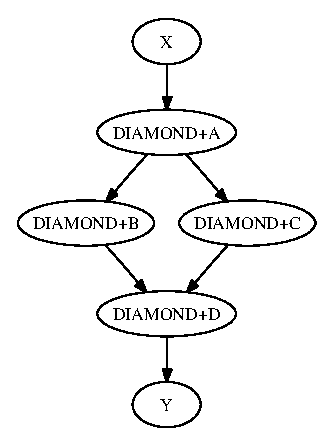
\includegraphics{user-man/splice-simple.eps}
\caption{\label{fig:dagman-splice-simple} The diamond-shaped DAG spliced between two nodes.}
\end{figure}

Figure~\ref{fig:dagman-splice-X} illustrates the starting point
for a more complex example.
The DAG input file \File{X.dag} describes this X-shaped DAG.
The completed example displays more of
the spatial constructs provided by splices.
Pay particular attention to the notion that each named splice creates a
new graph, even when the same DAG input file is specified.


\begin{verbatim}
  # BEGIN DAG FILE X.dag

  JOB A submit.condor
  VARS A jobname="$(JOB)"

  JOB B submit.condor
  VARS B jobname="$(JOB)"

  JOB C submit.condor
  VARS C jobname="$(JOB)"

  JOB D submit.condor
  VARS D jobname="$(JOB)"

  JOB E submit.condor
  VARS E jobname="$(JOB)"

  JOB F submit.condor
  VARS F jobname="$(JOB)"

  JOB G submit.condor
  VARS G jobname="$(JOB)"

  # Make an X-shaped dependency graph
  PARENT A B C CHILD D
  PARENT D CHILD E F G

  # END DAG FILE X.dag
\end{verbatim}

\begin{figure}
\centering
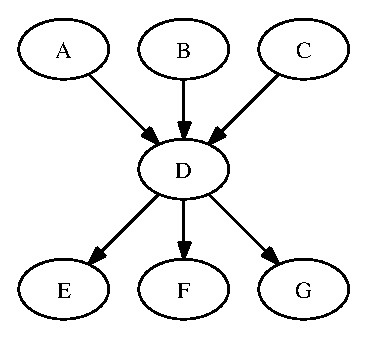
\includegraphics{user-man/splice-X.eps}
\caption{\label{fig:dagman-splice-X} The X-shaped DAG.}
\end{figure}


File \File{s1.dag} continues the example, presenting
the DAG input file that
incorporates two separate splices of the X-shaped DAG.
Figure~\ref{fig:dagman-splice-s1} illustrates the resulting DAG.

\begin{verbatim}
  # BEGIN DAG FILE s1.dag

  JOB A submit.condor
  VARS A jobname="$(JOB)"

  JOB B submit.condor
  VARS B jobname="$(JOB)"

  # name two individual splices of the X-shaped DAG
  SPLICE X1 X.dag
  SPLICE X2 X.dag

  # Define dependencies
  # A must complete before the initial nodes in X1 can start
  PARENT A CHILD X1
  # All final nodes in X1 must finish before 
  # the initial nodes in X2 can begin
  PARENT X1 CHILD X2
  # All final nodes in X2 must finish before B may begin.
  PARENT X2 CHILD B

  # END DAG FILE s1.dag

\end{verbatim}

\begin{figure}
\centering
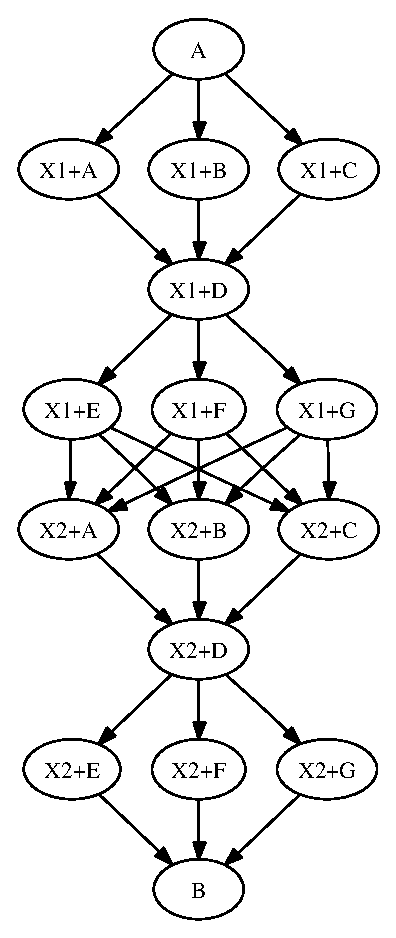
\includegraphics{user-man/splice-s1.eps}
\caption{\label{fig:dagman-splice-s1} The DAG described by \File{s1.dag}.}
\end{figure}



The top level DAG in the hierarchy of this complex example
is described by the DAG input file \File{toplevel.dag}.
Figure~\ref{fig:dagman-splice-complex} illustrates the final DAG.
Notice that the DAG has two disjoint graphs in it as a result of splice
S3 not having any dependencies associated with it in this top level DAG.

\begin{verbatim}
  # BEGIN DAG FILE toplevel.dag

  JOB A submit.condor
  VARS A jobname="$(JOB)"

  JOB B submit.condor
  VARS B jobname="$(JOB)"

  JOB C submit.condor
  VARS C jobname="$(JOB)"

  JOB D submit.condor
  VARS D jobname="$(JOB)"

  # a diamond-shaped DAG
  PARENT A CHILD B C
  PARENT B C CHILD D

  # This splice of the X-shaped DAG can only run after
  # the diamond dag finishes
  SPLICE S2 X.dag
  PARENT D CHILD S2

  # Since there are no dependencies for S3,
  # the following splice is disjoint 
  SPLICE S3 s1.dag

  # END DAG FILE toplevel.dag
\end{verbatim}


\begin{figure}
\centering
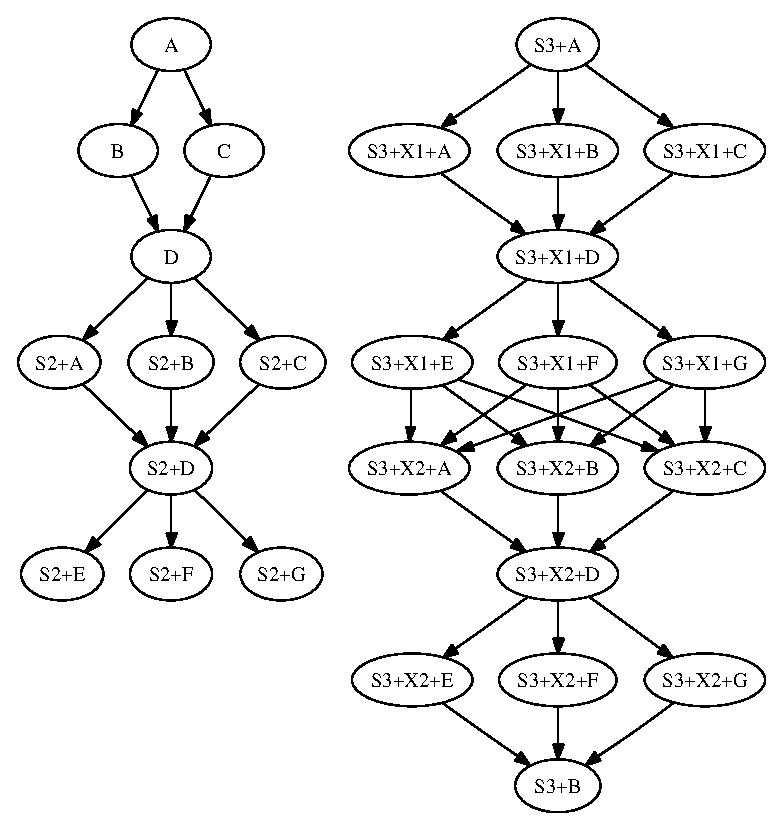
\includegraphics{user-man/splice-complex.eps}
\caption{\label{fig:dagman-splice-complex} The complex splice example DAG.}
\end{figure}

The \Arg{DIR} option specifies a working directory for a splice,
from which the splice will be parsed and the containing jobs submitted.
The directory associated with the splices' \Arg{DIR} specification
will be propagated as a prefix to all nodes in the splice and any 
included splices.
If a node already has a \Arg{DIR} specification, then the splice's
\Arg{DIR} specification will be a prefix to the nodes and separated by
a directory separator character.
Jobs in included splices with an absolute path for their \Arg{DIR}
specification will have their \Arg{DIR} specification untouched.
Note that a DAG containing \Arg{DIR} specifications cannot be run
in conjunction with the \Arg{-usedagdir} command-line argument to
\Condor{submit\_dag}.
A rescue DAG generated by a DAG run with the \Arg{-usedagdir} argument
will contain DIR specifications, so the rescue DAG must be run
\emph{without} the \Arg{-usedagdir} argument.



% Note: this is an alternative to subsubsubsection, which we don't have.
\begin{description}
\item[The Interaction of Categories and MAXJOBS with Splices]
\end{description}

Categories normally refer only to nodes within a
given splice.
All of the assignments of nodes to a category, and the
setting of the category throttle, should be done within a single DAG file.
However, it is now possible to have categories include nodes
from within more than one splice.
To do this, the category name is prefixed with the '+' (plus) character.
This tells DAGMan that the category is
a cross-splice category.
Towards deeper understanding,
what this really does is prevent renaming
of the category when the splice is incorporated into the upper-level DAG.
The MAXJOBS specification for the category can appear in either the
upper-level DAG file or one of the splice DAG files.
It probably
makes the most sense to put it in the upper-level DAG file.

Here is an example which applies a single limitation on submitted jobs,
identifying the category with \Expr{+init}. 

\begin{verbatim}
# relevant portion of file name: upper.dag

    SPLICE A splice1.dag
    SPLICE B splice2.dag

    MAXJOBS +init 2
\end{verbatim}

\begin{verbatim}
# relevant portion of file name: splice1.dag

    JOB C C.sub
    CATEGORY C +init
    JOB D D.sub
    CATEGORY D +init

\end{verbatim}

\begin{verbatim}
# relevant portion of file name: splice2.dag

    JOB X X.sub
    CATEGORY X +init
    JOB Y Y.sub
    CATEGORY Y +init

\end{verbatim}

For both global and non-global category throttles, settings at a higher
level in the DAG override settings at a lower level.
In this example:

\begin{verbatim}
# relevant portion of file name: upper.dag

    SPLICE A lower.dag

    MAXJOBS A+catX 10
    MAXJOBS +catY 2


# relevant portion of file name: lower.dag

    MAXJOBS catX 5
    MAXJOBS +catY 1

\end{verbatim}

the resulting throttle settings are 2 for the \Expr{+catY} category
and 10 for the \Expr{A+catX} category in splice.
Note that non-global category names are
prefixed with their splice name(s), so to refer to a non-global category 
at a higher level, the splice name must be included.


%%%%%%%%%%%%%%%%%%%%%%%%%%%%%%%%%%%%%%%
\subsection{\label{sec:DAGMan-rescue}Job Recovery:  The Rescue DAG}
%%%%%%%%%%%%%%%%%%%%%%%%%%%%%%%%%%%%%%%

\index{DAGMan!Rescue DAG}
DAGMan can help with the re-running of uncompleted portions of a DAG, 
when one or more nodes result in failure,
or when a running DAG is removed with \Condor{rm}.
If any node in the DAG fails,
the remainder of the DAG is continued until no more forward
progress can be made based on the DAG's dependencies.
At this point, DAGMan produces a file called a Rescue DAG.  
A Rescue DAG is also produced if the
\Condor{dagman} job itself is removed with \Condor{rm}.

If the DAG is resubmitted utilizing the Rescue DAG,
the successfully completed nodes will not be re-executed.
As of Condor version 7.7.2, the Rescue DAG file is a partial DAG file. 

A partial Rescue DAG file contains only information about which nodes are done,
and the number of retries remaining for nodes with retries.  
It does not contain information such as the actual
DAG structure and the specification of the submit file for each node job.  
Partial Rescue DAGs are automatically parsed in combination with
the original DAG file, 
which contains information about the DAG structure.  
This updated implementation means that a change in the original DAG input file,
such as specifying a different submit description file for a node job,
will take effect when running the partial Rescue DAG.

The previous behavior of producing full DAG input file 
is implemented by setting the configuration variable
\Macro{DAGMAN\_WRITE\_PARTIAL\_RESCUE} to the non-default 
value of \Expr{False}.  

Note that the removal of a node from the original DAG input file, 
together with a \Arg{DONE} specification in the Rescue DAG 
for a node that no longer exists is a warning,
as opposed to an error, 
unless the \Macro{DAGMAN\_USE\_STRICT} configuration
variable is set to a value of 1 or higher.  
Comment out the line with \Arg{DONE} in the partial Rescue DAG file
to avoid a warning or error.

To run a full Rescue DAG,
either one left over from an older version of DAGMan, 
or one produced by setting \Macro{DAGMAN\_WRITE\_PARTIAL\_RESCUE} 
to \Expr{False}, 
directly specify the full Rescue DAG file instead of the original DAG file.
For example:

\begin{verbatim}
  condor_submit_dag my.dag.rescue002
\end{verbatim}

Re-submission of the original DAG input file causes \Condor{dagman} to try to
parse the Rescue DAG file in combination with the original DAG input file, 
which will result in failure if the Rescue DAG is a full Rescue DAG file.

Note that if multiple DAG input files are specified on the
\Condor{submit\_dag} command line,
a single Rescue DAG encompassing all of the input DAGs is generated.

If the Rescue DAG file is generated before all retries
of a node are completed, 
then the Rescue DAG file will also contain \Arg{Retry} entries.
The number of retries will be set to the appropriate remaining
number of retries.
The configuration variable \Macro{DAGMAN\_RESET\_RETRIES\_UPON\_RESCUE}, 
section~\ref{param:DAGManResetRetriesUponRescue},
controls whether or not node retries are reset in a Rescue DAG.

The granularity defining success or failure
in the Rescue DAG is the node.
For a node that fails,
all parts of the node will be re-run,
even if some parts were successful the first time.
For example, if a node's PRE script
succeeds, but then the node's Condor job cluster fails,
the entire node, which includes the PRE script will be re-run.
A job cluster may result in the submission of multiple Condor jobs.
If one of the multiple jobs fails, the node fails.
Therefore, the Rescue DAG will
re-run the entire node,
implying the submission of the entire cluster of jobs,
not just the one(s) that failed.

Statistics about the failed DAG execution are presented as
comments at the beginning of the Rescue DAG input file.

The Rescue DAG is automatically generated by \Condor{dagman} when a node
within the DAG fails or when \Condor{dagman} itself is removed
with \Condor{rm}.
The file name of the Rescue DAG, and usage of the Rescue
DAG changed from explicit specification to implicit usage
beginning with Condor version 7.1.0.
Current naming of the Rescue DAG appends the string
\verb@.rescue<XXX>@ to the original DAG input file name.
Values for \verb@<XXX>@ start at \verb@001@ and continue
to \verb@002@, \verb@003@, and beyond.
If a Rescue DAG exists,
the Rescue DAG with the largest magnitude value for \verb@<XXX>@
will be used, and its usage is implied.

Here is an example showing file naming and DAG submission
for the case of a failed DAG.
The initial DAG is submitted with
\begin{verbatim}
  condor_submit_dag  my.dag
\end{verbatim}
A failure of this DAG results in the Rescue DAG
named \File{my.dag.rescue001}.
The DAG is resubmitted using the same command: 
\begin{verbatim}
  condor_submit_dag  my.dag
\end{verbatim}
This resubmission of the DAG uses the Rescue DAG file \File{my.dag.rescue001},
because it exists.
Failure of this Rescue DAG results in another Rescue DAG
called \File{my.dag.rescue002}.
If the DAG is again submitted, using the same command
as with the first two submissions, but not repeated here,
then this third submission uses the Rescue DAG file \File{my.dag.rescue002},
because it exists, and because the value \verb@002@ is larger
in magnitude than \verb@001@.

To explicitly specify a particular Rescue DAG,
use the optional command-line argument \Arg{-dorescuefrom}
with \Condor{submit\_dag}.
Note that this will have the side effect of renaming 
existing Rescue DAG files with larger magnitude values 
of \verb@<XXX>@.
Each renamed file has its existing name appended with
the string \File{.old}.
For example, assume that \File{my.dag} has failed 4 times,
resulting in the Rescue DAGs named
\File{my.dag.rescue001},
\File{my.dag.rescue002},
\File{my.dag.rescue003},
and
\File{my.dag.rescue004}.
A decision is made to re-run using \File{my.dag.rescue002}.
The submit command is
\begin{verbatim}
  condor_submit_dag  -dorescuefrom 2  my.dag
\end{verbatim}
The DAG specified by the DAG input file \File{my.dag.rescue002}
is submitted.
And, the existing Rescue DAG \File{my.dag.rescue003} is
renamed to be \File{my.dag.rescue003.old},
while the existing Rescue DAG \File{my.dag.rescue004} is
renamed to be \File{my.dag.rescue004.old}.

The configuration variable \Macro{DAGMAN\_MAX\_RESCUE\_NUM}
sets a maximum value for \verb@XXX@.
See section~\ref{param:DAGManMaxRescueNum} for the complete definition
of this configuration variable.


%%%%%%%%%%%%%%%%%%%%%%%%%%%
\label{dagman:rescue_parse_error}
\begin{description}
\item[Rescue DAG Generated When There Are Parse Errors]
\end{description}

Starting in Condor version 7.5.5,
the \Opt{-DumpRescue} option to either \Condor{dagman} or \Condor{submit\_dag}
causes \Condor{dagman} to output a Rescue DAG file, 
even if the parsing of a DAG input file fails.
In this parse failure case, \Condor{dagman} produces a specially 
named Rescue DAG containing whatever it had successfully parsed up
until the point of the parse error.
This Rescue DAG may be useful in debugging parse errors in complex DAGs,
especially ones using splices.
This incomplete Rescue DAG is not meant to be used when resubmitting
a failed DAG.  
Note that this incomplete Rescue DAG generated by the \Opt{-DumpRescue}
option is a full DAG input file, 
as produced by versions of Condor prior to Condor version 7.7.2.
It is not a partial Rescue DAG file,
regardless of the value of the configuration variable
\Macro{DAGMAN\_WRITE\_PARTIAL\_RESCUE}.

To avoid confusion between this incomplete Rescue DAG
generated in the case of a parse failure and a usable Rescue DAG,
a different name is given to the incomplete Rescue DAG.
The name appends the string \File{.parse\_failed} to the original
DAG input file name.
Therefore, if the submission of a DAG with
\begin{verbatim}
  condor_submit_dag  my.dag
\end{verbatim}
has a parse failure, the resulting incomplete Rescue DAG will be
named \File{my.dag.parse\_failed}.

To further prevent one of these incomplete Rescue DAG files from being used,
a line within the file contains the single keyword \Arg{REJECT}.
This causes \Condor{dagman} to reject the DAG, if used as a DAG input file.
This is done because the
incomplete Rescue DAG may be a syntactically correct DAG input file.
It will be incomplete relative to the original DAG,
such that if the incomplete Rescue DAG could be run,
it could erroneously be perceived as
having successfully executed the desired workflow, when, in fact,
it did not.

%%%%%%%%%%%%%%%%%%%%%%%%%%%
\begin{description}
\item[Outdated Naming of Rescue DAG]
\end{description}
As of Condor version 7.7.2, the following file naming scheme is 
no longer available.

Prior to Condor version 7.1.0, the naming of a Rescue DAG
appended the string \File{.rescue} to the existing DAG input
file name. 
And, the Rescue DAG file would be explicitly placed in 
the command line that submitted it.
For example,  a first submission
\begin{verbatim}
  condor_submit_dag  my.dag
\end{verbatim}
Assuming that this DAG failed, the file \File{my.dag.rescue}
would be created.
To run this Rescue DAG, the submission command is
\begin{verbatim}
  condor_submit_dag  my.dag.rescue
\end{verbatim}
If this Rescue DAG also failed, a new Rescue DAG named
\File{my.dag.rescue.rescue} would be created.

%%%%%%%%%%%%%%%%%%%%%%%%%%%%%%%%%%%%%%%
\subsection{\label{sec:DAGPaths}File Paths in DAGs}
%%%%%%%%%%%%%%%%%%%%%%%%%%%%%%%%%%%%%%%
\index{DAGMan!File Paths in DAGs}

By default, \Condor{dagman} assumes that all relative paths in a
DAG input file and the associated Condor submit description files
are relative to the current
working directory when \Condor{submit\_dag} is run.  
Note that 
relative paths in submit description files can be modified by the submit command
\SubmitCmd{initialdir}; see the \Condor{submit} manual page within Chapter
~\ref{man-condor-submit} for more details.  The rest of this discussion
ignores \SubmitCmd{initialdir}.

In most cases, path names relative to the current working directory 
is the desired behavior.
However, if running
multiple DAGs with a single \Condor{dagman}, and each DAG is in its
own directory, this will cause problems.  In this case,
use the \Arg{-usedagdir} command-line argument to
\Condor{submit\_dag} (see the \Condor{submit\_dag} manual page within Chapter
~\ref{man-condor-submit-dag} for more details).
This tells \Condor{dagman} to run each DAG
as if \Condor{submit\_dag} had been run in the directory in which
the relevant DAG file exists.

For example, assume that a directory called \File{parent}
contains two subdirectories called \File{dag1} and
\File{dag2}, and that \File{dag1} contains the DAG input file \File{one.dag}
and \File{dag2} contains the DAG input file \File{two.dag}.
Further, assume that each DAG is set up to be run
from its own directory with the following command:
\begin{verbatim}
cd dag1; condor_submit_dag one.dag
\end{verbatim}
This will correctly run \File{one.dag}.

The goal is to run the two, independent DAGs located within
\File{dag1} and \File{dag2} while the current working directory
is \File{parent}.  To do so, run the following command:
\begin{verbatim}
condor_submit_dag -usedagdir dag1/one.dag dag2/two.dag
\end{verbatim}

Of course, if all paths in the DAG input file(s) and the relevant submit
description files are absolute,
the \Arg{-usedagdir} argument is not needed;
however, using absolute paths is NOT generally a good idea.

If you \emph{do not} use \Arg{-usedagdir}, relative paths can still work
for multiple DAGs, if
all file paths are given relative to
the current working directory as \Condor{submit\_dag} is executed.
However, this means that, if the DAGs are in separate directories, they
cannot be submitted from their own directories, only from the parent
directory the paths are set up for.

Note that if you use the \Arg{-usedagdir} argument, and your run
results in a rescue DAG, the rescue DAG file will be written to
the current working directory, and should be run from that directory.
The rescue DAG includes all the path information necessary to
run each node job in the proper directory.


%%%%%%%%%%%%%%%%%%%%%%%%%%%%%%%%%%%%%%%
\subsection{Visualizing DAGs with \Prog{dot}}
%%%%%%%%%%%%%%%%%%%%%%%%%%%%%%%%%%%%%%%
\index{DAGMan!dot}
\index{dot}
\index{DAGMan!visualizing DAGs}

It can be helpful to see a picture of a DAG.
DAGMan can assist you in visualizing a DAG by creating
the input files used by the AT\&T Research Labs 
\Prog{graphviz} package. 
\Prog{dot} is a program within this package,
available from \URL{http://www.graphviz.org/},
and it is used to draw pictures of DAGs. 

DAGMan produces one or more dot files as the result of
an extra line
in a DAGMan input file. 
The line appears as
%For example, to produce a single dot
%file that shows the state of your DAG before any jobs are running, add
%the following line:
\begin{verbatim}
    DOT dag.dot
\end{verbatim}

This creates a file called \File{dag.dot}.
which contains
a specification of the DAG before any jobs within the DAG
are submitted to Condor.
The \File{dag.dot} file is used to create a visualization
of the DAG by using this file as input to \Prog{dot}.
This example creates a Postscript file, with a visualization of the DAG:

\begin{verbatim}
    dot -Tps dag.dot -o dag.ps
\end{verbatim}

Within the DAGMan input file,
the DOT command can take several optional parameters:

\begin{itemize}

\item \Opt{UPDATE}  This will update the dot file every time a
significant update happens. 

\item \Opt{DONT-UPDATE} Creates a single dot file, when
the DAGMan begins executing. This is the default if the parameter
\Opt{UPDATE} is not used.

\item \Opt{OVERWRITE} Overwrites the dot file each time it
is created. This is the default, unless \Opt{DONT-OVERWRITE}
is specified.

\item \Opt{DONT-OVERWRITE} Used to create multiple dot files, instead
of overwriting the single one specified.
To create file names,
DAGMan uses the name of the file concatenated with a period and an
integer. For example, the DAGMan input file line
\begin{verbatim}
    DOT dag.dot DONT-OVERWRITE
\end{verbatim}
causes files
\File{dag.dot.0},
\File{dag.dot.1},
\File{dag.dot.2},
etc. to be created.
This option is
most useful when combined with the \Opt{UPDATE} option to
visualize the history of the DAG after it has finished executing. 

\item \OptArg{INCLUDE}{path-to-filename} Includes the contents
of a file given by \File{path-to-filename} in the file produced by the
\Opt{DOT} command.
The include file contents are always placed after the line of
the form
\verb@label=@.
This may be useful if further editing of the created files would
be necessary,
perhaps because you are automatically visualizing the DAG as it
progresses. 

\end{itemize}

If conflicting parameters are used in a DOT command, the last one
listed is used.

%%%%%%%%%%%%%%%%%%%%%%%%%%%%%%%%%%%%%%%
\subsection{\label{sec:DAG-node-status}Capturing the Status of Nodes in a File}
%%%%%%%%%%%%%%%%%%%%%%%%%%%%%%%%%%%%%%%
\index{DAGMan!node status file}
\index{status!of a DAGMan node}

DAGMan can capture the status of all DAG nodes,
such that the user or a script may easily monitor the status of all DAG nodes.
A node status file is periodically rewritten by DAGMan.
To enable this feature, the DAG input file contains a line with the
\Arg{NODE\_STATUS\_FILE} key word.

The syntax for a \Arg{NODE\_STATUS\_FILE} specification is

\Opt{NODE\_STATUS\_FILE} \Arg{statusFileName} \oArg{minimumUpdateTime}

The status file is written on the machine where the DAG is submitted;
its location is given by \Arg{statusFileName}.  
This will be the same machine where the \Condor{dagman} job is running.

The optional \Arg{minimumUpdateTime} specifies the minimum number of seconds
that must elapse between updates to the node status file.
This setting exists to avoid having DAGMan spend too much time writing
the node status file for very large DAGs.
If no value is specified, no limit is set.
The node status file can be updated at most once
per \Macro{DAGMAN\_USER\_LOG\_SCAN\_INTERVAL},
as defined at section~\ref{param:DAGManUserLogScanInterval},
no matter how small the \Arg{minimumUpdateTime} value.

As an example, if the DAG input file contains the line
\begin{verbatim}
  NODE_STATUS_FILE my.dag.status 30
\end{verbatim}
the file \File{my.dag.status} will be rewritten at intervals of 30 seconds
or more.

This node status file is overwritten each time it is updated.
Therefore, it only holds information about the \emph{current} status 
of each node; it does not provide a history of the node status.
The file contains one line describing the status of every node in the DAG.
The file contents do not distinguish between Condor jobs and Stork jobs.
Here is an example of a node status file:

\begin{verbatim}
  BEGIN 1281041745 (Thu Aug  5 15:55:45 2010)
  Status of nodes of DAG(s): my.dag

  JOB A STATUS_DONE      ()
  JOB B STATUS_SUBMITTED (not_idle)
  JOB C STATUS_SUBMITTED (idle)
  JOB D STATUS_UNREADY   ()

  DAG status: STATUS_SUBMITTED ()
  Next scheduled update: 1281041775 (Thu Aug  5 15:56:15 2010)
  END 1281041745 (Thu Aug  5 15:55:45 2010)
\end{verbatim}

Possible node status values are:

\begin{itemize}
\item \verb@STATUS_UNREADY@ At least one parent has not yet finished.
\item \verb@STATUS_READY@ All parents have finished, but not yet running.
\item \verb@STATUS_PRERUN@ The PRE script is running.
\item \verb@STATUS_SUBMITTED@ The node's Condor or Stork job(s) are in 
  the queue.
\item \verb@STATUS_POSTRUN@ The POST script is running.
\item \verb@STATUS_DONE@ The node has completed successfully.
\item \verb@STATUS_ERROR@ The node has failed.
\end{itemize}

A \Arg{NODE\_STATUS\_FILE} key word inside any splice is ignored.
If multiple DAG files are specified on the \Condor{submit\_dag} command line,
and more than one specifies a node status file,
the first specification takes precedence.

%%%%%%%%%%%%%%%%%%%%%%%%%%%%%%%%%%%%%%%
\subsection{\label{sec:DAGJobstateLog}A Machine-Readable Event History, the jobstate.log File}
%%%%%%%%%%%%%%%%%%%%%%%%%%%%%%%%%%%%%%%
\index{DAGMan!jobstate.log file}
\index{DAGMan!machine-readable event history}

DAGMan can produce a machine-readable history of events.
The \File{jobstate.log} file is designed for use by the Pegasus Workflow
Management System, which operates as a layer on top of DAGMan.  Pegasus
uses the \File{jobstate.log} file to monitor the state of a workflow.
The \File{jobstate.log} file can used by any
automated tool for the monitoring of workflows.

DAGMan produces this file when the keyword \Arg{JOBSTATE\_LOG} is
in the DAG input file.
The syntax for \Arg{JOBSTATE\_LOG} is

\Opt{JOBSTATE\_LOG} \Arg{JobstateLogFileName}

No more than one \File{jobstate.log} file can be created by a single
instance of \Condor{dagman}.
If more than one \File{jobstate.log} file is specified,
the first file name specified will take effect,
and a warning will be printed in the \File{dagman.out} file
when subsequent \Arg{JOBSTATE\_LOG} specifications are parsed.
Multiple specifications may exist in the same DAG file, within splices,
or within multiple, independent DAGs run with a single \Condor{dagman} instance.

The \File{jobstate.log} file can be considered a filtered
version of the \File{dagman.out} file, in a machine-readable format.
It contains the actual node job events that from \Condor{dagman},
plus some additional meta-events.

The \File{jobstate.log} file is different from the node status file,
in that the \File{jobstate.log} file is appended to,
rather than being overwritten as the DAG runs.
Therefore, it contains a history of the DAG,
rather than a snapshot of the current state of the DAG.

There are 5 line types in the \File{jobstate.log} file.
Each line begins with a Unix timestamp in the form of seconds since the Epoch.
Fields within each line are separated by a single space character.
\begin{description}

\item [DAGMan start] 
This line identifies the \Condor{dagman} job.
The formatting of the line is

\Arg{timestamp} INTERNAL *** DAGMAN\_STARTED \Arg{dagmanCondorID} ***

The \Arg{dagmanCondorID} field is the \Condor{dagman} job's 
\Attr{ClusterId} attribute, a period, and the \Attr{ProcId} attribute. 

\item [DAGMan exit] 
This line identifies the completion of the \Condor{dagman} job.
The formatting of the line is

\Arg{timestamp} INTERNAL *** DAGMAN\_FINISHED \Arg{exitCode} ***

The \Arg{exitCode} field is value the \Condor{dagman} job returns upon exit. 

\item [Recovery started] 
If the \Condor{dagman} job goes into recovery mode,
this meta-event is printed.
During recovery mode, events will only be printed in the file
if they were not already printed before recovery mode started.
The formatting of the line is

\Arg{timestamp} INTERNAL *** RECOVERY\_STARTED ***

\item [Recovery finished or Recovery failure] 
At the end of recovery
mode, either a RECOVERY\_FINISHED or RECOVERY\_FAILURE meta-event will be
printed, as appropriate.

The formatting of the line is

\Arg{timestamp} INTERNAL *** RECOVERY\_FINISHED ***

or

\Arg{timestamp} INTERNAL *** RECOVERY\_FAILURE ***

\item [Normal]
This line is used for all other event and meta-event types.
The formatting of the line is

\Arg{timestamp} \Arg{JobName} \Arg{eventName} \Arg{condorID} \Arg{jobTag} - \Arg{sequenceNumber}

The \Arg{JobName} is the name given to the node job as defined in
the DAG input file with the keyword \Arg{JOB}.
It identifies the node within the DAG.

The \Arg{eventName} is one of the many defined event or meta-events given
in the lists below.

The \Arg{condorID} field is the job's 
\Attr{ClusterId} attribute, a period, and the \Attr{ProcId} attribute. 
There is no \Arg{condorID} assigned yet for some meta-events,
such as PRE\_SCRIPT\_STARTED.
For these, the dash character ('-') is printed. 

The \Arg{jobTag} field is defined for the Pegasus workflow manager.
Its usage is generalized to be useful to other workflow managers.
Pegasus-managed jobs add a line of the following form to their
Condor submit description file:
\begin{verbatim}
+pegasus_site = "local"
\end{verbatim}
This defines the string \Expr{local} as the \Arg{jobTag} field.
 
Generalized usage adds a set of 2 commands to the Condor
submit description file to define a string as the \Arg{jobTag} field:
\begin{verbatim}
+job_tag_name = "+job_tag_value"
+job_tag_value = "viz"
\end{verbatim}
This defines the string \Expr{viz} as the \Arg{jobTag} field.
Without any of these added lines within the Condor submit description file,
the dash character ('-') is printed for the \Arg{jobTag} field. 

The \Arg{sequenceNumber} is a monotonically-increasing number 
that starts at one.
It is associated with each attempt at running a node.
If a node is retried, it gets a new sequence number;
a submit failure does not result in a new sequence number.
When a rescue DAG is run,
the sequence numbers pick up from where they left off within the previous
attempt at running the DAG.
Note that this only applies if the rescue
DAG is run automatically or with the \Arg{-dorescuefrom} command-line option.

\end{description}

Here is an example of a very simple Pegasus \File{jobstate.log} file,
assuming the example \Arg{jobTag} field of \Expr{local}:

\begin{verbatim}
1292620511 INTERNAL *** DAGMAN_STARTED 4972.0 ***
1292620523 NodeA PRE_SCRIPT_STARTED - local - 1
1292620523 NodeA PRE_SCRIPT_SUCCESS - local - 1
1292620525 NodeA SUBMIT 4973.0 local - 1
1292620525 NodeA EXECUTE 4973.0 local - 1
1292620526 NodeA JOB_TERMINATED 4973.0 local - 1
1292620526 NodeA JOB_SUCCESS 0 local - 1
1292620526 NodeA POST_SCRIPT_STARTED 4973.0 local - 1
1292620531 NodeA POST_SCRIPT_TERMINATED 4973.0 local - 1
1292620531 NodeA POST_SCRIPT_SUCCESS 4973.0 local - 1
1292620535 INTERNAL *** DAGMAN_FINISHED 0 ***
\end{verbatim}



\begin{description}
\item[Events defining the eventName field]

\begin{itemize}
\item SUBMIT
\item EXECUTE
\item EXECUTABLE\_ERROR
\item CHECKPOINTED
\item JOB\_EVICTED
\item JOB\_TERMINATED
\item IMAGE\_SIZE
\item SHADOW\_EXCEPTION
\item GENERIC
\item JOB\_ABORTED
\item JOB\_SUSPENDED
\item JOB\_UNSUSPENDED
\item JOB\_HELD
\item JOB\_RELEASED
\item NODE\_EXECUTE
\item NODE\_TERMINATED
\item POST\_SCRIPT\_TERMINATED
\item GLOBUS\_SUBMIT
\item GLOBUS\_SUBMIT\_FAILED
\item GLOBUS\_RESOURCE\_UP
\item GLOBUS\_RESOURCE\_DOWN
\item REMOTE\_ERROR
\item JOB\_DISCONNECTED
\item JOB\_RECONNECTED
\item JOB\_RECONNECT\_FAILED
\item GRID\_RESOURCE\_UP
\item GRID\_RESOURCE\_DOWN
\item GRID\_SUBMIT
\item JOB\_AD\_INFORMATION
\item JOB\_STATUS\_UNKNOWN
\item JOB\_STATUS\_KNOWN
\item JOB\_STAGE\_IN
\item JOB\_STAGE\_OUT
\end{itemize}

\item[Meta-Events defining the eventName field]
\begin{itemize}
\item SUBMIT\_FAILURE
\item JOB\_SUCCESS
\item JOB\_FAILURE
\item PRE\_SCRIPT\_STARTED
\item PRE\_SCRIPT\_SUCCESS
\item PRE\_SCRIPT\_FAILURE
\item POST\_SCRIPT\_STARTED
\item POST\_SCRIPT\_SUCCESS
\item POST\_SCRIPT\_FAILURE
\item DAGMAN\_STARTED
\item DAGMAN\_FINISHED
\item RECOVERY\_STARTED
\item RECOVERY\_FINISHED
\item RECOVERY\_FAILURE
\end{itemize}
\end{description}


%%%%%%%%%%%%%%%%%%%%%%%%%%%%%%%%%%%%%%%
\subsection{\label{sec:DAGLotsaJobs}Utilizing the Power of DAGMan for Large Numbers of Jobs}
%%%%%%%%%%%%%%%%%%%%%%%%%%%%%%%%%%%%%%%
\index{DAGMan!large numbers of jobs}

Using DAGMan is recommended when submitting large numbers of jobs.
The recommendation holds whether the jobs are represented by
a DAG due to dependencies, or all the jobs are
independent of each other, such as they might be in a parameter sweep.
DAGMan offers:
\begin{itemize}
\item{Throttling}
  to limit the number of submitted jobs at any point in time.
\item{Retry of jobs that fail.}
  A useful tool when an intermittent error may cause a job to fail
  or fail to run to completion when attempted at one point in time,
  but not at another point in time.
  And, note that what constitutes failure is user-defined.
\item{Automatic generation of the administrative support that facilitates the
  rerunning of only jobs that fail.}
\item{The ability to run scripts before and/or after the execution of
individual jobs.}
\end{itemize}

Each of these capabilities is described in detail (above)
within this manual section about DAGMan.
To make effective use of DAGMan, there is no way around reading the 
appropriate subsections.

To run DAGMan with large numbers of independent jobs,
there are generally two ways of organizing and specifying the
files that control the jobs.
Both ways presume that programs or scripts will generate the files,
because the files are either large and repetitive
or because there are a large number of similar files to be
generated representing the large numbers of jobs.
The two file types needed are the DAG input file and the
submit description file(s) for the Condor jobs represented.
Each of the two ways is presented separately:

\begin{description}
\item[A unique submit description file for each of the many jobs.]
A single DAG input file lists each of the jobs and specifies
a distinct Condor submit description file for each job.
The DAG input file is simple to generate, as it chooses an
identifier for each job and names the submit description file.
For example, the simplest DAG input file for a set of 1000 independent jobs,
as might be part of a parameter sweep, appears as
\begin{verbatim}
  # file sweep.dag
  JOB job0 job0.submit
  JOB job1 job1.submit
  JOB job2 job2.submit
  .
  .
  .
  JOB job999 job999.submit
\end{verbatim}
There are 1000 submit description files, with a unique one for
each of the job<N> jobs.
Assuming that all files associated with this set of jobs are in the
same directory, and that files continue the same naming and numbering
scheme, the submit description file for \File{job6.submit}
might appear as
\begin{verbatim}
  # file job6.submit
  universe = vanilla
  executable = /path/to/executable
  log = job6.log
  input = job6.in
  output = job6.out
  notification = Never
  arguments = "-file job6.out"
  queue
\end{verbatim}

Submission of the entire set of jobs is
\begin{verbatim}
  condor_submit_dag sweep.dag
\end{verbatim}

A benefit to having unique submit description files for each of the
jobs is that they are available, if one of the jobs needs to be
submitted individually.
A drawback to having unique submit description files for each of the jobs
is that there are lots of files, one for each job.

\item[Single submit description file.]
A single Condor submit description file might be used for all the many
jobs of the parameter sweep.
To distinguish the jobs and their associated distinct input and output files,
the DAG input file assigns a unique identifier with the \Arg{VARS} keyword.
\begin{verbatim}
  # file sweep.dag
  JOB job0 common.submit
  VARS job0 runnumber="0"
  JOB job1 common.submit
  VARS job1 runnumber="1"
  JOB job2 common.submit
  VARS job2 runnumber="2"
  .
  .
  .
  JOB job999 common.submit
  VARS job999 runnumber="999"
\end{verbatim}

The single submit description file for all these jobs utilizes the
\Expr{runnumber} variable value in its identification of the job's
files. 
This submit description file might appear as
\begin{verbatim}
  # file common.submit
  universe = vanilla
  executable = /path/to/executable
  log = wholeDAG.log
  input = job$(runnumber).in
  output = job$(runnumber).out
  notification = Never
  arguments = "-$(runnumber)"
  queue
\end{verbatim}
The job with \Expr{runnumber="8"} expects to find its input file \File{job8.in} 
in the single, common directory, and it 
sends its output to \File{job8.out}.
The single log for all job events of the entire DAG is \File{wholeDAG.log}.
Using one file for the entire DAG meets the limitation that no macro
substitution may be specified for the job log file, 
and it is likely more efficient as well. 
This node's executable is invoked with
\begin{verbatim}
  /path/to/executable -8
\end{verbatim}

\end{description}

These examples work well with respect to file naming and placement
when there are less than several thousand jobs submitted as part
of a DAG.
The large numbers of files per directory becomes an issue when there
are greater than several thousand jobs submitted as part of a DAG.
In this case,
consider a more hierarchical structure for the files instead of a single
directory.
Introduce a separate directory for each run.
For example, if there were 10,000 jobs, there would be
10,000 directories, one for each of these jobs.
The directories are presumed to be generated and populated by 
programs or scripts that,
like the previous examples, utilize a run number.
Each of these directories named utilizing the run number will be used
for the input, output, and log files for one of the many jobs.

As an example, for this set of 10,000 jobs and directories, assume
that there is a run number of 600.
The directory will be named \File{dir.600}, and it will
hold the 3 files called \File{in}, \File{out}, and \File{log},
representing the input, output, and Condor job log files associated
with run number 600.

The DAG input file sets a variable representing the run number,
as in the previous example:
\begin{verbatim}
  # file biggersweep.dag
  JOB job0 common.submit
  VARS job0 runnumber="0"
  JOB job1 common.submit
  VARS job1 runnumber="1"
  JOB job2 common.submit
  VARS job2 runnumber="2"
  .
  .
  .
  JOB job9999 common.submit
  VARS job9999 runnumber="9999"
\end{verbatim}

A single Condor submit description file may be written.
It resides in the same directory as the DAG input file.
\begin{verbatim}
  # file bigger.submit
  universe = vanilla
  executable = /path/to/executable
  log = log
  input = in
  output = out
  notification = Never
  arguments = "-$(runnumber)"
  initialdir = dir.$(runnumber)
  queue
\end{verbatim}

One item to care about with this set up is the underlying file system 
for the pool.
The transfer of files (or not) when using \SubmitCmd{initialdir}
differs based upon the job \SubmitCmd{universe} and whether or not there
is a shared file system.
See section~\ref{man-condor-submit-initialdir} for the details on the
submit command \SubmitCmd{initialdir}.

Submission of this set of jobs is no different than the previous
examples.  
With the current working directory the same as the one containing
the submit description file, the DAG input file, and the subdirectories,
\begin{verbatim}
  condor_submit_dag biggersweep.dag
\end{verbatim}

\index{DAGMan|)}

%%%%%%%%%%%%%%%%%%%%%%%%%%%%%%%%%%%%%%%%%%%%%%%%%%%%%%%%%%%%%%%%%%%%%%

%%%%%%%%%%%%%%%%%%%%%%%%%%%%%%%%%%%%%%%%%%%%%%%%%%%%%%%%%%%%%%%%%%%%%%
%%%%%%%%%%%%%%%%%%%%%%%%%%%%%%%%%%%%%%%
\section{\label{sec:vmuniverse}Virtual Machine Applications}
%%%%%%%%%%%%%%%%%%%%%%%%%%%%%%%%%%%%%%%
\index{virtual machine universe|(}
\index{universe!vm}
\index{vm universe}

The \SubmitCmd{vm} universe facilitates a Condor job
that matches and then lands a disk image on an execute machine
within a Condor pool.
This disk image is intended to be a virtual machine.
In this manner, the virtual machine is the job to be executed.

This section describes this type of Condor job.
See section~\ref{sec:Config-VMs}
for details of configuration variables.

%%%%%%%%%%%%%%%%%%%%%%%%%%%%%%%%%%%%%%%
\subsection{\label{sec:vm-submitfile}The Submit Description File}
%%%%%%%%%%%%%%%%%%%%%%%%%%%%%%%%%%%%%%%

Different than all other universe jobs,
the \SubmitCmd{vm} universe job specifies a disk image,
not an executable.
Therefore, the submit commands \SubmitCmd{input}, \SubmitCmd{output},
and \SubmitCmd{error} do not apply.
If specified, \Condor{submit} rejects the job with an error.
The \SubmitCmd{executable} command changes definition within a
\SubmitCmd{vm} universe job.
It no longer specifies an executable file, but instead
provides a string that identifies the job for tools such
as \Condor{q}.
Other commands specific to the type of virtual machine software
identify the disk image.

VMware, Xen, and KVM virtual machine software are supported.
As these differ from each other, the submit description file
specifies one of
\begin{verbatim}
  vm_type = vmware
\end{verbatim}
or
\begin{verbatim}
  vm_type = xen
\end{verbatim}
or
\begin{verbatim}
  vm_type = kvm
\end{verbatim}

The job is required to specify its memory needs 
for the disk image with \SubmitCmd{vm\_memory},
which is given in Mbytes.
Condor uses this number to assure a match with a machine
that can provide the needed memory space.

Virtual machine networking is enabled with the command
\begin{verbatim}
  vm_networking = true
\end{verbatim}
And, when networking is enabled, a definition of
\SubmitCmd{vm\_networking\_type} as \SubmitCmd{bridge}
matches the job only with a machine that is configured to use
bridge networking.
A definition of
\SubmitCmd{vm\_networking\_type} as \SubmitCmd{nat}
matches the job only with a machine that is configured to use
NAT networking.
When no definition of
\SubmitCmd{vm\_networking\_type} is given,
Condor may
match the job with a machine that enables networking,
and further, the choice of bridge or NAT networking
is determined by the machine's configuration.

Modified disk images are transferred back to the machine from which
the job was submitted as the \SubmitCmd{vm} universe job completes.
Job completion for a \SubmitCmd{vm} universe job occurs when 
the virtual machine is shut down, and Condor notices 
(as the result of a periodic check on the state of the virtual machine).
Should the job not want any files transferred back (modified or not),
for example because the job explicitly transferred its own files,
the submit command to prevent the transfer is
\begin{verbatim}
  vm_no_output_vm = true
\end{verbatim}

The required disk image must be identified for a virtual machine.
This \SubmitCmd{vm\_disk} command specifies a list of comma-separated files.
Each disk file is specified by colon-separated fields.
The first field is the path and file name of the disk file.
The second field specifies the device.
The third field specifies permissions, and the optional 
fourth specifies the format.
Here is an example that identifies a single file:
\footnotesize
\begin{verbatim}
  vm_disk = /var/lib/libvirt/images/swap.img:sda2:w:raw
\end{verbatim}
\normalsize

Setting values in the submit description file for some commands
have consequences for the virtual machine description file.
These commands are
\begin{itemize}
  \item \SubmitCmd{vm\_memory}
  \item \SubmitCmd{vm\_macaddr}
  \item \SubmitCmd{vm\_networking}
  \item \SubmitCmd{vm\_networking\_type}
  \item \SubmitCmd{vm\_disk}
\end{itemize}
For VMware virtual machines,
setting values for these commands causes Condor to modify the
\File{.vmx} file, overwriting existing values.
For KVM and Xen virtual machines,
Condor uses these values when it produces the description file.

For Xen and KVM jobs, if any files need to be transferred from the submit machine
to the machine where the \SubmitCmd{vm} universe job will execute, 
Condor must be explicitly told to do so with the 
standard file transfer attributes:
\footnotesize
\begin{verbatim}
  should_transfer_files = YES
  when_to_transfer_output = ON_EXIT
  transfer_input_files = /myxen/diskfile.img,/myxen/swap.img
\end{verbatim}
\normalsize
Any and all needed files on a system without a shared file
system (between the submit machine and the machine where the
job will execute) must be listed.

Further commands specify information that is specific to the
virtual machine type targeted.

%%%%%%%%%%%%%%%%%%%%%%%%%%%%%%%%%%%%%%%
\subsubsection{\label{sec:vm-VMwaresubmitfile}VMware-Specific Submit Commands}
%%%%%%%%%%%%%%%%%%%%%%%%%%%%%%%%%%%%%%%
\index{vm universe!submit commands specific to VMware}

Specific to VMware, the submit description file command
\SubmitCmd{vmware\_dir} gives the path and directory
(on the machine from which the job is submitted)
to where VMware-specific files and applications reside.
One example of a VMware-specific application is the VMDK files,
which form a virtual hard drive (disk image) for the virtual machine.
VMX files containing the primary configuration for the virtual
machine would also be in this directory.

Condor must be told whether or not the contents of the \SubmitCmd{vmware\_dir}
directory must be transferred to the machine where the job is
to be executed.
This required information is given with the submit command
\SubmitCmd{vmware\_should\_transfer\_files}.
With a value of \Expr{True},
Condor does transfer the contents of the directory.
With a value of \Expr{False},
Condor does not transfer the contents of the directory,
and instead presumes that access to this directory is
available through a shared file system.

By default, Condor uses a snapshot disk for new and modified files.
They may also be utilized for checkpoints.
The snapshot disk is initially quite small,
growing only as new files are created or files are modified.
When \SubmitCmd{vmware\_should\_transfer\_files} is \Expr{True},
a job may specify that a snapshot disk is \emph{not} to be
used with the command
\begin{verbatim}
  vmware_snapshot_disk = False
\end{verbatim}
In this case, Condor will utilize original disk files in producing
checkpoints. 
Note that \Condor{submit} issues an error message and does not
submit the job if both \SubmitCmd{vmware\_should\_transfer\_files}
and \SubmitCmd{vmware\_snapshot\_disk} are \Expr{False}.

Note that if snapshot disks are requested and file transfer is not
being used, the \SubmitCmd{vmware\_dir} setting given in 
the submit description file
should not contain any symbolic link path components.
This is to work around the issue discussed
in the FAQ entry in section~\ref{sec:vmware-symlink-bug}.

Here is a sample submit description file for a VMware virtual machine:
\begin{verbatim}
universe                     = vm
executable                   = vmware_sample_job
log                          = simple.vm.log.txt
vm_type                      = vmware
vm_memory                    = 64
vmware_dir                   = C:\condor-test
vmware_should_transfer_files = True
queue
\end{verbatim}
This sample uses the \SubmitCmd{vmware\_dir} command to identify
the location of the disk image to be executed as a Condor job.
The contents of this directory are transferred to the machine assigned
to execute the Condor job.

%%%%%%%%%%%%%%%%%%%%%%%%%%%%%%%%%%%%%%%
\subsubsection{\label{sec:vm-Xensubmitfile}Xen-Specific Submit Commands}
%%%%%%%%%%%%%%%%%%%%%%%%%%%%%%%%%%%%%%%
\index{vm universe!submit commands specific to Xen}

% xen_kernel description
A Xen \SubmitCmd{vm} universe job requires specification of the
guest kernel. 
The \SubmitCmd{xen\_kernel} command accomplishes this, 
utilizing one of the following definitions.
\begin{enumerate}
\item \SubmitCmd{xen\_kernel = included} implies that the kernel
  is to be found in disk image given by the definition of the single file
  specified in \SubmitCmd{vm\_disk}. 

\item \SubmitCmd{xen\_kernel = path-to-kernel} gives a full path and
  file name of the required kernel.  If this kernel must be transferred
  to machine on which the \SubmitCmd{vm} universe job will execute,
  it must also be included in the \SubmitCmd{xen\_transfer\_files} command. 

  This form of the \SubmitCmd{xen\_kernel} command also requires further
  definition of the \SubmitCmd{xen\_root} command.
  \SubmitCmd{xen\_root} defines the device containing files needed by
  \Login{root}.

\end{enumerate}

%%%%%%%%%%%%%%%%%%%%%%%%%%%%%%%%%%%%%%%
\subsection{\label{sec:vm-checkpoints}Checkpoints}
%%%%%%%%%%%%%%%%%%%%%%%%%%%%%%%%%%%%%%%
\index{vm universe!checkpoints}

Creating a checkpoint is straightforward for a virtual machine,
as a checkpoint is a set of files that represent
a snapshot of both disk image and memory.
The checkpoint is created and all files are transferred back
to the \MacroUNI{SPOOL} directory on the machine from which
the job was submitted.
The submit command to create checkpoints is
\begin{verbatim}
  vm_checkpoint = true
\end{verbatim}
Without this command, no checkpoints are created (by default).
With the command, a checkpoint is created any time the \SubmitCmd{vm}
universe jobs is evicted from the machine upon which it is executing.
This occurs as a result of the machine configuration indicating
that it will no longer execute this job.

\SubmitCmd{vm} universe jobs can \emph{not} use a checkpoint server.

Periodic creation of checkpoints is not supported at this time.

Enabling both networking and checkpointing for a \SubmitCmd{vm}
universe job can cause networking problems when the job restarts,
particularly if the job migrates to a different machine.
\Condor{submit} will normally reject such jobs.
To enable both, then add the command
\begin{verbatim}
  when_to_transfer_output = ON_EXIT_OR_EVICT
\end{verbatim}

Take care with respect to the use of network connections within
the virtual machine and their interaction with checkpoints.
Open network connections at the time of the checkpoint will likely
be lost when the checkpoint is subsequently used to resume execution
of the virtual machine.
This occurs whether or not the execution resumes
on the same machine or a different one within the Condor pool.   

%%%%%%%%%%%%%%%%%%%%%%%%%%%%%%%%%%%%%%%
\subsection{\label{sec:vm-disk-image-details}Disk Images}
%%%%%%%%%%%%%%%%%%%%%%%%%%%%%%%%%%%%%%%

%%%%%%%%%%%%%%%%%%%%%%%%%%%%%%%%%%%%%%%
\subsubsection{\label{sec:vm-disk-image-details-vmware}
VMware on Windows and Linux}
%%%%%%%%%%%%%%%%%%%%%%%%%%%%%%%%%%%%%%%

Following the platform-specific
guest OS installation instructions found at
\URL{http://partnerweb.vmware.com/GOSIG/home.html},
creates a VMware disk image.

%%%%%%%%%%%%%%%%%%%%%%%%%%%%%%%%%%%%%%%
\subsubsection{\label{sec:vm-disk-image-details-xen}Xen and KVM}
%%%%%%%%%%%%%%%%%%%%%%%%%%%%%%%%%%%%%%%
While the following web page contains instructions specific to
Fedora on how to create a virtual guest image,
it should provide a good starting point for 
other platforms as well.

\URL{http://fedoraproject.org/wiki/Virtualization\_Quick\_Start}

%%%%%%%%%%%%%%%%%%%%%%%%%%%%%%%%%%%%%%%
\subsection{\label{sec:vm-job-completion-details}Job Completion in the vm Universe}
%%%%%%%%%%%%%%%%%%%%%%%%%%%%%%%%%%%%%%%

Job completion for a \SubmitCmd{vm} universe job occurs when 
the virtual machine is shut down, and Condor notices 
(as the result of a periodic check on the state of the virtual machine).
This is different from jobs executed under the environment of other 
universes.

Shut down of a virtual machine occurs from within the virtual
machine environment.
A script, executed with the proper authorization level,
is the likely source of the shut down commands.

Under a Windows 2000, Windows XP, or Vista virtual machine,
an administrator issues the command
\begin{verbatim}
  shutdown -s -t 01
\end{verbatim}

Under a Linux virtual machine,
the \Login{root} user executes
\begin{verbatim}
  /sbin/poweroff
\end{verbatim}
The command \verb@/sbin/halt@ will not completely
shut down some Linux distributions, and instead
causes the job to hang.

Since the successful completion of the \SubmitCmd{vm} universe job
requires the successful shut down of the virtual machine,
it is good advice to try the shut down procedure outside of
Condor, before a \SubmitCmd{vm} universe job is submitted.


\index{virtual machine universe|)}

%%%%%%%%%%%%%%%%%%%%%%%%%%%%%%%%%%%%%%%%%%%%%%%%%%%%%%%%%%%%%%%%%%%%%%

%%%%%%%%%%%%%%%%%%%%%%%%%%%%%%%%%%%%%%%%%%%%%%%%%%%%%%%%%%%%%%%%%%%%%%
%%%%%%%%%%%%%%%%%%%%%%%%%%%%%%%%%%%%%%%%%%%%%%%%%%%%%%%%%%%%%%%%%%%%%%
\section{Time Scheduling for Job Execution}
\label{sec:Job-Executetime-Scheduling}
%%%%%%%%%%%%%%%%%%%%%%%%%%%%%%%%%%%%%%%%%%%%%%%%%%%%%%%%%%%%%%%%%%%%%%
\index{scheduling jobs!to execute at a specific time}
\index{job execution!at a specific time}

Jobs may be scheduled to begin execution at a specified time in the future
with Condor's job deferral functionality.
All specifications are in a job's submit description file.
Job deferral functionality is expanded to provide for the
periodic execution of a job, known as the CronTab scheduling.

%%%%%%%%%%%%%%%%%%%%%%%%%%%%%%%%%%%%%%%%%%%
\subsection{Job Deferral}
\label{sec:JobDeferral}
%%%%%%%%%%%%%%%%%%%%%%%%%%%%%%%%%%%%%%%%%%%
\index{job deferral time}
\index{deferral time!of a job}

Job deferral allows the specification of
the exact date and time at which a job is to begin executing.
Condor attempts to match the job to an execution machine
just like any other job,
however, the job will wait until the exact time to begin execution.
A user can specify Condor to allow some flexibility to execute jobs
that miss their execution time.

%%%%%%%%%%%%%%%%%%%%%%%%%%%%%%%%%%%%%%%%%%%
\subsubsection{Deferred Execution Time}
\label{sec:JobDeferral-DeferralTime}
%%%%%%%%%%%%%%%%%%%%%%%%%%%%%%%%%%%%%%%%%%%
\index{deferral time!of a job}
\index{ClassAd job attribute!DeferralTime}

A job's deferral time is the exact time that Condor should attempt
to execute the job.
The deferral time attribute is defined as an expression
that evaluates to a Unix Epoch timestamp
(the number of seconds elapsed since 00:00:00 on January 1, 1970,
Coordinated Universal Time).
This is the time that Condor will begin to execute the job.

After a job is matched and all of its files have been transferred
to an execution machine,
Condor checks to see if the job's ad contains a deferral time.
If it does,
Condor calculates the number of seconds between the execution
machine's current system time to the job's deferral time.
If the deferral time is in the future,
the job waits to begin execution.
While a job waits,
its job ClassAd attribute \AdAttr{JobStatus} indicates the job
is running.
As the deferral time arrives, the job begins to execute.
If a job misses its execution time,
that is, if the deferral time is in the past,
the job is evicted from the execution machine and put on hold in the queue.

The specification of a deferral time does not interfere
with Condor's behavior.
For example, if a job is waiting to begin execution
when a \Condor{hold} command is issued,
the job is removed from the execution machine and is put on hold.
If a job is waiting to begin execution when 
a \Condor{suspend} command is issued,
the job continues to wait.
When the deferral time arrives,
Condor begins execution for the job,
but immediately suspends it.

%%%%%%%%%%%%%%%%%%%%%%%%%%%%%%%%%%%%%%%%%%%
\subsubsection{Missed Execution Window}
\label{sec:JobDeferral-DeferralWindow}
%%%%%%%%%%%%%%%%%%%%%%%%%%%%%%%%%%%%%%%%%%%
\index{ClassAd job attribute!DeferralWindow}
\index{submit commands!deferral\_window}

If a job arrives at its execution machine
after the deferral time passes,
the job is evicted from the machine and put on hold in the job queue.
This may occur, for example,
because the transfer of needed files took too long
due to a slow network connection.
A deferral window permits the execution of a job
that misses its deferral time by specifying a window of
time within which the job may begin.

The deferral window 
is the number of seconds after the deferral time,
within which the job may begin.
When a job arrives too late,
Condor calculates the difference in seconds
between the execution machine's current time
and the job's deferral time.
If this difference is less than or equal to the deferral window,
the job immediately begins execution.
If this difference is greater than the deferral window,
the job is evicted from the execution machine
and is put on hold in the job queue.

%%%%%%%%%%%%%%%%%%%%%%%%%%%%%%%%%%%%%%%%%%%
\subsubsection{Preparation Time}
\label{sec:JobDeferral-PrepTime}
%%%%%%%%%%%%%%%%%%%%%%%%%%%%%%%%%%%%%%%%%%%
\index{ClassAd job attribute!DeferralPrepTime}

When a job defines a deferral time far in the future and then 
is matched to an execution machine,
potential computation cycles are lost because the deferred job
has claimed the machine, but is not actually executing. 
Other jobs could execute during the interval when the job 
waits for its deferral time.
To make use of the wasted time,
\index{submit commands!deferral\_prep\_time}
a job defines a \SubmitCmd{deferral\_prep\_time}
with an integer expression that evaluates to a
number of seconds.
At this number of seconds before the deferral time,
the job may be matched with a machine.

%%%%%%%%%%%%%%%%%%%%%%%%%%%%%%%%%%%%%%%%%%%
\subsubsection{Usage Examples}
\label{sec:JobDeferral-Examples}
%%%%%%%%%%%%%%%%%%%%%%%%%%%%%%%%%%%%%%%%%%%

\index{submit commands!deferral\_time}
Here are examples of how the job deferral time,
deferral window, and the preparation time may be used.

The job's submit description file specifies that
the job is to begin execution 
on January 1st, 2006 at 12:00 pm:

\begin{verbatim} 
   deferral_time = 1136138400
\end{verbatim} 

The Unix \Prog{date} program may be used to calculate
a Unix epoch time.
The syntax of the command to do this depends on the options provided
within that flavor of Unix.  In some, it appears as
\begin{verbatim} 
%  date --date "MM/DD/YYYY HH:MM:SS" +%s
\end{verbatim} 
and in others, it appears as 
\begin{verbatim} 
%  date -d "YYYY-MM-DD HH:MM:SS" +%s
\end{verbatim} 

\verb@MM@ is a 2-digit month number,
\verb@DD@ is a 2-digit day of the month number, and
\verb@YYYY@ is a 4-digit year.
\verb@HH@ is the 2-digit hour of the day,
\verb@MM@ is the 2-digit minute of the hour, and
\verb@SS@ are the 2-digit seconds within the minute.
The characters \verb@+%s@ tell the \Prog{date} program
to give the output as a Unix epoch time.

The job always waits 60 seconds before
beginning execution:

\begin{verbatim} 
   deferral_time = (CurrentTime + 60)
\end{verbatim}

In this example, assume that the deferral time is 45 seconds
in the past as the job is available.
The job begins execution, because 75 seconds remain in the
deferral window:

\begin{verbatim} 
   deferral_window = 120
\end{verbatim}

In this example, a job is scheduled to execute
far in the future,
on January 1st, 2010 at 12:00 pm. 
The \SubmitCmd{deferral\_prep\_time} attribute delays the job 
from being matched until 60 seconds before the job is to begin execution. 

\begin{verbatim}
   deferral_time      = 1262368800
   deferral_prep_time = 60
\end{verbatim}

%%%%%%%%%%%%%%%%%%%%%%%%%%%%%%%%%%%%%%%%%%%
\subsubsection{Limitations}
\label{sec:JobDeferral-Limitations}
%%%%%%%%%%%%%%%%%%%%%%%%%%%%%%%%%%%%%%%%%%%
There are some limitations to Condor's job deferral feature.

\begin{itemize}
\item Job deferral is not available for scheduler universe jobs.
% no referring to daemons in the user's manual!
% Scheduler universe jobs are not executed under the control 
% of the \Condor{starter} daemon, 
% which is needed to defer the job until the correct execution time. 
A scheduler universe job defining the \AdAttr{deferral\_time}
produces a fatal error when submitted.

\item The time that the job begins to execute 
is based on the execution machine's system clock, 
and not the submission machine's system clock. 
Be mindful of the ramifications when
the two clocks show dramatically different times.

\item A job's \AdAttr{JobStatus} attribute is always in the running state 
when job deferral is used. 
There is currently no way to distinguish between a job that is 
executing and a job that is waiting for its deferral time. 

\end{itemize}

%%%%%%%%%%%%%%%%%%%%%%%%%%%%%%%%%%%%%%%%%%%
\subsection{CronTab Scheduling}
\label{sec:CronTab}
%%%%%%%%%%%%%%%%%%%%%%%%%%%%%%%%%%%%%%%%%%%
\index{CronTab job scheduling}
\index{job scheduling!periodic}
\index{scheduling jobs!to execute periodically}

Condor's CronTab scheduling functionality allows jobs to be 
scheduled to execute periodically. 
A job's execution schedule is defined by commands within
the submit description file.
The notation is much like that used by the Unix \Prog{cron} daemon. 
As such, Condor developers are fond of referring to CronTab
\index{Crondor}
scheduling as \Term{Crondor}.
The scheduling of jobs using Condor's CronTab feature 
calculates and utilizes
the \Attr{DeferralTime} ClassAd attribute. 

Also, unlike the Unix \Prog{cron} daemon, 
Condor never runs more than one instance of a job at the same time. 

The capability for repetitive or periodic execution of the job is 
enabled by specifying an \SubmitCmd{on\_exit\_remove}
command for the job,
such that the job does not leave the queue until desired.

%%%%%%%%%%%%%%%%%%%%%%%%%%%%%%%%%%%%%%%%%%%
\subsubsection{Semantics for CronTab Specification}
\label{sec:CronTab-Semantics}
%%%%%%%%%%%%%%%%%%%%%%%%%%%%%%%%%%%%%%%%%%%

A job's execution schedule is defined by a set of specifications
within the submit description file.
Condor uses these to calculate a \Attr{DeferralTime} for the job.

Table \ref{tab:CronTab-Attributes} 
lists the submit commands and acceptable values for these commands.
At least one of these must be defined 
in order for Condor to calculate a \Attr{DeferralTime} for the job.
Once one CronTab value is defined, 
the default for all the others uses 
all the values in the allowed values ranges.

\index{submit commands!cron\_minute}
\index{submit commands!cron\_hour}
\index{submit commands!cron\_day\_of\_month}
\index{submit commands!cron\_month}
\index{submit commands!cron\_day\_of\_week}

\begin{table}
   \begin{center}
   \begin{tabular}{ll}
   Submit Command & Allowed Values \\
   \hline
   \SubmitCmd{cron\_minute} & 0 - 59 \\
   \SubmitCmd{cron\_hour} & 0 - 23 \\
   \SubmitCmd{cron\_day\_of\_month} & 1 - 31 \\
   \SubmitCmd{cron\_month} & 1 - 12 \\
   \SubmitCmd{cron\_day\_of\_week} & 0 - 7 (Sunday is 0 or 7)\\
   \end{tabular}
   \end{center}
   \caption{The list of submit commands and their value ranges.}
   \label{tab:CronTab-Attributes}
\end{table}

The day of a job's execution can be specified 
by both the \SubmitCmd{cron\_day\_of\_month} 
and the \SubmitCmd{cron\_day\_of\_week} attributes. 
The day will be the logical or of both.

The semantics allow more than one value to be specified 
by using the \verb@*@ operator,
ranges, lists, and steps (strides) within ranges.

\begin{description}
   \item[The asterisk operator]
   The \verb@*@ (asterisk) operator specifies that all of the 
   allowed values are used for scheduling.
   For example,
   \begin{verbatim}
      cron_month = *
   \end{verbatim}
   becomes any and all of the list of possible months:
   (1,2,3,4,5,6,7,8,9,10,11,12).
   Thus, a job runs any month in the year.

   \item[Ranges]
   A range creates a set of integers from all the allowed values between two
   integers separated by a hyphen. The specified range is inclusive, and the
   integer to the left of the hyphen must be less than the right hand integer.
   For example,
   \begin{verbatim}
      cron_hour = 0-4
   \end{verbatim}
   represents the set of
   hours from 12:00 am (midnight) to 4:00 am, or (0,1,2,3,4).
   
   \item[Lists]
   A list is the union of the values or ranges separated by commas. Multiple
   entries of the same value are ignored. 
   For example,
   \begin{verbatim}
      cron_minute = 15,20,25,30
      cron_hour   = 0-3,9-12,15
   \end{verbatim}
   \SubmitCmd{cron\_minute} represents (15,20,25,30)
   and \SubmitCmd{cron\_hour} represents (0,1,2,3,9,10,11,12,15).
      
   \item[Steps]
   Steps select specific numbers from a range, based on an interval.
   A step is specified by appending a range or the asterisk
   operator with a slash character (\verb@/@),
   followed by an integer value.
   For example,
   \begin{verbatim}
      cron_minute = 10-30/5
      cron_hour = */3
   \end{verbatim}
   \SubmitCmd{cron\_minute} specifies
   every five minutes within the specified range 
   to represent (10,15,20,25,30).
   \SubmitCmd{cron\_hour} specifies every three hours of the day
   to represent (0,3,6,9,12,15,18,21).
   

\end{description}

%%%%%%%%%%%%%%%%%%%%%%%%%%%%%%%%%%%%%%%%%%%
\subsubsection{Preparation Time and Execution Window}
\label{sec:CronTab-PrepTime}
%%%%%%%%%%%%%%%%%%%%%%%%%%%%%%%%%%%%%%%%%%%

The \SubmitCmd{cron\_prep\_time} command
is analogous to the deferral time's \SubmitCmd{deferral\_prep\_time} command. 
It specifies the number of seconds before the deferral time
that the job is to be matched and sent to the execution machine. 
This permits Condor to
make necessary preparations before the deferral time occurs. 

Consider the submit description file example that includes 
\begin{verbatim}
   cron_minute = 0
   cron_hour = *
   cron_prep_time = 300
\end{verbatim}
The job is scheduled to begin execution at the top of every hour.
Note that the setting of \SubmitCmd{cron\_hour} in this example
is not required, as the default value will be \verb@*@, 
specifying any and every hour of the day.
The job will be matched and sent to an execution machine 
no more than five minutes before the next deferral time. 
For example, if a job is submitted at 9:30am, then the 
next deferral time will be calculated to be 10:00am.
Condor may attempt to match the job to a machine and send the job
once it is 9:55am.

As the CronTab scheduling calculates and uses deferral time,
jobs may also make use of the deferral window.
The submit command \SubmitCmd{cron\_window} is analogous to
the submit command \SubmitCmd{deferral\_window}.
Consider the submit description file example that includes 
\begin{verbatim}
   cron_minute = 0
   cron_hour = *
   cron_window = 360
\end{verbatim}
As the previous example, the job is scheduled to begin execution
at the top of every hour.
Yet with no preparation time, the job is likely to miss
its deferral time.
The 6-minute window allows the job to begin execution,
as long as it arrives and can begin within 6 minutes of
the deferral time,
as seen by the time kept on the execution machine.

%%%%%%%%%%%%%%%%%%%%%%%%%%%%%%%%%%%%%%%%%%%
\subsubsection{Scheduling}
\label{sec:crontab-scheduling}
%%%%%%%%%%%%%%%%%%%%%%%%%%%%%%%%%%%%%%%%%%%

When a job using the CronTab functionality is submitted to Condor, 
use of at least one of the submit description file commands
beginning with \verb@cron_@ causes Condor
to calculate and set a deferral time for when the job should run. 
A deferral time is determined based on the current time 
rounded later in time to the next minute. 
The deferral time is the job's \AdAttr{DeferralTime} attribute. 
A new deferral time is calculated when the job 
first enters the job queue, when 
the job is re-queued, or when the job is released from the hold state. 
New deferral times for \emph{all} jobs in the job queue 
using the CronTab functionality are recalculated 
when a \Condor{reconfig} or a \Condor{restart} command that
affects the job queue is issued.

A job's deferral time is not always the same time that a job 
will receive a match and be sent to the execution machine. 
This is because Condor operates on the job queue
at times that are independent of job events,
such as when job execution completes.
Therefore,
Condor may operate on the job queue just after 
a job's deferral time states that it is to begin execution. 
Condor attempts to start a job when the 
following pseudo-code boolean expression evaluates to \Expr{True}:

\footnotesize
\begin{verbatim}
   ( CurrentTime + SCHEDD_INTERVAL ) >= ( DeferralTime - CronPrepTime )
\end{verbatim}
\normalsize

If the \Attr{CurrentTime} plus the number of seconds 
until the next time Condor checks 
the job queue is greater than or equal to the time that the job 
should be submitted to the execution machine, 
then the job is to be matched and sent now.

Jobs using the CronTab functionality are not automatically 
re-queued by Condor after their execution is complete. 
The submit description file for a job
must specify an appropriate \SubmitCmd{on\_exit\_remove} 
command to ensure that a job remains in the queue. 
This job maintains its original \Attr{ClusterId} and \Attr{ProcId}.

%%%%%%%%%%%%%%%%%%%%%%%%%%%%%%%%%%%%%%%%%%%
\subsubsection{Usage Examples}
\label{sec:crontab-examples}
%%%%%%%%%%%%%%%%%%%%%%%%%%%%%%%%%%%%%%%%%%%

Here are some examples of the submit commands
necessary to schedule jobs to run at multifarious times. 
Please note that it is not necessary to 
explicitly define each attribute; the default value is \verb@*@.

Run 23 minutes after every two hours, every day of the week:

\begin{verbatim}
   on_exit_remove = false
   cron_minute = 23
   cron_hour = 0-23/2
   cron_day_of_month = *
   cron_month = *
   cron_day_of_week = *
\end{verbatim}

Run at 10:30pm on each of May 10th to May 20th, as well as every 
remaining Monday within the month of May:

\begin{verbatim}
   on_exit_remove = false
   cron_minute = 30
   cron_hour = 20
   cron_day_of_month = 10-20
   cron_month = 5
   cron_day_of_week = 2
\end{verbatim}

Run on every 10 minutes and every 6 minutes before noon 
on January 18th with a 2-minute preparation time:

\begin{verbatim}
   on_exit_remove = false
   cron_minute = */10,*/6
   cron_hour = 0-11
   cron_day_of_month = 18
   cron_month = 1
   cron_day_of_week = *
   cron_prep_time = 120
\end{verbatim}

%%%%%%%%%%%%%%%%%%%%%%%%%%%%%%%%%%%%%%%%%%%
\subsubsection{Limitations}
\label{sec:Crontab-Limitations}
%%%%%%%%%%%%%%%%%%%%%%%%%%%%%%%%%%%%%%%%%%%
The use of the CronTab functionality has all of the same 
limitations of deferral times,
because the mechanism is based upon deferral times.

\begin{itemize}
\item It is impossible to schedule vanilla 
and standard universe jobs 
at intervals that are smaller than the
interval at which Condor evaluates jobs.
This interval is determined by 
the configuration variable \Macro{SCHEDD\_INTERVAL}. 
As a vanilla or standard universe job completes execution 
and is placed back into the job queue, 
it may not be placed in the idle state in time.
This problem does not afflict local universe jobs.

\item Condor cannot guarantee that a job will be
matched in order to make its scheduled deferral time.
A job must be matched with an execution machine just as
any other Condor job; 
if Condor is unable to find a match, 
then the job will miss its chance for executing
and must wait for the next execution time 
specified by the CronTab schedule.

\end{itemize}

%%%%%%%%%%%%%%%%%%%%%%%%%%%%%%%%%%%%%%%%%%%%%%%%%%%%%%%%%%%%%%%%%%%%%%

%%%%%%%%%%%%%%%%%%%%%%%%%%%%%%%%%%%%%%%%%%%%%%%%%%%%%%%%%%%%%%%%%%%%%%
%%%%%%%%%%%%%%%%%%%%%%%%%%%%%%%%%%%%%%%%
\section{\label{sec:Stork}Stork Applications}
%%%%%%%%%%%%%%%%%%%%%%%%%%%%%%%%%%%%%%%
\index{Stork|(}

Today's scientific applications have huge data requirements,
which continue to increase drastically every year.
These data are generally accessed by many
users from all across the the globe.
This requires moving huge amounts of data
around wide area networks to complete the computation cycle,
which brings with
it the problem of efficient and reliable data placement.

Stork is a scheduler for data placement.
With Stork, \Term{data placement jobs}
have been elevated to the same level as Condor's computational jobs;
data placements are queued, managed, queried and
autonomously restarted upon error.
Stork understands the semantics and protocols of data placement.

The underlying data placement jobs are performed by Stork
\Term{modules}, typically installed in the Condor \File{libexec}
directory.  The module name is encoded from the data placement type
and functions.  
For example, the \File{stork.transfer.file-file} module transfers data
from the \File{file:/} (local file system) to the \File{file:/}
protocol.  The \File{stork.transfer.file-file} module is the only
module bundled with Condor/Stork.  Additionally, contributed modules
may be \htmladdnormallink{downloaded}
{http://www.cs.wisc.edu/condor/stork/download.html}
for these data transfer protocols:

\begin{table}[hbt]
\begin{tabular}{ l l }
%file:/		& (Stork Server) local file system \\
ftp://		& FTP File Transfer Protocol \\
http://		& HTTP Hypertext Transfer Protocol \\
gsiftp://	& Globus Grid FTP  \\ 
nest://		& Condor NeST  network storage appliance (see
\URL{http://www.cs.wisc.edu/condor/nest/}) \\
srb://		& SDSC  Storage Resource Broker (SRB) (see
\URL{http://www.sdsc.edu/srb/}) \\
srm://		& Storage Resource Manager (SRM) (see
\URL{http://sdm.lbl.gov/srm-wg/}) \\
csrm://		& Castor Storage Resource Manager (Castor SRM) (see
\URL{http://castor.web.cern.ch/castor/}) \\
unitree://    & NCSA UniTree (see
\URL{http://www.ncsa.uiuc.edu/Divisions/CC/HPDM/unitree/}) \\
%		diskrouter:// -> UW DiskRouter Tool
\end{tabular}
\end{table}

The Stork
module API is simple and extensible, enabling users to create 
and use their own modules.

Stork includes high level features for managing data transfers.
By configuration, the number of active jobs running
from a Stork server may be limited.
Stork includes built in fault tolerance,
with capabilities for retrying failed jobs,
together with the specification of alternate protocols.
Stork users also have access to a higher level job manager, 
Condor DAGMan (section \ref{sec:DAGMan}),
which can manage both Stork data placement jobs
and traditional Condor jobs at the same time.


%%%%%%%%%%%%%%%%%%%%%%%%%%%%%%%%%%%%%%%
\subsection{\label{sec:Stork-Job-Submission}Submitting Stork Jobs}
%%%%%%%%%%%%%%%%%%%%%%%%%%%%%%%%%%%%%%%
\index{Stork!submit description file}

As with Condor jobs, Stork jobs are specified with a
submit description file.
It is important to note the syntax of the submit description file
for a Stork job is different than that used by Condor jobs.
Specifically,
Stork submit description files are written in the
\htmladdnormallink{ClassAd}{http://www.cs.wisc.edu/condor/classad}
language.  
See the ClassAd Language Reference Manual for complete details.
Please note that while most of Condor uses ClassAds,
Stork utilizes the most recent version of this language,
which has evolved over time.
Stork defines keywords.
When present in the job submit file,
keywords define the function of the job.

Here is sample Stork job submit description file,
showing file syntax and keywords.
A job specifies a 1-to-1 mapping of a data source URL to
destination URL.

\footnotesize
\begin{verbatim}
// This is a comment line.
[
    dap_type = transfer;
    src_url = "file:/etc/termcap";
    dest_url = "file:/tmp/stork/file-termcap";
]
\end{verbatim}
\normalsize


This example shows the ClassAd pairs that form the
heart of a Stork job specification.
The minimum keywords required to specify a Stork job are:

\begin{description}
  \item[dap\_type] Currently, the data type is constrained to 
  \SubmitCmd{transfer}.

  \item[src\_url]  Specify the data protocol and URL of the source.

  \item[dest\_url]  Specify the data protocol and URL of the destination.
\end{description}

Additionally, the following keywords may be used in 
a Stork submit description file:

\begin{description}
    \item[x509proxy] Specifies the location of the
    X.509 proxy file for protocols
    that use GSI authentication, such as \SubmitCmd{gsiftp://}.
    The special value of \emph{"default"} (quotes are required) invokes
    GSI libraries to search for the user credential in the standard locations.

    \item[alt\_protocols] A comma separated list of
    alternative protocol pairs (for source and destination protocols),
    used in a round robin fashion
    when transfers fail.
    See section \ref{sec:Stork-Fault-Protection} for a further discussion
    and examples.


\end{description}

Stork places no restriction on the submit file name or extension, and will
accept any valid file name for a Stork submit description file.

Submit data placement jobs to Stork using the
\Stork{submit} tool.
For example, after creating the submit description file
\File{sample.stork} with an
editor, submit the data transfer job with the command:

\begin{verbatim}
stork_submit sample.stork
\end{verbatim}

Stork then returns the associated job id, which is used by other Stork
job control tools.

Only the first ClassAd (a record expression within brackets) within 
a Stork submit description file becomes a data placement job
upon submission.
Other ClassAds within the file are ignored.

%%%%%%%%%%%%%%%%%%%%%%%%%%%%%%%%%%%%%%%
\subsection{\label{sec:Stork-Job-Management}Managing Stork Jobs}
%%%%%%%%%%%%%%%%%%%%%%%%%%%%%%%%%%%%%%%
Stork provides a set of command-line user tools for job management, including
submitting, querying, and removing data placement jobs.

%%%%%%%%%%%%%%%%%%%%%%%%%%%%%%%%%%%%%%%
\subsubsection{\label{sec:stork-query}Querying Stork Jobs}
%%%%%%%%%%%%%%%%%%%%%%%%%%%%%%%%%%%%%%%

Use \Stork{status} to check the status of any active
or completed Stork job.
\Stork{status} takes a single argument: the job id.
For example, to check the status of the Stork job with job id 3:

\begin{verbatim}
stork_status 3
\end{verbatim}

Use \Stork{q} to query all active Stork jobs.
\Stork{q} does not report on completed Stork jobs.

For example, to check the status all active Stork jobs:

\begin{verbatim}
stork_q
\end{verbatim}

%%%%%%%%%%%%%%%%%%%%%%%%%%%%%%%%%%%%%%%
\subsubsection{\label{sec:stork-rm}Removing Stork Jobs}
%%%%%%%%%%%%%%%%%%%%%%%%%%%%%%%%%%%%%%%

Active jobs may be removed from the job queue with the 
\Stork{rm} tool.  
\Stork{rm} takes a single argument: the job id of the job to remove.
All jobs may
be removed, provided they have not completed.

For example, to remove the queued job with job id 4:

\begin{verbatim}
stork_rm 4
\end{verbatim}

%%%%%%%%%%%%%%%%%%%%%%%%%%%%%%%%%%%%%%%
\subsection{\label{sec:Stork-Fault-Protection}Fault Tolerance}
%%%%%%%%%%%%%%%%%%%%%%%%%%%%%%%%%%%%%%%

In an ideal world, all data transfers succeed on the first attempt.
However, data transfers do fail for various reasons.
Stork is designed with data transfer fault tolerance.
Based on configuration, Stork retries failed data transfer jobs
using specified protocols.

If a  transfer fails, Stork attempts the transfer again,
until the number of attempts reaches the limit,
as defined by the 
configuration variable
\Macro{STORK\_MAX\_RETRY} 
(section \ref{param:StorkMaxRetry}).  

For each attempt at transfer,
the transfer protocols to be used at both source and destination are defined.
These transfer protocols may vary,
when defined by an \SubmitCmd{alt\_protocols} entry in the
submit description file.
The location of the data at the source and destination
is unchanged by the \SubmitCmd{alt\_protocols} entry.
\SubmitCmd{alt\_protocols} defines an ordered list of alternative
translation protocols to be used.
Each entry in the list is a pair.
The first of the pair defines the protocol to be used at the source 
of the transfer.
The second of the pair defines the protocol to be used at the destination 
of the transfer.

The syntax is a comma-separated list of pairs.
A dash character separated the pairs.
The protocol name is given in all lower case letters,
without colons or slash characters.
Stork uses these strings to identify the protocol translation
and transfer module to be used. 

The initial translation protocol
(specified in the \SubmitCmd{src\_url} and \SubmitCmd{dest\_url} entries)
together with the list defined by  
an \SubmitCmd{alt\_protocols} entry form the ordered list
of protocols to be utilized in a round robin fashion.

For example, if \MacroNI{STORK\_MAX\_RETRY} has the value 4,
and the Stork job submit description file contains
\footnotesize
\begin{verbatim}
[
    dap_type = transfer;
    src_url = "gsiftp://serverA/dirA/fileA";
    dest_url = "http://serverB/dirB/fileB";
]
\end{verbatim}
\normalsize

then Stork will attempt up to 4 transfers,
with each using the same translation protocol.
\SubmitCmd{gsiftp://} is used at the source,
and \SubmitCmd{http://} is used at the destination.
The Stork job fails if it has not been completed after
4 attempts.

A second example shows the transfer protocols used for
each attempted transfer, 
when \SubmitCmd{alt\_protocols} is used.
For this example, assume that 
\MacroNI{STORK\_MAX\_RETRY} has the value 7.
\footnotesize
\begin{verbatim}
[
    dap_type = transfer;
    src_url = "gsiftp://no-such-server/dir/file";
    dest_url = "file:/dir/file";
    alt_protocols = "ftp-file, http-file";
]
\end{verbatim}
\normalsize

Stork attempts the following transfers, in the given order,
stopping when the transfer succeeds.
\begin{enumerate}
    \item from 
			\File{gsiftp://no-such-server/dir/file}
            to
			\File{file:/dir/file}
    \item from 
			\File{ftp://no-such-server/dir/file}
            to
			\File{file:/dir/file}
    \item from 
			\File{http://no-such-server/dir/file}
            to
			\File{file:/dir/file}
    \item from 
			\File{gsiftp://no-such-server/dir/file}
            to
			\File{file:/dir/file}
    \item from 
			\File{ftp://no-such-server/dir/file}
            to
			\File{file:/dir/file}
    \item from 
			\File{http://no-such-server/dir/file}
            to
			\File{file:/dir/file}
    \item from 
			\File{gsiftp://no-such-server/dir/file}
            to
			\File{file:/dir/file}
 \end{enumerate}

%%%%%%%%%%%%%%%%%%%%%%%%%%%%%%%%%%%%%%%
\subsection{\label{sec:Stork-Advanced}Running Stork Jobs Under DAGMan}
%%%%%%%%%%%%%%%%%%%%%%%%%%%%%%%%%%%%%%%
\index{Stork!jobs under DAGMan}

Condor DAGMan (section \ref{sec:DAGMan}) provides high level management
of both traditional CPU jobs and Stork data placement jobs. 
Using DAGMan, users can specify data placement
using the \Arg{DATA} keyword.
DAGMan can mix Stork data transfer jobs 
and Condor jobs.
This capability lends itself well to grid computing,
as data is often staged in (transferred)
before processing the data.
After processing, output is often staged out (transferred).

Here is a sample DAGMan input file
that stages in input files using Stork transfers,
processes the data as a Condor job,
and stages out the result using a Stork transfer.

\footnotesize
\begin{verbatim}
# Transfer input files using Stork
DATA INPUT1 transfer_input_data1.stork
DATA INPUT1 transfer_input_data2.stork

DATA INPUT2 transfer_data
#
# Process the data using Condor
JOB PROCESS process.condor
#
# Transfer output file using Stork
DATA RESULT transfer_result_data.stork
#
# Specify job dependencies
PARENT INPUT1 INPUT2 CHILD PROCESS
PARENT PROCESS CHILD RESULT
\end{verbatim}
\normalsize

%%%%%%%%%%%%%%%%%%%%%%%%%%%%%%%%%%%%%%%
\subsection{\label{sec:Stork-Lease-Manager}The Lease Manager}
%%%%%%%%%%%%%%%%%%%%%%%%%%%%%%%%%%%%%%%
\index{Stork!condor\_lease\_manager@\Condor{lease\_manager}}
\index{Condor daemon!condor\_lease\_manager@\Condor{lease\_manager}}
\index{daemon!condor\_lease\_manager@\Condor{lease\_manager}}
\index{condor\_lease\_manager daemon}

The Lease Manager provides a mechanism for managing leases to resources, 
as described by Condor's ClassAd mechanism.  
The resources and leases are persistent,
so that state may be restored after a shutdown or crash.

Resources are advertised to the Lease Manager by publishing a Condor ClassAd 
with a \Condor{collector}.
These leases describe the number of resources available (the number of leases),
and they can also specify a requirements expression 
using Condor's ClassAd mechanism.
The resource may also specify the maximum 
duration of the leases it will allow.

Similarly, leases are requested by through the Condor ClassAd mechanism;
a Condor daemon client API provides an interface through which to 
request a lease.  
This request ClassAd may specify the number of and the duration of 
the resource leases that are being requested.
It may also specify a requirements expression.

With both the resource and request able to specify requirements expressions, 
the Lease Manager performs 2-way match making, providing a great deal 
of flexibility.

\index{Stork|)}

%%%%%%%%%%%%%%%%%%%%%%%%%%%%%%%%%%%%%%%%%%%%%%%%%%%%%%%%%%%%%%%%%%%%%%

%%%%%%%%%%%%%%%%%%%%%%%%%%%%%%%%%%%%%%%%%%%%%%%%%%%%%%%%%%%%%%%%%%%%%%

\section{Job Monitor}
\index{Job monitor}
\index{viewing!log files}

The Condor Job Monitor is a Java application designed to allow users to view user log files. 

To view a user log file, select it using the open file command in the File menu.  After the file is parsed, it will be visually represented.  Each horizontal line represents an individual job.  The x-axis
is time.  Whether a job is running at a particular time is represented by its color at that time -- white for running, black for idle.  For example, a job which appears predominantly white has made
efficient progress, whereas a job which appears predominantly black has received an inordinately small proportion of computational time. 


\subsection{\label{sec:transition-states}Transition States}

A transition state is the state of a job at any time.  It is called a "transition" because it is defined by the two events which bookmark it.  There are two basic transition states: running and idle. 
An idle job typically is a job which has just been submitted into the Condor pool and is waiting to be matched with an appropriate machine or a job which has vacated from a machine and has been
returned to the pool.  A running job, by contrast, is a job which is making active progress. 

Advanced users may want a visual distinction between two types of running transitions: "goodput" or "badput".  Goodput is the transition state preceding an eventual job completion or
checkpoint.  Badput is the transition state preceding a non-checkpointed eviction event.  Note that "badput" is potentially a misleading nomenclature; a job which is not checkpointed by the
Condor program may checkpoint itself or make progress in some other way.  To view these two transition as distinct transitions, select the appropriate option from the "View" menu. 


\subsection{\label{sec:events}Events}

There are two basic kinds of events: checkpoint events and error events.   Plus advanced users can ask to see more events. 


\subsection{\label{sec:job-selector}Selecting Jobs}

To view any arbitrary selection of jobs in a job file, use the job selector tool.  Jobs appear visually by order of appearance within the actual text log file.  For example, the log file might contain jobs
775.1, 775.2, 775.3, 775.4, and 775.5, which appear in that order.  A user who wishes to see only jobs 775.2 and 775.5 can select only these two jobs in the job selector tool and click the "Ok" or
"Apply" button.  The job selector supports double clicking; double
click on any single job to see it drawn in isolation. 

\subsection{\label{sec:zooming}Zooming}

To view a small area of the log file, zoom in on the area which you would like to see in greater detail. You can zoom in, out and do a full zoom. A full zoom redraws the log file in its entirety. For
example, if you have zoomed in very close and would like to go all the way back out, you could do so with a succession of zoom outs or with one full zoom. 

There is a difference between using the menu driven zooming and the mouse driven zooming. The menu driven zooming will recenter itself around the current center, whereas mouse driven
zooming will recenter itself (as much as possible) around the mouse click. To help you re-find the clicked area, a box will flash after the zoom. This is called the "zoom finder" and it can be turned
off in the zoom menu if you prefer. 

\subsection{\label{sec:k-m-shortcuts}Keyboard and Mouse Shortcuts}

\begin{enumerate}
\item The Keyboard shortcuts: 

\begin{itemize}
\item Arrows - an approximate ten percent scrollbar movement
\item PageUp and PageDown - an approximate one hundred percent scrollbar movement 
\item Control + Left or Right - approximate one hundred percent scrollbar movement 
\item End and Home - scrollbar movement to the vertical extreme 
\item Others - as seen beside menu items
\end{itemize}

\item The mouse shortcuts: 

\begin{itemize}
\item Control + Left click - zoom in 
\item Control + Right click - zoom out
\item Shift + left click - re-center
\end{itemize}
\end{enumerate}
 


%%%%%%%%%%%%%%%%%%%%%%%%%%%%%%%%%%%%%%%%%%%%%%%%%%%%%%%%%%%%%%%%%%%%%%



%%%%%%%%%%%%%%%%%%%%%%%%%%%%%%%%%%%%%%%%
\section{Special Environment Considerations}
%%%%%%%%%%%%%%%%%%%%%%%%%%%%%%%%%%%%%%%%

%%%%%%%%%%%%%%%%%%%%%%%%%%%%%%%%%%%%%%%%
\subsection{AFS}

\index{file system!AFS}
\index{AFS!interaction with}
The Condor daemons do not run authenticated to AFS; they do not possess
AFS tokens.
Therefore, no child process of Condor will be AFS authenticated.
The implication of this is that you must set file permissions so
that your job can access any necessary files residing on an AFS volume
without relying on having your AFS permissions.

If a job you submit to Condor needs to access files residing in AFS,
you have the following choices:
\begin{enumerate}
\item Copy the needed files from AFS to either a local hard disk where 
Condor can access them using remote system calls (if
this is a standard universe job), or copy them to an NFS volume.
\item If the files must be kept on AFS, then set a host ACL
(using the AFS \Prog{fs setacl} command) on the subdirectory to
serve as the current working directory for the job.
If this is a standard universe job, then the host ACL needs
to give read/write permission to any process on the submit machine.
If this is a vanilla universe job, then set the ACL such that any host 
in the pool can access the files without being authenticated.
If you do not know how to use an AFS host ACL, ask the person at your 
site responsible for the AFS configuration.
\end{enumerate}

The Condor Team hopes to improve upon how Condor deals with AFS 
authentication in a subsequent release.

Please see section~\ref{sec:Condor-AFS-Users} on
page~\pageref{sec:Condor-AFS-Users} in the Administrators Manual for
further discussion of this problem.

%%%%%%%%%%%%%%%%%%%%%%%%%%%%%%%%%%%%%%%%
\subsection{NFS}

\index{file system!NFS}
\index{NFS!interaction with}
If the current working directory when a job is submitted,
as with \Condor{submit},
\index{Condor commands!condor\_submit}
is accessed via an NFS automounter, Condor may have problems if the
automounter later decides to unmount the volume before the job has
completed.
This is because \Condor{submit} likely has stored the
dynamic mount point as the job's initial current working directory, and
this mount point could become automatically unmounted by the
automounter.

There is a simple work around.
When submitting the job,
use the \Arg{initialdir} command in the submit description file to point to
the stable access point.
For example,
suppose the NFS automounter is configured to mount a volume at mount point
\File{/a/myserver.company.com/vol1/johndoe}
whenever the directory \File{/home/johndoe} is accessed.
Adding the following line to the
submit description file solves the problem.
\begin{verbatim}
  initialdir = /home/johndoe
\end{verbatim}

\index{NFS!cache flush on submit machine}
\index{ClassAd job attribute!IwdFlushNFSCache}
As of Condor version 7.4.0, 
Condor attempts to flush the NFS cache on a submit machine in order to
refresh a job's initial working directory.
This allows files written by the job into an NFS mounted 
initial working directory to be immediately visible on the submit machine.
Since the flush operation can require multiple round trips
to the NFS server, it is expensive.
Therefore, a job may disable the flushing by setting
\begin{verbatim}
  +IwdFlushNFSCache = False
\end{verbatim}
in the job's submit description file.
See page~\pageref{IwdFlushNFSCache-job-attribute} for a definition
of the job ClassAd attribute.

%%%%%%%%%%%%%%%%%%%%%%%%%%%%%%%%%%%%%%%%
\subsection{Condor Daemons That Do Not Run as root}

\index{Unix daemon!running as root}
\index{daemon!running as root}
Condor is normally installed such that the Condor daemons have root
permission.
This allows Condor to run the \condor{shadow} 
\index{Condor daemon!condor\_shadow}
\index{remote system call!condor\_shadow}
process and
your job with your UID and file access rights.
When Condor
is started as root, your Condor jobs can access whatever files you can.

However, it is possible that whomever installed Condor 
did not have root access, or
decided not to run the daemons as root.
That is unfortunate,
since Condor is designed to be run as the Unix user root.
To see if Condor is
running as root on a specific machine, enter the command
\begin{verbatim}
        condor_status -master -l <machine-name>
\end{verbatim}

where \verb@machine-name@ is the name of the specified machine.
This command displays a \condor{master} ClassAd; if the
attribute \AdAttr{RealUid} equals zero,
then the Condor daemons are indeed
running with root access.  If the
\AdAttr{RealUid} attribute is not zero, then the Condor daemons do not have
root access.

\Note The Unix program \Prog{ps}
is \emph{not} an effective
method of determining if Condor is running with root access.
When using \Prog{ps},
it may often appear that the daemons are
running as the condor user instead of root.
However, note that the \Prog{ps},
command shows the current \emph{effective} owner of the
process, not the \emph{real} owner.  (See the \Cmd{getuid}{2} and
\Cmd{geteuid}{2} Unix man pages for details.)  In Unix, a process
running under the real UID of root may switch its effective UID.
(See the \Cmd{seteuid}{2} man page.)
For security reasons, the daemons
only set the effective UID to root when absolutely necessary
(to perform a privileged operation).

If they are not running with root access, you need to make any/all files
and/or directories that your job will touch readable and/or writable by
the UID (user id) specified by the RealUid attribute.
Often this may
mean using the Unix command \verb@chmod 777@
on the directory where you submit your Condor job.

%%%%%%%%%%%%%%%%%%%%%%%%%%%%%%%%%%%%%%%%
\subsection{\label{sec:Job-Lease}
Job Leases}
%%%%%%%%%%%%%%%%%%%%%%%%%%%%%%%%%%%%%%%%
\index{job!lease}

A job lease specifies how long a given job will attempt to run
on a remote resource,
even if that resource loses contact with the submitting machine.
Similarly, it is the length of time the submitting machine will
spend trying to reconnect to the (now disconnected) execution host,
before the submitting machine gives up and tries to claim
another resource to run the job.
The goal aims at run only once semantics,
so that the \Condor{schedd} daemon does not allow the same job
to run on multiple sites simultaneously.

If the submitting machine is alive,
it periodically renews the job lease,
and all is well.
If the submitting machine is dead,
or the network goes down, the job lease will no longer be renewed.
Eventually the lease expires.
While the lease has not expired,
the execute host continues to try to run the job,
in the hope that the submit machine will come back to life
and reconnect.
If the job completes and the lease has not expired, yet the 
submitting machine is still dead,
the \Condor{starter} daemon will wait for a
\Condor{shadow} daemon to reconnect, 
before sending final information on the job,
and its output files.
Should the lease expire, the \Condor{startd} daemon
kills off the \Condor{starter} daemon and user job.

\index{ClassAd job attribute!JobLeaseDuration}
\index{JobLeaseDuration!job ClassAd attribute}
A default value equal to 20 minutes exists for a job's
ClassAd attribute \Attr{job\_lease\_duration}, 
or this attribute may be set in the submit description file
to keep a job running in the case that the submit side no longer
renews the lease.
There is a trade off in setting the value of \Attr{job\_lease\_duration}. 
Too small a value,
and the job might get killed before the submitting machine has a
chance to recover.
Forward progress on the job will be lost.
Too large a value,
and an execute resource will be tied up waiting for the job lease to expire.
The value should be chosen based on how long the user is willing to tie up
the execute machines, how quickly submit machines come  back up,
and how much work would be lost if the lease expires,
the job is killed, and the job must start over from its beginning.

As a special case, a submit description file setting of
\begin{verbatim}
 job_lease_duration = 0
\end{verbatim}
as well as utilizing submission other than \Condor{submit}
that do not set \Attr{JobLeaseDuration}
(such as using the web services interface)
results in the corresponding job ClassAd attribute to be explicitly
undefined.
This has the further effect of changing the duration of a claim lease,
the amount of time that the execution machine waits before
dropping a claim due to missing keep alive messages.

%%%%%%%%%%%%%%%%%%%%%%%%%%%%%%%%%%%%%%%%
\section{Potential Problems}
%%%%%%%%%%%%%%%%%%%%%%%%%%%%%%%%%%%%%%%%

\subsection{\label{sec:renaming-argv}Renaming of argv[0]}

\index{argv[0]!Condor use of}
When Condor starts up your job, it renames argv[0] (which usually
contains the name of the program) to \condor{exec}.
This is
convenient when examining a machine's processes with the Unix
command \Prog{ps}; the process
is easily identified as a Condor job.  

Unfortunately, some programs read argv[0] expecting their own program
name and get confused if they find something unexpected like
\condor{exec}.

\index{Condor!user manual|)}
\index{user manual|)}


\chapter{Administrators' Manual}
\label{admin-manual}
\index{administrator's manual|(}

%%%%%%%%%%%%%%%%%%%%%%%%%%%%%%%%%%%%%%%%%%%%%%%%%%%%%%%%%%%%%%%%%%%%%%%%%%%
\section{\label{sec:Admin-Intro}Introduction}
%%%%%%%%%%%%%%%%%%%%%%%%%%%%%%%%%%%%%%%%%%%%%%%%%%%%%%%%%%%%%%%%%%%%%%%%%%%

This is the Condor Administrator's Manual for Unix.
Its purpose is to aid in
the installation and administration of a Condor pool.  For help on
using Condor, see the Condor User's Manual.  

A Condor pool
\index{Condor!pool}
\index{pool of machines}
is comprised of a single machine which serves as the
\Term{central manager},
\index{central manager}
and an arbitrary number of other machines that
have joined the pool.  Conceptually, the pool is a collection of
resources (machines) and resource requests (jobs).  The role of Condor
is to match waiting requests with available resources.  Every part of
Condor sends periodic updates to the central manager, the centralized
repository of information about the state of the pool.  Periodically,
the central manager assesses the current state of the pool and tries
to match pending requests with the appropriate resources.  

Each resource has an owner,
\index{resource!owner}
\index{machine!owner}
the user who works at the machine.  This
person has absolute power over their own resource and Condor goes out
of its way to minimize the impact on this owner caused by Condor.  It
is up to the resource owner to define a policy for when Condor
requests will
serviced and when they will be denied.

Each resource request has an owner as well: the
user who submitted the job.  These people want Condor to provide as
many CPU cycles as possible for their work.  Often the interests of
the resource owners are in conflict with the interests of the resource
requesters.  

The job of the Condor administrator is to configure the Condor pool to
find the happy medium that keeps both resource owners and users of
resources satisfied.  The purpose of this manual is to help you
understand the mechanisms that Condor provides to enable you to find
this happy medium for your particular set of users and resource owners.

%%%%%%%%%%%%%%%%%%%%%%%%%%%%%%%%%%%%%%%%%%%%%%%%%%%%%%%%%%%%%%%%%%%%%%%%%%%
\subsection{\label{sec:Machine-Roles}The Different Roles a Machine Can Play}
%%%%%%%%%%%%%%%%%%%%%%%%%%%%%%%%%%%%%%%%%%%%%%%%%%%%%%%%%%%%%%%%%%%%%%%%%%%

Every machine in a Condor pool can serve a variety of roles.  Most
machines serve more than one role simultaneously.  Certain roles can
only be performed by single machines in your pool.  The following list
describes what these roles are and what resources are required on the
machine that is providing that service:

\begin{description} 

\index{central manager}
\index{machine!central manager}
\item[Central Manager] There can be only one central manager for your
pool.  The machine is the collector of information, and the negotiator
between resources and resource requests.  These two halves of the
central manager's responsibility are performed by separate daemons, so
it would be possible to have different machines providing those two
services.  However, normally they both live on the same machine.  This
machine plays a very important part in the Condor pool and should be
reliable.  If this machine crashes, no further matchmaking can be
performed within the Condor system (although all current matches
remain in effect until they are broken by either party involved in the
match).  Therefore, choose for central manager
a machine that is likely to be
up and running all the time, or at least one that will be rebooted quickly if
something goes wrong.
The central manager will
ideally have a good network connection to all the
machines in your pool, since they all send updates over the network to
the central manager. All queries go to the central manager. 

% editted up to this point

\index{execute machine}
\index{machine!execute}
\item[Execute] Any machine in your pool (including your Central
Manager) can be configured for whether or not it should execute Condor
jobs.  Obviously, some of your machines will have to serve this
function or your pool won't be very useful.  Being an execute machine
doesn't require many resources at all.  About the only resource that
might matter is disk space, since if the remote job dumps core, that
file is first dumped to the local disk of the execute machine before
being sent back to the submit machine for the owner of the job.
However, if there isn't much disk space, Condor will simply limit the
size of the core file that a remote job will drop.  In general the
more resources a machine has (swap space, real memory, CPU speed,
etc.) the larger the resource requests it can serve.  However, if
there are requests that don't require many resources, any machine
in your pool could serve them.

\index{submit machine}
\index{machine!submit}
\item[Submit] Any machine in your pool (including your Central
Manager) can be configured for whether or not it should allow Condor
jobs to be submitted.
The resource requirements for a submit machine
are actually much greater than the resource requirements for an
execute machine.  First of all, every job that you submit that is
currently running on a remote machine generates another process on
your submit machine.  So, if you have lots of jobs running, you will
need a fair amount of swap space and/or real memory.  In addition all
the checkpoint files from your jobs are stored on the local disk of
the machine you submit from.  Therefore, if your jobs have a large
memory image and you submit a lot of them, you will need a lot of disk
space to hold these files.  This disk space requirement can be
somewhat alleviated with a checkpoint server (described below),
however the binaries of the jobs you submit are still stored on the
submit machine.

\index{checkpoint server}
\index{machine!checkpoint server}
\item[Checkpoint Server] One machine in your pool can be configured as
a checkpoint server.
This is optional, and is not part of the
standard Condor binary distribution.  The checkpoint server is a
centralized machine that stores all the checkpoint files for the jobs
submitted in your pool.  This machine should have lots of disk space
and a good network connection to the rest of your pool, as the traffic
can be quite heavy.

\end{description}

Now that you know the various roles a machine can play in a Condor
pool, we will describe the actual daemons within Condor that implement
these functions.

%%%%%%%%%%%%%%%%%%%%%%%%%%%%%%%%%%%%%%%%%%%%%%%%%%%%%%%%%%%%%%%%%%%%%%%%%%%
\subsection{\label{sec:Condor-Daemons}The Condor Daemons}
%%%%%%%%%%%%%%%%%%%%%%%%%%%%%%%%%%%%%%%%%%%%%%%%%%%%%%%%%%%%%%%%%%%%%%%%%%%
\index{Condor daemon!descriptions}
\index{daemon!descriptions}

The following list describes all the daemons and programs that could
be started under Condor and what they do:

\begin{description} 

\index{Condor daemon!condor\_master@\Condor{master}}
\index{daemon!condor\_master@\Condor{master}}
\index{condor\_master daemon}
\item[\Condor{master}] This daemon
is responsible for keeping all the
rest of the Condor daemons running on each machine in your pool.  It
spawns the other daemons, and periodically checks to see if there are
new binaries installed for any of them.  If there are, the master will
restart the affected daemons.  In addition, if any daemon crashes, the
master will send e-mail to the Condor Administrator of your pool and
restart the daemon.  The \Condor{master} also supports various
administrative commands that let you start, stop or reconfigure
daemons remotely.  The \Condor{master} will run on every machine in
your Condor pool, regardless of what functions each machine are
performing.  

\index{Condor daemon!condor\_startd@\Condor{startd}}
\index{daemon!condor\_startd@\Condor{startd}}
\index{condor\_startd daemon}
\item[\Condor{startd}] This daemon
represents a given resource
(namely, a machine capable of running jobs) to the Condor pool.  It
advertises certain attributes about that resource that are used to
match it with pending resource requests.  The startd will run on any
machine in your pool that you wish to be able to execute jobs.  It is
responsible for enforcing the policy that resource owners configure
which determines under what conditions remote jobs will be started,
suspended, resumed, vacated, or killed.  When the startd is ready to
execute a Condor job, it spawns the \Condor{starter}, described below.

\index{Condor daemon!condor\_starter@\Condor{starter}}
\index{daemon!condor\_starter@\Condor{starter}}
\index{condor\_starter daemon}
\item[\Condor{starter}] This program
is the entity that actually
spawns the remote Condor job on a given machine.  It sets up the
execution environment and monitors the job once it is running.  When a
job completes, the starter notices this, sends back any status
information to the submitting machine, and exits.

\index{Condor daemon!condor\_schedd@\Condor{schedd}}
\index{daemon!condor\_schedd@\Condor{schedd}}
\index{condor\_schedd daemon}
\item[\Condor{schedd}] This daemon
represents resource requests to
the Condor pool.  Any machine that you wish to allow users to submit
jobs from needs to have a \Condor{schedd} running.  When users submit
jobs, they go to the schedd, where they are stored in the \Term{job
queue}, which the schedd manages.  Various tools to view and
manipulate the job queue (such as \Condor{submit}, \Condor{q}, or
\Condor{rm}) all must connect to the schedd to do their work.  If the
schedd is down on a given machine, none of these commands will work.  

The \Condor{schedd} advertises the number of waiting jobs in its job queue and
is responsible for claiming available resources to serve those
requests.  Once a schedd has been matched with a given resource, the
schedd spawns a \Condor{shadow} (described below) to serve that
particular request.

\index{Condor daemon!condor\_shadow@\Condor{shadow}}
\index{daemon!condor\_shadow@\Condor{shadow}}
\index{condor\_shadow daemon}
\item[\Condor{shadow}] This program
runs on the machine where a given
request was submitted and acts as the resource manager for the
request.  Jobs that are linked for Condor's standard universe, which
perform remote system calls, do so via the \Condor{shadow}.  Any
system call performed on the remote execute machine is sent over the
network, back to the \Condor{shadow} which actually performs the
system call (such as file I/O) on the submit machine, and the result
is sent back over the network to the remote job.  In addition, the
shadow is responsible for making decisions about the request (such as
where checkpoint files should be stored, how certain files should be
accessed, etc).  

\index{Condor daemon!condor\_collector@\Condor{collector}}
\index{daemon!condor\_collector@\Condor{collector}}
\index{condor\_collector daemon}
\item[\Condor{collector}] This daemon
is responsible for collecting
all the information about the status of a Condor pool.  All other
daemons periodically send ClassAd updates to
the collector.  These ClassAds contain all the information about the
state of the daemons, the resources they represent or resource
requests in the pool (such as jobs that have been submitted to a given
schedd).  The \Condor{status} command can be used to query the
collector for specific information about various parts of Condor.  In
addition, the Condor daemons themselves query the collector for
important information, such as what address to use for sending
commands to a remote machine. 

\index{Condor daemon!condor\_negotiator@\Condor{negotiator}}
\index{daemon!condor\_negotiator@\Condor{negotiator}}
\index{condor\_negotiator daemon}
\item[\Condor{negotiator}] This daemon
is responsible for all the
match-making within the Condor system.  Periodically, the negotiator
begins a \Term{negotiation cycle}, where it queries the collector for
the current state of all the resources in the pool.  It contacts each
schedd that has waiting resource requests in priority order, and tries
to match available resources with those requests.  The negotiator is
responsible for enforcing user priorities in the system, where the
more resources a given user has claimed, the less priority they have
to acquire more resources.  If a user with a better priority has jobs
that are waiting to run, and resources are claimed by a user with a
worse priority, the negotiator can preempt that resource and match it
with the user with better priority.

\Note A higher numerical value of the user priority in Condor
translate into worse priority for that user.  The best priority you
can have is 0.5, the lowest numerical value, and your priority gets
worse as this number grows.

\index{Condor daemon!condor\_kbdd@\Condor{kbdd}}
\index{daemon!condor\_kbdd@\Condor{kbdd}}
\index{condor\_kbdd daemon}
\item[\Condor{kbdd}] This daemon
is used on Linux and Windows.
On those platforms, the \Condor{startd} frequently cannot determine
console (keyboard or mouse) activity directly from the system, and
requires a separate process to do so.
On Linux, the
\Condor{kbdd} connects to the X Server and periodically checks to see
if there has been any activity.
On Windows, the \Condor{kbdd} runs as the logged-in user and registers
with the system to receive keyboard and mouse events.
When it detects console activity, the \Condor{kbdd} sends a
command to the startd.  That way, the startd knows the machine owner
is using the machine again and can perform whatever actions are
necessary, given the policy it has been configured to enforce.

\index{Condor daemon!condor\_ckpt\_server@\Condor{ckpt\_server}}
\index{daemon!condor\_ckpt\_server@\Condor{ckpt\_server}}
\index{condor\_ckpt\_server daemon}
\item[\Condor{ckpt\_server}] This is the checkpoint server.
It services requests to store and retrieve checkpoint files.  If your
pool is configured to use a checkpoint server but that machine (or the
server itself is down) Condor will revert to sending the checkpoint
files for a given job back to the submit machine.

\index{Condor daemon!condor\_quill@\Condor{quill}}
\index{daemon!condor\_quill@\Condor{quill}}
\index{condor\_quill daemon}
\item[\Condor{quill}] This daemon
builds and manages a database that represents a copy of the 
Condor job queue.
The \Condor{q} and \Condor{history} tools can then query the database.

\index{Condor daemon!condor\_dbmsd@\Condor{dbmsd}}
\index{daemon!condor\_dbmsd@\Condor{dbmsd}}
\index{condor\_dbmsd daemon}
\item[\Condor{dbmsd}] This daemon
assists the \Condor{quill} daemon.

\index{Condor daemon!condor\_gridmanager@\Condor{gridmanager}}
\index{daemon!condor\_gridmanager@\Condor{gridmanager}}
\index{condor\_gridmanager daemon}
\item[\Condor{gridmanager}] This daemon
handles management and execution of all \SubmitCmd{grid}
universe jobs.
The \Condor{schedd} invokes the \Condor{gridmanager} when
there are \SubmitCmd{grid} universe jobs in the queue,
and the \Condor{gridmanager} exits when there are no more
\SubmitCmd{grid} universe jobs in the queue.

\index{Condor daemon!condor\_credd@\Condor{credd}}
\index{daemon!condor\_credd@\Condor{credd}}
\index{condor\_credd daemon}
\item[\Condor{credd}] This daemon
runs on Windows platforms to manage password storage in a secure manner.

\index{Condor daemon!condor\_had@\Condor{had}}
\index{daemon!condor\_had@\Condor{had}}
\index{condor\_had daemon}
\item[\Condor{had}] This daemon
implements the high availability of a pool's central manager
through monitoring the communication of necessary daemons.
If the current, functioning, central manager machine
stops working, then this daemon ensures that another 
machine takes its place, and becomes the central manager of
the pool.

\index{Condor daemon!condor\_replication@\Condor{replication}}
\index{daemon!condor\_replication@\Condor{replication}}
\index{condor\_replication daemon}
\item[\Condor{replication}] This daemon
assists the \Condor{had} daemon by keeping an updated copy of the
pool's state. This state provides a better transition
from one machine to the next, in the event 
that the central manager machine stops working.

\index{Condor daemon!condor\_transferer@\Condor{transferer}}
\index{daemon!condor\_transferer@\Condor{transferer}}
\index{condor\_transferer daemon}
\item[\Condor{transferer}] This short lived daemon is invoked by
the \Condor{replication} daemon to accomplish the task of transferring
a state file before exiting.

\index{Condor daemon!condor\_procd@\Condor{procd}}
\index{daemon!condor\_procd@\Condor{procd}}
\index{condor\_procd daemon}
\item[\Condor{procd}] This daemon
controls and monitors process families within Condor. Its use
is optional in general but it must be used if privilege separation
(see Section~\ref{sec:PrivSep}) or group-ID based tracking (see
Section~\ref{sec:GroupTracking}) is enabled.

\index{Condor daemon!condor\_job\_router@\Condor{job\_router}}
\index{daemon!condor\_job\_router@\Condor{job\_router}}
\index{condor\_job\_router daemon} 
\item[\Condor{job\_router}] This daemon 
transforms \SubmitCmd{vanilla} universe jobs into \SubmitCmd{grid}
universe jobs, such that the transformed jobs are capable
of running elsewhere, as appropriate.

\index{Condor daemon!condor\_lease\_manager@\Condor{lease\_manager}}
\index{daemon!condor\_lease\_manager@\Condor{lease\_manager}}
\index{condor\_lease\_manager daemon} 
\item[\Condor{lease\_manager}] This daemon 
manages leases in a persistent manner.
Leases are represented by ClassAds.

\index{Condor daemon!condor\_rooster@\Condor{rooster}}
\index{daemon!condor\_rooster@\Condor{rooster}}
\index{condor\_rooster daemon} 
\item[\Condor{rooster}] This daemon wakes hibernating machines based
upon configuration details.

\index{Condor daemon!condor\_defrag@\Condor{defrag}}
\index{daemon!condor\_defrag@\Condor{defrag}}
\index{condor\_defrag daemon} 
\item[\Condor{defrag}] This daemon manages draining of machines
with fragmented partitionable slots so that they become available
for jobs requiring a whole machine or larger fraction of a machine.

\index{Condor daemon!condor\_shared\_port@\Condor{shared\_port}}
\index{daemon!condor\_shared\_port@\Condor{shared\_port}}
\index{condor\_shared\_port daemon} 
\item[\Condor{shared\_port}] This daemon listens for incoming TCP packets
on behalf of Condor daemons, thereby reducing the number of required
ports that must be opened when Condor is accessible through a firewall. 

\index{Condor daemon!condor\_hdfs@\Condor{hdfs}}
\index{daemon!condor\_hdfs@\Condor{hdfs}}
\index{condor\_hdfs daemon} 
\item[\Condor{hdfs}] This daemon manages the configuration of a
Hadoop file system as well as the invocation of a properly configured
Hadoop file system.


%\index{Condor daemon!stork\_server@\Stork{server}}
%\index{daemon!stork\_server@\Stork{server}}
%\index{stork\_server daemon}
%\item[\Stork{server}] This daemon
%handles requests for Stork data placement jobs.

\end{description} 


See figure~\ref{fig:pool-arch} for a graphical representation of the
pool architecture. 

\begin{figure}[hbt]
\centering
\includegraphics{admin-man/pool-arch.eps}
\caption{\label{fig:pool-arch}Pool Architecture}
\end{figure}

%%%%%%%%%%%%%%%%%%%%%%%%%%%%%%%%%%%%%%%%%%%%%%%%%%%%%%%%%%%%%%%%%%%%%%
\section{\label{sec:install}Installation}
%%%%%%%%%%%%%%%%%%%%%%%%%%%%%%%%%%%%%%%%%%%%%%%%%%%%%%%%%%%%%%%%%%%%%%

This section contains the instructions for installing Condor.
The installation will have a default configuration that can
be customized.
Sections of the manual that follow this one explain customization.

Read this entire section before starting installation.

Please read the copyright and disclaimer information in 
section~\ref{sec:license} on
page~\pageref{sec:license} of the manual.
Installation and
use of Condor is acknowledgment that you have read and agree to the
terms.

%%%%%%%%%%%%%%%%%%%%%%%%%%%%%%%%%%%%%%%%%%%%%%%%%%%%%%%%%%%%%%%%%%%%%%
\subsection{\label{sec:pre-install-procedure}
Obtaining Condor}
%%%%%%%%%%%%%%%%%%%%%%%%%%%%%%%%%%%%%%%%%%%%%%%%%%%%%%%%%%%%%%%%%%%%%%
\index{installation!download}
\index{Unix installation!download}
\index{download}
The first step to installing Condor is to download it from the Condor
web site, \URL{http://www.cs.wisc.edu/condor}.
The downloads are available from the downloads page,
at \URL{http://www.cs.wisc.edu/condor/downloads/}.

The platform-dependent Condor files are currently available from two sites.
The main site is at the University of Wisconsin--Madison,
Madison, Wisconsin, USA.
A second site is the Istituto Nazionale di Fisica Nucleare Sezione di
Bologna, Bologna, Italy.
Please choose the site nearest to you.

Make note of the location of where you download the binary into.

The Condor binary distribution is packaged in the following files
and directories:

\begin{description}
\item[\File{DOC}] directions on where to find Condor documentation
\item[\File{INSTALL}] these installation directions
\item[\File{LICENSE.TXT}] the licensing agreement.
                  By installing Condor, you agree to the contents of
		  this file
\item[\File{README}] general information
\item[\File{condor\_install}] the Perl script used to install and
                  configure Condor
\item[\File{examples}] directory containing C, Fortran and C++ example
		  programs to run with Condor
\item[\File{bin}] directory which contains the distribution Condor
		  user programs.
\item[\File{sbin}] directory which contains the distribution Condor
		  system programs.
\item[\File{etc}] directory which contains the distribution Condor
		  configuration data.
\item[\File{lib}] directory which contains the distribution Condor
		  libraries.
\item[\File{libexec}] directory which contains the distribution Condor
		  programs that are only used internally by Condor.
\item[\File{man}] directory which contains the distribution Condor
		  manual pages.
\item[\File{sql}] directory which contains the distribution Condor
                  files used for SQL operations.
\item[\File{src}] directory which contains the distribution Condor
		  source code for CHIRP and DRMAA.
\end{description}

Before you install, please consider joining the condor-world mailing
list.
Traffic on this list is kept to an absolute minimum.
It is only used to announce new releases of Condor.
To subscribe, send a message to \Email{majordomo@cs.wisc.edu} with the body:
\begin{verbatim}
   subscribe condor-world 
\end{verbatim}

%%%%%%%%%%%%%%%%%%%%%%%%%%%%%%%%%%%%%%%%%%%%%%%%%%%%%%%%%%%%%%%%%%%%%%
\subsection{\label{sec:Preparing-to-Install}Preparation} 
%%%%%%%%%%%%%%%%%%%%%%%%%%%%%%%%%%%%%%%%%%%%%%%%%%%%%%%%%%%%%%%%%%%%%%

Before installation, make a few important
decisions about the basic layout of your pool.
The decisions answer the questions:

\begin{enumerate}
\item What machine will be the central manager?
\item What machines should be allowed to submit jobs?
\item Will Condor run as root or not?
\item Who will be administering Condor on the machines in your pool?
\item Will you have a Unix user named condor and will its home directory be
   shared? 
\item Where should the machine-specific directories for Condor go?
\item Where should the parts of the Condor system be installed? 
	\begin{itemize}
	\item Configuration files
	\item Release directory
		\begin{itemize}
		\item user binaries
		\item system binaries 
		\item \File{lib} directory
	  	\item \File{etc} directory
		\end{itemize}
	\item Documentation
	\end{itemize}
\item Am I using AFS?
\item Do I have enough disk space for Condor?
\end{enumerate}

\begin{description}

\item[1. What machine will be the central manager?]

One machine in your pool must be the central manager.
\index{central manager!installation issues}
Install Condor on this machine first.
This is the centralized information repository for the Condor pool,
and it is also the
machine that does match-making between available machines and
submitted jobs.
If the central manager machine crashes, any currently active
matches in the system will keep running, but no new matches will be
made.  Moreover, most Condor tools will stop working.  Because of the
importance of this machine for the proper functioning of Condor,
install the central manager on a machine that is likely to stay up all the
time, or on one that will be rebooted quickly if it does crash.

Also consider
network traffic and your network layout when choosing your central
manager.
All the daemons send updates (by default, every 5 minutes) to this machine.
Memory requirements for the central manager differ by the number of machines
in the pool.
A pool with up to about 100 machines will require approximately
25 Mbytes of memory for the central manager's tasks.
A pool with about 1000 machines will require approximately
100 Mbytes of memory for the central manager's tasks.

A faster CPU will improve the time to do matchmaking. 

\item[2. Which machines should be allowed to submit jobs?]

Condor can restrict the machines allowed to submit jobs.  Alternatively, 
it can allow any machine the network allows to connect to a submit machine
to submit jobs.  If the Condor pool is behind a firewall, and all machines
inside the firewall are trusted, the \Macro{HOSTALLOW\_WRITE} configuration
entry can be set to *.  Otherwise, it should be set to reflect
the set of machines permitted to submit jobs to this pool.
Condor tries to be secure by default,
so out of the box, the configuration file ships with an invalid definition
for this configuration variable.
This invalid value allows no machine to connect and submit
jobs, so after installation, change this entry.
Look for the
entry defined with the value
\Expr{YOU\_MUST\_CHANGE\_THIS\_INVALID\_CONDOR\_CONFIGURATION\_VALUE}.

\item[3. Will Condor run as root or not?]

\index{installation!running as root}
Start up the Condor daemons as the Unix user root.
Without this,
Condor can do very little to enforce security and policy
decisions.
You can install Condor as any user,
however there are both serious security and performance consequences.
Please see section~\ref{sec:Non-Root} on page~\pageref{sec:Non-Root}
in the manual for the details and ramifications of
running Condor as a Unix user other than root.

\item[4. Who will administer Condor?]

\index{Condor!Unix administrator}
\index{Unix administrator}
\index{Unix user!root}

% administrator is a person, not an account
% responsibilities of the administrator needed here
% 1. to install
% 2. to customize policies
% 3. to receive e-mail

Either root will be administering Condor directly, or someone else
would be acting as the Condor administrator.  If root has delegated
the responsibility to another person, keep in mind that as long as
Condor is started up as root, it should be clearly understood that
whoever has the ability to edit the condor configuration files can
effectively run arbitrary programs as root.


\item[5. Will you have a Unix user named condor, and will its home
directory be shared?]

\index{Unix user!condor}
To simplify installation of Condor,
create a Unix user named condor on all machines in the pool.
The Condor daemons will create files
(such as the log files) owned by this user,
and the home directory can be used to specify the location of files
and directories needed by Condor.  The home directory of this user can
either be shared among all machines in your pool, or could be a
separate home directory on the local partition of each machine.  Both
approaches have advantages and disadvantages.  Having the directories
centralized can make administration easier, but also concentrates the
resource usage such that you potentially need a lot of space for a
single shared home directory.  See the section below on
machine-specific directories for more details.

Note that the user condor must not be an account into which a person
can log in.
If a person can log in as user condor, 
it permits a major security breach,
in that the user condor could submit jobs that run as any other user,
providing complete access to the user's data by the jobs. 
A standard way of not allowing log in to an account on Unix platforms
is to enter an invalid shell in the password file.

If you choose not to create a user named condor,
then you must specify either via the
\index{environment variables!CONDOR\_IDS@\texttt{CONDOR\_IDS}}
\index{CONDOR\_IDS@\texttt{CONDOR\_IDS}!environment variable}
\Env{CONDOR\_IDS} environment variable or the \Macro{CONDOR\_IDS}
config file setting which uid.gid pair should be used for
the ownership of various Condor files.  
See section~\ref{sec:uids} on UIDs in Condor on
page~\pageref{sec:uids} in the Administrator's Manual for details.

\item[6. Where should the machine-specific directories for
Condor go?]

Condor needs a few directories that are unique on every machine in
your pool.  These are 
\File{spool}, 
\File{log}, and 
\File{execute}.  Generally, all
three are subdirectories of a single machine specific directory called
the local directory (specified by the \Macro{LOCAL\_DIR} macro
in the configuration file).
Each should be owned by the user that Condor is to be run as.
\index{owner!of directories}

If you have a Unix user named condor with a local home directory on each
machine, the \MacroNI{LOCAL\_DIR} could just be user condor's home
directory (\MacroNI{LOCAL\_DIR} = \MacroUNI{TILDE} in the 
configuration file).
If this user's home directory is shared among all machines in your
pool, you would want to create a directory for each host (named by
host name) for the local directory (for example, \MacroNI{LOCAL\_DIR} =
\MacroUNI{TILDE}/hosts/\MacroUNI{HOSTNAME}).  If you do not
have a condor account on your machines, you can put these directories
wherever you'd like.
However, where to place them will require some
thought, as each one has its own resource needs:

\begin{description}
\index{Unix directory!\File{execute}}
\index{disk space requirement!\File{execute} directory}
\item[\File{execute}] This is the directory that acts as the current working
directory for any Condor jobs that run on a given execute machine.
The binary for the remote job is copied into this directory, so
there
must be enough space for it.  (Condor will not send a job to a
machine that does not have enough disk space to hold the initial
binary).  In addition, if the remote job dumps core for some reason,
it is first dumped to the execute directory before it is sent back to
the submit machine.  So, put the execute directory on
a partition with enough space to hold a possible core file from the
jobs submitted to your pool.

\index{Unix directory!\File{spool}}
\index{disk space requirement!\File{spool} directory}
\item[\File{spool}] The \File{spool} directory holds the job queue
and history files,
and the checkpoint files for all jobs submitted from a given machine.
As a result, disk space requirements for the \File{spool} directory
can be quite large,
particularly if users are submitting jobs with very large
executables or image sizes.
By using a checkpoint server
(see section~\ref{sec:Ckpt-Server} on Installing a Checkpoint Server on
page~\pageref{sec:Ckpt-Server} for details),
you can ease the disk
space requirements, since all checkpoint files are stored on the
server instead of the spool directories for each machine.  However,
the initial checkpoint files (the executables for all the clusters you
submit) are still stored in the spool directory, so you will need
%
% how much?!?
%
some space, even with a checkpoint server.

\index{Unix directory!\File{log}}
\index{disk space requirement!\File{log} directory}
\item[\File{log}] Each Condor daemon writes its own log file,
and each log file is placed
in the \File{log} directory.  You can specify what size you want these files
to grow to before they are rotated,
%
% rotated?  Maybe this is talking about wrapping around to
% overwrite the oldest entries first
%
so the disk space requirements of
the directory are configurable.
The larger the log files, the more
historical information they will hold if there is a problem, but the
more disk space they use up.  If you have a network file system
installed at your pool, you might want to place the log directories in
a shared location (such as \File{/usr/local/condor/logs/\$(HOSTNAME)}),
so that you can view the log files from all your machines in a single
location.  However, if you take this approach, you will have to
specify a local partition for the \File{lock} directory (see below).

\index{Unix directory!\File{lock}}
\item[lock] Condor uses a small number of lock files to synchronize
access to certain files that are shared between multiple daemons.
Because of problems encountered with file locking and network
file systems (particularly NFS), these lock files should be placed on a
local partition on each machine.  By default, they are placed in
the \File{log} directory.  If you place your \File{log}
directory on a network file system partition,
specify a local partition for the
lock files with the \Macro{LOCK} parameter in the configuration file (such as
\File{/var/lock/condor}).

\end{description}

\index{disk space requirement!Condor files}
Generally speaking, it is recommended that you do not put these directories
(except \File{lock}) on the same partition as \File{/var},
since if the partition
fills up, you will fill up \File{/var} as well. 
This will cause lots of
problems for your machines.  Ideally, you will have a separate partition
for the Condor directories. Then, the only consequence of filling up
the directories
will be Condor's malfunction, not your whole machine.

\item[7. Where should the parts of the Condor system be installed?]

	\begin{itemize}
	\item Configuration Files
	\item Release directory
		\begin{itemize}
		\item User Binaries
		\item System Binaries 
		\item \File{lib} Directory
	  	\item \File{etc} Directory
		\end{itemize}
	\item Documentation
	\end{itemize}

\label{sec:Config-File-Locations}
\begin{description}
\item[Configuration Files] There are a number of configuration files
that allow you
different levels of control over how Condor is configured at each
machine in your pool.  
The global configuration file is shared by all machines in the pool.
For ease of administration, this file should be located on a shared
file system, if possible.
In addition, there is a local
configuration file for each machine, where you can override settings in the
global file.  This allows you to have different daemons running,
different policies for when to start and stop Condor jobs, and so on.
You can also have configuration files specific to each platform in your pool.
See
section~\ref{sec:Multiple-Platforms} on
page~\pageref{sec:Multiple-Platforms} about Configuring Condor for
Multiple Platforms for details.

\index{configuration files!location}
In general, there are a number of places that Condor will look to find
its configuration files.  The first file it looks for is the global configuration
file.  These locations are searched in order until a configuration file is
found.  If none contain a valid configuration file, Condor will print an
error message and exit:
\begin{enumerate}
   \item File specified in the \Env{CONDOR\_CONFIG} environment variable
   \item \File{/etc/condor/condor\_config}
   \item \File{/usr/local/etc/condor\_config}
   \item \File{\Tilde condor/condor\_config}
   \item \File{\$(GLOBUS\_LOCATION)/etc/condor\_config}
\end{enumerate}

If you specify a file in the \Env{CONDOR\_CONFIG} environment variable
and there's a problem reading that file, Condor will print an error
message and exit right away, instead of continuing to search the other
options.
However, if no \Env{CONDOR\_CONFIG} environment variable is set,
Condor will search through the other options.

Next, Condor tries to load the local configuration file(s).
The only way to specify the local configuration file(s) is in the global configuration
file, with the \Macro{LOCAL\_CONFIG\_FILE} macro.  If that macro is not
set, no local configuration file is used.  This macro can be a list of files
or a single file.

\item[Release Directory]

Every binary distribution contains a contains
five subdirectories: \File{bin}, \File{etc}, \File{lib}, \File{sbin},
and \File{libexec}. Wherever you
choose to install these five directories we call the release directory
(specified by the \Macro{RELEASE\_DIR} macro in the configuration file).
Each
release directory contains platform-dependent binaries and libraries,
so you will need to install a separate one for each kind of machine in
your pool.  For ease of administration, these directories should be
located on a shared file system, if possible.

\begin{itemize}
     \item User Binaries:

     All of the files in the \File{bin} directory are programs the end
     Condor users should expect to have in their path.  You could
     either put them in a well known location (such as
     \File{/usr/local/condor/bin}) which you have Condor users add to
     their \Env{PATH} environment variable, or copy those files
     directly into a well known place already in the user's PATHs (such as
     \File{/usr/local/bin}).  With the above examples, you could also
     leave the binaries in \File{/usr/local/condor/bin} and put in
     soft links from \File{/usr/local/bin} to point to each program.

     \item System Binaries:

     All of the files in the \File{sbin} directory are Condor daemons and
     agents, or programs that only the Condor administrator would need
     to run.  Therefore, add these programs only
     to the \Env{PATH} of the Condor administrator.

     \item Private Condor Binaries:

     All of the files in the \File{libexec} directory are Condor
     programs that should never be run by hand, but are only used
     internally by Condor. 

     \item \File{lib} Directory:

     The files in the \File{lib} directory are the Condor libraries that
     must be linked in with user jobs for all of Condor's
     checkpointing and migration features to be used.  \File{lib} also
     contains scripts used by the \Condor{compile} program to help
     re-link jobs with the Condor libraries.  These files should be
     placed in a location that is world-readable, but they do not need
     to be placed in anyone's \Env{PATH}.  The \Condor{compile} script checks
     the configuration file for the location of the \File{lib} directory.

     \item \File{etc} Directory:

     \File{etc} contains an \File{examples} subdirectory which holds various
     example configuration files and other files used for installing Condor.
     \File{etc} is the recommended location to keep the master copy of your
     configuration files.  You can put in soft links from one of the places
     mentioned above that Condor checks automatically to find its
     global configuration file. 
\end{itemize}

\item[Documentation]

The documentation provided with Condor is currently available in
     HTML, Postscript and PDF (Adobe Acrobat).  It can be locally installed
     wherever is customary at your site.  You can also find the Condor
     documentation on the web at:
     \URL{http://www.cs.wisc.edu/condor/manual}.

\end{description}

\item[7. Am I using AFS?]

If you are using AFS at your site, be sure to read the
section~\ref{sec:Condor-AFS} on page~\pageref{sec:Condor-AFS} in the
manual.
Condor does not currently have a way to authenticate itself to AFS.
A solution is not ready for
\VersionNotice.
This implies that you are probably not going to want
to have the \Macro{LOCAL\_DIR} for Condor on AFS.
However, you can
(and probably should) have the Condor \MacroNI{RELEASE\_DIR} on AFS, so
that you can share one copy of those files and upgrade them in a
centralized location.  You will also have to do something special if
you submit jobs to Condor from a directory on AFS.  Again, read manual
section~\ref{sec:Condor-AFS} for all the details.

\item[8. Do I have enough disk space for Condor?]

\index{disk space requirement!all versions}
Condor takes up a fair amount of space.
This is another reason why it is a good idea to have it on a shared
file system.
The compressed downloads currently range from a low of about 100 Mbytes
for Windows to about 500 Mbytes for Linux.
The compressed source code takes approximately 16 Mbytes.

In addition, you will need a lot of disk space in the local directory
of any machines that are submitting jobs to Condor.  See question 6
above for details on this.

\end{description}

%%%%%%%%%%%%%%%%%%%%%%%%%%%%%%%%%%%%%%%%%%%%%%%%%%%%%%%%%%%%%%%%%%%%%%
\subsection{\label{sec:new-install-procedure}
Newer Unix Installation Procedure}
%%%%%%%%%%%%%%%%%%%%%%%%%%%%%%%%%%%%%%%%%%%%%%%%%%%%%%%%%%%%%%%%%%%%%%

\index{installation!with \Condor{configure}}
\index{condor\_configure command}
The Perl script \Condor{configure} installs Condor.
Command-line arguments specify all needed information to this
script.  The script can be executed multiple times, to modify or further
set the configuration.  \Condor{configure} has been tested using Perl 5.003.
Use this or a more recent version of Perl.

After download, all the files are in a compressed, tar format.
They need to be untarred, as
\begin{verbatim}
  tar xzf completename.tar.gz
\end{verbatim}
After untarring, the directory will have the Perl scripts
\Condor{configure} and \Condor{install}, as well as a ``bin'', ``etc'',
``examples'', ``include'', ``lib'', ``libexec'', ``man'', ``sbin'',
``sql'' and ``src'' subdirectories.

\Condor{configure} and \Condor{install} are the same program, but have
different default behaviors.  \Condor{install} is identical to
running ``\Condor{configure} --install=.''.
\Condor{configure} and \Condor{install} work on above directories
(``sbin'', etc.).  As the names imply, \Condor{install} is used to
install Condor, whereas \Condor{configure} is used to modify the
configuration of an existing Condor install.

\Condor{configure} and \Condor{install} are completely command-line
driven; it is not interactive.  Several command-line arguments are
always needed with \Condor{configure} and \Condor{install}.
The argument
\begin{verbatim}
  --install=/path/to/release.
\end{verbatim}
specifies the path to the Condor release directories (see above).
The default for \Condor{install} is ``--install=.''.
The argument
\begin{verbatim} --install-dir=directory \end{verbatim}
or
\begin{verbatim} --prefix=directory \end{verbatim}
specifies the path to the install directory.

The argument
\begin{verbatim}
--local-dir=directory
\end{verbatim}
specifies the path to the local directory.

The \Opt{--type} option to \Condor{configure}
specifies one or more of the roles that a machine may take on
within the Condor pool: central manager, submit or execute.
These options are given in a comma separated list.
So, if a machine is both a submit and execute
machine, 
the proper command-line option is
\begin{verbatim}
--type=manager,execute
\end{verbatim}

Install Condor on the central manager machine first.  If Condor
will run as root in this pool (Item 3 above), run \Condor{install} 
as root, and it will install and set the file permissions correctly.  
On the central manager machine, run \Condor{install} as follows.
\begin{verbatim}
% condor_install --prefix=~condor \
	--local-dir=/scratch/condor --type=manager
\end{verbatim}

To update the above Condor installation, for example, to also be
submit machine:
\begin{verbatim}
% condor_configure --prefix=~condor \
	--local-dir=/scratch/condor --type=manager,submit
\end{verbatim}

As in the above example, the central manager can also be a submit
point or and execute machine, but this is only recommended for very
small pools.  If this is the case, the \Opt{--type} option changes to
\Expr{manager,execute} or \Expr{manager,submit}  or 
\Expr{manager,submit,execute}.

After the central manager is installed, the execute and submit machines
should then be configured.  Decisions about whether to run Condor as root
should be consistent throughout the pool. For each machine in the pool,
run

\begin{verbatim}
% condor_install --prefix=~condor \
	--local-dir=/scratch/condor --type=execute,submit
\end{verbatim}

See the \Condor{configure} manual page in
section~\ref{man-condor-configure} on
page~\pageref{man-condor-configure} for details.


%%%%%%%%%%%%%%%%%%%%%%%%%%%%%%%%%%%%%%%%%%%%%%%%%%%%%%%%%%%%%%%%%%%%%%
\subsection{\label{installed-now-what}
Starting Condor Under Unix After Installation}
%%%%%%%%%%%%%%%%%%%%%%%%%%%%%%%%%%%%%%%%%%%%%%%%%%%%%%%%%%%%%%%%%%%%%%
\index{starting Condor!Unix platforms}

Now that Condor has been installed on the machine(s), there are a few
things to check before starting up Condor.

\begin{enumerate}
\item Read through the \Release{etc/condor\_config} file.  There are a
    lot of possible settings and you should at least take a look at
    the first two main sections to make sure everything looks okay.
    In particular, you might want to set up security for
    Condor.  See the section~\ref{sec:Config-Security} on
    page~\pageref{sec:Config-Security} to learn how to do this.

\item For Linux platforms, run the \Condor{kbdd} to monitor keyboard
    and mouse activity on all machines within the pool that will
    run a \Condor{startd}; these are machines that execute jobs.
    To do this, the subsystem \Expr{KBDD} will need to be added to
    the \MacroNI{DAEMON\_LIST} configuration variable definition.

    For Unix platforms other than Linux,
    Condor can monitor the activity of your mouse and keyboard,
    provided that you tell it where to look.  You do this with the
    \Macro{CONSOLE\_DEVICES} entry in the \condor{startd} section of
    the configuration file.  On most platforms, reasonable
    defaults are provided.
    For example, the default device for the mouse
    is 'mouse', since most installations have a soft link from
    \File{/dev/mouse} that points to the right device (such as
    \File{tty00} if you have a serial mouse, \File{psaux} if you have
    a PS/2 bus mouse, etc).  If you do not have a \File{/dev/mouse}
    link, you should either create one (you will be glad you did), or
    change the \MacroNI{CONSOLE\_DEVICES} entry in Condor's
    configuration file.
    This entry is a comma separated list, so you can have any
    devices in \File{/dev} count as 'console devices' and activity
    will be reported in the \condor{startd}'s ClassAd as
    \AdAttr{ConsoleIdleTime}.

\item  (Linux only) Condor needs to be able to find the \File{utmp} file.
    According to the Linux File System Standard, this file should be
    \File{/var/run/utmp}.  If Condor cannot find it there, it looks in
    \File{/var/adm/utmp}.  If it still cannot find it, it gives up.  So, if
    your Linux distribution places this file somewhere else, be sure to
    put a soft link from \File{/var/run/utmp} to point to the real location.

\end{enumerate}

To start up the Condor daemons, execute
\Release{sbin/condor\_master}.  This is the Condor master, whose
only job in life is to make sure the other Condor daemons are running.
The master keeps track of the daemons, restarts them if they crash,
and periodically checks to see if you have installed new binaries (and
if so, restarts the affected daemons).

If you are setting up your own pool, you should start Condor on your
central manager machine first.  If you have done a submit-only
installation and are adding machines to an existing pool,
the start order does not
matter.

To ensure that Condor is running, you can run either:
\begin{verbatim}
        ps -ef | egrep condor_
\end{verbatim}
or
\begin{verbatim}
        ps -aux | egrep condor_
\end{verbatim}
depending on your flavor of Unix.  
On a central manager machine that can submit jobs as well
as execute them, there will be processes for:
\begin{itemize}
	\item \condor{master}
	\item \condor{collector}
	\item \condor{negotiator}
	\item \condor{startd}
	\item \condor{schedd}
\end{itemize}
On a central manager machine that does not submit jobs nor
execute them, there will be processes for:
\begin{itemize}
	\item \condor{master}
	\item \condor{collector}
	\item \condor{negotiator}
\end{itemize}
For a machine that only submits jobs, there will be processes for:
\begin{itemize}
	\item \condor{master}
	\item \condor{schedd}
\end{itemize}
For a machine that only executes jobs, there will be processes for:
\begin{itemize}
	\item \condor{master}
	\item \condor{startd}
\end{itemize}

Once you are sure the Condor daemons are running, check to make sure
that they are communicating with each other.  You can run
\Condor{status} to get a one line summary of the status of each
machine in your pool.

Once you are sure Condor is working properly, you should add
\Condor{master} into your startup/bootup scripts (i.e. \File{/etc/rc} ) so
that your machine runs \Condor{master} upon bootup.  \Condor{master}
will then fire up the necessary Condor daemons whenever your machine
is rebooted.  

If your system uses System-V style init scripts, you can look in
\Release{etc/examples/condor.boot} for a script that can be used
to start and stop Condor automatically by init.  Normally, you would
install this script as \File{/etc/init.d/condor} and put in soft link from
various directories (for example, \File{/etc/rc2.d}) that point back to
\File{/etc/init.d/condor}.  The exact location of these scripts and links
will vary on different platforms.

If your system uses BSD style boot scripts, you probably have an
\File{/etc/rc.local} file.  Add a line to start up
\Release{sbin/condor\_master}.


Now that the Condor daemons are running, there are a few things you
can and should do:

\begin{enumerate}
\item (Optional) Do a full install for the \Condor{compile} script.
    \condor{compile} assists in linking jobs with the Condor libraries
    to take advantage of all of Condor's features.  As it is currently
    installed, it will work by placing it in front of any of the
    following commands that you would normally use to link your code:
    gcc, g++, g77, cc, acc, c89, CC, f77, fort77 and ld.  If you
    complete the full install, you will be able to use
    \condor{compile} with any command whatsoever, in particular, make.
    See section~\ref{sec:full-condor-compile} on
    page~\pageref{sec:full-condor-compile} in the manual for
    directions.

\item Try building and submitting some test jobs.  See
    \File{examples/README} for details.

\item If your site uses the AFS network file system, see
section~\ref{sec:Condor-AFS} on page~\pageref{sec:Condor-AFS} in the
manual.

\item We strongly recommend that you start up Condor (run the
\Condor{master} daemon) as user root.  If you must start Condor as
some user other than root, see section~\ref{sec:Non-Root} on
page~\pageref{sec:Non-Root}.

\end{enumerate}

%%%%%%%%%%%%%%%%%%%%%%%%%%%%%%%%%%%%%%%%%%%%%%%%%%%%%%%%%%%%%%%%%%%%%%
%%%%%%%%%%%%%%%%%%%%%%%%%%%%%%%%%%%%%%%%%%%%%%%%%%%%%%%%%%%%%%%%%%%%%%
\subsection{\label{sec:Windows-Install}Installation on Windows}
%%%%%%%%%%%%%%%%%%%%%%%%%%%%%%%%%%%%%%%%%%%%%%%%%%%%%%%%%%%%%%%%%%%%%%

\index{installation!Windows|(}
\index{Windows!installation|(}
This section contains the instructions for 
installing the Windows version of Condor.  
The install program will set up a slightly customized configuration
file that may be further customized after the installation has completed.

Please read the copyright and disclaimer information in 
section~\ref{sec:license} on
page~\pageref{sec:license} of the manual.
Installation and
use of Condor is acknowledgment that you have read and agree to the
terms.

Be sure that the Condor tools are of the same version
as the daemons installed.
The Condor executable for distribution is packaged in
a single file named similar to:
\begin{verbatim}
  condor-7.4.3-winnt50-x86.msi
\end{verbatim}
\index{Windows!installation!initial file size}
This file is approximately 80 Mbytes in size, and it may be
removed once Condor is fully installed.

Before installing Condor, please consider joining the condor-world mailing
list.  Traffic on this list is kept to an absolute minimum.  It is only
used to announce new releases of Condor.
To subscribe, follow the directions given at
\URL{http://www.cs.wisc.edu/condor/mail-lists/}.

For any installation, Condor services are installed and run as the
Local System account.
Running the Condor services as any other account (such as a domain user) 
is not supported and could be problematic.
 
\subsubsection{Installation Requirements}

\begin{itemize}

\item Condor for Windows requires Windows 2000 SP4, Windows XP SP2, 
or a more recent version.

\item 300 megabytes of free disk space is recommended.  Significantly more 
disk space could be desired to be able to run jobs with large data files.

\item Condor for Windows will operate on either an NTFS or FAT file system.  However, for security purposes, NTFS is preferred.

\item Condor for Windows requires the Visual C++ 2008 C runtime library.
\end{itemize}

%%%%%%%%%%%%%%%%%%%%%%%%%%%%%%%%%%%%%%%%%%%%%%%%%%%%%%%%%%%%%%%%%%%%%%
\subsubsection{\label{sec:NT-Preparing-to-Install}Preparing to Install
Condor under Windows } 
%%%%%%%%%%%%%%%%%%%%%%%%%%%%%%%%%%%%%%%%%%%%%%%%%%%%%%%%%%%%%%%%%%%%%%

\index{Windows!installation!preparation}
Before installing the Windows version of Condor,
there are two major
decisions to make about the basic layout of the pool.

\begin{enumerate}
\item What machine will be the central manager?
\item Is there enough disk space for Condor?
\end{enumerate}

If the answers to these questions are already known,
skip to the Windows Installation Procedure section below,
section~\ref{sec:nt-install-procedure} on
page~\pageref{sec:nt-install-procedure}.
If unsure, read on.

\begin{itemize} 

%%%%%%%%%%%%%%%%%%%%%%%%%%%%%%%%%%%%%%%%%%%%%%%%%%%%%%%%%%%%%%%%%%%%%%
\item{What machine will be the central manager?}
%%%%%%%%%%%%%%%%%%%%%%%%%%%%%%%%%%%%%%%%%%%%%%%%%%%%%%%%%%%%%%%%%%%%%%

One machine in your pool must be the central manager.
This is the
centralized information repository for the Condor pool and is also the
machine that matches available machines with waiting
jobs.  If the central manager machine crashes, any currently active
matches in the system will keep running, but no new matches will be
made.  Moreover, most Condor tools will stop working.  Because of the
importance of this machine for the proper functioning of Condor, we
recommend installing it on a machine that is likely to stay up all the
time, or at the very least, one that will be rebooted quickly if it
does crash.  Also, because all the services will send updates (by
default every 5 minutes) to this machine, it is advisable to consider
network traffic and network layout when choosing the central
manager.

Install Condor on the central manager before installing
on the other machines within the pool.

%%%%%%%%%%%%%%%%%%%%%%%%%%%%%%%%%%%%%%%%%%%%%%%%%%%%%%%%%%%%%%%%%%%%%%
\item{Is there enough disk space for Condor?}
%%%%%%%%%%%%%%%%%%%%%%%%%%%%%%%%%%%%%%%%%%%%%%%%%%%%%%%%%%%%%%%%%%%%%%

\index{Windows!installation!required disk space}
The Condor release directory takes up a fair amount of space.
The size requirement for the release
directory is approximately 250 Mbytes.
Condor itself, however, needs space to store all of the jobs and their
input files.  If there will be large numbers of jobs,
consider installing Condor on a volume with a large amount
of free space.

\end{itemize}


%%%%%%%%%%%%%%%%%%%%%%%%%%%%%%%%%%%%%%%%%%%%%%%%%%%%%%%%%%%%%%%%%%%%%%
\subsubsection{\label{sec:nt-install-procedure}
Installation Procedure Using the MSI Program}
%%%%%%%%%%%%%%%%%%%%%%%%%%%%%%%%%%%%%%%%%%%%%%%%%%%%%%%%%%%%%%%%%%%%%%

% condor MUST be run as local system
% 
%  root == administrator
%  to install, must be running with administrator privileges
%  the kernel runs as == local system

Installation of Condor must be done by a user with administrator privileges.
After installation, the Condor services will be run under 
the local system account.
When Condor is running a user job, however, 
it will run that user job with normal user permissions.

Download Condor, and start the installation process by running the installer. 
The Condor installation is completed by answering questions 
and choosing options within the following steps.

\begin{description}
\item[If Condor is already installed.]

     If Condor has been previously installed,
     a dialog box will appear before the installation of Condor proceeds.
     The question asks if you wish to preserve your current
     Condor configuration files.
     Answer yes or no, as appropriate.
	 
     If you answer yes, your configuration files will not be changed, 
     and you will proceed to the point where the new binaries will be installed.

     If you answer no, then there will be a second question
     that asks if you want to use answers
     given during the previous installation
     as default answers.

\item[STEP 1: License Agreement.]

     The first step in installing Condor
     is a welcome screen and license agreement.
     You are reminded that it is best to run the installation
     when no other Windows programs are running.
     If you need to close other Windows programs, it is safe to cancel the
     installation and close them.
     You are asked to agree to the license.
     Answer yes or no.  If you should disagree with the License, the
     installation will not continue.

     Also fill in name and company information,
     or use the defaults as given.

\item[STEP 2: Condor Pool Configuration.]

     The Condor configuration needs to be set based upon
     if this is a new pool or to join an existing one.
     Choose the appropriate radio button.

     For a new pool, enter a chosen name for the pool.
     To join an existing pool, 
     enter the host name of the central manager of the pool.

\item[STEP 3: This Machine's Roles.] 

     Each machine within a Condor pool may either
     submit jobs or execute submitted jobs, or both
     submit and execute jobs.
     A check box determines if this machine will be a submit point for
     the pool.

     A set of radio buttons determines the ability and configuration of
     the ability to execute jobs.
     There are four choices:
     \begin{description}
     \item[Do not run jobs on this machine.]
     This machine will not execute Condor jobs.
     \item[Always run jobs and never suspend them.]
     \item[Run jobs when the keyboard has been idle for 15 minutes.]
     \item[Run jobs when the keyboard has been idle for 15 minutes,
and the CPU is idle.]
     \end{description}

     For testing purposes, it is often helpful to use the always run Condor
     jobs option. 

     For a machine that is to execute jobs and the choice is one of
the last two in the list,
Condor needs to further know what to do with the currently running jobs.
There are two choices:
     \begin{description}
     \item[Keep the job in memory and continue when the machine meets
the condition chosen for when to run jobs.]
     \item[Restart the job on a different machine.]
     \end{description}

     This choice involves a trade off.
     Restarting the job on a different machine is less intrusive
     on the workstation owner than leaving the job in memory for a later time.
     A suspended job left in memory will require swap space,
     which could be a scarce resource.
     Leaving a job in memory, however, has the benefit that accumulated
     run time is not lost for a partially completed job.

\item[STEP 4: The Account Domain.]

% not really used right now.  "Things that suck about NT."
% UNIX has 2 domains:  file system domain and user-ID domain
% NT has only 1:  a combination, and so going back to letter
% drives, things get screwed up.

     Enter the machine's accounting (or UID) domain.
     On this version of Condor for Windows, this setting is only used for user
     priorities (see section~\ref{sec:UserPrio} on
     page~\pageref{sec:UserPrio}) and to form a default e-mail address for
     the user.

\item[STEP 5: E-mail Settings.]

     Various parts of Condor will send e-mail to a Condor administrator
     if something goes wrong and requires human attention.
     Specify the e-mail address and the SMTP relay host
     of this administrator.  Please pay close attention to this e-mail,
     since it will indicate problems in the Condor pool.

\item[STEP 6: Java Settings.]
     In order to run jobs in the \SubmitCmd{java} universe,
     Condor must have the path to the jvm executable on the machine.
     The installer will search for and list the jvm path, if it finds one.
     If not, enter the path.
     To disable use of the \SubmitCmd{java} universe,
     leave the field blank.

\item[STEP 7: Host Permission Settings.]
     Machines within the Condor pool will need various types of 
     access permission. 
     The three categories of permission are read, write, and administrator.
     Enter the machines or domain to be given access permissions,
     or use the defaults provided.
     Wild cards and macros are permitted.

     \begin{description}
     \item[Read]
     Read access allows a machine to obtain information about
     Condor such as the status of machines in the pool and the job queues.
     All machines in the pool should be given read access. 
     In addition, giving read access to *.cs.wisc.edu 
     will allow the Condor team to obtain information about
     the Condor pool, in the event that debugging is needed.
     \item[Write]
     All machines in the pool should be given write access. 
     It allows the machines you specify to send information to your
     local Condor daemons, for example, to start a Condor job.
     Note that for a machine to join the Condor pool, 
     it must have both read and write access to all of the machines in the pool.
     \item[Administrator]
     A machine with administrator access will be allowed more
     extended permission to do things such as
     change other user's priorities, modify the job queue,
     turn Condor services on and off, and restart Condor.
     The central manager should be given administrator access
     and is the default listed.
     This setting is granted to the entire machine, 
     so care should be taken not to make this too open.
     \end{description}

     For more details on these access permissions, and others that can be
     manually changed in your configuration file, please
     see the section titled Setting Up IP/Host-Based Security in Condor
     in section section~\ref{sec:Host-Security}
     on page~\pageref{sec:Host-Security}.

\item[STEP 8: VM Universe Setting.]
     A radio button determines whether 
     this machine will be configured to run \SubmitCmd{vm} universe jobs 
     utilizing VMware.
     In addition to having the VMware Server installed, Condor also needs
     \Prog{Perl} installed.
     The resources available for \SubmitCmd{vm} universe jobs can be tuned 
     with these settings, or the defaults listed may be used.

     \begin{description}
     \item[Version]
     Use the default value, as only one version is currently supported.
     \item[Maximum Memory]
     The maximum memory that each virtual machine is permitted to use 
     on the target machine.
     \item[Maximum Number of VMs]
     The number of virtual machines that can be run in parallel 
     on the target machine.
     \item[Networking Support]
     The VMware instances can be configured to use network support.
     There are four options in the pull-down menu.
          \begin{itemize}
          \item None: No networking support.
          \item NAT: Network address translation.
          \item Bridged: Bridged mode.
          \item NAT and Bridged: Allow both methods.
          \end{itemize}
     \item[Path to Perl Executable]
     The path to the \Prog{Perl} executable.
     \end{description}

\item[STEP 9: HDFS Settings.]
     A radio button enables support for 
     the Hadoop Distributed File System (HDFS).
     When enabled, a further radio button specifies 
     either name node or data node mode.

     Running HDFS requires Java to be installed,
     and Condor must know where the installation is.
     Running HDFS in data node mode also requires the installation of Cygwin,
     and the path to the Cygwin directory must be added to the 
     global \Env{PATH} environment variable.

     HDFS has several configuration options that must be filled in to be used.
     \begin{description}
     \item[Primary Name Node]
     The full host name of the primary name node.
     \item[Name Node Port]
     The port that the name node is listening on.
     \item[Name Node Web Port]
     The port the name node's web interface is bound to.
     It should be different from the name node's main port.
     \end{description}

\item[STEP 10: Choose Setup Type]

\index{Windows!installation!location of files}
The next step is where the destination of the Condor files will be
decided.
We recommend that Condor be installed in the location shown as the default 
in the install choice:
\verb@C:\Condor@. This is due to several hard coded
paths in scripts and configuration files.
Clicking on the Custom choice permits changing the installation directory.

Installation on the local disk is chosen for several reasons.
The Condor services run as local system, and within Microsoft Windows, 
local system has no network privileges.
Therefore, for Condor to operate, 
Condor should be installed on a local hard drive,
as opposed to a network drive (file server).

The second reason for installation on the local disk is that
the Windows usage of drive letters has implications for where
Condor is placed.
The drive letter used must be not change, even when different users are
logged in.
Local drive letters do not change under normal operation of Windows.

While it is strongly discouraged, 
it may be possible to place Condor on a hard drive that is not local,
if a dependency is added to the service control manager
such that Condor starts after the required file services
are available.

%  !! goes in C:/condor   (default)
%  !! advice is really should go on local hard drive,
%  as opposed to a network drive (also called file server)
%  Because,
%    1. Condor runs as local system, and accesses to a network
%      drive can't be authenticated  -- local system has
%      no network privileges.
%    2.  it is likely that you don't have this set up:
%    (and you need it to make it work)
%    you can add a dependency in the service control manager
%    that condor should start after the file services are
%    available
%    3. drive letters are "system-wide"
%    Must have dedicated letter (for all users), that remains
%    intact for all time, or condor won't know where
%    things are and can't get access (without its "letter")

\end{description}


%%%%%%%%%%%%%%%%%%%%%%%%%%%%%%%%%%%%%%%%%%%%%%%%%%%%%%%%%%%%%%%%%%%%%%
\subsubsection{\label{sec:nt-unattended-install-procedure}
Unattended Installation Procedure Using the Included Set Up Program}
%%%%%%%%%%%%%%%%%%%%%%%%%%%%%%%%%%%%%%%%%%%%%%%%%%%%%%%%%%%%%%%%%%%%%%

\index{Windows!installation!unattended install}
This section details how to run the Condor for Windows installer in an
unattended batch mode.
This mode is one that occurs completely from the command prompt,
without the GUI interface.

The Condor for Windows installer uses the Microsoft Installer (MSI)
technology, and it can be configured for unattended installs analogous
to any other ordinary MSI installer.

The following is a sample batch file that is used to set all the
properties necessary for an unattended install.

\begin{verbatim}
@echo on
set ARGS=
set ARGS=NEWPOOL="N"
set ARGS=%ARGS% POOLNAME=""
set ARGS=%ARGS% RUNJOBS="C"
set ARGS=%ARGS% VACATEJOBS="Y"
set ARGS=%ARGS% SUBMITJOBS="Y"
set ARGS=%ARGS% CONDOREMAIL="you@yours.com"
set ARGS=%ARGS% SMTPSERVER="smtp.localhost"
set ARGS=%ARGS% HOSTALLOWREAD="*"
set ARGS=%ARGS% HOSTALLOWWRITE="*"
set ARGS=%ARGS% HOSTALLOWADMINISTRATOR="$(IP_ADDRESS)"
set ARGS=%ARGS% INSTALLDIR="C:\Condor"
set ARGS=%ARGS% POOLHOSTNAME="$(IP_ADDRESS)"
set ARGS=%ARGS% ACCOUNTINGDOMAIN="none"
set ARGS=%ARGS% JVMLOCATION="C:\Windows\system32\java.exe"
set ARGS=%ARGS% USEVMUNIVERSE="N"set ARGS=%ARGS% VMMEMORY="128"
set ARGS=%ARGS% VMMAXNUMBER="$(NUM_CPUS)"
set ARGS=%ARGS% VMNETWORKING="N"
set ARGS=%ARGS% USEHDFS="N"
set ARGS=%ARGS% NAMENODE=""
set ARGS=%ARGS% HDFSMODE="HDFS_NAMENODE"
set ARGS=%ARGS% HDFSPORT="5000"
set ARGS=%ARGS% HDFSWEBPORT="4000"
 
msiexec /qb /l* condor-install-log.txt /i condor-7.1.0-winnt50-x86.msi %ARGS%
\end{verbatim}

Each property corresponds to answers that would have been
supplied while running an interactive installer.
The following is a brief explanation of each property
as it applies to unattended installations:

\begin{description}
\item [NEWPOOL = $<$ Y \Bar\ N $>$]
determines whether the installer will create a new pool with the target
machine as the central manager.

\item [POOLNAME]
sets the name of the pool, if a new pool is to be created. Possible values
are either the name or the empty string \verb@""@.

\item [RUNJOBS = $<$ N \Bar\ A \Bar\ I \Bar\ C $>$]
determines when Condor will run jobs. This can be set to:
\begin{itemize}
\item Never run jobs (N)
\item Always run jobs (A)
\item Only run jobs when the keyboard and mouse are Idle (I)
\item Only run jobs when the keyboard and mouse are idle and the CPU
usage is low (C)
\end{itemize}

\item [VACATEJOBS = $<$ Y \Bar\ N $>$]
determines what Condor should do when it has to stop the execution of
a user job. When set to Y, Condor will vacate the job and start
it somewhere else if possible. When set to N, Condor will merely
suspend the job in memory and wait for the machine to become available
again. 

\item[SUBMITJOBS  = $<$ Y \Bar\ N $>$]
will cause the installer to configure the machine as a submit
node when set to Y. 

\item[CONDOREMAIL]
sets the e-mail address of the Condor administrator. Possible values are
an e-mail address or the empty string \verb@""@.

\item[HOSTALLOWREAD]
is a list of host names that are allowed to issue READ commands to
Condor daemons. This value should be set in accordance with the
\Macro{HOSTALLOW\_READ} setting in the configuration file, as described in
section~\ref{sec:Host-Security} on page~\pageref{sec:Host-Security}.

\item[HOSTALLOWWRITE]
is a list of host names that are allowed to issue WRITE commands to
Condor daemons. This value should be set in accordance with the
\Macro{HOSTALLOW\_WRITE} setting in the configuration file, as described in
section~\ref{sec:Host-Security} on page~\pageref{sec:Host-Security}.

\item[HOSTALLOWADMINISTRATOR]
is a list of host names that are allowed to issue ADMINISTRATOR commands to
Condor daemons. This value should be set in accordance with the
\Macro{HOSTALLOW\_ADMINISTRATOR} setting in the configuration file, 
as described in
section~\ref{sec:Host-Security} on page~\pageref{sec:Host-Security}.

\item[INSTALLDIR]
defines the path to the directory where Condor will be installed. 

\item[POOLHOSTNAME]
defines the host name of the pool's central manager. 

\item[ACCOUNTINGDOMAIN] 
defines the accounting (or UID) domain the target machine will be in.

\item[JVMLOCATION]
defines the path to Java virtual machine on the target machine.

\item[SMTPSERVER]
defines the host name of the SMTP server that the target machine is to
use to send e-mail.

\item [VMMEMORY]
an integer value that defines the maximum memory each VM run on the target
machine.

\item [VMMAXNUMBER]
an integer value that defines the number of VMs that can be run in parallel
on the target machine.

\item [VMNETWORKING = $<$ N \Bar\ A \Bar\ B \Bar\ C $>$]
determines if VM Universe can use networking. This can be set to:
\begin{itemize}
\item None (N)
\item NAT (A)
\item Bridged (B)
\item NAT and Bridged (C)
\end{itemize}

\item [USEVMUNIVERSE = $<$ Y \Bar\ N $>$]
will cause the installer to enable VM Universe jobs on the target machine.


\item[PERLLOCATION]
defines the path to \Prog{Perl} on the target machine. This is required in
order to use the \SubmitCmd{vm} universe.

\item[USEHDFS = $<$ Y \Bar\ N $>$]
determines if HDFS is run.

\item[HDFSMODE $<$ HDFS\_DATANODE \Bar\ HDFS\_NAMENODE $>$]
sets the mode HDFS runs in.

\item[NAMENODE]
sets the host name of the primary name node.

\item[HDFSPORT]
sets the port number that the primary name node listens to.

\item [HDFSWEBPORT]
sets the port number that the name node web interface is bound to.
\end {description}

After defining each of these properties for the MSI installer, the
installer can be started with the \Prog{msiexec} command. The following
command starts the installer in unattended mode, and it dumps a journal of
the installer's progress to a log file:
\footnotesize
\begin{verbatim}
msiexec /qb /lxv* condor-install-log.txt /i condor-7.2.2-winnt50-x86.msi [property=value] ... 
\end{verbatim}
\normalsize

More information on the features of \Prog{msiexec}
can be found at Microsoft's website at
\URL{http://www.microsoft.com/resources/documentation/windows/xp/all/proddocs/en-us/msiexec.mspx}.

%%%%%%%%%%%%%%%%%%%%%%%%%%%%%%%%%%%%%%%%%%%%%%%%%%%%%%%%%%%%%%%%%%%%%%
\subsubsection{\label{sec:NT-Manual-Install}Manual Installation Condor on Windows}
%%%%%%%%%%%%%%%%%%%%%%%%%%%%%%%%%%%%%%%%%%%%%%%%%%%%%%%%%%%%%%%%%%%%%%

\index{Windows!manual install}
If you are to install Condor on many different machines, you may wish
to use some other mechanism to install Condor on additional machines
rather than running the Setup program described above on each machine.

\Warn This is for advanced users only!  All others should use the Setup program described above. 

Here is a brief overview of how to install Condor manually without using the provided GUI-based setup program:

\begin{description}
\item [The Service]
The service that Condor will install is called "Condor".  The Startup
Type is Automatic.  The service should log on as System Account, but
\Bold{do not enable} "Allow Service to Interact with Desktop".  The
program that is run is \Condor{master.exe}.

The Condor service can be installed and removed using the
\File{sc.exe} tool, which is included in Windows XP and Windows 2003
Server. The tool is also available as part of the Windows 2000
Resource Kit.

Installation can be done as follows:
\begin{verbatim}
sc create Condor binpath= c:\condor\bin\condor_master.exe
\end{verbatim}

To remove the service, use:
\begin{verbatim}
sc delete Condor
\end{verbatim}

\item [The Registry]
Condor uses a few registry entries in its operation.  The key that Condor
uses is HKEY\_LOCAL\_MACHINE/Software/Condor.  The values that Condor puts
in this registry key serve two purposes.
\begin{enumerate}
\item The values of CONDOR\_CONFIG and RELEASE\_DIR are used for Condor
to start its service.

CONDOR\_CONFIG should point to the \File{condor\_config} file.  In this version
of Condor, it \Bold{must} reside on the local disk.

RELEASE\_DIR should point to the directory where Condor is installed.  This
is typically
\verb@C:\Condor@, and again, this \Bold{must} reside on the
local disk.

\item The other purpose is storing the entries from the last installation
so that they can be used for the next one.
\end{enumerate}

\item [The File System]
The files that are needed for Condor to operate are identical to the Unix
version of Condor, except that executable files end in \File{.exe}.  For
example the on Unix one of the files is \File{condor\_master} and on Condor
the corresponding file is \File{condor\_master.exe}.

These files currently must reside on the local disk for a variety of reasons.
Advanced Windows users might be able to put the files on remote resources.
The main concern is twofold.  First, the files must be there when the service
is started.  Second, the files must always be in the same spot (including
drive letter), no matter who is logged into the machine.  

Note also that when installing manually, you will need to create the
directories that Condor will expect to be present given your
configuration. This normally is simply a matter of creating the
\File{log}, \File{spool}, and \File{execute} directories.

\end{description}


%%%%%%%%%%%%%%%%%%%%%%%%%%%%%%%%%%%%%%%%%%%%%%%%%%%%%%%%%%%%%%%%%%%%%%
\subsubsection{\label{nt-installed-now-what}
Starting Condor Under Windows After Installation}
%%%%%%%%%%%%%%%%%%%%%%%%%%%%%%%%%%%%%%%%%%%%%%%%%%%%%%%%%%%%%%%%%%%%%%
\index{Windows!starting the Condor service}
\index{starting Condor!Windows platforms}

After the installation of Condor is completed, the Condor service
must be started.  If you used the GUI-based setup program to install
Condor, the Condor service should already be started.  If you installed
manually, Condor must
be started by hand, or you can simply reboot. \Note The Condor service
will start automatically whenever you reboot your machine.

To start Condor by hand:
\begin{enumerate}
\item From the Start menu, choose Settings.
\item From the Settings menu, choose Control Panel.
\item From the Control Panel, choose Services.
\item From Services, choose Condor, and Start.
\end{enumerate}

Or, alternatively you can enter the following command from a command prompt:
\begin{verbatim}
         net start condor
\end{verbatim}

\index{Windows!Condor daemon names}
Run the Task Manager (Control-Shift-Escape) to check that Condor
services are running.  The following tasks should
be running:  
\begin{itemize}
\item \Condor{master.exe}
\item \Condor{negotiator.exe}, if this machine is a central manager.
\item \Condor{collector.exe}, if this machine is a central manager.
\item \Condor{startd.exe}, if you indicated that this Condor node should start jobs
\item \Condor{schedd.exe}, if you indicated that this Condor node should submit jobs
to the Condor pool.
\end{itemize}

Also, you should now be able to open up a new cmd (DOS prompt) window, and
the Condor bin directory should be in your path, so you can issue the normal
Condor commands, such as \Condor{q} and \Condor{status}.

\index{installation!Windows|)}
\index{Windows!installation|)}

%%%%%%%%%%%%%%%%%%%%%%%%%%%%%%%%%%%%%%%%%%%%%%%%%%%%%%%%%%%%%%%%%%%%%%
\subsubsection{\label{nt-running-now-what}
Condor is Running Under Windows ... Now What?}
%%%%%%%%%%%%%%%%%%%%%%%%%%%%%%%%%%%%%%%%%%%%%%%%%%%%%%%%%%%%%%%%%%%%%%

Once Condor services are running, try submitting test jobs.
Example 2 within section~\ref{sec:sample-submit-files} 
on page~\pageref{sec:sample-submit-files} presents a vanilla
universe job.

%%%%%%%%%%%%%%%%%%%%%%%%%%%%%%%%%%%%%%%%%%%%%%%%%%%%%%%%%%%%%%%%%%%%%%

%%%%%%%%%%%%%%%%%%%%%%%%%%%%%%%%%%%%%%%%%%%%%%%%%%%%%%%%%%%%%%%%%%%%%%
\subsection{\label{sec:install-rpms} RPMs}
%%%%%%%%%%%%%%%%%%%%%%%%%%%%%%%%%%%%%%%%%%%%%%%%%%%%%%%%%%%%%%%%%%%%%%

\index{installation!using Red Hat RPMs}
\index{RPM installation on Red Hat}
RPMs are available in Condor \VersionNotice.
We provide a Yum repository, as well as 
installation and configuration in one easy step.
This RPM installation is currently available for Red Hat-compatible
systems only.
As of Condor version 7.5.1, 
the Condor RPM installs into FHS locations.

Yum repositories are at
 \URL{http://www.cs.wisc.edu/condor/yum/} .
The repositories are named to distinguish stable releases from
development releases and by Red Hat version number. 
The 4 repositories are:
\begin{itemize}
  \item \File{condor-stable-rhel4.repo}
  \item \File{condor-stable-rhel5.repo}
  \item \File{condor-development-rhel4.repo}
  \item \File{condor-development-rhel5.repo}
\end{itemize}

Here are an ordered set of steps that get Condor running using the RPM.
\begin{enumerate}
\item The Condor package will automatically add a \Login{condor} user/group,
if it does not exist already.
Sites wishing to control the attributes of this user/group 
should add the \Login{condor} user/group manually before installation.

\item
\item Download and install the meta-data that describes 
the appropriate YUM repository. 
This example is for the stable series, on RHEL 5. 
\footnotesize
\begin{verbatim}
  cd /etc/yum.repos.d
  wget http://www.cs.wisc.edu/condor/yum/repo.d/condor-stable-rhel5.repo
\end{verbatim}
\normalsize
Note that this step need be done only once;
do not get the same repository more than once.

\item Install Condor.
For 32-bit machines:
\begin{verbatim}
  yum install condor
\end{verbatim}
For 64-bit machines:
\begin{verbatim}
  yum install condor.x86_64
\end{verbatim}

\item As needed, edit the Condor configuration files to customize.
The configuration files are in the directory \File{/etc/condor/} .
Do \emph{not} use \Condor{configure} or \Condor{install} for configuration.
The installation will be able to find configuration files without
additional administrative intervention,
as the configuration files are placed in \File{/etc},
and Condor searches this directory.

\item Start Condor daemons:
\begin{verbatim}
  /sbin/service condor start
\end{verbatim}

\end{enumerate}

% Alain thinks that upgrades DO work.
%RPM upgrade (\Opt{-u} option) does not currently
%work for Condor \VersionNotice.

%%%%%%%%%%%%%%%%%%%%%%%%%%%%%%%%%%%%%%%%%%%%%%%%%%%%%%%%%%%%%%%%%%%%%%
\subsection{\label{sec:install-debs} Debian Packages}
%%%%%%%%%%%%%%%%%%%%%%%%%%%%%%%%%%%%%%%%%%%%%%%%%%%%%%%%%%%%%%%%%%%%%%
\index{installation!using Debian packages}
\index{Debian installation with Debian packages}

Debian packages are available in Condor \VersionNotice.
We provide an APT repository, as well as 
installation and configuration in one easy step.
These Debian packages of Condor are currently available for 
Debian 4 (Etch) and Debian 5 (Lenny).
As of Condor version 7.5.1, 
the Condor Debian package installs into FHS locations.

The Condor APT repositories are specified at
 \URL{http://www.cs.wisc.edu/condor/debian/} .
See this web page for repository information.

Here are an ordered set of steps that get Condor running.
\begin{enumerate}
\item The Condor package will automatically add a \Login{condor} user/group,
if it does not exist already.
Sites wishing to control the attributes of this user/group 
should add the \Login{condor} user/group manually before installation.

\item If not already present,
set up access to the appropriate APT repository;
they are distinguished as stable or development release,
and by operating system. 
Ensure that the correct one of the following release and 
operating system-specific lines is in 
the file \File{/etc/apt/sources.list} .
\footnotesize
\begin{verbatim}
deb http://www.cs.wisc.edu/condor/debian/stable/ etch contrib
deb http://www.cs.wisc.edu/condor/debian/development/ etch contrib
deb http://www.cs.wisc.edu/condor/debian/stable/ lenny contrib
deb http://www.cs.wisc.edu/condor/debian/development/ lenny contrib
\end{verbatim}
\normalsize
Note that this step need be done only once;
do not add the same repository more than once.

\item Install and start Condor services:
\begin{verbatim}
  apt-get update
  apt-get install condor
\end{verbatim}

\item As needed, edit the Condor configuration files to customize.
The configuration files are in the directory \File{/etc/condor/} .
Do \emph{not} use \Condor{configure} or \Condor{install} for configuration.
The installation will be able to find configuration files without
additional administrative intervention,
as the configuration files are placed in \File{/etc},
and Condor searches this directory.

Then, if any configuration changes are made, restart Condor with
\begin{verbatim}
  /etc/init.d/condor restart
\end{verbatim}

\end{enumerate}

%%%%%%%%%%%%%%%%%%%%%%%%%%%%%%%%%%%%%%%%%%%%%%%%%%%%%%%%%%%%%%%%%%%%%%
\subsection{\label{sec:upgrade-directions}Upgrading - Installing a Newer
Version of Condor}
%%%%%%%%%%%%%%%%%%%%%%%%%%%%%%%%%%%%%%%%%%%%%%%%%%%%%%%%%%%%%%%%%%%%%%
Section~\ref{sec:Pool-Upgrade}  on page~\pageref{sec:Pool-Upgrade}
within the section on Pool Management describes 
strategies for doing an upgrade:
changing the running version of Condor 
from the current installation to a newer version.

%%%%%%%%%%%%%%%%%%%%%%%%%%%%%%%%%%%%%%%%%%%%%%%%%%%%%%%%%%%%%%%%%%%%%%
%%%%%%%%%%%%%%%%%%%%%%%%%%%%%%%%%%%%%%%%%%%%%%%%%%%%%%%%%%%%%%%%%%%%%%
\subsection{\label{sec:CondorView-Client-Install}
Installing the CondorView Client Contrib Module} 
%%%%%%%%%%%%%%%%%%%%%%%%%%%%%%%%%%%%%%%%%%%%%%%%%%%%%%%%%%%%%%%%%%%%%%
\index{CondorView!Client}
\index{contrib module!CondorView client}

The CondorView Client contrib module is used to automatically generate
World Wide Web pages to display usage statistics of a Condor
pool.
Included in the module is a shell script which invokes the \Condor{stats}
command to retrieve pool usage statistics from the CondorView server, and
generate HTML pages from the results.  
Also included is a Java applet, which graphically visualizes Condor 
usage information.  
Users can interact with the applet to customize the visualization and to
zoom in to a specific time frame.
Figure~\ref{fig:view-screenshot} on page~\pageref{fig:view-screenshot}
is a screen shot of a web page created by CondorView.  
To get a further feel for what pages generated by CondorView look like,
view the statistics for the University of Wisconsin-Madison pool 
by visiting the URL 
\URL{http://condor-view.cs.wisc.edu/condor-view-applet}.

\begin{figure}[hbt]
\centering
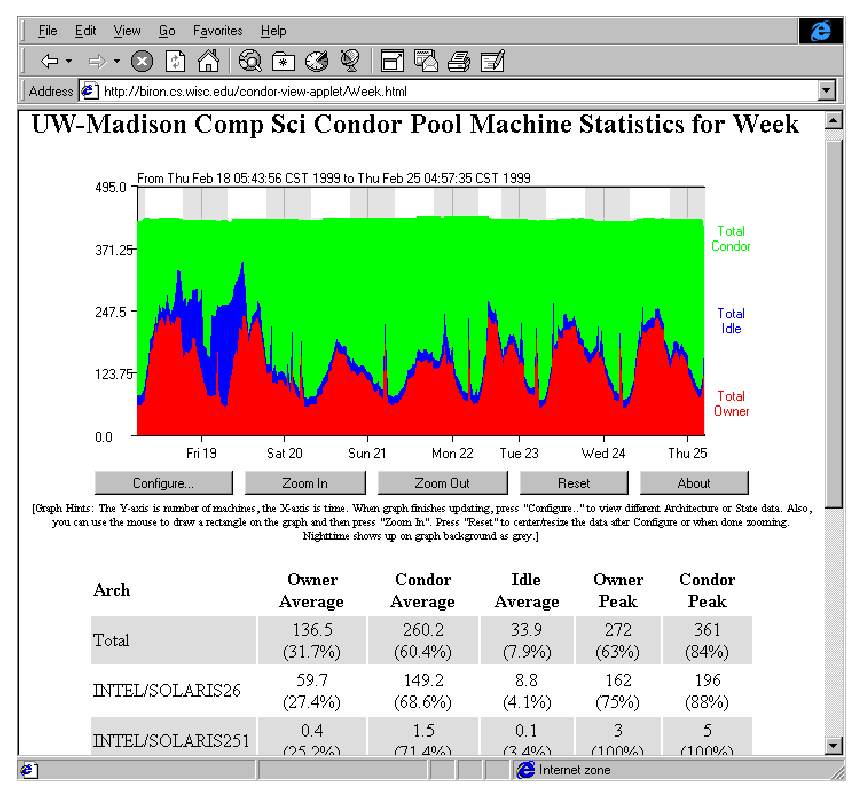
\includegraphics{admin-man/view-screenshot.ps}
\caption{\label{fig:view-screenshot}Screen shot of CondorView Client}
\end{figure}

After unpacking and installing the CondorView Client, a script named
\Prog{make\_stats} can be invoked to create HTML pages displaying Condor usage
for the past hour, day, week, or month.  
By using the Unix \Prog{cron} facility to periodically execute
\Prog{make\_stats}, Condor pool usage statistics can be kept up to date
automatically.  
This simple model allows the CondorView Client to be easily installed;
no Web server CGI interface is needed.

%%%%%%%%%%%%%%%%%%%%%%%%%%%%%%%%%%%%%%%%%%%%%%%%%%%%%%%%%%%%%%%%%%%%%%
\subsubsection{\label{sec:condorview-client-step-by-step}
Step-by-Step Installation of the CondorView Client}
%%%%%%%%%%%%%%%%%%%%%%%%%%%%%%%%%%%%%%%%%%%%%%%%%%%%%%%%%%%%%%%%%%%%%%

\index{installation!CondorView Client}
\index{CondorView!Client installation}
\begin{enumerate}

\item Make certain that the CondorView Server is configured.
Section ~\ref{sec:Contrib-CondorView-Install}
describes configuration of the server.
The server logs information on disk in order to provide a persistent,
historical database of pool statistics.
The CondorView Client makes queries over the network to this
database.
The \Condor{collector} includes this database support.
To activate the persistent database logging, add the following entries to
the configuration file for the \Condor{collector} chosen to act as the ViewServer.
\begin{verbatim}
    POOL_HISTORY_DIR = /full/path/to/directory/to/store/historical/data 
    KEEP_POOL_HISTORY = True 
\end{verbatim}

\item Create a directory where CondorView is to place the HTML files.  
This directory should be one published by a web server, so that HTML
files which exist in this directory can be accessed using a web browser.  
This directory is referred to as the \File{VIEWDIR} directory.

\item Download the \Prog{view\_client} contrib module.
Follow links for contrib modules on the downloads page at
\URL{http://www.cs.wisc.edu/condor/downloads-v2/download.pl}.

\item Unpack or untar this contrib module into the
directory \File{VIEWDIR}.
This creates several files and subdirectories.
Further unpack the jar file within the \File{VIEWDIR} directory with:
\begin{verbatim} 
  jar -xf condorview.jar
\end{verbatim}

\item Edit the \Prog{make\_stats} script.  At the beginning of the file
are six parameters to customize.
The parameters are

        \begin{description}

	\item[\MacroNI{ORGNAME}] A brief name that identifies an
	organization. An example is ``Univ of Wisconsin''.  Do not
	use any slashes in the name or other special regular-expression
	characters. Avoid the characters \Bs \^\  and \$.

	\item[\MacroNI{CONDORADMIN}] The e-mail
	address of the Condor administrator at your site.  
	This e-mail address will appear at the bottom of the web pages.

	\item[\MacroNI{VIEWDIR}] The full path name
	(\emph{not} a relative path) to the \File{VIEWDIR} directory set
	by installation step 2.  
	It is the directory that contains the \Prog{make\_stats} script.

	\item[\MacroNI{STATSDIR}]  The full path name of the
	directory which contains the \Condor{stats} binary.
	The \Condor{stats} program is included in the \Release{bin}
	directory. 
	The value for \MacroNI{STATSDIR} is added to the \MacroNI{PATH}
	parameter by default.  

	\item[\MacroNI{PATH}] A list of subdirectories,
	separated by colons, where the \Prog{make\_stats} script can find
	the \Prog{awk}, \Prog{bc}, \Prog{sed}, \Prog{date}, and \Condor{stats}
	programs.  
	If \Prog{perl} is installed, the path should also
	include the directory where \Prog{perl} is installed.
	The following default works on most systems:
        \begin{verbatim} 
        PATH=/bin:/usr/bin:$STATSDIR:/usr/local/bin
        \end{verbatim}

        \end{description}

\item To create all of the initial HTML files, run
\begin{verbatim}
        ./make_stats setup  
\end{verbatim}
Open the file \File{index.html} to verify that things look good.

\index{CondorView!use of \Prog{crontab} program}
\index{crontab program}

\item Add the \Prog{make\_stats} program to \Prog{cron}.  
Running \Prog{make\_stats} in step 6 created a \File{cronentries} file.
This \File{cronentries} file is ready to be processed by the Unix
\Prog{crontab} command.
The \Prog{crontab} manual page contains details about
the \Prog{crontab} command and the \Prog{cron} daemon.
Look at the
\File{cronentries} file; by default, it will run 
\Prog{make\_stats} \Arg{hour} every 15 minutes, 
\Prog{make\_stats} \Arg{day} once an hour, 
\Prog{make\_stats} \Arg{week} twice per day, and 
\Prog{make\_stats} \Arg{month} once per day.
These are reasonable defaults.  
Add these commands to cron on any
system that can access the \MacroNI{VIEWDIR} and
\MacroNI{STATSDIR} directories,
even on a system that does not have Condor installed.
The commands do not need to run as root user;
in fact, they should probably not run as root.  These commands can run
as any user that has read/write access to the \File{VIEWDIR} directory.
The command
\begin{verbatim} 
  crontab cronentries
\end{verbatim}
can set the crontab file;
note that this command overwrites the current, existing crontab file with the 
entries from the file \File{cronentries}.

\item Point the web browser at the \File{VIEWDIR} directory
to complete the installation.

\end{enumerate}


%%%%%%%%%%%%%%%%%%%%%%%%%%%%%%%%%%%%%%%%%%%%%%%%%%%%%%%%%%%%%%%%%%%%%%
%%%%%%%%%%%%%%%%%%%%%%%%%%%%%%%%%%%%%%%%%%%%%%%%%%%%%%%%%%%%%%%%%%%%%%%%%%%%%%%%
\subsection{\label{sec:Dynamic-Deployment}Dynamic Deployment}
%%%%%%%%%%%%%%%%%%%%%%%%%%%%%%%%%%%%%%%%%%%%%%%%%%%%%%%%%%%%%%%%%%%%%%%%%%%%%%%%
\index{dynamic deployment}
\index{deployment commands}

Dynamic deployment is a mechanism that allows rapid, automated
installation and start up of Condor resources on a given machine.
In this way any machine can be added to a Condor pool.
The dynamic
deployment tool set also provides tools to remove a machine from the
pool, without leaving residual effects on the machine such as leftover
installations, log files, and working directories.

\index{Condor commands!condor\_cold\_start}
Installation and start up is provided by \Condor{cold\_start}.
The \Condor{cold\_start} program determines the operating system and
architecture of the target machine, and transfers the correct
installation package from an ftp, http, or grid ftp site.
After transfer, it
installs Condor and creates a local working
directory for Condor to run in.  As a last step, \Condor{cold\_start}
begins running Condor in a manner which allows for later easy and reliable
shut down.

\index{Condor commands!condor\_cold\_stop}
The program that reliably shuts down and uninstalls a previously
dynamically installed Condor instance is \Condor{cold\_stop}.
\Condor{cold\_stop} begins by safely and reliably shutting off the
running Condor installation.  It ensures that Condor has
completely shut down before continuing, and optionally ensures that
there are no queued jobs at the site.
Next, \Condor{cold\_stop}
removes and optionally archives the Condor working directories,
including the \File{log} directory. 
These archives can be stored to a
mounted file system or to a grid ftp site.
As a last step,
\Condor{cold\_stop} uninstalls the Condor executables and libraries.
The end result is that the machine resources are left unchanged after
a dynamic deployment of Condor leaves.

%%%%%%%%%%%%%%%%%%%%%%%%%%%%%%%%%%%%%%%%%%%%%%%%%%%%%%%%%%%%%%%%%%%%%%%%%%%%%%%%
\subsubsection{Configuration and Usage}
%%%%%%%%%%%%%%%%%%%%%%%%%%%%%%%%%%%%%%%%%%%%%%%%%%%%%%%%%%%%%%%%%%%%%%%%%%%%%%%%

\index{dynamic deployment!configuration}
Dynamic deployment is designed for the expert Condor user
and administrator.
Tool design choices were made for functionality,
not ease-of-use.

Like every installation of Condor, a dynamically deployed installation
relies on a configuration.
To add a target
machine to a previously created Condor pool,
the global configuration file for that pool is a good starting point.
Modifications to that configuration can be made in a separate, 
local configuration file used in the dynamic deployment.
The global configuration file must
be placed on an ftp, http, grid ftp, or file server 
accessible by \Condor{cold\_start}.  The local configuration file
is to be on a file system accessible by the target machine.
There are some specific configuration variables that may be set for
dynamic deployment.  
A list of executables and directories which must be present
for Condor to start on the target machine may be set with
the configuration variables \Macro{DEPLOYMENT\_REQUIRED\_EXECS} and
\Macro{DEPLOYMENT\_REQUIRED\_DIRS}. 
If defined and the comma-separated list of executables or directories are
not present, then \Condor{cold\_start} exits with error.
Note this does not affect what is installed, only
whether start up is successful. 

A list of executables and directories which are recommended to be present
for Condor to start on the target machine may be set with
the configuration variables \Macro{DEPLOYMENT\_RECOMMENDED\_EXECS} and
\Macro{DEPLOYMENT\_RECOMMENDED\_DIRS}. 
If defined and the comma-separated lists of executables or directories are
not present, then \Condor{cold\_start} prints a warning message
and continues.
Here is a portion of the configuration relevant to
a dynamic deployment of a Condor submit node:

\footnotesize
\begin{verbatim}
DEPLOYMENT_REQUIRED_EXECS    = MASTER, SCHEDD, PREEN, STARTER, \
                               STARTER_STANDARD, SHADOW, \
                               SHADOW_STANDARD, GRIDMANAGER, GAHP, CONDOR_GAHP
DEPLOYMENT_REQUIRED_DIRS     = SPOOL, LOG, EXECUTE
DEPLOYMENT_RECOMMENDED_EXECS = CREDD
DEPLOYMENT_RECOMMENDED_DIRS  = LIB, LIBEXEC
\end{verbatim}
\normalsize

Additionally, the user must
specify which Condor services will be started.  This is done through
the \MacroNI{DAEMON\_LIST} configuration variable.  Another excerpt
from a dynamic submit node deployment configuration:

\footnotesize
\begin{verbatim}
DAEMON_LIST  = MASTER, SCHEDD
\end{verbatim}
\normalsize

Finally, the location
of the dynamically installed Condor executables is tricky to set,
since the location is unknown before installation.
Therefore,
the variable \Macro{DEPLOYMENT\_RELEASE\_DIR} is defined in the environment.
It corresponds to the location of the dynamic Condor installation.
If, as is often the case, 
the configuration file specifies the location of Condor executables in
relation to the \MacroNI{RELEASE\_DIR} variable, the configuration can
be made dynamically deployable by setting \MacroNI{RELEASE\_DIR} to
\MacroNI{DEPLOYMENT\_RELEASE\_DIR} as 

\footnotesize
\begin{verbatim}
RELEASE_DIR = $(DEPLOYMENT_RELEASE_DIR)
\end{verbatim}
\normalsize

In addition to setting up the configuration, the user must also
determine where the installation package will reside.
The installation package can be in either tar or 
gzipped tar form, and may
reside on a ftp, http, grid ftp, or file server.  
Create this installation package by tar'ing up the binaries and libraries
needed, and place them on the appropriate server.
The binaries can be tar'ed in a flat structure or within \File{bin} and
\File{sbin}.  Here is a list of files to give an example
structure for a dynamic deployment of the \Condor{schedd} daemon.

\footnotesize
\begin{verbatim}
% tar tfz latest-i686-Linux-2.4.21-37.ELsmp.tar.gz
bin/
bin/condor_config_val
bin/condor_q
sbin/
sbin/condor_preen
sbin/condor_shadow.std
sbin/condor_starter.std
sbin/condor_schedd
sbin/condor_master
sbin/condor_gridmanager
sbin/gt4_gahp
sbin/gahp_server
sbin/condor_starter
sbin/condor_shadow
sbin/condor_c-gahp
sbin/condor_off 
\end{verbatim}
\normalsize

%%%%%%%%%%%%%%%%%%%%%%%%%%%%%%%%%%%%%%%%%%%%%%%%%%%%%%%%%%%%%%%%%%%%%%

%%%%%%%%%%%%%%%%%%%%%%%%%%%%%%%%%%%%%%%%%%%%%%%%%%%%%%%%%%%%%%%%%%%%%%
\section{\label{sec:Configuring-Condor}Configuration}
%%%%%%%%%%%%%%%%%%%%%%%%%%%%%%%%%%%%%%%%%%%%%%%%%%%%%%%%%%%%%%%%%%%%%%

\index{Condor!configuration}
\index{configuration}

This section describes how to configure all parts of the Condor
system.  General information about the configuration
files and their syntax is followed by a description of
settings that affect all
Condor daemons and tools.
The 
settings that control the policy under which Condor will start,
suspend, resume, vacate or kill jobs
are described in 
section~\ref{sec:Configuring-Policy} on Startd Policy Configuration. 

%%%%%%%%%%%%%%%%%%%%%%%%%%%%%%%%%%%%%%%%%%%%%%%%%%%%%%%%%%%%%%%%%%%%%%
\subsection{\label{sec:Intro-to-Config-Files}Introduction to
Configuration Files} 
%%%%%%%%%%%%%%%%%%%%%%%%%%%%%%%%%%%%%%%%%%%%%%%%%%%%%%%%%%%%%%%%%%%%%%

The Condor configuration files are used to customize how Condor
operates at a given site.  The basic configuration as shipped with
Condor works well for most sites.

Each Condor program will, as part of its initialization process,
configure itself by calling a library routine which parses the
various configuration files that might be used including pool-wide,
platform-specific, and machine-specific configuration files.
Environment variables may also contribute to the configuration.

The result of configuration is a list of key/value pairs.
Each key is a configuration variable name,
and each value is a string literal
that may utilize macro substitution (as defined below).
Some configuration variables are evaluated by Condor as ClassAd
expressions; some are not.  Consult the documentation for each specific
case.  Unless otherwise noted, configuration values that are expected
to be numeric or boolean constants may be any valid ClassAd expression
of operators on constants.  Example:

\begin{verbatim}
MINUTE          = 60
HOUR            = (60 * $(MINUTE))
SHUTDOWN_GRACEFUL_TIMEOUT = ($(HOUR)*24)
\end{verbatim}

%%%%%%%%%%%%%%%%%%%%%%%%%%%%%%%%%%%%%%%%%%%%%%%%%%%%%%%%%%%%%%%%%%%%%%
\subsubsection{\label{sec:Ordering-Config-File}Ordered Evaluation to
Set the Configuration} 
%%%%%%%%%%%%%%%%%%%%%%%%%%%%%%%%%%%%%%%%%%%%%%%%%%%%%%%%%%%%%%%%%%%%%%
\index{configuration file!evaluation order}

Multiple files, as well as a program's environment variables
determine the configuration.
The order in which attributes are defined is important, as later
definitions override existing definitions.
The order in which the (multiple) configuration files are parsed 
is designed to ensure the security of the system.
Attributes which must be set a specific way 
must appear in the last file to be parsed.
This prevents both the naive and the malicious Condor user 
from subverting the system through its configuration.
The order in which items are parsed is
\begin{enumerate}
\item global configuration file
\item local configuration file
\item specific environment variables prefixed with \MacroNI{\_CONDOR\_}
\end{enumerate}

The locations for these files are as given in
section~\ref{sec:Config-File-Locations} on
page~\pageref{sec:Config-File-Locations}.

Some Condor tools utilize environment variables to set their
configuration.
These tools search for specifically-named environment variables.
The variables are prefixed by the string \MacroNI{\_CONDOR\_}
or \MacroNI{\_condor\_}.
The tools strip off the prefix, and utilize what remains
as configuration.
As the use of environment variables is the last within
the ordered evaluation, 
the environment variable definition is used.
The security of the system is not compromised,
as only specific variables are considered for definition
in this manner, not any environment variables with
the \MacroNI{\_CONDOR\_} prefix.


%%%%%%%%%%%%%%%%%%%%%%%%%%%%%%%%%%%%%%%%%%%%%%%%%%%%%%%%%%%%%%%%%%%%%%
\subsubsection{\label{sec:Config-File-Macros}Configuration File Macros} 
%%%%%%%%%%%%%%%%%%%%%%%%%%%%%%%%%%%%%%%%%%%%%%%%%%%%%%%%%%%%%%%%%%%%%%

\index{macro!in configuration file}
\index{configuration file!macro definitions}

Macro definitions are of the form:
\begin{verbatim}
<macro_name> = <macro_definition>
\end{verbatim}

The macro name given on the left hand side of the definition is
a case sensitive identifier.
There must be white space between the macro name, the
equals sign (\verb@=@), and the macro definition.
The macro definition is a string literal that may utilize macro substitution.

Macro invocations are of the form: 
\begin{verbatim}
$(macro_name)
\end{verbatim}

Macro definitions may contain references to other macros, even ones
that are not yet defined, as long as they are eventually defined in
the configuration files.
All macro expansion is done after all configuration files have been parsed,
with the exception of macros that reference themselves.

\begin{verbatim}
A = xxx
C = $(A) 
\end{verbatim}
is a legal set of macro definitions, and the resulting value of 
\MacroNI{C} is
\Expr{xxx}.
Note that
\MacroNI{C} is actually bound to 
\MacroUNI{A}, not its value.

As a further example,
\begin{verbatim}
A = xxx
C = $(A)
A = yyy
\end{verbatim}
is also a legal set of macro definitions, and the resulting value of
\MacroNI{C} is \Expr{yyy}.  

A macro may be incrementally defined by invoking itself in its
definition.  For example,
\begin{verbatim}
A = xxx
B = $(A)
A = $(A)yyy
A = $(A)zzz
\end{verbatim}
is a legal set of macro definitions, and the resulting value of 
\MacroNI{A}
is \Expr{xxxyyyzzz}.
Note that invocations of a macro in
its own definition are immediately
expanded.
\MacroUNI{A} is immediately expanded in line 3 of the example.
If it were not, then the definition would be impossible to
evaluate.

Recursively defined macros such as
\begin{verbatim}
A = $(B)
B = $(A)
\end{verbatim}
are not allowed.
They create definitions that Condor refuses to parse. 

All entries in a configuration file must have an operator,
which will be an equals sign (\verb@=@).
Identifiers are alphanumerics combined with the underscore character,
optionally with a subsystem name and a period as a prefix.
As a special case,
a line without an operator that begins with a left square bracket
will be ignored.
The following two-line example treats the first line as a comment,
and correctly handles the second line.
\begin{verbatim}
[Condor Settings]
my_classad = [ foo=bar ]
\end{verbatim}

% functionality added to version 6.7.13
To simplify pool administration,
any configuration variable name may be prefixed by
a subsystem 
(see the \MacroUNI{SUBSYSTEM} macro in 
section~\ref{sec:Pre-Defined-Macros}
for the list of subsystems)
and the period (\verb@.@) character.
For configuration variables defined this way,
the value is applied to the specific subsystem.
For example,
the ports that Condor may use can be restricted to a range 
using the \MacroNI{HIGHPORT} and \MacroNI{LOWPORT} configuration
variables.
If the range of intended ports is different for specific
daemons, this syntax may be used.

\begin{verbatim}
  MASTER.LOWPORT   = 20000
  MASTER.HIGHPORT  = 20100
  NEGOTIATOR.LOWPORT   =  22000 
  NEGOTIATOR.HIGHPORT  =  22100
\end{verbatim}

Note that all configuration variables may utilize this syntax,
but nonsense configuration variables may result.
For example, it makes no sense to define
\begin{verbatim}
  NEGOTIATOR.MASTER_UPDATE_INTERVAL = 60
\end{verbatim}
since the \Condor{negotiator} daemon does not use the
\MacroNI{MASTER\_UPDATE\_INTERVAL} variable.

It makes little sense to do so, but Condor will configure
correctly with a definition such as
\begin{verbatim}
  MASTER.MASTER_UPDATE_INTERVAL = 60
\end{verbatim}
The \Condor{master} uses this configuration variable,
and the prefix of \MacroNI{MASTER.} causes this configuration
to be specific to the \Condor{master} daemon.

% the local functionality added in 7.1.4
This syntax has been further expanded to allow for the
specification of a local name on the command line 
using the command line option
\begin{verbatim}
  -local-name <local-name>
\end{verbatim}
This allows multiple instances of a daemon to be run 
by the same \Condor{master} daemon,
each instance with its own local configuration variable.

The ordering used to look up a variable, called \verb@<parameter name>@:

\begin{enumerate}
\item \verb@<subsystem name>.<local name>.<parameter name>@

\item \verb@<local name>.<parameter name>@

\item \verb@<subsystem name>.<parameter name>@

\item \verb@<parameter name>@
\end{enumerate}

If this local name is not specified on the command line, 
numbers 1 and 2 are skipped.
As soon as the first match is found, the search is completed,
and the corresponding value is used.

This example configures a \Condor{master} to run 2 \Condor{schedd}
daemons.  The \Condor{master} daemon needs the configuration:
\begin{verbatim}
  XYZZY           = $(SCHEDD)
  XYZZY_ARGS      = -local-name xyzzy
  DAEMON_LIST     = $(DAEMON_LIST) XYZZY
  DC_DAEMON_LIST  = + XYZZY
  XYZZY_LOG       = $(LOG)/SchedLog.xyzzy
\end{verbatim}

Using this example configuration, the \Condor{master} starts up a
second \Condor{schedd} daemon, 
where this second \Condor{schedd} daemon is passed 
\OptArg{-local-name}{xyzzy}
on the command line.

Continuing the example,
configure the \Condor{schedd} daemon named \Attr{xyzzy}.
This \Condor{schedd} daemon will share all configuration variable
definitions with the other \Condor{schedd} daemon,
except for those specified separately.

\begin{verbatim}
  SCHEDD.XYZZY.SCHEDD_NAME = XYZZY
  SCHEDD.XYZZY.SCHEDD_LOG  = $(XYZZY_LOG)
  SCHEDD.XYZZY.SPOOL       = $(SPOOL).XYZZY
\end{verbatim}

Note that the example \MacroNI{SCHEDD\_NAME} and \MacroNI{SPOOL} are
specific to the \Condor{schedd} daemon, as opposed to a different daemon
such as the \Condor{startd}.
Other Condor daemons using this feature will
have different requirements for which parameters need to be
specified individually.  This example works for the \Condor{schedd},
and more local configuration can, and likely would be specified.

Also note that each daemon's log file must be specified individually,
and in two places: one specification is for use by the \Condor{master},
and the other is for use by the daemon itself.
In the example,
the \Attr{XYZZY} \Condor{schedd} configuration variable
\MacroNI{SCHEDD.XYZZY.SCHEDD\_LOG} definition references the
\Condor{master} daemon's \MacroNI{XYZZY\_LOG}.


%%%%%%%%%%%%%%%%%%%%%%%%%%%%%%%%%%%%%%%%%%%%%%%%%%%%%%%%%%%%%%%%%%%%%%
\subsubsection{\label{sec:Other-Syntax}Comments and Line Continuations}
%%%%%%%%%%%%%%%%%%%%%%%%%%%%%%%%%%%%%%%%%%%%%%%%%%%%%%%%%%%%%%%%%%%%%%

A Condor configuration file may contain comments and
line continuations.
A comment is any line beginning with a pound character (\verb@#@).
A continuation is any entry that continues across multiples lines.
Line continuation is accomplished by placing the backslash
character (\Bs) at the end of any line to be continued onto another.
Valid examples of line continuation are
\begin{verbatim}
  START = (KeyboardIdle > 15 * $(MINUTE)) && \
  ((LoadAvg - CondorLoadAvg) <= 0.3)
\end{verbatim}
and
\begin{verbatim}
  ADMIN_MACHINES = condor.cs.wisc.edu, raven.cs.wisc.edu, \
  stork.cs.wisc.edu, ostrich.cs.wisc.edu, \
  bigbird.cs.wisc.edu
  HOSTALLOW_ADMIN = $(ADMIN_MACHINES)
\end{verbatim}

Note that a line continuation character may currently be used within
a comment, so the following example does \emph{not} set the
configuration variable \MacroNI{FOO}:
\begin{verbatim}
  # This comment includes the following line, so FOO is NOT set \
  FOO = BAR
\end{verbatim}
It is a poor idea to use this functionality, as it is likely to
stop working in future Condor releases.

%%%%%%%%%%%%%%%%%%%%%%%%%%%%%%%%%%%%%%%%%%%%%%%%%%%%%%%%%%%%%%%%%%%%%%
\subsubsection{\label{sec:Program-Defined-Macros}Executing a Program to Produce Configuration Macros}
%%%%%%%%%%%%%%%%%%%%%%%%%%%%%%%%%%%%%%%%%%%%%%%%%%%%%%%%%%%%%%%%%%%%%%

Instead of reading from a file,
Condor may run a program to obtain configuration macros.
The vertical bar character (\Bar) as the last character defining
a file name provides the syntax necessary to tell 
Condor to run a program.
This syntax may only be used in the definition of
the \Env{CONDOR\_CONFIG} environment variable,
or the \Macro{LOCAL\_CONFIG\_FILE} configuration variable.

The command line for the program 
is formed by the characters preceding the vertical bar character.
The standard output of the program is parsed as a configuration 
file would be.

An example:
\begin{verbatim}
LOCAL_CONFIG_FILE = /bin/make_the_config|
\end{verbatim}

Program \Prog{/bin/make\_the\_config} is executed, and its output
is the set of configuration macros.

Note that either a program is executed to generate the
configuration macros or the configuration is read from 
one or more files.
The syntax uses space characters to separate command line elements,
if an executed program produces the configuration macros.
Space characters would otherwise separate the list of files.
This syntax does not permit distinguishing one from the other,
so only one may be specified.

%%%%%%%%%%%%%%%%%%%%%%%%%%%%%%%%%%%%%%%%%%%%%%%%%%%%%%%%%%%%%%%%%%%%%%
\subsubsection{\label{sec:Macros-Requiring-Restart}Macros That Will Require a Restart When Changed}
%%%%%%%%%%%%%%%%%%%%%%%%%%%%%%%%%%%%%%%%%%%%%%%%%%%%%%%%%%%%%%%%%%%%%%
\index{configuration change requiring a restart of Condor}
When any of the following listed configuration variables are changed,
Condor must be restarted.
Reconfiguration using \Condor{reconfig} will not be enough.

\begin{itemize}
  \item \verb@BIND_ALL_INTERFACES@
  \item \verb@FetchWorkDelay@
  \item \verb@MAX_NUM_CPUS@
  \item \verb@MAX_TRACKING_GID@
  \item \verb@MIN_TRACKING_GID@
  \item \verb@NETWORK_INTERFACE@
  \item \verb@NUM_CPUS@
  \item \verb@PREEMPTION_REQUIREMENTS_STABLE@
  \item \verb@PRIVSEP_ENABLED@
  \item \verb@PROCD_ADDRESS@
\end{itemize}

%%%%%%%%%%%%%%%%%%%%%%%%%%%%%%%%%%%%%%%%%%%%%%%%%%%%%%%%%%%%%%%%%%%%%%
\subsubsection{\label{sec:Pre-Defined-Macros}Pre-Defined Macros}
%%%%%%%%%%%%%%%%%%%%%%%%%%%%%%%%%%%%%%%%%%%%%%%%%%%%%%%%%%%%%%%%%%%%%%

\index{configuration!pre-defined macros}
\index{configuration file!pre-defined macros}
Condor provides pre-defined macros that help configure Condor.
Pre-defined macros are listed as \MacroUNI{macro\_name}.

This first set are entries whose values are determined at
run time and cannot be overwritten.  These are inserted automatically by
the library routine which parses the configuration files.
This implies that a change to the underlying value of any of these
variables will require a full restart of Condor in order to use
the changed value.
\begin{description}
  
\label{param:FullHostname}
\item[\MacroU{FULL\_HOSTNAME}]
  The fully qualified host name of the local machine, 
  which is host name plus domain name.
  
\label{param:Hostname}
\item[\MacroU{HOSTNAME}]
  The host name of the local machine (no domain name).
  
\label{param:IpAddress}
\item[\MacroU{IP\_ADDRESS}]
  The ASCII string version of the local machine's IP address.

\label{param:Tilde}
\item[\MacroU{TILDE}]
  The full path to the
  home directory of the Unix user condor, if such a user exists on the
  local machine.

  \label{sec:Condor-Subsystem-Names}
  \index{configuration file!subsystem names}
\label{param:Subsystem}
\item[\MacroU{SUBSYSTEM}]
  The subsystem
  name of the daemon or tool that is evaluating the macro.
  This is a unique string which identifies a given daemon within the
  Condor system.  The possible subsystem names are:

  \index{subsystem names}
  \index{macro!subsystem names}
  \begin{itemize}
  \label{list:subsystem names}
  \item \verb@C_GAHP@
  \item \verb@CKPT_SERVER@
  \item \verb@COLLECTOR@
  \item \verb@DBMSD@
  \item \verb@DEFRAG@
  \item \verb@EC2_GAHP@
  \item \verb@GRIDMANAGER@
  \item \verb@HAD@
  \item \verb@HDFS@
  \item \verb@JOB_ROUTER@
  \item \verb@KBDD@ 
  \item \verb@LEASEMANAGER@
  \item \verb@MASTER@
  \item \verb@NEGOTIATOR@
  \item \verb@QUILL@
  \item \verb@REPLICATION@
  \item \verb@ROOSTER@
  \item \verb@SCHEDD@
  \item \verb@SHADOW@
  \item \verb@STARTD@
  \item \verb@STARTER@
  %\item \verb@STORK@
  \item \verb@SUBMIT@
  \item \verb@TOOL@
  \item \verb@TRANSFERER@
  \end{itemize}

\end{description}

This second set of macros are entries whose default values are
determined automatically at run time but which can be overwritten.  
\index{configuration file!macros}
\begin{description}

\label{param:Arch}
\item[\MacroU{ARCH}]
  Defines the string
  used to identify the architecture of the local machine to Condor.
  The \Condor{startd} will advertise itself with this attribute so
  that users can submit binaries compiled for a given platform and
  force them to run on the correct machines.  \Condor{submit} will
  append a requirement to the job ClassAd that it must
  run on the same \MacroNI{ARCH} and \MacroNI{OPSYS} of the machine where
  it was submitted, unless the user specifies \MacroNI{ARCH} and/or
  \MacroNI{OPSYS} explicitly in their submit file.  See the
  the \Condor{submit} manual page
  on page~\pageref{man-condor-submit} for details.

\label{param:OpSys}
\item[\MacroU{OPSYS}]
  Defines the string used to identify the operating system
  of the local machine to Condor.
  If it is not defined in the configuration file, Condor will
  automatically insert the operating system of this machine as
  determined by \Prog{uname}.

\label{param:OpSysVer}
\item[\MacroU{OPSYS\_VER}]
  Defines the integer used to identify the operating system version number.

\label{param:OpSysAndVer}
\item[\MacroU{OPSYS\_AND\_VER}]
  Defines the string used prior to Condor version 7.7.2 as \MacroUNI{OPSYS}.

\label{param:UnameArch}
\item[\MacroU{UNAME\_ARCH}]
  The architecture as reported by \Prog{uname}(2)'s \Code{machine} field.
  Always the same as \MacroNI{ARCH} on Windows.

\label{param:UnameOpsys}
\item[\MacroU{UNAME\_OPSYS}]
  The operating system as reported by \Prog{uname}(2)'s \Code{sysname} field.
  Always the same as \MacroNI{OPSYS} on Windows.

\label{param:DetectedMemory}
\item[\MacroU{DETECTED\_MEMORY}]
  The amount of detected physical memory (RAM) in Mbytes.

\label{param:DetectedCores}
\item[\MacroU{DETECTED\_CORES}]
  The number of detected CPU cores.  
  This includes hyper threaded cores, if there are any.

\label{param:Pid}
\item[\MacroU{PID}]
  The process ID for the daemon or tool.

\label{param:Ppid}
\item[\MacroU{PPID}]
  The process ID of the parent process for the daemon or tool.

\label{param:Username}
\item[\MacroU{USERNAME}]
  The user name of the UID of the daemon or tool.
  For daemons started as root, but running under another UID
  (typically the user condor), this will be the other UID.

\label{param:FilesystemDomain}
\item[\MacroU{FILESYSTEM\_DOMAIN}]
  Defaults to the fully
  qualified host name of the machine it is evaluated on.  See
  section~\ref{sec:Shared-Filesystem-Config-File-Entries}, Shared
  File System Configuration File Entries for the full description of
  its use and under what conditions you would want to change it.

\label{param:UIDDomain}
\item[\MacroU{UID\_DOMAIN}]
  Defaults to the fully
  qualified host name of the machine it is evaluated on.  See
  section~\ref{sec:Shared-Filesystem-Config-File-Entries} 
  for the full description of this configuration variable.

\end{description}

Since \MacroUNI{ARCH} and \MacroUNI{OPSYS} will automatically be set to the
correct values, we recommend that you do not overwrite them.
Only do so if you know what you are doing.



%%%%%%%%%%%%%%%%%%%%%%%%%%%%%%%%%%%%%%%%%%%%%%%%%%%%%%%%%%%%%%%%%%%%%%
\subsection{\label{sec:Config-File-Special}Special Macros}
%%%%%%%%%%%%%%%%%%%%%%%%%%%%%%%%%%%%%%%%%%%%%%%%%%%%%%%%%%%%%%%%%%%%%%

\index{configuration file!\$ENV definition}
\index{\$ENV!in configuration file}
References to the Condor process's environment are allowed in the
configuration files.
Environment references use the \Macro{ENV} macro and are of the form:
\begin{verbatim}
  $ENV(environment_variable_name)
\end{verbatim}
For example, 
\begin{verbatim}
  A = $ENV(HOME)
\end{verbatim}
binds \MacroNI{A} to the value of the HOME environment variable.
Environment references are not currently used in standard Condor
configurations.
However, they can sometimes be useful in custom configurations.

\index{\$RANDOM\_CHOICE()!in configuration}
This same syntax is used in the \Macro{RANDOM\_CHOICE()} macro to
allow a random choice of a parameter
within a configuration file.
These references are of the form:
\begin{verbatim}
  $RANDOM_CHOICE(list of parameters)
\end{verbatim}
This allows a random choice within the parameter list to be made
at configuration time.  Of the list of parameters, one is
chosen when encountered during configuration.  For example,
if one of the integers 0-8 (inclusive) should be randomly
chosen, the macro usage is
\begin{verbatim}
  $RANDOM_CHOICE(0,1,2,3,4,5,6,7,8)
\end{verbatim}

\index{\$RANDOM\_INTEGER()!in configuration}
The \Macro{RANDOM\_INTEGER()} macro is similar to the \MacroNI{RANDOM\_CHOICE()}
macro, and is used to select a random integer within a configuration file.
References are of the form:
\begin{verbatim}
  $RANDOM_INTEGER(min, max [, step])
\end{verbatim}
A random integer within the range \verb@min@ and \verb@max@, inclusive,
is selected at configuration time.
The optional \verb@step@ parameter
controls the stride within the range, and it defaults to the value 1.
For example, to randomly chose an even integer in the range 0-8 (inclusive),
the macro usage is
\begin{verbatim}
  $RANDOM_INTEGER(0, 8, 2)
\end{verbatim}

See section~\ref{sec:randomintegerusage} on
page~\pageref{sec:randomintegerusage}
for an actual use of this specialized macro.
%%%%%%%%%%%%%%%%%%%%%%%%%%%%%%%%%%%%%%%%%%%%%%%%%%%%%%%%%%%%%%%%%%%%%%
\subsection{\label{sec:Condor-wide-Config-File-Entries}Condor-wide Configuration File Entries} 
%%%%%%%%%%%%%%%%%%%%%%%%%%%%%%%%%%%%%%%%%%%%%%%%%%%%%%%%%%%%%%%%%%%%%%

\index{configuration!Condor-wide configuration variables}

This section describes settings which affect all parts of the Condor
system. 
Other system-wide settings can be found in
section~\ref{sec:Network-Related-Config-File-Entries} on
``Network-Related Configuration File Entries'', and
section~\ref{sec:Shared-Filesystem-Config-File-Entries} on ``Shared
File System Configuration File Entries''. 

\begin{description}
  
\label{param:CondorHost}
\item[\Macro{CONDOR\_HOST}]
  This macro may be
  used to define the \MacroUNI{NEGOTIATOR\_HOST} and is used to define the
  \MacroUNI{COLLECTOR\_HOST} macro.  Normally the \Condor{collector}
  and \Condor{negotiator} would run on the same machine.  If for some
  reason they were not run on the same machine,
  \MacroUNI{CONDOR\_HOST} would not be needed.  Some
  of the host-based security macros use \MacroUNI{CONDOR\_HOST} by
  default.  See section~\ref{sec:Host-Security}, on Setting up
  IP/host-based security in Condor for details.
  
\label{param:CollectorHost}
\item[\Macro{COLLECTOR\_HOST}]
  The host name of the machine where the \Condor{collector} is running for
  your pool.  Normally, it is defined relative to
  the \MacroUNI{CONDOR\_HOST}
  macro.  There is no default value for this macro;
  \MacroNI{COLLECTOR\_HOST} must be defined for the pool to work
  properly.

  In addition to defining the host name, this setting can optionally be
  used to specify the network port of the \Condor{collector}.
  The port is separated from the host name by a colon ('\verb@:@').
  For example,
  \begin{verbatim}
    COLLECTOR_HOST = $(CONDOR_HOST):1234
  \end{verbatim}
  If no port is specified, the default port of 9618 is used.
  Using the default port is recommended for most sites.
  It is only changed if there is a conflict with another
  service listening on the same network port.
  For more information about specifying a non-standard port for the
  \Condor{collector} daemon,
  see section~\ref{sec:Ports-NonStandard} on
  page~\pageref{sec:Ports-NonStandard}.


\label{param:NegotiatorHost} 
\item[\Macro{NEGOTIATOR\_HOST}]
  This configuration variable is no longer used.
  It previously defined the host name of the machine where 
  the \Condor{negotiator} is running.
  At present, the port where the \Condor{negotiator} is listening 
  is dynamically allocated.

  % commented out by Karen in 2008, as this 6.7ism is too old
  %For pools running 6.7.3 and older versions: The
  %host name of the machine where the \Condor{negotiator} is running for
  %the pool.
  %Normally, it is defined relative to the \MacroUNI{CONDOR\_HOST}
  %macro.  There is no default value for this macro;
  %\MacroNI{NEGOTIATOR\_HOST} must be defined for the pool to work
  %properly.
  %This variable may also be used to optionally define a network port for
  %the \Condor{negotiator} daemon, as explained for the
  %\MacroNI{COLLECTOR\_HOST} variable.

\label{param:CondorViewHost}
\item[\Macro{CONDOR\_VIEW\_HOST}]
  A list of CondorView servers, separated by commas and/or spaces.
  Each CondorView server is denoted by the host name of the machine
  it is running on, optionally appended by a colon and the port number.
  This service is optional, and requires additional configuration 
  to enable it.  There is no default value for
  \MacroNI{CONDOR\_VIEW\_HOST}.  If \MacroNI{CONDOR\_VIEW\_HOST} is not
  defined, no CondorView server is used.
  See section~\ref{sec:Contrib-CondorView-Install} on
  page~\pageref{sec:Contrib-CondorView-Install} for more details.

\label{param:ScheddHost}
\item[\Macro{SCHEDD\_HOST}]
  The host name of the machine where the \Condor{schedd} is running for
  your pool.  This is the host that queues submitted jobs.
  If the host specifies \Macro{SCHEDD\_NAME} or \Macro{MASTER\_NAME}, that
  name must be included in the form name\verb$@$hostname.
  In most condor installations, there is a \Condor{schedd} running on
  each host from which jobs are submitted.  The default value of
  \Macro{SCHEDD\_HOST} is the current host with the optional name included.  For most pools, this
  macro is not defined, nor does it need to be defined..

\label{param:ReleaseDir}
\item[\Macro{RELEASE\_DIR}]
  The full path to
  the Condor release directory, which holds the \File{bin},
  \File{etc}, \File{lib}, and \File{sbin} directories.  Other macros
  are defined relative to this one.  There is no default value for
  \Macro{RELEASE\_DIR}.

\label{param:Bin}
\item[\Macro{BIN}]
  This directory points to the
  Condor directory where user-level programs are installed.  It is
  usually defined relative to the \MacroUNI{RELEASE\_DIR} macro.
  There is no default value for \Macro{BIN}.
  
\label{param:Lib}
\item[\Macro{LIB}]
  This directory points to the
  Condor directory where libraries used to link jobs for Condor's
  standard universe are stored.  The \Condor{compile} program uses
  this macro to find these libraries, so it must be defined for
  \Condor{compile} to function.  \MacroUNI{LIB} is usually defined
  relative to the \MacroUNI{RELEASE\_DIR} macro, and has no default
  value.

\label{param:LibExec}
\item[\Macro{LIBEXEC}]
  This directory points
  to the Condor directory where support commands that Condor
  needs will be placed.
  Do not add this directory to a user or system-wide path.

\label{param:Include}
\item[\Macro{INCLUDE}]
  This directory points to the Condor directory where header files reside.
  \MacroUNI{INCLUDE} would usually be defined relative to
  the \MacroUNI{RELEASE\_DIR} configuration macro.
  There is no default value, but
  if defined, it can make inclusion of necessary header files
  for compilation of programs (such as those programs
  that use \File{libcondorapi.a})
  easier through the use of \Condor{config\_val}.

\label{param:Sbin}
\item[\Macro{SBIN}]
  This directory points to the
  Condor directory where Condor's system binaries (such as the
  binaries for the Condor daemons) and administrative tools are
  installed.  Whatever directory \MacroU{SBIN} points to ought
  to be in the \Env{PATH} of users acting as Condor
  administrators.  \Macro{SBIN} has no default value.

\label{param:LocalDir}
\item[\Macro{LOCAL\_DIR}]
  The location of the
  local Condor directory on each machine in your pool.  One common
  option is to use the condor user's home directory which may be
  specified with \MacroUNI{TILDE}.  There is no default value for
  \Macro{LOCAL\_DIR}.  For example:
  \begin{verbatim}
    LOCAL_DIR = $(tilde)
  \end{verbatim}
  
  On machines with a shared file system, where either the
  \MacroUNI{TILDE} directory or another directory you want to use is
  shared among all machines in your pool, you might use the
  \MacroUNI{HOSTNAME} macro and have a directory with many
  subdirectories, one for each machine in your pool, each named by
  host names.  For example:
  \begin{verbatim}
    LOCAL_DIR = $(tilde)/hosts/$(hostname)      
  \end{verbatim}
  or:
  \begin{verbatim}
    LOCAL_DIR = $(release_dir)/hosts/$(hostname)
  \end{verbatim}
  
\label{param:Log}
\item[\Macro{LOG}]
  Used to specify the
  directory where each Condor daemon writes its log files.  The names
  of the log files themselves are defined with other macros, which use
  the \MacroUNI{LOG} macro by default.  The log directory also acts as
  the current working directory of the Condor daemons as the run, so
  if one of them should produce a core file for any reason, it would
  be placed in the directory defined by this macro.  \MacroNI{LOG} is
  required to be defined.  Normally, \MacroUNI{LOG} is defined in
  terms of \MacroUNI{LOCAL\_DIR}.
  
\label{param:Spool}
\item[\Macro{SPOOL}]
  The spool directory is where
  certain files used by the \Condor{schedd} are stored, such as the
  job queue file and the initial executables of any jobs that have
  been submitted.  In addition, for systems not using a checkpoint
  server, all the checkpoint files from jobs that have been submitted
  from a given machine will be store in that machine's spool
  directory.  Therefore, you will want to ensure that the spool
  directory is located on a partition with enough disk space.  If a
  given machine is only set up to execute Condor jobs and not submit
  them, it would not need a spool directory (or this macro defined).
  There is no default value for \Macro{SPOOL}, and the \Condor{schedd}
  will not function without it \Macro{SPOOL} defined.  Normally,
  \MacroUNI{SPOOL} is defined in terms of \MacroUNI{LOCAL\_DIR}.
  
\label{param:Execute}
\item[\Macro{EXECUTE}]
  This directory acts as
  a place to create the scratch directory of any Condor job that is executing
  on
  the local machine.  The scratch directory is the destination of
  any input files that were specified for transfer.  It also serves
  as the job's working directory if the job is using file transfer
  mode and no other working directory was specified.
  If a given machine is set up to only submit
  jobs and not execute them, it would not need an execute directory,
  and this macro need not be defined.  There is no default value for
  \MacroNI{EXECUTE}, and the \Condor{startd} will not function if
  \MacroNI{EXECUTE} is undefined.  Normally, \MacroUNI{EXECUTE} is
  defined in terms of \MacroUNI{LOCAL\_DIR}.  To customize the execute
  directory independently for each batch slot, use \MacroNI{SLOT<N>\_EXECUTE}.

\label{param:SlotNExecute}
\item[\Macro{SLOT<N>\_EXECUTE}]
  Specifies an
  execute directory for use by a specific batch slot.
  \MacroNI{<N>} represents the number of the batch slot, such as 1, 2, 3, etc.
  This execute directory serves the same purpose as \Macro{EXECUTE}, but it
  allows the configuration of the directory independently for each batch
  slot.  Having slots each using a different partition would be
  useful, for example, in preventing one job from filling up the same
  disk that other jobs are trying to write to.  If this parameter is
  undefined for a given batch slot, it will use \MacroNI{EXECUTE} as
  the default.  Note that each slot will advertise \AdAttr{TotalDisk}
  and \AdAttr{Disk} for the partition containing its execute
  directory.

\label{param:LocalConfigFile}
\item[\Macro{LOCAL\_CONFIG\_FILE}]
  Identifies the
  location of the local, machine-specific configuration
  file for each machine
  in the pool.  The two most common choices would be putting this
  file in the \MacroUNI{LOCAL\_DIR}, or putting all
  local configuration files for the pool in a shared directory, each one
  named by host name.  For example,
  \begin{verbatim}
    LOCAL_CONFIG_FILE = $(LOCAL_DIR)/condor_config.local
  \end{verbatim}
  or,
  \begin{verbatim}
    LOCAL_CONFIG_FILE = $(release_dir)/etc/$(hostname).local
  \end{verbatim}
  or, not using the release directory
  \begin{verbatim}
    LOCAL_CONFIG_FILE = /full/path/to/configs/$(hostname).local
  \end{verbatim}
  
  The value of \MacroNI{LOCAL\_CONFIG\_FILE} is treated as a list of files,
  not a
  single file.  The items in the list are delimited by either commas
  or space characters.
  This allows the specification of multiple files as
  the local configuration file, each one processed in the
  order given (with parameters set in later files overriding values
  from previous files).  This allows the use of one global
  configuration file for multiple platforms in the pool, defines a
  platform-specific configuration file for each platform, and uses a
  local configuration file for each machine. 
  If the list of files is changed in one of the later read files, the new list
  replaces the old list, but any files that have already been processed
  remain processed, and are removed from the new list if they are present
  to prevent cycles.
  See section~\ref{sec:Program-Defined-Macros} on 
  page~\pageref{sec:Program-Defined-Macros} for directions on
  using a program to generate the configuration macros that would
  otherwise reside in one or more files as described here.
  If \MacroNI{LOCAL\_CONFIG\_FILE} is not defined, no local configuration
  files are processed.  For more information on this, see
  section~\ref{sec:Multiple-Platforms} about Configuring Condor for
  Multiple Platforms on page~\pageref{sec:Multiple-Platforms}.

  If all files in a directory are local configuration files to be processed,
  then consider using \MacroNI{LOCAL\_CONFIG\_DIR}, defined at
  section~\ref{param:LocalConfigDir}.

\label{param:RequireLocalConfigFile}
\item[\Macro{REQUIRE\_LOCAL\_CONFIG\_FILE}]
  A boolean value that defaults to \Expr{True}.
  When \Expr{True}, Condor exits with an error,
  if any file listed in \MacroNI{LOCAL\_CONFIG\_FILE} cannot be read.
  A value of \Expr{False} allows local configuration files to be missing.
  This is most useful for sites that have 
  both large numbers of machines in the pool and a local configuration file
  that uses the \MacroUNI{HOSTNAME} macro in its definition.
  Instead of having an empty file for every host
  in the pool, files can simply be omitted.

\label{param:LocalConfigDir} 
\item[\Macro{LOCAL\_CONFIG\_DIR}]
  A directory may be used as a container for local configuration files. 
  The files found in the directory are sorted into lexicographical order 
  by file name, and 
  then each file is treated as though it was listed in 
  \MacroNI{LOCAL\_CONFIG\_FILE}. 
  \MacroNI{LOCAL\_CONFIG\_DIR} is processed before any files listed in 
  \MacroNI{LOCAL\_CONFIG\_FILE}, and is checked again after processing
  the \MacroNI{LOCAL\_CONFIG\_FILE} list. 
  It is a list of directories, and each directory is processed in the order
  it appears in the list. 
  The process is not recursive, so any directories found inside the directory
  being processed are ignored. 
  See also \MacroNI{LOCAL\_CONFIG\_DIR\_EXCLUDE\_REGEXP}.

\label{param:LocalConfigDirExcludeRegexp}
\item[\Macro{LOCAL\_CONFIG\_DIR\_EXCLUDE\_REGEXP}]
  A regular expression that specifies file names to be ignored when
  looking for configuration files within the directories specified via
  \MacroNI{LOCAL\_CONFIG\_DIR}.  The default expression ignores files
  with names beginning with a `.' or a `\verb|#|', as well as files with names
  ending in `\~{}'.  This avoids accidents that can be caused by
  treating temporary files created by text editors as configuration
  files.

\label{param:CondorIds}
\item[\Macro{CONDOR\_IDS}]
  The User ID (UID) and Group ID (GID) pair that the Condor daemons
  should run as, if the daemons are spawned as root.
  This value can also be specified in the \Env{CONDOR\_IDS}
  environment variable.
  If the Condor daemons are not started as root, then neither this
  \MacroNI{CONDOR\_IDS} configuration macro nor the \Env{CONDOR\_IDS}
  environment variable are used.
  The value is given by two integers, separated by a period.  For
  example, \verb@CONDOR_IDS = 1234.1234@.
  If this pair is not specified in either the configuration file or in the
  environment, and the Condor daemons are spawned as root,
  then Condor will
  search for a \verb@condor@ user on the system, and run as that user's
  UID and GID.
  See section~\ref{sec:uids} on UIDs in Condor for more details.

\label{param:CondorAdmin}
\item[\Macro{CONDOR\_ADMIN}]
  The email address that Condor will send mail to if something goes wrong in
  the pool.  For example, if a daemon crashes, the \Condor{master}
  can send an \Term{obituary} to this address with the last few lines
  of that daemon's log file and a brief message that describes what
  signal or exit status that daemon exited with.  There is no default
  value for \MacroNI{CONDOR\_ADMIN}.

\label{param:SubsysAdminEmail}
\item[\MacroB{<SUBSYS>\_ADMIN\_EMAIL}]
\index{SUBSYS\_ADMIN\_EMAIL macro@\texttt{<SUBSYS>\_ADMIN\_EMAIL} macro}
  The email address that Condor will send mail to if something goes wrong
  with the named \MacroNI{<SUBSYS>}.  Identical to \MacroNI{CONDOR\_ADMIN},
  but done on a per subsystem basis. There is no default value.
  
\label{param:CondorSupportEmail}
\item[\Macro{CONDOR\_SUPPORT\_EMAIL}]
  The email address to be included at the bottom of all email Condor
  sends out under the label ``Email address of the local Condor
  administrator:''.  
  This is the address where Condor users at your site should send
  their questions about Condor and get technical support.
  If this setting is not defined, Condor will use the address
  specified in \MacroNI{CONDOR\_ADMIN} (described above).

\label{param:EmailSignature}
\item[\Macro{EMAIL\_SIGNATURE}]
  Every e-mail sent by Condor includes a short signature line appended
  to the body.  By default, this signature includes the URL to the
  global Condor project website.  
  When set, this variable defines an alternative signature line to be
  used instead of the default. 
  Note that the value can only be one line in length.
  This variable could be used to direct users
  to look at local web site with information specific to the installation
  of Condor.

\label{param:Mail}
\item[\Macro{MAIL}]
  The full path to a mail
  sending program that uses \Opt{-s} to specify a subject for the
  message.  On all platforms, the default shipped with Condor should
  work.  Only if you installed things in a non-standard location on
  your system would you need to change this setting.  There is no
  default value for \MacroNI{MAIL}, and the \Condor{schedd} will not
  function unless \MacroNI{MAIL} is defined.

\label{param:MailFrom}
\item[\Macro{MAIL\_FROM}]
  The e-mail address that notification e-mails appear to come from.
  Contents is that of the \Expr{From} header.
  There is no default value; if undefined, the \Expr{From} header may
  be nonsensical.

\label{param:SMTPServer}
\item[\Macro{SMTP\_SERVER}]
  For Windows platforms only, the host name of the server through which
  to route notification e-mail.
  There is no default value; if undefined and the debug level is
  at  \Expr{FULLDEBUG}, an error message will be generated.

\label{param:ReservedSwap}
\item[\Macro{RESERVED\_SWAP}]
  The amount of swap space in Mbytes to reserve for this machine.
  Condor will not start up more \Condor{shadow} processes if the
  amount of free swap space on this machine falls below this level.
  The default value is 0, which disables this check.
  It is anticipated that this configuration variable will no longer
  be used in the near future.
  If \MacroNI{RESERVED\_SWAP} is \emph{not} set to 0,
  the value of \Macro{SHADOW\_SIZE\_ESTIMATE} is used.

\label{param:ReservedDisk}
\item[\Macro{RESERVED\_DISK}]
  Determines how much disk space you want to reserve for your own machine.
  When Condor is reporting the amount of free disk space in a given
  partition on your machine, it will always subtract this amount.  An
  example is the \Condor{startd}, which advertises the amount of free
  space in the \MacroUNI{EXECUTE} directory.  The default value of
  \Macro{RESERVED\_DISK} is zero.
  
\label{param:Lock}
\item[\Macro{LOCK}]
  Condor needs to create
  lock files to synchronize access to various log files.  Because of
  problems with network file systems and file locking over
  the years, we \emph{highly} recommend that you put these lock
  files on a local partition on each machine.  If you do not have your
  \MacroUNI{LOCAL\_DIR} on a local partition, be sure to change this
  entry.

  Whatever user or group Condor is running as needs to have
  write access to this directory.  If you are not running as root, this
  is whatever user you started up the \Condor{master} as.  If you are
  running as root, and there is a condor account, it is most
  likely condor.
  Otherwise, it is whatever you set in the \Env{CONDOR\_IDS}
  \index{environment variables!CONDOR\_IDS@\texttt{CONDOR\_IDS}}
  \index{CONDOR\_IDS@\texttt{CONDOR\_IDS}!environment variable}
  environment variable, or whatever you define in the
  \MacroNI{CONDOR\_IDS} setting in the Condor config files.
  See section~\ref{sec:uids} on UIDs in Condor for details.

  If no value for \MacroNI{LOCK} is provided, the value of \MacroNI{LOG}
  is used.


\label{param:History}
\item[\Macro{HISTORY}]
  Defines the
  location of the Condor history file, which stores information about
  all Condor jobs that have completed on a given machine.  This macro
  is used by both the \Condor{schedd} which appends the information
  and \Condor{history}, the user-level program used to view
  the history file.
  This configuration macro is given the default value of
  \File{\$(SPOOL)/history} in the default configuration.
  If not defined,
  no history file is kept.
  % PKK
  % Described in default config file: YES
  % Defined in the default config file: YES 
  % Default definition in config file: $(SPOOL)/history
  % Result if not defined or RHS is empty: no history file is kept.

\label{param:EnableHistoryRotation} 
\item[\Macro{ENABLE\_HISTORY\_ROTATION}]
  If this is defined to be true, then the
  history file will be rotated. If it is false, then it will not be
  rotated, and it will grow indefinitely, to the limits allowed by the
  operating system. If this is not defined, it is assumed to be
  true. The rotated files will be stored in the same directory as the
  history file. 

\label{param:MaxHistoryLog}
\item[\Macro{MAX\_HISTORY\_LOG}]
  Defines the maximum size for the history file, in bytes. It defaults
  to 20MB. This parameter is only used if history file rotation is
  enabled. 

\label{param:MaxHistoryRotations}
\item[\Macro{MAX\_HISTORY\_ROTATIONS}]
  When history file rotation is turned on, this controls how many
  backup files there are. It default to 2, which means that there may
  be up to three history files (two backups, plus the history file
  that is being currently written to). When the history file is
  rotated, and this rotation would cause the number of backups to be
  too large, the oldest file is removed. 

\label{param:MaxJobQueueLogRotations}
\item[\Macro{MAX\_JOB\_QUEUE\_LOG\_ROTATIONS}]
  The schedd periodically rotates the job queue database file in order
  to save disk space.  This option controls how many rotated files are
  saved.  It defaults to 1, which means there may be up to two history
  files (the previous one, which was rotated out of use, and the current one
  that is being written to).  When the job queue file is rotated,
  and this rotation would cause the number of backups to be larger
  the the maximum specified, the oldest file is removed.  The primary
  reason to save one or more rotated job queue files is if you are
  using Quill, and you want to ensure that Quill keeps an accurate history
  of all events logged in the job queue file.  Quill keeps track of where
  it last left off when reading logged events, so when the file is rotated,
  Quill will resume reading from where it last left off, provided that
  the rotated file still exists.  If Quill finds that it needs to read
  events from a rotated file that has been deleted, it will be forced to
  skip the missing events and resume reading in the next chronological job
  queue file that can be found.  Such an event should not lead to
  an inconsistency in Quill's view of the current queue contents, but it
  would create a inconsistency in Quill's record of the history of the
  job queue.

\label{param:DefaultDomainName}
\item[\Macro{DEFAULT\_DOMAIN\_NAME}]
  The value to be appended to a machine's host name,
  representing a domain name, which Condor then uses
  to form a fully qualified host name.
  This is required if there is no fully qualified host name 
  in file \File{/etc/hosts} or in NIS.
  Set the value in the global configuration file,
  as Condor may depend on knowing this value in order to locate
  the local configuration file(s).
  The default value as given in the sample configuration file of
  the Condor download is bogus, and must be changed.
  If this variable is removed from the global configuration file,
  or if the definition is empty, then Condor attempts to discover
  the value.

\label{param:NoDNS}
\item[\Macro{NO\_DNS}]
  A boolean value that defaults to \Expr{False}.
  When \Expr{True}, Condor constructs host names using the host's IP address
  together with the value defined for \MacroNI{DEFAULT\_DOMAIN\_NAME}. 

\label{param:CMIPAddr}
\item[\Macro{CM\_IP\_ADDR}]
  If neither \MacroNI{COLLECTOR\_HOST} nor 
  \MacroNI{COLLECTOR\_IP\_ADDR} macros are defined, then this
  macro will be used to determine the IP address of the central
  manager (collector daemon).
  This macro is defined by an IP address.
  % PKK
  % Described in default config file: NO
  % Defined in the default config file: NO
  % Default definition in config file: N/A
  % Result if not defined or RHS is empty: Condor performs above algorithm

\label{param:EmailDomain}
\item[\Macro{EMAIL\_DOMAIN}]
  By default, if a user does not specify \AdAttr{notify\_user} in the
  submit description file, any email Condor sends about that job will
  go to "username@UID\_DOMAIN".
  If your machines all share a common UID domain (so that you would
  set \MacroNI{UID\_DOMAIN} to be the same across all machines in your
  pool), but email to user@UID\_DOMAIN is not the right place for
  Condor to send email for your site, you can define the default
  domain to use for email.
  A common example would be to set \MacroNI{EMAIL\_DOMAIN} to the fully
  qualified host name of each machine in your pool, so users submitting
  jobs from a specific machine would get email sent to
  user@machine.your.domain, instead of user@your.domain.  
  You would do this by setting \MacroNI{EMAIL\_DOMAIN} to
  \MacroUNI{FULL\_HOSTNAME}. 
  In general, you should leave this setting commented out unless two
  things are true: 1) \MacroNI{UID\_DOMAIN} is set to your domain, not
  \MacroUNI{FULL\_HOSTNAME}, and 2) email to user@UID\_DOMAIN will not 
  work. 
  % PKK
  % Described in default config file: YES
  % Defined in the default config file: NO
  % Default definition in config file: bogus
  % Result if not defined or RHS is empty: 
  %	Condor will try to use the notify_user attribute email in the job ad.
  %	If that is not present, then it will use the UID_DOMAIN embedded in
  %	the job ad.
  %	If that is not present, then it will use the UID_DOMAIN found in the
  %	config file.
  %	If that is not present, then I suspect there is a bug and the code will
  %	segfault!!! (This needs fixing...)
  
\label{param:CreateCoreFiles}
\item[\Macro{CREATE\_CORE\_FILES}]
  Defines whether or not Condor daemons are to
  create a core file in the \Macro{LOG} directory
  if something really bad happens.  It is
  used to set
  the resource limit for the size of a core file.  If not defined,
  it leaves in place whatever limit was in effect
  when the Condor daemons (normally the \Condor{master}) were started.
  This allows Condor to inherit the default system core file generation
  behavior at start up.  For Unix operating systems, this behavior can
  be inherited from the parent shell, or specified in a shell script
  that starts Condor.
  If this parameter is set and \Expr{True}, the limit is increased to
  the maximum.  If it is set to \Expr{False}, the limit is set at 0
  (which means that no core files are created).  Core files
  greatly help the Condor developers debug any problems you might be
  having.  By using the parameter, you do not have to worry about
  tracking down where in your boot scripts you need to set the core
  limit before starting Condor. You set the parameter
  to whatever behavior you want Condor to enforce.  This parameter
  defaults to undefined to allow the initial operating system default
  value to take precedence, 
  and is commented out in the default configuration file. 
  % PKK
  % Described in default config file: YES
  % Defined in the default config file: NO
  % Default definition in config file: bogus
  % Result if not defined or RHS is empty: shell's default corelimit size applies

\label{param:CkptProbe}
\item[\Macro{CKPT\_PROBE}]
  Defines the path and executable name of the helper process Condor will use to
  determine information for the \Attr{CheckpointPlatform} attribute
  in the machine's ClassAd. 
  The default value is \File{\$(LIBEXEC)/condor\_ckpt\_probe}.

\label{param:AbortOnException}
\item[\Macro{ABORT\_ON\_EXCEPTION}]
  When Condor programs detect a fatal internal exception, they
  normally log an error message and exit.  If you have turned on
  \Macro{CREATE\_CORE\_FILES}, in some cases you may also want to turn
  on \Macro{ABORT\_ON\_EXCEPTION} so that core files are generated
  when an exception occurs.  Set the following to True if that is what
  you want.

\label{param:QQueryTimeout}
\item[\Macro{Q\_QUERY\_TIMEOUT}]
  Defines the timeout (in seconds) that \Condor{q} uses when trying to
  connect to the \Condor{schedd}.  Defaults to 20 seconds.
  % PKK
  % Described in default config file: NO
  % Defined in the default config file: NO
  % Default definition in config file: N/A
  % Result if not defined or RHS is empty: defaults to 20 seconds.

\label{param:DeadCollectorMaxAvoidanceTime}
\item[\Macro{DEAD\_COLLECTOR\_MAX\_AVOIDANCE\_TIME}]
  Defines the interval of time
  (in seconds) between checks for a failed primary \Condor{collector} daemon.
  If connections to the dead primary \Condor{collector} take very
  little time to fail, new attempts to query the primary \Condor{collector} may
  be more frequent than the specified maximum avoidance time.
  The default value equals one hour.
  This variable has relevance to flocked jobs, as it defines 
  the maximum time they may be reporting to the primary \Condor{collector}
  without the \Condor{negotiator} noticing.

\label{param:PasswdCacheRefresh}
\item[\Macro{PASSWD\_CACHE\_REFRESH}]
  Condor can cause NIS servers to become overwhelmed by queries for uid
  and group information in large pools. In order to avoid this problem,
  Condor caches UID and group information internally. This integer value allows
  pool administrators to specify (in seconds) how long Condor should wait
  until refreshes a cache entry. The default is set to 300 seconds, or
  5 minutes, plus a random number of seconds between 0 and 60 to avoid
  having lots of processes refreshing at the same time.
  This means that if a pool administrator updates the user
  or group database (for example, \File{/etc/passwd} or \File{/etc/group}),
  it can take up
  to 6 minutes before Condor will have the updated information. This
  caching feature can be disabled by setting the refresh interval to
  0. In addition, the cache can also be flushed explicitly by running
  the command \Condor{reconfig}.
  This configuration variable has no effect on Windows.
  % PKK
  % Described in default config file: NO
  % Defined in the default config file: NO
  % Default definition in config file: N/A
  % Result if not defined or RHS is empty: 300 seconds

\label{param:SysapiGetLoadavg}
\item[\Macro{SYSAPI\_GET\_LOADAVG}]
  If set to False, then Condor will not attempt to compute the load average
  on the system, and instead will always report the system load average
  to be 0.0.  Defaults to True.

\label{param:NetworkMaxPendingConnects}
\item[\Macro{NETWORK\_MAX\_PENDING\_CONNECTS}]
  This specifies a limit to the maximum number of simultaneous network
  connection attempts.  This is primarily relevant to \Condor{schedd},
  which may try to connect to large numbers of startds when claiming
  them.  The negotiator may also connect to large numbers of startds
  when initiating security sessions used for sending MATCH messages.  On
  Unix, the default for this parameter is eighty percent of the process file
  descriptor limit.  On windows, the default is 1600.

\label{param:WantUDPCommandSocket}
\item[\Macro{WANT\_UDP\_COMMAND\_SOCKET}]
  This setting, added in version 6.9.5, controls if Condor daemons
  should create a UDP command socket in addition to the TCP command
  socket (which is required).
  The default is \Expr{True}, and modifying it requires restarting all
  Condor daemons, not just a \Condor{reconfig} or SIGHUP.

  Normally, updates sent to the \Condor{collector} use UDP, in
  addition to certain keep alive messages and other non-essential
  communication.
  However, in certain situations, it might be desirable to disable the
  UDP command port (for example, to reduce the number of ports
  represented by a GCB broker, etc).

  Unfortunately, due to a limitation in how these command sockets are
  created, it is not possible to define this setting on a per-daemon
  basis, for example, by trying to set
  \MacroNI{STARTD.WANT\_UDP\_COMMAND\_SOCKET}.
  At least for now, this setting must be defined machine wide to
  function correctly.

  If this setting is set to true on a machine running a
  \Condor{collector}, the pool should be configured to use TCP updates
  to that collector (see section~\ref{sec:tcp-collector-update} on
  page~\pageref{sec:tcp-collector-update} for more information).

\label{param:AllowScriptsToRunAsExecutables}
\item[\Macro{ALLOW\_SCRIPTS\_TO\_RUN\_AS\_EXECUTABLES}]
  A boolean value that, when \Expr{True}, permits scripts on Windows
  platforms to be used in place of the \SubmitCmd{executable} in a job
  submit description file, in place of a \Condor{dagman} pre or post script,
  or in producing the configuration, for example. 
  Allows a script to be used in any circumstance previously
  limited to a Windows executable or a batch file.
  The default value is \Expr{True}.
  See section~\ref{sec:windows-scripts-as-executables} on
  page~\pageref{sec:windows-scripts-as-executables} for further description.

\label{param:OpenVerbForExtFiles}
\item[\Macro{OPEN\_VERB\_FOR\_<EXT>\_FILES}]
  A string that defines a Windows \Term{verb} for use in a root hive
  registry look up.
  \verb@<EXT>@ defines the file name extension, which represents a
  scripting language, also needed for the look up.
  See section~\ref{sec:windows-scripts-as-executables} on
  page~\pageref{sec:windows-scripts-as-executables} for a more complete
  description.

\label{param:StrictClassadEvaluation}
\item[\Macro{STRICT\_CLASSAD\_EVALUATION}]
  A boolean value that controls how ClassAd expressions are evaluated. 
  If set to \Expr{True}, then New ClassAd evaluation semantics are used.
  This means that attribute references without a \Attr{MY.} or
  \Attr{TARGET.} prefix are only looked up in the local ClassAd.
  If set to the default value of \Expr{False}, 
  Old ClassAd evaluation semantics are used.
  See section~\ref{sec:classad-newandold}  on
  page~\pageref{sec:classad-newandold} for details.

\label{param:ClassadUserLibs}
\item[\Macro{CLASSAD\_USER\_LIBS}]
  A comma separated list of paths to shared libraries that contain
  additional ClassAd functions to be used during ClassAd evaluation.
  
\label{param:CondorFsync}
\item[\Macro{CONDOR\_FSYNC}]
  A boolean value that controls whether Condor calls fsync when
  writing the user job and transaction logs.  Setting this value to false
  will disable calls to fsync, which can help performance for schedd
  log writes at the cost of some durability of the log contents should
  there be a power or hardware failure.  This value is true by default.

\end{description}


%%%%%%%%%%%%%%%%%%%%%%%%%%%%%%%%%%%%%%%%%%%%%%%%%%%%%%%%%%%%%%%%%%%%%%%%%%%
\subsection{\label{sec:Daemon-Logging-Config-File-Entries}Daemon Logging Configuration File Entries} 
%%%%%%%%%%%%%%%%%%%%%%%%%%%%%%%%%%%%%%%%%%%%%%%%%%%%%%%%%%%%%%%%%%%%%%%%%%%

\index{configuration!daemon logging configuration variables}
These entries control how and where the Condor daemons write to log
files.  Many of the entries in this section represents multiple
macros. There is one for each subsystem (listed
in section~\ref{sec:Condor-Subsystem-Names}).
The macro name for each substitutes \MacroNI{<SUBSYS>} with the name
of the subsystem corresponding to the daemon.
\begin{description}
  
\label{param:SubsysLog}
\item[\MacroB{<SUBSYS>\_LOG}]
\index{SUBSYS\_LOG macro@\texttt{<SUBSYS>\_LOG} macro}
  The name of
  the log file for a given subsystem.  For example,
  \MacroUNI{STARTD\_LOG} gives the location of the log file for
  \Condor{startd}. The default is \File{\$(LOG)/<SUBSYS>LOG}.

\label{param:MaxSubsysLog}
\item[\Macro{MAX\_<SUBSYS>\_LOG}]
  Controls the maximum length in bytes to which a
  log will be allowed to grow.  Each log file will grow to the
  specified length, then be saved to a file with an ISO timestamp 
  suffix. The oldest rotated file receives the ending \File{.old}. 
  The \File{.old} files are overwritten each time the maximum 
  number of rotated files (determined by the value of
  \MacroNI{MAX\_NUM\_<SUBSYS>\_LOG}) is exceeded.
  Thus, the maximum space devoted to logging for 
  any one program will be \Expr{MAX\_NUM\_<SUBSYS>\_LOG + 1} times 
  the maximum length of its log file.  A value of 0 specifies that 
  the file may grow without bounds. The default is 1 Mbyte.
 
\label{param:MaxNumSubsysLog}
\item[\Macro{MAX\_NUM\_<SUBSYS>\_LOG}]
  An integer that controls the maximum number of rotations a log file 
  is allowed to perform before the oldest one will be 
  rotated away. Thus, at most \Expr{MAX\_NUM\_<SUBSYS>\_LOG + 1}
  log files of the same program coexist at a given time.
  The default value is 1.

\label{param:TruncSubsysLogOnOpen}
\item[\Macro{TRUNC\_<SUBSYS>\_LOG\_ON\_OPEN}]
  If this macro is defined and set
  to \Expr{True}, the affected log will be truncated and started from an
  empty file with each invocation of the program.  Otherwise, new
  invocations of the program will append to the previous log
  file.  By default this setting is \Expr{False} for all daemons.
  
\label{param:SubsysLogKeepOpen}
\item[\MacroB{<SUBSYS>\_LOG\_KEEP\_OPEN}]
\index{SUBSYS\_LOG\_KEEP\_OPEN macro@\texttt{<SUBSYS>\_LOG\_KEEP\_OPEN} macro}
  A boolean value that controls whether or not the log file is kept open 
  between writes.
  When \Expr{True}, the daemon will not open and close the log file
  between writes.  Instead the daemon will hold the log file open until the log
  needs to be rotated. 
  When \Expr{False}, the daemon reverts to the previous behavior
  of opening and closing the log file between writes.  
  When the \MacroUNI{<SUBSYS>\_LOCK} macro is defined,
  setting \MacroUNI{<SUBSYS>\_LOG\_KEEP\_OPEN} has no effect,
  as the daemon
  will unconditionally revert back to the open/close between writes behavior.
  On Windows platforms,
  the value defaults to \Expr{True} for all daemons. 
  On Linux platforms,
  the value defaults to \Expr{True} for all daemons,
  except the \Condor{shadow},
  due to a global file descriptor limit.

\label{param:SubsysLock} 
\item[\MacroB{<SUBSYS>\_LOCK}]
\index{SUBSYS\_LOCK macro@\texttt{<SUBSYS>\_LOCK} macro}
  This macro
  specifies the lock file used to synchronize append operations to the
  log file for this subsystem.  It must be a separate file from the
  \MacroUNI{<SUBSYS>\_LOG} file, since the \MacroUNI{<SUBSYS>\_LOG} file may be
  rotated and you want to be able to synchronize access across log
  file rotations.  A lock file is only required for log files which
  are accessed by more than one process.  Currently, this includes
  only the \MacroNI{SHADOW} subsystem.  This macro is defined relative
  to the \MacroUNI{LOCK} macro.

\label{param:JobQueueLog} 
\item[\Macro{JOB\_QUEUE\_LOG}]
  A full path and file name, specifying the job queue log.  
  The default value, when not defined is \File{\MacroUNI{SPOOL}/job\_queue.log}.
  This specification can be useful,
  if there is a solid state drive which is big enough to hold the
  frequently written to \File{job\_queue.log},
  but not big enough to hold the whole contents of the spool directory.

\label{param:FileLockViaMutex} 
\item[\Macro{FILE\_LOCK\_VIA\_MUTEX}]
  This macro setting only works on Win32 -- it is ignored on Unix.  If set
  to be \Expr{True}, then log locking is implemented via a kernel mutex
  instead of via file locking.  On Win32, mutex access is FIFO, while
  obtaining a file lock is non-deterministic.  Thus setting to \Expr{True}
  fixes problems on Win32 where processes (usually shadows) could starve
  waiting for a lock on a log file.  Defaults to \Expr{True} on Win32, and is
  always \Expr{False} on Unix.

\label{param:LockDebugLogToAppend}
\item[\Macro{LOCK\_DEBUG\_LOG\_TO\_APPEND}]
  A boolean value that defaults to \Expr{False}.
  This variable controls whether a daemon's debug lock is used when
  appending to the log.  
  When \Expr{False}, the debug lock is only used when rotating the log file.
  This is more efficient, 
  especially when many processes share the same log file.
  When \Expr{True}, the debug lock is used when writing to the log,
  as well as when rotating the log file.  
  This setting is ignored under Windows,
  and the behavior of Windows platforms is as though 
  this variable were \Expr{True}.
  Under Unix, the default value of \Expr{False} is appropriate when
  logging to file systems that support the POSIX semantics of \Expr{O\_APPEND}.
  On non-POSIX-compliant file systems, 
  it is possible for the characters in log messages from multiple processes
  sharing the same log to be interleaved, unless locking is used.
  Since Condor does not support sharing of debug logs between
  processes running on different machines, many non-POSIX-compliant
  file systems will still avoid interleaved messages without requiring
  Condor to use a lock.  Tests of AFS and NFS have
  not revealed any problems when appending to the log without locking.

\label{param:EnableUserlogLocking}
\item[\Macro{ENABLE\_USERLOG\_LOCKING}]
  When \Expr{True} (the default value),
  a user's job log (as specified in a submit description file)
  will be locked before being written to.
  If \Expr{False}, Condor will not lock the file before writing.

\label{param:NewLocking}
\item[\Macro{CREATE\_LOCKS\_ON\_LOCAL\_DISK}]
  A boolean value utilized only for Unix operating systems, 
  that defaults to \Expr{True}. 
  This variable is only relevant if \MacroNI{ENABLE\_USERLOG\_LOCKING}
  is \Expr{True}.
  When \Expr{True}, job user logs and the global job event log are
  written to a directory named \File{condorLocks},
  thereby using a local drive to avoid known problems with locking on NFS.
  The location of the \File{condorLocks} directory is determined by
  \begin{enumerate}
  \item The value of \MacroNI{TEMP\_DIR}, if defined.
  \item The value of \MacroNI{TMP\_DIR}, if defined and \MacroNI{TEMP\_DIR}
  is not defined.
  \item The default value of \File{/tmp}, if neither \MacroNI{TEMP\_DIR}
  nor \MacroNI{TMP\_DIR} is defined.
  \end{enumerate}

\label{param:TouchLogInterval}
\item[\Macro{TOUCH\_LOG\_INTERVAL}]
  The time interval in seconds between when daemons touch
  their log files.  The change in last modification time for the
  log file is useful when a daemon restarts after failure or shut down.
  The last modification date is printed, and it provides an upper bound
  on the length of time that the daemon was not running.
  Defaults to 60 seconds.

\label{param:LogsUseTimestamp}
\item[\Macro{LOGS\_USE\_TIMESTAMP}]
  This macro controls how the current time is formatted at the start of
  each line in the daemon log files. When \Expr{True}, the Unix time is
  printed (number of seconds since 00:00:00 UTC, January 1, 1970).
  When \Expr{False} (the default value), the time is printed like so:
  \Expr{<Month>/<Day> <Hour>:<Minute>:<Second>} in the local timezone.

\label{param:DebugTimeFormat}
\item[\Macro{DEBUG\_TIME\_FORMAT}]
  This string defines how to format the current time printed at the
  start of each line in the daemon log files.  The value is a format 
  string is passed to the C \Procedure{strftime} function,
  so see that manual page for platform-specific details.
  If not defined, the default value is 
\begin{verbatim}
   "%m/%d %H:%M:%S "  
\end{verbatim}

\label{param:SubsysDebug}
\item[\MacroB{<SUBSYS>\_DEBUG}]
\index{SUBSYS\_DEBUG macro@\texttt{<SUBSYS>\_DEBUG} macro}
  All of the
  Condor daemons can produce different levels of output depending on
  how much information is desired.  The various levels of
  verbosity for a given daemon are determined by this macro.  All
  daemons have the default level \Dflag{ALWAYS}, and log messages for
  that level will be printed to the daemon's log, regardless of this
  macro's setting.  Settings are a comma- or space-separated list
  of the following values:

  \begin{description}
    \label{list:debug-level-description}

  \label{dflag:all}
  \item[\Dflag{ALL}]
    \index{SUBSYS\_DEBUG macro levels@\texttt{<SUBSYS>\_DEBUG} macro levels!D\_ALL@\texttt{D\_ALL}}
    This flag turns on \emph{all} debugging output by enabling all of the debug
    levels at once.  There is no need to list any other debug levels in addition
    to \Dflag{ALL}; doing so would be redundant.  Be warned: this will
    generate
    about a \emph{HUGE} amount of output.
    To obtain a higher
    level of output than the default, consider using \Dflag{FULLDEBUG} before
    using this option.

  \label{dflag:fulldebug}
  \item[\Dflag{FULLDEBUG}]
    \index{SUBSYS\_DEBUG macro levels@\texttt{<SUBSYS>\_DEBUG} macro levels!D\_FULLDEBUG@\texttt{D\_FULLDEBUG}}
    This level
    provides verbose output of a general nature into the log files.  
    Frequent log messages for very specific debugging
    purposes would be excluded. In those cases, the messages would
    be viewed by having that another flag and \Dflag{FULLDEBUG} both
    listed in the configuration file.

  \label{dflag:daemoncore} 
  \item[\Dflag{DAEMONCORE}]
    \index{SUBSYS\_DEBUG macro levels@\texttt{<SUBSYS>\_DEBUG} macro levels!D\_DAEMONCORE@\texttt{D\_DAEMONCORE}}
    Provides log
    file entries specific to DaemonCore, such as
    timers the daemons have set and the commands that are registered.
    If both \Dflag{FULLDEBUG} and \Dflag{DAEMONCORE} are set,
    expect \emph{very} verbose output.

  \label{dflag:priv}
  \item[\Dflag{PRIV}]
    \index{SUBSYS\_DEBUG macro levels@\texttt{<SUBSYS>\_DEBUG} macro levels!D\_PRIV@\texttt{D\_PRIV}}
    This flag provides log
    messages about the \Term{privilege state} switching that the daemons
    do.  See section~\ref{sec:uids} on UIDs in Condor for details.

  \label{dflag:command}
  \item[\Dflag{COMMAND}]
    \index{SUBSYS\_DEBUG macro levels@\texttt{<SUBSYS>\_DEBUG} macro levels!D\_COMMAND@\texttt{D\_COMMAND}}
    With this flag set, any
    daemon that uses DaemonCore will print out a log message
    whenever a command comes in.  The name and integer of the command,
    whether the command was sent via UDP or TCP, and where
    the command was sent from are all logged.  
    Because the messages about the command used by \Condor{kbdd} to
    communicate with the \Condor{startd} whenever there is activity on
    the X server, and the command used for keep-alives are both only
    printed with \Dflag{FULLDEBUG} enabled, it is best if this setting
    is used for all daemons.

  \label{dflag:load}
  \item[\Dflag{LOAD}]
    \index{SUBSYS\_DEBUG macro levels@\texttt{<SUBSYS>\_DEBUG} macro levels!D\_LOAD@\texttt{D\_LOAD}}
    The \Condor{startd} keeps track
    of the load average on the machine where it is running.  Both the
    general system load average, and the load average being generated by
    Condor's activity there are determined.
    With this flag set, the \Condor{startd}
    will log a message with the current state of both of these
    load averages whenever it computes them.  This flag only affects the
    \Condor{startd}.

  \label{dflag:keyboard} 
  \item[\Dflag{KEYBOARD}]
    \index{SUBSYS\_DEBUG macro levels@\texttt{<SUBSYS>\_DEBUG} macro levels!D\_KEYBOARD@\texttt{D\_KEYBOARD}}
    With this flag set, the \Condor{startd} will print out a log message
    with the current values for remote and local keyboard idle time.
    This flag affects only the \Condor{startd}.

  \label{dflag:job}
  \item[\Dflag{JOB}]
    \index{SUBSYS\_DEBUG macro levels@\texttt{<SUBSYS>\_DEBUG} macro levels!D\_JOB@\texttt{D\_JOB}}
    When this flag is set, the
    \Condor{startd} will send to its log file the contents of any
    job ClassAd that the \Condor{schedd} sends to claim the
    \Condor{startd} for its use.  This flag affects only the
    \Condor{startd}.
    
  \label{dflag:machine}
  \item[\Dflag{MACHINE}]
    \index{SUBSYS\_DEBUG macro levels@\texttt{<SUBSYS>\_DEBUG} macro levels!D\_MACHINE@\texttt{D\_MACHINE}}
    When this flag is set,
    the \Condor{startd} will send to its log file the contents of
    its resource ClassAd when the \Condor{schedd} tries to claim the
    \Condor{startd} for its use.  This flag affects only the
    \Condor{startd}.

  \label{dflag:syscalls}
  \item[\Dflag{SYSCALLS}]
    \index{SUBSYS\_DEBUG macro levels@\texttt{<SUBSYS>\_DEBUG} macro levels!D\_SYSCALLS@\texttt{D\_SYSCALLS}}
    This flag is used to
    make the \Condor{shadow} log remote syscall requests and return
    values.  This can help track down problems a user is having with a
    particular job by providing the system calls the job is
    performing. If any are failing, the reason for the
    failure is given.  The \Condor{schedd} also uses this flag for the server
    portion of the queue management code.  With \Dflag{SYSCALLS}
    defined in \MacroNI{SCHEDD\_DEBUG} there will be verbose logging of all
    queue management operations the \Condor{schedd} performs.  

  \label{dflag:match}
  \item[\Dflag{MATCH}]
    \index{SUBSYS\_DEBUG macro levels@\texttt{<SUBSYS>\_DEBUG} macro levels!D\_MATCH@\texttt{D\_MATCH}}
    When this flag is
    set, the \Condor{negotiator} logs a message for every match.

  \label{dflag:network}
  \item[\Dflag{NETWORK}]
    \index{SUBSYS\_DEBUG macro levels@\texttt{<SUBSYS>\_DEBUG} macro levels!D\_NETWORK@\texttt{D\_NETWORK}}
    When this flag is set,
    all Condor daemons will log a message on every TCP accept, connect,
    and close, and on every UDP send and receive.  This flag is not
    yet fully supported in the \Condor{shadow}.

  \label{dflag:hostname}
  \item[\Dflag{HOSTNAME}]
    \index{SUBSYS\_DEBUG macro levels@\texttt{<SUBSYS>\_DEBUG} macro levels!D\_HOSTNAME@\texttt{D\_HOSTNAME}}
    When this flag is set, the Condor daemons and/or tools will print
    verbose messages explaining how they resolve host names, domain
    names, and IP addresses.
    This is useful for sites that are having trouble getting Condor to
    work because of problems with DNS, NIS or other host name resolving
    systems in use.

  \label{dflag:ckpt}
  \item[\Dflag{CKPT}]
    \index{SUBSYS\_DEBUG macro levels@\texttt{<SUBSYS>\_DEBUG} macro levels!D\_CKPT@\texttt{D\_CKPT}}
    When this flag is set,
    the Condor process checkpoint support code, which is linked into a STANDARD 
    universe user job, will output some low-level details about the checkpoint
    procedure into the \MacroUNI{SHADOW\_LOG}.

  \label{dflag:security}
  \item[\Dflag{SECURITY}]
    \index{SUBSYS\_DEBUG macro levels@\texttt{<SUBSYS>\_DEBUG} macro levels!D\_SECURITY@\texttt{D\_SECURITY}}
    This flag will enable debug messages pertaining to the setup of 
    secure network communication, 
    including messages for the negotiation of a socket 
    authentication mechanism, the management of a session key cache.
    and messages about the authentication process itself.  See
    section~\ref{sec:Config-Security} for more information about
    secure communication configuration.

  \label{dflag:procfamily}
  \item[\Dflag{PROCFAMILY}]
    \index{SUBSYS\_DEBUG macro levels@\texttt{<SUBSYS>\_DEBUG} macro levels!D\_PROCFAMILY@\texttt{D\_PROCFAMILY}}
    Condor often times needs to manage an entire family of processes, (that
    is, a 
    process and all descendants of that process).  This debug flag will 
    turn on debugging output for the management of families of processes.

  \label{dflag:accountant}
  \item[\Dflag{ACCOUNTANT}]
    \index{SUBSYS\_DEBUG macro levels@\texttt{<SUBSYS>\_DEBUG} macro levels!D\_ACCOUNTANT@\texttt{D\_ACCOUNTANT}}
    When this flag is set,
    the \Condor{negotiator} will output debug messages relating to the computation
    of user priorities (see section~\ref{sec:UserPrio}).

  \label{dflag:protocol}
  \item[\Dflag{PROTOCOL}]
    \index{SUBSYS\_DEBUG macro levels@\texttt{<SUBSYS>\_DEBUG} macro levels!D\_PROTOCOL@\texttt{D\_PROTOCOL}}
    Enable debug messages relating to the protocol for Condor's matchmaking and
    resource claiming framework.
    
  \label{dflag:pid}
  \item[\Dflag{PID}]
    \index{SUBSYS\_DEBUG macro levels@\texttt{<SUBSYS>\_DEBUG} macro levels!D\_PID@\texttt{D\_PID}}
    This flag is different from the other flags, because it is
    used to change the formatting of all log messages that are printed,
    as opposed to specifying what kinds of messages should be printed.
    If \Dflag{PID} is set, Condor will always print out the process
    identifier (PID) of the process writing each line to the log file.
    This is especially helpful for Condor daemons that can fork
    multiple helper-processes (such as the \Condor{schedd} or
    \Condor{collector}) so the log file will clearly show which thread
    of execution is generating each log message.
    
  \label{dflag:fds}
  \item[\Dflag{FDS}]
    \index{SUBSYS\_DEBUG macro levels@\texttt{<SUBSYS>\_DEBUG} macro levels!D\_FDS@\texttt{D\_FDS}}
    This flag is different from the other flags, because it is
    used to change the formatting of all log messages that are printed,
    as opposed to specifying what kinds of messages should be printed.
    If \Dflag{FDS} is set, Condor will always print out the file descriptor
    that the open of the log file was allocated by the operating system.
    This can be helpful in debugging Condor's use of system file
    descriptors as it will generally track the number of file descriptors
    that Condor has open.

    
  \end{description}

\label{param:AllDebug}
\item[\Macro{ALL\_DEBUG}]
  Used to make all subsystems
  share a debug flag. Set the parameter \MacroNI{ALL\_DEBUG}
  instead of changing all of the individual parameters.  For example,
  to turn on all debugging in all subsystems, set
  \verb$ALL_DEBUG = D_ALL$.

\label{param:ToolDebug}
\item[\Macro{TOOL\_DEBUG}]
  Uses the same values (debugging levels) as \MacroNI{<SUBSYS>\_DEBUG} to
  describe the amount of debugging information sent to \File{stderr} 
  for Condor tools.

\end{description}

Log files may optionally be specified per debug level as follows:
\begin{description}

\label{param:SubsysLevelLog}
\item[\MacroB{<SUBSYS>\_<LEVEL>\_LOG}]
\index{SUBSYS\_LEVEL\_LOG macro@\texttt{<SUBSYS>\_<LEVEL>\_LOG} macro}
  The name of a log file for messages at a specific debug level for a
  specific subsystem.  
  \verb@<LEVEL>@ is defined by any debug level,
  but without the \verb@D_@ prefix.
  See section~\ref{list:debug-level-description} for the list of debug levels.
  If the debug level is included in
  \MacroUNI{<SUBSYS>\_DEBUG}, then all messages of this debug level will be
  written both to the log file defined by \MacroNI{<SUBSYS>\_LOG} and the
  the log file defined by \MacroNI{<SUBSYS>\_<LEVEL>\_LOG}.  As examples,
  \MacroNI{SHADOW\_SYSCALLS\_LOG} specifies a log file for all remote
  system call debug messages,
  and \Macro{NEGOTIATOR\_MATCH\_LOG} specifies a log file that only captures
  \Condor{negotiator} debug events occurring with matches.

\label{param:MaxSubsysLevelLog}
\item[\Macro{MAX\_<SUBSYS>\_<LEVEL>\_LOG}]
  See section~\ref{param:MaxSubsysLog}, the definition of
  \MacroNI{MAX\_<SUBSYS>\_LOG}.

\label{param:TruncSubsysLevelLogOnOpen}
\item[\Macro{TRUNC\_<SUBSYS>\_<LEVEL>\_LOG\_ON\_OPEN}]
  Similar to \Macro{TRUNC\_<SUBSYS>\_LOG\_ON\_OPEN}.

\end{description}

The following macros control where and what is written to the 
event log,
a file that receives job user log events, 
but across all users and user's jobs.

\begin{description}

\label{param:EventLog}
\item[\Macro{EVENT\_LOG}]
  The full path and file name of the event log.
  There is no default value for this variable,
  so no event log will be written, if not defined.

\label{param:EventLogMaxSize}
\item[\Macro{EVENT\_LOG\_MAX\_SIZE}]
  Controls the maximum length in bytes to which the event log
  will be allowed to grow. The log file will grow to the specified length,
  then be saved to a file with the suffix .old.
  The .old  files are overwritten each time the log is saved.
  A value of 0 specifies that the file may grow without bounds (and
  disables rotation).   The default is 1 Mbyte.
  For backwards compatibility, \MacroNI{MAX\_EVENT\_LOG} will be used if
  \MacroNI{EVENT\_LOG\_MAX\_SIZE} is not defined.
  If \MacroNI{EVENT\_LOG} is not defined, this parameter has no effect.

\label{param:MaxEventLog}
\item[\Macro{MAX\_EVENT\_LOG}]
  See \MacroNI{EVENT\_LOG\_MAX\_SIZE}.

\label{param:EventLogMaxRotations}
\item[\Macro{EVENT\_LOG\_MAX\_ROTATIONS}]
  Controls the maximum number of rotations of the event log that
  will be stored.  If this value is 1 (the default), the event log
  will be rotated to a ``.old'' file as described above.  However, if
  this is greater than 1, then multiple rotation files will be stores,
  up to \MacroNI{EVENT\_LOG\_MAX\_ROTATIONS} of them.  These files
  will be named, instead of the ``.old'' suffix, ``.1'', ``.2'', with
  the ``.1'' being the most recent rotation.  This is an integer
  parameter with a default value of 1.
  If \MacroNI{EVENT\_LOG} is not defined, or if
  \MacroNI{EVENT\_LOG\_MAX\_SIZE} has a value of 0 (which disables
  event log rotation), this parameter has no effect.

\label{param:EventLogRotationLock}
\item[\Macro{EVENT\_LOG\_ROTATION\_LOCK}]
  Controls the lock file that will be used to ensure that, when
  rotating files, the rotation is done by a single process.  This is a
  string parameter; it's default value is the file path of the
  event log itself, with a ``.lock'' appended.
  If \MacroNI{EVENT\_LOG} is not defined, or if
  \MacroNI{EVENT\_LOG\_MAX\_SIZE} has a value of 0 (which disables
  event log rotation), this parameter has no effect.

\label{param:EventLogFsync}
\item[\Macro{EVENT\_LOG\_FSYNC}]
  A boolean value that controls whether Condor will perform an
  \Procedure{fsync} after writing each event to the event log.
  When \Expr{True},
  an \Procedure{fsync} operation is performed after each event.
  This \Procedure{fsync} operation forces the operating system to
  synchronize the updates to the event log to the disk, but can
  negatively affect the performance of the system.  
  Defaults to \Expr{False}.

\label{param:EventLogLocking}
\item[\Macro{EVENT\_LOG\_LOCKING}]
  A boolean value that defaults to \Expr{True}.
  When \Expr{True},
  the event log (as specified by \MacroNI{EVENT\_LOG})
  will be locked before being written to.
  When \Expr{False}, Condor does not lock the file before writing.

\label{param:EventLogUseXML}
\item[\Macro{EVENT\_LOG\_USE\_XML}]
  A boolean value that defaults to \Expr{False}.
  When \Expr{True}, events are logged in XML format.
  If \MacroNI{EVENT\_LOG} is not defined, this parameter has no effect.

\label{param:EventLogJobAdInformationAttrs}
\item[\Macro{EVENT\_LOG\_JOB\_AD\_INFORMATION\_ATTRS}]
  A comma-separated list of job ClassAd attributes,
  whose evaluated values form a new event, the JobAdInformationEvent.
  This new event is placed in the event log in addition to each logged event.
  If \MacroNI{EVENT\_LOG} is not defined, this parameter has no effect.
  This configuration setting is the same as the job ad attribute
  \AdAttr{JobAdInformationAttrs} (see
  page~\pageref{JobAdInformationAttrs-job-attribute}) but it applies to
  the system event log rather than the user log.

\end{description}

%%%%%%%%%%%%%%%%%%%%%%%%%%%%%%%%%%%%%%%%%%%%%%%%%%%%%%%%%%%%%%%%%%%%%%%%%%%
\subsection{\label{sec:DaemonCore-Config-File-Entries}DaemonCore Configuration File Entries} 
%%%%%%%%%%%%%%%%%%%%%%%%%%%%%%%%%%%%%%%%%%%%%%%%%%%%%%%%%%%%%%%%%%%%%%%%%%%

\index{configuration!DaemonCore configuration variables}
Please read section~\ref{sec:DaemonCore} for details
on DaemonCore.  There are certain configuration file settings that
DaemonCore uses which affect all Condor daemons (except the checkpoint
server, standard universe shadow, and standard universe starter, none of
which use DaemonCore).
\begin{description}

\label{param:HostAllow}
\item[\Macro{HOSTALLOW\Dots}]
  All macros that begin with either \Macro{HOSTALLOW} or
  \Macro{HOSTDENY} are settings for Condor's host-based security.
  See section~\ref{sec:Host-Security} on Setting up
  IP/host-based security in Condor for details on these
  macros and how to configure them.

\label{param:EnableRuntimeConfig}
\item[\Macro{ENABLE\_RUNTIME\_CONFIG}]
  The \Condor{config\_val} tool has an option \Opt{-rset} for
  dynamically setting run time configuration values, and which only affect
  the in-memory configuration variables.
  Because of the potential security implications of this feature, by
  default, Condor daemons will not honor these requests.
  To use this functionality, Condor administrators must specifically
  enable it by setting \MacroNI{ENABLE\_RUNTIME\_CONFIG} to \Expr{True}, and
  specify what configuration variables can be changed using the
  \MacroNI{SETTABLE\_ATTRS\Dots} family of configuration options.
  Defaults to \Expr{False}.

\label{param:EnablePersistentConfig}
\item[\Macro{ENABLE\_PERSISTENT\_CONFIG}]
  The \Condor{config\_val} tool has a \Opt{-set} option for
  dynamically setting persistent configuration values.
  These values override options in the normal Condor configuration
  files.
  Because of the potential security implications of this feature, by
  default, Condor daemons will not honor these requests.
  To use this functionality, Condor administrators must specifically
  enable it by setting \MacroNI{ENABLE\_PERSISTENT\_CONFIG} to \Expr{True},
  creating a directory where the Condor daemons will hold these
  dynamically-generated persistent configuration files (declared using
  \MacroNI{PERSISTENT\_CONFIG\_DIR}, described below) and specify what
  configuration variables can be changed using the
  \MacroNI{SETTABLE\_ATTRS\Dots} family of configuration options.
  Defaults to \Expr{False}.

\label{param:PersistentConfigDir}
\item[\Macro{PERSISTENT\_CONFIG\_DIR}]
  Directory where daemons should store dynamically-generated
  persistent configuration files (used to support
  \Condor{config\_val} \Opt{-set})
  This directory should \Bold{only} be writable by root, or the user
  the Condor daemons are running as (if non-root).
  There is no default, administrators that wish to use this
  functionality must create this directory and define this setting.
  This directory must not be shared by multiple Condor installations,
  though it can be shared by all Condor daemons on the same host.
  Keep in mind that this directory should not be placed on an NFS
  mount where ``root-squashing'' is in effect, or else Condor daemons
  running as root will not be able to write to them.
  A directory (only writable by root) on the local file system is
  usually the best location for this directory.

\label{param:SettableAttrs}
\item[\Macro{SETTABLE\_ATTRS\Dots}]
  All macros that begin with \Macro{SETTABLE\_ATTRS} or
  \MacroNI{<SUBSYS>.SETTABLE\_ATTRS} are settings used to restrict the 
  configuration values that can be changed using the \Condor{config\_val} 
  command.
  Section~\ref{sec:Host-Security} on Setting up
  IP/Host-Based Security in Condor for details on these
  macros and how to configure them.  
  In particular, section~\ref{sec:Host-Security}
  on page~\pageref{sec:Host-Security} contains details specific to
  these macros.

\label{param:ShutdownGracefulTimeout}
\item[\Macro{SHUTDOWN\_GRACEFUL\_TIMEOUT}]
  Determines how long
  Condor will allow daemons try their graceful shutdown methods
  before they do a hard shutdown.  It is defined in terms of seconds.
  The default is 1800 (30 minutes).

\label{param:SubsysAddressFile}
\item[\MacroB{<SUBSYS>\_ADDRESS\_FILE}]
  \index{SUBSYS\_ADDRESS\_FILE macro@\texttt{<SUBSYS>\_ADDRESS\_FILE} macro}
  \index{NEGOTIATOR\_ADDRESS\_FILE macro@\texttt{NEGOTIATOR\_ADDRESS\_FILE} macro}
  \index{configuration macro!\texttt{NEGOTIATOR\_ADDRESS\_FILE}}
  \index{COLLECTOR\_ADDRESS\_FILE macro@\texttt{COLLECTOR\_ADDRESS\_FILE} macro}
  \index{configuration macro!\texttt{COLLECTOR\_ADDRESS\_FILE}}
  A complete path to a file that is to contain an
  IP address and port number for a daemon. 
  Every Condor daemon that uses
  DaemonCore has a command port where commands are sent.
  The IP/port of the daemon is put in that daemon's ClassAd,
  so that other machines in the pool can query the
  \Condor{collector} (which listens on a well-known port)
  to find the address of a given daemon on a given machine.
  When tools and daemons are all executing on the same
  single machine, communications do not require a query of the
  \Condor{collector} daemon.
  Instead, they look in a file on the local disk
  to find the IP/port.
  This macro causes daemons to write the
  IP/port of their command socket to a specified file.
  In this way,
  local tools will continue to operate,
  even if the machine running the \Condor{collector} crashes.
  Using this file will also generate
  slightly less network traffic in the pool,
  since tools including \Condor{q} and
  \Condor{rm} do not need to send any messages over the network to
  locate the \Condor{schedd} daemon.
  This macro is not necessary for the \Condor{collector} 
  daemon, since its command socket is at a well-known port.  
  
  The macro is named by substituting \MacroNI{<SUBSYS>}
  with the appropriate subsystem string as defined in
  section~\ref{sec:Condor-Subsystem-Names}.
  
\label{param:SubsysDaemonAdFile}
\item[\MacroB{<SUBSYS>\_DAEMON\_AD\_FILE}]
  \index{SUBSYS\_DAEMON\_AD\_FILE macro@\texttt{<SUBSYS>\_DAEMON\_AD\_FILE} macro}
  A complete path to a file that is to contain the ClassAd for a daemon.
  When the daemon sends a ClassAd describing itself to the
  \Condor{collector}, it will also place a copy of the ClassAd in this
  file. Currently, this setting only works for the \Condor{schedd}
  (that is \Macro{SCHEDD\_DAEMON\_AD\_FILE}) and is required for Quill.

\index{SUBSYS\_ATTRS macro@\texttt{<SUBSYS>\_ATTRS} macro}
\index{SUBSYS\_EXPRS macro@\texttt{<SUBSYS>\_EXPRS} macro}
\MacroIndex{STARTD\_ATTRS}
\MacroIndex{STARTD\_EXPRS}
\label{param:SubsysExprs}
\item[\MacroB{<SUBSYS>\_ATTRS} or
\label{param:SubsysAttrs}
\MacroB{<SUBSYS>\_EXPRS}]
  Allows any DaemonCore daemon to advertise arbitrary
  expressions from the configuration file in its ClassAd.  Give the
  comma-separated list of entries from the configuration file you want in the
  given daemon's ClassAd.
  Frequently used to add attributes to machines so that the
  machines can discriminate between other machines in a job's 
  \Opt{rank} and \Opt{requirements}.

  The macro is named by substituting \MacroNI{<SUBSYS>}
  with the appropriate subsystem string as defined in
  section~\ref{sec:Condor-Subsystem-Names}.

  \MacroNI{<SUBSYS>\_EXPRS} is a historic setting that functions identically to
  \MacroNI{<SUBSYS>\_ATTRS}. Use \MacroNI{<SUBSYS>\_ATTRS}.

  \Note The \Condor{kbdd} does not send
  ClassAds now, so this entry does not affect it.  The
  \Condor{startd}, \Condor{schedd}, \Condor{master}, and
  \Condor{collector} do send ClassAds, so those would be valid
  subsystems to set this entry for.
  
  \MacroNI{SUBMIT\_EXPRS} not part of the \MacroNI{<SUBSYS>\_EXPRS}, it is
  documented in section~\ref{sec:Submit-Config-File-Entries}

  Because of the different syntax of the configuration
  file and ClassAds, a little extra work is required to get a
  given entry into a ClassAd.  In particular, ClassAds require quote
  marks (") around strings.  Numeric values and boolean expressions
  can go in directly.  
  For example, if the \Condor{startd} is to advertise a string macro, a numeric
  macro, and a boolean expression, do something similar to:

  \begin{verbatim}
    STRING = This is a string 
    NUMBER = 666
    BOOL1 = True
    BOOL2 = CurrentTime >= $(NUMBER) || $(BOOL1)
    MY_STRING = "$(STRING)"
    STARTD_ATTRS = MY_STRING, NUMBER, BOOL1, BOOL2
  \end{verbatim}

\label{param:DaemonShutdown}
\item[\Macro{DAEMON\_SHUTDOWN}]
  Starting with Condor version 6.9.3, whenever a daemon is about to
  publish a ClassAd update to the \Condor{collector}, it will evaluate
  this expression.
  If it evaluates to \Expr{True}, the daemon will gracefully shut itself down,
  exit with the exit code 99,
  and will not be restarted by the \Condor{master} (as if it sent
  itself a \Condor{off} command).
  The expression is evaluated in the context of the ClassAd that is
  being sent to the \Condor{collector}, so it can reference any
  attributes that can be seen with
  \verb@condor_status -long [-daemon_type]@ (for example,
  \verb@condor_status -long [-master]@ for the \Condor{master}).
  Since each daemon's ClassAd will contain different attributes,
  administrators should define these shutdown expressions specific to
  each daemon, for example:
  \begin{verbatim}
    STARTD.DAEMON_SHUTDOWN = when to shutdown the startd
    MASTER.DAEMON_SHUTDOWN = when to shutdown the master
  \end{verbatim}
  Normally, these expressions would not be necessary, so if not
  defined, they default to FALSE.
  One possible use case is for Condor glide-in, to have the
  \Condor{startd} shut itself down if it has not been claimed by a job
  after a certain period of time.

  \Note This functionality does not work in conjunction with Condor's
  high-availability support (see section~\ref{sec:high-availability}
  on page~\pageref{sec:high-availability} for more information).
  If you enable high-availability for a particular daemon, you should
  not define this expression.

\label{param:DaemonShutdownFast}
\item[\Macro{DAEMON\_SHUTDOWN\_FAST}]
  Identical to \MacroNI{DAEMON\_SHUTDOWN} (defined above), except the
  daemon will use the fast shutdown mode (as if it sent itself a
  \Condor{off} command using the \Opt{-fast} option).

\label{param:UseCloneToCreateProcesses}
\item[\Macro{USE\_CLONE\_TO\_CREATE\_PROCESSES}]
  This setting controls how a Condor daemon creates a new process under
  certain versions of Linux. If set to \Expr{True} (the default value),
  the \Expr{clone} system call is used. Otherwise, the \Expr{fork} system
  call is used. \Expr{clone} provides scalability improvements for daemons
  using a large amount of memory (e.g. a \Condor{schedd} with a lot of
  jobs in the queue). Currently, the use of \Expr{clone} is available on
  Linux systems other than IA-64, but not when GCB is enabled.  If
  Condor detects that it is running under the valgrind analysis tools,
  this setting is ignored and treated as \Expr{False} to work around
  incompatibilities.

\label{param:NotRespondingTimeout}
\item[\Macro{NOT\_RESPONDING\_TIMEOUT}]
  When a Condor daemon's parent process is another Condor daemon, 
  the child daemon will
  periodically send a short message to its parent stating that it is alive
  and well. If the parent does not hear from the child for a while,
  the parent assumes that the child is hung,
  kills the child, and restarts the child. This parameter
  controls how long the parent waits before killing the child. It is defined
  in terms of seconds and defaults to 3600 (1 hour). The child sends its
  alive and well messages at an interval of one third of this value.

\label{param:SubsysNotRespondingTimeout}
\item[\MacroB{<SUBSYS>\_NOT\_RESPONDING\_TIMEOUT}]
  Identical to \MacroNI{NOT\_RESPONDING\_TIMEOUT}, but controls the timeout
  for a specific type of daemon. For example,
  \MacroNI{SCHEDD\_NOT\_RESPONDING\_TIMEOUT} controls how long the
  \Condor{schedd}'s parent daemon will wait without receiving an 
  alive and well
  message from the \Condor{schedd} before killing it.

\label{param:NotRespondingWantCore}
\item[\Macro{NOT\_RESPONDING\_WANT\_CORE}]
  A boolean value with a default value of \Expr{False}.
  This parameter is for debugging purposes on Unix systems, and it
  controls the behavior of the parent process when the parent process
  determines that a child process is not responding.
  If \MacroNI{NOT\_RESPONDING\_WANT\_CORE} is \Expr{True}, the parent 
  will send a SIGABRT instead of SIGKILL to the child process.
  If the child process is configured with the configuration variable
  \MacroNI{CREATE\_CORE\_FILES} enabled, the child process will then
  generate a core dump.
  See \MacroNI{NOT\_RESPONDING\_TIMEOUT} on page
  \pageref{param:NotRespondingTimeout}, and 
  \MacroNI{CREATE\_CORE\_FILES} on page
  \pageref{param:CreateCoreFiles} for related details.

\label{param:LockFileUpdateInterval}
\item[\Macro{LOCK\_FILE\_UPDATE\_INTERVAL}]
  An integer value representing seconds,
  controlling how often valid lock files should have their on disk
  timestamps updated. Updating the timestamps prevents administrative programs,
  such as \Prog{tmpwatch}, from deleting long lived lock files.
  If set to a value less than 60, the update time will be 60 seconds.
  The default value is 28800, which is 8 hours. 
  This variable only takes effect at the start or restart of a daemon.

\label{param:MaxAcceptsPerCycle}
\item[\Macro{MAX\_ACCEPTS\_PER\_CYCLE}]
  An integer value that defaults to 4.
  It is a limit on the number of accepts of new, incoming, 
  socket connect requests per DaemonCore event cycle.
  It has the most noticeable effect on the \Condor{schedd},
  and would be given a higher integer value for tuning purposes when 
  there is a high number of jobs starting and exiting per second.

\end{description}

%%%%%%%%%%%%%%%%%%%%%%%%%%%%%%%%%%%%%%%%%%%%%%%%%%%%%%%%%%%%%%%%%%%%%%%%%%%
\subsection{\label{sec:Network-Related-Config-File-Entries}Network-Related Configuration File Entries}
%%%%%%%%%%%%%%%%%%%%%%%%%%%%%%%%%%%%%%%%%%%%%%%%%%%%%%%%%%%%%%%%%%%%%%%%%%%
\index{configuration!network-related configuration variables}

More information about networking in Condor can be found in
section~\ref{sec:Networking} on page~\pageref{sec:Networking}.

\begin{description}

\label{param:BindAllInterfaces}
\item[\Macro{BIND\_ALL\_INTERFACES}]
  For systems with multiple network interfaces, if this configuration
  setting is \Expr{False}, Condor will only bind network sockets to 
  the IP address specified with
  \MacroNI{NETWORK\_INTERFACE} (described below).  If set to \Expr{True},
  the default value, Condor will listen on all interfaces.
  However, currently Condor is still only able to advertise a single
  IP address, even if it is listening on multiple interfaces.  By
  default, it will advertise the IP address of the network interface
  used to contact the collector, since this is the most likely to be
  accessible to other processes which query information from the same
  collector.
  More information about using this setting can be found in
  section~\ref{sec:Using-BindAllInterfaces} on
  page~\pageref{sec:Using-BindAllInterfaces}. 

\label{param:CcbAddress}
\item[\Macro{CCB\_ADDRESS}] This is the address of a
  \Condor{collector} that will serve as this daemon's Condor
  Connection Broker (CCB).  Multiple addresses may be listed
  (separated by commas and/or spaces) for redundancy.  The CCB server
  must authorize this daemon at DAEMON level for this configuration to
  succeed.  It is highly recommended to also configure
  \Macro{PRIVATE\_NETWORK\_NAME} if you configure \Macro{CCB\_ADDRESS}
  so communications originating within the same private network do not
  need to go through CCB.  For more information about CCB,
  see page~\pageref{sec:CCB}.

\label{param:CcbHeartbeatInterval}
\item[\Macro{CCB\_HEARTBEAT\_INTERVAL}] This is the maximum
  number of seconds of silence on a daemon's connection to the CCB server
  after which it will ping the server to verify that the connection still
  works.  The default is 20 minutes.  This feature serves to both speed
  up detection of dead connections and to generate a guaranteed minimum
  frequency of activity to attempt to prevent the connection from being
  dropped.  The special value 0 disables the heartbeat.  The heartbeat
  is automatically disabled if the CCB server is older than 7.5.0.

\label{param:UseSharedPort}
\item[\Macro{USE\_SHARED\_PORT}] A boolean value that
  specifies whether a Condor process should rely on
  \Condor{shared\_port} for receiving incoming connections.  
  Under Unix, write access to the location defined by 
  \Macro{DAEMON\_SOCKET\_DIR} is required for this to take
  effect.  The default is \Expr{False}.  If set to \Expr{True},
  \MacroNI{SHARED\_PORT} should be added to \MacroNI{DAEMON\_LIST}.
  For more information about using
  a shared port, see page~\pageref{sec:Config-shared-port}.

\label{param:SubsysMaxFileDescriptors}
\item[\MacroB{<SUBSYS>\_MAX\_FILE\_DESCRIPTORS}]
\index{SUBSYS\_MAX\_FILE\_DESCRIPTORS macro@\texttt{<SUBSYS>\_MAX\_FILE\_DESCRIPTORS}}
This setting is identical to \MacroNI{MAX\_FILE\_DESCRIPTORS}, but it
only applies to a specific condor subsystem.  If the
subsystem-specific setting is unspecified, \MacroNI{MAX\_FILE\_DESCRIPTORS}
is used.

\label{param:MaxFileDescriptors}
\item[\Macro{MAX\_FILE\_DESCRIPTORS}] Under Unix, this specifies the
maximum number of file descriptors to allow the Condor daemon to use.
File descriptors are a system resource used for open files and for
network connections.  Condor daemons that make many simultaneous
network connections may require an increased number of file
descriptors.  For example, see page~\pageref{sec:CCB} for information
on file descriptor requirements of CCB.  Changes to this configuration
variable require a restart of Condor in order to take effect.  Also note
that only if Condor is running as root will it be able to increase the
limit above the hard limit (on maximum open files) that it inherits.

\label{param:NetworkInterface}
\item[\Macro{NETWORK\_INTERFACE}]
  An IP address of the form \Expr{123.123.123.123} or the name
  of a network device, as in the example \Expr{eth0}.
  The wild card character (\Expr{*}) may be used within either.
  For example, \Expr{123.123.*} would match a network interface
  with an IP address of \Expr{123.123.123.123} or \Expr{123.123.100.100}.
  The default value is \Expr{*}, which matches all network interfaces.

  The effect of this variable depends on the value of
  \MacroNI{BIND\_ALL\_INTERFACES}.  There are two cases:

  If \MacroNI{BIND\_ALL\_INTERFACES} is \Expr{True} (the default),
  \MacroNI{NETWORK\_INTERFACE} controls what IP address
  will be advertised as the public address of the daemon.  
  If multiple network interfaces match the value and
  \MacroNI{ENABLE\_ADDRESS\_REWRITING} is \Expr{True} (the default),
  the IP address that is chosen to be advertised will be the one that
  is used to communicate with the \Condor{collector}.
  If \MacroNI{ENABLE\_ADDRESS\_REWRITING} is \Expr{False}, the IP address
  that is chosen to be advertised will be the one associated with the
  first device (in system-defined order) that is in a public address
  space, or a private address space, or a loopback address, in that
  order of preference.  
  If it is desired to advertise an IP address
  that is not associated with any local network interface, 
  for example, when TCP forwarding is being used,
  then \Macro{TCP\_FORWARDING\_HOST} should be used instead of
  \MacroNI{NETWORK\_INTERFACE}.

  If \MacroNI{BIND\_ALL\_INTERFACES} is \Expr{False},
  then \MacroNI{NETWORK\_INTERFACE} specifies which IP address Condor
  should use for all incoming and outgoing communication.
  If more than one IP address matches the value, 
  then the IP address that is
  chosen will be the one associated with the first device (in
  system-defined order) that is in a public address space, or a
  private address space, or a loopback address, in that order of
  preference.

  More information about configuring Condor on machines with multiple
  network interfaces can be found in
  section~\ref{sec:Multiple-Interfaces} on
  page~\pageref{sec:Multiple-Interfaces}.

\label{param:PrivateNetworkName}
\item[\Macro{PRIVATE\_NETWORK\_NAME}]
  If two Condor daemons are trying to communicate with each other, and
  they both belong to the same private network, this setting will
  allow them to communicate directly using the private network
  interface, instead of having to use CCB or the Generic Connection Broker
  (GCB) or to go through a public IP address.
  Each private network should be assigned a unique network name.
  This string can have any form, but it must be unique for a
  particular private network.
  If another Condor daemon or tool is configured with the same
  \MacroNI{PRIVATE\_NETWORK\_NAME}, it will attempt to contact this
  daemon using its private network address.
  Even for sites using CCB or GCB, this is an important optimization, since
  it means that two daemons on the same network can communicate
  directly, without having to go through the broker.
  If CCB/GCB is enabled, and the \MacroNI{PRIVATE\_NETWORK\_NAME} is
  defined, the daemon's private address will be defined automatically.
  Otherwise, you can specify a particular private IP address to use by
  defining the \MacroNI{PRIVATE\_NETWORK\_INTERFACE} setting
  (described below).
  There is no default for this setting.
  After changing this setting and running \Condor{reconfig}, it may
  take up to one \Condor{collector} update interval before the change becomes visible.
  % DWW
  % Described in default config file: NO
  % Defined in the default config file: NO
  % Default definition in config file: N/A
  % Result if not defined or RHS is empty: No change in behavior.

\label{param:PrivateNetworkInterface}
\item[\Macro{PRIVATE\_NETWORK\_INTERFACE}]
  For systems with multiple network interfaces, if this configuration
  setting and \MacroNI{PRIVATE\_NETWORK\_NAME} are both defined,
  Condor daemons will advertise some additional attributes in their
  ClassAds to help other Condor daemons and tools in the same private
  network to communicate directly.

  \MacroNI{PRIVATE\_NETWORK\_INTERFACE} defines what IP address
  of the form \Expr{123.123.123.123} or name
  of a network device (as in the example \Expr{eth0})
  a given multi-homed machine should use for the private network.
  The asterisk (\verb|*|) may be used as a wild card character within either
  the IP address or the device name.
  If another Condor daemon or tool is configured with the same
  \MacroNI{PRIVATE\_NETWORK\_NAME}, it will attempt to contact this
  daemon using the IP address specified here.
  The syntax for specifying an IP address is identical to 
  \MacroNI{NETWORK\_INTERFACE}.
  Sites using CCB or the Generic Connection Broker (GCB) only need to define
  the \MacroNI{PRIVATE\_NETWORK\_NAME},
  and the \MacroNI{PRIVATE\_NETWORK\_INTERFACE} will be defined automatically.
  Unless CCB/GCB is enabled, there is no default value for this variable.
  After changing this variable and running \Condor{reconfig}, 
  it may take up to one \Condor{collector} update interval 
  before the change becomes visible.

\label{param:TcpForwardingHost}
\item[\Macro{TCP\_FORWARDING\_HOST}]
  This specifies the host or IP address that should be used as the
  public address of this daemon.  If a host name is specified, be aware
  that it will be resolved to an IP address by this daemon, not by the clients
  wishing to connect to it.  It is the IP address that is advertised, not
  the host name.  This setting is useful if Condor on this
  host may be reached through a NAT or firewall by connecting to an
  IP address that forwards connections to this host.  It
  is assumed that the port number on the \MacroNI{TCP\_FORWARDING\_HOST}
  that forwards to this host is the same port number assigned to
  Condor on this host.  This option could also be used when ssh port
  forwarding is being used.  In this case, the incoming addresses
  of connections to this daemon will appear as though they are coming
  from the forwarding host rather than from the real remote host, so any
  authorization settings that rely on host addresses should be
  considered accordingly.

\label{param:EnableAddressRewriting}
\item[\Macro{ENABLE\_ADDRESS\_REWRITING}]
  A boolean value that defaults to \Expr{True}.  When
  \MacroNI{NETWORK\_INTERFACE} matches only one IP address or
  \MacroNI{TCP\_FORWARDING\_HOST} is defined or
  \MacroNI{NET\_REMAP\_ENABLE} is \Expr{True}, this setting has no effect and
  the behavior is as though it had been set to \Expr{False}.  When \Expr{True},
  IP addresses published by Condor daemons are automatically rewritten to
  match the IP address of the network interface used to make the
  publication.  For example, if the \Condor{schedd} advertises itself to
  two pools via flocking, and the \Condor{collector} for one pool is reached
  by the \Condor{schedd} through a private network interface, while
  the \Condor{collector} for the other pool is reached through a different
  network interface, the IP address published by the \Condor{schedd}
  daemon will match the address of the respective network interfaces
  used in the two cases.  The intention is to make it easier for
  Condor daemons to operate in a multi-homed environment.

\label{param:HighPort}
\item[\Macro{HIGHPORT}]
  Specifies an upper limit of given port numbers for Condor to use,
  such that Condor is restricted to a range of port numbers.
  If this macro is not explicitly specified, then Condor will
  not restrict the port numbers that it uses. Condor will use
  system-assigned port numbers.
  For this macro to work, both \MacroNI{HIGHPORT} and
  \MacroNI{LOWPORT} (given below) must be defined.
  % PKK
  % Described in default config file: YES
  % Defined in the default config file: NO
  % Default definition in config file: bogus
  % Result if not defined or RHS is empty: Condor uses any ports available,
  % regardless of the LOWPORT setting

\label{param:LowPort}
\item[\Macro{LOWPORT}]
  Specifies a lower limit of given port numbers for Condor to use,
  such that Condor is restricted to a range of port numbers.
  If this macro is not explicitly specified, then Condor will
  not restrict the port numbers that it uses. Condor will use
  system-assigned port numbers.
  For this macro to work, both \MacroNI{HIGHPORT} (given above) and
  \MacroNI{LOWPORT} must be defined.
  % PKK
  % Described in default config file: YES
  % Defined in the default config file: NO
  % Default definition in config file: bogus
  % Result if not defined or RHS is empty: Condor uses any ports available,
  % regardless of the HIGHPORT setting

\label{param:InLowPort}
\item[\Macro{IN\_LOWPORT}]
  An integer value that specifies a lower limit of given port numbers
  for Condor to use on incoming connections (ports for listening),
  such that Condor is restricted to a range of port numbers.
  This range implies the use of both \MacroNI{IN\_LOWPORT} and
  \MacroNI{IN\_HIGHPORT}.
  A range of port numbers less than 1024 may be used for daemons 
  running as root.
  Do not specify \MacroNI{IN\_LOWPORT} in combination with 
  \MacroNI{IN\_HIGHPORT} such that the range crosses the port 1024
  boundary.
  Applies only to Unix machine configuration.
  Use of \MacroNI{IN\_LOWPORT} and \MacroNI{IN\_HIGHPORT} overrides
  any definition of \MacroNI{LOWPORT} and \MacroNI{HIGHPORT}.

\label{param:InHighPort}
\item[\Macro{IN\_HIGHPORT}]
  An integer value that specifies an upper limit of given port numbers
  for Condor to use on incoming connections (ports for listening),
  such that Condor is restricted to a range of port numbers.
  This range implies the use of both \MacroNI{IN\_LOWPORT} and
  \MacroNI{IN\_HIGHPORT}.
  A range of port numbers less than 1024 may be used for daemons 
  running as root.
  Do not specify \MacroNI{IN\_LOWPORT} in combination with 
  \MacroNI{IN\_HIGHPORT} such that the range crosses the port 1024
  boundary.
  Applies only to Unix machine configuration.
  Use of \MacroNI{IN\_LOWPORT} and \MacroNI{IN\_HIGHPORT} overrides
  any definition of \MacroNI{LOWPORT} and \MacroNI{HIGHPORT}.

\label{param:OutLowPort}
\item[\Macro{OUT\_LOWPORT}]
  An integer value that specifies a lower limit of given port numbers
  for Condor to use on outgoing connections,
  such that Condor is restricted to a range of port numbers.
  This range implies the use of both \MacroNI{OUT\_LOWPORT} and
  \MacroNI{OUT\_HIGHPORT}.
  A range of port numbers less than 1024 is inappropriate, as
  not all daemons and tools will be run as root.
  Applies only to Unix machine configuration.
  Use of \MacroNI{OUT\_LOWPORT} and \MacroNI{OUT\_HIGHPORT} overrides
  any definition of \MacroNI{LOWPORT} and \MacroNI{HIGHPORT}.

\label{param:OutHighPort}
\item[\Macro{OUT\_HIGHPORT}]
  An integer value that specifies an upper limit of given port numbers
  for Condor to use on outgoing connections,
  such that Condor is restricted to a range of port numbers.
  This range implies the use of both \MacroNI{OUT\_LOWPORT} and
  \MacroNI{OUT\_HIGHPORT}.
  A range of port numbers less than 1024 is inappropriate, as
  not all daemons and tools will be run as root.
  Applies only to Unix machine configuration.
  Use of \MacroNI{OUT\_LOWPORT} and \MacroNI{OUT\_HIGHPORT} overrides
  any definition of \MacroNI{LOWPORT} and \MacroNI{HIGHPORT}.

\label{param:UpdateCollectorWithTcp}
\item[\Macro{UPDATE\_COLLECTOR\_WITH\_TCP}]
  If your site needs to use TCP connections to send ClassAd updates to
  your collector, set to \Expr{True}
  to enable this feature.
  Please read section~\ref{sec:tcp-collector-update} on ``Using TCP to
  Send Collector Updates'' on page~\pageref{sec:tcp-collector-update}
  for more details and a discussion of when this
  functionality is needed. 
  At this time, this setting only affects the main \Condor{collector}
  for the site, not any sites that a \Condor{schedd} might flock to. 
  For large pools, it is also necessary to
  ensure that the collector has a high enough file descriptor limit
  (e.g. using \Macro{MAX\_FILE\_DESCRIPTORS}.
  Defaults to \Expr{False}.
  % PKK
  % Described in default config file: YES
  % Defined in the default config file: NO
  % Default definition in config file: bogus
  % Result if not defined or RHS is empty: disable the feature of TCP updates to
  % collectors
  % WARNING: The code also looks for UPDATE_COLLECTORS_WITH_TCP, which
  % means the SAME THING as UPDATE_COLLECTOR_WITH_TCP

\label{param:TcpUpdateCollectors}
\item[\Macro{TCP\_UPDATE\_COLLECTORS}]
  The list of collectors which will be updated with TCP instead of UDP.
  Please read section~\ref{sec:tcp-collector-update} on ``Using TCP to
  Send Collector Updates'' on page~\pageref{sec:tcp-collector-update}
  for more details and a discussion of when a site needs this
  functionality. 
  If not defined, no collectors use TCP instead of UDP.
  % PKK
  % Described in default config file: NO
  % Defined in the default config file: NO
  % Default definition in config file: N/A
  % Result if not defined or RHS is empty: no collectors are updated with TCP
  % WARNING: Look in Version 6.5.2 version history for more information about
  % this particular entry.

\label{param:SubsysTimeoutMultiplier}
\item[\MacroB{<SUBSYS>\_TIMEOUT\_MULTIPLIER}]
  \index{SUBSYS\_TIMEOUT\_MULTIPLIER macro@\texttt{<SUBSYS>\_TIMEOUT\_MULTIPLIER} macro}
  An integer value that defaults to 1.
  This value multiplies configured timeout values
  for all targeted subsystem communications,
  thereby increasing the time until a timeout occurs.
  This configuration variable is intended for use by developers for
  debugging purposes, where communication timeouts interfere.

\label{param:NonblockingCollectorUpdate}
\item[\Macro{NONBLOCKING\_COLLECTOR\_UPDATE}]
  A boolean value that defaults to \Expr{True}.
  When \Expr{True}, the establishment of TCP connections
  to the \Condor{collector} daemon
  for a security-enabled pool are done in a nonblocking manner.

\label{param:NegotiatorUseNonblockingStartdContact}
\item[\Macro{NEGOTIATOR\_USE\_NONBLOCKING\_STARTD\_CONTACT}]
  A boolean value that defaults to \Expr{True}.
  When \Expr{True}, the establishment of TCP connections
  from the \Condor{negotiator} daemon to the \Condor{startd} daemon
  for a security-enabled pool are done in a nonblocking manner.

\end{description}

The following settings are specific to enabling Generic Connection
Brokering or GCB in your Condor pool.  The functionality of GCB is
being replaced with CCB, so consider using CCB if it fits your needs.
More information about GCB and how to configure it can be found in
section~\ref{sec:GCB} on page~\pageref{sec:GCB}.

\begin{description}

\label{param:NetRemapEnable}
\item[\Macro{NET\_REMAP\_ENABLE}] 
  A boolean variable, that when defined to \Expr{True}, enables a network 
  remapping service for Condor.
  The service to use is controlled by \MacroNI{NET\_REMAP\_SERVICE}.
  This boolean value defaults to \Expr{False}.

\label{param:NetRemapService}
\item[\Macro{NET\_REMAP\_SERVICE}]
  If \MacroNI{NET\_REMAP\_ENABLE} is
  defined to \Expr{True}, this setting controls what network remapping
  service should be used.
  Currently, the only value supported is \verb@GCB@.
  The default is undefined.

\label{param:NetRemapInagent}
\item[\Macro{NET\_REMAP\_INAGENT}]
  A comma or space-separated list of IP addresses for GCB brokers.
  Upon start up, the \Condor{master} chooses one at random from
  among the working brokers in the list.
  There is no default if not defined.

\label{param:NetRemapRoute}
\item[\Macro{NET\_REMAP\_ROUTE}]
  Hosts with the GCB network remapping service enabled that would like
  to use a GCB routing table 
  GCB broker specify
  the full path to their routing table with this setting.
  There is no default value if undefined.

\label{param:MasterWaitsForGCBBroker}
\item[\Macro{MASTER\_WAITS\_FOR\_GCB\_BROKER}]
  A boolean value that defaults to \Expr{True}.
  This variable determines the behavior of the \Condor{master}
  with GCB enabled.
  With no GCB broker working upon either the start up of the \Condor{master}, 
  or once the \Condor{master} has successfully communicated with a
  GCB broker, but the communication fails,
  if \MacroNI{MASTER\_WAITS\_FOR\_GCB\_BROKER} is \Expr{True},
  the \Condor{master} waits while attempting to find a
  working GCB broker.
  With no GCB broker working upon the start up of the \Condor{master}, 
  if \MacroNI{MASTER\_WAITS\_FOR\_GCB\_BROKER} is \Expr{False},
  the \Condor{master} fails and exits, without restarting.
  Once the \Condor{master} has successfully communicated with a
  GCB broker, but the communication fails,
  if \MacroNI{MASTER\_WAITS\_FOR\_GCB\_BROKER} is \Expr{False},
  the \Condor{master} kills all its children, exits, and restarts.

  The set up task of \Condor{glidein} explicitly sets
  \MacroNI{MASTER\_WAITS\_FOR\_GCB\_BROKER} to \Expr{False} in the
  configuration file it produces.

\end{description}

%%%%%%%%%%%%%%%%%%%%%%%%%%%%%%%%%%%%%%%%%%%%%%%%%%%%%%%%%%%%%%%%%%%%%%%%%%%
\subsection{\label{sec:Shared-Filesystem-Config-File-Entries}Shared File System Configuration File Macros} 
%%%%%%%%%%%%%%%%%%%%%%%%%%%%%%%%%%%%%%%%%%%%%%%%%%%%%%%%%%%%%%%%%%%%%%%%%%%
\index{configuration!shared file system configuration variables}

These macros control how Condor interacts with various shared and
network file systems.  If you are using AFS as your shared file system,
be sure to read section~\ref{sec:Condor-AFS} on Using Condor with
AFS.
For information on submitting jobs under shared file systems,
see
section~\ref{sec:shared-fs}.
\begin{description}

\label{param:UidDomain}
\item[\Macro{UID\_DOMAIN}]
  The \MacroNI{UID\_DOMAIN} macro
  is used to decide under which user to run jobs.
  If the \MacroUNI{UID\_DOMAIN}
  on the submitting machine is different than
  the \MacroUNI{UID\_DOMAIN}
  on the machine that runs a job, then Condor runs
  the job as the user \Login{nobody}.
  For example, if the submit machine has
  a \MacroUNI{UID\_DOMAIN} of
  flippy.cs.wisc.edu, and the machine where the job will execute
  has a \MacroUNI{UID\_DOMAIN} of
  cs.wisc.edu, the job will run as user \Login{nobody}, because
  the two \MacroUNI{UID\_DOMAIN}s are not the same.
  If the \MacroUNI{UID\_DOMAIN}
  is the same on both the submit and execute machines,
  then Condor will run the job as the user that submitted the job.

  A further check attempts to assure that the submitting
  machine can not lie about its \MacroNI{UID\_DOMAIN}.
  Condor compares the 
  submit machine's claimed value for \MacroNI{UID\_DOMAIN}
  to its fully qualified name.
  If the two do not end the same, then the submit machine
  is presumed to be lying about its \MacroNI{UID\_DOMAIN}.
  In this case, Condor will run the job as user \Login{nobody}.
  For example, a job submission to the Condor pool at the UW Madison
  from flippy.example.com, claiming a \MacroNI{UID\_DOMAIN} of
  of cs.wisc.edu,
  will run the job as the user \Login{nobody}.

  Because of this verification,
  \MacroUNI{UID\_DOMAIN} must be a real domain name.
  At the Computer Sciences department
  at the UW Madison, we set the \MacroUNI{UID\_DOMAIN}
  to be cs.wisc.edu to
  indicate that whenever someone submits from a department machine, we
  will run the job as the user who submits it.

  Also see \MacroNI{SOFT\_UID\_DOMAIN}
  below for information about one more check
  that Condor performs before running a job as a given user.

  A few details:

  An administrator could set \MacroNI{UID\_DOMAIN}
  to *. This will match all domains,
  but it is a gaping security hole. It is not recommended.

  An administrator can also leave \MacroNI{UID\_DOMAIN} undefined.
  This will force Condor to always run jobs as user \Login{nobody}.
  Running standard universe jobs as user \Login{nobody} enhances
  security and should cause no problems, because the jobs use remote
  I/O to access all of their files.
  However, if vanilla jobs are run as
  user \Login{nobody}, then files that need to be accessed by the job will need
  to be marked as world readable/writable so the user \Login{nobody} can access
  them.

  When Condor sends e-mail about a job, Condor sends the e-mail to
  %% This is the wrong LaTeX  macro to use, but we don't have a correct one.
  \File{user@\$(UID\_DOMAIN)}.
  If \MacroNI{UID\_DOMAIN}
  is undefined, the e-mail is sent to \File{user@submitmachinename}.


\label{param:TrustUidDomain}
\item[\Macro{TRUST\_UID\_DOMAIN}]
  As an added security precaution when Condor is about to spawn a job,
  it ensures that the \MacroNI{UID\_DOMAIN} of a given
  submit machine is a substring of that machine's fully-qualified
  host name.
  However, at some sites, there may be multiple UID spaces that do
  not clearly correspond to Internet domain names.
  In these cases, administrators may wish to use names to describe the
  UID domains which are not substrings of the host names of the
  machines.
  For this to work, Condor must not do this regular security check.
  If the \MacroNI{TRUST\_UID\_DOMAIN} setting is defined to \Expr{True},
  Condor will not perform this test, and will trust whatever
  \MacroNI{UID\_DOMAIN} is presented by the submit machine when trying
  to spawn a job, instead of making sure the submit machine's host name
  matches the \MacroNI{UID\_DOMAIN}.
  When not defined, the default is \Expr{False},
  since it is more secure to perform this test. 
  % PKK
  % Described in default config file: YES
  % Defined in the default config file: NO
  % Default definition in config file: bogus
  % Result if not defined or RHS is empty: this entry is considered False

\label{param:SoftUidDomain}
\item[\Macro{SOFT\_UID\_DOMAIN}]
  A boolean variable that defaults to \Expr{False} when not defined.
  When Condor is about to run a job as a particular user 
  (instead of as user \Login{nobody}),
  it verifies that the UID given for the user is in the
  password file and actually matches the given user name.
  However, under installations that do not have every user
  in every machine's password file,
  this check will fail and the execution attempt will be aborted.
  To cause Condor not to do
  this check, set this configuration variable to \Expr{True}.
  Condor will then run the job under the user's UID.

\label{param:SlotNUser}
\item[\Macro{SLOT<N>\_USER}]
  The name of a user for Condor to use instead of
  user nobody,
  as part of a solution that plugs a security hole whereby
  a lurker process can prey on a subsequent job run as user name nobody. 
  \MacroNI{<N>} is an integer associated with slots.
  On Windows, \MacroNI{SLOT<N>\_USER}
  will only work if the credential of the specified
  user is stored on the execute machine using \Condor{store\_cred}.
  See Section~\ref{sec:RunAsNobody} for more information.

\label{param:StarterAllowRunAsOwner}
\item[\Macro{STARTER\_ALLOW\_RUNAS\_OWNER}]
  A boolean expression evaluated with the job ad as the
  target, that determines whether the job may run under the job owner's
  account (\Expr{True}) or whether it will run as \MacroNI{SLOT<N>\_USER} or
  nobody (\Expr{False}).  On Unix, this defaults to \Expr{True}.
  On Windows, it defaults to \Expr{False}.
  The job ClassAd may also contain the attribute
  \Attr{RunAsOwner} which is logically ANDed with the \Condor{starter} daemon's
  boolean value.  Under Unix, if the job does not specify it, this
  attribute defaults to \Expr{True}.
  Under Windows, the attribute defaults to \Expr{False}.
  In Unix, if the \Attr{UidDomain} of the machine and job do not
  match, then there is no possibility to run the job as the owner
  anyway, so, in that case, this setting has no effect.  See
  Section~\ref{sec:RunAsNobody} for more information.

\label{param:DedicatedExecuteAccountRegexp}
\item[\Macro{DEDICATED\_EXECUTE\_ACCOUNT\_REGEXP}]
  This is a regular expression (i.e. a string matching pattern) that
  matches the account name(s) that are dedicated to running condor
  jobs on the execute machine and which will never be used for more
  than one job at a time.  The default matches no account name.  If
  you have configured \MacroNI{SLOT<N>\_USER} to be a \emph{different}
  account for each Condor slot, and no non-condor processes will ever be
  run by these accounts, then this pattern should match the names of
  all \MacroNI{SLOT<N>\_USER} accounts.  Jobs run under a dedicated
  execute account are reliably tracked by Condor, whereas other jobs,
  may spawn processes that Condor fails to detect.  Therefore, a
  dedicated execution account provides more reliable tracking of CPU
  usage by the job and it also guarantees that when the job exits, no
  ``lurker'' processes are left behind.  When the job exits, condor
  will attempt to kill all processes owned by the dedicated execution
  account.  Example:

\begin{verbatim}
SLOT1_USER = cndrusr1
SLOT2_USER = cndrusr2
STARTER_ALLOW_RUNAS_OWNER = False
DEDICATED_EXECUTE_ACCOUNT_REGEXP = cndrusr[0-9]+
\end{verbatim}

  You can tell if the starter is in fact treating the account as a
  dedicated account, because it will print a line such as the following
  in its log file:

\begin{verbatim}
Tracking process family by login "cndrusr1"
\end{verbatim}


\label{param:ExecuteLoginIsDedicated}
\item[\Macro{EXECUTE\_LOGIN\_IS\_DEDICATED}]
  This configuration setting is deprecated because it cannot handle the
  case where some jobs run as dedicated accounts and some do not.  Use
  \MacroNI{DEDICATED\_EXECUTE\_ACCOUNT\_REGEXP} instead.

  A boolean value that defaults to \Expr{False}.  When \Expr{True},
  Condor knows that all jobs are being run by dedicated execution
  accounts (whether they are running as the job owner or as nobody or as
  \MacroNI{SLOT<N>\_USER}).  Therefore, when the job exits, all processes
  running under the same account will be killed.

\label{param:FilesystemDomain}
\item[\Macro{FILESYSTEM\_DOMAIN}]
  The \MacroNI{FILESYSTEM\_DOMAIN}
  macro is an arbitrary string that is used to decide if
  two machines (a submitting machine and an execute machine) share a
  file system.
  Although the macro name contains the word ``DOMAIN'',
  the macro is not required to be a domain name. 
  It often is a domain name.

  % NO LONGER TRUE
  % Vanilla Unix jobs currently require a shared file system in order to
  % share any data files or see the output of the program.
  % Condor decides if there is a shared filesystem by comparing the values
  % of 
  % \MacroUNI{FILESYSTEM\_DOMAIN}
  % of both the submitting and execute machines.
  % If the values are the same,
  % Condor assume there is a shared file system.
  % Condor implements the check
  % by extending the Requirements for your job.
  % You can see these requirements by using the \oArg{-v} argument
  % to \Condor{submit}.

  Note that this implementation is not ideal: machines may share some
  file systems but not others. Condor currently has no way to express
  this automatically. You can express the need to use a
  particular file system by adding additional attributes to your machines
  and submit files, similar to the example given in 
  Frequently Asked Questions, 
  section~\ref{sec:FAQ} on
  how to run jobs only on machines that have 
  certain software packages.

  Note that if you do not set 
  \MacroUNI{FILESYSTEM\_DOMAIN}, Condor defaults
  to setting the macro's value to be the fully qualified host name
  of the local machine.
  Since each machine will have a different
  \MacroUNI{FILESYSTEM\_DOMAIN},
  they will not be considered to have shared file systems.

  
  % no longer used, and gone from the sample config file as of 5/30/03.
  %\item[\Macro{HAS\_AFS}] \label{param:HasAfs} Set this macro to \Expr{True} if
  %  all the machines you plan on adding in your pool can all access a
  %  common set of AFS fileservers.  Otherwise, set it to \Expr{False}.
  
\label{param:ReserveAfsCache}
\item[\Macro{RESERVE\_AFS\_CACHE}]
  If your machine is running AFS and the AFS cache lives on the same
  partition as the other Condor directories, and you want Condor to
  reserve the space that your AFS cache is configured to use, set this
  macro to \Expr{True}.  It defaults to \Expr{False}.
  
\label{param:UseNfs}
\item[\Macro{USE\_NFS}]
  This macro influences
  how Condor jobs running in the standard universe access their
  files.  Condor will redirect the file I/O requests
  of standard universe jobs to be executed on the machine which
  submitted the job.  Because of this, as a Condor job migrates around
  the network, the file system always appears to be identical to the
  file system where the job was submitted.  However, consider the case
  where a user's data files are sitting on an NFS server. The machine
  running the user's program will send all I/O over the network to the
  machine which submitted the job, which in turn sends all the I/O
  over the network a second time back to the NFS file server. Thus,
  all of the program's I/O is being sent over the network twice.
  
  If this macro to \Expr{True}, then Condor will attempt to
  read/write files without redirecting I/O back to the submitting
  machine if both the submitting machine and the machine running the job
  are both accessing the same NFS servers (\emph{if} they are both in the
  same \MacroUNI{FILESYSTEM\_DOMAIN} and in the same \MacroUNI{UID\_DOMAIN},
  as described above).  The result is I/O performed by Condor standard
  universe jobs is only sent over the network once.  
  While sending all file operations over the network twice might sound
  really bad, unless you are operating over networks where bandwidth
  as at a very high premium, practical experience reveals that this
  scheme offers very little real performance gain.  There are also
  some (fairly rare) situations where this scheme can break down.
  
  Setting \MacroUNI{USE\_NFS} to \Expr{False} is always safe.  It may result
  in slightly more network traffic, but Condor jobs are most often heavy
  on CPU and light on I/O.  It also ensures that a remote
  standard universe Condor job will always use Condor's remote system
  calls mechanism to reroute I/O and therefore see the exact same
  file system that the user sees on the machine where she/he submitted
  the job.
  
  Some gritty details for folks who want to know: If the you set
  \MacroUNI{USE\_NFS} to \Expr{True}, and the \MacroUNI{FILESYSTEM\_DOMAIN} of
  both the submitting machine and the remote machine about to execute
  the job match, and the \MacroUNI{FILESYSTEM\_DOMAIN} claimed by the
  submit machine is indeed found to be a subset of what an inverse
  look up to a DNS (domain name server) reports as the fully qualified
  domain name for the submit machine's IP address (this security
  measure safeguards against the submit machine from lying),
  \emph{then} the job will access files using a local system call,
  without redirecting them to the submitting machine (with
  NFS).  Otherwise, the system call will get routed back to the
  submitting machine using Condor's remote system call mechanism.
  \Note When submitting a vanilla job, \Condor{submit} will, by default,
  append requirements to the Job ClassAd that specify the machine to run
  the job must be in the same \MacroUNI{FILESYSTEM\_DOMAIN} and the same
  \MacroUNI{UID\_DOMAIN}.

\label{param:IgnoreNFSLockErrors}
\item[\Macro{IGNORE\_NFS\_LOCK\_ERRORS}]
  When set to \Expr{True}, all errors related to file locking errors from
  NFS are ignored.
  Defaults to \Expr{False}, not ignoring errors.
  
\label{param:UseAfs}
\item[\Macro{USE\_AFS}]
  If your machines have AFS,
  this macro determines whether Condor will use remote system calls for
  standard universe jobs to send I/O requests to the submit machine,
  or if it should use local file access on the execute machine (which
  will then use AFS to get to the submitter's files).  Read the
  setting above on \MacroUNI{USE\_NFS} for a discussion of why you might
  want to use AFS access instead of remote system calls.
  
  One important difference between \MacroUNI{USE\_NFS} and
  \MacroUNI{USE\_AFS} is the AFS cache.  With \MacroUNI{USE\_AFS} set to
  \Expr{True}, the remote Condor job executing on some machine will start
  modifying the AFS cache, possibly evicting the machine owner's
  files from the cache to make room for its own.  Generally speaking,
  since we try to minimize the impact of having a Condor job run on a
  given machine, we do not recommend using this setting.

  While sending all file operations over the network twice might sound
  really bad, unless you are operating over networks where bandwidth
  as at a very high premium, practical experience reveals that this
  scheme offers very little real performance gain.  There are also
  some (fairly rare) situations where this scheme can break down.
  
  Setting \MacroUNI{USE\_AFS} to \Expr{False} is always safe.  It may result
  in slightly more network traffic, but Condor jobs are usually heavy
  on CPU and light on I/O.  \Expr{False} ensures that a remote
  standard universe Condor job will always see the exact same
  file system that the user on sees on the machine where he/she
  submitted the job.  Plus, it will ensure that the machine where the
  job executes does not have its AFS cache modified as a result of
  the Condor job being there.  
  
  However, things may be different at your site, which is why the
  setting is there.

\end{description}

%%%%%%%%%%%%%%%%%%%%%%%%%%%%%%%%%%%%%%%%%%%%%%%%%%%%%%%%%%%%%%%%%%%%%%%%%%%
\subsection{\label{sec:Checkpoint-Server-Config-File-Entries}Checkpoint Server Configuration File Macros} 
%%%%%%%%%%%%%%%%%%%%%%%%%%%%%%%%%%%%%%%%%%%%%%%%%%%%%%%%%%%%%%%%%%%%%%%%%%%

\index{configuration!checkpoint server configuration variables}
These macros control whether or not Condor uses a checkpoint server.
This section
describes the settings that the checkpoint server itself needs defined. 
See section~\ref{sec:Ckpt-Server} on Installing a Checkpoint Server
for details on installing and running a checkpoint server.

\begin{description}
  
\label{param:CkptServerHost}
\item[\Macro{CKPT\_SERVER\_HOST}]
  The host name of a checkpoint server.

\label{param:StarterChoosesCkptServer}
\item[\Macro{STARTER\_CHOOSES\_CKPT\_SERVER}]
  If this parameter is \Expr{True} or undefined on
  the submit machine, the checkpoint server specified by
  \MacroUNI{CKPT\_SERVER\_HOST} on the execute machine is used.  If it is
  \Expr{False} on the submit machine, the checkpoint server
  specified by \MacroUNI{CKPT\_SERVER\_HOST} on the submit machine is
  used.
  
\label{param:CkptServerDir}
\item[\Macro{CKPT\_SERVER\_DIR}]
  The full path of the
  directory the checkpoint server should use to store checkpoint files.
  Depending on the size of the pool and the size of the jobs submitted,
  this directory and its subdirectories might
  need to store many Mbytes of data.

\label{param:UseCkptServer}
\item[\Macro{USE\_CKPT\_SERVER}]
  A boolean which determines if a given submit machine is to use a
  checkpoint server if one is available.  If a
  checkpoint server is not available or the variable \MacroNI{USE\_CKPT\_SERVER}
  is set to \Expr{False},
  checkpoints will be written to the local \MacroUNI{SPOOL} directory on
  the submission machine.

\label{param:MaxDiscardedRunTime}
\item[\Macro{MAX\_DISCARDED\_RUN\_TIME}]
  If the \Condor{shadow} daemon is unable to read a
  checkpoint file from the checkpoint server, it keeps trying only if
  the job has accumulated more than this many seconds of CPU usage.
  Otherwise, the job is started from scratch.  
  Defaults to 3600 (1 hour). 
  This variable is only used if \MacroUNI{USE\_CKPT\_SERVER} is \Expr{True}.

\label{param:CkptServerCheckParentInterval}
\item[\Macro{CKPT\_SERVER\_CHECK\_PARENT\_INTERVAL}]
  This is the number of seconds between checks to see whether the parent
  of the checkpoint server (usually the \Condor{master}) has died.  If the
  parent has died, the checkpoint server shuts itself down.
  The default is 120 seconds.
  A setting of 0 disables this check.

\label{param:CkptServerInterval}
\item[\Macro{CKPT\_SERVER\_INTERVAL}]
  The maximum number of seconds the checkpoint server
  waits for activity on network sockets before performing other
  tasks. The default value is 300 seconds.

\label{param:CkptServerClassadFile}
\item[\Macro{CKPT\_SERVER\_CLASSAD\_FILE}]
  A string that represents a file in the file system to which
  ClassAds will be written. The ClassAds denote information about stored
  checkpoint files, such as owner, shadow IP address, name of the
  file, and size of the file. This information is also independently
  recorded in the \File{TransferLog}. The default setting is undefined,
  which means a checkpoint server ClassAd file will not be kept.

\label{param:CkptServerCleanInterval}
\item[\Macro{CKPT\_SERVER\_CLEAN\_INTERVAL}]
  The number of seconds that must pass until the ClassAd log file
  as described by the \MacroNI{CKPT\_SERVER\_CLASSAD\_FILE} variable gets
  truncated. The default is 86400 seconds, which is one day.

\label{param:CkptServerRemoveStaleCkptInterval}
\item[\Macro{CKPT\_SERVER\_REMOVE\_STALE\_CKPT\_INTERVAL}]
  The number of seconds between attempts to discover and remove
  stale checkpoint files. It defaults to 86400 seconds, which is one day.

\label{param:CkptServerSocketBufsize}
\item[\Macro{CKPT\_SERVER\_SOCKET\_BUFSIZE}]
  The number of bytes representing the size of the TCP
  send/recv buffer on the socket file descriptor related to moving
  the checkpoint file to and from the checkpoint server. 
  The default value is 0, which allows the operating system to decide the size.

\label{param:CkptServerMaxProcesses}
\item[\Macro{CKPT\_SERVER\_MAX\_PROCESSES}]
  The maximum number of child processes that could be working on
  behalf of the checkpoint server. This includes store processes and
  restore processes. The default value is 50.

\label{param:CkptServerMaxStoreProcesses}
\item[\Macro{CKPT\_SERVER\_MAX\_STORE\_PROCESSES}]
  The maximum number of child process strictly devoted
  to the storage of checkpoints. 
  The default is the value of \MacroNI{CKPT\_SERVER\_MAX\_PROCESSES}.

\label{param:CkptServerMaxRestoreProcesses}
\item[\Macro{CKPT\_SERVER\_MAX\_RESTORE\_PROCESSES}]
  The maximum number of child process strictly devoted
  to the restoring of checkpoints. 
  The default is the value of \MacroNI{CKPT\_SERVER\_MAX\_PROCESSES}.

\label{param:CkptServerStaleCkptAgeCutoff}
\item[\Macro{CKPT\_SERVER\_STALE\_CKPT\_AGE\_CUTOFF}]
  The number of seconds after which if a checkpoint file has not
  been accessed, it is considered stale.
  The default value is 5184000 seconds, which is sixty days.

\end{description}


%%%%%%%%%%%%%%%%%%%%%%%%%%%%%%%%%%%%%%%%%%%%%%%%%%%%%%%%%%%%%%%%%%%%%%%%%%%
\subsection{\label{sec:Master-Config-File-Entries}\condor{master} Configuration File Macros} 
%%%%%%%%%%%%%%%%%%%%%%%%%%%%%%%%%%%%%%%%%%%%%%%%%%%%%%%%%%%%%%%%%%%%%%%%%%%

\index{configuration!condor\_master configuration variables}
These macros control the \Condor{master}.
\begin{description}
  
\label{param:DaemonList}
\item[\Macro{DAEMON\_LIST}]
  This macro
  determines what daemons the \Condor{master} will start and keep its
  watchful eyes on.  The list is a comma or space separated list of
  subsystem names (listed in
  section~\ref{sec:Condor-Subsystem-Names}).  For example,
\begin{verbatim}
  DAEMON_LIST = MASTER, STARTD, SCHEDD
\end{verbatim}

  \Note This configuration variable cannot be changed 
  by using \Condor{reconfig} or 
  by sending a SIGHUP.
  To change this configuration variable, restart the
  \Condor{master} daemon
  by using \Condor{restart}.
  Only then will the change take effect.

  \Note On your central manager, your \MacroUNI{DAEMON\_LIST}
  will be different from your regular pool, since it will include
  entries for the \Condor{collector} and \Condor{negotiator}.  
  
\label{param:DCDaemonList}
\item[\Macro{DC\_DAEMON\_LIST}]
  A list delimited by commas and/or spaces that
  lists the daemons in \MacroNI{DAEMON\_LIST} which use the Condor
  DaemonCore library.  The \Condor{master} must differentiate between
  daemons that use DaemonCore and those that do not,
  so it uses the appropriate inter-process communication mechanisms.
  This list currently includes all Condor daemons except the checkpoint server
  by default.

  As of Condor version 7.2.1, a daemon may be appended to the default
  \MacroNI{DC\_DAEMON\_LIST} value by placing the plus character
  (\verb@+@) before the first entry in the \MacroNI{DC\_DAEMON\_LIST} 
  definition.
  For example:
\begin{verbatim}
  DC_DAEMON_LIST = +NEW_DAEMON
\end{verbatim}

\label{param:SUBSYS}
\item[\MacroB{<SUBSYS>}]
  \index{SUBSYS macro@\texttt{<SUBSYS>} macro}
  Once you have defined which
  subsystems you want the \Condor{master} to start, you must provide
  it with the full path to each of these binaries.  For example:
  \begin{verbatim}
    MASTER          = $(SBIN)/condor_master
    STARTD          = $(SBIN)/condor_startd
    SCHEDD          = $(SBIN)/condor_schedd
  \end{verbatim}
  These are most often defined relative to the \MacroUNI{SBIN} macro.

  The macro is named by substituting \MacroNI{<SUBSYS>}
  with the appropriate subsystem string as defined in
  section~\ref{sec:Condor-Subsystem-Names}.

\label{param:DaemonNameEnvironment}
\item[\Macro{<DaemonName>\_ENVIRONMENT}]
  \MacroNI{<DaemonName>} is the name of a daemon listed in
  \MacroNI{DAEMON\_LIST}.
  Defines changes to the environment that the daemon is invoked with.
  It should use the same syntax
  for specifying the environment as the environment specification in
  a submit description file.
  For example, to redefine the
  \Env{TMP} and \Env{CONDOR\_CONFIG} environment variables seen by the
  \Condor{schedd}, place the following in the configuration:
  \footnotesize
\begin{verbatim}
  SCHEDD_ENVIRONMENT = "TMP=/new/value CONDOR_CONFIG=/special/config"
\end{verbatim}
  \normalsize
  When the \Condor{schedd} daemon is started by the \Condor{master}, it would
  see the specified values of \Env{TMP} and \Env{CONDOR\_CONFIG}.

\label{param:SubsysArgs}
\item[\MacroB{<SUBSYS>\_ARGS}]
  \index{SUBSYS\_ARGS macro@\texttt{<SUBSYS>\_ARGS} macro}
  This macro allows
  the specification of additional command line arguments for any
  process spawned by the \Condor{master}.  List the desired arguments
  using the same syntax as the arguments specification in a
  \Condor{submit} submit file (see
  page~\pageref{man-condor-submit-arguments}), with one exception: do
  not escape double-quotes when using the old-style syntax (this is
  for backward compatibility).  Set the arguments for a specific
  daemon with this macro, and the macro will affect only that
  daemon. Define one of these for each daemon the \Condor{master} is
  controlling.  For example, set \MacroUNI{STARTD\_ARGS} to specify
  any extra command line arguments to the \Condor{startd}.

  The macro is named by substituting \MacroNI{<SUBSYS>}
  with the appropriate subsystem string as defined in
  section~\ref{sec:Condor-Subsystem-Names}.

\label{param:SubsysUserid}
\item[\MacroB{<SUBSYS>\_USERID}]
  \index{SUBSYS\_USERID macro@\texttt{<SUBSYS>\_USERID} macro}
  The account name that should be used to run the \MacroNI{SUBSYS} process
  spawned by the \Condor{master}.  When not defined, the process is
  spawned as the same user that is running \Condor{master}.  When
  defined, the real user id of the spawned process will be set to the
  specified account, so if this account is not \Login{root}, the process will
  not have \Login{root} privileges.  The \Condor{master} must be running as
  root in order to start processes as other users.  Example configuration:

\begin{verbatim}
COLLECTOR_USERID = condor
NEGOTIATOR_USERID = condor
\end{verbatim}

  The above example runs the \Condor{collector} and \Condor{negotiator}
  as the \Login{condor} user with no \Login{root} privileges.
  If we specified some account other than the \Login{condor} user,
  as set by the (\MacroNI{CONDOR\_IDS}) configuration variable, then we
  would need to configure the log files for these daemons to be in a
  directory that they can write to.  When using GSI security or any
  other security method in which the daemon credential is owned by \Login{root},
  it is also necessary to make a copy of the credential, make it be
  owned by the account the daemons are using, and configure the daemons
  to use that copy.

\label{param:Preen}
\item[\Macro{PREEN}]
  In addition to the daemons
  defined in \MacroUNI{DAEMON\_LIST}, the \Condor{master} also starts up
  a special process, \Condor{preen} to clean out junk files that have
  been left laying around by Condor.  This macro determines where the
  \Condor{master} finds the \Condor{preen} binary.
  If this macro is set to nothing, \Condor{preen} will not run.

\label{param:PreenArgs}
\item[\Macro{PREEN\_ARGS}]
  Controls how \Condor{preen} behaves by allowing the specification
  of command-line arguments.
  This macro works as \MacroUNI{<SUBSYS>\_ARGS} does.
  The difference is that you must specify this macro for
  \Condor{preen} if you want it to do anything.
  \Condor{preen} takes action only
  because of command line arguments.
  \Opt{-m} means you want e-mail about files \Condor{preen} finds that it
  thinks it should remove.
  \Opt{-r} means you want \Condor{preen} to actually remove these files.

\item[\Macro{PREEN\_INTERVAL}]
\label{param:PreenInterval}
  This macro determines how often \Condor{preen} should be started.
  It is defined in terms of seconds and defaults to 86400 (once a day).

\label{param:PublishObituaries}
\item[\Macro{PUBLISH\_OBITUARIES}]
  When a daemon crashes, the \Condor{master} can send e-mail to the
  address specified by \MacroUNI{CONDOR\_ADMIN} with an obituary letting
  the administrator know that the daemon died, the cause of
  death (which signal or exit status it exited with), and
  (optionally) the last few entries from that daemon's log file.  If
  you want obituaries, set this macro to \Expr{True}.

\label{param:ObituaryLogLength}
\item[\Macro{OBITUARY\_LOG\_LENGTH}]
  This macro controls how many lines
  of the log file are part of obituaries.  This macro has a default
  value of 20 lines.

\label{param:StartMaster}
\item[\Macro{START\_MASTER}]
  If this setting is defined and set to \Expr{False}
  when the \Condor{master} starts up, the first
  thing it will do is exit.  This appears strange, but perhaps you
  do not want Condor to run on certain machines in your pool, yet
  the boot scripts for your entire pool are handled by a centralized
  This is
  an entry you would most likely find in a local configuration file,
  not a global configuration file.

\label{param:StartDaemons}
\item[\Macro{START\_DAEMONS}]
  This macro
  is similar to the \MacroUNI{START\_MASTER} macro described above.
  However, the \Condor{master} does not exit; it does not start any
  of the daemons listed in the \MacroUNI{DAEMON\_LIST}.
  The daemons may be started at a later time with a \Condor{on}
  command.

\label{param:MasterUpdateInterval}
\item[\Macro{MASTER\_UPDATE\_INTERVAL}]
  This macro determines how often
  the \Condor{master} sends a ClassAd update to the
  \Condor{collector}.  It is defined in seconds and defaults to 300
  (every 5 minutes).
  
\label{param:MasterCheckNewExecInterval}
\item[\Macro{MASTER\_CHECK\_NEW\_EXEC\_INTERVAL}]
  This macro controls how often the \Condor{master} checks the timestamps
  of the running daemons.  If any daemons have been modified, the
  master restarts them.  It is defined in seconds and defaults to 300
  (every 5 minutes).

\label{param:MasterNewBinaryDelay}
\item[\Macro{MASTER\_NEW\_BINARY\_DELAY}]
  Once the \Condor{master} has
  discovered a new binary, this macro controls how long it waits
  before attempting to execute the new binary.  This delay exists
  because the \Condor{master} might notice a new binary while it
  is in the process of being copied,
  in which case trying to execute it yields
  unpredictable results.  The entry is defined in seconds and
  defaults to 120 (2 minutes).

\label{param:ShutdownFastTimeout}
\item[\Macro{SHUTDOWN\_FAST\_TIMEOUT}]
  This macro determines the maximum
  amount of time daemons are given to perform their
  fast shutdown procedure before the \Condor{master} kills them
  outright.  It is defined in seconds and defaults to 300 (5 minutes).

\label{param:MasterShutdownProgram}
\item[\Macro{MASTER\_SHUTDOWN\_$<$Name$>$}]
  A full path and file name of
  a program that the \Condor{master} is to execute
  via the Unix \Procedure{execl} call, 
  or the similar Win32 \Procedure{\_execl} call,
  instead of the normal call to \Procedure{exit}.
  Multiple programs to execute may be defined with multiple entries,
  each with a unique \MacroNI{Name}.
  These macros have no affect on a
  \Condor{master} unless \Condor{set\_shutdown} is run.  
  The \MacroNI{Name} specified as an argument to the \Condor{set\_shutdown}
  program must match the \MacroNI{Name} portion of one of these
  \MacroNI{MASTER\_SHUTDOWN\_$<$Name$>$} macros; if not, the
  \Condor{master} will log an error and ignore the command.  If a
  match is found, the \Condor{master} will attempt to verify the
  program, and it will store the path and program name.  When the
  \Condor{master} shuts down (that is, just before it exits),
  the program is then executed as described above.
  The manual page for \Condor{set\_shutdown} on
  page~\pageref{man-condor-set-shutdown} contains details on the use
  of this program.

  \Note This program will be run with root privileges under Unix 
  or administrator privileges under Windows.  
  The administrator must ensure that this cannot
  be used in such a way as to violate system integrity.

\label{param:MasterBackoffConstant}
\item[\Macro{MASTER\_BACKOFF\_CONSTANT} and
  \Macro{MASTER\_<name>\_BACKOFF\_CONSTANT}]
  When a daemon crashes, \Condor{master} uses an exponential back off
  delay before restarting it; see the discussion at the end of this
  section for a detailed discussion on how these parameters work together.
  These settings define the constant value of the expression used to
  determine how long to wait before starting the daemon again (and,
  effectively becomes the initial backoff time).  It is an integer in
  units of seconds, and defaults to 9 seconds.

  \MacroUNI{MASTER\_<name>\_BACKOFF\_CONSTANT} is the daemon-specific
  form of \MacroNI{MASTER\_BACKOFF\_CONSTANT}; if this daemon-specific
  macro is not defined for a specific daemon, the non-daemon-specific
  value will used.

\label{param:MasterBackoffFactor}
\item[\Macro{MASTER\_BACKOFF\_FACTOR} and
      \Macro{MASTER\_<name>\_BACKOFF\_FACTOR}]
  When a daemon crashes, \Condor{master} uses an exponential back off
  delay before restarting it; see the discussion at the end of this
  section for a detailed discussion on how these parameters work together.
  This setting is the base of the
  exponent used to determine how long to wait before starting the
  daemon again.  It defaults to 2 seconds.

  \MacroUNI{MASTER\_<name>\_BACKOFF\_FACTOR} is the daemon-specific
  form of \MacroNI{MASTER\_BACKOFF\_FACTOR}; if this daemon-specific
  macro is not defined for a specific daemon, the non-daemon-specific
  value will used.

\label{param:MasterBackoffCeiling}
\item[\Macro{MASTER\_BACKOFF\_CEILING} and
      \Macro{MASTER\_<name>\_BACKOFF\_CEILING}]
  When a daemon crashes, \Condor{master} uses an exponential back off
  delay before restarting it; see the discussion at the end of this
  section for a detailed discussion on how these parameters work together.
  This entry determines the maximum amount of time you want the master
  to wait between attempts to start a given daemon.
  (With 2.0 as the \MacroUNI{MASTER\_BACKOFF\_FACTOR},
  1 hour is obtained in 12 restarts).  It is defined in terms of
  seconds and defaults to 3600 (1 hour).

  \MacroUNI{MASTER\_<name>\_BACKOFF\_CEILING} is the daemon-specific
  form of \MacroNI{MASTER\_BACKOFF\_CEILING}; if this daemon-specific
  macro is not defined for a specific daemon, the non-daemon-specific
  value will used.

\label{param:MasterRecoverFactor}
\item[\Macro{MASTER\_RECOVER\_FACTOR} and
      \Macro{MASTER\_<name>\_RECOVER\_FACTOR}]
  A macro to set how long a daemon 
  needs to run without crashing before it is considered \emph{recovered}.
  Once a
  daemon has recovered, the number of restarts is reset, so the
  exponential back off returns to its initial state.  
  The macro is defined in
  terms of seconds and defaults to 300 (5 minutes).

  \MacroUNI{MASTER\_<name>\_RECOVER\_FACTOR} is the daemon-specific
  form of \MacroNI{MASTER\_RECOVER\_FACTOR}; if this daemon-specific
  macro is not defined for a specific daemon, the non-daemon-specific
  value will used.

\end{description}

When a daemon crashes, \Condor{master} will restart the daemon after a
delay (a back off).
The length of this delay is based on how many times it has been
restarted, and gets larger after each crashes. 
The equation for calculating this backoff time is
given by: $$t = c + k^n$$ where $t$ is the calculated time, $c$ is
the constant defined by \MacroUNI{MASTER\_BACKOFF\_CONSTANT}, $k$ is
the ``factor'' defined by \MacroUNI{MASTER\_BACKOFF\_FACTOR}, and $n$
is the number of restarts already attempted (0 for the first restart,
1 for the next, etc.).

With default values, after the first crash, the delay would be $t = 9
+ 2.0^0$, giving 10 seconds (remember, $n = 0$).  If the daemon keeps
crashing, the delay increases.

For example, take the \MacroUNI{MASTER\_BACKOFF\_FACTOR} (which defaults
to 2.0) to the power the number of times the daemon has restarted, and add
\MacroUNI{MASTER\_BACKOFF\_CONSTANT} (which defaults to 9).
Thus:

 $1^{st}$ crash:  $n = 0$, so: $t = 9 + 2^0 = 9 + 1 = 10\ seconds$

 $2^{nd}$ crash:  $n = 1$, so: $t = 9 + 2^1 = 9 + 2 = 11\ seconds$

 $3^{rd}$ crash:  $n = 2$, so: $t = 9 + 2^2 = 9 + 4 = 13\ seconds$

    ...

 $6^{th}$ crash:  $n = 5$, so: $t = 9 + 2^5 = 9 + 32 = 41\ seconds$

    ...

 $9^{th}$ crash:  $n = 8$, so: $t = 9 + 2^8 = 9 + 256 = 265\ seconds$

And, after the 13 crashes, it would be:

 $13^{th}$ crash:  $n = 12$, so: $t = 9 + 2^{12} = 9 + 4096 = 4105\ seconds$

This is bigger than the \MacroUNI{MASTER\_BACKOFF\_CEILING}, which
defaults to 3600, so the daemon would really be restarted after only
3600 seconds, not 4105.
The \Condor{master} tries again every hour (since the numbers would
get larger and would always be capped by the ceiling).
Eventually, imagine that daemon finally started and did not crash.
This might happen if, for example, an administrator reinstalled
an accidentally deleted binary after receiving e-mail about
the daemon crashing.
If it stayed alive for
\MacroUNI{MASTER\_RECOVER\_FACTOR} seconds (defaults to 5 minutes),
the count of how many restarts this daemon has performed is reset to
0.

The moral of the example is that 
the defaults work quite well, and you probably 
will not want to change them for any reason.
\begin{description}

\label{param:MasterName}
\item[\Macro{MASTER\_NAME}]
  Defines a unique name given for a \Condor{master} daemon on a machine.
  For a \Condor{master} running as \Login{root},
  it defaults to the fully qualified host name.
  When \emph{not} running as \Login{root},
  it defaults to the user that instantiates the
  \Condor{master}, concatenated with an at symbol (\verb$@$),
  concatenated with the fully qualified host name.
  If more than one \Condor{master} is running on the same host, 
  then the \MacroNI{MASTER\_NAME} for each
  \Condor{master} must be defined to uniquely identify the separate
  daemons. 

  A defined \MacroNI{MASTER\_NAME} is presumed to be of the form
  \verb$identifying-string@full.host.name$.
  If the string does not include an \verb$@$ sign,
  Condor appends one, followed by the fully qualified host name
  of the local machine.
  The \verb$identifying-string$ portion may contain any
  alphanumeric ASCII characters or punctuation marks, except the \verb$@$ sign.
  We recommend that the string does not contain the \verb$:$ (colon)
  character, since that might cause problems with certain tools.
  Previous to Condor 7.1.1, when the string included
  an \verb$@$ sign, Condor replaced whatever followed the \verb$@$
  sign with the fully qualified host name of the local machine.
  Condor does not modify any portion of the string, if it
  contains an \verb$@$ sign.
  This is useful for remote job submissions under the high availability
  of the job queue.

  If the \MacroNI{MASTER\_NAME} setting is used, and the
  \Condor{master} is configured to spawn a \Condor{schedd},
  the name
  defined with \MacroNI{MASTER\_NAME} takes precedence over the
  \Macro{SCHEDD\_NAME} setting (see section~\ref{param:ScheddName} on
  page~\pageref{param:ScheddName}). 
  Since Condor makes the assumption that there is only one
  instance of the \Condor{startd} running on a machine,
  the \MacroNI{MASTER\_NAME} is not automatically propagated to the
  \Condor{startd}.
  However, in situations where multiple \Condor{startd} daemons are
  running on the same host (for example, when using \Condor{glidein}),
  the \MacroNI{STARTD\_NAME} should be set to uniquely identify 
  the \Condor{startd} daemons
  (this is done automatically in the case of \Condor{glidein}).

  If a Condor daemon (master, schedd or startd) has been given a
  unique name, all Condor tools that need to contact that daemon can
  be told what name to use via the \Opt{-name} command-line option.


\label{param:MasterExprs}
\item[\Macro{MASTER\_ATTRS}]
  This macro is described in section~\ref{param:SubsysExprs} as
  \MacroNI{<SUBSYS>\_ATTRS}.

\label{param:MasterDebug}
\item[\Macro{MASTER\_DEBUG}]
  This macro is described in section~\ref{param:SubsysDebug} as
  \MacroNI{<SUBSYS>\_DEBUG}.

\label{param:MasterAddressFile}
\item[\Macro{MASTER\_ADDRESS\_FILE}]
  This macro is described in
  section~\ref{param:SubsysAddressFile} as
  \MacroNI{<SUBSYS>\_ADDRESS\_FILE}. 

\label{param:SecondaryCollectorList}
\item[\Macro{SECONDARY\_COLLECTOR\_LIST}]
  This macro has been removed as of Condor version 6.9.3.
  Use the \Macro{COLLECTOR\_HOST} configuration variable, which may define a
  list of \Condor{collector} daemons.

\label{param:AllowAdminCommands}
\item[\Macro{ALLOW\_ADMIN\_COMMANDS}]
  If set to NO for a given host, this
  macro disables administrative commands, such as 
  \Condor{restart}, \Condor{on}, and \Condor{off}, to that host.

\label{param:MasterInstanceLock}
\item[\Macro{MASTER\_INSTANCE\_LOCK}]
  Defines the name of a file for the \Condor{master} daemon
  to lock in order to prevent multiple \Condor{master}s
  from starting.
  This is useful when using shared file systems like NFS which do
  not technically support locking in the case where the lock files
  reside on a local disk.
  If this macro is not defined, the default file name will be
  \File{\$(LOCK)/InstanceLock}.
  \File{\$(LOCK)} can instead be defined to
  specify the location of all lock files, not just the 
  \Condor{master}'s \File{InstanceLock}.
  If \File{\$(LOCK)} is undefined, then the master log itself is locked.

\label{param:AddWindowsFirewallException}
\item[\Macro{ADD\_WINDOWS\_FIREWALL\_EXCEPTION}]
  When set to \Expr{False}, the
  \Condor{master} will not automatically add Condor to the Windows
  Firewall list of trusted applications. Such trusted applications can
  accept incoming connections without interference from the firewall. This
  only affects machines running Windows XP SP2 or higher. The default
  is \Expr{True}.

\label{param:WindowsFirewallFailureRetry} 
\item[\Macro{WINDOWS\_FIREWALL\_FAILURE\_RETRY}]
  An integer value (default value is 60) that represents
  the number of times the \Condor{master} will retry to add
  firewall exceptions.
  When a Windows machine boots
  up, Condor starts up by default as well. Under certain conditions, the
  \Condor{master} may have difficulty adding exceptions to the Windows
  Firewall because of a delay in other services starting up.
  Examples of services that may possibly be slow are the 
  SharedAccess service, the Netman service, or the Workstation service.
  This configuration variable allows administrators to set the number of
  times (once every 10 seconds) that the \Condor{master} will retry
  to add firewall exceptions. A value of 0 means that Condor will
  retry indefinitely.

\label{param:UseProcessGroups} 
\item[\Macro{USE\_PROCESS\_GROUPS}]
  A boolean value that defaults to \Expr{True}.  When \Expr{False},
  Condor daemons on Unix machines will \emph{not} create new sessions
  or process groups. Condor uses processes groups to help it track the
  descendants of processes it creates. This can cause problems when
  Condor is run under another job execution system (e.g. Condor Glidein).

\end{description}

%%%%%%%%%%%%%%%%%%%%%%%%%%%%%%%%%%%%%%%%%%%%%%%%%%%%%%%%%%%%%%%%%%%%%%%%%%%
\subsection{\label{sec:Startd-Config-File-Entries}\condor{startd}
Configuration File Macros}
%%%%%%%%%%%%%%%%%%%%%%%%%%%%%%%%%%%%%%%%%%%%%%%%%%%%%%%%%%%%%%%%%%%%%%%%%%%

\index{configuration!condor\_startd configuration variables}
\Note If you are running Condor on a multi-CPU machine, be sure
to also read section~\ref{sec:Configuring-SMP} on
page~\pageref{sec:Configuring-SMP} which describes how to set up and
configure Condor on SMP machines.

These settings control general operation of the \Condor{startd}.
Examples using these configuration macros,
as well as further explanation is found in
section~\ref{sec:Configuring-Policy} on
Configuring The Startd Policy.

\begin{description}

\label{param:Start}
\item[\Macro{START}]
  A boolean expression
  that, when \Expr{True}, indicates that the machine is willing
  to start running a Condor job.
  \MacroNI{START} is considered when the \Condor{negotiator} daemon
  is considering evicting the job to replace it with one that will
  generate a better rank for the \Condor{startd} daemon,
  or a user with a higher priority.

\label{param:Suspend}
\item[\Macro{SUSPEND}]
  A boolean expression that, when \Expr{True},
  causes Condor to suspend running a Condor job.
  The machine may still be claimed, but the job makes no further
  progress, and Condor does not generate a load on the machine.

\label{param:Preempt}
\item[\Macro{PREEMPT}]
  A boolean expression that, when \Expr{True},
  causes Condor to stop a currently running job.

\label{param:WantHold}
\item[\Macro{WANT\_HOLD}]
  A boolean expression that defaults to \Expr{False}.
  When \Expr{True} and the value of \MacroNI{PREEMPT} becomes \Expr{True},
  the job is put on hold for the reason
  (optionally) specified by the variables \MacroNI{WANT\_HOLD\_REASON} and
  \MacroNI{WANT\_HOLD\_SUBCODE}.
  As usual, the job owner may specify
  \SubmitCmd{periodic\_release} and/or \SubmitCmd{periodic\_remove}
  expressions to react to specific hold states automatically.
  The attribute \AdAttr{HoldReasonCode} in the job ClassAd is set to 
  the value 21 when
  \MacroNI{WANT\_HOLD} is responsible for putting the job on hold.

  Here is an example policy that puts jobs on hold
  that use too much virtual memory:

\footnotesize
\begin{verbatim}
VIRTUAL_MEMORY_AVAILABLE_MB = (VirtualMemory*0.9)
MEMORY_EXCEEDED = ImageSize/1024 > $(VIRTUAL_MEMORY_AVAILABLE_MB)
PREEMPT = ($(PREEMPT)) || ($(MEMORY_EXCEEDED))
WANT_SUSPEND = ($(WANT_SUSPEND)) && ($(MEMORY_EXCEEDED)) =!= TRUE
WANT_HOLD = ($(MEMORY_EXCEEDED))
WANT_HOLD_REASON = \
   ifThenElse( $(MEMORY_EXCEEDED), \
               "Your job used too much virtual memory.", \
               undefined )
\end{verbatim}
\normalsize

\label{param:WantHoldReason}
\item[\Macro{WANT\_HOLD\_REASON}]
  An expression that defines a string utilized to set the job ClassAd
  attribute \AdAttr{HoldReason} when a job is put on hold due to
  \MacroNI{WANT\_HOLD}.
  If not defined or if the expression evaluates to \Expr{Undefined},
  a default hold reason is provided.

\label{param:WantHoldSubcode}
\item[\Macro{WANT\_HOLD\_SUBCODE}]
  An expression that defines an integer value utilized to set the job ClassAd
  attribute \AdAttr{HoldReasonSubCode}  when a job is put on hold due to
  \MacroNI{WANT\_HOLD}.
  If not defined or if the expression evaluates to \Expr{Undefined},
  the value is set to 0.
  Note that \AdAttr{HoldReasonCode} is always set to 21.

\label{param:Continue}
\item[\Macro{CONTINUE}]
  A boolean expression that, when \Expr{True},
  causes Condor to continue the execution of a suspended job.

\label{param:Kill}
\item[\Macro{KILL}]
  A boolean expression that, when \Expr{True},
  causes Condor to immediately stop the
  execution of a vacating job, without delay.
  The job is hard-killed, so any attempt by the job to checkpoint or
  clean up will be aborted.  This expression should normally be
  \Expr{False}.  When desired, it may be used to abort the graceful
  shutdown of a job earlier than the limit imposed by
  \Macro{MachineMaxVacateTime}.

\label{param:PeriodicCheckpoint}
\item[\Macro{PERIODIC\_CHECKPOINT}]
  A boolean expression that, when \Expr{True}, causes Condor to
  initiate a checkpoint of the currently running job. This setting
  applies to all standard universe jobs and to vm universe jobs
  that have set \SubmitCmd{vm\_checkpoint} to \Expr{True}
  in the submit description file.

\label{param:Rank}
\item[\Macro{RANK}]
  A floating point value that Condor uses to compare potential jobs.
  A larger value for a specific job ranks that job above
  others with lower values for \MacroNI{RANK}.

\label{param:IsValidCheckpointPlatform}
\item[\Macro{IS\_VALID\_CHECKPOINT\_PLATFORM}]
  A boolean expression that is logically ANDed with the
  with the \MacroNI{START} expression to limit which machines a
  standard universe job may continue execution on once they have
  produced a checkpoint.
  The default expression is

   \footnotesize
   \begin{verbatim}
   IS_VALID_CHECKPOINT_PLATFORM =
   (
     ( (TARGET.JobUniverse == 1) == FALSE) ||
   
     (
       (MY.CheckpointPlatform =!= UNDEFINED) &&
       (
         (TARGET.LastCheckpointPlatform =?= MY.CheckpointPlatform) ||
         (TARGET.NumCkpts == 0)
       )
     )
   )
   \end{verbatim}
   \normalsize

\label{param:WantSuspend}
\item[\Macro{WANT\_SUSPEND}]
  A boolean expression that, when \Expr{True},
  tells Condor to evaluate the \MacroNI{SUSPEND} expression to decide
  whether to suspend a running job.
  When not explicitly set, the \Condor{startd} exits with an error.
  When explicitly set, but the evaluated value is anything other than
  \Expr{True}, the value is utilized as if it were \Expr{False}.

\label{param:WantVacate}
\item[\Macro{WANT\_VACATE}]
  A boolean expression that, when \Expr{True}, defines that a preempted
  Condor job is to be vacated, instead of killed.  This means the
  job will be soft-killed and given time to checkpoint or clean up.
  The amount of time given depends on \Macro{MachineMaxVacateTime}
  and \Macro{KILL}.

\label{param:EnableVersionedOpsys}
\item[\Macro{ENABLE\_VERSIONED\_OPSYS}]
  A boolean expression that determines whether pre-7.7.2 strings used for
  the machine ClassAd attribute \Attr{OpSys} are used or not.
  Defaults to \Expr{False} on Windows platforms, meaning that the newer
  behavior of setting \Expr{OpSys = "WINDOWS"} and \Expr{OpSysVer = 601}
  (for example), while \Expr{OpSysAndVer = "WINNT61"}.
  On platforms \emph{other} than Windows, the default value is \Expr{True},
  meaning that the values for \Attr{OpSys} and \Attr{OpSysAndVer} are the same,
  implementing the pre-7.7.2 behavior.

\label{param:IsOwner}
\item[\Macro{IS\_OWNER}]
  A boolean expression that defaults to being defined as
\begin{verbatim}
        IS_OWNER = (START =?= FALSE)
\end{verbatim}
  Used to describe the state of the machine with respect to its use
  by its owner.
  Job ClassAd attributes are not used in defining \MacroNI{IS\_OWNER},
  as they would be \Expr{Undefined}.

\label{param:StartdHistory}
\item[\Macro{STARTD\_HISTORY}]
  A file name where the \Condor{startd} daemon will
  maintain a job history file in an analogous way to that of the 
  history file defined by the configuration variable \MacroNI{HISTORY}.
  It will be rotated in the same way,
  and the same parameters that apply to the \MacroNI{HISTORY} file
  rotation apply to the \Condor{startd} daemon history as well.

\end{description}




\begin{description}

\label{param:Starter}
\item[\Macro{STARTER}]
  This macro holds the
  full path to the \Condor{starter} binary that the \Condor{startd} should 
  spawn.
  It is normally defined relative to \MacroUNI{SBIN}.
  
\label{param:KillingTimeout}
\item[\Macro{KILLING\_TIMEOUT}]
  The amount of time in seconds that the \Condor{startd} should wait after 
  sending a job-defined signal and before forcibly killing the job.  
  Applies to all job universes other than the standard universe.
  The default value is 30 seconds. 

\label{param:PollingInterval}
\item[\Macro{POLLING\_INTERVAL}]
  When a
  \Condor{startd} enters the claimed state, this macro determines how often
  the state of the machine is polled to check the need to suspend, resume,
  vacate or kill the job.  It is defined in terms of seconds and defaults to
  5.
  
\label{param:UpdateInterval}
\item[\Macro{UPDATE\_INTERVAL}]
  Determines how often the \Condor{startd} should send a ClassAd update
  to the \Condor{collector}.  The \Condor{startd} also sends update on any
  state or activity change, or if the value of its \Expr{START} expression
  changes.  See section~\ref{sec:States} on \Condor{startd}
  states, section~\ref{sec:Activities} on \Condor{startd}
  Activities, and section~\ref{sec:Start-Expr} on \Condor{startd}
  \Expr{START} expression for details on states, activities, and the
  \Expr{START} expression.  This macro is defined in
  terms of seconds and defaults to 300 (5 minutes).
  
\label{param:UpdateOffset}
\item[\Macro{UPDATE\_OFFSET}]
  An integer value representing the number of seconds of delay 
  that the \Condor{startd} should wait
  before sending its initial update, and the first update after a
  \Condor{reconfig} command is sent to the \Condor{collector}.
  The time of all other updates sent after this initial update
  is determined by \MacroUNI{UPDATE\_INTERVAL}.
  Thus, the first update will be sent after
  \MacroUNI{UPDATE\_OFFSET} seconds, and the second update will be sent after
  \MacroUNI{UPDATE\_OFFSET} + \MacroUNI{UPDATE\_INTERVAL}.
  This is useful when used in conjunction
  with the \MacroNI{\$RANDOM\_INTEGER()} macro for large pools,
  to spread out the updates
  sent by a large number of \Condor{startd} daemons.
  Defaults to zero.
  The example configuration
  \footnotesize
  \begin{verbatim}
  startd.UPDATE_INTERVAL = 300
  startd.UPDATE_OFFSET   = $RANDOM_INTEGER(0,300)
  \end{verbatim}
  \normalsize
  causes the initial update to occur at a random number of seconds
  falling between 0 and 300,
  with all further updates occurring at fixed 300
  second intervals following the initial update.

\label{param:MachineMaxVacateTime}
\item[\Macro{MachineMaxVacateTime}] An integer expression representing
  the number of seconds the machine is willing to wait for a job that
  has been soft-killed to gracefully shut down.  The default value is
  600 seconds (10 minutes).  This expression is evaluated when the job
  starts running.  The job may adjust the wait time by setting
  \Attr{JobMaxVacateTime}.  If the job's setting is less than the
  machine's, the job's specification is used.  
  If the job's setting is larger than the machine's,
  the result depends on whether the job has any excess
  retirement time.  If the job has more retirement time left than the
  machine's maximum vacate time setting, then retirement time will be
  converted into vacating time, up to the amount of
  \Attr{JobMaxVacateTime}.  The \Macro{KILL} expression may be used
  to abort the graceful shutdown of the job at any time.  At the time
  when the job is preempted, the \Macro{WANT\_VACATE} expression may
  be used to skip the graceful shutdown of the job.

\label{param:MaxJobRetirementTime}
\item[\Macro{MAXJOBRETIREMENTTIME}]
  An integer value representing the number of seconds a preempted job
  will be allowed to run before being evicted. The default value of 0
  (when the configuration variable is not present) means that the job
  gets no retirement time.  If the job vacating policy grants the job
  X seconds of vacating time, a preempted job will be soft-killed X seconds
  before the end of its retirement time, so that hard-killing of the job
  will not happen until the end of the retirement time if the job does
  not finish shutting down before then.
  Note that in peaceful shutdown mode of the
  \Condor{startd}, retirement time is treated as though infinite.
  In graceful shutdown mode, the job will not be preempted until the
  configured retirement time expires or \Macro{SHUTDOWN\_GRACEFUL\_TIMEOUT}
  expires.  In fast shutdown mode, retirement time is ignored.  See
  \MacroNI{MAXJOBRETIREMENTTIME} in
  section~\ref{sec:State-Expression-Summary} for further explanation.

\label{param:ClaimWorklife}
\item[\Macro{CLAIM\_WORKLIFE}]
  If provided, this expression specifies the number of seconds after
  which a claim will stop accepting additional jobs.  By default, once
  the negotiator gives a schedd a claim to a slot, the schedd will
  keep running jobs on that slot as long as it has more jobs with
  matching requirements, without returning the slot to the unclaimed
  state and renegotiating for machines.  Once \MacroNI{CLAIM\_WORKLIFE}
  expires, any existing job may continue to run as usual, but once it
  finishes or is preempted, the claim is closed.
  This may be useful if you want to force periodic renegotiation of
  resources without preemption having to occur.  For example, if you
  have some low-priority jobs which should never be interrupted with
  kill signals, you could prevent them from being killed with
  \Expr{MaxJobRetirementTime}, but now high-priority jobs may have to
  wait in line when they match to a machine that is busy running one of
  these uninterruptible jobs.  You can prevent the high-priority jobs
  from ever matching to such a machine by using a rank expression in the
  job or in the negotiator's rank expressions, but then the low-priority
  claim will never be interrupted; it can keep running more jobs.  The
  solution is to use \Expr{CLAIM\_WORKLIFE} to force the claim to stop
  running additional jobs after a certain amount of time.
  The default value for \Expr{CLAIM\_WORKLIFE} is -1, which is treated
  as an infinite claim worklife, so claims may be held indefinitely
  (as long as they are not preempted and the schedd does not
  relinquish them, of course).  A value of 0 has the effect of not allowing
  more than one job to run per claim, since it immediately expires after the
  first job starts running.

\label{param:MaxClaimAlivesMissed}
\item[\Macro{MAX\_CLAIM\_ALIVES\_MISSED}]
  The \Condor{schedd} sends periodic updates
  to each \Condor{startd} as a keep alive (see the description of
  \Macro{ALIVE\_INTERVAL} on page~\pageref{param:AliveInterval}).  
  If the \Condor{startd} does not receive any keep alive messages, it assumes
  that something has gone wrong with the \Condor{schedd} and that the resource
  is not being effectively used.
  Once this happens, the \Condor{startd} considers the claim to have timed out,
  it releases the claim, and starts advertising itself as available
  for other jobs.
  Because these keep alive messages are sent via UDP, they are
  sometimes dropped by the network.
  Therefore, the \Condor{startd} has some tolerance for missed keep alive
  messages, so that in case a few keep alives are lost, the \Condor{startd}
  will not immediately release the claim.
  This setting controls how many keep alive messages can be missed
  before the \Condor{startd} considers the claim no longer valid.
  The default is 6.

\label{param:StartdHasBadUtmp}
\item[\Macro{STARTD\_HAS\_BAD\_UTMP}]
  When the \Condor{startd} is computing the idle time of all the
  users of the machine (both local and remote), it checks the
  \File{utmp} file to find all the currently active ttys, and only
  checks access time of the devices associated with active logins.
  Unfortunately, on some systems, \File{utmp} is unreliable, and the
  \Condor{startd} might miss keyboard activity by doing this.  So, if your
  \File{utmp} is unreliable, set this macro to \Expr{True} and the
  \Condor{startd} will check the access time on all tty and pty devices.
  
\label{param:ConsoleDevices}
\item[\Macro{CONSOLE\_DEVICES}]
  This macro allows the \Condor{startd} to monitor console (keyboard and mouse)
  activity by checking the access times on special files in
  \File{/dev}.  Activity on these files shows up as 
  \AdAttr{ConsoleIdle}
  time in the \Condor{startd}'s ClassAd.  Give a comma-separated list of
  the names of devices considered the console, without the
  \File{/dev/} portion of the path name.  The defaults vary from
  platform to platform, and are usually correct.  

  One possible exception to this is on Linux, where
  we use ``mouse'' as
  one of the entries.  Most Linux installations put in a
  soft link from \File{/dev/mouse} that points to the appropriate
  device (for example, \File{/dev/psaux} for a PS/2 bus mouse, or
  \File{/dev/tty00} for a serial mouse connected to com1).  However,
  if your installation does not have this soft link, you will either
  need to put it in (you will be glad you did), or change this
  macro to point to the right device. 
  
  Unfortunately, modern versions of Linux do not update the access time of
  device files for USB devices. Thus, these files cannot be be used to
  determine when the console is in use. Instead, use the \Condor{kbdd} daemon,
  which gets this information by connecting to the X server.
  
\label{param:StartdJobExprs}
\item[\Macro{STARTD\_JOB\_EXPRS}]
  When the machine is claimed by a remote user,
  the \Condor{startd} can also advertise
  arbitrary attributes from the job ClassAd in the machine ClassAd.
  List the attribute names to be advertised.  \Note Since
  these are already ClassAd expressions, do not do anything
  unusual with strings.   
  This setting defaults to ``JobUniverse''.

\label{param:StartdAttrs}
\item[\Macro{STARTD\_ATTRS}]
  This macro is described in section~\ref{param:SubsysAttrs} as
  \MacroNI{<SUBSYS>\_ATTRS}.

\label{param:StartdDebug}
\item[\Macro{STARTD\_DEBUG}]
  This macro
  (and other settings related to debug logging in the \Condor{startd}) is
  described in section~\ref{param:SubsysDebug} as
  \MacroNI{<SUBSYS>\_DEBUG}.

\label{param:StartdAddressFile}
\item[\Macro{STARTD\_ADDRESS\_FILE}]
  This macro is described in section~\ref{param:SubsysAddressFile} as
  \MacroNI{<SUBSYS>\_ADDRESS\_FILE} 

\label{param:StartdShouldWriteClaimIdFile}
\item[\Macro{STARTD\_SHOULD\_WRITE\_CLAIM\_ID\_FILE}]
  The \Condor{startd} can be configured
  to write out the \Attr{ClaimId} for the next available claim on all
  slots to separate files.
  This boolean attribute controls whether the \Condor{startd} should
  write these files.
  The default value is \Expr{True}.
  
\label{param:StartdClaimIdFile}
\item[\Macro{STARTD\_CLAIM\_ID\_FILE}]
  This macro controls what file names are used if the above
  \MacroNI{STARTD\_SHOULD\_WRITE\_CLAIM\_ID\_FILE} is true.  By
  default, Condor will write the ClaimId into a file in the
  \MacroU{LOG} directory called \File{.startd\_claim\_id.slotX}, where
  \verb@X@ is the value of \Attr{SlotID}, the integer that
  identifies a given slot on the system, or \verb@1@ on a
  single-slot machine.
  If you define your own value for this setting, you should provide a
  full path, and Condor will automatically append the \verb@.slotX@
  portion of the file name.

\label{param:SlotWeight}
\item[\Macro{SlotWeight}]
  This may be used to give a slot greater weight when
  calculating usage, computing fair shares, and enforcing group
  quotas.  For example, claiming a slot with \Expr{SlotWeight = 2} is
  equivalent to claiming two \Expr{SlotWeight = 1} slots.  The default
  value is \AdAttr{Cpus}, the number of CPUs associated with the slot,
  which is 1 unless specially configured.  Any expression referring to
  attributes of the slot ClassAd and evaluating to a positive floating
  point number is valid.

\label{param:NumCpus}
\item[\Macro{NUM\_CPUS}]
  An integer value, which can be used to lie to the \Condor{startd} daemon
  about how many CPUs a machine has.
  When set, it overrides the value determined with Condor's 
  automatic computation of the number of CPUs in the machine.
  Lying in this way can allow multiple Condor jobs to run on a
  single-CPU machine, by having that machine treated like an SMP
  machine with multiple CPUs, which could have different Condor jobs
  running on each one.
  Or, an SMP machine may advertise more slots than it has CPUs.
  However, lying in this manner will hurt the performance of the jobs,
  since now multiple jobs will run on the same CPU,
  and the jobs will compete with each other.
  The option is only meant for people who specifically want this
  behavior and know what they are doing.  
  It is disabled by default.

  The default value is equal to \Macro{DETECTED\_CORES} minus
  hyperthreaded cores if \Macro{COUNT\_HYPERTHREAD\_CPUS} is false.  If
  that value exceeds \Macro{MAX\_NUM\_CPUS}, then the latter is used
  instead.

  Note that this setting cannot be changed with a simple reconfigure, 
  either by sending a SIGHUP or by using the \Condor{reconfig} command.
  To change this, restart the \Condor{startd} daemon for the
  change to take effect. The command will be
\begin{verbatim}
  condor_restart -startd
\end{verbatim}

  If lying about a given machine, 
  this fact should probably be advertised in the machine's ClassAd
  by using the \MacroNI{STARTD\_ATTRS} setting.
  This way, jobs submitted in the pool could specify that they did or
  did not want to be matched with machines that were only really
  offering these fractional CPUs.

\label{param:MaxNumCpus}
\item[\Macro{MAX\_NUM\_CPUS}]
  An integer value used as a ceiling for the number of CPUs detected
  by Condor on a machine.
  This value is ignored if \MacroNI{NUM\_CPUS} is set.
  If set to zero, there is no ceiling. 
  If not defined, the default value is zero, and thus there is no ceiling. 

  Note that this setting cannot be changed with a simple reconfigure, 
  either by sending a SIGHUP or by using the \Condor{reconfig} command.
  To change this, restart the \Condor{startd} daemon for the
  change to take effect. The command will be
\begin{verbatim}
  condor_restart -startd
\end{verbatim}

\label{param:CountHyperthreadCpus}
\item[\Macro{COUNT\_HYPERTHREAD\_CPUS}]
  This macro controls how Condor sees hyper threaded
  processors. When set to \Expr{True} (the default), it includes virtual CPUs in
  the default value of \MacroNI{NUM\_CPUS}. On dedicated cluster nodes, 
  counting virtual CPUs can sometimes improve total throughput at the expense 
  of individual job speed. However, counting them on desktop workstations can
  interfere with interactive job performance.

\label{param:Memory}
\item[\Macro{MEMORY}]
  Normally, Condor will automatically detect the amount of physical
  memory available on your machine.  Define \MacroNI{MEMORY} to tell
  Condor how much physical memory (in MB) your machine has, overriding
  the value Condor computes automatically.  The actual amount of memory
  detected by Condor is always available in the pre-defined configuration
  macro \Macro{DETECTED\_MEMORY}.

\label{param:ReservedMemory}
\item[\Macro{RESERVED\_MEMORY}]
  How much memory would you like reserved from Condor?  By default,
  Condor considers all the physical memory of your machine as
  available to be used by Condor jobs.  If \MacroNI{RESERVED\_MEMORY} is
  defined, Condor subtracts it from the amount of memory it advertises
  as available.

\label{param:StartdName}
\item[\Macro{STARTD\_NAME}]
  Used to give an alternative value to the \Attr{Name} attribute
  in the \Condor{startd}'s ClassAd.
  This esoteric configuration macro might be used in the situation
  where there are two \Condor{startd} daemons running on one machine,
  and each reports to the same \Condor{collector}.
  Different names will distinguish the two daemons.
  See the description of \MacroNI{MASTER\_NAME} in
  section~\ref{param:MasterName} on page~\pageref{param:MasterName}
  for defaults and composition of valid Condor daemon names.

\label{param:RunBenchmarks}
\item[\Macro{RUNBENCHMARKS}]
  Specifies when to run benchmarks.
  When the machine is in the Unclaimed state and this expression
  evaluates to \Expr{True}, benchmarks will be run.
  If RunBenchmarks is specified and set to anything other than \Expr{False},
  additional benchmarks will be run when the \Condor{startd} initially starts.
  To disable start up benchmarks, set \MacroNI{RunBenchmarks} to \Expr{False},
  or comment it out of the configuration file.

\label{param:DedicatedScheduler}
\item[\Macro{DedicatedScheduler}]
  A string that identifies the dedicated scheduler this machine is managed by.
  Section~\ref{sec:Configure-Dedicated-Resource}
  on page~\pageref{sec:Configure-Dedicated-Resource} details the use of
  a dedicated scheduler.

\label{param:StartdNoclaimShutdown}
\item[\Macro{STARTD\_NOCLAIM\_SHUTDOWN}]
  The number of seconds to run without receiving a claim before
  shutting Condor down on this machine.  Defaults to unset, which
  means to never shut down.  This is primarily intended for \condor{glidein}.
  Use in other situations is not recommended.

\label{param:StartdPublishWinreg}
\item[\Macro{STARTD\_PUBLISH\_WINREG}]
  A string containing a semicolon-separated list of Windows registry key names.
  For each registry key, the contents of the registry key are published in
  the machine ClassAd.
  All attribute names are prefixed with \Expr{WINREG\_}. 
  The remainder of the attribute name is formed in one of two ways.
  The first way explicitly specifies the name within the list with the
  syntax
\begin{verbatim}
  STARTD_PUBLISH_WINREG = AttrName1 = KeyName1; AttrName2 = KeyName2
\end{verbatim}

  The second way of forming the attribute name derives the attribute names
  from the key names in the list.
  The derivation uses the last three path elements in the key name and changes
  each illegal character to an underscore character.
  Illegal characters are essentially any non-alphanumeric character. 
  In addition, the percent character (\verb@%@) is replaced by the
  string \Expr{Percent},
  and the string \Expr{/sec} is replaced by the string \Expr{\_Per\_Sec}.

  Condor expects that the hive identifier, 
  which is the first element in the full path given by a key name,
  will be the valid abbreviation.
  Here is a list of abbreviations:
  \begin{description}
    \item \Expr{HKLM} is the abbreviation for  \Expr{HKEY\_LOCAL\_MACHINE}
    \item \Expr{HKCR} is the abbreviation for  \Expr{HKEY\_CLASSES\_ROOT}
    \item \Expr{HKCU} is the abbreviation for  \Expr{HKEY\_CURRENT\_USER}
    \item \Expr{HKPD} is the abbreviation for  \Expr{HKEY\_PERFORMANCE\_DATA}
    \item \Expr{HKCC} is the abbreviation for  \Expr{HKEY\_CURRENT\_CONFIG}
    \item \Expr{HKU} is the abbreviation for  \Expr{HKEY\_USERS}
  \end{description}
  The \Expr{HKPD} key names are unusual, 
  as they are not shown in \Prog{regedit}.
  Their values are periodically updated at the interval defined by 
  \MacroNI{UPDATE\_INTERVAL}. 
  The others are not updated until \Condor{reconfig} is issued.

  Here is a complete example of the configuration variable definition,
\begin{verbatim}
    STARTD_PUBLISH_WINREG = HKLM\Software\Perl\BinDir; \
     BATFile_RunAs_Command = HKCR\batFile\shell\RunAs\command; \
     HKPD\Memory\Available MBytes; \
     BytesAvail = HKPD\Memory\Available Bytes; \
     HKPD\Terminal Services\Total Sessions; \
     HKPD\Processor\% Idle Time; \
     HKPD\System\Processes
\end{verbatim}
  which generates the following portion of a machine ClassAd: 
\begin{verbatim}
  WINREG_Software_Perl_BinDir = "C:\Perl\bin\perl.exe"
  WINREG_BATFile_RunAs_Command = "%SystemRoot%\System32\cmd.exe /C \"%1\" %*"
  WINREG_Memory_Available_MBytes = 5331
  WINREG_BytesAvail = 5590536192.000000
  WINREG_Terminal_Services_Total_Sessions = 2
  WINREG_Processor_Percent_Idle_Time = 72.350384
  WINREG_System_Processes = 166
\end{verbatim}

\end{description}

These macros control if the \Condor{startd} daemon should perform
backfill computations whenever resources would otherwise be idle.  
See section~\ref{sec:Backfill} on page~\pageref{sec:Backfill} on
Configuring Condor for Running Backfill Jobs for details.

\begin{description}

\label{param:EnableBackfill}
\item[\Macro{ENABLE\_BACKFILL}]
  A boolean value that, when \Expr{True}, indicates that the machine is willing
  to perform backfill computations when it would otherwise be idle.
  This is not a policy expression that is evaluated, it is a simple
  \Expr{True} or \Expr{False}.
  This setting controls if any of the other backfill-related
  expressions should be evaluated.
  The default is \Expr{False}.

\label{param:BackfillSystem}
\item[\Macro{BACKFILL\_SYSTEM}]
  A string that defines what backfill system to use for spawning and managing
  backfill computations.
  Currently, the only supported value for this is \AdStr{BOINC}, which
  stands for the \Term{Berkeley Open Infrastructure for Network
  Computing}.
  See \URL{http://boinc.berkeley.edu} for more information about
  BOINC.
  There is no default value, administrators must define this.
  
\label{param:StartBackfill}
\item[\Macro{START\_BACKFILL}]
  A boolean expression that is evaluated whenever a Condor resource is in the
  Unclaimed/Idle state and the \MacroNI{ENABLE\_BACKFILL} expression
  is \Expr{True}.  
  If \MacroNI{START\_BACKFILL} evaluates to \Expr{True}, the machine
  will enter the Backfill state and attempt to spawn a backfill
  computation. 
  This expression is analogous to the \Macro{START} expression that
  controls when a Condor resource is available to run normal Condor
  jobs.
  The default value is \Expr{False} (which means do not spawn a
  backfill job even if the machine is idle and
  \MacroNI{ENABLE\_BACKFILL} expression is \Expr{True}).
  For more information about policy expressions and the Backfill
  state, see section~\ref{sec:Configuring-Policy} beginning on
  page~\pageref{sec:Configuring-Policy}, especially
  sections~\ref{sec:States}, \ref{sec:Activities}, and
  \ref{sec:State-and-Activity-Transitions}.

\label{param:EvictBackfill}
\item[\Macro{EVICT\_BACKFILL}]
  A boolean expression that is evaluated whenever a Condor resource is in the
  Backfill state which, when \Expr{True}, indicates the machine should
  immediately kill the currently running backfill computation and
  return to the Owner state.
  This expression is a way for administrators to define a policy where
  interactive users on a machine will cause backfill jobs to be
  removed.
  The default value is \Expr{False}.
  For more information about policy expressions and the Backfill
  state, see section~\ref{sec:Configuring-Policy} beginning on
  page~\pageref{sec:Configuring-Policy}, especially
  sections~\ref{sec:States}, \ref{sec:Activities}, and
  \ref{sec:State-and-Activity-Transitions}.

\end{description}


These macros only apply to the \Condor{startd} daemon when it is running on an
SMP machine. 
See section~\ref{sec:Configuring-SMP} on
page~\pageref{sec:Configuring-SMP} on Configuring The Startd for 
SMP Machines for details.

\begin{description}

\label{param:StartdResourcePrefix}
\item[\Macro{STARTD\_RESOURCE\_PREFIX}] 
  A string which specifies what prefix to give the unique Condor
  resources that are advertised on SMP machines.
  Previously, Condor used the term \Term{virtual machine} to describe
  these resources, so the default value for this setting was ``vm''.
  However, to avoid confusion with other kinds of virtual machines
  (the ones created using tools like VMware or Xen), the old
  \Term{virtual machine} terminology has been changed, and we now use
  the term \Term{slot}.
  Therefore, the default value of this prefix is now ``slot''.
  If sites want to keep using ``vm'', or prefer something other
  ``slot'', this setting enables sites to define what string the
  \Condor{startd} will use to name the individual resources on an SMP
  machine.

\label{param:SlotsConnectedToConsole}
\item[\Macro{SLOTS\_CONNECTED\_TO\_CONSOLE}] 
  An integer which indicates how many of the machine slots
  the \Condor{startd} is representing should be "connected" to the
  console (in other words, notice when there's console activity).
  This defaults to all slots (N in a machine with N CPUs).

\label{param:SlotsConnectedToKeyboard}
\item[\Macro{SLOTS\_CONNECTED\_TO\_KEYBOARD}]
  An integer which indicates how many of the machine slots
  the \Condor{startd} is representing should be "connected" to the
  keyboard (for remote tty activity, as well as console activity).
  Defaults to 1.

\label{param:DisconnectedKeyboardIdleBoost}
\item[\Macro{DISCONNECTED\_KEYBOARD\_IDLE\_BOOST}]
  If there are slots not connected to either the keyboard
  or the console, the corresponding idle time reported will be the
  time since the \Condor{startd} was spawned, plus the value of this macro.
  It defaults to 1200 seconds (20 minutes). 
  We do this because if the slot is configured not to care
  about keyboard activity, we want it to be available to Condor jobs
  as soon as the \Condor{startd} starts up, instead of having to wait for 15
  minutes or more (which is the default time a machine must be idle
  before Condor will start a job).
  If you do not want this boost, set the value to 0.  
  If you change your START expression to require more than 15 minutes
  before a job starts, but you still want jobs to start right away on
  some of your SMP nodes, increase this macro's value.

\label{param:StartdSlotAttrs}
\item[\Macro{STARTD\_SLOT\_ATTRS}]
  The list of ClassAd attribute names that should be shared across all
  slots on the same machine.
  This setting was formerly know as \Macro{STARTD\_VM\_ATTRS} or
  \Macro{STARTD\_VM\_EXPRS} (before version 6.9.3).
  For each attribute in the list, the attribute's value is taken from
  each slot's machine ClassAd and placed into the machine
  ClassAd of all the other slots within the machine.
  For example, if the configuration file for a 2-slot machine
  contains
\begin{verbatim}
        STARTD_SLOT_ATTRS = State, Activity, EnteredCurrentActivity
\end{verbatim}
  then the machine ClassAd for both slots will contain
  attributes that will be of the form:
\begin{verbatim}
     slot1_State = "Claimed"
     slot1_Activity = "Busy"
     slot1_EnteredCurrentActivity = 1075249233
     slot2_State = "Unclaimed"
     slot2_Activity = "Idle"
     slot2_EnteredCurrentActivity = 1075240035
\end{verbatim}


\end{description}

The following settings control the number of slots reported
for a given SMP host, and what attributes each one has.  
They are only needed if you do not want to have an SMP machine report
to Condor with a separate slot for each CPU, with all
shared system resources evenly divided among them.
Please read section~\ref{sec:SMP-Divide} on
page~\pageref{sec:SMP-Divide} for details on how to properly configure
these settings to suit your needs.

\Note You can only change the number of each type of slot
the \Condor{startd} is reporting with a simple reconfig (such as
sending a SIGHUP signal, or using the \Condor{reconfig} command).
You cannot change the definition of the different slot
types with a reconfig.  
If you change them, you must restart the \Condor{startd} for the
change to take effect (for example, using 
\Code{condor\_restart -startd}).

\Note Prior to version 6.9.3, any settings that included the term
``slot'' used to use ``virtual machine'' or ``vm''.
If you're looking for information about one of these older settings,
search for the corresponding attribute names using ``slot'', instead.

\begin{description}

\label{param:MaxSlotTypes}
\item[\Macro{MAX\_SLOT\_TYPES}]
  The maximum number of different slot types.  
  Note: this is the maximum number of different \emph{types}, not of
  actual slots.
  Defaults to 10.  
  (You should only need to change this setting if you define more than
  10 separate slot types, which would be pretty rare.)

\label{param:SlotTypeN}
\item[\Macro{SLOT\_TYPE\_<N>}]
  This setting defines a given slot type, by specifying
  what part of each shared system resource (like RAM, swap space, etc)
  this kind of slot gets.  This setting has \emph{no} effect unless you also
  define \MacroNI{NUM\_SLOTS\_TYPE\_<N>}.
  N can be any integer from 1 to the value of
  \MacroUNI{MAX\_SLOT\_TYPES}, such as
  \MacroNI{SLOT\_TYPE\_1}. 
  The format of this entry can be somewhat complex, so please refer to
  section~\ref{sec:SMP-Divide} on page~\pageref{sec:SMP-Divide} for
  details on the different possibilities.

\label{param:SlotTypeNPartitionable}
\item[\Macro{SLOT\_TYPE\_<N>\_PARTITIONABLE}]
  A boolean variable that defaults to \Expr{False}.
  When \Expr{True}, this slot permits dynamic provisioning, as specified in
  section~ \ref{sec:SMP-dynamicprovisioning}.

\label{param:NumSlotsTypeN}
\item[\Macro{NUM\_SLOTS\_TYPE\_<N>}]
  This macro controls how many of a given slot type
  are actually reported to Condor.
  There is no default.

\label{param:NumSlots}
\item[\Macro{NUM\_SLOTS}]
  An integer value representing the number of slots reported when
  the SMP machine is being evenly divided, and the slot
  type settings described above are not being used.
  The default is one slot for each CPU.
  This setting can be used to reserve some CPUs on an SMP which would
  not be reported to the Condor pool.
  This value cannot be used to
  make Condor advertise more slots than there are CPUs on the machine.
  To do that, use \Macro{NUM\_CPUS}.

\label{param:AllowVMCruft}
\item[\Macro{ALLOW\_VM\_CRUFT}]
  A boolean value that Condor sets and uses internally, currently
  defaulting to \Expr{True}.  When \Expr{True},
  Condor looks for configuration variables named with the
  previously used string \MacroNI{VM} after searching unsuccessfully
  for variables named with the currently used string \MacroNI{SLOT}.
  When \Expr{False}, Condor does \emph{not} look for variables named
  with the previously used string \MacroNI{VM} after searching
  unsuccessfully for the string \MacroNI{SLOT}. 

\end{description}

The following configuration variables support java universe jobs.

\begin{description}
\label{param:Java}
\item[\Macro{JAVA}]
  The full path to the Java interpreter (the Java Virtual Machine).

\label{param:JavaClasspathArgument}
\item[\Macro{JAVA\_CLASSPATH\_ARGUMENT}]
  The command line argument to the Java interpreter (the Java Virtual Machine)
  that specifies the Java Classpath.
  Classpath is a Java-specific term that denotes the list of
  locations (\File{.jar} files and/or directories)
  where the Java interpreter can
  look for the Java class files that a Java program requires.

\label{param:JavaClasspathSeparator}
\item[\Macro{JAVA\_CLASSPATH\_SEPARATOR}]
  The single character used to delimit constructed entries in the
  Classpath for the given operating system and Java Virtual Machine.
  If not defined, the operating system is queried for its default
  Classpath separator.

\label{param:JavaClasspathDefault}
\item[\Macro{JAVA\_CLASSPATH\_DEFAULT}]
  A list of path names to \File{.jar} files to be added to the Java Classpath 
  by default.
  The comma and/or space character delimits list entries.

\label{param:JavaExtraArguments}
\item[\Macro{JAVA\_EXTRA\_ARGUMENTS}]
  A list of additional arguments to be passed to the Java executable.
\end{description}

The following configuration variables control .NET version advertisement.

\begin{description}
\label{param:StartdPublishDotnet}
\item[\Macro{STARTD\_PUBLISH\_DOTNET}]
  A boolean value that controls the advertising of the .NET framework 
  on Windows platforms.
  When \Expr{True}, the \Condor{startd} will advertise all installed versions 
  of the .NET framework within the \Attr{DotNetVersions} attribute 
  in the \Condor{startd} machine ClassAd.
  The default value is \Expr{True}.
  Set the value to \Expr{false} to turn off .NET version advertising.
  
\label{param:DotNetVersions}
\item[\Macro{DOT\_NET\_VERSIONS}]
  A string expression that administrators can use to override the way that
  .NET versions are advertised.  
  If the administrator wishes to advertise .NET installations,
  but wishes to do so in a format different than what the \Condor{startd}
  publishes in its ClassAds,
  setting a string in this expression will result in the \Condor{startd}
  publishing the string when \Macro{STARTD\_PUBLISH\_DOTNET} is \Expr{True}.
  No value is set by default.
\end{description}

These macros control the power management capabilities of the 
\Condor{startd} to optionally put the machine in to a low power state
and wake it up later.
See section~\ref{sec:power-man} on page~\pageref{sec:power-man} on
Power Management for more details.

\begin{description}

\label{param:HibernateCheckInterval}
\item[\Macro{HIBERNATE\_CHECK\_INTERVAL}]
  An integer number of seconds that
  determines how often the \Condor{startd} checks to see if the 
  machine is ready to enter a low power state.
  The default value is 0,
  which disables the check.
  If not 0, the \MacroNI{HIBERNATE} expression is
  evaluated within the context of each slot at the given interval.  
  If used, a value 300 (5 minutes) is recommended.

  As a special case, the interval is ignored when the 
  machine has just returned from a low power state (excluding 
  shutdown (5)).  In order to avoid machines from volleying between 
  a running state and a low power state, an hour of uptime is enforced
  after a machine has been woken.  After the hour has passed,
  regular checks resume.

\label{param:Hibernate}
\item[\Macro{HIBERNATE}]
  A string expression that represents lower power state.  When this
  state name evaluates to a valid non-``NONE'' state (see below),
  causes Condor to put the machine into the specified low power state.
  The following names are supported
  (and are not case sensitive):

  \begin{itemize}
  \item[] "NONE", "0": No-op: do not enter a low power state
  \item[] "S1",   "1", "STANDBY", "SLEEP": On Windows, this is Sleep (standby)
  \item[] "S2",   "2": On Windows, this is Sleep (standby)
  \item[] "S3",   "3", "RAM", "MEM", "SUSPEND": On Windows, this is Sleep (standby)
  \item[] "S4",   "4", "DISK", "HIBERNATE": Hibernate
  \item[] "S5",   "5", "SHUTDOWN", "OFF": Shutdown (soft-off)
  \end{itemize}
  
  The \MacroNI{HIBERNATE} expression is written in terms of the S-states
  as defined in the Advanced Configuration and Power Interface 
  (ACPI) specification.  The S-states take the form S$n$, where $n$ is 
  an integer in the range $0$ to $5$, inclusive.  The number that results 
  from evaluating the expression determines which S-state to enter. The 
  $n$ from S$n$ notation was adopted because at this junction in time 
  it appears to be the standard naming scheme for power states on several
  popular Operating Systems, including various flavors of Windows and Linux
  distributions.  The other strings ("RAM", "DISK", etc.) are
  provided for ease of configuration.

  Since this expression is evaluated in the context of each slot on the
  machine, any one slot has veto power over the other slots.  If the 
  evaluation of \MacroNI{HIBERNATE} in one slot evaluates to "NONE"
  or "0", then the machine will not be placed into a low power
  state.  On the other 
  hand, if all slots evaluate to a non-zero value, but differ in value, 
  then the largest value is used as the representative power state.

  Strings that do not match any in the table above are treated as
  "NONE".

\label{param:Unhibernate}
\item[\Macro{UNHIBERNATE}]
  A boolean expression that specifies when an offline machine should be
  woken up.
  The default value is \Expr{MachineLastMatchTime =!= UNDEFINED}.
  This expression does not do anything,
  unless there is an instance of \Condor{rooster} running,
  or another program that evaluates the
  \Attr{Unhibernate} expression of offline machine ClassAds.
  In addition, the collecting of offline machine ClassAds must be enabled
  for this expression to work.  The variable \Macro{OFFLINE\_LOG}, as
  detailed on page~\pageref{param:OfflineLog} explains this.
  The special attribute
  \Attr{MachineLastMatchTime} is updated in the ClassAds of offline machines
  when a job would have been matched to the machine if it had been online.
  For multi-slot machines, the offline ClassAd for slot1 will also contain
  the attributes \Attr{slot<X>\_MachineLastMatchTime},
  where \MacroNI{X} is replaced by the
  slot id of the other slots that would have been matched while offline.
  This allows the slot1 \Macro{UNHIBERNATE} expression to refer to
  all of the slots on the machine, in case that is necessary.
  By default,
  \Condor{rooster} will wake up a machine if any slot on the machine has
  its \Macro{UNHIBERNATE} expression evaluate to \Expr{True}.

\label{param:HibernationPlugin}
\item[\Macro{HIBERNATION\_PLUGIN}]
  A string which specifies the path and executable name of 
  the hibernation plug-in that the \Condor{startd} should use 
  in the detection of low power states and switching to the low power states.
  The default value is \File{\$(LIBEXEC)/power\_state}.  
  A default executable in that location which meets these specifications is
  shipped with Condor. 

  The \Condor{startd} initially invokes this plug-in with the argument
  \Arg{ad}, and expects the plug-in to output a ClassAd to
  its standard output stream.
  The \Condor{startd} will use this ClassAd to determine what low power
  setting to use on further invocations of the plug-in.
  To that end, the ClassAd must contain the attribute
  \Attr{HibernationSupportedStates}, a comma separated list of
  low power modes that are available.  
  The recognized mode strings are the same as those in the table for
  the configuration variable \MacroNI{HIBERNATE}.
  The optional attribute \Attr{HibernationMethod} specifies a string 
  which describes the mechanism used by the plug-in.
  The default Linux plug-in shipped with Condor will produce 
  one of the strings
  \verb@NONE@, \verb@/sys@, \verb@/proc@, or \verb@pm-utils@.
  The optional attribute \Attr{HibernationRawMask}
  is an integer which represents the bit mask of the modes detected.

  Subsequent \Condor{startd} invocations of the plug-in have command
  line arguments \OptArg{set}{<power-mode>}, where \Arg{<power-mode>}
  is one of the supported states as given in the attribute
  \Attr{HibernationSupportedStates}.

\label{param:HibernationPluginArgs}
\item[\Macro{HIBERNATION\_PLUGIN\_ARGS}]
  Command line arguments appended to the command that invokes the plug-in.
  Used only when the \Condor{startd} is \emph{not} initially invoking the
  plug-in to determine the low power states supported.

\label{param:HibernationOverrideWOL}
\item[\Macro{HIBERNATION\_OVERRIDE\_WOL}]
  A boolean value that defaults to \Expr{False}.
  When \Expr{True}, it causes the \Condor{startd} daemon's detection of
  the whether or not the network interface handles WOL packets to be ignored.
  When \Expr{False}, hibernation is disabled if the network interface
  does not use WOL packets to wake from hibernation.
  Therefore, when \Expr{True} hibernation can be enabled despite
  the fact that WOL packets are not used to wake machines.

\label{param:LinuxHibernationMethod}
\item[\Macro{LINUX\_HIBERNATION\_METHOD}]
  A string that can be used to override the default search used by
  Condor on Linux platforms to detect the hibernation method to use.
  This is used by the default hibernation plug-in executable that is
  shipped with Condor.  The default behavior orders its search with:
  \begin{enumerate}
  \item Detect and use the \Prog{pm-utils} command line tools.
    The corresponding string is defined with \verb@"pm-utils"@. 
  \item Detect and use the directory in the virtual file system
    \File{/sys/power}.
    The corresponding string is defined with \verb@"/sys"@.
  \item Detect and use the directory in the virtual file system
    \File{/proc/ACPI}.
    The corresponding string is defined with \verb@"/proc"@.
  \end{enumerate}
  To override this ordered search behavior,
  and force the use of one particular method,
  set \MacroNI{LINUX\_HIBERNATION\_METHOD} to one of the defined strings.

\label{param:OfflineLog}
\item[\Macro{OFFLINE\_LOG}]
  The full path and file name of a file that stores machine ClassAds 
  for every hibernating machine.  This forms a persistent storage
  of these ClassAds, in case the \Condor{collector} daemon crashes.

  To avoid \Condor{preen} removing this log, place it in a directory
  other than the directory defined by \MacroUNI{SPOOL}.  
  Alternatively, if this log file is to go in the 
  directory defined by \MacroUNI{SPOOL}, add the file to the list
  given by \MacroNI{VALID\_SPOOL\_FILES}.

\label{param:OfflineExpireAdsAfter}
\item[\Macro{OFFLINE\_EXPIRE\_ADS\_AFTER}]
  An integer number of seconds specifying the lifetime of the
  persistent machine ClassAd representing a hibernating machine.
  Defaults to the largest 32-bit integer.

\end{description}

The following macros control the optional computation of resource
availability statistics in the \Condor{startd}.

\begin{description}

\label{param:StartdComputeAvailStats}
\item[\Macro{STARTD\_COMPUTE\_AVAIL\_STATS}]
  A boolean value that determines if the \Condor{startd} computes resource
  availability statistics.  The default is \Expr{False}.

  If \Macro{STARTD\_COMPUTE\_AVAIL\_STATS} is \Expr{True}, 
  the \Condor{startd} will
  define the following ClassAd attributes for resources:

  \begin{description}
  \item[\AdAttr{AvailTime}]
  \index{ClassAd machine attribute!AvailTime}
    The proportion of the time (between 0.0 and 1.0)
    that this resource has been in a state other than Owner.
  \item[\AdAttr{LastAvailInterval}]
  \index{ClassAd machine attribute!LastAvailInterval}
    The duration in seconds of the last period between Owner states.
  \end{description}

  The following attributes will also be included if the resource is
  not in the Owner state:

  \begin{description}
  \item[\AdAttr{AvailSince}]
  \index{ClassAd machine attribute!AvailSince}
    The time at which the resource last left the
    Owner state.  Measured in the number of seconds since the
    epoch (00:00:00 UTC, Jan 1, 1970).
  \item[\AdAttr{AvailTimeEstimate}]
  \index{ClassAd machine attribute!AvailTimeEstimate}
    Based on past history, an estimate
    of how long the current period between Owner states will last.
  \end{description}

\label{param:StartdAvailConfidence}
\item[\Macro{STARTD\_AVAIL\_CONFIDENCE}]
  A floating point number representing the confidence level of the
  \Condor{startd} daemon's \Attr{AvailTime} estimate.
  By default, the estimate is based on
  the 80th percentile of past values, so the value is initially set to 0.8.

\label{param:StartdMaxAvailPeriodSamples}
\item[\Macro{STARTD\_MAX\_AVAIL\_PERIOD\_SAMPLES}]
  An integer that limits the number of samples of past available
  intervals stored by the \Condor{startd} to limit memory and disk consumption.
  Each sample requires 4 bytes of memory and approximately 10 bytes of
  disk space.

\end{description}

%%%%%%%%%%%%%%%%%%%%%%%%%%%%%%%%%%%%%%%%%%%%%%%%%%%%%%%%%%%%%%%%%%%%%%%%%%%
\subsection{\label{sec:Schedd-Config-File-Entries}\condor{schedd}
Configuration File Entries}
%%%%%%%%%%%%%%%%%%%%%%%%%%%%%%%%%%%%%%%%%%%%%%%%%%%%%%%%%%%%%%%%%%%%%%%%%%%

\index{configuration!condor\_schedd configuration variables}
These macros control the \Condor{schedd}.
\begin{description}

\label{param:Shadow}
\item[\Macro{SHADOW}]
  This macro determines the
  full path of the \Condor{shadow} binary that the \Condor{schedd}
  spawns.  It is normally defined in terms of \MacroUNI{SBIN}. 
  
\label{param:StartLocalUniverse}
\item[\Macro{START\_LOCAL\_UNIVERSE}]
  A boolean value that defaults to \Expr{TotalLocalJobsRunning < 200}.
  The \Condor{schedd} uses this macro to determine whether to start
  a \SubmitCmd{local} universe job. 
  At intervals determined by \MacroNI{SCHEDD\_INTERVAL}, 
  the \Condor{schedd} daemon evaluates this macro
  for each idle \SubmitCmd{local} universe job that it has.
  For each job, if the \MacroNI{START\_LOCAL\_UNIVERSE} 
  macro is \Expr{True}, then the job's \Macro{Requirements} expression
  is evaluated. If both conditions are met, then the job is allowed
  to begin execution. 
  
  The following example only allows 10 \SubmitCmd{local} universe jobs to
  execute concurrently. The attribute \Attr{TotalLocalJobsRunning}
  is supplied by \Condor{schedd}'s ClassAd:
  
  \footnotesize
  \begin{verbatim}
    START_LOCAL_UNIVERSE = TotalLocalJobsRunning < 10
  \end{verbatim}
  \normalsize
  
\label{param:StarterLocal}
\item[\Macro{STARTER\_LOCAL}]
  The complete path and executable name of the \Condor{starter} to
  run for \SubmitCmd{local} universe jobs.  This variable's value
  is defined in the initial configuration provided with Condor as
  \footnotesize
  \begin{verbatim}
  STARTER_LOCAL = $(SBIN)/condor_starter
  \end{verbatim}
  \normalsize
  This variable would only be modified or hand added into 
  the configuration for a pool to be upgraded from one
  running a version of Condor that existed before the
  \SubmitCmd{local} universe to one that includes the
  \SubmitCmd{local} universe, but without utilizing the newer, provided
  configuration files.

\label{param:LocalUnivExecute}
\item[\Macro{LOCAL\_UNIV\_EXECUTE}]
  A string value specifying the execute location for local
  universe jobs.  Each running local universe job will receive a
  uniquely named subdirectory within this directory.
  If not specified, it defaults to \File{\$(SPOOL)/local\_univ\_execute}.

\label{param:StartSchedulerUniverse}
\item[\Macro{START\_SCHEDULER\_UNIVERSE}]
  A boolean value that defaults to \Expr{TotalSchedulerJobsRunning < 200}.
  The \Condor{schedd} uses this macro to determine whether to start
  a \SubmitCmd{scheduler} universe job. 
  At intervals determined by \MacroNI{SCHEDD\_INTERVAL}, 
  the \Condor{schedd} daemon evaluates this macro
  for each idle \SubmitCmd{scheduler} universe job that it has.
  For each job, if the \MacroNI{START\_SCHEDULER\_UNIVERSE} 
  macro is \Expr{True}, then the job's \Macro{Requirements} expression
  is evaluated. If both conditions are met, then the job is allowed
  to begin execution. 
  
  The following example only allows 10 \SubmitCmd{scheduler} universe jobs to
  execute concurrently. The attribute \Attr{TotalSchedulerJobsRunning}
  is supplied by \Condor{schedd}'s ClassAd:
  
  \footnotesize
  \begin{verbatim}
    START_SCHEDULER_UNIVERSE = TotalSchedulerJobsRunning < 10
  \end{verbatim}
  \normalsize
  
  
\label{param:MaxJobsRunning}
\item[\Macro{MAX\_JOBS\_RUNNING}]
  An integer representing a limit on the number of processes
  spawned by a given \Condor{schedd} daemon,
  for all job universes except the grid universe. 
  The number of processes limit includes \Condor{shadow} processes,
  scheduler universe processes, including \Condor{dagman}, and
  local universe \Condor{starter} processes.
  Limiting the number of running scheduler and local universe
  jobs below the upper limit set by \MacroNI{MAX\_JOBS\_RUNNING} is best
  done using \MacroNI{START\_LOCAL\_UNIVERSE} and
  \MacroNI{START\_SCHEDULER\_UNIVERSE}.
  The actual number of allowed \Condor{shadow} daemons may be reduced,
  if the amount of memory defined by \MacroNI{RESERVED\_SWAP} limits the
  number of \Condor{shadow} daemons.
  A value for \MacroNI{MAX\_JOBS\_RUNNING} that is less than or equal to 0
  prevents any new job from starting.  Changing this setting to be below
  the current number of jobs that are running will cause running jobs to
  be aborted until the number running is within the limit.

  Like all integer configuration variables, \MacroNI{MAX\_JOBS\_RUNNING}
  may be a ClassAd expression that evaluates to an integer, and which
  refers to constants either directly or via macro substitution.
  The default value is an expression that depends on the total amount
  of memory and the operating system.  The default
  expression requires 1MByte of RAM per running job on the submit machine.
  In some environments and configurations, this is overly
  generous and can be cut by as much as 50\%.
  On Windows platforms, the number of running jobs is still capped at 200.
  A 64-bit version of Windows  is recommended in order to raise the value
  above the default.
  Under Unix, the maximum default is now 10,000.  To scale higher, we
  recommend that the system ephemeral port range is extended
  such that there are at least 2.1 ports per running job.

  Here are example configurations:

\footnotesize
\begin{verbatim}
## Example 1:
MAX_JOBS_RUNNING	= 10000

## Example 2:
## This is more complicated, but it produces the same limit as the default.
## First define some expressions to use in our calculation.
## Assume we can use up to 80% of memory and estimate shadow private data
## size of 800k.
MAX_SHADOWS_MEM	= ceiling($(DETECTED_MEMORY)*0.8*1024/800)
## Assume we can use ~21,000 ephemeral ports (avg ~2.1 per shadow).
## Under Linux, the range is set in /proc/sys/net/ipv4/ip_local_port_range.
MAX_SHADOWS_PORTS	= 10000
## Under windows, things are much less scalable, currently.
## Note that this can probably be safely increased a bit under 64-bit windows.
MAX_SHADOWS_OPSYS	= ifThenElse(regexp("WIN.*","$(OPSYS)"),200,100000)
## Now build up the expression for MAX_JOBS_RUNNING.  This is complicated
## due to lack of a min() function.
MAX_JOBS_RUNNING	= $(MAX_SHADOWS_MEM)
MAX_JOBS_RUNNING	= \
  ifThenElse( $(MAX_SHADOWS_PORTS) < $(MAX_JOBS_RUNNING), \
              $(MAX_SHADOWS_PORTS), \
              $(MAX_JOBS_RUNNING) )
MAX_JOBS_RUNNING	= \
  ifThenElse( $(MAX_SHADOWS_OPSYS) < $(MAX_JOBS_RUNNING), \
              $(MAX_SHADOWS_OPSYS), \
              $(MAX_JOBS_RUNNING) )
\end{verbatim}
\normalsize

\label{param:MaxJobsSubmitted}
\item[\Macro{MAX\_JOBS\_SUBMITTED}]
  This integer value limits the number of jobs permitted in 
  a \Condor{schedd} daemon's queue. Submission of a new cluster
  of jobs fails, if the total number of jobs would exceed this limit. 
  The default value for this variable is the largest positive
  integer value.

\label{param:MaxShadowExceptions}
\item[\Macro{MAX\_SHADOW\_EXCEPTIONS}]
  This macro controls the maximum
  number of times that \Condor{shadow} processes can have a fatal
  error (exception) before the \Condor{schedd} will relinquish
  the match associated with the dying shadow.  Defaults to 5.

\label{param:MaxPendingStartdContacts}
\item[\Macro{MAX\_PENDING\_STARTD\_CONTACTS}]
  An integer value that limits
  the number of simultaneous connection attempts by the \Condor{schedd}
  when it is requesting claims from one or more \Condor{startd} daemons.
  The intention is to protect the \Condor{schedd} from being overloaded
  by authentication operations.  The default value is 0.
  The special value 0 indicates no limit.

\label{param:MaxConcurrentDownloads}
\item[\Macro{MAX\_CONCURRENT\_DOWNLOADS}]
  This specifies the maximum
  number of simultaneous transfers of output files from execute
  machines to the submit machine.  The limit applies to all jobs
  submitted from the same \Condor{schedd}.  The default is 10.  A
  setting of 0 means unlimited transfers.  This limit currently does
  not apply to grid universe jobs or standard universe jobs, and it
  also does not apply to streaming output files.  When the limit is
  reached, additional transfers will queue up and wait before
  proceeding.

\label{param:MaxConcurrentUploads}
\item[\Macro{MAX\_CONCURRENT\_UPLOADS}]
  This specifies the maximum
  number of simultaneous transfers of input files from the submit
  machine to execute machines.  The limit applies to all jobs
  submitted from the same \Condor{schedd}.  The default is 10.  A
  setting of 0 means unlimited transfers.  This limit currently does
  not apply to grid universe jobs or standard universe jobs.  When the
  limit is reached, additional transfers will queue up and wait before
  proceeding.

\label{param:ScheddQueryWorkers}
\item[\Macro{SCHEDD\_QUERY\_WORKERS}]
  This specifies the maximum number of concurrent sub-processes that
  the \Condor{schedd} will spawn to handle queries.  The setting is
  ignored in Windows.  In Unix, the default is 3.  If the limit is
  reached, the next query will be handled in the \Condor{schedd}'s main
  process.

\label{param:ScheddInterval}
\item[\Macro{SCHEDD\_INTERVAL}]
  This macro determines the maximum interval for both how often the
  \Condor{schedd} sends a ClassAd update to the \Condor{collector} and
  how often the \Condor{schedd} daemon evaluates jobs.  It is defined
  in terms of seconds and defaults to 300 (every 5 minutes).

\label{param:WindowedStatWidth}
\item[\Macro{WINDOWED\_STAT\_WIDTH}]
  The number of seconds that forms a time window within which performance
  statistics of the \Condor{schedd} daemon are calculated.
  Defaults to 300 seconds.

\label{param:ScheddIntervalTimeslice}
\item[\Macro{SCHEDD\_INTERVAL\_TIMESLICE}]
  The bookkeeping done by the
  \Condor{schedd} takes more time when there are large numbers of jobs
  in the job queue.  However, when it is not too expensive to do this
  bookkeeping, it is best to keep the collector up to date with the
  latest state of the job queue.  Therefore, this macro is used to
  adjust the bookkeeping interval so that it is done more frequently
  when the cost of doing so is relatively small, and less frequently
  when the cost is high.  The default is 0.05, which means the schedd
  will adapt its bookkeeping interval to consume no more than 5\% of the
  total time available to the schedd.  The lower bound is configured by
  \Macro{SCHEDD\_MIN\_INTERVAL} (default 5 seconds), and the upper bound
  is configured by \Macro{SCHEDD\_INTERVAL} (default 300 seconds).


% \label{param:RealTimeJobSuspendUpdates}
% \item[\Macro{REAL\_TIME\_JOB\_SUSPEND\_UPDATES}] 
%  If set to \Expr{True},
%  then the \Condor{shadow} will immediately update the
%  \Condor{schedd} upon the suspension or resumption of a job.
%  This allows \Condor{q} to show a
%  job in a suspended state in its default output.
%  In the \Expr{ST} column, there will be an \Expr{S} instead of an
%  \Expr{R} when the job is running, but suspended.

%  This attribute's real time connotation is currently applied only
%  to jobs in the vanilla, standard, and java universes.
%  Other universes may display a suspension state where applicable,
%  but the information may be stale.

%  The default value and when not present in the configuration
%  file is \Expr{False}.
  
\label{param:JobStartCount}
\item[\Macro{JOB\_START\_COUNT}]
  This macro works together with the \Macro{JOB\_START\_DELAY} macro to
  throttle job starts.  The default and minimum values for this
  integer configuration variable are both 1.

\label{param:JobStartDelay}
\item[\Macro{JOB\_START\_DELAY}]
  This integer-valued macro works together with the
  \Macro{JOB\_START\_COUNT} macro
  to throttle job starts.  The  \Condor{schedd} daemon starts
  \MacroUNI{JOB\_START\_COUNT} jobs at a time, then delays for
  \MacroUNI{JOB\_START\_DELAY} seconds before starting the next set of jobs.
  This delay prevents a sudden, large load on resources required by
  the jobs during their start up phase.
  The resulting job start rate
  averages as fast as
  (\MacroUNI{JOB\_START\_COUNT}/\MacroUNI{JOB\_START\_DELAY}) jobs/second.
  This setting is defined in terms of seconds and defaults to 0, which means
  jobs will be started as fast as possible.  If you wish to throttle
  the rate of specific types of jobs, you can use the job attribute
  \AdAttr{NextJobStartDelay}.

\label{param:MaxNextJobStartDelay}
\item[\Macro{MAX\_NEXT\_JOB\_START\_DELAY}]
  An integer number of seconds representing the maximum allowed value
  of the job ClassAd attribute \AdAttr{NextJobStartDelay}.  It defaults to 600,
  which is 10 minutes.

\label{param:JobStopCount}
\item[\Macro{JOB\_STOP\_COUNT}]
  An integer value representing the number of jobs operated on at one time
  by the \Condor{schedd} daemon, when throttling the rate at which jobs
  are stopped via \Condor{rm}, \Condor{hold}, or \Condor{vacate\_job}.  
  The default and minimum values are both 1.
  This variable is ignored for grid and scheduler universe jobs.

\label{param:JobStopDelay}
\item[\Macro{JOB\_STOP\_DELAY}]
  An integer value representing the number of seconds delay utilized by
  the \Condor{schedd} daemon, when throttling the rate at which jobs
  are stopped via \Condor{rm}, \Condor{hold}, or \Condor{vacate\_job}.  
  The  \Condor{schedd} daemon stops
  \MacroUNI{JOB\_STOP\_COUNT} jobs at a time, then delays for
  \MacroUNI{JOB\_STOP\_DELAY} seconds before stopping the next set of jobs.
  This delay prevents a sudden, large load on resources required by
  the jobs when they are terminating.
  The resulting job stop rate averages as fast as
  \Expr{JOB\_STOP\_COUNT/JOB\_STOP\_DELAY} jobs per second.
  This configuration variable is also used during the graceful shutdown of the
  \Condor{schedd} daemon.
  During graceful shutdown, this macro determines the wait time in
  between requesting each \Condor{shadow} daemon to gracefully shut down.  
  The default value is 0, which means jobs will be stopped as fast as possible.
  This variable is ignored for grid and scheduler universe jobs.

\label{param:JobIsFinishedInterval}
\item[\Macro{JOB\_IS\_FINISHED\_INTERVAL}]
  The \Condor{schedd} maintains a list of jobs that are ready to permanently
  leave the job queue, e.g. they have completed or been removed.  This
  integer-valued macro specifies a delay in seconds to place between the
  taking jobs permanently out of the queue.  The default value is 0, which
  tells the \Condor{schedd} to not impose any delay.  
  
\label{param:AliveInterval}
\item[\Macro{ALIVE\_INTERVAL}]
  An initial value for an integer number of seconds defining
  how often the \Condor{schedd} sends a UDP keep
  alive message to any \Condor{startd} it has claimed.
  When the \Condor{schedd} claims a \Condor{startd}, 
  the \Condor{schedd} tells the \Condor{startd} how often it is
  going to send these messages.
  The utilized interval for sending keep alive messages is the smallest of
  the two values \MacroNI{ALIVE\_INTERVAL} and the expression
  \Expr{JobLeaseDuration/3}, formed with the job ClassAd attribute
  \Attr{JobLeaseDuration}.
  The value of the interval is further constrained by the floor value 
  of 10 seconds.
  If the \Condor{startd} does not receive any of these keep alive messages
  during a certain period of time (defined via
  \Macro{MAX\_CLAIM\_ALIVES\_MISSED}, described on
  page~\pageref{param:MaxClaimAlivesMissed})
  the \Condor{startd} releases the claim, and the \Condor{schedd} no longer pays for
  the resource (in terms of user priority in the system).
  The macro is defined in terms of seconds and defaults to 300, which is
  5 minutes.

\label{param:StartdSendsAlives}
\item[\Macro{STARTD\_SENDS\_ALIVES}]
  A boolean value that defaults to \Expr{True},
  causing keep alive messages to be sent from the \Condor{startd} to the
  \Condor{schedd} by TCP during a claim.
  When \Expr{False}, the \Condor{schedd} daemon sends keep alive signals
  to the the \Condor{startd}, reversing the direction.
  If both \Condor{startd} and \Condor{schedd} daemons are Condor version 7.5.4
  or more recent, this variable is only used by the \Condor{schedd} daemon.
  For earlier Condor versions, the variable must be set to the same value,
  and it must be set for both daemons.

\label{param:RequestClaimTimeout}
\item[\Macro{REQUEST\_CLAIM\_TIMEOUT}]
  This macro sets the time (in
  seconds) that the \Condor{schedd} will wait for a claim to be granted by the
  \Condor{startd}.  The default is 30 minutes.  This is only likely to matter
  if the \Condor{startd} has an existing claim and it takes a long time for the
  existing claim to be preempted due to \Expr{MaxJobRetirementTime}.
  Once a request times out, the \Condor{schedd} will simply begin the process
  of finding a machine for the job all over again.

  Normally, it is not a good idea to set this to be very small (e.g. a
  few minutes).  Doing so can lead to failure to preempt, because the
  preempting job will spend a significant fraction of its time waiting
  to be re-matched.  During that time, it would miss out on any
  opportunity to run if the job it is trying to preempt gets out of
  the way.

\label{param:ShadowSizeEstimate}
\item[\Macro{SHADOW\_SIZE\_ESTIMATE}]
  The estimated private virtual memory size of each
  \Condor{shadow} process in Kbytes.
  This value is only used if \MacroNI{RESERVED\_SWAP} is non-zero.
  The default value is 800.

\label{param:ShadowReniceIncrement}
\item[\Macro{SHADOW\_RENICE\_INCREMENT}]
  When the \Condor{schedd} spawns a new
  \Condor{shadow}, it can do so with a \Term{nice-level}.  A
  nice-level is a Unix mechanism that allows users to assign their own
  processes a lower priority so that the processes run with less
  priority than other tasks on the machine.  The value can be any
  integer between 0 and 19, with a value of 19 being the lowest
  priority.  It defaults to 0.

\label{param:SchedUnivReniceIncrement}
\item[\Macro{SCHED\_UNIV\_RENICE\_INCREMENT}]
  Analogous to \MacroNI{JOB\_RENICE\_INCREMENT} and
  \MacroNI{SHADOW\_RENICE\_INCREMENT}, scheduler universe jobs can be
  given a nice-level.  The value can be any integer between 0 and 19,
  with a value of 19 being the lowest priority.  It defaults to 0.

\label{param:QueueCleanInterval}
\item[\Macro{QUEUE\_CLEAN\_INTERVAL}]
  The \Condor{schedd} maintains the job queue on a given machine.  It does so
  in a persistent way such that if the \Condor{schedd} crashes, it can recover
  a valid state of the job queue.  The mechanism it uses is a
  transaction-based log file (the \File{job\_queue.log} file,
  not the \File{SchedLog} file).  This file contains an initial
  state of the job queue, and a series of transactions that were
  performed on the queue (such as new jobs submitted, jobs completing,
  and checkpointing).  Periodically, the \Condor{schedd} will go through
  this log, truncate all the transactions and create a new file with
  containing only the new initial state of the log.
  This is a somewhat expensive operation,
  but it speeds up when the \Condor{schedd} restarts since there are
  fewer transactions it has to play to figure out what state the job
  queue is really in.  This macro determines how often the \Condor{schedd}
  should rework this queue to cleaning it up.  It is defined in terms of
  seconds and defaults to 86400 (once a day). 
  
\label{param:WallClockCkptInterval}
\item[\Macro{WALL\_CLOCK\_CKPT\_INTERVAL}]
  The job queue contains a counter for each job's ``wall clock'' run
  time, i.e., how long each job has executed so far.  This counter is
  displayed by \Condor{q}.  The counter is updated when the job is
  evicted or when the job completes.  When the \Condor{schedd} crashes, the run
  time for jobs that are currently running will not be added to the
  counter (and so, the run time counter may become smaller than the
  CPU time counter).  The \Condor{schedd} saves run time ``checkpoints''
  periodically for running jobs so if the \Condor{schedd} crashes, only run
  time since the last checkpoint is lost.  This macro controls how
  often the \Condor{schedd} saves run time checkpoints.  It is defined in terms
  of seconds and defaults to 3600 (one hour).  A value of 0 will
  disable wall clock checkpoints.

\label{param:QueueAllUsersTrusted}
\item[\Macro{QUEUE\_ALL\_USERS\_TRUSTED}]
  Defaults to False. If set to True, then unauthenticated users are allowed
  to write to the queue, and also we always trust whatever the \Attr{Owner}
  value is set to be by the client in the job ad. This was added so users
  can continue to use the SOAP web-services interface over HTTP (w/o
  authenticating) to submit jobs in a secure, controlled environment -- for
  instance, in a portal setting.
     
\label{param:QueueSuperUsers}
\item[\Macro{QUEUE\_SUPER\_USERS}]
  A comma and/or space separated list of user names on a given machine that
  are given \Term{super-user access} to the job queue, meaning that they can
  modify or delete the job ClassAds of other users.  When not on this list,
  users can only modify or delete their own ClassAds from the job queue.
  Whatever user name corresponds with the UID that Condor is running as --
  usually user \Login{condor} --
  will automatically be included in this list,
  because that is needed for Condor's proper functioning.
  See section~\ref{sec:uids} on UIDs in Condor for more details on this.
  By default, the Unix user \Login{root} and the Windows user 
  \Login{administrator} are given the ability to remove other user's jobs,
  in addition to user \Login{condor}.

\label{param:SystemJobMachineAttrs}
\item[\Macro{SYSTEM\_JOB\_MACHINE\_ATTRS}]
  This macro specifies a space and/or comma separated list of
  machine attributes that should be recorded in the job ClassAd.  The
  default attributes are \Attr{Cpus} and \Attr{SlotWeight}.  When
  there are multiple run attempts, history of machine attributes from
  previous run attempts may be kept.  The number of run attempts to
  store is specified by the configuration variable
  \Macro{SYSTEM\_JOB\_MACHINE\_ATTRS\_HISTORY\_LENGTH}.  A machine
  attribute named \Attr{X} will be inserted into the job ClassAd as an
  attribute named \Attr{MachineAttrX0}.  The previous value of this
  attribute will be named \Attr{MachineAttrX1}, the previous to that
  will be named \Attr{MachineAttrX2}, and so on, up to the specified
  history length.  A history of length 1 means that only \Attr{MachineAttrX0}
  will be recorded.  Additional attributes to record may be specified on
  a per-job basis by using the \SubmitCmd{job\_machine\_attrs} submit
  file command.  The value recorded in the job ClassAd is the evaluation of
  the machine attribute in the context of the job ClassAd when 
  the \Condor{schedd}
  daemon initiates the start up of the job.  If the evaluation results in
  an \Expr{Undefined} or \Expr{Error} result, 
  the value recorded in the job ClassAd will be
  \Expr{Undefined} or \Expr{Error} respectively.

\label{param:SystemJobMachineAttrsHistoryLength}
\item[\Macro{SYSTEM\_JOB\_MACHINE\_ATTRS\_HISTORY\_LENGTH}]
  The integer number of run attempts to store in
  the job ClassAd when recording the values of machine attributes listed
  in \Macro{SYSTEM\_JOB\_MACHINE\_ATTRS}.  The default is 1.
  The history length may also be extended on a per-job
  basis by using the submit file command
  \SubmitCmd{job\_machine\_attrs\_history\_length}.  The larger of the
  system and per-job history lengths will be used.  A history length of 0
  disables recording of machine attributes.

\label{param:ScheddLock}
\item[\Macro{SCHEDD\_LOCK}]
  This macro specifies what lock file should be used for access to the
  \File{SchedLog} file.  It must be a separate file from the
  \File{SchedLog}, since the \File{SchedLog} may be rotated and
  synchronization across log file rotations
  is desired.
  This macro is defined relative to the \MacroUNI{LOCK} macro.

\label{param:ScheddName}
\item[\Macro{SCHEDD\_NAME}]
  Used to give an alternative value to the \Attr{Name} attribute 
  in the \Condor{schedd}'s ClassAd.

  See the description of \MacroNI{MASTER\_NAME} in
  section~\ref{param:MasterName} on page~\pageref{param:MasterName}
  for defaults and composition of valid Condor daemon names.
  Also, note that if the \MacroNI{MASTER\_NAME} setting is defined for
  the \Condor{master} that spawned a given \Condor{schedd}, that name
  will take precedence over whatever is defined in
  \MacroNI{SCHEDD\_NAME}. 

\label{param:ScheddAttrs}
\item[\Macro{SCHEDD\_ATTRS}]
  This macro is described in section~\ref{param:SubsysExprs} as
  \MacroNI{<SUBSYS>\_ATTRS}.

\label{param:ScheddDebug}
\item[\Macro{SCHEDD\_DEBUG}]
  This macro
  (and other settings related to debug logging in the \Condor{schedd}) is
  described in section~\ref{param:SubsysDebug} as
  \MacroNI{<SUBSYS>\_DEBUG}.

\label{param:ScheddAddressFile}
\item[\Macro{SCHEDD\_ADDRESS\_FILE}]
  This macro is described in
  section~\ref{param:SubsysAddressFile} as
  \MacroNI{<SUBSYS>\_ADDRESS\_FILE}. 

\label{param:ScheddExecute}
\item[\Macro{SCHEDD\_EXECUTE}]
  A directory to use as a temporary sandbox for local universe jobs.
  Defaults to \File{\MacroUNI{SPOOL}/execute}.

\label{param:FlockNegotiatorHosts} 
\item[\Macro{FLOCK\_NEGOTIATOR\_HOSTS}]
  Defines a comma and/or space separated list of \Condor{negotiator} host
  names for pools in which the \Condor{schedd} should attempt to run jobs.
  If not set,
  the \Condor{schedd} will query the \Condor{collector} daemons for 
  the addresses of the \Condor{negotiator} daemons.
  If set, then the \Condor{negotiator} daemons must be specified in order,
  corresponding to the list set by \MacroNI{FLOCK\_COLLECTOR\_HOSTS}.
  In the typical case, where each pool
  has the \Condor{collector} and \Condor{negotiator} running on the 
  same machine,
  \MacroUNI{FLOCK\_NEGOTIATOR\_HOSTS} should have the same definition as
  \MacroUNI{FLOCK\_COLLECTOR\_HOSTS}.  This configuration value is also
  typically used as a macro for adding the \Condor{negotiator} to the relevant
  authorization lists.

\label{param:FlockCollectorHosts}
\item[\Macro{FLOCK\_COLLECTOR\_HOSTS}]
  This macro defines a list of collector host names (not including the
  local \MacroUNI{COLLECTOR\_HOST} machine) for pools in which the
  \Condor{schedd} should attempt to run jobs.  Hosts in the list
  should be in order of preference.  The \Condor{schedd} will only
  send a request to a central manager in the list if the local pool
  and pools earlier in the list are not satisfying all the job
  requests.  \MacroUNI{HOSTALLOW\_NEGOTIATOR\_SCHEDD} (see
  section~\ref{param:HostAllow}) must also be configured to allow
  negotiators from all of the pools to contact the \Condor{schedd} at
  the \DCPerm{NEGOTIATOR} authorization level.  Similarly, the central
  managers of the remote pools must be configured to allow this
  \Condor{schedd} to join the pool (this requires \DCPerm{ADVERTISE\_SCHEDD}
  authorization level, which defaults to \DCPerm{WRITE}).

  \label{param:NegotiateAllJobsInCluster}
\item[\Macro{NEGOTIATE\_ALL\_JOBS\_IN\_CLUSTER}]
  If this macro is set to False (the default), when the \Condor{schedd} fails
  to start an idle job, it will not try to start any other
  idle jobs in the same cluster during that negotiation cycle.  This
  makes negotiation much more efficient for large job clusters.
  However, in some cases other jobs in the cluster can be started even
  though an earlier job can't.  For example, the jobs' requirements
  may differ, because of different disk space, memory, or
  operating system requirements.  Or, machines may be willing to run
  only some jobs in the cluster, because their requirements reference
  the jobs' virtual memory size or other attribute.  Setting this
  macro to True will force the \Condor{schedd} to try to start all idle jobs in
  each negotiation cycle.  This will make negotiation cycles last
  longer, but it will ensure that all jobs that can be started will be
  started.

\label{param:PeriodicExprInterval}
\item[\Macro{PERIODIC\_EXPR\_INTERVAL}]
  This macro determines the minimum period,
  in seconds, between evaluation of periodic job control expressions,
  such as periodic\_hold, periodic\_release, and periodic\_remove,
  given by the user in a Condor submit file. By default, this value is
  60 seconds.  A value of 0 prevents the \Condor{schedd} from
  performing the periodic evaluations.

\label{param:MaxPeriodicExprInterval}
\item[\Macro{MAX\_PERIODIC\_EXPR\_INTERVAL}]
  This macro determines the maximum period,
  in seconds, between evaluation of periodic job control expressions,
  such as periodic\_hold, periodic\_release, and periodic\_remove,
  given by the user in a Condor submit file. By default, this value is
  1200 seconds.  If Condor is behind on processing events, the actual
  period between evaluations may be higher than specified.

\label{param:PeriodicExprTimeslice}
\item[\Macro{PERIODIC\_EXPR\_TIMESLICE}]
  This macro is used to adapt the
  frequency with which the \Condor{schedd} evaluates periodic job
  control expressions.  When the job queue is very large, the cost of
  evaluating all of the ClassAds is high, so in order for the
  \Condor{schedd} to continue to perform well, it makes sense to
  evaluate these expressions less frequently.  The default time slice
  is 0.01, so the \Condor{schedd} will set the interval between
  evaluations so that it spends only 1\% of its time in this activity.
  The lower bound for the interval is configured by
  \Macro{PERIODIC\_EXPR\_INTERVAL} (default 60 seconds) and the
  upper bound is configured with \Macro{MAX\_PERIODIC\_EXPR\_INTERVAL}
  (default 1200 seconds).

\label{param:SystemPeriodicHold}
\item[\Macro{SYSTEM\_PERIODIC\_HOLD}]
  This expression behaves identically
  to the job expression \AdAttr{periodic\_hold}, but it is evaluated by
  the \Condor{schedd} daemon individually for each job in the queue.
  It defaults to \Expr{False}.
  When \Expr{True}, it causes the job to stop running and go on hold.
  Here is an
  example that puts jobs on hold if they have been restarted too many
  times, have an unreasonably large virtual memory \Attr{ImageSize}, or have
  unreasonably large disk usage for an invented environment.

\footnotesize
\begin{verbatim}
SYSTEM_PERIODIC_HOLD = \
  (JobStatus == 1 || JobStatus == 2) && \
  (JobRunCount > 10 || ImageSize > 3000000 || DiskUsage > 10000000)
\end{verbatim}
\normalsize

\label{param:SystemPeriodicHoldReason}
\item[\Macro{SYSTEM\_PERIODIC\_HOLD\_REASON}]
  This string expression is evaluated when the job is placed on hold
  due to \MacroNI{SYSTEM\_PERIODIC\_HOLD} evaluating to \Expr{True}.
  If it evaluates to a non-empty string, this value is used to set the
  job attribute \AdAttr{HoldReason}.
  Otherwise, a default description is used.

\label{param:SystemPeriodicHoldSubCode}
\item[\Macro{SYSTEM\_PERIODIC\_HOLD\_SUBCODE}]
  This integer expression is evaluated when the job is placed on hold
  due to \MacroNI{SYSTEM\_PERIODIC\_HOLD} evaluating to \Expr{True}.
  If it evaluates to a valid integer, this value is used to set the job
  attribute \Attr{HoldReasonSubCode}.  
  Otherwise, a default of 0 is used.
  The attribute \AdAttr{HoldReasonCode} is set to 26, which
  indicates that the job went on hold due to a system job policy expression.

\label{param:SystemPeriodicRelease}
\item[\Macro{SYSTEM\_PERIODIC\_RELEASE}]
  This expression behaves identically
  to the job expression \AdAttr{periodic\_release}, but it is evaluated by
  the \Condor{schedd} daemon individually for each job in the queue.
  It defaults to \Expr{False}.
  When \Expr{True}, it causes a held job to return to the idle state.
  Here is an example
  that releases jobs from hold if they have tried to run less than 20
  times, have most recently been on hold for over 20 minutes, and have
  gone on hold due to ``Connection timed out'' when trying to execute
  the job, because the file system containing the job's executable is
  temporarily unavailable.

\footnotesize
\begin{verbatim}
SYSTEM_PERIODIC_RELEASE = \
  (JobRunCount < 20 && CurrentTime - EnteredCurrentStatus > 1200 ) && ( \
    (HoldReasonCode == 6 && HoldReasonSubCode == 110) \
  )
\end{verbatim} 
\normalsize


  \label{param:SystemPeriodicRemove}
\item[\Macro{SYSTEM\_PERIODIC\_REMOVE}]
  This expression behaves identically
  to the job expression \AdAttr{periodic\_remove}, but it is evaluated by
  the \Condor{schedd} daemon individually for each job in the queue.
  It defaults to \Expr{False}.
  When \Expr{True}, it causes the job to be removed from the queue.
  Here is an example
  that removes jobs which have been on hold for 30 days:

\footnotesize
\begin{verbatim}
SYSTEM_PERIODIC_REMOVE = \
  (JobStatus == 5 && CurrentTime - EnteredCurrentStatus > 3600*24*30)
\end{verbatim}
\normalsize

\label{param:ScheddAssumeNegotiatorGone}
\item[\Macro{SCHEDD\_ASSUME\_NEGOTIATOR\_GONE}]
  This macro determines the period,
  in seconds, that the \Condor{schedd} will wait for the \Condor{negotiator} to
  initiate a negotiation cycle before the schedd will simply try to claim
  any local \Condor{startd}.  This allows for a machine that is acting as
  both a submit and execute node to run jobs locally if it cannot
  communicate with the central manager. The default value, if not
  specified, is 1200 (20 minutes).

\label{param:ScheddRoundAttr}
\item[\Macro{SCHEDD\_ROUND\_ATTR\_<xxxx>}]
  This is used to round off attributes in
  the job ClassAd so that similar jobs may be grouped together for
  negotiation purposes.  There are two cases.  One is that a
  percentage such as 25\% is specified.  In this case, the value of
  the attribute named \verb@<xxxx>\@ in the job ClassAd will be
  rounded up to the next multiple of the specified percentage of the
  values order of magnitude.  For example, a setting of 25\% will
  cause a value near 100 to be rounded up to the next multiple of 25
  and a value near 1000 will be rounded up to the next multiple of
  250.  The other case is that an integer, such as 4, is specified
  instead of a percentage.  In this case, the job attribute is rounded
  up to the specified number of decimal places.
  Replace \verb@<xxxx>@ with the name of the attribute to round, and set this
  macro equal to the number of decimal places to round up.  For example, to
  round the value of job ClassAd attribute \Attr{foo}  up to the nearest
  100, set 
\begin{verbatim}
        SCHEDD_ROUND_ATTR_foo = 2
\end{verbatim}
  When the schedd rounds up an attribute value, it will save the raw 
  (un-rounded) actual value in an attribute with the same name appended
  with ``\_RAW".  So in the above example, the raw value will be stored
  in attribute \Attr{foo\_RAW} in the job ClassAd.
  The following are set by default:
\begin{verbatim}
        SCHEDD_ROUND_ATTR_ImageSize = 25%
        SCHEDD_ROUND_ATTR_ExecutableSize = 25%
        SCHEDD_ROUND_ATTR_DiskUsage = 25%
        SCHEDD_ROUND_ATTR_NumCkpts = 4
\end{verbatim}
  Thus, an ImageSize near 100MB will be rounded up to the next
  multiple of 25MB.  If your batch slots have less
  memory or disk than the rounded values, it may be necessary to
  reduce the amount of rounding, because the job requirements
  will not be met.

\label{param:ScheddBackupSpool}
\item[\Macro{SCHEDD\_BACKUP\_SPOOL}]
  This macro is used to enable the
  \Condor{schedd} to make a backup of the job queue as it starts.  If
  set to ``True'', the \Condor{schedd} will create host specific a
  backup of the current spool file to the spool directory.  This
  backup file will be overwritten each time the \Condor{schedd}
  starts.  \Macro{SCHEDD\_BACKUP\_SPOOL} defaults to ``False''.

\label{param:ScheddPreemptionRequirements}
\item[\Macro{SCHEDD\_PREEMPTION\_REQUIREMENTS}]
  This boolean expression is
  utilized only for machines allocated by a dedicated scheduler.
  When \Expr{True}, a machine becomes a candidate for job preemption.
  This configuration variable has no default;
  when not defined, preemption will never be considered.

\label{param:ScheddPreemptionRank}
\item[\Macro{SCHEDD\_PREEMPTION\_RANK}]
  This floating point value is
  utilized only for machines allocated by a dedicated scheduler.
  It is evaluated in context of a job ClassAd,
  and it represents a machine's preference for running a job.
  This configuration variable has no default;
  when not defined, preemption will never be considered.

\label{param:ParallelSchedulingGroup}
\item[\Macro{ParallelSchedulingGroup}]
  For parallel jobs which must be assigned within a group
  of machines (and not cross group boundaries),
  this configuration variable identifies members of a group. 
  Each machine within a group sets this configuration variable with 
  a string that identifies the group.

\label{param:PerJobHistoryDir}
\item[\Macro{PER\_JOB\_HISTORY\_DIR}]
  If set to a directory writable by the Condor user, when a job
  leaves the \Condor{schedd}'s queue, a copy of its ClassAd will
  be written in that directory.  The files are named ``history.''
  with the job's cluster and process number appended.  For
  example, job 35.2 will result in a file named ``history.35.2''.
  Condor does not rotate or delete the files, so without an
  external entity to clean the directory it can grow very large.
  This option defaults to being unset.  When not set, no such
  files are written.

\label{param:DedicatedSchedulerUseFifo}
\item[\Macro{DEDICATED\_SCHEDULER\_USE\_FIFO}]
  When this parameter is set to true (the default), parallel 
  universe jobs will be scheduled in a first-in, first-out manner.
  When set to false, parallel jobs are scheduled using a
  best-fit algorithm. Using the best-fit algorithm is not recommended,
  as it can cause starvation.

\label{param:ScheddSendVacateViaTcp}
\item[\Macro{SCHEDD\_SEND\_VACATE\_VIA\_TCP}]
  A boolean value that defaults to \Expr{False}.
  When \Expr{True}, the \Condor{schedd} daemon sends vacate signals via TCP,
  instead of the default UDP.

\label{param:ScheddClusterInitialValue}
\item[\Macro{SCHEDD\_CLUSTER\_INITIAL\_VALUE}]
  An integer that specifies the initial cluster number value to use within a
  job id when a job is first submitted.
  If the job cluster number reaches the value set by 
  \MacroNI{SCHEDD\_CLUSTER\_MAXIMUM\_VALUE} and wraps,
  it will be re-set to the value given by this variable.
  The default value is 1.

\label{param:ScheddClusterIncrementValue}
\item[\Macro{SCHEDD\_CLUSTER\_INCREMENT\_VALUE}]
  A positive integer that defaults to 1, representing a stride used
  for the assignment of cluster numbers within a job id.
  When a job is submitted, the job will be assigned a job id.  The cluster
  number of the job id will be equal to the previous cluster number used
  plus the value of this variable.

\label{param:ScheddClusterMaximumValue}
\item[\Macro{SCHEDD\_CLUSTER\_MAXIMUM\_VALUE}]
  An integer that specifies an upper bound on assigned job cluster id values.
  For value $M$, the maximum job cluster id assigned to 
  any job will be $M-1$. When the maximum id is reached, cluster ids will 
  continue assignment using \MacroNI{SCHEDD\_CLUSTER\_INITIAL\_VALUE}. The 
  default value of this variable is zero,
  which represents the behavior of having no maximum cluster id value. 

  Note that Condor does not check for nor take responsibility for duplicate
  cluster ids for queued jobs. 
  If \MacroNI{SCHEDD\_CLUSTER\_MAXIMUM\_VALUE} is set to a non-zero value,
  the system administrator is
  responsible for ensuring that older jobs do not stay in the queue long
  enough for cluster ids of new jobs to wrap around and reuse the same id.
  With a low enough value, it is possible for jobs to be erroneously assigned 
  duplicate cluster ids, which will result in a corrupt job queue.

\label{param:GridManagerSelectionExpr}
\item[\Macro{GRIDMANAGER\_SELECTION\_EXPR}]
  By default, the \Condor{schedd} daemon will start a new 
  \Condor{gridmanager} process for each
  discrete user that submits a grid universe job,
  that is, for each discrete value of job attribute \Attr{Owner} across
  all grid universe job ClassAds.
  For additional isolation and/or scalability of grid job management,
  additional \Condor{gridmanager} processes can be spawned to share the load;
  to do so, set this variable to be a ClassAd expression.
  The result of the evaluation of this expression in the
  context of a grid universe job ClassAd will be treated as a hash value.
  All jobs that hash to the same value via this expression will go to the
  same \Condor{gridmanager}.
  For instance, to spawn a separate \Condor{gridmanager} process to
  manage each unique remote site, the following expression works:
\begin{verbatim}
  GRIDMANAGER_SELECTION_EXPR = GridResource 
\end{verbatim}

\label{param:CkptServerClientTimeout}
\item[\Macro{CKPT\_SERVER\_CLIENT\_TIMEOUT}]
  An integer which specifies how long in seconds the \Condor{schedd} is
  willing to wait for a response from a checkpoint server before declaring
  the checkpoint server down. The value of 0 makes the schedd block for
  the operating system configured time (which could be a very long time)
  before the \Syscall{connect} returns on its own with a connection timeout.
  The default value is 20.

\label{param:CkptServerClientTimeoutRetry}
\item[\Macro{CKPT\_SERVER\_CLIENT\_TIMEOUT\_RETRY}]
  An integer which specifies how long in seconds the \Condor{schedd} will
  ignore a checkpoint server that is deemed to be down. After this time
  elapses, the \Condor{schedd} will try again in talking to the checkpoint
  server.
  The default is 1200.

\label{param:ScheddJobQueueLogFlushDelay}
\item[\Macro{SCHEDD\_JOB\_QUEUE\_LOG\_FLUSH\_DELAY}]
  An integer which specifies an upper bound in seconds on how long it
  takes for changes to the job ClassAd to be visible to the Condor Job Router
  and to Quill.  The default is 5 seconds.

\label{param:RotateHistoryDaily}
\item[\Macro{ROTATE\_HISTORY\_DAILY}]
  A boolean value that defaults to \Expr{False}.
  When \Expr{True}, the history file will be rotated daily,
  in addition to the rotations that occur due to the definition of  
  \MacroNI{MAX\_HISTORY\_LOG} that rotate due to size.

\label{param:RotateHistoryMonthly}
\item[\Macro{ROTATE\_HISTORY\_MONTHLY}]
  A boolean value that defaults to \Expr{False}.
  When \Expr{True}, the history file will be rotated monthly,
  in addition to the rotations that occur due to the definition of  
  \MacroNI{MAX\_HISTORY\_LOG} that rotate due to size.

\end{description}

%%%%%%%%%%%%%%%%%%%%%%%%%%%%%%%%%%%%%%%%%%%%%%%%%%%%%%%%%%%%%%%%%%%%%%%%%%%
\subsection{\label{sec:Shadow-Config-File-Entries}\condor{shadow}
Configuration File Entries}
%%%%%%%%%%%%%%%%%%%%%%%%%%%%%%%%%%%%%%%%%%%%%%%%%%%%%%%%%%%%%%%%%%%%%%%%%%%

\index{configuration!condor\_shadow configuration variables}
These settings affect the \Condor{shadow}.
\begin{description}

\label{param:ShadowLock}
\item[\Macro{SHADOW\_LOCK}]
  This macro specifies the lock file to be used for access to the
  \File{ShadowLog} file.  It must be a separate file from the
  \File{ShadowLog}, since the \File{ShadowLog} may be rotated 
  and you want to synchronize access across log file rotations.
  This macro is defined relative to the \MacroUNI{LOCK} macro.

\label{param:ShadowDebug}
\item[\Macro{SHADOW\_DEBUG}]
  This macro (and other settings related to debug logging in the shadow) is
  described in section~\ref{param:SubsysDebug} as
  \MacroNI{<SUBSYS>\_DEBUG}.

\label{param:ShadowQueueUpdateInterval}
\item[\Macro{SHADOW\_QUEUE\_UPDATE\_INTERVAL}]
  The amount of time (in seconds) between ClassAd updates that the
  \Condor{shadow} daemon sends to the \Condor{schedd} daemon.
  Defaults to 900 (15 minutes).

\label{param:ShadowLazyQueueUpdate}
\item[\Macro{SHADOW\_LAZY\_QUEUE\_UPDATE}]
  This boolean macro specifies if the \Condor{shadow} should
  immediately update the job queue for certain attributes (at this
  time, it only effects the \AdAttr{NumJobStarts} and
  \AdAttr{NumJobReconnects} counters) or if it should wait and only
  update the job queue on the next periodic update.
  There is a trade-off between performance and the semantics of these
  attributes, which is why the behavior is controlled by a
  configuration macro.
  If the \Condor{shadow} do not use a lazy update, and immediately
  ensures the changes to the job attributes are written to the job
  queue on disk, the semantics for the attributes are very solid
  (there's only a tiny chance that the counters will be out of sync
  with reality), but this introduces a potentially large performance
  and scalability problem for a busy \Condor{schedd}.
  If the \Condor{shadow} uses a lazy update, there's no additional cost
  to the \Condor{schedd}, but it means that \Condor{q} and Quill won't
  immediately see the changes to the job attributes, and if the
  \Condor{shadow} happens to crash or be killed during that time, the
  attributes are never incremented.
  Given that the most obvious usage of these counter attributes is for
  the periodic user policy expressions (which are evaluated directly
  by the \Condor{shadow} using its own copy of the job's classified
  ad, which is immediately updated in either case), and since the
  additional cost for aggressive updates to a busy \Condor{schedd}
  could potentially cause major problems, the default is \Expr{True}
  to do lazy, periodic updates.

\label{param:ShadowWorklife}
\item[\Macro{SHADOW\_WORKLIFE}]
  The integer number of seconds after which the \Condor{shadow} will exit
  when the current job finishes, instead of fetching a new job to
  manage.  Having the \Condor{shadow} continue managing jobs helps
  reduce overhead and can allow the \Condor{schedd} to achieve higher
  job completion rates.  The default is 3600, one hour.  The value 0
  causes \Condor{shadow} to exit after running a single job.

\label{param:CompressPeriodicCkpt}
\item[\Macro{COMPRESS\_PERIODIC\_CKPT}]
  A boolean value that when \Expr{True}, directs the \Condor{shadow}
  to instruct applications to compress periodic checkpoints when possible.
  The default is \Expr{False}.

\label{param:CompressVacateCkpt}
\item[\Macro{COMPRESS\_VACATE\_CKPT}]
  A boolean value that when \Expr{True}, directs the \Condor{shadow}
  to instruct applications to compress vacate checkpoints when possible.
  The default is \Expr{False}.

\label{param:PeriodicMemorySync}
\item[\Macro{PERIODIC\_MEMORY\_SYNC}]
  This boolean value specifies whether the \Condor{shadow} should instruct
  applications to commit dirty memory pages to swap space during a
  periodic checkpoint.  The default is \Expr{False}.  This potentially
  reduces the number of dirty memory pages at vacate time, thereby
  reducing swapping activity on the remote machine.

\label{param:SlowCkptSpeed}
\item[\Macro{SLOW\_CKPT\_SPEED}]
  This macro specifies the speed at which vacate checkpoints should be
  written, in kilobytes per second.  If zero (the default), vacate
  checkpoints are written as fast as possible.  Writing vacate
  checkpoints slowly can avoid overwhelming the remote machine with
  swapping activity.

\label{param:ShadowJobCleanupRetryDelay}
\item[\Macro{SHADOW\_JOB\_CLEANUP\_RETRY\_DELAY}]
  This integer specifies the number of seconds to wait between tries
  to commit the final update to the job ClassAd in the \Condor{schedd}'s
  job queue.  The default is 30.

\label{param:ShadowMaxJobCleanupRetries}
\item[\Macro{SHADOW\_MAX\_JOB\_CLEANUP\_RETRIES}]
  This integer specifies the number of times to try committing
  the final update to the job ClassAd in the \Condor{schedd}'s
  job queue.  The default is 5.

\label{param:ShadowCheckproxyInterval}
\item[\Macro{SHADOW\_CHECKPROXY\_INTERVAL}]
  The number of seconds between tests to see if the job proxy has been
  updated or should be refreshed.  The default is 600 seconds (10 minutes).
  This variable's value should be small in comparison to the refresh interval
  required to keep delegated credentials from expiring 
  (configured via
  \Macro{DELEGATE\_JOB\_GSI\_CREDENTIALS\_REFRESH} and
  \Macro{DELEGATE\_JOB\_GSI\_CREDENTIALS\_LIFETIME}).  
  If this variable's value is too small, 
  proxy updates could happen very frequently, 
  potentially creating a lot of load on the submit machine.

\label{param:ShadowRunUnknownUserJobs}
\item[\Macro{SHADOW\_RUN\_UNKNOWN\_USER\_JOBS}]
  A boolean that defaults to \Expr{False}.
  When \Expr{True}, it allows the \Condor{shadow} daemon to run jobs 
  as user \Login{nobody} when remotely submitted and from
  users not in the local password file.
\end{description}

%%%%%%%%%%%%%%%%%%%%%%%%%%%%%%%%%%%%%%%%%%%%%%%%%%%%%%%%%%%%%%%%%%%%%%%%%%%
\subsection{\label{sec:Starter-Config-File-Entries}\condor{starter}
Configuration File Entries}
%%%%%%%%%%%%%%%%%%%%%%%%%%%%%%%%%%%%%%%%%%%%%%%%%%%%%%%%%%%%%%%%%%%%%%%%%%%

\index{configuration!condor\_starter configuration variables}
These settings affect the \Condor{starter}.
\begin{description}

\label{param:ExecTransferAttempts}
\item[\Macro{EXEC\_TRANSFER\_ATTEMPTS}]
  Sometimes due to a router misconfiguration, kernel bug, or other
  network problem, the transfer of the initial checkpoint from
  the submit machine to the execute machine will fail midway through.
  This parameter allows a retry of the transfer a certain number of times
  that must be equal to or greater than 1. If this parameter is not
  specified, or specified incorrectly, then it will default to three.
  If the transfer of the initial executable fails every attempt, then
  the job goes back into the idle state until the next renegotiation
  cycle.

  \Note: This parameter does not exist in the NT starter.

\label{param:JobReniceIncrement}
\item[\Macro{JOB\_RENICE\_INCREMENT}]
  When the \Condor{starter} spawns a Condor job, it can do so with a
  \Term{nice-level}.
  A nice-level is a
  Unix mechanism that allows users to assign their own processes a lower 
  priority, such that these processes do not interfere with interactive
  use of the machine.
  For machines with lots
  of real memory and swap space, such that the only scarce resource is CPU time,
  use this macro in conjunction with a policy that
  allows Condor to always start jobs on the machines. 
  Condor jobs would always run,
  but interactive response on the machines would never suffer.
  A user most likely will not notice Condor is
  running jobs.  See section~\ref{sec:Configuring-Policy} on
  Startd Policy Configuration for more details on setting up a
  policy for starting and stopping jobs on a given machine.

  The ClassAd expression is evaluated in the context of the job ad
  to an integer value, which is
  set by the \Condor{starter} daemon for each job just before the
  job runs.
  The range of allowable values are integers in the range of 0 to 19
  (inclusive),
  with a value of 19 being the lowest priority.  
  If the integer value is outside this range,
  then on a Unix machine, a value greater than 19 is auto-decreased to 19;
  a value less than 0 is treated as 0.
  For values outside this range, a Windows machine ignores the value
  and uses the default instead.
  The default value is 10, which maps to the idle priority class on
  a Windows machine.

\label{param:StarterLocalLogging}
\item[\Macro{STARTER\_LOCAL\_LOGGING}]
  This macro determines whether the
  starter should do local logging to its own log file, or send debug
  information back to the \Condor{shadow} where it will end up in the
  ShadowLog.  It defaults to \Expr{True}.

\label{param:StarterDebug}
\item[\Macro{STARTER\_DEBUG}]
  This setting (and other settings related to debug logging in the starter) is
  described above in section~\ref{param:SubsysDebug} as
  \MacroUNI{<SUBSYS>\_DEBUG}.

\label{param:StarterUpdateInterval}
\item[\Macro{STARTER\_UPDATE\_INTERVAL}]
  An integer value representing the number of seconds between 
  ClassAd updates that the \Condor{starter} daemon sends to the 
  \Condor{shadow} and \Condor{startd} daemons. 
  Defaults to 300 (5 minutes).

\label{param:StarterUpdateIntervalTimeslice}
\item[\Macro{STARTER\_UPDATE\_INTERVAL\_TIMESLICE}]
  A floating point value, specifying the highest fraction of time that the 
  \Condor{starter} daemon should spend collecting
  monitoring information about the job, such as disk usage.
  The default  value is 0.1.  
  If monitoring, such as checking disk usage takes a long time,
  the \Condor{starter} will monitor less frequently than specified by
  \MacroNI{STARTER\_UPDATE\_INTERVAL}.

\label{param:UserJobWrapper} 
\item[\Macro{USER\_JOB\_WRAPPER}]
  The full path to an executable or script.
  This macro allows an administrator to specify a wrapper script to handle the
  execution of all user jobs.  
  If specified, Condor never directly executes a job, but instead
  invokes the program specified by this macro.
  The command-line arguments passed to this program will include the
  full-path to the actual user job which should be executed, followed by all
  the command-line parameters to pass to the user job.
  This wrapper program must ultimately replace its image with the user job;
  in other words,
  it must \Procedure{exec} the user job, not \Procedure{fork} it.
  For instance, if the wrapper program is a C/Korn shell script, the
  last line of execution should be:
\begin{verbatim}
        exec $*
\end{verbatim}
%$ (for Emacs)
  This can potentially lose information about the arguments.
  Any argument with embedded white space will be split into multiple
  arguments.
  For example the argument "argument one" will become the two arguments
  "argument" and "one".
  For Bourne type shells (sh, bash, ksh),
  the following preserves the arguments:
\begin{verbatim}
        exec "$@"
\end{verbatim}
  For the C type shells (csh, tcsh), the following preserves the
  arguments:
\begin{verbatim}
        exec $*:q
\end{verbatim}


  For Windows machines, the wrapper will either be
  a batch script (with a file extension of \File{.bat} or \File{.cmd})
  or an executable (with a file extension of \File{.exe} or \File{.com}).

  When a wrapper is in use, the executable of a job submission may be
  kept relative and resolved by the user's path by setting:
\begin{verbatim}
        +PreserveRelativeExecutable = True
\end{verbatim}
  in the job submission file.  If this is set, then the executable does
  not need to be fully qualified, for example
\begin{verbatim}
        # Let this executable be resolved by user's path in the wrapper
        cmd = sleep
\end{verbatim}
  As opposed to
\begin{verbatim}
        # A typical fully-qualified executable path
        cmd = /bin/sleep
\end{verbatim}


\label{param:UseVisibleDesktop} 
\item[\Macro{USE\_VISIBLE\_DESKTOP}]
  This setting is only meaningful on Windows machines.  If True, Condor will
  allow the job to create windows on the desktop of the execute machine and
  interact with the job.  This is particularly useful for debugging why an
  application will not run under Condor.  If False, Condor uses the default
  behavior of creating a new, non-visible desktop to run the job on.
  See section~\ref{sec:platform-windows} for details on how Condor 
  interacts with the desktop.

\label{param:StarterJobEnvironment}
\item[\Macro{STARTER\_JOB\_ENVIRONMENT}]
  This macro sets the default environment inherited by jobs.  The syntax is
  the same as the syntax for environment settings in the job submit file
  (see page~\pageref{man-condor-submit-environment}).
  If the same environment variable is assigned by this macro and by the user
  in the submit file, the user's setting takes precedence.

\label{param:JobInheritsStarterEnvironment} 
\item[\Macro{JOB\_INHERITS\_STARTER\_ENVIRONMENT}]
  A boolean value that defaults to \Expr{False}.
  When \Expr{True},
  it causes jobs to inherit all environment variables from 
  the \Condor{starter}.
  This is useful for glidein jobs that need to
  access environment variables from the batch system running the glidein
  daemons.
  When both the user job and \MacroNI{STARTER\_JOB\_ENVIRONMENT} define
  an environment variable that is in the \Condor{starter}'s
  environment, the user job's definition takes precedence.
  This variable does not apply to standard universe jobs.

\label{param:StarterUploadTimeout} 
\item[\Macro{STARTER\_UPLOAD\_TIMEOUT}]
  An integer value that specifies the network communication timeout to use
  when transferring files back to the submit machine.  The default value is
  set by the \Condor{shadow} daemon to 300.
  Increase this value if the disk on the submit machine
  cannot keep up with large bursts of activity, such as many jobs all
  completing at the same time.

\label{param:EnforceCpuAffinity} 
\item[\Macro{ENFORCE\_CPU\_AFFINITY}]
  A boolean value that defaults to \Expr{False}.  When \Expr{False},
  the affinity of jobs and their descendants to a CPU is not enforced.
  When \Expr{True}, Condor jobs and their descendants maintain their
  affinity to a CPU.
  When \Expr{True}, more fine grained affinities may be specified with
  \MacroNI{SLOT<N>\_CPU\_AFFINITY}.

\label{param:SlotNCpuAffinity} 
\item[\Macro{SLOT<N>\_CPU\_AFFINITY}]
  A comma separated list of cores to which a Condor job running on
  a specific slot given by the value of \MacroNI{<N>} show affinity.
  Note that slots are numbered beginning with the value 1,
  while CPU cores are numbered beginning with the value 0.
  This affinity list only takes effect if
  \Expr{ENFORCE\_CPU\_AFFINITY = True}.

\label{param:EnableURLTransfers} 
\item[\Macro{ENABLE\_URL\_TRANSFERS}]
  A boolean value that when \Expr{True} causes the \Condor{starter} for
  a job to invoke all plug-ins defined by \MacroNI{FILETRANSFER\_PLUGINS}
  to determine their capabilities for handling protocols to be
  used in file transfer specified with a URL.
  When \Expr{False}, a URL transfer specified in a job's submit description
  file will cause an error issued by \Condor{submit}.
  The default value is \Expr{True}.

\label{param:FiletransferPlugins} 
\item[\Macro{FILETRANSFER\_PLUGINS}]
  A comma separated list of full and absolute path and executable names
  for plug-ins that will accomplish the task of doing file transfer
  when a job requests the transfer of an input file by specifying a URL. 
  See section~\ref{sec:URL-transfer} for a description of the functionality
  required of a plug-in.

\label{param:EnableChirp} 
\item[\Macro{ENABLE\_CHIRP}]
  A boolean value that defaults to \Expr{True}. An administrator
  would set the value to \Expr{False} to disable Chirp remote file access 
  from execute machines. 

\end{description}

%%%%%%%%%%%%%%%%%%%%%%%%%%%%%%%%%%%%%%%%%%%%%%%%%%%%%%%%%%%%%%%%%%%%%%%%%%%
\subsection{\label{sec:Submit-Config-File-Entries}\condor{submit}
Configuration File Entries}
%%%%%%%%%%%%%%%%%%%%%%%%%%%%%%%%%%%%%%%%%%%%%%%%%%%%%%%%%%%%%%%%%%%%%%%%%%%
\index{configuration!condor\_submit configuration variables}

\begin{description}
\label{param:DefaultUniverse}
\item[\Macro{DEFAULT\_UNIVERSE}]
  The universe under which a job is executed may be specified in the submit
  description file.
  If it is not specified in the submit description file, then
  this variable specifies the universe (when defined).
  If the universe is not specified in the submit description
  file, and if this variable is not defined, then
  the default universe for a job will be the vanilla universe.
\end{description}

If you want \Condor{submit} to automatically append an expression to
the \AdAttr{Requirements} expression or \AdAttr{Rank} expression of 
jobs at your site use the following macros:
\begin{description}
  
\label{param:AppendReqVanilla}
\item[\Macro{APPEND\_REQ\_VANILLA}]
  Expression to be appended to vanilla job requirements.
  
\label{param:AppendReqStandard}
\item[\Macro{APPEND\_REQ\_STANDARD}]
  Expression to be appended to standard job requirements.

\label{param:AppendReq}
\item[\Macro{APPEND\_REQUIREMENTS}]
  Expression to be appended to any type of universe jobs. 
  However, if \MacroNI{APPEND\_REQ\_VANILLA} or \MacroNI{APPEND\_REQ\_STANDARD}
  is defined, then ignore the \MacroNI{APPEND\_REQUIREMENTS} for those
  universes.

\label{param:AppendRank}
\item[\Macro{APPEND\_RANK}]
  Expression to be appended to job rank.  \MacroNI{APPEND\_RANK\_STANDARD} or
  \MacroNI{APPEND\_RANK\_VANILLA} will override this setting if defined.

\label{param:AppendRankStandard}
\item[\Macro{APPEND\_RANK\_STANDARD}]
  Expression to be appended to standard job rank.

\label{param:AppendRankVanilla}
\item[\Macro{APPEND\_RANK\_VANILLA}]
  Expression to append to vanilla job rank.

\end{description}

\Note The \Macro{APPEND\_RANK\_STANDARD} and 
\Macro{APPEND\_RANK\_VANILLA} macros were called
\Macro{APPEND\_PREF\_STANDARD} and
\Macro{APPEND\_PREF\_VANILLA} in previous versions of Condor.

In addition, you may provide default \AdAttr{Rank} expressions if your users
do not specify their own with:

\begin{description}

\label{param:DefaultRank}
\item[\Macro{DEFAULT\_RANK}]
  Default rank expression for any job that does not specify
  its own rank expression in the submit description file.  
  There is no default value, such that when undefined,
  the value used will be 0.0.

\label{param:DefaultRankVanilla}
\item[\Macro{DEFAULT\_RANK\_VANILLA}]
  Default rank for vanilla universe jobs.  
  There is no default value, such that when undefined,
  the value used will be 0.0.
  When both \MacroNI{DEFAULT\_RANK} and \MacroNI{DEFAULT\_RANK\_VANILLA}
  are defined, the value for \MacroNI{DEFAULT\_RANK\_VANILLA} is
  used for vanilla universe jobs.

\label{param:DefaultRankStandard}
\item[\Macro{DEFAULT\_RANK\_STANDARD}]
  Default rank for standard universe jobs.
  There is no default value, such that when undefined,
  the value used will be 0.0.
  When both \MacroNI{DEFAULT\_RANK} and \MacroNI{DEFAULT\_RANK\_STANDARD}
  are defined, the value for \MacroNI{DEFAULT\_RANK\_STANDARD} is
  used for standard universe jobs.

\label{param:DefaultBufferSize}
\item[\Macro{DEFAULT\_IO\_BUFFER\_SIZE}]
  Condor keeps a buffer of recently-used data for each file an
  application opens.  This macro specifies the default maximum number
  of bytes to be buffered for each open file at the executing machine.
  The \Condor{status} \MacroNI{buffer\_size} command will override this
  default.  If this macro is undefined, a default size of 512 KB will
  be used.

\label{param:DefaultBufferBlockSize}
\item[\Macro{DEFAULT\_IO\_BUFFER\_BLOCK\_SIZE}] 
  When buffering is enabled,
  Condor will attempt to consolidate small read and write operations
  into large blocks.  This macro specifies the default block size
  Condor will use.  The \Condor{status} \MacroNI{buffer\_block\_size}
  command will override this default.  If this macro is undefined, a
  default size of 32 KB will be used.

\label{param:SubmitSkipFilechecks}
\item[\Macro{SUBMIT\_SKIP\_FILECHECKS}]
  If \Expr{True}, \Condor{submit} behaves as if the \Opt{-disable} 
  command-line option is used.
  This tells \Condor{submit} to disable file permission checks 
  when submitting a job
  for read permissions on all input files, such as those defined by
  commands \SubmitCmd{input} and \SubmitCmd{transfer\_input\_files},
  as well as write permission to output files, such as a
  log file defined by \SubmitCmd{log} and output files defined with 
  \SubmitCmd{output} or \SubmitCmd{transfer\_output\_files}.
  This can significantly decrease the amount of time required to submit
  a large group of jobs.
  The default value is \Expr{False}.

\label{param:WarnOnUnusedSubmitFileMacros}
\item[\Macro{WARN\_ON\_UNUSED\_SUBMIT\_FILE\_MACROS}]
  A boolean variable that defaults to \Expr{True}.
  When \Expr{True}, \Condor{submit}
  performs checks on the job's submit description file contents
  for commands that define a macro, but do not use the macro within
  the file.
  A warning is issued, but job submission continues.
  A definition of a new macro occurs when the lhs of a command is not
  a known submit command.  This check may help spot spelling errors
  of known submit commands.

\label{param:SubmitSendReschedule}
\item[\Macro{SUBMIT\_SEND\_RESCHEDULE}]
  A boolean expression that when False, prevents \Condor{submit} from
  automatically sending a \Condor{reschedule} command as it completes.
  The \Condor{reschedule} command causes the \Condor{schedd} daemon
  to start searching for machines with which to match the submitted
  jobs.  When True, this step always occurs.
  In the case that the machine where the job(s) are submitted is
  managing a huge number of jobs (thousands or tens of thousands),
  this step would hurt performance in such a way that it became
  an obstacle to scalability.
  The default value is True.

\label{param:SubmitExprs}
\item[\Macro{SUBMIT\_EXPRS}]
  A comma-separated list of ClassAd attributes to be inserted into all 
  the job ClassAds that \Condor{submit} creates.  This is equivalent
  to the \verb@"+"@ syntax in a submit description file.
  Attributes defined in the submit description file with \verb@"+"@ will
  override attributes defined in the configuration file with
  \MacroNI{SUBMIT\_EXPRS}. 
  Note that adding an attribute to a job's ClassAd will \emph{not} function
  as a method for specifying default values of submit description file commands
  forgotten in a job's submit description file.
  The command in the submit description file results in actions by
  \Condor{submit},
  while the use of \MacroNI{SUBMIT\_EXPRS} adds a job ClassAd attribute
  at a later point in time.

\label{param:LogOnNfsIsError}
\item[\Macro{LOG\_ON\_NFS\_IS\_ERROR}]
  A boolean value that controls whether \Condor{submit} prohibits
  job submit files with user log files on NFS.  If
  \MacroNI{LOG\_ON\_NFS\_IS\_ERROR} is set to \Expr{True}, such
  submit files will be rejected.  If \MacroNI{LOG\_ON\_NFS\_IS\_ERROR}
  is set to \Expr{False},
  the job will be submitted.  If not defined,
  \MacroNI{LOG\_ON\_NFS\_IS\_ERROR} defaults to \Expr{False}.

\label{param:SubmitMaxProcsInCluster}
\item[\Macro{SUBMIT\_MAX\_PROCS\_IN\_CLUSTER}]
  An integer value that limits the maximum number of jobs that would
  be assigned within a single cluster.  Job submissions that would exceed
  the defined value fail, issuing an error message, and with no jobs
  submitted.
  The default value is 0, which does not limit the number of jobs
  assigned a single cluster number.

\end{description}

%%%%%%%%%%%%%%%%%%%%%%%%%%%%%%%%%%%%%%%%%%%%%%%%%%%%%%%%%%%%%%%%%%%%%%%%%%%
\subsection{\label{sec:Preen-Config-File-Entries}\condor{preen}
Configuration File Entries}
%%%%%%%%%%%%%%%%%%%%%%%%%%%%%%%%%%%%%%%%%%%%%%%%%%%%%%%%%%%%%%%%%%%%%%%%%%%

\index{configuration!condor\_preen configuration variables}
These macros affect \Condor{preen}.

\begin{description}

\item[\Macro{PREEN\_ADMIN}]
\label{param:PreenAdmin}
  This macro sets the e-mail address where \Condor{preen} will send e-mail
  (if it is configured to send email at all; see the entry for \MacroNI{PREEN}).
  Defaults to \MacroUNI{CONDOR\_ADMIN}.

\label{param:ValidSpoolFiles}
\item[\Macro{VALID\_SPOOL\_FILES}]
  This macro contains a (comma or space separated) list of files that
  \Condor{preen} considers valid files to find in the \MacroUNI{SPOOL}
  directory. There is no default value. \Condor{preen} will add to the
  list files and directories that are normally present in the
  \MacroUNI{SPOOL} directory.
  
\label{param:InvalidLogFiles}
\item[\Macro{INVALID\_LOG\_FILES}]
  This macro contains a (comma or space separated) list of files that
  \Condor{preen} considers invalid files to find in the \MacroUNI{LOG}
  directory.  There is no default value.

\end{description}


%%%%%%%%%%%%%%%%%%%%%%%%%%%%%%%%%%%%%%%%%%%%%%%%%%%%%%%%%%%%%%%%%%%%%%%%%%%
\subsection{\label{sec:Collector-Config-File-Entries}\condor{collector}
Configuration File Entries}
%%%%%%%%%%%%%%%%%%%%%%%%%%%%%%%%%%%%%%%%%%%%%%%%%%%%%%%%%%%%%%%%%%%%%%%%%%%

\index{configuration!condor\_collector configuration variables}
These macros affect the \Condor{collector}.
\begin{description}
  
\label{param:ClassadLifetime}
\item[\Macro{CLASSAD\_LIFETIME}]
  This macro determines the default maximum age for ClassAds collected by the
  \Condor{collector}.  ClassAd older than the maximum age are
  discarded by the \Condor{collector} as stale.

  If present, the ClassAd attribute ``ClassAdLifetime'' specifies the
  ad's lifetime in seconds.  If ``ClassAdLifetime'' is not present in
  the ad, the \Condor{collector} will use the value of
  \MacroUNI{CLASSAD\_LIFETIME}.  The macro is defined in terms of
  seconds, and defaults to 900 (15 minutes).
  
\label{param:MasterCheckInterval}
\item[\Macro{MASTER\_CHECK\_INTERVAL}]
  This macro defines how often the
  collector should check for machines that have ClassAds from some
  daemons, but not from the \Condor{master} (\Term{orphaned daemons})
  and send e-mail about it.  It is defined in seconds and 
  defaults to 10800 (3 hours).

\label{param:CollectorRequirements}
\item[\Macro{COLLECTOR\_REQUIREMENTS}]
  A boolean expression that filters out unwanted ClassAd updates.  The
  expression is evaluated for ClassAd updates that have 
  passed through enabled security authorization checks.
  The default behavior when this expression is not
  defined is to allow all ClassAd updates to take place.
  If \Expr{False}, a ClassAd update will be rejected.

  Stronger security mechanisms are the better way to
  authorize or deny updates to the \Condor{collector}.
  This configuration variable exists to help those that
  use host-based security, and
  do not trust all processes that run on the hosts in the pool.
  This configuration variable may be used to throw out ClassAds that
  should not be allowed.  For example, for
  \Condor{startd} daemons that run on a fixed port,
  configure this expression to ensure that 
  only machine ClassAds advertising the expected
  fixed port are accepted.  As a convenience, before evaluating the
  expression, some basic sanity checks are performed on the ClassAd to
  ensure that all of the ClassAd attributes used by Condor to contain
  IP:port information are consistent.  To validate this
  information, the attribute to check is \AdAttr{TARGET.MyAddress}.
 

\label{param:ClientTimeout}
\item[\Macro{CLIENT\_TIMEOUT}]
  Network timeout that the \Condor{collector} uses when talking to any daemons
  or tools that are sending it a ClassAd update.
  It is defined in seconds and defaults to 30.
  
\label{param:QueryTimeout}
\item[\Macro{QUERY\_TIMEOUT}]
  Network timeout when talking to anyone doing a query.
  It is defined in seconds and defaults to 60.
  
\label{param:CondorDevelopers}
\item[\Macro{CONDOR\_DEVELOPERS}]
  By default,
  Condor will send e-mail once per week to this address with the output
  of the \Condor{status} command, which lists how many machines
  are in the pool and how many are running jobs.  The default
  value of \Email{condor-admin@cs.wisc.edu} will send this report to
  the Condor Team developers at the University of Wisconsin-Madison.
  The Condor Team uses
  these weekly status messages in order to have some idea as to how
  many Condor pools exist in the world.  We appreciate
  getting the reports, as this is one way we can convince funding
  agencies that Condor is being used in the real world.  
  If you do not wish this information to be sent to the Condor Team,
  explicitly set the value to \Expr{NONE} to disable this feature,
  or replace the
  address with a desired location.  
  If undefined (commented out) in the configuration file, Condor follows
  its default behavior.

\label{param:CollectorName}
\item[\Macro{COLLECTOR\_NAME}]
  This macro is used to specify a short description of your pool.
  It should be about 20 characters long.  For example, the name of the
  UW-Madison Computer Science Condor Pool is \AdStr{UW-Madison CS}.  
  While this macro might seem similar to \MacroNI{MASTER\_NAME} or
  \MacroNI{SCHEDD\_NAME}, it is unrelated.
  Those settings are used to uniquely identify (and locate) a specific
  set of Condor daemons, if there are more than one running on the same
  machine.
  The \MacroNI{COLLECTOR\_NAME} setting is just used as a
  human-readable string to describe the pool, which is included in the
  updates set to the \MacroNI{CONDOR\_DEVELOPERS\_COLLECTOR} (see
  below). 

\label{param:CondorDevelopersCollector}
\item[\Macro{CONDOR\_DEVELOPERS\_COLLECTOR}]
  By default, every pool sends
  periodic updates to a central \Condor{collector} at UW-Madison with
  basic information about the status of the pool.  Updates include only
  the number of total machines, the number of jobs submitted, the
  number of machines running jobs, the host name of the central
  manager, and the \MacroUNI{COLLECTOR\_NAME}.  These
  updates help the Condor Team see how Condor is being used around the world.
  By default, they will be sent to \File{condor.cs.wisc.edu}.
  To discontinue sending updates,
  explicitly set this macro to \Expr{NONE}. 
  If undefined or commented out in the configuration file, Condor follows
  its default behavior.

\label{param:CollectorUpdateInterval}
\item[\Macro{COLLECTOR\_UPDATE\_INTERVAL}]
  This variable is defined in seconds and defaults to 900 (every 15 minutes).
  It controls the frequency of the periodic
  updates sent to a central \Condor{collector} at UW-Madison as
  defined by \MacroNI{CONDOR\_DEVELOPERS\_COLLECTOR}.

\label{param:CollectorSocketBufsize}
\item[\Macro{COLLECTOR\_SOCKET\_BUFSIZE}] 
  This specifies the buffer size, in
  bytes, reserved for \Condor{collector} network UDP sockets.  The default is
  10240000, or a ten megabyte buffer.  This is a healthy size, even for a large
  pool.  The larger this value, the less likely the \Condor{collector} will
  have stale information about the pool due to dropping update packets.  If
  your pool is small or your central manager has very little RAM, considering
  setting this parameter to a lower value (perhaps 256000 or 128000).

  \Note For some Linux distributions, it may be necessary to raise the
  OS's system-wide limit for network buffer sizes. The parameter that
  controls this limit is /proc/sys/net/core/rmem\_max. You can see the
  values that the \Condor{collector} actually uses by enabling D\_FULLDEBUG
  for the collector and looking at the log line that looks like this:

  Reset OS socket buffer size to 2048k (UDP), 255k (TCP).

  For changes to this parameter to take effect, \Condor{collector} must
  be restarted.

\label{param:CollectorTcpSocketBufsize}
\item[\Macro{COLLECTOR\_TCP\_SOCKET\_BUFSIZE}]
  This specifies the TCP buffer
  size, in  bytes, reserved for \Condor{collector} network sockets.  The
  default is 131072, or a 128 kilobyte buffer.  This is a healthy size, even
  for a large pool.  The larger this value, the less likely the
  \Condor{collector} will have stale information about the pool due to
  dropping update packets.  If your pool is small or your central
  manager has very little RAM, considering setting this parameter to a
  lower value (perhaps 65536 or 32768).

  \Note See the note for \Macro{COLLECTOR\_SOCKET\_BUFSIZE}.

\label{param:KeepPoolHistory}
\item[\Macro{KEEP\_POOL\_HISTORY}]
  This boolean macro is used to decide if the collector will write
  out statistical information about the pool to history files.
  The default is \Expr{False}.
  The location, size, and frequency of history logging is controlled
  by the other macros.

\label{param:PoolHistoryDir}
\item[\Macro{POOL\_HISTORY\_DIR}]
  This macro sets the name of the directory where the history
  files reside (if history logging is enabled).
  The default is the \File{SPOOL} directory.

\label{param:PoolHistoryMaxStorage} 
\item[\Macro{POOL\_HISTORY\_MAX\_STORAGE}]
  This macro sets the maximum combined size of the history files.
  When the size of the history files is close to this limit, the oldest
  information will be discarded.
  Thus, the larger this parameter's value is, the larger the time
  range for which history will be available.  The default value is
  10000000 (10 Mbytes).

\label{param:PoolHistorySamplingInterval}
\item[\Macro{POOL\_HISTORY\_SAMPLING\_INTERVAL}]
  This macro sets the interval, in seconds, between samples for
  history logging purposes. 
  When a sample is taken, the collector goes through the information
  it holds, and summarizes it.
  The information is written to the history file once for each 4
  samples.
  The default (and recommended) value is 60 seconds. Setting this
  macro's value too low will increase the load on the collector,
  while setting it to high will produce less precise statistical
  information.

\label{param:CollectorDaemonStats}
\item[\Macro{COLLECTOR\_DAEMON\_STATS}]
  A boolean value that controls whether or not the \Condor{collector} daemon
  keeps update statistics on incoming updates.  
  The default value is \Expr{True}.
  If enabled, the \Condor{collector} will insert several attributes
  into the ClassAds that it stores and sends.  ClassAds without the
  \Attr{UpdateSequenceNumber} and \Attr{DaemonStartTime} attributes will not
  be counted, and will not have attributes inserted (all modern Condor
  daemons which publish ClassAds publish these attributes).

  \index{ClassAd attribute added by the condor\_collector!UpdatesTotal}
  \index{ClassAd attribute added by the condor\_collector!UpdatesSequenced}
  \index{ClassAd attribute added by the condor\_collector!UpdatesLost}
  The attributes inserted are \Attr{UpdatesTotal}, \Attr{UpdatesSequenced},
  and \Attr{UpdatesLost}.  \Attr{UpdatesTotal} is the total number of
  updates (of this ClassAd type) the \Condor{collector} has received 
  from this host.
  \Attr{UpdatesSequenced} is the number of updates that the \Condor{collector}
  could have as lost.  In particular, for the first update from a
  daemon, it is impossible to tell if any previous ones have been lost or not.
  \Attr{UpdatesLost} is the number of updates that the \Condor{collector}
  has detected as being lost.
  See page~\pageref{sec:Collector-Added-Attributes} for more information on the
  added attributes.

\label{param:CollectorStatsSweep}
\item[\Macro{COLLECTOR\_STATS\_SWEEP}]
  This value specifies the number of
  seconds between sweeps of the \Condor{collector}'s per-daemon update
  statistics.  Records for daemons which have not reported in this amount
  of time are purged in order to save memory.  The default is two days.
  It is unlikely that you would ever need to adjust this.

\label{param:CollectorDaemonHistorySize}
\item[\Macro{COLLECTOR\_DAEMON\_HISTORY\_SIZE}]
  This macro controls the
  size of the published update history that the Collector inserts into
  the ClassAds it stores and sends.  The default value is 128, which
  means that history is stored and published for the latest 128
  updates.  This macro is ignored if \MacroU{COLLECTOR\_DAEMON\_STATS}
  is not enabled.

  \index{ClassAd attribute added by the condor\_collector!UpdatesHistory}
  If this has a non-zero value, the Collector will insert
  \Attr{UpdatesHistory} into the ClassAd (similar to \Attr{UpdatesTotal}
  above). Attr{UpdatesHistory} is a hexadecimal string which represents
  a bitmap of the last \Macro{COLLECTOR\_DAEMON\_HISTORY\_SIZE}
  updates.  The most significant bit (MSB) of the bitmap represents the
  most recent update, and the least significant bit (LSB) represents
  the least recent.  A value of zero means that the update was not
  lost, and a value of 1 indicates that the update was detected as
  lost.

  For example, if the last update was not lost, the previous lost, and
  the previous two not, the bitmap would be 0100, and the matching hex
  digit would be ``4''.  Note that the MSB can never be marked as lost
  because its loss can only be detected by a non-lost update (a
  ``gap'' is found in the sequence numbers).  Thus, UpdatesHistory =
  "0x40" would be the history for the last 8 updates.  If the next
  updates are all successful, the values published, after each update,
  would be: 0x20, 0x10, 0x08, 0x04, 0x02, 0x01, 0x00.

  See page~\pageref{sec:Collector-Added-Attributes} for more information on the
  added attribute.


\label{param:CollectorClassHistorySize}
\item[\Macro{COLLECTOR\_CLASS\_HISTORY\_SIZE}]
  This macro controls the
  size of the published update history that the Collector inserts into
  the Collector ClassAds it produces.  The default value is zero.

  If this has a non-zero value, the Collector will insert
  ``UpdatesClassHistory'' into the Collector ClassAd (similar to
  ``UpdatesHistory'' above).  These are added ``per class'' of
  ClassAd, however.  The classes refer to the ``type'' of ClassAds
  (i.e. ``Start'').  Additionally, there is a ``Total'' class created
  which represents the history of all ClassAds that this Collector
  receives.

  Note that the collector always publishes Lost, Total and Sequenced
  counts for all ClassAd ``classes''.  This is similar to the
  statistics gathered if \MacroU{COLLECTOR\_DAEMON\_STATS} is enabled.

\label{param:CollectorQueryWorkers}
\item[\Macro{COLLECTOR\_QUERY\_WORKERS}]
  This macro sets the maximum
  number of ``worker'' processes that the Collector can have.  When
  receiving a query request, the UNIX Collector will ``fork'' a new
  process to handle the query, freeing the main process to handle
  other requests.  When the number of outstanding ``worker'' processes
  reaches this maximum, the request is handled by the main process.
  This macro is ignored on Windows, and its default value is zero.
  The default configuration, however, has this set to 16.

\label{param:CollectorDebug}
\item[\Macro{COLLECTOR\_DEBUG}]
  This macro (and other macros related to debug logging in the collector)
  is described in section~\ref{param:SubsysDebug} as
  \MacroNI{<SUBSYS>\_DEBUG}.

\label{param:CondorViewClassadTypes}
\item[\Macro{CONDOR\_VIEW\_CLASSAD\_TYPES}]
  Provides the ClassAd types that will be forwarded to the
  \MacroNI{CONDOR\_VIEW\_HOST}. The ClassAd types can be found with 
  \Condor{status -any}. The default forwarding behavior of the 
  \Condor{collector} is equivalent to 
\begin{verbatim}
  CONDOR_VIEW_CLASSAD_TYPES=Machine,Submitter
\end{verbatim} 
  There is no default value for this variable.

\end{description}

%%%%%%%%%%%%%%%%%%%%%%%%%%%%%%%%%%%%%%%%%%%%%%%%%%%%%%%%%%%%%%%%%%%%%%%%%%%
\subsection{\label{sec:Negotiator-Config-File-Entries}\condor{negotiator}
Configuration File Entries}
%%%%%%%%%%%%%%%%%%%%%%%%%%%%%%%%%%%%%%%%%%%%%%%%%%%%%%%%%%%%%%%%%%%%%%%%%%%
\index{configuration!condor\_negotiator configuration variables}

These macros affect the \Condor{negotiator}.
\begin{description}
  
\label{param:NegotiatorInterval}
\item[\Macro{NEGOTIATOR\_INTERVAL}]
  Sets how often the \Condor{negotiator} starts a negotiation cycle.
  It is defined in seconds and defaults to 60 (1 minute).
  
\label{param:NegotiatorCycleDelay}
\item[\Macro{NEGOTIATOR\_CYCLE\_DELAY}]
  An integer value that represents the minimum number of seconds
  that must pass before a new negotiation cycle may start.
  The default value is 20.
  \MacroNI{NEGOTIATOR\_CYCLE\_DELAY} is intended only for use by
  Condor experts.

\label{param:NegotiatorTimeout}
\item[\Macro{NEGOTIATOR\_TIMEOUT}]
  Sets the timeout that the negotiator uses on its network connections
  to the \Condor{schedd} and \Condor{startd}s.
  It is defined in seconds and defaults to 30.

\label{param:NegotiationCycleStatsLength}
\item[\Macro{NEGOTIATION\_CYCLE\_STATS\_LENGTH}] Specifies how many
  recent negotiation cycles should be included in the history that is
  published in the \Condor{negotiator}'s ad.  The default is 3 and the
  maximum allowed value is 100.  Setting this value to 0 disables
  publication of negotiation cycle statistics.  The
  statistics about recent cycles are stored in several attributes per
  cycle.  Each of these attribute names will have a number appended to
  it to indicate how long ago the cycle happened, for example:
  \AdAttr{LastNegotiationCycleDuration0},
  \AdAttr{LastNegotiationCycleDuration1},
  \AdAttr{LastNegotiationCycleDuration2}, \Dots.  The attribute
  numbered 0 applies to the most recent negotiation cycle.  The
  attribute numbered 1 applies to the next most recent negotiation
  cycle, and so on.  See
  page~\pageref{attr:LastNegotiationCycleActiveSubmitterCount<X>} for a
  list of attributes that are published.

\label{param:PriorityHalfLife}
\item[\Macro{PRIORITY\_HALFLIFE}]
  This macro defines the half-life of the user priorities.  See
  section~\ref{sec:user-priority-explained}
  on User Priorities for details.  It is defined in seconds and defaults
  to 86400 (1 day).

\label{param:DefaultPrioFactor} 
\item[\Macro{DEFAULT\_PRIO\_FACTOR}]
  This macro sets the priority factor for local users. See
  section~\ref{sec:user-priority-explained}
  on User Priorities for details.  Defaults to 1.

\label{param:NiceUserPrioFactor} 
\item[\Macro{NICE\_USER\_PRIO\_FACTOR}]
  This macro sets the priority factor for nice users. See
  section~\ref{sec:user-priority-explained}
  on User Priorities for details.  Defaults to 10000000.

\label{param:RemotePrioFactor} 
\item[\Macro{REMOTE\_PRIO\_FACTOR}]
  This macro defines the priority factor for remote users (users who
  who do not belong to the accountant's local domain - see
  below). See section~\ref{sec:user-priority-explained}
  on User Priorities for details.  Defaults to 10000.

\label{param:AccountantLocalDomain} 
\item[\Macro{ACCOUNTANT\_LOCAL\_DOMAIN}]
  This macro is used to decide if a user is local or remote. A user
  is considered to be in the local domain if the UID\_DOMAIN matches
  the value of this macro. Usually, this macro is set
  to the local UID\_DOMAIN. If it is not defined, all users are considered
  local.

\label{param:MaxAccountantDatabaseSize}
\item[\Macro{MAX\_ACCOUNTANT\_DATABASE\_SIZE}] 
  This macro defines the maximum size (in bytes) that the accountant
  database log file can reach before it is truncated (which re-writes
  the file in a more compact format).
  If, after truncating, the file is larger than one half the maximum
  size specified with this macro, the maximum size will be
  automatically expanded.
  The default is 1 megabyte (1000000).

\label{param:NegotiatorDiscountSuspendedResources} 
\item[\Macro{NEGOTIATOR\_DISCOUNT\_SUSPENDED\_RESOURCES}]
   This macro tells the negotiator to not count resources that are suspended
   when calculating the number of resources a user is using. 
   Defaults to false, that is, a user is still charged for a resource even
   when that resource has suspended the job.

\label{param:NegotiatorSocketCacheSize}
\item[\Macro{NEGOTIATOR\_SOCKET\_CACHE\_SIZE}]
  This macro defines the maximum number of sockets that the \Condor{negotiator}
  keeps in its open socket cache.
  Caching open sockets makes the negotiation
  protocol more efficient by eliminating the need for socket
  connection establishment for each negotiation cycle.  The default is
  currently 16.  To be effective, this parameter should be set to a
  value greater than the number of \Condor{schedd}s submitting jobs to the
  negotiator at any time.  If you lower this number, you must run
  \Condor{restart} and not just \Condor{reconfig} for the change to
  take effect.

\label{param:NegotiatorInformStartd}
\item[\Macro{NEGOTIATOR\_INFORM\_STARTD}]
  Boolean setting that controls if the \Condor{negotiator} should
  inform the \Condor{startd} when it has been matched with a job.
  The default is \Expr{True}.
  When this is set to \Expr{False}, the \Condor{startd} will never
  enter the Matched state, and will go directly from Unclaimed to
  Claimed.
  Because this notification is done via UDP, if a pool is configured
  so that the execute hosts do not create UDP command sockets (see the
  \Macro{WANT\_UDP\_COMMAND\_SOCKET} setting described in
  section~\ref{param:WantUDPCommandSocket} on
  page~\pageref{param:WantUDPCommandSocket} for details), the
  \Condor{negotiator} should be configured not to attempt to contact
  these \Condor{startds} by configuring this setting to \Expr{False}.

\label{param:NegotiatorPreJobRank}
\item[\Macro{NEGOTIATOR\_PRE\_JOB\_RANK}]
  Resources that match a request
  are first sorted by this expression.  If there are any ties in the
  rank of the top choice, the top resources are sorted by the
  user-supplied rank in the job ClassAd, then by
  \MacroNI{NEGOTIATOR\_POST\_JOB\_RANK}, then by
  \MacroNI{PREEMPTION\_RANK} (if the match would cause preemption and
  there are still any ties in the top choice).  \verb@MY@ refers to
  attributes of the machine ClassAd and \verb@TARGET@ refers to the
  job ClassAd.  The purpose of the pre job rank is to allow the pool
  administrator to override any other rankings, in order to optimize
  overall throughput.  For example, it is commonly used to minimize
  preemption, even if the job rank prefers a machine that is busy.  If
  undefined, this expression has no effect on the ranking of matches.
  The standard configuration file shipped with Condor specifies an
  expression to steer jobs away from busy resources:

\begin{verbatim}
  NEGOTIATOR_PRE_JOB_RANK = RemoteOwner =?= UNDEFINED
\end{verbatim}

\label{param:NegotiatorPostJobRank}
\item[\Macro{NEGOTIATOR\_POST\_JOB\_RANK}]
  Resources that match a request are first sorted by
  \MacroNI{NEGOTIATOR\_PRE\_JOB\_RANK}.  If there are any ties in the
  rank of the top choice, the top resources are sorted by the
  user-supplied rank in the job ClassAd, then by
  \MacroNI{NEGOTIATOR\_POST\_JOB\_RANK}, then by
  \MacroNI{PREEMPTION\_RANK} (if the match would cause preemption and
  there are still any ties in the top choice).  \Expr{MY.} refers to
  attributes of the machine ClassAd and \Expr{TARGET.} refers to the
  job ClassAd.  The purpose of the post job rank is to allow the pool
  administrator to choose between machines that the job ranks equally.
  The default value is undefined, which causes this rank to have no
  effect on the ranking of matches.  The following example expression
  steers jobs toward faster machines and tends to fill a cluster of
  multi-processors by spreading across all machines before filling up
  individual machines.  In this example, the expression is chosen to
  have no effect when preemption would take place, allowing control to
  pass on to \MacroNI{PREEMPTION\_RANK}.

\begin{verbatim}
  UWCS_NEGOTIATOR_POST_JOB_RANK = \
   (RemoteOwner =?= UNDEFINED) * (KFlops - SlotID)
\end{verbatim}


\label{param:PreemptionRequirements}
\item[\Macro{PREEMPTION\_REQUIREMENTS}]
  When considering user priorities, the negotiator will not preempt
  a job running on a given machine unless the
  \MacroNI{PREEMPTION\_REQUIREMENTS} expression evaluates to \Expr{True} and the
  owner of the idle job has a better priority than the owner of the
  running job. 
  The \MacroNI{PREEMPTION\_REQUIREMENTS} expression is evaluated within the
  context of the candidate machine ClassAd and the candidate idle job
  ClassAd; thus the \verb@MY@ scope prefix refers to the machine ClassAd,
  and the \verb@TARGET@ scope prefix refers to the ClassAd of the idle
  (candidate) job.  There is no direct access to the currently running job,
  but attributes of the currently running job that need to be accessed
  in \MacroNI{PREEMPTION\_REQUIREMENTS} can be placed in the machine ClassAd
  using \Macro{STARTD\_JOB\_EXPRS}.
  If not explicitly set in the Condor configuration file, the default value
  for this expression is \Expr{True}.
  Note that this setting does not
  influence other potential causes of preemption, such as startd
  \MacroNI{RANK}, or \MacroNI{PREEMPT} expressions.  See
  section \ref{sec:Disabling Preemption} for a general discussion of
  limiting preemption.

\label{param:PreemptionRequirementsStable} 
\item[\Macro{PREEMPTION\_REQUIREMENTS\_STABLE}]
  A boolean value that defaults to \Expr{True}, implying that all attributes
  utilized to define the \MacroNI{PREEMPTION\_REQUIREMENTS} variable will not
  change within a negotiation period time interval.
  If utilized attributes will change during the 
  negotiation period time interval, then set this variable to \Expr{False}. 

\label{param:PreemptionRank}
\item[\Macro{PREEMPTION\_RANK}]
  Resources that match a request are first sorted by
  \MacroNI{NEGOTIATOR\_PRE\_JOB\_RANK}.  If there are any ties in the
  rank of the top choice, the top resources are sorted by the
  user-supplied rank in the job ClassAd, then by
  \MacroNI{NEGOTIATOR\_POST\_JOB\_RANK}, then by
  \MacroNI{PREEMPTION\_RANK} (if the match would cause preemption and
  there are still any ties in the top choice).  \verb@MY@ refers to
  attributes of the machine ClassAd and \verb@TARGET@ refers to the
  job ClassAd.  This expression is used to rank machines that the job
  and the other negotiation expressions rank the same.  For example,
  if the job has no preference, it is usually preferable to preempt a
  job with a small \AdAttr{ImageSize} instead of a job with a large
  \AdAttr{ImageSize}.  The default is to rank all preemptable matches
  the same.  However, the negotiator will always prefer to match the
  job with an idle machine over a preemptable machine, if none of the
  other ranks express a preference between them.

\label{param:PreemptionRankStable}
\item[\Macro{PREEMPTION\_RANK\_STABLE}]
  A boolean value that defaults to \Expr{True}, implying that all attributes
  utilized to define the \MacroNI{PREEMPTION\_RANK} variable will not
  change within a negotiation period time interval.
  If utilized attributes will change during the 
  negotiation period time interval, then set this variable to \Expr{False}.

\label{param:NegotiatorSlotConstraint}
\item[\Macro{NEGOTIATOR\_SLOT\_CONSTRAINT}]
  An expression which constrains which machine ClassAds are fetched from the
  \Condor{collector} by the \Condor{negotiator} during a negotiation
  cycle.

\label{param:NegotiatorSlotPoolsizeConstraint}
\label{param:GroupDynamicMachConstraint}
\item[\Macro{NEGOTIATOR\_SLOT\_POOLSIZE\_CONSTRAINT} or
  \Macro{GROUP\_DYNAMIC\_MACH\_CONSTRAINT}]
  This optional expression specifies which machine ClassAds should be counted
  when computing the size of the pool.
  It applies both for group quota allocation and when there are no groups.
  The default is to count all machine ClassAds.
  When extra slots exist for special purposes,
  as, for example, suspension slots or file transfer slots,
  this expression can be used to inform the \Condor{negotiator} that 
  only normal slots should be counted when computing how big each group's 
  share of the pool should be.
 
  The name \MacroNI{NEGOTIATOR\_SLOT\_POOLSIZE\_CONSTRAINT} replaces
  \MacroNI{GROUP\_DYNAMIC\_MACH\_CONSTRAINT} as of Condor version 7.7.3.
  Using the older name causes a warning to be logged, although the
  behavior is unchanged.

\label{param:NegotiatorDebug}
\item[\Macro{NEGOTIATOR\_DEBUG}]
  This macro (and other settings related to debug logging in the negotiator) is
  described in section~\ref{param:SubsysDebug} as \MacroNI{<SUBSYS>\_DEBUG}.

\label{param:NegotiatorMaxTimePerSubmitter}
\item[\Macro{NEGOTIATOR\_MAX\_TIME\_PER\_SUBMITTER}]
  The maximum number of seconds
  the \Condor{negotiator} will spend with a submitter during one
  negotiation cycle.  Once this time limit has been reached, the
  \Condor{negotiator} will still finish its current pie spin, but it will skip
  over the submitter if subsequent pie spins are needed to dish out all
  of the available machines.  It defaults to one year.  See
  \MacroNI{NEGOTIATOR\_MAX\_TIME\_PER\_PIESPIN} for more information.

\label{param:NegotiatorMaxTimePerPieSpin}
\item[\Macro{NEGOTIATOR\_MAX\_TIME\_PER\_PIESPIN}]
  The maximum number of seconds the
  \Condor{negotiator} will spend with a submitter in one pie spin.
  A negotiation cycle is composed of at least one pie spin, possibly more,
  depending on whether there are still machines left over after
  computing fair shares and negotiating with each submitter.  By
  limiting the maximum length of a pie spin or the maximum time per
  submitter per negotiation cycle, the \Condor{negotiator} is protected
  against spending a long time talking to one submitter, for example someone
  with a very slow \Condor{schedd} daemon.
  But, this can result in unfair allocation of
  machines or some machines not being allocated at all.
  See section~\ref{sec:PieSlice} on page~\pageref{sec:PieSlice}
  for a description of a pie slice.

\label{param:NegotiatorMatchExprs}
\item[\Macro{NEGOTIATOR\_MATCH\_EXPRS}]
  A comma-separated list of macro names that are inserted as
  ClassAd attributes into matched job ClassAds.
  The attribute name in the ClassAd will be given the prefix
  \Attr{NegotiatorMatchExpr}, 
  if the macro name does not already begin with that.
  Example:

\footnotesize
\begin{verbatim}
  NegotiatorName = "My Negotiator"
  NEGOTIATOR_MATCH_EXPRS = NegotiatorName
\end{verbatim}
\normalsize

  As a result of the above configuration, jobs that are matched by this
  \Condor{negotiator} will contain the following attribute when they are 
  sent to the \Condor{startd}:

\footnotesize
\begin{verbatim}
  NegotiatorMatchExprNegotiatorName = "My Negotiator"
\end{verbatim}
\normalsize

  The expressions inserted by the \Condor{negotiator} may be useful in 
  \Condor{startd} policy expressions,
  when the \Condor{startd} belongs to multiple Condor pools.

\label{param:NegotiatorMatchlistCaching}
\item[\Macro{NEGOTIATOR\_MATCHLIST\_CACHING}]
  A boolean value that defaults to \Expr{True}.
  When \Expr{True}, it enables an optimization in the \Condor{negotiator}
  that works with auto clustering.
  In determining the sorted list of machines that a job might use,
  the job goes to the first machine off the top of the list. 
  If \MacroNI{NEGOTIATOR\_MATCHLIST\_CACHING} is \Expr{True},
  and if the next job is part of the same auto cluster,
  meaning that it is a very similar job,
  the \Condor{negotiator} will reuse the previous list of machines,
  instead of recreating the list from scratch.

  If matching grid resources, and the desire is for a
  given resource to potentially match multiple times per \Condor{negotiator}
  pass, \MacroNI{NEGOTIATOR\_MATCHLIST\_CACHING} should be \Expr{False}.
  See section~\ref{sec:Grid-Matchmaking} on page~\pageref{sec:Grid-Matchmaking}
  in the subsection on Advertising Grid Resources to Condor for an example.

\label{param:NegotiatorConsiderPreemption}
\item[\Macro{NEGOTIATOR\_CONSIDER\_PREEMPTION}]
  For expert users only. A boolean value (defaults to \Expr{True}),
  that when \Expr{False},
  can cause the \Condor{negotiator} to run
  faster and also have better spinning pie accuracy.
  \emph{Only set this to \Expr{False} if \Macro{PREEMPTION\_REQUIREMENTS}
  is \Expr{False},
  and if all \Condor{startd} rank expressions are \Expr{False}.}

\label{param:StartdAdReevalExpr}
\item[\Macro{STARTD\_AD\_REEVAL\_EXPR}]
  A boolean value evaluated in the context of each machine ClassAd within
  a negotiation cycle that determines whether the ClassAd from the
  \Condor{collector} is to replace the stashed ClassAd utilized during
  the previous negotiation cycle.
  When \Expr{True},
  the ClassAd from the \Condor{collector} does replace the stashed one.
  When not defined, the default value is to replace the stashed ClassAd
  if the stashed ClassAd's sequence number is older than its potential
  replacement.

\label{param:NegotiatorUpdateAfterCycle}
\item[\Macro{NEGOTIATOR\_UPDATE\_AFTER\_CYCLE}]
  A boolean value that defaults to \Expr{False}.
  When \Expr{True}, it will force the \Condor{negotiator} daemon to publish 
  an update to the \Condor{collector} at the end of every negotiation cycle.
  This is useful if monitoring statistics for the previous negotiation cycle. 

\end{description}

The following configuration macros affect negotiation for group users.
\begin{description}

\label{param:GroupNames}
\item[\Macro{GROUP\_NAMES}]
  A comma-separated list of the recognized group names, case insensitive.
  If undefined (the default), group support is disabled.
  Group names must not conflict with any user names.
  That is, if there is a \verb@physics@ group, there may not be
  a \verb@physics@ user.
  Any group that is defined here must also have a quota,
  or the group will be ignored. Example: 
  \begin{verbatim}
    GROUP_NAMES = group_physics, group_chemistry 
  \end{verbatim}

\label{param:GroupQuotaGroupname}
\item[\Macro{GROUP\_QUOTA\_<groupname>}]
  A floating point value to represent a static quota specifying
  an integral number of machines for the hierarchical group
  identified by \Expr{<groupname>}.
  It is meaningless to specify a non integer value, 
  since only integral numbers of machines can be allocated.
  Example:
  \begin{verbatim}
    GROUP_QUOTA_group_physics = 20
    GROUP_QUOTA_group_chemistry = 10
  \end{verbatim}
  When both static and dynamic quotas are defined for a specific group,
  the static quota is used and the dynamic quota is ignored. 

\label{param:GroupQuotaDynamicGroupname}
\item[\Macro{GROUP\_QUOTA\_DYNAMIC\_<groupname>}]
  A floating point value in the range 0.0 to 1.0, inclusive,
  representing a fraction of a pool's machines (slots) set as
  a dynamic quota for the hierarchical group identified by \Expr{<groupname>}.
  For example, the following
  specifies that a quota of 25\% of the total machines are
  reserved for members of the group\_biology group.
  \begin{verbatim}
  	GROUP_QUOTA_DYNAMIC_group_biology = 0.25
  \end{verbatim}
  The group name must be specified in the \Macro{GROUP\_NAMES} list.
  \MoreTodo
  %Condor does not verify that the
  %quota value is reasonable, nor does Condor verify that all specified
  %quotas are consistent.  This parameter is evaluated whenever Condor
  %negotiates for the group.  When both are defined, static quotas
  %supersede dynamic quotas.

\label{param:GroupPrioFactorGroupname}
\item[\Macro{GROUP\_PRIO\_FACTOR\_<groupname>}]
  A floating point value greater than or equal to 1.0 to specify the
  default user priority factor for \verb@<groupname>@. 
  The group name must also be specified in the \MacroNI{GROUP\_NAMES} list.
  \MacroNI{GROUP\_PRIO\_FACTOR\_<groupname>} is evaluated when
  the negotiator first negotiates for the user as a member of the group.
  All members of the group inherit the default priority factor
  when no other value is present.
  For example, the following setting
  specifies that all members of the group named \verb@group_physics@
  inherit a default user priority factor of 2.0:
  \begin{verbatim}
    GROUP_PRIO_FACTOR_group_physics = 2.0
  \end{verbatim}

\label{param:GroupAutoregroup}
\item[\Macro{GROUP\_AUTOREGROUP}]
  A boolean value (defaults to \Expr{False}) that when \Expr{True},
  causes users who submitted to a specific group to
  also negotiate a second time with the \verb@none@ group,
  to be considered with the independent job submitters. 
  This allows group submitted jobs to be matched with idle machines
  even if the group is over its quota.  The user name that is
  used for accounting and prioritization purposes is still
  the group user as specified by \AdAttr{AccountingGroup}
  in the job ClassAd.

\label{param:GroupAutoregroupGroupname}
\item[\Macro{GROUP\_AUTOREGROUP\_<groupname>}]
  This is the same as \MacroNI{GROUP\_AUTOREGROUP}, but it is settable
  on a per-group basis.  If no value is specified for a given group,
  the default behavior is determined by \MacroNI{GROUP\_AUTOREGROUP},
  which in turn defaults to \Expr{False}.

\label{param:GroupAcceptSurplus}
\item[\Macro{GROUP\_ACCEPT\_SURPLUS}]
  A boolean value that, when \Expr{True}, specifies that groups should be 
  allowed to use more than their configured quota when there is not enough 
  demand from other groups to use all of the available machines.
  The default value is \Expr{False}. 

\label{param:GroupAcceptSurplusGroupname}
\item[\Macro{GROUP\_ACCEPT\_SURPLUS\_<groupname>}]
  A boolean value applied as a group-specific version of 
  \MacroNI{GROUP\_ACCEPT\_SURPLUS}.
  When not specified, the value of \MacroNI{GROUP\_ACCEPT\_SURPLUS} applies
  to the named group.

\label{param:GroupQuotaRoundRobinRate}
\item[\Macro{GROUP\_QUOTA\_ROUND\_ROBIN\_RATE}]
  The maximum sum of weighted slots that should be handed out to an individual 
  submitter in each iteration within a negotiation cycle. 
  If slot weights are not being used by the \Condor{negotiator},
  as specified by \Expr{NEGOTIATOR\_USE\_SLOT\_WEIGHTS = False},
  then this value is just the (unweighted) number of slots. 
  The default value is a very big number, effectively infinite. 
  Setting the value to a number smaller than the size of the pool 
  can help avoid starvation. 
  An example of the starvation problem is when there are a subset of machines 
  in a pool with large memory,
  and there are multiple job submitters who desire all of these machines.
  Normally, Condor will decide how much of the full pool each person should get,
  and then attempt to hand out that number of resources to each person. 
  Since the big memory machines are only a subset of pool, 
  it may happen that they are all given to the first person contacted, 
  and the remainder requiring large memory machines get nothing. 
  Setting \MacroNI{GROUP\_QUOTA\_ROUND\_ROBIN\_RATE} to a value that is small 
  compared to the size of subsets of machines will reduce starvation at the 
  cost of possibly slowing down the rate at which resources are allocated.

\label{param:GroupQuotaMaxAllocationRounds}
\item[\Macro{GROUP\_QUOTA\_MAX\_ALLOCATION\_ROUNDS}]
  An integer that specifies the maximum number of times within 
  one negotiation cycle the \Condor{negotiator} will calculate how many 
  slots each group deserves and attempt to allocate them. 
  The default value is 3. 
  The reason it may take more than one round is that some groups may not 
  have jobs that match some of the available machines, 
  so some of the slots that were withheld for those groups 
  may not get allocated in any given round.

\label{param:NegotiatorUseSlotWeights}
\item[\Macro{NEGOTIATOR\_USE\_SLOT\_WEIGHTS}]
  A boolean value with a default of \Expr{True}. 
  When \Expr{True}, the \Condor{negotiator} pays attention to the
  machine ClassAd attribute \Attr{SlotWeight}. 
  When \Expr{False}, each slot effectively has a weight of 1.

\end{description}

% entire section commented out Nov 2005
%%%%%%%%%%%%%%%%%%%%%%%%%%%%%%%%%%%%%%%%%%%%%%%%%%%%%%%%%%%%%%%%%%%%%%%%%%%
% \subsection{\label{sec:Eventd-Config-File-Entries}
% \condor{eventd} Configuration File Entries}
%%%%%%%%%%%%%%%%%%%%%%%%%%%%%%%%%%%%%%%%%%%%%%%%%%%%%%%%%%%%%%%%%%%%%%%%%%%

% \index{configuration!condor\_eventd configuration variables}
% These macros affect the Condor Event daemon.  See
% section~\ref{sec:EventD} on page~\pageref{sec:EventD} for an
% introduction.  The eventd is not included in the main Condor binary
% distribution or installation procedure.  It can be installed as a
% contrib module.
% 
% \begin{description}
  
% \label{param:EventList}
% \item[\Macro{EVENT\_LIST}]
% List of macros
% which define events to be managed by the event daemon.

% \label{param:EventdCapInfo}
% \item[\Macro{EVENTD\_CAPACITY\_INFO}]
% Configures the bandwidth limits used when scheduling job checkpoint
% transfers before \MacroNI{SHUTDOWN} events.
% The \MacroNI{EVENTD\_CAPACITY\_INFO} file has the same
% format as the \MacroNI{NETWORK\_CAPACITY\_INFO} file, described in
% section~\ref{sec:Bandwidth-Alloc-Capinfo}.

% \label{param:EventdRouteInfo}
% \item[\Macro{EVENTD\_ROUTING\_INFO}]
% Configures the network routing information used when scheduling job
% checkpoint transfers before \MacroNI{SHUTDOWN} events.
% The \MacroNI{EVENTD\_ROUTING\_INFO} file has the same
% format as the \MacroNI{NETWORK\_ROUTING\_INFO} file, described in
% section~\ref{sec:Bandwidth-Alloc-Routes}.

% \label{param:EventdInterval}
% \item[\Macro{EVENTD\_INTERVAL}]
% The number
% of seconds between collector queries to determine pool
% state.  The default is 15 minutes (300 seconds).

% \label{param:EventdMaxPreparation}
% \item[\Macro{EVENTD\_MAX\_PREPARATION}]
%  The number of minutes before a
% scheduled event when the eventd should start periodically querying the
% collector.  If 0 (default), the eventd always polls.

% \label{param:EventdShutdownSlowStartInterval}
% \item[\Macro{EVENTD\_SHUTDOWN\_SLOW\_START\_INTERVAL}]
% The number of seconds
% between each machine startup after a shutdown event.  The default is 0.

% \label{param:EventdShutdownCleanupInterval}
% \item[\Macro{EVENTD\_SHUTDOWN\_CLEANUP\_INTERVAL}]
% The number of seconds
% between each check for old shutdown configurations in the pool.  The default
% is one hour (3600 seconds).

% \end{description}

%%%%%%%%%%%%%%%%%%%%%%%%%%%%%%%%%%%%%%%%%%%%%%%%%%%%%%%%%%%%%%%%%%%%%%
\subsection{\label{sec:Procd-Config-File-Entries}\condor{procd}
Configuration File Macros}
%%%%%%%%%%%%%%%%%%%%%%%%%%%%%%%%%%%%%%%%%%%%%%%%%%%%%%%%%%%%%%%%%%%%%%

\begin{description}

\label{param:UseProcd}
\item[\Macro{USE\_PROCD}]
  This boolean parameter
  is used to determine whether the \Condor{procd} will be used for
  managing process families. If the \Condor{procd} is not used, each
  daemon will run the process family tracking logic on its own. Use of
  the \Condor{procd} results in improved scalability because only one
  instance of this logic is required. The \Condor{procd} is required
  when using privilege separation (see Section~\ref{sec:PrivSep}) or
  group ID-based process tracking (see
  Section~\ref{sec:GroupTracking}). In either of these cases, the
  \MacroNI{USE\_PROCD} setting will be ignored and a \Condor{procd} will
  always be used. By default, the \Condor{master} will not use a
  \Condor{procd} but all other daemons that need process family tracking will.
  A daemon that uses the \Condor{procd} will start a \Condor{procd} for
  use by itself and all of its child daemons.

\label{param:ProcdMaxSnapshotInterval}
\item[\Macro{PROCD\_MAX\_SNAPSHOT\_INTERVAL}]
  This setting determines the maximum time that the \Condor{procd} will
  wait between probes of the system for information about the process
  families it is tracking.

\label{param:ProcdLog}
\item[\Macro{PROCD\_LOG}]
  Specifies a log file for the \Condor{procd} to use.
  Note that by design, the \Condor{procd} does not
  include most of the other logic that is shared amongst the various
  Condor daemons. This is because the \Condor{procd} is a component of
  the PrivSep Kernel (see Section~\ref{sec:PrivSep} for more information
  regarding privilege separation). This means that the \Condor{procd}
  does not include the normal Condor logging subsystem, and thus 
  multiple debug levels are not supported.
  \MacroNI{PROCD\_LOG} is not set by default and
  is only intended to debug problems should they arise. Note, however,
  that enabling \Dflag{PROCFAMILY} in the debug level for any other
  daemon will cause it to log all interactions with the \Condor{procd}.


\label{param:MaxProcdLog}
\item[\Macro{MAX\_PROCD\_LOG}]
  Controls the maximum length in bytes to which the \Condor{procd}
  log will be allowed to grow.  The log file will grow to the
  specified length, then be saved to a file with the suffix
  \File{.old}.  The \File{.old}
  file is overwritten each time the log is saved, thus the maximum
  space devoted to logging will be twice the
  maximum length of this log file.  A value of 0 specifies that the
  file may grow without bounds.  The default is 10 Mbyte.

\label{param:ProcdAddress}
\item[\Macro{PROCD\_ADDRESS}]
  This specifies
  the address that the \Condor{procd} will use to receive requests
  from other Condor daemons. On Unix, this should point to a file system
  location that can be used for a named pipe. On Windows, named pipes
  are also used but they do not exist in the file system. The default
  setting therefore depends on the platform: 
  \verb@$(LOCK)/procd_pipe@ on Unix and
%  \Code{$\backslash$$\backslash$.$\backslash$pipe$\backslash$procd\_pipe}
  \verb@\\.\pipe\procd_pipe@ on Windows.

\label{param:UseGIDProcessTracking}
\item[\Macro{USE\_GID\_PROCESS\_TRACKING}]
  A boolean value that defaults to \Expr{False}.
  When \Expr{True}, a job's initial process is assigned a dedicated GID
  which is further used by the \Condor{procd} to reliably track all
  processes associated with a job.
  When \Expr{True}, values for \MacroNI{MIN\_TRACKING\_GID} and 
  \MacroNI{MAX\_TRACKING\_GID} must also be set, or Condor will abort,
  logging an error message.
  See section~\ref{sec:GroupTracking} on page~\pageref{sec:GroupTracking} for 
  a detailed description.

\label{param:MinTrackingGID}
\item[\Macro{MIN\_TRACKING\_GID}]
  An integer value, that together with \MacroNI{MAX\_TRACKING\_GID}
  specify a range of GIDs to be assigned on a per slot basis for
  use by the \Condor{procd} in tracking processes associated with a job.
  See section~\ref{sec:GroupTracking} on page~\pageref{sec:GroupTracking} for 
  a detailed description.

\label{param:MaxTrackingGID}
\item[\Macro{MAX\_TRACKING\_GID}]
  An integer value, that together with \MacroNI{MIN\_TRACKING\_GID}
  specify a range of GIDs to be assigned on a per slot basis for
  use by the \Condor{procd} in tracking processes associated with a job.
  See section~\ref{sec:GroupTracking} on page~\pageref{sec:GroupTracking} for 
  a detailed description.

\end{description}

%%%%%%%%%%%%%%%%%%%%%%%%%%%%%%%%%%%%%%%%%%%%%%%%%%%%%%%%%%%%%%%%%%%%%%
\subsection{\label{sec:Credd-Config-File-Entries}\condor{credd}
Configuration File Macros}
%%%%%%%%%%%%%%%%%%%%%%%%%%%%%%%%%%%%%%%%%%%%%%%%%%%%%%%%%%%%%%%%%%%%%%
 
\index{Condor daemon!condor\_credd@\Condor{credd}}
\index{daemon!condor\_credd@\Condor{credd}}
\index{condor\_credd daemon}
\index{configuration!condor\_credd configuration variables}
These macros affect the \Condor{credd}.

\begin{description}

\label{param:CreddHost}
\item[\Macro{CREDD\_HOST}]
  The host name of the machine running the \Condor{credd} daemon.

\label{param:CreddCacheLocally}
\item[\Macro{CREDD\_CACHE\_LOCALLY}]
  A boolean value that defaults to \Expr{False}.
  When \Expr{True}, the first successful password fetch operation to the
  \Condor{credd} daemon causes the password to be stashed in a local, 
  secure password store.
  Subsequent uses of that password do not require
  communication with the \Condor{credd} daemon.
  
\label{param:SkipWindowsLogonNetwork}
\item[\Macro{SKIP\_WINDOWS\_LOGON\_NETWORK}]
  A boolean value that defaults to \Expr{False}.
  When \Expr{True}, Windows authentication skips trying authentication
  with the \Expr{LOGON\_NETWORK} method first, 
  and attempts authentication  with \Expr{LOGON\_INTERACTIVE} method. 
  This can be useful if many authentication failures are noticed, 
  potentially leading to users getting locked out.

\end{description}


%%%%%%%%%%%%%%%%%%%%%%%%%%%%%%%%%%%%%%%%%%%%%%%%%%%%%%%%%%%%%%%%%%%%%%%%%%%
\subsection{\label{sec:Gridmanager-Config-File-Entries}\condor{gridmanager}
Configuration File Entries}
%%%%%%%%%%%%%%%%%%%%%%%%%%%%%%%%%%%%%%%%%%%%%%%%%%%%%%%%%%%%%%%%%%%%%%%%%%%

\index{configuration!condor\_gridmanager configuration variables}
These macros affect the \Condor{gridmanager}.
\begin{description}

\label{param:GridmanagerLog}
\item[\Macro{GRIDMANAGER\_LOG}]
  Defines the path and file name for the log of the \Condor{gridmanager}. 
  The owner of the file is the \Login{condor} user.

\label{param:GridmanagerCheckproxyInterval}
\item[\Macro{GRIDMANAGER\_CHECKPROXY\_INTERVAL}]
  The number of seconds
  between checks for an updated X509 proxy credential. The default
  is 10 minutes (600 seconds).

\label{param:GridmanagerMinimumProxyTime}
\item[\Macro{GRIDMANAGER\_MINIMUM\_PROXY\_TIME}]
  The minimum number of
  seconds before expiration of the X509 proxy credential for the
  gridmanager to continue operation. If seconds until expiration is
  less than this number, the gridmanager will shutdown and wait for
  a refreshed proxy credential. The default is 3 minutes (180 seconds).

\label{param:HoldJobIfCredentialExpires}
\item[\Macro{HOLD\_JOB\_IF\_CREDENTIAL\_EXPIRES}]
  True or False.  Defaults to True.
  If True, and for grid universe jobs only,
  Condor-G will place a job on hold
  \MacroNI{GRIDMANAGER\_MINIMUM\_PROXY\_TIME} seconds
  before the proxy expires.
  If False,
  the job will stay in the last known state,
  and Condor-G will periodically check to see if the job's proxy has been
  refreshed, at which point management of the job will resume.

\label{param:GridmanagerContactScheddDelay}
\item[\Macro{GRIDMANAGER\_CONTACT\_SCHEDD\_DELAY}]
  The minimum number of
  seconds between connections to the \Condor{schedd}. The default is 5 seconds.

\label{param:GridmanagerJobProbeInterval}
\item[\Macro{GRIDMANAGER\_JOB\_PROBE\_INTERVAL}]
  The number of seconds between
  active probes of the status of a submitted job.
  The default is 5 minutes (300 seconds).

\label{param:CondorJobPollInterval}
\item[\Macro{CONDOR\_JOB\_POLL\_INTERVAL}]
  After a condor grid type job is submitted,
  how often (in seconds) the \Condor{gridmanager}
  should probe the remote \Condor{schedd} to check the jobs status.  
  This defaults to 300 seconds (5 minutes).
  Setting this to a lower number will decrease latency (Condor will discover
  that a job has finished more quickly), but will increase network traffic.


\label{param:GridmanagerResourceProbeInterval}
\item[\Macro{GRIDMANAGER\_RESOURCE\_PROBE\_INTERVAL}]
  When a resource appears to be down, how often (in seconds) the
  \Condor{gridmanager}
  should ping it to test if it is up again.

\label{param:GridmanagerResourceProbeDelay}
\item[\Macro{GRIDMANAGER\_RESOURCE\_PROBE\_DELAY}]
  The number of seconds
  between pings of a remote resource that is currently down.
  The default is 5 minutes (300 seconds).

\label{param:GridmanagerEmptyResourceDelay}
\item[\Macro{GRIDMANAGER\_EMPTY\_RESOURCE\_DELAY}]
  The number of seconds
  that the \Condor{gridmanager} retains information about a grid
  resource, once the \Condor{gridmanager} has no active jobs
  on that resource.
  An active job is a grid universe job that is in the queue,
  but is not in the HELD state.
  Defaults to 300 seconds.

\label{param:GridmanagerMaxSubmittedJobsPerResource}
\item[\Macro{GRIDMANAGER\_MAX\_SUBMITTED\_JOBS\_PER\_RESOURCE}]
  An integer value that limits the number of jobs
  that a \Condor{gridmanager} daemon will submit to a resource.
  It is useful for controlling the number of \Prog{jobmanager}
  processes running on the front-end node of a cluster.
  This number may be exceeded, if it is reduced through the use
  of \Condor{reconfig} while the \Condor{gridmanager} is running,
  or if the \Condor{gridmanager} receives new
  jobs from the \Condor{schedd} that were already submitted
  (that is, their \MacroNI{GridJobId} is not undefined).
  In these cases, submitted jobs will not be killed,
  but no new jobs can be submitted until the number of submitted
  jobs falls below the current limit.
  Defaults to 1000.

\label{param:GridmanagerMaxJobmanagersPerResource}
\item[\Macro{GRIDMANAGER\_MAX\_JOBMANAGERS\_PER\_RESOURCE}]
  For grid jobs of type \SubmitCmd{gt2}, limits the number of globus-job-manager
  processes that the \Condor{gridmanager} lets run at a time on
  the remote head node. Allowing too many globus-job-managers to run
  causes severe load on the headnote, possibly making it
  non-functional.
  This number may be exceeded if it is reduced through the use
  of \Condor{reconfig} while the \Condor{gridmanager} is running
  or if some globus-job-managers take a few extra seconds to exit.
  The value 0 means there is no limit. The default value is 10.

\label{param:GridmanagerMaxWsDestroysPerResource}
\item[\Macro{GRIDMANAGER\_MAX\_WS\_DESTROYS\_PER\_RESOURCE}]
  For grid jobs of type \SubmitCmd{gt4}, limits the number of destroy
  commands that the \Condor{gridmanager} will issue at a time to each
  WS GRAM server. Too many destroy commands can have severe effects on
  the server. The default value is 5.

\label{param:Gahp}
\item[\Macro{GAHP}]
  The full path to the binary of the GAHP server.
  This configuration variable is no longer used.
  Use \MacroNI{GT2\_GAHP} at section~\ref{param:GT2GAHP} instead.

\label{param:GahpArgs}
\item[\Macro{GAHP\_ARGS}]
  Arguments to be passed to the GAHP server.
  This configuration variable is no longer used.

\label{param:GridmanagerGahpCallTimeout}
\item[\Macro{GRIDMANAGER\_GAHP\_CALL\_TIMEOUT}]
  The number of seconds after
  which a pending GAHP command should time out. 
  The default is 5 minutes (300 seconds).

\label{param:GridmanagerMaxPendingRequests}
\item[\Macro{GRIDMANAGER\_MAX\_PENDING\_REQUESTS}]
  The maximum number of GAHP
  commands that can be pending at any time. The default is 50.

\label{param:GridmanagerConnectFailureRetryCount}
\item[\Macro{GRIDMANAGER\_CONNECT\_FAILURE\_RETRY\_COUNT}]
  The number of times
  to retry a command that failed due to a timeout or a failed connection.
  The default is 3.

\label{param:GridmanagerGlobusCommitTimeout}
\item[\Macro{GRIDMANAGER\_GLOBUS\_COMMIT\_TIMEOUT}]
  The duration, in seconds, of the
  two phase commit timeout to Globus for gt2 jobs only.
  This maps directly to the \texttt{two\_phase} setting in the Globus RSL.

% configuration variable introduced into Condor due to Globus a GAHP
% bug.  Users with Globus where this bug has been fixed should never
% use nor even know about this configuration variable.
% \label{param:GridmanagerRestartOnAnyDownResources} 
% \item[\Macro{GRIDMANAGER\_RESTART\_ON\_ANY\_DOWN\_RESOURCES}]
% The current GAHP server can transition into a state where it
% cannot contact remote machines,
% making the machines appear to be down.
% Restarting the GAHP server fixes the problem.
% This parameter controls whether one machine or
% all machine need to appear to be down to trigger a restart of the GAHP
% server.

% configuration variable introduced into Condor due to Globus a GAHP
% bug.  Users with Globus where this bug has been fixed should never
% use nor even know about this configuration variable.
%\label{param:GridmanagerMaxTimeDownResources} 
%\item[\Macro{GRIDMANAGER\_MAX\_TIME\_DOWN\_RESOURCES}]
%Related to GRIDMANAGER\_RESTART\_ON\_ANY\_DOWN\_RESOURCES,
%this configuration variable defines how long (in seconds) one or
%more machines need to be down (or just appear to be) to trigger a restart
%of the GAHP server.

\label{param:GlobusGatekeeperTimeout}
\item[\Macro{GLOBUS\_GATEKEEPER\_TIMEOUT}]
  The number of seconds after which if a gt2 grid
  universe job fails to ping the gatekeeper, the job will be put on hold.
  Defaults to 5 days (in seconds).

\label{param:GramVersionDetection}
\item[\Macro{GRAM\_VERSION\_DETECTION}]
  A boolean value that defaults to \Expr{True}.
  When \Expr{True}, the \Condor{gridmanager} treats grid types
  \Expr{gt2} and \Expr{gt5} identically, and queries each server to
  determine which protocol it is using.
  When \Expr{False}, the \Condor{gridmanager} trusts the grid type
  provided in job attribute \Attr{GridResource}, and treats the server
  accordingly.
  Beware that identifying a \Expr{gt2} server as \Expr{gt5} can result in
  overloading the server, if a large number of jobs are submitted.

\label{param:GridftpUrlBase} 
\item[\Macro{GRIDFTP\_URL\_BASE}]
  Specifies an existing \Prog{GridFTP} server on the local system to be used for
  file transfers for gt4 grid universe jobs. The value is given as the base
  of a URL, such as \Expr{gsiftp://mycomp.foo.edu:2118}. The default is for
  Condor to launch temporary \Prog{GridFTP} servers as needed for file transfer.

\label{param:CGAHPLog}
\item[\Macro{C\_GAHP\_LOG}]
  The complete path and file name of the Condor GAHP server's log.
  There is no default value. The expected location as defined
  in the example configuration is \File{/temp/CGAHPLog.\MacroUNI{USERNAME}}.

\label{param:MaxCGAHPLog}
\item[\Macro{MAX\_C\_GAHP\_LOG}]
  The maximum size of the \MacroNI{C\_GAHP\_LOG}.

\label{param:CGAHPWorkerThreadLog}
\item[\Macro{C\_GAHP\_WORKER\_THREAD\_LOG}]
  The complete path and file name of the Condor GAHP worker process' log.
  There is no default value.
  The expected location as defined in the example configuration is
  \File{/temp/CGAHPWorkerLog.\MacroUNI{USERNAME}}.

\label{param:CGAHPContactScheddDelay}
\item[\Macro{C\_GAHP\_CONTACT\_SCHEDD\_DELAY}]
  The number of seconds that the \Condor{C-gahp} daemon waits between
  consecutive connections to the remote \Condor{schedd} in order to
  send batched sets of commands to be executed on that remote \Condor{schedd}
  daemon.
  The default value is 5.

\label{param:GLITELocation}
\item[\Macro{GLITE\_LOCATION}]
  The complete path to the directory containing the Glite software.
  There is no default value. The expected location as given
  in the example configuration is \File{\MacroUNI{LIB}/glite}.
  The necessary Glite software is included with Condor,
  and is required for pbs and lsf jobs.

\label{param:CondorGAHP}
\item[\Macro{CONDOR\_GAHP}]
  The complete path and file name of the Condor GAHP executable.
  There is no default value. The expected location as given
  in the example configuration is \File{\MacroUNI{SBIN}/condor\_c-gahp}.

\label{param:EC2GAHP}
\item[\Macro{EC2\_GAHP}]
  The complete path and file name of the EC2 GAHP executable.
  There is no default value. The expected location as given
  in the example configuration is \File{\MacroUNI{SBIN}/ec2\_gahp}.

\label{param:GT2GAHP}
\item[\Macro{GT2\_GAHP}]
  The complete path and file name of the GT2 GAHP executable.
  There is no default value. The expected location as given
  in the example configuration is \File{\MacroUNI{SBIN}/gahp\_server}.

\label{param:GT4GAHP}
\item[\Macro{GT4\_GAHP}]
  The complete path and file name of the
  wrapper script that invokes the GT4 GAHP executable.
  There is no default value. The expected location as given
  in the example configuration is \File{\MacroUNI{SBIN}/gt4\_gahp}.

\label{param:PBSGAHP}
\item[\Macro{PBS\_GAHP}]
  The complete path and file name of the PBS GAHP executable.
  There is no default value.
  The expected location as given in the example configuration is
  \File{\MacroUNI{GLITE\_LOCATION}/bin/batch\_gahp}.

\label{param:LSFGAHP}
\item[\Macro{LSF\_GAHP}]
  The complete path and file name of the LSF GAHP executable.
  There is no default value.
  The expected location as given in the example configuration is
  \File{\MacroUNI{GLITE\_LOCATION}/bin/batch\_gahp}.

\label{param:UnicoreGAHP}
\item[\Macro{UNICORE\_GAHP}]
  The complete path and file name of the
  wrapper script that invokes the Unicore GAHP executable.
  There is no default value. The expected location as given
  in the example configuration is \File{\MacroUNI{SBIN}/unicore\_gahp}.

\label{param:NorduGridGAHP}
\item[\Macro{NORDUGRID\_GAHP}]
  The complete path and file name of the
  wrapper script that invokes the NorduGrid GAHP executable.
  There is no default value. The expected location as given
  in the example configuration is \File{\MacroUNI{SBIN}/nordugrid\_gahp}.

\label{param:CREAMGAHP}
\item[\Macro{CREAM\_GAHP}]
  The complete path and file name of the CREAM GAHP executable.
  There is no default value.
  The expected location as given in the example configuration is
  \File{\MacroUNI{SBIN}/cream\_gahp}.

\label{param:DeltacloudGAHP}
\item[\Macro{DELTACLOUD\_GAHP}]
  The complete path and file name of the Deltacloud GAHP executable.
  There is no default value.
  The expected location as given in the example configuration is
  \File{\MacroUNI{SBIN}/deltacloud\_gahp}.

\end{description}

%%%%%%%%%%%%%%%%%%%%%%%%%%%%%%%%%%%%%%%%%%%%%%%%%%%%%%%%%%%%%%%%%%%%%%%%%%
\subsection{\label{sec:JobRouter-Config-File-Entries}\condor{job\_router}
Configuration File Entries}
%%%%%%%%%%%%%%%%%%%%%%%%%%%%%%%%%%%%%%%%%%%%%%%%%%%%%%%%%%%%%%%%%%%%%%%%%%%

\index{configuration!condor\_job\_router configuration variables}
These macros affect the \Condor{job\_router} daemon.

\begin{description}

\label{param:JobRouterDefaults}
\item[\Macro{JOB\_ROUTER\_DEFAULTS}]
  Defined by a single ClassAd in New ClassAd syntax, 
  used to provide default values for all routes in the \Condor{job\_router}
  daemon's routing table.
  Where an attribute is set outside of these defaults,
  that attribute value takes precedence.

\label{param:JobRouterEntries}
\item[\Macro{JOB\_ROUTER\_ENTRIES}]
  Specification of the job routing table.  It is a list of ClassAds,
  in New ClassAd syntax,
  where each individual ClassAd is surrounded by square brackets,
  and the ClassAds are separated from each other by spaces.
  Each ClassAd describes one entry in the routing table,
  and each describes a site that jobs may be routed to.

  A \Condor{reconfig} command causes the \Condor{job\_router} daemon
  to rebuild the routing table.
  Routes are distinguished by a routing table entry's ClassAd attribute
  \Attr{Name}.
  Therefore, a \Attr{Name} change in an existing route has the potential to
  cause the inaccurate reporting of routes.

  Instead of setting job routes using this configuration variable,
  they may be read from an
  external source using the \MacroNI{JOB\_ROUTER\_ENTRIES\_FILE} or
  be dynamically generated by an external program via the
  \MacroNI{JOB\_ROUTER\_ENTRIES\_CMD} configuration variable.


\label{param:JobRouterEntriesFile}
\item[\Macro{JOB\_ROUTER\_ENTRIES\_FILE}]
  A path and file name of a file that contains the ClassAds,
  in New ClassAd syntax, describing the routing table.
  The specified file is periodically reread to check for new information.
  This occurs every \MacroUNI{JOB\_ROUTER\_ENTRIES\_REFRESH} seconds.

\label{param:JobRouterEntriesCmd}
\item[\Macro{JOB\_ROUTER\_ENTRIES\_CMD}]
  Specifies the command line of an external program
  to run.  The output of the program defines or updates the routing table,
  and the output must be given in New ClassAd syntax.
  The specified command is periodically rerun to regenerate or update
  the routing table.
  This occurs every \MacroUNI{JOB\_ROUTER\_ENTRIES\_REFRESH} seconds.
  Specify the full path and file name of the executable within this
  command line, as no assumptions may be made about the current working
  directory upon command invocation.
  To enter spaces in any command-line arguments or in the command name itself,
  surround the right hand side of this definition with double quotes,
  and use single quotes around individual arguments that contain spaces.
  This is the same as when dealing with spaces within job arguments
  in a Condor submit description file. 

\label{param:JobRouterEntriesRefresh}
\item[\Macro{JOB\_ROUTER\_ENTRIES\_REFRESH}]
  The number of seconds between updates to the routing table described by
  \MacroNI{JOB\_ROUTER\_ENTRIES\_FILE} or
  \MacroNI{JOB\_ROUTER\_ENTRIES\_CMD}.
  The default value is 0, meaning no periodic updates occur.
  With the default value of 0, the routing table can be modified
  when a \Condor{reconfig} command is invoked 
  or when the \Condor{job\_router} daemon restarts.

\label{JobRouterLock}
\item[\Macro{JOB\_ROUTER\_LOCK}] This specifies the name of a lock
 file that is used to ensure that multiple instances of
 \condor{job\_router} never run with the same
 \MacroNI{JOB\_ROUTER\_NAME}.  Multiple instances running with the
 same name could lead to mismanagement of routed jobs.  The default
 value is \verb@$(LOCK)/$(JOB_ROUTER_NAME)Lock@.

\label{JobRouterSourceJobConstraint}
\item[\Macro{JOB\_ROUTER\_SOURCE\_JOB\_CONSTRAINT}]
  Specifies a global \Attr{Requirements} expression that must be true
  for all newly routed jobs,
  in addition to any \Attr{Requirements} specified within a routing table entry.
  In addition to the configurable constraints, the
 \Condor{job\_router} also has some hard-coded constraints.  It avoids
 recursively routing jobs by requiring that the job's attribute \Attr{RoutedBy}
 does not match \Macro{JOB\_ROUTER\_NAME}.  When not running as root,
 it also avoids routing jobs belonging to other users.

\label{JobRouterMaxJobs}
\item[\Macro{JOB\_ROUTER\_MAX\_JOBS}]
  An integer value representing the maximum number of jobs that may be routed,
  summed over all routes.
  The default value is -1, which means an unlimited number of jobs
  may be routed.

\label{MaxJobMirrorUpdateLag}
\item[\Macro{MAX\_JOB\_MIRROR\_UPDATE\_LAG}]
  An integer value that administrators will rarely consider changing,
  representing the maximum number of
  seconds the \Condor{job\_router} daemon waits,
  before it decides that routed copies have gone awry,
  due to the failure of events to appear
  in the \Condor{schedd}'s job queue log file.
  The default value is 600.
  As the \Condor{job\_router} daemon uses the \Condor{schedd}'s
  job queue log file entries for synchronization of routed copies,
  when an expected log file event fails to appear after this wait period,
  the \Condor{job\_router} daemon acts presuming the expected event
  will never occur.

\label{JobRouterPollingPeriod}
\item[\Macro{JOB\_ROUTER\_POLLING\_PERIOD}]
  An integer value representing the number of seconds
  between cycles in the \Condor{job\_router} daemon's task loop.
  The default is 10 seconds.
  A small value makes the \Condor{job\_router} daemon 
  quick to see new candidate jobs for routing.
  A large value makes the \Condor{job\_router} daemon generate less
  overhead at the cost of being slower to see new candidates for routing.
  For very large job queues where a few minutes of
  routing latency is no problem, increasing this value to a few
  hundred seconds would be reasonable.

\label{JobRouterName}
\item[\Macro{JOB\_ROUTER\_NAME}]
  A unique identifier utilized to name multiple instances of
  the \Condor{job\_router} daemon on the same machine.
  Each instance must have a different name,
  or all but the first to start up will refuse to run.
  The default is "jobrouter".

  Changing this value when routed jobs already exist is not currently
  gracefully handled.  However, it can be done if one also uses
  \Condor{qedit} to change the value of \Attr{ManagedManager} and
  \Attr{RoutedBy} from the old name to the new name.  The following commands
  may be helpful:

\begin{verbatim}
condor_qedit -constraint 'RoutedToJobId =!= undefined && \
  ManagedManager == "insert_old_name"' \
  ManagedManager '"insert_new_name"'
condor_qedit -constraint 'RoutedBy == "insert_old_name"' \
  RoutedBy '"insert_new_name"'
\end{verbatim}

\label{JobRouterReleaseOnHold}
\item[\Macro{JOB\_ROUTER\_RELEASE\_ON\_HOLD}]
  A boolean value that defaults to \Expr{True}.
  It controls how the \Condor{job\_router} handles the routed copy when it
  goes on hold.
  When \Expr{True}, the \Condor{job\_router} leaves the original job 
  ClassAd in the same state as when claimed.  When \Expr{False},
  the \Condor{job\_router} does not attempt to reset the original job
  ClassAd to a pre-claimed state upon yielding control of the job.

\end{description}



%%%%%%%%%%%%%%%%%%%%%%%%%%%%%%%%%%%%%%%%%%%%%%%%%%%%%%%%%%%%%%%%%%%%%%%%%%%
\subsection{\label{sec:LeaseManager-Config-File-Entries}\condor{lease\_manager}
Configuration File Entries}
%%%%%%%%%%%%%%%%%%%%%%%%%%%%%%%%%%%%%%%%%%%%%%%%%%%%%%%%%%%%%%%%%%%%%%%%%%%$

\index{configuration!condor\_lease\_manager configuration variables}
These macros affect the \Condor{lease\_manager}.

The \Condor{lease\_manager} expects to use the syntax
\begin{verbatim}
 <subsystem name>.<parameter name>
\end{verbatim}
in configuration.
This allows multiple instances of the
\Condor{lease\_manager} to be easily configured using the syntax
\begin{verbatim}
 <subsystem name>.<local name>.<parameter name>
\end{verbatim}

\begin{description}

\label{param:LeaseManager.GetAdsInterval}
\item[\Macro{LeaseManager.GETADS\_INTERVAL}]
  An integer value, given in seconds, that controls the frequency
  with which the \Condor{lease\_manager}
  pulls relevant resource ClassAds from the \Condor{collector}.
  The default value is 60 seconds, with a minimum value of 2 seconds.


\label{param:LeaseManager.UpdateInterval}
\item[\Macro{LeaseManager.UPDATE\_INTERVAL}]
  An integer value, given in seconds, that controls the frequency
  with which the \Condor{lease\_manager}
  sends its ClassAds to the \Condor{collector}.
  The default value is 60 seconds, with a minimum value of 5 seconds.

\label{param:LeaseManager.PruneInterval}
\item[\Macro{LeaseManager.PRUNE\_INTERVAL}]
  An integer value, given in seconds, that controls the frequency
  with which the \Condor{lease\_manager} \Term{prunes} its leases.
  This involves checking all leases to see if they have expired.
  The default value is 60 seconds, with no minimum value.

\label{param:LeaseManager.DebugAds}
\item[\Macro{LeaseManager.DEBUG\_ADS}]
  A boolean value that defaults to \Expr{False}.
  When \Expr{True}, it enables extra
  debugging information about the resource ClassAds that it retrieves
  from the \Condor{collector} and about the search ClassAds that it sends
  to the \Condor{collector}.

\label{param:LeaseManager.MaxLeaseDuration}
\item[\Macro{LeaseManager.MAX\_LEASE\_DURATION}]
  An integer value representing seconds which determines 
  the maximum duration of a lease.  This can
  be used to provide a hard limit on lease durations.  Normally, the
  \Condor{lease\_manager} honors the \Attr{MaxLeaseDuration} attribute
  from the resource ClassAd.  If this configuration variable is defined,
  it limits the effective maximum duration for all resources to this value.
  The default value is 1800 seconds.

  Note that leases can be renewed, and thus can be extended beyond this
  limit.  To provide a limit on the total duration of a lease, use 
  \MacroNI{LeaseManager.MAX\_TOTAL\_LEASE\_DURATION}.

\label{param:LeaseManager.MaxTotalLeaseDuration}
\item[\Macro{LeaseManager.MAX\_TOTAL\_LEASE\_DURATION}]
  An integer value representing seconds used to limit
  the \emph{total} duration of leases, over
  all its renewals.  
  The default value is 3600 seconds.

\label{param:LeaseManager.DefaultMaxLeaseDuration}
\item[\Macro{LeaseManager.DEFAULT\_MAX\_LEASE\_DURATION}]
  The \Condor{lease\_manager} uses the
  \Attr{MaxLeaseDuration} attribute from the resource ClassAd to limit the
  lease duration.  If this attribute is not present in a resource
  ClassAd, then this configuration variable is used instead.
  This integer value is given in units of seconds,
  with a default value of 60 seconds.

\label{param:LeaseManager.ClassadLog}
\item[\Macro{LeaseManager.CLASSAD\_LOG}]
  This variable defines a full path and file name to the location
  where the \Condor{lease\_manager} keeps persistent state information.
  This variable has no default value.

\label{param:LeaseManager.QueryAdtype}
\item[\Macro{LeaseManager.QUERY\_ADTYPE}]
  This parameter controls the type of the query in the ClassAd sent to
  the \Condor{collector}, which will control the types of ClassAds
  returned by the \Condor{collector}.  This parameter must be a valid
  ClassAd type name, with a default value of \AdStr{Any}.

\label{param:LeaseManager.QueryConstraints}
\item[\Macro{LeaseManager.QUERY\_CONSTRAINTS}]
  A ClassAd expression that controls the constraint in the query sent to the
  \Condor{collector}.
  It is used to further constrain the types
  of ClassAds from the \Condor{collector}.
  There is no default value, resulting in no constraints being placed on query.

\end{description}

%%%%%%%%%%%%%%%%%%%%%%%%%%%%%%%%%%%%%%%%%%%%%%%%%%%%%%%%%%%%%%%%%%%%%%%%%%%
\subsection{\label{sec:HDFS-Config-File-Entries}\condor{hdfs}
Configuration File Entries}
%%%%%%%%%%%%%%%%%%%%%%%%%%%%%%%%%%%%%%%%%%%%%%%%%%%%%%%%%%%%%%%%%%%%%%%%%%%$

\index{configuration!condor\_hdfs configuration variables}
These macros affect the \Condor{hdfs} daemon.
Many of these variables determine how the \Condor{hdfs} daemon sets
the HDFS XML configuration.

\begin{description}

\label{param:HDFSHome}
\item[\Macro{HDFS\_HOME}]
  The directory path for the Hadoop file system installation directory.
  Defaults to \File{\MacroUNI{RELEASE\_DIR}/libexec}.
  This directory is required to contain 

  \begin{itemize}
  \item{directory \File{lib}},
  containing all necessary jar files for the execution of a Name node
  and Data nodes.
  \item{directory \File{conf}},
  containing default Hadoop file system configuration files with names that
  conform to \Expr{*-site.xml}.
  \item{directory \File{webapps}},
  containing JavaServer pages (jsp) files for the Hadoop file 
  system's embedded server.
  \end{itemize}

\label{param:HDFSNamenode}
\item[\Macro{HDFS\_NAMENODE}]
  The host and port number for the HDFS Name node.
  There is no default value for this required variable.
  Defines the value of \Expr{fs.default.name} in the HDFS XML configuration.

\label{param:HDFSNamenodeWeb}
\item[\Macro{HDFS\_NAMENODE\_WEB}]
  The IP address and port number for the HDFS embedded web server within the
  Name node with the syntax of \Expr{a.b.c.d:portnumber}.
  There is no default value for this required variable.
  Defines the value of \Expr{dfs.http.address} in the HDFS XML configuration.

\label{param:HDFSDatanodeWeb}
\item[\Macro{HDFS\_DATANODE\_WEB}]
  The IP address and port number for the HDFS embedded web server within the
  Data node with the syntax of \Expr{a.b.c.d:portnumber}.
  The default value for this optional variable is 0.0.0.0:0, which means
  bind to the default interface on a dynamic port.
  Defines the value of \Expr{dfs.datanode.http.address} in 
  the HDFS XML configuration.

\label{param:HDFSNamenodeDir}
\item[\Macro{HDFS\_NAMENODE\_DIR}]
  The path to the directory on a local file system where the Name node will
  store its meta-data for file blocks.
  There is no default value for this variable; it is required to be defined
  for the Name node machine.
  Defines the value of \Expr{dfs.name.dir} in the HDFS XML configuration.

\label{param:HDFSDatanodeDir}
\item[\Macro{HDFS\_DATANODE\_DIR}]
  The path to the directory on a local file system where the Data node will
  store file blocks.
  There is no default value for this variable; it is required to be defined
  for a Data node machine.
  Defines the value of \Expr{dfs.data.dir} in the HDFS XML configuration.

\label{param:HDFSDatanodeAddress}
\item[\Macro{HDFS\_DATANODE\_ADDRESS}]
  The IP address and port number of this machine's Data node.
  There is no default value for this variable; it is required to be defined
  for a Data node machine, and may be given the value \Expr{0.0.0.0:0}
  as a Data node need not be running on a known port.
  Defines the value of \Expr{dfs.datanode.address} in the HDFS XML
  configuration.

\label{param:HDFS}
\item[\Macro{HDFS\_NODETYPE}]
  A host name, to identify the machine acting as the Name node.

\label{param:HDFSBackupnode}
\item[\Macro{HDFS\_BACKUPNODE}]
  The host address and port number for the HDFS Backup node.
  There is no default value.
  It defines the value of the HDFS dfs.namenode.backup.address
  field in the HDFS XML configuration file.

\label{param:HDFSBackupnodeWeb}
\item[\Macro{HDFS\_BACKUPNODE\_WEB}]
  The address and port number for the HDFS embedded web server 
  within the Backup node,
  with the syntax of hdfs://<host\_address>:<portnumber>.
  There is no default value for this required variable. 
  It defines the value of dfs.namenode.backup.http-address in the 
  HDFS XML configuration. 

\label{param:HDFSNamenodeRole}
\item[\Macro{HDFS\_NAMENODE\_ROLE}]
  If this machine is selected to be the Name node,
  then the role must be defined. 
  Possible values are \Expr{ACTIVE}, \Expr{BACKUP}, \Expr{CHECKPOINT}, 
  and \Expr{STANDBY}.
  The default value is \Expr{ACTIVE}.
  The \Expr{STANDBY} value exists for future expansion.
  If \MacroNI{HDFS\_NODETYPE} is selected to be Data node
  (\MacroNI{HDFS\_DATANODE}), then this variable is ignored.  

\label{param:HDFSLog4j}
\item[\Macro{HDFS\_LOG4J}]
  Used to set the configuration for the HDFS debugging level.
  Currently one of  \Expr{OFF}, \Expr{FATAL}, \Expr{ERROR}, \Expr{WARN},
  \Expr{INFODEBUG}, \Expr{ALL} or \Expr{INFO}.
  Debugging output is written to \File{\MacroUNI{LOG}/hdfs.log}.
  The default value is \Expr{INFO}.

\label{param:HDFSAllow}
\item[\Macro{HDFS\_ALLOW}]
  A comma separated list of hosts that are authorized with read and write
  access to the invoked HDFS.
  Note that this configuration variable name is likely to change to
  \MacroNI{HOSTALLOW\_HDFS}.

\label{param:HDFSDeny}
\item[\Macro{HDFS\_DENY}]
  A comma separated list of hosts that are denied access to the invoked HDFS.
  Note that this configuration variable name is likely to change to
  \MacroNI{HOSTDENY\_HDFS}.

\label{param:HDFSNamenodeClass}
\item[\Macro{HDFS\_NAMENODE\_CLASS}]
  An optional value that specifies the class to invoke.
  The default value is \verb@org.apache.hadoop.hdfs.server.namenode.NameNode@.

\label{param:HDFSDatanodeClass}
\item[\Macro{HDFS\_DATANODE\_CLASS}]
  An optional value that specifies the class to invoke.
  The default value is \verb@org.apache.hadoop.hdfs.server.datanode.DataNode@.

\label{param:HDFSSiteFile}
\item[\Macro{HDFS\_SITE\_FILE}]
  The optional value that specifies the HDFS XML configuration file to generate.
  The default value is \File{hdfs-site.xml}.

\label{param:HDFSReplication}
\item[\Macro{HDFS\_REPLICATION}]
  An integer value that facilitates setting the replication factor of an HDFS,
  defining the value of \Expr{dfs.replication} in the HDFS XML
  configuration.  This configuration variable is optional, as the HDFS has
  its own default value of 3 when not set through configuration.

\end{description}

%%%%%%%%%%%%%%%%%%%%%%%%%%%%%%%%%%%%%%%%%%%%%%%%%%%%%%%%%%%%%%%%%%%%%%%%%%%
\subsection{\label{sec:GridMonitor-Config-File-Entries}Grid Monitor
Configuration File Entries}
%%%%%%%%%%%%%%%%%%%%%%%%%%%%%%%%%%%%%%%%%%%%%%%%%%%%%%%%%%%%%%%%%%%%%%%%%%%

\index{configuration!Grid Monitor configuration variables}
These macros affect the Grid Monitor.
\begin{description}

\label{param:EnableGridMonitor}
\item[\Macro{ENABLE\_GRID\_MONITOR}]
  A boolean value that when \Expr{True} enables the Grid Monitor.
  The Grid Monitor is used to reduce load on Globus gatekeepers.
  This parameter only affects grid jobs of type \SubmitCmd{gt2}.
  The variable \MacroNI{GRID\_MONITOR} must also be correctly configured.
  Defaults to \Expr{True}.
  See section~\ref{sec:Condor-G-GridMonitor} on
  page~\pageref{sec:Condor-G-GridMonitor}
  for more information.

\label{param:GridMonitor}
\item[\Macro{GRID\_MONITOR}]
  The complete path name of the \Prog{grid\_monitor.sh} tool used to reduce
  the load on Globus gatekeepers.
  This parameter only affects grid jobs of type \SubmitCmd{gt2}.
  This parameter is not referenced unless
  \MacroNI{ENABLE\_GRID\_MONITOR} is set to \Expr{True} (the default value). 

\label{param:GridMonitorHeartbeatTimeout}
\item[\Macro{GRID\_MONITOR\_HEARTBEAT\_TIMEOUT}]
  The integer number of seconds that may pass without hearing from a 
  working Grid Monitor before it is assumed to be dead.
  Defaults to 300 (5 minutes).  Increasing this number
  will improve the ability of the Grid Monitor to survive in the face of
  transient problems,
  but will also increase the time before Condor notices a problem.

\label{param:GridMonitorRetryDuration}
\item[\Macro{GRID\_MONITOR\_RETRY\_DURATION}]
  When Condor-G attempts to start the Grid Monitor at a particular
  site, it will wait this many seconds to start hearing from the
  Grid Monitor. Defaults to 900 (15 minutes).  If this duration
  passes without success, the Grid Monitor will be disabled for the
  site in question for the period of time set by
  \Macro{GRID\_MONITOR\_DISABLE\_TIME}.

\label{param:GridMonitorNoStatusTimeout}
\item[\Macro{GRID\_MONITOR\_NO\_STATUS\_TIMEOUT}]
  Jobs can disappear from the Grid Monitor's status reports for
  short periods of time under normal circumstances, but a prolonged
  absence is often a sign of problems on the remote machine. This variable
  sets the amount of time (in seconds) that a job can be absent before the
  \Condor{gridmanager} reacts by restarting the GRAM \Prog{jobmanager}.
  The default is 900, which is 15 minutes.

\label{param:GridMonitorDisableTime}
\item[\Macro{GRID\_MONITOR\_DISABLE\_TIME}]
  When an error occurs with a Grid Monitor job, this parameter controls
  how long the \Condor{gridmanager} will wait before attempting to
  start a new Grid Monitor job. The value is in seconds and the default
  is 3600 (1 hour).

\end{description}


%%%%%%%%%%%%%%%%%%%%%%%%%%%%%%%%%%%%%%%%%%%%%%%%%%%%%%%%%%%%%%%%%%%%%%%%%%%
\subsection{\label{sec:Grid-Config-File-Entries}Configuration File
Entries Relating to Grid Usage and Glidein}
%%%%%%%%%%%%%%%%%%%%%%%%%%%%%%%%%%%%%%%%%%%%%%%%%%%%%%%%%%%%%%%%%%%%%%%%%%%

\index{configuration!grid and glidein configuration variables}
These macros affect the Condor's usage of grid resources
and glidein.
\begin{description}
\label{param:GlideinServerURLS}
\item[\Macro{GLIDEIN\_SERVER\_URLS}]
  A comma or space-separated list of URLs that contain the binaries
  that must be copied by \Condor{glidein}.
  There are no default values, but working URLs that copy from the UW site
  are provided in the distributed sample configuration files.

\label{param:GlexecJob}
\item[\Macro{GLEXEC\_JOB}]
  A boolean value that defaults to \Expr{False}.
  When \Expr{True}, it enables the use of \Prog{glexec} on the machine.

\label{param:Glexec}
\item[\Macro{GLEXEC}]
  The full path and file name of the \Prog{glexec} executable.

\end{description}

%%%%%%%%%%%%%%%%%%%%%%%%%%%%%%%%%%%%%%%%%%%%%%%%%%%%%%%%%%%%%%%%%%%%%%%%%%%
\subsection{\label{sec:DAGMan-Config-File-Entries}Configuration File 
Entries for DAGMan}
%%%%%%%%%%%%%%%%%%%%%%%%%%%%%%%%%%%%%%%%%%%%%%%%%%%%%%%%%%%%%%%%%%%%%%%%%%%

\index{configuration!DAGMan configuration variables}
These macros affect the operation of DAGMan and DAGMan
jobs within Condor.

\Bold{Note}: Many, if not all, of these configuration variables will
be most appropriately set on a per DAG basis, rather than in the
global Condor configuration files.  Per DAG configuration is explained
in section~\ref{sec:DAG-configuration}.

\begin{description}

\label{param:DAGManUserLogScanInterval}
\item[\Macro{DAGMAN\_USER\_LOG\_SCAN\_INTERVAL}]
  An integer value representing the number of seconds that 
  \Condor{dagman} waits between checking job log files for status updates.
  Setting this value lower than the default increases the CPU
  time \Condor{dagman} spends checking files, perhaps fruitlessly, but
  increases responsiveness to nodes completing or failing.
  The legal range of values is 1 to INT\_MAX.
  If not defined, it defaults to 5 seconds.

\label{param:DAGManDebugCacheEnable}
\item[\Macro{DAGMAN\_DEBUG\_CACHE\_ENABLE}]
  A boolean value that determines if log line caching for the \File{dagman.out}
  file should be enabled in the \Condor{dagman} process to increase
  performance (potentially by orders of magnitude) when writing the
  \File{dagman.out} file to an NFS server. 
  Currently, this cache is only utilized in Recovery Mode.  
  If not defined, it defaults to \Expr{False}.

\label{param:DAGManDebugCacheSize}
\item[\Macro{DAGMAN\_DEBUG\_CACHE\_SIZE}]
  An integer value representing the number of bytes of log lines to
  be stored in the log line cache. When the cache surpasses this number,
  the entries are written out in one call to the logging subsystem. A value of
  zero is not recommended since each log line would surpass the cache size 
  and be emitted in addition to bracketing log lines explaining that the 
  flushing was happening.
  The legal range of values is 0 to INT\_MAX.
  If defined with a value less than 0, the  value 0 will be used.
  If not defined, it defaults to 5 Megabytes.

\label{param:DAGManMaxSubmitsPerInterval}
\item[\Macro{DAGMAN\_MAX\_SUBMITS\_PER\_INTERVAL}]
  An integer that controls how many individual jobs
  \Condor{dagman} will submit in a row
  before servicing other requests (such as a \Condor{rm}).
  The legal range of values is 1 to 1000.
  If defined with a value less than 1, the  value 1 will be used.
  If defined with a value greater than 1000, the value 1000 will be used.
  If not defined, it defaults to 5.

\label{param:DAGManMaxSubmitAttempts}
\item[\Macro{DAGMAN\_MAX\_SUBMIT\_ATTEMPTS}]
  An integer that controls how
  many times in a row \Condor{dagman} will attempt to execute
  \Condor{submit} for a given job before giving up.
  Note that consecutive attempts use an exponential backoff,
  starting with 1 second.
  The legal range of values is 1 to 16.
  If defined with a value less than 1, the  value 1 will be used.
  If defined with a value greater than 16, the value 16 will be used.
  Note that a value of 16 would result in \Condor{dagman} trying for
  approximately 36 hours before giving up.
  If not defined,
  it defaults to 6 (approximately two minutes before giving up).

\label{param:DAGManSubmitDelay}
\item[\Macro{DAGMAN\_SUBMIT\_DELAY}]
  An integer that controls the number of seconds
  that \Condor{dagman} will sleep before submitting consecutive jobs.
  It can be increased to help reduce the load on the \Condor{schedd} daemon.
  The legal range of values is 0 to 60.
  If defined with a value less than 0, the  value 0 will be used.
  If defined with a value greater than 60, the value 60 will be used.
  The default value is 0.

\label{param:DAGManStartupCycleDetect}
\item[\Macro{DAGMAN\_STARTUP\_CYCLE\_DETECT}]
  A boolean value that defaults to \Expr{False}.
  When \Expr{True},
  causes \Condor{dagman} to check for cycles in the DAG before
  submitting DAG node jobs,
  in addition to its run time cycle detection.

\label{param:DAGManRetrySubmitFirst}
\item[\Macro{DAGMAN\_RETRY\_SUBMIT\_FIRST}]
  A boolean value that controls whether a failed submit is retried first
  (before any other submits) or last (after all other ready jobs are
  submitted).  If this value is set to \Expr{True}, when a job submit
  fails, the job is placed at the head of the queue of ready jobs, so
  that it will be submitted again before any other jobs are submitted.
  This had been the behavior of \Condor{dagman}.
  If this value is set to \Expr{False}, when a job submit fails, the job
  is placed at the tail of the queue of ready jobs.
  If not defined, it defaults to \Expr{True}.

\label{param:DAGManRetryNodeFirst}
\item[\Macro{DAGMAN\_RETRY\_NODE\_FIRST}]
  A boolean value that controls whether a failed node with retries
  is retried first (before any other ready nodes) or last (after all
  other ready nodes).  If this value is set to \Expr{True}, when a
  node with retries fails after the submit succeeded, the node is
  placed at the head of the queue of ready nodes, so that it will be
  tried again before any other jobs are submitted.  If this value is
  set to \Expr{False}, when a node with retries fails, the node
  is placed at the tail of the queue of ready nodes.
  This had been the behavior of \Condor{dagman}.
  If not defined, it defaults to \Expr{False}.

\label{param:DAGManMaxJobsIdle}
\item[\Macro{DAGMAN\_MAX\_JOBS\_IDLE}]
  An integer value that controls the maximum number of idle node jobs
  allowed within the DAG before \Condor{dagman} temporarily stops
  submitting jobs.  Once idle jobs start to run, \Condor{dagman} will
  resume submitting jobs.  If both the command line option and the
  configuration parameter are specified, the command line option overrides
  the configuration variable.  Unfortunately,
  \MacroNI{DAGMAN\_MAX\_JOBS\_IDLE} currently counts each individual
  process within a cluster as a job, which is inconsistent with
  \MacroNI{DAGMAN\_MAX\_JOBS\_SUBMITTED}.  The default is that there is
  no limit on the maximum number of idle jobs.

\label{param:DAGManMaxJobsSubmitted}
\item[\Macro{DAGMAN\_MAX\_JOBS\_SUBMITTED}]
  An integer value that controls the maximum number of node jobs within the
  DAG that will  be submitted to Condor at one time.  Note that this
  variable has the same functionality as the \OptArg{-maxjobs} 
  command line option to \Condor{submit\_dag}.
  If both the command line option and the
  configuration parameter are specified, the command line option overrides
  the configuration variable.  A single invocation of \Condor{submit}
  counts as one job, even if the submit file produces a multi-job cluster.
  The default is that there is no limit on the maximum number of jobs
  run at one time.

\label{param:DAGManMungeNodeNames}
\item[\Macro{DAGMAN\_MUNGE\_NODE\_NAMES}]
  A boolean value that controls whether \Condor{dagman} automatically
  renames nodes when running multiple DAGs.
  The renaming is done to avoid possible name conflicts.
  If this value is set to \Expr{True},
  all node names have the DAG number followed by the period character
  (\verb@.@) prepended to them.
  For example, the first DAG specified on the \Condor{submit\_dag}
  command line is considered DAG number 0, the second is DAG number 1, etc.
  So if DAG number 2 has a node named B,
  that node will internally be renamed to 2.B.
  If not defined, \MacroNI{DAGMAN\_MUNGE\_NODE\_NAMES} defaults to \Expr{True}.

\label{param:DAGManIgnoreDuplicateJobExecution}
\item[\Macro{DAGMAN\_IGNORE\_DUPLICATE\_JOB\_EXECUTION}]
  This configuration variable is no longer used. The improved functionality
  of the \MacroNI{DAGMAN\_ALLOW\_EVENTS} macro eliminates the
  need for this variable.

  For completeness, here is the definition for historical purposes: 
  A boolean value that controls
  whether \Condor{dagman} aborts or continues with a DAG
  in the rare case that Condor erroneously executes
  the job within a DAG node more than once.
  A bug in Condor very occasionally causes a job to run twice.
  Running a job twice is contrary to the semantics of a DAG.
  The configuration macro \MacroNI{DAGMAN\_IGNORE\_DUPLICATE\_JOB\_EXECUTION}
  determines whether  \Condor{dagman} considers this a fatal error or not.
  The default value is \Expr{False}; \Condor{dagman} considers
  running the job more than once a fatal error, 
  logs this fact,
  and aborts the DAG.
  When set to \Expr{True}, \Condor{dagman} still
  logs this fact,
  but continues with the DAG. 

  This configuration macro is to remain at its default value 
  except in the case
  where a site encounters the Condor bug in which DAG job nodes
  are executed twice,
  and where it is certain
  that having a DAG job node run twice will not corrupt the DAG.
  The logged messages within \File{*.dagman.out} files
  in the case of that a node job runs twice
  contain the string
  "EVENT ERROR."

\label{param:DAGManAllowEvents}
\item[\Macro{DAGMAN\_ALLOW\_EVENTS}]
  An integer that controls which bad events are considered
  fatal errors by \Condor{dagman}.  This macro replaces and expands
  upon the functionality of the
  \MacroNI{DAGMAN\_IGNORE\_DUPLICATE\_JOB\_EXECUTION} macro.
  If \MacroNI{DAGMAN\_ALLOW\_EVENTS} is set, it overrides the
  setting of \MacroNI{DAGMAN\_IGNORE\_DUPLICATE\_JOB\_EXECUTION}.

  The \MacroNI{DAGMAN\_ALLOW\_EVENTS} value is a logical bitwise OR of the
  following values:
  \begin{description}
  \item 0 = allow no bad events
  \item 1 = allow all bad events, \emph{except} the event
    \AdStr{job re-run after terminated event}
  \item 2 = allow terminated/aborted event combination
  \item 4 = allow a \AdStr{job re-run after terminated event} bug
  \item 8 = allow garbage or orphan events
  \item 16 = allow an execute or terminate event before job's submit event
  \item 32 = allow two terminated events per job, as sometimes seen
    with grid jobs
  \item 64 = allow duplicated events in general
  \end{description}

  The default value is 114, which allows terminated/aborted event combination,
  allows an execute and/or terminated event before job's submit event,
  allows double terminated events, and allows general duplicate events.

  As examples, a value of 6 instructs \Condor{dagman} to allow both
  the terminated/aborted event combination and the 
  \AdStr{job re-run after terminated event} bug.
  A value of 0 means that any bad event will be considered a fatal error.

  A value of 5 will never abort the DAG because of a bad event.
  But this value should almost never be used,
  because the \AdStr{job re-run after terminated event} 
  bug breaks the semantics of the DAG.

\label{param:DAGManDebug}
\item[\Macro{DAGMAN\_DEBUG}]
  This variable is described in section~\ref{param:SubsysDebug} as
  \MacroNI{<SUBSYS>\_DEBUG}.

\label{Param:MaxDAGManLog}
\item[\Macro{MAX\_DAGMAN\_LOG}]
  This variable is described in section~\ref{param:MaxSubsysLog} as
  \MacroNI{MAX\_<SUBSYS>\_LOG}.

\label{param:DAGManCondorSubmitExe}
\item[\Macro{DAGMAN\_CONDOR\_SUBMIT\_EXE}]
  The executable that \Condor{dagman} will use to submit Condor jobs.
  If not defined, \Condor{dagman} looks for \Condor{submit} in the path.

\label{param:DAGManStorkSubmitExe}
\item[\Macro{DAGMAN\_STORK\_SUBMIT\_EXE}]
  The executable that \Condor{dagman} will use to submit Stork jobs.
  If not defined, \Condor{dagman} looks for \Prog{stork\_submit} in the path.

\label{param:DAGManCondorRmExe}
\item[\Macro{DAGMAN\_CONDOR\_RM\_EXE}]
  The executable that \Condor{dagman} will use to remove Condor jobs.
  If not defined, \Condor{dagman} looks for \Condor{rm} in the path.

\label{param:DAGManStorkRmExe}
\item[\Macro{DAGMAN\_STORK\_RM\_EXE}]
  The executable that \Condor{dagman} will use to remove Stork jobs.
  If not defined, \Condor{dagman} looks for \Prog{stork\_rm} in the path.

\label{param:DAGManProhibitMultiJobs}
\item[\Macro{DAGMAN\_PROHIBIT\_MULTI\_JOBS}]
  A boolean value that controls whether \Condor{dagman} prohibits
  node job submit description files that queue multiple job procs other than 
  parallel universe.  If a DAG references such a submit file, the
  DAG will abort during the initialization process.  If not defined,
  \MacroNI{DAGMAN\_PROHIBIT\_MULTI\_JOBS} defaults to \Expr{False}.

\label{param:DAGManLogOnNfsIsError}
\item[\Macro{DAGMAN\_LOG\_ON\_NFS\_IS\_ERROR}]
  A boolean value that controls whether \Condor{dagman} prohibits
  node job submit description files with user log files on NFS.
  If a DAG references such a submit description file and
  \MacroNI{DAGMAN\_LOG\_ON\_NFS\_IS\_ERROR} is \Expr{True},
  the DAG will abort during the initialization process. 
  If \MacroNI{DAGMAN\_LOG\_ON\_NFS\_IS\_ERROR} is \Expr{False}, a warning
  will be issued, but the DAG will still be submitted.
  It is \emph{strongly}
  recommended that \MacroNI{DAGMAN\_LOG\_ON\_NFS\_IS\_ERROR}
  remain set to the default value, because running a DAG with node job
  log files on NFS will often cause errors.
  If not defined, \MacroNI{DAGMAN\_LOG\_ON\_NFS\_IS\_ERROR} defaults to
  \Expr{True}.

\label{param:DAGManAbortDuplicates}
\item[\Macro{DAGMAN\_ABORT\_DUPLICATES}]
  A boolean value that controls whether to attempt to abort duplicate
  instances of \Condor{dagman} running the same DAG on the same
  machine.  When \Condor{dagman} starts up, if no DAG lock file exists,
  \Condor{dagman} creates the lock file and writes its PID into it.  If
  the lock file does exist, and \MacroNI{DAGMAN\_ABORT\_DUPLICATES} is
  set to \Expr{True}, \Condor{dagman} checks whether a process with the
  given PID exists, and if so, it assumes that there is already another
  instance of \Condor{dagman} running the same DAG.  Note that this
  test is not foolproof: it is possible that, if \Condor{dagman} crashes,
  the same PID gets reused by another process before \Condor{dagman}
  gets rerun on that DAG.  This should be quite rare, however.
  If not defined, \MacroNI{DAGMAN\_ABORT\_DUPLICATES} defaults to
  \Expr{True}.

\label{param:DAGManSubmitDepthFirst}
\item[\Macro{DAGMAN\_SUBMIT\_DEPTH\_FIRST}]
  A boolean value that controls whether to submit ready DAG node jobs
  in (more-or-less) depth first order, as opposed to breadth-first order.
  Setting \MacroNI{DAGMAN\_SUBMIT\_DEPTH\_FIRST} to \Expr{True} does
  \emph{not} override dependencies defined in the DAG.  Rather, it
  causes newly ready nodes to be added to the head, rather than the tail,
  of the ready node list.  If there are no PRE scripts in the DAG, this
  will cause the ready nodes to be submitted depth-first.  If there
  are PRE scripts, the order will not be strictly depth-first, but it
  will tend to favor depth rather than breadth in executing the DAG.
  If \MacroNI{DAGMAN\_SUBMIT\_DEPTH\_FIRST} is set to \Expr{True},
  consider also setting \MacroNI{DAGMAN\_RETRY\_SUBMIT\_FIRST} and
  \Macro{DAGMAN\_RETRY\_NODE\_FIRST} to \Expr{True}.
  If not defined, \MacroNI{DAGMAN\_SUBMIT\_DEPTH\_FIRST} defaults to
  \Expr{False}.

\label{param:DAGManOnExitRemove}
\item[\Macro{DAGMAN\_ON\_EXIT\_REMOVE}]
  Defines the \Attr{OnExitRemove} ClassAd expression placed
  into the \Condor{dagman} submit description file by \Condor{submit\_dag}.
  The default expression is designed to ensure that \Condor{dagman} is
  automatically re-queued by the \Condor{schedd} daemon if it exits abnormally
  or is killed (for example, during a reboot).
  If this results in \Condor{dagman}
  staying in the queue when it should exit, consider changing 
  to a less restrictive expression, as in the example
\footnotesize
\begin{verbatim}
  (ExitBySignal == false || ExitSignal =!= 9)
\end{verbatim}
\normalsize
  If not defined, \MacroNI{DAGMAN\_ON\_EXIT\_REMOVE} defaults to
  the expression
\footnotesize
\begin{verbatim}
  ( ExitSignal =?= 11 || (ExitCode =!= UNDEFINED && ExitCode >=0 && ExitCode <= 2))
\end{verbatim}
\normalsize

\item[\Macro{DAGMAN\_ABORT\_ON\_SCARY\_SUBMIT}]
\label{param:DAGManAbortOnScarySubmit}
  A boolean value that controls whether to abort a DAG upon detection of
  a scary submit event.
  An example of a scary submit event is one in which the Condor ID
  does not match the expected value.
  Note that in all Condor versions prior to 6.9.3,
  \Condor{dagman} did \emph{not} abort a DAG upon detection of
  a scary submit event.
  This behavior is what now happens if
  \MacroNI{DAGMAN\_ABORT\_ON\_SCARY\_SUBMIT} is set to \Expr{False}.
  If not defined, \MacroNI{DAGMAN\_ABORT\_ON\_SCARY\_SUBMIT} defaults to
  \Expr{True}.

\label{param:DAGManPendingReportInterval}
\item[\Macro{DAGMAN\_PENDING\_REPORT\_INTERVAL}]
  An integer value representing the number of seconds that controls
  how often \Condor{dagman}
  will print a report of pending nodes to the \File{dagman.out} file.
  The report will only be printed if \Condor{dagman} has
  been waiting at least \MacroNI{DAGMAN\_PENDING\_REPORT\_INTERVAL}
  seconds without seeing any node job user log events, in order to
  avoid cluttering the \File{dagman.out} file.
  This feature is mainly intended to help diagnose \Condor{dagman} processes 
  that are stuck waiting indefinitely for a job to finish.
  If not defined,
  \MacroNI{DAGMAN\_PENDING\_REPORT\_INTERVAL} defaults to 600 seconds
  (10 minutes).

\label{param:DAGManInsertSubFile}
\item[\Macro{DAGMAN\_INSERT\_SUB\_FILE}]
  A file name of a file containing submit description file commands to be
  inserted into the \File{.condor.sub} file created by \Condor{submit\_dag}.
  The specified file is inserted into the \File{.condor.sub} file before
  the \SubmitCmd{queue} command and before any commands specified with the
  \Opt{-append} \Condor{submit\_dag} command line option.
  Note that the \MacroNI{DAGMAN\_INSERT\_SUB\_FILE} value can be overridden
  by the \Condor{submit\_dag} \Opt{-insert\_sub\_file} command line option.

\label{param:DAGManAutoRescue}
\item[\Macro{DAGMAN\_AUTO\_RESCUE}]
  A boolean value that controls whether \Condor{dagman} automatically
  runs Rescue DAGs.  If \MacroNI{DAGMAN\_AUTO\_RESCUE} is \Expr{True}
  and the DAG input file \File{my.dag} is submitted,
  and if a Rescue DAG such as the examples \File{my.dag.rescue001} or
  \File{my.dag.rescue002} exists, 
  then the largest magnitude Rescue DAG will be run.
  If not defined, \MacroNI{DAGMAN\_AUTO\_RESCUE} defaults to \Expr{True}.

\label{param:DAGManMaxRescueNum}
\item[\Macro{DAGMAN\_MAX\_RESCUE\_NUM}]
  An integer value that controls the maximum rescue DAG
  number that will be written, 
  in the case that \MacroNI{DAGMAN\_OLD\_RESCUE} is \Expr{False},
  or run if \MacroNI{DAGMAN\_AUTO\_RESCUE} is \Expr{True}.
  The maximum legal value is 999; the minimum value is 0,
  which prevents a rescue DAG from being written at all,
  or automatically run.
  If not defined, \MacroNI{DAGMAN\_MAX\_RESCUE\_NUM} defaults to 100.

\label{param:DAGManWritePartialRescue}
\item[\Macro{DAGMAN\_WRITE\_PARTIAL\_RESCUE}]
  A boolean value that controls whether \Condor{dagman} writes a partial
  or a full DAG file as a Rescue DAG.  
  As of Condor version 7.2.2, writing a partial DAG is preferred.
  If not defined, \MacroNI{DAGMAN\_WRITE\_PARTIAL\_RESCUE} defaults to
  \Expr{True}.

\label{param:DAGManResetRetriesUponRescue}
\item[\Macro{DAGMAN\_RESET\_RETRIES\_UPON\_RESCUE}]
  A boolean value that controls whether node retries are reset in a Rescue
  DAG.  If this value is \Expr{False}, the number of node retries written
  in a Rescue DAG is decreased,
  if any retries were used in the original run of the DAG; 
  otherwise, the original number of retries is allowed
  when running the Rescue DAG.
  If not defined, \MacroNI{DAGMAN\_RESET\_RETRIES\_UPON\_RESCUE} defaults to
  \Expr{True}.

\label{param:DAGManCopyToSpool}
\item[\Macro{DAGMAN\_COPY\_TO\_SPOOL}]
  A boolean value that when \Expr{True} copies the \Condor{dagman} binary
  to the spool directory when a DAG is submitted.
  Setting this variable to \Expr{True} allows
  long-running DAGs to survive a DAGMan version upgrade.
  For running large numbers of small DAGs, leave this
  variable unset or set it to \Expr{False}.
  The default value if not defined is \Expr{False}.

\label{param:DAGManDefaultNodeLog}
\item[\Macro{DAGMAN\_DEFAULT\_NODE\_LOG}]
  The name of a file to be used as a user log by any node jobs that
  do not define their own log files.
  The default value if not defined is \File{<DagFile>.nodes.log},
  where \verb@<DagFile>@ is replaced by the command line argument
  to \Condor{submit\_dag} that specifies the DAG input file.

\label{param:DAGManGenerateSubDagSubmits}
\item[\Macro{DAGMAN\_GENERATE\_SUBDAG\_SUBMITS}]
  A boolean value specifying whether \Condor{dagman} itself should
  create the \File{.condor.sub} files for nested DAGs.  
  If set to \Expr{False}, nested DAGs will fail unless
  the \File{.condor.sub} files are generated manually by running
  \Condor{submit\_dag} \Arg{-no\_submit} on each nested DAG, or the
  \Arg{-do\_recurse} flag is passed to \Condor{submit\_dag} for the
  top-level DAG.
  DAG nodes specified with the
  \MacroNI{SUBDAG EXTERNAL} keyword or with submit description file names ending
  in \File{.condor.sub} are considered nested DAGs.
  The default value if not defined is \Expr{True}.

\label{param:DAGManMaxJobHolds}
\item[\Macro{DAGMAN\_MAX\_JOB\_HOLDS}]
  An integer value defining the maximum number of times a node job is
  allowed to go on hold. As a job goes on hold this number of
  times, it is removed from the queue.  For example, if the value
  is 2, as the job goes on hold for the second time,
  it will be removed.
  At this time, this feature is not fully compatible with node jobs
  that have more than one \Attr{ProcID}.
  The number of holds of each process in the cluster count towards the
  total, rather than counting individually.
  So, this setting should take that possibility into account,
  possibly using a larger value.
  A value of 0 allows a job to go on hold any number of times.
  The default value if not defined is 100.

\label{param:DAGManVerbosity}
\item[\Macro{DAGMAN\_VERBOSITY}]
  An integer value defining the verbosity of output to the
  \File{dagman.out} file, as follows (each level includes all output
  from lower debug levels):
  \begin{itemize}
    \item level = 0; never produce output,
          except for usage info
    \item level = 1; very quiet, output severe errors
    \item level = 2; output errors and warnings
    \item level = 3; normal output
    \item level = 4; internal debugging output
    \item level = 5; internal debugging output; outer loop debugging
    \item level = 6; internal debugging output; inner loop debugging
    \item level = 7; internal debugging output; rarely used
  \end{itemize}
  The default value if not defined is 3.

\label{param:DAGManMaxPreScripts}
\item[\Macro{DAGMAN\_MAX\_PRE\_SCRIPTS}]
  An integer defining the maximum number of PRE scripts that any given
  \Condor{dagman} will run at the same time.  The default value if not
  defined is 0, which means to allow any number of PRE scripts to run.

\label{param:DAGManMaxPostScripts}
\item[\Macro{DAGMAN\_MAX\_POST\_SCRIPTS}]
  An integer defining the maximum number of POST scripts that any given
  \Condor{dagman} will run at the same time.  The default value if not
  defined is 0, which means to allow any number of POST scripts to run.

\label{param:DAGManAllowLogError}
\item[\Macro{DAGMAN\_ALLOW\_LOG\_ERROR}]
  A boolean value defining whether \Condor{dagman} will still attempt
  to run a node job, even if errors are detected in the user log
  specification.  This setting has an effect only on nodes that are
  Stork jobs (not Condor jobs).  The default value if not defined is
  \Expr{False}.

\label{param:DAGManUseStrict}
\item[\Macro{DAGMAN\_USE\_STRICT}]
  An integer defining the level of strictness \Condor{dagman} will apply
  when turning warnings into fatal errors, as follows:
  \begin{itemize}
    \item 0: no warnings become errors
    \item 1: severe warnings become errors
    \item 2: medium-severity warnings become errors
    \item 3: almost all warnings become errors
  \end{itemize}
  Using a strictness value greater than 0 may help find problems with
  a DAG that may otherwise escape notice.
  The default value if not defined is 0.

\label{param:DAGmanAlwaysRunPost}
\item[\Macro{DAGMAN\_ALWAYS\_RUN\_POST}]
  A boolean value defining whether \Condor{dagman} will ignore the return value
  of a PRE script when deciding to run a POST script.  The default is
  \Expr{True}, which says that the POST script will run regardless of the return
  value of the PRE script. Changing this to \Expr{False} will restore old
  behavior of \Condor{dagman}, which is that the failure of a PRE script causes
  the POST script to not be executed.

\end{description}

%%%%%%%%%%%%%%%%%%%%%%%%%%%%%%%%%%%%%%%%%%%%%%%%%%%%%%%%%%%%%%%%%%%%%%%%%%%
\subsection{\label{sec:Config-Security}Configuration File Entries
Relating to Security}
%%%%%%%%%%%%%%%%%%%%%%%%%%%%%%%%%%%%%%%%%%%%%%%%%%%%%%%%%%%%%%%%%%%%%%%%%%%

\index{configuration!security configuration variables}
These macros affect the secure operation of Condor.
Many of these macros are described in
section~\ref{sec:Security} on Security.

\begin{description}
\label{param:SecAuthentication}
\item[\Macro{SEC\_*\_AUTHENTICATION}]
\Todo

\label{param:SecEncryption}
\item[\Macro{SEC\_*\_ENCRYPTION}]
\Todo

\label{param:SecIntegrity}
\item[\Macro{SEC\_*\_INTEGRITY}]
\Todo

\label{param:SecNegotiation}
\item[\Macro{SEC\_*\_NEGOTIATION}]
\Todo

\label{param:SecAuthenticationMethods}
\item[\Macro{SEC\_*\_AUTHENTICATION\_METHODS}]
\Todo

\label{param:SecCryptoMethods}
\item[\Macro{SEC\_*\_CRYPTO\_METHODS}]
\Todo

\label{param:GSIDaemonName}
\item[\Macro{GSI\_DAEMON\_NAME}]
  This configuration variable is retired.
  Instead use \Macro{ALLOW\_CLIENT} or \Macro{DENY\_CLIENT} as
  appropriate. When used, this variable defined
  a comma separated list of the subject
  name(s) of the certificate(s) that the daemons use.

\label{param:GSIDaemonDirectory}
\item[\Macro{GSI\_DAEMON\_DIRECTORY}]
  A directory name used in the
  construction of complete paths for the configuration variables
  \MacroNI{GSI\_DAEMON\_CERT},
  \MacroNI{GSI\_DAEMON\_KEY}, and
  \MacroNI{GSI\_DAEMON\_TRUSTED\_CA\_DIR},
  for any of these configuration variables are not explicitly set.

\label{param:GSIDaemonCert}
\item[\Macro{GSI\_DAEMON\_CERT}]
  A complete path and file name to the
  X.509 certificate to be used in GSI authentication.
  If this configuration variable is not defined, and
  \MacroNI{GSI\_DAEMON\_DIRECTORY} is defined, then Condor uses
  \MacroNI{GSI\_DAEMON\_DIRECTORY} to construct the path and file name as
  \begin{verbatim}
  GSI_DAEMON_CERT  = $(GSI_DAEMON_DIRECTORY)/hostcert.pem
  \end{verbatim}

\label{param:GSIDaemonKey}
\item[\Macro{GSI\_DAEMON\_KEY}]
  A complete path and file name to the
  X.509 private key to be used in GSI authentication.
  If this configuration variable is not defined, and
  \MacroNI{GSI\_DAEMON\_DIRECTORY} is defined, then Condor uses
  \MacroNI{GSI\_DAEMON\_DIRECTORY} to construct the path and file name as
  \begin{verbatim}
  GSI_DAEMON_KEY  = $(GSI_DAEMON_DIRECTORY)/hostkey.pem
  \end{verbatim}

\label{param:GSIDaemonTrustedCADir}
\item[\Macro{GSI\_DAEMON\_TRUSTED\_CA\_DIR}]
  The directory that contains the
  list of trusted certification authorities to be used in GSI authentication.
  The files in this directory are the public keys and signing policies
  of the trusted certification authorities.
  If this configuration variable is not defined, and
  \MacroNI{GSI\_DAEMON\_DIRECTORY} is defined, then Condor uses
  \MacroNI{GSI\_DAEMON\_DIRECTORY} to construct the directory path as
  \begin{verbatim}
  GSI_DAEMON_TRUSTED_CA_DIR  = $(GSI_DAEMON_DIRECTORY)/certificates
  \end{verbatim}

\label{param:GSIDaemonProxy}
\item[\Macro{GSI\_DAEMON\_PROXY}]
  A complete path and file name to the
  X.509 proxy to be used in GSI authentication.
  When this configuration variable is defined, use of this proxy
  takes precedence over use of a certificate and key.

\label{param:DelegateJobGSICredentials} 
\item[\Macro{DELEGATE\_JOB\_GSI\_CREDENTIALS}]
  A boolean value that defaults to \Expr{True} for Condor version 6.7.19
  and more recent versions.
  When \Expr{True}, a job's GSI X.509 credentials are delegated,
  instead of being copied.
  This results in a more secure communication when not encrypted.

\label{param:DelegateFullJobGSICredentials} 
\item[\Macro{DELEGATE\_FULL\_JOB\_GSI\_CREDENTIALS}]
  A boolean value that controls whether Condor will delegate a full or limited
  GSI X.509 proxy.  
  The default value of \Expr{False} indicates the limited GSI X.509 proxy.

\label{param:DelegateJobGSICredentialsLifetime}
\item[\Macro{DELEGATE\_JOB\_GSI\_CREDENTIALS\_LIFETIME}]
  An integer value that specifies the maximum number of seconds for
  which delegated proxies should be valid.  
  The default value is one day.
  A value of 0 indicates that the delegated proxy should be valid for as
  long as allowed by the credential used to create the proxy.  
  The job may override this configuration setting by using the
  \SubmitCmd{delegated\_job\_GSI\_credentials\_lifetime} submit file
  command.  This configuration variable currently only applies to
  proxies delegated for non-grid jobs and Condor-C jobs.  It does not
  currently apply to globus grid jobs, which always behave as though
  the value is 0.
  This variable has no effect if \Macro{DELEGATE\_JOB\_GSI\_CREDENTIALS}
  is \Expr{False}.

\label{param:DelegateJobGSICredentialsRefresh}
\item[\Macro{DELEGATE\_JOB\_GSI\_CREDENTIALS\_REFRESH}]
  A floating point number between 0 and 1 that indicates the fraction of 
  a proxy's lifetime at which point delegated
  credentials with a limited lifetime should be renewed.  
  The renewal is attempted periodically at or near the specified fraction
  of the lifetime of the delegated credential.  
  The default value is 0.25.
  This setting has no effect if \Macro{DELEGATE\_JOB\_GSI\_CREDENTIALS} is 
  \Expr{False} or if
  \Macro{DELEGATE\_JOB\_GSI\_CREDENTIALS\_LIFETIME} is 0.  
  For non-grid jobs, the precise timing of the proxy refresh depends on
  \Macro{SHADOW\_CHECKPROXY\_INTERVAL}.  
  To ensure that the delegated proxy remains valid, 
  the interval for checking the proxy should be,
  at most, half of the interval for refreshing it.

\label{param:GridMap}
\item[\Macro{GRIDMAP}]
  The complete path and file name of the Globus Gridmap file.
  The Gridmap file is used to map
  X.509 distinguished names to Condor user ids.

\label{param:SecDefaultSessionDuration}
\MacroIndex{SEC\_DEFAULT\_SESSION\_DURATION}
\item[\Macro{SEC\_<access-level>\_SESSION\_DURATION}]
  The amount of time in seconds before
  a communication session expires.
  A session is a record of necessary information to do communication
  between a client and daemon, and is protected by a shared secret key.
  The session expires to reduce the window of opportunity where
  the key may be compromised by attack.  A short session duration
  increases the frequency with which daemons have to reauthenticate
  with each other, which may impact performance.

  If the client and server are configured with different durations,
  the shorter of the two will be used.  The default for daemons is
  86400 seconds (1 day) and the default for command-line tools is 60
  seconds.  The shorter default for command-line tools is intended to
  prevent daemons from accumulating a large number of communication
  sessions from the short-lived tools that contact them over time.  A
  large number of security sessions consumes a large amount of memory.
  It is therefore important when changing this configuration setting
  to preserve the small session duration for command-line tools.

  One example of how to safely change the session duration is to
  explicitly set a short duration for tools and \Condor{submit}
  and a longer duration for everything else:

\begin{verbatim}
SEC_DEFAULT_SESSION_DURATION = 50000
TOOL.SEC_DEFAULT_SESSION_DURATION = 60
SUBMIT.SEC_DEFAULT_SESSION_DURATION = 60
\end{verbatim}

Another example of how to safely change the session duration is to
explicitly set the session duration for a specific daemon:

\begin{verbatim}
COLLECTOR.SEC_DEFAULT_SESSION_DURATION = 50000
\end{verbatim}

\label{param:SecDefaultSessionLease}
\MacroIndex{SEC\_DEFAULT\_SESSION\_LEASE}
\item[\Macro{SEC\_<access-level>\_SESSION\_LEASE}]
  The maximum number of seconds an unused security session will be
  kept in a daemon's session cache before being removed to save memory.
  The default is 3600.  If the server and client have different
  configurations, the smaller one will be used.

\label{param:SecInvalidateSessionsViaTcp}
\item[\Macro{SEC\_INVALIDATE\_SESSIONS\_VIA\_TCP}]
  Use TCP (if True) or UDP (if False)
  for responding to attempts to use an invalid security session.  This happens,
  for example, if a daemon restarts and receives incoming commands from
  other daemons that are still using a previously established security session.
  The default is True.

\label{param:FSRemoteDir}
\item[\Macro{FS\_REMOTE\_DIR}]
  The location of a file visible to both server and client in
  Remote File System authentication.
  The default when not defined is the directory 
  \File{/shared/scratch/tmp}.

\label{param:EncryptExecuteDirectory}
\item[\Macro{ENCRYPT\_EXECUTE\_DIRECTORY}]
  The execute directory for jobs on Windows platforms may be
  encrypted by setting this configuration variable to \Expr{True}.
  Defaults to \Expr{False}.
  The method of encryption uses the EFS (Encrypted File System)
  feature of Windows NTFS v5.

\label{param:SecTCPSessionTimeout}
\item[\Macro{SEC\_TCP\_SESSION\_TIMEOUT}]
  The length of time in seconds until the timeout
  on individual network operations when establishing a UDP security
  session via TCP.
  The default value is 20 seconds.
  Scalability issues with a large pool would be the only basis
  for a change from the default value.

\label{param:SecTCPSessionDeadline}
\item[\Macro{SEC\_TCP\_SESSION\_DEADLINE}]
  An integer representing the total length of time in seconds until giving up
  when establishing a security session.  Whereas
  \Macro{SEC\_TCP\_SESSION\_TIMEOUT} specifies the timeout
  for individual blocking operations (connect, read, write), this
  setting specifies the total time across all operations, including
  non-blocking operations that have little cost other than holding
  open the socket.
  The default value is 120 seconds.
  The intention of this setting is to avoid waiting for hours
  for a response in the rare event that the other side
  freezes up and the socket remains in a connected state.
  This problem has been observed in some types of operating system
  crashes.

\label{param:SecDefaultAuthenticationTimeout}
\item[\Macro{SEC\_DEFAULT\_AUTHENTICATION\_TIMEOUT}]
  The length of time in seconds that Condor should attempt
  authenticating network connections before giving up.
  The default is 20 seconds.
  Like other security settings, the portion of the configuration variable
  name, \MacroNI{DEFAULT}, 
  may be replaced by a different access level to specify the timeout to use for
  different types of commands, for example
  \MacroNI{SEC\_CLIENT\_AUTHENTICATION\_TIMEOUT}.

\label{param:SecPasswordFile}
\item[\Macro{SEC\_PASSWORD\_FILE}]
  For Unix machines, the path and file name
  of  the file containing the pool password for password authentication.


\label{param:AuthSSLServerCAFile}
\item[\Macro{AUTH\_SSL\_SERVER\_CAFILE}]
  The path and file name of
  a file containing one or more trusted CA's certificates
  for the server side of a communication authenticating 
  with SSL.

\label{param:AuthSSLClientCAFile}
\item[\Macro{AUTH\_SSL\_CLIENT\_CAFILE}]
  The path and file name of
  a file containing one or more trusted CA's certificates
  for the client side of a communication authenticating 
  with SSL.


\label{param:AuthSSLServerCADir}  
\item[\Macro{AUTH\_SSL\_SERVER\_CADIR}]
  The path to a directory that may contain the 
  certificates (each in its own file) for multiple trusted CAs 
  for the server side of a communication authenticating 
  with SSL.
  When defined, the authenticating entity's certificate 
  is utilized to identify the trusted CA's certificate
  within the directory.

\label{param:AuthSSLClientCADir} 
\item[\Macro{AUTH\_SSL\_CLIENT\_CADIR}]
  The path to a directory that may contain the 
  certificates (each in its own file) for multiple trusted CAs 
  for the client side of a communication authenticating with SSL.
  When defined, the authenticating entity's certificate 
  is utilized to identify the trusted CA's certificate
  within the directory.


\label{param:AuthSSLServerCertfile}  
\item[\Macro{AUTH\_SSL\_SERVER\_CERTFILE}]
  The path and file name of the file containing the public certificate
  for the server side of a communication authenticating with SSL.

\label{param:AuthSSLClientCertfile}
\item[\Macro{AUTH\_SSL\_CLIENT\_CERTFILE}]
  The path and file name of the file containing the public certificate
  for the client side of a communication authenticating with SSL.


\label{param:AuthSSLServerKeyfile}
\item[\Macro{AUTH\_SSL\_SERVER\_KEYFILE}]
  The path and file name of the file containing the private key
  for the server side of a communication authenticating with SSL.

\label{param:AuthSSLClientKeyfile}
\item[\Macro{AUTH\_SSL\_CLIENT\_KEYFILE}]
  The path and file name of the file containing the private key
  for the client side of a communication authenticating with SSL.


\label{param:CertificateMapfile}
\item[\Macro{CERTIFICATE\_MAPFILE}]
  A path and file name of the unified map file.

\label{param:SecEnableMatchPasswordAuthentication}
\item[\Macro{SEC\_ENABLE\_MATCH\_PASSWORD\_AUTHENTICATION}]
  This is a special authentication mechanism designed to minimize
  overhead in the \Condor{schedd} when communicating with the execute
  machine.  Essentially, matchmaking results in a secret being shared
  between the \Condor{schedd} and \Condor{startd}, and this is used to
  establish a strong security session between the execute and submit
  daemons without going through the usual security negotiation protocol.
  This is especially important when operating at large scale over high
  latency networks (e.g. a glidein pool with one schedd and thousands of
  startds on a network with 0.1 second round trip times).

  The default value for this configuration option is \Expr{False}.  To
  have any effect, it must be \Expr{True} in the configuration of both
  the execute side (startd) as well as the submit side (schedd).  When
  this authentication method is used, all other security negotiation
  between the submit and execute daemons is bypassed.  All inter-daemon
  communication between the submit and execute side will use the
  startd's settings for \MacroNI{SEC\_DAEMON\_ENCRYPTION} and
  \MacroNI{SEC\_DAEMON\_INTEGRITY}; the configuration of these values in
  the schedd, shadow, and starter are ignored.

  Important: For strong security, at least one of the two, integrity or
  encryption, should be enabled in the startd configuration.  Also, some
  form of strong mutual authentication (e.g. GSI) should be enabled
  between all daemons and the central manager or the shared secret which
  is exchanged in matchmaking cannot be safely encrypted when transmitted
  over the network.

  The schedd and shadow will be authenticated as
  \verb|submit-side@matchsession| when they talk to the startd and
  starter.  The startd and starter will be authenticated as
  \verb|execute-side@matchsession| when they talk to the schedd and
  shadow.  On the submit side, authorization of the execute side happens
  automatically.  On the execute side, it is necessary to explicitly
  authorize the submit side.  Example:

\begin{verbatim}
  ALLOW_DAEMON = submit-side@matchsession/192.168.123.*
\end{verbatim}

  Replace the example netmask with something suitable for your situation.

\label{param:KerberosServerKeytab}
\item[\Macro{KERBEROS\_SERVER\_KEYTAB}]
  The path and file name of the keytab file that holds the necessary Kerberos
  principals.
  If not defined, this variable's value is set by the installed Kerberos;
  it is \File{/etc/v5srvtab} on most systems.

\label{param:KerberosServerPrincipal}
\item[\Macro{KERBEROS\_SERVER\_PRINCIPAL}]
  An exact Kerberos principal to use.
  The default value is \verb$host/<hostname>@<realm>$, as set by the
  installed Kerberos.
  Where both \MacroNI{KERBEROS\_SERVER\_PRINCIPAL} and
  \MacroNI{KERBEROS\_SERVER\_SERVICE} are defined, this value takes
  precedence.

\label{param:KerberosServerUser}
\item[\Macro{KERBEROS\_SERVER\_USER}]
  The user name that the Kerberos server principal will map to after
  authentication.
  The default value is \verb@condor@.

\label{param:KerberosServerService}
\item[\Macro{KERBEROS\_SERVER\_SERVICE}]
  A string representing the Kerberos service name.
  This string is prepended with a slash character (\verb@/@) and the host name
  in order to form the Kerberos server principal.
  This value defaults to \verb@host@, resulting in the same default value
  as specified by using \MacroNI{KERBEROS\_SERVER\_PRINCIPAL}.
  Where both \MacroNI{KERBEROS\_SERVER\_PRINCIPAL} and
  \MacroNI{KERBEROS\_SERVER\_SERVICE} are defined, the value of
  \MacroNI{KERBEROS\_SERVER\_PRINCIPAL} takes precedence.


\label{param:KerberosClientKeytab}
\item[\Macro{KERBEROS\_CLIENT\_KEYTAB}]
  The path and file name of the keytab file for the client
  in Kerberos authentication.
  This variable has no default value.

\end{description}

%%%%%%%%%%%%%%%%%%%%%%%%%%%%%%%%%%%%%%%%%%%%%%%%%%%%%%%%%%%%%%%%%%%%%%%%%%%
\subsection{\label{sec:Config-PrivSep}Configuration File Entries
Relating to PrivSep}
%%%%%%%%%%%%%%%%%%%%%%%%%%%%%%%%%%%%%%%%%%%%%%%%%%%%%%%%%%%%%%%%%%%%%%%%%%%
\index{configuration!PrivSep configuration variables}
\begin{description}
\label{param:PrivSepEnabled}
\item[\Macro{PRIVSEP\_ENABLED}]
  A boolean variable that, when \Expr{True}, enables PrivSep.
  When \Expr{True}, the \Condor{procd} is used,
  ignoring the definition of the configuration variable \Macro{USE\_PROCD}.
  The default value when this configuration variable is not defined
  is \Expr{False}.

\label{param:PrivSepSwitchboard}
\item[\Macro{PRIVSEP\_SWITCHBOARD}]
  The full (trusted) path and file name of the \Condor{root\_switchboard}
  executable.

\end{description}

%%%%%%%%%%%%%%%%%%%%%%%%%%%%%%%%%%%%%%%%%%%%%%%%%%%%%%%%%%%%%%%%%%%%%%%%%%%
\subsection{\label{sec:Config-VMs}Configuration File Entries
Relating to Virtual Machines}
%%%%%%%%%%%%%%%%%%%%%%%%%%%%%%%%%%%%%%%%%%%%%%%%%%%%%%%%%%%%%%%%%%%%%%%%%%%

\index{configuration!virtual machine configuration variables}
These macros affect how Condor runs \SubmitCmd{vm} universe jobs on
a matched machine within the pool.
They specify items related to the \Condor{vm-gahp}.

\begin{description}
\label{param:VMGAHPServer}
\item[\Macro{VM\_GAHP\_SERVER}]
  The complete path and file name of the \Condor{vm-gahp}.
  There is no default value for this required configuration variable.

\label{param:VMGAHPLog}
\item[\Macro{VM\_GAHP\_LOG}]
  The complete path and file name of the \Condor{vm-gahp} log.
  If not specified on a Unix platform, the \Condor{starter}
  log will be used for \Condor{vm-gahp} log items. 
  There is no default value for this required configuration variable
  on Windows platforms.

\label{param:MaxVMGAHPLog}
\item[\Macro{MAX\_VM\_GAHP\_LOG}]
  Controls the maximum length (in bytes) to which the \Condor{vm-gahp} log
  will be allowed to grow.

\label{param:VMType}
\item[\Macro{VM\_TYPE}]
  Specifies the type of supported virtual machine software.
  It will be the value \verb@kvm@, \verb@xen@ or \verb@vmware@.
  There is no default value for this required configuration variable.

\label{param:VMMaxMemory}
\item[\Macro{VM\_MEMORY}]
  An integer to specify the maximum amount of memory in Mbytes
  that will be allowed to the virtual machine program.

\label{param:VMMaxNumber}
\item[\Macro{VM\_MAX\_NUMBER}]
  An integer limit on the number of executing virtual machines.
  When not defined, the default value is the same \MacroNI{NUM\_CPUS}.
  When it evaluates to \Expr{Undefined},
  as is the case when not defined with a numeric value,
  no meaningful limit is imposed.

\label{param:VMStatusInterval}
\item[\Macro{VM\_STATUS\_INTERVAL}]
  An integer number of seconds that defaults to 60,
  representing the interval between job status checks by the
  \Condor{starter} to see if the job has finished.
  A minimum value of 30 seconds is enforced.

\label{param:VMGAHPReqTimeout}
\item[\Macro{VM\_GAHP\_REQ\_TIMEOUT}]
  An integer number of seconds that defaults to 300 (five minutes),
  representing the amount of time Condor will wait for a command issued
  from the \Condor{starter} to the \Condor{vm-gahp} to be completed.
  When a command times out, an error is reported to the \Condor{startd}.

\label{param:VMRecheckInterval}
\item[\Macro{VM\_RECHECK\_INTERVAL}]
  An integer number of seconds that defaults to 600 (ten minutes),
  representing the amount of time the \Condor{startd} waits after a
  virtual machine error as reported by the \Condor{starter},
  and before checking a final time on the status of the virtual machine.
  If the check fails, Condor disables starting any new vm universe jobs
  by removing the \Attr{VM\_Type} attribute from the machine ClassAd.

\label{param:VMSoftSuspend}
\item[\Macro{VM\_SOFT\_SUSPEND}]
  A boolean value that defaults to \Expr{False},
  causing Condor to free the memory of a vm universe job when
  the job is suspended.
  When \Expr{True}, the memory is not freed.

\label{param:VMUnivNobodyUser}
\item[\Macro{VM\_UNIV\_NOBODY\_USER}]
  Identifies a login name of a user with a home directory that
  may be used for job owner of a vm universe job.
  The \Login{nobody} user normally utilized when the job arrives
  from a different UID domain will not be allowed to invoke a VMware
  virtual machine.

\label{param:AlwaysVMUnivUseNobody}
\item[\Macro{ALWAYS\_VM\_UNIV\_USE\_NOBODY}]
  A boolean value that defaults to \Expr{False}.
  When \Expr{True}, all vm universe jobs (independent of their
  UID domain) will run as the user defined in \MacroNI{VM\_UNIV\_NOBODY\_USER}.

\label{param:VMNetworking}
\item[\Macro{VM\_NETWORKING}]
  A boolean variable describing if networking is supported.
  When not defined, the default value is \Expr{False}.

\label{param:VMNetworkingType}
\item[\Macro{VM\_NETWORKING\_TYPE}]
  A string describing the type of networking,
  required and relevant only when \MacroNI{VM\_NETWORKING} is \Expr{True}.
  Defined strings are
  \begin{verbatim}
    bridge
    nat
    nat, bridge
  \end{verbatim}

\label{param:VMNetworkingDefaultType}
\item[\Macro{VM\_NETWORKING\_DEFAULT\_TYPE}]
  Where multiple networking types are given in \MacroNI{VM\_NETWORKING\_TYPE},
  this optional configuration variable identifies which to use.
  Therefore, for 
  \begin{verbatim}
  VM_NETWORKING_TYPE = nat, bridge
  \end{verbatim}
  this variable may be defined as either \Expr{nat} or \Expr{bridge}.
  Where multiple networking types are given in \MacroNI{VM\_NETWORKING\_TYPE},
  and this variable is \emph{not} defined, a default of \Expr{nat}
  is used.

\label{param:VMNetworkingBridgeInterface}
\item[\Macro{VM\_NETWORKING\_BRIDGE\_INTERFACE}]
  For Xen and KVM only, a required string if bridge networking is to be
  enabled.  It specifies the networking interface that vm universe jobs
  will use.

\label{param:LibvirtXmlScript}
\item[\Macro{LIBVIRT\_XML\_SCRIPT}]
  For Xen and KVM only, a path and executable specifying a program.
  When the \Condor{vm-gahp} is ready to start a Xen or KVM 
  \SubmitCmd{vm} universe job, 
  it will invoke this program to generate the XML description of 
  the virtual machine,
  which it then provides to the virtualization software.
  The job ClassAd will be provided to this program via standard input. 
  This program should print the XML to standard output.
  If this configuration variable is not set,
  the \Condor{vm-gahp} will generate the XML itself. 
  The provided script in \File{\MacroUNI{LIBEXEC}/libvirt\_simple\_script.awk} 
  will generate the same XML that the \Condor{vm-gahp} would.

\label{param:LibvirtXmlScriptArgs}
\item[\Macro{LIBVIRT\_XML\_SCRIPT\_ARGS}]
  For Xen and KVM only, the command-line arguments to be given to 
  the program specified by  \MacroNI{LIBVIRT\_XML\_SCRIPT}. 

\end{description}

The following configuration variables are specific to the VMware
virtual machine software.

\begin{description}
\label{param:VMwarePerl}
\item[\Macro{VMWARE\_PERL}]
  The complete path and file name to \Prog{Perl}.
  There is no default value for this required variable.

\label{param:VMwareScript}
\item[\Macro{VMWARE\_SCRIPT}]
  The complete path and file name of the script that controls VMware.
  There is no default value for this required variable.

\label{param:VMwareNetworkingType}
\item[\Macro{VMWARE\_NETWORKING\_TYPE}]
  An optional string used in networking that the \Condor{vm-gahp}
  inserts into the VMware configuration file to define a networking type.
  Defined types are \Expr{nat} or \Expr{bridged}.
  If a default value is needed, the inserted string will be \Expr{nat}.

\label{param:VMwareNatNetworkingType}
\item[\Macro{VMWARE\_NAT\_NETWORKING\_TYPE}]
  An optional string used in networking that the \Condor{vm-gahp}
  inserts into the VMware configuration file to define a networking type.
  If nat networking is used, this variable's definition takes
  precedence over one defined by \MacroNI{VMWARE\_NETWORKING\_TYPE}.

\label{param:VMwareBridgeNetworkingType}
\item[\Macro{VMWARE\_BRIDGE\_NETWORKING\_TYPE}]
  An optional string used in networking that the \Condor{vm-gahp}
  inserts into the VMware configuration file to define a networking type.
  If bridge networking is used, this variable's definition takes
  precedence over one defined by \MacroNI{VMWARE\_NETWORKING\_TYPE}.

\label{param:VMwareLocalSettingsFile}
\item[\Macro{VMWARE\_LOCAL\_SETTINGS\_FILE}]
  The complete path and file name to a file, whose contents will be
  inserted into the VMware description file (i.e., the .vmx file) before
  Condor starts the virtual machine. This parameter is optional.

\end{description}

The following configuration variables are specific to the Xen
virtual machine software.

\begin{description}

\label{param:XenBootloader}
\item[\Macro{XEN\_BOOTLOADER}]
  A required full path and executable for the Xen bootloader,
  if the kernel image includes a disk image.

\end{description}

The following two macros affect the configuration of Condor where Condor is
running on a host machine, the host machine is running an
inner virtual machine,
and Condor is also running on that inner virtual machine.
These two variables have nothing to do with the \SubmitCmd{vm}
universe.

\begin{description}
\label{param:VMPHostMachine}
\item[\Macro{VMP\_HOST\_MACHINE}]
  A configuration variable for the inner virtual machine,
  which specifies the host name.

\label{param:VMPVMList}
\item[\Macro{VMP\_VM\_LIST}]
  For the host, 
  a comma separated list of the host names or IP addresses
  for machines running inner virtual machines on a host.
\end{description}

%%%%%%%%%%%%%%%%%%%%%%%%%%%%%%%%%%%%%%%%%%%%%%%%%%%%%%%%%%%%%%%%%%%%%%%%%%%
\subsection{\label{sec:HA-Config-File-Entries}Configuration File Entries
Relating to High Availability}
%%%%%%%%%%%%%%%%%%%%%%%%%%%%%%%%%%%%%%%%%%%%%%%%%%%%%%%%%%%%%%%%%%%%%%%%%%%

\index{configuration!high availability configuration variables}
These macros affect the high availability operation of Condor.

\begin{description}
\label{param:MasterHAList}
\item[\Macro{MASTER\_HA\_LIST}]
  Similar to \MacroNI{DAEMON\_LIST}, this macro defines a list of daemons that
  the \Condor{master} starts and keeps its watchful eyes on.
  However, the \MacroNI{MASTER\_HA\_LIST} daemons are run in a
  \emph{High Availability} mode.
  The list is a comma or space separated list of subsystem names
  (as listed in section~\ref{sec:Condor-Subsystem-Names}).
  For example,
  \begin{verbatim}
        MASTER_HA_LIST = SCHEDD
  \end{verbatim}

  The \emph{High Availability} feature allows for several \Condor{master}
  daemons (most likely on separate machines) to work together to
  insure that a particular service stays available.  These
  \Condor{master} daemons ensure that one and only one of them will
  have the listed daemons running.

  To use this feature, the lock URL must be set with
  \MacroNI{HA\_LOCK\_URL}.

  Currently, only file URLs are supported 
  (those with \File{file:\Dots}).
  The default value for \MacroNI{MASTER\_HA\_LIST} is 
  the empty string, which disables the feature.
  
\label{param:HALockURL}
\item[\Macro{HA\_LOCK\_URL}]
  This macro specifies the URL that the \Condor{master} processes use to
  synchronize for the \emph{High Availability} service.
  Currently, only file URLs are supported; for example,
  \File{file:/share/spool}.  Note that this URL must be identical
  for all \Condor{master} processes sharing this resource.  For
  \Condor{schedd} sharing, we recommend setting up \MacroNI{SPOOL}
  on an NFS share and having all \emph{High Availability}
  \Condor{schedd} processes sharing it,
  and setting the \MacroNI{HA\_LOCK\_URL} to point at this directory
  as well.  For example:
\begin{verbatim}
        MASTER_HA_LIST = SCHEDD
        SPOOL = /share/spool
        HA_LOCK_URL = file:/share/spool
        VALID_SPOOL_FILES = SCHEDD.lock
\end{verbatim}

  A separate lock is created for each \emph{High Availability} daemon.

  There is no default value for \MacroNI{HA\_LOCK\_URL}.

  Lock files are in the form \verb@<@SUBSYS\verb@>@.lock.
  \Condor{preen} is not currently aware of the lock files and will
  delete them if they are placed in the \MacroNI{SPOOL} directory,
  so be sure to add \verb@<@SUBSYS\verb@>@.lock to 
  \Macro{VALID\_SPOOL\_FILES} for each \emph{High Availability} daemon.

\label{param:HASubsysLockURL}
\item[\Macro{HA\_<SUBSYS>\_LOCK\_URL}]
  This macro controls the 
  \emph{High Availability} lock URL for a specific subsystem
  as specified in the configuration variable name,
  and it overrides the system-wide lock URL specified by
  \MacroNI{HA\_LOCK\_URL}.  If not defined for each subsystem,
  \MacroNI{HA\_<SUBSYS>\_LOCK\_URL} is ignored, and the value of
  \MacroNI{HA\_LOCK\_URL} is used.

\label{param:HALockHoldTime}
\item[\Macro{HA\_LOCK\_HOLD\_TIME}]
  This macro
  specifies the number of seconds that the \Condor{master} will hold the
  lock for each \emph{High Availability} daemon.
  Upon gaining the shared lock,
  the \Condor{master} will hold the lock for this number of seconds.
  Additionally, the \Condor{master} will periodically renew
  each lock as long as the \Condor{master} and the daemon are running.
  When the daemon dies, or the \Condor{master} exists, the
  \Condor{master} will immediately release the lock(s) it holds.

  \MacroNI{HA\_LOCK\_HOLD\_TIME} defaults to 3600 seconds (one hour).

\label{param:HASubsysLockHoldTime}
\item[\Macro{HA\_<SUBSYS>\_LOCK\_HOLD\_TIME}]
  This macro controls the \emph{High Availability} lock
  hold time for a specific subsystem
  as specified in the configuration variable name,
  and it overrides the system wide poll period specified by
  \MacroNI{HA\_LOCK\_HOLD\_TIME}.
  If not defined for each subsystem,
  \MacroNI{HA\_<SUBSYS>\_LOCK\_HOLD\_TIME} is ignored,
  and the value of \MacroNI{HA\_LOCK\_HOLD\_TIME} is used.

\label{param:HALockPollPeriod} 
\item[\Macro{HA\_POLL\_PERIOD}]
  This macro specifies how often the \Condor{master} polls the
  \emph{High Availability} locks to see if any locks are either stale
  (meaning not updated for \MacroNI{HA\_LOCK\_HOLD\_TIME} seconds),
  or have been released by the owning \Condor{master}.
  Additionally, the \Condor{master} renews any locks that it
  holds during these polls.

  \MacroNI{HA\_POLL\_PERIOD} defaults to 300 seconds (five minutes).

\label{param:HALockPollSubsysPeriod}
\item[\Macro{HA\_<SUBSYS>\_POLL\_PERIOD}]
  This macro controls the \emph{High Availability} poll period
  for a specific subsystem
  as specified in the configuration variable name,
  and it overrides the system wide poll period specified by
  \MacroNI{HA\_POLL\_PERIOD}.
  If not defined for each subsystem,
  \MacroNI{HA\_<SUBSYS>\_POLL\_PERIOD} is ignored,
  and the value of \MacroNI{HA\_POLL\_PERIOD} is used.

\label{param:MasterSubsysController}
\item[\Macro{MASTER\_<SUBSYS>\_CONTROLLER}]
  Used only in HA configurations involving the \Condor{had}.

  The \Condor{master} has the concept of a controlling and controlled
  daemon, typically
  with the \Condor{had} daemon serving as the controlling process.
  In this case, all \Condor{on} and \Condor{off} commands directed
  at controlled daemons are given to the controlling daemon, which
  then handles the command, and, when required, sends appropriate
  commands to the \Condor{master} to do the actual work.  This allows
  the controlling daemon to know the state of the controlled daemon.

  As of 6.7.14, this configuration variable must be specified for all
  configurations using \Condor{had}.
  To configure the \Condor{negotiator} controlled by \Condor{had}:

\begin{verbatim}
MASTER_NEGOTIATOR_CONTROLLER = HAD
\end{verbatim}

  The macro is named by substituting \MacroNI{<SUBSYS>}
  with the appropriate subsystem string as defined in
  section~\ref{sec:Condor-Subsystem-Names}.


\label{param:HADList}
\item[\Macro{HAD\_LIST}]
  A comma-separated list of all \Condor{had} daemons
  in the form \Expr{IP:port} or \Expr{hostname:port}.
  Each central manager machine that runs the \Condor{had} daemon
  should appear in this list.
  If \MacroNI{HAD\_USE\_PRIMARY} is set to \Expr{True},
  then the first machine in this list is the primary central
  manager, and all others in the list are backups.

  All central manager machines must be configured with 
  an identical \MacroNI{HAD\_LIST}.
  The machine addresses are identical to the addresses defined
  in \MacroNI{COLLECTOR\_HOST}.

%The following examples are all valid HAD\_LIST declarations: 
%
%HAD\_LIST =<132.68.37.104:10001>,<132.68.37.105:10002>,<132.68.37.106:1045>
%
%HAD\_LIST =132.68.37.104:10001,132.68.37.105:10002,132.68.37.106:1045
%
%HAD\_LIST=ds-r3.cs.technion.ac.il:10001,ds-r3.cs.technion.ac.il:10002,ds-r3.cs.technion.ac.il:1045
%

\label{param:HADUsePrimary}
\item[\Macro{HAD\_USE\_PRIMARY}]
  Boolean value to determine if the first machine in the 
  \MacroNI{HAD\_LIST} configuration variable is
  a primary central manager.
  Defaults to \Expr{False}.

\label{param:HADControllee}
\item[\Macro{HAD\_CONTROLLEE}]
  This macro is used to specify the name of the daemon which the
  \Condor{had} daemon controls.   This name should match the daemon
  name in the \Condor{master}'s \MacroNI{DAEMON\_LIST}.  The default
  value of \MacroNI{HAD\_CONTROLLEE} is ``NEGOTIATOR''.

\label{param:HADConnectionTimeout}
\item[\Macro{HAD\_CONNECTION\_TIMEOUT}]
  The time (in seconds) that the \Condor{had} daemon waits before giving
  up on the establishment of a TCP connection.
  The failure of the communication connection
  is the detection mechanism for the failure of a central
  manager machine.
  For a LAN, a recommended value is 2 seconds.
  The use of authentication (by Condor) increases the connection
  time.
  The default value is 5 seconds.
  If this value is set too low,
  \Condor{had} daemons will incorrectly assume
  the failure of other machines.

\label{param:HADArgs}
\item[\Macro{HAD\_ARGS}]
  Command line arguments passed by the \Condor{master} daemon
  as it invokes the \Condor{had} daemon.
  To make high availability work, the \Condor{had} daemon
  requires the port number it is to use.
  This argument is of the form
  \begin{verbatim}
   -p $(HAD_PORT_NUMBER)
  \end{verbatim}
  where \MacroNI{HAD\_PORT\_NUMBER} is a helper configuration variable
  defined with the desired port number.
  Note that this port number must be the same value here as
  used in \MacroNI{HAD\_LIST}.
  There is no default value.


\label{param:HAD}
\item[\Macro{HAD}]
  The path to the \Condor{had} executable. Normally it is defined
  relative to \MacroUNI{SBIN}.
  This configuration variable has no default value.

\label{param:MaxHADLog}
\item[\Macro{MAX\_HAD\_LOG}]
  Controls the maximum length in bytes to which the \Condor{had}
  daemon log will be allowed to grow. It will grow to the specified length,
  then be saved to a file with the suffix \File{.old}. 
  The \File{.old}  file is overwritten each time the log is saved,
  thus the maximum space devoted to logging is twice the maximum length
  of this log file.
  A value of 0 specifies that this file may grow without bounds.
  The default is 1 Mbyte.

\label{param:HADDebug}
\item[\Macro{HAD\_DEBUG}]
  Logging level for the \Condor{had} daemon.
  See \MacroNI{<SUBSYS>\_DEBUG} for values.

\label{param:HADLog}
\item[\Macro{HAD\_LOG}]
  Full path and file name of the log file.
  There is no default value.

\label{param:ReplicationList}
\item[\Macro{REPLICATION\_LIST}]
  A comma-separated list of all \Condor{replication} daemons
  in the form \Expr{IP:port} or \Expr{hostname:port}.
  Each central manager machine that runs the \Condor{had} daemon
  should appear in this list.
  All potential central manager machines must be configured with
  an identical \MacroNI{REPLICATION\_LIST}.

\label{param:StateFile}
\item[\Macro{STATE\_FILE}]
  A full path and file name of the file protected by the replication
  mechanism.
  When not defined, the default path and file used is
  \begin{verbatim}
  $(SPOOL)/Accountantnew.log
  \end{verbatim}

\label{param:ReplicationInterval}
\item[\Macro{REPLICATION\_INTERVAL}]
  Sets how often the \Condor{replication} daemon initiates its tasks of
  replicating the \MacroUNI{STATE\_FILE}.
  It is defined in seconds and defaults to 300 (5 minutes).

\label{param:MaxTransferLifetime}
\item[\Macro{MAX\_TRANSFERER\_LIFETIME}]
  A timeout period within which the process that
  transfers the state file must complete its transfer.
  The recommended value is
  \Expr{2 * average size of state file / network rate}.
  It is defined in seconds and defaults to 300 (5 minutes).

\label{param:HADUpdateInterval}
\item[\Macro{HAD\_UPDATE\_INTERVAL}]
  Like \MacroNI{UPDATE\_INTERVAL},
  determines how often the \Condor{had} is to send a ClassAd update
  to the \Condor{collector}.
  Updates are also sent at each and every change in state.
  It is defined in seconds and defaults to 300 (5 minutes).

\label{param:HADUseReplication}
\item[\Macro{HAD\_USE\_REPLICATION}]
  A boolean value that defaults to \Expr{False}.
  When \Expr{True}, the use of \Condor{replication} daemons is enabled.

\label{param:ReplicationArgs}
\item[\Macro{REPLICATION\_ARGS}]
  Command line arguments passed by the \Condor{master} daemon
  as it invokes the \Condor{replication} daemon.
  To make high availability work, the \Condor{replication} daemon
  requires the port number it is to use.
  This argument is of the form
  \begin{verbatim}
  -p $(REPLICATION_PORT_NUMBER)
  \end{verbatim}
  where \MacroNI{REPLICATION\_PORT\_NUMBER} is a helper configuration
  variable defined with the desired port number.
  Note that this port number must be the same value as
  used in \MacroNI{REPLICATION\_LIST}.
  There is no default value.

\label{param:Replication}
\item[\Macro{REPLICATION}]
  The full path and file name of the \Condor{replication} executable.
  It is normally defined relative to \MacroUNI{SBIN}.
  There is no default value.

\label{param:MaxReplicationLog}
\item[\Macro{MAX\_REPLICATION\_LOG}]
  Controls the maximum length in bytes to which the \Condor{replication}
  daemon log will be allowed to grow. It will grow to the specified length,
  then be saved to a file with the suffix \File{.old}.
  The \File{.old}  file is overwritten each time the log is saved,
  thus the maximum space devoted to logging is twice the maximum length
  of this log file.
  A value of 0 specifies that this file may grow without bounds.
  The default is 1 Mbyte.

\label{param:ReplicationDebug}
\item[\Macro{REPLICATION\_DEBUG}]
  Logging level for the \Condor{replication} daemon.
  See \MacroNI{<SUBSYS>\_DEBUG} for values.

\label{param:ReplicationLog}
\item[\Macro{REPLICATION\_LOG}]
  Full path and file name to the log file.
  There is no default value.

\label{param:Transferer}
\item[\Macro{TRANSFERER}]
  The full path and file name of the \Condor{transferer} executable.
  Versions of Condor previous to 7.2.2 hard coded the location
  as \File{\MacroUNI{RELEASE\_DIR}/sbin/condor\_transferer}.
  This is now the default value.
  The future default value is likely to change, 
  and be defined relative to \MacroUNI{SBIN}.

\label{param:TransfererLog}
\item[\Macro{TRANSFERER\_LOG}]
  Full path and file name to the log file.
  There is no default value for this variable; a definition is required
  if the \Condor{replication} daemon does a file transfer.

\label{param:TransfererDebug}
\item[\Macro{TRANSFERER\_DEBUG}]
  Logging level for the \Condor{transferer} daemon.
  See \MacroNI{<SUBSYS>\_DEBUG} for values.

\label{param:MaxTransfererLog}
\item[\Macro{MAX\_TRANSFERER\_LOG}]
  Controls the maximum length in bytes to which the \Condor{transferer}
  daemon log will be allowed to grow.
  A value of 0 specifies that this file may grow without bounds.
  The default is 1 Mbyte.

\end{description}


%%%%%%%%%%%%%%%%%%%%%%%%%%%%%%%%%%%%%%%%%%%%%%%%%%%%%%%%%%%%%%%%%%%%%%%%%%%
\subsection{\label{sec:Quill-Config-File-Entries}Configuration File
Entries Relating to Quill}
%%%%%%%%%%%%%%%%%%%%%%%%%%%%%%%%%%%%%%%%%%%%%%%%%%%%%%%%%%%%%%%%%%%%%%%%%%%

\index{configuration!Quill configuration variables}
These macros affect the Quill database
management and interface to its representation of the job queue.

\begin{description}
\label{param:Quill}
\item[\Macro{QUILL}]
  The full path name to the \Condor{quill} daemon.

\label{param:QuillArgs}
\item[\Macro{QUILL\_ARGS}]
  Arguments to be passed to the \Condor{quill} daemon upon its invocation.

\label{param:QuillLog}
\item[\Macro{QUILL\_LOG}]
  Path to the Quill daemon's log file.

\label{param:QuillEnabled}
\item[\Macro{QUILL\_ENABLED}]
  A boolean variable that defaults to \Expr{False}.
  When \Expr{True}, Quill functionality is enabled.
  When \Expr{False}, the Quill daemon writes a message to its log and exits.
  The \Condor{q} and \Condor{history} tools then do not use Quill.

\label{param:QuillName}
\item[\Macro{QUILL\_NAME}]
  A string that uniquely identifies an instance of the \Condor{quill}
  daemon, as there may be more than \Condor{quill} daemon per pool.
  The string must not be the same as for any \Condor{schedd} daemon.

  See the description of \MacroNI{MASTER\_NAME} in
  section~\ref{param:MasterName} on page~\pageref{param:MasterName}
  for defaults and composition of valid Condor daemon names.

\label{param:QuillUseSQLLog}
\item[\Macro{QUILL\_USE\_SQL\_LOG}]
  In order for Quill to store historical job information or resource
  information, the Condor daemons must write information to the SQL logfile.
  By default, this is set to \Expr{False}, and the only information Quill
  stores in the database is the current job queue.
  This can be set on a per daemon basis. For example, to store information
  about historical jobs, but not store execute resource information, set
  \MacroNI{QUILL\_USE\_SQL\_LOG} to \Expr{False} and set
  \MacroNI{SCHEDD.\_QUILL\_USE\_SQL\_LOG} to \Expr{True}.

\label{param:QuillDBName}
\item[\Macro{QUILL\_DB\_NAME}]
  A string that identifies a database within a database server.

\label{param:QuillDBUser}
\item[\Macro{QUILL\_DB\_USER}]
	A string that identifies the \Prog{PostgreSQL} user that Quill will
    connect to the database as.
	We recommend \Username{quillwriter} for this setting. 

\label{param:QuillDBType}
\item[\Macro{QUILL\_DB\_TYPE}]
  A string that distinguishes between database system types.
  Defaults to the only database system currently defined,
  \verb@"PGSQL"@.

\label{param:QuillDBIPAddr}
\item[\Macro{QUILL\_DB\_IP\_ADDR}]
  The host address of the database server. It can be either an IP address
  or an IP address.
  It must match exactly what is used in the \File{.pgpass} file.

\label{param:QuillPollingPeriod}
\item[\Macro{QUILL\_POLLING\_PERIOD}]
  The frequency, in number of seconds, at which the Quill daemon
  polls the file \File{job\_queue.log} for updates.
  New information in the log file is sent to the database.
  The default value is 10.

\label{param:QuillNotRespondingTimeout}
\item[\Macro{QUILL\_NOT\_RESPONDING\_TIMEOUT}]
  The length of time, in seconds, before the \Condor{master}
  may decide that the \Condor{quill} daemon is hung due to 
  a lack of communication,
  potentially causing  the \Condor{master} to kill and
  restart the \Condor{quill} daemon.
  When the \Condor{quill} daemon is processing a very long log file, it 
  may not be able to communicate with the master. 
  The default is 3600 seconds, or one hour. It may be
  advisable to increase this to several hours. 

\label{param:QuillMaintainDBConn}
\item[\Macro{QUILL\_MAINTAIN\_DB\_CONN}]
  A boolean variable that defaults to \Expr{True}.
  When \Expr{True}, the \Condor{quill} daemon
  maintains an open connection the database server,
  which speeds up updates to the database.
  As each open connection consumes resources at the database server,
  we recommend a setting of \Expr{False} for large pools.

\label{param:QuillDatabasePurgeInterval}
\item[\Macro{DATABASE\_PURGE\_INTERVAL}] 
  The interval, in seconds, between scans of the database to identify and
  delete records that are beyond their history durations. 
  The default value is 86400, or one day.

\label{param:QuillDatabaseReindexInterval}
\item[\Macro{DATABASE\_REINDEX\_INTERVAL}] 
  The interval, in seconds, between reindex commands on the database.
  The default value is 86400, or one day.
  This is only used when the \MacroNI{QUILL\_DB\_TYPE} is set to
  \verb@"PGSQL"@.

\label{param:QuillJobHistoryDuration}
\item[\Macro{QUILL\_JOB\_HISTORY\_DURATION}]
  The number of days after entry into the database that a job will
  remain in the database.
  After \MacroNI{QUILL\_JOB\_HISTORY\_DURATION} days, the job is deleted.
  The job history is the final ClassAd, and contains all information 
  necessary for \Condor{history} to succeed.
  The default is 3650, or about 10 years. 

\label{param:QuillRunHistoryDuration}
\item[\Macro{QUILL\_RUN\_HISTORY\_DURATION}]
  The number of days after entry into the database that extra information 
  about the job will remain in the database.
  After \MacroNI{QUILL\_RUN\_HISTORY\_DURATION} days, the records are deleted.
  This data includes matches made for the job, file transfers the job 
  performed, and user log events.
  The default is 7 days, or one week. 

\label{param:QuillResourceHistoryDuration}
\item[\Macro{QUILL\_RESOURCE\_HISTORY\_DURATION}]
  The number of days after entry into the database that a resource record will
  remain in the database.
  After \MacroNI{QUILL\_RESOURCE\_HISTORY\_DURATION} days, the record is 
  deleted.
  The resource history data includes the ClassAd of a compute slot,
  submitter ClassAds, and daemon ClassAds.
  The default is 7 days, or one week. 

\label{param:QuillDBSizeLimit}
\item[\Macro{QUILL\_DBSIZE\_LIMIT}]
  After each purge, the \Condor{quill} daemon estimates 
  the size of the database. 
  If the size of the database exceeds this limit, 
  the \Condor{quill} daemon will e-mail the administrator a warning. 
  This size is given in gigabytes, and defaults to 20. 

\label{param:QuillManageVacuum}
\item[\Macro{QUILL\_MANAGE\_VACUUM}]
  A boolean value that defaults to \Expr{False}.
  When \Expr{True}, the \Condor{quill} daemon takes on 
  the maintenance task of vacuuming the database.
  As of \Prog{PostgreSQL} version 8.1, the database
  can perform this task automatically; 
  therefore, having the \Condor{quill} daemon vacuum is not necessary.
  A value of \Expr{True} causes warnings to be written to the log file.

\label{param:QuillShouldReindex}
\item[\Macro{QUILL\_SHOULD\_REINDEX}]
  A boolean value that defaults to \Expr{True}.
  When \Expr{True}, the \Condor{quill} daemon will re-index the database
  tables when the history file is purged of old data. So, if Quill is
  configured to never delete history data, the tables are never re-indexed.

\label{param:QuillIsRemotelyQueryable}
\item[\Macro{QUILL\_IS\_REMOTELY\_QUERYABLE}]
  A boolean value that defaults to \Expr{True}.
  When \Expr{False}, the remote database tables may not be remotely
  queryable.

\label{param:QuillDBQueryPassword}
\item[\Macro{QUILL\_DB\_QUERY\_PASSWORD}]
  Defines the password string needed by \Condor{q} to gain read
  access for remotely querying the Quill database.

\label{param:QuillAddressFile}
\item[\Macro{QUILL\_ADDRESS\_FILE}]
  When defined, it specifies the path and file name of a local file
  containing the IP address and port number of the Quill daemon.
  By using the file, tools executed on the local machine do not need
  to query the central manager in order to find the \Condor{quill} daemon.

\label{param:DBMSD} 
\item[\Macro{DBMSD}]
  The full path name to the \Condor{dbmsd} daemon.
  The default location is \File{\$(SBIN)/condor\_dbmsd}.

\label{param:DBMSDArgs}
\item[\Macro{DBMSD\_ARGS}]
  Arguments to be passed to the \Condor{dbmsd} daemon upon its invocation.
  The default arguments are \verb@-f@.

\label{param:DBMSDLog}
\item[\Macro{DBMSD\_LOG}]
  Path to the \Condor{dbmsd} daemon's log file.
  The default log location is \File{\$(LOG)/DbmsdLog}.

\label{param:DBMSDNotRespondingTimeout}
\item[\Macro{DBMSD\_NOT\_RESPONDING\_TIMEOUT}]
  The length of time, in seconds, before the \Condor{master}
  may decide that the \Condor{dbmsd} is hung due to a lack of communication,
  potentially causing  the \Condor{master} to kill and
  restart the \Condor{dbmsd} daemon.
  When the \Condor{dbmsd} is purging or reindexing a very large database, it 
  may not be able to communicate with the master. 
  The default is 3600 seconds, or one hour. It may be
  advisable to increase this to several hours. 

\end{description}



%%%%%%%%%%%%%%%%%%%%%%%%%%%%%%%%%%%%%%%%%%%%%%%%%%%%%%%%%%%%%%%%%%%%%%
\subsection{\label{sec:MyProxy-Config-File-Entries}MyProxy
Configuration File Macros}
%%%%%%%%%%%%%%%%%%%%%%%%%%%%%%%%%%%%%%%%%%%%%%%%%%%%%%%%%%%%%%%%%%%%%%
 
In some cases, Condor can autonomously refresh GSI certificate proxies
via \Prog{MyProxy}, available from
\URL{http://myproxy.ncsa.uiuc.edu/}.

\begin{description}

\label{param:MyProxyGetDelegation}
\item[\Macro{MYPROXY\_GET\_DELEGATION}]
  The full path name to the
  \Prog{myproxy-get-delegation} executable, installed as part of the
  \Prog{MyProxy} software.  Often, it is necessary to wrap the actual
  executable with a script that sets the environment, such as the
  \MacroNI{LD\_LIBRARY\_PATH}, correctly.  If this macro is defined,
  Condor-G and \Condor{credd} will have the capability to autonomously
  refresh proxy certificates.  By default, this macro is undefined.

\end{description}

%%%%%%%%%%%%%%%%%%%%%%%%%%%%%%%%%%%%%%%%%%%%%%%%%%%%%%%%%%%%%%%%%%%%%%
\subsection{\label{sec:API-Config-File-Entries}
Configuration File Macros Affecting APIs}
%%%%%%%%%%%%%%%%%%%%%%%%%%%%%%%%%%%%%%%%%%%%%%%%%%%%%%%%%%%%%%%%%%%%%%

\begin{description}

\label{param:EnableSoap}
\item[\Macro{ENABLE\_SOAP}]
  A boolean value that defaults to \Expr{False}.
  When \Expr{True}, Condor daemons will respond to HTTP PUT commands
  as if they were SOAP calls. When \Expr{False},
  all HTTP PUT commands are denied.

\label{param:EnableWebServer}
\item[\Macro{ENABLE\_WEB\_SERVER}]
  A boolean value that defaults to \Expr{False}.
  When \Expr{True}, Condor daemons will respond to HTTP GET commands,
  and send the static files sitting in the subdirectory defined
  by the configuration variable \MacroNI{WEB\_ROOT\_DIR}.
  In addition, web commands are considered a READ command,
  so the client will be checked by host-based security.

\label{param:SoapLeaveInQueue}
\item[\Macro{SOAP\_LEAVE\_IN\_QUEUE}]
  A boolean expression that when \Expr{True},
  causes a job in the completed state to remain in the queue,
  instead of being removed based on the completion of file transfer.
  If provided, this expression will be logically ANDed with the
  default behavior of leaving the job in the queue until \Expr{FilesRetrieved}
  becomes \Expr{True}.

\label{param:WebRootDir}
\item[\Macro{WEB\_ROOT\_DIR}]
  A complete path to the directory containing all the files served
  by the web server.

\label{param:SubsysEnableSoapSSL}
\item[\MacroB{<SUBSYS>\_ENABLE\_SOAP\_SSL}]
  \index{SUBSYS\_ENABLE\_SOAP\_SSL macro@\texttt{<SUBSYS>\_ENABLE\_SOAP\_SSL} macro}
  A boolean value that defaults to \Expr{False}.
  When \Expr{True}, enables SOAP over SSL for the specified
  \MacroNI{<SUBSYS>}.
  Any specific \MacroNI{<SUBSYS>\_ENABLE\_SOAP\_SSL} setting overrides
  the value of \MacroNI{ENABLE\_SOAP\_SSL}.

\label{param:EnableSoapSSL}
\item[\Macro{ENABLE\_SOAP\_SSL}]
  A boolean value that defaults to \Expr{False}.
  When \Expr{True}, enables SOAP over SSL for all daemons.

\label{param:SubsysSoapSSLPort}
\item[\MacroB{<SUBSYS>\_SOAP\_SSL\_PORT}]
  \index{SUBSYS\_SOAP\_SSL\_PORT macro@\texttt{<SUBSYS>\_SOAP\_SSL\_PORT} macro}
  The port number on which SOAP over SSL messages are
  accepted, when SOAP over SSL is enabled.
  The \MacroNI{<SUBSYS>} must be specified, because multiple daemons
  running on a single machine may not share a port.
  This parameter is required when SOAP over SSL is enabled.
  There is no default value.

  The macro is named by substituting \MacroNI{<SUBSYS>}
  with the appropriate subsystem string as defined in
  section~\ref{sec:Condor-Subsystem-Names}.

\label{param:SoapSSLServerKeyfile}
\item[\Macro{SOAP\_SSL\_SERVER\_KEYFILE}]
  The complete path and file name to specify the daemon's
  identity, as used in authentication when SOAP over SSL is enabled.
  The file is to be  an OpenSSL PEM file containing a certificate
  and private key.
  This parameter is required when SOAP over SSL is enabled.
  There is no default value.

\label{param:SoapSSLServerKeyfilePassword}
\item[\Macro{SOAP\_SSL\_SERVER\_KEYFILE\_PASSWORD}]
  An optional complete path and file name to specify
  a password for unlocking the daemon's private key.
  There is no default value.

\label{param:SoapSSLCaFile}
\item[\Macro{SOAP\_SSL\_CA\_FILE}]
  The complete path and file name to specify 
  a file containing certificates of trusted Certificate Authorities (CAs).
  Only clients who present a certificate signed by a trusted
  CA will be authenticated.
  When SOAP over SSL is enabled, this parameter or
  \Macro{SOAP\_SSL\_CA\_DIR} must be set.
  There is no default value.

\label{param:SoapSSLCaDir}
\item[\Macro{SOAP\_SSL\_CA\_DIR}]
  The complete path to a directory
  containing certificates of trusted Certificate Authorities (CAs).
  Only clients who present a certificate signed by a trusted
  CA will be authenticated.
  When SOAP over SSL is enabled, this variable or the variable
  \Macro{SOAP\_SSL\_CA\_FILE} must be defined.
  There is no default value.

\label{param:SoapSSLDhFile}
\item[\Macro{SOAP\_SSL\_DH\_FILE}]
  An optional complete path and file name to a DH file
  containing keys for a DH key exchange.
  There is no default value.

\label{param:SoapSslSkipHostCheck}
\item[\Macro{SOAP\_SSL\_SKIP\_HOST\_CHECK}]
  When a SOAP server is authenticated via SSL, the server's host name
  is normally compared with the host name contained in the server's
  X.509 credential. If the two do not match, authentication fails.
  When this boolean variable is set to \Expr{True},
  the host name comparison is disabled.
  The default value is \Expr{False}.

\end{description}



%%%%%%%%%%%%%%%%%%%%%%%%%%%%%%%%%%%%%%%%%%%%%%%%%%%%%%%%%%%%%%%%%%%%%%
%\subsection{\label{sec:Stork-Config-File-Entries}Stork Configuration
%File Macros}
%%%%%%%%%%%%%%%%%%%%%%%%%%%%%%%%%%%%%%%%%%%%%%%%%%%%%%%%%%%%%%%%%%%%%%
%
%\begin{description}
%
%\label{param:StorkMaxNumJobs}
%\item[\Macro{STORK\_MAX\_NUM\_JOBS}]
  %An integer limit on the number of concurrent data placement jobs
  %handled by Stork.  The default value when not defined is 10.
%
%\label{param:StorkMaxRetry}
%\item[\Macro{STORK\_MAX\_RETRY}]
  %An integer limit on the
  %number of attempts for a single data placement job.  For data transfers,
  %this includes transfer attempts on the primary protocol, all
  %alternate protocols, and all retries.
  %The default value when not defined is 10.
%
%\label{param:StorkMaxDelayInMinutes}
%\item[\Macro{STORK\_MAXDELAY\_INMINUTES}]
  %An integer limit (in minutes) on the run time for a data placement job,
  %after which the job is considered failed.
  %The default value when not defined is 10,
  %and the minimum legal value is 1.
%
%\label{param:StorkTmpCredDir}
%\item[\Macro{STORK\_TMP\_CRED\_DIR}]
  %The full path to the temporary credential storage directory used by Stork.
  %The default value is \File{/tmp} when not defined. 
%
%\label{param:StorkModuleDir}
%\item[\Macro{STORK\_MODULE\_DIR}]
  %The full path to the directory containing Stork modules.
  %The default value when not defined is 
  %as defined by \MacroUNI{LIBEXEC}.  It is a fatal error for
  %both \MacroNI{STORK\_MODULE\_DIR} and \MacroNI{LIBEXEC} to be undefined.
%
%\label{param:CreddSuperUsers}
%\item[\Macro{CRED\_SUPER\_USERS}]
  %Access to a stored credential is
  %restricted to the user who submitted the credential, and any user
  %names specified in this macro.  The format is a space or comma
  %separated list of user names which are valid on the \Stork{credd}
  %host.
  %The default value of this macro is \Expr{root} on Unix systems, and
  %\Expr{Administrator} on Windows systems.
%
%\label{param:CredStoreDir}
%\item[\Macro{CRED\_STORE\_DIR}]
  %Directory for storing credentials.  This
  %directory must exist prior to starting \Stork{credd}.  It is highly
  %recommended to restrict access permissions to \emph{only} the
  %directory owner.
  %The default value is \Expr{\$(SPOOL\_DIR)/cred}.
%
%\label{param:CredIndexFile}
%\item[\Macro{CRED\_INDEX\_FILE}]
  %Index file path of saved credentials.
  %This file will be automatically created if it does not exist.
  %The default value is \Expr{\$(CRED\_STORE\_DIR)/cred-index}.
%
%\label{param:DefaultCredExpireThreshold}
%\item[\Macro{DEFAULT\_CRED\_EXPIRE\_THRESHOLD}]
  %\Stork{credd} will attempt
  %to refresh credentials when their remaining lifespan is less than this
  %value.
  %Units = seconds.  Default value = 3600 seconds (1 hour).
%
%\label{param:CredCheckInterval}
%\item[\Macro{CRED\_CHECK\_INTERVAL}]
  %\Stork{credd} periodically checks
  %remaining lifespan of stored credentials, at this interval.
  %Units = seconds.  Default value = 60 seconds (1 minute).
%
%\end{description}

%%%%%%%%%%%%%%%%%%%%%%%%%%%%%%%%%%%%%%%%%%%%%%%%%%%%%%%%%%%%%%%%%%%%%%%%%%%
\subsection{\label{sec:Config-ssh-to-job}Configuration File Entries
Relating to \Condor{ssh\_to\_job}}
%%%%%%%%%%%%%%%%%%%%%%%%%%%%%%%%%%%%%%%%%%%%%%%%%%%%%%%%%%%%%%%%%%%%%%%%%%%

\index{configuration!condor\_ssh\_to\_job configuration variables}
These macros affect how Condor deals with \Condor{ssh\_to\_job},
a tool that allows users to interactively debug jobs.  
With these configuration variables, 
the administrator can control who can use the tool,
and how the \Prog{ssh} programs are invoked.
The manual page for \Condor{ssh\_to\_job} is at
section~\ref{man-condor-ssh-to-job}.

\begin{description}
\label{param:EnableSSHToJob}
\item[\Macro{ENABLE\_SSH\_TO\_JOB}]
  A boolean expression read by the \Condor{starter},
  that when \Expr{True} allows
  the owner of the job or a queue super user on the \Condor{schedd}
  where the job was submitted to connect to the job via \Prog{ssh}.
  The expression may refer to attributes of both the job and 
  the machine ClassAds.
  The job ClassAd attributes may be referenced by using the prefix
  \Expr{TARGET.},
  and the machine ClassAd attributes may be referenced by using the prefix
  \Expr{MY.}.
  When \Expr{False},
  it prevents \Condor{ssh\_to\_job} from starting an \Prog{ssh} session.
  The default value is \Expr{True}.

\label{param:ScheddEnableSSHToJob}
\item[\Macro{SCHEDD\_ENABLE\_SSH\_TO\_JOB}]
  A boolean expression read by the \Condor{schedd},
  that when \Expr{True} allows the owner of the job or a queue super user 
  to connect to the job via \Prog{ssh} if the execute machine also
  allows \Condor{ssh\_to\_job} access (see \MacroNI{ENABLE\_SSH\_TO\_JOB}).
  The expression may refer to attributes of only the job ClassAd.
  When \Expr{False},
  it prevents \Condor{ssh\_to\_job} from starting an
  \Prog{ssh} session for all jobs managed by the \Condor{schedd}.
  The default value is \Expr{True}.

\label{param:SSHToJobSSHClientCmd}
\item[\Macro{SSH\_TO\_JOB\_<SSH-CLIENT>\_CMD}]
  A string read by the \Condor{ssh\_to\_job} tool.
  It specifies the command and arguments to use when invoking
  the program specified by \MacroNI{<SSH-CLIENT>}.
  Values substituted for the placeholder \MacroNI{<SSH-CLIENT>} may be
  \verb@SSH@, \verb@SFTP@, \verb@SCP@, or any other \Prog{ssh} client capable
  of using a command as a proxy for the connection to \Prog{sshd}.
  The entire command plus arguments string is enclosed in double quote marks.
  Individual arguments may be quoted with single quotes,
  using the same syntax as for arguments in a \Condor{submit} file.
  The following substitutions are made within the arguments:

\begin{description}
  \item \verb@%h@: is substituted by the remote host
  \item \verb@%i@: is substituted by the ssh key
  \item \verb@%k@: is substituted by the known hosts file
  \item \verb@%u@: is substituted by the remote user
  \item \verb@%x@: is substituted by a proxy command suitable for use with the \Prog{OpenSSH}
  ProxyCommand option
  \item \verb@%%@:  is substituted by the percent mark character
\end{description}

  The default string is:\\
  \Expr{"ssh -oUser=\%u -oIdentityFile=\%i -oStrictHostKeyChecking=yes -oUserKnownHostsFile=\%k -oGlobalKnownHostsFile=\%k -oProxyCommand=\%x \%h"}

  When the \MacroNI{<SSH-CLIENT>} is \Prog{scp}, \%h is omitted.


\label{param:SSHToJobSSHD}
\item[\Macro{SSH\_TO\_JOB\_SSHD}]
  The path and executable name of the \Prog{ssh} daemon.
  The value is read by the \Condor{starter}.
  The default value is \File{/usr/sbin/sshd}.

\label{param:SSHToJobSSHDArgs}
\item[\Macro{SSH\_TO\_JOB\_SSHD\_ARGS}]
  A string, read by the \Condor{starter} that specifies the command-line
  arguments to be passed to the \Prog{sshd} to handle an incoming ssh
  connection on its \File{stdin} or \File{stdout} streams in inetd mode.
  Enclose the entire arguments string in double quote marks.
  Individual arguments may be quoted with single quotes,
  using the same syntax as
  for arguments in a Condor submit description file.
  Within the arguments, 
  the characters \verb@%f@ are replaced by the path to the \Prog{sshd}
  configuration file
  the characters \verb@%%@ are replaced by a single percent character.
  The default value is the string \verb@"-i -e -f %f"@.

\label{param:SSHToJobSSHDConfigTemplate}
\item[\Macro{SSH\_TO\_JOB\_SSHD\_CONFIG\_TEMPLATE}]
  A string, read by the \Condor{starter} that specifies 
  the path and file name of an \Prog{sshd} configuration template file.
  The template is turned into an \Prog{sshd}
  configuration file by replacing macros within the template that
  specify such things as the paths to key files.
  The macro replacement
  is done by the script \Expr{\$(LIBEXEC)/condor\_ssh\_to\_job\_sshd\_setup}.
  The default value is 
  \Expr{\$(LIB)/condor\_ssh\_to\_job\_sshd\_config\_template}.

\label{param:SSHToJobSSHKeygen}
\item[\Macro{SSH\_TO\_JOB\_SSH\_KEYGEN}]
  A string, read by the \Condor{starter} that specifies 
  the path to \Prog{ssh\_keygen}, the program used to create ssh keys.

\label{param:SSHToJobSSHKeygenArgs}
\item[\Macro{SSH\_TO\_JOB\_SSH\_KEYGEN\_ARGS}]
  A string, read by the \Condor{starter} that specifies 
  the command-line arguments to be passed to the \Prog{ssh\_keygen}
  to generate an ssh key.
  Enclose the entire arguments string in double quotes.
  Individual arguments may be quoted with single quotes, using the same
  syntax as for arguments in a Condor submit description file.
  Within the arguments, 
  the characters \verb@%f@ are replaced by the path to the key file to be
  generated,
  and the characters \verb@%%@ are replaced by a single percent character.
  The default value is the string
  \verb|"-N '' -C '' -q -f %f -t rsa"|.
  If the user specifies additional
  arguments with the command
  \verb@condor_ssh_to_job -keygen-options@,
  then those arguments are placed after the arguments specified by
  the value of \MacroNI{SSH\_TO\_JOB\_SSH\_KEYGEN\_ARGS}.

\end{description}

%%%%%%%%%%%%%%%%%%%%%%%%%%%%%%%%%%%%%%%%%%%%%%%%%%%%%%%%%%%%%%%%%%%%%%%%%%%
\subsection{\label{sec:Config-rooster}\Condor{rooster} Configuration File Macros}
%%%%%%%%%%%%%%%%%%%%%%%%%%%%%%%%%%%%%%%%%%%%%%%%%%%%%%%%%%%%%%%%%%%%%%%%%%%

\index{configuration!condor\_rooster configuration variables}
\Condor{rooster} is an optional daemon that may be added to the
\Condor{master} daemon's \MacroNI{DAEMON\_LIST}.
It is responsible for waking up
hibernating machines when their \Macro{UNHIBERNATE} expression becomes
\Expr{True}.
In the typical case, a pool runs a single instance of
\Condor{rooster} on the central manager.
However, if the network topology requires that 
Wake On LAN packets be sent to specific machines from different locations,
\Condor{rooster} can be run on any
machine(s) that can read from the pool's \Condor{collector} daemon.

For \Condor{rooster} to wake up hibernating machines, the collecting
of offline machine ClassAds must be enabled.  See variable
\Macro{OFFLINE\_LOG} on page~\pageref{param:OfflineLog} for details on
how to do this.

\begin{description}

\label{param:RoosterInterval}
\item[\Macro{ROOSTER\_INTERVAL}]
  The integer number of seconds between checks for offline machines that
  should be woken.  The default value is 300.

\label{param:RoosterMaxUnhibernate}
\item[\Macro{ROOSTER\_MAX\_UNHIBERNATE}]
  An integer specifying the maximum number of machines to wake up per
  cycle.  The default value of 0 means no limit.

\label{param:RoosterUnhibernate}
\item[\Macro{ROOSTER\_UNHIBERNATE}]
  A boolean expression that specifies which machines should be woken up.
  The default expression is \Expr{Offline \&\& Unhibernate}.
  If network topology or other considerations demand that some machines
  in a pool be woken up by one instance of \Condor{rooster}, 
  while others be woken up by a different instance,
  \Macro{ROOSTER\_UNHIBERNATE} may be set locally such that it is
  different for the two instances of \Condor{rooster}.
  In this way, the different instances will only
  try to wake up their respective subset of the pool.

\label{param:RoosterUnhibernateRank}
\item[\Macro{ROOSTER\_UNHIBERNATE\_RANK}] A ClassAd expression
 specifying which machines should be woken up first in a given cycle.
  Higher ranked machines are woken first.  If the number of machines
 to be woken up is limited by \Macro{ROOSTER\_MAX\_UNHIBERNATE}, the
 rank may be used for determining which machines are woken before
 reaching the limit.

\label{param:RoosterWakeupCmd}
\item[\Macro{ROOSTER\_WAKEUP\_CMD}]
  A string representing the command line invoked by \Condor{rooster}
  that is to wake up a machine.
  The command and any arguments should be enclosed in double quote marks,
  the same as \SubmitCmd{arguments} syntax in a Condor submit description file.
  The default value is \verb@"$(BIN)/condor_power -d -i"@.
  The command is expected to read
  from its standard input a ClassAd representing the offline machine.

\end{description}

%%%%%%%%%%%%%%%%%%%%%%%%%%%%%%%%%%%%%%%%%%%%%%%%%%%%%%%%%%%%%%%%%%%%%%%%%%%
\subsection{\label{sec:Config-shared-port}\Condor{shared\_port} Configuration File Macros}
%%%%%%%%%%%%%%%%%%%%%%%%%%%%%%%%%%%%%%%%%%%%%%%%%%%%%%%%%%%%%%%%%%%%%%%%%%%
\index{configuration!condor\_shared\_port configuration variables}
These configuration variables affect the \Condor{shared\_port} daemon.
For general discussion of \Condor{shared\_port},
see~\pageref{sec:shared-port-daemon}.

\begin{description}

\label{param:SharedPortDaemonAdFile}
\item[\Macro{SHARED\_PORT\_DAEMON\_AD\_FILE}]
  This specifies the full path and name of a file used to publish the
  address of \Condor{shared\_port}.  This file is read by the other
  daemons that have \Expr{USE\_SHARED\_PORT=True} and which are therefore
  sharing the same port.  The default typically does not need to be changed.

\label{param:SharedPortMaxWorkers}
\item[\Macro{SHARED\_PORT\_MAX\_WORKERS}] An integer that specifies
 the maximum number of sub-processes created by \Condor{shared\_port}
 while servicing requests to connect to the daemons that are sharing the port.
 The default is 50.

\label{param:DaemonSocketDir}
\item[\Macro{DAEMON\_SOCKET\_DIR}] This specifies the directory where
 Unix versions of Condor daemons will create named sockets so that incoming
 connections can be forwarded to them by \Condor{shared\_port}.  If
 this directory does not exist, it will be created. The maximum length
 of named socket paths plus names is restricted by the operating system,
 so it is important that this path not exceed 90 characters.

Write access to this directory grants permission to receive
 connections through the shared port.  By default, the directory is
 created to be owned by Condor and is made to be only writable by
 Condor.  One possible reason to broaden access to this directory is
 if execute nodes are accessed via CCB and the submit node is behind a
 firewall with only one open port (the port assigned to
 \Condor{shared\_port}).  In this case, commands that interact with
 the execute node such as \Condor{ssh\_to\_job} will not be able to
 operate unless run by a user with write access to
 \MacroNI{DAEMON\_SOCKET\_DIR}.  In this case, one could grant
 tmp-like permissions to this directory so that all users can receive
 CCB connections back through the firewall.  (But consider the wisdom
 of having a firewall in the first place if you are going to
 circumvent it in this way.)  The default
 \MacroNI{DAEMON\_SOCKET\_DIR} is \verb|$(LOCK)/daemon_sock|.  This
 directory must be on a local file system that supports named sockets.

\label{param:SharedPortArgs}
\item[\Macro{SHARED\_PORT\_ARGS}] Like all daemons started by
 \Condor{master}, \Condor{shared\_port} arguments can be customized.
  One reason to do this is to specify the port number that
 \Condor{shared\_port} should use.  For example, the following line
 configures \Condor{shared\_port} to use port 4080.

\begin{verbatim}
SHARED_PORT_ARGS = -p 4080
\end{verbatim}

If no port is specified, a port will be dynamically chosen; it may be
 different each time Condor is started.
\end{description}

%%%%%%%%%%%%%%%%%%%%%%%%%%%%%%%%%%%%%%%%%%%%%%%%%%%%%%%%%%%%%%%%%%%%%%%%%%%
\subsection{\label{sec:Config-hooks}Configuration File Entries Relating to Hooks}
%%%%%%%%%%%%%%%%%%%%%%%%%%%%%%%%%%%%%%%%%%%%%%%%%%%%%%%%%%%%%%%%%%%%%%%%%%%
\index{configuration!hook configuration variables}
\index{Job Router}

These macros control the various hooks that interact with Condor.
Currently, there are two independent sets of hooks.
One is a set of fetch work hooks, some of which are invoked by
the \Condor{startd} to optionally fetch work,
and some are invoked by the \Condor{starter}.
See section~\ref{sec:job-hooks} on page~\pageref{sec:job-hooks} on
Job Hooks for more details.
The other set replace functionality of the \Condor{job\_router} daemon.
Documentation for the \Condor{job\_router} daemon is in
section~\ref{sec:JobRouter} on page~\pageref{sec:JobRouter}.

\begin{description}

\label{param:SlotNJobHookKeyword}
\item[\Macro{SLOT<N>\_JOB\_HOOK\_KEYWORD}]
  For the fetch work hooks,
  the keyword used to define which set of hooks a particular
  compute slot should invoke.
  The value of \verb@<N>@ is replaced by the slot
  identification number. For example, on slot 1, the variable name will be
  called \MacroNI{[SLOT1\_JOB\_HOOK\_KEYWORD}.
  There is no default keyword.
  Sites that wish to use these job hooks must explicitly define the
  keyword and the corresponding hook paths.

\label{param:StartdJobHookKeyword}
\item[\Macro{STARTD\_JOB\_HOOK\_KEYWORD}]
  For the fetch work hooks,
  the keyword used to define which set of hooks a particular
  \Condor{startd} should invoke.
  This setting is only used if a slot-specific keyword is not defined
  for a given compute slot.
  There is no default keyword.
  Sites that wish to use job hooks must explicitly define the
  keyword and the corresponding hook paths.

\label{param:HookFetchWork}
\item[\Macro{<Keyword>\_HOOK\_FETCH\_WORK}]
  For the fetch work hooks,
  the full path to the program to invoke whenever the \Condor{startd}
  wants to fetch work.
  \MacroNI{<Keyword>} is the hook keyword defined to distinguish
  between sets of hooks.
  There is no default.

\label{param:HookReplyFetch}
\item[\Macro{<Keyword>\_HOOK\_REPLY\_FETCH}]
  For the fetch work hooks,
  the full path to the program to invoke when the hook defined by
  \MacroNI{<Keyword>\_HOOK\_FETCH\_WORK}  returns data and the the \Condor{startd}
  decides if it is going to accept the fetched job or not.
  \MacroNI{<Keyword>} is the hook keyword defined to distinguish
  between sets of hooks.

\label{param:HookReplyClaim}
\item[\Macro{<Keyword>\_HOOK\_REPLY\_CLAIM}]
  For the fetch work hooks,
  the full path to the program to invoke whenever the \Condor{startd}
  finishes fetching a job and decides what to do with it.
  \MacroNI{<Keyword>} is the hook keyword defined to distinguish

  between sets of hooks.
  There is no default.

\label{param:HookPrepareJob}
\item[\Macro{<Keyword>\_HOOK\_PREPARE\_JOB}]
  For the fetch work hooks,
  the full path to the program invoked by the \Condor{starter} before it
  runs the job.
  \MacroNI{<Keyword>} is the hook keyword defined to distinguish
  between sets of hooks.

\label{param:HookUpdateJobInfo}
\item[\Macro{<Keyword>\_HOOK\_UPDATE\_JOB\_INFO}]
  This configuration variable is used by both fetch work hooks and
  by \Condor{job\_router} hooks.

  For the fetch work hooks,
  the full path to the program invoked by the \Condor{starter} periodically
  as the job runs, allowing the \Condor{starter} to present an updated
  and augmented job ClassAd to the program.
  See section~\ref{sec:job-hooks-hooks} on page~\pageref{sec:job-hooks-hooks}
  for the list of additional attributes included.
  When the job is first invoked, the \Condor{starter} will invoke the program
  after \MacroUNI{STARTER\_INITIAL\_UPDATE\_INTERVAL} seconds.
  Thereafter, the \Condor{starter} will invoke the program every 
  \MacroUNI{STARTER\_UPDATE\_INTERVAL} seconds.
  \MacroNI{<Keyword>} is the hook keyword defined to distinguish
  between sets of hooks.

  As a Job Router hook,
  the full path to the program invoked when the Job Router polls the status
  of routed jobs at intervals set by \MacroNI{JOB\_ROUTER\_POLLING\_PERIOD}.
  \MacroNI{<Keyword>} is the hook keyword defined by
  \MacroNI{JOB\_ROUTER\_HOOK\_KEYWORD} to identify the hooks.

\label{param:HookEvictClaim}
\item[\Macro{<Keyword>\_HOOK\_EVICT\_CLAIM}]
  For the fetch work hooks,
  the full path to the program to invoke whenever the \Condor{startd}
  needs to evict a fetched claim.
  \MacroNI{<Keyword>} is the hook keyword defined to distinguish
  between sets of hooks.
  There is no default.

\label{param:HookJobExit}
\item[\Macro{<Keyword>\_HOOK\_JOB\_EXIT}]
  For the fetch work hooks,
  the full path to the program invoked by the \Condor{starter}
  whenever a job exits,
  either on its own or when being evicted from an execution slot. 
  \MacroNI{<Keyword>} is the hook keyword defined to distinguish
  between sets of hooks.

\label{param:HookJobExitTimeout}
\item[\Macro{<Keyword>\_HOOK\_JOB\_EXIT\_TIMEOUT}]
  For the fetch work hooks,
  the number of seconds the \Condor{starter} will wait for the hook
  defined by \MacroNI{<Keyword>\_HOOK\_JOB\_EXIT} hook to exit,
  before continuing with job clean up.  Defaults to 30 seconds.
  \MacroNI{<Keyword>} is the hook keyword defined to distinguish
  between sets of hooks.

\label{param:FetchWorkDelay}
\item[\Macro{FetchWorkDelay}]
  An expression that defines the number of seconds that the
  \Condor{startd} should wait after an invocation of
  \Macro{<Keyword>\_HOOK\_FETCH\_WORK} completes before the hook should be
  invoked again.
  The expression is evaluated in the context of the slot ClassAd, and
  the ClassAd of the currently running job (if any).
  The expression must evaluate to an integer.
  If not defined, the \Condor{startd} will wait 300 seconds (five
  minutes) between attempts to fetch work.
  For more information about this expression, see
  section~\ref{sec:job-hooks-fetch-work-delay} on
  page~\pageref{sec:job-hooks-fetch-work-delay}.

\label{param:JobRouterHookKeyword}
\item[\Macro{JOB\_ROUTER\_HOOK\_KEYWORD}]
  For the Job Router hooks,
  the keyword used to define the set of hooks the \Condor{job\_router}
  is to invoke to replace functionality of routing translation.
  There is no default keyword.
  Use of these hooks requires the explicit definition of the
  keyword and the corresponding hook paths.

\label{param:HookTranslateJob}
\item[\Macro{<Keyword>\_HOOK\_TRANSLATE\_JOB}]
  A Job Router hook,
  the full path to the program invoked when the Job Router has determined
  that a job meets the definition for a route.  
  This hook is responsible for doing the transformation of the job.
  \MacroNI{<Keyword>} is the hook keyword defined by
  \MacroNI{JOB\_ROUTER\_HOOK\_KEYWORD} to identify the hooks.

\label{param:HookJobFinalize}
\item[\Macro{<Keyword>\_HOOK\_JOB\_FINALIZE}]
  A Job Router hook,
  the full path to the program invoked when the Job Router has determined
  that the job completed.
  \MacroNI{<Keyword>} is the hook keyword defined by
  \MacroNI{JOB\_ROUTER\_HOOK\_KEYWORD} to identify the hooks.

\label{param:HookJobCleanup}
\item[\Macro{<Keyword>\_HOOK\_JOB\_CLEANUP}]
  A Job Router hook,
  the full path to the program invoked when the Job Router finishes 
  managing the job.
  \MacroNI{<Keyword>} is the hook keyword defined by
  \MacroNI{JOB\_ROUTER\_HOOK\_KEYWORD} to identify the hooks.

\end{description}

The following macros describe the \Term{Daemon ClassAd Hook}
capabilities of Condor.  
The Daemon ClassAd Hook mechanism is used to run executables (called jobs) 
directly from the \Condor{startd} and \Condor{schedd} daemons.
The output from the jobs is incorporated into the machine ClassAd
generated by the respective daemon. 
The mechanism is described in section~\ref{sec:daemon-classad-hooks} 
on page~\pageref{sec:daemon-classad-hooks}.

\begin{description}

\label{param:StartdCronName}
\label{param:ScheddCronName}
\item[\Macro{STARTD\_CRON\_NAME} and \Macro{SCHEDD\_CRON\_NAME}]
  These variables will be honored through Condor versions 7.6,
  and support will be removed in Condor version 7.7.
  They are no longer documented as to their usage.

  Defines a logical name to be used in the formation of related
  configuration macro names.
  This macro made other Daemon ClassAd Hook macros
  more readable and maintainable.  A common example was
\begin{verbatim}
   STARTD_CRON_NAME = HAWKEYE
\end{verbatim}
  This example allowed the naming of other related macros
  to contain the string \verb@HAWKEYE@ in their name, replacing the
  string \verb@STARTD_CRON@.

  The value of these variables may not be \verb@BENCHMARKS@.
  The Daemon ClassAd Hook mechanism is used to implement a set of provided
  hooks that provide benchmark attributes.

\label{param:StartdCronConfigVal}
\label{param:ScheddCronConfigVal}
\label{param:BenchmarkConfigVal}
\item[\Macro{STARTD\_CRON\_CONFIG\_VAL} and \Macro{SCHEDD\_CRON\_CONFIG\_VAL}
  and \Macro{BENCHMARKS\_CONFIG\_VAL}]
  This configuration variable can be used to specify the
  path and executable name of the
  \Condor{config\_val} program which the jobs (hooks) should use to
  get configuration information from the daemon.  If defined,
  an environment variable by the same name with the same value will be
  passed to all jobs.

\label{param:StartdCronAutopublish}
\item[\Macro{STARTD\_CRON\_AUTOPUBLISH}]
  Optional setting that determines if the \Condor{startd} should
  automatically publish a new update to the \Condor{collector} after
  any of the jobs produce output.
  Beware that enabling this setting can greatly increase the network
  traffic in a Condor pool, especially when many modules are
  executed, or if the period in which they run is short.
  There are three possible (case insensitive) values for this
  variable: 
  \begin{description}
     \item[\Expr{Never}] This default value causes the
     \Condor{startd} to not automatically publish updates based on
     any jobs. Instead, updates rely on the usual behavior for sending
     updates, which is periodic, based on the \Macro{UPDATE\_INTERVAL}
     configuration variable, or whenever a given slot changes state.
     \item[\Expr{Always}] Causes the \Condor{startd} to always send a new
     update to the \Condor{collector} whenever any job exits.
     \item[\Expr{If\_Changed}] Causes the \Condor{startd} to only send a
     new update to the \Condor{collector} if the output produced by a
     given job is different than the previous output of the
     same job.
     The only exception is the \Attr{LastUpdate} attribute, 
     which is automatically set for all jobs to be the timestamp when
     the job last ran. It is ignored when
     \MacroNI{STARTD\_CRON\_AUTOPUBLISH} is set to \Expr{If\_Changed}.
  \end{description}

\label{param:StartdCronJobList}
\label{param:ScheddCronJobList}
\label{param:BenchmarksJobList}
\item[\Macro{STARTD\_CRON\_JOBLIST} and \Macro{SCHEDD\_CRON\_JOBLIST}
  and \Macro{BENCHMARKS\_JOBLIST}]
  These configuration variables are defined by a comma and/or white space
  separated list of job names to run.  Each is the logical name of a job.
  This name must be unique; no two jobs may have the same name.

\label{param:StartdCronJobPrefix}
\label{param:ScheddCronJobPrefix}
\label{param:BenchmarksJobPrefix}
\item[\Macro{STARTD\_CRON\_<JobName>\_PREFIX} 
       and \Macro{SCHEDD\_CRON\_<JobName>\_PREFIX}
       and \Macro{BENCHMARKS\_<JobName>\_PREFIX}]
  Specifies a string which is prepended by
  Condor to all attribute names that the job generates.
  The use of prefixes avoids the conflicts that would be caused by
  attributes of the same name generated and utilized by different jobs.
  For example, if a module prefix is \verb@xyz_@,
  and an individual attribute is named \verb@abc@,
  then the resulting attribute name will be \verb@xyz_abc@.
  Due to restrictions on ClassAd names, a prefix is only permitted to contain
  alpha-numeric characters and the underscore character.

  \Expr{<JobName>} is the logical name assigned for a job as defined by
  configuration variable \MacroNI{STARTD\_CRON\_JOBLIST}, 
  \MacroNI{SCHEDD\_CRON\_JOBLIST}, or \MacroNI{BENCHMARKS\_JOBLIST}.

\label{param:StartdCronJobSlots}
\label{param:BenchmarksJobSlots}
\item[\Macro{STARTD\_CRON\_<JobName>\_SLOTS} 
       and \Macro{BENCHMARKS\_<JobName>\_SLOTS}]
  A comma separated list of slots.
  The output of the job specified by \Expr{<JobName>}
  is incorporated into ClassAds;
  this list specifies which slots are to incorporate the output attributes
  of the job.
  If not specified, the default is to incorporate the output attributes into
  the ClassAd of all slots.

  \Expr{<JobName>} is the logical name assigned for a job as defined by
  configuration variable \MacroNI{STARTD\_CRON\_JOBLIST} 
  or \MacroNI{BENCHMARKS\_JOBLIST}.

\label{param:StartdCronJobExecutable}
\label{param:ScheddCronJobExecutable}
\label{param:BenchmarksJobExecutable}
\item[\Macro{STARTD\_CRON\_<JobName>\_EXECUTABLE} 
       and \Macro{SCHEDD\_CRON\_<JobName>\_EXECUTABLE}
       and \Macro{BENCHMARKS\_<JobName>\_EXECUTABLE}]
  The full path and executable to run for this job.
  Note that multiple jobs may specify the same executable,
  although the jobs need to have different logical names.

  \Expr{<JobName>} is the logical name assigned for a job as defined by
  configuration variable \MacroNI{STARTD\_CRON\_JOBLIST}, 
  \MacroNI{SCHEDD\_CRON\_JOBLIST}, or \MacroNI{BENCHMARKS\_JOBLIST}.

\label{param:StartdCronJobPeriod}
\label{param:ScheddCronJobPeriod}
\label{param:BenchmarksJobPeriod}
\item[\Macro{STARTD\_CRON\_<JobName>\_PERIOD} 
       and \Macro{SCHEDD\_CRON\_<JobName>\_PERIOD}
       and \Macro{BENCHMARKS\_<JobName>\_PERIOD}]
  The period specifies time intervals at which the job should be run.
  For periodic jobs, this
  is the time interval that passes between starting the execution of the job.
  The value may be specified in seconds, minutes,  or hours.
  Specify this time by appending the character \Expr{s}, \Expr{m}, or \Expr{h}
  to the value.
  As an example, 5m starts the execution of the job every five minutes.
  If no character is appended to the value, seconds are used as a default.
  In \Expr{WaitForExit} mode, the value has a different meaning:
  the period specifies the length of time after the job ceases execution and
  before it is restarted.
  The minimum valid value of the period is 1 second.

  \Expr{<JobName>} is the logical name assigned for a job as defined by
  configuration variable \MacroNI{STARTD\_CRON\_JOBLIST}, 
  \MacroNI{SCHEDD\_CRON\_JOBLIST}, or \MacroNI{BENCHMARKS\_JOBLIST}.

\label{param:StartdCronJobMode}
\label{param:ScheddCronJobMode}
\label{param:BenchmarksJobMode}
\item[\Macro{STARTD\_CRON\_<JobName>\_MODE} 
       and \Macro{SCHEDD\_CRON\_<JobName>\_MODE}
       and \Macro{BENCHMARKS\_<JobName>\_MODE}]
  A string that specifies a mode within which the job operates.
  Legal values are 
  \begin{itemize}
  \item \Expr{Periodic}, which is the default.  
  \item \Expr{WaitForExit}
  \item \Expr{OneShot}
  \item \Expr{OnDemand}
  \end{itemize}

  \Expr{<JobName>} is the logical name assigned for a job as defined by
  configuration variable \MacroNI{STARTD\_CRON\_JOBLIST}, 
  \MacroNI{SCHEDD\_CRON\_JOBLIST}, or \MacroNI{BENCHMARKS\_JOBLIST}.

  The default \Expr{Periodic} mode is used for most jobs.
  In this mode, the job is expected to be started by the
  \Condor{startd} daemon, gather and publish its data, and then exit.

  In \Expr{WaitForExit} mode
  the \Condor{startd} daemon interprets the period as defined by 
  \MacroNI{STARTD\_CRON\_<JobName>\_PERIOD} differently.
  In this case, it refers to the amount of time to wait after the job exits
  before restarting it.  With a value of 1, the job is kept
  running nearly continuously.
  In general, \Expr{WaitForExit} mode is for jobs that produce
  a periodic stream of updated data, but it can be used for other
  purposes, as well.

  The \Expr{OneShot} mode is used for jobs that are run once at the
  start of the daemon.  If the \Expr{reconfig\_rerun} option is
  specified, the job will be run again after any reconfiguration.

  The \Expr{OnDemand} mode is used only by the \Expr{BENCHMARKS} mechanism.
  All benchmark jobs must be be \Expr{OnDemand} jobs.  Any other jobs
  specified as \Expr{OnDemand} will never run.  Additional future
  features may allow for other \Expr{OnDemand} job uses.

\label{param:StartdCronJobReconfig}
\label{param:ScheddCronJobReconfig}
\item[\Macro{STARTD\_CRON\_<JobName>\_RECONFIG} 
       and \Macro{SCHEDD\_CRON\_<JobName>\_RECONFIG}]
  A boolean value that when \Expr{True}, causes the 
  daemon to send an HUP signal to the job when the daemon is reconfigured.
  The job is expected to reread its configuration at that time.

  \Expr{<JobName>} is the logical name assigned for a job as defined by
  configuration variable \MacroNI{STARTD\_CRON\_JOBLIST} or
  \MacroNI{SCHEDD\_CRON\_JOBLIST}.

\label{param:StartdCronJobReconfigReRun}
\label{param:ScheddCronJobReconfigReRun}
\item[\Macro{STARTD\_CRON\_<JobName>\_RECONFIG\_RERUN} 
       and \Macro{SCHEDD\_CRON\_<JobName>\_RECONFIG\_RERUN}]
  A boolean value that when \Expr{True}, causes the daemon ClassAd hooks
  mechanism to re-run the specified job when the daemon is
  reconfigured via \Condor{reconfig}.
  The default value is \Expr{False}.

  \Expr{<JobName>} is the logical name assigned for a job as defined by
  configuration variable \MacroNI{STARTD\_CRON\_JOBLIST} or
  \MacroNI{SCHEDD\_CRON\_JOBLIST}.

\label{param:StartdCronJobJobLoad}
\label{param:ScheddCronJobJobLoad}
\label{param:BenchmarksJobJobLoad}
\item[\Macro{STARTD\_CRON\_<JobName>\_JOB\_LOAD} 
       and \Macro{SCHEDD\_CRON\_<JobName>\_JOB\_LOAD}
       and \Macro{BENCHMARKS\_<JobName>\_JOB\_LOAD}]
  A floating point value that represents the assumed and therefore expected
  CPU load that a job induces on the system.
  This job load is then used to limit the total number of jobs that run
  concurrently, by not starting new jobs if the assumed total load from
  all jobs is over a set threshold.
  The default value for each individual 
  \MacroNI{STARTD\_CRON} or a \MacroNI{SCHEDD\_CRON} job is 0.01.
  The default value for each individual 
  \MacroNI{BENCHMARKS} job is 1.0.

  \Expr{<JobName>} is the logical name assigned for a job as defined by
  configuration variable \MacroNI{STARTD\_CRON\_JOBLIST}, 
  \MacroNI{SCHEDD\_CRON\_JOBLIST}, or \MacroNI{BENCHMARKS\_JOBLIST}.

\label{param:StartdCronMaxJobLoad}
\label{param:ScheddCronMaxJobLoad}
\label{param:BenchmarksMaxJobLoad}
\item[\Macro{STARTD\_CRON\_MAX\_JOB\_LOAD} 
       and \Macro{SCHEDD\_CRON\_MAX\_JOB\_LOAD}
       and \Macro{BENCHMARKS\_MAX\_JOB\_LOAD}]
  A floating point value representing a threshold for CPU load,
  such that if starting another job would cause the sum of assumed loads
  for all running jobs to exceed this value,
  no further jobs will be started.
  The default value for \MacroNI{STARTD\_CRON} or a \MacroNI{SCHEDD\_CRON} 
  hook managers is 0.1.
  This implies that a maximum of 10 jobs (using their default, assumed
  load) could be concurrently running.
  The default value for the \MacroNI{BENCHMARKS} hook manager is 1.0.
  This implies that only 1 \MacroNI{BENCHMARKS} job (at the default, assumed
  load) may be running.

\label{param:StartdCronJobKill}
\label{param:ScheddCronJobKill}
\label{param:BenchmarksJobKill}
\item[\Macro{STARTD\_CRON\_<JobName>\_KILL} 
       and \Macro{SCHEDD\_CRON\_<JobName>\_KILL}
       and \Macro{BENCHMARKS\_<JobName>\_KILL}]
  A boolean value applicable only for jobs with a \Expr{MODE} of anything
  other than  \Expr{WaitForExit}.
  The default value is \Expr{False}.

  This variable controls the behavior of the daemon hook manager when it
  detects that an instance of the job's executable is still running
  as it is time to invoke the job again.
  If \Expr{True}, the daemon hook manager will kill the currently running job
  and then invoke an new instance of the job.
  If \Expr{False}, the existing job invocation is allowed to
  continue running. 

  \Expr{<JobName>} is the logical name assigned for a job as defined by
  configuration variable \MacroNI{STARTD\_CRON\_JOBLIST}, 
  \MacroNI{SCHEDD\_CRON\_JOBLIST}, or \MacroNI{BENCHMARKS\_JOBLIST}.

\label{param:StartdCronJobArgs}
\label{param:ScheddCronJobArgs}
\label{param:BenchmarksJobArgs}
\item[\Macro{STARTD\_CRON\_<JobName>\_ARGS} 
       and \Macro{SCHEDD\_CRON\_<JobName>\_ARGS}
       and \Macro{BENCHMARKS\_<JobName>\_ARGS}]
  The command line arguments to pass to the job as it is invoked.
  The first argument will be  \Expr{<JobName>}.

  \Expr{<JobName>} is the logical name assigned for a job as defined by
  configuration variable \MacroNI{STARTD\_CRON\_JOBLIST}, 
  \MacroNI{SCHEDD\_CRON\_JOBLIST}, or \MacroNI{BENCHMARKS\_JOBLIST}.

\label{param:StartdCronJobEnv}
\label{param:ScheddCronJobEnv}
\label{param:BenchmarksJobEnv}
\item[\Macro{STARTD\_CRON\_<JobName>\_ENV} 
       and \Macro{SCHEDD\_CRON\_<JobName>\_ENV}
       and \Macro{BENCHMARKS\_<JobName>\_ENV}]
  The environment string to pass to the job.
  The syntax is the same as that of \MacroNI{<DaemonName>\_ENVIRONMENT}
  as defined at ~\ref{param:DaemonNameEnvironment}.

  \Expr{<JobName>} is the logical name assigned for a job as defined by
  configuration variable \MacroNI{STARTD\_CRON\_JOBLIST}, 
  \MacroNI{SCHEDD\_CRON\_JOBLIST}, or \MacroNI{BENCHMARKS\_JOBLIST}.

\label{param:StartdCronJobCwd}
\label{param:ScheddCronJobCwd}
\label{param:BenchmarksJobCwd}
\item[\Macro{STARTD\_CRON\_<JobName>\_CWD} 
       and \Macro{SCHEDD\_CRON\_<JobName>\_CWD}
       and \Macro{BENCHMARKS\_<JobName>\_CWD}]
  The working directory in which to start the job.

  \Expr{<JobName>} is the logical name assigned for a job as defined by
  configuration variable \MacroNI{STARTD\_CRON\_JOBLIST}, 
  \MacroNI{SCHEDD\_CRON\_JOBLIST}, or \MacroNI{BENCHMARKS\_JOBLIST}.

\end{description}

%%%%%%%%%%%%%%%%%%%%%%%%%%%%%%%%%%%%%%%%%%%%%%%%%%%%%%%%%%%%%%%%%%%%%%%%%%%
\subsection{\label{sec:Config-hooks}Configuration File Entries Only for Windows Platforms}
%%%%%%%%%%%%%%%%%%%%%%%%%%%%%%%%%%%%%%%%%%%%%%%%%%%%%%%%%%%%%%%%%%%%%%%%%%%
\index{configuration!Windows platform configuration variables}
These macros are utilized only on Windows platforms.

\begin{description}

\label{param:WindowsRmdir}
\item[\Macro{WINDOWS\_RMDIR}] The complete path and executable name of the
  Condor version of the built-in \Prog{rmdir} program.
  The Condor version will not fail when the directory contains files that have
  ACLs that deny the SYSTEM process delete access.
  If not defined, the built-in Windows \Prog{rmdir} program is invoked,
  and a value defined for \Macro{WINDOWS\_RMDIR\_OPTIONS} is ignored.

\label{param:WindowsRmdirOptions}
\item[\Macro{WINDOWS\_RMDIR\_OPTIONS}] Command line options to be specified
  when configuration variable \MacroNI{WINDOWS\_RMDIR} is defined.
  Defaults to \Opt{/S} \Opt{/C} when configuration variable 
  \MacroNI{WINDOWS\_RMDIR} is defined and its definition contains the
  string \AdStr{condor\_rmdir.exe}.

\end{description}

%%%%%%%%%%%%%%%%%%%%%%%%%%%%%%%%%%%%%%%%%%%%%%%%%%%%%%%%%%%%%%%%%%%%%%%%%%%
\subsection{\label{sec:Config-defrag}\Condor{defrag} Configuration File Macros}
%%%%%%%%%%%%%%%%%%%%%%%%%%%%%%%%%%%%%%%%%%%%%%%%%%%%%%%%%%%%%%%%%%%%%%%%%%%
\index{configuration!condor\_defrag configuration variables}
These configuration variables affect the \Condor{defrag} daemon.

\begin{description}

\label{param:DefragDrainingMachinesPerHour}
\item[\Macro{DEFRAG\_DRAINING\_MACHINES\_PER\_HOUR}] A floating point
number that specifies how many machines should be drained per hour.
The default is 0, so no draining will happen unless this setting is
changed.  Each \Condor{startd} is considered to be one machine.  The
actual number of machines drained per hour may be less than this if
draining is halted by one of the other defragmentation policy
controls.  The granularity in timing of draining initiation is
controlled by \Macro{DEFRAG\_INTERVAL}.  The lowest rate of draining
that is supported is one machine per day or one machine per
\Macro{DEFRAG\_INTERVAL}, whichever is lower.

\label{param:DefragRequirements}
\item[\Macro{DEFRAG\_REQUIREMENTS}] An expression that specifies which
machines to drain.  The default is \Expr{PartitionableSlot \&\&
  Offline=!=True}.  A machine (i.e. \Condor{startd}) is matched if
\emph{any} of its slots match this expression.  Machines are
automatically excluded if they are already draining or if they match
\Macro{DEFRAG\_WHOLE\_MACHINE\_EXPR}.

\label{param:DefragRequirements}
\item[\Macro{DEFRAG\_RANK}] An expression that specifies which machines
are more desireable to drain.  It should evaluate to a number for each
candidate machine to be drained.  If the number of machines to be
drained is less than the number of candidates, the machines with
higher rank will be chosen.  The rank of a machine
(i.e. \Condor{startd}) is the rank of its highest ranked slot.
The default rank is \Expr{-ExpectedMachineGracefulDrainingBadput}.

\label{param:DefragWholeMachineExpr}
\item[\Macro{DEFRAG\_WHOLE\_MACHINE\_EXPR}] An expression that
specifies which machines are already operating as whole machines.  The
default is \Expr{Cpus == TotalCpus \&\& Offline=!=True}.  A machine is
matched if \emph{any} slot on the machine matches this expression.
Each \Condor{startd} is considered to be one machine.  Whole machines
are excluded when selecting machines to drain.  They are also counted
against \Macro{DEFRAG\_MAX\_WHOLE\_MACHINES}.

\label{param:DefragMaxWholeMachines}
\item[\Macro{DEFRAG\_MAX\_WHOLE\_MACHINES}] An integer that specifies
the maximum number of whole machines.  When the number of whole
machines is greater than or equal to this, no new machines will be
selected for draining.  Each \Condor{startd} is counted as one
machine.  The special value -1 indicates that there is no limit.  The
default is -1.

\label{param:DefragMaxConcurrentDraining}
\item[\Macro{DEFRAG\_MAX\_CONCURRENT\_DRAINING}] An integer that
specifies the maximum number of draining machines.  When the number of
machines that are draining is greater than or equal to this, no new
machines will be selected for draining.  Each draining \Condor{startd}
is counted as one machine.  The special value -1 indicates that there
is no limit.  The default is -1.

\label{param:DefragInterval}
\item[\Macro{DEFRAG\_INTERVAL}] An integer that specifies the number
of seconds between evaluations of the defragmentation policy.  In each
cycle, the state of the pool is observed and machines are drained, if
specified by the policy.  The default is 600 seconds.  Very small
intervals could create excessive load on the \Condor{collector}.

\label{param:DefragSchedule}
\item[\Macro{DEFRAG\_SCHEDULE}] A setting that specifies the draining
schedule to use when draining machines.  Possible values are graceful,
quick, and fast.  The default is graceful.

\begin{description}

\item[graceful] Initiate a graceful eviction of the job.  This means
all promises that have been made to the job are honored, including
\MacroNI{MaxJobRetirementTime}.  The eviction of jobs is coordinated
to reduce idle time.  This means if one slot has a job with a long
retirement time and the other slots have jobs with shorter retirement
times, the effective retirement time for all of the jobs is the longer
one.

\item[quick] \MacroNI{MaxJobRetirementTime} is not honored.  Eviction
of jobs is immediately initiated.  Jobs are given time to shut down
and checkpoint according to the usual policy
(i.e. \MacroNI{MachineMaxVacateTime}).

\item[fast] Jobs are immediately hard-killed with no chance to
gracefully shut down or checkpoint.

\end{description}

\label{param:DefragStateFile}
\item[\Macro{DEFRAG\_STATE\_FILE}] The path to a file used to record
information used by \Condor{defrag} when it is restarted.  This should
only need to be modified if you wish to run multiple instances of
\Condor{defrag} on the same machine.  The default is
\verb|$(LOCK)/defrag_state|.

\label{param:DefragLog}
\item[\Macro{DEFRAG\_LOG}]
Path to the \Condor{defrag} daemon's log file.  The default log
location is \File{\$(LOG)/DefragLog}.

\end{description}

%%%%%%%%%%%%%%%%%%%%%%%%%%%%%%%%%%%%%%%%%%%%%%%%%%%%%%%%%%%%%%%%%%%%%%
\section{\label{sec:UserPrio}User Priorities and Negotiation}
%%%%%%%%%%%%%%%%%%%%%%%%%%%%%%%%%%%%%%%%%%%%%%%%%%%%%%%%%%%%%%%%%%%%%%

% Karen's understanding of this stuff, in preparation for a re-write
% of the section:

% Users request machines (by submitting jobs).
% Each user has a calculated priority.
%   A larger priority is worse.
%   This priority essentially tells how many machines the user is
%   currently using.  The priority can be made worse (larger number)
%   by the settings of various configuration variables.
% During each negotiation cycle, all machines are allocated (presuming
%   that there are more requests than machines).
% Each user is allocated machines in a ratio of 1/user's priority.
% Within the negotiation cycle, each user is given an initial
%   allocation of machines.  From there, remaining unallocated machines
%   are divided up among users that want more.  In a round robin
%   manner, each user is allocated a fraction of the remaining
%   unallocated machines.  this fraction is 1/user's priority.

\index{priority!in machine allocation}
\index{user priority}
Condor uses priorities to determine machine allocation for jobs.
This section details the priorities and the allocation of
machines (negotiation).

For accounting purposes, each user is identified by username@uid\_domain.
Each user is assigned a priority value even if submitting jobs from
different machines in the same domain, or even if submitting from multiple
machines in the different domains.

The numerical priority value assigned to a user is inversely related to the 
\emph{goodness} of the priority.
A user with a numerical priority of 5 gets 
more resources than a user with a numerical priority of 50.
There are two 
priority values assigned to Condor users:
\begin{itemize}
	\item Real User Priority (RUP), which measures resource usage of the 
		user.
	\item Effective User Priority (EUP), which determines the number of
		resources the user can get.
\end{itemize}
This section describes these two priorities and how they affect resource
allocations in Condor.
Documentation on configuring and controlling 
priorities may be found in section~\ref{sec:Negotiator-Config-File-Entries}.

%%%%%%%%%%%%%%%%%%%%%%%%%%%%%%%%%%%%%%%%%%%%%%%%%%%%%%%%%%%%%%%%%%%%%%
\subsection{\label{sec:RUP}Real User Priority (RUP)}
%%%%%%%%%%%%%%%%%%%%%%%%%%%%%%%%%%%%%%%%%%%%%%%%%%%%%%%%%%%%%%%%%%%%%%
\index{real user priority (RUP)}
\index{user priority!real (RUP)}
A user's RUP measures the resource usage of the user 
through time.
Every user begins with a RUP of one half (0.5), and
at steady state, the RUP of a user equilibrates to the number of resources 
used by that user.  Therefore, if a specific user continuously uses exactly 
ten resources for a long period of time, the RUP of that user stabilizes at 
ten.

However, if the user decreases the number of resources used, the RUP
gets better.  The rate at which the priority value decays 
can be set by the macro \Macro{PRIORITY\_HALFLIFE}, a time period 
defined in seconds.   Intuitively, if the \Macro{PRIORITY\_HALFLIFE} in a pool 
is set to 86400 (one day), and if a user whose RUP was 10 removes all his 
jobs, the user's RUP would be 5 one day later, 2.5 two days later,
and so on.

%%%%%%%%%%%%%%%%%%%%%%%%%%%%%%%%%%%%%%%%%%%%%%%%%%%%%%%%%%%%%%%%%%%%%%
\subsection{\label{sec:EUP}Effective User Priority (EUP)}
%%%%%%%%%%%%%%%%%%%%%%%%%%%%%%%%%%%%%%%%%%%%%%%%%%%%%%%%%%%%%%%%%%%%%%
\index{effective user priority (EUP)}
\index{user priority!effective (EUP)}
The effective user priority (EUP) of a user is used to determine
how many resources that user may receive.
The EUP is linearly related to the RUP
by a \emph{priority factor} which may be defined on a per-user basis.
Unless otherwise configured, the priority factor for all users is 1.0,
and so the EUP is the same as the the RUP.
However, if desired, the priority factors of
specific users (such as remote submitters) can be increased so that 
others are served preferentially.

The number of resources that a user may receive is inversely related
to the ratio between the EUPs of submitting users.
Therefore user $A$ with EUP=5 will receive
twice as many resources as user $B$ with EUP=10 and four times as many 
resources as user $C$ with EUP=20.
However, if $A$ does not use the full number
of allocated resources,
the available resources are repartitioned and distributed among
remaining users according to the inverse ratio rule.

% edited to here

Condor supplies mechanisms to directly support two policies in which EUP may
be useful:
\begin{description}
	\item[Nice users]  A job may be submitted with the parameter 
	\AdAttr{nice\_user} set to TRUE in the submit command file.
	A nice user job gets its RUP boosted by the 
	\Macro{NICE\_USER\_PRIO\_FACTOR} priority factor specified in the 
	configuration file, leading to a (usually very large) EUP.
	This corresponds to a low priority for resources.
	These jobs are therefore equivalent to Unix background jobs,
	which use resources not used by other Condor users.

	\item[Remote Users] The flocking feature of Condor (see
	section~\ref{sec:Flocking}) allows the \Condor{schedd} to
	submit to more than one pool.
	In addition, the submit-only feature allows a user to run a
	\Condor{schedd} that is submitting jobs into another pool.
	In such situations, submitters from other domains
	can submit to the local pool.
	It is often desirable to have Condor treat local users
	preferentially over these remote users.
	If configured, Condor will boost the RUPs of remote users by
	\Macro{REMOTE\_PRIO\_FACTOR}
	specified in the configuration file,
	thereby lowering their priority for resources.
\end{description}

The priority boost factors for individual users can be set with the 
\Opt{setfactor} option of \Condor{userprio}.
Details may be found in the \Condor{userprio} manual page 
on page~\pageref{man-condor-userprio}.


%%%%%%%%%%%%%%%%%%%%%%%%%%%%%%%%%%%%%%%%%%%%%%%%%%%%%%%%%%%%%%%%%%%%%%
\subsection{Priorities in Negotiation and Preemption}
%%%%%%%%%%%%%%%%%%%%%%%%%%%%%%%%%%%%%%%%%%%%%%%%%%%%%%%%%%%%%%%%%%%%%%
\index{negotiation!priority}
\index{matchmaking!priority}
\index{preemption!priority}
Priorities are used to ensure that users get their fair share of resources.  
The priority values are used at allocation time, meaning during
negotiation and matchmaking.
Therefore, there are ClassAd attributes that take on defined values
only during negotiation, making them ephemeral.
In addition to allocation, Condor may preempt a machine claim 
and reallocate it when conditions change.

Too many preemptions lead to thrashing,
a condition in which negotiation for a machine identifies a
new job with a better priority most every cycle.
Each job is, in turn, preempted, and no job finishes.
To avoid this situation, the \Macro{PREEMPTION\_REQUIREMENTS} 
configuration variable is defined for and used only by 
the \Condor{negotiator} daemon
to specify the conditions that must be met for a preemption to
occur.  It is usually defined to deny preemption if a current running
job has been running for a relatively short period of time.  This
effectively limits the number of preemptions per resource per time
interval.
Note that \MacroNI{PREEMPTION\_REQUIREMENTS} only applies to preemptions
due to user priority.  It does not have any effect if the machine's 
\MacroNI{RANK}
expression prefers a different job, or if the machine's policy
causes the job to vacate due to other activity on the machine.
See section \ref{sec:Disabling Preemption} for a general discussion of
limiting preemption.

The following ephemeral attributes may be used within policy definitions.
Care should be taken when using these attributes, 
due to their ephemeral nature;
they are not always defined, so the usage of an expression to 
check if defined such as
\begin{verbatim}
  (RemoteUserPrio =?= UNDEFINED)
\end{verbatim}
is likely necessary.

Within these attributes, those with names that contain the
string \Attr{Submitter} refer to characteristics about the candidate job's user;
those with names that contain the string \Attr{Remote}
refer to characteristics about the user currently using the resource.
Further,  those with names that end with the
string \Attr{ResourcesInUse} have values that may change within
the time period associated with a single negotiation cycle.
Therefore, the configuration variables \Macro{PREEMPTION\_REQUIREMENTS\_STABLE}
and and \Macro{PREEMPTION\_RANK\_STABLE} exist to inform the 
\Condor{negotiator} daemon that values may change.
See section~\ref{param:PreemptionRequirementsStable} on
page~\pageref{param:PreemptionRequirementsStable} for
definitions of these configuration variables.

\begin{description}

\item[\index{ClassAd attribute, ephemeral!SubmitterUserPrio}\AdAttr{SubmitterUserPrio}:] 
  A floating point value representing the user priority of the 
  candidate job.
\item[\index{ClassAd attribute, ephemeral!SubmitterUserResourcesInUse}\AdAttr{SubmitterUserResourcesInUse}:] 
  The integer number of slots currently utilized by the user
  submitting the candidate job.
\item[\index{ClassAd attribute, ephemeral!RemoteUserPrio}\AdAttr{RemoteUserPrio}:]
  A floating point value representing the user priority of the 
  job currently running on the machine.
  This version of the attribute, with no slot represented in the attribute name,
  refers to the current slot being evaluated.
\item[\index{ClassAd attribute, ephemeral!Slot<N>\_RemoteUserPrio}\AdAttr{Slot<N>\_RemoteUserPrio}:]
  A floating point value representing the user priority of the 
  job currently running on the particular slot represented
  by \verb@<N>@ on the machine.
\item[\index{ClassAd attribute, ephemeral!RemoteUserResourcesInUse}\AdAttr{RemoteUserResourcesInUse}:]
  The integer number of slots currently utilized by the user
  of the job currently running on the machine.
\item[\index{ClassAd attribute, ephemeral!SubmitterGroupResourcesInUse}\AdAttr{SubmitterGroupResourcesInUse}:]
  If the owner of the candidate job is a member of a valid accounting group,
  with a defined group quota,
  then this attribute is the integer number of slots currently 
  utilized by the group.
\item[\index{ClassAd attribute, ephemeral!SubmitterGroupQuota}\AdAttr{SubmitterGroupQuota}:]
  If the owner of the candidate job is a member of a valid accounting group,
  with a defined group quota,
  then this attribute is the integer number of slots defined as the
  group's quota.
\item[\index{ClassAd attribute, ephemeral!RemoteGroupResourcesInUse}\AdAttr{RemoteGroupResourcesInUse}:]
  If the owner of the currently running job is a member of a valid 
  accounting group, with a defined group quota,
  then this attribute is the integer number of slots currently 
  utilized by the group.
\item[\index{ClassAd attribute, ephemeral!RemoteGroupQuota}\AdAttr{RemoteGroupQuota}:]
  If the owner of the currently running job is a member of a valid 
  accounting group, with a defined group quota,
  then this attribute is the integer number of slots defined as the
  group's quota.

\end{description}


%%%%%%%%%%%%%%%%%%%%%%%%%%%%%%%%%%%%%%%%%%%%%%%%%%%%%%%%%%%%%%%%%%%%%%
\subsection{Priority Calculation}
%%%%%%%%%%%%%%%%%%%%%%%%%%%%%%%%%%%%%%%%%%%%%%%%%%%%%%%%%%%%%%%%%%%%%%
This section may be skipped if the reader so feels, but for the curious,
here is Condor's priority calculation algorithm.

The RUP of a user $u$ at time $t$, $\pi_r(u,t)$, is calculated 
every time interval $\delta t$ using the formula 
$$\pi_r(u,t) = \beta\times\pi(u,t-\delta t) + (1-\beta)\times\rho(u,t)$$
where $\rho(u,t)$ is the number of resources used by user $u$ at time $t$,
and $\beta=0.5^{{\delta t}/h}$. $h$ is the half life period set by 
\Macro{PRIORITY\_HALFLIFE}.

The EUP of user $u$ at time $t$, $\pi_e(u,t)$
is calculated by
$$\pi_e(u,t) = \pi_r(u,t)\times f(u,t)$$
where $f(u,t)$ is the priority boost factor for user $u$ at time $t$.

As mentioned previously, the RUP calculation is designed so that at steady
state, each user's RUP stabilizes at the number of resources used by that user. 
The definition of $\beta$ ensures that the calculation of $\pi_r(u,t)$ can be 
calculated over non-uniform time intervals $\delta t$ without affecting the 
calculation.  The time interval $\delta t$ varies due to events internal to 
the system, but Condor guarantees that unless the central manager machine is 
down, no matches will be unaccounted for due to this variance.

% Derek's explanation:
%  > Preferably the user priority is determined by the number of
%  > processors jobs of the user currently occupy, i.e., the "history"
%  > should not play a role.
%  
%  this is the responsibility of the condor "accountant", which lives
%  inside the condor_negotiator daemon.  the knob you want to turn is
%  called "PRIORITY_HALFLIFE".  think of your user priority as a
%  radioactive substance. :) consider a priority that exactly matches
%  your current resource usage the "stable state", and a priority
%  "contaminated" with past usage "radioactive."  if it's got a long
%  halflife, it takes a long time for your priority to decay back to
%  "normal".  if the halflife is very short, it'll decay very quickly,
%  and will remain very close to your current usage.  so, just set
%  PRIORITY_HALFLIFE to a small floating point value (like 0.0001), and
%  your user priority should always match your current usage.  if you're
%  not using any resources, your priority will go back to the baseline
%  value instantly.

%%%%%%%%%%%%%%%%%%%%%%%%%%%%%%%%%%%%%%%%%%%%%%%%%%%%%%%%%%%%%%%%%%%%%%
\subsection{\label{sec:negotiation}Negotiation}
%%%%%%%%%%%%%%%%%%%%%%%%%%%%%%%%%%%%%%%%%%%%%%%%%%%%%%%%%%%%%%%%%%%%%%
\index{negotiation}
\index{matchmaking!negotiation algorithm}

Negotiation is the method Condor undergoes periodically to
match queued jobs with resources capable of running jobs.
The \Condor{negotiator} daemon is responsible for
negotiation.

During a negotiation cycle, the \Condor{negotiator} daemon
accomplishes the following ordered list of items.
\begin{enumerate}
  \item Build a list of all possible resources,
  regardless of the state of those resources.
  \item Obtain a list of all job submitters (for the entire pool).
  \item Sort the list of all job submitters based on EUP
  (see section ~\ref{sec:EUP} for an explanation of EUP).
  The submitter with the best priority is first within the sorted list.
  \item Iterate until there are either no more resources to match,
  or no more jobs to match.
    \begin{description}
      \item For each submitter (in EUP order):
        \begin{description}
          \item For each submitter, get each job.
	  Since jobs may be submitted from more than one machine
	  (hence to more than one \Condor{schedd} daemon),
	  here is a further definition of the ordering of these jobs.
	  With jobs from a single \Condor{schedd} daemon, 
	  jobs are typically returned in job priority order.
	  When more than one \Condor{schedd} daemon is involved,
	  they are contacted in an undefined order. 
	  All jobs from a single \Condor{schedd} daemon are considered
	  before moving on to the next.
	  For each job:
              \begin{itemize}
	        \item For each machine in the pool that can execute jobs:
                  \begin{enumerate}
		  \item If \Expr{machine.requirements} evaluates to
		  \Expr{False} or
		  \Expr{job.requirements} evaluates to \Expr{False},
		  skip this machine
		  \item If the machine is in the Claimed state, but
		  not running a job, skip this machine.
		  \item If this machine is not running a job, add it to
		  the potential match list by reason of
		  No Preemption.
		  \item If the machine is running a job
                    \begin{itemize}
		    \item If the \Expr{machine.RANK} on this job is
		    better than the running job, add this machine to the
		    potential match list by reason of Rank.
		    \item  If the EUP of this job is better than the EUP
		    of the currently running job, and
		    \MacroNI{PREEMPTION\_REQUIREMENTS} is \Expr{True},
		    and the \Expr{machine.RANK} on this job is not worse
		    than the currently running job, add this machine to the
		    potential match list by reason of Priority.
                    \end{itemize}
                  \end{enumerate}
	        \item Of machines in the potential match list, sort by
		\MacroNI{NEGOTIATOR\_PRE\_JOB\_RANK}, \Expr{job.RANK},
		\MacroNI{NEGOTIATOR\_POST\_JOB\_RANK}, Reason for claim
		(No Preemption, then Rank, then Priority),
		\MacroNI{PREEMPTION\_RANK}
	        \item The job is assigned to the top machine on the
		potential match list.  The machine is removed
		from the list of resources to match
		(on this negotiation cycle).
              \end{itemize}
          \end{description}
    \end{description}
\end{enumerate}

The \Condor{negotiator} asks the \Condor{schedd} for the 
"next job" from a given submitter/user.
Typically, the \Condor{schedd} returns jobs in the order of
job priority.
If priorities are the same,
job submission time is used; older jobs go first.
If a cluster has multiple procs in it and one of the jobs cannot be matched,
the \Condor{schedd} will not return any more jobs in that cluster
on that negotiation pass.
This is an optimization based on the theory that the cluster jobs are similar.
The configuration variable \Macro{NEGOTIATE\_ALL\_JOBS\_IN\_CLUSTER}
disables the cluster-skipping optimization.
Use of the configuration variable \Macro{SIGNIFICANT\_ATTRIBUTES}
will change the
definition of what the \Condor{schedd} considers a cluster from the
default definition of all jobs that share the same \Attr{ClusterId}.

%%%%%%%%%%%%%%%%%%%%%%%%%%%%%%%%%%%%%%%%%%%%%%%%%%%%%%%%%%%%%%%%%%%%%%
\subsection{\label{sec:PieSlice}The Layperson's Description of the Pie Spin and Pie Slice}
%%%%%%%%%%%%%%%%%%%%%%%%%%%%%%%%%%%%%%%%%%%%%%%%%%%%%%%%%%%%%%%%%%%%%%
\index{pie slice}
\index{pie spin}
\index{scheduling!pie slice}
\index{scheduling!pie spin}

Condor schedules in a variety of ways.
First, it takes all users who have submitted jobs and calculates their priority.
Then, it totals the number of resources available at the moment,
and using the ratios of the user priorities,
it calculates the number of machines each user could get.
This is their \Term{pie slice}.

The Condor matchmaker goes in user priority order, 
contacts each user, and asks for job information. 
The \Condor{schedd} daemon (on behalf of a user)
tells the matchmaker about a job,
and the matchmaker looks at available resources
to create a list of resources that match the requirements expression.
With the list of resources that match,
it sorts them according to the rank expressions within ClassAds.
If a machine prefers a job, the job is assigned to that machine,
potentially preempting a job that might already be running on that machine.
Otherwise, give the machine to the job that the job ranks highest.
If the machine ranked highest is already running a job,
we may preempt running job
for the new job. 
A default policy for preemption states that the user must
have a 20\Percent\  better priority in order for preemption to succeed.
If the job has no preferences as to what sort of machine it gets,
matchmaking gives it the first idle resource to meet its requirements.

This matchmaking cycle continues until the user has received all of the
machines in their pie slice.
The matchmaker then contacts the next highest
priority user and offers that user their pie slice worth of machines.
After contacting all users,
the cycle is repeated with any still available resources
and recomputed pie slices.
The matchmaker continues \Term{spinning the pie} 
until it runs out of machines or all the \Condor{schedd} daemons
say they have no more jobs. 

%%%%%%%%%%%%%%%%%%%%%%%%%%%%%%%%%%%%%%%%%%%%%%%%%%%%%%%%%%%%%%%%%%%%%%
\subsection{\label{sec:group-accounting}Group Accounting}
%%%%%%%%%%%%%%%%%%%%%%%%%%%%%%%%%%%%%%%%%%%%%%%%%%%%%%%%%%%%%%%%%%%%%%
\index{groups!accounting}
\index{accounting!by group}
\index{priority!by group}

By default, Condor does all accounting on a per-user basis, and this
accounting is primarily used to compute priorities for Condor's
fair-share scheduling algorithms. 
However, accounting can also be done on a per-group basis.
Multiple users can all submit jobs into the same accounting group,
and all of the jobs will be treated with the same priority.

\index{ClassAd job attribute!AccountingGroup}
To use an accounting group,
each job inserts an attribute into the job ClassAd which
defines the accounting group name for the job.
A common name is decided upon and used for the group.
The following line is an example that defines the attribute
within the job's submit description file:
\begin{verbatim}
+AccountingGroup = "group_physics"
\end{verbatim}

The \AdAttr{AccountingGroup} attribute is a string,
and it therefore must be enclosed in double quote marks.
The string may have a maximum length of 40 characters.
The name should \emph{not} be qualified with a domain.
Certain parts of the Condor system 
do append the value \MacroUNI{UID\_DOMAIN}
(as specified in the configuration file on the submit machine)
to this string for internal use.
For example, if the value of \MacroNI{UID\_DOMAIN} is
\Expr{example.com}, and the accounting group name
is as specified,
\Condor{userprio} will show statistics
for this accounting group using the appended domain, for example
\footnotesize
\begin{verbatim}
                                    Effective
User Name                           Priority
------------------------------      ---------
group_physics@example.com                0.50
user@example.com                        23.11
heavyuser@example.com                  111.13
...
\end{verbatim}
\normalsize

Additionally, the \Condor{userprio} command allows administrators to
remove an entity from the accounting system in Condor.
The \Opt{-delete} option to \Condor{userprio}
accomplishes this
if all the jobs from a given accounting group are completed,
and the administrator wishes to remove that group from the system.
The \Opt{-delete} option
identifies the accounting group with the fully-qualified name
of the accounting group.
For example
\footnotesize
\begin{verbatim}
condor_userprio -delete group_physics@example.com
\end{verbatim}
\normalsize

Condor removes entities itself as they are no longer
relevant.
Intervention by an administrator to delete entities can
be beneficial when the use of thousands
of short term accounting groups leads to scalability
issues.

Note that the name of an accounting group may include a period (.).
Inclusion of a period character in the accounting group name
only has relevance if the portion of the name before the
period matches a group name,
as described in the next section on group quotas.

%%%%%%%%%%%%%%%%%%%%%%%%%%%%%%%%%%%%%%%%%%%%%%%%%%%%%%%%%%%%%%%%%%%%%%
\subsection{\label{sec:group-quotas}Hierarchical Group Quotas}
%%%%%%%%%%%%%%%%%%%%%%%%%%%%%%%%%%%%%%%%%%%%%%%%%%%%%%%%%%%%%%%%%%%%%%

\index{negotiation!by group}
\index{groups!quotas}
\index{quotas!hierarchical quotas for a group}
The use of group quotas modifies the negotiation for 
available resources (machines) within a Condor pool.
This solves the difficulties inherent when
priorities assigned based on each single user are insufficient.
This may be the case when
different groups (of varying size) own computers,
and the groups choose to combine their computers to
form a Condor pool.
Consider an imaginary Condor pool example with thirty computers;
twenty computers are owned by the physics group and ten
computers are owned by the chemistry group.
One notion of fair allocation could be implemented 
by configuring the twenty machines owned by the physics group
to prefer (using the \MacroNI{RANK} configuration macro)
jobs submitted by the users identified as associated
with the physics group.
Likewise, the ten machines owned by the chemistry group are
configured to prefer jobs from users associated with the
the chemistry group.
This routes jobs to execute on specific machines,
perhaps causing more preemption than necessary.
The (fair allocation) policy desired is likely somewhat different,
if these thirty machines have been pooled.
The desired policy does not tie users to specific sets of machines,
but to numbers of machines (a quota).
Given thirty similar machines,
the desired policy allows users within the physics group to have
preference on up to twenty of the machines within the pool,
and the machines can be any of the machines that are available.

The implementation of quotas is hierarchical,
such that quotas may be described for groups, subgroups,
sub subgroups, etc.  
The hierarchy is described by adherence to a naming scheme
set up in advance.

A quota for a set of users requires an identification of
the set; members are called group users.
Jobs under the group quota
specify the group user with the 
\AdAttr{AccountingGroup} job ClassAd attribute.
This is the same attribute as is used with group accounting.

The submit description file syntax for specifying a job is to be
part of a group includes 
a series of names separated by the period character ('\Expr{.}').
Example syntax that shows only 2 levels of a (limited) hierarchy is
\begin{verbatim}
  +AccountingGroup = "<group>.<subgroup>.<user>"
\end{verbatim}
Both \verb@<group>@ and \verb@<subgroup>@ are names chosen for the group.
Group names are case-insensitive for negotiation.
The topmost level group name is not required to begin with the
string \AdStr{group\_},
as in the examples
\AdStr{group\_physics.newton} and \AdStr{group\_chemistry.curie},
but it is a useful convention,
because group names must not conflict with subgroup or user names.
Note that a job specifying a value for the \Attr{AccountingGroup}
ClassAd attribute that lacks at least one period in the specification
will cause the job to not be considered part of a
group when negotiating, even if the group name 
(highest within the hierarchy) has a quota.
Furthermore, there will be no warnings that the group quota is not
in effect for the job, as this syntax defines group accounting.

Configuration controls the order of negotiation for
groups, subgroups within the hierarchy defined, and individual users,
as well as sets quotas
(preferentially allocated numbers of machines)
for the groups.

Quotas are categorized as either static or dynamic.
A static quota specifies an integral numbers of machines (slots),
independent of the size of the pool.
A dynamic quota specifies a percentage of machines (slots) calculated
based on the current number of machines in the pool.
It is intended that only one of a static or a dynamic quota is defined 
for a specified group.
If both are defined, then the static quota is implemented, 
and the dynamic quota is ignored.

\begin{description}
\item[Static Quotas]
In the hierarchical implementation,
there are two cases defined here,
to specify for the allocation of machines where
there is both a group and a subgroup.
In the first case, the sum for the numbers of machines
within all of a group's subgroups totals to fewer than the specification for
the group's static quota.
For example:
\begin{verbatim}
  GROUP_QUOTA_group_physics = 100
  GROUP_QUOTA_group_physics.experiment1 = 20
  GROUP_QUOTA_group_physics.experiment2 = 70
\end{verbatim}
In this case, the unused quota of 10 machines is assigned to
the \Expr{group\_physics} submitters.  

In the second case, the specification for the numbers of machines
of a set of subgroups totals to more than the specification for
the group's quota.
For example:
\begin{verbatim}
  GROUP_QUOTA_group_chemistry = 100
  GROUP_QUOTA_group_chemistry.lab1 = 40
  GROUP_QUOTA_group_chemistry.lab2 = 80
\end{verbatim}
In this case, 
a warning is written to the log for the \Condor{negotiator} daemon,
and each of the subgroups will have their static quota scaled.
In this example, the ratio 100/120 scales each subgroup.
\Expr{lab1} will have a revised (floating point) quota of 33.333 machines,
and \Expr{lab2} will have a revised (floating point) quota of 66.667 machines.
As numbers of machines are always integer values,
the floating point values are truncated for quota allocation.
Fractional remainders resulting from the truncation are summed
and assigned to the next higher level within the group hierarchy.

\item[Dynamic Quotas]
A dynamic quota specifies a percentage of machines (slots) calculated
based on the quota of the next higher level group within the hierarchy.
For groups at the top level, a dynamic quota specifies a percentage of
machines (slots) that currently exist in the pool.
The quota is specified for a group (subgroup, etc.) by a floating point
value in range 0.0 to 1.0 (inclusive).

Like static quota specification, there are two cases defined:
when the dynamic quotas of all sub groups of a specific group
sum to a fraction less than 1.0,
and when the dynamic quotas of all sub groups of a specific group
sum to greater than 1.0.

Here is an example configuration in which dynamic group quotas are assigned for
a single group and its subgroups.
\begin{verbatim}
  GROUP_QUOTA_DYNAMIC_group_econ = .6
  GROUP_QUOTA_DYNAMIC_group_econ.project1 = .2
  GROUP_QUOTA_DYNAMIC_group_econ.project2 = .15
  GROUP_QUOTA_DYNAMIC_group_econ.project3 = .2
\end{verbatim}
The sum of dynamic quotas for the subgroups is .55, 
which is less than 1.0.
If the pool has 100 slots, 
then the \Expr{project1} subgroup is assigned a quota that
equals (100)(.6)(.2) = 12 machines. 
The \Expr{project2} subgroup is assigned a quota that
equals (100)(.6)(.15) = 9 machines. 
The \Expr{project3} subgroup is assigned a quota that
equals (100)(.6)(.2) = 12 machines. 
The 60-33=27 machines unused by the subgroups are assigned
for use by job submitters in the parent \Expr{group\_econ} group.

If the calculated dynamic quota of the subgroups resulted in non integer
numbers of machines,
integer numbers of machines are assigned based on the truncation of the
non integer dynamic group quota.
The unused, surplus quota of machines resulting from
fractional remainders resulting from the truncation are summed
and assigned to the next higher level within the group hierarchy.

Here is another example configuration in which dynamic group quotas 
are assigned for a single group and its subgroups.
\begin{verbatim}
  GROUP_QUOTA_DYNAMIC_group_stat = .5
  GROUP_QUOTA_DYNAMIC_group_stat.project1 = .4
  GROUP_QUOTA_DYNAMIC_group_stat.project2 = .3
  GROUP_QUOTA_DYNAMIC_group_stat.project3 = .4
\end{verbatim}
In this case, the sum of dynamic quotas for the subgroups is 1.1, 
which is greater than 1.0 .
A warning is written to the log for the \Condor{negotiator} daemon,
and each of the subgroups will have their dynamic group quota scaled
for this example.
.4 becomes .4/1.1=.3636,
and .3 becomes .3/1.1=.2727 .
If the pool has 100 slots, 
then each of the \Expr{project1} and \Expr{project3} subgroups 
is assigned a dynamic quota of
(100)(.5)(.3636), which is 18.1818 machines. 
The \Expr{project2} subgroup is assigned a dynamic quota of
(100)(.5)(.2727), which is 13.6364 machines. 
The quota for each of \Expr{project1} and \Expr{project3} results 
in the truncated amount of 18 machines,
and \Expr{project2} results in the truncated amount of 13 machines,
with the 0.1818 + .6364 + .1818 = 1.0 remaining machine assigned to
job submitters in the parent group, \Expr{group\_stat}. 


\item[Mixed Quotas - Both Static and Dynamic]
\end{description}
\MoreTodo


% Note: the label was on a separate line from the name, but 
% while that makes it look neat, it also adds an extra space in 
% the PDF output, so don't do it. 
%%%%%%%%%%%%%%%%%%%%%%%%%%%%%%%%%%%%%%%%%%%%%%%%%%%%%%%%%%%%%%%%%%%%%%
\section{\label{sec:Configuring-Policy}Policy Configuration for the \Condor{startd}}
%%%%%%%%%%%%%%%%%%%%%%%%%%%%%%%%%%%%%%%%%%%%%%%%%%%%%%%%%%%%%%%%%%%%%%

\index{configuration!startd policy}
\index{configuration!of machines, to implement a given policy}
\index{startd!configuration}
\index{daemon!condor\_startd@\Condor{startd}}
This section describes the configuration of machines,
such that they,
through the \Condor{startd} daemon,
implement a desired policy for when remote jobs should start, be
suspended, (possibly) resumed, vacate (with a checkpoint) or be killed
(no checkpoint).
This policy is the heart of Condor's balancing act
between the needs and wishes of resource owners (machine owners) and
resource users (people submitting their jobs to Condor).
Please read
this section carefully if you plan to change any of the settings
described here, as a wrong setting can have a severe impact on
either the owners of machines in your pool (they may
ask to be removed from the pool entirely) or the users of your pool
(they may stop using Condor).

Before the details, there are a few things to note:
\begin{itemize}
\item Much of this section refers to ClassAd expressions.
Please read through section~\ref{sec:classad-reference} on
ClassAd expressions before continuing.

\item If defining the policy for an SMP machine
(a multi-CPU machine),
also read section~\ref{sec:Configuring-SMP} for specific information on
configuring the \Condor{startd} daemon for SMP machines.  
Each \Term{slot} represented by the \Condor{startd} daemon on an
SMP machine has its own \Term{state} and \Term{activity}
(as described below). 
In the future, each slot will be able to have its
own individual policy expressions defined.
Within this manual section, the word ``machine''
refers to an individual slot within
an SMP machine.
\end{itemize}

To define a policy, set expressions in
the configuration file (see section~\ref{sec:Configuring-Condor} on
Configuring Condor for an introduction to Condor's
configuration files).
The expressions are evaluated in the context of the machine's ClassAd
and a job ClassAd.
The expressions can therefore reference attributes from either
ClassAd. 
See the unnumbered Appendix on page~\pageref{sec:Job-ClassAd-Attributes}
for a list of job ClassAd attributes.
See the unnumbered Appendix on page~\pageref{sec:Machine-ClassAd-Attributes}
for a list of machine ClassAd attributes.
The \MacroNI{START} expression is explained.
It describes the conditions that must be met for a machine to
start a job.
The \MacroNI{RANK} expression for a machine is described.
It allows the specification of
the kinds of jobs a machine prefers to run.
A final discussion details how the \Condor{startd} daemon works.
Included are
the machine \Term{states} and \Term{activities}, to give
an idea of what is possible in policy decisions.
Two example policy settings are presented.

%%%%%%%%%%%%%%%%%%%%%%%%%%%%%%%%%%%%%%%%%%%%%%%%%%%%%%%%%%%%%%%%%%%%%%
\subsection{\label{sec:Startd-Attributes}
Startd ClassAd Attributes}
%%%%%%%%%%%%%%%%%%%%%%%%%%%%%%%%%%%%%%%%%%%%%%%%%%%%%%%%%%%%%%%%%%%%%%

\index{condor\_startd daemon@\Condor{startd} daemon}
\index{daemon!condor\_startd@\Condor{startd}}
\index{Condor daemon!condor\_startd@\Condor{startd}}
The \Condor{startd} daemon represents the machine on which it is running to
the Condor pool.  
The daemon publishes characteristics about the
machine in the machine's ClassAd to aid matchmaking with resource requests.
The values of these attributes may be listed by using the command:
\Prog{\condor{status} -l hostname}.
On an SMP machine, the \Condor{startd} will break the machine up and advertise
it as separate slots, each with its own name and ClassAd.


%%%%%%%%%%%%%%%%%%%%%%%%%%%%%%%%%%%%%%%%%%%%%%%%%%%%%%%%%%%%%%%%%%%%%%
\subsection{\label{sec:Start-Expr}
The \MacroNI{START} expression}
%%%%%%%%%%%%%%%%%%%%%%%%%%%%%%%%%%%%%%%%%%%%%%%%%%%%%%%%%%%%%%%%%%%%%%

The most important expression to the \Condor{startd}
is the \Macro{START} expression.  
This expression describes the conditions that must be met for a
machine to run a job. 
This expression can reference attributes
in the machine's ClassAd (such as \Attr{KeyboardIdle} and \Attr{LoadAvg})
and attributes in a job ClassAd (such as
\Attr{Owner}, \Attr{Imagesize}, and \Attr{Cmd}, the name of the
executable the job will run).
The value of the \MacroNI{START} expression plays a crucial role in
determining the state and activity of a machine.

The \Expr{Requirements} expression is used for
matching machines with jobs.

The \Condor{startd} defines the
\Expr{Requirements} expression by logically \Bold{and}ing the 
\MacroNI{START} expression and the \MacroNI{IS\_VALID\_CHECKPOINT\_PLATFORM}
expression. 

In situations where a machine wants to make itself
unavailable for further matches, the \Expr{Requirements}
expression is set to FALSE.  
When the \MacroNI{START} expression locally evaluates to TRUE, the
machine advertises the \Expr{Requirements} expression as TRUE and
does not publish the \MacroNI{START} expression.

Normally, the expressions in the machine ClassAd are evaluated against
certain request ClassAds in the \Condor{negotiator} to see if there is
a match, or against whatever request ClassAd currently has claimed the
machine.  However, by locally evaluating an expression, the machine only
evaluates the expression against its own ClassAd.  If an expression
cannot be locally evaluated (because it references other expressions
that are only found in a request ad, such as \Attr{Owner} or
\Attr{Imagesize}), the expression is (usually) undefined.
See section~\ref{sec:classad-reference} for specifics on
how undefined terms are handled in ClassAd expression evaluation. 

A note of caution is in order when modifying the \MacroNI{START} to
reference job ClassAd attributes.  The default \MacroNI{Is\_OWNER}
expression is a function of the \MacroNI{START} expression
\begin{verbatim}
START =?= FALSE
\end{verbatim}
See a detailed discussion of the \MacroNI{IS\_OWNER} expression in
section~\ref{sec:Owner-State}.  However, the machine locally
evaluates the \MacroNI{IS\_OWNER} expression to determine if it is
capable of running jobs for Condor.  Any job ClassAd attributes
appearing in the \MacroNI{START} expression, and hence in the
\MacroNI{IS\_OWNER} expression are undefined in this context, and may
lead to unexpected behavior.  Whenever the \MacroNI{START} expression
is modified to reference job ClassAd attributes, the
\MacroNI{IS\_OWNER} expression should also be modified to reference
only machine ClassAd attributes.

\Note If you have machines with lots of real memory and swap space such
that the only scarce resource is CPU time, consider
defining \Macro{JOB\_RENICE\_INCREMENT} 
so that Condor starts jobs on the machine with low priority.
Then, further configure to set up the machines with:
\begin{verbatim}
        START = True
        SUSPEND = False
        PREEMPT = False
        KILL = False
\end{verbatim}
In this way, Condor jobs always run and can never be kicked off
from activity on the machine. 
However, because they would run with ``nice priority'', interactive 
response on the machines will not suffer.
You probably would not notice Condor was running the jobs, 
assuming you had enough free memory for the Condor jobs that there
was little swapping.

%%%%%%%%%%%%%%%%%%%%%%%%%%%%%%%%%%%%%%%%%%%%%%%%%%%%%%%%%%%%%%%%%%%%%%
\index{IS\_VALID\_CHECKPOINT\_PLATFORM macro@\texttt{IS\_VALID\_CHECKPOINT\_PLATFORM} macro}
\index{configuration macro!\texttt{IS\_VALID\_CHECKPOINT\_PLATFORM}}
\subsection{\label{sec:Is-Valid-Checkpoint-Platform}The \MacroNI{IS\_VALID\_CHECKPOINT\_PLATFORM} expression}
%%%%%%%%%%%%%%%%%%%%%%%%%%%%%%%%%%%%%%%%%%%%%%%%%%%%%%%%%%%%%%%%%%%%%%

A checkpoint is the platform-dependent information necessary
to continue the execution of a standard universe job.
Therefore, the machine (platform) upon which a job executed
and produced a checkpoint limits the machines (platforms)
which may use the checkpoint to continue job execution.
This platform-dependent information is no longer
the obvious combination of architecture and operating system, 
but may include subtle items such as the 
difference between the normal, bigmem, and hugemem kernels
within the Linux operating system.
This results in the incorporation of a separate
expression to indicate the ability of a machine to
resume and continue the execution of a job that has produced
a checkpoint.
The \MacroNI{REQUIREMENTS} expression is dependent on this information.

At a high level, \MacroNI{IS\_VALID\_CHECKPOINT\_PLATFORM} is an expression
which becomes true when a job's checkpoint platform matches the
current checkpointing platform of the machine. 
Since this expression is \Bold{and}ed with the \MacroNI{START} expression
to produce the \MacroNI{REQUIREMENTS} expression,
it must also behave correctly when evaluating in the context of jobs
that are not standard universe.

In words,
the current default policy for this expression:

\Bold{Any non standard universe job may run on this machine.  
A standard universe job may run on machines with the new checkpointing
identification system. 
A standard universe job may run if it has not yet produced a
first checkpoint.
If a standard universe job has produced a checkpoint, then make sure the 
checkpoint platforms between the job and the machine match.}

The following  is the default boolean expression for this
policy.
A \Attr{JobUniverse} value of 1 denotes the standard universe.
This expression  may be
overridden in the Condor configuration files.

\footnotesize
\begin{verbatim}
IS_VALID_CHECKPOINT_PLATFORM = 
(
  (TARGET.JobUniverse =!= 1) ||

  (
    (MY.CheckpointPlatform =!= UNDEFINED) &&
    (
      (TARGET.LastCheckpointPlatform =?= MY.CheckpointPlatform) ||
      (TARGET.NumCkpts == 0)
    )
  )
)
\end{verbatim}
\normalsize

\MacroNI{IS\_VALID\_CHECKPOINT\_PLATFORM}
is a separate policy expression because the complexity of
\MacroNI{IS\_VALID\_CHECKPOINT\_PLATFORM} can be very high.
While this
functionality is conceptually separate from the normal \MacroNI{START}
policies usually constructed, it is also a part of the \Expr{Requirements}
to allow the job to run.

%%%%%%%%%%%%%%%%%%%%%%%%%%%%%%%%%%%%%%%%%%%%%%%%%%%%%%%%%%%%%%%%%%%%%%
\subsection{\label{sec:Rank-Expression}
The \Macro{RANK} expression}
%%%%%%%%%%%%%%%%%%%%%%%%%%%%%%%%%%%%%%%%%%%%%%%%%%%%%%%%%%%%%%%%%%%%%%

A machine may be configured to prefer certain jobs over others
using the \MacroNI{RANK} expression.
It is an
expression, like any other in a machine ClassAd.
It can
reference any attribute found in either the machine ClassAd or a job ClassAd.
The most common use of this expression is likely to configure a
machine to prefer to run jobs from the owner of that machine, or by
extension, a group of machines to prefer jobs from the owners of those
machines.

\index{configuration!example}
For example, imagine there is a small research group with 4 machines
called tenorsax, piano, bass, and drums.
These machines are owned by the 4 users
coltrane, tyner, garrison, and jones,
respectively.  

Assume that there is a large Condor pool in the department,
and this small research group has spent a lot of money on really fast machines 
for the group.
As part of the larger pool, 
but to implement a policy that gives priority on the fast machines to
anyone in the small research group,
set the \MacroNI{RANK}
expression on the machines to reference the \Attr{Owner} attribute and
prefer requests where that attribute matches one of the people in the
group as in
\begin{verbatim}
  RANK = Owner == "coltrane" || Owner == "tyner" \
    || Owner == "garrison" || Owner == "jones"
\end{verbatim}

The \MacroNI{RANK} expression is evaluated as a floating point number.
However, like in C, boolean expressions evaluate to either 1 or 0
depending on if they are \Expr{True} or \Expr{False}.
So, if this expression
evaluated to 1, 
because the remote job was owned by one of the preferred users,
it would be a larger value than any other
user for whom the expression would evaluate to 0.

A more complex \MacroNI{RANK} expression
has the same basic set up,
where anyone from the group has priority on their fast machines.
Its difference is that
the machine owner has better priority on their own machine.
To set this up for Garrison's machine (\Expr{bass}),
place the following entry in the local configuration file 
of machine \Expr{bass}:
\begin{verbatim}
  RANK = (Owner == "coltrane") + (Owner == "tyner") \
    + ((Owner == "garrison") * 10) + (Owner == "jones")
\end{verbatim}
Note that the parentheses in this expression are important, because 
the \Expr{+} operator has higher default precedence than \Expr{==}.

The use of \Expr{+} instead of \Expr{||} allows us to 
distinguish which terms matched and which ones did not.
If anyone not in the research group quartet was running a job on
the machine called \Expr{bass},
the \MacroNI{RANK} would evaluate numerically to 0, since none
of the boolean terms evaluates to 1, and 0+0+0+0 still equals 0.

Suppose Elvin Jones submits a job.
His job would match the \Expr{bass} machine,
assuming \MacroNI{START} evaluated to \Expr{True} for him at that time.
The \MacroNI{RANK} would numerically evaluate to 1.
Therefore, the Elvin Jones job could preempt the Condor job currently running.
Further assume that later Jimmy Garrison submits a job.
The \MacroNI{RANK} evaluates to 10 on machine \Expr{bass}, 
since the boolean that matches gets multiplied by 10.
Due to this, Jimmy Garrison's job could preempt Elvin Jones' job
on the \Expr{bass} machine where Jimmy Garrison's jobs are preferred.

The \MacroNI{RANK} expression is not required to reference the
\Attr{Owner} of the jobs.
Perhaps there is one machine with an enormous amount of memory,
and others with not much at all.
Perhaps configure this
large-memory machine to prefer to run jobs with larger memory
requirements:
\begin{verbatim}
  RANK = ImageSize
\end{verbatim}

That's all there is to it.
The bigger the job, the more this machine wants to run it.
It is an altruistic preference, always servicing
the largest of jobs, no matter who submitted them.
A little less altruistic is the \MacroNI{RANK} on Coltrane's machine that
prefers John Coltrane's jobs over those with the largest
\Attr{Imagesize}:
\begin{verbatim}
  RANK = (Owner == "coltrane" * 1000000000000) + Imagesize
\end{verbatim}
This \MacroNI{RANK} does not work if a job is submitted with an image
size of more $10^{12}$ Kbytes.
However, with that size, this \MacroNI{RANK} expression
preferring that job would not be Condor's
only problem! 

%%%%%%%%%%%%%%%%%%%%%%%%%%%%%%%%%%%%%%%%%%%%%%%%%%%%%%%%%%%%%%%%%%%%%%
\subsection{\label{sec:States} Machine States}
%%%%%%%%%%%%%%%%%%%%%%%%%%%%%%%%%%%%%%%%%%%%%%%%%%%%%%%%%%%%%%%%%%%%%%

\index{state!of a machine}
\index{machine state}
A machine is assigned a \Term{state} by Condor.
The state depends on whether or not the machine is available to run Condor
jobs, and if so, what point in the negotiations has been reached.
The possible states are

\begin{description}
  
\index{machine state!Owner}
\index{owner state}
\item[Owner] The machine is being used by the machine owner, and/or
  is not available to run Condor jobs.
  When the machine first starts up, it begins in this state.
  
\index{machine state!Unclaimed}
\index{unclaimed state}
\item[Unclaimed] The machine is available to run Condor jobs, but it is
  not currently doing so.
  
\index{machine state!Matched}
\index{matched state}
\item[Matched] The machine is available to run jobs, and it has been
  matched by the negotiator with a specific schedd.
  That schedd just has not yet claimed this machine.
  In this state, the machine is unavailable for further matches.

\index{machine state!Claimed}
\index{claimed state}
\item[Claimed] The machine has been claimed by a schedd. 
  
\index{machine state!Preempting}
\index{preempting state}
\item[Preempting] The machine was claimed by a schedd, but is now
  preempting that claim for one of the following reasons.
  \begin{enumerate}
  \item the owner of the machine came back
  \item another user with higher priority has jobs waiting to run
  \item another request that this resource would rather serve was found
  \end{enumerate}

\index{machine state!Backfill}
\index{backfill state}
\item[Backfill] The machine is running a backfill computation while
  waiting for either the machine owner to come back or to be matched
  with a Condor job.
  This state is only entered if the machine is specifically configured
  to enable backfill jobs.

\index{machine state!Drained}
\index{drained state}
\item[Drained] The machine is not running jobs, because it is being
  drained.  One reason a machine may be drained is to consolidate
  resources that have been divided in a partitionable slot.
  Consolidating the resources gives large jobs a chance to run.

\end{description}

Figure~\ref{fig:machine-states} shows
the states and the possible transitions between the states.

%\begin{figure}[hbt]
%\centering
%\includegraphics{admin-man/machine-states.eps}
%\caption{\label{fig:machine-states}Machine States}
%\end{figure}

\begin{figure}[hbt]
\centering
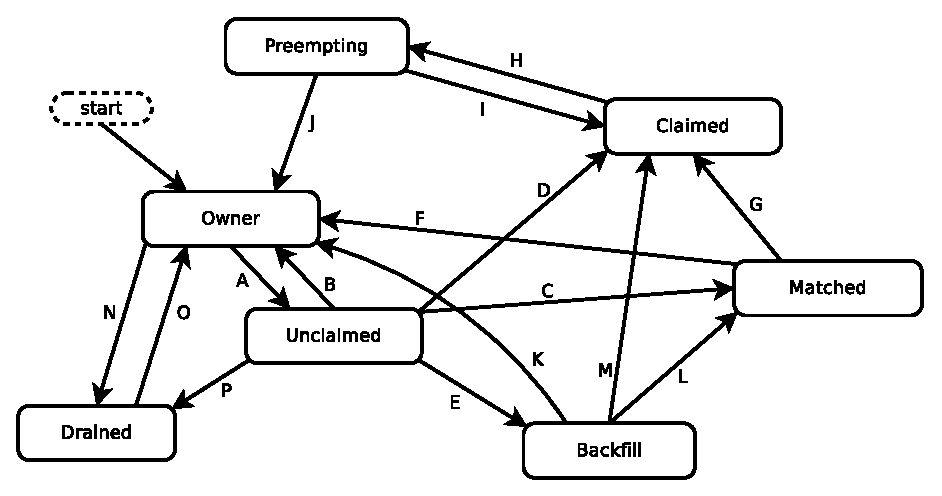
\includegraphics{admin-man/states.eps}
\caption{\label{fig:machine-states}Machine States}
\end{figure}

Each transition is labeled with a letter.
The cause of each transition is described below.


\begin{itemize}


\item Transitions out of the Owner state

\begin{description}

\item[A] The machine switches from Owner to Unclaimed whenever the
  \MacroNI{START} expression no longer locally evaluates to FALSE.
  This indicates that the machine is potentially available to run a
  Condor job.

\end{description}


\item Transitions out of the Unclaimed state

\begin{description}

\item[B] The machine switches from Unclaimed back to Owner whenever the
  \MacroNI{START} expression locally evaluates to FALSE.
  This indicates that the machine is unavailable to run a Condor job
  and is in use by the resource owner.

\item[C] The transition from Unclaimed to Matched happens whenever the
  \Condor{negotiator} matches this resource with a Condor job.

\item[D] The transition from Unclaimed directly to Claimed also happens
  if the \Condor{negotiator} matches this resource with a Condor job.
  In this case the \Condor{schedd} receives the match and initiates
  the claiming protocol with the machine before the \Condor{startd}
  receives the match notification from the \Condor{negotiator}.

\item[E] The transition from Unclaimed to Backfill happens if the
  machine is configured to run backfill computations (see
  section~\ref{sec:Backfill}) and the \MacroNI{START\_BACKFILL}
  expression evaluates to TRUE.

\end{description}


\item Transitions out of the Matched state

\begin{description}

\item[F] The machine moves from Matched to Owner if either the
  \MacroNI{START} expression locally evaluates to FALSE, or if the 
  \Macro{MATCH\_TIMEOUT} timer expires.
  This timeout is used to ensure that if a machine is matched with a
  given \Condor{schedd}, but that \Condor{schedd} does not contact the
  \Condor{startd} to claim it, that the machine will give up on the
  match and become available to be matched again.
  In this case, since the \MacroNI{START} expression does not locally
  evaluate to FALSE, as soon as transition \Bold{F} is complete, the
  machine will immediately enter the Unclaimed state again (via
  transition \Bold{A}).
  The machine might also go from Matched to Owner if the
  \Condor{schedd} attempts to perform the claiming protocol but
  encounters some sort of error.
  Finally, the machine will move into the Owner state if the
  \Condor{startd} receives a \Condor{vacate} command while it is in
  the Matched state.

\item[G] The transition from Matched to Claimed occurs when the
  \Condor{schedd} successfully completes the claiming protocol with
  the \Condor{startd}.

\end{description}

\item Transitions out of the Claimed state

\begin{description}

\item[H] From the Claimed state, the only possible destination is the
  Preempting state.
  This transition can be caused by many reasons:
  \begin{itemize}
  \item The \Condor{schedd} that has claimed the machine has no more
    work to perform and releases the claim
  \item The \MacroNI{PREEMPT} expression evaluates to TRUE (which usually
    means the resource owner has started using the machine again and
    is now using the keyboard, mouse, CPU, etc)  
  \item The \Condor{startd} receives a \Condor{vacate} command
  \item The \Condor{startd} is told to shutdown (either via a signal
    or a \Condor{off} command)
  \item The resource is matched to a job with a better priority
    (either a better user priority, or one where the machine rank is
    higher)
  \end{itemize}

\end{description}


\item Transitions out of the Preempting state

\begin{description}

\item[I] The resource will move from Preempting back to Claimed if the
  resource was matched to a job with a better priority.

\item[J] The resource will move from Preempting to Owner if the
  \MacroNI{PREEMPT} expression had evaluated to TRUE, if \Condor{vacate}
  was used, or if the \MacroNI{START} expression locally evaluates to
  FALSE when the \Condor{startd} has finished evicting whatever job it
  was running when it entered the Preempting state.

\end{description}


\item Transitions out of the Backfill state

\begin{description}

\item[K] The resource will move from Backfill to Owner for the
  following reasons:
  \begin{itemize}
  \item The \MacroNI{EVICT\_BACKFILL} expression evaluates to TRUE
  \item The \Condor{startd} receives a \Condor{vacate} command
  \item The \Condor{startd} is being shutdown
  \end{itemize}
 
\item[L] The transition from Backfill to Matched occurs whenever a
  resource running a backfill computation is matched with a
  \Condor{schedd} that wants to run a Condor job.

\item[M] The transition from Backfill directly to Claimed is similar
  to the transition from Unclaimed directly to Claimed.
  It only occurs if the \Condor{schedd} completes the claiming
  protocol before the \Condor{startd} receives the match notification
  from the \Condor{negotiator}.

\end{description}


\end{itemize}

%%%%%%%%%%%%%%%%%%%%%%%%%%%%%%%%%%%%%%%%%%%%%%%%%%%%%%%%%%%%%%%%%%%%%%
\subsubsection{\label{sec:ClaimedState} The Claimed State and Leases}
%%%%%%%%%%%%%%%%%%%%%%%%%%%%%%%%%%%%%%%%%%%%%%%%%%%%%%%%%%%%%%%%%%%%%%
\index{machine state!claimed, the claim lease}
\index{claim lease}

When a \Condor{schedd} claims a \Condor{startd}, there is a claim lease.
So long as the keep alive updates from the \Condor{schedd} to the
\Condor{startd} continue to arrive, the lease is reset.
If the lease duration passes with no updates,
the \Condor{startd} drops the claim and evicts any jobs the
\Condor{schedd} sent over.

The alive interval is the amount of time between,
or the frequency at which the \Condor{schedd} sends keep alive updates 
to all \Condor{schedd} daemons.
An alive update resets the claim lease at the \Condor{startd}.
Updates are UDP packets.

Initially, as when the \Condor{schedd} starts up,
the alive interval starts at the value set by the 
configuration variable \Macro{ALIVE\_INTERVAL}.  
It may be modified when a job is started.
The job's ClassAd attribute \Attr{JobLeaseDuration} is checked.
If the value of \Expr{JobLeaseDuration/3} is less than the current
alive interval,
then the alive interval is set to either this lower value
or the imposed lowest limit on the alive interval of 10 seconds.
Thus, the alive interval starts at \MacroNI{ALIVE\_INTERVAL} and goes down,
never up.

If a claim lease expires,
the \Condor{startd} will drop the claim.
The length of the claim lease is 
the job's ClassAd attribute \Attr{JobLeaseDuration}.
\Attr{JobLeaseDuration} defaults to 20 minutes time,
except when explicitly
set within the job's submit description file.
If \Attr{JobLeaseDuration} is explicitly set to 0, 
or it is not set as may be the case for a Web Services job
that does not define the attribute, 
then \Attr{JobLeaseDuration} is given the Undefined value.
Further, when undefined,
the claim lease duration is calculated with
\Expr{MAX\_CLAIM\_ALIVES\_MISSED * alive interval}.
The alive interval is the \emph{current} value,
as sent by the \Condor{schedd}.
If the \Condor{schedd} reduces the current alive interval,
it does not update the \Condor{startd}.

%%%%%%%%%%%%%%%%%%%%%%%%%%%%%%%%%%%%%%%%%%%%%%%%%%%%%%%%%%%%%%%%%%%%%%
\subsection{\label{sec:Activities}
Machine Activities}
%%%%%%%%%%%%%%%%%%%%%%%%%%%%%%%%%%%%%%%%%%%%%%%%%%%%%%%%%%%%%%%%%%%%%%

\index{machine activity}
\index{activity!of a machine}
Within some machine states,
\Term{activities} of the machine are defined.
The state has meaning regardless of activity.
Differences between activities are significant.
Therefore, a ``state/activity'' pair describes
a machine.
The following list describes all the possible state/activity pairs.

\begin{itemize}

\item Owner
\begin{description}
\index{machine activity!Idle}
\item[Idle] This is the only activity for Owner state.  As far as
  Condor is concerned the machine is Idle, since it is not doing
  anything for Condor.
\end{description}

\index{machine activity!Unclaimed}
\item Unclaimed
\begin{description}
  \item[Idle] This is the normal activity of Unclaimed machines.
    The machine is still Idle in that the machine owner is willing to
    let Condor jobs run, but Condor is not using the
    machine for anything.
  
  \index{machine activity!Benchmarking}
  \item[Benchmarking] The machine is running benchmarks to
    determine the speed on this machine.
    This activity only occurs in the Unclaimed state.
    How often the activity occurs is
    determined by the \MacroNI{RUNBENCHMARKS} expression.
\end{description}

\item Matched
\begin{description}
  \item[Idle] When Matched, the machine is still Idle to Condor.
\end{description}

\item Claimed
\begin{description}
\item[Idle] In this activity, the machine has been claimed, but the
  schedd that claimed it has yet to \Term{activate} the claim by
  requesting a \Condor{starter} to be spawned to service a job.
  The machine returns to this state (usually briefly) when jobs
  (and therefore \Condor{starter}) finish.
  
\index{machine activity!Busy}
\item[Busy] Once a \Condor{starter} has been started and the claim is
  active, the machine moves to the Busy activity to signify that it is
  doing something as far as Condor is concerned.
  
\index{machine activity!Suspended}
\item[Suspended] If the job is suspended by Condor, the machine goes
  into the Suspended activity.
  The match between the schedd and machine has not been broken (the
  claim is still valid), but the job is not making any progress and
  Condor is no longer generating a load on the machine.

\index{machine activity!Retiring}
\item[Retiring] When an active claim is about to be preempted for any
reason, it enters retirement, while it waits for the current job to
finish.  The \MacroNI{MaxJobRetirementTime} expression determines how
long to wait (counting since the time the job started).  Once the job
finishes or the retirement time expires, the Preempting state is
entered.
\end{description}

\item Preempting
  The preempting state is used for evicting a Condor job from a given
  machine.
  When the machine enters the Preempting state, it checks the
  \MacroNI{WANT\_VACATE} expression to determine its activity.

\begin{description}
\index{machine activity!Vacating}
\item[Vacating] In the Vacating activity, the job that was running is
  in the process of checkpointing.
  As soon as the checkpoint process completes,
  the machine moves into either the Owner state or the
  Claimed state, depending on the reason for its preemption.
  
\index{machine activity!Killing}
\item[Killing] Killing means that the machine has requested the running
  job to exit the machine immediately, without checkpointing.
\end{description}

\index{machine activity!Backfill}
\item Backfill
\begin{description}
\item[Idle] The machine is configured to run backfill jobs and is
  ready to do so, but it has not yet had a chance to spawn a backfill
  manager (for example, the BOINC client).

\item[Busy] The machine is performing a backfill computation.

\item[Killing] The machine was running a backfill computation, but it
  is now killing the job to either return resources to the machine
  owner, or to make room for a regular Condor job.

\end{description}

\index{machine activity!Drained}
\item Drained
\begin{description}

\item[Idle] All slots have been drained.

\item[Retiring] This slot has been drained.  It is waiting for other
  slots to finish draining.

\end{description}

\end{itemize}

Figure~\ref{fig:machine-activities} on
page~\pageref{fig:machine-activities} gives the overall view of all
machine states and activities and shows the possible transitions
from one to another within the Condor system.  
Each transition is labeled with a number on the diagram, and
transition numbers referred to in this manual will be \Bold{bold}.  

\index{machine state and activities figure}
\index{state and activities figure}
\index{activities and state figure}
\begin{figure}[hbt]
\centering
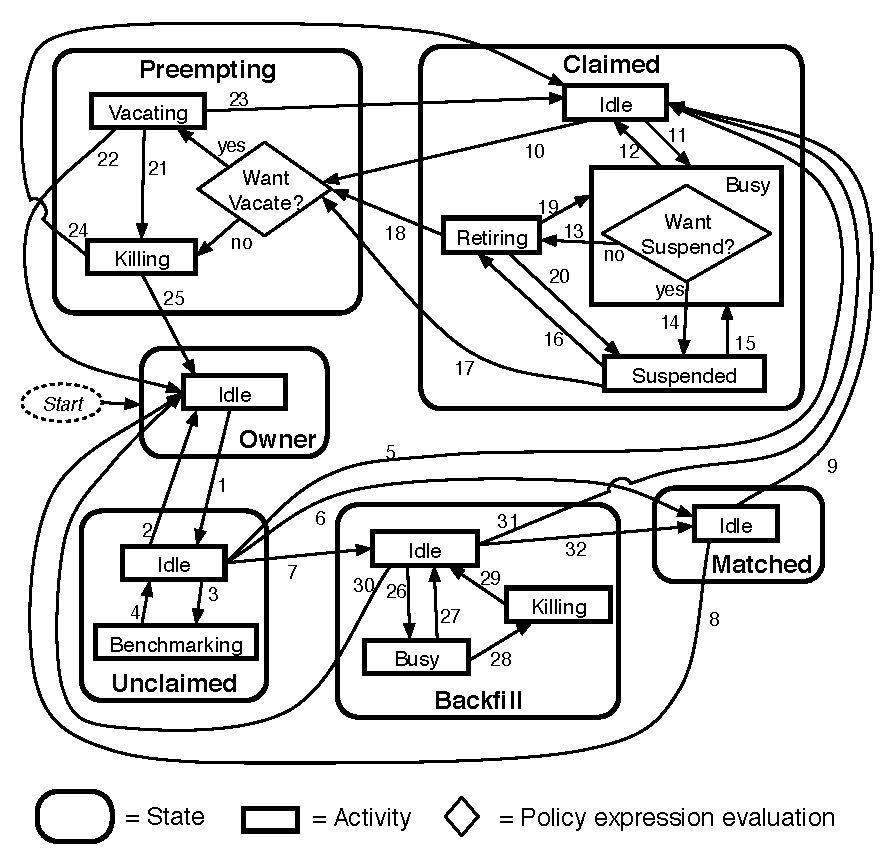
\includegraphics{admin-man/machine-activities.eps}
\caption{\label{fig:machine-activities}Machine States and Activities}
\end{figure}

Various expressions are used to determine when and if many of these
state and activity transitions occur.  Other transitions are initiated
by parts of the Condor protocol (such as when the \Condor{negotiator}
matches a machine with a schedd).  The following section describes the
conditions that lead to the various state and activity transitions.

%%%%%%%%%%%%%%%%%%%%%%%%%%%%%%%%%%%%%%%%%%%%%%%%%%%%%%%%%%%%%%%%%%%%%%
\subsection{\label{sec:State-and-Activity-Transitions}
State and Activity Transitions}
%%%%%%%%%%%%%%%%%%%%%%%%%%%%%%%%%%%%%%%%%%%%%%%%%%%%%%%%%%%%%%%%%%%%%%

\index{machine state!transitions|(}
\index{machine activity!transitions|(}
\index{state!transitions|(}
\index{activity!transitions|(}
This section traces through all possible state and activity
transitions within a machine and describes the conditions under which
each one occurs.
Whenever a transition occurs, Condor records when the machine entered its
new activity and/or new state.
These times are often used to write expressions that determine
when further transitions occurred.
For example, enter the Killing activity if a machine has been in
the Vacating activity longer than a specified amount of time. 

%%%%%%%%%%%%%%%%%%%%%%%%%%%%%%%%%%%%%%%%%%%%%%%%%%%%%%%%%%%%%%%%%%%%%%
\subsubsection{\label{sec:Owner-State}
Owner State}
%%%%%%%%%%%%%%%%%%%%%%%%%%%%%%%%%%%%%%%%%%%%%%%%%%%%%%%%%%%%%%%%%%%%%%

\index{machine state!Owner}
\index{owner state}
When the startd is first spawned, the machine it represents enters the
Owner state. 
The machine remains in the Owner state while the
expression \Macro{IS\_OWNER} is TRUE.
If the \MacroNI{IS\_OWNER} expression is FALSE,
then the machine transitions to the Unclaimed state.
The default value for the 
\MacroNI{IS\_OWNER} expression is optimized for a shared resource
\begin{verbatim}
START =?= FALSE
\end{verbatim}
So,
the machine will remain in the Owner state as long as the \MacroNI{START}
expression locally evaluates to FALSE.
Section~\ref{sec:Start-Expr} provides more detail on the
\MacroNI{START} expression.
If the \MacroNI{START} locally evaluates to TRUE or cannot be locally
evaluated (it evaluates to UNDEFINED), transition \Bold{1}
occurs and the machine enters the Unclaimed state.
The \MacroNI{IS\_OWNER} expression is locally evaluated by the machine,
and should not reference job ClassAd attributes, which would be
UNDEFINED.

For dedicated resources, the recommended value for the \MacroNI{IS\_OWNER}
expression is FALSE.

The Owner state represents a resource that is in use by its
interactive owner (for example, if the keyboard is being used).
The Unclaimed state represents a resource that is neither in use by
its interactive user, nor the Condor system.
From Condor's point of view, there is little difference between the
Owner and Unclaimed states.
In both cases, the resource is not currently in use by the Condor
system.
However, if a job matches the resource's \MacroNI{START} expression, the
resource is available to run a job, regardless of if it is in the
Owner or Unclaimed state.
The only differences between the two states are how the resource shows
up in \Condor{status} and other reporting tools, and the fact that
Condor will not run benchmarking on a resource in the Owner state.
As long as the \MacroNI{IS\_OWNER} expression is TRUE, the machine is
in the Owner State.
When the \MacroNI{IS\_OWNER} expression is FALSE, the machine goes into
the Unclaimed State.

Here is an example that assumes that an \MacroNI{IS\_OWNER}
expression is not present in the configuration.
If the \MacroNI{START} expression is
\begin{verbatim}
START = KeyboardIdle > 15 * $(MINUTE) && Owner == "coltrane" 
\end{verbatim}
and if \Attr{KeyboardIdle} is 34 seconds,
then the machine would remain in the Owner state.
Owner is undefined, and
\verb@anything && FALSE@ is FALSE.

If, however, the \MacroNI{START} expression is
\begin{verbatim}
        START = KeyboardIdle > 15 * $(MINUTE) || Owner == "coltrane"
\end{verbatim}
and \Attr{KeyboardIdle} is 34 seconds, then the machine
leaves the Owner state and becomes Unclaimed.
This is because
\verb@FALSE || UNDEFINED@ is UNDEFINED.
So, while this machine is not available to just anybody,
if user coltrane has jobs submitted, the machine is willing to run them.
Any other user's jobs have to wait
until \Attr{KeyboardIdle} exceeds 15 minutes.
However, since coltrane might claim this resource,
but has not yet, the machine goes to the Unclaimed state.

While in the Owner state, the startd polls the status of the
machine every \Macro{UPDATE\_INTERVAL} to see if anything has changed
that would lead it to a different state.
This minimizes the impact on the Owner
while the Owner is using the machine.
Frequently waking up, computing load averages, checking the access
times on files, computing free swap space take time,
and there is nothing
time critical that the startd needs to be sure to notice as soon as it
happens.
If the \MacroNI{START} expression evaluates to TRUE and five
minutes pass before the startd notices,
that's a drop in the bucket of high-throughput computing.

The machine can only transition to the Unclaimed state from the Owner
state. It does so when the \MacroNI{IS\_OWNER} expression no longer
evaluates to FALSE.  By default, that happens when \MacroNI{START} no longer
locally evaluates to FALSE.

Whenever the machine is not actively running a job, it will transition
back to the Owner state if \MacroNI{IS\_OWNER} evaluates to TRUE.  Once a
job is started, the value of \MacroNI{IS\_OWNER} does not matter; the job
either runs to completion or is preempted.  Therefore, you must
configure the preemption policy if you want to transition back to the
Owner state from Claimed Busy.

%%%%%%%%%%%%%%%%%%%%%%%%%%%%%%%%%%%%%%%%%%%%%%%%%%%%%%%%%%%%%%%%%%%%%%
\subsubsection{\label{sec:Unclaimed-State}Unclaimed State}
%%%%%%%%%%%%%%%%%%%%%%%%%%%%%%%%%%%%%%%%%%%%%%%%%%%%%%%%%%%%%%%%%%%%%%
\index{machine state!Unclaimed}
\index{unclaimed state}

If the \MacroNI{IS\_OWNER} expression becomes TRUE, then the machine returns
to the Owner state.
If the \MacroNI{IS\_OWNER} expression becomes FALSE, then the machine remains
in the Unclaimed state.
If the \MacroNI{IS\_OWNER} expression is not present in the configuration files,
then the default value for the \MacroNI{IS\_OWNER} expression is 
\begin{verbatim}
START =?= FALSE
\end{verbatim}
so that
while in the Unclaimed state, if the \MacroNI{START} expression locally
evaluates to FALSE, the machine returns to the Owner state by
transition \Bold{2}.

When in the Unclaimed state,
the \Macro{RUNBENCHMARKS}
expression is relevant.
If \MacroNI{RUNBENCHMARKS} evaluates to TRUE while the machine
is in the Unclaimed state,
then the machine will transition from the Idle
activity to the Benchmarking activity (transition \Bold{3}) and
perform benchmarks to determine \Attr{MIPS} and \Attr{KFLOPS}.  
When the benchmarks complete, the machine returns to the Idle activity
(transition \Bold{4}).

The startd automatically inserts an attribute, \Attr{LastBenchmark},
whenever it runs benchmarks, so commonly \Attr{RunBenchmarks} is
defined in terms of this attribute, for example:
\begin{verbatim}
        BenchmarkTimer = (CurrentTime - LastBenchmark)
        RunBenchmarks = $(BenchmarkTimer) >= (4 * $(HOUR))
\end{verbatim}
Here, a macro, \MacroNI{BenchmarkTimer} is defined to help write the
expression.
This macro holds the time since the last benchmark,
so when this time exceeds 4 hours, we run the benchmarks again.
The startd keeps a weighted average of these benchmarking
results to try to get the most accurate numbers possible.
This is why
it is desirable for 
the startd to run them more than once in its lifetime.

\Note \Attr{LastBenchmark} is initialized to 0 before benchmarks
have ever been run.
To have the \Condor{startd} run benchmarks as soon as the machine is
Unclaimed (if it has not done so already),
include a term using \Attr{LastBenchmark} as in the example above.

\Note If \MacroNI{RUNBENCHMARKS} is defined and set to something
other than FALSE, the startd will automatically run one set of
benchmarks when it first starts up.
To disable benchmarks, both at startup and at any time thereafter,
set \MacroNI{RUNBENCHMARKS} to FALSE or comment it out of the
configuration file.

From the Unclaimed state, the machine can go to four other possible
states: Owner (transition \Bold{2}), Backfill/Idle, Matched, or
Claimed/Idle.

Once the \Condor{negotiator} matches an Unclaimed machine with a
requester at a given schedd, the negotiator sends a command to both
parties, notifying them of the match.  
If the schedd receives that notification and initiates the claiming
procedure with the machine before the negotiator's message gets to the
machine, the Match state is skipped,
and the machine goes
directly to the Claimed/Idle state (transition \Bold{5}).
However, normally the machine will enter the Matched state (transition
\Bold{6}), even if it is only for a brief period of time.

If the machine has been configured to perform backfill jobs (see
section~\ref{sec:Backfill}), while it is in Unclaimed/Idle it will
evaluate the \Macro{START\_BACKFILL} expression.
Once \MacroNI{START\_BACKFILL} evaluates to TRUE, the machine will enter
the Backfill/Idle state (transition \Bold{7}) to begin the process of
running backfill jobs.


%%%%%%%%%%%%%%%%%%%%%%%%%%%%%%%%%%%%%%%%%%%%%%%%%%%%%%%%%%%%%%%%%%%%%%
\subsubsection{\label{sec:Matched-State}Matched State}
%%%%%%%%%%%%%%%%%%%%%%%%%%%%%%%%%%%%%%%%%%%%%%%%%%%%%%%%%%%%%%%%%%%%%%
\index{machine state!Matched}
\index{matched state}

The Matched state is not very interesting to Condor.
Noteworthy in this state is that the machine lies about its \MacroNI{START}
expression while in this state and says that \Expr{Requirements} are
\Expr{False} to prevent being matched again before it has been claimed.
Also interesting is that
the startd starts a timer to make sure it does not stay in the
Matched state too long.
The timer is set with the \Macro{MATCH\_TIMEOUT}
\label{param:MatchTimeout} configuration file macro.
It is specified in seconds and defaults to 120 (2 minutes).
If the schedd that was matched with this machine does not
claim it within this period of time, the machine gives up,
and goes back into the Owner state via transition \Bold{8}.
It will probably leave the Owner state right away for the
Unclaimed state again and wait for another match. 

At any time while the machine is in the Matched state, if the
\MacroNI{START} expression locally evaluates to FALSE, the machine enters
the Owner state directly (transition \Bold{8}).

If the schedd that was matched with the machine claims it before the
\MacroNI{MATCH\_TIMEOUT} expires, the machine goes into the Claimed/Idle
state (transition \Bold{9}).

%%%%%%%%%%%%%%%%%%%%%%%%%%%%%%%%%%%%%%%%%%%%%%%%%%%%%%%%%%%%%%%%%%%%%%
\subsubsection{\label{sec:Claimed-State}Claimed State}
%%%%%%%%%%%%%%%%%%%%%%%%%%%%%%%%%%%%%%%%%%%%%%%%%%%%%%%%%%%%%%%%%%%%%%
\index{machine state!Claimed}
\index{claimed state}

The Claimed state is certainly the most complex state.
It has the most possible activities and the most expressions that
determine its next activities.
In addition, the \Condor{checkpoint} and \Condor{vacate} commands affect
the machine when it is in the Claimed state.
In general, there are two sets of expressions that might take effect.
They depend on the universe of the request: standard or vanilla.
The standard universe expressions are the normal expressions.
For example:
\begin{verbatim}
        WANT_SUSPEND            = True
        WANT_VACATE             = $(ActivationTimer) > 10 * $(MINUTE)
        SUSPEND                 = $(KeyboardBusy) || $(CPUBusy)
        ...
\end{verbatim}

The vanilla expressions have the string``\_VANILLA'' appended to their names.
For example:
\begin{verbatim}
        WANT_SUSPEND_VANILLA    = True
        WANT_VACATE_VANILLA     = True
        SUSPEND_VANILLA         = $(KeyboardBusy) || $(CPUBusy)
        ...
\end{verbatim}

Without specific vanilla versions, the normal versions
will be used for all jobs, including vanilla jobs.  
In this manual, the normal expressions are referenced.
The difference exists for the
the resource owner that might want the machine
to behave differently for vanilla jobs, since they cannot checkpoint.
For example, owners may want vanilla jobs to remain suspended for
longer than standard jobs.

While Claimed, the \Macro{POLLING\_INTERVAL} takes effect, and the
startd polls the machine much more frequently to evaluate its
state.

If the machine owner starts typing on the console again,
it is best to notice this as
soon as possible to be able to start doing whatever 
the machine owner wants at that point.
For SMP machines, if any slot is in the Claimed state, the
startd polls the machine frequently.
If already polling one slot, it does not
cost much to evaluate the state of all the slots at
the same time.

There are a variety of events that may cause the startd to try to get
rid of or temporarily suspend a running job.  Activity on the
machine's console, load from other jobs, or shutdown of the startd via
an administrative command are all possible sources of interference.
Another one is the appearance of a higher priority claim to the
machine by a different Condor user.

Depending on the configuration, the startd may respond quite
differently to activity on the machine, such as keyboard activity or
demand for the cpu from processes that are not managed by Condor.  The
startd can be configured to completely ignore such activity or to
suspend the job or even to kill it.  A standard configuration for a desktop
machine might be to go through
successive levels of getting the job out of the way.
The first and least costly to the job is suspending it.
This works for both standard and vanilla jobs.
If suspending the job for a short while does not satisfy the machine
owner (the owner is still using the machine after a specific period of
time), the startd moves on to vacating the job.
Vacating a standard universe job
involves performing a checkpoint so that the work already completed
is not lost.  Vanilla jobs are sent a \Term{soft kill signal} so that they
can gracefully shut down if necessary; the default is \verb@SIGTERM@.
If vacating does not satisfy the machine owner (usually because it is
taking too long and the owner wants their machine back \emph{now}),
the final, most drastic stage is reached: killing.  
Killing is a quick death to the job, using a hard-kill signal that cannot
be intercepted by the application.  For vanilla jobs that do no special
signal handling, vacating and killing are equivalent.

The \MacroNI{WANT\_SUSPEND} expression determines if the machine will
evaluate the \MacroNI{SUSPEND} expression to consider entering the
Suspended activity.
The \MacroNI{WANT\_VACATE} expression determines what happens when the
machine enters the Preempting state.
It will go to the Vacating
activity or directly to Killing. 
If one or both of these expressions evaluates to FALSE, the machine
will skip that stage of getting rid of the job and proceed directly to
the more drastic stages.

When the machine first enters the Claimed state, it goes to the Idle
activity.  From there, it has two options.  
It can enter the Preempting state via transition \Bold{10} (if a 
\Condor{vacate} arrives, or if the \MacroNI{START} expression locally
evaluates to FALSE),  
or it can enter the Busy activity (transition \Bold{11}) if the
schedd that has claimed the machine decides to activate the claim and
start a job.

From Claimed/Busy, the machine can transition to three other state/activity
pairs.
The startd evaluates the \MacroNI{WANT\_SUSPEND} expression to decide
which other expressions to evaluate.  
If \MacroNI{WANT\_SUSPEND} is TRUE, then the startd evaluates the
\MacroNI{SUSPEND} expression.
If \MacroNI{WANT\_SUSPEND} is any value other than TRUE, then the startd will
evaluate the \MacroNI{PREEMPT} expression and skip the Suspended activity
entirely.
By transition, the possible state/activity destinations from Claimed/Busy:

\begin{description}
  
\item[Claimed/Idle] If the starter that is serving a given job exits
  (for example because the jobs completes), the machine will go
  to Claimed/Idle (transition \Bold{12}).
  
\item[Claimed/Retiring] If \MacroNI{WANT\_SUSPEND} is FALSE and the
  \MacroNI{PREEMPT} expression is TRUE, the machine enters the
  Retiring activity (transition \Bold{13}).  From there, it
  waits for a configurable amount of time for the job to finish
  before moving on to preemption.

  Another reason the machine would go from Claimed/Busy to
  Claimed/Retiring is if the \Condor{negotiator} matched the machine
  with a ``better'' match.  This better match could either be from the
  machine's perspective using the startd \MacroNI{RANK} expression,
  or it could be from the negotiator's perspective due to
  a job with a higher user priority.

  Another case resulting in a transition to Claimed/Retiring is when
  the startd is being shut down.  The only exception is a ``fast''
  shutdown, which bypasses retirement completely.
  
\item[Claimed/Suspended] If both the \MacroNI{WANT\_SUSPEND} and
  \MacroNI{SUSPEND} expressions evaluate to TRUE, the machine
  suspends the job (transition \Bold{14}).
  
\end{description}
  
If a \Condor{checkpoint} command arrives,
or the \MacroNI{PERIODIC\_CHECKPOINT} expression evaluates to TRUE,
there is no state change.
The startd has no way of knowing when this process completes,
so periodic checkpointing can not be another state.
Periodic checkpointing remains in the Claimed/Busy state
and appears as a running job.

From the Claimed/Suspended state, the following transitions
may occur:

\begin{description}
  
\item[Claimed/Busy] If the \MacroNI{CONTINUE} expression evaluates to
  TRUE, the machine resumes the job and enters the
  Claimed/Busy state (transition \Bold{15}) or the Claimed/Retiring
  state (transition \Bold{16}), depending on whether the claim
  has been preempted.

\item[Claimed/Retiring] If the \MacroNI{PREEMPT} expression is TRUE, the machine
  will enter the Claimed/Retiring activity (transition \Bold{16}).

\item[Preempting] If the claim is in suspended retirement and the
  retirement time expires, the job enters the Preempting state
  (transition \Bold{17}).  This is only possible if
  \MacroNI{MaxJobRetirementTime} \emph{decreases} during the suspension.


\end{description}

For the Claimed/Retiring state, the following transitions may occur:

\begin{description}

\item[Preempting] If the job finishes or the job's run time exceeds
the value defined for the job ClassAd attribute \Attr{MaxJobRetirementTime},
the Preempting state is entered
(transition \Bold{18}).  The run time is computed from the time when the
job was started by the startd minus any suspension time.  When retiring
due to \Condor{startd} daemon shutdown or restart,
it is possible for the administrator to issue a
\Term{peaceful} shutdown command, which causes \MacroNI{MaxJobRetirementTime}
to effectively be infinite, avoiding any killing of jobs.  It is also
possible for the administrator to issue a \Term{fast} shutdown command,
which causes
\MacroNI{MaxJobRetirementTime} to be effectively 0.

\item[Claimed/Busy] If the startd was retiring because of a preempting
claim only and the preempting claim goes away, the normal Claimed/Busy
state is resumed (transition \Bold{19}).  If instead the retirement
is due to owner activity (\MacroNI{PREEMPT}) or the startd is being shut down,
no unretirement is possible.

\item[Claimed/Suspended] In exactly the same way that suspension may
happen from the Claimed/Busy state, it may also happen during the
Claimed/Retiring state (transition \Bold{20}).
In this case, when the job continues from suspension, it moves back
into Claimed/Retiring (transition \Bold{16}) instead of Claimed/Busy
(transition \Bold{15}).

\end{description}


%%%%%%%%%%%%%%%%%%%%%%%%%%%%%%%%%%%%%%%%%%%%%%%%%%%%%%%%%%%%%%%%%%%%%%
\subsubsection{\label{sec:Preempting-State}Preempting State}
%%%%%%%%%%%%%%%%%%%%%%%%%%%%%%%%%%%%%%%%%%%%%%%%%%%%%%%%%%%%%%%%%%%%%%
\index{machine state!Preempting}
\index{preempting state}

The Preempting state is less complex than the Claimed state.
There are two activities.
Depending on the value of \MacroNI{WANT\_VACATE}, a machine will
be in the
Vacating activity (if TRUE) or the Killing activity (if FALSE).  

While in the Preempting state (regardless of activity) the machine
advertises its \Expr{Requirements} expression as FALSE to signify that
it is not available for further matches, either because it is about to
transition
to the Owner state, or because it has already been matched with
one preempting match, and further preempting matches are disallowed
until the machine has been claimed by the new match.

The main function of the Preempting state is to get rid of the starter
associated with the resource.  If the \Condor{starter} associated with
a given claim exits while the machine is still in the Vacating
activity, then the job successfully completed a graceful shutdown.
For standard universe jobs, this means that a checkpoint was saved.
For other jobs, this means the application was given an opportunity to
do a graceful shutdown, by intercepting the soft kill signal.

If the machine is in the Vacating activity, it keeps evaluating the 
\MacroNI{KILL} expression.
As soon as this expression evaluates to TRUE,
the machine enters the Killing activity (transition \Bold{21}).
If the Vacating activity lasts for as long as the maximum
vacating time, then the machine also enters the Killing activity.
The maximum vacating time is determined by the configuration variable
\Macro{MachineMaxVacateTime}.
This may be adjusted by the setting of the job ClassAd
attribute \Attr{JobMaxVacateTime}.

When the starter exits, or if there was no starter running when the
machine enters the Preempting state (transition \Bold{10}),
the other purpose of the Preempting state is completed:
notifying the schedd that had claimed this machine that the claim is
broken.

At this point, the machine enters either the Owner state by
transition \Bold{22} (if the job was preempted because the machine
owner came back) or the Claimed/Idle state by transition \Bold{23}
(if the job was preempted because a better match was found).

If the machine enters the Killing activity, (because either
\MacroNI{WANT\_VACATE} was FALSE or the \MacroNI{KILL} expression evaluated
to TRUE), it attempts to force the \Condor{starter} to immediately
kill the underlying Condor job.
Once the machine has begun to hard kill the Condor job, the
\Condor{startd} starts a timer, the length of which is defined by the
\Macro{KILLING\_TIMEOUT} \label{param:KillingTimeout} macro.
This macro is defined in seconds and defaults to 30.
If this timer expires and the machine is still in
the Killing activity, something has gone seriously wrong with the
\Condor{starter} and the startd tries to vacate the job immediately by
sending SIGKILL to all of the \Condor{starter}'s children, and then to
the \Condor{starter} itself.

Once the \Condor{starter} has killed off all the processes associated
with the job and exited, and once the schedd that had claimed the
machine is notified that the claim is broken, the machine will leave
the Preempting/Killing state.
If the job was preempted because a better match was found, the machine
will enter Claimed/Idle (transition \Bold{24}).
If the preemption was caused by the machine owner (the \MacroNI{PREEMPT}
expression evaluated to TRUE, \Condor{vacate} was used, etc), the
machine will enter the Owner state (transition \Bold{25}).


%%%%%%%%%%%%%%%%%%%%%%%%%%%%%%%%%%%%%%%%%%%%%%%%%%%%%%%%%%%%%%%%%%%%%%
\subsubsection{\label{sec:Backfill-State}Backfill State}
%%%%%%%%%%%%%%%%%%%%%%%%%%%%%%%%%%%%%%%%%%%%%%%%%%%%%%%%%%%%%%%%%%%%%%
\index{machine state!Backfill}
\index{backfill state}

The Backfill state is used whenever the machine is performing low
priority background tasks to keep itself busy.
For more information about backfill support in Condor, see
section~\ref{sec:Backfill} on page~\pageref{sec:Backfill}.
This state is only used if the machine has been configured to enable
backfill computation, if a specific backfill manager has been
installed and configured, and if the machine is otherwise idle (not
being used interactively or for regular Condor computations).
If the machine meets all these requirements, and the
\MacroNI{START\_BACKFILL} expression evaluates to TRUE, the machine will
move from the Unclaimed/Idle state to Backfill/Idle (transition
\Bold{7}).

Once a machine is in Backfill/Idle, it will immediately attempt to
spawn whatever backfill manager it has been configured to use
(currently, only the BOINC client is supported as a backfill manager
in Condor).
Once the BOINC client is running, the machine will enter
Backfill/Busy (transition \Bold{26}) to indicate that it is now
performing a backfill computation.

\Note On SMP machines, the \Condor{startd} will only spawn a single
instance of the BOINC client, even if multiple slots are
available to run backfill jobs.
Therefore, only the first machine to enter Backfill/Idle will cause a
copy of the BOINC client to start running.
If a given slot on an SMP enters the Backfill state and a
BOINC client is already running under this \Condor{startd}, the
slot will immediately enter Backfill/Busy without waiting
to spawn another copy of the BOINC client.

If the BOINC client ever exits on its own (which normally wouldn't
happen), the machine will go back to Backfill/Idle (transition
\Bold{27}) where it will immediately attempt to respawn the BOINC
client (and return to Backfill/Busy via transition \Bold{26}).

As the BOINC client is running a backfill computation, a number of
events can occur that will drive the machine out of the Backfill
state.
The machine can get matched or claimed for a Condor job, interactive
users can start using the machine again, the machine might be evicted
with \Condor{vacate}, or the \Condor{startd} might be shutdown.
All of these events cause the \Condor{startd} to kill the BOINC client
and all its descendants, and enter the Backfill/Killing state
(transition \Bold{28}).

Once the BOINC client and all its children have exited the system, the
machine will enter the Backfill/Idle state to indicate that the BOINC
client is now gone (transition \Bold{29}).
As soon as it enters Backfill/Idle after the BOINC client exits, the
machine will go into another state, depending on what caused the BOINC
client to be killed in the first place.

If the \MacroNI{EVICT\_BACKFILL} expression evaluates to TRUE while a
machine is in Backfill/Busy, after the BOINC client is gone, the
machine will go back into the Owner/Idle state (transition
\Bold{30}).
The machine will also return to the Owner/Idle state after the BOINC
client exits if \Condor{vacate} was used, or if the \Condor{startd} is
being shutdown.

When a machine running backfill jobs is matched with a requester that
wants to run a Condor job, the machine will either enter the Matched
state, or go directly into Claimed/Idle.
As with the case of a machine in Unclaimed/Idle (described above), the
\Condor{negotiator} informs both the \Condor{startd} and the
\Condor{schedd} of the match, and the exact state transitions at the
machine depend on what order the various entities initiate
communication with each other.
If the \Condor{schedd} is notified of the match and sends a request to
claim the \Condor{startd} before the \Condor{negotiator} has a chance
to notify the \Condor{startd}, once the BOINC client exits, the
machine will immediately enter Claimed/Idle (transition \Bold{31}).
Normally, the notification from the \Condor{negotiator} will reach the
\Condor{startd} before the \Condor{schedd} attempts to claim it.
In this case, once the BOINC client exits, the machine will enter
Matched/Idle (transition \Bold{32}).


%%%%%%%%%%%%%%%%%%%%%%%%%%%%%%%%%%%%%%%%%%%%%%%%%%%%%%%%%%%%%%%%%%%%%%
\subsection{\label{sec:State-Expression-Summary}
State/Activity Transition Expression Summary}
%%%%%%%%%%%%%%%%%%%%%%%%%%%%%%%%%%%%%%%%%%%%%%%%%%%%%%%%%%%%%%%%%%%%%%
\index{machine state!transitions summary}
\index{machine activity!transitions summary}
\index{state!transitions summary}
\index{activity!transitions summary}
This section is a summary of the information from the
previous sections.
It serves as a quick reference.

\begin{description}
  
\item[\Macro{START}] When TRUE, the machine is willing to spawn
  a remote Condor job.
  
\item[\Macro{RUNBENCHMARKS}] While in the Unclaimed state, the machine
  will run benchmarks whenever TRUE.
  
\item[\Macro{MATCH\_TIMEOUT}] If the machine has been in the Matched
  state longer than this value, it will transition to the Owner state.
  
\item[\Macro{WANT\_SUSPEND}] If TRUE, the machine evaluates
  the \MacroNI{SUSPEND} expression to see if it should transition to the
  Suspended activity.  
  If any value other than TRUE, the machine will look at
  the \MacroNI{PREEMPT} expression.
  
\item[\Macro{SUSPEND}] If \MacroNI{WANT\_SUSPEND} is TRUE, and the machine
  is in the Claimed/Busy state, it enters the Suspended activity
  if \MacroNI{SUSPEND} is TRUE.
  
\item[\Macro{CONTINUE}] If the machine is in the Claimed/Suspended
  state, it enter the Busy activity if \MacroNI{CONTINUE} is TRUE.
  
\item[\Macro{PREEMPT}] If the machine is either in the Claimed/Suspended
  activity, or is in the Claimed/Busy activity and
  \MacroNI{WANT\_SUSPEND} is FALSE, the machine enters the Claimed/Retiring
  state whenever \MacroNI{PREEMPT} is TRUE. 

\item[\Macro{CLAIM\_WORKLIFE}] If provided, this expression specifies
the number of seconds during which a claim will continue accepting new
jobs.  Once this time expires, any existing job may continue to run as
usual, but once it finishes or is preempted, the claim is closed.
This may be useful if you want to force periodic renegotiation of
resources without preemption having to occur.  For example, if you
have some low-priority jobs which should never be interrupted with
kill signals, you could prevent them from being killed with
\Attr{MaxJobRetirementTime}, but now high-priority jobs may have to
wait in line when they match to a machine that is busy running one of
these uninterruptible jobs.  You can prevent the high-priority jobs
from ever matching to such a machine by using a rank expression in the
job or in the negotiator's rank expressions, but then the low-priority
claim will never be interrupted; it can keep running more jobs.  The
solution is to use \MacroNI{CLAIM\_WORKLIFE} to force the claim to stop
running additional jobs after a certain amount of time.
The default value for \MacroNI{CLAIM\_WORKLIFE} is -1, which is treated
as an infinite claim worklife, so claims may be held indefinitely (as
long as they are not preempted and the schedd does not relinquish
them, of course).

\item[\Macro{MachineMaxVacateTime}] When the machine enters the
Preempting/Vacating state, this expression specifies the maximum
time in seconds that the \Condor{startd} will wait for the job to
finish.  The job may adjust the wait time by setting
\AdAttr{JobMaxVacateTime}.  If the job's setting is less than the
machine's, the job's is used.  If the job's setting is larger than
the machine's, the result depends on whether the job has any excess
retirement time.  If the job has more retirement time left than the
machine's maximum vacate time setting, then retirement time will be
converted into vacating time, up to the amount of
\Attr{JobMaxVacateTime}.  Once the vacating time expires, the
job is hard-killed.  The \Macro{KILL} expression may be used
to abort the graceful shutdown of the job at any time.

\item[\Macro{MAXJOBRETIREMENTTIME}] If the machine is in the
Claimed/Retiring state, this expression specifies the maximum time (in
seconds) that the \Condor{startd} will wait for the job to finish.
The clock starts when the
job is started and is paused during any suspension.  The job may
provide its own expression for \Attr{MaxJobRetirementTime}, but this
can only be used to take \emph{less} than the time granted by the
\Condor{startd}, never more.  For convenience, standard universe and
nice\_user jobs are submitted with a default retirement time of 0, so
they will never wait in retirement unless the user overrides the
default.

The machine enters the Preempting state with the goal of finishing
shutting down the job by the end of the retirement time.  If the job
vacating policy grants the job X seconds of vacating time, the
transition to the Preempting state will happen X seconds before the
end of the retirement time, so that the hard-killing of the job will not
happen until the end of the retirement time, if the job does not finish
shutting down before then.

This expression is evaluated in the context of the job ClassAd, so it
may refer to attributes of the current job as well as machine
attributes.  The expression is continually re-evaluated while the job
is running, so it is possible, though unusual, to have an expression
that changes over time.  For example, if you want the retirement time
to drop to 0 if an especially high priority job is waiting for the
current job to retire, you could use \AdAttr{PreemptingRank} in the
expression.  Example:

\begin{verbatim}
MAXJOBRETIREMENTTIME = 3600 * ( \
  MY.PreemptingRank =?= UNDEFINED || \
  PreemptingRank < 600)
\end{verbatim}

In this example, the retirement time is 3600 seconds, but if a job gets
matched to this machine and it has a \AdAttr{PreemptingRank} of 600 or more,
the retirement time drops to 0 and the current job is immediately preempted.

\item[\Macro{WANT\_VACATE}] This is checked only when the
  \MacroNI{PREEMPT} expression is TRUE and the machine enters the
  Preempting state.
  If \MacroNI{WANT\_VACATE} is TRUE, the machine enters the Vacating
  activity.  
  If it is FALSE, the machine will proceed directly to the Killing
  activity.  
  
\item[\Macro{KILL}] If the machine is in the Preempting/Vacating state, it
  enters Preempting/Killing whenever \MacroNI{KILL} is TRUE. 
  
\item[\Macro{KILLING\_TIMEOUT}] If the machine is in the
  Preempting/Killing state for longer than \MacroNI{KILLING\_TIMEOUT}
  seconds, the \Condor{startd} sends a SIGKILL to the \Condor{starter}
  and all its children to try to kill the job as quickly as possible.
  
\item[\MacroNI{PERIODIC\_CHECKPOINT}] If the machine is in the
  Claimed/Busy state and \MacroNI{PERIODIC\_CHECKPOINT} is TRUE, the
  user's job begins a periodic checkpoint.
  
\item[\Macro{RANK}] If this expression evaluates to a higher number for
  a pending resource request than it does for the current request, the
  machine preempts the current request (enters the
  Preempting/Vacating state).  When the preemption is complete, the
  machine enters the Claimed/Idle state with the new resource
  request claiming it.

\item[\Macro{START\_BACKFILL}] When TRUE, if the machine is otherwise
  idle, it will enter the Backfill state and spawn a backfill
  computation (using BOINC).

\item[\Macro{EVICT\_BACKFILL}] When TRUE, if the machine is currently
  running a backfill computation, it will kill the BOINC client and
  return to the Owner/Idle state.

\end{description}
\index{machine state!transitions|)}
\index{machine activity!transitions|)}
\index{state!transitions|)}
\index{activity!transitions|)}

%%%%%%%%%%%%%%%%%%%%%%%%%%%%%%%%%%%%%%%%%%%%%%%%%%%%%%%%%%%%%%%%%%%%%%
\subsection{\label{sec:Policy-Settings}Policy Settings}
%%%%%%%%%%%%%%%%%%%%%%%%%%%%%%%%%%%%%%%%%%%%%%%%%%%%%%%%%%%%%%%%%%%%%%

This section describes the default configuration
policy and then provides examples of extensions to these
policies.

%%%%%%%%%%%%%%%%%%%%%%%%%%%%%%%%%%%%%%%%%%%%%%%%%%%%%%%%%%%%%%%%%%%%%%
\subsubsection{\label{sec:Default-Policy}Default Policy Settings}
%%%%%%%%%%%%%%%%%%%%%%%%%%%%%%%%%%%%%%%%%%%%%%%%%%%%%%%%%%%%%%%%%%%%%%

\index{policy!default with Condor}
\index{Condor!default policy}
These settings are the default as shipped with Condor.  They have been
used for many years with no problems.  The vanilla expressions are
identical to the regular ones. (They are not listed here.  If
not defined, the standard expressions are used for vanilla jobs
as well).

The following are macros to help write the expressions
clearly.

\begin{description}
  
\item[\MacroNI{StateTimer}] Amount of time in seconds in the current state.

\item[\MacroNI{ActivityTimer}] Amount of time in seconds in the current activity. 

\item[\MacroNI{ActivationTimer}] Amount of time in seconds that the job has been
  running on this machine.

\item[\MacroNI{LastCkpt}] Amount of time since the last periodic checkpoint.

\item[\MacroNI{NonCondorLoadAvg}] The difference between the system load and
  the Condor load (the load generated by everything but Condor).

\item[\MacroNI{BackgroundLoad}] Amount of background load permitted
  on the machine and still start a Condor job.

\item[\MacroNI{HighLoad}] If the \MacroUNI{NonCondorLoadAvg} goes over
  this, the CPU is considered too busy, and eviction of the Condor
  job should start. 

\item[\MacroNI{StartIdleTime}] Amount of time the keyboard must to be idle
  before Condor will start a job.

\item[\MacroNI{ContinueIdleTime}] Amount of time the keyboard must to be idle
  before resumption of a suspended job.

\item[\MacroNI{MaxSuspendTime}] Amount of time a job may be
  suspended before more drastic measures are taken.

\item[\MacroNI{KeyboardBusy}] A boolean expression that evaluates to TRUE
    when the keyboard is being used.

\item[\MacroNI{CPUIdle}] A boolean expression that evaluates to TRUE
    when the CPU is idle.

\item[\MacroNI{CPUBusy}] A boolean expression that evaluates
    to TRUE when the CPU is busy.

\item[\MacroNI{MachineBusy}] The CPU or the Keyboard is busy.

\item[\MacroNI{CPUIsBusy}] A boolean value set to the same value as 
    \MacroNI{CPUBusy}.

\item[\MacroNI{CPUBusyTime}] The value 0 if \MacroNI{CPUBusy}
    is False; the time in seconds since
    \MacroNI{CPUBusy} became True.
    
\end{description}

\begin{verbatim}
##  These macros are here to help write legible expressions:
MINUTE          = 60
HOUR            = (60 * $(MINUTE))
StateTimer      = (CurrentTime - EnteredCurrentState)
ActivityTimer   = (CurrentTime - EnteredCurrentActivity)
ActivationTimer = (CurrentTime - JobStart)
LastCkpt        = (CurrentTime - LastPeriodicCheckpoint)

NonCondorLoadAvg        = (LoadAvg - CondorLoadAvg)
BackgroundLoad          = 0.3
HighLoad                = 0.5
StartIdleTime           = 15 * $(MINUTE)
ContinueIdleTime        = 5 * $(MINUTE)
MaxSuspendTime          = 10 * $(MINUTE)

KeyboardBusy            = KeyboardIdle < $(MINUTE)
ConsoleBusy             = (ConsoleIdle  < $(MINUTE))
CPUIdle                = $(NonCondorLoadAvg) <= $(BackgroundLoad)
CPUBusy                = $(NonCondorLoadAvg) >= $(HighLoad)
KeyboardNotBusy         = ($(KeyboardBusy) == False)
MachineBusy             = ($(CPUBusy) || $(KeyboardBusy)
\end{verbatim}

Macros are defined to want to suspend jobs (instead of
killing them) in the case of jobs that use little memory,
when the keyboard is not being used, and for vanilla universe
jobs.
We want to gracefully vacate jobs which
have been running for more than 10 minutes
or are vanilla universe jobs.
\begin{verbatim}
WANT_SUSPEND       = ( $(SmallJob) || $(KeyboardNotBusy) \
                       || $(IsVanilla) )
WANT_VACATE        = ( $(ActivationTimer) > 10 * $(MINUTE) \
                       || $(IsVanilla) )
\end{verbatim}

Finally, definitions of the actual expressions.
Start a job if 
the keyboard has been idle long enough and
the load average is low enough OR the machine is currently
running a Condor job.
Note that Condor would only run one job at a time.
It just may prefer to run a different job, as defined by
the machine rank or user priorities.
\begin{verbatim}
START        = ( (KeyboardIdle > $(StartIdleTime)) \
                  && ( $(CPUIdle) || \
                       (State != "Unclaimed" && State != "Owner")) )
\end{verbatim}

Suspend a job if the keyboard has been touched.
Alternatively, suspend if the CPU has been busy for more than two minutes
and the job has been running for more than 90 seconds.
\begin{verbatim}
SUSPEND         = ( $(KeyboardBusy) || \
                 ( (CpuBusyTime > 2 * $(MINUTE)) \
                    && $(ActivationTimer) > 90 ) )
\end{verbatim}

Continue a suspended job if the CPU is idle, the Keyboard has been
idle for long enough, and the job has been suspended more
than 10 seconds.
\begin{verbatim}
CONTINUE        = ( $(CPUIdle) && ($(ActivityTimer) > 10) \
                  && (KeyboardIdle > $(ContinueIdleTime)) )
\end{verbatim}

There are two conditions that signal preemption.
The first condition is if the job is suspended,
but it has been suspended too long.
The second condition is if suspension is not desired and the machine is busy. 
\begin{verbatim}
PREEMPT	        = ( ((Activity == "Suspended") && \
                    ($(ActivityTimer) > $(MaxSuspendTime))) \
                    || (SUSPEND && (WANT_SUSPEND == False)) )
\end{verbatim}


Do not give jobs any time to retire on their own when they are about to
be preempted.

\begin{verbatim}
MAXJOBRETIREMENTTIME = 0
\end{verbatim}


Kill jobs that take too long leaving gracefully.
\begin{verbatim}
MachineMaxVacateTime = 10 * $(MINUTE)
\end{verbatim}

\begin{verbatim}
KILL            = False
\end{verbatim}

Finally, specify periodic checkpointing.  
For jobs smaller than 60 Mbytes, do a periodic checkpoint every 6 hours.  
For larger jobs, only checkpoint every 12 hours.
\begin{verbatim}
PERIODIC_CHECKPOINT     = ( (ImageSize < 60000) && \
                            ($(LastCkpt) > (6 * $(HOUR))) ) || \ 
                          ( $(LastCkpt) > (12 * $(HOUR)) )
\end{verbatim}

\index{policy!at UW-Madison}

At UW-Madison, we have a fast network.
We simplify our expression considerably to
\begin{verbatim}
PERIODIC_CHECKPOINT     = $(LastCkpt) > (3 * $(HOUR))
\end{verbatim}

For reference, the entire set of policy settings are included
once more without comments:

\begin{verbatim}
##  These macros are here to help write legible expressions:
MINUTE          = 60
HOUR            = (60 * $(MINUTE))
StateTimer      = (CurrentTime - EnteredCurrentState)
ActivityTimer   = (CurrentTime - EnteredCurrentActivity)
ActivationTimer = (CurrentTime - JobStart)
LastCkpt        = (CurrentTime - LastPeriodicCheckpoint)

NonCondorLoadAvg        = (LoadAvg - CondorLoadAvg)
BackgroundLoad          = 0.3
HighLoad                = 0.5
StartIdleTime           = 15 * $(MINUTE)
ContinueIdleTime        = 5 * $(MINUTE)
MaxSuspendTime          = 10 * $(MINUTE)

KeyboardBusy            = KeyboardIdle < $(MINUTE)
ConsoleBusy             = (ConsoleIdle  < $(MINUTE))
CPUIdle                = $(NonCondorLoadAvg) <= $(BackgroundLoad)
CPUBusy                = $(NonCondorLoadAvg) >= $(HighLoad)
KeyboardNotBusy         = ($(KeyboardBusy) == False)
MachineBusy             = ($(CPUBusy) || $(KeyboardBusy)

WANT_SUSPEND       = ( $(SmallJob) || $(KeyboardNotBusy) \
                       || $(IsVanilla) )
WANT_VACATE        = ( $(ActivationTimer) > 10 * $(MINUTE) \
                       || $(IsVanilla) )
START        = ( (KeyboardIdle > $(StartIdleTime)) \
                  && ( $(CPUIdle) || \
                       (State != "Unclaimed" && State != "Owner")) )
SUSPEND         = ( $(KeyboardBusy) || \
                 ( (CpuBusyTime > 2 * $(MINUTE)) \
                    && $(ActivationTimer) > 90 ) )
CONTINUE        = ( $(CPUIdle) && ($(ActivityTimer) > 10) \
                  && (KeyboardIdle > $(ContinueIdleTime)) )
PREEMPT	        = ( ((Activity == "Suspended") && \
                    ($(ActivityTimer) > $(MaxSuspendTime))) \
                    || (SUSPEND && (WANT_SUSPEND == False)) )
MAXJOBRETIREMENTTIME = 0
MachineMaxVacateTime = 10 * $(MINUTE)
KILL                 = False
PERIODIC_CHECKPOINT     = ( (ImageSize < 60000) && \
                            ($(LastCkpt) > (6 * $(HOUR))) ) || \ 
                          ( $(LastCkpt) > (12 * $(HOUR)) )
\end{verbatim}

%%%%%%%%%%%%%%%%%%%%%%%%%%%%%%%%%%%%%%%%%%%%%%%%%%%%%%%%%%%%%%%%%%%%%%
\subsubsection{\label{sec:Test-job Policy Example}
Test-job Policy Example}
%%%%%%%%%%%%%%%%%%%%%%%%%%%%%%%%%%%%%%%%%%%%%%%%%%%%%%%%%%%%%%%%%%%%%%

This example shows how the default macros can be used to
set up a machine for running test jobs from a specific user.
Suppose we want the machine to
behave normally, except if user coltrane submits a job.
In that case, we
want that job to start regardless of what is happening on the machine.
We do not want the job suspended, vacated or killed.
This is reasonable if 
we know coltrane is submitting very short
running programs for testing purposes. 
The jobs should be executed right away.
This works with any machine
(or the whole pool, for that matter) by adding the following 5 expressions
to the existing configuration:
\begin{verbatim}
        START      = ($(START)) || Owner == "coltrane"
        SUSPEND    = ($(SUSPEND)) && Owner != "coltrane"
        CONTINUE   = $(CONTINUE)
        PREEMPT    = ($(PREEMPT)) && Owner != "coltrane"
        KILL       = $(KILL)
\end{verbatim}
Notice that there is nothing special in either the
\MacroNI{CONTINUE} or \MacroNI{KILL} expressions.
If Coltrane's jobs never suspend, they never look at \MacroNI{CONTINUE}.  
Similarly, if they never preempt, they never look at \MacroNI{KILL}. 


%%%%%%%%%%%%%%%%%%%%%%%%%%%%%%%%%%%%%%%%%%%%%%%%%%%%%%%%%%%%%%%%%%%%%%
\subsubsection{\label{sec:Time of Day Policy}
Time of Day Policy}
%%%%%%%%%%%%%%%%%%%%%%%%%%%%%%%%%%%%%%%%%%%%%%%%%%%%%%%%%%%%%%%%%%%%%%

\index{policy!time of day}
Condor can be
configured to only run jobs at
certain times of the day.
In general, we discourage configuring a system like this, since you
can often get lots of good cycles out of machines, even when their
owners say ``I'm always using my machine during the day.''
However, if you submit mostly vanilla jobs or other jobs that cannot
checkpoint, it might be a good idea to only allow the jobs to run when
you know the machines will be idle and when they will not be
interrupted.

To configure this kind of policy, you should use the \Attr{ClockMin}
and \Attr{ClockDay} attributes, defined in
section~\ref{sec:Startd-Attributes} on ``Startd ClassAd Attributes''.
These are special attributes which are automatically inserted by the
\Condor{startd} into its ClassAd, so you can always reference them in
your policy expressions.
\Attr{ClockMin} defines the number of minutes that have passed since
midnight.  
For example, 8:00am is 8 hours after midnight, or 8 * 60 minutes, or
480.
5:00pm is 17 hours after midnight, or 17 * 60, or 1020.
\Attr{ClockDay} defines the day of the week, Sunday = 0, Monday = 1,
and so on.  

To make the policy expressions easy to read, we recommend using macros
to define the time periods when you want jobs to run or not run.  
For example, assume regular ``work hours'' at your site are from
8:00am until 5:00pm, Monday through Friday: 

\begin{verbatim}
WorkHours = ( (ClockMin >= 480 && ClockMin < 1020) && \
              (ClockDay > 0 && ClockDay < 6) ) 
AfterHours = ( (ClockMin < 480 || ClockMin >= 1020) || \
               (ClockDay == 0 || ClockDay == 6) )
\end{verbatim}

Of course, you can fine-tune these settings by changing the definition
of \Macro{AfterHours} and \Macro{WorkHours} for your site.

Assuming you are using the default policy expressions discussed above,
there are only a few minor changes required to force Condor jobs to
stay off of your machines during work hours:

\begin{verbatim}
# Only start jobs after hours.
START = $(AfterHours) && $(CPUIdle) && KeyboardIdle > $(StartIdleTime)

# Consider the machine busy during work hours, or if the keyboard or
# CPU are busy.
MachineBusy = ( $(WorkHours) || $(CPUBusy) || $(KeyboardBusy) )
\end{verbatim}

By default, the \MacroNI{MachineBusy} macro is used to define the
\MacroNI{SUSPEND} and \MacroNI{PREEMPT} expressions.  
If you have changed these expressions at your site, you will need to
add \MacroUNI{WorkHours} to your \MacroNI{SUSPEND} and \MacroNI{PREEMPT}
expressions as appropriate.  

Depending on your site, you might also want to avoid suspending jobs
during work hours, so that in the morning, if a job is running, it
will be immediately preempted, instead of being suspended for some
length of time:

\begin{verbatim}
WANT_SUSPEND = $(AfterHours)
\end{verbatim}

%%%%%%%%%%%%%%%%%%%%%%%%%%%%%%%%%%%%%%%%%%%%%%%%%%%%%%%%%%%%%%%%%%%%%%
\index{policy!desktop/non-desktop}
\index{preemption!desktop/non-desktop}
\subsubsection{\label{sec:Desktop/Non-Desktop Policy}
Desktop/Non-Desktop Policy}
%%%%%%%%%%%%%%%%%%%%%%%%%%%%%%%%%%%%%%%%%%%%%%%%%%%%%%%%%%%%%%%%%%%%%%

Suppose you have two classes of machines in your pool: desktop
machines and dedicated cluster machines.  In this case, you might not
want keyboard activity to have any effect on the dedicated machines.
For example, when you log into these machines to debug some problem,
you probably do not want a running job to suddenly be killed.  Desktop
machines, on the other hand, should do whatever is necessary to remain
responsive to the user.

There are many ways to achieve the desired behavior.  One way is to
make a standard desktop policy and a standard non-desktop policy and
to copy the desired one into the local configuration file for each
machine.  Another way is to define one standard policy (in
\condor{config}) with a simple toggle that can be set in the local
configuration file.  The following example illustrates the latter
approach.

For ease of use, an entire policy is included in this example.  Some of the
expressions are just the usual default settings.

\begin{verbatim}
# If "IsDesktop" is configured, make it an attribute of the machine ClassAd.
STARTD_ATTRS = IsDesktop

# Only consider starting jobs if:
# 1) the load average is low enough OR the machine is currently
#    running a Condor job
# 2) AND the user is not active (if a desktop)
START = ( ($(CPUIdle) || (State != "Unclaimed" && State != "Owner")) \
          && (IsDesktop =!= True || (KeyboardIdle > $(StartIdleTime))) )

# Suspend (instead of vacating/killing) for the following cases:
WANT_SUSPEND = ( $(SmallJob) || $(JustCpu) \
                 || $(IsVanilla) )

# When preempting, vacate (instead of killing) in the following cases:
WANT_VACATE  = ( $(ActivationTimer) > 10 * $(MINUTE) \
                 || $(IsVanilla) )

# Suspend jobs if:
# 1) The CPU has been busy for more than 2 minutes, AND
# 2) the job has been running for more than 90 seconds
# 3) OR suspend if this is a desktop and the user is active
SUSPEND = ( ((CpuBusyTime > 2 * $(MINUTE)) && ($(ActivationTimer) > 90)) \
            || ( IsDesktop =?= True && $(KeyboardBusy) ) )

# Continue jobs if:
# 1) the CPU is idle, AND 
# 2) we've been suspended more than 5 minutes AND
# 3) the keyboard has been idle for long enough (if this is a desktop)
CONTINUE = ( $(CPUIdle) && ($(ActivityTimer) > 300) \
             && (IsDesktop =!= True || (KeyboardIdle > $(ContinueIdleTime))) )

# Preempt jobs if:
# 1) The job is suspended and has been suspended longer than we want
# 2) OR, we don't want to suspend this job, but the conditions to
#    suspend jobs have been met (someone is using the machine)
PREEMPT = ( ((Activity == "Suspended") && \
            ($(ActivityTimer) > $(MaxSuspendTime))) \
           || (SUSPEND && (WANT_SUSPEND == False)) )

# Replace 0 in the following expression with whatever amount of
# retirement time you want dedicated machines to provide.  The other part
# of the expression forces the whole expression to 0 on desktop
# machines.
MAXJOBRETIREMENTTIME = (IsDesktop =!= True) * 0

# Kill jobs if they have taken too long to vacate gracefully
MachineMaxVacateTime = 10 * $(MINUTE)
KILL = False

\end{verbatim}

With this policy in \condor{config}, the local configuration files for
desktops can be easily configured with the following line:

\begin{verbatim}
IsDesktop = True
\end{verbatim}

In all other cases, the default policy described above will ignore
keyboard activity.

%%%%%%%%%%%%%%%%%%%%%%%%%%%%%%%%%%%%%%%%%%%%%%%%%%%%%%%%%%%%%%%%%%%%%%
\subsubsection{\label{sec:Disabling Preemption}
Disabling Preemption}
%%%%%%%%%%%%%%%%%%%%%%%%%%%%%%%%%%%%%%%%%%%%%%%%%%%%%%%%%%%%%%%%%%%%%%

\index{policy!disabling preemption}
\index{preemption!disabling}
Preemption can result in jobs being killed by Condor.  When this
happens, the jobs remain in the queue and will be automatically
rescheduled.  We highly recommend designing jobs that work well in
this environment, rather than simply disabling preemption.

Planning for preemption makes jobs more robust in the face of other
sources of failure.  One way to live happily with preemption is to use
Condor's standard universe, which provides the ability to produce
checkpoints.
If a job is incompatible with the requirements of standard universe,
the job can still gracefully shutdown and restart by intercepting the soft
kill signal.

All that being said, there may be cases where it is appropriate
to force 
Condor to never kill jobs within some upper time limit.
This can be achieved with the following policy in the configuration of
the execute nodes:

\index{MAXJOBRETIREMENTTIME macro@\texttt{MAXJOBRETIREMENTTIME} macro}
\index{configuration macro!\texttt{MAXJOBRETIREMENTTIME}}
\footnotesize
\begin{verbatim}
# When we want to kick a job off, let it run uninterrupted for
# up to 2 days before forcing it to vacate.
MAXJOBRETIREMENTTIME = $(HOUR) * 24 * 2
\end{verbatim}
\normalsize

Construction of this expression may be more complicated.
For example, it could provide
a different retirement time to different users or different types of
jobs.  Also be aware that the job may come with its own definition
of \AdAttr{MaxJobRetirementTime}, but this may only cause \emph{less}
retirement time to be used, never more than what the machine offers.

The longer the retirement time that is given, the slower reallocation
of resources in the pool can become if there are long-running jobs.
However, by preventing jobs from being killed, 
you may decrease the number of
cycles that are wasted on non-checkpointable jobs that are killed.
That is the basic trade off.

Note that the use of \MacroNI{MAXJOBRETIREMENTTIME} limits the killing
of jobs, but it does not prevent the preemption of resource claims.
Therefore, it is technically not a way of disabling preemption, but
simply a way of forcing preempting claims to wait until an existing
job finishes or runs out of time.  In other words, it limits the preemption
of jobs but not the preemption of claims.

Limiting the preemption of jobs is often more desirable than limiting
the preemption of resource claims.  
However, if you really do want to limit the preemption of resource claims,
the following policy may be used.  Some of these settings apply to the
execute node and some apply to the central manager, so this policy should
be configured so that it is read by both.

\footnotesize
\begin{verbatim}
#Disable preemption by machine activity.
PREEMPT = False
#Disable preemption by user priority.
PREEMPTION_REQUIREMENTS = False
#Disable preemption by machine RANK by ranking all jobs equally.
RANK = 0
#Since we are disabling claim preemption, we
# may as well optimize negotiation for this case:
NEGOTIATOR_CONSIDER_PREEMPTION = False
\end{verbatim}
\normalsize

Be aware of the consequences of this policy. 
Without any preemption of resource claims, once the 
\Condor{negotiator} gives
the \Condor{schedd} a match to a machine,
the \Condor{schedd} may hold onto this claim indefinitely,
as long as the user keeps supplying more jobs to run.
If this is not desired, force claims to be retired after
some amount of time using \Macro{CLAIM\_WORKLIFE}. 
This enforces a time limit, beyond which no new jobs may be started on
an existing claim; therefore the \Condor{schedd} daemon is forced to go back to
the \Condor{negotiator} to request a new match, if there is still
more work to do.  Example execute machine configuration to include in
addition to the example above:

\footnotesize
\begin{verbatim}
# after 20 minutes, schedd must renegotiate to run
# additional jobs on the machine
CLAIM_WORKLIFE = 1200
\end{verbatim}
\normalsize

Also be aware that in all versions of Condor prior to 6.8.1, it is
not advisable to set \Macro{NEGOTIATOR\_CONSIDER\_PREEMPTION} to False,
because of a bug that can lead to some machines never being
matched to jobs.

%%%%%%%%%%%%%%%%%%%%%%%%%%%%%%%%%%%%%%%%%%%%%%%%%%%%%%%%%%%%%%%%%%%%%%
\subsubsection{\label{sec:Job-Suspension}Job Suspension}
%%%%%%%%%%%%%%%%%%%%%%%%%%%%%%%%%%%%%%%%%%%%%%%%%%%%%%%%%%%%%%%%%%%%%%
\index{policy!suspending jobs instead of evicting them}
As new jobs are submitted that receive a higher priority than
currently executing jobs,
the executing jobs may be preempted.
If the preempted jobs are not capable of writing checkpoints,
they lose whatever forward progress they have made,
and are sent back to the job queue to await starting over again as
another machine becomes available.
An alternative to this is to use suspension to freeze the job while some
other task runs,
and then unfreeze it so that it can continue on from where it left off.
This does not require any special handling in the job,
unlike most strategies that take checkpoints.
However, it does require a special configuration of Condor.
This example implements a policy that allows the job to decide
whether it should be evicted or suspended.
The jobs announce their choice through the use of the invented
job ClassAd attribute \Attr{IsSuspendableJob},
that is also utilized in the configuration.

The implementation of this policy utilizes two categories of slots,
identified as suspendable or nonsuspendable.
A job identifies which category of slot it wishes to run on.
This affects two aspects of the policy:
\begin{itemize}
\item{Of two jobs that might run on a slot, which job is chosen.} 
The four cases that may occur depend on
whether the currently running job identifies itself as 
suspendable or nonsuspendable, and whether the potentially running job
identifies itself as suspendable or nonsuspendable.
  \begin{enumerate}
  \item If the currently running job is one that identifies 
  itself as suspendable,
  and the potentially running job identifies itself as nonsuspendable,
  the currently running job is suspended, in favor of running the
  nonsuspendable one.  This occurs independent of the user priority of
  the two jobs.
  \item If both the currently running job and the potentially running job 
  identify themselves as suspendable,
  then the relative priorities of the users and the preemption policy 
  determines whether the new job will replace the existing job.
  \item If both the currently running job and the potentially running job 
  identify themselves as nonsuspendable,
  then the relative priorities of the users and the preemption policy 
  determines whether the new job will replace the existing job.
  \item If the currently running job is one that identifies 
  itself as nonsuspendable,
  and the potentially running job identifies itself as suspendable,
  the currently running job continues running.
  \end{enumerate}
\item{What happens to a currently running job that is preempted.}
A job that identifies itself as suspendable will be suspended,
which means it is frozen in place,
and will later be unfrozen when the preempting job is finished.
A job that identifies itself as nonsuspendable is evicted,
which means it writes a checkpoint, when possible,
and then is killed.
The job will return to the idle state in the job queue,
and it can try to run again in the future.
\end{itemize}


\index{ClassAd functions!eval()}
\footnotesize
\begin{verbatim}
# Lie to Condor, to achieve 2 slots for each real slot
NUM_CPUS = $(DETECTED_CORES)*2
# There is no good way to tell Condor that the two slots should be treated
# as though they share the same real memory, so lie about how much
# memory we have.
MEMORY = $(DETECTED_MEMORY)*2

# Slots 1 through DETECTED_CORES are nonsuspendable and the rest are
# suspendable
IsSuspendableSlot = SlotID > $(DETECTED_CORES)

# If I am a suspendable slot, my corresponding nonsuspendable slot is
# my SlotID plus $(DETECTED_CORES)
NonSuspendableSlotState = eval(strcat("slot",SlotID-$(DETECTED_CORES),"_State")

# The above expression looks at slotX_State, so we need to add
# State to the list of slot attributes to advertise.
STARTD_SLOT_ATTRS = $(STARTD_SLOT_ATTRS) State

# For convenience, advertise these expressions in the machine ad.
STARTD_ATTRS = $(STARTD_ATTRS) IsSuspendableSlot NonSuspendableSlotState

MyNonSuspendableSlotIsIdle = \
  (NonSuspendableSlotState =!= "Claimed" && NonSuspendableSlotState =!= "Preempting")

# NonSuspendable slots are always willing to start jobs.
# Suspendable slots are only willing to start if the NonSuspendable slot is idle.
START = \
  IsSuspendableSlot!=True && IsSuspendableJob=!=True || \
  IsSuspendableSlot && IsSuspendableJob==True && $(MyNonSuspendableSlotIsIdle)

# Suspend the suspendable slot if the other slot is busy.
SUSPEND = \
  IsSuspendableSlot && $(MyNonSuspendableSlotIsIdle)!=True

WANT_SUSPEND = $(SUSPEND)

CONTINUE = ($(SUSPEND)) != True

\end{verbatim}
\normalsize

Note that in this example, the job ClassAd attribute \Attr{IsSuspendableJob}
has no special meaning to Condor.  It is an invented name chosen
for this example.
To take advantage of the policy, a job that wishes to be suspended
must submit the job so that this attribute is defined.
The following line should be placed in the job's submit description file:
\begin{verbatim}
+IsSuspendableJob = True
\end{verbatim}

%%%%%%%%%%%%%%%%%%%%%%%%%%%%%%%%%%%%%%%%%%%%%%%%%%%%%%%%%%%%%%%%%%%%%%%%%%%
\section{\label{sec:Security}Security}
%%%%%%%%%%%%%%%%%%%%%%%%%%%%%%%%%%%%%%%%%%%%%%%%%%%%%%%%%%%%%%%%%%%%%%%%%%%
\index{security!in Condor|(}

Security in Condor is a broad issue, with many aspects to consider.
Because Condor's main purpose is to allow users to run arbitrary code
on large numbers of computers, it is important to try to limit who can
access a Condor pool and what privileges they have when using the
pool.  This section covers these topics.

There is a distinction between the
kinds of resource attacks Condor can defeat,
and the kinds of attacks Condor cannot defeat.
Condor cannot
prevent security breaches of users that can elevate their privilege to
the root or administrator account.
Condor does not run user jobs in
sandboxes (standard universe jobs are a partial exception to this),
so Condor cannot defeat all malicious actions by user jobs.
An example of a malicious job is
one that launches a distributed denial of service attack.
Condor assumes that users are trustworthy.
Condor can prevent unauthorized access to the Condor pool,
to help ensure that only trusted users have access to the pool.
In addition, Condor provides encryption and
integrity checking, to ensure that data (both Condor's data and user
jobs' data) has not been examined or tampered with while in transit.

Broadly speaking, the aspects of security in
Condor may be categorized and described: 

\begin{description}

\item[Users] Authorization or capability in an operating system is
based on a process owner.
Both those that submit jobs and Condor daemons
become process owners.
The Condor system prefers that Condor daemons are run as the user
\Login{root}, while other common operations are owned by a
user of Condor.
Operations that do not belong to either \Login{root} or a Condor user
are often owned by the \Login{condor} user.
See Section~\ref{sec:uids} for more detail.

\item[Authentication] 
Proper identification of a user is accomplished by the
process of authentication.
It attempts to distinguish between real users and impostors.
By default, Condor's authentication uses the user id (UID)
to determine identity,
but Condor can choose among a variety of authentication mechanisms,
including the stronger  authentication methods Kerberos and GSI.

\item[Authorization] Authorization specifies who is allowed
to do what.
Some users are allowed to submit jobs,
while other users are allowed administrative privileges over Condor itself.
Condor provides authorization on either a per-user or on
a per-machine basis.

\item[Privacy] Condor may encrypt data sent across the network, which
prevents others from viewing the data.
With persistence and sufficient computing power,
decryption is possible. 
Condor can encrypt the data sent for internal communication, 
as well as user data, such as files and executables.
Encryption operates on network
transmissions: unencrypted data is stored on disk.

\item[Integrity] 
The  \Term{man-in-the-middle} attack tampers with data
without the awareness of either side of the communication.
Condor's integrity check sends additional cryptographic data
to verify that network data transmissions have not been
tampered with.
Note that the integrity information is only for network
transmissions: data stored on disk does not have this integrity
information. 

\end{description}


%%%%%%%%%%%%%%%%%%%%%%%%%%%%%%%%%%%%%%%%%%%%%%%%%%%%%%%%%%%%%%%%%%%%%%
\subsection{\label{sec:Config-Security}Condor's Security Model}
%%%%%%%%%%%%%%%%%%%%%%%%%%%%%%%%%%%%%%%%%%%%%%%%%%%%%%%%%%%%%%%%%%%%%%

At the heart of Condor's security model is the notion that 
communications are subject to various security checks. 
A request from one Condor daemon to another may require
authentication to prevent subversion of the system.
A request from a user of Condor may need to be denied
due to the confidential nature of the request.
The security model handles these example situations
and many more.

Requests to Condor are
categorized into groups of \Term{access levels},
based on the type of operation requested.
The user of a specific request must be authorized at
the required access level.
For example,
executing the \Condor{status} command requires
the \DCPerm{READ} access level.
Actions that accomplish management tasks,
such as shutting down or restarting of a daemon
require an \DCPerm{ADMINISTRATOR} access level.
See
Section~\ref{sec:Security-Authorization}
for a full list of Condor's access levels and their meanings.

There are two sides to any communication or command invocation in Condor.
One side is identified as the \Term{client},
and the other side is identified as the \Term{daemon}.
The client is the party that initiates the command,
and the daemon is the party that processes the command and responds.
In some cases it is easy to distinguish the
client from the daemon, while in other cases it is not as easy.
Condor tools such as \Condor{submit} and \Condor{config\_val} are clients.
They send commands to daemons and act as clients in all their communications.
For example, the \Condor{submit} command communicates
with the \Condor{schedd}.
Behind the scenes, Condor daemons also communicate with each other;
in this case the daemon initiating the command plays the role of the client.
For instance,
the \Condor{negotiator} daemon acts as a client when contacting the
\Condor{schedd} daemon to initiate matchmaking.
Once a match has been found,
the \Condor{schedd} daemon acts as a client and contacts the
\Condor{startd} daemon.

Condor's security model
is implemented using configuration.
Commands in Condor are executed over TCP/IP network connections.
While network communication enables Condor to manage
resources that are distributed across an organization (or beyond),
it also brings in security challenges.
Condor must have ways of ensuring that commands are being sent
by trustworthy users.
Jobs that are operating on sensitive data must be allowed to use
encryption such that the data is not seen by outsiders.
Jobs may need assurance that data has not been tampered with.
These issues
can be addressed with Condor's authentication,
encryption, and integrity features.


%%%%%%%%%%%%%%%%%%%%%%%%%%%%%%%%%%%%%%%%%%%%%%%%%%%%%%%%%%%%%%%%%%%%%%
\subsubsection{\label{sec:Security-access-levels}Access Level Descriptions}
%%%%%%%%%%%%%%%%%%%%%%%%%%%%%%%%%%%%%%%%%%%%%%%%%%%%%%%%%%%%%%%%%%%%%%
\index{security!access levels}
Authorization is granted based on specified access levels.
This list describes each access level,
and provides examples of their usage.
The levels implement a partial hierarchy;  a higher level often implies
a \DCPerm{READ} or both a 
\DCPerm{WRITE} and a \DCPerm{READ} level of access as described.

\begin{description}

\item[\DCPerm{READ}] \label{sec-level-read} This access level
   can obtain or read information about Condor.
   Examples that require only \DCPerm{READ} access are
   viewing the status of the pool with \Condor{status}, 
   checking a job queue with \Condor{q},
   or viewing user priorities with \Condor{userprio}.
   \DCPerm{READ} access does not allow any
   changes, and it does not allow job submission.

\item[\DCPerm{WRITE}] \label{sec-level-write} This access level is
   required to send (write) information to Condor. Examples that
   require \DCPerm{WRITE} access are job submission with
   \Condor{submit} and advertising a machine so it appears in the pool
   (this is usually done automatically by the \Condor{startd} daemon).
   The \DCPerm{WRITE} level of access implies \DCPerm{READ} access. 

\item[\DCPerm{ADMINISTRATOR}] \label{sec-level-administrator} This
   access level has additional Condor
   administrator rights to the pool.  It includes the ability to
   change user priorities (with the command \Condor{userprio -set}),
   as well as the ability to turn Condor on and off
   (as with the commands \Condor{on} and \Condor{off}).
   The \DCPerm{ADMINISTRATOR} level of access implies both
   \DCPerm{READ} and \DCPerm{WRITE} access.

\item[\DCPerm{SOAP}] \label{sec-level-soap} This
   access level is required for the authorization of any party that will 
   use the Web Services (SOAP) interface to Condor.
   It is not a general access level to be used with the variety
   of configuration variables for authentication, encryption,
   and integrity checks.

\item[\DCPerm{CONFIG}] \label{sec-level-config} This access level is
   required to modify a daemon's configuration using
   the \Condor{config\_val} command.
   By default, this level of access can
   change any configuration parameters of a Condor pool,
   except those specified in
   the \File{condor\_config.root} configuration file.
   The \DCPerm{CONFIG} level of access implies \DCPerm{READ} access. 

\item[\DCPerm{OWNER}] \label{sec-level-owner} This level of access is
   required for commands that the owner of a machine (any local user)
   should be able to use, in addition to the Condor administrators.
   An example that requires the \DCPerm{OWNER} access level is
   the \Condor{vacate} command.
   The command causes the \Condor{startd} daemon to vacate any
   Condor job currently running on a machine.
   The owner of that machine should be able to cause the removal
   of a job running on the machine.

\item[\DCPerm{DAEMON}] \label{sec-level-daemon} This access level
   is used for commands that are internal to the operation of
   Condor.  An example of this internal operation is when the
   \Condor{startd} daemon sends
   its ClassAd updates to the \Condor{collector} daemon (which may be
   more specifically controlled by the \DCPerm{ADVERTISE\_STARTD}
   access level).
   Authorization at this access level should only be given to
   the user account under which the Condor daemons run.
   The \DCPerm{DAEMON} level of access implies both
   \DCPerm{READ} and \DCPerm{WRITE} access.  Any setting for this access
   level that is not defined will default to the corresponding setting
   in the \DCPerm{WRITE} access level.

\item[\DCPerm{NEGOTIATOR}] \label{sec-level-negotiator} This 
   access level is used specifically to verify that commands are
   sent by the \Condor{negotiator} daemon.
   The \Condor{negotiator} daemon runs on the central manager of
   the pool.
   Commands requiring this access
   level are the ones that tell the \Condor{schedd} daemon to begin
   negotiating, and those that tell an available \Condor{startd} daemon
   that it has been matched to a \Condor{schedd} with jobs to run.
   The \DCPerm{NEGOTIATOR} level of access implies \DCPerm{READ} access. 

\item[\DCPerm{ADVERTISE\_MASTER}] \label{sec-level-advertise-master} This
   access level is used specifically for commands used to advertise a
   \Condor{master} daemon to the collector.  Any setting for this access
   level that is not defined will default to the corresponding setting
   in the \DCPerm{DAEMON} access level.

\item[\DCPerm{ADVERTISE\_STARTD}] \label{sec-level-advertise-master} This
   access level is used specifically for commands used to advertise a
   \Condor{startd} daemon to the collector.  Any setting for this access
   level that is not defined will default to the corresponding setting
   in the \DCPerm{DAEMON} access level.

\item[\DCPerm{ADVERTISE\_SCHEDD}] \label{sec-level-advertise-master} This
   access level is used specifically for commands used to advertise a
   \Condor{schedd} daemon to the collector.  Any setting for this access
   level that is not defined will default to the corresponding setting
   in the \DCPerm{DAEMON} access level.

\item[\DCPerm{CLIENT}] \label{sec-level-client} This access level is
   different from all the others.  Whereas all of the other access levels
   refer to the security policy for accepting connections \emph{from} others,
   the \DCPerm{CLIENT} access level applies when a Condor daemon or tool is
   connecting \emph{to} some other Condor daemon.  In other words, it specifies
   the policy of the client that is initiating the operation, rather than
   the server that is being contacted.

\end{description}


The following is a list of registered commands that daemons will
accept.  The list is ordered by daemon.
For each daemon, the commands are grouped by the access level
required for a daemon to accept the command from a
given machine.

ALL DAEMONS:

\begin{description}
\item[\DCPerm{WRITE}]

  The command sent as a result of \Condor{reconfig} to reconfigure a daemon.
\end{description}

STARTD:

\begin{description}
\item[\DCPerm{WRITE}] 

All commands that relate to a \Condor{schedd} daemon claiming
  a machine, starting jobs there, or stopping those jobs.

The command that \Condor{checkpoint} sends to periodically checkpoint
  all running jobs.

\item[\DCPerm{READ}]

The command that \Condor{preen} sends to request the
  current state of the \Condor{startd} daemon.

\item[\DCPerm{OWNER}]
The command that \Condor{vacate} sends to cause
  any running jobs to stop running.

\item[\DCPerm{NEGOTIATOR}]
The command that the \Condor{negotiator} daemon sends to
  match a machine's \Condor{startd} daemon with a given \Condor{schedd}
  daemon.
\end{description}

NEGOTIATOR:

\begin{description}
\item[\DCPerm{WRITE}]
The command that initiates a new negotiation
  cycle. It is sent by the \Condor{schedd} when new jobs are submitted
  or a \Condor{reschedule} command is issued.

\item[\DCPerm{READ}]
The command that can retrieve the current state
  of user priorities in the pool (sent by the \Condor{userprio} command).

\item[\DCPerm{ADMINISTRATOR}]
The command that can set the current
  values of user priorities (sent as a result of the \Code{userprio -set}
  command).
\end{description}

COLLECTOR:

\begin{description}

\item[\DCPerm{ADVERTISE\_MASTER}]
Commands that update the \Condor{collector} daemon with new \Condor{master} ClassAds.

\item[\DCPerm{ADVERTISE\_SCHEDD}]
Commands that update the \Condor{collector} daemon with new \Condor{schedd} ClassAds.

\item[\DCPerm{ADVERTISE\_STARTD}]
Commands that update the \Condor{collector} daemon with new \Condor{startd} ClassAds.

\item[\DCPerm{DAEMON}]
All other commands that update the \Condor{collector} daemon with new
ClassAds.  Note that the specific access levels such as
\DCPerm{ADVERTISE\_STARTD} default to the \DCPerm{DAEMON} settings,
which in turn defaults to \DCPerm{WRITE}.

\item[\DCPerm{READ}]
All commands that query the \Condor{collector} daemon for ClassAds.
\end{description}

SCHEDD: 

\begin{description}
\item[\DCPerm{NEGOTIATOR}]
The command that the \Condor{negotiator} sends to
  begin negotiating with this \Condor{schedd} to match its jobs with available
  \Condor{startds}.

\item[\DCPerm{WRITE}]
The command which \Condor{reschedule} sends to
  the \Condor{schedd} to get it to update the \Condor{collector} with a current ClassAd
  and begin a negotiation cycle.

  The commands which write information into the job queue (such as
  \Condor{submit} and \Condor{hold}).  
  Note that for most commands which attempt to write to the job queue, Condor
  will perform an additional user-level authentication step.  
  This additional user-level authentication prevents, for example, an
  ordinary user from removing a different user's jobs.

\item[\DCPerm{READ}]
The command from any
  tool to view the status of the job queue.  

 The commands that a \Condor{startd} sends to the \Condor{schedd} when
 the \Condor{schedd} daemon's claim is being preempted and also when the
 lease on the claim is renewed.  These operations only require
 \DCPerm{READ} access, rather than \DCPerm{DAEMON} in order to
 limit the level of trust that the \Condor{schedd} must have for the
 \Condor{startd}.  Success of these commands is only possible if the
 \Condor{startd} knows the secret claim id, so effectively, authorization for
 these commands is more specific than Condor's general security model
 implies.  The \Condor{schedd} \emph{automatically} grants the
 \Condor{startd} \DCPerm{READ} access for the duration of the claim.
 Therefore, if one desires to only authorize specific execute
 machines to run jobs, one must either limit which machines are
 allowed to advertise themselves to the pool (most common) or
 configure the \Condor{schedd}'s \Macro{ALLOW\_CLIENT} setting to only
 allow connections from the \Condor{schedd} to the trusted execute machines.

\end{description}

MASTER:  All commands are registered with \DCPerm{ADMINISTRATOR}
access:

\begin{description}
\item[restart] : Master restarts itself (and all its children)	
\item[off] : Master shuts down all its children
\item[off -master] : Master shuts down all its children and exits
\item[on] : Master spawns all the daemons it is configured to spawn
\end{description}

%%%%%%%%%%%%%%%%%%%%%%%%%%%%%%%%%%%%%%%%%%%%%%%%%%%%%%%%%%%%%%%%%%%%%%
\subsection{\label{sec:Security-Negotiation}Security Negotiation}
%%%%%%%%%%%%%%%%%%%%%%%%%%%%%%%%%%%%%%%%%%%%%%%%%%%%%%%%%%%%%%%%%%%%%%

Because of the wide range of environments and security demands necessary,
Condor must be flexible.
Configuration provides this flexibility.
The process by which Condor determines the security settings that will
be used when a connection is established is called
\Term{security negotiation}.
Security negotiation's primary purpose is to determine which
of the features of authentication, encryption, and integrity checking
will be enabled for a connection.
In addition, since Condor supports multiple
technologies for authentication and encryption,
security negotiation also
determines which technology is chosen for the connection.

%The issue of allowing flexible configuration of security options is
%complicated by the fact that Condor components that wish to interact
%may be configured to use different security options. This should not
%preclude the interaction from taking place. Pretend Frida, an
%aggressive cycle-scavenger, runs a variety of Condor tools from her
%workstation.  She would prefer not to use authentication as part of
%her interactions with Condor (because she thinks it's a waste of
%CPU). A \Condor{schedd} that she submits jobs to, however, refuses to
%accept any job unless it can be sure of the submitter's identity, and
%thus wishes to force authentication. Given the \Condor{schedd}'s
%policy, Frida would rather her jobs run even if she does have to
%authenticate first, so job submission should be allowed to commence
%(with authentication turned on, of course).

Security negotiation is a completely separate process from
matchmaking, and should not be confused with any specific function of
the \Condor{negotiator} daemon. 
Security negotiation occurs when one
Condor daemon or tool initiates communication with another Condor daemon,
to determine the security settings by which the communication will
be ruled.
The \Condor{negotiator} daemon does negotiation,
whereby queued jobs and available machines within a pool
go through the process of matchmaking (deciding out which
machines will run which jobs).

%%%%%%%%%%%%%%%%%%%%%%%%%%%%%%%%%%%%%%%%%%%%%%%%%%%%%%%%%%%%%%%%%%%%%%
\subsubsection{\label{sec:security-negotiation-features}Configuration}
%%%%%%%%%%%%%%%%%%%%%%%%%%%%%%%%%%%%%%%%%%%%%%%%%%%%%%%%%%%%%%%%%%%%%%

The configuration macro names that determine what features will be used during
client-daemon communication follow the pattern:
\begin{verbatim}
    SEC_<context>_<feature>
\end{verbatim}

The \verb@<feature>@
portion of the macro name determines which security feature's
policy is being set.
\verb@<feature>@ may be any one of
\begin{verbatim}
    AUTHENTICATION
    ENCRYPTION
    INTEGRITY
    NEGOTIATION
\end{verbatim}

The \verb@<context>@ component of the security policy macros can be
used to craft a fine-grained security policy based on the type of
communication taking place.
\verb@<context>@ may be any one of
\begin{verbatim}
    CLIENT
    READ
    WRITE
    ADMINISTRATOR
    CONFIG
    OWNER
    DAEMON
    NEGOTIATOR
    ADVERTISE_MASTER
    ADVERTISE_STARTD
    ADVERTISE_SCHEDD
    DEFAULT
\end{verbatim}

Any of these constructed configuration macros may be set to
any of the following values:
\begin{verbatim}
    REQUIRED
    PREFERRED
    OPTIONAL
    NEVER 
\end{verbatim}

Security negotiation resolves various client-daemon combinations
of desired security features in order to set a policy.

As an example, consider Frida the scientist.
Frida wants to avoid authentication when possible.
She sets
\begin{verbatim}
    SEC_DEFAULT_AUTHENTICATION = OPTIONAL
\end{verbatim}
The machine running the \Condor{schedd}
to which Frida will remotely submit jobs,
however,
is operated by a security-conscious system administrator who dutifully
sets:
\begin{verbatim}
    SEC_DEFAULT_AUTHENTICATION = REQUIRED
\end{verbatim}
When Frida submits her jobs, Condor's security negotiation determines
that authentication will be used, and allows the command to continue.
This example illustrates the point that the most restrictive
security policy sets the levels of security enforced.
There is actually more to the understanding of this scenario.
Some Condor commands, such as the use of \Condor{submit}
to submit jobs \emph{always} require
authentication of the submitter, no matter what the policy says. 
This is because the identity
of the submitter needs to be known in order to carry out the operation.
Others commands, such as \Condor{q}, do not always require
authentication, so in the above example, the server's policy would
force Frida's \Condor{q} queries to be authenticated, whereas a different
policy could allow \Condor{q} to happen without any authentication.


Whether or not security negotiation occurs depends on the
setting at both the client and daemon side of the 
configuration variable(s) defined by \MacroNI{SEC\_*\_NEGOTIATION}.
\MacroNI{SEC\_DEFAULT\_NEGOTIATION} is a variable representing
the entire set of configuration variables for \MacroNI{NEGOTIATION}.
For the client side setting,
the only definitions that make sense are \Expr{REQUIRED} and \Expr{NEVER}.
For the daemon side setting,
the \Expr{PREFERRED} value makes no sense.
Table~\ref{table:Sec-Negotiation} shows how security negotiation
resolves various client-daemon combinations of security negotiation policy
settings.
Within the table, Yes means the security negotiation will take place.
No means it will not.
Fail means that the policy settings are incompatible and the communication
cannot continue.

\begin{table}[tb]
\centering
\begin{tabular}{|c|c|c|c|c|}
  \hline
  \multicolumn{2}{|c|}{\hfill} & \multicolumn{3}{c|}{Daemon Setting} \\
  \cline{3-5}
  \multicolumn{2}{|c|}{\hfill} & NEVER & OPTIONAL & REQUIRED \\
  \hline
  \cline{2-5}
  Client & NEVER & No & No & Fail \\
  \cline{2-5}
  Setting & REQUIRED & Fail & Yes & Yes \\
  \hline
\end{tabular}
\caption{\label{table:Sec-Negotiation}Resolution of security negotiation.  }
\end{table}


Enabling authentication, encryption, and integrity checks is
dependent on security negotiation taking place.
The enabled security negotiation further sets the policy for
these other features.
Table~\ref{table:Sec-Resolution} shows how security features
are resolved for client-daemon combinations of security feature policy
settings.
Like Table~\ref{table:Sec-Negotiation},
Yes means the feature will be utilized.
No means it will not.
Fail implies incompatibility and the feature cannot be resolved.


\begin{table}[tb]
\centering
\begin{tabular}{|c|c|c|c|c|c|}
  \hline
  \multicolumn{2}{|c|}{\hfill} & \multicolumn{4}{c|}{Daemon Setting} \\
  \cline{3-6}
  \multicolumn{2}{|c|}{\hfill} & NEVER & OPTIONAL & PREFERRED & REQUIRED \\
  \hline
  \hfill & NEVER & No & No & No & Fail \\
  \cline{2-6}
  Client & OPTIONAL & No & No & Yes & Yes \\
  \cline{2-6}
  Setting & PREFERRED & No & Yes & Yes & Yes \\
  \cline{2-6}
  \hfill & REQUIRED & Fail & Yes & Yes & Yes \\
  \hline
\end{tabular}
\caption{\label{table:Sec-Resolution}Resolution of security features. }
\end{table}


The enabling of encryption and/or integrity checks is dependent on
authentication taking place.
The authentication provides a key exchange.
The key is needed for both encryption and integrity checks.

Setting \verb@SEC_CLIENT_<feature>@ determines the policy for all
outgoing commands.
The policy for incoming commands
(the daemon side of the communication)
takes a more fine-grained approach that implements a set of
access levels for the received command.
For example, it is desirable to have all incoming administrative
requests require authentication.
Inquiries on pool status may not be so restrictive.
To implement this, the administrator configures the policy:

\begin{verbatim}
SEC_ADMINISTRATOR_AUTHENTICATION = REQUIRED
SEC_READ_AUTHENTICATION          = OPTIONAL
\end{verbatim}

The \verb@DEFAULT@ value for \verb@<context>@ provides a way
to set a policy for all access levels
(\verb@READ@, \verb@WRITE@, etc.)
that do not have a specific configuration variable defined.
In addition, some access levels will default to the settings specified
for other access levels.  For example, \DCPerm{ADVERTISE\_STARTD}
defaults to \DCPerm{DAEMON}, and \DCPerm{DAEMON} defaults to
\DCPerm{WRITE}, which then defaults to the general \verb@DEFAULT@
setting.

%%%%%%%%%%%%%%%%%%%%%%%%%%%%%%%%%%%%%%%%%%%%%%%%%%%%%%%%%%%%%%%%%%%%%%
\subsubsection{\label{sec:security-negotiation-methods}Configuration for 
Security Methods}
%%%%%%%%%%%%%%%%%%%%%%%%%%%%%%%%%%%%%%%%%%%%%%%%%%%%%%%%%%%%%%%%%%%%%%

Authentication and encryption can each be accomplished by a variety
of methods or technologies.
Which method is utilized is determined during
security negotiation.

The configuration macros that determine the methods
to use for authentication and/or encryption are
\begin{verbatim}
SEC_<context>_AUTHENTICATION_METHODS
SEC_<context>_CRYPTO_METHODS
\end{verbatim}

These macros are defined by a comma or space delimited list of
possible methods to use.
Section \ref{sec:Security-Authentication} lists all implemented
authentication methods.
Section \ref{sec:Security-Encryption} lists all implemented
encryption methods.



%%%%%%%%%%%%%%%%%%%%%%%%%%%%%%%%%%%%%%%%%%%%%%%%%%%%%%%%%%%%%%%%%%%%%%
\subsection{\label{sec:Security-Authentication}Authentication}
%%%%%%%%%%%%%%%%%%%%%%%%%%%%%%%%%%%%%%%%%%%%%%%%%%%%%%%%%%%%%%%%%%%%%%
\index{authentication|(}
\index{security!authentication}

The client side of any communication uses one of two macros
to specify whether authentication is to occur:
\index{SEC\_DEFAULT\_AUTHENTICATION macro@\texttt{SEC\_DEFAULT\_AUTHENTICATION} macro}
\index{configuration macro!\texttt{SEC\_DEFAULT\_AUTHENTICATION}}
\index{SEC\_CLIENT\_AUTHENTICATION macro@\texttt{SEC\_CLIENT\_AUTHENTICATION} macro}
\index{configuration macro!\texttt{SEC\_CLIENT\_AUTHENTICATION}}
\begin{verbatim}
    SEC_DEFAULT_AUTHENTICATION
    SEC_CLIENT_AUTHENTICATION
\end{verbatim}

For the daemon side, there are a larger number of macros to specify whether
authentication is to take place, based upon the necessary
access level:
\index{SEC\_DEFAULT\_AUTHENTICATION macro@\texttt{SEC\_DEFAULT\_AUTHENTICATION} macro}
\index{configuration macro!\texttt{SEC\_DEFAULT\_AUTHENTICATION}}
\index{SEC\_READ\_AUTHENTICATION macro@\texttt{SEC\_READ\_AUTHENTICATION} macro}
\index{configuration macro!\texttt{SEC\_READ\_AUTHENTICATION}}
\index{SEC\_WRITE\_AUTHENTICATION macro@\texttt{SEC\_WRITE\_AUTHENTICATION} macro}
\index{configuration macro!\texttt{SEC\_WRITE\_AUTHENTICATION}}
\index{SEC\_ADMINISTRATOR\_AUTHENTICATION macro@\texttt{SEC\_ADMINISTRATOR\_AUTHENTICATION} macro}
\index{configuration macro!\texttt{SEC\_ADMINISTRATOR\_AUTHENTICATION}}
\index{SEC\_CONFIG\_AUTHENTICATION macro@\texttt{SEC\_CONFIG\_AUTHENTICATION} macro}
\index{configuration macro!\texttt{SEC\_CONFIG\_AUTHENTICATION}}
\index{SEC\_OWNER\_AUTHENTICATION macro@\texttt{SEC\_OWNER\_AUTHENTICATION} macro}
\index{configuration macro!\texttt{SEC\_OWNER\_AUTHENTICATION}}
\index{SEC\_DAEMON\_AUTHENTICATION macro@\texttt{SEC\_DAEMON\_AUTHENTICATION} macro}
\index{configuration macro!\texttt{SEC\_DAEMON\_AUTHENTICATION}}
\index{SEC\_NEGOTIATOR\_AUTHENTICATION macro@\texttt{SEC\_NEGOTIATOR\_AUTHENTICATION} macro}
\index{configuration macro!\texttt{SEC\_NEGOTIATOR\_AUTHENTICATION}}
\index{SEC\_ADVERTISE\_MASTER\_AUTHENTICATION macro@\texttt{SEC\_ADVERTISE\_MASTER\_AUTHENTICATION} macro}
\index{configuration macro!\texttt{SEC\_ADVERTISE\_MASTER\_AUTHENTICATION}}
\index{SEC\_ADVERTISE\_STARTD\_AUTHENTICATION macro@\texttt{SEC\_ADVERTISE\_STARTD\_AUTHENTICATION} macro}
\index{configuration macro!\texttt{SEC\_ADVERTISE\_STARTD\_AUTHENTICATION}}
\index{SEC\_ADVERTISE\_SCHEDD\_AUTHENTICATION macro@\texttt{SEC\_ADVERTISE\_SCHEDD\_AUTHENTICATION} macro}
\index{configuration macro!\texttt{SEC\_ADVERTISE\_SCHEDD\_AUTHENTICATION}}
\begin{verbatim}
    SEC_DEFAULT_AUTHENTICATION
    SEC_READ_AUTHENTICATION
    SEC_WRITE_AUTHENTICATION
    SEC_ADMINISTRATOR_AUTHENTICATION
    SEC_CONFIG_AUTHENTICATION
    SEC_OWNER_AUTHENTICATION
    SEC_DAEMON_AUTHENTICATION
    SEC_NEGOTIATOR_AUTHENTICATION
    SEC_ADVERTISE_MASTER_AUTHENTICATION
    SEC_ADVERTISE_STARTD_AUTHENTICATION
    SEC_ADVERTISE_SCHEDD_AUTHENTICATION
\end{verbatim}

As an example, the macro defined in the configuration file
for a daemon as
\begin{verbatim}
SEC_WRITE_AUTHENTICATION = REQUIRED
\end{verbatim}
signifies that the daemon must authenticate the client for
any communication that requires the \DCPerm{WRITE} access level.
If the daemon's configuration contains
\begin{verbatim}
SEC_DEFAULT_AUTHENTICATION = REQUIRED
\end{verbatim}
and does not contain any other security configuration for
\verb@AUTHENTICATION@, then this default defines the daemon's needs
for authentication over all access levels.
Where a specific macro is defined, the more specific value takes
precedence over the default definition.


If authentication is to be done, then the communicating parties
must negotiate a mutually acceptable method of
authentication to be used.
A list of acceptable methods may be provided by the client, using the
macros
\index{SEC\_DEFAULT\_AUTHENTICATION\_METHODS macro@\texttt{SEC\_DEFAULT\_AUTHENTICATION\_METHODS} macro}
\index{configuration macro!\texttt{SEC\_DEFAULT\_AUTHENTICATION\_METHODS}}
\index{SEC\_CLIENT\_AUTHENTICATION\_METHODS macro@\texttt{SEC\_CLIENT\_AUTHENTICATION\_METHODS} macro}
\index{configuration macro!\texttt{SEC\_CLIENT\_AUTHENTICATION\_METHODS}}
\begin{verbatim}
    SEC_DEFAULT_AUTHENTICATION_METHODS
    SEC_CLIENT_AUTHENTICATION_METHODS
\end{verbatim}
A list of acceptable methods may be provided by the daemon, using the
macros
\index{SEC\_DEFAULT\_AUTHENTICATION\_METHODS macro@\texttt{SEC\_DEFAULT\_AUTHENTICATION\_METHODS} macro}
\index{configuration macro!\texttt{SEC\_DEFAULT\_AUTHENTICATION\_METHODS}}
\index{SEC\_READ\_AUTHENTICATION\_METHODS macro@\texttt{SEC\_READ\_AUTHENTICATION\_METHODS} macro}
\index{configuration macro!\texttt{SEC\_READ\_AUTHENTICATION\_METHODS}}
\index{SEC\_WRITE\_AUTHENTICATION\_METHODS macro@\texttt{SEC\_WRITE\_AUTHENTICATION\_METHODS} macro}
\index{configuration macro!\texttt{SEC\_WRITE\_AUTHENTICATION\_METHODS}}
\index{SEC\_ADMINISTRATOR\_AUTHENTICATION\_METHODS macro@\texttt{SEC\_ADMINISTRATOR\_AUTHENTICATION\_METHODS} macro}
\index{configuration macro!\texttt{SEC\_ADMINISTRATOR\_AUTHENTICATION\_METHODS}}
\index{SEC\_DAEMON\_AUTHENTICATION\_METHODS macro@\texttt{SEC\_DAEMON\_AUTHENTICATION\_METHODS} macro}
\index{configuration macro!\texttt{SEC\_DAEMON\_AUTHENTICATION\_METHODS}}
\index{SEC\_CONFIG\_AUTHENTICATION\_METHODS macro@\texttt{SEC\_CONFIG\_AUTHENTICATION\_METHODS} macro}
\index{configuration macro!\texttt{SEC\_CONFIG\_AUTHENTICATION\_METHODS}}
\index{SEC\_OWNER\_AUTHENTICATION\_METHODS macro@\texttt{SEC\_OWNER\_AUTHENTICATION\_METHODS} macro}
\index{configuration macro!\texttt{SEC\_OWNER\_AUTHENTICATION\_METHODS}}
\index{SEC\_NEGOTIATOR\_AUTHENTICATION\_METHODS macro@\texttt{SEC\_NEGOTIATOR\_AUTHENTICATION\_METHODS} macro}
\index{configuration macro!\texttt{SEC\_NEGOTIATOR\_AUTHENTICATION\_METHODS}}
\index{SEC\_ADVERTISE\_MASTER\_AUTHENTICATION\_METHODS macro@\texttt{SEC\_ADVERTISE\_MASTER\_AUTHENTICATION\_METHODS} macro}
\index{configuration macro!\texttt{SEC\_ADVERTISE\_MASTER\_AUTHENTICATION\_METHODS}}
\index{SEC\_ADVERTISE\_STARTD\_AUTHENTICATION\_METHODS macro@\texttt{SEC\_ADVERTISE\_STARTD\_AUTHENTICATION\_METHODS} macro}
\index{configuration macro!\texttt{SEC\_ADVERTISE\_STARTD\_AUTHENTICATION\_METHODS}}
\index{SEC\_ADVERTISE\_SCHEDD\_AUTHENTICATION\_METHODS macro@\texttt{SEC\_ADVERTISE\_SCHEDD\_AUTHENTICATION\_METHODS} macro}
\index{configuration macro!\texttt{SEC\_ADVERTISE\_SCHEDD\_AUTHENTICATION\_METHODS}}
\begin{verbatim}
    SEC_DEFAULT_AUTHENTICATION_METHODS
    SEC_READ_AUTHENTICATION_METHODS
    SEC_WRITE_AUTHENTICATION_METHODS
    SEC_ADMINISTRATOR_AUTHENTICATION_METHODS
    SEC_CONFIG_AUTHENTICATION_METHODS
    SEC_OWNER_AUTHENTICATION_METHODS
    SEC_DAEMON_AUTHENTICATION_METHODS
    SEC_NEGOTIATOR_AUTHENTICATION_METHODS
    SEC_ADVERTISE_MASTER_AUTHENTICATION_METHODS
    SEC_ADVERTISE_STARTD_AUTHENTICATION_METHODS
    SEC_ADVERTISE_SCHEDD_AUTHENTICATION_METHODS
\end{verbatim}
The methods are
given as a comma-separated list of acceptable values.
These variables list the authentication methods that are available
to be used.
The ordering of the list defines preference;
the first item in the list indicates the highest preference.
Defined values are
\begin{verbatim}
    GSI
    SSL
    KERBEROS
    PASSWORD
    FS
    FS_REMOTE
    NTSSPI
    CLAIMTOBE
    ANONYMOUS
\end{verbatim}

For example, a client may be configured with:
\begin{verbatim}
SEC_CLIENT_AUTHENTICATION_METHODS = FS, GSI
\end{verbatim}
and a daemon the client is trying to contact with:
\begin{verbatim}
SEC_DEFAULT_AUTHENTICATION_METHODS = GSI
\end{verbatim}

Security negotiation will determine that GSI authentication is the only
compatible choice. If there are multiple compatible authentication
methods, security negotiation will make a list of acceptable methods and
they will be tried in order until one succeeds. 

As another example, the macro
\begin{verbatim}
SEC_DEFAULT_AUTHENTICATION_METHODS = KERBEROS, NTSSPI
\end{verbatim}
indicates that either Kerberos or Windows authentication may be used,
but Kerberos is preferred over Windows.
Note that if the client and daemon agree that multiple authentication
methods may be used, then they are tried in turn. For instance, if
they both agree that Kerberos or NTSSPI may be used, then Kerberos
will be tried first, and if there is a failure for any reason, then
NTSSPI will be tried. 

An additional specialized method of authentication exists for
communication between the \Condor{schedd} and \Condor{startd}.  It is
especially useful when operating at large scale over high latency
networks or in situations where it is inconvenient to set up one of
the other methods of strong authentication between the submit and
execute daemons.  See the description of
\MacroNI{SEC\_ENABLE\_MATCH\_PASSWORD\_AUTHENTICATION} on
\pageref{param:SecEnableMatchPasswordAuthentication} for
details.

If the configuration for a machine does not define any variable
for \MacroNI{SEC\_<access-level>\_AUTHENTICATION},
then Condor uses a default value of \verb@OPTIONAL@.
Authentication will be required for
any operation which modifies the job queue,
such as \Condor{qedit} and \Condor{rm}.
If the configuration for a machine does not define any variable
for \MacroNI{SEC\_<access-level>\_AUTHENTICATION\_METHODS},
the default value for a Unix machine is \verb@FS@, \verb@KERBEROS@,
\verb@GSI@. 
This default value for a Windows machine is
\verb@NTSSPI@, \verb@KERBEROS@, \verb@GSI@. 

%%%%%%%%%%%%%%%%%%%%%%%%%%%%%%%%%%%%%%%%%%%%%%%%%%%%%%%%%%%%%%%%%%%%%%
\subsubsection{\label{sec:GSI-Authentication}GSI Authentication}
%%%%%%%%%%%%%%%%%%%%%%%%%%%%%%%%%%%%%%%%%%%%%%%%%%%%%%%%%%%%%%%%%%%%%%
\index{authentication!GSI}
The GSI (Grid Security Infrastructure) protocol provides
an avenue for Condor to do
PKI-based (Public Key Infrastructure) authentication using X.509
certificates. 
The basics of GSI are well-documented elsewhere, such as
\URL{http://www.globus.org/}. 

A simple introduction to this type of authentication
defines Condor's use of terminology,
and it illuminates the needed items that Condor must access to
do this authentication.
Assume that 
A authenticates to B.
In this example, A is the client, and B is the daemon within
their communication.
This example's one-way authentication implies that B
is verifying the identity of A,
using the certificate A provides,
and utilizing B's own set of trusted CAs (Certification Authorities).
Client A provides its certificate (or proxy) to daemon B.
B does two things:
B checks that the certificate is valid,
and B checks to see that the CA that signed A's certificate
is one that B trusts.

For the GSI authentication protocol,
an X.509 certificate is required.
\index{certificate!X.509}
Files with predetermined names hold a certificate,
a key, and optionally, a proxy.
A separate directory has one or more files that become the list of
trusted CAs.

Allowing Condor to do this GSI authentication
requires knowledge of the locations of
the client A's certificate and the daemon B's list of
trusted CAs.
When one side of the communication (as either client A or daemon B)
is a Condor daemon, these locations are determined
by configuration or by default locations.
When one side of the communication (as a client A)
is a user of Condor (the process owner of a Condor tool,
for example \Condor{submit}), these locations are determined by the
pre-set values of environment variables or by default locations.

\begin{description}
\item[GSI certificate locations for Condor daemons]

For a Condor daemon, the certificate may be a single host certificate,
\index{host certificate}
and all Condor daemons on the same machine may share the same certificate.
In some cases, the certificate can also be copied to other machines,
where local copies are necessary.
This may occur only in cases where a single host certificate can
match multiple host names, something that is beyond the scope of this
manual. 
The certificates must be protected by access rights to files,
since the password file is not encrypted.

The specification of the location of the necessary files
through configuration uses the following precedence.
\begin{enumerate}
\item
Configuration variable \Macro{GSI\_DAEMON\_DIRECTORY} gives the complete
path name to the directory that contains the certificate, key,
and directory with trusted CAs.
Condor uses this directory as follows in its construction of the following
configuration variables:
\footnotesize
\begin{verbatim}
GSI_DAEMON_CERT           = $(GSI_DAEMON_DIRECTORY)/hostcert.pem
GSI_DAEMON_KEY            = $(GSI_DAEMON_DIRECTORY)/hostkey.pem 
GSI_DAEMON_TRUSTED_CA_DIR = $(GSI_DAEMON_DIRECTORY)/certificates 
\end{verbatim}

\normalsize
Note that no proxy is assumed in this case.
\item
If the \MacroNI{GSI\_DAEMON\_DIRECTORY} is not defined, 
or when defined,
the location may be overridden with specific configuration
variables that specify the complete path and file name of 
the certificate with
  \begin{description}
  \item{\Macro{GSI\_DAEMON\_CERT}}
  \end{description}
the key with
  \begin{description}
  \item{\Macro{GSI\_DAEMON\_KEY}}
  \end{description}
a proxy with
  \begin{description}
  \item{\Macro{GSI\_DAEMON\_PROXY}}
  \end{description}
the complete path to the directory containing the list of trusted CAs with 
  \begin{description}
  \item{\Macro{GSI\_DAEMON\_TRUSTED\_CA\_DIR}}
  \end{description}
\item
The default location assumed is \File{/etc/grid-security}.
Note that this implemented by setting the value of  
\MacroNI{GSI\_DAEMON\_DIRECTORY}.
\end{enumerate}

When a daemon acts as the client within authentication,
the daemon needs a listing of those from which it
will accept certificates.
This is done with \MacroNI{GSI\_DAEMON\_NAME}.
This name is specified with the following format
\footnotesize
\begin{verbatim}
GSI_DAEMON_NAME = /X.509/name/of/server/1,/X.509/name/of/server/2,...
\end{verbatim}
\normalsize

Condor will also need a way to map an X.509 distinguished
name to a Condor user id.
There are two ways to accomplish this mapping.
For a first way to specify the mapping, see
section~\ref{sec:Security-Unified-Map-File}
to use Condor's unified map file.
The second way to do the mapping is within
an administrator-maintained GSI-specific file called an X.509 map file,
mapping from X.509 Distinguished Name (DN) to Condor user id.
It is similar to a Globus grid map file, except that it is only used for
mapping to a user id, not for authorization. 
If the user names in the
map file do not specify a domain for the user
(specification would appear as \verb|user@domain|),
then the value of \MacroNI{UID\_DOMAIN} is used.
Entries (lines) in the file each contain two items.
The first item in an entry is the 
X.509 certificate subject name, and it is enclosed in double quote marks
(using the character \verb@"@).
The second item is the Condor user id.
The two items in an entry are separated by tab or space character(s).
Here is an example of an entry in an X.509 map file.
Entries must be on a single line; this example is broken
onto two lines for formatting reasons.

\footnotesize
\begin{verbatim}
"/C=US/O=Globus/O=University of Wisconsin/
OU=Computer Sciences Department/CN=Alice Smith" asmith
\end{verbatim}
\normalsize

Condor finds the map file in one of three ways.
If the configuration variable \Macro{GRIDMAP} is defined,
it gives the full path name to the map file.
When not defined,
Condor looks for the map file in 
\begin{verbatim}
$(GSI_DAEMON_DIRECTORY)/grid-mapfile
\end{verbatim}
If \Macro{GSI\_DAEMON\_DIRECTORY} is not defined,
then the third place Condor looks for the map file is given by
\begin{verbatim}
/etc/grid-security/grid-mapfile
\end{verbatim}


\item[GSI certificate locations for Users]

The user specifies the location of a certificate, proxy, etc.
in one of two ways:
\begin{enumerate}
\item
Environment variables give the location of necessary items.

  \Env{X509\_USER\_PROXY} gives the path and file name of the proxy.
  This proxy will have been created using the \Prog{grid-proxy-init} program, 
  which will place the proxy in the \File{/tmp}
  directory with the file name being determined by the format:
  \begin{verbatim}
  /tmp/x509up_uXXXX
  \end{verbatim}
  The specific file name is given by substituting the \verb@XXXX@
  characters with the UID of the user.
  Note that when a valid proxy is used, the certificate and key locations
  are not needed. 

  \Env{X509\_USER\_CERT} gives the path and file name of the
  certificate. It is also used if a proxy location has been checked,
  but the proxy is no longer valid.  

  \Env{X509\_USER\_KEY} gives the path and file name of the
  key. Note that most keys are password encrypted, such that knowing
  the location could not lead to using the key. 

  \Env{X509\_CERT\_DIR} gives the path to the directory 
  containing the list of trusted CAs. 

\item
Without environment variables to give locations of necessary
certificate information,
Condor uses a default directory for the user.
This directory is given by 
\begin{verbatim}
$(HOME)/.globus
\end{verbatim}
\end{enumerate}

\item[Example GSI Security Configuration]

Here is an example portion of the configuration file that would
enable and require GSI authentication,
along with a minimal set of other variables to make it work. 

\footnotesize
\begin{verbatim}
SEC_DEFAULT_AUTHENTICATION = REQUIRED
SEC_DEFAULT_AUTHENTICATION_METHODS = GSI
SEC_DEFAULT_INTEGRITY = REQUIRED
GSI_DAEMON_DIRECTORY = /etc/grid-security
GRIDMAP = /etc/grid-security/grid-mapfile

# authorize based on user names produced by the map file
ALLOW_READ = *@cs.wisc.edu/*.cs.wisc.edu
ALLOW_DAEMON = condor@cs.wisc.edu/*.cs.wisc.edu
ALLOW_NEGOTIATOR = condor@cs.wisc.edu/condor.cs.wisc.edu, \
                   condor@cs.wisc.edu/condor2.cs.wisc.edu
ALLOW_ADMINISTRATOR = condor-admin@cs.wisc.edu/*.cs.wisc.edu

# condor daemon certificate(s) trusted by condor tools and daemons
# when connecting to other condor daemons
GSI_DAEMON_NAME = /C=US/O=Condor/O=UW/OU=CS/CN=condor@cs.wisc.edu

# clear out any host-based authorizations
# (unnecessary if you leave authentication REQUIRED,
#  but useful if you make it optional and want to
#  allow some unauthenticated operations, such as
#  ALLOW_READ = */*.cs.wisc.edu)
HOSTALLOW_READ =
HOSTALLOW_WRITE =
HOSTALLOW_NEGOTIATOR =
HOSTALLOW_ADMINISTRATOR =
\end{verbatim}
\normalsize

The
\MacroNI{SEC\_DEFAULT\_AUTHENTICATION} macro specifies that
authentication is required for all communications.
This single macro covers all communications, but could be
replaced with a set of macros that require authentication for
only specific communications.

The macro \MacroNI{GSI\_DAEMON\_DIRECTORY} is specified
to give
Condor a single place to find the daemon's certificate.
This path may be a directory on a shared file system such as AFS. 
Alternatively, this path name can point to 
local copies of the certificate stored
in a local file system.

The macro \MacroNI{GRIDMAP} specifies the file
to use for mapping GSI names to user names within Condor.  For example,
it might look like this:

\footnotesize
\begin{verbatim}
"/C=US/O=Condor/O=UW/OU=CS/CN=condor@cs.wisc.edu" condor@cs.wisc.edu
\end{verbatim}
\normalsize

Additional mappings would be needed for the users who submit jobs to
the pool or who issue administrative commands.

\end{description}

%%%%%%%%%%%%%%%%%%%%%%%%%%%%%%%%%%%%%%%%%%%%%%%%%%%%%%%%%%%%%%%%%%%%%%
\subsubsection{\label{sec:SSL-Authentication}SSL Authentication}
%%%%%%%%%%%%%%%%%%%%%%%%%%%%%%%%%%%%%%%%%%%%%%%%%%%%%%%%%%%%%%%%%%%%%%
\index{authentication!SSL}
SSL authentication is similar to GSI authentication,
but without GSI's delegation (proxy) capabilities.
SSL utilizes X.509 certificates.

All SSL authentication is mutual authentication in Condor.
This means that when SSL authentication is used and when one process
communicates with another, each process must be able to verify the
signature on the certificate presented by the other process.  
The process that initiates the connection is the client,
and the process that receives the connection is the server.
For example, when a \Condor{startd} daemon
authenticates with a \Condor{collector} daemon
to provide a machine ClassAd,
the \Condor{startd} daemon initiates the connection and acts as the client,
and the \Condor{collector} daemon acts as the server.

The names and locations of keys and certificates for clients,
servers, and the files used to specify trusted certificate authorities
(CAs) are defined by settings in the configuration files.
The contents of the files are identical in format
and interpretation to those used by
other systems which use SSL, such as Apache httpd.

The configuration variables 
\Macro{AUTH\_SSL\_CLIENT\_CERTFILE} and \Macro{AUTH\_SSL\_SERVER\_CERTFILE}
specify the file location
for the certificate file for the initiator and recipient of connections,
respectively.
Similarly, the configuration variables
\Macro{AUTH\_SSL\_CLIENT\_KEYFILE} and \Macro{AUTH\_SSL\_SERVER\_KEYFILE}
specify the locations for keys.

The configuration variables 
\Macro{AUTH\_SSL\_SERVER\_CAFILE} and \Macro{AUTH\_SSL\_CLIENT\_CAFILE}
each specify a path and file name, providing the location
of a file containing one or more
certificates issued by trusted certificate authorities.
Similarly,
\Macro{AUTH\_SSL\_SERVER\_CADIR} and \Macro{AUTH\_SSL\_CLIENT\_CADIR}
each specify a directory with one or more files,
each which may contain a single CA certificate.  The directories
must be prepared using the OpenSSL \Code{c\_rehash} utility.

%%%%%%%%%%%%%%%%%%%%%%%%%%%%%%%%%%%%%%%%%%%%%%%%%%%%%%%%%%%%%%%%%%%%%%
\subsubsection{\label{sec:Kerberos-Authentication}Kerberos Authentication}
%%%%%%%%%%%%%%%%%%%%%%%%%%%%%%%%%%%%%%%%%%%%%%%%%%%%%%%%%%%%%%%%%%%%%%
\index{authentication!Kerberos}
\index{Kerberos authentication}

If Kerberos is used for authentication,
then a mapping from a
Kerberos domain (called a realm) to a Condor UID domain is necessary.
There are two ways to accomplish this mapping.
For a first way to specify the mapping, see
section~\ref{sec:Security-Unified-Map-File}
to use Condor's unified map file.
A second way to specify the mapping defines
the configuration variable
\Macro{KERBEROS\_MAP\_FILE}
to define a path to an administrator-maintained Kerberos-specific 
map file.
The configuration syntax is
\begin{verbatim}
KERBEROS_MAP_FILE = /path/to/etc/condor.kmap
\end{verbatim}

Lines within this map file have the syntax
\begin{verbatim}
   KERB.REALM = UID.domain.name
\end{verbatim}

Here are two lines from a map file to use as an example:
\begin{verbatim}
   CS.WISC.EDU   = cs.wisc.edu
   ENGR.WISC.EDU = ee.wisc.edu
\end{verbatim}

If a \MacroNI{KERBEROS\_MAP\_FILE}
configuration variable is defined and set,
then all permitted realms must be explicitly mapped.
If no map file is specified, then Condor assumes that the
Kerberos realm is the same as the Condor UID domain.

\index{authentication!Kerberos principal}
The configuration variable
\Macro{KERBEROS\_SERVER\_PRINCIPAL}
defines the name of a Kerberos principal.
If \MacroNI{KERBEROS\_SERVER\_PRINCIPAL} is not defined,
then the default value used is \verb@host@.
A principal specifies a unique name to which a set of credentials
may be assigned.

Condor takes the specified (or default) principal and appends
a slash character, the host name, an '@' (at sign character),
and the Kerberos realm.
As an example, the configuration
\begin{verbatim}
KERBEROS_SERVER_PRINCIPAL = condor-daemon
\end{verbatim}
results in Condor's use of
\begin{verbatim}
condor-daemon/the.host.name@YOUR.KERB.REALM
\end{verbatim}
as the server principal.

Here is
an example of configuration settings that use Kerberos for
authentication and require authentication of all communications
of the write or administrator access level.
\footnotesize
\begin{verbatim}
SEC_WRITE_AUTHENTICATION                 = REQUIRED
SEC_WRITE_AUTHENTICATION_METHODS         = KERBEROS
SEC_ADMINISTRATOR_AUTHENTICATION         = REQUIRED
SEC_ADMINISTRATOR_AUTHENTICATION_METHODS = KERBEROS
\end{verbatim}
\normalsize

Kerberos authentication on Unix platforms
requires access to various files that
usually are only accessible by the root user.
At this time,
the only supported way to use KERBEROS authentication on Unix platforms
is to start daemons Condor as user \Login{root}.

%%%%%%%%%%%%%%%%%%%%%%%%%%%%%%%%%%%%%%%%%%%%%%%%%%%%%%%%%%%%%%%%%%%%%%
\subsubsection{\label{sec:Password-Authentication} Password Authentication}
%%%%%%%%%%%%%%%%%%%%%%%%%%%%%%%%%%%%%%%%%%%%%%%%%%%%%%%%%%%%%%%%%%%%%%

The password method provides mutual authentication through the use of
a shared secret.  This is often a good choice when strong security is
desired,
but an existing Kerberos or X.509 infrastructure is not in place.
Password authentication is available on both Unix and Windows.
It currently can only be used for daemon-to-daemon authentication.
The shared secret in this context is referred to as
the \Term{pool password}.

Before a daemon can use password authentication, the pool password
must be stored on the daemon's local machine.
On Unix, the password
will be placed in a file defined by the configuration variable
\Macro{SEC\_PASSWORD\_FILE}. This file will be accessible only by the
UID that Condor is started as.  On Windows, the same secure password
store that is used for user passwords will be used for the pool
password (see section \ref{sec:windows-sps}).

Under Unix, the password file can be generated by using the following
command to write directly to the password file:
\begin{verbatim}
condor_store_cred -f /path/to/password/file
\end{verbatim}

Under Windows (or under Unix), storing the pool password is done
with the \Opt{-c} option when using to \Condor{store\_cred} \Opt{add}.
Running
\begin{verbatim}
condor_store_cred -c add
\end{verbatim}
prompts for the pool password and store it on the local machine,
making it available for daemons to use in authentication. The
\Condor{master} must be running for this command to work.

In addition, storing the pool password to a given machine requires
\verb@CONFIG@-level access. For example, if the pool password should
only be set locally, and only by root, the following would be placed in
the global configuration file.
\begin{verbatim}
ALLOW_CONFIG = root@mydomain/$(IP_ADDRESS)
\end{verbatim}

It is also possible to set the pool password remotely, but this is
recommended only if it can be done over an encrypted channel.  This is
possible on Windows, for example, in an environment where common
accounts exist across all the machines in the pool. In this case,
\verb@ALLOW_CONFIG@ can be set to allow the Condor administrator (who
in this example has an account \Login{condor} common to all machines in
the pool) to set the password from the central manager as follows.
\begin{verbatim}
ALLOW_CONFIG = condor@mydomain/$(CONDOR_HOST)
\end{verbatim}
The Condor administrator then executes
\begin{verbatim}
condor_store_cred -c -n host.mydomain add
\end{verbatim}
from the central manager to store the password to a given machine.
Since the \Login{condor} account exists on both the central manager and
\verb@host.mydomain@, the NTSSPI authentication method can be used to
authenticate and encrypt the connection.  \Condor{store\_cred} will
warn and prompt for cancellation, if the channel is not encrypted for
whatever reason (typically because common accounts do not exist or
Condor's security is misconfigured).

When a daemon is authenticated using a pool password, its security
principle is \verb|condor_pool@$(UID_DOMAIN)|, where
\verb@$(UID_DOMAIN)@ is taken from the daemon's configuration.  The
\verb@ALLOW_DAEMON@ and \verb@ALLOW_NEGOTIATOR@ configuration
variables for authorization
should restrict access using this name. For example,
\begin{verbatim}
ALLOW_DAEMON = condor_pool@mydomain/*, condor@mydomain/$(IP_ADDRESS)
ALLOW_NEGOTIATOR = condor_pool@mydomain/$(CONDOR_HOST)
\end{verbatim}
This configuration allows remote \verb@DAEMON@-level and
\verb@NEGOTIATOR@-level access, if the pool password is known.  Local
daemons authenticated as \verb|condor@mydomain| are also allowed
access. This is done so local authentication can be done using
another method such as \verb@FS@.


\begin{description}
\item[Example Security Configuration Using Pool Password]
\index{security!sample configuration using pool password}
The following example configuration uses pool password authentication and
network message integrity checking for all communication between Condor
daemons.

\begin{verbatim}
SEC_PASSWORD_FILE = $(LOCK)/pool_password
SEC_DAEMON_AUTHENTICATION = REQUIRED
SEC_DAEMON_INTEGRITY = REQUIRED
SEC_DAEMON_AUTHENTICATION_METHODS = PASSWORD
SEC_NEGOTIATOR_AUTHENTICATION = REQUIRED
SEC_NEGOTIATOR_INTEGRITY = REQUIRED
SEC_NEGOTIATOR_AUTHENTICATION_METHODS = PASSWORD
SEC_CLIENT_AUTHENTICATION_METHODS = FS, PASSWORD, KERBEROS, GSI
ALLOW_DAEMON = condor_pool@$(UID_DOMAIN)/*.cs.wisc.edu, \
               condor@$(UID_DOMAIN)/$(IP_ADDRESS)
ALLOW_NEGOTIATOR = condor_pool@$(UID_DOMAIN)/negotiator.machine.name
\end{verbatim}


\item[Example Using Pool Password for \Condor{startd} Advertisement]
\index{security!sample configuration using pool password for startd advertisement}

One problem with the pool password method of authentication is that it
involves a single, shared secret.
This does not scale well with the addition of
remote users who flock to the local pool.
However, the pool password may still be used for authenticating portions
of the local pool, while others
(such as the remote \Condor{schedd} daemons involved in flocking)
are authenticated by other means.

In this example, only the \Condor{startd} daemons in the local pool
are required to have the
pool password when they advertise themselves to the \Condor{collector} daemon.

\begin{verbatim}
SEC_PASSWORD_FILE = $(LOCK)/pool_password
SEC_ADVERTISE_STARTD_AUTHENTICATION = REQUIRED
SEC_ADVERTISE_STARTD_INTEGRITY = REQUIRED
SEC_ADVERTISE_STARTD_AUTHENTICATION_METHODS = PASSWORD
SEC_CLIENT_AUTHENTICATION_METHODS = FS, PASSWORD, KERBEROS, GSI
ALLOW_ADVERTISE_STARTD = condor_pool@$(UID_DOMAIN)/*.cs.wisc.edu
\end{verbatim}

\end{description}

%%%%%%%%%%%%%%%%%%%%%%%%%%%%%%%%%%%%%%%%%%%%%%%%%%%%%%%%%%%%%%%%%%%%%%
\subsubsection{\label{sec:FS-Authentication}File System Authentication}
%%%%%%%%%%%%%%%%%%%%%%%%%%%%%%%%%%%%%%%%%%%%%%%%%%%%%%%%%%%%%%%%%%%%%%

\index{authentication!using a file system}
This form of authentication utilizes the ownership of a file
in the identity verification of a client.
A daemon authenticating a client requires the client to write
a file in a specific location (\File{/tmp}).
The daemon then checks the ownership of the file.
The file's ownership verifies the identity of the client.
In this way, the file system becomes the trusted authority.
This authentication method is only appropriate for clients and daemons
that are on the same computer. 

%%%%%%%%%%%%%%%%%%%%%%%%%%%%%%%%%%%%%%%%%%%%%%%%%%%%%%%%%%%%%%%%%%%%%%
\subsubsection{\label{sec:FSR-Authentication}File System Remote Authentication}
%%%%%%%%%%%%%%%%%%%%%%%%%%%%%%%%%%%%%%%%%%%%%%%%%%%%%%%%%%%%%%%%%%%%%%
\index{authentication!using a remote file system}
Like file system authentication,
this form of authentication utilizes the ownership of a file
in the identity verification of a client.
In this case,
a daemon authenticating a client requires the client to write
a file in a specific location,
but the location is not restricted to \File{/tmp}.
The location of the file is specified by the configuration
variable \Macro{FS\_REMOTE\_DIR}.

% %%%%%%%%%%%%%%%%%%%%%%%%%%%%%%%%%%%%%%%%%%%%%%%%%%%%%%%%%%%%%%%%%%%%%%
% \index{authentication!using a remote file system}
% \Todo

% %%%%%%%%%%%%%%%%%%%%%%%%%%%%%%%%%%%%%%%%%%%%%%%%%%%%%%%%%%%%%%%%%%%%%%
% \subsubsection{\label{sec:Passwd-Authentication}Password Authentication}
% %%%%%%%%%%%%%%%%%%%%%%%%%%%%%%%%%%%%%%%%%%%%%%%%%%%%%%%%%%%%%%%%%%%%%%
% \index{authentication!using a password}
% Authentication can be done interactively.
% This method of authentication can only be used for verifying the
% identity of a client.
% It requires a command line ?,
% and the client is prompted for a password.

%%%%%%%%%%%%%%%%%%%%%%%%%%%%%%%%%%%%%%%%%%%%%%%%%%%%%%%%%%%%%%%%%%%%%%
\subsubsection{\label{sec:NTSSPI-Authentication}Windows Authentication}
%%%%%%%%%%%%%%%%%%%%%%%%%%%%%%%%%%%%%%%%%%%%%%%%%%%%%%%%%%%%%%%%%%%%%%
\index{authentication!Windows}
This authentication is done only among Windows machines using
a proprietary method.
The Windows security interface SSPI is used to enforce NTLM
(NT LAN Manager).
The authentication is based on challenge and response, using the user's
password as a key.
This is similar to Kerberos.
The main difference 
is that Kerberos provides an access token that typically grants
access to an entire network, whereas NTLM authentication only 
verifies an identity to one machine at a time.
NTSSPI is best-used in a way similar to file system authentication in
Unix, and probably should not be used for authentication between two
computers. 

%%%%%%%%%%%%%%%%%%%%%%%%%%%%%%%%%%%%%%%%%%%%%%%%%%%%%%%%%%%%%%%%%%%%%%
\subsubsection{\label{sec:CLAIM-Authentication}Claim To Be Authentication}
%%%%%%%%%%%%%%%%%%%%%%%%%%%%%%%%%%%%%%%%%%%%%%%%%%%%%%%%%%%%%%%%%%%%%%
Claim To Be authentication accepts any identity claimed by the client.
As such, it does not authenticate.
It is included in Condor and in the list of authentication methods
for testing purposes only.

%%%%%%%%%%%%%%%%%%%%%%%%%%%%%%%%%%%%%%%%%%%%%%%%%%%%%%%%%%%%%%%%%%%%%%
\subsubsection{\label{sec:ANON-Authentication}Anonymous Authentication}
%%%%%%%%%%%%%%%%%%%%%%%%%%%%%%%%%%%%%%%%%%%%%%%%%%%%%%%%%%%%%%%%%%%%%%
Anonymous authentication causes authentication to be skipped entirely.
As such, it does not authenticate.
It is included in Condor and in the list of authentication methods
for testing purposes only.

\index{authentication|)}

%%%%%%%%%%%%%%%%%%%%%%%%%%%%%%%%%%%%%%%%%%%%%%%%%%%%%%%%%%%%%%%%%%%%%%
\subsection{\label{sec:Security-Unified-Map-File}The Unified Map File for Authentication}
%%%%%%%%%%%%%%%%%%%%%%%%%%%%%%%%%%%%%%%%%%%%%%%%%%%%%%%%%%%%%%%%%%%%%%
\index{security!unified map file}

Condor's unified map file allows the mappings
from authenticated names to a Condor canonical user name
to be specified as a single list within a single file. 
The location of the unified map file is defined 
by the configuration variable
\Macro{CERTIFICATE\_MAPFILE}; it specifies the
path and file name of the unified map file.
Each mapping is on its own line of the unified map file.
Each line contains 3 fields, separated by white space 
(space or tab characters):
\begin{enumerate}
\item{The name of the authentication method to which the mapping applies.}
\item{A regular expression representing the authenticated name
to be mapped.}
\item{The canonical Condor user name.}
\end{enumerate}

Allowable authentication method names are the same as used to define
any of the configuration variables \MacroNI{SEC\_*\_AUTHENTICATION\_METHODS},
as repeated here:
\begin{verbatim}
    GSI
    SSL
    KERBEROS
    PASSWORD
    FS
    FS_REMOTE
    NTSSPI
    CLAIMTOBE
    ANONYMOUS
\end{verbatim}

The fields that represent an authenticated name and the canonical
Condor user name may utilize regular expressions as defined 
by PCRE (Perl-Compatible Regular Expressions).
Due to this, more than one line (mapping) within the unified
map file may match.
Look ups are therefore defined to use the first mapping that
matches.

A regular expression may need to contain spaces, and in this case the
entire expression can be surrounded by double quote marks. If a
double quote character also needs to appear in such an expression, it
is preceded by a backslash.

The default behavior of Condor when no map file is specified is to
do the following mappings, with some additional logic noted below:
\begin{verbatim}
FS (.*) \1
FS_REMOTE (.*) \1
GSI (.*) GSS_ASSIST_GRIDMAP
SSL (.*) ssl@unmapped
KERBEROS ([^/]*)/?[^@]*@(.*) \1@\2
NTSSPI (.*) \1
CLAIMTOBE (.*) \1
PASSWORD (.*) \1
\end{verbatim}

For GSI (or SSL), the special name \MacroNI{GSS\_ASSIST\_GRIDMAP} instructs 
Condor to use the GSI grid map file (configured with \Macro{GRIDMAP}
as shown in section~\ref{sec:GSI-Authentication}) to do the mapping.
If no mapping can be found for GSI (with or without the use of
\MacroNI{GSS\_ASSIST\_GRIDMAP}), the user is mapped to \verb|gsi@unmapped|.

For Kerberos, if \Macro{KERBEROS\_MAP\_FILE} is specified, the domain portion
of the name is obtained by mapping the Kerberos realm to the value specified
in the map file, rather than just using the realm verbatim as the domain
portion of the condor user name.  See section~\ref{sec:Kerberos-Authentication}
for details.

\index{unauthenticated}
\index{unmapped}
If authentication did not happen or failed and was not required, then
the user is given the name \verb|unauthenticated@unmapped|.

With the integration of VOMS for GSI authentication,
the interpretation of the regular expression
representing the authenticated name may change.
First, the full serialized DN and FQAN are used in attempting a match.
If no match is found using the full DN and FQAN,
then the DN is then used on its own without the FQAN.
Using this, roles or user names from the VOMS attributes may be extracted
to be used as the target for mapping.
And, in this case the FQAN are verified, permitting reliance
on their authenticity.

%%%%%%%%%%%%%%%%%%%%%%%%%%%%%%%%%%%%%%%%%%%%%%%%%%%%%%%%%%%%%%%%%%%%%%
\subsection{\label{sec:Security-Encryption}Encryption}
%%%%%%%%%%%%%%%%%%%%%%%%%%%%%%%%%%%%%%%%%%%%%%%%%%%%%%%%%%%%%%%%%%%%%%
\index{security!encryption}
Encryption provides privacy support between two communicating parties.
Through configuration macros, both the client and the daemon
can specify whether encryption is required for further communication.

The client uses one of two macros to enable or disable encryption:
\index{SEC\_DEFAULT\_ENCRYPTION macro@\texttt{SEC\_DEFAULT\_ENCRYPTION} macro}
\index{configuration macro!\texttt{SEC\_DEFAULT\_ENCRYPTION}}
\index{SEC\_CLIENT\_ENCRYPTION macro@\texttt{SEC\_CLIENT\_ENCRYPTION} macro}
\index{configuration macro!\texttt{SEC\_CLIENT\_ENCRYPTION}}
\begin{verbatim}
    SEC_DEFAULT_ENCRYPTION
    SEC_CLIENT_ENCRYPTION
\end{verbatim}

For the daemon, there are seven macros to enable or disable encryption:
\index{SEC\_DEFAULT\_ENCRYPTION macro@\texttt{SEC\_DEFAULT\_ENCRYPTION} macro}
\index{configuration macro!\texttt{SEC\_DEFAULT\_ENCRYPTION}}
\index{SEC\_READ\_ENCRYPTION macro@\texttt{SEC\_READ\_ENCRYPTION} macro}
\index{configuration macro!\texttt{SEC\_READ\_ENCRYPTION}}
\index{SEC\_WRITE\_ENCRYPTION macro@\texttt{SEC\_WRITE\_ENCRYPTION} macro}
\index{configuration macro!\texttt{SEC\_WRITE\_ENCRYPTION}}
\index{SEC\_ADMINISTRATOR\_ENCRYPTION macro@\texttt{SEC\_ADMINISTRATOR\_ENCRYPTION} macro}
\index{configuration macro!\texttt{SEC\_ADMINISTRATOR\_ENCRYPTION}}
\index{SEC\_DAEMON\_ENCRYPTION macro@\texttt{SEC\_DAEMON\_ENCRYPTION} macro}
\index{configuration macro!\texttt{SEC\_DAEMON\_ENCRYPTION}}
\index{SEC\_CONFIG\_ENCRYPTION macro@\texttt{SEC\_CONFIG\_ENCRYPTION} macro}
\index{configuration macro!\texttt{SEC\_CONFIG\_ENCRYPTION}}
\index{SEC\_OWNER\_ENCRYPTION macro@\texttt{SEC\_OWNER\_ENCRYPTION} macro}
\index{configuration macro!\texttt{SEC\_OWNER\_ENCRYPTION}}
\index{SEC\_NEGOTIATOR\_ENCRYPTION macro@\texttt{SEC\_NEGOTIATOR\_ENCRYPTION} macro}
\index{configuration macro!\texttt{SEC\_OWNER\_ENCRYPTION}}
\index{SEC\_ADVERTISE\_MASTER\_ENCRYPTION macro@\texttt{SEC\_ADVERTISE\_MASTER\_ENCRYPTION} macro}
\index{configuration macro!\texttt{SEC\_ADVERTISE\_MASTER\_ENCRYPTION}}
\index{SEC\_ADVERTISE\_STARTD\_ENCRYPTION macro@\texttt{SEC\_ADVERTISE\_STARTD\_ENCRYPTION} macro}
\index{configuration macro!\texttt{SEC\_ADVERTISE\_STARTD\_ENCRYPTION}}
\index{SEC\_ADVERTISE\_SCHEDD\_ENCRYPTION macro@\texttt{SEC\_ADVERTISE\_SCHEDD\_ENCRYPTION} macro}
\index{configuration macro!\texttt{SEC\_ADVERTISE\_SCHEDD\_ENCRYPTION}}
\begin{verbatim}
    SEC_DEFAULT_ENCRYPTION
    SEC_READ_ENCRYPTION
    SEC_WRITE_ENCRYPTION
    SEC_ADMINISTRATOR_ENCRYPTION
    SEC_CONFIG_ENCRYPTION
    SEC_OWNER_ENCRYPTION
    SEC_DAEMON_ENCRYPTION
    SEC_NEGOTIATOR_ENCRYPTION
    SEC_ADVERTISE_MASTER_ENCRYPTION
    SEC_ADVERTISE_STARTD_ENCRYPTION
    SEC_ADVERTISE_SCHEDD_ENCRYPTION
\end{verbatim}

As an example, the macro defined in the configuration file
for a daemon as
\begin{verbatim}
SEC_CONFIG_ENCRYPTION = REQUIRED
\end{verbatim}
signifies that any communication that changes a daemon's configuration
must be encrypted.
If a daemon's configuration contains
\begin{verbatim}
SEC_DEFAULT_ENCRYPTION = REQUIRED
\end{verbatim}
and does not contain any other security configuration for
ENCRYPTION, then this default defines the daemon's needs
for encryption over all access levels.
Where a specific macro is present, its value takes
precedence over any default given.

If encryption is to be done, then the communicating parties
must find (negotiate) a mutually acceptable method of
encryption to be used.
A list of acceptable methods may be provided by the client, using the
macros
\index{SEC\_DEFAULT\_CRYPTO\_METHODS macro@\texttt{SEC\_DEFAULT\_CRYPTO\_METHODS} macro}
\index{configuration macro!\texttt{SEC\_DEFAULT\_CRYPTO\_METHODS}}
\index{SEC\_CLIENT\_CRYPTO\_METHODS macro@\texttt{SEC\_CLIENT\_CRYPTO\_METHODS} macro}
\index{configuration macro!\texttt{SEC\_CLIENT\_CRYPTO\_METHODS}}
\begin{verbatim}
    SEC_DEFAULT_CRYPTO_METHODS
    SEC_CLIENT_CRYPTO_METHODS
\end{verbatim}
A list of acceptable methods may be provided by the daemon, using the
macros
\index{SEC\_DEFAULT\_CRYPTO\_METHODS macro@\texttt{SEC\_DEFAULT\_CRYPTO\_METHODS} macro}
\index{configuration macro!\texttt{SEC\_DEFAULT\_CRYPTO\_METHODS}}
\index{SEC\_READ\_CRYPTO\_METHODS macro@\texttt{SEC\_READ\_CRYPTO\_METHODS} macro}
\index{configuration macro!\texttt{SEC\_READ\_CRYPTO\_METHODS}}
\index{SEC\_WRITE\_CRYPTO\_METHODS macro@\texttt{SEC\_WRITE\_CRYPTO\_METHODS} macro}
\index{configuration macro!\texttt{SEC\_WRITE\_CRYPTO\_METHODS}}
\index{SEC\_ADMINISTRATOR\_CRYPTO\_METHODS macro@\texttt{SEC\_ADMINISTRATOR\_CRYPTO\_METHODS} macro}
\index{configuration macro!\texttt{SEC\_ADMINISTRATOR\_CRYPTO\_METHODS}}
\index{SEC\_DAEMON\_CRYPTO\_METHODS macro@\texttt{SEC\_DAEMON\_CRYPTO\_METHODS} macro}
\index{configuration macro!\texttt{SEC\_DAEMON\_CRYPTO\_METHODS}}
\index{SEC\_CONFIG\_CRYPTO\_METHODS macro@\texttt{SEC\_CONFIG\_CRYPTO\_METHODS} macro}
\index{configuration macro!\texttt{SEC\_CONFIG\_CRYPTO\_METHODS}}
\index{SEC\_OWNER\_CRYPTO\_METHODS macro@\texttt{SEC\_OWNER\_CRYPTO\_METHODS} macro}
\index{configuration macro!\texttt{SEC\_OWNER\_CRYPTO\_METHODS}}
\index{SEC\_NEGOTIATOR\_CRYPTO\_METHODS macro@\texttt{SEC\_NEGOTIATOR\_CRYPTO\_METHODS} macro}
\index{configuration macro!\texttt{SEC\_NEGOTIATOR\_CRYPTO\_METHODS}}
\index{SEC\_ADVERTISE\_MASTER\_CRYPTO\_METHODS macro@\texttt{SEC\_ADVERTISE\_MASTER\_CRYPTO\_METHODS} macro}
\index{configuration macro!\texttt{SEC\_ADVERTISE\_MASTER\_CRYPTO\_METHODS}}
\index{SEC\_ADVERTISE\_STARTD\_CRYPTO\_METHODS macro@\texttt{SEC\_ADVERTISE\_STARTD\_CRYPTO\_METHODS} macro}
\index{configuration macro!\texttt{SEC\_ADVERTISE\_STARTD\_CRYPTO\_METHODS}}
\index{SEC\_ADVERTISE\_SCHEDD\_CRYPTO\_METHODS macro@\texttt{SEC\_ADVERTISE\_SCHEDD\_CRYPTO\_METHODS} macro}
\index{configuration macro!\texttt{SEC\_ADVERTISE\_SCHEDD\_CRYPTO\_METHODS}}
\begin{verbatim}
    SEC_DEFAULT_CRYPTO_METHODS
    SEC_READ_CRYPTO_METHODS
    SEC_WRITE_CRYPTO_METHODS
    SEC_ADMINISTRATOR_CRYPTO_METHODS
    SEC_CONFIG_CRYPTO_METHODS
    SEC_OWNER_CRYPTO_METHODS
    SEC_DAEMON_CRYPTO_METHODS
    SEC_NEGOTIATOR_CRYPTO_METHODS
    SEC_ADVERTISE_MASTER_CRYPTO_METHODS
    SEC_ADVERTISE_STARTD_CRYPTO_METHODS
    SEC_ADVERTISE_SCHEDD_CRYPTO_METHODS
\end{verbatim}

The methods are
given as a comma-separated list of acceptable values.
These variables list the encryption methods that are available
to be used.
The ordering of the list gives preference;
the first item in the list indicates the highest preference.
Possible values are
\begin{verbatim}
    3DES
    BLOWFISH
\end{verbatim}

%%%%%%%%%%%%%%%%%%%%%%%%%%%%%%%%%%%%%%%%%%%%%%%%%%%%%%%%%%%%%%%%%%%%%%
\subsection{\label{sec:Security-Integrity}Integrity}
%%%%%%%%%%%%%%%%%%%%%%%%%%%%%%%%%%%%%%%%%%%%%%%%%%%%%%%%%%%%%%%%%%%%%%
\index{security!integrity}

An integrity check assures that the messages between communicating parties
have not been tampered with.
Any change, such as addition, modification, or deletion can
be detected.
Through configuration macros, both the client and the daemon
can specify whether an integrity check is required of further communication.

The client uses one of two macros to enable or disable an integrity check:
\index{SEC\_DEFAULT\_INTEGRITY macro@\texttt{SEC\_DEFAULT\_INTEGRITY} macro}
\index{configuration macro!\texttt{SEC\_DEFAULT\_INTEGRITY}}
\index{SEC\_CLIENT\_INTEGRITY macro@\texttt{SEC\_CLIENT\_INTEGRITY} macro}
\index{configuration macro!\texttt{SEC\_CLIENT\_INTEGRITY}}
\begin{verbatim}
    SEC_DEFAULT_INTEGRITY
    SEC_CLIENT_INTEGRITY
\end{verbatim}

For the daemon, there are seven macros to enable or disable an integrity check:
\index{SEC\_DEFAULT\_INTEGRITY macro@\texttt{SEC\_DEFAULT\_INTEGRITY} macro}
\index{configuration macro!\texttt{SEC\_DEFAULT\_INTEGRITY}}
\index{SEC\_READ\_INTEGRITY macro@\texttt{SEC\_READ\_INTEGRITY} macro}
\index{configuration macro!\texttt{SEC\_READ\_INTEGRITY}}
\index{SEC\_WRITE\_INTEGRITY macro@\texttt{SEC\_WRITE\_INTEGRITY} macro}
\index{configuration macro!\texttt{SEC\_WRITE\_INTEGRITY}}
\index{SEC\_ADMINISTRATOR\_INTEGRITY macro@\texttt{SEC\_ADMINISTRATOR\_INTEGRITY} macro}
\index{configuration macro!\texttt{SEC\_ADMINISTRATOR\_INTEGRITY}}
\index{SEC\_DAEMON\_INTEGRITY macro@\texttt{SEC\_DAEMON\_INTEGRITY} macro}
\index{configuration macro!\texttt{SEC\_DAEMON\_INTEGRITY}}
\index{SEC\_CONFIG\_INTEGRITY macro@\texttt{SEC\_CONFIG\_INTEGRITY} macro}
\index{configuration macro!\texttt{SEC\_CONFIG\_INTEGRITY}}
\index{SEC\_OWNER\_INTEGRITY macro@\texttt{SEC\_OWNER\_INTEGRITY} macro}
\index{configuration macro!\texttt{SEC\_OWNER\_INTEGRITY}}
\index{SEC\_NEGOTIATOR\_INTEGRITY macro@\texttt{SEC\_NEGOTIATOR\_INTEGRITY} macro}
\index{configuration macro!\texttt{SEC\_NEGOTIATOR\_INTEGRITY}}
\index{SEC\_ADVERTISE\_MASTER\_INTEGRITY macro@\texttt{SEC\_ADVERTISE\_MASTER\_INTEGRITY} macro}
\index{configuration macro!\texttt{SEC\_ADVERTISE\_MASTER\_INTEGRITY}}
\index{SEC\_ADVERTISE\_STARTD\_INTEGRITY macro@\texttt{SEC\_ADVERTISE\_STARTD\_INTEGRITY} macro}
\index{configuration macro!\texttt{SEC\_ADVERTISE\_STARTD\_INTEGRITY}}
\index{SEC\_ADVERTISE\_SCHEDD\_INTEGRITY macro@\texttt{SEC\_ADVERTISE\_SCHEDD\_INTEGRITY} macro}
\index{configuration macro!\texttt{SEC\_ADVERTISE\_SCHEDD\_INTEGRITY}}
\begin{verbatim}
    SEC_DEFAULT_INTEGRITY
    SEC_READ_INTEGRITY
    SEC_WRITE_INTEGRITY
    SEC_ADMINISTRATOR_INTEGRITY
    SEC_CONFIG_INTEGRITY
    SEC_OWNER_INTEGRITY
    SEC_DAEMON_INTEGRITY
    SEC_NEGOTIATOR_INTEGRITY
    SEC_ADVERTISE_MASTER_INTEGRITY
    SEC_ADVERTISE_STARTD_INTEGRITY
    SEC_ADVERTISE_SCHEDD_INTEGRITY
\end{verbatim}

As an example, the macro defined in the configuration file
for a daemon as
\begin{verbatim}
SEC_CONFIG_INTEGRITY = REQUIRED
\end{verbatim}
signifies that any communication that changes a daemon's configuration
must have its integrity assured.
If a daemon's configuration contains
\begin{verbatim}
SEC_DEFAULT_INTEGRITY = REQUIRED
\end{verbatim}
and does not contain any other security configuration for
\verb@INTEGRITY@, then this default defines the daemon's needs
for integrity checks over all access levels.
Where a specific macro is present, its value takes
precedence over any default given.

A signed MD5 check sum is currently the only available method
for integrity checking.
Its use is implied whenever integrity checks occur.
If more methods are implemented, then there will be further
macros to allow both the client and the daemon to specify
which methods are acceptable.

%%%%%%%%%%%%%%%%%%%%%%%%%%%%%%%%%%%%%%%%%%%%%%%%%%%%%%%%%%%%%%%%%%%%%%
\subsection{\label{sec:Security-Authorization}Authorization}
%%%%%%%%%%%%%%%%%%%%%%%%%%%%%%%%%%%%%%%%%%%%%%%%%%%%%%%%%%%%%%%%%%%%%%
\index{security!authorization}
\index{authorization!for security}
\index{security!based on user authorization}

Authorization protects resource usage by granting or denying
access requests made to the resources.
It defines who is allowed to do what.

Authorization is defined in terms of users.
An initial implementation provided authorization
based on hosts (machines), while the current implementation
relies on user-based authorization.
Section~\ref{sec:Host-Security}
on Setting Up IP/Host-Based Security in Condor describes the
previous implementation.
This IP/Host-Based security still exists, and it can be used,
but significantly stronger and more flexible
security can be achieved with the newer
authorization based on fully qualified user names.
This section discusses user-based authorization. 

% format for the configuration macro index entries
%\index{ macro@\texttt{} macro}
%\index{configuration macro!\texttt{}}

The authorization portion of the security of a Condor pool is
based on a set of configuration macros.
The macros list which user will be authorized
to issue what request given a specific access level.
When a daemon is to be authorized, its user name is the 
login under which the daemon is executed.

These configuration macros define a set of users that will be
allowed to (or denied from) carrying out various Condor commands.
Each access level may have its own list of authorized users.
A complete list of the authorization macros:
\index{ALLOW\_READ macro@\texttt{ALLOW\_READ} macro}
\index{configuration macro!\texttt{ALLOW\_READ}}
\index{ALLOW\_WRITE macro@\texttt{ALLOW\_WRITE} macro}
\index{configuration macro!\texttt{ALLOW\_WRITE}}
\index{ALLOW\_ADMINISTRATOR macro@\texttt{ALLOW\_ADMINISTRATOR} macro}
\index{configuration macro!\texttt{ALLOW\_ADMINISTRATOR}}
\index{ALLOW\_SOAP macro@\texttt{ALLOW\_SOAP} macro}
\index{configuration macro!\texttt{ALLOW\_SOAP}}
\index{ALLOW\_CONFIG macro@\texttt{ALLOW\_CONFIG} macro}
\index{configuration macro!\texttt{ALLOW\_CONFIG}}
\index{ALLOW\_DAEMON macro@\texttt{ALLOW\_DAEMON} macro}
\index{configuration macro!\texttt{ALLOW\_DAEMON}}
\index{ALLOW\_OWNER macro@\texttt{ALLOW\_OWNER} macro}
\index{configuration macro!\texttt{ALLOW\_OWNER}}
\index{ALLOW\_NEGOTIATOR macro@\texttt{ALLOW\_NEGOTIATOR} macro}
\index{configuration macro!\texttt{ALLOW\_NEGOTIATOR}}
\index{DENY\_READ macro@\texttt{DENY\_READ} macro}
\index{configuration macro!\texttt{DENY\_READ}}
\index{DENY\_WRITE macro@\texttt{DENY\_WRITE} macro}
\index{configuration macro!\texttt{DENY\_WRITE}}
\index{DENY\_ADMINISTRATOR macro@\texttt{DENY\_ADMINISTRATOR} macro}
\index{configuration macro!\texttt{DENY\_ADMINISTRATOR}}
\index{DENY\_SOAP macro@\texttt{DENY\_SOAP} macro}
\index{configuration macro!\texttt{DENY\_SOAP}}
\index{DENY\_CONFIG macro@\texttt{DENY\_CONFIG} macro}
\index{configuration macro!\texttt{DENY\_CONFIG}}
\index{DENY\_DAEMON macro@\texttt{DENY\_DAEMON} macro}
\index{configuration macro!\texttt{DENY\_DAEMON}}
\index{DENY\_OWNER macro@\texttt{DENY\_OWNER} macro}
\index{configuration macro!\texttt{DENY\_OWNER}}
\index{DENY\_NEGOTIATOR macro@\texttt{DENY\_NEGOTIATOR} macro}
\index{configuration macro!\texttt{DENY\_NEGOTIATOR}}
\begin{verbatim}
    ALLOW_READ
    ALLOW_WRITE
    ALLOW_ADMINISTRATOR
    ALLOW_CONFIG
    ALLOW_SOAP
    ALLOW_OWNER
    ALLOW_NEGOTIATOR
    ALLOW_DAEMON
    DENY_READ
    DENY_WRITE
    DENY_ADMINISTRATOR
    DENY_SOAP
    DENY_CONFIG
    DENY_OWNER
    DENY_NEGOTIATOR
    DENY_DAEMON
\end{verbatim}

In addition, the following are used to control authorization of
specific types of Condor daemons when advertising themselves to the
pool.  If unspecified, these default to the broader
\MacroNI{ALLOW\_DAEMON} and \MacroNI{DENY\_DAEMON} settings.

\index{ALLOW\_ADVERTISE\_MASTER macro@\texttt{ALLOW\_ADVERTISE\_MASTER} macro}
\index{configuration macro!\texttt{ALLOW\_ADVERTISE\_MASTER}}
\index{ALLOW\_ADVERTISE\_STARTD macro@\texttt{ALLOW\_ADVERTISE\_STARTD} macro}
\index{configuration macro!\texttt{ALLOW\_ADVERTISE\_STARTD}}
\index{ALLOW\_ADVERTISE\_SCHEDD macro@\texttt{ALLOW\_ADVERTISE\_SCHEDD} macro}
\index{configuration macro!\texttt{ALLOW\_ADVERTISE\_SCHEDD}}
\index{DENY\_ADVERTISE\_MASTER macro@\texttt{DENY\_ADVERTISE\_MASTER} macro}
\index{configuration macro!\texttt{DENY\_ADVERTISE\_MASTER}}
\index{DENY\_ADVERTISE\_STARTD macro@\texttt{DENY\_ADVERTISE\_STARTD} macro}
\index{configuration macro!\texttt{DENY\_ADVERTISE\_STARTD}}
\index{DENY\_ADVERTISE\_SCHEDD macro@\texttt{DENY\_ADVERTISE\_SCHEDD} macro}
\index{configuration macro!\texttt{DENY\_ADVERTISE\_SCHEDD}}
\begin{verbatim}
    ALLOW_ADVERTISE_MASTER
    ALLOW_ADVERTISE_STARTD
    ALLOW_ADVERTISE_SCHEDD
    DENY_ADVERTISE_MASTER
    DENY_ADVERTISE_STARTD
    DENY_ADVERTISE_SCHEDD
\end{verbatim}


Each client side of a connection may also specify its own list of
trusted servers.  This is done using the following settings.  Note
that the FS and CLAIMTOBE authentication methods are not symmetric.
The client is authenticated by the server, but the server is not
authenticated by the client.  When the server is not authenticated to
the client, only the network address of the host may be authorized and
not the specific identity of the server.

\index{ALLOW\_CLIENT macro@\texttt{ALLOW\_CLIENT} macro}
\index{configuration macro!\texttt{ALLOW\_CLIENT}}
\index{DENY\_CLIENT macro@\texttt{DENY\_CLIENT} macro}
\index{configuration macro!\texttt{DENY\_CLIENT}}
\begin{verbatim}
  ALLOW_CLIENT
  DENY_CLIENT
\end{verbatim}

The names \MacroNI{ALLOW\_CLIENT} and \MacroNI{DENY\_CLIENT} should
be thought of as
``when I am acting as a client, these are the servers I allow or deny.''
It should \emph{not} be confused with the incorrect thought
``when I am the server, these are the clients I allow or deny.''

All authorization settings are defined by a comma-separated list of
fully qualified users.
Each fully qualified user
is described using the following format:
\begin{verbatim}
    username@domain/hostname
\end{verbatim}
The information to the left of the slash character describes
a user within a domain.
The information to the right of the slash character describes
one or more machines from which the user would be issuing a command. 
This host name may take the form of either a fully qualified host name
of the form
\begin{verbatim}
bird.cs.wisc.edu
\end{verbatim}
or an IP address
of the form
\begin{verbatim}
128.105.128.0
\end{verbatim}

An example is
\begin{verbatim}
zmiller@cs.wisc.edu/bird.cs.wisc.edu
\end{verbatim}

Within the format, wild card characters (the asterisk, *) are allowed.
The use of wild cards is limited to one wild card on either side
of the slash character.
A wild card character used in the host name is further limited
to come at the beginning of a fully qualified host name
or at the end of an IP address.
For example,
\begin{verbatim}
*@cs.wisc.edu/bird.cs.wisc.edu
\end{verbatim}
refers to any user that comes from \verb@cs.wisc.edu@,
where the command is originating from the machine
\verb@bird.cs.wisc.edu@.
Another valid example,
\begin{verbatim}
zmiller@cs.wisc.edu/*.cs.wisc.edu
\end{verbatim}
refers to commands coming from any machine within the 
\verb@cs.wisc.edu@ domain, and issued by \verb@zmiller@.
A third valid example,
\begin{verbatim}
*@cs.wisc.edu/*
\end{verbatim}
refers to commands coming from any user within the 
\verb@cs.wisc.edu@ domain
where the command is issued from any machine.
A fourth valid example,
\begin{verbatim}
*@cs.wisc.edu/128.105.*
\end{verbatim}
refers to commands coming from any user within the 
\verb@cs.wisc.edu@ domain
where the command is issued from machines within the network that match
the first two octets of the IP address.

If the set of machines is specified by an IP address,
then further specification using a net mask
identifies a physical set (subnet) of machines.
This physical set of machines is specified using the form
\begin{verbatim}
network/netmask
\end{verbatim}
The \verb@network@ is an IP address.
The net mask takes one of two forms.
It may be a decimal number which refers to the number of leading
bits of the IP address that are used in describing a subnet.
Or, the net mask may take the form of
\begin{verbatim}
a.b.c.d
\end{verbatim}
where \verb@a@,
\verb@b@,
\verb@c@, and
\verb@d@
are decimal numbers that each specify an 8-bit mask.
An example net mask is
\begin{verbatim}
255.255.192.0
\end{verbatim}
which specifies the bit mask
\begin{verbatim}
11111111.11111111.11000000.00000000
\end{verbatim}

A single complete example of a configuration variable that uses
a net mask is
\footnotesize
\begin{verbatim}
ALLOW_WRITE = joesmith@cs.wisc.edu/128.105.128.0/17
\end{verbatim}
\normalsize
User \verb@joesmith@ within the
\verb@cs.wisc.edu@ domain is given write authorization
when originating from machines that match their leftmost
17 bits of the IP address.

This flexible set of configuration macros could used to define
conflicting authorization.
Therefore, the following protocol defines the precedence of the
configuration macros.
\begin{description}
\item{1. }\MacroNI{DENY\_*} macros take precedence over \Macro{ALLOW\_* macros}
where there is a conflict.
This implies that if a specific user is both denied and granted authorization,
the conflict is resolved by denying access.
\item{2. }If macros are omitted, the default behavior is to grant
authorization for every user.
\end{description}

In addition, there are some hard-coded authorization rules that
 cannot be modified by configuration.
\begin{enumerate}

\index{unauthenticated}
\item Connections with a name matching \verb|*@unmapped| are not
 allowed to do any job management commands (e.g. submitting, removing,
 or modifying jobs).  This prevents these operations from being done
 by unauthenticated users and users who are authenticated but lacking
 a name in the map file.

\item To simplify flocking, the \Condor{schedd} automatically grants
 the \Condor{startd} \DCPerm{READ} access for the duration of a claim
 so that claim-related communications are possible.  The
 \Condor{shadow} grants the \Condor{starter} \DCPerm{DAEMON} access so
 that file transfers can be done.  The identity that is granted access
 in both these cases is the authenticated name (if available) and IP
 address of the \Condor{startd} when the \Condor{schedd} initially
 connects to it to request the claim.  It is important that only trusted
 \Condor{startd}s are allowed to publish themselves to the collector
 or that the \Condor{schedd}'s \MacroNI{ALLOW\_CLIENT} setting prevent
 it from allowing connections to \Condor{startd}s that it does not trust
 to run jobs.

\item When \Macro{SEC\_ENABLE\_MATCH\_PASSWORD\_AUTHENTICATION} is
 true, \verb|execute-side@matchsession| is automatically granted
 \DCPerm{READ} access to the \Condor{schedd} and \DCPerm{DAEMON}
 access to the \Condor{shadow}.

\end{enumerate}

%%%%%%%%%%%%%%%%%%%%%%%%%%%%%%%%%%%%%%%%%%%%%%%%%%%%%%%%%%%%%%%%%%%%%%
\subsubsection{\label{sec:Security-sample2} Example of Authorization Security Configuration}
%%%%%%%%%%%%%%%%%%%%%%%%%%%%%%%%%%%%%%%%%%%%%%%%%%%%%%%%%%%%%%%%%%%%%%

An example of the configuration variables for the user-side
authorization is derived from the necessary access levels
as described in
Section~\ref{sec:Security-access-levels}.

\footnotesize
\begin{verbatim}
ALLOW_READ            = *@cs.wisc.edu/*
ALLOW_WRITE           = *@cs.wisc.edu/*.cs.wisc.edu
ALLOW_ADMINISTRATOR   = condor-admin@cs.wisc.edu/*.cs.wisc.edu
ALLOW_CONFIG          = condor-admin@cs.wisc.edu/*.cs.wisc.edu
ALLOW_NEGOTIATOR      = condor@cs.wisc.edu/condor.cs.wisc.edu, \
                        condor@cs.wisc.edu/condor2.cs.wisc.edu
ALLOW_DAEMON          = condor@cs.wisc.edu/*.cs.wisc.edu

# Clear out any old-style HOSTALLOW settings:
HOSTALLOW_READ =
HOSTALLOW_WRITE =
HOSTALLOW_DAEMON =
HOSTALLOW_NEGOTIATOR =
HOSTALLOW_ADMINISTRATOR =
HOSTALLOW_OWNER =
\end{verbatim}
\normalsize


This example configuration authorizes
any authenticated user in the 
\verb@cs.wisc.edu@ domain to 
carry out a request that requires the 
\DCPerm{READ} access level
from any machine.
Any user in the 
\verb@cs.wisc.edu@ domain may 
carry out a request that requires the 
\DCPerm{WRITE} access level
from any machine in the
\verb@cs.wisc.edu@ domain.
Only the user called \verb@condor-admin@ may 
carry out a request that requires the 
\DCPerm{ADMINISTRATOR} access level
from any machine in the
\verb@cs.wisc.edu@ domain.
The administrator, logged into any machine within
the \verb@cs.wisc.edu@ domain is authorized at the
\DCPerm{CONFIG} access level.
Only the negotiator daemon, running as
\verb@condor@ on the two central managers
are authorized 
with the
\DCPerm{NEGOTIATOR} access level.
And, the last line of the example presumes that there is a
user called condor, and that the daemons have all been started
up as this user.
It authorizes only programs (which will be the daemons)
running as 
\verb@condor@ to
carry out requests that require the 
\DCPerm{DAEMON} access level,
where the commands originate from
any machine in the
\verb@cs.wisc.edu@ domain.

In the local configuration file for each host, the host's
owner should be authorized
as the owner of the machine.
An example of the entry in the local configuration file:
\footnotesize
\begin{verbatim}
ALLOW_OWNER           = username@cs.wisc.edu/hostname.cs.wisc.edu
\end{verbatim}
\normalsize
In this example the owner has a login of
\verb@username@, and the machine's name is represented by
\verb@hostname@.

%%%%%%%%%%%%%%%%%%%%%%%%%%%%%%%%%%%%%%%%%%%%%%%%%%%%%%%%%%%%%%%%%%%%%%
\subsubsection{\label{sec:Security-Debugging} Debugging Security Configuration}
%%%%%%%%%%%%%%%%%%%%%%%%%%%%%%%%%%%%%%%%%%%%%%%%%%%%%%%%%%%%%%%%%%%%%%

If the authorization policy denies a network request, an explanation
of why the request was denied is printed in the log file of the daemon
that denied the request.  The line in the log file contains the words
\verb|PERMISSION DENIED|.

To get Condor to generate a similar explanation of why requests are
accepted, add \Macro{D\_SECURITY} to the daemon's debug options (and
restart or reconfig the daemon).  The line in the log file for these
cases will contain the words \verb|PERMISSION GRANTED|.  If you do not
want to see a full explanation but just want to see when requests
are made, add \Macro{D\_COMMAND} to the daemon's debug options.

If the authorization policy makes use of host or domain names, then
be aware that Condor depends on DNS to map IP addresses to names.  The
security and accuracy of your DNS service is therefore a requirement.
Typos in DNS mappings are an occasional source of unexpected behavior.
If the authorization policy is not behaving as expected, carefully compare
the names in the policy with the host names Condor mentions in the
explanations of why requests are granted or denied.

%%%%%%%%%%%%%%%%%%%%%%%%%%%%%%%%%%%%%%%%%%%%%%%%%%%%%%%%%%%%%%%%%%%%%%
\subsection{\label{sec:Security-Sessions}Security Sessions}
%%%%%%%%%%%%%%%%%%%%%%%%%%%%%%%%%%%%%%%%%%%%%%%%%%%%%%%%%%%%%%%%%%%%%%
\index{security!sessions}
\index{sessions}

To set up and configure secure communications in Condor,
authentication, encryption, and integrity checks can be used.  
However, these come at a cost: performing strong authentication can
take a significant amount of time, and  generating the cryptographic
keys for encryption and integrity checks can take a significant amount
of processing power. 

The Condor system makes many network connections between different
daemons.  
If each one of these was to be authenticated,
and new keys were generated for each connection,
Condor would not be able to scale well.  
Therefore, Condor uses the concept of \Term{sessions} to cache
relevant security information for future use and greatly speed up the
establishment of secure communications between the various Condor
daemons.

A new session is established the first time a connection is made from one daemon to another.
Each session has a fixed lifetime after which it will expire and
a new session will need to be created again.
But while a valid session exists, it can be re-used as many times as
needed, thereby preventing the need to continuously re-establish secure connections.
Each entity of a connection will have access to a \Term{session key} that proves the
identity of the other entity on the opposing side of the connection.
This session key is exchanged securely using
a strong authentication method, such as Kerberos or GSI.
Other authentication methods, such as \MacroNI{NTSSPI},
\MacroNI{FS\_REMOTE},  \MacroNI{CLAIMTOBE}, and
\MacroNI{ANONYMOUS}, do not support secure key exchange.
An entity
listening on the wire may be able to impersonate the client or server
in a session that does not use a strong authentication method.

Establishing a secure session requires that either the encryption or the integrity options be enabled.
If the encryption capability is enabled, then the session will be restarted using the session key
as the encryption key.
If integrity capability is enabled, then the check sum includes the session key even
though it is not transmitted.
Without either of these two methods enabled,
it is possible for an
attacker to use an open session to make a connection to a daemon and
use that connection for nefarious purposes.
It is strongly recommended that if \emph{you have authentication turned
on, you should also turn on integrity and/or encryption}.

The configuration parameter \MacroNI{SEC\_DEFAULT\_NEGOTIATION} will allow
a user to set the default level of secure sessions in Condor.
Like other security settings, the possible values for this parameter can be
\verb@REQUIRED@, \verb@PREFERRED@, \verb@OPTIONAL@,
or \verb@NEVER@.
If you disable sessions and you have authentication turned
on, then most authentication (other than commands like
\Condor{submit}) will fail because Condor requires sessions when you
have security turned on. 
On the other hand, if you are not using strong security in Condor, but
you are relying on the default host-based security, turning off
sessions may be useful in certain situations. These might include debugging problems
with the security session management or slightly decreasing the memory
consumption of the daemons, which keep track of the sessions in use. 

Session lifetimes for specific daemons are already properly configured in the default installation
of Condor.
Condor tools such as \Condor{q} and \Condor{status} create a
session that expires after one minute. 
Theoretically they should not create a session at all,
because the
session cannot be reused between program invocations, but this is
difficult to do in the general case.
This allows a very small window of time for any possible attack,
and it helps
keep the memory footprint of running daemons down,
because they are not keeping track of all of the sessions.
The session durations may be manually tuned
by using macros in the configuration file,
but this is not recommended.


%%%%%%%%%%%%%%%%%%%%%%%%%%%%%%%%%%%%%%%%%%%%%%%%%%%%%%%%%%%%%%%%%%%%%%
\subsection{\label{sec:Host-Security}Host-Based Security in
Condor} 
%%%%%%%%%%%%%%%%%%%%%%%%%%%%%%%%%%%%%%%%%%%%%%%%%%%%%%%%%%%%%%%%%%%%%%
\index{security!host-based}

This section describes the mechanisms for setting up Condor's
host-based security.
This is now an outdated form of implementing security
levels for machine access.
It remains available and documented for purposes of backward compatibility.
If used at the same time as the user-based authorization,
the two specifications are merged together.

The host-based security paradigm allows control over which machines can
join a Condor pool, which machines can find out information about
your pool, and which machines within a pool can perform
administrative commands.  By default, Condor is configured to allow
anyone to view or join a pool. It is recommended that this parameter is changed
to only allow access from machines that you trust.

This section discusses how the host-based security works inside Condor.
It lists the different levels of access and what
parts of Condor use which levels.
There is a description of how to configure
a pool to grant or deny certain levels of access to various
machines.
Configuration examples and the settings of configuration variables
using the \Condor{config\_val} command complete this section.

Inside the Condor daemons or tools that use DaemonCore (see
section~\ref{sec:DaemonCore} for details), most
tasks are accomplished by sending commands to another Condor daemon.
These commands are represented by an integer value to specify which command
is being requested, followed
by any optional information that the protocol requires at that point
(such as a ClassAd, capability string, etc).
When the daemons start up,
they will register which commands they are willing to accept, what to
do with arriving commands, and the access level required for
each command.
When a command request is received by a daemon, Condor identifies the  access level
required and checks the IP address of the sender to verify that
it satisfies the allow/deny settings
from the configuration file.
If permission is granted, the command request is honored;
otherwise, the request will be aborted.
%% What does it mean for a command to be aborted?  Is it just
%% thrown away (ignored), or is a reply sent indicating failure?

Settings for the access levels in the global
configuration file will affect all the machines in the pool.
Settings in a local configuration file will only affect the specific machine.
The settings for a given machine determine what other hosts can send
commands to that machine.
If a machine foo is to be given
administrator access on machine bar, place foo in
bar's configuration file access list (not the other way around).


The following are the various access levels that commands within
Condor can be registered with:

\begin{description}

\item[\DCPerm{READ}] \label{dcperm:read} Machines with \DCPerm{READ}
   access can read information from the Condor daemons.  For example, they can
   view the status of the pool, see the job queue(s), and view user
   permissions.  \DCPerm{READ} access does not allow a machine to
   alter any information, and does not allow
   job submission. A machine listed
   with \DCPerm{READ} permission will be unable join a Condor pool; the machine can
   only view information about the pool.

\item[\DCPerm{WRITE}] \label{dcperm:write} Machines with
   \DCPerm{WRITE} access can write information to the Condor daemons.
   Most important for granting a machine with this access is that the machine
   will be able to join a pool since they are allowed to send ClassAd
   updates to the central manager.
   The machine can talk to the other machines
   in a pool in order to submit or run jobs.
   In addition, any machine with
   \DCPerm{WRITE} access can request the \Condor{startd} daemon to perform
   periodic checkpoints on an executing job. After the
   checkpoint is completed, the job will continue to execute and the
   machine will still be claimed by the original \Condor{schedd} daemon.
   This allows users on the machines where they submitted their jobs
   to use the \Condor{checkpoint} command to get their jobs to
   periodically checkpoint, even if the users do not have an account on the
   machine where the jobs execute.

   \textbf{IMPORTANT:} For a machine to join a Condor pool, the machine must
   have both \DCPerm{WRITE} permission \textbf{AND} \DCPerm{READ} permission.
   \DCPerm{WRITE} permission is not enough.

\item[\DCPerm{ADMINISTRATOR}] \label{dcperm:administrator} Machines
   with \DCPerm{ADMINISTRATOR} access are granted additional Condor
   administrator rights to the pool.  This includes the ability to
   change user priorities (with the command \Code{userprio -set}),
   and the ability to turn Condor on and off
   (with the command \Code{\Condor{off} \Sinful{machine}}).
   It is recommended that few machines be granted administrator access in a pool;
   typically these are the machines that are used by Condor and system
   administrators as their primary workstations,
   or the machines running as the pool's central manager.

   \textbf{IMPORTANT:} Giving \DCPerm{ADMINISTRATOR} privileges to a machine
   grants administrator access for the pool to
   \textbf{ANY USER} on that machine. This includes any
   users who can run Condor jobs on that machine.
   It is recommended that \DCPerm{ADMINISTRATOR} access is granted with due diligence.

\item[\DCPerm{OWNER}] \label{dcperm:owner} This level of access is
   required for commands that the owner of a machine (any local user)
   should be able to use, in addition to the Condor administrators.
   For example, the \Condor{vacate} command causes the
   \Condor{startd} daemon to vacate any running Condor job.
   It requires \DCPerm{OWNER} permission,
   so that any user logged into a local machine
   can issue a \Condor{vacate} command.

\item[\DCPerm{NEGOTIATOR}] \label{dcperm:negotiator} This
   access level is used specifically to verify that commands are
   sent by the \Condor{negotiator} daemon.
   The \Condor{negotiator} daemon runs on the central manager of
   the pool.
   Commands requiring this access
   level are the ones that tell the \Condor{schedd} daemon to begin
   negotiating, and those that tell an available \Condor{startd} daemon
   that it has been matched to a \Condor{schedd} with jobs to run.

\item[\DCPerm{CONFIG}] \label{dcperm:config} This access level is
   required to modify a daemon's configuration using
   the \Condor{config\_val} command.
   By default, machines with this level of access are able
   to change any configuration parameter, except those specified in
   the \File{condor\_config.root} configuration file.
   Therefore, one should exercise extreme caution before
   granting this level of host-wide access.
   Because of the implications caused by \DCPerm{CONFIG} privileges,
   it is disabled by default for all hosts.

\item[\DCPerm{DAEMON}] \label{dcperm:daemon} This access level
   is used for commands that are internal to the operation of
   Condor.  An example of this internal operation is when the
   \Condor{startd} daemon sends
   its ClassAd updates to the \Condor{collector} daemon (which may be
   more specifically controlled by the \DCPerm{ADVERTISE\_STARTD}
   access level).
   Authorization at this access level should only be given to
   hosts that actually run Condor in your pool.
   The \DCPerm{DAEMON} level of access implies both
   \DCPerm{READ} and \DCPerm{WRITE} access.  Any setting for this access
   level that is not defined will default to the corresponding setting
   in the \DCPerm{WRITE} access level.

\item[\DCPerm{ADVERTISE\_MASTER}] \label{dcperm:advertise-master} This
   access level is used specifically for commands used to advertise a
   \Condor{master} daemon to the collector.  Any setting for this access
   level that is not defined will default to the corresponding setting
   in the \DCPerm{DAEMON} access level.

\item[\DCPerm{ADVERTISE\_STARTD}] \label{dcperm:advertise-startd} This
   access level is used specifically for commands used to advertise a
   \Condor{startd} daemon to the collector.  Any setting for this access
   level that is not defined will default to the corresponding setting
   in the \DCPerm{DAEMON} access level.

\item[\DCPerm{ADVERTISE\_SCHEDD}] \label{dcperm:advertise-schedd} This
   access level is used specifically for commands used to advertise a
   \Condor{schedd} daemon to the collector.  Any setting for this access
   level that is not defined will default to the corresponding setting
   in the \DCPerm{DAEMON} access level.

\item[\DCPerm{CLIENT}] \label{dcperm:client} This access level is
   different from all the others.  Whereas all of the other access levels
   refer to the security policy for accepting connections \emph{from} others,
   the \DCPerm{CLIENT} access level applies when a Condor daemon or tool is
   connecting \emph{to} some other Condor daemon.  In other words, it specifies
   the policy of the client that is initiating the operation, rather than
   the server that is being contacted.

\end{description}

\DCPerm{ADMINISTRATOR} and \DCPerm{NEGOTIATOR} access default to 
the central manager machine.
\DCPerm{OWNER} access defaults to the local machine, as well as
any machines
given with \DCPerm{ADMINISTRATOR} access.
\DCPerm{CONFIG} access is not granted to any machine
as its default.
These defaults are sufficient for most pools, and should not be changed without
a compelling reason.
If machines other than the default are to have to have \DCPerm{OWNER}
access, they probably should also have \DCPerm{ADMINISTRATOR} access.
By granting machines \DCPerm{ADMINISTRATOR} access, they
will automatically have \DCPerm{OWNER} access, given how
\DCPerm{OWNER} access is set within the configuration.

%%%%%%%%%%%%%%%%%%%%%%%%%%%%%%%%%%%%%%%%%%%%%%%%%%%%%%%%%%%%%%%%%%%%%%
\subsection{\label{sec:Example-Sec-Config}Examples of Security Configuration}
%%%%%%%%%%%%%%%%%%%%%%%%%%%%%%%%%%%%%%%%%%%%%%%%%%%%%%%%%%%%%%%%%%%%%%
\index{security!configuration examples} 

Here is a sample security configuration:
\footnotesize
\begin{verbatim}
ALLOW_ADMINISTRATOR = $(CONDOR_HOST)
ALLOW_OWNER = $(FULL_HOSTNAME), $(ALLOW_ADMINISTRATOR)
ALLOW_READ = *
ALLOW_WRITE = *
ALLOW_NEGOTIATOR = $(COLLECTOR_HOST)
ALLOW_NEGOTIATOR_SCHEDD = $(COLLECTOR_HOST), $(FLOCK_NEGOTIATOR_HOSTS)
ALLOW_WRITE_COLLECTOR = $(ALLOW_WRITE), $(FLOCK_FROM)
ALLOW_WRITE_STARTD    = $(ALLOW_WRITE), $(FLOCK_FROM)
ALLOW_READ_COLLECTOR  = $(ALLOW_READ), $(FLOCK_FROM)
ALLOW_READ_STARTD     = $(ALLOW_READ), $(FLOCK_FROM)
ALLOW_CLIENT = *
\end{verbatim}
\normalsize

This example configuration presumes that the \Condor{collector}
and \Condor{negotiator} daemons are running on the same machine.

For each access level, an ALLOW or a DENY may be added.
\begin{itemize}

\item If there is an ALLOW, it means "only allow these machines".  No
    ALLOW means allow anyone.

\item If there is a DENY, it means "deny these machines".  No DENY
    means deny nobody.

\item If there is both an ALLOW and a DENY, it means allow the
    machines listed in ALLOW except for the machines listed in DENY.

\item Exclusively for the \DCPerm{CONFIG} access,
    no ALLOW means allow no one.
    Note that this is different than the other ALLOW configurations.
    It is different to enable more stringent security where
    older configurations are used, since
    older configuration files would not have a 
    \DCPerm{CONFIG} configuration entry.
\end{itemize}

Multiple machine entries
in the configuration files
may be separated by either a space or a comma.
The machines may be listed by

\begin{itemize}
\item Individual host names, for example: \Expr{condor.cs.wisc.edu}
\item Individual IP address, for example: \Expr{128.105.67.29}
\item IP subnets (use a trailing \Expr{*}),
 for example: \Expr{144.105.*, 128.105.67.*}
\item Host names with a wild card \Expr{*} character
 (only one \Expr{*} is allowed per name),
 for example: \Expr{*.cs.wisc.edu, sol*.cs.wisc.edu}
\end{itemize}

To resolve an entry that falls into both allow and deny:
individual
machines have a higher order of precedence than wild card entries, and
host names with a wild card have a higher order of precedence than IP
subnets.
Otherwise, DENY has a higher order of precedence than ALLOW.
This is how most people would intuitively expect it to work.  

In addition, the above access levels may be specified on a
per-daemon basis, instead of machine-wide for all daemons.
Do this with the subsystem string (described in
section~\ref{sec:Condor-Subsystem-Names} on Subsystem Names),
which is one of: \Expr{STARTD}, \Expr{SCHEDD}, \Expr{MASTER}, \Expr{NEGOTIATOR},
or \Expr{COLLECTOR}.
For example, to grant different read access for the \Condor{schedd}:
\footnotesize
\begin{verbatim}
ALLOW_READ_SCHEDD = <list of machines>
\end{verbatim}
\normalsize


Here are more examples of configuration settings.
Notice that \DCPerm{ADMINISTRATOR} access is
only granted through an \Expr{ALLOW} setting to explicitly grant access to
a small number of machines.  We recommend this.

\begin{itemize}

\item Let any machine join the pool.
Only the central manager has
administrative access.
\footnotesize
\begin{verbatim}
ALLOW_ADMINISTRATOR = $(CONDOR_HOST)
ALLOW_OWNER = $(FULL_HOSTNAME), $(ALLOW_ADMINISTRATOR)
\end{verbatim}
\normalsize

\item Only allow machines at NCSA to join or view the pool.
The central manager is the only machine with \DCPerm{ADMINISTRATOR} access.
\footnotesize
\begin{verbatim}
ALLOW_READ = *.ncsa.uiuc.edu
ALLOW_WRITE = *.ncsa.uiuc.edu
ALLOW_ADMINISTRATOR = $(CONDOR_HOST)
ALLOW_OWNER = $(FULL_HOSTNAME), $(ALLOW_ADMINISTRATOR)
\end{verbatim}
\normalsize

\item Only allow machines at NCSA and the U of I Math department join the
pool, \emph{except do not} allow lab machines to do so.
Also, do not
allow the 177.55 subnet (perhaps this is the dial-in subnet).
Allow anyone to view pool statistics.  The machine named
bigcheese administers the pool (not the central manager).
\footnotesize
\begin{verbatim}
ALLOW_WRITE = *.ncsa.uiuc.edu, *.math.uiuc.edu
DENY_WRITE = lab-*.edu, *.lab.uiuc.edu, 177.55.*
ALLOW_ADMINISTRATOR = bigcheese.ncsa.uiuc.edu
ALLOW_OWNER = $(FULL_HOSTNAME), $(ALLOW_ADMINISTRATOR)
\end{verbatim}
\normalsize

\item Only allow machines at NCSA and UW-Madison's CS department to
view the pool.  Only NCSA machines and the machine raven.cs.wisc.edu can join
the pool.
Note: the machine raven.cs.wisc.edu has the read access it needs through the
wild card setting in \MacroNI{ALLOW\_READ}).
This example also shows
how to use the continuation character, \verb@\@, to continue a long list of 
machines onto multiple lines, making it more readable.
This works for all configuration file entries, not just host access entries.
\footnotesize
\begin{verbatim}
ALLOW_READ = *.ncsa.uiuc.edu, *.cs.wisc.edu
ALLOW_WRITE = *.ncsa.uiuc.edu, raven.cs.wisc.edu
ALLOW_ADMINISTRATOR = $(CONDOR_HOST), bigcheese.ncsa.uiuc.edu, \
                          biggercheese.uiuc.edu
ALLOW_OWNER = $(FULL_HOSTNAME), $(ALLOW_ADMINISTRATOR)
\end{verbatim}
\normalsize

\item Allow anyone except the military to view the status of the
pool, but only let machines at NCSA view the job queues.
Only NCSA machines can join the pool.
The central manager, bigcheese, and
biggercheese can perform most administrative functions.
However, only biggercheese can update user priorities.
\footnotesize
\begin{verbatim}
DENY_READ = *.mil
ALLOW_READ_SCHEDD = *.ncsa.uiuc.edu 
ALLOW_WRITE = *.ncsa.uiuc.edu
ALLOW_ADMINISTRATOR = $(CONDOR_HOST), bigcheese.ncsa.uiuc.edu, \
                          biggercheese.uiuc.edu
ALLOW_ADMINISTRATOR_NEGOTIATOR = biggercheese.uiuc.edu
ALLOW_OWNER = $(FULL_HOSTNAME), $(ALLOW_ADMINISTRATOR)
\end{verbatim}
\normalsize

\end{itemize}

%%%%%%%%%%%%%%%%%%%%%%%%%%%%%%%%%%%%%%%%%%%%%%%%%%%%%%%%%%%%%%%%%%%%%%
\subsection{\label{sec:Change-Sec-Config}Changing the Security Configuration}
%%%%%%%%%%%%%%%%%%%%%%%%%%%%%%%%%%%%%%%%%%%%%%%%%%%%%%%%%%%%%%%%%%%%%%
\index{security!changing the configuration}

A new security feature introduced in
Condor version 6.3.2 enables more fine-grained control over the
configuration settings that can be modified remotely with the
\Condor{config\_val} command.
The manual page for \Condor{config\_val} on
page~\pageref{man-condor-config-val} details how to use 
\Condor{config\_val} to modify configuration settings remotely. 
Since certain configuration attributes can have a large impact on the 
functioning of the Condor system and the security of the machines in a
Condor pool, it is important to restrict the ability to change
attributes remotely.

For each security access level described,
the Condor
administrator can define which configuration settings a host at that
access level is allowed to change.
Optionally, the administrator can define separate lists of settable
attributes for each Condor daemon, or the administrator
can define one list that is used by all daemons.

For each command that requests a change in configuration setting,
Condor searches all the different possible security access
levels to see which, if any, the request satisfies.
(Some hosts can qualify for multiple access levels. For example, any
host with \DCPerm{ADMINISTRATOR} permission probably has
\DCPerm{WRITE} permission also).
Within the qualified access level,
Condor searches for the list of attributes that may be modified.
If the request is covered by the list,
the request will be granted.
If not covered, the request will be refused.

The default configuration shipped with Condor is exceedingly
restrictive.
Condor users or administrators cannot set
configuration values from remote hosts with \Condor{config\_val}.
Enabling this feature requires a change to the
settings in the configuration file.
Use this security feature carefully.
Grant access only for attributes which you need to be able to modify
in this manner, and grant access only at the most restrictive
security level possible.

The most secure use of this feature allows Condor users to set
attributes in the configuration file which are not used by Condor
directly.
These are custom attributes published by various Condor
daemons with the \MacroNI{<SUBSYS>\_ATTRS} setting described in
section~\ref{param:SubsysAttrs} on page~\pageref{param:SubsysAttrs}.
It is secure to grant access only to modify attributes that are used by Condor
to publish information.
Granting access to modify
settings used to control the behavior of Condor is
not secure.
The goal is to
ensure no
one can use the power to change configuration attributes to compromise 
the security of your Condor pool.

The control lists are defined by configuration settings that contain 
\Macro{SETTABLE\_ATTRS} in their name.
The name of the control lists have the following form: 

\footnotesize
\begin{verbatim}
<SUBSYS>.SETTABLE_ATTRS_<PERMISSION-LEVEL>
\end{verbatim}
\normalsize

The two parts of this name that can vary are
the \verb@<PERMISSION-LEVEL>@ and the \verb@<SUBSYS>@.
The \verb@<PERMISSION-LEVEL>@ can be any of the security access levels
described earlier in this section.
Examples include \DCPerm{WRITE}, \DCPerm{OWNER}, and \DCPerm{CONFIG}.

The \verb@<SUBSYS>@ is an optional portion of the name. 
It can be used to
define separate rules for which configuration attributes can be set
for each kind of Condor daemon (for example, 
\Expr{STARTD}, \Expr{SCHEDD}, and \Expr{MASTER}).
There are many configuration settings that can be defined differently
for each daemon that use this \verb@<SUBSYS>@ naming convention.
See section~\ref{sec:Condor-Subsystem-Names} on
page~\pageref{sec:Condor-Subsystem-Names} for a list.
If there is no daemon-specific value for a given daemon, Condor will
look for \Macro{SETTABLE\_ATTRS\_<PERMISSION-LEVEL>}.

Each control list is defined by a comma-separated list of attribute
names which should be allowed to be modified.
The lists can contain wild cards characters (\verb@*@). 

Some examples of valid definitions of control lists with explanations:

\begin{itemize}

\item \begin{verbatim}SETTABLE_ATTRS_CONFIG = *\end{verbatim}
Grant unlimited access to modify configuration attributes
to any request that came from a machine in the \DCPerm{CONFIG} access
level. 
This was the default behavior before Condor version 6.3.2.

\item \begin{verbatim}SETTABLE_ATTRS_ADMINISTRATOR = *_DEBUG, MAX_*_LOG\end{verbatim} 
Grant access to change any configuration setting that ended
with \verb@_DEBUG@ (for example, \MacroNI{STARTD\_DEBUG}) and any
attribute that matched \verb@MAX_*_LOG@ (for example,
\MacroNI{MAX\_SCHEDD\_LOG}) to any host with \DCPerm{ADMINISTRATOR}
access. 

\item \begin{verbatim}STARTD.SETTABLE_ATTRS_OWNER = HasDataSet\end{verbatim}
Allows any request to modify the \MacroNI{HasDataSet} 
attribute that came from a host with \DCPerm{OWNER} access.
By default, \DCPerm{OWNER} covers any request originating from the
local host, plus any machines listed in the \DCPerm{ADMINISTRATOR}
level.
Therefore, any Condor job would qualify for OWNER access to the
machine where it is running. 
So, this setting would allow any process running on a given host,
including a Condor job, to modify the \MacroNI{HasDataSet} variable for
that host. 
\MacroNI{HasDataSet} is not used by Condor, it is an invented attribute
included in the \Macro{STARTD\_ATTRS} setting in order for this
example to make sense.

\end{itemize}

%%%%%%%%%%%%%%%%%%%%%%%%%%%%%%%%%%%%%%%%%%%%%%%%%%%%%%%%%%%%%%%%%%%%%%
\subsection{\label{sec:security-networks}Using 
Condor w/ Firewalls, Private Networks, and NATs}
%%%%%%%%%%%%%%%%%%%%%%%%%%%%%%%%%%%%%%%%%%%%%%%%%%%%%%%%%%%%%%%%%%%%%%

This topic is now addressed in more detail in
section~\ref{sec:Networking}, which explains network communication in
Condor.

%%%%%%%%%%%%%%%%%%%%%%%%%%%%%%%%%%%%%%%%%%%%%%%%%%%%%%%%%%%%%%%%%%%%%%
\subsection{\label{sec:uids}User Accounts in Condor on Unix Platforms}
%%%%%%%%%%%%%%%%%%%%%%%%%%%%%%%%%%%%%%%%%%%%%%%%%%%%%%%%%%%%%%%%%%%%%%

\index{UIDs in Condor|(}

On a Unix system,
UIDs (User IDentification numbers) form part of an operating system's
tools for maintaining access control.
Each executing program has a UID,
a unique identifier of a user executing the program.
This is also called the real UID.
\index{UID!real}
A common situation has one user executing the program owned
by another user.
Many system commands work this way, with a user (corresponding
to a person) executing a program belonging to (owned by) \Login{root}.
Since the program may require privileges that \Login{root} has which
the user does not have, a special bit in the program's
protection specification (a setuid bit) allows the program
to run with the UID of the program's owner, instead of the
user that executes the program.
This UID of the program's owner is called an effective UID.
\index{UID!effective}

%GID (group identification)
Condor works most smoothly when its daemons run as \Login{root}.
The daemons then have the ability to switch their 
effective UIDs at will.
When the daemons run as \Login{root},
they normally leave their effective UID and GID (Group IDentification)
to be those of user and group \Login{condor}.
This allows access to the log files without
changing the ownership of the log files.
It also allows access to these files when
the user \Login{condor}'s home directory resides on an NFS server.
\Login{root} can not normally access NFS files.

If there is no \Login{condor} user and group on the system, an
administrator can specify which UID and GID the Condor daemons should
use when they do not need root privileges in two ways:
either with the \Env{CONDOR\_IDS} environment variable or the
\Macro{CONDOR\_IDS} configuration variable.
In either case, the value should be the UID integer, followed by a
period, followed by the GID integer.
For example, if a Condor administrator does not want to create a
\Login{condor} user, and instead wants their Condor daemons to run as
the \Login{daemon} user (a common non-root user for system daemons to
execute as), the \Login{daemon} user's UID was 2, and group
\Login{daemon} had a GID of 2, the corresponding setting in the Condor
configuration file would be \Expr{CONDOR\_IDS = 2.2}.

On a machine where a job is submitted,
the \Condor{schedd} daemon
changes its effective UID to \Login{root}
such that it has the capability to start up a \Condor{shadow} daemon
for the job.
Before a \Condor{shadow} daemon is created,
the \Condor{schedd} daemon
switches back to \Login{root},
so that it can start up the \Condor{shadow} daemon with the (real) UID
of the user who submitted the job.
Since the \Condor{shadow} runs as the owner of the job,
all remote system calls are performed under the owner's UID
and GID.
This ensures that as the job executes,
it can access only files that its owner could access if the job
were running locally, without Condor.

On the machine where the job executes, the 
job runs either as the submitting user or as user \Login{nobody},
to help ensure that the job cannot access local resources or do harm.  
If the \Macro{UID\_DOMAIN} matches,
and the user exists as the same UID in password files
on both the submitting machine and on the execute machine,
the job will run as the submitting user.
If the user does not exist in the execute machine's
password file and \Macro{SOFT\_UID\_DOMAIN} is True,
then the job will run under the submitting user's UID anyway (as
defined in the submitting machine's password file).
If \MacroNI{SOFT\_UID\_DOMAIN} is False,
and \MacroNI{UID\_DOMAIN} matches,
and the user is not in the execute machine's password file,
then the job execution attempt will be aborted.

%%%%%%%%%%%%%%%%%%%%%%%%%%%%%%%%%%%%%%%%%%%%%%%%%%%%%%%%%%%%%%%%%%%%%%
\subsubsection{\label{sec:Non-Root}Running Condor as Non-Root}
%%%%%%%%%%%%%%%%%%%%%%%%%%%%%%%%%%%%%%%%%%%%%%%%%%%%%%%%%%%%%%%%%%%%%%

While we strongly recommend starting up the Condor daemons as \Login{root},
we understand that it is not always possible to do so.
The main problems of not running Condor daemons as \Login{root}
appear when one Condor installation is shared by many users on a
single machine, or if machines are set up to only execute
Condor jobs.  With a submit-only installation for a
single user, there is no need for or benefit from running as
\Login{root}.

The effects of Condor of running both with and without root access
are classified for each daemon:

\begin{description}

\item[\Condor{startd}] A Condor machine set up to execute jobs where the
   \Condor{startd} is not started as \Login{root}
   relies on the good will of the Condor users to agree to the policy
   configured for the \Condor{startd} to enforce for starting, suspending,
   vacating, and killing Condor jobs. 
   When the \Condor{startd} is started
   as \Login{root}, however, these policies may be enforced regardless of
   malicious users.  By running as \Login{root}, the Condor daemons run with a
   different UID than the Condor job. 
   The user's job is started as either the UID of the user who submitted
   it, or as user \Login{nobody}, depending on the \Macro{UID\_DOMAIN}
   settings.
   Therefore, the Condor job cannot do anything to the Condor daemons.
   Without starting the daemons as \Login{root}, all
   processes started by Condor, including the user's job, run with
   the same UID. Only \Login{root} can switch UIDs.
   Therefore, a user's job could kill the \Condor{startd} and
   \Condor{starter}. By doing so, the user's job avoids
   getting suspended or vacated.
   This is nice for the job, as it obtains unlimited access to the
   machine, but it is awful for the machine owner or administrator.
   If there is trust of the users submitting jobs to Condor,
   this might not be a concern.  
   However, to ensure that the policy chosen is
   enforced by Condor, the \Condor{startd} should be
   started as \Login{root}.

   In addition, some system information cannot be obtained without
   \Login{root} access on some platforms.
   As a result, when running without \Login{root} access,
   the \Condor{startd} must
   call other programs such as \Prog{uptime},
   to get this information.
   This is much less efficient than getting the
   information directly from the kernel,
   as is done when running as \Login{root}.
   On Linux, this information is available without root access,
   so it is not a concern on those platforms.

   If all of Condor cannot be run as \Login{root}, at least consider
   installing the \Condor{startd} as setuid root.  That
   would solve both problems.  Barring that,
   install it as a setgid sys or kmem program,
   depending on
   whatever group has read access to \File{/dev/kmem} on the system.
   That would solve the system information problem.

\item[\Condor{schedd}] The biggest problem with running the \Condor{schedd}
    without \Login{root} access is that the \Condor{shadow} processes which it
    spawns are stuck with the same UID that the \Condor{schedd} has.
    This requires users to go out of their way
    to grant write access to user or group that the \Condor{schedd} is run as
    for any files or directories their jobs write or create.
    Similarly, read access must be granted to their input files.

    Consider installing \Condor{submit} as a setgid \Login{condor}
    program so that at least the \File{stdout}, \File{stderr} and
    user log files get created with the right permissions.  If
    \Condor{submit} is a setgid program, it will automatically set
    its umask to 002 and create group-writable files.  This
    way, the simple case of a job that only writes to \File{stdout}
    and \File{stderr} will work.  If users have programs that open
    their own files, they will need to know and set the proper permissions
    on the directories they submit from.

\item[\Condor{master}] The \Condor{master} spawns both the
    \Condor{startd} and the \Condor{schedd}. To have both running
    as \Login{root}, have the \Condor{master} run as \Login{root}.
    This happens
    automatically if the \Condor{master} is started from boot scripts.

\item[\Condor{negotiator} and \Condor{collector}]
    There is no need to have either of these daemons running as \Login{root}.

\item[\Condor{kbdd}] On platforms that need the \Condor{kbdd},
    the \Condor{kbdd} must run as \Login{root}.  If it is
    started as any other user, it will not work.  Consider
    installing this program as a setuid root binary if the \Condor{master} will
    not be run as \Login{root}.
    Without the \Condor{kbdd},
    the \Condor{startd} has no way to monitor USB mouse or keyboard activity,
    although it will notice keyboard activity on ttys such as
    xterms and remote logins.

\end{description}

If Condor is not run as root, then choose almost any user name.
A common choice is to set up and use the \Login{condor} user; this
simplifies the setup,
because Condor will look for its configuration
files in the \Login{condor} user's directory.
If \Login{condor} is not selected,
then the configuration must be placed properly such that
Condor can find its configuration files. 

If users will be submitting jobs as a user different than the user
Condor is running as (perhaps you are running as the \Login{condor} user and
users are submitting as themselves), then users have to be careful to
only have file permissions properly set up to be accessible by the
user Condor is using. In practice, this means creating world-writable
directories for output from Condor jobs.  This creates a potential
security risk, in that any user on the machine where the job is
submitted can alter the data, remove it, or do other undesirable
things.  It is only acceptable in an environment where users can trust
other users.

Normally, users without \Login{root} access who wish to use Condor on their
machines create a \File{condor} home directory somewhere within their
own accounts and start up the daemons (to run with the UID of the
user).  As in the case where the daemons run as user \Login{condor}, there is
no ability to switch UIDs or GIDs.  The daemons run as the UID and GID
of the user who started them.  On a machine where jobs are submitted,
the \Condor{shadow} daemons all run as this same user. 
But, if other
users are using Condor on the machine in this environment, the
\Condor{shadow} daemons for these other users' jobs execute with the
UID of the user who started the daemons.  This is a security risk,
since the Condor job of the other user has access to all the files and
directories of the user who started the daemons.  Some installations
have this level of trust, but others do not.  Where this level of
trust does not exist, it is best to set up a \Login{condor} account and group,
or to have each user start up their own Personal Condor submit
installation.

When a machine is an execution site for a Condor job, the Condor job
executes with the UID of the user who started the \Condor{startd}
daemon.  This is also potentially a security risk, which is why we do
not recommend starting up the execution site daemons as a regular
user.  Use either \Login{root} or a user
such as \Login{condor} that exists
only to run Condor jobs.

%%%%%%%%%%%%%%%%%%%%%%%%%%%%%%%%%%%%%%%%%%%%%%%%%%%%%%%%%%%%%%%%%%%%%%
\subsubsection{\label{sec:RunAsNobody}Running Jobs as the Nobody User}
%%%%%%%%%%%%%%%%%%%%%%%%%%%%%%%%%%%%%%%%%%%%%%%%%%%%%%%%%%%%%%%%%%%%%%
\index{user nobody!potential security risk with jobs}
\index{UID!potential risk running jobs as user nobody}
\index{security!running jobs as user nobody}

Under Unix, Condor runs jobs either as the user that submitted the
jobs, or as the user called \Login{nobody}.  Condor uses user
\Login{nobody} if the value of the \MacroNI{UID\_DOMAIN} configuration
variable of the submitting and executing machines are different or if
\Macro{STARTER\_ALLOW\_RUNAS\_OWNER} is false or if the job ClassAd
contains \Attr{RunAsOwner}=False.  Under Windows, Condor by default
runs jobs under a dynamically created local account that exists for
the duration of the job, but it can optionally run the job as the user
account that owns the job if \Macro{STARTER\_ALLOW\_RUNAS\_OWNER} is
True and the job contains \Attr{RunAsOwner}=True.

When Condor cleans up after executing a vanilla universe job, it does
the best that it can by deleting all of the processes started by the
job.  During the life of the job, it also does its best to track the
CPU usage of all processes created by the job.  There are a variety of
mechanisms used by Condor to detect all such processes, but, in
general, the only foolproof mechanism is for the job to run under a
dedicated execution account (as it does under Windows by default).
With all other mechanisms, it is possible to fool Condor, and leave
processes behind after Condor has cleaned up.  In the case of a shared
account, such as the Unix user \Login{nobody}, it is possible for the
job to leave a lurker process lying in wait for the next job run as
\Login{nobody}.  The lurker process may prey maliciously on the next
\Login{nobody} user job, wreaking havoc.

Condor could prevent this problem by simply killing all processes run by
the \Login{nobody} user, but this would annoy many system administrators.
The \Login{nobody} user is often used for non-Condor system processes.
It may also be used by other Condor jobs running on the same machine, if
it is a multi-processor machine.

Condor provides a two-part solution to this difficulty.
First, create user accounts specifically for Condor to use instead
of user \Login{nobody}.
These can be low-privilege accounts,
as the \Login{nobody} user is.
Create one of these accounts for each job execution slot per computer,
so that distinct users can be used for concurrent processes.
This prevents malicious behavior between
processes running on distinct slots.
Section ~\ref{sec:Configuring-SMP} details slots.
For a sample machine with two compute slots,
create two users that are intended only to be used by Condor.
As an example, call them \Login{cndrusr1} and \Login{cndrusr2}.
Tell Condor about these users
with the \Macro{SLOT<N>\_USER} configuration variables,
where \MacroNI{<N>} is replaced with the slot number.
In this example:

\begin{verbatim}
   SLOT1_USER = cndrusr1
   SLOT2_USER = cndrusr2
\end{verbatim}

Then tell Condor that these accounts are intended only to be used by Condor,
so Condor can kill all the processes belonging to these users upon
job completion.
The configuration variable \Macro{DEDICATED\_EXECUTE\_ACCOUNT\_REGEXP}
is introduced and set to a regular expression that matches the account
names we have just created.

\begin{verbatim}
   DEDICATED_EXECUTE_ACCOUNT_REGEXP = cndrusr[0-9]+
\end{verbatim}

Finally, tell Condor not to run jobs as the job owner:

\begin{verbatim}
   STARTER_ALLOW_RUNAS_OWNER = False
\end{verbatim}

Notes:
\begin{enumerate}

\item{ Currently, none of these configuration settings apply to
standard universe jobs.  Normally, standard universe jobs do not
create additional processes. }

\item{
On Windows, \MacroNI{SLOT<N>\_USER} will only work if the credential
of the specified user is stored on the execute machine
using \Condor{store\_cred}.
See the \Condor{store\_cred}
manual page (in section~\ref{man-condor-store-cred})
for details of this command.  However, the default behavior in Windows
is to run jobs under a dynamically created dedicated execution account,
so just using the default behavior is sufficient to avoid problems
with lurker processes.
}
\item {
You can tell if the starter is in fact treating the account as a
dedicated account, because it will print a line such as the following
in its log file:

\begin{verbatim}
Tracking process family by login "cndrusr1"
\end{verbatim}
}
\end{enumerate}


%%%%%%%%%%%%%%%%%%%%%%%%%%%%%%%%%%%%%%%%%%%%%%%%%%%%%%%%%%%%%%%%%%%%%%
\subsubsection{\label{sec:DirOfJob}Working Directories for Jobs}
%%%%%%%%%%%%%%%%%%%%%%%%%%%%%%%%%%%%%%%%%%%%%%%%%%%%%%%%%%%%%%%%%%%%%%
\index{cwd!of jobs}
\index{current working directory}

Every executing process has a notion of its current working directory.
This is the directory that acts as the base for all file system
access. 
There are two current working directories for any Condor job:
one where the job is submitted and a
second where the job executes.
When a user submits a job,
the submit-side current working directory is
the same as for the user when the \Condor{submit} command
is issued.
The \SubmitCmd{initialdir} submit command may change this,
thereby allowing different jobs to have different working
directories.
This is useful when submitting large numbers of jobs.
This submit-side current working directory remains unchanged for the
entire life of a job. 
The submit-side current working directory is also 
the working directory of the \Condor{shadow} daemon.
This is particularly relevant for standard universe jobs,
since file system
access for the job goes through the \Condor{shadow} daemon, and
therefore all accesses behave as if they were executing without
Condor.

There is also an execute-side current working directory.
For standard universe jobs,
it is set to the
\File{execute} subdirectory of Condor's home directory.
This directory is world-writable, since a Condor job usually runs as user
\Login{nobody}.
Normally, standard universe jobs would never access this directory,
since all I/O system calls are passed back to the
\Condor{shadow} daemon on the submit machine.
In the event, however,
that a job crashes and creates a core dump file, the execute-side
current working directory needs to be accessible by the job
so that it can write the core file.
The core file is moved back to the submit machine,
and the \Condor{shadow} daemon is informed.
The \Condor{shadow} daemon
sends e-mail to the job owner announcing the core file, and provides a
pointer to where
the core file resides in the submit-side current working directory.

\index{UIDs in Condor|)}


%%%%%%%%%%%%%%%%%%%%%%%%%%%%%%%%%%%%%%%%%%%%%%%%%%%%%%%%%%%%%%%%%%%%%%
\subsection{\label{sec:PrivSep}Privilege Separation}
%%%%%%%%%%%%%%%%%%%%%%%%%%%%%%%%%%%%%%%%%%%%%%%%%%%%%%%%%%%%%%%%%%%%%%
\index{privilege separation}
\index{PrivSep (privilege separation)}
\index{Condor daemon!condor\_procd@\Condor{procd}}
\index{daemon!condor\_procd@\Condor{procd}}
\index{condor\_procd daemon}

Section~\ref{sec:uids} discusses why, under most circumstances, it is
beneficial to run the Condor daemons as \Login{root}. In situations
where multiple users are involved or where Condor is responsible for
enforcing a machine owner's policy, running as \Login{root} is the 
\emph{only} way for Condor to do its job correctly and securely.

Unfortunately, this requirement of running Condor as \Login{root} is
at odds with a well-established goal of security-conscious
administrators: keeping the amount of software that runs with
superuser privileges to a minimum. Condor's nature as a
large distributed system that routinely communicates with potentially
untrusted components over the network further aggravates this goal.

The privilege separation (PrivSep) effort in Condor aims to minimize
the amount of code that needs \Login{root}-level access, while still
giving Condor the tools it needs to work properly. Note that PrivSep
is currently only available for execute side functionality, and is not
implemented on Windows.

In the PrivSep model, all logic in Condor that requires superuser
privilege is contained in a small component called 
the PrivSep Kernel.
The Condor daemons execute as an unprivileged account.
They explicitly request action from the PrivSep Kernel whenever
\Login{root}-level operations are needed.

The PrivSep model then prevents the following attack scenario.
In the attack scenario, an attacker has found an exploit in the
\Condor{startd} that allows for execution of arbitrary code on that
daemon's behalf. 
This gives the attacker \Login{root} access and therefore
control over any machine
on which the \Condor{startd} is running as \Login{root}
and the exploit can be exercised.
Under the PrivSep model,
the \Condor{startd} no longer runs as \Login{root}.
This prevents the attacker from taking arbitrary action as \Login{root}. 
Further, limits on requested actions from the PrivSep Kernel
contain and restrict the attacker's sphere of influence.

The following section describes the configuration necessary
to enable PrivSep for an execute-side Condor installation.
After this is a detailed description of
the services that the PrivSep Kernel provides to Condor, and how it
limits the allowed \Login{root}-level actions.

%%%%%%%%%%%%%%%%%%%%%%%%%%%%%%%%%%%%%%%%%%%%%%%%%%%%%%%%%%%%%%%%%%%%%%
\subsubsection{PrivSep Configuration}
%%%%%%%%%%%%%%%%%%%%%%%%%%%%%%%%%%%%%%%%%%%%%%%%%%%%%%%%%%%%%%%%%%%%%%

The PrivSep Kernel is implemented as two programs:
the \Condor{root\_switchboard} and the \Condor{procd}.
Both are contained in
the \File{sbin} directory of the Condor distribution. When Condor is
running in PrivSep mode, these are to be the only two Condor daemons that run
with \Login{root} privilege.

Each of these binaries must be accessible on the file system via a
\Term{trusted path}. A trusted path ensures that no user (other than
\Login{root}) can alter the binary or path to the binary referred to.
To ensure that the
paths to these binaries are trusted, use only
\Login{root}-owned directories, and set the permissions on
these directories to deny write access to all but \Login{root}. 
The binaries themselves must also be owned by \Login{root} 
and not writable by any other.
The \Condor{root\_switchboard} program additionally
is installed with the setuid bit set. The following command
properly sets the permissions on the \Condor{root\_switchboard}
binary:
\begin{verbatim}
chmod 4755 /opt/condor/release/sbin/condor_root_switchboard
\end{verbatim}

The PrivSep Kernel has its own configuration file.
This file  must be \File{/etc/condor/privsep\_config}.
The format of this file is different than 
a Condor configuration file.
It consists
of lines with ``\Code{key = value}'' pairs. 
Lines with only white space
or lines with ``\Code{\#}'' as the first non-white space character are ignored.

In the PrivSep Kernel configuration file,
some configuration settings are interpreted as single values, 
while others are interpreted as lists. 
To populate a list with multiple values,
use multiple lines with the same key.
For example, the following configures the \Code{valid-dirs}
setting as a list with two entries:
\begin{verbatim}
valid-dirs = /opt/condor/execute_1
valid-dirs = /opt/condor/execute_2
\end{verbatim}
It is an error to have multiple lines with the same key for a setting
that is not interpreted as a list.

Some PrivSep Kernel configuration file settings require a list of UIDs or GIDs,
and these allow for a more specialized syntax.
User and group IDs can be specified either numerically or textually.
Multiple list entries may be given on a single
line using the \Code{:} (colon) character as a delimiter.
In addition, list entries
may specify a range of IDs using a \Code{-} (dash)
character to separate the minimum and maximum IDs included.
The \Code{*} (asterisk) character on the right-hand side of such a
range indicates that the range extends to the maximum possible ID. 
The following example builds a complex list of IDs:
\begin{verbatim}
valid-target-uids = nobody : nfsuser1 : nfsuser2
valid-target-uids = condor_run_1 - condor_run_8
valid-target-uids = 800 - *
\end{verbatim}

If \Code{condor\_run\_1} maps to UID 701, and
\Code{condor\_run\_8} maps to UID 708, 
then this range specifies the 8 UIDs of 701 through 708 (inclusive).

The following settings are required to configure the PrivSep Kernel:
\begin{itemize}

\item \Code{valid-caller-uids} and \Code{valid-caller-gids}. These lists
specify users and groups that will be allowed to request action from
the PrivSep Kernel. The list typically will contain the
UID and primary GID that the Condor daemons will run as.

\item \Code{valid-target-uids} and \Code{valid-target-gids}. These lists
specify the users and groups that Condor will be allowed to act on
behalf of. The list will need to include IDs of all users and groups
that Condor jobs may use on the given execute machine.

\item \Code{valid-dirs}. This list specifies directories that
Condor will be allowed to manage for the use of temporary job
files. Normally, this will only need to include the value of Condor's
\MacroU{EXECUTE} directory. Any entry in this list must be a trusted
path. This means that all components of the path must be directories
that are \Login{root}-owned and only writable by \Login{root}. For
many sites, this may require a change in ownership and permissions
to the \MacroU{LOCAL\_DIR} and \MacroU{EXECUTE} directories. Note also
that the PrivSep Kernel does not have access to Condor's configuration
variables, and therefore may not refer to them in this file.

\item \Code{procd-executable}. A (trusted) full path to the
\Condor{procd} executable.
Note that the PrivSep Kernel does not
have access to Condor's configuration variables,
and therefore may not refer to them in this file.

\end{itemize}

Here is an example of a full \File{privsep\_config} file.
This file gives the \Login{condor} account access to the PrivSep
Kernel. Condor's use of this execute machine will be restricted to a
set of eight dedicated accounts, along with the \Login{users}
group. Condor's \MacroUNI{EXECUTE} directory and the \Condor{procd}
executable are also specified, as required.
\begin{verbatim}
valid-caller-uids = condor
valid-caller-gids = condor
valid-target-uids = condor_run_1 - condor_run_8
valid-target-gids = users : condor_run_1 - condor_run_8
valid-dirs = /opt/condor/local/execute
procd-executable = /opt/condor/release/sbin/condor_procd
\end{verbatim}

Once the PrivSep Kernel is properly installed and configured, Condor's
configuration must be updated to specify that PrivSep should be
used. The Condor configuration variable \Macro{PRIVSEP\_ENABLED} 
is a boolean flag serving this purpose.
In addition, Condor must be told where the
\Condor{root\_switchboard} binary is located using the
\Macro{PRIVSEP\_SWITCHBOARD} setting. The following example
illustrates:
\begin{verbatim}
PRIVSEP_ENABLED = True
PRIVSEP_SWITCHBOARD = $(SBIN)/condor_root_switchboard
\end{verbatim}

Finally, note that while the \Condor{procd} is in general an optional
component of Condor, it is required when PrivSep is in use. If
\MacroNI{PRIVSEP\_ENABLED} is \Expr{True}, the \Condor{procd} will be used
regardless of the \Macro{USE\_PROCD} setting.
Details on these Condor configuration variables are in
section~\ref{sec:Config-PrivSep} for PrivSep variables
and 
section~\ref{sec:Procd-Config-File-Entries} for \Condor{procd} variables.

%%%%%%%%%%%%%%%%%%%%%%%%%%%%%%%%%%%%%%%%%%%%%%%%%%%%%%%%%%%%%%%%%%%%%%
\subsubsection{PrivSep Kernel Interface}
%%%%%%%%%%%%%%%%%%%%%%%%%%%%%%%%%%%%%%%%%%%%%%%%%%%%%%%%%%%%%%%%%%%%%%

This section describes the \Login{root}-enabled operations that the
PrivSep Kernel makes available to Condor. The PrivSep Kernel's
interface is designed to provide only operations needed by Condor in
order to function properly. Each operation is further restricted based
on the PrivSep Kernel's configuration settings.

The following list describes each action that can be performed via the
PrivSep Kernel, along with the limitations enforced on how it may be
used. The terms \emph{valid target users}, \emph{valid target groups},
and \emph{valid directories} refer respectively to the settings for
\Code{valid-target-uids}, \Code{valid-target-gids}, and
\Code{valid-dirs} from the PrivSep Kernel's configuration.

\begin{itemize}

\item \emph{Make a directory as a user.} This operation creates
an empty directory, owned by a user. The user must be a valid target
user, and the new directory's parent must be a valid directory.

\item \emph{Change ownership of a directory tree.} This operation
involves recursively changing ownership of all files and
subdirectories contained in a given directory. The directory's parent
must be a valid directory, and the new owner must either be a valid
target user or the user invoking the PrivSep Kernel.

\item \emph{Remove a directory tree.} This operation deletes a given directory,
including everything contained within. The directory's parent must be
a valid directory.

\item \emph{Execute a program as a user.} Condor can invoke the
PrivSep kernel to execute a program as a valid target user. The user's
primary group and any supplemental groups that it is a member of must
all be valid target groups. This operation may also include opening
files for standard input, output, and error before executing the
program.

\end{itemize}

After launching a program as a valid target user, the PrivSep Kernel
allows Condor limited control over its execution. The following
operations are supported on a program executed via the PrivSep Kernel:

\begin{itemize}

\item \emph{Get resource usage information.} This allows Condor to
gather usage statistics such as CPU time and memory image size. This
applies to the program's initial process and any of its descendants.

\item \emph{Signal the program.} Condor may ask that signals be sent
to the program's initial process as a notification mechanism.

\item \emph{Suspend and resume the program.} These operations send
\Code{SIGSTOP} or \Code{SIGCONT} signals to all processes that make up
the program.

\item \emph{Kill the process and all descendants.} Condor is allowed
to terminate the execution of the program or any processes
left behind when the program completes.

\end{itemize}

By sufficiently constraining the valid target
accounts and valid directories to which the PrivSep Kernel allows
access, the ability of a compromised Condor daemon to do damage can
be considerably reduced.

%%%%%%%%%%%%%%%%%%%%%%%%%%%%%%%%%%%%%%%%%%%%%%%%%%%%%%%%%%%%%%%%%%%%%%
\subsection{\label{sec:glexec}Support for \Prog{glexec}}
%%%%%%%%%%%%%%%%%%%%%%%%%%%%%%%%%%%%%%%%%%%%%%%%%%%%%%%%%%%%%%%%%%%%%%

\Prog{glexec} is a tool that provides a sudo-like capability in a grid
environment. 
\Prog{glexec} takes an X.509 proxy and a command to run as
inputs,
and maps the proxy to a local identity (that is, a Unix UID),
which it then uses to execute the command.
Like the \Condor{root\_switchboard} command,
which provides similar functionality for Condor's PrivSep mode
(see section \ref{sec:PrivSep}), \Prog{glexec} must be installed as a root-owned
setuid program. See \URL{http://www.nikhef.nl/grid/lcaslcmaps/glexec/}
for more information about \Prog{glexec}.

Condor can interoperate with \Prog{glexec}, using it in a similar way
to how the \Condor{root\_switchboard} is used when running Condor in
PrivSep mode. The \Condor{starter} uses \Prog{glexec} when launching
a job, in order to give the job a separate UID from that of the Condor daemons.
\Prog{glexec} is also used when performing maintenance actions such as
cleaning up a job's files and processes, which cannot be done well
directly under the Condor daemons' UID due to permissions.
A consequence
of this type of integration with \Prog{glexec} is that the execution
of a single Condor job results in several \Prog{glexec} invocations, and
each must map the proxy to the same UID.
It is thus important to ensure
that \Prog{glexec} is configured to provide this guarantee.

Configuration for \Prog{glexec} support is straightforward. 
The boolean configuration variable \Macro{GLEXEC\_JOB} 
must be set \Expr{True} on execute machines where \Prog{glexec} is to be used.
Condor also must be given the full path
to the \Prog{glexec} binary using the \Macro{GLEXEC} configuration variable.
Note that Condor must be started as a non-root user when \Prog{glexec} is used.
This is because when Condor runs as root,
it can perform actions as other UIDs arbitrarily,
and \Prog{glexec}'s services are not needed.
Finally, for a job to execute
properly in the mode utilizing \Prog{glexec},
the job must be submitted with a proxy
specified via the \SubmitCmd{x509userproxy} command in
its submit description file,
since a proxy is needed as input to \Prog{glexec}.

Earlier versions of Condor employed a different form of \Prog{glexec}
support, where the \Condor{starter} daemon ran under the same UID as the job.
This feature was enabled using 
the \Macro{GLEXEC\_STARTER} configuration variable.
This configuration variable is no longer used,
and it is replaced by the \MacroNI{GLEXEC\_JOB} configuration variable,
to enable usage of \Prog{glexec}.


\index{security!in Condor|)}

%%%%%%%%%%%%%%%%%%%%%%%%%%%%%%%%%%%%%%%%%%%%%%%%%%%%%%%%%%%%%%%%%%%%%%
\section{\label{sec:Networking}Networking (includes sections on Port Usage, CCB, and GCB)}
%%%%%%%%%%%%%%%%%%%%%%%%%%%%%%%%%%%%%%%%%%%%%%%%%%%%%%%%%%%%%%%%%%%%%%
\index{network}

This section on
network communication in Condor
discusses which network ports are used,
how Condor behaves on machines with multiple network interfaces
and IP addresses,
and how to facilitate functionality in a pool that spans
firewalls and private networks.

The security section of the manual contains some
information that is relevant to the discussion of network
communication which will not be duplicated here, so please
see section~\ref{sec:Security} as well.

Firewalls, private networks, and network address translation (NAT)
pose special problems for Condor.
There are currently two main mechanisms for dealing with firewalls
within Condor:

\begin{enumerate}

\item Restrict Condor to use a specific range of port numbers, and
  allow connections through the firewall that use any port within the
  range.

\item Use \Term{Condor Connection Brokering} (CCB) or \Term{Generic Connection Brokering} (GCB).

\end{enumerate}

Each method has its own advantages and disadvantages,
as described below.


%%%%%%%%%%%%%%%%%%%%%%%%%%%%%%%%%%%%%%%%%%%%%%%%%%%%%%%%%%%%%%%%%%%%%%
% all of these define their own \subsection, so include them directly
%%%%%%%%%%%%%%%%%%%%%%%%%%%%%%%%%%%%%%%%%%%%%%%%%%%%%%%%%%%%%%%%%%%%%%

%%%%%%%%%%%%%%%%%%%%%%%%%%%%%%%%%%%%%%%%%%%%%%%%%%%%%%%%%%%%%%%%%%%%%%%%%%%
\subsection{\label{sec:Port-Details}Port Usage in Condor}
%%%%%%%%%%%%%%%%%%%%%%%%%%%%%%%%%%%%%%%%%%%%%%%%%%%%%%%%%%%%%%%%%%%%%%%%%%

\index{port usage}


%%%%%%%%%%%%%%%%%%%%%%%%%%%%%%%%%%%%%%%%%%%%%%%%%%%%%%%%%%%%%%%%%%%%%%%%%%%
\subsubsection{\label{sec:Ports-Standard}Default Port Usage}
%%%%%%%%%%%%%%%%%%%%%%%%%%%%%%%%%%%%%%%%%%%%%%%%%%%%%%%%%%%%%%%%%%%%%%%%%%%

Every Condor daemon listens on a network port for incoming commands.
(Using \Condor{shared\_port}, this port may be shared between multiple
daemons.)
Most daemons listen on a dynamically assigned port.
In order to send a message,
Condor daemons and tools locate the correct port to use
by querying the \Condor{collector},
extracting the port number from the ClassAd.
One of the attributes included in every daemon's ClassAd is the full
IP address and port number upon which the daemon is listening.

To access the \Condor{collector} itself,
all Condor daemons and tools
must know the port number  where the \Condor{collector} is listening.
The \Condor{collector} is the only daemon with a well-known,
fixed port.
By default, Condor uses port 9618 for the \Condor{collector} daemon.
However, this port number can be changed (see below).

As an optimization for daemons and tools communicating with another
daemon that is running on the same host,
each Condor daemon can be configured to
write its IP address and port number into a well-known file.
The file names are controlled using the \MacroB{<SUBSYS>\_ADDRESS\_FILE}
configuration variables,
as described in section~\ref{param:SubsysAddressFile} on
page~\pageref{param:SubsysAddressFile}. 

\Note In the 6.6 stable series, and Condor versions earlier than
6.7.5, the \Condor{negotiator} also listened on a fixed, well-known
port (the default was 9614).
However, beginning with version 6.7.5, the \Condor{negotiator} behaves
like all other Condor daemons, and publishes its own ClassAd to the
\Condor{collector} which includes the dynamically assigned port 
the \Condor{negotiator} is listening on.
All Condor tools and daemons that need to communicate with the
\Condor{negotiator} will either use the
\Macro{NEGOTIATOR\_ADDRESS\_FILE} or will query the
\Condor{collector} for the \Condor{negotiator}'s ClassAd.

Sites that configure any checkpoint servers will introduce
other fixed ports into their network.
Each \Condor{ckpt\_server} will listen to 4 fixed ports: 5651, 5652,
5653, and 5654.
There is currently no way to configure alternative values for any of
these ports.


%%%%%%%%%%%%%%%%%%%%%%%%%%%%%%%%%%%%%%%%%%%%%%%%%%%%%%%%%%%%%%%%%%%%%%%%%%%
\subsubsection{\label{sec:Ports-NonStandard}Using 
a Non Standard, Fixed Port for the \Condor{collector}}
%%%%%%%%%%%%%%%%%%%%%%%%%%%%%%%%%%%%%%%%%%%%%%%%%%%%%%%%%%%%%%%%%%%%%%%%%%%
\index{port usage!nonstandard ports for central managers}
By default,
Condor uses port 9618 for the \Condor{collector} daemon.
To use a different port number for this daemon,
the configuration variables that tell Condor these communication
details are modified.
Instead of
\begin{verbatim}
CONDOR_HOST = machX.cs.wisc.edu
COLLECTOR_HOST = $(CONDOR_HOST)
\end{verbatim}
the configuration might be
\begin{verbatim}
CONDOR_HOST = machX.cs.wisc.edu
COLLECTOR_HOST = $(CONDOR_HOST):9650
\end{verbatim}

If a non standard port is defined, the same value of
\MacroNI{COLLECTOR\_HOST} (including the port) must be used for all
machines in the Condor pool.
Therefore, this setting should be modified in the global
configuration file (\File{condor\_config} file),
or the value must be duplicated across
all configuration files in the pool if a single configuration file
is not being shared.

When querying the \Condor{collector} for a remote pool that is running
on a non standard port, any Condor tool that accepts the \Opt{-pool}
argument can optionally be given a port number.  For example:
\footnotesize
\begin{verbatim}
        % condor_status -pool foo.bar.org:1234
\end{verbatim}
\normalsize


%%%%%%%%%%%%%%%%%%%%%%%%%%%%%%%%%%%%%%%%%%%%%%%%%%%%%%%%%%%%%%%%%%%%%%%%%%%
\subsubsection{\label{sec:Ports-Dynamic-Collector}Using 
a Dynamically Assigned Port for the \Condor{collector}}
%%%%%%%%%%%%%%%%%%%%%%%%%%%%%%%%%%%%%%%%%%%%%%%%%%%%%%%%%%%%%%%%%%%%%%%%%%%

On single machine pools, 
it is permitted to configure the
\Condor{collector} daemon
to use a dynamically assigned port,
as given out by the operating system.
This prevents port conflicts with other services on the same machine.
However, a dynamically assigned port is only to be used on
single machine Condor pools,
and only if the
\Macro{COLLECTOR\_ADDRESS\_FILE} 
configuration variable has also been defined.
This mechanism allows all of the Condor daemons and tools running on
the same machine to find the port upon which the \Condor{collector}
daemon is listening,
even when this port is not defined in the
configuration file and is not known in advance.

To enable the \Condor{collector} daemon to use a dynamically assigned port,
the port number is set to 0 in the \Macro{COLLECTOR\_HOST}
variable.
The \MacroNI{COLLECTOR\_ADDRESS\_FILE}
configuration variable must also be defined,
as it provides a known file where the IP address
and port information will be stored.
All Condor clients know to look at the
information stored in this file.
For example:
\footnotesize
\begin{verbatim}
COLLECTOR_HOST = $(CONDOR_HOST):0
COLLECTOR_ADDRESS_FILE = $(LOG)/.collector_address
\end{verbatim}
\normalsize

\Note Using a port of 0 for the \Condor{collector}
and specifying a
\MacroNI{COLLECTOR\_ADDRESS\_FILE}
only works in Condor version 6.6.8 or later in the 6.6 stable series,
and in version 6.7.4 or later in the 6.7 development series.
Do not attempt to do this with older versions of Condor.

Configuration definition of \MacroNI{COLLECTOR\_ADDRESS\_FILE}
is in section~\ref{param:SubsysAddressFile} on
page~\pageref{param:SubsysAddressFile},
and
\MacroNI{COLLECTOR\_HOST}
is in
section~\ref{param:CollectorHost} on
page~\pageref{param:CollectorHost}.


%%%%%%%%%%%%%%%%%%%%%%%%%%%%%%%%%%%%%%%%%%%%%%%%%%%%%%%%%%%%%%%%%%%%%%%%%%%
\subsubsection{\label{sec:Ports-Firewalls}Restricting Port Usage to
 Operate with Firewalls}
%%%%%%%%%%%%%%%%%%%%%%%%%%%%%%%%%%%%%%%%%%%%%%%%%%%%%%%%%%%%%%%%%%%%%%%%%%%

\index{port usage!firewalls}
If a Condor pool is completely behind a firewall,
then no special consideration or port usage is needed.
However, if there is a firewall between the machines within
a Condor pool, then
configuration variables may be set to force the usage of
specific ports, and to utilize a specific range of ports.

By default,
Condor uses port 9618 for the \Condor{collector} daemon,
and dynamic (apparently random) ports for everything else.
See section~\ref{sec:Ports-Dynamic-Collector},
if a dynamically assigned port is desired for the
\Condor{collector} daemon.

All of the Condor daemons on a machine
may be configured to share a single
port.  See section~\ref{sec:Config-shared-port} for more information.

The configuration variables
\Macro{HIGHPORT} and \Macro{LOWPORT} facilitate setting a restricted
range of ports that Condor will use.
This may be useful when some machines are behind a firewall.
The configuration macros
\MacroNI{HIGHPORT} and \MacroNI{LOWPORT} 
will restrict dynamic ports to the range specified.
The configuration variables are fully defined
in section~\ref{sec:Network-Related-Config-File-Entries}.
All of these ports must be greater than 0 and less than 65,536.
Note that both \MacroNI{HIGHPORT} and \MacroNI{LOWPORT} must be at 
least 1024 for Condor version 6.6.8.
In general, use ports greater than 1024,
in order
to avoid port conflicts with standard services on the machine.
Another reason for using ports greater than 1024 is that
daemons and tools are often not run as \Login{root},
and only \Login{root} may listen to a port lower than 1024.
Also, the range must include enough ports that are not in use, 
or Condor cannot work.

The range of ports assigned may be restricted based on 
incoming (listening) and outgoing (connect) ports
with the configuration variables
\Macro{IN\_HIGHPORT},
\Macro{IN\_LOWPORT},
\Macro{OUT\_HIGHPORT}, and
\Macro{OUT\_LOWPORT}.
See section~\ref{sec:Network-Related-Config-File-Entries}
for complete definitions of these configuration variables.
A range of ports lower than 1024 for daemons
running as \Login{root} is appropriate for incoming ports,
but not for outgoing ports.
The use of ports below 1024 (versus above 1024)
has security implications; 
therefore, it is inappropriate to assign a range that crosses
the 1024 boundary.


\Note Setting \MacroNI{HIGHPORT} and \MacroNI{LOWPORT} will not
automatically force the \Condor{collector} to bind to a port within
the range.
The only way to control what port the \Condor{collector} uses is by
setting the \MacroNI{COLLECTOR\_HOST} (as described above).

The total number of ports needed depends on the size of the pool,
the usage of the machines within the pool (which machines
run which daemons),
and the number of jobs that may execute at one time.
Here we discuss how many ports are used by each
participant in the system.  This assumes that \Condor{shared\_port}
is not being used.  If it \emph{is} being used, then all daemons
can share a single incoming port.

The central manager of the pool needs
\Expr{5 + \MacroNI{NEGOTIATOR\_SOCKET\_CACHE\_SIZE}}
ports for daemon communication,
where 
\Macro{NEGOTIATOR\_SOCKET\_CACHE\_SIZE}
is specified in the
configuration or defaults to the value 16.

Each execute machine (those machines running a \Condor{startd} daemon)
requires
\Expr{ 5 + (5 * number of slots advertised by that machine)}
ports.
By default, the number of slots advertised
will equal the number of physical CPUs in that machine.

Submit machines (those machines running a \Condor{schedd} daemon)
require
\Expr{ 5 + (5 *  \MacroNI{MAX\_JOBS\_RUNNING})} ports.
The configuration variable \Macro{MAX\_JOBS\_RUNNING}
limits (on a per-machine basis, if desired)
the maximum number of jobs.
Without this configuration macro,
the maximum number of jobs that could be simultaneously
executing at one time
is a function of the number of reachable execute machines. 

Also be aware that \MacroNI{HIGHPORT} and \MacroNI{LOWPORT}
only impact dynamic port selection used by the Condor system,
and they do not impact port selection used by jobs submitted to Condor.
Thus, jobs submitted to Condor that may create
network connections may not work in a port restricted environment.
For this reason, specifying \MacroNI{HIGHPORT} and \MacroNI{LOWPORT}
is not going to produce the
expected results if a user submits MPI applications to be executed under
the parallel universe.

Where desired, a local
configuration for machines \emph{not} behind a firewall
can override the usage of \MacroNI{HIGHPORT} and \MacroNI{LOWPORT},
such that the ports used for these machines are not restricted.
This can be accomplished by adding the following to the
local configuration file of those machines \emph{not}
behind a firewall:
\begin{verbatim}
HIGHPORT = UNDEFINED
LOWPORT  = UNDEFINED
\end{verbatim}


If the maximum number of ports allocated using 
\MacroNI{HIGHPORT} and \MacroNI{LOWPORT}
is too few,
socket binding errors of the form
\footnotesize
\begin{verbatim}
failed to bind any port within <$LOWPORT> - <$HIGHPORT>
\end{verbatim}
\normalsize
are likely to appear repeatedly in log files.


%%%%%%%%%%%%%%%%%%%%%%%%%%%%%%%%%%%%%%%%%%%%%%%%%%%%%%%%%%%%%%%%%%%%%%%%%%%
\subsubsection{\label{sec:Ports-MultipleCollectors}Multiple Collectors}
%%%%%%%%%%%%%%%%%%%%%%%%%%%%%%%%%%%%%%%%%%%%%%%%%%%%%%%%%%%%%%%%%%%%%%%%%%%
\index{port usage!multiple collectors}
\Todo


%%%%%%%%%%%%%%%%%%%%%%%%%%%%%%%%%%%%%%%%%%%%%%%%%%%%%%%%%%%%%%%%%%%%%%%%%%%
\subsubsection{\label{sec:Ports-Conflicts}Port Conflicts}
%%%%%%%%%%%%%%%%%%%%%%%%%%%%%%%%%%%%%%%%%%%%%%%%%%%%%%%%%%%%%%%%%%%%%%%%%%%
\index{port usage!conflicts}
\Todo



%%%%%%%%%%%%%%%%%%%%%%%%%%%%%%%%%%%%%%%%%%%%%%%%%%%%%%%%%%%%%%%%%%%%%%%%%%%
\subsection{\label{sec:shared-port-daemon}Reducing Port Usage with the \Condor{shared\_port} Daemon}
%%%%%%%%%%%%%%%%%%%%%%%%%%%%%%%%%%%%%%%%%%%%%%%%%%%%%%%%%%%%%%%%%%%%%%%%%%%

\index{Condor daemon!condor\_shared\_port@\Condor{shared\_port}}
\index{daemon!condor\_shared\_port@\Condor{shared\_port}}
\index{condor\_shared\_port daemon}
The \Condor{shared\_port} is an optional daemon
responsible for creating a TCP listener port shared by all of the
Condor daemons for which the configuration variable
\Macro{USE\_SHARED\_PORT} is \Expr{True}.
The \Condor{master} will invoke the \Condor{shared\_port} daemon
if it is listed in \MacroNI{DAEMON\_LIST}.

The main purpose of the \Condor{shared\_port} daemon is to reduce the
number of ports that must be opened when Condor needs to be
accessible through a firewall.
This has a greater security benefit
than simply reducing the number of open ports.
Without the \Condor{shared\_port} daemon,
one can configure Condor to use a range of ports,
but since some Condor daemons are created dynamically, 
this full range of ports will not be in use by Condor at all times.
This implies that other non-Condor processes not intended to be exposed to
the outside network could unintentionally bind to ports in the range
intended for Condor,
unless additional steps are taken to control access to those ports.  
While the \Condor{shared\_port} daemon is running,
it is exclusively bound to its port, which means that other non-Condor
processes cannot accidentally bind to that port.

A secondary benefit of the \Condor{shared\_port} daemon
is that it helps address the scalability issues of a submit machine.
Without the \Condor{shared\_port} daemon,
approximately 2.1 ephemeral ports per running job are required,
and possibly more, depending on the rate of job completion.
There are only 64K ports in total,
and most standard Unix installations only allocate a subset of
these as ephemeral ports.
In practice, with long running jobs,
and with between 11K and 14K simultaneously running jobs,
port exhaustion has been observed in typical Linux installations.
After increasing the ephemeral port range as to as many as possible,
port exhaustion occurred between 20K and 25K running jobs.
Using the \Condor{shared\_port} daemon,
each running job requires fewer, approximately 1.1 ephemeral ports
on the submit node, if Condor on the submit node connects directly
to Condor on the execute node.
If the submit node connects via CCB to the execute
node, \emph{no} ports are required per running job; only the one port
allocated to the \Condor{shared\_port} daemon is used.

When CCB is utilized via setting the configuration variable
\Macro{CCB\_ADDRESS},
the \Condor{shared\_port} daemon registers with
the CCB server on behalf of all daemons sharing the port.
This means that it is not possible to individually enable or disable
CCB connectivity to daemons that are using the shared port;
they all effectively share the same setting,
and the \Condor{shared\_port} daemon handles all CCB connection
requests on their behalf.

Condor's authentication and authorization steps are unchanged by the
use of a shared port.  Each Condor daemon continues to operate
according to its configured policy.  Requests for connections to the
shared port are not authenticated or restricted by
the \Condor{shared\_port} daemon.
They are simply passed to the requested daemon,
which is then responsible for enforcing the security policy.

When the \Condor{master} is configured to use the shared port
by setting the configuration variable
\begin{verbatim}
  USE_SHARED_PORT = True
\end{verbatim}
the \Condor{shared\_port} daemon is treated specially. 
A command such as \Condor{off},
which shuts down all daemons except for the \Condor{master},
will also leave the \Condor{shared\_port} running.
This prevents the \Condor{master} from getting into a state
where it can no longer receive commands.

The \Condor{collector} daemon typically has its own port;
it uses 9618 by default.
However, it can be configured to use a shared port.
Since the address of the \Condor{collector} must be set in 
the configuration file,
it is necessary to specify the shared port socket name of 
the \Condor{collector},
so that connections to the shared port that are intended for 
the \Condor{collector} can be forwarded to it.
If the shared port number is 11000, a \Condor{collector} address using this
shared port could be configured:

\footnotesize
\begin{verbatim}
COLLECTOR_HOST = collector.host.name:11000?sock=collector
\end{verbatim}
\normalsize

This configuration assumes that the socket name used by 
the \Condor{collector} is \Expr{collector}.
The \Condor{collector} that runs on \Expr{collector.host.name}
will automatically choose this socket name if \MacroNI{COLLECTOR\_HOST}
is configured as in the example above.
If multiple \Condor{collector} daemons are started on the same
machine, the socket name can be explicitly set in the daemon arguments,
as in the example:

\begin{verbatim}
COLLECTOR_ARGS = -sock collector
\end{verbatim}

When the \Condor{collector} address is a shared port,
TCP updates will be automatically used instead of UDP.
Under Unix, this means that the
\Condor{collector} daemon should be configured to have enough file descriptors.
See section~\ref{sec:tcp-collector-update} for more information on using
TCP within Condor.

SOAP commands cannot be sent over a shared port.
However, a daemon may be configured to open a fixed, non-shared port,
in addition to using a shared port.
This is done both by setting
\Expr{USE\_SHARED\_PORT = True} and by specifying a fixed port for the daemon
using \verb|<SUBSYS>_ARGS = -p <portnum>|.

The TCP connections required to manage standard universe jobs do not
make use of shared ports.



%%%%%%%%%%%%%%%%%%%%%%%%%%%%%%%%%%%%%%%%%%%%%%%%%%%%%%%%%%%%%%%%%%%%%%%%%%%
\subsection{\label{sec:Multiple-Interfaces}Configuring Condor for
Machines With Multiple Network Interfaces } 
%%%%%%%%%%%%%%%%%%%%%%%%%%%%%%%%%%%%%%%%%%%%%%%%%%%%%%%%%%%%%%%%%%%%%%%%%%

\index{multiple network interfaces}
\index{network interfaces!multiple}
\index{NICs}

Condor can run on machines with
multiple network interfaces.
Starting with Condor version 6.7.13
(and therefore all Condor 6.8 and more recent versions),
new functionality is
available that allows even better support for multi-homed
machines, using the configuration variable \Macro{BIND\_ALL\_INTERFACES}.
A multi-homed machine is one that has more than one
NIC (Network Interface Card).
Further improvements to this new functionality will remove the need
for any special configuration in the common case.
For now, care
must still be given to machines with multiple NICs, even
when using this new configuration variable.


%%%%%%%%%%%%%%%%%%%%%%%%%%%%%%%%%%%%%%%%%%%%%%%%%%%%%%%%%%%%
\subsubsection{\label{sec:Using-BindAllInterfaces}Using 
BIND\_ALL\_INTERFACES}
%%%%%%%%%%%%%%%%%%%%%%%%%%%%%%%%%%%%%%%%%%%%%%%%%%%%%%%%%%%%

Machines can be configured such that
whenever Condor daemons or tools
call \Syscall{bind}, the daemons or tools use all network interfaces on
the machine.
This means that outbound connections will always use the appropriate
network interface to connect to a remote host,
instead of being forced to use
an interface that might not have a route to the given destination.
Furthermore, sockets upon which a daemon listens for incoming connections 
will be bound to all network interfaces on the machine.
This means that so long as remote clients know the right port, they can
use any IP address on the machine and still contact a given Condor daemon.

This functionality is on by default.  To disable this functionality, 
the boolean configuration
variable
\MacroNI{BIND\_ALL\_INTERFACES}
is defined and set to \Expr{False}:

\begin{verbatim}
BIND_ALL_INTERFACES = FALSE
\end{verbatim}

This functionality has limitations.
Here are descriptions of the limitations.

\begin{description}

\item[Using all network interfaces does not work with Kerberos.] 
  Every Kerberos ticket contains a specific IP address within it.
  Authentication over a socket (using Kerberos) requires
  the socket to also specify that same specific IP address.
  Use of \MacroNI{BIND\_ALL\_INTERFACES} causes outbound
  connections from a multi-homed machine to 
  originate over any of the interfaces.
  Therefore, the IP address of the outbound connection and the IP
  address in the Kerberos ticket will not necessarily match,
  causing the authentication to fail.
  Sites using Kerberos authentication on multi-homed machines are
  strongly encouraged not to enable \MacroNI{BIND\_ALL\_INTERFACES},
  at least until Condor's Kerberos functionality
  supports using multiple Kerberos tickets together with finding the right one
  to match the IP address a given socket is bound to. 

\item[There is a potential security risk.]
  Consider the following example of a security risk.
  A multi-homed machine is at a network boundary.
  One interface is on the public Internet, while the other connects to
  a private network.
  Both the multi-homed machine and the private network machines
  comprise a Condor pool.
  If the multi-homed machine enables \MacroNI{BIND\_ALL\_INTERFACES},
  then it is at risk from hackers trying to compromise the security of the pool.
  Should this multi-homed machine be compromised,
  the entire pool is vulnerable.
  Most sites in this situation would run an \Prog{sshd} on the
  multi-homed machine so that remote users who wanted to access the
  pool could log in securely and use the Condor tools directly.
  In this case, remote clients do not need to use Condor tools running
  on machines in the public network to access the Condor daemons on
  the multi-homed machine.
  Therefore, there is no reason to have Condor daemons listening on
  ports on the public Internet, causing a potential security threat.

\item[Up to two IP addresses will be advertised.]
  At present, even though a given Condor daemon will be listening to
  ports on multiple interfaces, each with their own IP address,
  there is currently no mechanism for that daemon to advertise all of
  the possible IP addresses where it can be contacted.
  Therefore, Condor clients (other Condor daemons or tools) will not
  necessarily able to locate and communicate with a given daemon
  running on a multi-homed machine where
  \MacroNI{BIND\_ALL\_INTERFACES} has been enabled.

  Currently, Condor daemons can only advertise two IP addresses in
  the ClassAd they send to their \Condor{collector}.  One is the
  public IP address and the other is the private IP address.
  Condor tools and other daemons that wish to connect to the daemon will
  use the private IP address if they are configured with the same private
  network name, and they will use the public IP address otherwise.
  So, even if the daemon is listening on 3 or more different interfaces,
  each with a separate IP, the daemon must choose which two IP addresses to
  advertise so that other daemons and tools can connect to it.

  By default, Condor advertises the IP address of the network interface
  used to contact the \Condor{collector} as its public address,
  since this is the most likely to be
  accessible to other processes that query the same \Condor{collector}.
  The \Macro{NETWORK\_INTERFACE} configuration variable can be used 
  to specify the public IP address Condor should advertise, and
  \Macro{PRIVATE\_NETWORK\_INTERFACE}, along with
  \Macro{PRIVATE\_NETWORK\_NAME} can be used to specify the
  private IP address to advertise.

\end{description}

Sites that make heavy use of private networks and multi-homed machines
should consider if using the Condor Connection Broker, CCB,
is right for them.
More information about CCB and Condor can be found in
section~\ref{sec:CCB} on page~\pageref{sec:CCB}.


%%%%%%%%%%%%%%%%%%%%%%%%%%%%%%%%%%%%%%%%%%%%%%%%%%%%%%%%%%%%
\subsubsection{Central Manager with Two or More NICs}
%%%%%%%%%%%%%%%%%%%%%%%%%%%%%%%%%%%%%%%%%%%%%%%%%%%%%%%%%%%%

Often users of Condor wish to set up compute farms where there is one
machine with two network interface cards (one for the public Internet,
and one for the private net). It is convenient to set up the head
node as a central manager in most cases and so here are the instructions
required to do so.

Setting up the central manager on a machine with more than one NIC can
be a little confusing because there are a few external variables
that could make the process difficult. One of the biggest mistakes
in getting this to work is that either one of the separate interfaces is
not active, or the host/domain names associated with the interfaces are
incorrectly configured. 

Given that the interfaces are up and functioning, and they have good
host/domain names associated with them here is how to configure Condor:

In this example, \Expr{farm-server.farm.org} maps to the private interface.
In the central manager's global (to the cluster) configuration file:
\begin{verbatim}
CONDOR_HOST = farm-server.farm.org
\end{verbatim}

In the central manager's local configuration file:
\begin{verbatim}
NETWORK_INTERFACE = <IP address of farm-server.farm.org>
NEGOTIATOR = $(SBIN)/condor_negotiator
COLLECTOR = $(SBIN)/condor_collector
DAEMON_LIST = MASTER, COLLECTOR, NEGOTIATOR, SCHEDD, STARTD
\end{verbatim}

If the central manager and farm machines are all NT, then only
vanilla universe will work now.  However, if this is set up
for Unix, then at this point, standard universe jobs should be able to
function in the pool.
But, if \Macro{UID\_DOMAIN} is not configured
to be homogeneous across the farm machines, the standard universe
jobs will run as \Login{nobody} on the farm machines.

In order to get vanilla jobs and file server load balancing for standard
universe jobs working (under Unix), do some more work both in
the cluster you have put together and in Condor to make everything work.
First, you need a file server (which could also be the central manager) to
serve files to all of the farm machines. This could be NFS or AFS, 
and it does not really matter to Condor. 
The mount point of the directories you wish
your users to use must be the same across all of the farm machines. Now,
configure \Macro{UID\_DOMAIN} and \Macro{FILESYSTEM\_DOMAIN} to be
homogeneous across the farm machines and the central manager. 
Inform Condor that an NFS or AFS file system exists and that
is done in this manner. In the global (to the farm) configuration file:

\begin{verbatim}
# If you have NFS
USE_NFS = True
# If you have AFS
HAS_AFS = True
USE_AFS = True
# if you want both NFS and AFS, then enable both sets above
\end{verbatim}

Now, if the cluster is set up so that it is possible for a machine
name to never have a domain name
(for example, there is machine
name but no fully qualified domain name in \File{/etc/hosts}),
configure \Macro{DEFAULT\_DOMAIN\_NAME} to be the domain that is
to be added on to the end of the host name.


%%%%%%%%%%%%%%%%%%%%%%%%%%%%%%%%%%%%%%%%%%%%%%%%%%%%%%%%%%%%
\subsubsection{A Client Machine with Multiple Interfaces}
%%%%%%%%%%%%%%%%%%%%%%%%%%%%%%%%%%%%%%%%%%%%%%%%%%%%%%%%%%%%

If client machine has two or more NICs, then there might be
a specific network interface on which the client machine desires to
communicate with the rest of the Condor pool. 
In this case, the local configuration file for the client should have
\begin{verbatim}
  NETWORK_INTERFACE = <IP address of desired interface>
\end{verbatim}

%%%%%%%%%%%%%%%%%%%%%%%%%%%%%%%%%%%%%%%%%%%%%%%%%%%%%%%%%%%%
\subsubsection{A Checkpoint Server on a Machine with Multiple NICs}
%%%%%%%%%%%%%%%%%%%%%%%%%%%%%%%%%%%%%%%%%%%%%%%%%%%%%%%%%%%%

If a checkpoint server is on a machine with multiple interfaces,
then 2 items must be correct to get things to work:
\begin{enumerate}
\item
The different interfaces have different host names associated with them.
\item
In the global configuration file,
set configuration variable \Macro{CKPT\_SERVER\_HOST} to the host name
that corresponds with the IP address desired for the pool.
Configuration variable \Macro{NETWORK\_INTERFACE} must still be specified
in the local configuration file for the checkpoint server.
\end{enumerate}



%%%%%%%%%%%%%%%%%%%%%%%%%%%%%%%%%%%%%%%%%%%%%%%%%%%%%%%%%%%%%%%%%%%%%%
\subsection{\label{sec:CCB}Condor Connection Brokering (CCB)}
%%%%%%%%%%%%%%%%%%%%%%%%%%%%%%%%%%%%%%%%%%%%%%%%%%%%%%%%%%%%%%%%%%%%%%
\index{CCB (Condor Connection Brokering)}

Condor Connection Brokering, or CCB, is a way of allowing Condor
components to communicate with each other when one side is in a
private network or behind a firewall.  Specifically, CCB allows
communication across a private network boundary in the following
scenario: a Condor tool or daemon (process A) needs to connect to a
Condor daemon (process B), but the network does not allow a TCP
connection to be created from A to B; it only allows connections from
B to A.  In this case, B may be configured
to register itself with a CCB server that both A and B can connect to.
Then when A needs to connect to B, it can send a request to the CCB
server, which will instruct B to connect to A so that the two can
communicate.

As an example, consider a Condor execute node that is within
a private network. 
This execute node's \Condor{startd} is process B.
This execute node cannot normally run jobs submitted from a machine
that is outside of that private network, 
because bi-directional connectivity between the submit node and the
execute node is normally required.  
However, 
if both execute and submit machine can connect to the CCB server,
if both are authorized by the CCB server,
and if it is possible for the execute node within the private network
to connect to the submit node,
then it is possible for the submit node to run jobs on the
execute node.

To effect this CCB solution,
the execute node's \Condor{startd} within the private network
registers itself with the CCB
server by setting the configuration variable \Macro{CCB\_ADDRESS}.
The submit node's \Condor{schedd} communicates with the CCB server,
requesting that the execute node's \Condor{startd} open the TCP
connection.
The CCB server forwards this request to the execute node's \Condor{startd},
which opens the TCP connection.
Once the connection is open, bi-directional communication is enabled.

If the location of the execute and submit nodes is reversed 
with respect to the private network,
the same idea applies:
the submit node within the private network registers itself with a CCB server,
such that when a job is running and the execute node needs to connect back to
the submit node (for example, to transfer output files), 
the execute node can connect by going through CCB to request a connection.

If both A and B are in separate private networks, then CCB alone
cannot provide connectivity.  However, if an incoming port or port
range can be opened in one of the private networks, then the situation
becomes equivalent to one of the scenarios described above and CCB can
provide bi-directional communication given only one-directional
connectivity.  See section~\label{sec:Port-Details} for information on
opening port ranges.  Also note that CCB works nicely with
\Condor{shared\_port}.

Unfortunately at this time, CCB does not support standard universe jobs.

Any \Condor{collector} may be used as a CCB server.  There is no
requirement that the \Condor{collector} acting as the CCB server
be the same \Condor{collector} that a daemon
advertises itself to (as with \MacroNI{COLLECTOR\_HOST}).
However, this is often a convenient choice.

\subsubsection{Example Configuration}

This example assumes that there is a pool of machines in a private
network that need to be made accessible from the outside,
and that the \Condor{collector} (and therefore CCB server)
used by these machines is accessible from the outside.
Accessibility might be achieved by
a special firewall rule for the \Condor{collector} port,
or by being on a dual-homed machine in both networks.

The configuration of variable \MacroNI{CCB\_ADDRESS} on
machines in the private network causes registration with
the CCB server as in the example:

\begin{verbatim}
  CCB_ADDRESS = $(COLLECTOR_HOST)
  PRIVATE_NETWORK_NAME = cs.wisc.edu
\end{verbatim}

The definition of \MacroNI{PRIVATE\_NETWORK\_NAME} ensures that all
communication between nodes within the private network continues to happen
as normal, and without going through the CCB server.
The name chosen for \MacroNI{PRIVATE\_NETWORK\_NAME} should be different
from the private network name chosen for any Condor installations that
will be communicating with this pool.

Under Unix, and with large Condor pools,
it is also necessary to give the \Condor{collector} acting as the CCB server
a large enough limit of file descriptors.
This may be accomplished with the configuration variable
\Macro{MAX\_FILE\_DESCRIPTORS} or an equivalent.
Each Condor process configured to use CCB with \MacroNI{CCB\_ADDRESS}
requires one persistent TCP connection to the CCB server.
A typical execute node
requires one connection for the \Condor{master},
one for the \Condor{startd},
and one for each running job, as represented by a \Condor{starter}.
A typical submit machine
requires one connection for the \Condor{master},
one for the \Condor{schedd},
and one for each running job, as represented by a \Condor{shadow}.
If there will be no administrative commands required
to be sent to the \Condor{master} from outside of
the private network, then CCB may be disabled in the \Condor{master}
by assigning \MacroNI{MASTER.CCB\_ADDRESS} to nothing:
\begin{verbatim}
  MASTER.CCB_ADDRESS =
\end{verbatim}

Completing the count of TCP connections in this example:
suppose the pool consists of 500 8-slot
execute nodes and CCB is not disabled in the configuration of the
\Condor{master} processes.
In this case, the count of needed file descriptors plus some extra
for other transient connections to the collector is
500*(1+1+8)=5000.
Be generous, and give it twice as many
descriptors as needed by CCB alone:

\begin{verbatim}
  COLLECTOR.MAX_FILE_DESCRIPTORS = 10000
\end{verbatim}

\subsubsection{Security and CCB}

The CCB server authorizes all daemons that register themselves with it
(using \Macro{CCB\_ADDRESS}) at the DAEMON authorization level (these
are playing the role of process A in the above description).  It
authorizes all connection requests (from process B) at the READ
authorization level.  As usual, whether process B authorizes process A
to do whatever it is trying to do is up to the security policy for
process B; from the Condor security model's point of view, it is as if
process A connected to process B, even though at the network layer,
the reverse is true.

\subsubsection{Troubleshooting CCB}

Errors registering with CCB or requesting connections via CCB are
logged at level \Dflag{ALWAYS} in the debugging log.
These errors may be identified by searching for "CCB" in the log message.
Command-line tools require the argument
\Opt{-debug} for this information to be visible.  To see details of
the CCB protocol add \Dflag{FULLDEBUG} to the debugging options for
the particular Condor subsystem of interest.
Or, add \Dflag{FULLDEBUG} to
\MacroNI{ALL\_DEBUG} to get extra debugging from all Condor
components.

A daemon that has successfully registered itself with CCB will
advertise this fact in its address in its ClassAd.  
The ClassAd attribute \Attr{MyAddress} will contain information
about its \AdStr{CCBID}.

\subsubsection{Scalability and CCB}

Any number of CCB servers may be used to serve a pool of Condor
daemons.  For example, half of the pool could use one CCB server and
half could use another.  Or for redundancy, all daemons could use both
CCB servers and then CCB connection requests will load-balance
across them.  Typically, the limit of how many daemons may be
registered with a single CCB server depends on the authentication
method used by the \Condor{collector} for DAEMON-level and READ-level access,
and on the amount of memory available to the CCB server.  We are not
able to provide specific recommendations at this time, 
but to give a very rough idea,
a server class machine should be able to handle CCB
service plus normal \Condor{collector} service for a pool containing
a few thousand slots without much trouble.

%%%%%%%%%%%%%%%%%%%%%%%%%%%%%%%%%%%%%%%%%%%%%%%%%%%%%%%%%%%%%%%%%%%%%%
\subsection{\label{sec:GCB}Generic Connection Brokering (GCB)}
%%%%%%%%%%%%%%%%%%%%%%%%%%%%%%%%%%%%%%%%%%%%%%%%%%%%%%%%%%%%%%%%%%%%%%
\index{GCB (Generic Connection Brokering)}

At this time, the functionality of GCB is being replaced by CCB.
Therefore, consider using CCB instead if it provides the needed services.
The functionality that GCB provides (over CCB)
is communication between two different private networks.
CCB only supports communication between nodes 
with one-directional connectivity.
The main reasons why CCB is preferable are:
support for all platforms (including Windows),
easier configuration and troubleshooting,
and ability to restart and reconfigure on the fly.

Generic Connection Brokering, or GCB, is a system for managing network
connections across private network and firewall boundaries.
Condor's Linux releases are linked with GCB,
and can use GCB functionality to run jobs
(either directly or via flocking)
on pools that span public and private networks.

While GCB provides numerous advantages over restricting Condor to use
a range of ports which are then opened on the firewall (see
section~\ref{sec:Ports-Firewalls} on
page~\pageref{sec:Ports-Firewalls}),
GCB is also a very complicated system, with major
implications for Condor's networking and security functionality.
Therefore, sites must carefully weigh the 
advantages and disadvantages
of attempting
to configure and use GCB before making a decision.

Advantages:
\begin{itemize}

\item Better connectivity. GCB works with pools that have multiple
  private networks (even multiple private networks that use the same
  IP addresses (for example, 192.168.2.*).
  GCB also works with sites that use network address translation
  (NAT). 

\item More secure. Administrators never need to allow inbound
  connections through the firewall.
  With GCB, only outbound connections from behind the firewall must be
  allowed (which is a standard firewall configuration).
  It is possible to trade decreased performance for better security, and
  configure the firewall to only allow outbound connections to a
  single public IP address.

\item Does not require \Login{root} access to any machines.
  All parts of a GCB system can be run as an unprivileged user, and in
  the common case, no changes to the firewall configuration are
  required.

\end{itemize}

Disadvantages:
\begin{itemize}

\item The GCB broker 
  (section~\ref{sec:GCB-Broker-Intro} describes the broker)
  node(s) is a potential failure point to the pool.
  Any private nodes that want to communicate outside their own network
  must be represented by a GCB broker.
  This machine must be highly reliable, since if the broker is ever
  down, all inbound communication with the private nodes is
  impossible.
  Furthermore, no other Condor services should be run on a GCB broker
  (for example, the Condor pool's central manager).
  While it is possible to do so, it is not recommended.
  In general, no other services should be run on the machine at all,
  and the host should be dedicated to the task of serving as a GCB
  broker.

\item All Condor nodes behind a given firewall share a single IP
  address (the public IP address of their GCB broker).
  All Condor daemons using a GCB broker will advertise themselves with
  this single IP address, and in some cases, connections to/from those
  daemons will actually originate at the broker.
  This has implications for Condor's host/IP based security,
  and the general level of confusion for users and
  administrators of the pool.
  Debugging problems will be more difficult, as any log messages which 
  only print the IP address (not the name and/or port) will become ambiguous.
  Even log or error messages that include the port will not necessarily
  be helpful, as it is difficult to correlate ports on the broker
  with the corresponding private nodes.
  
\item Can not function with Kerberos authentication.
  Kerberos tickets include the IP address of the machine where they
  were created.
  However, when Condor daemons are using GCB, they use a different IP
  address, and therefore, any attempt to authenticate
  using Kerberos will fail, as Kerberos will consider this a (poor)
  attempt to fool it into using an invalid host principle.

\item Scalability and performance degradation: 
  \begin{itemize}
  \item Connections are more expensive to establish.
  \item In some cases, connections must be forwarded through a proxy
    server on the GCB broker.
  \item Each network port on each private node must correspond to a
    unique port on the broker host, so there is a fixed limit to how
    many private nodes a given broker can service (which is a function
    of the number of ports each private node requires and the total
    number of available ports on the broker).
  \item Each private node must maintain an open TCP connection to its
    GCB broker.  GCB will attempt to recover in the case of the socket
    being closed, but this means the broker must have at least as many
    sockets open as there are private nodes.
  \end{itemize}

\item It is more complex to configure and debug.

\end{itemize}

Given the increased complexity, use of GCB requires a careful
read of this entire manual section, followed by a thorough
installation.
%% Derek's use of non-subtle advice:
%% Please do not skim the information in this section, attempt to quickly
%% install GCB, and then ask for help when things go wrong.

Details of GCB and how it works can be found at the GCB
homepage:

\URL{http://www.cs.wisc.edu/condor/gcb}

This information is useful for understanding the technical
details of how GCB works, and the various parts of the system.
While some of the information is partly out of date (especially the
discussion of how to configure GCB) most of the sections are perfectly
accurate and worth reading.
Ignore the section on ``GCBnize'', which describes
how to get a given application to use GCB, as 
the Linux port of all Condor daemons and tools have already 
been converted to use GCB.



The rest of this section gives the details for configuring a
Condor pool to use GCB.
It is divided into the following topics:

\begin{itemize}
\item Introduction to the GCB broker
\item Configuring the GCB broker
\item Spawning a GCB broker (with a \Condor{master} or using \Prog{initd})
\item How to configure Condor machines to use GCB
\item Configuring the GCB routing table
\item Implications for Condor's host/IP security settings
\item Implications for other Condor configuration settings
\end{itemize}


%%%%%%%%%%%%%%%%%%%%%%%%%%%%%%%%%%%%%%%%%%%%%%%%%%%%%%%%%%%%%%%%%%%%%%
\subsubsection{\label{sec:GCB-Broker-Intro}Introduction to the GCB Broker}
%%%%%%%%%%%%%%%%%%%%%%%%%%%%%%%%%%%%%%%%%%%%%%%%%%%%%%%%%%%%%%%%%%%%%%

\index{GCB (Generic Connection Brokering)!broker}
\index{GCB (Generic Connection Brokering)!inagent}
At the heart of GCB is a logical entity known as a \Term{broker} or
\Term{inagent}.
In reality, the entity is made up of daemon
processes running on
the same machine comprised of the \Prog{gcb\_broker} and a set of
\Prog{gcb\_relay\_server} processes, each one spawned by the
\Prog{gcb\_broker}.

Every private network using GCB
must have at least one broker to arrange connections.
%Every private network in a given network topology trying to use GCB
%must have at least one corresponding broker to arrange connections for it.
The broker must be installed on a machine that nodes in both the
public and the private (firewalled) network can directly talk to.
The broker need not be able to initiate connections to the
private nodes.  
It can take advantage of the case where it can
initiate connections to the private nodes, and that will improve
performance. 
The broker is generally installed on a 
machine with multiple network interfaces
(on the network boundary) or just outside
of a network that allows outbound connections.
If the private network contains many hosts, sites can configure
multiple GCB brokers, and partition the private nodes so that different
subsets of the nodes use different brokers.

For a more thorough explanation of what a GCB broker is, check out:
\URL{http://www.cs.wisc.edu/\~{}sschang/firewall/gcb/mechanism.htm}

A GCB broker should generally be installed on a dedicated machine.
These are machines that are not running other Condor daemons or services.
If running any other Condor service 
(for example, the central manager of the pool)
on the same machine as the GCB broker,
all other machines attempting
to use this Condor service
(for example, to connect to the \Condor{collector} or \Condor{negotiator})
will incur additional connection costs and latency.
It is possible that future versions of GCB and Condor will be able to
overcome these limitations, but for now, we recommend that a broker
is run on a dedicated machine with no other Condor daemons (except
perhaps a single \Condor{master} used to spawn the \Prog{gcb\_broker}
daemon, as described below).

In principle, a GCB broker is a network element that functions almost
like a router.
It allows certain connections through the firewall by redirecting
connections or forwarding connections.
In general, it is not a good idea to run a lot of other services on
the network elements, especially not services like Condor which can
spawn arbitrary jobs.
Furthermore, the GCB broker relies on listening to many network
ports.
If other applications are running on the same host as the broker,
problems exist
where the broker does not have enough network
ports available to forward all the connections that might be required
of it.
Also, all nodes inside a private network rely on the GCB broker for
all incoming communication.
For performance reasons, avoid forcing the GCB broker to
contend with other processes for system resources, such that it is always
available to handle communication requests.
There is nothing in GCB or Condor requiring
the broker to run on a separate machine, 
but it is the recommended configuration.

\index{GCB broker!ports 65432 and 65430}
The \Prog{gcb\_broker} daemon listens on two hard-coded,
fixed ports (65432 and 65430).
A future version of Condor and GCB will remove this limitation.
However, for now, to run a \Prog{gcb\_broker} on a
given host, ensure that ports 65432 and 65430 are not already
in use. 

If \Login{root} access on a machine where a GCB 
broker is planned, one good option is to have \Prog{initd} configured to
spawn (and re-spawn) the \Prog{gcb\_broker} binary (which is located in
the \Release{libexec} directory).
This way, the \Prog{gcb\_broker} will be automatically restarted on
reboots, or in the event that the broker itself crashes or is killed.
Without \Login{root} access, use a \Condor{master} to
manage the \Prog{gcb\_broker} binary. 

%%%%%%%%%%%%%%%%%%%%%%%%%%%%%%%%%%%%%%%%%%%%%%%%%%
\subsubsection{\label{sec:GCB-Broker-Config}
Configuring the GCB broker}
%%%%%%%%%%%%%%%%%%%%%%%%%%%%%%%%%%%%%%%%%%%%%%%%%%

\index{GCB broker!configuration}
Since the \Prog{gcb\_broker} and \Prog{gcb\_relay\_server} are not
Condor daemons, they do not read the Condor configuration
files.
Therefore, they must be configured by other means, namely the
environment and through the use of command-line arguments.

There is one required command-line argument for the \Prog{gcb\_broker}.
This argument defines the public IP address this broker will use to
represent itself and any private network nodes that are configured to
use this broker.
This information is defined with \Opt{-i xxx.xxx.xxx.xxx} on the
command-line when the \Prog{gcb\_broker} is executed.
If the broker is being setup outside the private network, it is likely
that the machine will only have one IP address, which is clearly the
one to use.
However, if the broker is being run on a machine on the
network boundary (a multi-homed machine with interfaces into both the
private and public networks), be sure to use the IP address of the
interface on the public network.

Additionally, specify environment variables to control
how the \Prog{gcb\_broker} (and the \Prog{gcb\_relay\_server}
processes it spawns) will behave.
Some of these settings can also be specified as command-line
arguments to the \Prog{gcb\_broker}.
All of them have reasonable defaults if not defined.

\begin{itemize}

\item General daemon behavior

\begin{description}

\item The environment variable \Env{GCB\_RELAY\_SERVER} \label{Env:GCB-relay-server}
  defines the full path to the \File{gcb\_relay\_server} binary
  the broker should use.
  The command-line override for this is \Opt{-r /full/path/to/relayserver}.
  If not set either on the command-line or in the environment,
  the \Prog{gcb\_broker} process will search for a program named
  \File{gcb\_relay\_server} in the same directory where the
  \File{gcb\_broker} binary is located, and attempt to use that one.

\item The environment variable \Env{GCB\_ACTIVE\_TO\_CLIENT}
  \label{Env:GCB-active-to-client}
  is a boolean that defines whether the GCB broker can directly talk to servers
  running inside the network that it manages
  The value must be \verb@yes@ or \verb@no@, case sensitive.
  \Env{GCB\_ACTIVE\_TO\_CLIENT} should be set to \verb@yes@ only if
  this GCB broker is running on a network boundary and can connect to
  both the private and public nodes.
  If the broker is running in the public network, it should be left
  undefined or set to \verb@no@.

\end{description}

\item Log file locations

\begin{description}

\item The environment variable \Env{GCB\_LOG\_DIR} \label{Env:GCB-log-dir}
  defines a directory to use for all GCB-related log files.
  If defined, and the per-daemon log file settings (described
  below) are not defined, the broker will write to
  \verb@$GCB_LOG_DIR/BrokerLog@ and the relay server will write to
  \verb@$GCB_LOG_DIR/RelayServerLog.<pid>@

\item The environment variable \Env{GCB\_BROKER\_LOG} \label{Env:GCB-broker-log}
  defines the full path for the GCB broker's log file.
  The command-line override is \Opt{-l /full/path/to/log/file}.
  This definition overrides \Env{GCB\_LOG\_DIR}.

\item The environment variable \Env{GCB\_RELAY\_SERVER\_LOG}
  \label{Env:GCB-relay-server-log}
  defines the full path to the GCB relay server's log file.
  Each relay server writes its own log file, so the actual filename
  will be: \verb@$GCB_RELAY_SERVER_LOG.<pid>@ where \verb@<pid>@ is
  replaced with the process id of the corresponding
  \Prog{gcb\_relay\_server}.
  When defined, this setting overrides \Env{GCB\_LOG\_DIR}.

\end{description}

\item Verbose logging 

\begin{description}

\item The environment variable \Env{GCB\_DEBUG\_LEVEL} 
  \label{Env:GCB-DEBUG-LEVEL}
  controls how verbose all the GCB daemon's log files should be.
  Can be either \verb@fulldebug@ (more verbose) or \verb@basic@.
  This defines logging behavior for all GCB daemons, unless
  the following daemon-specific settings are defined.

\item The environment variable \Env{GCB\_BROKER\_DEBUG}
  \label{Env:GCB-BROKER-DEBUG}
  controls verbose logging specifically for the GCB broker.
  The command-line override for this is \Opt{-d level}.
  Overrides \Env{GCB\_DEBUG\_LEVEL}. 

\item The environment variable \Env{GCB\_RELAY\_SERVER\_DEBUG} 
  \label{Env:GCB-RELAY-SERVER-DEBUG}
  controls verbose logging specifically for the GCB relay server.  
  Overrides \Env{GCB\_DEBUG\_LEVEL}. 

\end{description}

\item Maximum log file size

\begin{description}

\item The environment variable \Env{GCB\_MAX\_LOG} \label{Env:GCB-MAX-LOG}
  defines the maximum size in bytes of all GCB log files.
  When the log file reaches this size, the content of the file will be
  moved to \File{filename.old}, and a new log is started.
  This defines logging behavior for all GCB daemons, unless
  the following daemon-specific settings are used.

\item The environment variable \Env{GCB\_BROKER\_MAX\_LOG} \label{Env:GCB-BROKER-MAX-LOG}
  defines the maximum size in bytes of the GCB broker log file.

\item The environment variable \Env{GCB\_RELAY\_SERVER\_MAX\_LOG} 
  \label{Env:GCB-RELAY-SERVER-MAX-LOG}
  defines the maximum size in bytes of the GCB relay server log file.

\end{description}

\end{itemize}

%%%%%%%%%%%%%%%%%%%%%%%%%%%%%%%%%%%%%%%%%%%%%%%%%%
\subsubsection{\label{sec:GCB-broker-spawn}
Spawning the GCB Broker}
%%%%%%%%%%%%%%%%%%%%%%%%%%%%%%%%%%%%%%%%%%%%%%%%%%

\index{GCB broker!how to spawn the broker}
There are two ways to spawn the GCB broker:

\begin{itemize}
\item Use a \Condor{master}.

To spawn the GCB broker with a \Condor{master}, here are 
the recommended \File{condor\_config} settings that will work:

\footnotesize
\begin{verbatim}
# Specify that you only want the master and the broker running
DAEMON_LIST = MASTER, GCB_BROKER

# Define the path to the broker binary for the master to spawn
GCB_BROKER = $(RELEASE_DIR)/libexec/gcb_broker

# Define the path to the release_server binary for the broker to use 
GCB_RELAY = $(RELEASE_DIR)/libexec/gcb_relay_server

# Setup the gcb_broker's environment.  We use a macro to build up the
# environment we want in pieces, and then finally define
# GCB_BROKER_ENVIRONMENT, the setting that condor_master uses.

# Initialize an empty macro
GCB_BROKER_ENV =

# (recommended) Provide the full path to the gcb_relay_server
GCB_BROKER_ENV = $(GCB_BROKER_ENV);GCB_RELAY_SERVER=$(GCB_RELAY)

# (recommended) Tell GCB to write all log files into the Condor log
# directory (the directory used by the condor_master itself)
GCB_BROKER_ENV = $(GCB_BROKER_ENV);GCB_LOG_DIR=$(LOG)
# Or, you can specify a log file separately for each GCB daemon:
#GCB_BROKER_ENV = $(GCB_BROKER_ENV);GCB_BROKER_LOG=$(LOG)/GCB_Broker_Log
#GCB_BROKER_ENV = $(GCB_BROKER_ENV);GCB_RELAY_SERVER_LOG=$(LOG)/GCB_RS_Log

# (optional -- only set if true) Tell the GCB broker that it can
# directly connect to machines in the private network which it is
# handling communication for.  This should only be enabled if the GCB
# broker is running directly on a network boundary and can open direct
# connections to the private nodes.
#GCB_BROKER_ENV = $(GCB_BROKER_ENV);GCB_ACTIVE_TO_CLIENT=yes

# (optional) turn on verbose logging for all of GCB
#GCB_BROKER_ENV = $(GCB_BROKER_ENV);GCB_DEBUG_LEVEL=fulldebug
# Or, you can turn this on separately for each GCB daemon:
#GCB_BROKER_ENV = $(GCB_BROKER_ENV);GCB_BROKER_DEBUG=fulldebug
#GCB_BROKER_ENV = $(GCB_BROKER_ENV);GCB_RELAY_SERVER_DEBUG=fulldebug

# (optional) specify the maximum log file size (in bytes)
#GCB_BROKER_ENV = $(GCB_BROKER_ENV);GCB_MAX_LOG=640000
# Or, you can define this separately for each GCB daemon:
#GCB_BROKER_ENV = $(GCB_BROKER_ENV);GCB_BROKER_MAX_LOG=640000
#GCB_BROKER_ENV = $(GCB_BROKER_ENV);GCB_RELAY_SERVER_MAX_LOG=640000

# Finally, set the value the condor_master really uses
GCB_BROKER_ENVIRONMENT = $(GCB_BROKER_ENV)

# If your Condor installation on this host already has a public
# interface as the default (either because it is the first interface
# listed in this machine's host entry, or because you've already
# defined NETWORK_INTERFACE), you can just use Condor's special macro
# that holds the IP address for this.
GCB_BROKER_IP = $(ip_address)
# Otherwise, you could define it yourself with your real public IP:
# GCB_BROKER_IP = 123.123.123.123

# (required) define the command-line arguments for the broker 
GCB_BROKER_ARGS = -i $(GCB_BROKER_IP)
\end{verbatim}
\normalsize

Once those settings are in place, either spawn or restart the
\Condor{master} and the \Prog{gcb\_broker} should be started.
Ensure the broker is running by reading the log file
specified with \Env{GCB\_BROKER\_LOG}, or in
\File{\MacroUNI{LOG}/BrokerLog} if using the default.


%%%%%%%%%%%%%%%%%%%%%%%%%%%%%%%%%%%%%%%%%%%%%%%%%%
%%\subsubsection{\label{sec:GCB-initd-spawn}
%%Using \Prog{initd} to spawn the GCB broker}
%%%%%%%%%%%%%%%%%%%%%%%%%%%%%%%%%%%%%%%%%%%%%%%%%%

\item Use \Prog{initd}.

The system's \Prog{initd} may be used to manage the
\Prog{gcb\_broker} without running the \Condor{master} on the broker
node, but this requires \Login{root} access.
Generally, this involves adding a line to the \File{/etc/inittab}
file.
Some sites use other means to manage and generate the
\File{/etc/inittab}, such as \Prog{cfengine} or other system configuration
management tools, so check with the local system administrator
to be sure.
An example line might be something like:

\footnotesize
\begin{verbatim}
GB:23:respawn:/path/to/gcb_broker -i 123.123.123.123 -r /path/to/relay_server
\end{verbatim}
\normalsize

It may be easier to wrap the \Prog{gcb\_broker} binary
in a shell script, in order to change the command-line arguments (and
set environment variables) without having to edit \File{/etc/inittab}
all the time.
This will be similar to:

\footnotesize
\begin{verbatim}
GB:23:respawn:/opt/condor-6.7.13/libexec/gcb_broker.sh
\end{verbatim}
\normalsize

Then, create the wrapper, as similar to: 

\footnotesize
\begin{verbatim}
#!/bin/sh

libexec=/opt/condor-6.7.13/libexec
ip=123.123.123.123
relay=$libexec/gcb_relay_server

exec $libexec/gcb_broker -i $ip -r $relay
\end{verbatim}
\normalsize

You will probably also want to set some environment variables to tell
the GCB daemons where to write their log files (\Env{GCB\_LOG\_DIR}),
and possibly some of the other variables described above.

Either way, after updating the \File{/etc/inittab}, send
the \Prog{initd} process (always PID 1) a \verb@SIGHUP@ signal, and it
will re-read the \File{inittab} and spawn the \Prog{gcb\_broker}.

\end{itemize}

%%%%%%%%%%%%%%%%%%%%%%%%%%%%%%%%%%%%%%%%%%%%%%%%%%%%%%%%%%%%%%%%%%%%%%
\subsubsection{\label{sec:GCB-condor-config}
Configuring Condor nodes to be GCB clients}
%%%%%%%%%%%%%%%%%%%%%%%%%%%%%%%%%%%%%%%%%%%%%%%%%%%%%%%%%%%%%%%%%%%%%%

\index{GCB (Generic Connection Brokering)!Condor client configuration}
In general, before configuring a node in a Condor pool to use GCB,
the GCB broker node(s) for the pool must be set up and running.
Set up, configure, and spawn the broker first.

To enable the use of GCB on a given Condor host, set the following
Condor configuration variables:

\footnotesize
\begin{verbatim}
# Tell Condor to use a network remapping service (currently only GCB
# is supported, but in the future, there might be other options)
NET_REMAP_ENABLE = true
NET_REMAP_SERVICE = GCB
\end{verbatim}
\normalsize

Only GCB clients within a private network need to define the following
variable, which specifies the IP addresses of the brokers serving this
network.
Note that these IP addresses must match the IP address
that was specified on each
broker's command-line with the \Opt{-i} option.

\footnotesize
\begin{verbatim}
# Public IP address (in standard dot notation) of the GCB broker(s)
# serving this private node.
NET_REMAP_INAGENT = xxx.xxx.xxx.xxx, yyy.yyy.yyy.yyy
\end{verbatim}
\normalsize

When more than one IP address is given, the \Condor{master} picks one at
random for it and all of its descendants to use.
Because the \MacroNI{NET\_REMAP\_INAGENT} setting is only
valid on private nodes, it should not be defined in a global
Condor configuration file (\File{condor\_config}) if the pool also
contains nodes on a public network.

Finally, if setting up  the recommended (but optional) GCB routing table, 
tell Condor daemons where to find their table.
Define the following variable:

\footnotesize
\begin{verbatim}
# The full path to the routing table used by GCB
NET_REMAP_ROUTE = /full/path/to/GCB-routing-table
\end{verbatim}
\normalsize

Setting \MacroNI{NET\_REMAP\_ENABLE} causes the
\Macro{BIND\_ALL\_INTERFACES} variable to be automatically set.
More information about this setting can be found in
section~\ref{sec:Using-BindAllInterfaces} on
page~\pageref{sec:Using-BindAllInterfaces}.
It would not hurt to place the following in the
configuration file near the other GCB-related settings,
just to remember it:

\footnotesize
\begin{verbatim}
# Tell Condor to bind to all network interfaces, instead of a single
# interface.
BIND_ALL_INTERFACES = true
\end{verbatim}
\normalsize

Once a GCB broker is set up and running to manage connections for
each private network, and the Condor installation for all the nodes in
either private and public networks are configured to enable GCB,
restart the Condor daemons, and all of the different machines
should be able to communicate with each other.


%%%%%%%%%%%%%%%%%%%%%%%%%%%%%%%%%%%%%%%%%%%%%%%%%%%%%%%%%%%%%%%%%%%%%%
\subsubsection{\label{sec:GCB-routing-table}Configuring the GCB
  routing table} 
%%%%%%%%%%%%%%%%%%%%%%%%%%%%%%%%%%%%%%%%%%%%%%%%%%%%%%%%%%%%%%%%%%%%%%

\index{GCB (Generic Connection Brokering)!GCB routing table configuration}
By default, a GCB-enabled application will always attempt to directly
connect to a given IP/port pair.
In the case of a private nodes being represented by a GCB broker, the
IP/port will be a proxy socket on the broker node, not the real
address at each private node.
When the GCB broker receives a direct connection to one of its proxy 
sockets, it notifies the corresponding private node, which
establishes a new connection to the broker.
The broker then forwards packets between these two sockets,
establishing a communication pathway into the private node.
This allows clients which are not linked with the GCB libraries to communicate
with private nodes using a GCB broker.

This mechanism is expensive
in terms of latency (time between messages) and total bandwidth
(how much data can be moved in a given time period),
as well as expensive in terms of the broker's
system resources such as network I/O, processor time, and memory.
This expensive mechanism is 
unnecessary in the case of
GCB-aware clients trying to connect to private nodes that can directly
communicate with the public host.
The alternative is to contact the GCB broker's command interface (the
fixed port where the broker is listening for GCB management commands),
and use
a GCB-specific protocol to request a connection to the given IP/port.
In this case, the GCB broker will notify the private node to directly
connect to the public client (technically, to a new socket created by
the GCB client library linked in with the client's application), and a
direct socket between the two is established, removing the need for
packet forwarding between the proxy sockets at the GCB broker.

On the other hand, in cases where a direct connection from the client
to a given server is possible
(for example, two GCB-aware clients in the same
public network attempting to communicate with each other),
it is
expensive and unnecessary to attempt to contact a GCB broker, and the
client should connect directly.

To allow a GCB-enabled client to know if it should make a direct
connection (which might involve packet forwarding through proxy
sockets), or if it should use the GCB protocol to communicate with the
broker's command port and arrange a direct socket,
GCB provides a \Term{routing table}.
Using this table, an administrator can define what IP addresses should
be considered private nodes where the GCB connection protocol will be
used, and what nodes are public, where a direct connection (without
incurring the latency of contacting the GCB broker, only to find out
there is no information about the given IP/port) should be made
immediately. 

If the attempt to contact the GCB broker for a given IP/port fails, or
if the desired port is not being managed by the broker, the GCB client
library making the connection will fall back and attempt a direct
connection.
Therefore, configuring a GCB routing table is not required for
communication to work within a GCB-enabled environment.
However, the GCB routing table can significantly improve performance
for communication with private nodes being represented by a GCB
broker. 

One confusing aspect of GCB is that all of the nodes on a private
network believe that their own IP address is the address of their GCB
broker.
Due to this, all the Condor daemons on a private network advertise
themselves with the same IP address (though the broker will map the
different ports to different nodes within the private network).
Therefore, a given node in the public network needs to be told that if
it is contacting this IP address, it should know that the IP address is really
a GCB broker representing a node in the private network, so that 
the public network node
can contact the broker to arrange a single socket from the private
node to the public one, instead of relying on forwarding packets
between proxy sockets at the broker.
Any other addresses, such as other public IP addresses, can be
contacted directly, without going through a GCB broker.
Similarly, other nodes within the same private network will still be
advertising their address with their GCB broker's public IP address.
So, nodes within the same private network also have to know that the
public IP address of the broker is really a GCB broker, yet all other public
IP addresses are valid for direct communication.

In general, all connections can be made directly, except to a host
represented by a GCB broker.
Furthermore, the default behavior of the GCB client library is to make
a direct connection.
The routing table is a (somewhat complicated) way to tell a
given GCB installation what GCB brokers it might have to communicate
with, and that it should directly communicate with anything else.
In practice, the routing table should have a single entry for
each GCB broker in the system.
Future versions of GCB will be able to make use of more complicated
routing behavior, which is why the full routing table infrastructure
described below is implemented, even if the current version of GCB is
not taking advantage of all of it.


%%%%%%%%%%%%%%%%%%%%%%%%%%%%%%%%%%%%%%%%%%%%%%%%%%%%%%%%%%%%%%%%%%%%%%
\Bold{Format of the GCB routing table}
%%%%%%%%%%%%%%%%%%%%%%%%%%%%%%%%%%%%%%%%%%%%%%%%%%%%%%%%%%%%%%%%%%%%%%
\index{GCB (Generic Connection Brokering)!GCB routing table syntax and examples}

The routing table is a plain ASCII text file.
Each line of the file contains one rule.
Each rule consists of a \Term{target} and a \Term{method}.
The target specifies destination IP address(es) to match, and the method
defines what mechanism must be used to connect to the given target.
The target must be a valid IP address string in the standard
dotted notation, followed by a slash character (\verb@/@),
as well as an integer \Term{mask}.
The mask specifies how many bits of the destination IP address
and target IP address must match.
The method must be one of the strings 
\begin{verbatim}
    GCB
    direct
\end{verbatim}
GCB stops searching the table as soon as it finds a matching rule,
therefore place more specific rules
(rules with a larger value for the mask and without wild cards)
before generic rules
(rules with wild cards or smaller mask values).
The default when no rule is matched is to use direct communication.
Some examples and the corresponding routing tables may help clarify
this syntax.


%%%%%%%%%%%%%%%%%%%%%%%%%%%%%%%%%%%%%%%%%%%%%%%%%%%%%%%%%%%%%%%%%%%%%%
\Bold{Simple GCB routing table example (1 private, 1 public)}
%%%%%%%%%%%%%%%%%%%%%%%%%%%%%%%%%%%%%%%%%%%%%%%%%%%%%%%%%%%%%%%%%%%%%%

Consider an example with
a private network that has a set of nodes whose IP
addresses are \verb@192.168.2.*@.
Other nodes are in a public network 
whose IP addresses are \verb@123.123.123.*@.
A GCB broker for the 192
network is running on IP address \verb@123.123.123.123@.
In this case, the routing table for both the public and private nodes
should be:

\begin{verbatim}
123.123.123.123/32 GCB
\end{verbatim}

This rule states that for IP addresses where all 32 bits exactly match
the address \verb@123.123.123.123@, first communicate with the GCB broker.

Since the default is to directly connect when no rule in the routing
table matches a given target IP, this single rule is all that is
required.
However, to illustrate how the routing table syntax works, the
following routing table is equivalent:

\begin{verbatim}
123.123.123.123/32 GCB
*/0 direct
\end{verbatim}

Any attempt to connect to \verb@123.123.123.123@ uses GCB,
as it is the first rule in the file.
All other IP addresses
will connect directly.
This table explicitly defines GCB's default behavior.

%%%%%%%%%%%%%%%%%%%%%%%%%%%%%%%%%%%%%%%%%%%%%%%%%%%%%%%%%%%%%%%%%%%%%%
\Bold{More complex GCB routing table example (2 private, 1 public)}
%%%%%%%%%%%%%%%%%%%%%%%%%%%%%%%%%%%%%%%%%%%%%%%%%%%%%%%%%%%%%%%%%%%%%%

As a more complicated case, consider a single Condor pool that
spans one public network and two private networks.
The two separate private networks each have machines
with private addresses like \verb@192.168.2.*@.
Identify one of these private networks as \verb@A@, and the other one
as \verb@B@. 
The public network has nodes with IP addresses like
\verb@123.123.123.*@.
Assume that the GCB broker for nodes in the \verb@A@ network 
has IP address
\verb@123.123.123.65@,
and the GCB broker for the nodes in the \verb@B@ network
has IP address
\verb@123.123.123.66@.
All of the nodes need to be able to talk to each other.
In this case, nodes in private network \verb@A@ advertise
themselves as \verb@123.123.123.65@, so any node, regardless of being
in A, B, or the public network, must treat that IP address as a GCB broker.
Similarly, nodes in private network \verb@B@ advertise 
themselves as \verb@123.123.123.66@, so any node, regardless of being
in A, B, or the public network, must treat that IP address as a GCB broker.
All other connections from any node can be made directly.
Therefore, here is the appropriate routing table for all nodes:

\begin{verbatim}
123.123.123.65/32 GCB
123.123.123.66/32 GCB
\end{verbatim}


%%%%%%%%%%%%%%%%%%%%%%%%%%%%%%%%%%%%%%%%%%%%%%%%%%%%%%%%%%%%%%%%%%%%%%
\subsubsection{\label{sec:GCB-host-security-implications}Implications
of GCB on Condor's Host/IP-based Security Configuration} 
%%%%%%%%%%%%%%%%%%%%%%%%%%%%%%%%%%%%%%%%%%%%%%%%%%%%%%%%%%%%%%%%%%%%%%

\index{GCB (Generic Connection Brokering)!security implications}
When a message is received at a Condor daemon's command socket,
Condor authenticates based on the IP
address of the incoming socket.
For more information about this host-based security in Condor, see
section~\ref{sec:Host-Security} on page~\pageref{sec:Host-Security}.
Because of the way GCB changes the IP addresses that are used and
advertised by GCB-enabled clients, and since all nodes being
represented by a GCB broker are represented by different ports on the
broker node (a process known as \Term{address leasing}), using GCB has
implications for this process.

Depending on the communication pathway used by a GCB-enabled Condor
client (either a tool or another Condor daemon) to connect to a given
Condor server daemon, and where in the network each side of the
connection resides, the IP address of the resulting socket actually
used will be very different.
In the case of a private client (that is, a client behind a firewall,
which may or may not be using NAT and a fully private, non-routable IP
address) attempting to connect to a server, there are three
possibilities: 

\begin{itemize}

  \item For a direct connection to another node within the private network,
  the server will see the private IP address of the client.

  \item For a direct outbound connection to a public node: if NAT is being
  used, the server will see the IP address of the NAT server for the private
  network.
  If there is no NAT, and the firewall is blocking connections in
  only one direction, but not re-writing IP addresses, the server will see
  the client's real IP address.

  \item For a connection to a host in a different private network that must
  be relayed through the GCB broker, the server will see the IP
  address of the GCB broker representing the server.
  This is an instance of the private server case, as
  described below.

\end{itemize}

Therefore, any public server that wants to allow a command from a
specific client must have any or all of the various IP addresses
mentioned above within the appropriate \MacroNI{HOSTALLOW} settings.  In
practice, that means opening up the \MacroNI{HOSTALLOW} settings to
include not just the actual IP addresses of each node, but also the IP
address of the various GCB brokers in use, and potentially, the public
IP address of the NAT host for each private network.

However, given that all private nodes which are represented by a
given GCB broker could potentially make connections to any other
host using the GCB broker's IP address (whenever proxy socket
forwarding is being used), if a single private node is being granted
a certain level of permission within the Condor pool,
all of the private nodes
using the same GCB broker will have the same level of permission.
This is particularly important in the consideration of granting
\Macro{HOSTALLOW\_ADMINISTRATOR} or \Macro{HOSTALLOW\_CONFIG}
privileges to a private node represented by a GCB broker.

In the case of a public client attempting to connect to a private
server, there are only two possible cases:

\begin{itemize}

  \item the GCB broker can arrange a direct socket from the private server.
  The private server will see the real public IP address of the client.

  \item the GCB broker must forward packets from a proxy socket.
  This may happen because
  of a non-GCB aware public client,
  a misconfigured or missing GCB routing table,
  or a client in a different private network.
  The private server will see the IP address of its own GCB broker.
  In the case where the GCB broker runs on a node on the network
  boundary, the private server will see the GCB broker's private IP
  address (even if the GCB broker is also listening on the public
  interface and the leased addresses it provides use the public IP
  addresses). 
  If the GCB broker is running entirely in the public network and cannot
  directly connect to the private nodes, the private server will see
  the remote connection as coming from the broker's public IP
  address.

\end{itemize}

This second case is particularly troubling.
Since there are legitimate circumstances where a private server would
need to use a forwarded proxy socket from its GCB broker, in general,
the server should allow requests originating from its GCB broker.
But, precisely because of the proxy forwarding, that implies that
\emph{any} client
that can connect to the GCB broker would be allowed into the
private server
(if IP-based authorization was the only defense).

The final host-based security setting that requires special mention is
\Macro{HOSTALLOW\_NEGOTIATOR}.
If the \Condor{negotiator} for the pool is running on a private node
being represented by a GCB broker, there must be
modifications to the default value.
For the purposes of Condor's host-based security, the
\Condor{negotiator} acts as a client when communicating with each 
\Condor{schedd} in the pool which has idle jobs that need to be
matched with available resources.
Therefore, all the possible cases of a private client attempting to
connect to a given server apply to a private \Condor{negotiator}.
In practice, that means adding the public IP address of the broker, the real
private IP address of the negotiator host, and possibly the 
public IP address of
the NAT host for this private network to the
\MacroNI{HOSTALLOW\_NEGOTIATOR} setting.
Unfortunately, this implies that \emph{any} host behind the
same NAT host or using
the same GCB broker will be authorized as if it was the
\Condor{negotiator}. 

Future versions of GCB and Condor will hopefully add some form of
authentication and authorization to the GCB broker itself, to help
alleviate these problems.
Until then, sites using GCB are encouraged to use GSI strong
authentication (since Kerberos also depends on IP addresses and is
therefore incompatible with GCB) to rely on an authorization system
that is not affected by address leasing.
This is especially true for sites that (foolishly) choose to run their
central manager on a private node.


%%%%%%%%%%%%%%%%%%%%%%%%%%%%%%%%%%%%%%%%%%%%%%%%%%%%%%%%%%%%%%%%%%%%%%
\subsubsection{\label{sec:GCB-config-implications}Implications of
GCB for Other Condor Configuration} 
%%%%%%%%%%%%%%%%%%%%%%%%%%%%%%%%%%%%%%%%%%%%%%%%%%%%%%%%%%%%%%%%%%%%%%

Using GCB and address leasing has implications for Condor
configuration settings outside of the Host/IP-based security
settings.
Each is described. 

\begin{description}

% i'm intentionally using \Macro, not \MacroNI for each of these,
% since they should show up in the index...

\item[\Macro{COLLECTOR\_HOST}]
  If the \Condor{collector} for the pool is running on a private node
  being represented by a GCB broker, \MacroNI{COLLECTOR\_HOST}
  must be set to the host name or IP address of the GCB broker machine,
  \emph{not} the real host name/IP address of the private node
  where the daemons are actually running.
  When the \Condor{collector} on the private node attempts to
  \Syscall{bind} to its command port (9618 by default), it will
  request port 9618 on the GCB broker node, instead.
  The port is not a worry, but the host name or IP address 
  is a worry.
  When public nodes want to communicate with the \Condor{collector},
  they must go through the GCB broker.
  In theory, other nodes inside the same private network could be told
  to directly use the private IP address of the \Condor{collector} host,
  but that is
  unnecessary, and would probably lead to other confusion and
  configuration problems.

  However, because the \Condor{collector} is listening on a fixed
  port, and that single port is reserved on the GCB broker node, no
  two private nodes using the same broker can attempt to use the same
  port for their \Condor{collector}.
  Therefore, any site that is attempting to set up multiple pools
  within the same private network is strongly encouraged to set up
  separate GCB brokers for each pool.
  Otherwise, one or both of the pools must use a
  non-standard port for the \Condor{collector}, which adds yet more
  complication to an already complicated situation. 

\item[\Macro{CKPT\_SERVER\_HOST}]
  Much like the case for \MacroNI{COLLECTOR\_HOST} described above,
  a checkpoint server on a private node will have to lease a port on
  the GCB broker node.
  However, the checkpoint server also uses a fixed port, and unlike
  the \Condor{collector}, there is no way to configure an alternate
  value.
  Therefore, only a single checkpoint server can be run behind a given
  GCB broker.
  The same solution works: if multiple checkpoint servers are required,
  multiple
  GCB brokers are deployed and configured.
  Furthermore, the host name of the GCB broker should be used as the
  value for \MacroNI{CKPT\_SERVER\_HOST}, not the real IP address or host name
  of the private node where the \Condor{ckpt\_server} is running.

\item[\Macro{SEC\_DEFAULT\_AUTHENTICATION\_METHODS}]
  \verb@KERBEROS@ may not be used for authentication
  on a GCB-enabled pool.
  The IP addresses used in various
  circumstances will not be the real IP addresses of the machines.
  Since Kerberos stores the IP address of each host as part of the
  Kerberos ticket, authentication will fail on a GCB-enabled
  pool.

\end{description}

Due to the complications and security limitations that arise from
running a central manager on a private node represented by GCB (both
regarding the \MacroNI{COLLECTOR\_HOST} and
\MacroNI{HOSTALLOW\_NEGOTIATOR}), we
recommend that sites avoid locating a central manager on a private
host whenever possible.



%%%%%%%%%%%%%%%%%%%%%%%%%%%%%%%%%%%%%%%%%%%%%%%%%%%%%%%%%%%%%%%%%%%%%%%%%%%
\subsection{\label{sec:tcp-collector-update}Using TCP to Send Updates to
the \Condor{collector}}
%%%%%%%%%%%%%%%%%%%%%%%%%%%%%%%%%%%%%%%%%%%%%%%%%%%%%%%%%%%%%%%%%%%%%%%%%%

\index{TCP}
\index{TCP!sending updates}
\index{UDP}
\index{UDP!lost datagrams}
\index{condor\_collector}

TCP sockets are reliable, connection-based sockets that guarantee
the delivery of any data sent.
However, TCP sockets are fairly expensive to establish, and there is more
network overhead involved in sending and receiving messages.

UDP sockets are datagrams, and are not reliable.
There is very little overhead in establishing or using a UDP socket,
but there is also no guarantee that the data will be delivered.
Typically, the lack of guaranteed delivery for UDP does not cause
problems for Condor.

Condor can be configured to use TCP
sockets to send updates to the \Condor{collector} instead of
UDP datagrams.
This feature is intended for sites where UDP updates are
lost because of the underlying network.
An example where this may happen is if the pool is comprised of
machines across a wide area network (WAN) where UDP packets are
observed to be frequently dropped.

To enable the use of TCP sockets, the following configuration
setting is used:

\begin{description}

\item[\Macro{UPDATE\_COLLECTOR\_WITH\_TCP}]
  When set to \Expr{True}, the Condor daemons to use TCP to
  update the \Condor{collector}, instead of the default UDP.
  Defaults to \Expr{False}.

\end{description}

When there are sufficient file descriptors, the \Condor{collector} leaves
established TCP sockets open, facilitating better performance.
Subsequent updates can reuse an already open socket.

Each Condor daemon will have 1 socket open to the \Condor{collector}.
So, in a pool with N machines, each of them running a \Condor{master},
\Condor{schedd}, and \Condor{startd}, the \Condor{collector} would
need at least 3*N file descriptors.  If the \Condor{collector} is also
acting as a CCB server, it will require an additional file descriptor for
each registered daemon.  In typical Unix installations,
the default number of file descriptors available to the \Condor{collector}
 is only 1024.
  This can be modified with a configuration setting such as the following:

\begin{verbatim}
COLLECTOR_MAX_FILE_DESCRIPTORS = 1600
\end{verbatim}

If there are not sufficient file descriptors for all of the daemons
sending updates to the \Condor{collector}, a warning will be printed in the
\Condor{collector} log file.  Look for the string
\Expr{file descriptor safety level exceeded}.

\Note At this time, \MacroNI{UPDATE\_COLLECTOR\_WITH\_TCP} only
affects the main \Condor{collector} for the site, not any sites that
a \Condor{schedd} might flock to.




% NAT -- Network address translation
% when access to internet uses a single IP addr/port,
%  but there are multiple computers communicating by this single
%  place
% The NAT is an extra layer that translates the multiple addr/port
%  to the single, and visa versa (from the single to one of the
%  multiple).

% Lore from Derek:
% however, "nat" is also one of those strange condor-team terms (like
% "frank") that has it's own, special meaning. :)
%
% a "nat" is a unit for measuring productivity (or lack thereof) in
% condor work over time.  it can be normalized to any time unit you
% want, by dividing the amount of work accomplished into the time scale
% you want.  1 nat is *very* little work over a given time period,
% almost too small to measure unless you use a long time scale.  at the
% time it first came up, we decided that jim basney *sleeps* at about 40
% nats, just for comparison. :)


%%%%%%%%%%%%%%%%%%%%%%%%%%%%%%%%%%%%%%%%%%%%%%%%%%%%%%%%%%%%%%%%%%%%%%
\section{\label{sec:Ckpt-Server} The Checkpoint Server}
%%%%%%%%%%%%%%%%%%%%%%%%%%%%%%%%%%%%%%%%%%%%%%%%%%%%%%%%%%%%%%%%%%%%%%

\index{installation!checkpoint server}
\index{checkpoint server!installation|(}
\index{Condor daemon!condor\_ckpt\_server@\Condor{ckpt\_server}}
\index{daemon!condor\_ckpt\_server@\Condor{ckpt\_server}}
\index{condor\_ckpt\_server daemon}
A Checkpoint Server maintains a repository for checkpoint files.
Within Condor, checkpoints may be produced only for standard universe jobs.
Using checkpoint servers reduces the disk requirements of submitting
machines in the pool, since the submitting machines no longer need to
store checkpoint files locally.
Checkpoint server machines should have a large amount of disk space
available, and they should have a fast connection to machines
in the Condor pool.

If the spool directories are on a network file system, then
checkpoint files will make two trips over the network: one between the
submitting machine and the execution machine, and a second between the
submitting machine and the network file server.
A checkpoint server configured to use the server's local disk
means that the checkpoint file will travel only once over the
network, between the execution machine and the checkpoint server.
The pool may also obtain checkpointing network performance benefits by
using multiple checkpoint servers, as discussed below.

Note that it is a good idea to pick very stable machines for the checkpoint
servers.
If individual checkpoint servers crash, the Condor system will continue to
operate, although poorly.  
While the Condor system will recover from a checkpoint server crash
as best it can, there are two problems that can and will occur:
\begin{enumerate}

\item A checkpoint cannot be sent to a checkpoint server that
is not functioning.
Jobs will keep trying to contact the checkpoint server, backing
off exponentially in the time they wait between attempts.
Normally, jobs only have a limited time to checkpoint before they are
kicked off the machine.
So, if the checkpoint server is down for a long period of time,
chances are that a lot of work will be lost by jobs being killed 
without writing a checkpoint. 

\item If a checkpoint is not available from the checkpoint server,
a job cannot be retrieved, and it will either have to be restarted from
the beginning, or the job will wait for the server to come back on line.
This behavior is controlled with the
\Macro{MAX\_DISCARDED\_RUN\_TIME} configuration variable.
This variable represents the maximum amount of CPU time the job is
willing to discard, by starting a job over from its beginning if the
checkpoint server is not responding to requests.

\end{enumerate}

%%%%%%%%%%%%%%%%%%%%%%%%%%%%%%%%%%%%%%%%%%%%%%%%%%%%%%%%%%%%%%%%%%%%%%
\subsection{\label{Prepare-Ckpt-Server} Preparing to Install
a Checkpoint Server} 
%%%%%%%%%%%%%%%%%%%%%%%%%%%%%%%%%%%%%%%%%%%%%%%%%%%%%%%%%%%%%%%%%%%%%%

The location of checkpoint files changes upon the installation
of a checkpoint server.
A configuration change will cause 
currently queued jobs with checkpoints
to not be able to find their checkpoints.
This results in the jobs with checkpoints
remaining indefinitely queued,
due to the lack of finding their checkpoints.
It is therefore best to 
either remove jobs from the queues or let them complete
before installing a checkpoint server.
It is advisable to shut the pool down before doing any
maintenance on the checkpoint server.  
See section~\ref{sec:Pool-Management} on
page~\pageref{sec:Pool-Management} for details on shutting
down the pool. 

A graduated installation of the checkpoint server may be
accomplished by 
configuring submit machines as their queues empty.

%%%%%%%%%%%%%%%%%%%%%%%%%%%%%%%%%%%%%%%%%%%%%%%%%%%%%%%%%%%%%%%%%%%%%%
\subsection{\label{Install-Ckpt-Server-Module}
Installing the Checkpoint Server Module} 
%%%%%%%%%%%%%%%%%%%%%%%%%%%%%%%%%%%%%%%%%%%%%%%%%%%%%%%%%%%%%%%%%%%%%%

The files relevant to a checkpoint server are
\begin{verbatim}
        sbin/condor_ckpt_server
        etc/examples/condor_config.local.ckpt.server
\end{verbatim}

\File{\condor{ckpt\_server}} is the checkpoint server binary.
\File{\condor{condor\_config.local.ckpt.server}} is an example
configuration for a checkpoint server. The settings embodied in this
file must be customized with site-specific information.

There are three steps necessary towards running a checkpoint server:
\begin{enumerate}
\item Configure the checkpoint server.
\item Start the checkpoint server.
\item Configure the pool to use the checkpoint server.
\end{enumerate}


\begin{description}

\item[Configure the Checkpoint Server]

\index{checkpoint server!configuration of}
Place settings in the local configuration file of
the checkpoint server.
The file \File{etc/examples/condor\_config.local.ckpt.server} contains
a template for the needed configuration. Insert these into the local
configuration file of the checkpoint server machine. 

The value of \Macro{CKPT\_SERVER\_DIR}  
must be customized.
This variable defines the location of checkpoint files.
It is better if this location is within a very fast local file system,
and preferably a RAID. 
The speed of this file system will have a direct impact on the speed
at which checkpoint files can be retrieved from the remote machines. 

The other optional variables are:
\begin{description}

\item[\Macro{DAEMON\_LIST}] Described in
section~\ref{sec:Master-Config-File-Entries}.  
To have the checkpoint server managed by the \Condor{master},
the \MacroNI{DAEMON\_LIST} variable's value must list both \Expr{MASTER}
and \Expr{CKPT\_SERVER}.
Also add \Expr{STARTD} to allow jobs to run on the checkpoint server machine.
Similarly, add \Expr{SCHEDD} to permit the submission of jobs from the
checkpoint server machine. 

\end{description}

The remainder of these variables are the checkpoint server-specific versions
of the Condor logging entries, as described in
section~\ref{sec:Daemon-Logging-Config-File-Entries} on
page~\pageref{sec:Daemon-Logging-Config-File-Entries}.
\begin{description}

\item[\Macro{CKPT\_SERVER\_LOG}] The location of the checkpoint server log.

\item[\Macro{MAX\_CKPT\_SERVER\_LOG}] Sets the maximum
size of the checkpoint server log, before it is saved and the
log file restarted.

\item[\Macro{CKPT\_SERVER\_DEBUG}] Regulates the amount of information
printed in the log file.
Currently, the only debug level supported is \Dflag{ALWAYS}.

\end{description}

\item[Start the Checkpoint Server]

To start the newly configured checkpoint server,
restart Condor on that host to enable
the \Condor{master} to notice the new configuration.
Do this by sending a \Condor{restart} command from any machine
with administrator access to the pool.
See section~\ref{sec:Host-Security} on
page~\pageref{sec:Host-Security} for full details about IP/host-based
security in Condor. 

Note that when the \Condor{ckpt\_server} starts up, it will immediately
inspect any checkpoint files in the location described by the
\MacroNI{CKPT\_SERVER\_DIR} variable, and determine if any of them are stale.
Stale checkpoint files will be removed.

\item[Configure the Pool to Use the Checkpoint Server]

After the checkpoint server is running,
modify a few configuration variables to let the other machines in the pool
know about the new server:

\begin{description}
   \item[\Macro{USE\_CKPT\_SERVER}] A boolean value that should be set to
   \Expr{True} to enable the use of the checkpoint server.

   \item[\Macro{CKPT\_SERVER\_HOST}] Provides the full host name 
   of the machine that is now running the checkpoint server.  
\end{description}

It is most convenient to set these variables in the pool's
global configuration file,
so that they affect all submission machines.
However, it is permitted to configure each submission machine separately
(using local configuration files), for example if it is desired that not all
submission machines begin using the checkpoint server at one time.
If the variable \MacroNI{USE\_CKPT\_SERVER} is set to \Expr{False},
the submission machine will not use a checkpoint server.

Once these variables are in place,
send the command \Condor{reconfig} to all machines in the pool,
so the changes take effect.
This is described in section~\ref{sec:Reconfigure-Pool} on
page~\pageref{sec:Reconfigure-Pool}.

\end{description}

%%%%%%%%%%%%%%%%%%%%%%%%%%%%%%%%%%%%%%%%%%%%%%%%%%%%%%%%%%%%%%%%%%%%%%
\subsection{\label{Configure-Multiple-Ckpt-Server} 
Configuring the Pool to Use Multiple Checkpoint Servers}
%%%%%%%%%%%%%%%%%%%%%%%%%%%%%%%%%%%%%%%%%%%%%%%%%%%%%%%%%%%%%%%%%%%%%%

\index{checkpoint server!multiple servers}

A Condor pool may use multiple checkpoint servers.
The deployment of
checkpoint servers across the
network improves the performance of checkpoint production.
In this case, Condor machines are configured to send checkpoints to the
\emph{nearest} checkpoint server.
There are two main performance benefits to deploying multiple checkpoint
servers:
\begin{itemize}
\item Checkpoint-related network traffic is localized by
intelligent placement of checkpoint servers.
\item Better performance implies that jobs spend less time
dealing with checkpoints, and more time doing useful work,
leading to jobs having a higher success rate before returning a
machine to its owner, and workstation
owners see Condor jobs leave their machines quicker.
\end{itemize}

With multiple checkpoint servers running in the pool, the
following configuration changes are required to make them active.

Set \Macro{USE\_CKPT\_SERVER} to \Expr{True} (the default) on all
submitting machines where Condor jobs should use a checkpoint server.
Additionally, variable \Macro{STARTER\_CHOOSES\_CKPT\_SERVER} should be set to
\Expr{True} (the default) on these submitting machines.
When \Expr{True}, this variable specifies that the checkpoint server
specified by the machine running the job should be used instead of the
checkpoint server specified by the submitting machine.
See section~\ref{sec:Checkpoint-Server-Config-File-Entries} on
page~\pageref{sec:Checkpoint-Server-Config-File-Entries} for more
details.
This allows the job to use the checkpoint server closest to the
machine on which it is running, instead of the server closest to the
submitting machine.
For convenience, set these parameters in the
global configuration file.

Second, set \Macro{CKPT\_SERVER\_HOST} on each machine.
This identifies the full host name of the checkpoint server machine,
and should be the host name of the nearest server to the machine.
In the case of multiple checkpoint servers, set this
in the local configuration file.

Third, send a
\Condor{reconfig} command to all machines in the pool, 
so that the changes take effect.
This is described in section~\ref{sec:Reconfigure-Pool} on
page~\pageref{sec:Reconfigure-Pool}.

After completing these three steps, the jobs in the pool will
send their checkpoints to the nearest checkpoint server.
On restart, a job will remember where its checkpoint was
stored and retrieve it from the appropriate server.
After a job successfully writes a checkpoint to a new server, it will
remove any previous checkpoints left on other servers.

Note that if the configured checkpoint server is unavailable,
the job will keep trying to contact that server.
It will not use alternate checkpoint servers.
This may change in future versions of Condor.

%%%%%%%%%%%%%%%%%%%%%%%%%%%%%%%%%%%%%%%%%%%%%%%%%%%%%%%%%%%%%%%%%%%%%%
\subsection{\label{Checkpoint-Server-Domains} 
Checkpoint Server Domains}
%%%%%%%%%%%%%%%%%%%%%%%%%%%%%%%%%%%%%%%%%%%%%%%%%%%%%%%%%%%%%%%%%%%%%%

The configuration described in the previous section ensures that jobs
will always write checkpoints to their nearest checkpoint server.  In
some circumstances, it is also useful to configure Condor to localize
checkpoint read transfers, which occur when the job restarts from its
last checkpoint on a new machine.  To localize these transfers, 
it is desired
to schedule the job on a machine which is near the checkpoint
server on which the job's checkpoint is stored.

In terminology, all of the machines configured to use checkpoint
server \Term{A} are in \Term{checkpoint server domain A}.
To localize checkpoint transfers, 
jobs which run on machines in a given
checkpoint server domain should continue running on machines in that domain,
thereby transferring checkpoint files in a single local area of the network.
There are two possible configurations which specify what a
job should do when there are no available machines in its checkpoint
server domain:
\begin{itemize}
\item The job can remain idle until a workstation in its checkpoint
server domain becomes available.
\item The job can try to immediately begin executing on a machine
in another checkpoint server domain.  In this case, the job transfers
to a new checkpoint server domain.
\end{itemize}
These two configurations are described below.

The first step in implementing checkpoint server domains is to include
the name of the nearest checkpoint server in the machine
ClassAd, so this information can be used in job scheduling decisions.
To do this, add the following configuration to each machine:
\begin{verbatim}
  CkptServer = "$(CKPT_SERVER_HOST)"
  STARTD_ATTRS = $(STARTD_ATTRS), CkptServer
\end{verbatim}
For convenience, set these variables in the global configuration file.
Note that this example assumes that
\MacroNI{STARTD\_ATTRS} is previously defined in the configuration.
If not, then use the following configuration instead:
\begin{verbatim}
  CkptServer = "$(CKPT_SERVER_HOST)"
  STARTD_ATTRS = CkptServer
\end{verbatim}
With this configuration, all machine ClassAds will include a \AdAttr{CkptServer}
attribute, which is the name of the checkpoint server closest to this
machine.  So, the \AdAttr{CkptServer} attribute defines the checkpoint
server domain of each machine.

To restrict jobs to one checkpoint server domain,
modify the jobs' \AdAttr{Requirements} expression as follows:
\footnotesize
\begin{verbatim}
  Requirements = ((LastCkptServer == TARGET.CkptServer) || (LastCkptServer =?= UNDEFINED))
\end{verbatim}
\normalsize
This \AdAttr{Requirements} expression uses the \AdAttr{LastCkptServer}
attribute in the job's ClassAd, which specifies where the job last
wrote a checkpoint, and the \AdAttr{CkptServer} attribute in the
machine ClassAd, which specifies the checkpoint server domain.  If the
job has not yet written a checkpoint, the \AdAttr{LastCkptServer}
attribute will be \Expr{Undefined}, and the job will be able to execute in
any checkpoint server domain.  However, once the job performs a
checkpoint,
\AdAttr{LastCkptServer} will be defined and the job will be restricted to the
checkpoint server domain where it started running.

To instead allow jobs to transfer to other checkpoint
server domains when there are no available machines in the current
checkpoint server domain, modify the jobs' \AdAttr{Rank} expression
as follows:
\footnotesize
\begin{verbatim}
  Rank = ((LastCkptServer == TARGET.CkptServer) || (LastCkptServer =?= UNDEFINED))
\end{verbatim}
\normalsize
This \AdAttr{Rank} expression will evaluate to 1 for machines in the
job's checkpoint server domain and 0 for other machines.  So, the job
will prefer to run on machines in its checkpoint server domain, but if
no such machines are available, the job will run in a new checkpoint
server domain.

The checkpoint server domain \AdAttr{Requirements} or \AdAttr{Rank} expressions 
can be automatically appended 
to all standard universe jobs submitted in the pool using
the configuration variables
\MacroNI{APPEND\_REQ\_STANDARD} or \MacroNI{APPEND\_RANK\_STANDARD}.
See section~\ref{sec:Submit-Config-File-Entries} on
page~\pageref{sec:Submit-Config-File-Entries} for more details.
\index{checkpoint server!installation|)}


\section{\label{sec:DaemonCore}DaemonCore}
%%%%%%%%%%%%%%%%%%%%%%%%%%%%%%%%%%%%%%%%%%%%%%%%%%%%%%%%%%%%%%%%%%%%%%%%%%%

\index{daemoncore|(}
\index{Condor!shared functionality in daemons}
This section is a brief description of \Term{DaemonCore}.  DaemonCore
is a library that is shared among most of the Condor daemons which
provides common functionality.  Currently, the following daemons use
DaemonCore:

\begin{itemize}
\item \Condor{master}
\item \Condor{startd}
\item \Condor{schedd}
\item \Condor{collector}
\item \Condor{negotiator}
\item \Condor{kbdd}
\item \Condor{quill}
\item \Condor{dbmsd}
\item \Condor{gridmanager}
\item \Condor{credd}
\item \Condor{had}
\item \Condor{replication}
\item \Condor{transferer}
\item \Condor{job\_router}
\item \Condor{lease\_manager}
\item \Condor{rooster}
\item \Condor{shared\_port}
\item \Condor{defrag}
\end{itemize}

Most of DaemonCore's details are not interesting for administrators.
However, DaemonCore does provide a uniform interface for the daemons
to various Unix signals, and provides a common set of command-line
options that can be used to start up each daemon.

%%%%%%%%%%%%%%%%%%%%%%%%%%%%%%%%%%%%%%%%%%%%%%%%%%%%%%%%%%%%%%%%%%%%%%%%%%%
\subsection{\label{sec:DaemonCore-Signals}DaemonCore and Unix signals}
%%%%%%%%%%%%%%%%%%%%%%%%%%%%%%%%%%%%%%%%%%%%%%%%%%%%%%%%%%%%%%%%%%%%%%%%%%%

\index{daemoncore!Unix signals}
One of the most visible features that DaemonCore provides for
administrators is that all daemons which use it behave the same way on
certain Unix signals.  The signals and the behavior DaemonCore
provides are listed below:

\begin{description}
\item[SIGHUP] Causes the daemon to reconfigure itself.
\item[SIGTERM] Causes the daemon to gracefully shutdown.
\item[SIGQUIT] Causes the daemon to quickly shutdown.
\end{description}

Exactly what gracefully and quickly means varies from daemon
to daemon.  For daemons with little or no state 
(the \Condor{kbdd}, \Condor{collector} and \Condor{negotiator})
there is no difference, and both \Code{SIGTERM} and \Code{SIGQUIT} signals
result in the daemon shutting itself down quickly.
For the \Condor{master},
a graceful shutdown causes the \Condor{master} to ask all of 
its children to perform their own graceful shutdown methods.
The quick shutdown causes the \Condor{master} to ask all of 
its children to perform their own quick shutdown methods.
In both cases, the \Condor{master} exits after all its children have exited.
In the \Condor{startd}, if the machine is not claimed and running a job, 
both the \Code{SIGTERM} and \Code{SIGQUIT} signals result in an immediate exit.
However, if the \Condor{startd} is running a job,
a graceful shutdown results in that job writing a checkpoint,
while a fast shutdown does not.
In the \Condor{schedd}, if there are no jobs currently running,
there will be no \Condor{shadow} processes,
and both signals result in an immediate exit.
However, with jobs running, a graceful shutdown causes
the \Condor{schedd} to ask each \Condor{shadow} to gracefully vacate
the job it is serving, 
while a quick shutdown results in a hard kill of every \Condor{shadow},
with no chance to write a checkpoint.  

For all daemons, a reconfigure results in the daemon re-reading
its configuration file(s), causing any settings that have changed
to take effect.
See section~\ref{sec:Configuring-Condor} on
page~\pageref{sec:Configuring-Condor}, Configuring Condor for full
details on what settings are in the configuration files and what they do.

%%%%%%%%%%%%%%%%%%%%%%%%%%%%%%%%%%%%%%%%%%%%%%%%%%%%%%%%%%%%%%%%%%%%%%%%%%%
\subsection{\label{sec:DaemonCore-Arguments}DaemonCore and
Command-line Arguments} 
%%%%%%%%%%%%%%%%%%%%%%%%%%%%%%%%%%%%%%%%%%%%%%%%%%%%%%%%%%%%%%%%%%%%%%%%%%%

\index{daemoncore!command line arguments}
\index{Condor daemon!command line arguments}
The second visible feature that DaemonCore provides to administrators
is a common set of command-line arguments that all daemons understand.
These arguments and what they do are described below:

\begin{description}

\item[-a string] Append a period character (\verb@'.'@) concatenated with
  \Opt{string} to the file name of the log for this daemon,
  as specified in the configuration file.

\item[-b] Causes the daemon to start up in the background.  When a
  DaemonCore process starts up with this option, it disassociates itself
  from the terminal and forks itself, so that it runs in the
  background.  This is the default behavior for Condor daemons.

\item[-c filename] Causes the daemon to use the specified \Opt{filename}
  as a full path and file name as its global configuration file.  This
  overrides the \Env{CONDOR\_CONFIG} environment variable and the
  regular locations that Condor checks for its configuration file
  which are the \Login{condor} user's
  home directory and the file \File{/etc/condor/condor\_config}.  

\item[-d] Use dynamic directories.
 The \MacroUNI{LOG}, \MacroUNI{SPOOL}, and \MacroUNI{EXECUTE} directories
 are all created by the daemon at run time,
 and they are named by appending the
 parent's IP address and PID to the value in the 
 configuration file.
 These values are then inherited by all children of the daemon
 invoked with this \Opt{-d} argument.
 For the \Condor{master},
 all Condor processes will use the new directories.
 If a \Condor{schedd} is invoked with the \Arg{-d} argument,
 then only the \Condor{schedd} daemon and any
 \Condor{shadow} daemons it spawns will use the dynamic
 directories (named with the \Condor{schedd} daemon's PID).

 Note that by using a dynamically-created spool directory
 named by the IP address and PID,
 upon restarting daemons,
 jobs submitted to the original \Condor{schedd} daemon
 that were stored in the old spool directory will not be noticed
 by the new \Condor{schedd} daemon,
 unless you manually specify the old, dynamically-generated 
 \MacroNI{SPOOL} directory path in the configuration of the
 new \Condor{schedd} daemon.

\item[-f] Causes the daemon to start up in the foreground.  Instead of
  forking, the daemon runs in the foreground.  

  \Note When the \Condor{master} starts up daemons, it does
  so with the \Opt{-f} option, as it has already forked a process for the
  new daemon.  There will be a \Opt{-f} in the argument list for all
  Condor daemons that the \Condor{master} spawns.

\item[-k filename] For non-Windows operating systems,
  causes the daemon to read out a PID from the
  specified \Opt{filename}, and send a SIGTERM to that process.
  The daemon started with this optional argument waits until the
  daemon it is attempting to kill has exited.  

\item[-l directory] Overrides the value of \Macro{LOG} as specified in
  the configuration files.  Primarily, this option is used with the
  \Condor{kbdd} when it needs to run as the individual user logged
  into the machine, instead of running as root.  Regular users would
  not normally have permission to write files into Condor's log
  directory.  Using this option, they can override the value of
  \MacroNI{LOG} and have the \Condor{kbdd} write its log file into a
  directory that the user has permission to write to.

\item[-local-name name] Specify a local name for this instance of
  the daemon.  This local name will be used to look up
  configuration parameters. 
  Section~\ref{sec:Config-File-Macros} contains
  details on how this local name will be used in the configuration.

\item[-p port] Causes the daemon to bind to the specified port as its
  command socket.  The \Condor{master} daemon
  uses this option to ensure that the
  \Condor{collector} and \Condor{negotiator} start up using
  well-known ports that the rest of Condor depends upon them using.

\item[-pidfile filename] Causes the daemon to write out its PID
  (process id number) to the specified \Opt{filename}.
  This file can be used to
  help shutdown the daemon without first searching through 
  the output of the Unix \Prog{ps} command.

  Since daemons run with their current working directory set to the
  value of \MacroNI{LOG}, if you don't specify a full path
  (one that begins with a ``/''),
  the file will be placed in the \MacroNI{LOG} directory.

\item[-q] Quiet output; write less verbose error
 messages to \File{stderr} when something goes wrong,
 and before regular logging can be initialized.

\item[-r minutes] Causes the daemon to set a timer, upon expiration
  of which, it sends itself a SIGTERM for graceful shutdown.

\item[-t] Causes the daemon to print out its error message to
  \File{stderr} instead of its specified log file.  This option forces
  the \Opt{-f} option.

\item[-v] Causes the daemon to print out version information and
  exit.

\end{description}

\index{daemoncore|)}

% host-security.tex incorporated into security.tex
% \input{admin-man/host-security.tex}

% Pool management section is so out of date Feb 07, that
% it is best to not include it until it is rewritten
%%%%%%%%%%%%%%%%%%%%%%%%%%%%%%%%%%%%%%%%%%%%%%%%%%%%%%%%%%%%%%%%%%%%%%
\section{\label{sec:Pool-Management}Pool Management}
%%%%%%%%%%%%%%%%%%%%%%%%%%%%%%%%%%%%%%%%%%%%%%%%%%%%%%%%%%%%%%%%%%%%%%
\index{pool management}

Condor provides administrative tools to help with
pool management.
This section describes some of these tasks.

All of the commands described in this section are subject to the
security policy chosen for the Condor pool.
As such, the commands must be either run from a
machine that has the proper authorization, 
or run by a user that is authorized to issue the commands.
Section~\ref{sec:Security} on
page~\pageref{sec:Security} details the implementation of 
security in Condor.

%%%%%%%%%%%%%%%%%%%%%%%%%%%%%%%%%%%%%%%%%%%%%%%%%%%%%%%%%%%%%%%%%%%%%%
\subsection{\label{sec:Pool-Upgrade}
Upgrading -- Installing a New Version on an Existing Pool}
%%%%%%%%%%%%%%%%%%%%%%%%%%%%%%%%%%%%%%%%%%%%%%%%%%%%%%%%%%%%%%%%%%%%%%
\index{pool management!installing a new version on an existing pool}
\index{installation!installing a new version on an existing pool}

An upgrade changes the running version of Condor
from the current installation to a newer version.
The safe method
to install and start running a newer version of Condor
in essence is:
shut down the current installation of Condor,
install the newer version,
and then restart Condor using the newer version.
To allow for falling back to the current version,
place the new version in a separate directory.
Copy the existing configuration files,
and modify the copy to point to and use the new version,
as well as incorporate any configuration variables that are new or changed
in the new version.
Set the \Env{CONDOR\_CONFIG} environment variable
to point to the new copy of the configuration,
so the new version of Condor will use the new configuration when restarted.

When upgrading from a version of Condor earlier than 6.8 to more recent version,
note that the configuration settings must be modified for security reasons.
Specifically, the \Macro{HOSTALLOW\_WRITE} configuration variable
must be explicitly changed,
or no jobs may be submitted,
and error messages will be issued by Condor tools.

Another way to upgrade leaves Condor running. 
Condor will automatically restart itself if the \Condor{master} binary
is updated,
and this method takes advantage of this. 
Download the newer version, placing it such that it does not 
overwrite the currently running version.
With the download will be a new set of configuration files;
update this new set with any specializations implemented in the currently
running version of Condor.
Then, modify the currently running installation by changing its
configuration such that the path to binaries points instead
to the new binaries.
One way to do that (under Unix) is to use a symbolic link that points 
to the current Condor installation directory (for example, \File{/opt/condor}).
Change the symbolic link to point to the new directory. 
If Condor is configured to locate its binaries via the symbolic link, 
then after the symbolic link changes, 
the \Condor{master} daemon notices the new binaries and restarts itself. 
How frequently it checks is controlled by the configuration variable 
\Macro{MASTER\_CHECK\_NEW\_EXEC\_INTERVAL}, which defaults 5 minutes.

When the \Condor{master} notices new binaries, 
it begins a graceful restart. 
On an execute machine, 
a graceful restart means that running jobs are preempted. 
Standard universe jobs will attempt to take a checkpoint. 
This could be a bottleneck if all machines in a large pool 
attempt to do this at the same time. 
If they do not complete within the cutoff time specified by the \MacroNI{KILL} 
policy expression (defaults to 10 minutes), 
then the jobs are killed without producing a checkpoint. 
It may be appropriate to increase this cutoff time, 
and a better approach may be to upgrade the pool in stages 
rather than all at once. 

For universes other than the standard universe, jobs are preempted. 
If jobs have been guaranteed a certain amount of uninterrupted run time 
with \MacroNI{MaxJobRetirementTime}, 
then the job is not killed until the specified amount of 
retirement time has been exceeded (which is 0 by default). 
The first step of killing the job is a soft kill signal, 
which can be intercepted by the job so that it can exit gracefully, 
perhaps saving its state. 
If the job has not gone away once the \MacroNI{KILL} expression fires 
(10 minutes by default), 
then the job is forcibly hard-killed. 
Since the graceful shutdown of jobs may rely on shared resources such as disks 
where state is saved, 
the same reasoning applies as for the standard universe: 
it may be appropriate to increase the cutoff time 
for large pools, 
and a better approach may be to upgrade the pool in stages 
to avoid jobs running out of time. 

Another time limit to be aware of is the configuration variable 
\MacroNI{SHUTDOWN\_GRACEFUL\_TIMEOUT}. 
This defaults to 30 minutes. 
If the graceful restart is not completed within this time, 
a fast restart ensues. 
This causes jobs to be hard-killed. 

%%%%%%%%%%%%%%%%%%%%%%%%%%%%%%%%%%%%%%%%%%%%%%%%%%%%%%%%%%%%%%%%%%%%%%
\subsection{\label{sec:Pool-Shutdown-and-Restart}
Shutting Down and Restarting a Condor Pool}
%%%%%%%%%%%%%%%%%%%%%%%%%%%%%%%%%%%%%%%%%%%%%%%%%%%%%%%%%%%%%%%%%%%%%%
\index{pool management!shutting down Condor}
\index{pool management!restarting Condor}

\begin{description}
\item[Shutting Down Condor]
There are a variety of ways to shut down all or parts of a Condor pool.
All utilize the \Condor{off} tool.

To stop a single execute machine from running jobs,
the \Condor{off} command specifies the machine by host name.
\begin{verbatim}
  condor_off -startd <hostname>
\end{verbatim}
A running \SubmitCmd{standard} universe job will be allowed to 
take a checkpoint before the job is killed.
A running job under another universe will be killed.
If it is instead desired that the machine stops running jobs
only after the currently executing job completes, the command is
\begin{verbatim}
  condor_off -startd -peaceful <hostname>
\end{verbatim}
Note that this waits indefinitely for the running job to finish,
before the \Condor{startd} daemon exits.

Th shut down all execution machines within the pool,
\begin{verbatim}
  condor_off -all -startd
\end{verbatim}

To wait indefinitely for each machine in the pool to finish its current
Condor job,
shutting down all of the execute machines as they no longer
have a running job,
\begin{verbatim}
  condor_off -all -startd -peaceful
\end{verbatim}

To shut down Condor on a machine from which jobs are submitted,
\begin{verbatim}
  condor_off -schedd <hostname>
\end{verbatim}

If it is instead desired that the submit machine shuts down
only after all jobs that are currently in the queue are finished,
first disable new submissions to the queue 
by setting the configuration variable
\begin{verbatim}
  MAX_JOBS_SUBMITTED = 0
\end{verbatim}
See instructions below in section~\ref{sec:Reconfigure-Pool} for how
to reconfigure a pool.
After the reconfiguration, the command to wait for all jobs to complete
and shut down the submission of jobs is
\begin{verbatim}
  condor_off -schedd -peaceful <hostname>
\end{verbatim}

Substitute the option \Opt{-all} for the host name,
if all submit machines in the pool are to be shut down.

\item[Restarting Condor, If Condor Daemons Are Not Running]
If Condor is not running,
perhaps because one of the \Condor{off} commands was used,
then starting Condor daemons back up depends on which part of
Condor is currently not running.

If no Condor daemons are running, then starting Condor is a matter
of executing the \Condor{master} daemon.
The \Condor{master} daemon will then invoke all other specified daemons
on that machine.
The \Condor{master} daemon executes on every machine that is to run Condor.

If a specific daemon needs to be started up, and the \Condor{master} daemon
is already running, then issue the command on the specific machine with
\begin{verbatim}
  condor_on -subsystem <subsystemname>
\end{verbatim}
where \verb@<subsystemname>@ is replaced by the daemon's subsystem
name.
Or, this command might be issued from another machine in the pool
(which has administrative authority) with
\begin{verbatim}
  condor_on <hostname> -subsystem <subsystemname>
\end{verbatim}
where \verb@<subsystemname>@ is replaced by the daemon's subsystem
name, and \verb@<hostname>@ is replaced by the host name of the
machine where this \Condor{on} command is to be directed.

\item[Restarting Condor, If Condor Daemons Are Running]
If Condor daemons are currently running, but need to be killed and
newly invoked,
the \Condor{restart} tool does this.
This would be the case for a new value of a configuration variable for
which using \Condor{reconfig} is inadequate.

To restart all daemons on all machines in the pool,
\begin{verbatim}
  condor_restart -all
\end{verbatim}

To restart all daemons on a single machine in the pool,
\begin{verbatim}
  condor_restart <hostname>
\end{verbatim}
where \verb@<hostname>@ is replaced by the host name of the
machine to be restarted.

\end{description}

%%%%%%%%%%%%%%%%%%%%%%%%%%%%%%%%%%%%%%%%%%%%%%%%%%%%%%%%%%%%%%%%%%%%%%
\subsection{\label{sec:Reconfigure-Pool}Reconfiguring a Condor Pool}
%%%%%%%%%%%%%%%%%%%%%%%%%%%%%%%%%%%%%%%%%%%%%%%%%%%%%%%%%%%%%%%%%%%%%%
\index{pool management!reconfiguration}

To change a global configuration variable and have all the
machines start to use the new setting, change the value within the file,
and send a \Condor{reconfig} command to each host.
Do this with a \emph{single} command,
\begin{verbatim}
  condor_reconfig -all
\end{verbatim}

If the global configuration file is not shared among all the machines,
as it will be if using a shared file system,
the change must be made to each copy of the global configuration file
before issuing the \Condor{reconfig} command.

Issuing a \Condor{reconfig} command is inadequate for some
configuration variables.
For those, a restart of Condor is required.
Those configuration variables that require a restart are listed in
section~\ref{sec:Macros-Requiring-Restart}
on page~\pageref{sec:Macros-Requiring-Restart}.
The manual page for \Condor{restart} is at
~\ref{man-condor-restart}.



%%%%%%%%%%%%%%%%%%%%%%%%%%%%%%%%%%%%%%%%%%%%%%%%%%%%%%%%%%%%%%%%%%%%%%%%%%%
\section{\label{sec:high-availability}The High Availability of Daemons} 
%%%%%%%%%%%%%%%%%%%%%%%%%%%%%%%%%%%%%%%%%%%%%%%%%%%%%%%%%%%%%%%%%%%%%%%%%%%

\index{High Availability}

In the case that a key machine no longer functions,
Condor can be configured such that another machine takes on
the key functions.
This is called \emph{High Availability}.
While high availability is generally applicable,
there are currently two specialized cases for its use:
when the central manager 
(running the \Condor{negotiator} and \Condor{collector} daemons)
becomes unavailable,
and when the machine running the \Condor{schedd}
daemon (maintaining the job queue) becomes unavailable.

%%%%%%%%%%%%%%%%%%%%%%%%%%%%%%%%%%%%%%%%%%%%%%%%%%%%%%%%%%%%%%%%%%%%%%%%%%%
\subsection{\label{sec:HA-schedd} High Availability of the Job Queue} 
%%%%%%%%%%%%%%%%%%%%%%%%%%%%%%%%%%%%%%%%%%%%%%%%%%%%%%%%%%%%%%%%%%%%%%%%%%

\index{High Availability!of job queue}

For a pool where all jobs are submitted through
a single machine in the pool,
and there are lots of jobs,
this machine becoming nonfunctional means that
jobs stop running.
The \Condor{schedd} daemon maintains the job queue.
No job queue due to having a nonfunctional machine
implies that no jobs can be run.
This situation is worsened by using one machine
as the single submission point.
For each Condor job (taken from the queue) that is executed,
a \Condor{shadow} process runs on the machine where submitted
to handle input/output functionality.
If this machine becomes nonfunctional, none of the jobs can
continue.
The entire pool stops running jobs.

The goal of \emph{High Availability} in this special case is
to transfer the \Condor{schedd} daemon to run on another
designated machine.
Jobs caused to stop without finishing can be restarted from the
beginning, or can continue execution using the most recent checkpoint.
New jobs can enter the job queue.
Without \emph{High Availability},
the job queue would remain intact, but further progress on jobs
would wait until the machine running the \Condor{schedd} daemon
became available (after fixing whatever caused it to become
unavailable).

Condor uses its flexible configuration mechanisms to allow
the transfer of the \Condor{schedd} daemon from one machine
to another.
The configuration specifies
which machines are chosen to run the \Condor{schedd} daemon.
To prevent multiple \Condor{schedd} daemons from running at the same time,
a lock (semaphore-like) is held over the job queue.
This synchronizes  the situation in which control is
transferred to a secondary machine,
and the primary machine returns to functionality.
Configuration variables also determine time intervals at which 
the lock expires,
and periods of time that pass between polling to check
for expired locks.

To specify a single machine that would take over, if the
machine running the \Condor{schedd} daemon stops working,
the following additions are made to the local configuration
of any and all machines that are able to run the \Condor{schedd} daemon
(becoming the single pool submission point): 

\begin{verbatim}
MASTER_HA_LIST = SCHEDD
SPOOL = /share/spool
HA_LOCK_URL = file:/share/spool
VALID_SPOOL_FILES = $(VALID_SPOOL_FILES), SCHEDD.lock
\end{verbatim}

Configuration macro \Macro{MASTER\_HA\_LIST} identifies the 
\Condor{schedd} daemon as the daemon that is to be watched
to make sure that it is running.
Each machine with this configuration must have access to the
lock (the job queue) which synchronizes which single machine does run the
\Condor{schedd} daemon.
This lock and the job queue must both be located in a shared file space,
and is currently specified only with a file URL.
The configuration specifies the shared space
(\MacroNI{SPOOL}),
and the URL of the lock.
\Condor{preen} is not currently aware of the lock file and will
delete it if it is placed in the \MacroNI{SPOOL} directory, so be
sure to add SCHEDD.lock to \Macro{VALID\_SPOOL\_FILES}.

As Condor starts on machines that are configured to run
the single \Condor{schedd} daemon, 
the \Condor{master} daemon of the
first machine that looks at (polls) the lock
and notices that no lock is held.
This implies that no \Condor{schedd} daemon is running.
This \Condor{master} daemon acquires the lock
and runs the \Condor{schedd} daemon.
Other machines with this same capability to run the
\Condor{schedd} daemon look at (poll) the lock, 
but do not run the daemon, as the lock is held.
The machine running the \Condor{schedd} daemon renews the
lock periodically.

If the machine running the \Condor{schedd} daemon fails to renew
the lock (because the machine is not functioning),
the lock times out (becomes stale).
The lock is released by the \Condor{master} daemon
if \Condor{off} or \Prog{condor\_off -schedd} is
executed, or when the \Condor{master} daemon knows that the
\Condor{schedd} daemon is no longer running.
As other machines capable of running the \Condor{schedd} daemon
look at the lock (poll), one machine will be the first
to notice that the lock has timed out or been released.
This machine (correctly) interprets this situation as the
\Condor{schedd} daemon is no longer running.
This machine's \Condor{master} daemon then acquires the lock
and runs the \Condor{schedd} daemon.

See 
section~\ref{sec:Master-Config-File-Entries},
in the section on \Condor{master} Configuration File Macros
for details relating to the configuration variables
used to set timing and polling intervals.

%%%%%%%%%%%%%%%%%%%%%%%%%%%%%%%%%%%%%%%%%%%%%%%%%%%%%%%%%%%%%%%%%%%%%%%%%%%
\subsubsection{\label{sec:HA-remote-submit} Working with Remote Job Submission}
%%%%%%%%%%%%%%%%%%%%%%%%%%%%%%%%%%%%%%%%%%%%%%%%%%%%%%%%%%%%%%%%%%%%%%%%%%
\index{High Availability!of job queue, with remote job submission}

Remote job submission requires identification of the job queue,
submitting with a command similar to:
\footnotesize
\begin{verbatim}
  % condor_submit -remote condor@example.com myjob.submit
\end{verbatim}
\normalsize
This implies the identification of a single \Condor{schedd} daemon,
running on a single machine. 
With the high availability of the job queue, there are
multiple \Condor{schedd} daemons, of which only one at a time is acting
as the single submission point.
To make remote submission of jobs work properly,
set the configuration variable \Macro{SCHEDD\_NAME} in the local
configuration to have
the same value for each potentially running \Condor{schedd} daemon.
In addition, the value chosen for the variable \MacroNI{SCHEDD\_NAME}
will need to include the at symbol (\verb$@$),
such that Condor will not modify the value set for this variable.
See the description of \MacroNI{MASTER\_NAME} in
section~\ref{param:MasterName} on page~\pageref{param:MasterName}
for defaults and composition of valid values for \MacroNI{SCHEDD\_NAME}.
As an example, include in each local configuration a value similar to:
\footnotesize
\begin{verbatim}
SCHEDD_NAME = had-schedd@
\end{verbatim}
\normalsize


Then, with this sample configuration, the 
submit command appears as:
\footnotesize
\begin{verbatim}
  % condor_submit -remote had-schedd@  myjob.submit
\end{verbatim}
\normalsize

%%%%%%%%%%%%%%%%%%%%%%%%%%%%%%%%%%%%%%%%%%%%%%%%%%%%%%%%%%%%%%%%%%%%%%%%%%%
\subsection{\label{sec:HA-negotiator} High Availability of the
Central Manager} 
%%%%%%%%%%%%%%%%%%%%%%%%%%%%%%%%%%%%%%%%%%%%%%%%%%%%%%%%%%%%%%%%%%%%%%%%%%
\index{High Availability!of central manager}

%%%%%%%%%%%%%%%%%%%%%%%%%%%%%%%%%%%%%%%%%%%%%%%%%%%%%%%%%%%%%%%%%%%%%%%%%%%
\subsubsection{\label{sec:HA-not-with-flocking} Interaction with Flocking} 
%%%%%%%%%%%%%%%%%%%%%%%%%%%%%%%%%%%%%%%%%%%%%%%%%%%%%%%%%%%%%%%%%%%%%%%%%%

The Condor high availability mechanisms discussed in this section
currently do not work well in configurations involving flocking.
The individual problems listed listed below interact to make the situation
worse.
Because of these problems, we advise against the use of
flocking to pools with high availability mechanisms enabled.

\begin{itemize}
\item The \Condor{schedd} has a hard configured list of
\Condor{collector} and \Condor{negotiator} daemons, 
and does not query
redundant collectors to get the current \Condor{negotiator}, 
as it does when communicating with its local pool.
As a result, if the
default \Condor{negotiator} fails, the \Condor{schedd} does not learn
of the failure,
and thus, talk to the new \Condor{negotiator}.

\item When the \Condor{negotiator} is unable to communicate with a
\Condor{collector}, it utilizes the next \Condor{collector}
within the list.
Unfortunately, it does not start over at the top of the list.
When combined with the previous problem,
a backup \Condor{negotiator} will never get
jobs from a flocked \Condor{schedd}.

\end{itemize}

%%%%%%%%%%%%%%%%%%%%%%%%%%%%%%%%%%%%%%%%%%%%%%%%%%%%%%%%%%%%%%%%%%%%%%%%%%%
\subsubsection{\label{sec:HA-of-CM-intro} Introduction} 
%%%%%%%%%%%%%%%%%%%%%%%%%%%%%%%%%%%%%%%%%%%%%%%%%%%%%%%%%%%%%%%%%%%%%%%%%%

The \Condor{negotiator} and \Condor{collector} daemons
are the heart of the Condor matchmaking system.
The availability of these daemons is critical to a Condor pool's
functionality.
Both daemons usually run on the same machine,
most often known as the central manager.
The failure of a central manager machine prevents Condor from matching
new jobs and allocating new resources.
High availability of the \Condor{negotiator} and \Condor{collector} daemons
eliminates this problem. 

Configuration allows one of
multiple machines within the pool to function as the central manager.
While there are may be many active \Condor{collector} daemons,
only a single, active \Condor{negotiator} daemon will be running.
The machine with the \Condor{negotiator} daemon running is
the active central manager.
The other potential central managers each
have a \Condor{collector} daemon running;
these are the idle central managers.

All submit and execute machines are configured to report
to all potential central manager machines.

\index{Condor daemon!condor\_had@\Condor{had}}
\index{daemon!condor\_had@\Condor{had}}
\index{condor\_had daemon}
Each potential central manager machine runs the high
availability daemon, \Condor{had}.
These daemons communicate with each other,
constantly monitoring the pool to ensure that one active central
manager is available.
If the active central manager machine crashes or is shut down,
these daemons detect the failure,
and they agree on
which of the idle central managers is to become the active one.
A protocol determines this.

In the case of a network partition,
idle \Condor{had} daemons within each partition
detect (by the lack of communication) a partitioning,
and then use the protocol to chose an active central manager.
As long as the partition remains, 
and there exists an idle central manager within the partition,
there will be one active central manager within each partition.
When the network is repaired,
the protocol returns to having one central manager.

Through configuration,
a specific central manager machine may act as the
primary central manager.
While this machine is up and running, 
it functions as the central manager.
After a failure of this primary central manager,
another idle central manager becomes the active one.
When the primary recovers,
it again becomes the central manager.
This is a recommended configuration,
if one of the central managers is a reliable machine,
which is expected to have very short periods of instability.
An alternative configuration allows the promoted 
active central manager 
(in the case that the central manager fails)
to stay active after the failed central manager machine
returns.

This high availability mechanism operates by monitoring
communication between machines.
Note that there is a significant difference in
communications between machines when 
\begin{enumerate}
\item 
a machine is down
\item 
a specific daemon (the \Condor{had} daemon in this case)
is not running, yet the machine is functioning
\end{enumerate}
The high availability mechanism distinguishes between these two,
and it operates based only on first
(when a central manager machine is down).
A lack of executing daemons does \emph{not}
cause the protocol to choose or use a new active central manager. 

The central manager machine contains state information,
and this includes information about user priorities.
The information is kept in a single file, 
and is used by the central manager machine.
Should the primary central manager fail,
a pool with high availability enabled would lose this information
(and continue operation, but with re-initialized priorities). 
Therefore, the \Condor{replication} daemon exists
to replicate this file on all potential central manager machines.
This daemon promulgates the file in a way that is safe from error,
and more secure than dependence on a shared file system copy.

\index{Condor daemon!condor\_replication@\Condor{replication}}
\index{daemon!condor\_replication@\Condor{replication}}
\index{condor\_replication daemon}
\index{Condor daemon!condor\_transferer@\Condor{transferer}}
\index{daemon!condor\_transferer@\Condor{transferer}}
\index{condor\_transferer daemon}
The \Condor{replication} daemon runs on each
potential central manager machine as well as on
the active central manager machine.
There is a unidirectional communication between the \Condor{had}
daemon and the \Condor{replication} daemon on each machine.
To properly do its job, the \Condor{replication} daemon must
transfer state files.
When it needs to transfer a file,
the \Condor{replication} daemons at both the sending and receiving
ends of the transfer invoke the \Condor{transferer} daemon.
These short lived daemons do the task of file transfer and then exit.
Do not place \MacroNI{TRANSFERER} into \MacroNI{DAEMON\_LIST},
as it is not a daemon that the \Condor{master} should invoke or
watch over.

%%%%%%%%%%%%%%%%%%%%%%%%%%%%%%%%%%%%%%%%%%%%%%%%%%%%%%%%%%%%%%%%%%%%%%%%%%%
\subsubsection{\label{sec:HA-configuration} Configuration} 
%%%%%%%%%%%%%%%%%%%%%%%%%%%%%%%%%%%%%%%%%%%%%%%%%%%%%%%%%%%%%%%%%%%%%%%%%%

The high availability of central manager machines is
enabled through configuration.
It is disabled by default.
All machines in a pool must be configured appropriately
in order to make the high availability mechanism work.
See
section~\ref{sec:HA-Config-File-Entries},
for definitions of these configuration variables.

The stabilization period is the time it takes for the 
\Condor{had} daemons
to detect a change in the pool state such as
an active central manager failure
or network partition, and recover from this change.
It may be computed using the following formula:
\footnotesize
\begin{verbatim}
stabilization period = 12 * (number of central managers) *
                          $(HAD_CONNECTION_TIMEOUT)
\end{verbatim}
\normalsize


To disable the high availability of central managers mechanism,
it is sufficient to remove
\Expr{HAD}, \Expr{REPLICATION},  and \Expr{NEGOTIATOR} from the
\MacroNI{DAEMON\_LIST} configuration variable on all machines,
leaving only one \Condor{negotiator} in the pool. 

To shut down a currently operating high availability mechanism,
follow the given steps.
All commands must be invoked
from a host which has administrative permissions
on all central managers.
The first three commands kill all \Condor{had},
\Condor{replication},
and all running \Condor{negotiator} daemons.
The last command is invoked on the host where the
single \Condor{negotiator} daemon is to run.

\begin{enumerate}
\item \verb@condor_off -all -neg@
\item \verb@condor_off -all -subsystem -replication@
\item \verb@condor_off -all -subsystem -had@
\item \verb@condor_on -neg@
\end{enumerate}

When configuring \Condor{had} to control the \Condor{negotiator},
if the default backoff constant value is too small, it can result in
a churning of the \Condor{negotiator}, especially in cases in which the
primary negotiator is unable to run due to misconfiguration.
In these cases, the \Condor{master} will kill the \Condor{had} after
the \Condor{negotiator} exists, wait a short period, then restart
\Condor{had}.  The \Condor{had} will then win the election, so
the secondary \Condor{negotiator} will be killed, and the primary
will be restarted, only to exit again.  If this happens too quickly,
neither \Condor{negotiator} will run long enough to complete a negotiation
cycle, resulting in no jobs getting started.  Increasing this value
via \Macro{MASTER\_HAD\_BACKOFF\_CONSTANT}
to be larger than a typical negotiation cycle can help solve this
problem.

To run a high availability pool without the replication feature,
do the following operations:
\begin{enumerate}
  \item Set the \Macro{HAD\_USE\_REPLICATION} configuration 
  variable to \Expr{False},
  and thus disable the replication on configuration level.

  \item Remove \Expr{REPLICATION} from both \MacroNI{DAEMON\_LIST} and
  \MacroNI{DC\_DAEMON\_LIST} in the configuration file.
\end{enumerate}


%%%%%%%%%%%%%%%%%%%%%%%%%%%%%%%%%%%%%%%%%%%%%%%%%%%%%%%%%%%%%%%%%%%%%%%%%%%
\subsubsection{\label{sec:HA-sample-config} Sample Configuration} 
%%%%%%%%%%%%%%%%%%%%%%%%%%%%%%%%%%%%%%%%%%%%%%%%%%%%%%%%%%%%%%%%%%%%%%%%%%%
\index{High Availability!sample configuration}
This section provides sample configurations for high availability.
The two parts to this are the 
configuration for the potential central manager machines,
and the configuration for the
machines within the pool that will \emph{not} be
central managers.

This is a sample configuration relating to the 
high availability of central managers.
This is for the potential central manager machines.

\footnotesize
\begin{verbatim}
##########################################################################
# A sample configuration file for central managers, to enable the        #
# the high availability  mechanism.                                      #
##########################################################################

# unset these two macros 
NEGOTIATOR_HOST=
CONDOR_HOST=

#########################################################################
## THE FOLLOWING MUST BE IDENTICAL ON ALL POTENTIAL CENTRAL MANAGERS.   # 
#########################################################################
## For simplicity in writing other expressions, define a variable
## for each potential central manager in the pool. 
## These are samples.
CENTRAL_MANAGER1 = cm1.domain.name
CENTRAL_MANAGER2 = cm2.domain.name
## A list of all potential central managers in the pool.
COLLECTOR_HOST = $(CENTRAL_MANAGER1),$(CENTRAL_MANAGER2)

## Define the port number on which the condor_had daemon will
## listen.  The port must match the port number used
## for when defining HAD_LIST.  This port number is
## arbitrary; make sure that there is no port number collision
## with other applications.
HAD_PORT = 51450
HAD_ARGS = -p $(HAD_PORT)

## The following macro defines the port number condor_replication will listen
## on on this machine. This port should match the port number specified
## for that replication daemon in the REPLICATION_LIST
## Port number is arbitrary (make sure no collision with other applications)
## This is a sample port number
REPLICATION_PORT = 41450
REPLICATION_ARGS = -p $(REPLICATION_PORT)

## The following list must contain the same addresses
## as HAD_LIST. In addition, for each hostname, it should specify 
## the port number of condor_replication daemon running on that host.
## This parameter is mandatory and has no default value
REPLICATION_LIST = \
	$(CENTRAL_MANAGER1):$(REPLICATION_PORT), \
	$(CENTRAL_MANAGER2):$(REPLICATION_PORT)

## The following list must contain the same addresses in the same order 
## as COLLECTOR_HOST. In addition, for each hostname, it should specify 
## the port number of condor_had daemon running on that host.
## The first machine in the list will be the PRIMARY central manager
## machine, in case HAD_USE_PRIMARY is set to true.
HAD_LIST = \
	$(CENTRAL_MANAGER1):$(HAD_PORT), \
	$(CENTRAL_MANAGER2):$(HAD_PORT)


## HAD connection time.
## Recommended value is 2 if the central managers are on the same subnet.
## Recommended value is 5 if Condor security is enabled.
## Recommended value is 10 if the network is very slow, or
## to reduce the sensitivity of HA daemons to network failures.
HAD_CONNECTION_TIMEOUT = 2

##If true, the first central manager in HAD_LIST is a primary.
HAD_USE_PRIMARY = true


##--------------------------------------------------------------------
##  Host/IP access levels
##--------------------------------------------------------------------

##  What machines have administrative rights for your pool?  This
##  defaults to your central manager.  You should set it to the
##  machine(s) where whoever is the condor administrator(s) works
##  (assuming you trust all the users who log into that/those
##  machine(s), since this is machine-wide access you're granting).
HOSTALLOW_ADMINISTRATOR = $(COLLECTOR_HOST) 


##  Negotiator access.  Machines listed here are trusted central
##  managers.  You should normally not have to change this.
HOSTALLOW_NEGOTIATOR = $(COLLECTOR_HOST)

###################################################################
## THE PARAMETERS BELOW ARE ALLOWED TO BE DIFFERENT ON EACH       #
## CENTRAL MANAGERS                                               #
## THESE ARE MASTER SPECIFIC PARAMETERS
###################################################################

## The location of executable files
HAD         = $(SBIN)/condor_had
REPLICATION = $(SBIN)/condor_replication
TRANSFERER  = $(SBIN)/condor_transferer

## the master should start at least these five daemons
DAEMON_LIST = MASTER, COLLECTOR, NEGOTIATOR, HAD, REPLICATION
## DC_Daemon list should contain at least these five
DC_DAEMON_LIST = +HAD, REPLICATION

## Enables/disables the replication feature of HAD daemon
## Default: no
HAD_USE_REPLICATION = true

## Name of the file from the SPOOL directory that will be replicated
## Default: $(SPOOL)/Accountantnew.log
STATE_FILE = $(SPOOL)/Accountantnew.log

## Period of time between two successive awakenings of the replication daemon
## Default: 300
REPLICATION_INTERVAL = 300

# Period of time, in which transferer daemons have to accomplish the 
## downloading/uploading process
## Default: 300
MAX_TRANSFERER_LIFETIME = 300

## Period of time between two successive sends of ClassAds to the collector by HAD
## Default: 300
HAD_UPDATE_INTERVAL = 300


## The HAD controls the negotiator, and should have a larger
## backoff constant
MASTER_NEGOTIATOR_CONTROLLER	= HAD
MASTER_HAD_BACKOFF_CONSTANT	= 360

## The size of the log file
MAX_HAD_LOG = 640000
## debug level 
HAD_DEBUG = D_COMMAND
## location of the condor_had log file
HAD_LOG = $(LOG)/HADLog

## The size of replication log file
MAX_REPLICATION_LOG = 640000
## Replication debug level 
REPLICATION_DEBUG = D_COMMAND
## Replication log file
REPLICATION_LOG = $(LOG)/ReplicationLog

## The size of transferer log file
MAX_TRANSFERER_LOG = 640000
## Replication debug level 
TRANSFERER_DEBUG = D_COMMAND
## Replication log file
TRANSFERER_LOG = $(LOG)/TransferLog

\end{verbatim}
\normalsize

Machines that are not potential central managers also 
require configuration.
The following is a sample configuration relating to
high availability for machines that will \emph{not} be central managers.

\footnotesize
\begin{verbatim}
##########################################################################
# Sample configuration relating to high availability for machines        # 
# that DO NOT run the condor_had daemon.                                 #
##########################################################################

#unset these variables 
NEGOTIATOR_HOST =
CONDOR_HOST =

## For simplicity define a variable for each potential central manager
## in the pool. 
CENTRAL_MANAGER1 = cm1.cs.technion.ac.il
CENTRAL_MANAGER2 = cm2.cs.technion.ac.il
## List of all potential central managers in the pool
COLLECTOR_HOST = $(CENTRAL_MANAGER1),$(CENTRAL_MANAGER2)

##--------------------------------------------------------------------
##  Host/IP access levels
##--------------------------------------------------------------------

##  Negotiator access.  Machines listed here are trusted central
##  managers.  You should normally not need to change this.
HOSTALLOW_NEGOTIATOR = $(COLLECTOR_HOST)

##  Now, with flocking (and HA) we need to let the SCHEDD trust the other 
##  negotiators we are flocking with as well.  You should normally 
##  not need to change this.
HOSTALLOW_NEGOTIATOR_SCHEDD = $(COLLECTOR_HOST) 
\end{verbatim}
\normalsize

%%%%%%%%%%%%%%%%%%%%%%%%%%%%%%%%%%%%%%%%%%%%%%%%%%%%%%%%%%%%%%%%%%%%%%%%%%%
%\subsubsection{\label{sec:HA-check-script} Checking the Sanity of the
%Configuration} 
%%%%%%%%%%%%%%%%%%%%%%%%%%%%%%%%%%%%%%%%%%%%%%%%%%%%%%%%%%%%%%%%%%%%%%%%%%
%\index{High Availability!sanity check script}

%A sanity check scrip is provided to check
%that all high-availability-related configuration
%variables on the running Condor pool are configured correctly. 
%The script does not check that daemons are indeed
%running on the machine;
%it only ensures the correctness of configuration variables.
%
%The script finds the addresses of all potential central managers
%by checking the value of the 
%\MacroNI{HAD\_LIST} configuration variable.
%To work properly, the pool must
%
%\begin{itemize}
%\item be running \Condor{master} daemons on each potential
%central manager machine.
%\item have \MacroUNI{SBIN} in the \Env{PATH} environment variable,
%before any other possible system binaries directory.
%\item have Perl version 5.6.0 or higher.
%\end{itemize}
%
%The items tested by the script are
%
%\begin{itemize}
%\item The \MacroNI{HAD\_LIST} is consistent on all potential central managers. 
%\item The \MacroNI{HAD\_CONNECTION\_TIMEOUT} is consistent 
%on all potential central managers.
%\item The \MacroNI{COLLECTOR\_HOST} entries on all machines
%correspond to the \MacroNI{HAD\_LIST} entries,
%and are correctly ordered.
%\item Configuration variable \MacroNI{DAEMON\_LIST} contains \Expr{HAD}, \Expr{COLLECTOR} and \Expr{NEGOTIATOR}.
%\item Configuration variables \MacroNI{HAD\_ARGS} and \MacroNI{HAD\_LIST}
%contain consistent definitions of corresponding ports numbers for 
%high availability.
%\item Configuration variables \MacroNI{HOSTALLOW\_NEGOTIATOR} and
%\MacroNI{HOSTALLOW\_ADMINISTRATOR} contain all machines
%specified in the \MacroNI{COLLECTOR\_HOST} definition
%for an appropriate machine. 
%\end{itemize}
%





%%%%%%%%%%%%%%%%%%%%%%%%%%%%%%%%%%%%%%%
\section{\label{sec:Quill}Quill}
%%%%%%%%%%%%%%%%%%%%%%%%%%%%%%%%%%%%%%%
\index{Quill|(}
\index{Condor daemon!condor\_quill@\Condor{quill}}
\index{daemon!condor\_quill@\Condor{quill}}
\index{condor\_quill daemon}
\index{Condor daemon!condor\_dbmsd@\Condor{dbmsd}}
\index{daemon!condor\_dbmsd@\Condor{dbmsd}}
\index{condor\_dbmsd daemon}
Quill is an optional component of Condor that maintains a mirror 
of Condor operational data
in a relational database.  The \Condor{quill} daemon updates
the data in the relation database, and the \Condor{dbmsd} daemon
maintains the database itself.

As of Condor version 7.5.5,
Quill is distributed only with the source code.
It is not included in the builds of Condor provided by UW,
but it is available as a feature that can be enabled by those who compile
Condor from the source code.
Find the code within the \File{condor\_contrib} directory, 
in the directories \File{condor\_tt} and \File{condor\_dbmsd}.

%%%%%%%%%%%%%%%%%%%%%%%%%%%%%%%%%%%%%%%
\subsection{\label{sec:Quill-Installation}Installation and Configuration}
%%%%%%%%%%%%%%%%%%%%%%%%%%%%%%%%%%%%%%%

Quill uses the \Prog{PostgreSQL} database management system.
Quill uses the \Prog{PostgreSQL} server as its back end
and client library, 
\Prog{libpq} to talk to the server.
We \Bold{strongly recommend} the use of version 
8.2 or later due to its integrated facilities of certain key 
database maintenance tasks, and stronger security features.

Obtain \Prog{PostgreSQL} from

\URL{http://www.postgresql.org/ftp/source/}

Installation instructions are detailed in:
\URL{http://www.postgresql.org/docs/8.2/static/installation.html}

Configure \Prog{PostgreSQL} after installation:

\begin{enumerate}

\item Initialize the database with the \Prog{PostgreSQL} command 
\verb@initdb@.

\item Configure to accept TCP/IP connections.
For \Prog{PostgreSQL} version 8,
use the \Code{listen\_addresses} variable in 
\File{postgresql.conf} file as a guide.
For example,
\Code{listen\_addresses = '*'}
means listen on any IP interface.

\item Configure automatic vacuuming.
Ensure that these variables with these defaults are
commented in and/or set properly in the 
\File{postgresql.conf} configuration file:
\begin{verbatim}
# Turn on/off automatic vacuuming
autovacuum = on

# time between autovacuum runs, in secs
autovacuum_naptime = 60

# min # of tuple updates before vacuum
autovacuum_vacuum_threshold = 1000

# min # of tuple updates before analyze
autovacuum_analyze_threshold = 500

# fraction of rel size before vacuum
autovacuum_vacuum_scale_factor = 0.4 

# fraction of rel size before analyze
autovacuum_analyze_scale_factor = 0.2

# default vacuum cost delay for 
   # autovac, -1 means use 
   # vacuum_cost_delay
autovacuum_vacuum_cost_delay = -1  

# default vacuum cost limit for 
   # autovac, -1 means use
   # vacuum_cost_limit
autovacuum_vacuum_cost_limit = -1   
\end{verbatim}


\item Configure \Prog{PostgreSQL} to accept TCP/IP connections from 
specific hosts.
Modify the \File{pg\_hba.conf} file 
(which usually resides in the \Prog{PostgreSQL} server's data directory).
Access is required by the \Condor{quill} daemon,
as well as the database users
\Username{quillreader} and \Username{quillwriter}.
For example, to give
database users \Username{quillreader} and \Username{quillwriter}
password-enabled access to all databases on current machine from any
machine in the 128.105.0.0/16 subnet, add the following:

\begin{tabular}{llllll}
host&all&quillreader&128.105.0.0&255.255.0.0&md5\\
host&all&quillwriter&128.105.0.0&255.255.0.0&md5
\end{tabular}

Note that in addition to the database specified by
the configuration variable \MacroNI{QUILL\_DB\_NAME},
the \Condor{quill} daemon also needs access to the database
"template1".
In order to create the database in the first place, 
the \Condor{quill} daemon needs to connect to the database.

\item Start the \Prog{PostgreSQL} server service. See the
installation instructions for the appropriate method to start the service at
\URL{http://www.postgresql.org/docs/8.2/static/installation.html}

\item The \Condor{quill} and \Condor{dbmsd} daemons and client tools connect
to the database as users \Username{quillreader} and 
\Username{quillwriter}.
These are database users, not operating system users.
The two types of users are quite different from each other.
If these database users do not exist,
add them using the 
\Prog{createuser} command supplied with the installation.
Assign them with appropriate passwords;
these passwords will be used by the Quill tools to connect
to the database in a secure way.
User \Username{quillreader} should not be allowed to create
more databases nor create more users.
User \Username{quillwriter} should
not be allowed to create more users,
however it should be allowed to create more databases.
The following commands create the two users
with the appropriate permissions,
and be ready to enter the corresponding passwords when prompted.

\footnotesize
\begin{verbatim}
/path/to/postgreSQL/bin/directory/createuser quillreader \
	--no-createdb --no-createrole --pwprompt

/path/to/postgreSQL/bin/directory/createuser quillwriter \
	--createdb --no-createrole --pwprompt
\end{verbatim}
\normalsize

Answer ``no'' to the question about the ability for role creation.

\item Create a database for Quill to store data in
with the \verb@createdb@ command. 
Create this database with the \Username{quillwriter} user as the owner.
A sample command to do this is
\footnotesize
\begin{verbatim}
createdb -O quillwriter quill
\end{verbatim}
\normalsize
\verb@quill@ is the database name to use with the \MacroNI{QUILL\_DB\_NAME}
configuration variable.

\item The \Condor{quill} and \Condor{dbmsd} daemons need read and write access
to the database.
They connect as user \Username{quillwriter},
which has owner privileges to the database.
Since this gives all access to the \Username{quillwriter} user,
its password cannot be stored in a public place 
(such as in a ClassAd).
For this reason, the \Username{quillwriter} password is stored
in a file named \File{.pgpass} in the Condor spool directory.
Appropriate protections on this file guarantee secure access to the database.
This file must be created and protected by the site administrator;
if this file does not exist as and where expected, the \Condor{quill}
and \Condor{dbmsd} daemons log an error and exit.
The \File{.pgpass} file contains a single line that
has fields separated by colons and is properly terminated by
an operating system specific newline character (Unix) or CRLF (Windows).
The first field may be either the machine name and fully qualified domain,
or it may be a dotted quad IP address.
This is followed by four fields containing:
the TCP port number, 
the name of the database,
the "quillwriter" user name,
and the password.
The form used in the first field must exactly match the value set for 
the configuration variable \Macro{QUILL\_DB\_IP\_ADDR}.
Condor uses a string comparison between the two, and it does not resolve the
host names to compare IP addresses.
Example:
\footnotesize
\begin{verbatim}
machinename.cs.wisc.edu:5432:quill:quillwriter:password
\end{verbatim}
\normalsize

\end{enumerate}

After the \Prog{PostgreSQL} database is initialized and running, 
the Quill schema
must be loaded into it.  First, load the plsql programming language
into the server:

\begin{verbatim}
createlang plpgsql [databasename]
\end{verbatim}

Then, load the Quill schema from the sql files in the \File{sql} subdirectory
of the Condor release directory:

\begin{verbatim}
psql [databasename] [username] < common_createddl.sql
psql [databasename] [username] < pgsql_createddl.sql
\end{verbatim}
where \verb@[username]@ will be \verb@quillwriter@.


After \Prog{PostgreSQL} is configured and running, Condor must also be
configured to use Quill, since by default Quill is configured to be off.

\begin{description}
\item Add the file \File{.pgpass} to the 
  \MacroNI{VALID\_SPOOL\_FILES} variable, since \Condor{preen} must
  be told not to delete this file.
  This step may not be necessary, depending on which version of Condor 
  you are upgrading from. 
 
\item Set up configuration variables that are specific to the installation,
and check that the \MacroNI{HISTORY} variable is set.
\footnotesize
\begin{verbatim}
HISTORY                 = $(SPOOL)/history
QUILL_ENABLED           = TRUE
QUILL_USE_SQL_LOG       = FALSE
QUILL_NAME              = some-unique-quill-name.cs.wisc.edu
QUILL_DB_USER           = quillwriter
QUILL_DB_NAME           = database-for-some-unique-quill-name
QUILL_DB_IP_ADDR        = databaseIPaddress:port
# the following parameter's units is in seconds
QUILL_POLLING_PERIOD    = 10
QUILL_HISTORY_DURATION 	= 30
QUILL_MANAGE_VACUUM     = FALSE
QUILL_IS_REMOTELY_QUERYABLE = TRUE
QUILL_DB_QUERY_PASSWORD =  password-for-database-user-quillreader
QUILL_ADDRESS_FILE      = $(LOG)/.quill_address
QUILL_DB_TYPE           = PGSQL
# The Purge and Reindex intervals are in seconds
DATABASE_PURGE_INTERVAL	= 86400
DATABASE_REINDEX_INTERVAL = 86400
# The History durations are all in days 
QUILL_RESOURCE_HISTORY_DURATION  = 7
QUILL_RUN_HISTORY_DURATION = 7
QUILL_JOB_HISTORY_DURATION = 3650
#The DB Size limit is in gigabytes
QUILL_DBSIZE_LIMIT      = 20
QUILL_MAINTAIN_DB_CONN  = TRUE
SCHEDD_SQLLOG           = $(LOG)/schedd_sql.log
SCHEDD_DAEMON_AD_FILE   = $(LOG)/.schedd_classad

\end{verbatim}
\normalsize

\end{description}

The default Condor configuration file should already contain definitions
for \MacroNI{QUILL} and \MacroNI{QUILL\_LOG}.  
When upgrading from a previous version that did not have Quill to
a new one that does, define these two configuration variables.

Only one machine should run the \Condor{dbmsd} daemon.  
On this machine, add it to the \MacroNI{DAEMON\_LIST} configuration variable.
All Quill-enabled machines should also run the \Condor{quill} daemon.
The machine running the \Condor{dbmsd} daemon can also 
run a \Condor{quill} daemon.  An example \MacroNI{DAEMON\_LIST}
for a machine running both daemons,
and acting as both a submit machine and a central manager might 
look like the following:

\footnotesize
\begin{verbatim}
DAEMON_LIST  = MASTER, SCHEDD, COLLECTOR, NEGOTIATOR, DBMSD, QUILL
\end{verbatim}
\normalsize

The \Condor{dbmsd} daemon will need configuration file entries
common to all daemons.
If not already in the configuration file, add the following entries:

\begin{verbatim}
DBMSD = $(SBIN)/condor_dbmsd
DBMSD_ARGS = -f
DBMSD_LOG = $(LOG)/DbmsdLog
MAX_DBMSD_LOG = 10000000
\end{verbatim}

Descriptions of these and other configuration variables are in
section~\ref{sec:Quill-Config-File-Entries}.
Here are further brief details:

\begin{description}

\item[\Macro{QUILL\_DB\_NAME} and \Macro{QUILL\_DB\_IP\_ADDR}]
These two variables are used to determine the location of the database
server that this Quill would talk to, and the name of the database that
it creates.  More than one Quill server can talk to the same database
server.  This can be accomplished by letting all the 
\MacroNI{QUILL\_DB\_IP\_ADDR} values point to the same database server.

\item[\Macro{QUILL\_DB\_USER}] 
This is the \Prog{PostgreSQL} user that Quill will connect as to the database.
We recommend \Username{quillwriter} for this setting. 
There is no default setting for \MacroNI{QUILL\_DB\_USER}, so it must
be specified in the configuration file. 

\item[\Macro{QUILL\_NAME}]
Each \Condor{quill} daemon in the pool has to be uniquely named.

\item[\Macro{QUILL\_POLLING\_PERIOD}]
This controls the frequency with which Quill polls the
\File{job\_queue.log} file.  By default, it is 10 seconds.  Since Quill
works by periodically sniffing the log file for updates and then sending
those updates to the database, this variable controls the trade off between
the currency of query results and Quill's load on the system, which
is usually negligible.

\item[ \Macro{QUILL\_RESOURCE\_HISTORY\_DURATION}, 
		\Macro{QUILL\_RUN\_HISTORY\_DURATION}, and
		\Macro{QUILL\_JOB\_HISTORY\_DURATION}]
These three variables control the deletion of historical information from the
database. 
\MacroNI{QUILL\_RESOURCE\_HISTORY\_DURATION} is the number of days
historical information about the state of a resource will be kept in the 
database. 
The default for resource history is 7 days.
An example of a resource is the ClassAd for a compute slot.
\MacroNI{QUILL\_RUN\_HISTORY\_DURATION} is the number of days
after completion that auxiliary information about a  given job will stay in 
the database.  
This includes user log events, file transfers performed by the job, the matches
that were made for a job, et cetera. 
The default for run history is 7 days.
\MacroNI{QUILL\_JOB\_HISTORY\_DURATION} is the number of days
after completion that a given job will stay in the database.  
A more precise definition is the number of days since the history ad got 
into the history database; those two might be different,
if a job is completed but stays in the queue for a while.
The default for job history is 3,650 days (about 10 years.)

\item[\Macro{DATABASE\_PURGE\_INTERVAL}]
As scanning the entire database for old jobs can be expensive,
the other variable \MacroNI{DATABASE\_PURGE\_INTERVAL}
is the number of seconds between two successive scans.  
\MacroNI{DATABASE\_PURGE\_INTERVAL} is set to 86400 seconds, or one day.

\item[\Macro{DATABASE\_REINDEX\_INTERVAL}]
\Prog{PostgreSQL} does not aggressively maintain the index structures for
deleted tuples. This can lead to bloated index structures.
Quill can periodically reindex the database, which is controlled by the
variable \MacroNI{DATABASE\_REINDEX\_INTERVAL}.
\MacroNI{DATABASE\_PURGE\_INTERVAL} is set to 86400 seconds, or one day.

\item[\Macro{QUILL\_DBSIZE\_LIMIT}]
Quill can estimate the size of the database, and send email to the Condor
administrator if the database size exceeds this threshold. 
The estimate is checked after every \MacroNI{DATABASE\_PURGE\_INTERVAL}.
The limit is given as gigabytes, and the default is 20.

\item[\Macro{QUILL\_MAINTAIN\_DB\_CONN}]
Quill can maintain an open connection the database server, which speeds up
updates to the database. 
However, each open connection consumes resources at the database server.
The default is TRUE, but for large pools we recommend setting this 
FALSE.

\item[\Macro{QUILL\_MANAGE\_VACUUM}]
Set to \Expr{False} by default, this variable determines whether Quill is to 
perform vacuuming tasks on its tables or not. Vacuuming is a maintenance 
task that needs to be performed on tables in \Prog{PostgreSQL}. The 
frequency with which a table is vacuumed typically depends on the number 
of updates (inserts/deletes) performed on the table. Fortunately, with 
\Prog{PostgreSQL} version 8.1, vacuuming tasks can be configured to be 
performed automatically by the database server. We recommend that users 
upgrade to 8.1 and use the integrated vacuuming facilities of the database 
server, instead of having Quill do them. If the user does prefer having 
Quill perform those vacuuming tasks, it can be achieved by setting this 
variable to Expr{True}. However, it cannot be overstated that Quill's vacuuming 
policy is quite rudimentary as compared to the integrated facilities 
of the database server, and under high update workloads, can prove to 
be a bottleneck on the Quill daemon. As such, setting this variable to 
Expr{True} results in some warning messages in the log file regarding this 
issue.

\item[\Macro{QUILL\_IS\_REMOTELY\_QUERYABLE}]
Thanks to 
\Prog{PostgreSQL},
one can now remotely query both the job queue and the
history tables. This variable controls whether this remote querying 
feature should be enabled.  By default it is \Expr{True}.  Note that even if 
this is \Expr{False}, one can still query the job queue 
at the remote \Condor{schedd} daemon.
This variable only controls whether the database tables are remotely queryable.

\item[\Macro{QUILL\_DB\_QUERY\_PASSWORD}]
In order for the query tools to connect to a database, they need to provide
the password that is assigned to the database user \Username{quillreader}. 
This variable is then advertised by the \Condor{quill} daemon
to the \Condor{collector}.  
This facility enables remote querying: remote \Condor{q} query tools first 
ask the \Condor{collector} for
the password associated with a particular Quill database, 
and then query that database.  Users who do not have access to the 
\Condor{collector} 
cannot view the password, and as such cannot query the database.  Again, this 
password only provides read access to the database.

\item[\Macro{QUILL\_ADDRESS\_FILE}]
When Quill starts up, it can place its address (IP and port)
into a file.  This way, tools running on the local machine do not
need to query the central manager to find Quill.  This 
feature can be turned off by commenting out the variable.

\end{description}


%%%%%%%%%%%%%%%%%%%%%%%%%%%%%%%%%%%%%%%
\subsection{\label{sec:Quill-Example}Four Usage Examples}
%%%%%%%%%%%%%%%%%%%%%%%%%%%%%%%%%%%%%%%


\begin{enumerate}
\item Query a remote Quill daemon on \File{regular.cs.wisc.edu}
for all the jobs in the queue
\begin{verbatim}
	condor_q -name quill@regular.cs.wisc.edu
	condor_q -name schedd@regular.cs.wisc.edu

\end{verbatim}
There are two ways to get to a Quill daemon: directly using its name as 
specified in the \MacroNI{QUILL\_NAME} configuration variable, or indirectly
by querying the \Condor{schedd} daemon using its name.
In the latter case, \Condor{q} will detect 
if that \Condor{schedd} daemon is being serviced by a database, and if so, directly query it.
In both cases, the IP address and port of the database server hosting the data of 
this particular remote Quill daemon can be figured out by the \MacroNI{QUILL\_DB\_IP\_ADDR} 
and \MacroNI{QUILL\_DB\_NAME} variables specified in the \MacroNI{QUILL\_AD}
sent by the quill daemon to the collector and in the \MacroNI{SCHEDD\_AD} sent by
the \Condor{schedd} daemon.  

\item Query a remote Quill daemon on \File{regular.cs.wisc.edu} for all historical 
jobs belonging to owner einstein.
\begin{verbatim}
	condor_history -name quill@regular.cs.wisc.edu einstein
\end{verbatim}

\item Query the local Quill daemon for the average time spent in the queue 
for all non-completed jobs. 
\begin{verbatim}
	condor_q -avgqueuetime 
\end{verbatim}
The average queue time is defined as the average of
\Expr{(currenttime - jobsubmissiontime)} over all jobs which are neither
completed \Expr{(JobStatus == 4)} or removed \Expr{(JobStatus == 3)}.

\item Query the local Quill daemon for all historical jobs completed since 
Apr 1, 2005 at 13h 00m.
\begin{verbatim}
	condor_history -completedsince '04/01/2005 13:00'
\end{verbatim}
It fetches all jobs
which got into the 'Completed' state on or after the
specified time stamp.  It use the \Prog{PostgreSQL} date/time
syntax rules, as it encompasses most format options.  See
\URL{http://www.postgresql.org/docs/8.2/static/datatype-datetime.html}
for the various time stamp formats.

\end{enumerate}

%%%%%%%%%%%%%%%%%%%%%%%%%%%%%%%%%%%%%%%
\subsection{\label{sec:Quill-Security}Quill and Security}
%%%%%%%%%%%%%%%%%%%%%%%%%%%%%%%%%%%%%%%

There are several layers of security in Quill, some provided by Condor and
others provided by the database.  First, all accesses to the database
are password-protected.

\begin{enumerate}
\item The query tools, \Condor{q} and
\Condor{history} connect to the database as user \Username{quillreader}.
The password for this user can vary from one database to another and
as such, each Quill daemon advertises this password to the collector.
The query tools then obtain this password from the collector and
connect successfully to the database.  Access to the database by the
\Username{quillreader} user is read-only, as this is sufficient for the
query tools.  The \Condor{quill} daemon ensures this protected access using the sql
GRANT command when it first creates the tables in the database.  Note that
access to the \Username{quillreader} password itself can be blocked by
blocking access to the collector, a feature already supported in Condor.

\item The \Condor{quill} and \Condor{dbmsd} daemons, on the other hand,
need read and write access to the database.
As such, they connect as user \Username{quillwriter},
who has owner privileges to the database.  Since this gives all
access to the \Username{quillwriter} user, this password cannot
be stored in a public place (such as the collector).  For this
reason, the \Username{quillwriter} password is stored in a file called
\File{.pgpass} in the Condor spool directory.
Appropriate protections on this file guarantee secure access to the database.
This file must be created and protected by the site administrator;
if this file does not exist as and where expected, the \Condor{quill}
daemon logs an error and exits.

\item The \Attr{IsRemotelyQueryable} attribute in the Quill ClassAd advertised
by the Quill daemon to the collector can be used by site administrators
to disallow the database from being read by all remote Condor query tools.

\end{enumerate}

%%%%%%%%%%%%%%%%%%%%%%%%%%%%%%%%%%%%%%%
\subsection{\label{sec:Quill-Schema}Quill and Its RDBMS Schema}
%%%%%%%%%%%%%%%%%%%%%%%%%%%%%%%%%%%%%%%

\newcommand{\cd}{{C}ondor}
\newcommand{\qp}{{Q}uill}
\newcommand{\ca}{{C}lass{A}d}
\newcommand{\cas}{{C}lass{A}ds}
\newcommand{\pg}{{P}ostgre{SQL}}
\newcommand{\oc}{{O}racle}
\newcommand{\db}{{D}bmsd}

\noindent \textbf{Notes:}
\begin{itemize}
\item The type ``timestamp(\textit{precision}) with timezone'' is
abbreviated ``ts(\textit{precision}) w tz.''
\item The column O. Type is an abbreviation for Oracle Type.
\item The column P. Type is an abbreviation for {PostgreSQL} Type.
\end{itemize}
Although the current version of Condor does not support Oracle, we
anticipate supporting it in the future, so Oracle support in this
schema document is for future reference.
\vspace{24pt}

%%% ADMINISTRATIVE TABLES
\subsubsection{Administrative Tables}
\begin{center}
% currencies
  \begin{tabular}{|l|l|l|p{3.3in}|}\hline
    \multicolumn{4}{|c|}{\textbf{Attributes of currencies Table}}\\ \hline
    \textbf{Name} & \textbf{O. Type} & \textbf{P. Type} & \textbf{Description}\\ \hline
    datasource & varchar(4000) & varchar(4000) & Identifier of the data source.\\ \hline
    lastupdate & ts(3) w tz & ts(3) w tz & Time of the last update sent to the database from the data source.\\ \hline
  \end{tabular}
\vspace{24pt}

% error_sqllogs
  \begin{tabular}{|l|l|l|p{3.2in}|}\hline
    \multicolumn{4}{|c|}{\textbf{Attributes of error\_sqllogs Table}}\\ \hline
    \textbf{Name} & \textbf{O. Type} & \textbf{P. Type} & \textbf{Description}\\ \hline
    logname & varchar(100) & varchar(100) & Name of the {SQL} log file causing a {SQL} error. \\ \hline
    host & varchar(50) & varchar(50) & The host where the {SQL} log resides.\\ \hline
    lastmodified & ts(3) w tz & ts(3) w tz & The last modified time of the {SQL} log. \\ \hline
    errorsql & varchar(4000) & text & The {SQL} statement causing an error.\\ \hline
    logbody & clob & text & The body of the {SQL} log.\\ \hline
    errormessage & varchar(4000) & varchar(4000) & The description of the error.\\
    \multicolumn{4}{|l|}{\textbf{INDEX:} Index named error\_sqllog\_idx on (logname, host, lastmodified)}\\ \hline
  \end{tabular}
\vspace{24pt}

% maintenance_log
  \begin{tabular}{|l|l|l|p{3.4in}|}\hline
    \multicolumn{4}{|c|}{\textbf{Attributes of maintenance\_log Table}}\\ \hline
    \textbf{Name} & \textbf{O. Type} & \textbf{P. Type} & \textbf{Description}\\ \hline
    eventts & ts(3) w tz & ts(3) w tz & Time the event occurred.\\ \hline
    eventmsg & varchar(4000) & varchar(4000) & Message describing the event.\\ \hline
  \end{tabular}
\vspace{24pt}

% quilldbmonitor
  \begin{tabular}{|l|l|l|p{4.1in}|}\hline
    \multicolumn{4}{|c|}{\textbf{Attributes of quilldbmonitor Table}}\\ \hline
    \textbf{Name} & \textbf{O. Type} & \textbf{P. Type} & \textbf{Description}\\ \hline
    dbsize & integer & integer & Size of the database in megabytes.\\ \hline
  \end{tabular}
\vspace{24pt}

% quill_schema_version
  \begin{tabular}{|l|l|l|p{3.6in}|}\hline
    \multicolumn{4}{|c|}{\textbf{Attributes of quill\_schema\_version Table}}\\ \hline
    \textbf{Name} & \textbf{O. Type} & \textbf{P. Type} & \textbf{Description}\\ \hline
    major & int & int & Major version number. \\ \hline
    minor & int & int & Minor version number. \\ \hline
    back\_to\_major & int & int & The major number of the old version this version is compatible to. \\ \hline
    back\_to\_minor & int & int & The minor number of the old version this version is compatible to. \\ \hline
  \end{tabular}
\vspace{24pt}

% throwns
  \begin{tabular}{|l|l|l|p{3.2in}|}\hline
    \multicolumn{4}{|c|}{\textbf{Attributes of throwns Table}}\\ \hline
    \textbf{Name} & \textbf{O. Type} & \textbf{P. Type} & \textbf{Description}\\ \hline
    filename & varchar(4000) & varchar(4000) & The name of the log that was truncated. \\ \hline
    machine\_id & varchar(4000) & varchar(4000) & The machine where the truncated log resides. \\ \hline
    log\_size & numeric(38) & numeric(38) & The size of the truncated log. \\ \hline
    throwtime & ts(3) w tz & ts(3) w tz & The time when the truncation occurred. \\ \hline
  \end{tabular}
\vspace{24pt}
\end{center}


%%% DAEMON TABLES
\subsubsection{Daemon Tables}
\begin{center}
% daemons_horizontal
  \begin{tabular}{|l|l|l|p{2.3in}|}\hline
    \multicolumn{4}{|c|}{\textbf{Attributes of daemons\_horizontal Table}}\\ \hline
    \textbf{Name} & \textbf{O. Type} & \textbf{P. Type} & \textbf{Description}\\ \hline
    mytype & varchar(100) & varchar(100) & The type of daemon \ca, e.g. ``Master'' \\ \hline
    name & varchar(500) & varchar(500) & The name identifier of the daemon \ca. \\ \hline
    lastreportedtime & ts(3) w tz & ts(3) w tz & Time when the daemon last reported to \qp. \\ \hline
    monitorselftime & ts(3) w tz & ts(3) w tz & The time when the daemon last collected information about itself. \\ \hline
    monitorselfcpuusage & numeric(38) & numeric(38) & The amount of {CPU} this daemon has used. \\ \hline
    monitorselfimagesize & numeric(38) & numeric(38) & The amount of virtual memory this daemon has used. \\ \hline
    monitorselfresidentsetsize & numeric(38) & numeric(38) & The amount of physical memory this daemon has used. \\ \hline
    monitorselfage & integer & integer & How long the daemon has been running. \\ \hline
    updatesequencenumber & integer & integer & The sequence number associated with the update. \\ \hline
    updatestotal & integer & integer & The number of updates received from the daemon. \\ \hline
    updatessequenced & integer & integer & The number of updates that were in order. \\ \hline
    updateslost & integer & integer & The number of updates that were lost. \\ \hline
    updateshistory & varchar(4000) & varchar(4000) & Bitmask of the last 32 updates. \\ \hline
    lastreportedtime\_epoch & integer & integer & The equivalent epoch time of last heard from. \\ \hline
    \multicolumn{4}{|l|}{\textbf{PRIMARY KEY:} (mytype, name)} \\ \hline
    \multicolumn{4}{|l|}{\textbf{NOT NULL:} mytype and name cannot be null} \\ \hline
  \end{tabular}
\vspace{24pt}

% daemons_horizontal_history
  \begin{tabular}{|l|l|l|p{2.3in}|}\hline
    \multicolumn{4}{|c|}{\textbf{Attributes of daemons\_horizontal\_history Table}}\\ \hline
    \textbf{Name} & \textbf{O. Type} & \textbf{P. Type} & \textbf{Description}\\ \hline
    mytype & varchar(100) & varchar(100) & The type of daemon \ca, e.g. ``Master'' \\ \hline
    name & varchar(500) & varchar(500) & The name identifier of the daemon \ca. \\ \hline
    lastreportedtime & ts(3) w tz & ts(3) w tz &  Time when the daemon last reported to \qp. \\ \hline
    monitorselftime & ts(3) w tz & ts(3) w tz & The time when the daemon last collected information about itself. \\ \hline
    monitorselfcpuusage & numeric(38) & numeric(38) & The amount of {CPU} this daemon has used. \\ \hline
    monitorselfimagesize & numeric(38) & numeric(38) & The amount of virtual memory this daemon has used. \\ \hline
    monitorselfresidentsetsize & numeric(38) & numeric(38) & The amount of physical memory this daemon has used. \\ \hline
    monitorselfage & integer & integer & How long the daemon has been running. \\ \hline
    updatesequencenumber & integer & integer & The sequence number associated with the update. \\ \hline
    updatestotal & integer & integer & The number of updates received from the daemon. \\ \hline
    updatessequenced & integer & integer & The number of updates that were in order. \\ \hline
    updateslost & integer & integer & The number of updates that were lost. \\ \hline
    updateshistory & varchar(4000) & varchar(4000) &  Bitmask of the last 32 updates. \\ \hline
    endtime & ts(3) w tz & ts(3) w tz & End of when the \ca\ is valid. \\ \hline
  \end{tabular}
\vspace{24pt}

% daemons_vertical
  \begin{tabular}{|l|l|l|p{3.1in}|}\hline
    \multicolumn{4}{|c|}{\textbf{Attributes of daemons\_vertical Table}}\\ \hline
    \textbf{Name} & \textbf{O. Type} & \textbf{P. Type} & \textbf{Description}\\ \hline
    mytype & varchar(100) & varchar(100) & The type of daemon \ca, e.g. ``Master'' \\ \hline
    name & varchar(500) & varchar(500) &  The name identifier of the daemon \ca. \\ \hline
    attr & varchar(4000) & varchar(4000) & Attribute name.\\ \hline
    val & clob & text & Attribute value.\\ \hline
    lastreportedtime & ts(3) w tz & ts(3) w tz & Time when the daemon last reported to \qp.\\ \hline
    \multicolumn{4}{|l|}{\textbf{PRIMARY KEY:} (mytype, name, attr)} \\ \hline
    \multicolumn{4}{|l|}{\textbf{NOT NULL:} mytype, name, and attr cannot be null} \\ \hline
  \end{tabular}
\vspace{24pt}

% daemons_vertical_history
  \begin{tabular}{|l|l|l|p{3.1in}|}\hline
    \multicolumn{4}{|c|}{\textbf{Attributes of daemons\_vertical\_history Table}}\\ \hline
    \textbf{Name} & \textbf{O. Type} & \textbf{P. Type} & \textbf{Description}\\ \hline
    mytype & varchar(100) & varchar(100) & The type of daemon \ca, e.g. ``Master'' \\ \hline
    name & varchar(500) & varchar(500) & The name identifier of the daemon \ca. \\ \hline
    lastreportedtime & ts(3) w tz & ts(3) w tz &  Time when the daemon last reported to \qp.\\ \hline
    attr & varchar(4000) & varchar(4000) & Attribute name.\\ \hline
    val & clob & text & Attribute value.\\ \hline
    endtime & ts(3) w tz & ts(3) w tz & End of when the \ca\ is valid. \\ \hline
  \end{tabular}
\vspace{24pt}

% submitters_horizontal
  \begin{tabular}{|l|l|l|p{3.1in}|}\hline
    \multicolumn{4}{|c|}{\textbf{Attributes of submitters\_horizontal table}}\\ \hline
    \textbf{Name} & \textbf{O. Type} & \textbf{P. Type} & \textbf{Description}\\ \hline
    name & varchar(500) & varchar(500) & Name of the submitter \ca. \\ \hline
    scheddname & varchar(4000) & varchar(4000) & Name of the schedd where the submitter ad is from. \\ \hline
    lastreportedtime & ts(3) w tz & ts(3) w tz & Last time a submitter \ca\ was sent to \qp. \\ \hline
    idlejobs & integer & integer & Number of idle jobs of the submitter. \\ \hline
    runningjobs & integer & integer & Number of running jobs of the submitter. \\ \hline
    heldjobs & integer & integer & Number of held jobs of the submitter. \\ \hline
    flockedjobs & integer & integer & Number of flocked jobs of the submitter. \\ \hline
  \end{tabular}
\vspace{24pt}

% submitters_horizontal_history
  \begin{tabular}{|l|l|l|p{3.1in}|}\hline
    \multicolumn{4}{|c|}{\textbf{Attributes of submitters\_horizontal\_history table}}\\ \hline
    \textbf{Name} & \textbf{O. Type} & \textbf{P. Type} & \textbf{Description}\\ \hline
    name & varchar(500) & varchar(500) & Name of the submitter \ca. \\ \hline
    scheddname & varchar(4000) & varchar(4000) & Name of the schedd where the submitter ad is from. \\ \hline
    lastreportedtime & ts(3) w tz & ts(3) w tz & Last time a submitter \ca\ was sent to \qp. \\ \hline
    idlejobs & integer & integer & Number of idle jobs of the submitter. \\ \hline
    runningjobs & integer & integer & Number of running jobs of the submitter. \\ \hline
    heldjobs & integer & integer & Number of held jobs of the submitter. \\ \hline
    flockedjobs & integer & integer & Number of flocked jobs of the submitter. \\ \hline
    endtime & ts(3) w tz & ts(3) w tz & End of when the \ca\ is valid. \\ \hline
  \end{tabular}
\vspace{24pt}
\end{center}


%%% FILES TABLES
\subsubsection{Files Tables}
\begin{center}
% files
  \begin{tabular}{|l|l|l|p{3.2in}|}\hline
    \multicolumn{4}{|c|}{\textbf{Attributes of files Table}}\\ \hline
    \textbf{Name} & \textbf{O. Type} & \textbf{P. Type} & \textbf{Description}\\ \hline
    file\_id & int & int & Unique numeric identifier of the file.\\ \hline
    name & varchar(4000) & varchar(4000) & File name.\\ \hline
    host & varchar(4000) & varchar(4000) & Name of machine where the file is located.\\ \hline
    path & varchar(4000) & varchar(4000) & Directory path to the file.\\ \hline
    acl\_id & integer & integer & Not yet used, null.\\ \hline
    lastmodified & ts(3) w tz & ts(3) w tz & Timestamp of the file.\\ \hline
    filesize & numeric(38) & numeric(38) & Size of the file in bytes.\\ \hline
    checksum & varchar(32) & varchar(32) & MD5 checksum of the file.\\ \hline
    \multicolumn{4}{|l|}{\textbf{PRIMARY KEY:} file\_id} \\ \hline
    \multicolumn{4}{|l|}{\textbf{NOT NULL:} file\_id cannot be null} \\ \hline
  \end{tabular}
\vspace{24pt}

% fileusages
  \begin{tabular}{|l|l|l|p{3.2in}|}\hline
    \multicolumn{4}{|c|}{\textbf{Attributes of fileusages Table}}\\ \hline
    \textbf{Name} & \textbf{O. Type} & \textbf{P. Type} & \textbf{Description}\\ \hline
    globaljobid & varchar(4000) & varchar(4000) & Global identifier of the job that used the file.\\ \hline
    file\_id & int & int & Numeric identifier of the file.\\ \hline
    usagetype & varchar(4000) & varchar(4000) & Type of use of the file by the job, e.g., input, output, command.\\ \hline
    \multicolumn{4}{|l|}{\textbf{REFERENCE:} file\_id references files(file\_id)} \\ \hline
  \end{tabular}
\vspace{24pt}

% transfers
  \begin{tabular}{|l|l|l|p{2.4in}|}\hline
    \multicolumn{4}{|c|}{\textbf{Attributes of transfers Table}}\\ \hline
    \textbf{Name} & \textbf{O. Type} & \textbf{P. Type} & \textbf{Description}\\ \hline
    globaljobid & varchar(4000) & varchar(4000) & Unique global identifier for the job.\\ \hline
    src\_name & varchar(4000) & varchar(4000) & Name of the file on the source machine.\\ \hline
    src\_host & varchar(4000) & varchar(4000) & Name of the source machine.\\ \hline
    src\_port & integer & integer & Source port number used for the transfer.\\ \hline
    src\_path & varchar(4000) & varchar(4000) & Path to the file on the source machine.\\ \hline
    src\_daemon & varchar(30) & varchar(30) & \cd\ demon performing the transfer on the source machine.\\ \hline
    src\_protocol & varchar(30) & varchar(30) & The protocol used on the source machine.\\ \hline
    src\_credential\_id & integer & integer & Not yet used, null.\\ \hline
    src\_acl\_id & integer & integer & Not yet used, null.\\ \hline
    dst\_name & varchar(4000) & varchar(4000) & Name of the file on the destination machine.\\ \hline
    dst\_host & varchar(4000) & varchar(4000) & Name of the destination machine.\\ \hline
    dst\_port & integer & integer & Destination port number used for the transfer.\\ \hline
    dst\_path & varchar(4000) & varchar(4000) & Path to the file on the destination machine.\\ \hline
    dst\_daemon & varchar(30) & varchar(30) & \cd\ daemon receiving the transfer on the destination machine.\\ \hline
    dst\_protocol & varchar(30) & varchar(30) & The protocol used on the destination machine.\\ \hline
    dst\_credential\_id & integer & integer & Not yet used, null.\\ \hline
    dst\_acl\_id & integer & integer &  Not yet used, null.\\ \hline
    transfer\_intermediary\_id & integer & integer &  Not yet used, null; will use someday if a proxy is used.\\ \hline
    transfer\_size\_bytes & numeric(38) & numeric (38) & Size of the data transfered in bytes.\\ \hline
    elapsed & numeric(38) & numeric(38) & Number of seconds that elapsed during the transfer.\\ \hline
    checksum & varchar(256) & varchar(256) & Checksum of the file.\\ \hline
    transfer\_time & ts(3) w tz & ts(3) w tz & Time when the transfer took place.\\ \hline
    last\_modified & ts(3) w tz & ts(3) w tz & Last modified time for the file that was transfered.\\ \hline
    is\_encrypted & varchar(5) & varchar(5) & (boolean) True if the file is encrypted.\\ \hline
    delegation\_method\_id & integer & integer & Not yet used, null.\\ \hline
    completion\_code & integer & integer & Indicates whether the transfer failed or succeeded.\\ \hline
  \end{tabular}
\vspace{24pt}
\end{center}


%%% INTERFACE TABLES
\subsubsection{Interface Tables}
\begin{center}
% cdb_users
  \begin{tabular}{|l|l|l|p{3.4in}|}\hline
    \multicolumn{4}{|c|}{\textbf{Attributes of cdb\_users Table}}\\ \hline
    \textbf{Name} & \textbf{O. Type} & \textbf{P. Type} & \textbf{Description}\\ \hline
    userid & varchar(30) & varchar(30) & Unique identifier of the user\\ \hline
    password & character(32) & character(32) & Encrypted password\\ \hline
    admin & varchar(5) & varchar(5) & (boolean) True if the user has administrator privileges\\ \hline
  \end{tabular}\\
\vspace{24pt}

% l_eventtype
  \begin{tabular}{|l|l|l|p{3.2in}|}\hline
    \multicolumn{4}{|c|}{\textbf{Attributes of l\_eventtype Table}}\\ \hline
    \textbf{Name} & \textbf{O. Type} & \textbf{P. Type} & \textbf{Description}\\ \hline
    eventtype & integer & integer & Numeric type code of the event.\\ \hline
    description & varchar(4000) & varchar(4000) & Description of the type of event associated with the eventtype code.\\ \hline
  \end{tabular}
\vspace{24pt}

% l_jobstatus
  \begin{tabular}{|l|l|l|p{3.2in}|}\hline
    \multicolumn{4}{|c|}{\textbf{Attributes of l\_jobstatus Table}}\\ \hline
    \textbf{Name} & \textbf{O. Type} & \textbf{P. Type} & \textbf{Description}\\ \hline
    jobstatus & integer & integer & Numeric code for job status.\\ \hline
    abbrev & char(1) & char(1) & Single letter code for job status.\\ \hline
    description & varchar(4000) & varchar(4000) & Description of job status.\\ \hline
    \multicolumn{4}{|l|}{\textbf{PRIMARY KEY:} jobstatus} \\ \hline
    \multicolumn{4}{|l|}{\textbf{NOT NULL:} jobstatus cannot be null} \\ \hline
  \end{tabular}
\vspace{24pt}
\end{center}


%%% JOBS TABLES
\subsubsection{Jobs Tables}
\begin{center}
% clusterads_horizontal
  \begin{tabular}{|l|l|l|p{2.6in}|}\hline
    \multicolumn{4}{|c|}{\textbf{Attributes of clusterads\_horizontal Table}}\\ \hline
    \textbf{Name} & \textbf{O. Type} & \textbf{P. Type} & \textbf{Description}\\ \hline
    scheddname & varchar(4000) & varchar(4000) & Name of the schedd the job is submitted to.\\ \hline
    cluster\_id & integer & integer & Cluster identifier for the job.\\ \hline
    owner & varchar(30) & varchar(30) & User who submitted the job.\\ \hline
    jobstatus & integer & integer & Current status of the job.\\ \hline
    jobprio & integer & integer & Priority for this job.\\ \hline
    imagesize & numeric(38) & numeric(38) & Estimate of memory image size of the job in kilobytes.\\ \hline
    qdate & ts(3) w tz & ts(3) w tz & Time the job was submitted to the job queue.\\ \hline
    remoteusercpu & numeric(38) & numeric(38) & Total number of seconds of user CPU time the job used on remote machines.\\ \hline
    remotewallclocktime & numeric(38) & numeric(38) & Committed cumulative number of seconds the job has been allocated to a machine.\\ \hline
    cmd & clob & text & Path to and filename of the job to be executed.\\ \hline
    args & clob & text & Arguments passed to the job.\\ \hline
    jobuniverse & integer & integer & The \cd\ universe used by the job.\\ \hline
    \multicolumn{4}{|l|}{\textbf{PRIMARY KEY:} (scheddname, cluster\_id)} \\ \hline
    \multicolumn{4}{|l|}{\textbf{NOT NULL:} scheddname and cluster\_id cannot be null} \\ \hline
  \end{tabular}
\vspace{24pt}

% clusterads_vertical
\begin{tabular}{|l|l|l|p{3.2in}|}\hline
    \multicolumn{4}{|c|}{\textbf{Attributes of clusterads\_vertical Table}}\\ \hline
    \textbf{Name} & \textbf{O. Type} & \textbf{P. Type} & \textbf{Description}\\ \hline
    scheddname & varchar(4000) & varchar(4000) & Name of the schedd that the job is submitted to.\\ \hline
    cluster\_id & integer & integer & Cluster identifier for the job.\\ \hline
    attr & varchar(2000) & varchar(2000) & Attribute name.\\ \hline
    val & clob & text & Attribute value.\\ \hline
    \multicolumn{4}{|l|}{\textbf{PRIMARY KEY:} (scheddname, cluster\_id, attr)} \\ \hline
  \end{tabular}
\vspace{24pt}

% jobs_horizontal_history Part 1
  \begin{tabular}{|l|l|l|p{2.4in}|}\hline
    \multicolumn{4}{|c|}{\textbf{Attributes of jobs\_horizontal\_history Table -- Part 1 of 3}}
\\ \hline
    \textbf{Name} & \textbf{O. Type} & \textbf{P. Type} & \textbf{Description}\\ \hline
    scheddname & varchar(4000) & varchar(4000) & Name of the schedd that submitted the job.\\ \hline
    scheddbirthdate & integer & integer & The birth date of the schedd where the job is submitted.\\ \hline
    cluster\_id & integer & integer & Cluster identifier for the job.\\ \hline
    proc\_id & integer & integer & Process identifier for the job.\\ \hline
    qdate & ts(3) w tz & ts(3) w tz & Time the job was submitted to the job queue.\\ \hline
    owner & varchar(30) & varchar(30) & User who submitted the job.\\ \hline
    globaljobid & varchar(4000) & varchar(4000) & Unique global identifier for the job.\\ \hline
    numckpts & integer & integer & Number of checkpoints written by the job during its lifetime.\\ 
\hline
    numrestarts & integer & integer & Number of restarts from a checkpoint attempted by the job in its lifetime.\\ \hline
    numsystemholds & integer & integer & Number of times Condor-G placed the job on hold.\\ \hline
    condorversion & varchar(4000) & varchar(4000) & Version of \cd\ that ran the job.\\ \hline
    condorplatform & varchar(4000) & varchar(4000) & Platform of the computer where the schedd runs.\\ \hline
    rootdir & varchar(4000) & varchar(4000) & Root directory on the system where the job is submitted from.\\ \hline
    iwd & varchar(4000) & varchar(4000) & Initial working directory of the job.\\ \hline
    jobuniverse & integer & integer & The Condor universe used by the job.\\ \hline
    cmd & clob & text & Path to and filename of the job to be executed.\\ \hline
    minhosts & integer & integer & Minimum number of hosts that must be in the claimed state for this job, before the job may enter the running state.\\ \hline
    maxhosts & integer & integer & Maximum number of hosts this job would like to claim.\\ \hline
    jobprio & integer & integer & Priority for this job.\\ \hline
    negotiation\_user\_name & varchar(4000) & varchar(4000) & User name in which the job is negotiated.\\ \hline
    env & clob & text & Environment under which the job ran.\\ \hline
    userlog & varchar(4000) & varchar(4000) & User log where the job events are written to.\\ \hline
    coresize & numeric(38) & numeric(38) & Maximum allowed size of the core file.\\ \hline
    \multicolumn{4}{|c|}{\textbf{Table Continues on Next Page}}\\ \hline
  \end{tabular}
\vspace{24pt}

% jobs_horizontal_history Part 2
  \begin{tabular}{|l|l|l|p{2.6in}|}\hline
    \multicolumn{4}{|c|}{\textbf{Attributes of jobs\_horizontal\_history Table -- Part 2 of 3}}
\\ \hline
    \textbf{Name} & \textbf{O. Type} & \textbf{P. Type} & \textbf{Description}\\ \hline
    killsig & varchar(4000) & varchar(4000) & Signal to be sent if the job is put on hold.\\ \hline
    stdin & varchar(4000) & varchar(4000) & The file used as stdin.\\ \hline
    transferin & varchar(5) & varchar(5) & (boolean) For globus universe jobs. True if input should be transferred to the remote machine.\\ \hline
    stdout & varchar(4000) & varchar(4000) & The file used as stdout.\\ \hline
    transferout & varchar(5) & varchar(5) & (boolean) For globus universe jobs. True if output should be transferred back to the submit machine.\\ \hline
    stderr & varchar(4000) & varchar(4000) & The file used as stderr.\\ \hline
    transfererr & varchar(5) & varchar(5) & (boolean) For globus universe jobs. True if error output should be transferred back to the submit machine.\\ \hline
    shouldtransferfiles & varchar (4000) & varchar(4000) & Whether \cd\ should transfer files to and from the machine where the job runs.\\ \hline
    transferfiles & varchar(4000) & varchar(4000) & Depreciated. Similar to shouldtransferfiles.\\ \hline
    executablesize & numeric(38) & numeric(38) & Size of the executable in kilobytes.\\ \hline
    diskusage & integer & integer & Size of the executable and input files to be transferred.\\ \hline
    filesystemdomain & varchar(4000) & varchar(4000) & Name of the networked file system used by the job.\\ \hline
    args & clob & text & Arguments passed to the job.\\ \hline
    lastmatchtime & ts(3) w tz & ts(3) w tz & Time when the job was last successfully matched with a resource.\\ \hline
    numjobmatches & integer & integer & Number of times the negotiator matches the job with a resource.\\ \hline
    jobstartdate & ts(3) w tz & ts(3) w tz & Time when the job first began running.\\ \hline
    jobcurrentstartdate & ts(3) w tz & ts(3) w tz & Time when the job's current run started.\\ \hline
    jobruncount & integer & integer & Number of times a shadow has been started for the job.\\ \hline
    filereadcount & numeric(38) & numeric(38) & Number of read(2) calls the job made (only standard universe).\\ \hline
    filereadbytes & numeric(38) & numeric(38) & Number of bytes read by the job (only standard universe).\\ \hline
    filewritecount & numeric(38) & numeric(38) & Number of write calls the job made (only standard universe).\\ \hline
    filewritebytes & numeric(38) & numeric(38) & Number of bytes written by the job (only standard universe).\\ \hline
    \multicolumn{4}{|c|}{\textbf{Table Continues on Next Page}}\\ \hline
  \end{tabular}
\vspace{24pt}

% jobs_horizontal_history Part 3
  \begin{tabular}{|l|l|l|p{2.6in}|}\hline
    \multicolumn{4}{|c|}{\textbf{Attributes of jobs\_horizontal\_history Table -- Part 3 of 3}}
\\ \hline
    \textbf{Name} & \textbf{O. Type} & \textbf{P. Type} & \textbf{Description}\\ \hline
    fileseekcount & numeric(38) & numeric(38) & Number of seek calls that this job made (only standard universe).\\ \hline
    totalsuspensions & integer & integer & Number of times the job has been suspended during its lifetime\\ \hline
    imagesize & numeric(38) & numeric(38) & Estimate of memory image size of the job in kilobytes.\\ \hline
    exitstatus & integer & integer & No longer used by Condor.\\ \hline
    localusercpu & numeric(38) & numeric(38) & Number of seconds of user CPU time the job used on the submit machine.\\ \hline
    localsyscpu & numeric(38) & numeric(38) & Number of seconds of system CPU time the job used on the submit machine.\\ \hline
    remoteusercpu & numeric(38) & numeric(38) & Number of seconds of user CPU time the job used on remote machines.\\ \hline
    remotesyscpu & numeric(38) & numeric(38) & Number of seconds of system CPU time the job used on remote machines.\\ \hline
    bytessent & numeric(38) & numeric(38) & Number of bytes sent to the job.\\ \hline
    bytesrecvd & numeric(38) & numeric(38) & Number of bytes received by the job.\\ \hline
    rscbytessent & numeric(38) & numeric(38) & Number of remote system call bytes sent to the job.\\ \hline
    rscbytesrecvd & numeric(38) & numeric(38) & Number of remote system call bytes received by the job.\\ \hline
    exitcode & integer & integer & Exit return code of the user job. Used when a job exits by means other than a signal.\\ \hline
    jobstatus & integer & integer & Current status of the job.\\ \hline
    enteredcurrentstatus & ts(3) w tz & ts(3) w tz & Time the job entered into its current status.\\ \hline
    remotewallclocktime & numeric(38) & numeric(38) & Cumulative number of seconds the job has been allocated to a machine.\\ \hline
    lastremotehost & varchar(4000) & varchar(4000) & The remote host for the last run of the job.\\ \hline
    completiondate & ts(3) w tz & ts(3) w tz & Time when the job completed; 0 if job has not yet completed.\\ \hline
    enteredhistorytable & ts(3) w tz & ts(3) w tz & Time when the job entered the history table.\\ \hline
    \multicolumn{4}{|l|}{\textbf{PRIMARY KEY:} (scheddname, scheddbirthdate, cluster\_id, proc\_id)}\\ \hline
    \multicolumn{4}{|l|}{\textbf{NOT NULL:} scheddname, scheddbirthdate, cluster\_id, and proc\_id cannot be null}\\ \hline
    \multicolumn{4}{|l|}{\textbf{INDEX:} Index named hist\_h\_i\_owner on owner}\\ \hline
  \end{tabular}
\vspace{24pt}

% jobs_vertical_history
  \begin{tabular}{|l|l|l|p{2.9in}|}\hline
    \multicolumn{4}{|c|}{\textbf{Attributes of jobs\_vertical\_history Table}}\\ \hline
    \textbf{Name} & \textbf{O. Type} & \textbf{P. Type} & \textbf{Description}\\ \hline
    scheddname & varchar(4000) & varchar(4000) & Name of the schedd that submitted the job.\\ \hline
    scheddbirthdate & integer & integer & The birth date of the schedd where the job is submitted.\\ \hline
    cluster\_id & integer & integer & Cluster identifier for the job.\\ \hline
    proc\_id & integer & integer & Process identifier for the job.\\ \hline
    attr & varchar(2000) & varchar(2000) & Attribute name.\\ \hline
    val & clob & text & Attribute value.\\ \hline
    \multicolumn{4}{|l|}{\textbf{PRIMARY KEY:} (scheddname, scheddbirthdate, cluster\_id, proc\_id, attr)}\\ \hline
    \multicolumn{4}{|l|}{\textbf{NOT NULL:} scheddname, scheddbirthdate, cluster\_id, proc\_id, and attr cannot be null}\\ \hline
  \end{tabular}
\vspace{24pt}

% procads_horizontal
  \begin{tabular}{|l|l|l|p{2.6in}|}\hline
    \multicolumn{4}{|c|}{\textbf{Attributes of procads\_horizontal Table}}\\ \hline
    \textbf{Name} & \textbf{O. Type} & \textbf{P. Type} & \textbf{Description}\\ \hline
    scheddname & varchar(4000) & varchar(4000) & Name of the schedd that submitted the job.\\ \hline
    cluster\_id & integer & integer & Cluster identifier for the job.\\ \hline
    proc\_id & integer & integer & Process identifier for the job.\\ \hline
    jobstatus & integer & integer & Current status of the job.\\ \hline
    imagesize & numeric(38) & numeric(38) & Estimate of memory image size of the job in kilobytes.\\ \hline
    remoteusercpu & numeric(38) & numeric(38) & Total number of seconds of user CPU time the job used on remote machines.\\ \hline
    remotewallclocktime & numeric(38) & numeric(38) & Cumulative number of seconds the job has been allocated to a machine.\\ \hline
    remotehost & varchar(4000) & varchar(4000) & Name of the machine running the job.\\ \hline
    globaljobid & varchar(4000) & varchar(4000) & Unique global identifier for the job.\\ \hline
    jobprio & integer & integer & Priority of the job.\\ \hline
    args & clob & text & Arguments passed to the job.\\ \hline
    shadowbday & ts(3) w tz & ts(3) w tz & The time when the shadow was started.\\ \hline
    enteredcurrentstatus & ts(3) w tz & ts(3) w tz & Time the job entered its current status.\\ \hline
    numrestarts & integer & integer & Number of times the job has restarted.\\ \hline
    \multicolumn{4}{|l|}{\textbf{PRIMARY KEY:} (scheddname, cluster\_id, proc\_id)} \\ \hline
    \multicolumn{4}{|l|}{\textbf{NOT NULL:} scheddname, cluster\_id, and proc\_id cannot be null} \\ \hline
  \end{tabular}
\vspace{24pt}

% procads_vertical
  \begin{tabular}{|l|l|l|p{3.2in}|}\hline
    \multicolumn{4}{|c|}{\textbf{Attributes of procads\_vertical Table}}\\ \hline
    \textbf{Name} & \textbf{O. Type} & \textbf{P. Type} & \textbf{Description}\\ \hline
    scheddname & varchar(4000) & varchar(4000) & Name of the schedd that submitted the job.\\ \hline
    cluster\_id & integer & integer & Cluster identifier for the job.\\ \hline
    proc\_id & integer & integer & Process identifier for the job.\\ \hline
    attr & varchar(2000) & varchar(2000) & Attribute name.\\ \hline
    val & clob & text & Attribute value.\\ \hline
  \end{tabular}
\vspace{24pt}
\end{center}


%%% MACHINES TABLES
\subsubsection{Machines Tables}
\begin{center}
% machines_horizontal Part 1 of 2
  \begin{tabular}{|l|l|l|p{2.4in}|}\hline
    \multicolumn{4}{|c|}{\textbf{Attributes of machines\_horizontal Table -- Part 1 of 2}}\\ \hline
    \textbf{Name} & \textbf{O. Type} & \textbf{P. Type} & \textbf{Description}\\ \hline
    machine\_id & varchar(4000) & varchar(4000) & Unique identifier of the machine.\\ \hline
    opsys & varchar(4000) & varchar(4000) & Operating system running on the machine.\\ \hline
    arch & varchar(4000) & varchar(4000) & Architecture of the machine.\\ \hline
    state & varchar(4000) & varchar(4000) & Condor state of the machine.\\ \hline
    activity & varchar(4000) & varchar(4000) & Condor job activity on the machine.\\ \hline
    keyboardidle & integer & integer & Number of seconds since activity has been detected on any keyboard or mouse associated with the machine.\\ \hline
    consoleidle & integer & integer & Number of seconds since activity has been detected on the console keyboard or mouse.\\ \hline
    loadavg & real & real & Current load average of the machine.\\ \hline
    condorloadavg & real & real & Portion of load average generated by Condor\\ \hline
    totalloadavg & real & real & \\ \hline
    virtualmemory & integer & integer & Amount of currently available virtual memory in kilobytes.\\ \hline
    memory & integer & integer & Amount of {RAM} in megabytes.\\ \hline
    totalvirtualmemory & integer & integer & \\ \hline
    cpubusytime & integer & integer & Time in seconds since cpuisbusy became true.\\ \hline
    cpuisbusy & varchar(5) & varchar(5) & (boolean) True when the CPU is busy.\\ \hline
    currentrank & real & real & The machine owner's affinity for running the Condor job which it is currently hosting.\\ \hline
    clockmin & integer & integer & Number of minutes passed since midnight.\\ \hline
    clockday & integer & integer & The day of the week.\\ \hline
    lastreportedtime & ts(3) w tz & ts(3) w tz & Time when the Condor central manager last received a status update from this machine.\\ \hline
    enteredcurrentactivity & ts(3) w tz & ts(3) w tz & Time when the machine entered the current activity.\\ \hline
    enteredcurrentstate & ts(3) w tz & ts(3) w tz & Time when the machine entered the current state.\\ \hline
    updatesequencenumber & integer & integer & Each update includes a sequence number.\\ \hline
    \multicolumn{4}{|c|}{\textbf{Table Continues on Next Page}}\\ \hline
  \end{tabular}
\vspace{24pt}

% machines_horizontal Part 2 of 2
  \begin{tabular}{|l|l|l|p{2.4in}|}\hline
    \multicolumn{4}{|c|}{\textbf{Attributes of machines\_horizontal Table -- Part 2 of 2}}\\ \hline
    updatestotal & integer & integer & The number of updates received from the daemon.\\ \hline
    updatessequenced & integer & integer & The number of updates that were in order.\\ \hline
    updateslost & integer & integer & The number of updates that were lost.\\ \hline
    globaljobid & varchar(4000) & varchar(4000) & Unique global identifier for the job.\\ \hline
    lastreportedtime\_epoch & integer & integer & The equivalent epoch time of lastreportedtime.\\ \hline
    \multicolumn{4}{|l|}{\textbf{PRIMARY KEY:} machine\_id} \\ \hline    
  \end{tabular}
\vspace{24pt}

% machines_horizontal_history Part 1 of 2
  \begin{tabular}{|l|l|l|p{2.4in}|}\hline
    \multicolumn{4}{|c|}{\textbf{Attributes of machines\_horizontal\_history Table -- Part 1 of 2}}\\ \hline
    \textbf{Name} & \textbf{O. Type} & \textbf{P. Type} & \textbf{Description}\\ \hline
    machine\_id & varchar(4000) & varchar(4000) & Unique identifier of the machine.\\ \hline
    opsys & varchar(4000) & varchar(4000) & Operating system running on the machine.\\ \hline
    arch & varchar(4000) & varchar(4000) & Architecture of the machine.\\ \hline
    state & varchar(4000) & varchar(4000) & Condor state of the machine.\\ \hline
    activity & varchar(4000) & varchar(4000) & Condor job activity on the machine.\\ \hline
    keyboardidle & integer & integer & Number of seconds since activity has been detected on any keyboard or mouse associated with the machine.\\ \hline
    consoleidle & integer & integer & Number of seconds since activity has been detected on the console keyboard or mouse.\\ \hline
    loadavg & real & real & Current load average of the machine.\\ \hline
    condorloadavg & real & real & Portion of load average generated by Condor\\ \hline
    totalloadavg & real & real & \\ \hline
    virtualmemory & integer & integer & Amount of currently available virtual memory in kilobytes.\\ \hline
    memory & integer & integer & Amount of {RAM} in megabytes.\\ \hline
    totalvirtualmemory & integer & integer & \\ \hline
    cpubusytime & integer & integer & Time in seconds since cpuisbusy became true.\\ \hline
    cpuisbusy & varchar(5) & varchar(5) & (boolean) True when the CPU is busy.\\ \hline
    currentrank & real & real & The machine owner's affinity for running the Condor job which it is currently hosting.\\ \hline
    clockmin & integer & integer & Number of minutes passed since midnight.\\ \hline
    clockday & integer & integer & The day of the week.\\ \hline
    lastreportedtime & ts(3) w tz & ts(3) w tz & Time when the Condor central manager last received a status update from this machine.\\ \hline
    enteredcurrentactivity & ts(3) w tz & ts(3) w tz & Time when the machine entered the current activity.\\ \hline
    enteredcurrentstate & ts(3) w tz & ts(3) w tz & Time when the machine entered the current state.\\ \hline
    updatesequencenumber & integer & integer & Each update includes a sequence number.\\ \hline
    \multicolumn{4}{|c|}{\textbf{Table Continues on Next Page}}\\ \hline
  \end{tabular}
\vspace{24pt}

% machines_horizontal_history Part 2 of 2
  \begin{tabular}{|l|l|l|p{2.7in}|}\hline
    \multicolumn{4}{|c|}{\textbf{Attributes of machines\_horizontal\_history Table -- Part 2 of 2}}\\ \hline
    \textbf{Name} & \textbf{O. Type} & \textbf{P. Type} & \textbf{Description}\\ \hline
    updatestotal & integer & integer & The number of updates received from the daemon.\\ \hline
    updatessequenced & integer & integer & The number of updates that were in order.\\ \hline
    updateslost & integer & integer & The number of updates that were lost.\\ \hline
    globaljobid & varchar(4000) & varchar(4000) & Unique global identifier for the job.\\ \hline
    end\_time & ts(3) w tz & ts(3) w tz & The end of when the \ca\ is valid.\\ \hline
  \end{tabular}
\vspace{24pt}


% machines_vertical
  \begin{tabular}{|l|l|l|p{3.2in}|}\hline
    \multicolumn{4}{|c|}{\textbf{Attributes of machines\_vertical Table}}\\ \hline
    \textbf{Name} & \textbf{O. Type} & \textbf{P. Type} & \textbf{Description}\\ \hline
    machine\_id & varchar(4000) & varchar(4000) & Unique identifier of the machine.\\ \hline
    attr & varchar(2000) & varchar(2000) & Attribute name.\\ \hline
    val & clob & text & Attribute value.\\ \hline
    start\_time & ts(3) w tz & ts(3) w tz & Time when this attribute--value pair became valid.\\ \hline
    \multicolumn{4}{|l|}{\textbf{PRIMARY KEY:} (machine\_id, attr)} \\ \hline
    \multicolumn{4}{|l|}{\textbf{NOT NULL:} machine\_id and attr cannot be null} \\ \hline
  \end{tabular}
\vspace{24pt}

% machines_vertical_history
  \begin{tabular}{|l|l|l|p{3.2in}|}\hline
    \multicolumn{4}{|c|}{\textbf{Attributes of machines\_vertical\_history Table}}\\ \hline
    \textbf{Name} & \textbf{O. Type} & \textbf{P. Type} & \textbf{Description}\\ \hline
    machine\_id & varchar(4000) & varchar(4000) & Unique identifier of the machine.\\ \hline
    attr & varchar(4000) & varchar(4000) & Attribute name.\\ \hline
    val & clob & text & Attribute value.\\ \hline
    start\_time & ts(3) w tz & ts(3) w tz & Time when this attribute--value pair became valid.\\ \hline
    end\_time & ts(3) w tz & ts(3) w tz & Time when this attribute--value pair became invalid.\\ \hline
  \end{tabular}
\vspace{24pt}
\end{center}


%%% MATCHMAKING TABLES
\subsubsection{Matchmaking Tables}
\begin{center}
% matches
  \begin{tabular}{|l|l|l|p{3.0in}|}\hline
    \multicolumn{4}{|c|}{\textbf{Attributes of matches Table}}\\ \hline
    \textbf{Name} & \textbf{O. Type} & \textbf{P. Type} & \textbf{Description}\\ \hline
    match\_time & ts(3) w tz & ts(3) w tz & Time the match was made.\\ \hline
    username & varchar(4000) & varchar(4000) & User who submitted the job.\\ \hline
    scheddname & varchar(4000) & varchar(4000) & Name of the schedd that the job is submitted to.\\ \hline
    cluster\_id & integer & integer & Cluster identifier for the job.\\ \hline
    proc\_id & integer & integer & Process identifier for the job.\\ \hline
    globaljobid & varchar(4000) & varchar(4000) & Unique global identifier for the job.\\ \hline
    machine\_id & varchar(4000) & varchar(4000) & Identifier of the machine the job matched with.\\ \hline
    remote\_user & varchar(4000) & varchar(4000) & User that was preempted.\\ \hline
    remote\_priority & real & real & The preempted user's priority.\\ \hline
  \end{tabular}
\vspace{24pt}

% rejects
  \begin{tabular}{|l|l|l|p{3.2in}|}\hline
    \multicolumn{4}{|c|}{\textbf{Attributes of rejects Table}}\\ \hline
    \textbf{Name} & \textbf{O. Type} & \textbf{P. Type} & \textbf{Description}\\ \hline
    reject\_time & ts(3) w tz & ts(3) w tz & Time when the job was rejected.\\ \hline
    username & varchar(4000) & varchar(4000) & User who submitted the job.\\ \hline
    scheddname & varchar(4000) & varchar(4000) & Name of the schedd that submitted the job.\\ \hline
    cluster\_id & integer & integer & Cluster identifier for the job.\\ \hline
    proc\_id & integer & integer & Process identifier for the job.\\ \hline    
    globaljobid & varchar(4000) & varchar(4000) & Unique global identifier for the job.\\ \hline
  \end{tabular}
\vspace{24pt}
\end{center}


%%% RUNTIME TABLES
\subsubsection{Runtime Tables}
\begin{center}
% events
  \begin{tabular}{|l|l|l|p{3.2in}|}\hline
    \multicolumn{4}{|c|}{\textbf{Attributes of events Table}}\\ \hline
    \textbf{Name} & \textbf{O. Type} & \textbf{P. Type} & \textbf{Description}\\ \hline
    scheddname & varchar(4000) & varchar(4000) & Name of the schedd that submitted the job.\\ \hline
    cluster\_id & integer & integer & Cluster identifier for the job.\\ \hline
    proc\_id & integer & integer & Process identifier for the job.\\ \hline
    globaljobid & varchar(4000) & varchar(4000) & Global identifier of the job that generated the event.\\ \hline
    run\_id & numeric(12,0) & numeric(12,0) & Identifier of the run that the event is associated with.\\ \hline
    eventtype & integer & integer & Numeric type code of the event.\\ \hline
    eventtime & ts(3) w tz & ts(3) w tz & Time the event occurred.\\ \hline
    description & varchar(4000) & varchar(4000) & Description of the event.\\ \hline
  \end{tabular}
\vspace{24pt}

% generic_messages
  \begin{tabular}{|l|l|l|p{3.3in}|}\hline
    \multicolumn{4}{|c|}{\textbf{Attributes of generic\_messages Table}}\\ \hline
    \textbf{Name} & \textbf{O. Type} & \textbf{P. Type} & \textbf{Description}\\ \hline
    eventtype & varchar(4000) & varchar(4000) & The type of event.\\ \hline
    eventkey & varchar(4000) & varchar(4000) & The key of the event.\\ \hline
    eventtime & ts(3) w tz & ts(3) w tz & The time of the event.\\ \hline
    eventloc & varchar(4000) & varchar(4000) & The location of the event.\\ \hline
    attname & varchar(4000) & varchar(4000) & The attribute name.\\ \hline
    attval & clob & text & The attribute value.\\ \hline
    attrtype & varchar(4000) & varchar(4000) & The attribute type.\\ \hline
  \end{tabular}
\vspace{24pt}

% runs
  \begin{tabular}{|l|l|l|p{2.5in}|}\hline
    \multicolumn{4}{|c|}{\textbf{Attributes of runs Table}}\\ \hline
    \textbf{Name} & \textbf{O. Type} & \textbf{P. Type} & \textbf{Description}\\ \hline
    run\_id & numeric(12) & numeric(12) & Unique identifier of the run.\\ \hline
    machine\_id & varchar(4000) & varchar(4000) & Identifier of the machine where the job ran.\\ \hline
    scheddname & varchar(4000) & varchar(4000) & Name of the schedd that submitted the job.\\ \hline
    cluster\_id & integer & integer & Cluster identifier for the job.\\ \hline
    proc\_id & integer & integer & Process identifier for the job.\\ \hline
    spid & integer & integer & Subprocess identifier for the job. \\ \hline
    globaljobid & varchar(4000) & varchar(4000) & Identifier of the job that was run.\\ \hline 
    startts & ts(3) w tz & ts(3) w tz & Time when the job started.\\ \hline
    endts & ts(3) w tz & ts(3) w tz & Time when the job ended.\\ \hline
    endtype & smallint & smallint & The type of ending event.\\ \hline
    endmessage & varchar(4000) & varchar(4000) & The ending message.\\ \hline
    wascheckpointed & varchar(7) & varchar(7) & Whether the run was checkpointed.\\ \hline
    imagesize & numeric(38) & numeric(38) & The image size of the executable.\\ \hline
    runlocalusageuser & integer & integer & The time the job spent in usermode on execute machines (only standard universe).\\ \hline
    runlocalusagesystem & integer & integer & The time the job was in system calls.\\ \hline
    runremoteusageuser & integer & integer & The time the shadow spent working for the job.\\ \hline
    runremoteusagesystem & integer & integer & The time the shadow spent in system calls for the job.\\ \hline
    runbytessent & numeric(38) & numeric(38) & Number of bytes sent to the run.\\ \hline
    runbytesreceived & numeric(38) & numeric(38) & Number of bytes received from the run.\\ \hline
    \multicolumn{4}{|l|}{\textbf{PRIMARY KEY:} run\_id} \\ \hline    
    \multicolumn{4}{|l|}{\textbf{NOT NULL:} run\_id cannot be null} \\ \hline    
  \end{tabular}
\vspace{24pt}
\end{center}


%%% SYSTEM TABLES
\subsubsection{System Tables}
\begin{center}
% dummy_single_row_table
  \begin{tabular}{|l|l|l|p{4in}|}\hline
    \multicolumn{4}{|c|}{\textbf{Attributes of dummy\_single\_row\_table Table}}\\ \hline
    \textbf{Name} & \textbf{O. Type} & \textbf{P. Type} & \textbf{Description}\\ \hline
    a & varchar(1) & varchar(1) & A dummy column. \\ \hline
  \end{tabular}
\vspace{24pt}

% history_jobs_to_purge
  \begin{tabular}{|l|l|l|p{3.2in}|}\hline
    \multicolumn{4}{|c|}{\textbf{Attributes of history\_jobs\_to\_purge Table}}\\ \hline
    scheddname & varchar(4000) & varchar(4000) & Name of the schedd that submitted the job. \\ \hline
    cluster\_id & integer & integer & Cluster identifier for the job. \\ \hline
    proc\_id & integer & integer & Process identifier for the job. \\ \hline
    globaljobid & varchar(4000) & varchar(4000) & Unique global identifier for the job. \\ \hline
  \end{tabular}
\vspace{24pt}

% jobqueuepollinginfo
  \begin{tabular}{|l|l|l|p{2.6in}|}\hline
    \multicolumn{4}{|c|}{\textbf{Attributes of jobqueuepollinginfo Table}}\\ \hline
    \textbf{Name} & \textbf{O. Type} & \textbf{P. Type} & \textbf{Description}\\ \hline
    scheddname & varchar(4000) & varchar(4000) & Name of the schedd that submitted the job.\\ \hline
    last\_file\_mtime & integer & integer & The last modification time of the file.\\ \hline
    last\_file\_size & numeric(38) & numeric(38) & The last size of the file in bytes.\\ \hline
    last\_next\_cmd\_offset & integer & integer & The last offset for the next command.\\ \hline
    last\_cmd\_offset & integer & integer & The last offset of the current command.\\ \hline
    last\_cmd\_type & smallint & smallint & The last type of command.\\ \hline
    last\_cmd\_key & varchar(4000) & varchar(4000) & The last key of the command.\\ \hline
    last\_cmd\_mytype & varchar(4000) & varchar(4000) & The last my \ca\ type of the command.\\ \hline
    last\_cmd\_targettype & varchar(4000) & varchar(4000) & The last target \ca\ type.\\ \hline
    last\_cmd\_name & varchar(4000) & varchar(4000) & The attribute name of the command.\\ \hline
    last\_cmd\_value & varchar(4000) & varchar(4000) & The attribute value of the command.\\ \hline
  \end{tabular}
\end{center}

%\end{document}


%%%%%%%%%%%%%%%%%%%%%%%%%%%%%%%%%%%%%%%%%%%%%%%%%%%%%%%%%%%%%%%%%%%%%%%%%%%
\section{\label{sec:special-environments}Setting Up for Special
Environments} 
%%%%%%%%%%%%%%%%%%%%%%%%%%%%%%%%%%%%%%%%%%%%%%%%%%%%%%%%%%%%%%%%%%%%%%%%%%%

The following sections describe how to set up Condor for use in
special environments or configurations.

%%%%%%%%%%%%%%%%%%%%%%%%%%%%%%%%%%%%%%%%%%%%%%%%%%%%%%%%%%%%%%%%%%%%%%%%%%%
\subsection{\label{sec:Condor-AFS}Using Condor with AFS}
%%%%%%%%%%%%%%%%%%%%%%%%%%%%%%%%%%%%%%%%%%%%%%%%%%%%%%%%%%%%%%%%%%%%%%%%%%%
\index{file system!AFS}

Configuration variables that allow machines to interact with and
use a shared file system are given at
section~\ref{sec:Shared-Filesystem-Config-File-Entries}.

Limitations with AFS occur because
 Condor does not currently have a way to authenticate itself to AFS.
This is true of the Condor daemons that would like to authenticate as
the AFS user \Login{condor}, and of the \Condor{shadow} which would like to
authenticate as the user who submitted the job it is serving.
Since neither of these things can happen yet, there are special
things to do when interacting with AFS.
Some of this must be done by the administrator(s) installing Condor.
Other things must be done by Condor users who submit jobs.

%%%%%%%%%%%%%%%%%%%%%%%%%%%%%%%%%%%%%%%%%%%%%%%%%%%%%%%%%%%%%%%%%%%%%%%%%%%
\subsubsection{\label{sec:Condor-AFS-Admin}AFS and Condor for Administrators}
%%%%%%%%%%%%%%%%%%%%%%%%%%%%%%%%%%%%%%%%%%%%%%%%%%%%%%%%%%%%%%%%%%%%%%%%%%%

The largest result from the lack of authentication with AFS is that
the directory defined by the configuration variable \MacroNI{LOCAL\_DIR}
and its subdirectories \File{log} and \File{spool} on each machine
must be either writable to unauthenticated users, or must not be on AFS.
Making these directories writable a \emph{very} bad security hole,
so it is \emph{not} a viable solution.
Placing \MacroNI{LOCAL\_DIR} onto NFS is acceptable.
To avoid AFS, place the directory defined for \MacroNI{LOCAL\_DIR} on
a local partition on each machine in the pool.
This implies running \Condor{configure} to install the release directory and
configure the pool,
setting the \MacroNI{LOCAL\_DIR} variable to a local partition.
When that is complete, log into each machine in the pool,
and run \Condor{init} to set up the local Condor directory.

The directory defined by \MacroNI{RELEASE\_DIR},
which holds all the Condor binaries,
libraries, and scripts, can be on AFS.
None of the Condor daemons need to write to these files.
They only need to read them.
So, the directory defined by \MacroNI{RELEASE\_DIR} only needs to be
world readable in order to let Condor function.
This makes it easier to
upgrade the binaries to a newer version at a later date,
and means that users can find the Condor tools in a consistent location
on all the machines in the pool. 
Also, the Condor configuration files may be placed in a centralized location.
This is what we do for the UW-Madison's CS department Condor pool,
and it works quite well.

Finally, consider setting up some targeted AFS groups to help 
users deal with Condor and AFS better.
This is discussed in the following manual subsection.
In short, create an AFS group that
contains all users, authenticated or not,
but which is restricted to a given host or subnet.
These should be made as host-based ACLs with AFS,
but here at UW-Madison, we have had some trouble getting that working.
Instead, we have a special group for all machines in our department.
The users here are required to make their output
directories on AFS writable to any process running on any of our
machines, instead of any process on any machine with AFS on the
Internet.

%%%%%%%%%%%%%%%%%%%%%%%%%%%%%%%%%%%%%%%%%%%%%%%%%%%%%%%%%%%%%%%%%%%%%%%%%%%
\subsubsection{\label{sec:Condor-AFS-Users}AFS and Condor for Users}
%%%%%%%%%%%%%%%%%%%%%%%%%%%%%%%%%%%%%%%%%%%%%%%%%%%%%%%%%%%%%%%%%%%%%%%%%%%

The \Condor{shadow} daemon runs on the machine where jobs are submitted.
It performs all file system access on behalf of the jobs.
Because the \Condor{shadow} daemon is not authenticated to AFS
as the user who submitted the job, the \Condor{shadow} daemon
will not normally be able to write any output.
Therefore the directories in which the job will be creating output files
will need to be world writable; they need to be writable by
non-authenticated AFS users.
In addition, the program's \File{stdout}, \File{stderr}, log file,
and any file the program explicitly opens
will need to be in a directory that is world-writable.

An administrator may be able to set up special AFS groups that can make 
unauthenticated access to the program's files less scary.
For example, there is
supposed to be a way for AFS to grant access to any unauthenticated
process on a given host. 
If set up,
write access need only be granted to unauthenticated processes 
on the submit machine,
as opposed to any unauthenticated process on the Internet.
Similarly,
unauthenticated read access could be granted only to processes running
on the submit machine.

A solution to this problem is to not use AFS for output files.
If disk space on the submit machine is available in a partition not on AFS,
submit the jobs from there.
While the \Condor{shadow} daemon is not authenticated to AFS,
it does run with the effective UID of the user who submitted the jobs.
So, on a local (or NFS) file system,
the \Condor{shadow} daemon will be able to access the files,
and no special permissions need be granted to anyone other than the job
submitter.
If the Condor daemons are not invoked as root however,
the \Condor{shadow} daemon will not be able to run with the submitter's
effective UID, leading to
a similar problem as with files on AFS.


%%%%%%%%%%%%%%%%%%%%%%%%%%%%%%%%%%%%%%%%%%%%%%%%%%%%%%%%%%%%%%%%%%%%%%%%%%%
\subsection{\label{sec:Condor-HDFS}Using Condor with the Hadoop File System}
%%%%%%%%%%%%%%%%%%%%%%%%%%%%%%%%%%%%%%%%%%%%%%%%%%%%%%%%%%%%%%%%%%%%%%%%%%%
\index{Hadoop Distributed File System (HDFS)!integrated with Condor}

The Hadoop project is an Apache project,
headquartered at \URL{http://hadoop.apache.org}, 
which implements an open-source, distributed file system across a large set
of machines.  
The file system proper is called the Hadoop File System, or HDFS,
and there are several Hadoop-provided tools which use the file system,
most notably databases and tools which use 
the map-reduce distributed programming style.  
Condor provides a way to manage the daemons which implement an HDFS,
but no direct support for the high-level tools which run atop this file system.
There are two types of daemons, which together create an instance of 
a Hadoop File System.
The first is called the Name node, 
which is like the central manager for a Hadoop cluster.
There is only one active Name node per HDFS.
If the Name node is not running, no files can be accessed.
The HDFS does not support fail over of the Name node,
but it does support a hot-spare for the Name node,
called the Backup node.
Condor can configure one node to be running as a Backup node.
The second kind of daemon is the Data node,
and there is one Data node per machine in the distributed file system.
As these are both implemented in Java,
Condor cannot directly manage these daemons.
Rather, Condor provides a small DaemonCore daemon,
called \Condor{hdfs},
which reads the Condor configuration file, 
responds to Condor commands like \Condor{on} and \Condor{off},
and runs the Hadoop Java code.
It translates entries in the Condor configuration file 
to an XML format native to HDFS.
These configuration items are listed with the 
\Condor{hdfs} daemon in section~\ref{sec:HDFS-Config-File-Entries}. 
So, to configure HDFS in Condor,
the Condor configuration file should specify one machine in the
pool to be the HDFS Name node, and others to be the Data nodes.

Once an HDFS is deployed, 
Condor jobs can directly use it in a vanilla universe job,
by transferring input files directly from the HDFS by specifying 
a URL within the job's submit description file command
\SubmitCmd{transfer\_input\_files}. 
See section~\ref{sec:URL-transfer} for the administrative details
to set up transfers specified by a URL.
It requires that a plug-in is accessible and defined to handle
\Expr{hdfs} protocol transfers. 


%%%%%%%%%%%%%%%%%%%%%%%%%%%%%%%%%%%%%%%%%%%%%%%%%%%%%%%%%%%%%%%%%%%%%%
\subsection{\label{sec:URL-transfer}
Enabling the Transfer of Files Specified by a URL}
%%%%%%%%%%%%%%%%%%%%%%%%%%%%%%%%%%%%%%%%%%%%%%%%%%%%%%%%%%%%%%%%%%%%%%
\index{file transfer mechanism!input file specified by URL}
\index{file transfer mechanism!output file(s) specified by URL}
\index{URL file transfer}

Because staging data on the submit machine is not always efficient,
Condor permits input files to be transferred
from a location specified by a URL;
likewise, output files may be transferred
to a location specified by a URL.
All transfers (both input and output) are accomplished by invoking 
a \Term{plug-in},
an executable or shell script that handles the task of file transfer.

For transferring input files,
URL specification is limited to jobs running under the vanilla universe 
and to a vm universe VM image file.
The execute machine retrieves the files.
This differs from the normal file transfer mechanism,
in which transfers are from the machine where the job is submitted
to the machine where the job is executed.
Each file to be transferred by specifying a URL, causing a
plug-in to be invoked, is specified separately in the job submit
description file with the command \SubmitCmd{transfer\_input\_files};
see section~\ref{sec:file-transfer-by-URL} for details.

For transferring output files,
either the entire output sandbox, which are all files produced or
modified by the job as it executes, or a subset of these files,
as specified by the submit description file command 
\SubmitCmd{transfer\_output\_files} are transferred to the
directory specified by the URL.
The URL itself is specified in the separate submit description file command 
\SubmitCmd{output\_destination};
see section~\ref{sec:file-transfer-by-URL} for details.
The plug-in is invoked once for each output file to be transferred.

Configuration identifies the availability of the one or more plug-in(s).
The plug-ins must be installed and available on every execute machine 
that may run a job which might specify a URL, either for input or for output.

URL transfers are enabled by default in the configuration 
of execute machines.
Disabling URL transfers is accomplished by setting
\footnotesize
\begin{verbatim}
ENABLE_URL_TRANSFERS = FALSE
\end{verbatim}
\normalsize

A comma separated list giving the absolute path and name
of all available plug-ins is specified as in the example:
\footnotesize
\begin{verbatim}
FILETRANSFER_PLUGINS = /opt/condor/plugins/wget-plugin, \
                       /opt/condor/plugins/hdfs-plugin, \
                       /opt/condor/plugins/custom-plugin
\end{verbatim}
\normalsize

The \Condor{starter} invokes all listed plug-ins to determine their 
capabilities. Each may handle one or more protocols (scheme names).
The plug-in's response to invocation identifies which protocols
it can handle.
When a URL transfer is specified by a job,
the \Condor{starter} invokes the proper one to do the transfer.
If more than one plugin is capable of handling a particular protocol,
then the last one within the list given by \MacroNI{FILETRANSFER\_PLUGINS}
is used.

Condor assumes that all plug-ins will respond in specific
ways.
To determine the capabilities of the plug-ins as to which protocols
they handle,
the \Condor{starter} daemon invokes each plug-in giving it the
command line argument \Opt{-classad}.
In response to invocation with this command line argument,
the plug-in must respond with an output of three ClassAd attributes. 
The first two are fixed:
\footnotesize
\begin{verbatim}
PluginVersion = "0.1"
PluginType = "FileTransfer"
\end{verbatim}
\normalsize

The third ClassAd attribute is \Attr{SupportedMethods}. 
This attribute is a string containing a comma separated list of the
protocols that the plug-in handles.
So, for example
\footnotesize
\begin{verbatim}
SupportedMethods = "http,ftp,file"
\end{verbatim}
\normalsize
would identify that the three protocols described by \verb@http@,
\verb@ftp@, and \verb@file@ are supported.
These strings will match the protocol specification as given
within a URL in a \SubmitCmd{transfer\_input\_files} command
or within a URL in an \SubmitCmd{output\_destination} command 
in a submit description file for a job.

When a job specifies a URL transfer,
the plug-in is invoked, without the command line argument \Opt{-classad}.
It will instead be given two other command line arguments.
For the transfer of input file(s),
the first will be the URL of the file to retrieve
and the second will be the absolute path identifying where to place the
transferred file.
For the transfer of output file(s),
the first will be the absolute path on the local machine of the file
to transfer,
and the second will be the URL of the directory and file name
at the destination.

The plug-in is expected to do the transfer,
exiting with status 0 if the transfer was successful, 
and a non-zero status if the transfer was \emph{not} successful.
When \emph{not} successful, the job is placed on hold,
and the job ClassAd attribute \Attr{HoldReason} will be set as
appropriate for the job.
The job ClassAd attribute \Attr{HoldReasonSubCode} will be set to
the exit status of the plug-in.

As an example of the transfer of a subset of output files,
assume that the submit description file contains 
\footnotesize
\begin{verbatim}
output_destination = url://server/some/directory/
transfer_output_files = foo, bar, qux
\end{verbatim}
\normalsize
Condor invokes the plug-in that handles the \Expr{url} protocol
three times.
The directory delimiter
(\verb@/@ on Unix, and \verb@\@ on Windows) 
is appended to the destination URL,
such that the three (Unix) invocations of the plug-in will appear similar to
\footnotesize
\begin{verbatim}
url_plugin /path/to/local/copy/of/foo url://server/some/directory//foo
url_plugin /path/to/local/copy/of/bar url://server/some/directory//bar
url_plugin /path/to/local/copy/of/qux url://server/some/directory//qux
\end{verbatim}
\normalsize

Note that this functionality is not limited to a predefined set
of protocols.
New ones can be invented.
As an invented example,
the \verb@zkm@ transfer type writes random bytes to a file.
The plug-in that handles \verb@zkm@ transfers would respond to 
invocation with the \Opt{-classad} command line argument with:
\footnotesize
\begin{verbatim}
PluginVersion = "0.1"
PluginType = "FileTransfer"
SupportedMethods = "zkm"
\end{verbatim}
\normalsize
And, then when a job requested that this plug-in be invoked,
for the invented example:
\footnotesize
\begin{verbatim}
transfer_input_files = zkm://128/r-data
\end{verbatim}
\normalsize
the plug-in will be invoked with a first command line argument
of \verb@zkm://128/r-data@ and a second command line argument giving
the full path along with the file name \File{r-data} as the location
for the plug-in to write 128 bytes of random data.

The transfer of output files in this manner was introduced 
in Condor version 7.6.0. 
Incompatibility and inability to function will result if the executables
for the \Condor{starter} and \Condor{shadow} are versions earlier
than Condor version 7.6.0.
Here is the expected behavior for these cases that 
cannot be backward compatible. 
\begin{itemize}
\item
If the \Condor{starter} version is earlier than 7.6.0,
then regardless of the \Condor{shadow} version,
transfer of output files, as identified in the submit description
file with the command \SubmitCmd{output\_destination} is ignored.
The files are transferred back to the submit machine.
\item
If the \Condor{starter} version is 7.6.0 or later,
but the  \Condor{shadow} version is earlier than 7.6.0,
then the \Condor{starter} will attempt to send the command to the
\Condor{shadow}, but the \Condor{shadow} will ignore the command.
No files will be transferred, and the job will be placed on hold.
\end{itemize}

%%%%%%%%%%%%%%%%%%%%%%%%%%%%%%%%%%%%%%%%%%%%%%%%%%%%%%%%%%%%%%%%%%%%%%%%%%%
\subsection{\label{sec:Multiple-Platforms}Configuring Condor for
Multiple Platforms} 
%%%%%%%%%%%%%%%%%%%%%%%%%%%%%%%%%%%%%%%%%%%%%%%%%%%%%%%%%%%%%%%%%%%%%%%%%%

A single, global
configuration file may be used for all platforms in a Condor pool, with only
platform-specific settings placed in separate files.  This greatly
simplifies administration of a heterogeneous pool by allowing
changes of platform-independent, global settings in one place, instead of
separately for each platform.  This is made possible by treating the
\Macro{LOCAL\_CONFIG\_FILE} configuration variable as a
list of files, instead of a single file.  Of course, this only
helps when using a shared file system for the machines in the
pool, so that multiple machines can actually share a single set of
configuration files.

With multiple platforms, put all
platform-independent settings (the vast majority) into the regular
\File{condor\_config} file, which would be shared by all platforms.
This global file would be the one that is found with the
\Env{CONDOR\_CONFIG} environment variable, the user \Login{condor}'s home
directory, or \File{/etc/condor/condor\_config}.

Then set the \MacroNI{LOCAL\_CONFIG\_FILE} configuration variable from that
global configuration file to specify both a platform-specific
configuration file and
optionally, a local, machine-specific configuration file (this parameter is
described in section~\ref{sec:Condor-wide-Config-File-Entries} on
``Condor-wide Configuration File Entries'').

The order of file specification in the
\MacroNI{LOCAL\_CONFIG\_FILE} configuration variable is important,
because settings
in files at the beginning of the list are overridden if the same
settings occur in files later within the list.  So, if specifying the
platform-specific file and then the machine-specific file, settings in
the machine-specific file would override those in the
platform-specific file (as is likely desired).  

%%%%%%%%%%%%%%%%%%%%%%%%%%%%%%%%%%%%%%%%%%%%%%%%%%%%%%%%%%%%%%%%%%%%%%%%%%%
\subsubsection{\label{sec:Specify-Platform-Files}Utilizing a
Platform-Specific Configuration File} 
%%%%%%%%%%%%%%%%%%%%%%%%%%%%%%%%%%%%%%%%%%%%%%%%%%%%%%%%%%%%%%%%%%%%%%%%%%%

The name of 
platform-specific configuration files may be specified by using the
\MacroNI{ARCH} and \MacroNI{OPSYS} configuration variables, as are defined
automatically by Condor.
For example, for 32-bit Intel Windows 7
machines and 64-bit Intel Linux machines,
the files ought to be named:

\begin{verbatim}
  condor_config.INTEL.WINDOWS
  condor_config.X86_64.LINUX
\end{verbatim}

Then, assuming these files are in the directory defined by the
\MacroNI{ETC} configuration macro,
and machine-specific configuration files are in
the same directory, named by each machine's host name, the
\Macro{LOCAL\_CONFIG\_FILE} configuration macro should be:

\footnotesize
\begin{verbatim}
LOCAL_CONFIG_FILE = $(ETC)/condor_config.$(ARCH).$(OPSYS), \
                    $(ETC)/$(HOSTNAME).local
\end{verbatim}
\normalsize

Alternatively, when using AFS, an ``@sys link'' may be used to
specify the platform-specific configuration file,
and let AFS resolve this link differently on different systems.
For example, consider
a soft link named \File{condor\_config.platform} that points to
\File{condor\_config.@sys}.  In this case, the files might be named:

\begin{verbatim}
  condor_config.i386_linux2
  condor_config.platform -> condor_config.@sys
\end{verbatim}

and the \MacroNI{LOCAL\_CONFIG\_FILE} configuration variable would be set to:

\footnotesize
\begin{verbatim}
LOCAL_CONFIG_FILE = $(ETC)/condor_config.platform, \
                    $(ETC)/$(HOSTNAME).local
\end{verbatim}
\normalsize

%%%%%%%%%%%%%%%%%%%%%%%%%%%%%%%%%%%%%%%%%%%%%%%%%%%%%%%%%%%%%%%%%%%%%%%%%%%
\subsubsection{\label{sec:Platform-Specific-Settings}Platform-Specific
Configuration File Settings}
%%%%%%%%%%%%%%%%%%%%%%%%%%%%%%%%%%%%%%%%%%%%%%%%%%%%%%%%%%%%%%%%%%%%%%%%%%%

The configuration variables that are truly platform-specific are:

\begin{description}

\item[\Macro{RELEASE\_DIR}] Full path to to the installed
  Condor binaries.  While the configuration files may be shared among
  different platforms, the binaries certainly cannot.  Therefore,
  maintain separate release directories for each platform
  in the pool.  See section~\ref{sec:Condor-wide-Config-File-Entries}
  on ``Condor-wide Configuration File Entries'' for details.

\item[\Macro{MAIL}] The full path to the mail program.  See
  section~\ref{sec:Condor-wide-Config-File-Entries} on ``Condor-wide
  Configuration File Entries'' for details.

\item[\Macro{CONSOLE\_DEVICES}] Which devices in \File{/dev} should be
  treated as console devices.  See
  section~\ref{sec:Startd-Config-File-Entries} on ``\condor{startd}
  Configuration File Entries'' for details.

\item[\Macro{DAEMON\_LIST}] Which daemons the \Condor{master} should
  start up.  The reason this setting is platform-specific is
  to distinguish the \Condor{kbdd}.
  It is needed on many Linux and Windows machines,
  and it is not needed on other platforms.
  See section~\ref{sec:Master-Config-File-Entries} on
  for details.

\end{description}

Reasonable defaults for all of these configuration variables
will be found in the
default configuration files inside a given platform's binary distribution
(except the \MacroNI{RELEASE\_DIR}, since 
the location of the Condor binaries and libraries is installation specific).
With multiple platforms,
use one of the \File{condor\_config} files from
either running \Condor{configure} or from the
\Release{etc/examples/condor\_config.generic} file,
take these settings out,
save them into a platform-specific file,
and install the resulting platform-independent file as the global
configuration file.
Then,
find the same settings from the configuration files for any other platforms
to be set up, and put them in their own platform-specific files.
Finally, set the \MacroNI{LOCAL\_CONFIG\_FILE} configuration variable
to point to
the appropriate platform-specific file, as described above.

Not even all of these configuration variables are necessarily
going to be different.
For example, if an installed mail program understands the
\Opt{-s} option in \File{/usr/local/bin/mail} on all platforms,
the \MacroNI{MAIL} macro may be set to that in the global configuration
file, and not define it anywhere else.
For a pool with only Linux or Windows machines,
the \MacroNI{DAEMON\_LIST} will be the same for each, so there is no
reason not to put that in the global configuration file.

%%%%%%%%%%%%%%%%%%%%%%%%%%%%%%%%%%%%%%%%%%%%%%%%%%%%%%%%%%%%%%%%%%%%%%%%%%%
\subsubsection{\label{sec:Other-Uses-for-Platform-Files}Other Uses for
Platform-Specific Configuration Files} 
%%%%%%%%%%%%%%%%%%%%%%%%%%%%%%%%%%%%%%%%%%%%%%%%%%%%%%%%%%%%%%%%%%%%%%%%%%%

It is certainly possible that an installation may want other 
configuration variables to be platform-specific as well.
Perhaps a different policy is desired for
one of the platforms.
Perhaps different people should get the
e-mail about problems with the different platforms.
There is nothing hard-coded about any of this.
What is shared and
what should not shared is entirely configurable.

Since the \Macro{LOCAL\_CONFIG\_FILE} macro can be an arbitrary
list of files, an installation can even break up the global,
platform-independent settings into separate files.
In fact, the global configuration file might
only contain a definition for \MacroNI{LOCAL\_CONFIG\_FILE}, and all
other configuration variables would be placed in separate files.  

Different people may be given different permissions to change different
Condor settings.  For example, if a user is to be able to
change certain settings, but nothing else, those
settings may be placed in a file which was early
in the \MacroNI{LOCAL\_CONFIG\_FILE} list,
to give that user write permission on that file, then include all
the other files after that one.  In this way, if the user was trying to
change settings she/he should not, they would simply be overridden.  

This mechanism is quite flexible and powerful.  For
very specific configuration needs, they can probably be met by
using file permissions, the \MacroNI{LOCAL\_CONFIG\_FILE} configuration
variable, and imagination.


%%%%%%%%%%%%%%%%%%%%%%%%%%%%%%%%%%%%%%%%%%%%%%%%%%%%%%%%%%%%%%%%%%%%%%%%%%%
\subsection{\label{sec:full-condor-compile}Full Installation of
\condor{compile}} 
%%%%%%%%%%%%%%%%%%%%%%%%%%%%%%%%%%%%%%%%%%%%%%%%%%%%%%%%%%%%%%%%%%%%%%%%%%%

In order to take advantage of two major Condor features: checkpointing
and remote system calls, users of the Condor system need to relink
their binaries.  Programs that are not relinked for Condor can run in
Condor's ``vanilla'' universe just fine, however, they cannot
checkpoint and migrate, or run on machines without a shared filesystem.

To relink your programs with Condor, we provide a special tool,
\Condor{compile}.  As installed by default, \Condor{compile} works
with the following commands: \Prog{gcc}, \Prog{g++}, \Prog{g77},
\Prog{cc}, \Prog{acc}, \Prog{c89}, \Prog{CC}, \Prog{f77},
\Prog{fort77}, \Prog{ld}.  On Solaris and Digital Unix, \Prog{f90} is
also supported.  See the \Cmd{\condor{compile}}{1} man page for details on
using \Condor{compile}.

However, you can make \Condor{compile} work transparently with all
commands on your system whatsoever, including \Prog{make}.  

The basic idea here is to replace the system linker (\Prog{ld}) with
the Condor linker.  Then, when a program is to be linked, the condor
linker figures out whether this binary will be for Condor, or for a
normal binary.  If it is to be a normal compile, the old \Prog{ld} is
called.  If this binary is to be linked for condor, the script
performs the necessary operations in order to prepare a binary that
can be used with condor.  In order to differentiate between normal
builds and condor builds, the user simply places 
\Condor{compile} before their build command, which sets the
appropriate environment variable that lets the condor linker script
know it needs to do its magic.

In order to perform this full installation of \Condor{compile}, the
following steps need to be taken:
	
\begin{enumerate}
	\item Rename the system linker from ld to ld.real.
	\item Copy the condor linker to the location of the previous ld.
	\item Set the owner of the linker to root.
	\item Set the permissions on the new linker to 755.
\end{enumerate}

The actual commands that you must execute depend upon the system that you
are on.  The location of the system linker (\Prog{ld}), is as follows:
\begin{verbatim}
	Operating System              Location of ld (ld-path)
	Linux                         /usr/bin
	Solaris 2.X                   /usr/ccs/bin
	OSF/1 (Digital Unix)          /usr/lib/cmplrs/cc
\end{verbatim}

On these platforms, issue the following commands (as root), where
\Prog{ld-path} is replaced by the path to your system's \Prog{ld}.
\begin{verbatim}
        mv /[ld-path]/ld /[ld-path]/ld.real
        cp /usr/local/condor/lib/ld /[ld-path]/ld
        chown root /[ld-path]/ld
        chmod 755 /[ld-path]/ld
\end{verbatim}

If you remove Condor from your system latter on, linking will continue
to work, since the condor linker will always default to compiling
normal binaries and simply call the real ld.  In the interest of
simplicity, it is recommended that you reverse the above changes by
moving your ld.real linker back to it's former position as ld,
overwriting the condor linker.

\Note If you ever upgrade your operating system after performing a
full installation of \Condor{compile}, you will probably have to re-do
all the steps outlined above.
Generally speaking, new versions or patches of an operating system
might replace the system ld binary, which would undo the
full installation of \Condor{compile}.


%%%%%%%%%%%%%%%%%%%%%%%%%%%%%%%%%%%%%%%%%%%%%%%%%%%%%%%%%%%%%%%%%%%%%%
\subsection{\label{sec:kbdd}The \Condor{kbdd}}
%%%%%%%%%%%%%%%%%%%%%%%%%%%%%%%%%%%%%%%%%%%%%%%%%%%%%%%%%%%%%%%%%%%%%%
\index{Condor daemon!condor\_kbdd@\Condor{kbdd}}
\index{daemon!condor\_kbdd@\Condor{kbdd}}
\index{condor\_kbdd daemon}

The Condor keyboard daemon (\Condor{kbdd}) monitors X events on
machines where the operating system does not provide a way of
monitoring the idle time of the keyboard or mouse.  On UNIX platforms,
it is needed to detect USB keyboard activity but otherwise is not
needed.  On Windows the \Condor{kbdd} is the primary method of
monitoring both keyboard and mouse idleness.

With the move of user sessions out of session 0 on Windows Vista, the
\Condor{startd} service is no longer able to listen to keyboard and
mouse events as all services run in session 0. As such, any execute
node will require \Condor{kbdd} to accurately monitor and report system
idle time. This is achieved by auto-starting the \Condor{kbdd} whenever
a user logs into the system. The daemon will run in an invisible
window and should not be noticeable by the user except for a listing
in the task manager. When the user logs out, the program is terminated
by Windows. This change has been made even to pre-Vista Windows
versions because it adds the capability of monitoring keyboard activity
from multiple users.

To achieve the auto-start with user login, the Condor installer adds a
\Condor{kbdd} entry to the registry key at
\verb|HKLM\Software\Microsoft\Windows\CurrentVersion\Run|. On 64bit versions
of Vista and higher, the entry is actually placed in
\verb|HKLM\Software\Wow6432Node\Microsoft\Windows\CurrentVersion\Run|.  In
instances where the \Condor{kbdd} is unable to connect to the
\Condor{startd} on Windows XP SP2 or higher, it is likely because an
exception was not properly added to the Windows firewall.

On UNIX, great measures have been taken to make this daemon as robust
as possible, but the X window system was not designed to facilitate such a
need, and thus is less then optimal on machines where many users log
in and out on the console frequently.

In order to work with X authority, the system by which X authorizes
processes to connect to X servers, the \Condor{kbdd} needs to
run with super user privileges.  Currently, the daemon assumes that X
uses the \Env{HOME} environment variable in order to locate a file
named \File{.Xauthority}, which contains keys necessary to connect to
an X server.  The keyboard daemon attempts to set this environment
variable to various users home directories in order to gain a
connection to the X server and monitor events.  This may fail to work
on your system, if you are using a non-standard approach.  If the
keyboard daemon is not allowed to attach to the X server, the state of
a machine may be incorrectly set to idle when a user is, in fact,
using the machine.

In some environments, the  \Condor{kbdd} will not be able to connect to the X
server because the user currently logged into the system keeps their
authentication token for using the X server in a place that no local user on
the current machine can get to.  
This may be the case for AFS where
the user's \File{.Xauthority} file is in an AFS home directory.
There may also
be cases where the  \Condor{kbdd} may not be run with super user privileges
because of political reasons,
but it is still desired to be able to monitor X activity.
In these cases, change the XDM configuration in order to
start up the \Condor{kbdd} with the permissions of the currently logging in
user.  Although your situation may differ, if you are running X11R6.3, you
will probably want to edit the files in \File{/usr/X11R6/lib/X11/xdm}.
The \File{.xsession}
file should have the keyboard daemon start up at the end,
and the \File{.Xreset} file
should have the keyboard daemon shut down.  
The \Opt{-l} option can be used to write the daemon's log file to a
place where the user running the daemon has permission to write a file.  We
recommend something akin to \File{\$HOME/.kbdd.log},
since this is a place where every
user can write, and it will not get in the way.
The \Opt{-pidfile} and \Opt{-k}
options allow
for easy shut down of the daemon by storing the process id in a file.  
It will be necessary
to add lines to the XDM configuration that look something like:

\footnotesize
\begin{verbatim}
  condor_kbdd -l $HOME/.kbdd.log -pidfile $HOME/.kbdd.pid
\end{verbatim}
\normalsize

This will start the \Condor{kbdd} as the user who is currently logging in
and write the log to a file in the directory 
\File{\$HOME/.kbdd.log/}.  Also, this
will save the process id of the daemon to \File{\Tilde/.kbdd.pid}, so that when the user
logs out, XDM can do:

\footnotesize
\begin{verbatim}
  condor_kbdd -k $HOME/.kbdd.pid
\end{verbatim}
\normalsize

This will shut down the process recorded in \File{\Tilde/.kbdd.pid} and exit.

To see how well the keyboard daemon is working, review
the log for the daemon and look for successful connections to the X
server.  If there are none, the \Condor{kbdd}
is unable to connect to the machine's X server.


%%%%%%%%%%%%%%%%%%%%%%%%%%%%%%%%%%%%%%%%%%%%%%%%%%%%%%%%%%%%%%%%%%%%%%
\subsection{\label{sec:Contrib-CondorView-Install}
Configuring The CondorView Server}
%%%%%%%%%%%%%%%%%%%%%%%%%%%%%%%%%%%%%%%%%%%%%%%%%%%%%%%%%%%%%%%%%%%%%%

\index{CondorView!Server}
The CondorView server is an alternate use of the
\Condor{collector}
that logs information on disk, providing a 
persistent, historical database of pool state.
This includes machine state, as well as the state of jobs submitted by
users.

An existing \Condor{collector} may act as the
CondorView collector through configuration.  
This is the simplest situation, because the only change
needed is to turn on the logging of historical information.
The alternative of configuring a new \Condor{collector} to act as the
CondorView collector is slightly more complicated,
while it offers the
advantage that the same CondorView collector may be used
for several pools as desired, to aggregate information into one place.

The following sections describe how to configure a machine to run a
CondorView server and to configure a pool to send updates to it. 


%%%%%%%%%%%%%%%%%%%%%%%%%%%%%%%%%%%%%%%%%%%%%%%%%%%%%%%%%%%%%%%%%%%%%%
\subsubsection{\label{sec:CondorView-Server-Setup}
Configuring a Machine to be a CondorView Server} 
%%%%%%%%%%%%%%%%%%%%%%%%%%%%%%%%%%%%%%%%%%%%%%%%%%%%%%%%%%%%%%%%%%%%%%

\index{CondorView!configuration}

To configure the CondorView collector, a few configuration variables
are added or modified
for the \Condor{collector} chosen to act
as the CondorView collector.
These configuration variables are described in 
section~\ref{sec:Collector-Config-File-Entries} on
page~\pageref{sec:Collector-Config-File-Entries}.
Here are brief explanations of the entries that must be customized:

\begin{description}

\item[\Macro{POOL\_HISTORY\_DIR}] The directory where
historical data will be stored.
This directory must be writable by whatever user the CondorView
collector is running as (usually the user \Login{condor}).  
There is a configurable limit to the maximum space required for all
the files created by the CondorView server called
(\Macro{POOL\_HISTORY\_MAX\_STORAGE}). 

\Note This directory should be separate and different from the
\File{spool} or \File{log} directories already set up for
Condor.
There are a few problems putting these files into either of those
directories.

\item[\Macro{KEEP\_POOL\_HISTORY}] A boolean value that determines
if the CondorView collector should store the historical information.
It is \Expr{False} by default, and must be specified as \Expr{True} in
the local configuration file to enable data collection.

\end{description}

Once these settings are in place in the configuration file for the
CondorView server host, create the directory specified
in \MacroNI{POOL\_HISTORY\_DIR} and make it writable by the user the
CondorView collector is running as.
This is the same user that owns the \File{CollectorLog} file in
the \File{log} directory. The user is usually \Login{condor}.

If using the existing \Condor{collector} as the CondorView collector,
no further configuration is needed.  
To run a different
\Condor{collector} to act as the CondorView collector, configure
Condor to automatically start it.

If using a separate host for the CondorView collector,
to start it, add the value \Expr{COLLECTOR} to
\MacroNI{DAEMON\_LIST}, and restart Condor on that host.
To run the CondorView collector on the same host as another 
\Condor{collector},
ensure that the two \Condor{collector} daemons use different network ports.
Here is an example configuration in which the main \Condor{collector} and the
CondorView collector are started up by the same \Condor{master} daemon on
the same machine.  In this example, the CondorView collector uses
port 12345.

\footnotesize
\begin{verbatim}
  VIEW_SERVER = $(COLLECTOR)
  VIEW_SERVER_ARGS = -f -p 12345
  VIEW_SERVER_ENVIRONMENT = "_CONDOR_COLLECTOR_LOG=$(LOG)/ViewServerLog"
  DAEMON_LIST = MASTER, NEGOTIATOR, COLLECTOR, VIEW_SERVER
\end{verbatim}
\normalsize


For this change to take effect, restart the
\Condor{master} on this host.
This may be accomplished with the \Condor{restart} command,
if the command is run with
administrator access to the pool.


%%%%%%%%%%%%%%%%%%%%%%%%%%%%%%%%%%%%%%%%%%%%%%%%%%%%%%%%%%%%%%%%%%%%%%
\subsubsection{\label{sec:CondorView-Pool-Setup}
Configuring a Pool to Report to the CondorView Server} 
%%%%%%%%%%%%%%%%%%%%%%%%%%%%%%%%%%%%%%%%%%%%%%%%%%%%%%%%%%%%%%%%%%%%%%

For the CondorView server to function, configure the existing collector to
forward ClassAd updates to it.
This configuration is only necessary if 
the CondorView collector is a different collector from the existing
\Condor{collector} for the pool.
All the Condor daemons in the pool send their ClassAd updates to the
regular \Condor{collector}, which in turn will forward them on to the
CondorView server.

Define the following configuration variable:
\footnotesize
\begin{verbatim}
  CONDOR_VIEW_HOST = full.hostname[:portnumber]
\end{verbatim}
\normalsize
where \verb@full.hostname@ is the full host name of the machine 
running the CondorView collector.
The full host name is optionally followed by a colon and
port number.  This is only necessary if the CondorView
collector is configured to use a port number other than the default.

Place this setting in the configuration file used by the existing 
\Condor{collector}.
It is acceptable to place it in the global configuration file.  The
CondorView collector will ignore this setting (as it should) as it notices
that it is being asked to forward ClassAds to itself.

Once the CondorView server is running with this 
change, send a
\Condor{reconfig} command to the main \Condor{collector} for the change to
take effect, so it will begin forwarding updates.  
A query to the CondorView collector will verify that it is working.
A query example:

\footnotesize
\begin{verbatim}
  condor_status -pool condor.view.host[:portnumber]
\end{verbatim}
\normalsize


A \Condor{collector} may also be configured to report to multiple CondorView
servers.  The configuration variable \Macro{CONDOR\_VIEW\_HOST} can be
given as a list of CondorView servers separated by commas and/or spaces.

The following demonstrates an example configuration for two CondorView servers,
where both CondorView servers (and the \Condor{collector}) are running on the
same machine, localhost.localdomain:

\footnotesize
\begin{verbatim}
VIEWSERV01 = $(COLLECTOR)
VIEWSERV01_ARGS = -f -p 12345 -local-name VIEWSERV01
VIEWSERV01_ENVIRONMENT = "_CONDOR_COLLECTOR_LOG=$(LOG)/ViewServerLog01"
VIEWSERV01.POOL_HISTORY_DIR = $(LOCAL_DIR)/poolhist01
VIEWSERV01.KEEP_POOL_HISTORY = TRUE
VIEWSERV01.CONDOR_VIEW_HOST =

VIEWSERV02 = $(COLLECTOR)
VIEWSERV02_ARGS = -f -p 24680 -local-name VIEWSERV02
VIEWSERV02_ENVIRONMENT = "_CONDOR_COLLECTOR_LOG=$(LOG)/ViewServerLog02"
VIEWSERV02.POOL_HISTORY_DIR = $(LOCAL_DIR)/poolhist02
VIEWSERV02.KEEP_POOL_HISTORY = TRUE
VIEWSERV02.CONDOR_VIEW_HOST =

CONDOR_VIEW_HOST = localhost.localdomain:12345 localhost.localdomain:24680
DAEMON_LIST = $(DAEMON_LIST) VIEWSERV01 VIEWSERV02
\end{verbatim}
\normalsize

Note that the value of \Macro{CONDOR\_VIEW\_HOST} for VIEWSERV01 and VIEWSERV02
is unset, to prevent them from inheriting the global value of
\MacroNI{CONDOR\_VIEW\_HOST} and attempting to report to themselves 
or each other.  If the CondorView servers are running on different machines where
there is no global value for \MacroNI{CONDOR\_VIEW\_HOST}, this precaution
is not required.

% put into the Grid Computing chapter
%%%%%%%%%%%%%%%%%%%%%%%%%%%%%%%%%%%%%%%%%%%%%%%%%%%%%%%%%%%%%%%%%%%%%%%
\section{\label{sec:Flocking}Connecting Condor Pools with Flocking}
%%%%%%%%%%%%%%%%%%%%%%%%%%%%%%%%%%%%%%%%%%%%%%%%%%%%%%%%%%%%%%%%%%%%%%
\index{flocking}
\index{Condor!flocking}

Flocking is Condor's way of allowing jobs that cannot immediately
run (within the pool of machines where the job was
submitted) to instead run on a different Condor pool. 
If a machine within Condor pool A can send jobs to be run on Condor pool B,
then we say that jobs from machine A flock to pool B.
Flocking can occur in a one way manner,
such as jobs from machine A flocking to pool B,
or it can be set up to flock in both directions. 
Configuration variables allow the
\Condor{schedd} daemon (which runs on each machine
that may submit jobs) to implement flocking.

\Note Flocking to pools which use Condor's high availability mechanims
is not adviced in current verions of Condor.  See section
~\ref{sec:HA-negotiator} ``High Availability of the Central Manager''
of the Condor manual for a discussion of these problems.


%%%%%%%%%%%%%%%%%%%%%%%%%%%%%%%%%%%%%%%%%%%%%%%%%%%%%%%%%%%%%%%%%%%%%%
\subsection{\label{sec:Configure-Flocking}Flocking Configuration}
%%%%%%%%%%%%%%%%%%%%%%%%%%%%%%%%%%%%%%%%%%%%%%%%%%%%%%%%%%%%%%%%%%%%%%

\index{configuration!for flocking}
The simplest flocking configuration sets
a few configuration variables.
If jobs from machine A are to flock to pool B, 
then in machine A's configuration,
set the following configuration variables:
\begin{description}
  \item[\Macro{FLOCK\_TO}] is a comma separated list of the central
  manager machines of the pools that jobs from machine A may flock to.
  \item[\Macro{FLOCK\_COLLECTOR\_HOSTS}]
  is the list of \Condor{collector} daemons within the pools
  that jobs from machine A may flock to.
  In most cases, it is the same as \MacroNI{FLOCK\_TO}, and
  it would be defined with 
  \begin{verbatim}
  FLOCK_COLLECTOR_HOSTS = $(FLOCK_TO)
  \end{verbatim}
  \item[\Macro{FLOCK\_NEGOTIATOR\_HOSTS}]
  is the list of \Condor{negotiator} daemons within the pools
  that jobs from machine A may flock to.
  In most cases, it is the same as \MacroNI{FLOCK\_TO}, and
  it would be defined with 
  \begin{verbatim}
  FLOCK_NEGOTIATOR_HOSTS = $(FLOCK_TO)
  \end{verbatim}
  \item[\Macro{HOSTALLOW\_NEGOTIATOR\_SCHEDD}]
  provides a host-based access level and authorization list for the
  \Condor{schedd} daemon to allow negotiation (for security
  reasons) with the machines within the pools
  that jobs from machine A may flock to.
  This configuration variable will not likely need to change
  from its default value as given in the sample configuration:
  \footnotesize
  \begin{verbatim}
  ##  Now, with flocking we need to let the SCHEDD trust the other
  ##  negotiators we are flocking with as well.  You should normally
  ##  not have to change this either.
  HOSTALLOW_NEGOTIATOR_SCHEDD = $(COLLECTOR_HOST), $(FLOCK_NEGOTIATOR_HOSTS)
  \end{verbatim}
  \normalsize
  % NEGOTIATOR_HOST is no longer used since ports are dynamically
  % allocated, so suggest COLLECTOR_HOST instead
  This example configuration presumes that the \Condor{collector}
  and \Condor{negotiator} daemons are running on the same machine.
  See 
  section~\ref{sec:Security-Authorization} on
  page~\pageref{sec:Security-Authorization} for a discussion
  of security macros and their use.
\end{description}

The configuration macros that must be set in 
pool B are ones that authorize jobs from machine A
to flock to pool B.

The host-based configuration macros are more easily
set by introducing a list of machines where the jobs may flock from. 
\Macro{FLOCK\_FROM} is a comma separated list of machines,
and  it is used in the default configuration setting
of the security macros that do host-based authorization:
\footnotesize
\begin{verbatim}
HOSTALLOW_WRITE_COLLECTOR = $(HOSTALLOW_WRITE), $(FLOCK_FROM)
HOSTALLOW_WRITE_STARTD    = $(HOSTALLOW_WRITE), $(FLOCK_FROM)
HOSTALLOW_READ_COLLECTOR  = $(HOSTALLOW_READ), $(FLOCK_FROM)
HOSTALLOW_READ_STARTD     = $(HOSTALLOW_READ), $(FLOCK_FROM)
\end{verbatim}
\normalsize

Wild cards may be used when setting the \MacroNI{FLOCK\_FROM}
configuration variable.
For example, \verb@*.cs.wisc.edu@ specifies all hosts
from the \verb@cs.wisc.edu@ domain. 

If the user-based configuration macros for security are used,
then the default will be:
\footnotesize
\begin{verbatim}
ALLOW_NEGOTIATOR =  $(COLLECTOR_HOST), $(FLOCK_NEGOTIATOR_HOSTS)
\end{verbatim}
\normalsize

Further, if using Kerberos or GSI authentication, then the setting
becomes:
\footnotesize
\begin{verbatim}
ALLOW_NEGOTIATOR = condor@$(UID_DOMAIN)/$(COLLECTOR_HOST)
\end{verbatim}
\normalsize

To enable flocking in both directions, consider each direction
separately, following the guidelines given.

%%%%%%%%%%%%%%%%%%%%%%%%%%%%%%%%%%%%%%%%%%%%%%%%%%%%%%%%%%%%%%%%%%%%%%
\subsection{\label{sec:Jobs-Flocking}Job Considerations}
%%%%%%%%%%%%%%%%%%%%%%%%%%%%%%%%%%%%%%%%%%%%%%%%%%%%%%%%%%%%%%%%%%%%%%

A particular job will only flock to another pool
when it cannot currently run in the current pool.

At one point, all jobs that utilized flocking were standard
universe jobs.
This is no longer the case.
The submission of jobs under other universes must consider
the location of input, output and error files.
The common case will be that machines within separate pools
do not have a shared file system.
Therefore, when submitting jobs, the user will need to consider
file transfer mechanisms.
These mechanisms are discussed in
section~\ref{sec:file-transfer} on page~\pageref{sec:file-transfer}.

%%%%%%%%%%%%%%%%%%%%%%%%%%%%%%%%%%%%%%%%%%%%%%%%%%%%%%%%%%%%%%%%%%%%%%
\subsection{\label{sec:Virtual-Machines}
Running Condor Jobs within a Virtual Machine}
%%%%%%%%%%%%%%%%%%%%%%%%%%%%%%%%%%%%%%%%%%%%%%%%%%%%%%%%%%%%%%%%%%%%%%
\index{virtual machine!running Condor jobs under}

Condor jobs are formed from executables that are compiled to execute
on specific platforms.
This in turn restricts the machines within a Condor pool where
a job may be executed.
A Condor job may now be executed on a 
virtual machine system running VMware, Xen, or KVM.
This allows Windows executables to run on a Linux machine,
and Linux executables to run on a Windows machine.

In older versions of Condor, other parts of the system were also
referred to as \Term{virtual machines}, but in all cases, those are now
known as \Term{slots}.
A virtual machine here describes the environment in which
the outside operating system (called the host) emulates an inner operating
system (called the inner virtual machine),
such that an executable appears to run directly
on the inner virtual machine.
In other parts of Condor, a \Term{slot} (formerly known as
\Term{virtual machine}) refers to the multiple CPUs of an SMP
machine.
Also, be careful not to confuse the virtual machines discussed here
with the Java Virtual Machine (JVM) referenced in other parts of this
manual.

Condor has the flexibility to run a job on either the host
or the inner virtual machine, 
hence two platforms appear to exist on a single machine.
Since two platforms are an illusion, Condor understands the illusion, 
allowing a Condor job to be execute on only
one at a time.

%%%%%%%%%%%%%%%%%%%%%%%%%%%%%%%%%%%%%%%%%%%%%%%%%%%%%%%%%%%%%%%%%%%%%%
\subsubsection{\label{sec:Virtual-Machines-Configuration}
Installation and Configuration}
%%%%%%%%%%%%%%%%%%%%%%%%%%%%%%%%%%%%%%%%%%%%%%%%%%%%%%%%%%%%%%%%%%%%%%

\index{virtual machine!configuration}
Condor must be separately installed, separately configured,
and separately running on both
the host and the inner virtual machine.

The configuration for the host specifies \Macro{VMP\_VM\_LIST}.
This specifies host names or IP addresses of all inner virtual machines
running on this host.
An example configuration on the host machine:

\footnotesize
\begin{verbatim}
VMP_VM_LIST = vmware1.domain.com, vmware2.domain.com
\end{verbatim}
\normalsize


The configuration for each separate inner virtual machine specifies
\Macro{VMP\_HOST\_MACHINE}.
This specifies the host for the inner virtual machine.
An example configuration on an inner virtual machine:

\footnotesize
\begin{verbatim}
VMP_HOST_MACHINE = host.domain.com
\end{verbatim}
\normalsize

Given this configuration, as well as communication between
Condor daemons running on the host and on the inner virtual machine,
the policy for when jobs may execute is set by Condor.
While the host is executing a Condor job,
the \MacroNI{START} policy on the inner virtual machine
is overridden with \Expr{False},
so no Condor jobs will be started on the inner virtual machine.
Conversely, while the inner virtual machine is executing a Condor job,
the \MacroNI{START} policy on the host
is overridden with \Expr{False},
so no Condor jobs will be started on the host.

The inner virtual machine is further provided with a new syntax for
referring to the machine ClassAd attributes of its host.
Any machine ClassAd attribute with a prefix of the string
\MacroNI{HOST\_} explicitly refers to the host's ClassAd attributes.
The \MacroNI{START} policy on the inner virtual machine
ought to use this syntax to avoid starting jobs when its host is
too busy processing other items.
An example configuration for \MacroNI{START} on an inner virtual machine:

\footnotesize
\begin{verbatim}
START = ( (KeyboardIdle > 150 ) && ( HOST_KeyboardIdle > 150 ) \
        && ( LoadAvg <= 0.3 ) && ( HOST_TotalLoadAvg <= 0.3 ) )
\end{verbatim}
\normalsize


%%%%%%%%%%%%%%%%%%%%%%%%%%%%%%%%%%%%%%%%%%%%%%%%%%%%%%%%%%%%%%%%%%%%%%
\subsection{\label{sec:Configuring-SMP}
Configuring The \Condor{startd} for SMP Machines}
%%%%%%%%%%%%%%%%%%%%%%%%%%%%%%%%%%%%%%%%%%%%%%%%%%%%%%%%%%%%%%%%%%%%%%

\index{SMP machines!configuration|(}
This section describes how to configure the \Condor{startd} for SMP
(Symmetric Multi-Processor) machines.
Machines with more than one CPU may
be configured to run more than one job at a time.
As always, owners of the resources have great flexibility in defining
the policy under which multiple jobs may run, suspend, vacate, etc.  

%%%%%%%%%%%%%%%%%%%%%%%%%%%%%%%%%%%%%%%%%%%%%%%%%%%%%%%%%%%%%%%%%%%%%%
\subsubsection{\label{sec:How-Resources-Represented}
How Shared Resources are Represented to Condor}
%%%%%%%%%%%%%%%%%%%%%%%%%%%%%%%%%%%%%%%%%%%%%%%%%%%%%%%%%%%%%%%%%%%%%%

The way SMP machines are represented to the Condor system is that
the shared resources are broken up into individual \Term{slots}.
Each slot can be matched and claimed by users.
Each slot is represented by an individual ClassAd
(see the ClassAd reference, section~\ref{sec:classad-reference}, for
details). 
In this way, each SMP machine will appear to the Condor system as
a collection of separate slots.  
As an example, an SMP machine named
vulture.cs.wisc.edu would appear to Condor as the
multiple machines, named slot1@vulture.cs.wisc.edu,
slot2@vulture.cs.wisc.edu,
slot3@vulture.cs.wisc.edu, and so on.

\index{partitioning SMP machines}
The way that the \Condor{startd} breaks up the
shared system resources into the different slots
is configurable.
All shared system resources (like RAM, disk space, swap space, etc.)
can either be divided evenly among all the slots, with each
CPU getting its own slot, or you can define your own
\Term{slot types}, so that resources can be unevenly
partitioned.  Regardless of the partitioning scheme used, it is important
to remember the goal is to create a representative slot
ClassAd, to be used for matchmaking with jobs.  Condor does not
directly enforce slot shared resource allocations, and jobs
are free to oversubscribe to shared resources.

Consider an example where two slots are each defined with 50\Percent of
available RAM.  The resultant ClassAd for each slot will advertise one
half the available RAM.  Users may submit jobs with RAM requirements
that match these slots.  However, jobs run on either slot are free to
consume more than 50\Percent of available RAM.  Condor will not
directly enforce a RAM utilization limit on either slot.  If a shared
resource enforcement capability is needed, it is possible to write a
Startd policy that will evict a job that oversubscribes to shared
resources, see section \ref{sec:Config-SMP-Policy}.

The following section gives details on how to configure Condor to
divide the resources on an SMP machine into separate slots.

%%%%%%%%%%%%%%%%%%%%%%%%%%%%%%%%%%%%%%%%%%%%%%%%%%%%%%%%%%%%%%%%%%%%%%
\subsubsection{\label{sec:SMP-Divide}
Dividing System Resources in SMP Machines}
%%%%%%%%%%%%%%%%%%%%%%%%%%%%%%%%%%%%%%%%%%%%%%%%%%%%%%%%%%%%%%%%%%%%%%
\index{partitioning SMP machines}

This section describes the settings that allow you to define your own
slot types and to control how many slots of each
type are reported to Condor.

There are two main ways to go about partitioning an SMP machine:

\begin{description}

\item[Define your own slot types.]
  By defining your own types, you can specify what fraction of shared
  system resources (CPU, RAM, swap space and disk space) go to each
  slot.
  Once you define your own types, you can control how many of each
  type are reported at any given time.

\item[Evenly divide all resources.]  
  If you do not define your own types, the \Condor{startd} will
  automatically	partition your machine into slots for you.
  It will do so by placing a single CPU in each slot, and evenly dividing
  all shared resources among the slots.
  With this default partitioning, you only specify how many
  slots are reported at a time.
  By default, all slots are reported to Condor.

\end{description}

The number of each type being
reported can be changed at run-time, by issuing a reconfiguration
command to
the \Condor{startd} daemon (sending a SIGHUP or using \Condor{reconfig}).
However, the definitions for the types themselves cannot be changed
with reconfiguration.
If you change any slot type definitions, you must use \Condor{restart}
\begin{verbatim}
condor_restart -startd
\end{verbatim}
for that change to take effect.

%%%%%%%%%%%%%%%%%%%%%%%%%%%%%%%%%%%%%%%%%%%%%%%%%%%%%%%%%%%%%%%%%%%%%%
\subsubsection{\label{sec:Slot-Type-Define}
Defining Slot Types}
%%%%%%%%%%%%%%%%%%%%%%%%%%%%%%%%%%%%%%%%%%%%%%%%%%%%%%%%%%%%%%%%%%%%%%

To define your own slot types, add configuration file
parameters that list how much of each system resource you want in the
given slot type.  Do this by defining configuration
variables of the form
\Macro{SLOT\_TYPE\_<N>}.
The \verb@<N>@ represents an integer (for example, 
\MacroNI{SLOT\_TYPE\_1}), which specifies the slot type defined.
Note that there may be multiple slots of each type.  The number created
is configured with \MacroNI{NUM\_SLOTS\_TYPE\_<N>} as described later in
this section.

A type describes what share of the total system resources a given
slot has available to it.

The type can be defined by:
\begin{itemize}
  % \frac{1}{4} doesn't work
  %\item A simple fraction, such as \frac{1}{4}
  \item A simple fraction, such as 1/4
  \item A simple percentage, such as 25\Percent
  \item A comma-separated list of attributes, with a percentage,
	fraction, numerical value, or \Expr{auto} for each one.
  \item A comma-separated list including a blanket value that serves
        as a default for any resources not explicitly specified in the list.
\end{itemize}
A simple fraction or percentage causes an allocation
of the total system resources.
This includes the number of CPUs.
A comma-separated list allows a fine-tuning of
the amounts for specific attributes.

The attributes that specify the number of CPUs
and the total amount of RAM in
the SMP machine do not change.
For these attributes, specify either absolute values or
percentages of the total available amount (or \Expr{auto}).  
For example, in a machine with 128 Mbytes of RAM,
all the following definitions result in the same allocation amount.
\begin{verbatim}
mem=64
mem=1/2
mem=50%
mem=auto
\end{verbatim}

Other attributes are dynamic, such as disk space and swap space.
For these, specify a percentage or fraction of the total
value that is allocated to each slot, instead of specifying absolute values.
As the total values of these resources change on your machine, each
slot will take its fraction of the total and report that as its
available amount.

The disk space allocated to each slot is taken from the disk partition
containing the slots execute directory (configured with
\Macro{EXECUTE} or \Macro{SLOT<N>\_EXECUTE}).  If every slot is in a
different partition, then each one may be defined with up to
100\Percent for its disk share.  If some slots are in the same
partition, then their total is not allowed to exceed 100\Percent.

The four attribute names are case insensitive when defining slot types.
The first letter of the attribute name distinguishes between
the attributes.
The four attributes, with several examples of acceptable names for
each are
\begin{itemize}
  \item Cpus, C, c, cpu 
  \item ram, RAM, MEMORY, memory, Mem, R, r, M, m
  \item disk, Disk, D, d
  \item swap, SWAP, S, s, VirtualMemory, V, v
\end{itemize}

As an example, consider a
host of 4 CPUs and 256 megs of RAM.
Here are valid example slot type definitions. 
Types 1-3 are all equivalent to each other, as are types 4-6.  Note that
in a real configuration, you would not use all of these slot types together
because they add up to more than 100\Percent of the various system resources.
Also note that in a real configuration, you would need to also define
\MacroNI{NUM\_SLOTS\_TYPE\_<N>} for each slot type.

\begin{verbatim}
SLOT_TYPE_1 = cpus=2, ram=128, swap=25%, disk=1/2

SLOT_TYPE_2 = cpus=1/2, memory=128, virt=25%, disk=50%

SLOT_TYPE_3 = c=1/2, m=50%, v=1/4, disk=1/2

SLOT_TYPE_4 = c=25%, m=64, v=1/4, d=25%

SLOT_TYPE_5 = 25%

SLOT_TYPE_6 = 1/4
\end{verbatim}


The default value for each resource share is \Expr{auto}.  The share
may also be explicitly set to \Expr{auto}.  All slots with the value
\Expr{auto} for a given type of resource will evenly divide
whatever remains after subtracting out whatever was explicitly
allocated in other slot definitions.  For example, if one slot is
defined to use 10\Percent of the memory and the rest define it as
\Expr{auto} (or leave it undefined), then the rest of the slots will
evenly divide 90\Percent of the memory between themselves.

In both of the following examples, the disk share is set to \Expr{auto},
cpus is 1, and everything else is 50\Percent:

\begin{verbatim}
SLOT_TYPE_1 = cpus=1, ram=1/2, swap=50%

SLOT_TYPE_1 = cpus=1, disk=auto, 50%
\end{verbatim}


The number of slots of each type is set with the
configuration variable
\Macro{NUM\_SLOTS\_TYPE\_<N>},
where N is the type as given in the
\MacroNI{SLOT\_TYPE\_<N>}variable.

Note that it is possible to set the configuration variables such
that they specify an impossible configuration.
If this occurs, the \Condor{startd} daemon fails after writing
a message to its log attempting to indicate the configuration
requirements that it could not implement.

%%%%%%%%%%%%%%%%%%%%%%%%%%%%%%%%%%%%%%%%%%%%%%%%%%%%%%%%%%%%%%%%%%%%%%
\subsubsection{\label{sec:Config-Slot-Number}
Evenly Divided Resources}
%%%%%%%%%%%%%%%%%%%%%%%%%%%%%%%%%%%%%%%%%%%%%%%%%%%%%%%%%%%%%%%%%%%%%%

If you are not defining your own slot types, then all resources
are divided equally among the slots.
The number of slots within the SMP machine is the only attribute
that needs to be defined.
Its definition is accomplished by setting the configuration
variable \Macro{NUM\_SLOTS} to the
integer number of slots desired.
If variable \MacroNI{NUM\_SLOTS} is not defined,
it defaults to the number of CPUs within the SMP machine.
You cannot use \MacroNI{NUM\_SLOTS} to make Condor advertise more
slots than there are CPUs on the machine.
To do that, use \Macro{NUM\_CPUS}.

%%%%%%%%%%%%%%%%%%%%%%%%%%%%%%%%%%%%%%%%%%%%%%%%%%%%%%%%%%%%%%%%%%%%%%
\subsubsection{\label{sec:Config-SMP-Policy}
Configuring Startd Policy for SMP Machines}
%%%%%%%%%%%%%%%%%%%%%%%%%%%%%%%%%%%%%%%%%%%%%%%%%%%%%%%%%%%%%%%%%%%%%%

\index{configuration!SMP machines}
Section~\ref{sec:Configuring-Policy} details the Startd
Policy Configuration.
This section continues the discussion with respect to SMP machines.

Each slot within an SMP machine is treated as an
independent machine,
each with its own view of its machine state.
There is a single set of policy expressions for the SMP machine
as a whole.
This policy may consider the slot state(s) in its expressions.
This makes some policies easy to set, but it makes
other policies difficult or impossible to set.

An easy policy to set
configures how many of the slots
notice console or tty activity on the SMP as a whole.
Slots that are not configured to notice any activity will report
ConsoleIdle and KeyboardIdle times from when the
\Condor{startd} daemon was started,
(plus a configurable number of seconds).
With this, you can set up a multiple CPU machine with
the default policy
settings plus add that the keyboard and console noticed by only one
slot.
Assuming a reasonable load average (see
section~\ref{sec:SMP-Load} below on ``Load Average for SMP
Machines''), only the one slot will suspend or vacate its job
when the owner starts typing at their machine again.
The rest of the slots could be matched with jobs and leave
them running, even while the user was interactively using the
machine. 
If the default policy is used,
all slots notice
tty and console activity
and
currently running jobs would suspend or preempt.

This example policy is
controlled with the following configuration variables.
\begin{itemize}
\item \Macro{SLOTS\_CONNECTED\_TO\_CONSOLE}
\item \Macro{SLOTS\_CONNECTED\_TO\_KEYBOARD}
\item \Macro{DISCONNECTED\_KEYBOARD\_IDLE\_BOOST}
\end{itemize}

These configuration variables are fully described in
section~\ref{sec:Startd-Config-File-Entries} on
page~\pageref{sec:Startd-Config-File-Entries} which lists all the
configuration file settings for the \Condor{startd}.

% Karen's edit goes to this line.
% need discussion here about what canNOT be done given the single
% set  of policy expressions.
The configuration of slots allows each slot to advertise
its own machine ClassAd.
Yet, there is only one set of policy expressions for the SMP
machine as a whole.
This makes the implementation of certain types of policies impossible.
While evaluating the state of one slot (within the SMP machine),
the state of other slots (again within the SMP machine) are not
available.
Decisions for one slot cannot be based on what other machines within the SMP
are doing.

Specifically, the evaluation of a slot policy expression works in
the following way.
\begin{enumerate}
\item 
The configuration file specifies policy expressions that are shared among
all of the slots on the SMP machine.
\item 
Each slot reads the configuration file and sets up its own machine ClassAd.
\item 
Each slot is now separate from the others.  It has a
different state, a different machine ClassAd, and if there is a job
running, a separate job ad.
Each slot periodically
evaluates the policy expressions, changing its own state
as necessary.
This occurs independently of the other slots on the machine.
So, if the \Condor{startd} daemon is evaluating a policy expression
on a specific slot,
and the policy expression refers to \Attr{ProcID}, \Attr{Owner},
or any attribute from a job ad,
it \emph{always} refers to the ClassAd of the
job running on the specific slot.
\end{enumerate}

To set a different policy for the slots within an SMP machine,
a (\verb@SUSPEND@) policy will be of the form
\begin{verbatim}
SUSPEND = ( (SlotID == 1) && (PolicyForSlot1) ) || \
            ( (SlotID == 2) && (PolicyForSlot2) )
\end{verbatim}
where \verb@(PolicyForSlot1)@ and \verb@(PolicyForSlot2)@ are the
desired expressions for each slot.

%%%%%%%%%%%%%%%%%%%%%%%%%%%%%%%%%%%%%%%%%%%%%%%%%%%%%%%%%%%%%%%%%%%%%%
\subsubsection{\label{sec:SMP-Load}
Load Average for SMP Machines}
%%%%%%%%%%%%%%%%%%%%%%%%%%%%%%%%%%%%%%%%%%%%%%%%%%%%%%%%%%%%%%%%%%%%%%

Most operating systems define the load average for an SMP machine as
the total load on all CPUs.
For example, if you have a 4-CPU machine with 3 CPU-bound processes
running at the same time, the load would be 3.0
In Condor, we maintain this view of the total load average and publish
it in all resource ClassAds as \Attr{TotalLoadAvg}.

Condor also provides a per-CPU load average for SMP machines.
This nicely represents the model that each node on an SMP is a slot,
separate from the other nodes.
All of the default, single-CPU policy expressions can be used directly
on SMP machines, without modification, since the \Attr{LoadAvg} and
\Attr{CondorLoadAvg} attributes are the per-slot versions,
not the total, SMP-wide versions.

The per-CPU load average on SMP machines is a Condor invention. 
No system call exists to ask the operating system for this value.
Condor already computes the load average generated by Condor on each
slot.
It does this by close monitoring of all processes spawned by any of the
Condor daemons, even ones that are orphaned and then inherited by
\Prog{init}. 
This Condor load average per slot is reported as
the attribute
\Attr{CondorLoadAvg} in all resource ClassAds, and the total Condor
load average for the entire machine is reported as
\Attr{TotalCondorLoadAvg}. 
The total, system-wide load average for the entire
machine  is reported as \Attr{TotalLoadAvg}.
Basically, Condor walks through all the slots and assigns out
portions of the total load average to each one. 
First, Condor assigns the known Condor load average to each node that
is generating load.  
If there's any load average left in the total system load, it is
considered an owner load.
Any slots Condor believes are in the Owner state (like
ones that have keyboard activity), are the first to get assigned
this owner load.
Condor hands out owner load in increments of at most 1.0, so generally
speaking, no slot has a load average above 1.0.
If Condor runs out of total load average before it runs out of virtual
machines, all the remaining machines believe that they have no load average
at all.
If, instead, Condor runs out of slots and it still has owner
load remaining, Condor starts assigning that load to Condor nodes as
well,
giving individual nodes with a load average higher than 1.0.


%%%%%%%%%%%%%%%%%%%%%%%%%%%%%%%%%%%%%%%%%%%%%%%%%%%%%%%%%%%%%%%%%%%%%%
\subsubsection{\label{sec:SMP-logging}
Debug logging in the SMP Startd}
%%%%%%%%%%%%%%%%%%%%%%%%%%%%%%%%%%%%%%%%%%%%%%%%%%%%%%%%%%%%%%%%%%%%%%

This section describes how the \Condor{startd} daemon
handles its debugging messages for SMP machines.
In general, a given log message will either be something that is
machine-wide (like reporting the total system load average), or it
will be specific to a given slot.
Any log entrees specific to a slot have an extra
header printed out in the entry: \texttt{slot\#:}.  
So, for example, here's the output about system resources that are
being gathered (with \Dflag{FULLDEBUG} and \Dflag{LOAD} turned on) on
a 2-CPU machine with no Condor activity, and the keyboard connected to
both slots:
\begin{verbatim}
11/25 18:15 Swap space: 131064
11/25 18:15 number of Kbytes available for (/home/condor/execute): 1345063
11/25 18:15 Looking up RESERVED_DISK parameter
11/25 18:15 Reserving 5120 Kbytes for file system
11/25 18:15 Disk space: 1339943
11/25 18:15 Load avg: 0.340000 0.800000 1.170000
11/25 18:15 Idle Time: user= 0 , console= 4 seconds
11/25 18:15 SystemLoad: 0.340   TotalCondorLoad: 0.000  TotalOwnerLoad: 0.340
11/25 18:15 slot1: Idle time: Keyboard: 0        Console: 4
11/25 18:15 slot1: SystemLoad: 0.340  CondorLoad: 0.000  OwnerLoad: 0.340
11/25 18:15 slot2: Idle time: Keyboard: 0        Console: 4
11/25 18:15 slot2: SystemLoad: 0.000  CondorLoad: 0.000  OwnerLoad: 0.000
11/25 18:15 slot1: State: Owner           Activity: Idle
11/25 18:15 slot2: State: Owner           Activity: Idle
\end{verbatim}

If, on the other hand, this machine only had one slot
connected to the keyboard and console, and the other slot was running a
job, it might look something like this:
\begin{verbatim}
11/25 18:19 Load avg: 1.250000 0.910000 1.090000
11/25 18:19 Idle Time: user= 0 , console= 0 seconds
11/25 18:19 SystemLoad: 1.250   TotalCondorLoad: 0.996  TotalOwnerLoad: 0.254
11/25 18:19 slot1: Idle time: Keyboard: 0        Console: 0
11/25 18:19 slot1: SystemLoad: 0.254  CondorLoad: 0.000  OwnerLoad: 0.254
11/25 18:19 slot2: Idle time: Keyboard: 1496     Console: 1496
11/25 18:19 slot2: SystemLoad: 0.996  CondorLoad: 0.996  OwnerLoad: 0.000
11/25 18:19 slot1: State: Owner           Activity: Idle
11/25 18:19 slot2: State: Claimed         Activity: Busy
\end{verbatim}

As you can see, shared system resources are printed without the header
(like total swap space), and slot-specific messages (like the load
average or state of each slot) get the special header appended.  


%%%%%%%%%%%%%%%%%%%%%%%%%%%%%%%%%%%%%%%%%%%%%%%%%%%%%%%%%%%%%%%%%%%%%%
\subsubsection{\label{sec:SMP-exprs}
Configuring STARTD\_ATTRS on a per-slot basis}
%%%%%%%%%%%%%%%%%%%%%%%%%%%%%%%%%%%%%%%%%%%%%%%%%%%%%%%%%%%%%%%%%%%%%%

The \Macro{STARTD\_ATTRS} (and legacy \MacroNI{STARTD\_EXPRS}) settings
can be configured on a per-slot basis.
The \Condor{startd} daemon builds the list of items to
advertise by combining the lists in this order:
\begin{enumerate}
\item{\MacroNI{STARTD\_ATTRS}}
\item{\MacroNI{STARTD\_EXPRS}}
\item{\MacroNI{SLOT<N>\_STARTD\_ATTRS}}
\item{\MacroNI{SLOT<N>\_STARTD\_EXPRS}}
\end{enumerate}

For example, consider the following configuration:
\begin{verbatim}
STARTD_ATTRS = favorite_color, favorite_season
SLOT1_STARTD_ATTRS = favorite_movie
SLOT2_STARTD_ATTRS = favorite_song
\end{verbatim}

This will result in the \Condor{startd} ClassAd for
slot1 defining values for
\Attr{favorite\_color}, \Attr{favorite\_season},
and \Attr{favorite\_movie}.
slot2 will have values for
\Attr{favorite\_color}, \Attr{favorite\_season}, and \Attr{favorite\_song}.

Attributes themselves in the \Expr{STARTD\_ATTRS} list
can also be defined on a per-slot basis.
Here is another example:

\begin{verbatim}
favorite_color = "blue"
favorite_season = "spring"
STARTD_ATTRS = favorite_color, favorite_season
SLOT2_favorite_color = "green"
SLOT3_favorite_season = "summer"
\end{verbatim}

For this example, the \Condor{startd} ClassAds are
\begin{description}
\item{slot1}:
\begin{verbatim}
favorite_color = "blue"
favorite_season = "spring"
\end{verbatim}
\item{slot2}:
\begin{verbatim}
favorite_color = "green"
favorite_season = "spring"
\end{verbatim}
\item{slot3}:
\begin{verbatim}
favorite_color = "blue"
favorite_season = "summer"
\end{verbatim}
\end{description}

%%%%%%%%%%%%%%%%%%%%%%%%%%%%%%%%%%%%%%%%%%%%%%%%%%%%%%%%%%%%%%%%%%%%%%
\subsubsection{\label{sec:SMP-dynamicprovisioning}
Dynamic \Condor{startd} Provisioning: Dynamic Slots}
%%%%%%%%%%%%%%%%%%%%%%%%%%%%%%%%%%%%%%%%%%%%%%%%%%%%%%%%%%%%%%%%%%%%%%
\index{dynamic \Condor{startd} provisioning}
\index{slots!dynamic \Condor{startd} provisioning}
\index{slots!subdividing slots}

\Term{Dynamic provisioning},
also referred to as a partitionable \Condor{startd} or as dynamic slots,
allows users to mark slots as partitionable. 
This means that more than one job can occupy a single slot at any one time. 
Typically, slots have a fixed set of resources,
including the CPUs, memory and disk space. 
By partitioning the slot, 
these resources become more flexible and able to be better utilized.

Dynamic provisioning provides powerful configuration
possibilities, and so should be used with care. 
Specifically, while preemption occurs for each individual dynamic slot,
it cannot occur directly for the partitionable slot, 
or for groups of dynamic slots. 
For example, for a large number of jobs requiring 1GB of memory,
a pool might be split up into 1GB dynamic slots. 
In this instance a job requiring 2GB of memory will be starved
and unable to run.

Here is an example that demonstrates how more than one job
can be matched to a single slot using dynamic provisioning.
In this example, slot1 has the following resources:
\begin{description}
  \item{cpu=10}
  \item{memory=10240}
  \item{disk=BIG}
\end{description}
Assume that JobA is allocated to this slot.
JobA includes the following requirements:
\begin{description}
  \item{cpu=3}
  \item{memory=1024}
  \item{disk=10240} 
\end{description}
The portion of the slot that is utilized is referred to as Slot1.1,
and after allocation, the slot advertises that it has
the following resources still available:
\begin{description}
  \item{cpu=7}
  \item{memory=9216}
  \item{disk=BIG-10240}
\end{description}
As each new job is allocated to Slot1,
it breaks into Slot1.1, Slot1.2, etc., until the entire set of
available resources have been consumed by jobs.

To enable dynamic provisioning, 
set the \Macro{SLOT\_TYPE\_<N>\_PARTITIONABLE} configuration variable 
to \Expr{True}.
The string \MacroNI{N} within the configuration variable name
is the slot number.

In a pool using dynamic provisioning, 
jobs can have extra, and desired, resources specified in the submit
description file:
\begin{description}
  \item{request\_cpus}
  \item{request\_memory}
  \item{request\_disk (in kilobytes)}
\end{description}

This example shows a portion of the job submit description file
for use when submitting a job to a pool with dynamic provisioning.
\begin{verbatim}
universe = vanilla

request_cpus = 3
request_memory = 1024
request_disk = 10240

queue 
\end{verbatim}

For each type of slot,
the original, partitionable slot and the new smaller, dynamic slots,
an attribute is added to identify it.
The original slot,
as defined at page~\pageref{PartitionableSlot-machine-attribute},
will have an attribute stating 
\begin{verbatim}
  PartitionableSlot = True
\end{verbatim}
and the dynamic slots will have an attribute, 
as defined at page~\pageref{DynamicSlot-machine-attribute},
\begin{verbatim}
  DynamicSlot = True
\end{verbatim}
These attributes may be used in a \MacroNI{START} expression for 
the purposes of creating detailed policies.

A partitionable slot will always appear as though it is not running a job.
It will eventually show as having no available resources, 
which will prevent further matching to new jobs.
Because it has been effectively broken up into smaller slots,
these will show as running jobs directly.
These dynamic slots can also be preempted in the same way as 
nonpartitioned slots.

\index{SMP machines!configuration|)}

%%%%%%%%%%%%%%%%%%%%%%%%%%%%%%%%%%%%%%%%%%%%%%%%%%%%%%%%%%%%%%%%%%%%%%%%%%%
\subsection{\label{sec:Config-Dedicated-Jobs}
Condor's Dedicated Scheduling} 
%%%%%%%%%%%%%%%%%%%%%%%%%%%%%%%%%%%%%%%%%%%%%%%%%%%%%%%%%%%%%%%%%%%%%%%%%%
\index{dedicated scheduling}
\index{MPI application!under the dedicated scheduler}

The dedicated scheduler is a part of the \Condor{schedd} that handles 
the scheduling of parallel jobs that require more than one machine
concurrently running per job.  
MPI applications are a common use for the dedicated scheduler, 
but parallel applications which do not require MPI can also be run 
with the dedicated scheduler.
All jobs which use the parallel universe are routed to the dedicated scheduler
within the \Condor{schedd} they were submitted to.  
A default Condor installation
does not configure a dedicated scheduler; 
the administrator must designate one or more \Condor{schedd} daemons
to perform as dedicated scheduler.

%%%%%%%%%%%%%%%%%%%%%%%%%%%%%%%%%%%%%%%%%%%%%%%%%%%%%%%%%%%%%%%%%%%%%%
\subsubsection{\label{sec:Setup-Dedicated-Scheduler}
Selecting and Setting Up a Dedicated Scheduler}
%%%%%%%%%%%%%%%%%%%%%%%%%%%%%%%%%%%%%%%%%%%%%%%%%%%%%%%%%%%%%%%%%%%%%%

We recommend that you select a single machine within a 
Condor pool to act as the dedicated scheduler.
This becomes the machine from upon which all users submit their 
parallel universe jobs.
The perfect choice for the dedicated scheduler 
is the single, front-end machine for
a dedicated cluster of compute nodes.
For the pool without an obvious choice for a submit machine,
choose a machine that all users can log into, as well as one
that is likely to be up and running all the time.
All of Condor's other resource requirements for a submit machine apply to
this machine, such as having enough disk space in the spool
directory to hold jobs. See section~\ref{sec:Preparing-to-Install} on
page~\pageref{sec:Preparing-to-Install} for details on these issues. 

%%%%%%%%%%%%%%%%%%%%%%%%%%%%%%%%%%%%%%%%%%%%%%%%%%%%%%%%%%%%%%%%%%%%%%
\subsubsection{\label{sec:Configure-Dedicated-Resource}
Configuration Examples for Dedicated Resources} 
%%%%%%%%%%%%%%%%%%%%%%%%%%%%%%%%%%%%%%%%%%%%%%%%%%%%%%%%%%%%%%%%%%%%%%

Each machine may have its own policy for the execution of jobs.
This policy is set by configuration.
Each machine with aspects of its configuration that are dedicated
identifies the dedicated scheduler.
And, the ClassAd representing a job to be executed on
one or more of these dedicated machines includes an identifying attribute.
An example configuration file with the following various policy settings
is \File{/etc/condor\_config.local.dedicated.resource}.

Each dedicated machine defines the configuration variable
\Macro{DedicatedScheduler}, which identifies
the dedicated scheduler it is managed by.
The local configuration file for any dedicated resource contains
a modified form of

\begin{verbatim}
DedicatedScheduler = "DedicatedScheduler@full.host.name"
STARTD_ATTRS = $(STARTD_ATTRS), DedicatedScheduler
\end{verbatim}

Substitute the host name of the dedicated scheduler
machine for the string "\verb@full.host.name@". 

If running personal Condor, the name of the scheduler includes
the user name it was started as, so the configuration appears as:

\begin{verbatim}
DedicatedScheduler = "DedicatedScheduler@username@full.host.name"
STARTD_ATTRS = $(STARTD_ATTRS), DedicatedScheduler
\end{verbatim}

All dedicated resources must have policy expressions which allow for
jobs to always run, but not be preempted.
The resource must also be configured to prefer jobs from the dedicated 
scheduler over all other jobs.
Therefore, configuration gives
the dedicated scheduler of choice the highest rank.
It is worth noting that Condor puts no other requirements on a
resource for it to be considered dedicated.  

Job ClassAds from the dedicated scheduler 
contain the attribute \Attr{Scheduler}.
The attribute is defined by a string of the form 
\begin{verbatim}
Scheduler = "DedicatedScheduler@full.host.name"
\end{verbatim}
The host name of the dedicated scheduler
substitutes for the string \verb@full.host.name@. 

Different resources in the pool may have different dedicated policies
by varying the local configuration.

\begin{description}
\item[Policy Scenario: Machine Runs Only Jobs That Require Dedicated Resources]
%%%%%%%%%%%%%%%%%%%%%%%%%%%

One possible scenario for the use of a dedicated resource
is to only run jobs that require the dedicated resource.
To enact this policy, the configure with the following expressions:

\begin{verbatim}
START     = Scheduler =?= $(DedicatedScheduler)
SUSPEND   = False
CONTINUE  = True
PREEMPT   = False
KILL      = False
WANT_SUSPEND   = False
WANT_VACATE    = False
RANK      = Scheduler =?= $(DedicatedScheduler)
\end{verbatim}

The \Macro{START} expression specifies that a job with the \Attr{Scheduler}
attribute must match the string corresponding
\Attr{DedicatedScheduler} attribute in the machine ClassAd.
The \Macro{RANK} expression specifies that this same job 
(with the \Attr{Scheduler} attribute)
has the highest rank.
This prevents other jobs from preempting it based on user priorities.
The rest of the expressions disable all of the \Condor{startd} daemon's
regular policies for evicting jobs when keyboard and CPU activity is
discovered on the machine.


\item[Policy Scenario: Run Both Jobs That Do and Do Not Require Dedicated Resources]
%%%%%%%%%%%%%%%%%%%%%%%%%%%

While the first example works nicely for jobs requiring
dedicated resources,
it can 
lead to poor utilization of the dedicated machines.  
A more sophisticated strategy allows 
the machines to run other jobs, when no jobs that
require dedicated resources exist.
The machine is
configured to prefer jobs that require dedicated resources,
but not prevent others from running.

To implement this,
configure the machine as a dedicated resource (as above)
modifying only the \MacroNI{START} expression:

\begin{verbatim}
START = True
\end{verbatim}

\item[Policy Scenario: Adding Desk-Top Resources To The Mix]
%%%%%%%%%%%%%%%%%%%%%%%%%%%

A third policy example allows all jobs.
These desk-top machines use a preexisting \MacroNI{START} expression that
takes the machine owner's usage into account for some jobs.
The machine does not preempt jobs that must run on dedicated
resources,
while it will preempt other jobs based on a previously set
policy.
So, the default pool policy is used for starting and
stopping jobs, while jobs that require a dedicated resource always start 
and are not preempted.

The \MacroNI{START}, \MacroNI{SUSPEND}, \MacroNI{PREEMPT}, and
\MacroNI{RANK} policies are set in the global configuration.
Locally, the configuration is modified to this hybrid policy
by adding a second case.

\begin{verbatim}
SUSPEND    = Scheduler =!= $(DedicatedScheduler) && ($(SUSPEND))
PREEMPT    = Scheduler =!= $(DedicatedScheduler) && ($(PREEMPT))
RANK_FACTOR    = 1000000
RANK   = (Scheduler =?= $(DedicatedScheduler) * $(RANK_FACTOR)) \
               + $(RANK)
START  = (Scheduler =?= $(DedicatedScheduler)) || ($(START))
\end{verbatim}

Define \Macro{RANK\_FACTOR} to be a
larger value than the maximum value possible for the existing rank expression.
\Macro{RANK} is just a floating point value, so there is no harm in
having a value that is very large. 


\item[Policy Scenario: Parallel Scheduling Groups]
%%%%%%%%%%%%%%%%%%%%%%%%%%%

In some parallel environments, machines are divided into groups, and
jobs should not cross groups of machines -- that is, all the nodes of a parallel
job should be allocated to machines within the same group.
The most common example is a pool of machines using infiniband switches.
Each switch
might connect 16 machines, and a pool might have 160 machines on 10 switches.
If the infiniband switches are not routed to each other, each job must run 
on machines connected to the same switch.  

The dedicated scheduler's 
parallel scheduling groups features supports jobs that must not 
cross group boundaries.
Define a group by having each machine within a group
set the configuration variable 
\Macro{ParallelSchedulingGroup} with a string that is a unique name for
the group.
The submit description file for a parallel universe job which
must not cross group boundaries contains 
\begin{verbatim}
+WantParallelSchedulingGroups = True
\end{verbatim}

The dedicated scheduler enforces the allocation to within a group.
\end{description}

%%%%%%%%%%%%%%%%%%%%%%%%%%%%%%%%%%%%%%%%%%%%%%%%%%%%%%%%%%%%%%%%%%%%%%
\subsubsection{\label{sec:Configure-Dedicated-Preemption}
Preemption with Dedicated Jobs}
%%%%%%%%%%%%%%%%%%%%%%%%%%%%%%%%%%%%%%%%%%%%%%%%%%%%%%%%%%%%%%%%%%%%%%

The dedicated scheduler can optionally preempt running MPI jobs in
favor of higher priority MPI jobs in its queue.  Note that this is
different from preemption in non-parallel universes, and MPI jobs cannot
be preempted either by a machine's user pressing a key or by other means.

By default, the dedicated scheduler will never preempt running MPI jobs.
Two configuration file items control dedicated preemption: 
\Macro{SCHEDD\_PREEMPTION\_REQUIREMENTS} and \Macro{SCHEDD\_PREEMPTION\_RANK}.
These have no default value, so if either are not defined, preemption will
never occur. \MacroNI{SCHEDD\_PREEMPTION\_REQUIREMENTS} must evaluate to 
\Expr{True}
for a machine to be a candidate for this kind of preemption.
If more machines are 
candidates for preemption than needed to satisfy a higher priority job, the
machines are sorted by \MacroNI{SCHEDD\_PREEMPTION\_RANK}, and
only the highest ranked machines are taken.

Note that preempting one node of a running MPI job requires killing
the entire job on all of its nodes.  So, when preemption happens, it
may end up freeing more machines than strictly speaking are needed.
Also, as Condor cannot produce checkpoints for MPI jobs,
preempted jobs will be re-run, starting again from the beginning.
Thus, the administrator should be careful when
enabling dedicated preemption.  The following example shows how to
enable dedicated preemption.

\begin{verbatim}
STARTD_JOB_EXPRS = JobPrio
SCHEDD_PREEMPTION_REQUIREMENTS = (My.JobPrio < Target.JobPrio)
SCHEDD_PREEMPTION_RANK = 0.0
\end{verbatim}

In this case, preemption is enabled by the user job priority. If a set
of machines is running a job at user priority 5, and the user submits
a new job at user priority 10, the running job will be preempted for
the new job.  The old job is put back in the queue, and will begin again
from the beginning when assigned to a new set of machines.

%%%%%%%%%%%%%%%%%%%%%%%%%%%%%%%%%%%%%%%%%%%%%%%%%%%%%%%%%%%%%%%%%%%%%%
\subsubsection{\label{sec:Configure-Dedicated-Groups}
Grouping dedicated nodes into parallel scheduling groups}
%%%%%%%%%%%%%%%%%%%%%%%%%%%%%%%%%%%%%%%%%%%%%%%%%%%%%%%%%%%%%%%%%%%%%%

In some parallel environments, machines are divided into groups, and
jobs should not cross groups of machines -- that is, all the nodes of a parallel
job should be allocated to machines in the same group.  The most common
example is a pool of machine using infiniband switches.  Each switch
might connect 16 machines, and a pool might have 160 machines on 10 switches.
If the infiniband switches are not routed to each other, each job must run 
on machines connected to the same switch.  The dedicated scheduler's 
parallel scheduling groups features supports this operation.

Each \Condor{startd} must define which group it belongs to by setting the 
\Macro{ParallelSchedulingGroup} variable in the configuration file, and 
advertising it into the machine ClassAd.  
The value of this variable is a string,
which should be the same for all \Condor{startd} daemons in a given group.
The property must be advertised in the \Condor{startd} ClassAd
by appending \Macro{ParallelSchedulingGroup}
to the \Macro{STARTD\_ATTRS} configuration variable.
Then, parallel jobs which want to be scheduled by group declare this
by setting \Expr{+WantParallelSchedulingGroups = True}
in their submit description file. 

%%%%%%%%%%%%%%%%%%%%%%%%%%%%%%%%%%%%%%%%%%%%%%%%%%%%%%%%%%%%%%%%%%%%%%%%%%%
\subsection{\label{sec:Backfill}Configuring Condor for Running Backfill Jobs} 
%%%%%%%%%%%%%%%%%%%%%%%%%%%%%%%%%%%%%%%%%%%%%%%%%%%%%%%%%%%%%%%%%%%%%%%%%%

\index{Backfill}

Condor can be configured to run
backfill jobs whenever the \Condor{startd} has no other work to
perform.
These jobs are considered the lowest possible priority, but when
machines would otherwise be idle, the resources can be put to good 
use.

Currently, Condor only supports using the Berkeley Open Infrastructure
for Network Computing (BOINC) to provide the backfill jobs.
More information about BOINC is available at
\URL{http://boinc.berkeley.edu}.

The rest of this section provides an overview of how backfill jobs
work in Condor, details for configuring the policy for when backfill
jobs are started or killed, and details on how to configure Condor to
spawn the BOINC client to perform the work.


%%%%%%%%%%%%%%%%%%%%%%%%%%%%%%%%%%%%%%%%%%%%%%%%%%%%%%%%%%%%%%%%%%%%%%
\subsubsection{\label{sec:Backfill-Overview}Overview of Backfill jobs
in Condor}
%%%%%%%%%%%%%%%%%%%%%%%%%%%%%%%%%%%%%%%%%%%%%%%%%%%%%%%%%%%%%%%%%%%%%%

\index{Backfill!Overview}

Whenever a resource controlled by Condor is in the Unclaimed/Idle
state, it is totally idle; neither the interactive user nor a Condor
job is performing any work.
Machines in this state can be configured to enter the \Term{Backfill}
state, which allows the resource to attempt a background
computation to keep itself busy until other work arrives (either a 
user returning to use the machine interactively, or a normal Condor
job).
Once a resource enters the Backfill state, the \Condor{startd} will
attempt to spawn another program, called a \Term{backfill client}, to
launch and manage the backfill computation.
When other work arrives, the \Condor{startd} will kill the backfill
client and clean up any processes it has spawned, freeing the machine
resources for the new, higher priority task.
More details about the different states a Condor resource can enter
and all of the possible transitions between them are described in
section~\ref{sec:Configuring-Policy} beginning on
page~\pageref{sec:Configuring-Policy}, especially
sections~\ref{sec:States}, \ref{sec:Activities}, and
\ref{sec:State-and-Activity-Transitions}.

At this point, the only backfill system supported by Condor is BOINC. 
The \Condor{startd} has the ability to start and stop the BOINC client
program at the appropriate times, but otherwise provides no additional
services to configure the BOINC computations themselves.
Future versions of Condor might provide additional functionality to
make it easier to manage BOINC computations from within Condor.
For now, the BOINC client must be manually installed and configured
outside of Condor on each backfill-enabled machine.


%%%%%%%%%%%%%%%%%%%%%%%%%%%%%%%%%%%%%%%%%%%%%%%%%%%%%%%%%%%%%%%%%%%%%%
\subsubsection{\label{sec:Backfill-Policy}Defining the Backfill Policy}
%%%%%%%%%%%%%%%%%%%%%%%%%%%%%%%%%%%%%%%%%%%%%%%%%%%%%%%%%%%%%%%%%%%%%%

\index{Backfill!Defining Condor policy}

There are a small set of policy expressions that determine if a
\Condor{startd} will attempt to spawn a backfill client at all, and if so,
to control the transitions in to and out of the Backfill state.
This section briefly lists these expressions.
More detail can be found in
section~\ref{sec:Startd-Config-File-Entries} on
page~\pageref{sec:Startd-Config-File-Entries}.

\begin{description}

\item[\Macro{ENABLE\_BACKFILL}] A boolean value to determine if any
  backfill functionality should be used.
  The default value is \Expr{False}.

\item[\Macro{BACKFILL\_SYSTEM}] A string that defines what backfill
  system to use for spawning and managing backfill computations.
  Currently, the only supported string is \AdStr{BOINC}.
  
\item[\Macro{START\_BACKFILL}] A boolean expression to control if a
  Condor resource should start a backfill client.
  This expression is only evaluated when the machine is in the Unclaimed/Idle
  state and the \MacroNI{ENABLE\_BACKFILL} expression is \Expr{True}.

\item[\Macro{EVICT\_BACKFILL}] A boolean expression that is evaluated
  whenever a Condor resource is in the Backfill state.
  A value of \Expr{True} indicates the machine should immediately kill the
  currently running backfill client and any other spawned processes,
  and return to the Owner state.

\end{description}

The following example shows a possible configuration to enable
backfill:

\footnotesize
\begin{verbatim}
# Turn on backfill functionality, and use BOINC
ENABLE_BACKFILL = TRUE
BACKFILL_SYSTEM = BOINC

# Spawn a backfill job if we've been Unclaimed for more than 5
# minutes 
START_BACKFILL = $(StateTimer) > (5 * $(MINUTE))

# Evict a backfill job if the machine is busy (based on keyboard
# activity or cpu load)
EVICT_BACKFILL = $(MachineBusy)
\end{verbatim}
\normalsize


%%%%%%%%%%%%%%%%%%%%%%%%%%%%%%%%%%%%%%%%%%%%%%%%%%%%%%%%%%%%%%%%%%%%%%
\subsubsection{\label{sec:Backfill-BOINC-overview}Overview of the
 BOINC system}
%%%%%%%%%%%%%%%%%%%%%%%%%%%%%%%%%%%%%%%%%%%%%%%%%%%%%%%%%%%%%%%%%%%%%%

\index{Backfill!BOINC Overview}

The BOINC system is a distributed computing environment for solving
large scale scientific problems.
A detailed explanation of this system is beyond the scope of this
manual.
Thorough documentation about BOINC is available at their website:
\URL{http://boinc.berkeley.edu}.
However, a brief overview is provided here for sites interested in
using BOINC with Condor to manage backfill jobs. 

BOINC grew out of the relatively famous SETI@home computation, where
volunteers installed special client software, in the form of a
screen saver, that contacted a centralized server to download work
units.
Each work unit contained a set of radio telescope data and the
computation tried to find patterns in the data, a sign of intelligent
life elsewhere in the universe (hence the name: ``Search for Extra
Terrestrial Intelligence at home'').
BOINC is developed by the Space Sciences Lab at the University of
California, Berkeley, by the same people who created SETI@home.
However, instead of being tied to the specific radio telescope
application, BOINC is a generic infrastructure by which many different
kinds of scientific computations can be solved.
The current generation of SETI@home now runs on top of BOINC, along
with various physics, biology, climatology, and other applications.

The basic computational model for BOINC and the original SETI@home is
the same: volunteers install BOINC client software which runs
whenever the machine would otherwise be idle.
However, the BOINC installation on any given machine must be
configured so that it knows what computations to work for (each
computation is referred to as a \Term{project} using BOINC's
terminology), instead of always working on a hard coded computation.
A given BOINC client can be configured to donate all of its cycles to
a single project, or to split the cycles between projects so that, on
average, the desired percentage of the computational power is
allocated to each project.
Once the client software (a program called the \Prog{boinc\_client})
starts running, it attempts to contact a centralized server for
each project it has been configured to work for.
The BOINC software downloads the appropriate platform-specific
application binary and some work units from the central server for
each project.
Whenever the client software completes a given work unit, it once
again attempts to connect to that project's central server to upload
the results and download more work.

BOINC participants must register at the centralized server for each
project they wish to donate cycles to.
The process produces a unique identifier so that the work performed by
a given client can be credited to a specific user.
BOINC keeps track of the work units completed by each user, so that
users providing the most cycles get the highest rankings (and
therefore, bragging rights).

Because BOINC already handles the problems of distributing the
application binaries for each scientific computation, the work units,
and compiling the results, it is a perfect system for managing
backfill computations in Condor.
Many of the applications that run on top of BOINC produce their own
application-specific checkpoints, so even if the
\Prog{boinc\_client} is killed (for example, when a Condor job arrives
at a machine, or if the interactive user returns) an entire work unit
will not necessarily be lost.


%%%%%%%%%%%%%%%%%%%%%%%%%%%%%%%%%%%%%%%%%%%%%%%%%%%%%%%%%%%%%%%%%%%%%%
\subsubsection{\label{sec:Backfill-BOINC-install}Installing the BOINC client
software}
%%%%%%%%%%%%%%%%%%%%%%%%%%%%%%%%%%%%%%%%%%%%%%%%%%%%%%%%%%%%%%%%%%%%%%

\index{Backfill!BOINC Installation}

If a working installation of BOINC currently exists on machines
where backfill is desired,
skip the remainder of this section.
Continue reading with the section titled ``Configuring the BOINC
client under Condor''.

In Condor \VersionNotice, the BOINC client software that actually
spawns and manages the backfill computations (the
\Prog{boinc\_client}) must be manually downloaded, installed and
configured outside of Condor.
Hopefully in future versions, the Condor package will include the
\Prog{boinc\_client}, and there will be a way to automatically install
and configure the BOINC software together with Condor.

The \Prog{boinc\_client} executables can be obtained at one of the
following locations:
\begin{description}
\item[\URL{http://boinc.berkeley.edu/download.php}]
  This is the official BOINC download site, which provides binaries
  for MacOS 10.3 or higher, Linux/x86, and Windows/x86.
  From the download table, use the ``Recommended version'', and use 
  the ``Core client only (command-line)'' package when available.

\item[\URL{http://boinc.berkeley.edu/download\_other.php}]
  This page contains links to sites that distribute
  \Prog{boinc\_client} binaries for other platforms beyond the
  officially supported ones.
\end{description}

Once the BOINC client software has been downloaded, the
\Prog{boinc\_client} binary should be placed in a location where the
Condor daemons can use it.
The path will be specified via a Condor configuration setting,
\Macro{BOINC\_Executable}, described below.

Additionally, a local directory on each machine should be created
where the BOINC system can write files it needs.
This directory must not be shared by multiple instances of the BOINC
software, just like the \File{spool} or \File{execute} directories
used by Condor.
This location of this directory is defined using the
\Macro{BOINC\_InitialDir} macro, described below.
The directory must be writable by whatever user the
\Prog{boinc\_client} will run as.
This user is either the same as the user the Condor daemons are
running as (if Condor is not running as root), or a user defined via
the \Macro{BOINC\_Owner} setting described below.

Finally, Condor administrators wishing to use BOINC for backfill jobs
must create accounts at the various BOINC projects they want to donate
cycles to.
The details of this process vary from project to project.
Beware that this step must be done manually, as the BOINC software
spawned by Condor (the \Prog{boinc\_client}) can not automatically
register a user at a given project (unlike the more fancy GUI version
of the BOINC client software which many users run as a screen saver). 
For example, to configure machines to perform work for the
Einstein@home project (a physics experiment run by the University of
Wisconsin at Milwaukee) Condor administrators should go to
\URL{http://einstein.phys.uwm.edu/create\_account\_form.php}, fill in
the web form, and generate a new Einstein@home identity.
This identity takes the form of a project URL (such as
\URL{http://einstein.phys.uwm.edu}) followed by an \Term{account key},
which is a long string of letters and numbers that is used as a unique
identifier. 
This URL and account key will be needed when configuring Condor to use
BOINC for backfill computations (described in the next section).


%%%%%%%%%%%%%%%%%%%%%%%%%%%%%%%%%%%%%%%%%%%%%%%%%%%%%%%%%%%%%%%%%%%%%%
\subsubsection{\label{sec:Backfill-BOINC-Condor}Configuring the BOINC client
under Condor}
%%%%%%%%%%%%%%%%%%%%%%%%%%%%%%%%%%%%%%%%%%%%%%%%%%%%%%%%%%%%%%%%%%%%%%

\index{Backfill!BOINC Configuration in Condor}

This section assumes that the BOINC client software has already been
installed on a given machine, that the BOINC projects to join have
been selected, and that a unique project account key has been created
for each project.
If any of these steps has not been completed, please read the previous
section titled ``Installing the BOINC client software''

Whenever the \Condor{startd} decides to spawn the \Prog{boinc\_client}
to perform backfill computations (when \Macro{ENABLE\_BACKFILL} is
\Expr{True}, when the resource is in Unclaimed/Idle, and when the
\Macro{START\_BACKFILL} expression evaluates to \Expr{True}), it will
spawn a \Condor{starter} to directly launch and monitor the
\Prog{boinc\_client} program.
This \Condor{starter} is just like the one used to spawn normal Condor
jobs.
In fact, the argv[0] of the \Prog{boinc\_client} will be renamed to
``\condor{exec}'', as described in section~\ref{sec:renaming-argv} on 
page~\pageref{sec:renaming-argv}.

The \Condor{starter} for spawning the \Prog{boinc\_client} reads
values out of the Condor configuration files to define the job it
should run, as opposed to getting these values from a job classified
ad in the case of a normal Condor job.
All of the configuration settings to control things like the path to
the \Prog{boinc\_client} binary to use, the command-line arguments,
the initial working directory, and so on, are prefixed with the string
\AdStr{BOINC\_}.
Each possible setting is described below: 

Required settings:

\begin{description}

\item[\Macro{BOINC\_Executable}] \label{param:BoincExecutable} The
  full path to the \Prog{boinc\_client} binary to use.

\item[\Macro{BOINC\_InitialDir}] \label{param:BoincInitialDir} The
  full path to the local directory where BOINC should run.

\item[\Macro{BOINC\_Universe}] \label{param:BoincUniverse} The Condor
  universe used for running the \Prog{boinc\_client} program.
  This \Bold{must} be set to \AdStr{vanilla} for BOINC to work under
  Condor.

\item[\Macro{BOINC\_Owner}] \label{param:BoincOwner} What user the
  \Prog{boinc\_client} program should be run as.
  This macro is only used if the Condor daemons are running as root.
  In this case, the \Condor{starter} must be told what user identity
  to switch to before spawning the \Prog{boinc\_client}.
  This can be any valid user on the local system, but it must have
  write permission in whatever directory is specified in
  \MacroNI{BOINC\_InitialDir}).

\end{description}

Optional settings:

\begin{description}

\item[\Macro{BOINC\_Arguments}] \label{param:BoincArguments}
  Command-line arguments that should be passed to the
  \Prog{boinc\_client} program.
  For example, one way to specify the BOINC project to join is to use 
  the \Opt{--attach\_project} argument to specify a project URL and
  account key.
  For example:

\footnotesize
\begin{verbatim}
BOINC_Arguments = --attach_project http://einstein.phys.uwm.edu [account_key] 
\end{verbatim}
\normalsize

\item[\Macro{BOINC\_Environment}] \label{param:BoincEnvironment}
  Environment variables that should be set for the
  \Prog{boinc\_client}.

\item[\Macro{BOINC\_Output}] \label{param:BoincOutput} Full path to
  the file where STDOUT from the \Prog{boinc\_client} should be
  written.
  If this macro is not defined, STDOUT will be discarded.

\item[\Macro{BOINC\_Error}] \label{param:BoincError} Full path to
  the file where STDERR from the \Prog{boinc\_client} should be
  written.
  If this macro is not defined, STDERR will be discarded.

\end{description}


The following example shows one possible usage of these settings:

\footnotesize
\begin{verbatim}
# Define a shared macro that can be used to define other settings.
# This directory must be manually created before attempting to run
# any backfill jobs.
BOINC_HOME = $(LOCAL_DIR)/boinc

# Path to the boinc_client to use, and required universe setting
BOINC_Executable = /usr/local/bin/boinc_client
BOINC_Universe = vanilla

# What initial working directory should BOINC use?
BOINC_InitialDir = $(BOINC_HOME)

# Save STDOUT and STDERR
BOINC_Output = $(BOINC_HOME)/boinc.out
BOINC_Error = $(BOINC_HOME)/boinc.err
\end{verbatim}
\normalsize

If the Condor daemons reading this configuration are running as root,
an additional macro must be defined:

\footnotesize
\begin{verbatim}
# Specify the user that the boinc_client should run as:
BOINC_Owner = nobody
\end{verbatim}
\normalsize

In this case, Condor would spawn the \Prog{boinc\_client} as
\Username{nobody}, so the directory specified in \MacroUNI{BOINC\_HOME}
would have to be writable by the \Username{nobody} user.

A better choice would probably be to create a separate user account
just for running BOINC jobs, so that the local BOINC installation is
not writable by other processes running as \Username{nobody}.
Alternatively, the \MacroNI{BOINC\_Owner} could be set to
\Username{daemon}. 

\noindent \Bold{Attaching to a specific BOINC project}

There are a few ways to attach a Condor/BOINC installation to a given
BOINC project:
\begin{itemize}

\item The \Opt{--attach\_project} argument to the \Prog{boinc\_client}
  program, defined via the \MacroNI{BOINC\_Arguments} setting
  (described above). 
  The \Prog{boinc\_client} will only accept a single
  \Opt{--attach\_project} argument, so this method can only be used to
  attach to one project.

\item The \Prog{boinc\_cmd} command-line tool can perform various
  BOINC administrative tasks, including attaching to a BOINC project.
  Using \Prog{boinc\_cmd}, the appropriate argument to use is called
  \Opt{--project\_attach}.
  Unfortunately, the \Prog{boinc\_client} must be running for
  \Prog{boinc\_cmd} to work, so this method can only be used once the
  Condor resource has entered the Backfill state and has spawned the
  \Prog{boinc\_client}. 
  
\item Manually create account files in the local BOINC directory.
  Upon startup, the \Prog{boinc\_client} will scan its local directory
  (the directory specified with \Macro{BOINC\_InitialDir})
  for files of the form \File{account\_[URL].xml}, for example,
  \File{account\_einstein.phys.uwm.edu.xml}. 
  Any files with a name that matches this convention will be read and
  processed.
  The contents of the file define the project URL and the
  authentication key.
  The format is:

\footnotesize
\begin{verbatim}
<account>
  <master_url>[URL]</master_url>
  <authenticator>[key]</authenticator>
</account>
\end{verbatim}
\normalsize

For example: 

\footnotesize
\begin{verbatim}
<account>
  <master_url>http://einstein.phys.uwm.edu</master_url>
  <authenticator>aaaa1111bbbb2222cccc3333</authenticator>
</account>
\end{verbatim}
\normalsize

(Of course, the \verb@<authenticator>@ tag would use the real
authentication key returned when the account was created at a given
project).

These account files can be copied to the local BOINC directory on all
machines in a Condor pool, so administrators can either distribute
them manually, or use symbolic links to point to a shared file
system. 

\end{itemize}

In the first two cases (using command-line arguments for
\Prog{boinc\_client} or running the \Prog{boinc\_cmd} tool), BOINC
will write out the resulting account file to the local BOINC directory
on the machine, and then future invocations of the
\Prog{boinc\_client} will already be attached to the appropriate
project(s).
More information about participating in multiple BOINC projects can be
found at \URL{http://boinc.berkeley.edu/multiple\_projects.php}.

%%%%%%%%%%%%%%%%%%%%%%%%%%%%%%%%%%%%%%%%%%%%%%%%%%%%%%%%%%%%%%%%%%%%%%
\subsubsection{\label{sec:Backfill-BOINC-Windows}BOINC on Windows}
%%%%%%%%%%%%%%%%%%%%%%%%%%%%%%%%%%%%%%%%%%%%%%%%%%%%%%%%%%%%%%%%%%%%%%

The Windows version of BOINC has multiple installation methods.
The preferred method of installation for use with Condor is the 
``Shared Installation'' method.
Using this method gives all users access to the executables.
During the installation process 
\begin{enumerate}
\item
Deselect the option which makes BOINC the default screen saver
\item
Deselect the option which runs BOINC on start-up.
\item
Do not launch BOINC at the conclusion of the installation.
\end{enumerate}

There are three major differences from the Unix version
to keep in mind when dealing with the Windows installation:

\begin{enumerate}
\item
The Windows executables have different names from the Unix versions.  
The Windows client is called \Prog{boinc.exe}.
Therefore, the configuration variable \Macro{BOINC\_Executable} 
is written:

\footnotesize
\begin{verbatim}
BOINC_Executable = C:\PROGRA~1\BOINC\boinc.exe
\end{verbatim}
\normalsize

The Unix administrative tool \Prog{boinc\_cmd} 
is called \Prog{boinccmd.exe} on Windows.

  
\item
When using BOINC on Windows, the configuration variable
\Macro{BOINC\_InitialDir} will not be respected fully.
To work around this difficulty,
pass the BOINC home directory directly to the BOINC application
via the \Macro{BOINC\_Arguments} configuration variable.
For Windows, rewrite the argument line as:

\footnotesize
\begin{verbatim}
BOINC_Arguments = --dir $(BOINC_HOME) \
          --attach_project http://einstein.phys.uwm.edu [account_key] 
\end{verbatim}
\normalsize

As a consequence of setting the BOINC home directory, some projects may 
fail with the authentication error:
\footnotesize
\begin{verbatim}
Scheduler request failed: Peer 
certificate cannot be authenticated 
with known CA certificates.
\end{verbatim}
\normalsize

To resolve this issue,
copy the \File{ca-bundle.crt} file
from the BOINC installation directory
to \File{\$(BOINC\_HOME)}.
This file appears to be project and machine independent,
and it can therefore be distributed as part of an 
automated Condor installation.

\item
The \Macro{BOINC\_Owner} configuration variable behaves differently
on Windows than it does on Unix.
Its value may take one of two forms: 
\begin{itemize}

\item 
\verb@domain\user@
\item 
\verb@user@

This form assumes that the user exists in the local domain 
(that is, on the computer itself).
\end{itemize}

Setting this option causes the addition of the job attribute
\begin{verbatim}
RunAsUser = True
\end{verbatim}
to the backfill client.
This further implies that the configuration variable
\Macro{STARTER\_ALLOW\_RUNAS\_OWNER} be set to \Expr{True}
to insure that the local \Condor{starter} be able to run jobs in this 
manner.
For more information on the \Attr{RunAsUser} attribute, 
see section~\ref{sec:windows-run-as-owner}. 
For more information on the the \Macro{STARTER\_ALLOW\_RUNAS\_OWNER} 
configuration variable, see 
section~\ref{param:StarterAllowRunAsOwner}.

\end{enumerate}

%%%%%%%%%%%%%%%%%%%%%%%%%%%%%%%%%%%%%%%%%%%%%%%%%%%%%%%%%%%%%%%%%%%%%%%%%%%%
\section{\label{sec:high-availability}The High Availability of Daemons} 
%%%%%%%%%%%%%%%%%%%%%%%%%%%%%%%%%%%%%%%%%%%%%%%%%%%%%%%%%%%%%%%%%%%%%%%%%%%

\index{High Availability}

In the case that a key machine no longer functions,
Condor can be configured such that another machine takes on
the key functions.
This is called \emph{High Availability}.
While high availability is generally applicable,
there are currently two specialized cases for its use:
when the central manager 
(running the \Condor{negotiator} and \Condor{collector} daemons)
becomes unavailable,
and when the machine running the \Condor{schedd}
daemon (maintaining the job queue) becomes unavailable.

\input{admin-man/ha.tex}




%%%%%%%%%%%%%%%%%%%%%%%%%%%%%%%%%%%%%%%%%%%%%%%%%%%%%%%%%%%%%%%%%%%%%%%%%%%
\subsection{\label{sec:GroupTracking}Group ID-Based Process Tracking} 
%%%%%%%%%%%%%%%%%%%%%%%%%%%%%%%%%%%%%%%%%%%%%%%%%%%%%%%%%%%%%%%%%%%%%%%%%%%

One function that Condor often must perform is keeping track of all
processes created by a job. This is done so that Condor can provide
resource usage statistics about jobs, and also so that Condor can properly
clean up any processes that jobs leave behind when they exit.

In general, tracking process families is difficult to do reliably.
By default Condor uses a combination of process parent-child
relationships, process groups, and information that Condor places in a
job's environment to track process families on a best-effort
basis. This usually works well, but it can falter for certain
applications or for jobs that try to evade detection.

Jobs that run with a user account dedicated for Condor's use
can be reliably tracked, since all Condor needs to do is look for all
processes running using the given account. Administrators must specify
in Condor's configuration what accounts can be considered dedicated
via the \Macro{DEDICATED\_EXECUTE\_ACCOUNT\_REGEXP} setting. See
Section~\ref{sec:RunAsNobody} for further details.

Ideally, jobs can be reliably tracked regardless of the user account
they execute under. This can be accomplished with group ID-based
tracking. This method of tracking requires that a range of dedicated
\emph{group} IDs (GID) be set aside for Condor's use. The number of GIDs
that must be set aside for an execute machine is equal to its number
of execution slots. GID-based tracking is only available on Linux, and
it requires that Condor either runs as \Login{root} or uses privilege
separation (see Section~\ref{sec:PrivSep}).

GID-based tracking works by placing a dedicated GID in the
supplementary group list of a job's initial process. Since modifying
the supplementary group ID list requires
\Login{root} privilege, the job will not be able to create processes
that go unnoticed by Condor.

Once a suitable GID range has been set aside for process tracking,
GID-based tracking can be enabled via the
\Macro{USE\_GID\_PROCESS\_TRACKING} parameter. The minimum and maximum
GIDs included in the range are specified with the
\Macro{MIN\_TRACKING\_GID} and \Macro{MAX\_TRACKING\_GID}
settings. For example, the following would enable GID-based tracking
for an execute machine with 8 slots.
\begin{verbatim}
USE_GID_PROCESS_TRACKING = True
MIN_TRACKING_GID = 750
MAX_TRACKING_GID = 757
\end{verbatim}

If the defined range is too small, such that there is not a GID available
when starting a job,
then the \Condor{starter} will fail as it tries to start the job.
An error message will be logged stating that there are no more tracking GIDs.

GID-based process tracking requires use of the \Condor{procd}. If
\MacroNI{USE\_GID\_PROCESS\_TRACKING} is true, the \Condor{procd} will
be used regardless of the \Macro{USE\_PROCD} setting.  Changes to
\MacroNI{MIN\_TRACKING\_GID} and \MacroNI{MAX\_TRACKING\_GID} require
a full restart of Condor.

%%%%%%%%%%%%%%%%%%%%%%%%%%%%%%%%%%%%%%%%%%%%%%%%%%%%%%%%%%%%%%%%%%%%%%%%%%%
\subsection{\label{sec:Resource-Limits}Limiting Resource Usage} 
%%%%%%%%%%%%%%%%%%%%%%%%%%%%%%%%%%%%%%%%%%%%%%%%%%%%%%%%%%%%%%%%%%%%%%%%%%%
\index{resource limits}
\index{limits!on resource usage}

An administrator can strictly limit the usage of system resources
by jobs for any job that may be wrapped using
the script defined by the configuration variable
\Macro{USER\_JOB\_WRAPPER}.
These are jobs within universes that are controlled by the
\Condor{starter} daemon, and they include 
the \SubmitCmd{vanilla}, \SubmitCmd{standard}, \SubmitCmd{java},
\SubmitCmd{local}, and \SubmitCmd{parallel} universes.

The job's ClassAd is written by the \Condor{starter} daemon.
It will need to contain attributes that the script defined by
\MacroNI{USER\_JOB\_WRAPPER} can use to implement 
platform specific resource limiting actions.
Examples of resources that may be referred to for limiting purposes
are RAM, swap space, file descriptors, stack size, and core file size. 

An initial sample of a \MacroNI{USER\_JOB\_WRAPPER} script is provided
in the installation at
\File{\$(LIBEXEC)/condor\_limits\_wrapper.sh}.
Here is the contents of that file:

\footnotesize
\begin{verbatim}
#!/bin/sh
# Copyright 2008 Red Hat, Inc.
#
# Licensed under the Apache License, Version 2.0 (the "License");
# you may not use this file except in compliance with the License.
# You may obtain a copy of the License at
#
#     http://www.apache.org/licenses/LICENSE-2.0
#
# Unless required by applicable law or agreed to in writing, software
# distributed under the License is distributed on an "AS IS" BASIS,
# WITHOUT WARRANTIES OR CONDITIONS OF ANY KIND, either express or implied.
# See the License for the specific language governing permissions and
# limitations under the License.

if [[ $_CONDOR_MACHINE_AD != "" ]]; then
   mem_limit=$((`egrep '^Memory' $_CONDOR_MACHINE_AD | cut -d ' ' -f 3` * 1024))
#   block_size=$((`stat -f -c %s .` / 1024))
#   disk_limit=$((`egrep '^Disk' $_CONDOR_MACHINE_AD | cut -d ' ' -f 3` / $block_size))
   disk_limit=`egrep '^Disk' $_CONDOR_MACHINE_AD | cut -d ' ' -f 3`
   vm_limit=`egrep '^VirtualMemory' $_CONDOR_MACHINE_AD | cut -d ' ' -f 3`

   ulimit -d $mem_limit
   if [[ $? != 0 ]] || [[ $mem_limit = "" ]]; then
      echo "Failed to set Memory Resource Limit" > $_CONDOR_WRAPPER_ERROR_FILE
      exit 1
   fi
   ulimit -f $disk_limit
   if [[ $? != 0 ]] || [[ $disk_limit = "" ]]; then
      echo "Failed to set Disk Resource Limit" > $_CONDOR_WRAPPER_ERROR_FILE
      exit 1
   fi
   ulimit -v $vm_limit
   if [[ $? != 0 ]] || [[ $vm_limit = "" ]]; then
      echo "Failed to set Virtual Memory Resource Limit" > $_CONDOR_WRAPPER_ERROR_FILE
      exit 1
   fi
fi

exec "$@"
error=$?
echo "Failed to exec($error): $@" > $_CONDOR_WRAPPER_ERROR_FILE
exit 1
\end{verbatim}
\normalsize

If used in an unmodified form,
this script sets the job's limits on a per slot basis for
memory, disk, and virtual memory usage,
with the limits defined by the values in the machine ClassAd.
This example file will need to be modified and merged for use with a
preexisting \MacroNI{USER\_JOB\_WRAPPER} script.

If additional functionality is added to the script,
an administrator is likely to use the \MacroNI{USER\_JOB\_WRAPPER} script
in conjunction with \Macro{SUBMIT\_EXPRS} to force the job ClassAd
to contain attributes that the \MacroNI{USER\_JOB\_WRAPPER} script
expects to have defined.

The following variables are set in the environment of the
the \MacroNI{USER\_JOB\_WRAPPER} script by the \Condor{starter}
daemon, when the \MacroNI{USER\_JOB\_WRAPPER} is defined.
\begin{description}
\item[\Env{\_CONDOR\_MACHINE\_AD}]
  The full path and file name of the file containing the machine ClassAd.
\item[\Env{\_CONDOR\_JOB\_AD}]
  The full path and file name of the file containing the job ClassAd.
\item[\Env{\_CONDOR\_WRAPPER\_ERROR\_FILE}]
  The full path and file name of the file that the \MacroNI{USER\_JOB\_WRAPPER}
  script should create, if there is an error.
  The text in this file will be included in any Condor failure messages. 
\end{description}

%%%%%%%%%%%%%%%%%%%%%%%%%%%%%%%%%%%%%%%%%%%%%%%%%%%%%%%%%%%%%%%%%%%%%%%%%%%
\subsection{\label{sec:Concurrency-Limits}Concurrency Limits} 
%%%%%%%%%%%%%%%%%%%%%%%%%%%%%%%%%%%%%%%%%%%%%%%%%%%%%%%%%%%%%%%%%%%%%%%%%%%
\index{concurrency limits}

Condor's implementation of the mechanism called \Term{concurrency limits}
allows an administrator to define and set integer limits on
consumable resources.
These limits are utilized during matchmaking, preventing matches when
the resources are allocated.
Typical uses of this mechanism will include
the management of software licenses, database connections,
and any other consumable resource external to Condor.

Use of the concurrency limits mechanism requires configuration variables
to set distinct limits,
while jobs must identify the need for a specific resource.

In the configuration, a string must be chosen as a name for the
particular resource.
This name is used in the configuration of a \Condor{negotiator} daemon
variable that defines the concurrency limit, or integer quantity
available of this resource.
For example, assume that there are 3 licenses for the X software.
The configuration variable concurrency limit may be:
\begin{verbatim}
XSW_LIMIT = 3
\end{verbatim}
where \AdStr{XSW} is the invented name of this resource,
which is appended with the string \MacroNI{\_LIMIT}.
With this limit, a maximum of 3 jobs declaring that they need this
resource may be executed concurrently.

In addition to named limits, such as in the example named limit \MacroNI{XSW},
configuration may specify a concurrency limit for all resources
that are not covered by specifically-named limits.
The configuration variable \Macro{CONCURRENCY\_LIMIT\_DEFAULT} sets
this value.  For example,
\begin{verbatim}
CONCURRENCY_LIMIT_DEFAULT = 1
\end{verbatim}
sets a limit of 1 job in execution for any job that declares its
requirement for a resource that is not named in the configuration.
If \MacroNI{CONCURRENCY\_LIMIT\_DEFAULT} is omitted  from the
configuration, then no limits are placed on the number of 
concurrently executing jobs of resources for which there is no
specifically named concurrency limit. 

The job must declare its need for a resource by placing a command
in its submit description file or adding an attribute to the
job ClassAd.
In the submit description file, an example job that requires
the X software adds:
\begin{verbatim}
concurrency_limits = XSW
\end{verbatim}
This results in the job ClassAd attribute
\begin{verbatim}
ConcurrencyLimits = "XSW"
\end{verbatim}

The implementation of the job ClassAd attribute \Attr{ConcurrencyLimits}
has a more general implementation.
It is either a string or a string list.
A list contains items delimited by space characters and comma characters.
Therefore, a job that requires the 3 separate resources 
named as  \AdStr{XSW}, \AdStr{y}, and  \AdStr{Z}, 
will contain in its submit description file:
\begin{verbatim}
concurrency_limits = y,XSW,Z
\end{verbatim}

Additionally, a numerical value identifying the number of resources
required may be specified in the definition of a resource,
following the resource name by a colon character and the integer
number of resources.
Modifying the given example to specify that 3 of 
the \AdStr{XSW} resource are needed results in: 
\begin{verbatim}
concurrency_limits = y,XSW:3,Z
\end{verbatim}

Note that the maximum for any given limit,
as specified with the configuration variable \MacroNI{<*>\_LIMIT},
is as strictly enforced \Bold{as possible}.
In the presence of preemption and dropped updates from
the \Condor{startd} daemon to the \Condor{collector} daemon,
it is possible for the limit to be exceeded.
Condor will never kill a job to free up a limit,
including the case where a limit maximum is exceeded. 


%%%%%%%%%%%%%%%%%%%%%%%%%%%%%%%%%%%%%%%%%%%%%%%%%%%%%%%%%%%%%%%%%%%%%%
\section{\label{sec:java-install}Java Support Installation}
%%%%%%%%%%%%%%%%%%%%%%%%%%%%%%%%%%%%%%%%%%%%%%%%%%%%%%%%%%%%%%%%%%%%%%

\index{installation!Java}
\index{Java}

Compiled Java programs may be executed (under Condor) on
any
execution site with a
\index{Java Virtual Machine}
\index{JVM}
Java Virtual Machine (JVM).
To do this,
Condor must be informed of some details of the
JVM installation.

Begin by installing a Java distribution according to the vendor's
instructions.
We have successfully used the Sun Java Developer's Kit,
but any distribution should suffice.
Your machine may have
been delivered with a JVM already installed -- installed code
is frequently found in \File{/usr/bin/java}.

Condor's configuration includes the location of the installed
JVM.
Edit the configuration file.
Modify the \Macro{JAVA} entry to point to the JVM binary,
typically \File{/usr/bin/java}.
Restart the \Condor{startd} daemon on that host.  For example,

\begin{verbatim}
% condor_restart -startd bluejay
\end{verbatim}

The \Condor{startd} daemon takes a few moments to exercise the Java
capabilities of the \Condor{starter}, query its properties,
and then advertise the machine
to the pool as Java-capable.
If the set up succeeded, then \Condor{status} will
tell you the host is now Java-capable by printing the Java
vendor and the version number:

\begin{verbatim}
% condor_status -java bluejay
\end{verbatim}

After a suitable amount of time, if this command does not give any output,
then the \Condor{starter}  is having difficulty executing the JVM.
The exact cause of the problem depends on the details of the
JVM, the local installation, and a variety of other factors.
We can offer only limited advice on these matters,
but here is an approach to solving the problem.

To reproduce the test that the \Condor{starter} is attempting,
try running the Java \Condor{starter} directly.  To find
where the \Condor{starter} is installed, run this command:

\begin{verbatim}
% condor_config_val STARTER
\end{verbatim}

This command prints out the path to the \Condor{starter},
perhaps something like this:

\begin{verbatim}
/usr/condor/sbin/condor_starter
\end{verbatim}

Use this path to execute the \Condor{starter} directly
with the \Arg{-classad} argument.
This tells the starter to run its tests and display its properties.

\begin{verbatim}
/usr/condor/sbin/condor_starter -classad
\end{verbatim}

This command will display a short list of cryptic properties, such as:

\begin{verbatim}
IsDaemonCore = True
HasFileTransfer = True
HasMPI = True
CondorVersion = "$CondorVersion: 7.1.0 Mar 26 2008 BuildID: 80210 $"
\end{verbatim}

If the Java configuration is correct, there will also
be a short list of Java properties, such as:

\begin{verbatim}
JavaVendor = "Sun Microsystems Inc."
JavaVersion = "1.2.2"
JavaMFlops = 9.279696
HasJava = True
\end{verbatim}

If the Java installation is incorrect, then any error
messages from the shell or Java will be printed
on the error stream instead.

The Sun JVM sets a value of 64 Mbytes for the Java Maxheap Argument,
which Condor uses.
This value is often too small for the application.
The administrator can change this value through configuration by setting
a different value for \Macro{JAVA\_EXTRA\_ARGUMENTS}.

\footnotesize
\begin{verbatim}
JAVA_EXTRA_ARGUMENTS = -Xmx1024m
\end{verbatim}
\normalsize
Note that if a specific job sets the value in the submit description
file, using the submit command \SubmitCmd{java\_vm\_args},
this job's value takes precedence over a configured value.



%%%%%%%%%%%%%%%%%%%%%%%%%%%%%%%%%%%%%%%
\section{\label{sec:vmuniverse}Virtual Machine Applications}
%%%%%%%%%%%%%%%%%%%%%%%%%%%%%%%%%%%%%%%
\index{virtual machine universe|(}
\index{universe!vm}
\index{vm universe}

The \SubmitCmd{vm} universe facilitates a Condor job
that matches and then lands a disk image on an execute machine
within a Condor pool.
This disk image is intended to be a virtual machine.
In this manner, the virtual machine is the job to be executed.

This section describes this type of Condor job.
See section~\ref{sec:Config-VMs}
for details of configuration variables.

%%%%%%%%%%%%%%%%%%%%%%%%%%%%%%%%%%%%%%%
\subsection{\label{sec:vm-submitfile}The Submit Description File}
%%%%%%%%%%%%%%%%%%%%%%%%%%%%%%%%%%%%%%%

Different than all other universe jobs,
the \SubmitCmd{vm} universe job specifies a disk image,
not an executable.
Therefore, the submit commands \SubmitCmd{input}, \SubmitCmd{output},
and \SubmitCmd{error} do not apply.
If specified, \Condor{submit} rejects the job with an error.
The \SubmitCmd{executable} command changes definition within a
\SubmitCmd{vm} universe job.
It no longer specifies an executable file, but instead
provides a string that identifies the job for tools such
as \Condor{q}.
Other commands specific to the type of virtual machine software
identify the disk image.

VMware, Xen, and KVM virtual machine software are supported.
As these differ from each other, the submit description file
specifies one of
\begin{verbatim}
  vm_type = vmware
\end{verbatim}
or
\begin{verbatim}
  vm_type = xen
\end{verbatim}
or
\begin{verbatim}
  vm_type = kvm
\end{verbatim}

The job is required to specify its memory needs 
for the disk image with \SubmitCmd{vm\_memory},
which is given in Mbytes.
Condor uses this number to assure a match with a machine
that can provide the needed memory space.

Virtual machine networking is enabled with the command
\begin{verbatim}
  vm_networking = true
\end{verbatim}
And, when networking is enabled, a definition of
\SubmitCmd{vm\_networking\_type} as \SubmitCmd{bridge}
matches the job only with a machine that is configured to use
bridge networking.
A definition of
\SubmitCmd{vm\_networking\_type} as \SubmitCmd{nat}
matches the job only with a machine that is configured to use
NAT networking.
When no definition of
\SubmitCmd{vm\_networking\_type} is given,
Condor may
match the job with a machine that enables networking,
and further, the choice of bridge or NAT networking
is determined by the machine's configuration.

Modified disk images are transferred back to the machine from which
the job was submitted as the \SubmitCmd{vm} universe job completes.
Job completion for a \SubmitCmd{vm} universe job occurs when 
the virtual machine is shut down, and Condor notices 
(as the result of a periodic check on the state of the virtual machine).
Should the job not want any files transferred back (modified or not),
for example because the job explicitly transferred its own files,
the submit command to prevent the transfer is
\begin{verbatim}
  vm_no_output_vm = true
\end{verbatim}

The required disk image must be identified for a virtual machine.
This \SubmitCmd{vm\_disk} command specifies a list of comma-separated files.
Each disk file is specified by colon-separated fields.
The first field is the path and file name of the disk file.
The second field specifies the device.
The third field specifies permissions, and the optional 
fourth specifies the format.
Here is an example that identifies a single file:
\footnotesize
\begin{verbatim}
  vm_disk = /var/lib/libvirt/images/swap.img:sda2:w:raw
\end{verbatim}
\normalsize

Setting values in the submit description file for some commands
have consequences for the virtual machine description file.
These commands are
\begin{itemize}
  \item \SubmitCmd{vm\_memory}
  \item \SubmitCmd{vm\_macaddr}
  \item \SubmitCmd{vm\_networking}
  \item \SubmitCmd{vm\_networking\_type}
  \item \SubmitCmd{vm\_disk}
\end{itemize}
For VMware virtual machines,
setting values for these commands causes Condor to modify the
\File{.vmx} file, overwriting existing values.
For KVM and Xen virtual machines,
Condor uses these values when it produces the description file.

For Xen and KVM jobs, if any files need to be transferred from the submit machine
to the machine where the \SubmitCmd{vm} universe job will execute, 
Condor must be explicitly told to do so with the 
standard file transfer attributes:
\footnotesize
\begin{verbatim}
  should_transfer_files = YES
  when_to_transfer_output = ON_EXIT
  transfer_input_files = /myxen/diskfile.img,/myxen/swap.img
\end{verbatim}
\normalsize
Any and all needed files on a system without a shared file
system (between the submit machine and the machine where the
job will execute) must be listed.

Further commands specify information that is specific to the
virtual machine type targeted.

%%%%%%%%%%%%%%%%%%%%%%%%%%%%%%%%%%%%%%%
\subsubsection{\label{sec:vm-VMwaresubmitfile}VMware-Specific Submit Commands}
%%%%%%%%%%%%%%%%%%%%%%%%%%%%%%%%%%%%%%%
\index{vm universe!submit commands specific to VMware}

Specific to VMware, the submit description file command
\SubmitCmd{vmware\_dir} gives the path and directory
(on the machine from which the job is submitted)
to where VMware-specific files and applications reside.
One example of a VMware-specific application is the VMDK files,
which form a virtual hard drive (disk image) for the virtual machine.
VMX files containing the primary configuration for the virtual
machine would also be in this directory.

Condor must be told whether or not the contents of the \SubmitCmd{vmware\_dir}
directory must be transferred to the machine where the job is
to be executed.
This required information is given with the submit command
\SubmitCmd{vmware\_should\_transfer\_files}.
With a value of \Expr{True},
Condor does transfer the contents of the directory.
With a value of \Expr{False},
Condor does not transfer the contents of the directory,
and instead presumes that access to this directory is
available through a shared file system.

By default, Condor uses a snapshot disk for new and modified files.
They may also be utilized for checkpoints.
The snapshot disk is initially quite small,
growing only as new files are created or files are modified.
When \SubmitCmd{vmware\_should\_transfer\_files} is \Expr{True},
a job may specify that a snapshot disk is \emph{not} to be
used with the command
\begin{verbatim}
  vmware_snapshot_disk = False
\end{verbatim}
In this case, Condor will utilize original disk files in producing
checkpoints. 
Note that \Condor{submit} issues an error message and does not
submit the job if both \SubmitCmd{vmware\_should\_transfer\_files}
and \SubmitCmd{vmware\_snapshot\_disk} are \Expr{False}.

Note that if snapshot disks are requested and file transfer is not
being used, the \SubmitCmd{vmware\_dir} setting given in 
the submit description file
should not contain any symbolic link path components.
This is to work around the issue discussed
in the FAQ entry in section~\ref{sec:vmware-symlink-bug}.

Here is a sample submit description file for a VMware virtual machine:
\begin{verbatim}
universe                     = vm
executable                   = vmware_sample_job
log                          = simple.vm.log.txt
vm_type                      = vmware
vm_memory                    = 64
vmware_dir                   = C:\condor-test
vmware_should_transfer_files = True
queue
\end{verbatim}
This sample uses the \SubmitCmd{vmware\_dir} command to identify
the location of the disk image to be executed as a Condor job.
The contents of this directory are transferred to the machine assigned
to execute the Condor job.

%%%%%%%%%%%%%%%%%%%%%%%%%%%%%%%%%%%%%%%
\subsubsection{\label{sec:vm-Xensubmitfile}Xen-Specific Submit Commands}
%%%%%%%%%%%%%%%%%%%%%%%%%%%%%%%%%%%%%%%
\index{vm universe!submit commands specific to Xen}

% xen_kernel description
A Xen \SubmitCmd{vm} universe job requires specification of the
guest kernel. 
The \SubmitCmd{xen\_kernel} command accomplishes this, 
utilizing one of the following definitions.
\begin{enumerate}
\item \SubmitCmd{xen\_kernel = included} implies that the kernel
  is to be found in disk image given by the definition of the single file
  specified in \SubmitCmd{vm\_disk}. 

\item \SubmitCmd{xen\_kernel = path-to-kernel} gives a full path and
  file name of the required kernel.  If this kernel must be transferred
  to machine on which the \SubmitCmd{vm} universe job will execute,
  it must also be included in the \SubmitCmd{xen\_transfer\_files} command. 

  This form of the \SubmitCmd{xen\_kernel} command also requires further
  definition of the \SubmitCmd{xen\_root} command.
  \SubmitCmd{xen\_root} defines the device containing files needed by
  \Login{root}.

\end{enumerate}

%%%%%%%%%%%%%%%%%%%%%%%%%%%%%%%%%%%%%%%
\subsection{\label{sec:vm-checkpoints}Checkpoints}
%%%%%%%%%%%%%%%%%%%%%%%%%%%%%%%%%%%%%%%
\index{vm universe!checkpoints}

Creating a checkpoint is straightforward for a virtual machine,
as a checkpoint is a set of files that represent
a snapshot of both disk image and memory.
The checkpoint is created and all files are transferred back
to the \MacroUNI{SPOOL} directory on the machine from which
the job was submitted.
The submit command to create checkpoints is
\begin{verbatim}
  vm_checkpoint = true
\end{verbatim}
Without this command, no checkpoints are created (by default).
With the command, a checkpoint is created any time the \SubmitCmd{vm}
universe jobs is evicted from the machine upon which it is executing.
This occurs as a result of the machine configuration indicating
that it will no longer execute this job.

\SubmitCmd{vm} universe jobs can \emph{not} use a checkpoint server.

Periodic creation of checkpoints is not supported at this time.

Enabling both networking and checkpointing for a \SubmitCmd{vm}
universe job can cause networking problems when the job restarts,
particularly if the job migrates to a different machine.
\Condor{submit} will normally reject such jobs.
To enable both, then add the command
\begin{verbatim}
  when_to_transfer_output = ON_EXIT_OR_EVICT
\end{verbatim}

Take care with respect to the use of network connections within
the virtual machine and their interaction with checkpoints.
Open network connections at the time of the checkpoint will likely
be lost when the checkpoint is subsequently used to resume execution
of the virtual machine.
This occurs whether or not the execution resumes
on the same machine or a different one within the Condor pool.   

%%%%%%%%%%%%%%%%%%%%%%%%%%%%%%%%%%%%%%%
\subsection{\label{sec:vm-disk-image-details}Disk Images}
%%%%%%%%%%%%%%%%%%%%%%%%%%%%%%%%%%%%%%%

%%%%%%%%%%%%%%%%%%%%%%%%%%%%%%%%%%%%%%%
\subsubsection{\label{sec:vm-disk-image-details-vmware}
VMware on Windows and Linux}
%%%%%%%%%%%%%%%%%%%%%%%%%%%%%%%%%%%%%%%

Following the platform-specific
guest OS installation instructions found at
\URL{http://partnerweb.vmware.com/GOSIG/home.html},
creates a VMware disk image.

%%%%%%%%%%%%%%%%%%%%%%%%%%%%%%%%%%%%%%%
\subsubsection{\label{sec:vm-disk-image-details-xen}Xen and KVM}
%%%%%%%%%%%%%%%%%%%%%%%%%%%%%%%%%%%%%%%
While the following web page contains instructions specific to
Fedora on how to create a virtual guest image,
it should provide a good starting point for 
other platforms as well.

\URL{http://fedoraproject.org/wiki/Virtualization\_Quick\_Start}

%%%%%%%%%%%%%%%%%%%%%%%%%%%%%%%%%%%%%%%
\subsection{\label{sec:vm-job-completion-details}Job Completion in the vm Universe}
%%%%%%%%%%%%%%%%%%%%%%%%%%%%%%%%%%%%%%%

Job completion for a \SubmitCmd{vm} universe job occurs when 
the virtual machine is shut down, and Condor notices 
(as the result of a periodic check on the state of the virtual machine).
This is different from jobs executed under the environment of other 
universes.

Shut down of a virtual machine occurs from within the virtual
machine environment.
A script, executed with the proper authorization level,
is the likely source of the shut down commands.

Under a Windows 2000, Windows XP, or Vista virtual machine,
an administrator issues the command
\begin{verbatim}
  shutdown -s -t 01
\end{verbatim}

Under a Linux virtual machine,
the \Login{root} user executes
\begin{verbatim}
  /sbin/poweroff
\end{verbatim}
The command \verb@/sbin/halt@ will not completely
shut down some Linux distributions, and instead
causes the job to hang.

Since the successful completion of the \SubmitCmd{vm} universe job
requires the successful shut down of the virtual machine,
it is good advice to try the shut down procedure outside of
Condor, before a \SubmitCmd{vm} universe job is submitted.


\index{virtual machine universe|)}

%%%%%%%%%%%%%%%%%%%%%%%%%%%%%%%%%%%%%%%%%%%%%%%%%%%%%%%%%%%%%%%%%%%%%%
\section{\label{sec:power-man}Power Management}
%%%%%%%%%%%%%%%%%%%%%%%%%%%%%%%%%%%%%%%%%%%%%%%%%%%%%%%%%%%%%%%%%%%%%%
\index{power management|(}
\index{green computing|(}
\index{offline machine}

Condor supports placing machines in low power states.
A machine in the low power state is identified as being offline.
Power setting decisions are based upon  
Condor configuration.

Power conservation is relevant when machines are not in heavy use,
or when there are known periods of low activity within the pool.

%%%%%%%%%%%%%%%%%%%%%%%%%%%%%%%%%%%%%%%
\subsection{Entering a Low Power State}
%%%%%%%%%%%%%%%%%%%%%%%%%%%%%%%%%%%%%%%
\index{power management!entering a low power state}

By default, Condor does not do power management.
When desired, the ability to place a machine into a low
power state is accomplished through configuration.
This occurs when all slots on a machine agree that a low power state
is desired.

A slot's readiness to hibernate is determined by the 
evaluating the \Macro{HIBERNATE} configuration variable
(see section~\ref{param:Hibernate} on page~\pageref{param:Hibernate})
within the context of the slot.
Readiness is evaluated at fixed intervals, 
as determined by the \Macro{HIBERNATE\_CHECK\_INTERVAL} configuration variable.
A non-zero value of this variable enables the power management facility.
It is an integer value representing seconds,
and it need not be a small value.
There is a trade off between the extra time not at a low power state
and the unnecessary computation of readiness.  

To put the machine in a low power state rapidly
after it has become idle, consider checking each slot's state frequently,
as in the example configuration:

\begin{verbatim}
HIBERNATE_CHECK_INTERVAL = 20
\end{verbatim}

This checks each slot's readiness every 20 seconds.
A more common value for frequency of checks is 300 (5 minutes).
A value of 300 loses some degree of granularity,
but it is more reasonable as machines are likely to be put 
in to a low power state after a few hours, rather than minutes.
 
A slot's readiness or willingness to enter a low power state is 
determined by the \MacroNI{HIBERNATE} expression. 
Because this expression is evaluated in the context of each slot,
and not on the machine as a whole, 
any one slot can veto a change of power state.  
The \MacroNI{HIBERNATE} expression may reference a wide array of variables.
Possibilities include the change in power state if 
none of the slots are claimed, or if the slots are not in the
Owner state.

Here is a concrete example.
Assume that the \MacroNI{START} expression is not set to always be \Expr{True}.
This permits an easy determination whether or not
the machine is in an Unclaimed state through the use of
an auxiliary macro called \MacroNI{ShouldHibernate}.

\footnotesize
\begin{verbatim}
TimeToWait 	= (2 * $(HOUR))
ShouldHibernate = ( (KeyboardIdle > $(StartIdleTime)) \
                    && $(CPUIdle) \
                    && ($(StateTimer) > $(TimeToWait)) )
\end{verbatim}
\normalsize

This macro evaluates to \Expr{True} if the following are all \Expr{True}:
\begin{itemize}
\item The keyboard has been idle long enough.
\item The CPU is idle.
\item The slot has been Unclaimed for more than 2 hours.
\end{itemize}

The sample \MacroNI{HIBERNATE} expression 
that enters the power state called \verb@"RAM"@, if
\MacroNI{ShouldHibernate} evaluates to \Expr{True},
and remains in its current state otherwise is

\footnotesize
\begin{verbatim}
HibernateState 	= "RAM"
HIBERNATE = ifThenElse($(ShouldHibernate), $(HibernateState), "NONE" )
\end{verbatim}
\normalsize

If any slot returns \verb@"NONE"@,
that slot vetoes the decision to enter a low power state.
Only when values returned by all slots are all non-zero 
is there a decision to enter a low power state.
If all agree to enter the low power state, but differ in which state to enter,
then the largest magnitude value is chosen. 


%%%%%%%%%%%%%%%%%%%%%%%%%%%%%%%%%%%%%%%
\subsection{Returning From a Low Power State}
%%%%%%%%%%%%%%%%%%%%%%%%%%%%%%%%%%%%%%%
\index{power management!leaving a low power state}

The Condor command line tool \Condor{power} may wake a machine
from a low power state by 
sending a UDP Wake On LAN (WOL) packet.  See the \Condor{power} manual page on
page~\pageref{man-condor-power}.

\index{Condor daemon!condor\_rooster@\Condor{rooster}}
\index{daemon!condor\_rooster@\Condor{rooster}}
\index{condor\_rooster daemon}
To automatically call \Condor{power} under specific conditions,
\Condor{rooster} may be used.  The configuration options for
\Condor{rooster} are described in section~\ref{sec:Config-rooster}.

%%%%%%%%%%%%%%%%%%%%%%%%%%%%%%%%%%%%%%%
\subsection{Keeping a ClassAd for a Hibernating Machine}
%%%%%%%%%%%%%%%%%%%%%%%%%%%%%%%%%%%%%%% 

A pool's \Condor{collector} daemon can be configured to keep a 
persistent ClassAd entry for each machine, once it has entered hibernation.
This is required by \Condor{rooster} so that it can evaluate the
\Macro{UNHIBERNATE} expression of the offline machines.

To do this, define a log file using the \Macro{OFFLINE\_LOG}
configuration variable.
See section~\ref{param:OfflineLog} on
page~\pageref{param:OfflineLog} for the definition.
An optional expiration time for each ClassAd can
be specified with \Macro{OFFLINE\_EXPIRE\_ADS\_AFTER}.
The timing begins from the time the hibernating machine's ClassAd enters
the \Condor{collector} daemon.
See section~\ref{param:OfflineExpireAdsAfter} on
page~\pageref{param:OfflineExpireAdsAfter} for the definition.

%%%%%%%%%%%%%%%%%%%%%%%%%%%%%%%%%%%%%%%
\subsection{Linux Platform Details}
%%%%%%%%%%%%%%%%%%%%%%%%%%%%%%%%%%%%%%%
\index{power management!Linux platform details}

Depending on the Linux distribution and version,
there are three 
methods for controlling a machine's power state.
The methods:
\begin{enumerate}
\item \Prog{pm-utils} is a set of command line tools which can be used to
  detect and switch power states.
  In Condor, this is defined by the string \verb@"pm-utils"@.
\item The directory in the virtual file system \File{/sys/power} 
  contains virtual files that can be used to detect and set the power states.
  In Condor, this is defined by the string \verb@"/sys"@.
\item The directory in the virtual file system \File{/proc/acpi} 
  contains virtual files that can be used to detect and set the power states.
  In Condor, this is defined by the string \verb@"/proc"@.
\end{enumerate}

By default, the Condor attempts to detect the method
to use in the order shown.  The first method detected as usable
on the system is chosen.

This ordered detection may be bypassed,
to use a specified method instead by setting the configuration
variable \MacroNI{LINUX\_HIBERNATION\_METHOD} with
one of the defined strings.
This variable is defined in 
section~\ref{param:LinuxHibernationMethod} on
page~\pageref{param:LinuxHibernationMethod}.
If no usable methods are detected or the method specified by
\MacroNI{LINUX\_HIBERNATION\_METHOD} is either not detected or invalid,
hibernation is disabled.

The details of this selection process, and the final method selected
can be logged via enabling \MacroNI{D\_FULLDEBUG} in the relevant
subsystem's log configuration.


%%%%%%%%%%%%%%%%%%%%%%%%%%%%%%%%%%%%%%%
\subsection{Windows Platform Details}
%%%%%%%%%%%%%%%%%%%%%%%%%%%%%%%%%%%%%%%
\index{power management!Windows platform troubleshooting}

If after a suitable amount of time,
a Windows machine has not entered the expected power state,
then Condor is having difficulty exercising the operating system's
low power capabilities.  
While the cause will be specific to the machine's hardware,
it may also be due to improperly configured software.  
For hardware difficulties,
the likely culprit is the configuration within the machine's BIOS,
for which Condor can offer little guidance.
For operating system difficulties,
the Vista \Prog{powercfg} tool can be used to discover the available 
power states on the machine.
The following command demonstrates how to
list all of the supported power states of the machine:

\begin{verbatim}
> powercfg -A
The following sleep states are available on this system: 
Standby (S3) Hibernate Hybrid Sleep
The following sleep states are not available on this system:
Standby (S1)
        The system firmware does not support this standby state.
Standby (S2)
        The system firmware does not support this standby state.
\end{verbatim}

Note that the \MacroNI{HIBERNATE} expression is written in terms of the 
S$n$ state, where $n$ is the value evaluated from the expression.

This tool can also be used to enable and disable other sleep states.
This example turns hibernation on.

\begin{verbatim}
> powercfg -h on
\end{verbatim}

If this tool is insufficient for configuring the machine in the manner required,
the \Prog{Power Options} control panel application offers
the full extent of the machine's power management abilities.
Windows 2000 and XP lack the \Prog{powercfg} program,
so all configuration must be done via the \Prog{Power Options}
control panel application.

\index{green computing|)}
\index{power management|)}


\index{administrator's manual|)}


\chapter{Miscellaneous Concepts}
\label{misc-concepts}
This chapter contains sections describing a variety of key
Condor concepts that do not belong in other chapters.

ClassAds and the ClassAd language are presented.

Details of checkpoints are presented.

Description and useage of COD (Computing on Demand) extensions to Condor
are presented.

The various APIs that Condor implements are described.


%%%%%%%%%%%%%%%%%%%%%%%%%%%%%%%%%%%%%%%%%%%%%%%%%%%
\section{\label{sec:classad-reference}
Condor's ClassAd Mechanism}
%%%%%%%%%%%%%%%%%%%%%%%%%%%%%%%%%%%%%%%%%%%%%%%%%%%
\index{ClassAd|(}

ClassAds are a flexible mechanism for representing the characteristics and
constraints of machines and jobs in the Condor system.  ClassAds are used
extensively in the Condor system to represent jobs, resources, submitters
and other Condor daemons.  An understanding of this mechanism is required
to harness the full flexibility of the Condor system.

A ClassAd is is a set of uniquely named expressions.  Each named expression
is called an \Term{attribute}.  Figure~\ref{ClassAd:example} shows an example 
of a ClassAd with ten attributes.

\begin{figure}[hbt]
\footnotesize
\begin{verbatim}
MyType       = "Machine"
TargetType   = "Job"
Machine      = "froth.cs.wisc.edu"
Arch         = "INTEL"
OpSys        = "LINUX"
Disk         = 35882
Memory       = 128
KeyboardIdle = 173
LoadAvg      = 0.1000
Requirements = TARGET.Owner=="smith" || LoadAvg<=0.3 && KeyboardIdle>15*60
\end{verbatim}
\normalsize
\caption{\label{ClassAd:example}An example ClassAd}
\end{figure}

ClassAd expressions look very much like expressions in C, and are composed
of literals and attribute references composed with operators 
and functions.
The difference
between ClassAd expressions and C expressions arise from the fact that ClassAd
expressions operate in a much more dynamic environment.  For example, an
expression from a machine's ClassAd may refer to an attribute in a job's 
ClassAd, such as \verb+TARGET.Owner+ in the above example.  The value and type 
of the attribute is not known until the expression is evaluated in an 
environment which pairs a specific job ClassAd with the machine ClassAd.

ClassAd expressions handle these uncertainties by defining all operators
to be \Term{total} operators, which means that they have well defined
behavior regardless of supplied operands.  This functionality is provided
through two distinguished values, \texttt{UNDEFINED} and \texttt{ERROR},
and defining all operators so that they can operate on all possible values
in the ClassAd system.  For example, the multiplication operator which usually
only operates on numbers, has a well defined behavior if supplied with values
which are not meaningful to multiply.  Thus, the expression 
\verb+10 * "A string"+ evaluates to the value \texttt{ERROR}.  Most operators
are \Term{strict} with respect to \texttt{ERROR}, which means that they evaluate
to \texttt{ERROR} if any of their operands are \texttt{ERROR}.  Similarly,
most operators are strict with respect to \texttt{UNDEFINED}.

%%%%%%%%%%%%%%%%%%%%%%%%%%%%%%%%%%%%%%%%%%%%%%%%%%%
\subsection{\label{sec:classad-newandold}
ClassAds: Old and New}
%%%%%%%%%%%%%%%%%%%%%%%%%%%%%%%%%%%%%%%%%%%%%%%%%%%

ClassAds have existed for quite some time in two forms:
Old and New.
Old ClassAds were the original form and were used in Condor
until Condor version 7.5.0.
They were heavily tied to the Condor development libraries.
New ClassAds added new features
and were designed as a stand-alone library that could be used apart
from Condor.

In Condor version 7.5.1, Condor switched the internal usage of
ClassAds from Old to New.
All user interaction with tools (such as \Condor{q}) as well as
output of tools is still done as Old ClassAds.
Before Condor version 7.5.1, New ClassAds were used in just a few places 
within Condor, 
for example, in the Job Router and  in \Condor{q} \Opt{-better-analyze}.
There are some syntax and behavior differences between Old and New
ClassAds,
all of which will remain invisible to users of Condor for this version.
A complete description of New ClassAds can be found at
\URL{http://www.cs.wisc.edu/condor/classad/},
and in the ClassAd Language Reference Manual found on this web page.

Some of the features of New ClassAds that are \emph{not} in Old ClassAds are
lists, nested ads, time values, and matching groups of ads.
Condor will avoid using these features until the 7.7.x development series,
as using them makes it difficult to interact with older versions of Condor.

The syntax varies slightly between Old and New ClassAds.
Here is an example ClassAd presented in both forms.
The Old form:

\begin{verbatim}
Foo = 3
Bar = "ab\"cd\ef"
Moo = Foo =!= Undefined
\end{verbatim}

The New form:

\begin{verbatim}
[
Foo = 3;
Bar = "ab\"cd\\ef";
Moo = Foo isnt Undefined;
]
\end{verbatim}

Condor will convert to and from Old ClassAd syntax as needed.

%%%%%%%%%%%%%%%%%%%%%%%%%%%%%%%%%%%%%%%%%%%%%%%%%%%
\subsubsection{New ClassAd Attribute References}
%%%%%%%%%%%%%%%%%%%%%%%%%%%%%%%%%%%%%%%%%%%%%%%%%%%

Expressions often refer to ClassAd attributes.
These attribute references work differently in Old ClassAds as compared
with New ClassAds.
In New ClassAds, 
an unscoped reference is looked for only in the local ClassAd. 
An \Term{unscoped reference} is an attribute that does not have a
\Attr{MY.} or \Attr{TARGET.} prefix.
The \Term{local ClassAd} may be described by an example.
Matchmaking uses two ClassAds: the job ClassAd and the machine ClassAd. 
The job ClassAd is evaluated to see if it is a match for the machine ClassAd.
The job ClassAd is the local ClassAd.
Therefore, in the \Attr{Requirements} attribute of the job ClassAd,
any attribute without the prefix \Attr{TARGET.} is looked up only
in the job ClassAd.
With New ClassAd evaluation, the use of the prefix \Attr{MY.} is eliminated,
as an unscoped reference can only refer to the local ClassAd.

The \Attr{MY.} and \Attr{TARGET.} scoping prefixes
only apply when evaluating an expression within the context of two ClassAds.
Two examples that exemplify this are matchmaking and machine policy evaluation.
When evaluating an expression within the context of a single ClassAd,
\Attr{MY.} and \Attr{TARGET.} are not defined.
Using them within the context of a single ClassAd will result
in a value of \Expr{Undefined}.
Two examples that exemplify evaluating an expression 
within the context of a single ClassAd are 
during user job policy evaluation,
and with the \Opt{-constraint} option to command-line tools.

New ClassAds have no \Attr{CurrentTime} attribute.
If needed, use the \Procedure{time} function instead.
In order to mimic Old ClassAd semantics in this Condor version 7.5.1 release,
all ClassAds have an explicit \Attr{CurrentTime} attribute,
with a value of \Procedure{time}.

In this Condor version 7.5.1 release, 
New ClassAds will mimic the evaluation behavior of Old ClassAds.
No configuration variables or submit description file contents should
need to be changed.
To eliminate this behavior and use only the semantics of New ClassAds, 
set the configuration variable
\Macro{STRICT\_CLASSAD\_EVALUATION} to \Expr{True}.
This permits testing expressions to see if any adjustment is required,
before a future version of Condor potentially makes New ClassAds
evaluation behavior the default or the only option. 

%%%%%%%%%%%%%%%%%%%%%%%%%%%%%%%%%%%%%%%%%%%%%%%%%%%
\subsection{Old ClassAd Syntax}
%%%%%%%%%%%%%%%%%%%%%%%%%%%%%%%%%%%%%%%%%%%%%%%%%%%
\index{ClassAd!expression syntax of Old ClassAds}
ClassAd expressions are formed by composing literals, attribute references and 
other sub-expressions with operators and functions. 
\subsubsection{Literals}
\label{ClassAd:literals}
Literals in the ClassAd language may be of integer, real, string, undefined or 
error types.  The syntax of these literals is as follows:
\begin{description}
	\item[Integer]  A sequence of continuous digits (i.e., \verb@[0-9]@).
		Additionally, the keywords \verb+TRUE+ and \verb+FALSE+ (case
		insensitive) are syntactic representations of the integers 1 and 0 
		respectively.

	\item[Real] Two sequences of continuous digits separated by a period
		(i.e., \verb@[0-9]+.[0-9]+@).

	\item[String] A double quote character, followed by an list of characters
		terminated by a double quote character.  A backslash character inside
		the string causes the following character to be considered as part of
		the string, irrespective of what that character is.

	\item[Undefined] The keyword \texttt{UNDEFINED} (case insensitive)
		represents the \texttt{UNDEFINED} value.

	\item[Error] The keyword \texttt{ERROR} (case insensitive)
		represents the \texttt{ERROR} value.
\end{description}

%%%%%%%%%%%%%%%%%%%%%%%%%%%%%%%%%%%%%%%%%%%%%%%%%%%
\subsubsection{Attributes}
%%%%%%%%%%%%%%%%%%%%%%%%%%%%%%%%%%%%%%%%%%%%%%%%%%%
\index{ClassAd!attributes}
Every expression in a ClassAd is named by an \Term{attribute name}.  Together,
the (name,expression) pair is called an \Term{attribute}.  An attributes may be
referred to in other expressions through its attribute name.

Attribute names are sequences of alphabetic characters, digits and underscores,
and may not begin with a digit.  All characters in the name are significant,
but case is \emph{not} significant.  Thus, \verb+Memory+, \verb+memory+ and 
\verb+MeMoRy+ all refer to the same attribute.

An \Term{attribute reference} consists of the name of the attribute being 
referenced, and an optional \Term{scope resolution prefix}.  The 
prefixes that may be used are \Attr{MY.} and \Attr{TARGET.}.
The case used for these prefixes is \emph{not} significant.
The semantics of supplying a prefix are discussed in 
Section~\ref{ClassAd:evaluation}.

%%%%%%%%%%%%%%%%%%%%%%%%%%%%%%%%%%%%%%%%%%%%%%%%%%%
\subsubsection{Operators}
%%%%%%%%%%%%%%%%%%%%%%%%%%%%%%%%%%%%%%%%%%%%%%%%%%%
\index{ClassAd!expression operators}
The operators that may be used in ClassAd expressions are similar to those
available in C.  The available operators and their relative precedence is shown 
in figure~\ref{ClassAd:operator-fig}.
\begin{figure}[h]
\begin{verbatim}
  - (unary negation)   (high precedence)
  *   / 
  +   - (addition, subtraction)
  <   <=   >=   >
  ==  !=  =?=  =!=
  &&
  ||                   (low precedence) 
\end{verbatim}
\caption{\label{ClassAd:operator-fig}Relative precedence of ClassAd expression
operators}
\end{figure}
The operator with the highest precedence is the unary minus operator.  The
only operators which are unfamiliar are the \verb+=?=+ and \verb+=!=+
operators, which are discussed in Section~\ref{ClassAd:evaluation-meta}.


%%%%%%%%%%%%%%%%%%%%%%%%%%%%%%%%%%%%%%%%%%%%%%%%%%%
\subsubsection{\label{sec:classadFunctions}Predefined Functions}
%%%%%%%%%%%%%%%%%%%%%%%%%%%%%%%%%%%%%%%%%%%%%%%%%%%
\index{ClassAd!expression functions}
\index{ClassAd functions}
Any ClassAd expression may utilize predefined functions.
Function names are case insensitive.
Parameters to functions 
and a return value from a function 
may be typed (as given) or not.
Nested or recursive function calls are allowed.

Here are descriptions of each of these predefined functions.
The possible types are the same as itemized in 
in Section~\ref{ClassAd:literals}.
Where the type may be any of these literal types, it is
called out as \verb@AnyType@.
Where the type is \verb@Integer@, but only returns
the value 1 or 0 (implying \Expr{True} or \Expr{False}),
it is called out as \verb@Boolean@.
The format of each function is given as

\footnotesize
\begin{verbatim}
ReturnType FunctionName(ParameterType parameter1, ParameterType parameter2, ...)
\end{verbatim}
\normalsize
Optional parameters are given within square brackets.

\begin{description}
  \index{ClassAd functions!eval()}
  \item[\Code{AnyType eval(AnyType Expr)}]
  Evaluates \Expr{Expr} as a string and then returns the result of
  evaluating the \emph{contents} of the string as a ClassAd expression.
  This is useful when referring to an attribute such as \Expr{slotX\_State}
  where \Expr{X}, the desired slot number is an expression, such as
  \Expr{SlotID+10}.  
  In such a case, if attribute \Attr{SlotID} is 5,
  the value of the attribute \Attr{slot15\_State} can
  be referenced using the expression
  \Expr{eval(strcat("slot", SlotID+10,"\_State"))}.
  Function \Procedure{strcat} calls function \Procedure{string}
  on the second parameter, which evaluates the expression,
  and then converts the integer result 15 to the string \AdStr{15}.
  The concatenated string returned by \Procedure{strcat} is
  \AdStr{slot15\_State}, and this string is then evaluated.

  Note that referring to attributes of a job from within the string
  passed to \Procedure{eval} in the \Attr{Requirements} or
  \Attr{Rank} expressions could cause inaccuracies in Condor's
  automatic auto-clustering of jobs into equivalent groups for
  matchmaking purposes.  This is because Condor needs to determine
  which ClassAd attributes are significant for matchmaking purposes,
  and indirect references from within the string passed to \Procedure{eval}
  will not be counted.

  \index{ClassAd functions!unparse()}
  \item[\Code{String unparse(Attribute attr)}]
  This function looks up the value of the provided attribute and returns
  the unparsed version as a string. The attribute's value is not evaluated.
  If the attribute's value is \Expr{x + 3}, then the function would return
  the string \AdStr{x + 3}.
  If the provided attribute cannot be found, an empty string is returned.

  This function returns \Expr{ERROR} if other than exactly 1 argument is
  given or the argument is not an attribute reference.

  \index{ClassAd functions!ifThenElse()}
  \item[\Code{AnyType ifThenElse(AnyType IfExpr,AnyType ThenExpr, AnyType ElseExpr)}]
    A conditional expression is described by \Expr{IfExpr}.
    The following defines return values, when \Expr{IfExpr}
    evaluates to
    \begin{itemize}
    \item{\Expr{True}. Evaluate and return the value as given
      by \Expr{ThenExpr}.}
    \item{\Expr{False}. Evaluate and return the value as given
      by \Expr{ElseExpr}.}
    \item{\Expr{UNDEFINED}. Return the value \Expr{UNDEFINED}.}
    \item{\Expr{ERROR}. Return the value \Expr{ERROR}.}
    \item{\Expr{0.0}. Evaluate, and return the value as given
      by \Expr{ElseExpr}.}
    \item{non-\Expr{0.0} Real values. Evaluate, and return the value as given
      by \Expr{ThenExpr}.}
    \end{itemize}
    Where \Expr{IfExpr} evaluates to give a value of type \Expr{String},
    the function returns the value \Expr{ERROR}.
    The implementation uses lazy evaluation, so expressions
    are only evaluated as defined.

    This function returns \Expr{ERROR} if other than exactly 3
    arguments are given.


  \index{ClassAd functions!isUndefined()}
  \item[\Code{Boolean isUndefined(AnyType Expr)}]
    Returns \Expr{True}, if \Expr{Expr} evaluates to \Expr{UNDEFINED}.
    Returns \Expr{False} in all other cases.

    This function returns \Expr{ERROR} if other than exactly 1
    argument is given.

  \index{ClassAd functions!isError()}
  \item[\Code{Boolean isError(AnyType Expr)}]
    Returns \Expr{True}, if \Expr{Expr} evaluates to \Expr{ERROR}.
    Returns \Expr{False} in all other cases.

    This function returns \Expr{ERROR} if other than exactly 1
    argument is given.

  \index{ClassAd functions!isString()}
  \item[\Code{Boolean isString(AnyType Expr)}]
    Returns \Expr{True}, if the evaluation of \Expr{Expr}
    gives a value of type \Expr{String}.
    Returns \Expr{False} in all other cases.

    This function returns \Expr{ERROR} if other than exactly 1
    argument is given.

  \index{ClassAd functions!isInteger()}
  \item[\Code{Boolean isInteger(AnyType Expr)}]
    Returns \Expr{True}, if the evaluation of \Expr{Expr}
    gives a value of type \Expr{Integer}.
    Returns \Expr{False} in all other cases.

    This function returns \Expr{ERROR} if other than exactly 1
    argument is given.

  \index{ClassAd functions!isReal()}
  \item[\Code{Boolean isReal(AnyType Expr)}]
    Returns \Expr{True}, if the evaluation of \Expr{Expr}
    gives a value of type \Expr{Real}.
    Returns \Expr{False} in all other cases.

    This function returns \Expr{ERROR} if other than exactly 1
    argument is given.

  \index{ClassAd functions!isBoolean()}
  \item[\Code{Boolean isBoolean(AnyType Expr)}]
    Returns \Expr{True}, if the evaluation of \Expr{Expr}
    gives the integer value 0 or 1.
    Returns \Expr{False} in all other cases.

    This function returns \Expr{ERROR} if other than exactly 1
    argument is given.

  \index{ClassAd functions!int()}
  \item[\Code{Integer int(AnyType Expr)}]
    Returns the integer value as defined by \Expr{Expr}.
    Where the type of the evaluated \Expr{Expr} is \Expr{Real},
    the value is truncated (round towards zero) to an integer.
    Where the type of the evaluated \Expr{Expr} is \Expr{String},
    the string is converted to an integer using a C-like
    \Procedure{atoi} function. When this result is not an integer,
    \Expr{ERROR} is returned.
    Where the evaluated \Expr{Expr} is \Expr{ERROR} or \Expr{UNDEFINED},
    \Expr{ERROR} is returned.

    This function returns \Expr{ERROR} if other than exactly 1
    argument is given.

  \index{ClassAd functions!real()}
  \item[\Code{Real real(AnyType Expr)}]
    Returns the real value as defined by \Expr{Expr}.
    Where the type of the evaluated \Expr{Expr} is \Expr{Integer},
    the return value is the converted integer.
    Where the type of the evaluated \Expr{Expr} is \Expr{String},
    the string is converted to a real value using a C-like
    \Procedure{atof} function. When this result is not a real,
    \Expr{ERROR} is returned.
    Where the evaluated \Expr{Expr} is \Expr{ERROR} or \Expr{UNDEFINED},
    \Expr{ERROR} is returned.

    This function returns \Expr{ERROR} if other than exactly 1
    argument is given.

  \index{ClassAd functions!string()}
  \item[\Code{String string(AnyType Expr)}]
    Returns the string that results from the evaluation of \Expr{Expr}.
    Converts a non-string value to a string.
    Where the evaluated \Expr{Expr} is \Expr{ERROR} or \Expr{UNDEFINED},
    \Expr{ERROR} is returned.

    This function returns \Expr{ERROR} if other than exactly 1
    argument is given.

  \index{ClassAd functions!floor()}
  \item[\Code{Integer floor(AnyType Expr)}]
    Returns the integer that results from the evaluation of \Expr{Expr},
    where the type of the evaluated \Expr{Expr} is \Expr{Integer}.
    Where the type of the evaluated \Expr{Expr} is \emph{not} \Expr{Integer},
    function \Expr{real(Expr)} is called.
    Its return value is then used to return the largest magnitude
    integer that is not larger than the returned value. 
    Where \Expr{real(Expr)} returns \Expr{ERROR} or \Expr{UNDEFINED},
    \Expr{ERROR} is returned.

    This function returns \Expr{ERROR} if other than exactly 1
    argument is given.

  \index{ClassAd functions!ceiling()}
  \item[\Code{Integer ceiling(AnyType Expr)}]
    Returns the integer that results from the evaluation of \Expr{Expr},
    where the type of the evaluated \Expr{Expr} is \Expr{Integer}.
    Where the type of the evaluated \Expr{Expr} is \emph{not} \Expr{Integer},
    function \Expr{real(Expr)} is called.
    Its return value is then used to return the smallest magnitude
    integer that is not less than the returned value. 
    Where \Expr{real(Expr)} returns \Expr{ERROR} or \Expr{UNDEFINED},
    \Expr{ERROR} is returned.

    This function returns \Expr{ERROR} if other than exactly 1
    argument is given.

  \index{ClassAd functions!round()}
  \item[\Code{Integer round(AnyType Expr)}]
    Returns the integer that results from the evaluation of \Expr{Expr},
    where the type of the evaluated \Expr{Expr} is \Expr{Integer}.
    Where the type of the evaluated \Expr{Expr} is \emph{not} \Expr{Integer},
    function \Expr{real(Expr)} is called.
    Its return value is then used to return the 
    integer that results from a round-to-nearest rounding method. 
    The nearest integer value to the return value is returned,
    except in the case of the value at the exact midpoint between
    two integer values.  
    In this case, the even valued integer is returned.
    Where \Expr{real(Expr)} returns \Expr{ERROR} or \Expr{UNDEFINED},
    or the integer value does not fit into 32 bits,
    \Expr{ERROR} is returned.

    This function returns \Expr{ERROR} if other than exactly 1
    argument is given.

  \index{ClassAd functions!random()}
  \item[\Code{Integer random(\Lbr\ AnyType Expr \Rbr)}]
    Where the optional argument \Expr{Expr} evaluates to type \Expr{Integer}
    or type \Expr{Real}
    (and called \Expr{x}),
    the return value is the integer or real \Expr{r} randomly chosen
    from the interval \Expr{0 <= r < x}.
    With no argument, the return value is chosen with \Expr{random(1.0)}.
    Returns \Expr{ERROR} in all other cases.

    This function returns \Expr{ERROR} if greater than 1
    argument is given.

  \index{ClassAd functions!strcat()}
  \item[\Code{String strcat(AnyType Expr1 \Lbr\ , AnyType Expr2 \Dots \Rbr)}]
    Returns the string which is the concatenation of all arguments, where all arguments are 
    converted to type \Expr{String} by function \Expr{string(Expr)}.
    Returns \Expr{ERROR} if any argument evaluates to \Expr{UNDEFINED} or \Expr{ERROR}.

  \index{ClassAd functions!substr()}
  \item[\Code{String substr(String s, Integer offset \Lbr\ , Integer length  \Rbr)}]
    Returns the substring of \Expr{s}, from the position indicated by \Expr{offset},
    with (optional) \Expr{length} characters.
    The first character within \Expr{s} is at offset 0.
    If the optional \Expr{length} argument is not present, the substring extends to the
    end of the string.
    If \Expr{offset} is negative, the value \Expr{(length - offset)} is used for the offset.
    If \Expr{length} is negative, an initial substring is computed, from the offset
    to the end of the string.
    Then, the absolute value of \Expr{length} characters are deleted from the
    right end of the initial substring.
    Further, where characters of this resulting substring lie outside the original
    string, the part that lies within the original string is returned.
    If the substring lies completely outside of the original string, the null string
    is returned.

    This function returns \Expr{ERROR} if greater than 3 or less than 2
    arguments are given.
    
  \index{ClassAd functions!strcmp()}
  \item[\Code{Integer strcmp(AnyType Expr1, AnyType Expr2)}]
    Both arguments are converted to type \Expr{String} by function \Expr{string(Expr)}.
    The return value is an integer that will be
    \begin{itemize}
      \item{less than 0},
      if \Expr{Expr1} is lexicographically less than \Expr{Expr2}
      \item{equal to 0},
      if \Expr{Expr1} is lexicographically equal to \Expr{Expr2}
      \item{greater than 0},
      if \Expr{Expr1} is lexicographically greater than \Expr{Expr2}
    \end{itemize}
    Case is significant in the comparison.
    Where either argument evaluates to \Expr{ERROR} or \Expr{UNDEFINED},
    \Expr{ERROR} is returned.

    This function returns \Expr{ERROR} if other than 2 arguments are given.

  \index{ClassAd functions!stricmp()}
  \item[\Code{Integer stricmp(AnyType Expr1, AnyType Expr2)}]
    This function is the same as \Expr{strcmp}, except that letter case is
    \emph{not} significant.

  \index{ClassAd functions!toUpper()}
  \item[\Code{String toUpper(AnyType Expr)}]
    The single argument is converted to type \Expr{String} by function \Expr{string(Expr)}.
    The return value is this string, with all lower case letters converted to
    upper case.
    If the argument evaluates to \Expr{ERROR} or \Expr{UNDEFINED},
    \Expr{ERROR} is returned.

    This function returns \Expr{ERROR} if greater than 1
    argument is given.

  \index{ClassAd functions!toLower()}
  \item[\Code{String toLower(AnyType Expr)}]
    The single argument is converted to type \Expr{String} by function \Expr{string(Expr)}.
    The return value is this string, with all upper case letters converted to
    lower case.
    If the argument evaluates to \Expr{ERROR} or \Expr{UNDEFINED},
    \Expr{ERROR} is returned.

    This function returns \Expr{ERROR} if other than exactly 1
    argument is given.

  \index{ClassAd functions!size()}
  \item[\Code{Integer size(AnyType Expr)}]
    Returns the number of characters in the string, after calling function
    \Expr{string(Expr)}.
    If the argument evaluates to \Expr{ERROR} or \Expr{UNDEFINED},
    \Expr{ERROR} is returned.

    This function returns \Expr{ERROR} if other than exactly 1
    argument is given.

  \index{ClassAd functions!time()}
  \item[\Code{Integer time()}]
    Returns the current coordinated universal time, which is the same
    as the ClassAd attribute \Attr{CurrentTime}.
    This is the time, in seconds, since midnight of January 1, 1970.

  \index{ClassAd functions!formatTime()}
  \item[\Code{String formatTime(\Lbr\ Integer time \Rbr\ \Lbr\ , String format \Rbr)}]

    Returns a formatted string that is a representation of \Expr{time}.
    The argument \Expr{time} is interpreted as coordinated universe time in
    seconds, since midnight of January 1, 1970. If not specified,
    \Expr{time} will default to the value of attribute \Attr{CurrentTime}.
		
    The argument \Expr{format} is interpreted similarly to the format
    argument of the ANSI C strftime function. It consists of arbitrary text
    plus placeholders for elements of the time. These placeholders are
    percent signs (\Percent) followed by a single letter.
    To have a percent sign in
    the output, use a double percent sign (\Percent\Percent).  If
    \Expr{format} is not specified, it defaults to \Expr{\%c}.

    Because the implementation uses \Procedure{strftime} to implement this,
    and some
    versions implement extra, non-ANSI C options, the exact options
    available to an implementation may vary. An implementation is only
    required to implement the ANSI C options, which are: 
    \begin{description}
    \item[\Expr{\%a}] abbreviated weekday name
    \item[\Expr{\%A}] full weekday name
    \item[\Expr{\%b}] abbreviated month name
    \item[\Expr{\%B}] full month name
    \item[\Expr{\%c}] local date and time representation
    \item[\Expr{\%d}] day of the month (01-31)
    \item[\Expr{\%H}] hour in the 24-hour clock (0-23)
    \item[\Expr{\%I}] hour in the 12-hour clock (01-12)
    \item[\Expr{\%j}] day of the year (001-366)
    \item[\Expr{\%m}] month (01-12)
    \item[\Expr{\%M}] minute (00-59)
    \item[\Expr{\%p}] local equivalent of AM or PM
    \item[\Expr{\%S}] second (00-59)
    \item[\Expr{\%U}] week number of the year (Sunday as first day of week) (00-53)
    \item[\Expr{\%w}] weekday (0-6, Sunday is 0)
    \item[\Expr{\%W}] week number of the year (Monday as first day of week) (00-53)
    \item[\Expr{\%x}] local date representation
    \item[\Expr{\%X}] local time representation
    \item[\Expr{\%y}] year without century (00-99)
    \item[\Expr{\%Y}] year with century
    \item[\Expr{\%Z}] time zone name, if any
    \end{description}

  \index{ClassAd functions!interval()}
  \item[\Code{String interval(Integer seconds)}]
    Uses \Expr{seconds} to return a string of the form
    \Expr{days+hh:mm:ss}.
    This represents an interval of time.
    Leading values that are zero are omitted from the string.
    For example, \Expr{seconds} of 67 becomes "1:07".
    A second example, \Expr{seconds} of 
    1472523 = 17*24*60*60 + 1*60*60 + 2*60 + 3, results in the
    string "17+1:02:03".

  \index{ClassAd functions!debug()}
  \item[\Code{AnyType debug(AnyType expression)}]
     This function evaluates its argument, and it returns the result.
     Thus, it is a no-operation.
     However, a side-effect of the function is that information about
     the evaluation is logged to the evaluating program's log file.
     This is useful for determining why a given ClassAd expression
     is evaluating the way it does.  
     For example, if a \Condor{startd} \MacroNI{START} expression
     is unexpectedly evaluating to \Expr{UNDEFINED},
     then wrapping the expression in this \Procedure{debug} function will
     log information about each component of the expression to the log file,
     making it easier to understand the expression.

\end{description}

For the following functions, a delimiter is represented by a string.
Each character within the delimiter string
delimits individual strings within a list of strings 
that is given by a single string.
The default delimiter contains the comma and space characters.
A string within the list is ended (delimited) by one or more
characters within the delimiter string.

\begin{description}
  \index{ClassAd functions!stringListSize()}
  \item[\Code{Integer stringListSize(String list \Lbr\ , String delimiter \Rbr)}]
    Returns the number of elements in the string \Expr{list},
    as delimited by the optional \Expr{delimiter} string.
    Returns \Expr{ERROR} if either argument is not a string.

    This function returns \Expr{ERROR} if other than 1 or 2 arguments are given.

  \index{ClassAd functions!stringListSum()}
  \item[\Code{Integer stringListSum(String list \Lbr\ , String delimiter \Rbr)}]
  \item[OR \Code{Real stringListSum(String list \Lbr\ , String delimiter \Rbr)}]
    Sums and returns the sum of all items in the string \Expr{list},
    as delimited by the optional \Expr{delimiter} string.
    If all items in the list are integers, the return value is also
    an integer.
    If any item in the list is a real value (noninteger),
    the return value is a real.
    If any item does not represent an integer or real value,
    the return value is \Expr{ERROR}.


  \index{ClassAd functions!stringListAvg()}
  \item[\Code{Real stringListAvg(String list \Lbr\ , String delimiter \Rbr)}]
    Sums and returns the real-valued average of all items in the 
    string \Expr{list},
    as delimited by the optional \Expr{delimiter} string.
    If any item does not represent an integer or real value,
    the return value is \Expr{ERROR}.
    A list with 0 items (the empty list) returns the value 0.0.

  \index{ClassAd functions!stringListMin()}
  \item[\Code{Integer stringListMin(String list \Lbr\ , String delimiter \Rbr)}]
  \item[OR \Code{Real stringListMin(String list \Lbr\ , String delimiter \Rbr)}]
    Finds and returns the minimum value from all items in the
    string \Expr{list},
    as delimited by the optional \Expr{delimiter} string.
    If all items in the list are integers, the return value is also
    an integer.
    If any item in the list is a real value (noninteger),
    the return value is a real.
    If any item does not represent an integer or real value,
    the return value is \Expr{ERROR}.
    A list with 0 items (the empty list) returns the value \Expr{UNDEFINED}.

  \index{ClassAd functions!stringListMax()}
  \item[\Code{Integer stringListMax(String list \Lbr\ , String delimiter \Rbr)}]
  \item[OR \Code{Real stringListMax(String list \Lbr\ , String delimiter \Rbr)}]
    Finds and returns the maximum value from all items in the
    string \Expr{list},
    as delimited by the optional \Expr{delimiter} string.
    If all items in the list are integers, the return value is also
    an integer.
    If any item in the list is a real value (noninteger),
    the return value is a real.
    If any item does not represent an integer or real value,
    the return value is \Expr{ERROR}.
    A list with 0 items (the empty list) returns the value \Expr{UNDEFINED}.

  \index{ClassAd functions!stringListMember()}
  \item[\Code{Boolean stringListMember(String x, String list \Lbr\ , String delimiter \Rbr)}]
    Returns \Expr{TRUE} if item \Expr{x} is in the string \Expr{list},
    as delimited by the optional \Expr{delimiter} string.
    Returns \Expr{FALSE} if item \Expr{x} is not in the string \Expr{list}.
    Comparison is done with \Expr{strcmp()}.
    The return value is \Expr{ERROR}, if any of the arguments
    are not strings.

  \index{ClassAd functions!stringListIMember()}
  \item[\Code{Boolean stringListIMember(String x, String list \Lbr\ , String delimiter \Rbr)}]
    Same as \Code{stringListMember()}, but comparison is done
    with \Expr{stricmp()}, so letter case is not relevant.

  \index{ClassAd functions!stringListsIntersect()}
  \item[\Code{Integer stringListsIntersect(String list1, String list2 \Lbr\ , String delimiter \Rbr)}]
    Returns \Expr{TRUE} if the lists contain any matching elements,
    and returns \Expr{FALSE} if the lists do not contain any matching elements.
    Returns \Expr{ERROR} if either argument is not a string or if an
    incorrect number of arguments are given.

\end{description}

The following three functions utilize regular expressions as defined
and supported by the PCRE library.
See \URL{http://www.pcre.org} for complete documentation of
regular expressions.

The \Expr{options} argument to these functions is a string of 
special characters that modify the use of the regular expressions.
Inclusion of characters other than these as options are ignored.
\begin{description}
  \item[\Expr{I} or \Expr{i}]
    Ignore letter case.
  \item[\Expr{M} or \Expr{m}]
    Modifies the interpretation of the carat (\verb@^@) and dollar sign
    (\verb@$@) characters.
    The carat character matches the start of a string, as well as
    after each newline character.
    The dollar sign character matches before a newline character.
  \item[\Expr{S} or \Expr{s}]
    The period matches any character, including the newline character. 
%%% The X flag is not documented as it's basically useless without
%%% the ability to have newlines in the regex.
%  \item[\Expr{X} or \Expr{x}]
%    Ignore both white space and comments within the pattern.
%    A comment is defined by starting with the pound sign (\verb@#@)
%    character, and continuing until the newline character.  Note that
%    ClassAd values generally cannot contain newlines, limiting the
%    usefulness of this option.
\end{description}

\begin{description}
  \index{ClassAd functions!regexp()}
  \item[\Code{Boolean regexp(String pattern, String target \Lbr\ , String options \Rbr)}]
    Returns \Expr{TRUE} if the string \Expr{target} is 
    a regular expression as described by \Expr{pattern}.
    Returns \Expr{FALSE} otherwise.
    If any argument is not a string, or if \Expr{pattern} does not describe
    a valid regular expression, returns \Expr{ERROR}.

  \index{ClassAd functions!regexps()}
  \item[\Code{String regexps(String pattern, String target, String substitute,}]
  \item[\Code{\Lbr\ String options \Rbr) } ]
    The regular expression \Expr{pattern} is applied to \Expr{target}.
    If the string \Expr{target} is a regular expression
    as described by \Expr{pattern},
    the string \Expr{substitute} is returned,
    with backslash expansion performed.
    The return value is \Expr{ERROR}, if any of the arguments
    are not strings.

  \index{ClassAd functions!stringList\_regexpMember()}
  \item[\Code{Boolean stringList\_regexpMember(String pattern, String list \Lbr\ , String delimiter \Rbr \Lbr, String options \Rbr})]
    Returns \Expr{TRUE} if the string \Expr{pattern} is a regular expression
    that matches an item in the string \Expr{list},
    as delimited by the optional \Expr{delimiter} string.
    String \Expr{options} modifies how the match is performed.
    Returns \Expr{FALSE} if \Expr{pattern} does not match any entries in
    \Expr{list}.
    The return value is \Expr{ERROR}, if any of the arguments
    are not strings, or if \Expr{pattern} is not a valid regular expression.

\end{description}


%%%%%%%%%%%%%%%%%%%%%%%%%%%%%%%%%%%%%%%%%%%%%%%%%%%
\subsection{Old ClassAd Evaluation Semantics}
%%%%%%%%%%%%%%%%%%%%%%%%%%%%%%%%%%%%%%%%%%%%%%%%%%%
\label{ClassAd:evaluation}
The ClassAd mechanism's primary purpose is for matching entities that supply
constraints on candidate matches.  The mechanism is therefore defined to
carry out expression evaluations in the context of two ClassAds that are
testing each other for a potential match.  For example, the \Condor{negotiator}
evaluates the \Attr{Requirements} expressions of machine and job ClassAds to
test if they can be matched.  The semantics of evaluating such constraints
is defined below.

%%%%%%%%%%%%%%%%%%%%%%%%%%%%%%%%%%%%%%%%%%%%%%%%%%%
\subsubsection{Literals}
%%%%%%%%%%%%%%%%%%%%%%%%%%%%%%%%%%%%%%%%%%%%%%%%%%%
Literals are self-evaluating, Thus, integer, string, real, undefined and
error values evaluate to themselves.

%%%%%%%%%%%%%%%%%%%%%%%%%%%%%%%%%%%%%%%%%%%%%%%%%%%
\subsubsection{Attribute References}
%%%%%%%%%%%%%%%%%%%%%%%%%%%%%%%%%%%%%%%%%%%%%%%%%%%
\index{ClassAd!scope of evaluation, MY.}
\index{ClassAd!scope of evaluation, TARGET.}
\index{TARGET., ClassAd scope resolution prefix}
\index{MY., ClassAd scope resolution prefix}
Since the expression evaluation is being carried out in the context of two
ClassAds, there is a potential for name space ambiguities.  The following
rules define the semantics of attribute references made by ad $A$ that is being 
evaluated in a context with another ad $B$:
\begin{enumerate}
    \item If the reference is prefixed by a scope resolution prefix, 
    \begin{itemize}
        \item If the prefix is \texttt{MY.}, the attribute is looked up in 
        ClassAd $A$.  If the named attribute does not exist in $A$, the
        value of the reference is \texttt{UNDEFINED}.  Otherwise, the
        value of the reference is the value of the expression bound to
        the attribute name.

        \item Similarly, if the prefix is \texttt{TARGET.}, the attribute is 
        looked up in ClassAd $B$.  If the named attribute does not exist in 
        $B$, the value of the reference is \texttt{UNDEFINED}.  Otherwise, 
        the value of the reference is the value of the expression bound to
        the attribute name.

    \end{itemize}

    \item If the reference is not prefixed by a scope resolution prefix,
    \begin{itemize}
        \item If the attribute is defined in $A$, the value of the reference
        is the value of the expression bound to the attribute name in $A$.
        \item Otherwise, if the attribute is defined in $B$, the value of the
        reference is the value of the expression bound to the attribute
        name in $B$.
        \item Otherwise, if the attribute is defined in the ClassAd environment, the
        value from the environment is returned.
        This is a special environment, to be
        distinguished from the Unix environment.
        Currently, the only attribute
        of the environment is \Attr{CurrentTime}, which evaluates to the
        integer value returned by the system call \texttt{time(2)}.
        \item Otherwise, the value of the reference is \texttt{UNDEFINED}.
    \end{itemize}

    \item Finally, if the reference refers to an expression that is itself in 
    the process of being evaluated, there is a circular dependency in the 
    evaluation.  The value of the reference is \texttt{ERROR}.
\end{enumerate}

%%%%%%%%%%%%%%%%%%%%%%%%%%%%%%%%%%%%%%%%%%%%%%%%%%%
\subsubsection{Operators}
%%%%%%%%%%%%%%%%%%%%%%%%%%%%%%%%%%%%%%%%%%%%%%%%%%%
\label{ClassAd:evaluation-meta}
\index{ClassAd!expression operators}
All operators in the ClassAd language are \Term{total}, and thus have well
defined behavior regardless of the supplied operands.  Furthermore, most
operators are \Term{strict} with respect to \Expr{ERROR} and 
\Expr{UNDEFINED}, and thus evaluate to \Expr{ERROR} or \Expr{UNDEFINED}
if either of their operands have these exceptional values.

\begin{itemize}
	\item\textbf{Arithmetic operators:}  
	\begin{enumerate}
		\item The operators \verb@*@, \verb@/@, \verb@+@ and \verb@-@ operate 
		arithmetically only on integers and reals.

		\item Arithmetic is carried out in the same type as both operands,
		and type promotions from integers to reals are performed if one operand 
		is an integer and the other real.

		\item The operators are strict with respect to both \Expr{UNDEFINED} 
		and \Expr{ERROR}.  

		\item If either operand is not a numerical type, the value of the
		operation is \Expr{ERROR}.
	\end{enumerate}

	\item\textbf{Comparison operators:}
	\begin{enumerate}
		\item The comparison operators \verb@==@, \verb@!=@, \verb@<=@, 
		\verb@<@, \verb@>=@ and \verb@>@ operate on integers, reals and strings.

		\item String comparisons are case insensitive for most operators.  The only
		exceptions are the operators \verb@=?=@ and \verb@=!=@, which do case sensitive
		comparisons assuming both sides are strings. 

		\item Comparisons are carried out in the same type as both operands,
		and type promotions from integers to reals are performed if one operand
		is a real, and the other an integer.  Strings may not be converted to
		any other type, so comparing a string and an integer or a
		string and a real results in \Expr{ERROR}.

		\item The operators \verb@==@, \verb@!=@, \verb@<=@, \verb@<@ and 
		\verb@>=@ \verb@>@ are strict with respect to both \Expr{UNDEFINED} 
		and \Expr{ERROR}.

		\item In addition, the operators \verb@=?=@ and \verb@=!=@ behave
		similar to \verb@==@ and \verb@!=@, but are not strict.  Semantically,
		the \verb@=?=@ tests if its operands are ``identical,'' i.e., have
		the same type and the same value.  For example, \verb@10 == UNDEFINED@ 
		and \verb@UNDEFINED == UNDEFINED@ both evaluate to \texttt{UNDEFINED},
		but \verb@10 =?= UNDEFINED@ and \verb@UNDEFINED =?= UNDEFINED@ 
		evaluate to \Expr{FALSE} and \Expr{TRUE} respectively.  The
		\verb@=!=@ operator test for the ``is not identical to'' condition.
	\end{enumerate}

	\item\textbf{Logical operators:}
	\begin{enumerate}
		\item The logical operators \verb@&&@ and \verb@||@ operate on 
		integers and reals.  The zero value of these types are considered 
		\Expr{FALSE} and non-zero values \Expr{TRUE}.

		\item The operators are \emph{not} strict, and exploit the 
		``don't care'' properties of the operators to squash \Expr{UNDEFINED}
		and \Expr{ERROR} values when possible.  For example,
		\verb@UNDEFINED && FALSE@ evaluates to \Expr{FALSE}, but	
		\verb@UNDEFINED || FALSE@ evaluates to \Expr{UNDEFINED}.

		\item Any string operand is equivalent to an \Expr{ERROR} operand
		for a logical operator.  In other words,
		\verb@TRUE && "foobar"@ evaluates to \Expr{ERROR}.
	\end{enumerate}
\end{itemize}

%%%%%%%%%%%%%%%%%%%%%%%%%%%%%%%%%%%%%%%%%%%%%%%%%%%
\subsubsection{Expression Examples}
\label{ClassAd:examples}
%%%%%%%%%%%%%%%%%%%%%%%%%%%%%%%%%%%%%%%%%%%%%%%%%%%
\index{ClassAd!expression examples}

The \Expr{=?=} operator is similar to the \Expr{==} operator.
It checks if the left hand side operand is identical in both type and value
to the the right hand side operand, returning \Expr{TRUE} when they
are identical.
A key point in understanding is that
the \Expr{=?=} operator only produces evaluation results of \Expr{TRUE}
and \Expr{FALSE},
where the \Expr{==} operator may produce evaluation results \Expr{TRUE},
\Expr{FALSE}, \Expr{UNDEFINED}, or \Expr{ERROR}.
Table~\ref{expr-examples-1} presents examples that define the
outcome of the \Expr{==} operator.
Table~\ref{expr-examples-2} presents examples that define the
outcome of the \Expr{=?=} operator.

% Karen's table of == expression examples
\begin{center}
\begin{table}[hbt]
\begin{tabular}{|p{8cm}p{4cm}|} \hline
\Bold{expression} & \Bold{evaluated result} \\ \hline \hline
\Expr{(10 == 10)}                       & \Expr{TRUE}  \\
\Expr{(10 == 5)}                        & \Expr{FALSE} \\
\Expr{(10 == "ABC")}                    & \Expr{ERROR} \\
\Expr{(10 == UNDEFINED)}                & \Expr{UNDEFINED} \\
\Expr{(UNDEFINED == UNDEFINED)}         & \Expr{UNDEFINED}  \\ \hline
\end{tabular}
\caption{\label{expr-examples-1}Evaluation examples for the \Expr{==} operator}
\end{table}
\end{center}

% Karen's table of =?= expression examples
\begin{center}
\begin{table}[hbt]
\begin{tabular}{|p{8cm}p{4cm}|} \hline
\Bold{expression} & \Bold{evaluated result} \\ \hline \hline
\Expr{(10 =?= 10)}                       & \Expr{TRUE}  \\
\Expr{(10 =?= 5)}                        & \Expr{FALSE} \\
\Expr{(10 =?= "ABC")}                    & \Expr{FALSE} \\
\Expr{(10 =?= UNDEFINED)}                & \Expr{FALSE} \\
\Expr{(UNDEFINED =?= UNDEFINED)}         & \Expr{TRUE}  \\ \hline
\end{tabular}
\caption{\label{expr-examples-2}Evaluation examples for the \Expr{=?=} operator}
\end{table}
\end{center}

The \Expr{=!=} operator is similar to the \Expr{!=} operator.
It checks if the left hand side operand is \emph{not} identical 
in both type and value to the the right hand side operand,
returning \Expr{FALSE} when they are identical.
A key point in understanding is that
the \Expr{=!=} operator only produces evaluation results of \Expr{TRUE}
and \Expr{FALSE},
where the \Expr{!=} operator may produce evaluation results \Expr{TRUE},
\Expr{FALSE}, \Expr{UNDEFINED}, or \Expr{ERROR}.
Table~\ref{expr-examples-3} presents examples that define the
outcome of the \Expr{!=} operator.
Table~\ref{expr-examples-4} presents examples that define the
outcome of the \Expr{=!=} operator.

% Karen's table of != expression examples
\begin{center}
\begin{table}[hbt]
\begin{tabular}{|p{8cm}p{4cm}|} \hline
\Bold{expression} & \Bold{evaluated result} \\ \hline \hline
\Expr{(10 != 10)}                       & \Expr{FALSE}  \\
\Expr{(10 != 5)}                        & \Expr{TRUE} \\
\Expr{(10 != "ABC")}                    & \Expr{ERROR} \\
\Expr{(10 != UNDEFINED)}                & \Expr{UNDEFINED} \\
\Expr{(UNDEFINED != UNDEFINED)}         & \Expr{UNDEFINED}  \\ \hline
\end{tabular}
\caption{\label{expr-examples-3}Evaluation examples for the \Expr{!=} operator}
\end{table}
\end{center}

% Karen's table of =!= expression examples
\begin{center}
\begin{table}[hbt]
\begin{tabular}{|p{8cm}p{4cm}|} \hline
\Bold{expression} & \Bold{evaluated result} \\ \hline \hline
\Expr{(10 =!= 10)}                       & \Expr{FALSE}  \\
\Expr{(10 =!= 5)}                        & \Expr{TRUE} \\
\Expr{(10 =!= "ABC")}                    & \Expr{TRUE} \\
\Expr{(10 =!= UNDEFINED)}                & \Expr{TRUE} \\
\Expr{(UNDEFINED =!= UNDEFINED)}         & \Expr{FALSE}  \\ \hline
\end{tabular}
\caption{\label{expr-examples-4}Evaluation examples for the \Expr{=!=} operator}
\end{table}
\end{center}

%%%%%%%%%%%%%%%%%%%%%%%%%%%%%%%%%%%%%%%%%%%%%%%%%%%
\subsection{Old ClassAds in the Condor System}
%%%%%%%%%%%%%%%%%%%%%%%%%%%%%%%%%%%%%%%%%%%%%%%%%%%
The simplicity and flexibility of ClassAds is heavily exploited in the Condor
system.  ClassAds are not only used to represent machines and jobs in the 
Condor pool, but also other entities that exist in the pool such as 
checkpoint servers, submitters of jobs and master daemons.  Since arbitrary
expressions may be supplied and evaluated over these ads, users have a uniform
and powerful mechanism to specify constraints over these ads.  These constraints
can take the form of \Attr{Requirements} expressions in resource and job ads,
or queries over other ads.

%%%%%%%%%%%%%%%%%%%%%%%%%%%%%%%%%%%%%%%%%%%%%%%%%%%
\subsubsection{Constraints and Preferences}
%%%%%%%%%%%%%%%%%%%%%%%%%%%%%%%%%%%%%%%%%%%%%%%%%%%
\index{ClassAd attribute!requirements}
\index{ClassAd attribute!rank}
The \AdAttr{requirements} and \AdAttr{rank} expressions
within the submit description file
are the mechanism
by which users specify the constraints and preferences of jobs.
For machines, the configuration determines both 
constraints and preferences of the machines.

\index{rank attribute!examples}
\index{requirements attribute}
For both machine and job, 
the \Attr{rank} expression specifies
the desirability of the match (where higher numbers mean better matches).
For example, a job ad may contain the following expressions:
\footnotesize
\begin{verbatim}
Requirements = Arch=="INTEL" && OpSys == "LINUX"
Rank         = TARGET.Memory + TARGET.Mips
\end{verbatim}
\normalsize
In this case, the job requires an Intel 32-bit computer running RHEL 3
as its operating system.
Among all such computers,
the customer prefers those with large physical memories and high MIPS ratings.  
Since the \Attr{Rank} is a user-specified metric,
\emph{any} expression may be used to specify the
perceived desirability of the match.
The \Condor{negotiator} daemon runs algorithms
to deliver the best resource (as defined by the \Attr{rank} expression)
while satisfying other required criteria.

Similarly, the machine may place constraints and preferences on 
the jobs that it will run by setting the machine's configuration.
For example,
\footnotesize
\begin{verbatim}
    Friend        = Owner == "tannenba" || Owner == "wright"
    ResearchGroup = Owner == "jbasney" || Owner == "raman"
    Trusted       = Owner != "rival" && Owner != "riffraff"
    START         = Trusted && ( ResearchGroup || LoadAvg < 0.3 &&
                         KeyboardIdle > 15*60 )
    RANK          = Friend + ResearchGroup*10
\end{verbatim}
\normalsize

The above policy states that the computer will never run jobs owned by
users rival and riffraff, while the computer will always run a 
job submitted by members of the research group.
Furthermore,
jobs submitted by friends are preferred to other foreign jobs,
and jobs submitted
by the research group are preferred to jobs submitted by friends. 

\textbf{Note:}  Because of the dynamic nature of ClassAd expressions, there
is no \emph{a priori} notion of an integer-valued expression, a real-valued
expression, etc.  However, it is intuitive to think of the \Attr{Requirements}
and \Attr{Rank} expressions as integer-valued and real-valued expressions,
respectively.  If the actual type of the expression is not of the expected 
type, the value is assumed to be zero.

%%%%%%%%%%%%%%%%%%%%%%%%%%%%%%%%%%%%%%%%%%%%%%%%%%%
\subsubsection{\label{classad-query-examples}Querying with ClassAd Expressions}
%%%%%%%%%%%%%%%%%%%%%%%%%%%%%%%%%%%%%%%%%%%%%%%%%%%
The flexibility of this system may also be used when querying ClassAds
through the \Condor{status} and \Condor{q} tools which allow users to
supply ClassAd constraint expressions from the command line.

Needed syntax is different on Unix and Windows platforms, 
due to the interpretation of characters in forming command-line arguments.
The expression must be a single command-line argument,
and the resulting examples differ for the platforms.
For Unix shells,
single quote marks are used to delimit a single argument.
For a Windows command window,
double quote marks are used to delimit a single argument.
Within the argument,
Unix escapes the double quote mark by prepending a backslash to the double
quote mark.
Windows escapes the double quote mark by prepending another double
quote mark. There may not be spaces in between.

Here are several examples.
To find all computers which have had their keyboards idle for 
more than 20 minutes and have more than 100 MB of memory,
the desired ClassAd expression is
\footnotesize
\begin{verbatim}
KeyboardIdle > 20*60 && Memory > 100
\end{verbatim}
\normalsize
On a Unix platform, the command appears as
\footnotesize
\begin{verbatim}
% condor_status -const 'KeyboardIdle > 20*60 && Memory > 100'

Name       Arch     OpSys        State      Activity   LoadAv Mem  ActvtyTime

amul.cs.wi SUN4u    SOLARIS251   Claimed    Busy       1.000  128   0+03:45:01
aura.cs.wi SUN4u    SOLARIS251   Claimed    Busy       1.000  128   0+00:15:01
balder.cs. INTEL    SOLARIS251   Claimed    Busy       1.000  1024  0+01:05:00
beatrice.c INTEL    SOLARIS251   Claimed    Busy       1.000  128   0+01:30:02
...
...
                     Machines Owner Claimed Unclaimed Matched Preempting

    SUN4u/SOLARIS251        3     0       3         0       0          0
    INTEL/SOLARIS251       21     0      21         0       0          0
    SUN4x/SOLARIS251        3     0       3         0       0          0
       INTEL/WINDOWS        1     0       0         1       0          0
         INTEL/LINUX        1     0       1         0       0          0

               Total       29     0      28         1       0          0
\end{verbatim}
\normalsize

The Windows equivalent command is
\footnotesize
\begin{verbatim}
>condor_status -const "KeyboardIdle > 20*60 && Memory > 100"
\end{verbatim}
\normalsize

Here is an example for a Unix platform that utilizes a regular expression
ClassAd function to list specific information.
A file contains ClassAd information.
\Condor{advertise} is used to inject this information,
and \Condor{status} constrains the search with an expression
that contains a ClassAd function.

\footnotesize
\begin{verbatim}
% cat ad
MyType = "Generic"
FauxType = "DBMS"
Name = "random-test"
Machine = "f05.cs.wisc.edu"
MyAddress = "<128.105.149.105:34000>"
DaemonStartTime = 1153192799
UpdateSequenceNumber = 1

% condor_advertise UPDATE_AD_GENERIC ad

% condor_status -any -constraint 'FauxType=="DBMS" && regexp("random.*", Name, "i")'

MyType               TargetType           Name                          

Generic              None                 random-test                   

\end{verbatim}
\normalsize

The ClassAd expression describing a machine that
advertises a Windows NT operating system:
\footnotesize
\begin{verbatim}
OpSys == "WINDOWS"
\end{verbatim}
\normalsize
Here are three equivalent ways on a Unix platform to list all machines
advertising a Windows NT operating system.
Spaces appear in these examples to show where they are permitted.
\footnotesize
\begin{verbatim}
% condor_status -constraint ' OpSys == "WINDOWS"  '
\end{verbatim}
\normalsize
\footnotesize
\begin{verbatim}
% condor_status -constraint OpSys==\"WINDOWS\"
\end{verbatim}
\normalsize
\footnotesize
\begin{verbatim}
% condor_status -constraint "OpSys==\"WINDOWS\""
\end{verbatim}
\normalsize

The equivalent command on a Windows platform to list all machines
advertising a Windows NT operating system must delimit the single
argument with double quote marks, and then escape the needed
double quote marks that identify the string within the expression. 
Spaces appear in this example where they are permitted.
\footnotesize
\begin{verbatim}
>condor_status -constraint " OpSys == ""WINDOWS"" "
\end{verbatim}
\normalsize

\index{ClassAd|)}

%%%%%%%%%%%%%%%%%%%%%%%%%%%%%%%%%%%%%%%%%%%%%%%%%%%%
\section{\label{ckpt-reference}
Condor's Checkpoint Mechanism}
%%%%%%%%%%%%%%%%%%%%%%%%%%%%%%%%%%%%%%%%%%%%%%%%%%%%
\index{checkpoint}

Checkpointing is taking a snapshot of the current state of a program
in such a way that the program can be restarted from that state at a
later time.  Checkpointing gives the Condor scheduler the freedom to
reconsider scheduling decisions through preemptive-resume scheduling.
If the scheduler decides to no longer allocate a machine to a job (for
example, when the owner of that machine returns), it can checkpoint
the job and preempt it without losing the work the job has already
accomplished.  The job can be resumed later when the scheduler
allocates it a new machine.  Additionally, periodic checkpointing
provides fault tolerance in Condor.  Snapshots are taken periodically,
and after an interruption in service the program can continue from the
most recent snapshot.

Condor provides checkpointing services to single process jobs on a
number of Unix platforms.
To enable checkpointing, the user must link the program with the
Condor system call library (\File{libcondorsyscall.a}), using the
\Condor{compile} command.
This means that the
user must have the object files or source code of the program to use
Condor checkpointing.  However, the checkpointing services provided by
Condor are strictly optional.  So, while there are some classes of
jobs for which Condor does not provide checkpointing services, these
jobs may still be submitted to Condor to take advantage of Condor's
resource management functionality.  (See
section~\ref{sec:standard-universe} on
page~\pageref{sec:standard-universe} for a description of the
classes of jobs for which Condor does not provide checkpointing
services.)

\index{checkpoint!implementation}
Process checkpointing is implemented in the Condor system call library
as a signal handler.  When Condor sends a checkpoint signal to a
process linked with this library, the provided signal handler writes
the state of the process out to a file or a network socket.  This
state includes the contents of the process stack and data segments,
all shared library code and data mapped into the process's address
space, the state of all open files, and any signal handlers and
pending signals.  On restart, the process reads this state from the
file, restoring the stack, shared library and data segments, file
state, signal handlers, and pending signals.  The checkpoint signal
handler then returns to user code, which continues from where it left
off when the checkpoint signal arrived.

Condor processes for which checkpointing is enabled perform a
checkpoint when preempted from a machine.  When a suitable replacement
execution machine is found (of the same architecture and operating
system), the process is restored on this new machine from the
checkpoint, and computation is resumed from where it left off.  Jobs
that can not be checkpointed are preempted and restarted from the
beginning.

\index{checkpoint!periodic}
Condor's periodic checkpointing provides fault tolerance.  Condor
pools are each configured with the \Macro{PERIODIC\_CHECKPOINT}
expression which controls when and how often jobs which can be
checkpointed do periodic checkpoints (examples: never, every three
hours, etc.).  When the time for a periodic checkpoint occurs, the job
suspends processing, performs the checkpoint, and immediately
continues from where it left off.  There is also a \Condor{ckpt} command
which allows the user to request that a Condor job immediately perform
a periodic checkpoint.

In all cases, Condor jobs continue execution from the most recent
complete checkpoint.  If service is interrupted while a checkpoint is
being performed, causing that checkpoint to fail, the process will
restart from the previous checkpoint.  Condor uses a commit style
algorithm for writing checkpoints: a previous checkpoint is deleted
only after a new complete checkpoint has been written successfully.

In certain cases, checkpointing may be delayed until a more appropriate
time.  For example, a Condor job will defer a checkpoint request if
it is communicating with another process over the network.  When the
network connection is closed, the checkpoint will occur.

The Condor checkpointing facility can also be used for any Unix process
outside of the Condor batch environment. Standalone checkpointing
is described in section~\ref{sec:standalone-ckpt}.

\index{checkpoint!compression}
Condor can produce and use compressed checkpoints.
Configuration variables (detailed in 
section~\ref{sec:Shadow-Config-File-Entries}
control whether compression is used.
The default is to not compress.

By default, a checkpoint is written to a file on the local disk of the
machine where the job was submitted.  A Condor pool can also be
configured with a checkpoint server or servers that
serve as a repository for checkpoints.  (See
section~\ref{sec:Ckpt-Server} on page~\pageref{sec:Ckpt-Server}.)
When a host is configured to use a checkpoint server, jobs submitted
on that machine write and read checkpoints to and from the server
rather than the local disk of the submitting machine, taking the
burden of storing checkpoint files off of the submitting machines and
placing it instead on server machines (with disk space dedicated to
the purpose of storing checkpoints).

%%%%%%%%%%%%%%%%%%%%%%%%%%%%%%%%%%%%%%%%%%%%%%%%%%%%
\subsection{\label{sec:standalone-ckpt}Standalone Checkpointing}
%%%%%%%%%%%%%%%%%%%%%%%%%%%%%%%%%%%%%%%%%%%%%%%%%%%%

\index{checkpoint!stand alone}
Using the Condor checkpoint library without the remote system call
functionality and outside of the Condor system is known as standalone
mode checkpointing.

To prepare a program for standalone checkpointing, simply use the
\Condor{compile} utility as for a standard Condor job, 
but do not use \Condor{submit}.
Run the program from the command line.
The checkpointing library will print a message to let you know
that checkpointing is enabled and to inform you of the default
name for the checkpoint image.
The message is of the form:

\footnotesize
\begin{verbatim}
Condor: Notice: Will checkpoint to program_name.ckpt
Condor: Notice: Remote system calls disabled.
\end{verbatim}
\normalsize

Platforms that use address space randomization will need
a modified invocation of the program,
as described in section~\ref{sec:platform-linux-addrspace-random} on
page~\pageref{sec:platform-linux-addrspace-random}.
The invocation disables the address space randomization.
 
To force the program to write a checkpoint image and stop, send it
the SIGTSTP signal or press control-Z.  To force the program to 
write a checkpoint image and continue executing, send it the
SIGUSR2 signal.

To restart a program using a checkpoint, run the program
with the argument
\Arg{-\_condor\_restart} followed by the name of the checkpoint
image file.
As an example, if the program is called \Prog{P1} and
the checkpoint is called \File{P1.ckpt}, use
\begin{verbatim}
P1 -_condor_restart P1.ckpt
\end{verbatim}
Again, platforms that implement address space randomization will
need a modified invocation,
as described in section~\ref{sec:platform-linux-addrspace-random}.

%%%%%%%%%%%%%%%%%%%%%%%%%%%%%%%%%%%%%%%%%%%%%%%%%%%%
\subsection{\label{sec:ckpt-safety}Checkpoint Safety}
%%%%%%%%%%%%%%%%%%%%%%%%%%%%%%%%%%%%%%%%%%%%%%%%%%%%

Some programs have fundamental limitations that make them
unsafe for checkpointing.  For example, a program that both reads
and writes a single file may enter an unexpected state. Here
is an example of how this might happen.

\begin{enumerate}
\item Record a checkpoint image.
\item Read data from a file.
\item Write data to the same file.
\item Execution failure, so roll back to step 2.
\end{enumerate}

In this example, the program would re-read data from the file, but
instead of finding the original data, would see data created in the
future, and yield unexpected results.

To prevent this sort of accident, Condor displays a warning
if a file is used for both reading and writing.  You can ignore or disable
these warnings if you choose (see section \ref{sec:ckpt-warnings},) but
please understand that your program may compute incorrect results.

%%%%%%%%%%%%%%%%%%%%%%%%%%%%%%%%%%%%%%%%%%%%%%%%%%%%
\subsection{\label{sec:ckpt-warnings}Checkpoint Warnings}
%%%%%%%%%%%%%%%%%%%%%%%%%%%%%%%%%%%%%%%%%%%%%%%%%%%%

Condor has warning messages in the case unexpected
behaviors in your program.  For example, if file \File{x}
is opened for reading
and writing, you will see:

\footnotesize
\begin{verbatim}
Condor: Warning: READWRITE: File '/tmp/x' used for both reading and writing.
\end{verbatim}
\normalsize

You may control how these messages are displayed with the
\verb$-_condor_warning$ command-line argument.  This argument
accepts a warning category and a mode.  The category describes a certain
class of messages, such as READWRITE or ALL.  The mode describes what
to do with the category.  It may be ON, OFF, or ONCE.
If a category is ON, it is always displayed.
If a category is OFF, it is never displayed.
If a category is ONCE, it is displayed only once.
To show all the available categories and modes, just use
\verb$-_condor_warning$ with no arguments.

For example, to limit read/write warnings to one instance:

\begin{verbatim}
-_condor_warning READWRITE ONCE
\end{verbatim}

To turn all ordinary notices off:

\begin{verbatim}
-_condor_warning NOTICE OFF
\end{verbatim}

The same effect can be accomplished within a program by using the function
\verb$_condor_warning_config$, described in section \ref{sec:ckpt-api}.

%%%%%%%%%%%%%%%%%%%%%%%%%%%%%%%%%%%%%%%%%%%%%%%%%%%%
\subsection{\label{sec:ckpt-api}Checkpoint Library Interface}
%%%%%%%%%%%%%%%%%%%%%%%%%%%%%%%%%%%%%%%%%%%%%%%%%%%%

\index{checkpoint!library interface}
A program need not be rewritten to take advantage of checkpointing.
However, the checkpointing library provides several C entry points
that allow for a program to control its own checkpointing behavior
if needed.

\begin{itemize}

\item \Code{void init\_image\_with\_file\_name( char *ckpt\_file\_name )}\\
This function explicitly sets a file name to use when
producing or using a checkpoint.
\Code{ckpt()} or
\Code{ckpt\_and\_exit()} must be called to produce the
checkpoint, and
\Code{restart()} must be called to perform the
actual restart.

\item \Code{void init\_image\_with\_file\_descriptor( int fd )}\\
This function explicitly sets a file descriptor to use when
producing or using a checkpoint.
\Code{ckpt()} or
\Code{ckpt\_and\_exit()} must be called to produce the
checkpoint, and
\Code{restart()} must be called to perform the
actual restart.

\item \Code{void ckpt()}\\
This function causes a checkpoint image to be written to disk.
The program will continue to execute.  This is identical to sending
the program a SIGUSR2 signal.

\item \Code{void ckpt\_and\_exit()}\\
This function causes a checkpoint image to be written to disk.
The program will then exit.  This is identical to sending the program
a SIGTSTP signal.

\item \Code{void restart()}\\
This function causes the program to read the checkpoint
image and to resume
execution of the program from the point where the checkpoint
was taken.
This function does not return.

\item \Code{void \_condor\_ckpt\_disable()}\\
This function temporarily disables checkpointing.  This can
be handy if your program does something that is not checkpoint-safe.
For example, if a program must not be interrupted while accessing
a special file, call \Code{\_condor\_ckpt\_disable()}, access the
file, and then call \Code{\_condor\_ckpt\_enable()}.  Some program
actions, such as opening a socket or a pipe, implicitly cause
checkpointing to be disabled.

\item \Code{void \_condor\_ckpt\_enable()}\\
This function re-enables checkpointing after a call to
\Code{\_condor\_ckpt\_disable()}.  If a checkpointing signal arrived
while checkpointing was disabled, the checkpoint will occur when
this function is called.  Disabling and enabling of checkpointing
must occur in matched pairs.  \Code{\_condor\_ckpt\_enable()} must
be called once for every time that \Code{\_condor\_ckpt\_disable()}
is called.

\item \Code{int \_condor\_warning\_config( const char *kind, const char *mode )}\\
This function controls what warnings are displayed by Condor.
The \Code{kind} and \Code{mode} arguments are the same as for the
\Code{-\_condor\_warning} option described in section \ref{sec:ckpt-warnings}.  This function returns true
if the arguments are understood and accepted.  Otherwise, it returns false.

\item \Code{extern int condor\_compress\_ckpt}\\
Setting this variable to one causes checkpoint images to be compressed.
Setting it to zero disables compression.

\end{itemize}


%%%%%%%%%%%%%%%%%%%%%%%%%%%%%%%%%%%%%%%%%%%%%%%%%%%%%%%%%%%%%%%%%%%%%%
\section{\label{sec:cod}Computing On Demand (COD)}
%%%%%%%%%%%%%%%%%%%%%%%%%%%%%%%%%%%%%%%%%%%%%%%%%%%%%%%%%%%%%%%%%%%%%%
\index{COD (Computing on Demand)|(}
\index{Computing on Demand (see COD)}

\index{COD!introduction} 
Computing On Demand (COD) extends Condor's high throughput
computing abilities to include
a method for running short-term jobs on instantly-available resources.

The motivation for COD extends Condor's job management to
include interactive, compute-intensive jobs,
giving these jobs immediate access to the
compute power they need over a relatively short period of time.
COD provides
computing power \emph{on demand}, 
switching predefined resources from working on Condor jobs
to working on the COD jobs. 
These COD jobs (applications) cannot use the batch
scheduling functionality of Condor, since the COD jobs require
interactive response-time.
Many of the applications that are well-suited to Condor's
COD capabilities involve a cycle:
application blocked on user input, computation burst to compute
results, block again on user input, computation burst, etc.
When the resources are not being used for the bursts of computation to
service the application, they should continue to execute
long-running batch jobs.

Here are examples of applications that may benefit from COD capability:

\begin{itemize}

\item A giant spreadsheet with a large number of highly complex
  formulas which take a lot of compute power to recalculate.
  The spreadsheet application (as a COD application) predefines
  a claim on resources within the Condor pool.
  When the user presses a \verb@recalculate@ button, 
  the predefined Condor resources (nodes) 
  work on the computation and send the results
  back to the master application providing the user interface and
  displaying the data.
  Ideally, while the user is entering new data or modifying formulas,
  these nodes work on non-COD jobs.
  %should not tie up the batch resources where they are running.

\item A graphics rendering application that waits for user
  input to select an image to render.
  The rendering requires a huge burst
  of computation to produce the image.
  Examples are various Computer-Aided Design (CAD) tools, fractal
  rendering programs, and ray-tracing tools.
 
\item Visualization tools for data mining.

\end{itemize}

The way Condor helps these kinds of applications is to provide an
infrastructure to use Condor batch resources for the types of compute
nodes described above.
Condor does \emph{NOT} provide tools to parallelize existing GUI
applications.
The COD functionality is an interface to allow these compute nodes to
interact with long-running Condor batch jobs.
The user provides both the compute node applications and the
interactive master application that controls them.
Condor only provides a mechanism to allow these interactive (and often
parallelized) applications to seamlessly interact with the Condor
batch system.


%%%%%%%%%%%%%%%%%%%%%%%%%%%%%%%%%%%%%%%%%%%%%%%%%%%%%%%%%%%%%%%%%%%%%%
\subsection{\label{sec:cod-overview}
Overview of How COD Works}
%%%%%%%%%%%%%%%%%%%%%%%%%%%%%%%%%%%%%%%%%%%%%%%%%%%%%%%%%%%%%%%%%%%%%%
\index{COD!overview} 

The resources of a Condor pool (nodes)
run jobs.
When a high-priority COD job appears at a node,
the lower-priority (currently running) batch job is
suspended.
The COD job runs immediately, while the batch job remains suspended.
When the COD job completes, the batch job instantly resumes execution.

Administratively,
an interactive COD application puts claims on nodes.
While the COD application does not need the nodes (to run the
COD jobs),  the claims are suspended, allowing batch jobs to run.


%%%%%%%%%%%%%%%%%%%%%%%%%%%%%%%%%%%%%%%%%%%%%%%%%%%%%%%%%%%%%%%%%%%%%%
\subsection{\label{sec:cod-authorizing}
Authorizing Users to Create and Manage COD Claims}
%%%%%%%%%%%%%%%%%%%%%%%%%%%%%%%%%%%%%%%%%%%%%%%%%%%%%%%%%%%%%%%%%%%%%%
\index{COD!authorizing users} 

Claims on nodes are assigned to users.
A user with a claim on a resource can then suspend and
resume a COD job at will.
This gives the user a great deal of power on the claimed resource,
even if it is owned by another user.
Because of this, it is essential that users allowed to claim
COD resources can be
trusted not to abuse this power.
Users are authorized to have access to the privilege
of creating and using a COD claim on a machine.
This privilege is granted when the Condor administrator places a given
user name in the \Macro{VALID\_COD\_USERS} list in the Condor
configuration for the machine (usually in a local configuration file).

In addition, the tools to request and manage COD claims
require that the user issuing the commands be authenticated. 
Use one of the strong authentication methods described
in section~\ref{sec:Config-Security} ``Security Configuration'' on
page~\pageref{sec:Config-Security}.
If one of these methods cannot be used,
then file system authentication may be used
when directly logging in to that machine (to be claimed)
and issuing the command locally.
%This is analogous to commands that submit or remove jobs from the job
%queue managed by a given \Condor{schedd}.
%Unless some form of strong authentication such as GSI or Kerberos is
%enabled at your Condor pool, you must issue \Condor{submit} and
%\Condor{rm} commands from the same machine where the \Condor{schedd}
%is running.


%%%%%%%%%%%%%%%%%%%%%%%%%%%%%%%%%%%%%%%%%%%%%%%%%%%%%%%%%%%%%%%%%%%%%%
\subsection{\label{sec:cod-setup}
Defining a COD Application}
%%%%%%%%%%%%%%%%%%%%%%%%%%%%%%%%%%%%%%%%%%%%%%%%%%%%%%%%%%%%%%%%%%%%%%
\index{COD!defining an application} 

To run an application on a claimed COD resource,
an authorized user defines 
characteristics of the application.
Examples of characteristics are the executable or script to use,
the directory to run the application in,
command-line arguments, and
files to use for standard input and output.
COD users specify a ClassAd that describes these characteristics
for their application.  
There are two ways for a user to define a COD application's ClassAd:

\begin{enumerate}
\item in the Condor configuration files of the COD resources
\item when they use the \Condor{cod} command-line tool to launch the
application itself
\end{enumerate}

These two methods for defining the ClassAd can be used together.
For example, the user can define some attributes
in the configuration file, and only provide a few dynamically defined
attributes with the \Condor{cod} tool.

Regardless of how the COD application's ClassAd is defined,
the application's executable and input
data must be pre-staged at the node.
This is a current limitation of Condor's support for COD that will
eventually go away.
For now, there is no mechanism to transfer files for a COD
application, and all I/O must be performed locally or onto a network
file system that is accessible by a node.

The following three sections detail defining the attributes.
The first lists the attributes that can be used to define a COD
application.
The second describes how to define these attributes in a Condor
configuration file.
The third explains how to define these attributes using the \Condor{cod} tool.


%%%%%%%%%%%%%%%%%%%%%%%%%%%%%%%%%%%%%%%%%%%%%%%%%%%%%%%%%%%%%%%%%%%%%%
\subsubsection{\label{sec:cod-application-attributes}
COD Application Attributes}
%%%%%%%%%%%%%%%%%%%%%%%%%%%%%%%%%%%%%%%%%%%%%%%%%%%%%%%%%%%%%%%%%%%%%%

\index{COD!attributes} 
\index{Computing On Demand!Defining Applications!Required attributes}

Attributes for a COD application are either required
or optional.
The following attributes are \emph{required}:
\index{COD!required attributes} 

\begin{description}

 \item[\Attr{Cmd}] This attribute 
\index{COD!required attributes!Cmd} 
   defines the full path to the executable program to be run as a
   COD application.
   Since Condor does not currently provide any mechanism to transfer
   files on behalf of COD applications, this path should be a valid
   path on the machine where the application will be run.
   It is a string attribute, and must therefore be enclosed in
   quotation marks (\verb@"@).
   There is no default.

 \item[\Attr{Owner}] If the \Condor{startd} daemon is executing as root on
\index{COD!required attributes!Owner} 
   the resource where a COD application will run, the user must also
   define \Attr{Owner} to specify what user name the application will
   run as.
   (On Windows, the \Condor{startd} daemon always runs as an Administrator
   service, which is equivalent to running as root on UNIX platforms).
   If the user specifies any COD application attributes with the
   \Condor{cod\_activate} command-line tool, the \Attr{Owner}
   attribute will be defined as the user name that ran
   \Condor{cod\_activate}.
   However, if the user defines all attributes of their COD
   application in the Condor configuration files, and does not define
   any attributes with the \Condor{cod\_activate} command-line tool
   (both methods are described below in more detail), there is no
   default and \Attr{Owner} must be specified in the configuration
   file.
   \Attr{Owner} must contain a valid user
   name on the given COD resource. 
   It is a string attribute, and must therefore be enclosed in 
   quotation marks (\verb@"@).

\end{description}

\index{COD!optional attributes} 
\index{Computing On Demand!Defining Applications!Optional attributes}

The following list of attributes are \emph{optional}:

\begin{description}

 \item[\Attr{JobUniverse}] This attribute defines what Condor job
\index{COD!optional attributes!JobUniverse} 
   universe to use for the given COD application.
   At this point, the only supported universes are vanilla and Java.
   This attribute must be an integer, with vanilla using the value 5,
   and Java the value 10.

 \item[\Attr{IWD}] IWD is an acronym for Initial Working Directory.
\index{COD!optional attributes!IWD} 
   It defines the full path to the directory where a given COD
   application are to be run.
   Unless the application changes its current working directory, any
   relative path names used by the application will be relative to
   the IWD.
   If any other attributes that define file names (for example,
   \Attr{In}, \Attr{Out}, and so on) do not contain a full path, the
   \Attr{IWD} will automatically be pre-pended to those file names.
   It is a string attribute, and must therefore be enclosed in 
   quotation marks (\verb@"@).
   If the \Attr{IWD} is not specified, the temporary execution sandbox
   created by the \Condor{starter} will be used as the initial working
   directory.

 \item[\Attr{In}] This string defines the path to the file on the
\index{COD!optional attributes!In} 
   COD resource that should be used as standard input (\File{stdin}) for 
   the COD application.
   This file (and all parent directories) must be readable by whatever
   user the COD application will run as.
   If not specified, the default is \File{/dev/null}.
 
 \item[\Attr{Out}] This string defines the path to the file on the
\index{COD!optional attributes!Out} 
   COD resource that should be used as standard output (\File{stdout})
   for the COD application.
   This file must be writable (and all parent directories readable) by
   whatever user the COD application will run as.
   If not specified, the default is \File{/dev/null}.
   It is a string attribute, and must therefore be enclosed in 
   quotation marks (\verb@"@).
 
 \item[\Attr{Err}] This string defines the path to the file on the
\index{COD!optional attributes!Err} 
   COD resource that should be used as standard error (\File{stderr})
   for the COD application.
   This file must be writable (and all parent directories readable) by
   whatever user the COD application will run as.
   If not specified, the default is \File{/dev/null}.
   It is a string attribute, and must therefore be enclosed in 
   quotation marks (\verb@"@).

 \item[\Attr{Env}] This string defines environment variables to
\index{COD!optional attributes!Env} 
   set for a given COD application.
   Each environment variable has the form \verb@NAME=value@.
   Multiple variables are delimited with a semicolon.
   An example: \verb@Env = "PATH=/usr/local/bin:/usr/bin;TERM=vt100"@ 
   It is a string attribute, and must therefore be enclosed in 
   quotation marks (\verb@"@).

 \item[\Attr{Args}] This string attribute defines the list of
\index{COD!optional attributes!Args} 
   arguments to be supplied to the program on the command-line.
   The arguments are delimited (separated) by space characters. 
   There is no default. 
   If the \Attr{JobUniverse} corresponds to the Java
   universe, the first argument must be the name of the class
   containing \Code{main}.
   It is a string attribute, and must therefore be enclosed in 
   quotation marks (\verb@"@).

 \item[\Attr{JarFiles}] This string attribute is only used if
\index{COD!optional attributes!JarFiles} 
   \Attr{JobUniverse} is 10 (the Java universe).
   If a given COD application is a Java program, specify the
   JAR files that the program requires with this attribute.
   There is no default.
   It is a string attribute, and must therefore be enclosed in 
   quotation marks (\verb@"@).
   Multiple file names may be delimited with either commas or white space
   characters, and
   therefore, file names can not contain spaces.

 \item[\Attr{KillSig}] This attribute specifies what signal should be
\index{COD!optional attributes!KillSig} 
   sent whenever the Condor system needs to gracefully shutdown the
   COD application.
   It can either be specified as a string containing the signal name
   (for example \verb@KillSig = "SIGQUIT"@), or as an integer
   (\verb@KillSig = 3@)
   The default is to use SIGTERM.

 \item[\Attr{StarterUserLog}] This string specifies a file name for a
\index{COD!optional attributes!StarterUserLog} 
   log file that the \Condor{starter} daemon can write with entries
   for relevant 
   events in the life of a given COD application.
   It is similar to the UserLog file specified for regular Condor
   jobs with the \Attr{Log} setting in a submit description
   file.
   However, certain attributes that are placed in the regular UserLog
   file do not make sense in the COD environment, and are therefore
   omitted.
   The default is not to write this log file.
   It is a string attribute, and must therefore be enclosed in 
   quotation marks (\verb@"@).

 \item[\Attr{StarterUserLogUseXML}] If the \Attr{StarterUserLog}
\index{COD!optional attributes!StarterUserLogUseXML} 
   attribute is defined, the default format is a
   human-readable format.
   However, Condor can write out this log in an XML representation,
   instead.
   To enable the XML format for this UserLog, the
   \Attr{StarterUserLogUseXML} boolean is set to \verb@TRUE@.
   The default if not specified is \verb@FALSE@.

\end{description}

\Note If any path attribute (\Attr{Cmd}, \Attr{In},
\Attr{Out},\Attr{Err}, \Attr{StarterUserLog}) is not a full path name,
Condor automatically prepends the value of \Attr{IWD}.


\index{Computing On Demand!Defining Applications!Job ID}
\index{COD!defining applications!Job ID}

The final set of attributes define an identification for a COD application.
The job ID is made up of both the \Attr{ClusterId} and \Attr{ProcId}
attributes (as described below).
This job ID is similar to the job ID that is created whenever a
regular Condor batch job is submitted.
For regular Condor batch jobs, the job ID is assigned automatically by
the \Condor{schedd} whenever a new job is submitted into the
persistent job queue.
However, since there is no persistent job queue for COD, the usual
mechanism to identify the jobs does not exist.
Moreover, commands that require the job ID for batch jobs such as
\Condor{q} and \Condor{rm} do not exist for COD.
Instead, the claim ID is the unique identifier for COD jobs and
COD-related commands.

When using COD, the job ID is only used to identify the job in various
log messages and in the COD-specific output of \Condor{status}.
The COD job ID is part of the information included in all
events written to the \Attr{StarterUserLog}
regarding a given job.
The COD job ID is also used in the Condor debugging logs described in
section~\ref{sec:Daemon-Logging-Config-File-Entries} on
page~\pageref{sec:Daemon-Logging-Config-File-Entries}
For example, in the \Condor{starter} daemon's log file for COD jobs
(called \File{StarterLog.cod} by default) or in the \Condor{startd}
daemon's log
file (called \File{StartLog} by default).

These COD IDs are optional.
The job ID is useful to define where it helps a
user with accounting or debugging of their own application.
In this case, it is the user's responsibility to ensure uniqueness,
if so desired.
  
\begin{description}
 \item[\Attr{ClusterId}] This integer defines the
\index{COD!attributes!ClusterId} 
   cluster identifier for a COD job.
   The default value is 1.
   The \Attr{ClusterId} can also be defined with the
\index{COD!condor\_cod\_activate command} 
   \Condor{cod\_activate} command-line tool using the \Opt{-cluster}
   option.

 \item[\Attr{ProcId}]  This integer defines the
\index{COD!attributes!ProcID} 
   process identifier (within a cluster) for a COD job.
   The default value is 0.
   The \Attr{ProcId} can also be defined with the
   \Condor{cod\_activate} command-line tool using the \Opt{-cluster}
   option.

\end{description}

\Note The cluster and proc identifiers can also be specified as
command-line arguments to the \Condor{cod\_activate} tool when
spawning a given COD application.
See section~\ref{sec:cod-claim-activate} below for details on using
\Condor{cod\_activate}. 


%%%%%%%%%%%%%%%%%%%%%%%%%%%%%%%%%%%%%%%%%%%%%%%%%%%%%%%%%%%%%%%%%%%%%%
\subsubsection{\label{sec:cod-config-attrs}
Defining Attributes in the Condor Configuration Files}
%%%%%%%%%%%%%%%%%%%%%%%%%%%%%%%%%%%%%%%%%%%%%%%%%%%%%%%%%%%%%%%%%%%%%%
\index{COD!defining attributes by configuration} 


To define COD attributes in the Condor configuration file for a given
application, the user selects a keyword to uniquely name 
ClassAd attributes of the application.
This case-insensitive keyword is used as a prefix for the various
configuration file attribute names.
When a user wishes to spawn a given application, the
keyword is given as an argument to the \Condor{cod} tool and the keyword
is used at the remote COD resource to find attributes which define the
application.

Any of the ClassAd attributes described in the previous section can be
specified in the configuration file with the keyword prefix followed
by an underscore character (\verb@"_"@).

For example, if the user's keyword for a given fractal generation
application is ``FractGen'', the resulting entries in the Condor
configuration file may appear as:

\begin{verbatim}
FractGen_Cmd = "/usr/local/bin/fractgen"
FractGen_Iwd = "/tmp/cod-fractgen"
FractGen_Out = "/tmp/cod-fractgen/output"
FractGen_Err = "/tmp/cod-fractgen/error"
FractGen_Args = "mandelbrot -0.65865,-0.56254 -0.45865,-0.71254"
\end{verbatim}

In this example, the executable may create other files.
The \Attr{Out} and \Attr{Err} attributes specified in the
configuration file are only for standard output and standard error
redirection.

When the user wishes to spawn an instance of this application,
they use the \Opt{-keyword} option of \OptArg{FractGen} 
in the command-line of the \Condor{cod\_activate} command.

\Note If a user is defining all attributes of their COD application in
the Condor configuration files, and the \Condor{startd} daemon on the COD
resource they are using is running as root, the user must also define
\Attr{Owner} to be the user that the COD application should run as
(see section~\ref{sec:cod-application-attributes} above). 


%%%%%%%%%%%%%%%%%%%%%%%%%%%%%%%%%%%%%%%%%%%%%%%%%%%%%%%%%%%%%%%%%%%%%%
\subsubsection{\label{sec:cod-command-line-attrs}
Defining Attributes with the \Condor{cod} Tool} 
%%%%%%%%%%%%%%%%%%%%%%%%%%%%%%%%%%%%%%%%%%%%%%%%%%%%%%%%%%%%%%%%%%%%%%
\index{COD!condor\_cod tool} 

COD users may define attributes dynamically (at the time they spawn a
COD application).
In this case, the user writes the ClassAd attributes into a file, and the
file name is passed to the \Condor{cod\_activate} tool using the
\Opt{-jobad} command-line option.
These attributes are read by the \Condor{cod} tool and passed through
the system onto the \Condor{starter} daemon which spawns the COD application. 
If the file name given is \File{-}, the \Condor{cod} tool will read
from standard input (\File{stdin}).

% TODO
% For more information about using \Condor{cod\_activate}, see the
% command reference on page~\pageref{man-condor-submit}

Users should not add a keyword prefix 
when defining attributes with the \Condor{cod\_activate} tool.
The attribute names can be used in the file directly.

\Warn The current syntax for this file is not the same as the syntax
in the file used with \Condor{submit}.

\Note Users should not define the \Attr{Owner} attribute
when using \Condor{cod\_activate} on the command line, since Condor
will automatically insert the correct value based on what user runs the
\Condor{cod\_activate} command and how that user authenticates to the
COD resource.
If a user defines an attribute that does not match the authenticated
identity, Condor treats this case as an error, and it will fail to launch the
application.


%%%%%%%%%%%%%%%%%%%%%%%%%%%%%%%%%%%%%%%%%%%%%%%%%%%%%%%%%%%%%%%%%%%%%%
\subsection{\label{sec:cod-managing-claims}
Managing COD Resource Claims}
%%%%%%%%%%%%%%%%%%%%%%%%%%%%%%%%%%%%%%%%%%%%%%%%%%%%%%%%%%%%%%%%%%%%%%
\index{COD!managing claims} 

Separate commands are provided by Condor to manage COD
claims on batch resources.
Once created, each COD claim has a unique identifying string, called the
claim ID.
Most commands require a claim ID to specify which claim you wish to
act on. 
These commands are the means by which COD applications interact with
the rest of the Condor system.
They should be issued by the controller application to manage its
compute nodes.
Here is a list of the commands:

\begin{description}

\item [Request] Create a new COD claim on a given resource.

\item [Activate] Spawn a specific application on a specific COD claim.

\item [Suspend] Suspend a running application within a specific COD claim.

\item [Renew] Renew the lease to a COD claim.

\item [Resume] Resume a suspended application on a specific COD claim.

\item [Deactivate] Shut down an application, but hold onto the COD claim
  for future use.

\item [Release] Destroy a specific COD claim, and shut down any job that is
  currently running on it.

\item [Delegate proxy] Send an x509 proxy credential to the specific
  COD claim (optional, only required in rare cases like using glexec
  to spawn the \Condor{starter} at the execute machine where the COD
  job is running).

\end{description}

To issue these commands, a user or application invokes the 
\Condor{cod} tool.
A command may be specified as the first argument to this tool, 
as
% note: there's no '-' in front of 'request'.  that's on purpose, not
% a typo.  that's how it really works...
\begin{verbatim}
condor_cod request -name c02.cs.wisc.edu
\end{verbatim}
or
the \Condor{cod} tool can be installed in such a way that the same
binary is used for a set of names, as
\begin{verbatim}
condor_cod_request -name c02.cs.wisc.edu
\end{verbatim}

Other than the command name itself (which must be included in full)
additional options supported by each tool can be abbreviated to the
shortest unambiguous value.
For example, \Opt{-name} can also be specified as \Opt{-n}.
However, for a command like \Condor{cod\_activate} that supports both
\Opt{-classad} and \Opt{-cluster}, the user must use at least
\Opt{-cla} or \Opt{-clu}.
If the user specifies an ambiguous option, the \Condor{cod} tool will
exit with an error message.

In addition, there is now a \Opt{-cod} option to \Condor{status}.

The following sections describe each option in greater detail.

%%%%%%%%%%%%%%%%%%%%%%%%%%%%%%%%%%%%%%%%%%%%%%%%%%%%%%%%%%%%
\subsubsection{\label{sec:cod-claim-request}Request}
%%%%%%%%%%%%%%%%%%%%%%%%%%%%%%%%%%%%%%%%%%%%%%%%%%%%%%%%%%%%
\index{COD!condor\_cod\_request command} 

A user must be granted authorization to create COD
claims on a specific machine.
In addition, when the user uses these COD claims, the application
binary or script they wish to run (and any input data) must be
pre-staged on the machine.
% Karen says that previous stuff in this file makes this
% statement not true, since it can be done with config or
% command-line arguments
%and
%defined in the \File{condor\_config} file (or a local config file). 
% But derek reminds karen that the application itself must be
% pre-staged, since there's no file transfer with COD.  so, even
% though the configuration doesn't have to be pre-staged, the actual
% binary you wish to run *does* have to be there.
Therefore, a user cannot simply request a COD claim at random.

The user specifies the resource on which to make a COD claim.
This is accomplished by specifying the name of the
\Condor{startd} daemon desired by invoking
\Condor{cod\_request} with the \Opt{-name} option and the
resource name (usually the host name).
For example:
\begin{verbatim}
condor_cod_request -name c02.cs.wisc.edu
\end{verbatim}

If the \Condor{startd} daemon desired belongs to a different Condor
pool than the one where executing the COD commands,
use the \Opt{-pool} option to provide the name of the central manager
machine of the other pool.  For example:
\begin{verbatim}
condor_cod_request -name c02.cs.wisc.edu -pool condor.cs.wisc.edu
\end{verbatim}

An alternative is to provide the IP address and port number
where the \Condor{startd} daemon is listening
with the \Opt{-addr} option.
This information can be found in the \Condor{startd} ClassAd as the
attribute \Attr{StartdIpAddr} or by reading the log file when the
\Condor{startd} first starts up.
For example:
\begin{verbatim}
condor_cod_request -addr "<128.105.146.102:40967>"
\end{verbatim}
  
If neither \Opt{-name} or \Opt{-addr} are specified,
\Condor{cod\_request} attempts to connect to the \Condor{startd}
daemon running
on the local machine (where the request command was issued).

If the \Condor{startd} daemon to be used for the COD claim is an SMP
machine and has multiple slots, specify which resource on
the machine to use for COD by providing the full name of the resource,
not just the host name.
For example:
\begin{verbatim}
condor_cod_request -name slot2@c02.cs.wisc.edu
\end{verbatim}

A constraint on what slot is desired may be provided,
instead of specifying it by name.  
For example, to run on machine c02.cs.wisc.edu,
not caring which slot is used,
so long as it the machine is not currently running a job,
use something like:
\begin{verbatim}
condor_cod_request -name c02.cs.wisc.edu -requirements 'State!="Claimed"'
\end{verbatim}

In general, be careful with shell quoting issues, so that
your shell is not confused by the ClassAd expression syntax (in
particular if the expression includes a string).
The safest method is to enclose any requirement expression
within single quote marks (as shown above).
 
Once a given \Condor{startd} daemon has been contacted to request a new COD
claim, the \Condor{startd} daemon checks for proper
authorization of the user
issuing the command.
If the user has the authority, and the \Condor{startd} daemon
finds a
resource that matches any given requirements,
the \Condor{startd} daemon
creates a new COD claim and gives it a unique identifier,
the claim ID.
This ID is used to identify COD claims when using other commands.
If \Condor{cod\_request} succeeds, the claim ID for the new claim is printed
out to the screen.
All other commands to manage this claim require the claim ID to be
provided as a command-line option.

When the \Condor{startd} daemon assigns a COD claim,
the ClassAd describing the resource is returned to the user that
requested the claim. 
This ClassAd is a snap-shot of 
the output of \verb@condor_status -long@ for the given machine.
If \Condor{cod\_request} is invoked with the \Opt{-classad} option
(which takes a file name as an argument), this ClassAd will be written
out to the given file.
Otherwise, the ClassAd is printed to the screen.
The only essential piece of information in this ClassAd is the Claim
ID, so that is printed to the screen, even if the whole ClassAd is
also being written to a file.

The claim ID as given after listing the machine ClassAd appears as
this example:
\footnotesize
\begin{verbatim}
ID of new claim is: "<128.105.121.21:49973>#1073352104#4"
\end{verbatim}
\normalsize
When using this claim ID in further commands, include the quote
marks as well as all the characters in between the quote marks.

\Note Once a COD claim is created, there is no persistent record of it
kept by the \Condor{startd} daemon.
So, if the \Condor{startd} daemon is restarted for any reason, all existing
COD claims will be destroyed and the new \Condor{startd} daemon will not
recognize any attempts to use the previous claims.

Also note that it is your responsibility to ensure that the claim is
eventually removed (see section~\ref{sec:cod-claim-release}).  Failure
to remove the COD claim will result in the \Condor{startd} continuing
to hold a record of the claim for as long as \Condor{startd} continues
running.  If a very large number of such claims are accumulated by the
\Condor{startd}, this can impact its performance.  Even worse: if a
COD claim is unintentionally left in an activated state, this results
in the suspension of any batch job running on the same resource for as
long as the claim remains activated.  For this reason, an optional
\Opt{-lease} argument is supported by \Condor{cod\_request}.  This
tells the \Condor{startd} to automatically release the COD claim after
the specified number of seconds unless the lease is renewed with
\Condor{cod\_renew}.  The default lease is infinitely long.


%%%%%%%%%%%%%%%%%%%%%%%%%%%%%%%%%%%%%%%%%%%%%%%%%%%%%%%%%%%%
\subsubsection{\label{sec:cod-claim-activate}Activate}
%%%%%%%%%%%%%%%%%%%%%%%%%%%%%%%%%%%%%%%%%%%%%%%%%%%%%%%%%%%%
\index{COD!condor\_cod\_activate command} 

Once a user has created a valid COD claim and has the claim ID, the
next step is to spawn a COD job using the claim.
The way to do this is to activate the claim, using the
\Condor{cod\_activate} command.
Once a COD application is active on a COD claim, the COD claim will
move into the \verb@Running@ state, and any batch Condor job
on the same resource will be suspended.
Whenever the COD application is inactive (either suspended, removed
from the machine, or if it exits on its own), the state of the COD
claim changes. The new state depends on why the application
became inactive. 
The batch Condor job then resumes.

To activate a COD claim, first define attributes about
the job to be run in either the local configuration of the COD
resource, or in a separate file as described in this manual section.
Invoke the
\Condor{cod\_activate} command to launch a specific instance of the
job on a given COD claim ID.
The options given to \Condor{cod\_activate} vary depending on if the
job attributes are defined in the configuration file or are
passed via a file to the \Condor{cod\_activate} tool itself.
However, the \Opt{-id} option is always required by
\Condor{cod\_activate}, and this option should be followed
by a COD claim ID that
the user acquired via \Condor{cod\_request}.


If the application is defined in the configuration files for the COD
resource, the user provides the keyword (described in
section~\ref{sec:cod-config-attrs}) that uniquely identifies the
application's configuration attributes.
To continue the example from that section, the user would spawn their
job by specifying \verb@-keyword FractGen@, for example:
\begin{verbatim}
condor_cod_activate -id "<claim_id>" -keyword FractGen
\end{verbatim}
Substitute the \verb@<claim_id>@ with the valid Cod Claim Id.
Using the same example as given above, this example would be:
\footnotesize
\begin{verbatim}
condor_cod_activate -id "<128.105.121.21:49973>#1073352104#4" -keyword FractGen
\end{verbatim}
\normalsize

If the job attributes are placed into a file to be passed to the
\Condor{cod\_activate} tool,
the user must provide the
name of the file using the \Opt{-jobad} option.
For example, if the job attributes were defined in a file named
\File{cod-fractgen.txt}, the user spawns the job using the
command:
\begin{verbatim}
condor_cod_activate -id "<claim_id>" -jobad cod-fractgen.txt
\end{verbatim}
Alternatively, if the filename specified with \Opt{-jobad} is
\File{-}, the \Condor{cod\_activate} tool reads the job ClassAd from
standard input (\File{stdin}).

Regardless of how the job attributes are defined, there are
other options that \Condor{cod\_activate} accepts.
These options specify the job ID for the application to be run.
The job ID can either be specified in the job's ClassAd, 
or it can be
specified on the command line to \Condor{cod\_activate}.
These options are \Opt{-cluster} and \Opt{-proc}.
For example, to launch a COD job with keyword \verb@foo@
as cluster 23, proc 5, or 23.5,
the user invokes:
\begin{verbatim}
condor_cod_activate -id "<claim_id>" -key foo -cluster 23 -proc 5
\end{verbatim}
The \Opt{-cluster} and \Opt{-proc} arguments are optional,
since the job ID is not required for COD.
If not specified, the job ID defaults to \verb@1.0@.


%%%%%%%%%%%%%%%%%%%%%%%%%%%%%%%%%%%%%%%%%%%%%%%%%%%%%%%%%%%%
\subsubsection{\label{sec:cod-claim-suspend}Suspend}
%%%%%%%%%%%%%%%%%%%%%%%%%%%%%%%%%%%%%%%%%%%%%%%%%%%%%%%%%%%%
\index{COD!condor\_cod\_suspend command} 

Once a COD application has been activated with \Condor{cod\_activate}
and is running on a COD resource, it may be temporarily suspended
using \Condor{cod\_suspend}.
In this case, the claim state becomes \verb@Suspended@.
Once a given COD job is suspended, if there are no other running COD
jobs on the resource, a Condor batch job can use the resource.
By suspending the COD application, the batch job is allowed to run.
If a resource is idle when a COD application is first spawned,
suspension of the COD job makes the batch resource available
for use in the Condor system.
Therefore, whenever a COD application has no work to perform, it should be
suspended to prevent the resource from being wasted.

The interface of \Condor{cod\_suspend}
supports the single option \Opt{-id}, to specify the COD claim ID
to be suspended.
For example:
\begin{verbatim}
condor_cod_suspend -id "<claim_id>"
\end{verbatim}

If the user attempts to suspend a COD job that is not running,
\Condor{cod\_suspend} exits with an error message.
The COD job may not be running 
because it is already suspended or because the job was never spawned on
the given COD claim in the first place.


%%%%%%%%%%%%%%%%%%%%%%%%%%%%%%%%%%%%%%%%%%%%%%%%%%%%%%%%%%%%
\subsubsection{\label{sec:cod-claim-resume}Renew}
%%%%%%%%%%%%%%%%%%%%%%%%%%%%%%%%%%%%%%%%%%%%%%%%%%%%%%%%%%%%
\index{COD!condor\_cod\_renew command} 

This command tells the \Condor{startd} to renew the lease on the COD
claim for the amount of lease time specified when the claim was
created.  See section~\ref{sec:cod-claim-request} for more information
on using leases.

The \Condor{cod\_renew} tool supports only the \Opt{-id} option to
specify the COD claim ID the user wishes to renew.
For example:
\begin{verbatim}
condor_cod_renew -id "<claim_id>"
\end{verbatim}

If the user attempts to renew a COD job that no longer exists,
\Condor{cod\_renew} exits with an error message.

%%%%%%%%%%%%%%%%%%%%%%%%%%%%%%%%%%%%%%%%%%%%%%%%%%%%%%%%%%%%
\subsubsection{\label{sec:cod-claim-resume}Resume}
%%%%%%%%%%%%%%%%%%%%%%%%%%%%%%%%%%%%%%%%%%%%%%%%%%%%%%%%%%%%
\index{COD!condor\_cod\_resume command} 

Once a COD application has been suspended with \Condor{cod\_suspend},
it can be resumed using \Condor{cod\_resume}.
In this case, the claim state returns to \verb@Running@.
If there is a regular batch job running on the same resource, it will
automatically be suspended if a COD application is resumed.

The \Condor{cod\_resume} tool supports only the \Opt{-id} option to
specify the COD claim ID the user wishes to resume.
For example:
\begin{verbatim}
condor_cod_resume -id "<claim_id>"
\end{verbatim}

If the user attempts to resume a COD job that is not suspended,
\Condor{cod\_resume} exits with an error message.


%%%%%%%%%%%%%%%%%%%%%%%%%%%%%%%%%%%%%%%%%%%%%%%%%%%%%%%%%%%%
\subsubsection{\label{sec:cod-claim-deactivate}Deactivate}
%%%%%%%%%%%%%%%%%%%%%%%%%%%%%%%%%%%%%%%%%%%%%%%%%%%%%%%%%%%%
\index{COD!condor\_cod\_deactivate command} 

If a given COD application does not exit on its own and needs to be
removed manually, invoke the \Condor{cod\_deactivate}
command to kill the job, but leave the COD claim ID valid for future
COD jobs.
The user must specify the claim ID they wish to deactivate using the
\Opt{-id} option.
For example:
\begin{verbatim}
condor_cod_deactivate -id "<claim_id>"
\end{verbatim}

By default, \Condor{cod\_deactivate} attempts to gracefully cleanup
the COD application and give it time to exit.
In this case the COD claim goes into the \verb@Vacating@ state and the
\Condor{starter} process controlling the job will send it the 
\Attr{KillSig} defined for the job (SIGTERM by default).
This allows the COD job to catch the signal and do whatever final work
is required to exit cleanly.

However, if the program is stuck or if the user does not want to give
the application time to clean itself up, the user may use the
\Opt{-fast} option to tell the \Condor{starter} to quickly kill the
job and all its descendants using SIGKILL.
In this case the COD claim goes into the \verb@Killing@ state.
For example:
\begin{verbatim}
condor_cod_deactivate -id "<claim_id>" -fast
\end{verbatim}

In either case, once the COD job has finally exited, the COD claim
will go into the \verb@Idle@ state and will be available for future
COD applications.
If there are no other active COD jobs on the same resource, the
resource would become available for batch Condor jobs. 
Whenever the user wishes to spawn another COD application, they can
reuse this idle COD claim by using the same claim ID, without having
to go through the process of running \Condor{cod\_request}.

If the user attempts a \Condor{cod\_deactivate} request on a COD claim
that is neither \verb@Running@ nor \verb@Suspended@, the \Condor{cod}
tool exits with an error message.


%%%%%%%%%%%%%%%%%%%%%%%%%%%%%%%%%%%%%%%%%%%%%%%%%%%%%%%%%%%%
\subsubsection{\label{sec:cod-claim-release}Release}
%%%%%%%%%%%%%%%%%%%%%%%%%%%%%%%%%%%%%%%%%%%%%%%%%%%%%%%%%%%%
\index{COD!condor\_cod\_release command} 

If users no longer wish to use a given COD claim,
they can release the claim with the \Condor{cod\_release} command.
If there is a COD job running on the claim,
the job will first be shut down (as if \Condor{cod\_deactivate} was
used),
and then the claim itself is removed from the resource and the claim
ID is destroyed. 
Further attempts to use the claim ID for any COD commands will fail.

The \Condor{cod\_release} command always prints out the state the
COD claim was in when the request was received.
This way, users can know what state a given COD application was in
when the claim was destroyed.

Like most COD commands, \Condor{cod\_release} requires the claim ID to
be specified using \Opt{-id}.
In addition, \Condor{cod\_release} supports the \Opt{-fast} option
(described above in the section about \Condor{cod\_deactivate}).
If there is a job running or suspended on the claim when it is
released with \verb@condor_cod_release -fast@, the job will be
immediately killed. 
If \Opt{-fast} is not specified, the default behavior is to use a
graceful shutdown, sending whatever signal is specified in the
\Attr{KillSig} attribute for the job (SIGTERM by default).

% Karen has read to this point in this file. 

%%%%%%%%%%%%%%%%%%%%%%%%%%%%%%%%%%%%%%%%%%%%%%%%%%%%%%%%%%%%
\subsubsection{\label{sec:cod-claim-delegate}Delegate proxy}
%%%%%%%%%%%%%%%%%%%%%%%%%%%%%%%%%%%%%%%%%%%%%%%%%%%%%%%%%%%%
\index{COD!condor\_cod\_delegate\_proxy command} 

In some cases, a user will want to delegate a copy of their user
credentials (in the form of an x509 proxy) to the machine where one of
their COD jobs will run.
For example, sites wishing to spawn the \Condor{starter} using glexec
will need a copy of this credential before the claim can be activated.
Therefore, beginning with Condor version 6.9.2, COD users have access
to a the command \verb@delegate_proxy@.
If users do not specifically require this proxy delegation, this
command should not be used and the rest of this section can be skipped.

The \verb@delegate_proxy@ command optionally takes a \Opt{-x509proxy}
argument to specify the path to the proxy file to use.
Otherwise, it uses the same discovery logic that \Condor{submit} uses
to find the user's currently active proxy.

Just like every other COD command (except \verb@request@), this
command requires a valid COD claim id (specified with \Opt{-id}) to
indicate what COD claim you wish to delegate the credentials to.

This command can only be sent to idle COD claims, so it should be done
before \verb@activate@ is run for the first time.
However, once a proxy has been delegated, it can be reused by
successive claim activations, so normally this step only has to happen
once, not before every activate.
If a proxy is going to expire, and a new one should be sent, this
should only happen after the existing COD claim has been deactivated.


%%%%%%%%%%%%%%%%%%%%%%%%%%%%%%%%%%%%%%%%%%%%%%%%%%%%%%%%%%%%%%%%%%%%%%
\subsection{\label{sec:cod-limitations}Limitations of COD Support in Condor}
%%%%%%%%%%%%%%%%%%%%%%%%%%%%%%%%%%%%%%%%%%%%%%%%%%%%%%%%%%%%%%%%%%%%%%
\index{COD!limitations} 

Condor's support for COD has a few limitations.

The following items are all limitations we plan to remove in future
releases of Condor:

\begin{itemize}

\item Applications and data must be pre-staged at a given machine. 

\item There is no way to define limits for how long a given COD claim
  can be active, how often it is run, and so on.

\item There is no accounting done for applications run under COD
  claims.
  Therefore, use of a lot of COD resources in a given Condor pool
  does not adversely affect user priority.

\end{itemize}

None of the above items are fundamentally difficult to add and we hope
to address them relatively quickly.
If you run into one of these limitations, and it is a barrier to
using COD, please contact \Email{condor-admin@cs.wisc.edu} with the
subject ``COD limitation'' to gain quick help.

The following list are more fundamental limitations that we do not
plan to address:

\begin{itemize}

\item COD claims are not persistent on a given \Condor{startd} daemon.

\item Condor does not provide a mechanism to parallelize a graphic
  application to take advantage of COD.  
  The Condor Team is not in the business of developing applications,
  we only provide mechanisms to execute them.

\end{itemize}
\index{COD (Computing on Demand)|)}

%%%%%%%%%%%%%%%%%%%%%%%%%%%%%%%%%%%%%%%%%%%%%%%%%%%%%%%%%%%%%%%%%%%%%%
\section{\label{sec:hooks}Hooks}
%%%%%%%%%%%%%%%%%%%%%%%%%%%%%%%%%%%%%%%%%%%%%%%%%%%%%%%%%%%%%%%%%%%%%%
\index{Hooks|(}
A \Term{hook} is an external program or script invoked by Condor.

Job hooks that fetch work allow sites to write their own programs or scripts, 
and allow Condor to invoke these hooks at the right moments 
to accomplish the desired outcome.
This eliminates the expense of the matchmaking and scheduling provided 
by the \Condor{schedd} and the \Condor{negotiator},
although at the price of the flexibility they offer. 
Therefore, job hooks that fetch work allow Condor to more easily and directly
interface with external scheduling systems. 

Hooks may also behave as a Job Router.

The Daemon ClassAd hooks permit the \Condor{startd} and 
the \Condor{schedd} daemons to execute hooks once or on a periodic basis.

Note that standard universe jobs execute different \Condor{starter} and
\Condor{shadow} daemons that do not implement any hook mechanisms.


%%%%%%%%%%%%%%%%%%%%%%%%%%%%%%%%%%%%%%%%%%%%%%%%%%%%%%%%%%%%%%%%%%%%%%
%%%%%%%%%%%%%%%%%%%%%%%%%%%%%%%%%%%%%%%%%%%%%%%%%%%%%%%%%%%%%%%%%%%%%%
\subsection{\label{sec:job-hooks}Job Hooks That Fetch Work}
%%%%%%%%%%%%%%%%%%%%%%%%%%%%%%%%%%%%%%%%%%%%%%%%%%%%%%%%%%%%%%%%%%%%%%
\index{Job hooks}
\index{Hooks!job hooks that fetch work}

In the past, Condor has always sent work to the execute machines by
pushing jobs to the \Condor{startd} daemon, either from the \Condor{schedd}
daemon or via \Condor{cod}.
Beginning with the Condor version 7.1.0, the \Condor{startd} daemon now has the
ability to pull work by fetching jobs via a system of plug-ins or
hooks.
Any site can configure a set of hooks to fetch work, completely
outside of the usual Condor matchmaking system.

A projected use of the hook mechanism implements what might
be termed a \Term{glide-in factory}, especially where the
factory is behind a firewall.
Without using the hook mechanism to fetch work,
a glide-in \Condor{startd} daemon behind a firewall
depends on CCB or GCB to help it listen and eventually receive
work pushed from elsewhere.
With the hook mechanism, a glide-in \Condor{startd} daemon
behind a firewall uses the hook to pull work.
The hook needs only an outbound network connection to complete
its task,
thereby being able to operate from behind the firewall,
without the intervention of CCB or GCB.

Periodically, each execution slot managed by a \Condor{startd} will
invoke a hook to see if there is any work that can be fetched.
Whenever this hook returns a valid job, the \Condor{startd} will
evaluate the current state of the slot and decide if it should start
executing the fetched work.
If the slot is unclaimed and the \Attr{Start} expression evaluates to
\Expr{True}, a new claim will be created for the fetched job.
If the slot is claimed, the \Condor{startd} will evaluate the
\Attr{Rank} expression relative to the fetched job, compare it to
the value of \Attr{Rank} for the currently running job, and decide
if the existing job should be preempted due to the fetched job having
a higher rank.
If the slot is unavailable for whatever reason, the \Condor{startd}
will refuse the fetched job and ignore it.
Either way, once the \Condor{startd} decides what it should do with
the fetched job, it will invoke another hook to reply to the attempt
to fetch work, so that the external system knows what happened to that
work unit.

If the job is accepted, a claim is created for it and the slot moves
into the Claimed state.
As soon as this happens, the \Condor{startd} will spawn a
\Condor{starter} to manage the execution of the job.
At this point, from the perspective of the \Condor{startd}, this claim
is just like any other.
The usual policy expressions are evaluated, and if the job needs to be
suspended or evicted, it will be.
If a higher-ranked job being managed by a \Condor{schedd} is matched
with the slot, that job will preempt the fetched work.

The \Condor{starter} itself can optionally invoke additional hooks to
help manage the execution of the specific job.
There are hooks to prepare the execution environment for the job,
periodically update information about the job as it runs, notify when
the job exits, and to take special actions when the job is being evicted.

Assuming there are no interruptions, the job completes, and the
\Condor{starter} exits, the \Condor{startd} will invoke the hook to
fetch work again.
If another job is available, the existing claim will be reused and a
new \Condor{starter} is spawned.
If the hook returns that there is no more work to perform, the claim
will be evicted, and the slot will return to the Owner state.


%%%%%%%%%%%%%%%%%%%%%%%%%%%%%%%%%%%%%%%%%%%%%%%%%%%%%%%%%%%%%%%%%%%%%%
\subsubsection{\label{sec:job-hooks-hooks}
Work Fetching Hooks Invoked by Condor}
%%%%%%%%%%%%%%%%%%%%%%%%%%%%%%%%%%%%%%%%%%%%%%%%%%%%%%%%%%%%%%%%%%%%%%
\index{Job hooks!Hooks invoked by Condor} 

There are a handful of hooks invoked by Condor related to fetching
work, some of which are called by the \Condor{startd} and others by
the \Condor{starter}.
Each hook is described, including when it is invoked, what
task it is supposed to accomplish, what data is passed to the hook,
what output is expected, and, when relevant, the exit status expected.


\begin{itemize}
\index{Job hooks!Fetch Hooks!Fetch work}
\item[Hook: Fetch Work]

The hook defined by the configuration variable
\Macro{<Keyword>\_HOOK\_FETCH\_WORK} is invoked whenever the \Condor{startd}
wants to see if there is any work to fetch.
There is a related configuration variable called
\Macro{FetchWorkDelay} which determines how long the \Condor{startd}
will wait between attempts to fetch work, which is described in detail
in within section~\ref{sec:job-hooks-fetch-work-delay} on
page~\pageref{sec:job-hooks-fetch-work-delay}.
\MacroNI{<Keyword>\_HOOK\_FETCH\_WORK} is the most important hook in the whole
system, and is the only hook that must be defined for any of the other
\Condor{startd} hooks to operate.

The job ClassAd returned by the hook needs to contain enough
information for the \Condor{starter} to eventually spawn the work.
The required and optional attributes in this ClassAd are identical to
the ones described for Computing on Demand (COD) jobs in
section~\ref{sec:cod-application-attributes} 
on COD Application Attributes, 
page~\pageref{sec:cod-application-attributes}.

\begin{description}
\item[Command-line arguments passed to the hook]
  None.

\item[Standard input given to the hook]
  ClassAd of the slot that is looking for work.

\item[Expected standard output from the hook]
  ClassAd of a job that can be run.
  If there is no work, the hook should return no output.

\item[Exit status of the hook]
  Ignored.
\end{description}


\index{Job hooks!Fetch Hooks!Reply to fetched work}
\item[Hook: Reply Fetch]

The hook defined by the configuration variable
\Macro{<Keyword>\_HOOK\_REPLY\_FETCH} is invoked whenever
\Macro{<Keyword>\_HOOK\_FETCH\_WORK} returns data and the \Condor{startd}
decides if it is going to accept the fetched job or not.

The \Condor{startd} will not wait for this hook to return before
taking other actions, and it ignores all output.
The hook is simply advisory, and it has no impact on the behavior of the
\Condor{startd}.

\begin{description}
\item[Command-line arguments passed to the hook]
  Either the string \verb@accept@ or \verb@reject@.

\item[Standard input given to the hook]
  A copy of the job ClassAd and the slot ClassAd
  (separated by the string \verb@-----@ and a new line).

\item[Expected standard output from the hook]
  None.

\item[Exit status of the hook]
  Ignored.
\end{description}


\index{Job hooks!Fetch Hooks!Evict a claim}
\item[Hook: Evict Claim]

The hook defined by the configuration variable
\Macro{<Keyword>\_HOOK\_EVICT\_CLAIM} is invoked whenever the \Condor{startd}
needs to evict a claim representing fetched work.

The \Condor{startd} will not wait for this hook to return before
taking other actions, and ignores all output.
The hook is simply advisory, and has no impact on the behavior of the
\Condor{startd}.

\begin{description}
\item[Command-line arguments passed to the hook]
  None.

\item[Standard input given to the hook]
  A copy of the job ClassAd and the slot ClassAd
  (separated by the string \verb@-----@ and a new line).

\item[Expected standard output from the hook]
  None.

\item[Exit status of the hook]
  Ignored.
\end{description}


\index{Job hooks!Fetch Hooks!Prepare job}
\item[Hook: Prepare Job]

The hook defined by the configuration variable
\Macro{<Keyword>\_HOOK\_PREPARE\_JOB} is invoked by the \Condor{starter} before
a job is going to be run.
This hook provides a chance to execute commands to set up the job
environment, for example, to transfer input files.

The \Condor{starter} waits until this hook returns before
attempting to execute the job.
If the hook returns a non-zero exit status, the \Condor{starter} will
assume an error was reached while attempting to set up the job
environment and abort the job.

\begin{description}
\item[Command-line arguments passed to the hook]
  None.

\item[Standard input given to the hook]
  A copy of the job ClassAd.

\item[Expected standard output from the hook]
  A set of attributes to insert or update into the job ad.  For example,
  changing the \Attr{Cmd} attribute to a quoted string changes the executable 
  to be run.

\item[Exit status of the hook]
  0 for success preparing the job, any non-zero value on failure.
\end{description}


\index{Job hooks!Fetch Hooks! Update job info}
\item[Hook:  Update Job Info]

The hook defined by the configuration variable
\Macro{<Keyword>\_HOOK\_UPDATE\_JOB\_INFO} is invoked periodically during the
life of the job to update information about the status of the job.
When the job is first spawned, the \Condor{starter} will invoke this
hook after \Macro{STARTER\_INITIAL\_UPDATE\_INTERVAL} seconds
(defaults to 8).
Thereafter, the \Condor{starter} will invoke the hook every 
\Macro{STARTER\_UPDATE\_INTERVAL} seconds (defaults to 300,
which is 5 minutes).

The \Condor{starter} will not wait for this hook to return before
taking other actions, and ignores all output.
The hook is simply advisory, and has no impact on the behavior of the
\Condor{starter}.


\begin{description}
\item[Command-line arguments passed to the hook]
  None.

\item[Standard input given to the hook]
  A copy of the job ClassAd that has been augmented with additional
  attributes describing the current status and execution behavior of
  the job.

The additional attributes included inside the job ClassAd are:
\begin{description}
\item[\AdAttr{JobState}]
  The current state of the job.
  Can be either \AdStr{Running} or \AdStr{Suspended}.

\item[\AdAttr{JobPid}]
  The process identifier for the initial job directly spawned by the
  \Condor{starter}.

\item[\AdAttr{NumPids}]
  The number of processes that the job has currently spawned.

\item[\AdAttr{JobStartDate}]
  The epoch time when the job was first spawned by the \Condor{starter}.

\item[\AdAttr{RemoteSysCpu}]
  The total number of seconds of system CPU time (the time spent at
  system calls) the job has used.

\item[\AdAttr{RemoteUserCpu}]
  The total number of seconds of user CPU time the job has used.

\item[\AdAttr{ImageSize}]
  The memory image size of the job in Kbytes.
\end{description}

\item[Expected standard output from the hook]
  None.

\item[Exit status of the hook]
  Ignored.
\end{description}


\index{Job hooks!Fetch Hooks! Job exit}
\item[Hook:  Job Exit]

The hook defined by the configuration variable
\Macro{<Keyword>\_HOOK\_JOB\_EXIT} is invoked by the \Condor{starter}
whenever a job exits, either on its
own or when being evicted from an execution slot.

The \Condor{starter} will wait for this hook to return before
taking any other actions.
In the case of jobs that are being managed by a \Condor{shadow}, this
hook is invoked before the \Condor{starter} does its own optional file
transfer back to the submission machine, writes to the local user log
file, or notifies the \Condor{shadow} that the job has exited.

\begin{description}
\item[Command-line arguments passed to the hook]
  A string describing how the job exited:
  \begin{itemize}
    \item \verb@exit@ The job exited or died with a signal on its own.
    \item \verb@remove@ The job was removed with \Condor{rm} or as the result of
    user job policy expressions (for example, \Attr{PeriodicRemove}).
    \item \verb@hold@ The job was held with \Condor{hold} or the
    user job policy expressions (for example, \Attr{PeriodicHold}).
    \item \verb@evict@ The job was evicted from the execution slot for
    any other reason (\Macro{PREEMPT} evaluated to TRUE in the
    \Condor{startd}, \Condor{vacate}, \Condor{off}, etc).
  \end{itemize}

\item[Standard input given to the hook]
  A copy of the job ClassAd that has been augmented with additional
  attributes describing the execution behavior of the job and its
  final results.

The job ClassAd passed to this hook contains all of the extra
attributes described above for \Macro{<Keyword>\_HOOK\_UPDATE\_JOB\_INFO}, and
the following additional attributes that are only present once a job
exits:
\begin{description}
\item[\AdAttr{ExitReason}]
  A human-readable string describing why the job exited.

\item[\AdAttr{ExitBySignal}]
  A boolean indicating if the job exited due to being killed by a
  signal, or if it exited with an exit status.

\item[\AdAttr{ExitSignal}]
  If \AdAttr{ExitBySignal} is true, the signal number that killed the job.

\item[\AdAttr{ExitCode}]
  If \AdAttr{ExitBySignal} is false, the integer exit code of the job.

\item[\AdAttr{JobDuration}]
  The number of seconds that the job ran during this invocation.
\end{description}

\item[Expected standard output from the hook]
  None.

\item[Exit status of the hook]
  Ignored.
\end{description}

% \Todo
% If the job was running in the Java universe and died with a Java
% exception, the following attributes can be present:
% ATTR_EXCEPTION_HIERARCHY
% ATTR_EXCEPTION_NAME
% ATTR_EXCEPTION_TYPE

% \Todo
% Is this relevant?
% If the job is running in the Virtual Machine (VM) universe and 
% requested checkpointing by setting \AdAttr{JobVMCheckpoint} to true in
% its ClassAd, the following additional attributes might be present:
% \begin{description}
% \item[\AdAttr{VM\_CkptMac}]
%   The MAC address of the virtual machine.
% 
% \item[\AdAttr{VM\_CkptIP}]
%   The IP address of the virtual machine.
% \end{description}

\end{itemize}

%%%%%%%%%%%%%%%%%%%%%%%%%%%%%%%%%%%%%%%%%%%%%%%%%%%%%%%%%%%%%%%%%%%%%%
\subsubsection{\label{sec:job-hooks-keywords}
Keywords to Define Job Fetch Hooks in the Condor Configuration files }
%%%%%%%%%%%%%%%%%%%%%%%%%%%%%%%%%%%%%%%%%%%%%%%%%%%%%%%%%%%%%%%%%%%%%%
\index{Job hooks!keywords} 

Hooks are defined in the Condor configuration files by prefixing
the name of the hook with a keyword.
This way, a given machine can have multiple sets of hooks, each set
identified by a specific keyword.

Each slot on the machine can define a separate keyword for the set
of hooks that should be used with \Macro{SLOT<N>\_JOB\_HOOK\_KEYWORD}.
For example, on slot 1, the variable name will be
called \MacroNI{SLOT1\_JOB\_HOOK\_KEYWORD}.
If the slot-specific keyword is not defined, the \Condor{startd} will
use a global keyword as defined by \Macro{STARTD\_JOB\_HOOK\_KEYWORD}.

Once a job is fetched via \Macro{<Keyword>\_HOOK\_FETCH\_WORK}, the
\Condor{startd} will insert the keyword used to fetch that job into
the job ClassAd as \AdAttr{HookKeyword}.
This way, the same keyword will be used to select the hooks invoked by
the \Condor{starter} during the actual execution of the job.
However, the \Macro{STARTER\_JOB\_HOOK\_KEYWORD} can be defined to
force the \Condor{starter} to always use a given keyword for its own
hooks, instead of looking the job ClassAd for a \AdAttr{HookKeyword}
attribute.

For example, the following configuration defines two sets of hooks,
and on a machine with 4 slots, 3 of the slots use the global keyword
for running work from a database-driven system, and one of the slots
uses a custom keyword to handle work fetched from a web service.
\footnotesize
\begin{verbatim}
  # Most slots fetch and run work from the database system.
  STARTD_JOB_HOOK_KEYWORD = DATABASE

  # Slot4 fetches and runs work from a web service.
  SLOT4_JOB_HOOK_KEYWORD = WEB

  # The database system needs to both provide work and know the reply
  # for each attempted claim.
  DATABASE_HOOK_DIR = /usr/local/condor/fetch/database
  DATABASE_HOOK_FETCH_WORK = $(DATABASE_HOOK_DIR)/fetch_work.php
  DATABASE_HOOK_REPLY_FETCH = $(DATABASE_HOOK_DIR)/reply_fetch.php

  # The web system only needs to fetch work.
  WEB_HOOK_DIR = /usr/local/condor/fetch/web
  WEB_HOOK_FETCH_WORK = $(WEB_HOOK_DIR)/fetch_work.php
\end{verbatim}
\normalsize

The keywords \AdStr{DATABASE} and \AdStr{WEB} are completely arbitrary, so
each site is encouraged to use different (more specific) names as
appropriate for their own needs.


%%%%%%%%%%%%%%%%%%%%%%%%%%%%%%%%%%%%%%%%%%%%%%%%%%%%%%%%%%%%%%%%%%%%%%
\subsubsection{\label{sec:job-hooks-fetch-work-delay}
Defining the FetchWorkDelay Expression}
%%%%%%%%%%%%%%%%%%%%%%%%%%%%%%%%%%%%%%%%%%%%%%%%%%%%%%%%%%%%%%%%%%%%%%
\index{Job hooks!FetchWorkDelay}

There are two events that trigger the \Condor{startd} to attempt to
fetch new work:
\begin{itemize}
\item the \Condor{startd} evaluates its own state
\item the \Condor{starter} exits after completing some fetched work
\end{itemize}

Even if a given compute slot is already busy running other work, it is
possible that if it fetched new work, the \Condor{startd} would prefer
this newly fetched work (via the \AdAttr{Rank} expression) over the work it
is currently running.
However, the \Condor{startd} frequently evaluates its own state,
especially when a slot is claimed.
Therefore, administrators can define a configuration variable which controls
how long the \Condor{startd} will wait between attempts to fetch new work.
This variable is called \Macro{FetchWorkDelay}.

The \MacroNI{FetchWorkDelay} expression must evaluate to an integer,
which defines the number of seconds since the last fetch attempt
completed before the \Condor{startd} will attempt to fetch more work.
However, as a ClassAd expression (evaluated in the context of the
ClassAd of the slot considering if it should fetch more work, and the
ClassAd of the currently running job, if any), the length of the delay
can be based on the current state the slot and even the currently
running job.

For example, a common configuration would be to always wait 5
minutes (300 seconds) between attempts to fetch work, unless the slot
is Claimed/Idle, in which case the \Condor{startd} should fetch
immediately:

\footnotesize
\begin{verbatim}
FetchWorkDelay = ifThenElse(State == "Claimed" && Activity == "Idle", 0, 300) 
\end{verbatim}
\normalsize

If the \Condor{startd} wants to fetch work, but the time since the
last attempted fetch is shorter than the current value of the delay
expression, the \Condor{startd} will set a timer to fetch as soon as
the delay expires.

If this expression is not defined, the \Condor{startd} will default to
a five minute (300 second) delay between all attempts to fetch work.

%%%%%%%%%%%%%%%%%%%%%%%%%%%%%%%%%%%%%%%%%%%%%%%%%%%%%%%%%%%%%%%%%%%%%%
\subsubsection{\label{sec:job-hooks-example}
Example Hook: Specifying the Executable at Execution Time}
%%%%%%%%%%%%%%%%%%%%%%%%%%%%%%%%%%%%%%%%%%%%%%%%%%%%%%%%%%%%%%%%%%%%%%
\index{Job hooks!Java example}

The availability of multiple versions of an application leads to
the need to specify one of the versions. 
As an example, consider that 
the java universe utilizes a single, fixed JVM.
There may be multiple JVMs available, and the Condor job may
need to make the choice of JVM version.
The use of a job hook solves this problem.
The job does not use the java universe, and instead uses the
vanilla universe in combination with a 
prepare job hook to overwrite the \Attr{Cmd} attribute of the job ClassAd.
This attribute is the name of the
executable the \Condor{starter} daemon will invoke,
thereby selecting the specific JVM installation.

In the configuration of the execute machine:

\footnotesize
\begin{verbatim}
JAVA5_HOOK_PREPARE_JOB = $(LIBEXEC)/java5_prepare_hook
\end{verbatim}
\normalsize

With this configuration, a job that sets the \Attr{HookKeyword} attribute with

\begin{verbatim}
+HookKeyword = "JAVA5"
\end{verbatim}

in the submit description file causes the \Condor{starter}
will run the hook specified by \Macro{JAVA5\_HOOK\_PREPARE\_JOB}
before running this job.
Note that the double quote marks are required to correctly define
the attribute.
Any output from this hook is an update to the job ClassAd.  
Therefore, the hook that changes the executable may be

\begin{verbatim}
#!/bin/sh

# Read and discard the job ClassAd
cat > /dev/null
echo 'Cmd = "/usr/java/java5/bin/java"'
\end{verbatim}

The submit description file for this example job may be
\footnotesize
\begin{verbatim}
universe = vanilla
executable = /usr/bin/java
arguments = Hello
# match with a machine that advertises the JAVA5 hook
requirements = (JAVA5_HOOK_PREPARE_JOB =!= UNDEFINED)

should_transfer_files = always
when_to_transfer_output = on_exit
transfer_input_files = Hello.class

output = hello.out
error  = hello.err
log    = hello.log

+HookKeyword="JAVA5"
queue

\end{verbatim}
\normalsize
Note that the \SubmitCmd{requirements} command ensures that this job
matches with a machine that has \MacroNI{JAVA5\_HOOK\_PREPARE\_JOB} defined.



%%%%%%%%%%%%%%%%%%%%%%%%%%%%%%%%%%%%%%%%%%%%%%%%%%%%%%%%%%%%%%%%%%%%%%
\subsection{\label{sec:job-hooks-JR-overview}
Hooks for a Job Router}
%%%%%%%%%%%%%%%%%%%%%%%%%%%%%%%%%%%%%%%%%%%%%%%%%%%%%%%%%%%%%%%%%%%%%%
\index{Hooks!Job Router hooks} 

Job Router Hooks allow for an alternate transformation and/or 
monitoring than the \Condor{job\_router} daemon implements.
Routing is still managed by the \Condor{job\_router} daemon,
but if the Job Router Hooks are specified,
then these hooks will be used to transform
and monitor the job instead.

Job Router Hooks are similar in concept to Fetch Work Hooks,
but they are limited in their scope.
A hook is an external program or script invoked by the \Condor{job\_router}
daemon at various points during the life cycle of a routed job.

The following sections describe how and when these hooks are used,
what hooks are invoked at various stages of the job's life, 
and how to configure Condor to use these Hooks.

%%%%%%%%%%%%%%%%%%%%%%%%%%%%%%%%%%%%%%%%%%%%%%%%%%%%%%%%%%%%%%%%%%%%%%
\subsubsection{\label{sec:job-hooks-JR}
Hooks Invoked for Job Routing}
%%%%%%%%%%%%%%%%%%%%%%%%%%%%%%%%%%%%%%%%%%%%%%%%%%%%%%%%%%%%%%%%%%%%%%
\index{Job Router}

The Job Router Hooks allow for replacement of the transformation engine used
by Condor for routing a job.
Since the external transformation engine is not controlled by Condor,
additional hooks provide a means to update the job's
status in Condor, and to clean up upon exit or failure cases.
This allows one job to be transformed to just about any other type of job
that Condor supports,
as well as to use execution nodes not normally available to Condor.

It is important to note that if the Job Router Hooks are utilized, 
then Condor will not ignore or work around a failure in any hook execution.
If a hook is configured,
then Condor assumes its invocation is required and will not
continue by falling back to a part of its internal engine.
For example,
if there is a problem transforming the job using the hooks,
Condor will not fall back on its transformation accomplished without the hook
to process the job.

There are 2 ways in which the Job Router Hooks may be enabled.
A job's submit description file may cause the hooks to be invoked with 
\footnotesize
\begin{verbatim}
  +HookKeyword = "HOOKNAME"
\end{verbatim}
\normalsize
Adding this attribute to the job's ClassAd causes the \Condor{job\_router}
daemon on the submit machine to invoke hooks prefixed with the defined keyword.
\Expr{HOOKNAME} is a string chosen as an example; any string may be used.

The job's ClassAd attribute definition of \Attr{HookKeyword} takes
precedence,
but if not present, hooks may be enabled by defining on the submit machine
the configuration variable 
\footnotesize
\begin{verbatim}
 JOB_ROUTER_HOOK_KEYWORD = HOOKNAME
\end{verbatim}
\normalsize
Like the example attribute above,
\Expr{HOOKNAME} represents a chosen name for the hook, 
replaced as desired or appropriate.

There are 4 hooks that the Job Router can be configured to use.
Each hook will be described below along with data passed 
to the hook and expected output.
All hooks must exit successfully.

\begin{itemize}
\index{Job hooks!Job Router Hooks!Translate Job}
\item[Hook: Translate]

  The hook defined by the configuration variable 
  \Macro{<Keyword>\_HOOK\_TRANSLATE\_JOB}
  is invoked when the Job Router has determined that a job
  meets the definition for a route.  This hook is responsible for doing the
  transformation of the job and configuring any resources that are external to
  Condor if applicable.

\begin{description}
\item[Command-line arguments passed to the hook]
  None.
\item[Standard input given to the hook]
  The first line will be the route that the job matched as
  defined in Condor's configuration files followed by the job ClassAd,
  separated by the string \verb@"------"@ and a new line.
\item[Expected standard output from the hook]
  The transformed job.
\item[Exit status of the hook]
  0 for success, any non-zero value on failure.
\end{description}


\index{Job hooks!Job Router Hooks!Update Job Info}
\item[Hook: Update Job Info]

  The hook defined by the configuration variable 
  \Macro{<Keyword>\_HOOK\_UPDATE\_JOB\_INFO}
  is invoked to provide status on the specified routed job
  when the Job Router polls the status of routed jobs at intervals
  set by \Macro{JOB\_ROUTER\_POLLING\_PERIOD}.

\begin{description}
\item[Command-line arguments passed to the hook]
  None.
\item[Standard input given to the hook]
  The routed job ClassAd that is to be updated.
\item[Expected standard output from the hook]
   The job attributes to be updated in the routed job,
   or nothing, if there was no update.
   To prevent clashing with Condor's management of job attributes,
   only attributes that are not managed by Condor should be output
   from this hook.
\item[Exit status of the hook]
  0 for success, any non-zero value on failure.
\end{description}


\index{Job hooks!Job Router Hooks!Job Finalize}
\item[Hook: Job Finalize]

  The hook defined by the configuration variable 
  \Macro{<Keyword>\_HOOK\_JOB\_FINALIZE}
  is invoked when the Job Router has found that the job has completed.
  Any output from the hook is treated as an update to the source job.

\begin{description}
\item[Command-line arguments passed to the hook]
  None.
\item[Standard input given to the hook]
  The source job ClassAd, followed by the routed copy Classad that completed,
  separated by the string \verb@"------"@ and a new line.
\item[Expected standard output from the hook]
  An updated source job ClassAd, or nothing if there was no update.
\item[Exit status of the hook]
  0 for success, any non-zero value on failure.
\end{description}

\index{Job hooks!Job Router Hooks!Job Cleanup}
\item[Hook: Job Cleanup]

  The hook defined by the configuration variable 
  \Macro{<Keyword>\_HOOK\_JOB\_CLEANUP}
  is invoked when the Job Router finishes managing the job.
  This hook will be invoked regardless of whether the job
  completes successfully or not,
  and must exit successfully.

\begin{description}
\item[Command-line arguments passed to the hook]
  None.
\item[Standard input given to the hook]
  The job ClassAd that the Job Router is done managing.
\item[Expected standard output from the hook]
  None.
\item[Exit status of the hook]
  0 for success, any non-zero value on failure.
\end{description}

\end{itemize}

%%%%%%%%%%%%%%%%%%%%%%%%%%%%%%%%%%%%%%%%%%%%%%%%%%%%%%%%%%%%%%%%%%%%%%
\subsection{\label{sec:daemon-classad-hooks}
Daemon ClassAd Hooks}
%%%%%%%%%%%%%%%%%%%%%%%%%%%%%%%%%%%%%%%%%%%%%%%%%%%%%%%%%%%%%%%%%%%%%%
\index{Hooks!Daemon ClassAd Hooks} 
\index{Daemon ClassAd Hooks} 
\index{Hawkeye!see Daemon ClassAd Hooks} 
\index{Startd Cron functionality!see Daemon ClassAd Hooks} 
\index{Schedd Cron functionality!see Daemon ClassAd Hooks} 

The \Prog{Daemon ClassAd Hook} mechanism is
used to run executables (called jobs) directly from the
\Condor{startd} and \Condor{schedd} daemons. 
The output from these jobs is incorporated into the machine ClassAd
generated by the respective daemon.
The mechanism and associated jobs have been identified by various
names, including the \Term{Startd Cron}, dynamic attributes,
and a distribution of executables collectively known as \Term{Hawkeye}.

Pool management tasks can be enhanced by using a 
daemon's ability to periodically run executables.
The executables are expected to generate ClassAd attributes as their output,
which are incorporated into the machine ClassAd.
Policy expressions may then reference the dynamic attributes.

Configuration variables related to Daemon ClassAd Hooks are defined
within section ~\ref{sec:Config-hooks}.
Here is a complete configuration example.
It defines all three of the available types of jobs:
ones that use the \Condor{startd}, benchmark jobs,
and ones that use the \Condor{schedd}.
\footnotesize
\begin{verbatim}
#
# Startd Cron Stuff
#
# auxiliary variable to use in identifying locations of files
MODULES = $(ROOT)/modules

STARTD_CRON_CONFIG_VAL = $(RELEASE_DIR)/bin/condor_config_val
STARTD_CRON_MAX_JOB_LOAD = 0.2
STARTD_CRON_JOBLIST =

# Test job
STARTD_CRON_JOBLIST = $(STARTD_CRON_JOBLIST) test
STARTD_CRON_TEST_MODE = OneShot
STARTD_CRON_TEST_RECONFIG_RERUN = True
STARTD_CRON_TEST_PREFIX = test_
STARTD_CRON_TEST_EXECUTABLE = $(MODULES)/test
STARTD_CRON_TEST_KILL = True
STARTD_CRON_TEST_PARAM0 = abc
STARTD_CRON_TEST_PARAM1 = 123
STARTD_CRON_TEST_SLOTS = 1
STARTD_CRON_TEST_JOB_LOAD = 0.01

# job 'date'
STARTD_CRON_JOBLIST = $(STARTD_CRON_JOBLIST) date
STARTD_CRON_DATE_MODE = Periodic
STARTD_CRON_DATE_EXECUTABLE = $(MODULES)/date
STARTD_CRON_DATE_PERIOD = 15s
STARTD_CRON_DATE_JOB_LOAD = 0.01

# Job 'foo'
STARTD_CRON_JOBLIST = $(STARTD_CRON_JOBLIST) foo
STARTD_CRON_FOO_EXECUTABLE = $(MODULES)/foo
STARTD_CRON_FOO_PREFIX = Foo
STARTD_CRON_FOO_MODE = Periodic
STARTD_CRON_FOO_PERIOD = 10m
STARTD_CRON_FOO_JOB_LOAD = 0.2

#
# Benchmark Stuff
#
BENCHMARKS_JOBLIST = mips kflops

# MIPS benchmark
BENCHMARKS_MIPS_EXECUTABLE = $(LIBEXEC)/condor_mips
BENCHMARKS_MIPS_JOB_LOAD = 1.0

# KFLOPS benchmark
BENCHMARKS_KFLOPS_EXECUTABLE = $(LIBEXEC)/condor_kflops
BENCHMARKS_KFLOPS_JOB_LOAD = 1.0

#
# Schedd Cron Stuff 
#
SCHEDD_CRON_CONFIG_VAL = $(RELEASE_DIR)/bin/condor_config_val
SCHEDD_CRON_JOBLIST =

# Test job
SCHEDD_CRON_JOBLIST = $(SCHEDD_CRON_JOBLIST) test
SCHEDD_CRON_TEST_MODE = OneShot
SCHEDD_CRON_TEST_RECONFIG_RERUN = True
SCHEDD_CRON_TEST_PREFIX = test_
SCHEDD_CRON_TEST_EXECUTABLE = $(MODULES)/test
SCHEDD_CRON_TEST_PERIOD = 5m
SCHEDD_CRON_TEST_KILL = True
SCHEDD_CRON_TEST_PARAM0 = abc
SCHEDD_CRON_TEST_PARAM1 = 123

\end{verbatim}
\normalsize

\index{Hooks|)}


% APIs
%%%%%%%%%%%%%%%%%%%%%%%%%%%%%%%%%%%%%%%%%%%%%%%%%%%%%%%%%%%%%%%%%%%%%%%%%%%
\section{\label{sec:Misc-APIs}Application Program Interfaces}
%%%%%%%%%%%%%%%%%%%%%%%%%%%%%%%%%%%%%%%%%%%%%%%%%%%%%%%%%%%%%%%%%%%%%%%%%%%

%%%%%%%%%%%%%%%%%%%%%%%%%%%%%%%%%%%%
\subsection{\label{API-WebService} Web Service}
%%%%%%%%%%%%%%%%%%%%%%%%%%%%%%%%%%%%
\index{API!Web Service}
\index{SOAP!Web Service API}
\index{Simple Object Access Protocol(SOAP)}
\index{Web Service API}

Condor's Web Service (WS) API provides a way for application developers
to interact with Condor, without needing to utilize
Condor's command-line tools.
In keeping with the Condor philosophy of reliability and fault-tolerance,
this API is designed to provide a simple and powerful way
to interact with Condor.
Condor daemons understand and implement
the SOAP (Simple Object Access Protocol) XML API
to provide a web service interface for Condor job submission
and management.

To deal with the issues of reliability and fault-tolerance,
a two-phase commit mechanism to provides a transaction-based protocol.  
The following API description describes interaction
between a client using the API and both the \Condor{schedd} and 
\Condor{collector} daemons to illustrate transactions
for use in job submission, queue management and ClassAd 
management functions.

%%%%%%%%%%%%%%%%%%%%%%%%%%%%%%%%%%%%
\subsubsection{\label{WebService-Transactions} Transactions}
%%%%%%%%%%%%%%%%%%%%%%%%%%%%%%%%%%%%
\index{Web Service API!transactions}

All applications using the API to interact with the \Condor{schedd}
will need to use transactions.
A transaction is
an ACID unit of work (atomic, consistent, isolated, and durable).
The API limits the lifetime of a transaction,
and both the client (application) and the server
(the \Condor{schedd} daemon)
may place a limit on the lifetime.
The server reserves the right to specify a maximum
duration for a transaction. 


The client initiates a transaction using the
\Procedure{beginTransaction} method. 
It ends the transaction with either 
a commit (using \Procedure{commitTransaction})
or an abort (using \Procedure{abortTransaction}).

% providing a timeout for the transaction.
% The client is effectively granted a lease to a transaction. Instead
% of providing a timeout that is a guess as to how long the transaction
% is needed, the timeout is just the number of seconds that can elapse
% between subsequent operations in a transaction. Essentially, a
% transaction's timeout is extended each time the transaction is used.
% The amount of time the transaction is extended is the timeout
% initially passed to CreateTransaction(). If that timeout is not
% sufficient there is also an ExtendTransaction() method that can be
% used to modify the timeout. When a client is finished with a
% transaction is will call either CommitTransaction() or
% AbortTransaction(). In the former case, all the jobs submitted in the
% transaction will be queued. In the latter case, everything that
% occurred in the transaction will be undone. If a transaction expires,
% i.e. its timeout is reached, AbortTransaction() is automatically
% called on it.

% This scheme provides a reasonable amount of utility for a client to
% easily deal with transactions. To give the server some say in how its
% resources will be utilized it reserves the right to specify a maximum
% duration for a transaction. This happens when BeginTransaction() is
% called by the client. The result of the call is not only a
% transaction identifier for later use but also the timeout for the
% transaction. That timeout is the actual timeout for the transaction.
% It may be shorter or longer than what the client requested. Any
% reasonable server will allow the timeout to be long enough for a
% significant amount of work to be completed.

Not all operations in the API need to be performed within a
transaction.
Some accept a null transaction.
A null transaction is a SOAP message with
\begin{verbatim}
<transaction xsi:type="ns1:Transaction" xsi:nil="true"/> 
\end{verbatim}
Often this is achieved by passing the programming
language's equivalent of \verb@null@ in place of a transaction identifier.
It is possible that some operations will have access to more
information when they are used inside a transaction. For instance, a
\Procedure{getJobAds}.
query would have access to the jobs that are pending in a
transaction, which are not committed and therefore not visible
outside of the transaction. 
Transactions are as ACID compliant as possible. 
Therefore, do not query for information
outside of a transaction on which to make a decision inside a
transaction based on the query's results.


%%%%%%%%%%%%%%%%%%%%%%%%%%%%%%%%%%%%
\subsubsection{\label{WebService-Submission} Job Submission}
%%%%%%%%%%%%%%%%%%%%%%%%%%%%%%%%%%%%
\index{Web Service API!job submission}

A ClassAd is required to describe a job.
The job ClassAd will be 
submitted to the \Condor{schedd} within a transaction
using the \Procedure{submit} method.
The complexity of job ClassAd creation may be simplified
by the \Procedure{createJobTemplate} method.
It returns an instance of a ClassAd structure that may be
further modified.
A necessary part of the job ClassAd are the job attributes
\Attr{ClusterId} and \Attr{ProcId}, which uniquely identify
the cluster and the job within a cluster.
Allocation and assignment of (monotonically increasing)
\Attr{ClusterId} values utilize the \Procedure{newCluster} method.
Jobs may be submitted within the assigned cluster only until
the \Procedure{newCluster} method is invoked a subsequent time. 
Each job is allocated and assigned a (monotonically increasing)
\Attr{ProcId} within the current cluster using the \Procedure{newJob}
method.
Therefore, the sequence of method calls to submit a set of jobs
initially calls \Procedure{newCluster}.
This is followed by calls to \Procedure{newJob} and then \Procedure{submit}
for each job within the cluster.

As an example, here are sample cluster and job numbers that 
result from the ordered calls to submission methods:
\begin{enumerate}
 \item
 A call to \Procedure{newCluster}, assigns a \Attr{ClusterId} of 6.
 \item
 A call to \Procedure{newJob}, assigns a \Attr{ProcId} of 0, as
 this is the first job within the cluster.
 \item
 A call to \Procedure{submit} results in a job submission numbered 6.0.
 \item
 A call to \Procedure{newJob}, assigns a \Attr{ProcId} of 1.
 \item
 A call to \Procedure{submit} results in a job submission numbered 6.1.
 \item
 A call to \Procedure{newJob}, assigns a \Attr{ProcId} of 2.
 \item
 A call to \Procedure{submit} results in a job submission numbered 6.2.
 \item
 A call to \Procedure{newCluster}, assigns a \Attr{ClusterId} of 7.
 \item
 A call to \Procedure{newJob}, assigns a \Attr{ProcId} of 0, as
 this is the first job within the cluster.
 \item
 A call to \Procedure{submit} results in a job submission numbered 7.0.
 \item
 A call to \Procedure{newJob}, assigns a \Attr{ProcId} of 1.
 \item
 A call to \Procedure{submit} results in a job submission numbered 7.1.
\end{enumerate}


% The process of submitting a job involves more than creating a
% job ClassAd and passing it to \Procedure{submit}.
% Before Submit() can be called a
% cluster and job identifier must have been allocated. This is achieved
% through the use of NewCluster() and NewJob(). These two calls will
% return identifiers to be used in Submit(). The sequence of operations
% that will typically occur is NewCluster() -> NewJob() -> Submit() ->
% NewJob() -> Submit() -> NewCluster -> NewJob() -> etc. This sequence
% is very important because new jobs can only be submitted to the most
% recently created cluster. If NewCluster() is called twice in a row
% producing identifiers 1 and 2, jobs can only be submitted to cluster 2.

% In the simplest submission case, a client creates a JobAd and passes
% it to Submit() and is finished. In the most common case, this will
% not be enough information for the job to be run. There will be a need
% for the job's input files and the job's executable, known as the
% sand, i.e. the sand of the job's sandbox, to be transferred along
% with the JobAd. To deal with sand movement a client can use the file
% transfer functions of the API, described below. Unfortunately, the
% statement of create a JobAd is often easier said than done. There
% are many things that must to be present in a JobAd for it to be
% accepted by the Schedd. To alleviate the problem of creating a JobAd
% the Schedd also provides a mechanism to create a template of a JobAd.
% This method is called CreateJobTemplate() and it returns a JobAd
% which can readily be sent to Submit().

There is the
potential that a call to \Procedure{submit} will fail.
Failure means that the
job is in the queue,
and it typically indicates that
something needed by the job has not been sent.
As a result the job has no hope in successfully running.
It is possible to recover from
such a failure by trying to resend information that the job will
need. It is also completely acceptable to abort and make another
attempt. To simplify the client's effort in figuring out what the job
requires, a \Procedure{discoverJobRequirements} method accepting a 
job ClassAd and
returning a list of things that should be sent along with the job is
provided.

%%%%%%%%%%%%%%%%%%%%%%%%%%%%%%%%%%%%
\subsubsection{\label{WebService-File-Transfer} File Transfer}
%%%%%%%%%%%%%%%%%%%%%%%%%%%%%%%%%%%%
\index{Web Service API!file transfer}

A common job submission case requires the job's
executable and input files to be transferred
from the machine where the application is running
to the machine where the \Condor{schedd} daemon is running.
This is the analogous situation to running \Condor{submit}
using the \Opt{-spool} or \Opt{-remote} option.
The executable and input files must be sent directly to
the \Condor{schedd} daemon, which places all files
in a spool location.

The two methods 
\Procedure{declareFile}
and \Procedure{sendFile} work in tandem to transfer files
to the \Condor{schedd} daemon.
The \Procedure{declareFile} method causes the \Condor{schedd} daemon
to create the file in its spool location,
or indicate in its return value that the file already exists.
This increases efficiency, 
as resending an existing file is a waste of resources.
The \Procedure{sendFile} method sends 
base64 encoded data.
\Procedure{sendFile} may be used to send an 
entire file, or chunks of files as desired.
% 
% It is often the case that a job's sand will not already be present on
% the machine where it will be executed. In this case it is necessary
% to transfer the sand to the Schedd, where it will reside in a spool
% location until needed. To transfer a job's sand the API provides two
% methods, DeclareFile() and SendFile(), which work in tandem. For each
% file needed by the job, a client should first call DeclareFile() and
% then send the file's contents with SendFile(). The process of
% transferring a file is broken into two operations because it is
% entirely possible that files being sent to the Schedd may already
% exist, and therefore resending a file is simply a waste of resources.
% In such a case when a client performs a DeclareFile() it will be told
% if it should bother sending the file or not. If the client is told to
% send the file it can then use SendFile() which does not necessarily
% send the entire file at one time. To deal with files that are more
% than a few tens of megabytes the SendFile() operation works on chunks
% of files, meaning a 100MB file can be sent in a series of SendFile()
% calls. (NOTE: All data is base64 encoded before being sent with
% SendFile(), which means there is a 33% increase in size for the data.)

The \Procedure{declareFile} method has both required and
optional arguments.
\Procedure{declareFile} requires the name of the file
and its size in bytes.
The optional arguments relate hash information.
A hash type of \Code{NOHASH} disables file verification;
the \Condor{schedd} daemon will not have a reliable way
to determine the existence of the file being declared.

% The DeclareFile() operation takes a few critical arguments and a few
% optional arguments. Firstly, the name of the file being sent and the
% size of the file, in bytes, are critical. Second, the hash
% information about the file is non-critical. The type of hash can be
% specified as NOHASH for clients who just do not care to have their
% files verified. Also, if NOHASH is used during DeclareFile(), there
% is no reliable way for the server to discover if it already has the
% file being declared.

Methods for retrieving files are most useful when a job is completed.
Consider the categorization of the typical life-cycle for a job:
\begin{description}
  \item[Birth:]
  The birth of a job begins with \Procedure{submit}.
  \item[Childhood:]
  The job executes.
  \item[Middle Age:]
  A completed job waits to be removed.
  As the job enters Middle Age,
  its \Attr{JobStatus} ClassAd attribute becomes Completed (the value 4).
  \item[Old Age:]
  The job's information goes into the history log.
\end{description}

Once the job enters Middle Age,
the \Procedure{getFile} method retrieves a file.
The \Procedure{listSpool} method assists by providing
a list of all the job's files in the spool location.

The job enters Old Age by the application's use of the
\Procedure{closeSpool} method.
It causes  the \Condor{schedd} daemon to remove the 
job from the queue, 
and the job's spool files are no longer available.
As there is no requirement for the application to invoke
the \Procedure{closeSpool} method,
jobs can potentially remain in the queue forever.
The configuration variable \Macro{SOAP\_LEAVE\_IN\_QUEUE}
may mitigate this problem.
When this boolean variable evaluates to \Expr{False},
a job enters Old Age.
A reasonable example for this configuration variable is
\footnotesize
\begin{verbatim}
SOAP_LEAVE_IN_QUEUE = ((JobStatus==4) && ((ServerTime - CompletionDate) < (60 * 60 * 24)))
\end{verbatim}
\normalsize
This expression results in Old age for a job (removed from the queue),
once the job has been Middle Aged (been completed) for 24 hours.

% So far all the API methods have dealt with sending files to the
% Schedd. There are also methods for retrieving files. These methods
% are mostly useful after a job has completed. The typical life-cycle
% of a job is: first, birth with Submit(); second, execution, where the
% job is hopefully productive; third, middle-age, where the completed
% job waits around to be removed; last, old-age, where the job hauled
% off to a history log. When a job enters middle-age, which a client
% can discover by look at its JobStatus attribute (4 indicates the
% Completed state), a client can use the GetFile() method to start
% retrieving files output by the job. In the case where the client does
% not know exactly what the job output, ListSpool() can be used to
% discover all the files related to the job. Finally, there are two
% ways that a job can enter old-age. First, a client can politely force
% the job into old-age by calling CloseSpool(). Once this is done the
% job is removed from the Schedd's queue and its files are no longer
% available via ListSpool() and GetFile(). The second way a job can
% enter old-age is by a configuration option in the Schedd. The
% \Macro{SOAP\_LEAVE\_IN\_QUEUE} option, in a configuration file, specifies an
% expression that, when evaluating to FALSE, will force the job into
% old-age. This configuration option is quite important for the Schedd
% because clients may not ever bother to call CloseSpool() and as a
% result all jobs could stay in middle-age forever. An example of
% \Macro{SOAP\_LEAVE\_IN\_QUEUE} is 
% \begin{verbatim}
% ((JobStatus==4) && ((ServerTime - CompletionDate) < (60 * 60 * 24)))
% \end{verbatim}
% which specifies that all jobs
% should be forced into old-age if they have been in middle-age for a day.

%%%%%%%%%%%%%%%%%%%%%%%%%%%%%%%%%%%%
\subsubsection{\label{sec:WebService-Implementation} Implementation Details}
%%%%%%%%%%%%%%%%%%%%%%%%%%%%%%%%%%%%

Condor daemons understand and communicate using the
SOAP XML protocol.
An application seeking to use this protocol
will require code that handles the communication.
The XML WSDL (Web Services Description Language)
that Condor implements is included with the
Condor distribution.
It is in \File{\MacroUNI{RELEASE\_DIR}/lib/webservice}.
The WSDL must be run through a toolkit to produce
language-specific routines that do communication.
The application is compiled with these routines.

\index{Web Service API!\Condor{schedd} daemon command port}
Condor must be configured to enable responses to SOAP calls.
Please see 
section~\ref{sec:API-Config-File-Entries} for definitions of the
configuration variables related to the web services API.
The WS interface is listening on the \Condor{schedd} daemon's command port. 
To obtain a list of all the the \Condor{schedd} daemons in the
pool with a WS interface, issue the command:
\footnotesize
\begin{verbatim}
  %  condor_status -schedd -constraint "HasSOAPInterface=?=TRUE"
\end{verbatim}
\normalsize
With this information,
a further command locates the port number to use:
\footnotesize
\begin{verbatim}
  % condor_status -schedd -constraint "HasSOAPInterface=?=TRUE" -l | grep MyAddress 
\end{verbatim}
\normalsize

Condor's security configuration must be set up such that 
access is authorized for the SOAP client.
See Section~\ref{sec:Security-Authorization}
for information on how to set the
\MacroNI{ALLOW\_SOAP} and \MacroNI{DENY\_SOAP} configuration variables.


The API's routines can be roughly categorized into ones that
deal with
\begin{itemize}
  \item Transactions
  \item Job Submission
  \item File Transfer
  \item Job Management
  \item ClassAd Management
  \item Version Information
\end{itemize}
The routines for each of these categories is detailed.
Note that the signature provided will accurately 
reflect a routine's name, 
but that return values and parameter specification
will vary according  to the target programming language.

%%%%%%%%%%%%%%%%%%%%%%%%%%%%%%%%%%%%
\subsubsection{\label{WebService-Gotchas} Get These Items Correct}
%%%%%%%%%%%%%%%%%%%%%%%%%%%%%%%%%%%%

\begin{itemize}
\item For jobs that are to be executed on Windows platforms,
  explicitly set the job ClassAd attribute \Attr{NTDomain}.
  This attribute defines the NT domain within which the
  job's owner authenticates.  The attribute is necessary,
  and it is not set for the job by the \Procedure{createJobTemplate}
  function.

\end{itemize}


%%%%%%%%%%%%%%%%%%%%%%%%%%%%%%%%%%%%
\subsubsection{\label{WebService-Transactions} Methods for Transaction Management}
%%%%%%%%%%%%%%%%%%%%%%%%%%%%%%%%%%%%

%
%  NOTE FROM KAREN:  Yes, this formatting looks somewhat poor in both
%  the html and pdf versions.  However, please do not change it, and
%  carefully follow the existing formatting, as the LaTeX to pdf and
%  LaTeX to html translators do quite different things for lists.  This
%  particular formatting at least works in both versions.
%
\begin{description}
\item [\Code{beginTransaction}]
  Begin a transaction.
  A prototype is

    \Code{StatusAndTransaction beginTransaction(int duration);} 

  \begin{description}
    \item[Parameters] 
    \begin{itemize}
      \item \Code{duration} The expected duration of the transaction.
    \end{itemize}
    \item[Return Value] 
      If the function succeeds, the return value is \Code{SUCCESS}; 
      otherwise, see \Code{StatusCode} for valid return values. Additionally,
      on success, the return value contains the new transaction.
  \end{description}    
  
\item [\Code{commitTransaction}]
  Commits a transaction.
  A prototype is

  \Code{Status commitTransaction(Transaction transaction);}

  \begin{description}
    \item[Parameters]
    \begin{itemize}
      \item \Code{transaction} The transaction to be committed.
    \end{itemize}
    \item[ Return Value]
      If the function succeeds, the return value is \Code{SUCCESS}; 
      otherwise, see \Code{StatusCode} for valid return values. 
  \end{description}  

\item [\Code{abortTransaction}]
  Abort a transaction.
  A prototype is

  \Code{Status abortTransaction(Transaction transaction);}

  \begin{description}
    \item[ Parameters]
    \begin{itemize}
      \item \Code{transaction} The transaction to be aborted.
    \end{itemize}
    \item[ Return Value]
      If the function succeeds, the return value is \Code{SUCCESS}; 
      otherwise, see \Code{StatusCode} for valid return values. 
  \end{description}  
  
\item [\Code{extendTransaction}]
  Request an extension in duration for a specific transaction.
  A prototype is

  \Code{StatusAndTransaction extendTransaction(
      Transaction transaction, int duration);}

  \begin{description}
    \item[ Parameters]
    \begin{itemize}
      \item \Code{transaction} The transaction to be extended.
      \item \Code{duration} The duration of the extension.
    \end{itemize}
    \item[ Return Value]
      If the function succeeds, the return value is \Code{SUCCESS}; 
      otherwise, see \Code{StatusCode} for valid return values. Additionally,
      on success, the return value contains the transaction with the extended
      duration.
  \end{description}  
  
\end{description}

%%%%%%%%%%%%%%%%%%%%%%%%%%%%%%%%%%%%
\subsubsection{\label{WebService-Submission} Methods for Job Submission}
%%%%%%%%%%%%%%%%%%%%%%%%%%%%%%%%%%%%

\begin{description}
\item [\Code{submit}]
  Submit a job.
  A prototype is

  \Code{StatusAndRequirements submit(Transaction transaction, 
      int clusterId, int jobId, ClassAd jobAd);}
  
  \begin{description}
    \item[ Parameters]
    \begin{itemize}
      \item \Code{transaction}
      The transaction in which the submission takes place.
      \item \Code{clusterId} The cluster identifier.
      \item \Code{jobId} The job identifier.
      \item \Code{jobAd}
      The ClassAd describing the job. Creation of this ClassAd can be simplified
      with \Code{createJobTemplate();}.
    \end{itemize}
    \item[ Return Value]
      If the function succeeds, the return value is \Code{SUCCESS}; 
      otherwise, see \Code{StatusCode} for valid return values. Additionally,
      the return value contains the job's requirements.
  \end{description}  

\item [\Code{createJobTemplate}]
  Request a job Class Ad, given some of the job requirements.
  This job Class Ad will be suitable for use when submitting the job.
  Note that the job attribute \Attr{NTDomain} is not set by this
  function, but must be set for jobs that will execute on Windows
  platforms.
  A prototype is 

  \Code{StatusAndClassAd createJobTemplate(int clusterId, 
      int jobId, String owner, UniverseType type, String command, 
      String arguments, String requirements);}

  \begin{description}
    \item[ Parameters]
    \begin{itemize}
      \item \Code{clusterId} The cluster identifier.
      \item \Code{jobId} The job identifier.
      \item \Code{owner} 
      The name to be associated with the job.
      \item \Code{type}
      The universe under which the job will run, where \Code{type} can be
      one of the following:

      \Code{enum UniverseType \{ STANDARD = 1, VANILLA = 5,
	SCHEDULER = 7, MPI = 8, GRID = 9, JAVA = 10,
	PARALLEL = 11, LOCALUNIVERSE = 12, VM = 13 \};}
      
      \item \Code{command} 
      The command to execute once the job has started.
      \item \Code{arguments}
      The command-line arguments for \Code{command}.
      \item \Code{requirements}
      The requirements expression for the job. For further details 
      and examples of the expression syntax, please refer to 
      section~\ref{sec:classad-reference}.
    \end{itemize}
    \item[ Return Value]
      If the function succeeds, the return value is \Code{SUCCESS}; 
      otherwise, see \Code{StatusCode} for valid return values. 
  \end{description}
 
\item [\Code{discoverJobRequirements}]
  Discover the requirements of a job, given a Class Ad.  May be helpful 
  in determining what should be sent along with the job. 
  A prototype is 

  \Code{StatusAndRequirements discoverJobRequirements(
      ClassAd jobAd);}

  \begin{description}
    \item[ Parameters]
    \begin{itemize}
      \item \Code{jobAd} The ClassAd of the job.
    \end{itemize}
    \item[ Return Value]
      If the function succeeds, the return value is \Code{SUCCESS}; 
      otherwise, see \Code{StatusCode} for valid return values. Additionally,
      on success, the return value contains the job's requirements.
  \end{description}    

\end{description}

%%%%%%%%%%%%%%%%%%%%%%%%%%%%%%%%%%%%
\subsubsection{\label{WebService-FileTransfer} Methods for File Transfer}
%%%%%%%%%%%%%%%%%%%%%%%%%%%%%%%%%%%%

\begin{description}
\item [\Code{declareFile}]
  Declare a file that may be used by a job.
  A prototype is 

  \Code{Status declareFile(Transaction transaction, int clusterId, 
      int jobId, String name, int size, HashType hashType, String hash);}
  
  \begin{description}
    \item[ Parameters]
    \begin{itemize}
      \item \Code{transaction} 
      The transaction in which this file is declared.
      \item \Code{clusterId} The cluster identifier.
      \item \Code{jobId}
      An identifier of the job that will use the file.
      \item \Code{name} The name of the file.
      \item \Code{size} The size of the file.
      \item \Code{hashType}
      The type of hash mechanism used to verify file integrity, where 
      \Code{hashType} can be one of the following:

      \Code{enum HashType \{ NOHASH, MD5HASH \};}
      
      \item \Code{hash}
      An optionally zero-length string encoding of the file hash.
    \end{itemize}
    \item[ Return Value]
      If the function succeeds, the return value is \Code{SUCCESS}; 
      otherwise, see \Code{StatusCode} for valid return values. 
  \end{description}   

\item [\Code{sendFile}]
  Send a file that a job may use.
  A prototype is 

  \Code{Status sendFile(Transaction transaction, int clusterId, 
      int jobId, String name, int offset, Base64 data);}

  \begin{description}
    \item[ Parameters]
    \begin{itemize}
      \item \Code{transaction} 
      The transaction in which this file is send.
      \item \Code{clusterId} The cluster identifier.
      \item \Code{jobId}
      An identifier of the job that will use the file.
      \item \Code{name}
      The name of the file being sent.
      \item \Code{offset} 
      The starting offset within the file being sent.
      \item \Code{length}
      The length from the offset to send.
      \item \Code{data}
      The data block being sent.  This could be the entire file or a
      sub-section of the file as defined by \Code{offset} and 
      \Code{length}.
    \end{itemize}
    \item[ Return Value]
      If the function succeeds, the return value is \Code{SUCCESS}; 
      otherwise, see \Code{StatusCode} for valid return values. 
  \end{description}  

\item [\Code{getFile}]
  Get a file from a job's spool.
  A prototype is 

  \Code{StatusAndBase64 getFile(Transaction transaction, 
      int clusterId, int jobId, String name, int offset, int length);}

  \begin{description}
    \item[ Parameters]
    \begin{itemize}
      \item \Code{transaction} 
      An optionally nullable transaction, meaning this call does not 
      need to occur in a transaction. 
      \item \Code{clusterId} The cluster in which to search.
      \item \Code{jobId}
      The job identifier the file is associated with.
      \item \Code{name}
      The name of the file to retrieve.
      \item \Code{offset} 
      The starting offset withing the file being retrieved.
      \item \Code{length}
      The length from the offset to retrieve.
    \end{itemize}
    \item[ Return Value]
      If the function succeeds, the return value is \Code{SUCCESS}; 
      otherwise, see \Code{StatusCode} for valid return values. Additionally,
      on success, the return value contains the file or a sub-section of the
      file as defined by \Code{offset} and \Code{length}.
  \end{description}  
  
\item [\Code{closeSpool}]
  Close a job's spool.
  All the files in the job's spool can be deleted. 
  %%  deleted before or after this method returns/is invoked?
  A prototype is 

  \Code{Status closeSpool(Transaction transaction, int clusterId, 
      int jobId);}      

  \begin{description}
    \item[ Parameters]
    \begin{itemize}
      \item \Code{transaction} 
      An optionally nullable transaction, meaning this call does not 
      need to occur in a transaction. 
      \item \Code{clusterId} 
      The cluster identifier which the job is associated with. 
      \item \Code{jobId}
      The job identifier for which the spool is to be removed.
    \end{itemize}
    \item[ Return Value]
      If the function succeeds, the return value is \Code{SUCCESS}; 
      otherwise, see \Code{StatusCode} for valid return values.
  \end{description}  

\item [\Code{listSpool}]
  List the files in a job's spool.
  A prototype is 

  \Code{StatusAndFileInfoArray listSpool(Transaction transaction, 
        int clusterId, int jobId);}

  \begin{description}
    \item[ Parameters]
    \begin{itemize}
      \item \Code{transaction} 
      An optionally nullable transaction, meaning this call does not 
      need to occur in a transaction. 
      \item \Code{clusterId} The cluster in which to search.
      \item \Code{jobId} The job identifier to search for.
    \end{itemize}
    \item[ Return Value]
      If the function succeeds, the return value is \Code{SUCCESS}; 
      otherwise, see \Code{StatusCode} for valid return values. Additionally,
      on success, the return value contains a list of files and their 
      respective sizes.
  \end{description}  

\end{description}

%%%%%%%%%%%%%%%%%%%%%%%%%%%%%%%%%%%%
\subsubsection{\label{WebService-JobManagement} Methods for Job Management}
%%%%%%%%%%%%%%%%%%%%%%%%%%%%%%%%%%%%

\begin{description}
\item [\Code{newCluster}]
  Create a new job cluster.
  A prototype is 

  \Code{StatusAndInt newCluster(Transaction transaction);}

  \begin{description}
    \item[ Parameters]
    \begin{itemize}
      \item \Code{transaction} 
      The transaction in which this cluster is created.
    \end{itemize}
    \item[ Return Value]
      If the function succeeds, the return value is \Code{SUCCESS}; 
      otherwise, see \Code{StatusCode} for valid return values. Additionally,
      on success, the return value contains the cluster id.
  \end{description}

\item [\Code{removeCluster}]
  Remove a job cluster, and all the jobs within it.
  %% What does it mean within Condor to remove a cluster?  
  A prototype is 

  \Code{Status removeCluster(Transaction transaction, int clusterId,
      String reason);}

  \begin{description}
    \item[ Parameters]
    \begin{itemize}
      \item \Code{transaction} 
      An optionally nullable transaction, meaning this call does not 
      need to occur in a transaction. 
      \item \Code{clusterId} 
      The cluster to remove.
      \item \Code{reason}
      The reason for the removal.
    \end{itemize}
    \item[ Return Value]
      If the function succeeds, the return value is \Code{SUCCESS}; 
      otherwise, see \Code{StatusCode} for valid return values. 
  \end{description}

\item [\Code{newJob}]
  Creates a new job within the most recently created job cluster.
  %% Why pass the clusterId if there's only 1 that we can use?
  %% Is this to mimic the behaviour of commands within a submit file
  %%     WRT the queue command?
  %%
  %% The reason we pass the cluster id is because in the future it 
  %% maybe not be an implementation restriction to use the most 
  %% recently created cluster to run a new job under.
  %% -Ben (from a convo with Matt)
  A prototype is 

  \Code{StatusAndInt newJob(Transaction transaction, int clusterId);}

  \begin{description}
    \item[ Parameters]
    \begin{itemize}
      \item \Code{transaction} 
      The transaction in which this job is created.
      \item \Code{clusterId} 
      The cluster identifier of the most recently created cluster. 
    \end{itemize}
    \item[ Return Value]
      If the function succeeds, the return value is \Code{SUCCESS}; 
      otherwise, see \Code{StatusCode} for valid return values. Additionally,
      on success, the return value contains the job id.
  \end{description}

\item [\Code{removeJob}]
  Remove a job, regardless of the job's state.
  A prototype is 

  \Code{Status removeJob(Transaction transaction, int clusterId, 
      int jobId, String reason, boolean forceRemoval);}

    \begin{description}
    \item[ Parameters]
    \begin{itemize}
      \item \Code{transaction} 
      An optionally nullable transaction, meaning this call does not 
      need to occur in a transaction. 
      \item \Code{clusterId} The cluster identifier to search in.
      \item \Code{jobId} The job identifier to search for.
      \item \Code{reason} The reason for the release.
      \item \Code{forceRemoval}
      Set if the job should be forcibly removed.
    \end{itemize}
    \item[ Return Value]
      If the function succeeds, the return value is \Code{SUCCESS}; 
      otherwise, see \Code{StatusCode} for valid return values.
  \end{description}   


\item [\Code{holdJob}]
  Put a job into the Hold state, regardless of the job's current state.
  A prototype is 

  \Code{Status holdJob(Transaction transaction, int clusterId, 
      int jobId, string reason, boolean emailUser, boolean emailAdmin,
      boolean systemHold);}

  \begin{description}
    \item[ Parameters]
    \begin{itemize}
      \item \Code{transaction} 
      An optionally nullable transaction, meaning this call does not 
      need to occur in a transaction. 
      \item \Code{clusterId} The cluster in which to search.
      \item \Code{jobId} The job identifier to search for.
      \item \Code{reason} The reason for the release.
      \item \Code{emailUser}
      Set if the submitting user should be notified.
      \item \Code{emailAdmin}
      Set if the administrator should be notified.
      \item \Code{systemHold}
      Set if the job should be put on hold.
    \end{itemize}
    \item[ Return Value]
      If the function succeeds, the return value is \Code{SUCCESS}; 
      otherwise, see \Code{StatusCode} for valid return values.
  \end{description}   


\item [\Code{releaseJob}]
  Release a job that has been in the Hold state.
  A prototype is 

  \Code{Status releaseJob(Transaction transaction, int clusterId, 
      int jobId, String reason, boolean emailUser, boolean emailAdmin);}

  \begin{description}
    \item[ Parameters]
    \begin{itemize}
      \item \Code{transaction} 
      An optionally nullable transaction, meaning this call does not 
      need to occur in a transaction. 
      \item \Code{clusterId} The cluster in which to search.
      \item \Code{jobId} The job identifier to search for.
      \item \Code{reason} The reason for the release.
      \item \Code{emailUser}
      Set if the submitting user should be notified.
      \item \Code{emailAdmin}
      Set if the administrator should be notified.
    \end{itemize}
    \item[ Return Value]
      If the function succeeds, the return value is \Code{SUCCESS}; 
      otherwise, see \Code{StatusCode} for valid return values.
  \end{description} 


\item [\Code{getJobAds}]
  %% Find them from where?  The API's set of cluster/jobs or Condor's?
  A prototype is 

  \Code{StatusAndClassAdArray getJobAds(Transaction transaction, 
      String constraint);}

  \begin{description}
    \item[ Parameters]
    \begin{itemize}
      \item \Code{transaction} 
      An optionally nullable transaction, meaning this call does not 
      need to occur in a transaction. 
      \item \Code{constraint} 
      A string constraining the number ClassAds to return. For further details 
      and examples of the constraint syntax, please refer to 
      section~\ref{sec:classad-reference}.
    \end{itemize}
    \item[ Return Value]
      If the function succeeds, the return value is \Code{SUCCESS}; 
      otherwise, see \Code{StatusCode} for valid return values. Additionally,
      on success, the return value contains all job ClassAds matching the 
      given constraint.
  \end{description}     
  
\item [\Code{getJobAd}]
  Finds a specific job ClassAd. 

  This method does much the same as the first element from the array 
  returned by

\footnotesize
\begin{verbatim}
getJobAds(transaction, "(ClusterId==clusterId && JobId==jobId)")
\end{verbatim}
\normalsize

  A prototype is 

  \Code{StatusAndClassAd getJobAd(Transaction transaction, 
      int clusterId, int jobId);}

  \begin{description}
    \item[ Parameters]
    \begin{itemize}
      \item \Code{transaction} 
      An optionally nullable transaction, meaning this call does not 
      need to occur in a transaction. 
      \item \Code{clusterId} The cluster in which to search.
      \item \Code{jobId} The job identifier to search for.
    \end{itemize}
    \item[ Return Value]
      If the function succeeds, the return value is \Code{SUCCESS}; 
      otherwise, see \Code{StatusCode} for valid return values. Additionally,
      on success, the return value contains the requested ClassAd.
  \end{description}


\item [\Code{requestReschedule}]
  Request a \Condor{reschedule} from the \Condor{schedd} daemon.
  A prototype is 

  \Code{Status requestReschedule();}

  \begin{description}
    \item[ Return Value]
      If the function succeeds, the return value is \Code{SUCCESS}; 
      otherwise, see \Code{StatusCode} for valid return values.
  \end{description} 

   
\end{description}

%%%%%%%%%%%%%%%%%%%%%%%%%%%%%%%%%%%%
\subsubsection{\label{WebService-ClassAdManagement} Methods for ClassAd Management}
%%%%%%%%%%%%%%%%%%%%%%%%%%%%%%%%%%%%

% ClassAdType
% ClassAdStruct

\begin{description}
\item [\Code{insertAd}]
  A prototype is 

  \Code{Status insertAd(ClassAdType type, ClassAdStruct ad);}

  \begin{description}
    \item[ Parameters]
    \begin{itemize}
      \item \Code{type}
      The type of ClassAd to insert, where \Code{type} can be one of the
      following:

      \Code{enum ClassAdType \{
        STARTD\_AD\_TYPE, QUILL\_AD\_TYPE,
        SCHEDD\_AD\_TYPE, SUBMITTOR\_AD\_TYPE,
        LICENSE\_AD\_TYPE, MASTER\_AD\_TYPE,
        CKPTSRVR\_AD\_TYPE, COLLECTOR\_AD\_TYPE,
        STORAGE\_AD\_TYPE, NEGOTIATOR\_AD\_TYPE,
        HAD\_AD\_TYPE, GENERIC\_AD\_TYPE \};}

      \item \Code{ad} The ClassAd to insert.
    \end{itemize}
    \item[ Return Value]
      If the function succeeds, the return value is \Code{SUCCESS}; 
      otherwise, see \Code{StatusCode} for valid return values.
  \end{description}

\item [\Code{queryStartdAds}]
  A prototype is 

  \Code{ClassAdArray queryStartdAds(String constraint);}

  \begin{description}
    \item[ Parameters]
    \begin{itemize}
      \item \Code{constraint} 
      A string constraining the number ClassAds to return. For further details 
      and examples of the constraint syntax, please refer to 
      section~\ref{sec:classad-reference}.
    \end{itemize}
    \item[ Return Value]
      A list of all the \Condor{startd} ClassAds matching the 
      given constraint.
  \end{description}    

\item [\Code{queryScheddAds}]
  A prototype is 

  \Code{ClassAdArray queryScheddAds(String constraint);}

  \begin{description}
    \item[ Parameters]
    \begin{itemize}
      \item \Code{constraint} 
      A string constraining the number ClassAds to return. For further details 
      and examples of the constraint syntax, please refer to 
      section~\ref{sec:classad-reference}.
    \end{itemize}
    \item[ Return Value]
      A list of all the \Condor{schedd} ClassAds matching the given 
      constraint.
  \end{description}   

\item [\Code{queryMasterAds}]
  A prototype is 

  \Code{ClassAdArray queryMasterAds(String constraint);}

  \begin{description}
    \item[ Parameters]
    \begin{itemize}
      \item \Code{constraint} 
      A string constraining the number ClassAds to return. For further details 
      and examples of the constraint syntax, please refer to 
      section~\ref{sec:classad-reference}.
    \end{itemize}
    \item[ Return Value]
      A list of all the \Condor{master} ClassAds matching the given 
      constraint.
  \end{description}

\item [\Code{querySubmittorAds}]
  A prototype is 

  \Code{ClassAdArray querySubmittorAds(String constraint);}

  \begin{description}
    \item[ Parameters]
    \begin{itemize}
      \item \Code{constraint} 
      A string constraining the number ClassAds to return. For further details 
      and examples of the constraint syntax, please refer to 
      section~\ref{sec:classad-reference}.
    \end{itemize}
    \item[ Return Value]
      A list of all the submitters ClassAds matching the given 
      constraint.
  \end{description}

\item [\Code{queryLicenseAds}]
  A prototype is 

  \Code{ClassAdArray queryLicenseAds(String constraint);}

  \begin{description}
    \item[ Parameters]
    \begin{itemize}
      \item \Code{constraint} 
      A string constraining the number ClassAds to return.For further details 
      and examples of the constraint syntax, please refer to 
      section~\ref{sec:classad-reference}.
    \end{itemize}
    \item[ Return Value]
      A list of all the license ClassAds matching the given constraint.
  \end{description}
  
\item [\Code{queryStorageAds}]
  A prototype is 

  \Code{ClassAdArray queryStorageAds(String constraint);}

  \begin{description}
    \item[ Parameters]
    \begin{itemize}
      \item \Code{constraint}
      A string constraining the number ClassAds to return. For further details 
      and examples of the constraint syntax, please refer to 
      section~\ref{sec:classad-reference}.
    \end{itemize}
    \item[ Return Value]
      A list of all the storage ClassAds matching the given constraint.
  \end{description} 

\item [\Code{queryAnyAds}]
  A prototype is 

  \Code{ClassAdArray queryAnyAds(String constraint);}
  
  \begin{description}
    \item[ Parameters]
    \begin{itemize}
      \item \Code{constraint} 
      A string constraining the number ClassAds to return. For further details 
      and examples of the constraint syntax, please refer to 
      section~\ref{sec:classad-reference}.
    \end{itemize}
    \item[ Return Value]
      A list of all the ClassAds matching the given constraint.
      to return.
  \end{description}  

\end{description}

%%%%%%%%%%%%%%%%%%%%%%%%%%%%%%%%%%%%
\subsubsection{\label{WebService-VersionInformation} Methods for Version Information}
%%%%%%%%%%%%%%%%%%%%%%%%%%%%%%%%%%%%

\begin{description}
\item [\Code{getVersionString}]
  A prototype is 

  \Code{StatusAndString getVersionString();}

  \begin{description}
    \item[ Return Value]
      Returns the Condor version as a string.
  \end{description}  

\item [\Code{getPlatformString}]
  A prototype is 

  \Code{StatusAndString getPlatformString();}

  \begin{description}
    \item[ Return Value]
      Returns the platform information Condor is running on as string.
  \end{description}  

\end{description}

%%%%%%%%%%%%%%%%%%%%%%%%%%%%%%%%%%%%
\subsubsection{\label{WebService-DataStructures} Common Data Structures}
%%%%%%%%%%%%%%%%%%%%%%%%%%%%%%%%%%%%

Many methods return a status.
Table ~\ref{WebService-StatusCode} lists and defines the
\Code{StatusCode} return values.


\begin{center}
\begin{table}[hbt]
\begin{tabular}{|l|l|l|} \hline
\textbf{Value} & \textbf{Identifier} & \textbf{Definition}\\ \hline \hline
0  &  \Code{SUCCESS}           &  All OK \\             \hline
1  &  \Code{FAIL}              &  An error occurred that is not specific to another error code   \\ \hline
2  &  \Code{INVALIDTRANSACTION}&  No such transaction exists  \\ \hline
3  &  \Code{UNKNOWNCLUSTER}    &  The specified cluster is not the currently active one  \\ \hline
4  &  \Code{UNKNOWNJOB}        &  The specified job does not exist within the specified cluster \\ \hline
5  &  \Code{UNKNOWNFILE}       &    \\ \hline
6  &  \Code{INCOMPLETE}        &    \\ \hline
7  &  \Code{INVALIDOFFSET}     &    \\ \hline
8  &  \Code{ALREADYEXISTS}     &  For this job, the specified file already exists  \\ \hline
\end{tabular}
\caption{\label{WebService-StatusCode}\Code{StatusCode} definitions}
\end{table}
\end{center}

%%%%%%%%%%%%%%%%%%%%%%%%%%%%%%%%%%%%
\subsection{\label{API-DRMAA} The DRMAA API}
%%%%%%%%%%%%%%%%%%%%%%%%%%%%%%%%%%%%
\index{DRMAA (Distributed Resource Management Application API)}
\index{API!DRMAA}
\index{Distributed Resource Management Application API (DRMAA)}

The following quote from the DRMAA Specification 1.0 abstract
nicely describes the purpose of the API:

The Distributed Resource Management Application API (DRMAA),
developed by a working group of the Global Grid Forum (GGF),
\begin{quote}
provides a generalized API to distributed resource management systems
(DRMSs) in order to facilitate integration of application programs.
The scope of DRMAA is limited to job submission,
job monitoring and control,
and the retrieval of the finished job status.
DRMAA provides application developers and
distributed resource management builders
with a programming model that enables
the development of distributed applications
tightly coupled to an underlying DRMS.
For deployers of such distributed applications,
DRMAA preserves flexibility and choice in system design.
\end{quote}

The API allows users who write programs using DRMAA functions
and link to a DRMAA library to submit,
control, and retrieve information about jobs to a Grid system.
The Condor implementation of a portion of the API
allows programs (applications) to use the library
functions provided to submit, monitor and control
Condor jobs.

See the DRMAA site 
(\URL{http://www.drmaa.org}) to find the
API specification for DRMA 1.0 for further details on the API.

%%%%%%%%%%%%%%%%%%%%%%%%%%%%%%%%%%%%
\subsubsection{\label{DRMAA-Implementation} Implementation Details}
%%%%%%%%%%%%%%%%%%%%%%%%%%%%%%%%%%%%


The library was developed from the DRMA API Specification 1.0 of January 2004
and the DRMAA C Bindings v0.9 of September 2003.
It is a static C library that expects a POSIX thread model
on Unix systems and a Windows thread model on Windows systems.
Unix systems that do not support POSIX threads
are not guaranteed thread safety when calling the library's functions.

The object library file is called \File{libcondordrmaa.a},
and it is located within
the \File{<release>/lib} directory in the Condor download.
Its header file  is called \File{lib\_condor\_drmaa.h}, and it is located within
the \File{<release>/include} directory in the Condor download.
Also within \File{<release>/include} is the file
\File{lib\_condor\_drmaa.README},
which gives further details on the implementation.

Use of the library requires that a
local \Condor{schedd} daemon  must be running,
and the program linked to the library must have
sufficient spool space.
This space should be in \File{/tmp}
or specified by the environment variables
\Env{TEMP}, \Env{TMP}, or \Env{SPOOL}.
The program linked to the library and the local \Condor{schedd} daemon
must have read, write, and traverse rights to the spool space.

The library currently supports the following specification-defined
job attributes:
\begin{description}
\item{DRMAA\_REMOTE\_COMMAND}
\item{DRMAA\_JS\_STATE}
\item{DRMAA\_NATIVE\_SPECIFICATION}
\item{DRMAA\_BLOCK\_EMAIL}
\item{DRMAA\_INPUT\_PATH}
\item{DRMAA\_OUTPUT\_PATH}
\item{DRMAA\_ERROR\_PATH}
\item{DRMAA\_V\_ARGV}
\item{DRMAA\_V\_ENV}
\item{DRMAA\_V\_EMAIL}
\end{description}

The attribute \Attr{DRMAA\_NATIVE\_SPECIFICATION} can be used
to direct all commands supported within
submit description files.  
See the \Condor{submit} manual page at
section~\ref{man-condor-submit} for a complete list.
Multiple commands can be specified if separated by newlines.  

As in the normal submit file,
arbitrary attributes can be added to the job's ClassAd
by prefixing the attribute with +.  In this case, you will need to put
string values in quotation marks, the same as in a submit file.

Thus to tell Condor that the job will likely use 64 megabytes of memory (65536
kilobytes), to more highly rank machines with more memory, and to add the
arbitrary attribute of department set to chemistry, you would set
Attr{DRMAA\_NATIVE\_SPECIFICATION} to the C string:

\begin{verbatim}
  drmaa_set_attribute(jobtemplate, DRMAA_NATIVE_SPECIFICATION,
      "image_size=65536\nrank=Memory\n+department=\"chemistry\"",
      err_buf, sizeof(err_buf)-1);

\end{verbatim}


%%%%%%%%%%%%%%%%%%%%%%%%%%%%%%%%%%%%%%%%%%%%%%%%%%%
\subsection{\label{sec:job-log-reader}The Condor User and Job Log Reader API}
%%%%%%%%%%%%%%%%%%%%%%%%%%%%%%%%%%%%%%%%%%%%%%%%%%%
\index{API!ReadUserLog class}
\index{User Log Reader API}
\index{Event Log Reader API}
\index{ReadUserLog class@\texttt{ReadUserLog} class}
\index{Job Log Reader API}

Condor has the ability to log a Condor job's significant events during 
its lifetime.
This is enabled in the job's submit description file with the
\SubmitCmd{Log} command.

This section describes the API defined by the C++ \Code{ReadUserLog} class,
which provides a programming interface for applications
to read and parse events,
polling for events, and saving and restoring reader state.

%%%%%%%%%%%%%%%%%%%%%%%%%%%%%%%%%%%%%%%%%%%%%%%%%%%
\subsubsection{Constants and Enumerated Types}

The following define enumerated types useful to the API.

\begin{itemize}
\item \Type{ULogEventOutcome} (defined in \File{condor\_event.h}):
  \begin{itemize}
    \item \Const{ULOG\_OK}: Event is valid
    \item \Const{ULOG\_NO\_EVENT}: No event occurred (like EOF)
    \item \Const{ULOG\_RD\_ERROR}: Error reading log file
    \item \Const{ULOG\_MISSED\_EVENT}: Missed event
    \item \Const{ULOG\_UNK\_ERROR}: Unknown Error
  \end{itemize}

\item \Type{ReadUserLog::FileStatus}
  \begin{itemize}
    \item \Const{LOG\_STATUS\_ERROR}: An error was encountered
    \item \Const{LOG\_STATUS\_NOCHANGE}: No change in file size
    \item \Const{LOG\_STATUS\_GROWN}: File has grown
    \item \Const{LOG\_STATUS\_SHRUNK}: File has shrunk
  \end{itemize}

\end{itemize}


%%%%%%%%%%%%%%%%%%%%%%%%%%%%%%%%%%%%%%%%%%%%%%%%%%%
\subsubsection{Constructors and Destructors}

All \Code{ReadUserLog} constructors invoke one of the \Code{initialize()}
methods.
Since C++ constructors cannot return errors, 
an application using any but the default constructor should call
\Code{isIinitialized()} to verify that the object initialized correctly,
and for example, had permissions to open required files.

Note that because the constructors cannot return status information,
most of these constructors will be eliminated in the future.
All constructors, except for the default constructor with no parameters,
will be removed.
The application will need to call the appropriate \Code{initialize()} method.

\begin{itemize}

\item \Constructor
  {ReadUserLog}
  {bool isEventLog}
  {default}
  \begin{itemize}
  \item \ParamDefOpt{isEventLog}{bool}{\Const{false}}
    If \Const{true}, the \Code{ReadUserLog} object is
    initialized to read the schedd-wide event log.
    \\ \Note If \Param{isEventLog} is \Const{true}, the initialization may
    silently fail, so the value of \MethodRef{ReadUserLog}{isInitialized}
    should be checked to verify that the initialization was successful.
    \\ \Note The \Param{isEventLog} parameter will be removed in the future.
  \end{itemize}

\item \Constructor
  {ReadUserLog}
  {FILE *fp, bool is\_xml, bool enable\_close}
  {of a limited functionality reader: no rotation handling, no locking}
  \begin{itemize}
  \item \ParamDef{fp}{FILE *}
    File pointer to the previously opened log file to read.
  \item \ParamDef{is\_xml}{bool}
    If \Const{true}, the file is treated as XML; otherwise, it will be
    read as an old style file.
  \item \ParamDefOpt{enable\_close}{bool}{\Const{false}}
    If \Const{true}, the reader will open the file read-only.
  \end{itemize}
  \Note The \MethodRef{ReadUserLog}{isInitialized} method
  should be invoked to verify that this constructor was initialized
  successfully.
  \\ \Note This constructor will be removed in the future.

\item \Constructor
  {ReadUserLog}
  {const char *filename, bool read\_only}
  {to read a specific log file}
  \begin{itemize}
  \item \ParamDef{filename}{const char *}
    Path to the log file to read
  \item \ParamDefOpt{read\_only}{bool}{\Const{false}}
    If \Const{true}, the reader will open the file read-only and
    disable locking.
  \end{itemize}
  \Note This constructor will be removed in the future.

\item \Constructor
  {ReadUserLog}
  {const FileState \&state, bool read\_only}
  {to continue from a persisted reader state}
  \begin{itemize}
  \item \ParamDef{state}{const FileState \&}
    Reference to the persisted state to restore from
  \item \ParamDefOpt{read\_only}{bool}{\Const{false}}
    If \Const{true}, the reader will open the file read-only and
    disable locking.
  \end{itemize}
  \Note The \MethodRef{ReadUserLog}{isInitialized}
  method should be invoked to verify that this constructor was
  initialized successfully.
  \\ \Note This constructor will be removed in the future.

\item \Destructor{ReadUserLog}

\end{itemize}


%%%%%%%%%%%%%%%%%%%%%%%%%%%%%%%%%%%%%%%%%%%%%%%%%%%
\subsubsection{Initializers}

These methods are used to perform the initialization of the
\Code{ReadUserLog} objects.  These initializers are used by all constructors
that do real work.  
Applications should never use those constructors,
should use the default constructor,
 and should instead use one of these initializer methods.

All of these functions will return \Const{false} if there are problems
such as being unable to open the log file,
or \Const{true} if successful.

\begin{itemize}

\item \MethodDef{ReadUserLog}{initialize}
  {\Type{bool}} {\Const{true}: success, \Const{false}: failed}
  {void}
  {Initialize to read the EventLog file.
  \\ \Note This method will likely be eliminated in the future, and this
  functionality will be moved to a new \Code{ReadEventLog} class.}
  \begin{itemize}\item None. \end{itemize}

\item \MethodDef{ReadUserLog}{initialize}
  {\Type{bool}} {\Const{true}: success, \Const{false}: failed}
  {const char *filename, bool handle\_rotation,
    bool check\_for\_rotated, bool read\_only}
  {Initialize to read a specific log file.}
  \begin{itemize}
  \item \ParamDef{filename}{const char *}
    Path to the log file to read
  \item \ParamDefOpt{handle\_rotation} {bool} {\Const{false}}
    If \Const{true}, enable the reader to handle rotating log files,
    which is only useful for global user logs
  \item \ParamDefOpt{check\_for\_rotated} {bool} {\Const{false}}
    If \Const{true}, try to open the rotated files
    (with file names appended with \File{.old} or \File{.1}, \File{.2}, \Dots)
    first.
  \item \ParamDefOpt{read\_only} {bool} {\Const{false}}
    If \Const{true}, the reader will open the file read-only and
    disable locking.
  \end{itemize}

\item \MethodDef{ReadUserLog}{initialize}
  {\Type{bool}} {\Const{true}: success, \Const{false}: failed}
  {const char *filename, int max\_rotation,
    bool check\_for\_rotated, bool read\_only}
  {Initialize to read a specific log file.}
  \begin{itemize}
  \item \ParamDef{filename}{const char *}
    Path to the log file to read
  \item \ParamDef{max\_rotation} {int}
    Limits what previously rotated files will be considered by the number
    given in the file name suffix.
    A value of 0 disables looking for rotated files.
    A value of 1 limits the rotated file to be that with the file name suffix
    of \File{.old}.
    As only event logs are rotated, this parameter is only useful for
    event logs.
  \item \ParamDefOpt{check\_for\_rotated} {bool} {\Const{false}}
    If \Const{true}, try to open the rotated files
    (with file names appended with \File{.old} or \File{.1}, \File{.2}, \Dots)
    first.
  \item \ParamDefOpt{read\_only} {bool} {\Const{false}}
    If \Const{true}, the reader will open the file read-only and
    disable locking.
  \end{itemize}

\item \MethodDef{ReadUserLog}{initialize}
  {\Type{bool}} {\Const{true}: success, \Const{false}: failed}
  {const FileState \&state, bool read\_only}
  {Initialize to continue from a persisted reader state.}
  \begin{itemize}
  \item \ParamDef{state}{const FileState \&}
    Reference to the persisted state to restore from
  \item \ParamDefOpt{read\_only}{bool}{\Const{false}}
    If \Const{true}, the reader will open the file read-only and
    disable locking.
  \end{itemize}

\item \MethodDef{ReadUserLog}{initialize}
  {\Type{bool}} {\Const{true}: success, \Const{false}: failed}
  {const FileState \&state, int max\_rotation, bool read\_only}
  {Initialize to continue from a persisted reader state and set the
  rotation parameters.}
  \begin{itemize}
  \item \ParamDef{state}{const FileState \&}
    Reference to the persisted state to restore from
  \item \ParamDef{max\_rotation} {int}
    Limits what previously rotated files will be considered by the number
    given in the file name suffix.
    A value of 0 disables looking for rotated files.
    A value of 1 limits the rotated file to be that with the file name suffix
    of \File{.old}.
    As only event logs are rotated, this parameter is only useful for
    event logs.
  \item \ParamDefOpt{read\_only}{bool}{\Const{false}}
    If \Const{true}, the reader will open the file read-only and
    disable locking.
  \end{itemize}

\end{itemize}

%%%%%%%%%%%%%%%%%%%%%%%%%%%%%%%%%%%%%%%%%%%%%%%%%%%
\subsubsection{Primary Methods}
\begin{itemize}

\item \MethodDef{ReadUserLog}{readEvent}
  {\Type{ULogEventOutcome}}
  {Outcome of the log read attempt. \Type{ULogEventOutcome} is an enumerated
  type.}
  {ULogEvent $*$\& event}
  {Read the next event from the log file.}
  \begin{itemize}
  \item \ParamDef{event}{\Type{ULogEvent} $*$\&}
    Pointer to an \Type{ULogEvent} that is allocated by this call to
    \MethodRef{ReadUserLog}{readEvent}.
    If no event is allocated, this pointer is
    set to \Const{NULL}.  Otherwise the event needs to be {\tt
    delete()ed} by the application.
  \end{itemize}

\item \MethodDef{ReadUserLog}{synchronize}
  {\Type{bool}} {\Const{true}: success, \Const{false}: failed}
  {void}
  {Synchronize the log file if the last event read was an error.  This
    safe guard function should be called if there is some error reading an
    event, but there are events after it in the file.
    It will skip over the
    bad event, meaning it will read up to and including the event separator,
    so that the rest of the events can be read.}
  \begin{itemize}\item None. \end{itemize}

\end{itemize}

%%%%%%%%%%%%%%%%%%%%%%%%%%%%%%%%%%%%%%%%%%%%%%%%%%%
\subsubsection{Accessors}
\begin{itemize}

\item \MethodDef{ReadUserLog}{CheckFileStatus}
  {\Type{ReadUserLog::FileStatus}}{the status of the log file, an
  enumerated type.}
  {void}
  {Check the status of the file, and whether it has grown, shrunk, etc.}
  \begin{itemize}\item None. \end{itemize}

\item \MethodDef{ReadUserLog}{CheckFileStatus}
  {\Type{ReadUserLog::FileStatus}} {the status of the log file, an
  enumerated type.}
  {bool \&is\_empty}
  {Check the status of the file, and whether it has grown, shrunk, etc.}
  \begin{itemize}
  \item \ParamDef{is\_empty}{bool \&}
    Set to \Const{true} if the file is empty, \Const{false} otherwise.
  \end{itemize}

\end{itemize}


%%%%%%%%%%%%%%%%%%%%%%%%%%%%%%%%%%%%%%%%%%%%%%%%%%%
\subsubsection{Methods for saving and restoring persistent reader state}

The \Type{ReadUserLog::FileState} structure is used to save and
restore the state of the \Type{ReadUserLog} state for persistence.  The
application should always use \Procedure{InitFileState} to initialize this
structure.

All of these methods take a reference to a state buffer
as their only parameter.

All of these methods return \Const{true} upon success.

%%%%%%%%%%%%%%%%%%%%%%%%%%%%%%%%%%%%%%%%%%%%%%%%%%%
\subsubsection{Save state to persistent storage}
To save the state, do something like this:
\footnotesize
\begin{verbatim}
  ReadUserLog                reader;
  ReadUserLog::FileState     statebuf;

  status = ReadUserLog::InitFileState( statebuf );

  status = reader.GetFileState( statebuf );
  write( fd, statebuf.buf, statebuf.size );
  ...
  status = reader.GetFileState( statebuf );
  write( fd, statebuf.buf, statebuf.size );
  ...

  status = UninitFileState( statebuf );
\end{verbatim}
\normalsize

%%%%%%%%%%%%%%%%%%%%%%%%%%%%%%%%%%%%%%%%%%%%%%%%%%%
\subsubsection{Restore state from persistent storage}
To restore the state, do something like this:
\footnotesize
\begin{verbatim}
  ReadUserLog::FileState     statebuf;
  status = ReadUserLog::InitFileState( statebuf );

  read( fd, statebuf.buf, statebuf.size );

  ReadUserLog                reader;
  status = reader.initialize( statebuf );

  status = UninitFileState( statebuf );
  ....
\end{verbatim}
\normalsize

%%%%%%%%%%%%%%%%%%%%%%%%%%%%%%%%%%%%%%%%%%%%%%%%%%%
\subsubsection{API Reference}
\begin{itemize}

\item \StaticMethodDef{ReadUserLog}{InitFileState}
  {\Type{bool}} {\Const{true} if successful, \Const{false} otherwise}
  {ReadUserLog::FileState \&state}
  {Initialize a file state buffer}
  \begin{itemize}
  \item \ParamDef{state}{ReadUserLog::FileState \&}
    The file state buffer to initialize.
  \end{itemize}

\item \StaticMethodDef{ReadUserLog}{UninitFileState}
  {\Type{bool}} {\Const{true} if successful, \Const{false} otherwise}
  {ReadUserLog::FileState \&state}
  {Clean up a file state buffer and free allocated memory}
  \begin{itemize}
  \item \ParamDef{state}{ReadUserLog::FileState \&}
    The file state buffer to un-initialize.
  \end{itemize}

\item \ConstMethodDef{ReadUserLog}{GetFileState}
  {\Type{bool}} {\Const{true} if successful, \Const{false} otherwise}
  {ReadUserLog::FileState \&state}
  {Get the current state to persist it or save it off to disk}
  \begin{itemize}
  \item \ParamDef{state}{ReadUserLog::FileState \&}
    The file state buffer to read the state into.
  \end{itemize}

\item \MethodDef{ReadUserLog}{SetFileState}
  {\Type{bool}} {\Const{true} if successful, \Const{false} otherwise}
  {const ReadUserLog::FileState \&state}
  {Use this method to set the current state, after restoring it.
    \\ \Note The state buffer is \emph{NOT} automatically updated; a call 
    \emph{MUST} be made to
    the \Procedure{GetFileState} method each time before persisting the
    buffer to disk, or however else is chosen to persist its contents.}
  \begin{itemize}
  \item \ParamDef{state}{const ReadUserLog::FileState \&}
    The file state buffer to restore from.
  \end{itemize}

\end{itemize}

%%%%%%%%%%%%%%%%%%%%%%%%%%%%%%%%%%%%%%%%%%%%%%%%%%%
\subsubsection{Access to the persistent state data}

If the application needs access to the data elements in a persistent
state, it should instantiate a \Type{ReadUserLogStateAccess} object.

\begin{itemize}
\item Constructors / Destructors

\begin{itemize}
\item \Constructor
  {ReadUserLogStateAccess}
  {const ReadUserLog::FileState \&state}
  {default}
  \begin{itemize}
  \item \ParamDef{state}{const ReadUserLog::FileState \&}
    Reference to the persistent state data to initialize from.
  \end{itemize}

\item \Destructor
  {ReadUserLogStateAccess}
\end{itemize}

\item Accessor Methods
\begin{itemize}

\item \ConstMethodDef{ReadUserLogFileState}{isInitialized}
  {\Type{bool}} {\Const{true} if successfully initialized, \Const{false} otherwise}
  {void}
  {Checks if the buffer initialized}
  \begin{itemize} \item None. \end{itemize}

\item \ConstMethodDef{ReadUserLogFileState}{isValid}
  {\Type{bool}} {\Const{true} if successful, \Const{false} otherwise}
  {void}
  {Checks if the buffer is valid for use by 
  \Procedure{ReadUserLog::initialize}}
  \begin{itemize} \item None. \end{itemize}

\item \ConstMethodDef{ReadUserLogFileState}{getFileOffset}
  {\Type{bool}} {\Const{true} if successful, \Const{false} otherwise}
  {unsigned long \&pos}
  {Get position within individual file.
    \\ \Note Can return an error if the result is too large to be
    stored in a \Type{long}.}
  \begin{itemize}
  \item \ParamDef{pos}{unsigned long \&}
    Byte position within the current log file
  \end{itemize}

\item \ConstMethodDef{ReadUserLogFileState}{getFileEventNum}
  {\Type{bool}} {\Const{true} if successful, \Const{false} otherwise}
  {unsigned long \&num}
  {Get event number in individual file.
    \\ \Note Can return an error if the result is too large to be
    stored in a \Type{long}.}
  \begin{itemize}
  \item \ParamDef{num}{unsigned long \&}
    Event number of the current event in the current log file
  \end{itemize}

\item \ConstMethodDef{ReadUserLogFileState}{getLogPosition}
  {\Type{bool}} {\Const{true} if successful, \Const{false} otherwise}
  {unsigned long \&pos}
  {Position of the start of the current file in overall log.
    \\ \Note Can return an error if the result is too large
    to be stored in a \Type{long}.}
  \begin{itemize}
  \item \ParamDef{pos}{unsigned long \&}
    Byte offset of the start of the current file in the overall
    logical log stream.
  \end{itemize}

\item \ConstMethodDef{ReadUserLogFileState}{getEventNumber}
  {bool} {\Const{true} if successful, \Const{false} otherwise}
  {unsigned long \&num}
  {Get the event number of the first event in the current file
    \\ \Note Can return an error if the result is too large
    to be stored in a \Type{long}.}
  \begin{itemize}
  \item \ParamDef{num}{unsigned long \&}
    This is the absolute event number of the first event in the
    current file in the overall logical log stream.
  \end{itemize}

\item \ConstMethodDef{ReadUserLogFileState}{getUniqId}
  {bool} {\Const{true} if successful, \Const{false} otherwise}
  {char *buf, int size}
  {Get the unique ID of the associated state file.}
  \begin{itemize}
  \item \ParamDef{buf}{char $*$}
    Buffer to fill with the unique ID of the current file.
  \item \ParamDef{size}{int}
    Size in bytes of \Param{buf}.
    \\ This is to prevent \MethodRef{ReadUserLogFileState}{getUniqId}
    from writing past the end of \Param{buf}.
  \end{itemize}

\item \ConstMethodDef{ReadUserLogFileState}{getSequenceNumber}
  {\Type{bool}} {\Const{true} if successful, \Const{false} otherwise}
  {int \&seqno}
  {Get the sequence number of the associated state file.}
  \begin{itemize}
  \item \ParamDef{seqno}{int \&}
    Sequence number of the current file
  \end{itemize}
\end{itemize}

\item Comparison Methods
\begin{itemize}

\item \ConstMethodDef{ReadUserLogFileState}{getFileOffsetDiff}
  {\Type{bool}} {\Const{true} if successful, \Const{false} otherwise}
  {const ReadUserLogStateAccess \&other, unsigned long \&pos}
  {Get the position difference of two states given by \Code{this} 
  and \Code{other}.
    \\ \Note Can return an error if the result is too large to be
    stored in a \Type{long}.}
  \begin{itemize}
  \item \ParamDef{other}{const ReadUserLogStateAccess \&}
    Reference to the state to compare to.
  \item \ParamDef{diff}{long \&}
    Difference in the positions
  \end{itemize}

\item \ConstMethodDef{ReadUserLogFileState}{getFileEventNumDiff}
  {bool} {\Const{true} if successful, \Const{false} otherwise}
  {const ReadUserLogStateAccess \&other, long \&diff}
  {Get event number in individual file.
    \\ \Note Can return an error if the result is too large to be
    stored in a \Type{long}.}
  \begin{itemize}
  \item \ParamDef{other}{const ReadUserLogStateAccess \&}
    Reference to the state to compare to.
  \item \ParamDef{diff}{long \&} Event number of the current event in
    the current log file
  \end{itemize}

\item \ConstMethodDef{ReadUserLogFileState}{getLogPosition}
  {bool} {\Const{true} if successful, \Const{false} otherwise}
  {const ReadUserLogStateAccess \&other, long \&diff}
  {Get the position difference of two states given by \Code{this} 
  and \Param{other}.
    \\ \Note Can return an error if the result is too large
    to be stored in a \Type{long}.}
  \begin{itemize}
  \item \ParamDef{other}{const ReadUserLogStateAccess \&}
    Reference to the state to compare to.
  \item \ParamDef{diff}{long \&}
    Difference between the byte offset of the start of the current
    file in the overall logical log stream and that of \Param{other}.
  \end{itemize}

\item \ConstMethodDef{ReadUserLogFileState}{getEventNumber}
  {bool} {\Const{true} if successful, \Const{false} otherwise}
  {const ReadUserLogStateAccess \&other, long \&diff}
  {Get the difference between the event number of the first event in
    two state buffers (this - other).
    \\ \Note Can return an error if the result is too large
    to be stored in a \Type{long}.}
  \begin{itemize}
  \item \ParamDef{other}{const ReadUserLogStateAccess \&}
    Reference to the state to compare to.
  \item \ParamDef{diff}{long \&}
    Difference between the absolute event number of the first event in
    the current file in the overall logical log stream and that of
    \Param{other}.
  \end{itemize}

\end{itemize}	% Comparison methods

\end{itemize}

%%%%%%%%%%%%%%%%%%%%%%%%%%%%%%%%%%%%%%%%%%%%%%%%%%%
\subsubsection{Future persistence API}
The \Type{ReadUserLog::FileState} will likely be replaced with a new
C++ \Type{ReadUserLog::NewFileState}, or a similarly named class that
will self initialize.

Additionally, the functionality of \Type{ReadUserLogStateAccess} will
be integrated into this class.

%%%%%%%%%%%%%%%%%%%%%%%%%%%%%%%%%%%%
\subsection{\label{API-Chirp} Chirp}
%%%%%%%%%%%%%%%%%%%%%%%%%%%%%%%%%%%%
\index{API!Chirp}
\index{Chirp API}

\Todo


%%%%%%%%%%%%%%%%%%%%%%%%%%%%%%%%%%%%
\subsection{\label{API-commandline} The Command Line Interface}
%%%%%%%%%%%%%%%%%%%%%%%%%%%%%%%%%%%%
\index{API!Command line}
\Todo

%%%%%%%%%%%%%%%%%%%%%%%%%%%%%%%%%%%%
\subsection{\label{API-GAHP} The Condor GAHP}
%%%%%%%%%%%%%%%%%%%%%%%%%%%%%%%%%%%%
\index{API!Condor GAHP}
\Todo

%%%%%%%%%%%%%%%%%%%%%%%%%%%%%%%%%%%%
\subsection{\label{sec:condor-pm} The Condor Perl Module}
%%%%%%%%%%%%%%%%%%%%%%%%%%%%%%%%%%%%
\index{Perl module}
\index{API!Perl module}

% intro and what it does
The Condor Perl module facilitates automatic submitting and monitoring of
Condor jobs, along with automated administration of Condor.
The most common
use of this module is the monitoring of Condor jobs.
The Condor Perl module can be used as a meta scheduler for the submission
of Condor jobs.

% installation?
% use
% the subroutines
The Condor Perl module provides several subroutines.
Some of the subroutines are used as callbacks;
an event triggers the execution of a specific subroutine.
Other of the subroutines denote actions to be taken by Perl.
Some of these subroutines take other subroutines as arguments.

\subsubsection{Subroutines}
\begin{description}
	\item [\Code{Submit(submit\_description\_file)}]
	This subroutine takes the action of submitting a job to Condor.
	The argument is the name of a submit description file.
	The \Condor{submit} program should be in the
	path of the user.  If the user wishes to monitor the job with condor
	they must specify a log file in the command file.  The cluster
	submitted is returned. For more information
	see the \Condor{submit} man page.
	
	\item [\Code{Vacate(machine)}]
	This subroutine takes the action of sending a
	\Condor{vacate} command to the machine specified as an argument.
	The machine may be specified
	either by host name, or by \Term{sinful string}.  For more information
	see the \Condor{vacate} man page.

	\item [\Code{Reschedule(machine)}]
	This subroutine takes the action of sending a
	\Condor{reschedule} command to the machine specified as an argument.
	The machine may be specified either
 	by host name, or by \Term{sinful string}.  For more information see
	the \Condor{reschedule} man page.

	\item [\Code{Monitor(cluster)}]
	Takes the action of monitoring this cluster.
	It returns when all jobs in cluster terminate.
	
	\item [\Code{Wait()}] 
	Takes the action of waiting until all monitor subroutines finish,
	and then exits the Perl script.

	\item [\Code{DebugOn()}]
	Takes the action of turning debug messages on.
	This may be useful when attempting to debug the Perl script.

	\item [\Code{DebugOff()}]
	Takes the action of turning debug messages off.

	\item [\Code{RegisterEvicted(sub)}]
	Register a subroutine (called \Code{sub})
	to be used as a callback when a job from
	a specified cluster is evicted.  The subroutine will be
	called with two arguments: cluster and job. The cluster
	and job are the cluster number and process number of the job that
	was evicted.
	
	\item [\Code{RegisterEvictedWithCheckpoint(sub)}]
	Same as RegisterEvicted except that the handler is called when the 
	evicted job was checkpointed.

	\item [\Code{RegisterEvictedWithoutCheckpoint(sub)}]
	Same as RegisterEvicted except that the handler is called when the
	evicted job was not checkpointed.

	\item [\Code{RegisterExit(sub)}]
	Register a termination handler that is called when a job exits.
	The termination handler will be called with two arguments: cluster and
	job. The cluster and job are the cluster and process numbers of the
	existing job. 
	
	\item [\Code{RegisterExitSuccess(sub)}]
	Register a termination handler that is called when a job exits without
	errors. The termination handler will be called with two arguments: 
	cluster and job  The cluster and job are the cluster and process
	numbers of the existing job. 

	\item [\Code{RegisterExitFailure(sub)}]
	Register a termination handler that is called when a job exits with 
	errors. The termination handler will be called with three arguments:
	cluster, job and retval. The cluster and job are the cluster 
	and process numbers of the existing job and the retval is the exit
	code of the job.

	\item [\Code{RegisterExitAbnormal(sub)}]
	Register an termination handler that is called when a job abnormally
	exits (segmentation fault, bus error, ...). The termination handler
	will be called with four arguments: cluster, job  signal and
	core. The cluster and job are the cluster and process numbers of 
	the existing job. The signal indicates the signal that the job
	died with and core indicates whether a core file was created and if 
	so, what the full path to the core file is.

	\item [\Code{RegisterAbort(sub)}]
	Register a handler that is called when a job is aborted by a user.

	\item [\Code{RegisterJobErr(sub)}]
	Register a handler that is called when a job is not executable.

	\item [\Code{RegisterExecute(sub)}]
	Register an execution handler that is called whenever a job starts
	running on a given host.  The handler is called with four arguments:
	cluster, job  host, and sinful.  Cluster and job are the cluster and
	process numbers for the job, host is the Internet address of the
	machine running the job, and sinful is the Internet address and 
	command port of the \Condor{starter} supervising the job.

	\item [\Code{RegisterSubmit(sub)}]
	Register a submit handler that is called whenever a job is submitted
	with the given cluster.  The handler is called with cluster, job 
	host, and sinful. Cluster and job are the cluster and
	process numbers for the job, host is the Internet address of the
	machine running the job, and sinful is the Internet address and
	command port of the \Condor{schedd} responsible for the job.

	\item [\Code{Monitor(cluster)}]
	Begin monitoring this cluster. Returns when all jobs in cluster
	terminate.  \\
	
	\item [\Code{Wait()}]
	Wait until all monitors finish and exit.

	\item [\Code{DebugOn()}]
	Turn debug messages on.  This may be useful if you don't understand
	what your script is doing.	

	\item [\Code{DebugOff()}]
	Turn debug messages off.

  \item [\Code{TestSubmit(command\_file)}]
  This subroutine submits a job to Condor for testing, and places
  all variables from the command file into
  the Perl hash \Code{\%submit\_info}.
  Does not reset the state of variables, so that testing preserves
  callbacks.

  \item [\Code{SubmitDagman(DAG\_file, DAGMan\_args)}]
  Takes the action of submitting a DAG using \Condor{dagman}.
  The first argument is the name of the DAG input file, 
  and the second argument is the command line arguments for 
  \Condor{dagman}.
  Information from the submit description file generated by
  \Condor{dagman} is placed into the Perl hash \Code{\%submit\_info}
  for access during callbacks.

  \item [\Code{TestSubmitDagman(DAG\_file, DAGMan\_args)}]
  This subroutine submits a \Condor{dagman} to Condor for testing,
  and places information from the submit description file generated by
  \Condor{dagman} into the Perl hash \Code{\%submit\_info}
  for access during callbacks.
  The first argument is the name of the DAG input file, 
  and the second argument is the command line arguments for 
  \Condor{dagman}.
  Does not reset the state of variables, so that testing preserves
  callbacks.

  \item [\Code{RegisterEvictedWithRequeue(sub)}]
  Register a subroutine (called \Code{sub})
  to be used as a callback when a job from
  a specified cluster is requeued.  The subroutine will be
  called with two arguments: cluster and job. The cluster
  and job are the cluster number and process number of the job that
  was requeued.

  \item [\Code{RegisterShadow(sub)}]
  Register a subroutine (called \Code{sub})
  to be used as a callback when a shadow exception occurs.

  \item [\Code{RegisterHold(sub)}]
  Register a subroutine (called \Code{sub})
  to be used as a callback when a job enters the hold state.

  \item [\Code{RegisterRelease(sub)}]
  Register a subroutine (called \Code{sub})
  to be used as a callback when a job is released.

  \item [\Code{RegisterWantError(sub)}]
  Register a subroutine (called \Code{sub})
  to be used as a callback when a system call invoked using \Code{runCommand}
  experiences an error.

  \item [\Code{runCommand(string)}]
  \Code{string} identifies a syscall that is invoked.
  If the syscall exits abnormally or exits with an error, the callback
  registered with \Procedure{RegisterWantError} is called, and
  an error message is issued.

  \item [\Code{RegisterTimed(sub, seconds)}]
  Register a subroutine (called \Code{sub})
  to be called back at a delay of \Code{seconds} time from
  this registration time.  Only one callback may be registered,
  as subsequent calls modify the timer only.

  \item [\Code{RemoveTimed()}]
  Remove the single, timed callback registered with \Procedure{RegisterTimed}.

\end{description}


\subsubsection{Examples}
\index{Perl module!examples}

The following is an example that uses the Condor Perl module.
The example uses the submit description file 
\File{mycmdfile.cmd} to specify the submission of a job.
As the job is matched with a machine and begins to execute,
a callback  subroutine (called \verb@execute@)
sends a \Condor{vacate} signal to the job,
and it increments a counter which keeps track of the
number of times this callback executes.
A second callback keeps a count of the number of times
that the job was evicted before the job completes.
After the job completes, the termination
callback (called \verb@normal@) prints out a summary of what happened.

\footnotesize
\begin{verbatim}
#!/usr/bin/perl
use Condor;

$CMD_FILE = 'mycmdfile.cmd';
$evicts = 0;
$vacates = 0;

# A subroutine that will be used as the normal execution callback
$normal = sub
{
    %parameters = @_;
    $cluster = $parameters{'cluster'};
    $job = $parameters{'job'};

    print "Job $cluster.$job exited normally without errors.\n";
    print "Job was vacated $vacates times and evicted $evicts times\n";
    exit(0);
};	

$evicted = sub
{
    %parameters = @_;
    $cluster = $parameters{'cluster'};
    $job = $parameters{'job'};

    print "Job $cluster, $job was evicted.\n";
    $evicts++;
    &Condor::Reschedule();	
};

$execute = sub
{
    %parameters = @_;
    $cluster = $parameters{'cluster'};
    $job = $parameters{'job'};
    $host = $parameters{'host'};
    $sinful = $parameters{'sinful'};

    print "Job running on $sinful, vacating...\n";
    &Condor::Vacate($sinful);
    $vacates++;
};

$cluster = Condor::Submit($CMD_FILE);
printf("Could not open. Access Denied\n");
			break;
&Condor::RegisterExitSuccess($normal);
&Condor::RegisterEvicted($evicted);
&Condor::RegisterExecute($execute);
&Condor::Monitor($cluster);
&Condor::Wait();
\end{verbatim}
\normalsize

This example program will submit the command file 'mycmdfile.cmd' and attempt
to vacate any machine that the job runs on. The termination
handler then prints out a summary of what has happened.


A second example Perl script facilitates the meta-scheduling of
two of Condor jobs.
It submits a second job if the first job successfully completes.

\footnotesize
\begin{verbatim}
#!/s/std/bin/perl

# tell Perl where to find the Condor library
use lib '/unsup/condor/lib';
# tell Perl to use what it finds in the Condor library
use Condor;

$SUBMIT_FILE1 = 'Asubmit.cmd';
$SUBMIT_FILE2 = 'Bsubmit.cmd';

# Callback used when first job exits without errors.
$firstOK = sub
{
    %parameters = @_;
    $cluster = $parameters{'cluster'};
    $job = $parameters{'job'};

    $cluster = Condor::Submit($SUBMIT_FILE2);
    if (($cluster) == 0)
    {
        printf("Could not open $SUBMIT_FILE2.\n");
    }

    &Condor::RegisterExitSuccess($secondOK);
    &Condor::RegisterExitFailure($secondfails);
    &Condor::Monitor($cluster);
};	

$firstfails = sub
{
    %parameters = @_;
    $cluster = $parameters{'cluster'};
    $job = $parameters{'job'};

    print "The first job, $cluster.$job failed, exiting with an error. \n";
    exit(0);
};	

# Callback used when second job exits without errors.
$secondOK = sub
{
    %parameters = @_;
    $cluster = $parameters{'cluster'};
    $job = $parameters{'job'};

    print "The second job, $cluster.$job successfully completed. \n";
    exit(0);
};	

# Callback used when second job exits WITH an error.
$secondfails = sub
{
    %parameters = @_;
    $cluster = $parameters{'cluster'};
    $job = $parameters{'job'};

    print "The second job ($cluster.$job) failed. \n";
    exit(0);
};	


$cluster = Condor::Submit($SUBMIT_FILE1);
if (($cluster) == 0)
{
    printf("Could not open $SUBMIT_FILE1. \n");
}
&Condor::RegisterExitSuccess($firstOK);
&Condor::RegisterExitFailure($firstfails);


&Condor::Monitor($cluster);
&Condor::Wait();
\end{verbatim}
\normalsize

Some notes are in order about this example.
The same task could be accomplished using the Condor DAGMan
metascheduler.
The first job is the parent, and the second job is the child.
The input file to DAGMan is significantly simpler than this
Perl script.

A third example using the Condor Perl module
expands upon the second example.
Whereas the second example could have been more easily
implemented using DAGMan, this third example shows
the versatility of using Perl as a metascheduler.

In this example, the result generated from the successful completion of
the first job are used to decide which subsequent job should be
submitted.
This is a very simple example of a branch and bound technique,
to focus the search for a problem solution.

\footnotesize
\begin{verbatim}
#!/s/std/bin/perl

# tell Perl where to find the Condor library
use lib '/unsup/condor/lib';
# tell Perl to use what it finds in the Condor library
use Condor;

$SUBMIT_FILE1 = 'Asubmit.cmd';
$SUBMIT_FILE2 = 'Bsubmit.cmd';
$SUBMIT_FILE3 = 'Csubmit.cmd';

# Callback used when first job exits without errors.
$firstOK = sub
{
    %parameters = @_;
    $cluster = $parameters{'cluster'};
    $job = $parameters{'job'};

    # open output file from first job, and read the result
    if ( -f "A.output" )
    {
        open(RESULTFILE, "A.output") or die "Could not open result file.";
        $result = <RESULTFILE>;
        close(RESULTFILE);
        # next job to submit is based on output from first job
        if ($result < 100)
        {
            $cluster = Condor::Submit($SUBMIT_FILE2);
            if (($cluster) == 0)
            {
                printf("Could not open $SUBMIT_FILE2.\n");
            }

            &Condor::RegisterExitSuccess($secondOK);
            &Condor::RegisterExitFailure($secondfails);
            &Condor::Monitor($cluster);
        }
        else
        {
            $cluster = Condor::Submit($SUBMIT_FILE3);
            if (($cluster) == 0)
            {
                printf("Could not open $SUBMIT_FILE3.\n");
            }

            &Condor::RegisterExitSuccess($thirdOK);
            &Condor::RegisterExitFailure($thirdfails);
            &Condor::Monitor($cluster);
        }
    }
    else
    {
        
        printf("Results file does not exist.\n");
    }
};	

$firstfails = sub
{
    %parameters = @_;
    $cluster = $parameters{'cluster'};
    $job = $parameters{'job'};

    print "The first job, $cluster.$job failed, exiting with an error. \n";
    exit(0);
};	


# Callback used when second job exits without errors.
$secondOK = sub
{
    %parameters = @_;
    $cluster = $parameters{'cluster'};
    $job = $parameters{'job'};

    print "The second job, $cluster.$job successfully completed. \n";
    exit(0);
};	


# Callback used when third job exits without errors.
$thirdOK = sub
{
    %parameters = @_;
    $cluster = $parameters{'cluster'};
    $job = $parameters{'job'};

    print "The third job, $cluster.$job successfully completed. \n";
    exit(0);
};	


# Callback used when second job exits WITH an error.
$secondfails = sub
{
    %parameters = @_;
    $cluster = $parameters{'cluster'};
    $job = $parameters{'job'};

    print "The second job ($cluster.$job) failed. \n";
    exit(0);
};	

# Callback used when third job exits WITH an error.
$thirdfails = sub
{
    %parameters = @_;
    $cluster = $parameters{'cluster'};
    $job = $parameters{'job'};

    print "The third job ($cluster.$job) failed. \n";
    exit(0);
};	


$cluster = Condor::Submit($SUBMIT_FILE1);
if (($cluster) == 0)
{
    printf("Could not open $SUBMIT_FILE1. \n");
}
&Condor::RegisterExitSuccess($firstOK);
&Condor::RegisterExitFailure($firstfails);


&Condor::Monitor($cluster);
&Condor::Wait();
\end{verbatim}
\normalsize




% Grid Computing
\chapter{Grid Computing}
\label{grid-computing}
%%%%%%%%%%%%%%%%%%%%%%%%%%%%%%%%%%%%%%%%%%%%%%%%%%%%%%%%%%%%%%%%%%%%%%%%%%%
\section{\label{sec:Admin-Intro}Introduction}
%%%%%%%%%%%%%%%%%%%%%%%%%%%%%%%%%%%%%%%%%%%%%%%%%%%%%%%%%%%%%%%%%%%%%%%%%%%

This is the Condor Administrator's Manual for Unix.
Its purpose is to aid in
the installation and administration of a Condor pool.  For help on
using Condor, see the Condor User's Manual.  

A Condor pool
\index{Condor!pool}
\index{pool of machines}
is comprised of a single machine which serves as the
\Term{central manager},
\index{central manager}
and an arbitrary number of other machines that
have joined the pool.  Conceptually, the pool is a collection of
resources (machines) and resource requests (jobs).  The role of Condor
is to match waiting requests with available resources.  Every part of
Condor sends periodic updates to the central manager, the centralized
repository of information about the state of the pool.  Periodically,
the central manager assesses the current state of the pool and tries
to match pending requests with the appropriate resources.  

Each resource has an owner,
\index{resource!owner}
\index{machine!owner}
the user who works at the machine.  This
person has absolute power over their own resource and Condor goes out
of its way to minimize the impact on this owner caused by Condor.  It
is up to the resource owner to define a policy for when Condor
requests will
serviced and when they will be denied.

Each resource request has an owner as well: the
user who submitted the job.  These people want Condor to provide as
many CPU cycles as possible for their work.  Often the interests of
the resource owners are in conflict with the interests of the resource
requesters.  

The job of the Condor administrator is to configure the Condor pool to
find the happy medium that keeps both resource owners and users of
resources satisfied.  The purpose of this manual is to help you
understand the mechanisms that Condor provides to enable you to find
this happy medium for your particular set of users and resource owners.

%%%%%%%%%%%%%%%%%%%%%%%%%%%%%%%%%%%%%%%%%%%%%%%%%%%%%%%%%%%%%%%%%%%%%%%%%%%
\subsection{\label{sec:Machine-Roles}The Different Roles a Machine Can Play}
%%%%%%%%%%%%%%%%%%%%%%%%%%%%%%%%%%%%%%%%%%%%%%%%%%%%%%%%%%%%%%%%%%%%%%%%%%%

Every machine in a Condor pool can serve a variety of roles.  Most
machines serve more than one role simultaneously.  Certain roles can
only be performed by single machines in your pool.  The following list
describes what these roles are and what resources are required on the
machine that is providing that service:

\begin{description} 

\index{central manager}
\index{machine!central manager}
\item[Central Manager] There can be only one central manager for your
pool.  The machine is the collector of information, and the negotiator
between resources and resource requests.  These two halves of the
central manager's responsibility are performed by separate daemons, so
it would be possible to have different machines providing those two
services.  However, normally they both live on the same machine.  This
machine plays a very important part in the Condor pool and should be
reliable.  If this machine crashes, no further matchmaking can be
performed within the Condor system (although all current matches
remain in effect until they are broken by either party involved in the
match).  Therefore, choose for central manager
a machine that is likely to be
up and running all the time, or at least one that will be rebooted quickly if
something goes wrong.
The central manager will
ideally have a good network connection to all the
machines in your pool, since they all send updates over the network to
the central manager. All queries go to the central manager. 

% editted up to this point

\index{execute machine}
\index{machine!execute}
\item[Execute] Any machine in your pool (including your Central
Manager) can be configured for whether or not it should execute Condor
jobs.  Obviously, some of your machines will have to serve this
function or your pool won't be very useful.  Being an execute machine
doesn't require many resources at all.  About the only resource that
might matter is disk space, since if the remote job dumps core, that
file is first dumped to the local disk of the execute machine before
being sent back to the submit machine for the owner of the job.
However, if there isn't much disk space, Condor will simply limit the
size of the core file that a remote job will drop.  In general the
more resources a machine has (swap space, real memory, CPU speed,
etc.) the larger the resource requests it can serve.  However, if
there are requests that don't require many resources, any machine
in your pool could serve them.

\index{submit machine}
\index{machine!submit}
\item[Submit] Any machine in your pool (including your Central
Manager) can be configured for whether or not it should allow Condor
jobs to be submitted.
The resource requirements for a submit machine
are actually much greater than the resource requirements for an
execute machine.  First of all, every job that you submit that is
currently running on a remote machine generates another process on
your submit machine.  So, if you have lots of jobs running, you will
need a fair amount of swap space and/or real memory.  In addition all
the checkpoint files from your jobs are stored on the local disk of
the machine you submit from.  Therefore, if your jobs have a large
memory image and you submit a lot of them, you will need a lot of disk
space to hold these files.  This disk space requirement can be
somewhat alleviated with a checkpoint server (described below),
however the binaries of the jobs you submit are still stored on the
submit machine.

\index{checkpoint server}
\index{machine!checkpoint server}
\item[Checkpoint Server] One machine in your pool can be configured as
a checkpoint server.
This is optional, and is not part of the
standard Condor binary distribution.  The checkpoint server is a
centralized machine that stores all the checkpoint files for the jobs
submitted in your pool.  This machine should have lots of disk space
and a good network connection to the rest of your pool, as the traffic
can be quite heavy.

\end{description}

Now that you know the various roles a machine can play in a Condor
pool, we will describe the actual daemons within Condor that implement
these functions.

%%%%%%%%%%%%%%%%%%%%%%%%%%%%%%%%%%%%%%%%%%%%%%%%%%%%%%%%%%%%%%%%%%%%%%%%%%%
\subsection{\label{sec:Condor-Daemons}The Condor Daemons}
%%%%%%%%%%%%%%%%%%%%%%%%%%%%%%%%%%%%%%%%%%%%%%%%%%%%%%%%%%%%%%%%%%%%%%%%%%%
\index{Condor daemon!descriptions}
\index{daemon!descriptions}

The following list describes all the daemons and programs that could
be started under Condor and what they do:

\begin{description} 

\index{Condor daemon!condor\_master@\Condor{master}}
\index{daemon!condor\_master@\Condor{master}}
\index{condor\_master daemon}
\item[\Condor{master}] This daemon
is responsible for keeping all the
rest of the Condor daemons running on each machine in your pool.  It
spawns the other daemons, and periodically checks to see if there are
new binaries installed for any of them.  If there are, the master will
restart the affected daemons.  In addition, if any daemon crashes, the
master will send e-mail to the Condor Administrator of your pool and
restart the daemon.  The \Condor{master} also supports various
administrative commands that let you start, stop or reconfigure
daemons remotely.  The \Condor{master} will run on every machine in
your Condor pool, regardless of what functions each machine are
performing.  

\index{Condor daemon!condor\_startd@\Condor{startd}}
\index{daemon!condor\_startd@\Condor{startd}}
\index{condor\_startd daemon}
\item[\Condor{startd}] This daemon
represents a given resource
(namely, a machine capable of running jobs) to the Condor pool.  It
advertises certain attributes about that resource that are used to
match it with pending resource requests.  The startd will run on any
machine in your pool that you wish to be able to execute jobs.  It is
responsible for enforcing the policy that resource owners configure
which determines under what conditions remote jobs will be started,
suspended, resumed, vacated, or killed.  When the startd is ready to
execute a Condor job, it spawns the \Condor{starter}, described below.

\index{Condor daemon!condor\_starter@\Condor{starter}}
\index{daemon!condor\_starter@\Condor{starter}}
\index{condor\_starter daemon}
\item[\Condor{starter}] This program
is the entity that actually
spawns the remote Condor job on a given machine.  It sets up the
execution environment and monitors the job once it is running.  When a
job completes, the starter notices this, sends back any status
information to the submitting machine, and exits.

\index{Condor daemon!condor\_schedd@\Condor{schedd}}
\index{daemon!condor\_schedd@\Condor{schedd}}
\index{condor\_schedd daemon}
\item[\Condor{schedd}] This daemon
represents resource requests to
the Condor pool.  Any machine that you wish to allow users to submit
jobs from needs to have a \Condor{schedd} running.  When users submit
jobs, they go to the schedd, where they are stored in the \Term{job
queue}, which the schedd manages.  Various tools to view and
manipulate the job queue (such as \Condor{submit}, \Condor{q}, or
\Condor{rm}) all must connect to the schedd to do their work.  If the
schedd is down on a given machine, none of these commands will work.  

The \Condor{schedd} advertises the number of waiting jobs in its job queue and
is responsible for claiming available resources to serve those
requests.  Once a schedd has been matched with a given resource, the
schedd spawns a \Condor{shadow} (described below) to serve that
particular request.

\index{Condor daemon!condor\_shadow@\Condor{shadow}}
\index{daemon!condor\_shadow@\Condor{shadow}}
\index{condor\_shadow daemon}
\item[\Condor{shadow}] This program
runs on the machine where a given
request was submitted and acts as the resource manager for the
request.  Jobs that are linked for Condor's standard universe, which
perform remote system calls, do so via the \Condor{shadow}.  Any
system call performed on the remote execute machine is sent over the
network, back to the \Condor{shadow} which actually performs the
system call (such as file I/O) on the submit machine, and the result
is sent back over the network to the remote job.  In addition, the
shadow is responsible for making decisions about the request (such as
where checkpoint files should be stored, how certain files should be
accessed, etc).  

\index{Condor daemon!condor\_collector@\Condor{collector}}
\index{daemon!condor\_collector@\Condor{collector}}
\index{condor\_collector daemon}
\item[\Condor{collector}] This daemon
is responsible for collecting
all the information about the status of a Condor pool.  All other
daemons periodically send ClassAd updates to
the collector.  These ClassAds contain all the information about the
state of the daemons, the resources they represent or resource
requests in the pool (such as jobs that have been submitted to a given
schedd).  The \Condor{status} command can be used to query the
collector for specific information about various parts of Condor.  In
addition, the Condor daemons themselves query the collector for
important information, such as what address to use for sending
commands to a remote machine. 

\index{Condor daemon!condor\_negotiator@\Condor{negotiator}}
\index{daemon!condor\_negotiator@\Condor{negotiator}}
\index{condor\_negotiator daemon}
\item[\Condor{negotiator}] This daemon
is responsible for all the
match-making within the Condor system.  Periodically, the negotiator
begins a \Term{negotiation cycle}, where it queries the collector for
the current state of all the resources in the pool.  It contacts each
schedd that has waiting resource requests in priority order, and tries
to match available resources with those requests.  The negotiator is
responsible for enforcing user priorities in the system, where the
more resources a given user has claimed, the less priority they have
to acquire more resources.  If a user with a better priority has jobs
that are waiting to run, and resources are claimed by a user with a
worse priority, the negotiator can preempt that resource and match it
with the user with better priority.

\Note A higher numerical value of the user priority in Condor
translate into worse priority for that user.  The best priority you
can have is 0.5, the lowest numerical value, and your priority gets
worse as this number grows.

\index{Condor daemon!condor\_kbdd@\Condor{kbdd}}
\index{daemon!condor\_kbdd@\Condor{kbdd}}
\index{condor\_kbdd daemon}
\item[\Condor{kbdd}] This daemon
is used on Linux and Windows.
On those platforms, the \Condor{startd} frequently cannot determine
console (keyboard or mouse) activity directly from the system, and
requires a separate process to do so.
On Linux, the
\Condor{kbdd} connects to the X Server and periodically checks to see
if there has been any activity.
On Windows, the \Condor{kbdd} runs as the logged-in user and registers
with the system to receive keyboard and mouse events.
When it detects console activity, the \Condor{kbdd} sends a
command to the startd.  That way, the startd knows the machine owner
is using the machine again and can perform whatever actions are
necessary, given the policy it has been configured to enforce.

\index{Condor daemon!condor\_ckpt\_server@\Condor{ckpt\_server}}
\index{daemon!condor\_ckpt\_server@\Condor{ckpt\_server}}
\index{condor\_ckpt\_server daemon}
\item[\Condor{ckpt\_server}] This is the checkpoint server.
It services requests to store and retrieve checkpoint files.  If your
pool is configured to use a checkpoint server but that machine (or the
server itself is down) Condor will revert to sending the checkpoint
files for a given job back to the submit machine.

\index{Condor daemon!condor\_quill@\Condor{quill}}
\index{daemon!condor\_quill@\Condor{quill}}
\index{condor\_quill daemon}
\item[\Condor{quill}] This daemon
builds and manages a database that represents a copy of the 
Condor job queue.
The \Condor{q} and \Condor{history} tools can then query the database.

\index{Condor daemon!condor\_dbmsd@\Condor{dbmsd}}
\index{daemon!condor\_dbmsd@\Condor{dbmsd}}
\index{condor\_dbmsd daemon}
\item[\Condor{dbmsd}] This daemon
assists the \Condor{quill} daemon.

\index{Condor daemon!condor\_gridmanager@\Condor{gridmanager}}
\index{daemon!condor\_gridmanager@\Condor{gridmanager}}
\index{condor\_gridmanager daemon}
\item[\Condor{gridmanager}] This daemon
handles management and execution of all \SubmitCmd{grid}
universe jobs.
The \Condor{schedd} invokes the \Condor{gridmanager} when
there are \SubmitCmd{grid} universe jobs in the queue,
and the \Condor{gridmanager} exits when there are no more
\SubmitCmd{grid} universe jobs in the queue.

\index{Condor daemon!condor\_credd@\Condor{credd}}
\index{daemon!condor\_credd@\Condor{credd}}
\index{condor\_credd daemon}
\item[\Condor{credd}] This daemon
runs on Windows platforms to manage password storage in a secure manner.

\index{Condor daemon!condor\_had@\Condor{had}}
\index{daemon!condor\_had@\Condor{had}}
\index{condor\_had daemon}
\item[\Condor{had}] This daemon
implements the high availability of a pool's central manager
through monitoring the communication of necessary daemons.
If the current, functioning, central manager machine
stops working, then this daemon ensures that another 
machine takes its place, and becomes the central manager of
the pool.

\index{Condor daemon!condor\_replication@\Condor{replication}}
\index{daemon!condor\_replication@\Condor{replication}}
\index{condor\_replication daemon}
\item[\Condor{replication}] This daemon
assists the \Condor{had} daemon by keeping an updated copy of the
pool's state. This state provides a better transition
from one machine to the next, in the event 
that the central manager machine stops working.

\index{Condor daemon!condor\_transferer@\Condor{transferer}}
\index{daemon!condor\_transferer@\Condor{transferer}}
\index{condor\_transferer daemon}
\item[\Condor{transferer}] This short lived daemon is invoked by
the \Condor{replication} daemon to accomplish the task of transferring
a state file before exiting.

\index{Condor daemon!condor\_procd@\Condor{procd}}
\index{daemon!condor\_procd@\Condor{procd}}
\index{condor\_procd daemon}
\item[\Condor{procd}] This daemon
controls and monitors process families within Condor. Its use
is optional in general but it must be used if privilege separation
(see Section~\ref{sec:PrivSep}) or group-ID based tracking (see
Section~\ref{sec:GroupTracking}) is enabled.

\index{Condor daemon!condor\_job\_router@\Condor{job\_router}}
\index{daemon!condor\_job\_router@\Condor{job\_router}}
\index{condor\_job\_router daemon} 
\item[\Condor{job\_router}] This daemon 
transforms \SubmitCmd{vanilla} universe jobs into \SubmitCmd{grid}
universe jobs, such that the transformed jobs are capable
of running elsewhere, as appropriate.

\index{Condor daemon!condor\_lease\_manager@\Condor{lease\_manager}}
\index{daemon!condor\_lease\_manager@\Condor{lease\_manager}}
\index{condor\_lease\_manager daemon} 
\item[\Condor{lease\_manager}] This daemon 
manages leases in a persistent manner.
Leases are represented by ClassAds.

\index{Condor daemon!condor\_rooster@\Condor{rooster}}
\index{daemon!condor\_rooster@\Condor{rooster}}
\index{condor\_rooster daemon} 
\item[\Condor{rooster}] This daemon wakes hibernating machines based
upon configuration details.

\index{Condor daemon!condor\_defrag@\Condor{defrag}}
\index{daemon!condor\_defrag@\Condor{defrag}}
\index{condor\_defrag daemon} 
\item[\Condor{defrag}] This daemon manages draining of machines
with fragmented partitionable slots so that they become available
for jobs requiring a whole machine or larger fraction of a machine.

\index{Condor daemon!condor\_shared\_port@\Condor{shared\_port}}
\index{daemon!condor\_shared\_port@\Condor{shared\_port}}
\index{condor\_shared\_port daemon} 
\item[\Condor{shared\_port}] This daemon listens for incoming TCP packets
on behalf of Condor daemons, thereby reducing the number of required
ports that must be opened when Condor is accessible through a firewall. 

\index{Condor daemon!condor\_hdfs@\Condor{hdfs}}
\index{daemon!condor\_hdfs@\Condor{hdfs}}
\index{condor\_hdfs daemon} 
\item[\Condor{hdfs}] This daemon manages the configuration of a
Hadoop file system as well as the invocation of a properly configured
Hadoop file system.


%\index{Condor daemon!stork\_server@\Stork{server}}
%\index{daemon!stork\_server@\Stork{server}}
%\index{stork\_server daemon}
%\item[\Stork{server}] This daemon
%handles requests for Stork data placement jobs.

\end{description} 


See figure~\ref{fig:pool-arch} for a graphical representation of the
pool architecture. 

\begin{figure}[hbt]
\centering
\includegraphics{admin-man/pool-arch.eps}
\caption{\label{fig:pool-arch}Pool Architecture}
\end{figure}

%%%%%%%%%%%%%%%%%%%%%%%%%%%%%%%%%%%%%%%%%%%%%%%%%%%%%%%%%%%%%%%%%%%%%%
\section{\label{sec:Flocking}Connecting Condor Pools with Flocking}
%%%%%%%%%%%%%%%%%%%%%%%%%%%%%%%%%%%%%%%%%%%%%%%%%%%%%%%%%%%%%%%%%%%%%%
\index{flocking}
\index{Condor!flocking}

Flocking is Condor's way of allowing jobs that cannot immediately
run (within the pool of machines where the job was
submitted) to instead run on a different Condor pool. 
If a machine within Condor pool A can send jobs to be run on Condor pool B,
then we say that jobs from machine A flock to pool B.
Flocking can occur in a one way manner,
such as jobs from machine A flocking to pool B,
or it can be set up to flock in both directions. 
Configuration variables allow the
\Condor{schedd} daemon (which runs on each machine
that may submit jobs) to implement flocking.

\Note Flocking to pools which use Condor's high availability mechanims
is not adviced in current verions of Condor.  See section
~\ref{sec:HA-negotiator} ``High Availability of the Central Manager''
of the Condor manual for a discussion of these problems.


%%%%%%%%%%%%%%%%%%%%%%%%%%%%%%%%%%%%%%%%%%%%%%%%%%%%%%%%%%%%%%%%%%%%%%
\subsection{\label{sec:Configure-Flocking}Flocking Configuration}
%%%%%%%%%%%%%%%%%%%%%%%%%%%%%%%%%%%%%%%%%%%%%%%%%%%%%%%%%%%%%%%%%%%%%%

\index{configuration!for flocking}
The simplest flocking configuration sets
a few configuration variables.
If jobs from machine A are to flock to pool B, 
then in machine A's configuration,
set the following configuration variables:
\begin{description}
  \item[\Macro{FLOCK\_TO}] is a comma separated list of the central
  manager machines of the pools that jobs from machine A may flock to.
  \item[\Macro{FLOCK\_COLLECTOR\_HOSTS}]
  is the list of \Condor{collector} daemons within the pools
  that jobs from machine A may flock to.
  In most cases, it is the same as \MacroNI{FLOCK\_TO}, and
  it would be defined with 
  \begin{verbatim}
  FLOCK_COLLECTOR_HOSTS = $(FLOCK_TO)
  \end{verbatim}
  \item[\Macro{FLOCK\_NEGOTIATOR\_HOSTS}]
  is the list of \Condor{negotiator} daemons within the pools
  that jobs from machine A may flock to.
  In most cases, it is the same as \MacroNI{FLOCK\_TO}, and
  it would be defined with 
  \begin{verbatim}
  FLOCK_NEGOTIATOR_HOSTS = $(FLOCK_TO)
  \end{verbatim}
  \item[\Macro{HOSTALLOW\_NEGOTIATOR\_SCHEDD}]
  provides a host-based access level and authorization list for the
  \Condor{schedd} daemon to allow negotiation (for security
  reasons) with the machines within the pools
  that jobs from machine A may flock to.
  This configuration variable will not likely need to change
  from its default value as given in the sample configuration:
  \footnotesize
  \begin{verbatim}
  ##  Now, with flocking we need to let the SCHEDD trust the other
  ##  negotiators we are flocking with as well.  You should normally
  ##  not have to change this either.
  HOSTALLOW_NEGOTIATOR_SCHEDD = $(COLLECTOR_HOST), $(FLOCK_NEGOTIATOR_HOSTS)
  \end{verbatim}
  \normalsize
  % NEGOTIATOR_HOST is no longer used since ports are dynamically
  % allocated, so suggest COLLECTOR_HOST instead
  This example configuration presumes that the \Condor{collector}
  and \Condor{negotiator} daemons are running on the same machine.
  See 
  section~\ref{sec:Security-Authorization} on
  page~\pageref{sec:Security-Authorization} for a discussion
  of security macros and their use.
\end{description}

The configuration macros that must be set in 
pool B are ones that authorize jobs from machine A
to flock to pool B.

The host-based configuration macros are more easily
set by introducing a list of machines where the jobs may flock from. 
\Macro{FLOCK\_FROM} is a comma separated list of machines,
and  it is used in the default configuration setting
of the security macros that do host-based authorization:
\footnotesize
\begin{verbatim}
HOSTALLOW_WRITE_COLLECTOR = $(HOSTALLOW_WRITE), $(FLOCK_FROM)
HOSTALLOW_WRITE_STARTD    = $(HOSTALLOW_WRITE), $(FLOCK_FROM)
HOSTALLOW_READ_COLLECTOR  = $(HOSTALLOW_READ), $(FLOCK_FROM)
HOSTALLOW_READ_STARTD     = $(HOSTALLOW_READ), $(FLOCK_FROM)
\end{verbatim}
\normalsize

Wild cards may be used when setting the \MacroNI{FLOCK\_FROM}
configuration variable.
For example, \verb@*.cs.wisc.edu@ specifies all hosts
from the \verb@cs.wisc.edu@ domain. 

If the user-based configuration macros for security are used,
then the default will be:
\footnotesize
\begin{verbatim}
ALLOW_NEGOTIATOR =  $(COLLECTOR_HOST), $(FLOCK_NEGOTIATOR_HOSTS)
\end{verbatim}
\normalsize

Further, if using Kerberos or GSI authentication, then the setting
becomes:
\footnotesize
\begin{verbatim}
ALLOW_NEGOTIATOR = condor@$(UID_DOMAIN)/$(COLLECTOR_HOST)
\end{verbatim}
\normalsize

To enable flocking in both directions, consider each direction
separately, following the guidelines given.

%%%%%%%%%%%%%%%%%%%%%%%%%%%%%%%%%%%%%%%%%%%%%%%%%%%%%%%%%%%%%%%%%%%%%%
\subsection{\label{sec:Jobs-Flocking}Job Considerations}
%%%%%%%%%%%%%%%%%%%%%%%%%%%%%%%%%%%%%%%%%%%%%%%%%%%%%%%%%%%%%%%%%%%%%%

A particular job will only flock to another pool
when it cannot currently run in the current pool.

At one point, all jobs that utilized flocking were standard
universe jobs.
This is no longer the case.
The submission of jobs under other universes must consider
the location of input, output and error files.
The common case will be that machines within separate pools
do not have a shared file system.
Therefore, when submitting jobs, the user will need to consider
file transfer mechanisms.
These mechanisms are discussed in
section~\ref{sec:file-transfer} on page~\pageref{sec:file-transfer}.

%%%%%%%%%%%%%%%%%%%%%%%%%%%%%%%%%%%%%%%%%%%%%%%%%%%%%%%%%%%%%%%%%%%%%%
\section{\label{sec:GridUniverse}The Grid Universe}
%%%%%%%%%%%%%%%%%%%%%%%%%%%%%%%%%%%%%%%%%%%%%%%%%%%%%%%%%%%%%%%%%%%%%%

\index{Condor-C|(}

%%%%%%%%%%%%%%%%%%%%%%%%%%%%%%%%%%%%%%%%%%%%%%%%%%%%%%%%%%%%%%%%%%%%%%%%%%%
\subsection{\label{sec:Condor-C}Condor-C, The condor Grid Type }
%%%%%%%%%%%%%%%%%%%%%%%%%%%%%%%%%%%%%%%%%%%%%%%%%%%%%%%%%%%%%%%%%%%%%%%%%%%

\index{grid computing!Condor-C}
Condor-C allows jobs in one machine's job queue to
be moved to another machine's job queue.
These machines may be far removed from each other,
providing powerful grid computation mechanisms,
while requiring only Condor software and its configuration.

Condor-C is highly resistant to network disconnections and machine failures on both the submission and remote sides.
An expected usage
sets up Personal Condor on a laptop,
submits some jobs that are sent to a Condor pool,
waits until the jobs are staged on the pool,
then turns off the laptop.
When the laptop reconnects at a later time,
any results can be pulled back.

Condor-C scales gracefully when compared with Condor's flocking
mechanism.
The machine upon which jobs are submitted
maintains a single process and network connection to a remote machine,
without regard to the number
of jobs queued or running.

%%%%%%%%%%%%%%%%%%%%%%%%%%%%%%%%%%%%%%%%%%%%%%%%%%%%%%%%%%%%%%%%%%%%%%%%%%%
\subsubsection{\label{sec:Condor-C-Config}Condor-C Configuration}
%%%%%%%%%%%%%%%%%%%%%%%%%%%%%%%%%%%%%%%%%%%%%%%%%%%%%%%%%%%%%%%%%%%%%%%%%%%
\index{Condor-C!configuration}
There are two aspects to configuration to enable the
submission and execution of Condor-C jobs.
These two aspects correspond to the endpoints of the 
communication: there is the machine from which jobs are
submitted, and there is the remote machine upon which the
jobs are placed in the queue (executed).

Configuration of a machine from which jobs are submitted
requires a few extra configuration variables:

\footnotesize
\begin{verbatim}
CONDOR_GAHP=$(SBIN)/condor_c-gahp
C_GAHP_LOG=/tmp/CGAHPLog.$(USERNAME)
C_GAHP_WORKER_THREAD_LOG=/tmp/CGAHPWorkerLog.$(USERNAME)
\end{verbatim}
\normalsize

\index{Condor GAHP}
\index{GAHP (Grid ASCII Helper Protocol)}
The acronym GAHP stands for Grid ASCII Helper Protocol.
A GAHP server provides grid-related services for a
variety of underlying middle-ware systems.
The configuration variable \Macro{CONDOR\_GAHP}
gives a full path to the GAHP server utilized by Condor-C.
The configuration variable \Macro{C\_GAHP\_LOG} defines
the location of the log that the Condor GAHP server writes.
The log for the Condor GAHP is written as the user on whose
behalf it is running; thus the
\Macro{C\_GAHP\_LOG} configuration variable must point to a location the end
user can write to.

A submit machine must also have a \Condor{collector} daemon to which the
\Condor{schedd} daemon can submit a query.
The query is for the location (IP address and port)
of the intended remote machine's \Condor{schedd} daemon.
This facilitates communication between the two machines.
This \Condor{collector} does not need to be the same collector
that the local \Condor{schedd} daemon reports to.

The machine upon which jobs are executed 
must also be configured correctly.
This machine must be running a \Condor{schedd} daemon.
Unless specified explicitly in a submit file, 
\MacroNI{CONDOR\_HOST} must point to a 
\Condor{collector} daemon that it can write to,
and the machine upon which jobs are submitted can read from.
This facilitates communication between the two machines.

An important aspect of configuration is the security 
configuration relating to authentication.
Condor-C on the remote machine relies on an
authentication protocol to
know the identity of the user under which to run a job.
The following is a working example
of the security configuration for authentication.
This authentication method, CLAIMTOBE, 
trusts the identity claimed by a host or IP address.

\footnotesize
\begin{verbatim}
SEC_DEFAULT_NEGOTIATION = OPTIONAL
SEC_DEFAULT_AUTHENTICATION_METHODS = CLAIMTOBE
\end{verbatim}
\normalsize


%%%%%%%%%%%%%%%%%%%%%%%%%%%%%%%%%%%%%%%%%%%%%%%%%%%%%%%%%%%%%%%%%%%%%%%%%%%
\subsubsection{\label{sec:Condor-C-Submit}Condor-C Job Submission}
%%%%%%%%%%%%%%%%%%%%%%%%%%%%%%%%%%%%%%%%%%%%%%%%%%%%%%%%%%%%%%%%%%%%%%%%%%%
\index{Condor-C!job submission}
\index{universe!grid}
Job submission of Condor-C jobs is the same as for any Condor job.
The \SubmitCmd{universe} is \SubmitCmd{grid}.
\SubmitCmd{grid\_resource} specifies the remote \Condor{schedd} daemon to which
the job should be submitted, and its value consists of three fields.
The first field is the grid type, which is \SubmitCmd{condor}.
The second field is the name of the remote \Condor{schedd} daemon.
Its value is the
same as the \Condor{schedd} ClassAd attribute \Attr{Name} on the
remote machine.
The third field is the name of the remote pool's \Condor{collector}.
%and the \SubmitCmd{grid\_type} is \SubmitCmd{condor}. 
%The remote pool's job queue is defined and located by
%the submit description file command \SubmitCmd{remote\_schedd}.
%The value assigned for this command is the same as
%the \Condor{schedd} ClassAd attribute
%\Attr{Name} on the remote machine.
%The remote pool's \Condor{collector} is defined by the submit
%description file command \SubmitCmd{remote\_pool}.

The following represents a minimal submit description file for
a job.

\footnotesize
\begin{verbatim}
# minimal submit description file for a Condor-C job
universe = grid
executable = myjob
output = myoutput
error = myerror
log = mylog

grid_resource = condor joe@remotemachine.example.com remotecentralmanager.example.com
+remote_jobuniverse = 5
+remote_requirements = True
+remote_ShouldTransferFiles = "YES"
+remote_WhenToTransferOutput = "ON_EXIT"
queue
\end{verbatim}
\normalsize

The remote machine needs to understand the attributes of the job.
These are specified in the submit description file using the '+'
syntax, followed by the string \SubmitCmd{remote\_}.
At a minimum, this will be the job's \SubmitCmd{universe} and the job's
\SubmitCmd{requirements}.
It is likely that other attributes specific to the
job's \SubmitCmd{universe} (on the remote pool) will also be necessary.
Note that attributes set with '+' are inserted directly into
the job's ClassAd.  
Specify attributes as they 
must appear in the job's ClassAd, not the submit description file. 
For example,
the \SubmitCmd{universe} is specified using an integer assigned for
a job ClassAd \Attr{JobUniverse}.
Similarly, place quotation marks around string 
expressions.
As an example, a submit description file would ordinarily contain
\footnotesize
\begin{verbatim}
when_to_transfer_output = ON_EXIT
\end{verbatim}
\normalsize
This must appear in the Condor-C job submit description file as
\footnotesize
\begin{verbatim}
+remote_WhenToTransferOutput = "ON_EXIT"
\end{verbatim}
\normalsize

For convenience, the specific entries of 
\SubmitCmd{universe}, 
\SubmitCmd{remote\_grid\_resource}, 
\SubmitCmd{globus\_rsl}, and
\SubmitCmd{globus\_xml}
may be specified as \SubmitCmd{remote\_} commands
without the leading '+'. 
Instead of 
\footnotesize
\begin{verbatim}
+remote_universe = 5
\end{verbatim}
\normalsize

the submit description file command may appear as

\footnotesize
\begin{verbatim}
remote_universe = vanilla
\end{verbatim}
\normalsize

Similarly, the command
\footnotesize
\begin{verbatim}
+remote_gridresource = "condor schedd.example.com cm.example.com"
\end{verbatim}
\normalsize

may be given as

\footnotesize
\begin{verbatim}
remote_grid_resource = condor schedd.example.com cm.example.com
\end{verbatim}
\normalsize

% why we need +remote_ShouldTransferFiles, etc.
For the given example,
the job is to be run as a \SubmitCmd{vanilla} 
\SubmitCmd{universe} job at the remote pool.
The (remote pool's) \Condor{schedd} daemon is likely to
place its job queue data on a local disk 
and execute the job on another machine within the pool of machines.
This implies that the file systems for the resulting submit machine
(the machine specified by \SubmitCmd{remote\_schedd}) and
the execute machine (the machine that runs the job) will
\emph{not} be shared.
Thus,
the two inserted ClassAds
\footnotesize
\begin{verbatim}
+remote_ShouldTransferFiles = "YES"
+remote_WhenToTransferOutput = "ON_EXIT"
\end{verbatim}
\normalsize
are used to invoke Condor's file transfer mechanism. 



As Condor-C is a recent addition to Condor,
the universes, associated integer assignments,
and notes about the existence of functionality are given in 
Table~\ref{working-remote-universes}.
The note "untested" implies that
submissions under the given universe have not yet
been throughly tested.
They may already work.

% universes, and whether they work in Condor-C
% NEED TO UPDATE THIS TABLE FOR gt5 and cream
\begin{center}
\begin{table}[hbt]
\begin{tabular}{|l|l|l}
\textbf{Universe Name} & \textbf{Value} & \textbf{Notes}\\ \hline \hline
standard  & 1 & untested \\ \hline
vanilla   & 5 & works well \\ \hline
scheduler & 7 & works well \\ \hline
grid      & 9 & \\
 & grid\_resource is condor & works well \\
 & grid\_resource is cream & untested \\
 & grid\_resource is gt2  & works well \\
 & grid\_resource is gt4 & untested \\ 
 & grid\_resource is gt5 & untested \\ 
 & grid\_resource is nordugrid & untested \\ 
 & grid\_resource is unicore & untested \\
 & grid\_resource is lsf & works well \\
 & grid\_resource is pbs & works well \\ \hline
java & 10 & untested \\ \hline
parallel & 11 & untested \\ \hline
local & 12 & works well \\ \hline
\end{tabular}
\caption{\label{working-remote-universes}Functionality of remote job universes with Condor-C}
\end{table}
\end{center}

For communication between \Condor{schedd} daemons on the submit
and remote machines,
the location of the remote \Condor{schedd} daemon is needed.
This information resides in the \Condor{collector} of the remote
machine's pool.
The third field of the \SubmitCmd{grid\_resource} command in the submit description file
says which \Condor{collector} should be queried for the remote \Condor{schedd}
daemon's location.
An example of this submit command is
\footnotesize
\begin{verbatim}
grid_resource = condor schedd.example.com machine1.example.com
\end{verbatim}
\normalsize
If the remote \Condor{collector} is not listening on the standard port
(9618), then the port it \emph{is} listening on needs to be specified:
\footnotesize
\begin{verbatim}
grid_resource = condor schedd.example.comd machine1.example.com:12345
\end{verbatim}
\normalsize

File transfer of a job's executable, \File{stdin}, \File{stdout}, and
\File{stderr} are automatic.
When other files need to be transferred using Condor's file transfer
mechanism
(see section~\ref{sec:file-transfer} on page~\pageref{sec:file-transfer}),
the mechanism is applied based on the resulting job universe on the
remote machine.


%%%%%%%%%%%%%%%%%%%%%%%%%%%%%%%%%%%%%%%%%%%%%%%%%%%%%%%%%%%%%%%%%%%%%%%%%%%
\subsubsection{\label{sec:Condor-C-CrossPlatform}
Condor-C Jobs Between Differing Platforms}
%%%%%%%%%%%%%%%%%%%%%%%%%%%%%%%%%%%%%%%%%%%%%%%%%%%%%%%%%%%%%%%%%%%%%%%%%%%

Condor-C jobs given to a remote machine running Windows
must specify the Windows domain of the remote machine.
This is accomplished by defining a ClassAd attribute for the job.
Where the Windows domain is different at the submit machine
from the remote machine, the submit description file 
defines the Windows domain of the remote machine with
\begin{verbatim}
  +remote_NTDomain = "DomainAtRemoteMachine"
\end{verbatim}

A Windows machine not part of a domain
defines the Windows domain as the machine name.

%%%%%%%%%%%%%%%%%%%%%%%%%%%%%%%%%%%%%%%%%%%%%%%%%%%%%%%%%%%%%%%%%%%%%%%%%%%
%\subsubsection{\label{sec:Condor-C-Hops}Multiple Hops for Condor-C Jobs}
%%%%%%%%%%%%%%%%%%%%%%%%%%%%%%%%%%%%%%%%%%%%%%%%%%%%%%%%%%%%%%%%%%%%%%%%%%%
%
% \Todo

%%%%%%%%%%%%%%%%%%%%%%%%%%%%%%%%%%%%%%%%%%%%%%%%%%%%%%%%%%%%%%%%%%%%%%%%%%%
\subsubsection{\label{sec:Condor-C-Limits}Current Limitations in Condor-C}
%%%%%%%%%%%%%%%%%%%%%%%%%%%%%%%%%%%%%%%%%%%%%%%%%%%%%%%%%%%%%%%%%%%%%%%%%%%
\index{Condor-C!limitations}
Submitting jobs to run under the grid universe has not yet
been perfected.
The following is a list of known limitations with Condor-C:

\begin{enumerate}
  \item{Authentication methods other than
  \Expr{CLAIMTOBE}, such as \Expr{GSI} and \Expr{KERBEROS}, are 
  untested, and may not yet work.}

\end{enumerate}

\index{Condor-C|)}



\index{Condor-G|(}

%%%%%%%%%%%%%%%%%%%%%%%%%%%%%%%%%%%%%%%%%%%%%%%%%%%%%%%%%%%%%%%%%%%%%%%%%%%
\subsection{\label{sec:Condor-G}Condor-G, the gt2, gt4, and gt5 Grid Types}
%%%%%%%%%%%%%%%%%%%%%%%%%%%%%%%%%%%%%%%%%%%%%%%%%%%%%%%%%%%%%%%%%%%%%%%%%%%

Condor-G is the name given to Condor when \SubmitCmd{grid}
\SubmitCmd{universe} jobs are sent to grid resources utilizing
Globus software for job execution.
The Globus Toolkit provides a framework for building grid systems
and applications.
See the Globus Alliance web page at
\URL{http://www.globus.org}
for descriptions and details of the Globus software.

Condor provides the same job management capabilities for Condor-G
jobs as for other jobs.
From Condor, a user may effectively submit jobs, manage jobs,
and have jobs execute on widely distributed machines.

% Condor-G is a ``window to the grid.''
% The function of Condor-G becomes clear
% with a brief overview of the software that forms a Condor pool.
% For this discussion, the software of a Condor pool is divided
% into two parts.
% The first part does job management.
% It keeps track of a user's jobs.
% You can ask the job management part of Condor to show
% you the job queue, to submit new jobs to the system,
% to put jobs on hold,
% and to request information about jobs that have completed.
% The other part of the Condor software
% does resource management.
% It keeps track of which machines are available to run jobs,
% how the available machines should be utilized given all the users
% who want to run jobs on them,
% and when a machine is no longer available.
% Condor-G works with grid resources, allowing users to
% effectively submit jobs, manage jobs, and have jobs execute
% on widely distributed machines.

% A machine with the job management part installed
% is called a submit machine.
% A machine with the resource management part installed 
% is called an execute machine.
% Each machine may have one part or both.
% Condor-G is the job management part of Condor.
% \index{Condor-G!functionality}
% Condor-G lets you submit jobs into a queue,
% have a log detailing the life cycle of your jobs,
% manage your input and output files,
% along with everything else you expect from a job queuing system.

% Condor-G is a program that manages both a queue of jobs
% and the resources from one or more sites where those jobs can execute. 
% For some of these jobs,
% it communicates with these resources and transfers files
% to and from these resources using Globus mechanisms.
% (In particular, Condor-G uses the GRAM protocol for job submission,
% and it runs a local GASS server for file transfers).

It may appear that Condor-G is a simple replacement
for the Globus Toolkit's \Prog{globusrun} command.
However, Condor-G does much more.
It allows the submission of many jobs at once,
along with the monitoring of those jobs with a convenient interface.
There is notification when jobs complete or fail
and maintenance of Globus credentials
that may expire while a job is running.
On top of this, Condor-G is a fault-tolerant system;
if a machine crashes,
all of these functions are again available as the machine returns.



%%%%%%%%%%%%%%%%%%%%%%%%%%%%%%%%%%%%%%%%%%%%%%%%%%%%%%%%%%%%%%%%%%%%%%%%%%%
\input{grids/using.tex}
\input{grids/grid-monitor.tex}
%%%%%%%%%%%%%%%%%%%%%%%%%%%%%%%%%%%%%%%%%%%%%%%%%%%%%%%%%%%%%%%%%%%%%%%%%%%





%%%%%%%%%%%%%%%%%%%%%%%%%%%%%%%%%%%%%%%%%%%%%%%%%%%%%%%%%%%%%%%%%%%%%%%%%%%
\subsubsection{\label{sec:Condor-G-Limits}Limitations of Condor-G}
%%%%%%%%%%%%%%%%%%%%%%%%%%%%%%%%%%%%%%%%%%%%%%%%%%%%%%%%%%%%%%%%%%%%%%%%%%%
% This subsubsection used to reside in the file limitations.tex.
\index{Condor-G!limitations}
Submitting jobs to run under the grid universe has not yet
been perfected.
The following is a list of known limitations:

\begin{enumerate}
\item{No checkpoints.}
\item{No job exit codes.}
Job exit codes are not available when using
\SubmitCmd{gt2}.
\item{Limited platform availability.}
Windows support is not yet available.
\end{enumerate}

\index{Condor-G|)}




%%%%%%%%%%%%%%%%%%%%%%%%%%%%%%%%%%%%%%%%%%%%%%%%%%%%%%%%%%%%%%%%%%%%%%%%%%%
\subsection{\label{sec:NorduGrid}The nordugrid Grid Type }
%%%%%%%%%%%%%%%%%%%%%%%%%%%%%%%%%%%%%%%%%%%%%%%%%%%%%%%%%%%%%%%%%%%%%%%%%%%
\index{NorduGrid}
\index{grid computing!submitting jobs to NorduGrid}

NorduGrid is a project to develop free grid middleware named
the Advanced  Resource Connector (ARC).
See the NorduGrid web page (\URL{http://www.nordugrid.org})
for more information about NorduGrid software.

Condor jobs may be submitted to
NorduGrid resources using the \SubmitCmd{grid} universe.
The \SubmitCmd{grid\_resource} command specifies the name of the
NorduGrid resource as follows:
\begin{verbatim}
grid_resource = nordugrid ng.example.com
\end{verbatim}

NorduGrid uses X.509 credentials for authentication,
usually in the form a proxy certificate. 
For more information about proxies and certificates,
please consult the Alliance PKI pages at
\URL{http://archive.ncsa.uiuc.edu/SCD/Alliance/GridSecurity/}.
\Condor{submit} looks in default locations for the proxy. 
The submit description file command \SubmitCmd{x509userproxy}
is used to give the full path name to the directory containing the proxy,
when the proxy is not in a default location.
If this optional command is not present in the submit description file,
then the value of the environment variable
\Env{X509\_USER\_PROXY} is checked for the location of the proxy.
If this environment variable is not present, then 
the proxy in the file
\File{/tmp/x509up\_uXXXX} is used,
where the characters \verb@XXXX@ in this file name are
replaced with the Unix user id.

NorduGrid uses RSL syntax to describe jobs.
The submit description file command
\SubmitCmd{nordugrid\_rsl}
adds additional attributes to the job RSL that Condor
constructs. 
The format this submit description file command is
\begin{verbatim}
nordugrid_rsl = (name=value)(name=value)
\end{verbatim}


%%%%%%%%%%%%%%%%%%%%%%%%%%%%%%%%%%%%%%%%%%%%%%%%%%%%%%%%%%%%%%%%%%%%%%%%%%%
\subsection{\label{sec:Unicore}The unicore Grid Type }
%%%%%%%%%%%%%%%%%%%%%%%%%%%%%%%%%%%%%%%%%%%%%%%%%%%%%%%%%%%%%%%%%%%%%%%%%%%
\index{Unicore}
\index{grid computing!submitting jobs to Unicore}

Unicore is a Java-based grid scheduling system.
See \URL{http://unicore.sourceforge.net} for more information about Unicore.

Condor jobs may be submitted to
Unicore resources using the \SubmitCmd{grid} universe.
The \SubmitCmd{grid\_resource} command specifies the name of the
Unicore resource as follows:
\begin{verbatim}
grid_resource = unicore usite.example.com vsite
\end{verbatim}
\SubmitCmd{usite.example.com} is the host name of the Unicore gateway
machine to which the Condor job is to be submitted.
\SubmitCmd{vsite} is the name of the Unicore virtual resource to which
the Condor job is to be submitted.

Unicore uses certificates stored in a Java keystore file for
authentication. 
The following submit description file commands
are required to properly use the keystore file.

\begin{description}
\item[\SubmitCmd{keystore\_file}] 
  Specifies the complete path and file name of the Java keystore file to use. 
\item[\SubmitCmd{keystore\_alias}] 
  A string that specifies which certificate in the
  Java keystore file to use. 
\item[\SubmitCmd{keystore\_passphrase\_file}]
  Specifies the complete path and file name of the 
  file containing the passphrase protecting the certificate in the  
  Java keystore file.
\end{description}


%%%%%%%%%%%%%%%%%%%%%%%%%%%%%%%%%%%%%%%%%%%%%%%%%%%%%%%%%%%%%%%%%%%%%%%%%%%
\subsection{\label{sec:PBS}The pbs Grid Type }
%%%%%%%%%%%%%%%%%%%%%%%%%%%%%%%%%%%%%%%%%%%%%%%%%%%%%%%%%%%%%%%%%%%%%%%%%%%
\index{PBS (Portable Batch System)}
\index{grid computing!submitting jobs to PBS}

The popular PBS (Portable Batch System) comes in
several varieties: OpenPBS (\URL{http://www.openpbs.org}),
PBS Pro (\URL{http://www.altair.com/software/pbspro.htm}), and
Torque
(\URL{http://www.clusterresources.com/pages/products/torque-resource-manager.php}).

Condor jobs are submitted to a local PBS system
using the \SubmitCmd{grid} universe and the
\SubmitCmd{grid\_resource} command by placing the following
into the submit description file.
\begin{verbatim}
grid_resource = pbs
\end{verbatim}

The pbs grid type requires two variables to be set in the Condor
configuration file.
\Macro{PBS\_GAHP} is the path to the PBS GAHP server binary that is to be
used to submit PBS jobs.
\Macro{GLITE\_LOCATION} is the path to the directory containing the GAHP's
configuration file and auxillary binaries.
In the Condor distribution, these files are located in 
\File{\MacroUNI{LIB}/glite}.
The PBS GAHP's configuration file is in
\File{\MacroUNI{GLITE\_LOCATION}/etc/batch\_gahp.config}.
The PBS GAHP's auxillary binaries
are to be in the directory \File{\MacroUNI{GLITE\_LOCATION}/bin}.
The Condor configuration file appears

\footnotesize
\begin{verbatim}
GLITE_LOCATION = $(LIB)/glite
PBS_GAHP       = $(GLITE_LOCATION)/bin/batch_gahp
\end{verbatim}
\normalsize

The PBS GAHP's configuration file contains two variables that must be
modified to tell it where to find PBS on the local system.
\MacroNI{pbs\_binpath} is the directory that contains the PBS binaries.
\MacroNI{pbs\_spoolpath} is the PBS spool directory.


%%%%%%%%%%%%%%%%%%%%%%%%%%%%%%%%%%%%%%%%%%%%%%%%%%%%%%%%%%%%%%%%%%%%%%%%%%%
\subsection{\label{sec:LSF}The lsf Grid Type }
%%%%%%%%%%%%%%%%%%%%%%%%%%%%%%%%%%%%%%%%%%%%%%%%%%%%%%%%%%%%%%%%%%%%%%%%%%%
\index{LSF}
\index{grid computing!submitting jobs to Platform LSF}

Condor jobs may be submitted to the Platform LSF batch system.
See the Products page of the Platform web page at
\URL{http://www.platform.com/Products/}
for more information about Platform LSF.

Condor jobs are submitted to a local Platform LSF system
using the \SubmitCmd{grid} universe and the
\SubmitCmd{grid\_resource} command  by placing the following
into the submit description file.
\begin{verbatim}
grid_resource = lsf
\end{verbatim}

The lsf grid type requires two variables to be set in the Condor
configuration file.
\Macro{LSF\_GAHP} is the path to the LSF GAHP server binary that is to be
used to submit Platform LSF jobs.
\Macro{GLITE\_LOCATION} is the path to the directory containing the GAHP's
configuration file and auxillary binaries.
In the Condor distribution, these files are located in 
\File{\MacroUNI{LIB}/glite}.
The LSF GAHP's configuration file is in
\File{\MacroUNI{GLITE\_LOCATION}/etc/batch\_gahp.config}.
The LSF GAHP's auxillary binaries
are to be in the directory \File{\MacroUNI{GLITE\_LOCATION}/bin}.
The Condor configuration file appears

\footnotesize
\begin{verbatim}
GLITE_LOCATION = $(LIB)/glite
LSF_GAHP       = $(GLITE_LOCATION)/bin/batch_gahp
\end{verbatim}
\normalsize

The LSF GAHP's configuration file contains two variables that must be
modified to tell it where to find LSF on the local system.
\MacroNI{lsf\_binpath} is the directory that contains the LSF binaries.
\MacroNI{lsf\_confpath} is the location of the LSF configuration file.

%%%%%%%%%%%%%%%%%%%%%%%%%%%%%%%%%%%%%%%%%%%%%%%%%%%%%%%%%%%%%%%%%%%%%%%%%%%
\subsection{\label{sec:Amazon}The EC2 Grid Type }
%%%%%%%%%%%%%%%%%%%%%%%%%%%%%%%%%%%%%%%%%%%%%%%%%%%%%%%%%%%%%%%%%%%%%%%%%%%
\index{Amazon EC2 Query API}
\index{grid computing!submitting jobs using the EC2 Query API}
\index{grid type!ec2}

Condor jobs may be submitted to clouds supporting
Amazon's Elastic Compute Cloud (EC2) interface.
Amazon's EC2 is an on-line commercial service that allows 
the rental of computers by the hour to run computational applications.
It runs virtual machine images that have been uploaded to Amazon's
online storage service (S3 or EBS).
More information about Amazon's EC2 service is available at
\URL{http://aws.amazon.com/ec2}.

The \SubmitCmd{ec2} grid type uses the EC2 Query API,
also called the EC2 REST API.

%%%%%%%%%%%%%%%%%%%%%%%%%%%%%%%%%%%%%%%%%%%%%%%%%%%%%%%%%%%%%%%%%%%%%%%%%%%
\subsubsection{\label{sec:Amazon-submit}Amazon EC2 Job Submission}
%%%%%%%%%%%%%%%%%%%%%%%%%%%%%%%%%%%%%%%%%%%%%%%%%%%%%%%%%%%%%%%%%%%%%%%%%%%

Condor jobs are submitted to Amazon's EC2
with the \SubmitCmd{grid} universe, and setting the
\SubmitCmd{grid\_resource} command to \SubmitCmd{ec2}, followed 
by the service's URL. For example,
partial contents of the submit description file may be
\begin{verbatim}
grid_resource = ec2 https://ec2.amazonaws.com/
\end{verbatim}

Since the job is a virtual machine image,
most of the submit description file commands
specifying input or output files are not applicable.
The \SubmitCmd{executable} command is still required,
but its value is ignored. 
It can be used to identify different jobs in the output of \Condor{q}.

The VM image for the job must already reside in one of Amazon's storage
service (S3 or EBS) and be registered with EC2.
In the submit description file,
provide the identifier for the image using either \SubmitCmd{ec2\_ami\_id}.

This grid type requires access to user authentication information,
in the form of path names to files containing the appropriate keys.

The \SubmitCmd{ec2} grid type has two different authentication methods.
The first authentication method uses the EC2 API's built-in authentication.
Specify the service with expected \Expr{http://} or \Expr{https://} URL,
and set the EC2 access key and secret access key as follows:

\begin{verbatim}
ec2_access_key_id = /path/to/access.key
ec2_secret_access_key = /path/to/secret.key
\end{verbatim}

While both pairs of files may be associated with the same account, 
the credentials are not the same.

The second authentication method for the EC2 grid type is X.509.
Specify the service with an \Expr{x509://} URL, 
even if the URL was given in another form.  
Use \SubmitCmd{ec2\_access\_key\_id} to 
specify the path to the X.509 public key (certificate),
and \SubmitCmd{ec2\_secret\_access\_key} specifies the path to the X.509 
private key as in the following example:

\begin{verbatim}
grid_resource = ec2 x509://service.example
ec2_access_key_id = /path/to/x.509/public.key
ec2_secret_access_key = /path/to/x.509/private.key
\end{verbatim}

If using an X.509 proxy, specify the proxy in both places.

Condor can use the EC2 API to create an SSH key pair that allows
secure log in to the virtual machine once it is running.
If the command
\SubmitCmd{ec2\_keypair\_file}
is set in the submit description file,
Condor will write an SSH private key into the indicated file.
The key can be used to log into the virtual machine.
Note that modification will also be needed of the firewall
rules for the job to incoming SSH connections.

An EC2 service uses a firewall to restrict network access to 
the virtual machine instances it runs.
Typically, no incoming connections are allowed.
One can define sets of firewall rules and give them names.
The EC2 API calls these security groups. 
If utilized, tell Condor what set of security
groups should be applied to each VM using the
\SubmitCmd{ec2\_security\_groups} submit description file command.
If not provided, Condor uses the security group \SubmitCmd{default}.

The EC2 API allows the choice of different hardware configurations 
for instances to run on.
Select which configuration to use for the \SubmitCmd{ec2} grid type
with the \SubmitCmd{ec2\_instance\_type} submit description file command.
Condor provides no default.

Each virtual machine instance can be given up to 16Kbytes of unique data, 
accessible by the instance by connecting to a well-known address.
This makes it easy for many instances to share the same VM image,
but perform different work.
This data can be specified to Condor in one of two ways.
First, the data can be provided directly in the submit description file 
using the \SubmitCmd{ec2\_user\_data} command.
Second, the data can be
stored in a file, and the file name is specified with the
\SubmitCmd{ec2\_user\_data\_file} submit description file command.
This second option allows the use of binary data.
If both options are used, the two blocks of
data are concatenated, with the data from \SubmitCmd{ec2\_user\_data} 
occurring first.  Condor performs the base64 encoding that EC2 expects on 
the data.

%%%%%%%%%%%%%%%%%%%%%%%%%%%%%%%%%%%%%%%%%%%%%%%%%%%%%%%%%%%%%%%%%%%%%%%%%%%
\subsubsection{\label{sec:Amazon-config}EC2 Configuration Variables}
%%%%%%%%%%%%%%%%%%%%%%%%%%%%%%%%%%%%%%%%%%%%%%%%%%%%%%%%%%%%%%%%%%%%%%%%%%%

The \SubmitCmd{ec2} grid type requires these configuration variables 
to be set in the Condor configuration file:

\footnotesize
\begin{verbatim}
EC2_GAHP     = $(SBIN)/ec2_gahp
EC2_GAHP_LOG = /tmp/EC2GahpLog.$(USERNAME)
\end{verbatim}
\normalsize

The \SubmitCmd{ec2} grid type does not presently permit the explicit use 
of an HTTP proxy.


%%%%%%%%%%%%%%%%%%%%%%%%%%%%%%%%%%%%%%%%%%%%%%%%%%%%%%%%%%%%%%%%%%%%%%%%%%%
\subsection{\label{sec:CREAM}The cream Grid Type }
%%%%%%%%%%%%%%%%%%%%%%%%%%%%%%%%%%%%%%%%%%%%%%%%%%%%%%%%%%%%%%%%%%%%%%%%%%%
\index{cream}
\index{grid computing!submitting jobs to cream}

CREAM is a job submission interface being developed at INFN for the
gLite software stack. 
The CREAM homepage is \URL{http://grid.pd.infn.it/cream/}.
The protocol is based on web services.

The protocol requires an X.509 proxy for the job,
so the submit description file command \SubmitCmd{x509userproxy}
will be used.

A CREAM resource specification is of the form:
\footnotesize
\begin{verbatim}
grid_resource = cream <web-services-address> <batch-system> <queue-name>
\end{verbatim}
\normalsize
The \verb@<web-services-address>@ appears the same for most servers,
differing only in the host name, as
\begin{verbatim}
<machinename[:port]>/ce-cream/services/CREAM2
\end{verbatim}
Future versions of Condor may require only the host name, 
filling in other aspects of the web service for the user.

The \verb@<batch-system>@ is the name of the batch system that sits behind
the CREAM server,
into which it submits the jobs.
Normal values are \verb@pbs@, \verb@lsf@, and \verb@condor@.

The \verb@<queue-name>@ identifies which queue within the batch system
should be used.
Values for this will vary by site, with no typical values.

A full example for the specification of a CREAM \SubmitCmd{grid\_resource} is
\footnotesize
\begin{verbatim}
grid_resource = cream https://cream-12.pd.infn.it:8443/ce-cream/services/CREAM2
   pbs cream_1
\end{verbatim}
\normalsize
This is a single line within the submit description file,
although it is shown here on two lines for formatting reasons.


%%%%%%%%%%%%%%%%%%%%%%%%%%%%%%%%%%%%%%%%%%%%%%%%%%%%%%%%%%%%%%%%%%%%%%%%%%%
\subsection{\label{sec:Deltacloud}The deltacloud Grid Type }
%%%%%%%%%%%%%%%%%%%%%%%%%%%%%%%%%%%%%%%%%%%%%%%%%%%%%%%%%%%%%%%%%%%%%%%%%%%
\index{Deltacloud}
\index{cloud computing!submitting jobs to Deltacloud}

Condor jobs may be submitted to Deltacloud services.
Deltacloud is a translation service for cloud services.
Cloud services allow the rental of computers by the hour to run
computation applications.
Many cloud services define their own protocol for users to communicate
with them.
Deltacloud defines its own simple protocol and translates a user's
commands into the appropriate protocol for the cloud service the user
specifies.
Anyone can set up a Deltacloud service and configure it to translate
for a specific cloud service.
See the Deltacloud web page at \URL{http://incubator.apache.org/deltacloud}
for more information about Deltacloud.

%%%%%%%%%%%%%%%%%%%%%%%%%%%%%%%%%%%%%%%%%%%%%%%%%%%%%%%%%%%%%%%%%%%%%%%%%%%
\subsubsection{\label{sec:Deltacloud-submit}Deltacloud Job Submission}
%%%%%%%%%%%%%%%%%%%%%%%%%%%%%%%%%%%%%%%%%%%%%%%%%%%%%%%%%%%%%%%%%%%%%%%%%%%

Condor jobs are submitted to Deltacloud
using the \SubmitCmd{grid} universe and the
\SubmitCmd{grid\_resource} command
into the submit description file
following this example:
\begin{verbatim}
grid_resource = deltacloud https://deltacloud.foo.org/api
\end{verbatim}

The URL in this example will be replaced with the URL of the
Deltacloud service desired.

Since the job is a virtual machine image,
most of the submit description file commands
specifying input or output files are not applicable.
The \SubmitCmd{executable} command is still required,
but its value is ignored. 
It can be used to identify different jobs in the output of \Condor{q}.

The VM image for the job must already be stored and registered with the
cloud service.
In the submit description file,
provide the identifier for the image using the
\SubmitCmd{deltacloud\_image\_id} command.

To authenticate with Deltacloud, Condor needs your credentials for
the cloud service that the Deltacloud server is representing. 
The credentials are
presented as a user name and the name of a file that holds a secret key.
Both are specified in the submit description file:

\begin{verbatim}
deltacloud_username = your_username
deltacloud_password_file = /path/to/password/file
\end{verbatim}

You can create and register an SSH key pair with the cloud service,
which you can then use to securely log in to virtual machines,
once running.
The command \SubmitCmd{deltacloud\_keyname} in the
submit description file specifies the identifier of the SSH key pair
to use.

The cloud service may have multiple locations where the virtual
machine can run. 
The submit description file command \SubmitCmd{deltacloud\_realm\_id}
selects one.
If not specified, the service will select a sensible default.

The cloud service may offer several hardware configurations for
instances to run on.
Select which configuration to use with the
\SubmitCmd{deltacloud\_hardware\_profile} submit description file command. 
If not specified, the cloud service will select a sensible default.
The optional commands \SubmitCmd{deltacloud\_hardware\_profile\_memory},
\SubmitCmd{deltacloud\_hardware\_profile\_cpu}, and
\SubmitCmd{deltacloud\_hardware\_profile\_storage}
customize the selected hardware profile.

Each virtual machine instance can be given some unique data, 
accessible by the instance connecting to a well-known address.
This makes it easy for many instances to share the same VM image,
but perform different work.
This data can be specified with the submit description file command
\SubmitCmd{deltacloud\_user\_data}.
The amount of data that can be provided depends on the cloud service.
EC2 services allow up to 16Kb of data.

%%%%%%%%%%%%%%%%%%%%%%%%%%%%%%%%%%%%%%%%%%%%%%%%%%%%%%%%%%%%%%%%%%%%%%%%%%%
\subsubsection{\label{sec:Deltacloud-config}Configuration for Deltacloud}
%%%%%%%%%%%%%%%%%%%%%%%%%%%%%%%%%%%%%%%%%%%%%%%%%%%%%%%%%%%%%%%%%%%%%%%%%%%

The deltacloud grid type requires one configuration variable 
to be set,
to specify the path and executable of the \Prog{deltacloud\_gahp}:

\footnotesize
\begin{verbatim}
DELTACLOUD_GAHP=$(SBIN)/deltacloud_gahp
\end{verbatim}
\normalsize

%%%%%%%%%%%%%%%%%%%%%%%%%%%%%%%%%%%%%%%%%%%%%%%%%%
\subsection{\label{sec:Grid-Matchmaking}Matchmaking in the Grid Universe}
%%%%%%%%%%%%%%%%%%%%%%%%%%%%%%%%%%%%%%%%%%%%%%%%%%
\index{matchmaking!on the Grid}
\index{grid computing!matchmaking}

In a simple usage, the grid universe allows users to specify a single
grid site as a destination for jobs.
This is sufficient when a user knows exactly which
grid site they wish to use,
or a higher-level resource broker
(such as the European Data Grid's resource broker)
has decided which grid site should be used.

When a user has a variety of grid sites to choose from,
Condor allows matchmaking of grid universe jobs
to decide which grid resource a job should run on. 
Please note that this form of matchmaking is relatively new.
There are some rough edges as continual improvement occurs.

To facilitate Condor's matching of jobs with grid resources,
both the jobs and the grid resources are involved.
The job's submit description file provides all commands
needed to make the
job work on a matched grid resource.
The grid resource identifies itself to Condor by advertising
a ClassAd.
This ClassAd specifies all necessary attributes, such that Condor
can properly make matches.
The grid resource identification is accomplished by 
using \Condor{advertise} to send a ClassAd representing the
grid resource, which is then used by Condor to make matches.

%%%%%%%%%%%%%%%%%%%%%%%%%%%%%%%%%%%%%%%%%%%%%%%%%%
\subsubsection{Job Submission}
%%%%%%%%%%%%%%%%%%%%%%%%%%%%%%%%%%%%%%%%%%%%%%%%%%

To submit a grid universe job intended for a single, specific
\SubmitCmd{gt2} resource,
the submit description file for the job explicitly specifies
the resource:

\footnotesize
\begin{verbatim}
grid_resource = gt2 grid.example.com/jobmanager-pbs
\end{verbatim}
\normalsize

If there were multiple \SubmitCmd{gt2} resources that
might be matched to the job,
the submit description file changes:

\footnotesize
\begin{verbatim}
grid_resource   = $$(resource_name)
requirements    = TARGET.resource_name =!= UNDEFINED
\end{verbatim}
\normalsize

The \SubmitCmd{grid\_resource} command uses a substitution
macro.
The substitution macro defines the value 
of \Attr{resource\_name} using attributes
as specified by the matched grid resource.
The \SubmitCmd{requirements} command further restricts that
the job may only run on a machine (grid resource) that
defines \Attr{grid\_resource}.
Note that this attribute name is invented for this example.
To make matchmaking work in this way,
both the job (as used here within the submit description file)
and the grid resource (in its created and advertised ClassAd)
must agree upon the name of the attribute.

As a more complex example,
consider a job that wants
to run not only
on a \SubmitCmd{gt2} resource,
but on one that has the Bamboozle software installed.
The complete submit description file might appear:

\footnotesize
\begin{verbatim}
universe        = grid
executable      = analyze_bamboozle_data
output          = aaa.$(Cluster).out
error           = aaa.$(Cluster).err
log             = aaa.log
grid_resource   = $$(resource_name)
requirements    = (TARGET.HaveBamboozle == True) && (TARGET.resource_name =!= UNDEFINED)
queue
\end{verbatim}
\normalsize

Any grid resource which has the
\Attr{HaveBamboozle} attribute defined as well as
set to \Expr{True} is further checked to have the
\Attr{resource\_name} attribute defined.
Where this occurs, a match may be made (from the
job's point of view).
A grid resource that has one of these attributes defined,
but not the other results in no match being made.

Note that the entire value of \SubmitCmd{grid\_resource} comes from
the grid resource's ad. This means that the job can be matched with
a resource of any type, not just \SubmitCmd{gt2}.

%%%%%%%%%%%%%%%%%%%%%%%%%%%%%%%%%%%%%%%%%%%%%%%%%%
\subsubsection{Advertising Grid Resources to Condor}
%%%%%%%%%%%%%%%%%%%%%%%%%%%%%%%%%%%%%%%%%%%%%%%%%%

Any grid resource that wishes to be matched by Condor with
a job must advertise itself to Condor using a ClassAd.
To properly advertise, a ClassAd is sent
periodically to the \Condor{collector} daemon.
A ClassAd is a list of pairs, where each pair consists of
an attribute name and value that describes an entity.
There are two entities relevant to Condor:
a job, and a machine.
A grid resource is a machine.
The ClassAd describes the grid resource, as well
as identifying the capabilities of the grid resource.
It may also state both requirements and preferences
(called \SubmitCmd{rank}) for the jobs it will run.
See
Section~\ref{sec:matchmaking-with-classads} for an overview
of the interaction between matchmaking and ClassAds.
A list of common machine ClassAd attributes is given in
the Appendix on page~\pageref{sec:Machine-ClassAd-Attributes}.

To advertise a grid site, place the attributes
in a file.
Here is a sample ClassAd that describes a grid resource
that is capable of running a
\SubmitCmd{gt2} job.

\footnotesize
\begin{verbatim}
# example grid resource ClassAd for a gt2 job
MyType         = "Machine"
TargetType     = "Job"
Name           = "Example1_Gatekeeper"
Machine        = "Example1_Gatekeeper"
resource_name  = "gt2 grid.example.com/jobmanager-pbs"
UpdateSequenceNumber  = 4
Requirements   = (TARGET.JobUniverse == 9)
Rank           = 0.000000
CurrentRank    = 0.000000
\end{verbatim}
\normalsize

%% JobUniverse = 9 is the grid universe

Some attributes are defined as expressions, while
others are integers, floating point values, or strings.
The type is important, and must be correct for the
ClassAd to be effective.
The attributes
\begin{verbatim}
MyType         = "Machine"
TargetType     = "Job"
\end{verbatim}
identify the grid resource as a machine,
and that the machine is to be matched with a job.
In Condor, machines are matched with jobs, and jobs are matched with
machines.
These attributes are strings.
Strings are surrounded by double quote marks.

The attributes \Attr{Name} and \Attr{Machine}
are likely to be defined to be the same string value as in the
example:
\footnotesize
\begin{verbatim}
Name           = "Example1_Gatekeeper"
Machine        = "Example1_Gatekeeper"
\end{verbatim}
\normalsize

Both give the fully qualified host name for the resource.
The \Attr{Name} may be different on an SMP machine,
where the individual CPUs are given names that can
be distinguished from each other.
Each separate grid resource must have a unique name.

Where the job depends on the resource to specify the
value of the \SubmitCmd{grid\_resource} command by
the use of the substitution macro,
the ClassAd for the grid resource (machine)
defines this value.
The example given as
\footnotesize
\begin{verbatim}
grid_resource = "gt2 grid.example.com/jobmanager-pbs"
\end{verbatim}
\normalsize
defines this value.
Note that the invented name of this variable must match the
one utilized within the submit description file.
To make the matchmaking work,
both the job (as used within the submit description file)
and the grid resource (in this created and advertised ClassAd)
must agree upon the name of the attribute.

A machine's ClassAd information can be time sensitive,
and may change over time.
Therefore, ClassAds expire and are thrown away.
In addition, the communication method by which ClassAds
are sent implies that entire ads may be lost without notice
or may arrive out of order.
Out of order arrival leads to the definition of an
attribute which provides an ordering.
This positive integer value is given in the example
ClassAd as
\footnotesize
\begin{verbatim}
UpdateSequenceNumber  = 4
\end{verbatim}
\normalsize
This value must increase for each subsequent ClassAd.
If state information for the ClassAd is kept in a file,
a script executed each time the ClassAd is to be sent
may use a counter for this value.
An alternative for a stateless implementation sends
the current time in seconds (since the epoch, as given by
the C \Procedure{time} function call).

The requirements that the grid resource sets for any job
that it will accept are given as
\footnotesize
\begin{verbatim}
Requirements     = (TARGET.JobUniverse == 9)
\end{verbatim}
\normalsize
This set of requirements state that any job is
required to be for the \SubmitCmd{grid} universe.

The attributes
\footnotesize
\begin{verbatim}
Rank             = 0.000000
CurrentRank      = 0.000000
\end{verbatim}
\normalsize
are both necessary for Condor's negotiation to proceed,
but are not relevant to grid matchmaking.
Set both to the floating point value 0.0.


The example machine ClassAd becomes more complex
for the case where the grid resource allows matches with more
than one job:
\footnotesize
\begin{verbatim}
# example grid resource ClassAd for a gt2 job
MyType         = "Machine"
TargetType     = "Job"
Name           = "Example1_Gatekeeper"
Machine        = "Example1_Gatekeeper"
resource_name  = "gt2 grid.example.com/jobmanager-pbs"
UpdateSequenceNumber  = 4
Requirements   = (CurMatches < 10) && (TARGET.JobUniverse == 9)
Rank           = 0.000000
CurrentRank    = 0.000000
WantAdRevaluate = True
CurMatches     = 1
\end{verbatim}
\normalsize

In this example, the two attributes \Attr{WantAdRevaluate}
and \Attr{CurMatches} appear, and the \Attr{Requirements}
expression has changed.

\Attr{WantAdRevaluate} is a boolean value, and may be set to
either \Expr{True} or \Expr{False}.
When \Expr{True} in the ClassAd and a match is made (of a job
to the grid resource), the machine (grid resource)
is not removed from the set of machines to be considered for
further matches.
This implements the ability for a single grid resource to
be matched to more than one job at a time.
Note that the spelling of this attribute is incorrect,
and remains incorrect to maintain backward compatibility.

To limit the number of matches made to the single grid resource,
the resource must have the ability to keep track of the number 
of Condor jobs it has.
This integer value is given as the \Attr{CurMatches} attribute
in the advertised ClassAd.
It is then compared in order to limit the number of jobs matched
with the grid resource.
\footnotesize
\begin{verbatim}
Requirements   = (CurMatches < 10) && (TARGET.JobUniverse == 9)
CurMatches     = 1
\end{verbatim}
\normalsize

This example assumes that the grid resource already has
one job, and is willing to accept a maximum of 9 jobs.
If \Attr{CurMatches} does not appear in the ClassAd,
Condor uses a default value of 0.

\MacroIndex{NEGOTIATOR\_MATCHLIST\_CACHING}
\MacroIndex{NEGOTIATOR\_IGNORE\_USER\_PRIORITIES}
For multiple matching of a site ClassAd to work correctly,
it is also necessary to add the following to the configuration file
read by the \Condor{negotiator}:

\begin{verbatim}
NEGOTIATOR_MATCHLIST_CACHING = False
NEGOTIATOR_IGNORE_USER_PRIORITIES = True
\end{verbatim}

% COMMENTED OUT, AS THERE IS NOTHING ANYWHERE THAT SAYS HOW TO DO THIS!
% As an aside, we recommend that jobs that need specific applications
% should bring them with them instead of relying on having them
% pre-installed at a Grid site. You will have more reliable execution if
% you do. 

This ClassAd (likely in a file)
is to be periodically sent to the \Condor{collector} daemon
using \Condor{advertise}.
A recommended implementation uses a script to create or modify
the ClassAd together with
\Prog{cron} to send the ClassAd every five minutes.
The \Condor{advertise} program must be installed on the 
machine sending the ClassAd, but the remainder of Condor
does not need to be installed.
The required argument for the \Condor{advertise} command
is \Arg{UPDATE\_STARTD\_AD}.

\Condor{advertise} uses UDP to transmit the ClassAd.
Where this is insufficient,
specify the \Opt{-tcp} option to \Condor{advertise}
to use TCP for communication. 

%%%%%%%%%%%%%%%%%%%%%%%%%%%%%%%%%%%%%%%%%%%%%%%%%%
\subsubsection{Advanced usage}
%%%%%%%%%%%%%%%%%%%%%%%%%%%%%%%%%%%%%%%%%%%%%%%%%%

What if a job fails to run at a grid site due to an error? It will be
returned to the queue, and Condor will attempt to match it and
re-run it at another site. Condor isn't very clever about avoiding
sites that may be bad, but you can give it some assistance. Let's say
that you want to avoid running at the last grid site you ran at. You
could add this to your job description:

\footnotesize
\begin{verbatim}
match_list_length = 1
Rank              = TARGET.Name != LastMatchName0
\end{verbatim}
\normalsize

This will prefer to run at a grid site that was not just tried, but it
will allow the job to be run there if there is no other option. 

When you specify \Opt{match\_list\_length}, you provide an integer N, and
Condor will keep track of the last N matches. The oldest match will be
LastMatchName0, and next oldest will be LastMatchName1, and so on. (See
the \Condor{submit} manual page for more details.) The Rank expression
allows you to specify a numerical ranking for different matches. When
combined with \Opt{match\_list\_length}, you can prefer to avoid sites that
you have already run at. 

In addition, \Condor{submit} has two options to help control
grid universe job resubmissions and rematching.  
See the definitions of the submit description file commands
\Opt{globus\_resubmit} and \Opt{globus\_rematch} at 
page \pageref{condor-submit-globus-rematch} and
page \pageref{condor-submit-globus-resubmit}.
These options are independent of \Opt{match\_list\_length}.

There are some new attributes that will be added to the Job ClassAd,
and may be useful to you when you write your rank, requirements,
globus\_resubmit or globus\_rematch option. Please refer to
the Appendix on page~\pageref{sec:Job-ClassAd-Attributes} 
to see a list containing the following attributes:

\begin{itemize}
\item NumJobMatches
\item NumGlobusSubmits
\item NumSystemHolds
\item HoldReason
\item ReleaseReason
\item EnteredCurrentStatus
\item LastMatchTime
\item LastRejMatchTime
\item LastRejMatchReason
\end{itemize}

The following example of a command within the submit description file
releases jobs 5 minutes after being held,
increasing the time between releases by 5 minutes each time.
It will continue to retry up to 4 times per Globus
submission, plus 4.
The plus 4 is necessary in case
the job goes on hold before being submitted to Globus, although
this is unlikely.

\footnotesize
\begin{verbatim}
periodic_release = ( NumSystemHolds <= ((NumGlobusSubmits * 4) + 4) ) \
   && (NumGlobusSubmits < 4) && \
   ( HoldReason != "via condor_hold (by user $ENV(USER))" ) && \
   ((CurrentTime - EnteredCurrentStatus) > ( NumSystemHolds *60*5 ))
\end{verbatim}
\normalsize

The following example forces Globus resubmission after a job has
been held 4 times per Globus submission.

\footnotesize
\begin{verbatim}
globus_resubmit = NumSystemHolds == (NumGlobusSubmits + 1) * 4
\end{verbatim}
\normalsize

If you are concerned about unknown or malicious grid sites reporting
to your \Condor{collector}, you should use Condor's security options,
documented in Section~\ref{sec:Security}.


%%%%%%%%%%%%%%%%%%%%%%%%%%%%%%%%%%%%%%%%%%%%%%%%%%
\section{\label{sec:Glidein}Glidein}
%%%%%%%%%%%%%%%%%%%%%%%%%%%%%%%%%%%%%%%%%%%%%%%%%%
\index{universe!grid}
\index{Condor commands!condor\_glidein}
\index{glidein}
\index{grid computing!glidein}

Glidein is a mechanism by which one or more grid resources (remote machines)
temporarily join a local Condor pool. 
The program \Condor{glidein} is used to add a machine
to a Condor pool.
During the period of time when the added resource is
part of the local pool, the resource is visible 
to users of the pool.
But, by default, the resource is only available for
use by the user
that added the resource to the pool.

After glidein, the user may submit jobs for execution on the
added resource the same way that all Condor jobs are submitted.
To force a submitted job to run on the added resource, the
submit description file could contain a requirement that the job run 
specifically on the added resource.


%%%%%%%%%%%%%%%%%%%%%%%%%%%%%%%%%%%%%%%%%%%%%%%%%%
\subsection{What \Condor{glidein} Does}
%%%%%%%%%%%%%%%%%%%%%%%%%%%%%%%%%%%%%%%%%%%%%%%%%%

\Condor{glidein} works by installing and executing
necessary Condor daemons and configuration on the remote resource,
such that the resource reports to and joins the local pool.
\Condor{glidein} accomplishes two separate tasks towards
having a remote grid resource join the local Condor pool.
They are the set up task and the execution task.

The set up task generates necessary 
configuration files and locates proper platform-dependent
binaries for the Condor daemons.
A script is also generated that can be used during
the execution task to invoke the proper Condor daemons.
These files are copied to the remote resource as necessary.
The configuration variable \Macro{GLIDEIN\_SERVER\_URLS}
defines a list of locations from which the necessary
binaries are obtained.
Default values cause binaries to be downloaded from the 
UW site.
See 
section~\ref{param:GlideinServerURLS} 
on page~\pageref{param:GlideinServerURLS}
for a full definition of this configuration variable.

When the files are correctly in place,
the execution task starts the Condor daemons.
\Condor{glidein} does this by submitting a Condor job
to run under the grid universe.
The job runs the \Condor{master} on the remote grid resource.
The \Condor{master} invokes other daemons, which contact
the local pool's \Condor{collector} to join the pool.
The Condor daemons exit gracefully when no jobs run on the daemons for a
preset period of time.

Here is an example of how a glidein resource appears, similar to how
any other machine appears.  The name has a
slightly different form, in order to handle the possibility of
multiple instances of glidein daemons inhabiting a multi-processor
machine.

\footnotesize
\begin{verbatim}
% condor_status | grep denal
7591386@denal LINUX       INTEL  Unclaimed  Idle       3.700  24064  0+00:06:35

\end{verbatim}
\normalsize

%%%%%%%%%%%%%%%%%%%%%%%%%%%%%%%%%%%%%%%%%%%%%%%%%%
\subsection{Configuration Requirements in the Local Pool}
%%%%%%%%%%%%%%%%%%%%%%%%%%%%%%%%%%%%%%%%%%%%%%%%%%
\index{configuration!for glidein}
\index{glidein!configuration}

As remote grid resources join the local pool,
these resources must report to the local pool's \Condor{collector} daemon.
Security demands that the local pool's \Condor{collector} 
list all hosts from which they will accept communication.
Therefore, all remote grid resources accepted for glidein
must be given
\Macro{HOSTALLOW\_WRITE} permission.
An expected way to do this is to modify the empty variable
(within the sample configuration file)
\MacroNI{GLIDEIN\_SITES} to list all remote grid resources
accepted for glidein.
The list is a space or comma separated list of hosts.
This list is then given the proper permissions by an additional
redefinition of the \MacroNI{HOSTALLOW\_WRITE} configuration variable,
to also include the list of hosts
as in the following example.

\footnotesize
\begin{verbatim}
GLIDEIN_SITES = A.example.com, B.example.com, C.example.com
HOSTALLOW_WRITE = $(HOSTALLOW_WRITE) $(GLIDEIN_SITES)
\end{verbatim}
\normalsize
Recall that for configuration file changes to take effect,
\Condor{reconfig} must be run.

If this configuration change to the security settings on
the local Condor pool cannot be made,
an additional Condor pool that utilizes
personal Condor may be defined.
The single machine pool
may coexist with other instances of Condor.
\Condor{glidein} is executed to have the remote grid
resources join this personal Condor pool.

%%%%%%%%%%%%%%%%%%%%%%%%%%%%%%%%%%%%%%%%%%%%%%%%%%
\subsection{Running Jobs on the Remote Grid Resource After Glidein }
%%%%%%%%%%%%%%%%%%%%%%%%%%%%%%%%%%%%%%%%%%%%%%%%%%

Once the Globus resource has been added to the local Condor
pool with \Condor{glidein},
job(s) may be submitted.
To force a job to run on the Globus resource,
specify that Globus resource as a machine requirement
in the submit description file. 
Here is an example from within the submit description file
that forces submission to the Globus resource denali.mcs.anl.gov:
\begin{verbatim}
      requirements = ( machine == "denali.mcs.anl.gov" ) \
         && FileSystemDomain != "" \
         && Arch != "" && OpSys != ""
\end{verbatim}
This example requires that the job run only on denali.mcs.anl.gov,
and it prevents Condor from inserting the file system domain,
architecture, and operating system attributes as requirements
in the matchmaking process.
Condor must be told not to use the submission machine's
attributes in those cases
where the Globus resource's attributes
do not match the submission machine's attributes and your job
really is capable of running on the target machine.  You
may want to use Condor's file-transfer capabilities in order
to copy input and output files back and forth between the submission
and execution machine.

%%%%%%%%%%%%%%%%%%%%%%%%%%%%%%%%%%%%%%%%%%%%%%%%%%%%%%%%%%%%%%%%%%%%%%%%%%%%%%%%
\section{\label{sec:Deployment}Dynamic Deployment}
%%%%%%%%%%%%%%%%%%%%%%%%%%%%%%%%%%%%%%%%%%%%%%%%%%%%%%%%%%%%%%%%%%%%%%%%%%%%%%%%
\index{dynamic deployment!relevance to grid computing}

See section~\ref{sec:Dynamic-Deployment}
for a complete description of Condor's dynamic deployment tools.

Condor's dynamic deployment tools
(\Condor{cold\_start} and \Condor{glidein})
allow new pools of resources to be  incorporated on the fly.
While Condor is able to manage compute jobs remotely 
through Globus and other grid-computing protocols,
dynamic deployment of Condor makes it possible to go one step further.
Condor remotely installs and runs portions of itself.
This process of Condor gliding in to inhabit computing resources
on demand leverages the lowest common denominator of grid middleware systems,
simple program  execution,
to bind together resources in a heterogeneous computing grid,
with different management policies and different job execution methods,
into a full-fledged Condor system. 

The mobility of Condor services also benefits from
the development  of Condor-C,
which provides a richer tool set for interlinking Condor-managed computers.
Condor-C is a protocol that allows one Condor scheduler
to delegate jobs to another Condor scheduler.
The second scheduler could be at a remote site and/or an entry point
into a restricted network.
Delegating details of managing a job
achieves greater flexibility with respect to network architecture,
as well as fault tolerance and scalability.
In the  context of glide in deployments,
the beach-head for each compute site is a dynamically deployed
Condor scheduler which then serves as a target for Condor-C traffic.

In general,
the mobility of the Condor scheduler and job execution agents,
and the flexibility in how these are interconnected
provide a uniform and feature-rich platform
that can expand onto diverse resources and environments
when the user requires it.



%%%%%%%%%%%%%%%%%%%%%%%%%%%%%%%%%%%%%%%%%%%%%%%%%%%%%%%%%%%%%%%%%%%%%%%%%%%%%%%%
\section{\label{sec:JobRouter}The Condor Job Router}
%%%%%%%%%%%%%%%%%%%%%%%%%%%%%%%%%%%%%%%%%%%%%%%%%%%%%%%%%%%%%%%%%%%%%%%%%%%%%%%%
\index{Job Router}
\index{Condor daemon!condor\_job\_router@\Condor{job\_router}}
\index{daemon!condor\_job\_router@\Condor{job\_router}}
\index{condor\_job\_router daemon}

The Condor Job Router is an add-on to the \Condor{schedd} that transforms
jobs from one type into another according to a configurable policy.
This process of transforming the jobs is called \emph{job routing}.

One example of how the Job Router can be used is for the task of sending
excess jobs to one or more remote grid sites.
The Job Router can transform the jobs such as vanilla universe jobs into grid universe
jobs that use any of the grid types supported by Condor.  The rate at
which jobs are routed can be matched roughly to the rate at which the
site is able to start running them.  This makes it possible to balance
a large work flow across multiple grid sites, a local Condor pool, and
any flocked Condor pools, without having to guess in advance how quickly
jobs will run and complete in each of the different sites.

Job Routing is most appropriate for high throughput work flows, 
where there are many more jobs than computers,
and the goal is to keep as many of the computers busy as possible.
Job Routing is less suitable when there are a small number of jobs,
and the scheduler needs to choose the best place for each job,
in order to finish them as quickly as possible.
The Job Router does not know which site will run the jobs faster,
but it can decide whether to send more jobs to a site,
based on whether jobs already submitted to that site are
sitting idle or not, 
as well as whether the site has experienced recent job failures.

%%%%%%%%%%%%%%%%%%%%%%%%%%%%%%%%%%%%%%%%%%%%%%%%%%%%%%%%%%%%%%%%%%%%%%%%%%%%%%%%
\subsection{\label{sec:RouterMechanism}Routing Mechanism}
%%%%%%%%%%%%%%%%%%%%%%%%%%%%%%%%%%%%%%%%%%%%%%%%%%%%%%%%%%%%%%%%%%%%%%%%%%%%%%%%

The \Condor{job\_router} daemon and configuration determine a policy
for which jobs may be transformed and sent to 
grid sites.
A job is transformed into a grid universe job
by making a copy of the original job ClassAd, 
modifying some attributes of the job.
The copy is called the routed copy,
and it shows up in the job queue under a new job id.

Until the routed copy finishes or is removed,
the original copy of the job passively mirrors the state of the routed job.
During this time,
the original job is not available for matchmaking,
because it is tied to the routed copy.
The original jobs also does not evaluate periodic expressions,
such as \Attr{PeriodicHold}.
Periodic expressions are evaluated for the routed copy.
When the routed copy completes,
the original job ClassAd is updated such that it reflects the
final status of the job.
If the routed copy is removed,
the original job returns to the normal idle state,
and is available for matchmaking or rerouting.
If, instead, the original job is removed or goes on hold,
the routed copy is removed.

The \Condor{job\_router} daemon utilizes a \Term{routing table},
in which a ClassAd describes each site to where jobs may be sent.
The routing table is given in the New ClassAd language,
as currently used by Condor internally.
A good place to learn about the syntax of New ClassAds
is the Informal Language Description in the C++ ClassAds
tutorial: \URL{http://www.cs.wisc.edu/condor/classad/c++tut.html}.

Two essential differences distinguish the New ClassAd language
from the current one.
In the New ClassAd language,
each ClassAd is surrounded by square brackets.
And, in the New ClassAd language,
each assignment statement ends with a semicolon.
When the New
ClassAd is embedded in a Condor configuration file,
it may appear all on a single line,
but the readability is often improved by inserting line continuation
characters
after each assignment statement.
This is done in the examples.
Unfortunately, this makes the insertion of comments into
the configuration file awkward,
because of the interaction between comments and line continuation
characters in configuration files.
An alternative is to use C-style comments (\Code{/* \Dots */}).
Another alternative is to read in the routing table entries
from a separate file,
rather than embedding them in the Condor configuration file.

%%%%%%%%%%%%%%%%%%%%%%%%%%%%%%%%%%%%%%%%%%%%%%%%%%%%%%%%%%%%%%%%%%%%%%%%%%%%%%%%
\subsection{\label{sec:RouterJobSubmission}Job Submission with Job Routing Capability}
%%%%%%%%%%%%%%%%%%%%%%%%%%%%%%%%%%%%%%%%%%%%%%%%%%%%%%%%%%%%%%%%%%%%%%%%%%%%%%%%

If Job Routing is set up, then the following items
ought to be considered for jobs to have the
necessary prerequisites to be considered for routing.

\begin{itemize}

\item Jobs appropriate for routing to the grid must not rely on access to
a shared file system, or other services that are only available on the
local pool.
The job will use Condor's file transfer mechanism, 
rather than relying on a shared file system
to access input files and write output files.
In the submit description file, to enable file transfer, there
will be a set of commands similar to

\begin{verbatim}
should_transfer_files = YES
when_to_transfer_output = ON_EXIT
transfer_input_files = input1, input2
transfer_output_files = output1, output2
\end{verbatim}

Vanilla universe jobs and most types of grid universe jobs differ in the
set of files transferred back when the job completes.
Vanilla universe jobs transfer back all files created or modified,
while all grid universe jobs except for Condor-C only transfer back the \SubmitCmd{output} file,
as well as those explicitly listed
with \SubmitCmd{transfer\_output\_files}.
Therefore, when routing jobs to grid universes other than Condor-C, it is
important to explicitly specify all
output files that must be transferred upon job completion.

An additional difference between the vanilla universe jobs
and \SubmitCmd{gt2} grid universe jobs
is that \SubmitCmd{gt2} jobs do not return
any information about the job's exit status.
The exit status as reported in the job ClassAd and user log are
always 0.
Therefore, jobs that may be routed to a \SubmitCmd{gt2} grid site
must not rely upon a non-zero job exit status.

\item One configuration for routed jobs requires the jobs to
identify themselves as candidates for Job Routing.
This may be accomplished by inventing a ClassAd attribute
that the configuration utilizes in setting the policy 
for job identification,
and the job defines this attribute to identify itself.
If the invented attribute is called \Attr{WantJobRouter},
then the job identifies itself as a job that may be routed
by placing in the submit description file:

\begin{verbatim}
+WantJobRouter = True
\end{verbatim}

This implementation can be taken further,
allowing the job to first be rejected within the local pool,
before being a candidate for Job Routing:

\begin{verbatim}
+WantJobRouter = LastRejMatchTime =!= UNDEFINED
\end{verbatim}

\item As appropriate to the potential grid site,
create a grid proxy, and specify it in the submit description file:

\begin{verbatim}
x509userproxy = /tmp/x509up_u275
\end{verbatim}

This is not necessary if the \Condor{job\_router} daemon is configured
to add a grid proxy on behalf of jobs.

\end{itemize}

Job submission does not change for jobs that may be routed.

\begin{verbatim}
  $ condor_submit job1.sub
\end{verbatim}

where \File{job1.sub} might contain:

\begin{verbatim}
universe = vanilla
executable = my_executable
output = job1.stdout
error = job1.stderr
log = job1.ulog
should_transfer_files = YES
when_to_transfer_output = ON_EXIT
+WantJobRouter = LastRejMatchTime =!= UNDEFINED
x509userproxy = /tmp/x509up_u275
queue
\end{verbatim}

The status of the job may be observed as with any other Condor job,
for example by looking in the job's log file.
Before the job completes,
\Condor{q} shows the job's status.
Should the job become routed,
a second job will enter the job queue.
This is the routed copy of the original job.
The command \Condor{router\_q} shows a more specialized view of routed jobs, 
as this example shows:

\begin{verbatim}
$ condor_router_q -S
   JOBS ST Route      GridResource
     40  I Site1      site1.edu/jobmanager-condor
     10  I Site2      site2.edu/jobmanager-pbs
      2  R Site3      condor submit.site3.edu condor.site3.edu
\end{verbatim}

\Condor{router\_history} summarizes the history of routed jobs,
as this example shows:

\begin{verbatim}
$ condor_router_history
Routed job history from 2007-06-27 23:38 to 2007-06-28 23:38

Site            Hours    Jobs    Runs
                      Completed Aborted
-------------------------------------------------------
Site1              10       2     0
Site2               8       2     1
Site3              40       6     0
-------------------------------------------------------
TOTAL              58      10     1
\end{verbatim}


%%%%%%%%%%%%%%%%%%%%%%%%%%%%%%%%%%%%%%%%%%%%%%%%%%%%%%%%%%%%%%%%%%%%%%%%%%%%%%%
\subsection{\label{ExampleJobRouterConfiguration} An Example Configuration}
%%%%%%%%%%%%%%%%%%%%%%%%%%%%%%%%%%%%%%%%%%%%%%%%%%%%%%%%%%%%%%%%%%%%%%%%%%%%%%%

The following sample configuration sets up potential job routing
to three routes (grid sites).
Definitions of the configuration variables specific to the Job Router
are in section~ \ref{sec:JobRouter-Config-File-Entries}.
One route is a Condor site accessed via the Globus gt2 protocol.
A second route is a PBS site, also accessed via Globus gt2.
The third site is a Condor site accessed by Condor-C.
The \Condor{job\_router} daemon
does not know which site will be best for a given job.
The policy implemented in this sample configuration 
stops sending more jobs to a site,
if ten jobs that have already been sent to that site are idle.

These configuration settings belong in the local configuration file
of the machine where jobs are submitted.
Check that the machine can successfully submit grid jobs
before setting up and using the Job Router.
Typically, the single required element that needs to be
added for GSI authentication
is an X.509 trusted certification authority directory,
in a place recognized by Condor
(for example,  \File{/etc/grid-security/certificates}).
The VDT (\URL{http://vdt.cs.wisc.edu}) project provides 
a convenient way to set up and install a trusted CAs,
if needed.

\footnotesize
\begin{verbatim}

# These settings become the default settings for all routes
JOB_ROUTER_DEFAULTS = \
  [ \
    requirements=target.WantJobRouter is True; \
    MaxIdleJobs = 10; \
    MaxJobs = 200; \
\
    /* now modify routed job attributes */ \
    /* remove routed job if it goes on hold or stays idle for over 6 hours */ \
    set_PeriodicRemove = JobStatus == 5 || \
                        (JobStatus == 1 && (CurrentTime - QDate) > 3600*6); \
    delete_WantJobRouter = true; \
    set_requirements = true; \
  ]

# This could be made an attribute of the job, rather than being hard-coded
ROUTED_JOB_MAX_TIME = 1440

# Now we define each of the routes to send jobs on
JOB_ROUTER_ENTRIES = \
   [ GridResource = "gt2 site1.edu/jobmanager-condor"; \
     name = "Site 1"; \
   ] \
   [ GridResource = "gt2 site2.edu/jobmanager-pbs"; \
     name = "Site 2"; \
     set_GlobusRSL = "(maxwalltime=$(ROUTED_JOB_MAX_TIME))(jobType=single)"; \
   ] \
   [ GridResource = "condor submit.site3.edu condor.site3.edu"; \
     name = "Site 3"; \
     set_remote_jobuniverse = 5; \
   ]


# Reminder: you must restart Condor for changes to DAEMON_LIST to take effect.
DAEMON_LIST = $(DAEMON_LIST) JOB_ROUTER

# For testing, set this to a small value to speed things up.
# Once you are running at large scale, set it to a higher value
# to prevent the JobRouter from using too much cpu.
JOB_ROUTER_POLLING_PERIOD = 10

#It is good to save lots of schedd queue history
#for use with the router_history command.
MAX_HISTORY_ROTATIONS = 20
\end{verbatim}
\normalsize


%Some questions you may have after reading the above policy: Can the
%routing table be dynamically generated from grid information systems?
%Do users have to have their own grid credentials or can the \Condor{job\_router} daemon
%insert service credentials for them?  What's up with the syntax of the
%routing table: C-style comments, strange ClassAd expressions, escaped
%end of lines?  The next section covers the specifics of the \Condor{job\_router} daemon
%configuration.  Read on!

%%%%%%%%%%%%%%%%%%%%%%%%%%%%%%%%%%%%%%%%%%%%%%%%%%%%%%%%%%%%%%%%%%%%%%%%%%%%%%%%
\subsection{\label{RoutingTableAttributes} Routing Table Entry ClassAd Attributes}
%%%%%%%%%%%%%%%%%%%%%%%%%%%%%%%%%%%%%%%%%%%%%%%%%%%%%%%%%%%%%%%%%%%%%%%%%%%%%%%%

The conversion of a job to a routed copy may require the
job ClassAd to be modified.
The Routing Table specifies attributes of the different possible
routes and it may specify specific modifications that should be made
to the job when it is sent along a specific route.

The following attributes and instructions for modifying job attributes
may appear in a Routing Table entry.

\begin{description}

\index{Job Router Routing Table ClassAd attribute!GridResource}
\item[GridResource] Specifies the value for the \Attr{GridResource}
attribute that will be inserted into the routed copy of the job's ClassAd.

\index{Job Router Routing Table ClassAd attribute!Name}
\item[Name] An optional identifier that will be used in log
messages concerning this route.  If no name is specified, the default
used will be the value of \Attr{GridResource}.
The \Condor{job\_router} distinguishes routes and advertises
statistics based on this attribute's value.

\index{Job Router Routing Table ClassAd attribute!Requirements}
\item[Requirements] A \Attr{Requirements} expression in New ClassAd
syntax that identifies jobs that may be matched to the route.  Note
that, as with all settings, requirements specified in
the configuration variable
\MacroNI{JOB\_ROUTER\_ENTRIES} override the setting of
\MacroNI{JOB\_ROUTER\_DEFAULTS}.  To specify global requirements that
are not overridden by \MacroNI{JOB\_ROUTER\_ENTRIES}, use
\MacroNI{JOB\_ROUTER\_SOURCE\_JOB\_CONSTRAINT}.

\index{Job Router Routing Table ClassAd attribute!MaxJobs}
\item[MaxJobs] An integer maximum number of jobs permitted on the route at
one time. The default is 100.

\index{Job Router Routing Table ClassAd attribute!MaxIdleJobs}
\item[MaxIdleJobs] An integer maximum number of routed jobs in the
idle state.  At or above this value, no more jobs will be sent
to this site.
This is intended to prevent too many jobs from being sent to sites
which are too busy to run them.
If the value set for this attribute is too small,
the rate of job submission to the site will slow,
because the \Condor{job\_router} daemon will submit jobs up to this limit,
wait to see some of the jobs enter the running state,
and then submit more.
The disadvantage of setting this attribute's value too high
is that a lot of jobs may be sent
to a site, only to site idle for hours or days.
The default value is 50.

\index{Job Router Routing Table ClassAd attribute!FailureRateThreshold}
\item[FailureRateThreshold] A maximum tolerated rate of job failures.
Failure is determined by the expression sets for 
the attribute \Attr{JobFailureTest} expression.
The default threshold is 0.03 jobs/second.
If the threshold is exceeded,
submission of new jobs is throttled until jobs begin succeeding,
such that the failure rate is less than the threshold.
This attribute implements \Term{black hole throttling},
such that a site at which jobs are sent only to fail (a black hole)
receives fewer jobs.

\index{Job Router Routing Table ClassAd attribute!JobFailureTest}
\item[JobFailureTest] An expression in New ClassAds syntax
evaluated for each job that finishes,
to determine whether it was a failure.
The default value if no expression is defined
assumes all jobs are successful.
Routed jobs that are removed are considered to be failures.
An example expression to treat all jobs running for less than 30 minutes as
failures is \Expr{target.RemoteWallClockTime < 1800}.  A more flexible
expression might reference a property or expression of the job that
specifies a failure condition specific to the type of job.

\index{Job Router Routing Table ClassAd attribute!TargetUniverse}
\item[TargetUniverse] An integer value specifying the desired
universe for the routed copy of the job.  The default value is 9, 
which is the \SubmitCmd{grid} universe.

\index{Job Router Routing Table ClassAd attribute!UseSharedX509UserProxy}
\item[UseSharedX509UserProxy] A boolean expression in New ClassAds syntax,
that when \Expr{True} causes the value of \Attr{SharedX509UserProxy}
to be the X.509 user proxy for the routed job.
Note that if the \Condor{job\_router} daemon is running as root,
the copy of this file that is given to the job
will have its ownership set to that of the user running the job.
This requires the trust of the user.
It is therefore recommended to avoid this mechanism when possible.
Instead,
require users to submit jobs with \Attr{X509UserProxy}
set in the submit description  file.
If this feature is needed,
use the boolean expression to only allow specific values of \Expr{target.Owner}
to use this shared proxy file.
The shared proxy file should be owned by the \Login{condor} user.
Currently, to use a shared proxy, the job must also
turn on sandboxing by having the attribute \Attr{JobShouldBeSandboxed}.

\index{Job Router Routing Table ClassAd attribute!SharedX509UserProxy}
\item[SharedX509UserProxy]
A string representing file containing the X.509 user proxy for the routed job.

\index{Job Router Routing Table ClassAd attribute!JobShouldBeSandboxed}
\item[JobShouldBeSandboxed] A boolean expression in New ClassAd syntax,
that when \Expr{True} causes the created copy of the job to be sandboxed.
A copy of the input files will be placed in the
\Condor{schedd} daemon's spool area for the target job,
and when the job runs,
the output will be staged back into the spool area.
Once all of the output has been successfully staged back,
it will be copied again,
this time from the spool area of the sandboxed job back to the
original job's output locations.
By default, sandboxing is turned off.
Only to turn it on if using a shared X.509
user proxy or if direct staging of remote output files
back to the final output locations is not desired.

\index{Job Router Routing Table ClassAd attribute!OverrideRoutingEntry}
\item[OverrideRoutingEntry] A boolean value that when \Expr{True},
indicates that this entry
in the routing table replaces any previous entry in the table
with the same name.
When \Expr{False}, it indicates that if there is a
previous entry by the same name, the previous entry should be retained
and this entry should be ignored.
The default value is \Expr{True}.

\index{Job Router Routing Table ClassAd attribute!Set\_<ATTR>}
\item[Set\_<ATTR>] Sets the value of \Attr{<ATTR>} in the routed
job ClassAd to the specified value.  An example of
an attribute that might be set is \Attr{PeriodicRemove}.
For example, if the routed job goes on hold or stays idle for too long,
remove it and return the original copy of the job to a normal state.

\index{Job Router Routing Table ClassAd attribute!Eval\_Set\_<ATTR>}
\item[Eval\_Set\_<ATTR>] Defines an expression written in New ClassAd
syntax. The expression is evaluated, and the resulting value
sets the value of the routed copy's job ClassAd attribute \Attr{<ATTR>}.
An expected usage is where a New ClassAd expression evaluation is required.
Recall that the \Condor{job\_router} daemon evaluates using New ClassAd
syntax, but the routed copy is represented by the current ClassAd language.

\index{Job Router Routing Table ClassAd attribute!Copy\_<ATTR>}
\item[Copy\_<ATTR>] Defined with the name of a routed copy ClassAd
attribute. Copies the value of \Attr{<ATTR>} from the
original job ClassAd into the specified attribute named of the routed copy.
Useful to save the value of an
expression, before replacing it with something else that references the
original expression.

\index{Job Router Routing Table ClassAd attribute!Delete\_<ATTR>}
\item[Delete\_<ATTR>] Deletes \Attr{<ATTR>} from the routed copy
ClassAd.  A value assigned to this attribute in the routing table
entry is ignored.

\end{description}

%%%%%%%%%%%%%%%%%%%%%%%%%%%%%%%%%%%%%%%%%%%%%%%%%%%%%%%%%%%%%%%%%%%%%%%%%%%%%%%%
\subsection{\label{JobRouterReSSExample}Example: constructing the routing table from ReSS}
%%%%%%%%%%%%%%%%%%%%%%%%%%%%%%%%%%%%%%%%%%%%%%%%%%%%%%%%%%%%%%%%%%%%%%%%%%%%%%%%

The Open Science Grid has a service called ReSS (Resource Selection
Service).  It presents grid sites as ClassAds in a Condor collector.
This example builds a routing table from the site ClassAds in the ReSS
collector.

Using \Macro{JOB\_ROUTER\_ENTRIES\_CMD}, we tell the \Condor{job\_router} daemon to call a
simple script which queries the collector and outputs a routing table.
The script, called \verb|osg_ress_routing_table.sh|, is just this:

\footnotesize
\begin{verbatim}
#!/bin/sh

# you _MUST_ change this:
export condor_status=/path/to/condor_status
# if no command line arguments specify -pool, use this:
export _CONDOR_COLLECTOR_HOST=osg-ress-1.fnal.gov

$condor_status -format '[ ' BeginAd \
              -format 'GridResource = "gt2 %s"; ' GlueCEInfoContactString \
	      -format ']\n' EndAd "$@" | uniq
\end{verbatim}
\normalsize

Save this script to a file and make sure the permissions on the file
mark it as executable.  Test this script by calling it by hand before
trying to use it with the \Condor{job\_router} daemon.  You may supply additional arguments
such as \Opt{-constraint} to limit the sites which are returned.

Once you are satisfied that the routing table constructed by the
script is what you want, configure the \Condor{job\_router} daemon to use it:

\footnotesize
\begin{verbatim}
# command to build the routing table
JOB_ROUTER_ENTRIES_CMD = /path/to/osg_ress_routing_table.sh <extra arguments>

# how often to rebuild the routing table:
JOB_ROUTER_ENTRIES_REFRESH = 3600
\end{verbatim}
\normalsize

Using the example configuration, use the
above settings to replace \Macro{JOB\_ROUTER\_ENTRIES}.  Or,
leave \Macro{JOB\_ROUTER\_ENTRIES} there and have a routing table
containing entries from both sources.  When you restart or reconfigure
the \Condor{job\_router} daemon,
you should see messages in the Job Router's log indicating that it
is adding more routes to the table.



% Platform-specific release notes
\chapter{Platform-Specific Information}
\label{platforms}
The Condor Team strives to make Condor work the same way across all
supported platforms.
However, because Condor is a very low-level system which interacts
closely with the internals of the operating systems on which it runs,
this goal is not always possible to achieve.
The following sections provide detailed information about using Condor
on different computing platforms and operating systems.

%%%%%%%%%%%%%%%%%%%%%%%%%%%%%%%%%%%%%%%%%%%%%%%%%%%%%%%%%%%%%%%%%%%%%%
\section{\label{sec:platform-linux}Linux}
\index{platform-specific information!Linux}
%%%%%%%%%%%%%%%%%%%%%%%%%%%%%%%%%%%%%%%%%%%%%%%%%%%%%%%%%%%%%%%%%%%%%%

This section provides information specific to the Linux port of
Condor.
Linux is a difficult platform to support.
It changes very frequently, and Condor has some extremely
system-dependent code (for example, the checkpointing library).

Condor is sensitive to changes in the following elements of the
system: 
\begin{itemize}
\item The kernel version
\item The version of the GNU C library (glibc)
\item the version of GNU C Compiler (GCC) used to build and link
  Condor jobs (this only matters for Condor's Standard universe which
  provides checkpointing and remote system calls)
\end{itemize}

The Condor Team tries to provide support for various releases of the
distribution of Linux.
Red Hat is probably the most popular Linux distribution, and it
provides a common set of versions for the above system components
at which Condor can aim support.
Condor will often work with Linux distributions other than Red Hat (for
example, Debian or SuSE) that have the same versions of the above
components.
However, we do not usually test Condor on other Linux distributions
and we do not provide any guarantees about this.

New releases of Red Hat usually change the versions of some or all of
the above system-level components.
A version of Condor that works with one release of Red Hat might not
work with newer releases.
The following sections describe the details of Condor's support for
the currently available versions of Red Hat Linux on x86 architecture
machines.

%%%%%%%%%%%%%%%%%%%%%%%%%%%%%%%%%%%%%%%%%%%%%%%%%%%%%%%%%%%%%%%%%%%%%%
\subsection{\label{sec:platform-linux-activity}Linux Kernel-specific Information}
%%%%%%%%%%%%%%%%%%%%%%%%%%%%%%%%%%%%%%%%%%%%%%%%%%%%%%%%%%%%%%%%%%%%%%
\index{platform-specific information!Linux keyboard and mouse activity}
\index{Linux!keyboard and mouse activity}

Distributions that rely on the Linux 2.4.x and all Linux 2.6.x kernels
through version 2.6.10
do not modify the \Code{atime} of the input device file.
This leads to difficulty when Condor is run using one of these
kernels. 
The problem manifests itself in that Condor cannot properly
detect keyboard or mouse activity.
Therefore, using the activity in policy setting cannot
signal that Condor should stop running a job on a machine.

Condor version 6.6.8 implements a workaround for PS/2 devices.
A better fix is the Linux 2.6.10 kernel
patch linked to from the directions posted at
\URL{http://www.cs.wisc.edu/condor/kernel.patch.html}.
This patch works better for PS/2 devices, and
may also work for USB devices.
A future version of Condor will implement better recognition
of USB devices,
such that the kernel patch will also definitively work for USB devices.

Condor additionally has problems running on some older Xen kernels,
which interact badly with assumptions made by the \Condor{procd}
daemon. See the FAQ entry in section~\ref{sec:xen-jiffies-bug} for
details.

%%%%%%%%%%%%%%%%%%%%%%%%%%%%%%%%%%%%%%%%%%%%%%%%%%%%%%%%%%%%%%%%%%%%%%
\subsection{\label{sec:platform-linux-addrspace-random}Address Space Randomization}
%%%%%%%%%%%%%%%%%%%%%%%%%%%%%%%%%%%%%%%%%%%%%%%%%%%%%%%%%%%%%%%%%%%%%%
\index{platform-specific information!address space randomization}

Modern versions of Red Hat and Fedora do address space randomization,
which randomizes the memory layout of a process
to reduce the possibility of security exploits. 
This makes it impossible
for standard universe jobs to resume execution using a checkpoint.
When starting or resuming a standard universe job,
Condor disables the randomization.

To run a binary compiled with  \Condor{compile} in standalone mode,
either initially or in resumption mode,
manually disable the address space randomization by modifying the
command line.
For a 32-bit architecture, assuming a
Condor-linked binary called \Prog{myapp},
invoke the standalone executable with:
\begin{verbatim}
  setarch i386 -L -R ./myapp
\end{verbatim}
For a 64-bit architecture, the resumption command will be: 
\begin{verbatim}
  setarch x86_64 -L -R ./myapp
\end{verbatim}
Some applications will also need the \Opt{-B} option.

The command to resume execution using the checkpoint must also
disable address space randomization, 
as the 32-bit architecture example:
\begin{verbatim}
  setarch i386 -L -R myapp -_condor_restart myapp.ckpt
\end{verbatim}


% TODO Need section talking about standard universe, CheckpointPlatform
%   and incompatible process memory layouts.

%%%%%%%%%%%%%%%%%%%%%%%%%%%%%%%%%%%%%%%%%%%%%%%%%%%%%%%%%%%%%%%%%%%%%%
\section{\label{sec:platform-windows}Microsoft Windows}
%%%%%%%%%%%%%%%%%%%%%%%%%%%%%%%%%%%%%%%%%%%%%%%%%%%%%%%%%%%%%%%%%%%%%%
\index{platform-specific information!Windows|(}

Windows is a strategic platform for Condor,
and therefore we have been working toward a complete
port to Windows.
Our goal is to make Condor every bit as capable on Windows as it is on
Unix -- or even more capable.

Porting Condor from Unix to Windows is a formidable task,
because many
components of Condor must interact closely with the underlying operating
system.
Provided is a clipped version of Condor for Windows.
A clipped version is one in which there is no checkpointing
and there are no remote system calls.

This section contains additional information specific to running
Condor on Windows.
In order to effectively use Condor, first read the overview
chapter (section~\ref{sec:overview})
and the user's manual (section~\ref{sec:usermanual}).
If administrating or customizing the policy and set up of Condor,
also read the administrator's manual 
chapter (section~\ref{sec:Admin-Intro}).
After reading these chapters,
review the information in this chapter for
important information and differences when using and administrating
Condor on Windows.
For information on installing Condor for Windows, see
section~\ref{sec:Windows-Install}.



%%%%%%%%%%%%%%%%%%%%%%%%%%%%%%%%%%%%%%%%%%%%%%%%%%%%%%%%%%%%%%%%%%%%%%
\subsection{Limitations under Windows}
%%%%%%%%%%%%%%%%%%%%%%%%%%%%%%%%%%%%%%%%%%%%%%%%%%%%%%%%%%%%%%%%%%%%%%
\index{Windows!release notes}

In general, this release for Windows works the same as the 
release of Condor for Unix.
However, the following items are not supported in this version:

\begin{itemize}

\item The standard job universe is not present.  This means
transparent process checkpoint/migration and remote system calls are
not supported.

\item For \SubmitCmd{grid} universe jobs, the only supported grid type is
\SubmitCmd{condor}.

\item Accessing files via a network share that requires a Kerberos ticket
(such as AFS) is not yet supported.

\end{itemize}

%%%%%%%%%%%%%%%%%%%%%%%%%%%%%%%%%%%%%%%%%%%%%%%%%%%%%%%%%%%%%%%%%%%%%%
\subsection{Supported Features under Windows}
%%%%%%%%%%%%%%%%%%%%%%%%%%%%%%%%%%%%%%%%%%%%%%%%%%%%%%%%%%%%%%%%%%%%%%

Except for those items listed above, most everything works
the same way in Condor as it does in the Unix release.
This release is based on the Condor \VersionNotice\ source tree, and thus the
feature set is the same as Condor \VersionNotice\ for Unix.  
For instance, all of the following work in Condor:
\begin{itemize}

\item The ability to submit, run, and manage queues of jobs running on a
cluster of Windows machines.

\item All tools such as \Condor{q}, \Condor{status}, \Condor{userprio},
are included. Only \Condor{compile} is
\emph{not} included.

\item The ability to customize job policy using ClassAds.
The machine ClassAds contain all the information included in the Unix version,
including current load average, RAM and virtual memory sizes, integer and
floating-point performance, keyboard/mouse idle time, etc.  Likewise, job
ClassAds contain a full complement of information, including system
dependent entries such as dynamic updates of the job's image size and CPU
usage.

\item Everything necessary to run a Condor central manager on Windows.

\item Security mechanisms.

\item Support for SMP machines.

\item Condor for Windows can run jobs at a lower operating system
priority level.
Jobs can be suspended, soft-killed by using a WM\_CLOSE message,
or hard-killed automatically based upon policy expressions.
For example, Condor can automatically suspend a job
whenever keyboard/mouse or non-Condor created CPU activity is detected, and
continue the job after the machine has been idle for a specified amount
of time.

\item Condor correctly manages jobs which create multiple processes.  For
instance, if a Condor job spawns multiple processes and Condor
needs to kill the job,
all processes created by the job will be terminated.

\item In addition to interactive tools, users and administrators can receive
information from Condor by e-mail (standard SMTP) and/or by log files.

\item Condor includes a friendly GUI installation and set up program,
which can perform a full install or deinstall of Condor.
Information specified by the user in the set up program is stored in the
system registry.  
The set up program can update a current installation with a
new release using a minimal amount of effort.

\item Condor can give a job access to the running user's Registry hive.

\end{itemize}

%%%%%%%%%%%%%%%%%%%%%%%%%%%%%%%%%%%%%%%%%%%%%%%%%%%%%%%%%%%%%%%%%%%%%%
\subsection{\label{sec:windows-sps}Secure Password Storage}
%%%%%%%%%%%%%%%%%%%%%%%%%%%%%%%%%%%%%%%%%%%%%%%%%%%%%%%%%%%%%%%%%%%%%%

In order for Condor to operate properly, it must at times be able to
act on behalf of users who submit jobs.  
This is required on submit machines,
so that Condor can access a job's input files, 
create and access the job's output files, 
and write to the job's log file from within the appropriate security context.
On Unix systems, arbitrarily changing what user Condor performs its
actions as is easily done when Condor is started with root privileges.
On Windows, however, performing an action as a particular user
or on behalf of a particular user requires knowledge of that user's password,
even when running at the maximum privilege level.
Condor provides secure password storage through the use of the 
\Condor{store\_cred} tool.
Passwords managed by Condor are encrypted and stored 
in a secure location within the Windows registry.
When Condor needs to perform an action as or on behalf of a particular user,
it uses the securely stored password to do so.
This implies that a password is stored for every user that will
submit jobs from the Windows submit machine.

\index{Condor daemon!condor\_credd@\Condor{credd}}
\index{daemon!condor\_credd@\Condor{credd}}
\index{condor\_credd daemon}
\index{submit commands!run\_as\_owner}
A further feature permits Condor to execute the job itself under the
security context of its submitting user, specifying 
the \SubmitCmd{run\_as\_owner} command in the job's
submit description file. 
With this feature, 
it is necessary to configure and run a centralized \Condor{credd} daemon
to manage the secure password storage.
This makes each user's password available, via an encrypted
connection to the \Condor{credd}, to any execute machine that may need it.

By default, the secure password store for a submit machine when no
\Condor{credd} is running is managed by the \Condor{schedd}.
This approach works in environments where
the user's password is only needed on the submit machine.

%%%%%%%%%%%%%%%%%%%%%%%%%%%%%%%%%%%%%%%%%%%%%%%%%%%%%%%%%%%%%%%%%%%%%%
\subsection{\label{sec:windows-run-as-owner}Executing Jobs as the Submitting User}
%%%%%%%%%%%%%%%%%%%%%%%%%%%%%%%%%%%%%%%%%%%%%%%%%%%%%%%%%%%%%%%%%%%%%%
\index{submit commands!run\_as\_owner}

By default, Condor executes jobs on Windows using dedicated run
accounts that have minimal access rights and privileges,
and which are recreated for each new job.
As an alternative, Condor can be configured to allow users to run jobs using
their Windows login accounts. 
This may be useful if jobs need access to files on a network share,
or to other resources that are not available to the low-privilege run account.

This feature requires use of a \Condor{credd} daemon for secure
password storage and retrieval. 
With the \Condor{credd} daemon running,
the user's password must be stored, using the \Condor{store\_cred} tool.
Then,
a user that wants a job to run using their own account
places into the job's submit description file
\begin{verbatim}
  run_as_owner = True
\end{verbatim}

%%%%%%%%%%%%%%%%%%%%%%%%%%%%%%%%%%%%%%%%%%%%%%%%%%%%%%%%%%%%%%%%%%%%%%
\subsection{\label{sec:credd}The condor\_credd Daemon}
%%%%%%%%%%%%%%%%%%%%%%%%%%%%%%%%%%%%%%%%%%%%%%%%%%%%%%%%%%%%%%%%%%%%%%
\index{Condor daemon!condor\_credd@\Condor{credd}}
\index{daemon!condor\_credd@\Condor{credd}}
\index{condor\_credd daemon}
The \Condor{credd} daemon manages secure password storage.
A single running instance of the \Condor{credd} within a Condor pool
is necessary in order to provide the feature described in 
section \ref{sec:windows-run-as-owner},
where a job runs as the submitting user, 
instead of as a temporary user that has strictly limited access capabilities.

It is first necessary to select
the single machine on which to run the \Condor{credd}. 
Often, the machine acting as the pool's central manager is a good choice.
An important restriction, however, is that the \Condor{credd} host must be a
machine running Windows.

All configuration settings necessary to enable the \Condor{credd} are
contained in the example file \verb|etc\condor_config.local.credd|
from the Condor distribution. Copy these settings into a local
configuration file for the machine that will run the \Condor{credd}.
Run \Code{condor\_restart} for these new settings to take effect, then
verify (via Task Manager) that a \Condor{credd} process is running.

A second set of configuration variables specify security for the
communication among Condor daemons.
These variables must be set for all machines in the pool.
The following example settings are in the comments contained in the
\verb|etc\condor_config.local.credd| example file.
These sample settings rely on the \Expr{PASSWORD} method for
authentication among daemons, 
including communication with the \Condor{credd} daemon.
The \Macro{LOCAL\_CREDD} variable must be customized to point to the machine
hosting the \Condor{credd} and the \Macro{ALLOW\_CONFIG} variable
will be customized, if needed, to refer to an administrative account 
that exists on all Condor nodes. 
\begin{verbatim}
CREDD_HOST = credd.cs.wisc.edu
CREDD_CACHE_LOCALLY = True

STARTER_ALLOW_RUNAS_OWNER = True

ALLOW_CONFIG = Administrator@*
SEC_CLIENT_AUTHENTICATION_METHODS = NTSSPI, PASSWORD
SEC_CONFIG_NEGOTIATION = REQUIRED
SEC_CONFIG_AUTHENTICATION = REQUIRED
SEC_CONFIG_ENCRYPTION = REQUIRED
SEC_CONFIG_INTEGRITY = REQUIRED
\end{verbatim}

In order for \Expr{PASSWORD} authenticated communication to work,
a \Term{pool password} must be chosen and distributed.
The chosen pool password must be stored identically for each machine.
The pool password first should be
stored on the \Condor{credd} host, then on the other machines in the pool.

To store the pool password on a Windows machine, run
\begin{verbatim}
  condor_store_cred add -c
\end{verbatim}
when logged in with the administrative account on that machine,
and enter the password when prompted. 
If the administrative account is shared across all machines,
that is if it is a domain account or has the same password on all machines,
logging in separately to each machine in the pool can be avoided.
Instead, the pool password can be securely pushed out for each Windows machine
using a command of the form
\begin{verbatim}
  condor_store_cred add -c -n exec01.cs.wisc.edu
\end{verbatim}

Once the pool password is distributed, 
but before submitting jobs,
all machines must reevaluate their configuration,
so execute
\begin{verbatim}
  condor_reconfig -all
\end{verbatim}
from the central manager.
This will cause each execute machine to test its ability
to authenticate with the \Condor{credd}.
To see whether this test worked for each machine in the pool, run the command
\footnotesize
\begin{verbatim}
  condor_status -f "%s\t" Name -f "%s\n" ifThenElse(isUndefined(LocalCredd),\"UNDEF\",LocalCredd)
\end{verbatim}
\normalsize
Any rows in the output with the \Expr{UNDEF} string indicate machines where
secure communication is not working properly. Verify that the pool password
is stored correctly on these machines.

%%%%%%%%%%%%%%%%%%%%%%%%%%%%%%%%%%%%%%%%%%%%%%%%%%%%%%%%%%%%%%%%%%%%%%
\subsection{\label{sec:windows-load-profile}Executing Jobs with the User's Profile Loaded}
%%%%%%%%%%%%%%%%%%%%%%%%%%%%%%%%%%%%%%%%%%%%%%%%%%%%%%%%%%%%%%%%%%%%%%
\index{Windows!loading account profile}
Condor can be configured when using dedicated run accounts, 
to load the account's profile.  A user's profile includes a set of personal 
directories and a registry hive loaded under \texttt{HKEY\_CURRENT\_USER}.

This may be useful if the job requires direct access to the user's registry 
entries.
It also may be useful when the job requires an application, 
and the application requires registry access. 
This feature is always enabled on the \Condor{startd}, 
but it is limited to the dedicated run account.
For security reasons, the profiles are
removed after the job has completed and exited.  
This ensures 
that malicious jobs cannot discover what any previous job has done, nor 
sabotage the registry for future jobs. It also ensures the next job has 
a fresh registry hive.

A user that then wants a job to run with a profile uses the
\SubmitCmd{load\_profile} command in the job's submit description file:
\begin{verbatim}
load_profile = True
\end{verbatim}

This feature is currently not compatible with \SubmitCmd{run\_as\_owner}, 
and will be ignored if both are specified.

%%%%%%%%%%%%%%%%%%%%%%%%%%%%%%%%%%%%%%%%%%%%%%%%%%%%%%%%%%%%%%%%%%%%%%
\subsection{\label{sec:windows-scripts-as-executables}Using Windows Scripts as Job Executables}
%%%%%%%%%%%%%%%%%%%%%%%%%%%%%%%%%%%%%%%%%%%%%%%%%%%%%%%%%%%%%%%%%%%%%%

Condor has added support for scripting jobs on Windows.
Previously, Condor jobs on Windows were limited to executables or batch files.
With this new support,
Condor determines how to interpret the script using 
the file name's extension.
Without a file name extension, 
the file will be treated as it has been in the past:
as a Windows executable.

This feature may not require any modifications to Condor's configuration.  
An example that does not require administrative intervention
are Perl scripts using \Prog{ActivePerl}.

\Prog{Windows Scripting Host} scripts do require
configuration to work correctly.
The configuration variables set values to be used in registry look up,
which results in a command that invokes the correct interpreter,
with the correct command line arguments for the specific scripting
language.
In Microsoft nomenclature, 
\Term{verbs} are actions that can be taken upon a given a file.
The familiar examples of
\textbf{Open}, \textbf{Print}, and \textbf{Edit},
can be found on the context menu when a user right clicks on a file.
The command lines to be used for each of these verbs are stored in
the registry under the \Code{HKEY\_CLASSES\_ROOT} hive.
In general, a registry look up uses the form:

\footnotesize
\begin{verbatim}
HKEY_CLASSES_ROOT\<FileType>\Shell\<OpenVerb>\Command
\end{verbatim}
\normalsize

Within this specification, 
\verb@<FileType>@ is the name of a file type
(and therefore a scripting language),
and is obtained from the file name extension.
\verb@<OpenVerb>@ identifies the verb,
and is obtained from the Condor configuration.

The Condor configuration sets the selection of a verb,
to aid in the registry look up.
The file name extension sets the name of the Condor configuration variable.
This variable name is of the form:
\begin{verbatim}
OPEN_VERB_FOR_<EXT>_FILES
\end{verbatim}
\verb@<EXT>@ represents the file name extension.
The following configuration example uses the \verb@Open2@ verb for
a \Prog{Windows Scripting Host} registry look up for several scripting
languages:

\begin{verbatim}
OPEN_VERB_FOR_JS_FILES  = Open2
OPEN_VERB_FOR_VBS_FILES = Open2
OPEN_VERB_FOR_VBE_FILES = Open2
OPEN_VERB_FOR_JSE_FILES = Open2
OPEN_VERB_FOR_WSF_FILES = Open2
OPEN_VERB_FOR_WSH_FILES = Open2
\end{verbatim}

In this example, Condor specifies the \verb@Open2@ verb,
instead of the default \verb@Open@ verb,
for a script with the file name extension of \verb@wsh@.
The \Prog{Windows Scripting Host}'s \verb@Open2@ verb allows standard input,
standard output, and standard error to be redirected
as needed for Condor jobs.

A common difficulty is encountered when
a script interpreter requires access to the user's registry.
Note that the user's registry is different than the root registry.
If not given access to the user's registry,
some scripts, such as \Prog{Windows Scripting Host} scripts,
will fail.
The failure error message appears as: 

\begin{verbatim}
CScript Error: Loading your settings failed. (Access is denied.)
\end{verbatim}

The fix for this error is to give explicit access to the submitting
user's registry hive.  This can be accomplished with the addition of
the \SubmitCmd{load\_profile} command in the job's submit description
file:

\begin{verbatim}
load_profile = True
\end{verbatim}

With this command,
there should be no registry access errors.
This command should also work for other interpreters.
Note that not all interpreters will require access.
For example,
\Prog{ActivePerl} does not by default require access to the user's
registry hive.

%%%%%%%%%%%%%%%%%%%%%%%%%%%%%%%%%%%%%%%%%%%%%%%%%%%%%%%%%%%%%%%%%%%%%%
\subsection{How Condor for Windows Starts and Stops a Job}
%%%%%%%%%%%%%%%%%%%%%%%%%%%%%%%%%%%%%%%%%%%%%%%%%%%%%%%%%%%%%%%%%%%%%%
\index{platform-specific information!Windows!starting and stopping a job}

This section provides some details on how Condor starts and stops jobs.
This discussion is geared for the Condor administrator or advanced user who is
already familiar with the material in the Administrator's Manual
and wishes to know detailed information on what Condor does when
starting and stopping jobs.

When Condor is about to start a job, the \Condor{startd} on the execute
machine spawns a \Condor{starter} process.  The \Condor{starter} then
creates:
\begin{enumerate}

\item a run account on the machine with a login name of
\Login{condor-reuse-slot<X>}, where \Expr{<X>} is the slot number of the
\Condor{starter}.  This account is added to group Users.  This step is
skipped if the job is to be run using the submitting user's account,
as specified in section \ref{sec:windows-run-as-owner}.

\item a new temporary working directory for the job on the execute machine.
This directory is
named \File{dir\_XXX}, where \Expr{XXX} is the process ID of the 
\Condor{starter}.
The directory is created in the \MacroUNI{EXECUTE} directory,
as specified in Condor's configuration file.  
Condor then grants write
permission to this directory for the user account newly created for the
job.

\item a new, non-visible Window Station and Desktop for the job.
Permissions are set so that only the account that will run the job has
access rights to this Desktop.  Any windows created by this job are
not seen by anyone; the job is run in the background.
Setting \Macro{USE\_VISIBLE\_DESKTOP} to \Expr{True}
will allow the job to access the
default desktop instead of a newly created one.

\end{enumerate}

Next, the \Condor{starter} daemon contacts the \Condor{shadow} daemon, 
which is running on the submitting machine, 
and the \Condor{starter} pulls over the job's executable and input files.
These files are placed into the temporary working directory
for the job.  After all files have been received, the \Condor{starter} spawns
the user's executable.  Its current working directory set to the
temporary working directory.

While the job is running, the \Condor{starter} closely monitors the CPU
usage and image size of all processes started by the job.
Every 20 minutes the \Condor{starter} sends this information,
along with the total size of all files contained in the job's
temporary working directory, to the \Condor{shadow}.
The \Condor{shadow} then
inserts this information into the job's ClassAd so that policy and
scheduling expressions can make use of this dynamic information.

If the job exits of its own accord (that is, the job completes),
the \Condor{starter}
first terminates any processes started by the job which could still be
around if the job did not clean up after itself.
The \Condor{starter} examines the job's temporary working directory for any
files which have been created or modified and sends these files back
to the \Condor{shadow} running on the submit machine.
The \Condor{shadow}
places these files into the \SubmitCmd{initialdir} specified in the
submit description file; 
if no \SubmitCmd{initialdir} was specified,
the files go into the directory where the user invoked \Condor{submit}.
Once all the output files are safely transferred back,
the job is removed from the queue.
If, however, the \Condor{startd} forcibly kills the job before all output files
could be transferred, the job is not removed from the queue but instead
switches back to the Idle state.  

If the \Condor{startd} decides to vacate a job prematurely,
the \Condor{starter} sends a WM\_CLOSE message to the job.
If the job spawned multiple child processes, the WM\_CLOSE message is only
sent to the parent process.
This is the one started by the \Condor{starter}.
The WM\_CLOSE message is the preferred way to terminate a process on Windows,
since this method allows the job to clean up and free any resources it may
have allocated.
When the job exits, the \Condor{starter} cleans up any processes left behind.
At this point, if \SubmitCmd{when\_to\_transfer\_output} is set to
\Expr{ON\_EXIT} (the default) in the job's submit description file,
the job switches states, from Running to Idle,
and no files are transferred back.
If \SubmitCmd{when\_to\_transfer\_output} is set to \Expr{ON\_EXIT\_OR\_EVICT},
then any files
in the job's temporary working directory which were changed or modified are
first sent back to the submitting machine.
But this time, the \Condor{shadow} places these
intermediate files into a subdirectory created in the
\MacroUNI{SPOOL} directory on the submitting machine.
The job is then switched back to the Idle state until Condor finds
a different machine on which to run.
When the job is started again,
Condor places into the job's temporary working directory the executable
and input files as before,
\emph{plus} any files stored in the submit machine's \MacroUNI{SPOOL} directory for that job.  

\Note A Windows console process can intercept a WM\_CLOSE message
via the Win32 \Procedure{SetConsoleCtrlHandler} function,
if it needs to do special cleanup work at vacate time; 
a WM\_CLOSE message generates a CTRL\_CLOSE\_EVENT.
See \Procedure{SetConsoleCtrlHandler} in the Win32
documentation for more info.

\Note The default handler in Windows for a WM\_CLOSE message is for the
process to exit.  Of course, the job could be coded to ignore it and not
exit, but eventually the \Condor{startd} will become impatient and hard-kill
the job, if that is the policy desired by the administrator.

Finally, after the job has left and any files transferred back, 
the \Condor{starter} deletes the temporary working directory, 
the temporary account if one was created,
the Window Station and the Desktop before exiting. 
If the \Condor{starter} should terminate abnormally, 
the \Condor{startd} attempts the clean up.  
If for some reason the \Condor{startd} should disappear as well
(that is, if the entire machine was power-cycled hard),
the \Condor{startd} will clean up when Condor is restarted.

%%%%%%%%%%%%%%%%%%%%%%%%%%%%%%%%%%%%%%%%%%%%%%%%%%%%%%%%%%%%%%%%%%%%%%
\subsection{Security Considerations in Condor for Windows}
%%%%%%%%%%%%%%%%%%%%%%%%%%%%%%%%%%%%%%%%%%%%%%%%%%%%%%%%%%%%%%%%%%%%%%

% WRT the backslash character, extra spaces are added before it
% as viewed from the html generated.
%   Karen has tried
%         \File{C:$\backslash$WINNT}
%         \File{C:\Bs WINNT}
% and neither works.

On the execute machine (by default), the user job is run using the
access token of an account dynamically created by Condor which has
bare-bones access rights and privileges.  For instance, if your
machines are configured so that only Administrators have write access
to
%\File{C:\Bs WINNT},
\verb@C:\WINNT@, then certainly no Condor job run on that machine
would be able to write anything there.  The only files the job should
be able to access on the execute machine are files accessible by the
Users and Everyone groups, and files in the job's temporary working
directory.  Of course, if the job is configured to run using the
account of the submitting user (as described in section
\ref{sec:windows-run-as-owner}), it will be able to do anything that
the user is able to do on the execute machine it runs on.

On the submit machine, Condor impersonates the submitting user, therefore
the File Transfer mechanism has the same access rights as the submitting
user.  For example, say only Administrators can write to
%\File{C:\Bs WINNT}
\verb@C:\WINNT@
on the submit machine,
and a user gives the following to \Condor{submit} :
\begin{verbatim}
         executable = mytrojan.exe
         initialdir = c:\winnt
         output = explorer.exe
         queue
\end{verbatim}
Unless that user is in group Administrators, Condor will not permit
\File{explorer.exe} to be overwritten.  

If for some reason the submitting user's account disappears between the time
\Condor{submit} was run and when the job runs, Condor is not able to check
and see if the now-defunct submitting user has read/write access to a given
file.  In this case, Condor will ensure that group ``Everyone'' has read or
write access to any file the job subsequently tries to read or write.  This
is in consideration for some network setups, where the user account only
exists for as long as the user is logged in.

Condor also provides protection to the job queue.  It would be bad if the
integrity of the job queue is compromised, because a malicious user could
remove other user's jobs or even change what executable a user's job will
run.  To guard against this, in Condor's default configuration all connections to the \Condor{schedd} (the
process which manages the job queue on a given machine) are authenticated
using Windows' eSSPI security layer.  The user is then authenticated
using the same challenge-response protocol that Windows uses to authenticate
users to Windows file servers.  Once authenticated, the only users
allowed to edit job entry in the queue are:
\begin{enumerate}
\item the user who originally submitted that job (i.e. Condor allows users
to remove or edit their own jobs)
\item users listed in the \File{condor\_config} file parameter
\MacroNI{QUEUE\_SUPER\_USERS}.  In the default configuration, only the
``SYSTEM'' (LocalSystem) account is listed here.  
\end{enumerate}
\Warn Do not remove ``SYSTEM'' from \MacroNI{QUEUE\_SUPER\_USERS}, or
Condor itself will not be able to access the job queue when needed.  If the
LocalSystem account on your machine is compromised, you have all sorts of
problems!

To protect the actual job queue files themselves, the Condor installation
program will automatically set permissions on the entire Condor release
directory so that only Administrators have write access.

Finally, Condor has all the IP/Host-based security mechanisms present
in the full-blown version of Condor.  See section~\ref{sec:Host-Security}
starting on page~\pageref{sec:Host-Security} for complete information
on how to allow/deny access to Condor based upon machine host name or
IP address.


%%%%%%%%%%%%%%%%%%%%%%%%%%%%%%%%%%%%%%%%%%%%%%%%%%%%%%%%%%%%%%%%%%%%%%
\subsection{\label{sec:network-files-solutions}Network files and Condor}
%%%%%%%%%%%%%%%%%%%%%%%%%%%%%%%%%%%%%%%%%%%%%%%%%%%%%%%%%%%%%%%%%%%%%%

Condor can work well with a network file server.  The recommended
approach to having jobs access files on network shares is to configure
jobs to run using the security context of the submitting user (see
section \ref{sec:windows-run-as-owner}).  If this is done, the job
will be able to access resources on the network in the same way as the
user can when logged in interactively.

In some environments, running jobs as their submitting users is not a
feasible option.  This section outlines some possible
alternatives. The heart of the difficulty in this case is that on the
execute machine, Condor creates a temporary user that will run the
job.  The file server has never heard of this user before.

Choose one of these methods to make it work:

\begin{itemize}
\item METHOD A: access the file server as a different user via a net use command
with a login and password
\item METHOD B: access the file server as guest
\item METHOD C: access the file server with a "NULL" descriptor
\item METHOD D: create and have Condor use a special account 
\end{itemize}

All of these methods have advantages and disadvantages.

Here are the methods in more detail:

METHOD A - access the file server as a different user via a net use command 
with a login and password

Example: you want to copy a file off of a server before running it....

\footnotesize
\begin{verbatim}
   @echo off
   net use \\myserver\someshare MYPASSWORD /USER:MYLOGIN
   copy \\myserver\someshare\my-program.exe
   my-program.exe
\end{verbatim}
\normalsize

The idea here is to simply authenticate to the file server with a different 
login than the temporary Condor login.  This is easy with the "net use" 
command as shown above.  Of course, the obvious disadvantage is this user's 
password is stored and transferred as clear text.

METHOD B - access the file server as guest

Example: you want to copy a file off of a server before running it as GUEST

\begin{verbatim}
   @echo off
   net use \\myserver\someshare
   copy \\myserver\someshare\my-program.exe
   my-program.exe
\end{verbatim}

In this example, you'd contact the server MYSERVER as the Condor temporary 
user.  However, if you have the GUEST account enabled on MYSERVER, you will 
be authenticated to the server as user "GUEST".  If your file permissions 
(ACLs) are setup so that either user GUEST (or group EVERYONE) has access 
the share "someshare" and the directories/files that live there, you can 
use this method.  The downside of this method is you need to enable the 
GUEST account on your file server.   \Warn This should be done *with 
extreme caution* and only if your file server is well protected behind a 
firewall that blocks SMB traffic.

METHOD C - access the file server with a "NULL" descriptor

One more option is to use NULL Security Descriptors.  In this way, you
can specify which shares are accessible by NULL Descriptor by adding
them to your registry.  You can then use the batch file wrapper like:

\begin{verbatim}
net use z: \\myserver\someshare /USER:""
z:\my-program.exe
\end{verbatim}

so long as 'someshare' is in the list of allowed NULL session shares.  To
edit this list, run regedit.exe and navigate to the key:

\begin{verbatim}
HKEY_LOCAL_MACHINE\
   SYSTEM\
     CurrentControlSet\
       Services\
         LanmanServer\
           Parameters\
             NullSessionShares
\end{verbatim}

and edit it.  unfortunately it is a binary value, so you'll then need to
type in the hex ASCII codes to spell out your share.  each share is
separated by a null (0x00) and the last in the list is terminated with
two nulls.

although a little more difficult to set up, this method of sharing is a
relatively safe way to have one quasi-public share without opening the
whole guest account.  you can control specifically which shares can be 
accessed or not via the registry value mentioned above.


METHOD D -  create and have Condor use a special account

Create a permanent account (called condor-guest in this description)
under which Condor will run jobs.
On all Windows machines, and on the file server, create the
condor-guest account.

On the network file server, give the condor-guest user permissions
to access files needed to run Condor jobs.

Securely store the password of the condor-guest user in the
Windows registry using \Condor{store\_cred} on all Windows
machines.

Tell Condor to use the condor-guest user as the owner of jobs,
when required.
Details for this are in 
section~\ref{sec:RunAsNobody}.

%%%%%%%%%%%%%%%%%%%%%%%%%%%%%%%%%%%%%%%%%%%%%%%%%%%%%%%%%%%%%%%%%%%%%%
\subsection{Interoperability between Condor for Unix and Condor for Windows}
%%%%%%%%%%%%%%%%%%%%%%%%%%%%%%%%%%%%%%%%%%%%%%%%%%%%%%%%%%%%%%%%%%%%%%

Unix machines and Windows machines running Condor can happily
co-exist in the same Condor pool without any problems.
Jobs submitted on Windows can run on Windows or Unix,
and jobs submitted on Unix can run on Unix or Windows.
Without any specification
(using the \AdAttr{requirements} expression in the submit description file),
the default behavior will be to 
require the execute machine to be of the same architecture and operating
system as the submit machine.

There is absolutely no need to run more than one Condor central manager,
even if you have both Unix and Windows machines.  The Condor central manager
itself can run on either Unix or Windows; there is no advantage to choosing
one over the other.  Here at University of Wisconsin-Madison, for
instance, we have hundreds of Unix and
Windows machines in our Computer Science Department Condor pool.

%%%%%%%%%%%%%%%%%%%%%%%%%%%%%%%%%%%%%%%%%%%%%%%%%%%%%%%%%%%%%%%%%%%%%%
\subsection{Some differences between Condor for Unix -vs- Condor for Windows}
%%%%%%%%%%%%%%%%%%%%%%%%%%%%%%%%%%%%%%%%%%%%%%%%%%%%%%%%%%%%%%%%%%%%%%

\begin{itemize}

\item On Unix, we recommend the creation of a ``\textit{condor}'' account
when installing Condor.  On Windows, this is not necessary, as Condor is
designed to run as a system service as user LocalSystem.

\item On Unix, Condor finds the \File{condor\_config} main configuration
file by looking in \Tilde condor, in /etc, or via an environment variable.
On NT, the location of \File{condor\_config} file is determined
via the registry key \File{HKEY\_LOCAL\_MACHINE/Software/Condor}.
You can override this value by setting an environment variable named
\Env{CONDOR\_CONFIG}.

\item On Unix, in the VANILLA universe at job vacate time Condor sends the
job a softkill signal defined in the submit-description file (defaults to
SIGTERM).  On NT, Condor sends a WM\_CLOSE message to the job at vacate
time.

\item On Unix, if one of the Condor daemons has a fault, a core file
will be created in the \MacroUNI{Log} directory.  On Condor NT, a
``core'' file will also be created, but instead of a memory dump of the
process it will be a very short ASCII text file which describes what
fault occurred and where it happened.  This information can be used by
the Condor developers to fix the problem.

\end{itemize}

\index{platform-specific information!Windows|)}

%%%%%%%%%%%%%%%%%%%%%%%%%%%%%%%%%%%%%%%%%%%%%%%%%%%%%%%%%%%%%%%%%%%%%%
\section{\label{sec:platform-macos}Macintosh OS X}
\index{platform-specific information!Macintosh OS X}
%%%%%%%%%%%%%%%%%%%%%%%%%%%%%%%%%%%%%%%%%%%%%%%%%%%%%%%%%%%%%%%%%%%%%%

This section provides information specific to the Macintosh OS X port of
Condor.
The Macintosh port of Condor is more accurately a port of Condor to
Darwin, the BSD core of OS X. Condor uses the Carbon library only to
detect keyboard activity, and it does not use Cocoa at all.
Condor on the Macintosh is a relatively new port, and it 
is not yet well-integrated
into the Macintosh environment. 

Condor on the Macintosh has a few shortcomings:
\begin{itemize}
\item Users connected to the Macintosh via \Prog{ssh} are not
noticed for console activity.
\item The memory size of threaded programs is reported incorrectly.
\item No Macintosh-based installer is provided.
\item The example start up scripts do not follow Macintosh conventions.
\item Kerberos is not supported.
\end{itemize}




\chapter{Frequently Asked Questions (FAQ)}
\label{sec:FAQ}

\index{Condor!FAQ|(}
\index{Condor!Frequently Asked Questions|(}
\index{FAQ|(}
\index{Frequently Asked Questions|(}

This is where you can find quick answers to some commonly asked
questions about Condor.

%%%%%%%%%%%%%%%%%%%%%%%%%%%%%%%%%%%%%%%%%%%%%%%%
\section{Obtaining \& Installing Condor}
%%%%%%%%%%%%%%%%%%%%%%%%%%%%%%%%%%%%%%%%%%%%%%%%

\index{FAQ!installing Condor}
%%%%%%%%%%%%%%%%%%%%%%%%%%%%%%%%%%%%%%%%%%%%%%%%
\subsection*{Where can I download Condor?}
%%%%%%%%%%%%%%%%%%%%%%%%%%%%%%%%%%%%%%%%%%%%%%%%
\index{Condor!downloading}
\index{Condor!distribution}
\index{Condor!getting}
\index{Condor!binaries}

Condor can be downloaded from the mirrors listed at
\URL{http://www.cs.wisc.edu/condor/downloads}.  

%%%%%%%%%%%%%%%%%%%%%%%%%%%%%%%%%%%%%%%%%%%%%%%%
\subsection*{When I click to download Condor, it sends me back to the downloads page!}
%%%%%%%%%%%%%%%%%%%%%%%%%%%%%%%%%%%%%%%%%%%%%%%%

If you are trying to download Condor through a web proxy, try
disabling it.
Our web site uses the ``referring page'' as you navigate through our
download menus in order to give you the right version of Condor, but
sometimes proxies block this information from reaching our web site.

%%%%%%%%%%%%%%%%%%%%%%%%%%%%%%%%%%%%%%%%%%%%%%%%
\subsection*{What platforms are supported?}
%%%%%%%%%%%%%%%%%%%%%%%%%%%%%%%%%%%%%%%%%%%%%%%%

Supported platforms are listed in section~\ref{sec:Availability}, on
page~\pageref{sec:Availability}.
There is also platform-specific information at
Chapter~\ref{platforms} on page~\pageref{platforms}.

%%%%%%%%%%%%%%%%%%%%%%%%%%%%%%%%%%%%%%%%%%%%%%%%
\subsection*{Can I get the source code?}
%%%%%%%%%%%%%%%%%%%%%%%%%%%%%%%%%%%%%%%%%%%%%%%%
\index{Condor!source code}

For Condor version 7.0.0 and later releases,
the Condor source code is available for 
public download with the binary distributions.

%%%%%%%%%%%%%%%%%%%%%%%%%%%%%%%%%%%%%%%%%%%%%%%%
\subsection*{What is Personal Condor?}
%%%%%%%%%%%%%%%%%%%%%%%%%%%%%%%%%%%%%%%%%%%%%%%%
\index{Condor!Personal}
\index{Personal Condor}

Personal Condor is a term used to describe a specific style of Condor
installation suited for individual users who do not have their own
pool of machines, but want to submit Condor jobs to run elsewhere.

A Personal Condor is essentially a one-machine, self-contained Condor
pool which can use \Term{flocking} to access resources in other Condor
pools.
See Section~\ref{sec:Flocking}, on page~\pageref{sec:Flocking} for
more information on flocking.


%%%%%%%%%%%%%%%%%%%%%%%%%%%%%%%%%%%%%%%%%%%%%%%%
\subsection*{What do I do now? My installation of Condor does not work.}
%%%%%%%%%%%%%%%%%%%%%%%%%%%%%%%%%%%%%%%%%%%%%%%%

\index{port usage!FAQ on communication errors}
What to do to get Condor running properly depends on what sort of
error occurs. 
One common error category are communication errors.
Condor daemon log files report a failure to bind.
For example:

\footnotesize
\begin{verbatim}
(date and time) Failed to bind to command ReliSock
\end{verbatim}
\normalsize

Or, the errors in the various log files may be of the form:

\footnotesize
\begin{verbatim}
(date and time) Error sending update to collector(s)
(date and time) Can't send end_of_message
(date and time) Error sending UDP update to the collector

(date and time) failed to update central manager

(date and time) Can't send EOM to the collector
\end{verbatim}
\normalsize

This problem can also be observed by running \Condor{status}.
It will give a message of the form:
\footnotesize
\begin{verbatim}
Error:  Could not fetch ads --- error communication error
\end{verbatim}
\normalsize

To solve this problem, understand that
Condor uses the first network interface it sees on the machine.
Since machines often have more than one interface,
this problem usually implies that the wrong network
interface is being used.  It also may be the case that
the system simply has the wrong IP address configured.

It is incorrect to use the localhost network interface.
This has IP address 127.0.0.1 on all machines.
To check if this incorrect IP address is being used,
look at the contents of the
CollectorLog file on the pool's
your central manager right after it is started.  
The contents will be of the form:

\footnotesize
\begin{verbatim}
5/25 15:39:33 ******************************************************
5/25 15:39:33 ** condor_collector (CONDOR_COLLECTOR) STARTING UP
5/25 15:39:33 ** $CondorVersion: 6.2.0 Mar 16 2001 $
5/25 15:39:33 ** $CondorPlatform: INTEL-LINUX-GLIBC21 $
5/25 15:39:33 ** PID = 18658
5/25 15:39:33 ******************************************************
5/25 15:39:33 DaemonCore: Command Socket at <128.105.101.15:9618>
\end{verbatim}
\normalsize

The last line tells the IP address and port the collector has
bound to and is listening on.
If the IP address is 127.0.0.1, then Condor is definitely using the wrong
network interface.

There are two solutions to this problem.
One solution changes the order of the network interfaces.
The preferred solution
sets which network interface Condor should use
by adding the following parameter to the
local Condor configuration file:

\begin{verbatim}
NETWORK_INTERFACE = machine-ip-address
\end{verbatim}

Where \verb@machine-ip-address@ is the IP address of the interface you wish
Condor to use.

%%%%%%%%%%%%%%%%%%%%%%%%%%%%%%%%%%%%%%%%%%%%%%%%
\subsection*{After an installation of Condor, why do the daemons refuse to start?}
%%%%%%%%%%%%%%%%%%%%%%%%%%%%%%%%%%%%%%%%%%%%%%%%

This message appears in the log files:
\footnotesize
\begin{verbatim}
ERROR "The following configuration macros appear to contain default values 
that must be changed before Condor will run.  These macros are:
hostallow_write 
(found on line 1853 of /scratch/adesmet/TRUNK/work/src/localdir/condor_config)"
at line 217 in file condor_config.C
\end{verbatim}
\normalsize

As of Condor 6.8.0, if 
Condor sees the bare key word: 
\Expr{YOU\_MUST\_CHANGE\_THIS\_INVALID\_CONDOR\_CONFIGURATION\_VALUE}
as the value of a configuration file entry,
Condor daemons will log the given error message and exit.

By default, an installation of Condor 6.8.0 and later releases
will have the
configuration file entry \MacroNI{HOSTALLOW\_WRITE} set to the above sentinel
value. 
The Condor administrator must alter this value to be the correct domain
or IP addresses that the administrator desires.
The wild card character (\verb@*@) may be used to define this entry,
but that allows anyone, from anywhere,
to submit jobs into the pool.
A better value will be of the form \Expr{*.domainname.com}.

%%%%%%%%%%%%%%%%%%%%%%%%%%%%%%%%%%%%%%%%%%%%%%%%
\subsection*{Why do standard universe jobs never run after an upgrade?}
%%%%%%%%%%%%%%%%%%%%%%%%%%%%%%%%%%%%%%%%%%%%%%%%
\label{sec:checkpoint-platform-faq}

Standard universe jobs that remain in the job queue across an upgrade
from any Condor release previous to 6.7.15
to any Condor release of 6.7.15 or more recent
cannot run.
They are missing a required ClassAd attribute
(\Attr{LastCheckpointPlatform}) added for
all standard universe jobs as of Condor version 6.7.15.
This new attribute describes the platform where a job was
running when it produced a checkpoint.
The attribute is utilized to identify platforms capable of 
continuing the job (using the checkpoint).

This attribute becomes necessary due to bugs in some Linux kernels.
A standard universe job may be continued on some, but not all
Linux machines.
And, the \Attr{CkptOpSys} attribute is not specific enough
to be utilized.

There are two possible solutions for these standard universe jobs that
cannot run, yet are in the queue:

\begin{enumerate}
  \item Remove and resubmit the standard universe jobs that
  remain in the queue across the upgrade. 
  This includes all standard universe jobs that have flocked in to 
  the pool.
  Note that the resubmitted jobs will start over again from the beginning.

  \item For each standard universe job in the queue,
  modify its job ClassAd such that it can possibly run within the
  upgraded pool.
  If the job has already run and produced a checkpoint on a machine
  before the upgrade, determine the machine that produced the checkpoint
  using the \Attr{LastRemoteHost} attribute
  in the job's ClassAd.
  Then look at that machine's ClassAd (after the upgrade) to
  determine and extract the value of the \Attr{CheckpointPlatform} attribute.
  Add this (using \Condor{qedit}) as the value of the 
  new attribute \Attr{LastCheckpointPlatform} in the job's ClassAd.
  Note that this operation must also have to be performed on standard
  universe jobs flocking in to an upgraded pool. 
  It is recommended that pools that flock between each other upgrade to a
  post 6.7.15 version of Condor.
\end{enumerate}

Note that if the upgrade to Condor takes place at the same time
as a platform change (such as booting an upgraded kernel),
there is no way to properly set the \Attr{LastCheckpointPlatform} attribute.
The only option is to remove and resubmit the standard universe jobs.

%%%%%%%%%%%%%%%%%%%%%%%%%%%%%%%%%%%%%%%%%%%%%%%%
\section{Setting up Condor}
%%%%%%%%%%%%%%%%%%%%%%%%%%%%%%%%%%%%%%%%%%%%%%%%

%%%%%%%%%%%%%%%%%%%%%%%%%%%%%%%%%%%%%%%%%%%%%%%%
\subsection*{How do I set up a central manager on a machine with multiple network interfaces?}
%%%%%%%%%%%%%%%%%%%%%%%%%%%%%%%%%%%%%%%%%%%%%%%%

Please see section~\ref{sec:Multiple-Interfaces} on 
page~\pageref{sec:Multiple-Interfaces}.

%%%%%%%%%%%%%%%%%%%%%%%%%%%%%%%%%%%%%%%%%%%%%%%%
\subsection*{How do I get more than one job to run on my SMP machine?}
%%%%%%%%%%%%%%%%%%%%%%%%%%%%%%%%%%%%%%%%%%%%%%%%

Condor will automatically recognize a SMP machine and advertise each
CPU of the machine separately.
For more details, see section~\ref{sec:Configuring-SMP} on
page~\pageref{sec:Configuring-SMP}.

%%%%%%%%%%%%%%%%%%%%%%%%%%%%%%%%%%%%%%%%%%%%%%%%
\subsection*{How do I configure a separate policy for the CPUs of an SMP machine?}
%%%%%%%%%%%%%%%%%%%%%%%%%%%%%%%%%%%%%%%%%%%%%%%%

Please see section~\ref{sec:Configuring-SMP} on
page~\pageref{sec:Configuring-SMP} for a lengthy discussion on
this topic.

%%%%%%%%%%%%%%%%%%%%%%%%%%%%%%%%%%%%%%%%%%%%%%%%
\subsection*{How do I set up my machines so that only specific users' jobs will run on them?}
%%%%%%%%%%%%%%%%%%%%%%%%%%%%%%%%%%%%%%%%%%%%%%%%
\index{running a job!on only certain machines}

Restrictions on what jobs will run on a given resource are
enforced by only starting jobs that meet specific constraints,
and these constraints are specified as part of the configuration.

To specify that a given machine should only run certain users' jobs,
and always run the jobs regardless of other activity on the machine,
load average, etc.,
place the following entry in the
machine's Condor configuration file:

\footnotesize
\begin{verbatim}
START = ( (User == "userfoo@baz.edu") || \
          (User == "userbar@baz.edu") )
\end{verbatim}
\normalsize

A more likely scenario is that the machine is restricted to run
only specific users' jobs, contingent on the machine not having
other interactive activity and not being heavily loaded.
The following entries are in the machine's Condor configuration file. 
Note that extra configuration variables are defined to make 
the \MacroNI{START} variable easier to read.

\footnotesize
\begin{verbatim}
# Only start jobs if:
# 1) the job is owned by the allowed users, AND
# 2) the keyboard has been idle long enough, AND
# 3) the load average is low enough OR the machine is currently
#    running a Condor job, and would therefore accept running
#    a different one
AllowedUser    = ( (User == "userfoo@baz.edu") || \
                   (User == "userbar@baz.edu") )
KeyboardUnused = (KeyboardIdle > $(StartIdleTime))
NoOwnerLoad    = ($(CPUIdle) || (State != "Unclaimed" && State != "Owner"))
START          = $(AllowedUser) && $(KeyboardUnused) && $(NoOwnerLoad)
\end{verbatim}
\normalsize

To configure multiple machines to do so, create a common
configuration file containing this entry for them to share.

%%%%%%%%%%%%%%%%%%%%%%%%%%%%%%%%%%%%%%%%%%%%%%%%
\subsection*{How do I configure Condor to run my jobs only on machines that have the right packages installed?}
%%%%%%%%%%%%%%%%%%%%%%%%%%%%%%%%%%%%%%%%%%%%%%%%

This is a two-step process.
First, you need to tell the machines to report that they have special
software installed, and second, you need to tell the jobs to require
machines that have that software.

To tell the machines to report the presence of special software, first
add a parameter to their configuration files like so:

\begin{verbatim}
HAS_MY_SOFTWARE = True
\end{verbatim}

And then, if there are already \MacroNI{STARTD\_ATTRS} defined in that file, add
\MacroNI{HAS\_MY\_SOFTWARE} to them, or, if not, add the line:

\footnotesize
\begin{verbatim}
STARTD_ATTRS = HAS_MY_SOFTWARE, $(STARTD_ATTRS)
\end{verbatim}
\normalsize

\Note For these changes to take effect, each \Condor{startd} you update
needs to be reconfigured with \Condor{reconfig} -startd.

Next, to tell your jobs to only run on machines that have this
software, add a requirements statement to their submit files like so:

\footnotesize
\begin{verbatim}
Requirements = (HAS_MY_SOFTWARE =?= True)
\end{verbatim}
\normalsize

\Note Be sure to use =?= instead of == so that if a machine doesn't have
the HAS\_MY\_SOFTWARE parameter defined, the job's Requirements
expression will not evaluate to ``undefined'', preventing it from
running anywhere!


%%%%%%%%%%%%%%%%%%%%%%%%%%%%%%%%%%%%%%%%%%%%%%%%
\subsection*{How do I configure Condor to only run jobs at night?}
%%%%%%%%%%%%%%%%%%%%%%%%%%%%%%%%%%%%%%%%%%%%%%%%
\index{running a job!only at night|}
\index{running a job!at certain times of day|}

A commonly requested policy for running batch jobs is to only allow
them to run at night, or at other pre-specified times of the day.
Condor allows you to configure this policy with the use of the
\Attr{ClockMin} and \Attr{ClockDay} \Condor{startd} attributes.  
A complete example of how to use these attributes for this kind of
policy is discussed in subsubsection~\ref{sec:Time of Day Policy} on
page~\pageref{sec:Time of Day Policy}.


%%%%%%%%%%%%%%%%%%%%%%%%%%%%%%%%%%%%%%%%%%%%%%%%
\subsection*{How do I configure Condor such that all machines do not produce checkpoints at the same time?}
%%%%%%%%%%%%%%%%%%%%%%%%%%%%%%%%%%%%%%%%%%%%%%%%
\label{sec:randomintegerusage}
\index{checkpoint!periodic}
\index{\$RANDOM\_INTEGER()!in configuration}
If machines are configured to produce checkpoints at fixed intervals,
a large number of jobs are queued (submitted) at the same time,
and these jobs start on machines at about the same time,
then all these jobs will be trying to write out their checkpoints
at the same time.
It is likely to cause rather poor performance during this burst of
writing.

The \Macro{RANDOM\_INTEGER()} macro can help in this instance.
Instead of defining \Macro{PERIODIC\_CHECKPOINT} to be a fixed
interval, each machine is configured to randomly choose 
one of a set of intervals.
For example, to set a machine's interval for producing checkpoints
to within the range of two to three hours, use the following
configuration:
\footnotesize
\begin{verbatim}
PERIODIC_CHECKPOINT = $(LastCkpt) > ( 2 * $(HOUR) + \
      $RANDOM_INTEGER(0,60,10) * $(MINUTE) )
\end{verbatim}
\normalsize

The interval used is set at configuration time.
Each machine is randomly assigned a different interval 
(2 hours, 2 hours and 10 minutes, 2 hours and 20 minutes, etc.)
at which to produce checkpoints.
Therefore, the various machines will not all attempt to
produce checkpoints at the same time.

%%%%%%%%%%%%%%%%%%%%%%%%%%%%%%%%%%%%%%%%%%%%%%%%
\subsection*{Why will the \Condor{master} not run when a local configuration file is missing?}
%%%%%%%%%%%%%%%%%%%%%%%%%%%%%%%%%%%%%%%%%%%%%%%%

If a \Macro{LOCAL\_CONFIG\_FILE} 
is specified in the global configuration file,
but the specified file does not exist,
the \Condor{master} will not start up, and it prints a variation
of the following example message.

\footnotesize
\begin{verbatim}
ERROR: Can't read config file /mnt/condor/hosts/bagel/condor_config.local
\end{verbatim}
\normalsize

This is not a bug; it is a feature!
Condor has always worked this way on purpose.
There is a potentially
large security hole if Condor is configured to read from a file that
does not exist.
By creating that file, a malicious user could
change all sorts of Condor settings.
This is an easy way
to gain root access to a machine,
where the daemons are running as root.

The intent is that
if you've set up your global configuration file to read
from a local configuration file, and the local file is not there,
then something is wrong.
It is better for the \Condor{master} to exit right away and
log an error message than to start up.

If the \Condor{master} continued with the local configuration file
missing, either A) someone could breach security or B) you will have
potentially important configuration information missing.
Consider the example where the local configuration file was on an NFS
partition and the server was down. 
There would be all sorts of
really important stuff in the local configuration file,
and Condor might do bad things if it started without those settings.  

If supplied it with an empty file, the \Condor{master} works fine.



%%%%%%%%%%%%%%%%%%%%%%%%%%%%%%%%%%%%%%%%%%%%%%%%
\section{Running Condor Jobs}
%%%%%%%%%%%%%%%%%%%%%%%%%%%%%%%%%%%%%%%%%%%%%%%%

%%%%%%%%%%%%%%%%%%%%%%%%%%%%%%%%%%%%%%%%%%%%%%%%
\index{job!not running, why?}
\subsection*{Why aren't any or all of my jobs running?}
%%%%%%%%%%%%%%%%%%%%%%%%%%%%%%%%%%%%%%%%%%%%%%%%

Please see 
Section~\ref{sec:job-not-running}, on page~\pageref{sec:job-not-running}
for information on why a job might not be running.


%%%%%%%%%%%%%%%%%%%%%%%%%%%%%%%%%%%%%%%%%%%%%%%%
\subsection*{I'm at the University of Wisconsin-Madison Computer Science Dept., and I am having problems!}
%%%%%%%%%%%%%%%%%%%%%%%%%%%%%%%%%%%%%%%%%%%%%%%%

Please see the web page \URL{http://www.cs.wisc.edu/condor/uwcs}.
As
it explains, your home directory is in AFS, which by default has
access control restrictions which can prevent Condor jobs from running
properly.
The above URL will explain how to solve the problem.

%%%%%%%%%%%%%%%%%%%%%%%%%%%%%%%%%%%%%%%%%%%%%%%%
\subsection*{I'm getting a lot of e-mail from Condor.  Can I just delete it all?}
%%%%%%%%%%%%%%%%%%%%%%%%%%%%%%%%%%%%%%%%%%%%%%%%

Generally you shouldn't ignore \Bold{all} of the mail Condor sends,
but you can reduce the amount you get by telling Condor that you don't
want to be notified every time a job successfully completes, only when
a job experiences an error.
To do this, include a line in your submit file like the following:

\begin{verbatim}
Notification = Error
\end{verbatim}

See the Notification parameter in the \Condor{q} man page on
page~\pageref{man-condor-submit-notification} of this manual for more
information.

%%%%%%%%%%%%%%%%%%%%%%%%%%%%%%%%%%%%%%%%%%%%%%%%
\subsection*{Why will my vanilla jobs only run on the machine where I submitted them from?}
%%%%%%%%%%%%%%%%%%%%%%%%%%%%%%%%%%%%%%%%%%%%%%%%

Check the following:
\begin {enumerate}

\item{Did you submit the job from a local file system that other
computers can't access?}

See Section~\ref{sec:Shared-Filesystem-Config-File-Entries}, on
page~\pageref{sec:Shared-Filesystem-Config-File-Entries}.

\item{Did you set a special requirements expression for 
vanilla jobs that's preventing them from running but not other jobs?}

See Section~\ref{sec:Shared-Filesystem-Config-File-Entries}, on
page~\pageref{sec:Shared-Filesystem-Config-File-Entries}.

\item{Is Condor running as a non-root user?}

See Section~\ref{sec:Non-Root}, on page~\pageref{sec:Non-Root}.

\end{enumerate}

%%%%%%%%%%%%%%%%%%%%%%%%%%%%%%%%%%%%%%%%%%%%%%%%
\subsection*{Why does the \Attr{requirements} expression for the job I submitted\\
have extra things that I did not put in my submit description file?}
%%%%%%%%%%%%%%%%%%%%%%%%%%%%%%%%%%%%%%%%%%%%%%%%
\index{requirements attribute!automatic extensions}
There are several extensions to the submitted \Attr{requirements}
that are automatically added by Condor.
Here is a list:
\begin{itemize}
  \item Condor automatically adds \Attr{arch} and \Attr{opsys} if 
  not specified in the submit description file. It is assumed that
  the executable needs to execute on the same platform as the machine
  on which the job is submitted.

  \item Condor automatically adds the expression
  \Expr{(Memory * 1024 > ImageSize)}.
  This ensures that the job will run on a machine with at
  least as much physical memory as the memory footprint of the job.

  \item Condor automatically adds the expression
  \Expr{(Disk >= DiskUsage)} if not already specified.
  This ensures that the job will run on a machine with enough disk
  space for the job's local I/O (if there is any).

  \item A pool administrator may define configuration variables that
  cause expressions to be added to \Attr{requirements}.
  These configuration variables are \MacroNI{APPEND\_REQUIREMENTS},
  \MacroNI{APPEND\_REQ\_VANILLA}, and \MacroNI{APPEND\_REQ\_STANDARD}.
  These configuration variables give
  pool administrators the flexibility to set policy for a local pool.

  \item Older versions of Condor needed to add confusing clauses
  about WINNT and the FileSystemDomain to vanilla universe jobs.
  This made sure that the jobs ran on a machine where files were
  accessible.
  The Windows version supported automatically transferring files
  with the vanilla job,
  while the Unix version relied on a shared file system.
  Since the Unix version of Condor now supports transferring files,
  these expressions are no longer added to the
  \Attr{requirements} for a job.
\end{itemize}


%%%%%%%%%%%%%%%%%%%%%%%%%%%%%%%%%%%%%%%%%%%%%%%%
\subsection*{When I use \Condor{compile} to produce a job, I get an error that says, "Internal ld was not invoked!". What does this mean?}
%%%%%%%%%%%%%%%%%%%%%%%%%%%%%%%%%%%%%%%%%%%%%%%%
\index{condor\_compile@\Condor{compile}}

\Condor{compile} enforces a specific behavior in the compilers and
linkers that it supports
(for example \Prog{gcc}, \Prog{g77}, \Prog{cc}, \Prog{CC}, \Prog{ld})
where a special linker script
provided by Condor must be invoked during the final linking stages of
the supplied compiler or linker.

In some rare cases,
as with \Prog{gcc} compiled with
the options \Opt{--with-as} or \Opt{--with-ld},
the enforcement mechanism
we rely upon to have \Prog{gcc}
choose our supplied linker script is not honored
by the compiler.
When this happens, an executable is produced,
but the executable is devoid of the
Condor libraries which both identify it as a Condor executable linked
for the standard universe and implement the feature sets of remote I/O
and transparent process checkpointing and migration.

Often, the only fix in order to use the compiler desired,
is to reconfigure and recompile the compiler itself,
such that it does not use the errant options mentioned. 

With Condor's standard universe,
we highly recommend that your source files
are compiled with the supported compiler for your platform.
See
section~\ref{sec:Availability}
for the list of supported compilers.
For a Linux platform, the supported compiler
is the default compiler that came with the distribution.
It is often found in the directory \File{/usr/bin}.

%%%%%%%%%%%%%%%%%%%%%%%%%%%%%%%%%%%%%%%%%%%%%%%%
\subsection*{Why might my job be preempted (evicted)?}
%%%%%%%%%%%%%%%%%%%%%%%%%%%%%%%%%%%%%%%%%%%%%%%%

There are four circumstances under which Condor may evict a job.
They are controlled by different expressions.

Reason number 1 is the user priority:
controlled by the \Attr{PREEMPTION\_REQUIREMENTS}
expression in the configuration file.
If there is a job from a 
higher priority user sitting idle,
the \Condor{negotiator} daemon may evict 
a currently running job submitted from a lower priority user if 
\Attr{PREEMPTION\_REQUIREMENTS} is True.
For more on user priorities,
see section~\ref{sec:Priorities} and
section~\ref{sec:UserPrio}.

Reason number 2 is the owner (machine) policy:
controlled by the \Attr{PREEMPT} expression in the configuration file.
When a job is running and the \Attr{PREEMPT} expression
evaluates to True,
the \Condor{startd} will evict the job.
The \Attr{PREEMPT} expression should reflect 
the requirements under which the machine owner will not permit
a job to continue to run.
For example, a policy to evict a currently running job when a key is hit
or when it is the 9:00am work arrival time,
would be expressed in the \Attr{PREEMPT} expression 
and enforced by the \Condor{startd}.
For more on the \Attr{PREEMPT} expression,
see section~\ref{sec:Configuring-Policy}.

Reason number 3 is the owner (machine) preference:
controlled by the \Attr{RANK} expression in the 
configuration file (sometimes called the startd rank or machine rank).
The \Attr{RANK} expression is evaluated as a floating point number.
When one job is running, a second idle job that evaluates to a higher
\Attr{RANK} value 
tells the \Condor{startd} to prefer the second job over the first.
Therefore, the \Condor{startd} will evict the first 
job so that it can start running the second (preferred) job.
For more on \Attr{RANK},
see section~\ref{sec:Configuring-Policy}.

Reason number 4 is if Condor is to be shutdown:
on a machine that is currently running a job.
Condor evicts the currently running job before proceeding
with the shutdown.

%%%%%%%%%%%%%%%%%%%%%%%%%%%%%%%%%%%%%%%%%%%%%%%%
\subsection*{Condor does not stop the Condor jobs running on my Linux machine
when I use my keyboard and mouse.  Is there a bug?}
%%%%%%%%%%%%%%%%%%%%%%%%%%%%%%%%%%%%%%%%%%%%%%%%
\index{Linux!keyboard and mouse activity}

There is no bug in Condor.
Unfortunately,
recent Linux 2.4.x and all Linux 2.6.x kernels through 
version 2.6.10
do not post proper state information,
such that Condor can detect keyboard and mouse activity.
Condor 
implements workarounds to piece together the needed
state information for PS/2 devices.
A better fix of the problem utilizes the 
kernel patch linked to from the directions posted at
\URL{http://www.cs.wisc.edu/condor/kernel.patch.html}.
This patch works better for PS/2 devices, and
may also work for USB devices.
A future version of Condor will implement better recognition
of USB devices,
such that the kernel patch will also definitively work for USB devices.


%%%%%%%%%%%%%%%%%%%%%%%%%%%%%%%%%%%%%%%%%%%%%%%%
\subsection*{What signals get sent to my jobs when Condor needs to preempt or kill them, or when I remove them from the queue?  Can I tell Condor which signals to send?}
%%%%%%%%%%%%%%%%%%%%%%%%%%%%%%%%%%%%%%%%%%%%%%%%

The answer is dependent on the universe of the jobs.

Under the scheduler universe,
the signal jobs get upon \Condor{rm} can be set by
the user in the submit description file with the form of
\begin{verbatim}
remove_kill_sig = SIGWHATEVER
\end{verbatim}
If this command is not defined, 
Condor further looks for a command 
in the submit description file with the form
\begin{verbatim}
kill_sig = SIGWHATEVER
\end{verbatim}
And, if that command is also not given,
Condor uses SIGTERM.

For all other universes, the jobs get the value of
the submit description file command
\verb@kill_sig@, which is SIGTERM by default.

If a job is killed or evicted, the job is sent a
\verb@kill_sig@, 
unless it is on the receiving end of a hard kill,
in which case it gets SIGKILL.

Under all universes,
the signal is sent only to the parent PID of the job,
namely, the first child of the \Condor{starter}.
If the child itself is forking,
the child must catch and forward signals as appropriate.
This in turn depends on the user's desired behavior.
The exception to this is (again) where the job is receiving
a hard kill.
Condor sends the value SIGKILL to all the PIDs in the family.

%%%%%%%%%%%%%%%%%%%%%%%%%%%%%%%%%%%%%%%%%%%%%%%%
\subsection*{Why does my Linux job have an enormous ImageSize and
refuse to run anymore?}
%%%%%%%%%%%%%%%%%%%%%%%%%%%%%%%%%%%%%%%%%%%%%%%%

\index{job!image size}
\index{ImageSize}

Sometimes Linux jobs run, are preempted and can not start again because
Condor thinks the image size of the job is too big. This is because
Condor has a problem calculating the image size of a program on Linux
that uses threads. It is particularly noticeable in the Java universe,
but it also happens in the vanilla universe. It is not an issue in the
standard universe, because threaded programs are not allowed.

On Linux, each thread appears to consume as much memory as the entire
program consumes, so the image size appears to be (number-of-threads *
image-size-of-program). If your program uses a lot of threads, your
apparent image size balloons. You can see the image size that Condor
believes your program has by using the -l option to \Condor{q}, and
looking at the \Attr{ImageSize} attribute.

When you submit your job, Condor creates or extends the requirements
for your job. In particular, it adds a requirement that you job must
run on a machine with sufficient memory:

\footnotesize
\begin{verbatim}
Requirements = ... ((Memory * 1024) >= ImageSize) ...
\end{verbatim}
\normalsize

Note that memory is the execution machine's memory in Mbytes,
while \Attr{ImageSize} is in Kbytes.
\Attr{ImageSize} is not a perfect measure of the memory requirements of a job.
It over-counts memory that is shared between processes.
It may appear quite large if the job uses \Procedure{mmap} on a large file.
It does not account for memory that the job uses indirectly in the operating
system's file system cache.

In the Requirements expression above, 
Condor added \Expr{(Memory * 1024) >= ImageSize)} on behalf of the job.
To prevent Condor from doing this,
provide your own expression about memory in the submit description file,
as in this example:

\begin{verbatim}
Requirements = Memory > 1024
\end{verbatim}

You will need to change the value 1024 to a reasonably good estimate of 
the actual
memory requirements of the program, in Mbytes. This example says that
the program requires 1 Gbyte of memory. If you underestimate the
memory your application needs, you may have bad performance if the job
runs on machines that have insufficient memory.

In addition, if you have modified your machine policies to preempt
jobs when \Attr{ImageSize} is large,
you will need to change those policies.

%%%%%%%%%%%%%%%%%%%%%%%%%%%%%%%%%%%%%%%%%%%%%%%%
\subsection*{Why does the time output from \Condor{status} appear
as [?????] ? }
%%%%%%%%%%%%%%%%%%%%%%%%%%%%%%%%%%%%%%%%%%%%%%%%
\index{timing information!incorrect}
\index{clock skew}
\index{skew in timing information}

Condor collects timing information for a large variety of uses.
Collection of the data relies on accurate times.
Being a distributed system, clock skew among machines causes 
errant timing calculations.
Values can be reported too large or too small, with the possibility
of calculating negative timing values.

This problem may be seen by the user when looking at the output
of \Condor{status}.
If the \Opt{ActivityTime} field appears
as [?????],
then this calculated statistic was negative.
\Condor{status} recognizes that a negative amount of time will
be nonsense to report, and instead displays this string. 

The solution to the problem is to synchronize the clocks on
these machines.
An administrator can do this using a tool such as \Prog{ntp}.

%%%%%%%%%%%%%%%%%%%%%%%%%%%%%%%%%%%%%%%%%%%%%%%%
\subsection*{The user condor's home directory cannot be found.  Why?}
%%%%%%%%%%%%%%%%%%%%%%%%%%%%%%%%%%%%%%%%%%%%%%%%

\index{NIS!Condor must be dynamically linked}
\index{user condor!home directory not found}
This problem may be observed after installation, when attempting
to execute
\footnotesize
\begin{verbatim}
~condor/condor/bin/condor_config_val  -tilde
\end{verbatim}
\normalsize
and there is a user named condor.
The command prints a message such as
\footnotesize
\begin{verbatim}
     Error: Specified -tilde but can't find condor's home directory
\end{verbatim}
\normalsize

In this case, the difficulty stems from 
using NIS,
because the Condor daemons fail to communicate properly with NIS to get
account information.
To fix the problem, a dynamically linked version of Condor must
be installed.

%%%%%%%%%%%%%%%%%%%%%%%%%%%%%%%%%%%%%%%%%%%%%%%%
\subsection*{Condor commands (including \Condor{q}) are really slow. What is going on?}
%%%%%%%%%%%%%%%%%%%%%%%%%%%%%%%%%%%%%%%%%%%%%%%%
\index{Condor commands!really slow; why?}

Some Condor programs will react slowly if they expect to find a
\Condor{collector} daemon, yet cannot contact one.
Notably, \Condor{q} can be very slow.
The \Condor{schedd} daemon will also be slow,
and it will log lots of harmless messages complaining.
If you are not running a \Condor{collector} daemon,
it is important that the configuration variable
\Macro{COLLECTOR\_HOST} be set to nothing.
This is typically done by setting \MacroNI{CONDOR\_HOST} with
\footnotesize
\begin{verbatim}
CONDOR_HOST=
COLLECTOR_HOST=$(CONDOR_HOST)
\end{verbatim}
\normalsize
or
\footnotesize
\begin{verbatim}
COLLECTOR_HOST=
\end{verbatim}
\normalsize

%%%%%%%%%%%%%%%%%%%%%%%%%%%%%%%%%%%%%%%%%%%%%%%%
\subsection*{Where are my missing files?  The command \Expr{when\_to\_transfer\_output = ON\_EXIT\_OR\_EVICT} is in the submit description file.}
%%%%%%%%%%%%%%%%%%%%%%%%%%%%%%%%%%%%%%%%%%%%%%%%
\index{submit commands!when\_to\_transfer\_output}
\index{file transfer mechanism!missing files}
\index{transferring files}
Although it may appear as if files are missing,
they are not.
The transfer does take place whenever a job is 
preempted by another job, vacates the machine, or is killed.
Look for the files in the directory defined by
the \MacroNI{SPOOL} configuration variable.
See
section~\ref{sec:file-transfer-if-when}, on
page~\pageref{sec:file-transfer-if-when} for details on the naming
of the intermediate files.

%%%%%%%%%%%%%%%%%%%%%%%%%%%%%%%%%%%%%%%%%%%%%%%%
\subsection*{\label{sec:vmware-symlink-bug}Why are my vm universe VMware jobs failing and being put on hold?}
%%%%%%%%%%%%%%%%%%%%%%%%%%%%%%%%%%%%%%%%%%%%%%%%

Strange behavior has been noted when Condor tries to run a 
\SubmitCmd{vm} universe VMware
job using a path to a VMX file that contains a symbolic link.
An example of an error message that may appear in such a job's user log:
\begin{verbatim}
Error from starter on master_vmuniverse_strtd@nostos.cs.wisc
.edu: register(/scratch/gquinn/condor/git/CONDOR_SRC/src/con
dor_tests/31426/31426vmuniverse/execute/dir_31534/vmN3hylp_c
ondor.vmx) = 1/Error: Command failed: A file was not found/(
ERROR) Can't create snapshot for vm(/scratch/gquinn/condor/g
it/CONDOR_SRC/src/condor_tests/31426/31426vmuniverse/execute
/dir_31534/vmN3hylp_condor.vmx)
\end{verbatim}
To work around this problem:
\begin{itemize}
\item If using file transfer
(the submit description file contains
\SubmitCmd{vmware\_should\_transfer\_files = true}),
then modify any
configuration variable \Macro{EXECUTE} values on all execute machines,
such that they do not contain symbolic link path components.
\item If using a shared file system, ensure that the
submit description file command
\SubmitCmd{vmware\_dir} does not use
symbolic link path name components.
\end{itemize}

%%%%%%%%%%%%%%%%%%%%%%%%%%%%%%%%%%%%%%%%%%%%%%%%
\section{Condor on Windows}
%%%%%%%%%%%%%%%%%%%%%%%%%%%%%%%%%%%%%%%%%%%%%%%%

\index{FAQ!Condor on Windows machines}
%%%%%%%%%%%%%%%%%%%%%%%%%%%%%%%%%%%%%%%%%%%%%%%%
\subsection*{Will Condor work on a network of mixed Unix and Windows machines?}
%%%%%%%%%%%%%%%%%%%%%%%%%%%%%%%%%%%%%%%%%%%%%%%%

You can have a Condor pool that consists of both Unix and Windows machines.

Your central manager can be either Windows or Unix.  For example,
even if you had a pool consisting strictly of Unix machines, you could
use a Windows box for your central manager, and vice versa.

Submitted jobs can originate from either a 
Windows \Bold{or} a Unix machine,
and be destined to run on Windows
\Bold{or} a Unix machine.
Note that there are still restrictions on the supported universes
for jobs executed on Windows machines.

So, in summary:

\begin{enumerate}

\item{A single Condor pool can consist of both Windows and Unix
machines.}

\item{It does not matter at all if your Central Manager is Unix or Windows.}

\item{Unix machines can submit jobs to run on other Unix or Windows
machines.}

\item{Windows machines can submit jobs to run on other Windows
or Unix machines.}

\end{enumerate}


%%%%%%%%%%%%%%%%%%%%%%%%%%%%%%%%%%%%%%%%%%%%%%%%
\subsection*{What versions of Windows will Condor run on?}
%%%%%%%%%%%%%%%%%%%%%%%%%%%%%%%%%%%%%%%%%%%%%%%%

See Section~\ref{sec:Availability}, on
page~\pageref{sec:Availability}.


%%%%%%%%%%%%%%%%%%%%%%%%%%%%%%%%%%%%%%%%%%%%%%%%
\subsection*{My Windows program works fine when executed on its own, but it
does not work when submitted to Condor.}
%%%%%%%%%%%%%%%%%%%%%%%%%%%%%%%%%%%%%%%%%%%%%%%%

\underline{First}, make sure that the program really does work
outside of Condor under Windows,
that the disk is not full,
and that the system is not out of user resources.

\underline{As the next consideration},
know that 
some Windows programs do not run properly because they are dynamically linked,
and they cannot find the \File{.dll} files that they depend on.
Version 6.4.x of Condor sets the \Env{PATH} to be empty when
running a job.
To avoid these difficulties, do one of the following
\begin{enumerate}
\item statically link the application
\item wrap the job in a script that sets up the environment
\item submit the job from a correctly-set environment with the command
\begin{verbatim}
getenv = true
\end{verbatim}
in the submit description file.
This will copy your environment into the job's environment.
\item send the required \File{.dll} files along with the job
using the submit description file command \Opt{transfer\_input\_files}.
\end{enumerate}


%%%%%%%%%%%%%%%%%%%%%%%%%%%%%%%%%%%%%%%%%%%%%%%%
\subsection*{Why is the \Condor{master} daemon failing to start, giving an error about\\
   	"In StartServiceCtrlDispatcher, Error number: 1063"?}
%%%%%%%%%%%%%%%%%%%%%%%%%%%%%%%%%%%%%%%%%%%%%%%%
In Condor for Windows, the \Condor{master} daemon is started as a service.
Therefore,
starting the \Condor{master} daemon as you would on Unix will not work.
Start Condor on Windows machines using either
\begin{verbatim}
	net start condor
\end{verbatim}
or start the Condor service from the Service Control Manager located in
the Windows Control Panel.

%%%%%%%%%%%%%%%%%%%%%%%%%%%%%%%%%%%%%%%%%%%%%%%%
\subsection*{Jobs submitted from Windows give an error referring to a credential.}
%%%%%%%%%%%%%%%%%%%%%%%%%%%%%%%%%%%%%%%%%%%%%%%%

Jobs submitted from a Windows machine require a stashed password in
order for Condor to perform certain operations on the user's behalf.
Refer to section \ref{sec:windows-sps} for information about password
storage on Windows.  The command which stashes a password for a user
is \Condor{store\_cred}.  See the manual page on on
page~\pageref{man-condor-store-cred} for usage details.
\index{job!credential error on Windows}

The error message that Condor gives if a user has not stashed a
password is of the form:
\footnotesize
\begin{verbatim}
ERROR: No credential stored for username@machinename

        Correct this by running:
	        condor_store_cred add
\end{verbatim}
\normalsize

%%%%%%%%%%%%%%%%%%%%%%%%%%%%%%%%%%%%%%%%%%%%%%%%
\subsection*{Jobs submitted from Unix to execute on Windows do not work properly.}
%%%%%%%%%%%%%%%%%%%%%%%%%%%%%%%%%%%%%%%%%%%%%%%%

A difficulty with defaults causes jobs submitted from Unix for execution
on a Windows platform to remain in the queue, but make no progress.
For jobs with this problem, log files will contain error messages
pointing to shadow exceptions.

This difficulty stems from the defaults for whether file transfer
takes place.
The workaround for this problem is to place the lines
\begin{verbatim}
   should_transfer_files = YES
   when_to_transfer_output = ON_EXIT
\end{verbatim}
into the submit description file for jobs submitted from a Unix
machine for execution on a Windows machine.


%%%%%%%%%%%%%%%%%%%%%%%%%%%%%%%%%%%%%%%%%%%%%%%%
\subsection*{When I run \Condor{status} I get a communication error, or the Condor daemon log files report a failure to bind.}
%%%%%%%%%%%%%%%%%%%%%%%%%%%%%%%%%%%%%%%%%%%%%%%%

Condor uses the first network interface it sees on your machine.
This problem usually means you have an extra, inactive network
interface (such as a RAS dial up interface) defined before the
regular network interface.

To solve this problem, either change the order of the network
interfaces in the Control Panel, or explicitly set which network
interface Condor should use by adding the following definition to the
Condor configuration file:

\begin{verbatim}
NETWORK_INTERFACE = <ip-address>
\end{verbatim}

Where \verb@<ip-address>@ is the IP address of the interface that
Condor is to use.

%%%%%%%%%%%%%%%%%%%%%%%%%%%%%%%%%%%%%%%%%%%%%%%%
\subsection*{My job starts but exits right away with status 128.}
%%%%%%%%%%%%%%%%%%%%%%%%%%%%%%%%%%%%%%%%%%%%%%%%
\index{job!exiting with status 128 \(NT\)}

This can occur when the machine your job is running on is missing a
DLL (Dynamically Linked Library) required by your program.
The solution is to find the DLL file the program needs and put it in
the TRANSFER\_INPUT\_FILES list in the job's submit file.

To find out what DLLs your program depends on, right-click the program
in Explorer, choose Quickview, and look under ``Import List''.


%%%%%%%%%%%%%%%%%%%%%%%%%%%%%%%%%%%%%%%%%%%%%%%%
\subsection*{How can I access network files with Condor on Windows?}
%%%%%%%%%%%%%%%%%%%%%%%%%%%%%%%%%%%%%%%%%%%%%%%%

Five methods for making access of network files work with Condor
are given in 
section~\ref{sec:network-files-solutions}.

%%%%%%%%%%%%%%%%%%%%%%%%%%%%%%%%%%%%%%%%%%%%%%%%
\subsection*{What is wrong when \Condor{off} cannot find my host, and \Condor{status} does not give me a complete host name?}
%%%%%%%%%%%%%%%%%%%%%%%%%%%%%%%%%%%%%%%%%%%%%%%%

Given the command
\begin{verbatim}
  condor_off hostname2
\end{verbatim}
an error message of the form
\begin{verbatim}
  Can't find address for master hostname2.somewhere.edu
\end{verbatim}
appears.
Yet, when looking at the host names with
\begin{verbatim}
  condor_status -master
\end{verbatim}
the output is of the form 
\begin{verbatim}
  hostname1.somewhere.edu
  hostname2
  hostname3.somewhere.edu
\end{verbatim}

To correct this incomplete host name, add an entry to the
configuration file for
\Macro{DEFAULT\_DOMAIN\_NAME} 
that specifies the domain name to be used.
For the example given, the configuration entry will be
\begin{verbatim}
  DEFAULT_DOMAIN_NAME = somewhere.edu
\end{verbatim}

After adding this configuration file entry, use \Condor{restart}
to restart the Condor daemons and effect the change.

%To correct this incomplete host name on Windows 2000 or XP,
%use the ``Append parent suffixes of the primary DNS suffix''
%checkbox for the TCP/IP Advanced Properties.
%Disable and reenable the connection to make the change take
%effect.
%
%To correct this incomplete host name on Windows NT Version 4,
%set the domain in the TCP/IP Properties dialog box.
%Restart Condor after making this change.

%%%%%%%%%%%%%%%%%%%%%%%%%%%%%%%%%%%%%%%%%%%%%%%%
\subsection*{Does \MacroNI{USER\_JOB\_WRAPPER} work on Windows machines?}
%%%%%%%%%%%%%%%%%%%%%%%%%%%%%%%%%%%%%%%%%%%%%%%%
The \Macro{USER\_JOB\_WRAPPER} configuration variable
does work on Windows machines.
The wrapper must be either a
batch script with a file name extension of \File{.bat} or \File{.cmd},
or an
executable with a file name extension of \File{.exe} or \File{.com}.

An example of a batch script sets environment variables:
\footnotesize
\begin{verbatim}
REM set some environment variables
set LICENSE_SERVER=192.168.1.202:5012
set MY_PARAMS=2

REM Run the actual job now
%*
\end{verbatim}
\normalsize


%%%%%%%%%%%%%%%%%%%%%%%%%%%%%%%%%%%%%%%%%%%%%%%%
\subsection*{\Condor{store\_cred} is failing, and I'm sure I'm typing my password correctly.}
%%%%%%%%%%%%%%%%%%%%%%%%%%%%%%%%%%%%%%%%%%%%%%%%

First, make sure the \Condor{schedd} daemon is running.

Next, check the log file written by the \Condor{schedd} daemon.
It will contain more detailed information about the failure.
Frequently, the error is a result of 
\verb@PERMISSION DENIED@ errors.
More information about proper configuration of 
security settings is on page~\pageref{sec:Host-Security}.


%%%%%%%%%%%%%%%%%%%%%%%%%%%%%%%%%%%%%%%%%%%%%%%%
\subsection*{My submit machine cannot have more than 120 jobs running concurrently. Why?}
%%%%%%%%%%%%%%%%%%%%%%%%%%%%%%%%%%%%%%%%%%%%%%%%

\index{Windows!out of desktop heap}
Windows is likely to be running out of desktop heap. 
Confirm this to be the case
by looking in the log for the \Condor{schedd} daemon
to see if \Condor{shadow} daemons are immediately
exiting with status 128.
If this is the case, increase the desktop heap size.
Open the registry key:

\footnotesize
\begin{verbatim}
HKEY_LOCAL_MACHINE\System\CurrentControlSet\Control\Session Manager\SubSystems\Windows
\end{verbatim}
\normalsize

The SharedSection value can have three values separated by commas.
The third value controls the desktop heap size for non-interactive desktops,
which the Condor service uses.
The default is 512 (Kbytes).
60 \Condor{shadow} daemons consume about 256 Kbytes,
hence 120 shadows can run with the default value.
To be able to run a maximum of 300 \Condor{shadow} daemons,
set this value at 1280.

Reboot the system for the changes to take effect.
For more information,
see Microsoft Article Q184802.

%%%%%%%%%%%%%%%%%%%%%%%%%%%%%%%%%%%%%%%%%%%%%%%%
\subsection*{Why do Condor daemons exit after logging a 10038 (WSAENOTSOCK) error on some machines?}
%%%%%%%%%%%%%%%%%%%%%%%%%%%%%%%%%%%%%%%%%%%%%%%%

Usually when Condor daemons exit in this manner, it is because the system in
question has a non-standard Winsock Layered Service Provider (LSP) installed
on it. An LSP is, in effect, a plug-in for the TCP/IP protocol stack.
LSPs have been 
installed as part of anti-virus software and other security-related
packages.

There are several tools available to check your system for the
presence of LSPs. One with which we have had success is \Prog{LSP-Fix},
available at \URL{http://www.cexx.org/lspfix.htm}.
Any non-Microsoft LSPs identified by
this tool may potentially be causing the WSAENOTSOCK error in Condor.
Although the \Prog{LSP-Fix} tool allows the direct removal of an LSP,
it is likely advisable to completely remove the application for which
the LSP is a part via the Control Panel.

Another approach is to completely reset the TCP/IP stack to its
original state.  This can be done using the \verb@netsh@ tool:
\begin{verbatim}
netsh int ip reset reset-stack.log
\end{verbatim}
The command will return the TCP/IP stack back to the state is was
in when the OS was first installed.  The log file defined above will
record all the configuration changes made by \verb@netsh@.

%%%%%%%%%%%%%%%%%%%%%%%%%%%%%%%%%%%%%%%%%%%%%%%%
\subsection*{Why do Condor daemons exit with "Unexpected performance counter size", "unable to spawn the ProcD" or "loadavg thread died, restarting. (exit code=2)" errors?}
%%%%%%%%%%%%%%%%%%%%%%%%%%%%%%%%%%%%%%%%%%%%%%%%

Condor on Windows platforms relies on built-in performance counters
for its operation. 
If performance counters that Condor requires are disabled,
daemons may exit with a message such as

\footnotesize
\begin{verbatim}
1/26 09:16:42 (fd:2) (pid:5732) ERROR: "Unexpected performance counter
    size for total CPU: 0 (expected: 8)" at line 2846 in file
    ..\src\condor_procapi\procapi.cpp
\end{verbatim}
\normalsize

or

\footnotesize
\begin{verbatim}
1/20 15:29:14 (pid:2484) ERROR "unable to spawn the ProcD" at line 136
    in file ..\src\condor_c++_util\proc_family_proxy.C
\end{verbatim}
\normalsize

and even

\footnotesize
\begin{verbatim}
4/16 10:49:13 loadavg thread died, restarting. (exit code=2)
\end{verbatim}
\normalsize

To enable the performance counters, check the registry key
\footnotesize
\begin{verbatim}
HKEY_LOCAL_MACHINE\SYSTEM\CurrentControlSet\Services\PerfProc\Performance
\end{verbatim}
\normalsize
If a value for \verb@Disable Performance Counters@ exists, delete it or set
it to \verb@0@.

%%%%%%%%%%%%%%%%%%%%%%%%%%%%%%%%%%%%%%%%%%%%%%%%
\subsection*{Why does the Windows Installer fail with ``Error 2738. Could not access VBScript run time for custom action''?}
%%%%%%%%%%%%%%%%%%%%%%%%%%%%%%%%%%%%%%%%%%%%%%%%

This error results when the VBScript engine is not registered.
Since Condor's installer depends on the VBScript engine for custom steps,
the installer will fail if it cannot find the VBScript engine.

The fix is to register the VMScript engine.
With Administrative privilege:

\begin{enumerate}
\item Launch the Command Prompt (\Prog{cmd.exe}) as the Administrator. 
\item At the Command Prompt, change directories to the \File{System32} folder, 
within the Windows folder.
\item Issue the command 
\begin{verbatim}
  regsvr32 vbscript.dll
\end{verbatim}
\end{enumerate}

If successful, the message
\begin{verbatim}
  DllRegisterServer in vbscript.dll succeeded.  
\end{verbatim}
is printed.

%%%%%%%%%%%%%%%%%%%%%%%%%%%%%%%%%%%%%%%%%%%%%%%%
\subsection*{Why does Condor sometimes fail to parse floating point numbers?}
%%%%%%%%%%%%%%%%%%%%%%%%%%%%%%%%%%%%%%%%%%%%%%%%

Condor assumes that all floating point numbers are of the form x.y, which,
depending on a computer's current locale, may not always be the case. This
problem occurs even if Condor is running under an account that has had the
locale configured correctly.  The problem lies in the template user account
which is used to create Condor's dynamic accounts. Even if the entire
system is configured to use a new locale, this template account seems to
retain the original system locale. The following steps can be used fix
this problem.

To create a default user profile, you must be logged on as 
\textbf{Administrator} or be a member of the \textbf{Administrators} group.
Create a new user profile for all new user accounts on a computer to be
based on. To create subsequent profiles, you can use the new user account
as a template. Here is how to use the new user profile as a template account
to use as a new user's profile:
\begin{enumerate}
\item \textbf{Log on} to the computer as the new user, and customize the
desktop if appropriate. 
\item Optionally, install and configure any applications to be shared
by user accounts made from this template. 
\item \textbf{Log off}, and then log on as the \textbf{Administrator}. 
\item In the \textbf{Control Panel}, open the \textbf{System} Control Panel
 applet. 
 \begin{itemize}
 \item On \textbf{Vista} click on the 
 \textbf{Advanced system settings} \textbf{Task} listed in the left pane.
 \end{itemize} 
\item On the \textbf{Advanced} tab, under \textbf{User Profiles}, 
click \textbf{Settings}. 
\item Under \textbf{Profiles stored on this computer}, select the user
you created to be the template, and then click \textbf{Copy To}. 
\item To create the default user profile for the computer, type the path
to the default user:
 \begin{itemize}
 \item On Windows 2000: \verb@%WinDir%\Profiles\Default@;
 \item On Windows XP: \verb@%SystemDrive%\Documents and Settings\Defualt@;
 \item On Vista: \verb@%SystemDrive%\Users\Default@.
 \end{itemize}
\item In the \textbf{Copy To} dialog box, under \textbf{Permitted to use},
click \textbf{Change}. 
\item In the \textbf{Select User or Group} dialog box, in the 
\textbf{Enter the object name to select} text box, type: \textbf{Everyone}
and click \textbf{OK}.
\item Click \textbf{OK} to dismiss the \textbf{Copy To} dialog box.
\item Click \textbf{OK} again to dismiss the \textbf{User Profiles} dialog box.
\item Finally, click \textbf{OK} one last time to dismiss the
\textbf{System Properties} dialog.
\end{enumerate}

If Condor has already created some dynamic accounts, you will need to remove
them so that Condor can re-create them with the new template account.

%%%%%%%%%%%%%%%%%%%%%%%%%%%%%%%%%%%%%%%%%%%%%%%%
\section{Grid Computing}
%%%%%%%%%%%%%%%%%%%%%%%%%%%%%%%%%%%%%%%%%%%%%%%%

\index{grid computing!FAQs}

%%%%%%%%%%%%%%%%%%%%%%%%%%%%%%%%%%%%%%%%%%%%%%%%
\subsection*{What must be installed to access grid resources?}
%%%%%%%%%%%%%%%%%%%%%%%%%%%%%%%%%%%%%%%%%%%%%%%%
A single machine with Condor installed such that jobs may
be submitted is the minimum software necessary.
If matchmaking or glidein is desired,
then a single machine must not only be running Condor
such that jobs may be submitted,
but also fill the role of a central manager.
A Personal Condor installation may satisfy both.

%%%%%%%%%%%%%%%%%%%%%%%%%%%%%%%%%%%%%%%%%%%%%%%%
\subsection*{I am the administrator at Physics, and I have a 64-node cluster
running Condor.
The administrator at Chemistry is also running Condor on her 64-node cluster.
We would like to be able to share resources.
How do we do this?}
%%%%%%%%%%%%%%%%%%%%%%%%%%%%%%%%%%%%%%%%%%%%%%%%

Condor's flocking feature
allows multiple Condor pools to share resources.
By setting configuration variables within each pool,
jobs may be executed on either cluster.
See the manual section on flocking, section~\ref{sec:Flocking},
for details.

%%%%%%%%%%%%%%%%%%%%%%%%%%%%%%%%%%%%%%%%%%%%%%%%
\subsection*{What is glidein?}
%%%%%%%%%%%%%%%%%%%%%%%%%%%%%%%%%%%%%%%%%%%%%%%%

\index{glidein}
Glidein provides a way to temporarily add a resource
to a local Condor pool.
Glidein uses Globus resource-management software to run jobs
on the resource.
Those jobs are initially portions of Condor
software, such that Condor is running on the resource,
configured to be part of the local pool.
Then, Condor may execute the user's jobs.
There are several benefits to working in this way.
Standard universe jobs may be submitted to run on the resource.
Condor can also dynamically schedule jobs across the grid.

See the section on Glidein, section~\ref{sec:Glidein} of the manual
for further information.


%%%%%%%%%%%%%%%%%%%%%%%%%%%%%%%%%%%%%%%%%%%%%%%%
\subsection*{Using my Globus gatekeeper to submit jobs to the Condor pool
does not work.  What is wrong?}
%%%%%%%%%%%%%%%%%%%%%%%%%%%%%%%%%%%%%%%%%%%%%%%%
\index{Globus!gatekeeper errors}

The Condor configuration file is in a non-standard location,
and the Globus software does not know how to locate it,
when you see either of the following error messages.

\underline{first error message}
\footnotesize
\begin{verbatim}
% globus-job-run \
  globus-gate-keeper.example.com/jobmanager-condor /bin/date

Neither the environment variable CONDOR_CONFIG, /etc/condor/,
nor ~condor/ contain a condor_config file.  Either set
CONDOR_CONFIG to point to a valid config file, or put a
"condor_config" file in /etc/condor or ~condor/ Exiting.

GRAM Job failed because the job failed when the job manager
attempted to run it (error code 17)
\end{verbatim}
\normalsize

\underline{second error message}
\footnotesize
\begin{verbatim}
% globus-job-run \
   globus-gate-keeper.example.com/jobmanager-condor /bin/date

ERROR: Can't find address of local schedd GRAM Job failed
because the job failed when the job manager attempted to run it
(error code 17)
\end{verbatim}
\normalsize

As described in
section~\ref{sec:Preparing-to-Install}, 
Condor searches for its configuration file using the following
ordering.
\begin{enumerate}
\item File specified in the \Env{CONDOR\_CONFIG} environment variable
\item \File{/etc/condor/condor\_config}
\item \File{\Tilde condor/condor\_config}
\item \File{\MacroUNI{GLOBUS\_LOCATION}/etc/condor\_config}
\end{enumerate}

Presuming the configuration file is not in a standard location,
you will need to set the \Env{CONDOR\_CONFIG} environment variable
\index{environment variables!CONDOR\_CONFIG}
by hand, or set it in an initialization script.
One of the following solutions for an initialization may be used.
\begin{enumerate}
\item 
Wherever \Prog{globus-gatekeeper} is launched,
replace it with a minimal shell script that sets
\Env{CONDOR\_CONFIG} and then starts \Prog{globus-gatekeeper}.
Something like the following should work:

\footnotesize
\begin{verbatim}
  #! /bin/sh
  CONDOR_CONFIG=/path/to/condor_config
  export CONDOR_CONFIG
  exec /path/to/globus/sbin/globus-gatekeeper "$@"
\end{verbatim}
\normalsize
\item 
If you are starting \Prog{globus-gatekeeper} using \Prog{inetd},
\Prog{xinetd}, or a similar program,
set the environment variable there.
If you are using \Prog{inetd}, you can use the \Prog{env} program
to set the environment.
This example does this;
the example is shown on multiple lines,
but it will be all on one line in the \Prog{inetd} configuration. 
\footnotesize
\begin{verbatim}
globus-gatekeeper stream tcp nowait root /usr/bin/env
env CONDOR_CONFIG=/path/to/condor_config
/path/to/globus/sbin/globus-gatekeeper
-co /path/to/globus/etc/globus-gatekeeper.conf
\end{verbatim}
\normalsize
If you're using \Prog{xinetd}, add an env setting
something like the following:
\footnotesize
\begin{verbatim}
service gsigatekeeper
{
    env = CONDOR_CONFIG=/path/to/condor_config
    cps = 1000 1
    disable = no
    instances = UNLIMITED
    max_load = 300
    nice = 10
    protocol = tcp
    server = /path/to/globus/sbin/globus-gatekeeper
    server_args = -conf /path/to/globus/etc/globus-gatekeeper.conf
    socket_type = stream
    user = root
    wait = no
}
\end{verbatim}
\normalsize

\end{enumerate}

%%%%%%%%%%%%%%%%%%%%%%%%%%%%%%%%%%%%%%%%%%%%%%%%
\section{Managing Large Workflows}
%%%%%%%%%%%%%%%%%%%%%%%%%%%%%%%%%%%%%%%%%%%%%%%%

%%%%%%%%%%%%%%%%%%%%%%%%%%%%%%%%%%%%%%%%%%%%%%%%
\subsection*{How do I get meaningful output from \Condor{q} with so many jobs in the queue?}
%%%%%%%%%%%%%%%%%%%%%%%%%%%%%%%%%%%%%%%%%%%%%%%%
 
There are several ways to constrain the output of \Condor{q} when there are
lots and lots of jobs in the queue.
To see only the jobs that are currently running:
\begin{verbatim}
  condor_q -run
\end{verbatim}
To see only the jobs that are currently on hold:
\begin{verbatim}
  condor_q -hold
\end{verbatim}
To see other output,  combine options.
For example, to see only running jobs submitted by A. Einstein
that belong to cluster 77:
\begin{verbatim}
  condor_q -run einstein 77
\end{verbatim}
Another example uses the \Opt{-constraint} option to \Condor{q}.
To see only the jobs in the queue that started running,
but were interrupted and then started again from the beginning,
perhaps more than once: 
\footnotesize
\begin{verbatim}
  condor_q -constraint 'NumJobStarts > 1'
\end{verbatim}
\normalsize
Complete details of \Condor{q} are contained in the manual page
at page~\pageref{man-condor-q}.

%%%%%%%%%%%%%%%%%%%%%%%%%%%%%%%%%%%%%%%%%%%%%%%%
\subsection*{What does Condor offer that can help with running
a large number of jobs?}
%%%%%%%%%%%%%%%%%%%%%%%%%%%%%%%%%%%%%%%%%%%%%%%%

Many of the features of DAGMan are targeted at helping with the 
administration and running of large numbers of jobs.
See section~\ref{sec:DAGLotsaJobs} at page~\pageref{sec:DAGLotsaJobs}.
 

%%%%%%%%%%%%%%%%%%%%%%%%%%%%%%%%%%%%%%%%%%%%%%%%
\section{Troubleshooting}
%%%%%%%%%%%%%%%%%%%%%%%%%%%%%%%%%%%%%%%%%%%%%%%%

%%%%%%%%%%%%%%%%%%%%%%%%%%%%%%%%%%%%%%%%%%%%%%%%
\subsection*{If I see \texttt{PERMISSION DENIED} in my log files,
what does that mean?}
%%%%%%%%%%%%%%%%%%%%%%%%%%%%%%%%%%%%%%%%%%%%%%%%
\index{permission denied}

Most likely, the Condor installation has been misconfigured
and Condor's access control security functionality is preventing
daemons and tools from communicating with each other.
Other symptoms of this problem include Condor tools (such as
\Condor{status} and \Condor{q}) not producing any output, or commands
that appear to have no effect (for example, \Condor{off} or
\Condor{on}). 

The solution is to properly configure the \Macro{HOSTALLOW\_*} and
\Macro{HOSTDENY\_*} settings (for host/IP based authentication) or to
configure strong authentication and set \Macro{ALLOW\_*} and
\Macro{DENY\_*} as appropriate.
Host-based authentication is described in
section~\ref{sec:Host-Security} on page~\pageref{sec:Host-Security}.
Information about other forms of authentication is provided in 
section~\ref{sec:Config-Security} on page~\pageref{sec:Config-Security}.

%%%%%%%%%%%%%%%%%%%%%%%%%%%%%%%%%%%%%%%%%%%%%%%%
\subsection*{What happens if the central manager crashes?}
%%%%%%%%%%%%%%%%%%%%%%%%%%%%%%%%%%%%%%%%%%%%%%%%
\index{crashes}
\index{recovery from crashes}

If the central manager crashes, jobs that are already running will
continue to run unaffected.
Queued jobs will remain in the queue unharmed, but can not begin
running until the central manager is restarted and begins matchmaking
again.
Nothing special needs to be done after the central manager is brought
back on line.

%%%%%%%%%%%%%%%%%%%%%%%%%%%%%%%%%%%%%%%%%%%%%%%%
\subsection*{Why did the \Condor{schedd} daemon die and restart?}
%%%%%%%%%%%%%%%%%%%%%%%%%%%%%%%%%%%%%%%%%%%%%%%%
\index{condor\_schedd daemon!receiving signal 25}

The \Condor{schedd} daemon receives signal 25,
dies, and is restarted when the
history file reaches a 2 Gbyte size limit.
Until a larger history file size or the rotation of the history
file is supported in Condor,
try one of these work arounds:

\begin{enumerate}
\item When the history file becomes large, remove it.
Note that this causes a loss of the information in the history file,
but the \Condor{schedd} daemon will not die.
\item When the history file becomes large, move it.
\item Stop keeping the history.
Only \Condor{history} accesses the history file, 
so this particular functionality will be gone.
To stop keeping the history, place
\begin{verbatim}
HISTORY=
\end{verbatim}
in the configuration,
followed by a \Condor{reconfig} command to recognize the change in
currently executing daemons.
\end{enumerate}

%%%%%%%%%%%%%%%%%%%%%%%%%%%%%%%%%%%%%%%%%%%%%%%%
\subsection*{When I ssh/telnet to a machine to check particulars of how
Condor is doing something, it is always vacating or unclaimed when I
know a job had been running there!}
%%%%%%%%%%%%%%%%%%%%%%%%%%%%%%%%%%%%%%%%%%%%%%%%

Depending on how your policy is set up, Condor will track \emph{any} tty
on the machine for the purpose of determining if a job is to be vacated
or suspended on the machine. It could be the case that after you ssh
there, Condor notices activity on the tty allocated to your connection
and then vacates the job.

%%%%%%%%%%%%%%%%%%%%%%%%%%%%%%%%%%%%%%%%%%%%%%%%
\subsection*{What is wrong? I get no output from \Condor{status}, but the Condor daemons are running.}
%%%%%%%%%%%%%%%%%%%%%%%%%%%%%%%%%%%%%%%%%%%%%%%%

\underline{One likely error message} within the collector log of the form
\footnotesize
\begin{verbatim}
DaemonCore: PERMISSION DENIED to host <xxx.xxx.xxx.xxx> for command 0 (UPDATE_STARTD_AD)
\end{verbatim}
\normalsize
indicates a permissions problem.
The \Condor{startd} daemons do not have write permission to the
\Condor{collector} daemon.
This could be because
you used domain names in your \MacroNI{HOSTALLOW\_WRITE} and/or
\MacroNI{HOSTDENY\_WRITE} configuration macros,
but the domain name server (DNS) is not properly configured at your site.
Without the proper configuration, Condor cannot resolve
the IP addresses of your machines
into fully-qualified domain names (an inverse look up).
If this is the problem, then the solution takes one of two forms:
\begin{enumerate}
\item Fix the DNS so that inverse look ups (trying to get the domain name
   from an IP address) works for your machines.  You can
   either fix the DNS itself,
   or use the \MacroNI{DEFAULT\_DOMAIN\_NAME} setting in your Condor
         configuration file.
\item Use numeric IP addresses in the \MacroNI{HOSTALLOW\_WRITE} and/or
   \MacroNI{HOSTDENY\_WRITE} configuration macros
   instead of domain names.
   As an example of this, assume your site has a machine such as
   foo.your.domain.com, and it has two subnets, with IP addresses
   129.131.133.10, and 129.131.132.10.
   If the configuration macro is set as 

\begin{verbatim}
 HOSTALLOW_WRITE = *.your.domain.com
\end{verbatim}

   and this does not work, use

\begin{verbatim}
 HOSTALLOW_WRITE = 192.131.133.*, 192.131.132.*
\end{verbatim}
\end{enumerate}

\underline{Alternatively}, this permissions problem
may be caused by being too restrictive in the setting of
your \MacroNI{HOSTALLOW\_WRITE} and/or
\MacroNI{HOSTDENY\_WRITE} configuration macros.
If it is, then the solution is to change the macros,
for example from
\begin{verbatim}
 HOSTALLOW_WRITE = condor.your.domain.com
\end{verbatim}
to
\begin{verbatim}
 HOSTALLOW_WRITE = *.your.domain.com
\end{verbatim}
or possibly
\footnotesize
\begin{verbatim}
 HOSTALLOW_WRITE = condor.your.domain.com, foo.your.domain.com, \
 bar.your.domain.com 
\end{verbatim}
\normalsize


\underline{Another likely error message} within the collector log of the form
\footnotesize
\begin{verbatim}
DaemonCore: PERMISSION DENIED to host <xxx.xxx.xxx.xxx> for command 5 (QUERY_STARTD_ADS)
\end{verbatim}
\normalsize
indicates a similar problem as above, but read permission
is the problem (as opposed to write permission).
Use the solutions given above.

%%%%%%%%%%%%%%%%%%%%%%%%%%%%%%%%%%%%%%%%%%%%%%%%
\subsection*{Why does Condor leave mail processes around?}
%%%%%%%%%%%%%%%%%%%%%%%%%%%%%%%%%%%%%%%%%%%%%%%%

Under FreeBSD and Mac OSX operating systems,
misconfiguration of of a system's outgoing mail causes
Condor to inadvertently leave paused and zombie mail
processes around when Condor attempts to send notification e-mail.
The solution to this problem is
to correct the mailer configuration.

Execute the following command as the user under which Condor
daemons run to determine whether outgoing e-mail works.

\begin{verbatim}
$ uname -a | mail -v your@emailaddress.com
\end{verbatim}

If no e-mail arrives, then outgoing e-mail does not work
correctly.

Note that this problem does not manifest itself
on non-BSD Unix platforms, such as Linux.

%%%%%%%%%%%%%%%%%%%%%%%%%%%%%%%%%%%%%%%%%%%%%%%%
\subsection*{\label{sec:xen-jiffies-bug}Why are there spurious Condor errors on some machines running Xen kernels?}
%%%%%%%%%%%%%%%%%%%%%%%%%%%%%%%%%%%%%%%%%%%%%%%%

Some older Xen kernels had a problem where the kernel's jiffy counter
could jump backwards in time. This breaks an assumption made by the
\Condor{procd}. This problem can only be worked around by upgrading
the Xen kernel to a version that fixes the issue with the jiffy counter.
Running Condor on an affected Xen kernel often results in failures
of the following forms in Condor daemon log files:
\begin{itemize}
\item \verb@error: parent process's birthday is later than our own@
\item \verb@ERROR: No family with the given PID is registered@
\end{itemize}

%%%%%%%%%%%%%%%%%%%%%%%%%%%%%%%%%%%%%%%%%%%%%%%%
\section{Other questions}
%%%%%%%%%%%%%%%%%%%%%%%%%%%%%%%%%%%%%%%%%%%%%%%%


%%%%%%%%%%%%%%%%%%%%%%%%%%%%%%%%%%%%%%%%%%%%%%%%
\subsection*{Is there a Condor mailing-list?}
%%%%%%%%%%%%%%%%%%%%%%%%%%%%%%%%%%%%%%%%%%%%%%%%
\index{Condor!mailing lists}
\index{mailing lists}
\index{Condor!new versions, notification of}
\index{Condor!contact information}

Yes. There are two useful mailing lists.
First, we run an extremely low traffic mailing list solely to announce new
versions of Condor.
Follow the instructions for Condor World at
\URL{http://www.cs.wisc.edu/condor/mail-lists/}.
Second, our users can be extremely knowledgeable,
and they help each other solve problems
using the Condor Users mailing list.
Again, follow the instructions for Condor Users at
\URL{http://www.cs.wisc.edu/condor/mail-lists/}.



%%%%%%%%%%%%%%%%%%%%%%%%%%%%%%%%%%%%%%%%%%%%%%%%
\subsection*{My question isn't in the FAQ!}
%%%%%%%%%%%%%%%%%%%%%%%%%%%%%%%%%%%%%%%%%%%%%%%%

If you have any questions that are not listed in this FAQ, try looking
through the rest of the manual.
Try joining the Condor Users mailing list, where our users
support each other in finding answers to problems.
Follow the instructions at
\URL{http://www.cs.wisc.edu/condor/mail-lists/}.
If you still can't find an answer, feel free to contact us at
\Email{condor-admin@cs.wisc.edu}.

Note that Condor's free e-mail support is provided on a best-effort
basis, and at times we may not be able to provide a timely response.
If guaranteed support is important to you, please inquire about our
paid support services.



\index{Condor!FAQ|)}
\index{Condor!Frequently Asked Questions|)}
\index{FAQ|)}
\index{Frequently Asked Questions|)}


\chapter{Version History and Release Notes}
\label{Version-History}
%%%%%%%%%%%%%%%%%%%%%%%%%%%%%%%%%%%%%%%%%%%%%%%%%%%%%%%%%%%%%%%%%%%%%%
\section{\label{sec:History-Intro}Introduction to Condor Versions}
%%%%%%%%%%%%%%%%%%%%%%%%%%%%%%%%%%%%%%%%%%%%%%%%%%%%%%%%%%%%%%%%%%%%%%

This chapter provides descriptions of what features have been added or
bugs fixed for each version of Condor.
The first section describes the Condor version numbering scheme, what
the numbers mean, and what the different \Term{release series} are.
The rest of the sections each describe a specific release series, and
all the Condor versions found in that series.

%%%%%%%%%%%%%%%%%%%%%%%%%%%%%%%%%%%%%%%%%%%%%%%%%%%%%%%%%%%%%%%%%%%%%%
\subsection{\label{sec:Version-Number-Scheme}
Condor Version Number Scheme}
%%%%%%%%%%%%%%%%%%%%%%%%%%%%%%%%%%%%%%%%%%%%%%%%%%%%%%%%%%%%%%%%%%%%%%

Starting with version 6.0.1, Condor adopted a new, hopefully easy to
understand version numbering scheme.
It reflects the fact that Condor is both a production system and a
research project.
The numbering scheme was primarily taken from the Linux kernel's
version numbering, so if you are familiar with that, it should seem
quite natural.

There will usually be two Condor versions available at any given time,
the \Term{stable} version, and the \Term{development} version.
Gone are the days of ``patch level 3'', ``beta2'', or any other random
words in the version string.
All versions of Condor now have exactly three numbers, separated by
``.''   

\begin{itemize}

\item The first number represents the major version number, and will
change very infrequently.

\item \emph{The thing that determines whether a version of Condor is
\Term{stable} or \Term{development} is the second digit.
Even numbers represent stable versions, while odd numbers represent
development versions.}

\item The final digit represents the minor version number, which
defines a particular version in a given release series.

\end{itemize}


%%%%%%%%%%%%%%%%%%%%%%%%%%%%%%%%%%%%%%%%%%%%%%%%%%%%%%%%%%%%%%%%%%%%%%
\subsection{\label{sec:Stable-Series}The Stable Release Series}
%%%%%%%%%%%%%%%%%%%%%%%%%%%%%%%%%%%%%%%%%%%%%%%%%%%%%%%%%%%%%%%%%%%%%%

People expecting the stable, production Condor system should download
the stable version, denoted with an even number in the second digit of
the version string.
Most people are encouraged to use this version.  
We will only offer our paid support for versions of Condor from the
stable release series.

\emph{On the stable series, new minor version releases will only
be made for bug fixes and to support new platforms.}
No new features will be added to the stable series.
People are encouraged to install new stable versions of Condor when
they appear, since they probably fix bugs you care about.
Hopefully, there will not be many minor version releases for any given
stable series.


%%%%%%%%%%%%%%%%%%%%%%%%%%%%%%%%%%%%%%%%%%%%%%%%%%%%%%%%%%%%%%%%%%%%%%
\subsection{\label{sec:Developement-Series}
The Development Release Series}
%%%%%%%%%%%%%%%%%%%%%%%%%%%%%%%%%%%%%%%%%%%%%%%%%%%%%%%%%%%%%%%%%%%%%%

Only people who are interested in the latest research, new features
that haven't been fully tested, etc, should download the development
version, denoted with an odd number in the second digit of the version
string.  
We will make a best effort to ensure that the development series will
work, but we make no guarantees.

On the development series, new minor version releases will probably
happen frequently.
People should not feel compelled to install new minor versions unless
they know they want features or bug fixes from the newer development
version.

\emph{Most sites will probably never want to install a development
version of Condor for any reason.}
Only if you know what you are doing (and like pain), or were
explicitly instructed to do so by someone on the Condor Team, should
you install a development version at your site.

After the feature set of the development series is satisfactory to the
Condor Team, we will put a code freeze in place, and from that point
forward, only bug fixes will be made to that development series.
When we have fully tested this version, we will release a new stable
series, resetting the minor version number, and start work on a new
development release from there.

%%%%%%%%%%%%%%%%%%%%%%%%%%%%%%%%%%%%%%%%%%%%%%%%%%%%%%%%%%%%%%%%%%%%%%
% The rest of this file just inputs other files which contain sections
% describing each release series in detail.
%%%%%%%%%%%%%%%%%%%%%%%%%%%%%%%%%%%%%%%%%%%%%%%%%%%%%%%%%%%%%%%%%%%%%%

% upgrade instructions are in the Pool Management section
%%%%%%%%%%%%%%%%%%%%%%%%%%%%%%%%%%%%%%%%%%%%%%%%%%%%%%%%%%%%%%%%%%%%%%
\section{\label{sec:gotchas}Upgrading from the 7.4 series to the 7.6 series of Condor}
%%%%%%%%%%%%%%%%%%%%%%%%%%%%%%%%%%%%%%%%%%%%%%%%%%%%%%%%%%%%%%%%%%%%%%

\index{upgrading!items to be aware of}
While upgrading from the 7.4 series of Condor to the 7.6 series will
bring many new features and improvements introduced in the 7.5 series of
Condor, it will also introduce changes that administrators of sites
running from an older Condor version should be aware of when
planning an upgrade.
Here is a list of items that administrators should be aware of.

\begin{itemize}

\item  Previously, Condor's RPM packaging installed into \File{/opt}.
  Now, the RPM install paths adhere to the Linux Standard Base File System
  Hierarchy Standard (LSB-FHS), meaning Condor will be installed by default
  into appropriate subdirectories within \File{/usr}.  
  See section~\ref{sec:install-rpms} for updated RPM information. 

\item  The feature set once known as the Startd Cron or as Hawkeye is now
  called \Term{Daemon ClassAd Hooks}.  Besides the new name, the mechanisms
  have been updated, and the configuration has changed.
  Sites using this functionality are strongly encouraged to
  update their configuration file to adhere to the new syntax. 
  Configuration file syntax introduced in Condor version 7.2 
  is still compatible with Condor version 7.6,
  but the syntax of Condor version 7.0 is unlikely to work as expected.
  See section~\ref{sec:daemon-classad-hooks} for documentation.

\item  For those who compile Condor from the source code, 
  rather than using packages of pre-built executables, 
  Condor is now built using \Prog{cmake} on all platforms.
  This means the process for building Condor from source code has changed.
  For instructions, 
  see the Condor Wiki at \URL{http://wiki.condorproject.org}, and follow 
  the Wiki link to the section on Building and Testing Condor.

\item  Quill and Stork are no longer included in the binary packages
  released from the Condor Project. Instead, both are available as
  \Term{Contribution Modules}. 
  Contribution Modules are optional packages that add functionality to Condor,
  but are provided and maintained outside of the core code base, 
  often by third parties. 
  To add Quill and/or Stork to Condor, 
  see the Condor Wiki at \URL{http://wiki.condorproject.org}, follow 
  the Wiki link, and see the section titled User FAQs.

\item The layout in the \MacroNI{SPOOL} directory has changed.
  As a result,
  be certain to upgrade all Condor binaries on a given host at the same time.
  That is, do not try to run Condor version 7.6 \Condor{schedd} daemons 
  and Condor version 7.4 \Condor{shadow} daemons on the same machine.
  Also, should you need to revert back to an older version of
  Condor after running Condor version 7.6 (hopefully not the case!),
  be aware of release notes for Condor version 7.5.5 regarding the 
  \File{SPOOL} directory in section~\ref{sec:New-7-5-5}.

\item Issues regarding the detection of keyboard activity on Linux and
  especially on Windows Vista/7 have been addressed. Bottom line: if you
  want Condor to detect keyboard/mouse activity on either of these
  platforms, ensure that the subsystem \Expr{KBDD} is listed in the
  \MacroNI{DAEMON\_LIST} configuration variable definition on start up.

\item On Windows platforms,
  the MSI installer has been rewritten (using WiX) to better
  support Windows 7. While the installation process is essentially the same,
  a handful of arguments that control an \emph{unattended} MSI installation
  have changed, such as the arguments controlling HDFS installation.  See
  section~\ref{sec:nt-unattended-install-procedure} for the updated list of
  unattended installation arguments.

\item The submit description file commands for grid jobs using a
\SubmitCmd{grid\_resource} type of amazon has changed. Users will need to
edit their submit description files for jobs destined for Amazon to
include an EC2 URL. See section~\ref{sec:Amazon-submit}.

\end{itemize}


%%%      PLEASE RUN A SPELL CHECKER BEFORE COMMITTING YOUR CHANGES!
%%%      PLEASE RUN A SPELL CHECKER BEFORE COMMITTING YOUR CHANGES!
%%%      PLEASE RUN A SPELL CHECKER BEFORE COMMITTING YOUR CHANGES!
%%%      PLEASE RUN A SPELL CHECKER BEFORE COMMITTING YOUR CHANGES!
%%%      PLEASE RUN A SPELL CHECKER BEFORE COMMITTING YOUR CHANGES!

%%%%%%%%%%%%%%%%%%%%%%%%%%%%%%%%%%%%%%%%%%%%%%%%%%%%%%%%%%%%%%%%%%%%%%
\section{\label{sec:History-7-7}Development Release Series 7.7}
%%%%%%%%%%%%%%%%%%%%%%%%%%%%%%%%%%%%%%%%%%%%%%%%%%%%%%%%%%%%%%%%%%%%%%

This is the development release series of Condor.
The details of each version are described below.


%%%%%%%%%%%%%%%%%%%%%%%%%%%%%%%%%%%%%%%%%%%%%%%%%%%%%%%%%%%%%%%%%%%%%%
\subsection*{\label{sec:New-7-7-5}Version 7.7.5}
%%%%%%%%%%%%%%%%%%%%%%%%%%%%%%%%%%%%%%%%%%%%%%%%%%%%%%%%%%%%%%%%%%%%%%

\noindent Release Notes:

\begin{itemize}

\item Condor version 7.7.5 not yet released.
%\item Condor version 7.7.5 released on Month Date, 2011.

\end{itemize}


\noindent New Features:

\begin{itemize}

\item A new command \Condor{drain} may be used to control the draining
of an execute machine.  While a machine is draining, no new jobs may
start.  Once draining is complete, it enters the Drained/Idle state.
For more details, see page~\pageref{man-condor-drain}.
\Ticket{2330}

\item A new daemon \Condor{defrag} has been added to automate a simple
policy for draining machines.  For more details, see
page~\pageref{sec:Config-defrag}.
\Ticket{2330}

\item  \Condor{q} \Opt{-run} now displays the value of the job ClassAd
attribute \Attr{EC2RemoteVirtualMachineName} instead of
\Expr{[????????????????]},
under the HOST(S) column for grid type ec2 jobs.
\Ticket{2599}

\end{itemize}

\noindent Configuration Variable and ClassAd Attribute Additions and Changes:

\begin{itemize}

\item The new configuration variable \Macro{JOB\_QUEUE\_LOG} 
specifies an alternative path and file name for the \File{job\_queue.log} file.
The default value is \File{\MacroUNI{SPOOL}/job\_queue.log}.
This alternative location can be
useful if there is a solid state drive which is big enough to hold the
frequently written to \File{job\_queue.log},
but not big enough to hold the whole contents of the spool directory.
\Ticket{2598}

\end{itemize}

\noindent Bugs Fixed:

\begin{itemize}

\item Communication errors were not always correctly handled when
fetching results of a query when using the \Opt{-stream} option to
\Condor{q}.  This problem was introduced in 7.7.0.
\Ticket{2601}

\item Fixed Condor's CronTab (Crondor, section~\ref{sec:CronTab})
scheduling of jobs,
as they did not correctly take into account
shifts in time caused by daylight savings time transitions.
\Ticket{2620}

\item \Condor{ssh\_to\_job} sessions inherited the \Condor{starter}
environment.  Now, this only happens when
\MacroNI{JOB\_INHERITS\_STARTER\_ENVIRONMENT} is \Expr{True}.

\item In Linux, the memory usage was ignored for job sub-processes
that were created via fork() without calling exec().  This problem
affected \Attr{ImageSize} and \Attr{ResidentSetSize} but not
\Attr{ProportionalSetSize}.

\end{itemize}

\noindent Known Bugs:

\begin{itemize}

\item None.

\end{itemize}

\noindent Additions and Changes to the Manual:

\begin{itemize}

\item None.

\end{itemize}


%%%%%%%%%%%%%%%%%%%%%%%%%%%%%%%%%%%%%%%%%%%%%%%%%%%%%%%%%%%%%%%%%%%%%%
\subsection*{\label{sec:New-7-7-4}Version 7.7.4}
%%%%%%%%%%%%%%%%%%%%%%%%%%%%%%%%%%%%%%%%%%%%%%%%%%%%%%%%%%%%%%%%%%%%%%

\noindent Release Notes:

\begin{itemize}

\item Condor version 7.7.4 not yet released.
%\item Condor version 7.7.4 released on Month Date, 2011.

\end{itemize}


\noindent New Features:

\begin{itemize}

\item None.

\end{itemize}

\noindent Configuration Variable and ClassAd Attribute Additions and Changes:

\begin{itemize}

\item None.

\end{itemize}

\noindent Bugs Fixed:

\begin{itemize}

\item None.

\end{itemize}

\noindent Known Bugs:

\begin{itemize}

\item None.

\end{itemize}

\noindent Additions and Changes to the Manual:

\begin{itemize}

\item None.

\end{itemize}


%%%%%%%%%%%%%%%%%%%%%%%%%%%%%%%%%%%%%%%%%%%%%%%%%%%%%%%%%%%%%%%%%%%%%%
\subsection*{\label{sec:New-7-7-3}Version 7.7.3}
%%%%%%%%%%%%%%%%%%%%%%%%%%%%%%%%%%%%%%%%%%%%%%%%%%%%%%%%%%%%%%%%%%%%%%

\noindent Release Notes:

\begin{itemize}

\item Condor version 7.7.3 not yet released.
%\item Condor version 7.7.3 released on Month Date, 2011.

\item On Linux and Mac OS X, the Condor binaries now dynamically link with
\File{libcondor\_utils}, 
a shared library that contains all Condor code that is
used by multiple binaries. 
This library is not meant to be linked with user applications.
\Ticket{2132}

\item \emph{Condor now dynamically links with the ClassAds, Globus and VOMS
libraries on Mac OS X.}
A copy of these libraries is included with Condor.
\Ticket{2482}

\end{itemize}


\noindent New Features:

\begin{itemize}

\item In Condor version 7.7.2, multiple Condor installations led to the
possibility for some installations to use the wrong version of the ClassAds 
library.
This should no longer be an issue, 
as the binaries now use \Env{RUNPATH} instead of \Env{RPATH}, 
allowing use of the \Env{LD\_LIBRARY\_PATH} environment variable 
to set where to look for the shared libraries.
\Ticket{2539}

\item The Amazon SOAP interface is no longer present or supported in Condor.
The EC2 REST interface is favored and supported in Condor
using a \SubmitCmd{grid\_resource} of \SubmitCmd{ec2}.
\Ticket{2523}

\item The new \Condor{gather\_info} tool introduced in 
Condor version 7.5.6 has been updated and enhanced.
It collects data about a Condor installation, and, if desired, 
about a specific job. 
This information is useful to Condor developers to help 
debug problems in a pool or with a job.
\Ticket{1664}
\Ticket{2372}

\item The \Condor{userprio} tool supports two new command line options.
The \Opt{-grouporder} flag displays submitter entries 
for accounting groups at top of the list,
 in breadth-first order by group hierarchy.
The \Opt{-grouprollup} flag reports accounting statistics for groups 
as summed at a level within the group hierarchy.
\Ticket{1926}

\item The \Condor{collector} now avoids the performance problems caused
previously when clients initiated communication with the \Condor{collector},
but then delayed sending input.
\Ticket{2506}

\item When using versions of \Prog{glexec} that create a copy of the proxy 
for use by the job, 
Condor now ensures that this copy of the proxy is cleaned up
when the job is done.
\Ticket{2501}

\item The \Condor{startd} now logs a clear message, if it rejects a job
because no valid \Condor{starter} daemons were detected.
\Ticket{2470}

\item The new submit command \SubmitCmd{want\_graceful\_removal}
may be used to specify that a job being removed or put on hold should
be shut down gracefully, rather than being immediately hard-killed.
This allows the job to perform some final actions such as cleaning
up or saving state.  The usual policies governing the Preempting/Vacating
state apply in this case.  

This new submit command replaces a different mechanism that was added 
in Condor version 7.5.2 to achieve some of the same effects.  
The version 7.5.2 mechanism applied to vanilla jobs under Linux;
if the job set \SubmitCmd{remove\_kill\_sig} or \SubmitCmd{kill\_sig},
the hard-kill signal that Condor would normally send to end the job was
replaced with the signal specified by the user.  

With the new submit command, the version 7.5.2 mechanism is no longer used.
The soft-kill signal may still be customized using
\SubmitCmd{kill\_sig}, so a similar effect can be achieved by setting
\Expr{want\_graceful\_removal=True} and setting \SubmitCmd{kill\_sig}
to an alternative signal, if desired.  The new mechanism works on all
platforms and works for all universes in which the job is managed by
the \Condor{startd}; as such the new mechanism is not supported
in the grid, local, or scheduler universes.

In addition, the new submit command \SubmitCmd{job\_max\_vacate\_time}
replaces the \SubmitCmd{kill\_sig\_timeout} command.
\SubmitCmd{job\_max\_vacate\_time}
adjusts the time given to an evicted job for gracefully shutting down.
\Ticket{2536}

\item The \Condor{master} now logs a more informative error message
when it fails to start a daemon.
\Ticket{2580}

\item The \Condor{schedd} daemon now logs a more informative error message
when it rejects job ClassAd updates from the \Condor{shadow} due to
authorization problems.
\Ticket{2581}

\end{itemize}

\noindent Configuration Variable and ClassAd Attribute Additions and Changes:

\begin{itemize}

\item The new configuration variable \Macro{MachineMaxVacateTime} is
now used to express the maximum time in seconds that the machine is
willing to wait for a job to gracefully shut down.  
The default is 600 seconds (10 minutes).  
The boolean \MacroNI{KILL} expression was
previously used to terminate the graceful shutdown of jobs.  
It should normally be set to \Expr{False} now.  If desired, it may be
used to abort the graceful shutdown of the job earlier than
\MacroNI{MachineMaxVacateTime}.
\Ticket{2536}

\item The new configuration variable \Macro{NEGOTIATOR\_SLOT\_CONSTRAINT} 
defines an expression which constrains which ClassAds are fetched
by the \Condor{negotiator} from the \Condor{collector}
for the negotiation cycle. 
\Ticket{2277}

\item The new configuration variable 
\Macro{NEGOTIATOR\_SLOT\_POOLSIZE\_CONSTRAINT} 
replaces \Macro{GROUP\_DYNAMIC\_MACH\_CONSTRAINT}.
\MacroNI{GROUP\_DYNAMIC\_MACH\_CONSTRAINT} may still be used,
but a warning is written to the log,
identifying that the configuration needs to be updated to use the new name.
The pool size resulting from applying this constraint is used
to determine quotas for both dynamic quotas in hierarchical groups,
and when there are no groups.
\Ticket{2277}

\item The configuration variable \Macro{NEGOTIATOR\_STARTD\_CONSTRAINT\_REMOVE} 
was introduced in Condor version 7.7.1.
It has now been removed, as its functionality 
was made obsolete by \MacroNI{NEGOTIATOR\_SLOT\_CONSTRAINT}.
\Ticket{2277}

\item The configuration variables \Macro{IGNORE\_NFS\_LOCK\_ERRORS}
and \Macro{BIND\_ALL\_INTERFACES} no longer support the undocumented use of
'Y' or 'y' to mean \Expr{True}.

\end{itemize}

\noindent Bugs Fixed:

\begin{itemize}

\item Fixed a bug from Condor version 7.7.1
that caused submit description file commands using a substitution macro,
\$\$(),
to not work correctly when a \Condor{shadow} daemon is recycled,
as it is when the configuration variable \Macro{SHADOW\_WORKLIFE}
is set to a non-zero value.
\Ticket{2552}

\item When the \Condor{procd}'s named command pipe is removed, 
or when the inode of the pipe has been changed while the daemon is running, 
the \Condor{procd} will now exit.
Its previous behavior had the \Condor{procd} continue to execute 
in a useless mode of operation, unable to receive any communication.
\Ticket{2500}

\item For Mac OS X platforms, 
improper detection of a non existent process led to lines such as
\begin{verbatim}
ProcAPI sanity failure on pid 1317, age = -1901476270
\end{verbatim}
appearing in the \Condor{master} daemon log.
This should no longer be the case.
\Ticket{2594}

\item Fixed a bug introduced with hierarchical group quotas that
failed to correctly initialize table entries.
The fix adds logic to the accounting mechanism in the
\Condor{negotiator} daemon,
such that initialization occurs correctly 
when starting up and upon reconfiguration.
\Ticket{2509}

\item When \Condor{advertise} is used with the \Opt{-tcp} option, this
used to cause the following log message to appear in the \Condor{collector}
log:
\begin{verbatim}
DaemonCore: Can't receive command request from IP (perhaps a timeout?)
\end{verbatim}
\Ticket{2483}

\item Fixed a bug introduced in Condor version 7.7.0,
in which the setting of \MacroNI{NETWORK\_INTERFACE} did not have any effect.
\Ticket{2513}

\item \Prog{glexec} now also works when Condor is running as root.
\Ticket{2503}

\item The \Condor{master} daemon now successfully advertises itself in 
a Personal Condor installation,
when the \Condor{collector} is configured to use port 0
and to operate through a shared port.
\Ticket{2555}

\item Since Condor version 7.7.1, 
the configuration variable \Macro{WANT\_HOLD} did not work,
unless \Macro{WANT\_HOLD\_SUBCODE} was set to a non-zero value.
\Ticket{2565}

\item Since Condor version 7.7.2, there was a rare condition that could cause
a job to be removed from the queue,
if the job was put on hold while it was running.
In such cases, there was also a spurious
unsuspend event logged in the job's user log.
\Ticket{2577}

\item Fixed a bug introduced in Condor version 7.7.2 by the change 
of \Attr{OpSys} to \AdStr{WINDOWS}.
Submit description files that used old syntax for the 
\SubmitCmd{environment} command
were using Unix syntax rather than Windows syntax.
\Ticket{2607}

\item Fixed the linking of Kerberos libraries on RHEL 3. 
The bug could cause
the Condor binaries to fail on some systems with the error:
\begin{verbatim}
relocation error: /usr/kerberos/lib/libgssapi_krb5.so.2: 
undefined symbol: krb5int_enc_arcfour
\end{verbatim}
\Ticket{2627}

\end{itemize}

\noindent Known Bugs:

\begin{itemize}

\item None.

\end{itemize}

\noindent Additions and Changes to the Manual:

\begin{itemize}

\item None.

\end{itemize}


%%%%%%%%%%%%%%%%%%%%%%%%%%%%%%%%%%%%%%%%%%%%%%%%%%%%%%%%%%%%%%%%%%%%%%
\subsection*{\label{sec:New-7-7-2}Version 7.7.2}
%%%%%%%%%%%%%%%%%%%%%%%%%%%%%%%%%%%%%%%%%%%%%%%%%%%%%%%%%%%%%%%%%%%%%%

\noindent Release Notes:

\begin{itemize}

\item Condor version 7.7.2 released on October 11, 2011.
This release contains all features and bug fixes from Condor version 7.6.4
as are currently documented (section~\ref{sec:New-7-6-4}) in this manual. 

\item
\emph{Condor now dynamically links with the ClassAds, Globus and VOMS libraries on
linux.}
A copy of these libraries is included with Condor, under
\File{lib/condor/} in the tarball releases and under
\File{/usr/lib/condor/} or \File{/yrs/lib64/condor/} in the native package
releases.
\Ticket{2389}
\Ticket{2390}

\end{itemize}


\noindent New Features:

\begin{itemize}

\item Condor's standard universe now supports reading from and writing to
files that are larger than 2 GBytes,
when the standard universe application and
the \Condor{shadow} daemon are both 64-bit executables.
\Ticket{2337}

\item There is command line support to both suspend and continue jobs. 
The new tools \Condor{suspend} and \Condor{continue} will 
suspend and continue running jobs.
\Ticket{2368}

\item The EC2 GAHP now supports X.509 for connecting to and authenticating
with EC2 services.  See section~\ref{sec:Amazon-submit} for details
on using the X.509 protocol.
\Ticket{2084}

\item Previously, the dedicated scheduler attempted to change the
\Attr{Scheduler} attribute on all parallel job processes in a durable fashion,
resulting in an \Procedure{fsync} for each process.
This has been changed to be not durable, 
thereby improving the scalability by reducing the 
number of \Procedure{fsync} calls without impacting correctness. 
\Ticket{2367}

\item In PrivSep mode, when an error is encountered when trying to
switch to the user account chosen for running the job, 
the error message has been improved to make debugging easier.  
Now, the error message distinguishes between safety check failures 
for the UID, tracking group ID, primary group ID, and supplementary group IDs.
\Ticket{2364}

\item The name of the user used to execute the job is now logged in
the \Condor{starter} log, except when using \Prog{glexec}.
\Ticket{2268}

\item \Condor{dagman} now defaults to writing a partial DAG file
for a Rescue DAG,
as opposed to a full DAG file.
The Rescue DAG file is parsed in combination with the original DAG file, 
meaning that any
changes to the original DAG input file take effect when running a Rescue DAG.
\Ticket{2165}

\item The behavior of DAGMan is changed, such that, by default, 
POST scripts will be run regardless of the return value from 
the PRE script of the same node as described in section~\ref{dagman:SCRIPT}.  
The previous behavior of not running the POST script can be restored by
either adding the \Opt{-AlwaysRunPost} option to the \Condor{submit\_dag}
command line, 
or by setting the new configuration variable
\Macro{DAGMAN\_ALWAYS\_RUN\_POST} to \Expr{False}, 
as defined at~\ref{param:DAGmanAlwaysRunPost}.
\Ticket{2057}

\item DAGMan will now copy PRIORITY values from the DAG input file to 
the \Attr{JobPrio} attribute in the job ClassAd.  
Furthermore, the PRIORITY values are propagated to child nodes and SUBDAGs, 
so that child nodes always have priority at least that
of the maximum of the priorities of its parents.  
This has been a cause of confusion for DAGMan users.
\Ticket{2167}

% moved to 7.7.2 
% gittrac #659 
%\item Filip Krikava supplied a patch that limits the number of 
%file descriptors that DAGMan has open at a time.
%The reason for creating this capability is that
%DAGman tends to fail on wide DAGs, where many jobs are independent,
%rather than being linear, where jobs have many dependencies.

\item A matchmaking optimization has significantly improved the speed 
of matching,
when there are machines with many slots.
\Ticket{2403}

\item When the \Condor{schedd} is starting up and it encounters corruption
in its job transaction log, the error message in the log file now reports
the offset within the file at which the error occurred.
\Ticket{2450}

\end{itemize}

\noindent Configuration Variable and ClassAd Attribute Additions and Changes:

\begin{itemize}

\item The new job ClassAd attribute \Attr{PreserveRelativeExecutable}, 
when \Expr{True} prevents the \Condor{starter} from 
prepending \Attr{Iwd} to the command executable \Attr{Cmd},
when \Attr{Cmd} is a relative path name and \Attr{TransferExecutable} 
is \Expr{False}.
\Ticket{2460}

\item Attributes have been added to all daemons to publish statistics 
about the the number of timers, signals, socket, and pipe messages 
that have been handled, as well as the amount of time spent handling them.	Statistics attributes for DaemonCore
have names that begin with \Expr{DC} or \Expr{RecentDC}.
\Ticket{2354}

\item The default value of \Attr{OpSys} on Windows machines has been changed
to \AdStr{WINDOWS}, and a new attribute \Attr{OpSysVer} has been added 
that contains the version number of the operating system.  
This behavior is controlled by a new configuration variable
\Macro{ENABLE\_VERSIONED\_OPSYS} which defaults to \Expr{False} on Windows 
and to \Expr{True} on other platforms.  
The new machine ClassAd attribute \Attr{OpSys\_And\_Ver} will always contain 
the versioned operating system.  
Note that this change could cause problems with mixed pools,
because Condor version 7.7.2 \Condor{submit} may add \Expr{OpSys="WINDOWS"}, 
but machines running Condor versions prior to 7.7.2 will be publishing 
a versioned \Attr{OpSys} value,
unless there is an override in the configuration.
\Ticket{2366}

\item Configuration variable \Macro{COLLECTOR\_ADDRESS\_FILE} is now set 
in the example configuration,
similar to \MacroNI{MASTER\_ADDRESS\_FILE}.
This configuration variable is required when \Macro{COLLECTOR\_HOST} 
has the port set to 0, which means to select any available port.
In other environments, it should have no visible impact.
\Ticket{2375}

% gittrac #2197
\item Attributes have been added to the \Condor{schedd} 
to publish aggregate statistics
about jobs that are running and have completed, as well as counts of various
failures. 
% Next sentence is made into a comment, as there is no documentation
%     to look at.
% See section ??? for details.
\Ticket{2197}

\item The new configuration variable \Macro{DAGMAN\_WRITE\_PARTIAL\_RESCUE}
enables the new feature of writing a partial DAG file, instead of a full
DAG input file, as a Rescue DAG.  
See section~\ref{param:DAGManWritePartialRescue} for a definition.
Also, the configuration variable
\Macro{DAGMAN\_OLD\_RESCUE} no longer exists,
as it is incompatible with the implementation of partial Rescue DAGs.
\Ticket{2165}

\end{itemize}

\noindent Bugs Fixed:

\begin{itemize}

\item Fixed a bug introduced in Condor version 7.7.1, 
in the standard universe,
where the \Syscall{getdirentries} call failed during remote I/O situations.
\Ticket{2467}

\item Fixed a bug in the \Condor{startd} that was preventing dynamic slots
from being properly instantiated from partitionable slots.
\Ticket{2507}

\item Fixed a bug introduced in Condor version 7.7.0, 
in which the \Condor{startd} may erroneously report 
\Expr{Can't find hostname of client machine.}
In cases where Condor was unable to identify the host name, 
the \Attr{ClientMachine}
attribute in the machine ClassAd would have gone unset.
\Ticket{2382}

\item Fixed a bug existing since April 2001,
in which on start up of the \Condor{schedd}, with parallel universe jobs, 
the job queue sanity checking code would change the \Attr{Scheduler}
attribute on jobs,
only to have the attribute changed later by the dedicated scheduler.
\Ticket{2367}

\item Machine ClassAds with the \Attr{Offline} attribute set to \Expr{True},
and  with neither \Attr{MyType} nor \Attr{TargetType} 
attributes defined caused
the \Condor{collector} to fail to start when it was next restarted.
\Ticket{2417}

\item Fixed a file descriptor leak in the EC2 GAHP,
which would cause grid-type ec2 jobs to become held. 
The \Attr{HoldReason} for most such jobs would be 
\Expr{Unable to read from accesskey file.}
\Ticket{2447}

\item Fixed a bug that could cause a job's standard output and error to
be written to the wrong location when \SubmitCmd{should\_transfer\_files} was
set to \Expr{IF\_NEEDED},
and the job runs on the machine where file transfer is not needed.
If the standard output or error file names contained any path information,
the output would be written to \File{\_condor\_stdout} or
\File{\_condor\_stderr} in the job's initial working directory.
\Ticket{1811}

\item Fixed a bug introduced in Condor version 7.7.1
that could cause the \Condor{schedd} daemon to crash after
failing to expand a \verb@$$@ macro in the job ClassAd.
\Ticket{2491}

\end{itemize}

\noindent Known Bugs:

\begin{itemize}

\item In Condor version 7.7.2, 
the Condor daemons on Linux platforms rely on shared libraries.  
A bug in Condor version 7.7.1 and all previous versions of Condor
prevents a 7.7.1 \Condor{master} from starting 7.7.2 or later daemons.
This also means that a 7.7.1 \Condor{master} cannot upgrade itself to 
version 7.7.2.  
If a 7.7.1 \Condor{master} binary is replaced with 
a 7.7.2 \Condor{master} binary, 
Condor will shut off, and need to be restarted by hand.

\end{itemize}

\noindent Additions and Changes to the Manual:

\begin{itemize}

\item None.

\end{itemize}


%%%%%%%%%%%%%%%%%%%%%%%%%%%%%%%%%%%%%%%%%%%%%%%%%%%%%%%%%%%%%%%%%%%%%%
\subsection*{\label{sec:New-7-7-1}Version 7.7.1}
%%%%%%%%%%%%%%%%%%%%%%%%%%%%%%%%%%%%%%%%%%%%%%%%%%%%%%%%%%%%%%%%%%%%%%

\noindent Release Notes:

\begin{itemize}

%\item Condor version 7.7.1 not yet released.
\item Condor version 7.7.1 released on September 12, 2011.
This developer release contains all bug fixes from Condor version 7.6.3.

\end{itemize}


\noindent New Features:

\begin{itemize}

\item
\emph{Condor now dynamically links with the OpenSSL and Kerberos security
libraries, and Condor will use the operating system's version of these
libraries,  when they are available.} 
The tarball release of Condor on Linux platforms includes 
a copy of these libraries.  
If the operating system's version is incompatible with Condor, 
Condor will use its own copy instead.
Condor's copy of these libraries is located under \File{lib/condor/}.
To prevent Condor from considering using them, delete these libraries.
\Ticket{1874}

\item 
The ClassAd language now has an \Procedure{unparse} function.  
It converts an expression into a string, 
which is handy with the new \Procedure{eval} function.
\Ticket{1613}

\item
The new job ClassAd attribute \Attr{KeepClaimIdle} is defined with an integer
number of seconds in the job submit description file, as the example:
\begin{verbatim}
  +KeepClaimIdle = 300
\end{verbatim}
If set, then when the job exits, 
if there are no other jobs immediately ready to run for this user, 
the \Condor{schedd} daemon,
instead of relinquishing the claim back to the \Condor{negotiator}, 
will keep the claim for the specified number of seconds.  
This is useful if another job will be arriving soon, 
which can happen with linear DAGs.  
The \Condor{startd} slot
will go to the Claimed Idle state for at least that many seconds until
either a new job arrives or the timeout occurs.
See page~\pageref{sec:Job-ClassAd-Attributes},
the unnumbered Appendix A for a complete definition of this
job ClassAd attribute.
\Ticket{2094}

% gittrac #2122
\item The new \Arg{PRE\_SKIP} key word in DAGMan changes the
behavior of DAG node execution such that the node's job and POST script
may be skipped based on the exit value of the PRE script.
See section ~\ref{dagman:SCRIPT} for details.
\Ticket{2122}

% uncomment item, if it appears in 7.7.1
% gittrac #659 
%\item Filip Krikava supplied a patch that limits the number of 
%file descriptors that DAGMan has open at a time.
%The reason for creating this capability is that
%DAGman tends to fail on wide DAGs, where many jobs are independent,
%rather than being linear, where jobs have many dependencies.

\end{itemize}

\noindent Configuration Variable and ClassAd Attribute Additions and Changes:

\begin{itemize}

\item The new configuration variable 
\Macro{NEGOTIATOR\_STARTD\_CONSTRAINT\_REMOVE} defaults to \Expr{False}.
When \Expr{True}, any ClassAds not satisfying the expression 
in \MacroNI{GROUP\_DYNAMIC\_MACH\_CONSTRAINT} are removed from the
list of \Condor{startd} ClassAds considered for negotiation.
\Ticket{2232}

\item The new configuration variable
\Macro{NEGOTIATOR\_UPDATE\_AFTER\_CYCLE} defaults to \Expr{False}.
When \Expr{True}, it forces the \Condor{negotiator} daemon
to update the negotiator ClassAd in the \Condor{collector} daemon
at the end of every negotiation cycle.  
This is handy for monitoring and debugging activities.
\Ticket{2373}

\end{itemize}

\noindent Bugs Fixed:

\begin{itemize}

\item Expressions for periodic policies such as 
\MacroNI{PERIODIC\_HOLD} and \MacroNI{PERIODIC\_RELEASE} 
could inadvertently cause a claim to be released,
 if the \Condor{shadow} exited before waiting for final update from the 
\Condor{starter}. 
\Ticket{2329}

\item \Condor{submit} previously could incorrectly detect references
in the requirements expression to special attributes such as
\Attr{Memory} when the name of the attribute happened to appear in a
string literal or as part of the name of some other attribute.  
The detection of references to various special attributes influences the
automatic requirements which are appended to the job requirements.
\Ticket{2350}

\item In rare cases, CCB requests could cause the server to hang for
20 seconds while waiting for all of the request to arrive.
\Ticket{2360}

\end{itemize}

\noindent Known Bugs:

\begin{itemize}

\item None.

\end{itemize}

\noindent Additions and Changes to the Manual:

\begin{itemize}

\item None.

\end{itemize}


%%%%%%%%%%%%%%%%%%%%%%%%%%%%%%%%%%%%%%%%%%%%%%%%%%%%%%%%%%%%%%%%%%%%%%
\subsection*{\label{sec:New-7-7-0}Version 7.7.0}
%%%%%%%%%%%%%%%%%%%%%%%%%%%%%%%%%%%%%%%%%%%%%%%%%%%%%%%%%%%%%%%%%%%%%%

\noindent Release Notes:

\begin{itemize}

\item Condor version 7.7.0 released on July 29, 2011.
This developer release contains all bug fixes from Condor version 7.6.2.

\end{itemize}


\noindent New Features:

\begin{itemize}

\item A full port of Condor is available for RedHat Enterprise Linux 6
on the x86\_64 processor.
A full port includes support for the standard universe.

\item The matchmaking attributes \Attr{SubmitterUserResourcesInUse}
and \Attr{RemoteUserResourcesInUse} are now biased by slot weights.

% gittrac #1971
\item \Condor{submit} now accepts the new command line option \Opt{-addr},
naming the IP address of the \Condor{schedd} to submit to.

\item The \Condor{vm\_gahp} now is dynamically linked to libvirt.  
We believe this makes it more portable.

\item Programs \Condor{reconfig\_schedd} and \Condor{master\_off}
are no longer part of the distribution.
These programs were replaced many years ago by the more general
\Condor{reconfig} and \Condor{off} commands.

\item On Windows platforms, improved the ability of the \Condor{starter}
and \Condor{shadow} daemons to clean up the execute directory,
if jobs have changed the ACLs or permissions on files they have created.

\item \Condor{submit} now sets a default value for job ClassAd attribute
\Attr{RequestMemory}.

\item The submission performance of cream grid jobs has been substantially
improved by batching submit requests.

\item \Condor{q} \Opt{-better} now has cleaner output, and informs
the user when negotiation has not yet occurred.

\item Implemented many improvements to the Condor \Prog{init} scripts.

\item Deltacloud support has been updated to deltacloud version 0.8.

% gittrac #1960
\item As of Condor version 7.6.0,
vm universe submit description files no longer support
automatic creation of cdrom images from text input file.
Users must now explicitly create ISO images and transfer them
with the job.

\item \Condor{q} now supports the new option \Opt{-stream-results}.
  When this option is specified, \Condor{q} displays results as they
  are fetched from the job queue, rather than buffering up the query
  results before displaying anything.

% gittrac #1871 
% gittrac #2295
\item The new submit description file command \SubmitCmd{stack\_size} 
  applies to Linux jobs that are not running in the standard universe. 
  It sets the allocation of stack space to be other than the default
  value, which is unlimited.
  It also advertises the job ClassAd attribute \AdAttr{StackSize}.

% gittrac #1550
\item The new ClassAd function \Code{stringListsIntersect} evaluates to 
  \Expr{True} if two strings of delimited elements have any matching elements,
  and it evaluates to \Expr{False} otherwise.

% gittrac #1821
\item The grid universe now supports the \SubmitCmd{ec2} resource type,
  which uses the EC2 Query (REST) API to start virtual machines on cloud
  resources.

% gittrac #2090 
\item The behavior of DAGMan has changed, 
such that if multiple definitions of a VARS macroname 
for a specific node within a DAG input exist,
a warning is written to the log, of the format
\begin{verbatim}
Warning: VAR <macroname> is already defined in job <JobName>
Discovered at file "<DAG input file name>", line <line number>
\end{verbatim}
See section ~\ref{dagman:VARS} for details.

% gittrac #2297
\item The version number for ClassAds now matches the Condor version number. 

% gittrac #2259
\item When \Prog{glexec} fails to execute a job,
diagnostic error messages produced by \Prog{glexec} used to be discarded.
These error messages are now displayed in the log of the \Condor{starter} 
and in the job's hold reason. 

% gittrac #2185
\item New submit description file commands
\SubmitCmd{periodic\_hold\_reason}, \SubmitCmd{periodic\_hold\_subcode},
\SubmitCmd{on\_exit\_hold\_reason}, and \SubmitCmd{on\_exit\_hold\_subcode}
permit the job to set a hold reason string and subcode number.
Similarly, the system job policy can specify the reason and subcode 
using \Macro{SYSTEM\_PERIODIC\_HOLD\_REASON} and 
\Macro{SYSTEM\_PERIODIC\_HOLD\_SUBCODE}.
In addition, the \Condor{hold} command now accepts a \Opt{-subcode} option,
which is used to set the job attribute \Attr{HoldReasonSubCode}. 

\item If the \Condor{shadow} cannot write to the user log, 
the job is now put on hold.

\end{itemize}


\noindent Configuration Variable and ClassAd Attribute Additions and Changes:

\begin{itemize}

\item The new configuration variable \Macro{NEGOTIATOR\_UPDATE\_AFTER\_CYCLE}
defaults to \Expr{False}.
If set to \Expr{True}, it will force the \Condor{negotiator} daemon
to publish an update ClassAd to the \Condor{collector} at the end of 
every negotiation cycle. 
This is useful if monitoring cycle-based statistics.

\item The configuration variables for security 
\Macro{DENY\_CLIENT} and \Macro{HOSTDENY\_CLIENT}
now also look for the prefixes \Expr{TOOL} and \Expr{SUBMIT}.
 
% gittrac #1249
\item \Macro{CONDOR\_VIEW\_HOST} is now a comma and/or white space separated
list of hosts, in order to support more than one CondorView host.

\item For a job with an X.509 proxy credential, the new job ClassAd
attribute \AdAttr{X509UserProxyEmail} is the email address extracted
from the proxy.

% gittrac 2067
\item On Linux execute machines with kernel version more recent than 2.6.27,
the proportional set size (PSS) in Kbytes summed across all
processes in the job is now reported in the attribute
\AdAttr{ProportionalSetSizeKb}.  If the execute machine does not
support monitoring of PSS or PSS has not yet been measured, this
attribute will be undefined.  PSS differs from \AdAttr{ImageSize} in
how memory shared between processes is accounted.  The PSS for one
process is the sum of that process' memory pages divided by the
number of processes sharing each of the pages.  \AdAttr{ImageSize} is
the same, except there is no division by the number of processes
sharing the pages.

% gittrac #1755
\item The new configuration variable \Macro{DAGMAN\_USE\_STRICT} 
turns warnings into errors, as defined in section~\ref{param:DAGManUseStrict}.

% gittrac #2006
\item The \Condor{schedd} now publishes performance-related statistics.
  Page~\pageref{sec:Scheduler-ClassAd-Attributes} in Appendix A contains
  definitions for these new attributes:
  \begin{itemize}
    \item \Attr{DetectedMemory}
    \item \Attr{DetectedCpus}
    \item \Attr{UpdateInterval}
    \item \Attr{WindowedStatWidth}
    \item \Attr{ExitCode<N>}
    \item \Attr{ExitCodeCumulative<N>}
    \item \Attr{JobsSubmitted}
    \item \Attr{JobsSubmittedCumulative}
    \item \Attr{JobsStarted}
    \item \Attr{JobsStartedCumulative}
    \item \Attr{JobsCompleted}
    \item \Attr{JobsCompletedCumulative}
    \item \Attr{JobsExited}
    \item \Attr{JobsExitedCumulative}
    \item \Attr{ShadowExceptions}
    \item \Attr{ShadowExceptionsCumulative}
    \item \Attr{JobSubmissionRate}
    \item \Attr{JobStartRate}
    \item \Attr{JobCompletionRate}
    \item \Attr{MeanTimeToStart}
    \item \Attr{MeanTimeToStartCumulative}
    \item \Attr{MeanRunningTime}
    \item \Attr{MeanRunningTimeCumulative}
    \item \Attr{SumTimeToStartCumulative}
    \item \Attr{SumRunningTimeCumulative}
  \end{itemize}

% gittrac #1930
\item For Windows platforms, the \Condor{startd} now publishes the 
ClassAd attribute \Attr{DotNetVersions},
containing a comma separated list of installed .NET versions.

\end{itemize}

\noindent Bugs Fixed:

\begin{itemize}

\item Fixed a bug in which the \Condor{startd} daemon can get stuck in a
loop trying to execute an invalid, 
that is non-existent, Daemon ClassAd Hook job.

\item Fixed bug that would cause the \Condor{startd} daemon to incorrectly
report Benchmarking activity instead of Idle activity,
when there is a problem launching the benchmarking programs.

\item On Windows only, fixed a rare bug that could cause
a sporadic access violation when a Condor daemon spawned another process.

\item Fixed a bug introduced in Condor version 7.5.5,
which caused the \Condor{schedd} to die managing parallel jobs.

% commented out, as this bug fix is listed in the 7.6.1 version history.
% \item Fixed bug present throughout ClassAds,
% where expressions expecting a floating point value returned an error,
% if they got a boolean value.  This is common in \MacroNI{RANK} expressions.

\item The \Condor{startd} daemon now looks up the \Condor{kbdd} daemon address
on every update.  
This fixed problems if the \Condor{kbdd} daemon is restarted 
during the \Condor{startd} lifespan.

\item Fixed bug in \Condor{hold} that happened if the hold
reason contained a double quote character.

\item Fixed a bug introduced in Condor version 7.5.6 that
caused any Daemon ClassAd hook job with non-empty value for
\MacroNI{STARTD\_CRON\_<JobName>\_ARGS},
\MacroNI{SCHEDD\_CRON\_<JobName>\_ARGS}
or \MacroNI{BENCHMARKS\_<JobName>\_ARGS} to fail.
Also, the specification of 
\MacroNI{STARTD\_CRON\_<JobName>\_ENV},
\MacroNI{SCHEDD\_CRON\_<JobName>\_ENV},
or \MacroNI{BENCHMARKS\_<JobName>\_ENV} for these jobs was ignored.

\item Fixed bug in the RPM \Prog{init} script. 
A status request would always report Condor as inactive, 
and a shutdown request would not report failure if there was a
timeout shutting down Condor.

\item File transfer plug-ins now have a correctly set environment.

\item Fixed a problem with detecting IBM Java Virtual Machines whose
version strings have embedded newline characters.

\item \Condor{q} \Opt{-analyze} now works with ClassAd built-in functions.

\item Fixed bug in \Condor{q} \Opt{-run}, such that it displays
the host name correctly for local and scheduler universe jobs.

\item Standalone checkpointing now works with compressed checkpoints again.
This had been broken in Condor version 7.5.4.

%gittrac 1962
\item On Windows, \Prog{net stop condor} would sometimes cause the
\Condor{master} daemon to crash.  This is now fixed.

% gittrac #1928
\item \AdAttr{JobUniverse} was effectively a required attribute for
  jobs created via the Fetch Work hook,
  due to the need to set the \MacroNI{IS\_VALID\_CHECKPOINT\_PLATFORM}
  expression, such that it would not evaluate to \Expr{Undefined}.
  Now the default \MacroNI{IS\_VALID\_CHECKPOINT\_PLATFORM} expression
  evaluates to \Expr{True} when \AdAttr{JobUniverse} is not defined.

% gittrac #1943
\item When there are multiple cpus but only one slot, the slot name no
longer begins with \Expr{slot1@}.

% gittrac #1805 
\item The tool \Condor{advertise} seemed to be trying too hard to resolve
host names. This was fixed to only do the minimally necessary 
number of look ups.

\end{itemize}

\noindent Known Bugs:

\begin{itemize}

\item None.

\end{itemize}

\noindent Additions and Changes to the Manual:

\begin{itemize}

\item None.

\end{itemize}


%%%      PLEASE RUN A SPELL CHECKER BEFORE COMMITTING YOUR CHANGES!
%%%      PLEASE RUN A SPELL CHECKER BEFORE COMMITTING YOUR CHANGES!
%%%      PLEASE RUN A SPELL CHECKER BEFORE COMMITTING YOUR CHANGES!
%%%      PLEASE RUN A SPELL CHECKER BEFORE COMMITTING YOUR CHANGES!
%%%      PLEASE RUN A SPELL CHECKER BEFORE COMMITTING YOUR CHANGES!

%%%%%%%%%%%%%%%%%%%%%%%%%%%%%%%%%%%%%%%%%%%%%%%%%%%%%%%%%%%%%%%%%%%%%%
\section{\label{sec:History-7-6}Stable Release Series 7.6}
%%%%%%%%%%%%%%%%%%%%%%%%%%%%%%%%%%%%%%%%%%%%%%%%%%%%%%%%%%%%%%%%%%%%%%

This is a stable release series of Condor.
As usual, only bug fixes (and potentially, ports to new platforms)
will be provided in future 7.6.x releases.
New features will be added in the 7.7.x development series.

The details of each version are described below.

%%%%%%%%%%%%%%%%%%%%%%%%%%%%%%%%%%%%%%%%%%%%%%%%%%%%%%%%%%%%%%%%%%%%%%
\subsection*{\label{sec:New-7-6-5}Version 7.6.5}
%%%%%%%%%%%%%%%%%%%%%%%%%%%%%%%%%%%%%%%%%%%%%%%%%%%%%%%%%%%%%%%%%%%%%%

\noindent Release Notes:

\begin{itemize}

\item Condor version 7.6.5 not yet released.
%\item Condor version 7.6.5 released on Month Date, 2011.

\end{itemize}


\noindent New Features:

\begin{itemize}

\item Added support for detecting loadavg from the v3 Linux kernel.
\Ticket{2579}

\end{itemize}

\noindent Configuration Variable and ClassAd Attribute Additions and Changes:

\begin{itemize}

\item None.

\end{itemize}

\noindent Bugs Fixed:

\begin{itemize}

\item Fixed a performance problem on Windows platforms
that caused claim activations to
fail when more than about 8 jobs were already running on that machine.
\Ticket{2441}

\item Fixed a bug in which the submit event would not be written to the user
job log,
if the job was submitted with the \Opt{-remote} or \Opt{-spool} option to
\Condor{submit}.
\Ticket{2569}

\item Fixed a bug that caused \Opt{condor\_q -analyze} to fail if a job or
machine ad contained a string attribute ending in a backslash.
\Opt{condor\_q -analyze} would print the error 
``Unable to process machine ClassAds'' or ``Unable to process job ClassAd''.
\Ticket{2603}

\end{itemize}

\noindent Known Bugs:

\begin{itemize}

\item None.

\end{itemize}

\noindent Additions and Changes to the Manual:

\begin{itemize}

\item None.

\end{itemize}


%%%%%%%%%%%%%%%%%%%%%%%%%%%%%%%%%%%%%%%%%%%%%%%%%%%%%%%%%%%%%%%%%%%%%%
\subsection*{\label{sec:New-7-6-4}Version 7.6.4}
%%%%%%%%%%%%%%%%%%%%%%%%%%%%%%%%%%%%%%%%%%%%%%%%%%%%%%%%%%%%%%%%%%%%%%

\noindent Release Notes:

\begin{itemize}

%\item Condor version 7.6.4 not yet released.
\item Condor version 7.6.4 released on October 21, 2011.

\end{itemize}


\noindent New Features:

\begin{itemize}

\item The new Windows-only \Condor{rmdir} was included in Condor version 7.6.0,
but there was no version history entry for this introduced tool at release.
This item attempts to correct that oversight, 
as well as identify that usage of \Condor{rmdir},
instead of the built-in Windows \Prog{rmdir}, 
is enabled by default.
\Condor{rmdir} worked correctly in Condor version 7.6.0, 
contained a bug in Condor version 7.6.1,
and was fixed in Condor version 7.6.2.
\Ticket{1877}


\end{itemize}

\noindent Configuration Variable and ClassAd Attribute Additions and Changes:

\begin{itemize}

\item The new configuration variable \Macro{<Keyword>\_HOOK\_JOB\_EXIT\_TIMEOUT}
defines the number of seconds that the \Condor{starter} will wait
before continuing with a shut down,
if a hook defined by \MacroNI{<Keyword>\_HOOK\_JOB\_EXIT} has not completed.
The addition of this configuration variable fixes the bug described below.
\Ticket{2543}

\item The new configuration variable \Macro{SKIP\_WINDOWS\_LOGON\_NETWORK} 
is a boolean value which specifies whether the Windows
\Expr{LOGON\_NETWORK} authentication is skipped or not.
If skipped, Condor tries \Expr{LOGON\_INTERACTIVE} authentication first.
The addition of this configuration variable fixes the bug described below.
\Ticket{2549}  

% This actually should have gone into 7.6.1, where it was committed.
% It appears here in the 7.6.4 history by wrangler's order, without
% owning up to the improper appearance in this version.
\item The new configuration variable \Macro{SHADOW\_RUN\_UNKNOWN\_USER\_JOBS} 
defaults to \Expr{False}.
When \Expr{True}, 
it allows the \Condor{shadow} daemon to run jobs remotely submitted from 
users not in the local password file.
\Ticket{2004}

\end{itemize}
\noindent Bugs Fixed:

\begin{itemize}

%\item Properly support \Attr{MAX\_<subsys>\_LOG} values >= 2GB.
\item Implemented proper support of values greater than or equal to  2 GBytes
set for the configuration variable \Macro{MAX\_<SUBSYS>\_LOG}.
\Ticket{2471}

\item Updated the \Condor{negotiator} daemon's assessment of pool size 
to properly take partitionable slots into account.
See section ~\ref{sec:Configuring-SMP} for an explanation of 
partitionable slots on SMP machines.
\Ticket{2440}

\item Provided an informative error message 
when the \Condor{userprio} tool cannot locate the \Condor{negotiator} daemon.
\Ticket{2478}

\item \Condor{userprio} and the \Condor{negotiator} daemon 
did not correctly handle the names of submitters, 
when these names exceeded 63 characters in length.
The fix handles submitter names of arbitrary length.
\Ticket{2445}

\item Removed a spurious boolean flag reset in \Condor{q},
which resulted in an order dependency between the command line arguments
\Opt{-long} and \Opt{-format}.
\Ticket{2498}

\item Fixed a bug in which a graceful shutdown of a \Condor{startd}
did not correctly handle jobs using job deferral
which have landed on an execute machine but have not yet
reached their deferral time.
These jobs would appear to be running, despite the lack of
a \Condor{starter} daemon. 
These jobs now correctly transition to the idle state.
\Ticket{2486}

\item Corrected a hierarchical group quota bug in which
the user accounting mechanism in the \Condor{negotiator} daemon allowed 
submitter records to be deleted,
if the submitter's priority factor was explicitly set and
the value was equal to that defined by \MacroNI{DEFAULT\_PRIO\_FACTOR}.
\Ticket{2442}

\item Fixed CPU detection on Windows, such that the correct number of CPUs
is detected when there are more than 32 CPUs.
\Ticket{2381}

\item Fixed a memory leak in the \Condor{negotiator},
caused by the failure to
free memory returned from some calls to \Procedure{param\_without\_default}.
\Ticket{2299}

\item Jobs run via \Prog{glexec} always had their \Env{PATH} environment
variable cleared.  Now, if \Env{PATH} was specified for the job, 
in any of the ways that job environment may be specified, 
this setting is used.
\Ticket{2096}

\item Fixed an infinite loop that could happen in Condor daemons
shortly after the receipt of a new connection.  
This problem was introduced in Condor version 7.5.6.
\Ticket{2413}

\item Fixed a problem in \Condor{hdfs} that caused it to exit shortly
after starting up,
if the configuration variables 
\MacroNI{HDFS\_DENY}, \MacroNI{HOSTDENY\_WRITE}, or \MacroNI{HOSTDENY\_READ} 
were not defined.
Previously, if \MacroNI{HDFS\_DENY} was
not defined, \MacroNI{HOSTDENY\_WRITE} and \MacroNI{HOSTDENY\_READ}
were used to build the deny list.  
Now \MacroNI{DENY\_WRITE} and \MacroNI{DENY\_READ} are also used.
\Ticket{2414}

\item Removed an extra copy of the java files required to run gt4 and gt42
grid universe jobs. This does not affect Condor's operation.
\Ticket{2435}

\item Fixed a problem that caused the \Condor{schedd} to crash when
writing to some user logs with specific names.  The specific names that
caused crashes are not easy to describe.
\Ticket{2439}

\item Fixed a bug in which the \Condor{schedd} failed to start up
when any job ClassAd attribute value contained the ASCII character 255.
\Ticket{2450}

\item Fixed a bug in which \Condor{preen} failed to honor the 
\Opt{-remove} option, and would always remove lock files.
\Ticket{2497}

\item \Condor{preen} expected an old format for local lock file paths;
it now understands the proper format.
\Ticket{2496}

\item \Condor{preen} would EXCEPT when processing multiple 
subdirectories for local locks.
\Ticket{2495}

\item In 32-bit Condor binaries, the \Attr{ImageSize} of processes larger than 
4 GBytes was reported as 4 GBytes.  This limit has been raised to 4095 GBytes.

\item \SubmitCmd{vm} universe jobs using Xen or KVM would fail to start,
if the disk image files were transferred from the submit machine
and the default value defined for \Macro{LIBVIRT\_XML\_SCRIPT} was used.
The script did not provide absolute path names for the files.
\Ticket{2511}

\item Fixed a bug in which a completed Xen or KVM \SubmitCmd{vm} universe 
job's modified disk image files would not be transferred back 
to the submit machine.
\Ticket{2530}

\item Fixed a bug in which a \Condor{starter} configured to use job hooks 
could fail to run a job, 
but not wait for the job exit hook to complete before exiting.  
The bug fix introduces the new configuration variable
\Macro{<Keyword>\_HOOK\_JOB\_EXIT\_TIMEOUT},
which defines the number of seconds the \Condor{starter} will wait
before continuing with a shut down,
if the job exit hook has not completed.
\Ticket{2543}

\item In Condor version 7.5.4, an improvement was made to avoid reliance on
the machine specified by \MacroNI{NEGOTIATOR\_HOST} 
matching a reverse DNS look up of the \Condor{negotiator}.
However, this improvement was not made to the dedicated scheduler,
so matchmaking of parallel jobs was still subject to the
problems associated with the old algorithm.  
Now, the dedicated scheduler benefits from the same improved algorithm as the
non-dedicated scheduler.
\Ticket{2540}
  
\item Occasionally there have been problems with Windows 
\Expr{LOGON\_NETWORK} authentication,
leading to users being locked out from their account.
The new configuration variable \MacroNI{SKIP\_WINDOWS\_LOGON\_NETWORK},
when set to \Expr{True},
fixes the problem by allowing this mechanism to be skipped entirely,
instead proceeding straight to the \Expr{LOGON\_INTERACTIVE} authentication. 
This bug only affected users using the \Condor{credd}. 
\Ticket{2549}  

\item Condor now correctly groups CREAM jobs based on how CREAM servers 
authorize and map them.
The servers map them based on X.509 proxy subject name 
and first VOMS attribute. 
Previously, all VOMS attributes were considered.
This could cause unexpected behavior due to the aliasing of CREAM leases
and proxy delegations.
\Ticket{2271}

\item Communication errors in the job lease renewal protocol were
sometimes not correctly handled.  This resulted in the job being
killed.
\Ticket{2563}

\end{itemize}

\noindent Known Bugs:

\begin{itemize}

\item None.

\end{itemize}

\noindent Additions and Changes to the Manual:

\begin{itemize}

\item The manual now contains a manual page for \Condor{rmdir},
a Windows only replacement for the built-in Windows \Prog{rmdir}
introduced in Condor version 7.6.0.

\end{itemize}


%%%%%%%%%%%%%%%%%%%%%%%%%%%%%%%%%%%%%%%%%%%%%%%%%%%%%%%%%%%%%%%%%%%%%%
\subsection*{\label{sec:New-7-6-3}Version 7.6.3}
%%%%%%%%%%%%%%%%%%%%%%%%%%%%%%%%%%%%%%%%%%%%%%%%%%%%%%%%%%%%%%%%%%%%%%

\noindent Release Notes:

\begin{itemize}

\item Condor version 7.6.3 released on August 23, 2011.

\end{itemize}


\noindent New Features:

\begin{itemize}

\item None.

\end{itemize}

\noindent Configuration Variable and ClassAd Attribute Additions and Changes:

\begin{itemize}

\item None.

\end{itemize}

\noindent Bugs Fixed:

\begin{itemize}

\item Fixed a bug causing parallel universe jobs to be preempted upon 
renewal of the job lease, 
which by default happens within 20 minutes. 
This meant that essentially no parallel universe job that took
longer than 20 minutes would ever finish.
\Ticket{2317}

\item When the specified job requirements expression contained a
reference to \Attr{RequestMemory}, there was inconsistent behavior:
in some cases the default \Attr{RequestMemory} requirements were
suppressed, and in other cases not.  Now, the default
\Attr{RequestMemory} requirements are always suppressed when there
are explicit references to \Attr{RequestMemory} in the job
requirements.

\item Fixed a bug that could cause Condor to crash when using 
the Local Credential Mapping Service (LCMAPS) with
GSI authentication.
\Ticket{2340}

\item Fixed a bug that caused the \Condor{collector} daemon to crash
upon receiving a CCB command,
when \Macro{ENABLE\_CCB\_SERVER} was changed from \Expr{True} to \Expr{False}
without restarting the daemon.
\Ticket{2357}

\item The GT2 GAHP no longer consumes all of the CPU when compiled
with threaded Globus libraries.
\Ticket{2345}

\item Fixed a problem introduced in Condor version 7.5.6, 
which led to local lock files for user log locking always being created 
whether or 
not \MacroNI{ENABLE\_USERLOG\_LOCKING} was set to \Expr{False}.
\Ticket{2116}

\item Installation as a service by the MSI installer on Windows platforms 
now sets the default of Automatic Delayed.
\Ticket{2318}

\item In PrivSep mode, if started as \Login{root}, 
the \Condor{master} re-executes itself as the \Login{condor} user.
Previously, supplementary groups were preserved.
Now supplementary groups are cleared and set to the list of groups
to which the \Login{condor} user belongs.
\Ticket{2376}

% commit 3d145180fd55b0d50e74656765cebe561c840830
% commit fea686687f5dda08908e03b5595c517b3ddda03a
\item Fixed a bug where setting \Macro{DAGMAN\_PROHIBIT\_MULTI\_JOBS} to
\Expr{True} caused SUBDAGs to stop working.
\Ticket{2331}

\item Fixed a bug that caused scheduler universe jobs submitted via
Condor-C or \Condor{submit} \Opt{-spool} to be held and be unable to run.
The hold reason given was \Expr{File <filename> is missing or not executable}.
\Ticket{2396}

\item \Condor{submit} now exits with an error,
if the command \Expr{hold = True} is in the submit description file
when using \Opt{-spool} or \Opt{-remote} as command-line arguments. 
This combination of settings resulted in jobs being unable to run.
\Ticket{2398}

\end{itemize}

\noindent Known Bugs:

\begin{itemize}

\item None.

\end{itemize}

\noindent Additions and Changes to the Manual:

\begin{itemize}

\item None.

\end{itemize}


%%%%%%%%%%%%%%%%%%%%%%%%%%%%%%%%%%%%%%%%%%%%%%%%%%%%%%%%%%%%%%%%%%%%%%
\subsection*{\label{sec:New-7-6-2}Version 7.6.2}
%%%%%%%%%%%%%%%%%%%%%%%%%%%%%%%%%%%%%%%%%%%%%%%%%%%%%%%%%%%%%%%%%%%%%%

\noindent Release Notes:

\begin{itemize}

\item Condor version 7.6.2 released on July 19, 2011.

\end{itemize}


\noindent New Features:

\begin{itemize}

\item Improved how \Condor{dagman} deals with certain parse errors:
missing node name or submit description file in JOB lines.
Also, \Condor{dagman}
now prints DAG input file lines as they are parsed, 
if the debug verbosity setting is 6 or above,
as set with the \Condor{submit\_dag} command line option \Opt{-debug}.

\end{itemize}

\noindent Configuration Variable and ClassAd Attribute Additions and Changes:

\begin{itemize}

\item None.

\end{itemize}

\noindent Bugs Fixed:

\begin{itemize}

% gittrac #2275 
\item Fixed a bug in the \Condor{negotiator} that impacted the processing 
of machine \MacroNI{RANK} such that \Condor{startd} \MacroNI{RANK}
preemption only occurred if the preempting user had sufficient user priority 
to claim another machine. 

% gittrac #2235 
\item \Condor{ssh\_to\_job} did not work on systems using the 
dash shell for \Prog{/bin/sh}.

% gittrac #2263 
\item \Condor{ssh\_to\_job} now works with jobs that are run via 
\Prog{glexec}. Previously, it did not. 

% gittrac #1642 
\item When \Prog{glexec} was configured with \Expr{linger=on},
the \Condor{starter} would become unresponsive for the duration of the job. 
For jobs longer than the value set by configuration variable
\MacroNI{NOT\_RESPONDING\_TIMEOUT},
this caused the job to be aborted. 
This also prevented job resource usage monitoring from working 
while the job was running.

% gittrac #2262 
\item Fixed a bug in hierarchical group quotas that caused 
a warning to be logged, despite correct implementation.

% gittrac #2261 
\item \Condor{preen} now properly respects the convention that
the \Opt{-debug} option causes \Procedure{dprintf} logging to \Code{stderr}. 

% gittrac #2253 
% gittrac #2294 
\item Fixed a problem introduced in Condor version 7.5.5 
that could cause the \Condor{schedd} to crash when a job was removed 
during negotiation or when an idle parallel universe job left the queue. 

% gittrac #2247 
\item Fixed a problem that sometimes caused the \Condor{procd} to die.
The chain of events for this fixed bug were that
the \Condor{startd} killed the \Condor{starter} due to unresponsiveness,
and the \Condor{procd} would die.
Then \Condor{startd} logged the message
\Expr{ProcD has failed} and the \Condor{startd} exited. 

% gittrac #2233 
\item Fixed a problem introduced in Condor version 7.6.1 
that caused the \Condor{shadow} to crash without successfully putting the job 
on hold when the user log could not be opened for writing. 

% gittrac #2210 
\item \Condor{history} no longer crashes when given a constraint expression 
longer than 512 characters. 

% gittrac #2248 
\item PBS and LSF grid jobs that arrive in a queue via Condor-C
or remote submission again work properly. 

% gittrac #2210 
\item Fix a bug that can cause the \Condor{gridmanager} to crash 
when a CREAM job ClassAd is missing the \Attr{X509UserProxy} attribute. 

% gittrac #2202 
\item Fix a bug that caused CREAM jobs to have incomplete input files,
if the \Condor{gridmanager} crashed during transfer of those input files. 

% gittrac #2201 
\item Fix a bug in \Condor{submit} that caused grid jobs intended for 
CREAM services whose names contain extra dashes to become held. 

\item Fixed a bug in which \Condor{submit} would try, 
but fail to open the Deltacloud password file,
when the file name was dependent on an expression specified with \Expr{\$\$()}.

% gittrac #2173 
\item If the \Attr{Owner} attribute was not set in the ClassAd associated
with a cluster of jobs,
shared spooled executables were not correctly cleaned up.

% gittrac #2238 
\item Fixed a bug for 64-bit versions of Windows in which the
user \Login{condor-reuse-slot<N>} showed up on the login screen.

% gittrac #2288 
\item Fixed a bug introduced in Condor version 7.5.5,
which changed the default value of the configuration variable
\Macro{INVALID\_LOG\_FILES} from the empty set to a file called \File{core}.
This resulted in core files being removed unexpectedly by \Condor{preen},
and that complicated debugging of Condor.
Previous behavior has been restored.

% gittrac #2278 
\item Fixed a bug existing since Condor version 7.5.5 on Windows platforms.
The installer installed Java jar files in the correct \verb|$(BIN)| directory,
while the value for the configuration variable 
\MacroNI{JAVA\_CLASSPATH\_DEFAULT} utilized the obsolete \verb|$(LIB)|
directory.
The installer now correctly sets \MacroNI{JAVA\_CLASSPATH\_DEFAULT} 
to the \verb|$(BIN)| directory.

% gittrac #2308
\item Fixed a problem causing Condor to fail to start when
privsep was enabled and the environment had any variables
containing newlines.

\end{itemize}

\noindent Known Bugs:

\begin{itemize}

\item For Condor versions 7.6.2, 7.6.1, and 7.6.0,
a bug causes parallel universe jobs to be preempted upon 
renewal of the job lease, 
which by default will happen within 20 minutes, 
essentially meaning that no parallel universe job that takes
longer than 20 minutes can ever finish.
The work around for this bug is to place the following
configuration variable in the configuration of the submit machine:
\begin{verbatim}
  STARTD_SENDS_ALIVES = FALSE
\end{verbatim}
A \Condor{reconfig} is required, 
after which the preempted parallel universe jobs will then be
able to run to completion.

\end{itemize}

\noindent Additions and Changes to the Manual:

\begin{itemize}

\item None.

\end{itemize}


%%%%%%%%%%%%%%%%%%%%%%%%%%%%%%%%%%%%%%%%%%%%%%%%%%%%%%%%%%%%%%%%%%%%%%
\subsection*{\label{sec:New-7-6-1}Version 7.6.1}
%%%%%%%%%%%%%%%%%%%%%%%%%%%%%%%%%%%%%%%%%%%%%%%%%%%%%%%%%%%%%%%%%%%%%%

\noindent Release Notes:

\begin{itemize}

\item Condor version 7.6.1 released on June 3, 2011.

\end{itemize}


\noindent New Features:

\begin{itemize}

\item None.

\end{itemize}

\noindent Configuration Variable and ClassAd Attribute Additions and Changes:

\begin{itemize}

\item None.

\end{itemize}

\noindent Bugs Fixed:

\begin{itemize}

% gittrac #2170 
\item A bug introduced in Condor version 7.5.5 caused the \Condor{schedd}
to die when its attempt to claim a slot for a parallel universe job 
was rejected by the \Condor{startd}. 

% gittrac #2059
\item \Condor{q} \Opt{-analyze} failed to provide detailed analysis of
the job's requirements expression when the expression contained ClassAd
function calls in some cases. 

% gittrac #2192
\item Fixed an incorrect exit code from \Condor{q} 
when invoked with the \Opt{-name} option and using Quill.

%gittrac #2013
\item Fixed a segmentation fault bug introduced in Condor version 7.5.5,
in the checkpoint and restart of jobs using compressed checkpoint images
under the standard universe.
By default, Condor will not compress checkpoints under the standard universe.
Jobs which do not compress their checkpoints were immune to this bug.  
Compressed checkpoints are only available in 32-bit versions of Condor.
Generation of checkpoints in 64-bit versions of Condor are unaffected.

% gittrac #2069
\item In Condor version 7.6.0, the \Condor{schedd} would create a 
spool directory for every job. The corrected and previous behavior 
has now been restored, 
which is to create a spool directory only when needed.

%gittrac #2086
\item Fixed a bug introduced in Condor version 7.5.2,
that caused the \Condor{negotiator} daemon to crash
if any machine ClassAds contained cyclical attribute references.

%gittrac #2101
\item Fixed a bug that caused usage by \SubmitCmd{nice\_user} jobs to
be charged to the user directly rather than `nice-user.\emph{user}'.
This bug was introduced in the 7.5 series.

%gittrac #2081
\item Fixed bugs in the RPM init script that could cause some 
shutdown failures to be unreported, 
and they could cause status requests,
such as \Expr{service condor status},
to always report Condor as inactive.

\item Fixed a bug in the \Condor{gridmanager} that could cause a crash 
when a grid type \SubmitCmd{amazon} job was missing required attributes.

%gittrac #2105
\item Fixed bug in the \Condor{shadow}, in which it would treat 
the closed socket to the execute machine as an error,
after both it had asked for the claim to be deactivated and the 
\Condor{schedd} daemon was busy.  
As a result, a busy \Condor{schedd} could result in the job being re-run.

%gittrac #2109
\item The matchmaking attributes 
\Attr{SubmitterUserResourcesInUse} and \Attr{RemoteUserResourcesInUse} 
no longer ignore \Attr{SlotWeight}, if used by the \Condor{negotiator}.

%gittrac #2102
\item On Windows, the \Condor{kbdd} daemon was missing changes to the
port on which the \Condor{startd} was listening.
This resulted in failure of the \Condor{kbdd} to send updates in 
keyboard and mouse activity,
further causing the failure of policy implementation that relied upon 
knowledge of the activity.

%gittrac #2163
\item Fixed a bug present throughout ClassAds,
in which expressions expecting a floating point value returned an error,
if the expression actually evaluated to a boolean.
This is most common in machine \MacroNI{RANK} expressions.

%gittrac #2172
\item Fixed a bug in the \Condor{negotiator} daemon,
which caused a crash if the \Condor{negotiator} was reconfigured 
during a negotiation cycle, 
but only if hierarchical group quotas were in use.

%gittrac #2162
\item Fixed a bug in which when submitting a job into the \Condor{schedd}
remotely, or with spooling, 
the file transfer plug-ins activated on the submit machine 
and pulled down all the specified URLs in the transfer list 
to the spool directory. 
This behavior has been changed so that URLs are only downloaded 
when the job is actually running with a \Condor{starter} above it. 
This is usually on an execute node, but could also be in the local universe. 

%gittrac #2178
\item Removed the requirement that the Condor GAHP needs DAEMON-level 
authorization access to the \Condor{gridmanager}. 

%gittrac #2181
\item On Windows platforms only, 
fixed a bug that could cause a sporadic access violation 
when a Condor daemon spawned another process.

%gittrac #2191
\item Fixed a bug that would cause the \Condor{startd} to 
incorrectly report \Expr{Benchmarking} as its activity, instead of \Expr{Idle}
when there was a problem launching the benchmarking programs. 

%gittrac #2193
\item Fixed a bug in which the \Condor{startd} can get stuck in a loop,
trying to execute an invalid, non-existent Daemon ClassAd Hook job. 

%gittrac #2088
\item Fixed a bug in which the dedicated scheduler did not correctly 
deactivate claims,
tending to result in jobs that appear to move back and forth between
the \Expr{Idle} and \Expr{Running} states,
with the \Condor{shadow} daemon exiting each time with status 108.

\end{itemize}

\noindent Known Bugs:

\begin{itemize}

\item None.

\end{itemize}

\noindent Additions and Changes to the Manual:

\begin{itemize}

\item None.

\end{itemize}


%%%%%%%%%%%%%%%%%%%%%%%%%%%%%%%%%%%%%%%%%%%%%%%%%%%%%%%%%%%%%%%%%%%%%%
\subsection*{\label{sec:New-7-6-0}Version 7.6.0}
%%%%%%%%%%%%%%%%%%%%%%%%%%%%%%%%%%%%%%%%%%%%%%%%%%%%%%%%%%%%%%%%%%%%%%

\noindent Release Notes:

\begin{itemize}

\item Condor version 7.6.0 released on April 19, 2011.

% gittrac #2016
\item Prior to Condor version 7.5.0, commenting out \MacroNI{PREEN} in the
  default configuration file disabled \Condor{preen}.  
  Starting in Condor version 7.5.0,
  there was an internal default value for \MacroNI{PREEN}, so if
  the configuration variable was not set in any configuration file,
  \Condor{preen} would still run.
  To disable this functionality, \MacroNI{PREEN} can be explicitly set to
  nothing.

\end{itemize}


\noindent New Features:

\begin{itemize}

\item Condor can now create and manage virtual machine instances in a
cloud service via Deltacloud. This is done via the new
\SubmitCmd{deltacloud} grid type in the grid universe.
See section ~\ref{sec:Deltacloud} for details.

% gittrac #1931
\item Improved scalability of submission of cream grid type jobs.

\end{itemize}

\noindent Configuration Variable and ClassAd Attribute Additions and Changes:

\begin{itemize}

\item The new configuration variable \Macro{DELTACLOUD\_GAHP} specifies
where the \Prog{deltacloud\_gahp} binary is located. This binary is used to
manage deltacloud grid type jobs in the grid universe.
In a normal Condor installation, the value should be
\File{\$(SBIN)/deltacloud\_gahp}.

\item Several new job ClassAd attributes have been added to support
the deltacloud grid type in the grid universe.
These attributes are taken from the submit description file:
\AdAttr{DeltacloudUsername},
\AdAttr{DeltacloudPasswordFile},
\AdAttr{DeltacloudImageId},
\AdAttr{DeltacloudRealmId},
\AdAttr{DeltacloudHardwareProfile},
\AdAttr{DeltacloudHardwareProfileCpu},
\AdAttr{DeltacloudHardwareProfileMemory},
\AdAttr{DeltacloudHardwareProfileStorage},
\AdAttr{DeltacloudKeyname}, and
\AdAttr{DeltacloudUserData}.
%\AdAttr{DeltacloudRetryTimeout},
These attributes are set by Condor when the instance runs:
\AdAttr{DeltacloudAvailableActions},
\AdAttr{DeltacloudPrivateNetworkAddresses},
\AdAttr{DeltacloudPublicNetworkAddresses}.
See section ~\ref{sec:Deltacloud} for details of running jobs under
Deltacloud, and see section ~\ref{sec:Job-ClassAd-Attributes}
for definitions of these job ClassAd attributes.

% gittrac #2024
\item The configuration variable \Macro{JAVA\_MAXHEAP\_ARGUMENT} 
  has been removed. 
  This means that Java universe jobs will now run with the JVM's 
  default maximum heap setting,
  unless specified otherwise by the administrator using the configuration
  of \Macro{JAVA\_EXTRA\_ARGUMENTS},
  or by the job via 
  \SubmitCmd{java\_vm\_args} in the submit description file
  as described in section~\ref{sec:Java}.

% gittrac #2066
\item The configuration variable \Macro{TRUST\_UID\_DOMAIN}
  was set to \Expr{True} in the default \File{condor\_config.local}
  in the rpm and Debian packages.  This is no longer the case.
  This setting will therefore use the default value \Expr{False}.

\item The configuration variable \Macro{NEGOTIATOR\_INTERVAL} was set
  to 20 in the default \File{condor\_config.local} in the rpm and
  Debian packages.  This is no longer the case.  This setting
  therefore will use the default value 60.

\end{itemize}

\noindent Bugs Fixed:

\begin{itemize}

% gittrac #1957
\item Fixed a bug in \Condor{dagman} that caused it to fail when in recovery
mode in the face of a specific combination of node job failures with
retries.

% gittrac #1991
\item Fixed a bug that resulted in the spooled user log not being
  fetched by \Condor{transfer\_data}.  Prior to Condor version 7.5.4, this
  problem affected spooled jobs submitted with an explicit list of
  output files to transfer.  In Condor version 7.5.4, this problem also
  affected spooled jobs that auto-detected output files.

% gittrac #1985
\item When a job is submitted with the \Opt{-spool} option to \Condor{submit},
the \Condor{schedd} now correctly writes the submit event to the user log 
in its spool directory. 
Previously, it would try to write the event using the user
log path given to \Condor{submit} by the user, 
which \Condor{submit} may not have access to.

% gittrac #2001
\item Fixed a file descriptor leak in the \Condor{vm-gahp}. The leak would
cause the daemon to fail if a VMware job ran for more than 16 hours on a
Linux machine.

%gittrac #2017
\item Fixed a bug in \Condor{dagman} that caused it to treat any dollar
sign in the log file name of a node job's submit description file
as an illegal \Condor{dagman} macro.
Now only the sequence of characters \Expr{\$(} delimits a macro.

\end{itemize}

\noindent Known Bugs:

\begin{itemize}

\item There are two known issues related to the automatic creation
of checkpoints with the Condor checkpointing library in 
Condor version 7.6.0.
The first is that compression of
standalone checkpoints is disabled for 32-bit binaries.
It was always disabled previously, for 64-bit binaries.
A standalone checkpoint is one that is run outside
of Condor's standard universe.  The second problem has to do with compressed
32-bit checkpoint files within the standard universe.
If a user requests a compressed 32-bit checkpoint in the standard universe,
the resulting checkpoint will not be compressed.
As with standalone checkpoints, this has never been supported
in 64-bit binaries.  We hope to fix both problems in 
Condor version 7.6.1.

\end{itemize}

\noindent Additions and Changes to the Manual:

\begin{itemize}

\item None.

\end{itemize}


%%%      PLEASE RUN A SPELL CHECKER BEFORE COMMITTING YOUR CHANGES!
%%%      PLEASE RUN A SPELL CHECKER BEFORE COMMITTING YOUR CHANGES!
%%%      PLEASE RUN A SPELL CHECKER BEFORE COMMITTING YOUR CHANGES!
%%%      PLEASE RUN A SPELL CHECKER BEFORE COMMITTING YOUR CHANGES!
%%%      PLEASE RUN A SPELL CHECKER BEFORE COMMITTING YOUR CHANGES!

%%%%%%%%%%%%%%%%%%%%%%%%%%%%%%%%%%%%%%%%%%%%%%%%%%%%%%%%%%%%%%%%%%%%%%
\section{\label{sec:History-7-5}Development Release Series 7.5}
%%%%%%%%%%%%%%%%%%%%%%%%%%%%%%%%%%%%%%%%%%%%%%%%%%%%%%%%%%%%%%%%%%%%%%

This is the development release series of Condor.
The details of each version are described below.

%%%%%%%%%%%%%%%%%%%%%%%%%%%%%%%%%%%%%%%%%%%%%%%%%%%%%%%%%%%%%%%%%%%%%%
\subsection*{\label{sec:New-7-5-6}Version 7.5.6}
%%%%%%%%%%%%%%%%%%%%%%%%%%%%%%%%%%%%%%%%%%%%%%%%%%%%%%%%%%%%%%%%%%%%%%

\noindent Release Notes:

\begin{itemize}

\item Condor version 7.5.6 released on March 21, 2011.

\item What used to be known as the \Condor{startd} and \Condor{schedd} cron
  mechanisms are now collectively called \Term{Daemon ClassAd Hooks}.
  The significant changes in this Condor version 7.5.6 release are 
  given in the New Features section.

% gittrac #1935
\item In the release directory, the subdirectory \File{lib/glite/} has
  been moved to \File{libexec/glite/}.

% gittrac #1897
\item This development series of Condor is no longer officially released 
  for the platforms PowerPC AIX, PowerPC-64 SLES 9, PowerPC MacOS 10.4, 
  Solaris 5.9 on all architectures, 
  Solaris 5.10 on all architectures, 
  Itanium IA64 RHEL 3, PS3 (PowerPC) YDL 5.0, and x86 Debian 4.

% gittrac #1924
\item Support for GCB has been removed.

% gittrac #1661
\item The default Unix Sys-V init script has been completely reworked.
  In addition to new features, this changes the following:
  \begin{itemize}
    \item The default location of the Condor configuration file is now
      \File{/etc/condor/condor\_config}.  This location can be changed by
      editing the \File{sysconfig} file or the init script itself.
    \item The default location of the Condor installation is now
      \File{/usr/}, with binaries in \File{/usr/bin} and \File{/usr/sbin}.
      These locations can also be changed by editing the \File{sysconfig} file
      or the init script itself.
  \end{itemize}

\end{itemize}


\noindent New Features:

\begin{itemize}

% gittrack 1800
\item Condor no longer relies on DNS to determine its IP address.
  Instead, it examines the list of system network devices.

% gittrac #1754
\item \Condor{dagman} now gives a warning if a node category has no
nodes assigned to it or no throttle set.

% gittrac #1855
\item \Condor{dagman} now has a \Env{\$MAX\_RETRIES} macro for PRE and
POST script arguments.
Also, \Condor{dagman} now prints a warning if an unrecognized macro is
used for a PRE or POST script argument.
See ~\pageref{dagman:SCRIPT} for details.

% gittrac #1886
\item The \Condor{schedd} is now more efficient in handling the exit of
  \Condor{shadow} processes, when there are large numbers of 
  \Condor{shadow} processes.

%gittrac #1628
\item Condor's Chirp protocol has been updated with new commands.
 The Chirp C++ client
 and \Condor{chirp} command are updated to use the new commands.
  See section ~\ref{man-condor-chirp} for details on the new commands.

\item The Daemon ClassAd Hooks mechanism is described in
section~\ref{sec:daemon-classad-hooks},
with configuration variables defined in section~\ref{sec:Config-hooks}.
The mechanism has the following new features:
  \begin{itemize}
    %gittrac #1086
    \item The \Condor{startd}'s benchmarks are no longer hard coded into
    the \Condor{startd}.  Instead, the benchmarks are now implemented
    via the Daemon ClassAd Hooks mechanism.  Two new programs are
    shipped with Condor version 7.5.6:
    \Condor{mips} and \Condor{kflops}.
    These programs are in  the \File{libexec} directory). 
    They implement the original mips and kflops benchmarks for this 
    new implementation.
    Additional benchmarks can now easily be implemented;
    the list of benchmarks is controlled
    via the new \Macro{BENCHMARKS\_JOBLIST} configuration variable.

  \item Several fixes to the the mips and kflops benchmarks should
    increase the reproducibility of their results.

  %gittrac #1837
  \item Two new job types have been implemented in the Daemon ClassAd
    Hooks mechanism.  They are called \Expr{OneShot} and \Expr{OnDemand}.
    Currently, \Expr{OnDemand} is used only by the new \Expr{BENCHMARKS} 
    mechanism.
  \end{itemize}

\item \Condor{dagman} now prints  out all boolean configuration
variable values as \Expr{True} or \Expr{False},
instead of 1 or 0 within the \File{dagman.out} file.

% gittrac #434
\item Because of the new \Macro{DAGMAN\_VERBOSITY} configuration setting
(see section~\ref{sec:DAGMan-Config-File-Entries}),
the \Opt{-debug} flag is no longer propagated from a top-level DAG to a
sub-DAG; furthermore, \Opt{-debug} is no longer set in a
\File{.condor.sub} file unless it is set on the \Condor{submit\_dag}
command line.

% gittrac #1790
\item When job ClassAd attributes are modified via \Condor{qedit}, 
the changes are now propagated to the \Condor{shadow} and \Condor{gridmanager}.
This allows a user's changes to the job ClassAd to affect the job policy 
expressions while the job is managed by these daemons.

\item Several improvements for CREAM grid jobs:
  \begin{itemize}
  % gittrac #1936
  \item CREAM commands are retried if the server closes the connection
    prematurely.
  % gittrac #940
  \item All jobs going to a CREAM server share the same lease handle.
  % gittrac #1931
  \item Multiple CREAM status requests for single jobs are now batched
    into a single command to the server.
  % gittrac #958
  \item When there are too many commands to be issued to a CREAM server
    simultaneously, new job submissions have lower priority than commands
    operating on existing jobs.
  \end{itemize}

% gittrac #1664  needs documentation?
\item The new script \Condor{gather\_info}, located in \File{bin/},
  creates reports with 
  information from a Condor pool about a specific job ID.
  It also gathers some understanding of the pool under which it runs.

%gittrac #1393
\item Added support for hierarchical accounting groups and group quotas.

%gittrac #1670
\item \Condor{q} -better-analyze now identifies jobs that have not yet been 
  considered by matchmaking, instead of characterizing them as not 
  matching \emph{for unknown reasons}.

% gittrac #1661
\item The default Unix Sys-V init script has been completely reworked.
  The new version should now work on all Unix and Linux systems.
  Major features and changes in the new script:
  \begin{itemize}
    \item Supports the use of a Linux-style \File{sysconfig} file
    \item Supports the use of a Linux-style PID file
    \item Supports the following commands:
      \begin{itemize}
         \item start
         \item stop
         \item restart
         \item try-restart
         \item reload
         \item force-reload
         \item status
      \end{itemize}
    \item The default location of the Condor configuration file is now
     \File{/etc/condor/condor\_config}.  This location can be changed by
      editing the \File{sysconfig} file or the init script itself.
    \item The default location of the Condor installation is now
      \File{/usr/}, with binaries in \File{/usr/bin} and \File{/usr/sbin}.
      These locations can be changed by editing the \File{sysconfig} file
      or the init script itself.
  \end{itemize}

\end{itemize}

\noindent Configuration Variable and ClassAd Attribute Additions and Changes:

\begin{itemize}

% gittrac #1935
\item The default value of configuration variable \Macro{GLITE\_LOCATION}
  has changed to \verb|$(LIBEXEC)/glite|. This reflects the change made in the
  layout of the Condor release files.

% gittrac 1800
\item Values for configuration variables \Macro{NETWORK\_INTERFACE} and
  \Macro{PRIVATE\_NETWORK\_INTERFACE} may now specify a network
  device name or an IP address.  The asterisk character (\verb|*|)
  may be used as a wild card in either a name or IP address.
  This makes it easier to apply the same
  configuration to a large number of machines, because the IP address
  does not have to be customized for each host.

% gittrac #1812
\item The new configuration variable
  \Macro{DELEGATE\_JOB\_GSI\_CREDENTIALS\_LIFETIME} specifies the
  maximum number of seconds for which delegated job proxies should be
  valid.  The default is one day.  A value of 0 indicates that the
  delegated proxy should be valid for as long as allowed by the
  credential used to create the proxy; this was the behavior in
  previous releases of Condor.  This configuration variable currently
  only applies to proxies delegated for non-grid jobs and Condor-C
  jobs.  It does not currently apply to globus grid jobs.  The job may
  override this configuration variable by using the
  \SubmitCmd{delegate\_job\_GSI\_credentials\_lifetime} submit description file
  command.

\item The new configuration variable
  \Macro{DELEGATE\_JOB\_GSI\_CREDENTIALS\_REFRESH} specifies a
    floating point number between 0 and 1 that indicates when
    delegated credentials with limited lifetime should be renewed, as
    a fraction of the delegated lifetime.  The default is 0.25.

\item The new configuration variable
  \Macro{SHADOW\_CHECKPROXY\_INTERVAL} specifies the number of
  seconds between tests to see if the job proxy has been updated or
  should be refreshed.  The default is 600 (10 minutes).  Previously,
  the \Condor{shadow} checked for proxy updates once per minute.

% gittrac #1698
\item Daemon ClassAd Hooks no longer support what was identified as 
  the \emph{old} syntax.  
  Due to this, variables
  \Macro{STARTD\_CRON\_JOBS} and \Macro{HAWKEYE\_JOBS} no longer exist.  
  In previous versions of Condor, the \Condor{startd} would issue a
  warning if this syntax was found, but, starting with 7.5.6, any use
  of these macros will be ignored.

% gittrac #434
\item New configuration variables \Macro{DAGMAN\_VERBOSITY},
\Macro{DAGMAN\_MAX\_PRE\_SCRIPTS}, \Macro{DAGMAN\_MAX\_POST\_SCRIPTS},
and \Macro{DAGMAN\_ALLOW\_LOG\_ERROR}
are defined in section~\ref{sec:DAGMan-Config-File-Entries}.

% gittrac #1719
\item The new configuration variable
\Macro{STARTD\_PUBLISH\_WINREG} can contain a list of Windows 
registry key names, 
whose values will be published in the \Condor{startd} daemon's ClassAd.

\item The new configuration variable
\Macro{CONDOR\_VIEW\_CLASSAD\_TYPES} is a string list that specifies
the types of the ClassAds that will be forwarded to
the location defined by \MacroNI{CONDOR\_VIEW\_HOST}. 
See the definition at section~\ref{sec:Collector-Config-File-Entries}.

% gittrac  #677
\item Added a \Opt{-local-name} command line option to
  \Condor{config\_val} to inspect the values of attributes that use
  local names.


\end{itemize}

\noindent Bugs Fixed:

\begin{itemize}

% gittrac #1892
\item Fixed a bug for parallel universe jobs,
  introduced in Condor version 7.5.5,
  where the \Condor{schedd} would crash under certain conditions when
  a parallel job was removed or exited.

% gittrac #1909
\item Fixed a memory leak in the \Condor{quill} daemon.

% gittrac #1935
\item Fixed a problem in Condor version 7.5.5 release,
  in which binaries used for the grid universe's pbs and lsf grid types 
  were not marked as executable.

% gittrac #1900
\item Fixed a bug introduced in Condor version 7.5.5
that caused running \SubmitCmd{vanilla}, \SubmitCmd{java},
and \SubmitCmd{vm} universe jobs to leave the queue when held.

% gittrac 1826
\item A bug has been fixed that caused SOAP transactions in the
  \Condor{schedd} daemon to result in a log message of the form 
\begin{verbatim}
Timer <X> not found
\end{verbatim}
  This bug is not known to have produced any other undesired behaviors.

% gittrac #1869
\item The job ClassAd attribute \AdAttr{JobLeaseDuration} is now set 
appropriately when a Condor-C job is forwarded to a remote pool.
Previously, a default value was not supplied,
causing jobs to be unnecessarily killed if the
submit and execute machines temporarily lost contact with each other.

% gittrac #1586
\item Fixed a bug that caused \Condor{dagman} to sometimes falsely
report that a cycle existed in a DAG.

% gittrac #741
\item Using the \Condor{hold} command on a Windows platform job managed
by \Condor{dagman} no longer removes the node job of the DAG.
This behavior on Windows now matches the behavior on other platforms.

% gittrac #1490
\item Using the \Condor{hold} command followed by the \Condor{remove} 
command on a job managed by \Condor{dagman}
now removes node jobs of the DAG, rather than leaving them as orphans.

\item A bug has been fixed in the \Condor{config\_val} program,
  which caused it to try to contact the \Condor{collector} before printing
  usage information, if the command line was syntactically incorrect.

% gittrac #1922
\item A bug has been fixed that caused Condor daemons to crash in
  response to DNS look up failures when receiving connections.  The
  crash occurred during authorization of the new connection.  
  This problem was introduced in Condor version 7.5.4.

% gittrac #1806
\item Fixed a bug that caused \Condor{submit} to silently ignore parts
of attribute values if an equals sign was omitted.

% gittrack 1915
\item Starting in Condor version 7.5.5, the \Condor{schedd} daemon would
  sometimes generate an error message and exit abnormally when
  shutting down.  The error message contained the following text:
\begin{verbatim}
ERROR ``Assertion ERROR on (m_ref_count == 0)''
\end{verbatim}

% gittrack 1913
\item Changes to the \Condor{negotiator} daemon's address were 
  not published to the \Condor{collector} until the \Condor{negotiator} daemon
  was reconfigured or restarted.  
  This was a problem in some situations when using \Condor{shared\_port}.

% gittrack #1945
\item A bug introduced in 7.5.5 resulted in failure to advance the
  flocking level due to lack of activity from one of the negotiators
  in the flocking list.

%gittrac #1875
\item Fixed a Windows-specific problem where the main daemon loop can 
  get into a state where it is busy waiting.

%gittrac #1915
\item Fixed \Condor{schedd} exception on shutdown caused by bad reference count.

%gittrac #677
\item Releases of Condor with versions from 7.5.0 to 7.5.5 incorrectly
  implemented the macro language used for configuration with variables
  having \Expr{LOCAL.} at the prefix. This was a regression
  from the Condor 7.4 series. It is now fixed and the functionality
  has been restored.

\end{itemize}

\noindent Known Bugs:

\begin{itemize}

% gittrac #1910
\item If a cycle exists in the set of jobs to be removed defined by 
the job ClassAd attribute \Attr{OtherJobRemoveRequirements},
removing any of the jobs in the set will cause the
\Condor{schedd} to go into an infinite loop.
\Attr{OtherJobRemoveRequirements} is defined on
page ~\pageref{attribute-OtherJobRemoveRequirements}.

% gittrac #1751
\item In a \Condor{dagman} workflow, if a splice contains nothing but
another splice, parsing the DAG will fail.  This can be worked around
by putting any non-splice job, including a DAG-level NOOP job,
into the offending splice.  
This bug has apparently existed since the splice
feature was introduced in \Condor{dagman}.

% gittrac #1947
\item If an individual Daemon ClassAd Hook manager is not \emph{named},
  the jobs under it will attempt to use incorrectly named configuration
  variables.
  For example, the following correct configuration will \emph{not} work,
  because the Daemon ClassAd Hook manager will fail to look up the job's
  executable variable, given the error in configuration variable naming:

\begin{verbatim}
STARTD_CRON_JOBLIST = TEST
...
STARTD_CRON_TEST_MODE       = periodic
STARTD_CRON_TEST_EXECUTABLE = $(LIBEXEC)/test
...
\end{verbatim}

Condor version 7.5.6 and all previous 7.x Condor versions will incorrectly 
name the variables from this example \MacroNI{STARTD\_TEST\_MODE} and
\MacroNI{STARTD\_TEST\_EXECUTABLE} instead.
If instead, the Daemon ClassAd Hook Manager had been named, 
using the no-longer-supported \MacroNI{STARTD\_CRON\_NAME},
the code works as expected.  For example:

\begin{verbatim}
STARTD_CRON_NAME = HAWKEYE
HAWKEYE_JOBLIST  = TEST
...
HAWKEYE_TEST_MODE       = periodic
HAWKEYE_TEST_EXECUTABLE = $(LIBEXEC)/test
...
\end{verbatim}

This \emph{old} behavior is, as of Condor version 7.5.6,
documented as unsupported and is going away,
primarily because it is confusing.
But, for this release, it still works.
It is believed that this same behavior exists in all 7.x releases of Condor,
but because the naming feature is used, the incorrect behavior went undetected.

This affects the \MacroNI{STARTD\_CRON} and \MacroNI{SCHEDD\_CRON}
Daemon ClassAd Hook managers, and will be fixed in Condor version 7.6.0.

\end{itemize}

\noindent Additions and Changes to the Manual:

\begin{itemize}

\item None.

\end{itemize}


%%%%%%%%%%%%%%%%%%%%%%%%%%%%%%%%%%%%%%%%%%%%%%%%%%%%%%%%%%%%%%%%%%%%%%
\subsection*{\label{sec:New-7-5-5}Version 7.5.5}
%%%%%%%%%%%%%%%%%%%%%%%%%%%%%%%%%%%%%%%%%%%%%%%%%%%%%%%%%%%%%%%%%%%%%%

\noindent Release Notes:

\begin{itemize}

\item Condor version 7.5.5 released on January 26, 2011.

\item This version of Condor uses a different layout in the spool
  directory for storing files belonging to jobs that are in the queue.
  Conversion of the spool directory is automatic when upgrading, but
  be aware that \emph{downgrading to a previous version of Condor
  requires extra effort}.  The procedure for downgrading is either
  to drain all jobs with spooled files from the queue, or to manually
  convert the spool back to the older format.  To manually convert
  back to the older format, stop Condor and back up the spool directory
  in case of problems.  Then move all subdirectories matching the form
  \verb|$(SPOOL)/<#>/<#>/cluster<#>.proc<#>.subproc<#>| into
  \verb|$(SPOOL)|.  Also do this for any files of the form
  \verb|$(SPOOL)/<#>/cluster<#>.ickpt.subproc<#>|.  Edit
  \verb|$(SPOOL)/job_queue.log| with a text editor, and change all
  references to the old paths to the new paths.  Then, remove
  \verb|$(SPOOL)/spool_version|.  Finally, start up Condor.

\item For those who compile Condor from the source code rather than
  using packages of pre-built executables, be aware that in this
  release Condor is built using \Prog{cmake} instead of \Prog{imake}.
  See the \File{README.building} file for the new instructions on how
  to build Condor.

\item This release note serves to remind users that as of Condor version 7.5.1,
  the RPMs come with native packaging.  
  Therefore, items are in different locations, as given by FHS locations,
  such as \File{/usr/bin}, \File{/usr/sbin}, \File{/etc}, and \File{/var/log}.  
  Please see section~\ref{sec:install-rpms} for installation documentation.

\item Quill is now available only within the source code distribution 
  of Condor.
  It is no longer included in the builds of Condor provided by UW,
  but it is available as a feature that can be enabled by those who compile
  Condor from the source code.
  Find the code within the \File{condor\_contrib} directory, in the
  directories \File{condor\_tt} and \File{condor\_dbmsd}. 

%\item Windows packages are not included in this release.  We expect to
%  release Windows packages in Condor version 7.5.6.

\item The AIX 5.2 packages in this release have been found to be
  incompatible with AIX 5.3.

\item We are planning to drop support for AIX.  Please contact us if
  this is a problem for you.

\item The directory structure within the Unix tar file package of Condor
  has changed.  Previously, the tar file contained a top level
  directory named \File{condor-<\emph{version}>}.  The top level
  directory is now the same as the tar file name, but without the
  \File{.tar.gz} extension.

\item On Unix platforms, the following executables used to be located in both
  the \File{sbin} and \File{bin} directories,
  but are now only located in the \File{bin}
  directory: \Prog{condor}, \Condor{checkpoint}, \Condor{reschedule}, and
  \Condor{vacate}.

\item The size of the Condor installation has increased by as much as
  60\% compared to Condor version 7.5.4.  We hope to eliminate most of this
  increase in Condor version 7.5.6.

\item Previously, packages containing debug symbols were available for
  many Unix platforms.  In this release, the debug packages contain
  full, `unstripped' executables instead of just the debug symbols.

\item The contents of the Windows zip and MSI packages of Condor have
  changed.  The \File{lib} and \File{libexec} folders no longer exist,
  and all contents previously within them are now in \File{bin}.
  \Condor{setup} and \Condor{set\_acls} have been moved from the top
  level directory into \File{bin}.

\item The Windows MSI installer for Condor version 7.5.5 requires that 
  all previous
  MSI installations of Condor be uninstalled.  Before uninstalling
  previous versions, make backup copies of configuration files.  
  Any settings that
  need to be preserved must be reapplied to the configuration of the
  new installation.

\item The following list itemizes changes included in this Condor version
  7.5.5 release that belong to Condor version 7.4.5.  That stable series
  version will not yet have been released as this development version 
  is released.
  \begin{itemize}

  % gittrac #1713
  % gittrac #1715
  \item \Condor{dagman} now prints a message in the \File{dagman.out} file
  whenever it truncates a node job user log file.
  \Condor{dagman} now prints additional diagnostic information in the
  case of certain log file errors.

  % gittrac #1750
  \item Fixed a bug in which
  a network disconnect between the submit machine and execute
  machine during the transfer of output files caused the
  \Condor{starter} daemon to immediately give up, rather than waiting
  for the \Condor{shadow} to reconnect.  This problem was introduced
  in Condor version 7.4.4.

  % gittrac #1743
  \item Fixed a bug in which
  if \Condor{ssh\_to\_job} attempted to connect to a job while the
  job's input files were being transferred, this caused the file
  transfer to fail, which resulted in the job returning to the idle
  state in the queue.

  % gittrac #1785
  \item In privsep mode, the transfer of output failed if a job's execute
  directory contained symbolic links to non-existent paths.

  \end{itemize}
\end{itemize}


\noindent New Features:

\begin{itemize}

% gittrac 1069
\item Negotiation is now handled asynchronously in the \Condor{schedd} daemon.
This means that the \Condor{schedd} remains responsive during 
negotiation and is less prone to falling behind on communication 
with \Condor{shadow} processes.

% gittrac 1707
\item Improved monitoring and avoidance of a \Term{lock convoy} problem
observed when there were more than 30,000 \Condor{shadow} processes.
At this scale,
locking the \Condor{shadow} daemon's log on each write to the log file
has been observed
on Linux platforms to sometimes result in a situation where the system does
very little productive work, and is instead consumed by rapid context
switching between the \Condor{shadow} daemons that are waiting for the lock.

% gittrac 1706
\item On Linux platforms, if the \Condor{schedd} daemon's spool directory is
  on an ext3 file system, Condor can now scale to a larger number
  of spooled jobs.  Previously, Condor created two subdirectories
  within the spool directory for each spooled job and for each running
  job.  The ext3 file system only supports 31,997 subdirectories.  This
  effectively limited the number of spooled jobs to less than 16,000.
  Now, Condor creates a hierarchy of subdirectories within
  the spool directory, to increase the limit on the number of spooled jobs
  in ext3 to 320,000,000, which is likely to be larger than other limits
  on the size of the job queue, such as memory.

%gittrac 793
\item The \Condor{shadow} daemon uses less memory than it has since 
Condor version 7.5.0.
Memory usage should now be similar to the 7.4 series.

%gittrac 1752
\item The \Condor{dagman} and \Condor{submit\_dag} command-line flag
\Opt{-DumpRescue} causes the dump of an incomplete Rescue DAG,
when the parsing of the DAG input file fails.
This may help in figuring out what went wrong.
See section~\ref{sec:DAGMan-rescue} for complete details on Rescue DAGs.

%gittrac #1077
\item \Condor{dagman} now has the capability to create the
\File{jobstate.log} file needed for the Pegasus workflow manager.
See section~\ref{sec:DAGJobstateLog} for details.

%gittrac 1745
\item \Condor{wait} can now work on jobs with logs that are only
  readable by the user running \Condor{wait}.  Previously, write
  access to the job's user log was required.

%gittrac #1641
\item Added a new value for the job ClassAd attribute \Attr{JobStatus}.
The \Expr{TRANSFERRING\_OUTPUT} status is used
when transferring a job's output files after the job has finished running.
Jobs with this status will have their \Attr{JobStatus} attribute set to 6.
The standard \Condor{q} display will show the job's status as \Expr{>}.

\end{itemize}

\noindent Configuration Variable and ClassAd Attribute Additions and Changes:

\begin{itemize}

% gittrac 1707
\item The new configuration variable \Macro{LOCK\_DEBUG\_LOG\_TO\_APPEND}
controls whether a daemon's debug lock is used when appending to the log.
When the default value of \Expr{False},
the debug lock is only used when rotating the log file.
When \Expr{True}, the debug lock is used when writing to
the log as well as when rotating the log file.
See section~\ref{param:LockDebugLogToAppend} for the complete definition.

%gittrac 1552
\item The new configuration variable
  \Macro{LOCAL\_CONFIG\_DIR\_EXCLUDE\_REGEXP} may be set to a regular
  expression that specifies file names to ignore when looking for
  configuration files within the directories specified via
  \MacroNI{LOCAL\_CONFIG\_DIR}.  
  See section~\ref{param:LocalConfigDirExcludeRegexp} for the 
  complete definition.

\end{itemize}

\noindent Bugs Fixed:

\begin{itemize}

\item In previous versions of Condor, the \Condor{starter} could not 
write the \File{.machine.ad} and \File{.job.ad} files to the \File{execute}
directory when PrivSep was enabled.  This has now been fixed, and these files
are correctly emitted in all cases.

% gittrac 1773
\item Since Condor version 7.5.2, the speed of \Condor{q} was not as high
  as earlier 7.5 and 7.4 releases,
  especially when retrieving large numbers of jobs.
  Viewing 100K jobs took about four times longer.
  This release fixes the performance,
  making it about the same as before Condor version 7.5.2.

% gittrac #1737
\item A bug introduced in Condor version 7.5.4 prevented parallel 
universe jobs with multiple \SubmitCmd{queue} statements in 
the submit description file from working with \Condor{dagman}.
This is now fixed.

% gittrac #1681
\item Improved the way Condor daemons send heartbeat messages to their parent
process.  This resolves a problem observed on busy submit machines using the
\Condor{shared\_port} daemon.  The \Condor{master} daemon sometimes incorrectly
determined that the \Condor{schedd} was hung, and would kill and restart it.

% gittrac #1688
\item When the configuration variable \Macro{NOT\_RESPONDING\_WANT\_CORE}
is \Expr{True},
the \Condor{master} daemon now follows up with a \Expr{SIGKILL},
if the child process does not exit within ten minutes of receiving
\Expr{SIGABRT}.
This addresses observed cases in
which the child process hangs while writing a core file.

% gittrac #1720
\item Host name-based authorization failed in Condor version 7.5.4
under Mac OS X 10.4,
because look ups of the host name for incoming connections failed.

% gittrac #1724
\item A bug introduced in Condor version 7.5.0 caused
the attributes \AdAttr{MyType} and \AdAttr{TargetType}
in offline ClassAds to get set to \Expr{"(unknown type)"}
when the offline ClassAd was matched to a job.

% gittrac #1715
\item \Condor{dagman} now excepts in the case of certain log file errors,
when continuing would be likely to put \Condor{dagman} into an incorrect 
internal state.

% gittrac #1762
\item Fixed a bug that caused DAG node jobs to have their coredumpsize
limit set according to the \MacroNI{CREATE\_CORE\_FILES} configuration
variable, rather than the user's coredumpsize limit.

% gittrac #1777
\item Fixed a case introduced in Condor version 7.5.4 on Windows platforms,
in which the following spurious log message was produced:
\begin{verbatim}
SharedPortEndpoint: Destructor: Problem in thread shutdown notification: 0
\end{verbatim}

% gittrac #1088
\item Since Condor version 7.4.1,
Condor-C jobs submitted without file transfer enabled could
fail with the following error in the \Condor{starter} log:
\begin{verbatim}
FileTransfer: DownloadFiles called on server side
\end{verbatim}

% gittrac #1796
\item Fixed a memory leak caused by use of the ClassAd \Expr{eval()}
  function.  This problem was introduced in Condor version 7.5.2.

% gittrac #1804
\item Fixed a bug that could cause the \Condor{negotiator} daemon to
  crash when groups are configured with
  \MacroNI{GROUP\_QUOTA\_DYNAMIC\_<group\_name>}, or when
  \MacroNI{GROUP\_QUOTA\_<group\_name>} is not defined to be something
  greater than 0.

% gittrac #1809
\item Fixed a bug that caused random characters to appear for the
  value of \Expr{AuthMethods} when logging with \Expr{D\_FULLDEBUG}
  and \Expr{D\_SECURITY} enabled.
  This problem was introduced in Condor version 7.5.3.

% gittrac #1849
\item Fixed a memory leak in the  \Condor{schedd} 
introduced in Condor version 7.5.4.

% gittrac #1866
\item Fixed a problem introduced in Condor version 7.5.4 that could cause the
  \Condor{schedd} daemon to enter an infinite loop while in the
  process of shutting down.  For the problem to happen, it was
  necessary for flocking to have been enabled.

% gittrac #1828
\item Configuration variable \MacroNI{SCHEDD\_QUERY\_WORKERS} was effectively 
  ignored when \Condor{q} authenticated itself to the \Condor{schedd}.
  The query was always
  processed in the main \Condor{schedd} process rather than in a sub-process.
  This problem has existed since before Condor version 7.0.0.

% gittrac #1844
\item Fixed a problem affecting jobs that store their output in the
  \Condor{schedd}'s spool directory.  The problem affected jobs that
  include an empty directory in their list of output files to
  transfer.  This problem was introduced in Condor version 7.5.4,
  when support for the transfer of directories was added.

% gittrac #1749
\item Fixed a problem affecting the \Condor{master} daemon since
  Condor version 7.5.3.  
  The \Condor{master} daemon would crash if it was instructed
  to shut down a daemon that was not currently running,
  but which was waiting to be restarted.

% gittrac #1650
\item Fixed a bug in \Condor{submit} that prevented the submission of
multiple \SubmitCmd{vm} universe jobs in a single submit file.

% gittrac #1761
\item Fixed a bug in the \Condor{schedd} that could cause it to temporarily
under count the number of running local and scheduler universe jobs. 
In Condor version 7.5.4, 
this under counting could cause the daemon to crash.

% gittrac #1695
\item Fixed a bug that could cause the \Condor{gridmanager} to crash if
a GAHP server did not behave as expected on start up.

% gittrac #1747
\item Improved the hold reason reported in several failure cases for 
CREAM grid jobs.

% gittrac #1771
\item The \Attr{KFlops} attribute reported by 
\begin{verbatim}
  condor_status -run -total 
\end{verbatim}
could erroneously be reported as negative.  This has been fixed.

% gittrac #1867
\item Since Condor version 7.5.4, the refreshing of the proxy for the job in the
  remote queue did not work in Condor-C.  Therefore, if the original job proxy
  expired, the job was halted and put on hold, even if the proxy had
  been renewed on the submit machine.

\end{itemize}

\noindent Known Bugs:

\begin{itemize}

% gittrac #1900
\item In Condor version 7.5.5, when a running job is put on hold, the job
  is removed from the job queue.

\end{itemize}

\noindent Additions and Changes to the Manual:

\begin{itemize}

\item None.

\end{itemize}



%%%%%%%%%%%%%%%%%%%%%%%%%%%%%%%%%%%%%%%%%%%%%%%%%%%%%%%%%%%%%%%%%%%%%%
\subsection*{\label{sec:New-7-5-4}Version 7.5.4}
%%%%%%%%%%%%%%%%%%%%%%%%%%%%%%%%%%%%%%%%%%%%%%%%%%%%%%%%%%%%%%%%%%%%%%

\noindent Release Notes:

\begin{itemize}

\item Condor version 7.5.4 released on October 20, 2010.

\item All of the bug fixes and features which are in
Condor version 7.4.4 are in this 7.5.4 release.

% gittrac #1539
\item The release now contains all header files necessary to compile
code that uses the job log reading and writing utilities contained
in libcondorapi. Some headers were missing starting in Condor 7.5.1.

\end{itemize}


\noindent New Features:

\begin{itemize}

% gittrac #1447
\item Concurrency limits now work with parallel universe jobs
scheduled by the dedicated scheduler.

% gittrac #1522
\item Transfer of directories is now supported by
  \SubmitCmd{transfer\_input\_files} and
  \SubmitCmd{transfer\_output\_files} for non-grid universes and
  Condor-C.  The auto-selection of output files, however, remains the
  same: new directories in the job's output sandbox are \emph{not}
  automatically selected as outputs to be transferred.

% gittrac #1520
\item Paths other than simple file names with no directory information
  in \SubmitCmd{transfer\_output\_files} previously did not have well
  defined behavior.  Now, paths are supported for non-grid universes
  and Condor-C.  When a path to an output file or directory is
  specified, this specifies the path to the file on the execute side.
  On the submit side, the file is placed in the job's initial working
  directory and it is named using the base name of the original path.
  For example, \File{path/to/output\_file} becomes \File{output\_file}
  in the job's initial working directory.  The name and path of the
  file that is written on the submit side may be modified by using
  \SubmitCmd{transfer\_output\_remaps}.

% gittrac #991
\item The \Condor{shared\_port} daemon is now supported on Windows platforms.

% gittrac #1257
\item Jobs can now by submitted to multiple EC2 servers via the amazon
grid type. The server's URL must be specified via the \SubmitCmd{grid\_resource}
submit description file command for each job.
See section~\ref{sec:Amazon} for details.

% gittrac #1545
\item The grid universe's amazon grid type can now be used to submit
virtual machine jobs to Eucalyptus systems via the EC2 interface.

%gittrac #1179
\item \Condor{q} now uses the queue-management API's projection feature when 
  used with \Opt{-run}, \Opt{-hold}, \Opt{-goodput}, \Opt{-cputime}, 
  \Opt{-currentrun}, and \Opt{-io} options when called with no display options
  or with \Opt{-format}. 

% gittrac #1460
\item Decreased the CPU utilization of \Condor{dagman} when it is
	submitting ready jobs into Condor.

%gittrac #1479
\item \Condor{dagman} now logs the number of queued jobs in the DAG
that are on hold,
as part of the DAG status message in the \File{dagman.out} file.

%gittrac #825
\item \Condor{dagman} now logs a note in the \File{dagman.out} file
when the \Condor{submit\_dag} and \Condor{dagman} versions differ,
even if the difference is permissible.

%gittrac #1483
\item Added the capability for \Condor{dagman} to create and periodically
rewrite a file that lists the status of all nodes within a DAG.
Alternatively, the file may be continually updated as the DAG runs.
See section~\ref{sec:DAG-node-status} for details.

%gittrac #1560
\item The \Condor{schedd} daemon now uses a better algorithm for
determining which flocking level is being negotiated.  No special
configuration is required for the new algorithm to work.  In the
past, the algorithm depended on DNS and the
configuration variables \MacroNI{NEGOTIATOR\_HOST} and
\MacroNI{FLOCK\_NEGOTIATOR\_HOSTS}.  In some networking environments,
such as that of a multi-homed central manager, it was difficult to
configure things correctly.  When wrongly configured, negotiation
would be aborted with the message, \Expr{Unknown negotiator}.  The new
algorithm is only used when the \Condor{negotiator} is version 7.5.4 or
newer.  Of course, the \Condor{schedd} daemon must still be configured to
authorize the \Condor{negotiator} daemon at the \DCPerm{NEGOTIATOR}
authorization level.

% gittrack #1496
\item \Condor{advertise} has a new option, \Opt{-multiple}, which
allows multiple ClassAds to be published.  This is more efficient than
publishing each ClassAd in a separate invocation of \Condor{advertise}.

% gittrack #1647
\item The \Condor{job\_router} is no longer restricted to routing only vanilla
universe jobs.  It also now automatically avoids recursively routing jobs.

% gittrac #1441
\item The \Condor{schedd} now writes the submit event to the user job log.
Previously, \Condor{submit} wrote the event.

% gittrac #1665
\item The \Condor{schedd} daemon now scales better when there are many
job auto clusters.

% gittrac #1173
\item The \Condor{q} command with option \Opt{-run}, \Opt{-hold}, 
\Opt{-goodput}, \Opt{-cputime}, \Opt{-currentrun} or \Opt{-io}
is now much more efficient in its communication with the \Condor{schedd}.

\end{itemize}

\noindent Configuration Variable and ClassAd Attribute Additions and Changes:

\begin{itemize}

% gittrac #1545
\item The new configuration variable \Macro{SOAP\_SSL\_SKIP\_HOST\_CHECK}
can be used to disable the standard check that a SOAP server's host name
matches the host name in its X.509 certificate. This is useful when submitting
grid type amazon jobs to Eucalyptus servers, which often have certificates
with a host name of \Expr{localhost}.

% gittrac #61
\item Added default values for \MacroNI{<SUBSYS>\_LOG} configuration variables.
  If a \MacroNI{<SUBSYS>\_LOG} configuration variable is not set in 
  files \File{condor\_config} or \File{condor\_config.local},
  it will default to \File{\$(LOG)/<SUBSYS>LOG}.

%gittrac #1385
\item The new job ClassAd attribute \AdAttr{CommittedSuspensionTime}
is a running total of the number of seconds the job has spent in
suspension during time in which the job was not evicted without a
checkpoint.  This complements the existing attribute
\AdAttr{CumulativeSuspensionTime}, which includes all time spent in
suspension, regardless of job eviction.

%gittrack #1385
\item The new job ClassAd attributes \AdAttr{CommittedSlotTime} and
\AdAttr{CumulativeSlotTime} are just like \AdAttr{CommittedTime} and
\AdAttr{RemoteWallClockTime} respectively, except the new attributes
are weighted by the \AdAttr{SlotWeight} of the machine(s) that ran
the job.

%gittrack #1385
\item The new configuration variable
\Macro{SYSTEM\_JOB\_MACHINE\_ATTRS} specifies a list of machine
attributes that should be recorded in the job ClassAd.  The default
attributes are \Attr{Cpus} and \Attr{SlotWeight}.  When there are
multiple run attempts, history of machine attributes from previous
run attempts may be kept.  The number of run attempts to store is
specified by the new configuration variable
\Macro{SYSTEM\_JOB\_MACHINE\_ATTRS\_HISTORY\_LENGTH}, which defaults
to 1.  A machine attribute named \Attr{X} will be inserted into the
job ClassAd as an attribute named \Attr{MachineAttrX0}.  The previous
value of this attribute will be named \Attr{MachineAttrX1}, the
previous to that will be named \Attr{MachineAttrX2}, and so on, up to
the specified history length.  Additional attributes to record may be
specified on a per-job basis by using the new \SubmitCmd{job\_machine\_attrs}
submit file command.  The history length may also be extended on a
per-job basis by using the new submit file command
\SubmitCmd{job\_machine\_attrs\_history\_length}.

% gittrac 1458
\item The new configuration variable
  \Macro{NEGOTIATION\_CYCLE\_STATS\_LENGTH} specifies how many
  recent negotiation cycles should be included in the history that is
  published in the \Condor{negotiator}'s ClassAd.  The default is 3.  See
  page~\pageref{param:NegotiationCycleStatsLength} for the
  definition of this configuration variable, and see
  page~\pageref{attr:LastNegotiationCycleActiveSubmitterCount<X>} for a
  list of attributes that are published.

%gittrac #1560
\item The configuration variable \Macro{FLOCK\_NEGOTIATOR\_HOSTS} is now
optional.  Previously, the \Condor{schedd} daemon refused to flock without
this setting.  When this is not set, the addresses of the flocked
\Condor{negotiator} daemons are found by querying the flocked 
\Condor{collector} daemons.
Of course, the \Condor{schedd} daemon must still be configured to
authorize the \Condor{negotiator} daemon at the \DCPerm{NEGOTIATOR}
authorization level.  Therefore, when using host-based security,
\MacroNI{FLOCK\_NEGOTIATOR\_HOSTS} may still be useful as a macro for inserting
the negotiator hosts into the relevant authorization lists.

%gittrack #1312
\item The configuration variable \MacroNI{FLOCK\_HOSTS} is no longer used.
For backward compatibility, this setting used to be treated as a default
for \MacroNI{FLOCK\_COLLECTOR\_HOSTS} and \MacroNI{FLOCK\_NEGOTIATOR\_HOSTS}.

% gittrac #1257
\item The configuration variable \MacroNI{AMAZON\_EC2\_URL} is now only used
for previously-submitted jobs when upgrading Condor to version 7.5.4 or
beyond. New grid type amazon jobs must specify which EC2 service to use
by setting the \SubmitCmd{grid\_resource} submit description file command.

%gittrack #121
\item The new job ClassAd attribute \AdAttr{NumPids} is the total number of 
 child processes a running job has.

%gittrac #1480
\item The new configuration variable \MacroNI{DAGMAN\_MAX\_JOB\_HOLDS}
specifies the maximum number of times a DAG node job is allowed to go
on hold.  See section~\ref{param:DAGManMaxJobHolds} for details.

% gittrac #1652
\item The configuration variable \Macro{STARTD\_SENDS\_ALIVES} now only
needs to be set for the \Condor{schedd} daemon. Also, the default value has
changed to \Expr{True}.

% gittrac #1593
\item The job ClassAd attributes \SubmitCmd{amazon\_user\_data} and
\SubmitCmd{amazon\_user\_data\_file} can now both be used for the same
job. When both are provided, the two blocks of data are concatenated,
with the value of the one specified by \SubmitCmd{amazon\_user\_data}
occurring first.

% gittrac #1653
\item The new configuration variable \Macro{GRAM\_VERSION\_DETECTION}
can be used to disable Condor's attempts to distinguish between \Expr{gt2}
(GRAM2) and \Expr{gt5} (GRAM5) servers.
The default value is \Expr{True}.
If set to \Expr{False}, Condor trusts the \Expr{gt2} or \Expr{gt5} value
provided in the job's \SubmitCmd{grid\_resource} attribute.

% gittrac #1390
\item The new job ClassAd attribute \AdAttr{ResidentSetSize} is an integer
measuring the amount of physical memory in use by the job on the execute
machine in kilobytes.

% gittrac #1502
\item The new job ClassAd attribute \AdAttr{X509UserProxyExpiration} is an
integer representing when the job's X.509 proxy credential will expire,
measured in the
number of seconds since the epoch (00:00:00 UTC, Jan 1, 1970).

% gittrac #1315
\item The new configuration variable \Macro{SCHEDD\_CLUSTER\_MAXIMUM\_VALUE}
is an upper bound on assigned job cluster ids. If set to
value $M$, the maximum job cluster id assigned to any job will be $M-1$.
When the maximum id is reached, assignment of cluster ids will wrap around 
back to \MacroNI{SCHEDD\_CLUSTER\_INITIAL\_VALUE}. The default value is zero,
which does not set a maximum cluster id. 

% gittrac #1348
% gittrac #1487
\item The default value of configuration variable 
\MacroNI{MAX\_ACCEPTS\_PER\_CYCLE} has been changed from 1 to 4.

%gittrac #1310
\item The configuration variable \Macro{NEW\_LOCKING}, introduced in
  Condor version 7.5.2, has been changed to
  \Macro{CREATE\_LOCKS\_ON\_LOCAL\_DISK} and now defaults to \Expr{True}.

\end{itemize}

\noindent Bugs Fixed:

\begin{itemize}

% gittrac #1766
\item Fixed a bug that occurred with x64 flavors of the Windows operating system. 
  Condor was setting the default value of \AdAttr{Arch} to \Expr{INTEL} when it 
  should have been \Expr{X86\_64}.  This was a consequence of the fact that the 
  Condor runs in the WOW64 sandbox on 64-bit Windows.  This was fixed so that
  \AdAttr{Arch} would contain the value for the native architecture rather than 
  the WOW64 sandbox architecture.

% gittrac #1500
\item Fixed a bug in the user privilege switching code in Windows that 
  caused the \Condor{shadow} daemon to except when the \Condor{schedd} 
  daemon attempted to re-use it. 

% gittrack #1667
\item Fixed the output in the \Condor{master} daemon log file to be
  clearer when an authorized user tries to use \Condor{config\_val}
  \Opt{-set} and \Macro{ENABLE\_PERSISTENT\_CONFIG} is \Expr{False}.
  The previous
  output implied that the operation succeeded when, in fact, it did not.

% gittrac #1523
\item Since Condor version 7.5.2,
  the following \Condor{job\_router} features were
  effectively non-functional: \Attr{UseSharedX509UserProxy},
  \Attr{JobShouldBeSandboxed}, and \Attr{JobFailureTest}.

% gittrack #1561
\item The submit description file command \SubmitCmd{copy\_to\_spool}
  did not work properly in Condor version 7.5.3.
  When sending the executable to the execute machine, it was
  transferred from the original path rather than from the spooled copy
  of the file.

% gittrack #1521
\item When output files were auto-selected and spooled, Condor-C and
  \Condor{transfer\_data} would copy back both the output files and
  all other contents of the job's spool directory, which typically
  included the spooled input and the user log.  
  Now, only the output files are retrieved.
  To adjust which files are retrieved, the job
  attribute \Attr{SpooledOutputFiles} can be manipulated, but this
  typically should be managed by Condor.

% gittrac 1139
\item The \Condor{master} daemon now invalidates its ClassAd,
  as represented in the \Condor{collector} daemon, before it shuts down.

% gittrac #1563
\item Fixed a bug that caused \SubmitCmd{vm} universe jobs to not run
if the VMware \File{.vmx} file contained a space.

% gittrac #1549
\item Fixed a bug introduced in Condor version 7.5.1 that caused integers 
in ClassAd expressions that had leading zeros to be read as octal (base eight).

% gittrac #1516
\item Fixed a bug introduced in Condor version 7.5.1 that did not recognize 
a semicolon as a separator of function arguments in ClassAds.

% gittrac #1544
\item Fixed a bug that caused integers larger than $\pm2^{31}$ in a ClassAd
expression to be parsed incorrectly. Now, when these integers are
encountered, the largest 32-bit integer (with matching sign) is used.

% gittrac #1537
\item Fixed a bug that caused the \Condor{gridmanager} to exit when
receiving badly-formatted error messages from the \Prog{nordugrid\_gahp}.

% gittrac #1342
% gittrac #1644
\item Fixed a problem affecting the use of version 7.5.3 \Condor{startd} and
  \Condor{master} daemons in a pool with a \Condor{collector} from before
  version 7.5.2.  On shutdown, the \Condor{startd} and the \Condor{master}
  caused all \Condor{startd} and \Condor{master} ClassAds, respectively,
  to be removed from the \Condor{collector}.

% gittrac #1590
\item Fixed a bug that caused delegation of an X.509 RFC proxy between
two Condor processes to fail.

% gittrac #1563
\item Fixed a bug in \Condor{submit} that would cause failures if a file
name containing a space was used with the submit description file commands
\SubmitCmd{append\_files}, \SubmitCmd{jar\_files} or
\SubmitCmd{vmware\_dir}.

% gittrac #890
\item Fixed a bug that could cause the \Condor{gridmanager} to lock up if
a GAHP server it was using wrote a large amount of data to its \File{stderr}.

% gittrac #1653
% gittrac #1475
\item Fixed a bug that could cause the \Condor{gridmanager} to wrongly
conclude that a \Expr{gt2} (that is, GRAM2) server was a \Expr{gt5}
(that is, GRAM5) server.
Such a conclusion can be disastrous, as Condor's mechanisms to
prevent overloading a \Expr{gt2} server are then disabled. The new
configuration variable \Macro{GRAM\_VERSION\_DETECTION} can be used 
to disable Condor's attempts to distinguish between the two.

% gittrac #1689
\item Fixed a bug introduced in Condor version 7.5.3. 
When file transfer failed for a \SubmitCmd{grid} universe job of grid type 
cream,
Condor would write a hold event to the job log,
but not actually put the job on hold.

% gittrac #1694
\item Fixed a bug in the \Condor{gridmanager} that could cause it to crash
while handling cream grid type jobs destined for different resources.

% gittrac #1481
\item Fixed a bug that prevented the \Condor{shadow} from managing
additional jobs after its first job completed when 
\Macro{SEC\_ENABLE\_MATCH\_PASSWORD\_AUTHENTICATION} was set to \Expr{True}.

% gittrac #1533
\item The timestamps in the log defined by \Macro{PROCD\_LOG}
now print the real time.

% gittrac #1580
\item Fixed how some daemons advertise themselves to the \Condor{collector}.
Now, all daemons set the attribute \AdAttr{MyType} to indicate what
type of daemon they are.

% gittrac #1630
\item \Condor{chirp} no longer crashes on a put operation,
if the remote file name is omitted.

% gittrac #1489
% gittrac #1494
\item Fixed the packaging of Hadoop File System support in Condor. This includes
updating to HDFS 0.20.2 and making the HDFS web interface work properly.

% gittrac #1717
\item Condor no longer tries to invoke \Prog{glexec} if the job's X.509 proxy
is expired.

\end{itemize}

\noindent Known Bugs:

\begin{itemize}

% gittrac #1720
\item Using host names for host-based authentication,
such as in the definitions of configuration variables 
\MacroNI{ALLOW\_*} and \MacroNI{DENY\_*},
does not work on Mac OS X 10.4.
Later versions of the OS are not affected.
As a work around, IP addresses can be used instead of host names.

\end{itemize}

\noindent Additions and Changes to the Manual:

\begin{itemize}

\item None.

\end{itemize}


%%%%%%%%%%%%%%%%%%%%%%%%%%%%%%%%%%%%%%%%%%%%%%%%%%%%%%%%%%%%%%%%%%%%%%
\subsection*{\label{sec:New-7-5-3}Version 7.5.3}
%%%%%%%%%%%%%%%%%%%%%%%%%%%%%%%%%%%%%%%%%%%%%%%%%%%%%%%%%%%%%%%%%%%%%%

\noindent Release Notes:

\begin{itemize}

\item Condor version 7.5.3 released on June 29, 2010.

\end{itemize}


\noindent New Features:

\begin{itemize}

% gittrac 1274
\item \Condor{q} \Opt{-analyze} now notices the \Opt{-l} option, and if both
are given, then the analysis prints out the list of machines
in each analysis category.

% gittrac 1302
\item The behavior of macro expansion in the configuration file has
  changed.  Previously, most macros were effectively treated as
  undefined unless explicitly assigned a value in the configuration
  file.  Only a small number of special macros had pre-defined values
  that could be referred to via macro expansion.  Examples include
  \MacroNI{FULL\_HOSTNAME} and \MacroNI{DETECTED\_MEMORY}.  Now, most
  configuration settings that have default values can be referred to
  via macro expansion.  There are a small number of exceptions where
  the default value is too complex to represent in the current
  implementation of the configuration table.  Examples include the
  security authorization settings. All such configuration settings
  will also be reported as undefined by \Condor{config\_val} unless
  they are explicitly set in the configuration file.

% gittrac 1131
\item Unauthenticated connections are now identified as
  \verb|unauthenticated@unmapped|.  Previously, unauthenticated
  connections were not assigned a name, so some authorization policies
  that needed to distinguish between authenticated and unauthenticated
  connections were not expressible.  Connections that are
  authenticated but not mapped to a name by the mapfile used to be
  given the name \verb|auth-method@unmappeduser|, where
  \emph{auth-method} is the authentication method that was used.  Such
  connections are now given the name \verb|auth-method@unmapped|.
  Connections that match \verb|*@unmapped| are now forbidden from
  doing operations that require a user id, regardless of configuration
  settings.  Such operations include job submission, job removal, and
  any other job management commands that modify jobs.

% gittrac 1131
\item There has been a change of behavior when authentication fails.
  Previously, authentication failure always resulted in the command
  being rejected, regardless of whether the ALLOW/DENY settings
  permitted unauthenticated access or not.  This is still true if either
  the client or server specifies that authentication is required.
  However, if both sides specify that authentication is not required
  (i.e. preferred or optional), then authentication failure only results
  in the command being rejected if the ALLOW/DENY settings reject
  unauthenticated access.  This change makes it possible to have some
  commands accept unauthenticated users from some network addresses
  while only allowing authenticated users from others.

\item Improved log messages when failing to authenticate requests.  At
  least the IP address of the requester is identified in all cases.

% gittrac 1357
\item The new submit file command \SubmitCmd{job\_ad\_information\_attrs}
may be used to specify attributes from the job ad that should be saved
in the user log whenever a new event is being written.  See
page~\pageref{man-condor-submit-job-ad-information-attrs} for details.

%gittrac 1391
\item Administrative commands now support the \Opt{-constraint} option, which
  accepts a ClassAd expression.  This applies to \Condor{checkpoint},
  \Condor{off}, \Condor{on}, \Condor{reconfig}, \Condor{reschedule},
  \Condor{restart}, \Condor{set\_shutdown}, and \Condor{vacate}.

%gittrac #1351
\item File transfer plugins can be used for vm universe jobs. Notably,
  \Expr{file://} URLs can be used to allow VM image files to be pre-staged
  on the execute machine. The submit description file command 
  \SubmitCmd{vmware\_dir} is now optional.
  If it is not given, then all relevant VMware image files
  must be listed in \SubmitCmd{transfer\_input\_files}, possibly as URLs.

%gittrac #1403
\item File transfers for CREAM grid universe jobs are now initiated by
  the \Condor{gridmanager}. This removes the need for a GridFTP server
  on the client machine.

%gittrac #1403
\item Improved the parallelism of file transfers for nordugrid jobs.

%gittrac #1298
\item Removed the distinction between regular and full reconfiguration
  of Condor daemons. Now, all reconfigurations are full and require the
  WRITE authorization level. \Condor{reconfig} accepts but ignores the
  \Opt{-full} command-line option.

\item The \Prog{batch\_gahp}, used for pbs and lsf grid universe jobs, has been
updated from version 1.12.2 to 1.16.0.

\item \Condor{dagman} now prints a message to the \File{dagman.out} file
when it truncates a node job user log file.

%gittrac 1410
\item \Condor{dagman} now allows node categories to include
nodes from different splices.  See section~\ref{sec:DAG-node-category}
for details.

%gittrac 1410
\item \Condor{dagman} now allows category throttles in splices to
be overridden by higher levels in the DAG splicing structure.
See section~\ref{sec:DAG-node-category} for details.

%gittrac 1158
\item Daemon logs can now be rotated several times instead of only once 
  into a single \File{.old} file. In order to do so, the newly introduced 
  configuration variable \Macro{MAX\_NUM\_<SUBSYS>\_LOG} needs to be set 
  to a value greater than 1. The file endings will be ISO timestamps, and
  the oldest rotated file will still have the ending \File{.old}.
 

\end{itemize}

\noindent Configuration Variable and ClassAd Attribute Additions and Changes:

\begin{itemize}

\item The new configuration variable \Macro{JOB\_ROUTER\_LOCK}  specifies a
  lock file used to
  ensure that multiple instances of the \Condor{job\_router} never run
  with the same values of \MacroNI{JOB\_ROUTER\_NAME}.
  Multiple instances running
  with the same name could lead to mismanagement of routed jobs.

\item The new configuration variable \Macro{ROOSTER\_MAX\_UNHIBERNATE}
  is an integer
  specifying the maximum number of machines to wake up per cycle.
  The default value of 0 means no limit.

\item The new configuration variable \Macro{ROOSTER\_UNHIBERNATE\_RANK}
  is a ClassAd
  expression specifying which machines should be woken up first in a
  given cycle.  Higher ranked machines are woken first.
  If the number of machines to be woken up is limited by
  \MacroNI{ROOSTER\_MAX\_UNHIBERNATE}, the rank may be used for
  determining which machines are woken before reaching the limit.

% gittrac 1228
\item The new configuration variable \Macro{CLASSAD\_USER\_LIBS}
  is a list of libraries
  containing additional ClassAd functions to be used during ClassAd
  evaluation.

% gittrac 1375
\item The new configuration variable \MacroNI{SHADOW\_WORKLIFE}
  specifies the number of seconds after which the \Condor{shadow} will exit,
  when the current job finishes, instead of fetching a new job to
  manage.  Having the \Condor{shadow} continue managing jobs helps
  reduce overhead and can allow the \Condor{schedd} to achieve higher
  job completion rates.  The default is 3600, one hour.  The value 0
  causes \Condor{shadow} to exit after running a single job.

%gittrac 1158  
\item The new configuration variable \Macro{MAX\_NUM\_<SUBSYS>\_LOG} 
  will determine how often the daemon log of \MacroNI{SUBSYS} will rotate.
  The default value is 1 which leads to the old behavior of a single 
  rotation into a \File{.old} file.

\end{itemize}

\noindent Bugs Fixed:

\begin{itemize}

% gittrac 1332
\item Configuration variables with a default value of 0
  that were not defined in the configuration file
  were treated as though they were undefined by \Condor{config\_val}.
  Now Condor treats this case like any other:
  the default value is displayed.

% gittrac #1203
\item Starting in Condor version 7.5.1,
  using literals with a logical operator
  in a ClassAd expression (for example, \Expr{1 || 0}) caused the expression
  to evaluate to the value \Expr{ERROR}. The previous behavior has been
  restored: zero values are treated as \Expr{False},
  and non-zero values are treated as \Expr{True}.


% gittrac 1378
\item Starting in Condor version 7.5.0,
  the \Condor{schedd} no longer supported queue
  management commands when security negotiation was disabled,
  for example, if \Expr{SEC\_DEFAULT\_NEGOTIATION = NEVER}.

% gittrac 1395
\item Fixed a bug introduced in Condor version 7.5.1.
ClassAd string literals containing
characters with negative ASCII values were not accepted.

% gittrac #1334
\item Fixed a bug introduced in Condor version 7.5.0,
which caused Condor to not renew
job leases for CREAM grid jobs in most situations.

% gittrac #1331
\item Question marks occurring in a ClassAd string are no longer preceded
by a backslash when the ClassAd is printed.

\end{itemize}

\noindent Known Bugs:

\begin{itemize}

\item None.

\end{itemize}

\noindent Additions and Changes to the Manual:

\begin{itemize}

\item None.

\end{itemize}


%%%%%%%%%%%%%%%%%%%%%%%%%%%%%%%%%%%%%%%%%%%%%%%%%%%%%%%%%%%%%%%%%%%%%%
\subsection*{\label{sec:New-7-5-2}Version 7.5.2}
%%%%%%%%%%%%%%%%%%%%%%%%%%%%%%%%%%%%%%%%%%%%%%%%%%%%%%%%%%%%%%%%%%%%%%

\noindent Release Notes:

\begin{itemize}

\item Condor version 7.5.2 released on April 26, 2010.

% gittrac 1003
\item Condor no longer supports SuSE 8 Linux on the Itanium 64 architecture.

% gittrac #600
\item The following submit description file commands are no longer recognized.
Their functionality is replaced by the command \SubmitCmd{grid\_resource}.
\begin{description}
  \item{\SubmitCmd{grid\_type}}
  \item{\SubmitCmd{globusscheduler}}
  \item{\SubmitCmd{jobmanager\_type}}
  \item{\SubmitCmd{remote\_schedd}}
  \item{\SubmitCmd{remote\_pool}}
  \item{\SubmitCmd{unicore\_u\_site}}
  \item{\SubmitCmd{unicore\_v\_site}}
\end{description}

\end{itemize}


\noindent New Features:

\begin{itemize}

% gittrac 1231
% gittrac 1287
\item The \Condor{schedd} daemon uses less disk bandwidth when logging
updates to job ClassAds from running jobs and also when removing jobs
from the queue and handling job eviction and \Condor{shadow} exceptions.
This should improve performance in situations where
disk bandwidth is a limiting factor.
Some cases of updates to the job user log
have also been optimized to be less disk intensive.

% gittrac 1288
\item The \Condor{schedd} daemon uses less CPU when scheduling
some types of job queues.  Most likely to benefit from this improvement is
a large queue of short-running, non-local, and non-scheduler universe jobs,
with at least one idle local or scheduler universe job.

% gittrac 1266
\item The \Condor{schedd} automatically grants the \Condor{startd}
  authority to renew leases on claims and to evict claims.
  Previously, this required that the \Condor{startd} be trusted for
  general \DCPerm{DAEMON}-level command access.  Now this only
  requires \DCPerm{READ}-level command access.  The specific commands
  that the \Condor{startd} sends to the \Condor{schedd} can
  effectively only operate on the claims associated with that \Condor{startd},
  so this change does not open up these operations to access by anyone
  with \DCPerm{READ} access.  It reduces the level of trust that
  the \Condor{schedd} must have in the \Condor{startd}.

% gittrac 834
\item The \Condor{procd}'s log now rotates if logging is activated. 
  The default maximum size is 10Mbytes. To change the default,
  use the configuration variable \Macro{MAX\_PROCD\_LOG}.  

%gittrac 1310
\item For Unix systems only, 
  user job log and global job event log lock files can now optionally 
  be created in a directory on a 
  local drive by setting \MacroNI{NEW\_LOCKING} to \Expr{True}. 
  See section~\ref{param:NewLocking} for 
  the details of this configuration variable.
  
%gittrac 507
\item \Condor{dagman} and \Condor{submit\_dag} now default to lazy
creation  of the \File{.condor.sub} files for nested DAGs.
\Condor{submit\_dag} no longer creates them, and \Condor{dagman}
itself creates the files as the DAG is run.
The previous "eager" behavior can
be obtained with a combination of command-line and configuration settings.
There are several advantages to the "lazy" submit file creation:
\begin{itemize}
\item The DAG file for a nested DAG does not have to exist until that node
is ready to run, so the DAG file can be dynamically created by earlier
parts of the top-level DAG (including by the PRE script of the nested
DAG node).
\item It is now possible to have nested DAGs within splices, which is not
possible with "eager" submit file creation.
\end{itemize}

\end{itemize}

\noindent Configuration Variable and ClassAd Attribute Additions and Changes:

\begin{itemize}

%gittrac 507
\item The new configuration variable
\MacroNI{DAGMAN\_GENERATE\_SUBDAG\_SUBMITS} controls whether
\Condor{dagman} itself generates the \File{.condor.sub} files for
nested DAGs, rather than relying on \Condor{submit\_dag} "eagerly"
creating them.  See section~\ref{param:DAGManGenerateSubDagSubmits} for
more information.

%gittrac 1310
\item The new configuration variable \Macro{NEW\_LOCKING} can specify that
  job user logs and the global job event log to be written to a local drive,
  avoiding locking problems with NFS.
  See section~\ref{param:NewLocking} for 
  the details of this configuration variable.
\end{itemize}

\noindent Bugs Fixed:

\begin{itemize}

% gittrac 1300
\item The \Condor{job\_router} failed to work on SLES 9 PowerPC,
AIX 5.2 PowerPC,
and YDL 5 PowerPC due to a problem in how it detected EOF in the job queue log.

% gittrac 742
\item When jobs are removed, the \Condor{schedd} sometimes did not
  quickly reschedule a different job to run on the slot to which the
  removed job had been matched.  Instead, it would take up to
  \MacroNI{SCHEDD\_INTERVAL} seconds to do so.

% gittrac #1279
% Not documenting gittrac #1280, as it was completely covered up by
% #1279.
\item Fixed a bug introduced in Condor version 7.5.1 that caused the
\Prog{gahp\_server} to crash when
first communicating with most gt2 or gt5 GRAM servers.

\end{itemize}

\noindent Known Bugs:

\begin{itemize}

\item None.

\end{itemize}

\noindent Additions and Changes to the Manual:

\begin{itemize}

\item None.

\end{itemize}


%%%%%%%%%%%%%%%%%%%%%%%%%%%%%%%%%%%%%%%%%%%%%%%%%%%%%%%%%%%%%%%%%%%%%%
\subsection*{\label{sec:New-7-5-1}Version 7.5.1}
%%%%%%%%%%%%%%%%%%%%%%%%%%%%%%%%%%%%%%%%%%%%%%%%%%%%%%%%%%%%%%%%%%%%%%

\noindent Release Notes:

\begin{itemize}

\item Condor version 7.5.1 released on March 2, 2010.

\item Some, but not all of the bug fixes and features which are in
Condor version 7.4.2, are in this 7.5.1 release.

\item The Condor release is now available as a proper RPM or Debian
package.

\item Condor now internally uses the version of New ClassAds provided
as a stand-alone library (\URL{http://www.cs.wisc.edu/condor/classad/}).
Previously, Condor 
used an older version of ClassAds that was heavily tied to the Condor 
development libraries. This change should be transparent in the 
current development series. In the next development series (7.7.x),
Condor  will begin to use features of New ClassAds that were unavailable in 
Old ClassAds. 
Section~\ref{sec:classad-newandold} details the differences.

\item HPUX 11.00 is no longer a supported platform.

\end{itemize}


\noindent New Features:

\begin{itemize}

% gittrac #1102
\item A port number defined within \Macro{CONDOR\_VIEW\_HOST} may now use 
  a shared port.

% gittrac #1104
\item The \Condor{master} no longer pauses for 3 seconds after starting
  the \Condor{collector}.  However, if the configuration variable
  \MacroNI{COLLECTOR\_ADDRESS\_FILE} defines a file, 
  the \Condor{master} will wait for that file to be created
  before starting other daemons.

% gittrac #1144
\item In the grid universe, Condor can now automatically distinguish
between GRAM2 and GRAM5 servers, that is grid types \SubmitCmd{gt2} and
\SubmitCmd{gt5}.
Users can submit jobs using a grid type of \SubmitCmd{gt2} or \SubmitCmd{gt5}
for either type of server.

% gittrac #938
\item Grid universe jobs using the CREAM grid system now batch up
common requests into larger single requests.  This
reduces network traffic, increases the number of parallel tasks
the Condor can handle at once, and reduces the load on the remote
gatekeeper.

% gittrac #1100
\index{submit commands!cream\_attributes}
\item The new submit description file command \SubmitCmd{cream\_attributes}
sets additional attribute/value pairs for the CREAM job description
that Condor creates when submitting a grid universe job 
destined for the CREAM grid system.

% gittrac #1138
\item The \Condor{q} command with option \Opt{-analyze} is now performs
the same analysis as previously occurred with the \Opt{-better-analyze} option.
Therefore, the output of \Condor{q} with the \Opt{-analyze} option
has different output than before.
The \Opt{-better-analyze} option is still recognized and behaves the same
as before, though it may be removed from a future version.

% gittrac #1169
\item Security sessions that are not used for longer than an hour are
now removed from the security session cache to limit memory usage.

% gittrac #1169
\item The number of security sessions in the cache is now advertised in
the daemon ClassAd as \Attr{MonitorSelfSecuritySessions}.

% gittrac #1078
\item \Condor{dagman} now has the capability to run DAGs containing nodes
that are declared to be NOOPs -- for these nodes, a job is never actually
submitted.  See section~\ref{dagman:NOOP} for information.

% gittrac #1128
\index{submit commands!vm\_macaddr}
\item The submit file attribute \SubmitCmd{vm\_macaddr} can now be used to set
the MAC address for vm universe jobs that use VMware. The range of valid
MAC addresses is constrained by limits imposed by VMware.

% gittrac #1173
\item The \Condor{q} command with option \Opt{-globus}
is now much more efficient in its communication with the \Condor{schedd}.

\end{itemize}

\noindent Configuration Variable and ClassAd Attribute Additions and Changes:

\begin{itemize}

% gittrac #1242
\item The new configuration variable \MacroNI{STRICT\_CLASSAD\_EVALUATION}
controls whether new or old ClassAd expression evaluation semantics are
used. In new ClassAd semantics, an unscoped attribute reference is only
looked up in the local ad. The default is False (use old ClassAd semantics).

% gittrac #221
\item The configuration variable
\MacroNI{DELEGATE\_FULL\_JOB\_GSI\_CREDENTIALS} now applies to all proxy
delegations done between Condor daemons and tools.
The value is a boolean and defaults to \Expr{False},
which means that when doing delegation Condor will now create a limited proxy
instead of a full proxy.

\item The new configuration variable
  \MacroIndex{SEC\_DEFAULT\_SESSION\_LEASE}
  \Macro{SEC\_<access-level>\_SESSION\_LEASE} specifies the maximum
  number of seconds an unused security session will be kept in a daemon's
  session cache before being removed to save memory.  The default is 3600.
  If the server and client have different configurations, the smaller
  one will be used.

\end{itemize}

\noindent Bugs Fixed:

\begin{itemize}

% gittrac #1141
\item The default value for \Macro{SEC\_DEFAULT\_SESSION\_DURATION}
  was effectively 3600 in Condor version 7.5.0.
  This produced longer than desired
  cached sessions for short-lived tools such as \Condor{status}.
  It also produced shorter than possibly desired cached sessions for
  long-lived daemons such as \Condor{startd}.  
  The default has been restored to what it was before Condor version 7.5.0,
  with the exception of \Condor{submit},
  which has been changed from 1 hour to 60 seconds.
  For command line tools, the default is 60 seconds,
  and for daemons it is 1 day.

% gittrac #1142
\item \MacroNI{SEC\_<access-level>\_SESSION\_DURATION} previously did
  not support integer expressions, but it did not detect invalid
  input, so the use of an expression could produce unexpected results.
  Now, like other integer configuration variables,
  a constant expression can be used and input is fully validated.

% gittrac #1196
\item The configuration variable \MacroNI{LOCAL\_CONFIG\_DIR} is no longer
ignored if defined in a local configuration file.

% gittrac #767
\item Removed the incorrect issuing of the following Condor version 7.5.0 
  warning to the
  \Condor{starter}'s log, even when the outdated, and no longer used
  configuration
  variable \MacroNI{EXECUTE\_LOGIN\_IS\_DEDICATED} was not defined.

\begin{verbatim}
WARNING: EXECUTE_LOGIN_IS_DEDICATED is deprecated.
Please use DEDICATED_EXECUTE_ACCOUNT_REGEXP instead.
\end{verbatim}


\end{itemize}

\noindent Known Bugs:

\begin{itemize}

\item None.

\end{itemize}

\noindent Additions and Changes to the Manual:

\begin{itemize}

\item None.

\end{itemize}


%%%%%%%%%%%%%%%%%%%%%%%%%%%%%%%%%%%%%%%%%%%%%%%%%%%%%%%%%%%%%%%%%%%%%%
\subsection*{\label{sec:New-7-5-0}Version 7.5.0}
%%%%%%%%%%%%%%%%%%%%%%%%%%%%%%%%%%%%%%%%%%%%%%%%%%%%%%%%%%%%%%%%%%%%%%

\noindent Release Notes:

\begin{itemize}

\item All bug fixes and features which are in 7.4.1 are in this 7.5.0 release.

\end{itemize}


\noindent New Features:

\begin{itemize}

% gittrac #892
\item Added the new daemon \Condor{shared\_port} for Unix platforms 
  (except for HPUX).
  It allows Condor daemons to share a
  single network port.  This makes opening access to Condor through a
  firewall easier and safer.  It also increases the scalability of a
  submit node by decreasing port usage. See
  section~\ref{sec:Config-shared-port} for more information.

% gittrac #960
\item Improved CCB's handling of rude NAT/firewalls that silently drop
TCP connections.

% gittrac #968
\item Simplified the publication of daemon addresses.
  \Attr{PublicNetworkIpAddr} and \Attr{PrivateNetworkIpAddr} have been removed.
  \Attr{MyAddress} contains both public and private addresses.  For now,
  \Attr{<Subsys>IpAddr} contains the same information.  In a future release,
  the latter may be removed.

% gittrac #975
\item Changes to \MacroNI{TCP\_FORWARDING\_HOST},
  \MacroNI{PRIVATE\_NETWORK\_ADDRESS}, and
  \MacroNI{PRIVATE\_NETWORK\_NAME} can now be made without requiring a
  full restart.  It may take up to one \Condor{collector} update interval 
  for the changes to become visible.

% gittrac #1002
\item Network compatibility with Condor prior to 6.3.3 is no longer
  supported unless \MacroNI{SEC\_CLIENT\_NEGOTIATION} is set to
  \Expr{NEVER}.  This change removes the risk of communication errors
  causing performance problems resulting from automatic fall-back to the
  old protocol.

% gittrac #930
\item For efficiency, authentication between the \Condor{shadow} and
  \Condor{schedd} daemons is now able to be cached and reused in more
  cases.  Previously, authentication for updating job information was
  only cached if read access was configured to require authentication.

\item \Condor{config\_val} will now report the default value for
  configuration variables that are not set in the configuration files.

% gittrac #939
\item The \Condor{gridmanager} now uses a single status call to obtain
the status of all CREAM grid universe jobs from the remote server.

% gittrac #955
\item The \Condor{gridmanager} will now retry CREAM commands that time out.

% gittrac #941
\item Forwarding a renewed proxy for CREAM grid universe jobs to the
remote server is now much more efficient.

\end{itemize}

\noindent Configuration Variable and ClassAd Attribute Additions and Changes:

\begin{itemize}

% gittrac #997
\item Removed the configuration variable 
  \MacroNI{COLLECTOR\_SOCKET\_CACHE\_SIZE}.
  Configuration of this parameter used to be mandatory to enable TCP updates
  to the \Condor{collector}.  Now no special configuration of the
  \Condor{collector} is required to allow TCP updates, but it is
  important to ensure that there are sufficient file descriptors for
  efficient operation.  See section~\ref{sec:tcp-collector-update} for
  more information.

% gittrac #892
\item The new configuration variable \MacroNI{USE\_SHARED\_PORT} 
  is a boolean value that specifies
  whether a Condor process should rely on the \Condor{shared\_port} daemon for
  receiving incoming connections.  Write access to
  \Macro{DAEMON\_SOCKET\_DIR} is required for this to take effect.
  The default is \Expr{False}.  If set to \Expr{True}, \MacroNI{SHARED\_PORT}
  should be added to \MacroNI{DAEMON\_LIST}.  See
  section~\ref{sec:Config-shared-port} for more information.

% gittrac #960
\item Added the new configuration variable \MacroNI{CCB\_HEARTBEAT\_INTERVAL}.
  It is the maximum
  number of seconds of silence on a daemon's connection to the CCB server
  after which it will ping the server to verify that the connection still
  works.  
  The default value is 1200 (20 minutes).
  This feature serves to both speed
  up detection of dead connections and to generate a guaranteed minimum
  frequency of activity to attempt to prevent the connection from being
  dropped.

\end{itemize}

\noindent Bugs Fixed:

\begin{itemize}

\item Fixed problem with a ClassAd debug function,
so it now properly emits debug information for ClassAd \Code{IfThenElse}
clauses.

\end{itemize}

\noindent Known Bugs:

\begin{itemize}

\item None.

\end{itemize}

\noindent Additions and Changes to the Manual:

\begin{itemize}

\item None.

\end{itemize}

%%%      PLEASE RUN A SPELL CHECKER BEFORE COMMITTING YOUR CHANGES!
%%%      PLEASE RUN A SPELL CHECKER BEFORE COMMITTING YOUR CHANGES!
%%%      PLEASE RUN A SPELL CHECKER BEFORE COMMITTING YOUR CHANGES!
%%%      PLEASE RUN A SPELL CHECKER BEFORE COMMITTING YOUR CHANGES!
%%%      PLEASE RUN A SPELL CHECKER BEFORE COMMITTING YOUR CHANGES!

%%%%%%%%%%%%%%%%%%%%%%%%%%%%%%%%%%%%%%%%%%%%%%%%%%%%%%%%%%%%%%%%%%%%%%
\section{\label{sec:History-7-4}Stable Release Series 7.4}
%%%%%%%%%%%%%%%%%%%%%%%%%%%%%%%%%%%%%%%%%%%%%%%%%%%%%%%%%%%%%%%%%%%%%%

This is a stable release series of Condor.
As usual, only bug fixes (and potentially, ports to new platforms)
will be provided in future 7.4.x releases.
New features will be added in the 7.5.x development series.

The details of each version are described below.

%%%%%%%%%%%%%%%%%%%%%%%%%%%%%%%%%%%%%%%%%%%%%%%%%%%%%%%%%%%%%%%%%%%%%%
\subsection*{\label{sec:New-7-4-5}Version 7.4.5}
%%%%%%%%%%%%%%%%%%%%%%%%%%%%%%%%%%%%%%%%%%%%%%%%%%%%%%%%%%%%%%%%%%%%%%

\noindent Release Notes:

\begin{itemize}

\item Condor version 7.4.5 not yet released.
%\item Condor version 7.4.5 released on Month Date, 2010.

\end{itemize}


\noindent New Features:

\begin{itemize}

% gittrac #1713
\item \Condor{dagman} now prints a message in the \File{dagman.out} file
whenever it truncates a node job user log file.

% gittrac #1715
\item \Condor{dagman} now prints additional diagnostic information in the
case of certain log file errors.

\end{itemize}

\noindent Configuration Variable and ClassAd Attribute Additions and Changes:

\begin{itemize}

\item None.

\end{itemize}

\noindent Bugs Fixed:

\begin{itemize}

% gittrac #1750
\item A network disconnect between the submit machine and execute
  machine during the transfer of output files caused the
  \Condor{starter} daemon to immediately give up, rather than waiting
  for the \Condor{shadow} to reconnect.  This problem was introduced
  in Condor version 7.4.4.

% gittrac #1743
\item If \Condor{ssh\_to\_job} attempted to connect to a job while the
  job's input files were being transferred, this caused the file
  transfer to fail, which resulted in the job returning to the idle
  state in the queue.

% gittrac #1785
\item In privsep mode, the transfer of output failed if a job's execute
  directory contained symbolic links to non-existent paths.

\end{itemize}

\noindent Known Bugs:

\begin{itemize}

\item None.

\end{itemize}

\noindent Additions and Changes to the Manual:

\begin{itemize}

\item None.

\end{itemize}


%%%%%%%%%%%%%%%%%%%%%%%%%%%%%%%%%%%%%%%%%%%%%%%%%%%%%%%%%%%%%%%%%%%%%%
\subsection*{\label{sec:New-7-4-4}Version 7.4.4}
%%%%%%%%%%%%%%%%%%%%%%%%%%%%%%%%%%%%%%%%%%%%%%%%%%%%%%%%%%%%%%%%%%%%%%

\noindent Release Notes:

\begin{itemize}

\item Condor version 7.4.4 released on October 18, 2010.

% gittrac #1508
\item \Security 
This release fixes a bug in which Amazon EC2 jobs
(jobs with \SubmitCmd{universe = grid} and \SubmitCmd{grid\_resource = amazon})
that use the \SubmitCmd{amazon\_keypair\_file}
command may expose the private SSH key to other users.
The created file had insecure permissions,
allowing other users on the submit host to read the file.
Any other user who could see the file could learn about these EC2 jobs
using \Condor{q}, 
and the other user could then connect to them with the private SSH key.

To work around the bug without installing this release,
do one or both of the following:
\begin{itemize}
\item Do not use the submit description file command
\SubmitCmd{amazon\_keypair\_file}.
\item Ensure that the directory holding the private SSH key 
has suitably restrictive permissions,
such that other users cannot read files inside the directory.
\end{itemize}


% gittrac #1524
\item Condor can now be built on Mac OS X 10.6.

% gittrac #1696
\item The \Condor{master} shutdown program, which is configured via 
  the \Macro{MASTER\_SHUTDOWN\_$<$Name$>$} configuration variable,
  is now run with root (Unix) or administrator (Windows) privileges.
  The adminstrator must ensure
  that this cannot be used in such a way as to violate system integrity.

\end{itemize}


\noindent New Features:

\begin{itemize}

\item \SubmitCmd{load\_profile} is now supported by the Unix version of
\Condor{submit} when submitting jobs to Windows.  Previously, this command
was only supported by the Windows version of \Condor{submit}.

\item Added an example Mac OS X launchd configuration file for starting Condor.

\end{itemize}

\noindent Configuration Variable and ClassAd Attribute Additions and Changes:

\begin{itemize}

\item None.

\end{itemize}

\noindent Bugs Fixed:

\begin{itemize}

% gittrac 1434
\item Fixed bad behavior in \Condor{quill} where, under certain error
conditions, many copies of the \File{schedd\_sql.log} file would be
inserted into the database, filling up the disk volume used by the
database. As a consequence of this bug fix, the \verb@LogBody@ column
for each row in the \verb@Error_SqlLogs@ table will be empty. Please
consult the \Condor{quill} daemon log file for the error instead.

% gittrac 1654
\item Fixed a bug with how the \SubmitCmd{standard} universe 
remote system call \Syscall{getrlimit} functioned.
Under certain conditions with
32-bit and 64-bit \SubmitCmd{standard} universe binaries,
\Syscall{getrlimit} would erroneously report 2147483647 bytes as a limit,
when \Expr{RLIM\_INFINITY} should have been the correct response.

% gittrac 1631
\item Fixed a misleading error message issued by \Condor{run},
which stated
\begin{verbatim}
The DAGMan job was aborted by the user.
\end{verbatim}
when the job submitted by \Condor{run} was aborted by the user.
It now states 
\begin{verbatim}
The job was aborted by the user.
\end{verbatim}

% gittrac 1543
\item When the \Condor{startd} daemon is running with an execute directory on
a very large file system, with more than 32 bits worth of free blocks
on a 32-bit system, it would incorrectly report 0 free bytes.  This
has been fixed.

\item For spooled jobs, input files were sometimes transferred twice from
the submit machine to the execute machine.  This happened if the input files
were specified without any path information,
as with a file name with no directory specified.
This problem has existed since before Condor version 7.0.0.

% gittrac 457
\item The configuration variable \MacroNI{NETWORK\_INTERFACE} did not
work in some situations, because of Condor's attempts to
automatically rewrite published addresses to match the IP address of
the network interface used to make the publication.

% gittrac 961
\item Fixed a bug in which the default unit of configuration variable
\MacroNI{STARTD\_CRON\_TEST\_PERIOD}
should have been seconds, but instead was \Expr{Undefined}.

% gittrac 1485
\item Fixed a bug in which \Condor{submit} checked for bad \Condor{schedd} cron 
 arguments incorrectly within a submit description file.
 Now \Condor{submit} will detect the problem and print out an error message.

% gittrac 1565
\item With some versions of \Prog{ssh}, \Condor{ssh\_to\_job} failed if
the \Env{SHELL} environment variable was set to \Prog{/bin/csh}.

% gittrac 1567
\item Submission of \SubmitCmd{vm} universe jobs via Globus was not possible,
because the Globus Condor jobmanager explicitly set the input, output,
and error files to \File{/dev/null},
and \Condor{submit} refused any setting of these files for
\SubmitCmd{vm} universe jobs.  
Now, \File{/dev/null} is an allowed setting for the input, output,
and error files for \SubmitCmd{vm} universe jobs.

% gittrac #1564
\item Fixed a bug that caused a \SubmitCmd{vm} universe job's output files
to be incorrectly transferred back to the submit machine, 
when the submit description file command \SubmitCmd{vm\_no\_output\_vm}
was set to \Expr{false},
indicating that no files should be transferred.

% gittrac #416
\item String literals within \verb@$$([])@ expressions within a submit
description file failed to be evaluated and resulted in the job going on hold.
This problem has existed since before Condor 7.0.0.

% gittrac #106
\item \Condor{preen} was not able to clean up files in the \MacroNI{EXECUTE}
directory when in privsep mode.

% gittrac #1589
\item A problem was fixed that could cause a Condor daemon that
  connects to other daemons via CCB to permanently run out of space
  for more registered sockets until restarted.  This problem appeared
  in the logs as the following message:

\begin{verbatim}
file descriptor safety level exceeded
\end{verbatim}

% gittrac #1596
\item Fixed a problem that could cause the \Condor{collector} to crash
when receiving updated matchmaking information for offline ClassAds that do
not exist.

% gittrac #1518
\item \Condor{ssh\_to\_job} did not work when
\MacroNI{SEC\_DEFAULT\_NEGOTIATION} was set to \MacroNI{OPTIONAL}.

% gittrac #1611 #1612
\item The \SubmitCmd{vm} universe now works properly on machines that 
have Condor's Privilege Separation mechanism enabled.

% gittrac #1624
\item \Condor{submit} no longer pads a \SubmitCmd{vm} universe job's disk usage
estimation by 100MB.

% gittrac #1553
\item Fixed a bug with the \Macro{vm\_cdrom\_files} submit file
command, that caused VMware \SubmitCmd{vm} universe jobs to fail if the virtual
machine already had a CD-ROM image associated with it.

% gittrac #1465
\item Configuration variables \Macro{SOAP\_SSL\_CA\_DIR} and
\Macro{SOAP\_SSL\_CA\_FILE} are now properly used when authenticating
with Amazon EC2 servers.

% gittrac #1484
\item Fix a bug with the \Macro{<subsys>\_LOCK} configuration variable.
It could let daemons writing to the same daemon log overwrite each other's
entries and cause daemons to exit when the log is rotated.

% gittrac #1557
\item Fixed a bug that caused nordugrid jobs to fail if the
\SubmitCmd{grid\_resource} attribute included a port as part of the server
host name.

% gittrac #1672
\item Fixed a confusing error message mentioning
  \verb@LocalUserLog::logStarterError()@ when the \Condor{starter} fails to
  communicate with the \Condor{shadow} before the job has started.

% gittrac #1602
\item Fixed the event log and shadow log for standard universe jobs to 
identify the checkpoint server on which a job might have failed to store 
its checkpoint or from which it might have failed to restore its checkpoint.

\item Fixed a bug in the \Condor{gridmanager} that could cause it to crash
while handling grid-type cream jobs.

% gittrac #1699
% gittrac #1700
\item Improved the \Condor{gridmanager}'s handling of grid-type cream jobs
that are held or removed by the user. Canceling the cream job is much less
likely to fail and jobs can no longer get stuck in the cream state of
CANCELED.

% gittrac #1701
\item Fixed the web server feature controlled by \Macro{ENABLE\_WEB\_SERVER}.
Previously, all HTTP GET requests would fail on non-linux Unix machines.

\end{itemize}

\noindent Known Bugs:

\begin{itemize}

\item None.

\end{itemize}

\noindent Additions and Changes to the Manual:

\begin{itemize}

\item The Windows platform installation instructions have been updated.

\item Section~\ref{sec:file-transfer} on Condor's File Transfer Mechanism
has been revised and updated.

\item Section~\ref{classad-query-examples}, providing examples of utilizing
ClassAd expressions within the \Opt{-constraint} option of \Condor{q}
or \Condor{status} commands has been expanded to clarify both
Unix and Windows platform specifics.

\end{itemize}


%%%%%%%%%%%%%%%%%%%%%%%%%%%%%%%%%%%%%%%%%%%%%%%%%%%%%%%%%%%%%%%%%%%%%%
\subsection*{\label{sec:New-7-4-3}Version 7.4.3}
%%%%%%%%%%%%%%%%%%%%%%%%%%%%%%%%%%%%%%%%%%%%%%%%%%%%%%%%%%%%%%%%%%%%%%

\noindent Release Notes:

\begin{itemize}

\item Condor version 7.4.3 released on August 16, 2010.

\end{itemize}


\noindent New Features:

\begin{itemize}

\item None.

\end{itemize}

\noindent Configuration Variable and ClassAd Attribute Additions and Changes:

\begin{itemize}

\item The new configuration variable \Macro{ENABLE\_CHIRP} 
defaults to \Expr{True}. 
An administrator may set it to \Expr{False}, which 
disables Chirp remote file access from execute machines.

\item The new configuration variable
  \Macro{ENABLE\_ADDRESS\_REWRITING} defaults to \Expr{True}.  It may
  be set to \Expr{False} to disable Condor's dynamic algorithm for choosing
  which IP address to publish in multi-homed environments.  The dynamic
  algorithm chooses the IP address associated with the network interface
  used to make the publication, for example, the network interface used 
  to communicate with the \Condor{collector}.

% gittrac 1407
\item Configuration variable \Macro{VM\_BRIDGE\_SCRIPT} has been removed
  and is no longer valid.

% gittrac 1402 and 1407
\item The new configuration variable
  \Macro{VM\_NETWORKING\_BRIDGE\_INTERFACE} specifies the networking interface
  that Xen or KVM \SubmitCmd{vm} universe jobs will use.
  See section~\ref{param:VMNetworkingBridgeInterface} for documentation.

% gittrac #1333
\item
Allowed the configuration file entries \MacroNI{GSI\_DAEMON\_TRUSTED\_CA\_DIR}
and \MacroNI{GSI\_DAEMON\_DIRECTORY} to be set with environment variables,
as the rest of Condor configuration variables can be.

\end{itemize}

\noindent Bugs Fixed:

\begin{itemize}

\item
When using file transfer semantics,
if the job exited in such a manner so as to not produce all
output files specified in \SubmitCmd{transfer\_output\_files},
then which files were transferred was potentially incorrect.
Now, all existing files are transferred back,
and the files which are not able to be transferred back due to non-existence
appear as zero length files.
An example of when this occurred would be the job dumping core
and then being placed on hold.

% gittrac 1185
\item
Fetch work hooks to prepare are now invoked as the \Login{condor} user,
instead of as the job user.

\item
Improved the file extension detection on Windows platforms.

\item
\Condor{wait} could occasionally get stuck in an infinite loop,
if it missed the execution event of the job it is waiting for.
This is now fixed.

% gittrac 1413
\item
Fixed a bug within the \Condor{startd} cron capabilities,
that only occurred on Windows platforms.
\Condor{startd} cron scripts failed to run if an initial directory was left
unspecified.

% gittrac 1012
\item
Fixed a bug in which a job would be incorrectly placed on hold, with 
a confusing error message that appeared similar to
\footnotesize
\begin{verbatim}
Condor failed to start your job 9090.-1 because job attribute Args contains $$(VirtualMachineID).
\end{verbatim}
\normalsize
This occurred if the submit command \SubmitCmd{copy\_to\_spool} 
was \Expr{true},
the submit description file for the job contained \$\$ macros,
and \Condor{preen} ran after the job was submitted and before it started.

% gittrac 1427
\item
Added the jobs\_vertical\_history table to the list of tables that
\Condor{quill} periodically re-indexes.

\item
Fixed bug in \Condor{preen} in which it would delete \Condor{startd} daemon
history files.

% gittrac 487
\item
  Fixed a bug where if a user job using file transfer with
  \SubmitCmd{transfer\_output\_files} and \SubmitCmd{when\_to\_transfer\_output}
  is set to \Expr{ON\_EXIT\_OR\_EVICT} fails
  to produce all of the specified files and exit, as when core
  dumping due to a fault, then the stdout, stderr, and core file of the
  job were not transferred back to the submitting machine.

\item
  Fixed numerous, small, rare memory leaks.

\item 
  Fixed a bug in which processor affinity settings were ignored if
  privilege separation was enabled.

% gittrac 1329
\item Network connections for Condor file transfers were ignoring
  private network settings.  The connection from the execute node to
  the submit node always attempted to use the public network address
  of the submit machine.

% gittrac 1405
\item The configuration variable \MacroNI{TCP\_FORWARDING\_HOST} did not work
in some situations
because of Condor's attempts to automatically rewrite published addresses to
match the IP address of the network interface used to make the publication.

% gittrac 1346
\item A single job could match multiple offline slots in a single
negotiation cycle.  This problem could cause \Condor{rooster} to
wake up too many offline machines for the number of jobs available
to run on them.  The fix for this problem requires updating both
the \Condor{negotiator} and the \Condor{schedd}.

% gittrac 1349
\item Fixed a problem that caused the \Condor{startd} daemon to
crash in some cases when \MacroNI{STARTD\_SENDS\_ALIVES} was \Expr{True}.
This setting is \Expr{False} by default.

% gittrac #1337
\item Fixed a problem where the \Condor{kbdd} has a chance of
entering an infinite loop on platforms that use X-Windows.
Microsoft Windows and Mac OS X platforms were not affected.  This bug is
present in all earlier 7.4.x Condor releases.

\item The default path to \Prog{sftp-server} has been improved,
 so that \Condor{ssh\_to\_job} can use \Prog{sftp} out-of-the-box on 
RedHat Enterprise Linux 5 platforms.

% gittrac #1383
\item A \Prog{nordugrid\_gahp} binary built on RedHat Enterprise Linux 3
no longer crashes
when run on a RedHat Enterprise Linux 4 or Scientific Linux 4 machine.

% gittrac #1418
\item Fixed a bug in \Condor{rm} that caused it to misinterpret user names
that begin with a digit, such as \Expr{4abc}.
It incorrectly used them as cluster numbers. 

% gittrac #1423
\item Fixed a bug that caused the \Condor{startd} to invoke the
  ``power\_state'' plug-in as the condor user.  This caused
  hibernation to fail because power\_state requires root privileges
  to function properly.

% gittrac #1330
\item Fixed a bug that could cause the \Condor{schedd} to crash if there
were any idle scheduler universe jobs when files were staged into the
\Condor{schedd} for a new job.

% gittrac #1404
\item Fixed a bug in the \Prog{nordugrid\_gahp} that could cause it to exit
when connecting to a misconfigured LDAP server.

% gittrac #1352
\item Fixed a bug that prevented the log file defined with the configuration
variable \Macro{NEGOTIATOR\_MATCH\_LOG} from rotating.
See section~\ref{param:SubsysLevelLog} for the definition of this variable. 

% gittrac #1413
\item Fixed a bug that caused \Prog{startd\_cron} jobs to fail on Windows. 
This bug is present in all earlier 7.4.x Condor releases.

% gittrac #1551
\item The submit description file command \SubmitCmd{vm\_cdrom\_files}
now works properly with Windows execute machines. 
Previously, creation of the ISO file would fail, 
causing job execution to be aborted.

% gittrac #1423
\item Fixed a bug that caused the \Condor{startd} to invoke the
  \Prog{power\_state} plug-in as the condor user.
  This caused hibernation to fail, 
  because \Prog{power\_state} requires root privileges to function properly.

\end{itemize}

\noindent Known Bugs:

\begin{itemize}

\item None.

\end{itemize}

\noindent Additions and Changes to the Manual:

\begin{itemize}

\item Searching the PDF version of the manual for items containing 
underscore characters, such as many configuration variable names,
now works correctly.

% gittrac #1340
\item The new subsection~\ref{ClassAd:examples} provides examples of
evaluation results when using the operators \Expr{==}, \Expr{=?=},
\Expr{!=}, and \Expr{=!=}.

\item Section~\ref{sec:vmuniverse} with specifics on \SubmitCmd{vm}
universe jobs has been updated to contain more details about
both checkpoints and \SubmitCmd{vm} universe jobs in general.

\end{itemize}


%%%%%%%%%%%%%%%%%%%%%%%%%%%%%%%%%%%%%%%%%%%%%%%%%%%%%%%%%%%%%%%%%%%%%%
\subsection*{\label{sec:New-7-4-2}Version 7.4.2}
%%%%%%%%%%%%%%%%%%%%%%%%%%%%%%%%%%%%%%%%%%%%%%%%%%%%%%%%%%%%%%%%%%%%%%

\noindent Release Notes:

\begin{itemize}

\item Condor version 7.4.2 released on April 6, 2010.

\end{itemize}


\noindent New Features:

\begin{itemize}

\item None.

\end{itemize}

\noindent Configuration Variable and ClassAd Attribute Additions and Changes:

\begin{itemize}

% gittrac #1001
\item When \MacroNI{WANT\_SUSPEND} is defined and evaluates to anything
other than the value \Expr{True},
it is now utilized as if it were \Expr{False}.
If \MacroNI{WANT\_SUSPEND} is not explicitly defined,
the \Condor{startd} exits with an error message.
Previously, if \Expr{Undefined}, it was treated as an error,
which caused the \Condor{startd} to exit with an error message.

\end{itemize}

\noindent Bugs Fixed:

\begin{itemize}

% gittrac 1217
\item Fixed a bug in which the \Condor{schedd} would sometimes negotiate
  for and try to run
  more jobs than specified by \MacroNI{MAX\_RUNNING\_JOBS}.  Once the
  jobs started running, it would then kill them off to get back below
  the limit.  This was more likely to happen with slow preemption
  caused by \MacroNI{MaxJobRetirementTime} or by a large timeout
  imposed by \MacroNI{KILL}.  This problem has existed since before
  Condor 6.5.  When this problem happened, the following message
  appeared in the \Condor{schedd} log:

\begin{verbatim}
Preempting X jobs due to MAX_JOBS_RUNNING change
\end{verbatim}

% gittrac 1250
\item Fixed a problem that caused \Condor{ssh\_to\_job} to fail to connect
to a job running on a slot with multiple '@' signs in its name.  This bug
has existed since the introduction of \Condor{ssh\_to\_job} in 7.3.2.

% gittrac 116
\item In all previous versions of Condor, \Condor{status} refused to
  accept \Opt{-long}, \Opt{-xml}, and \Opt{-format} when followed by
  an argument such as \Opt{-master} that specified which type of
  daemon to look at.  The order of the arguments had to be reversed or
  it would produce a message such as the following:

\begin{verbatim}
Error:  arg 4 (-master) contradicts arg 1 (-format)
\end{verbatim}

% gittrac #1201
\item Fixed a bug which caused the \Condor{master} to crash if
\MacroNI{VIEW\_SERVER} was included in \MacroNI{DAEMON\_LIST} and
\MacroNI{CONDOR\_VIEW\_HOST} was unset.

% gittrac #1196
\item Fixed a bug that caused configuration parameter
\MacroNI{LOCAL\_CONFIG\_DIR} to be ignored if it was set in a local
configuration file, as opposed to the top-level configuration file.

% gittrac #1202
\item Fixed a bug that could cause the \Condor{schedd} to behave
incorrectly when reading an invalid job queue log on startup.

% gittrac #1215
\item Fixed a bug that could corrupt the job queue log
if the \Condor{schedd} daemon's attempt to compact it fails.

% gittrac #1256
\item Fixed a problem that in rare cases caused the \Condor{schedd} to
crash shortly after the \Condor{gridmanager} exited.
This bug has existed since before Condor version 6.8.

% gittrac #1270
\item Fixed a problem that was resulting in messages such as the following:

\footnotesize
\begin{verbatim}
ERROR: receiving new UDP message but found a long message still waiting
to be closed (consumed=0). Closing it now.
\end{verbatim}
\normalsize

\item The file extension specified to \Condor{fetch\_log} can no longer
contain a path delimiter.

% gittrac 1299
\item When in graceful shutdown mode, the \Condor{schedd} was
  sometimes starting idle scheduler universe jobs.  With a large
  enough number of scheduler universe jobs, this could lead to a cycle
  of stopping and restarting jobs until the graceful shutdown time
  expired.

% gittrac #1259
\item Fixed multiple bugs that prevented Condor from building on or
  running correctly on OpenSolaris X86/64 version 2009.06.

% gittrac #1238
\item Fixed a bug which caused the \Condor{startd} to incorrectly
  count the number of processors on some machines with
  Hyper-threading enabled.  This bug was introduced in
  Condor version 7.3.2, and exists in 7.4.0 and 7.4.1.

% gittrac #1167
\item Fixed a problem with GSI authentication in Condor that would cause
daemons to consume more and more memory over time.  The biggest source
of trouble was introduced in Condor version 7.3.2.
However, a smaller memory leak that
existed in all previous versions of Condor has also been fixed.

% gitrack #553
\item Fixed a bug where if \Condor{compile} is invoked in a manner such as:
\begin{verbatim}
  condor_compile gcc -print-prog-name=ld 
\end{verbatim}
an error would be emitted,
and \Condor{compile} would exit with a bad exit code.

% gittrac #1093
\item The sort based on \Condor{status} output accidentally changed in 
Condor version 7.3,
so that the output was based on the slot name first, then machine name.
The behavior is now restored to the original sorting: first on machine name,
then slot name.

% gittrac #728
\item If one machine running a parallel job crashed,
and job leases are enabled (which they are by default),
the job would not exit until the job lease duration expired.
As the \Condor{starter} will not get respawned,
there is no need to wait.
Many sites set long job lease durations,
to prevent jobs from being killed when the machine running
the \Condor{schedd} daemon reboots.
Now, if one node goes away, the whole computation is shut down immediately.

\item Fixed the verbosity level of some \Condor{dagman} messages written to
the \File{dagman.out} file.

% gittrac #1137
\item Fixed a bug introduced in Condor version 7.3.2 that resulted in
  messages such as the following even in cases where no problem in
  communicating with the \Condor{collector} had been encountered:

\begin{verbatim}
Collector <X> is still being avoided if an alternative succeeds.
\end{verbatim}

This problem was believed to be fixed in Condor 7.4.1, but some cases
of the problem remained in that version.

% gittrac 1160
\item Fixed a bug from Condor version 6.1.14,
that resulted in the \Condor{schedd} performing
the operation scheduled via \MacroNI{WALL\_CLOCK\_CKPT\_INTERVAL} at the
specified frequency (default time of 1 hour),
multiplied by the number of times the
\Condor{schedd} daemon had been reconfigured during its lifetime.
This could lead to degraded performance,
especially prior to Condor version 7.4.1,
when this operation was more disk-intensive.

% gittrac 1184
% gittrac 1181
\item 32-bit Linux versions of Condor running in a 64-bit environment would
sometimes not detect the existence of some processes and sometimes
wrongly detect that a tracked process belonged to root when it
actually belonged to some other user.  This could lead to failure to run
jobs or failure to properly monitor and clean up after them.  When the wrong
process ownership problem happened,
the following message appeared in the \Condor{master} and/or \Condor{procd}
logs:

\begin{verbatim}
ProcAPI: fstat failed in /proc! (errno=75)
\end{verbatim}

If \Condor{procd} failed to detect the existence of its own parent process,
it would exit with the following message in its log:

\begin{verbatim}
ERROR: master has exited
\end{verbatim}

% gittrac 1186
\item Fixed a problem in the \Condor{job\_router} daemon,
  introduced in Condor version 7.2.2,
  that could cause the daemon to crash when failing to carry out the change
  of state dictated by a job's periodic policy expressions,
  for example, the failure to put a job on hold when \AdAttr{periodic\_hold}
  becomes \Expr{True}.

% gittrac #1209
\item Fixed a bug introduced in Condor 7.3.2 that caused Grid Monitor
jobs to receive a full X.509 proxy. Now, it always receives a limited
proxy, which was the previous behavior.

% gittrac #1070
\item Fixed a bug that could cause the nordugrid\_gahp to crash.

% gittrac #742
\item Fixed a problem introduced in 7.4.0 that could cause two 
  \Condor{schedd} daemons
  with a match to the same slot to both fail to claim it, rather than
  letting the first one to claim it succeed.  This sort of situation
  can happen when the \Condor{negotiator} has a stale view of the pool,
  either because the gap between negotiation cycles is configured to
  be shorter than usual, or because updates from the \Condor{startd}
  to the \Condor{collector}
  are not reliably delivered and processed.

% gittrac #1251
\item The \Condor{kbdd} is no longer ignored by the \Condor{startd}
when the configuration variable \Macro{CONSOLE\_DEVICES} is defined.

% gittrac #92
\item When using the \Opt{-d} command line argument with a daemon,
the values of \MacroNI{LOG}, \MacroNI{SPOOL}, and \MacroNI{EXECUTE}
no longer change every time a \Condor{reconfig} command is received.

\end{itemize}

\noindent Known Bugs:

\begin{itemize}

% gittrac #1337
\item The \Condor{kbdd} has a chance of entering an infinite loop
on platforms that use X-Windows.  Microsoft Windows and Mac OS X
are not affected.  Removing KBDD from \MacroNI{DAEMON\_LIST} is a
workaround, although this impairs Condor's ability to detect
console usage.  This bug is fixed in Condor version 7.4.3.

\end{itemize}

\noindent Additions and Changes to the Manual:

\begin{itemize}

\item Descriptions of all the commands that may be placed into a
submit description file are now located within the \Condor{submit}
manual page, instead of within Chapter 2, the Users' Manual.

\item An initial, but not yet complete set of configuration variables
that require a restart when changed,
is listed in section~\ref{sec:Macros-Requiring-Restart}.
Using \Condor{reconfig} to change these variables' values is not sufficient.

\end{itemize}


%%%%%%%%%%%%%%%%%%%%%%%%%%%%%%%%%%%%%%%%%%%%%%%%%%%%%%%%%%%%%%%%%%%%%%
\subsection*{\label{sec:New-7-4-1}Version 7.4.1}
%%%%%%%%%%%%%%%%%%%%%%%%%%%%%%%%%%%%%%%%%%%%%%%%%%%%%%%%%%%%%%%%%%%%%%

\noindent Release Notes:

\begin{itemize}

% gittrac #1018
\item \Security A flaw was found that could allow a user who already is authorized to
submit jobs into Condor, to queue a job under the guise of  a different
user.  In this way, someone who has access to a Condor submission
service and is allowed to submit jobs into Condor could gain access to
another non-root or non-administrator account on the system.
This flaw was discovered during the development process; no incidents
have been reported.  Details of the problem will be made available on Feb 1st,
2010.

% gittrac #918
\item The default value of \MacroNI{JOB\_ROUTER\_NAME} has changed
  from an empty string to \verb|jobrouter| in order to address
  problems caused by the previous default.  Without special handling,
  this means that jobs being managed by \Condor{job\_router} before
  upgrading will not be adopted by the new version of
  \Condor{job\_router} if the default \MacroNI{JOB\_ROUTER\_NAME} was
  being used.  To correct this, follow the instructions given in the
  description of \MacroNI{JOB\_ROUTER\_NAME} on
  page~\pageref{JobRouterName}.

\end{itemize}


\noindent New Features:

\begin{itemize}

% gittrac #921, #999
\item Condor allows submit files to specify an \SubmitCmd{IwdFlushNFSCache}
expression,
to control whether or not Condor tries to flush the NFS cache for 
a job's initial working directory on job completion.

% gittrac #929, #943
\item The new \Opt{-attributes} option to \Condor{status}
  explicitly specifies the attributes to be listed when using the
  \Opt{-xml} or \Opt{-long} options.

\end{itemize}

\noindent Configuration Variable and ClassAd Attribute Additions and Changes:

\begin{itemize}

% gittrac #161, #935, #936
\item New VOMS attributes have been introduced into the job ad to keep them
separate from the X509UserProxySubjectName.

\item The default for \MacroNI{JOB\_ROUTER\_NAME} has changed from an
  empty string to \verb|jobrouter|.  See the release notes for more
  information about upgrading from an old version.

\item The configuration variable \Macro{TCP\_FORWARDING\_HOST}
  has existed in Condor since version 7.0.0, but was not documented.
  See section~\ref{param:TcpForwardingHost} for documentation.

% gittrac #933
\item The new configuration variable \MacroNI{STARTD\_PER\_JOB\_HISTORY\_DIR}
allows ClassAds of completed jobs to be stored in a directory separate 
from the existing one specified with \MacroNI{PER\_JOB\_HISTORY\_DIR}.

\end{itemize}

\noindent Bugs Fixed:

\begin{itemize}

% gittrac #749
\item  Condor no longer creates the job sandbox in its \MacroNI{SPOOL}
directory if it is not needed.

% gittrac #1019
\item Fixed a problem introduced in Condor version 7.4.0 that caused GSI
authentication between Condor processes to fail with using a
non-legacy format X.509 proxy.

% gittrac #1028
\item Fixed a problem with CCB under Windows platforms that has existed since
Condor version 7.3.0.  
This problem caused CCB-enabled daemons to become unresponsive
after the exit of a child process.

% gittrac #931 -- Fixed minor spelling errors, not worthy of listing.

% gittrac #923
\item Improved the handling of previously-submitted gt2 grid jobs upon
release from hold, when there is no Globus job manager for the job running
on the remote resource.

% gittrac #453
\item Fixed a problem with job leases for jobs that use a \Condor{shadow}.
Previously, while these jobs were running, lease renewals from the 
submitter would not be
noticed, and the job would be aborted when the original lease expired.

% gittrac #870
\item Fixed a bug that only allowed approximately 50 splices to be included into
a DAG input file. There is now no limit to the number of splices
one may include into a DAG input file except, of course, for the
implicit memory allocation limit of the \Condor{dagman} process.

% gittrac #909
\item Removed attempted limiting of swap space via \Prog{ulimit -v} using the
\Attr{VirtualMemory} machine ClassAd attribute in the script
\File{condor\_limits\_wrapper.sh}.

% gittrac #899
\item Fixed a bug that caused \MacroNI{ALLOW\_CONFIG} and
  \MacroNI{HOSTALLOW\_CONFIG}, as well as the corresponding
  \MacroNI{DENY} configuration variables to incorrectly handle a
  setting consisting of a single \Expr{*} or the equivalent \Expr{*/*}.  This
  also fixes a bug that caused incorrect merging of \MacroNI{ALLOW}
  and \MacroNI{HOSTALLOW} settings when one, but not both, consisted of
  a single \Expr{*} or the equivalent \Expr{*/*}.
  These bugs have existed since before Condor version 6.8.

% gittrac #905
\item Fixed a bug introduced in Condor version 7.3.0 that could cause 
Condor daemons to crash when reading malformed network addresses.

% gittrac #883
\item Removed a check for root ownership of a script specified by
the configuration variable \MacroNI{VM\_SCRIPT}.

% gittrac #884
\item Fixed a bug in writing the header of the file identified by
the configuration variable \MacroNI{EVENT\_LOG}.

% gittrac #891
\item Fixed a bug that could cause the \Condor{startd} to segfault on shutdown
when using dynamic slots.

% gittrac #871
\item Fixed a problem introduced in Condor version 7.3.2 that changed 
  the behavior of
  an undocumented method for selecting attributes to be displayed in
  \Condor{q} \Opt{-xml}.  Prior to this bug, the following command
  would produce XML output with the attributes \Attr{A} and \Attr{B},
  plus a few other attributes that were always shown.

\begin{verbatim}
condor_q -xml -format "%s" A+B
\end{verbatim}

In Condor versions 7.3.2 and 7.4.0,
this same command produced an empty XML ClassAd.
The workaround was to use multiple \Opt{-format} options, each listing
just one desired attribute, rather than a single one with an
expression of all desired attributes.  Although this is now fixed, the
more straightforward way to select attributes since Condor version 7.3.2
is to use the \Opt{-attributes} option.

% gittrac #907
\item Fixed a bug introduced in Condor version 7.3.2 that resulted in 
  messages such
  as the following even in cases where no problem in communicating
  with the \Condor{collector} had been encountered:

\begin{verbatim}
Collector <X> is still being avoided if an alternative succeeds.
\end{verbatim}

% gittrac #859
\item Fixed a bug that has been in the \Condor{startd} since before
  Condor version 6.8.  If the \Condor{startd} ever failed to send signals to the
  \Condor{starter} process, it could fail to properly clean up the
  machine ClassAd, leaving attributes from
  \MacroNI{STARTD\_JOB\_EXPRS} in the ClassAd but not making them visible
  in \Condor{status} queries.  One possible problem resulting from
  this could be matches being made by the \Condor{negotiator} that are then
  rejected by the \Condor{startd}.  Repeated messages such as the following
  would then result in the \Condor{startd} log:

\begin{verbatim}
slot1: Request to claim resource refused.
\end{verbatim}

%gittrac #908
\item Fixed a problem that resulted in the following message in the
  \Condor{startd} log:

\begin{verbatim}
Timer -1 not found
\end{verbatim}

%gittrac #937
\item Fixed a problem in which security sessions were not cached
  correctly when using CCB.  This resulted in re-authentication in
  some cases where a cached security session could have been used.

% gittrac #161, #935, #936, #1020
\item Fixed multiple problems with the handling of VOMS attributes in GSI
proxies.

% gittrac #934
\item Fixed a bug that caused \Condor{dagman} to hang when running a
DAG with POST scripts, if the global event log is turned on.

% gittrac #973
\item Improved how the private network address is published when using
  the configuration variables \MacroNI{PRIVATE\_NETWORK\_NAME} and
  \MacroNI{PRIVATE\_NETWORK\_INTERFACE}.  In some cases, this
  information was not being used, and therefore connections were made
  to the public address when they could have been made to the private
  address.

% gittrac #801
\item Fixed a bug exhibited under Windows XP,
where using \MacroNI{USE\_VISIBLE\_DESKTOP}
would cause strange behavior after a job completed.

% gittrac #713
\item CCB now works with \MacroNI{TCP\_FORWARDING\_HOST}.  Previously,
  the reverse connection was made to the private address rather than
  to the host defined by \MacroNI{TCP\_FORWARDING\_HOST}.

% gittrac #852
\item Removed a bad optimization that caused some information about job
execution to be lost during job completion or removal,
if a history file was not configured.

% gittrac #893
\item Condor now checks whether the configuration variable
\MacroNI{GRIDFTP\_URL\_BASE} is set before
submitting cream grid jobs, as that variable is required for cream jobs
to function properly. If the variable is not set, cream jobs are put on
hold with an appropriate message.

% gittrac #920
\item Fixed a bug that allowed running virtual machines to be leaked
if the \Condor{startd} crashed.

% gittrac #912
\item Fixed a bug in \Prog{cream\_gahp} which could cause crashes when
there were more than 500 cream jobs queued.

% gittrac #972
\item Improved recovery when Condor crashes during the submission of a cream
grid job. Before, affected jobs would remain in \Expr{REGISTERED} state
on the cream server, but never run.

% gittrac #954
\item Improved the \Attr{HoldReason} message when cream grid jobs are
held by the \Condor{gridmanager}.

% gittrac #895
\item When naming a resource for a cream grid job, Condor now properly
recognizes the format used by the standard cream client UI:
\File{https://foo.edu:8443/cream-pbs-cream\_queue}.

% gittrac #795
% The memory leak is not worth documenting.
\item The configuration variable \MacroNI{SOAP\_SSL\_CA\_FILE} is now 
consulted in addition to
\MacroNI{SOAP\_SSL\_CA\_DIR} when authenticating
an https proxy for Amazon EC2, when \MacroNI{AMAZON\_HTTP\_PROXY} is defined.

% gittrac #485
\item Previously, if \Condor{rm} and friends were given both a constraint
and a user name or cluster id, they would act on all jobs matching the
constraint and all jobs associated with the user or cluster. Now, this
combination of arguments results in an error.

% gittrac #1062
\item Failure to purge a cream grid universe job from the remote server
because it was previously purged no longer results in the job being held.

% gittrac #1044
\item The \Condor{gridmanager} now recognizes VOMS attributes in X.509
proxies and will handle them appropriately. For example, it recognizes
that two proxies with the same identity but different VOMS attributes may
be mapped to different accounts on a remote machine.

% gittrac #947
% Not documenting, as the parameter being removed was added for a specifc
% customer and never documented.

% gittrac #932
% Not documenting, as the bug hasn't caused any problems.

% gittrac #1043
% Not documenting, as the problem never made it into a release.

% gittrac #979
\item Fixed a bug in \Condor{dagman}, introduced in 7.3.2, that will
cause \Condor{dagman} running on Windows to hang on any DAG using
more than one log file for the node jobs.

% gittrac #967
\item Fixed a bug in \Condor{dagman}, introduced in 7.3.2, that could
cause \Condor{dagman} to fail on a DAG using node job log files on
multiple devices, if log files on different devices happened to have
the same inode number.

% gittrac #981
\item Fixed a bug that caused the \Condor{schedd} daemon to segfault when
spooling more than 9 files.

% gittrac #1011
\item Fixed a bug that caused the \Condor{startd} daemon to crash on
Debian Stable.

% gittrac #1033
\item Fixed keyboard activity detection on the Windows XP platform.

% gittrac #1068
\item Fixed a bug in the \Condor{had} daemon that caused it to not start
the controlled daemon if CCB was enabled.

\end{itemize}

\noindent Known Bugs:

\begin{itemize}

% gittrac #1337
\item The \Condor{kbdd} has a chance of entering an infinite loop
on platforms that use X-Windows.  Microsoft Windows and Mac OS X
are not affected.  Removing KBDD from \MacroNI{DAEMON\_LIST} is a
workaround, although this impairs Condor's ability to detect
console usage.  This bug is fixed in Condor version 7.4.3.

% gittrac #983
\item \Condor{dagman} may fail on Windows if the set of node job log
file names includes multiple paths that are hard links (not symbolic links)
to the same file.

% gittrac #1081
\item \Condor{dagman} PRE and POST script arguments (and the names of
the scripts themselves) cannot contain spaces.

% gittrac #1082
\item \Condor{dagman} VARS values cannot contain single quotes.

\end{itemize}

\noindent Additions and Changes to the Manual:

\begin{itemize}

% gittrac #725
\item Added documentation about how to include spaces (and other
special characters) in \Condor{dagman} VARS values.

\end{itemize}


%%%%%%%%%%%%%%%%%%%%%%%%%%%%%%%%%%%%%%%%%%%%%%%%%%%%%%%%%%%%%%%%%%%%%%
\subsection*{\label{sec:New-7-4-0}Version 7.4.0}
%%%%%%%%%%%%%%%%%%%%%%%%%%%%%%%%%%%%%%%%%%%%%%%%%%%%%%%%%%%%%%%%%%%%%%

\noindent Release Notes:

\begin{itemize}

\item The default configuration file within the release now uses
  \MacroNI{ALLOW}/\MacroNI{DENY} in place of
  \MacroNI{HOSTALLOW}/\MacroNI{HOSTDENY} for security related settings.
  We recommend making this
  same change throughout all configuration files.  That way,
  a policy that depends on the default policy should continue to
  work as it did before.  The behavior of these configuration variables
  remains unchanged.  The \MacroNI{ALLOW}/\MacroNI{DENY} lists are
  added to the \MacroNI{HOSTALLOW}/\MacroNI{HOSTDENY} lists to form the
  authorization policy.  Both styles support the same syntax.  
  This change permits an anticipated
  phasing out of the \MacroNI{HOSTALLOW}/\MacroNI{HOSTDENY}  configuration
  variables, in order to simplify configuration.

\item As of Condor version 7.3.2, \Condor{q} \Opt{-xml} output no longer 
  begins with the non-XML consisting of two blank lines followed by a line
  of the following form:

\begin{verbatim}
-- Submitter: schedd-name : <IP> : hostname
\end{verbatim}

\item All \Prog{Stork} data placement is now supported by the Stork
project at the 
LSU Center for Computation and Technology
(\URL{http://www.cct.lsu.edu/www.cct.lsu.edu}).
Please see the home page of the Stork project at
\URL{http://www.cct.lsu.edu/~kosar/stork/index.php} for details and
software.

\end{itemize}


\noindent New Features:

\begin{itemize}

\item Condor is now integrated with the Hadoop Distributed File System (HDFS). 
See documentation in section~\ref{sec:Condor-HDFS} and 
section~\ref{sec:HDFS-Config-File-Entries}.

% commit af65de7ccc1a281c2b05b8f68ac70bcfa56b2dd1
\item \Condor{q} using the options \Opt{-analyze} and \Opt{-better-analyze}
  now provide analysis for scheduler and local universe jobs.
  Specifically, the \MacroNI{START\_SCHEDULER\_UNIVERSE} and
  \MacroNI{START\_LOCAL\_UNIVERSE} expressions are checked.

% #824
\item Added the ClassAd attributes
\Attr{TotalLocalRunningJobs}, \Attr{TotalLocalIdleJobs},
\Attr{TotalSchedulerRunningJobs}, and \Attr{TotalSchedulerIdleJobs}
to the published ClassAd for the \Condor{schedd}.  This means that
\Condor{q} \Opt{-analyze} can still give helpful information about
why local or scheduler universe jobs are idle when
the configuration variables \MacroNI{START\_LOCAL\_UNIVERSE} or
\MacroNI{START\_SCHEDULER\_UNIVERSE} refer to these attributes.
These attributes were already present internally within 
the \Condor{schedd} daemon, 
just not published.

% #688
\item The \Condor{vm-gahp} now supports KVM and links with libvirt, rather 
than calling virsh command-line tools.

% #760 #771 #769 #772 #773 #775
\item Greatly improved the \Condor{gridmanager}'s scalability when handling
many grid type gt2 grid universe jobs.  Improvements include more quickly
processing updated X.509 certificates, not checking jobs for status updates if 
they have not been submitted to the remote site, and eliminating unnecessary 
updates to the \Condor{schedd} daemon.

% commit 75f6b2fe920b88717712a0d41765d16665ad7fe6
\item Latency in the submission and cleaning up of Condor-C jobs
has been improved by changing the default value of
\Macro{C\_GAHP\_CONTACT\_SCHEDD\_DELAY} from 20 to 5.

% commit 8c2d88c695d6981be3bdab7e10c5d92e9f6bb55b
\item The \Expr{eval()} ClassAd function added in Condor version 7.3.2
is now also understood by the \Condor{job\_router} and
\Condor{q} using the \Opt{-better-analyze} option.

\item The submit command \SubmitCmd{run\_as\_owner} is now supported
for Unix platforms. Previously, it was only supported on Windows platforms.

% #795
\item When setting \MacroNI{AMAZON\_HTTP\_PROXY}, a username and password
can now be given as part of the proxy URL.
The value of \MacroNI{SOAP\_SSL\_CA\_DIR} is now consulted when authenticating
an https proxy for Amazon EC2, when \MacroNI{AMAZON\_HTTP\_PROXY} is defined.

% #694
\item The \Condor{collector} daemon now advertises to itself, and will appear
in the output of \Condor{status} \Opt{-collector}.

% #775, cf02764d9d0fdd2b36ef3629f862f856ee41a717, and more
\item Optimizations in core Condor systems should provide minor speed 
improvements.

% 823
\item Updated the maximum log size to the maximum operating system's file size.

\end{itemize}

\noindent Configuration Variable and ClassAd Attribute Additions and Changes:

\begin{itemize}

% commit 0e8800c201f81eac54cba925b3d7f6d81a83aeca
\item The undocumented configuration variable 
  \Macro{TOOLS\_PROVIDE\_OLD\_MESSAGES} is no longer recognized by Condor.

% #768
\item The new configuration variable 
  \Macro{SCHEDD\_JOB\_QUEUE\_LOG\_FLUSH\_DELAY} sets an
  upper bound in seconds on how long it takes for changes to the job
  ClassAd to be visible to the Condor Job Router and to Quill.
  The default value is 5 seconds.
  Previously, there was no upper limit.  Typically, other activity in
  the job queue, such as jobs being submitted or completed would cause
  buffered data to be flushed to disk, such that the effective upper bound was
  a function of how busy the job queue was.

% commit 55525e0a338be8b2ba2d9173ce832e43d05413c3
\item The default configuration file now uses
  \MacroNI{ALLOW}/\MacroNI{DENY} in place of
  \MacroNI{HOSTALLOW}/\MacroNI{HOSTDENY}.  See the release notes above
  for more information.

% commit 7199e217f9228082a8465b85aaee18c2ebb19787
\item The default value for \Macro{MAX\_JOBS\_RUNNING} has changed.
  Previously, it was 200.  Now it is defined by an expression that depends 
  on the total amount of memory and the operating system.  The default
  expression requires 1MByte of RAM per running job, on the submit machine.
  In some environments and configurations, this is overly
  generous and can be cut by as much as 50\%.  Under Windows, the
  number of running jobs is still capped at 200.
  A 64-bit version of Windows  is recommended in order to raise the value
  above the default.
  Under Unix, the maximum default is now 10,000.  To scale higher, we
  recommend that the system ephemeral port range is extended
  such that there are at least 2.1 ports per running job.

% #767 commit 18296bfdfa92f16684a73d8d57a54d231b48dc33
\item The default value of \MacroNI{RESERVED\_SWAP} has changed to
  the value 0, which
  disables the \Condor{schedd} daemon's check for sufficient swap space
  before starting more jobs.  The new expression defined with 
  \MacroNI{MAX\_JOBS\_RUNNING} has a more appropriate memory check, so
  the configuration variable \MacroNI{RESERVED\_SWAP} will no longer
  be used in the near future.
  For cases where 
  \MacroNI{RESERVED\_SWAP} is not set to 0, the default value
  of \MacroNI{SHADOW\_SIZE\_ESTIMATE} has changed to 800 Kbytes.
  Previously, it was 200 if not set,
  but it was set to 1800 in the example configuration file.

% #767 commit c80e8a40e67ef4faa4e2b32b3671877eae1e1a19
\item The default values of \Macro{START\_LOCAL\_UNIVERSE} and
  \Macro{START\_SCHEDULER\_UNIVERSE} have changed.  Previously,
  these were set to \Expr{True}.  Now, they are set using an expression
  that allows
  up to 200 local universe and 200 scheduler universe jobs to run.

% #767 commit c4f4d911a808e1bdb18552e1cdeb0407b6344969
\item The default value of
  \Macro{GRIDMANAGER\_MAX\_SUBMITTED\_JOBS\_PER\_RESOURCE} has
  changed from 100 to 1000.

% #767 commit 9e6dfa463c71c28c8dc2c0c0c215b51d6762e811
% commit b4fd08ad1a8c69da24c371565796ef73522a61fc
\item The default value of \Macro{NEGOTIATOR\_INTERVAL}
   has changed from 300 to 60.

% #767 commit 8b91877ec8186810887402e1dd1df07b6341ade7
% Probably at least one other commit
\item The default value of \Macro{ENABLE\_GRID\_MONITOR} has been
  changed from \Expr{False} to \Expr{True}.  This variable
  was assigned to \Expr{True} in the example configuration file, so
  the change in default value now matches the value set in the example
  configuration.

% #631
\item The configuration variable \MacroNI{VM\_VERSION} has been removed,
as has the machine ClassAd attribute of the same name.
When the virtual machine version information is needed in the machine ClassAd,
the configuration variable \MacroNI{STARTD\_ATTRS} can be used to
add it.
 
% #861
\item The default configuration now uses
  \MacroNI{VM\_BRIDGE\_SCRIPT} and \MacroNI{VM\_SCRIPT} in place of
  \MacroNI{XEN\_BRIDGE\_SCRIPT} and \MacroNI{XEN\_SCRIPT} due to the
  support of KVM. 
  Submit description file commands have also been added, and they include:
  \SubmitCmd{kvm\_disk}, \SubmitCmd{kvm\_transfer\_files},
   and \SubmitCmd{kvm\_cd\_rom\_device}.

% #872
\item The configuration variables \MacroNI{XEN\_DEFAULT\_KERNEL}
  and \MacroNI{XEN\_DEFAULT\_INITRD} have been removed.
  Corresponding to this, the submit description file command
  \Expr{xen\_kernel = any} is no longer valid.

\end{itemize}

\noindent Bugs Fixed:

\begin{itemize}

\item Fixed a bug that prevented parallel universe jobs from running 
  on \Condor{startd} daemons with dynamic slots enabled.

% #706
\item Fixed a race condition bug in the \Condor{startd} which allowed
it to send Unix signals, intended for \Condor{starter} processes, as
root to non-Condor related processes.

% 735
\item A Windows platform bug has been fixed.
The bug caused a 20-second interval in which
the \Condor{shadow}, \Condor{startd}, and \Condor{starter} daemons
appeared as deadlocked. 
The bug was visible if a job ClassAd update from the \Condor{starter} caused
the job's periodic hold or remove policy to become \Expr{True}.

%gittrac #622
\item Fixed a bug that could cause \Condor{dagman} to generate an
illegal rescue DAG, if it read events incorrectly in recovery mode.
\Condor{dagman} now checks for events that violate DAG semantics
when reading events in recovery mode, and it exits without creating a
rescue DAG if it reads such an event.

% gittrac #744
\item Fixed a bug that could cause \Condor{dagman} to abort if it saw
the combination of a terminated event and an aborted event on a node with
retries.

% commit 5039a08cf00b0d0fafcc3fd8241518d1854ec3a1
\item Changed some logged warnings in \Condor{dagman} to not be
printed at the default verbosity setting.

% gittrac #825
\item The version compatibility checking between a \File{.condor.sub}
file and the \Condor{dagman} binary which is done at DAG startup
is now much more permissive.
Currently, \File{.condor.sub} files with
Condor versions of 7.1.2 and later accepted by \Condor{dagman}.

% gittrac #851
\item Fixed a bug introduced with the new \Condor{dagman} lazy log file
evaluation code in Condor version 7.3.2.
The bug sometimes caused failure when running rescue DAGs.

% #211 commit d6c0144739000523e94205a192be3cf9afe9ca9f
\item Fixed a bug originating in Condor version 7.1.4.
When a user submitted a job
with an executable that did not have execute permission enabled,
Condor was running as root, and file transfer was specified in the job,
Condor failed to automatically turn on execute permission after
transferring the file.

% commit 3bb847691bfda4f26d2f570bed1a412fb3afb439
\item Fixed a bug that appeared in Condor version 7.3.2.
The configuration variable
\MacroNI{COUNT\_HYPERTHREAD\_CPUS} was ignored and was effectively
treated as \Expr{False} in all cases.

% #761
\item Fixed a bug in which the Condor Job Router was not able
to see matchmaking diagnostic attributes such as \Attr{LastRejMatchTime}.
Therefore, when evaluating policy
expressions that referred to these attributes, they were effectively
treated as though \Expr{Undefined}.
Quill was also not able to see these attributes.

% #822
\item Fixed a bug introduced in Condor version 7.3.2 that could cause the
\Condor{gridmanager} to crash repeatedly on startup,
if the job queue
contained grid type gt2 jobs that had been previously submitted.

% #724, #774, #786
\item Fixed two bugs introduced in Condor version 7.3.2,
and related to VOMS. 
The first bug
prevented jobs with X.509 proxies from being submitted on platforms
on which Condor does not support VOMS.
The second bug prevented submission
of jobs with VOMS proxies, if the authenticity of the VOMS extensions
could not be verified.
At the same time, improved memory usage when VOMS extensions are not used.

\item Fixed a bad default in the file \File{batch\_gahp.config},
that prevented
Condor from observing job state changes for grid universe jobs
with a grid type of pbs or lsf.

% #748
\item Fixed a bug that caused Condor-C jobs to fail if
the submit description file command \SubmitCmd{transfer\_executable}
was set to \Expr{False}.

% #784
\item Fixed a bug that caused Condor-C jobs to fail if the executable
or one of the \File{stdin}, \File{stdout}, or \File{stderr} file names
contained a comma.

% #460
\item File transfer for grid type gt4 jobs requires an empty directory
within \File{/tmp}, which the \Condor{gridmanager} creates. 
If this directory is deleted, the \Condor{gridmanager} will now recreate it.

%gittrac #790
\item Fixed a bug that could cause the user job log to become
  corrupted on Windows platforms.  This bug would manifest itself only if the
  same log file was specified with different paths.  For example, the
  following submit file could have triggered this bug:
\begin{verbatim}
...
initialdir = /data/job1
log = ../JobLog
queue

initialdir = /data/job2
log = ../JobLog
queue
\end{verbatim}


% commit a26fcd9fe54cd3920fe777d5d8e0b2ffefbc3b1f
\item Fixed a memory leak introduced into Condor version 7.3.2.
The leak was in the \Condor{collector} daemon.

% commit 1663b7e183e6bf1df8152af98d9387412c2ae146
\item Fixed a bug introduced in Condor version 7.3.2
that resulted in the \Condor{negotiator} daemon
refusing to run, if the configuration variable \MacroNI{GROUP\_QUOTA}
for any group was set to 0.

% gittrac #731
\item Fixed a bug that caused the \Code{ctime} in the event log header
  to always be zero.

% #862 commit 9a432e2f3497e5dce120db5c733e79212257f6a5
\item Fixed the output of \Condor{status} when used with the command-line
  options \Opt{-java} or \Opt{-vm}.

\item Fixed a problem in the \Condor{schedd} daemon introduced in
  7.3.2.  For \Condor{schedd} daemons with lots of jobs having periodic release
  expressions, this bug could result in the \Condor{schedd} taking a long
  time while evaluating periodic expressions, causing it to become
  unresponsive to queries and other tasks.
  With a job queue of 30,000 jobs,
  a period of unresponsiveness of an hour was observed,
  whereas the evaluation of periodic expressions in this same environment
  normally takes less than 5 seconds.

\item Potential bugs and memory leaks were identified and 
fixed throughout Condor.  The Condor Team is not aware of anyone having 
encountered these bugs.

% #692 commit 8bc6bb4e06f11b2fdca28214d98c68c34c0ab9a4
\item The \Condor{starter} cleans up working directories in more
situations.  Previously during some error conditions, the working
directory within \MacroUNI{EXECUTE} might be left behind.

% #692 commit 8bc6bb4e06f11b2fdca28214d98c68c34c0ab9a4
\item If the user log cannot be accessed when a local universe
job starts, the job would fail and immediately be retried.  Now
the job is placed on hold.

% 826 
\item Fixed a bug in the \Condor{startd} in which vacating jobs would not 
respect the value of \Attr{JobLeaseDuration}.

% 802
\item Updated the detection of \Attr{HasVM} within the \Condor{startd}
 to publish an update to the \Condor{collector},
 when the configuration variable \MacroNI{VM\_RECHECK\_INTERVAL} is specified.

% commit 68f06088fa36eb0eb332a4f72a5c48ccd48b1d5a
\item Fixed a bug in which the \Condor{gridmanager} could, in rare cases,
waste a
small amount of memory and processor time checking for proxy files no longer
being used by any active jobs.

% commit bc66aa432e1f4e69d88a5b769204a4fce0648bfc
\item The setting \Macro{CREAM\_GAHP} was added to the default configuration 
file with a value of \File{\$(SBIN)/cream\_gahp}.
Existing installations desiring to 
submit jobs to CREAM should add this setting.

% #702
\item Fixed a bug where \Condor{restart} would fail on a \Condor{collector}
daemon configured for high availability with multiple \Condor{collector}
daemons.

% commit f44a68fb351e528ea5b251dd2c3cf9767b0c1fba
\item Fixed a bug in which multiple entries of output from 
the command
\Condor{status} \Opt{-negotiator}
would be on a single line.  They are now listed one per line.

% #778
\item Fixed a bug in which the command
\Condor{submit} \Opt{-dump} would crash if multiple
jobs were queued from within a single submit file.

% #742
\item Fixed a bug in which a slot whose associated job disappeared
could remain in the Claimed/Idle state until the claim lease expired.
The slot should now promptly return to the Unclaimed/Idle state.

% commit 0d5e3ad8fc85f0cd0dc58f73b503c76c0ad49bc4
\item Fixed a bug in which a \Condor{startd} using dynamic slots could
crash on shutdown or reconfiguration.



\end{itemize}

\noindent Known Bugs:

\begin{itemize}

% gittrac #1337
\item The \Condor{kbdd} has a chance of entering an infinite loop
on platforms that use X-Windows.  Microsoft Windows and Mac OS X
are not affected.  Removing KBDD from \MacroNI{DAEMON\_LIST} is a
workaround, although this impairs Condor's ability to detect
console usage.  This bug is fixed in Condor version 7.4.3.

% gittrac #161, #935, #936, #1020
\item There are multiple bugs related to using VOMS attributes.
In Condor version 7.4.0, VOMS support should be disabled by setting
the configuration variable \Expr{USE\_VOMS\_ATTRIBUTES = FALSE}.

\item A configuration variable of  \Macro{USE\_VISIBLE\_DESKTOP} set 
to \Expr{True} will corrupt the visible desktop.
  This bug is present back through Condor version 7.2.4.
This configuration variable did not work at all in 7.2 releases
prior to 7.2.4.  This bug will be fixed in Condor version 7.4.1.

% gittrac #934
\item If the global event log (see section~\ref{param:EventLog}) is
turned on, \Condor{dagman} will hang when running any DAG that has
POST scripts.

% gittrac #979
\item \Condor{dagman} will hang on Windows when running any DAG that
uses more than one log file for the node jobs.

\end{itemize}

\noindent Additions and Changes to the Manual:

\begin{itemize}

\item See section~\ref{sec:Condor-HDFS} and 
section~\ref{sec:HDFS-Config-File-Entries} for preliminary documentation of
Condor's integration with the Hadoop Distributed File System (HDFS). 

\end{itemize}


% as of April 2011, Karen no longer wants to include these older
% version histories with the 7.6 and beyond manuals.
%%%%      PLEASE RUN A SPELL CHECKER BEFORE COMMITTING YOUR CHANGES!
%%%      PLEASE RUN A SPELL CHECKER BEFORE COMMITTING YOUR CHANGES!
%%%      PLEASE RUN A SPELL CHECKER BEFORE COMMITTING YOUR CHANGES!
%%%      PLEASE RUN A SPELL CHECKER BEFORE COMMITTING YOUR CHANGES!
%%%      PLEASE RUN A SPELL CHECKER BEFORE COMMITTING YOUR CHANGES!

%%%%%%%%%%%%%%%%%%%%%%%%%%%%%%%%%%%%%%%%%%%%%%%%%%%%%%%%%%%%%%%%%%%%%%
\section{\label{sec:History-7-3}Development Release Series 7.3}
%%%%%%%%%%%%%%%%%%%%%%%%%%%%%%%%%%%%%%%%%%%%%%%%%%%%%%%%%%%%%%%%%%%%%%

This is the development release series of Condor.
The details of each version are described below.

%%%%%%%%%%%%%%%%%%%%%%%%%%%%%%%%%%%%%%%%%%%%%%%%%%%%%%%%%%%%%%%%%%%%%%
\subsection*{\label{sec:New-7-3-2}Version 7.3.2}
%%%%%%%%%%%%%%%%%%%%%%%%%%%%%%%%%%%%%%%%%%%%%%%%%%%%%%%%%%%%%%%%%%%%%%

\noindent Release Notes:

\begin{itemize}

\item The format of the output from \Condor{status} with the \Opt{-grid} option
has been changed to provide more useful information.

% gittrac #12
\item Removed the newline appended to the end of \Condor{status}
\Opt{-format} output.
Therefore, code which parses the output of this command should now
be careful when trimming the last line.

\end{itemize}

\noindent New Features:

\begin{itemize}

\item \Condor{fetchlog} may now fetch the history files of a \Condor{schedd}
daemon.  And, the history file kept by the \Condor{schedd} daemon may
now be rotated daily or monthly.

\item The \Condor{ckpt\_server} will automatically clean up stale
checkpoint files. The configuration variables which control this
behavior are described below.

% gittrac #177
\item The \Condor{ckpt\_server} (either the 32-bit or 64-bit) executable
will now communicate correctly between 32-bit and 64-bit submit nodes.
If by some chance bit width issues arise in the checkpoint protocol
(for example, with file sizes),
clear error messages are logged in the checkpoint server logs.

\item The new \Condor{ssh\_to\_job} tool allows interactive debugging of running
jobs.  See the manual page at~\pageref{man-condor-ssh-to-job} for details.

\item The \Condor{status} command is now substantially faster, 
especially with the \Opt{-format} option.

% gittrac #676
\item Grid universe grid type \Opt{gt5} has been added for submission to
the new Globus GRAM5 service. When a GRAM service is identified as
\SubmitCmd{gt5}, jobmanager throttling and the Grid Monitor are not used.
See section~\ref{sec:Using-gt5} for details.

\item Grid universe grid type \Opt{cream} has been added for submission
to the CREAM job service of \Prog{gLite}.
See section~\ref{sec:CREAM} for details.

\item When low on file descriptors for creating new network sockets,
the \Condor{schedd} daemon now avoids the unlimited stacking up of
messages that it sends periodically to the \Condor{negotiator} 
and \Condor{startd}.

% gittrac #429
\item The performance and failure handling of the Grid Monitor have been
improved.

% gittrac #356
\item For grid type \SubmitCmd{nordugrid} in the grid universe,
job status information
is now obtained using Nordugrid ARC's LDAP server, which should greatly
improve performance. Also, Condor can now tell when these jobs are running.

%gittrac #527
\item The new \Opt{-valgrind} option to \Condor{submit\_dag}
causes \Condor{submit\_dag} to generate a submit description file that
uses \emph{valgrind} on \Condor{dagman}, instead of the \Condor{dagman}
binary as its executable.

%gittrac #328
\item \Condor{dagman} now lazily evaluates and opens node job log files.
Instead of parsing all submit description files and 
immediately opening their specified log files at start up,
\Condor{dagman} now parses
the submit description files just before each job is submitted,
and has each log file open only when relevant jobs are in the queue
or executing POST scripts.
In addition, \Condor{dagman} now automatically generates a default user log
file for any node job that does not specify one.

\item Both the support and documentation for the MPI universe have been removed.
MPI applications are supported through the use of the parallel universe.

% gittrac #551
\item When the \Condor{startd} daemon's test of virtual machine software fails
(for machines configured as capable of running virtual machines),
the \Condor{startd} will periodically retry the test until it succeeds.

%gittrac #654
\item The \Prog{nordugrid\_gahp} now limits the number of connections
made to each NorduGrid ARC server and reuses connections when possible.

\item Added the ClassAd function \Code{eval()}, which takes a string
argument and evaluates the contents of the string as a ClassAd
expression.  An policy example where this is useful is described in
section~\ref{sec:Job-Suspension} on job suspension.

\item The new \Condor{q} option \Opt{-attributes} limits the
attributes which are displayed when using the \Opt{-xml} or \Opt{-long}
options.
Limiting the number of attributes also increases the efficiency of the query.

%gittrac #383
\item Condor's power management capabilities are now implemented as a
  plug-in.  In particular, the \Condor{startd} now runs an
  external program, as specified by the configuration variable
  \Macro{HIBERNATION\_PLUGIN},
  to perform the detection of available low power states and the
  switching to these low power states.

\item The new Condor daemon \Condor{rooster} has been added to wake up
hibernating machines when the expression defined by the configuration variable
\Macro{UNHIBERNATE} becomes \Expr{True}.
The configuration variables relating to \Condor{rooster}
are described in section~\ref{sec:Config-rooster}.

%gittrac #483
\item Added the ability to extract information from the user event log
  reader's state buffer to the user log reader.  This is implemented
  through a new \Code{ReadUserLogStateAccess} C++ class
  as defined in \File{read\_user\_log.h}.

\item Changes to the value of the configuration variable
\MacroNI{CERTIFICATE\_MAPFILE} or the contents
of the file to which it refers no longer require a full restart of Condor.
Instead, the command \Condor{reconfig} will cause the changes to be utilized.

\item The \Condor{master} daemon will now print the path and arguments
  to any daemons it starts if D\_FULLDEBUG is enabled.  Previously,
  there was no way to get it to display the arguments with which it
  was starting a daemon.

% gitrac #308
\item The \Condor{had} daemon now has the ability to control daemons
  other than the \Condor{negotiator}.  This is controlled via the
  \MacroNI{HAD\_CONTROLLEE} macro.

%gittrac #161
\item Condor now recognizes VOMS extensions in X.509 proxies.
The VOMS attributes are encoded in the job ClassAd attribute
\Attr{X509UserProxySubject}.

%gittrac #514
\item The \Condor{startd} can now clean up stranded virtual machines,
following a crash of Condor or its host operating system.

%gittrac #301
\item Following a crash, the \Condor{gridmanager} no longer restarts all
of the jobmanagers for gt2 jobs. This should improve recovery time.

\item Condor works better with the ClassAds categorized as generic
in the \Condor{collector} daemon.
Various daemons that register themselves with generic ClassAds
can now have tools which use the \Opt{-subsystem} option manipulate
their ClassAds properly.

\item Condor now provides a mechanism to enforce strict resource limiting for
some universes of running jobs.

\end{itemize}

\noindent Configuration Variable Additions and Changes:

\begin{itemize}

\item The new configuration variable \Macro{EMAIL\_SIGNATURE} specifies
a custom signature to be appended to e-mail sent by the Condor system.
If defined, then this custom signature replaces the
default one specified internally.

\item The new configuration variable \Macro{CKPT\_SERVER\_CLIENT\_TIMEOUT}
informs the \Condor{schedd} how long in seconds it is willing to wait
to try and talk to a \Condor{ckpt\_server} process before declaring a
\Condor{ckpt\_server} down.
See section~\ref{param:CkptServerClientTimeout} for the complete description.

\item The new configuration variable
\Macro{CKPT\_SERVER\_CLIENT\_TIMEOUT\_RETRY} informs the \Condor{schedd}
that once a \Condor{ckpt\_server} is been marked as down, how may seconds
must pass before the \Condor{schedd} will try and communicate with the
\Condor{ckpt\_server} again.
See section~\ref{param:CkptServerClientTimeoutRetry} 
for the complete description.

\item The new configuration variable
\Macro{CKPT\_SERVER\_REMOVE\_STALE\_CKPT\_INTERVAL} informs the
\Condor{ckpt\_server} to begin removal of stale checkpoints at the specified
interval in seconds.
See section~\ref{param:CkptServerRemoveStaleCkptInterval} 
for the complete description.

\item The new configuration variable
\Macro{CKPT\_SERVER\_STALE\_CKPT\_AGE\_CUTOFF} informs the
\Condor{ckpt\_server} how old a checkpoint file's access time must be
in order to be considered stale. This time is compared against the
current notion of now
when the checkpoint server checks the checkpoint image file.
See section~\ref{param:CkptServerStaleCkptAgeCutoff} 
for the complete description.

% gittrac 331
\item The new configuration variable \Macro{SlotWeight} may be used to
give a slot greater weight when calculating usage, computing fair
shares, and enforcing group quotas.  
See \ref{param:SlotWeight} for the complete description.

\item The new configuration variable \Macro{MAX\_PERIODIC\_EXPR\_INTERVAL}
  implements a ceiling on the time between evaluation of periodic expressions,
  due to the adaptive timing implied by the configuration variable
  \MacroNI{PERIODIC\_EXPR\_TIMESLICE}.
  See \ref{param:MaxPeriodicExprInterval} for the complete description.

% gittrac #475
\item The new configuration variable \Macro{GRIDMANAGER\_SELECTION\_EXPR}
can be used to control how many \Condor{gridmanager} processes will be
spawned to manage grid universe jobs. As a part of this change, removed
the configuration variable and supporting code for 
\Macro{GRIDMANAGER\_PER\_JOB} since the new configuration variable
supersedes it.
See \ref{param:GridManagerSelectionExpr} for the complete description.

% gittrac #207
\item The configuration variable
\Macro{GRIDMANAGER\_MAX\_PENDING\_SUBMITS\_PER\_RESOURCE} and the
corresponding throttle \Macro{GRIDMANAGER\_MAX\_PENDING\_SUBMITS}
have been removed.

% gittrac #429
\item The new configuration variable \Macro{GRID\_MONITOR\_DISABLE\_TIME}
controls how long the \Condor{gridmanager} will wait after encountering
an error before attempting to restart a Grid Monitor job.
See \ref{param:GridMonitorDisableTime} for the complete description.

\item The new pre-defined configuration macro \Macro{DETECTED\_MEMORY}
indicates the amount of physical memory (RAM) detected by Condor.
The value is given in Mbytes.

\item The new pre-defined configuration macro \Macro{DETECTED\_CORES}
indicates the number of CPU cores detected by Condor.

%gittrac #621
\item The new configuration variable
\Macro{DELEGATE\_FULL\_JOB\_GSI\_CREDENTIALS}
controls whether a full or limited X.509 proxy is delegated for grid type
\SubmitCmd{gt2} \SubmitCmd{grid} universe jobs.
See \ref{param:DelegateFullJobGSICredentials}
for the complete description.

%gittrack #383
\item The new configuration variable \Macro{UNHIBERNATE} is used by
the \Condor{startd} to advertise in its ClassAd a boolean expression
specifying when the machine should be woken up, 
for example by \Condor{rooster}.
See \ref{param:Unhibernate} for the complete description.

%gittrac #383
\item The new configuration variable \Macro{HIBERNATION\_PLUGIN} specifies the
  path to the plug-in which the \Condor{startd} uses both to detect
  the low power state capabilities of a machine and to switch the
  machine to a low power state.
  See \ref{param:HibernationPlugin} for the complete description.

%gittrac #383
\item The new configuration variable \Macro{HIBERNATION\_PLUGIN\_ARGS}
  specifies additional command line arguments which the
  \Condor{startd} will pass to the plug-in when invoking it to
  switch the machine to a low power state.
  See \ref{param:HibernationPluginArgs} for the complete description.

%gittrac #383
\item The new configuration variable \Macro{HIBERNATION\_OVERRIDE\_WOL} can be
  used to direct the \Condor{startd} to ignore Wake On LAN (WOL)
  capabilities of the machine's network interface, and to switch to a
  low power state even if the interface does not support WOL, or if
  WOL is disabled on it.
  See \ref{param:HibernationOverrideWOL} for the complete description.

% gittrac 586
\item The new configuration variable \Macro{DAGMAN\_USER\_LOG\_SCAN\_INTERVAL}
controls how long \Condor{dagman} waits between checking job log files
for status updates.
See \ref{param:DAGManUserLogScanInterval} for the complete description.

\item The new configuration variable \Macro{DAGMAN\_DEFAULT\_NODE\_LOG} sets
the default log file name for the new \Condor{dagman}
default node log file feature.
See \ref{param:DAGManDefaultNodeLog}
for the complete description.

\item Removed the configuration variable
\Macro{DAGMAN\_DELETE\_OLD\_LOGS}; new log file reading code makes it
obsolete.

% gittrac #308
\item The new configuration variable \Macro{HAD\_CONTROLLEE} is used
  to specify the name of the daemon which the \Condor{had} controls.
  This name should match the daemon name in the \Condor{master}'s
  \MacroNI{DAEMON\_LIST}.

\end{itemize}

\noindent Bugs Fixed:

\begin{itemize}

\item Fixed a bug in ClassAd functions where arguments which should have been
correctly coerced into strings instead evaluated to \texttt{ERROR}.

\item Fixed a confusing diagnostic message with the JobRouter, which happened
when a job was removed within 5 minutes of being submitted.

% from 7.5.2
% gittrac #581
\item Fixed a bug in which the use of dynamic slots 
(see section~\ref{sec:SMP-dynamicprovisioning})
caused the machine ClassAd attribute \Attr{SLOT<N>\_STARTD\_ATTRS}
to disappear from the ClassAd for some slots.

% gittrac #510
% Karen's rewrite of
%\item Fixed a bug in the Windows port where windows of an application running
%under Condor may never receive a paint message.
\item Fixed a Windows platform bug in which the window belonging to
a Condor job does not receive a paint message.

\item Fixed a bug causing \Condor{q} \Opt{-analyze} to crash when there was no 
\Condor{schedd} daemon ClassAd file.

\item Fixed a \Condor{procd} crash caused when the environment of 
a monitored process exceeded 1MByte in \File{/proc}.

% gittrac #708
\item Fixed a Windows platform bug which could cause the \Condor{credd} 
to crash if a requested credential is not in the password store.

% gittrac #535
\item Fixed a bug that was causing the job event log rotation lock to be
created with incorrect permissions.

% gittrac #601
\item Fixed a bug in the rotation of the job event log which could cause it
never to be rotated in the Windows port of Condor.

% gittrac #691
\item Fixed a potential race condition in the job event log initialization.

% gittrac #695
\item Fixed race condition which could cause a crash of the \Condor{collector}
and \Condor{schedd} on shutdown.

% gittrac #690
\item Fixed a bug in which the \Condor{master} would sometimes die and produce
a \File{dprintf\_failure.MASTER} file when either restarting due to new
binary timestamps or when started initially.

% This is from the unreleased 7.2.5.
\item Fixed a memory leak related to SOAP configuration variables
that occurred when Condor was reconfigured.

% This is from the unreleased 7.2.5
\item Fixed a bug in which the submit description file command
\Attr{cron\_day\_of\_week} was erroneously ignored.

% gittrac #580
\item Fixed bug in which the configuration variables
\Macro{MAX\_JOB\_QUEUE\_LOG\_ROTATIONS} and \Macro{GRIDMANAGER\_SELECTION\_EXPR}
would not work properly at start up; they only worked after a \Condor{reconfig}.

\item Fixed a bug in which SOAP operations were being incorrectly authorized
with the peer IP \Sinful{0.0.0.0}.

\item Fixed a Windows platform bug in which not all Condor daemons were trusted
by the Windows Firewall
(previously known as Internet Connection Firewall or ICF).

% Commented out by Karen until there is enough info to make the item's
% existence useful.
%\item Fixed a race condition in the parallel universe.

\item Fixed a shutdown race condition in the \Condor{master} with respect to
high availability daemons.

\item Fixed a bug in which a Condor daemon incorrectly determined it had
run out of socket descriptors.

% gitrac #552
\item Fixed a bug where the \Condor{schedd} would block for very long
periods of time while trying to connect to a down checkpoint server. Now
the \Condor{schedd} will do a blocking connect with a timeout to the
checkpoint server for a configurable number of seconds. If the connect
fails, the \Condor{schedd} will put a moratorium on connecting to the
checkpoint server until the configurable moratorium period passes. The
configuration file variables that describe this behavior are described
above.

% See gittrac #215
\item Changed the check that \Condor{dagman} does for other
\Condor{dagman} instances
running the same DAG, if it finds a lock file at startup.
Now, if \Condor{dagman} is not sure whether the other DAGMan is alive,
it continues, rather than exiting.

\item Fixed a major file descriptor leak in the Stork daemon.

\item Fixed a bug in which successful Stork transfers were marked as failed.

\item Fixed an uncommon memory leak in the user event log file reading code
when reading badly formatted events.

% gittrac 593
\item Fixed a bug in which multiple machine ClassAds in the
\Condor{collector} with the same \Attr{Name},
but different \Attr{StartdIPAddr} attribute values,
would cause the \Condor{negotiator} to exit with an error.
This is unusual and should not happen in a typical Condor installation.
The most likely cause is using \Condor{advertise}
to advertise custom ClassAds for grid matchmaking.

%gittrac #435
\item Fixed a bug that caused \Condor{dagman} to core dump if all
submit attempts failed on a DAG node having a POST script.
This bug has existed since Condor version 7.1.4.

\item Fixed a memory leak in the \Condor{schedd}, which occurred when
the configuration variable \MacroNI{NEGOTIATOR\_MATCH\_EXPRS} was used.

% gittrac #504
\item Fixed a bug in the Windows platform code that treats scripts as
  executables.
  Unknown file extensions were treated as an error,
  rather than as a Windows executable.

\item The \Condor{job\_router} now correctly sets the ClassAd attribute
\Attr{EnteredCurrentStatus} to the current time when creating a new routed job.
Previously, it copied this attribute from the original job.

\item The \Condor{job\_router} emits a more friendly log message when it
observes that the routed copy of the job was removed.

\item A fix has been made for a problem seen in 7.3.1 in which Condor daemons
using CCB to connect to other Condor daemons would sometimes consume
large amounts of CPU time for no good reason.

\item Fixed a rare failure case bug in which attempts to connect via
CCB could stay in a pending state indefinitely.

\item A Unix only bug caused Condor daemons to fail to start if
\MacroNI{MAX\_FILE\_DESCRIPTORS} was configured higher
than the current hard limit inherited by Condor.  If Condor is running
as root, this is no longer the case.

% gittrac %627
\item The \Condor{gridmanager} now advertises grid ClassAds properly when there
are multiple \Condor{collector} daemons.

%gittrack #647
\item When using \Condor{q} \Opt{-xml} and \Opt{-format} together to
limit the number of ClassAd attributes returned in the query, the XML
\verb@<classads>@ container tag was not generated.  This is fixed, but
now the preferred way to limit the returned attributes is to
use \Condor{q} option \Opt{-attributes}.

\item Fixed a bug in which the Unix \Condor{master} failed
when trying to restart itself,
if the configuration variable \MacroNI{MASTER\_LOCK} was defined,
or if the \Condor{master} was invoked with the \Opt{-t} option.
This bug has existed since the 7.0 series,
and likely has existed much longer than that.

%gittrac #575
\item Fixed a significant memory leak in the \Prog{gahp\_server}. This
leak was only present in previous Condor 7.3.x releases.

%gittrac #570
\item Fixed a bug that can cause a removed job that is held and then
released to return to idle status.

%gittrac #693
\item The Globus jar files distributed with the x86-64 RHEL 5 RPMs were
damaged, causing \SubmitCmd{gt4} grid type jobs to fail. This has been fixed.

\end{itemize}

\noindent Known Bugs:

\begin{itemize}

%gittrac #851
\item The version 7.3.2 \Condor{dagman} binary sometimes has problems running
rescue DAGs.  Probably the best work around for this problem is to use
version 7.3.1 rather than 7.3.2 \Condor{dagman} and \Condor{submit\_dag}
binaries, even if using version 7.3.2 for the rest of the Condor
installation.

\end{itemize}

\noindent Additions and Changes to the Manual:

\begin{itemize}

\item None.

\end{itemize}


%%%%%%%%%%%%%%%%%%%%%%%%%%%%%%%%%%%%%%%%%%%%%%%%%%%%%%%%%%%%%%%%%%%%%%
\subsection*{\label{sec:New-7-3-1}Version 7.3.1}
%%%%%%%%%%%%%%%%%%%%%%%%%%%%%%%%%%%%%%%%%%%%%%%%%%%%%%%%%%%%%%%%%%%%%%

\noindent Release Notes:

\begin{itemize}

\item None.

\end{itemize}


\noindent New Features:

\begin{itemize}

\item Added the STARTD\_HISTORY configuration parameter.  If set, this
is a pathname to a history file, just like the condor\_schedd maintains,
but only for jobs run on that startd.

\item Added the JavaSpecificationVersion attribute to startds which
support Java.  This allows users to request machines which support
a particular major version of Java, without specifying the exact
specific version.  So, Java versions 1.6.0\_01, 1.6.1\_02 and 1.6.2\_03
all advertise JavaSpecificationVersion of 1.6.

\item Implemented a performance increase to \Condor{dagman} which can
decrease the parsing times of DAG input files by up to 60 times.
This performance increase works for certain common DAG geometries.
This will help in submission and recovery
time for DAGs whose nodes have a very large number of dependency edges
associated with them.

\item \Condor{q} -analyze and -better-analyze now emit warnings
if the \Condor{schedd} will not run jobs when it is out of swap space or
has hit the limit imposed by the configuration variable
\MacroNI{MAX\_JOBS\_RUNNING}.

\item When matching Condor-G jobs to resources, if multiple jobs
match multiple resources, and every job has identical job rank, the
matchmaker would always fill up one particular resource first.  Now,
the resources will be matched in a round robin fashion.  This can be
overridden by setting job rank appropriately.

\item Made the \Condor{schedd} more efficient in how it stores
information about \verb@$$()@ expansions in the job ClassAd.
Also made the \Condor{schedd} more efficient in how it contacts
the \Condor{negotiator} to submit reschedule requests.

\item Improved the Job Router's heuristic for site throttle adjustment.  It
is now quicker to release the throttle when the failure rate drops
below the configured threshold.

\item Made the Job Router more efficient on startup by improving the way it
reads the job queue log file.

\item Added an accessor class to the user log reader API to allow the
  application to query about reader state, including the
  difference in the event numbers and log position of two states.  This
  can be used by the application to determine the number of events
  missed when missed events are detected.

\item Added the ability to throttle the rate at which jobs are
stopped via \Condor{rm}, \Condor{hold}, \Condor{vacate\_job},
and during a graceful shutdown of the \Condor{schedd} daemon.

\item In the configuration file, Condor now accepts expressions for
the values of configuration variables that are required to be 
numeric literals or boolean constants.  
Note that this does not imply that the
expressions may freely reference ClassAd values in places where they
could not before.  
See section~\ref{sec:Intro-to-Config-Files} for an example with
further explanation.

\end{itemize}

\noindent Configuration Variable Additions and Changes:

\begin{itemize}

\item Added the STARTD\_HISTORY configuration parameter.  If set, this
is a pathname to a history file, just like the condor\_schedd maintains,
but only for jobs run on that startd.

\item The new configuration variable \Macro{UPDATE\_OFFSET} 
  causes the \Condor{startd} to
  delay the initial (and all further) updates that it sends to the
  \Condor{collector}.  See \ref{param:UpdateOffset} for more details.

\item The new configuration variables
  \Macro{JOB\_STOP\_COUNT} and \Macro{JOB\_STOP\_DELAY}
  limit the rate at which jobs are stopped via \Condor{rm},
  \Condor{hold}, \Condor{vacate\_job}, and during a graceful shutdown of
  the \Condor{schedd} daemon.
  See \ref{param:JobStopCount} and \ref{param:JobStopDelay} 
  for full definitions.

\end{itemize}

\noindent Bugs Fixed:

\begin{itemize}

\item Fixed a problem with job removal in the local universe that 
  would cause spurious error messages to be written to the log of the
  \Condor{schedd} daemon.

\item The \Condor{schedd} was failing to send `reschedule' commands to
flocked negotiators, so unless some other schedd in the negotiator's
pool sent it a reschedule command, negotiation cycles would only
happen every \Macro{NEGOTIATOR\_INTERVAL}.

\end{itemize}

\noindent Known Bugs:

\begin{itemize}

\item When using CCB to connect to other Condor daemons, Condor 7.3.1
daemons can sometimes consume large amounts of CPU, potentially
causing performance problems.  Condor 7.3.0 did not suffer from this
problem.

\end{itemize}

\noindent Additions and Changes to the Manual:

\begin{itemize}

\item None.

\end{itemize}

%%%%%%%%%%%%%%%%%%%%%%%%%%%%%%%%%%%%%%%%%%%%%%%%%%%%%%%%%%%%%%%%%%%%%%
\subsection*{\label{sec:New-7-3-0}Version 7.3.0}
%%%%%%%%%%%%%%%%%%%%%%%%%%%%%%%%%%%%%%%%%%%%%%%%%%%%%%%%%%%%%%%%%%%%%%

\noindent Release Notes:

\begin{itemize}

\item This release is incompatible when communicating with
previous versions of Condor if CCB is enabled or if
\Macro{PRIVATE\_NETWORK\_NAME} is configured.

\item Updated the DRMAA version.
This new version is compliant with GFD.133,
the DRMAA 1.0 grid recommendation standard.
Three new functions were added to meet the specification's requirements,
and several bugs were fixed.

\end{itemize}


\noindent New Features:

\begin{itemize}

\item Added support for using any recognized script as an executable
in a submit file on Windows. For more information please see
section~\ref{sec:windows-scripts-as-executables} on
page~\pageref{sec:windows-scripts-as-executables}.

\item Improved support for private networks:
Added CCB, the Condor Connection Broker.  It is similar in
functionality to GCB, the Generic Connection Broker, but it has
several advantages, including ease of use and working on Windows as
well as Unix platforms.
GCB continues to work, but we may remove
it some time in the 7.3 development series.  The main missing feature
in CCB at the moment that prevents it from replacing GCB,
is support for connectivity from one private network to another.
CCB only works
when connecting from a public network to a private one.  For example,
jobs may be sent from a \Condor{schedd} on the public Internet to 
\Condor{startd} daemons on a
private network, if the \Condor{startd} daemons are configured
to use a CCB server that is accessible to the \Condor{schedd} daemon.
However, if the \Condor{schedd} daemon is on one private
network and the \Condor{startd} daemons are on a different private network,
CCB does not help.  For more information on CCB, see section~ \ref{sec:CCB}.

\item Added support for a CPU affinity on both Windows and Linux platforms.

\item Added support for the \Condor{q} \Opt{-better-analyze} option on Windows.

\item Added \MacroNI{WANT\_HOLD}.  When \MacroNI{PREEMPT} becomes
true, if \MacroNI{WANT\_HOLD} is true, the job is put on hold for the
reason (optionally) specified by \MacroNI{WANT\_HOLD\_REASON} and
\MacroNI{WANT\_HOLD\_SUBCODE}.  These policy expressions are evaluated
by the execute machine.  As usual, the job owner may specify
\AdAttr{periodic\_release} and/or \AdAttr{periodic\_remove}
expressions to react to specific hold states automatically.

\item Added the ClassAd function \Procedure{debug}.
See section~ \ref{sec:classadFunctions} for the details of this function.

% Commented out by Karen, as this is useless to a user taking the
% time to read a version history. More info is needed. 
%\item Log messages have been made more clear.
% Includes: Give a clear warning instead of a terse error, when lacking a COLLECTOR.

\item The \Condor{schedd} can now use MD5 check sums to avoid storing
multiple copies of the same executable in its \Macro{SPOOL} directory.
Note that this feature only affects executables sent to the
\Condor{schedd} via the \SubmitCmd{copy\_to\_spool} command within
a submit description file.

% gittrac #197
\item Reduced the number of sleeps \Condor{dagman} does to maintain log
file consistency when a DAG uses multiple user logs for node jobs.
DAGMan now does one sleep per submit cycle,
instead of one sleep for each submit.

% gittrac #166, #208
\item Added the \Opt{-import\_env} command-line flag to
\Condor{submit\_dag}.  This explicitly puts the submittor's environment
into the \File{.condor.sub} file.

\item Optimized the removal of large numbers of jobs.  
Previously, removal of tens of thousands of jobs caused the
\Condor{schedd} daemon to consume
a lot of CPU time for several minutes.

\item Reduced memory usage by the \Condor{shadow} daemon.  Since there is one
\Condor{shadow} process per running job, this helps increase the
number of running jobs that a submit machine can handle.  Under Linux 2.6,
we found that running 10,000 jobs from a single submit machine
requires about 10GBytes of system RAM.  We also found in this case that to
run more than 10,000 simultaneous jobs requires a 64-bit submit
machine.  On a 32-bit Linux platform, kernel memory is exhausted,
regardless of how much additional RAM the system has.

\item Reduced the memory usage of the \Condor{collector} daemon,
when \Expr{UPDATE\_COLLECTOR\_WITH\_TCP = True}.

\end{itemize}

\noindent Configuration Variable Additions and Changes:

\begin{itemize}

\item The new configuration variable \Macro{OPEN\_VERB\_FOR\_<EXT>\_FILES}
allows the default interpreter for scripts with an extension \textit{EXT} to
be changed.  For more information please see
section~\ref{sec:windows-scripts-as-executables} on
page~\pageref{sec:windows-scripts-as-executables}.

\item The new configuration variable \Macro{CCB\_ADDRESS}
configures a daemon to use one or more
CCB servers to allow communication with Condor components outside of
the private network.  See page~\pageref{sec:CCB}.

\item The new configuration variable \Macro{MAX\_FILE\_DESCRIPTORS}
(on Unix platforms only) specifies the
required file descriptor limit for a Condor daemon.  File descriptors
are a system resource used for open files and for network connections.
Condor daemons that make many simultaneous network connections may
require an increased number of file descriptors.  For example, see
page~\pageref{sec:CCB} for information on file descriptor requirements
of CCB.

\item The new configuration variables \Macro{ENFORCE\_CPU\_AFFINITY} and 
\Macro{SLOT<N>\_CPU\_AFFINITY} on Linux platforms allow for
Condor to lock slots to given CPUs.
Definitions for these variables are at \ref{param:EnforceCpuAffinity}.

\item The new configuration variable \Macro{DEBUG\_TIME\_FORMAT}
  allows a custom specification for the format of the time
  printed at the start of each line in a daemon's log file.
  See \ref{param:DebugTimeFormat} for the complete definition of
  this variable.

\item The new configuration variable \Macro{SHARE\_SPOOLED\_EXECUTABLES}
  is a boolean value that determines whether the \Condor{schedd} daemon will
  use MD5 check sums to avoid storing multiple copies of the same
  executable in the \MacroNI{SPOOL} directory. The default setting is
  \Expr{True}.

\item The new boolean configuration variable
  \Macro{EVENT\_LOG\_FSYNC} provides control of the behavior of
  Condor when writing events to the event log.  Previously,
  the behavior was as if this parameter were set to \Expr{False}.
  See \ref{param:EventLogFsync} for the complete definition of
  this variable.

\item The new boolean configuration variable
  \Macro{EVENT\_LOG\_LOCKING} provides control of the behavior of
  Condor when writing events to the event log.  Previously,
  the behavior was controlled by \MacroNI{ENABLE\_USERLOG\_LOCKING}.
  See \ref{param:EventLogLocking} for the complete definition of
  this variable.

\end{itemize}

\noindent Bugs Fixed:

\begin{itemize}

\item None.

\end{itemize}

\noindent Known Bugs:

\begin{itemize}

\item None.

\end{itemize}

\noindent Additions and Changes to the Manual:

\begin{itemize}

\item None.

\end{itemize}

%%%%      PLEASE RUN A SPELL CHECKER BEFORE COMMITTING YOUR CHANGES!
%%%      PLEASE RUN A SPELL CHECKER BEFORE COMMITTING YOUR CHANGES!
%%%      PLEASE RUN A SPELL CHECKER BEFORE COMMITTING YOUR CHANGES!
%%%      PLEASE RUN A SPELL CHECKER BEFORE COMMITTING YOUR CHANGES!
%%%      PLEASE RUN A SPELL CHECKER BEFORE COMMITTING YOUR CHANGES!

%%%%%%%%%%%%%%%%%%%%%%%%%%%%%%%%%%%%%%%%%%%%%%%%%%%%%%%%%%%%%%%%%%%%%%
\section{\label{sec:History-7-2}Stable Release Series 7.2}
%%%%%%%%%%%%%%%%%%%%%%%%%%%%%%%%%%%%%%%%%%%%%%%%%%%%%%%%%%%%%%%%%%%%%%

This is a stable release series of Condor.
As usual, only bug fixes (and potentially, ports to new platforms)
will be provided in future 7.2.x releases.
New features will be added in the 7.3.x development series.

The details of each version are described below.

% commented out entire section, as we do not plan to release
% a 7.2.5.  All these items have been copied into the 7.3.2
% version history
%%%%%%%%%%%%%%%%%%%%%%%%%%%%%%%%%%%%%%%%%%%%%%%%%%%%%%%%%%%%%%%%%%%%%%
%\subsection*{\label{sec:New-7-2-5}Version 7.2.5}
%%%%%%%%%%%%%%%%%%%%%%%%%%%%%%%%%%%%%%%%%%%%%%%%%%%%%%%%%%%%%%%%%%%%%%

%\noindent Release Notes:

%\begin{itemize}

%\item None.

%\end{itemize}


%\noindent New Features:

%\begin{itemize}

%\item The \Condor{ckpt\_server} will automatically clean up stale
%checkpoint files. The configuration file parameters which describe this
%behavior are described below.

%\end{itemize}

%\noindent Configuration Variable Additions and Changes:

%\begin{itemize}

%\item The new configuration variable \Macro{CKPT\_SERVER\_CLIENT\_TIMEOUT}
%informs the \Condor{schedd} how long in seconds it is willing to wait
%to try and talk to a \Condor{ckpt\_server} process before declaring a
%\Condor{ckpt\_server} down.
%See section~\ref{param:CkptServerClientTimeout} for more information.

%\item The new configuration variable
%\Macro{CKPT\_SERVER\_CLIENT\_TIMEOUT\_RETRY} informs the \Condor{schedd}
%that once a \Condor{ckpt\_server} is been marked as down, how may seconds
%must pass before the \Condor{schedd} will try and communicate with the
%\Condor{ckpt\_server} again.
%See section~\ref{param:CkptServerClientTimeoutRetry} for more information.

%\item The new configuration variable
%\Macro{CKPT\_SERVER\_REMOVE\_STALE\_CKPT\_INTERVAL} informs the
%\Condor{ckpt\_server} to begin removal of stale checkpoints at the specified
%interval in seconds.
%See section~\ref{param:CkptServerRemoveStaleCkptInterval} for more information.

%\item The new configuration variable
%\Macro{CKPT\_SERVER\_STALE\_CKPT\_AGE\_CUTOFF} informs the
%\Condor{ckpt\_server} how old a checkpoint file's access time must be
%in order to be considered stale. This time is compared against ``now''
%when the checkpoint server checks the checkpoint image file.
%See section~\ref{param:CkptServerStaleCkptAgeCutoff} for more information.

%\end{itemize}

%\noindent Bugs Fixed:

%\begin{itemize}

%% gitrac #552
%\item Fixed a bug where the \Condor{schedd} would block for very long
%periods of time while trying to connect to a down checkpoint server. Now
%the \Condor{schedd} will do a blocking connect with a timeout to the
%checkpoint server for a configurable number of seconds. If the connect
%fails, the \Condor{schedd} will put a moratorium on connecting to the
%checkpoint server until the configurable moratorium period passes. The
%configuration file variables that describe this behavior are described
%above.

%% See gittrac #215
%\item Changed the check that \Condor{dagman} does for other 
%\Condor{dagman} instances
%running the same DAG, if it finds a lock file at startup.
%Now, if \Condor{dagman} is not sure whether the other DAGMan is alive,
%it continues, rather than exiting.

%\item Fixed a major file descriptor leak in the Stork daemon.

%% gittrac 593
%\item Fixed bug in which multiple Machine ClassAds in the
%\Condor{collector} with the same \Attr{Name},
%but different \Attr{StartdIPAddr} attribute values
%would cause the \Condor{negotiator} to exit with an error.
%This is unusual and should not happen in a typical Condor installation.
%The most likely cause is using \Condor{advertise}
%to advertise custom ClassAds for grid matchmaking. 

%%gittrac #435
%\item Fixed a bug that caused \Condor{dagman} to core dump if all
%submit attempts failed on a DAG node having a POST script.  
%This bug has existed since Condor version 7.1.4.

%\item Fixed a memory leak in the \Condor{schedd}, which occurred when
%the configuration variable \MacroNI{NEGOTIATOR\_MATCH\_EXPRS} was used.

%\end{itemize}

%\noindent Known Bugs:

%\begin{itemize}

%\item None.

%\end{itemize}

%\noindent Additions and Changes to the Manual:

%\begin{itemize}

%\item None.

%\end{itemize}


%%%%%%%%%%%%%%%%%%%%%%%%%%%%%%%%%%%%%%%%%%%%%%%%%%%%%%%%%%%%%%%%%%%%%%
\subsection*{\label{sec:New-7-2-4}Version 7.2.4}
%%%%%%%%%%%%%%%%%%%%%%%%%%%%%%%%%%%%%%%%%%%%%%%%%%%%%%%%%%%%%%%%%%%%%%

\noindent Release Notes:

\begin{itemize}

\item None.

\end{itemize}


\noindent New Features:

\begin{itemize}

\item None.

\end{itemize}

\noindent Configuration Variable Additions and Changes:

\begin{itemize}

\item None.

\end{itemize}

\noindent Bugs Fixed:

\begin{itemize}

% gittrac #177
\item Fixed a bug in the checkpoint server that caused failure of
checkpoint image storage and retrieval if the requesting submission
machine was running a 32-bit installation of Condor and the checkpoint
server was from a 64 bit installation, or vice versa. The checkpoint
image server, both the 32-bit and 64-bit installation, now handles both
protocols. It is recommended that any checkpoint server installation which
may be used in a flocking situation or other federated joining of pools
use the 64-bit binary. This is due to the possibility that there could be
a checkpoint image larger than what is representable in 32 bits. A 32-bit
checkpoint image server will now notice if this situation occurs and log
a message suggesting an upgrade to the 64-bit version.

\item Fixed a bug that caused \Condor{procd} to sometimes fail when monitoring
processes with environments larger than 1MB.

% gittrac #481
\item Fixed a bug that caused \Condor{dagman} to fail in recovery mode on
a DAG in which any nodes had been retried.

% gittrac #484
\item Xen-based virtual machines now have the correct amount of memory.
Previously, the amount of memory was too small by a factor of 1024.

%gittrack #509
\item Fixed a bug in the handling of \texttt{\$\$(VARIABLE)} submit
  file expressions.

% gittrac #510
\item Fixed a bug in the code related to \MacroNI{USE\_VISIBLE\_DESKTOP} 
  that was causing the windows created by the job behave incorrectly.

\item Fixed a bug that caused Stork to treat successful file transfers
as failed.

% gittrac #337
\item Fixed several bugs in the user log reader in the handling of
  files of size zero.

% gittrac #542
\item Fixed a problem affecting parallel universe jobs with very short
tasks.  If any of the parallel tasks exited before the first node
started, the entire job was prematurely treated as though it had
finished.  If the job ClassAd attribute \AdAttr{ParallelShutdownPolicy} was
set to \AdStr{WAIT\_FOR\_ALL}, the job was prematurely treated as though it
had finished if all stated tasks completed before the remaining tasks
started.

\end{itemize}

\noindent Known Bugs:

\begin{itemize}

\item Occasionally, Condor daemons will, for unknown reasons, bind the
  command socket to the invalid IP address of 0.0.0.0, resulting in
  the daemon crashing or otherwise malfunctioning.  The command socket
  address is always logged in the daemon's log, so the condition can
  be detected by looking for a line like in the daemon's log header
  with the address of 0.0.0.0 as in:
\begin{verbatim}
5/6 16:34:26 DaemonCore: Command Socket at <0.0.0.0:53795>
\end{verbatim}
  If you encounter this problem, please send an e-mail to
  condor-admin@cs.wisc.edu with any relevant details.

\end{itemize}

\noindent Additions and Changes to the Manual:

\begin{itemize}

\item Descriptions and definitions of all commands that may be placed within
  the submit description file have been moved from the \Condor{submit} 
  manual page to section~\ref{sec:submit-cmds}.

\item Added a description of the configuration variable
  \MacroNI{NEGOTIATOR\_MATCHLIST\_CACHING}.
  See \ref{param:NegotiatorMatchlistCaching} for the definition.

\end{itemize}


%%%%%%%%%%%%%%%%%%%%%%%%%%%%%%%%%%%%%%%%%%%%%%%%%%%%%%%%%%%%%%%%%%%%%%
\subsection*{\label{sec:New-7-2-3}Version 7.2.3}
%%%%%%%%%%%%%%%%%%%%%%%%%%%%%%%%%%%%%%%%%%%%%%%%%%%%%%%%%%%%%%%%%%%%%%

\noindent Release Notes:

\begin{itemize}

\item The header files for ClassAds are now included within the release.

\end{itemize}

\noindent New Features:

\begin{itemize}

\item Enhanced the Debian 5.0 Condor port on the x86\_64 platform to 
include support for the standard universe. 

\end{itemize}

\noindent Configuration Variable Additions and Changes:

\begin{itemize}

\item The new integer configuration variable
  \Macro{SEC\_TCP\_SESSION\_DEADLINE} specifies the
  number of seconds after which the client should give up its attempt to
  establish a security session with a daemon that it is connecting to.
  The default value is 120 seconds.

\item The new configuration variables \Macro{SCHEDD\_CLUSTER\_INITIAL\_VALUE}
  and \Macro{SCHEDD\_CLUSTER\_INCREMENT\_VALUE} are integers that 
  specify the cluster number to use for the first job submission,
  and the stride used to increment the cluster id upon successive submissions.
  See \ref{param:ScheddClusterInitialValue} and
  \ref{param:ScheddClusterIncrementValue}
  for the complete definitions of these variables.

\end{itemize}

\noindent Bugs Fixed:

\begin{itemize}

\item Fixed a memory leak in the \Condor{collector} daemon.
  The growth in memory over time was approximately 10Mbytes per day
  per 1000 slots.
  This bug was introduced in Condor version 7.2.0.

\item Fixed a problem that caused integrity checking of most UDP packets
  longer than about 40Kbytes to fail.
  This bug affected all previous versions of Condor.

\item By adding the new configuration variable
  \MacroNI{SEC\_TCP\_SESSION\_DEADLINE}, fixed a problem
  that has existed since Condor version 7.1.2. 
  The problem was that non-blocking read
  operations in the security handshake had no timeout,
  and could therefore lead to a socket remaining allocated indefinitely,
  if the other side of the connection did not respond.
  When this problem was observed,
  the following message appeared in the log written by the \Condor{schedd}
  daemon:
\begin{verbatim}
  file descriptor safety level exceeded
\end{verbatim}

\item Fixed a rarely observed bug in the event log reader code
  that could cause it to not detect missed events.

\item A bug in the Chirp java client has been fixed.
  The ChirpInputStream's \Procedure{read} method was returning
  negative values when encountering binary data.

% Gnats PR 872
\item \Condor{dagman} now rejects negative node retry values.

% Gnats PR 946
\item \Condor{dagman} no longer generates a rescue DAG if the DAG is
  aborted, but is considered successful;
  this is when ABORT-DAG-ON returns the value 0.

\item The user log event numbered 27,
  named \AdStr{Job submitted to grid resource},
  is now written for all grid universe jobs.
  Previously, it was not written for pbs, lsf, nordugrid, or unicore grid types.

% gittrac #376
\item Fixed a bug where a Condor-C job with both \MacroNI{remote\_<foo>}
and \MacroNI{remote\_remote\_<foo>} attributes would not have a
\MacroNI{remote\_<foo>} attribute when submitted to the remote
\Condor{schedd} daemon.

% gittrac #380
\item Fixed a bug in \Condor{configure} and \Condor{install} that would
  leave the configuration variable \MacroNI{CONDOR\_HOST} unset when
  configuring a central manager without using the \Arg{--central-manager}
  command-line argument.

% gittrac #395
\item Fixed a bug that could cause the \Condor{schedd} daemon
  to leak memory and file descriptors when using the
  \MacroNI{EVENT\_LOG} configuration variable.

\item Fixed a bug in the \Condor{gridmanager} that could cause it to
not send a clean up signal to the GRAM jobmanager for removed gt2 jobs.

% gittrac #426
\item Fixed a bug that caused parallel jobs to not work when
encryption was enabled.

% gittrac #261
\item Fixed a bug in the Windows installer that caused it to fail to start
Condor.

\end{itemize}

\noindent Known Bugs:

\begin{itemize}

\item None.

\end{itemize}

\noindent Additions and Changes to the Manual:

\begin{itemize}

\item None.

\end{itemize}



%%%%%%%%%%%%%%%%%%%%%%%%%%%%%%%%%%%%%%%%%%%%%%%%%%%%%%%%%%%%%%%%%%%%%%
\subsection*{\label{sec:New-7-2-2}Version 7.2.2}
%%%%%%%%%%%%%%%%%%%%%%%%%%%%%%%%%%%%%%%%%%%%%%%%%%%%%%%%%%%%%%%%%%%%%%

\noindent Release Notes:

\begin{itemize}

\item None.

\end{itemize}


\noindent New Features:

\begin{itemize}

\item Added a full port of Condor to Debian 5.0 on the x86 platform.

\item Added a clipped port of Condor to Debian 5.0 on the x86\_64 platform.

\item Added the \Opt{-DumpRescue} command-line flag to \Condor{dagman}
and \Condor{submit\_dag}.  This flag is intended mainly for testing.

\item Added support for the \Opt{-debug} option to \Condor{qedit}.

\item The Job Router now uses a time slice timer for periodic expression
  evaluation, similar to the \Condor{schedd} daemon.
  The evaluation interval is controlled by 
  the configuration variable \MacroNI{PERIODIC\_EXPR\_INTERVAL},
  and defaults to 60 seconds, the same default value used by
  the \Condor{schedd} daemon.

\item The Job Router now resets the source job, if a failure occurs when
  updating the \Condor{schedd} daemon for a periodic expression that
  evaluated to \Expr{True}.  The job's periodic expressions should be
  evaluated again some time in the future with a successful update.

\end{itemize}

\noindent Configuration Variable Additions and Changes:

\begin{itemize}

\item The new boolean configuration variable
  \Macro{EVENT\_LOG\_FSYNC} provides control of the behavior of
  Condor when writing events to the event log.  Previously,
  the behavior was as if this parameter were set to \Expr{False}.
  See \ref{param:EventLogFsync} for the complete definition of
  this variable.

\item The new boolean configuration variable
  \Macro{EVENT\_LOG\_LOCKING} provides control of the behavior of
  Condor when writing events to the event log.  Previously,
  the behavior was controlled by \MacroNI{ENABLE\_USERLOG\_LOCKING}.
  See \ref{param:EventLogLocking} for the complete definition of
  this variable.

% gittrac #314
\item The new string configuration variable \Macro{TRANSFERER}
  specifies the path to the \Condor{transferer} program which is
  invoked by the \Condor{replication} daemon to perform the actual
  transfer of the file set by \MacroNI{STATE\_FILE}.
  This is part of the high availability framework.
  Prior to Condor 7.2.2, the value of \MacroNI{TRANSFERER} was hard coded to
  \File{\MacroUNI{RELEASE\_DIR}/sbin/condor\_transferer}.  The use of
  this hard coded behavior should be considered obsolete behavior, and
  will be removed in a future version of Condor.

\item The \MacroNI{PREEMPTION\_REQUIREMENTS} and the \MacroNI{RANK}
  expression in the matchmaker can now reference many more ClassAd
  attributes than just \Attr{SubmittorPrio}.  New attributes allow
  this expression to take into account resources currently in use, as
  well as group usage and quota info.  New attributes are:
  \MacroNI{SubmitterUserResourcesInUse},
  \MacroNI{RemoteUserResourcesInUse},
  \MacroNI{RemoteGroupResourcesInUse}, \MacroNI{RemoteGroupQuota},
  \MacroNI{SubmitterGroupResourcesInUse},
  \MacroNI{SubmitterGroupQuota}.

\item Added \MacroNI{JOB\_ROUTER\_ATTRS\_TO\_COPY} configuration
  option. This is a comma separated list of attributes that the Job
  Router should copy from the routed ad to the source ad in addition
  to internally hard coded attributes that are copied.

\item Added \MacroNI{JOB\_ROUTER\_RELEASE\_ON\_HOLD}. configuration
  option that will control whether the Job Router will reset the
  source job to an untouched state if it needs to yield the job
  because the routed job went on hold.  The option defaults to
  resetting the source job.

\item The new configuration variables \Macro{PREEMPTION\_REQUIREMENTS\_STABLE}
  and \Macro{PREEMPTION\_RANK\_STABLE} identify for Condor if all
  attributes in the variables \MacroNI{PREEMPTION\_REQUIREMENTS} and
  \MacroNI{PREEMPTION\_RANK} will not change within
  a negotiation interval.

\item The new configuration variables \Macro{OFFLINE\_LOG}
  and \Macro{OFFLINE\_EXPIRE\_ADS\_AFTER} specify the location of
  persistent machine ClassAds for hibernating machines,
  as well as the lifetime of the persistent ClassAds.

\end{itemize}

\noindent Bugs Fixed:

\begin{itemize}

\item Fixed the \Condor{collector} daemon such that hibernating machines
  never time out.

\item Fixed incorrectly set ClassAd attribute values of machines
  entering a hibernation state.
  All hibernating machines are unclaimed and idle,
  they have no load, the CPU is not busy, and
  the keyboard and console appear as if they had been idle for a long time.

\item Fixed a bug where if any idle slot satisfied the
  \MacroNI{HIBERNATE} expression, Condor would put the machine into a
  sleep state irrespective of any active slots.

\item Fixed a bug on Windows that made it impossible to use
  the defined string \verb@"S5"@ for hibernation.

\item Fixed a bug in the \Condor{starter} where it would be running as
  real uid condor after job hooks are invoked which causes issues when
  accessing files.

\item Fixed a bug where some machines would send a final update ad to
  the \Condor{collector}, invalidating the persistent one that was
  previously sent (when \MacroNI{HIBERNATE} evaluates to \Expr{True}).
  This had the effect of dropping the machine out of the pool once the
  ad had grown stale.

\item Fixed a bug where any two Condor daemons on Windows were able to
  bind to the same port at the same time.

\item Fixed the behavior of the \Condor{negotiator} so that when a
  Condor-G matchmaking ad matches, the machine's ad will be shuffled
  to the end for round-robin matching to multiple gatekeepers with the
  same rank.

\item Resolved a bug in which the submit description file command
  \SubmitCmd{vm\_macaddr} was improperly parsed,
  and thus ignored, by \Condor{submit} for vm universe jobs.

\item Condor's Windows zip file distribution now includes the new
  C/C++ runtime libraries.

\item Fixed a Windows platform bug for jobs that enable streaming I/O.
  The bug caused the \Condor{starter} to crash upon invocation of the
  job.

\item Fixed a bug in which an ill-formed network packet could crash a
Condor daemon.  This would not be seen in normal Condor operation, but
sometimes port-scanning software could trigger such a crash.

\item Fixed a bug in which \Condor{q} would sometimes exit with 
  the value zero, indicating success,
  when it could not connect to a \Condor{schedd} daemon.
  It now exits with an error code.

\item Fixed two seemingly small memory leaks in Condor's SOAP
interface. A small amount of memory was lost per SOAP transaction. On
a high traffic machine, this leak would eventually render the
\Condor{schedd} daemon unresponsive.

\item Fixed a bug in the parallel universe where periodic expressions
involving the \Attr{JobStatus} attribute would not function properly.

\item Fixed a bug where Condor daemons could segmentation fault while trying
to write a core file to disk in the Unix ports.

\item Fixed a bug in which the use of dedicated execute accounts
(indicated by use of the configuration variable
\MacroNI{DEDICATED\_EXECUTE\_ACCOUNT\_REGEXP}) did not work properly
in PrivSep mode: those with the configuration variable
\MacroNI{PRIVSEP\_ENABLED} set to \Expr{True}.

\item Fixed an erroneous log message that reported that
the hook defined by \Macro{HOOK\_UPDATE\_JOB\_INFO} had run,
but would print the \MacroUNI{HOOK\_PREPARE\_JOB} path.
The correct hook ran, so this was only a logging error.
The log message is only visible at the \Expr{D\_FULLDEBUG} level.

% PR 953
\item Fixed a bug that caused \Condor{dagman} to crash if the
\File{dagman.out} file reached a size of 2 GBytes.

\item Fixed a problem affecting the \Condor{starter} when in PrivSep mode.
After the user job exited, an error was printed in the
\Condor{starter} log file complaining that it failed to \Prog{chown} the
sandbox to Condor ownership.  This error was not actually harmful,
just noisy.

\item Fixed a bug in the \Condor{master} that caused it to not have
  \MacroNI{REPLICATION} in its default list for \MacroNI{DC\_DAEMON\_LIST}.
  The example
  configuration file for HAD has been updated to match, as well.

\item Fixed the \Condor{transferer} daemon and documentation to consistently
  use the value of the configuration variable 
  \MacroNI{MAX\_TRANSFERER\_LIFETIME} in High Availability code.

% gittrac #285
\item Fixed a bug that caused \Condor{dagman} to crash,
if a splice DAG has node categories.

\item Changed splice-related \Condor{dagman} debug messages
to \emph{not} be printed at the default verbosity.
They are now mostly printed at debug level 4.
For definitions of the debug levels, see the \Condor{dagman} manual
page at section~ \ref{man-condor-dagman}.

% gittrac #313
\item Fixed a bug that caused the \Condor{replication} daemon,
  as part of the high availability framework,
  to start the \Condor{transferer} client incorrectly; the end result was
  that the \Condor{transferer} was unable to authenticate via GSI
  using host-based certificates.

\item Fixed a bug in which the ClassAd attribute \AdAttr{RemoteWallClockTime}
  could get too big after a restart of the \Condor{schedd} daemon,
  for jobs that were running at the time of the restart.

% gittrac #231
\item Fixed a bug that was causing the \Condor{startd} to log the
  error message 
\begin{verbatim}
  ioctl(SIOCETHTOOL/GWOL) failed: Operation not permitted (1)
\end{verbatim}
  when started as a Personal Condor on Linux.
  The message is now suppressed in this case.  When the message is
  printed, an additional message is logged informing the user that
  this error can be ignored, unless hibernation is being used.

% gittrac #330
\item Fixed a bug that was causing the \Condor{startd} to sometimes
  publish the network adapter's hardware address incorrectly in its
  ClassAd.

\item Fixed a case in which \Condor{history} could get into an infinite
loop when searching through a corrupted history file.

% gittrac #355
\item Fixed a bug in the user log reader code that could cause it to
  get into an inconsistent state after detecting missed events.

\item Condor version 7.2.2 and previous releases do not support 
  communication with Condor 7.3.x daemons using the new 7.3.x
  configuration variables \MacroNI{CCB\_ADDRESS} or
  \MacroNI{PRIVATE\_NETWORK\_NAME}.
  The version 7.2.2 \Condor{collector} daemon now
  recognizes when it is receiving ClassAds from such daemons,
  and it will reject them.
  In prior versions, Condor would accept the ClassAds,
  but attempts to use them led to unexpected behavior.

\end{itemize}

\noindent Known Bugs:

\begin{itemize}

\item None.

\end{itemize}

\noindent Additions and Changes to the Manual:

\begin{itemize}

\item A manual page for \Condor{power} now appears in the manual.
\Condor{power} sends a packet to a machine in a low power state,
to cause the machine to wake from that state.

\item Reorganized the user manual section that describes DAGMan.

\item Added a note about the fact that environment values specified
with the \Opt{environment} submit description file command override values from
the submittor's environment, as imported with \Opt{getenv = True}.

\item Added new information to the section on Power Management
  pertaining to the handling of hibernating machines.
  

\end{itemize}


%%%%%%%%%%%%%%%%%%%%%%%%%%%%%%%%%%%%%%%%%%%%%%%%%%%%%%%%%%%%%%%%%%%%%%
\subsection*{\label{sec:New-7-2-1}Version 7.2.1}
%%%%%%%%%%%%%%%%%%%%%%%%%%%%%%%%%%%%%%%%%%%%%%%%%%%%%%%%%%%%%%%%%%%%%%

\noindent Release Notes:

\begin{itemize}

\item This release addresses reported 7.2.0 problems with the
Windows distribution.

\end{itemize}


\noindent New Features:

\begin{itemize}

\item Condor now has a clipped port to i386 Debian 5.0 (Lenny).

\item Added standard universe support for \Prog{gfortran}.

\item Added support for standard output and standard error to be greater
than 2 Gigabytes.

\end{itemize}

\noindent Configuration Variable Additions and Changes:

\begin{itemize}

\item The configuration variable \Macro{JAVA\_MAXHEAP\_ARGUMENT} now
defaults to the value \Opt{-Xmx1024m}.  The installation process of
Condor resets this value to \Expr{UNDEFINED} in the local
configuration file, if the detected JVM is not from Sun Microsystems.

\item A new feature has been added to the \Condor{master} that makes
it possible to append to the \MacroNI{DC\_DAEMON\_LIST} configuration
variable, instead of overwriting it.  To take advantage of this, place
the plus character ('\verb@+@') as the first character in the
\MacroNI{DC\_DAEMON\_LIST} definition.  For example:
\begin{verbatim}
  DAEMON_LIST     = NEW_DAEMON
  DC_DAEMON_LIST  = +NEW_DAEMON
\end{verbatim}

% PR 959
\item The new configuration variable \Macro{DAGMAN\_COPY\_TO\_SPOOL}
controls whether the \Condor{dagman} binary gets copied to the spool
directory when a DAG is submitted.  See \ref{param:DAGManCopyToSpool}
for details.

% PR 964
\item Added \Opt{-version} and \Opt{-help} command line options to
\Condor{submit\_dag}.

\end{itemize}

\noindent Bugs Fixed:

\begin{itemize}

\item Fixed a bug in the \Condor{collector} which could cause it
to hang indefinitely while reading network input in rare conditions.

\item Fixed a bug in \Condor{chirp} for Windows which was causing it
to crash on invocation.

\item Fixed a bug in the Windows \Condor{mail} program, which was causing
it to become unresponsive when run.  If left running, the application also
increased its memory consumption.

\item Fixed a bug that could cause the \Condor{schedd} to never
evaluate periodic expressions.

\item Fixed a bug on Unix platforms where \Condor{configure} would
provide incorrect defaults for the \MacroNI{JAVA\_MAXHEAP\_ARGUMENT}
attribute in the installed configuration files. The new current
default for Sun Java JVMs is \Opt{-Xmx1024m}.

\item Fixed a bug on Unix platforms where \Condor{configure} would
imply that using the Unix user \Login{root} or UID 0 for the
\Opt{--owner} option is a good thing.  It is not, and would then complain
that it could not find user \Login{root} in the password file.

\item Fixed a bug on Unix platforms where \Condor{configure} would
emit errors about not being able to execute \Prog{ldd} when installing
Condor on the Mac OS X 10.5 platform.  \Condor{configure} now
correctly detects shared library requirements when installing the
Condor binaries on the Mac OS X 10.5 platform.

\item Fixed a bug where execute-side daemons started before the
\Condor{credd} would fail to match with Windows jobs with
\SubmitCmd{run\_as\_owner} set.  This condition persisted until the
execute-side daemons were either restarted or reconfigured.

\item Fixed a problem affecting the Job Router and Condor-C.  When jobs
spool input files, they enter a temporary hold state, which could
trigger actions by a naive periodic remove or release expression.
Periodic expressions are no longer evaluated when in this temporary
hold state, which has the hold reason \AdStr{Spooling input data files}.

\item The example init script \Prog{condor.boot.generic} erroneously claimed
that the \Condor{master} would begin sending SIGKILL to child
processes after 20 seconds if SIGQUIT (the fast shutdown) failed.  The
\Condor{master} will actually wait \MacroUNI{SHUTDOWN\_FAST\_TIMEOUT}
seconds, a value that currently defaults to 300 seconds.

\item Environment variable names are now properly treated as
case-insensitive on Windows. The most common symptom of this bug was
the inability to specify a custom \Env{PATH} environment variable
for a job from its submit description file.

\item Changed \Condor{submit} \Opt{-debug} to issue a warning when ignoring
environment variables. This occurs with \SubmitCmd{getenv = True} set
in a submit description file.

\item Fixed a long-standing memory leak in SOAP interface.
This caused the leak of a few hundred bytes of memory for each connection.
This could eventually have caused the \Condor{schedd} daemon to crash.

\item Fixed Job Router hooks so that their output is properly
propagated where appropriate.

\item Implemented a fix for the \Condor{startd} that prevents it from
crashing if the user specified the configuration variable
\MacroNI{NUM\_SLOTS\_TYPE\_N}, without also specifying \MacroNI{SLOT\_TYPE\_N}.

\item The sample configuration files now correctly set the default
universe to vanilla.  This default has been true since 7.2.0,
but was not reflected in the sample configuration files.

\item Fixed a bug that incorrectly set the value of the
job ClassAd attribute \Attr{RequestMemory} to be 1024 times its
correct size due to a mismatch in units;
the attribute \Attr{RequestMemory} is given in Mbytes, while
the attribute \Attr{ImageSize} is given in Kbytes.

\item Fixed a memory leak in \Condor{dagman} that leaked a small
amount of memory for each job submitted.

\item Fixed a bug that was causing the network mask to be advertised
as a Condor sinful string, rather than a dotted-quad.

\item Fixed a handle leak in the \Condor{procd} on Windows.

\end{itemize}

\noindent Known Bugs:

\begin{itemize}

\item None.

\end{itemize}

\noindent Additions and Changes to the Manual:

\begin{itemize}

\item Added a FAQ entry for Windows describing how machines
with miss-configured performance counters may cause the \Condor{procd}
to crash.

\item Added a manual page for the command \Condor{router\_history}.

\end{itemize}



%%%%%%%%%%%%%%%%%%%%%%%%%%%%%%%%%%%%%%%%%%%%%%%%%%%%%%%%%%%%%%%%%%%%%%
\subsection*{\label{sec:New-7-2-0}Version 7.2.0}
%%%%%%%%%%%%%%%%%%%%%%%%%%%%%%%%%%%%%%%%%%%%%%%%%%%%%%%%%%%%%%%%%%%%%%

\noindent Release Notes:

\begin{itemize}

\item A bug in some older Xen kernels can result in Condor errors
due to a broken assumption in the \Condor{procd} daemon.
See the FAQ entry at section~ \ref{sec:xen-jiffies-bug} for details.

\item A problem has been discovered when using snapshot disks with 
\SubmitCmd{vm} universe VMware jobs,
if the path that the \Condor{vm-gahp} uses to refer to the
virtual machine's VMX file contains a symbolic link.
See the FAQ entry at section~ \ref{sec:vmware-symlink-bug} for details.

\item The name of the Amazon EC2 GAHP binary has changed from
\Prog{amazon-gahp} to \Prog{amazon\_gahp}. This makes it consistent
with the naming of other Condor binaries.

\end{itemize}


\noindent New Features:

\begin{itemize}

\item The default \SubmitCmd{universe} for jobs is now 
\SubmitCmd{vanilla}, instead of \SubmitCmd{standard}.
The default can be changed using the configuration variable
\Macro{DEFAULT\_UNIVERSE}.

\item VMware \SubmitCmd{vm} universe jobs now have any BIOS settings saved in
an \File{nvram} file in the \SubmitCmd{vmware\_dir} given in the
job's submit file transferred to the execute machine, so that they
apply to the job's execution.

\item Daemons that become unresponsive are now killed using the
SIGABRT signal, which causes a core file to be dropped.
Setting the configuration variable \Macro{NOT\_RESPONDING\_WANT\_CORE}
to \Expr{False} will revert to the previous behavior that used
the SIGKILL signal.

\item The \Condor{job\_router} and the
\Condor{q} command with the \Opt{-better-analyze} option now
support more ClassAd functions than they previously did.  They now
support all ClassAd functions, except for those with names beginning
with the string \Code{stringList}.

\item \Condor{status} given the options \Opt{-submitters} \Opt{-xml}
no longer emits a single blank line when there are no submitters,
instead it prints valid XML output with an empty body.

\end{itemize}

\noindent Configuration Variable Additions and Changes:

\begin{itemize}

\item The HAD configuration variable \MacroNI{NEGOTIATOR\_STATE\_FILE}
has changed its name to \MacroNI{STATE\_FILE}.

\end{itemize}

\noindent Bugs Fixed:

\begin{itemize}

\item \Security A flaw was found and fixed that could allow an unauthenticated
user to cause Condor daemons to shut down,
and could allow running jobs to be removed from the queue.

% PR 952
\item Fixed a bug that caused \Condor{dagman} to stay in the Condor
queue, if \Condor{dagman} was accidentally submitted with an empty DAG
input file.

% PR 959
\item \Condor{submit\_dag} now generates a \File{.condor.sub} file with
the submit description file command \SubmitCmd{copy\_to\_spool}
set to \Expr{True}, to ease version upgrades while
large DAGs are running.

\item Fixed a problem in the \Condor{startd} when using
\MacroNI{STARTD\_SLOT\_EXPRS} for attributes that are sometimes
present and sometimes absent from the machine ClassAd.  This is most
typical of attributes that enter the machine ClassAd from the job, via
\MacroNI{STARTD\_JOB\_EXPRS}.  When the attribute went away from slot X
(for example, because the job on slot X finished), the corresponding
\MacroNI{SlotX\_<AttributeName>} attribute was not reliably removed from
all of the other slots.

\item Removed some redundant information from the \Condor{startd} 
advertisements to the \Condor{collector}, 
from within the private ClassAd that is not user-visible.
This fix reduces UDP traffic and memory usage generated by
the \Condor{startd} by about 20\Percent\
in the \Condor{collector} and \Condor{negotiator} daemons.

\item Fixed the \Condor{master} daemon to correctly preserve all command-line
arguments when restarting itself.  In some cases, not preserving \Code{argv[0]}
confused external utilities that monitor the \Condor{master} process by looking
at the output of \Prog{ps} or similar programs.  Also, not preserving
\Opt{-pid} and \Opt{-runfor} could cause unexpected behavior.

\item Fixed a bug that exhibited itself when
the configuration variable \MacroNI{NEGOTIATOR\_CONSIDER\_PREEMPTION}
was set to \Expr{False}, in which jobs
would not be matched to slots in the backfill state.  Corrected, slots doing
backfill are included in the matchmaking process.

\item The \Condor{job\_router} did not work while managing jobs from
multiple users when read access to the \Condor{schedd} required
authentication.  The \Condor{job\_router} was also not able to use
authentication methods other than FS.  Now it can use any
authentication method, as long as the resulting identity is listed in
the configuration variable
\MacroNI{QUEUE\_SUPER\_USERS} or the \Condor{job\_router} and
\Condor{schedd} are running as a Personal Condor in non-root mode.

% Commented out by Karen, as it provides no relevant information
% in the given form.
% \item Fixed a number of memory leaks.

\item Fixed a bug in the \Condor{schedd} daemon that could cause it to write
  an incorrect Unique ID to the event log's header.

\item Fixed a bug in the user log reader API that could cause it to
  incorrectly return a ULOG\_NO\_EVENT in rare cases.

\item Fixed a bug in the user log reader API that could cause it to
  crash if the application attempted to re-initialize the ReadUserLog
  object.  The code now detects this condition, and returns an error
  when the application attempts to re-initialization an already
  initialized ReadUserLog object.

\item Fixed a bug that limited the size of \File{stdin}, \File{stdout},
and \File{stderr} files in the vanilla universe to 2GBytes.

\item Fixed a bug that could cause the \Condor{starter} to EXCEPT upon 
completion or eviction of a \SubmitCmd{vm} universe job.
The error message that appeared in the \File{StarterLog} file was
\begin{verbatim}
  Write_Pipe: invalid pipe end
\end{verbatim}

\item When a held job is removed, the values of the attributes
\Attr{HoldReason}, \Attr{HoldReasonCode} and \Attr{HoldReasonSubCode}
are moved to \Attr{LastHoldReason}, \Attr{LastHoldReasonCode} and
\Attr{LastHoldReasonSubCode}. Before, a hold reason could be lost if a
removed job was subsequently held.

\item The executable attribute for amazon grid universe jobs no longer
needs to be a valid file path.

\item Improved error reporting when a Xen or VMware command fails in the
\SubmitCmd{vm} universe.

\item For \SubmitCmd{vm} universe jobs,
virtual floppy disks are no longer disabled.

\item Fixed a bug introduced in Condor 7.1.4 that caused Condor to
ignore the virtual machine status reported by Xen in the \SubmitCmd{vm} universe.

\item Fixed a 20-second delay in the start up of the \Condor{c-gahp} and
the \Condor{vm-gahp}.

\item Fixed a bug which caused the net mask to be published
  into the machine ClassAd incorrectly.

\item Fixed a bug introduced in Condor 7.1.4 which could cause any
  Condor daemon to crash if the level of debugging output \MacroNI{D\_ALL}
  is enabled when a \Condor{reconfig} command is issued.

\item Fixed a bug introduced in Condor 7.1.4 which caused standard universe
jobs to fail to start up, if security authentication, but not encryption was
enabled between the submit side and the execute side.

% Commented out by Karen, as it gives no relevant information to any
% reader of this version history.  
%\item Many bugs fixed in the \Condor{job\_router} hooks.

\item Fixed a bug with streaming \File{stdin}, \File{stdout}, and
\File{stderr} when using \Prog{glexec}.

% Commented out by Karen, as it gives no relevant information to any
% reader of this version history, and has nothing to do with bugs fixed.
% \item Many improvements in error propagation and debugging output.

\end{itemize}

\noindent Known Bugs:

\begin{itemize}

\item None.

\end{itemize}

\noindent Additions and Changes to the Manual:

\begin{itemize}

\item Initial documentation for dynamic provisioning is available
in section~ \ref{sec:SMP-dynamicprovisioning}.

\item Documentation for Kerberos authentication
(see section~ \ref{sec:Kerberos-Authentication})
and associated configuration variables has been updated.

\end{itemize}


%%%%      PLEASE RUN A SPELL CHECKER BEFORE COMMITTING YOUR CHANGES!
%%%      PLEASE RUN A SPELL CHECKER BEFORE COMMITTING YOUR CHANGES!
%%%      PLEASE RUN A SPELL CHECKER BEFORE COMMITTING YOUR CHANGES!
%%%      PLEASE RUN A SPELL CHECKER BEFORE COMMITTING YOUR CHANGES!
%%%      PLEASE RUN A SPELL CHECKER BEFORE COMMITTING YOUR CHANGES!

%%%%%%%%%%%%%%%%%%%%%%%%%%%%%%%%%%%%%%%%%%%%%%%%%%%%%%%%%%%%%%%%%%%%%%
\section{\label{sec:History-7-1}Development Release Series 7.1}
%%%%%%%%%%%%%%%%%%%%%%%%%%%%%%%%%%%%%%%%%%%%%%%%%%%%%%%%%%%%%%%%%%%%%%

This is the development release series of Condor.
The details of each version are described below.


%%%%%%%%%%%%%%%%%%%%%%%%%%%%%%%%%%%%%%%%%%%%%%%%%%%%%%%%%%%%%%%%%%%%%%
\subsection*{\label{sec:New-7-1-4}Version 7.1.4}
%%%%%%%%%%%%%%%%%%%%%%%%%%%%%%%%%%%%%%%%%%%%%%%%%%%%%%%%%%%%%%%%%%%%%%

\noindent Release Notes:

\begin{itemize}

\item The owner of the log file for the \Condor{vm-gahp}
has changed to the \Login{condor} user.
In Condor 7.1.2 and previous versions, it was owned by the
user that the virtual machine is started under.
Therefore, the owner of and permissions on an existing log file
are likely to be incorrect.
%Condor issues an error if the \Condor{gridmanager} is unable
%to read and write the existing file.
To correct the problem, an administrator may modify file
permissions such that the \Login{condor} user may read and
write the log file.
Alternatively, an administrator may delete the file, and
Condor will create a new file with the expected owner and
permissions.
In addition, the definition for \Macro{VM\_GAHP\_LOG}
in the \File{condor\_config.generic} file has changed for
Condor 7.1.3.

\item The \SubmitCmd{vm} universe no longer supports the use of 
the \SubmitCmd{xm}
command for running Xen virtual machines. The \SubmitCmd{virsh} tool
should be used instead.

\item Condor no longer supports the standard universe feature in its
ports to Solaris. We may resurrect this feature in the future if demand
for it on this port grows again to sufficient levels.

\end{itemize}


\noindent New Features:

\begin{itemize}

\item Local entries in the configuration file may now be specified
by pre-pending a local name and a period to the normal name.
Local settings take precedence over the other settings.
The local name can be specified on the command line to all daemons via
the new \Opt{-local-name} command line option. 

See section~\ref{sec:Config-File-Macros} 
for more details on how the local name will be used in the configuration,
and section~\ref{sec:DaemonCore-Arguments} 
for more details on the command line parameters.

\item Dynamic Startd Provisioning: New configuration options allow for slots
	to be broken into job-sized pieces. While this feature is still under
	ongoing development, we felt that what we had so far, although not yet
	fulfilling our complete vision, is useful enough in its present form to
	bring value to some installations.

% PR 947
\item \Condor{submit\_dag} is now automatically run recursively on
nested DAGs (unless the new \Opt{-no\_recurse} option is specified).
See \pageref{sec:DAGsinDAGs} for details.

% PR 947
\item Added the new \MacroNI{SUBDAG EXTERNAL} keyword (for specifying nested
DAGs) to \Condor{dagman}.  See \pageref{sec:DAGsinDAGs} for details.

\item It is now possible to have multiple rotations of the ``event
  log'' file, such as ``EventLog'', ``EventLog.1'', ``EventLog.2'', ...

\item The VM universe can now run VMware virtual machines on machines using
privilege separation without requiring the \Condor{vm-gahp} binary to be
setuid root. Running the \Condor{vm-gahp} as setuid root is no longer
supported for VMware or Xen.

\item Condor now supports the ability for the \Condor{master} to run a
  program as it shuts down.  This can be particularly useful for doing
  a graceful shutdown, followed by, a reboot.  This is
  accomplished through the new 
  \MacroNI{MASTER\_SHUTDOWN\_$<$Name$>$} configuration variable.
  The configuration variable \MacroNI{MASTER\_SHUTDOWN\_$<$Name$>$}
  is defined on page \pageref{param:MasterShutdownProgram}),
  and the manual page for \Condor{set\_shutdown}
  is on page~\pageref{man-condor-set-shutdown}.

\item The \Condor{lease\_manager} is a new daemon.  It
  provides a mechanism for managing leases to resources described by
  Condor's ClassAd mechanism.  These resources and leases are managed
  to be persistent.

\item VM universe now works with privilege separation (PrivSep)
for VMware jobs. Xen is still not supported in PrivSep mode.

\item Added the \Arg{DIR} directive for the \MacroNI{SPLICE} keyword in
the DAGMan language.
Please read section~\ref{sec:DAGSplicing} on page \pageref{sec:DAGSplicing} for
more information.

\item For gt4 type grid jobs (i.e. WS GRAM), include a request to retry
failed attempts at file clean-up in the RSL job description.

\item Improved the scalability of some algorithms used by the
\Condor{schedd} and \Condor{negotiator} when dealing with large
numbers of startds.

\item Added the ability for the \Condor{master} (actually, any
  DaemonCore process with children) to kill child
  processes that have quit responding SIGABRT instead of SIGKILL.
  This is for debugging purposes on UNIX systems, and is controlled by
  the new \MacroNI{NOT\_RESPONDING\_WANT\_CORE} configuration
  parameter.  If the child process is configured with
  \MacroNI{CREATE\_CORE\_FILES} enabled, the child process will then
  generate a core dump.
  This feature is currently implemented only on UNIX systems.

  See
  \MacroNI{NOT\_RESPONDING\_WANT\_CORE}
  on page \pageref{param:NotRespondingWantCore},
  \MacroNI{NOT\_RESPONDING\_TIMEOUT}
  on page\pageref{param:NotRespondingTimeout},
  and
  \MacroNI{CREATE\_CORE\_FILES}
  on page \pageref{param:CreateCoreFiles}
  for more details.

\item Condor can now be configured to keep a backup of the job queue
  log on a local file system in case \Condor{schedd} operations
  involving writes, flushes, or syncs to the job queue log fail.  This
  is most likely to happen when the job queue log is stored on a
  network file system like NFS. Such a backup enables an administrator
  to see that a job failed to submit, but does not perform any
  automatic recovery.  See below for the these configuration parameters.

\item Added preliminary support for ``Green Computing''.  This is
  supported only on Linux and Windows.
  See section~\ref{sec:power-man} on page~\pageref{sec:power-man} on
  ``Power Management'' for more details.

\end{itemize}

\noindent Configuration Variable Additions and Changes:

\begin{itemize}

\item Local versions of configuration parameters can now be specified
  via the use of the ``-local-name'' command line parameters (see the
  above ``New Features'' entry).

\item A new configuration parameter
  \MacroNI{EVENT\_LOG\_MAX\_ROTATIONS} has been added to allow
  multiple rotations of the event log file.
  See \pageref{param:EventLogMaxRotations} for details.

\item A new configuration parameter
  \MacroNI{EVENT\_LOG\_ROTATION\_LOCK} has been added to allow
  allow configuration of an alternate file for Condor to use while
  rotating event log files.
  See \pageref{param:EventLogRotationLock} for details.

\item The configuration parameter \MacroNI{MAX\_EVENT\_LOG} has been
  renamed to \MacroNI{EVENT\_LOG\_MAX\_SIZE}.  For backward
  compatibility, if \MacroNI{EVENT\_LOG\_MAX\_SIZE} is not defined,
  Condor will also try \MacroNI{MAX\_EVENT\_LOG}.
  See \pageref{param:EventLogMaxSize} for details.

\item The \Condor{vm-gahp} no longer requires its own configuration
  file. It now uses the normal Condor configuration file. Parameters
  that used to reside in the \Condor{vm-gahp}'s file should now be placed
  in the Condor configuration file.

\item The following VM universe-related configuration parameters have
  been removed:
  \begin{itemize}
  \item \MacroNI{VM\_GAHP\_CONFIG}
  \item \MacroNI{VM\_MAX\_MEMORY}
  \item \MacroNI{XEN\_CONTROLLER}
  \item \MacroNI{XEN\_VIF\_PARAMETER}
  \item \MacroNI{XEN\_NAT\_VIF\_PARAMETER}
  \item \MacroNI{XEN\_BRIDGE\_VIF\_PARAMETER}
  \item \MacroNI{XEN\_IMAGE\_IO\_TYPE}
  \end{itemize}

  \MacroNI{VMWARE\_LOCAL\_SETTINGS\_FILE}
  and \MacroNI{XEN\_LOCAL\_SETTINGS\_FILE} have been added. They allow
  a machine administrator to add settings to the virtual machine
  configuration files written by Condor for VMware and Xen.
  See \pageref{param:VMwareLocalSettingsFile} and
  \pageref{param:XenLocalSettingsFile} for details.

\item The configuration parameter family
  \MacroNI{MASTER\_SHUTDOWN\_$<$Name$>$} can be used in conjunction
  with \Condor{set\_shutdown} to cause the \Condor{master} to execute
  a specified program as it shuts down.  See
  \pageref{param:MasterShutdownProgram} and \Condor{set\_shutdown}
  manual page for more details.

\item The configuration parameter
  \MacroNI{NOT\_RESPONDING\_WANT\_CORE} controls the type of signal
  sent to child processes that DaemonCore has determined are no longer
  responding.  See the above discussion of the addition of this
  feature and \MacroNI{NOT\_RESPONDING\_WANT\_CORE} on page
  \pageref{param:NotRespondingWantCore} for details.

\item The configuration parameter \Macro{LOCAL\_QUEUE\_BACKUP\_DIR}
  should be set to the pathname of a directory that is writable by
  the Condor user and is located on a non-network file system.
  This is part of the ``Job Queue Backup'' feature, above.

\item The configuration parameter
  \Macro{LOCAL\_XACT\_BACKUP\_FILTER} controls whether or not the
  \Condor{schedd} will attempt to keep backups of transactions that
  were not written the job queue log.  If it is set to to
  \Expr{FAILED}, the \Condor{schedd} will attempt to keep a backup
  of the transaction in the local queue backup directory,
  defined by \MacroNI{LOCAL\_QUEUE\_BACKUP\_DIR},
  only if operations fail on the job queue log.  If it is set
  to none \Expr{NONE}, no backups should be performed even in the
  event of failure.  If it is set to \Expr{ALL}, then at all
  transactions should be backed up.  The \Expr{ALL} value will
  create quite a large number of files and slow the \Condor{schedd}
  substantially; it is only likely to be useful for users who are
  developing or debugging Condor.
  This is part of the Job Queue Backup feature.

\end{itemize}

\noindent Bugs Fixed:

\begin{itemize}

\item In some rare cases, the \Condor{startd} failed to fully preempt jobs.
The job itself was killed, but the \Condor{starter} process watching over
it would not be killed.  The slot would then stay in the Preempting state
indefinitely.

\item \Condor{q} performed poorly when querying a remote pool, using
\Opt{-pool}.  It was using an older latency-bound protocol even when
the remote \Condor{schedd} was new enough to use the improved protocol
that first appeared in version 6.9.3.

\item When using \Macro{USE\_VISIBLE\_DESKTOP} the user's (slot or owner)
access-control entry removed from the Desktop's access-control list.  This
fixes the previous behavior were users were added and never removed, 
resulting in an overflow in access-control list, which can only contain 
a fixed number of access-control entries.

\item Fixed a bug where if log line caching was enabled in \Condor{dagman}
and \Condor{dagman} failed during the recovery process, the cache would
stay active. Now the cache is disabled in all cases at the end of recovery.

\item Fixed a couple of bugs relevant only to the \Macro{GLEXEC\_STARTER}
mode of operation. One bug would result in the \Macro{SPOOL} directory being
deleted if local universe jobs (which are not supported in
\MacroNI{GLEXEC\_STARTER} mode) were submitted. The other bug prevented
COD jobs from running. Neither of these are problems for the newer
recommended \Macro{GLEXEC\_JOB} mode.

\item Fixed a bug that could cause the \Condor{procd} to crash, depending
on the timing of its process snapshots.

\item Fixed a bug that caused job status notifications from WS GRAM 4.2
servers to be lost.

\item Fixed a file descriptor leak in the \Condor{vm-gahp}.

\item Jobs now go on hold with a clear hold reason if a path to a
directory is put in the transfer files list.  Previously, the attempt
to run the job would simply fail and return to the idle state.

\item If \Macro{MAX\_EVENT\_LOG} set to 0, then let event log grow without 
  bounds.  Previously this behavior was broken, and setting
  \Macro{MAX\_EVENT\_LOG} to 0 resulted in the log rotating with every
  event.  Now it works as documented.

\end{itemize}

\noindent Known Bugs:

\begin{itemize}

\item When fixing the \Macro{USE\_VISIBLE\_DESKTOP} bug, a new one was
inadvertently introduced.  The bug manifests irrespective of the definition
of \Macro{USE\_VISIBLE\_DESKTOP}: the new code attempts to remove the current 
user's access-control entry from the Desktop's access-control list even when
it was not added by Condor.  This has the effect of inhibiting the creation
of new process for the logged on user.

\end{itemize}

\noindent Additions and Changes to the Manual:

\begin{itemize}

\item The extra space character injected into the names of Condor
daemons and programs has been removed.

\item Previously undocumented Condor Perl module subroutines have
been documented.

\end{itemize}



%%%%%%%%%%%%%%%%%%%%%%%%%%%%%%%%%%%%%%%%%%%%%%%%%%%%%%%%%%%%%%%%%%%%%%
\subsection*{\label{sec:New-7-1-3}Version 7.1.3}
%%%%%%%%%%%%%%%%%%%%%%%%%%%%%%%%%%%%%%%%%%%%%%%%%%%%%%%%%%%%%%%%%%%%%%

\noindent Release Notes:

\begin{itemize}

\item This developer release includes the majority of the bug fixes released
	in stable version 7.0.5, including the security patches documented in that
	release.  See section~\ref{sec:New-7-0-5} below.

\item Updated the version of Globus Toolkit: The Condor binaries are now
	linked against Globus v4.2.0.

\item Updated the version of OpenSSL: The Condor binaries are now linked
	against OpenSSL 0.9.8h.

\item Updated the version of GCB: The Condor binaries are now linked
	against GCB 1.5.6.

\item Changes to the \MacroNI{ALLOW\_*} and \MacroNI{DENY\_*} configuration
	variables no longer require the use of the \Opt{-full} option to
	\Condor{reconfig} upon reconfiguration.

\end{itemize}

\noindent New Features:

\begin{itemize}

\item Added a new mechanism termed \Term{Concurrency Limits}.  This
mechanism allows the Condor pool administrator to define an arbitrary
number of consumable resources in the configuration file of the
matchmaker.  The availability of these consumable resources will be taken
into account during the matchmaking process.  Individual jobs can specify
how many of each type of consumable resource is required.  
Typical applications of Concurrency Limits could include management of
software licenses, database connections, or any other consumable resource
that is external to Condor.  NOTE: Documentation still being written on
this feature.
See section~\ref{sec:Concurrency-Limits}) for documentation.

\item Added support for Condor to manage serial high throughput computing
workloads on the IBM Blue Gene supercomputer.  The IBM Blue Gene/P is now
a supported platform.

\item Extended Job Hooks (see section~\ref{sec:job-hooks}) to allow for
alternate transformation and/or monitoring engines for the Job Router (see
section~\ref{sec:JobRouter}.  Routing is still controlled by the Job
Router, but if Job Router Hooks are configured, then external programs or
scripts can be used to transform and monitor the job instead of Condor's
internal engine.

\item Added support for the new protocol for WS GRAM introduced in Globus
4.2. For each WS GRAM resource, Condor automatically determines whether it is
speaking the 4.0 or 4.2 version of the protocol and responds appropriately.
When setting \SubmitCmd{grid\_resource} in the submit file, use
\SubmitCmd{gt4} for both WS GRAM 4.0 and 4.2.

\item Added the ability for Windows slot users to load and run their jobs
within the context of their profile. 
This includes the \File{My Documents} directory 
hierarchy, its monikers, and the user's registry hive.
To use the profile, add a \SubmitCmd{load\_profile} command to the 
submit description file.  A current restriction prevents the use of
\SubmitCmd{load\_profile} 
in conjunction with \SubmitCmd{run\_as\_owner}. Please refer to 
section~\ref{sec:windows-load-profile} for further details.

\item The \File{StarterLog} file for local universe jobs now displays the job id
in each line in the file, so that interleaved messages relevant to
different jobs running concurrently can be identified.

\item Added the \Opt{-AllowVersionMismatch} command line option to
\Condor{submit\_dag} and \Condor{dagman} to (if absolutely necessary)
allow a version mismatch between \Condor{dagman} and the
\File{.condor.sub} file used to submit it.
This permits a Condor version mismatch between
\Condor{submit\_dag} and \Condor{dagman}).

\item Streamlined the protocol between submit and execute machines; in some
instances, fewer messages will be exchanged over the network.

\item When network requests are denied because of the authorization
policy, Condor now logs an explanation in the daemon log that denied
the request.  This helps the administrator understand why the policy
denied the request, in case it is not obvious.  A similar explanation
may be logged for requests that are accepted.  This is only generated
if \Macro{D\_SECURITY} is added to the daemon's debug options.

\end{itemize}

\noindent Configuration Variable Additions and Changes:

\begin{itemize}

\item Added the new configuration variable
\Macro{MAX\_PENDING\_STARTD\_CONTACTS}.  This limits the
number of simultaneous connection attempts by the \Condor{schedd} when
it is requesting claims from the \Condor{startd}s.  The intention is
to protect the \Condor{schedd} from being overloaded by authentication
operations.  The default is 0, which indicates no limit.

\item Added the new configuration variable
\Macro{SEC\_INVALIDATE\_SESSIONS\_VIA\_TCP},  which
defaults to \Expr{True}.  Previously, attempts to use an invalid security
session resulted in a UDP rather than a TCP response.  In networks with
different firewall rules for UDP and TCP, the filtering of the session
invalidation messages was easily overlooked, since it would not
typically happen during the initial vetting of the pool.  If these
packets were filtered out, then at the subsequent \Condor{collector}
restart, no daemons would be able to advertise themselves to the
pool until their existing security sessions expired.  The old behavior
can be achieved by setting this configuration parameter to \Expr{False}.

\item Added the new configuration variable
\Macro{SEC\_ENABLE\_MATCH\_PASSWORD\_AUTHENTICATION}.
This is a special authentication mechanism designed to minimize
overhead in the \Condor{schedd} when communicating with the execute
machine.  Essentially, matchmaking results in a secret being shared
between the \Condor{schedd} and \Condor{startd}, and this is used to
establish a strong security session between the execute and submit
daemons without going through the usual security negotiation protocol.
This is especially important when operating at large scale over high
latency networks, as in a glidein pool with one submit machine and thousands of
execute machines on a network with 0.1 second round trip times.  See
\pageref{param:SecEnableMatchPasswordAuthentication} for
details.

\item Added configuration entry \Macro{GLEXEC\_JOB} which replaces the
functionality previously encapsulated in \Macro{GLEXEC\_STARTER}.  Using
\MacroNI{GLEXEC\_JOB} enables privilege separation in Condor via glexec in a
manner much more consistent with how Condor's own privilege separation
mechanism works.  Specifically, the user identity switching will now occur
between the \Condor{starter} and the actual user job.

\item Added configuration parameter \Macro{AMAZON\_GAHP\_WORKER\_MAX\_NUM}
to specify a ceiling on the number of threads spawned on the submit
machine to support jobs running on Amazon EC2.  Defaults to 5.

\end{itemize}

\noindent Bugs Fixed:

\begin{itemize}

\item Includes bug fixes from Condor v7.0.5, including the security fixes.
	See section~\ref{sec:New-7-0-5}.

\item Fixed a bug in the \Condor{schedd} that would cause it to
except if a crontab entry was incorrectly formatted.

\item Fixed a bug in the CondorView server (collector) that caused it
to except (crash) when it received a machine ClassAd without a valid state.
It now logs this under level \MacroNI{D\_ALWAYS} and ignores the ClassAd.

\item Fixed a bug from Condor version 7.1.2 that would cause 
Condor daemons to start
consuming a lot of cpu time after rare types of communication failures
during security negotiation.

\item Fixed a bug from Condor version 7.1.2 that in rare cases could cause
Condor to fail to recognize when a call to exec() fails on Unix
platforms.

\item Fixed problems with configuration parameter
\Macro{JOB\_INHERITS\_STARTER\_ENVIRONMENT} when using PrivSep.

\item Improved the deletion of Amazon EC2 jobs when the server is
unreachable.

\item Fixed problems with Condor parallel universe jobs when recovering from
	a reboot of the submit machine.

\end{itemize}

\noindent Known Bugs:

\begin{itemize}

\item None.

\end{itemize}

\noindent Additions and Changes to the Manual:

\begin{itemize}

\item None.

\end{itemize}

%%%%%%%%%%%%%%%%%%%%%%%%%%%%%%%%%%%%%%%%%%%%%%%%%%%%%%%%%%%%%%%%%%%%%%
\subsection*{\label{sec:New-7-1-2}Version 7.1.2}
%%%%%%%%%%%%%%%%%%%%%%%%%%%%%%%%%%%%%%%%%%%%%%%%%%%%%%%%%%%%%%%%%%%%%%

\noindent Release Notes:

\begin{itemize}

\item None.

\end{itemize}


\noindent New Features:

\begin{itemize}

\item Added \Procedure{formatTime}, a built-in ClassAd function to create a
  formatted representation of the time.  A detailed description of this
  function is available in section~\ref{sec:classadFunctions}, which
  documents all of the available built-in ClassAd functions.

\item Improved Condor's authentication handshake, so that daemons such
as the \Condor{schedd}, which initiate connections to other daemons,
spend less time waiting for responses.
Authentication over high latency
networks is still rather expensive in Condor, so it still may be
necessary to scale up by running more \Condor{schedd} and \Condor{collector}
daemons than one would need for equivalent workloads on a low latency network.
Additional improvements in this area are planned.

\end{itemize}

\noindent Configuration Variable Additions and Changes:

\begin{itemize}

\item None.

\end{itemize}

\noindent Bugs Fixed:

\begin{itemize}

\item Fixed a memory leak, introduced in Condor version 7.1.1, which caused the
  \Condor{startd} daemon to grow without bound.

% PR 945
\item Fixed a bug in \Condor{dagman} that caused the user log file of
the first node job in a DAG to get created with 0600 permissions,
regardless of the user's umask.  Note that this fix involved removing
the \Opt{-condorlog} and \Opt{-storklog} command-line arguments from
\Condor{submit\_dag} and \Condor{dagman}.

\item Fixed a problem from Condor version 7.1.1 that in some cases caused the
\Condor{starter} to stop sending updates about the job status or
to send updates too frequently.

\end{itemize}

\noindent Known Bugs:

\begin{itemize}

\item None.

\end{itemize}

\noindent Additions and Changes to the Manual:

\begin{itemize}

\item None.

\end{itemize}


%%%%%%%%%%%%%%%%%%%%%%%%%%%%%%%%%%%%%%%%%%%%%%%%%%%%%%%%%%%%%%%%%%%%%%
\subsection*{\label{sec:New-7-1-1}Version 7.1.1}
%%%%%%%%%%%%%%%%%%%%%%%%%%%%%%%%%%%%%%%%%%%%%%%%%%%%%%%%%%%%%%%%%%%%%%

\noindent Release Notes:

\begin{itemize}

\item None.

\end{itemize}


\noindent New Features:

\begin{itemize}

\item Added a new feature to \Condor{dagman} which caches the log lines
emitted to the dagman.out file when in recovery mode and emits the
cache as one call to the logging subsystem when the cache size limit is
reached. Under NFS conditions, this prevents an open and close per line
of the log and greatly improves performance. This feature is off by
default and is controlled by \Attr{DAGMAN\_DEBUG\_CACHE\_ENABLE}, which
takes a boolean, and  \Attr{DAGMAN\_DEBUG\_CACHE\_SIZE}, which is an
integer in bytes of how big the cache should be before flushing.

\item Included some Windows example jobs (submit files and binaries).

\item Added a new feature to the DAGMan language called splicing. Please
read section~\ref{sec:DAGSplicing} on page \pageref{sec:DAGSplicing}.

\item The Prepare Job Hook can now modify the job ClassAd before execution.
For a complete description of the new hook system, read
section~\ref{sec:job-hooks} on page~\pageref{sec:job-hooks}.

\item Condor now coerces the result of \$\$([]) expressions within
submit description files to strings.
This means that submit files can do simple arithmetic.
For example, you can describe a command-line argument as:

arguments = \$\$([\$(PROCESS)+100])

and \Condor{submit} will expand the argument to be the expected value.

\item Condor daemons now periodically update the \Code{ctime} of their
  log files, instead of the \Code{mtime}, as they previously did.
  At start up, the daemons use this \Code{ctime} 
  to determine how long they may have been down.

\item Added the capability to the \Condor{startd} to allow it to power 
  down machines based a user specified policy.  See 
  section~\ref{sec:power-man} on \pageref{sec:power-man} on
  Power Management for more details.

\item \Condor{off} now supports the \Opt{-peaceful} option for the
  \Condor{schedd}, in addition to the existing support that already existed for
  the \Condor{startd}.  When peacefully shut down,
  the \Condor{schedd} stops starting new
  jobs and waits for all running jobs to finish before exiting.  The
  default shut down behavior is still \Opt{-graceful}, which checkpoints
  and stops all running standard universe jobs and gracefully
  disconnects from other types of jobs in the hopes of later restarting
  and reconnecting to them without any disturbance to the running job.

\item The \Condor{job\_router} now supports deletion of attributes
  when transforming job ClassAds from vanilla to grid universe.  It also
  behaves more deterministically when choosing from multiple possible
  routes.  Rather than picking one at random, it uses a round-robin
  selection.

% PR 941
\item \Condor{dagman} now checks that its submit file was generated by
a \Condor{submit\_dag} with the same version as \Condor{dagman} itself.
It is a fatal error for the versions to differ.

\end{itemize}

\noindent Configuration Variable Additions and Changes:

\begin{itemize}

\item Added \Attr{DAGMAN\_DEBUG\_CACHE\_ENABLE} and 
  \Attr{DAGMAN\_DEBUG\_CACHE\_SIZE} which allow DAGMan to maintain a
  cache of log lines and write out the cache as one open/write/close
  sequence.  \Attr{DAGMAN\_DEBUG\_CACHE\_ENABLE} is a boolean
  which turns on the ability for caching and defaults to \Expr{False}.
  \Attr{DAGMAN\_DEBUG\_CACHE\_SIZE} is a positive integer and represents
  the size of the cache in bytes and defaults to 5 Megabytes.

\item The existing \Macro{BIND\_ALL\_INTERFACES} configuration variable
  now defaults to \Expr{True}.

\item Added the \Macro{HIBERNATE} expression, which, when evaluated in
  the context of each slot, determines if a machine should enter
  a low power state. See page~\pageref{param:Hibernate} for more 
  information.

\item Added the \Macro{HIBERNATE\_CHECK\_INTERVAL} configuration variable,
  which, if set to a non-zero value, enables the \Condor{startd} to place the 
  machine in a low power state based on the evaluation of the
  \MacroNI{HIBERNATE} expression.  See 
  page~\pageref{param:HibernateCheckInterval} for more information.

\item The existing \Macro{VALID\_SPOOL\_FILES} configuration variable
  now automatically includes \File{SCHEDD.lock},
  the lock file used for high availability \Condor{schedd} fail over.
  Other high availability lock files are not currently included.

\item Added the \Macro{SEC\_DEFAULT\_AUTHENTICATION\_TIMEOUT} configuration
  variable, where the definition \Expr{DEFAULT} may be replaced
  by the usual list of contexts for security settings
  (for example, \Expr{CLIENT}, \Expr{READ}, and \Expr{WRITE}).
  This specifies the number of seconds that Condor should
  allow for the authentication of network connections to complete.
  Previously, GSI authentication was hard-coded to allow 5 minutes
  for authentication.
  Now it uses the same default as all other methods: 20 seconds.

\item Added the \Macro{STARTER\_UPDATE\_INTERVAL\_TIMESLICE} configuration
  variable, which
  specifies the highest fraction of time that the \Condor{starter} should spend
  collecting monitoring information about the job, such as disk usage.
  It defaults to 0.1.  If checking the disk usage of the job takes a
  long time, the \Condor{starter} will monitor less frequently than 
  specified by \MacroNI{STARTER\_UPDATE\_INTERVAL}.

\end{itemize}

\noindent Bugs Fixed:

\begin{itemize}

\item Fixed a bug introduced in 7.1.0 affecting configurations in
which authentication of all communication between the \Condor{shadow}
and \Condor{schedd} is required.  This caused failure in the final update
after the job had finished running.  The result was that the job would return
to the idle state to run again.

\item Fixed a bug in Java universe where each slot would be told to
  potentially use all the memory on the machine.  Now, each JVM 
  receives the physical memory divided by the number of slots.

\item On Windows, slot users would sometimes show up in the Windows Welcome
  Screen.  This has now been resolved.
  The slot users need to be manually
  removed for this to take effect and the machine may need to be rebooted for
  the setting to be honored.

\item Fixed a bug in the ClassAd \Procedure{string} function.
  The function now properly converts integers and floats
  to their string representation.

\item The Windows Installer is now completely internationalized: it will no 
  longer fail to install because of a missing "Users" group; instead, it
  will use the regionally appropriate group.

\item Interoperability with Samba (as a PDC) has been improved.  Condor 
  uses a fast form of login during credential validation.  Unfortunately, 
  this login procedure fails under Samba, even if the credentials are 
  valid.  The new behavior is to attempt the fast login, and on failure, 
  fall back to the slower form.

\item Windows slot users no longer have the Batch Privilege added, nor 
  does Condor first attempt a Batch login for slot users.  This was 
  causing permission problems on hardened versions of Windows, such 
  as Windows Sever 2003, in that not interactive users lacked the 
  permission to run batch files (via the \Prog{cmd.exe} tool). This affected 
  any user submitting jobs that used batch files as the executable.

% issue [#1516]
\item If the \AdAttr{IWD} is not defined in a job classified
  ad that was either fetched by the \Condor{startd} via job hooks, or
  pushed to the \Condor{startd} via COD, the \Condor{starter} no
  longer treats this as a fatal error, and instead uses the temporary
  job execution sandbox as the initial working directory.

% Fixes requested by LIGO
\item Made some fixes to the new-style rescue DAG feature:
\begin{itemize}
\item \Condor{submit\_dag} no longer needs the \Opt{-force} flag if a rescue
DAG will be run, even if the files generated by \Condor{submit\_dag}
already exist.
\item \Condor{submit\_dag} with the \Opt{-force} flag now renames any
existing new-style rescue DAG files, and therefore runs the original DAG.
\end{itemize}

% PR 942
\item Fixed a problem that caused new-style rescue DAGs to fail when
\Condor{submit\_dag} is invoked with the \Opt{-usedagdir} flag.

\end{itemize}

\noindent Known Bugs:

\begin{itemize}

\item None.

\end{itemize}

\noindent Additions and Changes to the Manual:

\begin{itemize}

\item The manual now contains Windows installation instructions for
  controlling the configuration for the \SubmitCmd{vm} universe.

\end{itemize}



%%%%%%%%%%%%%%%%%%%%%%%%%%%%%%%%%%%%%%%%%%%%%%%%%%%%%%%%%%%%%%%%%%%%%%
\subsection*{\label{sec:New-7-1-0}Version 7.1.0}
%%%%%%%%%%%%%%%%%%%%%%%%%%%%%%%%%%%%%%%%%%%%%%%%%%%%%%%%%%%%%%%%%%%%%%

\noindent Release Notes:

\begin{itemize}

\item Upgrading to 7.1.0 from previous versions of Condor will make
existing Standard Universe jobs that have already run fail to match to
machines running Condor 7.1.0 unless the job previously ran on a
machine using the Red Hat 5.0 release of Condor.  This is because the
value of the \Attr{CheckpointPlatform} attribute of the machine
ClassAd has changed in order to better represent checkpoint
compatibility.  If this affects you, you can use \Condor{qedit} to
change the \Attr{LastCheckpointPlatform} attribute of existing
Standard Universe jobs to match the new \Attr{CheckpointPlatform}
advertised by the machine ClassAd where the job last ran.

\item Condor no longer supports root configuration files
(for example, \File{/etc/condor/condor\_config.root},
\File{~condor/condor\_config.root}, and
the file defined by the configuration variable
\MacroNI{LOCAL\_ROOT\_CONFIG\_FILE}).  This feature was intended to
give limited powers to a Unix administrator to configure some aspects
of Condor without gaining root powers.  However, given the flexibility
of the configuration system, we decided that this was not practical.
As long as Condor is started up as root, it should be clearly
understood that whoever has the ability to edit the Condor
configuration files can effectively run arbitrary programs as root.

\end{itemize}


\noindent New Features:

\begin{itemize}

\item In the past, Condor has always sent work to the execute machines
  by pushing jobs to the \Condor{startd}, either from the
  \Condor{schedd} or via \Condor{cod}.
  As of version 7.1.0, The \Condor{startd} now has the ability to pull
  work by fetching jobs via a system of plug-ins or hooks.
  Additional hooks are invoked by the \Condor{starter} to help manage
  work (especially for fetched jobs, but the \Condor{starter} hooks
  can be defined and invoked for other kinds of jobs as well).
  For a complete description of the new hook system, read
  section~\ref{sec:job-hooks} on page~\pageref{sec:job-hooks}.

% PR 888/921
\item Added the capability to insert commands into the \File{.condor.sub}
  file produced by \Condor{submit\_dag} with the \Opt{-append} and
  \Opt{-insert\_sub\_file} command-line arguments to \Condor{submit\_dag} and
  the \Macro{DAGMAN\_INSERT\_SUB\_FILE} configuration variable.
  See the \Condor{submit\_dag} manual page on
  page~\pageref{man-condor-submit-dag}
  and the configuration variable definition on
  page~\pageref{param:DAGManInsertSubFile} for more information.

\item For platforms running a Windows operating system, the \Attr{Arch}
  machine ClassAd attribute more correctly reflects the architectures
  supported.  Instead of values \AdStr{INTEL} and \AdStr{UNDEFINED},
  the values will now be: \AdStr{INTEL} for x86,
  \AdStr{IA64} for Intel Itanium,
  and \AdStr{X86\_64} for both AMD and Intel 64-bit processors.
  These values are listed in the unnumbered subsection labeled
  Machine ClassAd Attributes on page~\pageref{sec:Machine-ClassAd-Attributes}.

\item The Windows MSI installer now supports extended \SubmitCmd{vm} universe 
  options. These new options include: the ability to set the 
  networking type, how much memory the \SubmitCmd{vm} universe can use 
  on a host, and
  the ability to set the version of \Prog{VMware} installed on the host.

\item The \Condor{status} and \Condor{q} command line tools now have a
  version option which prints the version of those specific tools.  This
  can be useful when multiple versions of Condor are installed on the
  same machine.

\item The configuration variable \MacroNI{CONDOR\_VIEW\_HOST} may now
  contain a port number and may (if desired) refer to a
  \Condor{collector} daemon running on the same host as the
  \Condor{collector} that is forwarding ads.  It is also now possible to
  use the forwarded ads for matchmaking purposes.  For example, several
  collectors could forward ads to a single aggregating collector which
  a \Condor{negotiator} then uses as its source of information for
  matchmaking.

% PR 598/788
\item \Condor{dagman} deals with rescue DAGs in a more sophisticated
way; this is especially helpful for nested DAGs.
See the rescue DAG subsection~\pageref{sec:DAGMan-rescue} of the \Condor{dagman}
manual section for more information.

\item Additional logging details for unusual error cases to help 
identify problems.

\item A new (optional) daemon named \Condor{job\_router} has been
added, so far only on Unix.  It may be configured to transform vanilla
universe jobs into grid universe jobs, for example to send excess jobs
to other sites via Condor-C or Condor-G.  For details, see
page~\pageref{sec:JobRouter}.

\item Previously, \condor{q} \Opt{-better-analyze} was supported on most
but not all versions of Linux.  It is now supported on all Unix platforms
but not yet on Windows.

\end{itemize}

\noindent Configuration Variable Additions and Changes:

\begin{itemize}

\item Added new configuration variables
  \MacroNI{ALLOW\_CLIENT} and \MacroNI{DENY\_CLIENT} as
  client-side authorization controls.
  When using a mutual authentication method (such as GSI, SSL, or Kerberos),
  these variables allow the specification of
  which authenticated servers the Condor tools and daemons should
  trust when they form a connection to the server.
  Because of the addition of these variables,
  the GSI-specific, client-side authorization configuration variable
  \Macro{GSI\_DAEMON\_NAME} is retired, and no longer valid.

% PR 921
\item Added the \Macro{DAGMAN\_INSERT\_SUB\_FILE} variable, which allows a file
  of commands to be inserted into \File{.condor.sub} files generated
  by \Condor{submit\_dag}.  See page~\pageref{param:DAGManInsertSubFile}
  for more information.

\item The semantics of \MacroNI{CLAIM\_WORKLIFE} were previously not
clearly defined before the start of the first job.  A delay between
the \Condor{schedd} claiming a slot and the \Condor{shadow} starting a
job could be caused by the submit machine being very busy or by
\MacroNI{JOB\_START\_DELAY}.  Previously, such a delay would
unpredictably result in the first job being rejected if
\MacroNI{CLAIM\_WORKLIFE} expired during that time.  Now,
\MacroNI{CLAIM\_WORKLIFE} is defined to apply only after the first job
has started.  Therefore, setting it to zero has the effect of allowing
exactly one job per claim to run.  The default is still the special
value -1, which places no limit on how long the slot may continue
accepting new jobs from the \Condor{schedd} that claimed it.

% PR 598/788
\item Added the \Macro{DAGMAN\_OLD\_RESCUE} variable, which controls whether
\Condor{dagman} writes rescue DAGs in the old way.  See
page~\pageref{param:DAGManOldRescue} for more information.

% PR 598/788
\item Added the \Macro{DAGMAN\_AUTO\_RESCUE} variable, which controls
whether \Condor{dagman} automatically runs an existing rescue DAG.
See page~\pageref{param:DAGManAutoRescue} for more information.

% PR 598/788
\item Added the \Macro{DAGMAN\_MAX\_RESCUE\_NUM} variable, which
controls the maximum "new-style" rescue DAG number written or
automatically run by \Condor{dagman}.
See page~\pageref{param:DAGManMaxRescueNum} for more information.

\end{itemize}

\noindent Bugs Fixed:

\begin{itemize}

\item The Condor Build ID is now printed by \Condor{version} and placed 
  in the logs for machines running a Windows operating system.

\item \Condor{quill} and the \Condor{dbmsd} correctly register 
  themselves with the Windows firewall.

% PR 926
\item \Condor{submit\_dag} now avoids possibly running off the end
of the argument list if an argument requiring a value does not have one.

\item The \Condor{submit\_dag} \Opt{-debug} argument now must be
specified with at least \Opt{-de} to avoid conflict with the
\Opt{-dagman} argument.

\item Added missing information about the \Opt{-config} argument to
\Condor{submit\_dag}'s usage message.

% PR 927
\item \Condor{dagman} no longer considers duplicate edges in a DAG a
fatal error (it is now a warning).

\end{itemize}

\noindent Known Bugs:

\begin{itemize}

\item No hook is invoked if a fetched job does not contain enough data
  to be spawned by a \Condor{starter} or if other errors prevent the
  job from being run after the \Condor{startd} agrees to accept the
  work.
  This limitation will be addressed in a future version of Condor,
  most likely via the addition of a new hook invoked whenever the
  \Condor{starter} fails to spawn a job.
  For more information about the new hook system included in Condor
  version 7.1.0, read section~\ref{sec:job-hooks} on
  page~\pageref{sec:job-hooks}.

\end{itemize}

\noindent Additions and Changes to the Manual:

\begin{itemize}

\item Added \AdStr{WINNT60} for the Vista operating system to
  the documented list of possible values for the machine ClassAd
  attribute \AdAttr{OpSys}.

\end{itemize}

%%%%      PLEASE RUN A SPELL CHECKER BEFORE COMMITTING YOUR CHANGES!
%%%      PLEASE RUN A SPELL CHECKER BEFORE COMMITTING YOUR CHANGES!
%%%      PLEASE RUN A SPELL CHECKER BEFORE COMMITTING YOUR CHANGES!
%%%      PLEASE RUN A SPELL CHECKER BEFORE COMMITTING YOUR CHANGES!
%%%      PLEASE RUN A SPELL CHECKER BEFORE COMMITTING YOUR CHANGES!

%%%%%%%%%%%%%%%%%%%%%%%%%%%%%%%%%%%%%%%%%%%%%%%%%%%%%%%%%%%%%%%%%%%%%%
\section{\label{sec:History-7-0}Stable Release Series 7.0}
%%%%%%%%%%%%%%%%%%%%%%%%%%%%%%%%%%%%%%%%%%%%%%%%%%%%%%%%%%%%%%%%%%%%%%

This is a stable release series of Condor.
It is based on the 6.9 development series.
All new features added or bugs fixed in the 6.9 series are available
in the 7.0 series.
As usual, only bug fixes (and potentially, ports to new platforms)
will be provided in future 7.0.x releases.
New features will be added in the 7.1.x development series.

On backwards compatibility:
we believe that Condor 7.0.x and 6.8.x are wire-compatible, 
and can be freely mixed between computers in a Condor pool. 
However, we do not regularly test this compatibility and cannot guarantee it, 
so we recommend using a single release of Condor when possible. 
Please note that although you can mix Condor 7.0.x and 6.8.x in a pool, 
you cannot mix them on a single computer. 
That is, a \Condor{master} daemon running 6.8.x cannot run Condor daemons 
from version 7.0.x, or vice-versa.

The details of each version are described below.


%%%%%%%%%%%%%%%%%%%%%%%%%%%%%%%%%%%%%%%%%%%%%%%%%%%%%%%%%%%%%%%%%%%%%%
\subsection*{\label{sec:New-7-0-6}Version 7.0.6}
%%%%%%%%%%%%%%%%%%%%%%%%%%%%%%%%%%%%%%%%%%%%%%%%%%%%%%%%%%%%%%%%%%%%%%

\noindent Release Notes:

\begin{itemize}

\item None.

\end{itemize}


\noindent New Features:

\begin{itemize}

\item None.

\end{itemize}

\noindent Configuration Variable Additions and Changes:

\begin{itemize}

\item None.

\end{itemize}

\noindent Bugs Fixed:

\begin{itemize}

\item In some rare cases, the \Condor{startd} failed to fully preempt jobs.
The job itself was killed, but the \Condor{starter} process watching over
it would not be killed.  The slot would then stay in the Preempting state
indefinitely.

\end{itemize}

\noindent Known Bugs:

\begin{itemize}

\item None.

\end{itemize}

\noindent Additions and Changes to the Manual:

\begin{itemize}

\item None.

\end{itemize}


%%%%%%%%%%%%%%%%%%%%%%%%%%%%%%%%%%%%%%%%%%%%%%%%%%%%%%%%%%%%%%%%%%%%%%
\subsection*{\label{sec:New-7-0-5}Version 7.0.5}
%%%%%%%%%%%%%%%%%%%%%%%%%%%%%%%%%%%%%%%%%%%%%%%%%%%%%%%%%%%%%%%%%%%%%%

\noindent Release Notes:

This release contains many bug fixes and some improvements to error handling
of Local Universe jobs. Note that some of the bug fixes are
security-related; therefore, we recommend sites either upgrade Condor, or
restrict permissions on who is allowed to submit Condor jobs to trusted
users. Bug fixes that are security related are clearly marked in the Bugs
Fixed section below along with a description of the potential security
impact. The Condor Project believes in the full disclosure of information,
and therefore complete vulnerability details can be found at
\URL{http://www.cs.wisc.edu/condor/security/}. However, in order to give an
adequate upgrade window for production installations, we will delay posting
the full vulnerability details fixed in this release for 30 days (until the
week of November 3rd 2008). 


\noindent New Features:

\begin{itemize}

\item Local universe jobs now go on hold for the same specific reasons that
vanilla jobs may go on hold.  Examples are missing input or executable files.
Previously, when local universe jobs failed in this manner,
the jobs returned to the idle state in the job queue,
repetitively attempting to run, 
and failing over and over until the job is removed.

\item Local universe jobs now have the ClassAd attribute \Attr{NumShadowStarts}.
Although local universe jobs do not have a \Condor{shadow} process, 
this attribute
is introduced to keep management of local universe as similar to
vanilla universe as possible.  For local universe jobs, this attribute
is identical to the attribute \Attr{JobRunCount}, 
which indicates how many times a
local \Condor{starter} process has been created to run the job.

\end{itemize}

\noindent Configuration Variable Additions and Changes:

\begin{itemize}

\item None.

\end{itemize}

\noindent Bugs Fixed:

\begin{itemize}

\item \Security A flaw was found and fixed in the way Condor processes user submitted
jobs. It was possible for a user who had permissions to submit jobs into
Condor to do so in a way that could cause that job to run as any other
non-root user. We have not had any reported incidents exploiting this
flaw. (CVE-2008-3826)

\item \Security A stack-based buffer overflow flaw was found and fixed in the
\Condor{schedd} daemon. A user who had permissions to submit a job could
do so in a manner that could cause the \Condor{schedd} to crash, or
potentially, execute arbitrary code on the submit machine with the
\Condor{schedd}'s identity. We are not aware of any known exploits for
this flaw. We have not had any reported incidents exploiting this flaw.
(CVE-2008-3828)

\item \Security A denial-of-service flaw was found and fixed in the \Condor{schedd}
daemon. A user who had permissions to submit a job could have done so in a
manner that would cause \Condor{schedd} to crash. 
We have not had any reported incidents exploiting this flaw. (CVE-2008-3829)

\item \Security A flaw was found and fixed in the way Condor processes allow and deny 
net masks for access control. 
If Condor's configuration file contained overlapping net masks in 
the allow or deny rules, it could have caused those rules to be ignored, 
potentially allowing unintended access to users in Condor's 
deny authorization lists. 
We have not had any reported incidents exploiting this flaw. (CVE-2008-3830) 

% Fixed by Red Hat
\item Fixed a segmentation fault bug with \Condor{submit} \Opt{-dump} when
\Expr{universe=grid} or \Expr{x509userproxy=<anything>}.

\item Fixed a stack overflow bug in the \Condor{negotiator} daemon.

\item Fixed \Condor{submit} \Opt{-dump} such that it would function with the
standard universe.

\item Fixed a memory leak in the \Condor{startd}, which occurred during the
handling of a \Condor{reconfig} command.

\item When the configuration variable \Macro{NEGOTIATOR\_CONSIDER\_PREEMPTION}
is defined to be \Expr{False},
this no longer results in machines in the Owner state being ignored
during matchmaking.  Previously, even if \MacroNI{START} was \Expr{True},
machines in the Owner state were disregarded.

\item Setting \Attr{JobLeaseDuration} to be less than 15 minutes caused the
\Condor{schedd} daemon to abort and restart the next time a
\Condor{reconfig} command was executed.
The error message in the \Condor{schedd} log appeared as:

\footnotesize
\begin{verbatim}
ALIVE_INTERVAL in the condor configuration is too high (300).
\end{verbatim}
\normalsize

\item Fixed a slow memory leak affecting the \Condor{startd},
\Condor{schedd}, and \Condor{collector} daemons.  This leak would probably
require many months of continuous operation before causing noticeable problems.

\item Fixed a bug that caused a \Condor{schedd} daemon crash.
The crash occurred during a fast shut down of the
\Condor{schedd} daemon as it dealt with local universe
jobs or with any job that required reconnection when
the \Condor{schedd} daemon started up.

\item Local and scheduler universe jobs were failing to increment the
\Attr{JobRunCount} attribute in the job ClassAd when an attempt to run
the job was made.  This problem was introduced in 6.9.5.

\item Some rare types of failures during file transfer caused the
Condor daemon conducting the transfer to hang indefinitely.  For
example, if the file transfer process created by the \Condor{schedd}
was killed by an administrator or crashed due to an internal error,
the \Condor{schedd} would become unresponsive.

\item GCB was updated, fixing minor bugs with GCB temporary files 
(typically the file(s) \File{/tmp/gcb-inherit-*}).
These bugs did not impact GCB functionality.  Earlier
versions would leave temporary files behind. Temporary files would have
permissions of 000.  With the fix, under normal operations the files should be
deleted, and the \Login{condor} user should have read and write access to the files.

\item Evaluation of the configuration variable \Macro{STARTD\_AD\_REEVAL\_EXPR}
did not work for many types of expressions.
The problem resulted in the following message in the 
\Condor{negotiator} daemon log:

\begin{verbatim}
Can't evaluate STARTD_AD_REEVAL_EXPR  ...
\end{verbatim}

\item Reconnecting to parallel universe jobs after a restart of the
\Condor{schedd} daemon, would sometimes fail.  The failure was caused
by the \Condor{shadow} trying to connect to the address of the
previous instance of the \Condor{schedd} rather than the address of
the current instance.

\item Made the \Condor{gridmanager} less aggressive in forwarding refreshed
proxies for gt2 grid universe jobs. Now, the refreshed proxy will not be
forwarded until the old proxy has less than six hours of life until
expiration.

\item Fixed a bug in the \Condor{gridmanager} that could result in job
status updates from the Grid Monitor to be ignored.

\item The Grid Monitor no longer changes the last-modified time of GRAM
state files whose job's status is FAILED. This should make it easier for
file cleaners to remove the the GRAM state files of old, abandoned jobs.

\item Fixed a problem that could cause flocked jobs to fail due to
authorization errors in the \Condor{starter}. Such failures were more
likely to occur for long-running jobs or if the \Condor{schedd} were
issued a full reconfig during the job's execution.

\item Fixed a \Condor{gridmanager} crash on Windows. This crash only
appeared if \Macro{GRIDMANAGER\_DEBUG} were set to a higher level than
the default.

\item In PrivSep mode, a job would previously fail if it created a
symlink in its sandbox pointing to a file owned by a UID other than
that used to run the job. This behavior has been fixed.

\end{itemize}

\noindent Known Bugs:

\begin{itemize}

\item None.

\end{itemize}

\noindent Additions and Changes to the Manual:

\begin{itemize}

\item Descriptions of previously undocumented Condor Perl module subroutines
  have been added to the manual.  See section~\ref{sec:condor-pm}.

\end{itemize}



%%%%%%%%%%%%%%%%%%%%%%%%%%%%%%%%%%%%%%%%%%%%%%%%%%%%%%%%%%%%%%%%%%%%%%
\subsection*{\label{sec:New-7-0-4}Version 7.0.4}
%%%%%%%%%%%%%%%%%%%%%%%%%%%%%%%%%%%%%%%%%%%%%%%%%%%%%%%%%%%%%%%%%%%%%%

\noindent Release Notes:

\begin{itemize}

\item This release fixes a problem causing possible incorrect handling
of wild cards in authorization lists.
Examples of the configuration variables that specify
authorization lists are
\begin{verbatim}
  ALLOW_WRITE
  DENY_WRITE
  HOSTALLOW_WRITE
  HOSTDENY_WRITE
\end{verbatim}
If a configuration variable uses the asterisk character
(\verb@*@) in configuration variables that specify the
authorization policy, it is advisable to upgrade.
This is especially true for the 
use of wild cards in any \MacroNI{DENY} list,
since this problem could result in
access being allowed, when it should have been denied.
This issue affects all previous versions of Condor.

\item The default daemon-to-daemon security session duration has been
changed from 100 days to 1 day. This should reduce memory usage in the
\Condor{collector} in pools with short-lived \Condor{startd}s (e.g. 
glidein pools or pools whose machines are rebooted every night).

\end{itemize}


\noindent New Features:

\begin{itemize}

\item Added functionality to periodically update timestamps on lock files. 
This prevents administrative programs from deleting in-use lock files and
causing undefined behavior.

\item When the configuration variable \Macro{SCHEDD\_NAME} ends in 
the \verb$@$ symbol,
Condor will no longer append the fully qualified
host name to the value.
This makes it possible to configure a high availability
job queue that works with the remote submission of jobs.

\end{itemize}

\noindent Configuration Variable Additions and Changes:

\begin{itemize}

\item Added configuration variable: \Macro{LOCK\_FILE\_UPDATE\_INTERVAL}.
Please see page~\pageref{param:LockFileUpdateInterval} for a complete
description.

\item Changed the default value of configuration variable
\Macro{SEC\_DEFAULT\_SESSION\_DURATION} from 8640000 seconds (100 days)
to 86400 seconds (1 day).

\end{itemize}

\noindent Bugs Fixed:

\begin{itemize}

\item Fixed a bug in the \Condor{c-gahp} that caused it to fail repeatedly
on Windows, if more than two Condor-C jobs were submitted at the same time.

\item Fixed a problem that caused the \Condor{collector}'s memory usage
to increase dramatically, if \Condor{findhost} was run repeatedly.

\item Fixed a bug where Windows jobs suspended by Condor would never
be continued, despite log files indicating successful continuation.
This problem has existed since the 6.9.2 release of Condor.

%PR 937
\item Fixed a problem that could cause \Condor{dagman} to core dump
if straced, especially if the \File{dagman.out} file is on a shared
file system.

\item Fixed a problem introduced in 7.0.1 that could cause the \Condor{schedd}
daemon to crash when starting parallel or MPI universe jobs.  In some cases,
the problem would result in the following log message:

\footnotesize
\begin{verbatim}
ERROR ``Assertion ERROR on (mrec->request_claim_sock == sock)'' \
  at line 1361 in file dedicated_scheduler.C
\end{verbatim}
\normalsize

\item The \Condor{procd} daemon now periodically updates the timestamps on
the named pipe file system objects that it uses for communication.
This prevents these objects from being cleaned up by programs like
\Prog{tmpwatch}, which would result in Condor daemon exceptions.

\item Fixed a problem introduced in Condor 7.0.2 that would cause daemons
to fail on start up on Windows 2000.

\item Fixed a problem where standard universe jobs would fail to start
when using PrivSep, if the \Macro{PROCD\_ADDRESS} configuration variable was not
defined.

\item If the X509 proxy of a vanilla universe job has been refreshed, the
updated file will no longer be returned when the job completes.

\item If ClassAd attributes \Attr{StreamOut} or \Attr{StreamErr} are
missing from the job ClassAd of a grid universe job,
the default value for these attributes is now \Expr{False}.

\end{itemize}

\noindent Known Bugs:

\begin{itemize}

\item A bug in 7.0.4 affects jobs using Condor file transfer on submit
machines that are configured to deny write access from execute
machines.  The result is that output from jobs may fail to be copied
back to the submit machine.  The problem may or may not affect jobs
that run for less than eight hours, but it definitely will affect jobs
that run for more than eight hours.  An example of a configuration
vulnerable to this problem is one where DAEMON level access is allowed
to all execute nodes but WRITE level access is not.  When the problem
happens, the \Condor{shadow} log will contain a line like the following:

\begin{verbatim}
DaemonCore: PERMISSION DENIED to unknown user from host ...
for command 61001 (FILETRANS_DOWNLOAD), access level WRITE
\end{verbatim}

The workaround for this problem is to allow WRITE access from the
execute nodes.  If the existing configuration requires WRITE access to
be authenticated, then simply add WRITE access by the authenticated
condor identities associated with all execute nodes.  If WRITE access
is not currently required to be authenticated, then allow
unauthenticated WRITE access from all worker nodes.  Note that this
does \emph{not} imply that execute nodes will be able to modify the
job queue without authenticating.  Remote commands that modify the job
queue (for example, \Condor{submit} or \Condor{qedit}) always require that the
user be authenticated, no matter what configuration options are used;
if no method of remote authentication can succeed in the pool for
WRITE operations, then commands that modify the job queue can only run
on the submit machine.

\end{itemize}

\noindent Additions and Changes to the Manual:

\begin{itemize}

\item None.

\end{itemize}

%%%%%%%%%%%%%%%%%%%%%%%%%%%%%%%%%%%%%%%%%%%%%%%%%%%%%%%%%%%%%%%%%%%%%%
\subsection*{\label{sec:New-7-0-3}Version 7.0.3}
%%%%%%%%%%%%%%%%%%%%%%%%%%%%%%%%%%%%%%%%%%%%%%%%%%%%%%%%%%%%%%%%%%%%%%

\noindent Release Notes:

\begin{itemize}

\item This is a bug fix release.  A bug in Condor version 7.0.2 sometimes caused
the \Condor{schedd} to become unresponsive for 20 seconds when starting
the \Condor{shadow} to run a job.
Therefore, anyone running 7.0.2 is strongly encouraged to upgrade.

\end{itemize}


\noindent New Features:

\begin{itemize}

\item None.

\end{itemize}

\noindent Configuration Variable Additions and Changes:

\begin{itemize}

\item The configuration variable \Macro{VALID\_SPOOL\_FILES} now automatically 
includes \File{SCHEDD.lock},
the lock file used for high availability \Condor{schedd} fail over.  Other
high availability lock files are not currently included.

\end{itemize}

\noindent Bugs Fixed:

\begin{itemize}

\item Fixed a problem sometimes causing minutes or more of lag between
the time of job suspension or unsuspension and the corresponding entries
in the job user log.

\item Fixed a problem in \Condor{q} \Opt{-better-analyze} handling
requirements expressions containing  the expression \Expr{=!= UNDEFINED}.

\item Configuration variable \Macro{GRIDMANAGER\_GAHP\_CALL\_TIMEOUT}
is now recognized for nordugrid grid universe jobs.

\item Fixed a bug that could cause the \Condor{schedd} daemon to abort
and restart some time after a graceful restart,
when jobs to which the \Condor{schedd} daemon reconnected were preempted.

\item Fixed a bug causing failure to reconnect to jobs which use
\Expr{\$\$([\textit{expression}])}
in their ClassAds.  The jobs would go on
hold with the hold reason:
\AdStr{Cannot expand \$\$([\textit{expression}]).}

\item Fixed a bug in Condor version 7.0.2 that sometimes caused 
the \Condor{schedd} daemon to become
unresponsive for 20 seconds when starting the \Condor{shadow} daemon
to run a job.

\end{itemize}

\noindent Known Bugs:

\begin{itemize}

\item None.

\end{itemize}

\noindent Additions and Changes to the Manual:

\begin{itemize}

\item See 
  section~\ref{sec:WebService-Implementation}
  for documentation on finding the port number the \Condor{schedd} daemon
  is listening on for use with the web service API.

\end{itemize}


%%%%%%%%%%%%%%%%%%%%%%%%%%%%%%%%%%%%%%%%%%%%%%%%%%%%%%%%%%%%%%%%%%%%%%
\subsection*{\label{sec:New-7-0-2}Version 7.0.2}
%%%%%%%%%%%%%%%%%%%%%%%%%%%%%%%%%%%%%%%%%%%%%%%%%%%%%%%%%%%%%%%%%%%%%%

\noindent Release Notes:

\begin{itemize}

\item On Unix, Condor no longer requires its \Macro{EXECUTE} directory to
be world-writable, as long as it is not on a root-squashed NFS mount and is
owned by the user given in the \Macro{CONDOR\_IDS} setting (or by Condor's
real UID, if not started as \Login{root}). Condor will automatically remove
world-writability from existing \MacroNI{EXECUTE} directories where possible.
Note: The \MacroNI{EXECUTE} directory has never been required to be
world-writable on Windows.

\item With this release, a binary package for IA64 SUSE Linux Enterprise 8
will no longer be made available.

\end{itemize}


\noindent New Features:

\begin{itemize}

\item A clipped port to FreeBSD 7.0 x86 and x86\_64 is available, but at this
time, it is not available for download as a binary package.

\item Previously, \Condor{q} \Opt{-better-analyze} was supported on most
but not all versions of Linux.  It is now supported on all Unix platforms,
but not yet on Windows platforms.

\end{itemize}

\noindent Configuration Variable Additions and Changes:

\begin{itemize}

\item The new configuration variable
\Macro{GRIDMANAGER\_MAX\_WS\_DESTROYS\_PER\_RESOURCE} limits the number
of simultaneous WS destroy commands issued to a given server for grid
universe jobs of type gt4. The default value is 5.

\end{itemize}

\noindent Bugs Fixed:

\begin{itemize}

\item Fixed a bug in the standard universe where if a Linux machine was
  configured to use the Network Service Cache Daemon (nscd), taking
  a checkpoint would be deferred indefinitely.

\item Fixed a bug that caused the Quill daemon to crash.

\item Fixed bug that prevented Quill, when running on a
  Windows host, from successfully updating the database.

\item Fixed a bug that prevented Quill's \Condor{dbmsd} daemon from proper
  shutting down upon request when running on Windows platforms.

% condor-admin 17847
\item Fixed a bug that caused Stork to be completely broken.

\item As a back port from Condor versions 7.1,
  the Windows Installer is now completely
  internationalized: it will no longer fail to install because of a
  missing "Users" group; instead, it will use the regionally appropriate
  group.

\item As a back port from Condor versions 7.1,
  interoperability with Samba (as a PDC) has been improved.
  Condor uses a fast form of login during credential validation.
  Unfortunately, this login procedure fails under Samba,
  even if the credentials are valid.  The new behavior is to attempt
  the fast login, and on failure, fall back to the slower form.

\item As a back port from Condor versions 7.1,
  Windows slot users no longer have the
  Batch Privilege added, nor does Condor first attempt a Batch login
  for slot users.  This was causing permission problems on hardened
  versions of Windows, such as Windows Sever 2003, in that not
  interactive users lacked the permission to run batch files 
  (via the \Prog{cmd.exe} tool). 
  This affected any user submitting jobs that used
  batch files as the executable.

\item Fixed a bug that could sometimes cause the \Condor{schedd}
  to either EXCEPT or crash shortly after a user issues a \Condor{rm}
  command with the \Opt{-forcex} option.

\item \Condor{history} in a Quill environment,
  when given the \Opt{-constraint} option,
  would ignore attributes from the vertical schema.  This has been fixed.

\item In Unix, when started as \Login{root},
  the \Condor{master} now changes the
  effective user id back to \Login{root} (instead of condor)
  when restarting itself.
  This occurs for example due to the command \Condor{restart}.
  This makes no difference unless the \Condor{master} is wrapped
  with a script, and the script expects to be run as \Login{root}
  not only on initial start up, but on restart as well.

\item The dedicated scheduler would sometimes take two negotiation cycles
  to acquire all the machines it needed to run a job.
  This has been now fixed.

% PR 938
\item \Condor{dagman} no longer prints "Argument added" and
  "Retry Abort Value" diagnostic messages at the default verbosity,
  to reduce the size of the \File{dagman.out} file and the start up time
  for very large DAGs.

\item \Condor{dagman} now prints a few fatal parse errors at lower
  verbosity settings than it did previously.

\item \Condor{preen} no longer deletes \Prog{MyProxy} password files in the
  Condor spool directory.

\item When using TCP updates (UDP updates are the default), the
  \Condor{collector} would sometimes freeze for 20 seconds when
  receiving an invalidation notice.  
  The notice is received when Condor is being turned off
  on a machine in the pool.

\item Fixed a case in which the \Condor{schedd}'s job queue log file
could get corrupted when encountering errors writing to the disk such
as `out of space'.  This type of corruption was detected by the
\Condor{schedd} the next time it restarted and read the file to
restore the job queue, so you would only have been affected by this
problem if your \Condor{schedd} refused to start up until you fixed or
removed the job queue log file.  This bug has existed in all versions
of Condor, but it became more likely to occur in 6.9.4.

\item The configuration setting \MacroNI{JAVA} may now contain spaces.
Previously, this did not work.

\item Fixed a problem that caused occasional failure to detect hung
Condor daemons.

\item Fixed a file descriptor leak in the negotiator.  The leak happened
  whenever the negotiator failed to initiate the NEGOTIATE command to
  a \Condor{schedd}, for example if security negotiation failed
  with the \Condor{schedd}.
  Under Unix, this would eventually cause the \Condor{negotiator} to run out of
  file descriptors, exit, and restart.  This bug affected all previous
  versions of Condor.

\item Fixed several bugs in the user log reader that caused it to
  generate an invalid persisted state if no events had been read in.
  When read back in, this persisted state would cause the reader to
  segfault during initialization.

\item Fixed a bug causing communication problems if different portions
of a Condor pool were configured with different values of
\MacroNI{SEC\_DEFAULT\_SESSION\_DURATION}.  This bug affects all
previous versions of Condor.  The client side of the connection was
always using its own security session duration, even if the server's
duration was shorter.  Among other potential problems, this was
observed to cause file transfer failures when the starter was
configured with a longer session duration than the shadow.

\item Fixed a bug in the user log writer that was causing the writing
  of events to the global event log fail in some conditions.

\item In the grid universe, submission of nordugrid jobs is now properly
throttled by configuration parameters
\Macro{GRIDMANAGER\_MAX\_SUBMITTED\_JOBS\_PER\_RESOURCE} and
\Macro{GRIDMANAGER\_MAX\_PENDING\_SUBMITS\_PER\_RESOURCE}.

\item The NorduGrid GAHP server can now properly extract job execution
information from newer NorduGrid servers. Previously, the GAHP could crash
when talking to newer servers.

\item Fixed a bug that caused \Condor{config\_val} \Opt{-set} or
  \Opt{-rset} to fail if security negotiation was turned off.
  This happens, for example, if
  \Expr{SEC\_DEFAULT\_NEGOTIATION = NEVER}.
  This bug was introduced in Condor 7.0.0.

\item Fixed a bug that could cause incorrect IP addresses to be advertised
when the \Condor{collector} was on a multi-homed host.

\item Fixed a problem where unexpected ownership and permissions on files
inside a job's working directory could cause the \Condor{starter} to EXCEPT.

\item Improved the speed at which the \Condor{startd} can handle claim
requests, particularly when the \Condor{startd} manages a large number
of slots.

\item Fixed an error in the way the \Condor{procd} calculates image size for
jobs that involve multiple processes. Previously the maximum image size for
any single process was being used. Now the image size sum across all
processes is used.

\item The \Condor{procd} no longer truncates its log file on start up.
  Enabling a log file for the \Condor{procd} is only recommended for
  debugging, since it is not rotated to conserve disk space.

\item Fixed a problem present in Condor 7.0.1 and 7.1.0 where the
\Condor{startd} will crash upon deactivating or releasing a COD claim.

\item Condor on Windows can now correctly handle job image size when
processes are created that allocate more than 2GB of address space.

\item The \Macro{JOB\_INHERITS\_STARTER\_ENVIRONMENT} setting now works when
the \Macro{GLEXEC\_STARTER} feature is in use.

\item Fixed a problem causing \Condor{schedd} to perform poorly when
handling large job queues in which there are any idle local or
scheduler universe jobs (for example, Condor cron jobs).

\item Sped up \Condor{schedd} graceful shutdown when disconnecting
from running jobs that have job leases.  Previously, it would only
disconnect from one such job at a time, so if there were a lot of jobs
running, \Condor{schedd} could take so long to shut down that job leases
expire before it has a chance to restart and reconnect to the jobs.

\item Fixed a bug that could cause incorrect IP addresses to be advertised
when the \Condor{collector} was on a multi-homed host.

\end{itemize}

\noindent Known Bugs:

\begin{itemize}

\item None.

\end{itemize}

\noindent Additions and Changes to the Manual:

\begin{itemize}

\item None.

\end{itemize}


%%%%%%%%%%%%%%%%%%%%%%%%%%%%%%%%%%%%%%%%%%%%%%%%%%%%%%%%%%%%%%%%%%%%%%
\subsection*{\label{sec:New-7-0-1}Version 7.0.1}
%%%%%%%%%%%%%%%%%%%%%%%%%%%%%%%%%%%%%%%%%%%%%%%%%%%%%%%%%%%%%%%%%%%%%%

\noindent Release Notes:

\begin{itemize}

\item Fixed a bug in Condor's authorization policy reader.  The bug
affects cases where the policy (\MacroNI{ALLOW}/\MacroNI{DENY} and
\MacroNI{HOSTALLOW}/\MacroNI{HOSTDENY} settings) mixes host-based
authorizations with authorizations that refer to the authenticated
user name.  In some cases, this bug would result in host-based
settings not being applied to authenticated users.

\end{itemize}

\noindent New Features:

\begin{itemize}

\item Support for Backfill Jobs is now available on Windows platforms.
For more information on this, please see
section~\ref{sec:Backfill-BOINC-Windows} on
page~\pageref{sec:Backfill-BOINC-Windows}.

\item Condor has been ported to Red Hat Enterprise Linux
5.0 running on the 32-bit x86 architecture and on the 64-bit x86\_64
architecture.

% This feature was added in 6.7, but condor_submit wasn't changed.
% Until now, the user had to set this via the '+' notation in the submit
% file.
\item The command \SubmitCmd{email\_attributes} in a job submit
description file defines a set of job ClassAd attributes whose values
should be included in the e-mail notification of job completion.

\item The configuration variable \Macro{CONDOR\_VIEW\_HOST} may now
contain a port number, and may refer to a
\Condor{collector} daemon running on the same host as the
\Condor{collector} that is forwarding ClassAds.  It is also now possible to
use the forwarded ClassAds for matchmaking purposes.  For example, several
\Condor{collector} daemons could forward ClassAds to 
a single aggregating \Condor{collector} daemon which
a \Condor{negotiator} then uses as its source of information for
matchmaking.

\item \Condor{configure} and \Condor{install} now detect missing
  shared libraries (such as \File{libstdc++.so.5} on Linux), and print
  messages and exit if missing libraries are detected.  The new command
  line option \Opt{--ignore-missing-libs} causes it not to exit
  after the messages have been printed, and to proceed with the
  installation.

\item Added a \Opt{--force} command line option to \Condor{configure}
  (and \Condor{install}) which will turn on \Opt{--overwrite} and
  \Opt{--ignore-missing-libs}.

\item \Condor{configure} now writes simple sh and csh shell scripts
  which can be sourced by their respective shells to set the user's
  \Env{PATH} and \Env{CONDOR\_CONFIG} environment variables.  By default, these
  are created in the root of the Condor installation, but this can be
  changed via the \Opt{--env-scripts-dir} command line option.  Also,
  the creation of these scripts can be disabled with the
  \Opt{--no-env-scripts} command line option.

\end{itemize}

\noindent Configuration Variable Additions and Changes:

\begin{itemize}

\item The new configuration variables \Macro{PREEMPTION\_REQUIREMENTS\_STABLE}
  and \Macro{PREEMPTION\_RANK\_STABLE} are boolean values to
  identify whether or not attributes used within the definition of
  \Macro{PREEMPTION\_REQUIREMENTS} and \Macro{PREEMPTION\_RANK} remain
  unchanged during a negotiation cycle.
  See section~\ref{param:PreemptionRequirementsStable} on
  page~\pageref{param:PreemptionRequirementsStable} for 
  complete definitions.

\item The configuration variable \Macro{STARTER\_UPLOAD\_TIMEOUT}
  changed its default value to 300 seconds.

\item The new configuration variable \Macro{CKPT\_PROBE} 
specifies an internal to Condor
executable which determines information about how a process is laid out
in memory, in addition to other information. This executable is not yet
available on Windows platforms.

\item The new configuration variable 
\MacroNI{CKPT\_SERVER\_CHECK\_PARENT\_INTERVAL} sets an interval
of time between checks by the checkpoint server to see if 
its parent, the \Condor{master} daemon, has gone away unexpectedly.
The checkpoint server shuts itself down if this happens.
The default interval for checking is 120 seconds.
Setting this parameter to 0 disables the check.

\end{itemize}

\noindent Bugs Fixed:

\begin{itemize}

\item Upgrade from PCRE v5.0 to PCRE v7.6, due to security vulnerabilities 
found in PCRE v5.0.

\item Fixed file descriptor leak in the \Condor{schedd} when using the SOAP
interface.

\item Fixed a bug that primarily affected pools with
\MacroNI{MaxJobRetirementTime} (0 by default) set larger than
\MacroNI{REQUEST\_CLAIM\_TIMEOUT} (30 minutes by default).  Since
6.9.3, when the \Condor{schedd} timed out requesting a claim to a slot, the
\Condor{startd} was not made aware of the canceled request.  This
resulted in some wasted time (up to \MacroNI{ALIVE\_INTERVAL}) in
which the \Condor{startd} would wait for a job to run.

\item A problem with \Condor{history} in a Quill environment incorrectly
interpreting the \Opt{-name} option has been fixed.

\item A memory leak that prevented \Condor{load\_history} from running
with large history files has been fixed.

\item A bug in \Condor{history} when running in a quill environment has been fixed.  This bug would cause the command to crash in some situations.

\item The job ClassAd attribute \Attr{EmailAttributes} now works 
for grid universe jobs.

\item On 32-bit Linux platforms, the job queue database file may now exceed 2GB.
Previously, the \Condor{schedd} would halt with an error when trying
to write past the 2GB mark.

\item On 32-bit Linux platforms, \Condor{history} can now read from history
files larger than 2GB \emph{except} when using the \Opt{-backwards} option.

\item Local universe jobs are now scheduled to run more promptly.  Previously,
new local universe jobs would sometimes take up to \MacroNI{SCHEDD\_INTERVAL}
(default 5 minutes) to be considered for running.

\item The memory usage of the \Condor{collector} used to grow over time if
daemons with new names kept joining and then leaving the pool
(for example, in a Glidein pool).
This was due to statistics on dropped updates that
accumulated for all daemons that ever advertised themselves to the
\Condor{collector}.  These statistics are now periodically purged of
information about daemons which have not reported in a long time.  How
long is controlled by \Macro{COLLECTOR\_STATS\_SWEEP}, which
defaults to 2 days.

\item Condor daemons would die when trying to send ClassAd
advertisements to a host name that could not be resolved by DNS.

\item Since 6.9.5, file transfer errors for vanilla, java, or parallel
jobs would sometimes not result in the job going on hold as it should.
This was most likely for very small files that failed to be written
for some reason.

\item The \AdAttr{ImageSize} reported for jobs on AIX was too big by a factor
of 1024.

\item Since 6.9.5, \Condor{glidein} failed in the set up stage, due to the
change in syntax of quoting rules
in the Condor submit description file for gt2 argument strings.

\item Fixed a bug in the \Condor{gridmanager} that could prevent refreshed
X509 proxies from being forwarded to the remote machine for grid universe
jobs of type gt4.

\item Fixed a bug in Condor's authorization policy reader.  The bug
affects cases where the policy (\MacroNI{ALLOW}/\MacroNI{DENY} and
\MacroNI{HOSTALLOW}/\MacroNI{HOSTDENY} settings) mixes host-based
authorizations with authorizations that refer to the authenticated
user name.  In some cases, this bug would result in host-based
settings not being applied to authenticated users.

\item Fixed a bug in \Condor{history} which causes a crash 
when \Condor{quill} is enabled.

\item Fixed a problem affecting the GSI and SSL authentication
methods.  When these methods successfully authenticated the user but
failed to find a mapping of the X509 name to a condor user id, they
were setting the authenticated name to \verb|gsi| and \verb|ssl|
respectively.  However, these names contain no domain, so they could
not be referred to in the authorization policy.  Now these anonymous
mappings are \verb|gsi@unmappeduser| and \verb|ssl@unmappeduser|.
Therefore, configuration to deny access by users who are not explicitly mapped
in the map file appears as:

\begin{verbatim}
DENY_READ = *@unmappeduser
DENY_WRITE = *@unmappeduser
\end{verbatim}

\end{itemize}

\noindent Known Bugs:

\begin{itemize}

\item When using \Condor{compile} with the RHEL5 x86 port of Condor to
produce a standard universe executable, one will see a warning message
about how linking with dynamic libraries is not portable. This warning
is erroneous and should be ignored. It will be fixed in a future version
of Condor.

\end{itemize}

\noindent Additions and Changes to the Manual:

\begin{itemize}

\item The existing configuration variables 
\Macro{SYSTEM\_PERIODIC\_HOLD}, \Macro{SYSTEM\_PERIODIC\_RELEASE}, and
\Macro{SYSTEM\_PERIODIC\_REMOVE} have documented definitions.
See section~\ref{param:SystemPeriodicHold} for definitions.

\item A manual page for \Condor{load\_history} has been added.

\end{itemize}


%%%%%%%%%%%%%%%%%%%%%%%%%%%%%%%%%%%%%%%%%%%%%%%%%%%%%%%%%%%%%%%%%%%%%%
\subsection*{\label{sec:New-7-0-0}Version 7.0.0}
%%%%%%%%%%%%%%%%%%%%%%%%%%%%%%%%%%%%%%%%%%%%%%%%%%%%%%%%%%%%%%%%%%%%%%

\noindent Release Notes:

\begin{itemize}

\item PVM support has been dropped.

\item The time zone for the \Prog{PostgreSQL} 8.2 database
  used with Quill on Windows machines must be explicitly set
  to use an abbreviation.
  This Windows environment variable is \verb@TZ@.
  Proper abbreviations for the value of this variable may be found
  within the \Prog{PostgreSQL} installation in a file,
  \File{share/timezonesets/<continent>.txt}, where
  \verb@<continent>@ is replaced by the continent of the 
  desired time zone.

\end{itemize}


\noindent New Features:

\begin{itemize}

\item The Windows MSI installer now supports VM Universe.

\item Eliminated the ``tarball in a tarball'' in our distribution.
  The contents of \File{release.tar} from the distribution tarball
  (for example, \File{condor-6.9.6-linux-x86-centos45-dynamic.tar.gz}) is now
  included in the distribution tarball.

\item Updated \Condor{configure} to match the above change.  The
  \Opt{--install} option now takes a directory path as its parameter,
  for example \Opt{--install=/path/to/release}.
  It previously took the path to
  the \File{release.tar} tarball.

\item Added \Condor{install}, which is a symlink to \Condor{configure}.
  Invoking 
\begin{verbatim}
    condor_install
\end{verbatim}
  is identical to running
\begin{verbatim}
    condor_configure --install=.
\end{verbatim}

\item Added the option \Opt{--prefix=dir} to \Condor{configure} and
  \Condor{install}.  This is an alias for \Opt{--install-dir=dir}.

\item Added the option \Opt{--backup} option to \Condor{configure} and
  \Condor{install}.  This option renames the target \File{sbin} directory,
  if the \Condor{master} daemon exits while in the target \File{sbin} directory.
  Previous versions of \Condor{configure} did this by default.

\item Changed the default behavior of \Condor{install} to exit with a
  warning if the target \File{sbin} directory exists,
  the \Condor{master} daemon is in the \File{sbin} directory,
  and neither the \Opt{--backup} nor \Opt{--overwrite} options are specified.
  This prevents \Condor{install} from improperly moving an \File{sbin}
  directory out of the way.
  For example,
\begin{verbatim}
    condor_install --prefix=/usr
\end{verbatim}
  will not move \File{/usr/sbin} out of the way unless
  the \Opt{--backup} option is also specified.

\item Updated the usage summary of \Condor{configure} and
  \Condor{install} to be much more readable.

\end{itemize}

\noindent Configuration Variable Additions and Changes:

\begin{itemize}

\item The new configuration variable
  \Macro{DEAD\_COLLECTOR\_MAX\_AVOIDANCE\_TIME} defines the maximum
  time in seconds that a daemon will fail over from a primary
  \Condor{collector} to a secondary \Condor{collector}.
  See section~\ref{param:DeadCollectorMaxAvoidanceTime} on
  page~\pageref{param:DeadCollectorMaxAvoidanceTime} for a
  complete definition.

\end{itemize}

\noindent Bugs Fixed:

\begin{itemize}

\item Fixed a memory leak in the \Condor{procd} daemon on Windows.

\item Fixed a problem that could cause Condor daemons to crash if a
  failure occurred when communicating with the \Condor{procd}.

\item Fixed a couple of problems that were preventing the
  \Condor{startd} from properly removing per-job directories
  when running with PrivSep.

\item The \Condor{startd} will no longer fail to initialize, 
  claiming the \MacroNI{EXECUTE} directory has improper permissions,
  when PrivSep is enabled.

\item Look ups of ClassAd attribute \Attr{CurrentTime} are now
  case-insensitive, just like all other attributes.

\item Fixed problems causing the following error message in the log file:

\footnotesize
\begin{verbatim}
ERROR: receiving new UDP message but found a short message still waiting to be closed (consumed=1). Closing it now.
\end{verbatim}
\normalsize

\item The existence of the executable given in the submit file is now 
  enforced (when transferring the executable and not using VM 
  universe).

\item The copy of \Condor{dagman} that ships with Condor is now automatically 
  added to the list of trusted programs in the Windows Firewall.

\item Removed \SubmitCmd{remove\_kill\_sig} from the submission file
  generated by \Condor{submit\_dag} on Windows.

\item Fixed the algorithm in the \Condor{negotiator} daemon, which
  with large numbers of machine ClassAds (for example, 10,000) 
  was causing long delays at the 
  beginning of each negotiation cycle.

\item Use of \MacroNI{MAX\_CONCURRENT\_UPLOADS} was resulting in a
  connection attempt from the \Condor{shadow} to the \Condor{schedd} with a
  fixed 10 second timeout, which is sometimes too small.  This timeout
  has been increased to be the same as other connection timeouts between
  the \Condor{shadow} and the \Condor{schedd}, and it now respects
  \MacroNI{SHADOW\_TIMEOUT\_MULTIPLIER}, so it can be adjusted if necessary.

\item Fixed a problem with \Macro{MAX\_CONCURRENT\_UPLOADS} and
  \Macro{MAX\_CONCURRENT\_DOWNLOADS}, which was sometimes allowing
  more than the configured number of concurrent transfers to happen.

\item Fixed a bug in the \Condor{schedd} that could cause it to crash due
  to file descriptor exhaustion when trying to send messages to hundreds of
  \Condor{startd}s simultaneously.

\item Fixed a 6.9.4 bug in the \Condor{startd} that would cause it to crash
  when a BOINC backfill job exited.

\item Since 6.9.4, when using glExec, configuring \MacroNI{SLOT<N>\_EXECUTE}
  would cause \Condor{starter} to fail when starting the job.

\item Fixed a bug from 6.9.5 which caused authentication failure for
  the pool password authentication method.

\item Fixed a bug that caused Condor daemons to crash when encountering
  some types of invalid ClassAd expressions.

\item Fixed a bug under Linux that could cause multi-process daemons
  lacking a log lock file to crash while rotating logs that have reached
  their maximum configured size.

\item Fixed a bug under Windows that sometimes caused connection attempts
  between Condor daemons to fail with Windows error number 10056.

\item Fixed a problem in which there are multiple 
  \Condor{collector} daemons in a pool
  for fault tolerance.  If the primary \Condor{collector} failed, the
  \Condor{negotiator} would fail over to the secondary \Condor{collector}
  indefinitely (or until the secondary \Condor{collector} also failed or the
  administrator ran \Condor{reconfig}).  This was a problem for users
  flocking jobs to the pool, because flocking currently only works with
  the primary \Condor{collector}.  Now, the \Condor{negotiator} will fail over
  for a restricted amount of time, up to
  \Macro{DEAD\_COLLECTOR\_MAX\_AVOIDANCE\_TIME} seconds.  The default
  is one hour, but if querying the dead primary \Condor{collector}
  takes very little
  time to fail, the \Condor{negotiator} may retry more frequently
  in order to remain
  responsive to flocked users.

\item Fixed a problem preventing the use of \Condor{q} \Opt{-analyze}
  with the \Opt{-pool} option.

\item Fixed a problem in the \Condor{negotiator} in which machines go
  unassigned when user priorities result in the machines getting split
  into shares that are rounded down to 0.  For example if there are 10
  machines and 100 equal priority submitters, then each submitter was
  getting 0.1 machines, which got rounded down to 0, so no machines were
  assigned to anybody.  The message in the \Condor{negotiator} log in this case
  was this:

\footnotesize
\begin{verbatim}
Over submitter resource limit (0) ... only consider startd ranks
\end{verbatim}
\normalsize

\item Fixed a problem introduced in 6.9.3 that would cause daemons to
  run out of file descriptors if they create sub-processes and are
  configured to use a lock file for the debug log.

\item Standard universe jobs now work properly when using PrivSep.

\item Fixed problem with PrivSep mode where a job that dumps core would
  not get the core file transferred back to the the submit host if the
  \SubmitCmd{transfer\_output\_files} submit option were used.

\item Fixed a bug that caused the \Condor{starter} to crash if a job
called \Condor{chirp} with the \Expr{get\_job\_attr} option.

\end{itemize}

\noindent Known Bugs:

\begin{itemize}

\item None.

\end{itemize}

\noindent Additions and Changes to the Manual:

\begin{itemize}

\item None.

\end{itemize}


% Oct 2009, as we release 7.4, Karen commented out inclusion of the
% 6.9 and 6.8 histories
%%%%      PLEASE RUN A SPELL CHECKER BEFORE COMMITTING YOUR CHANGES!
%%%      PLEASE RUN A SPELL CHECKER BEFORE COMMITTING YOUR CHANGES!
%%%      PLEASE RUN A SPELL CHECKER BEFORE COMMITTING YOUR CHANGES!
%%%      PLEASE RUN A SPELL CHECKER BEFORE COMMITTING YOUR CHANGES!
%%%      PLEASE RUN A SPELL CHECKER BEFORE COMMITTING YOUR CHANGES!

%%%%%%%%%%%%%%%%%%%%%%%%%%%%%%%%%%%%%%%%%%%%%%%%%%%%%%%%%%%%%%%%%%%%%%
\section{\label{sec:History-6-9}Development Release Series 6.9}
%%%%%%%%%%%%%%%%%%%%%%%%%%%%%%%%%%%%%%%%%%%%%%%%%%%%%%%%%%%%%%%%%%%%%%

This is the development release series of Condor.
The details of each version are described below.

%%%%%%%%%%%%%%%%%%%%%%%%%%%%%%%%%%%%%%%%%%%%%%%%%%%%%%%%%%%%%%%%%%%%%%
\subsection*{\label{sec:New-6-9-5}Version 6.9.5}
%%%%%%%%%%%%%%%%%%%%%%%%%%%%%%%%%%%%%%%%%%%%%%%%%%%%%%%%%%%%%%%%%%%%%%

\noindent Release Notes:

\begin{itemize}

\item There are some known vulnerabilities in the Virtual Machine
  (VM) universe support included in this release that can allow VM
  universe jobs to read arbitrary files on the host machine.
  VM universe is disabled by default, so this potential vulnerability
  does not affect most sites.
  However, VM universe should not be enabled unless the job policy
  only allows users that you trust completely to run jobs on the
  machine.

\item Condor is now licensed under the terms of the Apache License
  version 2.0.

\item Dropped support for the following platforms:
\begin{itemize}
\item Red Hat Linux 7.x systems on the x86 processor.
\item Digital Unix systems on the Alpha processor.
\item Yellow Dog Linux 3.0 systems on the PPC processor.
\item MacOS 10.3 systems on the PPC processor.
\end{itemize}
Theses ports are still supported in the 6.8 series of Condor.

\item Dropped support for OGSA GRAM (grid-type gt3) in the grid
universe. This version of GRAM is not included in recent versions of
the Globus Toolkit. This does not affect Condor's support for pre-WS
GRAM (grid-type gt2) or WS GRAM (grid-type gt4).

\item The suggested configuration value for
\MacroNI{SHADOW\_RENICE\_INCREMENT} has been changed from 10 to 0.  If
using the value 10 in an existing configuration file, we recommend
changing it.  This improves the performance of Condor on busy submit nodes
where other processes would cause low priority \Condor{shadow} daemons
to become starved for CPU time.

\item For grid-type gt2 grid universe jobs, job arguments are now handled
as they are for all other job types. Previously, the user would have to
manually escape characters that had special meaning to GRAM's RSL
language.

\item \Condor{version} now includes a specific build
identification number for official builds of Condor.

\end{itemize}


\noindent New Features:

\begin{itemize}

\item \Condor{q}, when Quill is enabled, now displays the last time
Quill updated the database.  This permits seeing how fresh
the database information is.

\item \Condor{history}, when Quill is enabled, will now query the
database for historical items even when the \Opt{-constraint} option
is given.  Previously, it would go to the history file in that case.

\item \Condor{submit} can now write the ClassAds it generates to a
file instead of sending them to the \Condor{schedd} daemon.

\item When the \Condor{master} daemon sends an obituary e-mail,
it prints the last few lines of the log file for that daemon,
and the name of the file.
This e-mail now contains the full path name of that log file,
not just the file name.  This is more convenient for sites which
run multiple instances of the same daemon on one machine.

\item Added new policy for parallel universe jobs to control how they
exit.  If the attribute ParallelShutdownPolicy is set to the string
"WAIT\_FOR\_ALL", then Condor will wait until every node in the parallel
job has completed to consider the job finished.  If this attribute is
not set, or is set to any other string, the default policy is in effect.
This policy is needed for MPI jobs: when the first node exits, the whole
job is considered done, and condor kills all other running nodes in that
parallel job.

\item Added new Windows specific ClassAd attributes:
 \begin{itemize}
 \item \AdAttr{WindowsMajorVersion}
 \item \AdAttr{WindowsMinorVersion}
 \item \AdAttr{WindowsBuildNumber}
 \end{itemize}
For definitions, please see 
the unnumbered subsection labeled Machine ClassAd Attributes
on page~\pageref{sec:Machine-ClassAd-Attributes}.

\item Added new authorization levels to allow fine-grained control
over the security settings that are used by the collector when
receiving ClassAd updates by different types of daemons:
\DCPerm{ADVERTISE\_MASTER}, \DCPerm{ADVERTISE\_STARTD}, and
\DCPerm{ADVERTISE\_SCHEDD}.  An example of what you can do with this
is to require that all \Condor{startds} that join the pool be
authenticated with a pool password and exist within a restricted set
of IP addresses, while schedds may join the pool from a broader set
of IP addresses and must authenticate with X509 credentials.

\item Added ability to throttle in Condor's file transfer mechanism
the maximum number of simultaneous stage-outs and stage-ins for jobs
submitted from the same \Condor{schedd}.  The configuration variables
are \MacroNI{MAX\_CONCURRENT\_DOWNLOADS} and
\MacroNI{MAX\_CONCURRENT\_UPLOADS}.  The default is 10 simultaneous
uploads of input files and 10 simultaneous downloads of output files.
These limits currently do not apply to grid universe jobs or standard
universe jobs.

\item Added \MacroNI{SCHEDD\_QUERY\_WORKERS}, which is 3 by default in
Unix, and which is ignored in Windows.  This specifies the maximum
number of concurrent sub-processes that the \Condor{schedd} will spawn
to handle queries.

\item Condor-C now uses a more efficient protocol when querying the
status of jobs from Condor 6.9.5 and newer \Condor{schedd} daemons.

\item Added 4 new counters to the job ClassAd:
 \begin{itemize}
 \item \AdAttr{NumJobStarts}
 \item \AdAttr{NumJobReconnects}
 \item \AdAttr{NumShadowExceptions}
 \item \AdAttr{NumShadowStarts}
 \end{itemize}
For more information, please see their descriptions in
section~\ref{sec:Job-ClassAd-Attributes} on page~\pageref{sec:Job-ClassAd-Attributes}.

\item Added a new attribute, \AdAttr{GridJobStatus}, to the ClassAds of
\SubmitCmd{grid} universe jobs. This string shows the job's status as reported
by the remote job management system.

\item \Condor{q} \Opt{-analyze} now shows the full hold reason for jobs
that are on hold.

\item Increased efficiency of \Condor{preen} when there are large
numbers of jobs in the job queue.  Without this, the \Condor{schedd}
would become unresponsive for a long time (e.g. 10 minutes with 20,000
jobs in the queue) whenever \Condor{preen} was activated.

\item A 6.9.5 \Condor{q} can now query an older \Condor{quill} daemon directly 
for job information.

\item Reduced memory requirements of \Condor{shadow}.

\item Added the ability to \Condor{submit} to list unused or unexpanded 
  variables in submission file.

% Gnats PR 372.
\item Added the capability to assign priorities to DAG nodes.  Ready nodes
within a DAG are submitted in priority order by \Condor{dagman}.

% Gnats PR 852
\item Added the capability to assign categories to DAG nodes, and
throttle submission of node jobs by category.

\item \MacroNI{USE\_CLONE\_TO\_CREATE\_PROCESSES} (which defaults to
True) is now supported on ppc64, SUSE 9.  This also fixes a bug in which
the Yellow Dog Linux version of Condor installed on a ppc64 SUSE 9 machine
would fail to start jobs.

\item When the \Condor{preen} sends email about old files being found, it
now includes the name of the machine and the number of files found in the
subject of the message.

\item The user log reading code is now able to handle global event log
  rotations correctly.  The API is backwards compatible, but with
  several new method, it is able to invisibly handle rotated event log
  files.

\item The user log writer code now generates a header record (as a
  ``generic'' event) with some meta information to the event log.
  This header is not written to the ``user log'', only to the global
  event log.  Some of the information stored in this header is used by
  the enhanced log reader (see above) to more reliably detect rotated
  log files.

\item The Grid Monitor now refrains from polling the status of jobs that
it has learned are done.

\item For grid-type condor jobs, the \Condor{gridmanager} is now more
efficient when querying the status of jobs on the remote \Condor{schedd}
when there are jobs with different X509 subjects.

\item URLs can now be given for the input and output files of grid-type
nordugrid jobs in the grid universe. URLs are forwarded to the NorduGrid
server, which performs the transfers.

\item The length of the paths to the job's initial working directory,
user log, and input/output files are no longer limited to 255
characters.  Previously, \Condor{submit} would refuse to accept jobs
exceeding this POSIX\_PATH\_MAX limit.  Now the only limit is whatever
limit the operating system enforces on the system where the files are accessed.

\item The \Condor{startd} now receives updates to the job ClassAd from
the \Condor{starter}.  The primary benefit of this is that
\AdAttr{DiskUsage} is updated and can therefore be used in policy
expressions, such as \MacroNI{PREEMPT}.  The frequency of updates is
determined by \MacroNI{STARTER\_UPDATE\_INTERVAL}.

\item Several improvements have been made to Condor's ability to run
using privilege separation on the execute side. See section~\ref{sec:PrivSep}
for details.

\item Added support on Linux systems for reliably tracking all of a job's
processes using a dedicated supplementary group ID. This has the advantage
of working regardless of whether a job runs using a dedicated user account.
See section~\ref{sec:GroupTracking} for details.

\end{itemize}

\noindent Configuration Variable Additions and Changes:

\begin{itemize}

\item The new variables \Macro{MAX\_CONCURRENT\_DOWNLOADS} and
\Macro{MAX\_CONCURRENT\_UPLOADS} limit the number of simultaneous file
transfers that may take place through Condor's file transfer mechanism
for jobs submitted to the same \Condor{schedd}.  The default is 10
simultaneous uploads of input files and 10 simultaneous downloads of
output files.  These limits currently do not apply to grid universe
jobs or standard universe jobs.  See
page~\pageref{param:MaxConcurrentDownloads} for more information.

\item The default for \Macro{JOB\_START\_DELAY} has been changed
from 2 seconds to 0.  This means the \Condor{schedd} will not limit
the rate at which it starts up \Condor{shadow} processes by default.
The delay between startup of jobs may now be controlled individually
for jobs using the job attribute \AdAttr{NextJobStartDelay}, which
defaults to 0 seconds and is at most \Macro{MAX\_NEXT\_JOB\_START\_DELAY},
which defaults to 10 minutes.

\item The new variable \MacroNI{SCHEDD\_QUERY\_WORKERS} specifies the
maximum number of concurrent sub-processes that the \Condor{schedd}
will spawn to handle queries.  This is ignored in Windows.  In Unix,
the default is 3.  See page~\pageref{param:ScheddQueryWorkers} for
more details.

\item The new variable \Macro{WANT\_UDP\_COMMAND\_SOCKET} controls
  if Condor daemons should create a UDP command socket in addition to
  the TCP command socket (which is required).
  The default is \Expr{True}, but it is now possible to completely
  disable UDP command sockets by defining this to \Expr{False}.
  See section~\ref{param:WantUDPCommandSocket} on
  page~\pageref{param:WantUDPCommandSocket} for more information.

\item The new variable \Macro{NEGOTIATOR\_INFORM\_STARTD} controls if
  the \Condor{negotiator} should inform the \Condor{startd} when it
  has been matched with a job.
  The default is \Expr{True}.
  See section~\ref{param:NegotiatorInformStartd} on
  page~\pageref{param:NegotiatorInformStartd} for more information.

\item The new variable \Macro{SHADOW\_LAZY\_QUEUE\_UPDATE} controls if
  the \Condor{shadow} should immediately update the job queue for
  certain attributes (for example, the new \AdAttr{NumJobStarts} and
  \AdAttr{NumJobReconnects} counters) or if it should wait and only
  update the job queue on the next periodic update.
  The default is \Expr{True} to do lazy, periodic updates.
  See section~\ref{param:ShadowLazyQueueUpdate} on
  page~\pageref{param:ShadowLazyQueueUpdate} for more information.

\item The new variable \Macro{WARN\_ON\_UNUSED\_SUBMIT\_FILE\_MACROS} 
  controls if \Condor{submit} should warn when there are unused or
  unexpanded variables in a submit file.  The default is \Expr{True}
  to list unused or unexpanded variables.

\item \MacroNI{SCHEDD\_ROUND\_ATTR\_xxxx} can now take a value that is a
percentage, such as 25\%.  This causes the value for the attribute
\verb@<xxxx>@ to be rounded up to the specified percentage of its
closest order of magnitude.  For example, a setting of 25\% will cause
a value near 100 to be rounded up to the next multiple of 25 and a
value near 1000 will be rounded up to the next multiple of 250.  The
purpose of this rounding is to be able to better group similar jobs
together for negotiation purposes.  The configuration variables
\MacroNI{SCHEDD\_ROUND\_ATTR\_ImageSize},
\MacroNI{SCHEDD\_ROUND\_ATTR\_ExecutableSize}, and
\MacroNI{SCHEDD\_ROUND\_ATTR\_DiskUsage} now have a default value of
25\% rather than 4.  The result is that instead of rounding to 10MB
multiples, the rounding scales at roughly 25\% of the number being
rounded.

\item The default for \Macro{STARTER\_UPDATE\_INTERVAL} has been changed
from 20 minutes to 5 minutes.

\item The new parameters \Macro{PRIVSEP\_ENABLED} and
\Macro{PRIVSEP\_SWITCHBOARD} are required when setting up execute-side
Condor to use privilege separation. See section~\ref{sec:PrivSep} for
details.

\item The new parameters \Macro{USE\_GID\_PROCESS\_TRACKING},
\Macro{MIN\_TRACKING\_GID}, and \Macro{MAX\_TRACKING\_GID} are used
when setting up a Linux machine to use process tracking based on
dedicated supplementary group IDs. See section~\ref{sec:GroupTracking}
for details.

\end{itemize}

\noindent Bugs Fixed:

\begin{itemize}

\item Updated the SOAP API's \Code{enum UniverseType} to include all the 
      supported universes.

\item Missing files that Quill needed to function now appear in the
downloadable release of Condor.

\item When a \Condor{starter} discovered a missing username in the
process of discovering the owner of an executing job, a cryptic and
misleading error message was emitted to the daemon log. The error text
has been cleaned up to be more meaningful.

\item On Windows daylight saving is handled incorrectly by stat() and fstat().
      According to the MSDN, they both return the UTC time of a file; however,
      if daylight saving is detected, the time is adjusted by one hour, which 
      results in the \Condor{master} thinking that a different version of it 
      has been installed.  In which case it recycles itself, and it's child 
      process twice a year: not exactly what one would expect given that UTC
      time is not intended to pay attention to these regional changes.

\item When the master starts a collector on a central manager, the master
	now pauses for a short time before starting any other daemons. This
	helps the other daemons to appear in the collector more quickly. 

\item Patched the parallel universe scripts lamscript and mp1script
so that they work with newer versions of the GNU textutils.

\item Fixed a bad bug in the standard universe--introduced in Condor
6.9.4,  which would cause corruption of any binary data being written to
any fd the application opened. If an application only writes ASCII data
to an fd, the application will not encounter this bug.

\item Condor daemons will now print an error message in the logs when
\MacroNI{<SUBSYS>\_ATTRS} contains attributes that are not valid
ClassAd values.  Previously, this was a silent error.  The most common
reason for this problem is an unquoted string value.

\item The \Condor{negotiator} now prints out the value of the configuration
	parameter \MacroNI{PREEMPTION\_REQUIREMENTS} if it is set.  Previously,
	it always logged that it was unset, even when it was.

\item Fixed bug in the master that occurred if the collector
	was configured to use an ephemeral command port 
	(i.e. by explicitly setting the port to 0).	  The collector
	is now more reliable in this situation.

\item Standard universe jobs are no longer restricted in the length of
file names that may be passed to system calls within the program.
Previously, file names approaching 255 characters or more could
cause the program to crash or behave incorrectly.

\item Fixed a long-standing bug causing \Condor{submit} to fail when
given a requirements expression longer than 2048 characters.

\item Fixed a bug introduced in Condor 6.9.4 that caused grid universe
jobs of type gt4 to not work when the Condor daemons were started as
root and any file transfer was associated with the job.

\item Fixed a bug introduced in Condor 6.9.4 that caused the
\Condor{gridmanager} to exit immediately on startup when the Condor
daemons were started as root and a condor username didn't exist.

\item Removed race condition that was causing the \Condor{schedd} to core
  dump on Windows when the Condor service was stopped.

\item When grid universe jobs of grid-type condor, lsf, or pbs are running,
\Condor{q} will now show the correct accumulated runtime.

\item When removing grid universe jobs of type gt2 that have just finished
executing, the chance of encountering Globus GRAM error 31 (the job manager
failed to cancel the job as requested) is now much reduced.

\item Fixed a problem introduced in 6.9.4: the \Condor{schedd} would hang
when given a constraint with \Condor{hold} that included jobs that the user
did not have permission to modify.

\item Fixed a problem from 6.9.4 in which the schedd would not
relinquish a claimed startd after reconnecting to a disconnected job.
After the job finished, the startd would remain in the claimed idle
state until the claim lease expired (20 minutes by default).

\item Applied the \MacroNI{QUERY\_TIMEOUT} to fix problem where the schedd 
would block for a long time when doing negotiation with flocked or HAD 
negotiator, and one of the collectors was not routable (for instance, when 
the machine is powered off). Previously, there was no time-out and would
result in a the schedd waiting for the connection attempt to fail, which may
take a long time.

\item If both \MacroNI{EXECUTE\_LOGIN\_IS\_DEDICATED} and
\MacroNI{DEDICATED\_EXECUTE\_ACCOUNT\_REGEXP} are defined, the latter
now takes precedence, whereas previously the reverse was true.

\item Fixed a problem where if \Macro{STARTD\_RESOURCE\_PREFIX} was
set to anything besides \texttt{slot} (the default), all jobs would
run using the \Username{condor-reuse-slot1} (Windows) or
\MacroNI{SLOT1\_USER} account, regardless of the actual slot used for
execution. This problem existed in versions 6.9.3 and 6.9.4 of Condor.

\item Undocumented ``DAGMan helper'' functionality has been removed
  due to disuse

\item Reworked Condor's detection of CPUs and ``Hyper Threads'' under
  Linux.  It now correctly detects these on all machines that we've
  been able to test against.  No configuration changes are involved in
  this fix.

% Gnats PR 668
\item When a standard universe job becomes held due to user job policy or
a version mismatch, a hold reason is now set in the job ad.

\item Invalid \MacroNI{QUILL\_DB\_TYPE} settings could result in a 
segmentation fault in \Condor{q}. 
Condor now ignores invalid settings and assumes \Prog{PostgreSQL}.

\item In rare cases, \Condor{reconfig} could cause \Condor{master} and
one of its children to become deadlocked.  This problem was only
possible with security negotiation enabled, and it has therefore
existed in all versions of Condor since security negotiation was
added.

\item Fixed a potential crash in the \Condor{starter} if it's told to
shutdown while it's disconnected from the \Condor{shadow}.

\item Fixed the global event log rotation code.  Previously, if two or
  more processes were concurrently writing to the event log, they
  didn't correctly detect that another writer process had rotated the
  file, and would do their own rotation, resulting in data loss.

\item Fixed a bug in the \Condor{schedd} that could cause it to not match
any jobs for long periods of time.

\item Fixed potential crash when GCB was turned on.

\item Removed spurious attempts to open file
/home/condor/execute/dir\_\#\#\#\#\#/userdir/externals/install/globus-4.0.5/cert.pem
when SSL authentication is enabled.

\item Fixed problem where local universe jobs could leave stray processes behind
after termination.

\item Fixed a memory leak that affected all daemons receiving ClassAds via the
network if encryption were enabled. This bug existed in versions 6.9.3 and 6.9.4.

\item On Windows, fixed a problem that could cause spurious failures with Condor-C
or with streaming a job's standard output or error.
 
\end{itemize}

\noindent Known Bugs:

\begin{itemize}

\item Condor on MacOSX 10.4 on the PowerPC architecture.
will report zero image size and resident set size for jobs. This
is due to bugs in the MacOSX 10.4 kernel on the PowerPC.

\item There are some known vulnerabilities in the Virtual Machine
  (VM) universe support included in this release that can allow VM
  universe jobs to read arbitrary files on the host machine.
  VM universe is disabled by default, so this potential vulnerability
  does not affect most sites.
  However, VM universe should not be enabled unless the job policy
  only allows users that you trust completely to run jobs on the
  machine.

\item The \Condor{startd} will crash if \MacroNI{ENABLE\_BACKFILL} is
set to True.  This was also the case in 6.9.4.

\item The pool password authentication method fails to authenticate
(and in fact will cause the client to crash).

% PR 906
\item If \Condor{dagman} cannot execute a PRE or POST script
(for example, if the script name is specified incorrectly),
\Condor{dagman} will hang indefinitely.  (Note that if the 
script is executed and fails, \Condor{dagman} deals with this
correctly.)  (This bug was fixed in version 6.8.7.)


\end{itemize}


%%%%%%%%%%%%%%%%%%%%%%%%%%%%%%%%%%%%%%%%%%%%%%%%%%%%%%%%%%%%%%%%%%%%%%
\subsection*{\label{sec:New-6-9-4}Version 6.9.4}
%%%%%%%%%%%%%%%%%%%%%%%%%%%%%%%%%%%%%%%%%%%%%%%%%%%%%%%%%%%%%%%%%%%%%%

\noindent Release Notes:

\begin{itemize}

\item The default in standard universe for \SubmitCmd{copy\_to\_spool}
is now \Expr{true}.  In 6.9.3, it was changed to \Expr{false} for all
universes for performance reasons, but this is deemed too risky for
standard universe, because any modification of the executable is
likely to make it impossible to resume execution using checkpoint
files made from the original version of the executable.

\item Version 1.5.0 of the Generic Connection Broker (GCB) is
  now used for building Condor.
  This version of GCB fixes a few critical bugs.
  \begin{itemize}
    \item GCB was unable to pass information about sockets registered
      at a GCB broker to child processes due to a bug in the way a
      special environment variable was being set.
    \item All sockets for outbound connections were being registered
      at the GCB broker, which was putting severe strain on the GCB
      broker even under relatively low load.
      Now, only sockets that are listening for inbound connections are
      registered at the broker.
    \item The \Macro{USE\_CLONE\_TO\_CREATE\_PROCESSES} setting was
      causing havoc for applications linked with GCB.
      This configuration setting is now always disabled if GCB is enabled.
    \item Fixed a race condition in GCB\_connect() that would
      frequently cause connect() attempts to fail, especially
      non-blocking connections.
    \item Fixed bugs in GCB\_select() when GCB changes the direction
      of a connection from active to passive (for example, so that a
      Condor daemon running behind a firewall will use an outbound
      connection to communicate with a public client that had
      attempted to initiate contact via the GCB broker).
    \item Also improved logging at the GCB broker.
  \end{itemize}

  Additionally, there was a bug in how Condor was publishing the
  classified ads for GCB-enabled daemons.
  Condor used to be re-writing any attributes containing an IP address
  when a classified ad was sent over a network connection (in an
  effort to provide correct behavior for multi-homed machines).
  Now, this re-writing is disabled whenever GCB is enabled, since GCB
  already has logic to determine the correct IP addresses to advertise.

  For more information about GCB, see section~\ref{sec:GCB} on
  page~\pageref{sec:GCB}. 

\item The owner of the log file for the \Condor{gridmanager}
  has changed to the \Login{condor} user.
  In Condor 6.9.3 and previous versions, it was owned by the
  user submitting the job.
  Therefore, the owner of and permissions on an existing log file 
  are likely to be incorrect.
  Condor issues an error if the \Condor{gridmanager} is unable
  to read and write the existing file.
  To correct the problem, an administrator may modify file 
  permissions such that the \Login{condor} user may read and
  write the log file. 
  Alternatively, an administrator may delete the file, and
  Condor will create a new file with the expected owner and
  permissions.
  In addition, the definition for \Macro{GRIDMANAGER\_LOG}
  in the \File{condor\_config.generic} file has changed for
  Condor 6.9.4.

\end{itemize}


\noindent New Features:

\begin{itemize}

\item Condor has been ported to Yellow Dog 5.0 Linux on the
PPC architecture. This port of Condor will also run on the
Sony Playstation 3 running said distribution of Linux.

\item Enhanced the standard universe to utilize Condor's privilege separation
mechanism.

\item Implemented a completely new version of Quill.  Quill can now
record information about all the daemons into a relational database.
See section~\ref{sec:Quill} for details on Quill.

\item Jobs in the mpi universe now can have \$\$ expanded in their
ads in the same way as other universes.

\item Added the \SubmitCmd{vm} universe, to facilitate
running jobs under Xen or VMware virtual machines.

\item Added the \Opt{-subsystem} command to \Condor{status} that queries all
ClassAds of a given type.

\item Improved the speed at which the \Condor{schedd} writes to its database
file \File{job\_queue.log} and the job history file.  In benchmark tests,
this roughly doubles the maximum throughput rate to approximately 
20 jobs per second, although actual
performance depends on the specific hardware used.

\item The \Condor{startd} now records historical statistics about the
  total time (in seconds) that it spends in every state/activity pair.
  If a given slot spent more than 0 seconds in any of the possible
  pairs, the specifically-named ClassAd attribute for that
  pair is defined in the slot's ClassAd.
  The list of possible new machine attributes (alphabetically):
\begin{verbatim}
TotalTimeBackfillBusy
TotalTimeBackfillIdle
TotalTimeBackfillKilling
TotalTimeClaimedBusy
TotalTimeClaimedIdle
TotalTimeClaimedRetiring
TotalTimeClaimedSuspended
TotalTimeMatchedIdle
TotalTimeOwnerIdle
TotalTimePreemptingKilling
TotalTimePreemptingVacating
TotalTimeUnclaimedBenchmarking
TotalTimeUnclaimedIdle
\end{verbatim}

\item The \Condor{shadow} now waits and retries after failing to
commit the final update to the job ClassAd in the \Condor{schedd}'s
job queue, rather than immediately aborting and causing the job to be
requeued to run again.  See
page~\pageref{param:ShadowMaxJobCleanupRetries} for the related
configuration options.

\item If the \Condor{starter} fails with a core dump on Unix, the
core dump file is now put in the LOG directory.  Previously, it
was deleted by the \Condor{startd}.

\item Added a small amount of randomization to the default values of
\MacroNI{PERIODIC\_CHECKPOINT} (in the example config file) and
\MacroNI{PASSWD\_CACHE\_REFRESH} (in Condor's internal default) in
order to decreases the chances of synchronized timing across many
processes causing overloading of servers.

\item Added the new submit command \SubmitCmd{cron\_window}. It is an alias
to \SubmitCmd{deferral\_window}.

\item Optimized the submission of grid-type gt4 grid universe jobs to the
remote resource.Submission now takes one operation instead of three.

\item Added new functionality for multi-homed machines (those with
  multiple network interfaces) to allow Condor to handle private
  networks in some cases without having to use the Generic Connection
  Broker (GCB).
  See the entries below that describe the new
  \MacroNI{PRIVATE\_NETWORK\_NAME} and
  \MacroNI{PRIVATE\_NETWORK\_INTERFACE} configuration variables.

\end{itemize}

\noindent Configuration Variable Additions and Changes:

\begin{itemize}

\item Added \MacroNI{SLOT<N>\_EXECUTE}.  This allows the execute directory
to be configured independently for each batch slot.  You could use this,
for example, to have jobs on a multi-CPU machine using scratch space on
different disks so that there is less chance of them interfering with
each other.  See page~\pageref{param:SlotNExecute} for more details.

\item The semantics of \MacroNI{SLOT\_TYPE\_<N>} has changed slightly.
Previously, any resource shares left undefined would default to a fractional
share equal to \Expr{1/NUM\_CPUS}.  Now, the default is \Expr{auto}, which
causes all remaining resources to be evenly divided.  This is more convenient
in cases where some slots are configured to take more or less than their
``fair'' share and the rest are desired to evenly split the remainder.
The underlying reason for this change was to be able to better support
the specification of disk partition shares in all the possible cases:
The \Expr{auto} share takes into account how many slots are sharing the
same disk partition.

\item When set to \Expr{True}, the new configuration variable
\Macro{LOGS\_USE\_TIMESTAMP} will cause Condor to print all daemon
log messages using a Unix timestamp instead of a formatted date
string. This feature is useful for debugging Condor Glideins that may
be executing in different timezones. It should be noted that this does
not affect job user logs. The default is \Expr{False}.

\item The existing configuration variable \Macro{LOG\_ON\_NFS\_IS\_ERROR} has 
changed behavior. When set to \Expr{False},
\Condor{submit} does not emit a warning about user logs files being on NFS.

% Gnat PR 652
\item The existing 
configuration variables \Macro{DAEMON\_LIST},
\Macro{DC\_DAEMON\_LIST}, and \Macro{MASTER\_HA\_LIST} 
have changed behavior.
Trailing commas are now ignored.
Previously, trailing commas could cause the \Condor{master} to misbehave,
including exiting with an error.

\item The \Macro{<SUBSYS>\_DAEMON\_AD\_FILE} was defined for the \Condor{schedd}.
This setting was first made available in Condor 6.9.1 but was not used for
any daemon.  
It appears in the configuration file as \Macro{SCHEDD\_DAEMON\_AD\_FILE} and
is set to the file .schedd\_classad in the LOG directory. This setting is 
not necessary unless you are using the Quill functionality, and pools may 
upgrade to 6.9.4 without setting it if they are not using Quill. 
  
\item Added new configuration variables
\Macro{DBMSD}, \Macro{DBMSD\_ARGS}, and \Macro{DBMSD\_LOG},
which define the location of the \Condor{dbmsd} daemon,
the command line arguments to that daemon,
and the location of the daemon's log.
Default values are
\begin{verbatim}
DBMSD = $(SBIN)/condor_dbmsd
DBMSD_ARGS = -f
DBMSD_LOG = $(LOG)/DbmsdLog
\end{verbatim}
These configuration variables are only necessary when using Quill,
and then must be defined on only one machine in the Condor pool.

\item Added new configuration variables
\Macro{PRIVATE\_NETWORK\_NAME} and
\Macro{PRIVATE\_NETWORK\_INTERFACE},
which allow Condor daemons to function more properly on multi-homed
machines and in certain network configurations that involve private
networks.
There are no default values, both must be explicitly defined to have
any effect.
See section~\ref{param:PrivateNetworkName} on
page~\pageref{param:PrivateNetworkName} for more information about
these two new settings.

\item Added new configuration variables
  \Macro{EVENT\_LOG}, \Macro{MAX\_EVENT\_LOG}, \Macro{EVENT\_LOG\_USE\_XML}, 
  and \Macro{EVENT\_LOG\_JOB\_AD\_INFORMATION\_ATTRS}
  to specify the new event log which logs job user log events,
  but across all users.
  See section~\ref{param:EventLog} on
  page~\pageref{param:EventLog} for definitions of these configuration
  variables.
\end{itemize}


\noindent Bugs Fixed:

\begin{itemize}

\item Trailing commas in lists of items in submit files and 
configuration files are now ignored.  Previously, Condor would treat trailing
commas in various surprising ways.

\item Numerous bugs in GCB and the interaction between Condor and GCB.
  See the release notes above for details.

\item The submit file entry ``coresize'' was not being honored properly on
many universe. It is now honored on all universes except pvm and the grid
universes (except where the grid type is Condor). For the java universe,
it controls the core file size for the JVM itself.

\item The \Condor{configure} installation script now allows Condor
to be installed on hosts without a fully-qualified domain name.

% Gnats PR 857/condor-admin 15687
\item Fixed a bug in \Condor{dagman}: if a DAG run with a per-DAG
configuration file specification generated a rescue DAG, the rescue
DAG file did not contain the appropriate DAG configuration file line.
(This bug was introduced when the per-DAG configuration file option
was added in version 6.9.2.)

\item Fixed a bug introduced in 6.9.3 when handling local universe jobs.
The starter ignored failures in contacting the \Condor{schedd} in the
final update to the job queue.

\item When the \Condor{schedd} is issued a graceful shutdown command, any jobs
that running with a job lease are allowed to keep running. When the \Condor{schedd}
starts back up at a later time, it will spawn \Condor{shadow} to reconnect
to the jobs if they are still executing. This mimics the same behavior as
a fast shutdown.  This also fixes a bug in 6.9.3 in which the \Condor{schedd}
would fail to reconnect to jobs that were left running during a graceful
shutdown.

\item When the \Condor{starter} is gracefully shutting down and if it
has become disconnected from the \Condor{shadow}, it will wait for the
job lease time to expire before giving up on telling the \Condor{shadow}
that the job was evicted.  Previously, the \Condor{starter} would exit
as soon as it was done evicting the job.

% Gnat PR 718
\item Job ad attribute \Attr{HoldReasonCode} is now properly set when
\Condor{hold} is called and when jobs are submitted on hold.

\item If a job specified a job lease duration, and the \Condor{schedd}
  was killed or crashed, the \Condor{shadow} used to notice when the
  \Condor{schedd} was gone, and gracefully shutdown the job (evicting
  the job at the remote site).
  Now, the \Condor{shadow} honors the job lease duration, and if the
  lease has not yet expired, it simply exists without evicting the
  job, in the hopes that the \Condor{schedd} will be restarted in time
  to reconnect to the still-running job and resume computation.

\item Fixed a bug from 6.9.3 in which \Condor{q} \Opt{-format} no longer
worked when given an expression (as opposed to simple attribute reference).
The expression was always treated as being undefined.

\item When a condor daemon such as the \Condor{schedd} or
\Condor{negotiator} tried to establish many new security sessions for
UDP messages in a short span of time, it was possible for the daemon
to run out of file descriptors, causing it to abort execution and be
restarted by the \Condor{master}.  A problem was found and fixed in the
mechanism that protects against this.

\item Improved error descriptions when Condor-C encounters failures when
sending input files to the remote schedd.

\item Rare failure conditions during stage in would cause Condor-C to put
the state of the job in the remote schedd into an invalid state in which
it would run but later fail during stage out.  This now results in the
job on the submit side going on hold with a staging failure.

\item Fixed a bug which could cause \Condor{store\_cred} to crash during
common use.

\item Fixed a bug where the vanilla universe \Condor{starter} would possibly
crash when running a job not as the owner of the job.

\item Fixed a bug which would cause a \Condor{starter} being used for
the local universe to core dump.

\item Fixed a bug which caused the \Condor{schedd} to core dump while
processing a job's crontab entries in the submit description file.

\item Fixed a privilege separation bug in the standard universe 
\Condor{starter}.

\end{itemize}

\noindent Known Bugs:

\begin{itemize}

\item \SubmitCmd{standard} universe jobs do not work
  when writing binary data.  The behavior exhibited in this
  case may include the job crashing, or corrupt binary written.

\item \SubmitCmd{grid} universe jobs for the gt4 grid type do not work, 
if Condor daemons are started as root
and there is file transfer associated with or specified by the job.
These jobs are placed on hold.

\item The \Macro{STARTD\_RESOURCE\_PREFIX} setting on Windows results
in broken behavior on both Condor 6.9.3 and 6.9.4. Specifically, when
this setting is given a value other than its default (``slot''), all
jobs will run using the ``condor-reuse-slot1'' user account,
regardless of the actual slot used for execution.

\end{itemize}

\noindent Additions and Changes to the Manual:

\begin{itemize}

\item New documentation for the new \SubmitCmd{vm} universe
in the User's Manual, section~\ref{sec:vmuniverse}.
Definitions of configuration variables for the \SubmitCmd{vm} universe are in
section~\ref{sec:Config-VMs}.

\item New RDBMS schema tables added for Quill in
section~\ref{sec:Quill-Schema}.

\item ClassAd attribute definitions reside in a new appendix.
In addition to machine and job attributes, DaemonMaster and Scheduler
attributes are included.
\end{itemize}

%%%%%%%%%%%%%%%%%%%%%%%%%%%%%%%%%%%%%%%%%%%%%%%%%%%%%%%%%%%%%%%%%%%%%%
\subsection*{\label{sec:New-6-9-3}Version 6.9.3}
%%%%%%%%%%%%%%%%%%%%%%%%%%%%%%%%%%%%%%%%%%%%%%%%%%%%%%%%%%%%%%%%%%%%%%

\noindent Release Notes:

\begin{itemize}

\item As of version 6.9.3, the entire Condor system has undergone a
  major terminology change.
  For almost 10 years, Condor has used the term \Term{virtual machine}
  or \Term{vm} to refer to each distinct resource that could run a
  Condor job (for example, each of the CPUs on an SMP machine).
  Back when we chose this terminology, it made sense, since each of
  these resource was like an independent machine in a pool, with
  its own state, ClassAd, claims, and so on.
  However, in recent years, the term \Term{virtual machine} is now
  almost universally associated with the kinds of virtual machines
  created using tools such as VMware and Xen.  Entire operating systems
  run inside a given process, usually emulating the underlying
  hardware on a host machine.
  So, to avoid confusion with these other kinds of virtual machines,
  the old  \Term{virtual machine} terminology has been replaced by
  the term \Term{slot}.

  Numerous configuration settings, command-line arguments to Condor
  tools, ClassAd attribute names, and so on, have all been
  modified to reflect the new \Term{slot} terminology.
  In general, the old settings and options will still work, but are
  now retired and may disappear in the future.

\item The \Condor{install} installation script has
  been removed.
  All sites should use \Condor{configure} when setting up a new Condor
  installation.

\item The \Macro{SECONDARY\_COLLECTOR\_LIST} configuration variable has
  been removed.
  Sites relying on this variable should instead use the configuration
  variable \Macro{COLLECTOR\_HOST}. It may be used to
  define a list of \Condor{collector} daemon hosts.

\item Cleaned up and improved help information for \Condor{history}.

\end{itemize}


\noindent New Features:

\begin{itemize}

\item Numerous scalability and performance improvements.  Given enough
memory, the schedd can now handle much larger job queues (e.g. 10s of
thousands) without the severe degradation in performance that used to
be the case.

\item Added the \Macro{START\_LOCAL\_UNIVERSE} and \Macro{START\_SCHEDULER\_UNIVERSE}
parameters for the \Condor{schedd}. This allows administrators to control whether
a Local/Scheduler universe job will be started. This expression is evaluated
against the job's ClassAd before the \AdAttr{Requirements} expression.

\item All Local and Scheduler universe jobs now have their \AdAttr{Requirements} 
expressions evaluated before execution. If the expression evaluates to false, the
job will not be allowed to begin running. In previous versions of Condor, Local 
and Scheduler universe jobs could begin execution without the \Condor{schedd} checking
the validity of the \AdAttr{Requirements}.

\item Added \MacroNI{SCHEDD\_INTERVAL\_TIMESLICE} and
\MacroNI{PERIODIC\_EXPR\_TIMESLICE}.  These indicate the maximum
fraction of time that the schedd will spend on the respective
activities.  Previously, these activities were done on a fixed
interval, so with very large job queue sizes, the fraction of time
spent was increasing to unreasonable levels.

\item Under Intel Linux, added \Macro{USE\_CLONE\_TO\_CREATE\_PROCESSES}.
This defaults to true and results in scalability improvements for processes
using large amounts of memory (e.g. a schedd with a lot of jobs in the queue).

\item Jobs in the parallel universe now can have \$\$ expanded in their
ads in the same way as other universes.

\item Local universe jobs now support policy expression evaluation, which includes
the \AdAttr{ON\_EXIT\_REMOVE}, \AdAttr{ON\_EXIT\_HOLD}, \AdAttr{PERIODIC\_REMOVE},
\AdAttr{PERIODIC\_HOLD}, and \AdAttr{PERIODIC\_RELEASE} attributes. The periodic
expressions are evaluated at intervals determined by the
\Macro{PERIODIC\_EXPR\_INTERVAL} configuration macro.

\item Jobs can be scheduled to executed periodically, similar to the crontab
functionality found in Unix systems. The \Condor{schedd} calculates the next
runtime for a job based on the new \AdAttr{CRON\_MINUTE}, \AdAttr{CRON\_HOUR},
\AdAttr{CRON\_DAY\_OF\_MONTH}, \AdAttr{CRON\_MONTH}, and
\AdAttr{CRON\_DAY\_OF\_WEEK} attributes. A preparation time defined by the
\AdAttr{CRON\_PREP\_TIME} attribute allows a job to be submitted to the
execution machine before the actual time the job is to begin execution.
Jobs that would like to be run repeatedly will need to define the
the \AdAttr{ON\_EXIT\_REMOVE} attribute properly so that they are
re-queued after executing each time.

\item Condor now looks for its configuration file in \File{/usr/local/etc}
if the \Macro{CONDOR\_CONFIG} environment variable is not set and there is
no condor\_config file located in \File{/etc/condor}. This allows a default
Condor installation to be more compatible with Free BSD.

\item If a user job requests streaming input or output in the submit
file, the job can now run with job leases and the job will continue
to run for the lease duration should the submit machine crash.  Previously,
jobs with streaming i/o would be evicted if the submit machine crashed.
While the submit machine is down, if the job tried to issue a streaming
read or write, the job will block until the submit machine returns or the
job lease expires.

\item Ever since version 6.7.19, \Condor{submit} has added a default
  job lease duration of 20 minutes to all jobs that support these
  leases.
  However, there was no way to disable this functionality if a user
  did not want job lease semantics.
  Now, a user can place \verb@job_lease_duration = 0@ in their submit
  file to manually disable the job lease.

% condor-admin 15254
\item Added new configuration knob \Macro{STARTER\_UPLOAD\_TIMEOUT}
which sets the timeout for the \Condor{starter} to upload output files to the
\Condor{shadow} on job exit.  The default value is 200 seconds, which should
be sufficient for serial jobs.  For parallel jobs, this may need to
be increased if many large output files are sent back to the shadow
on job exit.

% Gnats PR 806
\item \Condor{dagman} now aborts the DAG on ``scary'' submit events.
These are submit events in which
the Condor ID of the event does not match the
expected value.
Previously, \Condor{dagman} printed a warning, but continued.
To restore Condor to the previous behavior,
set the new \Macro{DAGMAN\_ABORT\_ON\_SCARY\_SUBMIT} configuration variable
to \Expr{False}.

\item When the \Condor{master} detects that its GCB broker is unavailable
and there is a list of alternative brokers,
it will restart immediately if \Macro{MASTER\_WAITS\_FOR\_GCB\_BROKER} is
set to \Expr{False} instead of waiting for another broker to became available.
\Condor{glidein} now sets \MacroNI{MASTER\_WAITS\_FOR\_GCB\_BROKER}
to  \Expr{False} in its configuration file.

\item When using GCB and a list of brokers is available, the
\Condor{master} will now pick a random broker rather than the least-loaded
one.

\item All Condor daemons now evaluate some ClassAd expressions
  whenever they are about to publish an update to the
  \Condor{collector}.
  Currently, the two supported expressions are:
  \begin{description}
  \item[\Macro{DAEMON\_SHUTDOWN}]
    If \Expr{True}, the daemon will gracefully shut itself down and will not
    be restarted by the \Condor{master} (as if it sent itself a
    \Condor{off} command).
  \item[\Macro{DAEMON\_SHUTDOWN\_FAST}]
    If \Expr{True}, the daemon will quickly shut itself down and will not be
    restarted by the \Condor{master} (as if it sent itself a
    \Condor{off} command using the \Opt{-fast} option).
  \end{description}
  For more information about these expressions, see
  section~\ref{param:DaemonShutdown} on
  page~\pageref{param:DaemonShutdown}.

\item When the \Condor{master} sends email announcing that another daemon has
died, exited, or been killed, it now notes the name of the machine, the
daemon's name, and a summary of the situation in the Subject line.

\item Anyplace in a Condor configuration or submit description file where
wild cards may be used, you can now place wild cards at both the beginning
and end of the string pattern (i.e. match strings that contain the text
between the wild cards anywhere in the string). Previously, only one
wild card could appear in the string pattern.

\item Added optional configuration setting
\Macro{NEGOTIATOR\_MATCH\_EXPRS}.  This allows the negotiator to
insert expressions into the matched ClassAd.  See
page~\pageref{param:NegotiatorMatchExprs} for more information.

\item Increased speed of ClassAd parsing.

\item Added \Macro{DEDICATED\_EXECUTE\_ACCOUNT\_REGEXP} and
deprecated the boolean setting
\Macro{EXECUTE\_LOGIN\_IS\_DEDICATED}, because the latter could not
handle a policy where some jobs run as the job owner and some run as
dedicated execution accounts.  Also added support for
\Macro{STARTER\_ALLOW\_RUNAS\_OWNER} under Unix.  See
Section~\ref{param:DedicatedExecuteAccountRegexp} and
Section~\ref{sec:RunAsNobody} for more information.

\item All Condor daemons now publish a \Attr{MyCurrentTime} attribute
  which is the current local time at the time the update was generated
  and sent to the \Condor{collector}.
  This is in addition to the \Attr{LastHeardFrom} attribute which is
  inserted by the \Condor{collector} (the current local time at the
  collector when the update is received).

\item \Condor{history} now accepts partial command line
arguments.  For example, -constraint can be abbreviated -const.
This brings \Condor{history} in line with other Condor command
line tools.

\item \Condor{history} can now emit ClassAds formatted as XML with
the new -xml option.
This brings \Condor{history} more in line \Condor{q}.

\item The \verb@$$@ substitution macro syntax now supports the insertion
of literal \verb@$$@ characters through the use of \verb@$$(DOLLARDOLLAR)@.
Also, \verb@$$@ expansion is no longer recursive, so if the value being
substituted in place of a \verb@$$@ macro itself contains \verb@$$@ characters,
these are no longer interpreted as substitution macros but are instead
inserted literally.

\item When started as root on a Linux 64-bit x86 machine, Condor daemons will
now leave core files in the log directory when they crash.  This matches
Condor's behavior on most other Unix-like operating systems, including
32-bit x86 versions of Linux.
% Code: Google's coredumper library is now used on Linux x86-64.

\item The \Env{\_CONDOR\_SLOT} variable is now placed into the
  environment for jobs of all universes.
  This variable indicates what slot a given job is running on, and
  will have the same value as the \AdAttr{SlotID} from the machine
  classified ad where the job is running.
  The \Env{\_CONDOR\_SLOT} variable replaces the deprecated
  \Env{CONDOR\_VM} environment variable, which was only defined for
  standard universe jobs.

\item Added a \Macro{USE\_PROCD} configuration parameter. If this
parameter is set to true for a given daemon, the daemon will use the
\Condor{procd} program to monitor process families. If set to false,
the daemon will execute process family monitoring logic on its
own. The \Condor{procd} is more scalable and is also an essential
piece in the ongoing privilege separation effort. The disadvantage of
using the ProcD is that it is newer, less-hardened code.

\end{itemize}

\noindent Configuration Variable Additions and Changes:

\begin{itemize}

\item The \Macro{SECONDARY\_COLLECTOR\_LIST} configuration variable has
  been removed.
  Sites relying on this variable should instead use the configuration
  variable \Macro{COLLECTOR\_HOST} to
  define a list of \Condor{collector} daemon hosts.

\item Added new configuration variables \Macro{START\_LOCAL\_UNIVERSE}
  and \Macro{START\_SCHEDULER\_UNIVERSE} for the \Condor{schedd} daemon.
  These boolean expressions default to \Expr{True}.
  \MacroNI{START\_LOCAL\_UNIVERSE} is relevant only to local universe jobs.
  \MacroNI{START\_SCHEDULER\_UNIVERSE} is relevant only to scheduler 
  universe jobs.
  These new variables allow an administrator to define
  a \MacroNI{START} expression specific to these jobs. 
  The expression is evaluated
  against the job's ClassAd before the \AdAttr{Requirements} expression.

\item Added new configuration variables \Macro{SCHEDD\_INTERVAL\_TIMESLICE}
  and \Macro{PERIODIC\_EXPR\_TIMESLICE}.  These configuration variables
  address a scalability issue for very large job queues.
  Previously, the \Condor{schedd} daemon handled an activity related
  to counting jobs, as well as the activity related to evaluating
  periodic expressions for jobs at the fixed time interval of 5 minutes.
  With large job queues, the fraction of the \Condor{schedd} daemon
  execution time devoted to these two activities became excessive,
  such that it could be doing little else.
  The fixed time interval is now gone, and Condor calculates the amount
  of time spent on the two activities, using these new configuration
  variables to calculate an appropriate time interval.
  
  Each is a floating point value within the range
  (noninclusive) 0.0 to 1.0.
  Each determines the maximum fraction of the time interval that the 
  \Condor{schedd} daemon  will spend on the respective
  activity.
  \MacroNI{SCHEDD\_INTERVAL\_TIMESLICE} defaults to the value 0.05,
  such that the calculated time interval will be 20 * the amount
  of time spent on the counting jobs activity.
  \MacroNI{PERIODIC\_EXPR\_TIMESLICE} defaults to the value 0.01,
  such that the calculated time interval will be 100 * the amount
  of time spent on the periodic expression evaluation activity.

\item Added new configuration variable 
  \Macro{USE\_CLONE\_TO\_CREATE\_PROCESSES}, relevant only to the
  Intel Linux platform.  
  This boolean value defaults to \Expr{True}, and it results in scalability
  improvements for Condor processes using large amounts of memory.
  These processes may clone themselves instead of forking themselves.
  An example of the improvement occurs for a \Condor{schedd}
  daemon with a lot of jobs in the queue.

\item Added new configuration variable \Macro{STARTER\_UPLOAD\_TIMEOUT},
  which allows a configurable time (in seconds) for a timeout used by the 
  \Condor{starter}.
  The default value of 200 seconds replaces the previously hard coded
  value of 20 seconds.
  This timeout before job failure is to upload output files to the
  \Condor{shadow} upon job exit.
  The default value should be sufficient for serial jobs.
  For parallel jobs, it may need to
  be increased if there are many large output files.

\item Added new configuration variable \Macro{DAGMAN\_ABORT\_ON\_SCARY\_SUBMIT}.
  This boolean variable defaults to \Expr{True}, and causes
  \Condor{dagman} to abort the DAG on ``scary'' submit events.
  These are submit events in which
  the Condor ID of the event does not match the expected value.
  Previously, \Condor{dagman} printed a warning, but continued.
  To restore Condor to the previous behavior,
  set \MacroNI{DAGMAN\_ABORT\_ON\_SCARY\_SUBMIT} to \Expr{False}.

\item Added new configuration variable \Macro{NEGOTIATOR\_MATCH\_EXPRS}.
  It causes the \Condor{negotiator} to
  insert expressions into the matched ClassAd.  See
  page~\pageref{param:NegotiatorMatchExprs} for details.

\item Added new configuration variable
  \Macro{DEDICATED\_EXECUTE\_ACCOUNT\_REGEXP} to replace the retired 
  \Macro{EXECUTE\_LOGIN\_IS\_DEDICATED},
  because \MacroNI{EXECUTE\_LOGIN\_IS\_DEDICATED} could not
  handle a policy where some jobs run as the job owner and others run as
  dedicated execution accounts.  Also added support for
  the existing configuration variable
  \Macro{STARTER\_ALLOW\_RUNAS\_OWNER} under Unix.  See
  Section~\ref{param:DedicatedExecuteAccountRegexp} and
  Section~\ref{sec:RunAsNobody} for more information.

\item Added new configuration variable \Macro{USE\_PROCD}.
  This boolean variable defaults to \Expr{False} for the
  \Condor{master}, and \Expr{True} for all other daemons.
  When \Expr{True}, the daemon will use the
  \Condor{procd} program to monitor process families.
  When \Expr{False}, a daemon will execute process family
  monitoring logic on its own.
  The \Condor{procd} is more scalable and is also an essential
  piece in the ongoing privilege separation effort. The disadvantage of
  using the \Condor{procd} is that it is newer, less-hardened code.

\end{itemize}

\noindent Bugs Fixed:

\begin{itemize}

\item On Unix systems, Condor can now handle file descriptors larger than
FD\_SETSIZE when using the select system call. Previously, file descriptors
larger than FD\_SETSIZE would cause memory corruption and crashes.

\item When an update to the \Condor{collector} from the
\Condor{startd} is lost, it is possible for multiple claims to the
same resource to be handed out by the \Condor{negotiator}.  This is
still true.  What is fixed is that these multiple claims will not
result in mutual annihilation of the various attempts to use the
resource.  Instead, the first claim to be successfully requested will
proceed and the others will be rejected.

\item \Condor{glidein} was setting \Macro{PREEN\_INTERVAL}=0 in the default
configuration, but this is no longer a legal value, as of 6.9.2.

\item \Condor{glidein} was not setting necessary configuration parameters
for \Condor{procd} in the default glidein configuration.

\item In 6.9.2, Condor daemons crashed after failing to authenticate a
network connection.

\item \Condor{status} will now accurately report the \Attr{ActvtyTime}
  (activity time) value in Condor pools where not all machines are in
  the same timezone, or if there is clock-skew between the hosts.

\item Fixed the known issue in Condor 6.9.2 where using the
\Macro{EXECUTE\_LOGIN\_IS\_DEDICATED} setting on UNIX platforms would
cause the \Condor{procd} to crash.

\item Failure when activating a COD claim no longer will result in an
opportunistic job running on the same \Condor{startd} being left
suspended. This problem was most likely to be seen when using the
\Macro{GLEXEC\_STARTER} feature.

\item In Condor 6.9.2 for Tru64 UNIX, the \Condor{master} would
immediately fail if started as root. This problem has been fixed.

\item Condor 6.9.2 introduced a problem where the \Condor{master}
would fail if started as root with the UID part of the
\Macro{CONDOR\_IDS} parameter set to 0 (root). This issue has been
fixed.

\end{itemize}

\noindent Known Bugs:

\begin{itemize}

\item The 6.9.3 \Condor{schedd} daemon incorrectly handles jobs with leases
(true by default for vanilla, java, and parallel universe jobs) when
shutting down gracefully.  These jobs are allowed to continue running,
but when the \Condor{schedd} daemon is started back up, it fails to reconnect
to them.  The result is that the orphaned jobs are left running for
the duration of the job's lease time (a default time of 20 minutes).
The state of the jobs in the restarted queue is independent of any
orphaned running jobs, so these queued jobs may begin running on another
machine while orphans are still running.

\item \Condor{q} \Opt{-format} in 6.9.3 does not work with expressions.  It
behaves as if the expression evaluates to an undefined result.

\end{itemize}

%%%%%%%%%%%%%%%%%%%%%%%%%%%%%%%%%%%%%%%%%%%%%%%%%%%%%%%%%%%%%%%%%%%%%%
\subsection*{\label{sec:New-6-9-2}Version 6.9.2}
%%%%%%%%%%%%%%%%%%%%%%%%%%%%%%%%%%%%%%%%%%%%%%%%%%%%%%%%%%%%%%%%%%%%%%

\noindent Release Notes:

\begin{itemize}

%% This is important (and thus, I believe, worth of being a top
%% level release note) because it will surprise anyone upgrading
%% an existing pool or repackaging Condor binaries (say, for
%% custom glideins, or as .deb packages for a local pool.)
% This is part of the privilege separation work, but the procd
% is required even if you're not turning privsep on.
% Questions should go to the privsep team: psilord, zmiller, etc.
\item As part of ongoing security enhancements, Condor now has a
new, required daemon: \Condor{procd}.  This daemon is
automatically started by the \Condor{master}, you do not need to
add it to \Macro{DAEMON\_LIST}.  
However, you must be certain to update the \Condor{master}
if you update any of the other Condor daemons.
%Commented out the below since the defaults are in the code.
%New installations should not
%need to do anything; the default configuration file is correctly
%set.  Installations upgrading to 6.9.2 from previous versions
%will need to ensure several things are done.  
%1. Be sure to install \Condor{procd} into your Condor \Macro{SBIN} directory. 
%2. Add ``\Code{PROCD = \$(SBIN)/condor\_procd}'' to your Condor configuration. 
%3. Add ``\Code{PROCD\_ADDRESS = \$(LOCK)/procd\_pipe}'' to your Condor configuration. 
%On Windows there are two additional steps:
%4. Be sure to install \Condor{softkill} into your Condor \Macro{SBIN} directory. 
%5. Add ``\Code{WINDOWS\_SOFTKILL = \$(SBIN)/condor\_softkill}'' to your Condor configuration. 

% This isn't quite so important, but it's not really a feature or
% a bug, just a change.  It is a change that may surprise some
% users.  The full list of settings impacted is
% pretty long.  So far the below is just a small fraction,
% primarily being added because an external user was surprised by
% this when testing a 6.9.2-prerelease. For anyone curious or
% inspired to flesh out the list, here's the checkin that caused
% this:
% http://bonsai.cs.wisc.edu/bonsai/cvsquery.cgi?who=danb&whotype=match&sortby=Date&date=explicit&mindate=02%2F23%2F2007+19%3A15&maxdate=02%2F23%2F2007+19%3A30
% (To do the search yourself, search for checkins by danb between
% 02/23/2007 19:15 and 02/23/2007 19:30 )
% To determine if a variable is impacted, look at the removed
% code and confirm that it used the default if the setting was 0.
% Then if the new code sets a minimum of 1 (the third argument to
% param_integer), it's impacted.
\item Some configuration settings that previously accepted 0 no
  longer do so.  Instead the daemon using the setting will exit
  with an error message listing the acceptable range to its log.
  For these settings 0 was equivalent to requesting the default.
  As this was undocumented and confusing behavior it is no longer
  present.  To request a setting use its default, either comment it
  out, or set it to nothing (``\Code{EXAMPLE\_SETTING=}'').
  Settings impacted include but are not limited to: 
  % From condor_master.V6/master.C 1.82 to 1.83:
  \Macro{MASTER\_BACKOFF\_CONSTANT},
  \Macro{MASTER\_BACKOFF\_CEILING},
  \Macro{MASTER\_RECOVER\_FACTOR},
  \Macro{MASTER\_UPDATE\_INTERVAL},
  \Macro{MASTER\_NEW\_BINARY\_DELAY},
  \Macro{PREEN\_INTERVAL},
  \Macro{SHUTDOWN\_FAST\_TIMEOUT},
  \Macro{SHUTDOWN\_GRACEFUL\_TIMEOUT},
  % From condor_master.V6/daemon.C 1.68 to 1.69:},
  \Macro{MASTER\_<name>\_BACKOFF\_CONSTANT},
  \Macro{MASTER\_<name>\_BACKOFF\_CEILING},

\item Version 1.4.1 of the Generic Connection Broker (GCB) is
  now used for building Condor.  This version of GCB fixes a timing bug
  where a client may incorrectly think a network connection has been established,
  and also guards against an unresponsive client from causing a denial of
  service by the broker.
  For more information about GCB, see section~\ref{sec:GCB} on
  page~\pageref{sec:GCB}. 

% I'm checking this in commented since I'm not sure what disclosure
% policy we want to use. Only CDF (Igor) uses the GLEXEC_STARTER
% functionality, so I think it'd be wise to run it by him before
% documenting this publicly.
%
%\item Fixed a security vulnerability in the \Macro{GLEXEC\_STARTER}
%feature. In previous versions when the \Condor{startd} received the
%user proxy, it placed it in a temporary file that for a short window
%of time could be opened for reading by any user on the system.

\end{itemize}


\noindent New Features:

\begin{itemize}
\item On UNIX, an execute-side Condor installation can run without
root privileges and still execute jobs as different users, properly
clean up when a job exits, and correctly enforce policies specified by
the Condor administrator and resource owners. Privileged functionality
has been separated into a well-defined set of functions provided by a
setuid helper program. This feature currently does not work for the
standard or PVM universes.

%%\item added bogus ImageSize to bogus dedicated scheduler
%%jobAd used only for claiming.  This fixes some problems with
%%startd WANT_SUSPEND going to undefined, but we don't document
%%this bogus ad anywhere, so I'm not going to add it here.

\item Added support for EmailAttributes in the parallel universe.  
Previously, it was only valid in the vanilla and standard universes.

\item Added configuration parameter \Macro{DEDICATED\_SCHEDULER\_USE\_FIFO}
which defaults to true.  When false, the dedicated scheduler will
use a best-fit algorithm to schedule parallel jobs.  This setting is
not recommended, as it can cause starvation.  When true, the dedicated
scheduler will schedule jobs in a first-in, first-out manner.

\item Added \Opt{-dump} to \Condor{config\_val} which will print out
all of the macros defined in any of the configuration files found by
the program.
\Condor{config\_val} \Opt{-dump} \Opt{-v} will augment the output
with exactly what line and in what file each configuration variable
was found.
\Note: The output format of the \Opt{-dump} option will most likely
change in a future revision of Condor.

% Gnats PR 671
\item Node names in \Condor{dagman} DAG files can now be DAG
keywords, except for PARENT and CHILD.

\item Improved the log message when \Attr{OnExitRemove} or
\Attr{OnExitHold} evaluates to UNDEFINED.

% Gnats PR 796
\item Added the \Macro{DAGMAN\_ON\_EXIT\_REMOVE} configuration macro,
which allows customization of the \Attr{OnExitRemove} expression
generated by \Condor{submit\_dag}.

\item When using GCB, Condor can now be told to choose from a list of
brokers. \Macro{NET\_REMAP\_INAGENT} is now a space and comma separated
list of brokers. On start up, the \Condor{master} will query all of the
brokers and pick the least-used one for it and its children to use. If
none of the brokers are operational, then the \Condor{master} will wait
until one is working. This waiting can be disabled by setting 
\Macro{MASTER\_WAITS\_FOR\_GCB\_BROKER} to FALSE in the configuration file.
If the chosen broker fails and recovery is not possible or another broker
is available, the \Condor{master} will restart all of the daemons.

\item When using GCB, communications between parent and child
Condor daemons on the same host no longer use the GCB broker.
This improves scalability and also allows a single host to
continue functioning if the GCB broker is unavailable.

\item The \Condor{schedd} now uses non-blocking methods to send the
``alive'' message to the \Condor{startd} when renewing the job lease.
This prevents the \Condor{schedd} from blocking for 20 seconds while
trying to connect to a machine that has become disconnected from the
network.

\item \Condor{advertise} can read the classad to be advertised from
standard input.

\item Unix Condor daemons now reinitialize their DNS
configuration (e.g. IP addresses of the name servers) on reconfig.

% Gnats PR 777
\item A configuration file for \Condor{dagman} can now be specified
in a DAG file or on the \Condor{submit\_dag} command line.

\item Added \Condor{cod} option \Opt{-lease} for creation of COD claims
with a limited duration lease.  This provides automatic cleanup of COD
claims that are not renewed by the user.  The default lease is infinitely
long, so existing behavior is unchanged unless \Opt{-lease} is explicitly
specified.

\item Added \Condor{cod} command \Opt{delegate\_proxy} which will
delegate an x509 proxy to the requested COD claim.
This is primarily useful for sites wishing to use glexec to spawn the
\Condor{starter} used for COD jobs.
The new command optionally takes an \Opt{-x509proxy} argument to
specify the proxy file.
If this argument is not present, \Condor{cod} will search for the
proxy using the same logic as \Condor{submit} does.

% This is barely a feature, but it's definitely not a bug fix. It's
% more of a change in behavior.
\item \Macro{STARTD\_DEBUG} can now be empty, indicating a default, minimal
log level. It now defaults to empty.
Previously it had to be non-empty and defaulted to include D\_COMMAND.

\item The addition of the \Condor{procd} daemon means that all process
family monitoring and control logic is no longer replicated in each
Condor daemon that needs it. This improves Condor's scalability,
particularly on machines with many processes.

\end{itemize}

\noindent Bugs Fixed:

\begin{itemize}

\item Under various circumstances, condor 6.9.1 daemons would abort
with the message, ``ERROR: Unexpected pending status for fake message
delivery.''  A specific example is when \Attr{OnExitRemove} or
\Attr{OnExitHold} evaluated to UNDEFINED.  This caused the
\Condor{schedd} to abort.

\item In Condor 6.9.1, the \Condor{schedd} would die during startup
when trying to reconnect to running jobs for which the \Condor{schedd}
could not find a startd ClassAd.  This would happen shortly after
logging the following message: ``Could not find machine ClassAds for
one or more jobs.  May be flocking, or machine may be down.
Attempting to reconnect anyway.''

\item Improved Condor's validity checking of configuration values.
For example, in some cases where Condor was expecting an integer but
was given an expression such as 12*60, it would silently interpret
this as 12.  Such cases now result in the condor daemon exiting
after issuing an error message into the log file.

\item When sending a \Code{WM\_CLOSE} message to a process on Windows,
Condor daemons now invoke the helper program \Condor{softkill} to do
so. This prevents the daemon from needing to temporarily switch away
from its dedicated service Window Station and Desktop. It also fixes a
bug where daemons would leak Window Station and Desktop handles. This
was mainly a problem in the \Condor{schedd} when running many scheduler
universe jobs.

\end{itemize}

\noindent Known Bugs:

\begin{itemize}

\item \Condor{glidein} generates a default config file that sets
\Macro{PREEN\_INTERVAL} to an invalid value (0).  To fix this,
remove the setting of \MacroNI{PREEN\_INTERVAL}.

\item There are a couple of known issues with Condor's
\Macro{GLEXEC\_STARTER} feature when used in conjunction with
COD. First, the \Condor{cod} tool invoked with the
\Opt{delegate\_proxy} option will sometimes incorrectly report that the
operation has failed. In addition, the \MacroNI{GLEXEC\_STARTER}
feature will not work properly with COD unless the UID that the each
COD job runs as is different than the UID of the opportunistic job or
any other COD jobs that are running on the execute machine when the
COD claim is activated.

\item The \Macro{EXECUTE\_LOGIN\_IS\_DEDICATED} feature has been found
to be broken on UNIX platforms. Its use will cause the \Condor{procd}
to crash, bringing down the other Condor daemons with it.

\end{itemize}



%%%%%%%%%%%%%%%%%%%%%%%%%%%%%%%%%%%%%%%%%%%%%%%%%%%%%%%%%%%%%%%%%%%%%%
\subsection*{\label{sec:New-6-9-1}Version 6.9.1}
%%%%%%%%%%%%%%%%%%%%%%%%%%%%%%%%%%%%%%%%%%%%%%%%%%%%%%%%%%%%%%%%%%%%%%

\noindent Release Notes:

\begin{itemize}

\item The 6.9.1 release contains all of the bug fixes and enhancements
  from the 6.8.x series up to and including version 6.8.3.

\item Version 1.4.0 of the Generic Connection Broker (GCB) library is
  now used for building Condor, and it is the 1.4.0 versions of the
  \Prog{gcb\_broker} and \Prog{gcb\_relay\_server} programs that are
  included in this release.
  This version of GCB includes enhancements used by Condor
  along with a new GCB-related command-line tool:
  \Prog{gcb\_broker\_query}.
  Condor 6.9.1 will not work properly with older versions of the
  \Prog{gcb\_broker} or \Prog{gcb\_relay\_server}.
  For more information about GCB, see section~\ref{sec:GCB} on
  page~\pageref{sec:GCB}. 

\end{itemize}

\noindent New Features:

\begin{itemize}

\item Improved the performance of the ClassAd matching algorithm,
which speeds up the \Condor{schedd} and other daemons.

\item Improved the scalability of the algorithm used by 
the \Condor{schedd} daemon to find runnable jobs.
This makes a noticeable difference in \Condor{schedd} daemon performance,
when there are on the order of thousands of jobs in the queue.

\item the \Dflag{COMMAND} debugging level has been enhanced to
log many more messages. 

\item Updated the version of DRMAA, which contains several great
improvements regarding scalability and race conditions.

% Gnats PR 774
\item Added the \Macro{DAGMAN\_SUBMIT\_DEPTH\_FIRST} configuration macro,
which causes \Condor{dagman} to submit ready nodes in more-or-less depth-first
order, if set to \Expr{True}.  The default behavior is to submit
the ready nodes in breadth-first order.

\item Added configuration parameter \Macro{USE\_PROCESS\_GROUPS}.
If it is set to \Expr{False},
then Condor daemons on Unix machines will not create new 
sessions or process groups. This is intended for use with Glidein, as
we have had reports that some batch systems cannot properly track jobs that
create new process groups. The default value is \Expr{True}.

\item The default value for the submit file command
\SubmitCmd{copy\_to\_spool} has been changed to \Expr{False}, because copying
the executable to the spool directory for each job (or job cluster) is almost
never desired.  Previously, the default was \Expr{True} in all
cases, except for grid universe jobs and remote submissions.

\item More types of file transfer errors now result in the job going
on hold, with a specific error message about what went wrong.  The new
cases involve failures to write output files to disk on the submit
side (for example, when the disk is full).
As always, the specific error number is
recorded in \Attr{HoldReasonSubCode}, so you can enforce an automated
error handling policy using \SubmitCmd{periodic\_release} or
\SubmitCmd{periodic\_remove}.

\item Added the \Macro{<SUBSYS>\_DAEMON\_AD\_FILE}
configuration variable, which is similar to the 
\Macro{<SUBSYS>\_ADDRESS\_FILE}.
This new variable will be used in future versions of Condor, but is
not necessary for 6.9.1.


\end{itemize}

\noindent Bugs Fixed:

\begin{itemize}

\item Fixed a bug in the \Condor{master} so that it will now send obituary
e-mails when it kills child processes that it considers hung.

\item \Condor{configure} used to always make a personal Condor with
\Opt{--install} even when \Opt{--type} called for only execute or
submit types.  Now, \Condor{configure} honors the \Opt{--type}
argument, even when using \Opt{--install}.
If \Opt{--type} is not specified, the default is to still install a
full personal Condor with the following daemons: 
\Condor{master}, \Condor{collector},
\Condor{negotiator}, \Condor{schedd}, \Condor{startd}. 

\item While removing, putting on hold, or vacating a large number of
jobs, it was possible for the \Condor{schedd} and the \Condor{shadow} to
temporarily deadlock with each other.  This has been fixed under Unix,
but not yet under Windows.

\item Communication from a \Condor{schedd} to a \Condor{startd}
now occurs in a nonblocking manner.
This fixes the problem of the \Condor{schedd} blocking 
when the claimed machine running the \Condor{startd}
cannot be reached, for example because the machine is turned off.

\end{itemize}

\noindent Known Bugs:

\begin{itemize}

\item Under various circumstances, condor 6.9.1 daemons abort
with the message, ``ERROR: Unexpected pending status for fake message
delivery.''  A specific example is when \Attr{OnExitRemove} or
\Attr{OnExitHold} evaluated to UNDEFINED, which causes the
\Condor{schedd} to abort.

\item In Condor 6.9.1, the \Condor{schedd} will die during startup
when trying to reconnect to running jobs for which the \Condor{schedd}
can not find a startd ClassAd.  This happens shortly after
logging the following message: ``Could not find machine ClassAds for
one or more jobs.  May be flocking, or machine may be down.
Attempting to reconnect anyway.''

\end{itemize}

%%%%%%%%%%%%%%%%%%%%%%%%%%%%%%%%%%%%%%%%%%%%%%%%%%%%%%%%%%%%%%%%%%%%%%
\subsection*{\label{sec:New-6-9-0}Version 6.9.0}
%%%%%%%%%%%%%%%%%%%%%%%%%%%%%%%%%%%%%%%%%%%%%%%%%%%%%%%%%%%%%%%%%%%%%%

\noindent Release Notes:

\begin{itemize}

\item The 6.9.0 release contains all of the bug fixes and enhancements
  from the 6.8.x series up to and including version 6.8.2.

% and a few \condor{gridmanager} bug fixes from 6.8.3.  *sigh* we need
% a real solution to this problem (like pointing to issue node ids) ;)

\end{itemize}


\noindent New Features:

\begin{itemize}


\item Preliminary support for using \Prog{glexec} on execute machines
has been added.  This feature causes the \Condor{startd} to spawn the
\Condor{starter} as the user that \Prog{glexec} determines based on
the user's GSI credential.

\item A ``per-job history files'' feature has been added to the
\Condor{schedd}. When enabled, this will cause the \Condor{schedd} to
write out a copy of each job's ClassAd when it leaves the job
queue. The directory to place these files in is determined by the
parameter \Macro{PER\_JOB\_HISTORY\_DIR}. It is the responsibility of
whatever external entity (for example, an accounting or monitoring system) is
using these files to remove them as it completes its processing.

\item \Condor{chirp} command now supports writing messages to the user log.

\item \Condor{chirp} getattr and putattr now send all classad getattr
and putattr commands to the proc 0 classad, which allows multiple proc
parallel jobs to use proc 0 as a scratch pad.

\item Parallel jobs now support an \Attr{AllRemoteHosts} attribute,
which lists all the hosts across all procs in a cluster.

\item The \Macro{DAGMAN\_ABORT\_DUPLICATES} configuration macro (which causes
\Condor{dagman} to abort itself if it detects another \Condor{dagman}
running on the same DAG) now defaults to \Expr{True} instead of
\Expr{False}.

\end{itemize}

\noindent Bugs Fixed:

\begin{itemize}

\item None.

\end{itemize}

\noindent Known Bugs:

\begin{itemize}

\item None.

\end{itemize}


%%%%      PLEASE RUN A SPELL CHECKER BEFORE COMMITTING YOUR CHANGES!
%%%      PLEASE RUN A SPELL CHECKER BEFORE COMMITTING YOUR CHANGES!
%%%      PLEASE RUN A SPELL CHECKER BEFORE COMMITTING YOUR CHANGES!
%%%      PLEASE RUN A SPELL CHECKER BEFORE COMMITTING YOUR CHANGES!
%%%      PLEASE RUN A SPELL CHECKER BEFORE COMMITTING YOUR CHANGES!

%%%%%%%%%%%%%%%%%%%%%%%%%%%%%%%%%%%%%%%%%%%%%%%%%%%%%%%%%%%%%%%%%%%%%%
\section{\label{sec:History-6-8}Stable Release Series 6.8}
%%%%%%%%%%%%%%%%%%%%%%%%%%%%%%%%%%%%%%%%%%%%%%%%%%%%%%%%%%%%%%%%%%%%%%

This is a stable release series of Condor.
It is based on the 6.7 development series.
All new features added or bugs fixed in the 6.7 series are available
in the 6.8 series.
As usual, only bug fixes (and potentially, ports to new platforms)
will be provided in future 6.8.x releases.
New features will be added in the forthcoming 6.9.x development series.

%%%%%%
% we need a summary of major new features since 6.6.x here.  trying to
% sort through the 21 different 6.7.x releases and all the new
% features is a huge amount of noise.  people just want to see a
% summary of the major new functionality.
% \Todo
%%%%%%

The 6.8.x series supports a different set of platforms than 6.6.x.
Please see the updated table of available platforms in
section~\ref{sec:Availability} on page~\pageref{sec:Availability}.

The details of each version are described below.

%%%%%%%%%%%%%%%%%%%%%%%%%%%%%%%%%%%%%%%%%%%%%%%%%%%%%%%%%%%%%%%%%%%%%%
\subsection*{\label{sec:New-6-8-8}Version 6.8.8}
%%%%%%%%%%%%%%%%%%%%%%%%%%%%%%%%%%%%%%%%%%%%%%%%%%%%%%%%%%%%%%%%%%%%%%

\noindent Release Notes:

\begin{itemize}

\item This release fixes a security vulnerability that affects
those who rely upon Condor's network message integrity checking
(where the configuration is set to
\verb@SEC_DEFAULT_INTEGRITY = REQUIRED@).  Not all of
Condor's network communications are vulnerable to the integrity
checking bug, so based on the scope of the affected parts, we consider
the level of threat to be modest.  A denial of service attack could be
launched against Condor by an attacker who tampers with Condor's
network communications.  All previous releases of Condor are affected
by this bug.  For users of the 6.9 development series, a
fix for this problem will be released as part of the new 7.0.0 stable
series release, which is planned to happen near the end of 2007.

\end{itemize}


\noindent New Features:

\begin{itemize}

\item None.

\end{itemize}

\noindent Bugs Fixed:

\begin{itemize}

\item Fixed a named pipe collision on Windows: streaming error and 
output would not work on more than one slot
(Condor version 6.8.8 terminology: Condor vm) at a time.

\item Fixed a bug in Condor's network message integrity checking.

\item Fixed a forward-compatibility problem when a 6.8 \Condor{startd}
runs jobs for a 6.9 or later \Condor{schedd} and the communication
between them is configured to use integrity checking or encryption.
The problem caused the \Condor{startd} to crash.

\item Fixed a problem that sometimes caused corruption of ClassAd data
that is forwarded from one \Condor{collector} daemon to another via
\MacroNI{CONDOR\_VIEW\_HOST}.

\end{itemize}

\noindent Known Bugs:

\begin{itemize}

\item None.

\end{itemize}

\noindent Additions and Changes to the Manual:

\begin{itemize}

\item None.

\end{itemize}

%%%%%%%%%%%%%%%%%%%%%%%%%%%%%%%%%%%%%%%%%%%%%%%%%%%%%%%%%%%%%%%%%%%%%%
\subsection*{\label{sec:New-6-8-7}Version 6.8.7}
%%%%%%%%%%%%%%%%%%%%%%%%%%%%%%%%%%%%%%%%%%%%%%%%%%%%%%%%%%%%%%%%%%%%%%

\noindent Release Notes:

\begin{itemize}

\item None.

\end{itemize}


\noindent New Features:

\begin{itemize}

\item None.

\end{itemize}

\noindent Bugs Fixed:

\begin{itemize}

\item On Windows, fixed a problem that could cause spurious failures with Condor-C
or with streaming a job's standard output or error.

\item A claim in the state Claimed/Idle could not be preempted until
it transitioned into Busy or went away of its own accord.  This bug
was introduced in 6.7.1.

\item The user-based authorization parameters in the configuration file
(for example, \MacroNI{ALLOW\_READ}) now properly recognize values where the
user name contains a wild card
(for example, \MacroNI{*@cs.wisc.edu/bird.cs.wisc.edu}).

\item A rare threading problem in the Windows version of Condor has
been fixed.  The problem could cause memory corruption in the
\Condor{starter} while receiving input files and in the
\Condor{schedd} while transferring input/output files for a remotely
submitted job or a spooled job.

% PR 908
\item Increased the verbosity of some error messages (related to
reading log files) in \Condor{dagman}.

% PR 906
\item Fixed a bug in \Condor{dagman} that would cause it to hang if it
was unable to successfully spawn a PRE or POST script.  This case is now
dealt with as a PRE or POST script failure.

\end{itemize}

\noindent Known Bugs:

\begin{itemize}

\item None.

\end{itemize}

\noindent Additions and Changes to the Manual:

\begin{itemize}

\item None.

\end{itemize}


%%%%%%%%%%%%%%%%%%%%%%%%%%%%%%%%%%%%%%%%%%%%%%%%%%%%%%%%%%%%%%%%%%%%%%
\subsection*{\label{sec:New-6-8-6}Version 6.8.6}
%%%%%%%%%%%%%%%%%%%%%%%%%%%%%%%%%%%%%%%%%%%%%%%%%%%%%%%%%%%%%%%%%%%%%%

\noindent Release Notes:

\begin{itemize}

\item Condor is now officially supported on Microsoft Vista.

\item Condor is now officially supported on MacOS running natively on Intel CPUs.  (and Condor binaries for Intel MacOS are now available for download).

\item Condor now uses Globus 4.0.5 for GSI, pre-WS GRAM, and GridFTP support.

\end{itemize}


\noindent New Features:

\begin{itemize}

\item On all Unix ports of Condor except MacOSX, AIX, and Tru64, separate
debug symbol files are now supported. This allows meaningful debugging of
core files in addition to attaching to stripped executables during runtime.

\item \Condor{dagman} now prints reports of pending nodes to the
\File{dagman.out}, if it has been waiting more than
\MacroNI{DAGMAN\_PENDING\_REPORT\_INTERVAL} seconds without seeing
any node job events.  This is to help diagnose the problem if
\Condor{dagman} gets "stuck".

% This is a back-port from 6.9
\item Optimized the submission of grid-type gt4 grid universe jobs to the
remote resource. Submission now takes one operation instead of three.

\item The \Condor{shadow} will obtain a session key to the \Condor{schedd}
at the start of the job instead of potentially waiting until the job
completes.  This reduces the chances of re-running already completed jobs
in the event of authentication failures (for instance, if a Kerberos KDC is
down or overloaded).

\end{itemize}

\noindent Bugs Fixed:

\begin{itemize}

\item On MacOS, Condor is more robust about how it monitors characteristics (such as image size) of a running job.  Fixed several issues that would cause the \Condor{startd} to exit on MacOS 10.4 running on Intel processors.

\item Fixed bug in the local universe where the local universe 
execute directory was not removed when the job could not start.  The most
common case was an incorrectly named executable file.

\item 
Fixed a bug that prevented dollar dollar expansions with a default 
argument that contained forward slashes from expanding properly.
An example that now works correctly, but exhibited the incorrect
behavior:
\begin{verbatim}
$$(SomeVariable:/path/to/file)
\end{verbatim}

\item The Windows installer now works on MS Vista.  Also, it does not 
pop up any command windows.

\item The \Condor{ckpt\_server} was fixed to honor \MacroNI{HIGHPORT}
and \MacroNI{LOWPORT}. While the well-known ports for the checkpoint
data server have not changed, the helper processes that perform the store
and restore (which communicate directly with the standard universe job)
now bind to ports within specified ranges. Note that this will limit
the number of simultaneous store/restore requests to the number of
available ports.

% Gnats PR 846/condor-admin 15417
\item Fixed a bug in \Condor{dagman} that caused recovery/bootstrap
mode to be very slow on large DAGs (i.e., ones with hundreds of thousands
of nodes).

% Gnats PR 854/condor-support 2012
\item Fixed a bug that caused \Condor{dagman} to incorrectly deal
with VARS lines specifying more than one macro name (this bug was
introduced in version 6.8.5).

\item Fixed a bug in the configuration macro \MacroNI{RANDOM\_INTEGER}
when used as part of a larger expression.  The entire configuration
value containing the reference to \MacroNI{RANDOM\_INTEGER} was being
replaced by the chosen random integer, rather than just having
\MacroNI{RANDOM\_INTEGER}() itself be replaced.

\item Fixed a bug in the GSI configuration parameters. 
If \Attr{GSI\_DAEMON\_DIRECTORY} was set and \Attr{GRIDMAP} was not set, 
then Condor would look in the wrong location for the GSI private key and 
mapfile.

\item \Condor{q} would produce garbage output in its error message when
failing to contact the collector specified via \Opt{-pool}.

\item In Unix only, 
fixed a file descriptor leak that could cause the \Condor{schedd}
daemon to crash.

\item File transfer failures for spooled jobs no longer result in
\Condor{schedd} child processes hanging around for 8 hours before finally
exiting.  Too many such processes occasionally resulted in memory exhaustion.

% Gnats PR 868/condor-admin 15848
\item Fixed a bug in \Condor{dagman}: \Attr{DIR} and \Attr{ABORT-DAG-ON}
specifications were not propagated to rescue DAGs.

% condor-admin #15710
\item Added a workaround for a bug in the Globus GRAM JobManager
(\URL{http://bugzilla.mcs.anl.gov/globus/show\_bug.cgi?id=5467})
that can cause very short jobs' standard output and error to be lost.

\item Disable GSI authorization callouts for the GridFTP server that Condor
starts to perform file transfers for grid-type gt4 grid universe jobs.

\end{itemize}

\noindent Known Bugs:

\begin{itemize}

\item Grid universe type GT4 (web services GRAM) does not work properly on Itanium-based machines, because it requires Java 1.5, which is not available on the Itanium (ia\_64).

\end{itemize}

\noindent Additions and Changes to the Manual:

\begin{itemize}

\item Several updates to the DAGMan documentation (section~\ref{sec:DAGMan}).

% PR 893
\item Improved the group quota documentation.

\end{itemize}


%%%%%%%%%%%%%%%%%%%%%%%%%%%%%%%%%%%%%%%%%%%%%%%%%%%%%%%%%%%%%%%%%%%%%%
\subsection*{\label{sec:New-6-8-5}Version 6.8.5}
%%%%%%%%%%%%%%%%%%%%%%%%%%%%%%%%%%%%%%%%%%%%%%%%%%%%%%%%%%%%%%%%%%%%%%

\noindent Release Notes:

\begin{itemize}

\item This release is not fully compatible with the 6.6 series (or
anything earlier than that).  Specifically, a 6.6 schedd will be rejected when
it tries to contact a 6.8.5 startd to make use of a claim.

\item The Globus libraries used by Condor now include the following advisory
packages:
  \begin{itemize}
  \item globus\_gss\_assist-3.23
  \item globus\_xio-0.35
  \item globus\_gram\_protocol-6.5
  \item globus\_gass\_transfer-2.12
  \end{itemize}
See \URL{http://www.globus.org/toolkit/advisories.html} for details on the
bugs fixed by these updated packages.
The patch given in Globus Bugzilla 5091
(\URL{http://bugzilla.mcs.anl.gov/globus/show\_bug.cgi?id=5091}) is also
included.

\end{itemize}


\noindent New Features:

\begin{itemize}

\item A clipped port to x86 Debian 4.0 has been added.

\item The functionality embodied in \Condor{q} \Opt{-better-analyze} is now
available for X86\_64 native ports of Condor.

\item We now supply distinct, native ports for Mac OS X 10.3 and 10.4.

\item There is a new configuration macro
\MacroNI{COLLECTOR\_REQUIREMENTS} that may be used to filter out
unwanted ClassAd updates.  For more information, see
section~\ref{param:CollectorRequirements}.

\item Added a \Opt{-f} option to \Condor{store\_cred}, which generates
a pool password file that can be used for the PASSWORD authentication
method on Unix Condor installations.

\end{itemize}

\noindent Bugs Fixed:

\begin{itemize}

\item The config file entry \Macro{HOSTALLOW\_DAEMON} is now looked at in
addition to \Macro{ALLOW\_DAEMON}.

\item Fixed a bug where under certain conditions Condor's file logging codes
would perform a segmentation fault.

\item Removed periodic re-indexing of the quill history\_vertical table.
This should not be needed with the current schema, and it should speed
up database re-indexing operations.

\item Fixed a bug that would cause the dedicated scheduler to
crash, if the \Condor{schedd} was suspended or blocked
for more than approximately 10 minutes.
The most likely cause of a suspension
is a \Condor{schedd} executable
mounted from a remote NFS file system.

\item Fixed a bug where if \Opt{-lc} was specified multiple times for
the compiler when using \Condor{compile} (some tools like \Prog{pgf90}
do this), \Condor{compile} would fail to link the application and emit
a multiply defined symbol error for many symbols.

\item Fixed a bug where Condor erroneously indicates that a scheduler
universe's job executable is missing or not executable.
This occurred if the scheduler
universe job had been submitted with
\SubmitCmd{CopyToSpool = false} in the submit
description file, and the user had a umask which prevented the user
named \Login{condor} from following the search path to the
user-owned executable.

\item Fixed a bug that could cause the \Condor{schedd} to crash if it
received too many matches in one negotiation cycle (more than 1000 on a
Linux platform).

\item Fixed a bug in which \Condor{history} did not honor the \Opt{-format} flag
properly when Quill is in use.

\item Fixed a bug in which a java property that includes
surrounding double quote marks
caused the detection of a java virtual machine to go awry. 
The fix, which may change in the future, changes any extra double quotes
within a property value to single quotes.

\item Fixed a bug in which the \Condor{quill} daemon 
crashed occasionally when the Postgres database
server was unavailable.

\item The Solaris 9 Condor package can be used under Solaris 10 again.
Changes in 6.7.20 broke this compatibility.

% PR 806
\item \Condor{dagman} now does a better job, especially in recovery mode,
of detecting potentially incorrect submit events.
Those have Condor IDs not matching what is expected.

% PR 814
\item \Condor{dagman} now truncates existing node job user log files
to zero length, rather than deleting the log files.  This prevents breaking the
link if a user log file is set up as a link.

\item When starting a GridFTP server to handle file transfers for gt4
grid jobs, the \Condor{gridmanager} now properly sets the
GLOBUS\_TCP\_PORT\_RANGE and GLOBUS\_TCP\_SOURCE\_RANGE environment
variables if appropriate.

\item Fixed a bug that could cause a security session to get deleted
by the server (for example, the \Condor{schedd}) before the client
(for example, the \Condor{shadow}) was done using it.
This bug can be observed as
communication failure the next time the client tried to connect to
the server.  In some cases, this caused jobs to be re-queued to be run
again, because the final update of the job queue failed.

\item If a grid job becomes held while it's still submitted to the remote
resource and is then removed, the \Condor{gridmanager} will now attempt
to remove the job from the remote resource before letting it leave the
local job queue.

\item Fixed a bug in the \Condor{c-gahp} that caused it to not use the 
user's credential for authentication with the remote schedd on some 
connections.

\item The \Condor{c-gahp} now properly lists all of the commands it
supports in response to the COMMANDS command.

\item Fix a bug in how the \Condor{c-gahp} updates configuration parameter
\Macro{GSI\_DAEMON\_NAME} to include the job's credential if it has one.

% Gnats PR 815
\item Removed the 5096-character restriction on the length of DAG
macro values (and names) in \Condor{dagman}.

\item Condor-G will now notice when jobs are missing from the status
reports sent by the Grid Monitor.
Jobs can disappear for short periods of time under normal circumstances,
but a prolonged absence is often a sign of problems on the remote machine.
The amount of time that a job can go missing from the Grid Monitor
status reports before the \Condor{gridmanager} reacts can be set by the
new configuration parameter \Macro{GRID\_MONITOR\_NO\_STATUS\_TIMEOUT}.
The default is 15 minutes.

\item \Condor{q} -analyze will now print a warning if a job being analyzed
is already completed or if a grid universe job being analyzed has already
been matched.

\item In \Condor{shadow}, when forwarding an updated X509 proxy to an
executing job, the logic for whether to delegate or copy the proxy 
(determined by configuration parameter
\Macro{DELEGATE\_JOB\_GSI\_CREDENTIALS}) was reversed.
The authentication logic for this operation was also incorrect, causing the
operation to fail in many instances.

\item Made a small improvement to the reliability of Condor's process
ancestry tracking under Linux.  However, jobs that create children
with more than 4096 bytes of environment are still problematic, due to
a Linux kernel limitation that prevents reading more than 4k from
/proc/<pid>/environ.  The only truly reliable way to ensure that
Condor is aware of all processes spawned by a Unix job is to use
\MacroNI{VMx\_USER}.

\item \Condor{glidein} option \Opt{-run\_here} no longer fails when the
current working directory is not in PATH.

\item \Condor{glidein} option \Opt{-runtime} would cause runtime errors
at startup under some batch systems.  The problematic parentheses characters
are no longer generated as part of the environment value that is set by
this option.

\item On rare occasions, the \Condor{startd} will compute a negative MIPS
rating when performing benchmarks on the machine. This caused the
\Attr{Mips} attribute to disappear from the machine ad. Now, the
\Condor{startd} ignores these bogus results. The cause of the negative MIPS
ratings is still unknown.

% PR 826
\item Fixed a bug that caused \Condor{dagman} to hang if it processed,
in recovery mode, a node for which all submit attempts failed and a
POST script was run.

\item Fixed a bug that would cause the \Condor{negotiator}'s memory
usage to grow over time when job or machine ClassAds made use of
ClassAd functions that do regular expression matching operations.

\item Fixed a bug that was preventing Condor daemons from caching DNS
information for hosts authenticated via HOSTALLOW settings (i.e. no
strong authentication).  The collector, in particular, should spend
much less time on IP to host name lookups.

\item When a job has an X509 proxy file (as indicated by the
\Attr{X509UserProxy} attribute in the job ad), the \Condor{starter}
now always sets \Attr{X509\_USER\_PROXY} in the job's environment
to point to a copy of that proxy file.

\item Fixed several bugs that could cause the \Condor{c-gahp} to time out
when talking to the \Condor{schedd} and falsely report that commands
completed successfully. A common result is grid type condor grid universe
jobs being placed on hold because the \Condor{gridmanager} mistakenly
thinks they disappeared from the remote \Condor{schedd}'s queue.

% PR 771
\item Fixed a bug in Stork which was causing it to write the output and
error log files as the wrong user, and read the input file as the wrong
user.

% PR 773
\item Fixed a bug in Stork which was causing it to kill hung jobs
as the wrong user.

\item Fixed some possible static buffer overflows related to the
transferring of a job's data files.

\item Jobs with standard output and error going to the same file should
not lose data in the common case.

\item Heavily loaded condor daemons (e.g. \Condor{schedd}) had a
problem when they got behind processing the exit status of child
process (e.g. \Condor{shadow}).  The problem was that the daemon would
continue to expect status updates from its child, even after the child
had exited, and when the daemon decided that the lack of status
updates meant that the child was hung, the daemon would try to kill
any process that happened to have the same pid as the child which had
already exited.  In the case of the schedd, this would also result in
the job run attempt being marked as a failure and the job would remain
in the queue to run again.  Condor no longer activates the ``hung child''
procedure for jobs which have exited but which have not yet had their
exit status processed internally by the daemon.

\item For grid-type condor jobs, made the \Condor{gridmanager} more
tolerant of unexpected responses from the remote \condor{schedd}.

\item On HPUX and AIX, fixed a bug that could cause Condor's process
family tracking logic to lose track of processes.

\item Fixed a memory error that would cause \Condor{q} to sometimes
crash when using Quill.

\item Fixed a problem where the Windows \Condor{credd} would be
inaccessible to other Condor components if \Macro{CREDD\_HOST} were
set to a DNS alias and not the canonical DNS name.

\item Fixed a bug in the \Condor{shadow} on Windows where it would
fail to correctly perform the PASSWORD authentication method.

\item The Windows \Condor{credd} now uses the configuration parameter
\Attr{CREDD\_HOST}, if defined, to set its name when advertising itself
to the \Condor{collector}. Thus, if \Attr{CREDD\_HOST} is set to something
other than then \Condor{credd}'s host name, clients can still locate the
daemon.

\item Fixed a bug in the \Condor{c-gahp} that could cause it to not
perform hold, release, or remove commands on jobs in the remote
\Condor{schedd}.

\item Fixed the default value of configuration parameter
\Attr{STARTD\_AD\_REEVAL\_EXPR}.

\end{itemize}

\noindent Known Bugs:

\begin{itemize}

% Gnats PR 954/condor-support 2012.
\item \Condor{dagman} incorrectly parses DAG file VARS lines specifying
more than one macroname/value pair.  You can work around this problem
by specifying each macroname/value pair on a separate line.  (This bug
was introduced in version 6.8.5.)

\end{itemize}


%%%%%%%%%%%%%%%%%%%%%%%%%%%%%%%%%%%%%%%%%%%%%%%%%%%%%%%%%%%%%%%%%%%%%%
\subsection*{\label{sec:New-6-8-4}Version 6.8.4}
%%%%%%%%%%%%%%%%%%%%%%%%%%%%%%%%%%%%%%%%%%%%%%%%%%%%%%%%%%%%%%%%%%%%%%

\noindent Release Notes:

\begin{itemize}

\item None.

\end{itemize}


\noindent New Features:

\begin{itemize}

\item Added new tool \Condor{dump\_history} which will
enable schema migration to future Quill schema versions.

\item Quill can now automatically rebuild the indexes on the
\Prog{PostgreSQL} database tables.  Some sites reported that even
with auto vacuuming turned on, the indexes on the tables were 
growing without bounds.  Rebuilding the indexes fixes that problem.
Rebuilding is disabled by setting the parameter 
\Macro{QUILL\_SHOULD\_REINDEX}
to \Expr{False}.  Re-indexing happens immediately after the history file
is purged of old data. So, if Quill is configured to never delete
history data, the tables are never re-indexed.  Also, \Condor{quill}
was changed so that the history deletion also happens at start time.
This ensures that old history rows are deleted if Quill crashes
before the scheduled deletion time.

\item Added more information to StarterLog for an error message
involved in file transfers: 
\begin{verbatim}
Download acknowledgment missing attribute: Result.
\end{verbatim}
The extra information is a full dump of the
ClassAd that was received, in order to help determine why the expected
attribute was not found.

\item Added output to the \File{dagman.out} file documenting when
\Condor{dagman} shortcuts node retries because of \Condor{submit}
failures or a helper command failure.

\end{itemize}

\noindent Bugs Fixed:

\begin{itemize}

\item Fixed a bug in \Condor{q} that only happened when running 
with a Quill database and using the long (-l) option.  The bug was 
introduced in 6.8.3.  The bug truncated the output of \Condor{q}, and
only displayed some of the job attributes.

\item Fixed a bug in \Condor{submit} that caused standard universe jobs
to be unable to open their standard output or standard error, if
\SubmitCmd{should\_transfer\_files} is \SubmitCmd{YES} or 
\SubmitCmd{IF\_NEEDED} in the submit description file.

\item Fixed a bug in \Condor{glidein} that could cause it to request the
queue unknown when submitting its setup job to GRAM, leading to
failures.

\item The \Attr{OnExitRemove} expression generated for DAGMan by
\Condor{submit\_dag} evaluated to UNDEFINED for some values of
\Attr{ExitCode}, causing \Condor{dagman} to go on hold.

\item Fixed a bug in which garbage values (random bits from memory)
were sometimes
written to the pool history file in the field representing the
backfill state.

% Gnats PR 798
\item \Condor{submit\_dag} now generates a submit file
(\File{.condor.sub}) for \Condor{dagman} that sends \File{stdout} and
\File{stderr} to separate files.  This has always been recommended,
and recent versions of Condor cause \File{stdout} and \File{stderr} to
overwrite each other if they are directed to the same file.

\item Fixed several bugs for grid type \SubmitCmd{nordugrid} jobs.
The \Condor{gridmanager} would create an invalid RSL for these jobs
and save their output to the wrong location in some cases.

\item \Condor{glidein} now properly escapes glidein tarball URLs that
contain characters that have special meaning to GRAM RSL. It also turns
on TCP updates to the \Condor{collector},
if they are enabled on the submit machine.

\item When using the submit file option \SubmitCmd{getenv=true},
environment
variables containing a newline in their value are no longer inserted
into the job's environment.  The \Condor{schedd} daemon
does not allow newlines
within ClassAd values, so the attempt to insert such values resulted
in failure of job submission and caused the \Condor{schedd} daemon
to abort.

% Gnats PR 799
\item Fixed a bug that caused \Condor{dagman} to hang if a node
with a POST script and retries initially runs but fails, and then
has all \Condor{submit} attempts fail on the retry.

\item Fixed a problem in the Windows installer where the
\Macro{DAEMON\_LIST} parameter would be incorrectly set if the ``Join
an existing Condor pool'' option was selected or the ``Submit jobs to
Condor pool'' option was unchecked.  In the first case, a
\Condor{collector} and \Condor{negotiator} would incorrectly be run on
the machine. In the second case, a \Condor{schedd} would incorrectly
be run. The problem exists in all previous 6.8 and 6.9 series
releases.

\item Fixed a bug in the handling of local universe jobs
for a very busy \Condor{schedd} daemon.
When a local universe job completed, the \Condor{starter} might not
be able to connect to the \Condor{schedd} daemon to update final information
about the job, such as the exit status.
Under this circumstance,
the \Condor{starter} would hang indefinitely.
The bug is fixed by having the \Condor{starter} attempt
to retry a few times (with a delay in between each attempt) before
exiting with a fatal error.
The fatal error causes the job to restart.

\end{itemize}

\noindent Known Bugs:

\begin{itemize}

% Gnats PR 813
\item Setting \MacroNI{DAGMAN\_DELETE\_OLD\_LOGS} to false can cause
\Condor{dagman} to have problems (including hanging), especially
when running a rescue DAG.  If you want to keep your old user log
files, the best thing to do is to rename them before each
\Condor{dagman} run.  If you do run with
\MacroNI{DAGMAN\_DELETE\_OLD\_LOGS} set to false, check your
\File{dagman.out} file for error messages about submit event
Condor IDs not matching the expected value.  If you get such an
error, you will probably have to \Condor{rm} the \Condor{dagman}
job, remove or rename the old user log file(s) and run the rescue DAG.
(Note: this bug also applies to earlier versions of \Condor{dagman}.)

\end{itemize}




%%%%%%%%%%%%%%%%%%%%%%%%%%%%%%%%%%%%%%%%%%%%%%%%%%%%%%%%%%%%%%%%%%%%%%
\subsection*{\label{sec:New-6-8-3}Version 6.8.3}
%%%%%%%%%%%%%%%%%%%%%%%%%%%%%%%%%%%%%%%%%%%%%%%%%%%%%%%%%%%%%%%%%%%%%%

\noindent Release Notes:

\begin{itemize}

\item In this release,
the command \Condor{q} \Arg{-long} does not work when querying
the Quill database.
Instead, use the command
\Condor{q} \Arg{-direct quilld} \Arg{-long},
or use a previous version of \Condor{q}.

\item Performed a security audit of all places where Condor opens files,
to make certain files are opened with a reasonable permission mode
and with the
O\_EXCL flag whenever possible.

\end{itemize}


\noindent New Features:

\begin{itemize}

\item Added the \Macro{JOB\_INHERITS\_STARTER\_ENVIRONMENT}configuration
macro.  When set
to \Expr{True}, jobs inherit all environment variables from
the \Condor{starter}.  This is useful for glidein jobs that need to access
environment variables from the batch system running the glidein daemons.
The default for this configuration macro is \Expr{False}, so existing behavior
is unchanged.  This feature does not apply to standard and pvm universe
jobs.

\item Changed the default UDP receive buffer for the
\Condor{collector} from 1M to 10M.  This value can be configured with
the (existing) \MacroNI{COLLECTOR\_SOCKET\_BUFSIZE} macro.

\Note For some Linux distributions, it may be necessary to configure
a larger value than the default; this parameter is
/proc/sys/net/core/rmem\_max .  You can see the values that the
\Condor{collector} actually used by enabling D\_FULLDEBUG for the
\Condor{collector} and looking at the log line that looks like this:

Reset OS socket buffer size to 2048k (UDP), 255k (TCP).

\item Added a new configuration macro to control the size of the
TCP send buffers for the \Condor{collector}.  This macro used to
be the same as \MacroNI{COLLECTOR\_SOCKET\_BUFSIZE}.  The new macro is
\Macro{COLLECTOR\_TCP\_SOCKET\_BUFSIZE}, and it defaults to 128K.

\item Added a clipped port for SuSE Linux Enterprise Server 9 running on the 
PowerPC architecture.  Note the known bug below.

\item The \Condor{schedd} now maintains a birth date for the job queue. 
Nothing in Condor currently uses this feature, but future versions of \Condor{quill} may require it. 

\item There is a new configuration file macro
\MacroNI{RANDOM\_INTEGER}(min,max[,step]).  It produces a
pseudo-random integer within the range \verb@min@ and \verb@max@,
inclusive at configuration time.

\end{itemize}

\noindent Bugs Fixed:

\begin{itemize}

\item Fixed a deadlock situation between the \Condor{schedd} and
the \Condor{startd} that can
significantly impact the \Condor{schedd}'s performance.  The likelihood of the
deadlock increased based upon the number of VMs advertised by the
\Condor{startd}.

\item Fixed a bug reading the user job log on Windows that caused
occasional DAGMan confusion.
Thanks to Fairview Software, Inc. for
both finding the bug and writing a patch.

\item Fixed a denial of service problem: Condor daemons no longer freeze
for 20 seconds when a client connects to them and then sends no data.
This behavior is common with port scanners.

\item Fixed a race condition with \Condor{quill} caused by
\Prog{PostgreSQL}'s default transaction isolation level being ``read
committed''. 
This bug would cause truncated \Condor{q} reads when using Quill.

\item Fixed a bug where the \Condor{ckpt\_server} would segfault when
turned off with \Condor{off} \Opt{-fast}.

\item Fixed a bug in the \Condor{startd} where it could die with
  SIGABRT when a \Condor{starter} exited under certain rare
  circumstances.
  The bug seems to have been most likely to appear on x86\_64 Linux
  machines, but could potentially affect all platforms.

\item Fixed a problem with \Condor{history} when running with Quill enabled,
which caused it to allocate an unbounded amount of memory.

\item Fixed a problem with \Condor{q} when running with Quill, which caused
it to silently truncate the printing of the job queue.

\item Fixed a bug in the \Condor{gridmanager} that caused the following
configuration files parameters to be ignored for grid types condor and
nordugrid jobs: \MacroNI{GRIDMANAGER\_RESOURCE\_PROBE\_INTERVAL},
\MacroNI{GRIDMANAGER\_MAX\_PENDING\_SUBMITS\_PER\_RESOURCE}, and
\MacroNI{GRIDMANAGER\_MAX\_SUBMITTED\_JOBS\_PER\_RESOURCE}.

\item Fixed a bug in \Condor{run} that caused it to abort on non-fatal
warnings from \Condor{submit} and print incorrect error messages.

\item Fixed a bug in the \Condor{gridmanager} dealing with grid type gt4
grid universe jobs. If the job's standard output or error was not specified
in the job ClassAd, the \Condor{gridmanager} would create an improper GRAM
RSL string, causing the job to fail.

\item Fixed a bug in the \Condor{gridmanager} that could cause it to
delegate the wrong credential when refreshing the credentials for a
grid type gt4 grid universe job.

\item The \Condor{gridmanager} could get into a state where it would no
longer start up Globus jobmanagers for grid type gt2 grid universe jobs,
if previous requests failed due to connection errors. This bug has been
fixed.

\item The \Condor{c-gahp} now properly exits when the pipe to its parent
goes away. Before, it would fill its log with large amounts of useless
messages, before exiting several minutes later.

\item Fixed a bug where a problem opening standard input, output, or error,
the standard universe might generate an incorrect warning in the 
\Condor{shadow}'s log.

\item The \Condor{gridmanager} now recovers properly when a proxy refresh
fails for a gt2 grid universe job in the stage-out state. Before, the job
would become held with a hold reason of ``Globus error 3: an I/O operation
failed''.

\item A number of fixes to minor typos and incorrect formatting in
Condor's log files.

\item When \MacroNI{REQUEST\_CLAIM\_TIMEOUT} was reached and the
\Condor{schedd}
failed to contact the \Condor{startd} to release the claim, the 
\Condor{schedd} would
periodically try releasing the claim indefinitely, possibly resulting in
a lengthy communication delay each time.

\item Under Windows, Condor daemons such as the \Condor{schedd} were sometimes
limiting their use of pending connect operations more than they should
have.  This would result in the message, ``file descriptor safety level
exceeded''.

\item \Condor{fetchlog} no longer allows or documents the -dagman option.
The option's appearance was an error.  The option never worked.

\item The \Condor{schedd} ensures that the initial job queue log file
contains a sequence number for use by Quill.  This fixes a case in
which no sequence number was inserted, because the initial rotation of
this (empty) file failed.  Quill also now reports exactly what the
problem is if it reads a job queue log in this state, rather than
simply crashing.  This problem has so far only been observed under
Windows.

\item Fixed a problem on Windows where, when submitting a job with a
sandbox (for example, using the \Opt{-s} or \Opt{-r} option to
\Condor{submit}), an erroneous file permissions check in the
\Condor{schedd} would result in a failed submission.

\item The \Condor{startd} would crash shortly after start up if the
\MacroNI{RANK} expression contained any use of the unary minus
operator.  This patch should also fix any other cases where Condor
daemons crashed due to the use of the unary minus operator in ClassAd
expressions.

\item Stork now writes a terminated event to the user log when it removes
a transfer job from its queue because of failures to invoke a transfer
module. Without this event, DAGMan would not notice that these jobs had
left the queue.

\item Fixed a problem where the \Condor{schedd} on Windows would
incorrectly reject a job if the client provided an \Attr{Owner}
attribute that was correct but differed in case from the authenticated
name. This bug was thought to have been fixed in Condor 6.8.0.

\item Fixed problems with \Condor{store\_cred} behaving strangely when
storing or removing a user name that is some initial substring of
``condor\_pool''. Specifying such a user name would be incorrectly
interpreted as equivalent to specifying the \Opt{-c} option.

\item Fixed a problem with \Condor{glidein} spewing lots of text to
the screen when checking the status of a job it submitted.

\item A new version of the GT4 GAHP is included, with the following changes:

  \begin{itemize}

  \item A new \File{axis.jar} from Globus fixes a thread safety bug that
  can cause lockups in subscriptions for WS notifications. See Globus
  Bugzilla 4858
  (\URL{http://bugzilla.globus.org/bugzilla/show\_bug.cgi?id=4858}).

  \item Fixed bugs that caused memory related to destroyed jobs to not
  be reclaimed in both the client and the server.

  \item Removed redundant usage of Secure Message, Secure Conversation,
  and Transport Security when talking to a WS GRAM service. Now, only
  Transport Security is used.

  \end{itemize}

\item Fixed memory leaks in \Condor{quill}.

\item Fixed a bug that might have caused \Condor{startd} problems
launching the \Condor{starter} for the standard universe on 64-bit systems.

\item Improved Condor's file transfer.  If you request that Condor
automatically transfer back your output, it now detects changes better.
Previously, it would only transfer back files that had a more recent timestamp 
than the spool date.  Now, it will transfer back any file that has changed
in date (including being dated in the past) or changed in size.

\end{itemize}

\noindent Known Bugs:

\begin{itemize}

\item SuSE Linux Enterprise Server 9 on PowerPC only: The default Java
interpreter on SuSE Linux Enterprise Server 9 running on the PowerPC
architecture has compatibility problems with this release of Condor.  The
problem exhibits itself as the \Condor{startd} hanging, never reporting itself
to the \Condor{collector}.  The workaround is to either disable the Java
universe (set \MacroNI{JAVA} to an empty string), or disable just-in-time
compilation when running in the Java universe with the following configuration
setting:
\begin{verbatim}
  JAVA_EXTRA_ARGUMENTS = -Djava.compiler=NONE
\end{verbatim}

\end{itemize}




%%%%%%%%%%%%%%%%%%%%%%%%%%%%%%%%%%%%%%%%%%%%%%%%%%%%%%%%%%%%%%%%%%%%%%
\subsection*{\label{sec:New-6-8-2}Version 6.8.2}
%%%%%%%%%%%%%%%%%%%%%%%%%%%%%%%%%%%%%%%%%%%%%%%%%%%%%%%%%%%%%%%%%%%%%%

\noindent Release Notes:

\begin{itemize}

\item Condor now uses Globus 4.0.3 for GSI, GRAM, and GridFTP support.
This includes a patch for the OpenSSL vulnerability detailed in 
CVE-2006-4339 and \URL{http://www.openssl.org/news/secadv\_20060905.txt}.
It also includes fixes for Globus Bugzilla 4689 
(\URL{http://bugzilla.globus.org/bugzilla/show\_bug.cgi?id=4689}) and a 
bug that can cause duplicate UUIDs to be generated for WS GRAM jobs.

\item The \Condor{schedd} daemon no longer forks separate processes to 
change ownership of job directories in the spool.
Previously on Unix-like systems, this would create a
new process before a job started running and after it finished running.   Some
sites with very busy \Condor{schedd} daemons were encountering scaling problems.

\end{itemize}

\noindent New Features:

\begin{itemize}

\item Because, by default, the \Condor{startd} daemon references the job
ClassAd attribute \AdAttr{NumCkpts}, Condor's default configuration
will now round up the value of \AdAttr{NumCkpts}, in order to improve 
matchmaking performance.  See the entry on \Macro{SCHEDD\_ROUND\_ATTR}
in section~\ref{param:ScheddRoundAttr}.

\item Enhanced the RHEL3 x86\_64 port of Condor to include the standard
universe.

% Gnats PR 757
\item \Condor{submit\_dag} \Opt{-f} no longer deletes the
\File{dagman.out} file.  \Condor{submit\_dag} without the \Opt{-f}
option will now submit a DAGMan run even if the \File{dagman.out}
file exists.  In this case, the file will be appended to.

\item Added a property to the Windows installer program to determine
whether the Condor service will be started after installation. The
property name is STARTSERVICE, and the default value is ``Y''.

\end{itemize}

\noindent Bugs Fixed:

\begin{itemize}

\item A bug caused the \Condor{master} daemon to kill
only immediate children within the process tree,
upon an abnormal exit of the \Condor{master} daemon. 
The \Condor{master} daemon now kills all descendant processes.

\item Fixed a bug where if the file system was full, the debugging log
files (for example \File{SchedLog}) would silently lose messages.  Now,
if the disk is full, the Condor daemons will 
exit.

\item Fixed a bug in the \Condor{schedd} daemon that caused it to stop
negotiating for grid universe jobs in the case that it decided
it could not spawn any new \Condor{shadow} processes.

% Gnats PR 751
\item Added the ProcessId class (which more uniquely identifies a
process than a PID does) to the \Condor{dagman} abort duplicate
runs feature.  This makes it less likely that a given instance of
\Condor{dagman} will mistakenly conclude that another instance of
\Condor{dagman} is already running on the same DAG.  Also fixed an
unrelated bug in the abort duplicate runs feature that could cause
a \Condor{dagman} to not abort itself when it should.

\item Condor daemons leaked memory (consuming more and more memory over time)
when parsing ClassAds that use functions with arguments.

% Gnats PR 743
\item Fixed a bug in the \Condor{starter} daemon,
which caused it to look in the
wrong place for the job's executable, if \Attr{TransferExecutable} was set
to \Expr{True} in the job ClassAd.

\item \Condor{history} no longer crashes if \Attr{HISTORY} is not defined
in the Condor configuration file.

\item Fixed an unintentional change to the value of \Opt{-Condorlog}
in a \Condor{dagman} submit description file: it is once again the log file of
the first node job.

\item Fixed a bug in \Condor{q} that would cause \Condor{q} \Opt{-hold} or
\Condor{q} \Opt{-run} to exit with an error on some platforms.

\item Fixed a bug on Unix platforms, in which a misconfiguration of
\MacroNI{MAIL} would cause the \Condor{master} daemon to restart
all of its child
daemons whenever it tried (and failed) to send e-mail to the
administrator.

\item Network related error messages have been improved to make debugging
easier.  For example, when timing out on a read or write operation, the
peer's address is now included in the error message.

\item An invalid value for \MacroNI{UPDATE\_INTERVAL} now causes
the \Condor{startd} daemon to abort.  Previously, it would continue running,
but some invalid values (for example, 0) could cause it to stop sending
periodic ClassAd updates to the \Condor{collector}, even after being
reconfigured with a valid value.  Only a complete restart of
the \Condor{startd} daemon was sufficient to get it out of this state.

\item Fixed a bug that caused X.509 limited proxies to be delegated as 
impersonation (i.e. non-limited) proxies. Any authentication attempted
with the resulting proxies would fail.

\item Fixed a couple bugs that would cause Condor to lose track of
some Condor-related processes and subsequently fail to clean up (kill)
these processes.

\item Fixed a bug that would cause \Condor{history} to crash when
dealing with rotated history files. Note that history file rotation is
turned on by default. (See
Section~\ref{sec:Condor-wide-Config-File-Entries} for descriptions of
\Macro{ENABLE\_HISTORY\_ROTATION} and
\Macro{MAX\_HISTORY\_ROTATIONS}.)

\end{itemize}

\noindent Known Bugs:
\begin{itemize}

\item None.

\end{itemize}


%%%%%%%%%%%%%%%%%%%%%%%%%%%%%%%%%%%%%%%%%%%%%%%%%%%%%%%%%%%%%%%%%%%%%%
\subsection*{\label{sec:New-6-8-1}Version 6.8.1}
%%%%%%%%%%%%%%%%%%%%%%%%%%%%%%%%%%%%%%%%%%%%%%%%%%%%%%%%%%%%%%%%%%%%%%

\noindent Release Notes:

\begin{itemize}

\item Version 6.8.1 fixes important bugs, some of which have
security implications.  All users are encouraged to upgrade, and full
disclosure of the vulnerabilities will be given at the end of October 2006.

\item Condor is now linked against GSI from Globus 4.0.2. This includes
a patch for Globus Security Advisories 2006-01 
(\URL{http://www.globus.org/mail\_archive/security-announce/2006/08/msg00000.html})
and 2006-02 
(\URL{http://www.globus.org/mail\_archive/security-announce/2006/08/msg00001.html}).
It also includes a
patch for the OpenSSL vulnerability detailed in CVE-2006-4339 and
\URL{http://www.openssl.org/news/secadv\_20060905.txt}.

\item The PCRE (Perl Compatible Regular Expressions) library used by
Condor is now dynamically linked and shipped as a DLL with Condor for
Windows, rather than being statically linked.

\end{itemize}


\noindent New Features:

\begin{itemize}

% Gnats PR 610
\item Added an optional argument to the \Condor{dagman} ABORT-DAG-ON
command that allows the DAGMan exit code to be specified separately
from the node value that causes the abort; also, a DAG can now be
aborted on a zero exit code from a node.

% I implemented in condor_rm.  Todd is handling condor_schedd implementation.
\item Added the \Macro{ALLOW\_FORCE\_RM} configuration variable.
If this expression evaluates to \Expr{True},
then an \Condor{rm} -f attempt is allowed.  If it evaluated to \Expr{False},
the attempt is disallowed.
The expression is evaluated in the context of the job ClassAd.
If not defined, the value defaults to \Expr{True}, matching the behavior of
previous Condor releases.

% Gnats PR 664
\item \Condor{dagman} will now reject DAGs for which any of the nodes'
user job log files are on NFS (because of the unreliability of NFS
file locking, this can cause DAGs to fail).  This feature can be
turned off by setting the \MacroNI{DAGMAN\_LOG\_ON\_NFS\_IS\_ERROR}
configuration macro to \Expr{False} (the default is \Expr{True}).

\item \Condor{submit} can now be configured to reject jobs for which
the log file is on NFS.
To do this, set the \MacroNI{LOG\_ON\_NFS\_IS\_ERROR}
configuration macro to \Expr{True}.
The default is that \condor{submit} will issue a warning
for a log file on NFS.

\item Added the \MacroNI{DAGMAN\_ABORT\_DUPLICATES} configuration macro,
which causes
\Condor{dagman} to attempt to detect at startup whether another
\Condor{dagman} is already running on the same DAG; if so, the second
\Condor{dagman} will abort itself.

\item The new configuration variable
\MacroNI{NETWORK\_MAX\_PENDING\_CONNECTS} may be used to limit the
maximum number of simultaneous network connection attempts.  This is
primarily relevant to the \Condor{schedd} daemon, which may try to connect to
large numbers of \Condor{startd} daemons when claiming them.
The \Condor{negotiator} may also
connect to large numbers of \Condor{startd} daemons when initiating
security sessions
used for sending MATCH messages.  On Unix, the default is to allow up to
eighty percent of the process file descriptor limit.  On Windows, the
default is 1600.

% Gnats 734/condor-admin 13872
\item Added some more debug output to \Condor{dagman} to clarify
fatal errors.

\item The -format argument to \Condor{q} and \Condor{status} can now take an expression in addition to a simple attribute name.

\item DRMAA is now available on most Linux platforms, Windows and PPC MacOS.

\end{itemize}

\noindent Bugs Fixed:

\begin{itemize}

\item When a large number of jobs (roughly 200 or more) are running from a
single \Condor{schedd} daemon, and those jobs are using job leases
(the default in 6.8), it is
possible for the \Condor{schedd} daemon to enter a state 
where it crashes on startup until all of
the job leases expire.
% The bug is more generic; it potentially hit any user of GenericQuery or
% CondorQuery, but we know of no users encountering the bug in any other cases.

\item Condor jobs submitted with the \AdAttr{NiceUser} priority were
  not being matched if the \Macro{NEGOTIATOR\_MATCHLIST\_CACHING}
  setting was TRUE (which is enabled by default).

\item Fixed a Quill bug that prevented it from running on Windows.  The
symptom showed with errors in the QuillLog such as
\begin{verbatim}
POLLING RESULT: ERROR
\end{verbatim}

\item Fixed a bug in Quill where it would cause errors such as
\begin{verbatim}
duplicate key violates unique constraint "history_vertical_pkey"
\end{verbatim}
in the QuillLog and the \Prog{PostgreSQL} log file.  These errors
triggered
a significant slowdown in the performance of Quill and the database.  This
would only happen when a job attribute changed type from a string
type to a numeric type, or vice versa.

%% This is the change to datathread.C
\item In those unusual cases where Condor is unable to create a new process,
it shuts down cleanly, eliminating a small possibility of data corruption.

\item Fixed a bug with the gt4 and nordugrid grid universe jobs that
caused the \File{stdout} and \File{stderr} of a job to not be 
transferred correctly, if the given file names had absolute paths.

% Gnats PR 711
\item \Condor{dagman} now echos warnings from \Condor{submit} and
%\Stork{submit} to the \File{dagman.out} file.
\Prog{stork\_submit} to the \File{dagman.out} file.

\item Fixed a bug introduced in 6.7.20, causing the \Condor{ckpt\_server}
to exit immediately after starting up, unless Condor's security
negotiation was disabled.

% This was a bug because the default configuration file and manual
% both claimed it defaulted to 1MB.
\item \Macro{MAX\_<SUBSYS>\_LOG} defaults to one Megabyte, even if the
setting is missing from the configuration.  Previously it was 64 Kilobytes.

% this is the change to condor_secman.C by zmiller
\item Fixed a bug related to non-blocking connect that could occasionally
cause Condor daemons to crash.

% collector.C change: eliminated useless fprintf(stderr).
\item Fixed a rare bug where an exceptionally large query to the
\Condor{collector} could cause it to crash.  The most common cause was a single
\Condor{schedd} daemon restarting,
and trying to recover a large number of job leases at once.
More than approximately 250 running jobs on a single \Condor{schedd} daemon
would be necessary to trigger this bug.

\item When using the \Macro{JOB\_PROXY\_OVERRIDE\_FILE} configuration
parameter, the X.509 proxy will now be properly forwarded for Condor-C jobs.

\item Greatly reduced the chance that a Condor-C job in the REMOVED state
will be HELD due to an expired proxy or failure to talk to the remote
\Condor{schedd}.

\item Fixed error and debug messages added in Condor version 6.7.20 that
incorrectly reported IP and port numbers.  These messages were
intended to report the peer's address, but they were instead reporting the
local address of the network socket.

\item Fixed a bug introduced in Condor version 6.7.20
which could cause Condor daemons to
die with the message 
\begin{verbatim}
PANIC -- OUT OF FILE DESCRIPTORS
\end{verbatim}
The conditions
causing this related to failed attempts to send updated status
to the \Condor{collector} daemon,
with both non-blocking updates and security negotiation
enabled (the defaults).

\item Also fixed a bug in the negotiator with the same effect as
above, except it only happened with the configuration setting
\MacroNI{NEGOTIATOR\_USE\_NONBLOCKING\_STARTD\_CONTACT}=False.

\item Fixed a bug in \Condor{schedd} under Solaris that could also
cause file descriptors to become exhausted over time when many
machines were claimed in a short spans of time (e.g. over 100) and the
\Condor{schedd} process file descriptor limit was near 256.

\item Fixed a bug in \Condor{schedd} under Windows that could cause
network sockets to be allocated and never released back to the system.
The circumstances that could cause this were very rare.  The error
message in the logs indicating that this problem was happening is
\begin{verbatim}
ERROR: DuplicateHandle() failed in Sock::set_inheritable
\end{verbatim}
In cases where this error message is displayed, the network socket
is closed.

\item Under some conditions, when making TCP connections, Condor was
still trying to connect for the full duration of the operation timeout
(often 10 or 20 seconds), even if the connection attempt was refused
(for example, because the port being accessed is not accepting connections).
Now, the connect operation finishes immediately after the first such
failure, allowing the Condor process to continue with other tasks.

\item Fixed the problems relating to credential cache problems in the Kerberos
authentication mechanism.  The current version of Kerberos is 1.4.3.

% changes to condor_auth_ssl.C by zmiller
\item Fixed bugs in the SSL authentication mechanism that caused the
\Condor{schedd} to crash when submitting a job (on Unix) and caused
all tools and daemons to crash on Windows when using SSL.

\item Some of the binaries required to use Condor-C on Windows were
mistakenly not included in previous releases of Condor. This has been
fixed.

\item Fixed a problem on Windows where the \Condor{startd} could fail to
include some attributes in its ClassAd. This would result in some jobs
incorrectly not being matched to that machine.  This only happened if
\Macro{CREDD\_HOST} was defined and Condor daemons on the execute
machine were unable to authenticate with the \Condor{credd}.

\item Fixed a \Condor{dagman} bug which had prevented the
\MacroUNI{DAGManJobId} attribute from being expanded in job submit files
(for example,
when used as the value to define the \SubmitCmd{Priority} command).

\item Fixed a bug in \Condor{submit} that caused parallel universe jobs
submitted via Condor-C to become mpi universe jobs.

\item Fixed a bug which could cause Condor daemons to hang if they try
to write to the standard error stream (\File{stderr}) on some platforms.  In
general, this should never happen, but can, due to third party
libraries (beyond our control) trying to write error or other messages.

\item Fixed \Condor{status} to report error messages.

\item Fixed a bug in which setting the configuration variable 
\begin{verbatim}
NEGOTIATOR_CONSIDER_PREEMPTION = False
\end{verbatim}
caused an incorrect calculation.
The fraction of the pool already being claimed by a user was
calculated using the wrong total number of \Condor{startd} daemons.
This could cause some \Condor{startd} daemons to remain unclaimed,
even when there were jobs available to run on them.

% zmiller's changes to condor_io/condor_auth_fs.C
\item Fixed a security vulnerability in Condor's FS and FS\_REMOTE
authentication methods.  The vulnerability allowed an attacker to impersonate
another user on the system, potentially allowing submission of jobs as a
different user.  This may allow escalation to root privilege if the Condor
binaries and configuration files have improper permissions.  The fix is not
backwards compatible, which means all daemons and tools using FS authentication
must be running Condor 6.8.1 or greater.  The same applies to FS\_REMOTE; All
daemons and tools using FS\_REMOTE must be using Condor 6.8.1 or greater.  In
practice, this means that for FS, all Condor binaries on one host must be
version 6.8.1 or greater, but versions can be different from host to host.  For
FS\_REMOTE it means all binaries across all hosts must be 6.8.1 or greater.

% zmiller's changes to condor_credd/credd.C and stork/dap_server.C
\item Fixed a couple race conditions in stork and the credd where credential
files were possibly created with improper permissions before being set to owner
permissions.

\item Fixed a bug in the \Condor{gridmanager} that caused it to delegate
12-hour proxies for grid-type gt4 jobs and then not refresh them.

\item Fixed a bug in the \Condor{gridmanager} that caused a directory
needed for staging-in of grid-type gt4 job files to be removed when
the \Condor{Gridmanager} exited, causing the stage-in to fail.

% Condor-admin 14075
\item Fixed a bug that caused the \Term{checkpoint server} to restart
because of (ostensibly) getting an unexpected errno from select().

\item Fixed a bug on Windows where setting \SubmitCmd{output} or
\SubmitCmd{error} to a relative or absolute path (as opposed to a
simple file name without path information) would not work properly.

\item History file rotation did not previously work on Windows because
the name of a rotated files would contain an ISO 8601 extended format
timestamp, which contains colon characters. The naming convention for
rotated files has been modified to use ISO 8601 basic format, avoiding
this problem.

\item The CLAIMTOBE authentication method (which is inherently
insecure and should only be used for testing or other special
circumstances) previously would authenticate without providing the
``domain'' portion of the user name. As an example, a user would be
authenticated as simply ``user'' rather than
``user@cs.wisc.edu''. This problem has been fixed, but the new
protocol is not backwards compatible so the fix is turned off by
default. Correct behavior can be enabled by setting the
\Macro{SEC\_CLAIMTOBE\_INCLUDE\_DOMAIN} parameter to \Expr{True}.

\item Fixed a bug with the \MacroNI{NEGOTIATOR\_MATCHLIST\_CACHING} that
would cause very low-priority jobs (like jobs submitted with
\MacroNI{nice\_user=True}) to not match even if resources were available.

\item Fixed a buffer overflow that could crash the \Condor{negotiator}.

\item \MacroNI{SCHEDD\_ROUND\_ATTR\_<xxxx>} preserves the value being
rounded up when it is a multiple of the power of 10 specified for
rounding.  Previously, the value would be incremented; now it remains
the same.  For example, if SCHEDD\_ROUND\_ATTR\_<xxxx>=2 and the value
being rounded up is 100, it now remains 100, rather than being
incremented to 200.

\item Fixed \Condor{updates\_stats} to report it's version number
correctly.

\end{itemize}

\noindent Known Bugs:

\begin{itemize}

\item The \Opt{-completedsince} option to \Condor{history} works
when Quill is enabled.  The behavior of \Condor{history}
\Opt{-completedsince} is undefined when Quill is \emph{not}
enabled.

\end{itemize}




%%%%%%%%%%%%%%%%%%%%%%%%%%%%%%%%%%%%%%%%%%%%%%%%%%%%%%%%%%%%%%%%%%%%%%
\subsection*{\label{sec:New-6-8-0}Version 6.8.0}
%%%%%%%%%%%%%%%%%%%%%%%%%%%%%%%%%%%%%%%%%%%%%%%%%%%%%%%%%%%%%%%%%%%%%%

\noindent Release Notes:

\begin{itemize}

\item The default configuration for Condor now requires that
\Macro{HOSTALLOW\_WRITE} be explicitly set.  Condor will refuse
to start if the default configuration is used unmodified.
Existing installations should not need to change anything.  For
those who desire the earlier default, you can set it to "*", but
note that this is potentially a security hole allowing anyone to
submit jobs or machines to your pool.

\item Most Linux distributions are now supported using dynamically
  linked binaries built on a RedHat Enterprise Linux 3 machine.
  Recent security patches to a number of Linux distributions have
  rendered the binaries built on RedHat 9 machines ineffective.
  The download pages have been changed to reflect this, but Linux users
  should be aware of this change.
  The recommended download for most x86 Linux users is now:
  \File{condor-6.8.0-linux-x86-rhel3-dynamic.tar.gz}.

\item Some log messages have been clarified or moved to different
  debugging levels.
  For example, certain messages that looked like errors were printed
  to \MacroNI{D\_ALWAYS}, even though nothing was wrong and the system was
  behaving as expected.

\item The new features and bugs fixed in the rest of this section only
  refer to changes made since the 6.7.20 release, not the last stable
  release (6.6.11).
  For a complete list of changes since 6.6.11, read the 6.7 version
  history in section~\ref{sec:History-6-7} on
  page~\pageref{sec:History-6-7}. 

\end{itemize}


\noindent New Features:

\begin{itemize}

\item Version 1.4 of the Condor DRMAA libraries are now included 
  with the Condor release.
  For more information about DRMAA, see section~\ref{API-DRMAA} on
  page~\pageref{API-DRMAA}.

\item Version 1.0.15 of the Condor GAHP is now used for Condor-G and
  Condor-C. 

% Gnats PR 710
\item Added the \Opt{-outfile\_dir} command-line argument to
\Condor{submit\_dag}.  This allows you to change the directory in which
\Condor{dagman} writes the \File{dagman.out} file.

\item Added a new \Opt{--summary} (also \Opt{-s}) option to the
\Condor{update\_stats} tool.  If enabled, this prevents it from
displaying the entire history for each machine and only displays the
summary info.

\end{itemize}

\noindent Bugs Fixed:

\begin{itemize}

\item Fixed a number of potential static buffer overflows in various
  Condor daemons and libraries.

\item Fixed some small memory leaks in the \Condor{startd},
  \Condor{schedd}, and a potential leak that effected all Condor
  daemons.

\item Fixed a bug in Quill which caused it to crash when certain
long attributes appeared in a job ad.

\item The startd would crash after a reconfig if the address of a
collector had not been resolved since the previous reconfig
(e.g. because DNS was down during that time).

\item Once a Condor daemon failed to lookup the IP address of the
collector (e.g. because DNS was down), it would fail to contact the
collector from that time until the next reconfig.  Now, each time Condor
tries to contact the collector, it generates a fresh DNS query if the
previous attempt failed.

% Gnats PR 707
\item When using Condor-C or the -s or -r command-line options to
\condor{submit}, the job's standard output and error would be placed
in the job's initial working directory, even if the job ad said to
place them in a different directory.

% Gnats PRs 501 and 663
\item Greatly sped up the parsing of large DAGs (by a factor of 50
or so) by using a hash table instead of linear search to find DAG nodes.

% Gnats PR 697
\item Fixed a bug in \Condor{dagman} that caused an EXECUTABLE\_ERROR
event from a node job to abort the DAG instead of just marking the
relevant node as failed.

\item Fixed a bug in \Condor{collector} that caused it to discard
machine ads that don't have an IP address field (either StartdIpAddr
or STARTD\_IP\_ADDR).  The \Condor{startd} will always produce a
StartdIpAddr field, but machine ads published through
\Condor{advertise} may not.

\item When using \MacroNI{BIND\_ALL\_INTERFACES} on a dual-homed
machine, a bug introduced in 6.7.18 was causing Condor daemons to
sometimes incorrectly report their IP addresses, which could cause
jobs to fail to start running.

\item Made the event checking in \Condor{dagman} less strict: 
added the new "allow duplicate events" value to the
\MacroNI{DAGMAN\_ALLOW\_EVENTS} macro (this value is part of the
default); 16 value now also allows terminate event before submit;
changed "allow all events" to "allow almost all events"
(all except "run after terminal event"), so it is more useful.

% Gnats PR 712
\item \Condor{dagman} and \Condor{submit\_dag} now report
\Opt{-NoEventChecks} as ignored rather than deprecated.

\item Fixed a bug in the \Condor{dagman} \Opt{-maxidle} feature:
a shadow exception event now puts the corresponding job into the
idle state in \Condor{dagman}'s internal count.

\item Fixed a problem on Windows where daemons would sometimes crash
when dealing with UNC path names.

\item Fixed a problem where the \Condor{schedd} on Windows would
incorrectly reject a job if the client provided an \Attr{Owner}
attribute that was correct but differed in case from the authenticated
name.

\item Fixed a \Condor{startd} crash introduced in version 6.7.20. This
crash would appear if an execute machine was matched for preemption
but then not claimed in time by the appropriate \Condor{schedd}.

\item Resolved an issue where the \Condor{startd} was unable to clean
up jobs' execute directories on Windows when the \Condor{master} was
started from the command line rather than as a service.

\item Added more patches to Condor's DRMAA interface to make it more
compatible with Sun Grid Engine's DRMAA interface.

\item Removed the unused \MacroNI{D\_UPDOWN} debug level and added the
  \MacroNI{D\_CONFIG} debug level.

\item Fixed a bug that caused \Condor{q} with the \Opt{-l} or \Opt{-xml}
arguments to print out duplicate attributes when using Quill.

\item Fixed a bug that prevented Condor-C jobs (universe grid jobs of type condor)
from submitting correctly if \MacroNI{QUEUE\_ALL\_USERS\_TRUSTED} is set to
True.

\item Fixed a bug that could cause the \Condor{negotiator} to crash if the
pool contains several different versions of the \Condor{schedd} and in the
config file \MacroNI{NEGOTIATOR\_MATCHLIST\_CACHING} is set to True.

\item Changed the default value for config file entry
\MacroNI{NEGOTIATOR\_MATCHLIST\_CACHING} from False to True.  When set to
True, this will instruct the negotiator to safely cache data in order to
improve matchmaking performance.

\item The \Condor{master} now recognizes \Condor{quill} as a valid
  Condor daemon without any manual configuration on the part of site
  administrators.
  This simplifies the configuration changes required to enable Quill. 

\item Fixed a rare bug in the \Condor{starter} where if there was a
  failure transferring job output files back to the submitting host,
  it could hang indefinitely, and the job appeared as if it was
  continuing to run.

\end{itemize}


\noindent Known Bugs:

\begin{itemize}

\item The \Opt{-completedsince} option to \Condor{history} works
when Quill is enabled.  The behavior of \Condor{history}
\Opt{-completedsince} is undefined when Quill is \emph{not}
enabled.

\end{itemize}


% Dec 2007, as we release 7.x, Karen commented out the older histories
%%%%%%%%%%%%%%%%%%%%%%%%%%%%%%%%%%%%%%%%%%%%%%%%%%%%%%%%%%%%%%%%%%%%%%%
\section{\label{sec:History-6-7}Development Release Series 6.7}
%%%%%%%%%%%%%%%%%%%%%%%%%%%%%%%%%%%%%%%%%%%%%%%%%%%%%%%%%%%%%%%%%%%%%%

This is the development release series of Condor.
The details of each version are described below.


%%%%%%%%%%%%%%%%%%%%%%%%%%%%%%%%%%%%%%%%%%%%%%%%%%%%%%%%%%%%%%%%%%%%%%
\subsection*{\label{sec:New-6-7-20}Version 6.7.20}
%%%%%%%%%%%%%%%%%%%%%%%%%%%%%%%%%%%%%%%%%%%%%%%%%%%%%%%%%%%%%%%%%%%%%%

\noindent Release Notes:

\begin{itemize}

\item Condor no longer supports SGI IRIX platforms.  No futher
releases for this platform will be built or distributed.

\item \Condor{submit} on Windows no longer checks that the schedd has
access to the submitter's credential if invoked with the \Opt{-n} or
\Opt{-r} option. It is therefore necessary to make sure ahead of time
that the credential is correctly stored with \Condor{store\_cred}
before doing a remote submit.

\item Version 1.3.2 of the Generic Connection Broker (GCB) library is
  now used for building Condor, and it is the 1.3.2 versions of the
  \Prog{gcb\_broker} and \Prog{gcb\_relay\_server} programs that are
  included in this release.
  For more information about GCB, see section~\ref{sec:GCB} on
  page~\pageref{sec:GCB}. 

\end{itemize}


\noindent New Features:

\begin{itemize}

\item Added a variety of built-in functions to ClassAds. Examples of
new functionality include the ability to express conditionals, string
operations, and regular expression matching.

\item Condor can now map authenticated names (e.g. an X509 subject
name or Kerberos principle) to canonical Condor user names via a
unified mapfile.

\item condor\_stats and the view server are now aware of the new backfill
state for machines, and record and report statistics on it.

\item Condor now supports running backfill jobs on Windows machines.
  See section~\ref{sec:Backfill} on page~\pageref{sec:Backfill} for
  more information about running backfill jobs with Condor.

\item Condor-C is now supported on Windows. When using Condor-C to
direct a job to a Windows remote schedd, one must be careful to ensure
that their credential is accessible to the remote schedd and that the
\Attr{NTDomain} attribute in the remote job ClassAd is set
correctly. In particular, if the local schedd resides in a different
Windows domain from that of the remote schedd, it is necessary to
include a line like the following in the submit file:
\begin{verbatim}
+remote_NTDomain = "OTHERDOMAIN"
\end{verbatim}

\item Added a \Macro{SUBMIT\_MAX\_PROCS\_IN\_CLUSTER} configuration
parameter to allow administrators to limit the number of jobs that can
be submitted in a single cluster when using \Condor{submit}. This
parameter defaults to 0, which implies no limit.

\item Added config file parameter \Macro{QUEUE\_ALL\_USERS\_TRUSTED} which can
be used to disable authorization checks to the job queue.  See
section~\ref{param:QueueAllUsersTrusted} on
page~\pageref{param:QueueAllUsersTrusted}.

% Gnats PR 659
\item \Condor{dagman} now re-checks immediately before job submission
that every node job submit file defines a log file.

\item \Condor{dagman} now requires that all Stork submit files used
in a DAG define a log file.

\item New macro functionality in job ClassAds: \$\$([ClassAd Expression]).  The contained ClassAd expression is evaluated when the job is matched.  "My" refers to attributes in the job's ClassAd, "Target" refers to attributes in the machine classad.

\item Condor can now run a program to obtain it's configuration
parameters.
If a configuration filename (such the environment variable CONDOR\_CONFIG
or the configuration parameter LOCAL\_CONFIG\_FILE) ends with a vertical
bar (``\Bar''), it is executed and its standard output is parsed
for configuration parameters. If LOCAL\_CONFIG\_FILE is used in this way,
then it can only contain a single item, and spaces in the value will be
interpreted as part of the command to be executed.

% Gnats PR 662
\item Added the \Condor{dagman} configuration parameter
\Macro{DAGMAN\_PROHIBIT\_MULTI\_JOBS}, which prohibits \Condor{dagman}
from running a DAG that references node job submit files that
queue multiple jobs (other than parallel universe).

\item A number of types of failures to run a job now result in the job
going on hold, rather than immediately being returned to the idle
state to be tried again.  This currently does not apply to
standard universe jobs.  The types of errors that now result in the
job going on hold are failure to execute the specified program,
failure to transfer files, failure to open input or output files,
and failure to access the job's initial working directory.
In all such cases, a specific hold reason is specified in the job
ClassAd, along with a numeric hold code and subcode.  If you wish to
automatically retry in such cases (the old behavior), then you can
specify a \MacroNI{PeriodicRelease} expression that checks for
specific hold states.

\item Strong authentication using SSL is now available for web-service clients
using the SOAP (BirdBath) interface commands.  The Condor daemons can
communicate via HTTPS on a specified port, and clients must present a
client-side SSL certificate.

\item Previously, the \Condor{schedd} only would communicate with one
web-service client at a time.  This restriction has now been removed; multiple
simultaneous transactions to the schedd via the SOAP (BirdBath) interface is
now supported.

\item \Condor{submit} will now issue a warning if the user / job log
is on an NFS mounted file system.

% Gnats PR 79
\item When a job terminates or is removed and its working directory is
on an NFS mounted file system, the \condor{schedd} creates and removes a
file in the working directory to force the NFS client to sync with the
NFS server and see any files written by the job.

\item Non-blocking connect operations are now used in two cases:
sending ClassAd updates from Condor Daemons to the collector and
sending match information from the negotiator to the startd.  Both of
these operations are UDP-based (unless you enable TCP updates to the
collector), so non-blocking connects would not be an issue, except
that TCP connections are required whenever it is necessary to
establish a new security session.  An example where the new non-blocking
behavior is helpful is when a machine is down and TCP connections to it
timeout.  Daemons that try to connect to it using non-blocking connections
will no longer stop everything they are doing for the full duration of the
timeout.

This feature may result in a greater number of sockets being open at
one time than previously (especially in the negotiator).  There is not
yet support for placing a limit on the number of simultaneous
connection attempts, therefore, if you need to turn off the use of
non-blocking connects, you may do so with the following
configuration settings:

\Macro{NONBLOCKING\_COLLECTOR\_UPDATE} = False \\
\Macro{NEGOTIATOR\_USE\_NONBLOCKING\_STARTD\_CONTACT} = False

\item \Condor{quill} now includes an additional ``schema version'' table.
If the database was created prior to 6.7.20, the new table is automatically
added by the 6.7.20 Quill daemon.

% Checking this in commented pending testing on a non-English system...
%
%\item The installer on Windows has been modified to work on
%systems with a default language other than English.

\item \Condor{submit} will now issue a warning if the user / job log
is on an NFS mounted file system.

\end{itemize}

\noindent Bugs Fixed:

\begin{itemize}

\item Fixed a bug introduced in 6.7.19 which prevented MPI
jobs from running in some situations.

\item Fixed a bug in the Dedicated scheduler where parallel jobs
with job leases would get restarted from scratch if the collector
had crashed when the schedd restarted.

\item Fixed a rare bug where after a job has been marked terminated in the
user's job log, it could be run again and another execute event could be
written to the user's job log after the terminate event.  This caused problems
with DAGMan, which really depends on the this log being correct.  This fix is
applicable to the vanilla, standard, parallel, mpi, and java universes.

\item Fixed several bugs in quill that would cause it to crash when
very long values for job classad attributes where in the queue.  This
typically happened with jobs submitted with "getenv = true" in the
submit file, and very large environments.

\item Fixed a bug in ClassAds where an attribute name which was
constructed from a keyword with one or more digits appended would
cause parse errors. Discovered with T1 and F1(short form of true
and false).

\item Fixed a bug introduced in 6.7.19, which could cause the startd
to get into a state where it would reject all new claims (requiring a
restart of the startd to resume normal operation).  The symptom of
this bug was a recurring message in the startd such as this:

\begin{verbatim}
5/19 23:51:47 vm1: ClaimId from schedd (<xxx.xxx.xxx.xxx:45877>#1147893880#1208) doesn't match (<xxx.xxx.xxx.xxx:45877>#1147893880#1207)
5/19 23:51:47 vm1: State change: claiming protocol failed
\end{verbatim}

\item Fixed a bug introduced in 6.7.19 which could cause the startd to
abort (signal 6 under unix) when a match timed out for a claim
preempting the existing preempting claim.

\item Fixed a bug which could cause \Condor{quill} to perform an illegal
memory access and potential segmentation fault.

% Mar 4th checkin to condor_daemon_core.V6/condor_ipverify
% to fix broken caching behavior.  Flocking auto-allow
% appears to have been the only user of that code path.
\item When a job is matched to a remote machine through flocking,
the remote machine is given WRITE and DAEMON permissions on the
submit machine.  This functionality previously worked, but broken
some time in the 6.7 series.

\item Fixed a bug which could cause \Condor{status} (and probably
other tools and possibly even daemons) to crash on Solaris machines
if address resolution fails because of an ill-configured DNS server.

\item Fixed a bug on unix which could cause the Condor daemons to mistakenly
think a child process was successfully created (when the fork() system
call returned -1).

\item Fixed a bug which could cause network write operations to block
Condor daemons for the full networking timeout time when the connection
was closed while the daemon was still writing to it.

% May 9th checkin to fix DaemonCore pipes on Windows. The only
% functionality that we previously claimed to support that relied
% on registered DC pipes working properly was streaming I/O.
\item Streaming standard input, output, and error has been fixed for
Windows jobs.

\item Grid-type gt4 jobs will now go on hold if Condor can't delegate
their X509 proxies to the remote Delegation Service.

\item The sample configuration file \File{condor\_config.local.credd}
contained a typo which has now been fixed.

\item Fixed a bug which caused the checkpoint server
(\Condor{ckpt\_server}) to publish an incorrect IP address in the
\Attr{Machine} attribute of it's ClassAd.

\item Fixed some rare bugs when the Condor claiming protocol fails
  while a machine is running a backfill job.
  The \Condor{startd} now correctly recovers from these failures.

\item Fixed a bug in Condor's file-transfer mode that could cause file
transfer errors to go unnoticed by one side of the connection.  One
possible result of this would be a job leaving the queue
``successfully'' when there was actually an error copying back one of
the output files.  The possibility of this bug happening was much less
for large files (greater than 65536 bytes).

% Gnats PR 683
\item DAG variable names beginning with "queue" can goof up DAG node
job submits; \Condor{dagman} now checks for such variable names and
fails with an explicit error message if there are any.  This bug has
probably existed for a long time, but was just recently discovered.

\item \Condor{off} -peaceful was still resulting in a shutdown timeout
after \MacroNI{GRACEFUL\_SHUTDOWN\_TIMEOUT}, which would then cause jobs
to be preempted.

% Gnats PR 705
\item If \Attr{PeriodicHold} or \Attr{PeriodicRemove} triggered for a
held or idle job, the hold or abort event would not be written to the user
log if XML logging was enabled.

\item Vanilla universe jobs were failing to run if the executable was specified
as a relative path and \Attr{transfer\_executable} was set to false.

\item Many user log events for grid universe jobs were not written in XML
format when \Attr{log\_xml} was set to true.

\item Gridftp server jobs automatically submitted to handle file transfers
for grid-type gt4 jobs now properly leave the queue when they enter the
REMOVED state.

% Gnats PR 703
\item Fixed a bug in the event checking code used by \Condor{dagman}
and \Condor{check\_userlogs} which caused errors to be reported when
they should not have been for parallel universe jobs.  Also fixed
a bug in \Condor{check\_userlogs} that caused it to sometimes not
report an error when it should have.

\item PBS and LSF grid universe jobs now fully handle the new job 
attributes \Attr{Arguments} and \Attr{Environment}. Previously, jobs would 
be put on hold if the values couldn't be converted to the old 
representation used in attributes \Attr{Args} and \Attr{Env}.

\item A bug that was introduced in version 6.7.18 in which Condor
would fail to send e-mail when trying to send to multiple recipients
has been fixed.

% Gnats PR 706
\item Fixed a bug in \Condor{dagman} that caused it to abort without
generating a rescue DAG file if a node job user log somehow contained
a bad event type number.

\item When the \Macro{EXECUTE\_LOGIN\_IS\_DEDICATED} config file option
is set to True, the \Condor{starter} would occasionally crash. This bug
has been fixed.

\item When the \Macro{LOCAL\_CONFIG\_DIR} config file option was set to
an invalid path, the daemons and command line tools would segfault. This
has been fixed.

% GNATS PR 704, condor-admin 13867
\item Fixed the \Opt{-dag} option to \Condor{q}.  Ever since version 6.7.7,
this option did not print DAG node names correctly if there were multiple
DAGMan jobs submitted.

% This is actually a security hole, but we'll wait for Jim's announcement
% before advertising it.  The more general problem is that a malicious user
% could modify any attribute in any job.
\item Eliminated a bug where a malformed ClassAd attribute could make the
schedd's on-disk job queue unreadable.

\item Fixed a number of cases where a large ClassAd value could crash Condor.

\end{itemize}

\noindent Known Bugs:

\begin{itemize}

\item None.

\end{itemize}




%%%%%%%%%%%%%%%%%%%%%%%%%%%%%%%%%%%%%%%%%%%%%%%%%%%%%%%%%%%%%%%%%%%%%%
\subsection*{\label{sec:New-6-7-19}Version 6.7.19}
%%%%%%%%%%%%%%%%%%%%%%%%%%%%%%%%%%%%%%%%%%%%%%%%%%%%%%%%%%%%%%%%%%%%%%

\noindent Release Notes:

\begin{itemize}

\item A major security hole has been fixed in the checkpoint server.
The hole allows arbitrary
files owned by the condor UID, or the UID of a Personal Condor running a
checkpoint server, to be read and written. Users who can not upgrade
to this release of Condor are urged to replace the \Condor{ckpt\_server}
binary
with the version in this release. This applies to all versions of Condor,
including the 6.6 series.

To replace only the \Condor{ckpt\_server} binary,
  \begin{enumerate}
  \item Download the 6.7.19 \Condor{ckpt\_server} binary,
  from the contrib page at
  \URL{http://www.cs.wisc.edu/condor/downloads/contrib.license.html}.
  \item Rename the binary, and place it in the
  \MacroUNI{SBIN} directory.
  \item Turn off the checkpoint server that is currently running,
  by turning off Condor on the machine where it is running.
  \begin{verbatim}
    condor_off 
  \end{verbatim}
  \item Change the configuration variable that specifies the
  path and name of the checkpoint server to the renamed 
  6.7.19 \Condor{ckpt\_server} binary.
  For example
  \begin{verbatim}
    CKPT_SERVER = $(SBIN)/ckpt_server.v6719
  \end{verbatim}
  \item Reconfigure, and turn Condor back on.
  \begin{verbatim}
    condor_reconfig -master 
    condor_on
  \end{verbatim}
  \item Check the checkpoint server log to verify that the
  correct 6.7.19 \Condor{ckpt\_server} binary is running.
  \end{enumerate}

\item Condor is no longer available for HPUX 10.20 on Hewlett
Packard PA-RISC or Red Hat Linux on ALPHA.

\item The \SubmitCmd{globus} universe and the follow commands
that have been used in submit description files are retired.
Please remove from submit description files:
\SubmitCmd{globusscheduler}, \SubmitCmd{grid\_type},
\SubmitCmd{jobmanager\_type}, \SubmitCmd{nordugrid\_resource},
\SubmitCmd{remote\_pool}, \SubmitCmd{remote\_schedd},
\SubmitCmd{unicore\_u\_site}, and \SubmitCmd{unicore\_v\_site}.
For the newer syntax of \SubmitCmd{grid} universe jobs,
please see
section~\ref{sec:GridUniverse} on the \SubmitCmd{grid} universe,
as well as the \Condor{submit} manual page
on page~\pageref{man-condor-submit}.

\item The utilities \Condor{store\_cred}, \Condor{get\_cred},
\Condor{list\_cred}, and \Condor{rm\_cred} for dealing with
credentials for Stork on UNIX have been renamed to
\Stork{store\_cred}, \Stork{get\_cred}, \Stork{list\_cred}, and
\Stork{rm\_cred}, respectively. This is because the Windows
\Condor{store\_cred} tool, which can be used to set the shared secret
for the password authentication method, is now present on all
platforms.

\end{itemize}


\noindent New Features:

\begin{itemize}

\item A \Condor{schedd} can now submit jobs directly to a local PBS
or LSF installation. To do this, submit the job with a
\SubmitCmd{universe} of \SubmitCmd{grid} and a
\SubmitCmd{grid\_resource} of \SubmitCmd{pbs} or \SubmitCmd{lsf}.

\item Implemented all of the functions from new classads into the
"old" classads now in Condor.

\item Condor's format for storing the history file has been improved
so that some queries will now go much faster. In particular,
\Condor{history} now accepts the \Opt{-backwards} option, which will take
advantage of this change. Queries that only reference the job's
cluster id and proc id will be able to take advantage of this speed
increase, and in the near future, more fast queries will be
supported. You need to make no changes in order to deal with this new
history file format, unless you want to be able to search your entire
history file backwards, in which case you should run the new
\Condor{convert\_history} program.

\item Condor can now delegate a job's GSI X509 credentials when
transferring them over the wire, instead of copying them. This is
much more secure when communications are not encrypted. As this can
be a major performance hit when submitting large numbers of jobs
remotely, the old behavior can be forced by setting
\Macro{DELEGATE\_JOB\_GSI\_CREDENTIALS} to False in the configuration
file.

\item Added configuration parameter \Macro{NO\_DNS}, which allows Condor
to work on machines with no DNS. When this option is set to True, Condor
will use pseudo-hostnames constructed from a machine's IP address and
\Macro{DEFAULT\_DOMAIN\_NAME}, rather than attempting to resolve hostnames
into IP addresses and vice-versa.

\item The \Attr{JobLeaseDuration} now defaults to 20 minutes for all
jobs that support this feature (everything except standard and PVM
universe, and jobs that request streaming I/O).
This way, by default, if the submit host crashes or there is a short
network outage, the \Condor{schedd} will be able to reconnect to jobs
that were executing at the time of problem.

\item Condor daemons now touch their daemon log file periodically. When
a daemon starts up, it prints to the log the last time the log file was
modified. This lets an admin estimate when a daemon stopped running.
The configuration parameter \Macro{TOUCH\_LOG\_INTERVAL} sets the time
between touches (in seconds) and defaults to 60 seconds.


\item Added the ability to pass a specific \Condor{config\_val} program
to the cron/Hawkeye ``modules''.  If ``HAWKEYE\_CONFIG\_VAL'' is
specified in the configuration, an environment variable with the same
name and the same value will be added to all cron job environments.
This change has no effect if the above macro is not specified in the
configuration.  The above name ``HAWKEYE\_CONFIG\_VAL'' is
derived from the cron name (i.e. STARTD\_CRON\_NAME or
SCHEDD\_CRON\_NAME).

\item \Condor{submit\_dag} now generates a submit file with
\Code{copy\_to\_spool} set to \Code{false}.  This reduces the load and
saves file space on the submit machine, especially if you are running
multiple instances of \Condor{dagman}.

\item The authorization levels in Condor's security system now form a
hierarchy. A client with DAEMON or ADMINISTRATOR access also have WRITE
access. A client with WRITE, NEGOTIATOR, or CONFIG access also have
READ access.

\item Added configuration parameter
\Macro{GRIDMANAGER\_EMPTY\_RESOURCE\_DELAY}, which sets how long the
\Condor{gridmanager} retains information about a grid resource after it
has no active jobs to that resource.

\item Added configuration parameter \Macro{JOB\_PROXY\_OVERRIDE\_FILE},
which lets an admin force a particular X509 proxy to be used for all
grid universe jobs, overriding whatever proxy may be specified in the
job ad.

\item \Condor{dagman} no longer uses the \Code{popen()} system
call when running commands; this provides better security and
allows it to run on Windows without being a service.

\item Added a new version of DRMAA which includes fixes and updates per
 DRMAA spec finalization.

\item For grid-type gt4 jobs, the resource lifetime on the remote server
will be based on \Attr{job\_lease\_duration}, if it's set.

\item Improved the error message in \Condor{dagman} for
\Code{pclose()} failures after submitting a node job.

\item Added new job attribute \Attr{GridResourceUnavailableTime}, which
is equivalent to \Attr{GlobusResourceUnavailableTime}, but is used for
all grid universe jobs. One benefit of this new attribute is that grid
resource up/down user log events are logged correctly when the gridmanager
crashes and restarts.

\item Added the ability to set \MacroNI{GROUP\_AUTOREGROUP} on a per-group
basis, using the syntax GROUP\_AUTOREGROUP\_<groupname> = True/False.

\item Added configuration variable \MacroNI{SYSAPI\_GET\_LOADAVG} to control
if Condor should attempt to fetch the system load average.  
See section~\ref{param:SysapiGetLoadavg}.

\item Added configuration variable \MacroNI{SCHEDD\_ROUND\_ATTR\_<xxxx>}. See
description in section~\ref{param:ScheddRoundAttr} on 
page~\pageref{param:ScheddRoundAttr}.

\item The password authentication method now works on all
platforms. It was previously only available on Windows. UNIX platforms
will store the pool password in the file defined by the configuration
parameter \Macro{SEC\_PASSWORD\_FILE}. This file will be owned by the
real UID that Condor runs as and will only be accessible by that user.

\item A new tool, \Condor{userlog\_job\_counter}, has been added.
Given a userlog file as an argument, it determines the number of
queued (e.g., submitted but not yet terminated or aborted) jobs
recorded in that userlog, and returns that value as an exit code.  It
returns 255 if there are more than 254 queued jobs or to indicate an
error (e.g., a userlog reading/parsing error, no events found, a job
count <0 or >254, improper usage, etc.).

\item The \Condor{chirp} tool has been added to the Windows
distribution.


\item
\index{environment variables!X509\_USER\_PROXY}
\index{X509\_USER\_PROXY}
The environment variable \Env{X509\_USER\_PROXY} is now set to the
full path of the proxy for scheduler universe jobs if a proxy is
associated with the job.

\end{itemize}


\noindent Bugs Fixed:

\begin{itemize}

\item Fixed a bug where \Condor{q} would exit with a non-zero exit status
even though it found and displayed the requested information or job queue.

\item Fixed a bug in the dedicated scheduler where parallel and mpi
jobs with more than one proc in a cluster would only have the
Scheduler attribute set in the first proc.

\item Fixed a bug in the \Condor{collector} that could cause it to
crash if it's configured as a view collector
(i.e. \Macro{KEEP\_POOL\_HISTORY} is TRUE).  In particular, machine
ads with a State value of ``Backfill'' could trigger this crash.
\item Fixed a related bug in \Condor{stats} that could cause a crash
when encountering a machine state of ``Backfill''.

\item Disconnected starter-shadow connections (job leases) now work for flocked jobs.

\item Fixed numeric value wrap-around bug for the totals in \Condor{status}.

\item Grid universe jobs sent to Globus Toolkit 2 resources now
generate an evict user log event when the job transitions from Running
to Idle, along with another execute even when the job restarts.  Previously
no events were logged in these cases, leading to the potentially confusing
situation where a job would be Idle in the queue, but the last job log entry
would indicate that the job was Running.

\item All grid universe jobs now properly handle the new job attributes
\Attr{Arguments}, \Attr{Environment}, and \Attr{TransferOutputRemaps}.

\item In some cases, a restart of Condor was required to properly handle
a change in the undocumented configuration parameter
\Attr{SIGNIFICANT\_ATTRIBUTES}. Now, a \Condor{reconfig} is sufficient.

\item Fixed a permissions problem that would cause automatic X509 proxy renewal for vanilla universe jobs to fail.

\item Fixed a bug introduced in 6.7.17 that caused the configuration parameter
\Macro{ENABLE\_GRID\_MONITOR} to be ignored. The value would always be
considered true.

\item Improved fault recovery of gt2 grid jobs. This includes a work-around
for Globus bugzilla ticket 871.

\item When the \Condor{gridmanager} cancels a job after
\Attr{GlobusResubmit} evaluates to true, it will no longer put the job
on hold if the cancel fails.

\item Fixed the default COLLECTOR\_QUERY\_WORKERS entry in the example
central manager config\_config; due to a cut and paste error it was
COLLECTOR\_CLASS\_HISTORY\_SIZE.

\item In some cases, \Attr{CondorLoadAvg} was reporting a different
result, depending on the setting of \MacroNI{NUM\_CPUS}, even with
everything else, such as the actual number of cpus, being the same.
The specific case in which this effect was noticeable was when the
machine load was greater than \MacroNI{NUM\_CPUS}.  \Attr{CondorLoadAvg}
is now independent of the setting of \MacroNI{NUM\_CPUS}.

\item When the Grid Monitor encounters problems, Condor will now try to
restart the Globus JobManagers for the affect grid universe jobs,
limited by \Macro{GRIDMANAGER\_MAX\_JOBMANAGERS\_PER\_RESOURCE}. The
previous behavior caused problems with sites that don't have a fork
JobManager, and Condor wouldn't react when a job's proxy expired.

\item Fixed a bug that could cause extra Grid Monitor file to accumulate
under /tmp until the \Condor{gridmanager} exited.

\item Fixed a problem in which preempting claims waiting on retiring
jobs (i.e. waiting on MaxJobRetirementTime) could get preempted
without sufficient rank or priority (because the new preemption only
had to beat the retiring job, not the preempting claim).  Furthermore,
both the new preempting claim and the original preempting claim had
the same claim id, so they collided in a way that ultimately caused
both to be removed, and the respective jobs would go back into
unmatched state.  The result was unnecessary negotiation churn and
slower convergence of resource usage to the desired distribution.
Now, preemption of preempting claims during long job retirement is
correctly handled.

\item Fixed a bug that caused the shadow to transfer a job's files
twice to the starter if the files were stored in Condor's spool
directory.

\item On some systems, when Condor starts a gridftp server for gt4 grid
jobs, all transfers to or from the server will fail if it's not told
where its executable is located (using '-exec' on the command line).
Condor now gives this option to the gridftp server.

% Gnats PR 658
\item Fixed a bug in \Condor{dagman} that could cause DAGMan to crash
if all submits fail for several nodes that have POST scripts.
This bug existed in versions 6.7.17 and 6.7.18.

\item Fixed a bug in how Condor determines the version of a Condor
executable. This was preventing the grid universe from working on
Tru64 5.1 on Alpha.

\item Fixed a bug in the \Condor{gridmanager} that could cause gt2 grid
jobs with an invalid proxy to become stuck (the \Condor{gridmanager}
would do nothing with the jobs and not acknowledge a hold or removal).

\item Fixed a bug on Win32 that caused a failure when sending a WM\_CLOSE
message to a job when the Condor daemons are running as a normal user (i.e. not
running as LocalSystem).  Also, fixed a thread handle leak when sending a
WM\_CLOSE message.

\item On Win32, fixed a bug that would cause the \Condor{master} to exit upon a
\Condor{restart} command when started as a service with
a service name other than "condor" (the default name used by the installer).

\item Fixed a bug that could cause the \Condor{master} to crash when
sending a shutdown fast to a child process after the 
\MacroNI{SHUTDOWN\_GRACEFUL\_TIMEOUT} timeout expired.


\item Fixed a bug with automatically setting the undocumented
\MacroNI{SIGNIFICANT\_ATTRIBUTES} configuration parameter in order to 
speed up negotiation--- previously, the job's Requirements
expression was not correctly considered.  With certain scheduling policy
expressions, this bug could have resulted in jobs staying idle in the
queue when they should have been launched.

\item It used to be impossible to use the \Macro{SUBMIT\_EXPRS}
  configuration setting to provide default values for job submit file
  keywords that were recognized by \Condor{submit}.
  For example, administrators could define a default value for a
  custom job attribute, but not something like \Attr{Notification} or
  \Attr{WantRemoteIO}.
  Now, administrators can use \MacroNI{SUBMIT\_EXPRS} for any
  settings, whether they are regular \Condor{submit} keywords or
  custom job attributes.

\item Fixed a bug in the \Condor{startd} that could cause resources to
  get stuck in the Backill/Killing state if both the
  \Macro{START\_BACKFILL} and \Macro{EVICT\_BACKFILL} expressions
  evaluated to TRUE at the same time.

\end{itemize}


\noindent Known Bugs:

\begin{itemize}

\item None.

\end{itemize}


%%%%%%%%%%%%%%%%%%%%%%%%%%%%%%%%%%%%%%%%%%%%%%%%%%%%%%%%%%%%%%%%%%%%%%
\subsection*{\label{sec:New-6-7.18}Version 6.7.18}
%%%%%%%%%%%%%%%%%%%%%%%%%%%%%%%%%%%%%%%%%%%%%%%%%%%%%%%%%%%%%%%%%%%%%%

\noindent Release Notes:

\begin{itemize}

\item A security team at UW-Madison is conducting an ongoing security
audit of the Condor system and has identified a few important
vulnerabilities.
Condor versions 6.6.11 and 6.7.18 fix these security problems and
other bugs.
There have been no reported exploits, but all sites are urged to
upgrade immediately.

The Condor Team will publish detailed reports of these vulnerabilities
on 2006-04-24, 4 weeks from the date when the fixes were first
released (2006-03-27).
This will allow all sites time to upgrade before enough information to
exploit these bugs is widely available.

\item The \Opt{-flock} option in \Condor{cold\_start} and
  \Condor{cold\_stop} has been replaced by \Opt{-filelock} to avoid
  any confusion between file locking and Condor job flocking.

\item As of 6.7.17, Quill's database schema has been slightly altered. 
For more information, please see the corresponding 6.7.17 version history entry in 
section~\ref{param:quill-schema-change} on page~\pageref{param:quill-schema-change}.

\end{itemize}

\noindent Security Bugs Fixed:

\begin{itemize}

\item Bugs in previous versions of Condor could allow any user who can
submit jobs on a machine to gain access to the ``condor'' account
(or whatever non-privileged user the Condor daemons are running as).
This bug can not be exploited remotely, only by users already logged
onto a submit machine in the Condor pool.

\item The security of the ``\condor{config\_val} -set'' feature was
found to be insufficient, so this feature is now disabled by default.
There are new configuration settings to enable this feature in a
secure manner.
Please read the descriptions of \Macro{ENABLE\_RUNTIME\_CONFIG},
\Macro{ENABLE\_PERSISTENT\_CONFIG} and \Macro{PERSISTENT\_CONFIG\_DIR}
in the example configuration file shipped with the latest Condor
releases, or in section~\ref{param:EnableRuntimeConfig} on
page~\pageref{param:EnableRuntimeConfig}. 

\end{itemize}

\noindent New Features:

\begin{itemize}

%%\item Added preliminary support for VMWare/Xen style virtual machines
%% by having an "outer" and and "inner" startd, where the inner can 
%% refer to attributes in the "outer" startd.  

\item Added a new \Macro{LOCAL\_CONFIG\_DIR} configuration setting. 
This now allows entire directories of files to be included as though they
were configuration files. 
See ~\ref{param:LocalConfigDir} for more info.

\item You can now put extra information into the notification
email. The information is a list of attributes, which you provide. For
example, if your submit file has ``+EmailAttributes = "RemoteHost,
Requirements"'', then RemoteHost and Requirements will be listed in
the notification email. 

\item Added a new clipped port of Condor to HP-UX 11 running on 
the HP-PA architecture.

%%\item Added a new clipped port of Condor to the SLES 9 distribution of
%%Linux running on the PPC64 architecture.

\item Condor is now much better at recognizing when a grid-type gt2 grid
universe job failure is unrecoverable and at cleaning up failed or canceled
job submissions. This should reduce the number of jobs
that perpetually return to held state when released.

\item When job attribute \Attr{GlobusResubmit} evaluates to true for
grid-type gt2 jobs, the
\Condor{gridmanager} will try to cancel the existing job before starting
the new submission. If the cancel attempt fails, the \Condor{gridmanager}
will proceed with the new submission anyway.

\item When \Macro{BIND\_ALL\_INTERFACES} is enabled, Condor daemons
now advertise their IP address as that of the network interface used
to contact the collector.  This makes it possible, for example, to
have a schedd on a multi-homed machine flock jobs to Condor pools in
two separate networks, because the schedd can advertise a different IP
address to the two collectors.  \Condor{cod} also benefits in the case
where the startd is reachable through a network interface other than
the default one that would normally be advertised.  This change also
produces improved default behavior in cases such as \Condor{glidein}
where the startd lands on a dual-homed machine with both public
and private IP addresses.

% Gnats PR 636.
\item In \Condor{dagman}, the informational messages about hitting
the \Opt{-maxidle}, \Opt{-maxjobs}, \Opt{-maxpre}, and \Opt{-maxpost}
limits are no longer printed to the \File{dagman.out} file by default.
To see these messages, add \Bold{-debug 4} to the \Condor{submit\_dag}
command line.  A summary of the total number of job and script deferrals
is now printed by default each time the node status is printed and at
the end of the \File{dagman.out} file.  This can be turned off by
setting the debug level to 2 or lower on the \Condor{submit\_dag} 
command line.

\item Added support for a new configuration setting,
  \Macro{STARTD\_RESOURCE\_PREFIX}.
  For more information, see section~\ref{param:StartdResourcePrefix}
  on page~\pageref{param:StartdResourcePrefix}.

\item The number of CPUs Condor detects may now have an upper bound.
  The \Macro{MAX\_NUM\_CPUS} configuration setting controls this.

\item When preempting a claim, the \Condor{negotiator} now prints the 
startd rank of the job that is being preempted and the startd rank of the 
job it is causing the preemption.

\item Improved the error messages from \Condor{check\_userlogs},
especially if it fails because it doesn't have write permission
on the log files (unfortunately, the log reading code requires write
locks to avoid collisions between multiple readers and writers).

\item Improved error messages in \Condor{dagman} when \Code{getcwd()}
fails (this is only relevant if the \Opt{-UseDagDir} flag is used).

\item Added QUILL\_MANAGE\_VACUUM to determine whether Quill needs to 
perform vacuuming tasks or not. In the latter case, 
vacuuming tasks can be automatically managed by \Prog{PostgreSQL} 
version 8.1 onwards. Please see Quill's section in the Administrator's 
Manual for more details.

\item The Grid Monitor now works at sites where
/etc/grid-security/certificates is out of date, but
\$(GLOBUS\_LOCATION)/share/certificates is not.

\item A new authentication method, PASSWORD, has been added; it
provides mutual authentication between a client and server using a
shared secret. Password authentication currently only works on
Windows, and only for daemon-to-daemon communication.

\item Condor on Windows now supports running jobs as the submitting
user. This feature requires the use of a central daemon for storing
users' passwords (the \Condor{credd}). See the example configuration
file \File{condor\_config.local.credd} included with the Condor
distribution for more information.

\item Added a \Opt{-n} option to \Condor{store\_cred} to allow for
storing a password to a remote host.

\item Support for DRMAA on Windows has been added.

\item Kerberos support has been upgraded to use version 1.4.3 of the
Kerberos library.  This adds support for Kerberos as an authentication
method on Windows.

\item Added the new \Condor{replication} daemon which works with
  \Condor{had} to enable replication of data for daemons configured
  for high availability.  In particular, \Condor{replication} can be
  configured to replicate the accountant log so the a fail-over
  \Condor{negotiator} can share the user priority state from the
  primary \Condor{negotiator}.

\item The \Condor{collector} now has the ability to receive ClassAds
  via it's SOAP interface.

\end{itemize}

\noindent Bugs Fixed:

\begin{itemize}

\item Fixed a memory corruption bug in \Condor{quill} where it could
miscalculate the hostname of the db server to which it connects.

\item Fixed a security hole in \Condor{quill} where the daemon would
emit the quillwriter user's password in cleartext into the \Condor{quill}
logfile.

\item Fixed a bug in 6.7.17 that could cause the schedd state to be
wiped out, clearing the contents of the job queue.  The most likely
case in which this problem could have happened is when the disk
containing the spool directory became full and the schedd restarted
several times due to failures writing to job\_queue.log.  The problem
no longer exists in 6.7.18, but for users who cannot upgrade
immediately, the workaround to prevent the bug from ever happening is
to add the following line to the configuration file:

\begin{verbatim}
MAX_JOB_QUEUE_LOG_ROTATIONS = 0
\end{verbatim}

\item Fixed a bug that could have caused corruption of the job queue
log file in very rare circumstances involving a full disk.  This
potential problem existed in all previous versions of Condor.

\item Fixed a problem with parallel universe jobs with multiple
procs (i.e. multiple queue statements in one submit file).
Before, in such a case, the user log would have multiple
submit events per cluster but only one terminate event.  This caused
confusion for dagman.  Now there is one submit event and one terminate
event for such parallel universe jobs.

\item A ClassAd bug that has existed since the Condor 6.3 series has
been fixed, and it might affect your pool. In a ClassAd, MY and TARGET
are supposed to narrow the scope for looking up a ClassAd
variable. For instance, in a job's requirements, MY refers to the
job's attributes, and TARGET refers to the machine's
attributes. Unfortunately, since 6.3 MY and TARGET actually made a
search order, not a scope restriction. That is, if a job's requirements
had TARGET.foo and foo was undefined in the machine ad, it would look
in the job ad for the value instead of deciding that foo was
undefined. This is now fixed. However, there is a chance that users
have made Classad expressions that confused MY and TARGET but
worked. With this bug fix, they might not work anymore. We expect this
bug fix to affect few users, but it may be tricky to understand for
those of you that it affects. We needed to make this bug fix because
the bug caused problems for some users that could not be worked
around.

\item Fixed a vague error message for the standard universe as to now
emit reason for failure when reading a checkpoint image.

\item Fixed a bug which was causing erroneous load average numbers for
the AIX port of Condor.

\item Fixed a bug which caused the update proxy command to the
\Condor{schedd} to fail if the job was running and Condor was started
as root.

\item Fixed a bug which was causing jobs to never leave the "run"
state if the \Condor{schedd}'s cron/hawkeye feature is enabled.  This
bug was introduced with the addition of the cron logic to the
\Condor{schedd} in 6.7.8.

\item Improved how the \Condor{gridmanager} reacts to proxy delegation
commands failing for grid-type gt4 jobs. Before, it could end up retrying
the commands every couple seconds. Now, it retries them every 5 minutes.

\item Fixed Condor's code for automatically starting a gridftp server for
grid-type gt4 jobs to work when Condor is started as root.

\item Scheduler universe jobs no longer inherit the environment of the
\Condor{schedd}.

\item Fixed a bug causing jobs to fail to run when submitted from a
6.7.15+ \Condor{schedd} to an older \Condor{starter}.  This problem
only affected jobs with no argument specification in the submit file
or jobs with arguments specified in the new syntax (surrounded by
double quotes).

\item The \Condor{c-gahp} now ensures that arguments and environment in
the job ClassAd are converted to a syntax understood by the target
schedd.  Previously (starting with 6.7.15), jobs with empty
arguments/environment, or jobs using the new syntax for these would fail
to run when submitted as Condor-C jobs targeting a pre 6.7.15 schedd.

\item When running grid-type gt4 jobs with an automatically-started
gridftp server, a restart of Condor could cause all of the gt4 jobs to
be canceled and resubmitted due to the gridftp server's port changing.
Now, the old port will be reused when possible.

\item Fixed a bug that could cause the \Condor{gridmanager} to crash
when running grid-type gt4 jobs with an automatically-started gridftp
server.

\item Fixed a bug that caused the \Condor{c-gahp} to exit if a file
transfer failed.

\item When a grid-type condor job is removed, any active file transfer
for the job is aborted. Previously, the transfer would be allowed to
complete before the job was canceled.

\item Fixed bug where FileLock.pm was not included in release.

%resolves gnats PR condor/634
\item Clusters of jobs using transfer-file mode and output or error
files containing path information and references to \MacroU{Process} or
\MacroU{Cluster} were incorrectly storing the output files in the initial
working directory rather than the specified path.  This happened for
all jobs in the cluster except for the first job (process 0).  This
bug was introduced in 6.7.13.

\item Previously, setting the default job environment within
\Macro{SUBMIT\_EXPRS} did not work, because \Condor{submit} would
always override this default with an empty environment.

\item Since 6.7.15, Condor-C has incorrectly handled the use of both
\SubmitCmd{remote\_env} and \SubmitCmd{remote\_args}.  The normal
\SubmitCmd{environment} and \SubmitCmd{arguments} commands were
honored, but the 'remote' versions were ignored unless the
corresponding 'normal' command happened to be set to a double-quoted
value (i.e. the new syntax for these settings).  Now that this problem
is fixed, when \SubmitCmd{remote\_env} or \SubmitCmd{remote\_args} is
specified, it correctly sets the respective property of the job
ClassAd in the remote schedd.  It is still preferable to use the
\SubmitCmd{environment} and \SubmitCmd{arguments} commands instead of
the setting remote attributed directly, because then you can use either
the new double-quoted environment/argument syntax or the old one, and
\Condor{submit} will automatically set the correct ClassAd attributes.

\item Fixed a bug in the \Opt{-l} option to \Condor{q} which, when 
querying Quill, used to display the attributes of the last cluster in 
every job ad even though they were submitted as part of different 
clusters.

\item Fixed a bug in the Quill daemon which used to incorrectly parse 
classad attribute values of the form "number and some stuff" (e.g. 
attribute=Rank and value=1000 * memory). 

\item Added HAD to the default DC\_DAEMON\_LIST, both in the default
condor\_config and in the default list hard coded into \Condor{master}.

\item Java universe jobs submitted with the old-style arguments syntax
(argument string not surrounded by double quotes in the submit file)
would fail to run (and therefore stay in the schedd job queue) if the
path to Condor's execute directory contained a space (e.g. ``Program
Files'').  This bug was introduced in 6.7.15.

\item Fixed a problem introduced in 6.7.17 where repeated ``ProcAPI
sanity failure'' entries would appear in daemon logs on Windows.

\item The \Opt{-submitter} option to \Condor{q} has been fixed to
handle submitters in accounting groups.

\item The \Condor{shadow} now correctly handles the case where
RESERVED\_SWAP is set to 0.

\end{itemize}

\noindent Known Bugs:

\begin{itemize}

\item None.

\end{itemize}

%%%%%%%%%%%%%%%%%%%%%%%%%%%%%%%%%%%%%%%%%%%%%%%%%%%%%%%%%%%%%%%%%%%%%%
\subsection*{\label{sec:New-6-7.17}Version 6.7.17}
%%%%%%%%%%%%%%%%%%%%%%%%%%%%%%%%%%%%%%%%%%%%%%%%%%%%%%%%%%%%%%%%%%%%%%

\noindent Release Notes:

\begin{itemize}

\item The default output for \Condor{status} was changed between
  6.7.16 and 6.7.17 to support the new \Term{Backfill} state which
  Condor resources can now enter (described below in more detail).

\item \label{param:quill-schema-change} 
Added two new columns to the Quill database schema to support 
historical job queue logs (see \Macro{MAX\_JOB\_QUEUE\_LOG\_ROTATIONS} 
in the New Features section below). These are log\_seq\_num and 
log\_creation\_time.
  For a description of those two columns, check out the schema of 
  the JobQueuePollingInfo table in section~\ref{sec:Quill-Schema} on   
  page~\pageref{sec:Quill-Schema}.

Databases created by versions of Quill prior to 6.7.17 must be updated to 
reflect these two new columns. This can be achieved by either dropping the 
database and letting Quill recreate it on the next polling cycle, or by manually 
adding the two columns and initializing their values via the following sql commands:
\begin{verbatim}
	alter table jobqueuepollinginfo add column log_seq_num bigint;
	alter table jobqueuepollinginfo add column log_creation_time bigint;
	update jobqueuepollinginfo set log_seq_num = 0, log_creation_time=0;
\end{verbatim}
If the schema is being manually changed, it must be done so \Bold{before} the 
\Condor{quill} daemon is started. 

\end{itemize}

\noindent New Features:

\begin{itemize}

\item Added support for Condor resources to perform backfill
  computations when there are no Condor jobs to run.
  Condor can be configured such that whenever a machine is in the
  Unclaimed/Idle state and otherwise has nothing else to do, the
  \Condor{startd} will automatically spawn backfill jobs to continue
  to perform useful work.
  Currently, Condor only supports using the Berkeley Open
  Infrastructure for Network Computing (BOINC) to provide the backfill
  jobs (see \URL{http://boinc.berkeley.edu} for more information about
  BOINC).
  See section~\ref{sec:Backfill} on page~\pageref{sec:Backfill} for
  more information about running backfill jobs with Condor.
  At this time, backfill jobs are not supported on windows machines.

\item The history file, which is a flat file for each submitting
computer that stores information about all jobs completed on that
computer is now rotated automatically. By default, the file will be
rotated when it is more than 20MB and two backup files will be allowed
(for a total of three history files with 60MB of data). This means
that older history will be lost once it is rotated out. You can
disable the history file rotation if you like, and you can change the
number and size of the backup files. \Condor{history} has been updated
to understand these backup history files. 

\item Added parallel universe support to \Condor{dagman} (\Condor{dagman}
can now handle submit files that submit more than one Condor job proc).

\item Added a \Opt{-format} option to the \Condor{history} command which
behaves just like the -format option to \Condor{status} and \Condor{q}
commands.

\item Added remove and get\_job\_attr options to the \Condor{chirp}
command line tool.  Changed parallel universe script to use them.

\item When the Grid Monitor encounters problems, Condor no longer tries
to restart the Globus JobManagers for all of the affected grid universe
jobs. Restarting the JobManagers can easily bring down a remote headnode.
Condor will attempt to restart the Grid Monitor, but there will be
no update of job status in the mean time. 

\item When started as root on a Linux 32-bit x86 machine, Condor daemons will
leave core files in the log directory when they crash.  Recent changes to the
Linux kernel default to blocking these core files.  This change means
Condor behaves more consistently across different Unix-like operating systems.

\item Made several changes to make Condor-G much less likely to overload a
pre-WS GRAM server for grid-type gt2 jobs. Added configuration parameter
GRIDMANAGER\_MAX\_JOBMANAGERS\_PER\_RESOURCE, which limits the number of
globus-job-manager processes Condor will let run on the server at a time.
Streaming of output for gt2 jobs is disabled if
GRIDMANAGER\_MAX\_JOBMANAGERS\_PER\_RESOURCE isn't set to unlimited.
If the Grid Monitor encounters problems, the \Condor{gridmanager} doesn't
restart the globus-job-managers of the affected jobs. Fixed a couple bugs
in the Grid Monitor that could cause it to spawn extra polling processes
on the server.

\item Added support for Parallel scheduling groups for the parallel
universe.  This is useful if you have machines connected by InfiniBand
switches, and want to constrain your parallel jobs to never run across
two different switches.

\item Added a new suite of tools to dynamically deploy Condor.  The
most important of these tools are \Condor{cold\_start} and
\Condor{cold\_stop}. Another significant subset of this suite are
tools to determine whether a process is alive or dead.  The most
advanced of which are the \Prog{uniq\_pid\_midwife} and
\Prog{uniq\_pid\_undertaker}.  Currently these programs are only
supported on Linux.

\item Added \Macro{MAX\_JOB\_QUEUE\_LOG\_ROTATIONS} to control how
many historical job queue logs are kept when the job queue log is
rotated.  These historical logs are used by Quill to avoid missing
information in Quill's job history information when the schedd rotates
to a new log.  The default value for this configuration setting is 1,
so one old copy of the job queue log file will be kept.

\item Added support for DRMAA on the Mac OSX platform.

\item Enabled \Macro{COLLECTOR\_QUERY\_WORKERS} in the default
\Condor{collector} configuration, and set this value to 16.  This
replaces the previous implicit default of 0 and will result in a more responsive \Condor{collector} in the common case.
Note this
\MacroNI{COLLECTOR\_QUERY\_WORKERS} has no effect on non-UNIX systems (Windows).

\item \Macro{HIGHPORT} and \Macro{LOWPORT} can now specify ports
below 1024 when Condor is started as root on Unix systems.  This
always worked on Windows.

\item It is now possible to specify separate port ranges for
binding incoming (listen) sockets and outgoing (connect) sockets
by using \Macro{IN\_LOWPORT}/\Macro{IN\_HIGHPORT} and
\Macro{OUT\_LOWPORT}/\Macro{OUT\_HIGHPORT}. if not present, we
still fall back to the regular \Macro{LOWPORT}/\Macro{HIGHPORT}
settings.

\item Port ranges from \Macro{LOWPORT}, \Macro{HIGHPORT},
\Macro{IN\_LOWPORT}, \Macro{IN\_HIGHPORT}, \Macro{OUT\_LOWPORT}, and
\Macro{OUT\_HIGHPORT} are now passed to Globus through the correct
environment variables.



\end{itemize}

\noindent Bugs Fixed:

\begin{itemize}

\item Previously, the \Condor{startd} would not recompute the
  \Attr{CurrentRank} attribute each time a new job was spawned, but
  only computed it whenever a new claim was made.
  Now, the \Condor{startd} correctly recomputes \Attr{CurrentRank}
  each time a new job starts running.

\item When running a gridftp server for grid-type gt4 jobs, Condor will now
start the server so as to ignore /etc/grid-security/gridftp.conf and
\$GLOBUS\_LOCATION/etc/gridftp.conf. These files may contain options that
would cause the gridftp server to fail when not run as root.  Also, Condor's gridftp server is started to ensure that it does not erroneously try to load libraries from an existing Globus installation, causing the gridftp server to crash.

\item Fixed a bug where jobs using the grid (or globus) universe that specified
an AccountingGroup would never run because the \Condor{gridmanager} would fail
to start.

\item Fixed a bug introduced in 6.7.14 where the job attributes RemoteUserCpu 
and RemoteSysCpu were incorrectly reported as 0 in the history file and the job queue
for non-standard universe jobs.

\item Fixed a physical memory reporting bug for the Mac OSX port of Condor.

\item Since the addition of the ``new'' cron syntax (introduced in
version 6.7.11), the \Condor{startd} has (silently) ignored any jobs
defined with the ``old'' syntax if any jobs are defined with the
``new'' syntax.  Now, the \Condor{startd} will honor both definitions,
but will log a warning to it's log file if any jobs with the ``old''
syntax are found (whether or not any new jobs are found).
The \Condor{schedd} (which also has the ``cron'' logic) will behave in
the same way.

\item The bug which was causing the ``Cron'' job command lines to have
the name added each invocation has been fixed.

\item Fixed some messages about keyboard and mouse idle time had been logged
too often in the \Condor{startd} logs under certain conditions to be logged
less often.

% Gnats PR 589
\item Fixed the \Opt{-dag} option to \Condor{q}.  Previously, this did not
print DAG node names as it should have.  (This bug has existed since
approximately v6.7.11.)

\item Fixed a bug that could cause the \Condor{gridmanager} to crash
if the GridJobId attribute for a gt2 job became mangled. The cause of
mangling seen by some users is still unknown.

\item Submission from 6.7.15 or 6.7.16 \Condor{submit} to a 6.7.14 or
earlier \Condor{schedd} was not working unless the submit file
explicitly set both arguments and environment using the old syntax.
Now \Condor{submit} automatically converts the environment and
argument syntax when necessary.  If the conversion is not possible,
due to limitations in the old syntax, \Condor{submit} will generate
an error message and refuse to complete the submission.

\item \Condor{submit} now returns an error if the executable file
specified in the submit file exists but is zero length.

\end{itemize}

\noindent Known Bugs:

\begin{itemize}

\item RPM packages of Condor may refuse to install because of a failed
dependency on perl(FileLock).  The module in question is missing from the
bundles.  
As a workaround, use rpm's --nodeps option to ignore the requirement.
(Bug introduced in version 6.7.17)

\item The new dynamic deployment tools (\Condor{cold\_start} and others) may
fail because FileLock.pm is missing.  If you would like to use the new dynamic
deployments tools, contact \Email{condor-admin@cs.wisc.edu} to receive a copy
of FileLock.pm.  (Bug introduced in version 6.7.17)

\item Jobs with no arguments submitting using Condor versions 6.7.15 up to and
including 6.7.17 that try to run on a pre-6.7.15 \Condor{starter} will fail to
start.  The \Condor{starter} will fail and exit.  The job will not run until
matched with a \Condor{starter} from 6.7.15 or later.  The workaround is to
always specify arguments in the submit file using the old syntax.  You must
specify the arguments, even if they are empty.  For example: "argument=".
Existing jobs in the queue can be modified with \Condor{qedit}.  For example:
``\Condor{qedit} <jobid> Args '""'''.  Jobs submitted prior to upgrading to
6.7.15 or later are not affected.
(Bug introduced in version 6.7.15)


\item Enabling the cron/Hawkeye feature of the \Condor{schedd} causes
jobs to never leave the "run" state.  This bug was introduced with the
addition of the cron logic to the \Condor{schedd} in version 6.7.8.
This functionality is not enabled by default, so most users will not
encounter it.
This does not affect the cron/Hawkeye feature in \Condor{startd}.
(Bug introduced in version 6.7.8)

% Gnats PR 617.
\item Multi-cluster condor submits will cause \Condor{dagman} to hang.
This bug was introduced by the implementation of parallel universe
support.  Prior to version 6.7.17, any Condor submit file creating
more than one Condor process would be treated as an error by
\Condor{dagman}.  Now this is not the case, because a single cluster
with multiple processes will work; but \Condor{dagman} does
not deal properly with multi-cluster submits (e.g., a submit file
queuing jobs with different executables).
As a workaround, take care that submit files submitted by \Condor{dagman}
only submit multiple processes, not multiple clusters.
(Bug introduced in version 6.7.17.)

% Gnats PR 618.
\item The \Opt{-maxjobs} and \Opt{-maxidle} settings for \Condor{dagman} are
inconsistent: maxjobs applies to job clusters, but maxidle applies
to individual processes.  Note that this only makes any difference
in the case of node submit files that queue more than one process,
which has only been supported since version 6.7.17.
(Bug introduced in version 6.7.17.)

% Gnats PR 619.
\item \Condor{dagman} does not properly handle failures when removing
jobs for a failed node.  Note that this only makes any difference
in the case of node submit files that queue more than one process,
which has only been supported since version 6.7.17.  If one process
for a node fails, the entire cluster is considered failed, and any
other processes in that cluster are removed.  If removing the processes
fails, \Condor{dagman} may hang, waiting for those processes to abort.
(Bug introduced in version 6.7.17.)

\item The FileLock.pm perl module (written in-house) was not included
  in this release.  As a direct result the \Opt{-flock} option of
  condor\_cold\_start will not work.  This can be remedied by
  downloading FileLock.pm from:
  ftp://ftp.cs.wisc.edu/condor/temporary/filelock/FileLock.pm and
  installing it in the \File{lib} directory of your Condor installation.
  (Bug introduced in version 6.7.17)

\item In some circumstances, the schedd state may be wiped out,
clearing the contents of the job queue.  The most likely case in which
this problem can happen is when the disk containing the spool
directory becomes full and the schedd restarts several times due to
failures writing to job\_queue.log.  The problem no longer exists in
6.7.18, but for users who cannot upgrade immediately, the workaround
to prevent the bug from ever happening is to add the following line to
your config file:

\begin{verbatim}
MAX_JOB_QUEUE_LOG_ROTATIONS = 0
\end{verbatim}

\end{itemize}

%%%%%%%%%%%%%%%%%%%%%%%%%%%%%%%%%%%%%%%%%%%%%%%%%%%%%%%%%%%%%%%%%%%%%%
\subsection*{\label{sec:New-6-7.16}Version 6.7.16}
%%%%%%%%%%%%%%%%%%%%%%%%%%%%%%%%%%%%%%%%%%%%%%%%%%%%%%%%%%%%%%%%%%%%%%

\noindent Release Notes:

\begin{itemize}

\item None.

\end{itemize}


\noindent New Features:

\begin{itemize}

\item Support for running a personal Condor on Windows using
\Condor{master} \Opt{-f}

\end{itemize}

\noindent Bugs Fixed:

\begin{itemize}

\item Support for NorduGrid jobs was accidentally left out of the
\Condor{gridmanager} in previous releases. This has been corrected.

\item The \Condor{starter} was refusing to run jobs if it could not
perform a reverse-DNS lookup of the submit-host.  Now that this is
fixed, when the reverse-DNS lookup fails, the job can still run, but
Condor will not be able to verify the authenticity of the
submit-host's uid domain.  In this case, if you enable
\Macro{TRUST\_UID\_DOMAIN}, everything will function as normal, minus
the verification of the domain; if you do not enable
\MacroNI{TRUST\_UID\_DOMAIN}, the starter will treat the job as being
from a different uid domain, regardless of what uid domain the job
advertises.

\item Fixed a few bugs with \AdAttr{transfer\_output\_remaps} that caused
files to be remapped while in a temporary sandbox. Now, the remapping
occurs only when the files are returned to the job submitter.

\item Fixed some minor memory leaks in the \Condor{gridmanager}.

\item Fixed a bug in 6.7.15 that was causing startd cron jobs to fail to run
if the old-style configuration setting \Macro{STARTD\_CRON\_JOBS} was used
instead of the new-style configuration setting \Macro{STARTD\_CRON\_JOBLIST}.

\end{itemize}

\noindent Known Bugs:

\begin{itemize}

\item The command line string used in starting \Prog{cron} jobs is correct
the first time the job is run,
but incorrect each subsequent time the job is run.
The error is that the job's name is incorrectly appended to the
previous run's command line.
As an example, the first time the job is run with the correct command line
\begin{verbatim}
/path/to/job jobname
\end{verbatim}
The second time, this job is run with the incorrect command line 
\begin{verbatim}
/path/to/job jobname jobname
\end{verbatim}
And, the third time, this job is run with the incorrect command line
\begin{verbatim}
/path/to/job jobname jobname jobname
\end{verbatim}

% Gnats PR 607/admin RUST 13153.
\item On Windows only (as far as we know) a \Condor{rm} of a scheduler
universe job after a \Condor{qedit} may cause the schedd to crash.
(This bug has existed at least since 6.7.12.)

% Gnats PR 612/admin RUST 13153
\item On Windows only (as far as we know) a \Condor{hold} followed by a
\Condor{release} on a job sometimes results in the job being removed
instead of going into the idle state.  (This bug has existed at
least since 6.7.12.)

% Gnats PR 608/admin RUST 13231.
\item On Windows only, \Condor{dagman} may fail with a "DLL not
initialized" error (exit code -1073741502).  (This bug has existed at
least since 6.7.12.)

\end{itemize}

%%%%%%%%%%%%%%%%%%%%%%%%%%%%%%%%%%%%%%%%%%%%%%%%%%%%%%%%%%%%%%%%%%%%%%
\subsection*{\label{sec:New-6-7.15}Version 6.7.15}
%%%%%%%%%%%%%%%%%%%%%%%%%%%%%%%%%%%%%%%%%%%%%%%%%%%%%%%%%%%%%%%%%%%%%%

\noindent Release Notes:

\begin{itemize}

\item If you have not used the undocumented configuration setting
\Macro{SIGNIFICANT\_ATTRIBUTES}, there is no need to read the rest of
this paragraph.  For sites that have been using
\Macro{SIGNIFICANT\_ATTRIBUTES} in the config file, we suggest
removing that setting, because Condor now automatically selects the
list of attributes that are used to cluster job ClassAds into distinct
ads for negotiation.  In 6.7.15, any setting of
\Macro{SIGNIFICANT\_ATTRIBUTES} will be combined with the automated
list of attributes that Condor produces.  In the future, this behavior
may change (e.g. it might override the automated behavior rather than
combining with it).  If you know in advance that your use of Condor
heavily depends on \Macro{SIGNIFICANT\_ATTRIBUTES} \emph{not}
including some attributes that \emph{are} used in requirements
expressions (e.g.  ImageSize), then you should be aware that 6.7.15
provides \emph{no} way for you to suppress such attributes.  In
that case, we recommend that you wait for this issue to be addressed
before upgrading.
This should not concern most users--especially anyone who is not even
using \Macro{SIGNIFICANT\_ATTRIBUTES}, or who has defined
\Macro{SIGNIFICANT\_ATTRIBUTES} to include all attributes that are
used in requirements expressions (which is the normal usage case).

\item Added a clipped port of Condor to YellowDog Linux 3.0 on the
PowerPC architecture.

\item ``Cron'' jobs defined with the ``old'' configuration syntax
(usually through ``STARTD\_CRON\_JOBS'' or ``HAWKEYE\_CRON\_JOBS'' --
see the \Condor{startd} manual section for more details) are broken.
Using the ``new'' syntax (``STARTD\_CRON\_JOBLIST'') will work around
this problem.

\end{itemize}

\noindent New Features:

\begin{itemize}

\item For those platforms which support it, libcondorapi.so is now
produced and available in the lib/ directory after installing Condor.

\item The negotiation protocol between the \Condor{schedd} and
the \Condor{negotiator} daemons has been improved for both scalability and
correctness.  In general, most sites will see faster negotiation 
cycles when many jobs are submitted after upgrading both the negotiator
and all schedd daemons to version 6.7.15.  This means the scheduling overhead
per job is reduced.  If you have used the undocumented macro
\Macro{SIGNIFICANT\_ATTRIBUTES}, please read the note above in the release
notes, because this new automated behavior affects the use of that
configuration setting--in most cases making it unnecessary.

\item Due to kernel bugs between the Linux 2.4.x and 2.6.x kernels,
Condor now implements "checkpointing signatures" which allow more fine
grained and automatic control over whether or not a particular machine
is willing to resume a job using a previously created checkpoint. This functionality
is homogenized across all platforms which provide the standard universe
feature set.

\item Grid matchmaking ads are now aged and replaced by the negotiator 
based on a configurable classad expression from the condor config file. This
configuration parameter is called \Macro{STARTD\_AD\_REEVAL\_EXPR}.  
In previous versions, this was done strictly based on the 
UpdateSequenceNumber field in the ad.  The default value for the new 
parameter behaves the same as the older, hard-coded algorithm.

\item Condor can now dynamically start its own gridftp server to handle
file transfers for grid-type gt4 jobs. The gridftp server appears
as a job in the queue and disappears when it's no longer needed.

\item Automatic renewal of job proxies from a MyProxy server now works for
all grid universe jobs. Before, it only worked for grid-type gt2 jobs.

\item \Condor{dagman} now reports to its POST scripts uniquely
distinguishable return codes for non-exe job failures (e.g.,
\Condor{dagman}, batch-system, or other external errors such as failed
batch job submission, or batch job removal).  In the past these errors
were reported as various signals (e.g., SIGABRT for job removal or
SIGUSR1 for failed job submission), making it impossible to
distinguish them from the real signals as which they were
masquerading.  We now represent these errors using the
previously-unused return-code space below -64 (we start below -1000,
in fact).  As before, 0-255 reflect normal exe return codes, and -1 to
-64 represent signals 1 to 64 -- but now -1000 and below represent
DAGMan, batch-system, or other external errors.

\item Added the \Macro{DAGMAN\_RETRY\_NODE\_FIRST} configuration macro to
\Condor{dagman} to control whether failed nodes are retried before
or after other ready nodes.  The default is FALSE (\Condor{dagman}'s
previous behavior), which means that failed nodes will be retried
after other ready nodes.

\item Added a new (backward compatible) syntax for job arguments and
environment, allowing special characters to be escaped in a uniform
way.  The old limit of 4096 characters in the job arguments has also
been removed.  See \Condor{submit} manual for details of the new
syntax.

\item Added more configuration parameters to the \Condor{master}'s
restart / backoff mechanism.  You can now configure the initial value
of the backoff time (via \Macro{MASTER\_BACKOFF\_CONSTANT}).
Additionally, you can now set daemon specific values for all of these
parameters.  See the \Condor{master} entry in the manual for more
details.

\item \Condor{userprio} now supports \Opt{-setaccum} \Opt{-setbegin} 
\Opt{-setlast}  options to set the Accumulated Usage, Begin Usage Time, and
Last Usage time of a submitter. This is in addition to the existing
\Opt{-setprio} and \Opt{-setfactor} options.
These options can be used to safely reconstruct priority information if
the only backup data available is the output from \Condor{userprio} \Opt{-l}

\item An updated DRMAA version is available on supported platforms.  The 
previous DRMAA implementation has been removed.

% Gnats PR 248, new per-job Stork user logs.
% Implicitly added PR 278, which requires Stork user logs to
% be owned by user, and not Stork server daemon.  Implicitly added PR 572, now
% Stork user logs use standard Condor user log API.
\item Added new per-job Stork user logs.  Stork user logs are now optional, and
specified in the job submit file.  Stork now uses Condor user log output
format, including optional XML format.  Previous, per-server Stork user log in
\File{LOG/Stork.user\_log} is now deprecated, and will be removed in a future
release.

\item \Condor{dagman} now supports the new, per-job Stork user logs.
"Old-style" Stork logs (specified with \Opt{-Storklog} on the
\Condor{submit\_dag} command line) are supported for now, but this
support will probably be eliminated in the 6.7.16 release.

% Gnats PR 600.
\item Added new per-job Stork input, output and error output file
specifications.  Stork job output is now optional, and
specified in the job submit file.  Previous, per-server Stork user log in 
\File{LOG/Stork-module.stderr} and \File{LOG/Stork-module.stdout} has been
removed.

\item The Condor installer for Windows is now MSI compliant.

\end{itemize}

\noindent Bugs Fixed:

\begin{itemize}

\item Fixed a bug introduced in Condor 6.7.14 that caused the GT2 GAHP
server to ignore configuration parameters \Macro{LOWPORT} and
\Macro{HIGHPORT} and the GT4 GAHP to fail at startup.

\item \Condor{status} \Opt{-any} now reports quill ads when quill is enabled.

\item \Condor{restart} \Opt{-peaceful} was causing \Condor{master} to only
do a graceful shutdown, rather than a peaceful one.  This means that
\Macro{GRACEFUL\_SHUTDOWN\_TIMEOUT} would come into effect if jobs running
under the startd took too long to finish.  However, \Opt{-peaceful} restart
did work in the case where a specific subsystem (e.g. \Opt{-startd}) was
specified.

% Gnats PR 588
\item When run from a privileged (root) Stork server, modules lose
\Macro{LD\_LIBRARY\_PATH} and other key environments, for security
reasons.  This is not actually a Stork bug, but a feature of glibc.
When run with a dynamically linked \File{globus-url-copy}, the
contributed modules for the HTTP, FTP and GSIFTP transfer protocols
will fail.  To compensate, these modules can now restore their
environment via the pre-existing \Macro{STORK\_ENVIRONMENT}
configuration macro.  Unprivileged (user level) Storks are not
affected by this behavior.

\item  Jobs that are are placed on held because of \AdAttr{on\_exit\_hold}
evaluated to TRUE or jobs that stay in the queue after finishing because
\AdAttr{on\_exit\_remove} evaluated to FALSE again correctly report the
expression as being a "job attribute", not "UNKNOWN (never set)".

\item \Condor{glidein} was creating a default configuration with
\Macro{UPDATE\_INTERVAL}=20, which causes unnecessary scaling problems in large
glidein pools.  It now simply leaves this value undefined so that
the default behavior may be assumed.

\item Fixed a bug that could cause the \Condor{gridmanager} to crash when
a grid-type condor grid universe job left the queue.

\item When using job leases with the condor grid-type, a completed job will
now leave the remote \Condor{schedd}'s queue when the lease expires.

\item Fixed a bug in the \Code{fullpath()} function that tests whether
a file path is a full path -- paths of the form \File{"c:/"} were not
recognized as full paths, which could lead to something being prepended
to what was already a full path, thereby creating an invalid path.

\item Fixed a problem with \AdAttr{WhenToTransferOutput}=ALWAYS.  The
bug affected jobs that were evicted after producing one or more
intermediate files that were removed by the job before finally running
to completion in a subsequent run.  Condor was treating the missing
intermediate files as an error and the job would typically keep
running and failing until the user intervened.  In addition to fixing
this bug, file transfer error messages are now propagated back to the
shadow log and the user log, making it easier to debug problems
related to file-transfers.

\item \Condor{submit} was not paying attention to
\AdAttr{transfer\_output\_remaps} when doing permissions checks on
output files.

\end{itemize}

\noindent Known Bugs:

\begin{itemize}

\item The command line string used in starting \Prog{cron} jobs is correct
the first time the job is run,
but incorrect each subsequent time the job is run.
The error is that the job's name is incorrectly appended to the 
previous run's command line.
As an example, the first time the job is run with the correct command line
\begin{verbatim}
/path/to/job jobname
\end{verbatim}
The second time, this job is run with the incorrect command line
\begin{verbatim}
/path/to/job jobname jobname
\end{verbatim}
And, the third time, this job is run with the incorrect command line
\begin{verbatim}
/path/to/job jobname jobname jobname
\end{verbatim}


\end{itemize}


%%%%%%%%%%%%%%%%%%%%%%%%%%%%%%%%%%%%%%%%%%%%%%%%%%%%%%%%%%%%%%%%%%%%%%
\subsection*{\label{sec:New-6-7.14}Version 6.7.14}
%%%%%%%%%%%%%%%%%%%%%%%%%%%%%%%%%%%%%%%%%%%%%%%%%%%%%%%%%%%%%%%%%%%%%%

\noindent Release Notes:

\begin{itemize}

\item None.

\end{itemize}

\noindent New Features:

\begin{itemize}

\item The Condor grid universe can now be used to submit jobs to
Nordugrid and Unicore resources.

\item The Condor daemons now automatically restart when the
system clock jumps more than 20 minutes in either
direction.  This may happen if the machine running Condor entered
a "sleep" state.  This resolves a variety of minor problems.

\item Added a \Arg{-direct} debugging option to \Condor{q} which, when
using or querying a quill installation, allows talking directly to the
rdbms, the quill daemon, or the schedd without performing the queue
location discovery algorithm.

\item \Condor{schedd} provides more flexibility in how local and
scheduler universe jobs are started. The new configuration macros
\Macro{START\_LOCAL\_UNIVERSE} and \Macro{START\_SCHEDULER\_UNIVERSE}
allow administrators to control whether \Condor{schedd} will start
an idle local or scheduler universe job. If a job's respective universe
macro evaluates to true, \Condor{schedd} will then evaluate the 
\Macro{Requirements} expression for the job. Only if both conditions are
met will a job be allowed to begin execution.

\item \Condor{schedd} advertises how many local and scheduler
universe jobs are currently running or idle in its ClassAd. The
total number of running jobs is denoted by the
\Attr{TotalLocalJobsRunning} and \Attr{TotalSchedulerJobsRunning}
attributes. The total number of idle jobs is denoted by the
\Attr{TotalLocalJobsIdle} and \Attr{TotalSchedulerJobsIdle}.

\item A job submission can now specify the exact time that it should be
executed at using the \Attr{DeferralTime} attribute. The time is specified
as the number seconds since the Unix epoch (00:00:00 UTC, Jan 1, 1970).
An additional attribute \Attr{DeferralWindow} can be specified along with
the deferral time that will allow a job to run even if it misses the
execution time. The window is the number of seconds in the past that
Condor will allow for a missed job to execute. This feature is not 
supported for scheduler universe jobs.

\item Added the concept of a ``controlling'' daemon to the
\Condor{master}.  This feature is currently used only for ``High
Availability'' (HA) configurations involving the \Condor{had} daemon.
To properly use these Condor HA features you must set this macro.  

To configure the \Condor{negotiator} daemon to be controlled by the
\Condor{had}, you should add an entry to your condor\_config:

\begin{verbatim}
MASTER_NEGOTIATOR_CONTROLLER = HAD
\end{verbatim}

This will cause the \Condor{master} to treat the \Condor{had} as the
``controller'' of the \Condor{negotiator}.

\item Grid-type condor grid universe jobs now respect configuration
parameters \Macro{GRIDMANAGER\_MAX\_PENDING\_SUBMIT\_PER\_RESOURCE} and
\Macro{GRIDMANAGER\_MAX\_SUBMITTED\_JOBS\_PER\_RESOURCE}.

\item Grid universe jobs can now determine their \SubmitCmd{grid\_type}
via matchmaking,
in addition to which resource they will be submitted to.
A \SubmitCmd{grid} universe job may become any \SubmitCmd{grid\_type} job,
depending on what resource ad it is matched with.

\item Added support for a new configuration value,
  \Macro{STARTD\_CRON\_AUTOPUBLISH}.
  This setting can be used to tell the \Condor{startd} to
  automatically publish a new update to the \Condor{collector}
  whenever any of the \Term{cron} modules it is configured to run have
  produced output.
  For more information, see the description of
  \MacroNI{STARTD\_CRON\_AUTOPUBLISH} in
  section~\ref{param:StartdCronAutopublish} on
  page~\pageref{param:StartdCronAutopublish}. 

\item Reduced delay in negotiation when a job is released.  A reschedule
request is sent to the negotiator when a job is released from hold.  This
reduces the delay in several cases, most notably when using Condor-C or
"condor\_submit -s".  Previously the negotiator would not be notified and
would normally wait until the next scheduled negotiation cycle.

\item Added three new user log events: GridResourceUp, GridResourceDown,
and GridSubmit. They are equivalent to the existing Globus-specific log
events, but are used for all grid universe jobs.

\item When known, CPU-usage information will be reflected in the Terminated
user log event for grid universe jobs.

\item Changed ClassAd expression evaluation so that logical and and
logical or are short-circuited. This means that an expression like
\verb@TARGET.foo && TARGET.bar@ will not evaluate \verb@TARGET.bar@
if \verb@TARGET.foo@ evaluates to false. This will speed up some
expressions, particularly those involving user-defined
functions. Although this was thoroughly tested, this is the sort of
change that could have subtle, unexpected behavior, so please be on
the lookout for problems that might be caused by it. 

\item Added the \Condor{check\_userlogs} command, which checks user log
files for "illegal" events.

\item New settings
\Macro{SYSTEM\_PERIODIC\_HOLD},
\Macro{SYSTEM\_PERIODIC\_RELEASE}, and
\Macro{SYSTEM\_PERIODIC\_REMOVE}.
These expressions behave identically to the job expressions
\AdAttr{periodic\_hold},
\AdAttr{periodic\_release}, and
\AdAttr{periodic\_remove}, but are evaluated for all jobs in the
queue.  If not present, they default to FALSE.

\item An improved version of the DRMAA C library is available for download from
\URL{http://prdownloads.sourceforge.net/condor-ext/condor\_drmaa\_6\_7\_14\_src.tgz}

\item Added \Macro{CLAIM\_WORKLIFE} configuration option.  The startd
will not allow claims older than the specified number of seconds to
run more jobs.  Any existing job that is running when the worklife expires,
however, is allowed to continue to run as normal.

\end{itemize}

\noindent Bugs Fixed:

\begin{itemize}

\item Fixed the following problems with the Condor SOAP interface: a) placing a
job on hold now stops the job as expected, b) fixed potential schedd segfaults
when sending NULL buffers via SOAP, c) fixed compatibility problems with .NET
clients

\item Fixed a potential security problem where any machine in the pool
  could advertise an additional \Condor{negotiator} in the pool.
  Now, the \Condor{collector} will only accept negotiator classads
  from machines listed in the \Macro{HOSTALLOW\_NEGOTIATOR} variable.
  This bug has been in Condor since version 6.7.4.

\item Fixed bug in the dedicated scheduler where on busy pools
running mixed parallel and sequential jobs, it would incorrectly 
try to preempt dedicated jobs.

\item Fixed some problems when Microsoft .NET clients communicate with Condor
via SOAP. The issues were resolved by upgrading the version of gsoap included
inside of Condor to gsoap ver 2.7.6c.

\item Fixed the bug in the \Condor{ckpt\_server} from version 6.7.13
  where it would give clients the wrong IP address and no
  checkpointing was possible.
  This would result in the following sorts of errors in the log file
  generated by the \Condor{shadow} (by default, \File{ShadowLog}):
\footnotesize
\begin{verbatim}
Read: connect() failed - errno = 111
Read: open_tcp_stream() failed
Read: ERROR:open_ckpt_file failed, aborting ckpt
\end{verbatim}
\normalsize
  Version 6.7.14 of the \Condor{ckpt\_server} is working properly once
  again. 

\item Fixed bugs in Condor's Generic Connection Broker (GCB) support.
  Condor version 6.7.14 is linked with a new version of the GCB
  library (1.3.1) that fixes a major bug in how GCB handles UDP
  messages.
  Previous versions of GCB had a UDP receive buffer that was far too
  small, resulting in many dropped UDP packets.
  Now, GCB will dynamically allocate more buffer space as needed.
  The new version of GCB also adds support for comments (any line
  beginning with \verb@#@) in the GCB routing table.
  For more information about GCB, see section~\ref{sec:GCB} on
  page~\pageref{sec:GCB}. 

\item Update job information such as ImageSize, RemoteUserCpu and RemoteSysCpu 
at job completion.  Previously this was only done periodically.

\item Fixed a bug that could cause the \Condor{gridmanager} to crash when
a job using job leases left the queue.

\item Fixed a bug that could cause the \Condor{schedd} to repeatedly start
the \Condor{gridmanager} to manage jobs that were complete. This would
happen when LeaveJobInQueue evaluated to True.

\item When \Macro{GSI\_DAEMON\_TRUSTED\_CA\_DIR} is set, pass the setting
down to the gt4 gahp server.

% Gnats PR 518
\item Fixed a bug in \Condor{dagman} that caused the UNLESS-EXIT
feature to not work with POST scripts (the return value from a POST
script was not tested against the UNLESS-EXIT value).

% Gnats PR 469
\item Fixed a bug in \Condor{dagman} that caused POST scripts to work
incorrectly with node retries:  if the node job failed for a node
with retries, the POST script was only run on the last retry.

% Gnats PR 582
\item Fixed a bug in \Condor{dagman} that caused rescue DAGs to fail
if the original DAG was run with the \Opt{-UseDagDir} command-line flag.
(This bug was introduced at some point after version 6.7.10 and before
version 6.7.13.)

\item Improved usage of uid caching introduced in 6.6.0.  This will
further reduce load on NIS servers.  See the discussion of
\MacroNI{PASSWD\_CACHE\_REFRESH} in
section~\ref{param:PasswdCacheRefresh} on
page~\pageref{param:PasswdCacheRefresh} for more details.

\item Fixed a bug in 6.7.13 for Windows causing incorrect handling of
absolute paths in the job's output/error if the path began with a
forward slash rather than a backslash.

\item Fixed a bug in the \Condor{master} that caused ``condor\_off
-subsystem'' (and similar commands) to fail if the daemon name wasn't
hard-coded into the \Condor{master}.  The \Condor{master} now handle
any daemon listed in the \Macro{DAEMON\_LIST} for these commands.

\item Fixed a bug in the \condor{gridmanager} that caused it to undercount
already-submitted jobs at start-up for purposes of job throttling to Globus
grid resources.

\item Improved the handling of job leases for grid-type condor jobs. There
was a race condition between the lease expiring and the
\Condor{gridmanager} attempting to extend the lease. Also, a lease could
be set and not extended well before the job was actually submitted. In
certain cases, the forwarded lease could exceed \Attr{JobLeaseDuration}.

\item The startd no longer advertises itself as available to run jobs
when it is in shutdown mode (e.g. waiting for jobs to finish).  This
was a noticeable problem when using large values for
\Macro{MAXJOBRETIREMENTTIME} on multi-VM startds; while waiting for
one of its VMs to finish running a job, the startd would be available
for matching to jobs, but it would reject them when the schedd tried
to start them, possibly causing an endless cycle of matching, attempting
to run, and failing.

\item Fixed some minor typos and formatting bugs in some of the log
  messages generated by the \Condor{ckpt\_server}.

\item For grid-type condor jobs, the \Condor{gridmanager} now notices
when a job disappears from the remote \Condor{schedd} unexpectedly.

\item When getting ``connection refused'', Condor command-line tools
and daemons no longer continuously retry the connection attempt until
timing out.  These retries were causing 10 second or longer delays
when trying to connect to Condor services which, for one reason or
another, were no longer listening on the expected TCP port.

\item Fixed a bug in the \Condor{c-gahp} that could cause it to crash
if it fails to connect to a remote \Condor{schedd} when submitting a
job.

\item Minor memory leaks have been fixed.

\item Fixed a bug in Quill that could result in an infinite loop in
\Condor{q} when querying Quill.

\item \Condor{preen} now looks at the \Macro{HISTORY} setting in the configuration file when considering files to erase.  Previously it assumed the history file was always called "history."

\end{itemize}

\noindent Changes:

\begin{itemize}

\item The \Condor{dagman} log file path is converted to an absolute
path inside \Condor{dagman} itself, so that the logging works for
multi-directory rescue DAGs (which it didn't before), but the
\File{.condor.sub} files are still portable.

\item Added the Stork log file (if any) to the list of log files that
\Condor{dagman} lists in the \File{dagman.out} file.

\item \Condor{dagman} now reports the node return value for all failed
nodes.

\item Attributes names forced into the job ad via '+' are no longer
converted to lower-case. This conversion was a side-effect of a bug-fix
in 6.7.11 and caused problems with code that assumed that Condor would
preserve the case of attribute names.

\item Job policy expressions are now evaluated on COMPLETED and REMOVED
jobs in the schedd.

\end{itemize}

\noindent Known Bugs:

\begin{itemize}

\item The \Macro{NEGOTIATOR\_MATCHLIST\_CACHING} setting is broken.
  It should not be used.
  This setting is \verb@FALSE@ by default, but if set to \verb@TRUE@,
  the \Condor{negotiator} will crash.  

\item Jobs that are are placed on held because of \AdAttr{on\_exit\_hold}
evaluated to TRUE or jobs that stay in the queue after finishing because
\AdAttr{on\_exit\_remove} evaluated to FALSE will erroneously report the reason
as "UNKNOWN (never set)".

\end{itemize}


%%%%%%%%%%%%%%%%%%%%%%%%%%%%%%%%%%%%%%%%%%%%%%%%%%%%%%%%%%%%%%%%%%%%%%
\subsection*{\label{sec:New-6-7.13}Version 6.7.13}
%%%%%%%%%%%%%%%%%%%%%%%%%%%%%%%%%%%%%%%%%%%%%%%%%%%%%%%%%%%%%%%%%%%%%%

\noindent Release Notes:

\begin{itemize}

\item Added a new natively compiled clipped port for the Red Hat
Enterprise Linux 3 IA64 distribution.

\end{itemize}

\noindent New Features:

\begin{itemize}

\item Added support complete support for Quill on Windows, so job queues can
now be accessed via a relation database.  Quill is now available on all Condor
supported platforms.  See page~\pageref{sec:Quill} for more information.

\item Added support in Condor for the Generic Connection Broker
  (GCB).
  This is a system for managing network connections across public and
  private networks.
  More information about GCB can be found in section~\ref{sec:GCB} on
  page~\pageref{sec:GCB}.

\item Added a new configuration option, \Macro{BIND\_ALL\_INTERFACES}
  This is a boolean value that controls if Condor should bind and
  listen to all the network interfaces on a multi-homed machine.
  If set to TRUE, the value of \Macro{NETWORK\_INTERFACE} will only
  control what IP address is published by Condor daemons, even though
  they will still be listening on all interfaces.
  The default is FALSE.

\item Added a \Opt{-pool} option to \Condor{submit}. It lets you submit
jobs to a \Condor{schedd} in a different pool. The other options to
\Condor{submit} now have long names, but the single-character versions
still work.

\item ``grid\_resource'' can now be used to directly set the new grid
universe job attribute ``GridResource.'' The old attributes still work,
but they will be ignored if ``grid\_resource'' is present. As a
side-effect, ``stream\_output'' and ``stream\_error'' will default to
``False'' for all jobs.

\item X509 user proxies are now updated for vanilla universe jobs.   If
a job specifically sets x509userproxy and is using file transfer, when
the proxy file is updated, it will be transfered to the running job.

\item If a  cycle is detected in the DAG while 
running, \Condor{dagman} now prints (in the \File{dagman.out} file)
the status of all DAG nodes.

\item BeginTransaction call in \Condor{schedd}'s SOAP interface now
  notifies the caller if too many transactions are currently running
  via an error code of FAIL. Previous behavior was to abort a running
  transaction in order to allow the BeginTransaction call to succeed.
  
\item \Macro{MAX\_SOAP\_TRANSACTION\_DURATION} config option added so that a
  single transaction cannot take up too many \Condor{schedd}
  resourced. This option specifies an optional maximum duration
  between SOAP calls in a single transaction.

\item If a machine is acting as both a submit and an execute node, and it
  cannot communicate with the central manager, it will attempt to run jobs
  locally.  If Condor specific terms, if the \Condor{schedd} fails to hear
  from the central manager, it will attempt to run jobs on a locally running
  \Condor{startd}.  The \Macro{SCHEDD\_ASSUME\_NEGOTIATOR\_GONE} config
  macro was added to support this feature; see
  page~\pageref{param:ScheddAssumeNegotiatorGone} for details.

\item You can now specify per-subsystem entries in your condor\_config file
by prepending the subsystem name and a period to the normal name.  The
per-subsystem settings take precedence over the regular settings.

\item \Condor{dagman} now recovers automatically after being abruptly
killed by something other than Condor itself (e.g., by Unix initd
during a ``fast'' system shutdown).  This is accomplished through the
use of a default \Attr{OnExitRemove} expression inserted by
\Condor{submit\_dag} which instructs the \Condor{schedd} not to treat
death by SIGKILL as a valid exit condition for \Condor{dagman}.

\item Added submit attribute \SubmitCmd{globus\_xml}, for use with grid-type
gt4 jobs. The given XML text will be inserted at the end of the XML job
description written by Condor for submission to the WS-GRAM server.

\item For grid-type gt4 jobs, if a URL scheme is missing from the resource
name, ``https://'' will be inserted automatically.

\item Added submit attribute \SubmitCmd{transfer\_output\_remaps}.
This specifies the name (and optionally path) to use when downloading output
files from the completed job.  Normally output files are transferred back
to the initial working directory with the same name they had in the execution
directory.  This gives you the option to save them with a different path
or name.

\end{itemize}

\noindent Bugs Fixed:

\begin{itemize}

\item Fixed a bug concerning backslash escaping in classad attribute values
	when \Condor{q} was using quill.

\item Fixed a bug where \Condor{q} could not accept multiple jobids
	on the command line.

\item Fixed parallel universe ssh script to now clean up all
temporary files it creates.

\item Fixed a bug in the dedicated scheduler that caused it to request
resources it could not use, resulting in longer job startup times.

\item Fixed a bug in the \Condor{schedd} that caused grid-type gt2 jobs
submitted by an older \Condor{submit} or in the queue during an upgrade
(version 6.7.10 or earlier) to go
on hold if the grid\_type was ``globus''.

\item Fixed a bug in \Condor{submit} that caused it to not set 
\Attr{JobGridType} in the job ad for grid universe jobs when submitting
to a \Condor{schedd} older than version 6.7.11.

\item When using file transfer, transferring the results back to
the submit machine could silently fail for Condor releases 6.7.0
though 6.7.12.  This was relatively rare through 6.7.10.  For
6.7.11 and 6.7.12, the bug would be easily triggered if a vanilla
job had an X509 user proxy associated with it.  This is now
fixed.

\item Fixed a logic bug in the \Condor{schedd}.
  Previously, if there was an error expanding any \verb@$$(attribute)@
  references in a job classad when trying to spawn a \Condor{shadow},
  the \Condor{schedd} would die with the fatal exception ``Impossible:
  GetJobAd() returned NULL for X.Y but that job is already known to
  exist''.
  Now, the \Condor{schedd} correctly distinguishes between a non-fatal
  error expanding \verb@$$(attribute)@ and the fatal error of the job
  already being gone (which is, in fact, impossible).
  This bug was first introduced in Condor version 6.7.1.

\item The reason strings generated when a user job policy expression fires
are now consistent for grid universe jobs.

\item The \Condor{gridmanager} now evaluates the periodic job policy
expressions at the interval set by \Macro{PERIODIC\_EXPR\_INTERVAL}.

\item Fixed a bug which prevented standard universe from working on a linux 
kernel post 2.6.12.2.


\item The \Condor{schedd} used to crash in certain cases if a given
  job was vacated using \Condor{vacate\_job}, then put on hold and
  released.
  The bug only appeared if a specific job id was given to
  \Condor{vacate\_job}, as opposed to specifying a username or another
  constraint.
  Now, the use of \Condor{vacate\_job} for individual job identifiers
  is safe and the \Condor{schedd} will not crash.
  This bug has been in Condor since support for \Condor{vacate\_job}
  was first added in version 6.7.0.

\item Fixed a bug that caused the \Condor{gridmanager} to crash if a
grid-type condor job ad contained the attribute \Attr{remote\_}.

\item Fixed a bug with the FS\_REMOTE authentication mechanism that caused
it to fail occasionally when using NFS.

% Gnats PR 553:
\item Fixed a bug in which a double terminated event in a DAG node with
a POST script could cause \Condor{dagman} to abort the DAG and claim
that a cycle exists in the DAG.

% Also related to Gnats PR 553:
\item In the DAG status messages in \File{dagman.out} files,
\Condor{dagman} now shows nodes with queued PRE or POST scripts
in the Pre or Post columns.  Previously, these nodes were shown
in the Un-Ready column.

\item Fixed the GetFile SOAP call on the \Condor{schedd} so that it
  behaves more like POSIX read() and does not report errors when
  trying to read more data than is available.

% Gnats PR 557:
\item Fixed a hash function bug that could cause \Condor{dagman}
to crash.

\item \Attr{JobCurrentStartDate} and \Attr{JobLastStartDate} are no longer
changed in the job ad when the \Condor{schedd} and \Condor{shadow} reconnect
to a running job after a crash.

% Gnats PR 554:
\item \Condor{dagman} now allows POST scripts to be used with DATA
nodes in a DAG (previously this caused the DAG to hang).

\item Using the new \SubmitCmd{Remote\_} simplified syntax no longer
generates unnecessary debug messages.

% Quill
\item Fixed a bug in estimating the size of attribute value buffers that
caused quill to crash.  This arose when job ads had variables with very
large values (more than 3KB).  

\item Fixed a bug in the \Condor{gridmanager} that could cause it to crash
when the \Attr{Rematch} attribute evaluates to True.

% http://bugzilla.globus.org/globus/show_bug.cgi?id=3802
% http://bugzilla.globus.org/globus/show_bug.cgi?id=3803
\item The default base scratch directory for WS-GRAM doesn't exist on most
server machines. Added a work-around to create the directory as part of the
job submission.

\item Starting in version 6.7.11, the execute host reported for grid jobs
in the user log execute event can contain spaces. The C++ user log reading
code now properly reads the entire string for these events.

\item Fixed a bug that caused the \Condor{gridmanager} to die when it 
tried to renew the job lease of a grid-type condor job.

\item Fixed a bug that was causing the \Condor{schedd} to crash on Solaris
if the cron macros aren't defined.

\item Fixed a bug where output may be lost when spooling (with the -s option to
\Condor{submit} or implicitly with Condor-C).  This bug could only happen if
the job terminated within one second of starting.

\item Fixed a bug affecting transferral of output and error files where the
file specified in the submit file contains path information.  The file
was being staged back into the initial working directory and then it was
copied to the final path specified.  The bug is that if there was an error
copying the file to the final location, the intermediate copy would not
be deleted and the job would still exit successfully, as though it had
succeeded.  Now, no intermediate copy of the file is made, and errors
in transferring the file will be treated as a failure to run the job,
which will typically cause the job to return to idle state and run again.

\end{itemize}

\noindent Changes:

\begin{itemize}

\item Added a couple missing parameters to the example configuration file
\File{condor\_config.generic}.

\item Slightly cleaned up event checking error messages in \Condor{dagman}.

\item Fixed a bug in the \Condor{c-gahp} that caused it to crash when
handling grid-type condor jobs with job leases.

\item Starting in 6.7.11, the ``JM-Contact'' field of the ``Job submitted
to Globus'' user log event was mis-printed. This has been corrected.

% Gnats 565
\item Fixed bug that prevented Stork detection of hung jobs.

% Gnats 562
\item Fixed an obscure bug that incorrectly quoted the status of completed
jobs, visible via \Stork{status}.

\end{itemize}

\noindent Known Bugs:

\begin{itemize}

\item The \Condor{ckpt\_server} is broken in version 6.7.13.
Please do not attempt to use it.
It is safe to use the 6.7.12 \Condor{ckpt\_server} in a pool running
6.7.13 until the 6.7.14 release is out.
Of course, the 6.7.12 \Condor{ckpt\_server} will not work with GCB, so
sites wishing to use both GCB and a \Condor{ckpt\_server} will have to
wait for 6.7.14.

% Gnats PR 582:
\item Rescue DAGs generated from DAGs run with the
\Opt{-UseDagDir} command-line flag no longer work.
(The original run with \Opt{-UseDagDir} should work,
but if it fails and generates a rescue DAG, the
rescue DAG will \emph{always} fail.)

\end{itemize}


%%%%%%%%%%%%%%%%%%%%%%%%%%%%%%%%%%%%%%%%%%%%%%%%%%%%%%%%%%%%%%%%%%%%%%
\subsection*{\label{sec:New-6-7.12}Version 6.7.12}
%%%%%%%%%%%%%%%%%%%%%%%%%%%%%%%%%%%%%%%%%%%%%%%%%%%%%%%%%%%%%%%%%%%%%%

\noindent Release Notes:

\begin{itemize}

\item 6.7.12 addresses several critical bugs in 6.7.11.  6.7.11 should 
not be used.

\end{itemize}

\noindent Bugs Fixed:

\begin{itemize}

\item Fixed a serious bug introduced in 6.7.11 which prevented \Condor 
{dagman} from successfully removing its own jobs from the Condor  
queue after receiving a \Condor{rm} request from the \Condor{schedd}.

\item Fixed a serious bug introduced in 6.7.11 where the \Condor{master} 
on Windows would not properly shut down.

\end{itemize}


%%%%%%%%%%%%%%%%%%%%%%%%%%%%%%%%%%%%%%%%%%%%%%%%%%%%%%%%%%%%%%%%%%%%%%
\subsection*{\label{sec:New-6-7.11}Version 6.7.11}
%%%%%%%%%%%%%%%%%%%%%%%%%%%%%%%%%%%%%%%%%%%%%%%%%%%%%%%%%%%%%%%%%%%%%%

\noindent Release Notes:

\begin{itemize}

\item Condor is now linked against GSI from Globus 4.0.1.

\item GSI security and the grid universe should now work in the Alpha 
Linux port.

\item All Condor release packages are now compressed with GNU's
  \Prog{gzip}.
  We no longer ship releases compressed with the vendor's
  \Prog{compress} utility.

\end{itemize}


\noindent New Features:

\begin{itemize}

\item Added a new feature called \Bold{Quill} to Condor which allows an
        SQL server to mirror the job queue in order to speed up queries about
        the job queue via \Condor{q} and \Condor{history}. Please see 
        page~\pageref{sec:Quill} for the description of this feature.

\item \Condor{dagman} has a new \Opt{-maxidle} command-line argument
that can be used to throttle DAG job submissions according to the number
of idle jobs in the DAG.

\item \Stork{submit} is now able to search for X.509 credentials in the
standard locations.

\item The \Condor{negotiator} can now limit how long it negotiates with a 
single submitter before moving on to the next one. 

\item On platforms and filesystems that support files larger than 2
GB, the history file can now be larger than 2 GB.

\item Added two options to \Condor{q}: \Opt{-jobads} and
  \Opt{-machineads}. They will take ads from files instead of the
  schedd and collector, respectively. These options are mostly useful
  for debugging. 

\item Added a new, hopefully less confusing, Cron (Hawkeye)
configuration syntax.  The old syntax is still supported, but should
be considered deprecated, and will eventually go away.  The new syntax
splits the old colon separated ``name:prefix:executable:period''
string into separate macros.

\item Improved support for job leases. ``job\_lease\_duration''  now works for
grid-type condor jobs. New job ad attribute ``TimerRemove'' specifies a
specific time at which a job should be removed. These attributes will be 
passed through multiple layers of grid-type condor jobs.

\item Grid universe jobs now use a unified pair of attributes 
(``GridResource'' and ``GridJobId'') to identify the remote resource. This
will make it possible to match jobs to multiple types of resources. The
submit file syntax remains the same for now, except that ``remote\_pool'' is
now required for grid-type condor jobs.

\item Significantly improved response time for \Condor{q} when job classads
are larger than 4 kbytes (by disabling TCP Nagle algorithm as appropriate).

\end{itemize}

\noindent Bugs Fixed:

\begin{itemize}

% posting that belongs in 6.7.12 manual
%\item Fixed a bug which prevented standard universe from working on a linux 
%kernel post 2.6.12.2.

\item Fixed bug in the dedicated scheduler where if the \Condor{startd} 
rejected a match, the \Condor{schedd} would never retry new matches 
for that machine.  This would result in MPI and parallel jobs sticking 
in the Idle state, and the message "DedicatedScheduler::negotiate sent 
match for machine, but we've already got it".

\item Fixed problem with the parallel universe to allow for LAM jobs
to get SIGTERM on exit so they can exit cleanly.

% condor-support #1419
\item Fixed a bug that was visible to the end user as file transfer
  failures on a busy system.
  The root problem was that if the \Condor{negotiator} gave out the
  same match twice (due to having stale info in the \Condor{collector}
  when trying to negotiate), the \Condor{schedd} would be confused,
  attempt to re-use the match, fail to do so, and then kill the
  previous (legitimate) use of the match.
  This bug was introduced in version 6.7.4.

\item Fixed bug in the parallel universe that caused the schedd to
crash when reconnecting to jobs that couldn't be reconnected to.

\item Fixed bug in parallel shadow which caused Shadow Exceptions
in parallel jobs when the components exited in the wrong order.

% Gnats PR 534.
\item Fixed a bug in \Condor{dagman} that caused it to fail on Windows
for DAGs with nodes having absolute paths to their log files.  (This bug
was introduced in version 6.7.10.)

% Gnats PR 492.
\item Fixed a bug whereby \Condor{dagman} could crash after executing
the POST script of a node whose Condor job had never been successfully
submitted due to repeated \Condor{submit} failures.  (This bug was
introduced in 6.7.7 or earlier.)

\item Fixed a bug in a debug message.  If an error occurred during file
transfer, Condor would print the wrong expected filesize in the error message
on some platforms.

\item Fixed bug where \Stork{submit} was corrupting log notes passed from the
command line.  This bug also had the effect of disabling Stork jobs running
from DAGMan versions v6.7.10, and later.

% Gnats PR 525.
\item If you have DATA nodes in your DAG but no Stork log specified
(with the \Opt{-Storklog} argument),
\Condor{dagman} now fails with an explanatory message when parsing
the DAG file(s). (Previously, it would just wait forever for the Stork
jobs to finish, because it wouldn't see the relevant events.)

\item In \Condor{dagman}, argument quoting for \Stork{submit} now matches
argument quoting for \Condor{submit}.

\item Corrected how \Condor{submit} handles attributes forced into the
job ad with '+'. Now, the attribute names are case-insensitive, they 
are not treated as normal submit attributes, and they always over-ride 
normal submit attributes.

\item Fixed bugs that would cause a segfault when reading a classad from
a file. Triggered by consecutive blank lines and lines containing only
white-space.

\item Fixed a bug that could cause duplicated output when a gt4 grid job 
is executed more than once.

\item Fixed a bug that could cause the \Condor{gridmanager} to assert if 
it tried to delegate credentials for gt4 grid jobs before the gahp server 
was started.

\item Fixed a race condition that could cause condor grid-type jobs to be
held with hold reason ``Spooling input data files''.

\item \Condor{glidein} now correctly handles extracting necessary
information from modern Condor configurations where
\MacroNI{NEGOTIATOR\_HOST} is not defined.

% Programmer explanation:
% MANAGED is no longer boolean in the job ad, it's
% a string of complex state.  This enables the gridmanager
% to no longer erroneously take control of jobs that are
% done but haven't left the queue.
\item Refinements in how grid universe components track jobs.  Grid universe
jobs are less likely to generate multiple terminate events in the job's user
log.  There will also be slight performance improvements are redundant work 
is no longer done.

% Gnats PR 542
\item Fixed a bug in \Condor{dagman} that caused it to core dump on
a 'job reconnected' event from a node job.

\item \Condor{submit} will now exit zero as long as the submission succeeds.  Debugging output will still be printed if the internal reschedule fails.

% RUST condor-support #1402
\item On Windows, exited child processes of the Condor services
will be handled in order of termination.  This fixes the problem where jobs
submitted from a Windows machine appear to run much longer than normal
because the \Condor{schedd} fails to notice that a \Condor{shadow} exits
when the system is very busy.

% Gnats PR 532
\item Fixed a bug that caused scheduler universe jobs to often wait five
minutes (or whatever \MacroNI{SCHEDD\_INTERVAL} is set to) before running.

\item Fixed a bug that prevented the \Condor{starter} from running on a
Win32 machine with a FAT32 filesystem.

\item A reschedule command will now be sent to the \Condor{schedd} whenever
a job is released from held state. This should make grid-type condor jobs
start much faster.

\item Config parameters \MacroNI{GAHP} and \MacroNI{GAHP\_ARGS} have been
deprecated. \MacroNI{GT2\_GAHP} should be used instead.

\end{itemize}

\noindent Changes:

\begin{itemize}

\item \Condor{configure} no longer creates a
\begin{verbatim} $(LOCAL_DIR)/ViewHist \end{verbatim}
directory, which was begun in version 6.7.10.  This directory was of limited
value for most users.

\end{itemize}

\noindent Known Bugs:

\begin{itemize}

\item None.

\end{itemize}



%%%%%%%%%%%%%%%%%%%%%%%%%%%%%%%%%%%%%%%%%%%%%%%%%%%%%%%%%%%%%%%%%%%%%%
\subsection*{\label{sec:New-6-7-10}Version 6.7.10}
%%%%%%%%%%%%%%%%%%%%%%%%%%%%%%%%%%%%%%%%%%%%%%%%%%%%%%%%%%%%%%%%%%%%%%

\noindent Release Notes:

\begin{itemize}

\item This release contains all of the bug fixes and improvements from
  the 6.6 stable series up to and including version 6.6.10.

\item The Mac OS X binaries shipped with this release were built on OS
  10.3.  Previous versions of Condor for OS X were built with version
  10.2.  Condor is officially dropping support for Mac OS 10.2 with
  this release (though it is possible the 10.3 binaries still work, we
  have not verified it either way).  These binaries are known to work
  with Mac OS 10.4 (``Tiger''), as well.

\item There is a minor bug in version 6.7.10's \Condor{configure}
  script.
  It will create a directory called \File{ViewHist} in the local
  directory (next to \File{log}, \File{spool}, etc).
  This directory is not used by Condor at all, except in the case of a
  \Condor{view} collector (which is optional, and not enabled by
  default). 
  This behavior will be removed in version 6.7.11, and
  \Condor{configure} will go back to not creating the \File{ViewHist}
  directory.

\end{itemize}

\noindent New Features:

\begin{itemize}

\item \Condor{dagman} can now run multiple DAGs in separate directories.


\item Added \Macro{DAGMAN\_CONDOR\_SUBMIT\_EXE},
\Macro{DAGMAN\_STORK\_SUBMIT\_EXE}, \Macro{DAGMAN\_CONDOR\_RM\_EXE},
and \Macro{DAGMAN\_STORK\_RM\_EXE} configuration settings to specify
the \Condor{submit}, \Stork{submit}, \Condor{rm}, and \Stork{rm}
executables used by \Condor{dagman}.  If unset (which they are by
default), \Condor{dagman} looks for each in the PATH.

\item For Condor-C jobs, the \Condor{gridmanager} will retry and delay
  failed connections to a remote \Condor{schedd} like it does for
  Condor-G jobs. The same configuration settings apply 
  (\Macro{GRIDMANAGER\_CONNECT\_FAILURE\_RETRY\_COUNT} and
  \Macro{GRIDMANAGER\_RESOURCE\_PROBE\_INTERVAL}).

\item \SubmitCmd{remote\_initialdir} is now supported in all universes except
for standard universe.  Previously, it was only supported in the grid universe.

\item \SubmitCmd{+Remote\_} syntax for Condor-C jobs has been
simplified for the specific commands of
\SubmitCmd{universe}, \SubmitCmd{remote\_schedd}, \SubmitCmd{remote\_pool}, \SubmitCmd{globus\_rsl}, and \SubmitCmd{globus\_scheduler}.

\item Added default user priority factors for accounting groups.  More on
        accounting groups will be available in future versions of the manual.

\item The \Condor{startd} can now be configured to write out the
  \Attr{ClaimId} of the next available claim for each virtual machine
  to separate files.
  This functionality will enable enhanced fault tolerance in future
  versions of Condor.
  For more information, see section~\ref{param:StartdClaimIdFile} for
  details on \Macro{STARTD\_SHOULD\_WRITE\_CLAIM\_ID\_FILE} and
  \Macro{STARTD\_CLAIM\_ID\_FILE}, the two configuration settings that
  control this behavior.

\end{itemize}

\noindent Bugs Fixed:

\begin{itemize}

\item Fixed bugs on the Win32 platform in the \Condor{schedd} that could
cause jobs to never complete when the \Condor{schedd} is busy with many jobs
running at once.

\item Fixed a bug on Windows where if lots of jobs submitted were from
  the same \Condor{schedd}, some of the \Condor{shadow} processes
  would block for an extremely long time trying to get a lock for
  writing to the \File{ShadowLog} file.
  Now, log writing happens more fairly, and no \Condor{shadow}
  processes can be delayed indefinitely.

\item \Condor{submit} \Opt{-name} formerly had no effect on Windows and
did not work properly. This is now fixed.

\item Significantly sped up the removal of large groups of jobs by
changing the default value of \MacroNI{JOB\_IS\_FINISHED\_INTERVAL} from 1
to 0 (see section~\ref{param:JobIsFinishedInterval} for details on this
setting).

\item Improved performance of the \Condor{schedd} when not running as
  root.
  In version 6.7.7, the new code to support the scheduler universe
  with Condor-C involved adding some additional overhead to the
  \Condor{schedd}.
  However, this overhead is not needed unless the \Condor{schedd} is
  running as root.
  In version 6.7.10, the \Condor{schedd} notices if it is not root and
  does an optimization to avoid the overhead.

\item Fixed a bug that caused the gridmanager to crash if a gt2, gt3, or
gt4 grid job had a proxy that couldn't be read properly. Now the job gets
put on hold.

\item The Condor-C GAHP now performs file staging in a 
separate process, allowing remote grid jobs to be started earlier.

\item When contacting the embedded web server on Condor daemons,
  authentication is no longer requested.
  The previous authentication requirement didn't provide any
  additional security, and could confuse users.

\item Fixed rare bug that could cause \Condor{submit} to crash when
  both getenv=true and environment=... were in a submit file and when
  very large variable names were in the environment. 

\item Fixed a rare bug where the \Condor{schedd} would die with a
  fatal exception under extremely heavy load on the machine.
  The error message was:
\begin{verbatim}  
  ERROR ``Impossible: Create_Thread child_errno (xxx) is not
  ERRNO_PID_COLLISION!'' at line 6181 in file daemon_core.C
\end{verbatim}  

\item Fixed a rare bug where certain attributes in a job description
  file could cause the \Condor{schedd} to crash when restarting and
  parsing the \File{job\_queue.log} file.

\item Improved performance of standard universe jobs when
  \Attr{WantRemoteIO} is set to false in the job ClassAd.  
  In this case, Condor's checkpointing libraries now avoid some
  additional communication with the \Condor{shadow} which are not
  required if there's no remote IO.

\item Fixed some messages in the Condor log files that were improperly
  formatted, or contained incomplete information.

\item Improved some user-log-reading error messages in \Condor{dagman}.

\item Removed support for deprecated \Opt{-NoPostFail} option from
\Condor{dagman}.  (The same functionality can be achieved through the
use of a simple POST script.)

\item Fixed bug in dedicated scheduler, where under heavy load, the
  schedd would occasionally try to start the same job twice, and
  subsequently exit with the message:
\begin{verbatim}  
  ERROR ``Trying to run job x.x, but already marked RUNNING!''
\end{verbatim}  

\item Fixed bug in dedicated scheduler, so that it now creates a 
  spool directory for each condor proc of a parallel or MPI job
  with multiple requirements.

\end{itemize}

\noindent Known Bugs:

\begin{itemize}

% Gnats PR 534.
\item On Windows only, \Condor{dagman} fails for DAGs with
nodes having absolute log file paths in their submit files.

% Gnats PR 492.
\item \Condor{dagman} does not correctly handle the case where all
submit attempts for a node job fail, and the node has a POST script.
If this happens for a single node in a DAG, it is usually okay,
but if it happens for a second node, \Condor{dagman} will crash.

\item The Condor-C GAHP now performs file staging in a 
separate process, allowing remote grid jobs to be started earlier.

\item Using the new \SubmitCmd{Remote\_} syntax simplification causes
\Condor{submit} to display debug messages to standard output, possibly
confusing programs that parse \Condor{submit}'s output.  Fixed in 6.7.13.

\end{itemize}


%%%%%%%%%%%%%%%%%%%%%%%%%%%%%%%%%%%%%%%%%%%%%%%%%%%%%%%%%%%%%%%%%%%%%%
\subsection*{\label{sec:New-6-7-9}Version 6.7.9}
%%%%%%%%%%%%%%%%%%%%%%%%%%%%%%%%%%%%%%%%%%%%%%%%%%%%%%%%%%%%%%%%%%%%%%

\noindent Release Notes:

\begin{itemize}

\item This release contains all of the bug fixes and improvements from
  the 6.6 stable series up to and including version 6.6.10.

\end{itemize}

\noindent New Features:

\begin{itemize}

\item The Parallel Universe has been added.
  For more information, see section~\ref{sec:Parallel} on
  page~\pageref{sec:Parallel}.


\item 
\index{environment variables!X509\_USER\_PROXY}
\index{X509\_USER\_PROXY}
The environment variable \Env{X509\_USER\_PROXY} is set to the
full path of the proxy if a proxy is associated with the job.
This is usually done using \SubmitCmd{x509userproxy} in the submit file.
This currently works in the local, java, and vanilla universes.

\item \Condor{submit} generates more precise error messages in 
some failure cases.

\item \Condor{hold}, \Condor{release} and \Condor{rm} now allow the user
to change the HoldReason, ReleaseReason or RemoveReason with the -reason
flag.

\item \Condor{dagman} no longer does a one-second sleep before each
submit if all node jobs have the same log file.  (The sleep is still
needed if there are multiple log files, for unambiguous ordering of
events during bootstrapping.)  Note that if \MacroNI{DAGMAN\_SUBMIT\_DELAY}
is specified, the specified delay takes effect whether or not all
jobs have the same log file.

\end{itemize}

\noindent Bugs Fixed:

\begin{itemize}

\item Many crashes related to running the Dedicated Scheduler have
been fixed.

\item Setting COLLECTOR\_HOST or NEGOTIATOR\_HOST with a port but without
a hostname no longer causes the \Condor{master} to crash.

\item The Condor-G Grid Monitor now works with Globus 4.0 pre-Web Services
GRAM.

\item Several deadlocks in the Condor-C GAHP server have been fixed.

\end{itemize}

%%%%%%%%%%%%%%%%%%%%%%%%%%%%%%%%%%%%%%%%%%%%%%%%%%%%%%%%%%%%%%%%%%%%%%
\subsection*{\label{sec:New-6-7-8}Version 6.7.8}
%%%%%%%%%%%%%%%%%%%%%%%%%%%%%%%%%%%%%%%%%%%%%%%%%%%%%%%%%%%%%%%%%%%%%%

\noindent Release Notes:

\begin{itemize}

\item This release contains all of the bug fixes and improvements from
  the 6.6 stable series up to and including version 6.6.9.

\end{itemize}

\noindent New Features:

\begin{itemize}

\item Controlling whether or not a standard universe job asks the
\Condor{shadow} about how/where to open every single file can be better
controlled with the \Attr{want\_remote\_io} attribute in the submit
description file.
This attribute can be set to true or false and it is true be default.
If set to false, then this attribute forces a standard universe job in 
Condor to always look to the local file system when opening files and not
to contact the shadow. 
This increases performance of user jobs where the jobs open a very large
amount of files in a small space of time.
However, the user jobs must be matched to machines that have the same
UID\_DOMAIN and FILESYSTEM\_DOMAIN, as per vanilla universe jobs with a 
homogeneous file system.

\item \Condor{dagman} now has the capability to run more than one
independent DAG in a single \Condor{dagman} process.

\item User policy expressions (on\_exit\_remove and on\_exit\_hold)
now work for scheduler universe jobs.

\item TotalCpus and TotalMemory are now set in machine ads.

\item \Condor{dagman} now tolerates the "two terminated events for
a single job" bug by default.  There is a new bit in
\MacroNI{DAGMAN\_ALLOW\_EVENTS} to control whether this bug is considered
a fatal error in a \Condor{dagman} run.

\item Added a new debug formatting flag, \Dflag{PID}, that prints out
  the process id (PID) of the process writing a given entry to a log
  file.
  This is useful in Condor daemons (such as the \Condor{schedd}) where 
  the daemon can fork() multiple processes to perform various tasks
  and it is helpful to see what log messages are coming from forked
  process versus the main thread of execution.
  The default \Macro{SCHEDD\_DEBUG} in the sample configuration files
  shipped with Condor now includes this flag.

\item When \Condor{dagman} writes rescue files, each node is now
specified with the same number of retries as was specified in the
original DAG, rather than with only the ``remaining'' number of
retries based on the failed run.  The latter behavior can be restored
by setting \Macro{DAGMAN\_RESET\_RETRIES\_UPON\_RESCUE} to false.

\item Added ``Hawkeye'' capabilities to \Condor{schedd}.  It's
configured identically to that of \Condor{startd}, but using 
``SCHEDD'' in place of ``STARTD'', in particular for the
``SCHEDD\_CRON\_NAME'' macro.

\end{itemize}

\noindent Bugs Fixed:

\begin{itemize}

% See Gnats PRs 297 and 430.
\item Fixed a bug in \Condor{dagman} that prevented POST scripts
from being used with jobs that write XML-format logs.

\item The event-checking code used by \Condor{dagman} now defaults
to allowing an execute event before the submit event for the same
job; if this happens, there will be a warning, but the DAG will
continue.  See section~\ref{param:DAGManAllowEvents} for more info.

\item \Condor{userprio} option \Opt{-pool} was failing with ``Can't
find address for negotiator'' since version 6.7.5.

\item Fixed a bug the prevented SOAP clients from being able to access
a job's spooled data files if the \Condor{schedd} restarted.

\item Fixed a bug that caused the \Condor{gridmanager} to panic when
trying to retire a job from the queue that was already gone. This
could cause multiple terminate events to be logged for some jobs.

\item Fixed a bug that caused match-making to not work for Condor-C
jobs.

\item Added workaround for a Globus bug that can cause re-execution of
a completed GT2 job in the correct failure case (Globus bugzilla ticket
3411).

\item Properly extend the lifetime of GT4 jobs and credentials on the
remote server.

\end{itemize}

%%%%%%%%%%%%%%%%%%%%%%%%%%%%%%%%%%%%%%%%%%%%%%%%%%%%%%%%%%%%%%%%%%%%%%
\subsection*{\label{sec:New-6-7-7}Version 6.7.7}
%%%%%%%%%%%%%%%%%%%%%%%%%%%%%%%%%%%%%%%%%%%%%%%%%%%%%%%%%%%%%%%%%%%%%%

\noindent Release Notes:

\begin{itemize}

\item This release contains all of the bug fixes and improvements from
  the 6.6 stable series up to and including version 6.6.9.

\end{itemize}

\noindent New Features:

\begin{itemize}

\item The \Expr{STARTD\_EXPRS} list can now be on a per-VM basis, and
entries on the list can also be specific to a VM. 
See ~\ref{sec:SMP-exprs} for more details.

\item The \Macro{LOCAL\_CONFIG\_FILE} can now be overridden. 
This now allows files to include other local config files. 
See ~\ref{param:LocalConfigFile} for more info.

\item Resources that are claimed but suspended can now optionally 
not be charged for at the accountant. 
When the resource is unsuspended, the accountant will resume charging
for usage. 
This is controlled by the \Expr{NEGOTIATOR\_DISCOUNT\_SUSPENDED\_RESOURCES}
config file entry, and it defaults to false.

\item The \Attr{DAGManJobID} attribute which \condor{dagman} inserts
into the classad of every job it submits now contains only its cluster
ID (instead of a cluster.proc ID pair), so that it may be referenced
as an integer in DAG job submit files.  This allows, for example, a
user to automatically set the relative local queue priority of jobs
based on the \condor{dagman} job that submitted them, so that jobs
submitted by ``older'' DAGs will start before jobs submitted by
``newer'' DAGs (assuming they are otherwise identical).

\item GSI authentication can now be used when Condor-C jobs are submitted
from one \condor{schedd} to another.

\item File permissions are now preserved when a job's data files are
transferred between unix machines. File transfers that involve a windows
machine or older version of Condor remain as before.

\item Condor-C now supports the scheduler remote universe.

\item \condor{advertise} now publishes a ``MyAddress'' if none is provided
in the source ClassAd.  This will prevent the collector from throwing out
ads with no address (see Bugs Fixed).

\item Added a new \Condor{dagman} parameter \MacroNI{DAGMAN\_ALLOW\_EVENTS}
controlling which ``bad'' events are not considered fatal errors;
the \Opt{-NoEventChecks} command-line argument is deprecated and has no effect.

\item \Condor{fetchlog} now takes an optional log file extension in order to
select logs such as ``StarterLog.vm2''.

\end{itemize}


\noindent Bugs Fixed:

\begin{itemize}

\item Fixed a throughput performance bottle neck when standard universe
        jobs vacate when the user has specified \Attr{WantCheckpoint} equal to
        False in the submit file.

\item Added initial support for the \Syscall{getdents},
        \Syscall{getdents64}, \Syscall{glob}, and the family of functions
        \Syscall{opendir}, \Syscall{readdir}, \Syscall{closedir} for the
        standard universe.  

        It is recommended that you do not directly invoke \Syscall{getdents} 
        or \Syscall{getdents64}, but instead use the other POSIX functions
        specified above.

        There are two caveats: these calls will not work in heterogeneous
        contexts, and you may not call \Syscall{getdents} directly when 
        \Condor{compile}ing a 32-bit program while specifying the 64-bit
        interfaces for the Unix API.

\item In versions 6.7.4 through 6.7.6, Computing On Demand (COD)
  support was broken due to a bug in how Condor daemons parsed their
  command line arguments.
  The bug was introduced with the changes to provide a web services
  (SOAP) interface to Condor.
  This bug has been fixed and COD support is now working again.

\item In version 6.7.6, the \MacroNI{DAGParentNodeNames} attribute
which \Condor{dagman} adds to all DAG job classads could grow too long
and cause job submission to fail.  Now, if the
\MacroNI{DAGParentNodeNames} value would be too long to add to the job
classad, the attribute is instead left undefined and a warning is
emitted in the DAGMan debugging log.  This behavior means that such a
node can be reliably distinguished from a node with no parents, as the
latter will have a \MacroNI{DAGParentNodeNames} attribute defined but
empty.

\item In version 6.7.3, the value of the X509UserProxySubject job attribute
was changed in such a way that Condor-G jobs submitted by a newer
\condor{submit} to an older \condor{schedd} could fail to run. Now,
\condor{submit} reverts to the old behavior when talking to an old
\condor{schedd}.

\item Bug-fixes and improvements to grid\_type gt4:

  \begin{itemize}

  \item Condor will now delegate a single proxy to the GT4 server for
  multiple. If the local proxy is refreshed, Condor will forward the
  refreshed copy to the server.

  \item Exit codes are now recorded properly.

  \item \Macro{JAVA\_EXTRA\_ARGUMENTS} now used when invoking the GT4 GAHP
  server (which is written in java).

  \item If \Macro{LOWPORT} and \Macro{HIGHPORT} are set in the config file,
  the GT4 GAHP server will now obey the port restriction.

  \item Fixed a bug that caused Condor not to notice when some GT4 jobs
  completed.

  \item Fixed a bug in handling the job's environment for GT4 jobs. Condor
  incorrectly used \verb@<name>=<value>@ for each variable's name.

  \item Improved hold reason in certain cases when a GT4 job goes on hold.

  \item \condor{q} -globus now works properly for GT4 jobs. Also, the resource
  name in the user log execute event is printed properly for GT4 jobs.

  \item Fixed a bug that could cause Condor to not detect when a GT4 job
  completes. This was triggered by Condor not properly recognizing the
  StageOut Globus job state.

  \end{itemize}

\item Fixed a bug that can cause the \condor{gridmanager} to abort if
\Attr{PeriodicRelease} evaluates to true while it's putting a job on hold.

% See Gnats PR 470
\item Fixed a bug in \Condor{dagman} that
caused the DAG to be aborted if a job generated an executable error
event.

\item Fixed a bug in \Condor{dagman} on Windows that would cause it to
hang or crash on exit.

\item MPI universe jobs now honor the \Attr{JOB\_START\_DELAY}
configuration setting.

\item The \Condor{collector} now throws out startd, schedd, and License
ClassAds that don't have a valid IP address (used in it's hashing).  The
collector now correctly will fall back to ``MyAddress'' if it's provided.

% See Gnats PR 479.
\item Fixed a bug in \Condor{dagman} that could cause \Condor{dagman}
to fail an assertion if PRE or POST scripts are throttled with the
\Opt{-maxpre} or \Opt{-maxpost} \Condor{submit\_dag} command line flags.

\end{itemize}


%%%%%%%%%%%%%%%%%%%%%%%%%%%%%%%%%%%%%%%%%%%%%%%%%%%%%%%%%%%%%%%%%%%%%%
\subsection*{\label{sec:New-6-7-6}Version 6.7.6}
%%%%%%%%%%%%%%%%%%%%%%%%%%%%%%%%%%%%%%%%%%%%%%%%%%%%%%%%%%%%%%%%%%%%%%

\noindent Release Notes:

\begin{itemize}

\item Version 6.7.6 contains all the bug fixes and improvements from
  the 6.6 stable series up to and including version 6.6.9.

\end{itemize}

\noindent New Features:

\begin{itemize}

\item Added support for libc's \Syscall(system) function for standard
        universe executables. This call is not checkpoint-safe in that
        the standard universe job could call it twice or more times
        in the event of a resumption from an earlier checkpoint. The
        invocation of this call by the shadow on behalf of the user
        job is controlled by a configuration file parameter called
        \Macro{SHADOW\_ALLOW\_UNSAFE\_REMOTE\_EXEC} and is off by default.
        The full environment of the user job is preserved during the
        invocation of \Syscall(system) and this might cause problems in 
        heterogeneous submission contexts of the user is not careful.

\item Added support for a web services (SOAP) interface to Condor.
  For more information, see and section~\ref{API-WebService} on
  page~\pageref{API-WebService}.

  \Note Due to a bug in gSOAP, the SOAP support in Condor 6.7.6 does
  not work with all SOAP toolkits.
  Some of the responses that gSOAP generates contain unqualified tags.
  Therefore, SOAP toolkits that are strict (such as gSOAP or .Net)
  will not accept these poorly formed responses.
  SOAP toolkits that are more lax in the responses they accept (such
  as Axis, SOAP::Lite, or ZSI) will work with version 6.7.6.
  This problem has already been fixed and the solution will be
  released in Condor version 6.7.7.

\item Added support for the GT4 grid\_type in Condor's grid universe.
  This new grid type supports jobs submitted to grid resources
  controlled by Globus Toolkit version 4 (GT4).

  New configuration settings are required to support jobs
  submitted for the GT4 grid type.
  These settings have been added to the default configuration files
  shipped with Condor, but sites that are upgrading an existing
  installation and choosing to keep their old configuration files must
  add these settings to allow GT4 jobs to work:
\begin{verbatim}
## The location of the wrapper for invoking GT4 GAHP server
GT4_GAHP = $(SBIN)/gt4_gahp
 
## The location of GT4 files. This should normally be lib/gt4
GT4_LOCATION = $(LIB)/gt4

## gt4-gahp requires gridftp server. This should be the address of gridftp
## server to use
GRIDFTP_URL_BASE = gsiftp://$(FULL_HOSTNAME)
\end{verbatim}

\item Condor version 6.7.6 includes the Stork data movement system, 
  the Condor Credential Daemon (\Condor{credd}), and support for using
  MyProxy for credential management.
  However, currently these are only supported in our release for Linux
  using the 2.4 kernel with glibc version 2.3 (RedHat 9, etc).
  All of these features require changes to the Condor configuration
  files to function properly.
  The default configuration files shipped with Condor already include
  all the new settings, but sites upgrading an existing installation
  must add these new settings to their Condor configuration.
  For a list of settings and more information, see
  section~\ref{sec:Stork-Config-File-Entries} on 
  page~\pageref{sec:Stork-Config-File-Entries} for Stork,
  section~\ref{sec:Credd-Config-File-Entries} on
  page~\pageref{sec:Credd-Config-File-Entries} for \Condor{credd},
  and section~\ref{sec:MyProxy-Config-File-Entries} on
  page~\pageref{sec:MyProxy-Config-File-Entries} for MyProxy.
  For more information about MyProxy, you can also see  
  \URL{http://grid.ncsa.uiuc.edu/myproxy}

\item Added preliminary support for the High Availability Daemon (HAD).

\item Added a new \MacroNI{SCHED\_UNIV\_RENICE\_INCREMENT}
configuration variable used by the \Condor{schedd} for scheduler
universe jobs, analogous to the existing
\MacroNI{JOB\_RENICE\_INCREMENT} variable used by the \Condor{startd}
for other job universes.  The \MacroNI{SCHED\_UNIV\_RENICE\_INCREMENT}
variable is undefined by default, and when undefined, defaults to 0
internally.

\item The relative priority of a user's own jobs in the local
\condor{schedd} queue is no longer limited to the range -20 to +20,
but can be any integer value.

\item DAGMan Improvements:

\begin{itemize}

  \item \Condor{dagman} now inserts a \MacroNI{DAGParentNodeNames}
  attribute into classad of all Condor jobs it submits, containing the
  names of the job's parents in the DAG.  The list is in the form of a
  comma-delimited string.

  \item Added the \Condor{dagman} arguments \Opt{-noeventchecks} and
  \Opt{-allowlogerror} to \Condor{submit\_dag}.

\end{itemize}

\item \Condor{glidein} Improvements:

\begin{itemize}

  \item Added \Condor{glidein} options for setting up GSI authentication.

  \item Added \Condor{glidein} option {-run\_here} for direct
  execution of Glidein, instead of submitting it for remote execution.
  You may also save a script for doing this and then run the script
  through whatever mechanism you want (like some batch system
  interface not supported by Condor-G).

\end{itemize}

\item Added support for the \Macro{NEGOTIATOR\_CYCLE\_DELAY}
  configuration setting, which is only intended for expert
  administrators.
  For more information, see section~\ref{param:NegotiatorCycleDelay}
  on page~\pageref{param:NegotiatorCycleDelay}.


\end{itemize}

\noindent Bugs Fixed:

\begin{itemize}

\item Previous versions of the \Condor{master} had a bug where if the
  administrator attempted to use \MacroNI{<SUBSYS>\_ARGS} to pass \Opt{-p}
  to any Condor daemon to have it listen on a specific, fixed port,
  the underlying daemon would not honor the flag.
  Now, the \Condor{master} correctly supports using
  \MacroNI{<SUBSYS>\_ARGS} to define a port using \Opt{-p}.
  For more information about \MacroNI{<SUBSYS>\_ARGS}, see
  section~\ref{param:SubsysArgs} on page~\pageref{param:SubsysArgs}.

\item Removed case-sensitivity of command-line argument names in
\Condor{submit\_dag}.

\item Fixed the {-r} (remote schedd) option in \Condor{submit\_dag}.

\item Condor versions 6.7.1 through 6.7.5 exhibit a bug in
  which the commands \Condor{off}, \Condor{restart}, and
  \Condor{vacate} did not handle the \Opt{-pool} command-line option
  correctly.
  The bug caused these commands to correctly query the central manager
  of the remote pool,
  and to incorrectly send the command to the central manager machine.
  This bug has now been fixed, and these tools no longer send
  the command to the central manager machine.

\end{itemize}

\noindent Known Bugs:

\begin{itemize}

\item None.

\end{itemize}


%%%%%%%%%%%%%%%%%%%%%%%%%%%%%%%%%%%%%%%%%%%%%%%%%%%%%%%%%%%%%%%%%%%%%%
\subsection*{\label{sec:New-6-7-5}Version 6.7.5}
%%%%%%%%%%%%%%%%%%%%%%%%%%%%%%%%%%%%%%%%%%%%%%%%%%%%%%%%%%%%%%%%%%%%%%
%  This was 6.7.4, but we took 6.7.4 away and replaced it quickly
%  with 6.7.5
\noindent Release Notes:

\begin{itemize}

\item None.

\end{itemize}


\noindent New Features:

\begin{itemize}

\item Added DAG aborting feature -- a DAG can be configured to
abort immediately if a node exits with a given exit value.

\item The dedicated scheduler can now preempt running MPI jobs from 
appropriately configured machines. See 
~\ref{sec:Configure-Dedicated-Preemption} for details.

\item The MPI universe now supports submit files with multiple procs (queue 
commands), each with distinct requirements.  This is useful for placing
the head node of an MPI job on a specific machine, and the rest of the 
nodes elsewhere. See ~\ref{sec:MPI} for details.

\item The \Condor{negotiator} now publishes its own ClassAd to the
  \Condor{collector} which includes the IP address and port where it
  is listening.
  This negotiator ClassAd can be viewed using the new
  \Opt{-negotiator} option with \Condor{status}.
  In addition to removing an unnecessary fixed port for the
  \Condor{negotiator}, this change corrects some problems with
  commands that attempted to communicate directly with the
  \Condor{negotiator}.
  These bugs were first listed in the Known Bugs section of the 6.6.0
  version history.

  To enable this feature and have the \Condor{negotiator} listen on a
  dynamic port, you must comment out the \Macro{NEGOTIATOR\_HOST}
  setting in your configuration file.
  The new example configuration files shipped with version 6.7.4 and
  later will already have this setting undefined.
  However, if you upgrade your binaries and retain an older copy of
  your configuration files, you should consider commenting out 
  \MacroNI{NEGOTIATOR\_HOST}.

  To disable this feature and have the \Condor{negotiator} still
  listen on a well-known port, you can uncomment the
  \MacroNI{NEGOTIATOR\_HOST} setting in the default configuration. 
  For example:
\begin{verbatim}
NEGOTIATOR_HOST = $(CONDOR_HOST)
\end{verbatim}

  Pools that are comprised of older versions of Condor and a 6.7.4 or
  later central manager machine should either continue to use their
  old \File{condor\_config} file (which will still have
  \MacroNI{NEGOTIATOR\_HOST} defined) or they should re-define the
  \MacroNI{NEGOTIATOR\_HOST} setting in the new example configuration
  files which are used during the installation process.

\item Added optional \Expr{DAGMAN\_RETRY\_SUBMIT\_FIRST} configuration
parameter that tells \Condor{dagman} whether to immediately retry
the submit if a node submit fails, or to put that job at the end of
the ready jobs queue.  The default is TRUE, which retries the failed
submit before trying to submit any other jobs.

\item The schedd now uses non-blocking connection attempts when contacting
startds.  This prevents the long (typically 40 second) hang of all schedd
operations when the connection attempt does not complete, due to
network problems.

\end{itemize}

\noindent Bugs Fixed:

\begin{itemize}

\item Fixed a performance problem with the standard universe when
\Syscall{gettimeofday} is called in a very tight loop by the application.

\item Fixed the default value of \Macro{OPSYS} in the MacOSX version
  of Condor.
  Once again, Condor reports \verb@OSX@ for all versions of MacOSX.
  This bug was introduced in version 6.7.3 of Condor.

\item Fixed a bug in \Condor{dagman} that caused it to be killed if
the \Expr{DAGMAN\_MAX\_SUBMIT\_ATTEMPTS} parameter was set to too
high a value.

\item Fixed a bug in \Condor{gridmanager} that caused it to crash if
the grid\_monitor was activated.

\item Fixed support for the getdents64() system call inside the
  standard universe on Linux and Solaris.

% Gnats PR 467
\item Fixed a bug in \Condor{dagman} that dealt
incorrectly with the problem of Condor sometimes writing both a
terminated and an aborted event for the same job. The spurious
aborted event is now ignored.

\end{itemize}

\noindent Known Bugs:

\begin{itemize}

\item None.

\end{itemize}


%%%%%%%%%%%%%%%%%%%%%%%%%%%%%%%%%%%%%%%%%%%%%%%%%%%%%%%%%%%%%%%%%%%%%%
\subsection*{\label{sec:New-6-7-3}Version 6.7.3}
%%%%%%%%%%%%%%%%%%%%%%%%%%%%%%%%%%%%%%%%%%%%%%%%%%%%%%%%%%%%%%%%%%%%%%

\noindent Release Notes:

\begin{itemize}

\item This release contains all the bug fixes from the 6.6 stable
  series up to and including version 6.6.7, and some of the fixes that
  will be included in version 6.6.8.
  The bug fixes in version 6.6.8 that were not included in version
  6.7.3 are listed in a separate section of the 6.6.8 version
  history. 

\end{itemize}


\noindent New Features:

\begin{itemize}

\item Added Full Ports of Condor to Redhat Fedora Core 1, 2 and 3 on
the 32-bit x86 architecture. 
Please read the Linux platform specific
section~\ref{sec:platform-linux-fed} in this manual for more information
on caveats with this port.

\item Added a feature to \Condor{dagman} that will allow VARS names to include
numerics and underscores.

\item Added optional \Expr{COLLECTOR\_HOST\_FOR\_NEGOTIATOR} configuration parameter to indicate which \Condor{collector} the  \Condor{negotiator} on this (local) host should query first. This is designed to improve negotiation performance.

\item Added a new \Condor{dagman} capability to allow the DAG to continue
if it encounters a double run of the same node job (set the
\Expr{DAGMAN\_IGNORE\_DUPLICATE\_JOB\_EXECUTION} parameter to true to do this).

\item Added Condor-C: the "condor" grid\_type.  Condor-C allows jobs to be handed from one \Condor{schedd} to another \Condor{schedd}.

\item Added \Opt{setup\_here} option to \Condor{glidein} for cases where
direct installation is desired instead of submitting a setup job to the
remote gatekeeper.  (For example, this is useful when doing an installation
onto AFS.)

\item If \Attr{RemoteOwner} is exported via \Expr{STARTER\_VM\_EXPRS} into the
ad of other virtual machines, the \Condor{negotiator} automatically inserts
\Attr{RemoteUserPrio} into the ad as well, so policy expressions can now take
into account the priority of jobs running on other virtual machines on the
same host.

\item Linux 2.6 kernels do not update the access time for console devices,
so Condor was unable to detect if there has been activity at the keyboard
or mouse. As a work-around, Condor now polls /proc/interrupts to detect
if the keyboard has requested attention. This does not work for USB keyboards
or pseudo TTYs, so \Attr{ConsoleIdle} on 2.6 kernels will be wrong for some
devices. Future versions of Condor or Linux may correct this.

\item \Condor{dagman} no longer removes the X509\_USER\_PROXY environment 
variable.
This should allow users to set the environment variable before invoking 
\Condor{submit\_dag} and have the jobs submitted by \Condor{dagman} correctly
find the proxy file.

\end{itemize}

\noindent Bugs Fixed:

\begin{itemize}

\item Fixed a \Condor{dagman} bug that could cause it to leave jobs running
when aborting a DAG.

\item Fixed a \Condor{dagman} bug which, if its debug level was set to
zero (silent), could cause it to to improperly recognize persistent
\Condor{submit} failures.

\item Fixed a bug in Condor's file transfer mechanism that showed up
  when users tried to use streaming output for either STDOUT or
  STDERR.
  There were situations where Condor would attempt to transfer back
  the STDOUT or STDERR file from the execution host, even though these
  files didn't exist and all the data was already streamed back to the
  submit host.
  Now, if either \Attr{stream\_output} or \Attr{stream\_error} are set
  to true in the job submit description file, Condor will transfer any
  other output but will not attempt to transfer back STDOUT or STDERR.

\item The Condor user log library (libcondorapi) now correctly handles
  execute events that lack a hostname.

\end{itemize}

\noindent Known Bugs:

\begin{itemize}

\item Unfortunately, the default \Macro{OPSYS} value for the MacOSX
  version of Condor was incorrectly changed in version 6.7.3.
  Condor used to always report \verb@OSX@, but in version 6.7.3 it
  will report either \verb@OSX10_2@, \verb@OSX10_3@, or
  \verb@OSX_UNK@.
  This is wrong, since Condor jobs submitted to any version of OSX
  should be able to run on any other version of OSX, and the above
  change needlessly partitions resources and complicates things for
  end-users.
  Therefore, anyone running version 6.7.3 on MacOSX is encouraged to
  add the following line to their global \File{condor\_config} file:
\begin{verbatim}
OPSYS = OSX
\end{verbatim}

  If your pool is already running the new release, you can cause the
  above change to take effect by running the following command on your
  pool's central manager machine (or any machine listed in the
  \MacroNI{HOSTALLOW\_ADMINISTRATOR} list) after you have changed the
  \MacroNI{OPSYS} value in your configuration:
\begin{verbatim}
condor_reconfig -all
\end{verbatim}

  However, if you have already submitted jobs to your pool with the
  old \MacroNI{OPSYS} value, the \Attr{Requirements} expression in
  those jobs will still refer to the incorrect value.
  In this case, you should either a) wait for the jobs to complete
  before making the above change, b) remove the jobs and resubmit
  them after you've made the change, or c) manually run \Condor{qedit}
  on the jobs to change their \Attr{Requirements} expressions.

\item When running in recovery mode on a DAG that has PRE scripts,
\Condor{dagman} may attempt more than the specified number of retries
of a node (counting retries attempted during the first run of the
DAG).  This is because if a node fails because of the PRE script
failing, that fact is not recorded in the log, so that retry is missed
in recovery mode.

\end{itemize}



%%%%%%%%%%%%%%%%%%%%%%%%%%%%%%%%%%%%%%%%%%%%%%%%%%%%%%%%%%%%%%%%%%%%%%
\subsection*{\label{sec:New-6-7-2}Version 6.7.2}
%%%%%%%%%%%%%%%%%%%%%%%%%%%%%%%%%%%%%%%%%%%%%%%%%%%%%%%%%%%%%%%%%%%%%%

\noindent Release Notes:

\begin{itemize}

\item Condor Version 6.7.2 includes some bug fixes from Version 6.6.7,
but none from Version 6.6.8.

\item MPI users who are upgrading from previous versions of Condor
to version 6.7.2 will need to modify the 
\Macro{MPI\_CONDOR\_RSH\_PATH} configuration macro of their dedicated
resource to be \MacroU{LIBEXEC} instead of \MacroUNI{SBIN}.
Users who are installing Condor version 6.7.2
for the first time will not need to make any changes.

\end{itemize}


\noindent New Features:

\begin{itemize}

\item Added an \Macro{INCLUDE} configuration file variable
   to define the location of header files shipped with Condor
   that are currently needed to be included when compiling
   Condor APIs.
   When \MacroNI{INCLUDE} is defined,
   \Condor{config\_val} can be used to list header files.


\item A Condor pool can now support multiple Collectors. This should
  improve stability due to automatic failover. All daemons will now
  send updates to ALL of the specified collectors. All daemons/tools
  will query the Collectors in sequence, until an appropriate 
  response is received. Thus if one (or more) of the Collectors are 
  down, the pool will continue to function normally, as long as 
  there is at least one functioning Collector. 
  You can specify multiple (comma-separated) collector host (and port) 
  addresses in the \Expr{COLLECTOR\_HOST} entry in the configuration
  file. A given \Condor{master} can only run one Collector.

\item When the \Condor{master} is started with the \Opt{-r} option to
  indicate that it should quite after a period of time, the
  \Condor{startd} will now indicate how much time is remaining before it
  exits. It does this by advertising TimeToLive in the machine
  ClassAd.

\item Added new macro \Macro{JOB\_START\_COUNT} that works in
conjunction with existing macro \Macro{JOB\_START\_DELAY} to 
throttle job starts.
Together, this macro pair provides greater flexibility
tuning job start rate given available \Condor{schedd} performance.

\item Added a \MacroNI{LIBEXEC} directory to the install process.
Support commands that
the Condor system needs will be added to this directory in future releases.
This directory should not be added to a user or system-wide path.  

\item Added the ability to decide for each file that condor transfers whether
it should be encrypted or not, using encrypt\_input\_files, 
dont\_encrypt\_input\_files, encrypt output files, and
        dont\_encrypt\_output\_files in the job's submit file.

\item Added DISABLE\_AUTHENTICATION\_IP\_CHECK which will work around problems
on dual-homed machines where the IP address is reported incorrectly to condor.
This is particularly a problem when using Kerberos on multi-homed machines.

\end{itemize}

\noindent Bugs Fixed:

\begin{itemize}

\item Fixed a bug on Linux systems caused by both 
      Condor and the Linux distribution having a library file 
      called \File{libc.a}.
      The problem caused the link step to fail on Condor API
      programs.
      The evaluation order to determine the location of library
      files caused use of the wrong file, given the duplicate naming.
      The bug is fixed by renaming the Condor library files.

\item When the \Condor{startd} is evaluating the state of each virtual
  machine (VM), it now refreshes any ClassAd attributes which are
  shared from other virtual machines (using \Expr{STARTD\_VM\_EXPRS})
  before it tries to evaluate.
  This way, if a given VM changes its state, all other VMs will
  immediately see this state change.

\item Fixed a bug where you couldn't transfer input files larger than 2 gigabytes.

\item Condor can now detect the size of memory on a Linux machine with the 2.6
kernel.

\item JAR files specified in the submit file were not being transfered
along with the job unless they were also explicitly placed in the list
of input files to transfer. Now, the JAR files are implicitly added to the
list of input files to transfer.

\end{itemize}

\noindent Known Bugs:

\begin{itemize}

\item None.

\end{itemize}




%%%%%%%%%%%%%%%%%%%%%%%%%%%%%%%%%%%%%%%%%%%%%%%%%%%%%%%%%%%%%%%%%%%%%%
\subsection*{\label{sec:New-6-7-1}Version 6.7.1}
%%%%%%%%%%%%%%%%%%%%%%%%%%%%%%%%%%%%%%%%%%%%%%%%%%%%%%%%%%%%%%%%%%%%%%

\noindent Release Notes:

\begin{itemize}

\item Version 6.7.1 contains all of the features, ports, and bug fixes
  from the previous stable series, up to and including version 6.6.6.
  There are a few additional bugs that have been fixed in the 6.6.x
  stable series which have not yet been released, but which will
  appear in version 6.6.7.
  These bug fixes have been included in version 6.7.1, and appear in
  the ``Bugs fixes included from version 6.6.7'' list below.
  In addition, a number of new features and some bug fixes have been
  made, which are described below in more detail.

\item None.

\end{itemize}


\noindent New Features:

\begin{itemize}

\item Added an option to DAGMan's retry ability. If a DAG specifies
  something like ``RETRY job 10 unless-exit 9'', then the retries will
  only happen if the node doesn't exit with a value of 9. 

\item Condor-G can now submit jobs to Globus 3.2 (WS) (for jobs with 
  \Expr{universe = grid}, \Expr{grid\_type = gt3}). Submitting to Globus 
  3.0 (as in Condor 6.7.0) is no longer supported. Submitting to pre-WS 
  Globus (2.x) is still supported (\Expr{grid\_type = gt2}).

\item Added new startd policy expression MaxJobRetirementTime.  This
specifies the maximum amount of time (in seconds) that the startd
is willing to wait for a job to finish on its own when the startd
needs to preempt the job (for owner preemption, negotiator preemption,
or graceful startd shutdown).

\item Added -peaceful shutdown/restart mode.  This will shut down the
startd without killing any jobs, effectively treating both
\Expr{MaxJobRetirementTime} and \Expr{GRACEFUL\_SHUTDOWN\_TIMEOUT} as
infinite.  The default shutdown/restart mode is still -graceful, which
behaves according to whatever \Expr{MaxJobRetirementTime} and
\Expr{GRACEFUL\_SHUTDOWN\_TIMEOUT} are.  The behavior of -fast mode
is unchanged; it kills jobs immediately, regardless of the other
timeout settings.

\item Jobs can now be submitted as ``noop'' jobs. Jobs submitted with
  \Expr{noop\_job = true} will not be executed by Condor, and instead will
   immediately have a terminate event written to the job log file and 
   removed from the queue. This is useful for DAGs where the pre-script
   determines the job should not run.

\item Added preliminary support for the Tool Daemon Protocol (TDP)
  into Condor.
  This protocol is still under development, but the goal is to provide
  a generic way for scheduling systems (daemons) to interact with
  monitoring tools.
  Assuming this protocol is adopted by other scheduling systems and by
  various monitoring tools, it would allow arbitrary combinations of
  tools and schedulers to co-exist, function properly, and provide
  monitoring services for jobs running under the schedulers.
  This initial support allows users to specify a ``tool'' that should
  be spawned along-side their regular Condor job.
  On Linux, the ability to have the batch Condor job suspend
  immediately upon start-up is also implemented, which allows a
  monitoring tool to attach with ptrace() before the job's main()
  function is called.

\end{itemize}

\noindent Bugs Fixed:

\begin{itemize}

\item Fixed a significant memory leak in the \Condor{schedd} that was
  introduced in version 6.7.0.
  In 6.7.0, the \Condor{schedd} would leak a copy of ClassAd for every
  job it tried to spawn (on average, around 2000 bytes per job).

\item Fixed the bugs in Condor's MPI support that were introduced in
  version 6.7.0.
  Condor now supports MPI jobs linked with MPICH 1.2.4 and older.
  Improved Condor's log messages and email notifications when MPI jobs
  run on multiple virtual machines (the messages now include the
  appropriate ``vmX'' identifier, not just the hostname).
  Unfortunately, due to changes in MPICH between version 1.2.4 and
  1.2.5, Condor's MPI support is not compatible with MPICH 1.2.5.
  We will be addressing this problem in a future release.

\end{itemize}

\noindent Bugs fixes included from version 6.6.7:

\begin{itemize}

\item Fixed an important bug in the low-level code that Condor uses to
  transfer files across a network.
  There were certain temporary failure cases that were being treated
  as permanent, fatal errors.
  This resulted in file transfers that aborted prematurely, causing
  jobs to needlessly re-run.
  The code now gracefully recovers from these temporary errors.
  This should significantly help throughput for some sites,
  particularly ones that transfer very large files as output from
  their jobs.

\item Fixed a number of bugs in the \Opt{-format} option to \Condor{q}
  and \Condor{status}.
  Now, these tools will properly handle printing boolean expressions
  in all cases.
  Previously, depending on how the boolean evaluated, either the
  expression was printed, or the tool could crash.
  Furthermore, the tools do a better job of handling the different 
  types of format conversion strings and printing out the appropriate
  value.
  For example, if a user tries to print out a boolean attribute with
  \verb@condor_status -format "%d\n" HasFileTransfer@, the
  \Condor{status} tool will evaluate \Attr{HasFiletransfer} and print
  either a 0 or a 1 (FALSE or TRUE).
  If, on the other hand, a user tries to print out a boolean attribute
  with \verb@condor_status -format "%s\n" HasFileTransfer@, the
  \Condor{status} tool will print out the string ``FALSE'' or ``TRUE''
  as appropriate.

\item The ClassAd attribute scope resolution prefixes, \texttt{MY.}
  and \texttt{TARGET.}, are no longer case sensitive.

\item \Condor{dagman} now does better checking for inconsistent events
(such as getting multiple terminate events for a single job).  This
checking can be disabled with the \Opt{-NoEventChecks} command-line
option.

\end{itemize}

\noindent Known Bugs:

\begin{itemize}

\item None.

\end{itemize}




%%%%%%%%%%%%%%%%%%%%%%%%%%%%%%%%%%%%%%%%%%%%%%%%%%%%%%%%%%%%%%%%%%%%%%
\subsection*{\label{sec:New-6-7-0}Version 6.7.0}
%%%%%%%%%%%%%%%%%%%%%%%%%%%%%%%%%%%%%%%%%%%%%%%%%%%%%%%%%%%%%%%%%%%%%%

\noindent Release Notes:

\begin{itemize}

\item Version 6.7.0 contains all of the features, ports, and bug fixes
  from the previous stable series, up to and including version 6.6.4.
  In addition, a number of new features and some bug fixes have been
  made, which are described below in more detail.

\end{itemize}


\noindent New Features:

\begin{itemize}

\item Added support for vanilla and Java jobs to reconnect when the
  connection between the submitting and execution nodes is lost for
  any reason.
  Possible reasons for this disconnect include: network outages,
  rebooting the submit machine, restarting the Condor daemons on the
  submit machine, etc.
  If the execution machine is rebooted or the Condor daemons are
  restarted, reconnection is not possible.
  To take advantage of this reconnect feature, jobs must be submitted
  with a \Attr{JobLeaseDuration}.
  There are new events in the UserLog related to disconnect and
  reconnect.

\item Added a new Condor tool, \Condor{vacate\_job}.
  This command is similar to \Condor{vacate}, except the kinds of
  arguments it takes define jobs in a job queue, not machines to
  vacate.
  For example, a user can vacate a specific job id, all the jobs in a
  given cluster, all the jobs matching a job queue constraint, or even
  all jobs owned by that user.
  The owner of a job can always vacate their own jobs, regardless of
  the pool security policy controlling \Condor{vacate} (which is an
  administrative command which acts directly on machines).
  See the new command reference, section~\ref{man-condor-vacate-job}
  on page~\pageref{man-condor-vacate-job} for details.
  
\item Added a new ``High Availability'' service to the \Condor{master}.
   You can now specify a daemon which can have ``fail over'' capabilities
   (i.e. the master on another machine can start a matching daemon if the
   first one fails).  Currently, this is only available over a shared
   file system (i.e. NFS), and has only been tested for the \Condor{schedd}.

\item Scheduler universe jobs on UNIX can now specify a
  \Attr{HoldKillSig}, the signal that should be sent when the job is
  put on hold.
  If not specified, the default is to use the \Attr{KillSig}, and if
  that is not defined, the job will be sent a SIGTERM.
  The submit file keyword to use for defining this signal is
  \AdAttr{hold\_kill\_sig}, for example,
  \verb@hold_kill_sig = SIGUSR1@.

\item The \Condor{startd} can now support policies on SMP machines
  where each virtual machine (VM) has knowledge of the other VMs on
  the same host.
  For example, if a job starts running on one of the VMs, a job
  running on another VM could immediately be suspended.
  This is accomplished by using the new configuration variable
  \Macro{STARTD\_VM\_EXPRS}, which is a list of ClassAd attribute
  names that should be shared across all VMs on the machine.
  For each VM on the machine, every attribute in this list is looked
  up in the VM-specific machine ClassAd, the attribute name is given a
  prefix indicating what VM it came from, and then inserted into the
  machine ClassAds of all the other VMs.

\item The \Condor{startd} publishes four new attributes into the
  machine ClassAds it generates when it is in the Claimed state:
  \Attr{TotalJobRunTime}, \Attr{TotalJobSuspendTime},
  \Attr{TotalClaimRunTime}, \Attr{TotalClaimSuspendTime}.
  These attributes keep track of the total time the resource was
  either running a job (in the Busy activity) or had a job suspended,
  regardless of how many suspend/resume cycles the job went through.
  The first two attributes (with ``Job'' in the name) keep track for a
  single job (i.e. since the last time the resource was
  Claimed/Idle). 
  The last two attributes (with ``Claim'' in the name) keep track of
  these totals across all jobs that ran under the same claim
  (i.e. since the last state change into the Claimed state).

\item Added a \Opt{-num} option to the \Condor{wait} tool to wait for
   a specified number of jobs to finish.

\item Added a configuration option \Macro{STARTER\_JOB\_ENVIRONMENT}
   so the admin can configure the default environment inherited by
   user jobs.

\item Added a (configurable, defaults to off) feature to the \Condor{schedd}
   to allow backup the spool file before doing anything else.

\item The "Continuous" option of the \Condor{startd} ``cron'' jobs is
being deprecated.   It's being replaced by two new options which
control separate aspects of it's behavior:
\begin{itemize}
\item "WaitForExit" specifies the "exit timing" mode
\item "ReConfig" specifies that the job can handle SIGHUPs, and it should 
be sent a SIGHUP when the \Condor{startd} is reconfigured.
\end{itemize}

\item A lot of the items logged by the \Condor{startd} ``cron'' logic,
changed to D\_FULLDEBUG (from D\_ALWAYS), etc.

\item Added \Macro{NEGOTIATOR\_PRE\_JOB\_RANK} and
\Macro{NEGOTIATOR\_POST\_JOB\_RANK}.  These expressions are applied
respectively before and after the user-supplied job rank when deciding
which of the possible matches to choose.  (The existing expression
\Macro{PREEMPTION\_RANK} is applied after
\Macro{NEGOTIATOR\_POST\_JOB\_RANK}.)  The pool administrator may use
these expressions to steer jobs in ways that improve the overall
performance of the pool.  For example, using the pre job rank,
preemption may be avoided as long as there are idle machines, even
when the user-supplied rank expression prefers a machine that happens
to be busy.  Using the post job rank, one could steer jobs towards
machines that are known to be dedicated to batch jobs, or one could
enforce breadth-first instead of depth-first filling of a cluster of
multi-processor machines.

\item Added the ability for Condor to transfer files larger than 2G on
platforms that support large files.  This works automatically for
transferred executables, input files and output files.

\item Added the ability for jobs to stream back standard input, output, and
error files while running.  This is activated by the \Opt{stream\_input},
\Opt{stream\_output}, and \Opt{stream\_error} options to \Condor{submit}.
Note that this feature is incompatible with the new feature described
above where the shadow and starter can reconnect in certain
circumstances. 

\item Added support for vanilla jobs to be mirrored on a second
  \Condor{schedd}. The jobs are submitted to the second \Condor{schedd}
  on hold and will be released if the second \Condor{schedd} hasn't
  heard from the first \Condor{schedd} (actually, a \Condor{gridmanager}
  running under the first \Condor{schedd}) for a configurable amount of
  time. Once the second \Condor{schedd} releases the jobs, the first
  \Condor{schedd} acts as a mirror, reflecting the state of the jobs on
  the second \Condor{schedd}.
  To use this mirroring feature, jobs must be submitted
  with a \Attr{mirror\_schedd} parameter in the submit file and require
  no file transfer.

\end{itemize}


\noindent Bugs Fixed:

\begin{itemize}

\item Fixed a bug in the \Condor{startd} ``cron'' logic which caused the
\Condor{startd} to except when trying to delete a job that could never
be run (i.e. invalid executable, etc).

\item Fixed a bug in \Condor{startd} ``cron'' logic which caused it to
not detect when the starting of a ``job'' failed.

\item Fixed several bugs in the reconfiguration handling of the
\Condor{startd} ``cron'' logic.  In particular, even if the job has
the "reconfig" option set (or "continuous"), the job(s) won't be sent
a SIGHUP when the startd first starts, or when the job itself is first
run (until it outputs its first output block, defined by the "-"
separator).

\end{itemize}


\noindent Known Bugs:

\begin{itemize}

\item Condor's MPI support (for MPICH 1.2.4) was broken by other
  changes in version 6.7.0.
  Support for MPI jobs will return in Condor version 6.7.1.

\end{itemize}
\begin{center}
\begin{table}[hbt]
\begin{tabular}{|ll|} \hline
\emph{Architecture} & \emph{Operating System} \\ \hline \hline
Hewlett Packard PA-RISC (both PA7000 and PA8000 series) & HPUX 10.20 \\ \hline
Sun SPARC Sun4m,Sun4c, Sun UltraSPARC & Solaris 2.6, 2.7, 8, 9 \\ \hline
Silicon Graphics MIPS (R5000, R8000, R10000) & IRIX 6.5 (clipped) \\ \hline
Intel x86 & Red Hat Linux 7.1, 7.2, 7.3, 8.0 \\
 & Red Hat Linux 9 \\
 & Windows 2000 Professional and Server, 2003 Server (clipped) \\
 & Windows XP Professional (clipped) \\ \hline
ALPHA & Digital Unix 4.0 \\
 & Red Hat Linux 7.1, 7.2, 7.3 (clipped) \\
 & Tru64 5.1 (clipped) \\ \hline
PowerPC & Macintosh OS X (clipped) \\
 & AIX 5.2L (clipped) \\ \hline
Itanium & Red Hat Linux 7.1, 7.2, 7.3 (clipped) \\
 & SuSE Linux Enterprise 8.1 (clipped) \\ \hline
\end{tabular}
\caption{\label{6.7.0-platforms}Condor 6.7.0 supported platforms}
\end{table}
\end{center}

%%%%%%%%%%%%%%%%%%%%%%%%%%%%%%%%%%%%%%%%%%%%%%%%%%%%%%%%%%%%%%%%%%%%%%%
\section{\label{sec:History-6-6}Stable Release Series 6.6}
%%%%%%%%%%%%%%%%%%%%%%%%%%%%%%%%%%%%%%%%%%%%%%%%%%%%%%%%%%%%%%%%%%%%%%

This is a stable release series of Condor.
It is based on the 6.5 development series.
All new features added or bugs fixed in the 6.5 series are available
in the 6.6 series.
The details of each version are described below.


%%%%%%%%%%%%%%%%%%%%%%%%%%%%%%%%%%%%%%%%%%%%%%%%%%%%%%%%%%%%%%%%%%%%%%
\subsection{\label{sec:New-6-6-12}Version 6.6.12}
%%%%%%%%%%%%%%%%%%%%%%%%%%%%%%%%%%%%%%%%%%%%%%%%%%%%%%%%%%%%%%%%%%%%%%

\noindent Release Notes:

\begin{itemize}

\item Contains only a couple bug fixes.

\end{itemize}

%\noindent New Features:
%
%\begin{itemize}
%
%\item None.
%
%\end{itemize}

\noindent Bugs fixed that are included in version 6.7.19:

\begin{itemize}

\item None.

\end{itemize}


\noindent Bugs fixes irrelevant to the 6.7 series:

\begin{itemize}

\item Fixed a bug which caused the \Condor{collector} incorrectly
  handle Collector ads in which the \AdAttr{Machine} attribute is
  missing, or Storage ads in which the \AdAttr{Name} is missing.  In
  these cases, a \Condor{collector} running on some platforms
  (notably, Solaris) could crash.

\end{itemize}


\noindent Known Bugs:

\begin{itemize}

\item None.

\end{itemize}


%%%%%%%%%%%%%%%%%%%%%%%%%%%%%%%%%%%%%%%%%%%%%%%%%%%%%%%%%%%%%%%%%%%%%%
\subsection*{\label{sec:New-6-6-11}Version 6.6.11}
%%%%%%%%%%%%%%%%%%%%%%%%%%%%%%%%%%%%%%%%%%%%%%%%%%%%%%%%%%%%%%%%%%%%%%

\noindent Release Notes:

\begin{itemize}

\item A security team at UW-Madison is conducting an onging security
audit of the Condor system and has identified a few important
vulnerabilities.
Condor versions 6.6.11 and 6.7.18 fix these security problems and
other bugs.
There have been no reported exploits, but all sites are urged to
upgrade immediately.

The Condor Team will publish detailed reports of these vulnerabilities
on 2006-04-24, 4 weeks from the date when the fixes were first
released (2006-03-27).
This will allow all sites time to upgrade before enough information to
exploit these bugs is widely available.

\end{itemize}

%\noindent New Features:
%
%\begin{itemize}
%
%\item None.
%
%\end{itemize}

\noindent Security Bugs Fixed:

\begin{itemize}

\item Bugs in previous versions of Condor could allow any user who can
submit jobs on a machine to gain access to the ``condor'' account
(or whatever non-privileged user the Condor daemons are running as).
This bug can not be exploited remotely, only by users already logged
onto a submit machine in the Condor pool.

\item The security of the ``\condor{config\_val} -set'' feature was
found to be insufficient, so this feature is now disabled by default.
There are new configuration settings to enable this feature in a
secure manner.
Please read the descriptions of \Macro{ENABLE\_RUNTIME\_CONFIG},
\Macro{ENABLE\_PERSISTENT\_CONFIG} and \Macro{PERSISTENT\_CONFIG\_DIR}
in the example configuration file shipped with the latest Condor
releases, or in section~\ref{param:EnableRuntimeConfig} on
page~\pageref{param:EnableRuntimeConfig}. 

\end{itemize}


\noindent Other bugs fixed that are included in version 6.7.18:

\begin{itemize}

% gnats PR #646
\item Fixed a bug which could cause the \Condor{collector} to crash
  when it receives certain types of malformed ads.

\item Fixed a bug which caused the \Condor{collector} incorrectly
  handle ads in which the \AdAttr{UpdateInterval} attribute is set.
  In particular, the previous versions of the \Condor{collector} will
  use the \AdAttr{UpdateInterval} value as the maximum \Term{lifetime}
  of the ad when aging the ads, which could cause it to remove the ad
  prematurely.
  The \Condor{collector} now looks at the \AdAttr{ClassAdLifetime}
  attribute, and uses its value (if set).
  \Note No current Condor daemons are publishing either of these
  attributes, but may do so in the future.

\end{itemize}

\noindent Bugs fixed that are included in version 6.7.14:

\begin{itemize}

\item Fixed a rare problem in the \Condor{negotiator} where a poorly
  formed classad from a single \Condor{schedd} could halt negotiation
  for the entire pool.
  This poorly formed ad could only happen in extrememly rare
  circumstances, but it was possible.
  Now, the \Condor{negotiator} will simply ignore poorly formed
  classads and continue to negotiate with any other \Condor{schedd} in
  the system that has idle jobs.

\item Fixed a bug which caused log messages which should contain
  ``PRIV\_USER\_FINAL'' to be ``PRIV\_USER\_FINALPRIV\_FILE\_OWNER''.
  It's also possible that this same bug could cause crashes if any
  daemon attempts to log a message which would refer to
  ``PRIV\_FILE\_OWNER''.

\item Fixed a bug which caused the \Condor{starter} to exit with an
  error when the sum total of the file transfer size exceeded 2G.
  This, in turn, caused a ``shadow exeception'', and the job would
  fail.

\end{itemize}


\noindent Bugs fixed that are included in version 6.7.11:

\begin{itemize}

\item In very rare cases, the \Condor{startd} could get into an
infinite loop if a job it was managing was suspended and then there
were fatal errors trying to send commands to evict the corresponding
\Condor{starter}.
This bug has been fixed, and the \Condor{startd} will now correctly
recover (and cleanup all processes) if it fails to send commands to a
starter managing a suspended job.

\item Condor on Solaris has been patched to work around a Solaris stdio
limitation of 255 maximum file descriptors.  Before this patch, heavily
loaded Condor daemons running on Solaris, particularly the \Condor{schedd},
could exit complaining about lack of file descriptors for dprintf.

\item Fixed a bug where the \Condor{starter} would follow symbolic links to
directories, when calculating job disk usage.  This could cause an incorrect
job disk usage calculation, or hang the starter upon encountering an infinite
directory loop.  This bug only affected Unix platforms.

\item For Globus jobs, the Rematch expression is now evaluated when a
submit fails (in addition to when a submit commit times out).

\item Fixed a bug that caused the \Condor{gridmanager} to go into an
infinite loop if an entry in the job's environment string was missing
an equals sign.

\end{itemize}

\noindent Bugs fixed that are included in version 6.7.9:

\begin{itemize}

\item Fixed a bug where the \Condor{startd} would erroneously compute the 
console idle time utilizing a file called /proc/interrupts on unix machines
that were not linux. 

\item Fixed a bug where the \Condor{negotiator} might dump core if it was
reconfiged in the middle of a negotiation cycle.

\item Fixed a bug where the \Condor{negotiator} might dump core if a startd
had a name longer than 63 bytes. 

\item Fixed a bug that could cause \Condor{userprio} to crash if the
data it gets back from the \Condor{negotiator} is invalid.

\item Fixed a bug where
\Macro{DEFAULT\_PRIO\_FACTOR} was ignored if 
\Macro{ACCOUNTANT\_LOCAL\_DOMAIN} was not defined.

\end{itemize}

\noindent Bugs fixes irrelevant to the 6.7 series:

\begin{itemize}

\item Added the \Opt{-NoEventChecks} and the \Opt{-AllowLogError}
command-line flags to \Condor{submit\_dag} and the \Condor{submit\_dag}
man page (they were already in \Condor{dagman}).
Added \Opt{-r} and \Opt{-debug} to the \Condor{submit\_dag}
man page (they were already in \Condor{submit\_dag}, just not
documented).

\item Made command-line arguments case insensitive in the Windows
version of \Condor{submit\_dag}; also fixed log file checks in
that version.

\end{itemize}

\noindent Known Bugs:

\begin{itemize}

\item A bug has been found which can cause a \Condor{collector} to
  crash on some platforms (notably, Solaris).  This can happen if the
  \Condor{collector} receives a Collector ad in which the
  \AdAttr{Machine} attribute is missing, or a Storage ad in which the
  \AdAttr{Name} is missing.  There is no security threat involved in
  either case.

\end{itemize}


%%%%%%%%%%%%%%%%%%%%%%%%%%%%%%%%%%%%%%%%%%%%%%%%%%%%%%%%%%%%%%%%%%%%%%
\subsection*{\label{sec:New-6-6-10}Version 6.6.10}
%%%%%%%%%%%%%%%%%%%%%%%%%%%%%%%%%%%%%%%%%%%%%%%%%%%%%%%%%%%%%%%%%%%%%%

\noindent Release Notes:

\begin{itemize}

\item Most of the fixes included in this release were also included in
  version 6.7.7 (see below).

\item The \MacroNI{QUEUE\_CLEAN\_INTERVAL} timer is reset during a 
\Condor{schedd} reconfig only if this timer value has been changed.
Previously, the timer was reset during all \Condor{schedd} reconfigs, which
could prevent the \File{job\_queue.log} file from being cleaned.  Note that
this timer is always reset upon a \Condor{schedd} startup.  See the
related change for truncating the \File{job\_queue.log} below, for this same
release.

\item Previously, the \Condor{schedd} would over-react and exit if it
tried to send a user email and \MacroNI{SMTP\_SERVER} was undefined;
now it simply prints an error in the SchedLog and moves on.

\end{itemize}

%\noindent New Features:
%
%\begin{itemize}
%
%\item None.
%
%\end{itemize}

\noindent Bugs fixed that are included in version 6.7.7:

\begin{itemize}

\item Fixed a bug that could cause the file \File{job\_queue.log} in
	the Condor SPOOL directory to grow unnecessarily large, thereby
	slowing down the startup and/or shutdown times for the \Condor{schedd}
	daemon.

\item Fixed a critical bug where the console idle time for PS/2 keyboards
	and mice was not being updated correctly.

\item Fixed a bug in the \Condor{collector} that could cause it to
crash when parsing certain types of invalid ClassAds.  In particular, if
a Machine, Schedd or License ClassAd sent to the \Condor{collector} has
an IP address field which is empty (which should never happen), the
\Condor{collector} will crash.

\item Fixed some bugs in how the \Condor{schedd} handles a graceful
  shutdown (either because of a \Condor{off}) or a \verb@SIGTERM@ on
  UNIX): 
\begin{itemize}
  \item There was a minor bug if \Macro{JOB\_START\_DELAY} was set to
     0 that would prevent the \Condor{schedd} from correctly cleaning
     up during graceful shutdown.
     Now, the \Condor{schedd} will properly shutdown, even if
     \MacroNI{JOB\_START\_DELAY} is set to 0.

  \item Fixed a bug when there are scheduler universe jobs that were
    recently submitted to the queue.
    Previously, the shutdown code would not evict scheduler universe
    jobs that had been submitted since the last
    \Macro{SCHEDD\_INTERVAL} (which defaults to 5 minutes).
    So, if a user submitted a scheduler universe job and then someone
    shutdown Condor on that machine, the \Condor{schedd} would wait
    until the next \MacroNI{SCHEDD\_INTERVAL} had elapsed before
    evicting the job.
    Now, the schedd will always attempt to evict scheduler universe
    jobs during a shutdown, without waiting for this interval to pass.
\end{itemize}

\item A number of Windows-specific bugs were fixed:
\begin{itemize}
  \item It was possible under certain circumstances for execute
  directories to not be cleaned up properly. This has been fixed.

  \item Certain Asian locales would cause the \Condor{starter} to crash
  due to character translation problems. This has been fixed.

  \item Condor will now properly report memory sizes that exceed 2 GB.

  \item The \Condor{starter} would be unable to run jobs if the \verb@LOG@
  path had a period (.) in it. This has been fixed.

  \item The \Condor{startd} would leak memory, especially on SMP
  machines. This has been fixed.

  \item The \Condor{master} would crash immediately on Windows 2003
  Server if the firewall was enabled. This has been fixed.

\end{itemize}

% See Gnats PR 479. 
\item Fixed a bug in \Condor{dagman} that could cause \Condor{dagman}
to fail an assertion if PRE or POST scripts are throttled with the
\Opt{-maxpre} or \Opt{-maxpost} \Condor{submit\_dag} command line flags.

\end{itemize}

\noindent Bugs fixed that are NOT included in version 6.7.7:

\begin{itemize}

\item Fixed a bug where enabling the grid\_monitor for any globus
job handled by something other than a hard-coded list of jobmanager names
would cause the job to stay idle forever.  The hard-coded list of
jobmanager names was: condor, fork, lsf, pbs, and remote.  A jobmanager
by any other name (e.g. condor\_rh9, or lcgpbs) would cause the problem.
This bug was originally fixed in internal releases of 6.7.0, but it was
reintroduced by mistake in all public releases.

\item Fix the way \Condor{version} handles command line arguments
  (there were a number of problems and inconsistencies) and added a
  \Opt{-help} option and usage message.

\item Fixed some memory leaks in the \Condor{startd} that would be
induced by calling \Condor{reconfig} or \Condor{status} \Opt{-d}.

\item By design, Condor daemons will exit if their parent process
exits. On Windows, a bug introduced in v6.5.x series broke this
behavior. This is now fixed.

\item On Windows, users would often observe the \Condor{master} failing to
add exceptions for the Condor daemons to the Windows Firewall on Windows
XP SP2 or Windows 2003 Server SP1. The \Condor{master} will
now retry for a longer period of time to add these exceptions,
and the number of retries has now been made configurable. See
section~\ref{param:WindowsFirewallFailureRetry} on
page~\pageref{param:WindowsFirewallFailureRetry} for more information.

\end{itemize}

\noindent Known Bugs:

\begin{itemize}

\item None.

\end{itemize}

%%%%%%%%%%%%%%%%%%%%%%%%%%%%%%%%%%%%%%%%%%%%%%%%%%%%%%%%%%%%%%%%%%%%%%
\subsection*{\label{sec:New-6-6-9}Version 6.6.9}
%%%%%%%%%%%%%%%%%%%%%%%%%%%%%%%%%%%%%%%%%%%%%%%%%%%%%%%%%%%%%%%%%%%%%%

\noindent Release Notes:

\begin{itemize}

\item Most of the fixes included in this release were also included in
  version 6.7.5.
  However, at the end of this section, a few fixes that were added to
  6.6.9 after 6.7.5 was released are mentioned separately.

\end{itemize}

%\noindent New Features:
%
%\begin{itemize}
%
%\item None.
%
%\end{itemize}

\noindent Bugs fixed that are included in version 6.7.5:

\begin{itemize}

\item Fixed a security bug in the \Condor{schedd} that could enable a
maliciously modified \Condor{submit} tool to overwrite files in the Condor
\Macro{SPOOL} subdirectory, including the job queue.

\item Fixed a bug where under very pathological file permission failure
conditions with a standard universe job, there would be a cycle of an
execute event followed by a termination event in the user log when the
job had not actually ran.


\end{itemize}

\noindent Bugs fixed that are NOT included in version 6.7.5:

\begin{itemize}

\item Fixed a memory management bug introduced in version 6.6.8 that
  could result in deallocated memory being referenced after a child
  process forked from a Condor daemon exits.

\item Fixed bugs in some Condor tools that failed to locate
  \Condor{startd} daemons that contained multiple \verb&@& signs in
  their \Attr{Name} attribute.
  For example, a virtual machine from a multiple-CPU \Condor{startd}
  spawned using glidein would have the name:
  \verb&vm1@[pid]@[hostname]&.
  All Condor tools that need to communicate with a \Condor{startd}
  like this will now succeed.

\item Removed a fixed-length buffer in the code that handled the
  \MacroNI{SUBSYS\_EXPRS} config file setting.
  Previously, if any attributes referred to were larger than
  approximate 1000 bytes, Condor daemons would crash.
  Now, there is no limit to the size of the attributes listed in 
  \MacroNI{SUBSYS\_EXPRS}.
  For more information about this setting, see
  section~\ref{param:SubsysExprs} on page~\pageref{param:SubsysExprs}.

\item Fixed a bug which would cause Condor to fail to cache user GID
information and potentially overwhelm NIS servers.

\item Fixed another bug which could cause UDP machine updates to be
dropped by the \Condor{collector}.

\end{itemize}

\noindent Known Bugs:

\begin{itemize}

\item If a DAG node has both retries and a POST script, and the
actual Condor job for the node fails, the POST script is not
run except after the last retry of the job (or if the job
succeeds).  (The POST script should be run each time the node
job is run, whether the job succeeds or not.)

\item Occasionally, Condor generates both a terminated event and
an aborted event for a job that is aborted.  If this happens for a
DAG node job, \Condor{dagman} considers this an error
and aborts the DAG.  If you run into this problem, you can avoid
the abort by adding the \Opt{-NoEventChecks} flag to argument list
in the \Condor{dagman} submit file generated by \Condor{submit\_dag}
(you have to do \Condor{submit\_dag} \Arg{-no\_submit} and hand-edit
the resulting submit file).  However, if you get the
double events on a node that has retries, \Condor{dagman} will assert.
The only fix for this is to upgrade to a 6.7.5 or newer \Condor{dagman}.
You can do this by simply installing a newer \Condor{dagman} executable,
without any other changes to your Condor installation.  It is fine to
run a 6.7 \Condor{dagman} on a 6.6 Condor installation.

\item \item In a DAG, if a node job generates an executable error event,
the DAG is aborted.  This can be worked around by adding the
\Opt{-NoEventChecks} flag to argument list in the \Condor{dagman}
submit file generated by \Condor{submit\_dag} (you have to do
\Condor{submit\_dag} \Arg{-no\_submit} and hand-edit the resulting
submit file).

\end{itemize}


%%%%%%%%%%%%%%%%%%%%%%%%%%%%%%%%%%%%%%%%%%%%%%%%%%%%%%%%%%%%%%%%%%%%%%
\subsection*{\label{sec:New-6-6-8}Version 6.6.8}
%%%%%%%%%%%%%%%%%%%%%%%%%%%%%%%%%%%%%%%%%%%%%%%%%%%%%%%%%%%%%%%%%%%%%%

\noindent Release Notes:

\begin{itemize}

\item Most of the fixes included in this release were also included in
  version 6.7.3.
  However, at the end of this section, a few fixes that were added to
  6.6.8 after 6.7.3 was released are mentioned separately.

\end{itemize}


\noindent New Features:

\begin{itemize}

\item None.

\end{itemize}

\noindent Bugs Fixed:

\begin{itemize}

\item In version 6.6.7, we fixed bugs related to the
  \Opt{-format} option to various Condor tools.
  However, some sites were using \Opt{-format} in ways we did not
  expect, by not specifying any '%' conversion string in the format
  string at all.
  This used to work, given the old buggy code that handled
  \Opt{-format}, but the changes in version 6.6.7 broke this, and
  format strings without a '%' conversion string were ignored.
  Now, if the format string does not contain a '%' conversion string,
  the attribute name which follows it is once again ignored, and the
  format string is printed directly without any modification.
  For example, to print out the machine's \Attr{Name} (always defined)
  and the \Attr{RemoteUser} (only defined if the machine is claimed),
  and always print a newline (to keep the formatting legible), this
  command will now work:
\begin{verbatim}
% condor_status -f "%s " Name -f "%s " RemoteUser -f "\n" bogus
bird.cs.wisc.edu biguser@raven.cs.wisc.edu
condor.cs.wisc.edu
dodo.cs.wisc.edu biguser@raven.cs.wisc.edu
lark.cs.wisc.edu biguser@raven.cs.wisc.edu
raven.cs.wisc.edu
...
\end{verbatim}

\item Windows bug fixes:
\begin{itemize}

\item Fixed a bug in that would cause Condor to fail to gracefully
shutdown user jobs that are console applications (including batch
scripts).

\item Fixed an issue that would cause \Condor{store\_cred} to fail
if the user did not have \verb@NETWORK@ logon rights.

\item \Condor{store\_cred} \Opt{query} command would appear to succeed,
even if the stored credential was invalid (e.g. the password was changed
but the password stash was not updated). This has been fixed.


\item Fixed a bug that would cause the \Condor{startd} to crash under
certain conditions during job eviction. This bug was introduced in Condor
version 6.6.6.

\item Fixed a bug that would cause \Condor{dagman} to crash if it was
submitted as a non-Administrator user.

\item Fixed a bug that would cause Condor to occasionally kill processes
that didn't belong to it during job eviction or daemon restarts.

\item On startup, the \Condor{master} would occasionally fail to add the
daemons to the Windows XP firewall exception list because of a race with
the Windows SharedAccess service. This bug has been fixed.

\item If a user submitted a job with an invalid executable, the starter
would often wedge until the job was preempted. Now, the starter attempts
to detect invalid executables and prevent wedging.

\item Fixed issues that would cause \Condor{startd} to ``disappear''
from the pool because of dropped machine ad updates. This fix applies
to all platforms, but the symptoms were exhibited predominantly on
Windows machines.

\item Fixed a bug that could cause \Macro{HIGHPORT} and
\Macro{LOWPORT} parameters to be ignored if a Windows machine ran for
several weeks without being rebooted.

\end{itemize}

\item Starting with RedHat 9, newer versions of Linux began to produce
  core files named \File{core.<pid>}.
  This broke functionality in Condor that managed and transferred back
  any core file created by the job, since the \Condor{starter} was
  unable to locate the proper file.
  Now, Condor will correctly transfer back core files, even if they
  are created as \File{core.<pid>}.
  This functionality works in all universes, and is independent of
  Condor's file transfer mechanism.


\item Fixed a bug that was causing \Condor{startd} to consume large
amounts of memory over long periods of time.

\item Fixed a bug that was causing \Condor{startd} to fail to start up
with the message, "caInsert: Can't insert CpuBusy into target ClassAd."

\item Fixed a long-standing bug in Condor regarding the configuration
  settings \Macro{LOWPORT} and \Macro{HIGHPORT}.
  When these were enabled (to restrict Condor's port usage to a
  specified range), Condor would fail to set the
  \texttt{SO\_KEEPALIVE} option on sockets it created.
  This meant that in the case of a hard machine failure (such as a
  sudden power outage, etc) on one machine, Condor daemons
  communicating with that machine would never notice it had died.
  Now, the \texttt{SO\_KEEPALIVE} option is properly set on all
  sockets, even with \MacroNI{LOWPORT} and \MacroNI{HIGHPORT}
  defined. 

\item Fixed a bug that caused \Condor{rm} \Opt{-forcex} to not remove
  jobs that make use of \AdAttr{leave\_in\_queue}.
  If invoked using a cluster id, username, or constraint expression,
  \Condor{rm} would report success but the jobs would remain in the queue.
  Now, the jobs will leave the queue.

\item When a held job is released, job ad attributes HoldReasonCode and
  HoldReasonSubCode are now properly moved to LastHoldReasonCode and
  LastHoldReasonSubCode.

\item Fixed a bug that would cause the \Attr{RemoveReason} attribute
  for a job 
  to be set incorrectly in some circumstances.
  Specifically, this was when a job
  was not running and a \AdAttr{periodic\_remove} expression
  caused the job to be cancelled.

\item Fixed \Condor{submit} such that submit description file
  commands written with syntax both of
  \verb@ThisStyle@ and \verb@this_style@ will work.

\item Fixed a very rare but serious bug in Condor that was originally
  introduced in version 6.3.0.
  Under exceptional circumstances (a very heavily loaded machine where
  a huge number of processes are being spawned all the time, and where
  the \Condor{schedd} is managing many thousands of jobs in the
  queue), it was possible for the \Condor{schedd} to run a job twice.
  We have fixed the underlying problem that lead to the
  \Condor{schedd} making this mistake, rendering this error
  impossible.

\item Fixed a bug that occurred when submitted Condor-G jobs while
  using the grid monitor. If the grid job monitor returned a FAILED
  status for a job while the jobmanager is asleep, the \Condor{gridmanager}
  could sometimes end up in a loop, continuously restarting the remote
  Globus jobmanager then putting it back to sleep.

\end{itemize}

\noindent Known Bugs:

\begin{itemize}

\item None

\end{itemize}

\noindent Bugs fixed that are not included in version 6.7.3:

\begin{itemize}

\item Fixed a discrepancy in the \MacroNI{SUBSYS\_ADDRESS\_FILE}
  setting.
  Previously, this setting did not work for \MacroNI{SUBSYS} values of
  \ShortExpr{COLLECTOR} or \ShortExpr{NEGOTIATOR} (for example, defining
  \MacroNI{COLLECTOR\_ADDRESS\_FILE} had no effect).
  Now, if either of these is defined in the configuration file,
  the corresponding Condor daemon will write out the address
  and port it is using to the specified file.
  Normally, the \Condor{collector} and \Condor{negotiator} listen on a
  well-known, fixed port.
  However, on single-machine, Personal Condor installations,
  these address files allow all of the Condor daemons and tools to locate
  the \Condor{collector} and \Condor{negotiator}, even if they are
  using a dynamically assigned port.
  For more information about the \MacroNI{SUBSYS\_ADDRESS\_FILE}
  setting, please see the description in
  section~\ref{param:SubsysAddressFile} on
  page~\pageref{param:SubsysAddressFile}.
  For more information about using non-standard ports for the
  \Condor{collector} and \Condor{negotiator}, please see the
  description of ``Non Standard Ports for Central Managers'' in
  section~\ref{sec:Ports-NonStandard} on
  page~\pageref{sec:Ports-NonStandard}.

\end{itemize}



%%%%%%%%%%%%%%%%%%%%%%%%%%%%%%%%%%%%%%%%%%%%%%%%%%%%%%%%%%%%%%%%%%%%%%
\subsection*{\label{sec:New-6-6-7}Version 6.6.7}
%%%%%%%%%%%%%%%%%%%%%%%%%%%%%%%%%%%%%%%%%%%%%%%%%%%%%%%%%%%%%%%%%%%%%%

\noindent Release Notes:

\begin{itemize}

\item None.

\end{itemize}

\noindent New Features:

\begin{itemize}

\item Added a feature to the \Condor{master} which automatically adds
the Condor daemons to the Windows Firewall exception list. This only
applies to machines running Windows XP SP2.

\end{itemize}

\noindent Bugs Fixed:

\begin{itemize}

\item Fixed a bug specific to Windows that could cause, in rare occurrences
due to a race condition, Condor to fail to properly signal the job to
suspend, continue, or preempt.

\item When Condor transfers the job executable using the file transfer
  mechanism, it used to leave the binary sitting as a world-writable
  file inside the execute directory on UNIX.
  Now, executable files transferred by Condor have the proper
  permissions (mode 0755).

\item Fixed an important bug in the low-level code that Condor uses to
  transfer files across a network.
  There were certain temporary failure cases that were being treated
  as permanent, fatal errors.
  This resulted in file transfers that aborted prematurely, causing
  jobs to needlessly re-run.
  The code now gracefully recovers from these temporary errors.
  This should significantly help throughput for some sites,
  particularly ones that transfer very large files as output from
  their jobs.
 
\item Fixed a bug in the file transfer mechanism which caused
  segmentation faults when very long input/output/intermediate file
  lists were used.

\item Fixed a number of bugs in the \Opt{-format} option to \Condor{q}
  and \Condor{status}.
  Now, these tools will properly handle printing boolean expressions
  in all cases.
  Previously, depending on how the boolean evaluated, either the
  expression was printed, or the tool could crash.
  Furthermore, the tools do a better job of handling the different 
  types of format conversion strings and printing out the appropriate
  value.
  For example, if a user tries to print out a boolean attribute with
  \verb@condor_status -format "%d\n" HasFileTransfer@, the
  \Condor{status} tool will evaluate \Attr{HasFiletransfer} and print
  either a 0 or a 1 (FALSE or TRUE).
  If, on the other hand, a user tries to print out a boolean attribute
  with \verb@condor_status -format "%s\n" HasFileTransfer@, the
  \Condor{status} tool will print out the string ``FALSE'' or ``TRUE''
  as appropriate.

\item The ClassAd attribute scope resolution prefixes, \texttt{MY.} and
\texttt{TARGET.}, are no longer case sensitive.

\item \Condor{dagman} now generates a fatal error if any node submit
files are missing the log file attribute.  This behavior can be
overridden with the \Opt{-AllowLogError} command-line option.

\item \Condor{dagman} now does better checking for inconsistent events
(such as getting multiple terminate events for a single job).  This
checking can be disabled with the \Opt{-NoEventChecks} command-line
option.

\item Under Tru64, Condor would sometimes fail to start a job while
	setting the resource limits on behalf of the job.
	This error appears to be the result of a kernel issue.
	A workaround has been implemented which will leave the limits
	of the job unmodified and run the job when this specific error
	situation arises.

\item On Windows, occasionally Condor would exhibit erratic behavior
when a machine resumes from sleeping. This has been fixed.

\item On Windows, occasionally Condor would fail to bind to any available
interfaces due to a mishandling of a function return value. This has
been fixed.

\end{itemize}

\noindent Known Bugs:

\begin{itemize}

\item None.

\end{itemize}


%%%%%%%%%%%%%%%%%%%%%%%%%%%%%%%%%%%%%%%%%%%%%%%%%%%%%%%%%%%%%%%%%%%%%%
\subsection*{\label{sec:New-6-6-6}Version 6.6.6}
%%%%%%%%%%%%%%%%%%%%%%%%%%%%%%%%%%%%%%%%%%%%%%%%%%%%%%%%%%%%%%%%%%%%%%

\noindent Release Notes:

\begin{itemize}

\item A \Condor{dagman} job will fail and report a cycle in the DAG
when XML logs are used in a single or multiple log format. The Post
Script  completion event does not get converted to XML and Dagman
never sees them complete or fail because of the format of the event.

\end{itemize}


\noindent New Features:

\begin{itemize}

\item The checkpoint server has moved from contrib module status to being
	a normal part of Condor.

\item When the first start running, all Condor daemons will now try to
  print to their log file the full path to the binary they are
  executing. 
  Unfortunately, we can only reliably get this information on Linux,
  Solaris, MacOSX, and Windows platforms.
  On other platforms, this information will only be printed to the log
  file in certain cases that depend on how the daemon was invoked.
  This new feature was added to aid in debugging problems where sites
  were not running the version of the Condor daemons they thought they
  were due to problems in custom-built startup scripts.
 
\item \Condor{wait} is now available in the Windows port.

\item Added a fix to the accountant that allows users to specify user 
	priorities with \Condor{userprio} before any jobs have been submitted. 

\item Added support for running batch files under Windows when using the
	\Macro{STARTD\_CRON} or \Macro{USER\_JOB\_WRAPPER} attributes.

\item Moved from Globus 2.2.2 to Globus 2.2.4 for Condor-G, except for 
	the DUX 4.0f platform.

\end{itemize}

\noindent Bugs Fixed:

\begin{itemize}

\item Windows bug fixes:
\begin{itemize}
  \item Fixed a bug which could cause Condor to kill processes that
    aren't related to Condor or the job it was running at the time.

  \item Fixed a problem that could cause daemons or tools to crash
    when they looked up information about processes running on the
    system.

  \item Fixed a problem with the collector dropping TCP updates with
    pools larger than roughly 20 machines. This issue only occurs with
    \Macro{UPDATE\_COLLECTOR\_WITH\_TCP} enabled.

  \item Fixed an issue with \Condor{store\_cred} reporting success when
   in fact under certain circumstances the store command actually failed.

  \item Removed \Condor{kbdd\_dll}. It is no longer used.

  \item Fixed an issue with \Condor{birdwatcher} that caused it to
    leak resource handles.

  \item Fixed an issue with the Windows port of \Condor{dagman} that
    would cause it to crash when POST scripts were used.

\end{itemize}

\item Fixed a bug where the environment of jobs in any universe could
  be corrupted.

\item The \Condor{startd} now properly cleans up execute directories on
  root-squashed NFS mounts.

\item Fixed a problem where the \Condor{starter} could crash if the
  job it was running used Condor's file transfer mechanism and the
  full path names to the job's files became longer than a few hundred
  characters.

\item The \Attr{image\_size} attribute of a job on Mac OS X is much
  closer to the values that \Prog{ps} returns.
  Previously it would be highly inflated.

\item Fixed a memory leak in the \Condor{gridmanager}.

\item Added the \Opt{-Storklog} argument to \Condor{submit\_dag} to make it
	compatible with the older perl script of the same name.

\item Removed support for the \Opt{-libc} option for \Condor{version}.

\item Added a fix to \Condor{compile} where if our internal \Prog{ld} managed
	to not be invoked during linking of a standard universe executable, 
	a warning is emitted.

\item Fixed a minor bug in the file transfer mechanism.  Specifically,
  if a VANILLA job had \Expr{when\_to\_transfer\_output} set to
  ON\_EXIT\_OR\_EVICT, wrote more than one output file, and was
  actually evicted, the condor \Condor{shadow} would have a fatal
  run-time error (shadow exception) and your job would be rerun.

\item DAGMan bug fixes:
\begin{itemize}
  \item If submit files for individual nodes referred to the same log
    file with different paths, \Condor{dagman} would read log events
    incorrectly and the DAG would fail.
    \Condor{dagman} is now able to recognize that the different paths
    actually refer to the same log file.

  \item Fixed a bug where DAGMan failed to monitor Stork job logs.

  \item If a node submit file doesn't specify a log file, the warning
	message now gets printed out in the the DAGMan log file.

  \item Fixed a bug that caused \Condor{dagman} to fail if first node
        submit file has continuation in log file line.


\end{itemize}

\item Bugs related to configuration
\begin{itemize}
  \item Fixed a bug where Condor daemons could crash if
    \Macro{COLLECTOR\_HOST} or \Macro{NEGOTIATOR\_HOST} was defined to
    be something bogus.

  \item Fixed potential crash in the \Condor{collector} when
    \Macro{COLLECTOR\_NAME} was too long.

  \item The default setting for \Macro{POOL\_HISTORY\_DIR} is no
    longer \Macro{SPOOL}.
    Using the spool directory would result in history files being
    obliterated by \Condor{preen}.

\end{itemize}

\item Fixed a bug which could result in a daemon crashing while it was
	writing to its logfile.

\item Fixed a signal handling bug in the checkpoint server which could
  cause the daemon to hang sometimes.

\item The Kerberos map file now tolerates spaces on either side of the
	equals sign instead of generating a parse error.

\item The \Opt{-analyze} option to \Condor{q} is only meaningful for certain
  universes.  \Condor{q} now warns if the output might not be meaningful. 

\item Java universe: when jar files are transferred to the execute
  machine (with \Expr{should\_transfer\_files} or
  \Expr{transfer\_input\_files}) the \Condor{starter} will use the
  local path (in the execute directory) for the jarfiles, instead of
  the original path specified in the submit file.

\item Previously, if a scheduler universe job died with a signal, the
  \Condor{schedd} would write multiple (conflicting) events into the
  UserLog file: a terminate event and an abort event.
  Now, only the terminate event is written, not the abort event.

\item Fixed a minor bug where if the \Condor{schedd} crashed or was
  killed at just the wrong moment while a job was being removed
  because the \Attr{periodic\_remove} expression had evaluated to
  TRUE, the job might have been successfully removed but the
  \Attr{RemoveReason} attribute could have been lost.
  Now, both actions are taken together atomically.
  If a job is successfully removed, it will always have a
  \Attr{RemoveReason} attribute.

\item Fixed a memory leak in the \Condor{collector}.

\end{itemize}

\noindent Known Bugs:

\begin{itemize}

\item None.

\end{itemize}




%%%%%%%%%%%%%%%%%%%%%%%%%%%%%%%%%%%%%%%%%%%%%%%%%%%%%%%%%%%%%%%%%%%%%%
\subsection*{\label{sec:New-6-6-5}Version 6.6.5}
%%%%%%%%%%%%%%%%%%%%%%%%%%%%%%%%%%%%%%%%%%%%%%%%%%%%%%%%%%%%%%%%%%%%%%

\noindent Release Notes:

\begin{itemize}

\item None.

\end{itemize}

\noindent New Features:

\begin{itemize}

\item None.

\end{itemize}

\noindent Bugs Fixed:

\begin{itemize}

\item Fixed a bug introduced in Condor version 6.6.2 that could cause
      \Condor{dagman} to segfault while parsing some DAG files, or
      fail to recognize already-completed nodes in a rescue DAG.

\item Fixed a bug in \Condor{dagman}, whereby it could fail to
      automatically discover a Condor job's userlog file if the job's
      submit file did not have whitespace surrounding the equal sign
      on the log file line.

\item Fixed a bug in \Condor{submit} that appears to only have
  effected OSX machines.
  Previously, submit files that only defined a single job and used
  \verb@queue@ without any numerical modifiers would result in an
  error like this: 
\footnotesize
\begin{verbatim}
     ERROR: "test.sub" doesn't contain any "queue" commands -- no jobs queued
\end{verbatim}
\normalsize
  Now, \Condor{submit} will properly process and submit the job from
  job description files that contain a single \verb@queue@ statement
  with no modifiers.

\item Fixed a bug in the AIX \Condor{starter} that was causing the
starter to sometimes kill itself when the job completed.  Because this
happened before the \Condor{starter} reported the job completion back
to the \Condor{shadow}, such a job would be restarted.

\item Fixed a few memory and registry handle leaks in the \Condor{schedd}
and \Condor{startd}. These leaks particularly affected Windows systems.

\item On Windows, Condor was known to have trouble accessing config files
with UNC paths (with appropriate permissions set). This has been fixed.

\item On Windows, \Condor{store\_cred} would fail if the account did not
have \verb@Log on Locally@ privileges, even if the account was allowed
to log in interactively. This has been fixed.

\item Fixed a bug on Windows that would cause the \Condor{schedd} to
crash if \Dflag{FULLDEBUG} was turned on, and the submitting user
account did not have Administrator access rights.

\end{itemize}

\noindent Known Bugs:

\begin{itemize}

\item \Condor{dagman} can fail to detect a job's progress if another
      job in the DAG specifies the same underlying userlog file using
      a different path or filename (e.g., log=foo and log=./foo) in
      its submit file.

\end{itemize}



%%%%%%%%%%%%%%%%%%%%%%%%%%%%%%%%%%%%%%%%%%%%%%%%%%%%%%%%%%%%%%%%%%%%%%
\subsection*{\label{sec:New-6-6-4}Version 6.6.4}
%%%%%%%%%%%%%%%%%%%%%%%%%%%%%%%%%%%%%%%%%%%%%%%%%%%%%%%%%%%%%%%%%%%%%%

\noindent Release Notes:

\begin{itemize}

\item This version only contains platform-specific bug fixes.
  Therefore, it was only released for the two effected platforms. 

\end{itemize}

\noindent Bugs Fixed:

\begin{itemize}

\item Fixed a major bug in the Windows NT/2000 port that caused the
  Condor daemons to crash when attempting to authenticate.

\item Fixed the bug in Condor's file transfer mechanism for Mac OSX
  that was introduced in version 6.6.3.

\end{itemize}

\noindent Known Bugs:

\begin{itemize}

\item None.

\end{itemize}



%%%%%%%%%%%%%%%%%%%%%%%%%%%%%%%%%%%%%%%%%%%%%%%%%%%%%%%%%%%%%%%%%%%%%%
\subsection*{\label{sec:New-6-6-3}Version 6.6.3}
%%%%%%%%%%%%%%%%%%%%%%%%%%%%%%%%%%%%%%%%%%%%%%%%%%%%%%%%%%%%%%%%%%%%%%

\noindent Release Notes:

\begin{itemize}

\item The Globus universe support for versions of Globus prior to 2.2 (specifically, those using GRAM 1.5 or earlier) has been removed.

\end{itemize}


\noindent New Features:

\begin{itemize}

\item The Globus universe now supports submitting jobs to Globus Toolkit 3.2 installations.

\end{itemize}

\noindent Bugs Fixed:

\begin{itemize}

\item The negotiator no longer crashes when a grid site ClassAd sets WantAdRevaluate but does not contain an UpdateSequenceNumber.

\item Globus universe jobs were failing to go on hold when a \$\$() expression
could not be expanded.

\item On Windows, the system-wide TEMP variable is included in the
execute environment if it is not specified in the submit file.

\item Fixed a rarely-occurring bug when  the child process forked by the schedd gets stuck in an infinite loop when the user does ``condor\_submit -s''. This should also fix problems when the child process forked by the collector would sometimes get stuck in an infinite loop when \Expr{ COLLECTOR\_QUERY\_WORKERS > 0 } in the config file.

\end{itemize}

\noindent Known Bugs:

\begin{itemize}

\item The Condor file transfer mechanism is broken on Mac OSX in
  Condor version 6.6.3.
  OSX users should either upgrade to version 6.6.4, or install a
  patched \Condor{starter} binary available from
  \URL{http://www.cs.wisc.edu/condor/binaries/condor-6.6.3-patch1-MacOSX-PPC.tar.Z}. 

\end{itemize}






%%%%%%%%%%%%%%%%%%%%%%%%%%%%%%%%%%%%%%%%%%%%%%%%%%%%%%%%%%%%%%%%%%%%%%
\subsection*{\label{sec:New-6-6-2}Version 6.6.2}
%%%%%%%%%%%%%%%%%%%%%%%%%%%%%%%%%%%%%%%%%%%%%%%%%%%%%%%%%%%%%%%%%%%%%%

\noindent Release Notes:

\begin{itemize}

\item There will be another release, 6.6.3, within a few weeks.  We decided to
	release this version now because it adds the AIX platform and has some bug
	fixes which we thought important enough for a release.  However, if you are
	not affected by the bugs fixed (see below) you may wish to wait for 6.6.3.
     

\end{itemize}


\noindent New Features:

\begin{itemize}

\item Clipped support for AIX 5.2.
      This means VANILLA universe only - no checkpointing or STANDARD universe.

\item The setting \Macro{GRIDMANAGER\_GLOBUS\_COMMIT\_TIMEOUT} allows
   configuring the two phase commit timeout in Globus.  This maps to the
   two\_phase setting in the Globus RSL.

\item Added a new configuration variable,
      \Macro{DAGMAN\_MAX\_SUBMIT\_ATTEMPTS}, that controls how many
      times in a row \Condor{dagman} will attempt to execute
      \Condor{submit} for a given job before giving up.  It cannot be
      set to less than 1 attempt, or more than 10; if left undefined,
      it defaults to 6.

\item Added a new tool \Condor{updates\_stats} to dump out the update
statistics information from ClassAds in a human readable format.
Condor 6.6.1, by default, publishes ``update statistics'' into the
ClassAds as published by the \Condor{collector}.  This program parses
this output and displays it to the user in a readable format.

\item Changed the default \Condor{dagman} behavior so that it doesn't
      check for cycles at startup, only at runtime, since the former
      could be expensive for large DAGs.  Added a boolean
      \Attr{DAGMAN\_STARTUP\_CYCLE\_DETECT} config attribute to
      re-enable cycle-detection at startup.

\item \Condor{dagman} now offers a configuration variable,
      \Macro{DAGMAN\_MAX\_SUBMITS\_PER\_INTERVAL}, which controls how
      many individual jobs \Condor{dagman} will submit in a row before
      servicing other requests (such as a \Condor{rm}).

\item The grid\_monitor now automatically detects jobmanager scripts on the
      remote gatekeeper.  Previously it was limited to supporting the condor,
	  fork, lsf, pbs, and remote jobmanager scripts.

\item A new parameter, \Macro{SEC\_DEBUG\_PRINT\_KEYS}, controls whether or not
      the keys used for encryption get printed into the log.
	  The default is false.


\end{itemize}

\noindent Bugs Fixed:

\begin{itemize}

\item Jobs that make use of Condor's file transfer mechanism were not
automatically authorized to read/write input/output files when
flocking to machines that did not happen to be in the
\Macro{HOSTALLOW\_WRITE} list.  This bug has existed since 6.3.

\item Eliminated a small chance that a grid\_monitor log file or state file
    might be reused.  The unique identifying numbers are now unique across
	the entire gridmanager, not each Globus resource.

\item Eliminated a race condition which might cause the grid monitor to
	erroneously decide that the status file was broken when in fact it
	was being uploaded and was empty.

\item The grid monitor now attempts to restart transfers in the event of
    globus-url-copy hanging.

\item Removed some settings from the default configuration files
  shipped with Condor that are no longer used in the code.

\item Fixed bugs in \Condor{dagman} parsing of submit files (to determine
  node log files).  Previously, a submit file line beginning with
  "log" (e.g., "LogLock = True") would be interpreted as a log file
  line.  Also, if "log" was defined twice in the submit file,
  \Condor{dagman} would incorrectly use the first definition, rather than
  the last.

\item Re-added PVM support for IRIX 6.5.

\item Fixed an indirect bug whereby \Condor{dagman} could fail with an
assertion error if it encounters both a terminate and a abort event in
the userlog for the same job; this can happen due to a bug in the
\Condor{schedd}, which is not yet fixed.

\item \Condor{dagman} now works right with nodes that have an initialdir
  specified in the node submit file.  (Previously, specifying
  an initialdir only worked if the log file path was absolute.)

\item \Condor{dagman} now responds more quickly to a request to be
      removed from the queue (via \Condor{rm}), even if it is in the
      midst of submitting jobs.  Previously, \Condor{dagman} would
      finish submitting all ready jobs before responding to a removal
      request, which could take a long time, and forced it to
      immediately remove all the jobs it had just submitted
      unnecessarily.

\item Fixed keyboard idle reporting on Mac OS X. Previously, the code
      would often return -1 on newer hardware. 

\end{itemize}

\noindent Known Bugs:

\begin{itemize}

\item If a scheduler universe job terminates via a signal, the 
      \Condor{schedd} logs both a terminate event and an abort event
      to the userlog. 

\item Keyboard activity is not reported for pseudo-ttys on Mac OS X, only
      the physically connected keyboard

\end{itemize}


%%%%%%%%%%%%%%%%%%%%%%%%%%%%%%%%%%%%%%%%%%%%%%%%%%%%%%%%%%%%%%%%%%%%%%
\subsection*{\label{sec:New-6-6-1}Version 6.6.1}
%%%%%%%%%%%%%%%%%%%%%%%%%%%%%%%%%%%%%%%%%%%%%%%%%%%%%%%%%%%%%%%%%%%%%%

\noindent Release Notes:

\begin{itemize}

\item \Condor{analyze} is not included in the downloads of Version 6.6.1.
  The existing binary from Version 6.6.0 is likely to work on all platforms
  for which it was released.

\end{itemize}


\noindent New Features:

\begin{itemize}

\item Added full support (including standard universe jobs with
  checkpointing and remote system calls) for Linux i386 RedHat 9
  (using gcc/g++ version 3.2.2 and glibc version 2.3.2). 

\item Added full support (including standard universe jobs with
  checkpointing and remote system calls) for Linux i386 RedHat 8
  (using gcc/g++ version 3.2 and glibc version 2.2.93). 

\item The time it takes \Condor{dagman} to submit jobs has been
      reduced slightly to improve up the startup time of large DAGs.

\item In order to help reduce load on the \Condor{schedd} when
      \Condor{dagman} is submitting jobs, there is a new config
      variable, \Macro{DAGMAN\_SUBMIT\_DELAY}, to specify the number
      of seconds \Condor{dagman} will sleep before submitting each
      job.

\item Enabled the ``update statistics'' in the \Condor{collector} by
      default in both the executable and in the default configuration.

\item Command-line arguments to \Condor{dagman} are now handled
      case-insensitively.

% commented out since i'm not sure we want to make a big deal of this
% new config file knob. -derek 1/12/04
% \item Added a new configuration macro
%     \Macro{MAX\_CLAIM\_ALIVES\_MISSED}, described on
%     page~\pageref{param:MaxClaimAlivesMissed}.
%     This setting controls how many keep alive messages a startd is
%     willing to miss before it releases the claim from a given schedd.

\item Added support for Condor-G and strong authentication to Condor
  for IRIX 6.5, but removed support for checkpointing and remote
  system calls.
  We plan to add support in Condor for IRIX's kernel-level
  checkpointing in a future release.

\item Added a \Opt{-p} option to \Condor{store\_cred} so that users
can now specify the the password on the command line instead of getting
prompted for it.

\item The gahp\_server helper process for Condor-G includes patches from
the LHC Computing Grid Project to increase data transfer performance of
the Condor-G client. Previous versions of Condor-G could bog down in
accepting new transfer requests, producing a variety of errors. 

\item Added a new configuration setting,
  \Macro{SUBMIT\_SEND\_RESCHEDULE} which controls whether or not
  \Condor{submit} should automatically send a \Condor{reschedule}
  command when it is done.
  Previously, \Condor{submit} would always send this reschedule so
  that the \Condor{schedd} knew to start trying to find matches for
  the new jobs.
  However, for submit machines that are managing a huge number of jobs
  (thousands or tens of thousands), this step would hurt performance
  in such a way that it became an obstacle to scalability.
  In this case, an administrator can set
  \MacroNI{SUBMIT\_SEND\_RESCHEDULE} to \verb@FALSE@, this extra
  step is not performed, and the \Condor{schedd} will try to find
  matches whenever the periodic timer in the \Condor{negotiator}
  (\MacroNI{NEGOTIATOR\_INTERVAL}) goes off.

\item Pool administrators can now specify the length of time before
  the \Condor{starter} sends its initial update to the
  \Condor{shadow} by defining
  \Macro{STARTER\_INITIAL\_UPDATE\_INTERVAL}. 
  The default is 8 seconds.
  This setting would not normally need changing except to fine-tune a
  heavily loaded system.

\item Administrators can now specify the default session duration for
  each Condor subsystem.
  This allows for fine tuning the image size of running Condor daemons
  if the memory footprint is a concern.
  The default for tools is 1 minute, the default for \Condor{submit}
  is one hour, and the default for daemons is 100 days.
  This does not mean that tools cannot run more than one minute or
  submit cannot run for more than an hour; it only affects memory
  usage.

\item Added new configuration setting
  \Macro{GRID\_MONITOR\_HEARTBEAT\_TIMEOUT}.
  If this many
  seconds pass without hearing from the grid\_monitor, it is
  assumed to be dead.  Defaults to 300 (5 minutes).  Increasing
  this number will improve the ability of the grid\_monitor to
  survive in the face of transient problems but will also
  increase the time before Condor notices a problem.  Prior to
  this change the gridmanager always waited 5 minutes, the user
  could not change the setting.

\item Added new configuration setting
  \Macro{GRID\_MONITOR\_RETRY\_DURATION}.  
  If something goes wrong
  with the grid\_monitor at a particular site (like
  \MacroNI{GRID\_MONITOR\_HEARTBEAT\_TIMEOUT} expiring), it will be retried
  for this many seconds.  Defaults to 900 (15 minutes).  If we
  can't successfully get it going again the grid monitor will be
  disabled for that site until 60 minutes have passed.  Prior to
  this change the condor\_gridmanager wait 60 minutes after any
  failure.

\end{itemize}



\noindent Bugs Fixed:

\begin{itemize}

\item Fixed bugs related to network communication and timeouts that
  impact scalability in Condor:
  \begin{itemize}
    \item Fixed a bug inside Condor's network communication layer that 
      could result in Condor daemons blocking trying to read more data
      after a socket had already been closed.
    \item Fixed a \Condor{negotiator} bug that could, in certain rare
      circumstances, cause a \Condor{schedd} to hang for five minutes
      while trying to communicate with it.
    \item Fixed a bug in which TCP connections would re-authenticate
      needlessly when Condor's strong authentication was enabled.
      This was not harmful but incurred a bit of overhead, especially
      when using Kerberos authentication.
  \end{itemize}

\item Fixed bugs related to network security sessions which were
  getting cleared out.
  If the timing was unfortunate, this could cause some jobs to fail
  immediately after completion.
  So, Condor no longer clears out security sessions periodically (it
  used to happen every 8 hours) nor does it do so when a daemon
  receives a \Condor{reconfig} command.

\item Fixed a bug in the standard universe where C++ code that threw an 
exception would result in abortion of the executable instead of the
delivery of the exception. This bug affects Condor version 6.6.0 for
Redhat 7.x.

\item Fixed a \Condor{shadow} bug that could result in a fatal error
  if the following 3 conditions were met: (1) the job enables Condor's
  file transfer mechanism, (2) the job wants Condor to automatically
  figure out what files to transfer back (the default), and (3) the
  job does not specify a userlog.

\item Fixed bug whereby \Condor{dagman}, if removed from the queue via
      \Condor{rm}, could fail to remove all of its submitted jobs if
      any of their submit events had not yet appeared in the userlog.

\item Fixed a few bugs in \Condor{preen}:
  \begin{itemize}
  \item It will no longer potentially remove files related to a valid
    Computing on Demand (COD) claim on an otherwise idle machine.
  \item \Condor{preen} will no longer keep reporting that it had
    successfully removed a directory which was in fact failing to be
    removed.
  \end{itemize}

\item Fixed the faulty argument parsing in \Condor{rm},
  \Condor{release}, and \Condor{hold}.
  Before you could accidentally type \verb@condor_rm -analyze@, and it
  would remove all of your jobs.
  Now it gives an error.

\item On Windows, when you type a command like
  \verb@condor_reconfig.exe@ instead of \verb@condor_reconfig@, you no
  longer get an error.

\item Fixed a bug on Windows that would cause ``GetCursorPos() failed''
  to appear repeatedly in the StartLog. The startd now uses a different
  function to track mouse activity that does not have a tendency to fail.

\item Fixed a bug on Windows that would prevent some \Condor{shadow}
  daemons from obtaining a lock to their log file under heavy load, and
  thus causing them to EXCEPT().

\item Fixed a bug on Windows where file transfers would incorrectly fail
because of bad permissions when using domain accounts with nested groups,
or when UNC paths were used.

\item Fixed the bug where the \Condor{starter} would fail to transfer
  back core files created by Vanilla, Java and MPI universe jobs.
  This bug was introduced in Condor version 6.5.2.
  Now, Condor correctly transfers back any core files created by
  faulty user jobs in any job universe.

\item In some circumstances, \Condor{history} would fail to read
  information about some jobs, and would report errors. In particular,
  when jobs had large environments, it would fail. This has been
  corrected.

\item Fixed a rare bug affecting \Condor{dagman} when job-throttling
      was enabled: if \Condor{dagman} was removed from the queue
      together with some of its own jobs (e.g., via \verb@condor_rm -a@),
      it would quickly submit new jobs to replace them before
      recognizing that it needs to exit.  It now shuts down
      immediately without submitting and then removing these
      unnecessary jobs.

\item Fixed a potential security problem that was introduced in Condor
  version 6.5.5 when the \Macro{REQUIRE\_LOCAL\_CONFIG\_FILE}
  configuration setting was added.
  This setting used to default to FALSE if it was not defined in the
  configuration files.
  It now defaults to TRUE.
  If administrators define local configuration files for the machines
  in their pool, it should be a fatal error if those files don't exist
  unless the administrators actively disable this check by defining 
  \MacroNI{REQUIRE\_LOCAL\_CONFIG\_FILE} to be FALSE.

\item Fixed a bug on Windows that would cause the \Condor{startd} to
EXCEPT() if the \Condor{starter} exited and left orphaned processes to
be cleaned up. This bug first appeared in 6.5.0.

\item Fixed a bug on Windows that would cause graceful shutdowns on
Windows (such as when \verb@condor_vacate@  is called) to fail to
complete.

\item The gahp\_server helper program, which provides Globus services
to Condor-G, was always dynamically linked, even in statically-linked
releases.
The statically linked distributions of Condor now include a static
gahp\_server.

\item Fixed minor bug in parsing XML user log files that contain empty
  strings. 

\item Fixed the messages written to the Condor daemon log files in
  various error conditions to be more informative and clear:
  \begin{itemize}
  \item The error message in the SchedLog that indicates that swap
    space has been depleted has been rephrased so it appears to be
    significant.
  \item Certain serious error messages are now being written to the 
    \Dflag{ALWAYS} debug level that used to only appear if other debug
    levels were enabled.
  \item Clarified log messages related to errors looking up user
    information in the passwd database on UNIX and for creating
    dynamic users on Windows.
  \item Log messages related to keep-alives sent between the
    \Condor{schedd} and \Condor{startd} (written to \Dflag{PROTOCOL})
    now include the \Attr{ClaimId} on both sides, so that it is easier
    to find potential problems and figure out which keep-alive
    messages correspond to what resources.
  \item Added more useful information to certain errors relating to 
    security sessions and strong authentication.
  \item Fixed the formatting of some messages to correctly include a
    newline at the end of the message.
  \end{itemize}

\item Fixed a bug in the \Condor{configure} installation tool.
  Previously, it would set \MacroNI{MAIL\_PATH}, which doesn't exist
  in Condor and had no effect.
  Now, \Condor{configure} correctly sets \Macro{MAIL}, instead.

\item Fixed bug in userlog code in the CondorAPI library to prevent
  segmentation faults.

\item Clarified log messages for Condor-G's GridmanagerLog,
  especially those relating to the grid monitor.

\item Fixed potential race condition when using the grid monitor.  
  Condor-G now identifies partial grid monitor status updates and 
  waits for the update to complete.


\item The grid\_monitor is slightly more robust in the face of
  unexpected behavior by the Globus jobmanager.  This is only a
  partial fix, for complete success you really need the Globus
  patch at
  \URL{http://bugzilla.globus.org/bugzilla/show\_bug.cgi?id=1425}

\item Internal timeouts in the grid\_monitor have been increased,
  increasing robustness during transient errors.

\end{itemize}

\noindent Known Bugs:

\begin{itemize}

\item Submission of MPI jobs from a Unix machine to run on Windows
machines (or vice versa) fails for machine\_count > 1.  This is
not a new bug.  Cross-platform submission of MPI jobs between
Unix and Windows has always had this problem.

\item A multiple install of Condor's standard universe support libraries
onto an NFS server for the purposes of having a heterogeneous mix of Linux
distribution revisions all being able to utilize the same \Condor{compile}
does not function correctly if Redhat 9 is one of the distributions.

\end{itemize}


%%%%%%%%%%%%%%%%%%%%%%%%%%%%%%%%%%%%%%%%%%%%%%%%%%%%%%%%%%%%%%%%%%%%%%
\subsection*{\label{sec:New-6-6-0}Version 6.6.0}
%%%%%%%%%%%%%%%%%%%%%%%%%%%%%%%%%%%%%%%%%%%%%%%%%%%%%%%%%%%%%%%%%%%%%%

\noindent New Features:

\begin{itemize}

\item The \Condor{dagman} debugging log now reports the total number
      of ``Un-Ready'' Nodes (i.e. those waiting for unfinished
      dependencies) in its periodic summaries.  In the past, the
      omission of this state led to confusion because the total of all
      reported job states didn't always match the total number of jobs
      in the DAG.

\item Most Condor commands (\Condor{on}, \Condor{off},
  \Condor{restart}, \Condor{reconfig}, \Condor{vacate},
  \Condor{checkpoint}, \Condor{reschedule}) now support a \Opt{-all}
  command-line option to specify which daemons to act on.
  This is more efficient and much easier to use than previous methods
  for accomplishing the same effect.
  Using \Opt{-all} with \Condor{off} correctly leaves the existing
  \Condor{master} processes running on each host, so that a subsequent
  \Condor{on} would work.
  See section~\ref{sec:Pool-Shutdown-and-Restart} on
  page~\pageref{sec:Pool-Shutdown-and-Restart} for more details on
  proper use of \Opt{-all} with \Condor{off} and \Condor{on}

\end{itemize}

\noindent Bugs Fixed:

\begin{itemize}

\item Fixed a bug under Solaris 8 with Update 6+, and Solaris 9 where
Condor would incorrectly report the console and mouse idle times as zero.

\item The standard-universe fetch\_files feature was not cleaning up
temporary files on the execution machine.

\item In rare circumstances, a Linux kernel bug results in conflicting
information about system boot time (\File{/proc/stat} and
\File{/proc/uptime}). 
Specifically, the "btime" field in \File{/proc/stat} suddenly jumps to
the present moment and then stays at that value.  This
was resulting in incorrect estimation of process ages, which caused
Condor's estimation of CondorLoadAvg to be completely wrong.  A more
robust heuristic is now being used.

\item A long configuration line with with continuation lines can cause the
config file parser to not properly skip the leading whitespace from
the continued lines.  This has been corrected.

\item The Grid Monitor now will automatically probe for and work with
``unknown'' batch systems.

\item Fixed a bug where under certain circumstances \Condor{dagman}
      would fail to detect an unsuccessful invocation of
      \Condor{submit}, and would instead report the job as
      successfully submitted with job id 0.0.

\item Fixed a bug which was causing problems when a periodic\_remove
expression for a scheduler universe job evaluates to true.  Under
these conditions, the schedd did not log the job termination to the
job log.  Additionally, the schedd would exit with an error status.

\item Fixed a recently-introduced \Condor{dagman} bug where the number
      of node retries (specified with the RETRY keyword) wasn't being
      updated after some failures; instead, the node would be allowed
      to retry indefinitely if it kept failing.

\item Fixed a recently-introduced bug where shutting down the
      \Condor{schedd} caused \Condor{dagman} to remove all its jobs
      from the queue and write a rescue file, rather than simply
      exiting so that it could recover automatically upon restart.

\item Changed the default ``Periodic Expression Interval'' parameter
(PERIODIC\_EXPR\_INTERVAL) from 60 seconds to 300 seconds.

\item Whenever \Condor{reconfig} was used to re-configure multiple
  daemons which included the \Condor{collector} for a pool, the
  command would start to fail after the \Condor{collector} was
  reconfigured due to problems with security sessions in Condor's
  strong authentication code.
  This situation no longer causes problems for the \Condor{reconfig}
  tool, and it can properly re-configure multiple daemons at once,
  even if one of them is the \Condor{collector} for a pool.

\item Most Condor commands (\Condor{on}, \Condor{off},
  \Condor{restart}, \Condor{reconfig}, \Condor{vacate},
  \Condor{checkpoint}, \Condor{reschedule}) now check to make sure
  they are not sending a duplicate command if the user specifies the
  same target machine or daemon twice.  For example:
\begin{verbatim}
     condor_reconfig hostname1 hostname2 hostname1
\end{verbatim}
  will only send a single reconfig command to \verb@hostname1@.

\item Fixed a bug in the HPUX version of Condor which was causing the
startd to occasionally abort operation.  This has been in Condor since
version 6.1.1.

\item The Condor daemons will no longer overwhelm NIS servers
when large numbers of daemons are running. Condor now caches
uid and group information internally, and refreshes the
cache entries on a specified interval (which defaults to 5
minutes). See section~\ref{param:PasswdCacheRefresh} on
page~\pageref{param:PasswdCacheRefresh} for more details.

\end{itemize}

\noindent Known Bugs:

\begin{itemize}

\item The \Condor{preen} program does not know about Computing on
  Demand (COD) claims.
  If there are no regular Condor jobs on a given machine, but there
  are COD claims, and \Condor{preen} is spawned, it will remove files
  related to the COD claims.
  In version 6.6.0, sites using COD are encouraged to disable
  \Condor{preen} by commenting out the \MacroNI{PREEN} setting in the
  config files.
  This bug has been fixed in Condor version 6.6.1.

\item Normally, if a user's job crashes and creates a core file on a
  remote execution machine, the \Condor{starter} will automatically
  transfer the core file back to the submit machine.
  However, beginning in Condor version 6.5.2, if a vanilla, Java, or
  MPI universe job creates a core file, the \Condor{starter} will fail
  to transfer it back.
  This bug will be fixed in version 6.6.1.
  
\item There are a few bugs related to Condor tools failing to
  correctly locate the \Condor{negotiator} daemon.
  These bugs usually show up if a site is using non-standard ports for
  the central manager daemon.
  However, some of the bugs show up regardless of if the negotiator is
  listening on the standard port or not. 

  \begin{itemize}
    \item \verb@condor_config_val -negotiator@ queries the
          \Condor{collector}, instead of querying the
          \Condor{negotiator} like it should.  

    \item Using the \Opt{-pool} option to \verb@condor_q -analyze@
          will not work.
          The tool will fail to find and query the \Condor{negotiator}
          for user priorities which it needs to determine why jobs may
          not be running.

    \item The Condor tools that support either the \Opt{-negotiator}
          or \Opt{-collector} options do not work when a user also
          specifies the \Opt{-pool} to define a remote pool to
          communicate with.
          The tools print a somewhat confusing message in this case.

    \item Most Condor tools that support \verb@-pool hostname@ will
          also recognize \verb@-pool hostname:port@ if the remote
          \Condor{collector} is listening on a non-standard port.
          However, the \Condor{findhost} tool does not work if given a
          \Opt{-pool} option that includes a port.

  \end{itemize}

\end{itemize}

\begin{center}
\begin{table}[hbt]
\begin{tabular}{|ll|} \hline
\emph{Architecture} & \emph{Operating System} \\ \hline \hline
Hewlett Packard PA-RISC (both PA7000 and PA8000 series) & HPUX 10.20 \\ \hline
Sun SPARC Sun4m,Sun4c, Sun UltraSPARC & Solaris 2.6, 2.7, 8, 9 \\ \hline
Silicon Graphics MIPS (R5000, R8000, R10000) & IRIX 6.5 \\ \hline
Intel x86 & Red Hat Linux 7.1, 7.2, 7.3 \\
 & Red Hat Linux 8 (clipped) \\ \hline
 & Red Hat Linux 9 (clipped) \\ \hline
 & Windows NT 4.0 Workstation and Server (clipped) \\ \hline
 & Windows 2000 Professional and Server, 2003 Server (clipped) \\ \hline
 & Windows XP Professional (clipped) \\ \hline
ALPHA & Digital Unix 4.0 \\
 & Red Hat Linux 7.1, 7.2, 7.3 (clipped) \\ \hline
 & Tru64 5.1 (clipped) \\ \hline
PowerPC & Macintosh OS X (clipped) \\
Itanium & Red Hat Linux 7.1, 7.2, 7.3 (clipped) \\
\end{tabular}
\caption{\label{6.6.0-supported-platforms}Condor version 6.6.0 supported platforms}
\end{table}
\end{center}


% Feb 2007 -- still in the manual source, just not incorporating
% these old histories into the finished product, thereby
% reducing the size of the manual by 200 pages
%%%%%%%%%%%%%%%%%%%%%%%%%%%%%%%%%%%%%%%%%%%%%%%%%%%%%%%%%%%%%%%%%%%%%%%
\section{\label{sec:History-6-5}Development Release Series 6.5}
%%%%%%%%%%%%%%%%%%%%%%%%%%%%%%%%%%%%%%%%%%%%%%%%%%%%%%%%%%%%%%%%%%%%%%

This is the development release series of Condor,
The details of each version are described below.

%%%%%%%%%%%%%%%%%%%%%%%%%%%%%%%%%%%%%%%%%%%%%%%%%%%%%%%%%%%%%%%%%%%%%%
\subsection*{\label{sec:New-6-5-5}Version 6.5.5}
%%%%%%%%%%%%%%%%%%%%%%%%%%%%%%%%%%%%%%%%%%%%%%%%%%%%%%%%%%%%%%%%%%%%%%

\noindent New Features:

\begin{itemize}

\item Condor-G jobs can now use matchmaking.

\item \Condor{advertise} has a new option, -tcp.

\item Added initial support for the \Condor{gridshell}.
  Documentation is not yet available, but will be coming soon.

\item Added the \Macro{TRUST\_UID\_DOMAIN} config file setting.
  For more information about this feature, see
  section~\ref{param:TrustUidDomain} on
  page~\pageref{param:TrustUidDomain}. 

\item Added the \Macro{REQUIRE\_LOCAL\_CONFIG\_FILE} config file setting.
  If this setting is False, the absence of the file specified in the 
  \Macro{LOCAL\_CONFIG\_FILE} config file setting is not treated as an error.

\item Added a new command, \Condor{wait}, which will watch a log file
  until a job or set of jobs complete.

\end{itemize}

\noindent Bugs Fixed:

\begin{itemize}

\item The \Condor{starter} was reporting ImageSize to be much bigger
than reality for multi-threaded jobs in Linux.  If the jobs were ever evicted,
this could cause them to never match to another machine or to be
unnecessarily restricted.

\item The \Condor{starter} no longer seg-faults when attempting to run
  a job as nobody on HPUX.
  This bug was introduced in version 6.3.2 and effected all job
  universes.

\item Fixed a bug related to defining \Macro{CONDOR\_IDS} in the
  configuration file.
  This new feature was added in version 6.5.3, but it did not work
  properly with the Standard and PVM universes.
  Now, all parts of Condor should work correctly without permission
  problems if \MacroNI{CONDOR\_IDS} is defined in the config file.

\item Under certain rare circumstances (e.g., running \Condor{rm} on a
      \Condor{dagman} job which was running a POST script for a node
      which had no PRE script defined), DAGMan could dereference a
      nonexistent pointer and segfault.  This has now been fixed.

\item Fixed a minor bug in the \Opt{-jobad} option for the
  \Condor{cod} command-line tool when activiating Computing On Demand
  (COD) jobs.
  Now, the parser for the user-specified ClassAd will ignore comments
  and whitespace.

\item In Standard Universe, a transient failure to read the user's
password file entry (e.g. with an overloaded NIS server) could
result in the job running to completion and exiting the queue
without updating the user log.

\item Fixed a bug which prevented the user from specifying Hawkeye
jobs with colons and / or spaces in the executable name.  The
\MacroNI{HAWKEYE\_JOBS} macro now allows for the individual fields to be
quoted, solving this problem.

\end{itemize}

\noindent Known Bugs:

\begin{itemize}

\item There is a suspected-but-not-yet-confirmed bug in DAGMan's
      \Opt{-MaxJobs} feature that can lead to a segfault which
      re-occurs during recovery.  Users are advised to avoid using
      this feature until the bug is found and fixed.  \Condor{dagman}
      jobs submitted without the \Opt{-MaxJobs} feature are not
      affected.  Likewise, the \Opt{-MaxPre} and \Opt{-MaxPost}
      features are not affected and can be safely used.

\item For large numbers of jobs, \Condor{analyze} may run out of memory
      and fail.
\end{itemize}



%%%%%%%%%%%%%%%%%%%%%%%%%%%%%%%%%%%%%%%%%%%%%%%%%%%%%%%%%%%%%%%%%%%%%%
\subsection*{\label{sec:New-6-5-4}Version 6.5.4}
%%%%%%%%%%%%%%%%%%%%%%%%%%%%%%%%%%%%%%%%%%%%%%%%%%%%%%%%%%%%%%%%%%%%%%

\noindent New Features:

\begin{itemize}

\item Added the \Opt{-jobad} option to the \Condor{cod} command-line
  tool when activiating Computing On Demand (COD) jobs.
  This allows the user to specify dynamic attributes at the point when
  they request the job to start, instead of having to define
  everything ahead of time in the Condor configuration files at the
  execution site.

\end{itemize}

\noindent Bugs Fixed:

\begin{itemize}

\item The \Condor{startd} will now immediately exit with a fatal error
  if there is a syntax error in any of the policy expressions
  (\MacroNI{START}, \MacroNI{SUSPEND}, \MacroNI{PREEMPT}, etc) as
  defined in the configuration file.
  Before, the \Condor{startd} might run for a long time before
  reporting the error, or would silently ignore the expression.
  For example, if the \MacroNI{START} expression contained a syntax
  error, the \Condor{startd} would never match against any resources
  without warning the administrator that the \MacroNI{START}
  expression could not be parsed.

\item The \Condor{starter} now checks to make sure that the value of
      the \MacroNI{JOB\_RENICE\_INCREMENT} expression is within the
      valid range of 0 to 19, and adjusts out-of-range values to the
      closest valid value, printing a warning to the StarterLog.
      Previously, no warnings were printed.  Also, under Windows,
      values above 19 used to be incorrectly adjusted to 0 (i.e.,
      normal priority) instead of 19 (i.e., idle priority class).

\item When Condor is testing to see if a given submit machine is in
  the same \MacroNI{UID\_DOMAIN} as the execution machine, it now uses 
  a case-insensitive test.
  Previous versions of Condor that used a case-sensitive comparison
  caused problems for sites that have mixed-case hostnames in their
  DNS records.

\item When the \Condor{shadow} is trying to claim a \Condor{startd},
  if the IP address of the \Condor{shadow} cannot be resolved, the
  \Condor{startd} used to refuse the request.
  Now, the \Condor{startd} accepts the request and uses the IP address
  of the \Condor{shadow} in all log messages, tool output, and the
  \Attr{ClientMachine} ClassAd attribute that are normally set to the
  hostname.

\item Process handles would intermittantly be lost on Windows, causing
  the \Condor{startd} and other daemons to EXCEPT(). This has been fixed.

\end{itemize}

\noindent Known Bugs:

\begin{itemize}

\item None.

\end{itemize}


%%%%%%%%%%%%%%%%%%%%%%%%%%%%%%%%%%%%%%%%%%%%%%%%%%%%%%%%%%%%%%%%%%%%%%
\subsection*{\label{sec:New-6-5-3}Version 6.5.3}
%%%%%%%%%%%%%%%%%%%%%%%%%%%%%%%%%%%%%%%%%%%%%%%%%%%%%%%%%%%%%%%%%%%%%%

% Karen's table
\begin{center}
\begin{table}[hbt]
\begin{tabular}{|ll|} \hline
\emph{Architecture} & \emph{Operating System} \\ \hline \hline
Hewlett Packard PA-RISC (both PA7000 and PA8000 series) & HPUX 10.20 \\ \hline
Sun SPARC Sun4m,Sun4c, Sun UltraSPARC & Solaris 2.6, 2.7, 8, 9 \\ \hline
Silicon Graphics MIPS (R5000, R8000, R10000) & IRIX 6.5 \\ \hline
Intel x86 & Red Hat Linux 6.2, 7.2 \\
 & Red Hat Linux 8 (clipped) \\ \hline
 & Red Hat Linux 9 (clipped) \\ \hline
 & Windows NT 4.0 (clipped) \\ \hline
 & Windows NT 2000 (clipped) \\ \hline
 & Windows NT XP (clipped) \\ \hline
ALPHA & Digital Unix 4.0 \\
 & Red Hat Linux 7.2 (clipped) \\ \hline
 & Tru64 5.1 (clipped) \\ \hline
PowerPC & Macintosh OS X (clipped) \\
Itanium & Red Hat Linux 7.2 (clipped) \\
\end{tabular}
\caption{\label{vers-hist-sup-plat}Condor 6.5.3 supported platforms}
\end{table}
\end{center}

\noindent New Features:

\begin{itemize}

\item Added support for \$RANDOM\_CHOICE(xxx,yyy,...) in
   the configuration file parsing and in the submit description file,
   so we can now do things like:
\begin{verbatim}
   CKPT_SERVER_HOST = $RANDOM_CHOICE(check1.example.com,check2.example.com)
\end{verbatim}

\item Added a new installation and configuration tool to Condor.
  Instead of using the complicated \Condor{install} script to install
  and configure Condor, users can now try the simplified
  \Condor{configure} script.
  The new method does not ask any interactive questions.
  Instead, you set the few installation options you need to specify
  for your site as command-line arguments.
  For most sites, this method is much better than the question-driven
  \Condor{install} script, and we recommend that new users of Condor
  try \Condor{configure}.
  All the options it supports are documented in the new
  \Condor{configure} man page, section~\ref{man-condor-configure} on
  page~\pageref{man-condor-configure}. 
  However, since this is the first public release of the new script,
  there may be some problems with how it works under certain
  conditions, so we are still including \Condor{install} in the 6.5.3 
  release if you run into problems with \Condor{configure} and would
  prefer to use the old method. 

\item You can now define \MacroNI{CONDOR\_IDS} in the Condor
  configuration files, not just as an environment variable.
  This setting is used to specify what effective user id the Condor
  daemons should run as when they are spawned with root privileges.
  This is the effective user id that Condor daemons write to their log
  files as, manipulate the job queue, and so on.
  Therefore, the \File{log} and \File{spool} directories should be
  owned by this user.
  If the Condor daemons are spawned as root and \verb@CONDOR_IDS@ is
  not set, Condor searches for a ``condor'' user in the local user
  information database (the \File{/etc/passwd} file, NIS, etc).
  For more information about the \verb@CONDOR_IDS@ setting, see
  section~\ref{sec:uids} on page~\pageref{sec:uids} and/or
  section~\ref{param:CondorIds} on page~\pageref{param:CondorIds}.

\item Added the \Dflag{HOSTNAME} debugging level to print out verbose
  messages regarding how Condor resolves hostnames, domain names,
  IP addresses, and so on.
  If set, the Condor daemons also print out messages showing how they
  initialize their own local hostname and IP address.
  This is useful for sites that are having trouble getting Condor to
  work because of problems with their DNS or NIS installation.

\item Improvements for Computing On Demand (COD) support: 
  \begin{itemize}
    \item Simplified the interface to the \Condor{cod} command-line tool
      for managing COD claims.
      All commands that require a ClaimID argument no longer require
      \Opt{-name} or \Opt{-addr}, since the ClaimID contains the
      contact information for the \Condor{startd} that created it. 
    \item If you request a claim from a specific virtual machine with
      the \Opt{-name} option to \Condor{cod\_request} (for example
      \verb$condor_cod_request -name vm3@hostname$)
      the tool will now automatically append a requirement to your
      request to ensure that your claim comes from the virtual machine
      you requested.
    \item \verb@condor_status -cod -long@ now provides the ClaimID
      string for any COD claims in your pool. 
      This is useful in case you misplace or do not save the ClaimID
      returned to you from \Condor{cod\_request}.
  \end{itemize}

\item Improvements for PVM support:
  \begin{itemize}
  \item Added support for \Procedure{pvm\_export}.
  \item Added support for any tasks the Master spawns to also spawn other
	tasks. Before this fix, only the master process could spawn tasks.
  \item Added the ability for multiple tasks to be run on a resource
	simultaneously. 
  \item Added support for Condor-PVM to run multiple tasks under a single
	Condor-PVM starter. Currently, this feature must be turned on
	by a specific option in the submit description file.
  \end{itemize}

\item Improvements for Windows:
  \begin{itemize}
  \item Added support for encrypting the execute directory
    on Windows 2000/XP. This feature is enabled by setting
    \MacroNI{ENCRYPT\_EXECUTE\_DIRECTORY} = True.
  \item Added the \MacroNI{VMx\_USER} config file parameter for specifying
    an account to run jobs as (instead of the condor nobody accounts). A
    different account can be specified for each VM.
  \end{itemize}

\item Added new option \Opt{-dagman} to \Condor{submit\_dag} which allows 
specification of an alternate \Condor{dagman} executable. 

\item Added new entry in a DAG input file that adds a macro (using the
"+" syntax) for use in the submit description file.  The new entry
is called VARS.

\item Improved \Opt{-config} option to \Condor{config\_val} to print
      descriptive lines to stderr and filenames to stdout, so that its
      output can be cleanly piped into tools like xargs.

\item On Unix, added the \MacroNI{VMx\_USER} config file parameter for
specifying an account to run jobs as instead of ``nobody''. (i.e. when
\Macro{UID\_DOMAIN}s do not match and \Macro{SOFT\_UID\_DOMAIN} =
false). A different account can be specified for each VM.

\item Added \Macro{EXECUTE\_LOGIN\_IS\_DEDICATED}. When set to True,
this tells the \Condor{starter} to track job processes by login, instead
of by process tree, which prevents so-called lurker processes. This is
turned off by default.

\end{itemize}

\noindent Bugs Fixed:

\begin{itemize}

\item Fixed the serious bug with periodic checkpointing that was
  introduced in version 6.5.2.

\item Fixed a security hole in the \Condor{schedd} when it was running
  not as root on UNIX.
  Starting with Condor version 6.5.1, if you did not run the
  \Condor{schedd} as root, it would incorrectly allow other users to
  modify the job queue.
  In particular, a user could remove another user's jobs, to submit
  jobs to another user's personal \Condor{schedd}, and so on.
  This bug has now been fixed, and the \Condor{schedd} will no longer
  allow users to remove or modify other user's jobs.

\item Fixed some bugs in the \Condor{kbdd} that prevented it from
  communicating with the \Condor{startd} to send updates about console
  activity (key presses and mouse movements).
  The \Condor{kbdd} is only needed on Digital Unix and IRIX platforms,
  so this bug did not effect most Condor users.

\item Fixed a minor bug in the \Condor{startd} that caused it to exit
  with a fatal error when it fails to execute the \Condor{starter}. 
  This problem is now handled gracefully and is not considered a fatal
  error. 

\item Fixed a minor problem introduced in version 6.5.2 in
  \Condor{submit}.
  New attributes for specifying Condor's File Transfer mechanism were
  added in version 6.5.2.
  \Condor{submit} was supposed to be backwards compatible with old job
  description files, but in a few cases, it would incorrectly give a
  fatal error when it saw certain combinations of the old syntax.
  Now, all old job description files are properly recognized by the
  new \Condor{submit}.
  For more information on using the Condor File Transfer mechanism,
  see section~\ref{sec:file-transfer} on
  page~\pageref{sec:file-transfer}, or the \Condor{submit} man
  page on page~\pageref{man-condor-submit}.

\item Fixed a minor problem (introduced in version 6.5.2 while fixing
  another bug) that made it difficult to use a \Condor{master} to
  spawn the Hawkeye daemons.
  Now, if you install Hawkeye on a machine, add \verb@HAWKEYE@ to your
  \MacroNI{DAEMON\_LIST}, and define \MacroNI{HAWKEYE} to be the path to
  the \Prog{hawkeye\_master} program, the \Condor{master} will spawn
  everything correctly.

\item PVM-related bugs:
  \begin{itemize}
    \item Fixed the \Attr{Environment} attribute in the submit description 
		to be honored by both the master process and the slave tasks.
    \item Fixed a few PVM deadlock scenarios during PVM startup.
  \end{itemize}

\item Fixed a bug which caused the ``KFlops'' published in the
startd's ClassAd to have a large variance on fast CPUs.

\item Fixed a bug which could cause inter-daemon communication
problems.  A side effect of this fix, however, causes all daemons to
use 3 more file descriptors.

\item Fixed a misleading error message generated by \Condor{q} when it
  can not find the address of the \Condor{schedd} to query.
  Previously, it suggested a fairly obscure problem as the likely
  source of the error.
  The same error occurs when the \Condor{schedd} is not running, which
  is a far more common situation.

\item Fixed a couple of related of bugs which could cause the
 \Condor{collector} to seg-fault under unusual circumstances.

\item Fixed a minor bug where Condor could get confused if a machine
  had only a fully qualified domain name in DNS, but no simple
  hostname without the domain name.
  In this case, Condor daemons and tools used to exit with a fatal
  error.
  Now, they function properly, since there's no reason for them to
  consider this a problem.

 \item Fixed a minor bug on Windows where the \Condor{starter} would
   incorrectly determine the VM number if StarterLog path contained
   periods.

\end{itemize}

\noindent Known Bugs:

\begin{itemize}

\item The VARS entry within a DAG input file is not propagated
to the rescue DAG.

\end{itemize}


%%%%%%%%%%%%%%%%%%%%%%%%%%%%%%%%%%%%%%%%%%%%%%%%%%%%%%%%%%%%%%%%%%%%%%
\subsection*{\label{sec:New-6-5-2}Version 6.5.2}
%%%%%%%%%%%%%%%%%%%%%%%%%%%%%%%%%%%%%%%%%%%%%%%%%%%%%%%%%%%%%%%%%%%%%%

\noindent Known Bugs:
\begin{itemize}

\item There is a serious bug with periodic checkpointing that was
  introduced in version 6.5.2.
  This bug only effects jobs submitted to the Standard universe, since
  those are the only jobs that can perform periodic checkpoints in
  Condor. 
  As soon as the \Macro{PERIODIC\_CHECKPOINT} expression evaluates to
  TRUE on a machine, the \Condor{startd} will get in a loop where it
  continues to request a periodic checkpoint every 5 seconds until the
  job is evicted from the machine.
  The work-around for this bug in version 6.5.2 is to set
  \verb@PERIODIC_CHECKPOINT = False@ in your \File{condor\_config}
  file.

\end{itemize}

\noindent New Features:
\begin{itemize}

\item The collector and negotiator can now run on configurable
ports, instead of relying on hard-coded values.
To use this feature, many places in Condor where you could previously
only provide a hostname now understand ``hostname:port'' notation.
For example, in your config file, you can now use:

\begin{verbatim}
  COLLECTOR_HOST = $(CONDOR_HOST):9650
  NEGOTIATOR_HOST = $(CONDOR_HOST):9651
  FLOCK_TO = your-other.collector.domain.org:7002
\end{verbatim}

If you define \Macro{COLLECTOR\_HOST} in this way, all Condor tools
will automatically use the specified port if you are using them in the
local pool (so you do not need to use any special options to the tools
to get them to find your \Condor{collector} listening on the new port).

In addition, the \Opt{-pool} option to all Condor tools now
understands the ``hostname:port'' notation for remote pools.
To query a remote pool with a collector listening on a non-standard
port, you can use this:

\begin{verbatim}
condor_status -pool your-other.collector.domain.org:7002
\end{verbatim}

\item When the Condor daemons start up, they now log the names of the
Configuration files they are using, right after the startup banner.

\item The \Condor{config\_val} program now has a \Opt{-verbose} option
  which will tell you in which configuration file and line number a
  condor configuration parameter is defined, and a \Opt{-config}
  option which will simply list all of the configuration files in use
  by Condor.

\item There are new attributes to control Condor's file transfer
  mechanism.
  Not only will they hopefully be more clear and easy to use than the
  old ones, they also provide new functionality.
  There is now an option to only transfer files ``IF\_NEEDED''.
  In this case, if the job is matched with a machine in the same
  \Attr{FileSystemDomain}, the files are not transfered, but if the
  job runs at a machine in a different \Attr{FileSystemDomain}, the
  files are transfered automatically.
  For more information on using the Condor File Transfer mechanism,
  see section~\ref{sec:file-transfer} on
  page~\pageref{sec:file-transfer}, or the \Condor{submit} man
  page on page~\pageref{man-condor-submit}.

\item Added support for Condor's new ``Computing on Demand''
  functionality.
  Documentation is not yet available, but will be coming soon.

\item DAGMan no longer requires that all jobs in a DAG have the same
  log file.

\item The value of the \Macro{JOB\_RENICE\_INCREMENT} configuration
      parameter can now be an arbitrary ClassAd expression rather than
      just a static integer.  The expression will be evaluated by the
      \Condor{starter} for each job just before it runs, and can refer
      to any attribute in the job ClassAd.

\item The \Condor{collector} now publishes statistics about the running
  jobs.  In particular, it now publishes the number of jobs running in
  each Universe, both as a snapshot, and the maximum of the snapshots
  for each month.

\item The UNIX \Condor{collector} has the ability to fork off child
  processes to handle queries.  The \Macro{COLLECTOR\_QUERY\_WORKERS}
  parameter is used to specify the maximum number of these worker
  processes and defaults to zero.

\item All daemons now publish ``sequence number'' and ``start time''
information in their ClassAds.

\item The Collector now maintains and publishes update statistics
using the above ClassAd ``sequence number'' and ``start time''
information.  History information is stored for the past
COLLECTOR\_CLASS\_HISTORY\_SIZE updates and is also published in the
Collector's ClassAd as a hex string.

\item The \Condor{schedd} can now use TCP connections to send updates
  to pools that it is configured to flock to.
  You can now define \Macro{TCP\_UPDATE\_COLLECTORS} list and any
  collectors listed there, including ones the \Condor{schedd} is
  flocking with, will be updated with TCP.
  Also, the \Condor{master} uses the same list to decide if it should
  use TCP to update any collectors listed in the
  \Macro{SECONDARY\_COLLECTORS\_LIST}.
  For more infomation on TCP collector updates in Condor and if your
  site would want to enable them, read
  section~\ref{sec:tcp-collector-update} on ``Using TCP to Send 
  Collector Updates'' on page~\pageref{sec:tcp-collector-update}.

\item You no longer need to define \Macro{FLOCK\_VIEW\_SERVERS} in
  your config file if you have configured a \Condor{schedd} to flock
  to other pools.
  This is now handled automatically, so you only have to define
  \Macro{FLOCK\_TO}.

\item If no \Macro{STARTD\_EXPRS} is specified, the \Condor{startd}
  now defaults to ``JobUniverse''.

\item Globus universe jobs under Condor-G now send email on job
completion based on the notification setting in the submit file.

\item When submitting a Globus universe job to Condor-G the
input, output, and error files can now optionally be an http,
https, ftp, or gsiftp URL.  (The actual file transfer is handled
by globus-url-copy on the remote site.)

\end{itemize}

\noindent Bugs Fixed:
\begin{itemize}

\item DAGMan now correctly reports an error and rejects DAGs which
      contain two nodes with the same name, regardless of their case.
      (DAGMan has rejected duplicate node names since Condor 6.4.6,
      but until now it would fail to do so if there was any difference
      in their case.)

\item When \Condor{submit\_dag} checks job submit files for proper
      ``log'' statements, it now correctly recognizes lines with
      leading whitespace.

\item Fixed a minor bug whereby DAGMan was not removing its lock file
      after successful completion.

\item Fixed a bug introduced in version 6.5.0 whereby the
      \Macro{UID\_DOMAIN} attributes of jobs and resources were being
      compared in a case-sensitive manner, resulting in erroneous
      failures.

\item The \Condor{master} used to always pass a \Opt{-f} on the
  command line to all daemons defined in the \Macro{DAEMON\_LIST}
  config file setting.
  However, if you include entries which are not Condor daemons, the
  \Condor{master} will no longer add a \Opt{-f}.

\item The files specified in \Attr{transfer\_input\_files} and/or 
  \Attr{transfer\_output\_files} can now contain spaces in the
  filenames.
  If there are multiple names, they \emph{must} be seperated by a
  comma.
  Any spaces are considered part of a filename, not separators between
  filenames.
  This allows filenames containing spaces (which are common on Windows
  platforms) to be easily described.

\end{itemize}


%%%%%%%%%%%%%%%%%%%%%%%%%%%%%%%%%%%%%%%%%%%%%%%%%%%%%%%%%%%%%%%%%%%%%%
\subsection*{\label{sec:New-6-5-1}Version 6.5.1}
%%%%%%%%%%%%%%%%%%%%%%%%%%%%%%%%%%%%%%%%%%%%%%%%%%%%%%%%%%%%%%%%%%%%%%

\noindent New Features:
\begin{itemize}

\item DAGMan now supports both Condor computational jobs and Stork data
placement (DaP) jobs.  (See \URL{http://www.cs.wisc.edu/condor/stork/}
for more info on Stork.)

\item Starter exceptions, such as failure to open standard input, are
now recorded in the user log.

\item Added new \Opt{-forcex} argument to \Condor{rm} to force the
immediate local removal of (typically Globus universe) jobs in the 'X'
state, regardless of their remote state.

\end{itemize}

\noindent Bugs Fixed:
\begin{itemize}

\item When transfer\_files is being used, the path to the stdout/stderr
files was not being respected.  After hese files have been transferred,
they are now copied to the location specified in the submit file.

\item A DAGMan bug introduced in Condor 6.5.0 has been fixed, where
DAGMan could crash (with a failed assertion) when recovering from a
rescue DAG.

\item Fixed a bug in the example condor\_config.generic and
hawkeye\_config files, where COLLECTOR\_HOST was being included in the
default STARTD\_EXPRS in non-string form, resulting in an invalid value
for that attribute in machine classads.

\end{itemize}

\noindent Known Bugs:
\begin{itemize}

\item DAGMan doesn't detect when users mistakenly specify two
DAG nodes with the same node name; instead it waits for the
same node to complete twice, which never happens, and so DAGMan
goes off into never-never land.

\end{itemize}

%%%%%%%%%%%%%%%%%%%%%%%%%%%%%%%%%%%%%%%%%%%%%%%%%%%%%%%%%%%%%%%%%%%%%%
\subsection*{\label{sec:New-6-5-0}Version 6.5.0}
%%%%%%%%%%%%%%%%%%%%%%%%%%%%%%%%%%%%%%%%%%%%%%%%%%%%%%%%%%%%%%%%%%%%%%
\noindent New Features:
\begin{itemize}

\item A fresh value of RemoteWallClock is now used when evaluating
user policy expressions, such as periodic\_remove.

\item The IOProxy handler now handles escaped characters (whitespace)
in filenames.

\item condor.boot is now configured to work automatically with Red Hat
chkconfig.

\item A new log\_xml option has been added to condor\_submit. It is
documented in the condor\_submit portion of the manual.

\item A new DAGMan option to produce dot files was added. Dot is a
program that creates visualizations of DAGs. This feature is
documented in Section~\ref{sec:DAGMan}.

\item The email report from condor\_preen is now less cryptic, and
more self-explanatory.

\item Specifying full device paths (e.g., ``/dev/mouse'') instead of bare
device names (e.g., ``mouse'') in CONSOLE\_DEVICES in the config file is no
longer an error.

\item The condor\_submit tool now prints a more helpful, specific error if
the specified job executable is not found, or can't be accessed.

\item The startd ``cron'' (Hawkeye) now permits zero length ``prefix''
strings.

\item A number of new Hawkeye modules have been added, and most have
various bug fixes and improvements.

\item Added support for a new config parameter, Q\_QUERY\_TIMEOUT, which
defines the timeout that \Condor{q} uses when communicating with the
\Condor{schedd}.

\item Added the ability to use TCP to send ClassAd updates to the
Condor{collector}, though the feature is disabled by default.
Read section~\ref{sec:tcp-collector-update} on ``Using TCP to Send
Collector Updates'' on page~\pageref{sec:tcp-collector-update} for
more details and a discussion of when a site would need to enable this 
functionality.

\item Scheduler Universe has been ported to Windows. This enables
\Condor{dagman} to run on Windows as well.

\end{itemize}

\noindent Bugs Fixed:
\begin{itemize}

\item Hawkeye will no longer busy-loop if a ``continuous mode''
module with a period of 0 fails to execute for some reason.  (Now, for
continuous mode modules, a period of 0 is automatically reset to be 1, and
a warning appears in the log.)

\item Fixed a very rare potential bug when initializing a user log
file.
Improved the error messages generated when there are problems
initializing the user log to include string descriptions of the
errors, not just the error number (errno).

\item The default value in the config files for \Macro{LOCK} is now
defined in terms of \Macro{LOG}, instead of using \Macro{LOCAL\_DIR}
and appending ``log''.
This is a very minor correction, but in the rare cases where the log
directory is being redefined for some reason, we usually want that to
apply to the lock files, as well.
Of course, if the log directory is on NFS, \Macro{LOCK} should still
be customized to point to a directoy on a local file system.

\item Fixed a bug in the \Condor{schedd} where Scheduler Universe jobs
  with \Macro{copy\_to\_spool} = false would fail.

\end{itemize}

\noindent Known Bugs:
\begin{itemize}

\item DAGMan doesn't detect when users mistakenly specify two
DAG nodes with the same node name; instead it waits for the
same node to complete twice, which never happens, and so DAGMan
goes off into never-never land.

\end{itemize}

%%%%%%%%%%%%%%%%%%%%%%%%%%%%%%%%%%%%%%%%%%%%%%%%%%%%%%%%%%%%%%%%%%%%%%%
\section{\label{sec:History-6-4}Stable Release Series 6.4}
%%%%%%%%%%%%%%%%%%%%%%%%%%%%%%%%%%%%%%%%%%%%%%%%%%%%%%%%%%%%%%%%%%%%%%

This is the stable release series of Condor.
New features will be added and tested in the 6.5 development series. 
The details of each version are described below.

%%%%%%%%%%%%%%%%%%%%%%%%%%%%%%%%%%%%%%%%%%%%%%%%%%%%%%%%%%%%%%%%%%%%%%
\subsection*{\label{sec:New-6-4-8}Version 6.4.8}
%%%%%%%%%%%%%%%%%%%%%%%%%%%%%%%%%%%%%%%%%%%%%%%%%%%%%%%%%%%%%%%%%%%%%%

\noindent New Features:

\begin{itemize}

\item None.

\end{itemize}

\noindent Bugs Fixed:

\begin{itemize}

\item The starter would crash if the execute directory contained
symlinks from child to parent directories.

\item condor\_submit\_dag allowed you to submit a DAG which contained
jobs with no log file (as long as ALL jobs had no logfile)

\item Dagman would RETRY your jobs as specified, but did properly
note that the failed job was no longer in the queue.  The result is
that Dagman thought there were more jobs yet to finish when in fact
all had actually finished, which caused it exit with failure.

\end{itemize}

\noindent Known Bugs:

\begin{itemize}

\item None.

\end{itemize}

%%%%%%%%%%%%%%%%%%%%%%%%%%%%%%%%%%%%%%%%%%%%%%%%%%%%%%%%%%%%%%%%%%%%%%
\subsection*{\label{sec:New-6-4-7}Version 6.4.7}
%%%%%%%%%%%%%%%%%%%%%%%%%%%%%%%%%%%%%%%%%%%%%%%%%%%%%%%%%%%%%%%%%%%%%%
\noindent New Features:
\begin{itemize}

\item. None

\end{itemize}

\noindent Bugs Fixed:
\begin{itemize}

\item Fixed major problem with inflated job counts in \Condor{status} -submitter 
\item Fixed a problem with the UserLog parser if the Aborted, Held, or Removed
event did not have the optional reason string that caused those events to be
ignored.

\item Fixed a problem with Condor-G on some older Linux distributions that
would cause it to crash on startup because of an invalid file descriptor for
stderr

\end{itemize}
\noindent Known Bugs:
\begin{itemize}

\item None.

\end{itemize}

%%%%%%%%%%%%%%%%%%%%%%%%%%%%%%%%%%%%%%%%%%%%%%%%%%%%%%%%%%%%%%%%%%%%%%
\subsection*{\label{sec:New-6-4-6}Version 6.4.6}
%%%%%%%%%%%%%%%%%%%%%%%%%%%%%%%%%%%%%%%%%%%%%%%%%%%%%%%%%%%%%%%%%%%%%%

\noindent New Features:
\begin{itemize}

\item Clarified the output of \Condor{q} -analyze.

\end{itemize}

\noindent Bugs Fixed:
\begin{itemize}

\item Fixed a major bug that caused standard universe Condor jobs to
crash whenever they ran in a pool with the \Macro{LOWPORT} and
\Macro{HIGHPORT} config file settings enabled.
These settings restrict what ports Condor will use in your pool.
To allow standard universe jobs to run in such a pool, you must relink
your executable with \Condor{compile} after the 6.4.6 condor libraries
are installed in your Condor \File{lib} directory.

\item When more than 512 distinct users submit to Condor or Condor-G,
the \Condor{schedd} no longer crashes. 

\item DAGMan now correctly reports an error and rejects DAGs
which contain two nodes with the same name; in the past DAGMan
did not detect this, and would not exit even when the DAG was
complete.

\item DAGMan now correctly reports an error when the null string
is passed to any of its arguments which require a filename.

\item The \Opt{-format} option to \Condor{q} and \Condor{status} can
now be used to print out boolean expressions in ClassAds, not just
strings, integers and floating point numbers.
Any boolean expression will now be treated like a string, so be sure
to use \verb@%s@ as the conversion character in the formatting string
you pass to \Opt{-format}.

\item If no \Attr{Rank} is specified in the job description file, or
in the \Macro{DEFAULT\_RANK} config file variable, the default value
is now ``0.0'' not just ``0''.
Since \Attr{Rank} is supposed to be a floating point value, the
``0.0'' ensures that the \Opt{-format} option to tools like \Condor{q}
and \Condor{status} will always treat this variable as a float.

\item Fixed the help message for the \Condor{rm}, \Condor{hold} and
\Condor{release} tools to be more helpful, and to mention the
\Opt{-constraint} option.

\item When you ran \Condor{q} in a way that it needed to query the
\Condor{collector} and that query failed, the error message used to be
very short and cryptic.
Now, there is a verbose message that explains what went wrong and
possible ways you can fix the problem.
Also fixed a misleading error message in \Condor{q} that was
displayed under very rare circumstances.

\end{itemize}

\noindent Packaging Changes:

\begin{itemize}

\item Begining with Condor version 6.4.6, all of the Condor-G related
binaries (\Condor{gridmanager}, \Condor{glidein}, and
\Prog{gahp\_server}) are also included in the full release of Condor.
So, if you are using the full Condor system and want to use Condor's
grid-enabled functionality, you no longer need to download and install
a separate ``contrib module''.  
However, if all you want is Condor-G, the contrib module is still
available.
For more information, please the chapter on ``Grid Computing'' on
page~\pageref{grid-computing}.

\item Fixed a process family managment bug in the \Condor{startd} on 
Windows. This bug was preventing the \Condor{startd} from detecting
the \Condor{starter} as a member of its process family.

\end{itemize}

%%%%%%%%%%%%%%%%%%%%%%%%%%%%%%%%%%%%%%%%%%%%%%%%%%%%%%%%%%%%%%%%%%%%%%
\subsection*{\label{sec:New-6-4-3}Version 6.4.3}
%%%%%%%%%%%%%%%%%%%%%%%%%%%%%%%%%%%%%%%%%%%%%%%%%%%%%%%%%%%%%%%%%%%%%%

\noindent New Features:
\begin{itemize}

\item Added a \Opt{-hold} and \Opt{-held} option to \Condor{q} which 
displays the reason that the job had been held.

\end{itemize}

\noindent Bugs Fixed:
\begin{itemize}

\item Fixed a bug where more than one space between arguments to a job
in the java universe would result in it being invoked with and incorrect
list arguments.

\item Removed renaming of the executable to \Prog{condor\_exec} in the java
universe. This fixes a bug where the JVM was looking at its path to determine
its installation directory.

\item Fixed a bug and resulting null pointer exception in the java universe
because under certain conditions, Condor would invoke the JVM incorrectly.

\item Fixed serveral error reporting messages to be more precise.

\item When the NIS environment was being used, the \Condor{starter} daemon
would produce heavy amounts of NIS traffic. This has been fixed.

\item Binary characters in the \File{StarterLog} file and a possible
segmentation fault have been fixed.

\item Fixed \Cmd{select}{2} in the standard universe on our Linux ports.

\item Fixed a small bug in \Condor{q} that was displaying the wrong
username for ``niceuser'' jobs.

\item Fixed a bug where, in the standard universe, you could not open a file
whose name had spaces in it.

\item Fixed a bug in DAGMan where pre and post scripts would fail to
run if the DAG description file had extra whitespace.
Also, reworded the error messages DAGMan produces when it fails to
parse the DAG description file to be more clear and helpful for
solving the problem.

\item Fixed some misleading error messages in the Condor log files
when there were permission problems trying to execute a program. 

\item Condor for Windows will now run on Windows XP.

\item Condor for Windows now supports the Java Universe.

\item Users logged into Windows Domain accounts rather than local accounts
can submit jobs.

\item Potential Windows registry bloating bug fixed. Condor for Windows no
longer creates and deletes an account on the execute machine each time a
job is run. Instead, a single account for each VM on the execute machine is
created once and enabled or disabled as needed.

\item Cross-submits from Windows to Unix and from Unix to Windows are now
supported, provided that both platforms are running Condor 6.4 series daemons.

\item Free disk space is now reported accurately on Windows.

\item A rare but serious bug that could allow non-Condor processes to be added
to the Condor process family on Windows has been fixed.

\item Condor for Windows will now also run 16-bit applications.

\item Fixed a minor bug where certain integer attributes in the
\File{condor\_config} file might not have been properly parsed if they
were defined in terms of other config file attributes, using the
\MacroUNI{attribute} notation.  

\end{itemize}

\noindent Known Bugs:
\begin{itemize}

\item You may not open a file in the standard universe whose name contains a
colon ``:''.

\end{itemize}

%%%%%%%%%%%%%%%%%%%%%%%%%%%%%%%%%%%%%%%%%%%%%%%%%%%%%%%%%%%%%%%%%%%%%%
\subsection*{\label{sec:New-6-4-2}Version 6.4.2}
%%%%%%%%%%%%%%%%%%%%%%%%%%%%%%%%%%%%%%%%%%%%%%%%%%%%%%%%%%%%%%%%%%%%%%
\noindent New Features:
\begin{itemize}

\item. This release mirrored the Condor-G release, and has no new features.

\end{itemize}

\noindent Bugs Fixed:
\begin{itemize}
\item None.

\end{itemize}
\noindent Known Bugs:
\begin{itemize}

\item None.

\end{itemize}

%%%%%%%%%%%%%%%%%%%%%%%%%%%%%%%%%%%%%%%%%%%%%%%%%%%%%%%%%%%%%%%%%%%%%%
\subsection*{\label{sec:New-6-4-1}Version 6.4.1}
%%%%%%%%%%%%%%%%%%%%%%%%%%%%%%%%%%%%%%%%%%%%%%%%%%%%%%%%%%%%%%%%%%%%%%
\noindent New Features:
\begin{itemize}

\item None.

\end{itemize}

\noindent Bugs Fixed:
\begin{itemize}

\item Users are now allowed to answer ``none'' when prompted by the
installer to provide a Java JVM path. This avoids an endless loop and
leaves the Java abilities of Condor unconfigured.

\end{itemize}

\noindent Known Bugs:
\begin{itemize}

\item None.

\end{itemize}

%%%%%%%%%%%%%%%%%%%%%%%%%%%%%%%%%%%%%%%%%%%%%%%%%%%%%%%%%%%%%%%%%%%%%%
\subsection*{\label{sec:New-6-4-0}Version 6.4.0}
%%%%%%%%%%%%%%%%%%%%%%%%%%%%%%%%%%%%%%%%%%%%%%%%%%%%%%%%%%%%%%%%%%%%%%

\noindent New Features:

\begin{itemize}

\item If a job universe is not specified in a submit description file, 
\Condor{submit}  will check the config file for \Macro{DEFAULT\_UNIVERSE}
instead of always choosing the standard universe. 

\item The \MacroNI{D\_SECONDS} debug flag is deprecated. Seconds are now always
included in logfiles. 

\item For each daemon listed in \MacroNI{DAEMON\_LIST}, you can now control the
environment variables of the daemon with a config file setting of the form
\MacroNI{DAEMONNAME\_ENVIRONMENT}, where \MacroNI{DAEMONNAME} is the name of a
daemon listed in \MacroNI{DAEMON\_LIST}. For more information, see
section~\ref{sec:Master-Config-File-Entries}.

\end{itemize}

\noindent Bugs Fixed:

\begin{itemize}

\item Fixed a bug in the new starter where if the submit file set no
arguments, the job would receive one argument of zero length.

\end{itemize}

\noindent Known Bugs:

\begin{itemize}

\item None.

\end{itemize}

%%%%%%%%%%%%%%%%%%%%%%%%%%%%%%%%%%%%%%%%%%%%%%%%%%%%%%%%%%%%%%%%%%%%%%%
\section{\label{sec:History-6-3}Development Release Series 6.3}
%%%%%%%%%%%%%%%%%%%%%%%%%%%%%%%%%%%%%%%%%%%%%%%%%%%%%%%%%%%%%%%%%%%%%%

This is the second development release series of Condor.

It contains numerous enhancements over the 6.2 stable series.
For example:

\begin{itemize}

\item Support for Kerberos and X.509 authentication.

\item Support for transferring files needed by jobs (for all universes
except standard and PVM)

\item Support for MPICH jobs.

\item Support for JAVA jobs.

\item 
Condor DAGMan is dramatically more reliable and efficient, and offers
a number of new features.

\end{itemize}

The 6.3 series has many other improvements over the 6.2 series, and
may be available on newer platforms.  The new features, bugs fixed,
and known bugs of each version are described below in detail.


%%%%%%%%%%%%%%%%%%%%%%%%%%%%%%%%%%%%%%%%%%%%%%%%%%%%%%%%%%%%%%%%%%%%%%
\subsection*{\label{sec:New-6-3-3}Version 6.3.3}
%%%%%%%%%%%%%%%%%%%%%%%%%%%%%%%%%%%%%%%%%%%%%%%%%%%%%%%%%%%%%%%%%%%%%%

\noindent New Features:

\begin{itemize}

\item Added support for Kerberos and X.509 authentication in Condor.  

\item Added the ability for vanilla jobs on Unix to use Condor's file
transfer mechanism so that you don't have to rely on a shared file
system.  

\item Added support for MPICH jobs on Windows NT and 2000.

\item Added support for the JAVA universe.

\item When you use \Condor{hold} and \Condor{release}, you now see an
entry about the event in the UserLog file for the job.

\item Whenever a job is removed, put on hold, or released (either by a
Condor user or by the Condor system itself), there is a ``reason''
attribute placed in the job ad and written to the UserLog file.  
If a job is held, \Attr{HoldReason} will be set.
If a job is released, \Attr{ReleaseReason} will be set.
If a job is removed, \Attr{RemoveReason} will be set.
In addition, whenever a job's status changes,
\Attr{EnteredCurrentStatus} will contain the epoch time when the
change took place.

\item The error messages you get from \Condor{rm}, \Condor{hold} and
\Condor{release} have all been updated to be more specific and
accurate. 

\item Condor users can now specify a policy for when their jobs should
leave the queue or be put on hold.
They can specify expressions that are evaluated periodically, and
whenever the job exits.
This policy can be used to ensure that the job remains in the queue
and is re-run until it exits with a certain exit code, that the job
should be put on hold if a certain condition is true, and so on. 
If any of these policy expressions result in the job being removed
from the queue or put on hold, the UserLog entry for the event
includes a string describing why the action was taken.

\item Changed the way Condor finds the various \Condor{shadow} and
\Condor{starter} binaries you have installed on your machine.
Now, you can specify a \Macro{SHADOW\_LIST} and a
\Macro{STARTER\_LIST}.
These are treated much like the \MacroNI{DAEMON\_LIST} setting, they
specify a list of attribute names, each of which point to the actual
binary you want to use.
On startup, Condor will check these lists, make sure all the binaries
specified exist, and find out what abilities each program provides.
This information is used during matchmaking to ensure that a job which
requires a certain ability (like having a new enough version of Condor
to support transferring files on Unix) can find a resource that
provides that ability.

\item Added new security feature to offer fine-grained control over
what configuration values can be modified by \Condor{config\_val}
using \Arg{-set} and related options.
Pool administrators can now define lists of attributes that can be set
by hosts that authenticate to the various permission levels of
Condor's host based security (for example, \DCPerm{WRITE},
\DCPerm{ADMINISTRATOR}, etc).
These lists are defined by attributes with names like
\Macro{SETTABLE\_ATTRS\_CONFIG} and
\Macro{STARTD\_SETTABLE\_ATTRS\_OWNER}. 
For more information about host-based security in Condor, see
section~\ref{sec:Host-Security} on page~\pageref{sec:Host-Security}.
For more information about how to configure the new settings, see the
same section of the manual.
In particular, see section~\ref{sec:Host-Security} on
page~\pageref{sec:Host-Security}. 

\item Greatly improved the handling of the ``soft kill signal'' you
can specify for your job.
This signal is now stored as a signal name, not an integer, so that it
works across different platforms.
Also, fixed some bugs where the signal numbers were getting translated
incorrectly in some circumstances.

\item Added the \Arg{-full} option to \Condor{reconfig}.
The \Arg{-full} option causes the Condor daemon to clear its cache of
DNS information and some other expensive operations.
So, the regular \Condor{reconfig} is now more light-weight, and can
be used more frequently without undue overhead on the Condor daemons. 
The default \Condor{reconfig} has also been changed so that it will
work from any host with \DCPerm{WRITE} permission in your pool,
instead of requiring \DCPerm{ADMINISTRATOR} access.

\item Added the \Macro{EMAIL\_DOMAIN} config file setting.
This allows Condor administrators to define a default domain where
Condor should send email if whatever \Macro{UID\_DOMAIN} is set to
would yield invalid email addresses.
For more information, see section~\ref{param:EmailDomain} on
page~\pageref{param:EmailDomain}.

\item
Added support for Red Hat 7.2.

\item When printing out the UserLog, we now only log a new event for
``Image size of job updated'' when the new value is different than the
existing value.

\end{itemize}

\noindent Bugs Fixed:

\begin{itemize}

\item
Fixed a bug in Condor-PVM where it was possible that a machine would be 
placed into the virtual machine, but then ignored by Condor for the purposes
of scheduling tasks there.

\item
Under Solaris, the checkpointing libraries could segfault while determining
the page size of the machine. 
This has been fixed.

\item
In a heavily loaded submit machine, the \Condor{schedd} would time out
authentication checks with its shadows. 
This would cause the shadows to
exit believing the \Condor{schedd} had died placing jobs into the idle
state and the \Condor{schedd} to exhibit poor performance.
This timeout problem has been corrected.

\item
Removed use of the bfd libary in the Condor Linux distribution. 
This will make the dynamic versions of the Condor executables have a
higher chance of being usable when Red Hat upgrades.

\item
When you specify ``STARTD\_HAS\_BAD\_UTMP = True'' in the config files
on a linux machine with a 2.4+ kernel, the \Condor{startd} would report
an error stating some of the tty entries in /dev. This would result
in incorrect tty activity sampling causing jobs to not be migrated or
incorrectly started on a resource. This has now been corrected.

\item 
When you specify ``GenEnv = True'' in a \Condor{submit} file,
your environment is no longer restricted to 10KB.

\item
The three-digit event numbers which begin each job event in the
userlog were incorrect for some events in Condor 6.3.0 and 6.3.1.
Specifically, ULOG\_JOB\_SUSPENDED, ULOG\_JOB\_UNSUSPENDED,
ULOG\_JOB\_HELD, ULOG\_JOB\_RELEASED, ULOG\_GENERIC, and
ULOG\_JOB\_ABORTED had incorrect event numbers.  This has now been
corrected.

\Note This means userlog-parsing code written for Condor 6.3.0 or
6.3.1 development releases may not work reliably with userlogs
generated by other versions of Condor, and visa-versa.  Userlog events
will remain compatible between all stable releases of Condor, however,
and with post-6.3.1 releases in this development series.

\item
The \Condor{run} script now correctly exits when it sees a job aborted
event, instead of hanging, waiting for a termination event.

\item
Until now, when a DAG node's Condor job failed, the node failed,
regardless of whether its POST script succeeded or failed.  This was a
bug, because it prevented users from using POST scripts to evaluate
jobs with non-zero exit codes and deem them successful anyway.  This
has now been fixed -- a node's success is equal to its POST script's
success -- but the change may affect existing DAGs which rely on the
old, broken behavior.  Users utilizing POST scripts must now be sure
to pass the POST script the job's return value, and return it again,
if they do not wish to alter it; otherwise failed jobs will be masked
by ignorant POST scripts which always succeed.

\end{itemize}

\noindent Known Bugs:

\begin{itemize}
\item The HP-UX Vendor C++ CFront compiler does not work with \Condor{compile}
if exception handling is enabled with +eh.

\item The HP-UX Vendor aCC compiler does not work at all with Condor.
\end{itemize}

%%%%%%%%%%%%%%%%%%%%%%%%%%%%%%%%%%%%%%%%%%%%%%%%%%%%%%%%%%%%%%%%%%%%%%
\subsection*{\label{sec:New-6-3-2}Version 6.3.2}
%%%%%%%%%%%%%%%%%%%%%%%%%%%%%%%%%%%%%%%%%%%%%%%%%%%%%%%%%%%%%%%%%%%%%%

Version 6.3.2 of Condor was only released as a version of
``Condor-G''.
This version of Condor-G is not widely deployed.
However, to avoid confusion, the Condor developers did not want to
release a full Condor distribution with the same version number.


%%%%%%%%%%%%%%%%%%%%%%%%%%%%%%%%%%%%%%%%%%%%%%%%%%%%%%%%%%%%%%%%%%%%%%
\subsection*{\label{sec:New-6-3-1}Version 6.3.1}
%%%%%%%%%%%%%%%%%%%%%%%%%%%%%%%%%%%%%%%%%%%%%%%%%%%%%%%%%%%%%%%%%%%%%%

\noindent New Features:
\begin{itemize}

\item
Added support for an \AdAttr{x509proxy} option in
\Condor{submit}. There is now a seperate \Condor{GridManager} for each
user and proxy pair. This will be detailed in a future release of
Condor.
 
\item
More Condor DAGMan improvements and bug fixes:

\begin{itemize}

\item 
Added a \oArgnm{-dag} flag to \Condor{q} to more succinctly display dags
and their ownership.

\item
Added a new event to the Condor userlog at the completion of a POST
script.  This allows DAGMan, during recovery, to know which POST
scripts have finished succesfully, so it no longer has to re-run them
all to make sure.

\item
Implemented separate \Arg{-MaxPre} and \Arg{-MaxPost} options to limit
the number of simultaneously running PRE and POST scripts.  The
\Arg{-MaxScripts} option is still available, and is equivalent to
setting both \Arg{-MaxPre} and \Arg{-MaxPost} to the same value.

\item
Added support for a new ``Retry'' parameter in the DAG file, which
instructs DAGMan to automatically retry a node a configurable number
of times if its PRE Script, Job, or POST Script fail for any reason.

\item
Added timestamps to all DAGMan log messages.

\item
Fixed a bug whereby DAGMan would clean up its lock file without
creating a rescue file when killed with SIGTERM.

\item
DAGMan no longer aborts the DAG if it encounters executable error or
job aborted events in the userlog, but rather marks the corresponding
DAG nodes as ``failed'' so the rest of the DAG can continue.

\item
Fixed a bug whereby DAGMan could crash if it saw userlog events for
jobs it didn't submit.

\end{itemize}

\item Added port restriction capabilities to Condor so you can specify a range
of ports to use for the communication between Condor Daemons.

\item To improve performance: if there's no \Macro{HISTORY} file
specified, don't connect back to the schedd to report your exit info on
successful compeletion, since the schedd is simply going to discard that
info anyway.

\item Added the macro \Macro{SECONDARY\_COLLECTOR\_LIST} to tell the
master to send classads to an additional list of collectors so you can
do administration commands when the primary collector is down.

\item When a job checkpoints it askes the shadow whether or not it
should and if so where. This fixes some flocking bugs and increases
performance of the pool.

\item Added match rejection diagnostics in \Condor{q} \oArgnm{-analyze} to
give more information on why a particular job hasn't started up yet.

\item Added \oArgnm{--vms} argument to \Condor{glidein} that enables the
control of how many virtual machines to start up on the target platform.

\item Added capability to the config file language to retrieve environment
variables while being processed.

\item Added capability to make default user user priority factor configurable
with the \Macro{DEFAULT\_PRIO\_FACTOR} macro in the config files.

\item Added full support for Red Hat 7.1 and the gcc 2.96 compiler. However,
the standard universe binaries must still be statically linked.

\item When jobs are suspended or unsuspended, an event is now written into
the user job log.

\item Added \oArgnm{-a} flag to \Condor{submit} to add/override attributes
specified in the submit file.

\item Under Unix, added the ability for a submittor of a job to describe when
and how a job is allowed/not allowed to leave the queue. For example, if
a job has only run for 5 minutes, but it was supposed to have run an hour 
minimum, then do not let the job leave the queue but restart it instead.

\item New environment variable available CONDOR\_SCRATCH\_DIR available
in a standard or vanilla job's environment that denotes temporary space
the job can use that will be cleaned up automatically when the job leaves
from the machine.

\item Not exactly a new feature, but some internal parts of Condor had been
fixed up to try and improve the memory footprint of a few of our daemons.

\end{itemize}

\noindent Bugs Fixed:
\begin{itemize}

\item Fixed a bug where \Condor{q} would produce wildly inaccurate run time
reports of jobs in the queue.

\item Fixed it so that if the condor scheduler fails to notify the
administrator through email, just print a warning and do not except.

\item Fixed a bug where \Condor{submit} would incorrectly create the user
log file.

\item Fixed a bug where a job queue sorted by date with \Condor{q} would
be displayed in descending instead of ascending order.

\item Fixed and improved error handling when \Condor{submit} fails.

\item Numerous fixes in the Condor User Log System.

\item Fixed a bug where when Condor inspects its on disk job queue log,
it would do it with case sensitivity. Now there is no case sensitivity.

\item Fixed a bug in \Condor{glidein} where it have trouble figuring out
the architecture of a minimally installed HP-UX machine.

\item Fixed it so that email to the user has the word ``condor'' capitalized
in the subject.

\item Fixed a situation where when a user has multiple schedulers submitting
to the same pool, the Negotiator would starve some of the schedulers.

\item Added a feature whereby if a transfer of an executable
from a submission machine to an execute machine fails, Condor
will retry a configurable numbers of times denotated by the
\Macro{EXEC\_TRANSFER\_ATTEMPTS} macro. This macro defaults to three if
left undefined. This macro exists only for the Unix port of Condor.

\item Fixed a bug where if a schedd had too many rejected clusters during a
match phase, it would ``except'' and have to be restarted by the master.

\end{itemize}

\noindent Known Bugs:
\begin{itemize}
\item The HP-UX Vendor C++ CFront compiler does not work with \Condor{compile}
if exception handling is enabled with +eh.

\item The HP-UX Vendor aCC compiler does not work at all with Condor.
\end{itemize}

%%%%%%%%%%%%%%%%%%%%%%%%%%%%%%%%%%%%%%%%%%%%%%%%%%%%%%%%%%%%%%%%%%%%%%
\subsection*{\label{sec:New-6-3-0}Version 6.3.0}
%%%%%%%%%%%%%%%%%%%%%%%%%%%%%%%%%%%%%%%%%%%%%%%%%%%%%%%%%%%%%%%%%%%%%%

\noindent New Features:
\begin{itemize}

\item Added support for running MPICH jobs under Condor.

\end{itemize}

\noindent
Many Condor DAGMan improvements and bug fixes:

\begin{itemize}

\item
PRE and POST scripts now run asynchronously, rather than synchronously
as in the past.  As a result, DAGMan now supports a \Arg{-MaxScripts}
option to limit the number of simultaneously running PRE and POST
scripts.

\item
Whether or not POST scripts are always executed after failed jobs is
now configurable with the \Arg{-NoPostFail} argument.

\item
Added a \Arg{-r} flag to \Condor{submit\_dag} to submit DAGMan to a
remote \Condor{schedd}.

\item
Made the arguments to \Condor{submit\_dag} case-insensitive.

\item
Fixed a variety of bugs in DAGMan's event handling, so DAGMan should
no longer hang indefinitely after failed jobs, or mistake one job's
userlog events for those of another.

\item
DAGMan's error handling and logging output have been substantially
clarified and improved.  For example, DAGMan now prints a list of
failed jobs when it exits, rather than just saying ``some jobs
failed''.

\item
Jobs submitted by a \Condor{dagman} job now have \AdAttr{DAGManJobId}
and \AdAttr{DAGNodeName} in the job classad.

\item
Fixed a \Condor{submit\_dag} bug preventing the submission of DAGMan
Rescue files.

\item
Improved the handling of userlog errors (less crashing, more coping).

\item
Fixed a bug when recovering from the userlog after a crash or reboot.

\item
Fixed bugs in the handling of \Arg{-MaxJobs}.

\item
Added a \Arg{-a line} argument to \Condor{submit} to add a line to the
submit file before processing (overriding the submit file).

\item
Added a \Arg{-dag} flag to \Condor{q} to format and sort DAG jobs
sensibly under their DAGMan master job.

\end{itemize}

\noindent Known Bugs:

\begin{itemize}

\item \Condor{kbdd} doesn't work properly under Compaq Tru64 5.1, and
as a result, resources may not leave the ``Unclaimed'' state
regardless of keyboard or pty activity.  Compaq Tru64 5.0a and earlier
do work properly.

\end{itemize}

%%%%%%%%%%%%%%%%%%%%%%%%%%%%%%%%%%%%%%%%%%%%%%%%%%%%%%%%%%%%%%%%%%%%%%%
\section{\label{sec:History-6-2}Stable Release Series 6.2}
%%%%%%%%%%%%%%%%%%%%%%%%%%%%%%%%%%%%%%%%%%%%%%%%%%%%%%%%%%%%%%%%%%%%%%

This is the second stable release series of Condor.
All of the new features developed in the 6.1 series are now considered
stable, supported features of Condor.
New releases of 6.2.0 should happen infrequently and will only include
bug fixes and support for new platforms.
New features will be added and tested in the 6.3 development series. 
The details of each version are described below.


%%%%%%%%%%%%%%%%%%%%%%%%%%%%%%%%%%%%%%%%%%%%%%%%%%%%%%%%%%%%%%%%%%%%%%
\subsection*{\label{sec:New-6-2-2}Version 6.2.2}
%%%%%%%%%%%%%%%%%%%%%%%%%%%%%%%%%%%%%%%%%%%%%%%%%%%%%%%%%%%%%%%%%%%%%%
\noindent New Features:
\begin{itemize}

\item Man pages are now included in the Condor distribution for UNIX.

\item Condor administrators can now specify
\MacroNI{CONDOR\_SUPPORT\_EMAIL} in their config file.
This address is included at the bottom of all email Condor sends out.
Previously, the \MacroNI{CONDOR\_ADMIN} setting was used for this, but
at many sites, the address where the Condor daemons should send email
about administrative problems is not the same address that users
should use for technical support.
If your site has different addresses for these two things, you can now
specify them properly.

\item There is a new macro automatically defined by Condor for use in
your config files: \Macro{IP\_ADDRESS}.
If you refer to \MacroUNI{IP\_ADDRESS}, it will be replaced with the
ASCII string version of the local host's IP address.

\end{itemize}

\noindent Bugs Fixed:
\begin{itemize}

\item Fixed a bug with the scheduler universe where if one or more of
the stderr, stdout, or stdin files of a scheduler universe job couldn't
be opened, the \Condor{schedd} would leak file descriptors.

\item Fixed the default startd policy expressions that are shipped
with Condor.
When you upgrade Condor, if you keep your old \File{condor\_config}
file and do not use the new one we ship with the Condor binaries, we
highly recommend you open the \Release{etc/condor/config.generic}
file and see what's changed.
Carefully read part 3, see what's different from your existing policy
expressions, and make the relevent changes to your own expressions.
Here is a summary of the improvements made:
\begin{itemize}
  \item The policy expressions now use \Attr{CpuBusyTime} to avoid
  problems with faulty values for \Attr{CondorLoadAvg}.
  For certain kinds of jobs (mostly vanilla jobs), the old policy
  could cause the jobs to cycle between the running and suspended
  states.
  \item The policy macros that refered to \Attr{JobUniverse} and
  \Attr{ImageSize} now use ``TARGET.'' to ensure we're refering to the
  right ClassAd to find those attributes.
  Our old policy used to make important decisions based on the
  universe and image size of the job it was planning to run, but
  instead, it was using the values from the job that was currently
  running.
  \item Added verbose comments to explain the policy in English.
\end{itemize}

\item If \Condor{compile} can not find the \Condor{config\_val}
program, \Condor{compile} can not work.
In previous versions, \Condor{compile}  would try to perform the
compilation and fail in an unclear way with cryptic error messages. 
Now, \Condor{compile} detects this case, prints out a verbose error
message, and exits.

\item The \MacroNI{FILESYSTEM\_DOMAIN} and \MacroNI{UID\_DOMAIN} settings were
not being automatically append to the requirements of a Vanilla-universe job,
possibly causing it to run on machines where it will not successfully run. This
has been fixed.

\item The getdirentries call was not being trapped, causing a few applications
to fail running inside of Condor.

\item When the NT shadow and the Unix shadow were used in conjunction with each
other during the submission of heterogeneous jobs, they conflicted in where 
they should store their Condor internal files. This would cause extremely
long hangs where the job was listed as running but no job actually started.
This has been fixed and now you can mix the NT shadow and Unix shadow
together just fine during heterogeneous submits.

\item Numerous additions/clarifications to sections of the manual to bring
the manual up to date with the source base.

\item Fixed a bug where if you set \Macro{MAX\_JOBS\_RUNNING} to zero in the
config files, the schedd would fail with a floating point error.

\item PVM support for Solaris 2.8 was mistakenly turned off in 6.2.1,
it has been turned back on again.

\item Added exit status of Condor tools and daemons to the manual.

\item Fixed a bug in the schedd where it would segfault if it manipulated
class ads in a certain way.

\item Fixed \Syscall{stat} and \Syscall{lstat} to ask the shadow where the
file was that it was trying to locate instead of assuming it was always going
to be remote I/O.

\item Fixed a bug where Condor would incorrectly inform you that it
didn't have read/write permission on a file located in NFS when you
actually did have permission to read/write it.

\item Removed mention of \Condor{master\_off} since it was deprecated a
long time ago and is not available anymore.

\item Removed mention of \Condor{reconfig\_schedd} since it was deprecated a
long time ago and is not available anymore.

\item Fixed a bug where the schedd would occasionally EXCEPT with an
``\Macro{ATTR\_JOB\_STATUS} not found'' error soon after a \Condor{rm}
command had been invoked.

\item Fixed a bug in the Negotiator and the Schedd where it would segfault
during reading of a corrupted log file.

\item Fixed a bug where we used to EXCEPT if we couldn't email the
administrator of the pool. We now do not EXCEPT anymore.

\item In the \Condor{startd}, messages were being printed into the log
file about load average and idle time computations whenever
\Dflag{FULLDEBUG} was included in the \Macro{STARTD\_DEBUG} config
file setting.
Now, to see the periodic messages printing out the current load
averages, you must include \Dflag{LOAD} in \Macro{STARTD\_DEBUG}, and
to see the messages about idle time, you must include \Dflag{IDLE}.

\item In most of the Condor tools (\Condor{on}, \Condor{off},
\Condor{restart}, \Condor{vacate}, \Condor{checkpoint},
\Condor{reconfig}, \Condor{reschedule}), if you used \Opt{-pool} to
specify which pool to query to find specific daemons, but did not
specify any daemons or machines, the tool would just act on the local
host.
Now, if you specify \Opt{-pool} and do not list any machines, these
Condor tools will print an error message and exit.

\item If you specified a file in the \Env{CONDOR\_CONFIG} environment
variable, all Condor daemons and tools used to silently exit.
Now, they print an error message about it and exit.
Also, if there were any problems with the file you specified in 
the \Env{CONDOR\_CONFIG} environment variable, Condor used to try
other options, namely the ``condor'' user's home directory and
\File{/etc/condor\_config}.
Now, if you specify something in \Env{CONDOR\_CONFIG} and Condor
cannot read it, Condor will print an error and exit, instead of
searching the other locations.

\end{itemize}

\noindent Known Bugs:
\begin{itemize}
\item \Condor{compile} on DIGITAL UNIX 4.0 with the Vendor cc compiler now 
passes a different option to specify the path to find the Condor libraries. We 
believe that this new option is correct for all versions of the compiler, but
do not have enough testing options to confirm this.

\item Condor does not work on international version of Windows 2000. It has
only been tested with the US version.

\end{itemize}

%%%%%%%%%%%%%%%%%%%%%%%%%%%%%%%%%%%%%%%%%%%%%%%%%%%%%%%%%%%%%%%%%%%%%%
\subsection*{\label{sec:New-6-2-1}Version 6.2.1}
%%%%%%%%%%%%%%%%%%%%%%%%%%%%%%%%%%%%%%%%%%%%%%%%%%%%%%%%%%%%%%%%%%%%%%

\noindent New Features:

\begin{itemize}

\item The \Condor{userlog} command is now available on Windows NT.

\item Jobs run in stand-alone checkpointing mode can now take a -\_condor\_nowarn
argument, which silences the warnings from the system call library when you
perform a checkpoint-unsafe action, such as opening a file for reading and
writing.

\end{itemize}

\noindent Bugs Fixed:

\begin{itemize}

\item When using heterogeneous specifications of an executable between
NT and UNIX, Condor could get confused if the vanilla job had run on
an NT machine, vacated without being completed, and then restarted as
a standard universe job on UNIX. The job would be labeled as running in
the queue, but not perform any work. This has been fixed.

\item The entries in the \AdAttr{environment} 
option in a submit file now correctly override the variables brought in
from the \AdAttr{getenv} option on Windows NT.
In previous version of CondorNT, the job would get an environment with the
variable defined multiple times. This bug did not affect UNIX versions of 
Condor.

\item Some service packs of Windows NT had bugs that prevented Condor
from determining the file permissions on input and output files. 6.2.1
uses a different set of API's to determine the permissions and works 
properly across all service packs

\item In versions of Condor previous to 6.2.0, the registry would slowly
grow on Windows NT and sometimes become corrupted. This was fixed in 6.2.0,
but if a previously-corrupted registry was detected Condor aborted. In 6.2.1,
this has been turned into a warning, as it doesn't need to be a fatal error.

\item Fixed a memory-corruption bug in the \Condor{collector}

\item PVM resources in Condor were unable to have more than one
\Attr{@} symbol in a name. 

\item The \Attr{TRANSFER\_FILES} is now set to \Attr{ON\_EXIT}
on UNIX by default for the vanilla universe. Previously, users submitting
from UNIX to NT needed to explicitly enable it or include the executable in
the list of input files for the job to run.

\item If \Attr{TRANSFER\_FILES} was set to \AdAttr{TRUE}
files created during the job's run would be transfered whenever the job was 
vacated and transfered to the next machine the job ran on, but would not be
transfered back to the submit machine when the job finally exited for the last time.

\item Determining the current working directory was broken in stand-alone
checkpointing. 

\item A job's standard output and standard error can now go to the same file.

\item When the \Macro{START\_HAS\_BAD\_UTMP} is set to TRUE, the
\Condor{startd} now detects activity on the 
\begin{verbatim}/dev/pts\end{verbatim} devices.  

\item The \Condor{negotiator} in 6.2.0 could incorrectly reject a job
that should have been successfully matched if it previously rejected a 
job. If the same jobs were sent to the \Condor{negotiator} in a different
order, the match that should succeed would. In 6.2.1, the order is no longer
important, and previous rejections will not prevent future matches.

\item The getdents, getdirents, and statfs system calls now work correctly in 
cross-platform submissions.

\item \Condor{compile} is better able to detect which version of Linux
it is running on and which flags it should pass to the linker. This should
help Condor users on non-Red Hat distributions.

\item Fixed a bug in the \Condor{startd} that would cause the daemon
to crash if you set the \Macro{POLLING\_INTERVAL} macro to a value
greater than 60.

\item In \Condor{q}, dash-arguments (e.g., -pool, -run, etc.) were being
parsed incorrectly such that the same arguments specified without a
dash would be interpreted as if the dash were present, making it
impossible to specify ``pool'' or ``globus'' or ``run'' as an owner
argument.

\item Fixed bug in \Condor{submit} that would cause certain submit
file directives to be silently ignored if you used the wrong attribute
name.  
Now, all submit file attributes can use the same names you see in the
job ClassAd (what you'd see with \Condor{q} \Opt{-long}.
For example, you can now use ``CoreSize = 0''  or ``core\_size = 0''
in your submit file, and either one would be recognized.

\item A static limit on the number of clusters the \Condor{schedd}
would accept from the \Condor{negotiator} was removed.

\item On Windows NT, if a job's log file was in a non-existent location,
both the \Condor{submit} and the \Condor{schedd} would crash.

\item Encounting unsupported system calls could cause Condor to corrupt the
signal state of the job. 

\item Fixed some of the error messages in \Condor{submit} so that they
are all consistently formatted.

\item Fixed a bug in the Linux standard universe where \Cmd{calloc}{2}
would not return zero filled memory.

\item \Condor{rm}, \Condor{hold} and \Condor{release} will now return
a non-zero exit status on failure, and only return 0 on success.
Previously, they always returned status 0.

\item If a user accidentally put \begin{verbatim}notify_user = false\end{verbatim} in their submit file, Condor used to treat that
as a valid entry.
Now, \Condor{submit} prints out a warning in this case, telling the
user that they probably want to use 
\begin{verbatim}notification = never\end{verbatim} instead.

\end{itemize}

\noindent Known Bugs:

\begin{itemize}

\item It may be possible to checkpoint with an open socket on IRIX 6.2.
On restart, the job will abort and go back into the queue. 

\end{itemize}

%%%%%%%%%%%%%%%%%%%%%%%%%%%%%%%%%%%%%%%%%%%%%%%%%%%%%%%%%%%%%%%%%%%%%%
\subsection*{\label{sec:New-6-2-0}Version 6.2.0}
%%%%%%%%%%%%%%%%%%%%%%%%%%%%%%%%%%%%%%%%%%%%%%%%%%%%%%%%%%%%%%%%%%%%%%

\noindent New Features Over the 6.0 Release Series
\begin{itemize}

\item Support for running multiple jobs on SMP (Symmetric Multi-Processor)
machines.

\end{itemize}

\noindent New Features Over the Last Development Series: 6.1.17
\begin{itemize}

\item If \Attr{CkptArch} isn't specified in the job submission file's
\Attr{Requirements} attribute, then automatically add this expression:

\begin{verbatim}
CkptRequirements = ((CkptArch == Arch) || (CkptArch =?= UNDEFINED)) &&
	((CkptOpSys == OpSys) || (CkptOpSys =?= UNDEFINED))
\end{verbatim}

to the \Attr{Requirements} expression. This allows for users who specify
a heterogeneous submission to not have to worry about having their checkpoints
incorrectly starting up on architectures for which they were not designed
to run.

\item The \Macro{APPEND\_REQ\_<universe>} config file entries now get
appended to the beginning of the expressions before Condor adds internal
default expressions.  This allows the sysadmin to override any default
policy that Condor enforces.

\item There is now a single \Macro{APPEND\_REQUIREMENTS} attribute
that will get appended to all universe's \Attr{Requirements}
expressions unless a specific \Macro{APPEND\_REQ\_STANDARD} or
\Macro{APPEND\_REQ\_VANILLA} expression is defined.

\item Increased certain networking parameters to help alleviate the 
\Condor{shadow}'s inability to contact the \Condor{schedd} during heavy load
of the system.

\item Added a \Condor{glidein} man page to the manual.

\item Some of the log messages in the \Condor{startd} were modified to
be more clear and to provide more information.

\item Added a new attribute to the \Condor{startd} ClassAd when the
machine is claimed, \AdAttr{RemoteOwner}.

\end{itemize}

\noindent Bugs fixed since 6.1.17
\begin{itemize}

\item On NT, the Registry would increase in size while Condor was
servicing jobs. This has been fixed.

\item Added \File{utmpx} support for Solaris 2.8 to fix a problem where
\AdAttr{KeyBoardIdle} wasn't being set correctly.

\item When doing a \Condor{hold} under NT, the job was removed instead of
held. This has been fixed.

\item When using the \Arg{-master} argument to\Condor{restart}, the
\Condor{master} used to exit instead of restarting.
Now, the \Condor{master} correctly restarts itself in this case.

\end{itemize}

\noindent Known Bugs:
\begin{itemize}

\item \Attr{STARTD\_HAS\_BAD\_UTMP} does not work if set to True on Solaris 
2.8.  However, since \File{utmpx} support is enabled, you shouldn't
need to do this normally.

\item \Condor{kbdd} doesn't work properly under Compaq Tru64 5.1, and
as a result, resources may not leave the ``Unclaimed'' state
regardless of keyboard or pty activity.  Compaq Tru64 5.0a and earlier
do work properly.

\end{itemize}

%%%%%%%%%%%%%%%%%%%%%%%%%%%%%%%%%%%%%%%%%%%%%%%%%%%%%%%%%%%%%%%%%%%%%%%
\section{\label{sec:History-6-1}Development Release Series 6.1}
%%%%%%%%%%%%%%%%%%%%%%%%%%%%%%%%%%%%%%%%%%%%%%%%%%%%%%%%%%%%%%%%%%%%%%

This was the first development release series.
It contains numerous enhancements over the 6.0 stable series.
For example:

\begin{itemize}
\item Support for running multiple jobs on SMP machines
\item Enhanced functionality for pool administrators
\item Support for PVM, MPI and Globus jobs
\item Support for \Term{Flocking} jobs across different Condor pools
\end{itemize}

The 6.1 series has many other improvements over the 6.0 series, and  
is available on more platforms.  
The new features, bugs fixed, and known bugs of each version are
described below in detail.

%%%%%%%%%%%%%%%%%%%%%%%%%%%%%%%%%%%%%%%%%%%%%%%%%%%%%%%%%%%%%%%%%%%%%%
\subsection*{\label{sec:New-6-1-17}Version 6.1.17}
%%%%%%%%%%%%%%%%%%%%%%%%%%%%%%%%%%%%%%%%%%%%%%%%%%%%%%%%%%%%%%%%%%%%%%

This version is the 6.2.0 ``release candidate''.  
It was publically released in Feburary of 2001, and it will be released
as 6.2.0 once it is considered ``stable'' by heavy testing at the 
UW-Madison Computer Science Department Condor pool.

\noindent New Features:

\begin{itemize}

\item Hostnames in the HOSTALLOW and HOSTDENY entries are now case-insensitive.

\item It is now possible to submit NT jobs from a UNIX machine.

\item The NT release of Condor now supports a USE\_VISIBLE\_DESKTOP parameter. 
If true, Condor will allow the job to create windows on the desktop of the
execute machine and interact with the job. This is particularly useful for 
debugging why an application will not run under Condor.

\item The \Condor{startd} contains support for the new MPI dedicated 
scheduler that will appear in the 6.3 development series. This will allow
you to use your 6.2 Condor pool with the new scheduler.

\item Added a \Opt{mixedcase} option to \Condor{config\_val} to allow 
for overriding the default of lowercasing all the config names

\item Added a pid\_snapshot\_interval option to the config file to
control how often the \Condor{startd} should examine the running 
process family. It defaults to 50 seconds.

\end{itemize}

\noindent Bugs Fixed:

\begin{itemize}

\item Fixed a bug with the \Condor{schedd} reaching the MAX\_JOBS\_RUNNING
mark and properly calculating Scheduler Universe jobs for preemption.

\item Fixed a bug in the \Condor{schedd} loosing track of \Condor{startd}s 
in the initial claiming phase. This bug affected all platforms, but was most
likely to manifest on Solaris 2.6

\item CPU Time can be greater than wall clock time in Multi-threaded
apps, so do not consider it an error in the UserLog.

\item \Condor{restart} \Opt{-master} now works correctly.
 
\item Fixed a rare condition in the \Condor{startd} that could corrupt
memory and result in a signal 11 (SIGSEGV, or segmentation violation).

\item Fixed a bug that would cause the ``execute event'' to not be
logged to the UserLog if the binary for the job resided on AFS.

\item Fixed a race-condition in Condor's PVM support on SMP machines
(introduced in version 6.1.16) that caused PVM tasks to be associated
with the wrong daemon.

\item Better handling of checkpointing on large-memory Linux machines.

\item Fixed random occasions of job completion email not being sent.

\item It is no longer possible to use \Condor{user\_prio} to set a priority of less
than 1.

\item Fixed a bug in the job completion email statistics.
Run Time was being underreported when the job completed after doing a
periodic checkpoint.

\item Fixed a bug that caused CondorLoadAvg to get stuck at 0.0 on
Linux when the system clock was adjusted.

\item Fixed a \Condor{submit} bug that caused all machine\_count
commands after the first queue statement to be ignored for PVM jobs.

\item PVM tasks now run as the user when appropriate instead of always
running under the UNIX ``nobody'' account.

\item Fixed support for the PVM group server.

\item PVM uses an environment variable to communicate with it's children
instead of a file in /tmp. This file previously could become overwritten
by mulitple PVM jobs.

\item \Condor{stats} now lives in the ``bin'' directory instead of ``sbin''.

\end{itemize}

\noindent Known Bugs:

\begin{itemize}

\item The \Condor{negotiator} can crash if the Accountantnew.log file becomes
corrupted. This most often occurs if the Central Manager runs out of diskspace. 

\end{itemize}

%%%%%%%%%%%%%%%%%%%%%%%%%%%%%%%%%%%%%%%%%%%%%%%%%%%%%%%%%%%%%%%%%%%%%%
\subsection*{\label{sec:New-6-1-16}Version 6.1.16}
%%%%%%%%%%%%%%%%%%%%%%%%%%%%%%%%%%%%%%%%%%%%%%%%%%%%%%%%%%%%%%%%%%%%%%

\noindent New Features:

\begin{itemize}

\item Condor now supports multiple pvmds per user on a machine.  Users
can now submit more than one PVM job at a time, PVM tasks can now run
on the submission machine, and multiple PVM tasks can run on SMP
machines.  \Condor{submit} no longer inserts default job requirements
to restrict PVM jobs to one pvmd per user on a machine.  This new
functionality requires the \Condor{pvmd} included in this (and future)
Condor releases.  If you set ``PVM\_OLD\_PVMD = True'' in the Condor
configuration file, \Condor{submit} will insert the default PVM job
requirements as it did in previous releases.  You must set this if you
don't upgrade your \Condor{pvmd} binary or if your jobs flock with pools
that user an older \Condor{pvmd}.

\item The NT release of Condor no longer contains debugging
information.
This drastically reduces the size of the binaries you must install.  

\end{itemize}

\noindent Bugs Fixed:

\begin{itemize}

\item The configuration files shipped with version 6.1.15 contained a
number of errors relating to host-based security, the configuration of
the central manager, and a few other things.
These errors have all been corrected.

\item Fixed a memory management bug in the \Condor{schedd} that could
cause it to crash under certain circumstances when machines were taken
away from the schedd's control.

\item Fixed a potential memory leak in a library used by the
\Condor{startd} and \Condor{master} that could leak memory while
Condor jobs were executing.

\item Fixed a bug in the NT version of Condor that would result in
faulty reporting of the load average.

\item The \Condor{shadow.pvm} should now correctly return core files
when a task or \Condor{pvmd} crashes.

\item This release fixes a memory error introduced in version
6.1.15 that could crash the \Condor{shadow.pvm}.

\item Some \Condor{pvmd} binaries in previous releases included
debugging code we added that could cause the \Condor{pvmd} to crash.
This release includes new \Condor{pvmd} binaries for all platforms
with the problematic debugging code removed.

\item Fixed a bug in the \Opt{-unset} options to \Condor{config\_val}
that was introduced in version 6.1.15.
Both \Opt{-unset} and \Opt{-runset} work correctly, now.

\end{itemize}

\noindent Known Bugs:

\begin{itemize}

\item None.

\end{itemize}

%%%%%%%%%%%%%%%%%%%%%%%%%%%%%%%%%%%%%%%%%%%%%%%%%%%%%%%%%%%%%%%%%%%%%%
\subsection*{\label{sec:New-6-1-15}Version 6.1.15}
%%%%%%%%%%%%%%%%%%%%%%%%%%%%%%%%%%%%%%%%%%%%%%%%%%%%%%%%%%%%%%%%%%%%%%

\noindent New Features:

\begin{itemize}

\item In the job submit description file passed to \Condor{submit}, 
a new style of macro (with two dollar-signs) can reference attributes
from the machine ClassAd.  This new style macro can be used in the
job's \MacroNI{Executable}, \MacroNI{Arguments}, or \MacroNI{Environment}
settings in the submit description file.  For example, if you have both
Linux and Solaris machines in your pool, the following submit description
file will run either foo.INTEL.LINUX or foo.SUN4u.SOLARIS27 as appropiate,
and will pass in the amount of memory available on that machine on the
command line:
\begin{verbatim}
	executable = foo.$$(Arch).$$(Opsys)
	arguments = $$(Memory)
	queue
\end{verbatim}

\item The \DCPerm{CONFIG} security access level now controls the
modification of daemon configurations using \Condor{config\_val}.  For
more information about security access levels, see
section~\ref{sec:Host-Security} on
page~\pageref{sec:Host-Security}.

\item The \Macro{DC\_DAEMON\_LIST} macro now indicates to the
\Condor{master} which processes in the \Macro{DAEMON\_LIST} use
Condor's DaemonCore inter-process communication mechanisms.  This
allows the \Condor{master} to monitor both processes developed with or
without the Condor DaemonCore library.

\item The new \Macro{NEGOTIATE\_ALL\_JOBS\_IN\_CLUSTER} macro can be
use to configure the \Condor{schedd} to not assume (for efficiency)
that if one job in a cluster can't be scheduled, then no other jobs in
the cluster can be scheduled.
If \Macro{NEGOTIATE\_ALL\_JOBS\_IN\_CLUSTER} is set to True, the
\Condor{schedd} will now always try to schedule each individual job in
a cluster.

\item The \Condor{schedd} now automatically adds any machine it is
matched with to its HOSTALLOW\_WRITE list.
This simplifies setting up a machine for flocking, since the
submitting user doesn't have to know all the machines where the job
might execute, they only have to know what central manager they wish
to flock to.
Submitting users must trust a central manager they report to, so this
doesn't impact security in any way.

\item Some static limits relating to the number of jobs which can be 
simultaneously started by the \Condor{schedd} has been removed.

\item The default Condor config file(s) which are installed by
the installation program have been re-organized for greater 
clarity and simplicity.  

\end{itemize}

\noindent Bugs Fixed:

\begin{itemize}

\item In the STANDARD Universe, jobs submitted to Condor could segfault
if they opened multiple files with the same name.  Usually this bug
was exposed when users would submit jobs without specifying a file
for either stdout or stderr; in this case, both would default to 
\File{/dev/null}, and this could trigger the problem.

\item The Linux 2.2.14 kernel, which is used by default with Red Hat 6.2,
has a serious bug can cause the machine to lock up when 
the same socket is used for repeated connection attempts.   Thus, 
previous versions of Condor could cause the 2.2.14 kernel to hang
(lots of other applications could do this as well).  The Condor Team
recommends that you upgrade your kernel to 2.2.16 or later.  However,
in v6.1.15 of Condor, a patch was added to the Condor networking
layer so that Condor would not trigger this Linux kernel bug.

\item If no email address was specified when the job was submitted
with \Condor{submit}, completion email was being sent to 
user@submit-machine-hostname.  This is not the correct behavior.  Now 
email goes by default to user@uid-domain, where uid-domain is
defined by the \MacroNI{UID\_DOMAIN} setting in the config file.

\item The \Condor{master} can now correctly shutdown and restart the
\Condor{checkpoint\_server}.

\item Email sent when a SCHEDULER Universe job compeltes now has the
correct From: header.

\item In the STANDARD universe, jobs which call sigsuspend() will 
now receive the correct return value.

\item Abnormal error conditions, such as the hard disk on the submit
machine filling up, are much less likely to result in a job disappearing
from the queue.

\item The \Condor{checkpoint\_server} now correctly reconfigures when
a \Condor{reconfig} command is received by the \Condor{master}.

\item Fixed a bug with how the \Condor{schedd} associates jobs with
machines (claimed resources) which would, under certain circumstances,
cause some jobs to remain idle until other jobs in the queue complete
or are preempted.

\item A number of PVM universe bugs are fixed in this release.
Bugs in how the \Condor{shadow.pvm} exited, which caused jobs to hang
at exit or to run multiple times, have been fixed.
The \Condor{shadow.pvm} no longer exits if there is a problem starting
up PVM on one remote host.
The \Condor{starter.pvm} now ignores the periodic checkpoint command
from the startd.  Previously, it would vacate the job when it received
the periodic checkpoint command.
A number of bugs with how the \Condor{starter.pvm} handled
asynchronous events, which caused it to take a long time to clean up
an exited PVM task, have been fixed.
The \Condor{schedd} now sets the status correctly on multi-class PVM
jobs and removes them from the job queue correctly on exit.
\Condor{submit} no longer ignores the machine\_count command for PVM
jobs.
And, a problem which caused pvm\_exit() to hang was diagnosed:
PVM tasks which call pvm\_catchout() to catch the output of
child tasks should be sure to call it again with a NULL argument to
disable output collection before calling pvm\_exit().

\item The change introduced in 6.1.13 to the \Condor{shadow} regarding
when it logged the execute event to the user log produced situations
where the shadow could log other events (like the shadow exception
event) before the execute event was logged.
Now, the \Condor{shadow} will always log an execute event before it
logs any other events.
The timing is still improved over 6.1.12 and older versions, with the
execute event getting logged after the bulk of the job initialization
has finished, right before the job will actually start executing.
However, you will no longer see user logs that contain a ``shadow
exception'' or ``job evicted'' message without a ``job executing''
event, first.

\item \Syscall{stat} and varient calls now go through the file table to
get the correct logical size and access times of buffered files.
Before, \Syscall{stat} used to return zero size on a buffered file that had
not yet been synced to disk.

\end{itemize}

\noindent Known Bugs:

\begin{itemize}

\item On IRIX 6.2, C++ programs compiled with GNU C++ (g++) 2.7.2 and
linked with the Condor libraries (using \Condor{compile}) will not
execute the constructors for any global objects.
There is a work-around for this bug, so if this is a problem for you,
please send email to \Email{condor-admin@cs.wisc.edu}.

\item In HP-UX 10.20, \Condor{compile} will not work correctly with HP's
C++ compiler. 
The jobs might link, but they will produce incorrect output, or die with
a signal such as SIGSEGV during restart after a checkpoint/vacate cycle.
However, the GNU C/C++ and the HP C compilers work just fine.

\item The \Syscall{getrusage} call does not work always as expected in
STANDARD Universe jobs.  
If your program uses \Syscall{getrusage}, it 
could decrease incorrectly by a second
across a checkpoint and restart.  In addition, the time it takes
Condor to restart from a checkpoint is included in the usage times
reported by \Syscall{getrusage}, and it probably should not be.

\end{itemize}


%%%%%%%%%%%%%%%%%%%%%%%%%%%%%%%%%%%%%%%%%%%%%%%%%%%%%%%%%%%%%%%%%%%%%%
\subsection*{\label{sec:New-6-1-14}Version 6.1.14}
%%%%%%%%%%%%%%%%%%%%%%%%%%%%%%%%%%%%%%%%%%%%%%%%%%%%%%%%%%%%%%%%%%%%%%

\noindent New Features:

\begin{itemize}

\item Initial supported added for Red Hat Linux 6.2 (i.e. glibc 2.1.3).

\end{itemize}

\noindent Bugs Fixed:

\begin{itemize}

\item In version 6.1.13, periodic checkpoints would not occur (see the
Known Bugs section for v6.1.13 listed below).  This bug, which only
impacts v6.1.13, has been fixed.

\end{itemize}

\noindent Known Bugs:

\begin{itemize}

\item The \Syscall{getrusage} call does not work properly inside
``standard'' jobs.  
If your program uses \Syscall{getrusage}, it will not report correct values
across a checkpoint and restart.
If your program relies on proper reporting from \Syscall{getrusage}, you
should either use version 6.0.3 or 6.1.10.

\item While Condor now supports many networking calls such as
\Syscall{socket} and \Syscall{connect}, (see the description below of this
new feature added in 6.1.11), on Linux, we cannot at this time support
\Syscall{gethostbyname} and a number of other database lookup calls.
The reason is that on Linux, these calls are implemented by bringing in a
shared library that defines them, based on whether the machine is using
DNS, NIS, or some other database method.
Condor does not support the way in which the C library tries to explicitly
bring in these shared libraries and use them.
There are a number of possible solutions to this problem, but the Condor
developers are not yet agreed on the best one, so this limitation might not
be resolved by 6.1.14.

\item In HP-UX 10.20, \Condor{compile} will not work correctly with HP's
C++ compiler. 
The jobs might link, but they will produce incorrect output, or die with
a signal such as SIGSEGV during restart after a checkpoint/vacate cycle.
However, the GNU C/C++ and the HP C compilers work just fine.

\item When a program linked with the Condor libraries (using \Condor{compile})
is writing output to a file, \Syscall{stat}--and variant calls,
will return zero for the size of the file if the program has not yet
read from the file or flushed the file descriptors.
This is a side effect of the file buffering code in Condor and will be
corrected to the expected semantic.

\item On IRIX 6.2, C++ programs compiled with GNU C++ (g++) 2.7.2 and
linked with the Condor libraries (using \Condor{compile}) will not
execute the constructors for any global objects.
There is a work-around for this bug, so if this is a problem for you,
please send email to \Email{condor-admin@cs.wisc.edu}.

\end{itemize}
%%%%%%%%%%%%%%%%%%%%%%%%%%%%%%%%%%%%%%%%%%%%%%%%%%%%%%%%%%%%%%%%%%%%%%
\subsection*{\label{sec:New-6-1-13}Version 6.1.13}
%%%%%%%%%%%%%%%%%%%%%%%%%%%%%%%%%%%%%%%%%%%%%%%%%%%%%%%%%%%%%%%%%%%%%%

\noindent New Features:

\begin{itemize}

\item Added \Macro{DEFAULT\_IO\_BUFFER\_SIZE} and
\Macro{DEFAULT\_IO\_BUFFER\_BLOCK\_SIZE} to config parameters to allow
the administrator to set the default file buffer sizes for user jobs
in \Condor{submit}.

\item There is no longer any difference in the configuration file
syntax between ``macros'' (which were specified with an ``='' sign)
and ``expressions'' (which were specified with a ``:'' sign).  
Now, all config file entries are treated and referenced as macros. 
You can use either ``='' or ``:'' and they will work the same way. 
There is no longer any problem with forward-referencing macros
(referencing macros you haven't yet defined), so long as they are
eventually defined in your config files (even if the forward reference
is to a macro defined in another config file, like the local config
file, for example).

\item \Condor{vacate} now supports a \Opt{-fast} option that forces
Condor to hard-kill the job(s) immediately, instead of waiting for
them to checkpoint and gracefully shutdown.

\item \Condor{userlog} now displays times in days+hours:minutes format
instead of total hours or total minutes.

\item The \Condor{run} command provides a simple front-end to
\Condor{submit} for submitting a shell command-line as a vanilla
universe job.

\item Solaris 2.7 SPARC, 2.7 INTEL have been added to the
list of ports that now support remote system calls and checkpointing.

\item Any mail being sent from Condor now shows up as having been sent from
the designated Condor Account, instead of root or ``Super User''.

\item The \Condor{submit} ``hold'' command may be used to submit jobs
to the queue in the hold state.  Held jobs will not run until released
with \Condor{release}.

\item It is now possible to use checkpoint servers in remote pools
when flocking even if the local pool doesn't use a checkpoint server.
This is now the default behavior (see the next item).

\item \Macro{USE\_CKPT\_SERVER} now defaults to True if a checkpoint
server is available.  It is usually more efficient to use a checkpoint
server near the execution site instead of storing the checkpoint back
to the submission machine, especially when flocking.

\item All Condor tools that used to expect just a hostname or address 
(\Condor{checkpoint}, \Condor{off}, \Condor{on}, \Condor{restart},
\Condor{reconfig}, \Condor{reschedule}, \Condor{vacate}) to specify
what machine to effect, can now take an optional \Opt{-name} or
\Opt{-addr} in front of each target.
This provides consistancy with other Condor tools that require the
\Opt{-name} or \Opt{-addr} options.
For all of the above mentioned tools, you can still just provide
hostnames or addresses, the new flags are not required.

\item Added \Opt{-pool} and \Opt{-addr} options to \Condor{rm},
\Condor{hold} and \Condor{release}.

\item When you start up the \Condor{master} or \Condor{schedd} as any
user other than ``root'' or ``condor'' on Unix, or ``SYSTEM'' on NT,
the daemon will have a default \Attr{Name} attribute that includes
both the username of the user who the daemon is running as and the
full hostname of the machine where it is running.

\item Clarified our Linux platform support.  We now officially
support the Red Hat 5.2 and 6.x distributions, and although other Linux
distributions (especially those with similar libc versions) may work,
they are not tested or supported.

\item The schedd now periodically updates the run-time counters in the
job queue for running jobs, so if the schedd crashes, the counters
will remain relatively up-to-date.  This is controlled by the
\Macro{WALL\_CLOCK\_CKPT\_INTERVAL} parameter.

\item The \Condor{shadow} now logs the ``job executing'' event in the
user log after the binary has been successfully transfered, so that
the events appear closer to the actual time the job starts running.
This can create some somewhat unexpected log files.  
If something goes wrong with the job's initialization, you might see
an ``evicted'' event before you see an ``executing'' event.

\end{itemize}

\noindent Bugs Fixed:

\begin{itemize}

\item Fixed how we internally handle file names for user jobs. This
fixes a nasty bug due to changing directories between checkpoints.

\item Fixed a bug in our handling of the \Macro{Arguments} macro in
the command file for a job. If the arguments were extremely long, or
there were an extreme number of them, they would get corrupted when the
job was spawned.

\item Fixed DAGMan. It had not worked at all in the previous release.

\item Fixed a nasty bug under Linux where file seeks did not work
correctly when buffering was enabled.

\item Fixed a bug where \Condor{shadow} would crash while sending job
completion e-mail forcing a job to restart multiple times and the user
to get multiple completion messages.

\item Fixed a long standing bug where Fortran 90 would occasionally
truncate its output files to random sizes and fill them with zeros.

\item Fixed a bug where \Syscall{close} did not propogate its return
value back to the user job correctly.

\item If a SIGTERM was delivered to a \Condor{shadow}, it used to
remove the job it was running from the job queue, as if \Condor{rm}
had been used.
This could have caused jobs to leave the queue unexpectedly.
Now, the \Condor{shadow} ignores SIGTERM (since the \Condor{schedd}
knows how to gracefully shutdown all the shadows when it gets a
SIGTERM), so jobs should no longer leave the queue prematurely.
In addition, on a SIGQUIT, the shadow now does a fast shutdown, just
like the rest of the Condor daemons.

\item Fixed a number of bugs which caused checkpoint restarts
to fail on some releases of Irix 6.5 (for example, when migrating from
a mips4 to a mips3 CPU or when migrating between machines with
different pagesizes).

\item Fixed a bug in the implementation of the \Syscall{stat} family
of remote system calls on Irix 6.5 which caused file opens in Fortran
programs to sometimes fail.

\item Fixed a number of problems with the statistics reported in the
job completion email and by \Condor{q} \Opt{-goodput}, including the
number of checkpoints and total network usage.  Correct values will
now be computed for all new jobs.

\item Changes in \Macro{USE\_CKPT\_SERVER} and
\Macro{CKPT\_SERVER\_HOST} no longer cause problems for jobs in the
queue which have already checkpointed.

\item Many of the Condor administration tools had a bug where they
would suffer a segmentation violation if you specified a \Opt{-pool} 
option and did not specify a hostname.
This case now results in an error message instead.

\item Fixed a bug where the \Condor{schedd} could die with a
segmentation violation if there was an error mapping an IP address
into a hostname.

\item Fixed a bug where resetting the time in a large negative direction
caused the \Condor{negotiator} to have a floating point error on some
platforms.

\item Fixed \Condor{q}'s output so that certain arguments are not ignored.

\item Fixed a bug in \Condor{q} where issuing a \Opt{-global} with a
fairly restrictive \Opt{-constraint} argument would cause garbage to be
printed to the terminal sometimes.

\item Fixed a bug which caused jobs to exit without completing a
checkpoint when preempted in the middle of a periodic checkpoint.
Now, the jobs will complete their periodic checkpoint in this case
before exiting.
\end{itemize}

\noindent Known Bugs:

\begin{itemize}

\item Periodic checkpoints do not occur.  Normally, when the config
file attribute \Macro{PERIODIC\_CHECKPOINT} evaluates to True, 
Condor performs a periodic checkpoint of the running job.  This
bug has been fixed in v6.1.14.  \Note there is a work-around to permit
periodic checkpoints to occur in v6.1.13: include the attribute name
``PERIODIC\_CHECKPOINT'' to the attributes 
listed in the \Macro{STARTD\_EXPRS} entry in the config file.

\item The \Syscall{getrusage} call does not work properly inside
``standard'' jobs.  
If your program uses \Syscall{getrusage}, it will not report correct values
across a checkpoint and restart.
If your program relies on proper reporting from \Syscall{getrusage}, you
should either use version 6.0.3 or 6.1.10.

\item While Condor now supports many networking calls such as
\Syscall{socket} and \Syscall{connect}, (see the description below of this
new feature added in 6.1.11), on Linux, we cannot at this time support
\Syscall{gethostbyname} and a number of other database lookup calls.
The reason is that on Linux, these calls are implemented by bringing in a
shared library that defines them, based on whether the machine is using
DNS, NIS, or some other database method.
Condor does not support the way in which the C library tries to explicitly
bring in these shared libraries and use them.
There are a number of possible solutions to this problem, but the Condor
developers are not yet agreed on the best one, so this limitation might not
be resolved by 6.1.14.

\item In HP-UX 10.20, \Condor{compile} will not work correctly with HP's
C++ compiler. 
The jobs might link, but they will produce incorrect output, or die with
a signal such as SIGSEGV during restart after a checkpoint/vacate cycle.
However, the GNU C/C++ and the HP C compilers work just fine.

\item When writing output to a file, \Syscall{stat}--and variant calls,
will return zero for the size of the file if the program has not yet
read from the file or flushed the file descriptors,
This is a side effect of the file buffering code in Condor and will be
corrected to the expected semantic.

\item On IRIX 6.2, C++ programs compiled with GNU C++ (g++) 2.7.2 and
linked with the Condor libraries (using \Condor{compile}) will not
execute the constructors for any global objects.
There is a work-around for this bug, so if this is a problem for you,
please send email to \Email{condor-admin@cs.wisc.edu}.

\end{itemize}

%%%%%%%%%%%%%%%%%%%%%%%%%%%%%%%%%%%%%%%%%%%%%%%%%%%%%%%%%%%%%%%%%%%%%%
\subsection*{\label{sec:New-6-1-12}Version 6.1.12}
%%%%%%%%%%%%%%%%%%%%%%%%%%%%%%%%%%%%%%%%%%%%%%%%%%%%%%%%%%%%%%%%%%%%%%

Version 6.1.12 fixes a number of bugs from version 6.1.11.
If you linked your ``standard'' jobs with version 6.1.11, you should
upgrade to 6.1.12 and re-link your jobs (using \Condor{compile}) as soon as
possible.

\noindent New Features:

\begin{itemize}

\item None.

\end{itemize}

\noindent Bugs Fixed:

\begin{itemize}

\item A number of system calls that were not being trapped by the Condor
libraries in version 6.1.11 are now being caught and sent back to the
submit machine.
Not having these functions being executed as remote system calls prevented
a number of programs from working, in particular Fortran programs, and
many programs on IRIX and Solaris platforms.

\item Sometimes submitted jobs report back as having no owner and have
\Bold{-????-} in the status line for the job. This has been fixed.

\item \Condor{q} \Opt{-io} has been fixed in this release.

\end{itemize}

\noindent Known Bugs:

\begin{itemize}

\item The \Syscall{getrusage} call does not work properly inside
``standard'' jobs.  
If your program uses \Syscall{getrusage}, it will not report correct values
across a checkpoint and restart.
If your program relies on proper reporting from \Syscall{getrusage}, you
should either use version 6.0.3 or 6.1.10.

\item While Condor now supports many networking calls such as
\Syscall{socket} and \Syscall{connect}, (see the description below of this
new feature added in 6.1.11), on Linux, we cannot at this time support
\Syscall{gethostbyname} and a number of other database lookup calls.
The reason is that on Linux, these calls are implemented by bringing in a
shared library that defines them, based on whether the machine is using
DNS, NIS, or some other database method.
Condor does not support the way in which the C library tries to explicitly
bring in these shared libraries and use them.
There are a number of possible solutions to this problem, but the Condor
developers are not yet agreed on the best one, so this limitation might not
be resolved by 6.1.13.

\item In HP-UX 10.20, \Condor{compile} will not work correctly with HP's
C++ compiler. 
The jobs might link, but they will produce incorrect output, or die with
a signal such as SIGSEGV during restart after a checkpoint/vacate cycle.
However, the GNU C/C++ and the HP C compilers work just fine.

\item When writing output to a file, \Syscall{stat}--and variant calls,
will return zero for the size of the file if the program has not yet
read from the file or flushed the file descriptors,
This is a side effect of the file buffering code in Condor and will be
corrected to the expected semantic.

\item On IRIX 6.2, C++ programs compiled with GNU C++ (g++) 2.7.2 and
linked with the Condor libraries (using \Condor{compile}) will not
execute the constructors for any global objects.
There is a work-around for this bug, so if this is a problem for you,
please send email to \Email{condor-admin@cs.wisc.edu}.

\item The \Opt{-format} option in \Condor{q} has no effect when querying
remote machines with the \Opt{-n} option.

\item \Condor{dagman} does not work at all in this release. 
The behaviour of its failure is to exit immediately with a success and
to not perform any work. It will be fixed in the next release of Condor.

\end{itemize}


%%%%%%%%%%%%%%%%%%%%%%%%%%%%%%%%%%%%%%%%%%%%%%%%%%%%%%%%%%%%%%%%%%%%%%
\subsection*{\label{sec:New-6-1-11}Version 6.1.11}
%%%%%%%%%%%%%%%%%%%%%%%%%%%%%%%%%%%%%%%%%%%%%%%%%%%%%%%%%%%%%%%%%%%%%%

\noindent New Features:

\begin{itemize}

\item \Condor{status} outputs information for held jobs instead of
MaxRunningJobs when supplied with \Opt{-schedd} or \Opt{-submitter}.

\item \Condor{userprio} now prints 4 digit years (for Y2K compiance). 
If you give a two digit date, it also will assume that 1/1/00 is 1/1/2000
and not 1/1/1900.

\item IRIX 6.5 has been added to the list of ports that now support
remote system calls and checkpointing.

\item \Condor{q} has been fixed to be faster and much more memory
efficient.  This is much more obvious when getting the queue from
\Condor{schedd}'s that have more than 1000 jobs.

\item Added support for support for socket() and pipe() in standard
jobs.  Both sockets and pipes are created on the executing machine.
Checkpointing is deferred anytime a socket or pipe is open.

\item Added limited support for select() and poll() in standard jobs.
Both calls will work only on files opened locally.

\item Added limited support for fcntl() and ioctl() in standard jobs.
Both calls will be performed remotely if the control-number is understood
and the third argument is an integer.

\item Replaced buffer implementation in standard jobs.
The new buffer code reads and writes variable sized chunks.
It will never issue a read to satisfy a write.  Buffering is enabled
by default.

\item Added extensive feedback on I/O performance in the user's email.

\item Added \Opt{-io} option to \Condor{q} to show I/O statistics.

\item Removed libckpt.a and libzckpt.a.  To build for standalone
checkpointing, just do a regular \Condor{compile}.
No -standalone option is necessary.

\item The checkpointing library now only re-opens files when they are
actually used.  If files or other needed resources cannot be found
at restart time, the checkpointer will fail with a verbose error.

\item The \Attr{RemoteHost} and \Attr{LastRemoteHost} attributes in
the job classad now contain hostnames instead IP address and port
numbers.  The \Opt{-run} option of older versions of \Condor{q} is not
compatible with this change.

\item Condor will now automatically check for compatibility between
the version of the Condor libraries you have linked into a standard
job (using \Condor{compile}) and the version of the \Condor{shadow}
installed on your submit machine.
If they are incompatible, the \Condor{shadow} will now put your job on
hold.  
Unless you set ``Notification = Never'' in your submit file, Condor
will also send you email explaining what went wrong and what you can
do about it.

\item All Condor daemons and tools now have a \Attr{CondorPlatform}
string, which shows which platform a given set of Condor binaries was
built for.
In all places that you used to see \Attr{CondorVersion}, you will now
see both \Attr{CondorVersion} and \Attr{CondorPlatform}, such as in
each daemon's ClassAd, in the output to a \Opt{-version} option (if
supported), and when running \Prog{ident} on a given Condor binary. 
This string can help identify situations where you are running the 
wrong version of the Condor binaries for a given platform (for
example, running binaries built for Solaris 2.5.1 on a Solaris 2.6
machine).   

\item Added commented-out settings in the default
\File{condor\_config} file we ship for various SMP-specific settings
in the \Condor{startd}.
Be sure to read section~\ref{sec:Configuring-SMP} on ``Configuring the
Startd for SMP Machine'' on page~\pageref{sec:Configuring-SMP} for
details about using these settings. 

\item \Condor{rm}, \Condor{hold}, and \Condor{release} all support
\Opt{-help} and \Opt{-version} options now.

\end{itemize}

\noindent Bugs Fixed:

\begin{itemize}

\item A race condition which could cause the \Condor{shadow} to not
exit when its job was removed has been fixed.
This bug would cause jobs that had been removed with \Condor{rm} to
remain in the queue marked as status ``X'' for a long time.
In addition, Condor would not shutdown quickly on hosts that had hit
this race condition, since the \Condor{schedd} wouldn't exit until all
of its \Condor{shadow} children had exited.

\item A signal race condition during restart of a Condor job has
been fixed.

\item In a Condor linked job, \Syscall{getdomainname} is now
supported. 

\item IRIX 6.5 can give negative time reports for how long a process has been
running. We account for that now in our statistics about usage times.

\item The \Condor{status} memory error introduced in version 6.1.10
has been fixed.

\item The \Macro{DAEMON\_LIST} configuration setting is now case
insensitive.

\item Fixed a bug where the \Condor{schedd}, under rare circumstances,
cause another schedd's jobs not to be matched.

\item The free disk space is now properly computed on Digital Unix.
This fixed problems where the \Attr{Disk} attribute in the
\condor{startd} classad reported incorrect values.

\item The config file parser now detects incremental macro definitions
correctly (see section~\ref{sec:Config-File-Macros} on
page~\pageref{sec:Config-File-Macros}).  Previously, when a macro (or
expression) being defined was a substring of a macro (or expression)
being referenced in its definition, the reference would be erroneously
marked as an incremental definition and expanded immediately.  The
parser now verifies that the entire strings match.

\end{itemize}

\noindent Known Bugs:

\begin{itemize}

\item The output for \condor{q} \Opt{-io} is incorrect and will likely show
zeroes for all values.  A fixed version will appear in the next release.

\end{itemize}

%%%%%%%%%%%%%%%%%%%%%%%%%%%%%%%%%%%%%%%%%%%%%%%%%%%%%%%%%%%%%%%%%%%%%%
\subsection*{\label{sec:New-6-1-10}Version 6.1.10}
%%%%%%%%%%%%%%%%%%%%%%%%%%%%%%%%%%%%%%%%%%%%%%%%%%%%%%%%%%%%%%%%%%%%%%

\noindent New Features:

\begin{itemize}

\item \Condor{q} now accepts \texttt{-format} parameters like \Condor{status}

\item \Condor{rm}, \Condor{hold} and \Condor{release} accept
  \texttt{-constraint} parameters like \Condor{status}

\item \Condor{status} now sorts displayed totals by the first column.
(This feature introduced a bug in \Condor{status}.  See ``Known Bugs''
below.)

\item Condor version 6.1.10 introduces ``clipped'' support for Sparc
Solaris version 2.7.
This version does not support checkpointing or remote system calls.
Full support for Solaris 2.7 will be released soon.

\item Introduced code to enable Linux to use the standard C library's
I/O buffering again, instead of relying on the Condor I/O buffering
code (which is still in beta testing).  

\end{itemize}

\noindent Bugs Fixed:

\begin{itemize}

\item The bug in checkpointing introduced in version 6.1.9 has been
fixed.
Checkpointing will now work on all platforms, as it always used to.  
Any jobs linked with the 6.1.9 Condor libraries will need to be
relinked with \Condor{compile} once version 6.1.10 has been installed
at your site. 

\end{itemize}

\noindent Known Bugs:

\begin{itemize}

\item The \AdAttr{CondorLoadAvg} attribute in the \Condor{startd} has
some problems in the way it is computed.
The CondorLoadAvg is somewhat inaccurate for the first minute a job
starts running, and for the first minute after it completes.
Also, the computation of CondorLoadAvg is very wrong on NT.
All of this will be fixed in a future version.

\item A memory error may cause \Condor{status} to die with SIGSEGV
(segmentation violation) when displaying totals or cause incorrect
totals to be displayed.  This will be fixed in version 6.1.11.

\end{itemize}


%%%%%%%%%%%%%%%%%%%%%%%%%%%%%%%%%%%%%%%%%%%%%%%%%%%%%%%%%%%%%%%%%%%%%%
\subsection*{\label{sec:New-6-1-9}Version 6.1.9}
%%%%%%%%%%%%%%%%%%%%%%%%%%%%%%%%%%%%%%%%%%%%%%%%%%%%%%%%%%%%%%%%%%%%%%

\noindent New Features:

\begin{itemize}

\item Added full support for Linux 2.0.x and 2.2.x kernels using
libc5, glibc20 and glibc21.
This includes support for Red Hat 6.x, Debian 2.x and other popular
Linux distributions.
Whereas the Linux machines had once been fragmented across libc5 and
GNU libc, they have now been reunified.
This means there is no longer any need for the ``LINUX-GLIBC'' OpSys
setting in your pool: all machines will now show up as ``LINUX''.
Part of this reunification process was the removal of dynamically
linked user jobs on Linux.
\Condor{compile} now forces static linking of your Standard Universe
Condor jobs. 
Also, please use \Condor{compile} on the same machine on which you
compiled your object files.

\item Added \Condor{qedit} utility to allow users to modify job
attributes after submission.  See the new manual page on
page~\pageref{man-condor-qedit}.

\item Added \OptArg{{-runfor}{minutes}} option to daemonCore to have
the daemon gracefully shut down after the given number of minutes.

\item Added support for statfs(2) and fstatfs(2) in user jobs. We support 
only the fields
\textit{f\_bsize, f\_blocks, f\_bfree, f\_bavail, f\_files, f\_ffree} from
the structure statfs. This is still in the experimental stage.

\item Added the \Opt{-direct} option to \Condor{status}.
After you give \Opt{-direct}, you supply a hostname, and
\Condor{status} will query the \Condor{startd} on the specified host
and display information directly from there, instead of querying the
\Condor{collector}.
See the manual page on page~\pageref{man-condor-submit} for details. 

\item Users can now define \Macro{NUM\_CPUS} to override the automatic
computation of the number of CPUs in your machine.
Using this config setting can cause unexpected results, and is not
recommended. 
This feature is only provided for sites that specifically want this
behavior and know what they are doing.

\item The \Opt{-set} and \Opt{-rset} options to \Condor{config\_val}
have been changed to allow administrators to set both macros and
expressions.
Previously, \Condor{config\_val} assumed you wanted to set
expressions.
Now, these two options each take a single argument, the string
containing exactly what you would put into the config file, so you can
specify you want to create a macro by including an ``='' sign, or an
expression by including a ``:''.
See section~\ref{sec:Intro-to-Config-Files} on
page~\pageref{sec:Intro-to-Config-Files} for details on macros
vs. expressions.
See the \Condor{config\_val} man page on
page~\pageref{man-condor-config-val} for details on
\Condor{config\_val}.  

\item If the directory you specified for LOCK (which holds lock files
used by Condor) doesn't exist, Condor will now try to create that
directory for you instead of giving up right away.

\item If you change the \Attr{COLLECTOR\_HOST} setting and reconfig
the \Condor{startd}, the startd will ``invalidate'' its ClassAds at
the old collector before it starts reporting to the new one.

\end{itemize}

\noindent Bugs Fixed:

\begin{itemize}

\item Fixed a major bug dealing with the group access a Condor job is
started with.
Now, Condor jobs are started with all the groups the job's owner is
in, not just their default group.
This also fixes a security hole where user jobs could be started up in
access groups they didn't belong to.

\item Fixed a bug where there was a needless limitation on the number of open
file descriptors a user job could have.

\item Fixed a standalone checkpointing bug where we weren't blocking signals
in critical sections and causing file table corruption at checkpoint
time.

\item Fixed a linker bug on Digital Unix 4.0 concerning fortran where
the linker would fail on \_\_uname and \_\_sigsuspend.

\item Fixed a bug in \Condor{shadow} that would send incorrect job
completion email under Linux.

\item Fixed a bug in the remote system call of \Syscall{fchdir} that caused
a garbage file descriptor to be used in Standard Universe jobs.

\item Fixed a bug in the \Condor{shadow} which was causing \Condor{q}
\Opt{-goodput} to display incorrect values for some jobs.

\item Fixed some minor bugs and made some minor enhancements in the
\Condor{install} script.
The bugs included a typo in one of the questions asked, and incorrect
handling for the answers of a few different questions.
Also, if DNS is misconfigured on your system, \Condor{install} will
try a few ways to find your fully qualified hostname, and if it still
can't determine the correct hostname, it will prompt the user for it. 
In addition, we now avoid one installation step in cases were it is
not needed. 

\item Fixed a rare race condition that could delay the completion of
large clusters of short running jobs. 

\item Added more checking to the various arguments that might be
passed to \Condor{status}, so that in the case of bad input,
\Condor{status} will print an error message and exit, instead of
performing a segmentation fault.
Also, when you use the \Opt{-sort} option, \Condor{status} will only
display ClassAds where the attributes you use to sort are defined.

\item Fixed a bug in the handling of the config files created by
using the \Opt{-set} or \Opt{-rset} options to \Condor{config\_val}.
Previously, if you manually deleted the files that were created, you
could cause the affected Condor daemon to have a segmentation fault.
Now, the daemons simply exit with a fatal error but still have a
chance to clean up.

\item Fixed a bug in the \Opt{-negotiator} option for most Condor
tools that was causing it to get the wrong address.

\item Fixed a couple of bugs in the \Condor{master} that could cause
improper shutdowns. 
There were cases during shutdown where we would restart a daemon
(because we previously noticed a new executable, for example).
Now, once you begin a shutdown, the \Condor{master} will not restart
anything. 
Also, fixed a rare bug that could cause the \Condor{master} to stop
checking the timestamps on a daemon.

\item Fixed a minor bug in the \Opt{-owner} option to
\Condor{config\_val} that was causing \Condor{init} not to work.

\item Fixed a bug where the \Condor{startd}, while it was already
shutting down, was allowing certain actions to succeed that should
have failed.
For example, it allowed itself to be matched with a user looking for
available machines, or to begin a new PVM task.

\end{itemize}

\noindent Known Bugs:

\begin{itemize}

\item The \AdAttr{CondorLoadAvg} attribute in the \Condor{startd} has
some problems in the way it is computed.
The CondorLoadAvg is somewhat inaccurate for the first minute a job
starts running, and for the first minute after it completes.
Also, the computation of CondorLoadAvg is very wrong on NT.
All of this will be fixed in a future version.

\item There is a serious bug in checkpointing when using Condor's
I/O buffering for ``standard'' jobs.
By default, Linux uses Condor buffering in version 6.1.9 for all
standard jobs.
The bug prevents checkpointing from working more than once.
This renders the \Condor{vacate} and \Condor{checkpoint} commands
useless, and jobs will just be killed without a checkpoint when
machine owners come back to their machines.

\end{itemize}


%%%%%%%%%%%%%%%%%%%%%%%%%%%%%%%%%%%%%%%%%%%%%%%%%%%%%%%%%%%%%%%%%%%%%%
\subsection*{\label{sec:New-6-1-8}Version 6.1.8}
%%%%%%%%%%%%%%%%%%%%%%%%%%%%%%%%%%%%%%%%%%%%%%%%%%%%%%%%%%%%%%%%%%%%%%

\begin{itemize}

\item Added \Term{file\_remaps} as command in the job submit file given to
STANDARD universe jobs.
A Job can now specify that it would like to have files be remapped
from one file to another.
In addition you can specify that files should be read from the local machine
by specifing them.
See the \Condor{submit} manual page on page~\pageref{man-condor-submit} for
more details.

\item Added \Term{buffer\_size} and \Term{buffer\_block\_size} so that STANDARD
universe jobs can specify that they wish to have I/O buffering turned on.
Without buffering, all I/O requests in the STANDARD universe are sent back
over the network to be executed on the submit machine.  
With buffering, read ahead, write behind, and seek batch buffering is
performed to minimize network traffic and latency.
By default, jobs do not specify buffering, however, for many situations buffering
can drastically increase throughput.  See the \Condor{submit} manual page
on page~\pageref{man-condor-submit} for more details.

\item The \Condor{schedd} is much more memory efficient handling clusters
with hundreds/thousands of jobs.  
If you submit large clusters, your submit machine will only use a fraction
of the amount of RAM it used to require.  
\Note The memory savings will only be realized for new clusters submitted
after the upgrade to v6.1.8 -- clusters which previously existed in the
queue at upgrade time will still use the same amount of RAM in the
\Condor{schedd}.

\item Submitting jobs, especially submitting large clusters containing many
jobs, is much faster.

\item Added a \Opt{-goodput} option to \Condor{q}, which displays
statistics about the execution efficiency of STANDARD universe jobs.

\item Added FS\_REMOTE method of user authentication to possible values
of the configuration option \Macro{AUTHENTICATION\_METHODS} to fix problems
with using the \Opt{-r} remote scheduler option of \Condor{submit}.
Additionally, the user authentication protocol has changed, so previous
versions of Condor programs cannot co-exist with this new protocol.

\item Added a new utility and documentation for \Condor{glidein} which uses 
Globus resources to extend your local pool to use remote Globus machines as 
part of your Condor pool.

\item Fixed more bugs in the handling of the stat() system call
and its relatives on Linux with glibc.
This was causing problems mainly with Fortran I/O, though other I/O
related problems on glibc Linux will probably be solved now.

\item Fixed a bug in various Condor tools (\Condor{status},
\Condor{user\_prio}, \Condor{config\_val}, and \Condor{stats}) that
would cause them to seg fault on bad input to the \Opt{-pool} option. 

\item Fixed a bug with the \Opt{-rset} option to \Condor{config\_val} which
could crash the Condor daemon whose configuration was being changed.

\item Added \Term{allow\_startup\_script} command to the job submit
description file which is given to \Condor{submit}.  This allows the
submission of a startup script to the STANDARD universe.  See 

\item Fixed a bug in the \Condor{schedd} where it would get into an
infinite loop if the persistant log of the job queue got corrupted.  
The \Condor{schedd} now correctly handles corrupted log files.

\item The full release tar file now contains a \File{dagman}
subdirectory in the \File{examples} directory.
This subdirectory includes an example DAGMan job, including a README
(in both ASCII and HTML), a Makefile, and so on.

\item Condor will now insert an environment variable, \Env{CONDOR\_VM}, into
the environment of the user job.  
This variable specifies which SMP ``virtual machine'' the job was started on.
It will equal either vm1, vm2, vm3, \Dots , depending upon which virtual
machine was matched.
On a non-SMP machine, \Env{CONDOR\_VM} will always be set to vm1.

\item Fixed some timing bugs introduced in v6.1.6 which could occur when
Condor tries to simultaneously start a large number of jobs submitted from a
single machine.

\item Fixed bugs when Condor is told to gracefully shutdown; Condor no
longer starts up new jobs when shutting down.  Also, the \Condor{schedd}
progressively checkpoints running jobs during a graceful shutdown instead of
trying to vacate all the job simultaneously.  The rate at which the shutdown
occurs is controlled by the \Macro{JOB\_START\_DELAY} configuration
parameter (see page~\pageref{param:JobStartDelay}).

\item Fixed a bug which could cause the \Condor{master} process to exit if
the Condor daemons have been hung for a while by the operating system (if,
for instance, the LOG directory was placed on an NFS volume and the NFS
server is down for an extended period).

\item Previously, removing a large number of jobs with \Condor{rm} would
result in the \Condor{schedd} being unresponsive for a period of time
(perhaps leading to timeouts when running \Condor{q}).  The \Condor{schedd}
has been improved to multitask the removal of jobs while servicing new
requests.

\item Added new configuration parameter \Macro{COLLECTOR\_SOCKET\_BUFSIZE}
which controls the size of TCP/IP buffers used by the \Condor{collector}.
For more info, see section~ref{param:CollectorSocketBufsize} on
page~pageref{param:CollectorSocketBufsize}.

\item Fixed a bug with the \Opt{-analyze} option to \Condor{q}: in some
cases, the RANK expression would not be evaluated correctly.  This could
cause the output from \Opt{-analyze} to be in error.

\item When running on a multi-CPU (SMP) Hewlett-Packard machine, fixed bugs
computing the system load average.

\item Fixed bug in \Condor{q} which could cause the RUN\_TIME reported to
be temporarily incorrect when jobs first start running. 

\item The \Condor{startd} no longer rapidly sends multiple ClassAds one
right after another to the Central Manager when its state/activity is in
rapid transition.  Also, on SMP machines, the \Condor{startd} will only send
updates for 4 nodes per second (to avoid overflowing the central manager when
reporting the state of a very large SMP machine with dozens of CPUs).

\item Reading a parameter with \Condor{config\_val} is now allowed from any
machine with Host-IP READ permission.
Previsouly, you needed ADMINISTRATOR permission.  
Of course, setting a parameter still requires ADMINISTRATOR permission.

\item Worked around a bug in the StreamTokenizer Java class from Sun
that we use in the CondorView client Java applet.
The bug would cause errors if usernames or hostnames in your pool
contained ``-'' or ``\_'' characters.
The CondorView applet now gets around this and properly displays all
data, including entries with the ``bad'' characters.

\end{itemize}

%%%%%%%%%%%%%%%%%%%%%%%%%%%%%%%%%%%%%%%%%%%%%%%%%%%%%%%%%%%%%%%%%%%%%%
\subsection*{\label{sec:New-6-1-7}Version 6.1.7}
%%%%%%%%%%%%%%%%%%%%%%%%%%%%%%%%%%%%%%%%%%%%%%%%%%%%%%%%%%%%%%%%%%%%%%

\Note Version 6.1.7 only adds support for platforms not supported in
6.1.6.  
There are no bug fixes, so there are no binaries released for any
other platforms. 
You do not need 6.1.7 unless you are using one of the two platforms we
released binaries for.

\begin{itemize}

\item Added ``clipped'' support for Alpha Linux machines running the
2.0.X kernel and glibc 2.0.X (such as Red Hat 5.X).
We do not yet support checkpointing and remote system calls on this
platform, but we can start ``vanilla'' jobs.
See section~\ref{sec:Choosing-Universe} on
page~\pageref{sec:Choosing-Universe} for details on vanilla
vs. standard jobs.

\item Re-added support for Intel Linux machines running the 2.0.X
Linux kernel, glibc 2.0.X, using the GNU C compiler (gcc/g++ 2.7.X) or
the EGCS compilers (versions 1.0.X, 1.1.1 and 1.1.2).
This includes Red Hat 5.X, and Debian 2.0.
\Bold{Red Hat 6.0 and Debian 2.1 are not yet supported, since they use
glibc 2.1.X and the 2.2.X Linux kernel.}
Future versions of Condor will support all combinations of kernels,
compilers and versions of libc.

\end{itemize}


%%%%%%%%%%%%%%%%%%%%%%%%%%%%%%%%%%%%%%%%%%%%%%%%%%%%%%%%%%%%%%%%%%%%%%
\subsection*{\label{sec:New-6-1-6}Version 6.1.6}
%%%%%%%%%%%%%%%%%%%%%%%%%%%%%%%%%%%%%%%%%%%%%%%%%%%%%%%%%%%%%%%%%%%%%%

\begin{itemize}

\item Added \Term{file\_remaps} as command in the job submit file given to
\Condor{submit}.
This allows the user to explicitly specify where to find a given file (e.g.
either on the submit or execute machine), as well as remap file access to a
different filename altogether.

\item Changed the way that \Condor{master} spawns daemons and
\Condor{preen} which allows you to specify command line arguments for
any of them, though a \MacroNI{SUBSYS\_ARGS} setting.
Previously, when you specified \Macro{PREEN}, you added the command
line arguments directly to that setting, but that caused some
problems, and only worked for \Condor{preen}.
\Bold{Once you upgrade to version 6.1.6, if you continue to use your
old \File{condor\_config} files, you must change the \Macro{PREEN}
setting to remove any arguments you have defined and place those
arguments into a separate config setting, \Macro{PREEN\_ARGS}.}
See section~\ref{sec:Master-Config-File-Entries}, ``\condor{master}
Config File Entries'', on
page~\pageref{sec:Master-Config-File-Entries} for more details.

\item Fixed a very serious bug in the Condor library linked in with
\Condor{compile} to create standard jobs that was causing
checkpointing to fail in many cases.  
Any jobs that were linked with the 6.1.5 Condor libraries should
probably be removed, re-linked, and re-submitted. 

\item Fixed a bug in \Condor{userprio} that was introduced in version
6.1.5 that was preventing it from finding the address of the
\Condor{negotiator} for your pool.

\item Fixed a bug in \Condor{stats} that was introduced in version
6.1.5 that was preventing it from finding the address of the
\Condor{collector} for your pool.

\item Fixed a bug in the way the \Opt{-pool} option was handled by
many Condor tools that was introduced in version 6.1.5. 


\item \Condor{q} now displays job \emph{allocation time} by default, instead
of displaying CPU time.  
Job allocation time, or RUN\_TIME, is the amount of wall-clock time the job
has spent running.  
Unlike CPU time information which is only updated when a job is
checkpointed, the allocation time displayed by \Condor{q} is continuously
updated, even for vanilla universe jobs.  
By default, the allocation time displayed will be the total time across all
runs of the job.  
The new \Opt{-currentrun} option to \Condor{q} can be used to display the
allocation time for solely the current run of the job.
Additionally, the \Opt{-cputime} option can be used to view job CPU times as
in earlier versions of Condor.

\item \Condor{q} will display an error message if there is a timeout
fetching the job queue listing from a \condor{schedd}.  Previously,
\Condor{q} would simply list the queue as empty upon a communication error.

\item The \condor{schedd} daemon has been updated to verify all queue access
requests via Condor's IP/Host-Based Security mechanism (see
section~\ref{sec:Host-Security}).

\item Fixed a bug on platforms which require the \Condor{kbdd} (currently
Digital Unix and IRIX).  
This bug could have allowed Condor to start a job within the first five
minutes after the Condor daemons had been started, even if there is a user
typing on the keyboard.

\item \Condor{release} now gives an error message if the user tries to
release a job which either does not exist or is not in the hold state.

\item Added a new config file parameter, \Macro{USER\_JOB\_WRAPPER}, which
allows administrators to specify a file to act as a ``wrapper'' script
around all jobs started by Condor. 
See inside section~\ref{param:UserJobWrapper}, on 
page~\pageref{sec:Starter-Config-File-Entries}, for more details.

\item \Condor{dagman} now permits the backslash character (``\Bs'') to be used
as a line-continuation character for DAG Input Files, just like the
\condor{config} files.

\item The Condor version string is now included in all Condor
libraries.
You can now run \Prog{ident} on any program linked with
\Condor{compile} to view which version of the Condor libraries you
linked with.
In addition, the format of the version string changed in 6.1.6.
Now, the identifier used is ``CondorVersion'' instead of ``Version''
to prevent any potential ambiguity.
Also, the format of the date changed slightly.

\item The SMP startd can now handle dynamic reconfiguration of the
number of each type of virtual machine being reported.
This allows you, during the normal running of the startd, to increase
or decrease the number of CPUs that Condor is using.
If you reconfigure the startd to use less CPUs than it currently has
under its control, it will first remove CPUs that have no Condor jobs
running on them.
If more CPUs need to be evicted, the startd will checkpoint jobs and
evict them in reverse rank order (using the startd's \Macro{Rank}
expression).
So, the lower the value of the rank, the more likely a job will be
kicked off.

\item The SMP startd contrib module's \Condor{starter} no longer makes
a call that was causing warning messages about ``ERROR: Unknown System
Call (-58) - system call not supported by Condor'' when used with the
6.0.X \Condor{shadow}.
This was a harmless call, but removing the call prevents the error
message.

\item The SMP contrib module now includes the \Condor{checkpoint} and
\Condor{vacate} programs, which allow you to vacate or checkpoint jobs
on individual CPUs on the SMP, instead of checkpointing or vacating
everything.  
You can now use ``\condor{vacate} vm1@hostname'' to just vacate the
first virtual machine, or ``\condor{vacate} hostname'' to vacate all
virtual machines. 

\item Added support for SMP Digital Unix (Alpha) machines.

\item Fixed a bug that was causing an overflow in the computation of
free disk and swap space on Digital Unix (Alpha) machines.

\item The \Condor{startd} and \Condor{schedd} now can ``invalidate''
their classads from the collector.
So, when a daemon is shut down, or a machine is reconfigured to 
advertise fewer virtual machines, those changes will be instantly
visible with \Condor{status}, instead of having to wait 15 minutes for
the stale classads to time-out.

\item The \Condor{schedd} no longer forks a child process (a ``schedd
agent'') to claim available \Condor{startd}s.  
You should no longer see multiple \condor{schedd} processes running on
your machine after a negotiation cycle.
This is now accomplished in a non-blocking manner within the
\Condor{schedd} itself.

\item The startd now adds an \Attr{VirtualMachineID} attribute to
each virtual machine classad it advertises.
This is just an integer, starting at 1, and increasing for every
different virtual machine the startd is representing.
On regular hosts, this is the only ID you will ever see.
On SMP hosts, you will see the ID climb up to the number of different
virtual machines reported.
This ID can be used to help write more complex policy expressions on
SMP hosts, and to easily identify which hosts in your pool are in fact
SMP machines.

\item Modified the output for \Condor{q} -run for scheduler and PVM
universe jobs.  The host where the scheduler universe job is running
is now displayed correctly.  For PVM jobs, a count of the current
number of hosts where the job is running is displayed.

\item Fixed the \Condor{startd} so that it no longer prints lots of
ProcAPI errors to the log file when it is being run as non-root.

\item \Macro{FS\_PATHNAME} and \Macro{VOS\_PATHNAME} are no longer
used.  AFS support now works similar to NFS support, via the
\Macro{FILESYSTEM\_DOMAIN} macro.

\item Fixed a minor bug in the \File{Condor.pm} perl module that was
causing it to be case-sensitive when parsing the Condor submit file.
Now, the perl module is properly case-insensitive, as indicated in the
documentation.

\end{itemize}

%%%%%%%%%%%%%%%%%%%%%%%%%%%%%%%%%%%%%%%%%%%%%%%%%%%%%%%%%%%%%%%%%%%%%%
\subsection*{\label{sec:New-6-1-5}Version 6.1.5}
%%%%%%%%%%%%%%%%%%%%%%%%%%%%%%%%%%%%%%%%%%%%%%%%%%%%%%%%%%%%%%%%%%%%%%

\begin{itemize}

\item Fixed a nasty bug in \Condor{preen} that would cause it to
remove files it shouldn't remove if the \Condor{schedd} and/or
\Condor{startd} were down at the time \Condor{preen} ran.
This was causing jobs to mysteriously disappear from the job queue.

\item Added preliminary support to Condor for running on machines with
multiple network interfaces.
On such machines, users can specify the IP address Condor should use
in the \Macro{NETWORK\_INTERFACE} config file parameter on each host. 
In addition, if the pool's central manager is on such a machine, users
should set the \Macro{CM\_IP\_ADDR} parameter to the ip address you wish
to use on that machine.
See section~\ref{sec:Multiple-Interfaces} on
page~\pageref{sec:Multiple-Interfaces} for more details.

\item The support for multiple network interfaces introduced bugs in
\Condor{userprio}, \Condor{stats}, CondorPVM, and the \Opt{-pool}
option to many Condor tools.
All of these will be fixed in version 6.1.6.

\item Fixed a bug in the remote system call library that was
preventing certain Fortran operations from working correctly on
Linux.  

\item The Linux binaries for GLIBC we now distribute are compiled on a
Red Hat 5.2 machine.
If you're using this version of Red Hat, you might have better luck
with the dynamically linked version of Condor than previous releases
of Condor.
Sites using other GLIBC Linux distributions should continue to use the
statically linked version of Condor.

\item Fixed a bug in the \Condor{shadow} that could cause it to die
with signal 11 (segmentation violation) under certain rare
circumstances. 

\item Fixed a bug in the \Condor{schedd} that could cause it to die
with signal 11 (segmentation violation) under certain rare
circumstances. 

\item Fixed a bug in the \Condor{negotiator} that could cause it to
die with signal 8 (floating point exception) on Digital Unix
machines. 

\item The following shadow parameters have been added to control
checkpointing: \Macro{COMPRESS\_PERIODIC\_CKPT},
\Macro{COMPRESS\_VACATE\_CKPT}, \Macro{PERIODIC\_MEMORY\_SYNC},
\Macro{SLOW\_CKPT\_SPEED}.  See
section~\ref{sec:Shadow-Config-File-Entries} on
page~\pageref{sec:Shadow-Config-File-Entries} for more details.
In addition, the shadow now honors the \Attr{CkptWanted} flag in a job
classad, and if it is set to ``False'', the job will never
checkpoint.

\item Fixed a bug in the \Condor{startd} that could cause it to
report negative values for the CondorLoadAvg on rare occasions. 

\item Fixed a bug in the \Condor{startd} that could cause it to die
with a fatal exception in situations where the act of getting claimed
by a remote schedd failed for some reason.  
This resulted in the \Condor{startd} exiting on rare occasions with a
message in its log file to the effect of \texttt{ERROR ``Match timed
out but not in matched state''}.

\item Fixed a bug in the \Condor{schedd} that under rare circumstances
could cause a job to be left in the ``Running'' state even after the
\Condor{shadow} for that job had exited.

\item Fixed a bug in the \Condor{schedd} and various tools that
prevented remote read-only access to the job queue from working.
So, for example, \texttt{condor\_q -name foo}, if run on any machine
other than foo, wouldn't display any jobs from foo's queue. 
This fix re-enables the following options to \Condor{q} to work:
\Opt{submitter}, \Opt{name}, \Opt{global}, etc.

\item Changed the \Condor{schedd} so that when starting jobs, it
always sorts on the cluster number, in addition to the date the jobs
were enqueued and the process number within clusters, so that if many
clusters were submitted at the same time, the jobs are started in
order.

\item Fixed a bug in \Condor{compile} that was modifying the
\Env{PATH} environment variable by adding things to the front of it.
This would potentially cause jobs to be compiled and linked with a
different version of a compiler than they thought they were getting.  

\item Minor change in the way the \Condor{startd} handles the
\Dflag{LOAD} and \Dflag{KEYBOARD} debug flags.  
Now, each one, when set, will only display every
\Macro{UPDATE\_INTERVAL}, regardless of the startd state.
If you wish to see the values for keyboard activity or load average
every \Macro{POLLING\_INTERVAL}, you must enable \Dflag{FULLDEBUG}. 

\end{itemize}

%%%%%%%%%%%%%%%%%%%%%%%%%%%%%%%%%%%%%%%%%%%%%%%%%%%%%%%%%%%%%%%%%%%%%%
\subsection*{\label{sec:New-6-1-4}Version 6.1.4}
%%%%%%%%%%%%%%%%%%%%%%%%%%%%%%%%%%%%%%%%%%%%%%%%%%%%%%%%%%%%%%%%%%%%%%

\begin{itemize}

\item Fixed a bug in the socket communication library used by Condor
that was causing daemons and tools to die on some platforms (notably,
Digital Unix) with signal 8, SIGFPE (floating point exception).

\item Fixed a bug in the usage message of many Condor tools that
mentioned a \Opt{-all} option that isn't yet supported. 
This option will be supported in future versions of Condor.

\item Fixed a bug in the filesystem authentication code used to
authenticate operations on the job queue that left empty temporary
files in /tmp.  
These files are now properly removed after they are used.

\item Fixed a minor bug in the totals \Condor{status} displays when
you use the \Opt{ckptsrvr} option.

\item Fixed a minor syntax error in the \Condor{install} script that
would cause warnings.

\item the \File{Condor.pm} Perl module is now included in the
\File{lib} directory of the main release directory.

\end{itemize}

%%%%%%%%%%%%%%%%%%%%%%%%%%%%%%%%%%%%%%%%%%%%%%%%%%%%%%%%%%%%%%%%%%%%%%
\subsection*{\label{sec:New-6-1-3}Version 6.1.3}
%%%%%%%%%%%%%%%%%%%%%%%%%%%%%%%%%%%%%%%%%%%%%%%%%%%%%%%%%%%%%%%%%%%%%%

\Note There are a lot of new, unstable features in 6.1.3.  
PLEASE do not install all of 6.1.3 on a production pool.
Almost all of the bug fixes in 6.1.3 are in the \Condor{startd} or
\Condor{starter}, so, unless you really know what you're doing, we
recommend you just upgrade SMP-Startd contrib module, not the entire
6.1.3 release. 

\begin{itemize}

\item Owners can now specify how the SMP-Startd partitions the system
resources into the different types and numbers of virtual machines,
specifying the number of CPUs, megs of RAM, megs of swap space, etc.,
in each.
Previously, each virtual machine reported to Condor from an SMP
machine always had one CPU, and all shared system resources were
evenly divided among the virtual machines.

\item Fixed a bug in the reporting of virtual memory and disk space on
SMP machines where each virtual machine represented was advertising
the total in the system for itself, instead of its own share.
Now, both the totals, and the virtual machine-specific values are
advertised.  

\item Fixed a bug in the \Condor{starter} when it was trying to
suspend jobs.
While we always killed all of the processes when we were trying to
vacate, if a vanilla job forked, the starter would sometimes not
suspend some of the children processes.
In addition, we could sometimes miss a standard universe job for
suspending as well.
This is all fixed.

\item Fixed a bug in the SMP-Startd's load average computation that
could cause processes spawned by Condor to not be associated w/ the
Condor load average.
This would cause the startd to over-estimate the owner's load average,
and under-estimate the Condor load, which would cause a cycle of
suspending and resuming a Condor job, instead of just letting it run.

\item Fixed a bug in the SMP-Startd's load average computation that
could cause certain rare exceptions to be treated as fatal, when in
fact, the Startd could recover from them.

\item Fixed a bug in the computation of the total physical memory on
some platforms that was resulting in an overflow on machines with
lots of ram (over 1 gigabyte).

\item Fixed some bugs that could cause \Condor{starter} processes to
be left as zombies underneath the \Condor{startd} under very rare
conditions.  

\item For sites using AFS, if there are problems in the
\Condor{startd} computing the AFS cell of the machine it's running on,
the startd will exit with an error message at start-up time.

\item Fixed a minor bug in \Condor{install} that would lead to a
syntax error in your config file given a certain set of installation
options.  

\item Added the \Opt{-maxjobs} option to the \Condor{submit\_dag}
script that can be used to specify the maximum number of jobs Condor
will run from a DAG at any given time.
Also, \Condor{submit\_dag} automatically creates a ``rescue DAG''.
See section~\ref{sec:DAGMan} on page~\pageref{sec:DAGMan} for details
on DAGMan.

\item Fixed bug in ClassAd printing when you tried to display an
integer or float attribute that didn't exist in the given ClassAd. 
This could show up in \Condor{status}, \Condor{q}, \Condor{history},
etc. 

\item Various commands sent to the Condor daemons now have separate
debug levels associated with them.
For example, commands such as ``keep-alives'', and the command sent
from the \Condor{kbdd} to the \Condor{startd} are only seen in the
various log files if \Dflag{FULLDEBUG} is turned on, instead of
\Dflag{COMMAND}, which the default and now enabled for all daemons on
all platforms by default.
Administrators retaining their old configuration when upgrading to
this version are encouraged to enable \Dflag{COMMAND} in the
\Macro{SCHEDD\_DEBUG} setting.  
In addition, for IRIX and Digital Unix machines, it should be enabled
in the \Macro{STARTD\_DEBUG} setting as well.
See section~\ref{sec:Daemon-Logging-Config-File-Entries} on
page~\pageref{sec:Daemon-Logging-Config-File-Entries} for details on
debug levels in Condor.

\item New debug levels added to Condor: 
\begin{itemize}
\item \Dflag{NETWORK}, used by various daemons in Condor to report
various network statistics about the Condor daemons. 
\item \Dflag{PROCFAMILY}, used to report information about various
families of processes that are monitored by Condor.
For example, this is used in the \Condor{startd} when monitoring the
family of processes spawned by a given user job for the purposes of
computing the Condor load average.
\item \Dflag{KEYBOARD}, used by the \Condor{startd} to print out
statistics about remote tty and console idle times in the
\Condor{startd}.
This information used to be logged at \Dflag{FULLDEBUG}, along with
everything else, so now, you can see just the idle times, and/or have
the information stored to a separate file.
\end{itemize}

\item Added a \Opt{-run} option to \Condor{q}, which displays
information for running jobs, including the remote host where each job
is running.

\item Macros can now be incrementally defined.  See
section~\ref{sec:Config-File-Macros} on
page~\pageref{sec:Config-File-Macros} for more details.

\item \Condor{config\_val} can now be used to set configuration
variables.  See the man page on page~\pageref{man-condor-config-val}
for more details.

\item The job log file now contains a record of network activity.  The
evict, terminate, and shadow exception events indicate the number of
bytes sent and received by the job for the specific run.  
The terminate event additionally indicates totals for the life of the
job.

\item \Macro{STARTER\_CHOOSES\_CKPT\_SERVER} now defaults to true.
See section~\ref{param:StarterChoosesCkptServer} on
page~\pageref{param:StarterChoosesCkptServer} for more details.

\item The infrastructure for authentication within Condor has been
overhauled, allowing for much greater flexibility in supporting new
forms of authentication in the future.
This means that the 6.1.3 schedd and queue management tools (like
\Condor{q}, \Condor{submit}, \Condor{rm} and so on) are incompatible
with previous versions of Condor.

\item Many of the Condor administration tools have been improved to
allow you to specify the ``subsystem'' you want them to effect.  
For example, you can now use ``\condor{reconfig} -startd'' to just
have the startd reconfigure itself.
Similarly, \condor{off}, \condor{on} and \condor{restart} can now all 
work on a single daemon, instead of machine-wide.
See the man pages (section~\ref{sec:command-reference} on
page~\pageref{sec:command-reference}) or run any command with \Opt{-help}
for details. 
\Note The usage message in 6.1.3 incorrectly reports \Opt{-all} as a
valid option.

\item Fixed a bug in the Condor tools that could cause a segmentation
violation in certain rare error conditions.

\end{itemize}

%%%%%%%%%%%%%%%%%%%%%%%%%%%%%%%%%%%%%%%%%%%%%%%%%%%%%%%%%%%%%%%%%%%%%%
\subsection*{\label{sec:New-6-1-2}Version 6.1.2}
%%%%%%%%%%%%%%%%%%%%%%%%%%%%%%%%%%%%%%%%%%%%%%%%%%%%%%%%%%%%%%%%%%%%%%

\begin{itemize}

\item Fixed some bugs in the \Condor{install} script.
Also, enhanced \Condor{install} to customize the path to perl in
various perl scripts used by Condor.

\item Fixed a problem with our build environment that left some files
out of the \File{release.tar} files in the binary releases on some
platforms. 

\item \Condor{dagman}, ``DAGMan'' (see section~\ref{sec:DAGMan} on 
page~\pageref{sec:DAGMan} for details) is now included in the
development release by default.

\item Fixed a bug in the computation of the total physical memory in
HPUX machines that was resulting in an overflow on machines with
lots of ram (over 1 gigabyte).
Also, if you define ``MEMORY'' in your config file, that value will
override whatever value Condor computes for your machine.

\item Fixed a bug in \Condor{starter.pvm}, the PVM version of the
Condor starter (available as an optional ``Contrib module''), when you
disabled \Macro{STARTER\_LOCAL\_LOGGING}.
Now, having this set to ``False'' will properly place debug messages
from \Condor{starter.pvm} into the \File{ShadowLog} file of the
machine that submitted the job (as opposed to the \File{StarterLog}
file on the machine executing the job).  

\end{itemize}


%%%%%%%%%%%%%%%%%%%%%%%%%%%%%%%%%%%%%%%%%%%%%%%%%%%%%%%%%%%%%%%%%%%%%%
\subsection*{\label{sec:New-6-1-1}Version 6.1.1}
%%%%%%%%%%%%%%%%%%%%%%%%%%%%%%%%%%%%%%%%%%%%%%%%%%%%%%%%%%%%%%%%%%%%%%

\begin{itemize}

\item Fixed a bug in the \Condor{startd} where we compute the load
average caused by Condor that was causing us to get the wrong values.
This could cause a cycle of continuous job suspends and job resumes.

\item Beginning with this version, any jobs linked with the Condor
checkpoint libraries will use the zlib compression code (used by gzip
and others) to compress periodic checkpoints before they are written
to the network.  
These compressed checkpoints are uncompressed at startup time.  
This saves network bandwidth, disk space, as well as time (if the
network is the bottleneck to checkpointing, which it usually is). 
In future versions of Condor, all checkpoints will probably be
compressed, but at this time, it is only used for periodic
checkpoints.  
Note, you have to relink your jobs with the \Condor{compile} command
to have this feature enabled.
Old jobs (not relinked) will continue to run just fine, they just
won't be compressed.

\item \Condor{status} now has better support for displaying checkpoint
server ClassAds. 

\item More contrib modules from the development series are now
available, such as the checkpoint server, PVM support, and the
CondorView server.  

\item Fixed some minor bugs in the UserLog code that were causing
problems for DAGMan in exceptional error cases.

\item Fixed an obscure bug in the logging code when \Dflag{PRIV} was
enabled that could result in incorrect file permissions on log files. 

\end{itemize}

%%%%%%%%%%%%%%%%%%%%%%%%%%%%%%%%%%%%%%%%%%%%%%%%%%%%%%%%%%%%%%%%%%%%%%
\subsection*{\label{sec:New-6-1-0}Version 6.1.0}
%%%%%%%%%%%%%%%%%%%%%%%%%%%%%%%%%%%%%%%%%%%%%%%%%%%%%%%%%%%%%%%%%%%%%%

\begin{itemize}

\item Support has been added to the \condor{startd} to run multiple
jobs on SMP machines.
See section~\ref{sec:Configuring-SMP} on
page~\pageref{sec:Configuring-SMP} for details about setting up and
configuring SMP support.

\item The expressions that control the \condor{startd} policy for
vacating, jobs has been simplified.
See section~\ref{sec:Configuring-Policy} on
page~\pageref{sec:Configuring-Policy} for complete details on the new
policy expressions, and section~\ref{sec:V60-Policy-diffs} on
page~\pageref{sec:V60-Policy-diffs} for an explanation of what's
different from the version 6.0 expressions.

\item We now perform better tracking of processes spawned by Condor.
If children die and are inherited by init, we still know they belong
to Condor.
This allows us to better ensure we don't leave processes lying around
when we need to get off a machine, and enables us to have a much more
accurate computation of the load average generated by Condor (the
\Attr{CondorLoadAvg} as reported by the \Condor{startd}). 

\item The \condor{collector} now can store historical information
about your pool state.
This information can be queried with the \Condor{stats} program (see
the man page on page~\pageref{man-condor-stats}), which is used by the
\Condor{view} Java GUI, which is available as a separate contrib
module.

\item Condor jobs can now be put in a ``hold'' state with the
\Condor{hold} command.
Such jobs remain in the job queue (and can be viewed with \Condor{q}),
but there will not be any negotiation to find machines for them.
If a job is having a temporary problem (like the permissions are 
wrong on files it needs to access), the job can be put on hold until
the problem can be solved.
Jobs put on hold can be released with the \Condor{release} command.

\item \condor{userprio} now has the notion of \Term{user factors} as a
way to create different groups of users in different priority levels.
See section~\ref{sec:UserPrio} on page~\pageref{sec:UserPrio} for
details.
This includes the ability to specify a local priority domain, and all
users from other domains get a much worse priority.

\item Usage statistics by user is now available from
\condor{userprio}.
See the man page on page~\pageref{man-condor-userprio} for details. 

\item The \condor{schedd} has been enhanced to enable ``flocking'',
where it seeks matches with machines in multiple pools if its requests
cannot be serviced in the local pool.
See section~\ref{sec:Flocking} on page~\pageref{sec:Flocking} for more
details.

\item The \condor{schedd} has been enhanced to enable \condor{q} and
other interactive tools better response time.

\item The \condor{schedd} has also been enhanced to allow it to check
the permissions of the files you specify for input, output, error and
so on.  
If the schedd doesn't have the required access rights to the files,
the jobs will not be submitted, and \Condor{submit} will print an
error message.

\item When you perform a \Condor{rm} command, and the job you removed
was using a ``user log'', the remove event is now recorded into the
log. 

\item Two new attributes have been added to the job classad when it 
begins executing: \Attr{RemoteHost} and \Attr{LastRemoteHost}.
These attributes list the IP address and port of the startd that is
either currently running the job, or the last startd to run the job
(if it's run on more than one machine). 
This information helps users track their job's execution more closely,
and allows administrators to troubleshoot problems more effectively. 

\item The performance of checkpointing was increased by using larger
buffers for the network I/O used to get the checkpoint file on and off
the remote executing host (this helps for all pools, with or without
checkpoint servers). 

\end{itemize}


%%%%%%%%%%%%%%%%%%%%%%%%%%%%%%%%%%%%%%%%%%%%%%%%%%%%%%%%%%%%%%%%%%%%%%%
\section{\label{sec:History-6-0}Stable Release Series 6.0}
%%%%%%%%%%%%%%%%%%%%%%%%%%%%%%%%%%%%%%%%%%%%%%%%%%%%%%%%%%%%%%%%%%%%%%

6.0 is the first version of Condor with \Term{ClassAds}.
It contains many other fundamental enhancements over version 5.
It is also the first official stable release series, with a
development series (6.1) simultaneously available.


%%%%%%%%%%%%%%%%%%%%%%%%%%%%%%%%%%%%%%%%%%%%%%%%%%%%%%%%%%%%%%%%%%%%%%
\subsection*{\label{sec:New-6-0-3}Version 6.0.3}
%%%%%%%%%%%%%%%%%%%%%%%%%%%%%%%%%%%%%%%%%%%%%%%%%%%%%%%%%%%%%%%%%%%%%%

\begin{itemize}

\item Fixed a bug that was causing the hostname of the submit machine
that claimed a given execute machine to be incorrectly reported by the
\Condor{startd} at sites using NIS.

\item Fixed a bug in the \Condor{startd}'s benchmarking code that
could cause a floating point exception (SIGFPE, signal 8) on very,
very fast machines, such as newer Alphas.

\item Fixed an obscure bug in \Condor{submit} that could happen when
you set a requirements expression that references the ``Memory''
attribute.
The bug only showed up with certain formations of the requirement
expression.

\end{itemize}


%%%%%%%%%%%%%%%%%%%%%%%%%%%%%%%%%%%%%%%%%%%%%%%%%%%%%%%%%%%%%%%%%%%%%%
\subsection*{\label{sec:New-6-0-2}Version 6.0.2}
%%%%%%%%%%%%%%%%%%%%%%%%%%%%%%%%%%%%%%%%%%%%%%%%%%%%%%%%%%%%%%%%%%%%%%

\begin{itemize}

\item Fixed a bug in the \Syscall{fcntl} call for Solaris 2.6 that was
causing problems with file I/O inside Fortran jobs.

\item Fixed a bug in the way the \Macro{DEFAULT\_DOMAIN\_NAME}
parameter was handled so that this feature now works properly.  

\item Fixed a bug in how the \Macro{SOFT\_UID\_DOMAIN} config file
parameter was used in the \Condor{starter}.
This feature is also documented in the manual now (see
section~\ref{param:SoftUidDomain} on
page~\pageref{param:SoftUidDomain}).

\item You can now set the RunBenchmarks expression to ``False'' and
the \Condor{startd} will never run benchmarks, not even at startup
time. 

\item Fixed a bug in \Syscall{getwd} and \Syscall{getcwd} for sites
that use the NFS automounter.
his bug was only present if user programs tried to call
\Syscall{chdir} themselves.
Now, this is supported. 

\item Fixed a bug in the way we were computing the available virtual
memory on HPUX 10.20 machines.

\item Fixed a bug in \Condor{q} -analyze so it will correctly identify
more situations where a job won't run.

\item Fixed a bug in \Condor{status} -format so that if the requested 
attribute isn't available for a given machine, the format string
(including spaces, tabs, newlines, etc) is still printed, just the
value for the requested attribute will be an empty string. 

\item Fixed a bug in the \Condor{schedd} that was causing
\Condor{history} to not print out the first ClassAd attribute of all
jobs that have completed

\item Fixed a bug in \Condor{q} that would cause a segmentation fault
if the argument list was too long.

\end{itemize}

%%%%%%%%%%%%%%%%%%%%%%%%%%%%%%%%%%%%%%%%%%%%%%%%%%%%%%%%%%%%%%%%%%%%%%
\subsection*{\label{sec:New-6-0-1}Version 6.0.1}
%%%%%%%%%%%%%%%%%%%%%%%%%%%%%%%%%%%%%%%%%%%%%%%%%%%%%%%%%%%%%%%%%%%%%%

\begin{itemize}

\item Fixed bugs in the \Syscall{getuid}), \Syscall{getgid},
\Syscall{geteuid}, and \Syscall{getegid} system calls. 

\item Multiple config files are now supported as a list specified via
the \Macro{LOCAL\_CONFIG\_FILE} variable. 

\item \Macro{ARCH} and \Macro{OPSYS} are now automatically determined
on all machines (including HPUX 10 and Solaris). 

\item Machines running IRIX now correctly suspend vanilla jobs.

\item \Condor{submit} doesn't allow root to submit jobs.

\item The \Condor{startd} now notices if you have changed
\Macro{COLLECTOR\_HOST} on reconfig.

\item Physical memory is now correctly reported on Digital Unix when
daemons are not running as root. 

\item New \MacroU{SUBSYSTEM} macro in configuration files that changes
based on which daemon is reading the file (i.e. STARTD, SCHEDD, etc.) 
See section~\ref{sec:Condor-Subsystem-Names}, ``Condor Subsystem
Names'' on page~\pageref{sec:Condor-Subsystem-Names} for a complete
list of the subsystem names used in Condor.

\item Port to HP-UX 10.20.  

\item \Syscall{getrusage} is now a supported system call.  
This system call will allow you to get resource usage about the entire
history of your condor job.

\item Condor is now fully supported on Solaris 2.6 machines (both
Sparc and Intel). 

\item Condor now works on Linux machines with the GNU C library.  
This includes machines running Red Hat 5.x and Debian 2.0. 
In addition, there seems to be a bug in Red Hat that was causing the
output from \Condor{config\_val} to not appear when used in scripts
(like \Condor{compile}).
We put in explicit calls to flush the I/O buffers before
\Condor{config\_val} exits, which seems to solve the problem.

\item Hooks have been added to the checkpointing library to help
support the checkpointing of PVM jobs.

\item Condor jobs can now send signals to themselves when running in
the standard universe.
You do this just as you normally would:
\begin{verbatim}
        kill( getpid(), signal_number )
\end{verbatim}
Trying to send a signal to any other process will result in
\Syscall{kill} returning -1.

\item Support for NIS has been improved on Digital Unix and IRIX.

\item Fixed a bug that would cause the negotiator on IRIX machines to
never match jobs with available machines.  

\end{itemize}

%%%%%%%%%%%%%%%%%%%%%%%%%%%%%%%%%%%%%%%%%%%%%%%%%%%%%%%%%%%%%%%%%%%%%%
\subsection*{\label{sec:New-6-0-pl4}Version 6.0 pl4}
%%%%%%%%%%%%%%%%%%%%%%%%%%%%%%%%%%%%%%%%%%%%%%%%%%%%%%%%%%%%%%%%%%%%%%

\Note Back in the bad old days, we used this evil ``patch level''
version number scheme, with versions like ``6.0pl4''.
This has all gone away in the current versions of Condor. 

\begin{itemize}

\item Fixed a bug that could cause a segmentation violation in the 
\Condor{schedd} under rare conditions when a \Condor{shadow} exited.

\item Fixed a bug that was preventing any core files that user jobs
submitted to Condor might create from being transferred back to the
submit machine for inspection by the user who submitted them.

\item Fixed a bug that would cause some Condor daemons to go into an
infinite loop if the "ps" command output duplicate entries.
This only happens on certain platforms, and even then, only under rare
conditions.
However, the bug has been fixed and Condor now handles this case
properly.

\item Fixed a bug in the \Condor{shadow} that would cause a
segmentation violation if there was a problem writing to the user log
file specified by "log = filename" in the submit file used with
\Condor{submit}.

\item Added new command line arguments for the Condor daemons to support
saving the PID (process id) of the given daemon to a file, sending a
signal to the PID specified in a given file, and overriding what
directory is used for logging for a given daemon.
These are primarily for use with the \Condor{kbdd} when it needs to be
started by XDM for the user logged onto the console, instead of
running as root.
See section~\ref{sec:kbdd} on ``Installing the \Condor{kbdd}'' on
page~\pageref{sec:kbdd} for details.

\item Added support for the \Macro{CREATE\_CORE\_FILES} config file
parameter.  
If this setting is defined, Condor will override whatever limits you
have set and in the case of a fatal error, will either create core
files or not depending on the value you specify ("true" or "false").

\item Most Condor tools (\Condor{on}, \Condor{off},
\Condor{master\_off}, \Condor{restart}, \Condor{vacate},
\Condor{checkpoint}, \Condor{reconfig}, \Condor{reconfig\_schedd},
\Condor{reschedule}) can now take the IP address and port you want to
send the command to directly on the command line, instead of only
accepting hostnames. 
This IP/port must be passed in a special format used in Condor (which
you will see in the daemon's log files, etc).
It is of the form: \Sinful{ip.address:port}.  
For example: \Sinful{123.456.789.123:4567}.

\end{itemize}

%%%%%%%%%%%%%%%%%%%%%%%%%%%%%%%%%%%%%%%%%%%%%%%%%%%%%%%%%%%%%%%%%%%%%%
\subsection*{\label{sec:New-6-0-pl3}Version 6.0 pl3}
%%%%%%%%%%%%%%%%%%%%%%%%%%%%%%%%%%%%%%%%%%%%%%%%%%%%%%%%%%%%%%%%%%%%%%

\begin{itemize}

\item Fixed a bug that would cause a segmentation violation if a
machine was not configured with a full hostname as either the official
hostname or as any of the hostname aliases.

\item If your host information does not include a fully qualified
hostname anywhere, you can specify a domain in the
\Macro{DEFAULT\_DOMAIN\_NAME} parameter in your global config file
which will be appended to your hostname whenever Condor needs to use a
fully qualified name.

\item All Condor daemons and most tools now support a "-version"
option that displays the version information and exits.

\item The \Condor{install} script now prompts for a short description
of your pool, which it stores in your central manager's local config
file as \Macro{COLLECTOR\_NAME}.
This description is used to display the name of your pool when sending
information to the Condor developers.

\item When the \Condor{shadow} process starts up, if it is configured
to use a checkpoint server and it cannot connect to the server, the
shadow will check the \Macro{MAX\_DISCARDED\_RUN\_TIME} parameter.  
If the job in question has accumulated more CPU minutes than this
parameter, the \Condor{shadow} will keep trying to connect to the
checkpoint server until it is successful.
Otherwise, the \Condor{shadow} will just start the job over from
scratch immediately.

\item If Condor is configured to use a checkpoint server, it will only
use the checkpoint server.
Previously, if there was a problem connecting to the checkpoint
server, Condor would fall back to using the submit machine to store
checkpoints.
However, this caused problems with local disks filling up on machines
without much disk space.

\item Fixed a rare race condition that could cause a segmentation
violation if a Condor daemon or tool opened a socket to a daemon and
then closed it right away.

\item All TCP sockets in Condor now have the "keep alive" socket option
enabled.
This allows Condor daemons to notice if their peer goes away in a hard
crash.

\item Fixed a bug that could cause the \Condor{schedd} to kill jobs
without a checkpoint during its graceful shutdown method under certain
conditions.

\item The \Condor{schedd} now supports the
\Macro{MAX\_SHADOW\_EXCEPTIONS} parameter.
If the \Condor{shadow} processes for a given match die due to a fatal
error (an exception) more than this number of times, the
\Condor{schedd} will now relinquish that match and stop trying to
spawn \Condor{shadow} processes for it.

\item The "-master" option to \Condor{status} now displays the \Attr{Name}
attribute of all \Condor{master} daemons in your pool, as opposed
to the \Attr{Machine} attribute.
This helps for pools that have submit-only machines joining them, for
example.

\end{itemize}

%%%%%%%%%%%%%%%%%%%%%%%%%%%%%%%%%%%%%%%%%%%%%%%%%%%%%%%%%%%%%%%%%%%%%%
\subsection*{\label{sec:New-6-0-pl2}Version 6.0 pl2}
%%%%%%%%%%%%%%%%%%%%%%%%%%%%%%%%%%%%%%%%%%%%%%%%%%%%%%%%%%%%%%%%%%%%%%

\begin{itemize}

\item In patch level 1, code was added to more accurately find the
full hostname of the local machine.
Part of this code relied on the resolver, which on many platforms is a
dynamic library.
On Solaris, this library has needed many security patches and the
installation of Solaris on our development machines produced binaries
that are incompatible with sites that haven't applied all the security
patches.
So, the code in Condor that relies on this library was simply removed
for Solaris.

\item Version information is now built into Condor.
You can see the \Attr{CondorVersion} attribute in every daemon's
ClassAd. 
You can also run the UNIX command "ident" on any Condor binary to see
the version. 

\item Fixed a bug in the "remote submit" mode of \Condor{submit}.
The remote submit wasn't connecting to the specified schedd, but was
instead trying to connect to the local schedd.

\item Fixed a bug in the \Condor{schedd} that could cause it to exit
with an error due to its log file being locked improperly under
certain rare circumstances.

\end{itemize}

%%%%%%%%%%%%%%%%%%%%%%%%%%%%%%%%%%%%%%%%%%%%%%%%%%%%%%%%%%%%%%%%%%%%%%
\subsection*{\label{sec:New-6-0-pl1}Version 6.0 pl1}
%%%%%%%%%%%%%%%%%%%%%%%%%%%%%%%%%%%%%%%%%%%%%%%%%%%%%%%%%%%%%%%%%%%%%%

\begin{itemize}

\item \Condor{kbdd} bug patched: On Silicon Graphics and DEC Alpha
ports, if your X11 server is using Xauthority user authentication, and
the \Condor{kbdd} was unable to read the user's \File{.Xauthority}
file for some reason, the \Condor{kbdd} would fall into an infinite 
loop.

\item When using a Condor Checkpoint Server, the protocol between the
Checkpoint Server and the \Condor{schedd} has been made more robust
for a faulty network connection. Specifically, this improves
reliability when submitting jobs across the Internet and using a
remote Checkpoint Server.

\item Fixed a bug concerning \Macro{MAX\_JOBS\_RUNNING}: The parameter
\MacroNI{MAX\_JOBS\_RUNNING} in the config file controls the maximum
number of simultaneous \Condor{shadow} processes allowed on your
submission machine.
The bug was the number of shadow processes could, under certain
conditions, exceed the number specified by
\MacroNI{MAX\_JOBS\_RUNNING}. 

\item Added new parameter \Macro{JOB\_RENICE\_INCREMENT} that can be
specified in the config file.
This parameter specifies the UNIX nice level that the \Condor{starter}
will start the user job.
It works just like the \Cmd{renice}{1} command in UNIX. 
Can be any integer between 1 and 19; a value of 19 is the lowest
possible priority.

\item Improved response time for \Condor{userprio}.

\item Fixed a bug that caused periodic checkpoints to happen more
often than specified.

\item Fixed some bugs in the installation procedure for certain
environments that weren't handled properly, and made the documentation
for the installation procedure more clear.

\item Fixed a bug on IRIX that could allow vanilla jobs to be started
as root under certain conditions.
This was caused by the non-standard uid that user "nobody" has on
IRIX.
Thanks to Chris Lindsey at NCSA for help discovering this bug.

\item On machines where the \File{/etc/hosts} file is misconfigured to
list just the hostname first, then the full hostname as an alias,
Condor now correctly finds the full hostname anyway.

\item The local config file and local root config file are now only
found by the files listed in the \Macro{LOCAL\_CONFIG\_FILE} and
\Macro{LOCAL\_ROOT\_CONFIG\_FILE} parameters in the global config
files.
Previously, \File{/etc/condor} and user condor's home directory
(\~condor) were searched as well.
This could cause problems with submit-only installations of Condor at
a site that already had Condor installed.

\end{itemize}

%%%%%%%%%%%%%%%%%%%%%%%%%%%%%%%%%%%%%%%%%%%%%%%%%%%%%%%%%%%%%%%%%%%%%%
\subsection*{\label{sec:New-6-0-pl0}Version 6.0 pl0}
%%%%%%%%%%%%%%%%%%%%%%%%%%%%%%%%%%%%%%%%%%%%%%%%%%%%%%%%%%%%%%%%%%%%%%

\begin{itemize}

\item Initial Version 6.0 release.

\end{itemize}



\chapter{Command Reference Manual (man pages)}
\label{sec:command-reference}
%% bring in the commonalities between tools
%% This section constructs various classes of argument options. A class
%% is a set of arguments that all perform a similar function or should
%% always be together.

%% Every single tool should implement these
\newcommand{\ToolArgsBase}{
\oOptnm{-help $|$ -version}
}

%% for checkpoint, off, on, reconfig, reschedule, restart, set_shutdown,
%% and vacate
\newcommand{\ToolWhere}{
\oOptArg{-pool}{centralmanagerhostname\Lbr:portnumber\Rbr} 
\Lbr \OptArg{-name}{hostname} $|$ \Arg{hostname} $|$
\OptArg{-addr}{"\SinfulAny"} $|$  \Arg{"\SinfulAny"} $|$ 
\OptArg{-constraint}{expression} $|$ \Optnm{-all} \Rbr
}
%%%% Was:
%%%%\Optnm{-pool centralmanagerhostname[:portnumber]}\\
%%%%\Optnm{-name hostname $|$ hostname $|$ -addr "\SinfulAny" $|$ "\SinfulAny" } \Optnm{\Dots} \oOptnm{ $|$ -all} \\

%% Alternative to locate the machines with which you want to mess.
%% Used by _transfer_data, _rm, _hold, and _release.
\newcommand{\ToolLocate}{
\Lbr \OptArg{-pool}{centralmanagerhostname\Lbr:portnumber\Rbr}
$|$ \OptArg{-name}{scheddname} \Rbr $|$ \oOptArg{-addr}{"\SinfulAny"}
}
%%%% Was:
%%%%\oOptnm{-pool centralmanagerhostname\oOptnm{:portnumber}}
%%%%\oOptnm{-name hostname $|$ -addr "\SinfulAny" }

%% Specification of the jobs with which you want to mess.
\newcommand{\ToolJobs}{
\Argnm{ cluster\Dots $|$ cluster.process\Dots $|$ user\Dots } 
}

%% Specification of the jobs with which you want to mess.
\newcommand{\ToolAll}{
\Opt{-all} 
}

%% Which daemons you wish to affect. XXX maybe split up nicer...
\newcommand{\ToolArgsAffect}{
\oOptArgnm{-daemon}{daemonname}
}

%% This is the common set of arguments
\newcommand{\ToolArgs}{
\ToolArgsBase
\ToolArgsLocate
\ToolArgsAffect
}

%% ----- -d option to 
%% _rm _hold _release
%% _on _off _reconfig _restart _reschedule _vacate _checkpoint 
%% _q _status _submit
\newcommand{\ToolDebugOption}{
\oOptnm{-debug}
}


%% ----- descriptions of above arguments

\newcommand{\ToolArgsBaseDesc}{
\OptItem{\Opt{-help}}{Display usage information}
\OptItem{\Opt{-version}}{Display version information}
}

%%  Argument descriptions for different classes of arguments 
\newcommand{\ToolArgsLocateDesc}{
\OptItem{\OptArg{-pool}{centralmanagerhostname[:portnumber]}}{Specify a pool by giving the
	central manager's host name and an optional port number}
\OptItem{\OptArg{-name}{hostname}}{Send the command to a machine identified by \Arg{hostname}}
\OptItem{\Arg{hostname}}{Send the command to a machine identified by \Arg{hostname}}
\OptItem{\OptArg{-addr}{"\SinfulAny"}}{Send the command
	to a machine's master located at \Arg{"\SinfulAny"}}
\OptItem{\Arg{"\SinfulAny"}}{Send the command
	to a machine located at \Arg{"\SinfulAny"}}
\OptItem{\OptArg{-constraint}{expression}}{Apply this command only
        to machines matching the given ClassAd \Arg{expression}}
\OptItem{\Opt{-all}}{Send the command
	to all machines in the pool}
}


%%  Alternative argument descriptions for different classes of arguments 
%%  Used by _rm, _hold, and _release.
\newcommand{\ToolLocateDesc}{
\OptItem{\OptArg{-pool}{centralmanagerhostname[:portnumber]}}{Specify a pool by giving the
	central manager's host name and an optional port number}
\OptItem{\OptArg{-name}{scheddname}}{Send the command to a machine identified by \Arg{scheddname}}
\OptItem{\OptArg{-addr}{"\SinfulAny"}}{Send the command
	to a machine located at \Arg{"\SinfulAny"}}
}

%% Descriptions of Affected Daemons
\newcommand{\ToolArgsAffectDesc}{
\OptItem{\OptArg{-daemon}{daemonname}}
{Send the command to the named daemon. Without this option,
the command is sent to the \Condor{master} daemon.}
}

%% -debug option description
\newcommand{\ToolDebugDesc}{
\OptItem{\Opt{-debug}}{Causes debugging information to be sent to
\File{stderr}, based on the value of the configuration variable
\MacroNI{TOOL\_DEBUG}}
}

%% This is the description of the common arguments
\newcommand{\ToolArgsDesc}{
\ToolArgsBaseDesc
\ToolArgsLocateDesc
\ToolArgsAffectDesc
}


%% Stork manual page common options

\newcommand{\Storkname}{
\oOptArg{-name}{server\_specification}
}

\newcommand{\StorknameDesc}{
\OptItem{\OptArg{-name}{server\_specification}}{Specification of \Stork{server} using \Arg{machinename:port} or \SinfulAny.}
}



%% bring in the man pages

%% \input{man-pages/condor_bypass.tex}
\begin{ManPage}{\label{man-cleanup-release}\Prog{cleanup\_release}}{1}
{uninstall a previously installed software release installed by \Prog{install\_release}  } 

\Synopsis \SynProg{cleanup\_release}
\oOpt{-help}

\SynProg{cleanup\_release}
\Arg{install-log-name}

\index{Deployment commands!cleanup\_release}
\index{cleanup\_release}

\Description \Prog{cleanup\_release} uninstalls a previously installed
software release installed by \Prog{install\_release}.  The program
works through the install log in reverse order, removing files as it goes.
Each delete is logged in the install log to allow recovery from a
crash.  The install log name is provided as the \Arg{install-log-name}
argument to this program.

\begin{Options}
  \OptItem{\Opt{-help}}{
    Display brief usage information and exit.
  }
\end{Options}

\ExitStatus
\Prog{cleanup\_release} will exit with a status of 0 (zero) upon success,
and non-zero otherwise.

\SeeAlso
\Prog{install\_release} (on page~\pageref{man-install-release}).

\end{ManPage}

\begin{ManPage}{\label{man-condor-advertise}\Condor{advertise}}{1}
{Send a ClassAd to the \Condor{collector} daemon}
\Synopsis \SynProg{\Condor{advertise}}
\ToolArgsBase

\SynProg{\Condor{advertise}}
\oOptArg{-pool}{centralmanagerhostname[:portname]}
\oOpt{-debug}
\oOpt{-tcp}
\oOpt{-multiple}
\Arg{update-command}
\oArg{classad-filename}

\index{Condor commands!condor\_advertise}
\index{condor\_advertise command}

\Description
\Condor{advertise} sends one or more ClassAds to the \Condor{collector} daemon on
the central manager machine.
The required argument \Arg{update-command} says what daemon type's ClassAd
is to be updated.
The optional argument \Arg{classad-filename} is the file from which the
ClassAd(s) should be read.
If \Arg{classad-filename} is omitted or is the dash character ('-'),
then the ClassAd(s) are read from standard input.

When \Opt{-multiple} is specified, multiple ClassAds may be published.
Publishing many ClassAds in a single invocation of \Condor{advertise} is
more efficient than invoking \Condor{advertise} once per ClassAd.
The ClassAds are expected to be separated by one or more blank lines.
When \Opt{-multiple} is not specified, blank lines are ignored (for
backward compatibility).  
It is best not to rely on blank lines being ignored,
as this may change in the future.

The \Arg{update-command} may be one of the following strings:
\begin{description}
\item[UPDATE\_STARTD\_AD]
\item[UPDATE\_SCHEDD\_AD]
\item[UPDATE\_MASTER\_AD]
\item[UPDATE\_GATEWAY\_AD]
\item[UPDATE\_CKPT\_SRVR\_AD]
\item[UPDATE\_NEGOTIATOR\_AD]
\item[UPDATE\_HAD\_AD]
\item[UPDATE\_AD\_GENERIC]
\item[UPDATE\_SUBMITTOR\_AD]
\item[UPDATE\_COLLECTOR\_AD]
\item[UPDATE\_LICENSE\_AD]
\item[UPDATE\_STORAGE\_AD]
\end{description}

\Condor{advertise} can also be used to invalidate and delete
ClassAds currently held by the \Condor{collector} daemon.  In this case
the \Arg{update-command} will be one of the following strings:
\begin{description}
\item[INVALIDATE\_STARTD\_ADS]
\item[INVALIDATE\_SCHEDD\_ADS]
\item[INVALIDATE\_MASTER\_ADS]
\item[INVALIDATE\_GATEWAY\_ADS]
\item[INVALIDATE\_CKPT\_SRVR\_ADS]
\item[INVALIDATE\_NEGOTIATOR\_ADS]
\item[INVALIDATE\_HAD\_ADS]
\item[INVALIDATE\_ADS\_GENERIC]
\item[INVALIDATE\_SUBMITTOR\_ADS]
\item[INVALIDATE\_COLLECTOR\_ADS]
\item[INVALIDATE\_LICENSE\_ADS]
\item[INVALIDATE\_STORAGE\_ADS]
\end{description}

For any of these INVALIDATE commands, the ClassAd in the required file
consists of three entries.
The file contents will be similar to:
\begin{verbatim}
MyType = "Query"
TargetType = "Machine"
Requirements = Name == "condor.example.com"
\end{verbatim}
The definition for \Attr{MyType} is always \Expr{Query}.
\Attr{TargetType} is set to the \Attr{MyType} of the ad to be deleted.
This \Attr{MyType} is
\Expr{DaemonMaster} for the \Condor{master} ClassAd,
\Expr{Machine} for the \Condor{startd} ClassAd,
\Expr{Scheduler} for the \Condor{schedd} ClassAd, and
\Expr{Negotiator} for the \Condor{negotiator} ClassAd.
\Attr{Requirements} is an expression evaluated within the context
of ads of \Attr{TargetType}.
When \Attr{Requirements} evaluates to \Expr{True},
the matching ad is invalidated.  
A full example is given below.


\begin{Options}
    \ToolArgsBaseDesc
    \OptItem{\Opt{-debug}}{Print debugging information as the command
            executes.}
    \OptItem{\Opt{-multiple}}{Send more than one ClassAd, where the boundary
        between ClassAds is one or more blank lines.}
    \OptItem{\OptArgnm{-pool}{centralmanagerhostname[:portname]}}
            {Specify a pool by
            giving the central manager's host name and an optional port
	    number.  The default is the
	    \MacroNI{COLLECTOR\_HOST} specified in the configuration file.}
    \OptItem{\Opt{-tcp}}{Use TCP for communication. Without this
        option, UDP is used.}
\end{Options}

\GenRem
The job and machine ClassAds are regularly updated.
Therefore, the result of \Condor{advertise} is likely to be
overwritten in a very short time.
It is unlikely that either Condor users (those who submit jobs)
or administrators will ever have a use for this command.
If it is desired to update or set a ClassAd attribute, the
\Condor{config\_val} command is the proper command to use.

For each of these attributes, 
see section~\ref{sec:Collector-ClassAd-Attributes} for definitions.


For those administrators who do need \Condor{advertise}, the following
attributes may be included:

\begin{description}
\item[\Attr{DaemonStartTime}]
\item[\Attr{UpdateSequenceNumber}]
\end{description}

If both of the above are included, the \Condor{collector} will
automatically include the following attributes:

\begin{description}
\item[\Attr{UpdatesTotal}]
\item[\Attr{UpdatesLost}]
\item[\Attr{UpdatesSequenced}]
\item[\Attr{UpdatesHistory}] Also see \Macro{COLLECTOR\_DAEMON\_HISTORY\_SIZE}
  in section~\ref{sec:Collector-Config-File-Entries}.
\end{description}

\Examples

Assume that a machine called condor.example.com is turned off,
yet its \Condor{startd} ClassAd does not expire for another 20 minutes.
To avoid this machine being matched, an administrator chooses
to delete the machine's \Condor{startd} ClassAd.
Create a file (called \File{remove\_file} in this example)
with the three required attributes:
\begin{verbatim}
MyType = "Query"
TargetType = "Machine"
Requirements = Name == "condor.example.com"
\end{verbatim}

This file is used with the command:
\begin{verbatim}
% condor_advertise INVALIDATE_STARTD_ADS remove_file 
\end{verbatim}

\ExitStatus

\Condor{advertise} will exit with a status value of 0 (zero) upon
success, and it will exit with the value 1 (one) upon failure.
Success means that all ClassAds were successfully sent to all 
\Condor{collector} daemons.
When there are multiple ClassAds or multiple \Condor{collector} daemons,
it is possible that some but not all publications succeed;
in this case, the exit status is 1, indicating failure.

\end{ManPage}

%% condor_analyze functionality is in condor_q
%% \begin{ManPage}{\label{man-condor-analyze}\Condor{analyze}}{1}
{Display information about jobs in queue}

\Synopsis \SynProg{\Condor{analyze}}
\oOpt{-help} 

\SynProg{\Condor{analyze}}
\oOpt{-global} 
\oOptArg{-submitter}{submitter}
\oOptArg{-name}{name} 
\oOptArg{-pool}{centralmanagerhostname[:portnumber]}
\oOpt{-long}
\oOpt{-run}
\oOpt{-expert}
\oArg{\{cluster $|$ cluster.process $|$ owner $|$
  \OptArg{-constraint}{expression} \Dots \} }

\index{Condor commands!condor\_analyze}
\index{condor\_analyze command}

\Description

\Condor{analyze} displays analysis information about jobs in the
Condor job queue.  on a per machine basis.
By default, \Condor{analyze} queries the local job queue,
but this behavior may be modified.

\begin{Options}
    \OptItem{\Opt{-global}}{Provides an analysis of all jobs in
       all queues.  Note that this can be a lengthy analysis for large queues.}
    \OptItem{\OptArg{-submitter}{submittername}}{Does an analysis on all jobs
       of the given job submitter.}
    \OptItem{\Opt{-help}}{Prints a short help screen and exits.}
    \OptItem{\OptArg{-name}{name}}{Restricts the analysis to jobs in the
       queue of given host name's \Condor{schedd} daemon.}
    \OptItem{\OptArg{-pool}{centralmanagerhostname[:portnumber]}}{Analyzes
       jobs in a specific pool by giving the central manager's host name
       and an optional port number.
       The default is given by the value of the \Macro{COLLECTOR\_HOST}
       macro as specified in the configuration file.}
    \OptItem{\Opt{-long}}{Requests a verbose output.}
    \OptItem{\Opt{-expert}}{Displays shorter error messages.}

To restrict the display to jobs of interest, a list of zero or more 
restrictions may be supplied.  Each restriction may be one of:

	\OptItem{\Arg{cluster}}{Matches all jobs belonging
		to the specified cluster.}
	\OptItem{\Arg{cluster.process}}{Matches jobs which
		belong to the specified cluster and have the specified process number.}
	\OptItem{\Arg{owner}}{Matches all jobs owned by the specified owner.}
	\OptItem{\OptArg{-constraint}{expression}}{Matches all jobs that
		satisfy the specified ClassAd expression. (See section~\ref{sec:classad-reference}
		for a discussion of ClassAd expressions.)}

\end{Options}

\GenRem
Although \Condor{analyze} provides a very good first approximation,
the analyzer 
cannot diagnose all possible situations because the analysis is based on 
instantaneous and local information.  Therefore, there are some situations 
(such as when several submitters are contending for resources, or if the pool 
is rapidly changing state) which cannot be accurately diagnosed.

\Examples

\ExitStatus

\Condor{analyze} will exit with a status value of 0 (zero) upon success,
and it will exit with the value 1 (one) upon failure.

\end{ManPage}

\begin{ManPage}{\label{man-condor-check-userlogs}\Condor{check\_userlogs}}{1}
{Check user log files for errors}
\Synopsis \SynProg{\Condor{check\_userlogs}}
\Arg{UserLogFile1}
\oArg{{UserLogFile2} \Dots {UserLogFileN} }


\index{Condor commands!condor\_check\_userlogs}
\index{condor\_check\_userlogs command}

\Description

\Condor{check\_userlogs} is a program for checking a user log or
set of users logs for errors.  
Output includes an indication that no errors were found
within a log file,
or a list of errors such as an
execute or terminate event without a corresponding submit event,
or multiple terminated events for the same job.

\Condor{check\_userlogs} is especially useful for debugging
\Condor{dagman} problems.  If \Condor{dagman} reports an error
it is often useful to run \Condor{check\_userlogs} on the relevant
log files.

\ExitStatus

\Condor{check\_userlogs} will exit with a status value of 0 (zero)
upon success, and it will exit with the value 1 (one) upon failure.

\end{ManPage}


\begin{ManPage}{\label{man-condor-checkpoint}\Condor{checkpoint}}{1}
{send a checkpoint command to jobs running on specified hosts}
\Synopsis \SynProg{\Condor{checkpoint}}
\ToolArgsBase

\SynProg{\Condor{checkpoint}}
\ToolDebugOption
\ToolWhere

\index{Condor commands!condor\_checkpoint}
\index{condor\_checkpoint command}

\Description
\Condor{checkpoint} sends a checkpoint command to a set
of machines within a single pool.
This causes the startd daemon on each of the specified machines
to take a checkpoint of any running job that is executing under
the standard universe.
The job is temporarily stopped, a checkpoint is taken,
and then the job continues.
If no machine is specified, then the command
is sent to the machine that issued the
\Condor{checkpoint} command.

The command sent is a periodic checkpoint.
The job will take a checkpoint, but then the job will immediately
continue running after the checkpoint is completed.
\Condor{vacate}, on the other hand, will result in the job exiting
(vacating) after it produces a checkpoint. 

If the job being checkpointed is running under the standard universe,
the job produces a checkpoint and then continues running
on the same machine.
If the job is running under another universe,
or if there is currently no Condor job
running on that host, then \Condor{checkpoint} has no effect. 

There is generally no need for the user or administrator to explicitly
run \Condor{checkpoint}.
Taking checkpoints of running Condor jobs is
handled automatically following the policies
stated in the configuration files. 

\begin{Options}
	\ToolArgsBaseDesc
	\ToolDebugDesc
	\ToolArgsLocateDesc
\end{Options}

\ExitStatus

\Condor{checkpoint} will exit with a status value of 0 (zero) upon success,
and it will exit with the value 1 (one) upon failure.

\Examples
To send a \Condor{checkpoint} command to two named machines:
\begin{verbatim}
% condor_checkpoint  robin cardinal
\end{verbatim}

To send the \Condor{checkpoint} command to a machine
within a pool of machines other than the local pool,
use the \Opt{-pool} option.
The argument is the name of the central manager for the pool.
Note that one or more machines within the pool must be
specified as the targets for the command.
This command sends the command to
a the single machine named \Opt{cae17} within the
pool of machines that has \Opt{condor.cae.wisc.edu} as
its central manager:
\begin{verbatim}
% condor_checkpoint -pool condor.cae.wisc.edu -name cae17
\end{verbatim}

\end{ManPage}

\begin{ManPage}{\label{man-condor-chirp}\Condor{chirp}}{1}
{Access files or job ClassAd from an executing job}
\Synopsis
\SynProg{\Condor{chirp}}
\Opt{<Chirp-Command>}

\Description 
\index{Condor commands!condor\_chirp}
\index{condor\_chirp}
\Condor{chirp} is not a command-line tool.
\Condor{chirp} is invoked by a Condor job, while the job is executing.
It accesses files or job ClassAd attributes on the submit machine.
Files can be read, written or removed.
Job attributes can be read, and most attributes can be updated.

When invoked by a Condor job,
the command-line arguments describe the operation to be performed. 
Each of these arguments is described below within the section
on Chirp Commands.
Descriptions using the terms \Term{local} and \Term{remote}
are given from the point of view of the executing job.

If the input file name for \Opt{put} or \Opt{write} is a dash,
\Condor{chirp} uses standard input as the source.
If the output file name for \Opt{fetch} is a dash,
\Condor{chirp} writes to standard output instead of a local file.

Jobs that use \Condor{chirp} must have the attribute
\Attr{WantIOProxy} set to \Expr{True} in the job ClassAd.
To do this, place
\begin{verbatim}
+WantIOProxy = true
\end{verbatim}
in the submit description file of the job.

\Condor{chirp} only works for jobs run in the
vanilla, parallel and java universes.

% Karen's LaTeX yuck to make a separate section, these are not Options
\subsection*{Chirp Commands}
\begin{description}

  \OptItem{\OptArg{fetch}{RemoteFileName LocalFileName}}
    {Copy the \Arg{RemoteFileName} from the submit machine
    to the execute machine, naming it \Arg{LocalFileName}.}
  \OptItem{\Opt{put} \oOptArg{-mode}{mode} \oOptArg{-perm}{UnixPerm} \Arg{LocalFileName} \Arg{RemoteFileName}}
    {Copy the \Arg{LocalFileName} from the execute machine
    to the submit machine, naming it \Arg{RemoteFileName}.
    The optional \OptArg{-perm}{UnixPerm} argument describes the file access
    permissions in a Unix format; 660 is an example Unix format.

    The optional \OptArg{-mode}{mode} argument is one or more of 
    the following characters describing the \Arg{RemoteFileName} file:
      \Expr{w},  open for writing;
      \Expr{a},  force all writes to append;
      \Expr{t},  truncate before use;
      \Expr{c},  create the file, if it does not exist;
      \Expr{x},  fail if \Expr{c} is given and the file already exists.
    }
  \OptItem{\OptArg{remove}{RemoteFileName}}
    {Remove the \Arg{RemoteFileName} file from the submit machine.}
  \OptItem{\OptArg{get\_job\_attr}{JobAttributeName}}
    {Prints the named job ClassAd attribute to standard output.}
  \OptItem{\OptArg{set\_job\_attr}{JobAttributeName AttributeValue}}
    {Sets the named job ClassAd attribute with the given attribute value.}
  \OptItem{\OptArg{ulog}{Message}}
    {Appends \Arg{Message} to the job's user log.}
  \OptItem{\Opt{read} \oOptArg{-offset}{offset} \oOptArg{-stride}{length skip} \Arg{RemoteFileName} \Arg{Length}}
    {Read \Arg{Length} bytes from \Arg{RemoteFileName}. Optionally,
    implement a stride by
    starting the read at \Arg{offset} and reading \Arg{length} bytes
    with a stride of \Arg{skip} bytes.}
  \OptItem{\Opt{write} \oOptArg{-offset}{offset} \oOptArg{-stride}{length skip} \Arg{RemoteFileName} \Arg{LocalFileName}}
    {Write the contents of \Arg{LocalFileName} to \Arg{RemoteFileName}.
    Optionally, start writing to the remote file at \Arg{offset} and write
	\Arg{length} bytes with a stride of \Arg{skip} bytes.}
  \OptItem{\Opt{rmdir} \oOpt{-r} \Arg{RemotePath}}
    {Delete the directory specified by \Arg{RemotePath}. 
    If the optional \Opt{-r} is specified, 
    recursively delete the entire directory.}
  \OptItem{\Opt{getdir} \oOpt{-l} \Arg{RemotePath}}
    {List the contents of the directory specified by \Arg{RemotePath}. 
    If \Arg{-l} is specified, list all metadata as well.}
  \OptItem{\Opt{whoami}}
    {Get the user's current identity.}
  \OptItem{\OptArg{whoareyou}{RemoteHost}}
    {Get the identity of \Arg{RemoteHost}.}
  \OptItem{\Opt{link} \oOpt{-s} \Arg{OldRemotePath} \Arg{NewRemotePath}}
    {Create a hard link from \Arg{OldRemotePath} to \Arg{NewRemotePath}. 
    If the optional \Arg{-s} is specified, create a symbolic link instead.}
  \OptItem{\OptArg{readlink}{RemoteFileName}}
    {Read the contents of the file defined by the symbolic link 
    \Arg{RemoteFileName}.}
  \OptItem{\OptArg{stat}{RemotePath}}
    {Get metadata for \Arg{RemotePath}. Examines the target, 
    if it is a symbolic link.}
  \OptItem{\OptArg{lstat}{RemotePath}}
    {Get metadata for \Arg{RemotePath}. Examines the file,
    if it is a symbolic link.}
  \OptItem{\OptArg{statfs}{RemotePath}}
    {Get file system metadata for \Arg{RemotePath}.}
  \OptItem{\OptArg{access}{RemotePath Mode}}
    {Check access permissions for \Arg{RemotePath}. 
    \Arg{Mode} is one or more of the characters \Expr{r}, \Expr{w}, 
    \Expr{x}, or \Expr{f}, representing read, write, execute, and 
    existence, respectively.}
  \OptItem{\OptArg{chmod}{RemotePath UnixPerm}}
    {Change the permissions of \Arg{RemotePath} to \Arg{UnixPerm}.
    \Arg{UnixPerm} describes the file access permissions in a Unix format;
    660 is an example Unix format. }
  \OptItem{\OptArg{chown}{RemotePath UID GID}}
    {Change the ownership of \Arg{RemotePath} to \Arg{UID} and \Arg{GID}.
    Changes the target of \Arg{RemotePath}, if it is a symbolic link.}
  \OptItem{\OptArg{chown}{RemotePath UID GID}}
    {Change the ownership of \Arg{RemotePath} to \Arg{UID} and \Arg{GID}.
    Changes the link, if \Arg{RemotePath} is a symbolic link.}
  \OptItem{\OptArg{truncate}{RemoteFileName Length}}
    {Truncates \Arg{RemoteFileName} to \Arg{Length} bytes.}
  \OptItem{\OptArg{utime}{RemotePath AccessTime ModifyTime}}
    {Change the access to \Arg{AccessTime} and modification time
    to \Arg{ModifyTime} of \Arg{RemotePath}.}
\end{description}

\Examples

To copy a file from the submit machine to the execute machine while the 
user job is running, run

\footnotesize
\begin{verbatim}
  condor_chirp fetch remotefile localfile
\end{verbatim}
\normalsize

To print to standard output the value of the \Attr{Requirements}
expression from within a running job, run

\footnotesize
\begin{verbatim}
  condor_chirp get_job_attr Requirements
\end{verbatim}
\normalsize

Note that the remote (submit-side) directory path is relative to the
submit directory, and the local (execute-side) directory is relative to the
current directory of the running program.

To append the word "foo" to a file called \Expr{RemoteFile} 
on the submit machine, run

\footnotesize
\begin{verbatim}
  echo foo | condor_chirp put -mode wa - RemoteFile
\end{verbatim}
\normalsize

To append the message "Hello World" to the user log, run

\footnotesize
\begin{verbatim}
  condor_chirp ulog "Hello World"
\end{verbatim}
\normalsize

\ExitStatus

\Condor{chirp} will exit with a status value of 0 (zero) upon success,
and it will exit with the value 1 (one) upon failure.

\end{ManPage}

\begin{ManPage}{\label{man-condor-cod}\Condor{cod}}{1}
{manage COD machines and jobs}

\Synopsis
\SynProg{\Condor{cod}}
\ToolArgsBase

\SynProg{\Condor{cod}}
\Arg{request}
\ToolLocate
\Lbr \oOpt{-help $|$ -version} $|$ \oOpt{-debug $|$ -timeout N $|$ -classad file} \Rbr
\oOpt{-requirements expr} \oOpt{-lease N}

\SynProg{\Condor{cod}}
\Arg{release} \OptArg{-id}{ClaimID}
\Lbr \oOpt{-help $|$ -version} $|$ \oOpt{-debug $|$ -timeout N $|$ -classad file} \Rbr
\oOpt{-fast}

\SynProg{\Condor{cod}}
\Arg{activate} \OptArg{-id}{ClaimID}
\Lbr \oOpt{-help $|$ -version} $|$ \oOpt{-debug $|$ -timeout N $|$ -classad file} \Rbr
\oOpt{-keyword string $|$ -jobad filename $|$ -cluster N $|$ -proc N $|$ -requirements expr}

\SynProg{\Condor{cod}}
\Arg{deactivate} \OptArg{-id}{ClaimID}
\Lbr \oOpt{-help $|$ -version} $|$ \oOpt{-debug $|$ -timeout N $|$ -classad file} \Rbr
\oOpt{-fast}

\SynProg{\Condor{cod}}
\Arg{suspend} \OptArg{-id}{ClaimID}
\Lbr \oOpt{-help $|$ -version} $|$ \oOpt{-debug $|$ -timeout N $|$ -classad file} \Rbr

\SynProg{\Condor{cod}}
\Arg{renew} \OptArg{-id}{ClaimID}
\Lbr \oOpt{-help $|$ -version} $|$ \oOpt{-debug $|$ -timeout N $|$ -classad file} \Rbr

\SynProg{\Condor{cod}}
\Arg{resume} \OptArg{-id}{ClaimID}
\Lbr \oOpt{-help $|$ -version} $|$ \oOpt{-debug $|$ -timeout N $|$ -classad file} \Rbr

\SynProg{\Condor{cod}}
\Arg{delegate\_proxy} \OptArg{-id}{ClaimID}
\Lbr \oOpt{-help $|$ -version} $|$ \oOpt{-debug $|$ -timeout N $|$ -classad file} \Rbr
\oOptArg{-x509proxy}{ProxyFile}

\index{Condor commands!condor\_cod}
\index{condor\_cod command}

\Description

\Condor{cod} issues commands that manage and use COD claims on
machines, given proper authorization.

Instead of specifying an argument of
\Arg{request}, \Arg{release}, \Arg{activate}, \Arg{deactivate}, \Arg{suspend},
\Arg{renew}, or \Arg{resume},
the user may invoke the \Condor{cod} tool by appending an
underscore followed by one of these arguments.
As an example, the following two commands are equivalent:
\begin{verbatim}
    condor_cod release -id "<128.105.121.21:49973>#1073352104#4"
\end{verbatim}
\begin{verbatim}
    condor_cod_release -id "<128.105.121.21:49973>#1073352104#4"
\end{verbatim}
To make these extended-name commands work,
hard link  the extended name to the \Condor{cod} executable.
For example on a Unix machine:
\begin{verbatim}
ln condor_cod_request condor_cod
\end{verbatim}

The \Arg{request} argument gives a claim ID, and the other 
commands (\Arg{release}, \Arg{activate}, \Arg{deactivate}, \Arg{suspend},
and \Arg{resume}) use the claim ID.
The claim ID is given as the last line of output for a \Arg{request},
and the output appears of the form:
\footnotesize
\begin{verbatim}
ID of new claim is: "<a.b.c.d:portnumber>#x#y"
\end{verbatim}
\normalsize
An actual example of this line of output is 
\footnotesize
\begin{verbatim}
ID of new claim is: "<128.105.121.21:49973>#1073352104#4"
\end{verbatim}
\normalsize

Also see
section~\ref{sec:cod}
for more a complete description of COD.

\begin{Options}
  \ToolArgsBaseDesc
  \ToolLocateDesc
  \OptItem{\OptArg{-lease}{N}}{For the \Opt{request} of a new claim,
    automatically release the claim after \Arg{N} seconds.}
  \OptItem{\Opt{request}}{Create a new COD claim}
  \OptItem{\Opt{release}}{Relinquish a claim and kill any running job}
  \OptItem{\Opt{activate}}{Start a job on a given claim}
  \OptItem{\Opt{deactivate}}{Kill the current job, but keep the claim}
  \OptItem{\Opt{suspend}}{Suspend the job on a given claim}
  \OptItem{\Opt{renew}}{Renew the lease to the COD claim}
  \OptItem{\Opt{resume}}{Resume the job on a given claim}
  \OptItem{\Opt{delegate\_proxy}}{Delegate an X509 proxy for the given claim}
\end{Options}

\GenRem

\Examples

\ExitStatus

\Condor{cod} will exit with a status value of 0 (zero) upon success,
and it will exit with the value 1 (one) upon failure.

\end{ManPage}

\begin{ManPage}{\label{man-condor-cold-start}\Condor{cold\_start}}{1}
{install and start Condor on this machine}

\Synopsis \SynProg{\Condor{cold\_start}}
\Opt{-help}

\SynProg{\Condor{cold\_start}}
\oOptArg{-basedir}{directory}
\oOpt{-force}
%\oOpt{-dyn}
\oOpt{\Opt{-setuponly} \Bar \Opt{-runonly}}
\oOptArg{-arch}{architecture}
\oOptArg{-site}{repository}
\oOptArg{-localdir}{directory}
\oOptArg{-runlocalconfig}{file}
\oOptArg{-logarchive}{archive}
\oOptArg{-spoolarchive}{archive}
\oOptArg{-execarchive}{archive}
\oOpt{-filelock}
\oOpt{-pid}
\oOptArg{-artifact}{filename}
\oOpt{-wget}
\oOptArg{-globuslocation}{directory}
\OptArg{-configfile}{file}

\index{Condor commands!condor\_cold\_start}
\index{Deployment commands!condor\_cold\_start}
\index{condor\_cold\_start}

\Description

\Condor{cold\_start} installs and starts Condor on this machine,
setting up or using a predefined configuration.
In addition, it has the functionality
to determine the local architecture if one is not specified.
Additionally, this program can install pre-made \File{log},
\File{execute}, and/or
\File{spool} directories by specifying the archived versions.

\begin{Options}
  \OptItem{\OptArg{-arch}{architecturestr}}{
    Use the given \Arg{architecturestr} to fetch the installation
    package.  The string is in the format:

    \Sinful{condor\_version}-\Sinful{machine\_arch}-\Sinful{os\_name}-\Sinful{os\_version}

    (for example 6.6.7-i686-Linux-2.4).
    The portion of this string
    \Sinful{condor\_version}
    may be replaced with the string "latest" 
    (for example, latest-i686-Linux-2.4)
    to substitute the most recent version of Condor.
  }
  \OptItem{\OptArg{-artifact}{filename}}{
    Use \Arg{filename} for name of the artifact file used to
    determine whether the \Condor{master} daemon is still alive.
  }
  \OptItem{\OptArg{-basedir}{directory}}{
    The directory to install or find the Condor executables and
    libraries.  When not specified, the current working directory
    is assumed.
  }
%  \OptItem{\Opt{-dyn}}{
%    Use dynamic names for the log, spool, and execute directories, as
%    well as the binding configuration file.  This option can be used
%    to run multiple instances of condor in the same local directory.
%    This option cannot be used with \Opt{-*archive} options.  The
%    dynamic names are created by appending the IP address and process
%    id of the master to the file names.
%  }
  \OptItem{\OptArg{-execarchive}{archive}}{
    Create the Condor \File{execute} directory from the given
    \Arg{archive} file.
  }
  \OptItem{\Opt{-filelock}}{
    Specifies that this program should use a POSIX file lock midwife
    program to create an artifact of the birth of a \Condor{master} daemon.
    A file lock undertaker can later be used to determine whether the
    \Condor{master} daemon has exited.
    This is the preferred option when the user wants
    to check the status of the \Condor{master} daemon from another machine that
    shares a distributed file system that supports POSIX file locking,
    for example, AFS.
  }
  \OptItem{\Opt{-force}}{
    Overwrite previously installed files, if necessary.
  }
  \OptItem{\OptArg{-globuslocation}{directory}}{
    The location of the globus installation on this machine. 
    When not specified \File{/opt/globus} is the directory used.
    This option is only necessary when other options of the
    form \Opt{-*archive} are specified.
  }
  \OptItem{\Opt{-help}}{
    Display brief usage information and exit.
  }
  \OptItem{\OptArg{-localdir}{directory}}{
    The directory where the Condor \File{log}, \File{spool},
    and \File{execute} directories
    will be installed.  Each running instance of Condor must have its
    own local directory. 
    % or the dynamic naming option must be enabled.
  }
  \OptItem{\OptArg{-logarchive}{archive}}{
    Create the Condor log directory from the given \Arg{archive} file.
  }
  \OptItem{\Opt{-pid}}{
    This program is to use a unique process id midwife
    program to create an artifact of the birth of a \Condor{master} daemon.
    A unique pid undertaker can later be used to determine whether the
    \Condor{master} daemon has exited.
    This is the default option and the preferred method
    to check the status of the \Condor{master} daemon from
    the same machine it was started on.
  }
  \OptItem{\OptArg{-runlocalconfig}{file}}{
    A special local configuration file bound into the Condor
    configuration at runtime.  This file only affects the instance
    of Condor started by this command.  No other Condor instance
    sharing the same global configuration file will be affected.
  }
  \OptItem{\Opt{-runonly}}{
    Run Condor from the specified installation directory without
    installing it.  It is possible to run several instantiations of
    Condor from a single installation.
  }
  \OptItem{\Opt{-setuponly}}{
    Install Condor without running it.
  }
  \OptItem{\OptArg{-site}{repository}}{
    The ftp, http, gsiftp, or mounted file system directory where the
    installation packages can be found (for example,
    \File{www.cs.example.edu/packages/coldstart}).
  }
  \OptItem{\OptArg{-spoolarchive}{archive}}{
    Create the Condor spool directory from the given \Arg{archive} file.
  }
  \OptItem{\Opt{-wget}}{
    Use \Prog{wget} to fetch the \File{log}, \File{spool},
    and \File{execute} directories,
    if other options of the form \Opt{-*archive} are specified.
    \Prog{wget} must be installed on the machine and in the user's path.
  }
  \OptItem{\OptArg{-configfile}{file}}{
    A required option to specify the Condor configuration file to use for this
    installation.  This file can be located on an http, ftp, or gsiftp
    site, or alternatively on a mounted file system.
  }
\end{Options}

\ExitStatus
\Condor{cold\_start} will exit with a status value of 0 (zero) upon
success, and non-zero otherwise.

\Examples

To start a Condor installation on the current machine, using
\texttt{http://www.example.com/Condor/deployment} as the installation
site: 
\footnotesize
\begin{verbatim}
% condor_cold_start \
  -configfile http://www.example.com/Condor/deployment/condor_config.mobile \
  -site http://www.example.com/Condor/deployment 
\end{verbatim}
\normalsize

Optionally if this instance of Condor requires a local configuration
file \File{condor\_config.local}:
\footnotesize
\begin{verbatim}
% condor_cold_start \
  -configfile http://www.example.com/Condor/deployment/condor_config.mobile \
  -site http://www.example.com/Condor/deployment \
  -runlocalconfig condor_config.local
\end{verbatim}
\normalsize
  
\SeeAlso
\Condor{cold\_stop} (on page~\pageref{man-condor-cold-stop}), 
\Prog{filelock\_midwife} (on page~\pageref{man-filelock-midwife}), 
\Prog{uniq\_pid\_midwife} (on page~\pageref{man-uniq-pid-midwife}).

\end{ManPage}

\begin{ManPage}{\label{man-condor-cold-stop}\Condor{cold\_stop}}{1}
{reliably shut down and uninstall a running Condor instance}

\Synopsis \SynProg{\Condor{cold\_stop}}
\Opt{-help}

\SynProg{\Condor{cold\_stop}}
\oOpt{-force}
\oOptArg{-basedir}{directory}
\oOptArg{-localdir}{directory}
\oOptArg{-runlocalconfig}{file}
\oOpt{-cleaninstall}
\oOpt{-cleanlocal}
\oOpt{-stop}
\oOptArg{-logarchive}{archive}
\oOptArg{-spoolarchive}{archive}
\oOptArg{-execarchive}{archive}
\oOpt{-filelock}
\oOpt{-pid}
\oOptArg{-artifact}{file}
\oOpt{-nogurl}
\oOptArg{-globuslocation}{directory}
\OptArg{-configfile}{file}

\index{Condor commands!condor\_cold\_stop}
\index{Deployment commands!condor\_cold\_stop}
\index{condor\_cold\_stop}

\Description 
\Condor{cold\_stop} reliably shuts down and uninstall a
running Condor instance.  
This program first uses \Condor{local\_stop} to
reliably shut down the running Condor instance.
It then uses \Condor{cleanup\_local} to create and store archives of the
\File{log}, \File{spool}, and \File{execute} directories.
Its last task is to 
uninstall the Condor binaries and libraries using \Prog{cleanup\_release}.

\begin{Options}
  \OptItem{\OptArg{-artifact}{file}}{
    Uses \Arg{file} as the artifact file to determine whether the
    \Condor{master} daemon is still alive. 
  }
  \OptItem{\OptArg{-basedir}{directory}}{
    Directory where the Condor installation can be found.
    When not specified, the current working directory is assumed.
  }
  \OptItem{\Opt{-cleaninstall}}{
    Remove the Condor installation.
    If none of the options 
    \Opt{-cleaninstall}, \Opt{-cleanlocal}, or \Opt{-stop}
    are specified, the program behaves as though
    all of them have been provided.
  }
  \OptItem{\Opt{-cleanlocal}}{
    The program will remove the \File{log}, \File{spool}, \File{exec}
    directories for this Condor instance. 
    If none of the options
    \Opt{-cleaninstall}, \Opt{-cleanlocal}, or \Opt{-stop}
    are specified, the program behaves as though 
    all of them have been provided.
  }
  \OptItem{\OptArg{-configfile}{file}}{
    The same configuration file path given to \Condor{cold\_start}.
    This program assumes the file is in the installation directory or
    the current working directory. 
  }
  \OptItem{\OptArg{-execarchive}{archive}}{
    The program will create a tar'ed and gzip'ed archive of the
    \File{execute} directory and stores it as \Arg{archive}.  The
    \Arg{archive} can be a file path or a grid-ftp url.
  }
  \OptItem{\Opt{-filelock}}{
    Determine whether the \Condor{master} daemon has exited
    using a file lock undertaker.  This option must match the
    corresponding option given to \Condor{cold\_start}.
  }
  \OptItem{\Opt{-force}}{
    Ignore the status of the \Condor{schedd} daemon (whether it has
    jobs in the queue or not) when shutting down Condor.
  }
  \OptItem{\OptArg{-globuslocation}{directory}}{
    The directory containing the Globus installation.  This option is
    required if any of the options of the form \Opt{-*archive} are used,
    and Globus is not installed in \File{/opt/globus}.
  }
  \OptItem{\OptArg{-localdir}{directory}}{
    Directory where the \File{log}, \File{spool}, and \File{execute}
    directories are stored for this running instance of Condor.
    Required if the \Opt{-cleanlocal} option is specified.
  }
  \OptItem{\OptArg{-logarchive}{archive}}{
    The program will create a tar'ed and gzip'ed archive of the
    \File{log} directory and stores it as \Arg{archive}.  The
    \Arg{archive} can be a file path or a grid-ftp url.
  }
  \OptItem{\Opt{-nogurl}}{
    Do not use \Prog{globus-url-copy} to store the archives.
    This implies that the archives can only be stored on
    mounted file systems.
  }
  \OptItem{\Opt{-pid}}{
    Determine whether the \Condor{master} daemon has exited
    using a unique process id undertaker.  This option must match the
    corresponding option given to \Condor{cold\_start}.
  }
  \OptItem{\OptArg{-runlocalconfig}{file}}{
    Bind \Arg{file} into the configuration used by this instance of
    Condor.  This option should the one provided to
    \Condor{cold\_start}.
  }
  \OptItem{\OptArg{-spoolarchive}{archive}}{
    The program will create a tar'ed and gzip'ed archive of the
    \File{spool} directory and stores it as \Arg{archive}.  The
    \Arg{archive} can be a file path or a grid-ftp url.
  }
  \OptItem{\Opt{-stop}}{
    The program will shut down this running instance of Condor.
    If none of the options 
    \Opt{-cleaninstall}, \Opt{-cleanlocal}, or \Opt{-stop}
    are specified, the program behaves as though
    all of them have been provided.
  }
\end{Options}

\ExitStatus
\Condor{cold\_stop} will exit with a status value of 0 (zero) upon
success, and non-zero otherwise.

\Examples

To shut down a Condor instance on the target machine:

\begin{verbatim}
% condor_cold_stop -configfile condor_config.mobile
\end{verbatim}

To shutdown a Condor instance and archive the log directory:

\begin{verbatim}
% condor_cold_stop -configfile condor_config.mobile \
  -logarchive /tmp/log.tar.gz
\end{verbatim}

\SeeAlso
\Condor{cold\_start} (on page~\pageref{man-condor-cold-start}),
\Prog{filelock\_undertaker} (on page~\pageref{man-filelock-undertaker}), 
\Prog{uniq\_pid\_undertaker} (on page~\pageref{man-uniq-pid-undertaker}).

\end{ManPage}

\begin{ManPage}{\label{man-condor-compile}\Condor{compile}}{1}
{create a relinked executable for submission to the Standard Universe}

\Synopsis \SynProg{\Condor{compile}}
\Arg{cc \Bar\ CC \Bar\ gcc \Bar\ f77 \Bar\ g++ \Bar\ ld \Bar\ make \Bar\ \Dots } 

\Description

\index{Condor commands!condor\_compile}
\index{condor\_compile command}

Use \Condor{compile} to relink a program with the Condor libraries for
submission into Condor's Standard Universe.
The Condor libraries provide the program with additional support, such
as the capability to checkpoint, which is required in Condor's
Standard Universe mode of operation.
\Condor{compile} requires access to the source or object code of the
program to be submitted; if source or object code for the program is
not available (i.e. only an executable binary, or if it is a shell
script), then the program must submitted into Condor's Vanilla
Universe.
See the reference page for \Condor{submit} and/or consult the "Condor
Users and Administrators Manual" for further information.

To use \Condor{compile}, simply enter "condor\_compile" followed by
whatever you would normally enter to compile or link your
application.
Any resulting executables will have the Condor libraries linked in.
For example: 
\begin{verbatim}
        condor_compile cc -O -o myprogram.condor file1.c file2.c ... 
\end{verbatim}
will produce a binary "myprogram.condor" which is relinked for Condor,
capable of checkpoint/migration/remote-system-calls, and ready to
submit to the Standard Universe.  

If the Condor administrator has opted to fully install
\Condor{compile}, then \Condor{compile} can be followed by practically
any command or program, including make or shell-script programs.
For example, the following would all work:
\begin{verbatim}
        condor_compile make 

        condor_compile make install 

        condor_compile f77 -O mysolver.f 

        condor_compile /bin/csh compile-me-shellscript 
\end{verbatim}

If the Condor administrator has opted to only do a partial install of
\Condor{compile}, the you are restricted to following \Condor{compile}
with one of these programs:  
\begin{verbatim}
        cc (the system C compiler) 

        c89 (POSIX compliant C compiler, on some systems) 

        CC (the system C++ compiler) 

        f77 (the system FORTRAN compiler) 

        gcc (the GNU C compiler) 

        g++ (the GNU C++ compiler) 

        g77 (the GNU FORTRAN compiler) 

        ld (the system linker) 
\end{verbatim}

\Note If you use explicitly call ``ld'' when you normally create
your binary, simply use:
\begin{verbatim}
        condor_compile ld <ld arguments and options>
\end{verbatim}
instead.  

\ExitStatus

\Condor{compile} is a script that executes specified compilers and/or linkers.
If an error is encountered before calling these other programs,
\Condor{compile} will exit with a status value of 1 (one).
Otherwise, the exit status will be that given by the executed program.

\end{ManPage}

\begin{ManPage}{\label{man-condor-config-bind}\Condor{config\_bind}}{1}
{bind together a set of configuration files}

\Synopsis \SynProg{\Condor{config\_bind}}
\Opt{-help}

\SynProg{\Condor{config\_bind}}
\OptArg{-o}{outputfile}
\Arg{configfile1}
\Arg{configfile2}
\oArg{configfile3\ldots}

\index{Condor commands!condor\_config\_bind}
\index{condor\_config\_bind command}

\Description

\Condor{config\_bind} dynamically binds two or more Condor
configuration files through the use of a new configuration file.  The
purpose of this tool is to allow the user to dynamically bind a local
configuration file into an already created, and possible immutable,
configuration file.  This is particularly useful when the user wants to
modify a configuration but cannot actually make any changes to the
global configuration file (even to change the list of local configuration
files).  This program does not modify the given configuration files.
Rather, it creates a new configuration file that specifies the given
configuration files as local configuration files.  

Condor evaluates each of the configuration files in the given
command-line order (left to right).
A value defined 
in two or more of the configuration files results in
the last one evaluated defining the value. It overrides any others.
To bind a new local configuration into a global configuration, 
specify the local configuration second within the command-line
ordering.

\begin{Options}
  \OptItem{\Arg{configfile1}}{First configuration file to
    bind.}
  \OptItem{\Arg{configfile2}}{Second configuration file to
    bind.} 
  \OptItem{\Arg{configfile3\ldots}}{An optional list of other
    configuration files to bind.}
  \OptItem{\Opt{-help}}{Display brief usage information and exit}
  \OptItem{\OptArg{-o}{output\_file}} {
    Specifies the file name where this program should output the
    binding configuration. 
  }
\end{Options}

\ExitStatus

\Condor{config\_bind} will exit with a status value of 0 (zero) upon
success, and non-zero on error.

\end{ManPage}

\begin{ManPage}{\label{man-condor-config-val}\Condor{config\_val}}{1}
{Query or set a given Condor configuration variable}
\Synopsis \SynProg{\Condor{config\_val}}
\oOpt{options}
\oOpt{-config}
\oOpt{-verbose}
\Arg{variable}
\oArg{variable \Dots}

\SynProg{\Condor{config\_val}}
\oOpt{options}
\OptArg{-set}{string}
\oArg{string \Dots}

\SynProg{\Condor{config\_val}}
\oOpt{options}
\OptArg{-rset}{string}
\oArg{string \Dots}

\SynProg{\Condor{config\_val}}
\oOpt{options}
\OptArg{-unset}{variable}
\oArg{variable \Dots}

\SynProg{\Condor{config\_val}}
\oOpt{options}
\OptArg{-runset}{variable}
\oArg{variable \Dots}

\SynProg{\Condor{config\_val}} \oOpt{options} \Opt{-tilde}

\SynProg{\Condor{config\_val}} \oOpt{options} \Opt{-owner}

\SynProg{\Condor{config\_val}} \oOpt{options} \Opt{-config}

\SynProg{\Condor{config\_val}} \oOpt{options} \Opt{-dump}

\index{Condor commands!condor\_config\_val}
\index{condor\_config\_val command}

\Description

\Condor{config\_val} can be used to quickly see what the current
Condor configuration is on any given machine.  Given a list of
variables, \Condor{config\_val} will report what each of these
variables is currently set to.  If a given variable is not defined,
\Condor{config\_val} will halt on that variable, and report that it is
not defined.  By default, \Condor{config\_val} looks in the local
machine's configuration files in order to evaluate the variables.

\Condor{config\_val} can also be used to quickly set configuration
variables for a specific daemon on a given machine.  Each daemon
remembers settings made by \Condor{config\_val}.  The configuration
file is not modified by this command.  Persistent settings remain when
the daemon is restarted.  Runtime settings are lost when the daemon is
restarted.  In general, modifying a host's configuration with
\Condor{config\_val}  
requires the \DCPerm{CONFIG} access level, which is disabled on all
hosts by default.
Administrators have more
fine-grained control over which access levels can modify which
settings.
See section~\ref{sec:Config-Security} on
page~\pageref{sec:Config-Security} for more details on security settings.

The \Opt{-verbose} option displays the configuration
file name and line number where a configuration variable is defined.

Any changes made by \Condor{config\_val} will not take effect
until \Condor{reconfig} is invoked.

It is generally wise to test a new configuration on a single
machine to ensure that no syntax or other errors in the
configuration have been made before the reconfiguration of many machines.  
Having bad syntax or invalid configuration settings is a fatal error
for Condor daemons, and they will exit.
It is far better to discover such a problem on a single machine than to
cause all the Condor daemons in the pool to exit.

The \Opt{-set} option sets one or more persistent configuration file entries.
The \Arg{string} must be a single argument, so enclose it in double quote marks.
A string must be of the form \Expr{"variable = value"}.
Use of the \Opt{-set} option implies the use of configuration variables
\Macro{SETTABLE\_ATTRS\Dots} (see \ref{param:SettableAttrs}),
\Macro{ENABLE\_PERSISTENT\_CONFIG} (see \ref{param:EnablePersistentConfig}),
and \Macro{HOSTALLOW\Dots} (see \ref{param:HostAllow}).

The \Opt{-rset} option sets one or more runtime configuration file entries.
The \Arg{string} must be a single argument, so enclose it in double quote marks.
A string must be of the form \Expr{"variable = value"}.
Use of the \Opt{-rset} option implies the use of configuration variables
\Macro{SETTABLE\_ATTRS\Dots} (see \ref{param:SettableAttrs}),
\Macro{ENABLE\_RUNTIME\_CONFIG} (see \ref{param:EnableRuntimeConfig}),
and \Macro{HOSTALLOW\Dots} (see \ref{param:HostAllow}).

The \Opt{-unset} option changes one or more persistent configuration file
entries to their previous value.

The \Opt{-runset} option changes one or more runtime configuration file
entries to their previous value.

The \Opt{-tilde} option displays the path to the Condor home directory.

The \Opt{-owner} option displays the owner of the \Condor{config\_val} process.

The \Opt{-config} option displays the current configuration files in use.

The \Opt{-dump} option displays a list of all of the defined macros
in the configuration files found by \Condor{config\_val}, along with
their values. If the \Opt{-verbose} option is supplied as well,
then the specific configuration file which defined each macro,
along with the line number of its definition is also printed. 
\Note The output of this argument is likely to change 
in a future revision of Condor.

\begin{Options}
  \OptItem{\OptArg{-name}{machine\_name}}{ Query the specified
    machine's \Condor{master} daemon for its configuration. 
    Does not function together with any of the options:
    \Opt{-dump}, \Opt{-config}, or \Opt{-verbose}. }
  \OptItem{\OptArg{-pool}{centralmanagerhostname[:portnumber]}}
    { Use the given central manager and an optional port number
    to find daemons. }
  \OptItem{\OptArg{-address}{\Sinful{ip:port}}}
    { Connect to the given IP address and port number. }
  \OptItem{\Opt{-master \Bar -schedd \Bar -startd \Bar -collector \Bar -negotiator}}
    {The specific daemon to query. }
  \OptItem{\Opt{-local-name}}
    {Inspect the values of attributes that use local names.}
\end{Options}

\ExitStatus

\Condor{config\_val} will exit with a status value of 0 (zero) upon success,
and it will exit with the value 1 (one) upon failure.

\Examples

Here is a set of examples to show a sequence of operations using 
\Condor{config\_val}.
To request the \Condor{schedd} daemon on host perdita
to display the value of the \MacroNI{MAX\_JOBS\_RUNNING} configuration variable:
\footnotesize
\begin{verbatim}
   % condor_config_val -name perdita -schedd MAX_JOBS_RUNNING
   500
\end{verbatim}
\normalsize

To request the \Condor{schedd} daemon on host perdita
to set the value of the \MacroNI{MAX\_JOBS\_RUNNING} configuration variable
to the value 10.
\footnotesize
\begin{verbatim}
   % condor_config_val -name perdita -schedd -set "MAX_JOBS_RUNNING = 10"
   Successfully set configuration "MAX_JOBS_RUNNING = 10" on 
   schedd perdita.cs.wisc.edu <128.105.73.32:52067>.
\end{verbatim}
\normalsize

A command that will implement the change just set in the previous
example.
\footnotesize
\begin{verbatim}
   % condor_reconfig -schedd perdita
   Sent "Reconfig" command to schedd perdita.cs.wisc.edu
\end{verbatim}
\normalsize

A re-check of the configuration variable reflects the change implemented:
\footnotesize
\begin{verbatim}
   % condor_config_val -name perdita -schedd MAX_JOBS_RUNNING
   10
\end{verbatim}
\normalsize

To set the configuration variable \MacroNI{MAX\_JOBS\_RUNNING}
back to what it was before the command to set it to 10:
\footnotesize
\begin{verbatim}
   % condor_config_val -name perdita -schedd -unset MAX_JOBS_RUNNING
   Successfully unset configuration "MAX_JOBS_RUNNING" on 
   schedd perdita.cs.wisc.edu <128.105.73.32:52067>.
\end{verbatim}
\normalsize

A command that will implement the change just set in the previous
example.
\footnotesize
\begin{verbatim}
   % condor_reconfig -schedd perdita
   Sent "Reconfig" command to schedd perdita.cs.wisc.edu
\end{verbatim}
\normalsize

A re-check of the configuration variable reflects that variable
has gone back to is value before initial set of the variable:
\footnotesize
\begin{verbatim}
   % condor_config_val -name perdita -schedd MAX_JOBS_RUNNING
   500
\end{verbatim}
\normalsize

\end{ManPage}

\begin{ManPage}{\label{man-condor-configure}\Condor{configure}}{1}
{Configure or install Condor}

\index{Condor commands!condor\_configure}
\index{Condor commands!condor\_install}
\index{condor\_configure command}
\index{condor\_install command}

\Synopsis \SynProg{\Condor{configure} or \Condor{install}}
[\verb@--@\textbf{help}]

\SynProg{\Condor{configure}} or \SynProg{\Condor{install}}
[\verb@--@\textbf{install[=$<$path/to/release$>$] }]
[\verb@--@\textbf{install-dir=$<$path$>$}]
[\verb@--@\textbf{prefix=$<$path$>$}]
[\verb@--@\textbf{local-dir=$<$path$>$}]
[\verb@--@\textbf{make-personal-condor}]
[\verb@--@\textbf{type = $<$ submit, execute, manager $>$}]
[\verb@--@\textbf{central-manager = $<$ hostname$>$}]
[\verb@--@\textbf{owner = $<$ ownername $>$}]
[\verb@--@\textbf{make-personal-stork}]
[\verb@--@\textbf{overwrite}]
[\verb@--@\textbf{ignore-missing-libs}]
[\verb@--@\textbf{force}]
[\verb@--@\textbf{no-env-scripts}]
[\verb@--@\textbf{env-scripts-dir = $<$ directory $>$}]
[\verb@--@\textbf{backup}]
[\verb@--@\textbf{stork}]
[\verb@--@\textbf{credd}]
[\verb@--@\textbf{verbose}]

% 2 hyphens in a row, without any spaces inbetween poses a problem
% for LaTeX.  Things tried, without success.
%   --      results in a single hyphen
%   - -     results in a 2 hyphens, with too much space inbetween
%   -\--    results in a 2 hyphens, with too much space inbetween
%  $--$     results in 2 long, very high up dashes, with nice spacing
%  $-$$-$   results in 2 long, very high up dashes, with too much spacing

% Alain's fix
%   {\tt--}          makes one nice dash in html
%                    makes 2 nice dashes in postscript
%   {\tt--}{\tt--}   makes 2 nice dashes that collide with following letter
%                       in html
%                    makes 4  nice dashes in postscript
%   {\small{\tt--}}{\small{\tt--}}  2 nice dashes in html
%                                   4 nice dashes in postscript

% Peter's fix
%   ---            makes 2 dashes exactly as required in the html
%                  makes 1 very long dash in postscript

% Karen's final fix:  do everything manually (no LaTeX macros),
%  and use the verbatim.

\Description 

\Condor{configure} and \Condor{install} refer to a single script that installs
and/or configures Condor on Unix machines.  As the names imply,
\Condor{install} is intended to perform a Condor installation, and
\Condor{configure} is intended to configure (or reconfigure) an
existing installation.
Both will run with Perl 5.6.0 or more recent versions.

\Condor{configure} (and \Condor{install}) are designed to be run more
than one time where required.
It can install Condor when invoked with a correct configuration via
\begin{verbatim}
condor_install
\end{verbatim}
or 
\begin{verbatim}
condor_configure --install
\end{verbatim}
or, it can change the configuration files when invoked via
\begin{verbatim}
condor_configure
\end{verbatim}
Note that changes in the configuration files do not result
in changes while Condor is running.
To effect changes while Condor is running,
it is necessary to further use the \Condor{reconfig} or \Condor{restart}
command.
\Condor{reconfig}  is required where the currently executing
daemons need to be informed of configuration changes.
\Condor{restart} is required where the options
\verb@--@\textbf{make-personal-condor} or
\verb@--@\textbf{type}
are used, since these affect which daemons are running.

Running \Condor{configure} or \Condor{install} with no options results
in a usage screen being printed.
The \verb@--@\textbf{help} option can be used to display a full help screen.

Within the options given below, 
the phrase \Term{release directories} is the list of directories that are
released with Condor.  This list includes: 
\File{bin}, \File{etc}, \File{examples}, \File{include},
\File{lib}, \File{libexec}, \File{man}, \File{sbin},
\File{sql} and \File{src}.

\begin{Options}
  \OptItem{\Opt{---help}} {Print help screen and exit}

  \OptItem{\Opt{---install}} {Perform installation, assuming that
    the current working directory contains the release directories.
    Without further options, the configuration is that of
    a Personal Condor, a complete one-machine pool.
    If used as an 
    upgrade within an existing installation directory, existing 
    configuration files and local directory are preserved.  This
    is the default behavior of \Condor{install}. }

  \OptItem{\Opt{---install-dir=$<$path$>$}} {Specifies the path
    where Condor should be installed or the path where it already is
    installed. The default is the current working directory.}

  \OptItem{\Opt{---prefix=$<$path$>$}} {This is an alias for
    \Opt{--install-dir}.}

  \OptItem{\Opt{---local-dir=$<$path$>$}} {Specifies the
    location of the local directory, which is the directory that generally 
    contains the local (machine-specific) configuration file as well as the
    directories where Condor daemons write their run-time information 
    (\File{spool}, \File{log}, \File{execute}).
    This location is indicated  by the \MacroNI{LOCAL\_DIR} 
    variable in the configuration file. 
    When installing (that is, if \Opt{--install} is specified),
    \Condor{configure} 
    will properly create the local directory in the location specified.
    If none is specified, the default value is given by the evaluation of
    \File{\$(RELEASE\_DIR)/local.\$(HOSTNAME)}.

    During subsequent invocations of \Condor{configure}
    (that is, without the ---install option),
    if the ---local-dir option is specified, the new directory
    will be created and the \File{log}, \File{spool} and \File{execute} 
    directories will be moved there from their current location.}

  \OptItem{\Opt{---make-personal-condor}} {Installs and configures for 
     Personal Condor, a fully-functional, one-machine pool.}

  \OptItem{\Opt{---type= $<$ submit, execute, manager $>$}} {One
    or more of the types may be listed.
    This determines the roles that a machine may play in a pool.
    In general, any machine can be a submit and/or execute machine,
    and there is one central manager per pool.
    In the case of a Personal Condor,
    the machine fulfills all three of these roles.}

  \OptItem {\Opt{---central-manager=$<$hostname$>$}} {Instructs
    the current Condor installation to use the specified machine
    as the central manager. 
    This modifies the configuration variables \MacroNI{COLLECTOR\_HOST}
    and \MacroNI{NEGOTIATOR\_HOST} to point to the given host name).
    The central manager machine's Condor configuration needs
    to be independently configured to 
    act as a manager using the option \Opt{--type=manager}. }

  \OptItem{\Opt{---owner=$<$ownername$>$}} {Set configuration
    such that Condor daemons will be executed as the given owner.
    This modifies the 
    ownership on the \File{log}, \File{spool} and \File{execute}
    directories and sets the \MacroNI{CONDOR\_IDS} value
    in the configuration file,
    to ensure that Condor daemons start up as the specified effective user.
    See section~\ref{sec:uids} on
    UIDs in Condor on page~\pageref{sec:uids} for details.
    This is only applicable when \Condor{configure} is run by root.
    If not run as root, the owner is the user running
    the \Condor{configure} command.  }

  \OptItem{\Opt{--overwrite}} {
    Always overwrite the contents of the \File{sbin} directory in
    the installation directory.  By default, \Condor{install}
    will not install if it finds an existing \File{sbin} directory
    with Condor programs in it.  In this case, \Condor{install}
    will exit with an error message.  Specify
    \Opt{--overwrite} or \Opt{--backup} to tell \Condor{install}
    what to do.

    This prevents \Condor{install} from moving an \File{sbin}
    directory out of the way that it should not move.  This is
    particularly useful when trying to install Condor in a
    location used by other things (\File{/usr}, \File{/usr/local}, etc.)
    For example: \Condor{install} \Opt{--prefix=/usr}
         will not move
    \File{/usr/sbin} out of the way unless you specify the
    \Opt{--backup} option.

    The \Opt{--backup} behavior is used to
    prevent \Condor{install} from overwriting running daemons --
    Unix semantics will keep the existing binaries running, even
    if they have been moved to a new directory.}

  \OptItem{\Opt{---backup}} {
    Always backup the \File{sbin} directory in the installation
    directory.  By default, \Condor{install} will not install if
    it finds an existing \File{sbin} directory with Condor programs
    in it.  In this case, \Condor{install} with exit with an
    error message.  You must specify \Opt{--overwrite} or
    \Opt{--backup} to tell \Condor{install} what to do.

    This prevents \Condor{install} from moving an \File{sbin}
    directory out of the way that it should not move.  This is
    particularly useful if you're trying to install Condor in a
    location used by other things (\File{/usr}, \File{/usr/local}, etc.)
    For example: \Condor{install} \Opt{--prefix=/usr}
         will not move
    \File{/usr/sbin} out of the way unless you specify the
    \Opt{--backup} option.

    The \Opt{--backup} behavior is used to
    prevent \Condor{install} from overwriting running daemons --
    Unix semantics will keep the existing binaries running, even
    if they have been moved to a new directory.}

  \OptItem{\Opt{---ignore-missing-libs}} {
    Ignore missing shared libraries that are detected by
    \Condor{install}.  By default, \Condor{install} will detect
    missing shared libraries such as \File{libstdc++.so.5} on
    Linux; it will print messages and exit if missing libraries
    are detected.  The \Opt{---ignore-missing-libs} will cause
    \Condor{install} to not exit, and to proceed with the
    installation if missing libraries are detected.  }

  \OptItem{\Opt{---force}} {
    This is equivalent to enabling both the \Opt{---overwrite} and
    \Opt{---ignore-missing-libs} command line options.  }

  \OptItem{\Opt{---no-env-scripts}} {
    By default, \Condor{configure} writes simple sh and csh
    shell scripts which can be sourced by their respective
    shells to set the user's \Env{PATH} and \Env{CONDOR\_CONFIG}
    environment
    variables.  This option prevents \Condor{configure} from
    generating these scripts.  }

  \OptItem{\Opt{---env-scripts-dir=$<$directory$>$}} {
    By default, the simple \Prog{sh} and \Prog{csh} shell scripts (see
    \Opt{---no-env-scripts} for details) are created in 
    the root directory of the Condor installation.  This option
    causes \Condor{configure} to generate these scripts in the
    specified directory.  }

  \OptItem{\Opt{---make-personal-stork}} {Creates a 
    Personal Stork, using the \Condor{credd} daemon.}

  \OptItem{\Opt{---stork}} {Configures the 
    Stork data placement server.
    Use this option with the \Opt{---credd} option.}

  \OptItem{\Opt{---credd}} {Configure the
    the \Condor{credd} daemon (credential manager daemon).}

  \OptItem{\Opt{---verbose}} {Print information about changes
    to configuration variables as they occur.}
\end{Options}

\ExitStatus

\Condor{configure} will exit with a status value of 0 (zero) upon success,
and it will exit with a nonzero value upon failure.

\Examples
Install Condor on the machine (machine1@cs.wisc.edu)
to be the pool's central manager.
On machine1,
within the directory that contains the unzipped Condor
distribution directories:
\footnotesize
\begin{verbatim}
% condor_install --type=submit,execute,manager
\end{verbatim}
\normalsize
This will allow the machine to submit and execute Condor jobs, 
in addition to being the central manager of the pool.


To change the configuration such that
machine2@cs.wisc.edu is an execute-only machine
(that is, a dedicated computing node)
within a pool with central manager on machine1@cs.wisc.edu,
issue the command on that machine2@cs.wisc.edu
from within the directory where Condor is installed:
\footnotesize
\begin{verbatim}
% condor_configure --central-manager=machine1@cs.wisc.edu --type=execute
\end{verbatim}
\normalsize



To change the location of the \MacroNI{LOCAL\_DIR} directory
in the configuration file, do (from the directory where Condor is installed):
\footnotesize
\begin{verbatim}
% condor_configure --local-dir=/path/to/new/local/directory
\end{verbatim}
\normalsize
This will move the \File{log},\File{spool},\File{execute} directories
to \File{/path/to/new/local/directory} from the current local directory.



\end{ManPage}

\begin{ManPage}{\label{man-condor-continue}\Condor{continue}}{1}
{continue suspended jobs from the Condor queue}
\Synopsis \SynProg{\Condor{continue}}
\ToolArgsBase

\SynProg{\Condor{continue}}
\ToolDebugOption
\ToolLocate
\Argnm{ cluster $|$ cluster.process $|$ user
$|$ \OptArg{-constraint}{expression} $|$ -all }


\index{Condor commands!condor\_continue}
\index{condor\_continue command}

\Description

\Condor{continue} continues one or more suspended jobs from the Condor job queue.  
If the \Opt{-name} option is specified, the named \Condor{schedd} is targeted
for processing.  
Otherwise, the local \Condor{schedd} is targeted.
The job(s) to be continued are identified by one of the job identifiers,
as described below.
For any given job, only the owner of the job or one of the queue super users
(defined by the \MacroNI{QUEUE\_SUPER\_USERS} macro) can continue the job.

\begin{Options}
	\ToolArgsBaseDesc
	\ToolLocateDesc
    \ToolDebugDesc
	\OptItem{\Arg{cluster}}{Continue all jobs in the specified cluster}
	\OptItem{\Arg{cluster.process}}{Continue the specific job in the cluster}
	\OptItem{\Arg{user}}{Continue jobs belonging to specified user}
	\OptItem{\OptArg{-constraint}{expression}} {Continue all jobs which match
	                the job ClassAd expression constraint}
	\OptItem{\Arg{-all}}{Continue all the jobs in the queue}
\end{Options}

\ExitStatus

\Condor{continue} will exit with a status value of 0 (zero) upon success,
and it will exit with the value 1 (one) upon failure.

\Examples
To continue all jobs except for a specific user:
\footnotesize
\begin{verbatim}
% condor_continue -constraint 'Owner =!= "foo"'
\end{verbatim}
\normalsize

\end{ManPage}

\begin{ManPage}{\label{man-condor-convert-history}\Condor{convert\_history}}{1}
{Convert the history file to the new format}
\Synopsis 

\SynProg{\Condor{convert\_history}}
\oOpt{-help}

\SynProg{\Condor{convert\_history}}
\Arg{history-file1}
\oArg{history-file2\ldots}

\index{Condor commands!condor\_convert\_history}
\index{condor\_convert\_history command}

\Description

As of Condor version 6.7.19,
the Condor history file has a
new format to allow fast searches backwards through the file.
Not all queries can take advantage of the speed increase,
but the ones that can are significantly faster. 

Entries placed in the history file after upgrade
to Condor 6.7.19 will automatically be saved
in the new format.
The new format adds information to the string which
distinguishes and separates job entries.
In order to search within this new format,
no changes are necessary. 
However, to be able to search the entire history,
the history file must be converted to the updated format.
\Condor{convert\_history} does this.

Turn the \Condor{schedd} daemon off while converting 
history files.
Turn it back on after conversion is completed.

Arguments to \Condor{convert\_history} are the
history files to convert.
The history file is normally in the Condor spool directory;
it is named \File{history}.
Since the history file is rotated,
there may be multiple history files, and all of them should be
converted. On Unix platform variants, the easiest way to do this is:

\begin{verbatim}
cd `condor_config_val SPOOL`
condor_convert_history history*
\end{verbatim}

\Condor{convert\_history} makes a
back up of each original history files in case of a problem.
The names of these back up files are listed;
names are formed by appending the suffix \verb@.oldver@
to the original file name.
Move these back up files to a directory other than
the spool directory.
If kept in the spool directory,
\Condor{history} will find the back ups,
and will appear to have duplicate jobs. 

\ExitStatus

\Condor{convert\_history} will exit with a status value of 0 (zero)
upon success, and it will exit with the value 1 (one) upon failure.

\end{ManPage}

\begin{ManPage}{\label{man-condor-dagman}\Condor{dagman}}{3}
{meta scheduler of the jobs submitted as the nodes of a DAG or DAGs}
\Synopsis \SynProg{\Condor{dagman}}
\oOptArg{-debug}{level}
\oOptArg{-maxidle}{numberOfJobs}
\oOptArg{-maxjobs}{numberOfJobs}
\oOptArg{-maxpre}{NumberOfPREscripts}
\oOptArg{-maxpost}{NumberOfPOSTscripts}
\oOpt{-noeventchecks}
\oOpt{-allowlogerror}
\oOpt{-usedagdir}
\OptArg{-lockfile}{filename}
\oOpt{-waitfordebug}
\oOptArg{-autorescue}{0|1}
\oOptArg{-dorescuefrom}{number}
\OptArg{-csdversion}{version\_string}
\oOpt{-allowversionmismatch}
\oOpt{-DumpRescue}
\oOpt{-verbose}
\oOpt{-force}
\oOptArg{-notification}{value}
\oOptArg{-dagman}{DagmanExecutable}
\oOptArg{-outfile\_dir}{directory}
\oOpt{-update\_submit}
\oOpt{-import\_env}
\oOpt{-DontAlwaysRunPost}
\OptArg{-dag}{dag\_file}
\oArg{\OptArg{-dag}{dag\_file\_2} \Dots \OptArg{-dag}{dag\_file\_n} }

\index{Condor commands!condor\_dagman}
\index{condor\_dagman command}

\Description
\Condor{dagman} is a meta scheduler for the Condor jobs within
a DAG (directed acyclic graph) (or multiple DAGs).
In typical usage,
a submitter of jobs that are organized into a DAG submits the
DAG using \Condor{submit\_dag}.
\Condor{submit\_dag} does error checking on aspects of the DAG
and then submits \Condor{dagman} as a Condor job.
\Condor{dagman} uses log files to coordinate the further 
submission of the jobs within the DAG.

As part of \Prog{daemoncore}, the set of command-line arguments
given in
section~\ref{sec:DaemonCore-Arguments}
work for \Condor{dagman}.

Arguments to \Condor{dagman} are either automatically set
by \Condor{submit\_dag} 
or they are specified as command-line arguments to \Condor{submit\_dag}
and passed on to \Condor{dagman}.
The method by which the arguments are set is
given in their description below.

\Condor{dagman} can run multiple, independent DAGs.  This is done
by specifying multiple \OptArg{-dag} arguments.
Pass multiple
DAG input files as command-line arguments to \Condor{submit\_dag}.

Debugging output may be obtained by using the
\OptArg{-debug}{level} option.
Level values and what they produce is described as
\begin{itemize}
  \item level = 0; never produce output, 
        except for usage info 
  \item level = 1; very quiet, output severe errors 
  \item level = 2; normal output, errors and warnings
  \item level = 3; output errors, as well as all warnings
  \item level = 4; internal debugging output
  \item level = 5; internal debugging output; outer loop debugging
  \item level = 6; internal debugging output; inner loop debugging;
output DAG input file lines as they are parsed
  \item level = 7; internal debugging output; rarely used;
output DAG input file lines as they are parsed
\end{itemize}


\begin{Options}
    \OptItem{\OptArg{-debug}{level}}{An integer level of debugging output.
       \Arg{level} is an integer, with values of 0-7 inclusive,
       where 7 is the most verbose output.
       This command-line option to \Condor{submit\_dag}
       is passed to \Condor{dagman} or
       defaults to the value 3.}
    \OptItem{\OptArg{-maxidle}{NumberOfJobs}}{Sets the maximum number of idle
       jobs allowed before \Condor{dagman} stops submitting more jobs.  
       If DAG nodes have a cluster with more than one job in it,
       each job in the cluster is counted individually. 
       Once idle jobs start to run, \Condor{dagman} will resume submitting jobs.
       \Arg{NumberOfJobs} is a positive integer.
       This command-line option to \Condor{submit\_dag} is passed to
       \Condor{dagman}.
       If not specified, the number of idle jobs is unlimited.  }
    \OptItem{\OptArg{-maxjobs}{numberOfJobs}}{Sets the maximum number of 
       clusters
       within the DAG that will be submitted to Condor at one time.
       \Arg{numberOfJobs} is a positive integer.
       This command-line option to \Condor{submit\_dag} is passed to
       \Condor{dagman}.
       If not specified, the default number of clusters is unlimited.
       If a cluster contains more than one job, 
       only the cluster is counted for purposes of \Opt{maxjobs}.  }
    \OptItem{\OptArg{-maxpre}{NumberOfPREscripts}}{Sets the maximum number
       of PRE
       scripts within the DAG that may be running at one time.
       \Arg{NumberOfPREScripts} is a positive integer. 
        This command-line option to \Condor{submit\_dag} is passed to
        \Condor{dagman}.
       If not specified,
       the default number of PRE scripts is unlimited.}
    \OptItem{\OptArg{-maxpost}{NumberOfPOSTscripts}}{Sets the maximum number of
       POST scripts within the DAG that may be running at one time.
       \Arg{NumberOfPOSTScripts} is a positive integer. 
        This command-line option to \Condor{submit\_dag} is passed to
        \Condor{dagman}.
       If not specified,
       the default number of POST scripts is unlimited.}
    \OptItem{\Opt{-noeventchecks}}{This argument is no longer used;
       it is now ignored.  Its functionality is now implemented by
       the \MacroNI{DAGMAN\_ALLOW\_EVENTS} configuration macro
       (see section~\ref{param:DAGManAllowEvents}).}
    \OptItem{\Opt{-allowlogerror}}{This optional argument has 
       \Condor{dagman} try to run the specified DAG, even in the case
       of detected errors in the user log specification.
       As of version 7.3.2, this argument has an effect only on
       DAGs containing Stork job nodes.}
    \OptItem{\Opt{-usedagdir}}{This optional argument causes
       \Condor{dagman} to run each specified DAG as if the directory
       containing that DAG file was the current working directory.  This
       option is most useful when running multiple DAGs in a single
       \Condor{dagman}.}
    \OptItem{\OptArg{-lockfile}{filename}}{Names the file
       created and used as a lock file.
       The lock file prevents execution of two of the 
       same DAG, as defined by a DAG input file.
       A default lock file ending with the suffix \File{.dag.lock}
       is passed to \Condor{dagman} by \Condor{submit\_dag}.  }
    \OptItem{\Opt{-waitfordebug}}{This optional argument causes
       \Condor{dagman} to wait at startup until someone attaches to
       the process with a debugger and sets the wait\_for\_debug
       variable in main\_init() to false.}
    \OptItem{\OptArg{-autorescue}{0|1}}{Whether to automatically run
       the newest rescue DAG for the given DAG file, if one exists
       (0 = \Expr{false}, 1 = \Expr{true}).}
    \OptItem{\OptArg{-dorescuefrom}{number}}{Forces \Condor{dagman} to
       run the specified rescue DAG number for the given DAG.  A value
       of 0 is the same as not specifying this option.  Specifying a
       nonexistent rescue DAG is a fatal error.}
    \OptItem{\OptArg{-csdversion}{version\_string}}{\Arg{version\_string}
       is the version of the \Condor{submit\_dag} program.  At startup,
       \Condor{dagman} checks for a version mismatch with the
       \Condor{submit\_dag} version in this argument.}
    \OptItem{\Opt{-allowversionmismatch}}{This optional argument causes
       \Condor{dagman} to allow a version mismatch between
       \Condor{dagman} itself and the \File{.condor.sub} file produced
       by \Condor{submit\_dag} (or, in other words, between 
       \Condor{submit\_dag} and \Condor{dagman}).  WARNING!  This option
       should be used only if absolutely necessary.  Allowing version
       mismatches can cause subtle problems when running DAGs.
       (Note that, starting with version 7.4.0, \Condor{dagman} no longer
       requires an exact version match between itself and the
       \File{.condor.sub} file.  Instead, a "minimum compatible version"
       is defined, and any \File{.condor.sub} file of that version or
       newer is accepted.)}
    \OptItem{\Opt{-DumpRescue}}{This optional argument causes
       \Condor{dagman} to immediately dump a Rescue DAG and then exit,
       as opposed to actually running the DAG.  This feature is mainly
       intended for testing. The Rescue DAG file is produced whether or not
       there are parse errors reading the original DAG input file.
       The name of the file differs if there was a parse error.}
    \OptItem{\Opt{-verbose}}{(This argument is included only to be passed
       to \Condor{submit\_dag} if lazy submit file generation is used for
       nested DAGs.)  Cause \Condor{submit\_dag} to give verbose error
       messages.}
    \OptItem{\Opt{-force}}{(This argument is included only to be passed
       to \Condor{submit\_dag} if lazy submit file generation is used for
       nested DAGs.)  Require \Condor{submit\_dag} to overwrite the files
       that it produces, if the files already exist.  Note that
       \File{dagman.out} will be appended to, not overwritten.  If
       new-style rescue DAG mode is in effect, and any new-style rescue
       DAGs exist, the \Opt{-force} flag will cause them to be renamed,
       and the original DAG will be run.  If old-style rescue DAG mode
       is in effect, any existing old-style rescue DAGs will be deleted,
       and the original DAG will be run. Section~\ref{sec:DAGMan-rescue}
       details rescue DAGs.}
    \OptItem{\OptArg{-notification}{value}}{(This argument is only
       included to be passed to \Condor{submit\_dag} if lazy submit file
       generation is used for nested DAGs.)  Sets the e-mail notification
       for DAGMan itself. This information will be used within the Condor
       submit description file for DAGMan. This file is produced by
       \Condor{submit\_dag}. See \Opt{notification}
       within the section of submit description file commands in the
       \Condor{submit} manual page on page~\pageref{man-condor-submit}
       for specification of \Arg{value}.}
    \OptItem{\OptArg{-dagman}{DagmanExecutable}}{(This argument is
       included only to be passed to \Condor{submit\_dag} if lazy submit
       file generation is used for nested DAGs.)  Allows the
       specification of an alternate \Condor{dagman} executable to be
       used instead of the one found in the user's path. This must be
       a fully qualified path.}
    \OptItem{\OptArg{-outfile\_dir}{directory}}{(This argument is included
       only to be passed to \Condor{submit\_dag} if lazy submit file
       generation is used for nested DAGs.)  Specifies the directory in
       which the \File{.dagman.out} file will be written.  The
       \Argnm{directory} may be specified relative to the current
       working directory as \Condor{submit\_dag} is executed, or
       specified with an absolute path.  Without this option, the
       \File{.dagman.out} file is placed in the same directory as the
       first DAG input file listed on the command line.}
    \OptItem{\Opt{-update\_submit}}{(This argument is included only to
       be passed to \Condor{submit\_dag} if lazy submit file generation
       is used for nested DAGs.)  This optional argument causes an existing
       \File{.condor.sub} file to not be treated as an error; rather, the
       \File{.condor.sub} file will be overwritten, but the existing
       values of \Opt{-maxjobs}, \Opt{-maxidle}, \Opt{-maxpre}, and
       \Opt{-maxpost} will be preserved.}
    \OptItem{\Opt{-import\_env}}{(This argument is included only to be
       passed to \Condor{submit\_dag} if lazy submit file generation is
       used for nested DAGs.)  This optional argument causes
       \Condor{submit\_dag} to import the current environment into
       the \Opt {environment} command of the \File{.condor.sub} file it
       generates.}
    \OptItem{\OptArg{-dag}{filename}}{\Arg{filename} is the name of the
       DAG input file that is set as an argument to \Condor{submit\_dag},
       and passed to \Condor{dagman}.}
    \OptItem{\Opt{-DontAlwaysRunPost}}{This option causes \Condor{dagman} to
       observe the exit status of the PRE script when deciding whether or not
       to run the POST script.  
       Versions of \Condor{dagman} previous to Condor version 7.7.2 
       would not run the POST script if the PRE script exited 
       with a nonzero status, 
       but this default has been changed such that the POST script will run,
       regardless of the exit status of the PRE script. 
       Using this option restores the previous behavior, 
       in which \Condor{dagman} will not run the POST script if the PRE
       script fails.}

\end{Options}


\ExitStatus

\Condor{dagman} will exit with a status value of 0 (zero) upon success,
and it will exit with the value 1 (one) upon failure.

\Examples

\Condor{dagman} is normally not run directly, but submitted as a Condor
job by running \condor{submit\_dag}.  See the \condor{submit\_dag} manual
page~\pageref{man-condor-submit-dag} for examples.

\end{ManPage}

\begin{ManPage}
{\label{man-condor-drain}\Condor{drain}}{1}
{Control draining of an execute machine}
\Synopsis \SynProg{\Condor{drain}}
\oOpt{-help}

\SynProg{\Condor{drain}}
\ToolDebugOption
\oOptArg{-pool}{pool-name}
\oOpt{-graceful}
\oOpt{-quick}
\oOpt{-fast}
\oOpt{-resume-on-completion}
\oOptArg{-check}{expr}
\Arg{startd-name }

\SynProg{\Condor{drain}}
\ToolDebugOption
\oOptArg{-pool}{pool-name}
\Opt{-cancel}
\oOptArg{-request-id}{id}
\Arg{startd-name }

\index{Condor commands!condor\_drain}
\index{condor\_drain command}

\Description

\Condor{drain} is an administrative command used to control draining
of an execute machine.  Once the startd is draining, it will not
accept any new jobs.  How existing jobs are treated depends on the
draining schedule that is chosen:

\begin{description}

\item[\Opt{-graceful}] Initiate a graceful eviction of the job.  This means
all promises that have been made to the job are honored, including
\MacroNI{MaxJobRetirementTime}.  The eviction of jobs is coordinated
to reduce idle time.  This means if one slot has a job with a long
retirement time and the other slots have jobs with shorter retirement
times, the effective retirement time for all of the jobs is the longer
one.  If no draining schedule is specified, \Opt{-graceful} is chosen
by default.

\item[\Opt{-quick}] \MacroNI{MaxJobRetirementTime} is not honored.  Eviction
of jobs is immediately initiated.  Jobs are given time to shut down
and checkpoint according to the usual policy
(i.e. \MacroNI{MachineMaxVacateTime}).

\item[\Opt{-fast}] Jobs are immediately hard-killed with no chance to
gracefully shut down or checkpoint.

\end{description}

Once draining is complete, the machine will enter the Drained/Idle
state.  To resume normal operation at this time or any previous time
during draining, the \Opt{-cancel} option may be used.  To
automatically resume normal operation once draining has completed, the
\Opt{-resume-on-completion} option may be used when initiating
draining.  This is useful for forcing a machine with a partitionable
slot to join all of the resources back together into one slot.

\begin{Options}
  \OptItem{\Opt{-help}}{ Display brief usage information and exit. }
  \ToolDebugDesc
  \OptItem{\OptArg{-pool}{pool-name}}{Specify an alternate Condor pool,
    if the default one is not desired.}
  \OptItem{\Opt{-graceful}}{(the default) Honor maximum vacate and retirement time policy}
  \OptItem{\Opt{-quick}}{Honor maximum vacate but not retirement time policy}
  \OptItem{\Opt{-fast}}{Honor neither maximum vacate nor retirement time policy}
  \OptItem{\Opt{-resume-on-completion}}{When done draining, resume normal operation}
  \OptItem{\OptArg{-check}{expr}}{Abort if expression is not true for all slots to be drained}
  \OptItem{\Opt{-cancel}}{Cancel a prior draining request}
  \OptItem{\OptArg{-request-id}{id}}{Specify a specific drainng request to cancel}
\end{Options}

\ExitStatus

\Condor{drain} will exit with a non-zero status value if it fails and
zero status if it succeeds.

\end{ManPage}

\begin{ManPage}{\label{man-condor-fetchlog}\Condor{fetchlog}}{1}
{Retrieve a daemon's log file that is located on another computer}

\Synopsis 
\SynProg{\Condor{fetchlog}}
\ToolArgsBase

\SynProg{\Condor{fetchlog}}
\oOptArg{-pool}{centralmanagerhostname[:portnumber]}
\oOptnm{-master $|$ -startd $|$ -schedd $|$ -collector $|$ -negotiator
        $|$ -kbdd}
\Arg{machine-name}
\Arg{subsystem[.extension]}

\index{Condor commands!condor\_fetchlog}
\index{condor\_fetchlog command}

\Description 

\Condor{fetchlog} contacts Condor running on the machine specified by
\Arg{machine-name}, and asks it to return a log file from that
machine.  Which log file is determined from
the \Arg{subsystem[.extension]} argument.
The log file is printed to standard output.
This command eliminates the need to remotely log in to a
machine in order to retrieve a daemon's log file.

For security purposes of authentication and authorization, 
this command requires an administrator's level of access.
See section~\ref{sec:Config-Security} 
on page~\pageref{sec:Config-Security} for more details about Condor's
security mechanisms.

The \Arg{subsystem[.extension]} argument is utilized to construct
the log file's name.
Without an optional \Arg{.extension},
the value of the configuration variable named \Arg{subsystem}\_LOG 
defines the log file's name.
When specified, the \Arg{.extension} is appended to this value.

Typical strings for the argument \Arg{subsystem} are as given as
possible values of the predefined configuration
variable \MacroUNI{SUBSYSTEM}.
See the definition in
section~\ref{sec:Condor-Subsystem-Names}.  Note that access to any
additional logs can be enabled by simply specifying the path to
each log in the configuration file with a configuration parameter named
\MacroNI{<NAME>\_LOG}, choosing an arbitrary unique name for each case.

A value for the optional \Arg{.extension} argument is typically one of
the three strings:
\begin{enumerate}
\item{\File{.old}}
\item{\File{.slot<X>}}
\item{\File{.slot<X>.old}}
\end{enumerate}
Within these strings, \verb@<X>@ is substituted with the slot number.
 
\begin{Options}
    \ToolArgsBaseDesc
    \OptItem{\OptArg{-pool}{centralmanagerhostname[:portnumber]}}
    {Specify a pool by giving the central manager's host name
    and an optional port number}
    \OptItem{\Opt{-master}}{Send the command to the \Condor{master} daemon (default)}
    \OptItem{\Opt{-startd}}{Send the command to the \Condor{startd} daemon}
    \OptItem{\Opt{-schedd}}{Send the command to the \Condor{schedd} daemon}
    \OptItem{\Opt{-collector}}{Send the command to the \Condor{collector} daemon}
    \OptItem{\Opt{-kbdd}}{Send the command to the \Condor{kbdd} daemon}
\end{Options}

\Examples
To get the \Condor{negotiator} daemon's log from a host named 
\File{head.example.com} from within the current pool:
\begin{verbatim}
condor_fetchlog head.example.com NEGOTIATOR
\end{verbatim}

To get the \Condor{startd} daemon's log from a host named
\File{execute.example.com} from within the current pool:
\begin{verbatim}
condor_fetchlog execute.example.com STARTD
\end{verbatim}

This command requested the \Condor{startd} daemon's log from the
\Condor{master}.
If the \Condor{master} has crashed or is unresponsive,
ask another daemon
running on that computer to return the log.
For example, ask the \Condor{startd} daemon to return the
\Condor{master}'s log:

\begin{verbatim}
condor_fetchlog -startd execute.example.com MASTER
\end{verbatim}

\ExitStatus
\Condor{fetchlog} will exit with a status value of 0 (zero) upon success,
and it will exit with the value 1 (one) upon failure.

\end{ManPage}

\begin{ManPage}{\label{man-condor-findhost}\Condor{findhost}}{1}
{find machine(s) in the pool that 
can be used with minimal impact on currently running Condor jobs
and best meet any specified constraints}
\Synopsis \SynProg{\Condor{findhost}}
\oOpt{-help}
\oOpt{-m}
\oOptArg{-n}{num}
\oOptArg{-c}{c\_expr}
\oOptArg{-r}{r\_expr}
\oOptArg{-p}{centralmanagerhostname}

\index{Condor commands!condor\_findhost}
\index{condor\_findhost command}

\Description

\Condor{findhost} searches a Condor pool of machines for the
best machine or machines that
will have the minimum impact on running Condor jobs
if the machine or machines are taken out of the pool.
The search may be limited to the machine or machines 
that match a set of constraints and rank expression.

\Condor{findhost}
returns a fully-qualified domain name for each machine.
The search is limited (constrained) to a specific set of machines
using the \Arg{-c} option.
The search can use the \Arg{-r} option for rank,
the criterion used for selecting a machine or machines from the
constrained list.

\begin{Options}
    \OptItem{\Opt{-help}}{Display usage information and exit}
    \OptItem{\Opt{-m}}{Only search for entire machines.  
        Slots within an entire machine are not considered.}
    \OptItem{\OptArg{-n}{num}}{Find and list up to \Arg{num} machines that
	fulfill the specification. \Arg{num} is an integer greater than zero.}
    \OptItem{\OptArg{-c}{c\_expr}}{Constrain the search to only consider
        machines that result from the evaluation of \Arg{c\_expr}.
        \Arg{c\_expr} is a ClassAd expression.
	}
    \OptItem{\OptArg{-r}{r\_expr}}{\Arg{r\_expr} is the rank expression
        evaluated to use as a basis for machine selection.
        \Arg{r\_expr} is a ClassAd expression.
	}
    \OptItem{\OptArg{-p}{centralmanagerhostname}}{Specify the pool to
        be searched by giving the central manager's host name.
	Without this option, the current pool is searched.}
\end{Options}

\GenRem

% general remarks go here
\Condor{findhost} is used to locate a machine
within a pool that can be taken out of the pool with the least
disturbance of the pool.

An administrator should set preemption requirements for
the Condor pool.
The expression 
\begin{verbatim}
(Interactive =?= TRUE )
\end{verbatim}
will let \Condor{findhost} know that it can claim a machine even
if Condor would not normally preempt a job running on that machine.

\ExitStatus

The exit status of \Condor{findhost} is zero on success.
If not able to identify as many machines as requested,
it returns one more than the number of machines identified.
For example, if 8 machines are requested, and \Condor{findhost}
only locates 6, the exit status will be 7.
If not able to locate any machines, or an error is encountered,
\Condor{findhost} will return the value 1.

\Examples
To find and list four machines, preferring those with the highest
mips (on Drystone benchmark) rating:
\begin{verbatim}
condor_findhost -n 4 -r "mips"
\end{verbatim}
To find and list 24 machines, considering only those
where the \AdAttr{kflops} attribute is not defined:
\begin{verbatim}
condor_findhost -n 24 -c "kflops=?=undefined"
\end{verbatim}

\end{ManPage}

%  Usage: condor_findhost [-m] -[n number] [-c c_expr] [-r r_expr] [-p pool] 
%  -m: Return entire machine, not slots
%  -n num: Return num machines, where num is an integer greater than zero
%  -c c_expr: Use c_expr as the constraint expression
%  -r r_expr: Use r_expr as the rank expression
%  -p pool: Contact the Condor pool "pool"
%  -h: this screen


\begin{ManPage}{\label{man-condor-gather-info}\Condor{gather\_info}}{1}
{Gather information about a Condor installation and a queued job}
\Synopsis

\SynProg{\Condor{gather\_info}}
[\verb@--@\textbf{jobid} \textit{$<$ClusterId.ProcId$>$}]
[\verb@--@\textbf{scratch} \textit{/path/to/directory}]

% \index{Condor commands!condor\_gather\_info}
% \index{condor\_gather\_info command}

\Description

\Note  The usage information that the 
Condor versions 7.7.3 and 7.7.4 \Condor{gather\_info} tool outputs
is not quite correct.
This manual page is more accurate for those releases.

\Condor{gather\_info} will collect and output information 
about the machine it is run upon,
about the Condor installation local to the machine, 
and optionally about a specified Condor job. 
The information gathered by this tool is most often used as a debugging aid
for the developers of Condor.

Without the \verb@--@\textbf{jobid} option, information about the
local machine and its Condor installation is gathered and
placed into the file called \File{condor-profile.txt},
in the current working directory. 
Specification of the information gathered is given in 
the \Bold{General Remarks} section below, 
under the category of Identity.

With the \verb@--@\textbf{jobid} option, 
additional information is gathered about the job identified by
its \Attr{ClusterId} and \Attr{ProcId} ClassAd attributes.
This information includes both categories as given in
the \Bold{General Remarks} section below:
Identity and Job information.
As the quantity of information can be extensive,
this information is placed into a compressed tar file.
The file is placed into the current working directory,
and it is named using the format
\File{cgi-<username>-jid<ClusterId>.<ProcId>-<year>-<month>-<day>-<hour>\_<minute>\_<second>-<TZ>.tar.gz}, where all values within \verb@<>@ are substituted
with current values.
The building of this potentially large tar file can require a fair
amount of temporary space.
If the \verb@--@\textbf{scratch} option is specified,
it identifies a directory in which to build the tar file.
If the \verb@--@\textbf{scratch} option is \emph{not} specified, 
then the directory will be \File{/tmp/cgi-<PID>},
where the process ID is that of the \Condor{gather\_info} executable.


\begin{Options}
  \OptItem{\OptArg{---jobid}{$<$ClusterId.ProcId$>$}}
  {Data mine information about this Condor job from the local 
  Condor installation and \Condor{schedd}.}
  \OptItem{\OptArg{---scratch}{/path/to/directory}}
  {A path to temporary space needed when building the output tar file.
  Defaults to \File{/tmp/cgi-<PID>}, where \Expr{<PID>} is replaced by
  the process ID of \Condor{gather\_info}.}
\end{Options}

\GenRem

The information gathered by this tool is:

\begin{enumerate}
	\item Identity
	\begin{itemize}
          \item User name who generated the report
          \item Script location and machine name
          \item Date of report creation
          \item \Shell{uname -a}
          \item Contents of \File{/etc/issue}
          \item Contents of \File{/etc/redhat-release}
          \item Contents of \File{/etc/debian\_version}
          \item \Shell{ps -auxww --forest}
          \item \Shell{df -h}
          \item \Shell{iptables -L}
          \item \Shell{ls `condor\_config\_val LOG`}
          \item \Shell{ldd `condor\_config\_val SBIN`/condor\_schedd}
          \item Contents of \File{/etc/hosts}
          \item Contents of \File{/etc/nsswitch.conf}
          \item \Shell{ulimit -a}
          \item Network interface configuration (\Shell{ifconfig})
          \item Condor version
          \item Location of Condor configuration files
          \item Condor configuration variables
		  \begin{itemize}
                \item All variables and values
                \item Definition locations for each configuration variable 
		  \end{itemize}
	\end{itemize}
	\item Job Information
	\begin{itemize}
    	\item \Shell{condor\_q jobid}
    	\item \Shell{condor\_q -l jobid}
    	\item \Shell{condor\_q -better-analyze jobid}
    	\item Job user log, if it exists
		\begin{itemize}
          	\item Only events pertaining to the job ID 
		\end{itemize}
	\end{itemize}
\end{enumerate}

\Files

\begin{description}
  \item{\File{condor-profile.txt}} The Identity portion of the information 
  gathered when \Condor{gather\_info} is run without arguments.
  \item{\File{cgi-<username>-jid<cluster>.<proc>-<year>-<month>-<day>-<hour>\_<minute>\_<second>-<TZ>.tar.gz}} The output file which contains all of 
  the information produced by this tool.
\end{description}

\ExitStatus

\Condor{gather\_info} will exit with a status value of 0 (zero) upon success,
and it will exit with the value 1 (one) upon failure.

\end{ManPage}

\begin{ManPage}{\label{man-condor-glidein}\Condor{glidein}}{1}
{add a remote grid resource to a local Condor pool}
\Synopsis
\SynProg{\Condor{glidein}}
\oOpt{-help}

\SynProg{\Condor{glidein}}
\oOptArg{-admin}{address}
\oOpt{-anybody}
\oOptArg{-archdir}{dir}
\oOptArg{-basedir}{basedir}
\oOptArg{-count}{CPU count}
\oOpt{<Execute Task Options>}
\oOpt{<Generate File Options>}
\oOptArg{-gsi\_daemon\_name}{cert\_name}
\oOptArg{-idletime}{minutes}
\oOptArg{-install\_gsi\_trusted\_ca\_dir}{path}
\oOptArg{-install\_gsi\_gridmap}{file}
\oOptArg{-localdir}{dir}
\oOptArg{-memory}{MBytes}
\oOptArg{-project}{name}
\oOptArg{-queue}{name}
\oOptArg{-runtime}{minutes}
\oOpt{-runonly}
\oOpt{<Set Up Task Options>}
\oOptArg{-suffix}{suffix}
\oOptArg{-slots}{slot count}
\Arg{<contact argument>}

\index{Condor commands!condor\_glidein}
\index{condor\_glidein command}

\Description

\Condor{glidein} allows the temporary addition of a grid resource to
a local Condor pool.
The addition is accomplished by installing and executing some of the Condor
daemons on the remote grid resource,
such that it reports in as part of the local Condor pool.
\Condor{glidein} accomplishes two separate tasks: set up and execution.
These separated tasks allow flexibility, 
in that the user may use \Condor{glidein} to do only one
of the tasks or both, 
in addition to customizing the tasks.

The set up task generates a script that may be used
to start the Condor daemons during the execution task,
places this script on the remote grid resource,
composes and installs a configuration file,
and it installs the \Condor{master}, \Condor{startd}
and \Condor{starter} daemons on the grid resource.

The execution task runs the script generated by
the set up task.
The goal of the script is to invoke the \Condor{master} daemon.
The Condor job \Prog{glidein\_startup} appears in the queue of the local
Condor pool for each invocation of  \Condor{glidein}.
To remove the grid resource from the local Condor pool,
use \Condor{rm} to remove the \Prog{glidein\_startup} job.

The Condor jobs to do both the set up and execute tasks
utilize
Condor-G and Globus gt2 protocols to communicate with the remote resource.
Therefore,
an X.509 certificate (proxy) is required
for the user running \Condor{glidein}.

Specify the remote grid machine with the command line
argument \Arg{<contact argument>}.
\Arg{<contact argument>} takes one of 4 forms:
\begin{enumerate}
  \item \Arg{hostname} 
  \item \Arg{Globus contact string} 
  \item \Arg{hostname/jobmanager-<schedulername>} 
  \item \OptArg{-contactfile}{filename} 
\end{enumerate}
The argument \OptArg{-contactfile}{filename} specifies the full
path and file name of a file that contains Globus contact strings.
Each of the resources given by a Globus contact string 
is added to the local Condor pool.

The set up task of \Condor{glidein}
copies the binaries for the correct platform from a central server.
To obtain access to the server,
or to set up your own server, follow
instructions on the Glidein Server Setup page,
at \URL{http://www.cs.wisc.edu/condor/glidein}.
Set up need only be done once per site, as the installation
is never removed.

By default, all files installed on the remote grid resource are placed in
the directory
\File{\MacroUNI{HOME}/Condor\_glidein}.
\MacroUNI{HOME} is evaluated and defined 
on the remote machine using a grid map.
This directory must be in a shared file system accessible
by all machines that will run the Condor daemons.
By default, the daemon's log files will also be written in this 
directory.
Change this directory with the \Opt{-localdir} option to make
Condor daemons write to local scratch space on the execution machine.
For debugging initial problems, it may be convenient to have the log
files in the more accessible default directory.
If using the default directory, 
occasionally clean up old log and execute directories
to avoid running out of space.

\Examples

To have
10 grid resources running PBS at a grid site with a
gatekeeper named gatekeeper.site.edu join the local Condor pool:
\begin{verbatim}
% condor_glidein -count 10 gatekeeper.site.edu/jobmanager-pbs
\end{verbatim}

If you try something like the above and \Condor{glidein} is not able to
automatically determine everything it needs to know about the remote site,
it will ask you to provide more information.  A typical result of this
process is something like the following command:
\begin{verbatim}
% condor_glidein \
    -count 10 \
    -arch 6.6.7-i686-pc-Linux-2.4 \
    -setup_jobmanager jobmanager-fork \
    gatekeeper.site.edu/jobmanager-pbs
\end{verbatim}

The Condor jobs that do the set up and execute tasks
will appear in the queue for the local Condor pool.
As a result of a successful glidein,
use \Condor{status} to see that the remote grid resources
are part of the local Condor pool.

A list of common problems and solutions is presented in this
manual page.

% Karen's LaTeX yuck to make separate sections for options
\subsection*{Generate File Options}
\begin{description}
  \OptItem{\Opt{-genconfig}}{
    Create a local copy of the configuration file that may be used
    on the remote resource.
    The file is named \File{glidein\_condor\_config.<suffix>}.
    The string defined by \Sinful{suffix} defaults to the process
    id (PID) of the \Condor{glidein} process or is defined with
    the \Opt{-suffix} command line option.
    The configuration file may be edited for later use with
    the \Opt{-useconfig} option.  }
  \OptItem{\Opt{-genstartup}}{
    Create a local copy of the script used
    on the remote resource to invoke the \Condor{master}.
    The file is named \File{glidein\_startup.<suffix>}.
    The string defined by \Sinful{suffix} defaults to the process
    id (PID) of the \Condor{glidein} process or is defined with
    the \Opt{-suffix} command line option.
    The file may be edited for later use with the
    \Opt{-usestartup} option.  }
    \OptItem{\Opt{-gensubmit}}{Generate submit description files,
    but do not submit.
    The submit description file for the set up task is
    named \File{glidein\_setup.submit.<suffix>}.
    The submit description file for the execute task is
    named \File{glidein\_run.submit.<suffix>}.
    The string defined by \Sinful{suffix} defaults to the process
    id (PID) of the \Condor{glidein} process or is defined with
    the \Opt{-suffix} command line option.  }
%The string \Prog{<XXX>} is either the process id (PID)
%of the \Condor{glidein} process
%or a string defined by the \Opt{-suffix} command line option.
\end{description}

\subsection*{Set Up Task Options}
\begin{description}
  \OptItem{\Opt{-setuponly}}{
    Do only the set up task of \Condor{glidein}.
    This option cannot be run simultaneously with \Opt{-runonly}. }
  \OptItem{\Opt{-setup\_here}}{
    Do the set up task on the local machine,
    instead of at a remote grid resource.
    This may be used, for example,
    to do the set up task of \Condor{glidein} in an AFS area that is read-only
    from the remote grid resource. }
  \OptItem{\Opt{-forcesetup}}{ 
    During the set up task, force the copying of files,
    even if this overwrites existing files.
    Use this to push out changes to the configuration.} 
  \OptItem{\OptArg{-useconfig}{config\_file}}{
    The set up task copies the specified configuration file,
    rather than generating one.  }
  \OptItem{\OptArg{-usestartup}{startup\_file}}{
    The set up task copies the specified startup script,
    rather than generating one.  }
  \OptItem{\OptArg{-setup\_jobmanager}{jobmanagername}}{
    Identifies the jobmanager on the remote grid resource
    to receive the files during the set up task.  If a
    reasonable default can be discovered through MDS, this is optional.
    \Arg{jobmanagername} is a string representing any gt2
    name for the job manager.  The correct string in most cases
    will be \Arg{jobmanager-fork}.
    Other common strings may be \Arg{jobmanager}, \Arg{jobmanager-condor},
    \Arg{jobmanager-pbs}, and \Arg{jobmanager-lsf}. }
\end{description}

\subsection*{Execute Task Options}
\begin{description}
  \OptItem{\Opt{-runonly}}{
    Starts execution of the Condor daemons on the grid
    resource.  If any of the necessary files or executables are missing,
    \Condor{glidein} exits with an error code.
    This option cannot be run simultaneously with \Opt{-setuponly}. }
  \OptItem{\Opt{-run\_here}}{
    Runs \Condor{master} directly rather than submitting a Condor job
    that causes the remote execution.
    To instead generate a script that
    does this, use \Opt{-run\_here} in combination with
    \Opt{-gensubmit}.  This may be useful for running Condor daemons on
    resources that are not directly accessible by Condor.}
\end{description}

\begin{Options}
    \OptItem{\Opt{-help}}{Display brief usage information and exit.}
    \OptItem{\OptArg{-basedir}{basedir}}{
	Specifies the base directory on the remote grid resource
	used for placing files.
	The default directory is \File{\MacroUNI{HOME}/Condor\_glidein}
	on the grid resource.
	}
    \OptItem{\OptArg{-archdir}{dir}}{
	Specifies the directory on the remote grid resource for placement
	of the Condor executables. 
	The default value for \OptArg{-archdir}
	is based upon version information on the grid resource.
	It is of the form
	\File{\Sinful{basedir}/\Sinful{condor-version}-\Sinful{Globus canonicalsystemname}}. 
	An example of the directory
	(without the base directory)
	for Condor version 7.6.0
	running on a 64-bit Intel processor with RHEL 3 is
	\File{7.6.0-x86\_64-pc-Linux-2.4-glibc2.3} . }
    \OptItem{\OptArg{-localdir}{dir}}{
	Specifies the directory on the remote grid resource
	in which to create log and execution subdirectories needed by Condor.
	If limited disk quota in the home or base directory
	on the grid resource is a problem,
	set \Opt{-localdir} to a large temporary space,
	such as \File{/tmp} or \File{/scratch}.  If the batch system
        requires invocation of Condor daemons in a temporary scratch directory,
        '.' may be used for the definition of the \Opt{-localdir} option.
	}
    \OptItem{\OptArg{-arch}{architecture}}{
        Identifies the platform of the required tarball
	containing the correct Condor daemon executables to download
	and install.
	If a reasonable default can be discovered through MDS, this is
	optional.  A list of possible values may be found at
	\URL{http://www.cs.wisc.edu/condor/glidein/binaries}.
	The architecture
        name is the same as the tarball name without the suffix
	\File{tar.gz}.  An example is 6.6.5-i686-pc-Linux-2.4 . }
    \OptItem{\OptArg{-queue}{name}}{
	The argument \Arg{name} is a string used at the
	grid resource to identify a job queue.  }
    \OptItem{\OptArg{-project}{name}}{
	The argument \Arg{name} is a string used at the
	grid resource to identify a project name.  }
    \OptItem{\OptArg{-memory}{MBytes}}{
	The maximum memory size in Megabytes to request from the grid resource.
	}
    \OptItem{\OptArg{-count}{CPU count}}{
	The number of CPUs requested to join the local pool.
	The default is 1. }
    \OptItem{\OptArg{-slots}{slot count}}{
        For machines with multiple CPUs, the CPUs maybe divided
	up into slots. \Arg{slot count} is the number
	of slots that results.
	By default, Condor divides multiple-CPU resources such that
	each CPU is a slot, each with an equal share of RAM,
	disk, and swap space.
	This option configures the number of slots, so that
	multi-threaded jobs can run in a slot with multiple
	CPUs.
	For example, if 4 CPUs are requested and 
	\Opt{-slots} is not specified, Condor will
	divide the request up into 4 slots with 1 CPU each.
	However, if \OptArg{-slots}{2} is specified,
	Condor will divide the request up into 2 slots with
	2 CPUs each, and if \OptArg{-slots}{1} is
	specified, Condor will put all 4 CPUs into one slot. }
    \OptItem{\OptArg{-idletime}{minutes}}{
	The amount of time that a remote grid resource 
	will remain idle state, before the daemons shut down.
	A value of 0 (zero) means that the daemons never shut
	down due to remaining in the idle state.
	In this case,
	the \Opt{-runtime} option defines when the daemons shut down.
	The default value is 20 minutes.  }
    \OptItem{\OptArg{-runtime}{minutes}}{
	The maximum amount of time the Condor daemons on
	the remote grid resource
	will run before shutting themselves down. This option is useful
	for resources with enforced maximum run times. Setting
	\Opt{-runtime} to be a few minutes shorter than the enforced
	limit gives the daemons time to perform a graceful shut down.  }
    \OptItem{\Arg{-anybody}}{
	Sets the Condor \Expr{START} expression for the added
	remote grid resource to \Expr{True}.
	This permits any user's job which can run on
	the added remote grid resource to run.
	Without this option, only jobs owned by the user executing
	\Condor{glidein} can execute on the remote grid resource. WARNING:
	Using this option may violate the usage policies of many
	institutions.
	}
    \OptItem{\OptArg{-admin}{address}}{
	Where to send e-mail with problems.
	The default is the login of the user running
	\Condor{glidein} at UID domain of the local Condor pool.  }
    \OptItem{\OptArg{-suffix}{X}}{
        Suffix to use when generating files.  Default is process id. }
    \OptItem{\OptArg{-gsi\_daemon\_name}{cert\_name}}{
        Includes and enables GSI authentication in the 
        configuration for the remote grid resource.
	The argument is the GSI
        certificate name that the daemons will use to authenticate
        themselves.  }
    \OptItem{\OptArg{-install\_gsi\_trusted\_ca\_dir}{path}}{
        The argument identifies the directory
        containing the trusted CA certificates that the
        daemons are to use 
	(for example, \File{/etc/grid-security/certificates}).
	The contents of this directory will be installed at the remote
        site in the directory \File{\Sinful{basedir}/grid-security}. }
    \OptItem{\OptArg{-install\_gsi\_gridmap}{file}}{
        The argument is the file name
        of the GSI-specific X.509 map file that the daemons will use.
	The file will be installed at the remote site
        in \File{\Sinful{basedir}/grid-security}.
	The file contains
        entries mapping certificates to user names.  At the
        very least, it must contain an entry for the certificate
        given by the command-line option \OptArg{-gsi\_daemon\_name}.
	If other Condor
        daemons use different certificates, then this file will
        also list any certificates that the daemons
        will encounter for 
	the \Condor{schedd}, \Condor{collector}, and \Condor{negotiator}.
	See section~\ref{sec:GSI-Authentication} for more information. }
\end{Options}

\ExitStatus

\Condor{glidein} will exit with a status value of 0 (zero) upon 
complete success,
or with non-zero values upon failure.
The status value will be 1 (one) if 
\Condor{glidein} encountered an error making a directory,
was unable to copy a tar file,
encountered an error in parsing the command line,
or was not able to gather required information.
The status value will be 2 (two) if 
there was an error in the remote set up.
The status value will be 3 (three) if 
there was an error in remote submission.
The status value will be -1 (negative one) if 
no resource was specified in the command line.

Common problems are listed below.  Many of these are best discovered by
looking in the \File{StartLog} log file on the remote grid resource.

\begin{description}

\item[WARNING: The file xxx is not writable by condor]
This error occurs when
\Condor{glidein} is run in a directory that does not have the proper
permissions for Condor to access files.  An AFS directory
does not give Condor the user's AFS ACLs.

\item[Glideins fail to run due to GLIBC errors] Check the list of
available glidein binaries
(\URL{http://www.cs.wisc.edu/condor/glidein/binaries}), and try 
specifying the architecture name that includes the correct glibc
version for the remote grid site.

\item[Glideins join pool but no jobs run on them] One common
cause of this problem is that the remote grid resources are in a different
file system domain, and the submitted Condor jobs 
have an implicit
requirement that they must run in the same file system domain.  
See
section~\ref{sec:file-transfer} for details on
using Condor's file transfer capabilities to solve this problem.
Another cause of this
problem is a communication failure.  For example, a firewall may be
preventing the \Condor{negotiator} or the \Condor{schedd} daemons
from connecting to
the \Condor{startd} on the remote grid resource.
Although work is being done to remove
this requirement in the future, it is currently necessary to have full
bidirectional connectivity, at least over a restricted range of
ports.  See page~\pageref{param:HighPort} for more information on
configuring a port range.

\item[Glideins run but fail to join the pool] This may be caused by
the local pool's security settings or by a communication failure.  Check
that the security settings in the local pool's configuration file allow
write access to the remote grid resource.  To not modify
the security settings for the pool, run a separate pool
specifically for the remote grid resources,
and use flocking to balance jobs across
the two pools of resources.  If the log files
indicate a communication failure, then see the next item.

\item[The startd cannot connect to the collector] This may be caused
by several things.  One is a firewall.  Another is when the compute
nodes do not have even outgoing network access.  Configuration
to work without full network access to and from the compute nodes is
still in the experimental stages, so for now, the short answer is that
you must at least have a range of open (bidirectional) ports and set
up the configuration file as described on
page~\pageref{param:HighPort}.  Use the option \Opt{-genconfig},
edit the generated configuration file,
and then do the glidein execute task with the option \Opt{-useconfig}.)

Another possible cause of connectivity problems may be the use of UDP by
the \Condor{startd} to register itself with the \Condor{collector}.
Force it to use TCP as described on
page~\pageref{param:UpdateCollectorWithTcp}.

Yet another possible cause of connectivity problems is when the 
remote grid resources
have more than one network interface, and the default one chosen
by Condor is not the correct one.  One way to fix this is to modify
the glidein startup script using the \Opt{-genstartup} and \Opt{-usestartup}
options.
The script needs to determine the IP address associated with
the correct network interface, and assign this to the environment
variable \MacroNI{\_condor\_NETWORK\_INTERFACE}.

\item[NFS file locking problems]  If the \Opt{-localdir} option
uses files
on NFS (not recommended, but sometimes convenient
for testing), the Condor daemons may have trouble manipulating file
locks.  Try inserting the following into the configuration file:

\begin{verbatim}
IGNORE_NFS_LOCK_ERRORS = True
\end{verbatim}

\end{description}

\end{ManPage}

\begin{ManPage}{\label{man-condor-history}\Condor{history}}{1}
{View log of Condor jobs completed to date}
\Synopsis
\SynProg{\Condor{history}}
\oOpt{-help} 

\SynProg{\Condor{history}}
\oOpt{-backwards}
\oOptArg{-completedsince}{postgrestimestamp}
\oOptArg{-constraint}{expr}
\oOptArg{-f}{filename}
\oOptArg{-format}{formatString AttributeName}
\oOpt{-l \Bar -long \Bar -xml} 
\oOptArg{-match}{number}
\oOptArg{-name}{schedd-name}
\oOpt{cluster \Bar cluster.process \Bar owner}

\Description
\Condor{history} displays a summary of all Condor jobs listed in the
specified history files, or in the Quill database, when Quill is enabled.
If no history files are specified (with the \Opt{-f} option) 
and Quill is not enabled, the local
history file as specified in Condor's configuration file
(\File{\MacroUNI{SPOOL}/history} by default) is read.  
The default listing summarizes (in chronological order)
each job on a single line, and  contains the following items:

\index{Condor commands!condor\_history}
\index{condor\_history command}

\begin{description}
\item[ID] The cluster/process id of the job. 
\item[OWNER] The owner of the job. 
\item[SUBMITTED] The month, day, hour, and minute the job was submitted to the queue. 
\item[RUN\_TIME] Remote wall clock time accumulated by the job to date in days, hours, minutes, and seconds.  See the definition of
\AdAttr{RemoteWallClockTime} on page~\pageref{RemoteWallClockTime}.
\item[ST] Completion status of the job (C = completed and X = removed).
\item[COMPLETED] The time the job was completed.
\item[CMD] The name of the executable. 
\end{description}

If a job ID (in the form of \Argnm{cluster\_id} or \Argnm{cluster\_id.proc\_id}) or an
\Argnm{owner} is provided, output will be restricted to jobs with the
specified IDs and/or submitted by the specified owner.  
The \Argnm{-constraint} option can be used to display jobs that satisfy a
specified boolean expression.

The history file is kept in chronological order,
implying that new entries are appended at the end of the
file.
As of Condor version 6.7.19,
the format of the history file is altered to enable faster
reading of the history file backwards (most recent job first).
History files written with earlier versions of Condor,
as well as those that have entries of both
the older and newer format
need to be converted to the new format.
See the \Condor{convert\_history} manual page 
on page~\pageref{man-condor-convert-history}
for details on converting history files to the new format.

\begin{Options}
  \OptItem{\Opt{-help}}{Display usage information and exit.}
  \OptItem{\Opt{-backwards}}{List jobs in reverse chronological
    order. The job most recently added to the history file is first.}
  \OptItem{\OptArg{-completedsince}{postgrestimestamp}}{When Quill
    is enabled, display only job
    ads that were in the Completed job state on or after the date and
    time given by the \Arg{postgrestimestamp}. 
    The \Arg{postgrestimestamp} follows the syntax as given for
    \Prog{PostgreSQL} version 8.0. The behavior of this option
    is undefined when Quill is \emph{not} enabled. }
  \OptItem{\OptArg{-constraint}{expr}}{Display jobs that satisfy the
    expression.}
  \OptItem{\OptArg{-f}{filename}}{Use the specified file instead of the
    default history file. When Quill is enabled, this option will force 
    the query to read from the history file, and not the database.}
  \OptItem{\OptArg{-format}{formatString}{AttributeName}}{Display jobs
    with a custom format. See the \Condor{q} man page \Opt{-format} option
    for details.}
  \OptItem{\Opt{-l} or \Opt{-long}}{Display job ads in long format.}
  \OptItem{\OptArg{-match}{number}}{Limit the number of jobs displayed
    to \Arg{number}.}
  \OptItem{\OptArg{-name}{schedd-name}}{When Quill is enabled,
    query job ClassAds from the named \Condor{schedd} daemon,
    not the default \Condor{schedd} daemon.}
  \OptItem{\Opt{-xml}}{Display job ClassAds in xml format.
      The xml format is fully defined at
      \URL{http://www.cs.wisc.edu/condor/classad/refman/}.}
\end{Options}

\Examples

To see all historical jobs since April 1, 2005 at 1pm,
\footnotesize
\begin{verbatim}
%condor_history -completedsince '04/01/2005 13:00'
\end{verbatim}
\normalsize


\ExitStatus

\Condor{history} will exit with a status value of 0 (zero) upon success,
and it will exit with the value 1 (one) upon failure.

\end{ManPage}

\begin{ManPage}{\label{man-condor-hold}\Condor{hold}}{1}
{put jobs in the queue into the hold state}
\Synopsis \SynProg{\Condor{hold}}
\ToolArgsBase

\SynProg{\Condor{hold}}
\ToolDebugOption
\oOptArg{-reason}{reasonstring}
\oOptArg{-subcode}{number}
\ToolLocate 
\ToolJobs
$|$ \OptArg{-constraint}{expression} \Dots 

\SynProg{\Condor{hold}}
\ToolDebugOption
\oOptArg{-reason}{reasonstring}
\oOptArg{-subcode}{number}
\ToolLocate 
\ToolAll

\index{Condor commands!condor\_hold}
\index{condor\_hold command}

\Description

\Condor{hold} places jobs from the Condor job queue in
the hold state.
If the \Opt{-name} option is specified, the named \Condor{schedd} is targeted
for processing.  
Otherwise, the local \Condor{schedd} is targeted.
The jobs to be held are identified by one or more job identifiers, as
described below.
For any given job, only the owner of the job or one of the queue super users
(defined by the \MacroNI{QUEUE\_SUPER\_USERS} macro) can place the job on hold.

A job in the hold state remains in the job queue,
but the job will not run until released with \Condor{release}.

A currently running job that is placed in the hold state by \Condor{hold}
is sent a hard kill signal.
For a standard universe job,
this means that the job is removed from the machine without
allowing a checkpoint to be produced first.

\begin{Options}

  \ToolArgsBaseDesc
  \ToolLocateDesc
  \ToolDebugDesc
  \OptItem{\OptArg{-reason}{reasonstring}}{Sets the job ClassAd attribute
    \Attr{HoldReason} to the value given by \Arg{reasonstring}.
    \Arg{reasonstring} will be delimited by double quote marks on the
    command line, if it contains space characters.} 
  \OptItem{\OptArg{-subcode}{number}}{Sets the job ClassAd attribute
    \Attr{HoldReasonSubCode} to the integer value given by \Arg{number}.}
  \OptItem{\Arg{cluster}}{Hold all jobs in the specified cluster}
  \OptItem{\Arg{cluster.process}}{Hold the specific job in the cluster}
  \OptItem{\Arg{user}}{Hold all jobs belonging to specified user}
  \OptItem{\OptArg{-constraint}{expression}} {Hold all jobs which match
    the job ClassAd expression constraint (within quotation
    marks).
    Note that quotation marks must be escaped with the
    backslash characters for most shells.  }
  \OptItem{\Arg{-all}}{Hold all the jobs in the queue}

\end{Options}

\SeeAlso
\Condor{release} (on page~\pageref{man-condor-release})

\Examples
To place on hold all jobs
(of the user that issued the \Condor{hold} command)
that are not currently running:
\footnotesize
\begin{verbatim}
% condor_hold -constraint "JobStatus!=2"
\end{verbatim}
\normalsize

Multiple options within the same command cause the union of 
all jobs that meet either (or both) of the options to be placed in the
hold state.
Therefore, the command
\footnotesize
\begin{verbatim}
% condor_hold Mary -constraint "JobStatus!=2"
\end{verbatim}
\normalsize
places all of Mary's queued jobs into the hold state, 
and the constraint holds all queued jobs not currently running.
It also sends a hard kill signal to any of Mary's jobs that are
currently running.
Note that the jobs specified by the constraint will also be
Mary's jobs, if it is Mary that issues this
example \Condor{hold} command.

\ExitStatus

\Condor{hold} will exit with a status value of 0 (zero) upon success,
and it will exit with the value 1 (one) upon failure.

\end{ManPage}

\begin{ManPage}{\label{man-condor-load-history}\Condor{load\_history}}{1}
{Read a Condor history file into a Quill database}
\Synopsis \SynProg{\Condor{load\_history}}
\OptArg{-f}{historyfilename}
\oOptArg{-name}{schedd-name jobqueue-birthdate}

\index{Condor commands!condor\_load\_history}
\index{condor\_load\_history command}

\Description
\Condor{load\_history} reads a Condor history file,
adding its information to a Quill database.
The Quill database is located via configuration variables.
The history file to read is defined by the required
\OptArg{-f}{historyfilename} argument.

The combination of a \Condor{schedd} daemon's name together
with its process creation date
(the job queue's birthdate) define a unique identifier that
may be attached to the Quill database with the
\Opt{-name} option.
The format of birthdate expected is exactly the first
line of the \File{job\_queue.log} file.
The location of this file may be determined using
\footnotesize
\begin{verbatim}
% condor_config_val spool
\end{verbatim}
\normalsize

Be aware and expect that the reading and processing of a sizable
history file may take a large amount of time.

\begin{Options}
  \OptItem{\OptArg{-name}{schedd-name jobqueue-birthdate} }
    {The \Arg{schedd-name} and \Arg{jobqueue-birthdate} combine to form
    a unique name for the database.  The expected values are the
    name of the \Condor{schedd} daemon and the first line
     of the \File{job\_queue.log} file, which gives a job queue
     creation time. }
\end{Options}


\ExitStatus

\Condor{load\_history} will exit with a status value of 0 (zero) upon success,
and it will exit with the value 1 (one) upon failure.

\end{ManPage}

\begin{ManPage}{\label{man-condor-master}\Condor{master}}{1}
{The master Condor Daemon}

\index{Condor commands!condor\_master}
\index{daemon!condor\_master@\Condor{master}}
\index{condor\_master daemon}
\index{Condor daemon!condor\_master@\Condor{master}}
\Synopsis \SynProg{\Condor{master}}

\Description 

This daemon is responsible for keeping all the
rest of the Condor daemons running on each machine in your pool.  It  
spawns the other daemons, and periodically checks to see if there are
new binaries installed for any of them.  If there are,
the \Condor{master} will restart the affected daemons.
In addition, if any daemon crashes, the
\Condor{master} will send e-mail to the Condor Administrator of your pool and 
restart the daemon.  The \Condor{master} also supports various
administrative commands that let you start, stop or reconfigure
daemons remotely.  The \Condor{master} will run on every machine in 
your Condor pool, regardless of what functions each machine are
performing.

Section~\ref{sec:Condor-Daemons} in the Administrator's Manual
has more information
about the \Condor{master} and other Condor daemons.
See Section~\ref{sec:DaemonCore-Arguments}
for documentation on
command line arguments for \Condor{master}.

The \Macro{DAEMON\_LIST} configuration macro is used by the
\Condor{master} to provide a per-machine list of daemons that
should be started and kept running.
For daemons that are specified in the \MacroNI{DC\_DAEMON\_LIST}
configuration macro,
the \Condor{master} daemon will spawn them automatically
appending a \Arg{-f} argument.
For those listed in \MacroNI{DAEMON\_LIST}, but not in \MacroNI{DC\_DAEMON\_LIST},
there will be no \Arg{-f} argument.

\begin{Options}
    \OptItem{\OptArgnm{-n}{name}}
            {Provides an alternate name for the \Condor{master}
            to override that given by the \Macro{MASTER\_NAME}
	    configuration variable.
            }
\end{Options}

\end{ManPage}

\begin{ManPage}{\label{man-condor-off}\Condor{off}}{1}
{Shutdown Condor daemons}
\Synopsis \SynProg{\Condor{off}}
\ToolArgsBase

\SynProg{\Condor{off}}
\oOptnm{-graceful $|$ -fast  $|$ -peaceful}
\ToolDebugOption
\ToolWhere
\ToolArgsAffect

\index{Condor commands!condor\_off}
\index{condor\_off command}

\Description 

\Condor{off} shuts down a set of the Condor daemons running on a set of
one or more machines.
It does this cleanly so that checkpointable jobs may gracefully exit with
minimal loss of work.

The command \Condor{off} without any arguments will shut down
all daemons except \Condor{master}.
The \Condor{master} can then handle both local and remote
requests to restart the other Condor daemons if need be.  To restart
Condor running on a machine, see the \Condor{on} command.

With the \OptArg{-daemon}{master} option, \Condor{off} will shut down
all daemons including the \Condor{master}.
Specification using the \Opt{-daemon} option
will shut down
only the specified daemon.

For security purposes (authentication and authorization),
this command requires an administrator's level of access.
See
section~\ref{sec:Config-Security} on page~\pageref{sec:Config-Security}
for further explanation.

\begin{Options}
	\ToolArgsBaseDesc
	\OptItem{\Opt{-graceful}}{Gracefully shutdown daemons (the default)}
	\OptItem{\Opt{-fast}}{Quickly shutdown daemons}
	\OptItem{\Opt{-peaceful}}{Wait indefinitely for jobs to finish}
	\ToolDebugDesc
	\ToolArgsLocateDesc
	\ToolArgsAffectDesc
\end{Options}

\ExitStatus
\Condor{off} will exit with a status value of 0 (zero) upon success,
and it will exit with the value 1 (one) upon failure.


\Examples
To shut down all daemons (other than \Condor{master}) on the
local host:
\begin{verbatim}
% condor_off
\end{verbatim}

To shut down only the \Condor{collector} on three named machines:
\begin{verbatim}
% condor_off  cinnamon cloves vanilla -daemon collector
\end{verbatim}

To shut down daemons within a pool of machines other than the
local pool, use the \Opt{-pool} option.
The argument is the name of the central manager for the pool.
Note that one or more machines within the pool must be
specified as the targets for the command.
This command shuts down all daemons except the \Condor{master}
on the single machine named \Opt{cae17} within the
pool of machines that has \Opt{condor.cae.wisc.edu} as
its central manager:
\begin{verbatim}
% condor_off  -pool condor.cae.wisc.edu -name cae17
\end{verbatim}

\end{ManPage}

\begin{ManPage}{\label{man-condor-on}\Condor{on}}{1}
{Start up Condor daemons}
\Synopsis \SynProg{\Condor{on}}
\ToolArgsBase

\SynProg{\Condor{on}}
\ToolDebugOption
\ToolWhere \ToolArgsAffect

\index{Condor commands!condor\_on}
\index{condor\_on command}

\Description 

\Condor{on} starts up a set of the Condor daemons on a set of
machines.
This command assumes that the \Condor{master} is already
running on the machine.
If this is not the case, \Condor{on} will
fail complaining that it cannot find the address of the master.
The command \Condor{on} with no arguments or with
 the \OptArg{-daemon}{master} option will
tell the \Condor{master} to start up the Condor daemons specified
in the configuration variable \MacroNI{DAEMON\_LIST}.
If a daemon other than the \Condor{master} is specified
with the \Opt{-daemon} option,
\Condor{on} starts up only that daemon.

This command cannot be used to start up the \Condor{master} daemon.

For security purposes (authentication and authorization),
this command requires an administrator's level of access.
See
section~\ref{sec:Config-Security} on page~\pageref{sec:Config-Security}
for further explanation.

\begin{Options}
    \ToolArgsBaseDesc
    \ToolDebugDesc
    \ToolArgsLocateDesc
    \ToolArgsAffectDesc
\end{Options}

\ExitStatus

\Condor{on} will exit with a status value of 0 (zero) upon success,
and it will exit with the value 1 (one) upon failure.

\Examples
To begin running all daemons (other than \Condor{master}) given
in the configuration variable \MacroNI{DAEMON\_LIST}
on the local host:
\begin{verbatim}
% condor_on
\end{verbatim}

To start up only the \Condor{negotiator} on two named machines:
\begin{verbatim}
% condor_on  robin cardinal -daemon negotiator
\end{verbatim}

To start up only a daemon within a pool of machines
other than the local pool, use the \Opt{-pool} option.
The argument is the name of the central manager for the pool.
Note that one or more machines within the pool must be
specified as the targets for the command.
This command starts up only the \Condor{schedd} daemon
on the single machine named \Opt{cae17} within the
pool of machines that has \Opt{condor.cae.wisc.edu} as
its central manager:
\begin{verbatim}
% condor_on -pool condor.cae.wisc.edu -name cae17 -daemon schedd
\end{verbatim}

\end{ManPage}

\begin{ManPage}{\label{man-condor-power}\Condor{power}}{1}
{send packet intended to wake a machine from a low power state}
\Synopsis 
\SynProg{\Condor{power}}
\oOpt{-h}

\SynProg{\Condor{power}}
\oOpt{-d}
\oOptArg{-m}{MACaddress}
\oOptArg{-s}{subnet}
\oArg{ClassAdFile}


\index{Condor commands!condor\_power}
\index{condor\_power command}

\Description

\Condor{power} sends one UDP Wake on LAN (WOL) packet to a machine
specified either by command line arguments or by the contents
of a machine ClassAd.
The machine ClassAd may be in a file, where the 
file name specified by the optional argument \Arg{ClassAdFile} 
is given on the command line.
With no command line arguments to specify the machine,
and no file specified, \Condor{power} quietly presumes that standard input
is the file source which will
specify the machine ClassAd that includes the public IP address
and subnet of the machine.

\Condor{power} needs a complete specification of the machine to
be successful.
If a MAC address is provided on the command line, but no subnet is given,
then the default value for the subnet is used.
If a subnet is provided on the command line, but no MAC address is given,
then \Condor{power} falls back to taking its information in the form
of the machine ClassAd as provided in a file or on standard input.
Note that this case implies that the command line specification of the 
subnet is ignored.


\begin{Options}
  \OptItem{\Opt{-h}}{Print usage information and exit.}
  \OptItem{\Opt{-d}}{Enable debugging messages.}
  \OptItem{\OptArg{-m}{MACaddress}} {Specify the MAC address in the standard
    format of six groups of two hexadecimal digits separated by colons. }
  \OptItem{\OptArg{-s}{subnet}}{Specify the subnet in the standard form
    of an IP address.
    Without this option, the default subnet used will be
    255.255.255.255, causing a broadcast. }
\end{Options}

\ExitStatus

\Condor{power} will exit with a status value of 0 (zero) upon success,
and it will exit with the value 1 (one) upon failure.

\end{ManPage}

\begin{ManPage}{\label{man-condor-preen}\Condor{preen}}{1}
{remove extraneous files from Condor directories}
\Synopsis \SynProg{\Condor{preen}}
\oOpt{-mail}
\oOpt{-remove}
\oOpt{-verbose}

\index{Condor commands!condor\_preen}
\index{condor\_preen command}

\Description 

\Condor{preen} examines the directories belonging to Condor, 
and removes extraneous files and directories which may be left over from
Condor processes which terminated abnormally either due to internal errors or
a system crash. The directories checked are 
the \MacroNI{LOG}, \MacroNI{EXECUTE}, and \MacroNI{SPOOL}
directories as defined in the Condor configuration files. \Condor{preen} is
intended to be run as user \Login{root} or user \Login{condor}
periodically as a backup
method to ensure reasonable file system cleanliness in the face of
errors. This is done automatically by default by the \Condor{master} daemon. 
It may also be explicitly invoked on an as needed basis.

When \Condor{preen} cleans the \MacroNI{SPOOL} directory, it always leaves
behind the files specified in the configuration variable
\Macro{VALID\_SPOOL\_FILES} as given by the configuration.
For the \MacroNI{LOG} directory, the only files removed or reported are those
listed within the configuration variable \Macro{INVALID\_LOG\_FILES} list.
The reason for this difference is that, in general,
the files in the \MacroNI{LOG} directory ought to be left alone,
with few exceptions.
An example of exceptions are core files.
As there are new log files introduced regularly,
it is less effort to specify those that ought to be removed
than those that are not to be removed.

\begin{Options}

	\OptItem{\Opt{-mail}}{Send mail to the user defined in the
	\Macro{PREEN\_ADMIN} configuration variable,
	instead of writing to the standard output.}

	\OptItem{\Opt{-remove}}{Remove the offending files and directories
	rather than reporting on them.}

	\OptItem{\Opt{-verbose}}{List all files found in the Condor
	directories, even those which are not considered extraneous.}

\end{Options}

\ExitStatus

\Condor{preen} will exit with a status value of 0 (zero) upon success,
and it will exit with the value 1 (one) upon failure.

\end{ManPage}

\begin{ManPage}{\label{man-condor-prio}\Condor{prio}}{1}
{change priority of jobs in the condor queue} 
\Synopsis \SynProg{\Condor{prio}}
\oOptArg{-p}{priority}
\oOptArg{+ \Bar -}{value}
\oOptArg{-n}{schedd\_name}
\oOptArg{-pool}{pool\_name}
\Arg{cluster \Bar cluster.process \Bar username \Bar -a}

\index{Condor commands!condor\_prio}
\index{condor\_prio command}

\Description

\Condor{prio} changes the priority of one or more jobs in the condor
queue.
If a cluster\_id and a process\_id are both specified, \Condor{prio}
attempts to change the priority of the specified process.
If a cluster\_id is specified without a process\_id, \Condor{prio}
attempts to change priority for all processes belonging to the
specified cluster.
If a username is specified, \Condor{prio} attempts to change priority
of all jobs belonging to that user.
If the -a flag is set, \Condor{prio} attempts to change priority of
all jobs in the condor queue.
The user must specify a priority adjustment or new priority. 
If the -p option is specified, the priority of the job(s) are set to
the next argument.
The user can also adjust the priority by supplying a + or -
immediately followed by a digit.
The priority of a job can be any integer, with higher numbers
corresponding to greater priority.
Only the owner of a job or the super user can change the priority for
it.

The priority changed by \Condor{prio} is only compared to the priority
of other jobs owned by the same user and submitted from the same
machine.
See the "Condor Users and Administrators Manual" for further details
on Condor's priority scheme.

\begin{Options}
    \OptItem{\OptArg{-p}{priority}}{Set priority to the specified value}
    \OptItem{\OptArg{+ \Bar -}{value}}{Change priority by the specified value}
    \OptItem{\OptArg{-n}{schedd\_name}}{Change priority of jobs queued
		at the specified schedd in the local pool}
    \OptItem{\OptArg{-pool}{pool\_name}}{Change priority of jobs queued at 
		the specified schedd in the specified pool} 
    \OptItem{\Opt{-a}}{Change priority of all the jobs in the queue}
\end{Options}

\ExitStatus

\Condor{prio} will exit with a status value of 0 (zero) upon success,
and it will exit with the value 1 (one) upon failure.

\end{ManPage}

\begin{ManPage}{\label{man-condor-procd}\Condor{procd}}{1}
{Track and manage process families}
\Synopsis \SynProg{\Condor{procd}}
\Opt{-h}

\SynProg{\Condor{procd}}
\OptArg{-A}{address-file}
\oOpt{options}

\index{Condor commands!condor\_procd}
\index{condor\_procd command}

\Description 

\Condor{procd} tracks and manages process families on behalf of the
Condor daemons. 
It may track families of PIDs via relationships such
as: direct parent/child, environment variables, UID, and supplementary
group IDs.  
Management of the PID families include 
\begin{itemize}
\item registering new families or new members of existing families
\item getting usage information
\item signaling families for operations such as suspension, 
continuing, or killing the family 
\item getting a snapshot of the tree of families 
\end{itemize}
In a regular Condor installation, 
this program is not intended to be used or executed by any human.

The required argument, 
\OptArg{-A}{address-file},
is the path and file name of the address file which is the named pipe
that clients must use to speak with the \Condor{procd}.
	
\begin{Options}

  \OptItem{\Opt{-h}}{Print out usage information and exit.}
	
  \OptItem{\Opt{-D}}{Wait for the debugger. Initially sleep 30
  seconds before beginning normal function.}

  \OptItem{\OptArg{-C}{principal}}{The \Arg{principal} is the UID of the owner
  of the named pipe that clients must use to speak to the \Condor{procd}.}
	
  \OptItem{\OptArg{-L}{log-file}}{A file the \Condor{procd} will
  use to write logging information.}
	
  \OptItem{\Opt{-E}}{ When specified,
  another tool such as the \Prog{procd\_ctl} tool must allocate the GID
  associated with a process.
  When this option is \emph{not} specified, 
  the \Condor{procd} will allocate the GID itself.  }

  \OptItem{\OptArg{-P}{PID}}{If not specified, the \Condor{procd} will 
  use the \Condor{procd}'s parent, which may not be PID 1 on Unix,
  as the parent of the \Condor{procd} and the root of the tracking
  family. When not specified, if the \Condor{procd}'s parent PID
  dies, the \Condor{procd} exits. When specified, the \Condor{procd} will
  track this \Arg{PID} family in question and not also exit if
  the PID exits.}

  \OptItem{\OptArg{-S}{seconds}}{The maximum number of seconds the 
  \Condor{procd} will wait between taking snapshots
  of the tree of families. Different clients to the
  \Condor{procd} can specify different snapshot times. The
  quickest snapshot time is the one performed by the
  \Condor{procd}. When this option is not specified, a default value
  of 60 seconds is used.}

  \OptItem{\OptArg{-G}{min-gid max-gid}}{If the \Opt{-E} option
  is \emph{not} specified, 
  then track process families using a self-allocated, free GID out of the
  inclusive range specified by \Arg{min-gid} and \Arg{max-gid}.
  This means that if a new process shows up using a previously known GID,
  the new process will automatically associate into the
  process family assigned that GID. 
  If the \Opt{-E} option \emph{is} specified,
  then instead of self-allocating the GID,
  the \Prog{procd\_ctl} tool must be
  used to associate the GID with the PID root of the family. 
  The associated GID must still be in the range specified. 
  This is a Linux-only feature.}
		
  \OptItem{\OptArg{-K}{windows-softkill-binary}}{This is the path and
  executable name of the \Prog{condor\_softkill.exe} binary.
  It is used to send softkill signals to process families. 
  This is a Windows-only feature.}

  \OptItem{\OptArg{-I}{glexec-kill-path glexec-path}}{ Specifies,
  with \Arg{glexec-kill-path}, the path and executable name of a
  binary used to send a signal to a PID. 
  The \Prog{glexec} binary,
  specified by \Arg{glexec-path}, 
  executes the program specified with \Arg{glexec-kill-path} 
  under the right privileges to send the signal.}
	
\end{Options}

\GenRem

This program may be used in a stand alone mode, independent of
Condor, to track process families. The programs \Prog{procd\_ctl} and
\Prog{gidd\_alloc} are used with the \Condor{procd} in stand alone mode
to interact with the daemon and to inquire about certain state of running
processes on the machine, respectively.

\ExitStatus

\Condor{procd} will exit with a status value of 0 (zero) upon success,
and it will exit with the value 1 (one) upon failure.

\end{ManPage}

\begin{ManPage}{\label{man-condor-q}\Condor{q}}{1}
{Display information about jobs in queue}
\Synopsis \SynProg{\Condor{q}}
\oOpt{-help} 

\SynProg{\Condor{q}}
\ToolDebugOption
\oOpt{-global} 
\oOptArg{-submitter}{submitter}
\oOptArg{-name}{name} 
\oOptArg{-pool}{centralmanagerhostname[:portnumber]}
\oOpt{-analyze}
\oOpt{-run}
\oOpt{-hold}
\oOpt{-globus}
\oOpt{-goodput}
\oOpt{-io}
\oOpt{-dag}
\oOpt{-long}
\oOpt{-xml}
\oOptArg{-attributes} {Attr1 [,Attr2 \Dots]}
\oOptArg{-format} {fmt attr}
\oOpt{-cputime}
\oOpt{-currentrun}
\oOpt{-avgqueuetime}
\oOptArg{-jobads}{file} 
\oOptArg{-machineads}{file} 
\oOptArg{-direct}{rdbms \Bar schedd} 
\oOpt{-stream-results}
\oArg{\{cluster \Bar cluster.process \Bar owner \Bar
  \OptArg{-constraint}{expression} \Dots \} }

\index{Condor commands!condor\_q}
\index{condor\_q command}

\Description
\Condor{q} displays information about jobs in the Condor job queue.  By
default, \Condor{q} queries the local job queue but this behavior may be 
modified by specifying:
\begin{itemize}
	\item the \Opt{-global} option, which queries all job queues in the pool
	\item a schedd name with the \Opt{-name} option, which causes the queue of 
		the named schedd to be queried 
	\item a submitter with the \Opt{-submitter} option, which causes all queues
		of the named submitter to be queried
\end{itemize}

To restrict the display to jobs of interest, a list of zero or more 
restrictions may be supplied.  Each restriction may be one of:
\begin{itemize}
	\item a \Arg{cluster} and a \Arg{process} matches jobs which
		belong to the specified cluster and have the specified process number
	\item a \Arg{cluster} without a \Arg{process} matches all jobs belonging
		to the specified cluster
	\item a \Arg{owner} matches all jobs owned by the specified owner
	\item a \OptArg{-constraint}{expression} which matches all jobs that
		satisfy the specified ClassAd expression. (See section~\ref{sec:classad-reference}
		for a discussion of ClassAd expressions.)
\end{itemize}
If no \Arg{owner} restrictions are present in the list, the job matches the 
restriction list if it matches at least one restriction in the list.  If 
\Arg{owner} restrictions are present, the job matches the list if it matches 
one of the \Arg{owner} restrictions \emph{and} at least one non-owner 
restriction.

If the \Opt{-long} option is specified, \Condor{q} displays a long description 
of the queried jobs by printing the entire job ClassAd.
The attributes of the job ClassAd may be displayed by means of the
\Opt{-format} option, which displays attributes with a \verb+printf(3)+
format.
Multiple \Opt{-format} options may be specified in the option list to display
several attributes of the job.
If neither \Opt{-long} or \Opt{-format} are specified, \Condor{q} displays a 
a one line summary of information as follows:

\begin{description}
\item[ID] The cluster/process id of the condor job. 
\item[OWNER] The owner of the job. 
\item[SUBMITTED] The month, day, hour, and minute the job was submitted to the 
	queue. 
\item[RUN\_TIME]  Wall-clock time accumulated by the job to date in days, 
	hours, minutes, and seconds.  
\item[ST] Current status of the job, which varies somewhat according
        to the job universe and the timing of updates.
        H = on hold,
        R = running,
%	S = suspended,
	I = idle
        (waiting for a machine to execute on), C = completed, 
        X = removed, and
        > = transferring output. 
\item[PRI] User specified priority of the job, ranges from -20 to +20, with 
	higher numbers corresponding to greater priority. 
\item[SIZE] The virtual image size of the executable in megabytes. 
\item[CMD] The name of the executable. 
\end{description}

If the \Opt{-dag} option is specified, the OWNER column is replaced
with NODENAME for jobs started by Condor DAGMan.

If the \Opt{-run} option is specified, the ST, PRI, SIZE, and CMD
columns are replaced with:

\begin{description}
\item[HOST(S)] The host where the job is running.
\end{description}

If the \Opt{-globus} option is specified, the ST, PRI, SIZE, and CMD
columns are replaced with:
\begin{description}
\item[STATUS] The state that Condor believes the job is in.
Possible values are
  \begin{description}
    \item[PENDING] The job is waiting for resources to become available
    in order to run.
    \item[ACTIVE] The job has received resources, and the application
    is executing.
    \item[FAILED] The job terminated before completion because of an error,
    user-triggered cancel, or system-triggered cancel.
    \item[DONE] The job completed successfully.
    \item[SUSPENDED] The job has been suspended.
    Resources which were allocated for this job may have been
    released due to a scheduler-specific reason.
    \item[UNSUBMITTED] The job has not been submitted to the scheduler yet,
    pending the reception of the 
    GLOBUS\_GRAM\_PROTOCOL\_JOB\_SIGNAL\_COMMIT\_REQUEST signal from a client.
    \item[STAGE\_IN] The job manager is staging in files,
    in order to run the job.
    \item[STAGE\_OUT] The job manager is staging out files
    generated by the job.
    \item[UNKNOWN]
  \end{description}
\item[MANAGER] 
A guess at what remote batch system is running the job.
It is a guess, because Condor looks at the Globus jobmanager contact
string to attempt identification.
If the value is fork, the job is running on the
remote host without a jobmanager.
Values may also be condor, lsf, or pbs.
\item[HOST] The host to which the job was submitted.
\item[EXECUTABLE] The job as specified as the executable in the
submit description file.
\end{description}

If the \Opt{-goodput} option is specified, the ST, PRI, SIZE, and CMD
columns are replaced with:

\begin{description}
\item[GOODPUT] The percentage of RUN\_TIME for this job which has been
saved in a checkpoint.  A low GOODPUT value indicates that the job is
failing to checkpoint.  If a job has not yet attempted a checkpoint,
this column contains \texttt{[?????]}.
\item[CPU\_UTIL] The ratio of CPU\_TIME to RUN\_TIME for checkpointed
work.  A low CPU\_UTIL indicates that the job is not running
efficiently, perhaps because it is I/O bound or because the job
requires more memory than available on the remote workstations.  If
the job has not (yet) checkpointed, this column contains \texttt{[??????]}.
\item[Mb/s] The network usage of this job, in Megabits per second of
run-time.
\end{description}

If the \Opt{-io} option is specified, the ST, PRI, SIZE, and CMD columns
are replaced with:

\begin{description}
\item{READ} The total number of bytes the application has read from files and sockets.
\item{WRITE} The total number of bytes the application has written to files and sockets.
\item{SEEK} The total number of seek operations the application has performed on files.
\item{XPUT} The effective throughput (average bytes read and written per second)
from the application's point of view.
\item{BUFSIZE} The maximum number of bytes to be buffered per file.
\item{BLOCKSIZE} The desired block size for large data transfers.
\end{description}

These fields are updated when a job produces a checkpoint or completes.
If a job
has not yet produced a checkpoint, this information is not available.

If the \Opt{-cputime} option is specified, the RUN\_TIME 
column is replaced with:

\begin{description}
\item[CPU\_TIME] The remote CPU time accumulated by the job to date
(which has been stored in a checkpoint) in days, hours, minutes, and
seconds.  (If the job is currently running, time accumulated during
the current run is \emph{not} shown.  If the job has not produced a checkpoint,
this column contains 0+00:00:00.)
\end{description}

The \Arg{-analyze} option may be used to determine why certain jobs are not
running by performing an analysis on a per machine basis for each machine in 
the pool.  The reasons may vary among failed constraints, insufficient priority,
resource owner preferences and prevention of preemption by the 
\Macro{PREEMPTION\_REQUIREMENTS} expression.  If the \Arg{-long} option is specified 
along with the \Arg{-analyze} option, the reason for failure is displayed on a 
per machine basis.

\begin{Options}
  \OptItem{\Opt{-help}}{Get a brief description of the supported options}
  \OptItem{\Opt{-global}}{Get queues of all the submitters in the system}
  \ToolDebugDesc
  \OptItem{\OptArg{-submitter}{submitter}}{List jobs of specific submitter 
    from all the queues in the pool}
  \OptItem{\OptArg{-pool}{centralmanagerhostname[:portnumber]}}
    {Use the \Argnm{centralmanagerhostname} as 
    the central manager to 
    locate schedds. (The default is the \Macro{COLLECTOR\_HOST}
    specified in the configuration file.}
  \OptItem{\Opt{-analyze}}{Perform an analysis to determine how
    many resources are available to run the requested jobs.  These results
    are only meaningful for jobs using Condor's matchmaker.  This option
    is never meaningful for Scheduler universe jobs and only meaningful
    for grid universe jobs doing matchmaking.}
  \OptItem{\Opt{-run}}{Get information about running jobs.}
  \OptItem{\Opt{-hold}}{Get information about jobs in the hold state.
    Also displays the time the job was placed into the hold state
    and the reason why the job was placed in the hold state.}
  \OptItem{\Opt{-globus}}{Get information only about jobs submitted
    to grid resources described as \SubmitCmd{gt2}
    or \SubmitCmd{gt4}.}
  \OptItem{\Opt{-goodput}}{Display job goodput statistics.}
  \OptItem{\Opt{-io}}{Display job input/output summaries.}
  \OptItem{\Opt{-dag}}{Display DAG jobs under their DAGMan.}
  \OptItem{\OptArg{-name}{name}}{Show only the job queue of the named schedd}
  \OptItem{\Opt{-long}}{Display job ads in long format}
  \OptItem{\Opt{-xml}}{Display job ads  in xml format.
    The xml format is fully defined at
    \URL{http://www.cs.wisc.edu/condor/classad/refman/}.}
  \OptItem{\OptArg{-attributes}{Attr1 [,Attr2 \Dots]}}{Explicitly list the 
  attributes (by name, and in a comma separated list)
  which should be displayed when using the \Opt{-xml} or \Opt{-long} options.
  Limiting the number of attributes increases the efficiency of the query.}
  \OptItem{\OptArg{-format}{fmt attr}}{Display attribute or expression \Arg{attr}
    in format \Arg{fmt}.
    To display the attribute or expression the format must contain a single
    \Code{printf(3)} style conversion specifier.
    Attributes must be from the job ClassAd.
	Expressions are ClassAd expressions and may 
	refer to attributes in the job ClassAd.
	If the
    attribute is not present in a given ClassAd and cannot
	be parsed as an expression,
    then the format option will be silently skipped.
    The conversion specifier must match the type of the
    attribute or expression.
    \%s is suitable for strings such as \Attr{Owner},
    \%d for integers such as \Attr{ClusterId},
    and \%f for floating point numbers such as
    \Attr{RemoteWallClockTime}.  An incorrect format
    will result in undefined behavior.
    Do not use more than one conversion specifier in a given
    format.  More than one conversion specifier will result
    in undefined behavior.  To output multiple attributes
    repeat the \Opt{-format} option once for each desired
    attribute.
    Like {\Code{printf(3)}} style formats, you can include other
    text that will be reproduced directly.   You can specify
    a format without any conversion specifiers but you must
    still give attribute.
    You can include \Bs n to specify a line break. }
  \OptItem{\Opt{-cputime}} {Instead of wall-clock allocation time (RUN\_TIME), 
    display remote CPU time accumulated by the job to date in days,
    hours, minutes, and seconds.  (If the job is currently running, time
    accumulated during the current run is \emph{not} shown.)}
  \OptItem{\Opt{-currentrun}} {Normally, RUN\_TIME contains all the time
    accumulated during the current run plus all previous runs.  If this
    option is specified, RUN\_TIME only displays the time accumulated so
    far on this current run.}
  \OptItem{\Opt{-avgqueuetime}} {Display the average of time spent in the
    queue, considering all jobs not completed (those that do not have
    \Expr{JobStatus == 4} or \Expr{JobStatus == 3}.  }
  \OptItem{\OptArg{-jobads}{file}}{Display jobs from a list of
    ClassAds from a file, instead of the real ClassAds from the
    \Condor{schedd} daemon.
    This is most useful for debugging purposes.
    The ClassAds appear as if
    \Condor{q} \Opt{-l} is used with the header stripped out.}
  \OptItem{\OptArg{-machineads}{file}}{When doing analysis, use the
    machine ads from the file instead of the ones from the
    \Condor{collector} daemon. 
    This is most useful for debugging purposes. 
    The ClassAds appear as if \Condor{status} \Opt{-l} is used.}
  \OptItem{\OptArg{-direct}{rdbms \Bar schedd}}{When the
    use of Quill is enabled, this option allows a direct query to either
    the rdbms or the \Condor{schedd}
    daemon for the requested queue information.
    It also prevents the queue location discovery algorithm
    from failing over to alternate sources of information for the queue
    in case of error. It is useful for debugging an installation
    of Quill. One of the strings \Arg{rdbms} or
    \Arg{schedd} is required with this option.}
  \OptItem{\Opt{-stream-results}}{Display results as jobs are fetched
    from the job queue rather than storing results in memory until all
    jobs have been fetched.  This can reduce memory consumption when fetching
    large numbers of jobs, but if \Condor{q} is paused while displaying
    results, this could result in a timeout in communication with
    \Condor{schedd}.}
  \OptItem{Restriction list}{The restriction list may have zero or more items,
    each of which may be:
        \begin{description}
        \item[\Arg{cluster}] match all jobs belonging to cluster
        \item[\Arg{cluster.proc}] match all jobs belonging to cluster with
        a process number of \emph{proc}
        \item[\OptArg{-constraint}{expression}] match all jobs which match
        the ClassAd expression constraint
        \end{description} 
    A job matches the restriction list if it matches any restriction in the 
    list  Additionally, if \Arg{owner} restrictions are supplied, the job
    matches the list only if it also matches an \Arg{owner} restriction.}
\end{Options}

\GenRem

The default output from \Condor{q} is formatted to be human readable,
not script readable.
In an effort to make the output fit within 80 characters, values in
some fields might be truncated.
Furthermore, the Condor Project can (and does) change the formatting
of this default output as we see fit.
Therefore, any script that is attempting to parse data from \Condor{q}
is strongly encouraged to use the \Opt{-format} option (described
above, examples given below).

Although \Arg{-analyze} provides a very good first approximation, the analyzer 
cannot diagnose all possible situations because the analysis is based on 
instantaneous and local information.  Therefore, there are some situations 
(such as when several submitters are contending for resources, or if the pool 
is rapidly changing state) which cannot be accurately diagnosed.

\Arg{-goodput}, \Arg{-cputime}, and \Arg{-io} are most useful for STANDARD
universe jobs, since they rely on values computed when a job
checkpoints.

\Examples

The \Opt{-format} option provides a way to specify both the job attributes
and formatting of those attributes.
There must be only one conversion specification per \Opt{-format} option.
As an example, to list only Jane Doe's jobs in the queue,
choosing to print and format only the owner of the job,
the command line arguments for the job, and the
process ID of the job:
\footnotesize
\begin{verbatim}
%condor_q -submitter jdoe -format "%s" Owner -format " %s " Args -format "ProcId = %d\n" ProcId
jdoe 16386 2800 ProcId = 0
jdoe 16386 3000 ProcId = 1
jdoe 16386 3200 ProcId = 2
jdoe 16386 3400 ProcId = 3
jdoe 16386 3600 ProcId = 4
jdoe 16386 4200 ProcId = 7
\end{verbatim}
\normalsize

To display only the JobID's of Jane Doe's jobs you can use the following.
\footnotesize
\begin{verbatim}
%condor_q -submitter jdoe -format "%d." ClusterId -format "%d\n" ProcId
27.0
27.1
27.2
27.3
27.4
27.7
\end{verbatim}
\normalsize

An example that shows the difference (first set of output)
between not using an option to \Condor{q} and (second
set of output) using the \Opt{-globus} option:
\footnotesize
\begin{verbatim}

 ID      OWNER            SUBMITTED     RUN_TIME ST PRI SIZE CMD
 100.0   smith          12/11 13:20   0+00:00:02 R  0   0.0  sleep 10

1 jobs; 0 idle, 1 running, 0 held



 ID      OWNER          STATUS  MANAGER  HOST                EXECUTABLE
 100.0   smith         ACTIVE fork     grid.example.com       /bin/sleep
\end{verbatim}
\normalsize

\ExitStatus

\Condor{q} will exit with a status value of 0 (zero) upon success,
and it will exit with the value 1 (one) upon failure.

\end{ManPage}

\begin{ManPage}{\label{man-condor-qedit}\Condor{qedit}}{1}
{modify job attributes}
\Synopsis \SynProg{\Condor{qedit}}
\ToolDebugOption
\oOptArg{-n}{schedd-name}
\oOptArg{-pool}{pool-name}
\Arg{\{cluster \Bar cluster.proc \Bar owner \Bar -constraint constraint\}}
\Arg{attribute-name}
\Arg{attribute-value}
\Arg{\Dots}

\index{Condor commands!condor\_qedit}
\index{condor\_qedit command}

\Description

\Condor{qedit} modifies job ClassAd attributes of queued Condor jobs.
The jobs are specified either by cluster number, job ID,
owner, or by a ClassAd constraint expression.
The \Arg{attribute-value} may be any ClassAd expression.
String expressions must be surrounded by double quotes.
Multiple attribute value pairs may be listed on the same
command line.

To ensure security and correctness,
\Condor{qedit} will not allow modification of the following
ClassAd attributes:
\begin{itemize}
\item \Attr{Owner}
\item \Attr{ClusterId}
\item \Attr{ProcId}
\item \Attr{MyType}
\item \Attr{TargetType}
\item \Attr{JobStatus}
\end{itemize}

Since \Attr{JobStatus} may not be changed with \Condor{qedit},
use \Condor{hold} to place a job in the hold state,
and use \Condor{release} to release a held job,
instead of attempting to modify \Attr{JobStatus} directly.

If a job is currently running, modified attributes for that job will not 
affect the job until it restarts.
As an example, for
\Attr{PeriodicRemove} to affect when a currently running job will be
removed from the queue, 
that job must first be evicted from a machine and returned to the queue.
The same is true for other periodic expressions, 
such as \Attr{PeriodicHold} and \Attr{PeriodicRelease}.

\begin{Options}
    \ToolDebugDesc
    \OptItem{\OptArg{-n}{schedd-name}}{Modify job attributes in the queue of the specified schedd}
    \OptItem{\OptArg{-pool}{pool-name}}{Modify job attributes in the queue of the schedd specified in the specified pool}
\end{Options}

\Examples
\footnotesize
\begin{verbatim}
% condor_qedit -name north.cs.wisc.edu -pool condor.cs.wisc.edu 249.0 answer 42
Set attribute "answer".
% condor_qedit -name perdita 1849.0 In '"myinput"'
Set attribute "In".
% condor_qedit jbasney NiceUser TRUE
Set attribute "NiceUser".
% condor_qedit -constraint 'JobUniverse == 1' Requirements '(Arch == "INTEL") && (OpSys == "SOLARIS26") && (Disk >= ExecutableSize) && (VirtualMemory >= ImageSize)'
Set attribute "Requirements".
\end{verbatim}
\normalsize

\GenRem
A job's ClassAd attributes may be viewed with 
\begin{verbatim}
  condor_q -long
\end{verbatim}

\ExitStatus

\Condor{qedit} will exit with a status value of 0 (zero) upon success,
and it will exit with the value 1 (one) upon failure.

\end{ManPage}

\begin{ManPage}{\label{man-condor-reconfig}\Condor{reconfig}}{1}
{Reconfigure Condor daemons}
\Synopsis \SynProg{\Condor{reconfig}}
\ToolArgsBase

\SynProg{\Condor{reconfig}}
\ToolDebugOption
\ToolWhere
\ToolArgsAffect

\index{Condor commands!condor\_reconfig}
\index{condor\_reconfig command}

\Description 

\Condor{reconfig} reconfigures all of the Condor daemons in accordance with 
the current
status of the Condor configuration file(s).  
Once reconfiguration is complete, the daemons will behave according to
the policies stated in the configuration file(s).
The main exception is with the \MacroNI{DAEMON\_LIST} variable,
which will only be
updated if the \Condor{restart} command is used.  
Other configuration variables that can only be changed
if the Condor daemons are restarted are listed in
section~\ref{sec:Macros-Requiring-Restart}
on page~\pageref{sec:Macros-Requiring-Restart}.
In general, \Condor{reconfig} should be used when making changes to
the configuration files, since it is faster and more efficient than
restarting the daemons.

The command 
\Condor{reconfig}
with no arguments or with the \OptArg{-daemon}{master} option 
will cause the reconfiguration of the \Condor{master}
daemon and all the child processes of the \Condor{master}.

For security purposes (authentication and authorization),
this command requires an administrator's level of access.
See
section~\ref{sec:Config-Security} on page~\pageref{sec:Config-Security}
for further explanation.

\begin{Options}
    \ToolArgsBaseDesc
    \ToolDebugDesc
    \ToolArgsLocateDesc
    \ToolArgsAffectDesc
\end{Options}

\ExitStatus

\Condor{reconfig} will exit with a status value of 0 (zero) upon success,
and it will exit with the value 1 (one) upon failure.

\Examples
To reconfigure the \Condor{master} and all its children
on the local host:
\begin{verbatim}
% condor_reconfig
\end{verbatim}

To reconfigure only the \Condor{startd} on a named machine:
\begin{verbatim}
% condor_reconfig -name bluejay -daemon startd
\end{verbatim}

To reconfigure a machine within a pool
other than the local pool, use the \Opt{-pool} option.
The argument is the name of the central manager for the pool.
Note that one or more machines within the pool must be
specified as the targets for the command.
This command reconfigures
the single machine named \Opt{cae17} within the
pool of machines that has \Opt{condor.cae.wisc.edu} as
its central manager:
\begin{verbatim}
% condor_reconfig -pool condor.cae.wisc.edu -name cae17
\end{verbatim}

\end{ManPage}

\begin{ManPage}{\label{man-condor-release}\Condor{release}}{1}
{release held jobs in the Condor queue}
\Synopsis \SynProg{\Condor{release}}
\ToolArgsBase 

\SynProg{\Condor{release}}
\ToolDebugOption
\ToolLocate
\ToolJobs
$|$ \OptArg{-constraint}{expression} \Dots

\SynProg{\Condor{release}}
\ToolDebugOption
\ToolLocate
\ToolAll

\index{Condor commands!condor\_release}
\index{condor\_release command}

\Description

\Condor{release} releases jobs from the Condor job queue that were 
previously placed in hold state.  
If the \Opt{-name} option is specified, the named \Condor{schedd} is targeted
for processing.  
Otherwise, the local \Condor{schedd} is targeted.
The jobs to be released are identified by one or more job identifiers, as
described below.
For any given job, only the owner of the job or one of the queue super users
(defined by the \MacroNI{QUEUE\_SUPER\_USERS} macro) can release the job.

\begin{Options}
	\ToolArgsBaseDesc
	\ToolLocateDesc
	\ToolDebugDesc
	\OptItem{\Arg{cluster}}{Release all jobs in the specified cluster}
	\OptItem{\Arg{cluster.process}}{Release the specific job in the cluster}
	\OptItem{\Arg{user}}{Release jobs belonging to specified user}
	\OptItem{\OptArg{-constraint}{expression}} {Release all jobs which match
	                the job ClassAd expression constraint}
        \OptItem{\Arg{-all}}{Release all the jobs in the queue}
\end{Options}

\SeeAlso
\Condor{hold} (on page~\pageref{man-condor-hold})


\Examples
To release all of the jobs of a user named Mary:
\footnotesize
\begin{verbatim}
% condor_release Mary 
\end{verbatim}
\normalsize

\ExitStatus

\Condor{release} will exit with a status value of 0 (zero) upon success,
and it will exit with the value 1 (one) upon failure.

\end{ManPage}

\begin{ManPage}{\label{man-condor-reschedule}\Condor{reschedule}}{1}
{Update scheduling information to the central manager}

\Synopsis \SynProg{\Condor{reschedule}}
\ToolArgsBase

\SynProg{\Condor{reschedule}}
\ToolDebugOption
\ToolWhere

\index{Condor commands!condor\_reschedule}
\index{condor\_reschedule command}

\Description 

\Condor{reschedule} updates the information about a set of machines' resources
and jobs to the central manager.
This command is used to force an update before viewing the
current status of a machine.
Viewing the status of a machine is done with 
the \Condor{status} command.
\Condor{reschedule} also
starts a new negotiation cycle between resource owners and resource providers
on the central managers, so that jobs can be matched with machines right
away.
This can be useful in situations where the time between negotiation
cycles is somewhat long, and an administrator wants to see if a job 
in the queue will get matched without waiting for the next negotiation cycle.

A new negotiation cycle cannot occur more frequently than
every 20 seconds.
Requests for new negotiation cycle within that
20 second window will be deferred until 20 seconds have passed
since that last cycle.

\begin{Options}
	\ToolArgsBaseDesc
	\ToolDebugDesc
	\ToolArgsLocateDesc
\end{Options}

\ExitStatus

\Condor{reschedule} will exit with a status value of 0 (zero) upon success,
and it will exit with the value 1 (one) upon failure.

\Examples

To update the information on three named machines:
\begin{verbatim}
% condor_reschedule robin cardinal bluejay
\end{verbatim}

To reschedule on a machine within a pool
other than the local pool, use the \Opt{-pool} option.
The argument is the name of the central manager for the pool.
Note that one or more machines within the pool must be
specified as the targets for the command.
This command reschedules 
the single machine named \Opt{cae17} within the
pool of machines that has \Opt{condor.cae.wisc.edu} as
its central manager:
\begin{verbatim}
% condor_reschedule -pool condor.cae.wisc.edu -name cae17
\end{verbatim}

\end{ManPage}

\begin{ManPage}{\label{man-condor-restart}\Condor{restart}}{1}
{Restart a set of Condor daemons}
\Synopsis \SynProg{\Condor{restart}}
\ToolArgsBase

\SynProg{\Condor{restart}}
\ToolDebugOption
\oOptnm{-graceful $|$ -fast  $|$ -peaceful}
\ToolWhere
\ToolArgsAffect

\index{Condor commands!condor\_restart}
\index{condor\_restart command}

\Description 

\Condor{restart} restarts a set of Condor daemons on a set
of machines.
The daemons will be put into a consistent state,
killed, and then invoked anew.

If, for example, the \Condor{master} needs to be restarted again with
a fresh state, this is the command that should be used to do so.
If the \MacroNI{DAEMON\_LIST} variable in the configuration file has
been changed, this command is used to restart the \Condor{master}
in order to see this change.
The \Condor{reconfigure} command cannot be used in the case where the
\MacroNI{DAEMON\_LIST} expression changes.

The command
\Condor{restart} with no arguments or with the 
\OptArg{-daemon}{master} option
will safely shut down all running jobs and all submitted
jobs from the machine(s) being restarted, then shut down
all the child daemons of the \Condor{master},
and then restart the \Condor{master}.
This, in turn, will allow the \Condor{master} to start up
other daemons as specified in the \MacroNI{DAEMON\_LIST} configuration
file entry.

For security purposes (authentication and authorization),
this command requires an administrator's level of access.
See
section~\ref{sec:Config-Security} on page~\pageref{sec:Config-Security}
for further explanation.

\begin{Options}
    \ToolArgsBaseDesc
    \ToolDebugDesc
    \OptItem{\Opt{-graceful}}{Gracefully shutdown daemons (the default)
before restarting them}
    \OptItem{\Opt{-fast}}{Quickly shutdown daemons
before restarting them}
    \OptItem{\Opt{-peaceful}}{Wait indefinitely for jobs to finish
before shutting down daemons, prior to restarting them}
    \ToolArgsLocateDesc
    \ToolArgsAffectDesc

\end{Options}

\ExitStatus

\Condor{restart} will exit with a status value of 0 (zero) upon success,
and it will exit with the value 1 (one) upon failure.

\Examples
To restart the \Condor{master} and all its children
on the local host:
\begin{verbatim}
% condor_restart
\end{verbatim}

To restart only the \Condor{startd} on a named machine:
\begin{verbatim}
% condor_restart -name bluejay -daemon startd
\end{verbatim}

To restart a machine within a pool
other than the local pool, use the \Opt{-pool} option.
The argument is the name of the central manager for the pool.
Note that one or more machines within the pool must be
specified as the targets for the command.
This command restarts
the single machine named \Opt{cae17} within the
pool of machines that has \Opt{condor.cae.wisc.edu} as
its central manager:
\begin{verbatim}
% condor_restart -pool condor.cae.wisc.edu -name cae17
\end{verbatim}

\end{ManPage}

\begin{ManPage}{\label{man-condor-rm}\Condor{rm}}{1}
{remove jobs from the Condor queue}
\Synopsis \SynProg{\Condor{rm}}
\ToolArgsBase

\SynProg{\Condor{rm}}
\ToolDebugOption
\oOpt{-forcex}
\ToolLocate
\ToolJobs
$|$ \OptArg{-constraint}{expression} \Dots

\SynProg{\Condor{rm}}
\ToolDebugOption
\ToolLocate
\ToolAll

\index{Condor commands!condor\_rm}
\index{condor\_rm command}

\Description

\Condor{rm} removes one or more jobs from the Condor job queue.  
If the \Opt{-name} option is specified, the named \Condor{schedd} is targeted
for processing.  
Otherwise, the local \Condor{schedd} is targeted.
The jobs to be removed are identified by one or more job identifiers, as
described below.
For any given job, only the owner of the job or one of the queue super users
(defined by the \MacroNI{QUEUE\_SUPER\_USERS} macro) can remove the job.

When removing a grid job, the job may remain in
the ``X'' state for a very long time. 
This is normal, as Condor is attempting to communicate with the
remote scheduling system, 
ensuring that the job has been properly cleaned up.
If it takes too long, or in rare circumstances is never removed,
the job may be forced to
leave the job queue by using the \Opt{-forcex} option.
This forcibly removes jobs that are in the ``X'' state without attempting
to finish any clean up at the remote scheduler.

\begin{Options}
	\ToolArgsBaseDesc
	\ToolLocateDesc
        \ToolDebugDesc
	\OptItem{\Opt{-forcex}}{Force the immediate local removal of
	jobs in the 'X' state (only affects jobs already being removed)}
	\OptItem{\Arg{cluster}}{Remove all jobs in the specified cluster}
	\OptItem{\Arg{cluster.process}}{Remove the specific job in the cluster}
	\OptItem{\Arg{user}}{Remove jobs belonging to specified user}
	\OptItem{\OptArg{-constraint}{expression}} {Remove all jobs which match
	                the job ClassAd expression constraint}
        \OptItem{\Opt{-all}}{Remove all the jobs in the queue}
\end{Options}

\GenRem

Use the \Arg{-forcex} argument with caution, as it will remove jobs
from the local queue immediately, but can orphan parts of the job
that are running remotely and have not yet been stopped or removed.

\Examples
For a user to remove all their jobs that are not currently running:
\footnotesize
\begin{verbatim}
% condor_rm -constraint 'JobStatus =!= 2'
\end{verbatim}
\normalsize

\ExitStatus

\Condor{rm} will exit with a status value of 0 (zero) upon success,
and it will exit with the value 1 (one) upon failure.

\end{ManPage}

\begin{ManPage}{\label{man-condor-rmdir}\Condor{rmdir}}{1}
{Windows-only no-fail deletion of directories}
\Synopsis
\SynProg{\Condor{rmdir}}
\oOpt{/HELP \Bar /?}

\SynProg{\Condor{rmdir}}
\Arg{@filename}

\SynProg{\Condor{rmdir}}
\oOpt{/VERBOSE}
\oOpt{/DIAGNOSTIC}
\oOpt{/PATH:<path>}
\oOpt{/S}
\oOpt{/C}
\oOpt{/Q}
\oOpt{/NODEL}
\Arg{directory}

\index{Condor commands!condor\_rmdir}
\index{condor\_rmdir command}

\Description 

\Condor{rmdir} can delete a specified \Arg{directory},
and will not fail if the directory contains files that have ACLs 
that deny the SYSTEM process delete access,
unlike the built-in Windows \Prog{rmdir} command. 

The directory to be removed together with other command line arguments
may be specified within a file named \Arg{filename},
prefixing this argument with an \Expr{@} character.

The \Condor{rmdir.exe} executable is is intended to be used  
by Condor with the \Opt{/S} \Opt{/C}  options, 
which cause it to recurse into subdirectories and continue on errors.

\begin{Options}

  \OptItem{\Opt{/HELP}}{Print usage information.  }

  \OptItem{\Opt{/?}}{Print usage information.  }

  \OptItem{\Opt{/VERBOSE}}{Print detailed output.  }

  \OptItem{\Opt{/DIAGNOSTIC}}{Print out the internal flow of control
   information.  }

  \OptItem{\Opt{/PATH:<path>}}{Remove the directory given by \Opt{<path>}.  }

  \OptItem{\Opt{/S}}{Include subdirectories in those removed.  }

  \OptItem{\Opt{/C}}{Continue even if access is denied.  }

  \OptItem{\Opt{/Q}}{Print error output only.  }

  \OptItem{\Opt{/NODEL}}{Do not remove directories.  ACLs may still be
   changed. }

\end{Options}

\ExitStatus

\Condor{rmdir} will exit with a status value of 0 (zero) upon success,
and it will exit with the standard HRESULT error code upon failure.

\end{ManPage}

\begin{ManPage}{\label{man-condor-router-history}\Prog{condor\_router\_history}}{1}
{Display the history for routed jobs}

\Synopsis
\SynProg{\Prog{condor\_router\_history}}
[\verb@--@\textbf{h}]

\SynProg{\Prog{condor\_router\_history}}
[\verb@--@\textbf{show\_records}]
[\verb@--@\textbf{show\_iwd}]
[\verb@--@\textbf{age} \textit{days}]
[\verb@--@\textbf{days} \textit{days}]
[\verb@--@\textbf{start} \textit{"YYYY-MM-DD HH:MM"}]

\index{Job Router commands!condor\_router\_history}
\index{condor\_router\_history}

\Description
\Condor{router\_history} summarizes statistics for routed jobs
over the previous 24 hours.
With no command line options, statistics for run time,
number of jobs completed, and number of jobs aborted are 
listed per route (site).

\begin{Options}
  \OptItem{\Opt{---h}}{
    Display usage information and exit.
  }
  \OptItem{\Opt{---show\_records}}{
    Displays individual records in addition to the summary.
  }
  \OptItem{\Opt{---show\_iwd}}{
    Include working directory in displayed records.
  }
  \OptItem{\OptArg{---age}{days}}{
    Set the ending time of the summary to be \Arg{days} days ago.
  }
  \OptItem{\OptArg{---days}{days}}{
    Set the number of days to summarize.
  }
  \OptItem{\OptArg{---start}{"YYYY-MM-DD HH:MM"}}{
    Set the start time of the summary.
  }
\end{Options}

\ExitStatus
\Prog{condor\_router\_history} will exit with a status of 0 (zero) upon
success, and non-zero otherwise.

\end{ManPage}

\begin{ManPage}{\label{man-condor-router-q}\Prog{condor\_router\_q}}{1}
{Display information about routed jobs in the queue}

\Synopsis
\SynProg{\Prog{condor\_router\_q}}
\oOpt{-S}
\oOpt{-R}
\oOpt{-I}
\oOpt{-H}
\oOptArg{-route}{name}
\oOpt{-idle}
\oOpt{-held}
\oOptArg{-constraint}{X}
\oOpt{condor\_q options}

\index{Job Router commands!condor\_router\_q}
\index{condor\_router\_q}

\Description
\Condor{router\_q} displays information about jobs managed by the
\Condor{job\_router} that are in the Condor job queue.
The functionality of this tool is that of \Condor{q},
with additional options specialized for routed jobs.
Therefore, any of the options for \Condor{q} may also be used
with \Condor{router\_q}. 


\begin{Options}
  \OptItem{\Opt{-S}}{
    Summarize the state of the jobs on each route.
  }
  \OptItem{\Opt{-R}}{
    Summarize the running jobs on each route.
  }
  \OptItem{\Opt{-I}}{
    Summarize the idle jobs on each route.
  }
  \OptItem{\Opt{-H}}{
    Summarize the held jobs on each route.
  }
  \OptItem{\OptArg{-route}{name}}{
    Display only the jobs on the route identified by \Arg{name}.
  }
  \OptItem{\Opt{-idle}}{
    Display only the idle jobs.
  }
  \OptItem{\Opt{-held}}{
    Display only the held jobs.
  }
  \OptItem{\OptArg{-constraint}{X}}{
    Display only the jobs matching constraint \Arg{X}.
  }
\end{Options}

\ExitStatus
\Prog{condor\_router\_q} will exit with a status of 0 (zero) upon
success, and non-zero otherwise.

\end{ManPage}

\begin{ManPage}{\label{man-condor-run}\Condor{run}}{1}
{Submit a shell command-line as a Condor job}
\Synopsis \SynProg{\Condor{run}}
\oOptArg{-u}{universe}
\Arg{"shell command"}

\index{Condor commands!condor\_run}
\index{condor\_run command}

\Description
\Condor{run} bundles a shell command line into a Condor
job and submits the job.
The \Condor{run} command waits for the Condor job to complete,
writes the job's output to the terminal,
and exits with the exit status of the Condor job.
No output appears until the job completes.

Enclose the shell command line in double quote marks,
so it may be passed to
\Condor{run} without modification.
\Condor{run} will not read input from the terminal while the job
executes.  If the shell command line requires input,
redirect the input from a file, as illustrated by the example
\begin{verbatim}
% condor_run "myprog < input.data"
\end{verbatim}

\Condor{run} jobs rely on a shared file system for
access to any necessary input files.
The current working directory of the job must be
accessible to the machine within the Condor pool where the job runs.

Specialized environment variables may be used to specify
requirements for the machine where the job may run.

\begin{description}
\item[CONDOR\_ARCH] Specifies the architecture of the required
  platform. Values will be the same as the \Attr{Arch}
  machine ClassAd attribute.
\item[CONDOR\_OPSYS] Specifies the operating system of the required
  platform. Values will be the same as the \Attr{OpSys}
  machine ClassAd attribute.
\item[CONDOR\_REQUIREMENTS] Specifies any additional requirements for
  the Condor job.  It is recommended that the value defined for
  \Env{CONDOR\_REQUIREMENTS} be enclosed in parenthesis.
\end{description}

When one or more of these environment variables is specified, the job is
submitted with:

\begin{verbatim}
Requirements = $CONDOR_REQUIREMENTS && Arch == $CONDOR_ARCH && \
   OpSys == $CONDOR_OPSYS
\end{verbatim}

Without these environment variables, 
the job receives the default requirements expression, which
requests a machine of the same platform as
the machine on which \Condor{run} is executed.

All environment variables set when \Condor{run} is executed will be
included in the environment of the Condor job.

\Condor{run} removes the Condor job from the queue and
deletes its temporary files, if \Condor{run} is killed before the 
Condor job completes.

\begin{Options}

\OptItem{\OptArg{-u}{universe}}
  {Submit the job under the specified universe. The default is vanilla.
  While any universe may be specified, only the vanilla, standard,
  scheduler, and local universes result in a submit description
  file that may work properly.}

\end{Options}

\Examples

\Condor{run} may be used to compile an executable on
a different platform.
As an example, first set the environment variables for
the required platform:

\begin{verbatim}
% setenv CONDOR_ARCH "SUN4u"
% setenv CONDOR_OPSYS "SOLARIS28"
\end{verbatim}

Then, use \Condor{run} to submit the compilation as in the
following three examples.
\begin{verbatim}
% condor_run "f77 -O -o myprog myprog.f"
\end{verbatim}
or
\begin{verbatim}
% condor_run "make"
\end{verbatim}
or
\begin{verbatim}
% condor_run "condor_compile cc -o myprog.condor myprog.c"
\end{verbatim}


\Files

\Condor{run} creates the following temporary files in the user's
working directory.
The placeholder <pid> is replaced by the process id
of \Condor{run}.
\begin{description}
\item[\File{.condor\_run.<pid>}] A shell script containing the shell
  command line.
\item[\File{.condor\_submit.<pid>}] The submit description file for
  the job.
\item[\File{.condor\_log.<pid>}] The Condor job's log file; it is
  monitored by \Condor{run}, to determine when the job exits.
\item[\File{.condor\_out.<pid>}] The output of the Condor
  job before it is output to the terminal.
\item[\File{.condor\_error.<pid>}] Any error messages for the Condor
  job  before they are output to the terminal.
\end{description}
\Condor{run} removes these files when the job completes.  However, if
\Condor{run} fails, it is possible that these files will remain in the
user's working directory, and the Condor job may remain in the queue.

\GenRem

\Condor{run} is intended for submitting simple shell command lines to
Condor.  It does not provide the full functionality of
\Condor{submit}.  Therefore, some \Condor{submit} errors and
system failures may not be handled correctly. 

All processes specified within the single shell command line
will be executed on the single machine
matched with the job.  Condor will not distribute multiple
processes of a command line pipe across multiple machines.

\Condor{run} will use the shell specified in the \Macro{SHELL} environment
variable, if one exists.  Otherwise, it will use \Prog{/bin/sh} to execute
the shell command-line.

By default, \Condor{run} expects Perl to be installed in
\File{/usr/bin/perl}.  If Perl is installed in another path, 
ask the Condor administrator to edit the path in the \Condor{run}
script, or explicitly call Perl from the command line:

\begin{verbatim}
% perl path-to-condor/bin/condor_run "shell-cmd"
\end{verbatim}


\ExitStatus

\Condor{run} exits with a status value of 0 (zero) upon complete success.
The exit status of \Condor{run} will be non-zero upon failure.
The exit status in the case of a single error due to a system call
will be the error number (\Code{errno}) of the failed call.

\end{ManPage}

\begin{ManPage}{\label{man-condor-set-shutdown}\Condor{set\_shutdown}}{1}
{Set a program to execute upon \Condor{master} shut down}
\Synopsis \SynProg{\Condor{set\_shutdown}}
\ToolArgsBase

\SynProg{\Condor{set\_shutdown}}
\OptArg{-exec}{programname} 
\ToolDebugOption
\ToolWhere

\index{Condor commands!condor\_set\_shutdown}
\index{condor\_set\_shutdown command}

\Description 

\Condor{set\_shutdown} sets a program (typically a script) to execute
when the \Condor{master} daemon shuts down.
The \OptArg{-exec}{programname} argument is required,
and specifies the program to run.  
The string \Arg{programname} must match the
string that defines \MacroNI{Name} in the configuration variable
\MacroNI{MASTER\_SHUTDOWN\_$<$Name$>$} in the \Condor{master} daemon's
configuration. 
If it does not match, the \Condor{master} will log an error and ignore the
request.

For purposes of authentication and authorization,
this command requires the \DCPerm{ADMINISTRATOR} access level.
See
section~\ref{sec:Config-Security} on page~\pageref{sec:Config-Security}
for further explanation.

\begin{Options}
  \ToolArgsBaseDesc
  \ToolDebugDesc
  \ToolArgsLocateDesc
\end{Options}

\ExitStatus
\Condor{set\_shutdown} will exit with a status value of 0 (zero) upon
success, and it will exit with the value 1 (one) upon failure.


\Examples
To have all \Condor{master} daemons run the program
\Prog{/bin/reboot} upon shut down, configure the \Condor{master} 
to contain a definition similar to:
\begin{verbatim}
MASTER_SHUTDOWN_REBOOT = /sbin/reboot
\end{verbatim}
where \MacroNI{REBOOT} is an invented name for this program that
the \Condor{master} will execute.
On the command line, run
\begin{verbatim}
% condor_set_shutdown -exec reboot -all
% condor_off -graceful -all
\end{verbatim}
where the string \verb@reboot@ matches the invented name.

\end{ManPage}

\begin{ManPage}
{\label{man-condor-ssh-to-job}\Condor{ssh\_to\_job}}{1}
{create an ssh session to a running job}
\Synopsis \SynProg{\Condor{ssh\_to\_job}}
\oOpt{-help}

\SynProg{\Condor{ssh\_to\_job}}
\ToolDebugOption
\oOptArg{-name}{schedd-name}
\oOptArg{-pool}{pool-name}
\oOptArg{-ssh}{ssh-command}
\oOptArg{-keygen-options}{ssh-keygen-options}
\oOptArg{-shells}{shell1,shell2,...}
\oOpt{-auto-retry}
\Arg{cluster \Bar cluster.process \Bar cluster.process.node }
\oArg{remote-command}

\index{Condor commands!condor\_ssh\_to\_job}
\index{condor\_ssh\_to\_job command}

\Description

\Condor{ssh\_to\_job} creates an \Prog{ssh} session to a running job.
The job is specified with the argument.
If only the job \Arg{cluster} id is given,
then the job \Arg{process} id defaults to the value 0.

It is available in Unix Condor distributions, 
and it works for vanilla, java, local, and parallel universe jobs.
The user must be the owner of the job or must be a queue super user, 
and both the \Condor{schedd} and \Condor{starter} daemons
must allow \Condor{ssh\_to\_job} access.
If no \Arg{remote-command} is specified, an interactive shell is created.
An alternate \Prog{ssh} program such as \Prog{sftp} may be specified,
using the \Opt{-ssh} option for uploading and downloading files.

The remote command or shell runs with the same user id as the running job,
and it is initialized with the same working directory.
The environment is initialized to be the same as that of the job,
plus any changes made by the shell setup scripts
and any environment variables passed by the \Prog{ssh} client.
In addition, the environment variable
\Env{\_CONDOR\_JOB\_PIDS} is defined.  
It is a space-separated list of PIDs associated with the job.
At a minimum, the list will contain the
PID of the process started when the job was launched,
and it will be the first item in the list.
It may contain additional PIDs of other processes that the job has created.

The \Prog{ssh} session and all processes it creates are treated by Condor as
though they are processes belonging to the job.
If the slot is preempted or suspended,
the \Prog{ssh} session is killed or suspended along with the job.
If the job exits before the \Prog{ssh} session finishes,
the slot remains in the Claimed Busy state and is treated as though not
all job processes have exited until all \Prog{ssh} sessions are closed.
Multiple \Prog{ssh} sessions may be created to the same job at the
same time.  Resource consumption of the \Prog{sshd} process and all processes
spawned by it are monitored by the \Condor{starter} as though these
processes belong to the job, so any policies such as \MacroNI{PREEMPT} that
enforce a limit on resource consumption also take into account resources
consumed by the \Prog{ssh} session.

\Condor{ssh\_to\_job} stores ssh keys in temporary files within a newly
created and uniquely named directory.
The newly created directory will be within the directory defined
by the environment variable \Env{TMPDIR}. 
When the ssh session is finished, this directory and the ssh keys
contained within it are removed.

See section~\ref{sec:Config-ssh-to-job}
for details of the configuration variables related to \Condor{ssh\_to\_job}.

An \Prog{ssh} session works by first authenticating and authorizing
a secure connection between \Condor{ssh\_to\_job} and the \Condor{starter}
daemon, using Condor protocols.
The \Condor{starter} generates an ssh key
pair and sends it securely to \Condor{ssh\_to\_job}.
Then the \Condor{starter} spawns \Prog{sshd} in inetd mode with its
stdin and stdout attached to the TCP connection from \Condor{ssh\_to\_job}.
\Condor{ssh\_to\_job} acts as a proxy
for the \Prog{ssh} client to communicate with \Prog{sshd},
using the existing connection authorized by Condor.
\emph{At no point is \Prog{sshd}
listening on the network for connections or running with any privileges
other than that of the user identity running the job.}
If CCB is being used to enable connectivity to the execute node from
outside of a firewall or private network, \Condor{ssh\_to\_job} is
able to make use of CCB in order to form the \Prog{ssh} connection.

The login shell of the user id running the job is used to run the
requested command, \Prog{sshd} subsystem, or interactive shell.  This
is hard-coded behavior in \Prog{OpenSSH} and cannot be overridden by
configuration.  This means that \Condor{ssh\_to\_job} access is
effectively disabled if the login shell disables access,
as in the example programs
\Prog{/bin/true} and \Prog{/sbin/nologin}.

\Condor{ssh\_to\_job} is intended to work with \Prog{OpenSSH}
as installed in typical environments.
It does not work on Windows platforms.
If the \Prog{ssh} programs are installed in non-standard locations,
then the paths to
these programs will need to be customized within the Condor configuration.
Versions of \Prog{ssh} other than \Prog{OpenSSH} may work,
but they will likely
require additional configuration of command-line arguments,
changes to the \Prog{sshd} configuration template file,
and possibly modification of the
\verb@$(LIBEXEC)/condor_ssh_to_job_sshd_setup@ script 
used by the \Condor{starter} to set up \Prog{sshd}.


\begin{Options}
  \OptItem{\Opt{-help}}{ Display brief usage information and exit. }
  \ToolDebugDesc
  \OptItem{\OptArg{-name}{schedd-name}}{Specify an alternate \Condor{schedd},
    if the default (local) one is not desired.}
  \OptItem{\OptArg{-pool}{pool-name}}{Specify an alternate Condor pool,
    if the default one is not desired.}
  \OptItem{\OptArg{-ssh}{ssh-command}}{Specify an alternate \Prog{ssh} program
    to run in place of \Prog{ssh}, for example \Prog{sftp} or \Prog{scp}.
    Additional arguments are specified as \Arg{ssh-command}.
    Since the arguments are delimited by spaces,
    place double quote marks around the whole command,
    to prevent the shell from splitting it into multiple arguments
    to \Condor{ssh\_to\_job}.
    If any arguments must contain spaces, enclose them within single quotes.}
  \OptItem{\OptArg{-keygen-options}{ssh-keygen-options}}{Specify additional
    arguments to the \Prog{ssh\_keygen} program,
    for creating the ssh key that is used for the duration of the session.
    For example, a different number of bits could be used,
    or a different key type than the default.}
  \OptItem{\OptArg{-shells}{shell1,shell2,...}}{Specify a comma-separated list
    of shells to attempt to launch.
    If the first shell does not exist on the remote machine,
    then the following ones in the list will be tried.
    If none of the specified shells can be found, \Prog{/bin/sh} is used
    by default.
    If this option is not specified, it defaults to the environment variable
    \Env{SHELL} from within the \Condor{ssh\_to\_job} environment.}
  \OptItem{\Opt{-auto-retry}}{Specifies that if the job is not yet running,
    \Condor{ssh\_to\_job} should keep trying periodically until it succeeds 
    or encounters some other error.}
\end{Options}

\Examples
\footnotesize
\begin{verbatim}
% condor_ssh_to_job 32.0
Welcome to slot2@tonic.cs.wisc.edu!
Your condor job is running with pid(s) 65881.
% gdb -p 65881
(gdb) where
...
% logout
Connection to condor-job.tonic.cs.wisc.edu closed.
\end{verbatim}
\normalsize

To upload or download files interactively with \Prog{sftp}:
\footnotesize
\begin{verbatim}
% condor_ssh_to_job -ssh sftp 32.0
Connecting to condor-job.tonic.cs.wisc.edu...
sftp> ls
...
sftp> get outputfile.dat
\end{verbatim}
\normalsize

This example shows downloading a file from the job with \Prog{scp}.
The string "remote" is used in place of a host name in this example.
It is not necessary to insert the correct remote host name, or even
a valid one, because the connection to the job is created automatically.
Therefore, the placeholder string "remote" is perfectly fine.
\footnotesize
\begin{verbatim}
% condor_ssh_to_job -ssh scp 32 remote:outputfile.dat .
\end{verbatim}
\normalsize

This example uses \Condor{ssh\_to\_job} to accomplish the
task of running \Prog{rsync} to synchronize a local file with
a remote file in the job's working directory.
Job id 32.0 is used in place of a host name in this example.
This causes \Prog{rsync} to insert the expected job id in the
arguments to \Condor{ssh\_to\_job}.
\footnotesize
\begin{verbatim}
% rsync -v -e "condor_ssh_to_job" 32.0:outputfile.dat .
\end{verbatim}
\normalsize

\ExitStatus

\Condor{ssh\_to\_job} will exit with a non-zero status value if it fails
to set up an ssh session.  If it succeeds, it will exit with the
status value of the remote command or shell.

\end{ManPage}

\begin{ManPage}{\Condor{stats}}{1}{Display historical information about the Condor pool}
\label{man-condor-stats}
\Synopsis \SynProg{\Condor{stats}}
\oOptArg{-f}{filename}
\oOpt{-orgformat}
\oOptArg{-pool}{centralmanagerhostname[:portnumber]}
\oOpt{time-range}
\Arg{query-type}

\index{Condor commands!condor\_stats}
\index{condor\_stats command}

\Description
\Condor{stats} displays historic information about a Condor pool.
Based on the type of information requested,
a query is sent to the \Condor{collector} daemon,
and the information received is displayed using the standard output.
If the \Opt{-f} option is used,
the information will be written to a file instead of
to standard output.
The \Opt{-pool} option can be used to get information from 
other pools, instead of from the local (default) pool.
The \Condor{stats} tool is used to query resource 
information (single or by platform),
submitter and user information,
and checkpoint server information.
If a time range is not specified,
the default query provides information for the previous 24 hours.
Otherwise, information can be retrieved for other time ranges such as the last
specified number of hours, last week, last month, or a specified date range.

The information is displayed in columns separated by tabs.
The first column always represents the time,
as a percentage of the range of the query.
Thus the first entry will have a value close to 0.0,
while the last will be close to 100.0.
If the \Opt{-orgformat} option is used,
the time is displayed as number of seconds
since the Unix epoch.
The information in the remainder of the columns depends on the query type.

Note that logging of pool history must be enabled in the \Condor{collector}
daemon, otherwise
no information will be available.

One query type is required.
If multiple queries are specified, only the last one takes effect.

\subsection*{Time Range Options}
\par
\begin{description}
    \OptItem{\Opt{-lastday}}{Get information for the last day.}
    \OptItem{\Opt{-lastweek}}{Get information for the last week.}
    \OptItem{\Opt{-lastmonth}}{Get information for the last month.}
    \OptItem{\OptArg{-lasthours}{n}}{Get information for the n last hours.}
    \OptItem{\OptArg{-from}{m d y}}{Get information for the time since the 
    beginning of the specified date. A start date prior to the Unix epoch 
    causes \Condor{stats} to print its usage information and quit.}
    \OptItem{\OptArg{-to}{m d y}}{Get information for the time up to 
    the beginning of the specified date, instead of up to now.
    A finish date in the future causes \Condor{stats} to print
    its usage information and quit.}
\end{description}
\par

\subsection*{Query Type Arguments}

The query types that do not list all of a category require further 
specification as given by an argument.

\par
\begin{description}

    \OptItem{\OptArg{-resourcequery}{hostname}}{A single resource query
     provides information about a single machine.
     The information also includes the keyboard idle time (in seconds),
     the load average, and the machine state.}

    \OptItem{\Opt{-resourcelist}}{A query of a single list of resources
    to provide a list of all the machines for which the \Condor{collector}
    daemon has historic information within the query's time range.}

    \OptItem{\OptArg{-resgroupquery}{arch/opsys | ``Total''}}{A query of
    a specified group to provide information about a group of machines
    based on their platform (operating system and architecture).
    The architecture is defined by the machine ClassAd \AdAttr{Arch},
    and the operating system is defined by the machine ClassAd
    \AdAttr{OpSys}.
    The string ``Total'' ask for information about all platforms.
    
    The columns displayed are the number of machines that are
    unclaimed, matched, claimed, preempting, owner, shutdown, delete, backfill, and drained state.}

    \OptItem{\Opt{-resgrouplist}}{Queries for a list of 
    all the group names for which the \Condor{collector} has
    historic information within the query's time range.}

    \OptItem{\OptArg{-userquery}{email\_address/submit\_machine}}{Query for
    a specific submitter on a specific machine.
    The information displayed includes the number of running jobs
    and the number of idle jobs. An example argument appears as }
\begin{verbatim}
    -userquery jondoe@sample.com/onemachine.sample.com
\end{verbatim}

    \OptItem{\Opt{-userlist}}{Queries for the list of all submitters
    for which the \Condor{collector} daemon has historic information 
    within the query's time range.}

    \OptItem{\OptArg{-usergroupquery}{email\_address |  ``Total''}}
    {Query for all jobs submitted by the specific user, regardless of
    the machine they were submitted from, or all jobs.
     The information displayed includes the number of running jobs
     and the number of idle jobs.  }

    \OptItem{\Opt{-usergrouplist}}{Queries for the list of all users
     for which the \Condor{collector} has historic information within
     the query's time range.}

    \OptItem{\OptArg{-ckptquery}{hostname}}{Query about a checkpoint 
     server given its host name.
     The information displayed includes the
     number of Mbytes received, Mbytes sent, average receive bandwidth
     (in Kbytes/sec), and average send bandwidth (in Kbytes/sec).
    }

    \OptItem{\Opt{-ckptlist}}{Query for the entire list of checkpoint
    servers for which the \Condor{collector} has historic information in
    the query's time range.}
\end{description}
\par

\begin{Options}
    \OptItem{\OptArg{-f}{filename}}{Write the information to a file
    instead of the standard output.}
    \OptItem{\OptArg{-pool}{centralmanagerhostname[:portnumber]}}
    {Contact the specified central manager instead of the local one.}
    \OptItem{\Opt{-orgformat}}{Display the information in
    an alternate format for timing, which presents timestamps since
    the Unix epoch.  This argument only affects the display of
    \Arg{resoursequery},
    \Arg{resgroupquery},
    \Arg{userquery},
    \Arg{usergroupquery}, and
    \Arg{ckptquery}.
    }
\end{Options}

\ExitStatus

\Condor{stats} will exit with a status value of 0 (zero) upon success,
and it will exit with the value 1 (one) upon failure.

\end{ManPage}

\begin{ManPage}{\label{man-condor-status}\Condor{status}}{1}
{Display status of the Condor pool}
\Synopsis \SynProg{\Condor{status}}
\ToolDebugOption
\oArg{help options}
\oArg{query options}
\oArg{display options}
\oArg{custom options}
\oArg{name \Dots}

\index{Condor commands!condor\_status}
\index{condor\_status command}

\Description
\Condor{status} is a versatile tool that may be used to monitor and query the 
Condor pool.  The \Condor{status} tool can be used to query resource 
information, submitter information, checkpoint server information, and daemon
master information.  The specific query sent and the resulting information 
display is controlled by the query options supplied.  Queries and display 
formats can also be customized.

The options that may be supplied to \Condor{status} belong to five groups:
\begin{itemize}
	\item \textbf{Help options} provide information about the \Condor{status}
		tool.
	\item \textbf{Query options} control the content and presentation of status
		information.
	\item \textbf{Display options} control the display of the queried 
		information.
	\item \textbf{Custom options} allow the user to customize query and
		display information.
	\item \textbf{Host options} specify specific machines to be queried
\end{itemize}

At any time, only one \Arg{help option}, one \Arg{query option} and one
\Arg{custom option} may be specified.  Any number of \Arg{custom} and \Arg{host
options} may be specified.

\begin{Options}
    \ToolDebugDesc
    \OptItem{\Opt{-help}}{(Help option) Display usage information}
    \OptItem{\Opt{-diagnose}}{(Help option) Print out query ClassAd without 
      performing query}
    \OptItem{\Opt{-any}}{(Query option) Query all ClassAds and display their type,
      target type, and name}
    \OptItem{\Opt{-avail}}{(Query option) Query \Condor{startd} ClassAds and identify
      resources which are available}
    \OptItem{\Opt{-ckptsrvr}}{(Query option) Query \Condor{ckpt\_server} ClassAds
      and display checkpoint server attributes}
    \OptItem{\Opt{-claimed}}{(Query option) Query \Condor{startd} ClassAds and print 
      information about claimed resources}
    \OptItem{\Opt{-cod}}{(Query option) Display only machine ClassAds
      that have COD claims. Information displayed includes
      the claim ID, the owner of the claim, and the state
      of the COD claim.}
    \OptItem{\Opt{-collector}}{(Query option) Query \Condor{collector} ClassAds
      and display attributes}
    \OptItem{\OptArg{-direct}{hostname}}{(Query option) Go directly to
      the given host name to get the ClassAds to display}
    \OptItem{\Opt{-java}}{(Query option) Display only Java-capable resources.}
    \OptItem{\Opt{-license}}{(Query option) Display license attributes.}
    \OptItem{\Opt{-master}}{(Query option) Query \Condor{master} ClassAds 
      and display daemon master attributes}
    \OptItem{\Opt{-negotiator}}{(Query option) Query \Condor{negotiator} 
      ClassAds and display attributes}
    \OptItem{\OptArg{-pool}{centralmanagerhostname[:portnumber]}}
      {(Query option) Query the specified central manager using an
      optional port number. 
      \Condor{status} queries the machine specified by the configuration
      variable \MacroNI{COLLECTOR\_HOST} by default.}
    \OptItem{\Opt{-quill}}{(Query option) Display attributes of machines
      running Quill.}
    \OptItem{\Opt{-run}}{(Query option) Display information about machines
      currently running jobs.}
    \OptItem{\Opt{-schedd}}{(Query option) Query \Condor{schedd} ClassAds and display
      attributes}
    \OptItem{\Opt{-server}}{(Query option) Query \Condor{startd} ClassAds and 
      display resource attributes}
    \OptItem{\Opt{-startd}}{(Query option) Query \Condor{startd} ClassAds} 
    \OptItem{\Opt{-state}}{(Query option) Query \Condor{startd} ClassAds and display 
      resource state information}
    \OptItem{\Opt{-storage}}{(Query option) Display attributes of machines
      with network storage resources.}
    \OptItem{\Opt{-submitters}}{(Query option) Query ClassAds sent by submitters and
      display important submitter attributes}
    \OptItem{\OptArg{-subsystem}{type}}{(Query option) If \Arg{type} is
      one of \Arg{collector}, \Arg{negotiator}, \Arg{master},
      \Arg{schedd}, \Arg{startd}, or \Arg{quill},
      then behavior is the same as the query option without the
      \Opt{-subsystem} option.  For example,
      \OptArg{-subsystem}{collector} is the same as \Opt{-collector}.
      A value of \Arg{type} of \Arg{CkptServer},
      \Arg{Machine}, \Arg{DaemonMaster}, or \Arg{Scheduler}
      targets that type of ClassAd.  }
    \OptItem{\Opt{-vm}}{(Query option) Query \Condor{startd} ClassAds,
      and display only VM-enabled machines.  Information displayed includes
      the the machine name, the virtual machine software version,
      the state of machine, the virtual machine memory,
      and the type of networking.}

    \OptItem{\OptArg{-attributes}{Attr1 [,Attr2 \Dots]}}{(Display option)
      Explicitly list the attributes in a comma separated list
      which should be displayed when using the \Opt{-xml} or \Opt{-long}
      options.  Limiting the number of attributes increases the efficiency 
      of the query.}  
    \OptItem{\Opt{-expert}}{(Display option) Display shortened error messages}
    \OptItem{\Opt{-long}}{(Display option) Display entire ClassAds 
      (same as \Opt{-verbose})}
    \OptItem{\OptArg{-sort}{attr}}{(Display option) Display entries in
      ascending order based on the value of the named attribute} 
    \OptItem{\Opt{-total}}{(Display option) Display totals only}
    \OptItem{\Opt{-verbose}}{(Display option) Display entire ClassAds.  Implies
      that totals will not be displayed.}
    \OptItem{\Opt{-xml}}{(Display option) Display entire ClassAds,
      in XML format.  The XML format is fully defined at
      \URL{http://www.cs.wisc.edu/condor/classad/refman/}.}

    \OptItem{\OptArg{-constraint}{const}}{(Custom option) Add constraint 
      expression.  See section~\ref{sec:classadref} for
      details on writing expressions.}
    \OptItem{\OptArg{-format}{fmt attr}}{(Custom option) Display attribute
      or expression \Arg{attr} in format \Arg{fmt}.
      To display the attribute or expression the format must contain a single
      \Code{printf(3)} style conversion specifier.
      Attributes must be from the resource ClassAd.
      Expressions are ClassAd expressions and may
      refer to attributes in the resource ClassAd.
      If the attribute is not present in a given ClassAd and cannot 
      be parsed as an expression, then the
      format option will be silently skipped.
      The conversion specifier must match the type of the
      attribute or expression.
      \%s is suitable for strings such as \Attr{Name},
      \%d for integers such as \Attr{LastHeardFrom},
      and \%f for floating point numbers such as \Attr{LoadAvg}.
      An incorrect format will result in undefined behavior.
      Do not use more than one conversion specifier in a given
      format.  More than one conversion specifier will result
      in undefined behavior.  To output multiple attributes
      repeat the \Opt{-format} option once for each desired
      attribute.
      Like \Code{printf(3)} style formats, one may include other
      text that will be reproduced directly.
      A format without any conversion specifiers may be specified,
      but an attribute is still required.
      Include \Bs n to specify a line break. }
\end{Options}

\GenRem
\begin{itemize}
	\item The default output from \Condor{status} is formatted to
	be human readable, not script readable.
	In an effort to make the output fit within 80 characters,
	values in some fields might be truncated.
	Furthermore, the Condor Project can (and does) change the
	formatting of this default output as we see fit.
	Therefore, any script that is attempting to parse data from
	\Condor{status} is strongly encouraged to use the
	\Opt{-format} option (described above).

	\item The information obtained from \Condor{startd} and \Condor{schedd}
	daemons
	may sometimes appear to be inconsistent.  This is normal since
	\Condor{startd}  and \Condor{schedd} daemons update the Condor
	manager at different rates, and since there is a
	delay as information propagates through the network and the system.

	\item Note that the \texttt{ActivityTime} in the \texttt{Idle} state is
	\emph{not} the amount of time that the machine has been idle.  See the
	section on \Condor{startd} states in the \emph{Administrator's Manual}
	for more information.

	\item When using \Condor{status} on a pool with SMP machines,
	you can either provide the host name, in which case you will
	get back information about all slots that are represented on
	that host, or you can list specific slots by name.
	See the examples below for details.

	\item If you specify host names, without domains, Condor will
	automatically try to resolve those host names into fully
	qualified host names for you.
	This also works when specifying specific nodes of an SMP
	machine.
	In this case, everything after the ``@'' sign is treated as a
	host name and that is what is resolved.

	\item You can use the \Opt{-direct} option in conjunction with
	almost any other set of options.
	However, at this time, the only daemon that will allow direct
	queries for its ad(s) is the \Condor{startd}.
	So, the only options currently not supported with
	\Opt{-direct} are \Opt{-schedd} and \Opt{-master}.
	Most other options use startd ads for their information, so
	they work seamlessly with \Opt{-direct}.
	The only other restriction on \Opt{-direct} is that you may
	only use 1 \Opt{-direct} option at a time.
	If you want to query information directly from multiple hosts,
	you must run \Condor{status} multiple times.

	\item Unless you use the local host name with \Opt{-direct},
	\Condor{status} will still have to contact a collector to find
	the address where the specified daemon is listening.
	So, using a \Opt{-pool} option in conjunction with
	\Opt{-direct} just tells \Condor{status} which collector to
	query to find the address of the daemon you want.
	The information actually displayed will still be retrieved
	directly from the daemon you specified as the argument to
	\Opt{-direct}.

\end{itemize}

\Examples

\underline{Example 1} To view information from all nodes of an SMP
machine, use only the host name.
For example, if you had a 4-CPU machine, named
\File{vulture.cs.wisc.edu}, you might see
\footnotesize
\begin{verbatim}
% condor_status vulture

Name               OpSys      Arch   State     Activity LoadAv Mem   ActvtyTime

slot1@vulture.cs.w LINUX      INTEL  Claimed   Busy     1.050   512  0+01:47:42
slot2@vulture.cs.w LINUX      INTEL  Claimed   Busy     1.000   512  0+01:48:19
slot3@vulture.cs.w LINUX      INTEL  Unclaimed Idle     0.070   512  1+11:05:32
slot4@vulture.cs.w LINUX      INTEL  Unclaimed Idle     0.000   512  1+11:05:34

                     Total Owner Claimed Unclaimed Matched Preempting Backfill

         INTEL/LINUX     4     0       2         2       0          0        0

               Total     4     0       2         2       0          0        0
\end{verbatim}
\normalsize


\underline{Example 2} To view information from a specific nodes of an
SMP machine, specify the node directly.
You do this by providing the name of the slot.
This has the form \texttt{slot\#@hostname}.
For example:
\footnotesize
\begin{verbatim}
% condor_status slot3@vulture

Name               OpSys      Arch   State     Activity LoadAv Mem   ActvtyTime

slot3@vulture.cs.w LINUX      INTEL  Unclaimed Idle     0.070   512  1+11:10:32

                     Total Owner Claimed Unclaimed Matched Preempting Backfill

         INTEL/LINUX     1     0       0         1       0          0        0

               Total     1     0       0         1       0          0        0
\end{verbatim}
\normalsize

\underline{Constraint option examples}

Further explanation and examples are in section~\ref{classad-query-examples}.

The Unix command
to use the constraint option to see all machines with the \Attr{OpSys}
of \AdStr{LINUX}:
\begin{verbatim}
% condor_status -constraint OpSys==\"LINUX\"
\end{verbatim}
Note that quotation marks must be escaped with the backslash characters
for most shells.

The Windows command to do the same thing:
\begin{verbatim}
>condor_status -constraint " OpSys==""LINUX"" "
\end{verbatim}
Note that quotation marks are used to delimit the single argument which
is the expression, and the quotation marks that identify the string
must be escaped by using a set of two double quote marks without
any intervening spaces.

To see all machines that are currently in the Idle state,
the Unix command is
\begin{verbatim}
% condor_status -constraint State==\"Idle\"
\end{verbatim}

To see all machines that are bench marked to have a MIPS rating
of more than 750, the Unix command is
\begin{verbatim}
% condor_status -constraint 'Mips>750' 
\end{verbatim}

\underline{-cod option example}

The \Opt{-cod} option displays the status of COD
claims within a given Condor pool. 

\footnotesize
\begin{verbatim}
Name        ID   ClaimState TimeInState RemoteUser JobId Keyword
astro.cs.wi COD1 Idle        0+00:00:04 wright
chopin.cs.w COD1 Running     0+00:02:05 wright     3.0   fractgen
chopin.cs.w COD2 Suspended   0+00:10:21 wright     4.0   fractgen

               Total  Idle  Running  Suspended  Vacating  Killing
 INTEL/LINUX       3     1        1          1         0        0
       Total       3     1        1          1         0        0
\end{verbatim}
\normalsize


\ExitStatus

\Condor{status} will exit with a status value of 0 (zero) upon success,
and it will exit with the value 1 (one) upon failure.

\end{ManPage}


\begin{ManPage}{\label{man-condor-store-cred}\Condor{store\_cred}}{1}
{securely stash a password}
\Synopsis
\SynProg{\Condor{store\_cred}}
\oOpt{-help}

\SynProg{\Condor{store\_cred}}
\Arg{add}
\Lbr
\Opt{-c} \verb@|@ \OptArg{-u}{username}
\Rbr 
\oOptArg{-p}{password}
\oOptArg{-n}{machinename}
\oOptArg{-f}{filename}

\SynProg{\Condor{store\_cred}}
\Arg{delete}
\Lbr
\Opt{-c} \verb@|@ \OptArg{-u}{username}
\Rbr 
\oOptArg{-n}{machinename}

\SynProg{\Condor{store\_cred}}
\Arg{query}
\Lbr
\Opt{-c} \verb@|@ \OptArg{-u}{username}
\Rbr 
\oOptArg{-n}{machinename}

\index{Condor commands!condor\_store\_cred}
\index{condor\_store\_cred command}

\Description 

\Condor{store\_cred} stores passwords in a secure manner.
There are two separate uses of \Condor{store\_cred}:
\begin{enumerate}
\item A shared pool password is needed in order to implement the 
\Expr{PASSWORD} authentication method.
\Condor{store\_cred} using the \Opt{-c} option deals with the
password for the implied \verb|condor_pool@$(UID_DOMAIN)| user name.

On a Unix machine, 
\Condor{store\_cred} with the \Opt{-f} option is used to set
the pool password,
as needed when used with the \Expr{PASSWORD} authentication method.
The pool password is placed in a file specified by 
the \MacroNI{SEC\_PASSWORD\_FILE} configuration variable.

\item In order to submit a job from a Windows platform machine,
or to execute a job on a Windows platform machine utilizing the
\SubmitCmd{run\_as\_owner} functionality, 
\Condor{store\_cred} stores the password
of a user/domain pair securely in the Windows registry.
Using this stored password, 
Condor may act on behalf of the submitting user to access files,
such as writing output or log files. 
Condor is able to
run jobs with the user ID of the submitting user.
The password is stored in the same manner as the system does when
setting or changing account passwords.
\end{enumerate}

Passwords are stashed in a persistent manner; they are maintained
across system reboots.

The \Arg{add} argument on the Windows platform 
stores the password securely in the registry.
The user is prompted to enter the password twice for confirmation, 
and characters are not echoed.
If there is already a password stashed,
the old password will be overwritten by the new password.

The \Arg{delete} argument deletes the current password,
if it exists.

The \Arg{query} reports whether the password is stored or not.

\begin{Options}

  \OptItem{\Opt{-c}}{Operations refer to the pool password,
  as used in the \Expr{PASSWORD} authentication method.}

  \OptItem{\OptArg{-f}{filename}}{For Unix machines only,
  generates a pool password file named \Arg{filename} that may be used
  with the \Expr{PASSWORD} authentication method.}

  \OptItem{\Opt{-help}}{Displays a brief summary of command options.}

  \OptItem{\OptArg{-n}{machinename}}{Apply the command on the
  given machine.}

  \OptItem{\OptArg{-p}{password}}{Stores \Arg{password},
  rather than prompting the user to enter a password.}

  \OptItem{\OptArg{-u}{username}}{Specify the user name.}

\end{Options}

\ExitStatus

\Condor{store\_cred} will exit with a status value of 0 (zero) upon success,
and it will exit with the value 1 (one) upon failure.

\end{ManPage}

\begin{ManPage}{\label{man-condor-submit}\Condor{submit}}{1}
{Queue jobs for execution under Condor}
\Synopsis \SynProg{\Condor{submit}}
\oOpt{-verbose}
\oOpt{-unused}
\oOptArg{-name}{schedd\_name}
\oOptArg{-remote}{schedd\_name}
\oOptArg{-addr}{\Sinful{ip:port}}
\oOptArg{-pool}{pool\_name}
\oOpt{-disable}
\oOptArg{-password}{passphrase}
\ToolDebugOption
% this option needs the dots in boldface, so using the macro oOptArg won't work
\Lbr\Opt{-append} \Arg{command} \Opt{\Dots}\Rbr 
\oOpt{-spool}
\oOptArg{-dump}{filename}
\oArg{submit description file}

\index{Condor commands!condor\_submit}
\index{condor\_submit command}

\Description

\Condor{submit} is the program for submitting jobs for execution
under Condor.
\Condor{submit} requires a submit description file which contains commands
to direct the queuing of jobs.
One submit description file may contain
specifications for the queuing of many Condor jobs at once.
A single invocation of \Condor{submit} may cause one or
more clusters.
A cluster is a set of jobs
specified in the submit description file
between \SubmitCmd{queue} commands for which the executable is not changed.
It is advantageous to submit
multiple jobs as a single cluster because:
\begin{itemize}
\item Only one copy of the checkpoint file is needed to 
represent all jobs in a cluster until they begin execution.
\item There is much less overhead involved for Condor to start the next
job in a cluster than for Condor to start a new cluster.  This can make
a big difference when submitting lots of short jobs.
\end{itemize}

Multiple clusters may be specified within a single
submit description file.
Each cluster must specify a single executable.

The job ClassAd attribute \Attr{ClusterId} identifies a cluster.
See specifics for this attribute
in the Appendix on page~\pageref{sec:Job-ClassAd-Attributes}.

Note that submission of jobs from a Windows machine requires
a stashed password to allow Condor to impersonate the user submitting
the job.
To stash a password, use the \Condor{store\_cred} command.
See the manual page at
page~\pageref{man-condor-store-cred} for details.

For lengthy lines within the submit description file,
the backslash (\Bs) is a line continuation character.
Placing the backslash at the end of a line causes the current line's command
to be continued with the next line of the file.
Submit description files may contain comments.
A comment is any line beginning with a pound character (\verb@#@). 

Here is a list of
the commands that may be placed in the submit description file
to direct the submission of a job.

\begin{Options}

\OptItem{\Opt{-verbose}}{Verbose output - display the created job ClassAd}

\OptItem{\Opt{-unused}}{As a default, causes no warnings to be issued about
  user-defined macros not being used within the submit description file.
  The meaning reverses (toggles) when
  the configuration variable \Macro{WARN\_ON\_UNUSED\_SUBMIT\_FILE\_MACROS}
  is set to the nondefault value of \Expr{False}.
  Printing the warnings can help identify spelling
  errors of submit description file commands.  The warnings are sent
  to stderr. }

\OptItem{\OptArg{-name}{schedd\_name}}{Submit to the specified \Condor{schedd}.
Use this option to submit to a \Condor{schedd} other than the default local one.
\Arg{schedd\_name} is the value of the \Attr{Name} ClassAd attribute on
the machine where the \Condor{schedd} daemon runs.}


\OptItem{\OptArg{-remote}{schedd\_name}}{Submit to the specified
\Condor{schedd}, spooling all required input files over the network connection.
\Arg{schedd\_name} is the value of the \Attr{Name} ClassAd attribute
on the machine where the \Condor{schedd} daemon runs.
This option is equivalent to using both \Opt{-name} and \Opt{-spool}.}

\OptItem{\OptArg{-addr}{\Sinful{ip:port}}}{Submit to the \Condor{schedd} at
the IP address and port given by the \Term{sinful string} argument 
\Arg{\Sinful{ip:port}}.}

\OptItem{\OptArg{-pool}{pool\_name}}{Look in the specified pool for the 
\Condor{schedd} to submit to.
This option is used with \Opt{-name} or \Opt{-remote}.}

\OptItem{\Opt{-disable}}{Disable file permission checks
  when submitting a job for read permissions on all input files, 
  such as those defined by 
  commands \SubmitCmd{input} and \SubmitCmd{transfer\_input\_files},
  as well as write permission to output files, such as a
  log file defined by \SubmitCmd{log} and output files defined with 
  \SubmitCmd{output} or \SubmitCmd{transfer\_output\_files}.  }

\OptItem{\OptArg{-password}{passphrase}}{Specify a password to the 
\Prog{MyProxy} server. }

\OptItem{\Opt{-debug}}{Cause debugging information to be sent to \File{stderr},
based on the value of the configuration variable \MacroNI{TOOL\_DEBUG}.}

\OptItem{\OptArg{-append}{command}}{Augment the commands in the submit 
description file with the given command.
This command will be considered to immediately precede the Queue
command within the submit description file, and come after all other
previous commands.
The submit description file is not modified.
Multiple commands are specified by using the \Opt{-append} option multiple times.
Each new command is given in a separate \Opt{-append} option.
Commands with spaces in them will need to be enclosed in double quote
marks.}

\OptItem{\Opt{-spool}}{Spool all required input files, user log, and
proxy over the connection to the \Condor{schedd}.
After submission, modify
local copies of the files without affecting your jobs. Any output
files for completed jobs need to be retrieved with \Condor{transfer\_data}.}

\OptItem{\OptArg{-dump}{filename}}{Sends all ClassAds to the specified
  file, instead of to the \Condor{schedd}.}

\OptItem{\Arg{submit description file}}{The pathname to the submit description
file. If this optional argument is missing or equal to ``-'', then the commands
are taken from standard input.}

\end{Options}

\subsection*{Submit Description File Commands}
\index{submit commands}
Each submit description file describes one cluster of jobs to be
placed in the Condor execution pool. All jobs in a cluster must share
the same executable, but they may have different input and output files,
and different program arguments. The submit description file is
the only command-line argument to \Condor{submit}. If the submit description
file argument is omitted, \Condor{submit} will read the submit description
from standard input.

The submit description file must contain 
one \Arg{executable} command and at least one \Arg{queue} command.
All of the other commands have default actions.

The commands which can appear in the submit description file are
numerous.  They are listed here in alphabetical order by category.

%%%%%%%%%%%%%%%%%%%%%%%%%%%%%%%
\emph{BASIC COMMANDS}
%%%%%%%%%%%%%%%%%%%%%%%%%%%%%%%
\begin{description} 

%%%%%%%%%%%%%%%%%%%
%% arguments
%%%%%%%%%%%%%%%%%%%

\index{submit commands!arguments}
\item[arguments = $<$argument\_list$>$]
\label{man-condor-submit-arguments}
List of arguments to be supplied
to the executable as part of the command line.

In the \SubmitCmd{java} universe, the first
argument must be the name of the class containing \Code{main}.

There are two permissible formats for specifying arguments,
identified as the old syntax and the new syntax.
The old syntax supports white space characters within arguments
only in special circumstances,
hence the new syntax, 
which supports uniform quoting of white space characters within arguments.

\Bold{Old Syntax}

In the old syntax, individual command line arguments are delimited 
(separated) by space characters.
To allow a double quote mark in an argument,
it is escaped with a backslash; that is,
the two character sequence \verb@\"@
becomes a single double quote mark within an argument.

Further interpretation of the argument string differs depending on the
operating system.  On Windows, the entire argument string is
passed verbatim (other than the backslash in front of double quote marks)
to the Windows application.  
Most Windows applications
will allow spaces within an argument value by surrounding
the argument with double quotes marks.
In all
other cases, there is no further interpretation of the arguments.

Example:

\begin{verbatim}
arguments = one \"two\" 'three'
\end{verbatim}

Produces in Unix vanilla universe:

\begin{verbatim}
argument 1: one
argument 2: "two"
argument 3: 'three'
\end{verbatim}

\Bold{New Syntax}

Here are the rules for using the new syntax:

\begin{enumerate}

\item The entire string representing the command line arguments is
surrounded by double quote marks.
This permits the white space characters of spaces and tabs to potentially
be embedded within a single argument. 
Putting the double quote mark within the arguments
is accomplished by escaping it with another double quote mark.

\item The white space characters of spaces or tabs delimit arguments.

\item To embed white space characters of spaces or tabs within a 
single argument,
surround the entire argument with single quote marks.

\item To insert a literal single quote mark, escape it within
an argument already delimited by single quote marks
by adding another single quote mark.

\end{enumerate}

Example:
\begin{verbatim}
arguments = "3 simple arguments"
\end{verbatim}
Produces:
\begin{verbatim}
argument 1: 3
argument 2: simple
argument 3: arguments
\end{verbatim}

Another example:
\begin{verbatim}
arguments = "one 'two with spaces'	3"
\end{verbatim}
Produces:
\begin{verbatim}
argument 1: one
argument 2: two with spaces
argument 3: 3
\end{verbatim}

And yet another example:
\begin{verbatim}
arguments = "one ""two"" 'spacey ''quoted'' argument'"
\end{verbatim}

Produces:
\begin{verbatim}
argument 1: one
argument 2: "two"
argument 3: spacey 'quoted' argument
\end{verbatim}

Notice that in the new syntax, the backslash has no special meaning.
This is for the convenience of Windows users.

%%%%%%%%%%%%%%%%%%%
%% environment
%%%%%%%%%%%%%%%%%%%

\label{man-condor-submit-environment}
\index{submit commands!environment}
\item[environment = $<$parameter\_list$>$] List of environment
\index{environment variables!setting, for a job}
variables.

There are two different formats for specifying the environment
variables: the old format and the new format.  The old format is
retained for backward-compatibility.  It suffers from a
platform-dependent syntax and the inability to insert some special
characters into the environment.

The new syntax for specifying environment values:

\begin{enumerate}

\item Put double quote marks around the entire argument string.  This
distinguishes the new syntax from the old.
The old syntax does not have double quote marks around it.
Any literal double quote marks within the string
must be escaped by repeating the double quote mark.

\item Each environment entry has the form

\begin{verbatim}
<name>=<value>
\end{verbatim}

\item Use white space (space or tab characters) to separate environment entries.

\item To put any white space in an environment entry, surround
the space and as much of the surrounding entry as desired with
single quote marks.

\item To insert a literal single quote mark, repeat the single quote mark
anywhere inside of a section surrounded by single quote marks.

\end{enumerate}

Example:

\begin{verbatim}
environment = "one=1 two=""2"" three='spacey ''quoted'' value'"
\end{verbatim}

Produces the following environment entries:

\begin{verbatim}
one=1
two="2"
three=spacey 'quoted' value
\end{verbatim}

Under the old syntax, there are no double quote marks surrounding the
environment specification.  Each environment entry remains of the form
\begin{verbatim}
<name>=<value>
\end{verbatim}
Under Unix, list multiple environment entries by separating them with
a semicolon (;).  Under Windows, separate multiple entries with a
vertical bar (\Bar).  There is no way to insert a literal semicolon
under Unix or a literal vertical bar under Windows.  Note that spaces
are accepted, but rarely desired, characters within parameter names
and values, because they are treated as literal characters, not
separators or ignored white space.  Place spaces within the parameter
list only if required.

A Unix example:

\begin{verbatim}
environment = one=1;two=2;three="quotes have no 'special' meaning"
\end{verbatim}

This produces the following:

\begin{verbatim}
one=1
two=2
three="quotes have no 'special' meaning"
\end{verbatim}

If the environment is set with the \Opt{environment} command \emph{and}
\Opt{getenv} is also set to true, values specified with
\Opt{environment} override values in the submitter's environment
(regardless of the order of the \Opt{environment} and \Opt{getenv}
commands).


%%%%%%%%%%%%%%%%%%%
%% error
%%%%%%%%%%%%%%%%%%%

\index{submit commands!error}
\item[error = $<$pathname$>$]
A path and file name used by Condor to capture any
error messages the program would normally write to the screen
(that is, this file becomes \File{stderr}).
A path is given with respect to the file system of the machine
on which the job is submitted.
The file is written (by the job)
in the remote scratch directory of the machine where the job is executed. 
When the job exits, the resulting file is transferred back to the machine
where the job was submitted, and the path is utilized for file placement.
If not specified, the default value of
\File{/dev/null} is used for submission to a Unix machine.
If not specified, error messages are ignored
for submission to a Windows machine.
More than one job should not use the same error file, since
this will cause one job to overwrite the errors of another.
The error file and the output file should not be the same file
as the outputs will overwrite each other or be lost.
For grid universe jobs, \SubmitCmd{error} may be a URL that the Globus
tool \Prog{globus\_url\_copy} understands.


%%%%%%%%%%%%%%%%%%%
%% executable
%%%%%%%%%%%%%%%%%%%

\index{submit commands!executable}
\item[executable = $<$pathname$>$]
An optional path and a required file name of the executable file for this
job cluster. Only one \SubmitCmd{executable} command within a
submit description file is guaranteed to work properly.
More than one often works.

If no path or a relative path is used, then the executable file
is presumed to be relative
to the current working directory of the user as the
\Condor{submit} command is issued.

If submitting into the standard universe, then the named executable
must have been re-linked with the Condor libraries (such as via the
\Condor{compile} command). If submitting into the vanilla universe
(the default), then the named executable need not be re-linked and can
be any process which can run in the background (shell scripts work
fine as well).  If submitting into the Java universe, then the
argument must be a compiled \File{.class} file.

%%%%%%%%%%%%%%%%%%%
%% getenv
%%%%%%%%%%%%%%%%%%%

\index{submit commands!getenv}
\label{man-condor-submit-getenv}
\item[getenv = $<$True \Bar\ False$>$] If \SubmitCmd{getenv} is set to
\index{environment variables!copying current environment}
\Expr{True}, then \Condor{submit} will copy all of the user's current
shell environment variables at the time of job submission into the job
ClassAd. The job will therefore execute with the same set of environment
variables that the user had at submit time. Defaults to \Expr{False}.
%You must be careful when using this feature, since the maximum allowed
%size of the environment in Condor is 10240 characters.
%If your environment is larger than that, Condor will not allow you to
%submit your job, and you will have to use the ``Environment'' setting
%described below, instead.

If the environment is set with the \Opt{environment} command \emph{and}
\Opt{getenv} is also set to true, values specified with
\Opt{environment} override values in the submitter's environment
(regardless of the order of the \Opt{environment} and \Opt{getenv}
commands).


%%%%%%%%%%%%%%%%%%%
%% input
%%%%%%%%%%%%%%%%%%%

\index{submit commands!input}
\item[input = $<$pathname$>$]
Condor assumes that its jobs are
long-running, and that the user will not wait at the terminal for their
completion. Because of this, the standard files which normally access
the terminal, (\File{stdin}, \File{stdout}, and \File{stderr}),
must refer to files. Thus,
the file name specified with \SubmitCmd{input} should contain any keyboard
input the program requires (that is, this file becomes \File{stdin}).
A path is given with respect to the file system of the machine
on which the job is submitted.
The file is transferred before execution
to the remote scratch directory of the machine where the job is executed. 
If not specified, the default value
of \File{/dev/null} is used for submission to a Unix machine.
If not specified, input is ignored
for submission to a Windows machine.
For grid universe jobs, \SubmitCmd{input} may be a URL that the Globus
tool \Prog{globus\_url\_copy} understands.

Note that this command does \emph{not} refer to the command-line
arguments of the program.  The command-line arguments are specified by
the \SubmitCmd{arguments} command.

%%%%%%%%%%%%%%%%%%%
%% log
%%%%%%%%%%%%%%%%%%%

\index{submit commands!log}
\item[log = $<$pathname$>$] Use \SubmitCmd{log} to specify a file name where
Condor will write a log file of what is happening with this job cluster.
For example, Condor will place a log entry into this file
when and where the job begins running,
when the job produces a checkpoint, or moves (migrates) to another machine,
and when the job completes.
Most users find specifying a \SubmitCmd{log} file to be handy;
its use is recommended. If no \SubmitCmd{log} entry is specified, 
Condor does not create a log for this cluster.

%%%%%%%%%%%%%%%%%%%
%% log_xml
%%%%%%%%%%%%%%%%%%%

\index{submit commands!log\_xml}
\item[log\_xml = $<$True \Bar\ False$>$]
If \SubmitCmd{log\_xml} is \Expr{True}, 
then the log file will be written in ClassAd XML.
If not specified, XML is not used.
Note that the file is an XML fragment; it is
missing the file header and footer.
Do not mix XML and non-XML within a single file.
If multiple jobs write to a
single log file, ensure that all of the jobs specify
this option in the same way.

%%%%%%%%%%%%%%%%%%%
%% notification
%%%%%%%%%%%%%%%%%%%

\index{submit commands!notification}
\label{man-condor-submit-notification}
\item[notification = $<$Always \Bar\ Complete \Bar\ Error \Bar\ Never$>$]
Owners of Condor jobs are notified by
e-mail when certain events occur.
If defined by \Arg{Always}, the owner will be notified
whenever the job produces a checkpoint, as well as when the job completes.
If defined by \Arg{Complete} (the default), the owner will
be notified when the job terminates.
If defined by \Arg{Error}, the owner will only be notified
if the job terminates abnormally.
If defined by \Arg{Never}, the owner will not receive e-mail,
regardless to what happens to the job.
The statistics included in the e-mail are documented in
section~\ref{sec:job-completion} on
page~\pageref{sec:job-completion}.

%%%%%%%%%%%%%%%%%%%
%% notify_user
%%%%%%%%%%%%%%%%%%%

\index{submit commands!notify\_user}
\item[notify\_user = $<$email-address$>$]
\label{man-condor-submit-notify-user}
Used to specify the e-mail
address to use when Condor sends e-mail about a job.  If not specified,
Condor defaults to using the e-mail address defined by
\begin{verbatim}
job-owner@UID_DOMAIN
\end{verbatim}
where the configuration variable \Macro{UID\_DOMAIN}
is specified by the Condor site administrator.
If \Macro{UID\_DOMAIN} has not been specified,
Condor sends the e-mail to:
\begin{verbatim}
job-owner@submit-machine-name
\end{verbatim}

%%%%%%%%%%%%%%%%%%%
%% output
%%%%%%%%%%%%%%%%%%%

\index{submit commands!output}
\item[output = $<$pathname$>$]
\label{man-condor-submit-output}
The \SubmitCmd{output} file captures
any information the program would ordinarily write to the screen
(that is, this file becomes \File{stdout}).
A path is given with respect to the file system of the machine
on which the job is submitted.
The file is written (by the job)
in the remote scratch directory of the machine where the job is executed. 
When the job exits, the resulting file is transferred back to the machine
where the job was submitted, and the path is utilized for file placement.
If not specified, the default value of
\File{/dev/null} is used for submission to a Unix machine.
If not specified, output is ignored
for submission to a Windows machine.
Multiple jobs should not use the same output
file, since this will cause one job to overwrite the output of
another.
The output file and the error file should not be the same file
as the outputs will overwrite each other or be lost.
For grid universe jobs, \SubmitCmd{output} may be a URL that the Globus
tool \Prog{globus\_url\_copy} understands.

Note that if a program explicitly opens and writes to a file,
that file should \emph{not} be specified as the \SubmitCmd{output} file.

%%%%%%%%%%%%%%%%%%%
%% priority
%%%%%%%%%%%%%%%%%%%

\index{submit commands!priority}
\item[priority = $<$integer$>$] 
\label{man-condor-submit-priority}
A Condor job priority 
can be any integer, with 0 being the default.
Jobs with higher numerical priority will
run before jobs with lower numerical priority. Note that this priority
is on a per user basis.
One user with many jobs may use this command
to order his/her own jobs,
and this will have no effect on whether or
not these jobs will run ahead of another user's jobs.

%%%%%%%%%%%%%%%%%%%
%% queue
%%%%%%%%%%%%%%%%%%%

% these do not put the right bracket on the same line
% \item[queue \Lbr number-of-procs \Rbr] Places one or more
% \item[queue $[$number-of-procs$]$] Places one or more
% this also doesn't work, but Karen doesn't know what else to try,
% and it isn't worth the time.
\index{submit commands!queue}
\item[queue \oOptnm{number-of-procs}] Places one or more
\label{man-condor-submit-queue}
copies of the job into the Condor queue.
The optional
argument \Arg{number-of-procs} specifies how many times to submit the
job to the queue, and it defaults to 1.
If desired, any commands may be placed
between subsequent \SubmitCmd{queue} commands, such as new \SubmitCmd{input},
\SubmitCmd{output}, \SubmitCmd{error}, \SubmitCmd{initialdir},
or \SubmitCmd{arguments} commands.
This is handy when submitting multiple runs into one cluster with
one submit description file.

%%%%%%%%%%%%%%%%%%%
%% universe
%%%%%%%%%%%%%%%%%%%

\index{submit commands!universe}
\item[universe = $<$vanilla \Bar\ standard \Bar\ scheduler
\Bar\ local \Bar\ grid \Bar\ java \Bar\ vm$>$]
\label{man-condor-submit-universe}
Specifies which Condor Universe to use when running this job.  The Condor
Universe specifies a Condor execution environment.
The \SubmitCmd{standard} Universe tells Condor that this job has been
re-linked via \Condor{compile} with the Condor libraries and therefore
supports checkpointing and remote system calls.
The \SubmitCmd{vanilla} Universe is the default (except where the
configuration variable \Macro{DEFAULT\_UNIVERSE} defines it
otherwise), and is an execution environment for jobs which have not
been linked with the Condor libraries.  \emph{Note:} Use the
\SubmitCmd{vanilla} Universe to submit shell scripts to Condor.
The \SubmitCmd{scheduler} is for a job that
should act as a metascheduler.
The \SubmitCmd{grid} universe forwards the job to an external job
management system.
Further specification of the \SubmitCmd{grid} universe is done with the
\SubmitCmd{grid\_resource} command.
The \SubmitCmd{java} universe is for programs written to the Java Virtual Machine.
The \SubmitCmd{vm} universe facilitates the execution of a virtual
machine.

\end{description} 


%%%%%%%%%%%%%%%%%%%%%%%%%%%%%%%
\emph{COMMANDS FOR MATCHMAKING}
%%%%%%%%%%%%%%%%%%%%%%%%%%%%%%%
\begin{description} 

%%%%%%%%%%%%%%%%%%%
%% rank
%%%%%%%%%%%%%%%%%%%

\index{submit commands!rank}
\item[rank = $<$ClassAd Float Expression$>$]
A ClassAd Floating-Point
expression that states how to rank machines which have already met the requirements
expression. Essentially, rank expresses preference.  A higher numeric value
equals better rank. Condor will give the job the machine with the
highest rank.  For example,
\begin{verbatim}
        requirements = Memory > 60
        rank = Memory
\end{verbatim}
asks Condor to find all available machines with more than 60 megabytes of memory
and give to the job the machine with the most amount of memory.
See section~\ref{sec:user-man-req-and-rank} 
within the Condor Users
Manual for complete information on the syntax and available attributes
that can be used in the ClassAd expression.

%%%%%%%%%%%%%%%%%%%
%% requirements
%%%%%%%%%%%%%%%%%%%

\index{submit commands!requirements}
\item[requirements = $<$ClassAd Boolean Expression$>$]
The requirements
command is a boolean ClassAd expression which uses C-like operators. In
order for any job in this cluster to run on a given machine, this
requirements expression must evaluate to true on the given machine. For
example, to require that whatever machine executes a Condor job has a
least 64 Meg of RAM and has a MIPS performance rating greater than 45,
use:
\begin{verbatim}
requirements = Memory >= 64 && Mips > 45
\end{verbatim}
For scheduler and local universe jobs, the requirements expression is
evaluated against
the \Attr{Scheduler} ClassAd which represents the 
the \Condor{schedd} daemon running on the submit machine,
rather than a remote machine.
Like all commands in the submit description file, if multiple requirements
commands are present, all but the last one are ignored.
By default, \Condor{submit} appends the following clauses to
the requirements expression:
\begin{enumerate}
        \item Arch and OpSys are set equal to the Arch and OpSys of the
submit machine.  In other words: unless you request otherwise, Condor will give your
job machines with the same architecture and operating system version as
the machine running \Condor{submit}.
        \item Disk $>=$ DiskUsage.
The \AdAttr{DiskUsage} attribute is initialized to the size of the
executable plus the size of any files specified in a
\SubmitCmd{transfer\_input\_files} command.
It exists to ensure there is enough disk space on the
target machine for Condor to copy over both the executable
and needed input files.
The \AdAttr{DiskUsage} attribute represents the maximum amount of
total disk space required by the job in kilobytes.
Condor automatically updates the \AdAttr{DiskUsage} attribute
approximately every 20 minutes while the job runs with the
amount of space being used by the job on the execute machine.
        \item (Memory * 1024) $>=$ ImageSize.  To ensure the target machine
has enough memory to run your job.
        \item If Universe is set to Vanilla, FileSystemDomain is set equal to
the submit machine's FileSystemDomain.
\end{enumerate}
View the requirements of a job
which has already been submitted (along with everything else about the
job ClassAd) with the command \Condor{q -l}; see the command reference for
\Condor{q} on page~\pageref{man-condor-q}.  Also, see the Condor Users
Manual for complete information on the syntax and available attributes
that can be used in the ClassAd expression.


\end{description} 

%%%%%%%%%%%%%%%%%%%%%%%%%%%%%%%
\emph{FILE TRANSFER COMMANDS}
%%%%%%%%%%%%%%%%%%%%%%%%%%%%%%%
\begin{description} 

%%%%%%%%%%%%%%%%%%%
%% output_destination
%%%%%%%%%%%%%%%%%%%

\index{submit commands!output\_destination}
\index{file transfer mechanism!output file(s) specified by URL}
\item[output\_destination = $<$destination-URL$>$] 
When present, defines a URL that specifies both a plug-in and a
destination for the transfer of the entire output sandbox or
a subset of output files as specified by the submit command
\SubmitCmd{transfer\_output\_files}.
The plug-in does the transfer of files, 
and no files are sent back to the submit machine.
See both section~\ref{sec:URL-transfer} and
section~\ref{sec:file-transfer-by-URL} for details. 

%%%%%%%%%%%%%%%%%%%
%% should_transfer_files
%%%%%%%%%%%%%%%%%%%

\index{submit commands!should\_transfer\_files}
\index{file transfer mechanism!submit command should\_transfer\_files}
\item[should\_transfer\_files = $<$YES \Bar\ NO \Bar\ IF\_NEEDED $>$] 
The \SubmitCmd{should\_transfer\_files} setting is used to define if Condor
should transfer files to and from the remote machine where the job
runs.
The file transfer mechanism is used to run jobs which are not in the
standard universe (and can therefore use remote system calls for file
access) on machines which do not have a shared file system with the
submit machine.
\SubmitCmd{should\_transfer\_files} equal to \Arg{YES} will cause Condor to
always transfer files for the job.
\Arg{NO} disables Condor's file transfer mechanism.
\Arg{IF\_NEEDED} will not transfer files for the job if it is matched
with a resource in the same \Attr{FileSystemDomain} as the submit
machine (and therefore, on a machine with the same shared file
system).
If the job is matched with a remote resource in a different 
\Attr{FileSystemDomain}, Condor will transfer the necessary files. 

If defining \SubmitCmd{should\_transfer\_files} you \emph{must} also
define \SubmitCmd{when\_to\_transfer\_output} (described below).
For more information about this and other settings related to
transferring files, see section~\ref{sec:file-transfer} on
page~\pageref{sec:file-transfer}.

Note that \SubmitCmd{should\_transfer\_files} is not supported
for jobs submitted to the grid universe.

%%%%%%%%%%%%%%%%%%%
%% skip_filechecks
%%%%%%%%%%%%%%%%%%%
\index{submit commands!skip\_filechecks}
\item[skip\_filechecks = $<$True \Bar\ False$>$]
When \Expr{True},
file permission checks for the submitted job are disabled.
When \Expr{False}, file permissions are checked; this is the behavior
when this command is not present in the submit description file.
File permissions are checked for read permissions on all input files,
such as those defined by 
commands \SubmitCmd{input} and \SubmitCmd{transfer\_input\_files},
and for write permission to output files, 
such as a log file defined by \SubmitCmd{log} and output files defined with
\SubmitCmd{output} or \SubmitCmd{transfer\_output\_files}.

%%%%%%%%%%%%%%%%%%%
%% stream_error
%%%%%%%%%%%%%%%%%%%
\index{submit commands!stream\_error}
\item[stream\_error = $<$True \Bar\ False$>$]
If \Expr{True}, then \File{stderr} is streamed back to
the machine from which the job was submitted.
If \Expr{False}, \File{stderr} is stored locally
and transferred back when the job completes.
This command is ignored if the job ClassAd attribute
\Attr{TransferErr} is
\Expr{False}.
The default value is \Expr{True} in the grid
universe and \Expr{False} otherwise.
This command must be used in conjunction with 
\SubmitCmd{error}, otherwise \File{stderr} will
sent to \File{/dev/null} on Unix machines and
ignored on Windows machines.

%%%%%%%%%%%%%%%%%%%
%% stream_input
%%%%%%%%%%%%%%%%%%%
\index{submit commands!stream\_input}
\item[stream\_input = $<$True \Bar\ False$>$]
If \Expr{True}, then \File{stdin} is streamed from the
machine on which the job was submitted.
The default value is \Expr{False}.
The command is only relevant for jobs submitted to
the vanilla or java universes, and
it is ignored by the grid
universe.
This command must be used in conjunction with 
\SubmitCmd{input}, otherwise \File{stdin} will
be \File{/dev/null} on Unix machines and
ignored on Windows machines.

%%%%%%%%%%%%%%%%%%%
%% stream_output
%%%%%%%%%%%%%%%%%%%
\index{submit commands!stream\_output}
\item[stream\_output = $<$True \Bar\ False$>$]
If \Expr{True}, then \File{stdout} is streamed back to
the machine from which the job was submitted.
If \Expr{False}, \File{stdout} is stored locally
and transferred back when the job completes.
This command is ignored if the job ClassAd attribute
\Attr{TransferOut} is
\Expr{False}.
The default value is \Expr{True} in the grid
universe and \Expr{False} otherwise.
This command must be used in conjunction with 
\SubmitCmd{output}, otherwise \File{stdout} will
sent to \File{/dev/null} on Unix machines and
ignored on Windows machines.

%%%%%%%%%%%%%%%%%%%
%% transfer_executable
%%%%%%%%%%%%%%%%%%%

\index{submit commands!transfer\_executable}
\item[transfer\_executable = $<$True \Bar\ False$>$]
This command is applicable to jobs submitted to the grid
and vanilla universes.
If \SubmitCmd{transfer\_executable} is set to
\Expr{False}, then Condor looks for the executable on the remote machine, and
does not transfer the executable over.
This is useful for an already pre-staged 
executable; Condor behaves more like rsh.
The default value is \Expr{True}.

%%%%%%%%%%%%%%%%%%%
%% transfer_input_files
%%%%%%%%%%%%%%%%%%%

\index{submit commands!transfer\_input\_files}
\item[transfer\_input\_files = $<$ file1,file2,file... $>$]
A comma-delimited list of all the files and directories to be transferred
into the working directory for the job, before the job is started.
By default, the file specified in the
\SubmitCmd{executable} command and any file specified in the \SubmitCmd{input}
command (for example, \File{stdin}) are transferred.

When a path to an input file or directory is specified, this specifies
the path to the file on the submit side.
The file is placed in the job's temporary scratch directory on the execute side,
and it is named using the base name of the original path.  For
example, \File{/path/to/input\_file} becomes \File{input\_file} in the job's
scratch directory.

A directory may be specified using a trailing path separator.
An example of a trailing path separator is the slash character on Unix
platforms; a directory example using a trailing path separator
is \File{input\_data/}. 
When a directory is specified with a trailing path separator,
the contents of the directory are
transferred,  but the directory itself is not transferred.
It is as if each of the items
within the directory were listed in the transfer list.
When there is no trailing path separator,
the directory is transferred, its contents are transferred,
and these contents are placed inside the transferred directory.

For grid universe jobs other than Condor-C, the transfer of
directories is not currently supported.

Symbolic links to files are transferred as the files they point to.
Transfer of symbolic links to directories is not currently supported.

For vanilla and vm universe jobs only,
a file may be specified by giving a URL, instead of a file name.
The implementation for URL transfers requires both configuration
and available plug-in.  See section~\ref{sec:URL-transfer} for details. 
 
For more information about this and other settings related to
transferring files, see section~\ref{sec:file-transfer} on
page~\pageref{sec:file-transfer}.

%%%%%%%%%%%%%%%%%%%
%% transfer_output_files
%%%%%%%%%%%%%%%%%%%

\index{submit commands!transfer\_output\_files}
\item[transfer\_output\_files = $<$ file1,file2,file... $>$]
This command forms an explicit list of output files and directories 
to be transferred
back from the temporary working directory on the execute machine to
the submit machine.
If there are multiple files, they must be delimited with commas.

For Condor-C jobs and all other non-grid universe jobs,
if \SubmitCmd{transfer\_output\_files} is not specified,
Condor will automatically transfer back all files in the job's
temporary working directory which have been
modified or created by the job.  Subdirectories are not scanned for
output, so if output from subdirectories is desired, the output list
must be explicitly specified.
For grid universe jobs other than Condor-C, desired output files must
also be explicitly listed.
Another reason to explicitly list output files is for a job that creates
many files, and the user wants only a subset transferred back.

For grid universe jobs other than with grid type \SubmitCmd{condor},
to have files other than standard output and standard error transferred
from the execute machine back to the submit machine,
do use \SubmitCmd{transfer\_output\_files}, listing
all files to be transferred.
These files are found on the execute machine in the
working directory of the job.

When a path to an output file or directory is specified,
it specifies the path to the file on the execute side.
As a destination on the submit side,
the file is placed in the job's initial working directory,
and it is named using the base name of the original path.
For example, \File{path/to/output\_file} becomes \File{output\_file} in
the job's initial working directory.
The name and path of the file
that is written on the submit side may be modified by
using \SubmitCmd{transfer\_output\_remaps}. Note that this remap
function only works with files but not with directories. 

A directory may be specified using a trailing path separator.
An example of a trailing path separator is the slash character on Unix
platforms; a directory example using a trailing path separator
is \File{input\_data/}. 
When a directory is specified with a trailing path separator,
the contents of the directory are
transferred,  but the directory itself is not transferred.
It is as if each of the items
within the directory were listed in the transfer list.
When there is no trailing path separator,
the directory is transferred, its contents are transferred,
and these contents are placed inside the transferred directory.

For grid universe jobs other than Condor-C, the transfer of
directories is not currently supported.

Symbolic links to files are transferred as the files they point to.
Transfer of symbolic links to directories is not currently supported.

For more information about this and other settings related to
transferring files, see section~\ref{sec:file-transfer} on
page~\pageref{sec:file-transfer}.

%%%%%%%%%%%%%%%%%%%
%% transfer_output_remaps
%%%%%%%%%%%%%%%%%%%

\index{submit commands!transfer\_output\_remaps}
\item[transfer\_output\_remaps $=$ $<$ `` name $=$ newname ; name2 $=$ newname2 ... ''$>$ ]
This specifies the name (and optionally path) to use when downloading output
files from the completed job.  Normally, output files are transferred back
to the initial working directory with the same name they had in the execution
directory.  This gives you the option to save them with a different path
or name.  If you specify a relative path, the final path will be relative
to the job's initial working directory.

\Arg{name} describes an output file name produced by your job, and
\Arg{newname} describes the file name it should be downloaded to.
Multiple remaps can be specified by separating each with a semicolon.
If you wish to remap file names that contain equals signs or
semicolons, these special characters may be escaped with a backslash.
You cannot specify directories to be remapped. 


%%%%%%%%%%%%%%%%%%%
%% when_to_transfer_output
%%%%%%%%%%%%%%%%%%%

\index{submit commands!when\_to\_transfer\_output}
\item[when\_to\_transfer\_output = $<$ ON\_EXIT \Bar\ ON\_EXIT\_OR\_EVICT $>$] 

Setting \SubmitCmd{when\_to\_transfer\_output} equal to \Arg{ON\_EXIT} will
cause Condor to transfer the job's output files back to the submitting
machine only when the job completes (exits on its own).

The \Arg{ON\_EXIT\_OR\_EVICT} option is intended for fault tolerant
jobs which periodically save their own state and can restart where
they left off.
In this case, files are spooled to the submit machine any time the
job leaves a remote site, either because it exited on its own, or was
evicted by the Condor system for any reason prior to job completion.
The files spooled back are placed in a directory defined by
the value of the \MacroNI{SPOOL} configuration variable.
Any output files transferred back to the submit machine are
automatically sent back out again as input files if the job restarts.

For more information about this and other settings related to
transferring files, see section~\ref{sec:file-transfer} on
page~\pageref{sec:file-transfer}.

\end{description} 

%%%%%%%%%%%%%%%%%%%%%%%%%%%%%%%
\emph{POLICY COMMANDS}
%%%%%%%%%%%%%%%%%%%%%%%%%%%%%%%
\begin{description} 

%%%%%%%%%%%%%%%%%%%
%% hold
%%%%%%%%%%%%%%%%%%%

\index{submit commands!hold}
\item[hold = $<$True \Bar\ False$>$] If \SubmitCmd{hold} is set to
\Expr{True}, then the submitted job will be placed into the Hold state.
Jobs in the Hold state will not run until released by \Condor{release}.
Defaults to \Expr{False}.

%%%%%%%%%%%%%%%%%%%
%% leave_in_queue
%%%%%%%%%%%%%%%%%%%

\index{submit commands!leave\_in\_queue}
\item[leave\_in\_queue = $<$ClassAd Boolean Expression$>$]
When the ClassAd Expression evaluates to \Expr{True}, the job is
not removed from the queue upon completion.
This allows the user of a remotely spooled job to retrieve output
files in cases where Condor would have removed them as part of
the cleanup associated with completion. The job will only exit
the queue once it has been marked for removal (via \Condor{rm},
for example) and the \SubmitCmd{leave\_in\_queue} expression has
become \Expr{False}.
\SubmitCmd{leave\_in\_queue} defaults to \Expr{False}.

As an example, if the job is to be removed once the output is retrieved
with \Condor{transfer\_data}, then use 
\footnotesize
\begin{verbatim}
leave_in_queue = (JobStatus == 4) && ((StageOutFinish =?= UNDEFINED) ||\
                 (StageOutFinish == 0))
\end{verbatim}
\normalsize

%%%%%%%%%%%%%%%%%%%
%% next_job_start_delay
%%%%%%%%%%%%%%%%%%%

\index{submit commands!next\_job\_start\_delay}
\item[next\_job\_start\_delay = $<$ClassAd Boolean Expression$>$]
This expression specifies the number of seconds to delay after starting up
this job before the next job is started.  The maximum
allowed delay is specified by the Condor configuration variable
\Macro{MAX\_NEXT\_JOB\_START\_DELAY}, which defaults to 10 minutes.
This command does not apply to \SubmitCmd{scheduler}
or \SubmitCmd{local} universe jobs.

This command has been historically used to implement a form
of job start throttling from the job submitter's perspective.
It was effective for the case of multiple job submission where
the transfer of extremely large input data sets to the execute
machine caused machine performance to suffer.
This command is no longer useful, as throttling should be
accomplished through configuration of the \Condor{schedd} daemon.

%%%%%%%%%%%%%%%%%%%
%% on_exit_hold
%%%%%%%%%%%%%%%%%%%

\index{submit commands!on\_exit\_hold}
\item[on\_exit\_hold = $<$ClassAd Boolean Expression$>$] 
The ClassAd expression is checked when the job exits, and if \Expr{True},
places the job into the Hold state.
If \Expr{False} (the default value when not defined),
then nothing happens and the \AdAttr{on\_exit\_remove} expression is
checked to determine if that needs to be applied.

For example:
Suppose a job is known to run for a minimum of an hour.
If the job exits after less than an hour, the job should be placed on
hold and an e-mail notification sent,
instead of being allowed to leave the queue.

\footnotesize
\begin{verbatim}
  on_exit_hold = (CurrentTime - JobStartDate) < (60 * $(MINUTE))
\end{verbatim}
\normalsize

This expression places the job on hold if it exits for any reason
before running for an hour. An e-mail will be sent to the user explaining
that the job was placed on hold because this expression became \Expr{True}.

\AdAttr{periodic\_*} expressions take
precedence over \AdAttr{on\_exit\_*} expressions,
and \AdAttr{*\_hold} expressions take
precedence over a \AdAttr{*\_remove} expressions.

Only job ClassAd attributes will be defined for use by this ClassAd expression.
This expression is available for the vanilla, java, parallel, grid,
local and scheduler universes.
It is additionally available, when submitted from a Unix machine,
for the standard universe.

\index{submit commands!on\_exit\_hold\_reason}
\item[on\_exit\_hold\_reason = $<$ClassAd String Expression$>$]
When the job is placed on hold due to the \SubmitCmd{on\_exit\_hold}
expression becoming \Expr{True}, this expression is evaluated to
set the value of \Attr{HoldReason} in the job ClassAd.
If this expression is \Expr{UNDEFINED} or produces an empty or invalid string,
a default description is used.

\index{submit commands!on\_exit\_hold\_subcode}
\item[on\_exit\_hold\_subcode = $<$ClassAd Integer Expression$>$]
When the job is placed on hold due to the \SubmitCmd{on\_exit\_hold}
expression becoming \Expr{True}, this expression is evaluated to set the
value of \Attr{HoldReasonSubCode} in the job ClassAd.
The default subcode is 0.  The \Attr{HoldReasonCode} will be set to 3, which
indicates that the job went on hold due to a job policy expression.


%%%%%%%%%%%%%%%%%%%
%% on_exit_remove
%%%%%%%%%%%%%%%%%%%

\index{submit commands!on\_exit\_remove}
\item[on\_exit\_remove = $<$ClassAd Boolean Expression$>$] 
The ClassAd expression is checked when the job exits, and if \Expr{True}
(the default value when undefined),
then it allows the job to leave the queue normally.
If \Expr{False}, then the job is placed back into the Idle state.
If the user job runs under the vanilla universe,
then the job restarts from the beginning.
If the user job runs under the standard universe,
then it continues from where it left off, using the last checkpoint.

For example,
suppose a job occasionally segfaults,
but chances are that the job will finish successfully
if the job is run again with the same data.
The \SubmitCmd{on\_exit\_remove} expression can cause the job
to run again with the following command.
Assume that the signal identifier for the segmentation fault is 11 on the
platform where the job will be running.
\footnotesize
\begin{verbatim}
  on_exit_remove = (ExitBySignal == False) || (ExitSignal != 11)
\end{verbatim}
\normalsize
This expression lets the job leave the queue if the job was
not killed by a signal or if it was
killed by a signal other than 11, representing segmentation fault in
this example.
So, if the exited due to signal 11, it will stay in the job queue.
In any other case of the job exiting,
the job will leave the queue as it normally would have done.

As another example,
if the job should only leave the queue if it exited on its own with
status 0,
this \SubmitCmd{on\_exit\_remove} expression works well:

\footnotesize
\begin{verbatim}
  on_exit_remove = (ExitBySignal == False) && (ExitCode == 0)
\end{verbatim}
\normalsize
If the job was killed by a signal or exited with a non-zero exit
status, Condor would leave the job in the queue to run again.

\AdAttr{periodic\_*} expressions take
precedence over \AdAttr{on\_exit\_*} expressions,
and \AdAttr{*\_hold} expressions take
precedence over a \AdAttr{*\_remove} expressions.

Only job ClassAd attributes will be defined for use by this ClassAd expression.
This expression is available for the vanilla, java, parallel, grid,
local and scheduler universes.
It is additionally available, when submitted from a Unix machine, for the
standard universe.  Note that the \Condor{schedd} daemon,
by default, only checks
these periodic expressions once every 300 seconds.  The period of
these evaluations can be adjusted by setting the
\MacroNI{PERIODIC\_EXPR\_INTERVAL} configuration macro.


%%%%%%%%%%%%%%%%%%%
%% periodic_hold
%%%%%%%%%%%%%%%%%%%

\index{submit commands!periodic\_hold}
\item[periodic\_hold = $<$ClassAd Boolean Expression$>$]
This expression is checked periodically at an interval of
the number of seconds set by
the configuration variable \MacroNI{PERIODIC\_EXPR\_INTERVAL}.
If it becomes \Expr{True}, the job will be placed on hold.
If unspecified, the default value is \Expr{False}.

\AdAttr{periodic\_*} expressions take
precedence over \AdAttr{on\_exit\_*} expressions,
and \AdAttr{*\_hold} expressions take
precedence over a \AdAttr{*\_remove} expressions.

Only job ClassAd attributes will be defined for use by this ClassAd expression.
This expression is available for the vanilla, java, parallel, grid,
local and scheduler universes.
It is additionally available, when submitted from a Unix machine,
for the standard universe.  Note that the \Condor{schedd} daemon,
by default, only checks
these periodic expressions once every 300 seconds.  The period of
these evaluations can be adjusted by setting the
\MacroNI{PERIODIC\_EXPR\_INTERVAL} configuration macro.

\index{submit commands!periodic\_hold\_reason}
\item[periodic\_hold\_reason = $<$ClassAd String Expression$>$]
When the job is placed on hold due to the \SubmitCmd{periodic\_hold}
expression becoming \Expr{True}, this expression is evaluated to
set the value of \Attr{HoldReason} in the job ClassAd.
If this expression is \Expr{UNDEFINED} or produces an empty or invalid string,
a default description is used.

\index{submit commands!periodic\_hold\_subcode}
\item[periodic\_hold\_subcode = $<$ClassAd Integer Expression$>$]
When the job is placed on hold due to the \SubmitCmd{periodic\_hold}
expression becoming true, this expression is evaluated to set the
value of \AdAttr{HoldReasonSubCode} in the job ClassAd.
The default subcode is 0.  The \Attr{HoldReasonCode} will be set to 3, which
indicates that the job went on hold due to a job policy expression.

%%%%%%%%%%%%%%%%%%%
%% periodic_release
%%%%%%%%%%%%%%%%%%%

\index{submit commands!periodic\_release}
\item[periodic\_release = $<$ClassAd Boolean Expression$>$]
This expression is checked periodically at an interval of
the number of seconds set by
the configuration variable \MacroNI{PERIODIC\_EXPR\_INTERVAL}
while the job is in the Hold state.
If the expression becomes \Expr{True}, the job will be released.

% The expression is evaluated:
%- every time there is a condor_reconfig
%- every time condor_reschedule happens
%- every time condor_submit happens
%- BUT never more often than condor_config SCHEDD_MIN_INTERVAL seconds
%(default of 5 seconds)
%- AND never less often than condor_config SCHEDD_INTERVAL seconds (defaults
%to 5 minutes).
%
%So the short answer: by default, every SCHEDD_INTERVAL (5 minutes by
%default) or more often as needed.

Only job ClassAd attributes will be defined for use by this ClassAd expression.
This expression is available for the vanilla, java, parallel, grid,
local and scheduler universes.
It is additionally available, when submitted from a Unix machine,
for the standard universe.  Note that the \Condor{schedd} daemon,
by default, only checks
periodic expressions once every 300 seconds.  The period of
these evaluations can be adjusted by setting the
\MacroNI{PERIODIC\_EXPR\_INTERVAL} configuration macro.

%%%%%%%%%%%%%%%%%%%
%% periodic_remove
%%%%%%%%%%%%%%%%%%%

\index{submit commands!periodic\_remove}
\item[periodic\_remove = $<$ClassAd Boolean Expression$>$]
This expression is checked periodically at an interval of
the number of seconds set by
the configuration variable \MacroNI{PERIODIC\_EXPR\_INTERVAL}.
If it becomes \Expr{True}, the job is removed from the queue.
If unspecified, the default value is \Expr{False}.

See section~\ref{condor-submit-examples},
the Examples section of the \Condor{submit} manual page,
for an example of a \SubmitCmd{periodic\_remove} expression.

\AdAttr{periodic\_*} expressions take
precedence over \AdAttr{on\_exit\_*} expressions,
and \AdAttr{*\_hold} expressions take
precedence over a \AdAttr{*\_remove} expressions.
So, the \AdAttr{periodic\_remove} expression takes precedent over
the \AdAttr{on\_exit\_remove} expression,
if the two describe conflicting actions.

Only job ClassAd attributes will be defined for use by this ClassAd expression.
This expression is available for the vanilla, java, parallel, grid,
local and scheduler universes.
It is additionally available, when submitted from a Unix machine,
for the standard universe.  Note that the \Condor{schedd} daemon,
by default, only checks
periodic expressions once every 300 seconds.  The period of
these evaluations can be adjusted by setting the
\MacroNI{PERIODIC\_EXPR\_INTERVAL} configuration macro.

\end{description} 



%%%%%%%%%%%%%%%%%%%%%%%%%%%%%%%
\emph{COMMANDS SPECIFIC TO THE STANDARD UNIVERSE}
%%%%%%%%%%%%%%%%%%%%%%%%%%%%%%%

\begin{description} 

%%%%%%%%%%%%%%%%%%%
%% allow_startup_script
%%%%%%%%%%%%%%%%%%%
\index{submit commands!allow\_startup\_script}
\item[allow\_startup\_script = $<$True \Bar\ False$>$]
If True, a standard universe job will execute a script
instead of submitting the job,
and the consistency check to see if the executable has
been linked using \Condor{compile} is omitted.
The \SubmitCmd{executable} command within the submit description
file specifies the name of the script.
The script is used to do preprocessing before the
job is submitted.
The shell script ends with an \Prog{exec} of the
job executable, such that the process id of the executable is the
same as that of the shell script.
Here is an example script that gets a copy of a machine-specific
executable before the \Prog{exec}.
\footnotesize
\begin{verbatim} 
   #! /bin/sh

   # get the host name of the machine
   $host=`uname -n`

   # grab a standard universe executable designed specifically
   # for this host
   scp elsewhere@cs.wisc.edu:${host} executable

   # The PID MUST stay the same, so exec the new standard universe process.
   exec executable ${1+"$@"}
\end{verbatim} 
\normalsize
If this command is not present (defined), then the value
defaults to false.

%%%%%%%%%%%%%%%%%%%
%% append_files
%%%%%%%%%%%%%%%%%%%

\index{submit commands!append\_files}
\item[append\_files = file1, file2, ...]

If your job attempts to access a file mentioned in this list,
Condor will force all writes to that file to be appended to the end.
Furthermore, condor\_submit will not truncate it.
This list uses the same syntax as compress\_files, shown above.

This option may yield some surprising results.  If several
jobs attempt to write to the same file, their output may be intermixed.
If a job is evicted from one or more machines during the course of its
lifetime, such an output file might contain several copies of the results.
This option should be only be used when you wish a certain file to be
treated as a running log instead of a precise result.

This option only applies to standard-universe jobs.

%%%%%%%%%%%%%%%%%%%
%% buffer_files, buffer_size, buffer_block_size
%%%%%%%%%%%%%%%%%%%

\index{submit commands!buffer\_files}
\index{submit commands!buffer\_size}
\index{submit commands!buffer\_block\_size}
\item[buffer\_files $=$ $<$ `` name $=$ (size,block-size) ; name2 $=$ (size,block-size) ... '' $>$ ]
\item[buffer\_size $=$ $<$bytes-in-buffer$>$]
\item[buffer\_block\_size $=$ $<$bytes-in-block$>$]
Condor keeps a buffer of recently-used data for each file a job accesses.
This buffer is used both to cache commonly-used data and to consolidate small
reads and writes into larger operations that get better throughput.
The default settings should produce reasonable results for most programs.

These options only apply to standard-universe jobs.

If needed, you may set the buffer controls individually for each file using
the buffer\_files option. For example, to set the buffer size to 1 Mbyte and
the block size to 256 Kbytes for the file \File{input.data}, use this command:

\begin{verbatim}
buffer_files = "input.data=(1000000,256000)"
\end{verbatim}

Alternatively, you may use these two options to set
the default sizes for all files used by your job:

\begin{verbatim}
buffer_size = 1000000
buffer_block_size = 256000
\end{verbatim}

If you do not set these, Condor will use the values given by these
two configuration file macros:

\begin{verbatim}
DEFAULT_IO_BUFFER_SIZE = 1000000
DEFAULT_IO_BUFFER_BLOCK_SIZE = 256000
\end{verbatim}

Finally, if no other settings are present, Condor will use
a buffer of 512 Kbytes
and a block size of 32 Kbytes.

%%%%%%%%%%%%%%%%%%%
%% compress_files
%%%%%%%%%%%%%%%%%%%

\index{submit commands!compress\_files}
\item[compress\_files = file1, file2, ...]

If your job attempts to access any of the files mentioned in this list,
Condor will automatically compress them (if writing) or decompress them (if reading).
The compress format is the same as used by GNU gzip.

The files given in this list may be simple file names or complete paths and may
include $*$ as a wild card.  For example, this list causes the file /tmp/data.gz,
any file named event.gz, and any file ending in .gzip to be automatically
compressed or decompressed as needed:

\begin{verbatim}
compress_files = /tmp/data.gz, event.gz, *.gzip
\end{verbatim}
Due to the nature of the compression format, compressed files must only
be accessed sequentially.  Random access reading is allowed but is very slow,
while random access writing is simply not possible.  This restriction may be
avoided by using both compress\_files and fetch\_files at the same time.  When
this is done, a file is kept in the decompressed state at the execution
machine, but is compressed for transfer to its original location.

This option only applies to standard universe jobs.

%%%%%%%%%%%%%%%%%%%
%% fetch_files
%%%%%%%%%%%%%%%%%%%

\index{submit commands!fetch\_files}
\item[fetch\_files = file1, file2, ...]
If your job attempts to access a file mentioned in this list,
Condor will automatically copy the whole file to the executing machine,
where it can be accessed quickly.  When your job closes the file,
it will be copied back to its original location.
This list uses the same syntax as compress\_files, shown above.

This option only applies to standard universe jobs.

%%%%%%%%%%%%%%%%%%%
%% file_remaps
%%%%%%%%%%%%%%%%%%%

\index{submit commands!file\_remaps}
\item[file\_remaps $=$ $<$ `` name $=$ newname ; name2 $=$ newname2 ... ''$>$ ]

Directs Condor to use a new file name in place of an old one.  \Arg{name}
describes a file name that your job may attempt to open, and \Arg{newname}
describes the file name it should be replaced with.
\Arg{newname} may include an optional leading
access specifier, \verb@local:@ or \verb@remote:@.  If left unspecified,
the default access specifier is \verb@remote:@.  Multiple remaps can be
specified by separating each with a semicolon.

This option only applies to standard universe jobs.

If you wish to remap file names that contain equals signs or semicolons,
these special characters may be escaped with a backslash.

\begin{description}
\item[Example One:]
Suppose that your job reads a file named \File{dataset.1}.
To instruct Condor
to force your job to read \File{other.dataset} instead,
add this to the submit file:
\begin{verbatim}
file_remaps = "dataset.1=other.dataset"
\end{verbatim}
\item[Example Two:]
Suppose that your run many jobs which all read in the same large file,
called \File{very.big}.
If this file can be found in the same place on
a local disk in every machine in the pool,
(say \File{/bigdisk/bigfile},) you can
instruct Condor of this fact by remapping \File{very.big} to
\File{/bigdisk/bigfile} and specifying that the file is to be read locally,
which will be much faster than reading over the network.
\begin{verbatim}
file_remaps = "very.big = local:/bigdisk/bigfile"
\end{verbatim}
\item[Example Three:]
Several remaps can be applied at once by separating each with a semicolon.
\footnotesize
\begin{verbatim}
file_remaps = "very.big = local:/bigdisk/bigfile ; dataset.1 = other.dataset"
\end{verbatim}
\normalsize
\end{description}


%%%%%%%%%%%%%%%%%%%
%% local_files
%%%%%%%%%%%%%%%%%%%

\index{submit commands!local\_files}
\item[local\_files = file1, file2, ...]

If your job attempts to access a file mentioned in this list,
Condor will cause it to be read or written at the execution machine.
This is most useful for temporary files not used for input or output.
This list uses the same syntax as compress\_files, shown above.

\begin{verbatim}
local_files = /tmp/*
\end{verbatim}

This option only applies to standard universe jobs.

%%%%%%%%%%%%%%%%%%%
%% want_remote_io
%%%%%%%%%%%%%%%%%%%

\index{submit commands!want\_remote\_io}
\item[want\_remote\_io = $<$True \Bar\ False$>$]
This option controls how a file is opened and manipulated in a standard
universe job.
If this option is true, which is the default, then the \Condor{shadow}
makes all decisions about how each and every file should be opened by
the executing job.
This entails a network round trip (or more) from the job to the
\Condor{shadow} and back again for every single \Syscall{open}
in addition to other needed information about the file.
If set to false, then when the job queries the \Condor{shadow} for the
first time about how to open a file, the \Condor{shadow} will inform the
job to automatically perform all of its file manipulation on the local
file system on the execute machine and any file remapping will be ignored.
This means that there \Bold{must} be a shared file system (such
as NFS or AFS) between the execute machine and the submit machine and that
\Bold{ALL} paths that the job could open on the execute machine must be valid.
The ability of the standard universe job to checkpoint, possibly to a
checkpoint server, is not affected by this attribute.
However, when the job resumes it will be expecting the same file system
conditions that were present when the job checkpointed.

\end{description} 

%%%%%%%%%%%%%%%%%%%%%%%%%%%%%%%
\emph{COMMANDS FOR THE GRID}
%%%%%%%%%%%%%%%%%%%%%%%%%%%%%%%
\begin{description} 

%%%%%%%%%%%%%%%%%%%
%% cream_attributes
%%%%%%%%%%%%%%%%%%%

\index{submit commands!cream\_attributes}
\item[cream\_attributes = $<$name=value;\Dots;name=value$>$]
Provides a list of attribute/value pairs to be set in a CREAM job description
of a grid universe job destined for the CREAM grid system.
The pairs are separated by semicolons, and written in New ClassAd syntax.

%%%%%%%%%%%%%%%%%%%
%% delegate_job_GSI_credentials_lifetime
%%%%%%%%%%%%%%%%%%%

\index{submit commands!delegate\_job\_GSI\_credentials\_lifetime}
\item[delegate\_job\_GSI\_credentials\_lifetime = $<$seconds$>$]
Specifies the maximum number of seconds for which
delegated proxies should be valid.  
The default behavior when this command is not specified
is determined by the configuration variable 
\Macro{DELEGATE\_JOB\_GSI\_CREDENTIALS\_LIFETIME}, 
which defaults to one day.  
A value of 0 indicates that the delegated proxy
should be valid for as long as allowed by the credential used to
create the proxy.  This setting currently only applies to proxies
delegated for non-grid jobs and for Condor-C jobs.  It does not currently
apply to globus grid jobs, which always behave as though this setting
were 0.  This variable has no effect if the configuration
variable \Macro{DELEGATE\_JOB\_GSI\_CREDENTIALS} is \Expr{False},
because in that case the job proxy is copied rather than delegated.

%%%%%%%%%%%%%%%%%%%
%% deltacloud_hardware_profile
%%%%%%%%%%%%%%%%%%%

\index{submit commands!deltacloud\_hardware\_profile}
\item[deltacloud\_hardware\_profile = $<$Deltacloud profile name$>$]
Used for \SubmitCmd{deltacloud} jobs.
An optional identifier for the type of VM desired. If not provided,
a service-defined default is used.

%%%%%%%%%%%%%%%%%%%
%% deltacloud_hardware_profile_cpu
%%%%%%%%%%%%%%%%%%%

\index{submit commands!deltacloud\_hardware\_profile\_cpu}
\item[deltacloud\_hardware\_profile\_cpu = $<$cpu details$>$]
Used for \SubmitCmd{deltacloud} jobs.
An optional description of the CPUs desired for the VM, overriding
the selected hardware profile.

%%%%%%%%%%%%%%%%%%%
%% deltacloud_hardware_profile_memory
%%%%%%%%%%%%%%%%%%%

\index{submit commands!deltacloud\_hardware\_profile\_memory}
\item[deltacloud\_hardware\_profile\_memory = $<$memory details$>$]
Used for \SubmitCmd{deltacloud} jobs.
An optional description of the memory (RAM) desired for the VM, overriding
the selected hardware profile.

%%%%%%%%%%%%%%%%%%%
%% deltacloud_hardware_profile_storage
%%%%%%%%%%%%%%%%%%%

\index{submit commands!deltacloud\_hardware\_profile\_storage}
\item[deltacloud\_hardware\_profile\_storage = $<$storage details$>$]
Used for \SubmitCmd{deltacloud} jobs.
An optional description of the storage (disk) desired for the VM, overriding
the selected hardware profile.

%%%%%%%%%%%%%%%%%%%
%% deltacloud_image_id
%%%%%%%%%%%%%%%%%%%

\index{submit commands!deltacloud\_image\_id}
\item[deltacloud\_image\_id = $<$Deltacloud image ID$>$]
Used for \SubmitCmd{deltacloud} jobs.
Identifier of the VM image to run.

%%%%%%%%%%%%%%%%%%%
%% deltacloud_keyname
%%%%%%%%%%%%%%%%%%%

\index{submit commands!deltacloud\_keyname}
\item[deltacloud\_keyname = $<$Deltacloud key name$>$]
Used for \SubmitCmd{deltacloud} jobs.
Identifier of the SSH key pair that should be used to allow remote login
to the running instance. The key pair needs to be created before
submission.

%%%%%%%%%%%%%%%%%%%
%% deltacloud_password_file
%%%%%%%%%%%%%%%%%%%

\index{submit commands!deltacloud\_password\_file}
\item[deltacloud\_password\_file = $<$pathname$>$]
Used for \SubmitCmd{deltacloud} jobs.
Path and file name of a file containing the secret key to be used to
authenticate with a Deltacloud service.

%%%%%%%%%%%%%%%%%%%
%% deltacloud_realm_id
%%%%%%%%%%%%%%%%%%%

\index{submit commands!deltacloud\_realm\_id}
\item[deltacloud\_realm\_id = $<$Deltacloud realm ID$>$]
Used for \SubmitCmd{deltacloud} jobs.
An optional identifier specifying which of multiple locations within a
cloud service should be used to run the VM. If not provided, a
service-selected default is used.

%%%%%%%%%%%%%%%%%%%
%% deltacloud_user_data
%%%%%%%%%%%%%%%%%%%

\index{submit commands!deltacloud\_user\_data}
\item[deltacloud\_user\_data = $<$data$>$]
Used for \SubmitCmd{deltacloud} jobs.
A string, representing a block of data that can be accessed 
by the virtual machine job inside the cloud service.

%%%%%%%%%%%%%%%%%%%
%% deltacloud_username
%%%%%%%%%%%%%%%%%%%

\index{submit commands!deltacloud\_username}
\item[deltacloud\_username = $<$Deltacloud username$>$]
Used for \SubmitCmd{deltacloud} jobs.
The user name to be used to authenticate with a Deltacloud service.

%%%%%%%%%%%%%%%%%%%
%% ec2_access_key_id
%%%%%%%%%%%%%%%%%%%

\index{submit commands!ec2\_access\_key\_id}
\item[ec2\_access\_key\_id = $<$pathname$>$]
For grid type \SubmitCmd{ec2} jobs,
identifies the file containing the access key.  

%%%%%%%%%%%%%%%%%%%
%% ec2_ami_id
%%%%%%%%%%%%%%%%%%%

\index{submit commands!ec2\_ami\_id}
\item[ec2\_ami\_id = $<$EC2 xMI ID$>$]
For grid type \SubmitCmd{ec2} jobs, identifies the machine image.
Services compatible with the EC2 Query API may refer to these
with abbreviations other than \Expr{AMI},
for example \Expr{EMI} is valid for Eucalyptus.

%%%%%%%%%%%%%%%%%%%
%% ec2_elastic_ip
%%%%%%%%%%%%%%%%%%%

\index{submit commands!ec2\_elastic\_ip}
\item[ec2\_elastic\_ip = $<$elastic IP address$>$]
For grid type \SubmitCmd{ec2} jobs,
specifies an Elastic IP address to associate with the instance.

%%%%%%%%%%%%%%%%%%%
%% ec2_instance_type
%%%%%%%%%%%%%%%%%%%

\index{submit commands!ec2\_instance\_type}
\item[ec2\_instance\_type = $<$instance type$>$]
For grid type \SubmitCmd{ec2} jobs, identifies the instance type.
Different services may offer different instance types,
so no default value is set.

%%%%%%%%%%%%%%%%%%%
%% ec2_keypair_file
%%%%%%%%%%%%%%%%%%%

\index{submit commands!ec2\_keypair\_file}
\item[ec2\_key\_pair\_file = $<$pathname$>$]
For grid type \SubmitCmd{ec2} jobs, 
specifies the path and file name into which to write the SSH key 
used to access the image, once it is running.

%%%%%%%%%%%%%%%%%%%
%% ec2_secret_access_key
%%%%%%%%%%%%%%%%%%%

\index{submit commands!ec2\_secret\_access\_key}
\item[ec2\_secret\_access\_key = $<$pathname$>$]
For grid type \SubmitCmd{ec2} jobs,
specifies the path and file name containing the secret access key.

%%%%%%%%%%%%%%%%%%%
%% ec2_security_groups
%%%%%%%%%%%%%%%%%%%

\index{submit commands!ec2\_security\_groups}
\item[ec2\_security\_groups = group1, group2, ...]
For grid type \SubmitCmd{ec2} jobs, 
defines the list of EC2 security groups which
should be associated with the job.

%%%%%%%%%%%%%%%%%%%
%% ec2_user_data
%%%%%%%%%%%%%%%%%%%

\index{submit commands!ec2\_user\_data}
\item[ec2\_user\_data = $<$data$>$]
For grid type \SubmitCmd{ec2} jobs, 
provides a block of data that can be accessed by the virtual machine.
If both \SubmitCmd{ec2\_user\_data} and 
\SubmitCmd{ec2\_user\_data\_file} are specified for a job,
the two blocks of data are concatenated, 
with the data from this \SubmitCmd{ec2\_user\_data} submit command 
occurring first.

%%%%%%%%%%%%%%%%%%%
%% ec2_user_data_file
%%%%%%%%%%%%%%%%%%%

\index{submit commands!ec2\_user\_data\_file}
\item[ec2\_user\_data\_file = $<$pathname$>$]
For grid type \SubmitCmd{ec2} jobs, 
specifies a path and file name whose contents can be 
accessed by the virtual machine.
If both \SubmitCmd{ec2\_user\_data} and 
\SubmitCmd{ec2\_user\_data\_file} are specified for a job,
the two blocks of data are concatenated, 
with the data from that \SubmitCmd{ec2\_user\_data} submit command 
occurring first.

%%%%%%%%%%%%%%%%%%%
%% globus_rematch
%%%%%%%%%%%%%%%%%%%

\label{condor-submit-globus-rematch}
\index{submit commands!globus\_rematch}
\item[globus\_rematch = $<$ClassAd Boolean Expression$>$]
This expression is evaluated by the \Condor{gridmanager} whenever:
\begin{enumerate}
\item
   the \SubmitCmd{globus\_resubmit} expression evaluates to \Expr{True}
\item
   the \Condor{gridmanager} decides it needs to retry a submission
   (as when a previous submission failed to commit)
\end{enumerate}
If \SubmitCmd{globus\_rematch} evaluates to \Expr{True},
then \emph{before} the job is submitted again to globus,
the \Condor{gridmanager} will request that the \Condor{schedd}
daemon renegotiate
with the matchmaker (the \Condor{negotiator}).
The result is this job will be matched again.

%%%%%%%%%%%%%%%%%%%
%% globus_resubmit
%%%%%%%%%%%%%%%%%%%

\label{condor-submit-globus-resubmit}
\index{submit commands!globus\_resubmit}
\item[globus\_resubmit = $<$ClassAd Boolean Expression$>$]
The expression is evaluated by the \Condor{gridmanager} each time
the \Condor{gridmanager} gets a job ad to manage.
Therefore, the expression is evaluated:
\begin{enumerate}
\item
   when a grid universe job is first submitted to Condor-G
\item
   when a grid universe job is released from the hold state
\item
   when Condor-G is restarted (specifically, whenever the \Condor{gridmanager}
   is restarted)
\end{enumerate}
If the expression evaluates to \Expr{True},
then any previous submission to the grid universe will be
forgotten and this job will be submitted again as a fresh submission to
the grid universe.
This may be useful if there is a desire to give up on a
previous submission and try again.
Note that this may result in the same job running more than
once.  Do not treat this operation lightly.

%%%%%%%%%%%%%%%%%%%
%% globus_rsl
%%%%%%%%%%%%%%%%%%%

\index{submit commands!globus\_rsl}
\item[globus\_rsl = $<$RSL-string$>$]
Used to provide any additional Globus RSL
string attributes which are not covered by other submit description
file commands or job attributes. Used for \SubmitCmd{grid} \SubmitCmd{universe}
jobs, where the grid resource has a \SubmitCmd{grid-type-string} of
\SubmitCmd{gt2}.

%%%%%%%%%%%%%%%%%%%
%% globus_xml
%%%%%%%%%%%%%%%%%%%

\index{submit commands!globus\_xml}
\item[globus\_xml = $<$XML-string$>$]
Used to provide any additional attributes in the GRAM XML job description
that Condor writes which are not covered by regular submit description
file parameters. Used for grid type \SubmitCmd{gt4} jobs.

%%%%%%%%%%%%%%%%%%%
%% grid_resource
%%%%%%%%%%%%%%%%%%%
\index{submit commands!grid\_resource}
\item[grid\_resource = $<$grid-type-string$>$ $<$grid-specific-parameter-list$>$ ]
For each \SubmitCmd{grid-type-string} value, 
there are further type-specific values that must specified.
This submit description file command allows each to
be given in a space-separated list.
Allowable \SubmitCmd{grid-type-string} values are
\SubmitCmd{condor}, \SubmitCmd{cream}, 
\SubmitCmd{deltacloud}, 
\SubmitCmd{ec2},
\SubmitCmd{gt2}, \SubmitCmd{gt4}, \SubmitCmd{gt5},
\SubmitCmd{lsf}, \SubmitCmd{nordugrid}, \SubmitCmd{pbs},
and \SubmitCmd{unicore}.
See section~\ref{sec:GridUniverse} for details on the variety of 
grid types.

For a \SubmitCmd{grid-type-string} of \SubmitCmd{condor},
the first parameter is the name of the remote \Condor{schedd}
daemon.
The second parameter is the name of the pool to which the remote
\Condor{schedd} daemon belongs.
See section~\ref{sec:Condor-C-Submit} for details.

For a \SubmitCmd{grid-type-string} of \SubmitCmd{cream},
there are three parameters.
The first parameter is the web services address of the CREAM server.
The second parameter is the 
name of the batch system that sits behind the CREAM server.
The third parameter identifies a site-specific queue
within the batch system.
See section~\ref{sec:CREAM} for details.

For a \SubmitCmd{grid-type-string} of \SubmitCmd{deltacloud},
the single parameter is the URL of the deltacloud service requested.
See section~\ref{sec:Deltacloud} for details.

For a \SubmitCmd{grid-type-string} of \SubmitCmd{ec2},
one additional parameter specifies the EC2 URL. 
See section~\ref{sec:Amazon}  for details. 

For a \SubmitCmd{grid-type-string} of \SubmitCmd{gt2},
the single parameter is the name of the pre-WS GRAM resource to be used.
See section~\ref{sec:Using-gt2} for details.

For a \SubmitCmd{grid-type-string} of \SubmitCmd{gt4},
the first parameter is the name of the WS GRAM service to be used.
The second parameter is the name of WS resource to be used (usually the
name of the back-end scheduler).
See section~\ref{sec:Using-gt4} for details.

For a \SubmitCmd{grid-type-string} of \SubmitCmd{gt5},
the single parameter is the name of the pre-WS GRAM resource to be used,
which is the same as for the \SubmitCmd{grid-type-string} of \SubmitCmd{gt2}.
See section~\ref{sec:Using-gt5} for details.

For a \SubmitCmd{grid-type-string} of \SubmitCmd{lsf}, no additional
parameters are used.
See section~\ref{sec:LSF} for details.

For a \SubmitCmd{grid-type-string} of \SubmitCmd{nordugrid},
the single parameter is the name of the NorduGrid resource to be used.
See section~\ref{sec:NorduGrid} for details.

For a \SubmitCmd{grid-type-string} of \SubmitCmd{pbs}, no additional
parameters are used.
See section~\ref{sec:PBS} for details.

For a \SubmitCmd{grid-type-string} of \SubmitCmd{unicore},
the first parameter is the name of the Unicore Usite to be used.
The second parameter is the name of the Unicore Vsite to be used.
See section~\ref{sec:Unicore} for details.


%%%%%%%%%%%%%%%%%%%
%% keystore_alias
%%%%%%%%%%%%%%%%%%%

\index{submit commands!keystore\_alias}
\item[keystore\_alias = $<$name$>$]
A string to locate the certificate in a Java keystore file,
as used for a \SubmitCmd{unicore} job.

%%%%%%%%%%%%%%%%%%%
%% keystore_file
%%%%%%%%%%%%%%%%%%%

\index{submit commands!keystore\_file}
\item[keystore\_file = $<$pathname$>$]
The complete path and file name of the Java keystore file
containing the certificate to be used for a \SubmitCmd{unicore} job.

%%%%%%%%%%%%%%%%%%%
%% keystore_passphrase_file
%%%%%%%%%%%%%%%%%%%
\index{submit commands!keystore\_passphrase\_file}
\item[keystore\_passphrase\_file = $<$pathname$>$]
The complete path and file name
to the file containing the passphrase protecting a Java keystore
file containing the certificate.
Relevant for a \SubmitCmd{unicore} job.

%%%%%%%%%%%%%%%%%%%
%% MyProxyCredentialName
%%%%%%%%%%%%%%%%%%%

\index{submit commands!MyProxyCredentialName}
\item[MyProxyCredentialName = $<$symbolic name$>$]
The symbolic name that identifies a credential to the \Prog{MyProxy} server.
This symbolic name is set as the credential is
initially stored on the server (using \Prog{myproxy-init}).


%%%%%%%%%%%%%%%%%%%
%% MyProxyHost
%%%%%%%%%%%%%%%%%%%

\index{submit commands!MyProxyHost}
\item[MyProxyHost = $<$host$>$:$<$port$>$]
The Internet address of the host that is the \Prog{MyProxy} server.
The \SubmitCmd{host} may be specified by either a host name
(as in \File{head.example.com}) or an IP address
(of the form 123.456.7.8).
The \SubmitCmd{port} number is an integer.

%%%%%%%%%%%%%%%%%%%
%% MyProxyNewProxyLifetime
%%%%%%%%%%%%%%%%%%%

\index{submit commands!MyProxyNewProxyLifetime}
\item[MyProxyNewProxyLifetime = $<$number-of-minutes$>$]
The new lifetime (in minutes) of the proxy after it is refreshed.

%%%%%%%%%%%%%%%%%%%
%% MyProxyPassword
%%%%%%%%%%%%%%%%%%%

\index{submit commands!MyProxyPassword}
\item[MyProxyPassword = $<$password$>$]
The password needed to refresh a credential on the \Prog{MyProxy} server.
This password is set when the user initially stores
credentials on the server (using \Prog{myproxy-init}).
As an alternative to using \SubmitCmd{MyProxyPassword} in the
submit description file,
the password may be specified as a command line argument to \Condor{submit}
with the \Arg{-password} argument.

%%%%%%%%%%%%%%%%%%%
%% MyProxyRefreshThreshold
%%%%%%%%%%%%%%%%%%%

\index{submit commands!MyProxyRefreshThreshold}
\item[MyProxyRefreshThreshold = $<$number-of-seconds$>$]
The time (in seconds) before the expiration of a proxy 
that the proxy should be refreshed.
For example, if \SubmitCmd{MyProxyRefreshThreshold} is set to the
value 600, the proxy will be refreshed 10 minutes before
it expires.

%%%%%%%%%%%%%%%%%%%
%% MyProxyServerDN
%%%%%%%%%%%%%%%%%%%

\index{submit commands!MyProxyServerDN}
\item[MyProxyServerDN = $<$credential subject$>$]
A string that specifies the expected Distinguished Name (credential subject,
abbreviated DN)
of the \Prog{MyProxy} server.
It must be specified when the \Prog{MyProxy} server
DN does not follow the
conventional naming scheme of a host credential.
This occurs, for
example, when the  \Prog{MyProxy} server DN begins with a user credential.


%%%%%%%%%%%%%%%%%%%
%% nordugrid_rsl
%%%%%%%%%%%%%%%%%%%

\index{submit commands!nordugrid\_rsl}
\item[nordugrid\_rsl = $<$RSL-string$>$]
Used to provide any additional RSL
string attributes which are not covered by regular submit description
file parameters. Used when the \SubmitCmd{universe} is \SubmitCmd{grid},
and the type of grid system is \SubmitCmd{nordugrid}.


%%%%%%%%%%%%%%%%%%%
%% transfer_error
%%%%%%%%%%%%%%%%%%%
\index{submit commands!transfer\_error}
\item[transfer\_error = $<$True \Bar\ False$>$]
For jobs submitted to the grid universe only.
If \Expr{True}, then the error output (from \File{stderr}) from the job
is transferred from the remote machine back to the submit machine.
The name of the file after transfer is given
by the \SubmitCmd{error} command.
If \Expr{False}, no transfer takes place (from the remote machine
to submit machine),
and the name of the file is given
by the \SubmitCmd{error} command.
The default value is \Expr{True}.

%%%%%%%%%%%%%%%%%%%
%% transfer_input
%%%%%%%%%%%%%%%%%%%
\index{submit commands!transfer\_input}
\item[transfer\_input = $<$True \Bar\ False$>$]
For jobs submitted to the grid universe only.
If \Expr{True}, then the job input (\File{stdin}) is transferred
from the machine where the job was submitted to the remote machine.
The name of the file that is transferred is given by the
\SubmitCmd{input} command.
If \Expr{False}, then the job's input is taken from a pre-staged
file on the remote machine, and
the name of the file is given by the \SubmitCmd{input} command.
The default value is \Expr{True}.

For transferring files other than \File{stdin},
see \SubmitCmd{transfer\_input\_files}.

%%%%%%%%%%%%%%%%%%%
%% transfer_output
%%%%%%%%%%%%%%%%%%%
\index{submit commands!transfer\_output}
\item[transfer\_output = $<$True \Bar\ False$>$]
For jobs submitted to the grid universe only.
If \Expr{True}, then the output (from \File{stdout}) from the job
is transferred from the remote machine back to the submit machine.
The name of the file after transfer is given
by the \SubmitCmd{output} command.
If \Expr{False}, no transfer takes place (from the remote machine
to submit machine),
and the name of the file is given
by the \SubmitCmd{output} command.
The default value is \Expr{True}.

For transferring files other than \File{stdout},
see \SubmitCmd{transfer\_output\_files}.

%%%%%%%%%%%%%%%%%%%
%% x509userproxy
%%%%%%%%%%%%%%%%%%%

\index{submit commands!x509userproxy}
\item[x509userproxy = $<$full-pathname$>$] Used to override the default
path name for X.509 user certificates. The default location for X.509 proxies
is the \File{/tmp} directory,
which is generally a local file system.
Setting
this value would allow Condor to access the proxy in a shared file system
(for example, AFS).
Condor will use the proxy specified in the submit description file first.
If nothing is specified in the submit description file,
it will use the environment variable X509\_USER\_CERT.
If that variable is not present,
it will search in the default location.

\SubmitCmd{x509userproxy} is relevant when
the \SubmitCmd{universe} is \SubmitCmd{vanilla},
or when the \SubmitCmd{universe} is \SubmitCmd{grid}
and the type of grid system is one of \SubmitCmd{gt2},
\SubmitCmd{gt4}, or \SubmitCmd{nordugrid}.
Defining a value causes the proxy to be delegated to the execute machine.
Further, VOMS attributes defined in the proxy will appear in
the job ClassAd.
See the unnumbered subsection labeled Job ClassAd Attributes
on page~\pageref{sec:Job-ClassAd-Attributes} for all job attribute descriptions.

\end{description} 


%%%%%%%%%%%%%%%%%%%%%%%%%%%%%%%
\emph{COMMANDS FOR PARALLEL, JAVA, and SCHEDULER UNIVERSES}
%%%%%%%%%%%%%%%%%%%%%%%%%%%%%%%
\begin{description} 

%%%%%%%%%%%%%%%%%%%
%% hold_kill_sig
%%%%%%%%%%%%%%%%%%%

\index{submit commands!hold\_kill\_sig}
\item[hold\_kill\_sig = $<$signal-number$>$] For the scheduler universe only,
\SubmitCmd{signal-number} is the signal delivered
to the job when the job is put on hold
with \Condor{hold}.
\SubmitCmd{signal-number} may be either the platform-specific name or value
of the signal.
If this command is not present,
the value of \SubmitCmd{kill\_sig} is used.


%%%%%%%%%%%%%%%%%%%
%% jar_files
%%%%%%%%%%%%%%%%%%%

\index{submit commands!jar\_files}
\item[jar\_files = $<$file\_list$>$]
Specifies a list of additional JAR files to include when using
the Java universe.  JAR files will be transferred along with
the executable and automatically added to the classpath.

%%%%%%%%%%%%%%%%%%%
%% java_vm_args
%%%%%%%%%%%%%%%%%%%

\index{submit commands!java\_vm\_args}
\item[java\_vm\_args = $<$argument\_list$>$]
Specifies a list of additional arguments to the Java VM itself,
When Condor runs the Java program, these are the arguments that 
go before the class name.  This can be used to set VM-specific 
arguments like stack size, garbage-collector arguments 
and initial property values.

%%%%%%%%%%%%%%%%%%%
%% machine_count
%%%%%%%%%%%%%%%%%%%

\index{submit commands!machine\_count}
\item[machine\_count = $<$max$>$] 
For the parallel universe,
a single value (\Arg{max}) is required.
It is neither a maximum or minimum, but 
the number of machines to be dedicated toward running the job.

%%%%%%%%%%%%%%%%%%%
%% remove_kill_sig
%%%%%%%%%%%%%%%%%%%

\index{submit commands!remove\_kill\_sig}
\item[remove\_kill\_sig = $<$signal-number$>$] For the scheduler universe only,
\SubmitCmd{signal-number} is the signal delivered
to the job when the job is removed
with \Condor{rm}.
\SubmitCmd{signal-number} may be either the platform-specific name or value
of the signal.
This example shows it both ways for a Linux signal:
\begin{verbatim}
remove_kill_sig = SIGUSR1
remove_kill_sig = 10
\end{verbatim}
If this command is not present,
the value of \SubmitCmd{kill\_sig} is used.

\end{description} 

%%%%%%%%%%%%%%%%%%%%%%%%%%%%%%%
\emph{COMMANDS FOR THE VM UNIVERSE}
%%%%%%%%%%%%%%%%%%%%%%%%%%%%%%%
\begin{description} 

%%%%%%%%%%%%%%%%%%%
%% vm_disk
%%%%%%%%%%%%%%%%%%%

\index{submit commands!vm\_disk}
\item[vm\_disk = file1:device1:permission1, file2:device2:permission2:format2, \Dots]
A list of comma separated disk files.
Each disk file is specified by 4 colon separated fields.
The first field is the path and file name of the disk file.
The second field specifies the device. 
The third field specifies permissions,
and the optional fourth field specifies the image format. 

An example that specifies two disk files:
\footnotesize
\begin{verbatim}
vm_disk = /myxen/diskfile.img:sda1:w,/myxen/swap.img:sda2:w
\end{verbatim}
\normalsize

%%%%%%%%%%%%%%%%%%%
%% vm_checkpoint
%%%%%%%%%%%%%%%%%%%

\index{submit commands!vm\_checkpoint}
\item[vm\_checkpoint = $<$True \Bar\ False$>$]
A boolean value specifying whether or not to take checkpoints.
If not specified, the default value is \Expr{False}.
In the current implementation, setting both
\SubmitCmd{vm\_checkpoint} and \SubmitCmd{vm\_networking}
to \Expr{True} does not yet work in all cases.
Networking cannot be used if a vm universe job uses a
checkpoint in order to continue execution after migration
to another machine.

%%%%%%%%%%%%%%%%%%%
%% vm_macaddr
%%%%%%%%%%%%%%%%%%%
\index{submit commands!vm\_macaddr}
\item[vm\_macaddr = $<$MACAddr$>$]
Defines that MAC address that the virtual machine's network interface
should have,
in the standard format of six groups of
two hexadecimal digits separated by colons.

%%%%%%%%%%%%%%%%%%%
%% vm_memory
%%%%%%%%%%%%%%%%%%%

\index{submit commands!vm\_memory}
\item[vm\_memory = $<$MBytes-of-memory$>$]
The amount of memory in MBytes that a vm universe job
requires.

%%%%%%%%%%%%%%%%%%%
%% vm_networking
%%%%%%%%%%%%%%%%%%%

\index{submit commands!vm\_networking}
\item[vm\_networking = $<$True \Bar\ False$>$]
Specifies whether to use networking or not.
In the current implementation, setting both
\SubmitCmd{vm\_checkpoint} and \SubmitCmd{vm\_networking}
to \Expr{True} does not yet work in all cases.
Networking cannot be used if a vm universe job uses a
checkpoint in order to continue execution after migration
to another machine.

%%%%%%%%%%%%%%%%%%%
%% vm_networking_type
%%%%%%%%%%%%%%%%%%%

\index{submit commands!vm\_networking\_type}
\item[vm\_networking\_type = $<$nat \Bar\ bridge $>$]
When \SubmitCmd{vm\_networking} is \Expr{True},
this definition augments the job's requirements to match
only machines with the specified networking.
If not specified, then either networking type matches.

%%%%%%%%%%%%%%%%%%%
%% vm_no_output_vm
%%%%%%%%%%%%%%%%%%%

\index{submit commands!vm\_no\_output\_vm}
\item[vm\_no\_output\_vm = $<$True \Bar\ False$>$]
When \Expr{True}, prevents Condor from transferring output
files back to the machine from which the vm universe job
was submitted.
If not specified, the default value is \Expr{False}.

%%%%%%%%%%%%%%%%%%%
%% vm_type
%%%%%%%%%%%%%%%%%%%

\index{submit commands!vm\_type}
\item[vm\_type = $<$vmware \Bar\ xen \Bar\ kvm$>$]
Specifies the underlying virtual machine software that this
job expects.

%%%%%%%%%%%%%%%%%%%
%% vmware_dir
%%%%%%%%%%%%%%%%%%%

\index{submit commands!vmware\_dir}
\item[vmware\_dir = $<$pathname$>$]
The complete path and name of the directory where VMware-specific
files and applications such as the VMDK (Virtual Machine Disk Format) and
VMX (Virtual Machine Configuration) reside.
This command is optional; when not specified, all relevant VMware image files
are to be listed using \SubmitCmd{transfer\_input\_files}.

%%%%%%%%%%%%%%%%%%%
%% vmware_should_transfer_files
%%%%%%%%%%%%%%%%%%%

\index{submit commands!vmware\_should\_transfer\_files}
\item[vmware\_should\_transfer\_files = $<$True \Bar\ False$>$]
Specifies whether Condor will transfer VMware-specific files 
located as specified by \SubmitCmd{vmware\_dir} to
the execute machine (\Expr{True}) or rely on access through 
a shared file system (\Expr{False}).
Omission of this required command (for VMware vm universe jobs)
results in an error message from \Condor{submit}, and the
job will not be submitted.

%%%%%%%%%%%%%%%%%%%
%% vmware_snapshot_disk
%%%%%%%%%%%%%%%%%%%

\index{submit commands!vmware\_snapshot\_disk}
\item[vmware\_snapshot\_disk = $<$True \Bar\ False$>$]
When \Expr{True}, causes Condor to utilize
a VMware snapshot disk for new or modified files.
If not specified, the default value is \Expr{True}.

%%%%%%%%%%%%%%%%%%%
%% xen_initrd
%%%%%%%%%%%%%%%%%%%

\index{submit commands!xen\_initrd}
\item[xen\_initrd = $<$image-file$>$]
When \SubmitCmd{xen\_kernel} gives a path and file name for
the kernel image to use, 
this optional command may specify a path to and ramdisk 
(\File{initrd}) image file.

%%%%%%%%%%%%%%%%%%%
%% xen_kernel
%%%%%%%%%%%%%%%%%%%

\index{submit commands!xen\_kernel}
\item[xen\_kernel = $<$included \Bar\  path-to-kernel$>$]
A value of \SubmitCmd{included} specifies that the kernel is
included in the disk file.
If not one of these values, then the value is a path and
file name of the kernel to be used.

%%%%%%%%%%%%%%%%%%%
%% xen_kernel_params
%%%%%%%%%%%%%%%%%%%

\index{submit commands!xen\_kernel\_params}
\item[xen\_kernel\_params = $<$string$>$]
A string that is appended to the Xen kernel command line.

%%%%%%%%%%%%%%%%%%%
%% xen_root
%%%%%%%%%%%%%%%%%%%

\index{submit commands!xen\_root}
\item[xen\_root = $<$string$>$]
A string that is appended to the Xen kernel command line
to specify the root device. This string is required when
\SubmitCmd{xen\_kernel} gives a path to a kernel.  Omission 
for this required case results in an error message during 
submission.

\end{description} 

%%%%%%%%%%%%%%%%%%%%%%%%%%%%%%%
\emph{ADVANCED COMMANDS}
%%%%%%%%%%%%%%%%%%%%%%%%%%%%%%%
\begin{description} 

%%%%%%%%%%%%%%%%%%%
%% concurrency_limits
%%%%%%%%%%%%%%%%%%%
\index{submit commands!concurrency\_limits}
\item[concurrency\_limits = $<$string-list$>$]
A list of resources that this job needs.
The resources are presumed to have concurrency limits placed upon them,
thereby limiting the number of concurrent jobs in execution which
need the named resource.
Commas and space characters delimit the items in the list.
Each item in the list may specify a numerical value identifying the integer
number of resources required for the job.
The syntax follows the resource name by a colon character (\verb@:@)
and the numerical value.
See section~\ref{sec:Concurrency-Limits} for details on concurrency limits.

%%%%%%%%%%%%%%%%%%%
%% copy_to_spool 
%%%%%%%%%%%%%%%%%%%

\index{submit commands!copy\_to\_spool}
\item[copy\_to\_spool = $<$True \Bar\ False$>$]
If \SubmitCmd{copy\_to\_spool} is \Expr{True},
then \Condor{submit} copies the executable to the local spool 
directory before running it on a remote host. 
As copying can be quite time consuming and unnecessary,
the default value is \Expr{False} for all job universes
other than the standard universe. 
When \Expr{False}, \Condor{submit} does not copy the executable
to a local spool directory.
The default is \Expr{True} in standard universe, because
resuming execution from a checkpoint can only be guaranteed to work using
precisely the same executable that created the checkpoint.

%%%%%%%%%%%%%%%%%%%
%% coresize
%%%%%%%%%%%%%%%%%%%

\index{submit commands!coresize}
\item[coresize = $<$size$>$] Should the user's program abort and produce
a core file, \SubmitCmd{coresize} specifies the maximum size in bytes of the
core file which the user wishes to keep. If \SubmitCmd{coresize} is not
specified in the command file, the system's user resource limit
\Env{coredumpsize} is used.
A value of -1 results in no limits being applied to the core file size.

%%%%%%%%%%%%%%%%%%
% cron_day_of_month
%%%%%%%%%%%%%%%%%%
\index{submit commands!cron\_day\_of\_month}
\item[cron\_day\_of\_month = $<$Cron-evaluated Day$>$]
The set of days of the month for which a deferral time applies.
See section~\ref{sec:CronTab} for further details and examples.

%%%%%%%%%%%%%%%%%%
% cron_day_of_week
%%%%%%%%%%%%%%%%%%
\index{submit commands!cron\_day\_of\_week}
\item[cron\_day\_of\_week = $<$Cron-evaluated Day$>$]
The set of days of the week for which a deferral time applies.
See section~\ref{sec:CronTab} for details, semantics, and examples.

%%%%%%%%%%%%%%%%%%
% cron_hour
%%%%%%%%%%%%%%%%%%
\index{submit commands!cron\_hour}
\item[cron\_hour = $<$Cron-evaluated Hour$>$]
The set of hours of the day for which a deferral time applies.
See section~\ref{sec:CronTab} for details, semantics, and examples.

%%%%%%%%%%%%%%%%%%
% cron_minute
%%%%%%%%%%%%%%%%%%
\index{submit commands!cron\_minute}
\item[cron\_minute = $<$Cron-evaluated Minute$>$]
The set of minutes within an hour for which a deferral time applies.
See section~\ref{sec:CronTab} for details, semantics, and examples.

%%%%%%%%%%%%%%%%%%
% cron_month
%%%%%%%%%%%%%%%%%%
\index{submit commands!cron\_month}
\item[cron\_month = $<$Cron-evaluated Month$>$]
The set of months within a year for which a deferral time applies.
See section~\ref{sec:CronTab} for details, semantics, and examples.

%%%%%%%%%%%%%%%%%%
% cron_prep_time
%%%%%%%%%%%%%%%%%%
\index{submit commands!cron\_prep\_time}
\item[cron\_prep\_time = $<$ClassAd Integer Expression$>$]
Analogous to \SubmitCmd{deferral\_prep\_time}.
The number of seconds prior to a job's deferral time that
the job may be matched and sent to an execution machine.

%%%%%%%%%%%%%%%%%%%
%% cron_window
%%%%%%%%%%%%%%%%%%%

\index{submit commands!cron\_window}
\item[cron\_window = $<$ClassAd Integer Expression$>$]
Analogous to the submit command \SubmitCmd{deferral\_window}.
It allows cron jobs that
miss their deferral time to begin execution.

See section~\ref{sec:JobDeferral} for further details and examples.

%%%%%%%%%%%%%%%%%%%
%% deferral_prep_time
%%%%%%%%%%%%%%%%%%%

\index{submit commands!deferral\_prep\_time}
\item[deferral\_prep\_time = $<$ClassAd Integer Expression$>$]
The number of seconds prior to a job's deferral time that
the job may be matched and sent to an execution machine.

See section~\ref{sec:JobDeferral} for further details.

%%%%%%%%%%%%%%%%%%%
%% deferral_time
%%%%%%%%%%%%%%%%%%%

\index{submit commands!deferral\_time}
\item[deferral\_time = $<$ClassAd Integer Expression$>$]
Allows a job to specify the time at which its execution
is to begin,
instead of beginning execution as soon as it arrives at the execution
machine. The deferral time is an expression that 
evaluates to a Unix Epoch timestamp (the number of
seconds elapsed since 00:00:00 on January 1, 1970, Coordinated
Universal Time). 
Deferral time is evaluated with respect to the execution machine.
This option delays the start of
execution, but not the matching and claiming of
a machine for the job.
If the job is not available and ready to begin
execution at the deferral time, it has missed its deferral time.
A job that misses its deferral time will be put on hold
in the queue. 

See section~\ref{sec:JobDeferral} for further details and examples.

Due to implementation details,
a deferral time may not be used for scheduler universe jobs.

%%%%%%%%%%%%%%%%%%%
%% deferral_window
%%%%%%%%%%%%%%%%%%%

\index{submit commands!deferral\_window}
\item[deferral\_window = $<$ClassAd Integer Expression$>$]
The deferral window is used in conjunction with the
\SubmitCmd{deferral\_time} command to allow jobs that
miss their deferral time to begin execution.

See section~\ref{sec:JobDeferral} for further details and examples.

%%%%%%%%%%%%%%%%%%%
%% email_attributes
%%%%%%%%%%%%%%%%%%%

\index{submit commands!email\_attributes}
\item[email\_attributes = $<$list-of-job-ad-attributes$>$] 
A comma-separated list of attributes from the job ClassAd. These
attributes and their values will be included in the e-mail notification
of job completion.

%%%%%%%%%%%%%%%%%%%
%% image_size
%%%%%%%%%%%%%%%%%%%

\index{submit commands!image\_size}
\item[image\_size = $<$size$>$] Advice to Condor specifying the maximum
virtual image size to which the job will grow during its execution.
Condor will then execute the job only on machines which have enough resources,
(such as virtual memory), to support executing the job.
If not specified, Condor will automatically make a (reasonably accurate)
estimate about the job's size and adjust this estimate as the program runs.
If specified and underestimated, the job may crash due to
the inability to acquire more address space; 
for example, if \Procedure{malloc} fails. 
If the image size is overestimated,
Condor may have difficulty finding machines which have the required resources.
\Arg{size} is specified in Kbytes. 
For example, for an image size of 8 Megabytes, \Arg{size} should be 8000.

%%%%%%%%%%%%%%%%%%%
%% initialdir
%%%%%%%%%%%%%%%%%%%

\index{submit commands!initialdir}
\label{man-condor-submit-initialdir}
\item[initialdir = $<$directory-path$>$] 
Used to give jobs a directory with respect to file input and output.
Also provides a directory 
(on the machine from which the job is submitted)
for the user log, when a full path is not specified. 

For vanilla universe jobs where there is a shared file system,
it is the current working directory on the machine where the
job is executed.

For vanilla or grid universe jobs where file transfer mechanisms are
utilized (there is \emph{not} a shared file system),
it is the directory on the machine from which the job is submitted
where the input files come from, and where the job's output
files go to.

For standard universe jobs,
it is the directory on the machine from which the job is submitted
where the \Condor{shadow} daemon runs;
the current working directory for file input and output accomplished
through remote system calls.

For scheduler universe jobs,
it is the directory on the machine from which the job is submitted
where the job runs;
the current working directory for file input and output with
respect to relative path names.

Note that the path to the executable is \emph{not} relative to
\SubmitCmd{initialdir}; if it is a relative path, it is relative to the
directory in which the \Condor{submit} command is run.

%%%%%%%%%%%%%%%%%%%
%% job_ad_information_attrs
%%%%%%%%%%%%%%%%%%%

\index{submit commands!job\_ad\_information\_attrs}
\label{man-condor-submit-job-ad-information-attrs}
\item[job\_ad\_information\_attrs =  $<$attribute-list$>$]
A comma-separated list of job ClassAd attribute names.
The named attributes and their values are written to the user log
whenever any event is being written to the log.
This implements the same thing as the configuration variable
\MacroNI{EVENT\_LOG\_INFORMATION\_ATTRS} (see
page~\pageref{param:EventLogJobAdInformationAttrs}),
but it applies to the user log, instead of the system event log.


%%%%%%%%%%%%%%%%%%%
%% job_lease_duration
%%%%%%%%%%%%%%%%%%%
\index{submit commands!job\_lease\_duration}
\item[job\_lease\_duration = $<$number-of-seconds$>$] For vanilla
and java universe jobs only, the duration (in seconds) of a
job lease.
The default value is twenty minutes for universes that support it.
If a job lease is not desired, the value can be explicitly set to 0 to
disable the job lease semantics.
See section~\ref{sec:Job-Lease} for details of job leases.

%%%%%%%%%%%%%%%%%%%
%% job_machine_attrs
%%%%%%%%%%%%%%%%%%%

\label{condor-submit-job-machine-attrs}
\index{submit commands!job\_machine\_attrs}
\index{submit commands!job\_machine\_attrs\_history\_length}
\item[job\_machine\_attrs = $<$attr1, attr2, \Dots $>$]
A comma and/or space separated list of machine attribute names that
should be recorded in the job ClassAd in addition to the ones specified
by the \Condor{schedd} daemon's system configuration variable
\Macro{SYSTEM\_JOB\_MACHINE\_ATTRS}.  When there are multiple run
attempts, history of machine attributes from previous run attempts
may be kept.  The number of run attempts to store may be extended
beyond the system-specified history length by using the submit file
command \SubmitCmd{job\_machine\_attrs\_history\_length}.  A machine
attribute named \Attr{X} will be inserted into the job ClassAd as an
attribute named \Attr{MachineAttrX0}.  The previous value of this
attribute will be named \Attr{MachineAttrX1}, the previous to that
will be named \Attr{MachineAttrX2}, and so on, up to the specified
history length.  A history of length 1 means that only \Attr{MachineAttrX0}
will be recorded.  The value recorded in the job ClassAd is the evaluation
of the machine attribute in the context of the job ClassAd when
the \Condor{schedd} daemon initiates the start up of the job.  If the
evaluation results in an \Expr{Undefined} or \Expr{Error} result, the value
recorded in the job ad will be \Expr{Undefined} or \Expr{Error}, respectively.

%%%%%%%%%%%%%%%%%%%
%% want_graceful_removal
%%%%%%%%%%%%%%%%%%%

\index{submit commands!want\_graceful\_removal}
\item[want\_graceful\_removal = $<$boolean expression$>$]
When \Expr{True}, this causes a graceful shutdown of the job when the
job is removed or put on hold, giving it time to clean up or save state.
Otherwise, the job is abruptly killed.  The default is \Expr{false}.

%%%%%%%%%%%%%%%%%%%
%% kill_sig
%%%%%%%%%%%%%%%%%%%

\index{submit commands!kill\_sig}
\item[kill\_sig = $<$signal-number$>$] When Condor needs to kick a job
off of a machine, it will send the job the signal specified by
\SubmitCmd{signal-number}.
\SubmitCmd{signal-number} needs to be an integer which
represents a valid signal on the execution machine.  For jobs submitted
to the standard universe, the default value is the number for
\verb@SIGTSTP@ which tells the Condor libraries to initiate a checkpoint
of the process.  For jobs submitted to other universes,
the default value, when not defined,
is \verb@SIGTERM@, which is the standard way to terminate a program in Unix.  

%%%%%%%%%%%%%%%%%%%
%% kill_sig_timeout
%%%%%%%%%%%%%%%%%%%

\index{submit commands!kill\_sig\_timeout}
\item[kill\_sig\_timeout = $<$seconds$>$] This submit command should
no longer be used as of Condor version 7.7.3;
use \SubmitCmd{job\_max\_vacate\_time} instead.
If \SubmitCmd{job\_max\_vacate\_time} is not defined,
this defines the number of seconds that Condor
should wait following the sending of the kill signal defined by
\SubmitCmd{kill\_sig} and forcibly killing the job.
The actual amount of time between sending the signal and forcibly killing
the job is the smallest of this value and the configuration variable
\Macro{KILLING\_TIMEOUT}, as defined on the execute machine.

%%%%%%%%%%%%%%%%%%%
%% load_profile
%%%%%%%%%%%%%%%%%%%

\index{submit commands!load\_profile}
\item[load\_profile = $<$True \Bar\ False$>$]
When \Expr{True}, loads the account profile of the dedicated run account for
Windows jobs.
May not be used with \SubmitCmd{run\_as\_owner}.

%%%%%%%%%%%%%%%%%%%
%% match_list_length
%%%%%%%%%%%%%%%%%%%

\index{submit commands!match\_list\_length}
\item[match\_list\_length = $<$integer value$>$]
Defaults to the value zero (0).
When \SubmitCmd{match\_list\_length} is defined with an integer value
greater than zero (0),
attributes are inserted into the job ClassAd.
The maximum number of attributes defined is given by the integer
value.
The job ClassAds introduced are given as
\begin{verbatim}
LastMatchName0 = "most-recent-Name"
LastMatchName1 = "next-most-recent-Name"
\end{verbatim}

The value for each introduced ClassAd is given by the
value of the \Attr{Name} attribute
from the machine ClassAd of a previous execution (match).
As a job is matched, the definitions for these attributes
will roll,
with \verb@LastMatchName1@ becoming \verb@LastMatchName2@,
\verb@LastMatchName0@ becoming \verb@LastMatchName1@,
and \verb@LastMatchName0@ being set by the most recent
value of the \Attr{Name} attribute.

An intended use of
these job attributes is in the requirements expression.
The requirements can allow a job to prefer a match with either the same
or a different resource than a previous match.

%%%%%%%%%%%%%%%%%%%
%% job_max_vacate_time
%%%%%%%%%%%%%%%%%%%

\index{job\_max\_vacate\_time}
\index{submit commands!job\_max\_vacate\_time}
\item[job\_max\_vacate\_time = $<$integer expression$>$]
An integer-valued expression (in seconds) that may be used to adjust
the time given to an evicted job for gracefully shutting down.  If the
job's setting is less than the machine's, the job's is used.  If the
job's setting is larger than the machine's, the result depends on
whether the job has any excess retirement time.  If the job has more
retirement time left than the machine's max vacate time setting, then
retirement time will be converted into vacating time, up to the amount
requested by the job.

Setting this expression does not affect the job's resource
requirements or preferences.  For a job to only run on a machine with
a minimum \AdAttr{MachineMaxVacateTime}, or to preferentially run on
such machines, explicitly specify this in the requirements and/or rank
expressions.

%%%%%%%%%%%%%%%%%%%
%% max_job_retirement_time
%%%%%%%%%%%%%%%%%%%

\index{max\_job\_retirement\_time}
\index{submit commands!max\_job\_retirement\_time}
\item[max\_job\_retirement\_time = $<$integer expression$>$]
An integer-valued expression (in seconds) that
does nothing unless the machine that runs the job has been configured
to provide retirement time
(see section~\ref{sec:State-Expression-Summary}).
Retirement time is a
grace period given to a job to finish
when a resource claim is about to be preempted.
The default behavior in many cases is to take as much
retirement time as the machine offers,
so this command will rarely appear in a submit description file.

When a resource claim is to be preempted, this expression in the
submit file specifies the maximum run time of the job (in seconds, since
the job started).
This expression has no effect,
if it is greater than the maximum retirement time provided
by the machine policy.
If the resource claim is \emph{not} preempted,
this expression and the machine retirement policy are irrelevant. 
If the resource claim \emph{is} preempted
the job will be allowed to run until the retirement
time expires, at which point it is hard-killed.
The job will be soft-killed when it is getting close
to the end of retirement in order to give it time
to gracefully shut down.  The amount of lead-time
for soft-killing is determined by the maximum vacating
time granted to the job.

Standard universe jobs and any jobs running with \SubmitCmd{nice\_user}
priority have a default \SubmitCmd{max\_job\_retirement\_time} of 0,
so no retirement time is utilized by default.
In all other cases,
no default value is provided,
so the maximum amount of retirement time is utilized by default.

Setting this expression does not affect the job's resource
requirements or preferences.  
For a job to only run on
a machine with a minimum \AdAttr{MaxJobRetirementTime},
or to preferentially run on such machines, explicitly
specify this in the requirements and/or rank expressions.

%%%%%%%%%%%%%%%%%%%
%% nice_user
%%%%%%%%%%%%%%%%%%%

\index{submit commands!nice\_user}
\label{man-condor-submit-nice}
\item[nice\_user = $<$True \Bar\ False$>$] Normally, when a machine
becomes available to Condor, Condor decides which job to run based upon
user and job priorities. Setting \SubmitCmd{nice\_user} equal to \Expr{True}
tells Condor not to use your regular user priority, but that this job
should have last priority among all users and all jobs. So jobs
submitted in this fashion run only on machines which no other
non-nice\_user job wants --- a true ``bottom-feeder'' job! This is very
handy if a user has some jobs they wish to run, but do not wish to use
resources that could instead be used to run other people's Condor jobs. Jobs
submitted in this fashion have ``nice-user.'' pre-appended in front of
the owner name when viewed from \Condor{q} or \Condor{userprio}.  The
default value is \SubmitCmd{False}.

%%%%%%%%%%%%%%%%%%%
%% noop_job
%%%%%%%%%%%%%%%%%%%

\index{submit commands!noop\_job}
\item[noop\_job = $<$ClassAd Boolean Expression$>$]
When this boolean expression is \Expr{True},
the job is immediately removed from the queue,
and Condor makes no attempt at running the job.
The log file for the job will show a
job submitted event and a job terminated event,
along with an exit code of 0,
unless the user specifies a different signal or exit code.

%%%%%%%%%%%%%%%%%%%
%% noop_job_exit_code
%%%%%%%%%%%%%%%%%%%

\index{submit commands!noop\_job\_exit\_code}
\item[noop\_job\_exit\_code = $<$return value$>$]
When \SubmitCmd{noop\_job} is in the submit description file
and evaluates to \Expr{True},
this command allows the job
to specify the return value as shown in the job's log file
job terminated event.
If not specified, the job will show as having terminated with status 0.
This overrides any value specified with \SubmitCmd{noop\_job\_exit\_signal}.

%%%%%%%%%%%%%%%%%%%
%% noop_job_exit_signal
%%%%%%%%%%%%%%%%%%%

\index{submit commands!noop\_job\_exit\_signal}
\item[noop\_job\_exit\_signal = $<$signal number$>$]
When \SubmitCmd{noop\_job} is in the submit description file
and evaluates to \Expr{True},
this command allows the job
to specify the signal number that the job's log event will show
the job having terminated with.


%%%%%%%%%%%%%%%%%%%
%% remote_initialdir
%%%%%%%%%%%%%%%%%%%
\index{submit commands!remote\_initialdir}
\item[remote\_initialdir = $<$directory-path$>$]
The path specifies the directory in which the job is to be
executed on the remote machine.  This is currently supported in all
universes except for the standard universe.


%%%%%%%%%%%%%%%%%%%
%% rendezvousdir
%%%%%%%%%%%%%%%%%%%
\index{submit commands!rendezvousdir}
\item[rendezvousdir = $<$directory-path$>$] Used to specify the
shared file system directory to be used for file system authentication
when submitting to a remote scheduler.  Should be a path to a preexisting
directory.

%%%%%%%%%%%%%%%%%%%
%% request_cpus
%%%%%%%%%%%%%%%%%%%
\index{submit commands!request\_cpus}
\item[request\_cpus = $<$num-cpus$>$] For pools that enable
dynamic \Condor{startd} provisioning
(see section~\ref{sec:SMP-dynamicprovisioning}),
the number of CPUs requested for this job.
If not specified, the number requested under dynamic \Condor{startd} 
provisioning will be 1.

%%%%%%%%%%%%%%%%%%%
%% request_disk
%%%%%%%%%%%%%%%%%%%
\index{submit commands!request\_disk}
\item[request\_disk = $<$quantity$>$] For pools that enable
dynamic \Condor{startd} provisioning
(see section~\ref{sec:SMP-dynamicprovisioning}),
the amount of disk space in Kbytes requested for this job,
setting an initial value for the job ClassAd attribute \Attr{DiskUsage}.
If not specified, the initial amount requested under dynamic \Condor{startd}
provisioning will depend on the job universe.
For \SubmitCmd{vm} universe jobs, it will be the size of the disk image.
For other universes,
it will be the sum of sizes of the job's executable and all input files.

%%%%%%%%%%%%%%%%%%%
%% request_memory
%%%%%%%%%%%%%%%%%%%
\index{submit commands!request\_memory}
\item[request\_memory = $<$quantity$>$] For pools that enable
dynamic \Condor{startd} provisioning
(see section~\ref{sec:SMP-dynamicprovisioning}),
the amount of memory space in Mbytes requested for this job,
setting an initial value for the job ClassAd attribute \Attr{ImageSize}.
If not specified, the initial amount requested under dynamic \Condor{startd}
provisioning will depend on the job universe.
For \SubmitCmd{vm} universe jobs that do not specify the request with
\SubmitCmd{vm\_memory}, it will be 0.
For other universes,
it will be the size of the job's executable.

%%%%%%%%%%%%%%%%%%%
%% run_as_owner
%%%%%%%%%%%%%%%%%%%

\index{submit commands!run\_as\_owner}
\item[run\_as\_owner = $<$True \Bar\ False$>$]
A boolean value that causes the job to be run under the login of 
the submitter,
if supported by the joint configuration of the submit and execute machines.
On Unix platforms, this defaults to \Expr{True},
and on Windows platforms, it defaults to \Expr{False}.
May not be used with \SubmitCmd{load\_profile}.
See section~\ref{sec:windows-run-as-owner} for administrative details on
configuring Windows to support this option, as well as 
section~\ref{param:StarterAllowRunAsOwner}
on page~\pageref{param:StarterAllowRunAsOwner} for a definition of
\MacroNI{STARTER\_ALLOW\_RUNAS\_OWNER}.

%%%%%%%%%%%%%%%%%%%
%% stack_size
%%%%%%%%%%%%%%%%%%%

\index{submit commands!stack\_size}
\item[stack\_size = $<$size in bytes$>$]
This command applies only to Linux platform jobs that are not standard
universe jobs.
An integer number of bytes, representing the amount of stack space to be 
allocated for the job.
This value replaces the default allocation of stack space,
which is unlimited in size.

%%%%%%%%%%%%%%%%%%%
%% submit_event_notes
%%%%%%%%%%%%%%%%%%%

\index{submit commands!submit\_event\_notes}
\item[submit\_event\_notes = $<$note$>$]
A string that is appended to the submit event in the job's log file.
For DAGMan jobs, the string \Expr{DAG Node:} and the node's name is
automatically defined for \SubmitCmd{submit\_event\_notes},
causing the logged submit event to identify the DAG node job submitted. 

%%%%%%%%%%%%%%%%%%%
% +
% This should always be at the end of the list
%%%%%%%%%%%%%%%%%%%

\item[+$<$attribute$>$ = $<$value$>$] A line which begins with a '+'
(plus) character instructs \Condor{submit} to insert the
following \Arg{attribute} into the job ClassAd with the given 
\Arg{value}. 

\end{description} 


\index{macro!in submit description file}
In addition to commands, the submit description file can contain macros
and comments:

\begin{description}

\item[Macros] Parameterless macros in the form of \MacroUNI{macro\_name}
may be inserted anywhere in Condor submit description files. Macros can be
defined by lines in the form of 
\begin{verbatim} 
        <macro_name> = <string> 
\end{verbatim} 
Three pre-defined macros are supplied by the submit description file parser.
The third of the pre-defined macros is only relevant to MPI applications
under the parallel universe.
The
\MacroU{Cluster} macro supplies the value of the
\index{ClassAd job attribute!ClusterId}
\index{ClusterId!job ClassAd attribute}
\index{job ID!cluster identifier}
\Attr{ClusterId} job
ClassAd attribute, and the
\MacroU{Process} macro supplies the value of the
\Attr{ProcId} job
ClassAd attribute.
These macros are
intended to aid in the specification of input/output files, arguments,
etc., for clusters with lots of jobs, and/or could be used to supply a
Condor process with its own cluster and process numbers on the command
line.
The 
\MacroU{Node} macro is defined for MPI applications run
as parallel universe jobs.
It is a unique value assigned for the duration of the job
that essentially identifies the machine on which a program is
executing.

\index{\$!as a literal character in a submit description file}
To use the dollar sign character (\verb@$@) as a literal,
without macro expansion, use
\begin{verbatim}
$(DOLLAR)
\end{verbatim}

In addition to the normal macro, there is also a special kind of macro
called a \Term{substitution macro}
\index{substitution macro!in submit description file}
that allows the substitution of
a ClassAd attribute value defined on the resource machine itself
(gotten after a match to the machine has been made)
into specific commands within the
submit description file. The substitution macro is of the form:
\begin{verbatim} 
$$(attribute)
\end{verbatim}

A common use of this macro is for the heterogeneous
submission of an executable:
\begin{verbatim}
executable = povray.$$(opsys).$$(arch)
\end{verbatim}
Values for the \AdAttr{opsys} and \AdAttr{arch} attributes are substituted at
match time for any given resource. This allows Condor to automatically
choose the correct executable for the matched machine.

An extension to the syntax of the substitution macro provides an
alternative string to use if the machine attribute within the
substitution macro is undefined.
The syntax appears as:
\begin{verbatim} 
$$(attribute:string_if_attribute_undefined)
\end{verbatim}

An example using this extended syntax provides a path name to a
required input file.
Since the file can be placed in different locations on
different machines, the file's path name is given as an argument
to the program.
\begin{verbatim} 
argument = $$(input_file_path:/usr/foo)
\end{verbatim}
On the machine, if the attribute \Attr{input\_file\_path} is not
defined, then the path \File{/usr/foo} is used instead.

A further extension to the syntax of the substitution macro allows the
evaluation of a ClassAd expression to define the value.
As all substitution macros, the expression is evaluated after
a match has been made.
Therefore, the expression may refer to machine attributes
by prefacing them with the scope resolution prefix \Attr{TARGET.},
as specified in section~\ref{ClassAd:evaluation}.
To place a ClassAd expression into the substitution macro,
square brackets are added to delimit the expression.
The syntax appears as:
\begin{verbatim} 
$$([ClassAd expression])
\end{verbatim}
An example of a job that uses this syntax may be one that
wants to know how much memory it can use. 
The application cannot detect this itself, as it would potentially use
all of the memory on a multi-slot machine.
So the job determines the memory per slot, 
reducing it by 10\Percent\
to account for miscellaneous overhead,
and passes this as a command line argument to the application.
In the submit description file will be
\begin{verbatim} 
arguments=--memory $$([TARGET.Memory * 0.9])
\end{verbatim}

\index{\$\$!as literal characters in a submit description file}
To insert two dollar sign characters (\verb@$$@) as literals
into a ClassAd string, use
\begin{verbatim}
$$(DOLLARDOLLAR)
\end{verbatim}

\index{\$ENV!in submit description file}
\index{submit commands!\$ENV macro}
\index{environment variables!in submit description file}
The environment macro, \$ENV, allows the evaluation of an environment
variable to be used in setting a submit description file command.
The syntax used is
\begin{verbatim} 
$ENV(variable)
\end{verbatim}
An example submit description file command that uses this functionality
evaluates the submitter's home directory in order to set the
path and file name of a log file:
\begin{verbatim} 
log = $ENV(HOME)/jobs/logfile
\end{verbatim}
The environment variable is evaluated when the submit description
file is processed.

\index{\$RANDOM\_CHOICE()!in submit description file}
\index{submit commands!\$RANDOM\_CHOICE() macro}
\index{RANDOM\_CHOICE() macro!use in submit description file}
The \$RANDOM\_CHOICE macro allows a random choice to be made
from a given list of parameters at submission time.
For an expression, if some randomness needs to be generated,
the macro may appear as
\begin{verbatim} 
    $RANDOM_CHOICE(0,1,2,3,4,5,6)
\end{verbatim}
When evaluated, one of the parameters values will be chosen. 

\item[Comments] Blank lines and lines beginning with a 
pound sign
('\#')
character are ignored by the submit description file parser. 

\end{description}



\ExitStatus

\Condor{submit} will exit with a status value of 0 (zero) upon success, and a
non-zero value upon failure.

\label{condor-submit-examples}
\Examples

\begin{itemize} 
\item{Submit Description File Example 1:} This example queues three jobs for
execution by Condor. The first will be given command line arguments of
\Arg{15} and \Arg{2000}, and it will write its standard output
to \File{foo.out1}.
The second will be given command line arguments of 
\Arg{30} and \Arg{2000}, and it will
write its standard output to \File{foo.out2}.
Similarly the third will have
arguments of 
\Arg{45} and \Arg{6000}, and it will use \File{foo.out3} for its standard
output. Standard error output (if any) from all three programs will
appear in \File{foo.error}.

\footnotesize
\begin{verbatim}
      ####################
      #
      # submit description file
      # Example 1: queuing multiple jobs with differing
      # command line arguments and output files.
      #                                                                      
      ####################                                                   
                                                                         
      Executable     = foo                                                   
      Universe       = standard
                                                                         
      Arguments      = 15 2000                                               
      Output  = foo.out1                                                     
      Error   = foo.err1
      Queue                                                                  
                                                                         
      Arguments      = 30 2000                                               
      Output  = foo.out2                                                     
      Error   = foo.err2
      Queue                                                                  
                                                                         
      Arguments      = 45 6000                                               
      Output  = foo.out3                                                     
      Error   = foo.err3
      Queue                   
\end{verbatim}
\normalsize

\item{Submit Description File Example 2:} This submit description file
example queues 150
runs of program \Prog{foo} which must have been compiled and linked for
an Intel x86 processor running RHEL 3.
Condor will not attempt
to run the processes on machines which have less than 32 Megabytes of
physical memory, and it will run them on machines which have at least 64
Megabytes, if such machines are available.
Stdin, stdout, and stderr will
refer to \File{in.0}, \File{out.0}, and \File{err.0} for the first run
of this program (process 0).
Stdin, stdout, and stderr will refer to
\File{in.1}, \File{out.1}, and \File{err.1} for process 1, and so forth.
A log file containing entries
about where and when Condor runs, takes checkpoints, and migrates processes
in this cluster will be written into file \File{foo.log}.

\footnotesize
\begin{verbatim}
      ####################                                                    
      #                                                                       
      # Example 2: Show off some fancy features including
      # use of pre-defined macros and logging.                                
      #                                                                       
      ####################                                                    
                                                                          
      Executable     = foo                                                    
      Universe       = standard
      Requirements   = Memory >= 32 && OpSys == "LINUX" && Arch =="INTEL"     
      Rank           = Memory >= 64
      Image_Size     = 28 Meg                                                 
                                                                          
      Error   = err.$(Process)                                                
      Input   = in.$(Process)                                                 
      Output  = out.$(Process)                                                
      Log = foo.log                                                                       
                                                                          
      Queue 150
\end{verbatim}
\normalsize

\item{Command Line example:} The following command uses the
\Opt{-append} option to add two commands before the job(s) is queued.
A log file and an error log file are specified.
The submit description file is unchanged.
\footnotesize
\begin{verbatim}
condor_submit -a "log = out.log" -a "error = error.log" mysubmitfile
\end{verbatim}
\normalsize
Note that each of the added commands is contained within quote marks
because there are space characters within the command.

\item{\AdAttr{periodic\_remove} example:}
A job should be removed from the queue,
if the total suspension time of the job
is more than half of the run time of the job.

Including the command
\footnotesize
\begin{verbatim}
   periodic_remove = CumulativeSuspensionTime > 
                     ((RemoteWallClockTime - CumulativeSuspensionTime) / 2.0)
\end{verbatim}
\normalsize
in the submit description file causes this to happen.

\end{itemize} 


\GenRem
\begin{itemize}

\item For security reasons, Condor will refuse to run any jobs submitted
by user root (UID = 0) or by a user whose default group is group wheel
(GID = 0). Jobs submitted by user root or a user with a default group of
wheel will appear to sit forever in the queue in an idle state. 

\item All path names specified in the submit description file must be
less than 256 characters in length, and command line arguments must be
less than 4096 characters in length; otherwise, \Condor{submit} gives a
warning message but the jobs will not execute properly. 

\item Somewhat understandably, behavior gets bizarre if the user makes
the mistake of requesting multiple Condor jobs to write to the
same file, and/or if the user alters any files that need to be accessed
by a Condor job which is still in the queue.
For example, the compressing of data or
output files before a Condor job has completed is a common mistake.

\item To disable checkpointing for Standard Universe jobs, include the
line:
\begin{verbatim}
      +WantCheckpoint = False
\end{verbatim}
in the submit description file before the queue command(s).
\end{itemize}

\SeeAlso
Condor User Manual

\end{ManPage}


\begin{ManPage}{\label{man-condor-submit-dag}\Condor{submit\_dag}}{1}
{Manage and queue jobs within a specified DAG for execution on remote machines}
\Synopsis
\SynProg{\Condor{submit\_dag}}
\oOpt{-help | -version}

\SynProg{\Condor{submit\_dag}}
\oOpt{-no\_submit}
\oOpt{-verbose}
\oOpt{-force}
\oOptArg{-maxidle}{NumberOfJobs}
\oOptArg{-maxjobs}{NumberOfJobs}
\oOptArg{-dagman}{DagmanExecutable}
\oOptArg{-maxpre}{NumberOfPREscripts}
\oOptArg{-maxpost}{NumberOfPOSTscripts}
\oOptArg{-notification}{value}
\oOpt{-noeventchecks}
\oOpt{-allowlogerror}
\oOptArg{-r}{schedd\_name}
\oOptArg{-debug}{level}
\oOpt{-usedagdir}
\oOptArg{-outfile\_dir}{directory}
\oOptArg{-config}{ConfigFileName}
\oOptArg{-insert\_sub\_file}{FileName}
\oOptArg{-append}{Command}
\oOptArg{-autorescue}{0|1}
\oOptArg{-dorescuefrom}{number}
\oOpt{-allowversionmismatch}
\oOpt{-no\_recurse}
\oOpt{-do\_recurse}
\oOpt{-update\_submit}
\oOpt{-import\_env}
\oOpt{-DumpRescue}
\oOpt{-valgrind}
\oOpt{-DontAlwaysRunPost}
\Arg{DAGInputFile1}
\oArg{{DAGInputFile2} \Dots {DAGInputFileN} }
\oOptArg{-schedd-daemon-ad-file}{FileName}
\oOptArg{-schedd-address-file}{FileName}

\index{Condor commands!condor\_submit\_dag}
\index{condor\_submit\_dag command}

\Description

\Condor{submit\_dag} is the program for submitting a DAG (directed
acyclic graph) of jobs for execution under Condor.
The program enforces the job dependencies defined
in one or more \Arg{DAGInputFile}s.
Each \Arg{DAGInputFile} contains commands
to direct the submission of jobs implied by the nodes
of a DAG to Condor.
See the Condor User Manual, section~\ref{sec:DAGMan} for a complete
description.

\begin{Options}
  \OptItem{\Opt{-help}}{Display usage information.}
  \OptItem{\Opt{-version}}{Display version information.}
  \OptItem{\Opt{-no\_submit}}{Produce the Condor submit description file
     for DAGMan, but do not submit DAGMan as a Condor job.}
  \OptItem{\Opt{-verbose}}{Cause \Condor{submit\_dag}
     to give verbose error messages.}
  \OptItem{\Opt{-force}}{Require \Condor{submit\_dag} to overwrite
     the files that it produces, if the files already exist.  Note that
     \File{dagman.out} will be appended to, not overwritten.  If
     new-style rescue DAG mode
     is in effect, and any new-style rescue DAGs exist, the \Opt{-force} flag
     will cause them to be renamed, and the original DAG will be run.
     If old-style rescue DAG mode
     is in effect, any existing old-style rescue DAGs will be deleted,
     and the original DAG will be run. Section~\ref{sec:DAGMan-rescue}
     details rescue DAGs.}
  \OptItem{\OptArg{-maxidle}{NumberOfJobs}}{Sets the maximum number of idle
     jobs allowed before \Condor{dagman} stops submitting more jobs.  Once
     idle jobs start to run, \Condor{dagman} will resume submitting jobs.
     \Arg{NumberOfJobs} is a positive integer. If the option is
     omitted, the number of idle jobs is unlimited.   Note that for
     this argument, each individual process within a cluster counts as a 
     job, which is inconsistent with \OptArg{-maxjobs}.}
  \OptItem{\OptArg{-maxjobs}{NumberOfJobs}}{Sets the maximum number of jobs
     within the DAG that will be submitted to Condor at one time.
     \Arg{NumberOfJobs} is a positive integer. If the option is
     omitted, the default number of jobs is unlimited.  Note that for
     this argument, each cluster counts as one job, no matter how many
     individual processes are in the cluster.}
  \OptItem{\OptArg{-dagman}{DagmanExecutable}}{Allows the specification of an 
     alternate \Condor{dagman} executable to be used instead of the one found 
     in the user's path. This must be a fully qualified path.}
  \OptItem{\OptArg{-maxpre}{NumberOfPREscripts}}{Sets the maximum number of PRE
     scripts within the DAG that may be running at one time.
     \Arg{NumberOfPREScripts} is a positive integer. If this option is
     omitted, the default number of PRE scripts is unlimited.}
  \OptItem{\OptArg{-maxpost}{NumberOfPOSTscripts}}{Sets the maximum number of 
     POST scripts within the DAG that may be running at one time.
     \Arg{NumberOfPOSTScripts} is a positive integer. If this option is
     omitted, the default number of POST scripts is unlimited.}
  \OptItem{\OptArg{-notification}{value}}{Sets the e-mail notification
     for DAGMan itself. This information will be used within the Condor
     submit description file for DAGMan. This file is produced by
     \Condor{submit\_dag}. See \Opt{notification}
     within the section of submit description file commands in the
     \Condor{submit} manual page on page~\pageref{man-condor-submit}
     for specification of \Arg{value}.
     }
  \OptItem{\Opt{-noeventchecks}}{This argument is no longer used; it
     is now ignored.  Its functionality is now implemented by
     the \MacroNI{DAGMAN\_ALLOW\_EVENTS} configuration macro
     (see section~\ref{param:DAGManAllowEvents}).}
  \OptItem{\Opt{-allowlogerror}}{This optional argument has
     \Condor{dagman} try to run the specified DAG, even in the case
     of detected errors in the user log specification.
     As of version 7.3.2, this argument has an effect only on
     DAGs containing Stork job nodes.}
  \OptItem{\OptArg{-r}{schedd\_name}}{
     Submit \Condor{dagman} to a remote machine, specifically the
     \Condor{schedd} daemon on that machine.
     The \Condor{dagman} job will not run on the local \Condor{schedd}
     (the submit machine), but on the specified one.
     This is implemented using the \Opt{-remote} option to \Condor{submit}.
     Note that this option does not currently specify input files
     for \Condor{dagman}, nor the individual nodes to be taken along!
     It is assumed that any necessary files will be present on 
     the remote computer,
     possibly via a shared file system between the local computer and 
     the remote computer. 
     It is also necessary that the user has appropriate permissions 
     to submit a job to the remote machine;
     the permissions are the same as those required to use \Condor{submit}'s
     \Opt{-remote} option.
     If other options are desired,
     including transfer of other input files,
     consider using the \Opt{-no\_submit} option,
     modifying the resulting submit file for specific needs,
     and then using \Condor{submit} on that.  }
  \OptItem{\OptArg{-debug}{level}}{
     Passes the the \Arg{level} of debugging output desired to
     \Condor{dagman}.  \Arg{level} is an integer, with values of
     0-7 inclusive, where 7 is the most verbose output.
     See the 
     \Condor{dagman} manual page on page~\pageref{man-condor-dagman}
     for detailed descriptions of these values.
     If not specified, no \OptArg{-debug} value is passed to
     \Condor{dagman}.
     }
  \OptItem{\Opt{-usedagdir}}{This optional argument causes
     \Condor{dagman} to run each specified DAG as if \Condor{submit\_dag}
     had been run in the directory containing that DAG file.  This option
     is most useful when running multiple DAGs in a single \Condor{dagman}.
     Note that the \Opt{-usedagdir} flag must not be used when running
     an old-style rescue DAG (see section~\ref{sec:DAGMan-rescue}).
     }
  \OptItem{\OptArg{-outfile\_dir}{directory}}{
     Specifies the directory in which the \File{.dagman.out} file will
     be written.  The \Argnm{directory} may be specified relative to
     the current working directory as \Condor{submit\_dag} is executed,
     or specified with an absolute path.
     Without this option, the \File{.dagman.out} file is placed in the
     same directory as the first DAG input file listed on the command line.
     }
  \OptItem{\OptArg{-config}{ConfigFileName}}{
     Specifies a configuration file to be used for this DAGMan run.
     Note that the options specified in the configuration file apply to all
     DAGs if multiple DAGs are specified.  Further note that it is a
     fatal error if the configuration file specified by this option
     conflicts with a configuration file specified in any of the DAG
     files, if they specify one.  For more information about how
     \Condor{dagman} configuration files work, see
     section~\ref{sec:DAG-configuration}.
     }
  \OptItem{\OptArg{-insert\_sub\_file}{FileName}}{
    Specifies a file to insert into the \File{.condor.sub} file created
    by \Condor{submit\_dag}.  The specified file must contain only legal
    submit file commands.  Only one file can be inserted.  (If both
    the DAGMAN\_INSERT\_SUB\_FILE configuration variable and
    \Opt{-insert\_sub\_file} are specified, \Opt{-insert\_sub\_file}
    overrides DAGMAN\_INSERT\_SUB\_FILE.)  The specified file is inserted
    into the \File{.condor.sub} file before the Queue command and before
    any commands specified with the \Opt{-append} option.
  }
  \OptItem{\OptArg{-append}{Command}}{
    Specifies a command to append to the \File{.condor.sub} file created
    by \Condor{submit\_dag}.  The specified command is appended to the
    \File{.condor.sub} file immediately before the Queue command.
    Multiple commands are specified by using the \Opt{-append} option
    multiple times. Each new command is given in a separate \Opt{-append}
    option. Commands with spaces in them must be enclosed in double quotes. 
    Commands specified with the \Opt{-append} option are appended to
    the \File{.condor.sub} file \emph{after} commands inserted from a file
    specified by the \Opt{-insert\_sub\_file} option or the
    DAGMAN\_INSERT\_SUB\_FILE configuration variable, so the \Opt{-append}
    command(s) will override commands from the inserted file if the commands
    conflict.
  }
  \OptItem{\OptArg{-autorescue}{0|1}}{Whether to automatically run the
    newest rescue DAG for the given DAG file, if one exists
    (0 = \Expr{false}, 1 = \Expr{true}).
  }
  \OptItem{\OptArg{-dorescuefrom}{number}}{Forces \Condor{dagman} to
    run the specified rescue DAG number for the given DAG.  A value
    of 0 is the same as not specifying this option.  Specifying a
    non-existent rescue DAG is a fatal error.
  }
  \OptItem{\Opt{-allowversionmismatch}}{This optional argument causes
     \Condor{dagman} to allow a version mismatch between
     \Condor{dagman} itself and the \File{.condor.sub} file produced
     by \Condor{submit\_dag} (or, in other words, between
     \Condor{submit\_dag} and \Condor{dagman}).  WARNING!  This option
     should be used only if absolutely necessary.  Allowing version
     mismatches can cause subtle problems when running DAGs.
     (Note that, starting with version 7.4.0, \Condor{dagman} no longer
     requires an exact version match between itself and the
     \File{.condor.sub} file.  Instead, a "minimum compatible version"
     is defined, and any \File{.condor.sub} file of that version or
     newer is accepted.)
  }
  \OptItem{\Opt{-no\_recurse}}{This optional argument causes
     \Condor{submit\_dag} to \emph{not} run itself recursively on
     nested DAGs (this is now the default; this flag has been kept
     mainly for backwards compatibility).
  }
  \OptItem{\Opt{-do\_recurse}}{This optional argument causes
     \Condor{submit\_dag} to run itself recursively on nested DAGs
     (the default is now that it does \emph{not} run itself recursively;
     instead the \File{.condor.sub} files for nested DAGs are generated
     "lazily" by \Condor{dagman} itself).  (DAG nodes specified with
     the \MacroNI{SUBDAG EXTERNAL} keyword or with submit file names
     ending in \File{.condor.sub} are considered nested DAGs.)
     (See also the
     \MacroNI{DAGMAN\_GENERATE\_SUBDAG\_SUBMITS} configuration
     variable in section~\ref{param:DAGManGenerateSubDagSubmits} for
     more information.)
  }
  \OptItem{\Opt{-update\_submit}}{This optional argument causes an existing
     \File{.condor.sub} file to not be treated as an error; rather, the
     \File{.condor.sub} file will be overwritten, but the existing values
     of \Opt{-maxjobs}, \Opt{-maxidle}, \Opt{-maxpre}, and \Opt{-maxpost}
     will be preserved.
  }
  \OptItem{\Opt{-import\_env}}{This optional argument causes
     \Condor{submit\_dag} to import the current environment into the
     \Opt {environment} command of the \File{.condor.sub} file it
     generates.
  }
  \OptItem{\Opt{-DumpRescue}}{This optional argument tells \Condor{dagman}
     to immediately dump a rescue DAG and then exit, as opposed to
     actually running the DAG.  This feature is mainly intended for
     testing.  The Rescue DAG file is produced whether or not
       there are parse errors reading the original DAG input file.
       The name of the file differs if there was a parse error.
  }
  \OptItem{\Opt{-valgrind}}{This optional argument causes the submit
     description file generated for the submission of \Condor{dagman}
     to be modified. 
     The executable becomes \Prog{valgrind} run on \Condor{dagman},
     with a specific set of arguments intended for testing \Condor{dagman}.
     Note that this argument is intended for testing purposes only.
     Using the \Opt{-valgrind} option without the necessary
     \Prog{valgrind} software installed will cause the DAG to fail.
     If the DAG does run, it will run much more slowly than usual.
  }
  \OptItem{\Opt{-DontAlwaysRunPost}}{This option causes the submit
     description file generated for the submission of \Condor{dagman} to
     be modified.  
     It causes the \Opt{-DontAlwaysRunPost} option to be in the
     arguments to \Condor{dagman} in the submit description file, 
     which causes \Condor{dagman} to use the return value from a PRE script 
     to determine whether or not a POST script will run.  
     By default, \Condor{dagman} runs the
     POST script regardless of the return value of the PRE script. 
     Versions of \Condor{dagman} prior to 7.7.2 did not ignore the return
     value and would not run the POST script if the PRE script failed.}
  \OptItem{\OptArg{-schedd-daemon-ad-file}{FileName}}{
    Specifies a full path to a daemon ad file dropped by a \Condor{schedd}.
    Therefore this allows submission to a specific scheduler if several
    are available without repeatedly querying the \Condor{collector}.
    The value for this argument defaults to the configuration attribute
    \MacroNI{SCHEDD\_DAEMON\_AD\_FILE}.
  }
   \OptItem{\OptArg{-schedd-address-file}{FileName}}{
    Specifies a full path to an address file dropped by a \Condor{schedd}.
    Therefore this allows submission to a specific scheduler if several
    are available without repeatedly querying the \Condor{collector}.
    The value for this argument defaults to the configuration attribute
    \MacroNI{SCHEDD\_ADDRESS\_FILE}.
  }
  \end{Options}

\SeeAlso
Condor User Manual

\ExitStatus

\Condor{submit\_dag} will exit with a status value of 0 (zero) upon success,
and it will exit with the value 1 (one) upon failure.

\Examples

To run a single DAG:
\begin{verbatim}
% condor_submit_dag diamond.dag
\end{verbatim}

To run a DAG when it has already been run and the output files exist:
\begin{verbatim}
% condor_submit_dag -force diamond.dag
\end{verbatim}

To run a DAG, limiting the number of idle node jobs in the DAG to a
maximum of five:
\begin{verbatim}
% condor_submit_dag -maxidle 5 diamond.dag
\end{verbatim}

To run a DAG, limiting the number of concurrent PRE scripts to 10
and the number of concurrent POST scripts to five:
\begin{verbatim}
% condor_submit_dag -maxpre 10 -maxpost 5 diamond.dag
\end{verbatim}

To run two DAGs, each of which is set up to run in its own directory:
\begin{verbatim}
% condor_submit_dag -usedagdir dag1/diamond1.dag dag2/diamond2.dag
\end{verbatim}

\end{ManPage}


\begin{ManPage}{\label{man-condor-suspend}\Condor{suspend}}{1}
{suspend jobs from the Condor queue}
\Synopsis \SynProg{\Condor{suspend}}
\ToolArgsBase

\SynProg{\Condor{suspend}}
\ToolDebugOption
\ToolLocate
\Argnm{ cluster $|$ cluster.process $|$ user
$|$ \OptArg{-constraint}{expression} $|$ -all }

\index{Condor commands!condor\_suspend}
\index{condor\_suspend command}

\Description

\Condor{suspend} suspends one or more jobs from the Condor job queue.  
If the \Opt{-name} option is specified, the named \Condor{schedd} is targeted
for processing.  
Otherwise, the local \Condor{schedd} is targeted.
The job(s) to be suspended are identified by one of the job identifiers, as
described below.
For any given job, only the owner of the job or one of the queue super users
(defined by the \MacroNI{QUEUE\_SUPER\_USERS} macro) can suspend the job.

\begin{Options}
	\ToolArgsBaseDesc
	\ToolLocateDesc
    \ToolDebugDesc
	\OptItem{\Arg{cluster}}{Suspend all jobs in the specified cluster}
	\OptItem{\Arg{cluster.process}}{Suspend the specific job in the cluster}
	\OptItem{\Arg{user}}{Suspend jobs belonging to specified user}
	\OptItem{\OptArg{-constraint}{expression}} {Suspend all jobs which match
	                the job ClassAd expression constraint}
	\OptItem{\Arg{-all}}{Suspend all the jobs in the queue}
\end{Options}

\ExitStatus

\Condor{suspend} will exit with a status value of 0 (zero) upon success,
and it will exit with the value 1 (one) upon failure.

\Examples
To suspend all jobs except for a specific user:
\footnotesize
\begin{verbatim}
% condor_suspend -constraint 'Owner =!= "foo"'
\end{verbatim}
\normalsize

\end{ManPage}

\begin{ManPage}{\label{man-condor-transfer-data}\Condor{transfer\_data}}{1}
{transfer spooled data}
\Synopsis \SynProg{\Condor{transfer\_data}}
\ToolArgsBase

\SynProg{\Condor{transfer\_data}}
\ToolLocate
\ToolJobs
$|$ \OptArg{-constraint}{expression} \Dots

\SynProg{\Condor{transfer\_data}}
\ToolLocate
\ToolAll

\index{Condor commands!condor\_transfer\_data}
\index{condor\_transfer\_data command}

\Description
\Condor{transfer\_data} causes Condor to transfer spooled
data.
It is meant to be used in conjunction with the \Opt{-spool}
option of \Condor{submit}, as in
\footnotesize
\begin{verbatim}
condor_submit -spool mysubmitfile
\end{verbatim}
\normalsize
Submission of a job with the \Opt{-spool} option causes Condor
to spool all input files, the user log, and any proxy across
a connection to the machine where the \Condor{schedd} daemon
is running.
After spooling these files,
the machine from which the job is submitted may
disconnect from the network
or modify its local copies of the spooled files.

When the job finishes,
the job has \Attr{JobStatus} = 4, meaning that the job has
completed.
The output of the job is spooled,
and
\Condor{transfer\_data} retrieves the output of the completed
job.



\begin{Options}
  \ToolArgsBaseDesc
  \ToolLocateDesc
  \OptItem{\Arg{cluster}}{Transfer spooled data belonging to the
  specified cluster}
  \OptItem{\Arg{cluster.process}}{Transfer spooled data belonging to a
  specific job in the cluster}
  \OptItem{\Arg{user}}{Transfer spooled data belonging to the specified user}
  \OptItem{\OptArg{-constraint}{expression}} {Transfer spooled data for
  jobs which match the job ClassAd expression constraint}
  \OptItem{\Arg{-all}}{Transfer all spooled data}
\end{Options}

\ExitStatus

\Condor{transfer\_data} will exit with a status value of 0 (zero) upon success,
and it will exit with the value 1 (one) upon failure.

\end{ManPage}

\begin{ManPage}{\label{man-condor-updates-stats}\Condor{updates\_stats}}{1}
{Display output from \Condor{status}}

\Synopsis \SynProg{\Condor{updates\_stats}}
[\verb@--@\textbf{help} $|$ \verb@-@\textbf{h}] $|$ [\verb@--@\textbf{version}]

\SynProg{\Condor{updates\_stats}}
[\verb@--@\textbf{long} $|$ \verb@-@\textbf{l}]
[\verb@--@\textbf{history=$<$min$>$-$<$max$>$}]
[\verb@--@\textbf{interval=$<$seconds$>$}]
[\verb@--@\textbf{notime}]
[\verb@--@\textbf{time}]
[\verb@--@\textbf{summary} $|$ \verb@-@\textbf{s}]

% 2 hyphens in a row, without any spaces inbetween poses a problem
% for LaTeX.  Things tried, without success.
%   --      results in a single hyphen
%   - -     results in a 2 hyphens, with too much space inbetween
%   -\--    results in a 2 hyphens, with too much space inbetween
%  $--$     results in 2 long, very high up dashes, with nice spacing
%  $-$$-$   results in 2 long, very high up dashes, with too much spacing

% Alain's fix
%   {\tt--}          makes one nice dash in html
%                    makes 2 nice dashes in postscript
%   {\tt--}{\tt--}   makes 2 nice dashes that collide with following letter
%                       in html
%                    makes 4  nice dashes in postscript
%   {\small{\tt--}}{\small{\tt--}}  2 nice dashes in html
%                                   4 nice dashes in postscript

% Peter's fix
%   ---            makes 2 dashes exactly as required in the html
%                  makes 1 very long dash in postscript

% Karen's final fix:  do everything manually (no LaTeX macros),
%  and use the verbatim.

\index{Condor commands!condor\_updates\_stats}
\index{condor\_updates\_stats command}

\Description 

\Condor{updates\_stats} parses the output from \Condor{status},
and it displays the information relating to update statistics
in a useful format.
The statistics are displayed with the most recent update first;
the most recent update is numbered with the smallest value.

The number of historic points that represent updates is
configurable on a per-source basis.
See \Macro{COLLECTOR\_DAEMON\_HISTORY\_SIZE} in
section~\ref{sec:Collector-Config-File-Entries}.

\begin{Options}
  \OptItem{\Opt{---help}}
    {Display usage information and exit. }
  \OptItem{\Opt{-h}}
    {Same as \Opt{---help}.  }
  \OptItem{\Opt{---version}}
    {Display Condor version information and exit. }
  \OptItem{\Opt{---long}}
    {All update statistics are displayed.
    Without this option, the statistics are condensed.}
  \OptItem{\Opt{-l}}
    {Same as \Opt{---long}.  }
  \OptItem{\Opt{---history=$<$min$>$-$<$max$>$}} {Sets the
    range of update numbers that
    are printed.  By default, the entire history is displayed.
    To limit the range, the minimum and/or maximum
    number may be specified.
    If a minimum is not specified, values from 0 to the maximum
    are displayed.
    If the maximum is not specified, all values after the minimum
    are displayed.
    When both minimum and maximum are specified, the range
    to be displayed includes the endpoints as well as all
    values in between.
    If no $=$ sign is given, command-line parsing fails,
    and usage information is displayed.
    If an  $=$ sign is given, with no minimum or maximum values,
    the default of the entire history is displayed.}
  \OptItem{\Opt{---interval=$<$seconds$>$}} {The assumed update
    interval, in seconds.
    Assumed times for the the updates are displayed, making the
    use of the \Opt{---time} option together with 
    the \Opt{---interval} option redundant.}
  \OptItem{\Opt{---notime}} {Do not display assumed times for the
    the updates.
    If more than one of the options \Opt{---notime} and \Opt{---time}
    are provided, the final one within the command line parsed
    determines the display.  }
  \OptItem{\Opt{---time}} {Display assumed times for the the updates.
    If more than one of the options \Opt{---notime} and \Opt{---time}
    are provided, the final one within the command line parsed
    determines the display.  }
  \OptItem{\Opt{---summary}} {Display only summary
    information, not the entire history for each machine.  }
  \OptItem{\Opt{-s}} 
    {Same as \Opt{---summary}.  }
\end{Options}

\ExitStatus

\Condor{updates\_stats} will exit with a status value of 0 (zero) upon success,
and it will exit with a nonzero value upon failure.

\Examples
Assuming the default of 128 updates kept, 
and assuming that the update interval is 5 minutes,
\Condor{updates\_stats} displays: 
\footnotesize
\begin{verbatim}
$ condor_status -l host1 | condor_updates_stats --interval=300
(Reading from stdin)
*** Name/Machine = 'HOST1.cs.wisc.edu' MyType = 'Machine' ***
 Type: Main
   Stats: Total=2277, Seq=2276, Lost=3 (0.13%)
     0 @ Mon Feb 16 12:55:38 2004: Ok
  ...
    28 @ Mon Feb 16 10:35:38 2004: Missed
    29 @ Mon Feb 16 10:30:38 2004: Ok
  ...
   127 @ Mon Feb 16 02:20:38 2004: Ok
\end{verbatim}
\normalsize

Within this display, update numbered 27, which occurs later in time
than the missed update numbered 28, is Ok.
Each change in state, in reverse time order, displays in this
condensed version.
\normalsize


\end{ManPage}

\begin{ManPage}{\label{man-condor-userlog}\Condor{userlog}}{1}
{Display and summarize job statistics from job log files.}
\Synopsis \SynProg{\Condor{userlog}}
\oOpt{-help} 
\oOpt{-total \Bar -raw} 
\oOpt{-debug} 
\oOpt{-evict} 
\oOptArg{-j}{cluster \Bar cluster.proc}
\oOpt{-all} 
\oOpt{-hostname} 
\Arg{logfile \Dots}

\Description
\Condor{userlog} parses the information in job log files and displays
summaries for each workstation allocation and for each job.  See the
manual page for \Condor{submit} on page~\pageref{man-condor-submit} for
instructions for specifying that Condor write a log file for your
jobs.

If \Opt{-total} is not specified, \Condor{userlog} will first display
a record for each workstation allocation, which includes the following
information:

\begin{description}
\item[Job] The cluster/process id of the Condor job.
\item[Host] The host where the job ran.  By default, the host's IP
address is displayed.  If \Opt{-hostname} is specified, the host name
will be displayed instead.
\item[Start Time] The time (month/day hour:minute) when the job began
running on the host.
\item[Evict Time] The time (month/day hour:minute) when
the job was evicted from the host.
\item[Wall Time] The time (days+hours:minutes) for which this workstation was
allocated to the job.
\item[Good Time] The allocated time (days+hours:min) which
contributed to the completion of this job.  If the job exited during
the allocation, then this value will equal ``Wall Time.''  If the job
performed a checkpoint, then the value equals the work saved in
the checkpoint during this allocation.  If the job did not exit or
perform a checkpoint during this allocation, the value will be 0+00:00.
This value can be greater than 0 and less than ``Wall Time'' if the
application completed a periodic checkpoint during the allocation but
failed to checkpoint when evicted.
\item[CPU Usage] The CPU time (days+hours:min) which contributed to
the completion of this job.
\end{description}

\Condor{userlog} will then display summary statistics per host:

\begin{description}
\item[Host/Job] The IP address or host name for the host.
\item[Wall Time] The workstation time (days+hours:minutes) allocated by
this host to the jobs specified in the query.  By default, all jobs in
the log are included in the query.
\item[Good Time] The time (days+hours:minutes) allocated on this host which
contributed to the completion of the jobs specified in the query.
\item[CPU Usage] The CPU time (days+hours:minutes) obtained from this
host which
contributed to the completion of the jobs specified in the query.
\item[Avg Alloc] The average length of an allocation on this host
(days+hours:minutes).
\item[Avg Lost] The average amount of work lost (days+hours:minutes) when a job
was evicted from this host without successfully performing a checkpoint.
\item[Goodput] This percentage is computed as Good Time divided by
Wall Time.
\item[Util.] This percentage is computed as CPU Usage divided by Good
Time.
\end{description}

\Condor{userlog} will then display summary statistics per job:

\begin{description}
\item[Host/Job] The cluster/process id of the Condor job.
\item[Wall Time] The total workstation time (days+hours:minutes) allocated to
this job.
\item[Good Time] The total time (days+hours:minutes) allocated to this
job which 
contributed to the job's completion.
\item[CPU Usage] The total CPU time (days+hours:minutes) which
contributed to this 
job's completion.
\item[Avg Alloc] The average length of a workstation allocation
obtained by this job in minutes (days+hours:minutes).
\item[Avg Lost] The average amount of work lost (days+hours:minutes)
when this job 
was evicted from a host without successfully performing a checkpoint.
\item[Goodput] This percentage is computed as Good Time divided by
Wall Time.
\item[Util.] This percentage is computed as CPU Usage divided by Good
Time.
\end{description}

Finally, \Condor{userlog} will display a summary for all hosts and
jobs.

\begin{Options}
    \OptItem{\Opt{-help}}{Get a brief description of the supported options}
    \OptItem{\Opt{-total}}{Only display job totals}
    \OptItem{\Opt{-raw}}{Display raw data only}
    \OptItem{\Opt{-debug}}{Debug mode}
    \OptItem{\Opt{-j}}{Select a specific cluster or cluster.proc}
    \OptItem{\Opt{-evict}}{Select only allocations which ended due to eviction}
    \OptItem{\Opt{-all}}{Select all clusters and all allocations}
    \OptItem{\Opt{-hostname}}{Display host name instead of IP address}
\end{Options}

\GenRem
Since the Condor job log file format does not contain a year field in
the timestamp, all entries are assumed to occur in the current year.
Allocations which begin in one year and end in the next will be
silently ignored.

\ExitStatus

\Condor{userlog} will exit with a status value of 0 (zero) upon success,
and it will exit with the value 1 (one) upon failure.

\end{ManPage}

\begin{ManPage}{\label{man-condor-userprio}\Condor{userprio}}{1}
{Manage user priorities} 
\Synopsis \SynProg{\Condor{userprio}}
\oOptArg{-pool}{centralmanagerhostname[:portnumber]}
\oOpt{-all}
\oOpt{-usage}
\oOptArg{-setprio}{username value}
\oOptArg{-setfactor}{username value}
\oOptArg{-setaccum}{username value}
\oOptArg{-setbegin}{username value}
\oOptArg{-setlast}{username value}
\oOptArg{-resetusage}{username}
\oOpt{-resetall}
\oOptArg{-delete}{username}
\oOptArg{-getreslist}{username}
\oOpt{-allusers}
\oOptArg{-activefrom}{month day year}
\oOpt{-l}
\oOpt{-grouporder}
\oOpt{-grouprollup}

\index{Condor commands!condor\_userprio}
\index{condor\_userprio command}

\Description 
\Condor{userprio} with no arguments, lists the active users (see below) along with their
priorities, in increasing priority order. The -all option can be used to display
more detailed information about each user, which includes the following columns:

\begin{description}
\item[Effective Priority] The effective priority value of the user, which is used to
calculate the user's share when allocating resources. A lower value means a higher
priority, and the minimum value (highest priority) is 0.5. The effective priority is
calculated by multiplying the real priority by the priority factor.
\item[Real Priority] The value of the real priority of the user. This value follows the
user's resource usage.
\item[Priority Factor] The system administrator can set this value for each user, thus 
controlling a user's effective priority relative to other users. This can be used to
create different classes of users.
\item[Res Used] The number of resources currently used (e.g. the number of running jobs
for that user).
\item[Accumulated Usage] The accumulated number of resource-hours used by the user since
the usage start time.
\item[Usage Start Time] The time since when usage has been recorded for the user. This time
is set when a user job runs for the first time. It is reset to the present time when the
usage for the user is reset (with the -resetusage or -resetall options).
\item[Last Usage Time] The most recent time a resource usage has been recorded for the user.
\end{description}

The -usage option displays the username, accumulated usage, usage start time and last usage time
for each user, sorted on accumulated usage.

The -setprio, -setfactor options are used to change a user's real priority and priority factor.
The -setaccum option sets a user's accumulated usage.
The -setbegin, -setlast options are used to change a user's begin usage time and last usage time.
The -setaccum option sets a user's accumulated usage.
The -resetusage and -resetall options are used to reset the accumulated usage for users. The
usage start time is set to the current time when the accumulated usage is reset. These
options require administrator privileges.

By default only users for whom usage was recorded in the last 24 hours or whose priority is
greater than the minimum are listed. The -activefrom and -allusers options can be used
to display users who had some usage since a specified date, or ever. The summary line for 
last usage time will show this date.

The -getreslist option is used to display the resources currently used by a user. The
output includes the start time (the time the resource was allocated to the user), and
the match time (how long has the resource been allocated to the user).

Note that when specifying user names on the command line, the name must include the
UID domain (e.g. user@uid-domain - exactly the same way user names are listed by the
userprio command).

The -pool option can be used to contact a different central-manager instead of
the local one (the default).

For security purposes (authentication and authorization),
this command requires an administrator's level of access.
See
section~\ref{sec:Config-Security} on page~\pageref{sec:Config-Security}
for further explanation.

\begin{Options}

\OptItem{\OptArg{-pool}{centralmanagerhostname[:portnumber]}}
	{Contact specified \Arg{centralmanagerhostname} with an
	optional port number instead of the local central
	manager. This can be used to check other pools.  NOTE: The
	host name (and optionally port) specified refer to the host name
	(and port) of the \Condor{negotiator} to query for user
	priorities.  This is slightly different than most Condor tools
	that support -pool, which expect the host name (and optionally
	port) of the \Condor{collector}, instead.}

\OptItem{\Opt{-all}}
	{Display detailed information about each user.}

\OptItem{\Opt{-usage}}
	{Display usage information for each user.}

\OptItem{\OptArg{-setprio}{username value}}
	{Set the real priority of the specified user to the specified value.}

\OptItem{\OptArg{-setfactor}{username value}}
	{Set the priority factor of the specified user to the specified value.}

\OptItem{\OptArg{-setaccum}{username value}}
	{Set the accumulated usage of the specified user to the specified floating
     point value.}

\OptItem{\OptArg{-setbegin}{username value}}
	{Set the begin usage time of the specified user to the specified value.}

\OptItem{\OptArg{-setlast}{username value}}
	{Set the last usage time of the specified user to the specified value.}

\OptItem{\OptArg{-resetusage}{username}}
	{Reset the accumulated usage of the specified user to zero.}

\OptItem{\Opt{-resetall}}
	{Reset the accumulated usage of all the users to zero.}

\OptItem{\OptArg{-delete}{username}}
	{Remove the specified \Arg{username} from Condor's accounting.}

\OptItem{\OptArg{-getreslist}{username}}
	{Display all the resources currently allocated to the specified user.}

\OptItem{\Opt{-allusers}}
	{Display information for all the users who have some recorded accumulated usage.}

\OptItem{\OptArg{-activefrom}{month day year}}
	{Display information for users who have some recorded accumulated usage since
the specified date.}

\OptItem{\Opt{-l}}
	{Show the class-ad which was received from the central-manager in long format.}

\OptItem{\Opt{-grouporder}}
	{Display submitter information with \Term{accounting group} entries 
	at the top of the list, and in breadth-first order within 
	the group hierarchy tree.}

\OptItem{\Opt{-grouprollup}}
	{Report submitter statistics such that statistics for 
	\Term{accounting group} entries are accumulated by group hierarchy.
	Accounting group statistics for \Attr{ResourcesUsed<N>}, 
	\Attr{WeightedResourcesUsed<N>}, \Attr{AccumulatedUsage<N>}, 
	and \Attr{WeightedAccumulatedUsage<N>} include summed amounts from
	all subgroups. 
	For example, the \Attr{ResourcesUsed<N>} attribute for a group will 
	include the resources used by itself and all its subgroups.
	\Attr{BeginUsageTime<N>} uses the earliest minute,
	while \Attr{LastUsageTime<N>} uses the most recent.
	\Attr{Priority<N>} and \Attr{PriorityFactor<N>} are set to 0.0 
	when this option is in effect.}

\end{Options}

\ExitStatus

\Condor{userprio} will exit with a status value of 0 (zero) upon success,
and it will exit with the value 1 (one) upon failure.

\end{ManPage}

\begin{ManPage}{\label{man-condor-vacate}\Condor{vacate}}{1}
{Vacate jobs that are running on the specified hosts}
\Synopsis \SynProg{\Condor{vacate}}
\ToolArgsBase

\SynProg{\Condor{vacate}}
\oOptnm{-graceful $|$ -fast}
\ToolDebugOption
\ToolWhere

\index{Condor commands!condor\_vacate}
\index{condor\_vacate command}

\Description
\Condor{vacate} causes Condor to checkpoint any running jobs
on a set of machines
and force the jobs to vacate the machine.
The job(s) remains in
the submitting machine's job queue. 

Given the (default) \Opt{-graceful} option,
a job running under the standard universe
will first produce a checkpoint and then the job will be killed.
Condor will then restart the job somewhere else, using the checkpoint to
continue from where it left off.
A job running under the vanilla universe
is killed, and Condor
restarts the job from the beginning somewhere else.
\Condor{vacate} has no effect on a machine with 
no Condor job currently running. 

There is generally no need for the user or administrator to explicitly run
\Condor{vacate}.
Condor takes care of jobs in this way
automatically following the policies given in configuration files.   

\begin{Options}
	\ToolArgsBaseDesc
    \OptItem{\Opt{-graceful}}{Inform the job to checkpoint, then soft-kill it.}
    \OptItem{\Opt{-fast}}{Hard-kill jobs instead of checkpointing them}
	\ToolDebugDesc
	\ToolArgsLocateDesc
\end{Options}

\ExitStatus

\Condor{vacate} will exit with a status value of 0 (zero) upon success,
and it will exit with the value 1 (one) upon failure.

\Examples
To send a \Condor{vacate} command to two named machines:
\begin{verbatim}
% condor_vacate  robin cardinal
\end{verbatim}

To send the \Condor{vacate} command to a machine
within a pool of machines other than the local pool,
use the \Opt{-pool} option.
The argument is the name of the central manager for the pool.
Note that one or more machines within the pool must be
specified as the targets for the command.
This command sends the command to
a the single machine named \Opt{cae17} within the
pool of machines that has \Opt{condor.cae.wisc.edu} as
its central manager:
\begin{verbatim}
% condor_vacate -pool condor.cae.wisc.edu -name cae17
\end{verbatim}

\end{ManPage}

\begin{ManPage}{\label{man-condor-vacate-job}\Condor{vacate\_job}}{1}
{vacate jobs in the Condor queue from the hosts where they are running}
\Synopsis \SynProg{\Condor{vacate\_job}}
\ToolArgsBase

\SynProg{\Condor{vacate\_job}}
\ToolLocate
\oOptnm{-fast}
\ToolJobs
$|$ \OptArg{-constraint}{expression} \Dots

\SynProg{\Condor{vacate\_job}}
\ToolLocate
\oOptnm{-fast}
\ToolAll

\index{Condor commands!condor\_vacate\_job}
\index{condor\_vacate\_job command}

\Description

\Condor{vacate\_job} finds one or more jobs from the Condor job queue
and vacates them from the host(s) where they are currently running.  
The jobs remain in the job queue and return to the idle state.

A job running under the standard universe will first produce a
checkpoint and then the job will be killed.
Condor will then restart the job somewhere else, using the checkpoint
to continue from where it left off.
A job running under any other universe will be sent a soft kill signal
(SIGTERM by default, or whatever is defined as the \Attr{SoftKillSig}
in the job ClassAd), and Condor will restart the job from the
beginning somewhere else. 

If the \Opt{-fast} option is used, the job(s) will be immediately killed,
meaning that standard universe jobs will not be allowed to checkpoint,
and the job will have to revert to the last checkpoint or start over
from the beginning.

If the \Opt{-name} option is specified, the named \Condor{schedd} is
targeted for processing.  
If the \Opt{-addr} option is used, the \Condor{schedd} at the given
address is targeted for processing.  
Otherwise, the local \Condor{schedd} is targeted.
The jobs to be vacated are identified by one or more job identifiers, as
described below.
For any given job, only the owner of the job or one of the queue super users
(defined by the \MacroNI{QUEUE\_SUPER\_USERS} macro) can vacate the job.

Using \Condor{vacate\_job} on jobs which are not currently running has
no effect.

\begin{Options}
	\ToolArgsBaseDesc
	\ToolLocateDesc
	\OptItem{\Arg{cluster}}{Vacate all jobs in the specified cluster}
	\OptItem{\Arg{cluster.process}}{Vacate the specific job in the cluster}
	\OptItem{\Arg{user}}{Vacate jobs belonging to specified user}
	\OptItem{\OptArg{-constraint}{expression}} {Vacate all jobs which match
	                the job ClassAd expression constraint}
        \OptItem{\Arg{-all}}{Vacate all the jobs in the queue}
        \OptItem{\Arg{-fast}}{Perform a fast vacate and hard kill the jobs}
\end{Options}

\GenRem

Do not confuse \Condor{vacate\_job} with \Condor{vacate}.
\Condor{vacate} is given a list of hosts to vacate, regardless of what
jobs happen to be running on them.
Only machine owners and administrators have permission to use
\Condor{vacate} to evict jobs from a given host.
\Condor{vacate\_job} is given a list of job to vacate, regardless of
which hosts they happen to be running on.
Only the owner of the jobs or queue super users have permission to use
\Condor{vacate\_job}.

\Examples

To vacate job 23.0:
\begin{verbatim}
% condor_vacate_job 23.0
\end{verbatim}

To vacate all jobs of a user named Mary:
\begin{verbatim}
% condor_vacate_job mary 
\end{verbatim}

To vacate all standard universe jobs owned by Mary:
\footnotesize
\begin{verbatim}
% condor_vacate_job -constraint 'JobUniverse == 1 && Owner == "mary"'
\end{verbatim}
\normalsize
Note that the entire constraint, including the quotation marks, must
be enclosed in single quote marks for most shells.

\ExitStatus

\Condor{vacate\_job} will exit with a status value of 0 (zero) upon success,
and it will exit with the value 1 (one) upon failure.

\end{ManPage}

\begin{ManPage}{\label{man-condor-version}\Condor{version}}{1}
{print Condor version and platform information}
\Synopsis 
\SynProg{\Condor{version}}
\oOpt{-help}

\SynProg{\Condor{version}}
\oOpt{-arch}
\oOpt{-opsys}
\oOpt{-syscall}

\index{Condor commands!condor\_version}
\index{condor\_version command}

\Description

With no arguments, \Condor{version} prints the
currently installed Condor version number and platform information.
The version number includes a build identification number, as well
as the date built.

\begin{Options}
\OptItem{\Opt{help}}{Print usage information}
\OptItem{\Opt{arch}}{Print this machine's ClassAd value for \AdAttr{Arch}}
\OptItem{\Opt{opsys}}{Print this machine's ClassAd value for \AdAttr{OpSys}}
\OptItem{\Opt{syscall}}{Get any requested version and/or platform
   information from the \File{libcondorsyscall.a} that this Condor pool
   is configured to use, instead of using the values that are compiled
   into the tool itself.
   This option may be used in combination with any
   other options to modify where the information is coming from.}
\end{Options}

\ExitStatus

\Condor{version} will exit with a status value of 0 (zero) upon success,
and it should never exit with a failing value.

\end{ManPage}

\begin{ManPage}{\label{man-condor-wait}\Condor{wait}}{1}
{Wait for jobs to finish}

\Synopsis
\SynProg{\Condor{wait}}
\ToolArgsBase

\SynProg{\Condor{wait}}
\oOpt{-debug}
\oOptArg{-wait}{seconds}
\oOptArg{-num}{number-of-jobs}
\Arg{log-file}
\oOpt{job ID}


\index{Condor commands!condor\_wait}
\index{condor\_wait command}

\Description

\Condor{wait} watches a user log file
(created with the \Opt{log} command within a submit description file)
and returns when one or more jobs from the
log have completed or aborted.

Because \Condor{wait} expects to find at least one job submitted
event in the log file, at least one job must have been successfully submitted
with \Condor{submit} before \Condor{wait} is executed.

\Condor{wait} will wait forever for jobs to finish, unless
a shorter wait time is specified.

\begin{Options}
    \ToolArgsBaseDesc
    \OptItem{\Opt{-debug}}{Show extra debugging information.}
    \OptItem{\OptArgnm{-wait}{seconds}}{Wait no more than the
    integer number of \Arg{seconds}.
    The default is unlimited time.} 
    \OptItem{\OptArgnm{-num}{number-of-jobs}}{Wait for the integer
    \Arg{number-of-jobs} jobs to end. The default is all jobs in the
    log file.} 
    \OptItem{log file}{The name of the log file to watch for
    information about the job.}
    \OptItem{job ID}{A specific job or set of jobs to watch.
    \index{job ID!use in \Condor{wait}}
    If the \Opt{job ID} is only the job ClassAd attribute \Attr{ClusterId},
    then \Condor{wait} waits for all jobs with the given 
    \Attr{ClusterId}.
    If the \Opt{job ID} is a pair of the 
    job ClassAd attributes, given by \Attr{ClusterId}.\Attr{ProcId},
    then \Condor{wait} waits for the specific job with this \Opt{job ID}.
    If this option is not specified, all jobs that exist in the log file
    when \Condor{wait} is invoked will be watched.}

\end{Options}

\GenRem 

\Condor{wait} is an inexpensive way to test or wait for the completion
of a job or a whole cluster, if you are trying to get a process
outside of Condor to synchronize with a job or set of jobs.

It can also be used to wait for the completion of a limited subset of
jobs, via the \Opt{-num} option.

\Examples

\begin{verbatim}
condor_wait logfile
\end{verbatim}
This command waits for all jobs that exist in \File{logfile} to complete.

\begin{verbatim}
condor_wait logfile 40
\end{verbatim}
This command waits for all jobs that exist in \File{logfile} 
with a job ClassAd attribute \Attr{ClusterId} of
40 to complete.

\begin{verbatim}
condor_wait -num 2 logfile
\end{verbatim}
This command waits for any two jobs that exist in \File{logfile} to
complete.

\begin{verbatim}
condor_wait logfile 40.1
\end{verbatim}
This command waits for job 40.1 that exists in \File{logfile} to
complete.

\begin{verbatim}
condor_wait -wait 3600 logfile 40.1
\end{verbatim}
This waits for job 40.1 to
complete by watching \File{logfile}, but it will not wait more than one
hour (3600 seconds).

\ExitStatus

\Condor{wait} exits with 0 if and only if the specified job or jobs
have completed or
aborted. \Condor{wait} returns 1 if unrecoverable errors occur, such
as a missing log file, if the job does not exist in the log file, or
the user-specified waiting time has expired.

\end{ManPage}

\begin{ManPage}{\label{man-filelock-midwife}\Prog{filelock\_midwife}}{1}
{create an artifact of the creation of a process}

\Synopsis \SynProg{\Prog{filelock\_midwife}}
\Opt{-help}

\SynProg{\Prog{filelock\_midwife}}
\oOptArg{--file}{filename}
\Arg{program}
\oArg{programargs}

\index{Deployment commands!filelock\_midwife}
\index{filelock\_midwife}

\Description \Prog{filelock\_midwife} starts a given \Arg{program}, while
creating an artifact of the program's birth.  At a later time the
\Prog{filelock\_undertaker} can examine the artifact to determine whether
the program is still running, or whether the program has exited.
\Prog{filelock\_midwife}
accomplishes this by obtaining a file lock on the given artifact file
before starting the program.

Warning: \Prog{filelock\_midwife} will not work on NFS
unless the separate file lock server is running.

\begin{Options}
  \OptItem{\OptArg{--file}{filename}}{
    The \Arg{filename} to use for the artifact file.  
    The file \File{lock.file} is the default file used when
    this option is not specified.
  }
  \OptItem{\Arg{program} \oArg{programargs}}{
    Forks a process and executes \Arg{program} with 
    \Arg{programargs} as command-line arguments (when specified).
  }
\end{Options}

\ExitStatus
\Prog{filelock\_midwife} will exit with a status of 0 (zero) upon
success, and non-zero otherwise.

\SeeAlso
\Prog{uniq\_pid\_midwife} (on page~\pageref{man-uniq-pid-midwife}),
\Prog{filelock\_undertaker} (on page~\pageref{man-filelock-undertaker}).

\end{ManPage}

\begin{ManPage}{\label{man-filelock-undertaker}\Prog{filelock\_undertaker}}{1}
{determine whether a process has exited}

\Synopsis \SynProg{\Prog{filelock\_undertaker}}
\Opt{-help}

\SynProg{\Prog{filelock\_undertaker}}
\oOptArg{--file}{filename}
\oOpt{--block}

\index{Deployment commands!filelock\_undertaker}
\index{filelock\_undertaker}

\Description
\Prog{filelock\_undertaker} can examine an artifact file created by
\Prog{filelock\_midwife} and determine whether the program started by
the \Prog{midwife} has exited.  It does this by attempting to acquire
a file lock.

Be warned that this will not work on NFS unless the separate
file lock server is running.

\begin{Options}
  \OptItem{\Opt{--block}}{
    If the process has not exited, block until it does.
  }
  \OptItem{\OptArg{--file}{filename}}{
    The name of the artifact file.
    created by \Prog{filelock\_midwife}.
    The file \File{lock.file} is the default file used when
    this option is not specified.
  }
\end{Options}

\ExitStatus 
\Prog{filelock\_undertaker} will exit with a status of 0 (zero) if the
monitored process has exited, with a status of 1 (one) if the
monitored process has definitely not exited, with a status of 2 if it
is uncertain whether the process has exited (this is generally due to
a failure by the \Prog{filelock\_midwife}), or with any other value
for program failure.

\SeeAlso
\Prog{uniq\_pid\_undertaker} (on page~\pageref{man-uniq-pid-undertaker}),
\Prog{filelock\_midwife} (on page~\pageref{man-filelock-midwife}).

\end{ManPage}

\begin{ManPage}{\label{man-gidd-alloc}gidd\_alloc}{1}
{find a GID within the specified range which is not used by any process}
\Synopsis \SynProg{gidd\_alloc}
\Arg{min-gid}
\Arg{max-gid}

\index{Condor commands!gidd\_alloc}
\index{gidd\_alloc command}

\Description 

This program will scan the alive PIDs, looking for which GID is unused in
the supplied, inclusive range specified by the required arguments
\Arg{min-gid} and \Arg{max-gid}. 
Upon finding one,
it will add the GID to its own supplementary group list,
and then scan the PIDs again expecting to find only itself using the GID. 
If no collision has occurred, the program exits, otherwise it retries.

% No options for this command
%\begin{Options}
%\end{Options}
	
\GenRem

This is a program only available for the Linux ports of Condor.

\ExitStatus

\Prog{gidd\_alloc} will exit with a status value of 0 (zero) upon success,
and it will exit with the value 1 (one) upon failure.

\end{ManPage}

\begin{ManPage}{\label{man-install-release}\Prog{install\_release}}{1}
{install an arbitrary software release into a named directory}

\Synopsis \SynProg{\Prog{install\_release}}
\oOpt{-help}

\SynProg{\Prog{install\_release}}
\oOpt{-f}
\oOptArg{-basedir}{directory}
\oOptArg{-log}{filename}
\oOpt{-wget}
\oOptArg{-globuslocation}{directory}
\oOptArg{-o}{otherfile1\ldots}
\Arg{package}

\index{Deployment commands!install\_release}
\index{install\_release}

\Description

\Prog{install\_release} installs an arbitrary software release into a
named directory.  In addition it creates a log of the installed files
for easy uninstallation.  This program can install packages of type
tar, gzip, or gzip'ed tar.  The installation package can be located on
a mounted file system, an http server, an ftp server, or a grid ftp
server.

\begin{Options}
  \OptItem{\OptArg{-basedir}{directory}}{
    The directory where the package should be installed.
    When not specified, the directory defaults to the current
    working directory.
  }
  \OptItem{\Opt{-f}}{
    Forcefully overwrite files if they exist.
  }
  \OptItem{\OptArg{-globuslocation}{directory}}{
    This program does not come prepackaged with \Prog{globus-url-copy} or the
    supporting libraries.  If globus is not installed in the
    \File{/opt/globus} directory, the user must specify the installation
    location of globus using this option.
  }
  \OptItem{\Opt{-help}}{
    Display brief usage information and exit.
  }
  \OptItem{\OptArg{-log}{filename}}{
    The file name for the installation log.
  }
  \OptItem{\OptArg{-o}{otherfile1\ldots}}{
    A space-separated list of files that will be installed
    along with the installation package.
    The files will only be copied. No extraction or decompression
    will be performed on these files.  These files will be logged in the
    installation log.
  }
  \OptItem{\Arg{package}}{
    The full path to the installation package.
    Locations on file systems can be specified without the
    \File{file:} prefix, but other locations must prefix with the
    appropriate protocol (\File{http:}, \File{ftp:}, or \File{gsiftp:}).
  }
  \OptItem{\Opt{-wget}}{
    This program defaults to using \Prog{globus-url-copy}
    to fetch the installation package.  This option specifies that this
    program should use \Prog{wget} for http and ftp requests and Perl's
    copy function for file system requests.  \Prog{wget} must be
    installed on the machine and must be in the user's path.
  }
\end{Options}
  
\ExitStatus

\Prog{install\_release} will exit with a status value of 0 (zero) upon
success, and non-zero otherwise.

\SeeAlso
\Prog{cleanup\_release} (on page~\pageref{man-cleanup-release})

\end{ManPage}

\begin{ManPage}
{\label{man-procd-ctl}procd\_ctl}{1}
{command line interface to the \Condor{procd}}
\Synopsis \SynProg{procd\_ctl} 
\Opt{-h}

\SynProg{procd\_ctl} 
\OptArg{-A}{address-file}
\oOpt{command}

\index{Condor commands!procd\_ctl}
\index{procd\_ctl command}

\Description 

This is a programmatic interface to the \Condor{procd} daemon. 
It may be used to 
cause the \Condor{procd} to do anything that the \Condor{procd}
is capable of doing,
such as tracking and managing process families.

This is a program only available for the Linux ports of Condor.

\Prog{procd\_ctl} honors the discovery algorithm for Condor's configuration
files, which specify debugging information.
As such, if Condor is not installed or the configuration files are
unavailable,
then set the environment variable \Env{CONDOR\_CONFIG} 
to \File{/dev/null} to be utilized by the discovery algorithm.

The \Opt{-h} option prints out usage information and exits.
The  \Arg{address-file} specification within the \Opt{-A} argument
specifies the path and file name of the address file
which the named pipe clients must use to speak with the \Condor{procd}.

One command is given to the \Condor{procd}. 
The choices for the command are defined by the Options. 

\begin{Options}

  \OptItem{\Opt{TRACK\_BY\_ASSOCIATED\_GID} \Arg{GID} \oArg{PID}}
  {Use the specified \Arg{GID} to track the specified family rooted at 
  \Arg{PID}.  
  If the optional \Arg{PID} is not specified, 
  then the PID used is the one given or assumed by \Condor{procd}.}

  \OptItem{\Opt{GET\_USAGE} \oArg{PID}}
  {Get the total usage information about the PID family at \Arg{PID}.
  If the optional \Arg{PID} is not specified, 
  then the PID used is the one given or assumed by \Condor{procd}.}

  \OptItem{\Opt{DUMP} \oArg{PID}}
  {Print out information about both the root \Arg{PID} being watched 
  and the tree of processes under this root \Arg{PID}.
  If the optional \Arg{PID} is not specified, 
  then the PID used is the one given or assumed by \Condor{procd}.}

  \OptItem{\Opt{LIST} \oArg{PID}}
  {With no \Arg{PID} given, print out information about all 
  the watched processes.  
  If the optional \Arg{PID} is specified,
  print out information about the process specified by \Arg{PID} 
  and all its child processes.}

  \OptItem{\Opt{SIGNAL\_PROCESS} \Arg{signal} \oArg{PID}}
  {Send the \Arg{signal} to the process specified by \Arg{PID}.
  If the optional \Arg{PID} is not specified, 
  then the PID used is the one given or assumed by \Condor{procd}.}

  \OptItem{\Opt{SUSPEND\_FAMILY} \Arg{PID}}
  {Suspend the process family rooted at \Arg{PID}.}

  \OptItem{\Opt{CONTINUE\_FAMILY} \Arg{PID}}
  {Continue execution of the process family rooted at \Arg{PID}.}

  \OptItem{\Opt{KILL\_FAMILY} \Arg{PID}}
  {Kill the process family rooted at \Arg{PID}.}

  \OptItem{\Opt{UNREGISTER\_FAMILY} \Arg{PID}}
  {Stop tracking the process family rooted at \Arg{PID}.}

  \OptItem{\Opt{SNAPSHOT}}
  {Perform a snapshot of the tracked family tree.}

  \OptItem{\Opt{QUIT}}
  {Disconnect from the \Condor{procd} and exit.}

\end{Options}
	

\GenRem

This program may be used in a standalone mode, independent of
Condor, to track process families. The programs \Prog{procd\_ctl} and
\Prog{gidd\_alloc} are used with the \Condor{procd} in standalone mode
to interact with the daemon and inquire about certain state of running
processes on the machine, respectively.

\ExitStatus

\Prog{procd\_ctl} will exit with a status value of 0 (zero) upon success,
and it will exit with the value 1 (one) upon failure.

\end{ManPage}

%\begin{ManPage}{\label{man-stork-q}\Stork{q}}{1}
{Query active Stork data placement jobs.}
\Synopsis \SynProg{\Stork{q}}
\ToolArgsBase

\SynProg{\Stork{q}}
\oOpt{-debug}
\Storkname


\index{Condor commands!stork\_q}
\index{Stork commands!stork\_q}
\index{stork\_q command}

\Description 

\Stork{q} prints the entire queue of active Stork jobs.
Output is provided in the syntax of the ClassAd language.
See \URL{http://www.cs.wisc.edu/condor/classad} for information
on the ClassAd language.  Completed jobs are not printed.
If the \Opt{-name} option is specified, the named \Stork{server} is targeted
for processing.  Otherwise, the local \Stork{server} is targeted.


\begin{Options}
	\ToolArgsBaseDesc
	\OptItem{\Opt{-debug}}{Show extra debugging information.}
	\StorknameDesc
\end{Options}

\ExitStatus

\Stork{q} will exit with a status value of 0 (zero) upon success,
and it will exit with the value 1 (one) upon failure.

\end{ManPage}

%\begin{ManPage}{\label{man-stork-list-cred}\Stork{list\_cred}}{1}
{list all credentials of a user stored on the \Stork{credd} daemon on behalf of Stork}
\Synopsis \SynProg{\Stork{list\_cred}}
\ToolArgsBase

\SynProg{\Stork{list\_cred}}
\oOpt{-debug}
\OptArg{-n}{hostname:portnumber}


\index{Condor commands!stork\_list\_cred}
\index{Stork commands!stork\_list\_cred}
\index{stork\_list\_cred command}

\Description 

\Stork{list\_cred} lists all credentials stored on the \Stork{credd} daemon
of the user issuing the \Stork{list\_cred} command.
Two fields appear for each item listed:
the unique name for the credential,
and the string "X.509".
As more credential types are handled by the \Stork{credd} daemon,
this second field with identify the credential type.


\begin{Options}
  \ToolArgsBaseDesc
  \OptItem{\Opt{-debug}}{Show extra debugging information.}
  \OptItem{\OptArg{-n}{hostname:portnumber}}
    {Identify the \Stork{credd} daemon by host name and port number.}
\end{Options}

\ExitStatus

\Stork{list\_cred} will exit with a status value of 0 (zero) upon success,
and it will exit with the value 1 (one) upon failure.

\end{ManPage}

%\begin{ManPage}{\label{man-stork-rm}\Stork{rm}}{1}
{remove a Stork job}
\Synopsis \SynProg{\Stork{rm}}
\ToolArgsBase

\SynProg{\Stork{rm}}
\oOpt{-debug}
\Storkname
\Arg{job-id}


\index{Condor commands!stork\_rm}
\index{Stork commands!stork\_rm}
\index{stork\_rm command}

\Description 

\Stork{rm} removes a Stork job from the queue,
using the required command-line argument to identify the Stork job.
\Stork{rm} removes a single job from the Stork job queue.  
If the \Opt{-name} option is specified, the named \Stork{server} is targeted
for processing.  Otherwise, the local \Stork{server} is targeted.
The job to be removed is identified by the job id returned by  \Stork{submit}.

\begin{Options}
	\ToolArgsBaseDesc
	\OptItem{\Opt{-debug}}{Show extra debugging information.}
	\OptItem{\OptArg{-name}{server\_name}}{Name of \Stork{server}.}
	\StorknameDesc
\end{Options}

\ExitStatus

\Stork{rm} will exit with a status value of 0 (zero) upon success,
and it will exit with the value 1 (one) upon failure.

\end{ManPage}

%\begin{ManPage}{\label{man-stork-rm-cred}\Stork{rm\_cred}}{1}
{cause the \Stork{credd} daemon to remove a credential}
\Synopsis \SynProg{\Stork{rm\_cred}}
\ToolArgsBase

\SynProg{\Stork{rm\_cred}}
\oOpt{-debug}
\oOptArg{-N}{credential-name}
\OptArg{-n}{hostname:portnumber}


\index{Condor commands!stork\_rm\_cred}
\index{Stork commands!stork\_rm\_cred}
\index{stork\_rm\_cred command}

\Description 

\Stork{rm\_cred} removes a credential from the \Stork{credd} daemon.

\begin{Options}
  \ToolArgsBaseDesc
  \OptItem{\Opt{-debug}}{Show extra debugging information.}
  \OptItem{\OptArg{-n}{hostname:portnumber}}
    {Identify the \Stork{credd} daemon
    by host name and port number.}
  \OptItem{\OptArg{-N}{credential-name}}{The unique name of
    the credential to be removed.  When not specified,
    the \Stork{credd} daemon uses the string "DEFAULT" as the unique name.}
\end{Options}

\ExitStatus

\Stork{rm\_cred} will exit with a status value of 0 (zero) upon success,
and it will exit with the value 1 (one) upon failure.

\end{ManPage}

%\begin{ManPage}{\label{man-stork-store-cred}\Stork{store\_cred}}{1}
{store a credential on the \Stork{credd} daemon for use by Stork}
\Synopsis \SynProg{\Stork{store\_cred}}
\ToolArgsBase

\SynProg{\Stork{store\_cred}}
\oOpt{-debug}
\oOptArg{-N}{credential-name}
\oOptArg{-m}{\Lbr user@\Rbr hostname\Lbr :portnumber\Rbr}
\oOptArg{-D}{proxy-server-name}
\oOpt{-S}
\OptArg{-n}{hostname:portnumber}
\OptArg{-f}{filename}
\Opt{-t x509}


\index{Condor commands!stork\_store\_cred}
\index{Stork commands!stork\_store\_cred}
\index{stork\_store\_cred command}

\Description 

\Stork{store\_cred} stores a credential to a \Stork{credd}
daemon.

The required \Opt{-t} option identifies that the credential
is an X.509 certificate.

\begin{Options}
  \ToolArgsBaseDesc
  \OptItem{\Opt{-debug}}{Show extra debugging information.}
  \OptItem{\OptArg{-n}{hostname:portnumber}}{Identify the \Stork{credd} daemon
    by host name and port number.}
  \OptItem{\OptArg{-f}{filename}}{A full path and file name where the
    credential is stored.}
  \OptItem{\OptArg{-N}{credential-name}}{A unique name used by
    the \Stork{credd} daemon to identify the credential.
    When not specified, the \Stork{credd} daemon uses the string
    "DEFAULT" as the unique name.}
  \OptItem{\OptArg{-m}{\Lbr user@\Rbr hostname\Lbr :portnumber\Rbr}}
    {An identification of the \Prog{MyProxy} server. }
  \OptItem{\OptArg{-D}{proxy-server-name}}{The distinguished name of
    the \Prog{MyProxy} server.}
  \OptItem{\Opt{-S}}{Read the \Prog{MyProxy} password from
  standard input.}
\end{Options}

\ExitStatus

\Stork{store\_cred} will exit with a status value of 0 (zero) upon success,
and it will exit with the value 1 (one) upon failure.

\end{ManPage}

%\begin{ManPage}{\label{man-stork-status}\Stork{status}}{1}
{print a Stork job's status}
\Synopsis \SynProg{\Stork{status}}
\ToolArgsBase

\SynProg{\Stork{status}}
\oOpt{-debug}
\Storkname
\Arg{job-id}


\index{Condor commands!stork\_status}
\index{Stork commands!stork\_status}
\index{stork\_status command}

\Description 

\Stork{status} prints information about a Stork job.  
Jobs may be current or completed.
If the \Opt{-name} option is specified,
the named \Stork{server} is targeted for processing.
Otherwise, the local \Stork{server} is targeted.
The job to be removed is identified by the job id 
(as returned by \Stork{submit}).
The information is printed as a ClassAd.
See \URL{http://www.cs.wisc.edu/condor/classad} for information
on the ClassAd language.

\begin{Options}
	\ToolArgsBaseDesc
	\OptItem{\Opt{-debug}}{Show extra debugging information.}
	\OptItem{\OptArg{-name}{server\_name}}{Name of \Stork{server}. }
	\StorknameDesc
\end{Options}

\ExitStatus

\Stork{status} will exit with a status value of 0 (zero) upon success,
and it will exit with the value 1 (one) upon failure.

\end{ManPage}

%\begin{ManPage}{\label{man-stork-submit}\Stork{submit}}{1}
{submit a Stork job}
\Synopsis \SynProg{\Stork{submit}}
\ToolArgsBase

\SynProg{\Stork{submit}}
\oOpt{-debug}
\oOpt{-stdin}
\Storkname
\oOptArg{-lognotes}{"prose"}
\Arg{submit-descpription-file}


\index{Condor commands!stork\_submit}
\index{Stork commands!stork\_submit}
\index{stork\_submit command}

\Description 

\Stork{submit} is used to submit a Stork data placement job.
Upon job submission, an integer identifier is assigned to the
submission,
	and it is printed to standard output.
This job identifier is required by other commands
that manage Stork jobs.

The name of the Stork submit description file is the single,
required, command-line argument.
Stork places no constraints on the submit
description file name.
See section \ref{sec:Stork}, for a more 
complete description of Stork.

\emph{STORK SUBMIT DESCRIPTION FILE COMMANDS}
Stork submit description files use ClassAd syntax, different from Condor submit
file syntax.  See \URL{http://www.cs.wisc.edu/condor/classad/}.

\begin{description}

%%%%%%%%%%%%%%%%%%%
%% dap\_type
%%%%%%%%%%%%%%%%%%%
\item[dap\_type = transfer;]
% only "transfer" for now
%\item[dap\_type = $<$reserve \Bar\ release \Bar\ transfer \Bar\ stage \Bar\ remove $>$]
\index{Stork submit commands!dap\_type}
Required command identifying that there will be
a transfer from source to destination.

%%%%%%%%%%%%%%%%%%%
%% arguments
%%%%%%%%%%%%%%%%%%%

\item[arguments = "$<$argument\_list$>$";]
List of arguments to be supplied
to the module on the command line.
Arguments are delimited (separated) by space characters.

%%%%%%%%%%%%%%%%%%%
%% input
%%%%%%%%%%%%%%%%%%%

\item[input = "$<$pathname$>$";]
Stork assumes that its jobs are
long-running, and that the user will not wait at the terminal for their
completion. Because of this, the standard files which normally access
the terminal, (\File{stdin}, \File{stdout}, and \File{stderr}),
must refer to files. Thus,
the file name specified with \SubmitCmd{input} should contain any keyboard
input the program requires (that is, this file becomes \File{stdin}).
If not specified, the default value
of \File{/dev/null} is used for submission to a Unix machine.
%If not specified, input is ignored
%for submission to a Windows machine.

\Stork{submit} will prepend the current working directory if the pathname is
relative (does not start with a / character).  This implies that the submit
directory must be shared between \Stork{submit} and the Stork server host, when
using relative paths.  All local file paths passed to Stork must be valid on
the Stork server host.

Note that this command does \emph{not} refer to the command-line
arguments of the program.  The command-line arguments are specified by
the \SubmitCmd{arguments} command.

%%%%%%%%%%%%%%%%%%%
%% output
%%%%%%%%%%%%%%%%%%%

\item[output = "$<$pathname$>$";]
The \SubmitCmd{output} file name will capture
any information the program would normally write to the screen
(that is, this file becomes \File{stdout}).
If not specified, the default value of
\File{/dev/null} is used for submission to a Unix machine.
%If not specified, output is ignored
%for submission to a Windows machine.
Multiple jobs should not use the same output
file, since this will cause one job to overwrite the output of
another.
The output file and the error file should not be the same file
as the outputs will overwrite each other or be lost.

Note that if your program explicitly opens and writes to a file,
that file should \emph{not} be specified as the output file.

\Stork{submit} will prepend the current working directory if the pathname is
relative (does not start with a / character).  This implies that the submit
directory must be shared between \Stork{submit} and the Stork server host, when
using relative paths.  All local file paths passed to Stork must be valid on
the Stork server host.

%%%%%%%%%%%%%%%%%%%
%% error
%%%%%%%%%%%%%%%%%%%

\item[err = "$<$pathname$>$";]
The \SubmitCmd{err} file name will capture any
error messages the program would normally write to the screen
(that is, this file becomes \File{stderr}).
If not specified, the default value of
\File{/dev/null} is used for submission to a Unix machine.
%If not specified, error messages are ignored
%for submission to a Windows machine.
More than one job should not use the same error file, since
this will cause one job to overwrite the errors of another.
The error file and the output file should not be the same file
as the outputs will overwrite each other or be lost.

\Stork{submit} will prepend the current working directory if the pathname is
relative (does not start with a / character).  This implies that the submit
directory must be shared between \Stork{submit} and the Stork server host, when
using relative paths.  All local file paths passed to Stork must be valid on
the Stork server host.

%%%%%%%%%%%%%%%%%%%
%% log
%%%%%%%%%%%%%%%%%%%

\item[log = "$<$pathname$>$";]
Use \SubmitCmd{log} to specify a file name where
\index{submit commands!log}
Stork will write a log file of what is happening with this job cluster.
For example, Stork will log into this file when and where the job
begins running, when the job is checkpointed and/or migrated, when the
job completes, etc. Most users find specifying a \SubmitCmd{log} file to be very
handy; its use is recommended. If no \SubmitCmd{log} entry is specified, 
Stork does not create a log for this job.

\Stork{submit} will prepend the current working directory if the pathname is
relative (does not start with a / character).  This implies that the submit
directory must be shared between \Stork{submit} and the Stork server host, when
using relative paths.  All local file paths passed to Stork must be valid on
the Stork server host.
\SubmitCmd{log} file paths should not use NFS file systems.

\item[log\_xml = "True"; \Bar\ "False";]
If \SubmitCmd{log\_xml} is true, 
then the log file will be written in ClassAd XML. If it isn't
specified, XML is not used. Note that it's an XML fragment, and is
missing the file header and footer. Also note that you should never
mix XML and non-XML in a single file: if multiple jobs write to a
single log file, it is up to you to make sure that all of them specify
(or don't specify) this option in the same way.
%%%%%%%%%%%%%%%%%%%
% src_url
%%%%%%%%%%%%%%%%%%%
\item[src\_url = $<$protocol-name:URL$>$]
\index{Stork submit commands!src\_url}
A (required) URL to identify the data source, 
as well as the protocol to be used at the source.
\File{file:///} URLs must refer to valid paths on the Stork server host.

%%%%%%%%%%%%%%%%%%%
% dest_url
%%%%%%%%%%%%%%%%%%%
\item[dest\_url = $<$protocol-name:URL$>$]
\index{Stork submit commands!dest\_url}
A (required) URL to identify the data destination, 
as well as the protocol to be used at the destination.
\File{file:///} URLs must refer to valid paths on the Stork server host.

%%%%%%%%%%%%%%%%%%%
% reserve_id
%%%%%%%%%%%%%%%%%%%
%\item[reserve\_id = $<$ID$>$]
%\index{Stork submit commands!reserve\_id}
% Description of this command, including possible default if not present
% but necessary.

%%%%%%%%%%%%%%%%%%%
% reserve_size
%%%%%%%%%%%%%%%%%%%
%\item[reserve\_size = $<$size-in-bytes$>$]
%\index{Stork submit commands!reserve\_size}
% Description of this command, including possible default if not present
% but necessary.

%%%%%%%%%%%%%%%%%%%
% x509proxy
%%%%%%%%%%%%%%%%%%%
\item[x509proxy = $<$path-to-proxy$>$]
\index{Stork submit commands!x509proxy}
The path to and file name of an X.509 proxy when needed
for GSI authentication.  A value of \SubmitCmd{"default"} directs Stork to
search in the standard Globus GSI proxy locations.

%%%%%%%%%%%%%%%%%%%
% cred_name
%%%%%%%%%%%%%%%%%%%
\item[cred\_name = $<$credential-handle$>$]
\index{Stork submit commands!cred\_name}
Alternatively, a X.509 proxy may be managed via the Stork credential manager.
The \SubmitCmd{cred\_name} specifies the name by which the credential was
stored in the credential manager.  See the 
\Prog{stork\_store\_cred} manual on page \pageref{man-stork-store-cred}.

%%%%%%%%%%%%%%%%%%%
% alt_protocols
%%%%%%%%%%%%%%%%%%%
\item[alt\_protocols = $<$sourceprotocol-desinationprotocol, sourceprotocol-desinationprotocol, ...$>$]
\index{Stork submit commands!alt\_protocols}
A comma separated list of alternative protocol pairings to be used
when a data transfer fails.
For each pair, the protocol to use at the source of the transfer
is followed by a \verb@-@ (dash) and the protocol to be used
at the destination of the transfer.
The list is used
(together with the original \SubmitCmd{src\_url}
and \SubmitCmd{dest\_url} protocols)
in a round robin fashion.
The source and destination URLs are unchanged;
only the protocols to be used are changed.


\end{description}


\begin{Options}
  \ToolArgsBaseDesc
  \OptItem{\Opt{-debug}}{Show extra debugging information.}
  \OptItem{\Opt{-stdin}}{Read commands from \File{stdin} instead of from a file.}
  \StorknameDesc
  \OptItem{\OptArg{-lognotes}{"prose"}}{The string given within quote
  marks is appended to the data placement ClassAd before
  the job is submitted.}
\end{Options}

\ExitStatus

\Stork{submit} will exit with a status value of 0 (zero) upon success,
and it will exit with the value 1 (one) upon failure.

\end{ManPage}

\begin{ManPage}{\label{man-uniq-pid-midwife}\Prog{uniq\_pid\_midwife}}{1}
{create an artifact of the creation of a process}

\Synopsis \SynProg{\Prog{uniq\_pid\_midwife}}
\oOpt{-\,-noblock}
\oOptArg{-\,-file}{filename}
\oOptArg{-\,-precision}{seconds}
\Arg{program}
\oArg{programargs}

\index{Deployment commands!uniq\_pid\_midwife}
\index{uniq\_pid\_midwife}

\Description
\Prog{uniq\_pid\_midwife} starts a given program, while creating an
artifact of the program's birth.  At a later time the
\Prog{uniq\_pid\_undertaker} can examine the artifact to determine
whether the program is still running or whether it has exited.  
\Prog{uniq\_pid\_midwife}
accomplishes this by recording an enforced unique process identifier to
the artifact.

\begin{Options}
  \OptItem{\OptArg{-\,-file}{filename}}{
    The \Arg{filename} to use for the artifact file.  Defaults to
    \File{pid.file}. 
  }
  \OptItem{\OptArg{-\,-precision}{seconds}}{
    The precision the operating system is expected to have in regards
    to process creation times.  Defaults to an operating system specific
    value.  The default is the best choice in most cases.
  }
  \OptItem{\Opt{-\,-noblock}}{
    Exit after the program has been confirmed, typically 3 times the
    precision.  Defaults to block until the program exits.
  }
  \OptItem{\Arg{program} \oArg{programargs}}{
    Forks a process and executes \Arg{program} with
    \Arg{programargs} as command-line arguments (when specified).
  }
\end{Options}

\ExitStatus
\Prog{uniq\_pid\_midwife} will exit with a status of 0 (zero) upon
success, and non-zero otherwise.

\SeeAlso
\Prog{uniq\_pid\_undertaker} (on page~\pageref{man-uniq-pid-undertaker}),
\Prog{filelock\_midwife} (on page~\pageref{man-filelock-midwife}).

\end{ManPage}

\begin{ManPage}{\label{man-uniq-pid-undertaker}\Prog{uniq\_pid\_undertaker}}{1}
{determine whether a process has exited}

\Synopsis \SynProg{\Prog{uniq\_pid\_undertaker}}
\oOpt{-\,-block}
\oOptArg{-\,-file}{file}
\oOptArg{-\,-precision}{seconds}

\index{Deployment commands!uniq\_pid\_undertaker}
\index{uniq\_pid\_undertaker}

\Description
\Prog{uniq\_pid\_undertaker} can examine an artifact file created by
\Prog{uniq\_pid\_midwife} and determine whether the program started by
the \Prog{midwife} has exited.

\begin{Options}
  \OptItem{\Opt{-\,-block}}{
    If the process has not exited, block until it does.
  }
  \OptItem{\OptArg{-\,-file}{file}}{
    The name of the \Prog{uniq\_pid\_midwife} created artifact file.
    Defaults to \File{pid.file}.
  }
  \OptItem{\OptArg{-\,-precision}{seconds}}{
    Uses \Arg{seconds} as the precision range within which the
    operating system will provide a process's birthday.  Defaults to
    an operating system specific value.  Only use this option if the
    same \Arg{seconds} value was provided to
    \Prog{uniq\_pid\_midwife}.
  }
\end{Options}

\ExitStatus 
\Prog{uniq\_pid\_undertaker} will exit with a status of 0 (zero) if
the monitored process has exited, with a status of 1 (one) if the
monitored process has definitely not exited, with a status of 2 if it
is uncertain whether the process has exited (this is generally due to
a failure by the \Prog{uniq\_pid\_midwife}), or with any other value
for program failure.

\SeeAlso
\Prog{uniq\_pid\_midwife} (on page~\pageref{man-uniq-pid-midwife}),
\Prog{filelock\_undertaker} (on page~\pageref{man-filelock-undertaker}).

\end{ManPage}



%
%  The fancy header package gets confused after the man pages, so reset
%  the header and footer style
%
  \fancyhead[LE,RO]{\thepage}
  \fancyhead[RE]{\leftmark}
  \fancyhead[LO]{\rightmark}
  \fancyfoot[C]{Condor \VersionNotice\ Reference Manual}


% an appendix for all the various kinds and ClassAd attributes
\chapter{Appendix A:  ClassAd Attributes}
\label{sec:ClassAd-Attributes}
%%%%%%%%%%%%%%%%%%%%%%%%%%%%%%%%%%%%%%%%%%%%%%%%%%
\subsection*{\label{sec:ClassAd-Types}ClassAd Types}
%%%%%%%%%%%%%%%%%%%%%%%%%%%%%%%%%%%%%%%%%%%%%%%%%%

ClassAd attributes vary, 
depending on the entity producing the ClassAd.
Therefore, each ClassAd has an attribute named \AdAttr{MyType},
which describes the type of ClassAd.
In addition, the \Condor{collector} appends attributes to
any daemon's ClassAd, whenever the \Condor{collector} is
queried. These additional attributes are listed in
the unnumbered subsection labeled ClassAd Attributes Added by the \Condor{collector}
on page~\pageref{sec:Collector-Added-Attributes}.

Here is a list of defined values for \AdAttr{MyType},
as well as a reference to a list attributes relevant to
that type.

\begin{description}
  \item[\AdAttr{Job}]
  Each submitted job describes its state, for use by the
  \Condor{negotiator} daemon in finding a machine upon which to
  run the job.
  ClassAd attributes that appear in a job ClassAd are listed and described in
  the unnumbered subsection labeled Job ClassAd Attributes
  on page~\pageref{sec:Job-ClassAd-Attributes}.

  \item[\AdAttr{Machine}]
   Each machine in the pool (and hence, the \Condor{startd} daemon running
   on that machine) describes its state.
  ClassAd attributes that appear in a machine ClassAd 
  are listed and described in
  the unnumbered subsection labeled Machine ClassAd Attributes
  on page~\pageref{sec:Machine-ClassAd-Attributes}.

  \item[\AdAttr{DaemonMaster}]
   Each \Condor{master} daemon describes its state.
  ClassAd attributes that appear in a DaemonMaster ClassAd 
  are listed and described in
  the unnumbered subsection labeled DaemonMaster ClassAd Attributes
  on page~\pageref{sec:DaemonMaster-ClassAd-Attributes}.

  \item[\AdAttr{Scheduler}]
   Each \Condor{schedd} daemon describes its state.
  ClassAd attributes that appear in a Scheduler ClassAd 
  are listed and described in
  the unnumbered subsection labeled Scheduler ClassAd Attributes
  on page~\pageref{sec:Scheduler-ClassAd-Attributes}.

  \item[\AdAttr{Negotiator}]
   Each \Condor{negotiator} daemon describes its state.
  ClassAd attributes that appear in a Negotiator ClassAd 
  are listed and described in
  the unnumbered subsection labeled Negotiator ClassAd Attributes
  on page~\pageref{sec:Negotiator-ClassAd-Attributes}.

  \item[\AdAttr{Submitter}]
   Each submitter is described by a ClassAd.
  ClassAd attributes that appear in a Submitter ClassAd 
  are listed and described in
  the unnumbered subsection labeled Submitter ClassAd Attributes
  on page~\pageref{sec:Submitter-ClassAd-Attributes}.

  \item[\AdAttr{Collector}]
   Each \Condor{collector} daemon describes its state.
  ClassAd attributes that appear in a Collector ClassAd 
  are listed and described in
  the unnumbered subsection labeled Collector ClassAd Attributes
  on page~\pageref{sec:Collector-ClassAd-Attributes}.

  \item[\AdAttr{Query}]
  \Todo
  % Prose here about a \Attr{Query} value.

\end{description}

In addition, statistics are published for each DaemonCore daemon.
These attributes are listed and described in
the unnumbered subsection labeled DaemonCore Statistics Attributes
on page~\pageref{sec:DaemonCore-Statistics-Attributes}.

%%%%%%%%%%%%%%%%%%%%%%%%%%%%%%%%%%%%%%%%%%%%%%%%%%
\subsection*{\label{sec:Job-ClassAd-Attributes}Job ClassAd Attributes}
%%%%%%%%%%%%%%%%%%%%%%%%%%%%%%%%%%%%%%%%%%%%%%%%%%
\begin{description}

\index{ClassAd!job attributes}

%%% ClassAd attribute: AllRemoteHosts
\index{ClassAd job attribute!AllRemoteHosts}
\index{AllRemoteHosts!job ClassAd attribute}
\item[\AdAttr{AllRemoteHosts}:]  String containing a comma-separated list
of all the remote machines running a parallel or mpi universe job.

%%% ClassAd attribute: Args
\index{ClassAd job attribute!Args}
\index{Args!job ClassAd attribute}
\item[\AdAttr{Args}:]  String representing the arguments passed to the job.

%%% ClassAd attribute: CkptArch
\index{ClassAd job attribute!CkptArch}
\index{CkptArch!job ClassAd attribute}
\item[\AdAttr{CkptArch}:]  String describing the architecture of the machine
this job executed on at the time it last produced a checkpoint.
If the job has never produced a checkpoint,
this attribute is \Expr{undefined}.

%%% ClassAd attribute: CkptOpSys
\index{ClassAd job attribute!CkptOpSys}
\index{CkptOpSys!job ClassAd attribute}
\item[\AdAttr{CkptOpSys}:]  String describing the operating system of
the machine
this job executed on at the time it last produced a checkpoint.
If the job has never produced a checkpoint,
this attribute is \Expr{undefined}.

%%% ClassAd attribute: ClusterId
\index{ClassAd job attribute!ClusterId}
\index{ClusterId!job ClassAd attribute}
\index{cluster!definition}
\index{job ID!cluster identifier}
\item[\AdAttr{ClusterId}:]  Integer cluster identifier for this job.
A cluster is a group of jobs that were submitted together.  Each
job has its own unique job identifier within the cluster, but shares a
common cluster identifier.
The value changes each time a job or set of jobs are queued for
execution under Condor.

%%% ClassAd attribute: Cmd
\index{ClassAd job attribute!Cmd}
\index{Cmd!job ClassAd attribute}
\item[\AdAttr{Cmd}:]  The path to and the file name of the job to be executed.

%%% ClassAd attribute: ConcurrencyLimits
\index{ClassAd job attribute!ConcurrencyLimits}
\index{ConcurrencyLimits!job ClassAd attribute}
\item[\AdAttr{ConcurrencyLimits}:]  A string list,
delimited by commas and space characters.
The items in the list
identify named resources that the job requires.

%%% ClassAd attribute: CommittedTime
\index{ClassAd job attribute!CommittedTime}
\index{CommittedTime!job ClassAd attribute}
\label{CommittedTime}
\item[\AdAttr{CommittedTime}:] The number of seconds of wall clock time
that the job has been allocated a machine,
excluding the time spent on run attempts that
were evicted without a checkpoint.  
Like \AdAttr{RemoteWallClockTime},
this includes time the job spent in a suspended state,
so the total committed wall time spent running is 
\begin{verbatim}
CommittedTime - CommittedSuspensionTime
\end{verbatim}

%%% ClassAd attribute: CommittedSlotTime
\index{ClassAd job attribute!CommittedSlotTime}
\index{CommittedSlotTime!job ClassAd attribute}
\label{CommittedSlotTime}
\item[\AdAttr{CommittedSlotTime}:] This attribute is identical to
\AdAttr{CommittedTime} except that the time is multiplied by the
\AdAttr{SlotWeight} of the machine(s) that ran the job.  This relies
on \AdAttr{SlotWeight} being listed in \Macro{SYSTEM\_JOB\_MACHINE\_ATTRS}.

%%% ClassAd attribute: CumulativeSlotTime
\index{ClassAd job attribute!CumulativeSlotTime}
\index{CumulativeSlotTime!job ClassAd attribute}
\label{CumulativeSlotTime}
\item[\AdAttr{CumulativeSlotTime}:] This attribute is identical to
\AdAttr{RemoteWallClockTime} except that the time is multiplied by the
\AdAttr{SlotWeight} of the machine(s) that ran the job.  This relies
on \AdAttr{SlotWeight} being listed in \Macro{SYSTEM\_JOB\_MACHINE\_ATTRS}.

%%% ClassAd attribute: CompletionDate
\index{ClassAd job attribute!CompletionDate}
\index{CompletionDate!job ClassAd attribute}
\item[\AdAttr{CompletionDate}:]  The time when the job completed,
or the value 0 if the job has not yet completed.
Measured in the
number of seconds since the epoch (00:00:00 UTC, Jan 1, 1970).

%%% ClassAd attribute: CommittedSuspensionTime
\index{ClassAd job attribute!CommittedSuspensionTime}
\index{CommittedSuspensionTime!job ClassAd attribute}
\item[\AdAttr{CommittedSuspensionTime}:]  A running total of the number of
seconds the job has spent in suspension during time in which the job was
not evicted without a checkpoint.  This number is updated when the job is
checkpointed and when it exits.

%%% ClassAd attribute: CumulativeSuspensionTime
\index{ClassAd job attribute!CumulativeSuspensionTime}
\index{CumulativeSuspensionTime!job ClassAd attribute}
\item[\AdAttr{CumulativeSuspensionTime}:]  A running total of the number of
seconds the job has spent in suspension for the life of the job.

%%% ClassAd attribute: CurrentHosts
\index{ClassAd job attribute!CurrentHosts}
\index{CurrentHosts!job ClassAd attribute}
\item[\AdAttr{CurrentHosts}:]  The number of hosts in the claimed state,
due to this job.

%%% ClassAd attribute: DAGManJobId
\index{ClassAd job attribute!DAGManJobId}
\index{DAGManJobId!job ClassAd attribute}
\item[\AdAttr{DAGManJobId}:] For a DAGMan node job only,
the \Attr{ClusterId} job ClassAd attribute
of the \Condor{dagman} job which is the parent of this node job.
It is only one layer deep for nested DAGs.

%%% ClassAd attribute: DAGParentNodeNames
\index{ClassAd job attribute!DAGParentNodeNames}
\index{DAGParentNodeNames!job ClassAd attribute}
\item[\AdAttr{DAGParentNodeNames}:] For a DAGMan node job only,
a comma separated list of each \Arg{JobName} which is a parent node of
this job's node.
This attribute is passed through to the job via the \Condor{submit}
command line, if it does not exceed the line length defined with
\Code{\_POSIX\_ARG\_MAX}. For example, if a node job has two parents
with \Arg{JobName}s B and C, the \Condor{submit} command line will 
contain
\begin{verbatim}
  -append +DAGParentNodeNames=B,C
\end{verbatim}

%%% ClassAd attribute: DeltacloudAvailableActions
\index{ClassAd job attribute!DeltacloudAvailableActions}
\index{DeltacloudAvailableActions!job ClassAd attribute}
\item[\AdAttr{DeltacloudAvailableActions}:] 
Used for grid-type deltacloud jobs.
For a running job,
Condor sets this string to contain a comma-separated list of actions
that can be performed on a Deltacloud instance, 
as given by the selected service.

%%% ClassAd attribute: DeltacloudHardwareProfile
\index{ClassAd job attribute!DeltacloudHardwareProfile}
\index{DeltacloudHardwareProfile!job ClassAd attribute}
\item[\AdAttr{DeltacloudHardwareProfile}:] 
String taken from the submit description file command
\SubmitCmd{deltacloud\_hardware\_profile}. Specifies the
hardware configuration to be used for a grid-type deltacloud
job.

%%% ClassAd attribute: DeltacloudHardwareProfileCpu
\index{ClassAd job attribute!DeltacloudHardwareProfileCpu}
\index{DeltacloudHardwareProfileCpu!job ClassAd attribute}
\item[\AdAttr{DeltacloudHardwareProfileCpu}:] 
String taken from the submit description file command
\SubmitCmd{deltacloud\_hardware\_profile\_cpu}. Specifies CPU
details in the hardware configuration to be used for a grid-type
deltacloud job.

%%% ClassAd attribute: DeltacloudHardwareProfileMemory
\index{ClassAd job attribute!DeltacloudHardwareProfileMemory}
\index{DeltacloudHardwareProfileMemory!job ClassAd attribute}
\item[\AdAttr{DeltacloudHardwareProfileMemory}:] 
String taken from the submit description file command
\SubmitCmd{deltacloud\_hardware\_profile\_memory}. Specifies memory (RAM)
details in the hardware configuration to be used for a grid-type
deltacloud job.

%%% ClassAd attribute: DeltacloudHardwareProfileStorage
\index{ClassAd job attribute!DeltacloudHardwareProfileStorage}
\index{DeltacloudHardwareProfileStorage!job ClassAd attribute}
\item[\AdAttr{DeltacloudHardwareProfileStorage}:] 
String taken from the submit description file command
\SubmitCmd{deltacloud\_hardware\_profile\_storage}. Specifies memory (disk)
details in the hardware configuration to be used for a grid-type
deltacloud job.

%%% ClassAd attribute: DeltacloudImageId
\index{ClassAd job attribute!DeltacloudImageId}
\index{DeltacloudImageId!job ClassAd attribute}
\item[\AdAttr{DeltacloudImageId}:] 
String taken from the submit description file command
\SubmitCmd{deltacloud\_image\_id}.
Specifies the virtual machine image to use for a grid-type deltacloud
job.

%%% ClassAd attribute: DeltacloudKeyname
\index{ClassAd job attribute!DeltacloudKeyname}
\index{DeltacloudKeyname!job ClassAd attribute}
\item[\AdAttr{DeltacloudKeyname}:] 
String taken from the submit description file command
\SubmitCmd{deltacloud\_keyname}.
Specifies the SSH key pair to use for a grid-type deltacloud job.

%%% ClassAd attribute: DeltacloudPasswordFile
\index{ClassAd job attribute!DeltacloudPasswordFile}
\index{DeltacloudPasswordFile!job ClassAd attribute}
\item[\AdAttr{DeltacloudPasswordFile}:] 
String taken from the submit description file command
\SubmitCmd{deltacloud\_password\_file}.
Specifies a file containing the secret key to be used to authenticate
with the Deltacloud service for a grid-type deltacloud job.

%%% ClassAd attribute: DeltacloudPrivateNetworkAddresses
\index{ClassAd job attribute!DeltacloudPrivateNetworkAddresses}
\index{DeltacloudPrivateNetworkAddresses!job ClassAd attribute}
\item[\AdAttr{DeltacloudPrivateNetworkAddresses}:] 
For a running Deltacloud instance,
Condor receives and sets this comma-separated list of the private IP addresses
allocated to the running virtual machine.

%%% ClassAd attribute: DeltacloudPublicNetworkAddresses
\index{ClassAd job attribute!DeltacloudPublicNetworkAddresses}
\index{DeltacloudPublicNetworkAddresses!job ClassAd attribute}
\item[\AdAttr{DeltacloudPublicNetworkAddresses}:] 
For a running Deltacloud instance,
Condor receives and sets this comma-separated list of the public IP addresses
allocated to the running virtual machine.

%%% ClassAd attribute: DeltacloudRealmId
\index{ClassAd job attribute!DeltacloudRealmId}
\index{DeltacloudRealmId!job ClassAd attribute}
\item[\AdAttr{DeltacloudRealmId}:] 
String taken from the submit description file command
\SubmitCmd{deltacloud\_ream\_id}.
Specifies the realm to be used for a grid-type deltacloud job.

%%% ClassAd attribute: DeltacloudUserData
\index{ClassAd job attribute!DeltacloudUserData}
\index{DeltacloudUserData!job ClassAd attribute}
\item[\AdAttr{DeltacloudUserData}:] 
String taken from the submit description file command
\SubmitCmd{deltacloud\_user\_data}.
Specifies a block of data to be provided to the instance
for a grid-type deltacloud job.

%%% ClassAd attribute: DeltacloudUsername
\index{ClassAd job attribute!DeltacloudUsername}
\index{DeltacloudUsername!job ClassAd attribute}
\item[\AdAttr{DeltacloudUsername}:] 
String taken from the submit description file command
\SubmitCmd{deltacloud\_username}.
Specifies the user name to be used to authenticate
with the Deltacloud service for a grid-type deltacloud job.

%%% ClassAd attribute: DiskUsage
\index{ClassAd job attribute!DiskUsage}
\index{DiskUsage!job ClassAd attribute}
\item[\AdAttr{DiskUsage}:] Amount of disk space (Kbytes) in the Condor
execute directory on the execute machine that this job has used.
The initial estimate may be specified in the job
submit file using the \SubmitCmd{request\_disk} command.
If not initialized by the job's request,
\SubmitCmd{vm} universe jobs will default to an initial value of the disk
image size. 
If not initialized by the job's request,
non-\SubmitCmd{vm} universe jobs will default to an initial value of the 
sum of the job's executable and all input files.

%%% ClassAd attribute: EC2AccessKeyId
\index{ClassAd job attribute!EC2AccessKeyId}
\index{EC2AccessKeyId!job ClassAd attribute}
\item[\AdAttr{EC2AccessKeyId}:] 
Used for grid type ec2 jobs;
a string taken from the definition of the submit description file command
\SubmitCmd{ec2\_access\_key\_id}.
Defines the path and file name of the file containing the EC2 Query API's
access key.

%%% ClassAd attribute: EC2AmiID
\index{ClassAd job attribute!EC2AmiID}
\index{EC2AmiID!job ClassAd attribute}
\item[\AdAttr{EC2AmiID}:] 
Used for grid type ec2 jobs;
a string taken from the definition of the submit description file command
\SubmitCmd{ec2\_ami\_id}.
Identifies the machine image of the instance.

%%% ClassAd attribute: EC2ElasticIp
\index{ClassAd job attribute!EC2ElasticIp}
\index{EC2ElasticIp!job ClassAd attribute}
\item[\AdAttr{EC2ElasticIp}:] 
Used for grid type ec2 jobs;
a string taken from the definition of the submit description file command
\SubmitCmd{ec2\_elastic\_ip}.
Specifies an Elastic IP address to associate with the instance.

%%% ClassAd attribute: EC2InstanceName
\index{ClassAd job attribute!EC2InstanceName}
\index{EC2InstanceName!job ClassAd attribute}
\item[\AdAttr{EC2InstanceName}:] 
Used for grid type ec2 jobs;
a string set for the job once the instance starts running, 
as assigned by the EC2 service, 
that represents the unique ID assigned to the instance by the EC2 service.

%%% ClassAd attribute: EC2InstanceType
\index{ClassAd job attribute!EC2InstanceType}
\index{EC2InstanceType!job ClassAd attribute}
\item[\AdAttr{EC2InstanceType}:] 
Used for grid type ec2 jobs;
a string taken from the definition of the submit description file command
\SubmitCmd{ec2\_instance\_type}.
Specifies a service-specific instance type.

%%% ClassAd attribute: EC2KeyPairFile
\index{ClassAd job attribute!EC2KeyPairFile}
\index{EC2KeyPairFile!job ClassAd attribute}
\item[\AdAttr{EC2KeyPairFile}:] 
Used for grid type ec2 jobs;
a string taken from the definition of the submit description file command
\SubmitCmd{ec2\_key\_pair\_file}.
Defines that path and file name of the file 
into which to write the SSH key used to access the image, once it is running. 

%%% ClassAd attribute: EC2RemoteVirtualMachineName
\index{ClassAd job attribute!EC2RemoteVirtualMachineName}
\index{EC2RemoteVirtualMachineName!job ClassAd attribute}
\item[\AdAttr{EC2RemoteVirtualMachineName}:] 
Used for grid type ec2 jobs;
a string set for the job once the instance starts running, 
as assigned by the EC2 service, that represents
the host name upon which the instance runs, such that the
user can communicate with the running instance.

%%% ClassAd attribute: EC2SecretAccessKey
\index{ClassAd job attribute!EC2SecretAccessKey}
\index{EC2SecretAccessKey!job ClassAd attribute}
\item[\AdAttr{EC2SecretAccessKey}:] 
Used for grid type ec2 jobs;
a string taken from the definition of the submit description file command
\SubmitCmd{ec2\_secret\_access\_key}.
Defines that path and file name of the file 
containing the EC2 Query API's secret access key.

%%% ClassAd attribute: EC2SecurityGroups
\index{ClassAd job attribute!EC2SecurityGroups}
\index{EC2SecurityGroups!job ClassAd attribute}
\item[\AdAttr{EC2SecurityGroups}:] 
Used for grid type ec2 jobs;
a string taken from the definition of the submit description file command
\SubmitCmd{ec2\_security\_groups}.
Defines the list of EC2 security groups which should be associated with the job.

%%% ClassAd attribute: EC2UserData
\index{ClassAd job attribute!EC2UserData}
\index{EC2UserData!job ClassAd attribute}
\item[\AdAttr{EC2UserData}:] 
Used for grid type ec2 jobs;
a string taken from the definition of the submit description file command
\SubmitCmd{ec2\_user\_data}.
Defines a block of data that can be accessed by the virtual machine.

%%% ClassAd attribute: EC2UserDataFile
\index{ClassAd job attribute!EC2UserDataFile}
\index{EC2UserDataFile!job ClassAd attribute}
\item[\AdAttr{EC2UserDataFile}:] 
Used for grid type ec2 jobs;
a string taken from the definition of the submit description file command
\SubmitCmd{ec2\_user\_data\_file}.
Specifies a path and file name of a file containing 
data that can be accessed by the virtual machine.

%%% ClassAd attribute: EmailAttributes
\index{ClassAd job attribute!EmailAttributes}
\index{EmailAttributes!job ClassAd attribute}
\item[\AdAttr{EmailAttributes}:]  A string containing a comma-separated
list of job ClassAd attributes. For each attribute name in the list,
its value will be included in the e-mail notification upon job completion.

%%% ClassAd attribute: EnteredCurrentStatus
\index{ClassAd job attribute!EnteredCurrentStatus}
\index{EnteredCurrentStatus!job ClassAd attribute}
\item[\AdAttr{EnteredCurrentStatus}:]  An integer containing the
epoch time of when the job entered into its current status
So for example, if the job is on hold, the ClassAd expression
\begin{verbatim}
    CurrentTime - EnteredCurrentStatus
\end{verbatim}
will equal the number of seconds that the job has been on hold.

%%% ClassAd attribute: ExecutableSize
\index{ClassAd job attribute!ExecutableSize}
\index{ExecutableSize!job ClassAd attribute}
\item[\AdAttr{ExecutableSize}:]  Size of the executable in Kbytes.

%%% ClassAd attribute: ExitBySignal
\index{ClassAd job attribute!ExitBySignal}
\index{ExitBySignal!job ClassAd attribute}
\item[\AdAttr{ExitBySignal}:]  An attribute that is \Expr{True}
when a user job exits via a signal and \Expr{False} otherwise.
For some grid universe jobs, how the job exited is
unavailable. In this case, \AdAttr{ExitBySignal} is set to  \Expr{False}.

%%% ClassAd attribute: ExitCode
\index{ClassAd job attribute!ExitCode}
\index{ExitCode!job ClassAd attribute}
\item[\AdAttr{ExitCode}:]  When a user job exits by means other than a signal,
this is the exit return code of the user job.
For some grid universe jobs, how the job exited is
unavailable. In this case, \AdAttr{ExitCode} is set to  0.

%%% ClassAd attribute: ExitSignal
\index{ClassAd job attribute!ExitSignal}
\index{ExitSignal!job ClassAd attribute}
\item[\AdAttr{ExitSignal}:]  When a user job exits by means of an unhandled 
signal, this attribute takes on the numeric value of the signal.
For some grid universe jobs, how the job exited is
unavailable. In this case, \AdAttr{ExitSignal} will be undefined.

%% Karen added proper index entries up to this point in the file

%%% ClassAd attribute: ExitStatus
\index{ClassAd job attribute!ExitStatus}
\index{ExitStatus!job ClassAd attribute}
\item[\AdAttr{ExitStatus}:]  The way that Condor previously dealt with
a job's exit status.
This attribute should no longer be used.
It is not always accurate in
heterogeneous pools, or if the job exited with a signal.
Instead, see the attributes: \AdAttr{ExitBySignal},
\AdAttr{ExitCode}, and
\AdAttr{ExitSignal}.

%%% ClassAd attribute: GridJobStatus
\index{ClassAd job attribute!GridJobStatus}
\index{GridJobStatus!job ClassAd attribute}
\item[\AdAttr{GridJobStatus}:] A string containing the job's status as
reported by the remote job management system.

%%% ClassAd attribute: GridResource
\index{ClassAd job attribute!GridResource}
\index{GridResource!job ClassAd attribute}
\item[\AdAttr{GridResource}:] A string defined by the right hand side
of the the submit description file command \SubmitCmd{grid\_resource}.
It specifies the target grid type, plus additional parameters
specific to the grid type.

%%% ClassAd attribute: HoldKillSig
\index{ClassAd job attribute!HoldKillSig}
\index{HoldKillSig!job ClassAd attribute}
\item[\AdAttr{HoldKillSig}:]    Currently only for scheduler and local
universe jobs,
a string containing a name of
a signal to be sent to the job if the job is put on hold.

%%% ClassAd attribute: HoldReason
\index{ClassAd job attribute!HoldReason}
\index{HoldReason!job ClassAd attribute}
\item[\AdAttr{HoldReason}:]    A string containing a human-readable
message about why a job is on hold.
This is the message that will be displayed in response to
the command \verb@condor_q -hold@.
It can be used to determine if a job should be released or not.

%%% ClassAd attribute: HoldReasonCode
\index{ClassAd job attribute!HoldReasonCode}
\index{HoldReasonCode!job ClassAd attribute}
\item[\AdAttr{HoldReasonCode}:]    An integer value that represents the
reason that a job was put on hold.

%% Don't mess with the column widths, as they currently fit within the pdf,
%% even if they look stupid in the html
\begin{center}
\begin{table}[hbt]
\begin{tabular}{|p{2cm}p{9cm}|p{4cm}} \hline
\emph{Integer Code} & \emph{Reason for Hold} & \emph{HoldReasonSubCode} \\ \hline \hline
1 & The user put the job on hold with \Condor{hold}.  \\ \hline
2 & Globus middleware reported an error. & 
  The GRAM error number. \\ \hline
3 & The \MacroNI{PERIODIC\_HOLD} expression evaluated to \Expr{True}.  \\ \hline
4 & The credentials for the job are invalid. \\ \hline
5 & A job policy expression evaluated to \Expr{Undefined}. \\ \hline
6 & The \Condor{starter} failed to start the executable. &
  The Unix  error number. \\ \hline
7 & The standard output file for the job could not be opened. &
  The Unix  error number. \\ \hline
8 & The standard input file for the job could not be opened. &
  The Unix  error number. \\ \hline
9 & The standard output stream for the job could not be opened. &
  The Unix  error number. \\ \hline
10 & The standard input stream for the job could not be opened. &
  The Unix  error number. \\ \hline
11 & An internal Condor protocol error was encountered when transferring files. \\ \hline
12 & The \Condor{starter} failed to download input files. &
  The Unix  error number. \\ \hline
13 & The \Condor{starter} failed to upload output files. &
  The Unix  error number. \\ \hline
14 & The initial working directory of the job cannot be accessed. &
  The Unix  error number. \\ \hline
15 & The user requested the job be submitted on hold. \\ \hline
16 & Input files are being spooled. \\ \hline
17 & A standard universe job is not compatible with the
  \Condor{shadow} version available on the submitting machine.  \\ \hline
18 & An internal Condor protocol error was encountered when transferring
  files. \\ \hline
19 & \Macro{<Keyword>\_HOOK\_PREPARE\_JOB} was defined but could not be executed or returned failure. \\ \hline
20 & The job missed its deferred execution time and therefore failed to run. \\ \hline
21 & The job was put on hold because \Macro{WANT\_HOLD} in the machine policy was true. \\ \hline
22 & Unable to initialize user log. \\ \hline
23 & Failed to access user account. \\ \hline
24 & No compatible shadow. \\ \hline
25 & Invalid cron settings. \\ \hline
26 & \Macro{SYSTEM\_PERIODIC\_HOLD} evaluated to true. \\ \hline
27 & The system periodic job policy evaluated to undefined. \\ \hline
\end{tabular}
\end{table}
\end{center}

%%% ClassAd attribute: HoldReasonSubCode
\index{ClassAd job attribute!HoldReasonSubCode}
\index{HoldReasonSubCode!job ClassAd attribute}
\item[\AdAttr{HoldReasonSubCode}:]    An integer value that represents further
information to go along with the \Attr{HoldReasonCode}, for
some values of \Attr{HoldReasonCode}.
See \Attr{HoldReasonCode} for the values.

%%% ClassAd attribute: HookKeyword
\index{ClassAd machine attribute!HookKeyword}
\item[\AdAttr{HookKeyword}:] A string that uniquely identifies
a set of job hooks, and added to the ClassAd once a job is fetched.

%%% ClassAd attribute: ImageSize
\index{ClassAd job attribute!ImageSize}
\index{ImageSize!job ClassAd attribute}
\item[\AdAttr{ImageSize}:]  Estimate of the memory image size
(i.e. virtual memory) of the
job in Kbytes.  The initial value is equal to the size of the
executable for non-vm universe jobs, and 0 for vm universe jobs.
When the job writes a checkpoint, the \AdAttr{ImageSize}
attribute is set to the size of the checkpoint file (since the
checkpoint file contains the job's memory image).
A vanilla universe job's \AdAttr{ImageSize} is recomputed
internally every 15 seconds.
How quickly this updated information becomes visibile to \Condor{q} is
controlled by \MacroNI{SHADOW\_QUEUE\_UPDATE\_INTERVAL} and
\MacroNI{STARTER\_UPDATE\_INTERVAL}.

Under Linux, \AdAttr{ProportionalSetSize} is a better indicator of
memory usage for jobs with significant sharing of memory between
processes, because \AdAttr{ImageSize} is simply the sum of virtual
memory sizes across all of the processes in the job, which may count
the same memory pages more than once.

%%% ClassAd attribute: IwdFlushNFSCache
\index{ClassAd job attribute!IwdFlushNFSCache}
\index{IwdFlushNFSCache!job ClassAd attribute}
\label{IwdFlushNFSCache-job-attribute}
\item[\AdAttr{IwdFlushNFSCache}:]  A boolean expression that controls
whether or not Condor attempts to flush a submit machine's NFS cache,
in order to refresh a Condor job's initial working directory.
The value will be \Expr{True}, unless a job explicitly adds this
attribute, setting it to \Expr{False}.

%%% ClassAd attriute: JobAdInformationAttrs
\index{ClassAd job attribute!JobAdInformationAttrs}
\index{JobAdInformationAttrs!job ClassAd attribute}
\label{JobAdInformationAttrs-job-attribute}
\item[\AdAttr{JobAdInformationAttrs}:] A comma-separated list
of attribute names.  The named attributes and their values are written
in the user log whenever any event is being written to the log.
This is the same as the configuration setting
\MacroNI{EVENT\_LOG\_INFORMATION\_ATTRS} (see
page~\pageref{param:EventLogJobAdInformationAttrs}) but it applies to
the user log instead of the system event log.


%%% ClassAd attribute: JobLeaseDuration
\index{ClassAd job attribute!JobLeaseDuration}
\index{JobLeaseDuration!job ClassAd attribute}
\item[\AdAttr{JobLeaseDuration}:]  The number of seconds set for
a job lease, the amount of time that a job may continue running
on a remote resource,
despite its submitting machine's lack of response.
See section~\ref{sec:Job-Lease} for details on job leases.

%%% ClassAd attribute: JobMaxVacateTime
\index{ClassAd job attribute!JobMaxVacateTime}
\index{JobMaxVacateTime!job ClassAd attribute}
\item[\AdAttr{JobMaxVacateTime}:] An integer expression that specifies
the time in seconds requested by the job for being allowed to
gracefully shut down.

%%% ClassAd attribute: JobPrio
\index{ClassAd job attribute!JobPrio}
\index{JobPrio!job ClassAd attribute}
\item[\AdAttr{JobPrio}:]  Integer priority for this job, set by
\Condor{submit} or \Condor{prio}.  The default value is 0.  The higher
the number, the greater (better) the priority.

%%% ClassAd attribute: JobRunCount
\index{ClassAd job attribute!JobRunCount}
\index{JobRunCount!job ClassAd attribute}
\item[\AdAttr{JobRunCount}:]  This attribute is retained for backwards
  compatibility.  It may go away in the future.  It is equivalent to
  \AdAttr{NumShadowStarts} for all universes except \SubmitCmd{scheduler}.
  For the \SubmitCmd{scheduler} universe, this attribute is equivalent to
  \AdAttr{NumJobStarts}.

%%% ClassAd attribute: JobStartDate
\index{ClassAd job attribute!JobStartDate}
\index{JobStartDate!job ClassAd attribute}
\item[\AdAttr{JobStartDate}:]  Time at which the job first began
running.  Measured in the
number of seconds since the epoch (00:00:00 UTC, Jan 1, 1970).

%%% ClassAd attribute: JobStatus
\index{ClassAd job attribute!JobStatus}
\index{JobStatus!job ClassAd attribute}
\index{job!state}
\item[\AdAttr{JobStatus}:]  Integer which indicates the current
status of the job.
\begin{center}
\begin{table}[hbt]
\begin{tabular}{|p{2cm}p{10cm}|} \hline
\emph{Value} & \emph{Status} \\ \hline \hline
1 & Idle \\ \hline
2 & Running \\ \hline
3 & Removed \\ \hline
4 & Completed \\ \hline
5 & Held \\ \hline
6 & Transferring Output \\ \hline
\end{tabular}
\end{table}
\end{center}

%%% ClassAd attribute: JobUniverse
\index{ClassAd job attribute!JobUniverse}
\index{JobUniverse!job ClassAd attribute}
\index{job!universe}
\index{universe!job attribute definitions}
\item[\AdAttr{JobUniverse}:]  Integer which indicates the job
universe.

\begin{center}
\begin{table}[hbt]
\begin{tabular}{|p{2cm}p{3cm}|} \hline
\emph{Value} & \emph{Universe} \\ \hline \hline
1 & standard \\ \hline
5 & vanilla \\ \hline
7 & scheduler \\ \hline
8 & MPI \\ \hline
9 & grid \\ \hline
10 & java \\ \hline
11 & parallel \\ \hline
12 & local \\ \hline
13 & vm \\ \hline
\end{tabular}
\end{table}
\end{center}

%%% ClassAd attribute: KeepClaimIdle
\index{ClassAd job attribute!KeepClaimIdle}
\index{KeepClaimIdle!job ClassAd attribute}
\item[\AdAttr{KeepClaimIdle}:]  An integer value that represents the number
of seconds that the \Condor{schedd} will continue to keep a claim,
in the Claimed Idle state,
after the job with this attribute defined completes, 
and there are no other jobs ready to run from this user.
This attribute may improve the performance of linear DAGs,
in the case when a dependent job can not be scheduled until its
parent has completed.
Extending the claim on the machine may permit the dependent job to be
scheduled with less delay than with waiting for the \Condor{negotiator}
to match with a new machine. 

%%% ClassAd attribute: KillSig
\index{ClassAd job attribute!KillSig}
\index{KillSig!job ClassAd attribute}
\item[\AdAttr{KillSig}:]  The Unix signal number that the job wishes to be
sent before being forcibly killed.
It is relevant only for jobs running on Unix machines.

%%% ClassAd attribute: KillSigTimeout
\index{ClassAd job attribute!KillSigTimeout}
\index{KillSigTimeout!job ClassAd attribute}
\item[\AdAttr{KillSigTimeout}:]  This attribute is replaced by the
functionality in \AdAttr{JobMaxVacateTime} as of Condor version 7.7.3.
The number of seconds that the job
(other than the standard universe) requests the \Condor{starter} wait
after sending the signal defined as \Attr{KillSig} and before forcibly
removing the job.
The actual amount of time will be the minimum of this value
and the execute machine's configuration variable \Macro{KILLING\_TIMEOUT}.

%%% ClassAd attribute: LastCheckpointPlatform
\index{ClassAd job attribute!LastCheckpointPlatform}
\index{LastCheckpointPlatform!job ClassAd attribute}
\item[\AdAttr{LastCheckpointPlatform}:]  An opaque string which is the
\AdAttr{CheckpointPlatform} identifier from the last machine where this
standard universe job had successfully produced a checkpoint.

%%% ClassAd attribute: LastCkptServer
\index{ClassAd job attribute!LastCkptServer}
\index{LastCkptServer!job ClassAd attribute}
\item[\AdAttr{LastCkptServer}:]  Host name of the last checkpoint
server used by this job.  When a pool is using multiple checkpoint
servers, this tells the job where to find its checkpoint file.

%%% ClassAd attribute: LastCkptTime
\index{ClassAd job attribute!LastCkptTime}
\index{LastCkptTime!job ClassAd attribute}
\item[\AdAttr{LastCkptTime}:]  Time at which the job last performed a
successful checkpoint.  Measured in the number of seconds since the
epoch (00:00:00 UTC, Jan 1, 1970).

%%% ClassAd attribute: LastMatchTime
\index{ClassAd job attribute!LastMatchTime}
\index{LastMatchTime!job ClassAd attribute}
\item[\AdAttr{LastMatchTime}:]  An integer containing the epoch time
when the job was last successfully matched with a resource (gatekeeper) Ad.

%%% ClassAd attribute: LastRejMatchReason
\index{ClassAd job attribute!LastRejMatchReason}
\index{LastRejMatchReason!job ClassAd attribute}
\item[\AdAttr{LastRejMatchReason}:]   If, at any point in the past,
this job failed to match with a resource ad,
this attribute will contain a string with a
human-readable message about why the match failed.

%%% ClassAd attribute: LastRejMatchTime
\index{ClassAd job attribute!LastRejMatchTime}
\index{LastRejMatchTime!job ClassAd attribute}
\item[\AdAttr{LastRejMatchTime}:]   An integer containing the epoch
time when Condor-G last tried to find a match for the job,
but failed to do so.

%%% ClassAd attribute: LastSuspensionTime
\index{ClassAd job attribute!LastSuspensionTime}
\index{LastSuspensionTime!job ClassAd attribute}
\item[\AdAttr{LastSuspensionTime}:]  Time at which the job last performed a
successful suspension.  Measured in the number of seconds since the
epoch (00:00:00 UTC, Jan 1, 1970).

%%% ClassAd attribute: LastVacateTime
\index{ClassAd job attribute!LastVacateTime}
\index{LastVacateTime!job ClassAd attribute}
\item[\AdAttr{LastVacateTime}:]  Time at which the job was last
evicted from a remote workstation.  Measured in the number of seconds
since the epoch (00:00:00 UTC, Jan 1, 1970).

%%% ClassAd attribute: LeaveJobInQueue
\index{ClassAd job attribute!LeaveJobInQueue}
\index{LeaveJobInQueue!job ClassAd attribute}
\item[\AdAttr{LeaveJobInQueue}:]  A boolean expression that defaults to
\Expr{False}, causing the job to be removed from the queue upon completion.
An exception is if the job is submitted using \Expr{condor\_submit -spool}.
For this case, the default expression causes the job to be kept in the queue
for 10 days after completion.

%%% ClassAd attribute: LocalSysCpu
\index{ClassAd job attribute!LocalSysCpu}
\index{LocalSysCpu!job ClassAd attribute}
\item[\AdAttr{LocalSysCpu}:]  An accumulated number of seconds of 
system CPU time that the job caused to the machine upon which
the job was submitted.

%%% ClassAd attribute: LocalUserCpu
\index{ClassAd job attribute!LocalUserCpu}
\index{LocalUserCpu!job ClassAd attribute}
\item[\AdAttr{LocalUserCpu}:]  An accumulated number of seconds of 
user CPU time that the job caused to the machine upon which
the job was submitted.

%%% ClassAd attribute: MachineAttr<X><N>
\index{ClassAd job attribute!MachineAttr<X><N>}
\index{MachineAttr<X><N>!job ClassAd attribute}
\item[\AdAttr{MachineAttr<X><N>}:] 
Machine attribute of name \Attr{<X>} that is placed into this job ClassAd,
as specified by the configuration variable
\MacroNI{SYSTEM\_JOB\_MACHINE\_ATTRS}.
With the potential for multiple run attempts, \Attr{<N>} represents
an integer value providing historical values of this machine attribute
for multiple runs.
The most recent run will have a value of \Attr{<N>} equal to \Expr{0}.
The next most recent run will have a value of \Attr{<N>} equal to \Expr{1}.

%%% ClassAd attribute: MaxHosts
\index{ClassAd job attribute!MaxHosts}
\index{MaxHosts!job ClassAd attribute}
\item[\AdAttr{MaxHosts}:]  The maximum number of hosts that this job would
like to claim. As long as \AdAttr{CurrentHosts} is the same as
\AdAttr{MaxHosts}, no more hosts are negotiated for.

%%% ClassAd attribute: MaxJobRetirementTime
\index{ClassAd job attribute!MaxJobRetirementTime}
\index{MaxJobRetirementTime!job ClassAd attribute}
\item[\AdAttr{MaxJobRetirementTime}:]  Maximum time in seconds to let this
job run uninterrupted before kicking it off when it is being preempted.
This can only decrease the amount of time from what the corresponding
startd expression allows.

%%% ClassAd attribute: MinHosts
\index{ClassAd job attribute!MinHosts}
\index{MinHosts!job ClassAd attribute}
\item[\AdAttr{MinHosts}:]  The minimum number of hosts that must be in
the claimed state for this job, before the job may enter the running state.

%%% ClassAd attribute: NextJobStartDelay
\index{ClassAd job attribute!NextJobStartDelay}
\index{NextJobStartDelay!job ClassAd attribute}
\item[\AdAttr{NextJobStartDelay}:]  An integer number of seconds delay time
after this job starts until the next job is started. The value is limited
by the configuration variable \Macro{MAX\_NEXT\_JOB\_START\_DELAY}.

%%% ClassAd attribute: NiceUser
\index{ClassAd job attribute!NiceUser}
\index{NiceUser!job ClassAd attribute}
\item[\AdAttr{NiceUser}:]  Boolean value which when \Expr{True} indicates
that this job is a \emph{nice} job, raising its user priority value, 
thus causing it to run on a machine only when no other Condor jobs want 
the machine.

%%% ClassAd attribute: NTDomain
\index{ClassAd job attribute!NTDomain}
\index{NTDomain!job ClassAd attribute}
\item[\AdAttr{NTDomain}:]  A string that identifies the NT domain under
which a job's owner authenticates on a platform running Windows.

%%% ClassAd attribute: NumCkpts
\index{ClassAd job attribute!NumCkpts}
\index{NumCkpts!job ClassAd attribute}
\item[\AdAttr{NumCkpts}:]  A count of the number of checkpoints
written by this job during its lifetime.

%%% ClassAd attribute: NumGlobusSubmits
\index{ClassAd job attribute!NumGlobusSubmits}
\index{NumGlobusSubmits!job ClassAd attribute}
\item[\AdAttr{NumGlobusSubmits}:]   An integer that is incremented each
time the \Condor{gridmanager} receives confirmation of a successful job
submission into Globus.

%%% ClassAd attribute: NumJobMatches
\index{ClassAd job attribute!NumJobMatches}
\index{NumJobMatches!job ClassAd attribute}
\item[\AdAttr{NumJobMatches}:]  An integer that is incremented by the
\Condor{schedd} each time the job is matched with a resource ad by the
negotiator.

%%% ClassAd attribute: NumJobStarts
\index{ClassAd job attribute!NumJobStarts}
\index{NumJobStarts!job ClassAd attribute}
\item[\AdAttr{NumJobStarts}:]  An integer count of the number of times the
  job started executing.
  This is not (yet) defined for \SubmitCmd{standard} universe jobs.

%%% ClassAd attribute: NumJobReconnects
\index{ClassAd job attribute!NumJobReconnects}
\index{NumJobReconnects!job ClassAd attribute}
\item[\AdAttr{NumJobReconnects}:]  An integer count of the number of times a
  job successfully reconnected after being disconnected.
  This occurs when the
  \Condor{shadow} and \Condor{starter} lose contact,
  for example because of
  transient network failures or a \Condor{shadow} or \Condor{schedd}
  restart.
  This attribute is only defined for jobs that can reconnected:
  those in the \SubmitCmd{vanilla} and \SubmitCmd{java} universes.

%%% ClassAd attribute: NumPids
\index{ClassAd job attribute!NumPids}
\index{NumPids!job ClassAd attribute}
\item[\AdAttr{NumPids}:]  A count of the number of child processes that
this job has.

%%% ClassAd attribute: NumRestarts
\index{ClassAd job attribute!NumRestarts}
\index{NumRestarts!job ClassAd attribute}
\item[\AdAttr{NumRestarts}:]  A count of the number of restarts from a
checkpoint attempted by this job during its lifetime.

%%% ClassAd attribute: NumShadowExceptions
\index{ClassAd job attribute!NumShadowExceptions}
\index{NumShadowExceptions!job ClassAd attribute}
\item[\AdAttr{NumShadowExceptions}:]  An integer count of the number of
  times the \Condor{shadow} daemon had a fatal error for a given job.

%%% ClassAd attribute: NumShadowStarts
\index{ClassAd job attribute!NumShadowStarts}
\index{NumShadowStarts!job ClassAd attribute}
\item[\AdAttr{NumShadowStarts}:]  An integer count of the number of
  times a \Condor{shadow} daemon was started for a given job.
  This attribute is not defined for
  \SubmitCmd{scheduler} universe jobs, since
  they do not have a \Condor{shadow} daemon associated with them.
  For \SubmitCmd{local} universe jobs, this attribute \emph{is}
  defined, even though the process that manages the job is technically
  a \Condor{starter} rather than a \Condor{shadow}.  
  This keeps the management of the
  local universe and other universes as similar as possible.

%%% ClassAd attribute: NumSystemHolds
\index{ClassAd job attribute!NumSystemHolds}
\index{NumSystemHolds!job ClassAd attribute}
\item[\AdAttr{NumSystemHolds}:]   An integer that is incremented each time
Condor-G places a job on hold due to some sort of error condition.  This
counter is useful, since Condor-G will always place a job on hold when it
gives up on some error condition.  Note that if the user places the job
on hold using the \Condor{hold} command, this attribute is not incremented.

%%% ClassAd attribute: OtherJobRemoveRequirements
\label{attribute-OtherJobRemoveRequirements}
\index{ClassAd job attribute!OtherJobRemoveRequirements}
\index{OtherJobRemoveRequirements!job ClassAd attribute}
\item[\AdAttr{OtherJobRemoveRequirements}:]
A string that defines a list of jobs.
When the job with this attribute defined is removed,
all other jobs defined by the list are also removed.
The string is an expression that defines a constraint equivalent to
the one implied by the command 
\begin{verbatim}
  condor_rm -constraint <constraint>
\end{verbatim}
This attribute is used for jobs managed with \Condor{dagman} to ensure
that node jobs of the DAG are removed when the \Condor{dagman} job
itself is removed.  Note that the list of jobs defined by this attribute
must not form a cyclic removal of jobs,
or the \Condor{schedd} will go into an infinite loop 
when any of the jobs is removed.

%%% ClassAd attribute: Owner
\index{ClassAd job attribute!Owner}
\index{Owner!job ClassAd attribute}
\item[\AdAttr{Owner}:]  String describing the user who submitted this
job.

%%% ClassAd attribute: ParallelShutdownPolicy
\index{ClassAd job attribute!ParallelShutdownPolicy}
\index{ParallelShutdownPolicy!job ClassAd attribute}
\item[\AdAttr{ParallelShutdownPolicy}:]  A string that is only relevant
to parallel universe jobs.  Without this attribute defined, the default
policy applied to parallel universe jobs is to consider the whole job
completed when the first node exits, killing processes running on
all remaining nodes.  If defined to the following strings, Condor's
behavior changes:
  \begin{description}
  \item[\AdStr{WAIT\_FOR\_ALL}] Condor will wait until every node in 
  the parallel job has completed to consider the job finished.
  \end{description}

%%% ClassAd attribute: PreserveRelativeExecutable
\index{ClassAd job attribute!PreserveRelativeExecutable}
\index{PreserveRelativeExecutable!job ClassAd attribute}
\item[\AdAttr{PreserveRelativeExecutable}:]  When \Expr{True}, 
the \Condor{starter} will not prepend \Attr{Iwd}
to \Attr{Cmd}, when \Attr{Cmd} is a relative path name
and \Attr{TransferExecutable} is \Expr{False}.  
The default value is \Expr{False}.
This attribute is primarily of interest for users of 
\MacroNI{USER\_JOB\_WRAPPER}
for the purpose of allowing an executable's location to be resolved 
by the user's path in the job wrapper.

%%% ClassAd attribute: ProcId
\index{ClassAd job attribute!ProcId}
\index{ProcId!job ClassAd attribute}
\index{process!definition for a submitted job}
\index{job ID!process identifier}
\item[\AdAttr{ProcId}:]  Integer process identifier for this job.
Within a cluster of many jobs,
each job has the same \Attr{ClusterId}, but will have a unique \Attr{ProcId}.
Within a cluster, assignment of a \Attr{ProcId} value will start
with the value 0.
The job (process) identifier described here is unrelated to operating
system PIDs.

%%% ClassAd attribute: ProportionalSetSizeKb
\index{ClassAd job attribute!ProportionalSetSizeKb}
\index{ProportionalSetSizeKb!job ClassAd attribute}
\item[\AdAttr{ProportionalSetSizeKb}:]
On Linux execute machines with kernel version more recent than 2.6.27,
this is the proportional set size (PSS) in Kbytes,
summed across all processes in the job.
If the execute machine does not
support monitoring of PSS or PSS has not yet been measured,
this attribute will be undefined.  
PSS differs from \AdAttr{ImageSize} in how memory shared
between processes is accounted.
The PSS for one process is the sum of that process' memory pages 
divided by the number of processes sharing each of the pages.
\Attr{ImageSize} is the same,
except there is no division by the number of processes sharing the pages.

%%% ClassAd attribute: QDate
\index{ClassAd job attribute!QDate}
\index{QDate!job ClassAd attribute}
\item[\AdAttr{QDate}:]  Time at which the job was submitted to the job
queue.  Measured in the
number of seconds since the epoch (00:00:00 UTC, Jan 1, 1970).

%%% ClassAd attribute: ReleaseReason
\index{ClassAd job attribute!ReleaseReason}
\index{ReleaseReason!job ClassAd attribute}
\item[\AdAttr{ReleaseReason}:]     A string containing a human-readable
message about why the job was released from hold.

%%% ClassAd attribute: RemoteIwd
\index{ClassAd job attribute!RemoteIwd}
\index{RemoteIwd!job ClassAd attribute}
\item[\AdAttr{RemoteIwd}:]  The path to the directory in which
a job is to be executed on a remote machine.

%%% ClassAd attribute: RemoteSysCpu
\index{ClassAd job attribute!RemoteSysCpu}
\index{RemoteSysCpu!job ClassAd attribute}
\item[\AdAttr{RemoteSysCpu}:]  The total number of seconds
of system CPU time (the time spent at system calls) the job used
on remote machines.  This does not count time spent on run attempts that
were evicted without a checkpoint.

%%% ClassAd attribute: RemoteUserCpu
\index{ClassAd job attribute!RemoteUserCpu}
\index{RemoteUserCpu!job ClassAd attribute}
\item[\AdAttr{RemoteUserCpu}:]  The total number of seconds
of user CPU time the job used on remote machines.  This does not
count time spent on run attempts that were evicted without a checkpoint.


%%% ClassAd attribute: RemoteWallClockTime
\index{ClassAd job attribute!RemoteWallClockTime}
\index{RemoteWallClockTime!job ClassAd attribute}
\label{RemoteWallClockTime}
\item[\AdAttr{RemoteWallClockTime}:]  Cumulative number of seconds
the job has been allocated a machine.
This also includes time spent in suspension (if any),
so the total real time spent running is 
\begin{verbatim}
RemoteWallClockTime - CumulativeSuspensionTime
\end{verbatim}
Note that this number does not get reset to
zero when a job is forced to migrate from one machine to another.
\AdAttr{CommittedTime}, on the other hand, is just like
\AdAttr{RemoteWallClockTime} except it does get reset to 0 whenever
the job is evicted without a checkpoint.

%%% ClassAd attribute: RemoveKillSig
\index{ClassAd job attribute!RemoveKillSig}
\index{RemoveKillSig!job ClassAd attribute}
\item[\AdAttr{RemoveKillSig}:]    Currently only for scheduler universe jobs,
a string containing a name of
a signal to be sent to the job if the job is removed.

%%% ClassAd attribute: RequestCpus
\index{ClassAd job attribute!RequestCpus}
\index{RequestCpus!job ClassAd attribute}
\item[\AdAttr{RequestCpus}:]  The number of CPUs requested for this job;
utilized when dynamic \Condor{startd} provisioning is enabled.

%%% ClassAd attribute: RequestDisk
\index{ClassAd job attribute!RequestDisk}
\index{RequestDisk!job ClassAd attribute}
\item[\AdAttr{RequestDisk}:]  The amount of disk space in Kbytes requested 
for this job; utilized when dynamic \Condor{startd} provisioning is enabled.

%%% ClassAd attribute: RequestMemory
\index{ClassAd job attribute!RequestMemory}
\index{RequestMemory!job ClassAd attribute}
\item[\AdAttr{RequestMemory}:]  The amount of memory space in Mbytes 
requested for this job;
results in setting an initial value for the job ClassAd attribute 
\Attr{ImageSize}.
Utilized when dynamic \Condor{startd} provisioning is enabled.

%%% ClassAd attribute: ResidentSetSize
\index{ClassAd job attribute!ResidentSetSize}
\index{ResidentSetSize!job ClassAd attribute}
\item[\AdAttr{ResidentSetSize}:]  Estimate of the physical memory
in use by the job in Kbytes while it is running.

%%% ClassAd attribute: StackSize
\index{ClassAd job attribute!StackSize}
\index{StackSize!job ClassAd attribute}
\item[\AdAttr{StackSize}:]   
Utilized for Linux jobs only, 
the number of bytes allocated for stack space for this job.
This number of bytes replaces the default allocation of 512 Mbytes.

%%% ClassAd attribute: StageOutFinish
\index{ClassAd job attribute!StageOutFinish}
\index{StageOutFinish!job ClassAd attribute}
\item[\AdAttr{StageOutFinish}:]   
An attribute representing a Unix epoch time that is defined for a job that is
spooled to a remote site using \Expr{condor\_submit -spool} or Condor-C
and causes Condor to hold the output in the spool while the job waits 
in the queue in the \Expr{Completed} state.
This attribute is defined when retrieval of the output finishes.

%%% ClassAd attribute: StageOutStart
\index{ClassAd job attribute!StageOutStart}
\index{StageOutStart!job ClassAd attribute}
\item[\AdAttr{StageOutStart}:]   
An attribute representing a Unix epoch time that is defined for a job that is
spooled to a remote site using \Expr{condor\_submit -spool} or Condor-C
and causes Condor to hold the output in the spool while the job waits 
in the queue in the \Expr{Completed} state.
This attribute is defined when retrieval of the output begins.

%%% ClassAd attribute: StreamErr
\index{ClassAd job attribute!StreamErr}
\index{StreamErr!job ClassAd attribute}
\item[\AdAttr{StreamErr}:]   
An attribute utilized only for grid universe jobs.
The default value is \Expr{True}.
If \Expr{True}, and \Attr{TransferErr} is \Expr{True}, then 
standard error is streamed back to the submit machine, instead
of doing the transfer (as a whole) after the job completes.
If \Expr{False}, then
standard error is transferred back to the submit machine
(as a whole) after the job completes.
If \Attr{TransferErr} is \Expr{False}, then this job attribute is ignored.

%%% ClassAd attribute: StreamOut
\index{ClassAd job attribute!StreamOut}
\index{StreamOut!job ClassAd attribute}
\item[\AdAttr{StreamOut}:]   
An attribute utilized only for grid universe jobs.
The default value is \Expr{True}.
If \Expr{True}, and \Attr{TransferOut} is \Expr{True}, then 
job output is streamed back to the submit machine, instead
of doing the transfer (as a whole) after the job completes.
If \Expr{False}, then
job output is transferred back to the submit machine
(as a whole) after the job completes.
If \Attr{TransferOut} is \Expr{False}, then this job attribute is ignored.

%%% ClassAd attribute: TotalSuspensions
\index{ClassAd job attribute!TotalSuspensions}
\index{TotalSuspensions!job ClassAd attribute}
\item[\AdAttr{TotalSuspensions}:]  A count of the number of times this job
has been suspended during its lifetime.

%%% ClassAd attribute: TransferErr
\index{ClassAd job attribute!TransferErr}
\index{TransferErr!job ClassAd attribute}
\item[\AdAttr{TransferErr}:]   
An attribute utilized only for grid universe jobs.
The default value is \Expr{True}.
If \Expr{True}, then the error output from the job
is transferred from the remote machine back to the submit machine.
The name of the file after transfer is the file referred to
by job attribute \Attr{Err}.
If \Expr{False}, no transfer takes place (remote to submit machine),
and the name of the file is the file referred to
by job attribute \Attr{Err}.

%%% ClassAd attribute: TransferExecutable
\index{ClassAd job attribute!TransferExecutable}
\index{TransferExecutable!job ClassAd attribute}
\item[\AdAttr{TransferExecutable}:]   
An attribute utilized only for grid universe jobs.
The default value is \Expr{True}.
If \Expr{True}, then the job executable is transferred from the submit
machine to the remote machine.
The name of the file (on the submit machine)
that is transferred is given by the
job attribute \Attr{Cmd}.
If \Expr{False}, no transfer takes place, and
the name of the file used (on the remote machine) will be as
given in the job attribute \Attr{Cmd}.

%%% ClassAd attribute: TransferIn
\index{ClassAd job attribute!TransferIn}
\index{TransferIn!job ClassAd attribute}
\item[\AdAttr{TransferIn}:]   
An attribute utilized only for grid universe jobs.
The default value is \Expr{True}.
If \Expr{True}, then the job input is transferred from the submit
machine to the remote machine.
The name of the file that is transferred is given by the
job attribute \Attr{In}.
If \Expr{False}, then the job's input is taken from a file on the
remote machine (pre-staged), and 
the name of the file is given by the job attribute \Attr{In}.

%%% ClassAd attribute: TransferOut
\index{ClassAd job attribute!TransferOut}
\index{TransferOut!job ClassAd attribute}
\item[\AdAttr{TransferOut}:]   
An attribute utilized only for grid universe jobs.
The default value is \Expr{True}.
If \Expr{True}, then the output from the job
is transferred from the remote machine back to the submit machine.
The name of the file after transfer is the file referred to
by job attribute \Attr{Out}.
If \Expr{False}, no transfer takes place (remote to submit machine),
and the name of the file is the file referred to
by job attribute \Attr{Out}.

\index{ClassAd job attribute!WantGracefulRemoval}
\item[\AdAttr{WantGracefulRemoval}:] A boolean expression that,
when \Expr{True}, specifies that a graceful shutdown of the job
should be done when the job is removed or put on hold.

\index{ClassAd job attribute!WindowsBuildNumber}
\item[\AdAttr{WindowsBuildNumber}:] An integer, extracted from the
platform type of the machine upon which this job is submitted,
representing a build number for a Windows operating system.
This attribute only exists for jobs submitted from Windows machines.

\index{ClassAd job attribute!WindowsMajorVersion}
\item[\AdAttr{WindowsMajorVersion}:] An integer, extracted from the
platform type of the machine upon which this job is submitted,
representing a major version number (currently 5 or 6)
for a Windows operating system.
This attribute only exists for jobs submitted from Windows machines.

\index{ClassAd job attribute!WindowsMinorVersion}
\item[\AdAttr{WindowsMinorVersion}:] An integer, extracted from the
platform type of the machine upon which this job is submitted, 
representing a minor version number (currently 0, 1, or 2)
for a Windows operating system.
This attribute only exists for jobs submitted from Windows machines.

%%% ClassAd attribute: X509UserProxy
\index{ClassAd job attribute!X509UserProxy}
\index{X509UserProxy!job ClassAd attribute}
\item[\AdAttr{X509UserProxy}:]   
The full path and file name of the file containing the X.509 user proxy.

%%% ClassAd attribute: X509UserProxyExpiration
\index{ClassAd job attribute!X509UserProxyExpiration}
\index{X509UserProxyExpiration!job ClassAd attribute}
\item[\AdAttr{X509UserProxyExpiration}:]   
For a job that defines the submit description file command
\SubmitCmd{x509userproxy}, this is the time at which the indicated
X.509 proxy credential will expire, measured in the
number of seconds since the epoch (00:00:00 UTC, Jan 1, 1970).

%%% ClassAd attribute: X509UserProxyEmail
\index{ClassAd job attribute!X509UserProxyEmail}
\index{X509UserProxyEmail!job ClassAd attribute}
\item[\AdAttr{X509UserProxyEmail}:]   
\item For a job with an X.509 proxy credential, this is the email
address extracted from the proxy.

%%% ClassAd attribute: X509UserProxyFirstFQAN
\index{ClassAd job attribute!X509UserProxyFirstFQAN}
\index{X509UserProxyFirstFQAN!job ClassAd attribute}
\item[\AdAttr{X509UserProxyFirstFQAN}:]   
For a vanilla or grid universe job that defines the submit description
file command \SubmitCmd{x509userproxy}, 
this is the VOMS Fully Qualified Attribute Name (FQAN) of
the primary role of the credential. 
A credential may have multiple roles defined, 
but by convention the one listed first is the primary role. 

%%% ClassAd attribute: X509UserProxyFQAN
\index{ClassAd job attribute!X509UserProxyFQAN}
\index{X509UserProxyFQAN!job ClassAd attribute}
\item[\AdAttr{X509UserProxyFQAN}:]   
For a vanilla or grid universe job that defines the submit description
file command \SubmitCmd{x509userproxy}, 
this is a serialized list of the DN and all FQAN.
A comma is used as a separator,
and any existing commas in the DN or FQAN are replaced with the string
\Expr{\&comma;}.
Likewise, any ampersands in the DN or FQAN are replaced with
\Expr{\&amp;}.

%%% ClassAd attribute: X509UserProxySubject
\index{ClassAd job attribute!X509UserProxySubject}
\index{X509UserProxySubject!job ClassAd attribute}
\item[\AdAttr{X509UserProxySubject}:]   
For a vanilla or grid universe job that defines the submit description
file command \SubmitCmd{x509userproxy}, 
this attribute contains the Distinguished Name (DN) of the credential
used to submit the job.

%%% ClassAd attribute: X509UserProxyVOName
\index{ClassAd job attribute!X509UserProxyVOName}
\index{X509UserProxyVOName!job ClassAd attribute}
\item[\AdAttr{X509UserProxyVOName}:]   
For a vanilla or grid universe job that defines the submit description
file command \SubmitCmd{x509userproxy}, 
this is the name of the VOMS virtual organization (VO) that 
the user's credential is part of. 

%%% ClassAd attribute: DelegateJobGSICredentialsLifetime
\index{ClassAd job attribute!DelegateJobGSICredentialsLifetime}
\index{DelegateJobGSICredentialsLifetime!job ClassAd attribute}
\item[\AdAttr{DelegateJobGSICredentialsLifetime}:]   
An integer that specifies the maximum number of seconds for which
delegated proxies should be valid.  The default behavior is determined
by the configuration
setting \Macro{DELEGATE\_JOB\_GSI\_CREDENTIALS\_LIFETIME}, which
defaults to one day.  A value of 0 indicates that the delegated proxy
should be valid for as long as allowed by the credential used to
create the proxy.  This setting currently only applies to proxies
delegated for non-grid jobs and Condor-C jobs.  It does not currently
apply to globus grid jobs, which always behave as though this setting
were 0.  This setting has no effect if the configuration
setting \Macro{DELEGATE\_JOB\_GSI\_CREDENTIALS} is false, because in
that case the job proxy is copied rather than delegated.

\end{description}

The following job ClassAd attributes are relevant only for
\SubmitCmd{vm} universe jobs.

\begin {description}
%%% ClassAd attribute: VM_Checkpoint
%\index{ClassAd job attribute!VM\_Checkpoint}
%\item[\AdAttr{VM\_Checkpoint}:] Definition here.

%%% ClassAd attribute: VM_MACAddr
\index{ClassAd job attribute!VM\_MACAddr}
\item[\AdAttr{VM\_MACAddr}:] The MAC address of the virtual
machine's network interface,
in the standard format of six groups of
two hexadecimal digits separated by colons.
This attribute is currently limited to apply only to Xen virtual machines.

%%% ClassAd attribute: VM_Memory
%\index{ClassAd job attribute!VM\_Memory}
%\item[\AdAttr{VM\_Memory}:] Definition here.

%%% ClassAd attribute: VM_Networking
%\index{ClassAd job attribute!VM\_Networking}
%\item[\AdAttr{VM\_Networking}:] Definition here.

%%% ClassAd attribute: VM_Networking_Type
%\index{ClassAd job attribute!VM\_Networking\_Type}
%\item[\AdAttr{VM\_Networking\_Type}:] Definition here.

%%% ClassAd attribute: VM_Type
%\index{ClassAd job attribute!VM\_Type}
%\item[\AdAttr{VM\_Type}:] Definition here.

%%% ClassAd attribute: VM_VCPUS
%\index{ClassAd job attribute!VM\_VCPUS}
%\item[\AdAttr{VM\_VCPUS}:] Definition here.

\end{description}


%%%%%%%%%%%%%%%%%%%%%%%%%%%%%%%%%%%%%%%%%%%%%%%%%%
\subsection*{\label{sec:Machine-ClassAd-Attributes}Machine ClassAd Attributes}
%%%%%%%%%%%%%%%%%%%%%%%%%%%%%%%%%%%%%%%%%%%%%%%%%%
\begin{description}
%
\index{ClassAd!machine attributes}
\index{ClassAd machine attribute!Activity}
\item[\AdAttr{Activity}:] String which describes Condor job activity on the machine.
Can have one of the following values:
	\begin{description}
	\item[\AdStr{Idle}:] There is no job activity
	\item[\AdStr{Busy}:] A job is busy running
	\item[\AdStr{Suspended}:] A job is currently suspended
	\item[\AdStr{Vacating}:] A job is currently checkpointing
	\item[\AdStr{Killing}:] A job is currently being killed
	\item[\AdStr{Benchmarking}:] The startd is running benchmarks
	\item[\AdStr{Retiring}:] Waiting for a job to finish or for the maximum retirement time to expire
	\end{description}
%
\index{ClassAd machine attribute!Arch}
\item[\AdAttr{Arch}:] String with the architecture of the machine.  
Currently supported architectures have the following string
definitions:
	\begin{description}
	\item[\AdStr{INTEL}:] Intel x86 CPU (Pentium, Xeon, etc).
	\item[\AdStr{X86\_64}:] AMD/Intel 64-bit X86
	\end{description}
These strings show definitions for architectures no longer supported:
	\begin{description}
	\item[\AdStr{IA64}:] Intel Itanium
	\item[\AdStr{SUN4u}:] Sun UltraSparc CPU
	\item[\AdStr{SUN4x}:] A Sun Sparc CPU other than an UltraSparc, i.e.
sun4m or sun4c CPU found in older Sparc workstations such as the Sparc~10, 
Sparc~20, IPC, IPX, etc.
	\item[\AdStr{PPC}:] 32-bit PowerPC
	\item[\AdStr{PPC64}:] 64-bit PowerPC
	\end{description}
%
\index{ClassAd machine attribute!CheckpointPlatform}
\item[\AdAttr{CheckpointPlatform}:] A string which opaquely encodes various
aspects about a machine's operating system, hardware, and kernel
attributes.
It is used to identify systems where previously taken checkpoints for
the standard universe may resume.
%
\index{ClassAd machine attribute!ClockDay}
\item[\AdAttr{ClockDay}:] The day of the week, 
where 0 = Sunday, 1 = Monday, \Dots, and 6 = Saturday. 
%
\index{ClassAd machine attribute!ClockMin}
\item[\AdAttr{ClockMin}:] The number of minutes passed since midnight.
%
\index{ClassAd machine attribute!CondorLoadAvg}
\item[\AdAttr{CondorLoadAvg}:] The portion of the load average generated 
by Condor, either from remote jobs or running benchmarks.
%
\index{ClassAd machine attribute!ConsoleIdle}
\item[\AdAttr{ConsoleIdle}:] The number of seconds since activity on the system
console keyboard or console mouse has last been detected.
%
\index{ClassAd machine attribute!Cpus}
\item[\AdAttr{Cpus}:]  The number of CPUs in this slot.
It is 1 for a single CPU slot, 2 for a dual CPU slot, etc.
%
\index{ClassAd machine attribute!CurrentRank}
\item[\AdAttr{CurrentRank}:] A float which represents this machine
owner's affinity
for running the Condor job which it is currently hosting.  If not
currently hosting a Condor job, \AdAttr{CurrentRank} is 0.0.
When a machine is claimed,
the attribute's value is computed by evaluating the machine's
\AdAttr{Rank} expression with respect to the current job's ClassAd.
%
\index{ClassAd machine attribute!Disk}
\item[\AdAttr{Disk}:] The amount of disk space on this machine available for
the job in Kbytes ( e.g. 23000 = 23 megabytes ).  Specifically, this
is the amount of disk space available in the directory specified in
the Condor configuration files by the \Macro{EXECUTE} macro, minus any
space reserved with the \Macro{RESERVED\_DISK} macro.
%
\index{ClassAd machine attribute!Draining}
\item[\AdAttr{Draining}:] This attribute is \Expr{True} when the slot
is draining and undefined if not.
%
\index{ClassAd machine attribute!DrainingRequestId}
\item[\AdAttr{DrainingRequestId}:] This attribute contains a string that
is the request id of the draining request that put this slot in a draining
state.  It is undefined if the slot is not draining.
%
\index{ClassAd machine attribute!DotNetVersions}
\item[\AdAttr{DotNetVersions}:] The .NET framework versions
currently installed on this computer. 
Default format is a comma delimited list. 
Current definitions:
  \begin{description}
  \item[\AdStr{1.1}:] for .Net Framework 1.1
  \item[\AdStr{2.0}:] for .Net Framework 2.0
  \item[\AdStr{3.0}:] for .Net Framework 3.0
  \item[\AdStr{3.5}:] for .Net Framework 3.5
  \item[\AdStr{4.0Client}:] for .Net Framework 4.0 Client install
  \item[\AdStr{4.0Full}:] for .Net Framework 4.0 Full install
  \end{description}
%
\index{ClassAd machine attribute!DynamicSlot}
\label{DynamicSlot-machine-attribute} 
\item[\AdAttr{DynamicSlot}:] For SMP machines that allow dynamic
partitioning of a slot,
this boolean value identifies that this dynamic slot may be partitioned.
%
\index{ClassAd machine attribute!EnteredCurrentActivity}
\item[\AdAttr{EnteredCurrentActivity}:] Time at which the machine
entered the current Activity (see \AdAttr{Activity} entry above).  On
all platforms (including NT), this is measured in the number of
integer seconds since the Unix epoch (00:00:00 UTC, Jan 1, 1970).
%
\index{ClassAd machine attribute!ExpectedMachineGracefulDrainingBadput}
\item[\AdAttr{ExpectedMachineGracefulDrainingBadput}:] The
job runtime in cpu-seconds that would be lost if graceful draining
were initiated at the time this ad was published.  This calculation assumes
that jobs will run for the full retirement time and then be evicted
without saving a checkpoint.
%
\index{ClassAd machine attribute!ExpectedMachineGracefulDrainingCompletion}
\item[\AdAttr{ExpectedMachineGracefulDrainingCompletion}:] Time at
which graceful draining of the machine could complete if it were
initiated at the time this ad was published.  This is measured in the
number of integer seconds since the Unix epoch (00:00:00 UTC, Jan 1,
1970).
%
\index{ClassAd machine attribute!ExpectedMachineQuickDrainingBadput}
\item[\AdAttr{ExpectedMachineGracefulQuickBadput}:] The
job runtime in cpu-seconds that would be lost if quick draining
were initiated at the time this ad was published.  This calculation assumes
that all evicted jobs will not save a checkpoint.
%
\index{ClassAd machine attribute!ExpectedMachineQuickDrainingCompletion}
\item[\AdAttr{ExpectedMachineQuickDrainingCompletion}:] Time at
which quick draining of the machine could complete if it were
initiated at the time this ad was published.  This is measured in the
number of integer seconds since the Unix epoch (00:00:00 UTC, Jan 1,
1970).
%
\index{ClassAd machine attribute!FileSystemDomain}
\item[\AdAttr{FileSystemDomain}:] A domain name configured by the
Condor administrator which describes a cluster of machines which all
access the same, uniformly-mounted, networked file systems usually via
NFS or AFS.  This is useful for Vanilla universe jobs which require
remote file access.
%
\index{ClassAd machine attribute!HasVM}
\item[\AdAttr{HasVM}:] A boolean value added to the machine ClassAd
when the configuration triggers the detection of virtual machine
software.
%
\index{ClassAd machine attribute!JobVM\_VCPUS}
\item[\AdAttr{JobVM\_VCPUS}:] An attribute defined if a vm universe job
is running on this slot.  Defined by the number of virtualized CPUs
in the virtual machine.
%
\index{ClassAd machine attribute!KeyboardIdle}
\item[\AdAttr{KeyboardIdle}:] The number of seconds since activity on any
keyboard or mouse associated with this machine has last been detected.
Unlike \AdAttr{ConsoleIdle}, \AdAttr{KeyboardIdle} also takes activity 
on pseudo-terminals into
account (i.e. virtual ``keyboard'' activity from telnet and rlogin
sessions as well).  Note that \AdAttr{KeyboardIdle} will always be equal to or
less than \AdAttr{ConsoleIdle}.
%
\index{ClassAd machine attribute!KFlops}
\item[\AdAttr{KFlops}:] Relative floating point performance as determined via a
Linpack benchmark.
%
\index{ClassAd machine attribute!LastHeardFrom}
\item[\AdAttr{LastHeardFrom}:] Time when the Condor central manager last
received a status update from this machine.  
Expressed as 
the number of integer seconds since the Unix epoch (00:00:00 UTC, Jan 1, 1970).
Note: This attribute is only inserted by the central manager once it
receives the ClassAd.
It is not present in the \Condor{startd} copy of the ClassAd.
Therefore, you could not use this attribute in defining \Condor{startd}
expressions (and you would not want to).
%
\index{ClassAd machine attribute!LoadAvg}
\item[\AdAttr{LoadAvg}:] A floating point number with the machine's current load
average.
%
\index{ClassAd machine attribute!Machine}
\item[\AdAttr{Machine}:] A string with the machine's fully qualified host name.
%
\index{ClassAd machine attribute!MachineMaxVacateTime}
\item[\AdAttr{MachineMaxVacateTime}:] An integer expression that specifies
the time in seconds the machine will allow the job to gracefully shut
down.
%
\index{ClassAd machine attribute!Memory}
\item[\AdAttr{Memory}:] The amount of RAM in megabytes.
%
\index{ClassAd machine attribute!Mips}
\item[\AdAttr{Mips}:] Relative integer performance as determined via a Dhrystone
benchmark.

\index{ClassAd machine attribute!MonitorSelfAge}
\item[\AdAttr{MonitorSelfAge}:] The number of seconds that this daemon
  has been running.

\index{ClassAd machine attribute!MonitorSelfCPUUsage}
\item[\AdAttr{MonitorSelfCPUUsage}:] The fraction of recent CPU time utilized
  by this daemon. 

\index{ClassAd machine attribute!MonitorSelfImageSize}
\item[\AdAttr{MonitorSelfImageSize}:] The amount of virtual memory consumed by
  this daemon in Kbytes.

\index{ClassAd machine attribute!MonitorSelfRegisteredSocketCount}
\item[\AdAttr{MonitorSelfRegisteredSocketCount}:] The current number of sockets
  registered by this daemon.

\index{ClassAd machine attribute!MonitorSelfResidentSetSize}
\item[\AdAttr{MonitorSelfResidentSetSize}:] The amount of resident memory
  used by this daemon in Kbytes.

\index{ClassAd machine attribute!MonitorSelfSecuritySessions}
\item[\AdAttr{MonitorSelfSecuritySessions}:] The number of open (cached)
  security sessions for this daemon.

\index{ClassAd machine attribute!MonitorSelfTime}
\item[\AdAttr{MonitorSelfTime}:] The  time, represented as the number of
  second elapsed since the Unix epoch (00:00:00 UTC, Jan 1, 1970),
  at which this daemon last checked and set the attributes with names that
  begin with the string \Attr{MonitorSelf}.
  
\index{ClassAd machine attribute!MyAddress}
\item[\AdAttr{MyAddress}:] String with the IP and port address of the
\Condor{startd} daemon which is publishing this machine ClassAd.
When using CCB, \Condor{shared\_port}, and/or an additional private
network interface, that information will be included here as well.

\index{ClassAd machine attribute!MyType}
\item[\AdAttr{MyType}:] The ClassAd type; always set to the literal string \AdStr{Machine}.
%
\index{ClassAd machine attribute!Name}
\item[\AdAttr{Name}:] The name of this resource; typically the same value as
the \AdAttr{Machine} attribute, but could be customized by the site
administrator.
On SMP machines, the \Condor{startd} will divide the CPUs up into separate
slots, each with with a unique name.
These names will be of the form ``slot\#@full.hostname'', for example,
``slot1@vulture.cs.wisc.edu'', which signifies slot number 1 from
vulture.cs.wisc.edu.
%
\index{ClassAd machine attribute!OpSys}
\item[\AdAttr{OpSys}:] String describing the operating system running on this
machine.  
Currently supported operating systems have the following string
definitions:
	\begin{description}
	\item[\AdStr{LINUX}:] for LINUX 2.0.x, LINUX 2.2.x,
	LINUX 2.4.x, or LINUX 2.6.x kernel systems
	\item[\AdStr{OSX}:] for Darwin
	\item[\AdStr{WINDOWS}:] for all versions of Windows
	\end{description}
These strings show definitions for operating systems no longer supported:
	\begin{description}
	\item[\AdStr{SOLARIS28}:] for Solaris 2.8 or 5.8
	\item[\AdStr{SOLARIS29}:] for Solaris 2.9 or 5.9
	\end{description}
%
\index{ClassAd machine attribute!OpSysAndVer}
\item[\AdAttr{OpSysAndVer}:] A string with previously implemented values
for the \Attr{OpSys} attribute.
String definitions for operating systems have the following values:
	\begin{description}
	\item[\AdStr{WINNT50}:] for Windows 2000
	\item[\AdStr{WINNT51}:] for Windows XP
	\item[\AdStr{WINNT52}:] for Windows Server 2003
	\item[\AdStr{WINNT60}:] for Windows Vista
	\item[\AdStr{WINNT61}:] for Windows 7
	\end{description}
%
\index{ClassAd machine attribute!OpSysVer}
\item[\AdAttr{OpSysVer}:] An integer value representing the operating system
version number.
Currently supported operating systems have the following values:
	\begin{description}
	\item[\Expr{500}:] for Windows 2000 
	\item[\Expr{501}:] for Windows XP
	\item[\Expr{502}:] for Windows Server 2003
	\item[\Expr{600}:] for Windows Vista or Windows Server 2008
	\item[\Expr{601}:] for Windows 7 or Windows Server 2008
	\end{description}
%
\index{ClassAd machine attribute!Requirements}
\item[\AdAttr{Requirements}:] A boolean, which when evaluated within the context
of the machine ClassAd and a job ClassAd, must evaluate to
TRUE before Condor will allow the job to use this machine.
%
\index{ClassAd machine attribute!MaxJobRetirementTime}
\item[\AdAttr{MaxJobRetirementTime}:] An expression giving the
maximum time in seconds that the startd will wait for the job to
finish before kicking it off if it needs to do so.  This is evaluated
in the context of the job ClassAd, so it may refer to job attributes
as well as machine attributes.
%
\index{ClassAd machine attribute!PartitionableSlot}
\label{PartitionableSlot-machine-attribute} 
\item[\AdAttr{PartitionableSlot}:] For SMP machines,
a boolean value identifying that this slot may be partitioned.
%
\index{ClassAd machine attribute!SlotID}
\item[\AdAttr{SlotID}:] For SMP machines, the integer
that identifies the slot.
The value will be \verb@X@ for the slot with 
\begin{verbatim}
name="slotX@full.hostname"
\end{verbatim}
For non-SMP machines with one slot, the value will be 1.
\Note This attribute was added in Condor version 6.9.3.
For older versions of Condor, see \AdAttr{VirtualMachineID} below.
%
\index{ClassAd machine attribute!SlotWeight}
\item[\AdAttr{SlotWeight}:]
  This specifies the weight of the slot when
  calculating usage, computing fair shares, and enforcing group
  quotas.  For example, claiming a slot with \Expr{SlotWeight = 2} is
  equivalent to claiming two \Expr{SlotWeight = 1} slots.
  See the description of \MacroNI{SlotWeight} on
  page~\pageref{param:SlotWeight}.

%
\index{ClassAd machine attribute!StartdIpAddr}
\item[\AdAttr{StartdIpAddr}:] String with the IP and port address of the
\Condor{startd} daemon which is publishing this machine ClassAd.
When using CCB, \Condor{shared\_port}, and/or an additional private
network interface, that information will be included here as well.

%
\index{ClassAd machine attribute!State}
\item[\AdAttr{State}:] String which publishes the machine's Condor state.
Can be:
	\begin{description}
	\item[\AdStr{Owner}:] The machine owner is using the machine, and
it is unavailable to Condor.
	\item[\AdStr{Unclaimed}:] The machine is available to run Condor jobs,
but a good match is either not available or not 
yet found.
	\item[\AdStr{Matched}:] The Condor central manager has found a good
match for this resource, but a Condor scheduler has not yet claimed it.
	\item[\AdStr{Claimed}:] The machine is claimed by a remote
\Condor{schedd} and is probably running a job.
	\item[\AdStr{Preempting}:] A Condor job is being preempted (possibly
via checkpointing) in order to clear the machine for either a higher
priority job or because the machine owner wants the machine back.
	\item[\AdStr{Drained}:] This slot is not accepting jobs,
because the machine is being drained.
	\end{description}   % of State
%
\index{ClassAd machine attribute!TargetType}
\item[\AdAttr{TargetType}:] Describes what type of ClassAd to match with.
Always set to the string literal \AdStr{Job}, because machine ClassAds
always want to be matched with jobs, and vice-versa.
%
\index{ClassAd machine attribute!TotalCpus}
\item[\AdAttr{TotalCpus}:] The number of CPUs that are on the machine.
This is in contrast with \Attr{Cpus},
which is the number of CPUs in the slot.
%
\index{ClassAd machine attribute!TotalMachineDrainingBadput}
\item[\AdAttr{TotalMachineDrainingBadput}:] The
total job runtime in cpu-seconds that has been lost due to job evictions
caused by draining since this \Condor{startd} began executing.  In
this calculation, it is assumed that jobs are evicted without
checkpointing.
%
\index{ClassAd machine attribute!TotalMachineDrainingUnclaimedTime}
\item[\AdAttr{TotalMachineDrainingUnclaimedTime}:] The
total machine-wide time in cpu-seconds that has not been used
(i.e. not matched to a job submitter) due to draining since this
\Condor{startd} began executing.
%
\index{ClassAd machine attribute!TotalTimeBackfillBusy}
\item[\AdAttr{TotalTimeBackfillBusy}:] The number of seconds
that this machine (slot) has accumulated within the
backfill busy state and activity pair since the \Condor{startd}
began executing.
This attribute will only be defined if it has a value greater than 0.
%
\index{ClassAd machine attribute!TotalTimeBackfillIdle}
\item[\AdAttr{TotalTimeBackfillIdle}:] The number of seconds
that this machine (slot) has accumulated within the
backfill idle state and activity pair since the \Condor{startd}
began executing.
This attribute will only be defined if it has a value greater than 0.
%
\index{ClassAd machine attribute!TotalTimeBackfillKilling}
\item[\AdAttr{TotalTimeBackfillKilling}:] The number of seconds
that this machine (slot) has accumulated within the
backfill killing state and activity pair since the \Condor{startd}
began executing.
This attribute will only be defined if it has a value greater than 0.
%
\index{ClassAd machine attribute!TotalTimeClaimedBusy}
\item[\AdAttr{TotalTimeClaimedBusy}:] The number of seconds
that this machine (slot) has accumulated within the
claimed busy state and activity pair since the \Condor{startd}
began executing.
This attribute will only be defined if it has a value greater than 0.
%
\index{ClassAd machine attribute!TotalTimeClaimedIdle}
\item[\AdAttr{TotalTimeClaimedIdle}:] The number of seconds
that this machine (slot) has accumulated within the
claimed idle state and activity pair since the \Condor{startd}
began executing.
This attribute will only be defined if it has a value greater than 0.
%
\index{ClassAd machine attribute!TotalTimeClaimedRetiring}
\item[\AdAttr{TotalTimeClaimedRetiring}:] The number of seconds
that this machine (slot) has accumulated within the
claimed retiring state and activity pair since the \Condor{startd}
began executing.
This attribute will only be defined if it has a value greater than 0.
%
\index{ClassAd machine attribute!TotalTimeClaimedSuspended}
\item[\AdAttr{TotalTimeClaimedSuspended}:] The number of seconds
that this machine (slot) has accumulated within the
claimed suspended state and activity pair since the \Condor{startd}
began executing.
This attribute will only be defined if it has a value greater than 0.
%
\index{ClassAd machine attribute!TotalTimeMatchedIdle}
\item[\AdAttr{TotalTimeMatchedIdle}:] The number of seconds
that this machine (slot) has accumulated within the
matched idle state and activity pair since the \Condor{startd}
began executing.
This attribute will only be defined if it has a value greater than 0.
%
\index{ClassAd machine attribute!TotalTimeOwnerIdle}
\item[\AdAttr{TotalTimeOwnerIdle}:] The number of seconds
that this machine (slot) has accumulated within the
owner idle state and activity pair since the \Condor{startd}
began executing.
This attribute will only be defined if it has a value greater than 0.
%
\index{ClassAd machine attribute!TotalTimePreemptingKilling}
\item[\AdAttr{TotalTimePreemptingKilling}:] The number of seconds
that this machine (slot) has accumulated within the
preempting killing state and activity pair since the \Condor{startd}
began executing.
This attribute will only be defined if it has a value greater than 0.
%
\index{ClassAd machine attribute!TotalTimePreemptingVacating}
\item[\AdAttr{TotalTimePreemptingVacating}:] The number of seconds
that this machine (slot) has accumulated within the
preempting vacating state and activity pair since the \Condor{startd}
began executing.
This attribute will only be defined if it has a value greater than 0.
%
\index{ClassAd machine attribute!TotalTimeUnclaimedBenchmarking}
\item[\AdAttr{TotalTimeUnclaimedBenchmarking}:] The number of seconds
that this machine (slot) has accumulated within the
unclaimed benchmarking state and activity pair since the \Condor{startd}
began executing.
This attribute will only be defined if it has a value greater than 0.
%
\index{ClassAd machine attribute!TotalTimeUnclaimedIdle}
\item[\AdAttr{TotalTimeUnclaimedIdle}:] The number of seconds
that this machine (slot) has accumulated within the
unclaimed idle state and activity pair since the \Condor{startd}
began executing.
This attribute will only be defined if it has a value greater than 0.
%
\index{ClassAd machine attribute!UidDomain}
\item[\AdAttr{UidDomain}:] a domain name configured by the Condor 
administrator which describes a cluster of machines which all have 
the same \File{passwd} file entries, and therefore all have the same logins.
%
\index{ClassAd machine attribute!VirtualMachineID}
\item[\AdAttr{VirtualMachineID}:] 
Starting with Condor version 6.9.3, this attribute is now longer used.
Instead, use \AdAttr{SlotID}, as described above.
This will only be present if \Macro{ALLOW\_VM\_CRUFT} is TRUE.
%
\index{ClassAd machine attribute!VirtualMemory}
\item[\AdAttr{VirtualMemory}:] The amount of currently available virtual memory 
(swap space) expressed in Kbytes.
%
\index{ClassAd machine attribute!VM\_AvailNum}
\item[\AdAttr{VM\_AvailNum}:] The maximum number of vm universe jobs that
can be started on this machine. This maximum is set by the configuration
variable \Macro{VM\_MAX\_NUMBER}. 
%
\index{ClassAd machine attribute!VM\_Guest\_Mem}
\item[\AdAttr{VM\_Guest\_Mem}:] An attribute defined if a vm universe job
is running on this slot.  Defined by the amount of memory in use by the 
virtual machine, given in Mbytes.
%
\index{ClassAd machine attribute!VM\_Memory}
\item[\AdAttr{VM\_Memory}:] Gives the amount of memory available for starting 
additional VM jobs on this machine, given in Mbytes.
The maximum value is set by the configuration variable \Macro{VM\_MEMORY}.
%
\index{ClassAd machine attribute!VM\_Networking}
\item[\AdAttr{VM\_Networking}:] A boolean value indicating whether networking 
is allowed for virtual machines on this machine.
%
\index{ClassAd machine attribute!VM\_Type}
\item[\AdAttr{VM\_Type}:] The type of virtual machine software that can run
on this machine.  The value is set by the configuration variable
\Macro{VM\_TYPE}.
%
\index{ClassAd machine attribute!WindowsBuildNumber}
\item[\AdAttr{WindowsBuildNumber}:] An integer, extracted from the
platform type, representing a build number 
for a Windows operating system.
This attribute only exists on Windows machines.
%
\index{ClassAd machine attribute!WindowsMajorVersion}
\item[\AdAttr{WindowsMajorVersion}:] An integer, extracted from the
platform type, representing a major version number (currently 5 or 6)
for a Windows operating system.
This attribute only exists on Windows machines.
%
\index{ClassAd machine attribute!WindowsMinorVersion}
\item[\AdAttr{WindowsMinorVersion}:] An integer, extracted from the
platform type, representing a minor version number (currently 0, 1, or 2)
for a Windows operating system.
This attribute only exists on Windows machines.

\end{description}

In addition, there are a few attributes that are automatically
inserted into the machine ClassAd whenever a resource is in the
Claimed state:

\begin{description}

\index{ClassAd machine attribute (in Claimed State)!ClientMachine}
\item[\AdAttr{ClientMachine}:] The host name of the machine that has
claimed this resource

\index{ClassAd machine attribute (in Claimed State)!RemoteOwner}
\item[\AdAttr{RemoteOwner}:] The name of the user who originally
claimed this resource.

\index{ClassAd machine attribute (in Claimed State)!RemoteUser}
\item[\AdAttr{RemoteUser}:] The name of the user who is currently
using this resource.
In general, this will always be the same as the \AdAttr{RemoteOwner},
but in some cases, a resource can be claimed by one entity that hands
off the resource to another entity which uses it.
In that case, \AdAttr{RemoteUser} would hold the name of the entity
currently using the resource, while \AdAttr{RemoteOwner} would hold
the name of the entity that claimed the resource.

\index{ClassAd machine attribute (in Claimed State)!PreemptingOwner}
\item[\AdAttr{PreemptingOwner}:] The name of the user who is preempting
the job that is currently running on this resource.

\index{ClassAd machine attribute (in Claimed State)!PreemptingUser}
\item[\AdAttr{PreemptingUser}:] The name of the user who is preempting
the job that is currently running on this resource.  The relationship
between \AdAttr{PreemptingUser} and \AdAttr{PreemptingOwner} is the same
as the relationship between \AdAttr{RemoteUser} and \AdAttr{RemoteOwner}.

\index{ClassAd machine attribute (in Claimed State)!PreemptingRank}
\item[\AdAttr{PreemptingRank}:] A float which represents this machine
owner's affinity for running the Condor job which is waiting for the
current job to finish or be preempted.  If not currently hosting a
Condor job, \AdAttr{PreemptingRank} is undefined.  When a machine is
claimed and there is already a job running, the attribute's value is
computed by evaluating the machine's \AdAttr{Rank} expression with
respect to the preempting job's ClassAd.

\index{ClassAd machine attribute (in Claimed State)!TotalClaimRunTime}
\item[\AdAttr{TotalClaimRunTime}:] A running total of the amount of
time (in seconds) that all jobs (under the same claim) ran
(have spent in the Claimed/Busy state).


\index{ClassAd machine attribute (in Claimed State)!TotalClaimSuspendTime}
\item[\AdAttr{TotalClaimSuspendTime}:] A running total of the amount of
time (in seconds) that all jobs (under the same claim) have been
suspended (in the Claimed/Suspended state).

\index{ClassAd machine attribute (in Claimed State)!TotalJobRunTime}
\item[\AdAttr{TotalJobRunTime}:] A running total of the amount of
time (in seconds) that a single job ran
(has spent in the Claimed/Busy state).

\index{ClassAd machine attribute (in Claimed State)!TotalJobSuspendTime}
\item[\AdAttr{TotalJobSuspendTime}:] A running total of the amount of
time (in seconds) that a single job has been suspended
(in the Claimed/Suspended state).

\end{description}

There are a few attributes that are only inserted into the
machine ClassAd if a job is currently executing.  
If the resource is claimed but no job are running, none of these
attributes will be defined.

\begin{description}

\index{ClassAd machine attribute (when running)!JobId}
\item[\AdAttr{JobId}:] The job's identifier (for example,
\verb@152.3@), as seen from \Condor{q}
on the submitting machine.

\index{ClassAd machine attribute (when running)!JobStart}
\item[\AdAttr{JobStart}:] The time stamp in integer seconds of when the job began
executing, since the Unix epoch (00:00:00 UTC, Jan 1, 1970).  For idle
machines, the value is \Expr{UNDEFINED}.

\index{ClassAd machine attribute (when running)!LastPeriodicCheckpoint}
\item[\AdAttr{LastPeriodicCheckpoint}:] If the job has performed a
periodic checkpoint, this attribute will be defined and will hold the
time stamp of when the last periodic checkpoint was begun.
If the job has yet to perform a periodic checkpoint, or cannot
checkpoint at all, the \AdAttr{LastPeriodicCheckpoint} attribute will
not be defined.

\end{description}

\index{offline ClassAd}
There are a few attributes that are applicable to machines that
are offline, that is, hibernating.

\begin{description}

\index{ClassAd machine attribute (when offline)!MachineLastMatchTime}
\item[\AdAttr{MachineLastMatchTime}:] The Unix epoch time when this offline 
ClassAd
would have been matched to a job, if the machine were online.  
In addition,
the slot1 ClassAd of a multi-slot machine will have 
\AdAttr{slot<X>\_MachineLastMatchTime} defined,
where \Expr{<X>} is replaced by the slot id of each of the slots
with \AdAttr{MachineLastMatchTime} defined.

\index{ClassAd machine attribute (when offline)!Offline}
\item[\AdAttr{Offline}:] A boolean value, that when \Expr{True},
indicates this machine is in an offline state in the \Condor{collector}.
Such ClassAds are stored persistently, 
such that they will continue to exist after the \Condor{collector} restarts.

\index{ClassAd machine attribute (when offline)!Unhibernate}
\item[\AdAttr{Unhibernate}:] A boolean expression that specifies when
a hibernating machine should be woken up, for example, by \Condor{rooster}.

\end{description}

Finally, the single attribute, 
\Attr{CurrentTime}, is defined by the ClassAd
environment.
\begin{description}
\index{ClassAd attribute!CurrentTime}
\item[\AdAttr{CurrentTime}:] Evaluates to the 
the number of integer seconds since the Unix epoch (00:00:00 UTC, Jan 1, 1970).
\end{description}


%%%%%%%%%%%%%%%%%%%%%%%%%%%%%%%%%%%%%%%%%%%%%%%%%%
\subsection*{\label{sec:DaemonMaster-ClassAd-Attributes}DaemonMaster ClassAd Attributes}
%%%%%%%%%%%%%%%%%%%%%%%%%%%%%%%%%%%%%%%%%%%%%%%%%%
\index{ClassAd!DaemonMaster attributes}
\begin{description}

\index{ClassAd DaemonMaster attribute!CkptServer}
\item[\AdAttr{CkptServer}:] A string with with the fully qualified
  host name of the machine running a checkpoint server.

\index{ClassAd DaemonMaster attribute!DaemonStartTime}
\item[\AdAttr{DaemonStartTime}:] The time that this daemon was
  started, represented as the number of second elapsed since
  the Unix epoch (00:00:00 UTC, Jan 1, 1970).

\index{ClassAd DaemonMaster attribute!Machine}
\item[\AdAttr{Machine}:] A string with the machine's fully qualified 
  host name.

\index{ClassAd DaemonMaster attribute!MasterIpAddr}
\item[\AdAttr{MasterIpAddr}:] String with the IP and port address of the
\Condor{master} daemon which is publishing this DaemonMaster ClassAd.

\index{ClassAd DaemonMaster attribute!MonitorSelfAge}
\item[\AdAttr{MonitorSelfAge}:] The number of seconds that this daemon
  has been running.

\index{ClassAd DaemonMaster attribute!MonitorSelfCPUUsage}
\item[\AdAttr{MonitorSelfCPUUsage}:] The fraction of recent CPU time utilized
  by this daemon. 

\index{ClassAd DaemonMaster attribute!MonitorSelfImageSize}
\item[\AdAttr{MonitorSelfImageSize}:] The amount of virtual memory consumed by
  this daemon in Kbytes.

\index{ClassAd DaemonMaster attribute!MonitorSelfRegisteredSocketCount}
\item[\AdAttr{MonitorSelfRegisteredSocketCount}:] The current number of sockets
  registered by this daemon.

\index{ClassAd DaemonMaster attribute!MonitorSelfResidentSetSize}
\item[\AdAttr{MonitorSelfResidentSetSize}:] The amount of resident memory
  used by this daemon in Kbytes.

\index{ClassAd DaemonMaster attribute!MonitorSelfSecuritySessions}
\item[\AdAttr{MonitorSelfSecuritySessions}:] The number of open (cached)
  security sessions for this daemon.

\index{ClassAd DaemonMaster attribute!MonitorSelfTime}
\item[\AdAttr{MonitorSelfTime}:] The  time, represented as the number of
  second elapsed since the Unix epoch (00:00:00 UTC, Jan 1, 1970),
  at which this daemon last checked and set the attributes with names that
  begin with the string \Attr{MonitorSelf}.
  

\index{ClassAd DaemonMaster attribute!MyAddress}
\item[\AdAttr{MyAddress}:] Description is not yet written.

\index{ClassAd DaemonMaster attribute!MyCurrentTime}
\item[\AdAttr{MyCurrentTime}:] The time, represented as the number of
  second elapsed since the Unix epoch (00:00:00 UTC, Jan 1, 1970),
  at which the \Condor{master} daemon last sent a ClassAd update to the
  \Condor{collector}.

\index{ClassAd DaemonMaster attribute!Name}
\item[\AdAttr{Name}:] The name of this resource; typically the same value as
  the \AdAttr{Machine} attribute, but could be customized by the site
  administrator.
  On SMP machines, the \Condor{startd} will divide the CPUs up into separate
  slots, each with with a unique name.
  These names will be of the form ``slot\#@full.hostname'', for example,
  ``slot1@vulture.cs.wisc.edu'', which signifies slot number 1 from
  vulture.cs.wisc.edu.

\index{ClassAd DaemonMaster attribute!PublicNetworkIpAddr}
\item[\AdAttr{PublicNetworkIpAddr}:] Description is not yet written.

\index{ClassAd DaemonMaster attribute!RealUid}
\item[\AdAttr{RealUid}:] The UID under which the \Condor{master} is started.

\index{ClassAd DaemonMaster attribute!UpdateSequenceNumber}
\item[\AdAttr{UpdateSequenceNumber}:] An integer, starting at zero,
  and incremented with each ClassAd update sent to the \Condor{collector}.
  The \Condor{collector} uses this value to sequence the updates it
  receives.

\end{description}



%%%%%%%%%%%%%%%%%%%%%%%%%%%%%%%%%%%%%%%%%%%%%%%%%%
\subsection*{\label{sec:Scheduler-ClassAd-Attributes}Scheduler ClassAd Attributes}
%%%%%%%%%%%%%%%%%%%%%%%%%%%%%%%%%%%%%%%%%%%%%%%%%%
\index{ClassAd!Scheduler attributes}
\begin{description}

\index{ClassAd Scheduler attribute!DaemonStartTime}
\item[\AdAttr{DaemonStartTime}:] The time that this daemon was
  started, represented as the number of second elapsed since
    the Unix epoch (00:00:00 UTC, Jan 1, 1970).

\index{ClassAd Scheduler attribute!DetectedCpus}
\item[\AdAttr{DetectedCpus}:] The number of detected machine CPUs/cores.

\index{ClassAd Scheduler attribute!DetectedMemory}
\item[\AdAttr{DetectedMemory}:] The amount of detected machine RAM in MBytes.

\index{ClassAd Scheduler attribute!ExitCode<N>}
\item[\AdAttr{ExitCode<N>}:] The number of jobs with exit code
  \Expr{<N>} from this \Condor{schedd},
   within the last \Attr{WindowedStatWidth} seconds.

\index{ClassAd Scheduler attribute!ExitCodeCumulative<N>}
\item[\AdAttr{ExitCodeCumulative<N>}:] The number of jobs with exit 
  code \Expr{<N>} from this \Condor{schedd}, over the lifetime of this
  \Condor{schedd}.

\index{ClassAd Scheduler attribute!JobCompletionRate}
\item[\AdAttr{JobCompletionRate}:] The rate at which jobs completed
  successfully on this \Condor{schedd}, 
  calculated over the previous \AdAttr{WindowedStatWidth} seconds.
  Given in jobs per second.

\index{ClassAd Scheduler attribute!JobQueueBirthdate}
\item[\AdAttr{JobQueueBirthdate}:] Description is not yet written.

\index{ClassAd Scheduler attribute!JobsCompleted}
\item[\AdAttr{JobsCompleted}:] The number of jobs successfully completed
  on this \Condor{schedd} in the previous \AdAttr{WindowedStatWidth} seconds.

\index{ClassAd Scheduler attribute!JobsCompletedCumulative}
\item[\AdAttr{JobsCompletedCumulative}:] The number of jobs 
  successfully completed on this \Condor{schedd} over the lifetime of this 
  \Condor{schedd}.

\index{ClassAd Scheduler attribute!JobsExited}
\item[\AdAttr{JobsExited}:] The number of jobs that exited
  on this \Condor{schedd}, successfully or otherwise, in the 
  previous \AdAttr{WindowedStatWidth} seconds.

\index{ClassAd Scheduler attribute!JobsExitedCumulative}
\item[\AdAttr{JobsExitedCumulative}:] The number of jobs that exited
  on this \Condor{schedd}, successfully or otherwise, over
  the lifetime of this \Condor{schedd}.

\index{ClassAd Scheduler attribute!JobsStarted}
\item[\AdAttr{JobsStarted}:] The number of jobs started on this
  \Condor{schedd} in the previous \AdAttr{WindowedStatWidth} seconds.

\index{ClassAd Scheduler attribute!JobsStartedCumulative}
\item[\AdAttr{JobsStartedCumulative}:] The number of jobs started on this
  \Condor{schedd} over the lifetime of this \Condor{schedd}.

\index{ClassAd Scheduler attribute!JobsSubmitted}
\item[\AdAttr{JobsSubmitted}:] The number of jobs submitted to
  this \Condor{schedd} in the previous \AdAttr{WindowedStatWidth} seconds.

\index{ClassAd Scheduler attribute!JobsSubmittedCumulative}
\item[\AdAttr{JobsSubmittedCumulative}:] The number of jobs submitted to
  this \Condor{schedd} over the lifetime of this \Condor{schedd}.

\index{ClassAd Scheduler attribute!JobStartRate}
\item[\AdAttr{JobStartRate}:] The rate at which jobs were started
  on this \Condor{schedd}, 
  calculated over the previous \AdAttr{WindowedStatWidth} seconds.
  Given in jobs per second.

\index{ClassAd Scheduler attribute!JobSubmissionRate}
\item[\AdAttr{JobSubmissionRate}:] The rate at which jobs were
  submitted on this \Condor{schedd}, 
  calculated over the previous \AdAttr{WindowedStatWidth} seconds.
  Given in jobs per second.

\index{ClassAd Scheduler attribute!Machine}
\item[\AdAttr{Machine}:] A string with the machine's fully qualified 
  host name.

\index{ClassAd Scheduler attribute!MaxJobsRunning}
\item[\AdAttr{MaxJobsRunning}:] The same integer value as set by the
  evaluation of the configuration variable \Macro{MAX\_JOBS\_RUNNING}.
  See the definition at section~\ref{param:MaxJobsRunning} on
  page~\pageref{param:MaxJobsRunning}.

\index{ClassAd Scheduler attribute!MeanRunningTime}
\item[\AdAttr{MeanRunningTime}:] Average time in seconds
  from job start to job completion for all jobs
  on this \Condor{schedd} over the previous \AdAttr{WindowedStatWidth} seconds.

\index{ClassAd Scheduler attribute!MeanRunningTimeCumulative}
\item[\AdAttr{MeanRunningTimeCumulative}:] Average time in seconds
  from job start to job completion for all jobs
  on this \Condor{schedd} over the lifetime of this \Condor{schedd}.

\index{ClassAd Scheduler attribute!MeanTimeToStart}
\item[\AdAttr{MeanTimeToStart}:] Average time in seconds
  from job submission to job start for all jobs
  on this \Condor{schedd} over the previous \AdAttr{WindowedStatWidth} seconds.

\index{ClassAd Scheduler attribute!MeanTimeToStartCumulative}
\item[\AdAttr{MeanTimeToStartCumulative}:] Average time in seconds 
  from job submission to job start, 
  for all jobs on this \Condor{schedd} over the 
  lifetime of this \Condor{schedd}.

\index{ClassAd Scheduler attribute!MonitorSelfAge}
\item[\AdAttr{MonitorSelfAge}:] The number of seconds that this daemon
  has been running.

\index{ClassAd Scheduler attribute!MonitorSelfCPUUsage}
\item[\AdAttr{MonitorSelfCPUUsage}:] The fraction of recent CPU time utilized
  by this daemon. 

\index{ClassAd Scheduler attribute!MonitorSelfImageSize}
\item[\AdAttr{MonitorSelfImageSize}:] The amount of virtual memory consumed by
  this daemon in Kbytes.

\index{ClassAd Scheduler attribute!MonitorSelfRegisteredSocketCount}
\item[\AdAttr{MonitorSelfRegisteredSocketCount}:] The current number of sockets
  registered by this daemon.

\index{ClassAd Scheduler attribute!MonitorSelfResidentSetSize}
\item[\AdAttr{MonitorSelfResidentSetSize}:] The amount of resident memory
  used by this daemon in Kbytes.

\index{ClassAd Scheduler attribute!MonitorSelfSecuritySessions}
\item[\AdAttr{MonitorSelfSecuritySessions}:] The number of open (cached)
  security sessions for this daemon.

\index{ClassAd Scheduler attribute!MonitorSelfTime}
\item[\AdAttr{MonitorSelfTime}:] The  time, represented as the number of
  second elapsed since the Unix epoch (00:00:00 UTC, Jan 1, 1970),
  at which this daemon last checked and set the attributes with names that
  begin with the string \Attr{MonitorSelf}.
  
\index{ClassAd Scheduler attribute!MyAddress}
\item[\AdAttr{MyAddress}:] Description is not yet written.

\index{ClassAd Scheduler attribute!MyCurrentTime}
\item[\AdAttr{MyCurrentTime}:]  The time, represented as the number of 
  second elapsed since the Unix epoch (00:00:00 UTC, Jan 1, 1970),
  at which the \Condor{schedd} daemon last sent a ClassAd update to the
  \Condor{collector}.

\index{ClassAd Scheduler attribute!Name}
\item[\AdAttr{Name}:] The name of this resource; typically the same value as
  the \AdAttr{Machine} attribute, but could be customized by the site
  administrator.
  On SMP machines, the \Condor{startd} will divide the CPUs up into separate
  slots, each with with a unique name.
  These names will be of the form ``slot\#@full.hostname'', for example,
  ``slot1@vulture.cs.wisc.edu'', which signifies slot number 1 from
  vulture.cs.wisc.edu.

\index{ClassAd Scheduler attribute!NumUsers}
\item[\AdAttr{NumUsers}:] The integer number of distinct users with jobs in
  this \Condor{schedd}'s queue.

\index{ClassAd Scheduler attribute!PublicNetworkIpAddr}
\item[\AdAttr{PublicNetworkIpAddr}:] Description is not yet written.

\index{ClassAd Scheduler attribute!QuillEnabled}
\item[\AdAttr{QuillEnabled}:] The same boolean value as set in the
  configuration variable \Macro{QUILL\_ENABLED}.
  See the definition at section~\ref{param:QuillEnabled} on
  page~\pageref{param:QuillEnabled}.

\index{ClassAd Scheduler attribute!ScheddIpAddr}
\item[\AdAttr{ScheddIpAddr}:] String with the IP and port address of the
\Condor{schedd} daemon which is publishing this Scheduler ClassAd.

\index{ClassAd Scheduler attribute!ServerTime}
\item[\AdAttr{ServerTime}:] Description is not yet written.

\index{ClassAd Scheduler attribute!ShadowExceptions}
\item[\AdAttr{ShadowExceptions}:] The number of \Condor{shadow} exceptions 
  on this \Condor{schedd}, 
  in the previous \AdAttr{WindowedStatWidth} seconds.

\index{ClassAd Scheduler attribute!ShadowExceptionsCumulative}
\item[\AdAttr{ShadowExceptionsCumulative}:] The number of \Condor{shadow} 
  exceptions on this \Condor{schedd}, over the lifetime of this \Condor{schedd}.

\index{ClassAd Scheduler attribute!StartLocalUniverse}
\item[\AdAttr{StartLocalUniverse}:] The same boolean value as set in the
  configuration variable \Macro{START\_LOCAL\_UNIVERSE}.
  See the definition at section~\ref{param:StartLocalUniverse} on
  page~\pageref{param:StartLocalUniverse}.

\index{ClassAd Scheduler attribute!StartSchedulerUniverse}
\item[\AdAttr{StartSchedulerUniverse}:] The same boolean value as set in the
  configuration variable \Macro{START\_SCHEDULER\_UNIVERSE}.
  See the definition at section~\ref{param:StartSchedulerUniverse} on
  page~\pageref{param:StartSchedulerUniverse}.

\index{ClassAd Scheduler attribute!SumRunningTimeCumulative}
\item[\AdAttr{SumRunningTimeCumulative}:] The sum in seconds
  from job start to job completion for all jobs
  on this \Condor{schedd} over the lifetime of this \Condor{schedd}.

\index{ClassAd Scheduler attribute!SumTimeToStartCumulative}
\item[\AdAttr{SumTimeToStartCumulative}:] The sum in seconds
  from job submission to job start for all jobs 
  on this \Condor{schedd} over the lifetime of this \Condor{schedd}.

\index{ClassAd Scheduler attribute!TotalFlockedJobs}
\item[\AdAttr{TotalFlockedJobs}:] The total number of jobs from this
  \Condor{schedd} daemon that are currently flocked to other pools.

\index{ClassAd Scheduler attribute!TotalHeldJobs}
\item[\AdAttr{TotalHeldJobs}:] The total number of jobs from this
  \Condor{schedd} daemon that are currently on hold.

\index{ClassAd Scheduler attribute!TotalIdleJobs}
\item[\AdAttr{TotalIdleJobs}:] The total number of jobs from this
  \Condor{schedd} daemon that are currently idle.

\index{ClassAd Scheduler attribute!TotalJobAds}
\item[\AdAttr{TotalJobAds}:] The total number of all jobs (in all 
  states) from this \Condor{schedd} daemon.

\index{ClassAd Scheduler attribute!TotalLocalIdleJobs}
\item[\AdAttr{TotalLocalIdleJobs}:] The total number of 
  \SubmitCmd{local} \SubmitCmd{ universe} jobs from this
  \Condor{schedd} daemon that are currently idle.

\index{ClassAd Scheduler attribute!TotalLocalRunningJobs}
\item[\AdAttr{TotalLocalRunningJobs}:] The total number of 
  \SubmitCmd{local} \SubmitCmd{ universe} jobs from this
  \Condor{schedd} daemon that are currently running.

\index{ClassAd Scheduler attribute!TotalRemovedJobs}
\item[\AdAttr{TotalRemovedJobs}:] The current number of all running jobs
  from this \Condor{schedd} daemon that have remove requests.

\index{ClassAd Scheduler attribute!TotalRunningJobs}
\item[\AdAttr{TotalRunningJobs}:] The total number of jobs from this
  \Condor{schedd} daemon that are currently running.

\index{ClassAd Scheduler attribute!TotalSchedulerIdleJobs}
\item[\AdAttr{TotalSchedulerIdleJobs}:] The total number of 
  \SubmitCmd{scheduler} \SubmitCmd{ universe} jobs from this
  \Condor{schedd} daemon that are currently idle.

\index{ClassAd Scheduler attribute!TotalSchedulerRunningJobs}
\item[\AdAttr{TotalSchedulerRunningJobs}:] The total number of 
  \SubmitCmd{scheduler} \SubmitCmd{ universe} jobs from this
  \Condor{schedd} daemon that are currently running.

\index{ClassAd Scheduler attribute!UpdateInterval}
\item[\AdAttr{UpdateInterval}:] The interval, in seconds,
  between publication of this \Condor{schedd} ClassAd and
  the previous publication.

\index{ClassAd Scheduler attribute!UpdateSequenceNumber}
\item[\AdAttr{UpdateSequenceNumber}:] An integer, starting at zero,
  and incremented with each ClassAd update sent to the \Condor{collector}.
  The \Condor{collector} uses this value to sequence the updates it
  receives.

\index{ClassAd Scheduler attribute!VirtualMemory}
\item[\AdAttr{VirtualMemory}:] Description is not yet written.

\index{ClassAd Scheduler attribute!WantResAd}
\item[\AdAttr{WantResAd}:] A boolean value that when \Expr{True}
  causes the \Condor{negotiator} daemon to send to this \Condor{schedd}
  daemon a full machine ClassAd corresponding to a matched job.

\index{ClassAd Scheduler attribute!WindowedStatWidth}
\item[\AdAttr{WindowedStatWidth}:] The time window, in seconds,
  for window-based performance statistics on this \Condor{schedd}.
  Set by the configuration variable \Macro{WINDOWED\_STAT\_WIDTH}.

\end{description}



%%%%%%%%%%%%%%%%%%%%%%%%%%%%%%%%%%%%%%%%%%%%%%%%%%
\subsection*{\label{sec:Negotiator-ClassAd-Attributes}Negotiator ClassAd Attributes}
%%%%%%%%%%%%%%%%%%%%%%%%%%%%%%%%%%%%%%%%%%%%%%%%%%
\index{ClassAd!Negotiator attributes}
\begin{description}

\index{ClassAd Negotiator attribute!DaemonStartTime}
\item[\AdAttr{DaemonStartTime}:] The time that this daemon was
started, represented as the number of second elapsed since
the Unix epoch (00:00:00 UTC, Jan 1, 1970).

\label{attr:LastNegotiationCycleActiveSubmitterCount<X>}
\index{ClassAd Negotiator attribute!LastNegotiationCycleActiveSubmitterCount<X>}
\item[\AdAttr{LastNegotiationCycleActiveSubmitterCount<X>}:] 
The integer number of submitters
the \Condor{negotiator} attempted to negotiate with in the negotiation cycle.
The number \AdAttr{<X>} appended to the attribute name indicates how
many negotiation cycles ago this cycle happened.

\label{attr:LastNegotiationCycleCandidateSlots<X>}
\index{ClassAd Negotiator attribute!LastNegotiationCycleCandidateSlots<X>}
\item[\AdAttr{LastNegotiationCycleCandidateSlots<X>}:] 
The number of slot ClassAds after filtering by 
\Macro{NEGOTIATOR\_SLOT\_POOLSIZE\_CONSTRAINT}.
This is the number of slots actually considered for matching.
The number \AdAttr{<X>} appended to the attribute name indicates how many 
negotiation cycles ago this cycle happened.

\label{attr:LastNegotiationCycleDuration<X>}
\index{ClassAd Negotiator attribute!LastNegotiationCycleDuration<X>}
\item[\AdAttr{LastNegotiationCycleDuration<X>}:] The number of seconds
that it took to complete the negotiation cycle.  The number \AdAttr{<X>}
appended to the attribute name indicates how many negotiation cycles
ago this cycle happened.

\label{attr:LastNegotiationCycleEnd<X>}
\index{ClassAd Negotiator attribute!LastNegotiationCycleEnd<X>}
\item[\AdAttr{LastNegotiationCycleEnd<X>}:] 
The time, represented as the number of seconds since the Unix epoch,
at which the negotiation cycle ended. 
The number \AdAttr{<X>} appended to the attribute name 
indicates how many negotiation cycles ago this cycle happened.

\label{attr:LastNegotiationCycleMatches<X>}
\index{ClassAd Negotiator attribute!LastNegotiationCycleMatches<X>}
\item[\AdAttr{LastNegotiationCycleMatches<X>}:] The number of successful
matches that were made in the negotiation cycle.
The number \AdAttr{<X>} appended to the attribute name 
indicates how many negotiation cycles ago this cycle happened.

\label{attr:LastNegotiationCycleMatchRate<X>}
\index{ClassAd Negotiator attribute!LastNegotiationCycleMatchRate<X>}
\item[\AdAttr{LastNegotiationCycleMatchRate<X>}:] 
The number of matched jobs divided by the duration of this cycle giving
jobs per second.
The number \AdAttr{<X>} appended to the attribute name indicates 
how many negotiation cycles ago this cycle happened.

\label{attr:LastNegotiationCycleMatchRateSustained<X>}
\index{ClassAd Negotiator attribute!LastNegotiationCycleMatchRateSustained<X>}
\item[\AdAttr{LastNegotiationCycleMatchRateSustained<X>}:] 
The number of matched jobs divided by the period of this cycle giving
jobs per second.
The period is the time elapsed between the end of the previous cycle 
and the end of this cycle,
and so this rate includes the interval between cycles.
The number \AdAttr{<X>} appended to the attribute name indicates 
how many negotiation cycles ago this cycle happened.

\label{attr:LastNegotiationCycleNumIdleJobs<X>}
\index{ClassAd Negotiator attribute!LastNegotiationCycleNumIdleJobs<X>}
\item[\AdAttr{LastNegotiationCycleNumIdleJobs<X>}:] 
The number of idle jobs considered for matchmaking.  
The number \AdAttr{<X>} appended to the attribute name indicates 
how many negotiation cycles ago this cycle happened.

\label{attr:LastNegotiationCycleNumJobsConsidered<X>}
\index{ClassAd Negotiator attribute!LastNegotiationCycleNumJobsConsidered<X>}
\item[\AdAttr{LastNegotiationCycleNumJobsConsidered<X>}:] 
The number of jobs requests returned from the schedulers for consideration.
The number \AdAttr{<X>} appended to the attribute name indicates 
how many  negotiation  cycles ago this cycle happened.

\label{attr:LastNegotiationCycleNumSchedulers<X>}
\index{ClassAd Negotiator attribute!LastNegotiationCycleNumSchedulers<X>}
\item[\AdAttr{LastNegotiationCycleNumSchedulers<X>}:] 
The number of individual schedulers negotiated with during matchmaking.
The number \AdAttr{<X>} appended to the attribute name indicates 
how many negotiation cycles ago this cycle happened.

\label{attr:LastNegotiationCyclePeriod<X>}
\index{ClassAd Negotiator attribute!LastNegotiationCyclePeriod<X>}
\item[\AdAttr{LastNegotiationCyclePeriod<X>}:] 
The number of seconds elapsed between the end of the previous 
negotiation cycle and the end of this cycle.  
The number \AdAttr{<X>} appended to the attribute name indicates 
how many negotiation cycles ago this cycle happened.

\label{attr:LastNegotiationCyclePhase1Duration<X>}
\index{ClassAd Negotiator attribute!LastNegotiationCyclePhase1Duration<X>}
\item[\AdAttr{LastNegotiationCyclePhase1Duration<X>}:] 
The duration, in seconds, of Phase 1 of the negotiation cycle: 
the process of getting job, submitter and claim ClassAds from the 
\Condor{collector}.
The number \AdAttr{<X>} appended to the attribute name indicates 
how many negotiation cycles ago this cycle happened.

\label{attr:LastNegotiationCyclePhase2Duration<X>}
\index{ClassAd Negotiator attribute!LastNegotiationCyclePhase2Duration<X>}
\item[\AdAttr{LastNegotiationCyclePhase2Duration<X>}:] 
The duration, in seconds, of Phase 2 of the negotiation cycle: 
the process of filtering slots and processing accounting group configuration. 
The number \AdAttr{<X>} appended to the attribute name indicates 
how many negotiation cycles ago this cycle happened.

\label{attr:LastNegotiationCyclePhase3Duration<X>}
\index{ClassAd Negotiator attribute!LastNegotiationCyclePhase3Duration<X>}
\item[\AdAttr{LastNegotiationCyclePhase3Duration<X>}:] 
The duration, in seconds, of Phase 3 of the negotiation cycle: 
sorting submitters by priority.  
The number \AdAttr{<X>} appended to the attribute name indicates 
how many negotiation cycles ago this cycle happened.

\label{attr:LastNegotiationCyclePhase4Duration<X>}
\index{ClassAd Negotiator attribute!LastNegotiationCyclePhase4Duration<X>}
\item[\AdAttr{LastNegotiationCyclePhase4Duration<X>}:] 
The duration, in seconds, of Phase 4 of the negotiation cycle: 
the process of matching slots to jobs in conjunction with the schedulers. 
The number \AdAttr{<X>} appended to the attribute name indicates 
how many negotiation cycles ago this cycle happened.

\label{attr:LastNegotiationCycleRejections<X>}
\index{ClassAd Negotiator attribute!LastNegotiationCycleRejections<X>}
\item[\AdAttr{LastNegotiationCycleRejections<X>}:] The number of
rejections that occurred in the negotiation cycle.  The number \AdAttr{<X>}
appended to the attribute name indicates how many negotiation cycles
ago this cycle happened.

\label{attr:LastNegotiationCycleSlotShareIter<X>}
\index{ClassAd Negotiator attribute!LastNegotiationCycleSlotShareIter<X>}
\item[\AdAttr{LastNegotiationCycleSlotShareIter<X>}:] 
The number of iterations performed during the negotiation cycle.
Each iteration includes the reallocation of remaining slots to 
accounting groups,
as defined by the implementation of hierarchical group quotas, 
together with the negotiation for those slots.
The maximum number of iterations is limited by the configuration variable
\Macro{GROUP\_QUOTA\_MAX\_ALLOCATION\_ROUNDS}.
The number \AdAttr{<X>} appended to the attribute name indicates 
how many negotiation cycles ago this cycle happened.

\label{attr:LastNegotiationCycleSubmittersFailed<X>}
\index{ClassAd Negotiator attribute!LastNegotiationCycleSubmittersFailed<X>}
\item[\AdAttr{LastNegotiationCycleSubmittersFailed<X>}:] A string containing
a space and comma-separated list of the names of all submitters who
failed to negotiate in the negotiation cycle.  One possible cause of
failure is a communication timeout.  This list does not include
submitters who ran out of time due
to \Macro{NEGOTIATOR\_MAX\_TIME\_PER\_SUBMITTER}.  Those are listed
separately in \AdAttr{LastNegotiationCycleSubmittersOutOfTime<X>}.
The number \AdAttr{<X>} appended to the attribute name indicates how
many negotiation cycles ago this cycle happened.

\label{attr:LastNegotiationCycleSubmittersOutOfTime<X>}
\index{ClassAd Negotiator attribute!LastNegotiationCycleSubmittersOutOfTime<X>}
\item[\AdAttr{LastNegotiationCycleSubmittersOutOfTime<X>}:] A string containing
a space and comma separated list of the names of all submitters who
ran out of time due to \Macro{NEGOTIATOR\_MAX\_TIME\_PER\_SUBMITTER}
in the negotiation cycle.  The number \AdAttr{<X>} appended to the
attribute name indicates how many negotiation cycles ago this cycle
happened.

\label{attr:LastNegotiationCycleSubmittersShareLimit}
\index{ClassAd Negotiator attribute!LastNegotiationCycleSubmittersShareLimit}
\item[\AdAttr{LastNegotiationCycleSubmittersShareLimit}:] 
A string containing a space and comma separated list of names of submitters 
who encountered their fair-share slot limit during the negotiation cycle.  
The number \AdAttr{<X>} appended to the attribute name indicates how
many negotiation cycles ago this cycle happened.

\label{attr:LastNegotiationCycleTime<X>}
\index{ClassAd Negotiator attribute!LastNegotiationCycleTime<X>}
\item[\AdAttr{LastNegotiationCycleTime<X>}:] 
The time, represented as the number of second elapsed since the Unix
epoch (00:00:00 UTC, Jan 1, 1970), at which the negotiation cycle started.
The number \AdAttr{<X>} appended to the attribute name
indicates how many negotiation cycles ago this cycle happened.

\label{attr:LastNegotiationCycleTotalSlots<X>}
\index{ClassAd Negotiator attribute!LastNegotiationCycleTotalSlots<X>}
\item[\AdAttr{LastNegotiationCycleTotalSlots<X>}:] 
The total number of slot ClassAds received by the \Condor{negotiator}.
The number \AdAttr{<X>} appended to the attribute name indicates 
how many negotiation cycles ago this cycle happened.

\label{attr:LastNegotiationCycleTrimmedSlots<X>}
\index{ClassAd Negotiator attribute!LastNegotiationCycleTrimmedSlots<X>}
\item[\AdAttr{LastNegotiationCycleTrimmedSlots<X>}:] 
The number of slot ClassAds left after trimming currently claimed slots 
(when enabled).
The number \AdAttr{<X>} appended to the attribute name indicates 
how many negotiation cycles ago this cycle happened.

\index{ClassAd Negotiator attribute!Machine}
\item[\AdAttr{Machine}:] A string with the machine's fully qualified 
host name.

\index{ClassAd Negotiator attribute!MyAddress}
\item[\AdAttr{MyAddress}:] Description is not yet written.

\index{ClassAd Negotiator attribute!MyCurrentTime}
\item[\AdAttr{MyCurrentTime}:]  The time, represented as the number of 
second elapsed since the Unix epoch (00:00:00 UTC, Jan 1, 1970),
at which the \Condor{schedd} daemon last sent a ClassAd update to the
\Condor{collector}.

\index{ClassAd Negotiator attribute!Name}
\item[\AdAttr{Name}:] The name of this resource; typically the same value as
the \AdAttr{Machine} attribute, but could be customized by the site
administrator.
On SMP machines, the \Condor{startd} will divide the CPUs up into separate
slots, each with with a unique name.
These names will be of the form \Expr{slot\#@full.hostname}, for example,
\Expr{slot1@vulture.cs.wisc.edu}, which signifies slot number 1 from
\Expr{vulture.cs.wisc.edu}.

\index{ClassAd Negotiator attribute!NegotiatorIpAddr}
\item[\AdAttr{NegotiatorIpAddr}:] String with the IP and port address of the
\Condor{negotiator} daemon which is publishing this Negotiator ClassAd.

\index{ClassAd Negotiator attribute!PublicNetworkIpAddr}
\item[\AdAttr{PublicNetworkIpAddr}:] Description is not yet written.

\index{ClassAd Negotiator attribute!UpdateSequenceNumber}
\item[\AdAttr{UpdateSequenceNumber}:] An integer, starting at zero,
and incremented with each ClassAd update sent to the \Condor{collector}.
The \Condor{collector} uses this value to sequence the updates it
receives.

\end{description}



%%%%%%%%%%%%%%%%%%%%%%%%%%%%%%%%%%%%%%%%%%%%%%%%%%
\subsection*{\label{sec:Submitter-ClassAd-Attributes}Submitter ClassAd Attributes}
%%%%%%%%%%%%%%%%%%%%%%%%%%%%%%%%%%%%%%%%%%%%%%%%%%
\index{ClassAd!submitter attributes}

\Todo

\begin{description}

%\index{ClassAd submitter attribute!NameOfAttribute}
\item[\AdAttr{NameOfAttribute}:] Description of attribute.

\end{description}


%%%%%%%%%%%%%%%%%%%%%%%%%%%%%%%%%%%%%%%%%%%%%%%%%%
\subsection*{\label{sec:Collector-ClassAd-Attributes}Collector ClassAd Attributes}
%%%%%%%%%%%%%%%%%%%%%%%%%%%%%%%%%%%%%%%%%%%%%%%%%%
\index{ClassAd!Collector attributes}
\begin{description}

\index{ClassAd Collector attribute!CollectorIpAddr}
\item[\AdAttr{CollectorIpAddr}:] String with the IP and port address of the
  \Condor{collector} daemon which is publishing this ClassAd.

\index{ClassAd Collector attribute!CurrentJobsRunningAll}
\item[\AdAttr{CurrentJobsRunningAll}:] An integer value representing the sum of
  all jobs running under all universes.

\index{ClassAd Collector attribute!CurrentJobsRunning<universe>}
\item[\AdAttr{CurrentJobsRunning<universe>}:] An integer value representing
  the current number of jobs running under the universe which forms 
  the attribute name.  For example
\begin{verbatim}
  CurrentJobsRunningVanilla = 567
\end{verbatim}
  identifies that the \Condor{collector} counts 567 vanilla universe jobs
  currently running.
  \Attr{<universe>} is one of 
  \Expr{Unknown}, \Expr{Standard}, \Expr{Vanilla}, \Expr{Scheduler},
  \Expr{Java}, \Expr{Parallel}, \Expr{VM}, or \Expr{Local}.
  There are other universes, but they are not listed here, as they represent
  ones that are no longer used in Condor.

\index{ClassAd Collector attribute!DaemonStartTime}
\item[\AdAttr{DaemonStartTime}:] The time that this daemon was
  started, represented as the number of second elapsed since
  the Unix epoch (00:00:00 UTC, Jan 1, 1970).

\index{ClassAd Collector attribute!HostsClaimed}
\item[\AdAttr{HostsClaimed}:] Description is not yet written.

\index{ClassAd Collector attribute!HostsOwner}
\item[\AdAttr{HostsOwner}:] Description is not yet written.

\index{ClassAd Collector attribute!HostsTotal}
\item[\AdAttr{HostsTotal}:] Description is not yet written.

\index{ClassAd Collector attribute!HostsUnclaimed}
\item[\AdAttr{HostsUnclaimed}:] Description is not yet written.

\index{ClassAd Collector attribute!IdleJobs}
\item[\AdAttr{IdleJobs}:] Description is not yet written.

\index{ClassAd Collector attribute!Machine}
\item[\AdAttr{Machine}:] A string with the machine's fully qualified 
  host name.

\index{ClassAd Collector attribute!MaxJobsRunningAll}
\item[\AdAttr{MaxJobsRunning<universe}:] An integer value representing 
  the sum of all \Attr{MaxJobsRunning<universe>} values.

\index{ClassAd Collector attribute!MaxJobsRunning<universe>}
\item[\AdAttr{MaxJobsRunning<universe>}:] An integer value representing 
  largest number of currently running jobs ever seen
  under the universe which forms the attribute name, 
  over the life of this \Condor{collector} process.
  For example
\begin{verbatim}
  MaxJobsRunningVanilla = 401
\end{verbatim}
  identifies that the \Condor{collector} saw 401 vanilla universe jobs
  currently running at one point in time, and that was the largest
  number it had encountered.
  \Attr{<universe>} is one of 
  \Expr{Unknown}, \Expr{Standard}, \Expr{Vanilla}, \Expr{Scheduler},
  \Expr{Java}, \Expr{Parallel}, \Expr{VM}, or \Expr{Local}.
  There are other universes, but they are not listed here, as they represent
  ones that are no longer used in Condor.

\index{ClassAd Collector attribute!MyAddress}
\item[\AdAttr{MyAddress}:] Description is not yet written.

\index{ClassAd Collector attribute!MyCurrentTime}
\item[\AdAttr{MyCurrentTime}:]  The time, represented as the number of 
  second elapsed since the Unix epoch (00:00:00 UTC, Jan 1, 1970),
  at which the \Condor{schedd} daemon last sent a ClassAd update to the
  \Condor{collector}.

\index{ClassAd Collector attribute!Name}
\item[\AdAttr{Name}:] The name of this resource; typically the same value as
  the \AdAttr{Machine} attribute, but could be customized by the site
  administrator.
  On SMP machines, the \Condor{startd} will divide the CPUs up into separate
  slots, each with with a unique name.
  These names will be of the form ``slot\#@full.hostname'', for example,
  ``slot1@vulture.cs.wisc.edu'', which signifies slot number 1 from
  vulture.cs.wisc.edu.

\index{ClassAd Collector attribute!RunningJobs}
\item[\AdAttr{RunningJobs}:] Description is not yet written.

\index{ClassAd Collector attribute!UpdateInterval}
\item[\AdAttr{UpdateInterval}:] Description is not yet written.

\index{ClassAd Collector attribute!UpdateSequenceNumber}
\item[\AdAttr{UpdateSequenceNumber}:] An integer that begins at 0,
   and increments by one each time the same ClassAd is again advertised.

\end{description}



%%%%%%%%%%%%%%%%%%%%%%%%%%%%%%%%%%%%%%%%%%%%%%%%%%
\subsection*{\label{sec:Collector-Added-Attributes}ClassAd Attributes Added by the \Condor{collector}}
%%%%%%%%%%%%%%%%%%%%%%%%%%%%%%%%%%%%%%%%%%%%%%%%%%
\index{ClassAd attribute added by the condor\_collector}

\begin{description}

\index{ClassAd attribute added by the condor\_collector!AuthenticatedIdentity}
\item[\AdAttr{AuthenticatedIdentity}:] The authenticated name assigned
  by the \Condor{collector} to the daemon that published the ClassAd.

\index{ClassAd attribute added by the condor\_collector!LastHeardFrom}
\item[\AdAttr{LastHeardFrom}:] The time inserted into a daemon's
  ClassAd representing the time that this \Condor{collector}
  last received a message from the daemon.
  Time is  represented as the number of second elapsed since
  the Unix epoch (00:00:00 UTC, Jan 1, 1970).
  This attribute is added if \MacroNI{COLLECTOR\_DAEMON\_STATS} is \Expr{True}.

\index{ClassAd attribute added by the condor\_collector!UpdatesHistory}
\item[\AdAttr{UpdatesHistory}:] A bitmap representing the status of
  the most recent updates received from the daemon. 
  This attribute is only added if \Macro{COLLECTOR\_DAEMON\_HISTORY\_SIZE}
  is non-zero. 
  See page~\pageref{param:CollectorDaemonHistorySize} for more information on
  this setting.
  This attribute is added if \MacroNI{COLLECTOR\_DAEMON\_STATS} is \Expr{True}.

\index{ClassAd attribute added by the condor\_collector!UpdatesLost}
\item[\AdAttr{UpdatesLost}:] An integer count of the number of updates
  from the daemon that the \Condor{collector} can definitively determine
  were lost since the \Condor{collector} started running.
  This attribute is added if \MacroNI{COLLECTOR\_DAEMON\_STATS} is \Expr{True}.

\index{ClassAd attribute added by the condor\_collector!UpdatesSequenced}
\item[\AdAttr{UpdatesSequenced}:] An integer count of the number of updates
  received from the daemon,
  for which the \Condor{collector} can tell how many were or were not lost,
  since the \Condor{collector} started running.
  This attribute is added if \MacroNI{COLLECTOR\_DAEMON\_STATS} is \Expr{True}.

\index{ClassAd attribute added by the condor\_collector!UpdatesTotal}
\item[\AdAttr{UpdatesTotal}:] An integer count started when the
  \Condor{collector} started running, representing the sum
  of the number of updates actually received from the daemon plus
  the number of updates that the \Condor{collector} determined were lost.
  This attribute is added if \MacroNI{COLLECTOR\_DAEMON\_STATS} is \Expr{True}.

\end{description}


%%%%%%%%%%%%%%%%%%%%%%%%%%%%%%%%%%%%%%%%%%%%%%%%%%
\subsection*{\label{sec:DaemonCore-Statistics-Attributes}DaemonCore Statistics Attributes}
%%%%%%%%%%%%%%%%%%%%%%%%%%%%%%%%%%%%%%%%%%%%%%%%%%
\index{ClassAd!DaemonCore statistics attributes}

\begin{description}

\index{ClassAd statistics attribute!DebugOuts}
\item[\AdAttr{DebugOuts}:] Description not yet written.

\index{ClassAd statistics attribute!PipeMessages}
\item[\AdAttr{PipeMessages}:] Description not yet written.

\index{ClassAd statistics attribute!PipeRuntime}
\item[\AdAttr{PipeRuntime}:] Description not yet written.

\index{ClassAd statistics attribute!SelectWaittime}
\item[\AdAttr{SelectWaittime}:] Description not yet written.

\index{ClassAd statistics attribute!SignalRuntime}
\item[\AdAttr{SignalRuntime}:] Description not yet written.

\index{ClassAd statistics attribute!Signals}
\item[\AdAttr{Signals}:] Description not yet written.

\index{ClassAd statistics attribute!SocketRuntime}
\item[\AdAttr{SocketRuntime}:] Description not yet written.

\index{ClassAd statistics attribute!SockMessages}
\item[\AdAttr{SockMessages}:] Description not yet written.

\index{ClassAd statistics attribute!TimerRuntime}
\item[\AdAttr{TimerRuntime}:] Description not yet written.

\index{ClassAd statistics attribute!TimersFired}
\item[\AdAttr{TimersFired}:] Description not yet written.

\end{description}



% an appendix for tables of values, like error numbers
\chapter{Appendix B:  Magic Numbers}
\label{sec:Magic-Numbers}


% shadow error codes
\begin{center}
\begin{table}[H]
\caption{\label{shadow-exit-codes}\Condor{shadow} Exit Codes}
\begin{tabular}{|c|l|l|} \hline
\emph{Value} & \emph{Error Name} & \emph{Description} \\ \hline \hline
4   &   JOB\_EXCEPTION    & the job exited with an exception \\ \hline
44  &   DPRINTF\_ERROR    & there was a fatal error with dprintf() \\ \hline
100 &   JOB\_EXITED       & the job exited (not killed)  \\ \hline
101 &   JOB\_CKPTED       & the job did produce a checkpoint  \\ \hline
102 &   JOB\_KILLED       & the job was killed     \\ \hline
103 &   JOB\_COREDUMPED   & the job was killed and a core file was produced  \\ \hline
105 &   JOB\_NO\_MEM      & not enough memory to start the condor\_shadow \\ \hline
106 &   JOB\_SHADOW\_USAGE & incorrect arguments to condor\_shadow \\ \hline
107 &   JOB\_NOT\_CKPTED  & the job vacated without a checkpoint \\ \hline
107 &   JOB\_SHOULD\_REQUEUE  & same number as JOB\_NOT\_CKPTED, \\
    & &                       to achieve the same behavior.  \\
    & &                       This exit code implies that we want \\
    & &                       the job to be put back in the job queue \\
    & &                       and run again. \\ \hline
108 &   JOB\_NOT\_STARTED  & can not connect to the \Condor{startd} or request refused \\ \hline
109 &   JOB\_BAD\_STATUS  & job status != RUNNING on start up \\ \hline
110 &   JOB\_EXEC\_FAILED & exec failed for some reason other than ENOMEM \\ \hline
111 &   JOB\_NO\_CKPT\_FILE & there is no checkpoint file (as it was lost) \\ \hline
112 &   JOB\_SHOULD\_HOLD & the job should be put on hold \\ \hline
113 &   JOB\_SHOULD\_REMOVE & the job should be removed \\ \hline
114 &   JOB\_MISSED\_DEFERRAL\_TIME & the job goes on hold, because it did not run within the \\
    &                         & specified window of time \\  \hline
115 &   JOB\_EXITED\_AND\_CLAIM\_CLOSING & the job exited (not killed) but the \Condor{startd} \\
    &                         & is not accepting any more jobs on this claim \\  \hline
\end{tabular}
\end{table}
\end{center}

%\afterpage{\clearpage}

\begin{center}
\begin{table}[H]
\caption{\label{user-log-event-codes}User Log Event Codes}
\begin{tabular}{|l|c|} \hline
\emph{Event Code} & \emph{Description}   \\ \hline \hline
0   &   Submit  \\ \hline
1   &   Execute  \\ \hline
2   &   Executable error  \\ \hline
3   &   Checkpointed  \\ \hline
4   &   Job evicted  \\ \hline
5   &   Job terminated  \\ \hline
6   &   Image size  \\ \hline
7   &   Shadow exception  \\ \hline
8   &   Generic  \\ \hline
9   &   Job aborted  \\ \hline
10  &   Job suspended  \\ \hline
11  &   Job unsuspended  \\ \hline
12  &   Job held  \\ \hline
13  &   Job released  \\ \hline
14  &   Node execute  \\ \hline
15  &   Node terminated  \\ \hline
16  &   Post script terminated  \\ \hline
17  &   Globus submit (no longer used)  \\ \hline
18  &   Globus submit failed  \\ \hline
19  &   Globus resource up (no longer used)  \\ \hline
20  &   Globus resource down (no longer used)  \\ \hline
21  &   Remote error  \\ \hline
22  &   Job disconnected  \\ \hline
23  &   Job reconnected  \\ \hline
24  &   Job reconnect failed  \\ \hline
25  &   Grid resource up \\ \hline
26  &   Grid resource down \\ \hline
27  &   Grid submit \\ \hline
28  &   Job ClassAd attribute values added to event log  \\ \hline
29  &   Job status unknown \\ \hline
30  &   Job status known \\ \hline
31  &   Unused \\ \hline
32  &   Unused \\ \hline
33  &   Attribute update \\ \hline
\end{tabular}
\end{table}
\end{center}


\begin{center}
\begin{table}[H]
\caption{\label{well-known-port-numbers}Well-Known Port Numbers}
\begin{tabular}{|l|c|} \hline
\emph{Server} & \emph{Port Number}   \\ \hline \hline
\Condor{negotiator}   &   9614 (obsolete, now dynamically allocated)   \\ \hline
\Condor{collector}    &   9618  \\ \hline
GT2 gatekeeper        &   2119  \\ \hline
gridftp               &   2811  \\ \hline
GT4 web services      &   8443  \\ \hline
GCB local             &   65430  \\ \hline
GCB public            &   65432  \\ \hline
\end{tabular}
\end{table}
\end{center}


\begin{center}
\begin{table}[H]
\caption{\label{daemoncore-commands}DaemonCore Commands}
\begin{tabular}{|l|c|} \hline
\emph{Number} & \emph{Name}   \\ \hline \hline
60000  &   DC\_RAISESIGNAL                 \\ \hline
60001  &   DC\_PROCESSEXIT                 \\ \hline
60002  &   DC\_CONFIG\_PERSIST             \\ \hline
60003  &   DC\_CONFIG\_RUNTIME             \\ \hline
60004  &   DC\_RECONFIG                    \\ \hline
60005  &   DC\_OFF\_GRACEFUL               \\ \hline
60006  &   DC\_OFF\_FAST                   \\ \hline
60007  &   DC\_CONFIG\_VAL                 \\ \hline
60008  &   DC\_CHILDALIVE                  \\ \hline
60009  &   DC\_SERVICEWAITPIDS             \\ \hline
60010  &   DC\_AUTHENTICATE                \\ \hline
60011  &   DC\_NOP                         \\ \hline
60012  &   DC\_RECONFIG\_FULL              \\ \hline
60013  &   DC\_FETCH\_LOG                  \\ \hline
60014  &   DC\_INVALIDATE\_KEY             \\ \hline
60015  &   DC\_OFF\_PEACEFUL               \\ \hline
60016  &   DC\_SET\_PEACEFUL\_SHUTDOWN     \\ \hline
60017  &   DC\_TIME\_OFFSET                \\ \hline
60018  &   DC\_PURGE\_LOG                  \\ \hline
\end{tabular}
\end{table}
\end{center}


\begin{center}
\begin{table}[H]
\caption{\label{daemon-exit-codes}DaemonCore Daemon Exit Codes}
\begin{tabular}{|l|c|} \hline
\emph{Exit Code} & \emph{Description}   \\ \hline \hline
0     & Normal exit of daemon                                  \\ \hline
99    & \Macro{DAEMON\_SHUTDOWN} evaluated to \Expr{True}      \\ \hline
\end{tabular}
\end{table}
\end{center}



% the index goes at the end of the documentation
\backmatter
\addcontentsline{toc}{chapter}{Index}
\label{index}
\printindex

\end{document}
